% !TeX encoding = UTF-8
% 此文件从2021.10.01开始写作

\documentclass[UTF8,a4paper,tikz,twoside,openany,zihao = {-4}]{ctexbook}


% !Mode:: "TeX:UTF-8"
%-------------------------------------宏包引用---------------------------------------------------
\usepackage{afterpage}
\usepackage[fleqn]{amsmath}
\usepackage{amsfonts,amssymb,amsthm}
\usepackage{appendix}
\usepackage{array}
\usepackage{booktabs}
\usepackage{bm,bbm}
\usepackage[backend=biber,style=gb7714-2015, refsection=chapter, citestyle=gb7714-2015,hyperref=true,
            backref=true, maxnames=3, sorting=nyt, sortlocale=zh__pinyin]{biblatex}
\usepackage{cancel}
%\usepackage{caption,subcaption}
\usepackage{cases}
\usepackage[dvipsnames, svgnames, x11names]{xcolor}
%\usepackage{ctex}
\usepackage{dcolumn}
\usepackage{diagbox}
\usepackage{epsf}
\usepackage{esint} % various fancy integral symbols
\usepackage{extarrows}
\usepackage{exercise}
\usepackage[T1]{fontenc}
\usepackage{fontspec}
\usepackage[stable]{footmisc}
\usepackage{geometry}
\usepackage{graphicx,subfigure}
\usepackage{longtable}
\usepackage{lscape}
\usepackage{makecell}
\usepackage{makeidx,imakeidx}  % 必须在 hyperref 之前,否则无法超链接
\usepackage{mathrsfs}
\usepackage{mathtools}
\usepackage{multirow}
\usepackage{slashed}
\usepackage{siunitx}
\usepackage{tikz}
\usepackage{upgreek}
\usepackage{url}
\usepackage{xr}
\usepackage{xeCJK,xeCJKfntef}
\usepackage{youngtab}

\usepackage{hyperref} % 放在最后,以便其它package产生超链接


\endinput
   %%引用宏包所在位置
% !Mode:: "TeX:UTF-8"
% 此文件从2018.11.10开始写作
%%%%%%%%%%%%%%%%%%%%%%%%%%%%%%%%%%%%%%%%%%%%%%%%%%%%%%%%%%%%%%%%%%%%%%%%%%%%%%%%%%%%%%%%%%%%%

\setcounter{tocdepth}{3}     %%设置在 目录 的显示的章节深度
\setcounter{secnumdepth}{3}  %%设置章节的编号深度
\allowdisplaybreaks[4]  %%允许公式跨页,即可跨4页


% 设置水印内容
%\SetWatermarkLightness{0.97}
%\SetWatermarkText{27257957}

%% 
%\newcommand{\dbar} {\mathrm{d}\kern{-4.3pt}\bar{\small\phantom{q}}\kern{-0.7pt}}
%\newcommand{\bbar} {\mathrm{b}\kern{-4.3pt}\bar{\small\phantom{q}}\kern{-0.7pt}}

% 定义小号圆圈
%\newcommand{\circo}{~\raisebox{1pt}{\tikz \draw[line width=0.5pt] circle(1.0pt);}~}
% 定义 overset 后牛顿中的Gamma
\newcommand{\oversetmy}[2]{\overset{\mathclap{\scriptscriptstyle #1}}{#2}\vphantom{#2}}

% 定义 (p,q) 型张量
\newcommand{\Tpq}[2]{\binom{#1}{#2}}

%% A Lie derivative % 定义Lie导数
\renewcommand*{\mathsterling}{%
    \text{%
        \fontencoding{T1}%
        \fontfamily{lmss}%
        \fontshape{it}%
        \selectfont
        \pounds
    }%
}
\newcommand{\Lie}{\pounds} 


\numberwithin{equation}{section}
\renewcommand{\theequation}{\thesection-\arabic{equation}}  %将公式中的 . 换成 -

%\newcommand{\rqed}{\hfill $\blacksquare$}
\renewcommand{\qed}{\hfill $\blacksquare$}

%定义版面
%\geometry{top=2.5cm, bottom=2.5cm,left=3cm,right=3cm}

%定义超链接
\hypersetup{colorlinks,bookmarksnumbered=true,%bookmarks=true,
            pdfstartview=FitH,linkcolor=black,anchorcolor=black,%
            citecolor=black}

%\theoremstyle{definition}
%\theoremstyle{plain}
%\theoremstyle{remark}


\newtheoremstyle{mystyle} % name
{3pt} % Space above, empty = `usual value'
{3pt} % Space below
{\fangsong } % Body font
{0pt} % Indent amount(empty = no indent, \parindent = para indent)
{\bfseries } % Theorem head font
{\ } % Punctuation after theorem head
{0.2em } % Space after theorem head
{} % Theorem head spec (can be left empty, meaning 'normal' )
\theoremstyle{mystyle}

\renewcommand{\proofname}{\heiti{证明} }

\newcounter{countthm} [chapter]
\renewcommand{\thecountthm}{\thechapter.\arabic{countthm}}
\newtheorem{axiom} [countthm] {公理}
\newtheorem{corollary}[countthm]{推论}
\newtheorem{lemma}[countthm]{引理} 
\newtheorem{proposition}[countthm]{命题}
\newtheorem{theorem}[countthm]{定理}
\newtheorem{remark}[countthm]{注}
\newtheorem{definition}[countthm]{定义}
\newtheorem{example} [countthm] {\rm \noindent \bfseries 例 }


% 定义习题、问题、解答、例题编号
\newcounter{countEX}[chapter]
\renewcommand{\thecountEX}{\thechapter-\arabic{countEX}}
\newtheorem{exercise} [countEX]  {\rm \noindent \bfseries 练习 }



%定义公式新环境
%\newcounter{myeq}
%\newenvironment{myeq}[0]
%{\refstepcounter{myeq}\equation}
%{\tag{\themyeq}\endequation}

%定义选读环境
%\newcounter{myxdnum}[chapter]
%\newenvironment{myxd}[0]
%{ %新环境定义开始
%	\stepcounter{myxdnum}
%    \vspace{5mm}
%	\leftline{{\rule{5ex}{1.7ex}} 
%		\heiti{[选读 \thechapter-\arabic{myxdnum}]}
%		{\rule{40ex}{1.7ex}}
%	}
%	\kaishu
%}
%{ %新环境定义结束
%    \par  %换行
%	\rightline {
%		\rule{30ex}{1.7ex}
%		\heiti{[选读\thechapter-\arabic{myxdnum}结束]}
%		\rule{10ex}{1.7ex}
%       \vspace{5mm}
%	}
%}





%%
%%索引
%\makeatletter
%%%define index items layout
%\def\@idxitem{\par\addvspace{7\p@ \@plus 3\p@ \@minus 3\p@}\hangindent 17\p@}
%%%define index subitems layout
%\def\subitem{\par\hangindent 0\p@ \hspace*{0\p@}}
%%%define index subsubitems layout
%\def\subsubitem{\par\hangindent 0\p@ \hspace*{0\p@}}
%%%define vspace above lettergroup name
%\def\indexspace{\par\addvspace{12\p@ \@plus 2\p@ \@minus 2\p@}} 
%\patchcmd\theindex{\indexname}{\indexname\vspace{5pt}}{}{}
%\makeatother




    
\endinput 
%%%%%%%%%%%%%%%%%%%%%%%%%%%%%%%%%%%%%%%%%%%%%%%%%%%%%%%%%%%%%%%%%%%%%%%%%%%%%%%%%%%%%%%%%%%%%    %%格式所在位置

%% 参考文献
\addbibresource{reference/mybib.bib}



%%%%用于“索引”按照汉语拼音排序
%%步骤:1. 下载 zhmakeindex.exe (网上搜索). 2. 将zh.ist放到主文件(这里是GR.tex)所在目录.
%% 3. 运行构建并查看命令. 4. 运行 zhmakeindex -s zh.ist -z pinyin physwords.idx . 5. 再次运行构建并查看命令.
\makeatletter
\def\imki@progdefault{zhmakeindex}
\makeatother
%%%%用于“索引”按照汉语拼音排序


%%%%%%%%%%%\makeindex[name=persons,title=人名索引,columns=2,options={-s zh.ist} ]
\makeindex[name=physwords, title=名词索引,intoc,  columns=2 ,  options={-s zh.ist}] %



\begin{document}

%% 首页
% !Mode:: "TeX:UTF-8"
% 此文件从2018.11.10开始写作

\begin{titlepage}
    
\vspace*{10mm}
\begin{center}
    
%  {\heiti\Huge{引力论之{\color{red}学研笔记}}} \\ [10mm]
  {\heiti\Huge{物理学中的微分几何与李群}} \\ [10mm]
  {\large {刘长礼} }\\ [10mm]
  {\large{LIUCL78 {\ AT\ } qq.com }} \\ [10mm]
  
  {\large {\today}} \\ [10mm]
  
%  {\large {未完,待续} }  

\end{center}

\end{titlepage}

\thispagestyle{empty}

\endinput 

\frontmatter

% !Mode:: "TeX:UTF-8"
% 此文件从2021.10.10开始写作


%本书包括十五章以及三个附录.前两章是数学准备知识;第三章描述了多重线性代数;
%第四章到第七章分别讲述了微分流形、型式场、联络以及矢量丛;
%之后详细描述了黎曼几何、测地线、子流形、超曲面、零模、复几何知识;
%继而较为详细地介绍了李群、李代数和对称空间内容;最后初步阐述了旋量.
%
%本书适用于物理系高年级本科生、研究生,尤其是相对论从业者.


\section*{自序}


本书是写给理论物理工作者的,主要是为相对论学者提供一份微分几何的{\kaishu 初级}读物.
与类似的纯数学书籍相比,在深度、广度以及严谨性方面自然是逊色的,这是物理工作者撰写数学书籍的必然结果.


%目录已经非常完备地反映了书籍体系、内容;仿照惯例,简介如下.
%
%古典微分几何是研究嵌入到三维欧氏空间的二维正则曲面的学科,一般说来这不属于现代微分几何,
%我们只在第一章予以简单的综述.
%之后,扼要介绍了微分几何所需的代数概念和点集拓扑知识.
%接着,较为详尽地给出了多重线性代数内容,并由此给出了张量的确切定义.
%以上三章是微分几何必要的准备知识.
%
%第四章阐述了微分流形体系;首先给出微分流形定义,并由此引入切空间、诱导映射以及子流形概念,
%其中切空间是整个微分几何随处会用到的概念;
%再者,介绍了切丛,这为后面引入仿射联络奠定了基础;
%然后,细致地描述了切矢量场和张量场的知识,这是微分流形中极为重要的概念;
%本章最后给出了单参数微分同胚群和李导数.
%第五章,首先引入外微分知识;然后简单叙述了Frobenius定理;最后给出了流形上积分的知识.
%第六章,先是定义了切丛上的仿射联络,并详尽讨论相关知识;接着定义了黎曼曲率,此曲率是整个微分几何的核心;
%然后讨论切标架丛上的黎曼曲率,这是Cartan的杰作.
%第七章,简要介绍了矢量丛(向量丛)的相关知识,它是切丛的推广.
%
%
%第八章书写了黎曼几何的相关知识.首先给光滑流形配以黎曼度量,这样流形就成了黎曼流形;
%再者更为详尽地讨论了各种曲率(包括相对论中用到的爱氏张量);
%接着描述了等距映射和Killing切矢量场知识,这是广义相对论中所需的最基本概念;
%然后给出体积元的定义,以及Hodge算子等概念;
%进而细致讲述了度量场下的黎曼曲率型式理论;
%最后初步讨论了截面曲率和共形映射.
%第九章阐述了黎曼流形中的测地线以及Jacobi场等相关知识,比如指数映射、法坐标系等.
%第十章先是介绍了子流形的一般内容,然后细致地讲解了超曲面知识,这是学习广义相对论所必需了解的.
%第十一章阐述了与零模(Null,类光)相关的几何,这是正定度量几何中没有的内容;
%先讲解了类光超曲面,以补上第十章所缺内容;
%然后详尽介绍了Newman--Penrose框架;
%最后介绍了Weyl张量的Petrov分类和Goldberg--Sachs定理.
%前十一章内容是微分几何中基础知识,是学习广义相对论必需要掌握内容.
%
%第十二章概述了复几何知识,将复几何放在此处是为李群作准备.
%第十三章是内容庞杂的一章,介绍了物理学中所需要的李群、李代数初步知识.
%第十四章讲解了对称空间内容,是广义相对论中的高阶内容.
%第十五章具体讲述了物理学中最为常用的两个李群$SU(2)$、$SL(2,\mathbb{C})$;
%进而阐述了Lorentz旋量的初步知识.


{\kaishu
    整本书中几乎没有我的原创或首创内容,但几乎每个公式我都计算过.
    唯一的原创、首创\cite{liu2018}(见\S\ref{chfd:sec_liu2018})是:  
    用解存在性需求阐述了源守恒定律为何独立于场方程;
    这纠正了过去一个多世纪以来理论物理最底层存在的错误.
    具体来说,对于电磁场,电荷守恒定律独立于麦克斯韦方程组;
    麦氏散度方程($\nabla\cdot \boldsymbol{D}=\rho,\ \nabla \cdot \boldsymbol{B}=0$)独立于麦氏旋度方程,
    它们不能看成旋度方程的初始条件.
    对于引力场,源运动方程($\nabla^a T_{ab}=0$)独立于爱因斯坦引力场方程($G_{ab}=8\pi T_{ab}$).
}


严格说来,整本书是我的读书笔记.
笔者主要研读了\textcite{cc2001-zh}名著,此教材以“浓缩”著称,不易阅读.
陈维桓教授的几本教材\cite{chenwh2001,chen-li-2023-2ed-v1}相对容易多了,  %,chen-li-2004v2
本书较多参考了这几本书.
除了上述书籍,笔者还参考了\textcite{oneill1983}的专著;
此书是深入学习广义相对论的必备数学书籍.


%,但愿概念性错误较少(不奢求没有)至于数学或物理概念理解不够深入、不到位的情形更是无法避免.
%;但我需理解你的批评、指正后才能回复你

由于笔者学识所限,肯定存在这样或那样的错误;欢迎建设性的批评、指正.

%\vspace{1em}
%\begin{flushright}
%    刘长礼(LIUCL78@qq.com)  %, ORCID: 0000-0002-3592-2449 )
%    
%%    {\today}于北京
%\end{flushright}
%\vspace{1em}






\newpage

\section*{指标惯例}
本书主要采用由Penrose创立的抽象指标记号;同时也采用数学家熟悉的记号;但在同一章内只用一种记号.
从{\kaishu 第二部分}(相对论部分)开始,角标是拉丁字母时,如$i,j,\cdots$,表示$i=1,2,3$;
角标是希腊字母时,如$\mu,\nu,\cdots$,表示$\mu=0,1,2,3$.
{\kaishu 第一部分}是纯粹的微分几何内容,度规可正定也可不定,也不会限制在四维空间,
所以没有理由作上述要求;在第一部分(微分几何部分),角标一般是$1\leqslant i, \mu \leqslant m$.


\section*{部分数学符号表}
\begin{tabular}{ll}
    $\mathbb{R},\, \mathbb{C}$ & 全体实数,实数域;全体复数,复数域 \\
    $\bar{z},\,z^*$ & 数$z$的复共轭 \\
    $\overset{def}{=}$ & 定义,有时候“$\equiv$”也有定义的含义 \\
    $f:A\to B$、$A\xrightarrow{f}B$ & 定义从$A$到$B$的映射$f$ \\
    $\cong$ & 同构 \\
    $\otimes$ & 张量积 \\
    $\circ$ & 复合映射.例如$f\circ g$代表先作用$g$再作用$f$ \\
    $C^r_p(U)$ & $p\in U$点的全体$r$阶连续可微函数集合 \\
    $V^*$ & 矢量空间$V$的对偶空间 \\
    $\frac{\partial }{\partial x^\mu}$或$(\frac{\partial }{\partial x^\mu})^a$ &  第$\mu$个坐标基矢 \\
    ${\rm d}x^\mu$或$({\rm d}x^\mu)^a$ & 第$\mu$个对偶坐标基矢 \\
    $\mathfrak{T}^p_q(V)$ & 矢量空间$V$上全体$(p,q)$型张量场 \\
    $\mathfrak{X}(M),\, \mathfrak{X}^*(M)$ & 流形$M$上的全体切矢量场,余切矢量场 \\
    $\nabla,\, {\rm D}$ & 联络 \\
    $\phi^*$ & 映射$\phi$诱导出的余切映射或拉回映射 \\
    $\phi_*$ & 映射$\phi$诱导出的切映射或推前映射 \\
    $\ln, \log$ & 以$e$为底的对数 \\
    ${\rm Span},\, {\rm Span}_{\mathbb{F}}$ & 组合系数是$\mathbb{F}$中的常数 \\
    ${\rm Span}_{\infty}$ & 组合系数是$C^{\infty}(M)$中的函数 \\
\end{tabular}






\newpage

\section*{广义黎曼几何}
\noindent{\heiti\bfseries  甲}: 度规符号:$(- + + +)$.

\noindent{\heiti\bfseries  乙}:
Riemann(黎曼)曲率张量和Ricci曲率张量定义
\begin{align*}
    R_{\hphantom{d} cab}^d{X^a}{Y^b}{Z^c} &\equiv {\nabla _X}{\nabla _Y}{Z^d} -
       {\nabla _Y}{\nabla _X}{Z^d} - {\nabla _{[X,Y]}}{Z^d} \\
    R_{dcab} &\equiv g_{de}R_{\hphantom{d} cab}^e   \\
    R_{cb} &\equiv R_{\hphantom{d} cab}^a = g^{ad}R_{dcab}  \ = - g^{ad}R_{dcba} \\
    R &\equiv  g^{cb}R_{cb} = g^{cb} g^{ad}R_{dcab}
\end{align*}

Riemann曲率和Ricci曲率在自然坐标系的分量表达式为
\begin{align*}
    R_{ijkn} =& \frac{1}{2}\left(
        \frac{\partial^2 g_{in}} {\partial x^j\partial x^k}
        - \frac{\partial^2 g_{jn}} {\partial x^i\partial x^k}
        - \frac{\partial^2 g_{ik}} {\partial x^j\partial x^n}
        + \frac{\partial^2 g_{jk}} {\partial x^i\partial x^n} \right) 
        + \Gamma_{jk}^l\Gamma _{lin} - \Gamma _{jn}^l\Gamma _{lik}  \\  
    R_{\hphantom{d} jln}^i =& {\partial_l} \Gamma_{jn}^{i} -\partial_n \Gamma_{jl}^{i}+
      \Gamma_{jn}^{k} \Gamma_{kl}^{i} - \Gamma_{jl}^{k}\Gamma_{kn}^{i}   \\
    R_{jn} =& R_{\hphantom{d} jkn}^k = {\partial_k} \Gamma_{jn}^{k} -\partial_n \Gamma_{jk}^{k}
    + \Gamma_{jn}^{k} \Gamma_{kl}^{l}- \Gamma_{jl}^{k}\Gamma_{kn}^{l}
\end{align*}

第二类Christoffel(克氏)记号:
$\Gamma_{ab}^c = \frac{1}{2}{g^{ce}}\left( {\frac{{\partial {g_{ae}}}}{{\partial {x^b}}}
    + \frac{{\partial {g_{eb}}}}{{\partial {x^a}}}  - \frac{{\partial {g_{ab}}}}
    {{\partial {x^e}}}} \right) $

普通导数:$f_{,\mu}\equiv\frac{\partial f}{\partial x^\mu}$

协变导数:$v^\mu_{\hphantom{\nu} ;\nu}= v^\mu _{\hphantom{\mu} ,\nu}+ \Gamma^\mu_{\rho\nu}v^\rho,\qquad
\omega_{\mu ;\nu}=\omega_{\mu ,\nu}- \Gamma^\rho_{\mu\nu}\omega_\rho$


\noindent{\heiti\bfseries  丙}:
正定能量密度,即能动张量的“时时”分量为正:$T_{00}>0$或$T^{00}>0$.

理想流体:$T_{ab}=\bigl(\rho + p/c^2 \bigr) U_a U_b +p g_{ab}$

电磁场:$T_{ab}=\frac{1}{\mu_0} \left( F_{ac} F_{b}^{\hphantom{b} c} - \frac{1}{4} g_{ab} F_{cd} F^{cd} \right)$

\noindent{\heiti\bfseries  丁}:
Einstein(爱因斯坦)引力场方程(度规号差不影响方程右端的符号)
\begin{equation*}
    G_{ab} \equiv  R_{ab} - \frac{1}{2}g_{ab} R  = +\frac{8\pi G}{c^4} T_{ab}
\end{equation*}

%\noindent{\heiti\bfseries  戊}:





\newpage
%\vspace{0.1cm}
\begin{longtable}{|*5{c|}}
    \caption{号差习惯表}\label{sign-convention} \\ \hline 
    文献 & 度规号差   &   $R^{d}_{abc}$   &  Einstein   &    位置   \\ \hline
    \endfirsthead
    \multicolumn{2}{l}{(续表)} \\ \hline
    文献 & 度规号差   &   Riemann   &  Einstein   &    位置   \\ \hline
    \endhead \hline
    \multicolumn{2}{c}{(接下一页表格……)} \\[2ex]
    \endfoot
    \hline
    \endlastfoot
    %    % data begins here
    本书 & + & + & + &  1  \\ \hline
    \textcite{carroll-stg2019} & + & + & + &  1  \\
    \textcite{Choquet-Bruhat-2009} & + & + & + &  3  \\
    \textcite{dirac-rela-1975} & $-$ & + & $-$ &  1  \\
    \textcite{hawking-ellis1973} & + & + & + &  1  \\
    \textcite{mtw1973} & + & + & + &  1  \\
    \textcite{oneill1983} & + & $-$ & + &  1  \\
    \textcite{ohanian-ruffini-2013} & $-$ & + & $-$ &  1  \\
    \textcite{padmanabhan2010}  & + & + & + &  1  \\
    \textcite{penrose-Rindler1984} & $-$ & + & $-$ &  4  \\
    \textcite{poisson-will-2014} & + & + & + &  1  \\
    \textcite{sachs-wu-1977} & + & + & + &  1  \\
    \textcite{schutz-2022} & + & + & + &  1  \\
    \textcite{stephani-exe-2003} & + & + & + &  1  \\
    \textcite{straumann2013} & + & + & + &  1  \\
    \textcite{wald1984} & + & $-$ & + &  4  \\
    \textcite{weinberg_grav-1972}  & + & $-$ & $-$ &  1  \\
    \textcite{will_tegp-2018}  & + & + & + &  1  \\
    \textcite{chenbin2018} & + & + & + &  1  \\
    \textcite{liang_zhou2006_1} & + & $-$ & + &  4  \\
    \textcite{wangyj-2011}  & $-$ & + & + &  1  \\
    \textcite{xu-wu-1999}  & + & + & + &  1  \\
    %
    %    % more data here
    \hline
\end{longtable}


\vspace{1em}

我们仿照\textcite{mtw1973}所著《引力论》的扉页上的度规号差等约定,
上表列出了1972年之后主要引力论书籍采用的符号习惯.
第一列为参考文献;第二列是度规号差;
第三列是$\Tpq{1}{3}$型黎曼张量$R^{d}_{abc}$前符号;
第四列是爱因斯坦方程右端能量-动量张量$T_{ab}$前的正负号;
第五列是$\Tpq{1}{3}$型黎曼张量的逆变指标降下来后所处的位置.










%\newpage

\printbibliography[heading=subbibliography,title=参考文献]


\endinput


%生成目录
\tableofcontents
\listoffigures
\listoftables

\mainmatter

\part{微分几何}
% !Mode:: "TeX:UTF-8"
% 此文件从2023.11.24开始写作

\chapter{古典微分几何简介} \label{chcdg}

本章讲述三维欧几里得空间$E^3$中的一维曲线和二维曲面论;
由于高维、抽象的黎曼几何很难有具体图像,只有退化到
二维曲面才有可想象的图像,故这部分十分重要.
在这份简介中只列出主要的结论,并给出主要的证明、计算;
所忽略的定理证明、计算以及更为详尽的描述
可查阅\textcite{subq-2016}著《微分几何》.



\section{三维欧几里得空间}\label{chcdg:sec_E3}
仿射空间是与线性空间(定义见\ref{chmla:def_linear-space})相伴随的,两者既有区别又有联系.
\begin{definition}\label{chcdg:def_affine-sapce}
    设$V$是$m$维线性空间.
    $A$是一个非空集合,$A$中的元素称为{\heiti 点}.
    如果存在一个双射$\overrightarrow{\cdot \ \cdot} : A\times A \to V$,
    它把$A$中任意一对有序的点$P$、$Q$映射为$V$中的一个矢量$\overrightarrow{PQ}\in V$;
    且有$\overrightarrow{PQ}+\overrightarrow{QS}=\overrightarrow{PS}$.
    则称$A$是$m$维{\heiti 仿射空间},$V$是与$A$伴随的线性空间.
\end{definition}

\index[physwords]{仿射空间}

把定义\ref{chcdg:def_affine-sapce}中的
关系式$\overrightarrow{PQ}+\overrightarrow{QS}=\overrightarrow{PS}$三个点取成相同的点,
即$\overrightarrow{PP}+\overrightarrow{PP}=\overrightarrow{PP}$;
再由箭头“$\overrightarrow{\cdot\  \cdot}$”是双射,有$\overrightarrow{PP}=0$.

%仿射几何是一门独立的学科,可参考书籍\parencite{berger-1987}.
%在定义\ref{chcdg:def_affine-sapce}中,为了方便使用,
%我们把\parencite{berger-1987}中定义2.1.6的
%双射$\Theta(\cdot,\cdot)$换成了箭头“$\overrightarrow{\cdot\  \cdot}$”.



三维欧几里得空间$E^3$就是一个仿射空间,其伴随的线性空间是$\mathbb{R}^3$.
$\mathbb{R}^3$中的元素就是我们通常接触到的矢量(或向量),
是一个有大小、有方向的量,通常用黑体表示,比如$\boldsymbol{a}$;
常见的矢量有位移、速度、力等等.

我们在$E^3$中取定一点$O$,当作原点;然后再选取三个相互正交归一的、
固定不变的基矢量$\boldsymbol{i}$、$\boldsymbol{j}$、$\boldsymbol{k}$,它们构成右手坐标系.
由这个标架$\{O;\boldsymbol{i},\boldsymbol{j},\boldsymbol{k}\}$给出的坐标系
称为{\heiti 笛卡尔坐标系}{\footnote{        \index[persons]{笛卡尔}
Ren\'e Descartes是法国数学家,根据法语发音其名翻译为{\heiti 勒内$\cdot$笛卡尔}.
其姓氏Descartes(被认为是Des Cartes )在拉丁化后为Cartesius(译为:卡提修斯);
Cartesius发音与“笛卡尔”相去甚远.}}
或{\heiti 直角坐标系}.笛卡尔坐标系贯穿本章,不再单独声明它的存在.


设$\mathbb{R}^3$中有两个矢量$\boldsymbol{a}$、$\boldsymbol{b}$,
它们在$\{O;\boldsymbol{i},\boldsymbol{j},\boldsymbol{k}\}$上
的分量分别是$(a_1,a_2,a_3)$、$(b_1,b_2,b_3)$;
则它们的{\heiti 点乘}和{\heiti 叉乘}是(读者应非常熟悉):
\begin{align*}
    \boldsymbol{a}\cdot \boldsymbol{b} = & \bigl(a_1 \boldsymbol{i} +a_2 \boldsymbol{j}+a_3 \boldsymbol{k}\bigr) \cdot
    \bigl(b_1 \boldsymbol{i} +b_2 \boldsymbol{j}+b_3 \boldsymbol{k}\bigr)= a_1 b_1 +a_2 b_2+a_3b_3  . \\
    \boldsymbol{a}\times \boldsymbol{b} = & \bigl(a_1 \boldsymbol{i} +a_2 \boldsymbol{j}+a_3 \boldsymbol{k}\bigr) \times
    \bigl(b_1 \boldsymbol{i} +b_2 \boldsymbol{j}+b_3 \boldsymbol{k}\bigr)  \notag\\
    =&(a_1 b_2 - a_2 b_1) (\boldsymbol{i}\times \boldsymbol{j})
     +(a_2 b_3 - a_3 b_2) (\boldsymbol{j}\times \boldsymbol{k})
     +(a_3 b_1 -a _1 b_3) (\boldsymbol{k}\times \boldsymbol{i} )\\
    =& \left( \begin{vmatrix} a_2 & a_3 \\ b_2 & b_3 \end{vmatrix},\quad
    -\begin{vmatrix} a_1 & a_3 \\ b_1 & b_3 \end{vmatrix},\quad
    \begin{vmatrix} a_1 & a_2 \\ b_1 & b_2 \end{vmatrix}    \right) .
\end{align*}
设$E^3$中有两个点$A$、$B$,它们在$\{O;\boldsymbol{i},\boldsymbol{j},\boldsymbol{k}\}$上
的坐标分别是$(x_1,y_1,z_1)$、$(x_2,y_2,z_2)$;
则$\overrightarrow{AB}$的欧氏{\heiti 距离}是:
\begin{equation}
    |AB|=\sqrt{\overrightarrow{AB} \cdot \overrightarrow{AB}}
    =\sqrt{(x_2 - x_1)^2 + (y_2-y_1)^2 + (z_2-z_1)^2} .
\end{equation}



在$E^3$中再任意指定一点$P\in E^3$.
所谓$E^3$中的{\heiti 标架场}是指点$P$和其伴随矢量空间$\mathbb{R}^3$中的
一组基底$\{\boldsymbol{e}_1,\boldsymbol{e}_2,\boldsymbol{e}_3\}$组成
的总体$\{P;\boldsymbol{e}_1,\boldsymbol{e}_2,\boldsymbol{e}_3\}$;
将$E^3$中全体标架的集合记为$\widetilde{\mathscr{P}}$.
将全体正交归一标架场记为$\mathscr{P}$,显然$\mathscr{P}$是$\widetilde{\mathscr{P}}$的子集.

标架$\{P;\boldsymbol{e}_1,\boldsymbol{e}_2,\boldsymbol{e}_3\}$的基矢可能不是固定不变的,称为{\heiti 活动标架};
标架可能非正交归一,可能逐点不同;
$\{P;\boldsymbol{e}_i\}$可在$\{O;\boldsymbol{i},\boldsymbol{j},\boldsymbol{k}\}$上表示为:
\begin{equation}\label{chcdg:eqn_eAi}
\begin{cases}
    \overrightarrow{OP} = x \boldsymbol{i} + y \boldsymbol{j} + z \boldsymbol{k} , \\
    \boldsymbol{e}_1 =  a_{11} \boldsymbol{i} + a_{21} \boldsymbol{j} + a_{31} \boldsymbol{k} , \\
    \boldsymbol{e}_2 =  a_{12} \boldsymbol{i} + a_{22} \boldsymbol{j} + a_{32} \boldsymbol{k} , \\
    \boldsymbol{e}_3 =  a_{13} \boldsymbol{i} + a_{23} \boldsymbol{j} + a_{33} \boldsymbol{k} .
\end{cases}    
\end{equation}
我们要求上式中的标架是正交归一的且是右手的,即
\begin{align}
    &\boldsymbol{e}_i \cdot \boldsymbol{e}_j = \sum_{k=1}^{3} a_{ik} a_{jk} = \delta_{ij}
    =\begin{cases}  1,& i=j, \\ 0,& i\neq j. \end{cases} \quad
    1 \leqslant i,j \leqslant 3. \\
    & \boldsymbol{e}_1\times \boldsymbol{e}_2 =\boldsymbol{e}_3, \quad
    \boldsymbol{e}_2\times \boldsymbol{e}_3 =\boldsymbol{e}_1, \quad
    \boldsymbol{e}_3\times \boldsymbol{e}_1 =\boldsymbol{e}_2. \\
    &(\boldsymbol{e}_1\times \boldsymbol{e}_2)\cdot \boldsymbol{e}_3 =
    \begin{vmatrix}
        a_{11}& a_{21} & a_{31} \\ a_{12}& a_{22} & a_{32} \\a_{13}& a_{23} & a_{33}
    \end{vmatrix} = 1 .
\end{align}
式\eqref{chcdg:eqn_eAi}说明变换矩阵是正交矩阵.
常见的柱坐标系、球坐标系都是活动标架.

{\heiti 矢量函数}是指从它的定义域到$\mathbb{R}^3$的映射,也就是三个有序的实函数.
比如定义在区间$[a,b]$上的矢量函数是:
\begin{equation}
    \boldsymbol{r}(t) = \bigl(x(t), \  y(t),\  z(t)\bigr),\qquad t\in [a,b].
\end{equation}
如果$x(t),y(t),z(t)$都是$t$的连续(可微)函数,则称$\boldsymbol{r}(t)$是连续的(可微的).
再比如定义在二维矩形$[a,b]\times [c,d]$上的矢量函数是:
\begin{equation}
    \boldsymbol{r}(u,v) = \bigl(x(u,v), \  y(u,v),\  z(u,v)\bigr),
    \qquad u\in [a,b],\quad v\in [c,d].
\end{equation}
连续(可微)定义与一维的相仿.

矢量函数的导数与积分就是分量的导数与积分:
\begin{align*}
    &\frac{{\rm d} \boldsymbol{r}(t)}{{\rm d}t}= \frac{{\rm d} }{{\rm d}t}
    \bigl(x(t) \boldsymbol{i}+y(t) \boldsymbol{j}+z(t) \boldsymbol{k} \bigr)
    \xlongequal[\text{导数恒为零}]{\text{常矢量}\boldsymbol{i,j,k}}
     \frac{{\rm d} x(t)}{{\rm d}t} \boldsymbol{i}
    +\frac{{\rm d} y(t)}{{\rm d}t} \boldsymbol{j}
    +\frac{{\rm d} z(t)}{{\rm d}t} \boldsymbol{k} . \\
    &\int_{a}^{b}\boldsymbol{r}(t) {\rm d}t 
    \xlongequal[\text{可提到积分号外}]{\text{常矢量}\boldsymbol{i,j,k}} 
    \boldsymbol{i} \int_{a}^{b} x(t) {\rm d}t + \boldsymbol{j} \int_{a}^{b} y(t) {\rm d}t +
    \boldsymbol{k} \int_{a}^{b} z(t) {\rm d}t .
\end{align*}


\begin{proposition}\label{chcdg:thm_rrp=0}
    设有处处非零的可微矢量函数$\boldsymbol{r}(t)$,它的长度是常数的充分必要条件是:
    $\boldsymbol{r}'(t) \cdot \boldsymbol{r}(t)=0$.
\end{proposition}
\begin{proof}
    直接计算即可:
    \begin{align*}
        \frac{{\rm d} }{{\rm d}t} \left|\boldsymbol{r}(t)   \right|^2 = 
        \frac{{\rm d} }{{\rm d}t} \bigl(\boldsymbol{r}(t) \cdot \boldsymbol{r}(t)  \bigr)
        = 2 \boldsymbol{r}'(t) \cdot \boldsymbol{r}(t) .
    \end{align*}
    由上式即可看出$|\boldsymbol{r}(t) |^2$是常数的充要条件是$\boldsymbol{r}'(t) \cdot \boldsymbol{r}(t)=0$.
\end{proof}

\section{一维曲线}

\subsection{正则曲线}
设我们现实生活的$E^3$空间中有一个点$p$,当时间$t$变化时,$p$在$E^3$中描绘的轨迹是一条曲线.
我们命矢量函数$\boldsymbol{r}(t)=\overrightarrow{Op}$,则$\boldsymbol{r}(t)$的参数表示为
\begin{equation}
    \boldsymbol{r}(t) =\overrightarrow{Op}= x(t)\boldsymbol{i}+y(t)\boldsymbol{j}+z(t)\boldsymbol{k}
    =\bigl(x(t), \  y(t),\  z(t)\bigr),\quad t\in \mathbb{R}.
\end{equation}
我们称矢量函数$\boldsymbol{r}(t)$是$E^3$中的一条{\heiti 参数曲线}.
%假设$\boldsymbol{r}(t)$有足够高的连续可微性.


我们仅以平面上曲线来说明切矢量的概念(见图\ref{chcdg:pic_tangent}).
取定平面上直角坐标系$\{O;\boldsymbol{i},\boldsymbol{j}\}$,那么曲线可以表示
成$\boldsymbol{r}(t)=x(t)\boldsymbol{i}+y(t)\boldsymbol{j}$,将参数曲线$\boldsymbol{r}(t)$对$t$求导,有
\begin{equation}
    \frac{{\rm d}\boldsymbol{r}(t)}{{\rm d}t}=\lim_{\Delta t\to 0}
    \frac{\boldsymbol{r}(t+\Delta t)-\boldsymbol{r}(t)}{\Delta t}=
    x'(t)\boldsymbol{i} + y'(t)\boldsymbol{j} .
\end{equation}
上式的意义是:曲线上有点$\boldsymbol{r}(t+\Delta t)$和点$\boldsymbol{r}(t)$,两点连线
便是曲线的割线,当$\Delta t\to 0$时,割线趋于蓝色切线位置.
我们称参数曲线的切线方向矢量$\boldsymbol{r}'(t)$是该参数曲线的{\heiti 切矢量}.
此式及图\ref{chcdg:pic_tangent}生动地解释了:一条曲线的切线和微分(导数)是同一概念.

\begin{figure}[htb]
    \centering
    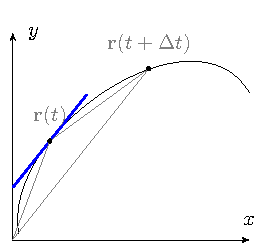
\includegraphics{fig/ch1-tangent.pdf}
    \caption{切矢量}\label{chcdg:pic_tangent}
\end{figure}


若参数曲线$\boldsymbol{r}(t)$的切矢量$\boldsymbol{r}'(t)$处处不为零,且$\boldsymbol{r}(t)$至少三次连续可微;
则称曲线$\boldsymbol{r}(t)$是{\heiti 正则曲线},并且把参数$t$增大的方向称为
曲线$\boldsymbol{r}(t)$的{\heiti 正向},故$\boldsymbol{r}'(t)$是指向正向的.

下面来处理正则曲线弧长.仍以图\ref{chcdg:pic_tangent}为例,该图中只画了
点$\boldsymbol{r}(t)$和$\boldsymbol{r}(t+\Delta t)$,先将其改记为$\boldsymbol{r}(t_i)$和$\boldsymbol{r}(t_{i+1})$,
并且设想在该曲线上存在$n+1$个这样的分点,即$a=t_0<t_1<\cdots<t_n=b$,
也就是说我给区间$[a,b]$作了一个划分(图中没有,自己想像).
当$t_i$与$t_{i+1}$无限接近时,图\ref{chcdg:pic_tangent}中的割线长度
与点$\boldsymbol{r}(t_i)$和点$\boldsymbol{r}(t_{i+1})$间的弧线长度无限接近;
这样便有(其中$\lambda = \max \{|\Delta t_i|; i=0,\cdots,n-1 \}$)
\begin{equation}\label{chcdg:eqn_arclength}
    \lim\limits_{\lambda\to 0 \atop n\to \infty } \sum_{i=0}^{n-1} 
    |\boldsymbol{r}(t_{i+1}) - \boldsymbol{r}(t_{i})| = \int_{a}^{b} |\boldsymbol{r}'(t)|{\rm d}t
    \overset{def}{=}s .
\end{equation}
上式便是曲线在$[a,b]$间的{\heiti 弧长公式};由于我们要求曲线是正则的,
故在闭区间$[a,b]$上曲线没有奇点,也不会趋于无穷远点;这样式\eqref{chcdg:eqn_arclength}中
积分一定收敛.

如果用其它参数来描述曲线,比如存在变换$t=t(u)$,则$\boldsymbol{r}(t) \to \boldsymbol{r}\bigl(t(u)\bigr)=\boldsymbol{r}(u) $;
需对变换$t=t(u)$作如下要求({\heiti 容许变换}):函数$t=t(u)$三次连续可微,并且$t'(u)>0$处处成立.
在这样要求下,这种变换并不改变曲线长度.
\begin{align*}
    s=\int_{a}^{b} |\boldsymbol{r}'(u)|{\rm d}u
     =\int_{a}^{b} \left|\frac{{\rm d}\boldsymbol{r}\bigl(t(u)\bigr)}{{\rm d}t }
     \frac{{\rm d}t(u)}{{\rm d}u}  \right|{\rm d} u
%      =\int_{a}^{b} \left|\frac{{\rm d}\boldsymbol{r}\bigl(t(u)\bigr)}{{\rm d}t }\right|
%     \frac{{\rm d}t(u)}{{\rm d}u}  {\rm d}u
     =\int_{a}^{b} |\boldsymbol{r}'(t)|{\rm d}t .
\end{align*}

现在将正则曲线$\boldsymbol{r}(u)$的弧长积分上限改为变数$t$,下限仍是固定值$a$.
\begin{align}
    s(t)=\int_{a}^{t} |\boldsymbol{r}'(u)|{\rm d}u 
    \  \xRightarrow[t \, \text{求导}]{\text{对参数}} \  
    \frac{{\rm d}s(t)}{{\rm d}t}=|\boldsymbol{r}'(t)|  > 0 .
\end{align}
上式满足{\kaishu 容许变换}要求,故总可以用弧长$s$作为正则曲线的参数.
以后为简单起见,都用弧长作为曲线的参数,称为{\heiti 自然参数};
请读者验证当选用自然参数时,有:$\boxed{|\boldsymbol{r}'(s)|=1}$.





\subsection{曲率、挠率与Frenet公式}
从上一节我们知道正则曲线$C$的切矢量$|\boldsymbol{r}'(s)|=1$;现定义:
\begin{align}
    \boldsymbol{T} (s) \overset{def}{=} \boldsymbol{r}'(s) .
\end{align}
我们研究一下这个单位长的切矢量$\boldsymbol{T} (s)$.
设正则曲线$C(s)$上有两个临近点$s$、$s+\Delta s$,此两点
的单位长切矢量分别是$\boldsymbol{T} (s)$、$\boldsymbol{T} (s+\Delta s)$.
将$\boldsymbol{T} (s+\Delta s)$平移至$s$点处,并令两个切矢量的起点重合,
它们的终点一般说来是不重合的,两者之差是$\boldsymbol{T} (s+\Delta s)-\boldsymbol{T} (s)$;
两个矢量$\boldsymbol{T} (s)$、$\boldsymbol{T} (s+\Delta s)$的夹角是$\Delta\theta$.则有
\setlength{\mathindent}{0em}
\begin{align}
    \left|\frac{{\rm d} \boldsymbol{T}}{{\rm d}s}\right| =  \lim_{\Delta s\to 0} 
    \left|\frac{\boldsymbol{T} (s+\Delta s)-\boldsymbol{T} (s)}{\Delta s}\right|
    \xlongequal{|\boldsymbol{T}|=1}
    \lim_{\Delta s\to 0} \frac{\left|2\sin\frac{\Delta\theta}{2}\right|}{|\Delta s|}
    =\lim_{\Delta s\to 0} \frac{|\Delta \theta|}{|\Delta s|}. \label{chcdg:eqn_dads}
\end{align}\setlength{\mathindent}{2em}
式\eqref{chcdg:eqn_dads}表明:在正则曲线$C(s)$上,随着弧长$s$变化,
单位长切矢量$\boldsymbol{T} (s)$对弧长的
导数$|\frac{{\rm d} \boldsymbol{T}}{{\rm d}s}|$标志着
切矢量$\boldsymbol{T} (s)$在$E^3$中转动的快慢;
它刻画了此条曲线的{\kaishu 弯曲程度}.


    设正则曲线$C(s)$的方程是$\boldsymbol{r}(s)$,$s$是弧长参数.
    令$\boxed{\kappa(s) \equiv |\tfrac{{\rm d} \boldsymbol{T}}{{\rm d}s}|=|\boldsymbol{r}''(s)|}$,
    称$\kappa(s)$是曲线$\boldsymbol{r}(s)$在$s$处的{\heiti 曲率},
    $\frac{{\rm d} \boldsymbol{T}}{{\rm d}s}$为{\heiti 曲率矢量}.

不难证明:$C(s)$是$E^3$中一条直线的充要条件是它的曲率$\kappa(s)\equiv 0$.


假设正则曲线$C(s)$的曲率$\kappa(s)\neq 0$.因$|\boldsymbol{T}(s)|=1$,
由命题\ref{chcdg:thm_rrp=0}可知:$\boldsymbol{T}(s)\cdot \boldsymbol{T}'(s)=0$,
即$\boldsymbol{T}(s) \perp \boldsymbol{T}'(s)$.故$\boldsymbol{T}'(s)$是曲线$C$的一个法矢量,且方向完全确定,
将这个方向的单位矢量记为$\boldsymbol{N}(s)$,称为正则曲线$C(s)$的{\heiti 主法矢量};
很明显,有$\boxed{\boldsymbol{T}'(s) = \kappa(s) \boldsymbol{N}(s) }$.

由曲线$C(s)$的切矢$\boldsymbol{T}$和主法矢$\boldsymbol{N}$定义{\heiti 副法矢量}:
$    \boldsymbol{B}(s) \overset{def}{=} \boldsymbol{T}(s) \times \boldsymbol{N}(s)$.

通过以上叙述,不难得到:在$\kappa(s)\neq 0$的点,正则曲线$C(s)$存在一个
右手单位标架:$\{\boldsymbol{r}(s);\  \boldsymbol{T}(s), \boldsymbol{N}(s), \boldsymbol{B}(s) \}$;
称为曲线在该点的{\bfseries \heiti Frenet标架}.
在$\kappa(s)= 0$的点,Frenet标架定义较为复杂,我们不再讨论,
请读者参阅本章末所列文献.


我们已知$\boldsymbol{B}(s)\cdot \boldsymbol{T}(s) = 0$,对此式求导得:
\begin{align}
    0= \boldsymbol{B}'(s) \cdot \boldsymbol{T}(s) + \boldsymbol{B}(s) \cdot \boldsymbol{T}'(s)
    \ \xRightarrow [\boldsymbol{B} \cdot \boldsymbol{N}=0]{\boldsymbol{T}' = \kappa \boldsymbol{N}} \ 
    \boldsymbol{B}'(s) \cdot \boldsymbol{T}(s) =0 .
\end{align}
又因$|\boldsymbol{B}(s)|=1$,故$\boldsymbol{B}(s) \cdot \boldsymbol{B}'(s)=0$;
最终,$\boldsymbol{B}'(s) \parallel \boldsymbol{N}(s)$.
不妨假设:
\begin{equation}
    \boldsymbol{B}'(s)=-\tau(s) \boldsymbol{N}(s) .
\end{equation}
上式中的$\tau(s)$为正则曲线$C(s)$的{\heiti 挠率}.
易得$\tau(s)= - \boldsymbol{B}'(s) \cdot \boldsymbol{N}(s)$和$|\tau(s)|=|\boldsymbol{B}'(s)|$.

可以证明:非直线的正则曲线$C(s)$是平面曲线的充要条件是它的挠率为零.


因$|\boldsymbol{N}(s)|=1$,故$\boldsymbol{N}(s) \cdot \boldsymbol{N}'(s)=0$;
故可设$\boldsymbol{N}'(s)=a \boldsymbol{T}(s) + c \boldsymbol{B}(s)$,则有
\begin{align*}
    a = \boldsymbol{T} \cdot \boldsymbol{N}' = -\boldsymbol{T}' \cdot \boldsymbol{N} = - \kappa(s), \quad
    c = \boldsymbol{B} \cdot \boldsymbol{N}' = -\boldsymbol{B}' \cdot \boldsymbol{N} = \tau(s). 
\end{align*}
最后,可将本小节中的公式总结为:
\begin{subequations}\label{chcdg:eqn_Frenet}
    \begin{align}
        \boldsymbol{r}'(s) =& \hphantom{-\kappa(s)} \boldsymbol{T}(s) \label{chcdg:eqn_Freneta} \\
        \boldsymbol{T}'(s) =& \hphantom{-\kappa(s) \boldsymbol{T}(s) - }
           \kappa(s) \boldsymbol{N}(s) \label{chcdg:eqn_Frenetb}\\
        \boldsymbol{N}'(s) =& -\kappa(s) \boldsymbol{T}(s) \hphantom{-\kappa(s) \boldsymbol{N}(s), }
           +\tau(s) \boldsymbol{B}(s) \label{chcdg:eqn_Frenetc}\\
        \boldsymbol{B}'(s) =& \hphantom{-\kappa(s) \boldsymbol{T}(s)} 
         -\tau(s) \boldsymbol{N}(s)  \label{chcdg:eqn_Frenetd}
    \end{align}
\end{subequations}
式\eqref{chcdg:eqn_Frenet}称为{\bfseries \heiti Frenet--Serret公式},
这是$E^3$一维曲线论中最重要的公式.

\section{二维曲面基本属性}


相对来说,$E^3$一维曲线论较为简单,而$E^3$的二维曲面论则要复杂的多;
我们将分数节来讨论这个议题.二维曲面论中的理论,经过改造后可以形式不变
地推广到高维流形上.首先给出正则曲面的定义.

我们将$E^2$中的一个连通开子集$D$映射到$E^3$中,即$S:D\to E^3$;
并在$E^2$、$E^3$中分别建立了笛卡尔坐标系,用$(u,v)$表示$E^2$中的点,
用$(x,y,z)$标记$E^3$中的点,则{\kaishu 参数曲面}$S$可以表示为:
\begin{equation}
    \boldsymbol{r}(u,v) = \bigl(x(u,v), \  y(u,v),\  z(u,v)\bigr),
    \qquad (u,v)\in D.
\end{equation}
假设$x$、$y$、$z$对$u$、$v$有三次以上的连续可微偏导数,以后不再单独声明.


设曲面$S$在$p\in S$点(坐标是$u_0,v_0$)有两个切矢量
\begin{equation}\label{chcdg:eqn_rurv}
    \boldsymbol{r}_u (u_0,v_0) \equiv \left. \frac{\partial \boldsymbol{r}}{\partial u} \right|_{(u_0,v_0)},\qquad
    \boldsymbol{r}_v (u_0,v_0) \equiv \left. \frac{\partial \boldsymbol{r}}{\partial v} \right|_{(u_0,v_0)}.
\end{equation}
若这两个切矢量是线性无关的,即$(\boldsymbol{r}_u\times   \boldsymbol{r}_v)|_{(u_0,v_0)} \neq 0$,
则称曲面$S$在$p$点{\heiti 正则};若曲面$S$上每一点都是正则的,则称之为{\heiti 正则曲面}.
之后,我们只讨论正则曲面,不再声明.


%\subsection{切平面和法矢量}

不难看出,$S$上任意一条连续可微参数曲线可以表示成:$u=u(t),\ v=v(t)$,
其中$t$是实参数;把它写成$E^3$中曲线参数方程为:
\begin{equation}
    \boldsymbol{r}= \boldsymbol{r}\bigl( u(t), v(t) \bigr),\qquad t\in \mathbb{R} .
\end{equation}

设曲面$S$有$p$点,经过$p$的任意一条曲线在该点的切矢量称为曲面$S$在$p$点的{\heiti 切矢量}.
显然,式\eqref{chcdg:eqn_rurv}中的$\boldsymbol{r}_u,\boldsymbol{r}_v$是$p$点的切矢量,
称它们为$p$点的{\heiti 自然切矢量};
其实过$p$点的任意切矢量都可以表示成自然切矢量的线性组合,即
\begin{align}
    \left. \frac{{\rm d}\boldsymbol{r}(u,v)}{{\rm d} t} \right|_{t=t_0}
    = \frac{\partial \boldsymbol{r}}{\partial u} \frac{{\rm d}u }{{\rm d} t}
     +\frac{\partial \boldsymbol{r}}{\partial v} \frac{{\rm d}v }{{\rm d} t}
     =\boldsymbol{r}_u \frac{{\rm d}u }{{\rm d} t} + \boldsymbol{r}_v \frac{{\rm d}v }{{\rm d} t}.
\end{align}
上式中切矢均在$p$点取值.
反之,如果点$p\in S$处有矢量
\begin{equation}
    \boldsymbol{v}= \alpha \boldsymbol{r}_u + \beta \boldsymbol{r}_v,\quad
    \text{切矢均在$p$点取值,常数}\alpha,\beta \in \mathbb{R} .
\end{equation}
则曲面$S$上一定存在一条过$p$点的曲线$C(t)$使得它在$p$点切矢量是$\boldsymbol{v}$.令
\begin{equation}
    u(t)=u_0 + \alpha (t-t_0),\quad v(t)=v_0 + \beta (t-t_0) ,
\end{equation}
于是$S$上曲线
\begin{equation}
    \boldsymbol{r}=\boldsymbol{r}\bigl( u(t), v(t) \bigr)
    =\boldsymbol{r}\bigl(u_0 + \alpha (t-t_0),\ v_0 + \beta (t-t_0) \bigr) .
\end{equation}
便满足这个要求;直接对上式求导就可验证.

由此可以得出:曲面$S$上过$p$点所有曲线的切矢量构成一个二维线性空间;
我们称这个二维线性空间为曲面$S$在$p$点的{\heiti 切平面},记为$T_pS$;
切平面上的矢量称为曲面$S$在$p$点的{\heiti 切矢量};
$\boldsymbol{r}_u|_{(u_0,v_0)},\boldsymbol{r}_v|_{(u_0,v_0)}$是$T_pS$的一组基矢量.

由于曲面是正则的,故$T_pS$的法矢量可按如下方式定义
\begin{equation}\label{chcdg:eqn_Snormal}
    \boldsymbol{n}(u_0,v_0) \overset{def}{=} \left. \frac{\boldsymbol{r}_u \times \boldsymbol{r}_v}
    {|\boldsymbol{r}_u \times \boldsymbol{r}_v|} \right |_ {(u_0,v_0)}
    = \frac{\boldsymbol{r}_u \times \boldsymbol{r}_v} {\sqrt{EG-F^2}}.
\end{equation}
这样,$(\boldsymbol{r}_u , \boldsymbol{r}_v, \boldsymbol{n})$构成了$p$点的$E^3$中一个右手标架;
当$p$点遍历$S$上每一点时,这个标架构成一个标架场,
称为正则曲面$S$的{\heiti 自然标架场}.
曲面$S$上任意一个矢量,不论它是否属于$S$的切平面,只要起始点在$S$上,
都可以在这个标架场下展开.



\section{第一、第二基本形式}
设正则曲面$S$上有两个两临近的点$p(u,v)$及$p'(u+\Delta u, v+\Delta v)$,
它们的矢径分别是$\boldsymbol{r}(u,v)$、$\boldsymbol{r}(u+\Delta u, v+\Delta v)$.
于是,在$E^3$中可以应用Taylor展开式,不难得到
\begin{equation*}
    \overrightarrow{pp'}=\Delta \boldsymbol{r} =\boldsymbol{r}(u+\Delta u, v+\Delta v) - \boldsymbol{r}(u,v)
    = \boldsymbol{r}_u \Delta u + \boldsymbol{r}_v \Delta v + O(\Delta u^2, \Delta v^2).
\end{equation*}
故由上式可以得到矢径的微分关系(只取线性部分)如下:
\begin{equation}\label{chcdg:eqn_drdudv}
    {\rm d} \boldsymbol{r} = \boldsymbol{r}_u {\rm d} u + \boldsymbol{r}_v {\rm d} v .
\end{equation}
当$p'$点无限接近$p$点时,也就是$\Delta u\to 0, \Delta v\to 0$,
我们就把$\overrightarrow{pp'}$在$E^3$中的长度的主部定义为曲面$S$上
这两个无限接近点的距离${\rm d}s$,即有
\begin{equation*}
    ({\rm d}s)^2 = {\rm d}\boldsymbol{r}\cdot {\rm d}\boldsymbol{r}
%    = (\boldsymbol{r}_u {\rm d} u + \boldsymbol{r}_v {\rm d} v)\cdot (\boldsymbol{r}_u {\rm d} u + \boldsymbol{r}_v {\rm d} v)
    = \boldsymbol{r}_u\cdot\boldsymbol{r}_u ({\rm d}u)^2 +2\boldsymbol{r}_u\cdot\boldsymbol{r}_v {\rm d}u {\rm d}v
    + \boldsymbol{r}_v\cdot\boldsymbol{r}_v ({\rm d}v)^2.
\end{equation*}
定义
\begin{equation}
    E\equiv \boldsymbol{r}_u\cdot\boldsymbol{r}_u, \qquad
    F\equiv \boldsymbol{r}_u\cdot\boldsymbol{r}_v, \qquad
    G\equiv \boldsymbol{r}_v\cdot\boldsymbol{r}_v .
\end{equation}
则有
\begin{equation}\label{chcdg:eqn_Iform}
    {\rm I}\equiv {\rm d}s^2 = E {\rm d}u^2 + 2 F {\rm d}u {\rm d}v + G {\rm d}v^2.
\end{equation}
这个二次微分式就是曲面$S$的{\heiti 第一基本形式},也称为曲面的{\heiti 线元};
而$E,F,G$称为曲面$S$的{\heiti 第一基本形式系数};我们已把第一基本形式记为${\rm I}$.

由于第一基本形式是个内积,即${\rm d}\boldsymbol{r}\cdot {\rm d}\boldsymbol{r}$,故它是正定二次型,即
\begin{equation}
    E>0,\quad G>0,\quad  EG -F^2 >0 .
\end{equation}

设$C(t)$是正则曲面$S$上一条正则曲线,它的参数方程为:
$\boldsymbol{r}=\boldsymbol{r}\bigl(u(t),v(t)\bigr)$,其中$a\leqslant t\leqslant b$.
从第一基本形式可以得到这条曲线的线长为
\begin{equation}
    L=\int_{a}^{b} {\rm d}s = \int_{a}^{b}
    \sqrt{E \Bigl(\frac{{\rm d}u }{{\rm d}t}\Bigr)^2 
      + 2 F \frac{{\rm d}u }{{\rm d}t} \frac{{\rm d}v }{{\rm d}t} 
      + G \Bigl(\frac{{\rm d}v }{{\rm d}t}\Bigr)^2 } \ {\rm d}t.
\end{equation}


现考虑正则曲面$S$上一块无穷小面积.曲面上由参数曲线
\begin{equation}
    u=u_0,\quad u=u_0+\Delta u;\quad v=v_0,\quad  v=v_0+\Delta v ;
    \quad \Delta u>0,\  \Delta v >0 .
\end{equation}
所围成的一小块,它的面积近似等于在点$\boldsymbol{r}(u_0,v_0)$处的切平面上
由矢量$(\Delta u) \boldsymbol{r}_u$和$(\Delta v) \boldsymbol{r}_v$所张成的平行四边形的面积,
而这个平行四边形面积是:
\setlength{\mathindent}{0em}
\begin{align*}
    &\bigl|(\Delta u) \boldsymbol{r}_u \times (\Delta v) \boldsymbol{r}_v \bigr|
    =\sqrt{(\boldsymbol{r}_u \times \boldsymbol{r}_v)\cdot (\boldsymbol{r}_u 
        \times \boldsymbol{r}_v) } \Delta u \Delta v 
    =\sqrt{\boldsymbol{r}_u \cdot \bigl( \boldsymbol{r}_v\times 
        (\boldsymbol{r}_u \times \boldsymbol{r}_v) \bigr)} \Delta u \Delta v \\
    =&\sqrt{\boldsymbol{r}_u \cdot \bigl( (\boldsymbol{r}_v\cdot\boldsymbol{r}_v)\boldsymbol{r}_u  
        -(\boldsymbol{r}_v \cdot \boldsymbol{r}_u)\boldsymbol{r}_v \bigr)} \Delta u \Delta v 
    =\sqrt{EG-F^2}    \Delta u \Delta v  .
\end{align*}\setlength{\mathindent}{2em}
此式也完成了式\eqref{chcdg:eqn_Snormal}最后一步的计算.
由上式可知曲面$S$的{\heiti 面积元素}可以表示为:
$    {\rm d}\sigma \equiv \sqrt{EG-F^2}    {\rm d} u {\rm d} v $.
曲面$S$的面积可以表示为:
\begin{equation}
    A=\iint_D {\rm d}\sigma = \iint_D \sqrt{EG-F^2}    {\rm d} u {\rm d} v .
\end{equation}



为描述曲面偏离切平面的程度,需引入第二基本形式.
在$E^3$中将$\overrightarrow{pp'}$展开到二阶:
\begin{align*}
    \overrightarrow{pp'}=&\Delta \boldsymbol{r} =\boldsymbol{r}(u+\Delta u, v+\Delta v) - \boldsymbol{r}(u,v) \\
    =& \boldsymbol{r}_u \Delta u + \boldsymbol{r}_v \Delta v + \frac{1}{2}\bigl[
    \boldsymbol{r}_{uu} (\Delta u)^2 +2\boldsymbol{r}_{uv} \Delta u \Delta v +\boldsymbol{r}_{vv} (\Delta v)^2 \bigr]
    + O(\Delta u^3, \Delta v^3).
\end{align*}
由上式可计算$p'(u+\Delta u, v+\Delta v)$点到$p(u,v)$点切平面$T_pS$的垂直距离:
\begin{equation*}
    \delta = \boldsymbol{n}\cdot \overrightarrow{pp'} = \frac{1}{2}\bigl[
    \boldsymbol{n}\cdot\boldsymbol{r}_{uu} (\Delta u)^2 +2\boldsymbol{n}\cdot\boldsymbol{r}_{uv} \Delta u \Delta v
     +\boldsymbol{n}\cdot\boldsymbol{r}_{vv} (\Delta v)^2 \bigr] + O(\Delta u^3, \Delta v^3).
\end{equation*}
Gauss引入如下记号:
\begin{equation}
    L= \boldsymbol{n}\cdot\boldsymbol{r}_{uu},\quad M= \boldsymbol{n}\cdot\boldsymbol{r}_{uv},
    \quad N=\boldsymbol{n}\cdot\boldsymbol{r}_{vv} .
\end{equation}
令$\Delta u\to 0$、$\Delta v\to 0$,则可以得到曲面$S$的{\heiti 第二基本形式}:
\begin{equation}\label{chcdg:eqn_IIform}
    {\rm II}=2\delta = L {\rm d}u^2 + 2M {\rm d}u {\rm d}v + N {\rm d}v^2 .
\end{equation}

\subsection{张量记号}
我们将第一、第二基本形式换成现代微分几何的记号,见表\ref{chcdg:tab-gauss-tensor}.

\begin{table}[htb]
    \centering
    \caption{Gauss记号和张量记号对照表} \label{chcdg:tab-gauss-tensor}
    \begin{tabular}{|*{11}{c|}}
        \hline 
        Gauss记号 & $u$   &  $v$  & $\boldsymbol{r}_u$  & $\boldsymbol{r}_v$ & $E$ & $F$ & $G$ & $L$ & $M$ & $N$ \\
        \hline
        张量记号  & $u^1$ & $u^2$ & $\boldsymbol{r}_1$ & $\boldsymbol{r}_2$ & $g_{11}$ & $g_{12},g_{21}$ & $g_{22}$ 
         & $b_{11}$ & $b_{12},b_{21}$ & $b_{22}$     \\ 
        \hline
    \end{tabular}
\end{table}

这样,二维曲面$S$的度规矩阵为
\setlength{\mathindent}{0em}
\begin{equation}\label{chcdg:eqn_2Dmetric}
    g=\begin{pmatrix} g_{11} & g_{12} \\ g_{21} & g_{22}  \end{pmatrix}
    =\begin{pmatrix} E & F \\ F & G \end{pmatrix} ; \,
    g^{-1}= \begin{pmatrix} g^{11} & g^{12} \\ g^{21} & g^{22}  \end{pmatrix}
    =\frac{1}{|g|}\begin{pmatrix} g_{22} & -g_{12} \\ -g_{21} & g_{11} \end{pmatrix} .
\end{equation}\setlength{\mathindent}{2em}
第一、第二基本形式可以表示成:
\begin{align}
    {\rm I}=& {\rm d}s^2 = g_{11} \left({\rm d}u^1\right)^2 +2g_{12} {\rm d}u^1{\rm d}u^2
      +g_{22} \left({\rm d}u^2\right)^2= \sum_{\alpha,\beta=1}^{2} g_{\alpha\beta} {\rm d}u^\alpha {\rm d}u^\beta.
       \label{chcdg:eqn_Iform-tensor} \\
    {\rm II}=& b_{11} \left({\rm d}u^1\right)^2 +2b_{12} {\rm d}u^1{\rm d}u^2
      +b_{22} \left({\rm d}u^2\right)^2= \sum_{\alpha,\beta=1}^{2} b_{\alpha\beta} {\rm d}u^\alpha {\rm d}u^\beta.
    \label{chcdg:eqn_IIform-tensor} 
\end{align}

经过数位微分几何大师的研究,终于认识到仅用$g$表示出来的二维曲面上的几何量
可以形式不变地推广到高维情形;故我们称由式\eqref{chcdg:eqn_2Dmetric}表示的
几何量为{\heiti 内蕴量},比如弧长、面积等等.
只讨论式\eqref{chcdg:eqn_2Dmetric}以及由它生成的量的几何学称为{\heiti 内蕴几何学},
由这些量决定的几何性质称为{\heiti 内蕴性质}.

涉及到第二基本形式的几何学称为{\heiti 外蕴几何学},一般说来把曲面嵌入到高维空间
的几何学都属于外蕴的.外蕴几何一般不能直接推广到高维空间.
比如类似于球面的二维曲面可以嵌入三维欧氏空间;
但像Klein瓶这种不可定向的二维流形是不能嵌入三维空间的,至少需要嵌入四维或更高维空间;
虽然都是二维流形,但被嵌入的空间以及嵌入的光滑函数必然有很大差别,
因此所涉及的外蕴几何很难以形式不变的方式推广到高维空间.




\subsection{曲面上的活动标架}
$\boldsymbol{r}_\alpha\equiv \frac{\partial \boldsymbol{r}}{\partial u^\alpha}$($\alpha=1,2$)
只是对$\boldsymbol{r}$的一次偏微分;
我们需要对它再次求偏导,即$\frac{\partial \boldsymbol{r}_\alpha}{\partial u^\beta}$;
显然$\frac{\partial \boldsymbol{r}_\alpha}{\partial u^\beta}$仍是$E^3$中的矢量,
故它可以在标架$\{\boldsymbol{r}_1,\boldsymbol{r}_2,\boldsymbol{n}\}$上展开:
\begin{equation}\label{chcdg:eqn_drdn}
    \frac{\partial \boldsymbol{r}_\alpha}{\partial u^\beta} 
    =\frac{\partial^2 \boldsymbol{r}}{\partial u^\alpha\partial u^\beta}
    = \sum_{\delta=1}^{2} \Gamma_{\alpha \beta}^\delta \boldsymbol{r}_\delta
     + c_{\alpha \beta} \boldsymbol{n};\quad
    \frac{\partial \boldsymbol{n}}{\partial u^\beta}
     = \sum_{\delta=1}^{2} \omega^\delta_\beta \boldsymbol{r}_\delta
     + c_\beta \boldsymbol{n} .
\end{equation}
我们顺带也把法矢量$\boldsymbol{n}$的微分也写了出来.下面来求出这些系数的表达式.
用单位法矢量$\boldsymbol{n}$点乘式\eqref{chcdg:eqn_drdn},
经过一些运算可得到
\begin{equation}
    c_{\alpha\beta} = b_{\alpha\beta}  \quad\text{和}\quad c_\beta=0.
\end{equation}
用$\boldsymbol{r}_\sigma$点乘式\eqref{chcdg:eqn_drdn}中第二式,
经过一些运算可得到
\begin{equation}
    \omega^\beta_\gamma = - \sum_{\sigma=1}^{2} g^{\beta \sigma} b_{\sigma\gamma}
     \overset{def}{=}b^\beta_\gamma .
\end{equation}
注意到$g_{\alpha \beta}=\boldsymbol{r}_\alpha\cdot \boldsymbol{r}_\beta$;
式\eqref{chcdg:eqn_drdn}中第一式$\boldsymbol{r}_{\alpha \beta}$、$b_{\alpha \beta}$关于
下标$\alpha$、$\beta$是对称的,
由此不难得到$\Gamma^\gamma_{\alpha \beta}=\Gamma^\gamma_{\beta\alpha}$;
用$\boldsymbol{r}_\sigma$点乘式\eqref{chcdg:eqn_drdn}中第一式,有
\begin{align}
    \boldsymbol{r}_\sigma \cdot \frac{\partial \boldsymbol{r}_\alpha}{\partial u^\beta} 
    = \sum_{\delta=1}^{2} \Gamma_{\alpha \beta}^\delta 
    \boldsymbol{r}_\delta\cdot\boldsymbol{r}_\sigma \ \Rightarrow \ 
    \frac{\partial g_{\alpha\sigma}}{\partial u^\beta} =
    \sum_{\delta=1}^{2} \left(\Gamma_{\alpha \beta}^\delta g_{\delta \sigma}
     + \Gamma_{\sigma \beta}^\delta g_{\delta \alpha} \right) . \label{chcdg:eqn_Gg}
\end{align}
轮换角标$\alpha\sigma \beta$,有
\begin{equation}
    \frac{\partial g_{\sigma\beta}}{\partial u^\alpha} =   \sum_{\delta=1}^{2} 
    \left(\Gamma_{\sigma\alpha}^\delta g_{\delta \beta} + \Gamma_{\beta\alpha}^\delta g_{\delta \sigma} \right) , \quad
    \frac{\partial g_{\beta\alpha}}{\partial u^\sigma} =   \sum_{\delta=1}^{2} 
    \left(\Gamma_{\beta \sigma}^\delta g_{\delta \alpha} + \Gamma_{\alpha \sigma}^\delta g_{\delta \beta} \right) .
\end{equation}
后两式相加再减掉第一式(注意利用$\Gamma^\gamma_{\alpha \beta}=\Gamma^\gamma_{\beta\alpha}$),得
\begin{equation}\label{chcdg:eqn_Christoffel}
    \Gamma_{\alpha\sigma}^\delta = \frac{1}{2} g^{\delta \beta}\left(\frac{\partial g_{\sigma\beta}}{\partial u^\alpha}
    +\frac{\partial g_{\beta\alpha}}{\partial u^\sigma}-\frac{\partial g_{\alpha \sigma}}{\partial u^\beta} \right) .
\end{equation}
上式说明$\Gamma_{\alpha \sigma}^\delta$只和度量有关,是内蕴量,称为{\heiti 联络系数}.
这样式\eqref{chcdg:eqn_drdn}为:
\begin{equation}\label{chcdg:eqn_GW}
    \frac{\partial \boldsymbol{r}_\alpha}{\partial u^\beta} 
    =\frac{\partial^2 \boldsymbol{r}}{\partial u^\alpha\partial u^\beta}
    = \sum_{\delta=1}^{2}\Gamma_{\alpha \beta}^\delta 
    \boldsymbol{r}_\delta + b_{\alpha \beta} \boldsymbol{n};\quad
    \frac{\partial \boldsymbol{n}}{\partial u^\beta} = 
    -\sum_{\delta=1}^{2} b_{\beta}^\delta \boldsymbol{r}_\delta .
\end{equation}
式\eqref{chcdg:eqn_GW}为二维曲面论中的{\heiti 基本公式},
第一式称为{\bfseries \heiti Gauss公式},
第二式称为{\bfseries \heiti Weingarten公式}.
这两个公式在第\ref{chsm}章有适当的推广.






\section{曲面上的曲率}
我们已对空间曲线的性质有了初步了解,定义了曲率等;
我们将借助曲线曲率来陈述曲面曲率,以及它的几何性质.
本节将会省略较多推导,请参阅\parencite[\S 2.4]{subq-2016}.

给定正则曲面$S$上的正则曲线$C(s)=\boldsymbol{r}(s)$,它的切矢量是:
$\boldsymbol{T}=\frac{{\rm d}\boldsymbol{r}}{{\rm d}s}= 
\sum_{\alpha=1}^{2}\boldsymbol{r}_\alpha \frac{{\rm d}u^\alpha}{{\rm d}s}$.
根据式\eqref{chcdg:eqn_Frenetb}可知
\setlength{\mathindent}{0em}
\begin{equation}\label{chcdg:eqn_kNn}
    \kappa \boldsymbol{N} =  \frac{{\rm d}^2\boldsymbol{r}}{{\rm d}s^2}
    = \sum_{\delta=1}^{2}\left( \frac{{\rm d}^2 u^\delta }{{\rm d}s^2} 
    + \sum_{\alpha,\beta=1}^{2}\Gamma^\delta_{\alpha\beta} 
    \frac{{\rm d}u^\alpha}{{\rm d}s}\frac{{\rm d}u^\beta}{{\rm d}s}\right) \boldsymbol{r}_\delta
    +\sum_{\alpha,\beta=1}^{2} b_{\alpha \beta}\frac{{\rm d}u^\alpha}
    {{\rm d}s}\frac{{\rm d}u^\beta}{{\rm d}s} \boldsymbol{n} .
\end{equation}\setlength{\mathindent}{2em}
由式\eqref{chcdg:eqn_kNn}可定义曲线$C(s)$的{\heiti 法曲率}$\kappa_n$:
\begin{align}
    \kappa_n \overset{def}{=} & \boldsymbol{n} \cdot (\kappa \boldsymbol{N})
    =\sum_{\alpha,\beta=1}^{2} b_{\alpha\beta}\frac{{\rm d}u^\alpha}{{\rm d}s}
    \frac{{\rm d}u^\beta}{{\rm d}s}
    =\frac{{\rm II}}{\rm I}.  \label{chcdg:eqn_kn} 
%    \kappa_g \overset{def}{=} & \sqrt{\kappa^2 -\kappa_n^2} .
\end{align}


经过略显繁琐的推导与叙述(略)可以得到:给定曲面$S$上任意一点$p$以及该点的法线$\boldsymbol{n}$;
包含法线$\boldsymbol{n}$的平面$\Pi$会在正则曲面$S$上截出一条曲线,
当$\Pi$绕着$\boldsymbol{n}$旋转一周后,所截取的曲线的法曲率会有一个最大值$\kappa_1$和
一个最小值$\kappa_2$,两者都称为{\heiti 主曲率};$\kappa_1$所对应的曲线的切矢量记为$\boldsymbol{e}_1$,
$\kappa_2$所对应的曲线的切矢量记为$\boldsymbol{e}_2$,可以证明$\boldsymbol{e}_1\cdot \boldsymbol{e}_2=0$.
由两个主曲率可以定义{\heiti 总曲率}或称为{\bfseries \heiti Gauss曲率}(高斯曲率):
\begin{equation}\label{chcdg:eqn_Gauss-Curvature}
    K \overset{def}{=}\kappa_1 \kappa_2  
    %=\det \left(\sum_{\delta=1}^{2}g^{\alpha\delta} b_{\delta\beta} \right)
    =\frac{\det b_{\alpha\beta}}{\det g_{\gamma\delta}} 
    =\frac{b_{11} b_{22} -(b_{12})^2}{g_{11} g_{22} -(g_{12})^2}
    = \frac{LN-M^2}{EG-F^2} .
\end{equation} %\setlength{\mathindent}{2em}


在$E^3$中的偏导数是可以交换次序的,比如
\begin{equation}\label{chcdg:eqn_rnuu}
    \frac{\partial^3 \boldsymbol{r}}{\partial u^\alpha \partial u^\beta \partial u^\gamma}
    =\frac{\partial^3 \boldsymbol{r}}{\partial u^\alpha \partial u^\gamma \partial u^\beta  },\qquad
    \frac{\partial^2 \boldsymbol{n}}{\partial u^\alpha \partial u^\beta }
    =\frac{\partial^2 \boldsymbol{n}}{\partial u^\beta \partial u^\alpha  } .
\end{equation}
我们将利用式\eqref{chcdg:eqn_rnuu}导出几个重要结论.
将式\eqref{chcdg:eqn_GW}带入式\eqref{chcdg:eqn_rnuu}得
\begin{align}
    \frac{\partial}{\partial u^\gamma}\left(\sum_{\delta=1}^{2}\Gamma_{\alpha \beta}^\delta \boldsymbol{r}_\delta 
    +b_{\alpha \beta}\boldsymbol{n}\right)    & =\frac{\partial}{\partial u^\beta}
    \left(\sum_{\delta=1}^{2} \Gamma_{\alpha \gamma}^\delta \boldsymbol{r}_\delta
    +b_{\alpha \gamma} \boldsymbol{n}\right), \label{chcdg:eqn_uab}  \\
    \frac{\partial}{\partial u^\gamma}\left(\sum_{\delta=1}^{2} b_\beta^\delta \boldsymbol{r}_\delta\right) 
    & =\frac{\partial}{\partial u^\beta}\left(\sum_{\delta=1}^{2} b_\gamma^\delta \boldsymbol{r}_\delta\right) . \label{chcdg:eqn_nab}
\end{align}
将式\eqref{chcdg:eqn_uab}展开,并且再次用式\eqref{chcdg:eqn_GW},整理之后得到:
\begin{align*}
    &\sum_{\delta=1}^{2}\left(\frac{\partial}{\partial u^\gamma} \Gamma_{\alpha \beta}^\delta
    -\frac{\partial}{\partial u^\beta} \Gamma_{\alpha \gamma}^\delta
    + \sum_{\eta=1}^{2}\left(\Gamma_{\alpha \beta}^\eta \Gamma_{\eta \gamma}^\delta
    -\Gamma_{\alpha \gamma}^\eta \Gamma_{\eta \beta}^\delta\right)
    -b_{\alpha \beta} b_\gamma^\delta+b_{\alpha \gamma} b_\beta^\delta\right) \boldsymbol{r}_\delta  \\
    &+\sum_{\delta=1}^{2}\left(\Gamma_{\alpha \beta}^\delta b_{\delta \gamma}-\Gamma_{\alpha \gamma}^\delta
     b_{\delta \beta}+\frac{\partial b_{\alpha \beta}}{\partial u^\gamma}
     -\frac{\partial b_{\alpha \gamma}}{\partial u^\beta}\right) \boldsymbol{n}=\boldsymbol{0} .
\end{align*}
由于$\{\boldsymbol{r}_1, \boldsymbol{r}_2, \boldsymbol{n}\}$是处处线性无关的,所以上式的系数必须为零,即有
\begin{align}
    &\frac{\partial}{\partial u^\gamma} \Gamma_{\alpha \beta}^\delta-\frac{\partial}{\partial u^\beta}
   \Gamma_{\alpha \gamma}^\delta+ \sum_{\eta=1}^{2}\left(\Gamma_{\alpha \beta}^\eta 
    \Gamma_{\eta \gamma}^\delta-\Gamma_{\alpha \gamma}^\eta \Gamma_{\eta \beta}^\delta\right)
    =b_{\alpha \beta} b_\gamma^\delta-b_{\alpha \gamma} b_\beta^\delta, \label{chcdg:eqn_Gauss} \\
    &\frac{\partial b_{\alpha \beta}}{\partial u^\gamma}-\frac{\partial b_{\alpha \gamma}}{\partial u^\beta}
    =\sum_{\delta=1}^{2}\left(\Gamma_{\alpha \gamma}^\delta b_{\delta \gamma}
    - \Gamma_{\alpha \beta}^\delta b_{\delta \beta}\right).     \label{chcdg:eqn_Codazzi}
\end{align}
式\eqref{chcdg:eqn_Gauss}、\eqref{chcdg:eqn_Codazzi}分别称为
{\bfseries\heiti Gauss方程}、{\bfseries\heiti Codazzi方程};
式中所有希腊字母取值范围是:$1,2$.
从式\eqref{chcdg:eqn_nab}出发会再次得到Codazzi方程.


容易看出式\eqref{chcdg:eqn_Gauss}的左边只是由曲面$S$的第一类基本量$g_{\alpha \beta}$(度规)
的不高于二阶的偏导数构成的量,我们把它记成
\begin{equation}\label{chcdg:eqn_Riemann}
    R_{\hphantom{\delta} \alpha \beta \gamma}^\delta \overset{def}{=}
    +\frac{\partial}{\partial u^\beta} \Gamma_{\alpha \gamma}^\delta
    -\frac{\partial}{\partial u^\gamma} \Gamma_{\alpha \beta}^\delta
    +\sum_{\eta=1}^{2}\left( \Gamma_{\alpha \gamma}^\eta \Gamma_{\eta \beta}^\delta
    -\Gamma_{\alpha \beta}^\eta \Gamma_{\eta \gamma}^\delta \right) .
\end{equation}
我们称$R_{\hphantom{\delta} \alpha \beta \gamma}^\delta$为曲面$S$的第一类基本量的{\heiti 黎曼记号},
它与第二基本型式无关;这个记号是黎曼在1854年引入的,它可以形式不变的推广到任意有限维空间.
可以证明式\eqref{chcdg:eqn_Riemann}中的记号是个张量,并且有诸多对称性,可参见\S\ref{chrg:sec_R04};
可以证明在二维曲面时,$R_{\hphantom{\delta} \alpha \beta \gamma}^\delta$实质上只有一个非零分量.

下面叙述Gauss绝妙定理;为此先把黎曼记号的上指标
降下来:$R_{\delta \alpha \beta \gamma}\equiv \sum_{\eta=1}^{2} 
g_{\delta \eta}R_{\hphantom{\delta} \alpha \beta \gamma}^\eta$.
由于只有一个非零分量,式\eqref{chcdg:eqn_Gauss}变为
\begin{equation}
    R_{1212}= b_{11} b_{22} - (b_{12})^2 .
\end{equation}
将上式两边除以$g_{11} g_{22} -(g_{12})^2$得到:
\begin{equation}\label{chcdg:eqn_RK2}
    \frac{R_{1212}}{g_{11} g_{22} -(g_{12})^2}= \frac{b_{11} b_{22} -(b_{12})^2}{g_{11} g_{22} -(g_{12})^2}
    \xlongequal{\ref{chcdg:eqn_Gauss-Curvature}} K  .
\end{equation}
虽然Gauss曲率\eqref{chcdg:eqn_Gauss-Curvature}包含第一、第二基本形式,
但由上式可知:实质上Gauss曲率只由第一基本形式构成.
这便是{\heiti \bfseries Gauss绝妙定理}(Theorema egregium):

\begin{theorem}\label{chcdg:thm_egregium}
    二维曲面的Gauss曲率只由它的第一基本形式决定.
\end{theorem}


其实一般情形下把绝妙定理叙述成:在局部等距映射下,Gauss曲率不变.
由于在本章我们没有引入等距的定义,故把它叙述成\ref{chcdg:thm_egregium}的形式.
Gauss绝妙定理推广到一般情形便是定理\ref{chrg:thm_isometry-Riemann};该处用到了等距概念.


1827年Gauss经过非常复杂的计算证明了上述定理,这是微分几何发展史上一个里程碑式的定理,
这开创了微分几何的一个新纪元——内蕴几何学.这个定理说明:
{\bfseries (1)} 无需把二维曲面嵌入$E^3$之中,我们只需研究第一基本形式(无需第二基本形式)便可研究
曲面的{\kaishu 弯曲情况}(总曲率);
{\bfseries (2)} 这种{\kaishu 内蕴}属性表明可以用单纯的二维语言来研究二维曲面,无需将其嵌入到$E^3$之中;
{\bfseries (3)} 两个曲面只要它们的高斯曲率处处相等,无论它们以何种方式嵌入$E^3$中,它们的弯曲属性都相同.
1854年黎曼(Gauss学生)发展了Gauss绝妙定理的内蕴思想.
在此之前,学者们一般把二维曲面嵌入到三维欧氏空间进行研究;
通过三维欧氏空间的度规(正定单位矩阵)诱导得到二维曲面的度规,
没有认识到二维度规是可以独立于二维曲面本身.
黎曼独辟蹊径,他将二维曲面本身看成一个独立的几何实体,而不仅仅是
三维欧氏空间的一个子集;由此他认识到二维曲面的第一基本形式(即今天的黎曼度规)是
加在二维曲面的一个附加结构,不是二维曲面(二维光滑流形)自带结构,两者可以分离.
然后,黎曼把二维曲面中成立的内蕴几何推广到任意有限维空间,
即今天的{\kaishu 黎曼几何}.

\begin{example}\label{chcdg:exm_torus}
	闭合圆环面(torus,即轮胎面)的黎曼曲率.
\end{example}

在$E^3$中,有笛卡尔直角坐标系$\{O;x,y,z\}$.
闭合圆环面的大圆圆心处于原点$O$,大圆位于$x-y$平面上,大圆半径为$R$.
一个半径为$r$的小圆沿着大圆绕$z$轴旋转,
这样旋转一周后的小圆便形成了闭合圆环面.要求$R>r>0$.
设大圆旋转半径与$x$轴夹角为$u$,小圆旋转半径与$x-y$平面夹角为$v$;
那么圆环面的参数方程为:
\begin{align*}
		x(u,v)= (R+r \cos v )\cos u , \quad
		y(u,v)= (R+r \cos v )\sin u , \quad
		z(u,v)= r \sin v .
\end{align*}
对上面三式取微分,有:
\begin{align*}
	{\rm d}x = & -(R+r \cos v) \sin u {\rm d}u - r \sin v \cos u  {\rm d} v, \\
	{\rm d}y = & (R+r \cos v) \cos u {\rm d}u - r \sin v \sin u  {\rm d} v, \\
	{\rm d}z = & r \cos v {\rm d}v .
\end{align*}
由此可以得到环面上线元:
\begin{equation*}
	{\rm d}s^2 = {\rm d}x^2+{\rm d}y^2+{\rm d}z^2 = (R+r \cos v)^2  {\rm d}u^2 + r^2   {\rm d}v^2.
\end{equation*}
容易读出环面在局部坐标$\{u,v\}$下的度量为:
\begin{equation*}
	g_{\alpha\beta}= \begin{pmatrix}(R+r \cos v)^2 &0 \\ 0& r^2\end{pmatrix}.
\end{equation*}
利用式\eqref{chcdg:eqn_Christoffel}计算可以得到非零克氏符:
\begin{equation}\label{chcdg:eqn_torus-Gamma}
	\Gamma^u_{uv}=\Gamma^u_{vu}=\frac{-r \sin v}{R+r \cos v},\qquad
	\Gamma^v_{uu}=\frac{1}{r}(R+r \cos v) \sin v.
\end{equation}
遂得非零黎曼曲率分量,以及Gauss曲率(见式\eqref{chcdg:eqn_Riemann}、\eqref{chcdg:eqn_RK2}):
\begin{equation}\label{chcdg:eqn_torus-curv}
	R_{1212}=r \cos v (R+r \cos v) ; \qquad  	K=\frac{\cos v}{r(R+r \cos v) } .
\end{equation}
式\eqref{chcdg:eqn_torus-curv}中Gauss曲率的分母必然大于零,而分子可正、可负、可零.
\qed


\begin{exercise}
	{\bfseries (1)}补全例题\ref{chcdg:exm_torus}中式\eqref{chcdg:eqn_torus-Gamma}的计算过程,包括为零的部分的计算.
	{\bfseries (2)}补全式\eqref{chcdg:eqn_torus-curv}的计算过程,只计算$R_{1212}$.
\end{exercise}

\begin{exercise}
	使用第一、第二基本形式的方法从新计算例题\ref{chcdg:exm_torus}.
\end{exercise}


\section{曲面上的平行移动}\label{chcdg:sec_pt}
在三维欧氏空间中平行移动是绝对的、熟知的:
把始点为$P$的矢量$\boldsymbol{v}$平移到始点为$P^{\prime}$的矢量$\boldsymbol{v}^{\prime}$,
{\kaishu 绝对平行移动}是指在同一笛卡尔坐标系下,$\boldsymbol{v}$ 和 $\boldsymbol{v}^{\prime}$的分量相同.


本节将讨论曲面上不同点处的切平面中的矢量的平行移动.
设$p(u)$、$ p(u+\mathrm{d} u)$是二维曲面$S$上的两个无限邻近点;可以把$S$想象为二维球面,
上述两个点分别是北极点$N$和$N$附近的一点.
为了简洁起见,记 $p(u)$ 为 $p$,$ p(u+\mathrm{d} u)$ 为 $p^*$;
又设 $T_p$、$ T_p^*$ 分别是 $p$、$ p^*$ 点的切平面;一般说来$T_p$和$ T_p^*$是不重合的.
什么时候才能说 $T_p$ 中的矢量 $\boldsymbol{v}$ 与 $T_p^*$ 中的矢量 $\boldsymbol{v}^*$ 是平行的呢?

我们要求{\kaishu 新平移定义}可以形式不变地推广到高维空间,故必然要求这种平移定义是内蕴的.
我们不能简单地用$E^3$中绝对平移方法将$\boldsymbol{v}^*$平移到$p$点后所得到的矢量$\boldsymbol{v}^{\prime *}$
称作为$\boldsymbol{v}^*$的平行矢量,因为这样做的话,移动后的矢量甚至可能不落在$T_p$中;
换句话说,按照绝对平移,平移后的矢量$\boldsymbol{v}^{\prime *}$不属于切平面$T_p$,
自然不能和$T_p$中的矢量$\boldsymbol{v}$作差或相比较(指内蕴方式作差,不是外蕴方式).
我们需另寻其它办法.

我们先用$E^3$中绝对平移方法将$\boldsymbol{v}^*$平移到$p$点,所得到的矢量是$\boldsymbol{v}^{\prime *}$,
然后在$E^3$中作差,即令${\rm d} \boldsymbol{v} = \boldsymbol{v}^{\prime *} -\boldsymbol{v}$;
利用式\eqref{chcdg:eqn_GW},只保留线性项,有
%\setlength{\mathindent}{0em}
\begin{align}
    {\rm d} \boldsymbol{v}= \mathrm{d} \sum_{\sigma=1}^{2} v^\sigma \boldsymbol{r}_\sigma 
    = \sum_{\sigma,\alpha,\beta=1}^{2} \left(\mathrm{d}   v^\sigma  
    + \Gamma_{\alpha \beta}^\sigma v^\alpha \mathrm{d} u^\beta  \right) \boldsymbol{r}_\sigma
    + \sum_{\sigma,\beta=1}^{2} v^\sigma b_{\sigma \beta}  \mathrm{d} u^\beta \boldsymbol{n} . 
    \label{chcdg:eqn_dvDn}
\end{align} %\setlength{\mathindent}{2em}
式\eqref{chcdg:eqn_dvDn}中最后一项是沿曲面$S$的法向$\boldsymbol{n}$的,倒数第二项是切于曲面$S$的,
属于切平面$T_p$.
如果我们将上式向切平面$T_p$投影,即只保留切于$T_p$的分量,消去法方向的分量,
则式\eqref{chcdg:eqn_dvDn}只剩下倒数第二项,并将其记为:
\begin{equation}\label{chcdg:eqn_Dv}
    {\rm D} \boldsymbol{v} \equiv \sum_{\sigma,\alpha,\beta=1}^{2} \left(\mathrm{d} v^\sigma  
    +  \Gamma_{\alpha \beta}^\sigma v^\alpha \mathrm{d} u^\beta  \right) \boldsymbol{r}_\sigma .
\end{equation}
式\eqref{chcdg:eqn_Dv}只有切于曲面$S$的分量,并且只包含内蕴量,不再含有第二基本形式;
称为$p\in S$点切平面$T_p$上矢量$\boldsymbol{v}$的{\heiti 协变微分}或{\heiti 绝对微分}.

设有曲面$S$上有正则曲线$C(s)$,矢量$\boldsymbol{v}$还定义在$C(s)$上,即$\boldsymbol{v}$的
起始点在$C(s)$上,但未必是$C(s)$的切线.对式\eqref{chcdg:eqn_Dv}除以${\rm d}s$,有
\begin{equation}\label{chcdg:eqn_Dvds}
    \frac{{\rm D} \boldsymbol{v}}{{\rm d}s} \equiv \sum_{\sigma,\alpha,\beta=1}^{2} 
    \left( \frac{\mathrm{d} v^\sigma } {{\rm d}s}
    +  \Gamma_{\alpha \beta}^\sigma v^\alpha 
    \frac{\mathrm{d} u^\beta}{{\rm d}s}  \right) \boldsymbol{r}_\sigma .
\end{equation}
式\eqref{chcdg:eqn_Dvds}称为矢量$\boldsymbol{v}$在曲线$C(s)$上的{\heiti 协变导数}.

\begin{theorem}\label{chcdg:thm_connection}
    设有二维曲面$S$,$S$上有曲线$C(s)$;
    $\boldsymbol{v}, \boldsymbol{w}$是上定义在$C(s)$上的切矢量场,
    $f$是定义在$C(s)$上的标量函数场,则有    
    {\bfseries (1)} ${\rm D}(\boldsymbol{v}+\boldsymbol{w})={\rm D} \boldsymbol{v}+{\rm D} \boldsymbol{w}$;$\ $    
    {\bfseries (2)} ${\rm D}(f \boldsymbol{v})=(\mathrm{d} f) \cdot \boldsymbol{v}+f {\rm D} \boldsymbol{v}$;%$\ $    
    {\bfseries (3)} $\mathrm{d}(\boldsymbol{v} \cdot \boldsymbol{w})=({\rm D} \boldsymbol{v}) 
    \cdot \boldsymbol{w} +\boldsymbol{v} \cdot {\rm D} \boldsymbol{w}$.
\end{theorem}
\begin{proof}
    (1)、(2) 是容易验证的.下面证明第(3)条.
    \begin{align*}
        & ({\rm D} \boldsymbol{v}) \cdot \boldsymbol{w} + \boldsymbol{v} \cdot {\rm D} \boldsymbol{w} \\
        &=  \sum_{\sigma,\alpha,\beta=1}^{2} \left(\mathrm{d} v^\sigma  
        +  \Gamma_{\alpha \beta}^\sigma v^\alpha \mathrm{d} u^\beta  \right) \boldsymbol{r}_\sigma 
         \cdot \boldsymbol{w} + \boldsymbol{v} \cdot 
           \sum_{\sigma,\alpha,\beta=1}^{2} \left(\mathrm{d} w^\sigma  
           +  \Gamma_{\alpha \beta}^\sigma w^\alpha \mathrm{d} u^\beta  \right) \boldsymbol{r}_\sigma \\
         &= \sum_{\sigma,\alpha,\beta,\pi=1}^{2} \left( g_{\pi \sigma} w^\pi  \mathrm{d} v^\sigma  
          +  g_{\pi \sigma} v^\pi  \mathrm{d} w^\sigma  
          +  g_{\pi \sigma} \Gamma_{\alpha \beta}^\sigma w^\pi v^\alpha \mathrm{d} u^\beta 
          +  g_{\pi \sigma} \Gamma_{\alpha \beta}^\sigma w^\alpha v^\pi \mathrm{d} u^\beta  \right)  \\  
         &\xlongequal{\ref{chcdg:eqn_Gg}}
         \sum_{\alpha,\pi=1}^{2} \left( g_{\pi \alpha} w^\pi  \mathrm{d} v^\alpha  
         +  g_{\pi \alpha} v^\alpha  \mathrm{d} w^\pi  
         +  w^\pi v^\alpha \mathrm{d} g_{\pi \alpha}   \right)  
         =\mathrm{d} (\boldsymbol{v} \cdot \boldsymbol{w}) .
    \end{align*} 
    本定理中前两条被推广成{\kaishu 联络}定义,见第\pageref{chccr:sec_affine-connection}页定义\ref{chccr:sec_affine-connection};
第三条是联络与度规相互容许的表达式,见第\pageref{chgd:eqn_connection-compatibility}页
式\eqref{chgd:eqn_connection-compatibility}.
    联络定义的推广并不是一帆风顺的;
    德国数学家Georg Friedrich Bernhard Riemann (1826-1866) 于1854年创立黎曼几何;
    德国数学家Elwin Bruno Christoffel (1829-1900) 于1869年引入克氏符,用来定义黎曼曲率,
    故也有人称此曲率为Riemann--Christoffel曲率;
    意大利数学家Gregorio Ricci-Curbastro (1853-1925)在1887-1896年间发展了绝对微分学,
    1900年他与自己的学生Tullio Levi-Civita (意大利数学家,1873-1941)完善了绝对微分学(即协变导数);
    1918年Levi-Civita才用平行移动解释协变导数,至此学者们意识到协变导数与度量可以分离,不必由度量唯一决定;
    直到1950年,法国数学家Jean-Louis Koszul(1921-2018) 给出矢量丛上的联络
    定义\ref{chfb:def_vb-conncection}(自然包含了仿射联络\ref{chccr:sec_affine-connection}),
    Koszul定义隐藏了局部坐标卡;
    同是1950年,同是法国数学家 Charles Ehresmann (1905-1979) 给出了一般纤维丛上的联络定义.
\end{proof}

我们需要抓住$E^3$中绝对平移的某些属性,把它应用到二维曲面;很明显不是所有
属性都能转移到二维曲面的.$E^3$中两个矢量的绝对平移有一个属性是:移动后两个
矢量的差恒为零,也就是矢量的普通微分恒为零.略加修改这个属性,即可推广到二维曲面;
我们给二维曲面上切矢量场的{\kaishu 平行}下个定义:

\begin{definition}\label{chcdg:def_pt}
    设有二维曲面$S$,$S$上有曲线$C(s)$;$\boldsymbol{v}$是定义在$C(s)$上的切矢量场,
    $\boldsymbol{v}$是{\heiti 平行的}是指它沿$C(s)$的协变导数恒为零(见式\eqref{chcdg:eqn_Dvds}),
    即$\left.\frac{{\rm D} \boldsymbol{v}}{{\rm d}s}\right|_{C(s)}=0$.
\end{definition}

使用协变导数代替普通微分是因为协变导数是内蕴的,而普通微分不是.
协变导数几何意义是清楚的,即先把$\boldsymbol{v}^*$绝对平移至$p$点,
然后再向$T_p$投影.

我们把这个新的平行移动定义应用到$E^3$上.因为$E^3$的度规是单位矩阵,
故它的所有联络系数$\Gamma^k_{ij}=0$,所以它的协变微分就是普通微分;
故新的平行移动定义在$E^3$中就是原来的绝对平移.




二维曲面上一个矢量$\boldsymbol{v}$沿闭合曲线$C(s)$按定义\ref{chcdg:def_pt}平行移动一周回到起点后,
一般说来不会和原来的矢量重合,会有一个夹角;
完成此计算需要用Gauss--Bonnet公式,可参考\parencite[\S 2.7.4]{subq-2016}或类似书籍.






\section{度量与空间分离}\label{chcdg:sec_sm}

在\S\ref{chcdg:sec_E3}中,我们并没有特别强调欧氏空间的度规(metric,也译为度量)是正定的单位矩阵;
如果读者没有接触过微分几何或拓扑学,那么往往意识不到这个度规的存在.
我们举例来说明度规与空间是分离的.
设空间是$\mathbb{R}^2$,先给出欧几里得度规和二维球面度规,它们的表达式分别为
\begin{equation}
    \delta=\begin{pmatrix}  
        1 &0 \\ 0& 1   
    \end{pmatrix};  \qquad
    g=\begin{pmatrix}  
        R^2 & 0 \\ 0 & R^2 \sin^2\theta  
    \end{pmatrix} .
\end{equation}
我们生活在地球表面;如果我们只关心短距离(比如几百米),
那么地球表面可以近似成一个二维平面,此时是欧氏度量$\delta$.
设有$A$、$B$两点,它们位于$x$轴上,$A$点坐标取为$(0,0)$,$B$点坐标取为$(\pi,0)$;
由此得两点间距离:
\begin{equation}
    \int_{(0,0)}^{(\pi,0)} {\left[({\rm d}x,{\rm d}y)\begin{pmatrix}  
        1 &0 \\ 0& 1   
    \end{pmatrix}
    \begin{pmatrix}  
        {\rm d}x \\ {\rm d}y   
    \end{pmatrix}\right]^{1/2}}
    =\int_{0}^{\pi} {\rm d}x =\pi.
\end{equation}
由于积分沿$x$轴,故上式中${\rm d}y\equiv 0$.
欧氏度量是单位矩阵,往往被忽略掉.
但是,如果你认为坐标本身(比如上述$x$轴上的$A$、$B$点)自带欧氏度量,
那就错了!度量和空间是分离的!

如果我们关心地球表面长距离的表述(比如南北极点间的距离),
此时就不能再近似成二维平面了,需用球面度量$g$.
二维球面的坐标是极角$\theta$和方位角$\phi$,
它们的取值范围是$(\theta,\phi)\in [0,\pi]\times[0,2\pi]\subset \mathbb{R}^2$,
很明显它们的定义域是空间$\mathbb{R}^2$的子集.
我们取北极点$N$的坐标是$(0,0)$(为简单起见已令方位角$\phi=0$),
南极点$S$坐标为$(\pi,0)$;它们之间的距离是
\begin{equation}
    \int_{(0,0)}^{(\pi,0)} \left[({\rm d}\theta ,{\rm d}\phi)\begin{pmatrix}  
        R^2 & 0 \\ 0 & R^2 \sin^2\theta  
    \end{pmatrix}
    \begin{pmatrix}  
        {\rm d}\theta  \\ {\rm d}\phi
    \end{pmatrix}\right]^{1/2}
    =\int_{0}^{\pi}R {\rm d}\theta=\pi R.
\end{equation}
由于我们求经线长度,故上式中${\rm d}\phi \equiv 0$.
上述例子表明:相同的空间$\mathbb{R}^2$,相同的坐标点$(0,0)$、$(\pi,0)$,
配上不同的度量会有不同的距离.
既然能配两个度量,自然可以配上无穷多个度量;故空间与度量是分离的,空间坐标不能自带度量.
同时,也能看到度量源于现实生活,不是凭空想象出来的.


既然空间与度量是分离的,那么由空间定义的矢量、张量等概念必须摆脱度量;
否则矢量、张量定义必然依附于某种特殊度量(比如欧式度量),没有普适性.
举个例子,很多时候我们把矢量定义成有大小、有方向的量;所谓的“大小”是指矢量的长度,
此处的长度自然是欧式度量(单位矩阵)给出的;矢量的这个定义无法推广到非欧几何.
再例如利用二维欧式度量(二维单位矩阵)定义的矢量、张量不能用于二维非欧曲面(例如二维球面);
原因很简单:{\kaishu 二维单位矩阵无法度量二维非欧曲面(例如二维球面).}
我们将在第\ref{chmla}章给出张量的一般性定义.

可能有的读者觉得没必要了解复杂的非欧几何;然而,我们生活在地球表面,
它近似是二维球面,它的Gauss曲率非零,是非欧几何;
非欧几何就在我们身边,了解与否完全取决于读者你自己.

\begin{remark}
	上面的“非欧几何”是指弯曲的二维黎曼流形,即可嵌入$E^3$中的Gauss曲率非零的二维曲面;
	更严谨描述见\S\ref{chrg:sec_local-EuclideanSpace}.
\end{remark}


\section*{小结}
本章扼要地复习了古典微分几何,并用后面黎曼几何中符号重新描述了古典微分几何中定理、公式;
微分几何大师们正是通过这种改写,才顺利地将二维曲面论中的结论推广到高维空间.
读者在了解后面黎曼几何知识时,请经常退化到本章二维曲面论,以便加深认知.


从本页起一直到\S\ref{chdm:sec_Euclidean-space}之前,度规只是若隐若现的出现,不会有实质性作用;
然后从\S\ref{chdm:sec_differentiable-manifold}直到\S\ref{chrg:sec_riemann}之前
都不会用到度规这个几何量;
之后,度规(微分几何的核心量之一)才会真正的起作用.


\printbibliography[heading=subbibliography,title=第\ref{chcdg}章参考文献]


\endinput

% !TeX encoding = UTF-8
% 2023.12.06

\chapter{数学准备知识}\label{chtop}
%拓扑学是微分流形的先修课,本章简要介绍点集拓扑的初步知识.



\section{数个代数概念}
这小节只罗列一些后面章节会用到的代数概念,详尽内容请参考相应书籍.
列出这些概念的目的是为了便于查阅,以免再去频繁翻看其它书籍.

\begin{definition}\label{chtop:def_map}
    设有两个集合$M$和$N$,从$M$到$N$的{\heiti 映射}$\sigma$是指一个法则,
    它使$M$中每一个元素$a$都在$N$中存在{\CJKunderwave{唯一确定}}的元素$b$与之对应,
    记为$\sigma(a)=b$.$M$称为$\sigma$的{\heiti 定义域},
    $N$称为$\sigma$的{\heiti 陪域},
    集合$\sigma(M) \subset N$称为$\sigma$的{\heiti 值域}.
    
    元素$b$称为$a$在映射$\sigma$下的{\heiti 像};而
    $a$称为$b$在映射$\sigma$下的{\heiti 原像}.
    
    若$\forall a_1,a_2 \in M$都有$\sigma(a_1) \neq \sigma(a_2)$,则称
    映射$\sigma$是单一的,或{\heiti 单射}.
    
    若$\forall b\in N$在$M$中都至少存在一个原像$a$,
    则称映射$\sigma$是满的,或{\heiti 满射}.
    
    既单一又满的映射$\sigma$称为{\heiti 双射}或{\heiti 一一映射}.
    双射的逆是存在的,记为$\sigma^{-1}$.
\end{definition}


%由于多个概念都会用到数域,所以先介绍这个定义.
\begin{definition}\label{chtop:def_number-field}
    设$\mathbb{F}$是由一些复数组成的集合,其中包括$0$与$1$,
    如果$\mathbb{F}$中任意两个数(可以是相同的两个数)的
    和、差、积、商(除数不为0)仍是$\mathbb{F}$中的
    数(即对上述运算有封闭性),
    则称$\mathbb{F}$为一个{\heiti 数域}.\index[physwords]{数域}
\end{definition}
由$1+1=2,2+1=3,\cdots$可知自然数是$\mathbb{F}$中的元素;
再由$0-1=-1,0-2=-2,\cdots$全体整数也属于此集合;
还可继续作除法运算,任意两个整数的商也属于$\mathbb{F}$,
故全体有理数都是$\mathbb{F}$的元素;
所有有理数的和、差、积、商仍是有理数,
可见有理数集合$\mathbb{Q}$是一个数域.
任何其它数域必包含有理数域作为其子集.

本书只会涉及:实数域和复数域,即要么$\mathbb{F}=\mathbb{R}$,要么$\mathbb{F}=\mathbb{C}$.

%\subsection{群论简介}\label{chtop:sec_group}


\begin{definition}\label{chtop:def_group}
    设$G$是一个非空集合,定义$G$上的一个二元运算“$*$”,称为{\heiti 群乘法},
    从集合$G$中任意两个元素$a$和$b$(两者可相等)得
    到的$a*b$恒在$G$中(即群乘法是{\heiti 封闭的}).
    再给出关于群乘法的三条性质:
    
    \fbox{甲} 结合律:即$\forall a,b,c \in G$,恒有$(a*b)*c=a*(b*c)$;
    
    \fbox{乙} 单位元(也称为幺元):存在幺元$e\in G$使得$\forall a \in G$有$a*e=e*a=a$;
    
    \fbox{丙} 逆元:$\forall a \in G$,都存在元素$b\in G$使得$a*b=b*a=e$;记$a^{-1}=b$.
    
    如果集合$G$和群乘法只满足性质\fbox{甲},那么称$G$为{\heiti 半群}.
    如果集合$G$和群乘法只满足性质\fbox{甲}和\fbox{乙},那么称$G$为{\heiti 幺半群}.
    如果集合$G$和群乘法满足性质\fbox{甲}、\fbox{乙}和\fbox{丙},那么称$G$为{\heiti 群}.
    通常情况下会省略群乘号“$*$”.  %,即记成$a*b\equiv ab$
    \index[physwords]{群}\index[physwords]{群!半群}\index[physwords]{群!幺半群}
\end{definition}
群元素的数目称为群的{\heiti 阶},记为$g$.若$g$是有限的,则称为{\heiti 有限群};
否则称为{\heiti 无限群}.一般说来两个群元的乘积是不可交换的,即$ab\neq ba$;
如果对于任意两个群元都可以交换,称此群为{\heiti \bfseries Abel 群}或{\heiti 交换群}.

\begin{example}
    设集合只有一个元素$G=\{e\}$,规定群乘法为$e*e=e$,显然这符合群定义各条性质,
    这是最简单的群,只有一个单位元.称之为{\heiti 平凡群}.
\end{example}

\begin{example}
	$\mathbb{Z}_{2}\equiv \{+1,-1\}$,规定群乘法为整数乘法.  \index[physwords]{Z${}_2$}
\end{example}

\begin{example}
	全体整数对加法构成群,记为$(\mathbb{Z},+)$.注:整数集不是数域. 
\end{example}


\begin{example}
    将集合$G$取为数域$\mathbb{F}$,规定群乘法为此数域的加法,则$(\mathbb{F},+)$符合群定义各条性质,
    称之为数域$\mathbb{F}$的{\heiti 加法群};比如$(\mathbb{R},+)$等等.
\end{example}


\begin{example}
    将集合$G$取为扣除零元素之后集合$\mathbb{F}^*=\mathbb{F}\backslash \{0\}$,规定群乘法为此数域的数的乘法,
    则$(\mathbb{F}^*,\times)$符合群定义各条性质,称之为$\mathbb{F}^*$的{\heiti 乘法群}.
\end{example}

    \index[physwords]{群!子群}
    
\begin{definition}
    设$H$是群$G$的非空子集;在与$G$相同的群乘法下,
    如果集合$H$构成群(满足群的定义\ref{chtop:def_group});
    则称$H$为$G$的{\heiti 子群}.
\end{definition}

\begin{definition}
    设$H$为$G$的{子群},由固定的$g\in G$且$g\notin H$可生成
    子群$H$的{\heiti 左陪集}:$g H = \{g h \mid \forall  h \in H \}$;
    同样可生成子群$H$的{\heiti 右陪集}:$ Hg = \{ h g  \mid \forall  h \in H \}$.
\end{definition}

\begin{definition}\label{chtop:def_normal-subgroup}
    设$H$为$G$的子群,若对于任意$g\in G$都有$g h g^{-1} \in H, \ \forall h\in H$;
    则称$H$为$G$的{\heiti 正规子群}或{\heiti 不变子群}.
\end{definition}
    
    \index[physwords]{群!不变子群}\index[physwords]{群!正规子群}
    
\begin{definition}\label{chtop:def_tttg}
    若从群$G$到群$F$存在一个映射$\phi:G\to F$保持群乘法不变,
    即$\forall g,h\in G$都有$\phi(gh)=\phi(g)\phi(h)$;
    则称映射$\phi$为群$G$到群$F$的{\heiti 同态映射};
    若$\phi$是满射,则称为{\heiti 满同态};若$\phi$是单射,则称为{\heiti 单同态};
    若$\phi$为双射,则称之为{\heiti 同构映射},记为$G \cong F$.
\end{definition}
    \index[physwords]{同态映射}\index[physwords]{同构映射}
    
\begin{definition}\label{chtop:def_kernel}
    若$\phi$是$G$到$F$的同态映射,$F$单位元$e$的原像集
    合${\rm ker}\phi = \phi^{-1}(e)=\{x\in G \ |\ \phi(x)=e\}$称
    为$\phi$的{\heiti 同态核},简称{\heiti 核} .
\end{definition}

    \index[physwords]{核} \index[physwords]{同态核|see{核}}

\begin{definition}\label{chtop:def_center}
    群$G$的{\heiti 中心}定义为:$C(G)=\{x\in G\ |\ xy=yx, \forall y\in G\}$.
\end{definition}

如果群$G$有不变子群$H$,则可以证明\cite[\S 1.3]{mengdj-cxds-1}商集$G/H$也是群,
称为群$G$对$H$的{\heiti 商群}.商群$G/H$中的元素是$G$中$H$的所有陪集,单位元是$H$.
存在从$G$到$G/H$的映射$\boxed{\pi (g)= gH,\ \forall g\in G}$,
则$\pi$是同态映射,称为{\heiti 自然同态}.
我们不加证明地引入群同态基本定理(证明过程可参考\parencite[\S 1.7]{mengdj-cxds-1}或类似书籍):

\begin{theorem}\label{chtop:thm_ghk}
    $f$是群$G$到群$K$的同态映射,则有如下结论:
    {\bfseries (1)} ${\rm ker}f$是群$G$的不变子群.
    {\bfseries (2)} 设$\pi$是从$G$到商群$G/{\rm ker}f$的自然同态,
    则有从$G/{\rm ker}f$到$K$上的同构映射$\bar{f}$使得$f=\bar{f}\circ \pi$.
    {\bfseries (3)} 若另有$G$的不变子群$N$,并且${\rm ker}f\subset N$,
    则$G/N \cong K/f(N)$(同构).
    {\bfseries (4)}  继(3)中记号;$\pi'$是从$G$到$G/N$的自然同构,
    另有$G$的不变子群$H$,并且$H\subset N$;
    则将(3)中的$K$换成$G/H$,$f$换成$\pi'$,有$G/N \cong (G/H)/(N/H)$(同构).
\end{theorem}

    \index[physwords]{一般线性群GL}
    
\begin{example}
    全体可逆、$\mathbb{F}$数值、$n$维矩阵构成一个集合,并取矩阵的乘法为群乘法,
    则此集合构成一个群,称为$\mathbb{F}$值{\heiti 一般线性群}(General Linear group),
    记为$GL(n,\mathbb{F})$.比如实一般线性群$GL(n,\mathbb{R})$,复一般线性群$GL(n,\mathbb{C})$.
\end{example}

\begin{example}
    给定$\mathbb{F}$上的线性空间$V$,空间$V$上全体可逆线性变换构成一个集合,
    取群乘法为两个线性变换相继作用,则此集合构成群,也称为{\heiti 一般线性群},记作$GL(n,V)$.
    因为选定基底后,可逆线性变换与可逆矩阵有双射关系,所以$GL(n,\mathbb{F})$同构于$GL(n,V)$.
\end{example}


\begin{definition}\label{chtop:def_group_representation}
    如果存在从群$G$到一般线性群$GL(n,V)$的同态映射$\phi:G\to GL(V)$,
    则称$(\phi,V)$为群$G$的一个$n$维{\heiti 线性表示},
    简称{\heiti 表示}. 如果$\phi$是同构映射,则成为{\heiti  忠实表示}.
    非空的$V$是表示空间,其维数称为表示的{\heiti 维数}.
\end{definition}
    \index[physwords]{群!群表示}
    
\begin{definition}
    群$G$的线性表示$(\phi,V)$的子空间$V_1$若满足$\phi(g)V_1 = V_1,\forall g\in G$,
    则$V_1$称为$G$的{\heiti 不变子空间};
    于是$(\phi|_{V_1},V_1)$可称为表示$(\phi,V)$的{\heiti 子表示}.
\end{definition}

\begin{definition}\label{chtop:def_irreducible-representation}
    若除$\{0\}$和$V$外,$G$的表示$(\phi,V)$没有不变子空间,则称$\phi$是{\heiti 不可约表示}.
    否则称为{\heiti 可约表示}.若对任意不变子空间$V_1$(除$\{0\}$和$V$外),
    存在不变子空间$V_2$使得$V=V_1\oplus V_2$(直和),则称$G$的表示$(\phi,V)$是{\heiti 完全可约的};
    此时记$\phi=\phi|_{V_1}\oplus \phi|_{V_2}$,称$\phi$是子表示$\phi|_{V_1}$与$\phi|_{V_2}$的{\heiti 直和}.
\end{definition}


\begin{definition}
    设$(\phi,V)$和$(\psi,U)$是群$G$的两个表示;若存在\CJKunderwave{线性同构}映
    射$\mathcal{A}:V\to U$使得$\mathcal{A}\phi(g) = \psi(g)\mathcal{A},\, \forall g\in G$成立,
    则称表示$(\phi,V)$和$(\psi,U)${\heiti 等价}.
\end{definition}

%寻找群的不等价、不可约表示是表示论的核心课题.


\begin{definition}
    设$\Omega$是任一非空集合,$\Omega$到自身的所有{\kaishu 双射}组成的集合
    (记为$S(\Omega)$)对映射乘法构成一个群,称之为$\Omega$上的{\heiti 全变换群};
    $S(\Omega)$的任一子群称为$\Omega$上的{\heiti 变换群}.
    当$\Omega$是$n$个有限元素的集合时,$\Omega$到自身的{\kaishu 双射}称为
    一个{\heiti $\boldsymbol{n}$元置换};$S(\Omega)$上的全体变换
    称为{\heiti $\boldsymbol{n}$元对称群},记为$S_n$;
    $S_n$自身及子群也称为{\heiti 置换群}.
\end{definition}

\index[physwords]{群!变换群}    \index[physwords]{群!置换群}

\begin{example}\label{chtop:exm_ZhiHuanQun}
    本例给出置换群具体形式.
    设有$n$相同的抽屉,每个抽屉上贴有编号,从$1$到$n$;$1$号抽屉里面放着物体$A$,
    $2$号抽屉里面放着物体$B$,……,以此类推.
    现在我们将第$1$抽屉中的物体放到第$a_1$个抽屉,
    将第$2$抽屉中的物体放到第$a_2$个抽屉,……,
    将第$n$抽屉中的物体放到第$a_n$个抽屉.
    我们将这个操作记成:
    $(\begin{smallmatrix}
    	1 &2 &\cdots &n \\  a_1 &a_2 &\cdots &a_n
    \end{smallmatrix} )$
    其中$1, 2, \cdots, n$表示物体所在原来的抽屉,
    $a_1, a_2, \cdots, a_n $表示物体所在新的抽屉编号,且$\{a_i\}$两两不等.
    这些操作的集合构成$n$阶{\kaishu 置换群}$S_n$.
    下面以三个客体$A,B,C$为例来说明这个操作该过程.
    \begin{equation*}
        \young(ABC) \xrightarrow{\left(\begin{smallmatrix}
                1 &2 &3 \\  2 & 3 & 1  \end{smallmatrix} \right)}
        \young(CAB) \xrightarrow{\left(\begin{smallmatrix}
                1 &2 &3 \\  2 & 3 & 1  \end{smallmatrix} \right)}
        \young(BCA) \xrightarrow{\left(\begin{smallmatrix}
                1 &2 &3 \\  2 & 3 & 1  \end{smallmatrix} \right)}
        \young(ABC)
    \end{equation*}
    设有两个置换$S=(\begin{smallmatrix}
    	1 &2 &\cdots &n \\  a_1 &a_2 &\cdots &a_n
    \end{smallmatrix} )$、$T=(\begin{smallmatrix}
    a_1 &a_2 &\cdots &a_n \\ b_1 &b_2 &\cdots &b_n 
    \end{smallmatrix} )$
    则两个置换的乘法定义为:
    \begin{equation*}
    	TS\equiv 
    	\begin{pmatrix} a_1 &a_2 &\cdots &a_n \\ b_1 &b_2 &\cdots &b_n \end{pmatrix}
    	\begin{pmatrix} 1 &2 &\cdots &n \\  a_1 &a_2 &\cdots &a_n \end{pmatrix}
    	=\begin{pmatrix} 1 &2 &\cdots &n \\  b_1 &b_2 &\cdots &b_n \end{pmatrix} .
    \end{equation*}
    即先实行置换操作$S$,再实施置换操作$T$.\qed
\end{example}

%\subsection{环体域模}
\begin{definition}\label{chtop:def_ring}
    设$R$是非空集合,在此集合上定义了两个代数运算(对运算有封闭性),一个叫做{\kaishu 加法},
    记作$a+b$,另一个叫做{\kaishu 乘法},记作$ab$;并且这两个运算满足如下六条规则:
    
    {\bfseries (1)} 加法结合律,即$(a+b)+c=a+(b+c)$;
    
    {\bfseries (2)} 加法交换律,即$a+b=b+a$;
    
    {\bfseries (3)} 在$R$中存在零元素$0$,使得$a+0=a$;
    
    {\bfseries (4)} 对$R$中元素$a$,存在$d\in R$使得$a+d=0$,$d$称为$a$的负元素;
    
    {\bfseries (5)} 乘法结合律,即$(ab)c=a(bc)$;
    
    {\bfseries (6)} 乘法对加法有左右分配律,即$a(b+c)=ab+ac,\ (b+c)a= ba + ca$.
    
    其中$a,b,c$是$R$中任意元素,则称$R$是一个{\heiti 环}(ring).
\end{definition}

环$R$对其加法构成交换群,对其乘法构成半群.

容易证明环$R$中的零元和负元是唯一的;利用负元可以定义减法.
如果环$R$中有一个元素$e$对乘法具有如下性质:
$e a = a e  =a, \ \forall a \in R $;
则称$e$是$R$中的{\heiti 幺元}或单位元,此时环$R$称为{\heiti 幺环}或者
有单位元的环;可证单位元是唯一的,通常会用“$1$”来代替$e$.

如果环$R$的乘法还有交换律,即$ab=ba$,则称其为{\heiti 交换环}.

在幺环$R$中,对于$a\in R$,如果存在$b\in R$,使得$ab=ba =1$,
则称$a$是可逆的,$b$称为$a$的逆元,逆元是唯一的,一般记为$a^{-1}$.

如果环$R$中有元素$b\neq 0$,存在元素$a\neq 0$使得$ab=0$(或$ba=0$),则称
元素$a$为$R$的一个{\heiti 左}(或{\heiti 右}){\heiti 零因子},两者
都可简称为{\heiti 零因子}.元素0也可称为(平凡)零因子.
任何两个非零元素之积不为零的环称为{\heiti 无零因子环}.

有单位元(且$1\neq 0$)的无零因子环称为{\heiti 整环}(domain);注意不是整数环.

\begin{example}
    一切数域都是环;且是有幺元的交换环.
\end{example}

\begin{example}
    整数集$\mathbb{Z}$对其自身的加法和乘法构成环,称为{\heiti 整数环}.此环不是数域.
\end{example}

\begin{definition}
如果环$R$的非零元素集合对乘法构成群(且$1\neq 0$),则称为{\heiti 体}.
\end{definition}

\begin{definition}
可交换的体称为{\heiti 域},即环$R$中非零元素集合对乘法构成交换群.
\end{definition}

环和域还有{\kaishu 特征}(Characteristic)概念;
此处想声明的是:所有\CJKunderwave{数域}特征为{\kaishu 零}.
(比如可参阅\parencite[\S 3.1]{mengdj-cxds-1}中叙述,或查阅类似文献)


设$f(x)$是非常值一元多项式,其系数属于域$\mathbb{F}$;若$f(x)$在$\mathbb{F}$中至少有一个根,
则域$\mathbb{F}$称为{\heiti 代数闭域}.容易验证复数域是代数闭的.
多项式$f(x)=x^2+1$在实数域没有根,故实数域不是代数闭的.

\index[physwords]{代数闭域}
\index[physwords]{四元数}

\begin{example}\label{chtop:exam_quaternion}
	四元数$\mathbb{H}$(quaternion).
\end{example}
爱尔兰数学家、力学家哈密顿(1805~1865)于1843年发明了四元数:  
\begin{equation}\label{chtop:eqn_quaternion}
    a+b \mathbbm{i} +c\mathbbm{j} +d \mathbbm{k}, \qquad \forall a,b,c,d \in \mathbb{R}.
\end{equation}
其中符号$\mathbbm{i,j,k}$满足:
\begin{equation*}
    \mathbbm{i}^2 = \mathbbm{j}^2 = \mathbbm{k}^2 = -1; \quad
    \mathbbm{i}\mathbbm{j}=-\mathbbm{j}\mathbbm{i}=\mathbbm{k}, \quad
    \mathbbm{j}\mathbbm{k}=-\mathbbm{k}\mathbbm{j}=\mathbbm{i}, \quad
    \mathbbm{k}\mathbbm{i}=-\mathbbm{i}\mathbbm{k}=\mathbbm{j}.
\end{equation*}
所有四元数组成的集合记为$\mathbb{H}$,规定$\mathbb{H}$的加法和乘法与复数类似,即
\setlength{\mathindent}{0em}
\begin{align*}
    &a+b \mathbbm{i} +c\mathbbm{j} +d \mathbbm{k}
    + a'+b' \mathbbm{i} +c'\mathbbm{j} +d' \mathbbm{k}
    \overset{def}{=} (a+a')+ (b+b')\mathbbm{i} +(c+c')\mathbbm{j} + (d+d') \mathbbm{k} . \\
    &(a+b \mathbbm{i} +c\mathbbm{j} +d \mathbbm{k} )
    (a'+b' \mathbbm{i} +c'\mathbbm{j} +d' \mathbbm{k})
    \overset{def}{=}  aa'-bb'-cc'-dd' \\ 
    &\quad + (ab'+ba'+cd'-dc')\mathbbm{i} 
    + (ac'+ca'-bd'+db')\mathbbm{j} + (ad' +da' +bc'-cb')\mathbbm{k} .
\end{align*}\setlength{\mathindent}{2em}
很明显四元数对于乘法不具有对易性.
容易验证全体四元数$\mathbb{H}$是{\kaishu 体},但不是{\kaishu 域}.
由此可见定义\ref{chtop:def_number-field}将取值范围限制在复数集合是合理的.
\qed

\begin{definition}\label{chtop:def_module}
    设$R$是一交换环,有一个非空的集合$M$,如它满足下列条件:    
    {\bfseries (1)} $M$中有加法“$+$”,而对“$+$”而言,$M$是一交换群;取此加法群的幺元为$0$.    
    {\bfseries (2)} $\forall a\in R,\ m\in M$,有二元运算(通常称为乘法“$*$”)存在,
    使$a*m\in M$,及$1*m=m$,其中“1”($1\neq 0$)是环$R$乘法的幺元(乘法符号“$*$”经常忽略不写).    
    {\bfseries (3)} 交换环$R$的加法、乘法,$M$的加法及$R$与$M$之间的乘法都适合结合律及分配律,
    即(其中任取$a,b\in R;\ m,n\in M$)
    \begin{equation*}
        (a b ) m = a (b m), \quad (a + b)m=a m+ b m, \quad
        a(m+n) = a m + a n.
    \end{equation*}
    则称$M$为$R$-{\heiti 模},或简称为{\heiti 模}.
\end{definition}

\begin{example}\label{chtop:exm_VM}
    数域$\mathbb{F}$上的线性空间$V$(见定义\ref{chmla:def_linear-space})可以看成$\mathbb{F}$-模.
\end{example}




%\subsection{非数域的域}\label{chtop:sec_NaNfield}
%是否存在非数域的域呢?为了描述这个问题,需要分成数个部分.
%
%在集合$A$中有一个二元运算“$\sim$”.有如下三个条件:
%{\bfseries (1)} {\kaishu 自反性},即$a\sim a$.
%{\bfseries (2)} {\kaishu 对称性},即若$a \sim b$,则$b\sim a$.
%{\bfseries (3)} {\kaishu 传递性},即若$a \sim b$且$b \sim c$,则$a\sim c$.
%其中$a,b,c$是$A$中任意元素.
%如果“$\sim$”满足上述三个条件,则称“$\sim$”是集合$A$中的{\heiti 等价关系}.
%
%\index[physwords]{等价关系}
%\index[physwords]{商集}  \index[physwords]{自然映射}
%
%设集合$A$中有等价关系“$\sim$”.$A$中所有关于“$\sim$”等价的元素构成的集合$\{K_a \}$,
%称为$A$对“$\sim$”的{\heiti 商集},记为$A/\sim$.
%由$\boxed{\pi(a) = K_a,\ \forall a\in A}$定义了一个从$A$到$A/\sim$映射,
%我们称$\pi$为{\heiti 自然映射}.显然$\pi$是满射,但一般情况下不是单一的.
%
%
%\begin{definition}
%    若环$R$的非空子集$S$对$R$的加法、乘法也构成环,则称$S$是$R$的{\heiti 子环}.
%    若$S$还满足$RS\subset S$(或$SR\subset S$),则称$S$是$R$的{\heiti 左理想}(或{\heiti 右理想}).
%    若$S$既是左理想又是右理想,则称之为{\heiti 双边理想},简称{\heiti 理想}.
%\end{definition}
%
%若$I$是环$R$的双边理想,则可在商集$R/\sim \equiv R/I$中定义加法、乘法如下:
%\begin{equation}
%    (a+I)+(b+I)\overset{def}{=} (a+b)+I,\quad
%    (a+I)\cdot (b+I)\overset{def}{=} (ab)+I;\quad \forall a,b \in R.
%\end{equation}
%可以证明(\parencite[\S 1.4]{mengdj-cxds-1}):商集$R/I$对上述加法、乘法也构成环,
%称为$R$对$I$的{\heiti 商环}.
%
%\begin{definition}
%    设有两个环$R$、$S$.$\varphi$是从$R$到$S$的映射,如果
%    \begin{equation}
%        \varphi (a+b) = \varphi(a) + \varphi(b),\quad
%        \varphi (a\cdot b) = \varphi(a) \cdot \varphi(b); \quad \forall a,b \in R
%    \end{equation}
%    成立,则称$\varphi$是从$R$到$S$的{\heiti 同态}.
%    若$\varphi$是满射,则称之为{\heiti 满同态}.
%    若$\varphi$是双射,则称之为{\heiti 同构},记为$R \cong S$.
%\end{definition}
%
%$R$到其商环$R/I$的映射$\boxed{\pi (x) = x+ I \, (\forall x\in R)}$是
%同态映射,称$\pi$为{\heiti 自然映射}.
%
%\begin{theorem}\label{chtop:thm_rhk}
%    (环同态基本定理)$f$是环$R$到环$R'$的同态映射,则有如下结论:
%    {\bfseries (1)} ${\rm ker}f$是环$R$的双边理想.
%    {\bfseries (2)} 设$\pi$是从$R$到商环$R/{\rm ker}f$的自然同态,
%    则有$R/{\rm ker}f$到$R'$上的同构映射$\bar{f}$使得$f=\bar{f}\circ \pi$.
%    {\bfseries (3)} 若另有$R$的双边理想$I$,并且${\rm ker}f\subset I$,
%    则$R/I \cong R'/f(I)$(同构).
%    {\bfseries (4)}  继(3)中记号;$\pi'$是从$R$到$R/I$的自然同构,
%    另有$R$的双边理想$A$,并且$A \subset I$;则
%    将(3)中的$R'$换成$R/A$,$f$换成$\pi'$,有$R/I \cong (R/A)/(I/A)$.
%\end{theorem}
%定理\ref{chtop:thm_rhk}证明过程可参考\parencite[\S 1.7]{mengdj-cxds-1}或类似书籍.
%
%
%设正整数$p\in \mathbb{Z}$,令$\boxed{p\mathbb{Z}\equiv \{p a\mid a \in \mathbb{Z} \}}$,
%则$p\mathbb{Z}$是整数加法群$(\mathbb{Z},+)$的子群,且是不变子群.
%则可定义商群$\boxed{\mathbb{Z}_p \equiv \mathbb{Z}/p\mathbb{Z}}$.
%
%举个具体的例子,令$p=3$,则有$3\mathbb{Z}=\{\cdots,-6,-3,0,3,6,\cdots \}$.
%$3\mathbb{Z}$还有两个陪集$p_1=\{\cdots,-5,-2,1,4,7,\cdots \}$、
%$p_2=\{\cdots,-4,-1,2,5,8,\cdots \}$.
%根据同态核定理商群$\mathbb{Z}_3$有三个元素$\{3\mathbb{Z},p_1,p_2\}$,
%我们一般把它记成$\mathbb{Z}_3=\{\bar{0},\bar{1},\bar{2}\}$.
%推而广之$\boxed{\mathbb{Z}_p=\{\bar{0},\bar{1},\cdots,\overline{p-1}\}}$.
%
%
%\index[physwords]{同余}
%下面给商群$\mathbb{Z}_p$再赋予“加法”和“乘法”,使之成为环.为此先介绍同余的概念.
%
%整数环$\mathbb{Z}$中有元素$a,b,p$,其中$p\neq 0$;数$a$、$b${\heiti 同余}是指:
%\begin{equation}
%    \frac{a}{p}\text{和} \frac{b}{p} \text{的余数相同,记为}\ 
%    a\equiv b ({\rm mod} p).
%\end{equation}
%
%容易验证同余是一种等价关系,将其记为$a \sim b$.
%
%不难发现$3\mathbb{Z}$及其陪集$p_1$、$p_2$内的整数都是同余关系;
%$3\mathbb{Z}$中的数除以$3$余数是$0$,$p_1$中的数除以$3$余数是$1$,$p_2$中的数除以$3$余数是$2$.
%这种同余关系属性同样适用于$\mathbb{Z}_p$,这也是我们将其中元素记为$\bar{0},\bar{1},\cdots,\overline{p-1}$的原因.
%$\forall \bar{a},\bar{b},\bar{c}\in \mathbb{Z}_p$,不难验证同余关系满足
%\begin{equation}\label{chtop:eqn_Zppt}
%    \overline{a+b}=\bar{a}+\bar{b},\qquad \overline{a \cdot b}=\bar{a}\cdot \bar{b} .
%\end{equation}
%上式中加法和乘法就是整数的加法和乘法.
%我们把上式中的加法和乘法当成$\mathbb{Z}_p$中的“加法”、“乘法”定义,
%这样$\mathbb{Z}_p$中便有了“加法”和“乘法”.
%容易证明$\mathbb{Z}_p$对于“加法”构成对易群.
%两个整数相除可能不再是整数,故上述定义的“乘法”没有逆,也就是此“乘法”不构成群,
%但可以证明构成幺半群.这两个证明都不困难,留给读者当练习.
%故有:$\mathbb{Z}_p$对于式\eqref{chtop:eqn_Zppt}中定义的“加法”构成Abel群,对于“乘法”构成幺半群.
%
%式\eqref{chtop:eqn_Zppt}的“加法”和“乘法”还具有分配律(反复利用式\eqref{chtop:eqn_Zppt}中的关系):
%\begin{equation}
%    \bar{a}(\bar{b}+\bar{c}) = \bar{a}(\overline{b+c})=\overline{a(b+c)}
%    =\overline{ab+ac}= \bar{a}\bar{b}+\bar{a}\bar{c} .
%\end{equation}
%从上式可知$\mathbb{Z}_p$满足可对易幺环的定义.
%
%$\mathbb{Z}_p$中的零元是$\bar{0}$,扣除零元后,我们考察剩余元素对“乘法”是否构成群.
%一般而言,仍旧不是群(对乘法的逆运算——除法——不封闭).
%若我们要求\CJKunderwave{\kaishu $p$是正素数},那么对于任意的正整数$a<p$,存在整数$m$、$n$使得
%如下关系:$m a + n p =1$成立;进而有
%\begin{equation}
%    \bar{1}=\bar{m}\bar{a}+\bar{n}\bar{p}=\bar{m}\bar{a}+\bar{n}\bar{0}=\bar{m}\bar{a}
%    \quad \Rightarrow \quad \bar{m}\bar{a} = \bar{1} .
%\end{equation}
%这样便证明了:当$p$是素数时,$\mathbb{Z}_p$中非零元素都可逆,进而全体非零元素构成群.
%故,只含$p$个元素的可对易幺环$\mathbb{Z}_p$($p$是素数)是{\kaishu 域},但不是数域.


\begin{exercise}
	请验证四元数是体.
\end{exercise}

\section{点集拓扑基本概念}\label{chtop:sec_topology}
我们先给出点集拓扑的一些概念(都取自\parencite{munkres-2000-topology}相应章节),
这些概念大都晦涩难懂;
之后我们把这些概念应用到度量空间上(如$\mathbb{R}^m$),以便更好的理解.

\begin{definition}\label{chtop:def_top}
    非空集合$X$上的一子集族$\mathscr{T}$,它满足如下条件:
    {\bfseries (1)} $X$和$\varnothing$都在$\mathscr{T}$中;
    {\bfseries (2)} $\mathscr{T}$的任意子族元素的并在$\mathscr{T}$中;
    {\bfseries (3)} $\mathscr{T}$任意两个子族元素的交在$\mathscr{T}$中.
    则称集合$X$指定了一个{\heiti 拓扑}$\mathscr{T}$;
    称$X$为{\heiti 拓扑空间},记为$(X,\mathscr{T})$,可简记为$X$;
    $\mathscr{T}$中元素称为{\heiti 开集}.
    \index[physwords]{拓扑} \index[physwords]{拓扑空间} \index[physwords]{开集}
\end{definition}

只要满足上面定义中的三条公理就可以称为拓扑.

\begin{example}
    设$X$是由三个元素$\{a,b,c\}$组成的集合,其上有很多拓扑;参见图\ref{chtop:pic_top}.
\end{example}

    
左上$\mathscr{T}_1$:开集有$X$、$\varnothing$.

左中$\mathscr{T}_2$:开集有$X$、$\varnothing$、$\{b\}$.

左下$\mathscr{T}_3$:开集有$X$、$\varnothing$、$\{a, b\}$.

中上$\mathscr{T}_4$:开集有$X$、$\varnothing$、$\{a\}$、$\{a,b\}$.

中中$\mathscr{T}_5$:开集有$X$、$\varnothing$、$\{a\}$、$\{b,c\}$.

中下$\mathscr{T}_6$:开集有$X$、$\varnothing$、$\{a\}$、$\{b\}$、$\{a, b\}$.

右上$\mathscr{T}_7$:开集有$X$、$\varnothing$、$\{b\}$、$\{a,b\}$、$\{b,c\}$.

右中$\mathscr{T}_8$:开集有$X$、$\varnothing$、$\{b\}$、$\{c\}$、$\{a,b\}$、$\{b,c\}$.

右下$\mathscr{T}_9$:开集有$X$、$\varnothing$、$\{a\}$、$\{b\}$、$\{c\}$、$\{a, b\}$、$\{a, c\}$、$\{ b,c\}$.
\qed


\begin{figure}[htb]
    \centering
    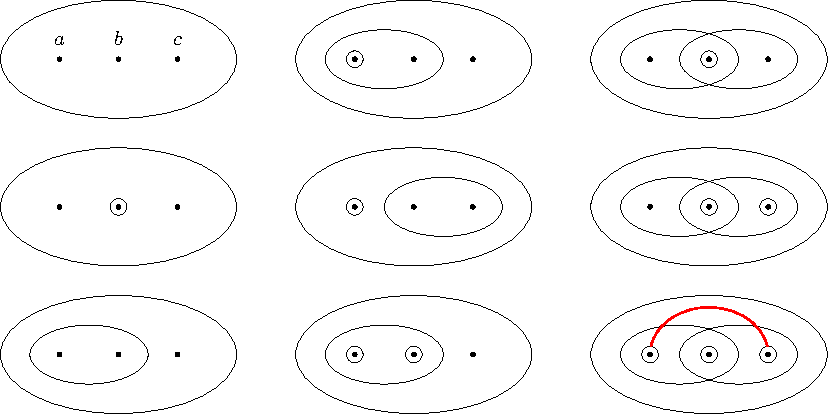
\includegraphics{fig/ch2-top.pdf}
    \caption{$a,b,c$的拓扑}\label{chtop:pic_top}
\end{figure}



\begin{definition}\label{chtop:eqn_neighbor}
    设$(X,\mathscr{T})$为拓扑空间,$\forall x\in N \subset X$,
    如果存在开集$U\in \mathscr{T}$使得$x\in U \subset N $,
    则称$N$为$x$的{\heiti 邻域}.如果$N$本身是开集,则称为{\heiti 开邻域}.
    \index[physwords]{邻域}
\end{definition}

\begin{definition}\label{chtop:def_Hausdorff}
    设拓扑空间$X$中有任意两个不同的点$x$和$y$,
    如果有不相交的($U \cap V = \varnothing$)邻域$U$和$V$分别包含它们,
    即$x\in U$和$y\in V$,则称$X$为{\bfseries \heiti Hausdorff空间}.
    \index[physwords]{Hausdorff空间} \index[persons]{Hausdorff}
\end{definition}





\begin{definition}\label{chtop:def_closedset}
    设$U$是拓扑空间$X$的子集,若$X-U$是开集,
    则称$U$为{\heiti 闭集}. \index[physwords]{闭集}
\end{definition}


\begin{definition}\label{chtop:def_cartensian}
    设有两个非空集合$A$和$B$,所有有序偶对$(a,b)$(其中$a\in A, b\in B$)的集合
    定义为{\heiti 笛卡尔积},简称为{\heiti 积},
    记为$A \times B = \{(a,b)| a\in A, b\in B \}$.\index[physwords]{笛卡尔积}
\end{definition}
需要注意$a$和$b$的顺序不能随意调换;
定义\ref{chtop:def_cartensian}可以拓展到有限个集合情形.
这里只给出了最简单“积”的概念,更详细描述见文献\parencite[\S 1, \S5, \S 15, \S19]{munkres-2000-topology}.



%\section{$\mathbb{R}^m$上的拓扑学}\label{chtop:sec_RmTP}

\section{度量空间}
\begin{definition}\label{chtop:def_metric}
    集合$X$的一个{\heiti 度量}是一个函数:$d:X\times X \to \mathbb{R}$;
    它使得以下性质成立:
    {\bfseries (1)} $\forall x,y \in X$,$d(x,y) \geqslant 0$;等号当且仅当$x=y$时成立.
    {\bfseries (2)} $\forall x,y \in X$,$d(x,y) =d(y,x)$.
    {\bfseries (3)} $\forall x,y,z \in X$,$d(x,y) +d(y,z) \geqslant d(x,z)$.
\end{definition}

\begin{definition}
    集合$X$连同给定的度量$d$称为{\heiti 度量空间},记为$(X,d)$.
\end{definition}

定义\ref{chtop:def_metric}中的度量是拓扑学上的度量.
之后,我们还会在线性空间、黎曼流形上引入度量概念;
如果它们是正定的(比如欧式度量,黎曼度量),则符合定义\ref{chtop:def_metric};
如果它们是不定的(比如Lorentz度量),则不符合定义\ref{chtop:def_metric}中的第(3)条,
不能称为拓扑学上的度量.



给定$X$一个度量$d$,实数$d(x,y)$通常称为$x$和$y$之间在$d$下的{\heiti 距离}.
对于$\varepsilon >0$,考虑所有与$x$的距离小于$\varepsilon$的点$y$的集合
\begin{equation}\label{chtop:eqn_eball}
    B_{d}(x,\varepsilon)\equiv \{y \ |\ d(x,y)<\varepsilon\} .
\end{equation}
$B_{d}(x,\varepsilon)$称为{\heiti 以$x$为中心的$\varepsilon$-球}.
在不引起混淆的前提下,可以记成$B(x,\varepsilon)$.

例如$\mathbb{R}^m$具有下列两个常用度量(请读者验证下两式符合度量定义):
\begin{subequations}\label{chtop:eqn_Rdbc}
    \begin{align}
        d_b(\boldsymbol{x}, \boldsymbol{y})=& \|\boldsymbol{x}-\boldsymbol{y}\|
        =\sqrt{(x^1-y^1)^2+\cdots +(x^m-y^m)^2}, \label{chtop:eqn_Rdb} \\
        d_c(\boldsymbol{x}, \boldsymbol{y})=& |\boldsymbol{x}-\boldsymbol{y}|
        =\max\{|x^1-y^1|,\cdots,|x^m-y^m| \}. \label{chtop:eqn_Rdc}
    \end{align}
\end{subequations}
分别称为 欧几里得 度量和确界度量;
欧几里得度量的几何意义是以$x$为中心的$\varepsilon$-球$B_{d}(x,\varepsilon)$;
确界度量的几何意义是以$\boldsymbol{x}$为中心以 $\varepsilon$ 为半边长的开立方体,
记为$C(\boldsymbol{x} , \varepsilon)$.
不难验证不等式$|\boldsymbol{x}| \leqslant\|\boldsymbol{x}\| \leqslant \sqrt{m}|\boldsymbol{x}|$成立,
它导致下列包含关系:
\begin{equation}\label{chtop:eqn_BCB}
    B(\boldsymbol{x} , \varepsilon) \subset C(\boldsymbol{x} , \varepsilon)
     \subset B(\boldsymbol{x} , \sqrt{m} \varepsilon) .
\end{equation}

需要强调的是拓扑空间定义并不需要度量,但由度量诱导的拓扑更加直观.
为了描述简单起见,我们尽量使用度量诱导出来的拓扑(比如$\mathbb{R}^m$中的拓扑),
这样更容易想象出几何图像.
%其实拓扑学中大部分内容都是从$(\mathbb{R}^m,d)$中抽象出来的.

\begin{theorem}\label{chtop:thm_RD}
    $B_{d}(x,\varepsilon)$会诱导出$(X,d)$上的一个拓扑.
\end{theorem}
\begin{proof}
    规定$X$子集族$\mathscr{T}_d \equiv \{
    U\ |\ U \text{是若干$\varepsilon$-球的并集}\}$.
    下面证明$(X, \mathscr{T}_d)$符合拓扑空间定义\ref{chtop:def_top}.
    证明过程就是验证$(X, \mathscr{T}_d)$符合定义\ref{chtop:def_top}中的三个公理.
    
    需要指出的是$B_{d}(x,\varepsilon)$中的$\varepsilon$可以等于$+\infty$或零;
    这样$\mathscr{T}_d$包含$\varnothing$和$X$本身;
    故$\mathscr{T}_d$满足定义\ref{chtop:def_top}中的第(1)条.
    
    很明显,任意个$\varepsilon$-球的并集仍在$\mathscr{T}_d$中;
    验证了\ref{chtop:def_top}中的第(2)条.
    
    为了证明第(3)条,我们需要先证明一个引理.
    设$B_{d}(x_1,\varepsilon_1)$、$B_{d}(x_2,\varepsilon_2)$是$(\mathbb{R}^m,d)$的
    两个$\varepsilon$-球,再假设它们的交集非空,
    即$\varnothing\neq U= B_{d}(x_1,\varepsilon_1)\cap B_{d}(x_2,\varepsilon_2)$.
    $\forall y \in U$,不难得到:$\varepsilon_i - d(y,x_i) >0 \, (i=1,2)$.
    记$\varepsilon_y= \min \{\varepsilon_1 - d(y,x_1),\ \varepsilon_2 - d(y,x_2)\}$,
    易证$B_{d}(y,\varepsilon_y)\subset U$;
    于是有$U = \bigcup_{y\in U} B_{d}(y,\varepsilon_y)$,
    也就是:{\kaishu $(X,d)$上任意两个$\varepsilon$-球的交集是
        若干$\varepsilon$-球的并集.}
    
    设$U,U'\in \mathscr{T}_d$,记$U= \bigcup_{\alpha} B_{d}(y_\alpha,\varepsilon_\alpha)$、
    $U'= \bigcup_{\beta} B_{d}(y'_\beta,\varepsilon'_\beta)$.那么
    \begin{align*}
        U \cap U' = \left( \bigcup_{\alpha} B_{d}(y_\alpha,\varepsilon_\alpha) \right)
        \cap \left( \bigcup_{\beta} B_{d}(y'_\beta,\varepsilon'_\beta) \right)
        = \bigcup_{\alpha,\beta }\left( B_{d}(y_\alpha,\varepsilon_\alpha)
        \cap B_{d}(y'_\beta,\varepsilon'_\beta) \right).
    \end{align*}
    根据刚刚证明的引理,对于任何$\alpha,\beta$,$B_{d}(y_\alpha,\varepsilon_\alpha)
    \cap B_{d}(y'_\beta,\varepsilon'_\beta) \in \mathscr{T}_d$;
    再由拓扑公理(2)可以得出$U\cap U'\in \mathscr{T}_d$.
    这便证明了$\mathscr{T}_d$满足第(3)条公理.
\end{proof}

定理\ref{chtop:thm_RD}中的$\mathscr{T}_d$称为由度量$d$诱导出来的{\heiti 度量拓扑}.
%该定理自然适用于$(\mathbb{R}^m,d)$.


下面讨论$\mathbb{R}^m$上{\heiti 标准开集}的概念;
需要注意{\kaishu 标准开集}的概念是人为规定的.
实数轴$\mathbb{R}$中的开区间$(a,b)$是{\kaishu 标准开集};
闭区间$[a,b]$和半开半闭区间$[a,b)$、$(a,b]$和单点集都不是标准开集.推而广之,
以$x$为中心的$\varepsilon$-球\eqref{chtop:eqn_eball}是$\mathbb{R}^m$中的{\kaishu 标准开集}.
很明显,开球$B_{d}(x,\varepsilon)$是定义\ref{chtop:eqn_neighbor}中所描述的{\kaishu 开邻域}中的一种.

$\mathbb{R}^m$上一般开集定义(包括各种非标准开集)可参阅\parencite[\S 12,\S 13]{munkres-2000-topology}.
由于我们基本不会涉及这些非标准开集,故之后的行文中将省略“标准”二字.

因$(a,b)$是$\mathbb{R}$中的开集,由定义\ref{chtop:def_closedset}可知
$(-\infty, a]$、$[b,+\infty)$以及单点集都是闭集.
$[a,b]$称为$(a,b)$的{\kaishu 闭包}.
而半开半闭集合既不是开集也不是闭集,不是$(\mathbb{R},\mathscr{T}_d)$中的元素.

包含关系\eqref{chtop:eqn_BCB}蕴涵着下列定理:
\begin{theorem}\label{chtop:thm_bcb}
    若 $X$ 是 $\mathbb{R}^m$ 的一个子空间,那么无论是用 $X$上的欧几里得度量
    还是按确界度量,$X$ 的开集族是相同的; 对于 $X$ 的闭集族也同样成立.    
\end{theorem}

定理\ref{chtop:thm_bcb}表明:对于大多数拓扑问题来说,$\mathbb{R}^m$上的这两个度量是等价的.




\begin{definition}\label{chtop:def_induced-top}
    设$A$是拓扑空间$(X,\mathscr{T})$的一个非空子集,构建如下子集
    族$\mathscr{T} _A \equiv \{U\cap A \mid U\in \mathscr{T}\}$.
    称$\mathscr{T}_A$是$A$上的{\heiti 子空间拓扑}或从$(X,\mathscr{T})$得到的{\heiti 诱导拓扑}.
    \index[physwords]{诱导拓扑}
\end{definition}

我们对诱导拓扑做一下解释.现有二维平面$\mathbb{R}^2$和一维实直线$\mathbb{R}$,
二维平面采用标准拓扑,即开圆盘$B(x,\varepsilon)$之并.
$\mathbb{R}$显然是$\mathbb{R}^2$的非空子集;
通过诱导拓扑定义\ref{chtop:def_induced-top}可以看到:
实直线与开圆盘$B(x,\varepsilon)$交集就是开区间,因此诱导拓扑就是实直线上的标准拓扑.
还有一点需要注意,这个诱导拓扑用二维平面上开集(开圆盘)来衡量并不是开集,
因为没有宽度的实直线不可能装下开圆盘.


\begin{definition}\label{chtop:def_bases}
    设有拓扑空间$(X,\mathscr{T})$,以及$X$上的一组开集族$\mathscr{B}$.
    若$\forall A \in \mathscr{T}$,它都可以表示成$\mathscr{B}$中若干元素的并集,
    则称$\mathscr{B}$是拓扑空间$(X,\mathscr{T})$的{\heiti 拓扑基 }.%简称{\heiti 基}.
\end{definition}

不难验证开球$B_d(x,\varepsilon)$是度量空间$(X,d)$的拓扑基.
由定义可见拓扑基本身就是$X$的一个拓扑,其它开集都可以由基中元素表出;
这类似于三维欧氏空间中的三个基矢量,其它矢量都可以由三个基矢线性表出.

\begin{definition}
    一个拥有无限多个元素的集合$A$,如果其中元素和正整数集合有双射关系,
    则称$A$是{\heiti 可数的}(countable).
\end{definition}
有限集合自然可以和正整数集合的某个子集建立双射关系,故必然可数.



\section{连续性}

\begin{definition}\label{chtop:def_continuity}
    设$X$和$Y$是两个拓扑空间,存在映射$f:X\to Y$,如果对于$Y$中的每个
    开子集$V$,$f^{-1}(V)$是$X$中的一个开子集,则称映射$f$为{\heiti 连续的}.
\end{definition}

我们解释一下定义\ref{chtop:def_continuity}中的集合
\begin{equation}
    f^{-1}(V)=\{x \mid  f(x) \in V\},
\end{equation}
它是$X$中所有使得$f(x)\in V$的点$x$的集合;如果$V$与$f$的像集无交,则$f^{-1}(V)=\varnothing$.
特别需要注意$f^{-1}$不是逆映射,是逆像的集合.

%连续性可以用包含度量的方式表述,
设$X$、$Y$中分别有度量$d_X$、$d_Y$,
函数 $f$ 在 $x_0$ 点连续;那么,对任意$\varepsilon>0$,
都存在一个相应的 $\delta>0$ 使得当 $d_X(x, x_0)<\delta$ 时,
$d_Y\bigl(f(x), f(x_0)\bigr)<\varepsilon $成立.
这就是连续性的经典 $\varepsilon-\delta$ 表述法.
%同时读者应能看出定义\ref{chtop:def_continuity}是$\varepsilon-\delta$ 表述法在拓扑学中的抽象表述.

注意到对给定的 $x_0 \in X$,也可能恰巧对每个 $\delta>0$,$ x_0$ 的 $\delta$ 邻域只包含 $x_0$ 点.
在这种情况下, 将 $x_0$ 称为 $X$ 的孤立点, 任何函数 $f: X \rightarrow Y$ 在孤立点自动是连续的!



\begin{example}\label{chtop:exm_txyr}
    连续性和$X$、$Y$拓扑的关系.
\end{example}
比如$X$选为$\mathbb{R}$,拓扑是{\kaishu 标准拓扑}.
$Y$也选为$\mathbb{R}$,但将拓扑选为所谓的{\kaishu 下限拓扑},即$\mathbb{R}$中的
半开半闭区间$[a,b)$是开集,同时将其记为$\mathbb{R}_\ell$.写到这里需要对拓扑再做些
说明,拓扑的规定是十分任意的,也是人为的,只要符合拓扑三公理即可,下限拓扑完全符合
拓扑三公理,请读者自行验证或参考\parencite[\S 13]{munkres-2000-topology}中的$\mathbb{R}_K$拓扑定义.
现在,我们选恒等映射
\begin{equation}
    \imath : \mathbb{R} \to \mathbb{R}_\ell,\quad
    \text{即对于任意一个实数}x,\  \imath(x) =x .
\end{equation}
但是映射$\imath${\kaishu 不是}一个连续函数.因为$\mathbb{R}_\ell$中的开集$[a,b)$的
原像还是$[a,b)$,它不是$\mathbb{R}$(标准拓扑)中的开集. \qed

\begin{definition}\label{chtop:def_homeomorphism}
    设$X$和$Y$是两个拓扑空间,如果存在双射$f:X\to Y$,并且$f$和$f^{-1}$是
    连续的,则称映射$f$为{\heiti 同胚}. 此处指整体同胚.  \index[physwords]{同胚}
\end{definition}

正是因为有例\ref{chtop:exm_txyr}这种情形,定义\ref{chtop:def_homeomorphism}中必须同时满足$f$、$f^{-1}$连续.
在同胚映射下不变的属性称为{\heiti 拓扑性质}(topological property),比如紧致性.


\begin{definition}\label{chtop:def_topological-manifold}
    设$X$为具有可数拓扑基的Hausdorff空间,若它的每一点$x$都有一个开邻域$U$同胚于$\mathbb{R}^m$中的
    一个标准开子集,则称$X$为$m$维{\heiti 拓扑流形}.\index[physwords]{拓扑流形}
\end{definition}

定义\ref{chtop:def_topological-manifold}中{\kaishu 维数}是一个很复杂的问题,
请参阅\parencite[\S 50]{munkres-2000-topology}.
此处我们简单地认为流形$X$只有一个维数,就是$m$;不考虑其它复杂情形.
代数拓扑学中有一个基本定理:  %(可参见\parencite[p. 126]{hatcher-2002-at}定理2.26)
设有两个非空标准开集$U\subset \mathbb{R}^m$、$V\subset \mathbb{R}^n$,
如果$U$、$V$相互同胚,那么它们的维数相等,即$m=n$.


微积分中有许多定理可以推广到度量空间中,我们不加证明
(可参考\parencite{munkres-2000-topology}定理18.2、18.4、21.5)的叙述两个.
下面定理中$X$、$Y$均是度量空间.

\begin{theorem}
    {\bfseries (1)} 若$f:X\to Y$将整个$X$映射为$Y$中一个点$y_0$,则$f$是连续的;即常值映射是连续的.
    {\bfseries (2)} 令 $x_0 \in A$,这里 $A$ 是 $X$ 的一个子空间.
    如果 $f: X \rightarrow Y$ 在 $x_0$点是连续的,那么限制函数 $\left.f\right|_A: A \rightarrow Y$
    在 $x_0$ 点也是连续的.
    {\bfseries (3)} 令 $f: X \rightarrow Y$,$g: Y \rightarrow Z$.
    若 $f$ 在 $x_0$ 点连续且 $g$ 在 $y_0=f\left(x_0\right)$ 点连续,
    那么 $g \circ f: X \rightarrow Z$ 在 $x_0$ 点连续.
\end{theorem}


\begin{theorem}
    {\bfseries (1)} 令$f: X \rightarrow \mathbb{R}^m$ 具有下列形式:
    $    f(x)=\bigl(f_1(x), \cdots, f_m(x)\bigr)     $    .
    那么当且仅当每个函数$f_{i}: X \rightarrow \mathbb{R}$ 在 $x_0$ 点连续时,
    $f$ 在 $x_0$ 点连续;各$f_i$称为 $f$的分量函数.    
    {\bfseries (2)} 令 $f, g: X \rightarrow \mathbb{R}$ 在 $x_0$ 点连续;
    那么 $f+g, f-g$ 及 $f \cdot g$ 均在 $x_0$ 点连续,并且当 $g(x_0) \neq 0$ 时 $f / g$ 在 $x_0$ 点连续.
    {\bfseries (3)} 投影函数$\pi_i(\boldsymbol{x})=x_i$($x_i$是$\boldsymbol{x}$第$i$分量)是连续的.
\end{theorem}










\section{拓扑空间的数个重要属性}
我们不加证明(可参考本章末文献)地列举一些拓扑空间的重要属性.


%\section{紧致性}
\begin{definition}\label{chtop:def_covering}
    给定拓扑空间$(X,\mathscr{T})$,设$\{U_\alpha\}, \alpha\in \mathbb{I}$是$X$的一个
    子集族,如果$\{U_\alpha\}$的成员之并等于$X$,则称$\{U_\alpha\}$为$X$的{\heiti 覆盖}.
    若$\{U_\alpha\}$每个成员都是开子集,则称为{\heiti 开覆盖}.
    \index[physwords]{开覆盖}
\end{definition}

\begin{definition}\label{chtop:def_compact}
    若拓扑空间$X$任意开覆盖$\{U_\alpha\}$都
    有\CJKunderwave{有限子族}能覆盖$X$,则称$X$为{\heiti 紧致的}.
    \index[physwords]{紧致}
\end{definition}



\begin{proposition}
    紧致空间的每一个闭子集都是紧致的.
\end{proposition}


\begin{proposition}
    Hausdorff空间的每一个紧致子空间都是闭的.
\end{proposition}


\begin{proposition}
    紧致空间在连续映射下的像集也是紧致的.
\end{proposition}

\begin{proposition}
    有限个紧致空间的笛卡尔积也是紧致的.
\end{proposition}


\begin{proposition}
    $\mathbb{R}^m$中子集$A$是紧致的充要条件是$A$是闭集且在度量\eqref{chtop:eqn_Rdbc}下有界.
\end{proposition}

\begin{definition}
    空间$X$在{\heiti\bfseries 点$x$是局部紧致的}是指:若存在$X$的一个紧致子空间$C$包含着$x$的一个邻域.
    若$X$在每一点都是局部紧致的,则称$X$是{\heiti 局部紧致的}.
\end{definition}


实直线并不是紧致空间,然而它是局部紧致的;$\forall x\in \mathbb{R}$,存在一个包含它的开邻域$x\in (a,b)$,
而这个开邻域必然包含在紧致子集$[a,b]$之中.推而广之,$\mathbb{R}^m$是局部紧致的,但整体上并非紧致.

\begin{theorem}
    Hausdorff空间$X$在$x$处局部紧致的充要条件是:对于$x$的任意邻域$U$,存在一个邻域$V$,
    使得$\bar{V}$紧致并且$\bar{V}\subset U$.
\end{theorem}

\begin{proposition}
    设$X$是局部紧致的Hausdorff空间,$A$是$X$的子集.
    若$A$是$X$的闭子集或开子集,则$A$是局部紧致的.
\end{proposition}

%\section{title}

\begin{proposition}
    $(\mathbb{R}^m, d_b)$是具有可数拓扑基的Hausdorff空间.
\end{proposition}

\begin{proposition}
    Hausdorff空间的拓扑子空间仍是Hausdorff空间.
\end{proposition}


\begin{proposition}\label{chtop:thm_hcb}
    有可数拓扑基的Hausdorff空间的拓扑子空间也有可数拓扑基.
\end{proposition}

\begin{proposition}
    设$\{U_i\}$、$\{V_j\}$分别是拓扑空间$X$、$Y$的拓扑基,
    那么$\{U_i\times V_j\}$(笛卡尔积)是$X\times Y$(笛卡尔积)的拓扑基.
\end{proposition}

\begin{proposition}\label{chtop:thm_cph}
    Hausdorff空间的笛卡尔积空间仍是Hausdorff空间.
\end{proposition}

\begin{proposition}
    有可数拓扑基的空间的笛卡尔积空间仍有可数拓扑基.
\end{proposition}




%\section{连通性}
\begin{definition}\label{chtop:def_connection}
    若拓扑空间$X$没有既开又闭的子集(除$X,\varnothing$外),
    则称$X${\heiti 连通}.\index[physwords]{连通}
\end{definition}

\begin{proposition}
    连通空间在连续映射下的像集也是连通的.
\end{proposition}

\begin{proposition}
    有限个连通空间的笛卡尔积也是连通的.
\end{proposition}


%\section{完备性}
\begin{definition}\label{chtop:def_complete-metric}
    给定度量空间$(X,d)$,
    $X$中的序列$\{x_n\}$称为Cauchy序列是指:$\forall \epsilon >0 $,存在正整数$N$使
    得$d(x_n,x_m)<\epsilon,\ \forall n,m>N$成立.如果$X$中的每个Cauchy序列
    都是收敛的(极限点属于$X$),则称$X$是{\heiti 度量完备}的,简称{\heiti 完备}.
    \index[physwords]{完备} \index[physwords]{完备!度量完备}
\end{definition}

\begin{proposition}
    对于度量\eqref{chtop:eqn_Rdbc}而言,欧氏空间$\mathbb{R}^m$是完备的.
\end{proposition}

\begin{example}
    在度量\eqref{chtop:eqn_Rdc}意义下,有$\mathbb{R}$中开区间$(-1,1)$的序列$\{x_n=1-1/n\}$,
    此序列的极限点是$1$,然而$1 \notin (-1,1)$,故它不完备.
    
    已知$(-1,1)$同胚于实直线$\mathbb{R}$,而$\mathbb{R}$是完备的;
    故{\kaishu 完备不是拓扑属性}.\qed
\end{example}

代数拓扑完全超出了本书的范畴,请参阅\parencite{munkres-2000-topology};
我们只给出一个定义.

\begin{definition}\label{chtop:def_covering-map}
    设$E,B$均是连通的Hausdorff空间,$p:E\to B$是连续映射.
    若$\forall b\in B$有开邻域$U$使$p^{-1}(U)$为$E$的一族两两不相交的
    开集$\{V_\alpha\}$的并集,并且$p$把每个$V_\alpha$同胚地映射成$U$,
    则称$p$为{\heiti 覆叠映射};
    $(E,p)$为$B$上的{\heiti 覆叠空间},$B$为$E$的{\heiti 底空间};
    称$U$为$b$的{\heiti 基本邻域};
    每个$V_\alpha$叫作$p^{-1}(U)$的{\heiti 分支};
    $\forall b\in B$,$p^{-1}(b)$称为$b$上的{\heiti 纤维}.
    \index[physwords]{覆叠映射} \index[physwords]{覆叠空间}
\end{definition}

%定义\ref{chtop:def_covering}中的覆盖和定义\ref{chtop:def_covering-map}中的覆叠的英文
%都是“cover”.定义\ref{chtop:def_covering}是点集拓扑中的概念;
%定义\ref{chtop:def_covering-map}是代数拓扑中的概念,“覆叠”也被翻译成“复叠”、“覆盖”.
%如果把定义\ref{chtop:def_covering-map}中的“Hausdorff空间”换成“微分流形”(见\ref{chdm:def_Dmanifold}),
%再把“同胚”换成“微分同胚”(见\ref{chdm:def_Diff-Homeomorphism}),那么上述
%覆叠映射便是微分流形间的覆叠映射.







\section*{小结}
本章初步介绍了点集拓扑的知识,是不完备的;
详尽内容可参考文献\parencite{munkres-2000-topology}.




\printbibliography[heading=subbibliography, title=第\ref{chtop}章参考文献]
\endinput

% !TeX encoding = UTF-8
% 此文件从2021.8开始

\chapter{多重线性代数}\label{chmla} % CHapter Multi-Linear Algebra


本章讲述多重线性映射;
具体安排是:先复习线性空间的概念,之后讲述线性函数、
对偶空间、双线性映射、多重线性映射、张量积、外代数等.
我们尽量做到自足.





\section{矢量空间}\label{chmla:sec_linear-space}

\index[physwords]{线性空间} \index[physwords]{矢量空间|see{线性空间}} \index[physwords]{向量空间}

\begin{definition} \label{chmla:def_linear-space}
    设$V$是一个非空集合,$\mathbb{F}$是一数域.在$V$的元素之间定义了一种代数运算,
    叫做{\heiti 加法};这就是说,给出了一个法则,对于$V$中任意两个元素
    $\alpha$和$\beta$,在V中都有唯一的一个元素$\gamma$与它们对应,称为
    $\alpha$与$\beta$的{\heiti 和},记为$\gamma=\alpha+\beta$.在数域
    $\mathbb{F}$与集合$V$之间还定义了一种运算,叫做{\heiti 数量乘法};这就是说,
    对于数域$\mathbb{F}$中任意一个数$k$与$V$中任意一元素$\alpha$,在$V$中都有唯一
    的一个元素$\delta$与它们对应,称为$k$与$\alpha$的{\heiti 数量乘积},记为
    $\delta=k\cdot \alpha=\alpha\cdot k$(通常省略乘号).
    $V$中元素对于数量乘法和加法两种运算是{\heiti 封闭的},即运算结果仍在$V$中.
    如果上面定义的加法和数量乘法满足如下规则,那么
    $V$称为数域$\mathbb{F}$上的{\heiti 线性空间},也叫{\heiti 矢量空间},或向量空间.  \newline  
    加法满足如下四条规则:\newline
    {\heiti\bfseries 条件(1)} \quad $\alpha + \beta = \beta +\alpha$;\newline
    {\heiti\bfseries 条件(2)} \quad $(\alpha + \beta) + \gamma = \alpha+ (\beta + \gamma)$;    \newline
    {\heiti\bfseries 条件(3)} \quad 在$V$中有一个元素$\boldsymbol{0}$,对于$V$中任意一个元素$\alpha$都有
    $\alpha + \boldsymbol{0} = \alpha$,具有这个性质的元素称为{\heiti 零元素},也记为$O$或$\boldsymbol{0}$;
    很多时候不用黑体,而用普通字体来表示,即$0$; \\
    {\heiti\bfseries 条件(4)} \quad 对于$V$中每一个元素$\alpha$,都有$V$中的元素$\beta$,使得
    $\alpha + \beta = 0$,$\beta$称为$\alpha$的{\heiti 负元素},记作$\beta = -\alpha$;  \\
    数量乘法满足如下两条规则:\\
    {\heiti\bfseries 条件(5)} \quad $1 \alpha =\alpha, \ 1\in \mathbb{F}$; \\
    {\heiti\bfseries 条件(6)} \quad $k(l\alpha) = (kl) \alpha$;\\
    数量乘法和加法满足下面两条规则:\\
    {\heiti\bfseries 条件(7)} \quad $(k+l)\alpha = k\alpha +l\alpha$; \\
    {\heiti\bfseries 条件(8)} \quad $k(\alpha+\beta) = k\alpha +k\beta$.  \\
    在上面规则中,$\forall \alpha,\beta,\gamma \in V$,$\forall k,l\in \mathbb{F}$.
    集合$V$中的元素称为{\heiti 矢量}.  \qed
\end{definition}

线性空间还可以定义在一般的域上(不仅仅是数域),这种情形对物理学来说
貌似没有特别意义;故我们只考虑定义在数域上的线性空间.
下面给出实数域上的内积空间.

\begin{definition} \label{chmla:def_Euclidean-space}
    设$V$是实数域$\mathbb{R}$上的矢量空间,在$V$上定义一个二元运算,有实数$c$与之对应,
    称为{\heiti 内积},记成$c=\left<\alpha,\beta\right>$,它需满足如下性质:\\
    {\heiti\bfseries 条件(1)} \quad $\left<\alpha,\beta\right>=\left<\beta,\alpha\right>$;\\
    {\heiti\bfseries 条件(2)} \quad $\left<\alpha,k\beta\right>=\left<\alpha,\beta\right>k$;\\
    {\heiti\bfseries 条件(3)} \quad $\left<\alpha,\beta+\gamma\right>=\left<\alpha,\beta\right>+\left<\alpha,\gamma\right>$; \\
    {\heiti\bfseries 条件(4)} \quad $\left<\alpha,\alpha\right>$是非负实数,当且仅当$\alpha=0$时,$\left<\alpha,\alpha\right> = 0$.\\
    其中$\forall\alpha,\beta,\gamma \in V$,$\forall k\in \mathbb{R}$.这样的线性空间称为{\heiti 欧几里得空间}.
    \index[physwords]{欧几里得空间}
\end{definition}


定义了内积的矢量空间称为{\heiti 内积空间}.
内积空间专指正定情形,即$\left<\alpha,\alpha\right>\geqslant 0$;
以后还会介绍\uwave{标量积}(也称为半内积)概念,此时$\left<\alpha,\alpha\right>$可正可负可为零.
为了与内积区分,我们使用了“标量积”这个术语,有的文献未作此区分.





设$V$是数域$\mathbb{F}$上的矢量空间,$\alpha_1,\cdots,\alpha_r(r\geqslant1)$是$V$中
一组矢量,$k_1,\cdots,k_r$是数域$\mathbb{F}$中的数,那么矢量
$\alpha = k_1\alpha_1+\cdots+k_r\alpha_r$
称为矢量组$\alpha_1,\cdots,\alpha_r$的线性组合.
也说成矢量$\alpha$可以由矢量组$\alpha_1,\cdots,\alpha_r$线性表出.

\begin{definition}\label{chmla:def_linear-dependence_base}
    设$V$是数域$\mathbb{F}$上的矢量空间,$V$中矢量组$\alpha_1,\alpha_2,\cdots,\alpha_r(r\geqslant1)$
    称为$\mathbb{F}$-{\heiti 线性相关},是指在数域$\mathbb{F}$中存在$r$个不全为零的数
    $k_1,k_2,\cdots,k_r$使得$k_1\alpha_1+k_2\alpha_2+\cdots+k_r\alpha_r=0$成立.
    如果是上式只有在$k_1=k_2=\cdots=k_r=0$时才成立,那么
    $\alpha_1,\alpha_2,\cdots,\alpha_r$称
    为$\mathbb{F}$-{\heiti 线性独立},也称为$\mathbb{F}$-{\heiti 线性无关}.
    \index[physwords]{线性相关}\index[physwords]{线性独立}\index[physwords]{线性无关|see{线性独立}}
\end{definition}
很多时候会把前缀“$\mathbb{F}$-”去掉;之后我们还会介绍$C^r(M)$-线性
(见第\pageref{chdm:eqn_functimesv}页及\pageref{chdm:thm_Tensor-Characterization-Lemma}页),
此时前缀“$C^r(M)$”是不能省略的.
如果线性空间$V$中有$n$个线性独立的矢量,并且任何$n+1$个矢量组都是线性相关的,
那么就称空间$V$是$\boldsymbol{n}${\heiti 维}的.如果$V$中可以找到任意多个线性独立的矢量,
那么就称空间$V$是{\heiti 无限维}的.
$n$维空间$V$中任意$n$个线性无关的矢量称为这个空间的{\heiti 基矢}或{\heiti 基底}.
%,简称{\heiti 基}


在\S\ref{chcdg:sec_sm}中,我们指出把矢量定义成有大小、有方向的量是无法向非欧几何推广的.
Peano于1888年给出{\kaishu 矢量}的代数定义\ref{chmla:def_linear-space},将矢量表示成八条公理形式;
这个定义摆脱了度量,无法给出矢量的长短,但可以描述矢量方向(见下).
数学家们将矢量定义抽象化到这个程度自然是为了推广到不同的数学、物理领域.
矢量大小可由定义\ref{chmla:def_Euclidean-space}给出.
设数域$\mathbb{F}$上有$n$维线性空间$V$,
它有$n$个线性无关的基矢$\boldsymbol{\epsilon}_i$($i=1,\cdots,n$),
那么$\forall \alpha \in V$可以用这组基矢展开:
\begin{equation}
	\alpha = \alpha_1 \boldsymbol{\epsilon}_1 +\cdots +\alpha_n \boldsymbol{\epsilon}_n.
\end{equation}
其中$\alpha_i\in \mathbb{F}$是展开系数,我们将其记成$(\alpha_1,\cdots,\alpha_n)$;
这组展开系数便体现了矢量$\alpha$在基矢$\boldsymbol{\epsilon}_i$下的{\kaishu 方向}.
$\forall \alpha ,\beta \in V$,根据定义\ref{chmla:def_linear-space}有
\begin{align}
	\alpha + \beta =& (\alpha_1+\beta_1)\boldsymbol{\epsilon}_1 +\cdots+(\alpha_n+\beta_n)\boldsymbol{\epsilon}_n .\\
	k\alpha =& (k\alpha_1) \boldsymbol{\epsilon}_1 +\cdots +(k\alpha_n) \boldsymbol{\epsilon}_n, 
	\qquad \forall k\in \mathbb{F}.
\end{align}
这与欧式空间(指第\ref{chcdg}章)矢量加法、数乘完全一致.
可见矢量的代数定义\ref{chmla:def_linear-space}保留了欧式空间
矢量(指第\ref{chcdg}章)的诸多属性(加法、数乘);只祛除了度量.


\subsection{例子}
\begin{example}\label{chmla:exm_zero}
    数域$\mathbb{F}$上的空间$V$只有一个零元,这个空间是0维的.
\end{example}
\begin{example}\label{chmla:exm_vsF}
    数域$\mathbb{F}$可看作自身加法和乘法的1维线性空间.
\end{example}
很容易验证上两例符合定义\ref{chmla:def_linear-space}中的八个条件.
需要注意,矢量空间涉及两个因素,一个是数域$\mathbb{F}$,一个是集合$V$,两者不可或缺.
\begin{example}\label{chmla:exm_rc1}
    全体复数的集合$V=\mathbb{C}$可以看成实数域$\mathbb{R}$上的线性空间.
\end{example}
取实数域$\mathbb{R}$,那么集合$V=\mathbb{C}$是一个2维线性空间,基矢可以选为
$\epsilon_1=1,\epsilon_2=\mathbbm{i}$;
{\footnote{其中$\mathbbm{i}$是一个符号,称为虚数单位,
        它代表$\sqrt{-1}$;自然有$\mathbbm{i}^2=-1.$}}
这样任意一个复数均可表示成这两个基矢
的线性组合$z=x\cdot 1+y\mathbbm{i}=x\epsilon_1+y\epsilon_2$,
其中$x$和$y$是实数域$\mathbb{R}$中的常数.这里用到的
数量乘法是两个实数相乘.复数乘法以及取复数共轭运算都不是
定义\ref{chmla:def_linear-space}在实数域中的代数运算,需要另外再定义.
$V$中两个矢量$1$和$\mathbbm{i}$在本例中是线性无关的.
\qed

\begin{example}\label{chmla:exm_rc2}
    全体复数的集合$V=\mathbb{C}$同样可以看成复数域$\mathbb{C}$上的线性空间.
\end{example}
把全体复数的集合$V$建立在复数域$\mathbb{C}$上,这时候我们只需选取
一个基矢$\epsilon_1=1$即可,因为任意一个复数均可以表示成基矢1乘以某个复数
$z=z\cdot 1=z\cdot \epsilon_1$.
复数乘法以及取复数共轭运算都可以看作是
定义\ref{chmla:def_linear-space}在复数域中的运算,不需要额外给定的;
比如取复共轭运算可以通过复数乘法来实现$z^*= z \times z^*/z$(对比上一例题,那里的复数乘法
必须额外给定,而在这里,复数乘法就是定义\ref{chmla:def_linear-space}中的数量乘法).
$V$中两个矢量$1$和$\mathbbm{i}$在本例中是线性相关的.
\qed

从上面两例可以看出同样的集合$V$,对不同的数域来说,维数可能是不同的.
所以建立线性空间,数域$\mathbb{F}$和集合$V$两者都不可缺少.




\begin{example}
    量子物理中沿$x,y$方向动量算符和绕$z$轴的角动量算符是否线性相关?
\end{example}
建立在复数域$\mathbb{C}$上的,
沿$x$和$y$轴的动量算符$\hat{P}_x$
和$\hat{P}_y$;绕$z$轴的角动量算符是
$\hat{L}_\phi \equiv \hat{y}\hat{P}_x - \hat{x} \hat{P}_y$.
写成这种形式时,几乎所有人都能看出三个矢量线性无关;
因为算符$\hat{y}$和$-\hat{x}$是Hilbert空间
(一种线性空间)中的量,不是数域$\mathbb{C}$中的量.
很多时候,会把位置矢量算符$\hat{x},\hat{y}$上的小尖帽省略,
记成$\hat{L}_\phi \equiv {y}\hat{P}_x - {x} \hat{P}_y$;
这个时候,有可能会被误认为三者线性相关,但这是不正确的.
即便系数变成了$y$和$-x$,它们也是线性空间中的量,
不是数域$\mathbb{C}$中的量.
或者这样理解:
依照定义\ref{chmla:def_linear-dependence_base},
因为其系数$y$和$-x$是{\uwave{变量}},不是数域$\mathbb{C}$中{\uwave{常数}},所以
三个矢量$\hat{P}_x, \hat{P}_y, \hat{L}_\phi$是线性无关的.
另外一个与此类似的例子是Killing场,见\S \ref{chrg:sec_killing}.
\qed

因线性空间的元素十分广泛,不可能所有类型元素都与数域$\mathbb{F}$有什么关联;
可能存在某些类型线性空间(比如$\mathbb{F}^n$)中的矢量与数域中的数有密切关系,也存在其它类型
线性空间(比如一堆算符构成的空间或例\ref{chmla:exm_zero})中的元素与数域中的数几乎没有直接关联.
为了使线性相关定义具有通用性,在考虑矢量间是否线性相关时不能
让定义\ref{chmla:def_linear-dependence_base}中的$\mathbb{F}$值系数$k_i$随线性空间中矢量内部参量改变而变化,
所以定义\ref{chmla:def_linear-dependence_base}中系数只能是$\mathbb{F}$值\uwave{常数}.
这种抽象地解释显得不够明了,以多项式为例再次解释一遍更有教益;有多项式
\begin{equation}
    f(x)=a_0+a_1 x+ a_2 x^2 + \cdots+ a_n x^n, \qquad a_i \in \mathbb{F}
\end{equation}
上式中$x$是一个符号,可能是算符、矩阵,也可能是实数等等.
一般线性代数书中都会介绍:把此式看成线性空间,那么它是$n+1$维的,
可选$\{1,x^1,\cdots,x^n\}$为此空间基矢.
比如我们把符号$x$选为矩阵,那么几乎没有人(也没有理由)认为基矢$1$(单位矩阵)和基矢$x$线性相关.
如果我们把符号$x$选为$\mathbb{F}$值数,可能有人(也有理由)认为$1$和$x$线性相关;
比如选择系数$k_1 =-1, \ k_2 = x^{-1}$,那么$k_1 \cdot 1 + k_2 \cdot x =0 $.
如果这种理解正确,那么多项式作为线性空间的维数是不定的,当$x$是矩阵时维数是$n+1$,
当$x$是数时维数是$1$;这使线性空间失去了一般性、普适性、通用性,为保持
线性空间的一般性、普适性、通用性,定义\ref{chmla:def_linear-dependence_base}中
系数只能是$\mathbb{F}$值\uwave{常数},\uwave{不能是变数}.

%需要强调的是:定义\ref{chmla:def_linear-dependence_base}是构建在数域$\mathbb{F}$上线性空间的概念.
%如果是构建在环$R$上的线性空间(即{\kaishu 模}),那么线性独立与此不同,请查阅相关文献.

\begin{example}\label{chmla:exm-cab}
    实数轴上全体$r$阶连续可微实函数$C^r[a,b]$是无穷维线性空间.
\end{example}
首先,我们验证函数空间是个线性空间.$\forall x\in [a,b]$,
对于任意函数$f,g\in C^r[a,b]$,给定加法为$(f+g)(x)\overset{def}{=}f(x)+g(x)$,
数量乘法为$(\lambda \cdot g) (x)\overset{def}{=}\lambda \cdot (g (x)), \forall \lambda \in \mathbb{R}$.
容易验证上述定义符合线性空间定义\ref{chmla:def_linear-space};其中零矢量是对任意实数$x$取值恒为零的函数.

我们从两个角度来理解空函数间$C^r[a,b]$维数是无穷大这件事情.首先,
对于任意固定的$x\in [a,b]$来说,函数空间$C^r[a,b]$是一维的;我们只需选取此线性空间基矢为“$1$”,那么
任意函数$f$取值只是基矢“$1$”的$f(x)$倍(注意$x$是固定不变的).然而区间$[a,b]$是连续的,
这个区间有无穷多个值,当$x$取值连续变化时,函数空间$C^r[a,b]$便是无穷多个一维线性空间之和,
其维数自然是无穷大.

其次,选取$C^r[a,b]$的一个子空间:全体多项式.多项式基矢可选
为$\{1,x,x^2,\cdots \}$,很明显多项式基矢有无穷多个,
即基矢$x^n$的幂次$n\to \infty$;全体多项式构成的子空间维数是无穷大的.
既然子空间是无穷维的,那么空间$C^r[a,b]$的维数不可能是有限的.\qed




\subsection{微分线性相关定义}\label{chmla:sec_diff-linear-dependence}
给定线性偏微分方程组
\begin{equation}\label{chmla:eqn_lde1}
    \left\{ {\begin{array}{*{20}{c}}
            \sum\limits_{ij} {a_{ij}^{( 1 )}(x)\dfrac{{\partial {y_j}}}{{\partial {x_i}}}}  + {f_1}(x) = 0  \\
            \vdots \\
            \sum\limits_{ij} {a_{ij}^{( n )}(x)\dfrac{{\partial {y_j}}}{{\partial {x_i}}}}  + {f_n}(x) = 0
    \end{array}} \right.
\end{equation}
其中$x_i$是自变量,$y_j$是未知量,$a_{ij}^{( k )}(x)$是线性系数,$f_k(x)$是非齐次项.

令${Z_k} \equiv\sum_{ij}{a_{ij}^{( k )}\frac{{\partial {y_j}}}{{\partial {x_i}}}}  + {f_k}$,
给出两个定义.
\begin{definition}\label{chmla:def_linear-dependence}
    给定数域$\mathbb{F}$,如果存在不全为零的系数$c_k\in \mathbb{F}$,
    使得$\sum_{k} {{c_k}{Z_k} = 0} $成立,
    则称偏微分方程组\eqref{chmla:eqn_lde1}是线性相关的.
    否则线性独立.
\end{definition}
这个定义是定义\ref{chmla:def_linear-dependence_base}在微分方程领域的翻版.
\begin{definition}\label{chmla:def_diff-linear-dependence}
    若数域$\mathbb{F}$中存在不全为零的系数${c_k},d_{kl}$使得
    $\sum_k {{c_k}{Z_k}}  + \sum_{kl} {{d_{kl}}
        \frac{{\partial {Z_k}}}{{\partial {x_l}}}} = 0$
    成立,则称方程组\eqref{chmla:eqn_lde1}是{\heiti 微分}线
    性相关的.否则线性独立.\index[physwords]{线性相关!微分线性相关}
\end{definition}
显然,如果$d_{kl}\equiv 0$,则定义
\ref{chmla:def_diff-linear-dependence}就退化到定义\ref{chmla:def_linear-dependence}.


定义\ref{chmla:def_diff-linear-dependence}的描述方式取自文献\parencite{liu2018}.
这个定义的本质是包含微分恒等式;当方程包含微分恒等式时,在
定义\ref{chmla:def_linear-dependence}中要放弃未知量个数与方程个数
相等这个事情;需要在定义\ref{chmla:def_diff-linear-dependence}下让
两者相等.对于存在微分恒等式的偏微分方程来说,定义
\ref{chmla:def_diff-linear-dependence}比定义
\ref{chmla:def_linear-dependence}更合适.比如麦克斯韦方程组、
爱因斯坦引力场方程组,应力、应变形式的弹性力学平衡方程组,
单旋度散度方程组等等在定义
\ref{chmla:def_linear-dependence}意义下是超定的,
然而在定义\ref{chmla:def_diff-linear-dependence}意义下是确定的.
{\footnote{“确定”是指well-determined或proper-determined,偶尔也有人将这个词儿
        翻译成“适定”.这与另外一个词儿well-posed的翻译(通常翻译成“适定”)容易混淆.}}

上述定义在\textcite[p.16]{courant_hilbert-v2}中有类似叙述;
在更早的文献中也应该有类似描述,究竟谁是最早给出的定义,已很难查询.
虽然柯朗给出了类似定义,但在他的书中仍旧称定义\ref{chmla:def_diff-linear-dependence}下
未知量个数与方程个数相等的方程为{\kaishu 超定}
(见\parencite[p.16]{courant_hilbert-v2}例子,与本书例\ref{chdf:exm_Fij2d}相同),
只把定义\ref{chmla:def_linear-dependence}下两者相等的方程称为确定.
这与我们的称呼并不相同.


\begin{example}
    讨论下面方程组中的$Z_1,Z_2$是否线性相关.
    \begin{equation}\label{chhs:tmp_eqn00}
        \begin{cases}
            Z_1 \equiv x = 0  \\
            Z_2 \equiv x^2 = 0  \\
        \end{cases}
    \end{equation}
\end{example}
显然有关系式$x Z_1-Z_2=x\cdot x - x^2=0$,但这不能说明两个方程线性相关;
因为$Z_1$前的系数是变量$x$,不是数域$\mathbb{F}$中的常数,
所以$Z_1,Z_2$是线性无关的两个方程.
\qed


\index[physwords]{商空间}
\subsection{商空间}\label{chmla:sec_quotient}

设有三维欧几里得空间$E^3$,在其上建立直角坐标系$O-xyz$.
此处需对$E^3$和$\mathbb{R}^3$略作区分,$E^3$是点空间,$\mathbb{R}^3$是矢量空间;
在$E^3$中将原点$O$算作起点,任意一点$A$算作终点,则有向线段$\overrightarrow{OA}$便是
一个矢量,此矢量与$\mathbb{R}^3$中矢量有双射关系.
设$W$是$xy$平面,则与$W$平行的所有平面以及$W$给出了$E^3$的一个划分.
设$\pi$是平行于$W$的一个平面,$\overrightarrow{OA}$与$\overrightarrow{OB}$都
属于$\pi$(指点$A$和$B$在平面$\pi$上)的
充要条件是$\overrightarrow{OA}-\overrightarrow{OB}=\overrightarrow{BA} \in W$;
由于规定矢量起点是原点$O$,故需先将$\overrightarrow{BA} $平移,令$B$和$O$重合,
此时作为矢量的$\overrightarrow{BA}$是$W$中元素 .

由此受到启发,为了在数域$\mathbb{F}$的线性空间$V$上建立一个二元关系且使它是一个等价关系,
可以先取$V$的一个子空间$W$,然后规定:
\begin{equation}\label{chmla:eqn_abw}
    \alpha \sim \beta \quad \Leftrightarrow\quad  \alpha-\beta \in W .
\end{equation}
这样就建立了$V$上的一个二元关系“$\sim$”.
由于$\alpha-\alpha=0 \in W$,因此$\alpha \sim \alpha, \forall \alpha \in W$,即“$\sim$”具有反身性.
若$\alpha \sim \beta$,即$\alpha-\beta \in W$,从而 $\beta-\alpha=-(\alpha-\beta) \in W$,
于是 $\beta \sim \alpha$,即“$\sim$”具有对称性.
若$\alpha \sim \beta$ 且 $\beta\sim \gamma$,则$\alpha-\beta \in W$ 且 $\beta-\gamma \in W$;
从而$\alpha-\gamma=(\alpha-\beta)+(\beta-\gamma) \in W$,即“$\sim$”具有传递性.
从而由式\eqref{chmla:eqn_abw}定义的二元关系“$\sim$”是$V$上的一个{\kaishu 等价关系}.
对于$\alpha \in V$,$\alpha$ 的等价类 $\bar{\alpha}$ 为
\begin{align}
    \bar{\alpha} =&\{\beta \in V \mid \beta \sim \alpha\} 
     =\{\beta \in V \mid \beta-\alpha \in W\} 
     =\{\beta \in V|\beta=\alpha+\gamma, \gamma \in W \} \notag \\
     =&\{\alpha+\gamma \mid \gamma \in W\} . \label{chmla:eqn_aeqvba}
\end{align}
把式\eqref{chmla:eqn_aeqvba}最后一个集合记作$\alpha+W$,称它为$W$的一个{\heiti 陪集},
$\alpha$称为这个陪集的{\kaishu 代表}.从而
$    \beta \in \alpha+W \ \Leftrightarrow \ \beta \sim \alpha  \ \Leftrightarrow \ \beta-\alpha \in W $.
于是 $\bar{\alpha}= \alpha+W $.
据等价类的性质可得
\begin{equation}\label{chmla:eqn_abwasimbw}
    \bar{\alpha}=\bar{\beta}\ \Leftrightarrow\  \alpha+W=\beta+W \ \Leftrightarrow\ 
    \alpha-\beta \in W \ \Leftrightarrow \  \alpha \sim \beta.
\end{equation}
由式\eqref{chmla:eqn_abwasimbw}看出,一个陪集$\alpha+W$的代表不唯一.
如果 $\alpha-\beta \in W$, 那么 $\beta$ 也可以作为这个陪集 的代表.

对于上述等价关系,记$V / \sim$为$V / W$,
称它是\uwave{$V$对子空间$W$的商集},即
\begin{equation}\label{chmla:eqn_Quotient}
    V / \sim \equiv V / W=\{\alpha+W \ |\ \alpha \in V \} .
\end{equation}
如何在商集 $V / W$ 中规定加法与数量乘法运算?容易想到尝试如下规定:
\begin{equation}\label{chmla:eqn_abwlin}
    (\alpha+W)+(\beta+W) \stackrel{def}{=}(\alpha+\beta)+W, \quad
    k(\alpha+W) \stackrel{def}{=} k \alpha+W .
\end{equation}
这样规定是否合理?需要证明它们与陪集代表的选择无关.
设$\alpha_1+W=\alpha+W, \beta_1+W=$ $\beta+W$,则 $\alpha_1-\alpha \in W, \beta_1-\beta \in W$ .从而
\begin{align*}
    (\alpha_1+\beta_1)-(\alpha+\beta)= (\alpha_1-\alpha)+(\beta_1-\beta) \in W; \quad
    k \alpha_1-k \alpha= k (\alpha_1-\alpha) \in W .
\end{align*}
因此$(\alpha_1+\beta_1)+W=(\alpha+\beta)+W,\ k \alpha_1+W=k \alpha+W$.
这证明了上述规定与陪集代表的选取无关,从而是合理的.
容易验证上述加法满足交换律和结合律,$0+W$ (即 $W$ )是$V / W$的{\kaishu 零元},
$(-\alpha)+W$是$\alpha+W$的{\kaishu 负元};
上述数量乘法满足线性空间定义中关于数量乘法的几条运 算法则,
从面$V / W$成为数域$\mathbb{F}$上的一个线性空间;
我们称$V / W$是$V$对于$W$的{\heiti 商空间}(Quotient Spaces).

注意:商空间 $V / W$ 的元素是 $V$ 的一个等价类,而不是 $V$ 的一个向量.
例如上面列举的三维欧几里得空间$E^3$ 的例子,$E^3$对于$W$平面的商空间$E^3 / W$的
一个元素是平行于$W$的一个平面或者$W$自身,而不是几何空间 $E^3$ 中的向量.
容易直观地看出商空间 $E^3 / W$ 是 1 维的,即 ${\rm dim}E^3 / W={\rm dim} E^3-{\rm dim} W$.
可以证明(请参考\parencite[p.219]{qiuws-2019-v2}定理1)这个结论能推广到数域 $\mathbb{F}$上
任一有限维线性空间$V$对子空间$W$的商空间$V / W$ 中.

\begin{theorem}\label{chmla:thm_dimvw}
    设$V$是数域 $\mathbb{F}$上有限维线性空间,$W$是$V$的一个子空间;
    那么商空间维数是:$ {\rm dim} (V / W)={\rm dim} V-{\rm dim} W$.
\end{theorem}


从线性空间$V$到商空间$V/W$有一个自然的映射:
\begin{equation}\label{chmla:eqn_canonical-quotient}
    \pi: V \to V/W,\qquad  \alpha \to \alpha + W, \quad \forall\alpha\in V.
\end{equation}
一般称式\eqref{chmla:eqn_canonical-quotient}为{\heiti 标准映射}.
显然$\pi$是满射.
%;当$W$不是零子空间时,$\pi$不是单射




\section{线性映射}\label{chmla:sec_linear-map}
有了矢量空间,就可以定义空间上的线性映射.
\begin{definition}\label{chmla:def_linear-fun}
    设$V,W$是数域$\mathbb{F}$上线性空间,若$f:V \to W$有如下线性性质
    \begin{equation}\label{chmla:eqn_linear-fun}
        f(k \alpha + \beta)=k\cdot  f(\alpha)+ f(\beta);
        \qquad \forall k\in \mathbb{F}; \quad \forall \alpha, \beta \in V .
    \end{equation}
    则称映射$f$是从$V$到$W$的{\heiti 线性映射};
    若$W\equiv V$,则称$f$是{\heiti 线性变换};
    若$W\equiv \mathbb{F}$,则称$f$是{\heiti 线性函数}(或{\kaishu 线性泛函}).
    把$V$到$W$的全体线性映射组成的集合记为${\rm Hom}(V,W)$.
\end{definition}

\index[physwords]{线性映射}  \index[physwords]{线性函数}
\index[physwords]{线性变换}  \index[physwords]{线性泛函}

\begin{example}
    由定义\ref{chmla:def_linear-fun}可知
    $f\bigl((k+1)\alpha \bigr)=f(k \alpha + \alpha)=k\cdot  f(\alpha)+ f(\alpha)=(k+1)\cdot  f(\alpha)$;
    再令$k=1$,有$f(\alpha + \beta)=f(\alpha)+ f(\beta)$.
    可见定义\ref{chmla:def_linear-fun}与一般文献上的定义等价.
\end{example}

很多文献将$V$上全体{\kaishu 线性变换}记成${\rm End}(V)$(Endomorphisms).

线性空间中的元素是非常广泛的,在讨论线性空间基本性质时我们无需关心元素的具体信息,
只需要关心它的代数性质即可.因元素的复杂性,线性函数$f$的具体形式很多时候无法确切表示,
但我们只需记住函数$f$将$V$中元素映射为数域$\mathbb{F}$中的一个具体数值即可.


线性映射是代数学中非常重要的内容,详细可参阅文献\parencite{qiuws-2019-v2}第九章(近200页).
下面我们着重讲述较为简单的线性函数.

%\subsection{线性函数}

\begin{example}
    线性函数有如下几条简单的性质.
    \begin{align}
        f(0) & =f(0 \cdot \alpha)= 0 \cdot f(\alpha) = 0. \\
        f(-\alpha)&=f\bigl((-1)\cdot\alpha)\bigr) = - f(\alpha).
    \end{align}
从上可以看到,任何线性函数都将零矢量映射为数字零.
\end{example}



%\begin{example}
%    设$a_1,a_2,\cdots,a_n$是数域$\mathbb{F}$中的任意$n$个数,
%    $X=(x_1,x_2,\cdots,x_n)$是矢量空间$\mathbb{F}^n$的任意矢量,
%    则函数
%    \begin{equation}
%        f(x)=f(x_1,x_2,\cdots,x_n) = \sum_{i=1}^{n} a_i x_i .
%    \end{equation}
%    是空间$\mathbb{F}^n$上的一个线性函数.
%\end{example}
%上面只针对数域$\mathbb{F}^n$上的线性函数,
%其实任意线性函数都可以表示成此形式,见下面定理中的叙述.

\begin{theorem} \label{chmla:thm_lin-fun-basic}
    设$V$是数域$\mathbb{F}$上的$n$维线性空间,
    $\boldsymbol{\epsilon}_1,\boldsymbol{\epsilon}_2,\cdots,\boldsymbol{\epsilon}_n$是
    $V$的一组基矢,$a_1,a_2,\cdots,a_n$是数域$\mathbb{F}$中的任意$n$个数.则存在
    唯一的线性函数$f$使得
    $f\left(  \boldsymbol{\epsilon}_i\right) = a_i,i=1,2,\cdots,n$.
\end{theorem}
\begin{proof}
    先给出线性函数的一般形式.$V$中任意一个矢量$X$都可以表示
    成这个基矢的线性组合$X= \sum_{i}x_i \boldsymbol{\epsilon}_i $,其中$x_i$是矢量$X$在
    基矢$\boldsymbol{\epsilon}_i$上的分量.对于空间$V$上的任意线性函数$g$,有
    \begin{equation}\label{chmla:eqn_lin-fun-form-0}
        g(X)= g\left( \sum_{i=1}^{n} x_i \boldsymbol{\epsilon}_i\right)
        = \sum_{i=1}^{n} x_i g\left(  \boldsymbol{\epsilon}_i\right) ,
        \qquad g(\boldsymbol{\epsilon}_i ) \in \mathbb{F}.
    \end{equation}
    很显然函数$g(X)$由$\mathbb{F}$值$g(\boldsymbol{\epsilon}_i), \ i =1,2,\cdots,n$唯一确定;
    任何一个线性函数都可以表示成式\eqref{chmla:eqn_lin-fun-form-0}的形式;
    表示成这个形式的函数一定是线性函数.

    任意给定数域$\mathbb{F}$中的$n$个数$a_1,a_2,\cdots,a_n$,
    仿照式\eqref{chmla:eqn_lin-fun-form-0}形式构造$V$上一个函数$f$:
    \begin{equation}\label{chmla:eqn_lin-fun-form}
        f\left( \sum_{i=1}^{n} x_i \boldsymbol{\epsilon}_i\right)
        \overset{def}{=} \sum_{i=1}^{n}x_i a_i , \qquad
        {\text {其中}}\     \forall X = \sum_{i}^n x_i \boldsymbol{\epsilon}_i \in V.
    \end{equation}
    容易验证函数$f$是线性的,且将空间$V$中的矢量$X$映射为数域$\mathbb{F}$中的数值.
    既然已经构造出函数$f$,即说明了“存在性”.由式\eqref{chmla:eqn_lin-fun-form}易
    得$f\left(  \boldsymbol{\epsilon}_i\right) = a_i,i=1,2,\cdots,n$.

    用反证法来证明“唯一性”.
    假设有不同于$f$的映射$h(\boldsymbol{\epsilon}_i)=a_i$,那么有
    $h(\boldsymbol{\epsilon}_i)=a_i=f(\boldsymbol{\epsilon}_i)
    {\color{red}\Rightarrow} (f-h)(\boldsymbol{\epsilon}_i)=0$,这
    是说$(f-h)$作用在每个基矢(进而也就是$V$中每个矢量)上都为零,
    那么$(f-h)$必为零函数,也就是
    式\eqref{chmla:eqn_lin-fun-form}中$f$是唯一的.
\end{proof}

\begin{proposition}\label{chmla:thm_OneOne}
    设$V$是数域$\mathbb{F}$上的$n$维线性空间,$f$是定义其上的
    线性函数.$f$只将零矢量$\alpha \in V$映射为零值,
    等价于,线性函数$f$是单一的.
\end{proposition}
\begin{proof}
    先证“$\Rightarrow$”,用反证法.
    假设$f$不单一,则存在$V$中非零且不等的矢量$\alpha,\beta$,
    使得$f(\alpha)=f(\beta)$成立,则自然有$f(\alpha-\beta)=0$,但是
    已知$\alpha \neq \beta$;也就是$f$将非零矢量映射为零,与已知条件矛盾,
    必然是假设错误,故$f$单一.

    再证“$\Leftarrow$”.不论$f$是否单一,必有$f(0)=0$.
    因$f$单一,故$\forall \alpha \neq 0, f(\alpha)\neq f(0)=0$;
    由此可知$f$只将零向量映射为零值.
\end{proof}




%\subsection{线性同构}\label{chmla:sec_linear-isomorphism}

\begin{definition}\label{chmla:def_isomorphism}
    给定数域$\mathbb{F}$,在其上建立两个线性空间$V$和$V'$,若存在
    线性双射$\sigma:V\to V'$,即$\sigma$满足式\eqref{chmla:eqn_linear-fun};
    则称映射$\sigma$是从$V$到$V'$的{\heiti 线性同构映射},记为$V \cong V'$.\index[physwords]{线性同构}
\end{definition}

线性同构$\sigma$有逆映射$\sigma^{-1}:V'\to V$,这个逆映射同样是同构映射.
同构的两个空间$V$和$V'$具有相同的维数.关于同构映射,有如下基本定理:
\begin{theorem}\label{chmla:thm_vvp-basic}
    $\mathbb{F}$上两个有限维矢量空间线性同构的充要条件是它们有相同的维数.
\end{theorem}
\begin{proof}
    “$\Rightarrow$”部分证明过程很简单,略.可参考\parencite[\S 8.3]{qiuws-2019-v2}.

    “$\Leftarrow$”部分.设数域$\mathbb{F}$上有两个线性空间$V$和$V'$,它们维数都是$n$.
    在$V$和$V'$中各取一组基矢$\boldsymbol{\epsilon}_1,\cdots,\boldsymbol{\epsilon}_n$
    和$\boldsymbol{\eta}_1,\cdots,\boldsymbol{\eta}_n$;
    建立一个关系$\sigma : V \to V'$如下
    \begin{equation}\label{chmla:eqn_tmp12}
        \sigma (\alpha) \equiv
        \sigma \left(\sum_{i=1}^{n} a_i \boldsymbol{\epsilon}_i \right)
        \overset{def}{=}
        \sum_{i=1}^{n} a_i \boldsymbol{\eta}_i,
        \qquad \forall \alpha \in V.
    \end{equation}
    上式第二步已将$\alpha$在基矢上展开,系数$a_i$是唯一确定的.在
    空间$V'$中与$\alpha$对应的矢量是$\sum_{i=1}^{n} a_i \boldsymbol{\eta}_i$,
    基矢确定、系数确定,这个矢量也是确定的,同时也是唯一的(在基矢$\{\boldsymbol{\eta}\}$上).
    这样定义的$\sigma$符合映射定义\ref{chtop:def_map}.

    如果$V$矢量的系数$a_i$不同,则在$V'$所对应的矢量也不同,所以映射$\sigma$是单一的.
    因$\{\boldsymbol{\eta}\}$是基矢,所以$\sum_{i=1}^{n} a_i \boldsymbol{\eta}_i$已
    包含$V'$中所有矢量,映射$\sigma$保证了$V'$中所有矢量都有原像
    (即$\sum_{i=1}^{n} a_i \boldsymbol{\epsilon}_i$),所以映射$\sigma$是满的.
    这样映射$\sigma$是双射.容易验证上述定义的映射$\sigma$是线性的.
    所以映射$\sigma$是线性同构.
\end{proof}
此定理的证明在任一本线性代数中都有陈述,摘录于此的目的是:
式\eqref{chmla:eqn_tmp12}构造映射的方式具有代表性,后面诸多命题
证明都会用到.

这个定理没有考虑线性空间的元素是什么,也没有
考虑空间运算的具体定义,只涉及矢量空间的代数性质;从这个观点来看同构的线性空间
可以不加区分,视为等同.而维数是线性空间唯一本质特征.
由此定理立刻可以得到:数域$\mathbb{F}$上的任意$n$维线性空间$V$皆
线性同构于$\mathbb{F}^n$;因此,原则上我们只需要研究$\mathbb{F}^n$即可.
需要指出的是:同构不代表不可区分.
比如三维欧氏空间中位移$\boldsymbol{r}$张成的线性空间与
力$\boldsymbol{F}$张成的线性空间是同构的;但两个空间绝不等同,
不能认为两个空间就是同一个空间;
因为$\boldsymbol{r}+\boldsymbol{F}$是没有任何意义的,
也就是说线性空间中最基本的矢量加法都不满足.

\begin{proposition}\label{chmla:thm_single}
    给定数域$\mathbb{F}$及两个线性空间$V$和$V'$,两者间有线性映射$\sigma:V\to V'$.
    那么$\sigma$是单射的充要条件是:${\rm ker}\sigma = 0$;即只把$V$中零矢量映射成$V'$中零矢量.
\end{proposition}
\begin{proposition}\label{chmla:thm_iso_single2full}
    给定数域$\mathbb{F}$及两个$n$维线性空间$V$和$V'$,
    有线性映射$\sigma:V\to V'$,那么$\sigma$是单射当且仅当$\sigma$是满射.
\end{proposition}

\begin{proof}
    上面两个命题证明可参阅任意线性代数教材,
    比如文献\parencite[\S 9.2]{qiuws-2019-v2}命题2和定理3.
    命题\ref{chmla:thm_iso_single2full}说明,只要$\sigma$是单的或者满的,那么它必是线性同构映射.
\end{proof}

\begin{exercise}
	请证明命题\ref{chmla:thm_single}、\ref{chmla:thm_iso_single2full}.
\end{exercise}


\section{对偶空间}\label{chmla:sec_dual}

在数域$\mathbb{F}$上建立一个$n$维线性空间$V$,$V$上全体线性函数组成的集合
记为$\mathscr{L}(V,\mathbb{F})$.我们用自然的方式定义$\mathscr{L}(V,\mathbb{F})$中的加法
和数量乘法如下:
\begin{align}
    (f+g)(\alpha)  &\overset{def}{=}  f(\alpha)+g(\alpha); \quad
    \text{其中}\ \forall \alpha \in V; \ \forall f,g \in \mathscr{L}(V,\mathbb{F}) .  \\
    (k f) (\alpha) &\overset{def}{=}  k \bigl( f(\alpha)\bigr); \quad
    \text{其中}\ \forall \alpha \in V;\ \forall k \in \mathbb{F}; \
    \forall f \in \mathscr{L}(V,\mathbb{F}) .
\end{align}
这样定义的加法和数量乘法符合定义\ref{chmla:def_linear-space},验证过程留给读者.
也就是说$\mathscr{L}(V,\mathbb{F})$是数域$\mathbb{F}$上的一个线性空间.

矢量组$\boldsymbol{\epsilon}_1,\boldsymbol{\epsilon}_2,\cdots,\boldsymbol{\epsilon}_n$是
线性空间$V$的一组基矢.空间$V$中任意矢量$X$可以表示成
$X= \sum_{i=1}^{n} x^i \boldsymbol{\epsilon}_i$,
其中$x^i$是矢量$X$在基底$\{\boldsymbol{\epsilon}\}$上的第$i$个分量.
定义函数$f^j:V\to \mathbb{F}$为:在固定基底$\{\boldsymbol{\epsilon}\}$下
取矢量$X$的第$j$个分量,即
\begin{equation}\label{chmla:eqn_fjx}
    f^j(X)=f^j\left(\sum_{i=1}^{n} x^i \boldsymbol{\epsilon}_i\right)=x^j .
\end{equation}
容易验证这个函数是线性的.
此种函数共有$n$个,$f^1,f^2,\cdots,f^n$,
{\footnote{一般习惯用上标来标记$\mathscr{L}(V,\mathbb{F})$中的线性函数.从现在起,要区分上下标.
        指标在上叫逆变(或反变)指标,指标在下的叫协变(或共变)指标.
        采用{\heiti 求和约定}(即省略求和号$\sum$,使公式简洁些):
        必须是一上一下两相同指标才表示求和,即$a^i b_i \equiv \sum_{i}a^i b_i$.
        如果存在两个相同上标(或下标),即$a^i b^i$(或$a_j b_j$),则是错误表示.
        此后,一律采用求和约定(另有约定除外).
        如果显示写出求和符号($\Sigma$),则求和约定失效.
        \index[physwords]{求和约定}
        \label{chmla:ft_einstein-sum}}}
它们作用到基矢上,有
\begin{equation} \label{chmla:eqn_dual-bases-f}
    f^i(\boldsymbol{\epsilon}_j) = \delta^i _j =
    \begin{cases}
        1,& i=j \\ 0, & i\neq j.
    \end{cases}
    \qquad \forall i,j = 1,2,\cdots,n.
\end{equation}
定理\ref{chmla:thm_lin-fun-basic}保证了式\eqref{chmla:eqn_dual-bases-f}中$n$个
线性函数的存在性、唯一性.用反证法证明这$n$个线性函数在空间$\mathscr{L}(V,\mathbb{F})$是
线性无关的.假设存在数域$\mathbb{F}$中$n$个不全为零的数字$c_1,c_2,\cdots,c_n$使得
$c_1 f^1 + c_2 f^2 + \cdots + c_n f^n =0$,我们依次将基矢$\boldsymbol{\epsilon}_j$带入,
即可看到全部系数$c_i=0$;因此$f^i$在线性函数在空间$\mathscr{L}(V,\mathbb{F})$中是线性无关的.

对于$\mathscr{L}(V,\mathbb{F})$中的任意线性函数$f$,有
$f(X) = f(x^i \boldsymbol{\epsilon}_i) = f( \boldsymbol{\epsilon}_i)x^i
    =f( \boldsymbol{\epsilon}_i)f^i (X)$,
因矢量$X$的任意性,所以有
    \begin{equation}\label{chmla:eqn_f-expand}
        f = f( \boldsymbol{\epsilon}_i)f^i.
    \end{equation}
提醒一下,$f( \boldsymbol{\epsilon}_i)$是$\mathbb{F}$中数值.
前面,已经说明$n$个函数$f^i$在线性函数在空间$\mathscr{L}(V,\mathbb{F})$中是线性无关的,
式\eqref{chmla:eqn_f-expand}又说明任意线性函数$f$皆可由$f^i$展开,
那么易得下面定理:
\begin{theorem}
    函数空间$\mathscr{L}(V,\mathbb{F})$的维数等于矢量空间$V$的维数,由式\eqref{chmla:eqn_dual-bases-f}定义
    的函数$f^i$可以作为函数空间$\mathscr{L}(V,\mathbb{F})$的基矢.
\end{theorem}

\begin{definition}\label{chmla:def_dual-space}
    函数空间$\mathscr{L}(V,\mathbb{F})$称为矢量空间$V$的{\heiti 对偶空间}.\index[physwords]{对偶空间}
    由式\eqref{chmla:eqn_dual-bases-f}定义的基函数$f^i$称为空间$V$基矢
    $\boldsymbol{\epsilon}_i$的{\heiti 对偶基矢}.
    同时将$V$的对偶空间记为$V^* \equiv \mathscr{L}(V,\mathbb{F})$.
\end{definition}

\begin{remark}\label{chmla:rem_inj11}
    前面为了不引起混淆,将函数空间$\mathscr{L}(V,\mathbb{F})$的基矢记为$f^i$;
    在定义了对偶基矢后,我们将其改为$\boldsymbol{\epsilon}^{*i}$,并用黑体表示;\index[physwords]{对偶基矢}
    这样更能体现{\kaishu  对偶}.也就是式\eqref{chmla:eqn_dual-bases-f}改成如下形式
\begin{equation} \label{chmla:eqn_dual-bases}
    \left< \boldsymbol{\epsilon}^{*i}, \boldsymbol{\epsilon}_j \right>
    \equiv \boldsymbol{\epsilon}^{*i}(\boldsymbol{\epsilon}_j) =
    \delta^i _j =
    \begin{cases}
        1,& i=j \\ 0, & i\neq j.
    \end{cases}
    \qquad \forall i,j = 1,2,\cdots,n.
\end{equation}
上标中的星号“$*$”代表{\kaishu 对偶}.
因有$\boldsymbol{\epsilon}^{*1}(\boldsymbol{\epsilon}_2)=0$和
$\boldsymbol{\epsilon}^{*1}(\boldsymbol{\epsilon}_3)=0$等等,
故$\boldsymbol{\epsilon}^{*i}$并非单射.
符号$\langle \cdot,\cdot\rangle$是矢量和对偶矢量的{\heiti 配合}(pair).
\index[physwords]{配合、配对(pair)}
\end{remark}

\begin{remark}\label{chmla:remark_matrixij}
    约定$T^{i}_{\cdot j}$(或$T^{i}_{\hphantom{a} j}$)就是一般的矩阵$T$,指标在前代表行,指标在后代表列,
    不论指标在上还是在下,只分前后(或者左右).行列指标中的点“$\cdot$”(或空格)表示预留的对齐空位.
\end{remark}

设$n$维线性空间$V$中有两组基矢$\boldsymbol{\epsilon}$和$\boldsymbol{\eta}$,它们
之间的变换关系是:
\begin{equation*}
    \left(\boldsymbol{\eta}_1,\cdots,\boldsymbol{\eta}_n\right) =
    \left(\boldsymbol{\epsilon}_1,\cdots,\boldsymbol{\epsilon}_n\right)
    \begin{pmatrix}
        a^{1}_{\hphantom{a} 1} & \cdots & a^{1}_{\hphantom{a} n} \\
        \vdots & \ddots & \vdots \\
        a^{n}_{\hphantom{a} 1} & \cdots & a^{n}_{\hphantom{a} n} \\
    \end{pmatrix}  {\ \color{red}\Leftrightarrow \  }
    \boldsymbol{\eta}_i = \boldsymbol{\epsilon}_j a^{j}_{\hphantom{a} i}
    {\  \color{red}\Leftrightarrow \  }  
    \boldsymbol{\eta} = \boldsymbol{\epsilon} A   .
\end{equation*}
上式最后已用上下指标来表示,显然这个矩阵$A$是可逆的,称为两组基矢间的{\heiti 过渡矩阵}.
与这两组基矢相对应,对偶空间$V^*$中也有两组对偶基,分别是:
\begin{equation}
    \boldsymbol{\epsilon}^{*i}(\boldsymbol{\epsilon}_j) = \delta^i _j , \qquad
    \boldsymbol{\eta}^{*i}(\boldsymbol{\eta}_j) = \delta^i _j .
\end{equation}
则有如下定理:   \index[physowrds]{$A^{-T}$表示转置逆}
\begin{theorem}\label{chmla:thm_inv-cov-base}
    如果矢量空间$V$的两组基矢间的过渡矩阵是$A$,那么它的对偶空间$V^*$相应对偶基矢间
    的过渡矩阵是$(A^T)^{-1}$,可简记为$A^{-T}$.
\end{theorem}
\begin{proof}
    记$A=\{a^{i}_{\hphantom{a} j}\},\ B=\{b^{\hphantom{a} i} _k\}$(见注解\ref{chmla:remark_matrixij}).
    假设对偶基矢间的变换关系是
    $\boldsymbol{\eta}^{*i} = \boldsymbol{\epsilon}^{*k} b^{\hphantom{a} i} _k $,
    \begin{equation}\label{chmla:eqn_inv-cov-base}
        \delta^i _j = \boldsymbol{\eta}^{*i}(\boldsymbol{\eta}_j) =
        \left( \boldsymbol{\epsilon}^{*k} b^{\hphantom{a} i} _k \right)
        \left( \boldsymbol{\epsilon}_l a^{l}_{\hphantom{a} j}  \right) =
        b^{\hphantom{a} i} _k   a^{l}_{\hphantom{a} j}
        \boldsymbol{\epsilon}^{*k}(\boldsymbol{\epsilon}_l) =
        b^{\hphantom{a} i} _k   a^{l}_{\hphantom{a} j}  \delta^k_l =
        b^{\hphantom{a} i} _k   a^{k}_{\hphantom{a} j}.
    \end{equation}
    如读者不习惯这种指标分上下的记号方式,可以将指标都降下来.即写成:令
    $\boldsymbol{\eta}_j = \sum_{l}\boldsymbol{\epsilon}_l a_{lj},\
    \boldsymbol{\eta}^{*}_i =\sum_{k} \boldsymbol{\epsilon}^{*}_k b_{ki}$;
    其中$\boldsymbol{\eta},\boldsymbol{\epsilon}$是$V$的基矢,
    $\boldsymbol{\eta}^{*},\boldsymbol{\epsilon}^{*}$是$V^*$的基矢.
\setlength{\mathindent}{0em}
    \begin{equation*}
        \delta_{ij} = \boldsymbol{\eta}^{*}_i(\boldsymbol{\eta}_j) =
        \left( \sum_{k} \boldsymbol{\epsilon}^{*}_k b_{ki} \right)
        \left( \sum_{l} \boldsymbol{\epsilon}_l a_{lj} \right) =
        \sum_{kl} b_{ki}  a_{lj}
        \boldsymbol{\epsilon}^{*}_k(\boldsymbol{\epsilon}_l) =
        \sum_{kl} b_{ki}  a_{lj}  \delta_{kl} =
        \sum_{k} b_{ki}  a_{kj}.
    \end{equation*}\setlength{\mathindent}{2em}
    可见过渡矩阵间的关系是$B^T=A^{-1}$.

    也可以用$\{\boldsymbol{\eta}\}$表示$\{\boldsymbol{\epsilon}\}$,
    $\boldsymbol{\epsilon}_j=\boldsymbol{\eta}_i b_j ^{\hphantom{a} i}$和
    $\boldsymbol{\epsilon}^{*j}=\boldsymbol{\eta}^{*i} a_{\hphantom{a} i} ^{j}$.
    用矩阵表示更显简洁:$\boldsymbol{\eta}=\boldsymbol{\epsilon}A$,
    $\boldsymbol{\eta}^{*}=\boldsymbol{\epsilon}^{*}B$,和
    $\boldsymbol{\eta}B^T=\boldsymbol{\epsilon}$,
    $\boldsymbol{\eta}^{*}A^T=\boldsymbol{\epsilon}^{*}$.
\end{proof}

我们在数域$\mathbb{F}$上建立线性空间$V$,然后再建立其对偶空间$V^*$.
取定$V$中的一个{\kaishu 确定}矢量$x$,定义$V^*$上的一个函数$x^{**}$如下
\begin{equation}\label{chmla:eqn_x-dualdual}
    x^{**}(f)\overset{def}{=}f(x), \qquad \forall f \in V^*.
\end{equation}
显然映射$x^{**}$对于自变量是线性的,即
\begin{equation*}
    x^{**}(f+g) {=}  (f+g)(x)=f(x)+g(x)=x^{**}(f)+x^{**}(g); \quad
    x^{**}(kf) {=}  k f(x) = k x^{**}(f).
\end{equation*}
映射$x^{**}$对于自身的加法与数量乘法也是线性的,即
\begin{align*}
    (x+y) ^{**}(f) &{=}  f(x+y)= f(x)+ f(y)= x^{**}(f)+y^{**}(f); \\
    (kx) ^{**}(f) &{=}  f(kx) =k f(x)=k x^{**}(f).
\end{align*}
以上四式中$k\in \mathbb{F}$,$x,y\in V$.
这样定义的加法和数乘可以构成一个线性空间,记为$V^{**}$,称为空间$V$的
对偶空间的对偶空间.

\begin{theorem}\label{chmla:thm_vvss_zrtg}
    在数域$\mathbb{F}$上建立线性空间$V$,然后再建立其对偶空间的对偶空间$V^{**}$,
    那么$V$中确定矢量$x$到$V^{**}$中矢量的映射:$x \to x^{**}$是一个同构映射.
\end{theorem}
\begin{proof}
    首先证明映射式\eqref{chmla:eqn_x-dualdual}是单一的;即
    证明,如果线性空间$V$中两个任意不同的矢量$x$和$y$,
    一定有$x^{**} \neq y^{**}$.%那么映射\eqref{chmla:eqn_x-dualdual}是单一的.
    $x^{**}$与$y^{**}$相等是指对于任意$f\in V^*$都有$x^{**}(f) = y^{**}(f)$;
    很显然这是不可能的,比如
    取$V^*$的$n$个基矢$\boldsymbol{\epsilon}^{*i}, \ i=1,\cdots,n$作为测试函数来证明,
    分别是$x^{**}(\boldsymbol{\epsilon}^{*i})=x^i$和$y^{**}(\boldsymbol{\epsilon}^{*i})=y^i$.
    因前面已声明作为矢量$x\neq y$,那么式子$x^i=y^i$不可能对所有的$i=1,2,\cdots,n$成立.
    因此映射$x\to x^{**}$和映射$y\to y^{**}$是不同的,
    这也就说明了映射\eqref{chmla:eqn_x-dualdual}是单一的.
    虽然上面的证明用到了具体基矢,但换成另外任意一套基矢
    证明过程也完全成立,也就是说证明过程不依赖于某套具体基矢.

    最终,由命题\ref{chmla:thm_iso_single2full}可知
    映射$x \to x^{**}$是同构映射.\index[physwords]{线性同构!自然同构}
\end{proof}
%\begin{remark}
%    对于非零$x$,映射$x\to x^{**}$将$f$变为$f(x)$;因为$f$任意,所以
%    $f(x)$一定是非恒零的;当$x$是零时,$x\to x^{**}=f(0)=0$,即映射肯定将零映射成零.
%    由命题\ref{chmla:thm_OneOne}知
%    在注解\ref{chmla:rem_inj11}中,我们指出基矢的映射不是单一的.
%    上面定理中的映射$x \to x^{**}$不是指基矢间的映射,而是说,
%如果线性空间$V$中有两个不同的矢量$x$和$y$,那么由\eqref{chmla:eqn_x-dualdual}式
%    定义的$x^{**}$和$y^{**}$是不是相等的.比如我们取$V^*$的$n$个
%    基矢$\boldsymbol{\epsilon}^i, \ i=1,\cdots,n$作为测试函数来说明,
%    分别是$x^{**}(\boldsymbol{\epsilon}^i)=x^i$和$y^{**}(\boldsymbol{\epsilon}^i)=y^i$;
%    无法排除矢量$x$和$y$的某个分量相等,即对于某个特定的$i$有可能$x^i=y^i$成立;但是,
%    因前面已声明作为矢量$x\neq y$,那么式子$x^i=y^i$不可能对所有的$i=1,2,\cdots,n$成立.
%    虽然上面的证明用到了具体基矢,但换成另外一套基矢也完全成立,也就是说证明过程与具体
%    基矢无关,所以可以得到映射\eqref{chmla:eqn_x-dualdual}是单一的.
%\end{remark}
    上面我们建立空间$V^{**}$的方式,与从本节开头建立对偶空间$V^{*}$的方式是
相同的,所以空间$V^{**}$的维数是:${\rm dim}(V^{**})={\rm dim}(V^{*})={\rm dim}(V)$.
由定理\ref{chmla:thm_vvp-basic}可知这三个空间是彼此线性同构的,但是同构映射很难与特定基矢无关.
而从$V$到$V^{**}$的映射\eqref{chmla:eqn_x-dualdual}不依赖于特定基矢,
我们称之为{\heiti 自然同构}.
从而可以把$x$和$x^{**}$看成等同,进而把$V$到$V^{**}$等同.
从这个角度,我们也可以称$V$是$V^*$的对偶空间,
这说明只需做一次对偶即可,再做对偶就得到了原空间.
这也是对偶空间名字的由来.

定理\ref{chmla:thm_vvp-basic}中“充分性”部分的同构映射是与基矢相关的(参见式\eqref{chmla:eqn_tmp12}),
读者可以与此处的自然同构映射对比,以加深理解两者异同.




\section{双线性映射}\label{chmla:sec_double-linear-map}
在(单)线性函数的基础上,我们介绍双线性映射概念.
\begin{definition}\label{chmla:def_bilinear-fun}
    设$V_1, V_2$和$W$是数域$\mathbb{F}$上线性空间,
    如果映射$f:V_1 \times V_2 \to W$具有如下线性性质:
%    $\forall k_1, k_2 \in \mathbb{F}; \quad \forall \alpha, \alpha_1 \alpha_2 \in V_1;
%\quad \forall \beta , \beta_1, \beta_2 \in V_2 $,
    $\forall k \in \mathbb{F}; \quad \forall \alpha, \alpha_1 \alpha_2 \in V_1;
     \quad \forall \beta , \beta_1, \beta_2 \in V_2 $,
    \begin{align*}
        f(\alpha, k\beta_1+ \beta_2)&= k\cdot f(\alpha, \beta_1) + f(\alpha,\beta_2); \\
        f(k\alpha_1+\alpha_2, \beta)&= k\cdot f(\alpha_1, \beta) + f(\alpha_2,\beta).
    \end{align*}
    则称映射$f$是从线性空间直积$V_1 \times V_2 $到线性空间$W$的{\heiti 双线性映射};
    如果$W\equiv \mathbb{F}$,则称$f$是{\heiti 双线性函数}.\index[physwords]{线性函数!双线性函数}
    记全体双线性映射的集合为$\mathscr{L}(V_1,V_2;W)$.
\end{definition}
此定义是说将映射$f(\alpha,\beta)$中的一个变元固定时,另一个变元是线性的.

用自然的方式定义$\mathscr{L}(U,V;W)$中的加法和数量乘法如下:
%\begin{subequations}\label{chmla:eqn_bifunall}
\begin{align*}
    (f+g)(\alpha,\beta)  &\overset{def}{=}  f(\alpha,\beta)+g(\alpha,\beta); \quad
    \forall \alpha \in U, \beta \in V; \ \forall f,g \in \mathscr{L}(U,V;W) .  \\
    (k f) (\alpha,\beta) &\overset{def}{=}  k \bigl( f(\alpha,\beta)\bigr); \quad
    \forall \alpha \in U,  \beta \in V;\ \forall k \in \mathbb{F}; \ \forall f \in \mathscr{L}(U,V;W) .
\end{align*}
%\end{subequations}
这样定义的加法和数量乘法使得$\mathscr{L}(U,V;W)$构成线性空间,验证过程留给读者.

\begin{example}\label{chmla:exm_hfg}
    设线性空间$V$上有两个线性函数$f(\alpha)$和$g(\beta)$,那么容易验证:
    \begin{equation}
        h(\alpha,\beta) = f(\alpha) g(\beta), \qquad \forall \alpha,\beta \in V.
    \end{equation}
    是空间$V$上的一个双线性函数.
\end{example}

\begin{example}
    设$U=\mathbb{F}^{m\times l}, V=\mathbb{F}^{l\times n}, W=\mathbb{F}^{m\times n}$,
    即它们都是矩阵.定义映射$\Phi$为矩阵乘法$\Phi(A,B)=AB, \ \forall A\in U, B\in V$,
    则不难验证$\Phi$是一个双线性映射.
\end{example}

\begin{example}
    设$V=C[a,b]$,令
    \begin{equation}
        f\bigl( g(x), h(x)\bigr) = \int_{a}^{b} g(x) h(x) {\rm d}x,
        \qquad \forall g(x), h(x)\in C[a,b].
    \end{equation}
    则$f(\cdot,\cdot)$是$C[a,b]$上的一个双线性函数.
\end{example}


下面我们来看双线性映射的一般形式.
    设数域$\mathbb{F}$上有线性空间$U$、$V$和$W$,其中$U$和$V$的基矢分别
    是$\boldsymbol{\epsilon}_1, \cdots, \boldsymbol{\epsilon}_m$和
    $\boldsymbol{\eta}_1, \cdots, \boldsymbol{\eta}_n$.
    对于$U$中任意矢量$X$和$V$中任意矢量$Y$,在它们各自基矢下展开系数分别为
    $(x^1,\cdots,x^m)$和$(y^1,\cdots,y^n)$.
    那么容易得到双线性映射$f:U\times V \to W$的表达式:
    \begin{equation}\label{chmla:eqn_fxy-expand}
        f(X,Y)  = f\left( x^i \boldsymbol{\epsilon}_i, y^j \boldsymbol{\eta}_j\right)
        = x^i y^j f\left( \boldsymbol{\epsilon}_i,  \boldsymbol{\eta}_j\right) ,
        \qquad f\left( \boldsymbol{\epsilon}_i,  \boldsymbol{\eta}_j\right)  \in W.
    \end{equation}
    其中
    \begin{equation}\label{chmla:eqn_metricij}
        f\left( \boldsymbol{\epsilon}_i,  \boldsymbol{\eta}_j\right) =
        \begin{pmatrix}
            f\left( \boldsymbol{\epsilon}_1,  \boldsymbol{\eta}_1\right)  &  \cdots &
            f\left( \boldsymbol{\epsilon}_1,  \boldsymbol{\eta}_n\right)  \\
            \vdots & \ddots & \vdots \\
            f\left( \boldsymbol{\epsilon}_m,  \boldsymbol{\eta}_1\right)  & \cdots &
            f\left( \boldsymbol{\epsilon}_m,  \boldsymbol{\eta}_n\right)
        \end{pmatrix}.
    \end{equation}
如果线性空间$W$上有基矢$\{\boldsymbol{\xi}_1,\cdots,\boldsymbol{\xi}_l \}$,则
$f\left( \boldsymbol{\epsilon}_i,  \boldsymbol{\eta}_j\right) $可在
此基矢下展开;但下面的叙述并不需要这个展开式.
    
\begin{definition}
    式\eqref{chmla:eqn_metricij}称为双线性映射$f(\cdot,\cdot)$在
    基底$\{\boldsymbol{\epsilon},\boldsymbol{\eta}\}$下
    的{\heiti 度量}(或{\heiti 度规}).
    \index[physwords]{基本度量|see{度规}} \index[physwords]{度规}
\end{definition}
式\eqref{chmla:eqn_fxy-expand}和\eqref{chmla:eqn_metricij}是双线性映射
的一般形式.

反之,给定线性空间$W$中的$m\times n$个元素(即矢量,为避免混淆暂且用“元素”称之),
将它们排成$m\times n$级矩阵$A$形式:
\begin{equation}
    A = \begin{pmatrix}\label{chmla:eqn_aaa}
        a_{11} & \cdots & a_{1n} \\
        \vdots & \ddots & \vdots \\
        a_{m1} & \cdots & a_{mn}
    \end{pmatrix},
    \qquad \text{其中}\ a_{ij}\in W .
\end{equation}
对$m$维线性空间$U$中任意矢量$X=(\boldsymbol{\epsilon}_1, \cdots,
\boldsymbol{\epsilon}_m) (x^1,\cdots,x^m)^T$(已将其展开),
以及$n$维线性空间$V$中任意矢量$Y=(\boldsymbol{\eta}_1, \cdots,
\boldsymbol{\eta}_n) (y^1,\cdots,y^n)^T$,用
\begin{equation}\label{chmla:eqn_bi-fun-form}
    f(X,Y) \overset{def}{=} x^i y^j a_{ij} = X^T A Y \ \in W
\end{equation}
来定义的映射$f:U \times V \to W $是双线性的(既然已经定义出来,
自然解决了双线性映射$f$的存在性问题);容易验证
上式在基底$\{\boldsymbol{\epsilon},\boldsymbol{\eta}\}$下度量矩阵是$A$.
由此可得到如下定理(与定理\ref{chmla:thm_lin-fun-basic}相对应;唯一性
证明也与之类似).

\begin{theorem}\label{chmla:thm_bifunmatrix}
定义\ref{chmla:def_bilinear-fun}中的双线性映射$f$,在选定基底后,
与一个$m\times n$级矩阵\eqref{chmla:eqn_aaa}之间
存在双射关系;两者相互唯一确定.
\end{theorem}

下面开始着重讲述较为简单的双线性函数.
由定理\ref{chmla:thm_bifunmatrix}易得双线性\uwave{函数}空间$\mathscr{L}(U,V;\mathbb{F})$的基矢
\begin{equation}\label{chmla:eqn_stij}
    \begin{pmatrix}
        1 & 0& \cdots  \\
        0 & 0& \cdots \\
        \vdots & \vdots & \ddots
    \end{pmatrix},\quad
    \begin{pmatrix}
    0 & 0& \cdots  \\
    1 & 0& \cdots \\
    \vdots & \vdots & \ddots
\end{pmatrix},\quad
    \begin{pmatrix}
    0 & 0& \cdots  \\
    0 & 1& \cdots \\
    \vdots & \vdots & \ddots
\end{pmatrix},\quad \cdots
\end{equation}
也就是令$m\times n$元矩阵中某一个矩阵元为$1$其它矩阵元为$0$;这样的矩阵共有$mn$个,
也就是双线性函数是$mn$维的.这可以叙述成如下定理:
\begin{theorem}\label{chmla:thm_uvwd}
双线性\uwave{函数}空间$\mathscr{L}(U,V;\mathbb{F})$的基矢是$\delta_{is} \delta_{jt} $
(其中$i,j$取固定值,$s,t$变动;这只是把
式\eqref{chmla:eqn_stij}用Kronecker记号来表示而已),并且
有${\rm dim} \mathscr{L}(U,V;\mathbb{F}) = {\rm dim}U \cdot {\rm dim}V $.
\end{theorem}


%对比定理\ref{chmla:thm_lin-fun-basic}证明过程,读者会发现此定理的证明与其类似,尤其是基矢量的形式.
%对比对偶空间整节,读者会发现本节内容与\S \ref{chmla:sec_dual}几乎相同,只是维数变成二维而已,也变得更加抽象.


\subsection{同空间双线性函数}\label{chmla:sec_double-linear-function}
鉴于双线性函数的重要性,我们单列一节来讲述.
将定义\ref{chmla:def_bilinear-fun}中
的$V_1$和$V_2$取成相同的线性空间,即$V_1 = V =V_2$,
且映射值域$W$取为数域$\mathbb{F}$,
则双线性映射变成单空间$V$上的双线性函数.

\begin{example}
    欧氏空间内积\ref{chmla:def_Euclidean-space}是双线性函数.
\end{example}

\begin{definition}
    设有非退化方阵$X$,再设有方阵$A,B,C$,它们维数相同.若$B= X^T A X$,$C= X^{-1} A X$;
    则$B$与$A$是{\heiti 合同关系}(Congruent),记为$B\overset{c}{\sim} A$;
    $C$与$A$是{\heiti 相似关系}(Similar),记为$C\overset{s}{\sim} A$.    
\end{definition}


同一个双线性函数在不同的基底下矩阵是不同的,
设$n$维线性空间$V$中有两组基矢$\boldsymbol{\epsilon}$和$\boldsymbol{\eta}$,它们
之间的变换关系是:
\begin{equation}
    \left(\boldsymbol{\eta}_1,\boldsymbol{\eta}_2,\cdots,\boldsymbol{\eta}_n\right) =
    \left(\boldsymbol{\epsilon}_1,\boldsymbol{\epsilon}_2,\cdots,\boldsymbol{\epsilon}_n\right)C.
\end{equation}
其中$C$是$\mathbb{F}$值可逆矩阵.$V$中矢量$\alpha,\beta$在两组基底下分别为:
\begin{align*}
    \alpha&=\left(\boldsymbol{\epsilon}_1,\boldsymbol{\epsilon}_2,\cdots,\boldsymbol{\epsilon}_n\right)X =
    \left(\boldsymbol{\eta}_1,\boldsymbol{\eta}_2,\cdots,\boldsymbol{\eta}_n\right)X_1
    {\ \Rightarrow \  } X = C X_1 ,\\
    \beta &=\left(\boldsymbol{\epsilon}_1,\boldsymbol{\epsilon}_2,\cdots,\boldsymbol{\epsilon}_n\right)Y =
    \left(\boldsymbol{\eta}_1,\boldsymbol{\eta}_2,\cdots,\boldsymbol{\eta}_n\right)Y_1
    {\ \Rightarrow\  } Y = C Y_1 .
\end{align*}
双线性函数$f(\alpha,\beta)$在基底$\boldsymbol{\epsilon}$和$\boldsymbol{\eta}$下的度量矩阵分别为$A$和$B$,则有
\begin{align*}
    f(\alpha,\beta)  &= f\left( X_{1}^i \boldsymbol{\eta}_i, Y_{1}^j \boldsymbol{\eta}_j\right)
    = X_{1}^i Y_{1}^j f\left(  \boldsymbol{\eta}_i, \boldsymbol{\eta}_j\right) = X_1^T B Y_1,  \\
    f(\alpha,\beta)  &= f\left( X^{i} \boldsymbol{\epsilon}_i, Y^{j} \boldsymbol{\epsilon}_j\right)
    = X^{i} Y^{j} f\left(  \boldsymbol{\epsilon}_i, \boldsymbol{\epsilon}_j\right)
    = X^T A Y = X_1^T C^T A C Y_1 .
\end{align*}
从而得到双线性函数在不同基底下度量矩阵关系为:合同关系,即
\begin{equation}\label{chmla:eqn_congruent}
    B = C^T A C {\quad \Leftrightarrow \quad}
    f\left(  \boldsymbol{\eta}, \boldsymbol{\eta}\right) =
    C^T f\left(  \boldsymbol{\epsilon}, \boldsymbol{\epsilon}\right) C.
\end{equation}


\index[physwords]{线性函数!双线性函数}
\begin{definition}\label{chmla:def_nondegenerate-metric}
    设$f$是空间$V\times V$上的一个双线性函数,如果 
    从“$\forall \alpha \in V \text{且} f(\alpha,\beta)=0$”
    必然推出$\beta =0$,那么称双线性函数$f$是{\heiti 非退化的}.
\end{definition}
我们来看一下非退化意味着什么?
选定空间$V$的基底为$\boldsymbol{\epsilon}$,
矢量$\alpha,\beta$在此基底下有
$\alpha= {\boldsymbol{\epsilon}} X,\ \beta= {\boldsymbol{\epsilon}} Y$,
双线性函数$f$在此基底下的度量矩阵为$A$,那么有
$f(\alpha,\beta)= X^T A Y$.
从上面定义可知,要求$X^T A Y=0$对于任意$X$成立;那么必然
可以得到$AY=0$.当$A$是退化矩阵时,方程$AY=0$中的$Y$有非零解;
当$A$是非退化矩阵时,方程$AY=0$中的$Y$只有零解.
这说明双线性函数非退化的充要条件是其度量矩阵为非退化矩阵;
因不同基矢下度量矩阵关系是合同变换(见式\eqref{chmla:eqn_congruent}),
所以此度量矩阵在任意基底下都是非退化的.
因此定义\ref{chmla:def_nondegenerate-metric}可表述成如下命题:
\begin{proposition}\label{chmla:thm_nondegenerate-metric}
    $n$维线性空间$V$上双线性函数$f(\cdot,\cdot)$非退化的充要条件是
    它在任意基底下的度量方矩阵\eqref{chmla:eqn_metricij}为非退化.
\end{proposition}

\begin{theorem}\label{chmla:thm_tonggou-by-gVVS}
    给定数域$\mathbb{F}$和其上的$n$维线性空间$V$,
    设$f(\alpha,\beta)$是$V$上的非退化双线性函数,
    对$V$中一个元素$\alpha$,定义其对偶空间$V^{*}$中的一个元素$\alpha^*$:
    \begin{equation}
        \alpha^{*}(\beta) \overset{def}{=} f(\alpha,\beta),
        \qquad \forall \beta \in V.
    \end{equation}
    那么,从$V$到$V^*$的映射$\alpha \to \alpha^*$是一个同构映射.
\end{theorem}
\begin{proof}
    因为$f$是双线性函数,所以$\alpha^*(\cdot) \equiv f(\alpha,\cdot)$相当于
    对偶空间$V^*$中的一个元素.
    先来证$\alpha^*$是线性的,令$\alpha,\beta,\gamma \in V, \quad k\in \mathbb{F}$,有
    \begin{align*}
        (\alpha+\beta)^*(\gamma)&=f(\alpha+\beta,\gamma)
        =f(\alpha,\gamma)+f(\beta,\gamma)
        =\alpha^{*}(\gamma)+ \beta^{*}(\gamma), \\
        (k \alpha)^* (\gamma)&=f(k \alpha,\gamma) =kf(\alpha,\gamma)=k\cdot \alpha^*(\gamma) .
    \end{align*}
    这说明映射$\alpha^*$是线性的.

    用反证法证明单一性.假设$V$中有两个不同元素$\alpha$和$\alpha'$对应
    对偶空间$V^*$中同一元素,即$f(\alpha,\cdot)=f(\alpha',\cdot)$;
    此式等价于$\forall \beta \in V$有
    $f(\alpha,\beta)=f(\alpha',\beta)\Rightarrow f(\alpha-\alpha',\beta)=0$;
    因$f$是非退化双线性函数,所以必有$\alpha=\alpha'$;与假设矛盾,
    所以映射$\alpha \to \alpha^*$必然单一.

    由命题\ref{chmla:thm_iso_single2full}可知这个映射也是满的,
    进而是同构映射.证明过程不依赖于某一套具体基矢,这个同构是{\heiti 自然同构}.
    \index[physwords]{线性同构!自然同构}
\end{proof}
\begin{remark}
    定理\ref{chmla:thm_vvss_zrtg}指明了对偶空间的对偶空间$V^{**}$与$V$是
    自然同构的.如果在$V$中定义了非退化双线性函数,
    由定理\ref{chmla:thm_tonggou-by-gVVS}可知对偶空间$V^{*}$与$V$之间也存在自然同构.
    需要注意:$V^{**}$与$V$间的自然同构只依赖于$V$自身的代数结构,故可以直接记$V^{**}=V$;
    $V^{*}$与$V$间的自然同构需要依赖于附加的非退化双线性函数,
    一般情形下\uwave{不能}记$V^{*}=V$,只能记为$V^{*} \cong V$.
\end{remark}



\subsection{对称双线性函数}\label{chmla:sec_sbf}
一般方阵不好处理,然而处理对称方矩阵却容易得多;可引入如下定义:
\begin{definition}
    设$f(\alpha,\beta)$是线性空间$V$上的一个双线性函数,若
    $\forall \alpha,\beta \in V$ 都有$f(\alpha,\beta)=f(\beta,\alpha)$成立,
    则称$f$是{\heiti 对称双线性函数}. \index[physwords]{线性函数!对称双线性函数}
\end{definition}
\begin{example}
    欧氏内积\ref{chmla:def_Euclidean-space}是非退化、对称双线性函数.
\end{example}



显然对称双线性函数$f(X,Y)$在任意基底
$\boldsymbol{\epsilon}_1,\boldsymbol{\epsilon}_2,\cdots,\boldsymbol{\epsilon}_n$
下,都有
$f(\boldsymbol{\epsilon}_i,\boldsymbol{\epsilon}_j)=
f(\boldsymbol{\epsilon}_j,\boldsymbol{\epsilon}_i)$,
故其度量矩阵也是对称的.
反之,如果双线性函数$f(X,Y)$在某一基底下的度量矩阵$A$是对称的;
由于不同基底下矩阵关系为合同关系(见式\eqref{chmla:eqn_congruent}),
所以在其它任意基底下的矩阵仍是对称的,
即$B^T=(C^T A C)^T = C^T A C=B$.

\begin{theorem}\label{chmla:thm_obm}
    设$f(\alpha,\beta)$是$n(>0)$维线性空间$V$上的一个对称双线性函数,那么在线性空间$V$中存在一组基
    $\boldsymbol{\epsilon}_1,\boldsymbol{\epsilon}_2,\cdots,\boldsymbol{\epsilon}_n$
    使得度量矩阵$f(\boldsymbol{\epsilon}_i,\boldsymbol{\epsilon}_j)$为对角矩阵.
\end{theorem}
\begin{proof}
    只需找到一组基矢
    $\boldsymbol{\epsilon}_1,\boldsymbol{\epsilon}_2,\cdots,\boldsymbol{\epsilon}_n$
    使得:当$i \neq j$时,$f(\boldsymbol{\epsilon}_i,\boldsymbol{\epsilon}_j)=0$即可.

    如果$f$是零函数,那么度量矩阵必然是对称的,矩阵元都是零.

    下面假设$f$不是零函数情形.那么必然存在矢量$\boldsymbol{\epsilon}_1$,使得
    $f(\boldsymbol{\epsilon}_1,\boldsymbol{\epsilon}_1)\neq 0$;用反证法证明.
    假设$\forall \alpha \in V$都有$f(\alpha,\alpha)=0$;那么
    $\forall \alpha ,\beta \in V$有
    \begin{equation}
        f(\alpha,\beta)=\frac{1}{2}\bigl(
        f(\alpha+\beta,\alpha+\beta)-f(\alpha,\alpha)-f(\beta,\beta)
        \bigr) =0.
    \end{equation}
    上式说明$f$是零函数,存在矛盾;所以必然有这样的$\boldsymbol{\epsilon}_1$存在.
    现在对空间$V$的维数$n$作归纳法.假设维数小于$n$的矢量空间定理成立,
    我们来证明对$n$维矢量空间定理也正确.将空间$V$的矢量
    $\boldsymbol{\epsilon}_1$扩充成一组基矢
    $\boldsymbol{\epsilon}_1,\boldsymbol{\eta}_2,\cdots,\boldsymbol{\eta}_n$,
    且令
    \begin{equation*}
        \boldsymbol{\epsilon}'_i = \boldsymbol{\eta}_i - \boldsymbol{\epsilon}_1
        \frac{f(\boldsymbol{\epsilon}_1,\boldsymbol{\eta}_i)}
        {f(\boldsymbol{\epsilon}_1,\boldsymbol{\epsilon}_1)},
        \qquad \text{其中}\ i = 2,3,\cdots,n.
    \end{equation*}
    那么容易得到
    \begin{equation*}
        f(\boldsymbol{\epsilon}_1,\boldsymbol{\epsilon}'_i) =
        f\left(\boldsymbol{\epsilon}_1, \ \boldsymbol{\eta}_i - \boldsymbol{\epsilon}_1
        \frac{f(\boldsymbol{\epsilon}_1,\boldsymbol{\eta}_i)}
        {f(\boldsymbol{\epsilon}_1,\boldsymbol{\epsilon}_1)} \right)
        =f(\boldsymbol{\epsilon}_1,\boldsymbol{\eta}_i) -
        f(\boldsymbol{\epsilon}_1,\boldsymbol{\epsilon}_1)
        \frac{f(\boldsymbol{\epsilon}_1,\boldsymbol{\eta}_i)}
        {f(\boldsymbol{\epsilon}_1,\boldsymbol{\epsilon}_1)}        =0.
    \end{equation*}
    容易看出
    $\boldsymbol{\epsilon}_1,\boldsymbol{\epsilon}'_2,\cdots,\boldsymbol{\epsilon}'_n$
    是线性无关的(证明过程留给读者),可以看成空间$V$的一组基矢.
    我们考察由$\boldsymbol{\epsilon}_1$生成的空间$L(\boldsymbol{\epsilon}_1)$和
    由$\boldsymbol{\epsilon}'_2,\cdots,\boldsymbol{\epsilon}'_n$生成的空间
    $L(\boldsymbol{\epsilon}'_2,\cdots,\boldsymbol{\epsilon}'_n)$,显然
    线性空间$V$可分解为$L(\boldsymbol{\epsilon}_1)$和
    $L(\boldsymbol{\epsilon}'_2,\cdots,\boldsymbol{\epsilon}'_n)$的
    {\kaishu 直和}.显然
    $\forall \alpha \in L(\boldsymbol{\epsilon}'_2,\cdots,\boldsymbol{\epsilon}'_n)$
    都有$f(\boldsymbol{\epsilon}_1,\alpha)=0$.
    我们已经假设在$n-1$维空间
    $L(\boldsymbol{\epsilon}'_2,\cdots,\boldsymbol{\epsilon}'_n)$中存在一组基矢
    $\boldsymbol{\epsilon}_2,\cdots,\boldsymbol{\epsilon}_n$使得
    \begin{equation*}
        \text{当} \ i \neq j \ \text{时}, \quad
        f(\boldsymbol{\epsilon}_i,\boldsymbol{\epsilon}_j) = 0,
        \quad i,j=2,3,\cdots, n.
    \end{equation*}
    因为
    $V=L(\boldsymbol{\epsilon}_1) \oplus
    L(\boldsymbol{\epsilon}'_2,\cdots,\boldsymbol{\epsilon}'_n)$,
    所以
    $\boldsymbol{\epsilon}_1,\boldsymbol{\epsilon}_2,\cdots,\boldsymbol{\epsilon}_n$
    便满足定理要求.
\end{proof}


设线性空间$V$基矢
$\boldsymbol{\epsilon}_1,\boldsymbol{\epsilon}_2,\cdots,\boldsymbol{\epsilon}_n$
满足上面定理要求,令
$d_i = f(\boldsymbol{\epsilon}_i,\boldsymbol{\epsilon}_i)$,那么对于$V$中任意矢量
$\alpha = x^i \boldsymbol{\epsilon}_i$和$\beta = y^j \boldsymbol{\epsilon}_j$有
(矩阵$f(\boldsymbol{\epsilon}_i,\boldsymbol{\epsilon}_j)$非对角元为零)
\begin{equation}\label{chmla:eqn_tmp10}
    f(\alpha,\beta)=f(x^i \boldsymbol{\epsilon}_i,y^j \boldsymbol{\epsilon}_j)
    =x^i y^j f( \boldsymbol{\epsilon}_i, \boldsymbol{\epsilon}_j)
    =\sum_{i=1}^{n} d_i x^i y^i .
\end{equation}

\begin{corollary}\label{chmla:thm_pm1num-comp}
    设$V$是\uwave{复}数域$\mathbb{C}$上的$n$维线性空间,那么存在基矢
    $\boldsymbol{\epsilon}_1,\cdots,\boldsymbol{\epsilon}_n$,
    使得对于$V$中任意矢量
    $\alpha = x^i \boldsymbol{\epsilon}_i$和$\beta = y^j \boldsymbol{\epsilon}_j$在
    对称双线性函数$f$作用下有
    \begin{equation}\label{chmla:eqn_gmetric-comp}
        f(\alpha,\beta)= x^1 y^1 + \cdots + x^p y^p;\qquad
        0 \leqslant p \leqslant n.
    \end{equation}
    也就是使双线性函数$f$的度量矩阵$f(\boldsymbol{\epsilon}_i,\boldsymbol{\epsilon}_j)$的
    对角元要么是$+1$要么是$0$.
\end{corollary}


\begin{corollary}\label{chmla:thm_pm1num}
    设$V$是\uwave{实}数域$\mathbb{R}$上的$n$维线性空间,那么存在基矢
    $\boldsymbol{\epsilon}_1,\cdots,\boldsymbol{\epsilon}_n$,
    使得对于$V$中任意矢量
    $\alpha = x^i \boldsymbol{\epsilon}_i$和$\beta = y^j \boldsymbol{\epsilon}_j$在
    对称双线性函数$f$作用下有
    \begin{equation}\label{chmla:eqn_gmetric}
        f(\alpha,\beta)= x^1 y^1 + \cdots + x^p y^p
        -x^{p+1} y^{p+1} - \cdots - x^r y^r, \
        0 \leqslant p \leqslant r \leqslant n.
    \end{equation}
    也就是使双线性函数$f$的度量矩阵$f(\boldsymbol{\epsilon}_i,\boldsymbol{\epsilon}_j)$的
    对角元要么是$+1$要么是$-1$要么是$0$.
    对角元上的$\pm 1$和$0$称为对称双线性函数的\uwave{特征值}. \index[physwords]{度规!特征值}
\end{corollary}
\begin{theorem}\label{chmla:thm_pm1num-fix}
    设$V$是实数域$\mathbb{R}$上的$n$维线性空间,对于一个确定的对称双线性函数$f$来说,
    式\eqref{chmla:eqn_gmetric}中$+1$、$-1$和$0$的个数是确定的,不随基矢改变而变.
\end{theorem}
\begin{proof}
    此定理一般称为“惯性定理”;证明可参阅\parencite[p.432]{qiuws-2019-v2}定理6.
\end{proof}
\index[physwords]{惯性定理}


\index[physwords]{Witt消去定理}
\begin{theorem}\label{chmla:thm_Witt-cancel}
    设数域$\mathbb{F}$上有$n$维对称矩阵$A_1,A_2$,以及$m$维对称矩阵$B_1,B_2$.
    \begin{equation}\label{chmla:eqn_Witt-cancel}
        \text{如果}\ A_1 \overset{c}{\sim} A_2 \quad \text{并且} \quad 
        \begin{pmatrix}  A_1 &0 \\ 0 & B_1  \end{pmatrix} \overset{c}{\sim}
        \begin{pmatrix}  A_2 &0 \\ 0 & B_2  \end{pmatrix},
    \end{equation}
    那么必有$B_1 \overset{c}{\sim} B_2$.
\end{theorem}
\begin{proof}
    此定理称为{\heiti \bfseries Witt消去定理};
    文献\parencite[p.433]{qiuws-2019-v2}叙述了华罗庚的证明.
\end{proof}


\subsection{不定对称双线性函数}\label{chmla:sec_indefbif}

非退化、对称、{\heiti 正定}双线性函数是指式\eqref{chmla:eqn_gmetric}中特征值没有$-1$和$0$,
全部是$+1$;它有许多良好性质.
若要求它是{\heiti 不定的},即式\eqref{chmla:eqn_gmetric}中特征值包含$\pm 1$,则情形有些变化.

\begin{example}\label{chmla:exm_po}
    定义$g$ %$:\mathbb{R}^2\times \mathbb{R}^2 \to \mathbb{R}$
    为$g(v,w)=v_1 w_1 -v_2 w_2$,其中$v=(v_1,v_2), w=(w_1,w_2)$.
\end{example}

不难验证$g$是$\mathbb{R}^2$上对称、双线性的;然而$g$是不定的.
令$v=(1,0)$和$v=(0,1)$带入定义式后可验证$g$是非退化的.

在度量矩阵是正定情形下,也就是我们之前接触的平面几何学;在二维平面上,两个矢量
正交是指它们相互垂直,交角是$90^\circ$.
然而,这些熟知的知识在本例中不再成立.

例如,我们取$v=(1,b)$,$w=(b,1)$,把它们带入定义式
有$g(v,w)=1\cdot b- b\cdot 1 =0$.只要$b\neq 0$,$v$、$w$便
不是正定度规意义上的正交.
甚至当$b=1$时,$v=w$;非零矢量$v=(1,1)$和自己正交.
\qed

\begin{definition}\label{chmla:def_oc}
    设实数域$\mathbb{R}$上线性空间$V$是$m$维的,其上有不定、非退化、对称双线性函数$g(\cdot,\cdot)$;
    再设$W$是$V$的子空间.令$W^\perp \equiv \{v\in V \ |\ g(v,w)=0,\ \forall w\in W \}$,
    则称$W^\perp$是$V$中$W$的{\heiti \bfseries 垂直子空间}(perpendicularity subspace).
\end{definition}


在例\ref{chmla:exm_po}中,如果取$W$为$\{(1,1)\}$张成的空间,
那么依照定义\eqref{chmla:def_oc}可知$W^\perp=W$;
很明显此时$W+W^\perp \neq V$;
故在不定双线性函数情形下,不宜称$W^\perp$是$W$的{\kaishu 正交补空间}.
在这个例子中$W\cap W^\perp \neq \{0\}$,我们再给另外一例.
在$\mathbb{R}^4$中,其上有双线性函数$g(x,y)=-x^0 y^0+x^1 y^1+x^2 y^2+x^3 y^3$,
令$W=\{(x,y,x,y)\in \mathbb{R}^4 \, |\, \forall x,y\in \mathbb{R}\}$;
那么很明显非零矢量$(x,0,x,0)$既是$W$中元素,又是$W^\perp$中元素.
在{\kaishu 垂直子空间}中,仍有下面熟悉的命题成立.

\begin{proposition}\label{chmla:thm_WcW}
    设实数域$\mathbb{R}$上线性空间$V$是$m$维的,其上有不定的、非退化、对称双线性函数$g(\cdot,\cdot)$.
    如果$W$是$V$的子空间,则$W$和其{\kaishu 垂直子空间}$W^\perp$有如下关系成立:
    {\bfseries (1)} ${\rm dim} W + {\rm dim} W^\perp =m= {\rm dim} V$;
    {\bfseries (2)} $(W^\perp)^\perp = W$.
\end{proposition}
\begin{proof}
    (1) 设子空间$W$的基矢组为$\{\boldsymbol{e}_1,\cdots,\boldsymbol{e}_k\}$; 补充一些基矢,
    可将其扩充为$V$上的基矢组$\{\boldsymbol{e}_1,\cdots,\boldsymbol{e}_k,  \boldsymbol{e}_{k+1},\cdots,\boldsymbol{e}_m\}$.
    设$v\in W^\perp$,这等价于$g(v,\boldsymbol{e}_i)=0$,$i=1,\cdots,k$;把它表示成线性代数方程组形式
    \begin{equation}
        \sum_{j=1}^{m} g_{ij} v_j =0 , \qquad i=1,\cdots,k .
    \end{equation}
    由于度规$g$是非退化的,故上述线性代数方程组解空间的维数是$m-k$.
    通过组合这个解空间的矢量可以得到全部的$W^\perp$中矢量;故(1)成立.
    
    (2) 由于$u\in (W^\perp)^\perp$意味着$u$正交于$W^\perp$中所有矢量;因此有$W\subset (W^\perp)^\perp$.
    由(1)的证明,我们知道$W$和$(W^\perp)^\perp$有相同的维数,故两者相等.
\end{proof}


\begin{definition}\label{chmla:def_degenerate}
    设有实数域上的线性空间$V$及其上的对称、非退化双线性函数$g$.$W$是$V$的子空间,
    如果$g$在$W$上的限制$g|_W$是退化的,则称$W$是{\heiti 退化}的.
\end{definition}



\begin{proposition}\label{chmla:thm_wdwp}
    设有实数域上的$m$维线性空间$V$及其上的对称、非退化双线性函数$g$;$W$是$V$的子空间.
    $V$的子空间$W$是非退化的充要条件是:$V$能表示成$W$与$W^\perp$的直和.
\end{proposition}
\begin{proof}
    线性空间上有如下恒等式(可参考\parencite[p.184]{qiuws-2019-v2}定理4):
    \begin{equation}\label{chmla:eqn_dimvwc}
        {\rm dim}(W+U) + {\rm dim}(W\cap U) = {\rm dim} W + {\rm dim} U .
    \end{equation}
    上面这个公式是在不涉及空间度规情形下证明的,换句话说空间有无度规,有何种度规,上式都正确.
    令$U=W^\perp$,由命题\ref{chmla:thm_WcW},式\eqref{chmla:eqn_dimvwc}右端等于$m$;
    故$V=W+ W^\perp$等价于$W\cap W^\perp=\{0\}$;
    这两个条件中的任何一条都等价于$V=W\oplus W^\perp$.
    我们已知$W\cap W^\perp=\{w\in W \ |\ g(w,w')=0,\ \forall w'\in W \}$,
    很明显$W\cap W^\perp=\{0\}$相当于子空间$W$非退化.
    
    由于$(W^\perp)^\perp=W$,故$W$非退化还等价于$W^\perp$非退化.
\end{proof}



\begin{proposition}
    设有实数域上的线性空间$V$及其上的对称、非退化双线性函数$g$;$W$是$V$的非退化子空间.
    那么$V$上度规$g$的正(负)特征值个数等于$W$上度规$g|_W$正(负)特征值个数\uwave{加上}
    $W^\perp$上度规$g|_{W^\perp}$正(负)特征值个数.
\end{proposition}
\begin{proof}
    由命题可知:$g$、$g|_W$和$g|_{W^\perp}$非退化;且$V=W\oplus W^\perp$,$W\cap W^\perp=\{0\}$.
    
    设子空间$W$的基矢为$\{\boldsymbol{e}_1,\cdots,\boldsymbol{e}_k\}$,并且在$g|_W$下,它们是正交归一的.
    设$W^\perp$的基矢为$\{\boldsymbol{e}_{k+1},\cdots,\boldsymbol{e}_m\}$,并且在$g|_{W^\perp}$下,它们是正交归一的.
    不难得到$g(\boldsymbol{e}_i,\boldsymbol{e}_j)=0$,$1\leqslant i\leqslant k,\ k+1 \leqslant j \leqslant m $.    
    由于$V=W\oplus W^\perp$,故$V={\rm Span}\{\boldsymbol{e}_1,\cdots,\boldsymbol{e}_k,\boldsymbol{e}_{k+1},\cdots,\boldsymbol{e}_m\}$.
    因此,$g$作用在${\rm Span}\{\boldsymbol{e}_1,\cdots,\boldsymbol{e}_k,\boldsymbol{e}_{k+1},\cdots,\boldsymbol{e}_m\}$上的
    正(负)特征值个数必然是$g|_W$正(负)特征值个数\uwave{加上}$g|_{W^\perp}$正(负)特征值个数.
\end{proof}




%在\S\ref{chnull:sec_indef-algebra}中,我们将讨论线性空间上的退化度规.





\subsection{多重线性映射}\label{chmla:sec_multi-linear-function}
从单元微积分到两元微积分是质变;从两元微积分到$n(>2)$元微积分只是量变.
与此类似,从单重线性映射到双重线性映射是质变(或许算不上),从
双重线性映射到$r(>2)$重线性映射只是量变,叙述起来麻烦一些而已.
故只把多重线性映射看作双线性映射的推广.
\begin{definition}\label{chmla:def_nlinear-fun}
    设$W$和$V_1,\cdots,V_r$是数域$\mathbb{F}$上的线性空间,如果$r$元映射
    $f:V_1 \times  \cdots \times V_r \to W$
    对每一个变元都具有如下线性性质(其中$\forall k \in \mathbb{F}$): \index[physwords]{线性函数!多重线性函数}
    \begin{align*}
        f(\cdots, k\alpha+\beta, \cdots )= k f(\cdots,\alpha,\cdots) + f(\cdots,\beta,\cdots);
        \ , \ \forall \alpha,\beta \in V_p ,  \  1 \leqslant p \leqslant r.
    \end{align*}
    则称映射$f$是从$V_1 \times  \cdots \times V_r$到$W$的$r${\heiti 重线性映射}.
    如果$W\equiv \mathbb{F}$,那么映射$f$称为$\mathbb{F}$值$r${\heiti 重线性函数}.
\end{definition}

双线性映射的定理可以几乎不用任何修改地推广到$r(>2)$重线性映射.

\begin{example}
    牛顿力学中位矢点乘力$\boldsymbol{r}\cdot \boldsymbol{F}$是$U\times V \to \mathbb{R}$的
    不同线性空间的双线性函数.{\kaishu 内积}的两个元素必须属于同一线性空间$V$,故上述点乘不是内积.
    {\kaishu 配合}中的两个元素一个来自$V$,另一个来自$V^*$.这两个双线性函数分别赋予了专有名字(内积、配合);
    除此以外的双线性函数没有专有名称,比如$\boldsymbol{r}\cdot \boldsymbol{F}$就没有.
\end{example}

\begin{example}
    Dirac场$\psi$与电磁规范势$A_\mu$的相互作用项$q A_\mu \bar{\psi}\gamma^\mu \psi$是
    三重线性函数$U\times V^* \times V\to \mathbb{R}$; 其中$\gamma^\mu$是常数矩阵,$q$是常数.
\end{example}

\begin{example}\label{chmla:exm_det}
    $n$阶行列式函数$\det$是从 \index[physwords]{行列式}
    直积$\overbrace{\mathbb{F}^n \times \cdots \times \mathbb{F}^n}^n$空间到
    数域$\mathbb{F}$的一个多重线性函数.从行列式定义容易验证,
    设有矩阵$n$阶$A=\{a_{ij}\}$,则
    \begin{equation}\label{chmla:eqn_det}
        \det (A) \equiv |A| = \sum_{j_1 j_2\cdots j_n} (-1)^{\tau(j_1 j_2 \cdots j_n)}
           a_{1 j_1} a_{2 j_2}\cdots a_{n j_n} , \quad
           j_1 \neq \cdots \neq j_n .
    \end{equation}
    其中$\tau(j_1 j_2\cdots j_n)$是这个$n$个数的排列,偶排列返回偶数,奇排列返回奇数.

    将矩阵的行看成$n$维线性空间,则
    \begin{align*}
       &\begin{vmatrix}
            a_{11} & \cdots & a_{1n} \\
            \vdots &    & \vdots \\
            k_1 b_1 + k_2 c_1 &\cdots & k_1 b_n + k_2 c_n \\
            \vdots &    & \vdots \\
            a_{n1} & \cdots & a_{nn}
        \end{vmatrix}
        = \sum_{j_1 \cdots j_n} (-1)^{\tau(j_1 \cdots j_n)}
        a_{1 j_1} \cdots (k_1 b_{j_i} + k_2 c_{j_i}) \cdots a_{n j_n}  \\
        &= k_1 \sum_{j_1 \cdots j_n} (-1)^{\tau(j_1 \cdots j_n)}
           a_{1 j_1} \cdots b_{j_i} \cdots a_{n j_n}
         + k_2 \sum_{j_1 \cdots j_n} (-1)^{\tau(j_1 \cdots j_n)}
          a_{1 j_1} \cdots c_{j_i} \cdots a_{n j_n}  \\
        &=k_1 \begin{vmatrix}
            a_{11} & \cdots & a_{1n} \\
            \vdots &    & \vdots \\
             b_1 &\cdots & b_n \\
            \vdots &    & \vdots \\
            a_{n1} & \cdots & a_{nn}
        \end{vmatrix} +
     k_2 \begin{vmatrix}
        a_{11} & \cdots & a_{1n} \\
        \vdots &    & \vdots \\
        c_1 &\cdots & c_n \\
        \vdots &    & \vdots \\
        a_{n1} & \cdots & a_{nn}
    \end{vmatrix}
    \end{align*}
    上式说明了将行列式看成映射具有定义\ref{chmla:def_nlinear-fun}中的
    线性性质,故是$n$重线性函数.
\end{example}

%多重线性映射存在如下定理,
%\begin{theorem}\label{chmla:thm_fxi}
%    设$V_1,\cdots , V_r $是数域$\mathbb{F}$上的有限维线性空间,
%    在$V_\alpha$中取一组基$\boldsymbol{\epsilon}_{\alpha 1},\cdots,\boldsymbol{\epsilon}_{\alpha n_\alpha}$.
%    设$W$也是数域$\mathbb{F}$上的有限维线性空间,在$W$中任取
%    $n_1 n_2 \cdots n_r$个矢量$\xi_{j_1\cdots j_r}$,其中
%    $1\leqslant j_k \leqslant n_k(k=1,\cdots,r)$,那么
%    存在从$V_1 \times \cdots \times V_r$到$W$的唯一一个
%    多重线性映射$f$使得下式成立,
%    \begin{equation}\label{chmla:eqn_fxi}
%        f(\boldsymbol{\epsilon}_{1 j_1},\cdots,\boldsymbol{\epsilon}_{r j_r})
%         = \xi_{j_1\cdots j_r}, \qquad 1\leqslant j_k \leqslant n_k(k=1,\cdots,r) .
%    \end{equation}
%    也就是说再给定$V_\alpha$的基矢后,多重线性映射$f$与$\xi_{j_1\cdots j_r}$相互唯一确定.
%\end{theorem}
%\begin{proof}
%    证明过程与定理\ref{chmla:thm_lin-fun-basic}或定理\ref{chmla:thm_bifunmatrix}类似,
%    留给读者当作练习.
%\end{proof}
%
%下面我们来令$W=\mathbb{F}$,讨论多重线性函数.
%任意给定一组下标$k_1, k_2, \cdots , k_r$,将式\eqref{chmla:eqn_fxi}中
%的$\xi_{j_1\cdots j_r}$取为
%\begin{equation}
%    \xi_{j_1\cdots j_r} = \delta_{j_1 k_1}\delta_{j_2 k_2}\cdots \delta_{j_r k_r}.
%\end{equation}
%根据定理\ref{chmla:thm_fxi}可知存在$V_1\times \cdots \times V_r $上的唯一一个
%多重线性函数$f_{k_1, \cdots , k_r}$使得
%\begin{equation}\label{chmla:eqn_fxi-bases}
%    f_{k_1 \cdots k_r}(\boldsymbol{\epsilon}_{1 j_1},\cdots,\boldsymbol{\epsilon}_{r j_r})
%    = \delta_{j_1 k_1}\delta_{j_2 k_2}\cdots \delta_{j_r k_r} ,
%    \qquad 1\leqslant j_i \leqslant n_i (i=1,\cdots,r) .
%\end{equation}
%由以上两式,再仿照定理\ref{chmla:thm_uvwd}证明过程可得如下定理,
%\begin{theorem}\label{chmla:thm_mluvwz}
%    设$W$和$V_1,\cdots,V_r$是数域$\mathbb{F}$上的线性空间;
%    给定线性空间$W$基矢为$\boldsymbol{\omega}_1,\cdots,\boldsymbol{\omega}_l$;
%    $V_i$的维数是$n_i$,取其基矢为$\boldsymbol{\epsilon}_{1 j_1},\cdots,\boldsymbol{\epsilon}_{r j_r}$.
%    定义$\Phi_{k_1\cdots k_r s}\in \mathscr{L}(V_1\times \cdots \times V_r;W)$满
%    足$\Phi_{k_1\cdots k_r s}(\boldsymbol{\epsilon}_{1 j_1},\cdots,\boldsymbol{\epsilon}_{r j_r})
%    = \delta_{j_1 k_1}\delta_{j_2 k_2}\cdots \delta_{j_r k_r} \boldsymbol{\omega}_s$.
%    则$\Phi_{k_1\cdots k_r s}$是线性空间$\mathscr{L}(V_1\times \cdots \times V_r;W)$的基矢;并且
%    有${\rm dim} \mathscr{L}(V_1\times \cdots \times V_r;W)
%     = n_1 n_2  \cdots n_r \times {\rm dim}W$.
%\end{theorem}
%对比定理\ref{chmla:thm_lin-fun-basic}和定理\ref{chmla:thm_uvwd},
%读者会发现基矢量形式非常类似.

\begin{exercise}
	请再举一个多重线性映射(或函数)的例子.
\end{exercise}


\section{张量积}\label{chmla:sec_tensor-product}
本节讲述张量积的概念;其实没有张量积,也可以
通过多重线性函数给张量一个明确的定义,见定义\ref{chmla:def_tensor2}.
不过,多重线性映射是由$r$个线性空间笛卡尔积到相应值域的映射,使用过程中有些时候略显麻烦;
我们可以先把这$r$个线性空间的笛卡尔积化为一个大的线性空间,即本节要讲述的{\kaishu 张量积}.
先叙述两个线性空间的张量积概念,然后可以很自然地推广到任意有限个情形.

\subsection{线性空间张量积}
式\eqref{chmla:eqn_metricij}给出了双线性映射所对应的度规矩阵,从中可以看出
全体双线性映射形成的线性空间是$m\cdot n$维的(实际上还需乘上$W$的维数,但张量积维数与$W$无关);
所以由双线性映射构造的张量积也应是$m\cdot n$维的.

\begin{theorem}\label{chmla:thm_jicunzai}
    设$U,V$是数域$\mathbb{F}$上的线性空间,维数分别是$m,n$.则
    存在$\mathbb{F}$上的线性空间$Y$与$\tau \in \mathscr{L}(U,V;Y)$满足条件:
    {\bfseries (1)} $Y$由$\tau$的像$\tau(U\times V)$生成;
    {\bfseries (2)} 对$\mathbb{F}$上任意线性空间$Z$以及任意$f \in \mathscr{L}(U,V;Z)$,
    存在唯一的$g\in {\rm Hom}(Y,Z)$使得$f=g \circ \tau$,
    见交换图\ref{chmla:pic_exchange1}.
\end{theorem}
\begin{proof}
    设$U$和$V$的基矢分别
    是$\boldsymbol{\epsilon}_1, \cdots, \boldsymbol{\epsilon}_m$和
    $\boldsymbol{\eta}_1, \cdots, \boldsymbol{\eta}_n$.
    任意取数域$\mathbb{F}$上$mn$维线性空间,记为$Y$,取其基矢为
    $\boldsymbol{\omega}_{11},  \cdots ,\boldsymbol{\omega}_{1n}; \
     \boldsymbol{\omega}_{21},  \cdots ,\boldsymbol{\omega}_{2n}; \  \cdots ;\ 
     \boldsymbol{\omega}_{m1}, \cdots ,\boldsymbol{\omega}_{mn}$.
%    \begin{equation}
%        \begin{matrix}
%                \boldsymbol{\omega}_{11}& \boldsymbol{\omega}_{12} &\cdots &\boldsymbol{\omega}_{1n} \\
%                \boldsymbol{\omega}_{21}& \boldsymbol{\omega}_{22} &\cdots &\boldsymbol{\omega}_{2n} \\
%                    \vdots & \vdots & \ddots & \vdots \\
%                \boldsymbol{\omega}_{m1}& \boldsymbol{\omega}_{m2} &\cdots &\boldsymbol{\omega}_{mn}
%            \end{matrix}
%    \end{equation}
    先证明映射$\tau$的存在性.    定义$\tau: U\times V \to Y$为
    (下式构造方式与式\eqref{chmla:eqn_tmp12}几乎相同,这是此类映射的通用定义方法)
    \begin{equation}\label{chmla:eqn_tensorpruduct}
            \tau \left(x^i\boldsymbol{\epsilon}_i, y^j\boldsymbol{\eta}_j\right)
            \overset{def}{=} \sum_{i=1}^{m} \sum_{j=1}^{n} x^i y^j \boldsymbol{\omega}_{ij} .
        \end{equation}
    容易验证这个映射是双线性的,并且有$\tau (\boldsymbol{\epsilon}_i, \boldsymbol{\eta}_j)
     = \boldsymbol{\omega}_{ij}$,空间$Y$由$\tau(U\times V)$生成.
    解决了空间$Y$和映射$\tau$的存在性问题,也就说明了条件(1)成立.



    设$Z$是$\mathbb{F}$上任意线性空间,$\forall f \in \mathscr{L}(U,V;Z)$,
    定义线性映射$g:Y \to Z$:
    \begin{equation}\label{chmla:eqn_fgtau}
            g \left(\sum_{i,j}^{m,n} z^{ij}\boldsymbol{\omega}_{ij}\right)
            \overset{def}{=} \sum_{i,j}^{m,n} z^{ij} f(\boldsymbol{\epsilon}_i, \boldsymbol{\eta}_j) .
    \end{equation}
    定义左端可作变化$g(\sum_{i,j} z^{ij}\boldsymbol{\omega}_{ij})
    = \sum_{i,j} z^{ij} g(\tau (\boldsymbol{\epsilon}_i, \boldsymbol{\eta}_j)  ) $.
    所以这样定义的$g\in {\rm Hom}(Y,Z)$,并且满足$f=g\circ \tau$.
    从而也就证明了条件(2)的存在性.

    再证$g$的唯一性.假设还存在另一个线性映射$g_1:Y\to Z$也满足$f=g_1\circ \tau$,那么
    对于$U\times V$的基矢$(\boldsymbol{\epsilon}_i, \boldsymbol{\eta}_j)$有
    \begin{equation*}
        g\circ \tau(\boldsymbol{\epsilon}_i, \boldsymbol{\eta}_j) =
        f(\boldsymbol{\epsilon}_i, \boldsymbol{\eta}_j)=
        g_1\circ \tau(\boldsymbol{\epsilon}_i, \boldsymbol{\eta}_j)
        {\color{red} \Rightarrow}
        g(\boldsymbol{\omega}_{ij})=g_1(\boldsymbol{\omega}_{ij}) ,
    \end{equation*}
    也就是说$g$和$g_1$作用在$Y$的基矢上结果相同,从而$g=g_1$.
\end{proof}


\begin{figure}[htb]
    \begin{minipage}[t]{0.49\textwidth}
    \centering
    \begin{tikzpicture}[scale=4]
        \draw[thick] [-latex] (0,0)node[left]{$U\times V$}--(0.4,0)node[above]{$\tau$}
        --(0.85,0) node[right] {$Y$};
        \draw[thick] [-latex] (-0.15,-0.05) -- (-0.15,-0.23)node[right]{$f=g\circ \tau$}
        --(-0.15,-0.5)node[below ] {$Z$};
        \draw[thick] [-latex] (0.88,-0.05) --(0.38,-0.3)node[below]{$g$}--(-0.12,-0.55);
    \end{tikzpicture}
    \caption{交换图一}\label{chmla:pic_exchange1}
    \end{minipage}
    \begin{minipage}[t]{0.49\textwidth}
        \begin{tikzpicture}[scale=4]
        \draw[thick] [-latex] (0,0)node[left]{$U\times V$}--(0.4,0)node[above]{$\tau \equiv \otimes$}
        --(0.85,0) node[right] {$Y\equiv U\otimes V$};
        \draw[thick] [-latex] (-0.15,-0.05) -- (-0.15,-0.23)node[right]{$f=g\circ \otimes$}
        --(-0.15,-0.5)node[below ] {$Z$};
        \draw[thick] [-latex] (0.88,-0.05) --(0.38,-0.3)node[below]{$g$}--(-0.12,-0.55);
    \end{tikzpicture}
    \caption{交换图二}\label{chmla:pic_exchange2}
    \end{minipage}
\end{figure}


在上面定理证明过程中,任意取$mn$维线性空间$Y$,这说明此空间是不唯一的.
设存在另一$mn$维线性空间$Y_1$和双线性映射$\tau_1$也满足
定理\ref{chmla:thm_jicunzai}中的条件(1)和(2).两者是什么关系呢?

由于定理\ref{chmla:thm_jicunzai}中空间$Z$是任意取的,我们可以将其取为
空间$Y_1$(见图\ref{chmla:pic_exchange3}),依照定理中论述,
对于$\tau_1$存在线性映射$\psi_1$使得$\tau_1=\psi_1 \circ \tau$.

再将交换图换成图\ref{chmla:pic_exchange4}形式,同样由定理\ref{chmla:thm_jicunzai}可知
对于双线应映射$\tau$和$\tau_1$,存在线性映射$\psi_2$使得$\tau=\psi_2 \circ \tau_1$.
由交换图三和四反应的映射间关系可得:
\begin{equation}
    \tau_1 =\psi_1 \circ \tau = \psi_1 \circ \psi_2 \circ \tau_1; \quad
    \tau =\psi_2 \circ \tau_1 =\psi_2 \circ\psi_1 \circ \tau .
\end{equation}
由于这些映射是作用在整个空间上,所以有
\begin{align}
    \psi_1 \circ \psi_2 = {\rm id} = \psi_2 \circ\psi_1 .
\end{align}
即它们之积是恒等映射,从而说明$\psi_1$、$\psi_2$互为逆映射,故它们是双射.
由定义\ref{chmla:def_isomorphism}可知$\psi_1$和$\psi_2$是线性同构,
故$Y$和$Y_1$是线性同构的.可得如下命题:

\begin{proposition}\label{chmla:thm_unique}
    定理\ref{chmla:thm_jicunzai}中所用的线性空间$Y$并不唯一,但它们线性同构.
    或者说:在相差一个线性同构映射的前提下,张量积是唯一确定的.
\end{proposition}

\begin{figure}[htb]
    \begin{minipage}[t]{0.49\textwidth}
        \centering
        \begin{tikzpicture}[scale=4]
            \draw[thick] [-latex] (0,0)node[left]{$U\times V$}--(0.4,0)node[above]{$\tau$}
            --(0.85,0) node[right] {$Y$};
            \draw[thick] [-latex] (-0.15,-0.05) -- (-0.15,-0.23)node[right]{$\tau_1$}
            --(-0.15,-0.5)node[below ] {$Y_1$};
            \draw[thick] [-latex] (0.88,-0.05) --(0.38,-0.3)node[below]{$\psi_1$}--(-0.12,-0.55);
        \end{tikzpicture}
        \caption{交换图三}\label{chmla:pic_exchange3}
    \end{minipage}
    \begin{minipage}[t]{0.49\textwidth}
        \begin{tikzpicture}[scale=4]
            \draw[thick] [-latex] (0,0)node[left]{$U\times V$}--(0.4,0)node[above]{$\tau_1$}
            --(0.85,0) node[right] {$Y_1$};
            \draw[thick] [-latex] (-0.15,-0.05) -- (-0.15,-0.23)node[right]{$\tau$}
            --(-0.15,-0.5)node[below ] {$Y$};
            \draw[thick] [-latex] (0.88,-0.05) --(0.38,-0.3)node[below]{$\psi_2$}--(-0.12,-0.55);
        \end{tikzpicture}
        \caption{交换图四}\label{chmla:pic_exchange4}
    \end{minipage}
\end{figure}

现在可以把$U\times V$上的{\uwave{双重}}线性映射转化为{\uwave{单重}}线性映射了.
确切地说:对于给定的线性空间$U$和$V$,要构造只依赖于$U$和$V$的
线性空间$U\otimes V$及双线性映射$\tau:U\times V \to U\otimes V$,使得对于
任意双线性映射$f:U\times V \to Z$,存在唯一的
单重线性映射$g:U\otimes V\to Z$适合于$f=g\circ \otimes :U\times V \to Z$.
见图\ref{chmla:pic_exchange2}中的交换关系.
这便是张量积的定义(参见图\ref{chmla:pic_exchange2}):
\index[physwords]{张量积}
\begin{definition}\label{chmla:def_tensor-product}
    设$U,V$是数域$\mathbb{F}$上的线性空间,维数分别是$m,n$.
    存在满足定理\ref{chmla:thm_jicunzai}中条件(1)和(2)的
    $(Y,\tau)$称为线性空间$U$与$V$的{\heiti 张量积},
    记$Y\equiv U\otimes V$.
    $\tau$称为$Y\equiv U\otimes V$的{\heiti 标准映射},
    并记$\tau(\alpha,\beta)=\alpha \otimes \beta, \ \forall \alpha \in U, \beta \in V$.
\end{definition}

定义\ref{chmla:def_tensor-product}中的线性空间可以拓展成无穷维,
证明可参见\parencite[\S 11.2.2]{qiuws-2019-v2}例2.

\subsection{张量积性质}

\begin{proposition}\label{chmla:thm_tpbases}
    设$U$和$V$的基矢分别
    是$\boldsymbol{\epsilon}_1, \cdots, \boldsymbol{\epsilon}_m$和
    $\boldsymbol{\eta}_1, \cdots, \boldsymbol{\eta}_n$.
    则:
    {\bfseries (1)} ${\rm dim} (U\otimes V)= {\rm dim} U \cdot {\rm dim} V$.
    {\bfseries (2)} 张量积$U\otimes V$的基矢为$\{\boldsymbol{\epsilon}_i \otimes \boldsymbol{\eta}_j \mid
    1 \leqslant i \leqslant m, 1\leqslant j\leqslant n \}$.
\end{proposition}
\begin{proof}
    由定理\ref{chmla:thm_jicunzai}中存在性部分论述和该定理前的讨论可知结论(1)是正确的.

    用反证法证明$\boldsymbol{\epsilon}_i \otimes \boldsymbol{\eta}_j$线性无关.
    假设存在不全为零的系数$z^{ij}\in \mathbb{F}$使得
    $z^{ij}\boldsymbol{\epsilon}_i \otimes \boldsymbol{\eta}_j =0$,只需将
    对偶基$\boldsymbol{\epsilon}^{*k}, \boldsymbol{\eta}^{*l}$作用在这个等式上
    便有$z^{kl}=0$;产生矛盾.

    线性无关的矢量组$\boldsymbol{\epsilon}_i \otimes \boldsymbol{\eta}_j$个数恰好等于张量积空间$U\otimes V$维数,
    所以它们可以当成张量积空间的基矢.
\end{proof}

\begin{example}
    取命题\ref{chmla:thm_tpbases}中的$m=2$、$n=3$,说明线性空间直和与张量积的区别.
\end{example}

\uwave{对有限维空间的有限次直积与直和而言,它们是同义语,不必区分.}
线性空间的直和$U\oplus V$是
${\rm Span}\{(\boldsymbol{\epsilon}_1,0),\  (\boldsymbol{\epsilon}_2,0), \ 
(0,\boldsymbol{\eta}_1),\ (0,\boldsymbol{\eta}_2),\ (0,\boldsymbol{\eta}_3)\}$.
张量积$U\otimes V$是
${\rm Span}\{\boldsymbol{\epsilon}_1 \otimes \boldsymbol{\eta}_1,\ 
\boldsymbol{\epsilon}_1 \otimes \boldsymbol{\eta}_2,\ 
\boldsymbol{\epsilon}_1 \otimes \boldsymbol{\eta}_3,\ 
\boldsymbol{\epsilon}_2 \otimes \boldsymbol{\eta}_1,\ 
\boldsymbol{\epsilon}_2 \otimes \boldsymbol{\eta}_2,\ 
\boldsymbol{\epsilon}_2 \otimes \boldsymbol{\eta}_3\}$.
\qed



张量积$U\otimes V$中任意矢量$\omega$皆可由基矢展开,即
\begin{equation}\label{chmla:eqn_tmpomij}
    \omega = \sum_{i,j} z_{ij} \boldsymbol{\epsilon}_i \otimes \boldsymbol{\eta}_j
    = \sum_{i} \boldsymbol{\epsilon}_i \otimes  \left(\sum_{j}z_{ij}\boldsymbol{\eta}_j\right),
\end{equation}
上式中的展开系数$z_{ij}$是唯一确定的.令$\beta_i = \sum_{j}z_{ij}\boldsymbol{\eta}_j$,
则上式变为
\begin{equation}\label{chmla:eqn_tmp67}
    \omega = \sum_{i} \boldsymbol{\epsilon}_i \otimes  \beta _i ,
\end{equation}
需注意,$\beta_i(1\leqslant i \leqslant m)$几乎不可能是$n$维空间$V$的基矢,
并且$\{\beta_i\}$可能是线性相关的.
张量积中任意矢量都可以表示成这种单重求和的形式;
但这种表示形式不具有唯一性,见下例;需小心使用.
\begin{example}
    定义\ref{chmla:def_tensor-product}中的映射$\tau$是双线性的,所以有
    \begin{equation*}
        \tau(0,\beta)=\tau(0\cdot 0,\beta)=0\cdot \tau(0,\beta)=0,
        \quad \text{同理可得}\quad\tau(\alpha,0)=0 ,
    \end{equation*}
    因此$0 \otimes \beta =0=\alpha \otimes 0, \ \forall \alpha \in U, \beta \in V$,
    这说明张量积的零元表示不唯一.
\end{example}

%设有数域$\mathbb{F}$上的两个线性空间$U$、$V$,它们的张量积是$U\otimes V$.
一般情形下,$U\otimes V$中的元素$\omega$是多个不同的$f_i\otimes g_j$线性
组合的形式(如式\eqref{chmla:eqn_tmpomij}),其中$f_i\in U$、$g_j\in V$;
此时称$\omega$是{\heiti 纠缠态}(entangled).    
如果$\omega$可以表示成$\omega=f\otimes g$单项式的形式,
其中$f\in U$、$g\in V$;则称为{\heiti 非纠缠态}.

\index[physwords]{纠缠态}

\begin{proposition}
    设$U,V$是数域$\mathbb{F}$上的$m(\geqslant 2)$维和$n(\geqslant 2)$维线性空间,
    设$U$基矢
    是$\boldsymbol{\epsilon}_1, \cdots, \boldsymbol{\epsilon}_m$,
    $V$的基矢是$\boldsymbol{\eta}_1, \cdots, \boldsymbol{\eta}_n$.
    那么,两个或两个以上的形如$\boldsymbol{\epsilon}_i \otimes \boldsymbol{\eta}_i$的基矢量之和
    一般不能表示成单项式张量积形式$\alpha \otimes \beta$,其中$\alpha \in U, \beta\in V$.
\end{proposition}
\begin{proof}
    用反证法.设$\alpha$、$\beta$可分别展开为
    $\alpha =a^i \boldsymbol{\epsilon}_i$和$\beta =b^j \boldsymbol{\eta}_j$,
    并且有$\alpha\otimes \beta = \sum_{i} \boldsymbol{\epsilon}_i \otimes\boldsymbol{\eta}_i$.
    而此式左端的张量积可表示
    为$\alpha\otimes \beta = \sum_{ij} a^i b^j (\boldsymbol{\epsilon}_i \otimes\boldsymbol{\eta}_j)$.
    由此可得出
    \begin{equation*}
        a_i b_i =  1, \quad a_i b_j =0, \qquad \text{重复指标不求和,且} i \neq j.
    \end{equation*}
    以二维($m=2=n$)为例来说明情况.此时由上式中的第一式可解
    出$a_1\neq 0, \ a_2 \neq 0, \ b_1\neq 0, \ b_2 \neq 0$,这显然与
    第二式$a_1 b_2 =0,\ a_2 b_1 =0$相矛盾.对于高维情况也能得到类似矛盾.
    这便证明了命题,即张量积
    $\boldsymbol{\epsilon}_i \otimes \boldsymbol{\eta}_i \pm
    \boldsymbol{\epsilon}_j \otimes \boldsymbol{\eta}_j$(重复指标不求和)
    不能写成单项张量积$\alpha \otimes \beta$的形式.


    除此之外,当$i\neq j$时
    $\boldsymbol{\epsilon}_i \otimes \boldsymbol{\eta}_j \pm
    \boldsymbol{\epsilon}_j \otimes \boldsymbol{\eta}_i$也
    不能表示成$\alpha \otimes \beta$单项张量积的形式;
    也就是说$\boldsymbol{\epsilon}_i \otimes \boldsymbol{\eta}_j \pm
    \boldsymbol{\epsilon}_j \otimes \boldsymbol{\eta}_i$等式为纠缠态.
    请与\eqref{chmla:eqn_tmp67}对比加深理解.
\end{proof}



\begin{proposition}\label{chmla:thm_v-vstar}
    设$U,V$是数域$\mathbb{F}$上的线性空间,$U^*, V^*$分别是它们的对偶空间,
    则{\bfseries (1)}$U\otimes V$自然同构于$\mathscr{L}(U^*,V^*;\mathbb{F})$.
    {\bfseries (2)} $U^*\otimes V^*$自然同构于$\mathscr{L}(U,V;\mathbb{F})$.
\end{proposition}
\begin{proof}
    由于$V$的对偶空间$V^*$的对偶空间$V^{**}$是$V$自身(见式\eqref{chmla:eqn_x-dualdual}),
    所以可定义(下式中$\forall \alpha\in U,\  \beta \in V; \  f\in U^*,\  g\in V^* $)
\begin{equation}\label{chmla:eqn_abfg}
    (\alpha^{**} \otimes \beta^{**} )(f,g) \equiv
    (\alpha \otimes \beta )(f,g)
    \overset{def}{=} f(\alpha)g(\beta) .
\end{equation}  %\setlength{\mathindent}{0em}\setlength{\mathindent}{2em}
    可见映射$\alpha^{**} \otimes \beta^{**}\equiv \alpha \otimes \beta
    \in \mathscr{L}(U^*,V^*;\mathbb{F})$,并且这个
    映射是双线性的;此外还可证明此映射是单一的(证明过程与定理\ref{chmla:thm_vvss_zrtg}中的类似).
    由命题\ref{chmla:thm_iso_single2full}可知映射\eqref{chmla:eqn_abfg}是自然同构映射.
    所以空间$U\otimes V$的自然同构于$\mathscr{L}(U^*,V^*;\mathbb{F})$.

    与上述论证类似,可证空间$U^*\otimes V^*$的自然同构于$\mathscr{L}(U,V;\mathbb{F})$.
\end{proof}

\begin{remark}\label{chmla:rmk_noncom}
式\eqref{chmla:eqn_abfg}作用是有先后顺序的,也就是说:如果
写成$(\alpha \otimes \beta )(g,f) = g(\alpha)f(\beta)$,
则是错误的表示!因为$g(\alpha)$和$f(\beta)$均无意义,
这说明张量积一般不满足交换律,即
通常$\alpha \otimes \beta(f,g) \neq \beta\otimes\alpha(f,g)$.
\end{remark}


\begin{proposition}\label{chmla:thm_uvequv}
    设$U,V$是$\mathbb{F}$上线性空间,
    则$\mathscr{L}(U,V;\mathbb{F})$自然同构于$\mathscr{L}(U\otimes V;\mathbb{F})$.
\end{proposition}
\begin{proof}
    由定理\ref{chmla:thm_jicunzai}及定义\ref{chmla:def_tensor-product}可知,
    $\forall g \in \mathscr{L}(U\otimes V;\mathbb{F})$都有(见图\ref{chmla:pic_exchange2})
    $f_g = g \circ \otimes \in \mathscr{L}(U,V;\mathbb{F})$.
    由定理\ref{chmla:thm_jicunzai}知$g$是唯一;
    那么对于给定$f$,映射$g\to f_g$便是双射.
    再者有$f_{k g_1+ g_2} = (k g_1+  g_2)\circ \otimes
     = k g_1\circ \otimes+  g_2\circ \otimes = k f_{g_1}+ f_{g_2}$;
    这说明了映射$g\to f_g$还是线性的;
    证明过程与特定基矢无关,故此映射是自然同构映射.
\end{proof}


\begin{proposition}\label{chmla:thm_uvs-usvs}
    设$U,V$是数域$\mathbb{F}$上的线性空间,$U^*, V^*$分别是它们的对偶空间,
    如果将$U\otimes V$的对偶空间记为$(U\otimes V)^*$,
    则$(U\otimes V)^*$同构于$U^* \otimes V^*$.
\end{proposition}
\begin{proof}
    $(U\otimes V)^*$本来就是$\mathscr{L}(U\otimes V;\mathbb{F})$(见定义\ref{chmla:def_dual-space}),
    而由上面命题\ref{chmla:thm_uvequv}和\ref{chmla:thm_v-vstar}
    可知$\mathscr{L}(U\otimes V;\mathbb{F}){\color{red}\cong}
    \mathscr{L}(U,V;\mathbb{F}){\color{red}\cong}U^* \otimes V^*$.
    且这些同构皆是自然同构.
\end{proof}

\begin{proposition}\label{chmla:thm_ab-eq-ba}
    设$U,V$是数域$\mathbb{F}$上的线性空间,
    则存在$U\otimes V$到$V\otimes U$的同构映射$\phi$满
    足$\phi(\alpha \otimes \beta) = \beta \otimes \alpha,
    \quad \forall \alpha \in U, \quad \forall \beta \in V$.
\end{proposition}
\begin{proposition}\label{chmla:thm_fv-eq-vf}
    设$V$是数域$\mathbb{F}$上线性空间,
    则$\mathbb{F}\otimes V$、$V\otimes \mathbb{F}$和$V$两两之间
    存在同构映射.
\end{proposition}
 
\begin{theorem}\label{chmla:thm_12-3EQV1-23}
    设$V_1, V_2, V_3$是数域$\mathbb{F}$上线性空间,则存在
    $(V_1 \otimes V_2) \otimes V_3$到$V_1 \otimes (V_2 \otimes V_3)$的
    同构映射$\phi$满足$\phi\bigl((\alpha_1 \otimes \alpha_2) \otimes \alpha_3\bigr)
    = \alpha_1 \otimes (\alpha_2 \otimes \alpha_3)$,
    其中$\forall \alpha_i \in V_i$.
\end{theorem}
%请参阅\parencite[\S 11.2]{qiuws-2019-v2}定理3.
\begin{proof}
    从定理\ref{chmla:thm_uvwd}可知$(V_1 \otimes V_2) \otimes V_3$和$V_1 \otimes (V_2 \otimes V_3)$的
    维数相等,再由基本定理\ref{chmla:thm_vvp-basic}可知
    本定理中的同构映射是存在的,下面我们给出这个映射.
    设$V_1$、$V_2$和$V_3$的基矢分别是$\boldsymbol{\epsilon}_1, \cdots, \boldsymbol{\epsilon}_m$、
    $\boldsymbol{\eta}_1, \cdots, \boldsymbol{\eta}_n$和$\boldsymbol{\omega}_1, \cdots, \boldsymbol{\omega}_l$.
    参考式\eqref{chmla:eqn_tmp12},定义映射如下,
    \begin{equation}\label{chmla:eqn_tp97}
        \phi\bigl(z^{ijk} (\boldsymbol{\epsilon}_i\otimes\boldsymbol{\eta}_j)\otimes \boldsymbol{\omega}_k \bigr)
        \overset{def}{=}
        z^{ijk} \boldsymbol{\epsilon}_i\otimes (\boldsymbol{\eta}_j\otimes \boldsymbol{\omega}_k ) .
    \end{equation}
    参考定理\ref{chmla:thm_vvp-basic}“充分性”证明过程中可知映射$\phi$是
    $(V_1 \otimes V_2) \otimes V_3$到$V_1 \otimes (V_2 \otimes V_3)$的一个同构映射.
    将$\alpha_i$在各自基矢展开,再由定义\eqref{chmla:eqn_tp97}出发
    可直接得到$\phi\bigl((\alpha_1 \otimes \alpha_2) \otimes \alpha_3\bigr)
    = \alpha_1 \otimes (\alpha_2 \otimes \alpha_3)$.

    参阅本定理证明过程,可证明命题\ref{chmla:thm_ab-eq-ba}和\ref{chmla:thm_fv-eq-vf}.
\end{proof}
定理\ref{chmla:thm_12-3EQV1-23}说明张量积满足结合律,先算哪两个张量积都可以,
可直接记成$V_1 \otimes V_2 \otimes V_3$,无需再加括号.
由定理\ref{chmla:thm_12-3EQV1-23}易将
张量积定义拓展到有限多个;上面所有定理、命题也都可以拓展到有限多个张量积形式,
而内容几乎无需改变.
例如,本节自然同构关系可总结为: \index[physwords]{张量积!自然同构}
\begin{small}
\begin{equation} \label{chmla:lpcong}
    \begin{aligned}
        &(U\otimes V\otimes W)^{**}  \cong  U\otimes V\otimes W \cong
          \mathscr{L}(U^*,V^*, W^*;\mathbb{F})    \cong
          \mathscr{L}(U^*\! \otimes\! V^*\! \otimes \! W^*;\! \mathbb{F}),  \\
        &(U\otimes V\otimes W)^*  \cong  U^*\otimes V^* \otimes W^*\cong
          \mathscr{L}(U,V,W;\mathbb{F}) \cong
          \mathscr{L}(U\otimes V\otimes W;\mathbb{F}) . 
    \end{aligned}
\end{equation} 
\end{small}


\subsection{线性变换张量积}
本节介绍作用在线性空间上的线性映射张量积概念.
\begin{proposition}\label{chmla:thm_tp-limap}
    设$U,V,U',V'$是数域$\mathbb{F}$上的线性空间.$\mathcal{A}$是
    空间$U$到$U'$的一个线性映射,$\mathcal{B}$是空间$V$到$V'$的一个线性映射.
    那么,存在$U\otimes V$到$U'\otimes V'$的唯一线性映射,
    记作$\mathcal{A}\otimes \mathcal{B}$,使得下式成立,
    \begin{equation}
        (\mathcal{A}\otimes \mathcal{B}) (\alpha \otimes \beta )
        =\mathcal{A}\alpha \otimes \mathcal{B}\beta ,
        \qquad \forall \alpha \in U, \quad \beta\in V.
    \end{equation}
    线性映射$\mathcal{A}\otimes \mathcal{B}$称为$\mathcal{A}$与$\mathcal{B}$的
    {\heiti 张量积}.
\end{proposition}
\begin{proof}
    对比图\ref{chmla:pic_exchange2},参见图\ref{chmla:pic_exchange5}.
    考虑$U\times V$到$U'\otimes V'$映
    射$\mathcal{C}:(\alpha,\beta)\to \mathcal{A}\alpha \otimes \mathcal{B}\beta$(这个映射
    不是任意指定的,是确定的),
    其中$\forall \alpha \in U, \ \forall \beta\in V$.容易验证$\mathcal{C}$对每一变元都
    是线性的,所以它是双线性映射.根据张量积定义(参见定理\ref{chmla:thm_jicunzai}和
    定义\ref{chmla:def_tensor-product})可知存在$U\otimes V$到$U'\otimes V'$的
    唯一线性映射,记作$\mathcal{A}\otimes \mathcal{B}$,
    使得$\mathcal{C}=(\mathcal{A}\otimes \mathcal{B})\circ \tau$成立;将
    矢量$(\alpha,\beta)$作用在这个式子上,有
    \begin{equation*}
        \mathcal{C}(\alpha,\beta)=(\mathcal{A}\otimes \mathcal{B})\circ \tau(\alpha,\beta)
        \quad {\color{red}\Rightarrow} \quad
        \mathcal{A}\alpha \otimes \mathcal{B}\beta
        =(\mathcal{A}\otimes \mathcal{B})\circ (\alpha\otimes\beta) .
    \end{equation*}
    这便是命题中要证明的公式.
\end{proof}

\begin{figure}[htb]
    \centering
    \begin{tikzpicture}[scale=5]
        \draw[thick] [-latex] (0,0)node[left]{$U\times V$}--(0.4,0)node[above]{$\tau$}
        --(0.85,0) node[right] {$U\otimes V$};
        \draw[thick] [-latex] (-0.15,-0.05) -- (-0.15,-0.23)node[right]
        {$\mathcal{C}=(\mathcal{A}\otimes \mathcal{B})\circ \tau$}
        --(-0.15,-0.55)node[below ] {$Z\equiv U'\otimes V'$};
        \draw[thick] [-latex] (0.88,-0.05) --(0.38,-0.3)node[below]
        {$\mathcal{A}\otimes \mathcal{B}$}--(-0.12,-0.55);
    \end{tikzpicture}
    \caption{交换图五}\label{chmla:pic_exchange5}
\end{figure}

当$U'\equiv U, \ V'\equiv V$时,线性映射便是线性变换,
由命题\ref{chmla:thm_tp-limap}有如下定义:
\begin{definition}
    $\mathcal{A}$是线性空间$U$的一个线性变换,$\mathcal{B}$是线性空间$V$的一个线性变换,
    则存在$U\otimes V$到$U\otimes V$的唯一线性变换,
    记作$\mathcal{A}\otimes \mathcal{B}$,使得下式成立,
    \begin{equation}
        (\mathcal{A}\otimes \mathcal{B}) (\alpha \otimes \beta )
        =\mathcal{A}\alpha \otimes \mathcal{B}\beta ,
        \qquad \forall \alpha \in U, \quad \forall \beta\in V.
    \end{equation}
    线性变换$\mathcal{A}\otimes \mathcal{B}$称为线性变换$\mathcal{A}$与
    线性变换$\mathcal{B}$的{\heiti 张量积}.
\end{definition}

\begin{proposition}
    设$U,V$是数域$\mathbb{F}$上的线性空间,
    $\mathcal{A},\mathcal{A}_1,\mathcal{A}_2$是$U$的线性变换,
    $\mathcal{B},\mathcal{B}_1,\mathcal{B}_2$是$V$的线性变换;
    $\mathcal{I}_U,\mathcal{I}_V,\mathcal{I}_{U\otimes V}$分别
    表示$U$、$V$和$U\otimes V$上的恒等变换.则

    {\bfseries (1)} $(\mathcal{A}_1 + \mathcal{A}_2)\otimes \mathcal{B}
        =\mathcal{A}_1\otimes \mathcal{B} + \mathcal{A}_2\otimes \mathcal{B}$ ;

    {\bfseries (2)} $\mathcal{A}\otimes (\mathcal{B}_1 + \mathcal{B}_2)
        =\mathcal{A}\otimes \mathcal{B}_1 + \mathcal{A}\otimes \mathcal{B}_2$ ;

    {\bfseries (3)} $ (k\mathcal{A})\otimes \mathcal{B} = \mathcal{A}\otimes (k\mathcal{B})
         = k(\mathcal{A}\otimes \mathcal{B}), \quad k\in \mathbb{F} $ ;

    {\bfseries (4)} $(\mathcal{A}_1\otimes \mathcal{B}_1)(\mathcal{A}_2\otimes \mathcal{B}_2)
         = \mathcal{A}_1\mathcal{A}_2\otimes \mathcal{B}_1\mathcal{B}_2$ ;

    {\bfseries (5)} $\mathcal{I}_U \otimes \mathcal{I}_V =\mathcal{I}_{U\otimes V}$ ;

    {\bfseries (6)} 如果$\mathcal{A},\mathcal{B}$都可逆,则$\mathcal{A}\otimes\mathcal{B}$也可逆,
        并且$(\mathcal{A}\otimes\mathcal{B})^{-1}=\mathcal{A}^{-1}\otimes\mathcal{B}^{-1}$ .
\end{proposition}
\begin{proof}
    由于$U\otimes V$中任一矢量都可以表示称形如$\alpha\otimes\beta$的有限个矢量的线性组合,
    所以只要证明$U\otimes V$上两个线性变换在$\alpha\otimes\beta$上的作用相同,
    就可以得出我们要的结论.

    (1)与(2)的证法类似,故只给出(1)的证明;(3)的证明也放在此处.
    \setlength{\mathindent}{0em}
    \begin{align*}
        \bigl((k_1\mathcal{A}_1+k_2\mathcal{A}_2)\otimes \mathcal{B}\bigr) (\alpha\otimes\beta)
        &=(k_1\mathcal{A}_1+k_2\mathcal{A}_2)\alpha \otimes \mathcal{B}\beta
        =k_1\mathcal{A}_1\alpha\otimes \mathcal{B}\beta +k_2\mathcal{A}_2\alpha \otimes \mathcal{B}\beta \\
        &= k_1(\mathcal{A}_1\otimes \mathcal{B})(\alpha\otimes\beta)
         +k_2(\mathcal{A}_2\otimes \mathcal{B})(\alpha\otimes\beta)  \\
        &= \bigl(k_1(\mathcal{A}_1\otimes \mathcal{B})
         +k_2(\mathcal{A}_2\otimes \mathcal{B})\bigr)(\alpha\otimes\beta)
    \end{align*}\setlength{\mathindent}{2em}
    其中$k_1,k_2\in \mathbb{F}$.由此式最后一步可以得到(1)及(3)中的结果.

    (4)是指两个线性变换连续作用的计算公式,直接计算得,
    \begin{equation*}
        \begin{aligned}
            \bigl((\mathcal{A}_1\otimes \mathcal{B}_1)&
              (\mathcal{A}_2\otimes \mathcal{B}_2)\bigr) (\alpha\otimes\beta)
            =(\mathcal{A}_1\otimes \mathcal{B}_1)
            \bigl((\mathcal{A}_2\otimes \mathcal{B}_2) (\alpha\otimes\beta) \bigr)\\
            &=(\mathcal{A}_1\otimes \mathcal{B}_1)
            (\mathcal{A}_2\alpha\otimes \mathcal{B}_2\beta)
            =\mathcal{A}_1(\mathcal{A}_2\alpha)\otimes \mathcal{B}_1(\mathcal{B}_2\beta) \\
            &=(\mathcal{A}_1\mathcal{A}_2\alpha)\otimes (\mathcal{B}_1\mathcal{B}_2\beta)
            =(\mathcal{A}_1\mathcal{A}_2\otimes \mathcal{B}_1\mathcal{B}_2)(\alpha\otimes\beta) .
        \end{aligned}
    \end{equation*}

    (5)
       $ (\mathcal{I}_U\otimes \mathcal{I}_V) (\alpha\otimes\beta) =
        \mathcal{I}_U \alpha \otimes \mathcal{I}_V \beta =
        \alpha\otimes\beta = \mathcal{I}_{U\otimes V}(\alpha\otimes\beta). $

    (6) 因$\mathcal{A},\mathcal{B}$可逆,所以$\mathcal{A}^{-1},\mathcal{B}^{-1}$存在,
    于是由性质(4)和(5)有
    \begin{equation*}
        (\mathcal{A}^{-1}\otimes \mathcal{B}^{-1})(\mathcal{A}\otimes \mathcal{B})
        =\mathcal{A}^{-1}\mathcal{A}\otimes \mathcal{B}^{-1}\mathcal{B}
        =\mathcal{I}_U\otimes \mathcal{I}_V = \mathcal{I}_{U\otimes V} .
    \end{equation*}
    与此类似可证$(\mathcal{A}\otimes \mathcal{B})(\mathcal{A}^{-1}\otimes \mathcal{B}^{-1})
    =\mathcal{I}_{U\otimes V}$.因此$\mathcal{A}\otimes \mathcal{B}$可逆.
\end{proof}

\subsection{矩阵张量积}
在选定基矢后,线性变换与矩阵一一对应,现在来讨论线性变换张量积的矩阵表示.
设数域$\mathbb{F}$上有$m$维线性空间$U$,和$n$为线性空间$V$,它们的基矢分别
是$\boldsymbol{\epsilon}_1, \cdots, \boldsymbol{\epsilon}_m$和
$\boldsymbol{\eta}_1, \cdots, \boldsymbol{\eta}_n$.
再设$U$和$V$上分别有线性变换$\mathcal{A}$和$\mathcal{B}$,那么有
\begin{align}
    \mathcal{A}(\boldsymbol{\epsilon}_1, \cdots, \boldsymbol{\epsilon}_m)
      = (\boldsymbol{\epsilon}_1, \cdots, \boldsymbol{\epsilon}_m) {A};  \quad
    \mathcal{B}(\boldsymbol{\eta}_1, \cdots, \boldsymbol{\eta}_n)
      = (\boldsymbol{\eta}_1, \cdots, \boldsymbol{\eta}_n) {B}.
\end{align}
其中矩阵${A}=\{a_{ij}\},{B}=\{b_{ij}\}$与线性变换$\mathcal{A},\mathcal{B}$相对应.
将$\mathcal{A}\otimes \mathcal{B}$作用在$U\otimes V$的
基矢$\boldsymbol{\epsilon}_i\otimes \boldsymbol{\eta}_j$(见命题\ref{chmla:thm_tpbases})上,
并且设在此基矢上对应的矩阵是${C}$,
\begin{align*}
    (\mathcal{A}\otimes \mathcal{B}) (\boldsymbol{\epsilon}_i\otimes \boldsymbol{\eta}_j)
    =\mathcal{A} \boldsymbol{\epsilon}_i \otimes \mathcal{B}\boldsymbol{\eta}_j
    =\left(\sum_{l=1}^{m}\boldsymbol{\epsilon}_l a_{li}\right) \otimes
     \left(\sum_{k=1}^{n}\boldsymbol{\eta}_k b_{kj}\right)
    = \sum_{l,k}a_{li}b_{kj} \boldsymbol{\epsilon}_l \otimes\boldsymbol{\eta}_k .
\end{align*}
把矩阵${C}$分块:${C}$的行分成$m$组,每组有$n$行;
${C}$列分成$m$组,每组有$n$列.
我们让关于基矢$\{\boldsymbol{\epsilon}\}$的指标($i$和$l$)不变,
让基矢$\{\boldsymbol{\eta}\}$的指标($k$和$j$)变化,
从上式可知${C}$的$(p,q)$块为下述$n$级矩阵,
\begin{equation}
    \begin{pmatrix}
       a_{pq} b_{11}  &\cdots &a_{pq} b_{1n} \\
         \vdots &  \ddots & \vdots \\
       a_{pq} b_{n1}  &\cdots &a_{pq} b_{nn}
    \end{pmatrix}
     = a_{pq}{B},
\end{equation}
所以,线性变换张量积$\mathcal{A}\otimes \mathcal{B}$在上述基矢下的
矩阵${C}$为下面的分块矩阵,
\begin{equation}\label{chmla:eqn_KroneckerProduct}
    {C} =
    \begin{pmatrix}
        a_{11}{B} &\cdots &a_{1m}{B} \\
        \vdots &  \ddots & \vdots \\
        a_{m1}{B}  &\cdots &a_{mm}{B}
    \end{pmatrix}
    \equiv {A}\otimes {B} .
\end{equation}
这与线性代数教材上定义的矩阵Kronecker积一致.

\begin{exercise}
	证明命题\ref{chmla:thm_ab-eq-ba}和\ref{chmla:thm_fv-eq-vf}.
\end{exercise}


\section{张量定义}\label{chmla:sec_tensor}

量子力学中位形空间波函数与自旋空间波函数的{\kaishu 积}便可由\S\ref{chmla:sec_tensor-product}中的张量积给出,
所以线性空间张量积概念对物理学是必要的.
更一般化的概念是模的张量积,对物理学来说貌似不必要;如读者有兴趣可查阅抽象代数书籍.
不过在微分几何上,一般使用来自同一空间$V$及其对偶空间$V^*$的张量积.

设$V$是数域$\mathbb{F}$上的$m$维线性空间,$V^*$是其对偶空间,记张量积为
\begin{equation}\label{chmla:eqn_tensor-pq}
    \mathcal{T}^p_q(V) \equiv \underbrace{V\otimes \cdots \otimes V}_{p\text{个}}
    \otimes \underbrace{V^*\otimes \cdots \otimes V^*}_{q\text{个}},
    \quad p,q \geqslant 0 , 
    \  {\text{且}} \  p,q \in \mathbb{Z} .
\end{equation}
特别约定
\begin{equation}
    \mathcal{T}^0_0(V) \equiv \mathcal{T}^0(V) \equiv \mathcal{T}_0(V) \equiv \mathbb{F},
    \quad \mathcal{T}^p_0(V) \equiv \mathcal{T}^p(V),
    \quad \mathcal{T}^0_q(V) \equiv \mathcal{T}_q(V).
\end{equation}
式\eqref{chmla:eqn_tensor-pq}的$V$与$V^*$可以交错排列,
由命题\ref{chmla:thm_ab-eq-ba}可知,在相差一个线性同构映射前提下,
式\eqref{chmla:eqn_tensor-pq}是唯一的.

\index[physwords]{张量}
\index[physwords]{张量!协变张量}\index[physwords]{张量!逆变张量}

\begin{definition}\label{chmla:def_tensor}
    张量积$\mathcal{T}^p_q(V)$中的元素称为$\Tpq{p}{q}${\heiti 型张量},
    $p$称为{\heiti 逆变次数}或反变次数,
    $q$称为{\heiti 协变次数}或共变次数.
\end{definition}

\begin{definition}\label{chmla:def_tensor2}
    $\Tpq{p}{q}${\heiti 型张量}是指$\underbrace{V^* \times \cdots \times V^*}_{p\text{个}}
    \times \underbrace{V\times \cdots \times V}_{q\text{个}}$上的一个$p+q$重线性函数;
    即$V$上$\Tpq{p}{q}$型张量可定义为
    $\mathscr{L}(\underbrace{V^* \times \cdots \times V^*}_{p\text{个}}
    \times \underbrace{V\times \cdots \times V}_{q\text{个}};\mathbb{F})$.
\end{definition}
由式\eqref{chmla:lpcong}可知,上述两个定义是等价的.需注意:
定义\ref{chmla:def_tensor}中是$p$个$V$和$q$个$V^*$的张量积,
而定义\ref{chmla:def_tensor2}中是$p$个$V^*$和$q$个$V$的笛卡尔积.

特别地,$\Tpq{1}{0}$型张量(即线性空间$V$中元素)称为{\heiti 逆变矢量};
$\Tpq{0}{1}$型张量(即对偶空间$V^*$中元素)称为{\heiti 协变矢量};
$\Tpq{0}{0}$型张量(即数域$\mathbb{F}$中元素)称为{\heiti 标量}.


设$V$的基矢为$\{\boldsymbol{\epsilon}\}$,则对偶
空间$V^*$的基矢为$\{\boldsymbol{\epsilon}^{*}\}$.于是
由命题\ref{chmla:thm_tpbases}可知
\begin{equation}
    \boldsymbol{\epsilon}_{i_1} \otimes\cdots\otimes \boldsymbol{\epsilon}_{i_p} \otimes
    \boldsymbol{\epsilon}^{*j_1} \otimes\cdots\otimes \boldsymbol{\epsilon}^{*j_q}, \quad
    i_1, \cdots, i_p; j_1, \cdots, j_q = 1,\cdots, m
\end{equation}
是$\mathcal{T}^p_q(V)$的一组基矢.$\forall \Phi \in \mathcal{T}^p_q(V)$可
唯一表示为
\begin{equation}\label{chmla:eqn_tmp201}
    \Phi = \Phi^{i_1 \cdots i_p} _{j_1 \cdots j_q}
    \boldsymbol{\epsilon}_{i_1} \otimes\cdots\otimes \boldsymbol{\epsilon}_{i_p} \otimes
    \boldsymbol{\epsilon}^{*j_1} \otimes\cdots\otimes \boldsymbol{\epsilon}^{*j_q},
\end{equation}
其中,
\begin{equation}\label{chmla:eqn_tmp203}
    \Phi^{i_1 \cdots i_p} _{j_1 \cdots j_q} =
    \Phi(\boldsymbol{\epsilon}^{*i_1}, \cdots, \boldsymbol{\epsilon}^{*i_p};
    \boldsymbol{\epsilon}_{j_1},\cdots \boldsymbol{\epsilon}_{j_q}) .
\end{equation}
$\Phi^{i_1 \cdots i_p} _{j_1 \cdots j_q}$称为
张量$\Phi$在基矢$\{\boldsymbol{\epsilon}\otimes\boldsymbol{\epsilon}^{*}\}$上的{\heiti 分量}.

选空间$V$的另一组基底$\{\boldsymbol{\eta}\otimes\boldsymbol{\eta}^{*}\}$,两组基底
由非退化矩阵关联,即$\boldsymbol{\eta}_k = \boldsymbol{\epsilon}_i A_{\cdot k} ^i$,
$B$是矩阵$A$的转置逆(见定理\ref{chmla:thm_inv-cov-base}).
$\tilde{\Phi}^{l_1 \cdots l_p} _{k_1 \cdots k_q}$是
在基矢$\{\boldsymbol{\eta}\otimes\boldsymbol{\eta}^{*}\}$上的分量,结合式\eqref{chmla:eqn_tmp201}有
\begin{align}
    \Phi &= \tilde{\Phi}_{k_1 \cdots k_q} ^{l_1 \cdots l_p}
    \boldsymbol{\eta}_{l_1} \otimes\cdots\otimes \boldsymbol{\eta}_{l_p} \otimes
    \boldsymbol{\eta}^{*k_1} \otimes\cdots\otimes \boldsymbol{\eta}^{*k_q} \notag \\
    &= \tilde{\Phi}_{k_1 \cdots k_q} ^{l_1 \cdots l_p}
    A_{\cdot l_1} ^{i_1}\cdots A_{\cdot l_p} ^{i_p}
    B_{j_1}^{\cdot k_1} \cdots B_{j_q}^{\cdot k_q}
    \boldsymbol{\epsilon}_{i_1} \otimes\cdots\otimes \boldsymbol{\epsilon}_{i_p} \otimes
    \boldsymbol{\epsilon}^{*j_1} \otimes\cdots\otimes \boldsymbol{\epsilon}^{*j_q} \notag \\
    {\color{red}\Rightarrow}\quad
    \tilde{\Phi}^{l_1 \cdots l_p} _{k_1 \cdots k_q} &= \Phi^{i_1 \cdots i_p} _{j_1 \cdots j_q}
      A_{\cdot k_1}^{j_1} \cdots A_{\cdot k_q}^{j_q}  B_{i_1}^{\cdot l_1} \cdots B_{i_p}^{\cdot l_p} .
    \label{chmla:def_tensor-by-compoents}
\end{align}
上式是在基矢变换下,张量对应分量之间的变换式.  \index[physwords]{张量!张量变换关系}
最早,Ricci就是用此式定义张量,也就是张量的分量定义方式.
虽然式\eqref{chmla:def_tensor-by-compoents}中只有分量,
但依照本书习惯,需分量结合基矢才是张量,即\eqref{chmla:eqn_tmp201}式中的$\Phi$.

反之,如果对空间$V$的每一个基底$\{\boldsymbol{\epsilon}\otimes\boldsymbol{\epsilon}^{*}\}$都指定一个
由$m^{p+q}$个$\mathbb{F}$值数构成的数组$\Phi^{i_1 \cdots i_p} _{j_1 \cdots j_q}$;
当基底变换时($\boldsymbol{\eta}_k = \boldsymbol{\epsilon}_i A_{\cdot k} ^i$),
相应数按式\eqref{chmla:def_tensor-by-compoents}进行变换,
那么可以定义一个$\Tpq{p}{q}$型张量$\Phi_{new}$,它以$\Phi^{i_1 \cdots i_p} _{j_1 \cdots j_q}$为
它在基底$\{\boldsymbol{\epsilon}\otimes\boldsymbol{\epsilon}^{*}\}$下的分量.
仿照式\eqref{chmla:eqn_lin-fun-form}或式\eqref{chmla:eqn_bi-fun-form}中的手法,
定义如下$\mathbb{F}$值映射,
\begin{equation*}
    \Phi_{new}\left(\alpha_{i_1}\boldsymbol{\epsilon}^{*i_1},\cdots,
      \alpha_{i_p}\boldsymbol{\epsilon}^{*i_p},\
      v^{j_1}\boldsymbol{\epsilon}_{j_1},\cdots,
      v^{j_q}\boldsymbol{\epsilon}_{j_q} \right)
      \overset{def}{=} \Phi^{i_1 \cdots i_p} _{j_1 \cdots j_q}
      \alpha_{i_1}\cdots\alpha_{i_p}\ v^{j_1}\cdots v^{j_q} .
\end{equation*}
这样定义的映射对每个宗量都是线性的,在基矢变化时定义右端项具有形式不变性.
不难看出$\Phi_{new}\in \mathscr{L}(V^* \times \cdots \times V^*
\times V\times \cdots \times V;\mathbb{F})$,
这个定义便说明了可由分量定义得到张量的代数定义\ref{chmla:def_tensor2}.

现代代数、几何中定义、定理的描述方式是尽量不涉及分量;
用分量语言描述后,还需验证这种描述必须在基矢变换下具有形式不变性,
即描述不能依赖于某一套特定基矢,必须对每套基矢都适用(并且形式相同).
定义\ref{chmla:def_tensor}和定义\ref{chmla:def_tensor2}中
没有涉及任何分量信息,天生具有这种不变性.

虽然上面用分量语言定义张量的方式(见式\eqref{chmla:def_tensor-by-compoents})已过时,
但是在物理学中仍旧大有市场,主要原因是这种方式简单、直接、明了.
式\eqref{chmla:def_tensor-by-compoents}中的系数$A$、$B$是非退化矩阵,
故有$A,B\in GL(m,\mathbb{F})$;系数$A$、$B$取任意可逆矩阵是对张量定义最宽泛的要求,
一般情形下会比这个要求要严格.
设有子群$G\in GL(m,\mathbb{F})$,若式\eqref{chmla:def_tensor-by-compoents}中
系数$A$、$B$是$G$中元素,则称之为{\heiti $\boldsymbol{G}$型张量.}
{\kaishu 例一}:将$A$、$B$限定在$SO(3)$中,是牛顿力学中常用张量,比如第\ref{chcdg}章中的张量.
{\kaishu 例二}:将$A$、$B$限定在$SO^{+}(1,3)$中,称为{\heiti \bfseries Lorentz张量}.
{\kaishu 例三}:将$A$、$B$限定在$SU(2)$中,称为{\heiti \bfseries Pauli旋量}.
{\kaishu 例四}:将$A$、$B$限定在$SL(2,\mathbb{C})$中,称为$SL(2,\mathbb{C})${\heiti 旋量}(或Lorentz旋量);
见第\ref{chlar}章.

\index[physwords]{G型张量}
\index[physwords]{四矢量} \index[physwords]{Lorentz四矢量} \index[physwords]{旋量}

\begin{example}\label{chmla:exm_T11TR}
    设有数域$\mathbb{F}$上的线性空间$V$与其对偶空间$V^*$.对$(w,\phi)\in V\times V^*$
    定义线性变换$F_{w,\phi} \in {\rm End} (V)$为$F_{w,\phi}(v)\overset{def}{=}\phi(v) w, \, \forall v \in V$;
    于是得到双线性映射$F: V\times V^* \to {\rm End}(V)$.这便诱导出
    从$V\otimes V^*= \mathcal{T}^1_1(V)$到${\rm End}(V)$的
    线性映射$\Psi$,它满足:
        $\Psi ( w\otimes \phi ) \overset{def}{=} F_{w,\phi}$,
        $\forall w\otimes \phi \in \mathcal{T}^1_1(V) $.
    若$\Psi( w\otimes \phi ) (v)= \phi(v) w =0$,则$\forall v\in V$有:
    或者$\phi(v)=0$,即$\phi=0$;或者$w=0$;总之$w\otimes \phi =0$.
    又因为${\rm dim} \mathcal{T}^1_1(V) = ({\rm dim}V)^2 = {\rm dim} {\rm End} (V)$;
    结合命题\ref{chmla:thm_single}、\ref{chmla:thm_iso_single2full}可知
    $\Psi$是线性同构映射.因此:\uwave{$V$上线性变换等同于$\binom{1}{1}$张量}. \qed
\end{example}



\subsubsection*{加法、张量积、缩并}
张量积$\mathcal{T}^p_q(V)$本身就是一个线性空间,属于它的
元素(也就是$\Tpq{p}{q}$型张量)自然存在加法和数量乘法,见定义\ref{chmla:def_linear-space}中
的描述.其实就是在选定基底后,对应分量相加减;或者对应分量进行数量乘法.
这便是同型张量的{\heiti 加减法}.

\index[physwords]{张量!张量的张量积}
\index[physwords]{张量!加法}
\index[physwords]{张量!缩并}

除了此以外,不同型(或同型)张量间还可以定义{\heiti 张量积}.
设有两个张量积空间$\mathcal{T}^p_q(V)$和$\mathcal{T}^r_s(V)$;
这两个空间都是线性空间,自然可以用上节的张量积定义\ref{chmla:def_tensor-product}把
这两个线性空间{\kaishu 乘}起来,得到一个新的张量积
空间$\mathcal{T}^{p+r}_{q+s}(V)=\mathcal{T}^p_q(V)\otimes \mathcal{T}^r_s(V)$.
具体来说便是,在取定基底后,对于任意$x\in \mathcal{T}^p_q(V)$和$y\in \mathcal{T}^r_s(V)$,
它们的乘积是对应分量的乘积(即$\mathbb{F}$值的数量乘法,比如实数乘法或复数乘法):
\begin{equation}
    (x\otimes y)^{i_1\cdots i_{p+r}}_{j_1\cdots j_{q+s}}=
    x^{i_1\cdots i_{p}}_{j_1\cdots j_{q}} \cdot
    y^{i_{p +1}\cdots i_{p+r}}_{j_{q+1}\cdots j_{q+s}} .
\end{equation}
两组基底进行张量积运算.
用这种方法定义的乘法符合分配律、结合律.

张量另外一个重要的运算是{\heiti 缩并},它是一个
线性映射$C^\lambda _\mu : \mathcal{T}^p_q(V) \to \mathcal{T}^{p-1}_{q-1}(V)$.
我们以$\Tpq{2}{2}$型张量为例来说明,用张量$\Phi$的分量形式来表示:
\begin{align*}
    C^2_1 \Phi & = C^2_1 \left(\Phi^{i_1 i_2} _{j_1 j_2}
    \boldsymbol{\epsilon}_{i_1} \otimes\boldsymbol{\epsilon}_{i_2} \otimes
    \boldsymbol{\epsilon}^{*j_1} \otimes \boldsymbol{\epsilon}^{*j_2}\right)
    = \Phi^{i_1 i_2} _{j_1 j_2} C^2_1 \left(
    \boldsymbol{\epsilon}_{i_1} \otimes\boldsymbol{\epsilon}_{i_2} \otimes
    \boldsymbol{\epsilon}^{*j_1} \otimes \boldsymbol{\epsilon}^{*j_2}\right)  \\
    &= \Phi^{i_1 i_2} _{j_1 j_2} \left<\boldsymbol{\epsilon}_{i_2},\boldsymbol{\epsilon}^{*j_1}\right>
    \left( \boldsymbol{\epsilon}_{i_1}  \otimes \boldsymbol{\epsilon}^{*j_2}\right)
    = \Phi^{i_1 i_2} _{j_1 j_2} \delta^{j_1}_{i_2}
    \left( \boldsymbol{\epsilon}_{i_1}  \otimes \boldsymbol{\epsilon}^{*j_2}\right)
    = \Phi^{i_1 k} _{k j_2}
       \boldsymbol{\epsilon}_{i_1}  \otimes \boldsymbol{\epsilon}^{*j_2} .
\end{align*}
即让指定基矢作内积,得到$\delta$函数,运算后便是分量指定指标求和;
这种操作把协变和逆变各降一阶.

\subsubsection*{非对易性}\label{chmla:sec_noncom}
虽然由命题\ref{chmla:thm_ab-eq-ba}可知,存在同构映射$\phi$使
得$\phi(\alpha \otimes \beta )=\beta \otimes \alpha$;
但是一般说来两者间不能直接划等号,即一般说
来$\alpha \otimes \beta =\beta \otimes \alpha$是\uwave{不正确}的.
其根源是张量积定义\ref{chmla:def_tensor-product}中的
标准映射$\tau(\cdot, \cdot)$一般说来\uwave{不是}{\kaishu 对称的}双线性函数;
双线性函数的作用是有顺序的,见注解\ref{chmla:rmk_noncom}中叙述.

这种非对易性只体现在协变内部或者逆变内部,
用分量语言来表示便是:一般情况下,$\Phi^{ij}\neq \Phi^{ji}$、
$\Phi_{ij}\neq \Phi_{ji}$.
更多讨论见第\pageref{chdm:ft_index}页的脚注\ref{chdm:ft_index}.


\begin{exercise}
	给线性空间选定基矢,用矩阵语言从新叙述例题\ref{chmla:exm_T11TR}.
\end{exercise}
\begin{exercise}
	证明恒等变换(也就是单位矩阵)是$\binom{1}{1}$型张量.
\end{exercise}


\section{外代数}\label{chmla:sec_exterior-algebra}
在本节,叙述对称张量和反对称张量的概念,着重讨论反对称张量.
为叙述方便,只讨论纯协变张量,同样的讨论也适用于纯逆变张量;
但本节内容一般不能应用于混合张量$T^{\cdots}_{\cdots}$.
%本节中,{\kaishu 事先选定好基矢,用分量语言来讨论,这样更便利些};
%这些公式、性质在所有基矢上都相同.

\begin{definition}\label{chmla:def_sym-asym}
    设$\xi \in \mathcal{T}_q(V)$,如果交换任意两个自变宗量
    位置(见定义\ref{chmla:def_tensor2}),$\xi$值不变,
    则称$\xi$是{\heiti 对称}的$q$阶协变张量.
    如果交换任意两个自变宗量位置,$\xi$值只改变符号,
    则称$\xi$是{\heiti 反对称}的$q$阶协变张量.
\end{definition}
我们用二阶协变张量来说明上面的定义,
对称是指对于任意非零的逆变矢量$u,v$,都有$\xi(u,v)=\xi(v,u)$;
反对称是指对于任意非零的逆变矢量$u,v$,都有$\xi(u,v)=-\xi(v,u)$.

用$\mathscr{S}(q)$表示$q$个不同元素的置换群
(见\pageref{chtop:exm_ZhiHuanQun}页例\ref{chtop:exm_ZhiHuanQun}).
设$\sigma \in \mathscr{S}(q)$,可定义符号函数${\rm sign}(\sigma)$为:
\begin{equation}
    {\rm sign}(\sigma) \overset{def}{=}
    \begin{cases}
        +1, & \text{如果$\sigma$是偶置换}; \\
        -1, & \text{如果$\sigma$是奇置换}.
    \end{cases}
\end{equation}
很明显,有${\rm sign}(\sigma \circ \tau ) = {\rm sign}(\sigma) \circ {\rm sign}(\tau)
, \ \forall \sigma,\tau \in \mathscr{S}(q)$.


\begin{proposition}\label{chmla:thm_component-sym-asym}
    设$\xi \in \mathcal{T}_q(V)$,那么,$\xi$是对称张量的充要条件是$\xi$的分量关于各个
    指标是对称的,即$\xi_{i_1\cdots i_q}=\xi_{i_{\sigma(1)}\cdots i_{\sigma(q)}}$.
    $\xi$是反对称张量的充要条件是$\xi$的分量关于各个指标是反对称的,
    即${\rm sign}(\sigma) \cdot \xi_{i_1\cdots i_q}= \xi_{i_{\sigma(1)}\cdots i_{\sigma(q)}}$.
    其中$\sigma$是置换群$\mathscr{S}(q)$中任意群元.
\end{proposition}
\begin{proof}
    设$\xi$的展开式(参见式\eqref{chmla:eqn_tmp201})
    为$\xi = \xi_{i_1 \cdots i_q} \boldsymbol{\epsilon}^{*i_1} \otimes\cdots\otimes \boldsymbol{\epsilon}^{*i_q}$,
    任取$q$个非零逆变矢量$v_j$(指标$j$只是标记不同的矢量,不是分量标记;$(v_j)^{i_j}$中的上标$i_j$才是分量),则
    \begin{equation}\label{chmla:eqn_tmp98}
        \xi(v_1,\cdots,v_q)= \xi_{i_1 \cdots i_q} (v_1)^{i_1}\cdots (v_q)^{i_q},
    \end{equation}
    显然上式与基矢选择无关.
    $\forall \sigma \in \mathscr{S}(q)$,定义\ref{chmla:def_sym-asym}中交换任意自变宗量是指:
    \begin{equation}\label{chmla:eqn_tmp99}
        \bigl(\sigma(\xi)\bigr)(v_1,\cdots,v_q) \equiv
          \xi( v_{\sigma(1)},\cdots, v_{\sigma(q)}) .
    \end{equation}
    依据上式,将$\sigma$作用在式\eqref{chmla:eqn_tmp98}两边,有(记$\tau = \sigma^{-1}$)
    \begin{align}
        &\bigl(\sigma(\xi)\bigr)(v_1,\cdots,v_q)  =
        \xi( v_{\sigma(1)},\cdots, v_{\sigma(q)})
        =\xi_{i_1 \cdots i_q} (v_{\sigma(1)})^{i_1}\cdots (v_{\sigma(q)})^{i_q} \notag \\
       &=\xi_{i_1 \cdots i_q} (v_{1})^{i_{\tau(1)}}\cdots (v_{q})^{i_{\tau(q)}}
        =\xi_{i_{\sigma(1)} \cdots i_{\sigma(q)}} (v_{1})^{i_{1}}\cdots (v_{q})^{i_{q}} .
         \label{chmla:eqn_tmp101}
    \end{align}

    有了上述准备,可以开始证明命题了.

    若$\xi$是对称的(等价于$\xi(v_1,\cdots,v_q)=\xi( v_{\sigma(1)},\cdots, v_{\sigma(q)})$),
    则从式\eqref{chmla:eqn_tmp98}和式\eqref{chmla:eqn_tmp101}
    可知$\xi_{i_1 \cdots i_q}=\xi_{i_{\sigma(1)} \cdots i_{\sigma(q)}}$.
    反之,如果有$\xi_{i_1 \cdots i_q}=\xi_{i_{\sigma(1)} \cdots i_{\sigma(q)}}$,那么
    从从式\eqref{chmla:eqn_tmp98}和\eqref{chmla:eqn_tmp101}也可得到
    $\xi(v_1,\cdots,v_q)=\xi( v_{\sigma(1)},\cdots, v_{\sigma(q)})$.

    如果$\xi$是反对称的(等价于$\xi(v_1,\cdots,v_q)=
       {\rm sign}(\sigma) \cdot \xi( v_{\sigma(1)},\cdots, v_{\sigma(q)})$),
    则从式 \eqref{chmla:eqn_tmp98} 和 \eqref{chmla:eqn_tmp101}
    可知$\xi_{i_1 \cdots i_q}= {\rm sign}(\sigma) \cdot \xi_{i_{\sigma(1)} \cdots i_{\sigma(q)}}$.
    反之,如果有$\xi_{i_1 \cdots i_q}={\rm sign}(\sigma) \cdot \xi_{i_{\sigma(1)} \cdots i_{\sigma(q)}}$,那么
    从从式 \eqref{chmla:eqn_tmp98} 和 \eqref{chmla:eqn_tmp101}也可得到
    $\xi(v_1,\cdots,v_q)={\rm sign}(\sigma) \cdot\xi( v_{\sigma(1)},\cdots, v_{\sigma(q)})$.
    此处的表达式与命题中略有差别,读者能识别出两者本质上相同吗?
\end{proof}

命题\ref{chmla:thm_component-sym-asym}指出:用分量表达对称、反对称张量
与定义\ref{chmla:def_sym-asym}中的描述方式是等价的.
很多时候用分量语言来描述对称或反对称更为方便,比如下述定义:

\begin{definition}\label{chmla:def_sym-antis}
    用圆括号表示对称,方括号表示反对称,定义如下:
    \begin{align}
        \xi_{(i_1 i_2 \cdots i_q)}& \overset{def}{=} \frac{1}{q!}
        \sum_{\sigma\in \mathscr{S}(q)} \xi_{i_{\sigma(1)} i_{\sigma(2)} \cdots i_{\sigma(q)}}, \\
        \xi_{[i_1 i_2 \cdots i_q]}& \overset{def}{=} \frac{1}{q!}
        \sum_{\sigma\in \mathscr{S}(q)}{\rm sign}(\sigma) \xi_{i_{\sigma(1)} i_{\sigma(2)} \cdots i_{\sigma(q)}}.
    \end{align}
\end{definition}
给出几个常用的例子.
\begin{align}
    \xi_{(ab)} & {=} \frac{1}{2} \bigl(\xi_{ab} + \xi_{ba} \bigr), \qquad
    \xi_{[ab]}   {=} \frac{1}{2} \bigl(\xi_{ab} - \xi_{ba} \bigr). \\
    \xi_{(abc)}& {=} \frac{1}{6} \bigl(\xi_{abc} + \xi_{bca} + \xi_{cab} + \xi_{acb} + \xi_{bac} + \xi_{cba} \bigr), \label{chmla:eqn_tmp590} \\
    \xi_{[abc]}& {=} \frac{1}{6} \bigl(\xi_{abc} + \xi_{bca} + \xi_{cab} - \xi_{acb} - \xi_{bac} - \xi_{cba} \bigr) .\label{chmla:eqn_tmp592}
\end{align}

如果想让方括号(或圆括号)中某些参数不参与反对称(或对称)循环,可用下式表示
\begin{equation}
    \xi_{[ij|kl|n]}.
\end{equation}
上式表示$i,j,n$参与全反对称操作,而参数$k,l$不参与反对称操作.

\index[physwords]{行列式}
\index[physwords]{积和式}

与$m$级矩阵$A=\{a_{ij}\}$的行列式(Determinant)定义很类似的另一个概念是
(见式\eqref{chmla:eqn_det}并与之对比,只是所有{\kaishu 乘积}前的系数全部是$+1$):
\begin{example}\label{chmla:exm_permanent}
{\heiti 积和式}(Permanent),定义为:
\begin{equation*} %\label{chmla:eqn_permanent}
    {\rm perm} (A) = \sum_{j_1 j_2\cdots j_m} ({\color{red}+}1)^{\tau(j_1 j_2 \cdots j_m)}
    a_{1 j_1} a_{2 j_2}\cdots a_{m j_m} , \qquad
    j_1 \neq j_2 \neq \cdots \neq j_m .
\end{equation*}
\end{example}
例如两个低阶积和式为
\begin{equation*}
    {\rm perm}\begin{pmatrix}a&b \\ c&d\end{pmatrix}=ad+bc, \
    {\rm perm}\begin{pmatrix}a&b&c \\ d&e&f \\ g&h&i \end{pmatrix}=aei + bfg + cdh + ceg + bdi + afh.
\end{equation*}
与行列式(见例\ref{chmla:exm_det})相同,积和式也可看作多重线性函数.
量子物理中的费米子表示用行列式,玻色子表示则要用{\kaishu 积和式}.
上面的对称化(即圆括号)也可用积和式. \qed

\subsection{广义Kronecker记号}\label{chmla:sec_asym}

本小节约定:所有角标(如$\{i\}$)跑动范围是$1 \leqslant \{i\} \leqslant m$;且$q \leqslant m$.

\index[physwords]{Kronecker记号}


通常的{\bfseries Kronecker记号}是(一般情况下不区分这个记号的上下指标):
\begin{equation}\label{chmla:eqn_ukd}
    \delta_{ij}\equiv \delta^{ij} \equiv \delta_{j}^{i} \overset{def}{=}
    \begin{cases}
        1, & i=j, \\
        0, & i\neq j.
    \end{cases}
\end{equation}
现引入{\bfseries 广义Kronecker记号}(广义记号需要区分上下指标): \index[physwords]{Kronecker记号!广义Kronecker记号}
\begin{equation}\label{chmla:eqn_gkd}
    \delta_{j_1 \cdots j_q}^{i_1 \cdots i_q} \overset{def}{=}
    \begin{cases}
        +1, & \text{$i_1,  \cdots, i_q$互不相同,且$\{ j\} $是$\{i\}$偶置换}; \\
        -1, & \text{$i_1,  \cdots, i_q$互不相同,且$\{ j\} $是$\{i\}$奇置换}; \\
        0,  & \text{其它情形}.
    \end{cases}
\end{equation}
根据定义,$\delta_{j_1 \cdots j_q}^{i_1 \cdots i_q}$关于上指标是反对称的,
关于下指标也是反对称的.
%对于$\sigma \in \mathscr{S}(q)$有
%\begin{equation}\label{chmla:eqn_sign-delta}
%    {\rm sign}(\sigma) = \delta^{\sigma(1) \cdots \sigma(q)}_{\ 1 \ \ \cdots \ q} .
%\end{equation}
当广义Kronecker记号上下标是相同的内容,只是排列不同(即,恒不为零时),那么有
\begin{equation}\label{chmla:eqn_sign-p}
    \delta_{j_1 \cdots j_q}^{i_1 \cdots i_q} =
    {\rm sign}\begin{pmatrix}
        i_1 &\cdots &i_q \\ j_1 &\cdots &j_q
    \end{pmatrix} .
\end{equation}
如果广义Kronecker记号为零,那么置换记号$(\begin{smallmatrix}
    i_1 &\cdots &i_q \\ j_1 &\cdots &j_q \end{smallmatrix})$是没有定义的.
当广义Kronecker记号恒不为零时,置换记号自然有定义,利用置换群元的乘法,那么必然有
\begin{equation}\label{chmla:eqn_sign-p1}
\begin{aligned}
    {\rm sign}\begin{pmatrix}i_1 &\cdots &i_q \\ k_1 &\cdots &k_q \end{pmatrix}
    &={\rm sign}\left[\begin{pmatrix} i_1 &\cdots &i_q \\ j_1 &\cdots &j_q \end{pmatrix}
      \begin{pmatrix} j_1 &\cdots &j_q \\ k_1 &\cdots &k_q \end{pmatrix} \right] \\
    &={\rm sign}\begin{pmatrix} i_1 &\cdots &i_q \\ j_1 &\cdots &j_q \end{pmatrix} \cdot
     {\rm sign}\begin{pmatrix} j_1 &\cdots &j_q \\ k_1 &\cdots &k_q \end{pmatrix} \\
     {\color{red}\Leftrightarrow}\quad
    \delta_{k_1 \cdots k_q}^{i_1 \cdots i_q} &=
    \delta_{j_1 \cdots j_q}^{i_1 \cdots i_q} \cdot \delta_{k_1 \cdots k_q}^{j_1 \cdots j_q} .
    \qquad \text{重复指标$\{j\}$不求和}
\end{aligned}
\end{equation}
再次强调,上式要求$(i_1 \cdots i_q)$、$(j_1 \cdots j_q)$和$(k_1 \cdots k_q)$必须是满足
定义\eqref{chmla:eqn_gkd}前两行,并且不满足第三行的整数.

%引入{\heiti 置换记号}或称为{\bfseries Levi-Civita 记号}定义为:
%\begin{equation}\label{chmla:eqn_levi-civita}
%    \epsilon_{i_1 \cdots i_m} \equiv \delta^{1 \cdots m}_{i_1 \cdots i_m} , \qquad
%    \epsilon^{i_1 \cdots i_m} \equiv \delta_{1 \cdots m}^{i_1 \cdots i_m} .
%\end{equation}
%于是有  %这里用了$\varepsilon$,而不是$\epsilon$,两者字体有差别.
%\begin{equation}\label{chmla:eqn_gkd-03}
%    \delta_{j_1 \cdots j_m}^{i_1 \cdots i_m}
%    =\delta_{1 \cdots m}^{i_1 \cdots i_m} \delta^{1 \cdots m}_{j_1 \cdots j_m}
%    =\epsilon^{i_1 \cdots i_m} \epsilon_{j_1 \cdots j_m} .
%\end{equation}
%第一个等号是式\eqref{chmla:eqn_sign-p1}的特例,
%%需注意,上式中的指标是$m$个,这说明广义Kronecker记号肯定不是零,只是
%%通常置换群中的群元,所以才有第一个等号成立,也就是置换群元素的乘法.
%第二个等号只是利用定义\eqref{chmla:eqn_levi-civita}而已.

%我们提前讲一个定义;在相对论部分由于本书使用的度规是$(-+++)$,故定义
%\begin{equation}\label{chmla:eqn_levi-civita-lorentz}
%    \epsilon^{\alpha\beta\mu\nu} \equiv \delta_{0123 }^{\alpha\beta\mu\nu} ;
%    \qquad \text{但因度规中有一个负号,故} \
%    \epsilon_{\alpha\beta\mu\nu} =-\epsilon^{\alpha\beta\mu\nu} .
%\end{equation}


\begin{proposition}
    广义Kronecker记号有行列式表示:
    \begin{equation}\label{chmla:eqn_kronecker-det}
        \delta_{j_1 \cdots j_q}^{i_1 \cdots i_q} =
        \begin{vmatrix}
            \delta_{j_1}^{i_1} & \cdots & \delta_{j_q}^{i_1} \\
            \vdots & \ddots   & \vdots \\
            \delta_{j_1}^{i_q} & \cdots & \delta_{j_q}^{i_q}
        \end{vmatrix} .
    \end{equation}
\end{proposition}
\begin{proof}
根据行列式定义\eqref{chmla:eqn_det}直接计算上式右端得:
\begin{equation}\label{chmla:eqn_gkd-05}
    \delta_{j_1 \cdots j_q}^{i_1 \cdots i_q} =
    \sum_{\sigma \in \mathscr{S}(q)} (-1)^{\sigma(j_1  \cdots j_q)}
    \delta^{i_1}_{\sigma(j_1)} \cdots \delta^{i_q}_{\sigma(j_q)}.
\end{equation}
命题等价于证明上式.
当指标$(i_1, \cdots, i_q)$(或$(j_1, \cdots, j_q)$)中有两个(或多个)相同时,由行列式
的反对称性质可知,上式为零.与广义Kronecker记号第三行定义相符合.

下面只讨论$(i_1, \cdots, i_q)$两两不相等情形.
如果$(j_1, \cdots, j_q)$有不同于$(i_1, \cdots, i_q)$的元素时,
比如$(i_1, i_2)$指标集是$(1,2)$,而$(j_1, j_2)$指标集是$(2, 3)$,
那么式\eqref{chmla:eqn_gkd-05}中的积
肯定包含有恒为零的$\delta^i_j$项(如$\delta^1_2 \delta^2_3-\delta^1_3 \delta^2_2$),
所以上面行列式恒为零.
与广义Kronecker记号第三行定义相符合.

所以,只需讨论指标集$(j_1, \cdots, j_q)$全同于$(i_1, \cdots, i_q)$的情形,
两者差别只是排列不同.行列式的求和式共有$q!$项,其中只有一项非零,即
$\delta_{i_1}^{i_1} \delta_{i_2}^{i_2} \cdots \delta_{i_q}^{i_q}$(重复指标不求和),
其它项因$\delta^i_j$记号的上下指标内容不同而为零.
此非零项前的$(-1)^{\sigma(j_1  \cdots j_q)}$系数返回值
与式\eqref{chmla:eqn_gkd}中的奇偶排列返回值相同.证毕.
\end{proof}
参考上面的命题中的式\eqref{chmla:eqn_gkd-05},式\eqref{chmla:eqn_gkd-10}几乎一望而知:
\begin{align}
    \delta^{i_1 \cdots i_q}_{j_1 \cdots j_q}
    &= \sum_{\sigma \in \mathscr{S}(q)} {\rm sign}(\sigma)\,
        \delta^{i_1}_{\sigma(j_1)} \cdots \delta^{i_q}_{\sigma(j_q)}
     = \sum_{\sigma \in \mathscr{S}(q)} {\rm sign}(\sigma)\,
        \delta^{\sigma(i_1)}_{j_1} \cdots \delta^{\sigma(i_q)}_{j_q}, \label{chmla:eqn_gkd-10} \\
    &= q! \delta^{i_1}_{\lbrack j_1} \cdots \delta^{i_q}_{j_q \rbrack}
    = q! \delta^{\lbrack i_1}_{j_1} \cdots \delta^{i_q \rbrack}_{j_q}.  \label{chmla:eqn_gkd-15}
\end{align}
参考定义\ref{chmla:def_sym-antis},式\eqref{chmla:eqn_gkd-10}可直接
变为式\eqref{chmla:eqn_gkd-15}.利用\eqref{chmla:eqn_gkd-15}可直接证明下两式:
\begin{align}
    \frac{1}{q!}\delta^{i_1 \cdots i_q}_{j_1 \cdots j_q} T^{j_1 \cdots j_q}
    &=\delta^{\lbrack i_1}_{j_1} \cdots \delta^{i_q \rbrack}_{j_q} T^{j_1 \cdots j_q}
    =T^{[i_1 \cdots i_q]} , \label{chmla:eqn_gkd-20} \\
    \frac{1}{q!}\delta_{i_1 \cdots i_q}^{j_1 \cdots j_q} S_{j_1 \cdots j_q}
    &=\delta_{\lbrack i_1}^{j_1} \cdots \delta_{i_q \rbrack}^{j_q} S_{j_1 \cdots j_q}
    =S_{[i_1 \cdots i_q]}  .  \label{chmla:eqn_gkd-25}
\end{align}
缩并运算中的方括号具有“传染性”(圆括号亦然,证明留给读者).
\begin{equation}\label{chmla:eqn_gkd-30}
    S_{i_1 \cdots i_q} T^{[i_1 \cdots i_q]} = S_{i_1 \cdots i_q} \
    \frac{1}{q!}\delta^{i_1 \cdots i_q}_{j_1 \cdots j_q} \ T^{j_1 \cdots j_q}
    = S_{[j_1 \cdots j_q]} T^{j_1 \cdots j_q} .
\end{equation}
括号内增加异种括号恒为零,以及异种括号缩并恒为零(证明留给读者),例如
\begin{equation}\label{chmla:eqn_gkd-35}
    T_{(a[bc]d)} =0, \qquad  T_{[a(bc)d]} =0 ; \qquad
    T_{(abc)} S^{[abc]} =0 .
\end{equation}

\subsubsection{缩并}
单重Kronecker记号的缩并是: \index[physwords]{Kronecker记号!缩并}
\begin{equation}\label{chmla:eqn_gkd-105}
    \delta_i^i \equiv \sum_{i=1}^{m} \delta_i^i = \sum_{i=1}^{m} 1 = m.
\end{equation}
上式中求和号下的重复指标$i$不再求和(即不是双重求和);
这是一个熟知的式子,广义Kronecker记号自然有与之对应的公式.
我们先将广义Kronecker记号展开,
把行列式\eqref{chmla:eqn_kronecker-det}按最后一行将其展开,有
\begin{align}
    \delta_{j_1 \cdots j_q}^{i_1 \cdots i_q} &=
    (-)^{q+1}\delta_{j_1}^{i_q} \cdot \delta_{j_2 \cdots j_q}^{i_1 \cdots i_{q-1}}
    +(-)^{q+2}\delta_{j_2}^{i_q} \cdot \delta_{j_1 \hat{j}_2 j_3 \cdots j_q}^{i_1 \cdots i_{q-1}}
    +\cdots +
    (-)^{q+q}\delta_{j_q}^{i_q} \cdot \delta_{j_1 \cdots j_{q-1}}^{i_1 \cdots i_{q-1}}
    \notag \\
    &= \sum_{s=1}^{q} (-)^{q+s}\delta_{j_s}^{i_q} \cdot
    \delta_{j_1 \cdots \hat{j}_s \cdots j_q}^{i_1 \cdots i_{q-1}} . \label{chmla:eqn_gkd-95}
\end{align}
其中脱字符$\hat{j}$表示没有这一项;第二行只是将第一行写成求和形式而已.
令式\eqref{chmla:eqn_gkd-95}中左端项的$i_q=j_q=k$,即令最后一项求和,得
\begin{align*}
    \delta_{j_1 \cdots j_{q-1}k}^{i_1 \cdots i_{q-1}k} &=
    (-)^{q+1}\delta_{j_1}^{k} \cdot \delta_{j_2 \cdots j_{q-1}k}^{i_1 \cdots i_{q-1}}
    +(-)^{q+2}\delta_{j_2}^{k} \cdot \delta_{j_1 \hat{j}_2 j_3 \cdots j_{q-1}k}^{i_1 \cdots i_{q-1}}
    +\cdots +
    (-)^{q+q}\delta_{k}^{k} \cdot \delta_{j_1 \cdots j_{q-1}}^{i_1 \cdots i_{q-1}} \\
    &= (-)^{q+1}  \delta_{j_2 \cdots j_{q-1}j_1}^{i_1 \cdots i_{q-1}}
    +(-)^{q+2} \delta_{j_1 \hat{j}_2 j_3 \cdots j_{q-1} {j_2} }^{i_1 \cdots i_{q-1}}
    +\cdots + (-)^{q+q} m \cdot \delta_{j_1 \cdots j_{q-1}}^{i_1 \cdots i_{q-1}}  \\
    &= - \delta_{j_1j_2 \cdots j_{q-1}}^{i_1 \cdots i_{q-1}}
       - \delta_{j_1 {j}_2 j_3 \cdots j_{q-1}}^{i_1 \cdots i_{q-1}} -\cdots
       - \delta_{j_1 \cdots j_{q-1}}^{i_1 \cdots i_{q-1}}
       +  m \cdot \delta_{j_1 \cdots j_{q-1}}^{i_1 \cdots i_{q-1}}  \\
    & = \bigl(m-(q-1)\bigr)   \delta_{j_1 \cdots j_{q-1}}^{i_1 \cdots i_{q-1}} .
\end{align*}
我们将上式中的$q-1$换成$q$便有
\begin{equation}\label{chmla:eqn_gkd-110}
    \delta_{j_1 \cdots j_{q}k}^{i_1 \cdots i_{q}k} =
    (m-q) \delta_{j_1 \cdots j_{q}}^{i_1 \cdots i_{q}}.
\end{equation}
如果令上式中的$i_q=j_q=l$,即求和,便有
\begin{equation}\label{chmla:eqn_gkd-115}
    \delta_{j_1 \cdots j_{q-1}lk}^{i_1 \cdots i_{q-1}lk} =
    (m-q) \delta_{j_1 \cdots j_{q-1}l}^{i_1 \cdots i_{q-1}l}
    =(m-q)\bigl(m-(q-1)\bigr)   \delta_{j_1 \cdots j_{q-1}}^{i_1 \cdots i_{q-1}} .
\end{equation}
由此式作递归易得
\begin{align}
    \delta_{j_1 \cdots j_{q}i_{q+1}\cdots i_r }^{i_1 \cdots i_{q} i_{q+1}\cdots i_r}
    &=\bigl(m-(r-1)\bigr) \cdots \bigl(m-(q+1)\bigr) (m-q)
      \delta_{j_1 \cdots j_{q}}^{i_1 \cdots i_{q}} \notag \\
    &= \frac{(m-q)!}{(m-r)!} \delta_{j_1 \cdots j_{q}}^{i_1 \cdots i_{q}},
    \qquad 0 \leqslant q \leqslant r \leqslant m. \label{chmla:eqn_gkd-120}
\end{align}
此式是缩并运算的核心式,由它可得诸多公式;比如
令式\eqref{chmla:eqn_gkd-120}中的$q=0$,有
\begin{equation}\label{chmla:eqn_gkd-130}
    \delta_{i_1 \cdots i_r }^{i_1 \cdots i_r} = \frac{m!}{(m-r)!}  .
\end{equation}
当上式中的$r=1$时,自然得到式\eqref{chmla:eqn_gkd-105}.
当上式中的$r=m$时,得到
\begin{equation}\label{chmla:eqn_gkd-135}
    \delta_{i_1 \cdots i_m }^{i_1 \cdots i_m} = m! .
\end{equation}
令式\eqref{chmla:eqn_gkd-120}中的$r=m$,则得
\begin{equation}\label{chmla:eqn_gkd-145}
    \delta_{j_1 \cdots j_{q}i_{q+1}\cdots i_m }^{i_1 \cdots i_{q} i_{q+1}\cdots i_m}
%    = \epsilon^{i_1 \cdots i_{q} i_{q+1}\cdots i_m} \epsilon_{j_1 \cdots  j_{q}i_{q+1}\cdots i_m}
    = {(m-q)!} \delta_{j_1 \cdots j_{q}}^{i_1 \cdots i_{q}} .
\end{equation}
令上式中的$q=0$也能得到式\eqref{chmla:eqn_gkd-135}.


\subsubsection{乘积}
这小节给出两个个广义Kronecker记号乘积(及缩并)的计算公式. \index[physwords]{Kronecker记号!乘积}
在式\eqref{chmla:eqn_sign-p1}中强调了:{\kaishu 重复指标$\{j\}$不求和};
下式是对重复指标求和的公式:
\begin{equation}\label{chmla:eqn_gkd-205}
    \delta_{k_1 \cdots k_q}^{i_1 \cdots i_q} =
      \frac{1}{q!}\delta_{j_1 \cdots j_q}^{i_1 \cdots i_q}
      \cdot \delta_{k_1 \cdots k_q}^{j_1 \cdots j_q} .
      \qquad \text{重复指标$\{j\}$求和}
\end{equation}
\noindent {\heiti 证明}:
当上式中$(i_1 \cdots i_q)$不是$(k_1 \cdots k_q)$的置换时,
那么等号两端必然都是零.当$\{i\}$(或$\{k\}$)内部满足
定义\eqref{chmla:eqn_gkd}第三行时,那么上式等号两端必然也都是零.
由于指标集$\{j\}$从$1$跑到$m$,自然有些组合会令式\eqref{chmla:eqn_gkd-205}右端
的两项之一(或者两项)为零,但这并不影响最终的{\kaishu 求和}结果(加上零,等于什么都没加!).

所以我们只需考虑$\{i\}$、$\{j\}$和$\{k\}$满足定义\eqref{chmla:eqn_gkd}前两行的情形即可.
在这种情形下,求和哑标$\{j\}$的各种排列中有$q!$项使得右端非零,所以除以了系数$q!$;
因为哑标$\{j\}$有上下两组,所以它们内部因交换产生的负号正好相消,因此每个非零项都是相等的.
\qed

令式\eqref{chmla:eqn_gkd-205}中的$k_{1}=i_{1},\cdots, k_q=i_q$,
同时利用式\eqref{chmla:eqn_gkd-130},有
\begin{equation}\label{chmla:eqn_gkd-225}
    \delta_{j_1 \cdots j_q }^{i_1 \cdots i_q }
    \cdot \delta_{i_{1}\cdots i_q }^{j_1 \cdots j_q }
    =q! \frac{m!}{(m-q)!} .
\end{equation}

式\eqref{chmla:eqn_gkd-205}是对全部指标缩并,下式给出只对部分指标缩并的公式:
\begin{equation}\label{chmla:eqn_gkd-210}
    \delta_{j_1 \cdots j_q j_{q+1}\cdots j_r}^{i_1 \cdots i_q i_{q+1}\cdots i_r}
    \cdot \delta_{k_{q+1} \cdots k_r}^{j_{q+1} \cdots j_r}
    =(r-q)! \ \delta_{j_1 \cdots j_q k_{q+1}\cdots k_r}^{i_1 \cdots i_q i_{q+1}\cdots i_r} ,
    \qquad 0 \leqslant q \leqslant r \leqslant m .
\end{equation}
证明过程与式\eqref{chmla:eqn_gkd-205}的证明过程类似,请读者补齐.
令上式中的$k_{q+1}=i_{q+1},\cdots, k_r=i_r$,并利用式\eqref{chmla:eqn_gkd-120},有
\begin{equation}\label{chmla:eqn_gkd-215}
    \delta_{j_1 \cdots j_q j_{q+1}\cdots j_r}^{i_1 \cdots i_q i_{q+1}\cdots i_r}
    \cdot \delta_{i_{q+1} \cdots i_r}^{j_{q+1} \cdots j_r}
    =(r-q)! \ \delta_{j_1 \cdots j_q i_{q+1}\cdots i_r}^{i_1 \cdots i_q i_{q+1}\cdots i_r}
    =(r-q)! \frac{(m-q)!}{(m-r)!}  \ \delta_{j_1 \cdots j_q}^{i_1 \cdots i_q} .
\end{equation}
再给出一个重要公式:
\begin{equation}\label{chmla:eqn_gkd-220}
    \delta_{j_1 \cdots j_r}^{i_1 \cdots i_q i_{q+1}\cdots i_r}
    \cdot \delta_{k_{1}\cdots k_q i_{q+1} \cdots i_r}^{j_1  \cdots j_r}
    =r! \frac{(m-q)!}{(m-r)!}  \ \delta_{k_1 \cdots k_q}^{i_1 \cdots i_q} ,
    \qquad 0 \leqslant q \leqslant r \leqslant m .
\end{equation}
证明过程与式\eqref{chmla:eqn_gkd-205}的证明过程类似,先
缩并指标$\{j\}$,得出因子$r!$;再缩并指标$i_{q+1}$至$i_r$,
并用式\eqref{chmla:eqn_gkd-120}可得到最终的公式.

%令式\eqref{chmla:eqn_gkd-220}中的$q=r$,便再次得到式\eqref{chmla:eqn_gkd-205}.

作为应用,下面证明:方括号内可以随意增减方括号(圆括号亦然).
\begin{align*}
    T_{[[i_1 \cdots i_q] k_{q+1}\cdots k_{r}]} \xlongequal{\ref{chmla:eqn_gkd-25}}&
    \frac{1}{r!}    \delta_{i_1 \cdots i_q k_{q+1}\cdots k_{r} }^{l_1 \cdots l_q l_{q+1}\cdots l_r}
      \left( \frac{1}{q!}\delta_{l_1 \cdots l_q}^{j_1 \cdots j_q}
      T_{j_1 \cdots j_q l_{q+1}\cdots l_{r}}\right)   \\
     =&\frac{1}{r! q!}    \delta_{i_1 \cdots i_q k_{q+1}\cdots k_{r} }^{l_1 \cdots l_q l_{q+1}\cdots l_r}
    \delta_{l_1 \cdots l_q}^{j_1 \cdots j_q} \cdot  T_{j_1 \cdots j_q l_{q+1}\cdots l_{r}}  \\
    \xlongequal{\ref{chmla:eqn_gkd-210}}&
    \frac{1}{r!}  \delta_{i_1 \cdots i_q k_{q+1}\cdots k_{r} }^{j_1 \cdots j_q l_{q+1}\cdots l_r}
    T_{j_1 \cdots j_q l_{q+1}\cdots l_{r}} 
    \xlongequal{\ref{chmla:eqn_gkd-25}}     T_{[i_1 \cdots i_q k_{q+1}\cdots k_{r}]} .
\end{align*}
由式\eqref{chmla:eqn_gkd-210}和\eqref{chmla:eqn_gkd-220}是缩并乘积
的核心式,再结合上小节的缩并公式,
可得到一些常用公式,不再列出.

\paragraph{行列式}
设$a=\{a_i^j\}$是$q$级矩阵,那么有行列式的多种表达方式 %(显示写出求和号)
\setlength{\mathindent}{0em}
\begin{equation}\label{chmla:eqn_gkd-305}
\begin{aligned}
    \det (a) &= \sum_{j_1 \cdots j_q} (-1)^{\sigma(j_1  \cdots j_q)}
    a_{1}^{j_1} \cdots a_{q}^{j_q}
    = \delta_{j_1 \cdots j_q}^{1 \cdots q}  a^{j_1}_{1} \cdots a^{j_q}_{q}
    = \epsilon_{j_1 \cdots j_q} a^{j_1}_{1} \cdots a^{j_q}_{q} \\
    &= \delta_{j_1 \cdots j_q}^{i_1 \cdots i_q}  a^{j_1}_{i_1} \cdots a^{j_q}_{i_q}
       \qquad \text{指标$\{i\}$取固定整数,不求和;$\{j\}$求和} \\
    &= \frac{1}{q!} \delta_{j_1 \cdots j_q}^{i_1 \cdots i_q} a_{i_1}^{j_1} \cdots a_{i_q}^{j_q}
       \qquad \text{指标$\{i\},\{j\}$求和}
\end{aligned}
\end{equation}\setlength{\mathindent}{2em}
上式第一个等号“$=$”是行列式定义\eqref{chmla:eqn_det}; \index[physwords]{Kronecker记号!行列式}
第二、三个“$=$”无非是将置换群元$\sigma$换个记号而已,需要强调的
是$\epsilon_{j_1 \cdots j_q}$下角标中的任意指标取值不能大于$q$;
第四个“$=$”中的$(i_1,\cdots,i_q)$取固定整数并且不求和,它只是$(1,\cdots,q)$的某种
排列,比如$(2,3,1,\cdots,q)$;
第五个“$=$”令指标$\{i\}$也求和,此时必然会产生$q!$个相同项(见
式\eqref{chmla:eqn_gkd-205}证明过程的讨论),所以引入了该系数.




\subsection{外积}\label{chmla:sec_exterior-product}
外代数一般是把式\eqref{chmla:eqn_alpha-beta-last}当作定义,然后
展开讨论,得到全部理论;这种讲法请参阅文献\parencite[\S 2.3]{cc2001-zh};
此种讲法虽然逻辑清晰、结构缜密,但对初学者而言显得有些晦涩、神秘.
下面我们采用另外一种讲法,虽然数学严格性、简洁性不如前者,但较易理解.

\subsubsection{定义}\label{chmla:sec_def-exterior-product}
为使公式简洁,以逆变矢量来讨论外积(可省掉角标上的星号),
结论同样适用于协变矢量.
设$V$是实数域$\mathbb{R}$上的$m$维矢量空间,
取$V$的一组基$\boldsymbol{\epsilon}_1,\cdots,\boldsymbol{\epsilon}_m$,
用这组基和实数“1”形式地作下列元素
\begin{equation}\label{chmla:eqn_grassman-bases}
\begin{aligned}
\begin{array}{lll}
    1, & \text{单位元素}, &\bigwedge^0(V)\equiv \mathbb{R}; \\
    \boldsymbol{\epsilon}_i, & i=1,2,\cdots,m , &\bigwedge^1(V) \equiv V; \\
%    \boldsymbol{\epsilon}_{i_1} \wedge \boldsymbol{\epsilon}_{i_2}, & 1\leqslant {i_1} < {i_2} \leqslant m , &\bigwedge^2(V); \\
    \cdots\cdots, & \cdots\cdots , & \cdots\cdots; \\
    \boldsymbol{\epsilon}_{i_1} \wedge \boldsymbol{\epsilon}_{i_2} \wedge \cdots \wedge \boldsymbol{\epsilon}_{i_p},
      & 1\leqslant {i_1} < {i_2} < \cdots <i_p  \leqslant m , &\bigwedge^p(V); \\
    \cdots\cdots, & \cdots\cdots , & \cdots\cdots; \\
    \boldsymbol{\epsilon}_{1} \wedge \boldsymbol{\epsilon}_{2} \wedge \cdots \wedge \boldsymbol{\epsilon}_{m},
      & \text{只有一个元素}, &\bigwedge^m(V) \cong \mathbb{R}.
\end{array}
\end{aligned}
\end{equation}
上面一共有
\begin{equation}
    \binom{m}{0} + \binom{m}{1} +\binom{m}{2} + \cdots + \binom{m}{m} = 2^m  
\end{equation}
个元素,用这$2^m$个元素作为基底,数量乘法选为实数乘法,
矢量加法为同种基矢前实系数相加,
则可另构建一个实数域$\mathbb{R}$上的
一个$2^m$维矢量空间$G(V)$.

式\eqref{chmla:eqn_grassman-bases}中引入一种新的符号“$\wedge$”,这个符号还没有确切定义;
我们规定,对于基矢而言它还需满足如下条件:
\begin{subequations}\label{chmla:eqn_exterior-product-bases}
\begin{align}
    \boldsymbol{\epsilon}_{i} \wedge \boldsymbol{\epsilon}_{j} &=
    -\boldsymbol{\epsilon}_{j} \wedge \boldsymbol{\epsilon}_{i},
       \label{chmla:eqn_exterior-product-bases-anti} \\
    (\boldsymbol{\epsilon}_{i_1} \wedge \cdots \wedge\boldsymbol{\epsilon}_{i_r} ) \wedge
    (\boldsymbol{\epsilon}_{j_1} \wedge \cdots \wedge\boldsymbol{\epsilon}_{j_s} ) & =
    \boldsymbol{\epsilon}_{i_1} \wedge \cdots\wedge \boldsymbol{\epsilon}_{i_r}  \wedge
    \boldsymbol{\epsilon}_{j_1} \wedge \cdots \wedge\boldsymbol{\epsilon}_{j_s},
       \label{chmla:eqn_exterior-product-tensorofbases} \\
    (\boldsymbol{\epsilon}_{i} \wedge \boldsymbol{\epsilon}_{j}) \wedge \boldsymbol{\epsilon}_{k} &=
    \boldsymbol{\epsilon}_{i} \wedge \boldsymbol{\epsilon}_{j} \wedge \boldsymbol{\epsilon}_{k}=
    \boldsymbol{\epsilon}_{i} \wedge (\boldsymbol{\epsilon}_{j} \wedge \boldsymbol{\epsilon}_{k})  .
       \label{chmla:eqn_exterior-product-bases-association}
\end{align}
\end{subequations}
上式中各角标满足$\  1 \leqslant \{i\}, \{j\}, \{k\} \leqslant m $,且没有大小关系约束.
因外积具有反对称性(见式\eqref{chmla:eqn_exterior-product-bases-anti}),所以有(下式中的重复指标不求和)
\begin{equation}
    \boldsymbol{\epsilon}_{i} \wedge \boldsymbol{\epsilon}_{i} =
    -\boldsymbol{\epsilon}_{i} \wedge \boldsymbol{\epsilon}_{i} =0 ,
    \qquad 1 \leqslant i \leqslant m .
\end{equation}
已在矢量空间$G(V)$的基矢中引入一种{\kaishu 乘法},
下面继续规定其分配律和齐次性.
\begin{subequations}\label{chmla:eqn_exterior-product-vector}
    \begin{align}
        (a \alpha + b\beta) \wedge \gamma &= a \alpha \wedge \gamma
        + b\beta \wedge \gamma ,  \quad \forall a,b \in \mathbb{R},
        \ \forall \alpha,\beta , \gamma\in G(V),\\
        \gamma \wedge(a \alpha + b\beta) &= a \gamma \wedge \alpha
        + b\gamma \wedge \beta ,  \quad \forall a,b \in \mathbb{R},
        \ \forall \alpha,\beta, \gamma \in G(V).
    \end{align}
\end{subequations}
作了各种规定(式\eqref{chmla:eqn_exterior-product-bases}和\eqref{chmla:eqn_exterior-product-vector})后,
这种乘法称为{\heiti 楔积}或{\heiti 外积}.定义了外积的$G(V)$称为{Grassmann 代数}或{\heiti 外代数}.

\index[physwords]{外积} \index[physwords]{外代数} \index[physwords]{楔积|see{外积}}


其中以$\binom{m}{p}$个元素
\begin{equation}\label{chmla:eqn_ep00}
     \boldsymbol{\epsilon}_{i_1} \wedge \boldsymbol{\epsilon}_{i_2} \wedge \cdots \wedge \boldsymbol{\epsilon}_{i_p},
     \qquad 1\leqslant {i_1} < {i_2} < \cdots <i_p  \leqslant m
\end{equation}
为基底的实矢量空间记作$\bigwedge^p(V)$(是$G(V)$的子空间),此空间中的任意元素可以表示为
\begin{equation}\label{chmla:eqn_ep10}
    \sum_{1\leqslant {i_1} < \cdots <i_p  \leqslant m } a^{i_1\cdots i_p}
    \boldsymbol{\epsilon}_{i_1} \wedge \cdots \wedge \boldsymbol{\epsilon}_{i_p},
    \qquad a^{i_1\cdots i_p} \in \mathbb{R} .
\end{equation}
特别地记$\bigwedge^0(V)\equiv\mathbb{R}$和$\bigwedge^1(V)\equiv V$.
需注意$\bigwedge^m(V) \cong \mathbb{R}$以
及$\bigwedge^{m-1}(V) \cong V$,即它们是同构关系(因为这些空间的维数相等).
容易看出$G(V)$可以表示成子空间的直和:
\begin{equation}
    G(V)= \wedge^0(V) \oplus \wedge^1(V) \oplus \cdots \oplus \wedge^m(V) .
\end{equation}


\begin{proposition}
    对于$V$中任意元素$x$,有$x\wedge x=0$.
\end{proposition}
\begin{proof}
    将$x$在基底上展开为$x=a^i \boldsymbol{\epsilon}_{i}$,则有
    \begin{align*}
        x\wedge x = (a^i \boldsymbol{\epsilon}_{i}) \wedge (a^j \boldsymbol{\epsilon}_{j})
        =\sum_{1\leqslant {i} < j  \leqslant m } a^i a^j
        (\boldsymbol{\epsilon}_{i} \wedge \boldsymbol{\epsilon}_{j}+
        \boldsymbol{\epsilon}_{j} \wedge \boldsymbol{\epsilon}_{i})
        \xlongequal{\ref{chmla:eqn_exterior-product-bases-anti}}0 .
    \end{align*}
    求和过程中注意指标的大小次序,以及应用乘法反对称.
\end{proof}

\begin{remark}
    由外积的反对称性,可知任意选择$n(>m)$个基矢的外积恒为零(因为$n$个基矢必有重复),
    即$\boldsymbol{\epsilon}_{1} \wedge \cdots \wedge \boldsymbol{\epsilon}_{n}=0$.
    这说明式\eqref{chmla:eqn_exterior-product-tensorofbases}中作外积的基矢个数最多是$m$个.
\end{remark}


\subsubsection{反对称化表示}
从上面可以看到,外代数表示中总要求$\sum$的求和指标满足一定大小顺序,多有不便.
交换基矢中任意两个下标都会产生一个负号,这个属性说明此基底可以用
广义Kronecker记号来表示.我们先从两个基矢开始讨论.
\begin{equation}\label{chmla:eqn_ep-base-00}
    \boldsymbol{\epsilon}_{i} \wedge \boldsymbol{\epsilon}_{j}
    \cong \boldsymbol{\epsilon}_{i} \otimes \boldsymbol{\epsilon}_{j}
    -\boldsymbol{\epsilon}_{j} \otimes \boldsymbol{\epsilon}_{i}
    \equiv \delta_{ij}^{kl} \boldsymbol{\epsilon}_{k} \otimes \boldsymbol{\epsilon}_{l},
    \qquad 1\leqslant i, j \leqslant m .
\end{equation}
上式中对$i$和$j$的大小关系不作要求.
符号“$\cong$”左右两端对下指标的交换产生相同的正负号;
如果$i=j$,那么“$\cong$”两端都是零.
因此“$\cong$”可理解为{\kaishu 同构};
既然{\kaishu 同构},干脆将两者认同,或当成{\kaishu 定义};
推广到任意个下标,便是
\begin{equation}\label{chmla:eqn_ep-base}
    \boldsymbol{\epsilon}_{i_1} \wedge \cdots \wedge \boldsymbol{\epsilon}_{i_p}
    \overset{def}{=} \delta_{i_1 \cdots i_p}^{j_1 \cdots j_p}
      \boldsymbol{\epsilon}_{j_1} \otimes
      \cdots \otimes \boldsymbol{\epsilon}_{j_p},
    \qquad 1\leqslant \{i\},  \{j\}  \leqslant m .
\end{equation}
上式中对指标组$\{i\}$间的大小关系不作要求.
如果指标组$\{i\}$中有两个或多个指标相同,根据基矢外积的反对称性
可知左端为零;由广义Kronecker记号的定义可得右端也为零.

\index[physwords]{外积!Kronecker记号表示}

外代数$G(V)$子空间$\bigwedge^p(V)$中任意矢量$\alpha$可以表示为
\begin{subequations}\label{chmla:eqn_expand-on-base}
\begin{align}
    \alpha &= \sum_{1\leqslant {i_1} < \cdots <i_p  \leqslant m } a^{i_1\cdots i_p}
    \boldsymbol{\epsilon}_{i_1} \wedge \cdots \wedge \boldsymbol{\epsilon}_{i_p},
    \quad \text{规定$\{i\}$序关系} \label{chmla:eqn_expand-on-oldbase} \\
    &= \frac{1}{p!} a^{j_1\cdots j_p}
    \boldsymbol{\epsilon}_{j_1} \wedge \cdots \wedge \boldsymbol{\epsilon}_{j_p}.
    \quad \text{{\heiti 不}规定$\{j\}$序关系} \label{chmla:eqn_expand-on-newbase}
\end{align}
\end{subequations}
式\eqref{chmla:eqn_expand-on-newbase}中的因子$\frac{1}{p!}$自然是因(无大小关系限制的)
指标组$\{j\}$重复求和而产生的;上两式要求分量$a^{j_1\cdots j_p}$对上标全反对称.
这是外代数中两个常用的展开表达式.

下面来介绍$G(V)$两个子空间$\bigwedge^p(V)$和$\bigwedge^q(V)$中矢量的外积,
设$\alpha\in \bigwedge^p(V), \ \beta \in \bigwedge^q(V)$,则
\setlength{\mathindent}{0em}
\begin{subequations}\label{chmla:eqn_alpha-beta}
\begin{align}
    \alpha \wedge \beta &= \left(\frac{1}{p!} a^{j_1\cdots j_p} \boldsymbol{\epsilon}_{j_1}
        \wedge \cdots \wedge \boldsymbol{\epsilon}_{j_p}\right) \wedge
        \left(\frac{1}{q!} b^{k_1\cdots k_q} \boldsymbol{\epsilon}_{k_1}
        \wedge \cdots \wedge \boldsymbol{\epsilon}_{k_q}    \right) \\
    &= \frac{1}{p! q!} a^{j_1\cdots j_p} b^{k_1\cdots k_q}
       (\boldsymbol{\epsilon}_{j_1} \wedge \cdots \wedge \boldsymbol{\epsilon}_{j_p}) \wedge
       (\boldsymbol{\epsilon}_{k_1} \wedge \cdots \wedge \boldsymbol{\epsilon}_{k_q})
       \label{chmla:eqn_alpha-beta-02} \\
    &= \frac{1}{p! q!} a^{j_1\cdots j_p} b^{k_1\cdots k_q}
       \delta_{j_1 \cdots j_p k_1 \cdots k_q}^{i_1 \cdots i_p l_1 \cdots l_q}
       (\boldsymbol{\epsilon}_{i_1} \otimes \cdots \otimes \boldsymbol{\epsilon}_{i_p} \otimes
       \boldsymbol{\epsilon}_{l_1} \otimes \cdots \otimes \boldsymbol{\epsilon}_{l_q})   \\
    &= \frac{(p+q)!}{p! q!} a^{j_1\cdots j_p} b^{k_1\cdots k_q}
       \boldsymbol{\epsilon}_{[j_1} \otimes \cdots \otimes \boldsymbol{\epsilon}_{j_p} \otimes
       \boldsymbol{\epsilon}_{k_1} \otimes \cdots \otimes \boldsymbol{\epsilon}_{k_q]} .
       \label{chmla:eqn_alpha-beta-last}
\end{align}
\end{subequations}\setlength{\mathindent}{2em}
上式给出了$\alpha \wedge \beta \in \bigwedge^{p+q}(V)$的几种常用表达式,
尤其式\eqref{chmla:eqn_alpha-beta-last}常被当作外积定义.
从式\eqref{chmla:eqn_alpha-beta-02}我们还可以得到:
\begin{align}
    \alpha \wedge \beta &=\frac{1}{p! q!} a^{j_1\cdots j_p} b^{k_1\cdots k_q}
    (\boldsymbol{\epsilon}_{j_1} \wedge \cdots \wedge \boldsymbol{\epsilon}_{j_p}) \wedge
    (\boldsymbol{\epsilon}_{k_1} \wedge \cdots \wedge \boldsymbol{\epsilon}_{k_q}) \notag \\
    &= \frac{1}{p! q!} a^{j_1\cdots j_p} b^{k_1\cdots k_q} (-)^{pq}
    (\boldsymbol{\epsilon}_{k_1} \wedge \cdots \wedge \boldsymbol{\epsilon}_{k_q}) \wedge
    (\boldsymbol{\epsilon}_{j_1} \wedge \cdots \wedge \boldsymbol{\epsilon}_{j_p})  \notag \\
    &= (-)^{pq} \beta \wedge \alpha . \label{chmla:eqn_ab-alter}
\end{align}
这是两个矢量外积对易公式,非常重要.

\subsubsection{矢量变换}
设$\boldsymbol{\eta}_1,\cdots,\boldsymbol{\eta}_p$是空间$V$的一组矢量,
那么它们可以用基矢组$\{\boldsymbol{\epsilon}\}$展开:
\begin{equation}\label{chmla:eqn_base-exchange}
    \boldsymbol{\eta}_{i} = \boldsymbol{\epsilon}_{j} a^{j}_{\cdot i},
    \qquad i= 1,\cdots,p, \quad p\leqslant m;  \quad 1\leqslant j \leqslant m.
\end{equation}
其中,$a^{j}_{\cdot i}$是$m\times p$级矩阵.
作矢量组$\{\boldsymbol{\eta}\}$的外积,有
\begin{align}
    \boldsymbol{\eta}_{1} \wedge \cdots \wedge \boldsymbol{\eta}_{p} &=
    a^{j_1}_{\cdot 1} \cdots a^{j_p}_{\cdot p}
    \boldsymbol{\epsilon}_{j_1} \wedge \cdots \wedge\boldsymbol{\epsilon}_{j_p},
    \qquad \text{指标组$\{j\}$是无序的,且求和} \notag \\
    &=    a^{j_1}_{\cdot 1} \cdots a^{j_p}_{\cdot p}\cdot
    \delta_{j_1\cdots j_p}^{i_1\cdots i_p} \cdot
    \boldsymbol{\epsilon}_{i_1} \wedge \cdots \wedge\boldsymbol{\epsilon}_{i_p},
    \qquad  1 \leqslant i_1 <\cdots < i_p \leqslant m  \notag \\
    &= \sum_{1\leqslant {i_1} < \cdots <i_p  \leqslant m } \begin{vmatrix}
        a^{i_1}_{\cdot 1} &\cdots & a^{i_p}_{\cdot 1} \\
        \vdots & \ddots &  \vdots \\
        a^{i_1}_{\cdot p} &\cdots & a^{i_p}_{\cdot p}
    \end{vmatrix}
    \boldsymbol{\epsilon}_{i_1} \wedge \cdots \wedge\boldsymbol{\epsilon}_{i_p} .
    \label{chmla:eqn_xbase-2-ybase}
\end{align}
上式第二个等号将无序排列的$\{j\}$换成有序排列组$\{i\}$,
交换下标产生的负号体现在广义Kronecker符号中;
第三个等号无非是行列式定义.
有了这个公式可以证明如下命题:
\begin{proposition}\label{chmla:thm_b2b}
    $V$中矢量组$\boldsymbol{\eta}_1,\cdots,\boldsymbol{\eta}_p$是
    线性无关的充要条件
    是$\boldsymbol{\eta}_{1} \wedge \cdots \wedge \boldsymbol{\eta}_{p}\neq 0$.
\end{proposition}
\begin{proof}
    若$\boldsymbol{\eta}_{1} \wedge \cdots \wedge \boldsymbol{\eta}_{p}\neq 0$,
    则可知式\eqref{chmla:eqn_xbase-2-ybase}的诸多
    行列式中至少有一个不为零,这说明矩阵$\{a^{i}_{\cdot j}\}$的秩等于$p$;
    从式\eqref{chmla:eqn_base-exchange}可知矢量
    组$\boldsymbol{\eta}_1,\cdots,\boldsymbol{\eta}_p$线性无关.

    反之,如果矢量
    组$\boldsymbol{\eta}_1,\cdots,\boldsymbol{\eta}_p$线性无关,那么
    矩阵$\{a^{i}_{\cdot j}\}$的秩等于$p$,因此它至少有
    一个$p$级子行列式不为零,
    所以$\boldsymbol{\eta}_{1} \wedge \cdots \wedge \boldsymbol{\eta}_{p}\neq 0$.
\end{proof}

\begin{remark}\label{chmla:rmk_b2b}
令上面命题中的$p=m$,当行列式$\det(a^{i}_{\cdot j}) \neq 0$时,
矢量组$\boldsymbol{\eta}_1,\cdots,\boldsymbol{\eta}_m$可当作
线性空间$V$的一组基矢,并且有
$\boldsymbol{\eta}_{1} \wedge \cdots \wedge \boldsymbol{\eta}_{m}
=\det(a^{i}_{\cdot j})
\boldsymbol{\epsilon}_{1} \wedge \cdots \wedge\boldsymbol{\epsilon}_{m}$;
选择$\det(a^{i}_{\cdot j}) > 0$可保证两组基矢$\{\epsilon\}$和$\{\eta\}$定向
相同(定向定义见\S \ref{chdf:sec_oriented-manifold}).
\end{remark}

\paragraph{例子}
这小节用$\mathbb{R}$上三维矢量空间$V$来把上面一些理论具体化,将有助于理解问题;
既然是三维空间,我们用更常见的字母$\{\boldsymbol{e}_1,\boldsymbol{e}_2,\boldsymbol{e}_3\}$来表示基矢.
依照前面讨论,外代数可表示成
\begin{equation}
    G(V)= V^0 \oplus V^1 \oplus V^2 \oplus V^3 .
\end{equation}
其中有同构关系(见定理\ref{chmla:thm_vvp-basic}):
\begin{equation}
    V^3\cong V^0 \equiv \mathbb{R} ; \qquad  V^2 \cong V^1  \equiv V .
\end{equation}
$V^0 \equiv \mathbb{R}$中的元素是纯数,可看作标量;
我们生活的空间可看成$V$中的矢量,基矢是$\{\boldsymbol{e}_1,\boldsymbol{e}_2,\boldsymbol{e}_3\}$;
$V^2$同构于$V$,其基矢是$\{\boldsymbol{e}_1\wedge \boldsymbol{e}_2,\boldsymbol{e}_2\wedge\boldsymbol{e}_3
,\boldsymbol{e}_1\wedge \boldsymbol{e}_3\}$;
$V^3$同构于$\mathbb{R}$,其基矢是$\{\boldsymbol{e}_1\wedge\boldsymbol{e}_2\wedge\boldsymbol{e}_3\}$.
有鉴于此,在三维空间中,我们只需要研究标量与矢量就足够了;无需
研究$V^2$和$V^3$.

留几个问题给读者以加深理解:
取$m=3,p=2$,读者可将式\eqref{chmla:eqn_xbase-2-ybase}详细写出来;
将式\eqref{chmla:eqn_expand-on-base}展开.

\subsubsection{外型式}\label{chmla:sec_exterior-form}
本小节在此之前,我们一直使用矢量空间$V$,其实上面所有内容都可以
换成其对偶空间$V^*$(也是一种矢量空间);也就是用协变矢量
来作外积,这在微分几何中有重要应用.
\begin{definition}\label{chmla:def_exterior-form}
    数域$\mathbb{R}$上$m$维矢量空间$V$上$\Tpq{0}{q}$型{\kaishu 反对称}张量称为
    $V$上的$q$次{\heiti 外型式},简称$q${\heiti 型}
    {\footnote{英文“form”在这里被翻译成“型式”,而不是“形式”;主要是后者意义太多了,容易误解.}}.
    空间$V$上全体$q$次外型式记为$\bigwedge^q (V^*)$.
\end{definition}
依照前面讨论
$G(V^*)=\mathbb{R} \oplus V^* \oplus \bigwedge^2 (V^*) \oplus  \cdots
  \oplus \bigwedge^q (V^*)\oplus \cdots \oplus \bigwedge^m (V^*) $是
空间$V^*$上的外代数.

\index[physwords]{外型式}

设$V$的基矢为$\boldsymbol{\epsilon}_{1},\cdots,\boldsymbol{\epsilon}_{m}$,
其对偶空间$V^*$的基矢为$\boldsymbol{\epsilon}^{*1},\cdots,\boldsymbol{\epsilon}^{*m}$;
$\alpha \in \bigwedge^q (V^*)$,那么对于任意$v_1,\cdots,v_q\in V$有
(注意用式\eqref{chmla:eqn_expand-on-base})
\begin{equation}\label{chmla:eqn_xiv0}
\begin{aligned}
    &\alpha(v_1,\cdots,v_q) = \frac{1}{q!} \alpha_{j_1\cdots j_q}
        \boldsymbol{\epsilon}^{*j_1} \wedge \cdots \wedge \boldsymbol{\epsilon}^{*j_q}
        (v_{1}^{i_1}\boldsymbol{\epsilon}_{i_1},\cdots,v_{q}^{i_q}\boldsymbol{\epsilon}_{i_q})  \\
     &\xlongequal{\ref{chmla:eqn_ep-base}}  \frac{1}{q!} \alpha_{j_1\cdots j_q}
     v_{1}^{i_1} \cdots v_{q}^{i_q} \cdot \delta_{k_1 \cdots k_q}^{j_1 \cdots j_q}
     \boldsymbol{\epsilon}^{*k_1} \otimes \cdots \otimes \boldsymbol{\epsilon}^{*k_q}
     (\boldsymbol{\epsilon}_{i_1},\cdots,\boldsymbol{\epsilon}_{i_q})  \\
     &= \frac{1}{q!} \alpha_{j_1\cdots j_q} v_{1}^{i_1} \cdots v_{q}^{i_q}
     \cdot \delta_{i_1 \cdots i_q}^{j_1 \cdots j_q} .
     \quad {\text{$\{i,j\}$无大小次序}}
\end{aligned}
\end{equation}
参考\eqref{chmla:eqn_xbase-2-ybase}中的计算过程,上式最后一步
可以化成一个行列式($\{j\}$有大小次序后,因子$q!$消失),即
\begin{equation}\label{chmla:eqn_xiv}
    \alpha(v_1,\cdots,v_q) =
    \sum_{1\leqslant {j_1} < \cdots <j_q  \leqslant m }
    \alpha_{j_1\cdots j_q}
    \begin{vmatrix}
        v^{j_1}_{1} &\cdots & v^{j_q}_{1} \\
        \vdots & \ddots &  \vdots \\
        v^{j_1}_{q} &\cdots & v^{j_q}_{q}
    \end{vmatrix} .
\end{equation}
式\eqref{chmla:eqn_xiv0}或\eqref{chmla:eqn_xiv}称为$q$次外
型式$\alpha$的\uwave{求值公式},需注意
外型式$\alpha$关于分量指标是全反对称的.
这个公式表明,外型式无非是一些行列式的线性组合;
同时也表明了外代数和行列式的密切关系.
式\eqref{chmla:eqn_xiv}一个典型的特例是:
\begin{equation}\label{chmla:eqn_xiv2}
    \boldsymbol{\epsilon}^{*j_1} \wedge \cdots \wedge \boldsymbol{\epsilon}^{*j_q}
        (\boldsymbol{\epsilon}_{i_1},\cdots,\boldsymbol{\epsilon}_{i_q})
    =\delta_{i_1 \cdots i_q}^{j_1 \cdots j_q} .
\end{equation}



\paragraph{几个定理}

%我们叙述几个常用定理. 
首先给出Cartan引理. \index[physwords]{Cartan引理}


\begin{theorem}\label{chmla:thm_cartanlemma}
设$n$维线性空间$V$中有两组矢量$v_1,\cdots,v_r$和$w_1,\cdots,w_r$,
其中$1 \leqslant r \leqslant n$;这两组矢量满足
\begin{equation} \label{chmla:eqn_car010}
    \sum_{\alpha=1}^{r} v_\alpha \wedge w_\alpha = 0.
\end{equation}
如果矢量组$v_1,\cdots,v_r$线性无关,那么$w_\alpha$可以表示成它们的线性组合
\begin{equation}\label{chmla:eqn_car020}
    w_\alpha = \sum_{\beta=1}^{r} c_{\alpha\beta} v_\beta, \quad
    1 \leqslant \alpha \leqslant r, \qquad
    {\text{并且}}\quad c_{\alpha\beta} = c_{\beta\alpha}  .
\end{equation}
\end{theorem}

\begin{proof}
因矢量组$v_1,\cdots,v_r$线性无关,可将其扩充成$V$的一组基矢量
\begin{equation*}
    v_1,\cdots,v_r, v_{r+1},\cdots,v_n .
\end{equation*}
矢量$w_\alpha$自然可以用其展开:
\begin{equation}\label{chmla:eqn_car030}
    w_\alpha = \sum_{\beta=1}^{r} c_{\alpha\beta} v_\beta
       + \sum_{i=r+1}^{n} c_{\alpha i} v_i .
\end{equation}
将上式带入式\eqref{chmla:eqn_car010}得
\begin{align*}
    0=& \sum_{\alpha=1}^{r} v_\alpha \wedge
      \left(\sum_{\beta=1}^{r} c_{\alpha\beta} v_\beta
      + \sum_{i=r+1}^{n} c_{\alpha i} v_i\right)
    = \sum_{\alpha,\beta=1}^{r} c_{\alpha\beta} v_\alpha \wedge v_\beta
      + \sum_{\alpha=1}^{r} \sum_{i=r+1}^{n} c_{\alpha i} v_\alpha \wedge  v_i \\
    =& \sum_{1\leqslant \alpha<\beta \leqslant r}^{} (c_{\alpha\beta}-c_{\beta\alpha} )
        v_\alpha \wedge v_\beta
    + \sum_{\alpha=1}^{r} \sum_{i=r+1}^{n} c_{\alpha i} v_\alpha \wedge  v_i
\end{align*}
由于$\{v_i \wedge v_j, \ 1\leqslant i<j \leqslant n\}$是$\wedge^2(V)$的一个基底,
因此由上式可以得到
\begin{equation}
    c_{\alpha\beta}-c_{\beta\alpha}=0, \qquad c_{\alpha i} =0.
\end{equation}
将此式带回式\eqref{chmla:eqn_car030},便证明了Cartan引理,
即式\eqref{chmla:eqn_car020}.
\end{proof}


\begin{theorem}\label{chmla:thm_0mod}
    设$n$维线性空间$V$中有线性无关矢量组$v_1,\cdots,v_r$;
    $w$是$V$上$p$次外矢量,即$w\in \bigwedge^p(V)$.    那么,
    存在$\psi_1,\cdots,\psi_r \in \bigwedge^{p-1}(V)$,使得
    \begin{equation} \label{chmla:eqn_0mod}
        w=v_1 \wedge \psi_1 + v_2 \wedge \psi_2 +\cdots +v_r \wedge \psi_r
    \end{equation}
    成立的充分必要条件是
    \begin{equation}\label{chmla:eqn_vvw0}
       v_1 \wedge v_2\wedge \cdots \wedge v_r \wedge w =0 .
    \end{equation}
\end{theorem}
\begin{proof}
    式\eqref{chmla:eqn_0mod}通常被记为$w\equiv 0\bigl({\rm mod}(v_1,\cdots,v_r)\bigr)$.

    先证“$\Rightarrow$”.如果式\eqref{chmla:eqn_0mod}成立,那么
    \begin{equation}
        v_1 \wedge \cdots \wedge v_r \wedge w=  v_1 \wedge \cdots \wedge v_r \wedge
        \bigl(v_1 \wedge \psi_1+ \cdots +v_r \wedge \psi_r\bigr)    =0 .
    \end{equation}

    再证“$\Leftarrow$”.因矢量组$v_1,\cdots,v_r$线性无关,可将其扩充成$V$的一组基矢
    \begin{equation*}
        v_1,\cdots,v_r, v_{r+1},\cdots,v_n .
    \end{equation*}
    $p$次外矢量$w$自然可以用其展开:
    \begin{equation}\label{chmla:eqn_wv1}
        w = \sum_{1\leqslant {i_1} < \cdots <i_p  \leqslant n }
          w^{i_1\cdots i_p} v_{i_1}\wedge \cdots \wedge v_{i_p} .
    \end{equation}
    当$r+p>n$时,式\eqref{chmla:eqn_vvw0}自动成立.
    如果式\eqref{chmla:eqn_wv1}中基矢$v_{i_1}\wedge \cdots \wedge v_{i_p}$在
    $v_{r+1},\cdots,v_n$中有重复选择,那么该项必为零;我们只考虑在$v_{r+1},\cdots,v_n$中选择不重复.
    因为$p>n-r$,所以基矢$v_{i_1}\wedge \cdots \wedge v_{i_p}$至少含有$v_1,\cdots,v_r$中的一项,
    也就是式\eqref{chmla:eqn_0mod}成立.

    下面只考虑$r+p\leqslant  n$情形.借用式\eqref{chmla:eqn_wv1}展开
    式\eqref{chmla:eqn_vvw0},有
    \begin{equation}\label{chmla:eqn_wv10}
        0=v_1 \wedge \cdots \wedge v_r \wedge w=  \sum_{1\leqslant {i_1} < \cdots <i_p  \leqslant n }
        w^{i_1\cdots i_p} v_1 \wedge \cdots \wedge v_r \wedge v_{i_1}\wedge \cdots \wedge v_{i_p} .
    \end{equation}
    上式中的基矢量
    \begin{equation}
        \{v_1 \wedge \cdots \wedge v_r \wedge v_{i_1}\wedge \cdots \wedge v_{i_p}\},
        \qquad r+1 \leqslant i_1<\cdots<i_p\leqslant n
    \end{equation}
    是外矢量空间$\bigwedge^{r+p}(V)$基底的一部分;(由于式\eqref{chmla:eqn_vvw0})
    故式\eqref{chmla:eqn_wv10}意味着
    \begin{equation}
        w^{i_1\cdots i_p} = 0, \qquad r+1 \leqslant i_1<\cdots<i_p\leqslant n .
    \end{equation}
    这说明,只有当$i_1$只在$\{1,\cdots,r\}$取值时,$w^{i_1\cdots i_p}$才可能不为零.于是
    \begin{equation}
        w = \sum_{j=1}^{r}v_j \wedge \left(
        \sum_{j< {i_2} < \cdots <i_p  \leqslant n }
        w^{ji_2\cdots i_p} v_{i_2}\wedge \cdots \wedge v_{i_p} \right).
    \end{equation}
    上式满足定理要求.
\end{proof}


以上几个定理中的矢量换成对偶矢量,结论仍旧成立.

\begin{exercise}
	证明式\eqref{chmla:eqn_gkd-30}对圆括号也正确.
\end{exercise}

\begin{exercise}
	证明式\eqref{chmla:eqn_gkd-35}.
\end{exercise}


\begin{exercise}
	参考式\eqref{chmla:eqn_gkd-95},用第一行或第一列展开行列式.
\end{exercise}


\begin{exercise}
	请阅读\textcite[\S 2.3]{cc2001-zh}中外积的讲法.
\end{exercise}



\section{抽象指标记号}\label{chmla:sec_abstract-index-notation}
从前面章节可以看到,如果有线性空间两个矢量$\beta$和$\xi$,
数学家习惯用符号$\beta\cdot\xi$或$(\beta,\xi)$或$\langle \beta,\xi \rangle$来表示两个矢量的内积;
数学家的表示有一个好处是不涉及分量,也就是不必事先选择一套基矢;这是几何或代数语言,
是现代数学习惯表示方法(如\S \ref{chmla:sec_tensor},或见文献\parencite{cc2001-zh}).
而物理学家更习惯用分量求和$\beta^r \xi_r$来表示内积,这需要事先选好一套基矢(或者坐标系);
当从一套基矢变换到另一套基矢时,这些分量会发生变化.
然而,具体计算必然要先选择基矢,再使用分量,这是无法避免的;
如果坚持使用\S \ref{chmla:sec_tensor}表示法,有些复杂的计算往往无法处理.
这被视为在数学家和物理学家间的符号表示冲突.

\index[physwords]{抽象指标}

Penrose\cite[Ch. 2]{penrose-Rindler1984}发明了抽象指标记号(abstract index notation)用来表示张量与旋量,
大体可以减少上述冲突.与\S \ref{chmla:sec_tensor}表示法相比,抽象指标法能够显示张量的类型,
同时可清楚地表明缩并等运算.而与分量表示法不同,抽象指标法与特定的基底无关,可以表示出张量等式.
下面介绍这种张量表示方法.
{\footnote{这里采用Wald书中的表示方法,可参见文献\parencite[\S 2.6]{liang_zhou2006_1}.}}

\fbox{甲} 求和约定(见\pageref{chmla:ft_einstein-sum}页脚注\ref{chmla:ft_einstein-sum})继续有效,
且求和哑标必须一上一下,否则错误.明确写出求和号时,求和约定失效.
小写字母$m$只用来表示流形$M$的维数或物质质量,不作求和哑标使用.
求和哑标一般是$i,j,k,l,n,p,q,r,s,t$等以及所有希腊字母.
在第一部分(微分几何部分)中,哑标($i,j,\mu,\nu$等)求和范围一般从“$1$”开始计数(特别声明的除外).
从第二部分开始(相对论部分),严格约定希腊字母$\alpha,\beta,\cdots$等从“$0$”开始计数到“$3$”,
第“$0$”维表示时间;拉丁字母$i,j,\cdots $等从“$1$”开始计数到“$3$”,表示纯空间.


\fbox{乙} $\Tpq{p}{q}$型张量用带有$p$个上标和$q$个下标的字母表示,
上下标均用小写拉丁字母
{\footnote{\textcite[Ch. 2]{penrose-Rindler1984}书籍
        采用的是希腊字母.他们书中求和例子$V^\alpha=V^{\boldsymbol{\upalpha}}
        \delta_{\rm \boldsymbol{\upalpha}}^\alpha$(见Eq. (2.3.5)),
        粗罗马字体的${\boldsymbol{\upalpha}}$表示求和哑标,普通字体的$\alpha$表示抽象指标.
    可见,这种差别很细微,容易引起误解.}}
(即$abcdef\cdots$,一般不会超过“$f$”),
它们用来\uwave{指明张量类型},称为抽象指标.
比如用$v^a$(上标)表示\uwave{矢量空间}中的矢量,
$\omega_a$(下标)表示\uwave{对偶空间}的矢量,
$T_{c}^{ab}$表示$\binom{2}{1}$型张量,等等.
这种表示方式与分量表示方法很像,但是这里的上下标不代表分量,
不能谈及$a=1$或$a=2$的问题,它只是{\kaishu 抽象}地表示是何种张量.
{\footnote{在分量表示法中可以谈及分量指标具体的数值,比如可以
        说矢量$\xi$在基矢组展开后的分量是$\xi ^i$,在此处可以谈及$i$是等于1还是等于2,
        这表示$\xi$的第1分量及第2分量.}}
写等式时需要注意“指标平衡”,
例如可写成$u^a + v^a = w^a$或$u^b + v^b = w^b$,
但不能写作$u^a + v^b = w^a$.


\fbox{丙} 通常会省略张量积记号“$\otimes$”.
例如在\S \ref{chmla:sec_tensor}表示法中有$T\in \mathcal{T}^{2}_{1}(V)$和$S\in \mathcal{T}^{1}_{1}(V)$,
则$T\otimes S$在抽象指标法中记作$T^{ab}_c S^d_e$;当然记成$T^{ab}_c\otimes S^d_e$也没有任何问题.
显然,\S \ref{chmla:sec_tensor}记号{\heiti 不能}表明张量类型;
而抽象指标记号{\heiti 能}清晰表明\uwave{张量类型},这是抽象指标记号最重要的优点.


\fbox{丁} 基矢也是通常的矢量(或对偶矢量),本可以与\fbox{乙}中相同,
但是基矢一般是一组矢量,不是单个的,所以给基矢量增加一个内指标.
举例说明,先叙述\S \ref{chmla:sec_tensor}表示方法,张量在基矢组
的展开式为$T=T^{\mu\nu}_{\rho} \boldsymbol{e}_\mu \otimes \boldsymbol{e}_\nu \otimes \boldsymbol{e}^{*\rho}$,
其中$\boldsymbol{e}_\mu$是基矢,$\boldsymbol{e}^{*\rho}$是对偶基矢.在抽象指标中,
将基矢$\boldsymbol{e}_\mu$记为$(e_\mu)^a$,将对偶基矢$\boldsymbol{e}^{*\rho }$记为$(e^{\rho})_a$;
即增加一个圆括号,内部指标表示是第几个基矢,外部是抽象指标;
因对偶矢量$(e^{\rho})_a$的外指标已表明它是对偶矢量,所以无需写成$(e^{*\rho})_a$
{\footnote{除了基矢量使用圆括号之外,其它矢量{\kaishu 组}或对偶矢量{\kaishu 组}也
        要使用圆括号以区分内外指标,比如\pageref{chccr:def_1form}页的联络型式\eqref{chccr:def_1form}.
        圆括号的使用固然使指标区分得更加明显,但也让公式表述更加繁琐.}}.
现在,\S \ref{chmla:sec_tensor}表示法中的张量用抽象指标表示为:
$    T^{ab}_c = T^{\mu\nu}_{\rho} (e_\mu)^a (e_\nu)^b (e^{\rho})_c $.
基矢量$(e_\mu)^a$的内指标表示第$\mu$个基矢,可以问及$\mu=1$还是$\mu=2$的问题;
张量$T^{ab}_c$的分量$T^{\mu\nu}_{\rho}$指标$\mu,\nu,\rho$自然也可以被问此问题.

\fbox{戊} 缩并运算.以$\Tpq{1}{1}$型张量$T$缩并为例,在\S\ref{chmla:sec_tensor}记号中
写作$C^1_1 T=T(\boldsymbol{e}^{*\mu};\boldsymbol{e}_\mu)=T^\mu _\mu$,在抽象指标法中可
简单地记作$T^a_{a}$.再比如$\Tpq{2}{1}$型张量的缩并,
$C^1_1 T=T(\boldsymbol{e}^{*\mu};\cdot;\boldsymbol{e}_\mu)\equiv T^{ab}_a$,
$C^2_1 T=T(\cdot;\boldsymbol{e}^{*\mu};\boldsymbol{e}_\mu)\equiv T^{ab}_b$,
等.可见对于缩并运算抽象指标法更清晰.
用分量语言和抽象指标表示纯缩并运算在形式上是相同的,我们不严格区分它们.

\fbox{己} 分量表示.用小写希腊字母($\mu,\nu$等)来表示张量
分量{\footnote{也可约定小写拉丁字母来表示分量,比如$i,j,k,l$等,
        但一定要和抽象指标区分开来.}},既然是分量,自然可
问及$\mu=1$还是$\mu=3$等问题.由抽象指标形式通过缩并运算可以得到
分量表达式:
$    T^{\mu\nu}_{\rho} = T^{ab}_c (e^\mu)_a (e^\nu)_b (e_{\rho})^c $.
在\fbox{戊}中介绍了抽象指标的缩并,引入分量表示后,需要明确
如果分量的上下指标相同也代表求和(即缩并),
一般说来$T^\mu _\mu \equiv T^a _a$.
有时候只缩并部分张量指标,比如$T_{a\mu}=T_{ab}(e_\mu)^b$;
但这种记号表示有可能会引起误解,尽量不用.


\fbox{庚} 第\pageref{chmla:sec_noncom}页的“非对易性”中
(以及注解\ref{chmla:rmk_noncom})讲述了一般情况
下$\alpha \otimes \beta(f,g) \neq \alpha \otimes \beta(g,f)$;
在这种记号中,括号内$(f,g)$因子顺序表示作用顺序,当然不能随便交换.
在抽象指标记号中,将线性映射作用记为$\alpha _a \beta _b (f^a, g^b)$,
很多时候会将圆括号省略,简记为$\alpha _a \beta _b f^a g^b$.
此时$\alpha _a \beta _b f^a g^b=\beta_b \alpha_a f^a g^b$是正确的,
即带着抽象指标交换是允许的;因为上下标间的缩并表明了作用对象,
不用$f,g$的顺序表示作用对象.
不对易性体现在$\alpha _a \beta _b \neq \alpha_b \beta_a$.
除此以外,一般说来$T_{ab}\neq T_{ba}$,这种交换是不正确的;
见第\pageref{chdm:ft_index}页的脚注\ref{chdm:ft_index}.

\fbox{辛} 由于描述中采用了抽象指标记号,切矢量$v^a$和对偶矢量$\omega_a$间
的线性映射$\omega_a(v^a)$可能会被简单地理解成缩并.
这多少有些误解;比如后面我们会给出联络($\nabla_a$,一种求导算符),
虽然$\nabla_a (v^a)$中包含缩并运算,但不是简单的缩并,还需要求导.
也就是说线性映射$\omega_a(v^a)$除了缩并还可能包含其它运算,比如求导、积分等;
此时最好不要省略圆括号了.


\fbox{壬}  有些情形不宜使用抽象指标记号;比如见\S \ref{chdm:sec_vector-abstract2geo};
见\pageref{chdm_rek-vnoa}页注\ref{chdm_rek-vnoa};
见\pageref{chdm:rek_lieabstnoa}页注\ref{chdm:rek_lieabstnoa};
见\pageref{chccr:rek_abstnoa}页注\ref{chccr:rek_abstnoa};等等.
同一章中,只采用同一记号,几乎不会混用.




\fbox{癸}
读者慢慢会体会到抽象指标记号的角标比用分量表示法还要繁杂,这对公式的具体表示带来诸多不便.
如果读者你的数学计算十分纯熟,用\S\ref{chmla:sec_tensor}记号可能更好.
笔者选用这种方式的原因是:它可以减少我的计算错误(本质是数学水平低;不论哪种记号,高手是不会犯错误的)!




最后,我们对\S\ref{chmla:sec_tensor}记号、抽象指标记号、分量记号法作些评价.
\S\ref{chmla:sec_tensor}记号和抽象指标记号本身包括张量分量和张量的基矢,
两者在这点是相同的;抽象指标记号的角标比\S\ref{chmla:sec_tensor}记号繁杂.
而分量记号法不包含基矢,这使得此种记号中,比如$v^i$、$T^\alpha_{\hphantom{\alpha}\beta}$,
既是分量又是张量,容易造成误解;
一旦造成定义层面的误解,将会在微分几何(或张量分析)的认知中产生无法消除的错误.
笔者大胆揣测:当初Penrose就是发现相关从业者对张量定义理解有偏差,
遂发明抽象指标记号;此种记号完全消除了张量定义层面的误解.


\begin{table}[htb]
    \centering
    \caption{抽象指标对比\S\ref{chmla:sec_tensor}记号} \label{chmla:tab-aivscc}
    \begin{tabular}{|*3{c|}}
        \hline
        导数名称 & 抽象指标 & \S\ref{chmla:sec_tensor}记号 \\ 
        \hline
        自然基矢 & $\left(\frac{\partial}{\partial x^i} \right)^a,\  ({\rm d}x^j)_a$ 
                 & $\frac{\partial}{\partial x^i}, \  {\rm d}x^j$    \\ 
        \hline
        一般基矢 & $(e_i)^a,\ (e^i)^a;\ (e^j)_a,\ (e_j)_a$ &  $\boldsymbol{e}_i,\ \boldsymbol{e}^i;\ 
        \boldsymbol{e}^{*j},\  \boldsymbol{e}^{*}_{j} $    \\ 
        \hline
        张量积   & $\left(\frac{\partial}{\partial x^i} \right)^a \cdots ({\rm d}x^j)_b \cdots $ 
                   &  $\frac{\partial}{\partial x^i}\otimes \cdots\otimes
                   {\rm d}x^j \otimes \cdots$    \\ 
        \hline        
        曲线$\gamma(t)$切矢 & $\left.\left(\frac{\partial}{\partial t} \right)^a \right|_{\gamma(0)} $ 
          & $\gamma'(0)$  \\ 
        \hline
        度规(度量) & $g_{ab}$ & $g$,$\left<\cdot ,\cdot \right>_{g}$ \\ \hline
    \end{tabular}
\end{table}



\section*{小结}


本章主要目的是从代数学角度叙述张量定义;为此先描述线性空间、对偶空间的概念,
进而讲解了双线性映射、多重线性映射;有了这些准备之后张量的代数定义水到渠成;
然后讲述了外代数.最后引入了抽象指标记号,这种方式比较适合于物理学者.

本章中线性空间限定在有限维(显示标明的除外);
无限维理论比有限维情形复杂得多,请参阅泛函分析书籍.

需要强调:张量定义不需要度规(度量、内积等附加结构).
度规是$\binom{0}{2}$型张量(场);若在定义张量时用到度规,则多少有些循环定义的感觉.

本章内容主要取自文献\parencite{qiuws-2019-v2}相应章节,如读者需要更多知识,可参考之.

\printbibliography[heading=subbibliography,title=第\ref{chmla}章参考文献]
\endinput



% !TeX encoding = UTF-8
% 此文件从2021.8开始

\chapter{微分流形}\label{chdm}
本章将介绍微分流形概念,这是微分几何的基础.
接着介绍流形上的切矢量场、余切矢量场、张量场,
然后叙述单参数变换群以及李导数.


本章及以后各章节,如无特殊声明,在实数域$\mathbb{R}$上讨论问题.


\section{广义欧几里得空间}\label{chdm:sec_Euclidean-space}
在正式描述弯曲的(指黎曼曲率非零)微分流形前,
再对平直的(指黎曼曲率为零)广义欧几里得空间做些说明是大有裨益的.
本节的概念可直接用到流形上的切空间,进而可用到流形论中.
本节是连接上一章与微分流形的桥梁.
欧氏空间的定义见\pageref{chmla:def_Euclidean-space}页\ref{chmla:def_Euclidean-space},
它就是指定了正定度规($g(\cdot,\cdot)\equiv \left<\cdot,\cdot\right>$)的矢量空间.


\subsection{定义}\label{chdm:sec_gen-Euclidean-space}

\begin{definition}\label{chdm:def_MinkowskiSpace}
    设$V$是实数域$\mathbb{R}$上的$m$维线性空间,
    给定$V$上{\uwave{非退化的}、\uwave{对称的}}双线性
    函数$g(\cdot,\cdot)\equiv \left<\cdot,\cdot\right>$,那么$V$称为{\heiti 广义欧几里得空间},
    记为$(V,g)$.
    
    若在\S \ref{chmla:sec_sbf}的式\eqref{chmla:eqn_gmetric}中全是正号,
    则此空间称为{\heiti 欧几里得空间},记为$(V,\delta)$.
    
    若式\eqref{chmla:eqn_gmetric}中只有一个负号,
    其余皆为正号(即存在基矢使得度量矩阵$\eta$
    非对角元为零,对角元有$1$个$-1$、$m-1$个$+1$),则此空间
    称为广义{\heiti Minkowski空间},记为$(V,\eta)$.
    
    特别地,当度规矩阵$\eta = {\rm diag}(-1,1,1,1)$时,空间$\mathbb{R}^4_1$便是
    物理上的4维{\heiti Minkowski时空},记为$(\mathbb{R}^4_1,\eta)$;
    度规$\eta$称为{\heiti Lorentz度规}或闵氏度规.  
    {\footnote{{\kaishu 时空}是较物理的称呼,{\kaishu 空间}是偏数学的叫法;两者等价.
    $\mathbb{R}^4_1$的上指标表示空间的总维数,下标表示负特征值(见式\eqref{chmla:eqn_gmetric})个数.}}
    \qed
    
    
    \index[physwords]{欧几里得空间!广义}
    \index[physwords]{闵可夫斯基时空} \index[physwords]{闵可夫斯基时空!广义}
    \index[physwords]{度规!洛伦兹度规} \index[physwords]{度规!闵可夫斯基度规}
    \index[persons]{洛伦兹} \index[persons]{闵可夫斯基}
\end{definition}

如果广义欧氏空间$(V,g)$的
基矢$\boldsymbol{\epsilon}_1,\boldsymbol{\epsilon}_2,\cdots,\boldsymbol{\epsilon}_n$满足
\begin{equation}\label{chdm:eqn_unitary-bases}
    g(\boldsymbol{\epsilon}_i,\boldsymbol{\epsilon}_j) = 
    \begin{cases}
        +1 \ \text{或} \ -1, & i=j \\
        0, & i \neq j
    \end{cases}
\end{equation}
则称基矢组$\boldsymbol{\epsilon}_1,\boldsymbol{\epsilon}_2,\cdots,\boldsymbol{\epsilon}_n$是
广义欧氏空间$(V,g)$的{\heiti 正交归一}基矢量.
上式仍旧使用了\S\ref{chmla:sec_tensor}记号,下面详细介绍如何用抽象指标表示度规张量.


\subsection{度规张量的表示}\label{chdm:sec_metric-abi}
给定数域$\mathbb{R}$上线性空间$V$,基矢组是$(e_\mu)^a$;
它的对偶空间是$V^*$,基矢组是$(e^\mu)_a$.
度规是一个$\Tpq{0}{2}$型对称、非退化张量,它的抽象指标表示可写为
\begin{equation}\label{chdm:eqn_Euclid-gab}
    g_{ab} = g_{\mu\nu} (e^\mu)_a (e^\nu)_b, \quad g_{ab} = g_{ba}; \quad
    g_{\mu\nu} = g_{ab} (e_\mu)^a (e_\nu)^b, \quad g_{\mu\nu} = g_{\nu\mu}.
\end{equation}

因度规是非退化的,上式中矩阵$g_{\mu\nu}$的逆一定存在,
记为$g^{\mu\nu}\equiv (g_{\mu\nu})^{-1}$,
而且这个逆矩阵一定是对称的,它们有如下关系
\begin{equation}
    g_{\mu\nu} g^{\nu\rho}= \delta_\mu ^\rho = g^{\rho\nu}g_{\nu\mu} . 
\end{equation}
给此逆矩阵配上基矢,即
\begin{equation}
     g^{ab} = g^{\mu\nu} (e_\mu)^a (e_\nu)^b, \quad g^{ab} = g^{ba}; \quad
     g^{\mu\nu} = g^{ab} (e^\mu)_a (e^\nu)_b, \quad g^{\mu\nu} = g^{\nu\mu}.
\end{equation}
则$g^{ab}$是一个$\Tpq{2}{0}$型非退化、对称张量,它称为$g_{ab}$的{\heiti 共轭张量}.
需注意,此共轭张量与基底的选择无关(请读者自证).

基矢和对偶基矢间的关系见\pageref{chmla:eqn_dual-bases}页式\eqref{chmla:eqn_dual-bases},
用抽象指标可表示为
\begin{equation}
    (e_\mu )^a (e^\nu)_a =\delta_\mu ^\nu, \qquad 
    \delta_\mu ^\nu \, \text{是Kronecker记号} .
\end{equation}
需要注意:上式与度规是否正定无关,Lorentz度规下的公式也如上所示.

度规张量有了协变与逆变两种形式,经计算可得
\begin{equation}
\begin{aligned}
    &g^{ab}g_{bc} = g^{\mu\nu} (e_\mu)^a (e_\nu)^b \ 
       g_{\rho\sigma} (e^\rho)_b (e^\sigma)_c
       =g^{\mu\nu}g_{\rho\sigma}(e_\mu)^a (e^\sigma)_c
       \left[(e^\rho)_b (e_\nu)^b \right] \\
    &= g^{\mu\nu}g_{\rho\sigma}(e_\mu)^a (e^\sigma)_c \cdot \delta^\rho _{\cdot \nu} 
     = g^{\mu\nu}g_{\nu\sigma}(e_\mu)^a (e^\sigma)_c 
    = \delta^\mu _{\cdot \sigma} (e_\mu)^a (e^\sigma)_c 
    = \delta^a_{\cdot c} .
\end{aligned}
\end{equation}
上式最后一行便是$\delta^a_{\cdot c}$的抽象指标表达式.

线性空间$V$中指定了度规张量$g_{ab}$后,
由\pageref{chmla:thm_tonggou-by-gVVS}页
定理\ref{chmla:thm_tonggou-by-gVVS}可知,度规$g_{ab}$可
将矢量空间$V${\kaishu 自然同构}于其对偶空间$V^*$;
即$\forall u^b \in V$,那么必然存在唯一对偶
矢量$g_{ab}u^b\in V^*$与之相对应;
既然是自然同构,那我们就直接将其记为$u_a \equiv g_{ab}u^b$.
这样$u^a$可以看成矢量$\bf u$的逆变形式,
而$u_a$可以看成矢量$\bf u$的协变形式;
也就是,将它们看作同一矢量的不同表现形式.

反之,也可认为$g^{ab}$将$V^*${\kaishu 自然同构}于$V$,请读者
仿照定理\ref{chmla:thm_tonggou-by-gVVS}证明一下.

还可以将度规作用理解成:升降指标,比如:
\begin{equation*}
    u_a =g_{ab}u^b, \quad w^a=g^{ab}w_b, \quad
    T^{ae}_{\hphantom{ae} bf}=g^{ac}T^{\hphantom{c} ed}_{c \hphantom{ed} f}g_{db} .
\end{equation*}
除了对抽象形式的张量升降指标外,度规分量还可升降张量分量指标,仅举一例.
\begin{equation*}
    g^{\mu\nu} u_\nu = g^{ab} (e^\mu)_a (e^\nu)_b \ u_c (e_\nu)^c
    =g^{ab} (e^\mu)_a  u_c \delta^c_b
    =g^{ab} u_b (e^\mu)_a  = u^a(e^\mu)_a = u^\mu .
\end{equation*}

\index[physwords]{度规!抽象指标表示}
\index[physwords]{度规!升降指标}

对于张量需要注意的是:{\kaishu\uwave{当可以用度规升降指标时}},
协变和逆变指标是{\heiti\uwave{不}}可以混排的,需要区分前后.
两个混合型张量$T^{a}_{\cdot b}$和$T^{\cdot a}_{b}$是同
一张量的不同形式;而$T^{a}_{b}$意义含混不明
{\footnote{当没有定义度规时,指标不能升降.协变(或逆变)内部不能混排;
        但协变、逆变是可以混排的,因为此时协变、逆变没有任何关系.
        也就是说在没有指定度规的线性空间中,
        $T^{a}_{\cdot b}=T^{\cdot a}_{b}=T^{a}_{b}$表示同一意思.
        \label{chdm:ft_index}}}.
二阶{\kaishu 对称}张量可以不严格区分上下指标的顺序,
比如$\delta_{a}^{b}\equiv \delta_{\cdot a}^{b}\equiv \delta_{a}^{\cdot b}$.

我们来看看二阶张量指标的排列方式代表什么.
因$T^{ac}=T^{a}_{\cdot b}g^{bc}$,
所以$T^{ac}$表示$Tg^{-1}$,即矩阵$T$和度规逆变形式的乘积.
因$T_{cb}=g_{ac}T^{a}_{\cdot b}$,
所以它代表$g T$,即度规协变形式与矩阵$T$的乘积.
最后,$T^{\cdot a}_{b}=g_{bc}T^{c}_{\cdot d}g^{da}$
代表$g T g^{-1}$,注意$T^{\cdot a}_{b}$的行指标是在前面的$b$,
列指标是在后面的$a$.对于二阶张量来说,指标的先后顺序
决定了度规矩阵是左乘还是右乘,矩阵左右乘法的结果一般是不同的.
可见在指定度规之后,协变、逆变指标不能混排;在之后的
叙述中,我们将协变、逆变指标错开排列,给出预留空位.

在{\kaishu 正定、正交归一}基矢\eqref{chdm:eqn_unitary-bases}下,
有$g^{\mu\nu}=g_{\mu\nu}=\delta_{\mu\nu}$,以及$u^\mu = u_\mu$,
此时不必区分逆变、协变.但仅限于度规正定情形;
比如上面的Lorentz度规($\eta={\rm diag}(-+++)$)情形下便没有$u^\mu = u_\mu$.

我们记$x_i \equiv g_{ij}x^j$,故一般情形下
\begin{align}
	{\rm d}x_i = {\rm d}(g_{ij}x^j) = \bigl({\rm d}g_{ij}\bigr)x^j+ g_{ij}{\rm d}x^j
	\  \neq \ g_{ij}{\rm d}x^j.
\end{align}
只有$g_{ij}$全部是常数的情形下才有${\rm d}x_i =g_{ij}{\rm d}x^j$.



\subsection{矢量抽象化}\label{chdm:sec_vector-abstract2geo}
在空间几何或解析几何中,我们将矢量定义成有大小和方向的量,
可用由起点$A$到终点$B$的有向线段$\overrightarrow{AB}$来表示;
箭头表示方向,线段的长短表示矢量的大小.这个矢量的概念
可以沿着两个方向{\kaishu 抽象化},第一个是代数的,第二个是微分几何的.

上一章中已介绍如何抽象成代数的了,简要回顾一下.
在$m$维欧氏空间$E^m$中建立一个正交归一标架$\{O;\boldsymbol{e}_i\}$
{\footnote{本节经常用箭头表示矢量;
        若使用抽象指标,会导致等号两端抽象指标不匹配,
    故恢复到\S\ref{chmla:sec_tensor}记号.}},
$O$是坐标原点.
任意矢量都可以将其起点平移到原点$O$,所以我们只需研究起点在原点的有向线段即可.
对于点$P \in E^m$对应着$m$元数组$\{\lambda^i\}$使得
$    \overrightarrow{OP} = \lambda^i \boldsymbol{e}_i $.
这个$m$元数组$(\lambda^1,\cdots,\lambda^m)$对应着$\mathbb{R}^m$中的矢量;
这样便把箭头抽象成了线性空间$\mathbb{R}^m$中的矢量了,这个映射是双射.
(注:$E^m$是{\kaishu 点}的空间,$\mathbb{R}^m$是{\kaishu 矢量}空间.)

下面描述矢量如何由“箭头”过渡到微分几何中.
在$E^m$取定正交归一标架$\{O;\boldsymbol{e}_i\}$,设有$C^r$映射$f:\mathbb{R} \to E^m$,
则映射$f$可以表示成$m$个实函数$x^1(t),\cdots, x^m(t)$,即
\begin{equation}
    \overrightarrow{Of(t)} = x^i(t) \boldsymbol{e}_i , \qquad t\in \mathbb{R} .
\end{equation}
通常把映射$f$称为$E^m$中一条$C^r${\kaishu 曲线}.

而曲线的切矢量与曲线的导数又是一一对应的(双射),即
\begin{equation}\label{chdm:eqn_gfv}
    f'(t_0) = \frac{{\rm d} x^i}{{\rm d}t}(t_0)\boldsymbol{e}_i ,
\end{equation}
上式中描述的导数(即切矢量)称为{\kaishu 方向导数};
见图\ref{chcdg:pic_tangent}及该图处的描述.

曲线切矢量自然是一条有大小的有向线段,
这自然可以与$\mathbb{R}^m$中的矢量建立同构关系.因此我们建立了
“同构”{\footnote{这里加引号的同构并非定义\ref{chmla:def_isomorphism}中的同构,
        而且特意换了一个符号来表示.这里的同构只是表示这几个方框都有相同的东西,
        这些东西是“矢量”的本质;也有不同的东西,比如“箭头”这种非常形象的图像无法向
        微分几何学中移植.}}关系图如下
\begin{center}
    \fbox{$\mathbb{R}^m$中矢量} $\color{red}\simeq$
    \fbox{有向线段(箭头)} $\color{red}\simeq$
    \fbox{$E^m$中曲线方向导数} $\color{red}\simeq$
    \fbox{$E^m$中定义\ref{chdm:def_tang-vec-inEV}}
\end{center}
上述内容(除定义\ref{chdm:def_tang-vec-inEV})在微积分教材中都有叙述.

我们以二维曲面(比如球面)为例再复述一下上面几个方框以加深理解.
过曲面上一点$P$有无数条曲线,每条曲线都有切线(也就是切矢量,也就是
有大小有方向的线段,即箭头),
所有这些切线都在点$P$的切平面上(切平面也是二维的),切平面
便是线性空间$\mathbb{R}^2$;而切矢量(即切线)又与
方向导数同构.
上面诸多概念很难平移到微分流形上,而(经过改造的)方向导数却可以
移到流形论中.下小节来叙述最后一个方框内的内容.


\subsubsection{方向导数抽象化}\label{chdm:sec_ed}
取定欧氏空间$E^m$的基矢量$\{O;(e_i)^a\}$(恢复抽象指标记号),其
对偶矢量是$\{(e^i)_a\}$;其实在正定、正交归一基矢下,协变、逆变基矢
是相同的,但我们仍用上下标来区分它们.

在多元微积分中,$\mathbb{R}^m$上全体$r$次连续可微$m$元函数记为$C^r(\mathbb{R}^m)$,
有了上面代数学抽象的双射,自然也可以把它记成$C^r(E^m)$;
$C^r(E^m)$中的函数是$g:E^m \to \mathbb{R}$.
我们用$C^r_P(E^m)$代表点$P\in E^m$上全体$m$元函数集合.

设$f:\mathbb{R}\to E^m$是一条欧氏空间的$C^r$曲线,点$P=f(t_0),\, t_0\in \mathbb{R}$;
$\forall g\in C^r_P(E^m)$,则$g\circ f$是定义在$t_0$点附近的$C^r$函数.
简单来说,映射$f$将实数轴上某区间$(a,b)$变成了$E^m$中的一堆连续可微的
坐标$(x^1(t),\cdots, x^m(t))\equiv f(t)$,映射$g$又将这些坐标变回到实数轴上.
根据复合函数求导法则,有
\begin{equation}\label{chdm:eqn_dgf}
    \left.\frac{{\rm d}\ g\circ f(t)}{{\rm d}t}\right| _{t=t_0} =
     \left.\frac{{\rm d} }{{\rm d}t}\right| _{t=t_0}
     g\bigl(x^1(t),\cdots, x^m(t)\bigr)
     =\left.\frac{\partial g}{\partial x^i}\right| _{f(t_0)}
     \frac{{\rm d} x^i(t_0)}{{\rm d}t} ,
\end{equation}
$f$的自变宗量只有一个,因变量是$m$个实数;$g$的自变宗量有$m$个,因变量只是一个实数;
$g\bigl(x^1,\cdots, x^m\bigr)$是$g$在给定标架$\{O;(e_i)^a\}$上的$m$元实函数,
我们令
\begin{equation}\label{chdm:eqn_ngea}
    \nabla_a g\bigl(f(t_0)\bigr) \equiv 
    \left.\frac{\partial g}{\partial x^i}\right| _{f(t_0)}(e^i)_a ,
\end{equation}
上式中$\nabla_a$的下标$a$只是为了平衡等号右端的抽象指标而加上的
{\footnote{在有了联络定义后,$\nabla_a$就表示联络,现在我们只把这个下标当成人为附加上的.
因正定欧氏空间基矢正交归一,所以$(e^i)_a\equiv (e_i)^a$.}},
并且对哑标$i$求和.从这个式子,我们可以把$\nabla_a g\bigl(f(t_0)\bigr)$理解成
点$f(t_0)\in E^m$处的一个矢量,这个矢量与标架$\{O;(e_i)^a\}$的选择无关.
证明过程并不复杂,我们另选一个标架$\{O';(\epsilon_i)^a\}$,
则$g$在标架$\{O';(\epsilon_i)^a\}$($(\epsilon_i)^a=(e_j)^a A^j_{\cdot i}$)下对应
的$m$元实函数是$g'(y^1,\cdots,y^m)$,有如下表达式
\begin{equation}\label{chdm:eqn_gpgB}
    g'(y^1,\cdots,y^m)=g(c^1+B^{\cdot 1}_j x^j,\cdots,c^m+B^{\cdot m}_j x^j) ,
\end{equation}
其中$c^i$是矢量$\overrightarrow{OO'}$在标架$\{O;(e_i)^a\}$中的坐标;
%$B^{\cdot i}_j$是两个标架间的变换矩阵,此处是正交矩阵;
$y^i$是标架$\{O';(\epsilon_i)^a\}$中的坐标变量(区别于标架$\{O;(e_i)^a\}$中的坐标$x^i$);
$\{y\}$与$\{x\}$关系请参阅式\eqref{chmla:def_tensor-by-compoents},以及
\pageref{chmla:thm_inv-cov-base}页定理\ref{chmla:thm_inv-cov-base},
$B^{\cdot i}_k$是矩阵$A^j_{\cdot i}$的转置逆.
于是,运用复合函数求导法则,有
\begin{align}
    \frac{\partial g'}{\partial y^i}(\epsilon^i)_a = 
    \frac{\partial g}{\partial x^j}\frac{\partial x^j}{\partial y^i} (\epsilon^i)_a = 
    \frac{\partial g}{\partial x^j}A^j_{\cdot i} (\epsilon^i)_a = 
    \frac{\partial g}{\partial x^j}A^j_{\cdot i} B^{\cdot i}_k (e^k)_a
    =\frac{\partial g}{\partial x^j} (e^j)_a  \label{chdm:eqn_gpgeA}
\end{align}
不同标架下,形式相同,
这表明矢量$\nabla_a g\bigl(f(t_0)\bigr)$与标架选取无关.
如果读者了解二维空间的曲面论,那应能看出$\nabla_a g\bigl(f(t_0)\bigr)$是
函数$g$在二维曲面上点$f(t_0)$处的梯度矢量.令
\begin{equation} \label{chdm:eqn_vectmp}
    v^a \equiv \frac{{\rm d} x^i(t_0)}{{\rm d}t} (e_i)^a,
\end{equation}
则$v^a$是曲线$f(t)$在$t=t_0$处的切矢量(对比式\eqref{chdm:eqn_gfv}不难得出此结论).
与上面论证类似,
也可证明$v^a$与标架选取无关,请读者补齐证明.
有了这些记号,可以将式\eqref{chdm:eqn_dgf}改写为
\begin{equation}\label{chdm:eqn_gfv-new}
    \left.\frac{{\rm d}\ g\circ f(t)}{{\rm d}t}\right| _{t=t_0} 
    =\left.\frac{\partial g}{\partial x^j}\right| _{f(t_0)} (e^j)_a
      \ (e_i)^a \frac{{\rm d} x^i(t_0)}{{\rm d}t} 
    =v^a \nabla_a g\bigl(f(t_0)\bigr) .
\end{equation}
需要注意的是,式\eqref{chdm:eqn_gfv-new}最后一项与具体坐标无关,
只线性地依赖于曲线$f$的切矢量$v^a$;而且我们已经论证整个推导过程
均不依赖于某一套特定基矢.
这样表达式$v^a \nabla_a g\bigl(f(t_0)\bigr)$称为
函数$g\in C^r_P(E^m)$在点$P=f(t_0)$处
沿矢量$v^a$的{\heiti 方向导数},
记作{\footnote{当
        $v^a$作为角标时,为了平衡抽象指标(等号右端的抽象指标已经缩并掉),
        略去指标$a$.}}
\begin{equation}\label{chdm:eqn_vec-in-EV}
    {\rm D}_v g \equiv v^a \nabla_a g\bigl(f(t_0)\bigr), \qquad
    \forall g\in C^r_P(E^m).
\end{equation}
上面的讨论说明,在点$P$处任意一个切矢量$v^a$决定了一个
算子${\rm D}_v:C^r_P \to \mathbb{R}$,它满足如下规则:
\begin{definition}\label{chdm:def_tang-vec-inEV}
    {\bfseries (1)}线性性:$\forall g,h \in C^r_P(E^m) $ , $\forall \lambda \in \mathbb{R}$,有
    ${\rm D}_v (g+\lambda h) = {\rm D}_v g+ \lambda {\rm D}_v h ;$
    
    \index[persons]{Leibnitz}
    \index[physwords]{切矢量}
    
    {\bfseries (2)}Leibnitz律:$\forall g,h \in C^r_P(E^m) $,有
    ${\rm D}_v (g\cdot h) = h(P)\cdot {\rm D}_v g+ g(P)\cdot {\rm D}_v h .$
\end{definition}
由式\eqref{chdm:eqn_vec-in-EV}可以直接得到上面两条性质.
反之有如下定理:  \index[physwords]{切矢量!方向导数}
\begin{theorem}\label{chdm:thm_tang-vec-inEV}
    如果有映射$\sigma:C^r_P(E^m) \to \mathbb{R}$满足上述条件(1)和(2),那么
    在点$P$处必然存在唯一的切矢量$v^a$使得$\sigma = {\rm D}_v$.
\end{theorem}
{\kaishu 由定理\ref{chdm:thm_tang-vec-inEV}可知:证明了上小节末尾那个
等价关系的最后一个方框},
也就是满足定义\ref{chdm:def_tang-vec-inEV}中条件的映射${\rm D}_v$便是
欧氏空间中的{\heiti 切矢量};这种算符化的切矢量表述方式可以很容易地
推广到微分流形中.

\subsubsection{定理\ref{chdm:thm_tang-vec-inEV}的证明}
上述定理的证明还需要另外两个定理,
首先我们重述一下多元函数微分中值定理(可参考任一本数学分析书籍).
设$P\in E^m$,其坐标为$(x^1_0,\cdots,x^m_0)$,$\forall g\in C^r_P(E^m)$,
有(其中$\quad 0<\theta<1$)
\begin{equation}\label{chdm:eqn_wfzzdl}
    g(x^1,\cdots,x^m)=g(x^1_0,\cdots,x^m_0)+ 
    (x^i-x^i_0) \frac{\partial g\bigl(x_0+\theta(x-x_0) \bigr)}{\partial x^i}.        
\end{equation}

其次,还需证明如下命题:
\begin{proposition}\label{chdm:thm_dc0}
    如果映射$\sigma$满足定义\ref{chdm:def_tang-vec-inEV}中条件,
    那么$\sigma$作用在常实数上为零.    
\end{proposition}
\begin{proof}
    首先将$\sigma$作用在实数“1”上,由条件(2)可知
    \begin{equation*}
        \sigma(1)=\sigma(1\cdot 1)=1\cdot \sigma(1)+ 1\cdot \sigma(1)
        =2\cdot \sigma(1) 
        \quad {\color{red}\Rightarrow} \quad
        \sigma(1)=0.        
    \end{equation*}
    对于任意实常数$c$,由上式及性质(1)可知
    $\sigma(c)=\sigma(1\cdot c)=c\cdot \sigma(1)=0.$
\end{proof}

下面开始证明定理\ref{chdm:thm_tang-vec-inEV}.
我们注意到坐标函数$x^i$是点$P$邻域内的$C^\infty_P$函数,
设映射$\sigma$作用在$x^i$上的值为$v^i\equiv\sigma(x^i)$,结合
基矢量,我们构造$P$点的切矢量
\begin{equation}\label{chdm_eqn_vai}
    v^a = v^i (e_i)^a =\sigma(x^i)(e_i)^a.
\end{equation}
接着,我们将映射$\sigma$作用到式\eqref{chdm:eqn_wfzzdl}上,有
\setlength{\mathindent}{0em}
\begin{align*}
    &\sigma(g) = \sigma\left(g(x^1_0,\cdots,x^m_0)\right)+
    \sigma\left((x^i-x^i_0) \frac{\partial g\bigl(x_0+\theta(x-x_0) \bigr)}{\partial x^i}\right) \\
    &= \sigma\left((x^i-x^i_0) \right) \cdot 
       \left.\frac{\partial g\bigl(x_0+\theta(x-x_0) \bigr)}{\partial x^i}\right|_{P}
    +  (x^i-x^i_0)|_P \cdot \sigma\left(\frac{\partial g\bigl(x_0+\theta(x-x_0) \bigr)}{\partial x^i}\right) \\
    &= \sigma(x^i) \frac{\partial g(x_0)}{\partial x^i}
    =v^a (e^i)_a \frac{\partial g(x_0)}{\partial x^i}
    =v^a \nabla_a g(x_0) = {\rm D}_v g.
\end{align*}\setlength{\mathindent}{2em}
计算过程并不困难,注意到$x_0$和$g(x^1_0,\cdots,x^m_0)$是实常数,
并利用命题\ref{chdm:thm_dc0};参阅
定义\ref{chdm:def_tang-vec-inEV}中条件(1)和(2),
同时应用式\eqref{chdm:eqn_ngea}、式\eqref{chdm:eqn_vec-in-EV}和式\eqref{chdm_eqn_vai}可得最终答案.
这便证明了定理中$v^a$的存在性,下面用反证法证明$v^a$的唯一性.
假设有不同于$v^a$的矢量$\tilde{v}^a = \tilde{v}^i (e_i)^a$满足
条件$\sigma={\rm D}_{\tilde{v}}$,将它作用在坐标函数$x^i$上,易得
\begin{equation}
    \sigma(x^i)={\rm D}_{\tilde{v}}(x^i) =\tilde{v}^a \nabla_a (x^i)
    =\tilde{v}^a (e^j)_a \frac{\partial x^i}{\partial x^j}
    =\tilde{v}^a (e^i)_a = \tilde{v}^i .
\end{equation}
即,$\tilde{v}^i = \sigma(x^i) = v^i$;
参见式\eqref{chdm_eqn_vai}可知$\tilde{v}^a = v^a$;
定理\ref{chdm:thm_tang-vec-inEV}证毕.

\subsection{欧氏空间切映射}
切映射是微分流形里重要概念之一,为此我们先叙述欧氏空间的切映射,这可为后面切映射概念的引入做些铺垫.
设$E^m$中的坐标是$x^i$,标架是$\{O;(e_i)^a\}$;
$E^n$中的坐标是$y^\alpha$,标架是$\{P;(\epsilon_i)^a\}$.
多元微积分中已经学习过从$E^m$到$E^n$的$C^r$映射$\phi$的知识,
映射$\phi$有$m$个自变宗量,有$n$个因变量,可以表示为
\begin{equation}
    y^\alpha = \phi^\alpha(x^1,\cdots,x^m), \qquad 1 \leqslant \alpha \leqslant n.
\end{equation}
此映射的Jacobi矩阵是
\begin{equation}\label{chdm:eqn_jabobi-matrix}
    J=\begin{pmatrix}
        \frac{\partial \phi^1}{\partial x^1} & \cdots & \frac{\partial \phi^1}{\partial x^m} \\ 
        \vdots & \ddots & \vdots \\
        \frac{\partial \phi^n}{\partial x^1} & \cdots & \frac{\partial \phi^n}{\partial x^m}
    \end{pmatrix}.
\end{equation}
映射$\phi:E^m\to E^n$的一个重要不变量是它在各点的秩,这个秩等于上面Jacobi矩阵秩.

仿照上节,设有过点$A\in E^m$的曲线$\gamma:\mathbb{R}\to E^m$,且$A=\gamma(0)$,曲线
在此点的切矢量是$v^a=\frac{{\rm d} x^i\circ\gamma(0)}{{\rm d} t}(e_i)^a$.
映射$\phi$将$E^m$中的曲线$\gamma(t)$变成$E^n$中的曲线$\tilde{\gamma}(t)$,
即有$\tilde{\gamma}(t)= \phi\circ\gamma(t)$,且$B=\tilde{\gamma}(A) =\tilde{\gamma}(0)\in E^n$;
我们记$E^n$中曲线$\tilde{\gamma}(t)$在$B$点切矢量为$\tilde{v}^a$,那么它与$v^a$有什么关系?

依照前面给出的参数方程,我们知道$\tilde{\gamma}(t)$的参数方程为:
\begin{equation}
    y^\alpha = \phi^\alpha\bigl(x^1(t),\cdots,x^m(t)\bigr),
\end{equation}
切矢量$\tilde{v}^a$自然是对曲线$\tilde{\gamma}(t)$的方向导数:
\setlength{\mathindent}{0em}
\begin{equation}\label{chdm:eqn_qysall}
    \tilde{v}^a = \frac{{\rm d} y^\alpha\circ\tilde{\gamma}(0)}{{\rm d} t}(\epsilon_\alpha)^a
    =\frac{{\rm d} y^\alpha\circ\phi\circ{\gamma}(0)}{{\rm d} t}(\epsilon_\alpha)^a
    =\left.\frac{\partial y^\alpha\circ\phi}{\partial x^i} \right|_{A}
    \frac{{\rm d} x^i\circ{\gamma}(0)}{{\rm d} t}(\epsilon_\alpha)^a .
\end{equation}\setlength{\mathindent}{2em}
上式便是$\tilde{v}^a$的展开式;从上式和$v^a$的展开式可得两个切矢量分量间的关系式
\begin{equation}\label{chdm:eqn_QieYingShe-inEV-compents}
    \tilde{v}^\alpha = v^i \left.\frac{\partial y^\alpha}{\partial x^i} 
      \right|_{\bigl(x^1(0),\cdots,x^m(0)\bigr)} .
\end{equation}
由此式可见,映射$\phi$诱导出从$E^m$中$A$点切空间到$E^n$中点$B$切空间之间的
线性变换,Jacobi矩阵\eqref{chdm:eqn_jabobi-matrix}恰好是这个线性变换在相应基底下
的变换矩阵.

高维空间较难想象,我们设想$\phi:E^2\to E^2$,即它只把某曲面(甚至是平面)
变换到另外一个曲面,那么$v^a$便是变换前曲面$A$点切平面上一矢量,$\tilde{v}^a$便是
变换后曲面$B$点切平面上的切矢量,这两个切矢量之间的变换关系由Jacobi矩阵描述.
这在二维曲面论中是熟知的结论. %,例如参见\parencite{subq-2016}

映射$\phi$所诱导的两个切空间间的线性映射称为{\heiti 切映射},
记为$\phi_*$,即$\phi_* v^a = \tilde{v}^a$.

考虑$E^m$中第$i$条坐标线的切矢量,即让$v^i=1$($i$是固定值,比如$i=1$),其它$v^j=0,\ \forall j\neq i$.
依照公式\eqref{chdm:eqn_qysall}的最后一步哑标$\alpha$继续求和,哑标$i$只有一项非零
且$v^i=1$,从而有
\begin{equation}
    \tilde{v}^a = \phi_* v^a \Rightarrow \phi_* (e_i)^a = \sum_{\alpha =1}^{n} (\epsilon_\alpha)^a  
     \left.\frac{\partial y^\alpha}{\partial x^i} \right|_{\bigl(x^1(0),\cdots,x^m(0)\bigr)} .
\end{equation}
此公式即基矢间的切映射关系.

\index[physwords]{切映射}

虽然本节定义了广义欧氏空间(平直空间)的度规,
但不是微分流形(平直、弯曲空间)上的度规.
从\S\ref{chdm:sec_differentiable-manifold}开始,
一直到\S\ref{chrg:sec_riemann}都不会用到度规这个基本几何量.
读者可以看到:即使没有度规,微分几何内容仍旧十分丰富.

\subsection{经典张量分析}\label{chdm:sec_classical-tensor}

这里的{\kaishu 经典张量分析}是指三维牛顿矢量力学中的张量分析,一般用于弹性力学、流体力学等.
在经典张量分析中,不引入对偶空间概念,只引入对偶基概念.具体来说,
在三维欧几里得空间$\mathbb{R}^3$中先定义一组线性无关的基矢$\{{\bf g}_1, {\bf g}_2, {\bf g}_3\}$;
我们已知欧几里得空间的度量(度规)合同于正定的三维单位矩阵,故借用欧氏内积(即点乘)定义
一组对偶基矢$\{{\bf g}^1, {\bf g}^2, {\bf g}^3\}$,
它们满足${\bf g}_i \cdot {\bf g}^j =\delta _i^j$;这组基矢量是唯一确定的.
需要强调的是:{\kaishu $\{{\bf g}^i\}$与$\{{\bf g}_j\}$属于同一空间$\mathbb{R}^3$.}

在我们的语言中,设线性空间$V$(比如$\mathbb{R}^3$)中有基矢量$(e_i)^a$,
其对偶空间$V^*$中有对偶基矢$(e^j)_a$,它们满足$(e^j)_a (e_i)^a =\delta_i^j$.
需要强调,此时还未引入度量;在我们的语言中对偶空间的引入是不需要度量的(用的是{\kaishu 配合}).
现在引入度量张量$g_{ab}$,它就是式\eqref{chdm:eqn_Euclid-gab}.
在我们的语言中基矢与对偶基矢的关系为:
\begin{equation}\label{chdm:tmp-Bedual}
    \delta_i^j =(e^j)_a (e_i)^a = g_{ab} (e_i)^a (e^j)^b  .
\end{equation}
即便引入了度量,$V$和$V^*$只是同构,仍是可区分的.
比如有$x^i \in V$、$f_i\in V^*$;如果认为$V$和$V^*$是同一个线性空间,
把线性空间中的{\kaishu 加法}用在它们上,有$x^i+f_i$,这是无意义的量
(因为一个指标在上,一个指标在下,根本无法相加);
所以$V$和$V^*$不是同一个线性空间,仅仅同构而已.

经典张量分析中基矢${\bf g}_i $用抽象指标表示便是:
${\bf g}_i \cong  ({\bf g}_i)^a $.
经典张量分析中基矢${\bf g}_i $和对偶基矢${\bf g}^j $的点乘用抽象指标表示为:
\begin{equation}\label{chdm:tmp-Agdualdelta}
    \delta _i^j = {\bf g}_i \cdot {\bf g}^j \quad \text{此点乘等价于} \quad
    \delta _i^j = g_{ab} ({\bf g}_i)^a ({\bf g}^j)^b .
\end{equation}
对比式\eqref{chdm:tmp-Bedual}和式\eqref{chdm:tmp-Agdualdelta}可以看到
对偶基矢${\bf g}^j $用抽象指标表示为:
\begin{equation}\label{chdm:mech-base}
     {\bf g}^j \quad \text{等价于} \quad ({\bf g}^j)^a . 
\end{equation}
经典张量分析中的${\bf g}^j$的抽象指标是在上面的;
这与我们语言中的对偶基矢$(e^j)_a$不同,此处的抽象指标是在下面的.
用我们的观点来说:
{\kaishu 经典张量分析中根本不存在协变矢量(对偶矢量),全是逆变矢量.}
需要注意的是:外微分只对协变矢量有定义,对逆变矢量无定义;
故经典张量分析中是不能定义外微分的.

经典张量分析有一个常用公式
\begin{equation}
    {\bf v}= v^i {\bf g}_i = v_i {\bf g}^i  \quad \text{等价于}\quad 
    v^a = v^i ({\bf g}_i)^a = v_i ({\bf g}^i)^a .
\end{equation}
在我们的观点中,式$v^i {\bf g}_i$为逆变矢量,式$v_i {\bf g}^i$为对偶矢量;
绝不会写成$v^i {\bf g}_i = v_i {\bf g}^i$,
因为$v^i ({\bf g}_i)^a = v_i ({\bf g}^i)_a$抽象指标是不匹配的,是错误的表述.


在我们的观点中,所有导数算符(除外微分定义\ref{chdf:thm_exterior-differential}中的第(2)条外)都要遵循Leibnitz律.
而经典张量分析中并不遵守这条普适原则(Leibnitz律).


力学中的张量分析本质上是欧氏空间的活动标架法,\S\ref{chrg:sec_E3MF}有初步介绍.

应该说是:张量定义上的差别导致了上述所有差异.

综上,{\kaishu 经典张量分析不等同于现代微分几何中的欧几里得张量分析.}
%是否应该弃用有诸多基本概念性缺陷的经典张量分析?


\begin{exercise}
	请阅读某本力学张量分析教材中张量的定义.
\end{exercise}

\begin{exercise}
	请详尽写出式\eqref{chdm:eqn_gpgB}、\eqref{chdm:eqn_gpgeA}的计算过程.
\end{exercise}



\section{微分流形基本概念}\label{chdm:sec_differentiable-manifold}
微分流形是现代数学中的一个基本概念,在数学的众多分支中都有应用.
我们在\S \ref{chtop:sec_topology}引入了拓扑流形的
概念(见定义\ref{chtop:def_topological-manifold}),
在拓扑流形中,有拓扑结构,可以谈及连续性、
同胚性等等,但无法涉及映射是否可微.
为了使某些拓扑流形可以谈及映射可微性,需要对这类流形提出某些合适
的、特别的要求,以使此流形具备支持微分运算的结构.

\subsection{微分流形定义}\label{chdm:sec_dm}
上节介绍的广义欧氏空间$\mathbb{R}^m$上的函数可以涉及可微性,
这种可微性在数学分析中早已研究过;如果我们让
拓扑流形每一点的邻域都具有空间$\mathbb{R}^m$上的某些属性,
那么就可以谈及拓扑流形上的可微性了,这便需要引入微分流形的概念.

\index[physwords]{微分流形}
\index[physwords]{微分流形!相容性}
\index[physwords]{微分流形!坐标卡、坐标图、坐标图册}
\index[physwords]{微分流形!微分结构}

\begin{definition}\label{chdm:def_Dmanifold}
    设有$m$维拓扑流形$M$,
    并且存在集族$\mathscr{A}=\{(U_\alpha, \varphi_\alpha)|\alpha\in \mathscr{I}\}$
    (其中$\mathscr{I}$为某种指标集)满足:
    
    {\bfseries (1)} $\{U_\alpha|\alpha\in \mathscr{I}\}$是$M$的一个开覆盖,
    映射$\varphi_\alpha:U_\alpha \to \varphi_\alpha( U_\alpha) \subset \mathbb{R}^m$是拓扑同胚的;
    
    {\bfseries (2)} 相容性:$\forall \alpha,\beta \in \mathscr{I}$,如果
    $ U_\alpha \cap  U_\beta \neq \varnothing $,
    那么坐标变换$\varphi_\beta \circ \varphi_\alpha^{-1} $和
    $\varphi_\alpha \circ \varphi_\beta^{-1} $是$C^r (1\leqslant r \leqslant \infty)$的;
    
    {\bfseries (3)} 对于条件(1)和(2)来说,集族$\mathscr{A}$是$C^r$极大的.
    
    则称$M$是$m$维$C^r${\heiti 微分流形};
    $(U_\alpha, \varphi_\alpha)$称为{\heiti 坐标卡}(或坐标图);
    满足条件(1)和(2)的坐标卡集合称为{\heiti 坐标图册},
    再满足第(3)条,则$\mathscr{A}$称为流形$M$的一个$C^r${\heiti 微分结构}.
\end{definition}
当$r=0$时就是拓扑流形,没有可微性.
可微阶数$C^r$一般取为$C^\infty$,称为{\heiti 光滑流形};
如无特殊声明,之后章节皆取$r=\infty$;
而且我们也不再严格区分微分流形与光滑流形的差别(其差别无非是可微到多少阶).


这个定义引入了许多新概念,自然需要进一步解释.先解释坐标卡.

$M$是拓扑流形,%(见\pageref{chmla:def_topological-manifold}页定义\ref{chmla:def_topological-manifold})
它的每一个开集$U$(暂时省略角标$\alpha$)都同胚于$\mathbb{R}^m$中的开子集,
即有$\varphi:U \to \varphi( U) \subset \mathbb{R}^m$,
并且$\varphi^{-1}$也是连续映射{\footnote{有的文献
        定义$\varphi^{-1}:U \to \mathbb{R}^m$;
    由于$\varphi$是同胚,用$\varphi$还是$\varphi^{-1}$来定义都是允许的,注意区分便是.}}.
由于$\mathbb{R}^m$中的开集天然存在坐标,我们利用{\kaishu 同胚}属性将
此坐标移植到开集$U$上,具体这样操作:设$p\in U$是$M$中的一点;
同胚映射$\varphi$将其映射为$\varphi(p)\in \mathbb{R}^m$,
$\varphi(p)$的坐标是$\bigl(\varphi(p)\bigr)^i$,
令点$p\in U$的坐标是$x^i(p)\equiv \bigl(\varphi(p)\bigr)^i$;
显然这个坐标是依赖于映射$\varphi$的,不同映射将给出不同的坐标.
$U$中的点原来没有坐标概念,我们借助同胚这个操作,赋给了它坐标属性;
$(U, \varphi)$称为$M$的坐标卡,$(U,x^i)$称为$M$的{\heiti 局部坐标系},
坐标卡和局部坐标系是同一内容的两种不同叫法而已.

再解释相容性,描述过程可参考图\ref{chdm:pic_chart}.
定义\ref{chdm:def_Dmanifold}中条件(1)使用了指标集,这使得符号
有较多角标;为了简洁起见,我们用不同字符$(U, \varphi;x^i)$和$(V, \psi;y^i)$来
表示流形$M$的两个不同的坐标卡(从而暂时省略了稍显繁杂的角标).

如果$U \cap V = \varnothing $,则称$(U, \varphi)$和$(V, \psi)$是{\kaishu 相容的}.

下面只讨论$U \cap V \neq \varnothing$的情形.令
\begin{equation}
    x^i(p)=\bigl(\varphi(p)\bigr)^i, \qquad
    y^i(p)=\bigl(\psi(p)\bigr)^i, \qquad 
    \forall p \in U \cap V ,
\end{equation}
那么点$p$的两组坐标$x^i(p)$和$y^i(p)$是相互连续依赖的.
因为$\varphi$和$\psi$是同胚映射,则它们在
非空开集$U \cap V$上的限制
\begin{align*}
    &\left. \varphi \right | _{U \cap V} :{U \cap V} \to \varphi ({U \cap V}) \subset \mathbb{R}^m , \\ 
    &\left. \psi \right | _{U \cap V} :{U \cap V} \to \psi ({U \cap V}) \subset \mathbb{R}^m .
\end{align*}
也是同胚;它们的逆自然也是同胚;同胚又具有传递性,所以
\begin{align*}
    &\left. \psi \right | _{U \cap V} \circ (\left. \varphi \right | _{U \cap V} )^{-1}
       :\varphi({U \cap V}) \to {U \cap V} \to \psi ({U \cap V}) , \\ 
    &\left. \varphi \right | _{U \cap V} \circ (\left. \psi \right | _{U \cap V} )^{-1}
       :\psi({U \cap V}) \to {U \cap V} \to \varphi({U \cap V}) .
\end{align*}
也是同胚的,同时上面两个映射互为逆映射.这些同胚关系可以用坐标表示成:
\begin{align}
    x^i(p)=&\bigl(\varphi(p)\bigr)^i = \Bigl(\varphi \circ \psi^{-1} \bigl(\psi(p)\bigr)\Bigr)^i
      \equiv g^i\bigl( y^1(p),\cdots, y^m(p) \bigr) ,  \\
    y^i(p)=&\bigl(\psi(p)\bigr)^i = \Bigl( \psi \circ \varphi^{-1}\bigl(\varphi(p)\bigr)\Bigr)^i 
      \equiv f^i\bigl( x^1(p),\cdots, x^m(p)\bigr) .
\end{align}
很明显,上式是$\mathbb{R}^m$开子集中的坐标变换.
因同胚映射本身是连续映射,所以$f^i$(即$y^i$)和$g^i$(即$x^i$)都是连续函数;
并且由上面定义可知它们互逆,即
\begin{align}
    x^i=& g^i\bigl( f^1(x^1,\cdots,x^m),\cdots, f^m(x^1,\cdots,x^m) \bigr) ,  \\
    y^i=& f^i\bigl( g^1(y^1,\cdots,y^m),\cdots, g^m(y^1,\cdots,y^m)\bigr) .
\end{align}

因$f^i$和$g^i$都是定义在$\mathbb{R}^m$开集上的函数,所以可以定义它们的可微性;
而$\psi \circ \varphi^{-1}$和$\varphi \circ \psi^{-1} $可微与否
可分别由$f$和$g$可微与否来定义.
我们只需假设$f^i$和$g^i$是$C^r(1\leqslant r \leqslant \infty)$的即可(其
中$r$可选为解析的,即$r=\omega$).
当$\psi \circ \varphi^{-1}\equiv f$和$\varphi \circ \psi^{-1}\equiv g $有了可微性时,
我们便称坐标卡$(U,\varphi)$和$(V,\psi)$是$C^r${\kaishu 相容的}.
可见,流形$M$上映射($\psi\circ\varphi^{-1},\varphi\circ\psi^{-1}$)的可微性
是借助于$\mathbb{R}^m$中映射($f,g$)可微性来定义的.

接着解释条件(3)中的极大性:如果$(U,\varphi)$是流形$M$的一个坐标卡,
并且$(U,\varphi)$与$\mathscr{A}$中的每一个成员都是$C^r$相容的,
那么$(U,\varphi)$必然属于$\mathscr{A}$;此时称$\mathscr{A}$是极大的.

设微分流形$M$有坐标卡集合$\mathscr{A}$和$\mathscr{B}$,
这两个集合都分别满足定义中条件(1)和(2).
这时有两种可能,第一,两个图册互不相容,即$\mathscr{A}$和$\mathscr{B}$之间的
两个坐标卡的坐标变换不满足条件(2);参见例\ref{chdm:exm_bu-tong-jie-gou};
这时流形有两个不同的微分结构.

第二,两个图册相容,见例\ref{chdm:exm_sphere12};那么可以证明如下命题:

\begin{figure}[htb]
    \centering
    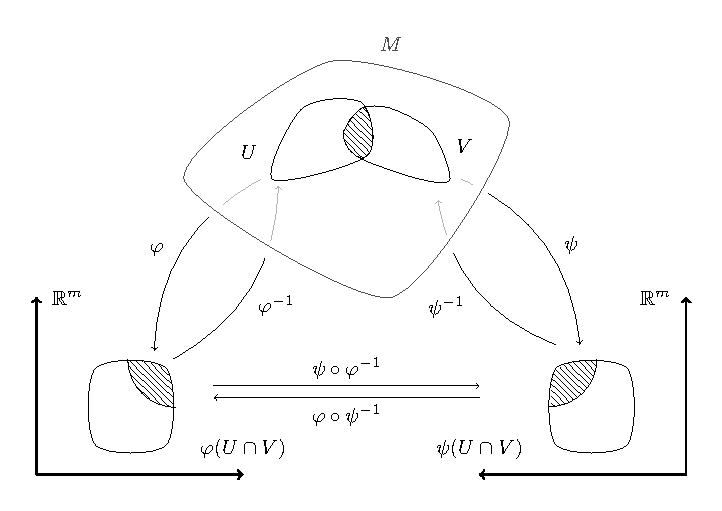
\includegraphics{fig/ch4-atlas-chart.pdf}
    \caption{坐标卡与相容性}\label{chdm:pic_chart}
\end{figure}


\begin{proposition}\label{chdm:thm_biggestDiffStruc}
    设微分流形$M$上有坐标卡集合$\mathscr{B}$满足定义\ref{chdm:def_Dmanifold}中的条件(1)和(2),
    那么在$M$上必然存在唯一的一个微分结构$\mathscr{A}\supset \mathscr{B}$.
\end{proposition}
\begin{proof}
    已知存在坐标卡集合$\mathscr{B}$满足条件(1)和(2),
    索性把所有与$\mathscr{B}$相容的坐标卡都放在一起构造出一个最大的图册,
    称之为$\mathscr{A}$.用这种方式构造的集合$\mathscr{A}$显然满足条件(1)和(2),
    这便是条件(3)中所说的极大图册.
    这种方式构造出的$\mathscr{A}$显然是唯一的.
\end{proof}
这个命题说明:定义\ref{chdm:def_Dmanifold}中的条件(1)和(2)是基本的.


%\subsubsection*{例题}
下面给出几个具体例子.

\begin{example}
    可数离散点集构成的拓扑空间是零维流形.\qed
\end{example}


\begin{example}\label{chdm:exm_trival}
    $m$维欧几里得空间$\mathbb{R}^m$.只需取一个开集$U=\mathbb{R}^m$即可,
    令映射$\varphi:U\to \mathbb{R}^m$是恒等映射,则$(U,\varphi)$是
    空间$\mathbb{R}^m$的坐标卡.
    
    能够与标准欧几里得坐标进行坐标变换的坐标卡有很多,有的变换只连续,并不可微;    
    如果我们将所有变换关系是$C^\infty$可微的坐标卡集合记为$\mathscr{B}$,
    那么$\mathscr{B}$便是$\mathbb{R}^m$的最大图册,也就是它的{\kaishu 微分结构};
    称为$\mathbb{R}^m$的{\kaishu 标准微分结构}. \qed
\end{example}


\begin{example}\label{chdm:exm_bu-tong-jie-gou}
    实数轴$\mathbb{R}$上可以构造不同的微分结构.第一种微分结构取为如例\ref{chdm:exm_trival}所示
    的标准微分结构,记为$\mathscr{A}_1$,局部坐标用$x$表示.
    
    第二种微分结构可以这样构造,取$V=\mathbb{R}$,映射$\psi:V\to \mathbb{R}$取
    为$\psi(y)=y^5, \  \forall y \in V$,记这种结构为$\mathscr{A}_2=(V,\psi)$.
    
    坐标变换$\varphi \circ \psi^{-1}$的表达式为$x=\sqrt[5]{y}$,
    很明显这个函数在$y=0$处不可微,所以两个微分结构并不相容. \qed
\end{example}

\begin{example}\label{chdm:exm_sphere1}
    $\mathbb{R}^{m+1}$中$m$维标准球面$S^m(a)$的微分流形.
\end{example}
$S^m(a)$的具体表示为:
\begin{equation}
    S^m(a)=\left\{(x^1, \cdots, x^{m+1}) \in \mathbb{R}^{m+1} \ | \ \sum_{i=1}^{m+1}(x^i)^2= a^2 \right\} .
\end{equation}
对每一个$\alpha(1\leqslant \alpha \leqslant m+1)$,令
\begin{align*}
    U_\alpha ^{+} &= \{(x^1,\cdots,x^{m+1})\in S^m: x^\alpha > 0 \},  \\
    U_\alpha ^{-} &= \{(x^1,\cdots,x^{m+1})\in S^m: x^\alpha < 0 \}.
\end{align*}
这两个类型的集合是球面$S^m(a)$上的开集,这些集合之并是球面$S^m(a)$的开覆盖,即
\begin{equation}
    S^m(a)= \bigcup_{\alpha=1}^{m+1} \bigl(U_\alpha ^{+} \cup U_\alpha ^{-} \bigr).
\end{equation}
有了开覆盖,下面定义映射$\varphi_\alpha ^{+}: U_\alpha ^{+} \to \mathbb{R}^m$和
$\varphi_\alpha ^{-}: U_\alpha ^{-} \to \mathbb{R}^m$:
\begin{align}
    \varphi_\alpha ^{+}(x^1,\cdots,x^{m+1}) &= (x^1,\cdots,\hat{x}^\alpha, \cdots,x^{m+1}), \\
    \varphi_\alpha ^{-}(x^1,\cdots,x^{m+1}) &= (x^1,\cdots,\hat{x}^\alpha, \cdots,x^{m+1}).
\end{align}
其中$\hat{x}^\alpha$表示把第$\alpha$个分量${x}^\alpha$去掉.
实际上,这两个映射从不同的开集得到了相同的坐标.
在多元微积分角度上看,上面两个映射是$C^\infty$的,它们的逆也是$C^\infty$的;
所以$(U_\alpha ^{+}, \varphi_\alpha ^{+})$和$(U_\alpha ^{-}, \varphi_\alpha ^{-})$是
球面$S^m(a)$的坐标卡.映射$\varphi_\alpha ^{\pm}$(取$\alpha$为固定数值)的几何意义是将$S^m(a)$的
半球面$U_\alpha ^{\pm}$沿第$\alpha$坐标轴投影到$x^\alpha=0$坐标平面上.

下面我们来看坐标变换是否相容.取$\alpha$和$\beta$为两个互不相等的固定数值,
那么必然有$U_\alpha ^{+} \cap U_\beta ^{+} \neq \varnothing$、
$U_\alpha ^{+} \cap U_\beta ^{-} \neq \varnothing$和
$U_\alpha ^{-} \cap U_\beta ^{-} \neq \varnothing$,
我们以$U_\alpha ^{+} \cap U_\beta ^{-}$为例,
写出如下坐标变换的具体公式(见式\eqref{chdm:eqn_sph1f}):
\begin{align*}
    \varphi^-_\beta \circ (\varphi^+_\alpha)^{-1}:& \quad \varphi^+_\alpha
      \bigl( U_\alpha ^{+} \cap U_\beta ^{-} \bigr) \to 
      \varphi^-_\beta \bigl( U_\alpha ^{+} \cap U_\beta ^{-} \bigr),  \\
    \varphi^+_\alpha \circ (\varphi^-_\beta)^{-1}:& \quad \varphi^-_\beta
      \bigl( U_\alpha ^{+} \cap U_\beta ^{-} \bigr) \to 
      \varphi^+_\alpha \bigl( U_\alpha ^{+} \cap U_\beta ^{-} \bigr) .
\end{align*}
其余坐标变换公式留给读者当作练习.
假设$\alpha < \beta$,对于$S^m$球面上的
点$(x^1,\cdots,x^{m+1})\in U_\alpha ^{+} \cap U_\beta ^{-}$有
$x^\alpha >0, \ x^\beta <0$,应用条件$|x|=a$可得坐标变换公式:
\begin{subequations}\label{chdm:eqn_sph1f}
\begin{align}
     &\varphi^-_\beta \circ (\varphi^+_\alpha)^{-1} (x^1,\cdots,\hat{x}^\alpha,\cdots,x^{m+1}) \notag \\
    =&\left(x^1,\cdots,x^{\alpha-1},\sqrt{a^2-\sum\nolimits_{ \gamma\neq \alpha}(x^\gamma)^2},
      x^{\alpha+1},\cdots,\hat{x}^\beta,\cdots,\hat{x}^{m+1}\right), \\
     &\varphi^+_\alpha \circ (\varphi^-_\beta)^{-1} (x^1,\cdots,\hat{x}^\beta,\cdots,x^{m+1}) \notag \\
    =&\left(x^1,\cdots,\hat{x}^\alpha,\cdots, x^{\beta-1},-\sqrt{a^2-\sum\nolimits_{\gamma\neq \beta}(x^\gamma)^2},
      x^{\beta+1},\cdots,\hat{x}^{m+1}\right) .
\end{align}
\end{subequations}
因为式子$\sqrt{a^2-\sum\nolimits_{ \gamma\neq \alpha}(x^\gamma)^2}$和
$\sqrt{a^2-\sum\nolimits_{\gamma\neq \beta}(x^\gamma)^2}$根号下是恒大于零的,
求导之后放在分母上不会导致无穷大,所以两个
坐标变换$\varphi^-_\beta \circ (\varphi^+_\alpha)^{-1}$和
$\varphi^+_\alpha \circ (\varphi^-_\beta)^{-1}$都是$C^\infty$的,
因此坐标卡$(U_\alpha ^{+}, \varphi_\alpha ^{+})$和$(U_\alpha ^{-}, \varphi_\alpha ^{-})$是
$C^\infty$相容的.与此类似同样可证其余坐标卡也是$C^\infty$相容的,所以坐标卡
集合$\{(U_\alpha ^{+}, \varphi_\alpha ^{+}),
(U_\alpha ^{-}, \varphi_\alpha ^{-}): 1\leqslant \alpha \leqslant m+1\}$决定了
球面$S^m(a)$上的$C^\infty$一种微分结构,进而$S^m(a)$符合
定义\ref{chdm:def_Dmanifold}中所有条件,所以它是微分流形.
\qed



\begin{example}\label{chdm:exm_sphere2}
    继上一例题,用球极投影法再次说明$m$维球面是微分流形.
\end{example}
设球面的北极和南极点坐标分别为$N=(0,\cdots,0,a)$和$S=(0,\cdots,0,-a)$.
令$V_{+}=S^m(a)\backslash \{S\},\ V_{-}=S^m(a) \backslash\{N\}$,这样定义的集合是球面上的开集.
分别定义映射$\psi_{\pm}:V_{\pm}\to \mathbb{R}^m$如下
\begin{align}
    (y^1,\cdots,y^m)\equiv &\psi_{+}(x^1,\cdots,x^{m+1}) = 
      \left(\frac{a x^1}{a+x^{m+1}},\cdots, \frac{a x^m}{a+x^{m+1}}\right), 
      \label{chdm:eqn_tmppsip}\\
    (z^1,\cdots,z^m)\equiv &\psi_{-}(x^1,\cdots,x^{m+1}) = 
      \left(\frac{a x^1}{a-x^{m+1}},\cdots, \frac{a x^m}{a-x^{m+1}}\right) .
\end{align}
需要由上两式来求$\psi_{\pm}$的逆映射,我们仅以$\psi_{+}$为例来说明求解过程.
将式\eqref{chdm:eqn_tmppsip}求平方和,并利用$\sum_{i=1}^{m+1}(x^i)^2=a^2$,可得
\begin{align*}
    & \sum_{j=1}^{m}(y^j)^2=\frac{a^2 }{(a+x^{m+1})^2}\left(\sum_{i=1}^{m}(x^i)^2\right)
      =\frac{a^2 }{(a+x^{m+1})^2}\left(a^2-(x^{m+1})^2\right) \\
      {\color{red} \Rightarrow} 
    & x^{m+1} = \frac{a\left(a^2-\sum\nolimits_j(y^j)^2\right)}{a^2+\sum\nolimits_j(y^j)^2},
    {\quad \text{或} \quad } x^{m+1}= -a \ (\text{舍弃}) .
\end{align*}
有了最后一个坐标的表达式,其它坐标几乎一望而知,它们是(同时给出$\psi_{-}^{-1}$)
\begin{align}
    (x^1,&\cdots,x^m, x^{m+1}) = \psi_{+}^{-1}(y^1,\cdots,y^m) \notag \\
      &=\frac{a}{a^2+\sum\nolimits_j(y^j)^2} 
        \left(2 a y^1, \cdots, 2 a y^m,\ a^2-\sum_{j=1}^m(y^j)^2\right), 
        \label{chdm:eqn_sp2yx} \\
    (x^1,&\cdots,x^m, x^{m+1}) = \psi_{-}^{-1}(z^1,\cdots,z^m) \notag \\
      &=\frac{a}{a^2+\sum\nolimits_j(z^j)^2} 
        \left(2 a z^1, \cdots, 2 a z^m,\ \sum_{j=1}^m (z^j)^2 - a^2 \right).
        \label{chdm:eqn_sp2zx}
\end{align}
有了逆映射,便可以求出坐标变换如下
\begin{align}
    (z^1,\cdots,z^m)=& \psi_{-}\circ \psi_{+}^{-1} (y^1,\cdots,y^m)
      = \frac{a^2}{\sum\nolimits_j(y^j)^2}  \left(y^1,\cdots, y^m \right) , \label{chdm:eqn_sp2yz}\\
    (y^1,\cdots,y^m)=& \psi_{+}\circ \psi_{-}^{-1} (z^1,\cdots,z^m) 
      = \frac{a^2}{\sum\nolimits_j(z^j)^2}  \left(z^1,\cdots, z^m \right) . \label{chdm:eqn_sp2zy}
\end{align}
不难验证这些坐标变换都是$C^\infty$的,故$(V_+,\psi_+;y^i)$和$(V_-,\psi_-;z^i)$构成了
球面$S^m(a)$的容许局部坐标开覆盖,决定了球面的一种微分结构.
\qed



\begin{example}\label{chdm:exm_sphere12}
    以$S^1(1)$为例来说明上面两个例题中的坐标卡属于同一微分结构.
\end{example}
只取其中一个坐标变换,其余类似.
取第一种坐标卡中的开集和映射为
\begin{equation*}
    U_1 ^{+} = \{(x^1,x^2)\in S^1: x^1 > 0 \}, \ 
    \varphi_1 ^{+}(x^1,x^2) = x^2, \ 
    (\varphi_1 ^{+})^{-1}(x^2)=\left(\sqrt{1-(x^2)^2},x^2\right) .
\end{equation*}
取第二种坐标卡中的开集和映射为
\begin{equation*}
    V_+, \quad \psi_{+}(x^1,x^2) = \frac{x^1}{1+x^{2}}, \quad
    \psi_{+}^{-1}(y^1) = \frac{1}{1+(y^1)^2}\left(2  y^1, 1-(y^1)^2\right) .
\end{equation*}
坐标变换为
\begin{align}
    \varphi_1 ^{+} \circ \psi_{+}^{-1}(\xi) = \frac{1-\xi^2}{1+\xi^2}, \qquad
    \psi_{+}\circ (\varphi_1 ^{+})^{-1}(\eta) =\frac{\sqrt{1-\eta^2}}{1+\eta} .
\end{align}
这些函数是$C^\infty$的,所以坐标变换是相容的,它们属于同一微分结构.
\qed

{ %\kaishu 
    可见在构造微分流形时,只需指出它的一个相容的坐标覆盖就行了,
    这样已能研究全部的几何.  比如对于球面$S^m(a)$,(对于物理中的应用而言)
    我们用例\ref{chdm:exm_sphere1}或例\ref{chdm:exm_sphere2}中
    的任意一个坐标覆盖即可,(除了微分拓扑等基础领域)
    没有必要非将其延拓至最大相容的坐标覆盖(即微分结构);
    命题\ref{chdm:thm_biggestDiffStruc}表明任意一个坐标覆盖都能延拓至最大图册.}

\subsection{笛卡尔积流形}\label{chdm:sec_cartensian-product}
拓扑空间有笛卡尔积的概念(见定义\ref{chtop:def_cartensian}),微分流形也有类似概念.
%\begin{definition}\label{chdm:def_cartensian-product}
%\end{definition}
设有微分流形$M$和$N$,其维数分别是$m$和$n$,它们的微分结构分别是
\begin{equation}
    \mathscr{A}_1=\{(U_\alpha, \varphi_\alpha)|\alpha\in \mathscr{I}_1 \}, \qquad
    \mathscr{A}_2=\{(V_i, \psi_i)|i\in \mathscr{I}_2 \} .
\end{equation}

由命题\ref{chtop:thm_hcb}、\ref{chtop:thm_cph}可知$M\times N$是Hausdorff空间,并有可数拓扑基;
且$\{(U_\alpha\times V_i)\mid \alpha\in \mathscr{I}_1,i\in \mathscr{I}_2\} $是
拓扑积$M\times N$的一个开覆盖.下面构造$M\times N$的微分结构.
对每一对指标$\{(\alpha,i)\in \mathscr{I}_1 \times \mathscr{I}_2\}$,定义
从$U_\alpha\times V_i$到$\mathbb{R}^{m+n}$的映射如下
\begin{align*}
    (\varphi_\alpha \times \psi_i)(x,y)\overset{def}{=}&\bigl(\varphi_\alpha(x),\ \psi_i(y)\bigr),
    \qquad \forall (x,y)\in U_\alpha\times V_i . \\
    (\varphi_\alpha \times \psi_i)^{-1}(X,Y)\overset{def}{=}&\bigl(\varphi_\alpha^{-1}(X),\ 
    \psi_i^{-1}(Y)\bigr),  \qquad \forall (X,Y)\in \varphi_\alpha(U_\alpha)\times \psi_i(V_i) .
\end{align*}
不难验证$\varphi_\alpha \times \psi_i$是从$U_\alpha\times V_i$
到$\varphi_\alpha(U_\alpha)\times \psi_i(V_i)$的同胚映射.

\index[physwords]{笛卡尔积!微分流形}

再者,当$U_\alpha \cap U_\beta \neq \varnothing,\ V_i\cap V_j\neq \varnothing$时,定义
\begin{equation}
    (\varphi_\alpha \times \psi_i)\circ (\varphi_\beta \times \psi_j)^{-1}
    \overset{def}{=}(\varphi_\alpha\circ \varphi_\beta^{-1})\times
    (\psi_i\circ\psi_j^{-1}) .
\end{equation}
在这样定义下,$(U_\alpha\times V_i , \varphi_\alpha \times \psi_i)$与
$(U_\beta\times V_j , \varphi_\beta \times \psi_j)$是$C^\infty$相容的.
当$U_\alpha \cap U_\beta = \varnothing$和$V_i\cap V_j = \varnothing$至少
有一个成立时,我们约定它们也是$C^\infty$相容的.这样,
\begin{equation}
    \{(U_\alpha\times V_i , \varphi_\alpha \times \psi_i) \mid
    \alpha\in \mathscr{I}_1,i\in \mathscr{I}_2\} ,
\end{equation}
在拓扑积$M\times N$上决定了一个$m+n$维的光滑结构,这使得$M\times N$成
为$m+n$维光滑流形,称为$M$和$N$的笛卡尔{\heiti 积流形}.



很明显,上述流程可以推广到任意有限个流形($M_1,M_2,\cdots$)之积.



\subsection{小结}\label{chdm:sec_tmpdmcon}
微分流形定义要求每个局部开集$U$均同胚于$\mathbb{R}^m$中的开集,
所以流形自然存在局部坐标$\{U;x^i\}$,这个坐标是天生存在的,不需要额外定义;
微分几何所有理论都需要构建在这个坐标基础之上.
但是,流形论本身不依赖于某套特别的坐标系.
因此,那种想完全摆脱局部坐标去构建微分几何理论的想法是错误的.

然而,微分几何理论的却是整体性的,
流形论主要目的是研究在局部坐标变换下而保持不变的性质(如切矢量、外微分式、黎曼曲率等等).
微分几何理论不能只对某个特别的坐标系正确,对其它坐标系不正确;
也就是理论本身必须与坐标系选取无关才可以;
坐标本身没有意义,所有基本理论都不能只依赖某特定局部坐标(Christoffel符号是个例外).
那种想用坐标分量语言来描述微分几何的方式貌似已经过时了.



引入坐标系的目的是为了把几何问题代数化,从而能用代数及微积分的方法来研究几何问题.
选择适当的坐标可以大大简化研究难度,大家在书中看到的各种坐标,
是前人经过长期研究而作出的选择,基本上是最优的了.


举例说明坐标本身没有意义(以下两例中的度量是欧式度量).
\begin{example}
    张三沿直线向东走了一段距离,我们把他走路的起点算作坐标$a$,
    终点坐标记为$b$;但是坐标本身(不论是$a$还是$b$)都没有意义,
    有意义的是由“$b-a$”表示的这段距离;而且这段距离是不随坐标系变换而改变的,
    比如随便将坐标系平移和旋转,这段距离是不变的,但两点坐标的数值却改变了.
\end{example}

\begin{example}\label{chdm:exam_tuoyuan}
    在$\mathbb{R}^3$中的$x-y$平面上,画一个椭圆(称为旧的),中心在原点,长半轴沿$x$,短半轴沿$y$;
    这是最常用的坐标表示形式.我们将坐标轴进行任意旋转(甚至反射),
    那么(新)椭圆可能处于$\mathbb{R}^3$中任意一个平面上,不在$x-y$平面上;
    此时“旧”、“新”椭圆上的坐标几乎不可能一致了,但是椭圆的长、短半轴长度,
    偏心率等等几何量是不变的.这个例子生动地说明了“坐标本身没有意义”,
    我们应该研究那些坐标变换下的不变量.
    
    在牛顿力学中,地球绕太阳旋转,我们依据牛顿第二定律和万有引力公式列出方程,
    如果按照上述“旧”方式取坐标,则方程很容易求解;
    如果按照上述“新”方式取坐标,则方程很难求解,可能需要用数值解法.不论哪个坐标系,
    求得的解必然是同一个椭圆,但地球在“旧”、“新”坐标系中的坐标是不同的.
    可见,即使在经典力学中,研究的仍是坐标变换下的不变量,坐标本身没有意义!
\end{example}



\begin{exercise}
	以$S^2(1)$为例再次论证例题\ref{chdm:exm_sphere12}.
\end{exercise}

\begin{exercise}
	证明例题\ref{chcdg:exm_torus}中的圆环面是$\mathbb{R}^3$中的光滑流形.
\end{exercise}

\begin{exercise}
	证明$x-y$平面可看成由$x$、$y$轴构成的笛卡尔积流形.
\end{exercise}


\begin{exercise}
	设$S^1$是一维单位圆周.证明例题\ref{chcdg:exm_torus}中的圆环面
	可以看成两个圆周的笛卡尔积流形,即$S^1\times S^1$.
\end{exercise}


\section{流形的映射}\label{chdm:sec_map-dm}
读者应该学习过多元微积分中$\mathbb{R}^m$与$\mathbb{R}^n$间映射(或函数)的概念,
那里的内容大都可以推广到流形之间.
\begin{definition}\label{chdm:def_fmapMN}
    设$M$和$N$分别是$m$和$n$维$C^\infty$微分流形,
    存在连续映射$f:M\to N$.{\footnote{读者应能注意到:
            只到这里的$f$只是拓扑流形间的映射,只能谈及连续性,
            无法涉及可微性.}}
    $\forall p\in M$,存在包含$p$的坐标卡$(U,\varphi;x)$以及$N$上
    包含点$q\equiv f(p)$的坐标卡$(V,\psi;y)$,那么可以构造如下映射$\hat{f}$:
    \begin{equation*}
        \hat{f}\equiv \psi \circ f \circ \varphi^{-1} :
        \varphi(U) \bigl(\subset \mathbb{R}^m\bigr) \ \to \ 
        \psi(V) \bigl(\subset \mathbb{R}^n\bigr) .
    \end{equation*}
    如果$\hat{f}$是$C^r$的(即可微到$r(>0)$阶),{\footnote{$\hat{f}$肯定是连续的;
            $\hat{f}$本质上是$\mathbb{R}^m$与$\mathbb{R}^n$开子集间的映射,
            自然可以谈及其可微性.}}
    那么称映射$f:M\to N$在$p$点是$C^r$的;如果$f$在每一点都是$C^r$的,那么称
    之为$C^r$映射.
\end{definition}

\index[physwords]{微分流形!流形间映射}

\begin{remark}\label{chdm:rek_jacobi}
    不难验证,上述定义与坐标卡选取无关.
    有了这个定义后,我们不再严格区分$f$和$\hat{f}$,认为两者等同.
    在多元微积分中$\hat{f}$在$p\in \mathbb{R}^m$点的Jacobi矩阵也称为
    $f$在$p\in M$点的Jacobi矩阵.Jacobi矩阵秩也可作类似认同.
\end{remark}
\begin{definition}\label{chdm:def_fmapCurve}
    设定义\ref{chdm:def_fmapMN}中的$M$是实数轴上的某个开区间$(a,b)$,那么
    称映射$f:(a,b)\to N$为流形$N$上的一条$C^r${\heiti (参数)曲线}. \index[physwords]{微分流形!参数曲线}
\end{definition}
设流形$N$中有$C^r$曲线$f(t)$,其中$t$称为曲线的{\heiti 参数}.如果有$C^r$变换函数$u(t)$将
参数$t$变成$u$,并且$\frac{{\rm d} u }{{\rm d} t}$处处不为零,那么称
变换后的曲线$\tilde{f}(u)=f\bigl(u(t)\bigr)$是原曲线$f(t)$的{\heiti 重参数化曲线}.
既然$\frac{{\rm d} u }{{\rm d} t}$处处不为零,那么必然
有$\frac{{\rm d} u }{{\rm d} t}>0$或者$\frac{{\rm d} u }{{\rm d} t}<0$处处成立,
即变换$u(t)$是单调的双射函数.

\begin{definition}\label{chdm:def_func}
    设定义\ref{chdm:def_fmapMN}中的$N$是实数轴上的某个开区间$(a,b)$,那么
    称映射$f:M \to (a,b)$为流形$M$上的$C^r${\heiti 函数}.
    全体$C^r$函数集合记作$C^r(M)$.
\end{definition}
函数的加法和乘法在$C^r(M)$中是封闭的,(参照\pageref{chtop:def_ring}页
定义\ref{chtop:def_ring})因此$C^r(M)$在代数上是一个{\kaishu 环}.

\index[physwords]{微分流形!函数}

\begin{example}
    设流形$M$的局部坐标是$(U_\alpha,\varphi_\alpha;x^i)$,在局部坐标系下
    有$\frac{\partial x^i}{\partial x^j}=\delta^i_j$,这明确说明:
    当把局部坐标$x^i$看成函数时,它一定是$C^\infty$的.
\end{example}

\begin{definition}\label{chdm:def_Diff-Homeomorphism}
    设定义\ref{chdm:def_fmapMN}中的$f$是拓扑同胚(见\ref{chtop:def_homeomorphism}),
    若$f$和$f^{-1}$都是$C^r$的,则称$f$是微分流形$M$与$N$间的$C^r${\heiti 微分同胚}.
    若$f$只是$M$的某局部开集$U$和$N$的局部开集$V$之间的微分同胚,
    则称$f$为$U$到$V$上的{\heiti 局部微分同胚}.
\end{definition}
拓扑同胚可保证两流形维数相等(见定义\ref{chtop:def_topological-manifold}后讨论);
微分同胚自然也可得此结论.

\index[physwords]{微分流形!微分同胚、光滑同胚}

下面叙述几个关于映射的命题,这些命题会在多处使用.
为理解方便,先介绍$\mathbb{R}^m$空间中的一个命题:
\begin{proposition}\label{chdm:thm_exp1Rm}
    令$Q$是$\mathbb{R}^m$中的一个矩形区域.存在一个$C^\infty$函
    数$\phi:\mathbb{R}^m \to \mathbb{R}$使得当$x$属于$Q$内部时,
    有:$\phi(x)>0$;否则$\phi(x)=0$.
\end{proposition}
\begin{proof}
    先考虑如下一维函数$f:\mathbb{R} \to \mathbb{R}$,
    \begin{equation*}
        f(t)=\begin{cases}
            \exp(-\tfrac{1}{t}), & t > 0 ;\\
            0, & t \leqslant 0 .
        \end{cases}
    \end{equation*}
    此函数曲线见图\ref{chdm:pic_exp1},当$t\to \infty$时,$f(t)\to 1^-$;
    当$t\to 0^+$时,$f(t)\to 0$;拐点在$t=0.5$处.
    很明显,函数$f$在实数轴上是$C^\infty$的.利用此函数,接着
    定义另一函数$g$(见图\ref{chdm:pic_exp2}),
    \begin{equation}\label{chdm:eqn_g1}
        g(t)=f(t)\cdot f(1-t)/(f(0.5))^2 .
    \end{equation}
    函数$g$在$0<t<1$中非零且恒正,其它点恒为零;最大值已归一化到$1$.
    
    对于高维空间$\mathbb{R}^m$中的矩形
    区域$Q=[a_1,b_1]\times \cdots \times[a_m,b_m]$,
    则可定义函数$\phi$如下
    \begin{equation}\label{chdm:eqn_gexpphi1}
        \phi(x)=g\left(\frac{x_1 -a_1}{b_1-a_1}\right) \times 
        g\left(\frac{x_2 -a_2}{b_2-a_2}\right) \times \cdots \times
        g\left(\frac{x_m -a_m}{b_m-a_m}\right) .
    \end{equation}
    这样定义的函数满足命题要求,这便证明了存在性.
    需要指出的是这类函数有很多,不止上述一个.
\end{proof}


\begin{figure}[htb]
    \begin{minipage}[t]{0.5\linewidth}
        \centering
        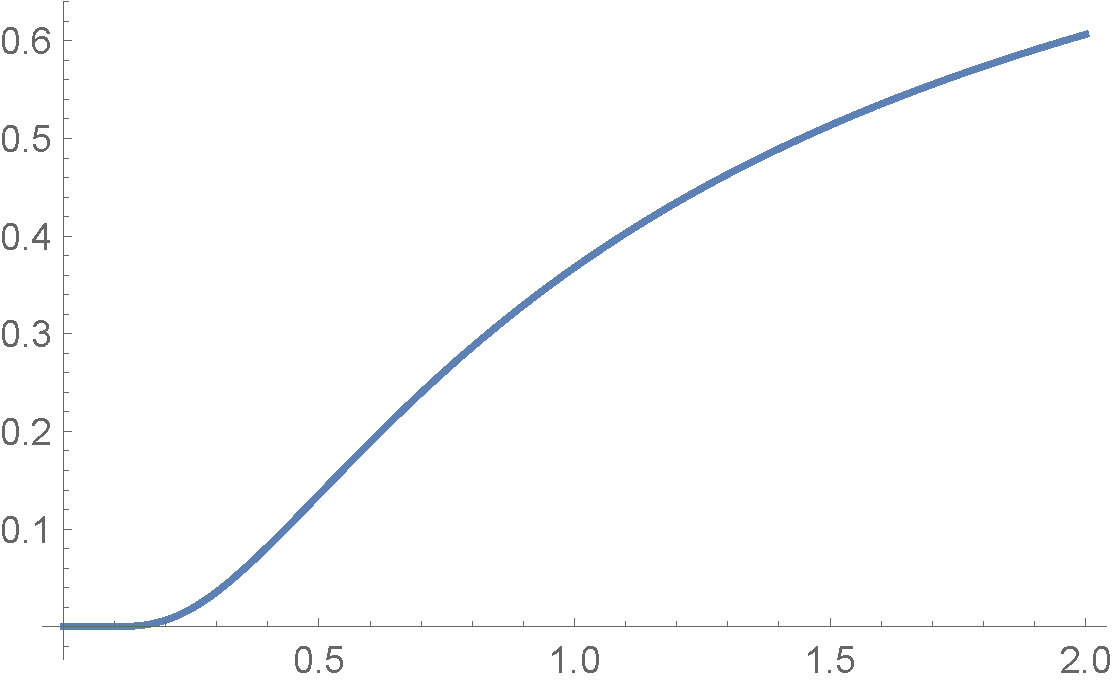
\includegraphics[scale=0.3]{fig/ch4-exp1.pdf}
        \caption{指数函数$f$}\label{chdm:pic_exp1}
    \end{minipage}%
    \begin{minipage}[t]{0.5\linewidth}
        \centering
        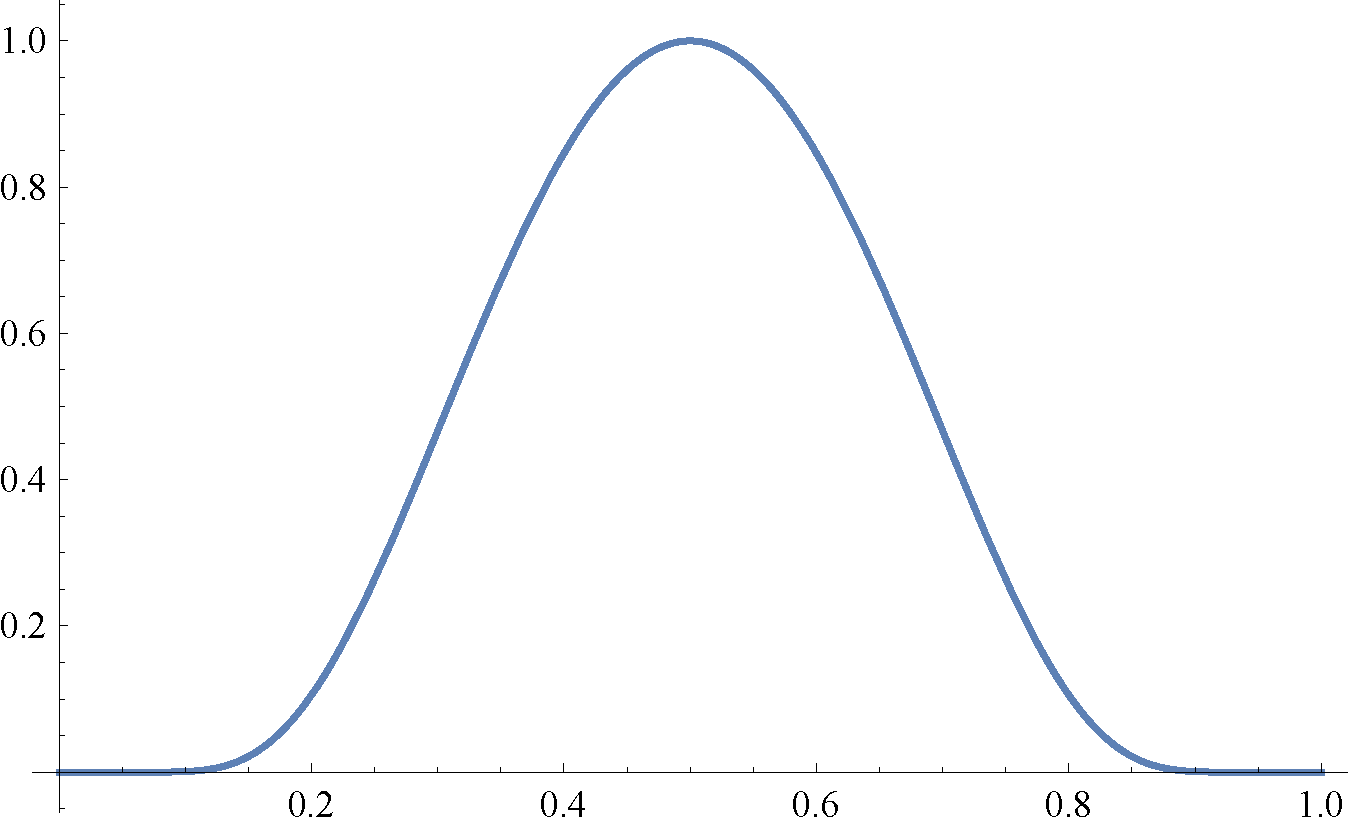
\includegraphics[scale=0.3]{fig/ch4-exp2.pdf}
        \caption{指数函数积$g$}\label{chdm:pic_exp2}
    \end{minipage}
\end{figure}

上面命题还有变种.
\begin{proposition}\label{chdm:thm_exp1RmSphere}
    令$D_1$和$D_2$是$\mathbb{R}^m$中两个同心球,且$\overline{D}_1 \subset D_2$.
    则存在$C^\infty$函数$f:\mathbb{R}^m \to \mathbb{R}$使
    得$0\leqslant f \leqslant 1$,并且
    \begin{equation}\label{chdm:eqn_exp1RmSphere}
        f(x)=\begin{cases}
            1, & x\in D_1 ; \\
            0, & x\notin D_2 .
        \end{cases}
    \end{equation}
\end{proposition}
上面命题将取值域限定为球,这个限制可以拓展至一般情形:
\begin{proposition}\label{chdm:thm_exp1UVRm}
    令$U$和$V$是$\mathbb{R}^m$中两个非空开集,$\overline{V}$是紧致的,
    且$\overline{V} \subset U$.
    则存在$C^\infty$函数$g:\mathbb{R}^m \to \mathbb{R}$使
    得$0\leqslant g \leqslant 1$,并且
    \begin{equation}\label{chdm:eqn_exp1UVRm}
        g(x)=\begin{cases}
            1, & x\in V ; \\
            0, & x\notin U .
        \end{cases}
    \end{equation}
\end{proposition}
上面命题可以推广到一般流形上:
\begin{proposition}\label{chdm:thm_exp1UVM}
    令$U$和$V$是微分流形$M$中两个非空开集,$\overline{V}$是紧致的,
    且$\overline{V} \subset U$.
    则存在$C^\infty$函数$h:M \to \mathbb{R}$使
    得$0\leqslant h \leqslant 1$,并且
    \begin{equation}\label{chdm:eqn_exp1UVM}
        h(p)=\begin{cases}
            1, & p\in V ; \\
            0, & p\notin U .
        \end{cases}
    \end{equation}
\end{proposition}
命题\ref{chdm:thm_exp1RmSphere}、
\ref{chdm:thm_exp1UVRm}和\ref{chdm:thm_exp1UVM}的证明
并不复杂,可参见文献\parencite[\S 1.3]{cc2001-zh}中证明.
它们本质上是命题\ref{chdm:thm_exp1Rm}的推广,但越来越抽象.
利用命题\ref{chdm:thm_exp1UVM},可证明下面命题:
\begin{proposition}\label{chdm:thm_Flocal-equiv-Fglobal}
    设$U$是微分流形$M$的一个开子集,给定函数$f\in C^\infty(U)$,
    则$\forall p\in U$,必有$p$点一个邻域$V\subset U$,以及光滑
    函数$\hat{f}\in C^\infty(M)$,使得$\hat{f}|_V = f|_V$.
\end{proposition}
\begin{proof}
    利用流形的局部紧致性,可以使得$\overline{V}$是$U$的真子集;如果不是,
    将$V$缩小一些即可.依照命题\ref{chdm:thm_exp1UVM},存在
    流形$M$上的光滑函数$h$满足式\eqref{chdm:eqn_exp1UVM},令
    \begin{equation}
        \hat{f}(x)=\begin{cases}
            f(x)\cdot h(x), & \forall x\in V ; \\
            0, & \forall x\notin U .
        \end{cases}
    \end{equation}
    很明显,有$\hat{f}|_V = f|_V$.因$f$在$U$上式光滑的,故$f\cdot h$在$V$上也是
    光滑的;而$h$又保证了$\hat{f}$能以$C^\infty$的方式光滑从$V$过渡到$M\backslash U$,
    所以$\hat{f}$是整个流形$M$上的光滑函数.
\end{proof}
这个命题是说:局部的光滑函数可以很容易地延拓成整个流形上的光滑函数.
反之,光滑流形$M$上的光滑函数场也可以限制在开子集$V$上.


\begin{exercise}
	证明本节未给出证明过程的定理(命题).
\end{exercise}

\section{切空间}\label{chdm:sec_tangentspace}
在\S\ref{chdm:sec_ed}中,我们给出了欧氏空间切矢量的定义\ref{chdm:def_tang-vec-inEV};
现在有了微分流形概念,
可以把定义\ref{chdm:def_tang-vec-inEV}移植到流形论中.
本节先定义切矢量,再引入余切矢量.这个过程也可以反过来,
即先定义余切矢量,再引入切矢量;可参考\parencite[\S 1.2]{cc2001-zh}.

\index[physwords]{切空间}

\subsection{切矢量}
\begin{definition}\label{chdm:def_tang-vec-inManifold}
    设有一$m$维$C^\infty$微分流形$M$,任选其中一点$x\in M$.
    点$x$上{\heiti 切矢量}(简称{\heiti 矢量})$v^a$是指
    满足如下条件的一个映射$v^a:C_x^\infty(M)\to \mathbb{R}$  \index[physwords]{切矢量}
        
    {\bfseries (1)} 线性性:$\forall g,h \in C^\infty_x(M) $ , $\forall \lambda \in \mathbb{R}$,有
    $v (g+\lambda h) = v (g)+ \lambda v (h) ;$
    
    {\bfseries (2)} Leibnitz律:$\forall g,h \in C^\infty_x(M) $,有
    $v (g\cdot h) = \bigl(v(g)\bigr)\cdot h(x)+ g(x)\cdot v (h) .$
\end{definition}

在\S\ref{chdm:sec_ed}中,我们将方向导数等同于切矢量,这个认知在流形中也是成立的.
设映射$\gamma:(-a,a)\to M$是微分流形$M$中一条经过固定点$x_0$的光滑曲线,
其中$x_0=\gamma(0)$,则下面的映射$v^a:C^\infty_{x_0}\to \mathbb{R}$(其中$f\in C_{x_0}^\infty(M)$)
\begin{equation}\label{chdm:eqn_DiffCurve}
    v(f)\overset{def}{=} \left. \frac{{\rm d} \bigl(f \circ \gamma (t)\bigr)}{{\rm d} t} \right |_{t=0}
    \equiv \left. \frac{{\rm d} \Bigl(f \bigl(\gamma (t)\bigr)\Bigr)}{{\rm d} t} \right |_{t=0};
    \quad -a < t < a, \quad a>0.
\end{equation}
便确定了$x_0$点的一个切矢量$v^a$;只需验证上面公式满足定义即可.
线性性的验证是一望而知的.下面验证Leibnitz律;需要先指出
\begin{equation}\label{chdm:eqn_f-cdot-g-circo-gamma}
    (f\cdot g)\circ \gamma \overset{def}{=} (f\circ \gamma) \cdot (g\circ \gamma)  .
\end{equation}
将上式带入式\eqref{chdm:eqn_DiffCurve},有
\begin{align*}
    v(f\cdot g)=& \left. \frac{{\rm d} \Bigl(f \bigl(\gamma (t)\bigr)\cdot 
        g \bigl(\gamma (t)\bigr)\Bigr)}{{\rm d} t} \right |_{t=0} \\
    =& \left. \frac{{\rm d} \Bigl(f \bigl(\gamma (t)\bigr)
        \Bigr)}{{\rm d} t} \right |_{t=0} \cdot g \bigl(\gamma (0)\bigr) +
      f \bigl(\gamma (0)\bigr)\cdot \left. \frac{{\rm d} \Bigl( 
        g \bigl(\gamma (t)\bigr)\Bigr)}{{\rm d} t} \right |_{t=0} \\
    =& \bigl(v(f)\bigr)\cdot g(x_0)+ f(x_0)\cdot v (g) .
\end{align*}
验证完毕.
公式\eqref{chdm:eqn_DiffCurve}中所定义的切向量称为曲线$\gamma(t)$在$t=0$的{\heiti 切矢量}.
%当取遍$x_0$的所有曲线,全部这些切矢量会构成一个线性空间.
这个例子非常生动地说明了切矢量和方向导数是一回事儿!

\begin{remark}\label{chdm_rek-vnoa}
    $v(f)$是一个实数,如果写成$v^a(f)$可能
    会被误认为是一个矢量,所以略去抽象指标.
    后面切矢量\uwave{场}作用在标量函数场上时也不采用抽象指标记号.
\end{remark}
局部坐标本身就是一个$\mathbb{R}^m$,具有线性结构,我们选取
这样的曲线$\gamma_j:(-a_j,a_j)\to M,\ 1\leqslant j \leqslant m$使得其局部坐标是
\begin{equation}\label{chdm:eqn_gammaj}
    x^i\bigl({\gamma_j}(t)\bigr)= x^i_0 + \delta^i _j \cdot t,
\end{equation}
上式中指标$j$是固定不变的,上标$i$是其$m$个坐标分量的指标.
当$i\neq j$时,坐标就处在$x^i_0$点不动;
当$i=j$时,(只有这一个)坐标按线性规律(即直线)变化.
将这样的坐标带入式\eqref{chdm:eqn_DiffCurve},并将这个切矢量
记为$(\frac{\partial }{\partial x^j})^a$(注意作用到标量函数上后,略去抽象指标)
\begin{align*}
    \frac{\partial }{\partial x^j} f\bigl(\gamma (0)\bigr) =& \left. 
    \frac{{\rm d} (f \circ\varphi^{-1}) \circ\bigl(\varphi\circ \gamma (t)\bigr)}{{\rm d} t}  \right |_{t=0}
    =  \left. \frac{{\rm d} (f \circ\varphi^{-1}) (x^1_0,\cdots, x^j_0 + t, \cdots ,x^m_0)}{{\rm d} t}  \right |_{t=0}  \\
    =& \left.\frac{\partial (f \circ\varphi^{-1})}{\partial x^j}\right|_{\varphi(x_0)} 
    \left.\frac{{\rm d}(x^j_0 + t) }{{\rm d} t} \right|_{t=0}
    = \left.\frac{\partial (f \circ\varphi^{-1})}{\partial x^j}\right|_{\varphi(x_0)} .
\end{align*}
很明显切矢量\eqref{chdm:eqn_DiffCurve}在坐标\eqref{chdm:eqn_gammaj}下就表现为对
标量函数$f$求坐标$x^j$的偏导数,这也是将其记为$(\frac{\partial }{\partial x^j})^a$的理由;
这样的偏导数(也就是切矢量)共有$m$个,即$j=1,\cdots,m$.

\subsection{切空间基矢}
上面定义中已给出切矢量对$C^\infty_x(M)$中全体(标量)函数具有线性性.
若在不同切矢量间定义如下关系:
\begin{subequations}
    \begin{align}
        (u+v)f & \overset{def}{=} u(f) + v(f),\qquad {\text {$u,v$是$x\in M$的任意切矢量}}; \\
        (\lambda u) f & \overset{def}{=} \lambda \bigl( u(f)\bigr), \qquad \forall\lambda\in \mathbb{R}.
    \end{align}
\end{subequations}
上两式中$f\in C^\infty_x(M)$.有了这样定义之后,不难发现$x\in M$点{\kaishu 全体切矢量}满足
线性空间的定义\ref{chmla:def_linear-space},我们称这个线性空间是微分流形$M$在
点$x$的{\heiti 切空间},记为$T_x M$.下面我们证明这个空间的维数恰好是$m$;
大体思路是:首先找到$m$个切矢量,然后证明它们线性无关,最后证明每个切矢量都可以由它们展开.

\index[physwords]{切空间!基矢}

设微分流形$M$在点$x_0$的邻域的容许坐标卡是$(U,\varphi;x)$,点$x_0$的坐标
是$(x^1_0,\cdots,x^m_0)$.%式\eqref{chdm:eqn_DiffCurve}已经给出一个切矢量的定义,仿照它,不难验证(留给读者当练习)
前面已经指出了
\begin{equation}
    \left. \left(\frac{\partial }{\partial x^i}\right)^a \right|_{x_0}, \qquad 1\leqslant i \leqslant m,
\end{equation}
是点$x_{0}\in U$的切矢量.需注意:局部开子集$U$与$\mathbb{R}^m$是拓扑同胚的,天生有坐标,
天生有偏导数的概念,无需另行定义;或者直接将$U$与$\mathbb{R}^m$作恒等认同.

用反证法.假设存在$m$个不全为零的实常数$c^i$使得下式成立:
\begin{equation}
    c^i \frac{\partial f}{\partial x^i}  =0, \qquad \forall f \in C^\infty(U).
\end{equation}
将标量函数$f$选为坐标线$x^k$,并将这些坐标线一一带入上式,
容易得到$c^k=0,\ k=1,\cdots,m$.与假设矛盾,所以$m$个矢量是线性无关的.

任意给定一个满足定义\ref{chdm:def_tang-vec-inManifold}的矢量$v^a\in T_{x_0}M$,
下面证明它可以由$(\frac{\partial }{\partial x^j})^a$展开.证明过程
与定理\ref{chdm:thm_tang-vec-inEV}证明非常相似.
仿照命题\ref{chdm:thm_dc0}证明可以得到:满足
定义\ref{chdm:def_tang-vec-inManifold}的矢量$v^a$作用到任意
实常数$c$上都使之为零,即$v(c)\equiv 0$.

同样,由多元函数微分中值定理可知,$\forall f\in C_{x_0}^\infty(M)$,有
\setlength{\mathindent}{0 em}
\begin{equation*} %\label{chdm:eqn_wfzzdlM}
    (f \circ\varphi^{-1})(x^1,\cdots,x^m)=(f \circ\varphi^{-1})(x^1_0,\cdots,x^m_0)+ 
    (x^i-x^i_0) \frac{\partial (f \circ\varphi^{-1}) \bigl(x_0+\theta(x-x_0) \bigr)}{\partial x^i},
\end{equation*}\setlength{\mathindent}{2 em}
其中$0<\theta<1$.将矢量$v^a$作用到上式,可得(请参考定理\ref{chdm:thm_tang-vec-inEV}证明)
\begin{align*} %\label{chdm:eqn_wfzzdlM}
    v\bigl( f \circ\varphi^{-1} (x^1,\cdots,x^m)\bigr) = v(x^i-x^i_0) \cdot      \left.
     \frac{\partial (f \circ\varphi^{-1}) \bigl(x_0+\theta(x-x_0) \bigr)}{\partial x^i}\right|_{x=x_0}.
\end{align*}
记$v^i\equiv v(x^i)$,并将坐标省略,上式变为(将$f \circ\varphi^{-1}$记为$\hat{f}$)
\begin{equation}\label{chdm:eqn_v-expand-on-natural-bases}
    v( \hat{f} ) = v^i \cdot 
    \frac{\partial \hat{f} (x_0)}{\partial x^i}
    {\quad \color{red}\Leftrightarrow \quad }
    v^a = \sum_{i=1}^{m} { v^i \left(\frac{\partial }{\partial x^i}\right)^a_{x_0} }.
\end{equation}
上面“${ \color{red}\Leftrightarrow }$”后的式子将$\hat{f}\equiv f \circ\varphi^{-1} $略
去(因$f$和$\varphi$都是任选的),并补上了抽象指标记号.
上式充分说明$x_0$点任意矢量$v^a$都可以由$m$个$x_0$点矢量$(\frac{\partial }{\partial x^i})^a_{x_0} $展开,
其系数是$m$个实数$v^i\equiv v(x^i)$.

因此,$\{(\frac{\partial }{\partial x^i})^a_{x_0}, \ 1\leqslant i\leqslant m\}$是线性空间$T_{x_0}M$的
一组基矢量,称之为{\heiti 自然坐标(切)基底},简称自然基底;空间$T_{x_0}M$的维数是$m$.

\index[physwords]{切空间!自然坐标基矢}
\index[physwords]{切矢量!曲线切矢}

\begin{example}\label{chdm:exm_DiffCurve}
    式\eqref{chdm:eqn_DiffCurve}给出了光滑曲线$\gamma(t)$的切矢量,我们用自然基底来表示这个切矢量.
    设$m$维光滑流形$M$有局部坐标系$(U;x^i)$,$\forall p\in U$($p$对应$t=0$),曲线$\gamma(t)$上点的
    局部坐标记为$\{x^i\}$.将式\eqref{chdm:eqn_DiffCurve}展开为
    \setlength{\mathindent}{-0.2 em}
    \begin{equation}\label{chdm:eqn_DiffCurve-2}
        \left. \frac{{\rm d} \bigl(f \circ \gamma (t)\bigr)}{{\rm d} t} \right |_{t=0}
        = \frac{\partial f}{\partial x^i}
        \left. \frac{{\rm d} x^i\circ\gamma (t)}{{\rm d} t} \right |_{t=0}
        {\color{red}\Rightarrow}
        \left. \left(\frac{{\rm d}  }{{\rm d} t}\right)^a \right |_{\gamma (0)}
        = \frac{{\rm d} x^i\bigl(\gamma (0)\bigr)}{{\rm d} t}
        \left(\frac{\partial }{\partial x^i}\right)^a .
    \end{equation}\setlength{\mathindent}{2em}
    上式中“${\color{red}\Rightarrow}$”是因为$f \in C^\infty_p(M)$的任意性.
    这便是曲线$\gamma(t)$在$p$点切矢量的局部坐标展开式;
    其中切矢量$\left(\frac{{\rm d}  }{{\rm d} t}\right)^a $必需沿曲线$\gamma(t)$,
    且取$t=0$.
    
    \index[physwords]{切矢量!切线切矢量} \index[physwords]{切线切矢量}
    
    注:一般称$\left(\frac{{\rm d}  }{{\rm d} t}\right)^a $是
    曲线$\gamma(t)$切线的切矢量,简称{\heiti 切线切矢量}. 
    比如二维球面$S$上任一点$p$的切平面$T$上的任意(原点在切点$p$的)矢量都是切于球面$S$的.
    再取过$p$点的一个大圆$\gamma(t)$,切平面上的切矢量未必切于大圆$\gamma(t)$.
    “切线切矢量”是笔者杜撰出来的名词,
    用来描述切于曲线$\gamma(t)$的切矢量,以区别于切平面$T$上其它切矢量.
\end{example}


\index[physwords]{余切空间}
\index[physwords]{余切矢量}

\subsection{余切空间}
切空间是一个$m$维线性空间,按照\S\ref{chmla:sec_dual}内容,它应该有对偶空间.
\begin{definition}
    切空间$T_{x_0}M$的对偶空间称为微分流形$M$在点$x_0$的{\heiti 余切空间},
    记作$T_{x_0}^{*}M$.余切空间的元素称为{\heiti 余切矢量}.
\end{definition}
\S\ref{chmla:sec_dual}中所有内容都可以移植到余切空间;首先,
余切空间维数与切空间相同,都是$m$维;其次,
利用式\eqref{chmla:eqn_dual-bases}定义自然切基矢的{\heiti 对偶自然基矢},
将其记为$({\rm d}x^j)_a$(由于点${x_0}$的标记位置与对偶基矢抽象指标位置重合,暂将${x_0}$略去):
\begin{equation}\label{chdm:eqn_dual-natural-bases}
    ({\rm d}x^j)_a \left(\frac{\partial }{\partial x^i}\right)^a_{x_0} \equiv 
    \left< ({\rm d}x^j)_a , \   \left(\frac{\partial }{\partial x^i}\right)^a_{x_0}\right>
    \overset{def}{=} \delta^j_i .
\end{equation}
由上式定义的对偶基矢共有$m$个.
将$({\rm d}x^j)_a$作用在任意矢量$v^a$上,有
\begin{equation*}
    ({\rm d}x^j)_a v^a =  ({\rm d}x^j)_a 
       \left[v^i \left(\frac{\partial }{\partial x^i}\right)^a_{x_0}\right] 
    =  v^i \left[ ({\rm d}x^j)_a  \left(\frac{\partial }{\partial x^i}\right)^a_{x_0}\right] 
    =  v^i \delta^j_i = v^j .
\end{equation*}
这说明$({\rm d}x^j)_a$的作用是取出$v^a$在自然坐标基底上的第$j$分量.

任意余切空间元素$\omega_a \in T_{x_0}^{*}M$都可以在自然对偶基矢上展开,
并将其作用到任一切矢量$v^a$上,有
\begin{equation}
    \omega_a (v^a) = \left[\omega_j({\rm d}x^j)_a\right] 
      \left(v^i \left(\frac{\partial }{\partial x^i}\right)^a_{x_0}\right) = 
     \omega_j v^i \delta^j_i = \omega_j v^j .
\end{equation}
上式说明对偶矢量和切矢量的线性映射是一个实数;而切矢量$v^a$作用到标量函数$f$上也得到一个
实数$v(f)$;结合这两点,可说明标量函数$f$可以诱导出一个对偶矢量,记为$({\rm d}f)_a$;具体过程如下:
\begin{equation}\label{chdm:eqn_dfv}
    ({\rm d}f)_a v^a \equiv v(f)  %= v^i \left.\frac{\partial f}{\partial x^j}\right|_{x_0}
    = v^i  \delta_i^j  \left.\frac{\partial f}{\partial x^j}\right|_{x_0}
    = \left[v^i  \left(\frac{\partial }{\partial x^i}\right)^a_{x_0}\right] \left[
      ({\rm d}x^j)_a  \left.\frac{\partial f}{\partial x^j}\right|_{x_0} \right] .
\end{equation}
我们说了$({\rm d}f)_a$是由$f$诱导的对偶矢量,自然令$({\rm d}f)_a v^a$ 等于$v(f)$,也可看成定义.
上式计算过程用到了式\eqref{chdm:eqn_v-expand-on-natural-bases}和
式\eqref{chdm:eqn_dual-natural-bases}.由上式可见,$f$诱导的对偶矢量$({\rm d}f)_a$可以看成
\begin{equation}\label{chdm:eqn_df}
    ({\rm d}f)_a = ({\rm d}x^j)_a \left.\frac{\partial f}{\partial x^j}\right|_{x_0} .
\end{equation}
将此式去掉抽象指标,很明确地显示了由$f$诱导的对偶矢量是其普通{\heiti 微分}${\rm d}f$.
这也是我们将标量函数$f$(包括坐标基矢$x^i$)诱导的对偶矢量记成微分的
理由(也见式\eqref{chdm:eqn_dual-natural-bases}).

对于余切矢量认知,也可以先把式\eqref{chdm:eqn_dfv}当成定义,然后由此
立刻导出坐标基矢间的内积公式\eqref{chdm:eqn_dual-natural-bases};再导出其它公式.
很明显定义\eqref{chdm:eqn_dual-natural-bases}和式\eqref{chdm:eqn_dfv}是相容的.


\begin{remark}
读者需注意:抽象指标作用之一是标记张量类型;当不用于求和哑标时,直接去掉后
就变成了\S\ref{chmla:sec_tensor}记号方式;此时,自然坐标切基矢是
偏导数($(\frac{\partial }{\partial x^i})^a\to \frac{\partial }{\partial x^i}$),
自然坐标对偶基矢是普通微分式($({\rm d}x^j)_a \to {\rm d}x^j$).
\end{remark}

\subsection{局部坐标变换}\label{chdm:sec_coortrans}
微分流形定义中要求坐标卡可以取成各种相容形式,如果$x_0\in M$有两个相互容许的
坐标卡$(U,\varphi;x)$和$(V,\psi;y)$,且$U\cap V \neq \varnothing$;
对应的自然坐标基底分别是$(\frac{\partial }{\partial x^i})^a_{x_0} $
和$(\frac{\partial }{\partial y^j})^a_{x_0} $.
我们把$(\frac{\partial }{\partial y^j})^a_{x_0} $看成
式\eqref{chdm:eqn_v-expand-on-natural-bases}中的$v^a$,那么有
\begin{equation}\label{chdm:eqn_xy-transform}
    \left(\frac{\partial }{\partial y^j}\right)^a_{x_0} = \left. \frac{\partial x^i}{\partial y^j}\right|_{x_0} \cdot
    \left(\frac{\partial }{\partial x^i}\right)^a_{x_0}     {\ \Leftrightarrow \ }
    \left(\frac{\partial }{\partial x^i}\right)^a_{x_0} = \left. \frac{\partial y^j}{\partial x^i}\right|_{x_0} \cdot
    \left(\frac{\partial }{\partial y^j}\right)^a_{x_0} .
\end{equation}
上式同时写出了逆变换;可见过渡矩阵恰好是$x_0$点的Jacobi矩阵.

\index[physwords]{切空间!坐标变换}

在$U\cap V$中可以把$y^j$看成自变量是$x^i$的标量函数(也可反过来),
将式\eqref{chdm:eqn_df}中的$f$用$y^j$替换后,有
\begin{equation}\label{chdm:eqn_xy-cov-transform}
    ({\rm d}y^j)_a = ({\rm d}x^i)_a \left.\frac{\partial y^j}{\partial x^i}\right|_{x_0} 
    {\quad \Leftrightarrow \quad }
    ({\rm d}x^i)_a = ({\rm d}y^j)_a \left.\frac{\partial x^i}{\partial y^j}\right|_{x_0} 
\end{equation}
过渡矩阵恰好是$x_0$点的Jacobi矩阵之逆.

其实,在同一流形$M$中,点$x_0\in M$有两个相互容许的坐标卡$(U,\varphi;x)$和$(V,\psi;y)$,
且$U\cap V \neq \varnothing$;此时的局部坐标变换与局部微分同胚是等价的,
一般分别称它们为被动模式和主动模式.请读者仔细理解这两种操作的等价性.


\subsection{张量}\label{chdm:sec_tensor-p}
有了切空间$T_{x_0}M$及其对偶空间$T_{x_0}^{*}M$(两个都是线性空间),
仿照\S\ref{chmla:sec_tensor},可以定义微分流形$M$在点$x_0$处的$\Tpq{p}{q}$型张量,
可以把它看成$m^{p+q}$维线性空间
\begin{equation}\label{chdm:eqn_TM-TsM}
    \mathcal{T}^p_q(x_0) \equiv \underbrace{T_{x_0}M\otimes \cdots \otimes T_{x_0}M}_{p\text{个}}
    \otimes \underbrace{T_{x_0}^{*}M\otimes \cdots \otimes T_{x_0}^{*}M}_{q\text{个}}
\end{equation}
中的元素.也可以把它看成笛卡尔积空间
\begin{equation}\label{chdm:eqn_TM-X-TsM}
    \underbrace{T_{x_0}^{*}M \times \cdots \times T_{x_0}^{*}M}_{p\text{个}}
    \times \underbrace{T_{x_0}M\times \cdots \times T_{x_0}M}_{q\text{个}}
\end{equation}
的$p+q$重线性函数.

\index[physwords]{切空间!张量}

从上一小节可知线性空间$\mathcal{T}^p_q(x_0)$的自然基矢量是(略去了下标$x_0$)
\begin{equation}\label{chdm:eqn_tensortrans}
    \left(\frac{\partial }{\partial x^{i_1}}\right)^{a_1} \otimes \cdots \otimes
    \left(\frac{\partial }{\partial x^{i_p}}\right)^{a_p} \otimes
    ({\rm d}x^{j_1})_{b_1} \otimes \cdots \otimes ({\rm d}x^{j_q})_{b_q} .
\end{equation}
上式中$1\leqslant \{i,j\} \leqslant m $.
由式\eqref{chdm:eqn_xy-transform}和\eqref{chdm:eqn_xy-cov-transform}不难得到
上式在坐标变化下的变换关系.通常省略张量积符号$\otimes$.

$\mathcal{T}^p_q(x_0)$中的任一张量可以在基矢组\eqref{chdm:eqn_tensortrans}上展开,
\begin{equation}\label{chdm:eqn_tensor-component}
    \alpha^{a_1 \cdots a_p}_{\phantom{a_1 \cdots a_p}b_1\cdots b_q} 
     = \alpha^{i_1 \cdots i_p}_{\phantom{i_1 \cdots i_p}j_1\cdots j_q} 
      \left(\frac{\partial }{\partial x^{i_1}}\right)^{a_1} \cdots 
      \left(\frac{\partial }{\partial x^{i_p}}\right)^{a_p} 
      ({\rm d}x^{j_1})_{b_1} \cdots  ({\rm d}x^{j_q})_{b_q}    .
\end{equation}
当坐标变换时,由式\eqref{chdm:eqn_xy-transform}和\eqref{chdm:eqn_xy-cov-transform}易得
分量的变换关系是
\begin{equation}\label{chdm:eqn_tensor-component-trans}
    \tilde{\alpha}^{k_1 \cdots k_p}_{\phantom{k_1 \cdots k_p}l_1\cdots l_q} (y)
    ={\alpha}^{i_1 \cdots i_p}_{\phantom{i_1 \cdots i_p}j_1\cdots j_q} (x) \times
    \frac{\partial y^{k_1}}{\partial x^{i_1}} \cdots 
    \frac{\partial y^{k_p}}{\partial x^{i_p}} \times
    \frac{\partial x^{j_1}}{\partial y^{l_1}} \cdots 
    \frac{\partial x^{j_q}}{\partial y^{l_q}} .
\end{equation}
需要强调的是:上式所有量都需在点$x_0\in M$取值,
$\{x\}$、$\{y\}$是$x_0$点某个小邻域的两套坐标系.
由此式直接可得一阶切矢量或余切矢量的分量变换关系.


\subsection*{小结}
本小节引入了诸多概念:切矢量、切空间、余切空间、自然坐标切基底、自然坐标对偶基底,等等;这些
概念会贯穿整个微分几何.

在微积分中,如果函数很复杂,不好研究;我们会将其进行泰勒展开,首项是一阶导数项(即线性项),
那么问题就简单多了.多元微积分中同样有类似的线性化近似方法.在二维曲面论中,我们会取某点的
切平面,在这个切平面上来研究此曲面的局部性质.微分流形$M$的切空间便是上述方法的推广,
切空间$T_{x_0}M$是微分流形$M$的局部线性化;
切空间具有$\mathbb{R}^m$空间的线性结构,这样我们便可以用线性代数工具来研究了;总之,
切空间是为了简化流形研究而引入的一个重要概念.

由于本书是写给物理学工作者的,故在数学严谨性上有所欠缺;严格说来,切矢量应该定义在函数芽(germ)的概念上,
有兴趣读者可参考\parencite[\S 1.2]{cc2001-zh}.

最后,单列一个自然段来再次强调:光滑流形$M$的切空间$T_pM$同构于$\mathbb{R}^m$的一个开子集,
或者说$T_pM$就是$\mathbb{R}^m$中的开子集.





\section{诱导映射}\label{chdm:sec_induced-map}
设有两个微分流形$M$和$N$,维数分别为$m$和$n$(两者未必相等),存在光滑映射$\phi:M\to N$;
$M$和$N$的局部坐标分别为$(U;x^i)$和$(V;y^\alpha)$,则
\begin{equation}
    y^\alpha = \phi(x^i)=y^\alpha (x^1,\cdots, x^m), \qquad 1\leqslant \alpha \leqslant n .
\end{equation}
取微分流形$M$中任一点$x_0$及微分流形$N$中点$\phi(x_0)$,
则有$y^\alpha_0=\phi(x^i_0)$.
那么它自然诱导出一系列映射.
\begin{definition}\label{chdm:def_pullback-scalar}
    从$C^\infty_{\phi(x_0)}(N)$到$C^\infty_{x_0}(M)$
    的{\heiti 拉回映射} $\phi^{*}$定义为
    \begin{equation}
        \phi^{*}(g) \overset{def}{=} g \circ \phi, 
        \qquad \forall g\in C^\infty_{\phi(x_0)}(N) .
    \end{equation}
\end{definition}
一般来说,我们不能把$M$中的标量函数推前到$N$上;比如映射$\phi$不是单射,
假设有$\phi(x_1)=\phi(x_2)=y\in N$,那么$y$处的被推前函数值就不知道该
选为$g(x_1)$还是$g(x_2)$的值了,出现多值选择困难.

\index[physwords]{诱导映射}
\index[physwords]{诱导映射!切映射、推前映射}
\index[physwords]{诱导映射!余切映射、拉回映射}


\begin{definition}\label{chdm:def_pushforward-vector}
    定义{\heiti 推前映射},或称为{\heiti 切映射}:
    \begin{equation}
        (\phi_{*}v)(g) \overset{def}{=} v(\phi^{*}(g)) = v (g \circ \phi), 
        \qquad \forall g\in C^\infty_{\phi(x_0)}(N),\quad \forall v^a \in T_{x_0}M .
    \end{equation}
\end{definition}

同样注意,对于一般的光滑映射,我们不能定义切矢量的拉回;请读者
仿照上面讨论,用非单一性给出(类似)解释.

\begin{definition}\label{chdm:def_pullback-1form}
    {\heiti 拉回映射}可拓展到余切矢量,也称为{\heiti 余切映射}:
    \begin{equation}
        (\phi^{*}\omega)_a v^a \overset{def}{=} \omega_a (\phi_{*}v)^a ,
        \qquad \forall \omega_a \in T^{*}_{\phi(x_0)}N,\quad \forall v^a \in T_{x_0}M .
    \end{equation}
\end{definition}
需要强调的是:上面几个定义都是点对点的.


\begin{proposition}
    切映射和余切映射都是线性的.
\end{proposition}
\begin{proof}
    先证切映射是线性的.设$\forall u^a,v^a \in T_{x_0}M,\  \forall g\in C^\infty_{\phi(x_0)}(N),\ 
    \forall \lambda \in \mathbb{R}$,
    \setlength{\mathindent}{0em}
    \begin{align*}
        \bigl(\phi_{*}(u+ \lambda v) \bigr)(g)= (u+ \lambda v)(g\circ \phi)
        =u(g\circ \phi) +\lambda \cdot v (g\circ \phi)
        =(\phi_{*} u) (g) + \lambda \cdot (\phi_{*}v)(g) .
    \end{align*}\setlength{\mathindent}{2em}
    与前面约定相同,当切矢量作用在标量函数上时省略抽象指标.
    
    再证余切映射的线性性.$\forall \omega_a ,\mu_a \in T^{*}_{\phi(x_0)}N,\ 
    \forall v^a\in T_{x_0}M, \ \forall \lambda \in \mathbb{R}$,有
    \begin{align*}
         \phi^{*} (\omega+\lambda \mu )_a v^a  = 
        (\omega+\lambda \mu )_a (\phi_{*}v)^a 
%        =(\omega)_a (\phi_{*}v)^a + \lambda(\mu )_a (\phi_{*}v) ^a
        =(\phi^{*}\omega)_a v^a + \lambda(\phi^{*}\mu)_a v^a .
    \end{align*}
    证明过程与上面证明完全类似,所以省略了一步.
    标量函数的拉回映射\ref{chdm:def_pullback-scalar}也是线性的,
    证明过程完全相同,略.
\end{proof}

\begin{proposition}
    证明切映射确实是“切矢量”,即验证$\phi_{*}v$满足定义\ref{chdm:def_tang-vec-inManifold}.
\end{proposition}
\begin{proof}
    留给读者当作习题.
\end{proof}

\begin{proposition}\label{chdm:thm_coortrans}
    导出自然基矢在切映射和余切映射下的变换关系.
\end{proposition}
\begin{proof}
符号同本小节开头叙述.命题要求解的是切映射$\phi_{*}(\frac{\partial}{\partial x^i})^a$在局部坐标$(V;y)$的
自然基矢$(\frac{\partial}{\partial y^\alpha})^a$下的展开系数,
我们只需将它作用在局部坐标$y^\alpha(x^i)$上即可.
\setlength{\mathindent}{0em}
\begin{equation}\label{chdm:eqn_push-bases}
    \left[\phi_{*}\left(\frac{\partial}{\partial x^i}\right)\right] (y^\alpha) 
    =\frac{\partial}{\partial x^i} \left(y^\alpha \circ \phi \right) 
    =\frac{\partial y^\alpha}{\partial x^i} 
    \ \Leftrightarrow\ \phi_{*}
    \left(\frac{\partial}{\partial x^i}\right)^a = \frac{\partial y^\alpha}{\partial x^i}
    \left(\frac{\partial}{\partial y^\alpha}\right)^a 
\end{equation}\setlength{\mathindent}{2em}
切映射在局部坐标基矢间的关系是Jacobi矩阵,
注意这个矩阵未必是方阵.

命题要求解的是余切映射${\phi ^*}( {\rm{d}}{y^\alpha } )_a$在局部坐标$(U;x)$的
自然基矢$({\rm{d}}{x^i })_a$下的展开系数,作法同上,
\begin{align}
    {\phi ^*}\left( {{\rm{d}}{y^\alpha }} \right)_a 
    \left(\frac{\partial}{\partial x^i}\right) ^a 
    &= \left( {{\rm{d}}{y^\alpha }} \right)_a \ {\phi _*}
    \left(\frac{\partial}{\partial x^i}\right) ^a 
    = \left( {{\rm{d}}{y^\alpha }} \right)_a 
    \frac{\partial y^\beta}{\partial x^i}
    \left(\frac{\partial}{\partial y^\beta}\right)^a
    = \frac{{\partial {y^\alpha }}}{{\partial {x^i}}} \notag \\
    \Rightarrow \ 
    {\phi ^*}\left( {{\rm{d}}{y^\alpha }} \right)_a &=
     \frac{{\partial {y^\alpha }}}{{\partial {x^i}}} 
     \left( {{\rm{d}}{x^i }} \right)_a  . \label{chdm:eqn_pull-bases}
\end{align}
余切映射局部坐标基矢间的关系也是Jacobi矩阵.

最后强调一点:所有公式只在$x_0$点取值,为使下标简洁上面表达式中略去了此点.
\end{proof}

命题\ref{chdm:thm_coortrans}中映射是$\phi:M\to N$,如果我们令$N\equiv M$,并且
令$\phi$是恒等映射${\rm id}$;但$M$和$N$的局部坐标未必相同.
这时上面命题中的变换可以理解成同一局部邻域内的{\kaishu 坐标变换};
公式与\S\ref{chdm:sec_coortrans}中的相同.

利用式\eqref{chdm:eqn_pull-bases}可证明如下一个重要公式,
即普通微分和拉回映射可对易.
\begin{align}
    {\phi ^*} ({\rm d} f)_a =& {\phi ^*} \left[ \frac{ \partial f  } 
      {\partial y^\alpha} ({\rm d} y^\alpha)_a  \right]
    = \left. \frac{ \partial f }{\partial y^\alpha} \right|_{\phi(x_0)}
      \left. \frac{{\partial {y^\alpha }}}{{\partial {x^i}}} \right|_{x_0}
      \left( {{\rm{d}}{x^i }} \right)_a 
    = \left. \frac{ \partial (f \circ \phi) }{\partial x^i} \right|_{x_0}
      \left( {{\rm{d}}{x^i }} \right)_a  \notag\\
    =& {\rm d}_a (f \circ \phi) ={\rm d}_a ({\phi ^*}f) . \label{chdm:eqn_dfphi}
\end{align}
仿照上式,其实式\eqref{chdm:eqn_pull-bases}也
可以写为${\phi ^*} ({\rm d} y^\alpha)_a = {\rm d}_a (y^\alpha \circ \phi)$.

给出复合映射的关系式.
\begin{theorem}\label{chdm:thm_map-chain-rule}
    设有光滑流形$M,N$和$Q$,存在流形间的光滑映射$\phi:M\to N$和$\psi:N\to Q$,则
    复合映射$ \psi\circ\phi  : M\to Q$的三种诱导映射服从如下链式法则(其中$\forall p\in M$),
    
    {\bfseries (1)} $(\psi\circ \phi)^{*}= \phi^{*}\circ \psi^{*}:  C^{\infty}_{\psi\circ\phi(p)}(Q)\to C^{\infty}_p (M)$;
    对应定义\ref{chdm:def_pullback-scalar};
    
    {\bfseries (2)} $(\psi\circ \phi)_{*}= \psi_{*}\circ \phi_{*}: T_p M\to T_{\psi\circ\phi(p)}Q$;
    对应定义\ref{chdm:def_pushforward-vector};
    
    {\bfseries (3)} $(\psi\circ \phi)^{*}= \phi^{*}\circ \psi^{*}:  T^{*}_{\psi\circ\phi(p)}Q\to T^{*}_p M$;
    对应定义\ref{chdm:def_pullback-1form}.
\end{theorem}
\begin{proof}
    设有任意$v^a\in T_pM$和任意$f\in C^\infty_{\psi\circ\phi(p)}(Q)$,
    以及任意的$\omega_a\in T^{*}_{\psi\circ\phi(p)}(Q)$.
    先证第(1)式,由定义直接计算,得
    \begin{align*}
        (\psi\circ \phi)^{*} (f) &= f\circ \psi\circ \phi (p) = (f\circ \psi )\circ \phi (p)
        =\bigl(\psi^*(f) \bigr)\circ \phi (p) = \left. \phi^*\bigl(\psi^*(f) \bigr) \right|_p;
        \ \text{或者} \\
        (\psi\circ \phi)^{*} (f) &= f\circ \psi\circ \phi (p) = (f\circ \psi )\circ (\phi)|_p
        =\phi^* (f\circ \psi )|_p = \left. \phi^*\bigl(\psi^*(f) \bigr) \right|_p .
    \end{align*}
    上式最后一式便是第(1)条中的结论.再证第(2)式:
    \begin{equation*}
        (\psi\circ \phi)_{*}v (f) = v \bigl((\psi\circ \phi)^{*} (f)\bigr)
          =v \Bigl(\phi^{*}\circ \bigl( \psi^{*} (f)\bigr) \Bigr)
          =\phi_{*} v \bigl( \psi^{*} (f)\bigr) =\psi_{*} \circ \phi_{*} v (f) .
    \end{equation*}
    证明过程中用到了第(1)式.最后证明第(3)式:
    \begin{equation*}
        \bigl((\psi\circ \phi)^{*} \omega_a\bigr) (v^a) = \omega_a \bigl((\psi\circ \phi)_{*} v^a\bigr)
        = \omega_a (\psi_{*} \circ \phi_{*}  v^a )
        = \psi^{*} \omega_a ( \phi_{*}  v^a)
        = (\phi^{*}\circ \psi^{*} \omega_a) (v^a) .
    \end{equation*}
    需要注意,第(1)、(3)式的链式法则次序与原复合映射次序相反.
\end{proof}

\begin{example}\label{chdm:exm_phiD=Dphi}
    曲线$\gamma(t)$切矢的推前等于“曲线像$\phi\circ\gamma(t)$”的切矢.
\end{example}
设有光滑流形$M$和$N$,存在流形间的光滑映射$\phi:M\to N$.
$M$中有光滑参数曲线$\gamma(t)$,此线切矢量如式\eqref{chdm:eqn_DiffCurve-2}所述.
很明显$\phi\circ\gamma:(-\delta,\delta)\to N$是流形$N$中一条光滑曲线,下面来给出
此条曲线的切矢量,$\forall f\in C^\infty_{\phi(0)}(N)$,
\begin{align*}
    \phi_{*}\left(\left.\frac{{\rm d}  }{{\rm d} t}\right|_{\gamma(0)}\right) (f)
    = \left.\frac{{\rm d}  }{{\rm d} t}\right|_{\gamma(0)} (f\circ \phi)
    = \left.\frac{{\rm d}  }{{\rm d} t}\right|_{t=0} \bigl(f\circ \phi\circ\gamma(t)\bigr)
    = \left.\frac{{\rm d}  }{{\rm d} t}\right|_{\phi\circ\gamma(0)} (f) .
\end{align*}
从上式可以得到
\begin{equation}\label{chdm:eqn_phiD=Dphi}
    \phi_{*}\left(\left.\frac{{\rm d}  }{{\rm d} t}\right|_{\gamma(0)}\right)^a
    = \left(\left.\frac{{\rm d}  }{{\rm d} t}\right|_{\phi\circ\gamma(0)}\right)^a.
\end{equation}
在涉及曲线切矢量的计算时,此式非常有用.  
\qed

\index[physwords]{切矢量!曲线切矢}

\begin{exercise}\label{chdm:exer_fg}
	有映射$f(t)=(t,t^2)$,$g(x,y)=x \cos y$.
	求切映射:$f_*$、$g_*$、$(f\circ g)_*$.
\end{exercise}

\begin{exercise}
	算出例题\ref{chdm:exer_fg}中曲线$f$的切矢量,然后推前到像集中;
	先将曲线$f$推前到像集中,再求它的切矢量;进而验证式\eqref{chdm:eqn_phiD=Dphi}是否正确.
\end{exercise}



\section{子流形}\label{chdm:sec_sub-manifold}
\index[physwords]{子流形}
\index[physwords]{反函数定理}


\begin{theorem}\label{chdm:thm_inv-in-M}
    设光滑流形$M$和$N$的维数都是$m$,$f:M\to N$是光滑映射.
    如果在一点$p\in M$,切映射$f_{*}:T_p M\to T_{f(p)}N$是同构的,
    则\uwave{存在点}$p$在$M$中的邻域$U$使得$V=f(U)$是点$f(p)$在$N$中的一个邻域,
    并且$f|_U :U\to V$是微分同胚映射.
\end{theorem}
定理\ref{chdm:thm_inv-in-M}的证明请参考\parencite[\S 1.3]{cc2001-zh}定理3.2.
利用上面定理可证明如下定理.
\begin{theorem}\label{chdm:thm_immerse-1}
    设光滑流形$M$和$N$的维数分别是$m$和$n$,且$m<n$.
    $f:M\to N$是光滑映射,并且切映射$f_{*}:T_p M\to T_{f(p)}N$是非退化的.
    则存在点$p$的局部坐标系$(U;x^i)$以及点$q=f(p)$的局部坐标系$(V;y^\alpha)$,
    使得$f(U)\subset V$,并且映射$f|_U$可用局部坐标表示为
    \begin{equation}
        \begin{cases}
            y^i \circ f = x^i, & 1 \leqslant i \leqslant m ; \\ 
            y^\nu \circ f = 0, & 1+m \leqslant \nu \leqslant n .
        \end{cases}
    \end{equation}
\end{theorem}
\begin{proof}
    设光滑映射$f$在$p$点局部坐标系$(U;x^i)$下的像点$q$的坐标关系是
    \begin{equation*}
        y^\alpha = f^\alpha(x^1,\cdots,x^m), \qquad 1 \leqslant \alpha \leqslant n .
    \end{equation*}
    因切映射$f_{*}$在点$p$是非退化的,那么可知Jacobi矩阵至少存在一个$m\times m$的
    子矩阵的行列式非零,不妨假设
    \begin{equation*}
      \left. \frac{\partial ({f^1,\cdots,f^m})}{\partial ({x^1,\cdots,x^m})} \right|_{x^i=0} \neq 0.
    \end{equation*}
    因$f$是光滑函数,此行列式至少是连续的,所以存在$p$点附近一个充分小邻域,在此小邻域范围内上式恒不为零.
    
    可以将$(U;x^i)$的$m$维坐标卡延拓至$n$维,即假设有$\mathbb{R}^{n-m}$中的一个充分小方体
    \begin{equation*}
        I\equiv \{(x^{m+1},\cdots,x^n) \mid \ \max(|x^{m+1}|,\cdots,|x^n|) < \delta \} ,
    \end{equation*}
    其中$\delta$是一个充分小正实数.
    我们构造映射$\tilde{f}:U\times I \to V$,其坐标表达式如下
    \begin{equation}\label{chdm:eqn_tmp88}
        \begin{cases}
            (y\circ \tilde{f})^i = f^i(x^1,\cdots,x^m), & 1 \leqslant i \leqslant m; \\
            (y\circ \tilde{f})^\alpha =x^\alpha+ f^\alpha(x^1,\cdots,x^m), & 1+m \leqslant \alpha \leqslant n .
        \end{cases}
    \end{equation}
    不失一般性,以设$p$点坐标是原点$0$;如果不是,平移一下原点即可.
    我们将方体$I$的原点和$p$结合在一起,构成$U\times I $的新原点$\tilde{p}\equiv\{0\}$.
    很明显映射$\tilde{f}$在新原点$\tilde{p}$的Jacobi行列式不为零,也就是切映射$\tilde{f}_{*}$是非退化的;
    根据定理\ref{chdm:thm_inv-in-M}可知映射$\tilde{f}$在$\tilde{p}$点充分小邻域内是微分同胚.
    
    现在我们舍弃$V$中原有坐标系$\{y^\alpha\}$(如果$\{y^\alpha\}$与式\eqref{chdm:eqn_tmp98}相同,
    就不用舍弃了,直接用!);
    利用微分同胚$\tilde{f}$带来的坐标当成开集$V$的新局部坐标系$(V;z)$,可表示为
    \begin{equation}\label{chdm:eqn_tmp98}
    \begin{cases}
        (z\circ \tilde{f})^i = x^i, & 1 \leqslant i \leqslant m; \\
        (z\circ \tilde{f})^\alpha =x^\alpha, & 1+m \leqslant \alpha \leqslant n .
    \end{cases}
    \end{equation}
    在此局部坐标系内,$\tilde{f}$是$(U\times I;x)$到$(V;z)$的恒等映射.
    由映射$\tilde{f}$定义\eqref{chdm:eqn_tmp88}可知$\tilde{f}|_{U\times\{0\}}$满足定理中
    要求的映射$f|_U$;也就是,坐标系\eqref{chdm:eqn_tmp98}具体表达为
    \begin{equation}
        \tilde{f}(x^1,\cdots,x^m,0,\cdots,0)
        = (x^1,\cdots,x^m,0,\cdots,0).
    \end{equation}
    此定理说明,通过坐标变换满秩映射$f$可以将$U$单一地映入$N$的一个
    局部坐标面内.
\end{proof}


\index[physwords]{浸入}
\index[physwords]{嵌入}
\index[physwords]{嵌入!正则嵌入}
\index[physwords]{淹没}
\subsection{浸入、嵌入与淹没}\label{chdm:sec_immerse-embed}
现在引入几个定义.设光滑流形$M$和$N$的维数分别是$m$和$n$;
$\phi:M\to N$是光滑映射.将$p\in M$点的Jacobi矩阵(见注解\ref{chdm:rek_jacobi})
秩记为${\rm rank}_p \phi$,可以考察关于秩的几种重要情形.
需要指出的是流形上的秩未必逐点相同,但考虑到映射是连续的,
肯定存在$p\in M$点附近的开邻域$U$,在$U$内任意点的秩都相同.

(1) 若$m=n={\rm rank}_p\phi$,则$\phi$是局部微分同胚的.

(2) 若$m\leqslant n, {\rm rank}_p\phi=m$,也就是映射$\phi$说在$p$点某个邻域内是\uwave{局部}单一的,
则称$\phi$点$p$是{\heiti 局部浸入}的.若
映射$\phi$在$M$上每一点都浸入,则称为{\heiti 浸入映射}(immerse).

(3) 设$\phi:M\to N$是浸入的,若$\phi$是\uwave{整体}单一的,则称为{\heiti 嵌入映射}(embed).

(4) 设$\phi:M\to N$是嵌入的,若$\phi$从$M$带到$\phi(M)$的拓扑结构与$\phi(M)$从$N$上得到
的诱导拓扑结构(见定义\ref{chtop:def_induced-top})相同,
“相同”是指由$\phi$带来的拓扑和从$N$诱导得到的拓扑相互同胚;
则称之为{\heiti 正则嵌入映射}(regular embedding).

(5) 若$m> n, {\rm rank}_p\phi=n$,则称$\phi$点$p$是{\heiti 局部淹没}的(submersion).
%如果映射$\phi$在$M$上每一点都淹没,则称之为{\heiti 淹没映射}.


浸入映射只要求局部单一,并不要求大范围单一;
因此浸入映射的像可能有自交点.
嵌入映射则要求在整个流形范围内是单一的,没有自交点.

%单纯的嵌入映射$\phi$从$M$带入到$\phi(M)$的拓扑未必与$\phi(M)$从$N$上得到
%的诱导拓扑结构相同,一般说来会细于诱导拓扑.

有了浸入和嵌入便可有了子流形定义:
\begin{definition}
    有$m$维光滑流形$M$和光滑流形$N$间的光滑映射$\phi:M\to N$;
    若$\phi$是浸入(嵌入、正则嵌入)的,则称$(\phi,M)$是$N$的一个$m$维
    {\heiti 浸入(嵌入、正则嵌入)子流形}.
\end{definition}

\index[physwords]{子流形!浸入、嵌入}

\index[physwords]{包含映射}
\begin{definition}\label{chdm:def_inclusion-map}
    设有集合$A$和$B$,并且有$A\subset B$,
    映射$\imath: A\to B;\ \imath(x) = x, \ \forall x\in A. $
    那么,称映射$\imath$为{\heiti 包含映射}(inclusion map).
\end{definition}
包含映射一定是嵌入映射;但反之未必,因为嵌入映射的值域未必与定义域有交集.

\subsection{浸入与嵌入区别}
我们先叙述几个例题.
\begin{example}\label{chdm:exm_opensub}
    {\heiti 开子流形}.设$U$是光滑流形$N$的一个开子集,将流形$N$的光滑结构
    限制在$U$上,变得到$U$的一个光滑结构,使之成为与$N$同维数的光滑流形.
    包含映射$(\imath,U)$是$N$的一个正则嵌入子流形.
    则称$(\imath,U)$是$N$的开子流形. \qed
\end{example}

\begin{example}\label{chdm:exm_closesub}
    {\heiti 闭子流形}.设$(\phi,M)$是$N$的一个光滑嵌入子流形,
    如果(1)$\phi(M)$是$N$的一个闭子集. (2)$\forall p\in \phi(M)$,$N$中存在
    局部坐标系$(U;x^i)$使得$\phi(M)\cap U$是
    由方程$x^{m+1}=x^{m+2}=\cdots=x^n=0$定义的,
    那么,称$(\phi,M)$是$N$的闭子流形.
    比如,二维球面连同包含映射就是三维空间的一个闭子集.\qed
\end{example}


下面给出两个十分相近的函数,它们都是从$\mathbb{R}$到$\mathbb{R}^2$的映射.
\begin{example}\label{chdm:exm_iec1}
    浸入,非嵌入例子.  
    \begin{equation}\label{chdm:eqn_tmp-f-immerse}
        F(t)=\left(2\cos\Big(t-\frac{\pi}{2}\Big),\ \sin2\Big(t-\frac{\pi}{2}\Big) \right) .
    \end{equation}
    当$t$取值从$-\infty$到$+\infty$时,式\eqref{chdm:eqn_tmp-f-immerse}在原点($(0,0)$)处无穷多次自相交.
    所以$(F,\mathbb{R})$是$\mathbb{R}^2$的浸入子流形,不是嵌入子流形.\qed  
\end{example}

\begin{example}\label{chdm:exm_iec2}
    浸入,且嵌入,但非正则嵌入例子.
    \begin{equation}\label{chdm:eqn_tmp-g-embed}
      G(t)=\left(2\cos\Big(2\arctan t+\frac{\pi}{2}\Big),\ \sin2\Big(2 \arctan t+\frac{\pi}{2}\Big) \right) . 
    \end{equation}    
        当$t=0$时,$G(0)=(0,0)$.当$t\to \pm \infty$时,曲线无限接近原点,
    但没有到达原点,即$G(t\to \pm \infty)\to (0,0)$;没有自交点.
    所以$(G,\mathbb{R})$是$\mathbb{R}^2$是嵌入子流形,当然它也是浸入子流形.

    由$G$带入$G(\mathbb{R})$的是一条不自相交的曲线,这个拓扑是一维的,同胚于实数轴.
    我们再来看诱导拓扑,参见定义\ref{chtop:def_induced-top}.
    取二维平面$\mathbb{R}^2$中的通常拓扑:开圆盘.圆心在原点的开圆盘$C$,无论半径取多小
    (必须是个有限小的确定数值,不能是零,也不能取无限趋近于零的极限),首先
    会包含$-\epsilon < t< \epsilon$的$G(t)$曲线;
    其次当$t\to \pm \infty$时,$G(t\to \pm \infty)\to (0,0)$,曲线
    都会进入开圆盘$C$.很明显利用开圆盘得到的诱导拓扑不是一维的实线段,
    与映射$G$带来的拓扑不同胚,因此$G$不是正则嵌入.\qed
\end{example}



\begin{example}\label{chdm:exm_iec3}
    浸入,且嵌入,但非正则嵌入又一例.
    定义映射$H:\mathbb{R}\to \mathbb{R}^2$如下
    \begin{equation}
        H(t)=\begin{cases}
           \left(\frac{3}{t^2},\sin\pi t \right), & 1 \leqslant t < +\infty, \\
           \left(0,\ t+2\right), & -\infty < t \leqslant -1.
        \end{cases}
    \end{equation}
    假定$H(t)$在定义区间$[-1,+1]$内是连接$(3,0)$和$(0,1)$两点的光滑曲线,且与上式给出的两个部分无交点.
    映射$(H,\mathbb{R})$是整体单一浸入到$\mathbb{R}^2$的曲线,没有自交点;所以它是浸入的,且是嵌入的.
    
    带入拓扑是由$H(t)$描述的一维曲线,同胚于实数轴.
    下面分析诱导拓扑,不难发现$y$轴的$[-1,+1]$部分是曲线$H(t)$的一部分,
    记为$I_y$;显然$I_y$是诱导拓扑中的一部分,且是一维直线段.
    当$t\to +\infty$时,曲线会围绕着$x$轴上下摆动,从右侧无限接近$I_y$部分.
    与上一例相似,取$\mathbb{R}^2$中的通常拓扑——开圆盘$C$,
    且令开圆盘的圆心在$I_y$上.
    但是无论开圆盘半径取得多么小(必须是有限小的确定值),
    当$t\to +\infty$时,曲线$H(t\to +\infty)$都会进入开圆盘$C$;
    所以$H(t\to +\infty)$也是诱导拓扑的一部分,
    故带入拓扑与诱导拓扑不是同胚的.因此,映射$H$不是正则嵌入的.\qed
\end{example}

我们再叙述几个定理,省略证明过程,可请参考文献\parencite[\S 1.3]{cc2001-zh}.
\begin{theorem}\label{chdm:thm_embed-1}
    设$(\phi,M)$是流形$N$的浸入子流形,若$M$是紧致的,则$(\phi,M)$是正则嵌入.
\end{theorem}

\begin{theorem}\label{chdm:thm_embed-2}
    设$(\phi,M)$是$n$光滑流形$N$的$m$维浸入子流形.
    $(\phi,M)$是正则嵌入的充分必要条件是:
    它是$N$的一个开子流形的闭子流形.
\end{theorem}

\begin{theorem}\label{chdm:thm_embed-3}
    设$(\phi,M)$是$n$光滑流形$N$的$m$维浸入子流形.
    $(\phi,M)$是正则嵌入的充分必要条件是:
    \uwave{对任意点}$p\in M$,在$N$中存在$q=\phi(q)$的局部坐标系$(V;y^i)$,
    其中$y^i(q)=0$;还要使得$\phi(M)\cap V$是
    由$y^{m+1}=y^{m+2}=\cdots=y^{n}=0$定义的.
\end{theorem}

对比定理\ref{chdm:thm_immerse-1}与定理\ref{chdm:thm_embed-3},可以十分清晰地看到浸入与正则嵌入的区别.
浸入只是局部上的要求,即$\forall p\in U\subset M$,$N$中都存在$\phi(p)$点附近
的开邻域$\phi(U)\subset V\subset N$,在邻域$V$内坐标分量$y^i=0(i>m)$;对邻域$U$外的$M$中的点
如何在$N$中表示不作任何要求.
正则嵌入则是整体上的要求,即$\forall p\in U\subset M$,$N$中都存在$\phi(p)$点附近
的开邻域$\phi(U)\subset V\subset N$,在邻域$V$内坐标分量$y^i=0(i>m)$;对邻域$U$外的$M$中的点
如何在$N$中表示也作要求,即$M-U$中的点不能映入$V$中.
若只在$p$点局部邻域$U$内看问题的话,则浸入和正则嵌入没有差别,
换句话说:浸入{\kaishu 在局部上}必定是正则嵌入的.
例\ref{chdm:exm_iec1}、\ref{chdm:exm_iec2}、\ref{chdm:exm_iec3}具体地表明了
浸入、嵌入、正则嵌入的差别,尤其请参阅后两道例题中带入拓扑和诱导拓扑的分析.






\section{切矢量丛}\label{chdm:sec_tangent-bundles}
两个流形(笛卡尔)积是一个很基本的概念,见\S \ref{chdm:sec_cartensian-product}.
例如,定义在微分流形$M$上实函数$f(x)$的像$(x,f(x))$便是从$M$到(笛卡尔)积
流形$M\times \mathbb{R}$的一个映射;这个概念可以进一步推广成{\kaishu 纤维丛};
本节只叙述相对简单的纤维丛——切矢量丛.

\index[physwords]{切丛}

%切矢量丛是一个非常基本的概念,这里只给出结果;详尽完整论述可参见\textcite[pp. 63-106]{spivak-dif-1}或类似文献.

设$M$是$m$维光滑流形,$p\in M$点的切空间记为$T_pM$,记
\begin{equation}\label{chdm:eqn_tangent-bundle-set}
    TM \equiv \bigcup _{p\in M} T_pM = \{v^a \in T_pM \mid \forall p\in M\} .
\end{equation}
$TM$是流形$M$上全体切矢量的集合.我们要给它赋予一个拓扑结构和微分结构,
使它成为一个$2m$维的光滑流形.
我们将略去如下证明(可见\parencite[\S 3.1]{chenwh2001}、\parencite[\S 12.1]{tu-IM-2011}):
$TM$是Hausdorff空间;$TM$存在开覆盖$\bigcup _{\alpha\in I} \pi^{-1} (U_\alpha)$,
并且这族开覆盖构成$TM$的可数拓扑基.

虽然省略了一些证明,但还是要建立$TM$拓扑的.
定义映射$\pi:TM\to M$如下:
\begin{equation}
    \pi(v^a) = p; \qquad \forall v^a\in T_pM,\quad p\in M.
\end{equation}
这样,对每一个点$p\in M$,都有$\pi^{-1}(p)=T_pM$;注意这里的$\pi^{-1}$不是指
逆映射,是指逆像的集合;映射$\pi$不是单射,无逆;容易看出映射$\pi$是满射.

设微分流形$M$有微分结构$\mathscr{A}=\{(U_\alpha,\varphi_\alpha;x^i)|\alpha \in I \}$,令
\begin{equation}
    \pi^{-1} (U_\alpha) \equiv \bigcup _{p\in U_\alpha} T_pM .
\end{equation}
当$\alpha$遍历整个指标集$I$后,
便有$\bigcup _{\alpha \in I}  \pi^{-1} (U_\alpha) = TM$.
很明显$\pi^{-1} (U_\alpha)$是$TM$的子集;
因$T_pM$是$m$维的,而点$p\in U_\alpha$($U_\alpha$是$m$维)又是可变
动的,所以可知$\pi^{-1} (U_\alpha)$是$2m$维;进而$TM$也是$2m$维的.
这个子集中的元素自然是切矢量;
前面我们说过建立微分流形以及坐标卡的过程无法摆脱局部坐标系(见\S \ref{chdm:sec_tmpdmcon}),
我们当然选择自然坐标基矢来描述$\pi^{-1} (U_\alpha)$中的切矢量.


设$(x_p^1,\cdots,x_p^m)$是$p$点在映射$\varphi_\alpha$作用下的坐标;
矢量$v^a\in \pi^{-1} (U_\alpha)$可以在$p$点自然切
基矢$\left.\left(\frac{\partial }{\partial x^i}\right)^a \right | _p$下
展开,其分量是$(v^1,\cdots,v^m)$.
$\forall \alpha \in I$,
定义映射$\psi_\alpha: \pi^{-1} (U_\alpha) \to U_\alpha \times \mathbb{R}^m 
\overset{\varphi_\alpha}{\longrightarrow} \varphi_\alpha(U_\alpha) \times \mathbb{R}^m $
(其中$\varphi_\alpha(U_\alpha) \subset \mathbb{R}^m$维数是$m$).
\begin{small}
\begin{equation}\label{chdm:eqn_tb_atalas}
    \psi_\alpha\left(v^i \left. \left(\frac{\partial }{\partial x^i}\right)^a 
    \right | _p \right) \overset{def}{=} \left(x_p^1,\cdots,x_p^m, v^1,\cdots,v^m\right),
    \quad \forall p\in U_\alpha,\ v^a\in \pi^{-1} (p).
\end{equation}
\end{small}
因$(x_p^1,\cdots,x_p^m)$与$(v^1,\cdots,v^m)$都是可变动的,所以上述
定义更好地说明了$\pi^{-1} (U_\alpha)$是$2m$维的.
不难看出映射$\psi_\alpha$是双射,其逆存在;
我们可以规定$\psi_\alpha$和$\psi_\alpha^{-1}$是连续映射,
相当于规定了$\pi^{-1} (U_\alpha)$中的开集;这样,
式\eqref{chdm:eqn_tb_atalas}中的映射便是拓扑同胚的,
它将$\varphi_\alpha(U_\alpha) \times \mathbb{R}^m $中的(通常)拓扑
携带到$\pi^{-1} (U_\alpha)$中.
很明显$(\pi^{-1} (U_\alpha),\psi_\alpha)$是$TM$一个坐标卡,
这样我们建立了$TM$的拓扑结构.
{\footnote{建立$M$的拓扑过程大体如下:(1)找到$M$的一个覆盖集合$\mathcal{C}$;
        (2)将集合$\mathcal{C}$与$\mathbb{R}^m$中的开子集建立双射关系$\sigma$,
        要求$\sigma$和$\sigma^{-1}$都连续;
        (3)双射$\sigma$可将$\mathbb{R}^m$中拓扑(即开集概念)携带到$M$;
        $\sigma$便是拓扑同胚映射.这样,$M$成为拓扑流形.
        
    需注意:如果$M$中原来有拓扑结构$\mathcal{T}$,这个拓扑未必与$\mathbb{R}^m$中开集
存在条件(2)中的$\sigma$;如果存在,那么$(M,\mathcal{T})$本身便是拓扑流形.}}



我们开始建立$TM$上的微分结构;只需验证坐标卡$(\pi^{-1} (U_\alpha),\psi_\alpha)$是$C^\infty$相容的.
实际上,$\pi^{-1} (U_\alpha) \cap \pi^{-1} (U_\beta) \neq \varnothing {\color{red}\Leftrightarrow}
U_\alpha \cap U_\beta \neq \varnothing$.
当$U_\alpha \cap U_\beta \neq \varnothing$时,设分别存在
坐标卡$(U_\alpha;x^i)$和$(U_\beta;\tilde{x}^i)$;那么,它们间的坐标变换是$C^\infty$的,
即Jacobi矩阵$\frac{\partial \tilde{x}^j}{\partial {x}^i}$是$\{x^j\}$的$C^\infty$函数,
同样,其逆矩阵$\frac{\partial {x}^i}{\partial \tilde{x}^j}$也是$\{\tilde{x}^i\}$的$C^\infty$函数.
设$p \in U_\alpha \cap U_\beta$,则式\eqref{chdm:eqn_tb_atalas}中的$v^a$在$p$点的
坐标表达式有两个等价描述如下:
\begin{equation}
    v^a = v^i \left. \left(\frac{\partial }{\partial x^i}\right)^a \right | _p
        = \tilde{v}^j \left. \left(\frac{\partial }{\partial \tilde{x}^j}\right)^a  \right | _p
\end{equation}
不难得到两者分量的变换关系:
\begin{equation}\label{chdm:eqn_tbv}
    v^i = \tilde{v}^j \left. \frac{\partial {x}^i}{\partial \tilde{x}^j}  \right | _p
    {\quad \color{red}\Leftrightarrow \quad}
    \tilde{v}^j = {v}^i \left. \frac{\partial \tilde{x}^j}{\partial {x}^i}  \right | _p .
\end{equation}
上述坐标变换关系中的Jacobi矩阵是$C^\infty$的,坐标$(v^1,\cdots,v^m)$本身也是$C^\infty$的,
那么坐标变换$v^i \leftrightarrow \tilde{v}^i$是$C^\infty$的;
而$U_\alpha \cap U_\beta$自身的坐标变换$x^i \leftrightarrow \tilde{x}^i$本来就是$C^\infty$的;
$TM$坐标是由两者结合得到的$(x^1,\cdots,x^m,v^1,\cdots,v^m)$,它的坐标变换自然也是$C^\infty$的.
由\pageref{chdm:def_Dmanifold}页
定义\ref{chdm:def_Dmanifold}中第二条和命题\ref{chdm:thm_biggestDiffStruc}可知,
这个坐标卡集合是{\kaishu 相容的},那么便建立了$TM$的$C^\infty$微分结构,从而它是微分流形了.
$TM$便是切矢量丛,简称切丛.

更多内容请参见第\ref{chfb}章.



\section{切矢量场}\label{chdm:sec_tangent-vector-field}
在\S\ref{chdm:sec_tangentspace}中,我们已经介绍了微分流形$M$上某确定点$x$切矢量
定义\ref{chdm:def_tang-vec-inManifold},这个定义可以推广到整个流形,那便是切矢量场.
\begin{definition}\label{chdm:def_tangent-vector-field}
    在微分流形$M$的每一点$x$都指定一个切矢量$v^a(x)\in T_xM$,称$v^a$是$M$上
    的一个{\heiti 切矢量\uwave{场}}.
\end{definition}
%由定义不难看出切矢量场是这样一个映射$v^a:M\to TM$.考虑到切丛$(TM,M,\pi)$和
%矢量丛截面定义\ref{chfb:def_vf-section},则可知$\pi \circ v^a = {\rm id}$;因此
%切矢量场$v^a$是切丛$TM$的一个截面.


设$m$维微分流形$M$有局部坐标系$(U,\varphi;x)$,很明显,
$\{(\frac{\partial }{\partial x^i})^a\}$(其中$1\leqslant i \leqslant m$)是
开集$U$上的切矢量场,但一般说来它们不是整个流形$M$上的切矢量场.
在\S\ref{chdm:sec_tangentspace}中,已经说明在确定的点$p$,
$\{(\frac{\partial }{\partial x^i})^a_p\}$是该点切空间自然坐标基矢;
在$U$上每一点都有定义的$\{(\frac{\partial }{\partial x^i})^a\}$($1\leqslant i \leqslant m$)是
$U$上{\heiti 自然标架场},任一$U$上切矢量场$v^a(x)$都可以用此标架展开
\begin{equation}\label{chdm:eqn_vfnf}
    v^a(x)|_U = v^i \left(\frac{\partial }{\partial x^i}\right)^a .
\end{equation}

\index[physwords]{切矢量场}

\begin{definition}
    若式\eqref{chdm:eqn_vfnf}中系数$v^i(1\leqslant i \leqslant m)$是$C^\infty(U)$的,
    则称$v^a$是$U$上{\heiti 光滑切矢量场}.
    若$v^i$对流形$M$每个坐标卡中开覆盖是$C^\infty$的,则称$v^a$是$M$上{\heiti 光滑切矢量场};$M$上
    全体光滑切矢量场记为$\mathfrak{X}(M)$.
\end{definition}
用自然方式定义$\mathfrak{X}(M)$中矢量场的加法与
数乘($\forall u^a,v^a \in \mathfrak{X}(M),\  \forall x\in M, \  \forall \lambda \in \mathbb{R}$),
\begin{equation}\label{chdm:eqn_rnumtimesv}
    (u^a+v^a)(x) \overset{def}{=} u^a(x) + v^a(x), \qquad 
    (\lambda \cdot v^a)(x) \overset{def}{=} \lambda\cdot v^a(x).
\end{equation}
这样定义后,$\mathfrak{X}(M)$构成了实数域$\mathbb{R}$上的矢量空间;
由于点$x\in M$是连续的、变动的,所以这个矢量空间是无穷维的(因$x$有无穷多个值).
除了实数域上的数量乘法,还可以定义$C^\infty(M)$上\uwave{函数乘法}(也
称为\uwave{$C^r(M)$-线性},也见定理\ref{chdm:thm_Tensor-Characterization-Lemma};
注意与数域$\mathbb{F}$-线性的区别):
\begin{equation}\label{chdm:eqn_functimesv}
    (f \cdot v^a)(x) \overset{def}{=} f(x)\cdot v^a(x); \
    \forall x\in M, \ \forall f(x) \in C^\infty(M), \ \forall v^a \in \mathfrak{X}(M) .
\end{equation}
流形$M$(或其开子集$U$)上的$C^\infty(M)$构成一个含有幺元的交换环(请读者依照定义\ref{chtop:def_ring}验证);
在式\eqref{chdm:eqn_functimesv}定义下(加法仍由式\eqref{chdm:eqn_rnumtimesv}中第一式来定义),
$\mathfrak{X}(M)$构成了环$C^\infty(M)$上的矢量空间,也称为$C^\infty(M)$-模;
模的定义见\pageref{chtop:def_module}页\ref{chtop:def_module}.

\subsection{切矢量场几何定义}\label{chdm:sec_vdef2}
设有微分流形$M$及其局部坐标系$(U,\varphi;x)$,
再设$v^a\in \mathfrak{X}(M)$,及$f(x) \in C^\infty(M)$;
我们先给出切矢量场作用标量函数上的定义(省略抽象指标记号):
\begin{equation}\label{chdm:eqn_vecffunc}
    \bigl(v(f)\bigr) (x)  \overset{def}{=}  v(x) \bigl( f(x)\bigr) .
\end{equation}
利用式\eqref{chdm:eqn_vfnf},得
\begin{equation}
    v(x) f = v^i \frac{\partial f }{\partial x^i} = 
    v^i \frac{\partial f\circ \varphi^{-1} }{\partial x^i}.
\end{equation}
因$v^i, f \in C^\infty(M)$,所以由上式可知光滑切矢量场作用在光滑标量场上得到
一个光滑标量场,也就是可以把光滑切矢量场看成这样一个映射$v^a:C^\infty(M)\to C^\infty(M)$;
上面局部坐标系是任选的,所以这种看法与局部坐标系无关.
此映射自然满足一些性质,见下面定理.


\index[physwords]{切矢量场!几何定义}

\begin{theorem}\label{chdm:thm_vf-def2}
    依式\eqref{chdm:eqn_vecffunc}定义的$v^a\in \mathfrak{X}(M)$是这样一个映射$v^a:C^\infty(M)\to C^\infty(M)$,
    并且它满足如下条件:

    {\bfseries (1)} 线性性:$\forall g,h \in C^\infty(M) $ , $\forall \lambda \in \mathbb{R}$,有
    $v (g+\lambda h) = v (g)+ \lambda v (h) $;

    {\bfseries (2)} Leibnitz律:$\forall g,h \in C^\infty(M) $,有
    $v (g\cdot h) = \bigl(v(g)\bigr)\cdot h(x)+ g(x)\cdot v (h) .$
    
    反之,如果有映射$\alpha:C^\infty(M)\to C^\infty(M) $满足上面两个条件,
    那么存在唯一$v^a\in \mathfrak{X}(M)$使得
    $v(f)=\alpha(f),\ \forall f\in C^\infty(M)$.
\end{theorem}
这个定理说明:如果映射满足上述两个条件,那么它便是一个切矢量场,从而这两个条件
可以看作是切矢量场的几何(或第二)定义;与切矢量定义\ref{chdm:def_tang-vec-inManifold}相对应;
切矢量场的第二定义不要事先给定局部坐标系,显得更几何化.

定理的前一半证明很容易,直接逐点验证即可(留给读者当练习).
后半部分证明略显复杂,为此
我们先证明一个命题,也被称为{\heiti 局部性定理}.

\index[physwords]{局部性定理}
\index[physwords]{局部性定理!切矢量场}

\begin{proposition}\label{chdm:thm_vf-local}
    设$f,c\in C^\infty(M)$,在开集$U\subset M$上有$f|_U = c|_U$.
    如果映射$v:C^\infty(M)\to C^\infty(M) $满足定理\ref{chdm:thm_vf-def2}中的两个条件,
    那么必然有$v(f)|_U = v(c)|_U$.
\end{proposition}
\begin{proof}
    利用第二个条件,令$g=1,\ h=1$,则有
    $v(1\cdot 1)=1\cdot v(1)+1\cdot v(1) {\color{red}\Rightarrow}
    v(1)=2\cdot v(1){\color{red}\Rightarrow} v(1)=0$,
    进而可以得到$v(const)=0$;
    这说明$v$将常数标量场映射为零标量场.
    
    $\forall p\in U$,选择点$p$的一个足够小邻域$V$,使得$V\subset \overline{V} \subset U$;
    令$h\in C^\infty(M)$是满足命题\ref{chdm:thm_exp1UVM}中条件的标量场,那么
    在整个流形$M$中有$(f-c)\cdot h \equiv 0$;将映射$v$作用在这个等式两端,
    并利用Leibnitz律,有
    \begin{equation*}
        0=v\bigl((f-c)\cdot h\bigr)=\bigl(v(f-c)\bigr)\cdot h + (f-c)\cdot v(h)
        {\xLongrightarrow[\text{在$V$上}]{\text{限制}}}
        \bigl(v(f-c)\bigr)|_V \cdot h|_V = 0 .
    \end{equation*}
    因$h$限制在$V$上是恒为$1$的,(并利用线性性)
    所以有$v(f)|_V = v(c)|_V$.又因点$p$是任意的,所以必然有$v(f)|_U = v(c)|_U$.
\end{proof}

\begin{remark}\label{chdm:rmk_local}  
定理\ref{chdm:thm_vf-def2}中的映射$\alpha$是定义在整个流形$M$上的;
一般说来,流形是不存在全局(即大范围、整体)坐标系的.
只有限制在局部开子集$U\subset M$上,才可能存在一个坐标系就能覆盖住$U$的情形,
进而使用局部坐标来描述切矢量.
定理\ref{chdm:thm_vf-def2}中的两个条件是针对整个流形$M$的,我们
不能随便将其应用到开子集$U$中,或者说切矢量在$U$上还没有定义;
我们通过命题\ref{chdm:thm_vf-local}诱导出开子集$U$上的一个“切矢量”定义,
并证明它满足“局部性”(即命题\ref{chdm:thm_vf-local}中描述的属性).
没有局部性定理,也就没有局部坐标系相应映射的定义,
比如式\eqref{chdm:eqn_aflg}.在后面的内容中还会有类似的
局部性定理,如外微分、联络局部性定理等等.

如此啰嗦地叙述,是因为有些属性在整体与局部并不相同.
比如紧致性,实直线是非紧的,而其子集$[0,1]$是紧致的.
“局部性定理”都指出切矢量定义
(以及后面将会讲到的外微分、联络等,它们都可以算“导数”的推广)
在整体(流形$M$)与局部(开子集$U$)的性质是相同的.
\end{remark}

$\forall p\in U$,选择点$p$的一个足够小邻域$V$,使得$V\subset \overline{V} \subset U$;
取$f\in C^\infty(U)$,根据命题\ref{chdm:thm_Flocal-equiv-Fglobal}可以将$f$延拓至
整个流形$M$上的$\hat{f}\in C^\infty(M)$,并且有$f|_V= \hat{f}|_V$.
根据局部性定理,我们可以将$\alpha(f)$在$p\in U$点的局部值定义为
\begin{equation}\label{chdm:eqn_aflg}
    \bigl(\alpha(f)\bigr)(p) \overset{def}{=} \bigl(\alpha(\hat{f})\bigr)(p) .
\end{equation}
定义号“$\overset{def}{=}$”右端是$C^\infty(M)$中的标量场,本来就有意义.
需要注意的是,这个定义与开集$V$选取无关;
可以将$V$换成任意其它开集$V'$,只要满足$V' \subset \overline{V'} \subset U$即可;
证明过程与上面完全相同.
也和函数$\hat{f}$的选取无关,可以将$\hat{f}$换成任意$\tilde{f}$,
只需满足$f|_V=\hat{f}|_V=\tilde{f}|_V$即可(有无穷多种$\tilde{f}$满足这个关系).
在通常的微积分中,我们谈及函数$f(x)$在$p$点可导属性时,只需涉及$p$点一个小邻域即可,
无需知道整个实数轴上$f(x)$的性状;上面局部性定理告诉我们这一性质在微分流形中
也成立(此性质同样适用于后面的外微分、联络等).

容易验证由式\eqref{chdm:eqn_aflg}诱导出的局部映射$\alpha:C^\infty(U)\to C^\infty(U)$同样
满足定理\ref{chdm:thm_vf-def2}中的两个条件.下面开始证明定理\ref{chdm:thm_vf-def2}.

设流形$M$有相容性坐标覆盖$(U_i,\varphi_i;x^j)$,对于任意点$p\in M$,它必然属于
某个开覆盖$U_i$;在此点,我们定义一个映射$v:C^\infty_p \to \mathbb{R}$如下
\begin{equation}\label{chdm:eqn_vfgl}
    \bigl(v(f)\bigr)(p) \equiv \bigl(v(p)\bigr)(f) \overset{def}{=} 
      \bigl(\alpha({f})\bigr)(p) =\bigl(\alpha(\hat{f})\bigr)(p) , \qquad \forall f\in C^\infty_p .
\end{equation}
由于局部映射$\alpha:C^\infty(U)\to C^\infty(U)$同样
满足定理\ref{chdm:thm_vf-def2}中的两个条件;不难证明
在定义\eqref{chdm:eqn_vfgl}的意义下,这两个条件全部限制在
点$p$处取值,即(证明留给读者,极易.
其中$\forall g,h \in C^\infty_p,\ \lambda \in \mathbb{R} $)
\begin{equation}\label{chdm:eqn_tmpvfg}
\begin{aligned}
    \bigl(v(p)\bigr) (g+\lambda h) &= \bigl(v(p)\bigr) (g) + \lambda\cdot \bigl(v(p)\bigr) (h) , \\
    \bigl(v(p)\bigr) (g\cdot h) &= \bigl(v(p)(g)\bigr) \cdot h + g\cdot\bigl(v(p)\bigr) ( h) .
\end{aligned}
\end{equation}
上两式说明,由式\eqref{chdm:eqn_vfgl}定义的$v(p)$符合切矢量定义\ref{chdm:def_tang-vec-inManifold},
因此$v(p)$是流形$M$在点$p$处的一个切矢量.由于点$p$是任意选取的,于是$M$中每一点都可以定义类似
切矢量,这样构造的$v$是$M$上的{\kaishu 切矢量场}.

仍需证明$v^a$的光滑性.取局部坐标系$(U_i,\varphi_i;x^j)$,将$v$展开
\setlength{\mathindent}{0em}
\begin{equation}\label{chdm:eqn_tmpadf23}
    v^a(p) = v^j(p) \left.\left(\frac{\partial }{\partial x^j}\right)^a \right|_p
      = \bigl(v(p)\bigr)(x^j) \left.\left(\frac{\partial }{\partial x^j}\right)^a \right|_p
      = \bigl(\alpha(p)\bigr)(x^j) \left.\left(\frac{\partial }{\partial x^j}\right)^a \right|_p
\end{equation}\setlength{\mathindent}{2em}
坐标函数$x^j$是光滑标量场,故而$\alpha(x^j)$也是光滑标量场,由定义\eqref{chdm:eqn_aflg}可知
其限制在$p$点取值后,$v^j(p)$也是$C^\infty_p$的;又因$p$是任取的,所以$v^j$是$C^\infty(M)$的.
这便说明了$v^a$在$M$上的光滑性.
切矢量场光滑性的证明不依赖于某特定局部坐标系.定理\ref{chdm:thm_vf-def2}证毕.

\begin{remark}
    定理\ref{chdm:thm_vf-def2}的主要目的是提供一个(表面上)不用局部坐标系的方式
    定义切矢量场,也就是由此定理能导出定义\ref{chdm:def_tangent-vector-field};
    从而说明两个定义是等价的.

    定理\ref{chdm:thm_vf-def2}中两个条件是针对整个流形而言的,不能随便用到局部坐标系.
    选取局部坐标系后,通过局部性定理以及定义式\eqref{chdm:eqn_vfgl},把原来
    只对整体流形$M$成立的定义诱导出了局部坐标系相应定义;而且容易证明
    此定义满足式\eqref{chdm:eqn_tmpvfg},即诱导出的定义符合切矢量\ref{chdm:def_tangent-vector-field}的要求.
    这样,便从第二定义导出了第一定义.
\end{remark}


\index[physwords]{Poisson括号}

\subsection{Poisson括号}\label{chdm:sec_poisson-lie}
设$u^a,v^a \in \mathfrak{X}(M)$,$\forall f\in C^\infty(M)$,有
\begin{equation}\label{chdm:def_poisson-bracket}
    \left[u,v\right] (f) \overset{def}{=} u\bigl(v(f)\bigr) - v\bigl(u(f)\bigr) .
\end{equation}
由上式定义的Poisson括号(也称为对易子)是流形$M$上一个光滑矢量场,即$[u,v]^a \in \mathfrak{X}(M)$.
证明并不困难,首先从定义式易看出:$\left[u,v\right]:C^\infty(M)\to C^\infty(M)$;
剩下只需验证它满足定理\ref{chdm:thm_vf-def2}中的两个条件,
我们先验证线性性(其中$\forall f,g \in C^\infty(M),\ \lambda \in \mathbb{R} $):
\setlength{\mathindent}{0em}
\begin{align*}
    &\left[u,v\right] (f + \lambda g) = u\bigl(v(f + \lambda g)\bigr) - v\bigl(u(f + \lambda g)\bigr) 
    =u\bigl(v(f)+\lambda v(g)\bigr)- v\bigl(u(f)+\lambda u(g)\bigr) \\
    &=u\bigl(v(f)\bigr)+ \lambda u\bigl(v(g)\bigr) - v\bigl(u(f)\bigr) - \lambda v\bigl( u(g)\bigr) 
    =\left[u,v\right] (f ) + \lambda \left[u,v\right] ( g) .
\end{align*}\setlength{\mathindent}{2em}
Leibniz律的验证略显麻烦,我们先计算下式:
\begin{align*}
    u\bigl(v(f \cdot g)\bigr) &= u\bigl( v(f) \cdot g+ f \cdot v( g)\bigr)    
      = u\bigl( v(f) \cdot g\bigr) + u\bigl( f \cdot v( g)\bigr) \\
      &= u\bigl( v(f) \bigr) \cdot g + v(f) \cdot u\bigl(  g\bigr) 
      + u\bigl( f \bigr) \cdot v(g) + f \cdot u\bigl( v( g)\bigr) .
\end{align*}
将上式中$u$和$v$互换,并作差,得
\begin{align*}
    \left[u,v\right] (f \cdot g) &= u\bigl( v(f) \bigr) \cdot g + f \cdot u\bigl( v( g)\bigr)
      -v\bigl( u(f) \bigr) \cdot g - f \cdot v\bigl( u( g)\bigr) \\
      & =\left\{ \left[u,v\right](f) \right\} \cdot g + f \cdot \left[u,v\right]  (g)
\end{align*}
这便验证了Leibnitz律.因此证明了Poisson括号是一个光滑切矢量场.

设$M$有局部坐标系$(U;x^i)$,可在局部坐标系将Poisson括号展开,有
\begin{equation}\label{chdm:eqn_poisson-bracket-expand}
\begin{aligned}
    \left[u,v\right] (f) &= u^i\frac{\partial }{\partial x^i}\bigl(v^j\frac{\partial }{\partial x^j}(f)\bigr)
       - v^j\frac{\partial }{\partial x^j}\bigl(u^i\frac{\partial }{\partial x^i}(f)\bigr) \\
     &=  u^i\frac{\partial v^j}{\partial x^i} \frac{\partial f}{\partial x^j}
       + u^iv^j \frac{\partial^2 f}{\partial x^i x^j}
       - v^j\frac{\partial u^i}{\partial x^j}\frac{\partial f}{\partial x^i}
       - u^i v^j\frac{\partial^2 f}{\partial x^j x^i} \\
     &=  \left( u^i\frac{\partial v^j}{\partial x^i} 
       - v^i\frac{\partial u^j}{\partial x^i} \right)  \frac{\partial }{\partial x^j} (f) .
\end{aligned}
\end{equation}
用抽象指标可表示为
\begin{equation}\label{chdm:eqn_poisson-bracket-expand-ai}
        \left[u,v\right]^a =  \left( u^i\frac{\partial v^j}{\partial x^i} 
        - v^i\frac{\partial u^j}{\partial x^i} \right)  
        \left(\frac{\partial }{\partial x^j}\right)^a  .
\end{equation}

\begin{theorem}\label{chdm:thm_poisson-Lie-bracket}
    光滑流形$M$上的切矢量场$\mathfrak{X}(M)$中的Poisson括号满足如下规则:
    
    {\bfseries (1)} 反交换律:$\left[u,v\right]^a = -\left[v,u\right]^a$;
    
    {\bfseries (2)} $\mathbb{R}$-线性:$\left[k u+ v,w\right]^a = k \left[u,w\right]^a +\left[v,w\right]^a$;
    
    {\bfseries (3)} Jacobi恒等式:$\bigl[u, [v,w]\bigr]^a+\bigl[w, [u,v]\bigr]^a+\bigl[v, [w,u]\bigr]^a=0$.
    
    其中$\forall u^a,v^a,w^a \in \mathfrak{X}(M)$,$ \forall k \in \mathbb{R}$.
\end{theorem}
\begin{proof}
    前两条性质证明极易;下面给出第三条性质的证明,
    $\forall f\in C^\infty (M)$,有
    \begin{align*}
        \bigl[u, [v,w]\bigr](f) & =[u, vw-wv](f)=(uvw-uwv-vwu+wvu)(f) \\
        \bigl[w, [u,v]\bigr](f) & =(wuv-wvu-uvw+vuw)(f) \\
        \bigl[v, [w,u]\bigr](f) & =(vwu-vuw-wuv+uwv)(f)
    \end{align*}
    上面三式相加便是定理中的第三条.
\end{proof}
满足定理\ref{chdm:thm_poisson-Lie-bracket}中三个条件的运算,可以看成某种乘法,
光滑切矢量场$\mathfrak{X}(M)$便是实数域上关于Poisson括号乘积的{\heiti 李代数};
更详细内容请见例\ref{chlg:exm_LAXM}. %\S \ref{chlg:sec_definition}.

定理\ref{chdm:thm_poisson-Lie-bracket}中性质(2)说明Poisson括号具有$\mathbb{R}$-线性,
然而这一性质并不能推广成$C^\infty(M)$-线性;$\forall f,g\in C^\infty (M)$,
$\forall u^a,v^a \in \mathfrak{X}(M)$,一般有
\begin{equation}\label{chdm:eqn_fg-PoissonBracket}
    [f u, g v]^a = fg[u,v]^a+f\cdot u(g)\cdot v^a -g\cdot v(f)\cdot u^a .
\end{equation}
计算过程并不复杂,留给读者当作练习.

\index[physwords]{诱导映射}
\index[physwords]{诱导映射!切映射、推前映射}
\index[physwords]{诱导映射!余切映射、拉回映射}


\subsection{场上的诱导映射}\label{chdm:sec_induced-map-on-fields}
在\S\ref{chdm:sec_induced-map}中,引入确定点$x_0$的切映射、余切映射等概念;
其中有一些可以直接推广到“场”上,有一些则不可以.

设有两个微分流形$M$和$N$,维数分别为$m$和$n$(两者未必相等),存在光滑映射$\phi:M\to N$;
$M$和$N$的局部坐标分别为$(U;x^i)$和$(V;y^\alpha)$.

其中标量函数的拉回映射\ref{chdm:def_pullback-scalar}可以直接推广到“场”与“场”间的拉回:
\begin{definition}\label{chdm:def_pullback-scalar-onfield}
    从$C^\infty(N)$到$C^\infty(M)$
    的{\heiti 拉回映射} $\phi^{*}$定义为
    \begin{equation}
        \phi^{*}(g) \overset{def}{=} g \circ \phi, 
        \qquad \forall g\in C^\infty(N) .
    \end{equation}
\end{definition}
由于标量函数的拉回映射本质上就是复合函数,对$\phi$没有太多要求;例如,
举一个极端的例子,假设两个流形分别都是实直线$\mathbb{R}$,
$\phi$是个常数映射 $\phi(x)=0,\ \forall x \in \mathbb{R}$,
这个映射显然不是单射,也不是满射.那么$\phi$定义的拉回是良定义吗?
检查拉回的定义就能看出一点问题都没有,$\phi$把(目标流形$N$)$\mathbb{R}$的
任何光滑函数$g$拉回为(源流形$M$)$\mathbb{R}$的常数函数,其值为 $g(0)$;
$\phi^*(g)$对任意$x\in M$都有定义.

仿照切矢量场定义,给出余切矢量场定义:
\begin{definition}\label{chdm:def_cotangent-vector-field}
    在微分流形$M$的每一点$x$都指定一个余切矢量$\omega_a(x)\in T^{*}_xM$,称$\omega_a$是$M$上
    的一个{\heiti 余切矢量\uwave{场}}.一般记为$\mathfrak{X}^{*}(M)$或者$A^1(M)$.
\end{definition}

余切矢量的拉回同样可以拓展到“场”:
\begin{definition}\label{chdm:def_pullback-1form-onfield}
    余切矢量\uwave{场}间的{\heiti 拉回映射}定义为,
    \begin{equation}
        (\phi^{*}\omega)_a v^a \overset{def}{=} \omega_a (\phi_{*}v)^a ,
        \qquad \forall \omega_a \in \mathfrak{X}^{*}(N),\quad \forall v^a \in T_{x}M .
    \end{equation}
\end{definition}
可以看出这个定义中的点$x$是可以遍历到流形$M$中任意一点的;
$(\phi_{*}v)^a$只需逐点定义即可.
映射$\phi$是否单一(是否满射)并不影响$(\phi^{*}\omega)_a$是$M$上的“场”这一结论.
不难看出定义\ref{chdm:def_pullback-1form-onfield}很容易拓展到任意$\Tpq{0}{q}$型张量场.

切矢量的推前映射与以上两个定义不同,一般说来,它不能推前成“场”.
比如$\phi$不是单一的,可能有$x_1,x_2\in M$使得$\phi(x_1)=\phi(x_2)=y\in N$,
但多数情况下$\phi_*(v_{x_1})^a \neq \phi_*(v_{x_2})^a$;这样在$y\in N$便有两个
不同的切矢量,出现多值性.
再比如$\phi$不是满射,那么$\phi_*(v_{x})^a$不能遍历到$N$上每个点,因此不能称为“场”. 

如果规定$\phi$是\uwave{\kaishu 微分同胚},那么可以把推前切矢量变成“场”.
\begin{definition}\label{chdm:def_pushforward-vector-onfield}
    定义切矢量\uwave{场}的{\heiti 推前映射},或称为{\heiti 切映射}(其中$\phi$是微分同胚)
    \begin{equation}\label{chdm:eqn_pushforward-vector-onfield}
        (\phi_{*}v)(g) \overset{def}{=} v(\phi^{*}(g)) = v (g \circ \phi), 
        \qquad \forall g\in C^\infty_{\phi(x)}(N),\quad \forall v^a \in T_{x}M .
    \end{equation}
\end{definition}
很明显,切映射$\phi_{*}$是流形$M$切空间$T_xM$和流形$N$切空间$T_{\phi(x)}N$间的线性映射.

\begin{proposition}\label{chdm:thm_fxxf}
    设$\phi:M\to N$是微分同胚,那么$\forall v^a \in\mathfrak{X}(M)$、
    $\forall \omega_a \in\mathfrak{X}^{*}(M)$和$f\in C^\infty(M)$,
    它们在微分同胚映射$\phi$下的变换关系是:
    $    \phi_{*} (f v^a) = \bigl(f\circ\phi^{-1}\bigr) \bigl( \phi_{*} v^a \bigr), \
        \phi^{-1*} \bigl(v(f)\bigr) = \bigl( \phi_{*} v \bigr)
        \bigl(f\circ\phi^{-1}\bigr), \
        \phi^{-1*}(f \omega_a) = \bigl(f\circ\phi^{-1}\bigr)\bigl(\phi^{-1*}\omega_a\bigr) 
    $.
\end{proposition}
\begin{proof}
    由定义\ref{chdm:def_pushforward-vector-onfield}可知,$\forall g\in C^\infty(N)$,有
    \begin{equation}
        \phi_{*} (f v) g = (f v)(g\circ \phi) =f\cdot \bigl(v(g\circ \phi)\bigr)
        =(f\circ \phi^{-1})\cdot \bigl(\phi_{*} v(g)\bigr).
    \end{equation}
    需注意$f$的定义域是$M$,故需要$\phi^{-1}$操作.与之类似,可证明第二式
    \begin{equation}
        \phi^{-1*} \bigl(v(f)\bigr) = \bigl(v(f)\bigr) \circ \phi^{-1}
        =\bigl( \phi_{*} v \bigr)  \bigl(f\circ\phi^{-1}\bigr) .
    \end{equation}
    第三式证明留给读者.
    总的来说,切矢量场要用$\phi_{*}$推前;标量函数场、余切矢量场要用$\phi^{-1}$拉回.
\end{proof}


\index[physwords]{$\phi$-相关矢量场}
\subsection{$\phi$-相关矢量场}\label{chdm:sec_related}
定义\ref{chdm:def_pushforward-vector-onfield}将映射限定为微分同胚,其实这还能弱化.
设有两个光滑流形$M$、$N$,它们的维数分别是$m$、$n$,两者可以不等(一般$m\leqslant n$);
再设$\phi:M\to N$是光滑映射. %\cite[\S 1.3]{helgason-2001}
\begin{definition}\label{chdm:def_related}
    $X^a\in \mathfrak{X}(M)$,$Y^a\in \mathfrak{X}(N)$;
    若$\forall p\in M$有$\phi_{*} X^a = Y^a_{\phi(p)}$成立(或有
    等价式$(\phi_{*}X)(f)= (Yf)\circ\phi$,$\forall f\in C^\infty(N)$),则称
    $X^a$与$Y^a$是$\phi$-{\heiti 相关矢量场}.
\end{definition}
举个简单的例子,比如流形$M$是一条直线,$N$是二维平面;$\phi$是恒等映射,
它将$M$映射为$N$中的一条直线(比如$x$坐标轴).
$M$上(直线)自然可以定义一个矢量场$X^a$,映射$\phi$只是将$M$映射为$N$中的$x$轴;
在$N$中$x$轴之外的地方无法与$M$建立联系,故$\phi$不能把$X^a$推前成$N$中的“场”.
如果把$N$中矢量场$Y^a$的取值范围限定在$x$轴上(即$\phi(M)$上),
那么$X^a$和$Y^a_{\phi(p)}$间是有双射关系的,这便是
定义\ref{chdm:def_related}中描述的$\phi$-相关.

%证明摘自\parencite{warner-1983-FDMLG}定理1.55 .

\begin{theorem}\label{chdm:thm_push-Poisson-related}
    设$X_i^a$和$Y_i^a$是$\phi$-相关的($i=1,2$),则$[X_1,X_2]^a$
    与$[Y_1,Y_2]^a$是$\phi$-相关的,
    即$\phi_{*} [X_1,X_2]^a = [Y_1,Y_2]^a\circ \phi =\left[\phi_{*}X_1,\phi_{*}X_2\right]^a$.
\end{theorem}
\begin{proof}
    由定义\ref{chdm:def_related}可知:
    \begin{equation*}
        Y_1\bigl( Y_2 (f)\bigr)\circ \phi = (\phi_* X_1 )\bigl( Y_2 (f)\bigr)
        =X_1\bigl( Y_2 (f\circ \phi)\bigr)  =X_1\bigl( \phi_{*} X_2 (f)\bigr) = X_1\bigl( X_2 (f\circ \phi)\bigr) .
    \end{equation*}
    由此式自然可证$\phi_{*} [X_1,X_2]^a = [Y_1,Y_2]^a\circ \phi =\left[\phi_{*}X_1,\phi_{*}X_2\right]^a$.
\end{proof}

由上述定理立刻可得如下定理:
\begin{theorem}\label{chdm:thm_push-Poisson}
    设$\phi:M\to N$是微分同胚,则$\phi_{*}$保持Poisson括号不变:
    \begin{equation}\label{chdm:eqn_push-Poisson}
        \phi_{*} [X,Y]^a = \left[\phi_{*}X,\phi_{*}Y\right]^a, \qquad
        \forall X^a, Y^a \in \mathfrak{X}(M) .
    \end{equation}
\end{theorem}
%\begin{proof}
%    设$\forall g\in C^\infty(N)$,$\forall p\in M$,记$q=\phi(p)$,那么
%%    \begin{equation*}
%%        (\phi_{*} u) (g)|_q =  (\phi_{*p} u_p) (g) = u_p\bigl(g\circ \phi(p)\bigr)
%%        = \bigl(u (g\circ \phi )\bigr)|_p .
%%    \end{equation*}
%%    因点$p$是任选的,所以对整个场而言也是正确的.
%%    利用上式可得    
%    \begin{equation*}
%         \phi_{*}u  \bigl(\phi_{*}v (g) \bigr)
%         = \phi_{*}u  \bigl(v (g\circ \phi )\bigr)
%         = u  \Bigl(\bigl(v (g\circ \phi )\bigr)\circ  \phi \Bigr)
%         = u  \bigl(v (g\circ \phi ) \bigr)
%    \end{equation*}
%    利用此式可得
%    \begin{equation*}
%        \left[\phi_{*}u,\ \phi_{*}v \right] (g) =
%        \bigl(uv -vu  \bigr)(g\circ \phi )
%        =\bigl(\phi_{*}\left[u,\ v \right]\bigr) (g)
%    \end{equation*}
%    所以微分同胚的切映射保Poisson括号不变.
%    证明过程请参考式\eqref{chdm:eqn_f-cdot-g-circo-gamma}.
%\end{proof}


\begin{exercise}
	证明式\eqref{chdm:eqn_fg-PoissonBracket}.
\end{exercise}

%%%%%%%%%%%%%%%%%%%%%%%%
\section{张量场}\label{chdm:sec_tensor-fields}
切矢量场的概念自然可以推广到张量上来,见下:
\begin{definition}\label{chdm:def_tensor-field}
    在微分流形$M$每一点$x$指定一个$\Tpq{p}{q}$型张量
    $T^{a_1\cdots a_p}_{\phantom{a_1 \cdots a_p}b_1\cdots b_q}(x)\in \mathcal{T}^{p}_{q} M (x)$,
    则称$T^{a_1\cdots a_p}_{\phantom{a_1 \cdots a_p}b_1\cdots b_q}(x)$是$M$上的一个{\heiti 张量\uwave{场}}.
\end{definition}
设点$x\in M$有局部坐标系$(U;x^i)$,张量$T$表达式为:
\begin{equation}\label{chdm:eqn_tensor-component111}
    T^{a_1 \cdots a_p}_{\phantom{a_1 \cdots a_p}b_1\cdots b_q} 
    = T^{i_1 \cdots i_p}_{\phantom{i_1 \cdots i_p}j_1\cdots j_q} 
    \left(\frac{\partial }{\partial x^{i_1}}\right)^{a_1} \cdots 
    \left(\frac{\partial }{\partial x^{i_p}}\right)^{a_p} 
    ({\rm d}x^{j_1})_{b_1} \cdots  ({\rm d}x^{j_q})_{b_q}    .
\end{equation}
\begin{definition}
    若式\eqref{chdm:eqn_tensor-component111}中系数$T^{i_1 \cdots i_p}_{\phantom{i_1 \cdots i_p}j_1\cdots j_q}$
    是$C^\infty(U)$的,
    则称$T^{a_1\cdots a_p}_{\phantom{a_1 \cdots a_p}b_1\cdots b_q}$是$U$上{\heiti 光滑张量场}.
    $U$上全体光滑切张量场记为$\mathfrak{T}^p_q(U)$;$M$上全体光滑切张量场记为$\mathfrak{T}^p_q(M)$.
\end{definition}
可以仿照切矢量场定义加法和数量乘法(见式\eqref{chdm:eqn_rnumtimesv})使$\mathfrak{T}^p_q(M)$成为线性空间;
仿照式\eqref{chdm:eqn_functimesv}定义$C^\infty(M)$-乘法(注意,此乘法不同于数量乘法).除此之外,还可逐点定义
张量积运算和缩并运算(见\S \ref{chmla:sec_tensor}).如果记
\begin{equation}
    \mathfrak{T}(M) = \bigoplus_{p,q \geqslant 0} \mathfrak{T}^p_q(M),
\end{equation}
则$\mathfrak{T}(M)$成为$C^\infty(M)$模.其中,
$\mathfrak{T}^{0}_{0}(M)$便是$C^\infty(M)$;
$\mathfrak{T}^{1}_{0}(M)$便是$\mathfrak{X}(M)$;
$\mathfrak{T}^{0}_{1}(M)$是全体余切矢量场集合,也称为{\heiti 一次微分式},常用记号是${A}^{1}(M)$或$\mathfrak{X}^*(M)$;
$\mathfrak{T}^{0}_{2}(M)$中有一类特别子集称作{\heiti 度量}或{\heiti 度规}.

张量场也存在与定理\ref{chdm:thm_vf-def2}类似的定理,
因此张量场也可有与切矢量场类似的第二定义;两者的第二定义不需要局部坐标系,显得更几何化.
\begin{theorem}\label{chdm:thm_Tensor-Characterization-Lemma}
    ( { \heiti 张量场特征引理}):
    光滑流形$M$上一个多重线性映射$\mathscr{T}$如下
    \begin{equation*}
        \mathscr{T}: \underbrace{\mathfrak{X}^{*}(M) \times \cdots \times \mathfrak{X}^{*}(M)}_{p\text{个}} \times 
        \underbrace{\mathfrak{X}(M) \times \cdots \times \mathfrak{X}(M)}_{q\text{个}}
        \to C^\infty(M)
    \end{equation*}
    是一个$\Tpq{p}{q}$型光滑张量场,等价于,映射$\mathscr{T}$对每个位置都是$C^\infty(M)$-线性的(包含$\mathbb{R}$-线性),即
    \begin{equation}\label{chdm:eqn_Tensor-Characterization-Lemma}
    \begin{aligned}
        &\mathscr{T}^{a_1 \cdots a_p}_{\phantom{a_1 \cdots a_p}b_1\cdots b_q} 
        \alpha^1_{a_1} \cdots\alpha^p_{a_p} v_1^{b_1} \cdots (f\cdot v_r^{b_r}) \cdots v_q^{b_q} \\
        =&f\cdot \mathscr{T}^{a_1 \cdots a_p}_{\phantom{a_1 \cdots a_p}b_1\cdots b_q} 
          \alpha^1_{a_1} \cdots\alpha^p_{a_p} v_1^{b_1} \cdots v_q^{b_q}\\
        =&\mathscr{T}^{a_1 \cdots a_p}_{\phantom{a_1 \cdots a_p}b_1\cdots b_q} 
        \alpha^1_{a_1} \cdots (f\cdot \alpha^s_{a_s}) \cdots \alpha^p_{a_p} v_1^{b_1} \cdots v_q^{b_q}.
    \end{aligned}
    \end{equation}
    其中,$\forall f\in C^\infty(M)$,$\forall \alpha_{a_i}^j\in \mathfrak{X}^{*}(M)$,$\forall v^{b_i}_j\in \mathfrak{X}(M)$,
    任意的$1\leqslant r \leqslant q$和$1\leqslant s \leqslant p$.
\end{theorem}
\begin{proof}
    可参考文献\parencite[\S 3.5]{chenwh2001}定理5.1,或\parencite[\S 12.3]{lee-2013-ism}引理12.24;
    或其它类似文献.
%    下面我们要证明$\tau_a$是一个余切矢量场.由于定理描述中采用了抽象指标记号,
%    可能给人一种误解,这不就是缩并吗,直接把函数$f$拿到前面不就可以了,还需要证明?
%    实际上,没有那么简单,见\S\ref{chmla:sec_abstract-index-notation}条目\fbox{辛}.
\end{proof}
    

\index[physwords]{张量场}

很明显,这个定理有许多变种,比如(利用上面定理很容易证明如下推论)
\begin{corollary}\label{chdm:thm_Tensor-Characterization-Lemma-1}
    光滑流形$M$上一个多重线性映射$\mathscr{T}$如下
    \begin{equation*}
        \mathscr{T}: \underbrace{\mathfrak{X}^{*}(M) \times \cdots \times \mathfrak{X}^{*}(M)}_{p\text{个}} \times 
        \underbrace{\mathfrak{X}(M) \times \cdots \times \mathfrak{X}(M)}_{q\text{个}}
        \to {\color{red}\mathfrak{X}(M)}
    \end{equation*}
    是一个$\Tpq{p+1}{q}$型光滑张量场,充分必要条件是,映射$\mathscr{T}$对每个位置都是$C^\infty(M)$线性的,
    即满足式\eqref{chdm:eqn_Tensor-Characterization-Lemma}.
\end{corollary}

推前和拉回映射可拓展到$\Tpq{p}{q}$型张量\uwave{场}上.
\begin{definition}\label{chdm:def_push-pull-tensor}
    流形$M$上张量\uwave{场}$T_{b_1\cdots b_q}^{a_1\cdots a_p}$的诱导映射定义为
    \begin{equation*}
        (\Phi^{*}T)_{b_1\cdots b_q}^{a_1\cdots a_p} \omega_{a_1}\cdots \omega_{a_p}\  u^{b_1} \cdots u^{b_q}
        \overset{def}{=} T_{b_1\cdots b_q}^{a_1\cdots a_p}
        (\phi^{*}\omega_{a_1})\cdots (\phi^{*}\omega_{a_p})
        (\phi_{*}^{-1}u^{b_1})\cdots (\phi_{*}^{-1}u^{b_q}) .
    \end{equation*}
    其中$\forall \omega_{a_i} \in T^{*}_{\phi(p)}N,\ \forall u^{b_j} \in T_{\phi(p)}N$;
    $\phi:M\to N$是微分同胚;
    $\Phi^{*}$是推前和拉回映射的混合;矢量场$u^{b_j}$的“推前”需要
    用$\phi_{*}^{-1}:T_{\phi(p)}N\to T_p M$.
\end{definition}

\begin{proposition}\label{chdm:thm_pptt}
    设有$M$上张量场$T$、$S$,由定义\ref{chdm:def_push-pull-tensor}可
    知$\Phi^{*}(T\otimes S) = \Phi^{*}(T) \otimes \Phi^{*}(S)$.
\end{proposition}

%\begin{exercise}
%\end{exercise}
%
%\begin{exercise}
%\end{exercise}
%
%\begin{exercise}
%\end{exercise}
%
%\begin{exercise}
%\end{exercise}
%
%\begin{exercise}
%\end{exercise}


\index[physwords]{单参数变换群}
\section{单参数变换群}\label{chdm:sec_One-Parameter-Transformations-Groups}
单参数变换群理论是微分流形中一个重要课题,在\textcite{arnold-2001-ode}的著作
中有着详尽、完整论述{\footnote{其自序中说:贯穿本书的是两个中心思想及其衍生结果,
即矢量场直化定理和单参数线性变换群理论.}}.
本节同时参考了文献\parencite[\S 6.2]{cc2001-zh}.

我们需要用常微分方程理论来描述流形上的矢量场.为此,在本节假设常微分方程解存在且唯一,
也就是满足Lipschitz条件\cite[\S 31]{arnold-2001-ode}.

\index[physwords]{积分曲线}
\begin{definition}
    给定$m$维光滑流形$M$上的光滑切矢量场$v^a$且处处非零.如果流形$M$上的光滑曲线$\gamma(t)$的
    切矢量$(\frac{\partial}{\partial t})^a = v^a$(见式\eqref{chdm:eqn_DiffCurve-2}),
    则称曲线$\gamma(t)$是切矢量场$v^a$的{\heiti 积分曲线}(或{\heiti 轨道}).
\end{definition}
因此,在曲线上每一点,曲线$\gamma(t)$的切矢量都由$v^a$规定.

设流形$M$有局部坐标系$(U;x^i)$,借用式\eqref{chdm:eqn_v-expand-on-natural-bases},
将切矢量场$v^a$在局部坐标系展开,其中$v^i$是其分量.
再参考例题\ref{chdm:exm_DiffCurve},可用分量语言来详细描述一下上述定义
\begin{equation}\label{chdm:eqn_tmp-va2xit}
    \frac{{\rm d} x^i\circ\gamma(t)}{{\rm d} t}=v^i(x^1\circ\gamma,\cdots,x^m\circ\gamma), 
    \qquad \left. x^i(t) \right|_{t=t_0} = x^i_p  . 
\end{equation}
我们在上式中同时指定了初始条件:当$t=t_0$时,坐标$x^i(t_0)$取$p\in M$点坐标$x^i_p$.
上式是积分曲线的分量表达式,需要注意矢量场$v^a$是不显含参量$t$的.
根据常微分方程解存在唯一性定理\cite[\S 31]{arnold-2001-ode}可知
给定初始条件的微分系统\eqref{chdm:eqn_tmp-va2xit}解是唯一确定的;
也就是说给定矢量场$v^a$后,过$p$点的积分曲线是(局部)\uwave{唯一的}.
由于积分曲线未必在整个实数轴上有定义,所以积分曲线未必整体存在、唯一.

\begin{example}
    设有一维光滑流形:实直线$\mathbb{R}$,局部坐标取为$\{x\}$.其上有光滑矢量场$k x$(只有一个分量),
    其中$k$是实常数;求其过$x_0$点的积分曲线.将上述条件带入式\eqref{chdm:eqn_tmp-va2xit},有
    \begin{equation}
        \frac{{\rm d} x(t)}{{\rm d} t}= k x 
        \quad {\color{red}\Rightarrow} \quad
        x(t)= x_0 e^{k(t-t_0)}.
    \end{equation}
\end{example}
上面例题应该是最简单的情形之一,读者可在平面上画出积分曲线(令$x_0$变动).
下面给出一个略微复杂一点的例子.
\begin{example}
    设有二维光滑流形:二维实平面$\mathbb{R}^2$,局部坐标取为$\{x,y\}$.
    其上有光滑矢量场$(x,ky)$(有两个分量),其中$k$是实常数;
    求其过$(x_0,y_0)$点的积分曲线.将上述条件带入式\eqref{chdm:eqn_tmp-va2xit},有
    \begin{equation}
        \begin{cases}
            \frac{{\rm d} x(t)}{{\rm d} t}& =  x \\
            \frac{{\rm d} y(t)}{{\rm d} t}&= k y
        \end{cases}
        \quad {\color{red}\Rightarrow} \quad
        \begin{cases}
            x(t)& =  x_0 e^{t-t_0} \\
            y(t)& =  y_0 e^{k(t-t_0)} 
        \end{cases}
    \end{equation}
积分曲线比上一例题复杂多了,需要对$k$取值范围进行分类,然后再画;
有兴趣的读者请仔细画出.
\end{example}

积分曲线不仅与出发点(即初始条件那个点)有关,还与曲线参数化有关.
\begin{example}
    设$v^a$是光滑流形$M$上处处非零的光滑切矢量场.
    假设$\gamma(t)$是矢量场$v^a$的积分曲线,
    那么$\gamma(u)$(其中$u=t+c$,$c$是实常数)
    也是矢量场$v^a$的积分曲线.
直接计算即可证明,
    \begin{equation}
        \frac{{\rm d} x^i\circ\gamma(t+c)}{{\rm d} t} = 
        \frac{{\rm d} x^i\circ\gamma(t+c)}{{\rm d} (t+c)}=
        \frac{{\rm d} x^i\circ\gamma(u)}{{\rm d} u}=v^i(u)=v^i(t+c).
    \end{equation}
\end{example}

处处非零矢量场$v^a$过$p\in M$点积分曲线$\gamma(t),\ b<t<c$在$p$点小邻域内是唯一的,其中$\gamma(0)=p$.
我们将$\gamma(t)$的定义域$(b,c)$向整个实数轴延拓,使得所有符合方程\eqref{chdm:eqn_tmp-va2xit}的解
都包含在内,则称延拓后的积分曲线$\gamma(t)$为矢量场$v^a$的、通过点$p$的{\heiti 最大积分曲线}.
需要指出的是最大积分曲线的定义域未必是整个实数轴,可能存在某些无法包含在内的点或区间(比如奇点).

\begin{definition}
    设$v^a \in \mathfrak{X}(M)$,若在$p\in M$有$v^a(p)=0$,
    则称$p$是$v^a$的{\heiti 奇点}.
\end{definition}
我们不研究奇点.在非奇点附近,切矢量场性状是简单的.

\index[physwords]{完备!切矢量场}

\begin{definition}\label{chdm:def_vector-complete}
    设$v^a \in \mathfrak{X}(M)$且处处非零,如果$v^a$的\uwave{最大积分曲线}$\gamma(t)$中的
    参数$t$可以取遍整个实数轴$\mathbb{R}$,那么称$v^a$是{\heiti 完备}切矢量场.
\end{definition}

设矢量场$v^a$是完备的,则它的最大积分曲线定义域是整个实数轴.如果我们人为地挖掉某点(比如$t=1$),
那么积分曲线定义域不再是整个实数轴,矢量场也不再完备.这种点可以通过\uwave{延拓}来补齐,从而
使得矢量场再次完备.不能通过延拓而补上的点具有奇异性.

\begin{proposition}\label{chdm:thm_st}
    设有光滑流形$M$,处处非零的光滑矢量场$v^a\in \mathfrak{X}(M)$的最大积分曲线$\gamma_p(t)$过点$p \in M$,
    并且当$t=0$时,$\gamma_p(0)=p$;令$q=\gamma_p(s)$.那么有$\gamma_p(s+t)=\gamma_q(t)$.
\end{proposition}
\begin{proof}
    假设命题中所有参数取值在积分曲线$\gamma_p$定义域内.
    
    由命题中叙述可知,点$q\in M$也在积分曲线$\gamma_p$上,
    且其参数取$s$,即$q=\gamma_p(s)$.
    
    曲线$\gamma_q$是指通过$q$点的矢量场$v^a$的积分曲线(且$\gamma_q(0)=q$).
    由于$q$在曲线$\gamma_p$上,并且矢量场$v^a$的最大积分曲线是唯一的
    (可从常微分方程解的唯一性得到);
    所以$\gamma_q$与$\gamma_p$是同一条曲线的两种不同表述方式,差别仅在于初始点的不同.
    依命题中叙述不难得到结论:$\gamma_p(s+t)=\gamma_q(t)$.
\end{proof}

设有$m$维光滑流形$M$,对于任意点$p \in M$,
由处处非零的\uwave{完备切矢量场}$v^a\in \mathfrak{X}(M)$的\uwave{最大积分曲线}$\gamma_p(t)$可以定义
一个变换{\footnote{映射一般定义成两个不同集合之间的关系,比如$\phi:M\to N$;
        如果是同一集合内部的映射($\phi:M\to M$),
        则赋予它一个特别的名字:{\heiti 变换}.}}
\begin{equation}\label{chdm:eqn_tmp-gammap}
    \phi(t,p)\equiv \gamma_p(t), \qquad \forall t\in \mathbb{R},\quad \forall p\in M .
\end{equation}
当$p$固定时,$\phi(t,p)$就是过$p$点积分曲线.
当参数$t$固定时,$\phi(t,p)$给出一个从$M$到$M$的映射(变换);
$\forall(t,p )\in\mathbb{R}\times M$,记$\phi_t(p)\equiv \phi(t,p)$.
可证明此变换满足如下定理.

\begin{theorem}\label{chdm:thm_1PTG}    
    变换$\phi$满足如下条件:    
    {\bfseries (1)} $\phi_0\equiv {\rm id} : M\to M$;    
    {\bfseries (2)} 对于任意实数$s,t$都有$\phi_t\circ \phi_s = \phi_{t+s}$ .    
\end{theorem}
\begin{proof}
    (1): $\phi_0(p)=\phi(0,p)$自然将$p$点映射成$p$点,所以它是恒等映射.
    
    (2):由命题\ref{chdm:thm_st}可得:
    $\phi_t\circ \phi_s(p)=\phi_t\bigl(\phi_s(p)\bigr) =\phi(t,q)= \phi_{t+s}(p)$ .
\end{proof}    
满足定理\ref{chdm:thm_1PTG}中两个条件的$\phi$(由式\eqref{chdm:eqn_tmp-gammap}定义)
被称为{\heiti (左)单参数可微变换群}.
完备切矢量场$v^a$一般也称为由单参数可微变换群$\phi(t,p)$\uwave{诱导的切矢量场};两者一一对应.

还需要说明$\phi_t$是一个群.把第(2)条的复合映射看成群乘法,很明显此乘法是封闭的.
由第(2)条易证群乘法满足结合律.
$\phi_0$是恒等映射,可看成单位元.
再从第(2)条可知$\phi_{-t}\circ \phi_t=\phi_0={\rm id}$,
因此$\phi_{-t} = \phi_t^{-1}$;这说明$\phi_t$的逆存在且是$C^\infty$的.
综上,$\phi_t$是群.

%对于任意给定的$t\in \mathbb{R}$,用反证法可证明$\phi_t(p)$是单射.
%假设$\phi_t(p)$不是单射,即存在两个不同的点$p$和$q$使得$\phi(t,p)=\phi(t,q)$;
%依据条件(2)有$\phi(-t,p)\circ\phi(t,p)=\phi(-t,p)\circ\phi(t,q)
%{\color{red}\Rightarrow} {\rm id}=\phi(-t,p)\circ\phi(t,q)$,因
%$p$与$q$是两个不同的点,此式右端不是恒等映射,矛盾,所以必然单射.
%既然是单射,而且其逆存在,那必然也是满的;自然是双射.

%那么,$\gamma_p(t): \mathbb{R} \to M$是流形$M$中经过点$p$的一条可微曲线,称为单参数可微
%变换群$\phi(t,p)$经过点$p$的{\heiti 轨道}(orbit).


因$\phi_t^{-1}$存在,所以$\phi_t$必然是双射,进而$\phi_t, \ \phi_t^{-1}$都是$C^\infty$的双射;
故可知它是{\heiti 微分同胚}的.
由第(2)条可得:$\phi_s\circ \phi_t = \phi_{s+t}= \phi_{t+s}=\phi_t\circ \phi_s$,
这说明此群是可对易的.




$v^a_p$是积分曲线$\gamma_p(t)$在$p$的切矢量,由式\eqref{chdm:eqn_DiffCurve}有公式,有
\begin{equation}\label{chdm:eqn_tmp-vecp}
    v_p(f)= \left. \frac{{\rm d} \bigl(f \circ \gamma_p (t)\bigr)}{{\rm d} t} \right |_{t=0}
    = \lim_{t\to 0} \frac{f\bigl(\phi(t,p)\bigr) - f\bigl(\phi(0,p)\bigr)}{t},
\end{equation}
其中$\forall f\in C^\infty _p(M) $.
利用上式,用推前映射语言来描述一下由$\phi(t,p)$诱导的切矢量场$v^a$的变换关系.
    很明显$p\equiv\phi(0,p)$,令$q\equiv\phi(s,p)$.
    由式\eqref{chdm:eqn_tmp-vecp}易得
    \begin{align*}
        v_q(f)=& \lim_{t\to 0} \frac{f\bigl(\phi(t+s,p)\bigr) - f\bigl(\phi(s,p)\bigr)}{t}
         =\lim_{t\to 0} \frac{f\bigl(\phi_s(t,p)\bigr) - f\bigl(\phi_s(0,p)\bigr)}{t} \\
         =&\lim_{t\to 0} \frac{f\circ \phi_s(t,p) - f\circ \phi_s(0,p)}{t}
         =v_p\bigl(f\circ \phi_s(p) \bigr)  =\phi_{s*}(v_p)(f).
    \end{align*}
    因$f$及$p$的任意性,由上式可得
    \begin{equation}\label{chdm:eqn_phisv}
        v^a_q = v^a_{\phi_s(p)} = \phi_{s*}(v^a_p) .
    \end{equation}
    这便是两点间切矢量推前映射关系式.
%\end{example}


%设流形$M$有局部坐标系$(U;x^i)$,则由$p$映射出的像点$\phi(t,p)$的坐标表达式为
%\begin{equation}\label{chdm:eqn_tmp-gxerp}
%    x^i=\phi^i(t,x^1_p,\cdots,x^m_p),
%\end{equation}
%根据定义,$\phi^i$是所有参量$t,x^1_p,\cdots,x^m_p$的$C^\infty$函数.
%借用式\eqref{chdm:eqn_v-expand-on-natural-bases},将切矢量场$v^a$在局部坐标系展开,
%\begin{equation}\label{chdm:eqn_tmp-va2dfd}
%    v^i \left(\frac{\partial }{\partial x^i}\right)^a_{p}  \equiv v^a \ 
%    = \left. \frac{\partial \phi^i(t,x^1_p,\cdots,x^m_p)}{\partial t} \right|_{t=0}
%    \left(\frac{\partial }{\partial x^i}\right)^a_{p}
%    = \left. \frac{\partial x^i}{\partial t} \right|_{t=0}
%    \left(\frac{\partial }{\partial x^i}\right)^a_{p}
%\end{equation}
%很容易看到它的系数是$C^\infty$的,所以这个矢量场是光滑的.
%由式\eqref{chdm:eqn_tmp-va2dfd}可以看到矢量场$v^a$在局部坐标系的
%系数$v^i=\frac{\partial \phi^i(t,x^1_p,\cdots,x^m_p)}{\partial t}|_{t=0}$是直接由
%映射$\phi$的对应分量求导得到;我们还可以把式\eqref{chdm:eqn_tmp-va2dfd}看成
%一常微分方程组,它有$m$个未知变量$x^i$,自变量是$t$,
%方程组可以简化为(仅在局部坐标上)
%
%式\eqref{chdm:eqn_tmp-va2dfd}非常清楚地表明了
%诱导切矢量场$v^a$是由轨道\eqref{chdm:eqn_tmp-gammap}对$t$求导得到的;
%那么轨道\eqref{chdm:eqn_tmp-gammap}自然是方程\eqref{chdm:eqn_tmp-va2xit}的解,
%也就是诱导切矢量场的积分曲线.
%
%
%我们在上面的论述中说明了轨道会诱导出流形$M$的切矢量场;反之,如果
%给定流形$M$上的一个切矢量场$v^a$是否存在$M$上的单参数可微变换群$\phi_t$,
%它以$v^a$为其诱导切矢量场?回答是肯定的!
%无非是解方程\eqref{chdm:eqn_tmp-va2xit}得到其积分曲线,再证明积分曲线
%局部单参数可微变换群;不过论证过程略显麻烦,为此先引入如下定义.

上面定义是针对整个流形$M$而言,它还可以弱化,只针对局部子集$U$,
\begin{definition}\label{chdm:def_1PTG-local}
    设$U$是光滑流形$M$的一个开子集,取$\epsilon>0$.
    如果光滑映射$\phi:(-\epsilon,\epsilon)\times U \to M $满足如下条件:
    
    {\bfseries (1)} $\forall p\in U,\ |t|< \epsilon$都有$\phi_0 : U\to U$恒等映射;
    
    {\bfseries (2)} 若$|s|<\epsilon,\ |t|<\epsilon, \ |s+t|<\epsilon$,则$\phi_s\circ \phi_t = \phi_{s+t}$ .
    
    那么,称$\phi_t$为作用在开子集$U$上的{\heiti \uwave{局部}(左)单参数可微变换群}.
\end{definition}
局部单参数可微变换群自然也有与之对应的局部光滑诱导切矢量场$v^a\in \mathfrak{X}(U)$.
所诱导的切矢量场$v^a$一般说来不再是完备的,但$\phi_t$仍是局部微分同胚的.
需要强调的是:本节定义的单参数可微变换群是{\kaishu 左作用}在流形$M$上的;
与之对偶,可以定义{\kaishu 右作用}在流形$M$上的单参数可微变换群;
具体参见\S\ref{chlg:sec_Lie-transformation-group}.

\index[physwords]{单参数变换群!局部}

%
%局部单参数可微变换群$\phi_t$同样可以诱导开子集$U$上的一个光滑切矢量场.$\forall p\in U$,
%取此点的局部坐标系为$(V;x^i)$,并且$V$是$U$的开子集.由于$\phi_t$是$C^\infty$的,所以
%肯定是连续映射,只要$\epsilon$充分小,总有$\phi_t(p)\in V$,于是$\phi_t$的诱导切矢量场
%的局部坐标可以表示为
%\begin{equation}
%    v^a_p= \sum_{i=1}^{m} v^i_p \left(\frac{\partial }{\partial x^i}\right)^a_{p},\qquad
%    {\text{其中}}\ v^i_p=\left.\frac{\partial \phi^i(t,x^1_p,\cdots,x^m_p)}{\partial t}\right|_{t=0}.
%\end{equation}
%仿照前面表述,上式用微分方程表示便是式\eqref{chdm:eqn_tmp-va2xit}(注意$x^i\equiv\phi^i$).
%
%\begin{theorem}\label{chdm:thm_vphil}
%    设$v^a$是光滑流形$M$上的光滑切矢量场,则$\forall p\in M$存在一个开邻域$U\subset M$以及
%    作用在$U$上的局部单参数变换群$\phi_t$,当$|t|<\epsilon$时,使得$v^a|_U$是$\phi_t$在$U$上
%    诱导的光滑切矢量场.
%\end{theorem}
%\begin{theorem}\label{chdm:thm_vphig}
%    设$v^a$是\uwave{紧致}的$m$维光滑流形$M$上的光滑切矢量场,
%    那么$v^a$可以生成作用在流形$M$上的单参数可微变换群$\phi:\mathbb{R}\times M\to M$,
%    即$v^a$是$\phi$诱导的光滑切矢量场.
%\end{theorem}
%\begin{proof}
%    以上两个定理证明请参阅文献\parencite[\S 6.2]{cc2001-zh}或\parencite[\S 3.3]{chenwh2001}.
%    需要提醒的是:单参数可微变换群$\phi$就是切矢量场$v^a$的积分曲线.
%\end{proof}
%\begin{remark}\label{chdm:rmk_vphilg}
%    在满足李普希兹条件下(通常都满足),常微分方程组解存在且唯一;故上面两定理中
%    的单参数可微变换群$\phi$是唯一确定的.定理\ref{chdm:thm_vphil}仅在局部成立;
%    而定理\ref{chdm:thm_vphig}在整个流形$M$上成立.%,其中条件“$M$是紧致”不可缺少.
%\end{remark}


\begin{theorem}\label{chdm:thm_1PDG-diff}
    设$\phi_t$是作用在光滑流形$M$上的单参数可微变换群,$v^a$是其所诱导的
    光滑切矢量场.如果$\psi:M\to M$是一个$C^\infty$微分同胚,
    那么$\tilde{\phi}_t \equiv \psi \circ \phi_t \circ \psi^{-1}$也是作用在$M$上的单参数可微变换群,
    并且其诱导的光滑切矢量场是$\psi_{*}v^a$.
\end{theorem}
\begin{proof}
    显然$\tilde{\phi}_t$是从$M$到$M$的变换;$\tilde{\phi}_0=\psi \circ \phi_0 \circ \psi^{-1}={\rm id}$是
    恒等映射,满足定理\ref{chdm:thm_1PTG}中的第(1)条;
    $\tilde{\phi}_t\circ \tilde{\phi}_s =  (\psi \circ \phi_t \circ \psi^{-1} ) \circ 
    (\psi \circ \phi_s \circ \psi^{-1}) = \psi \circ \phi_{t+s} \circ \psi^{-1}=\tilde{\phi}_{t+s}$,
    也满足第(2)条;综上,$\tilde{\phi}_t$是作用在$M$上的单参数可微变换群.
    
    对其求导便可得诱导切矢量场,令$q=\psi(p)$,$\forall f\in C^\infty (M)$,有
    \begin{align*}
        \tilde{v}(f) & = \left. \frac{{\rm d} \bigl(f \circ \tilde{\phi}(t,q)\bigr)}{{\rm d} t} \right |_{t=0}
        =\left. \frac{{\rm d} \bigl(f \circ \psi \circ \phi_t \circ \psi^{-1} (q)\bigr)}{{\rm d} t} \right |_{t=0}
        =\left. \frac{{\rm d} \bigl(f \circ \psi \circ \phi(t,p))\bigr)}{{\rm d} t} \right |_{t=0} \\
        &\xlongequal{\ref{chdm:eqn_tmp-vecp}} v(f \circ \psi)
        \xlongequal{\ref{chdm:eqn_pushforward-vector-onfield}} \psi_{*}v(f) .
    \end{align*}
    因此$\tilde{\phi}_t$诱导的光滑切矢量场是$\tilde{v}^a=\psi_{*}v^a$.
\end{proof}

\begin{definition}\label{chdm:def_invariant-vector-field}
    设$v^a$是光滑流形$M$上的光滑切矢量场,$\psi:M\to M$是光滑微分同胚.
    如果$\psi_{*}v^a=v^a$,那么称$v^a$在$\psi$作用下是不变的.
\end{definition}


\begin{proposition}\label{chdm:thm_ivf}
    设$\phi_t$是作用在光滑流形$M$上的单参数可微变换群,$v^a$是其所诱导的
    光滑切矢量场;$\psi:M\to M$是一个$C^\infty$微分同胚.
    $v^a$在$\psi$作用下是不变的充分必要条件是:$\phi_t$与$\psi$可交换,
    即$\phi_t\circ \psi = \psi \circ \phi_t$.
\end{proposition}
\begin{proof}
    先证“$\Leftarrow$”.
    如果$\phi_t$与$\psi$可交换,即${\phi}_t = \psi \circ \phi_t \circ \psi^{-1}$,
    由定理\ref{chdm:thm_1PDG-diff}可知${v}^a=\psi_{*}v^a$,即$v^a$在$\psi$作用下是不变的.
    
    再证“$\Rightarrow$”.
    由${v}^a$和$\psi_{*}v^a$决定的
    单参数可微变换群分别是${\phi}_t$和$\psi \circ \phi_t \circ \psi^{-1}$.
    如果$v^a$在$\psi$作用下是不变的,即${v}^a=\psi_{*}v^a$,那么说明两个单参数可微变换群
    满足同一常微分方程和相同的初始条件,也就是两条积分曲线是重合的,
    即${\phi}_t = \psi \circ \phi_t \circ \psi^{-1}$.
\end{proof}


\begin{theorem}\label{chdm:thm_xy-yx}
    设$\phi_t$是作用在光滑流形$M$上的单参数可微变换群,$X^a$是其所诱导的光滑切矢量场;
    $Y^a$是$M$上另一切矢量场.那么两个切矢量场的Poisson括号(对易子)表达式为
    \begin{equation}\label{chdm:eqn_xy-yx}
        \left[X,Y\right]^a = \lim_{t\to 0} \frac{Y^a_{\phi_{0}} - (\phi_{t})_{*} Y^a_{\phi_{-t}} }{t}
        =\lim_{t\to 0} \frac{(\phi_{-t})_{*} Y^a_{\phi_{t}} - Y^a_{\phi_{0}}}{t} .
    \end{equation}
\end{theorem}
\begin{proof}
    只需令$t\to -t$即可看到两个表达式等价,所以只需证明其中之一便可.
    
    对于任意的$f\in C^\infty(M)$,有$(\phi_{-t})_{*} Y_{\phi_{t}}(f)=Y_{\phi_{t}}\bigl( f\circ\phi({-t},p) \bigr)$,
    其中点$p$(对应$t=0$点)是$M$中任一点.从中可以看出,需要仔细计算其中的
    表达式$F(t)\equiv f\circ\phi({-t},p)$;在$p\in M$点小邻域内,我们利用如下积分技巧
    \begin{equation*}
        F(t)-F(0) = \int_{0}^{1} \frac{{\rm d} F(st)}{{\rm d} s} {\rm d}s
        = t \cdot \int_{0}^{1}  \frac{{\rm d} F(st)}{{\rm d} (st)} {\rm d}s 
        \equiv t \cdot g(t,p).
    \end{equation*}
    上式最后的恒等号相当于定义了$g(t,p)$,很明显$g(t,p)$是光滑函数.由此得
    \begin{equation}
        f\circ\phi({-t},p) = f(p) + t \cdot g(t,p) .
    \end{equation}
    先计算一下$g(0,p)$
    \begin{align*}
        g(0,p)=& \lim_{t\to 0} \int_{0}^{1}  \frac{{\rm d} F(st)}{{\rm d} (st)} {\rm d}s
        = \int_{0}^{1} \lim_{t\to 0} \frac{{\rm d} f\circ\phi({-st},p)}{{\rm d} (st)} {\rm d}s \\
        \xlongequal{\ref{chdm:eqn_tmp-vecp}} &
        - X_{p}(f) \int_{0}^{1}  {\rm d}s = -X_{p}(f) .
    \end{align*}
    再计算极限(注意应用上式)
    \begin{align*}
        &\lim_{t\to 0} \frac{(\phi_{-t})_{*} Y_{\phi_{t}} - Y_{\phi_{0}}}{t}(f) =
        \lim_{t\to 0} \frac{Y_{\phi_{t}}\bigl( f(p) + t \cdot g(t,p) \bigr) - Y_{\phi_{0}}(f)}{t}  \\
        &= \lim_{t\to 0} \frac{Y_{\phi_{t}}\bigl( f(p)  \bigr) - Y_{\phi_{0}}(f)}{t} 
          + \lim_{t\to 0} Y_{\phi_{t}}\bigl(  g(t,p) \bigr) \\
        &=\lim_{t\to 0} \frac{(Y_{p} f) \circ\phi(t,p)  - (Y_{p}f )\circ\phi(0,p) }{t} - Y_{p} \circ X_{p}(f) \\
%        &=\left. \frac{{\rm d} Y_{p}\bigl( f \circ\phi(t,p) \bigr)}{{\rm d}t}\right|_{t=0} - Y_{p} \circ X_{p}(f) \\
        & \xlongequal{\ref{chdm:eqn_tmp-vecp}} 
        X_{p}\Bigl(Y_{p}\bigl( f (p) \bigr)\Bigr) - Y_{p} \circ X_{p}(f)
        =\left[X,Y\right]_p (f) .
    \end{align*}
    因$p$是任选的,所以上式对整个流形均正确.
\end{proof}


\begin{theorem}\label{chdm:thm_1PDG-ppy}
    设$X^a$是光滑流形$M$上的光滑切矢量场,如果在点$p \in M$矢量场$X^a_p \neq 0$,
    那么,存在$p$点的一个局部坐标系$(V;y^i)$使得$X^a |_V = (\frac{\partial }{\partial y^1} )^a$.
\end{theorem}
\begin{proof}
    设$p$点附近存在局部坐标系$(U;x^i)$,并将$p$取为坐标原点,即$x^i(p)=0$.在这个局部坐标系内
    光滑流形$X^a$可以展开为:$ X^a |_U = \xi^ j (\frac{\partial }{\partial x^j} )^a$,
    其中 $\xi^ j \in C^\infty(U)$.
    因$X^a_p \neq 0$,不妨设$\xi^1(p)\neq 0$.利用$\xi^j$的连续性,可假设$\xi^1$在
    开集$U$上不为零;如果有零点,将$U$缩小便可.
    考虑切矢量场$X^a$的积分轨道,要求此轨道经过坐标面$x^1=0$上的点$(0,y^2,\cdots,y^m)$,
    此轨道满足如下常微分方程和初始条件:
    \begin{equation*}
        \frac{{\rm d} x^i}{{\rm d} t} = \xi^i (x^1,\cdots,x^m); \quad
        x^1(0;y^2,\cdots,y^m) = 0; \quad
        x^\alpha(0;y^2,\cdots,y^m) = y^\alpha.
    \end{equation*}
    其中$2 \leqslant \alpha \leqslant m$.
    根据常微分方程理论(可参阅文献\parencite[\S 31]{arnold-2001-ode}),上述方程
    的解$x^i(t;y^2,\cdots,y^m)$光滑依赖于自变量$t$和初始值$y^2,\cdots,y^m$.
    为了行文方便,令$y^1=t$,解的Jacobi行列式为
    \begin{equation*}
        \left. \frac{\partial (x^1,\cdots,x^m)}{\partial (y^1,\cdots,y^m)} \right|_{y=0}=
        \begin{vmatrix}
            \xi^1(p) & 0 &\cdots & 0 \\
            \xi^2(p) & 1 &\cdots & 0 \\
            \vdots   & \vdots &\ddots & \vdots \\
            \xi^m(p) & 0 &\cdots & 1 \\
        \end{vmatrix}
        = \xi^1(p) \neq 0.
    \end{equation*}
    Jacobi行列式不为零,说明可把坐标$(x^1,\cdots,x^m)$变换成另一套局部
    坐标$(y^1,\cdots,y^m)$,即存在$p$点邻域$V\subset U$的局部坐标系$\{y\}$.
    求复合函数偏导数,
    \begin{equation*}
        \frac{\partial}{\partial y^1} = \frac{\partial x^i}{\partial y^1} \frac{\partial}{\partial x^i}
        = \xi^i \frac{\partial}{\partial x^i}
    \end{equation*}
    配上抽象指标后便是定理所求.
    光滑矢量场$X^a$存在与之对应的单参数可微变换群$\phi(t,p)$;由上易见,
    单参数$t$便是所选坐标系的第一个坐标.
    一般称坐标系$(V;y^i)$是矢量场$X^a$的{\heiti 适配坐标系}. \index[physwords]{适配坐标系}
\end{proof}



%\begin{exercise}
%\end{exercise}
%
%\begin{exercise}
%\end{exercise}



\index[persons]{Lie}
\index[physwords]{李导数}
\section{李导数}\label{chdm:sec_Lie-Derivative}
设$X^a$是$m$维光滑流形$M$上的完备光滑切矢量场,它诱导的(局部)单参数可微变换群是$\phi_t$,
经过点$x\in M$的轨道记为$\gamma_x(t)$(当$t=0$时$\gamma_x(0)=x$);
由于$\phi_t$是(局部)微分同胚,可将轨道$\gamma_x(t)$上不同点的切空间建立联系.
\begin{definition}
    由$\phi_t$可定义李导数(Lie Derivative {\footnote{Sophus Lie(1842-1899),
            挪威数学家.其另一更重大贡献是李群,可见第\ref{chlg}章.}}):
    \begin{align}
        \Lie_{X} f(p) &\overset{def}{=} \lim_{t\to 0}
        \frac{\phi^{*}_{t}(p) f-\phi^{*}_{0}(p)f}{t} = \bigl(X(f)\bigr)(p), \label{chdm:def_LieD-scalar} \\
        \Lie_{X} Y^{a} &\overset{def}{=} \lim_{t\to 0}
        \frac{(\phi_{-t})_{*} Y^{a}-(\phi_{0})_{*}Y^{a}}{t}=\lim_{t\to 0}
        \frac{\phi^{-1}_{t*} Y^{a}-\phi^{-1}_{0*}Y^{a}}{t},  \label{chdm:def_LieD-vector} \\
        \Lie_{X} T_{b_1\cdots b_q}^{a_1\cdots a_p} &\overset{def}{=} \lim_{t\to 0}
        \frac{\Phi^{*}_{t} T_{b_1\cdots b_q}^{a_1\cdots a_p}-\Phi^{*}_{0}T_{b_1\cdots b_q}^{a_1\cdots a_p}}{t} .
          \label{chdm:def_LieD-tensor}
    \end{align}
    其中 $\forall f \in C^\infty_p(M)$,$\forall X^a, Y^{a} \in \mathfrak{X}(M) $和
    $\forall T_{b_1\cdots b_q}^{a_1\cdots a_p} \in \mathfrak{T}^p_q(M)$.
    上面分别给出了标量场、切矢场、一般张量场的李导数定义,其实都可以
    归结为一般张量场定义.$\Phi^{*}_{t}$见定义\ref{chdm:def_push-pull-tensor}.
\end{definition}

\begin{remark}\label{chdm:rek_lieabstnoa}
    为避免抽象指标不匹配,$\Lie_{X}$中的$X$不附抽象指标,即不写成$\Lie_{X^a}$.
\end{remark}


由于李导数定义并不十分明朗,下面略微详细描述一下.
由于$\phi_t$(至少局部上)是微分同胚,它的诱导映射都是线性同构的.
\begin{align}
    \phi_{-t*} \equiv \phi_{t*} ^{-1} &: T_{\gamma_x(t)}M \to T_x M , \\
    \phi_{t}^{*} &: T_{\gamma_x(t)}^{*}M \to T_x^{*} M , \\
    \Phi_{t}^{*} &: T_q^p\bigl({\gamma_x(t)}\bigr) \to T_q^p(x) .
\end{align}
上式最后一行的$\Phi_t^{*}$是点$x$张量空间和点$\gamma_x(t)$张量空间的线性同构映射.
设有局部坐标系$(U;x^i)$,并令$t$是个充分小的正实数,则有$\gamma_x(t)\in U$;
我们用$\{x^i\}$表示$x$点处的坐标分量,为了在形式上有所区分,我们用$\{y^i\}$表示$\gamma_x(t)$点处的坐标分量;
需要注意的是,当$t\to 0$时,坐标$\{y^i\}$就变成了坐标$\{x^i\}$,
\uwave{即$\lim_{t\to 0} y^i = x^i $}.

张量$T^{a_1 \cdots a_p}_{b_1\cdots b_q} $在两点处的局部坐标表示如下:
\begin{align*}
    T^{a_1 \cdots a_p}_{b_1\cdots b_q}(x) & = T^{i_1 \cdots i_p}_{j_1\cdots j_q} (x)
    \left(\frac{\partial }{\partial x^{i_1}}\right)^{a_1} \cdots 
    \left(\frac{\partial }{\partial x^{i_p}}\right)^{a_p} 
    ({\rm d}x^{j_1})_{b_1} \cdots  ({\rm d}x^{j_q})_{b_q}    ,\\
    T^{a_1 \cdots a_p}_{b_1\cdots b_q}\bigl(\gamma_x(t)\bigr) 
    & = T^{i_1 \cdots i_p}_{j_1\cdots j_q}\bigl(\gamma_x(t)\bigr)
    \left(\frac{\partial }{\partial y^{i_1}}\right)^{a_1} \cdots 
    \left(\frac{\partial }{\partial y^{i_p}}\right)^{a_p} 
    ({\rm d}y^{j_1})_{b_1} \cdots  ({\rm d}y^{j_q})_{b_q}    .
\end{align*}
将$\Phi_t^*$作用在$T^{a_1 \cdots a_p}_{b_1\cdots b_q}\bigl(\gamma_x(t)\bigr)$上,有
\begin{equation}\label{chdm:eqn_tmp501}
\begin{aligned}
    (\Phi_t^* T^{a_1 \cdots a_p}_{b_1\cdots b_q})\bigl(\gamma_x(t)\bigr) 
     =& \ T^{i_1 \cdots i_p}_{j_1\cdots j_q}\bigl(\gamma_x(t)\bigr) \ 
    \phi_{t*} ^{-1}  \left(\frac{\partial }{\partial y^{i_1}}\right)^{a_1} \cdots 
    \phi_{t*} ^{-1} \left(\frac{\partial }{\partial y^{i_p}}\right)^{a_p} \\
    & \times \phi_{t}^{*}({\rm d}y^{j_1})_{b_1} \cdots \phi_{t}^{*} ({\rm d}y^{j_q})_{b_q}  .
\end{aligned}
\end{equation}
由上式容易得到
\begin{equation}
    \lim_{t\to 0}(\Phi_t^* T^{a_1 \cdots a_p}_{b_1\cdots b_q})\bigl(\gamma_x(t)\bigr)
    =T^{a_1 \cdots a_p}_{b_1\cdots b_q}(x).
\end{equation}
很容易证明上几式表述与局部坐标系的选取无关(只需换个坐标系,基矢会产生一组Jacobi矩阵;张量分量
也会产生一组Jacobi矩阵;两组矩阵刚好互逆,所以形式不变).

\begin{proposition}\label{chdm:thm_cp-pc}
    证明$\Phi_t^*$与缩并运算$C$可交换.
\end{proposition}
\begin{proof}
    我们只以$i_1$和$j_1$的缩并来说明问题,其它基矢缩并与之类似.    首先,
    \begin{align*}
        C_{i_1}^{j_1} \left(T^{a_1 \cdots a_p}_{b_1\cdots b_q}\bigl(\gamma_x(t)\bigr) \right)
        &= T^{i_1 \cdots i_p}_{j_1\cdots j_q}\bigl(\gamma_x(t)\bigr)
        \left(\frac{\partial }{\partial y^{i_1}}\right)^{\color{red} a_1} \cdots 
        \left(\frac{\partial }{\partial y^{i_p}}\right)^{a_p} 
        ({\rm d}y^{j_1})_{\color{red} a_1} \cdots  ({\rm d}y^{j_q})_{b_q} \\
        &= T^{k i_2 \cdots i_p}_{k j_2\cdots j_q}\bigl(\gamma_x(t)\bigr)
        \left(\frac{\partial }{\partial y^{i_2}}\right)^{a_2} \cdots 
        \left(\frac{\partial }{\partial y^{i_p}}\right)^{a_p} 
        ({\rm d}y^{j_2})_{b_2} \cdots  ({\rm d}y^{j_q})_{b_q} .
    \end{align*}
再将$\Phi_t^*$作用在上式两端,有
    \begin{align}
        \Phi_t^* \left(  C_{i_1}^{j_1} \Bigl( T^{a_1 \cdots a_p}_{b_1\cdots b_q}\bigl(\gamma_x(t)\bigr)\Bigr) \right) 
        =& \ T^{k i_2 \cdots i_p}_{k j_2\cdots j_q}\bigl(\gamma_x(t)\bigr) \ 
        \phi_{t*} ^{-1}  \left(\frac{\partial }{\partial y^{i_2}}\right)^{a_2} \cdots 
        \phi_{t*} ^{-1} \left(\frac{\partial }{\partial y^{i_p}}\right)^{a_p} \notag\\
        & \times \phi_{t}^{*}({\rm d}y^{j_2})_{b_2} \cdots \phi_{t}^{*} ({\rm d}y^{j_q})_{b_q}  .
        \label{chdm:eqn_tmpa852}
    \end{align}
利用命题\ref{chdm:thm_coortrans}可以导出$x$点和$\gamma_x(t)$点基矢之间的变换关系:
\begin{equation}\label{chdm:eqn_tmp-transxy}
    \phi_{t*}^{-1} \left(\frac{\partial}{\partial y^\alpha}\right)^a 
     = \frac{\partial x^i}{\partial y^\alpha}
    \left(\frac{\partial}{\partial x^i}\right)^a , \qquad
    {\phi^{*}_{t}}\left( {{\rm{d}}{y^\alpha }} \right)_a =
    \frac{{\partial {y^\alpha }}}{{\partial {x^i}}} 
    \left( {{\rm{d}}{x^i }} \right)_a  .
\end{equation}
利用上两式,把式\eqref{chdm:eqn_tmp501}缩并,可得
\begin{equation*}%\label{chdm:eqn_tmpa862}
    \begin{aligned}
       &C_{i_1}^{j_1}\left (\Phi_t^* T^{a_1 \cdots a_p}_{b_1\cdots b_q}\right)\bigl(\gamma_x(t)\bigr) \\
        =& \ T^{i_1 \cdots i_p}_{j_1\cdots j_q}\bigl(\gamma_x(t)\bigr) \ 
        \phi_{t*} ^{-1}  \left(\frac{\partial }{\partial y^{i_1}}\right)^{\color{red} a_1} \cdots 
        \phi_{t*} ^{-1} \left(\frac{\partial }{\partial y^{i_p}}\right)^{a_p} 
         \times \phi_{t}^{*}({\rm d}y^{j_1})_{\color{red} a_1} \cdots \phi_{t}^{*} ({\rm d}y^{j_q})_{b_q}  \\
         =& \ T^{i_1 \cdots i_p}_{j_1\cdots j_q}\bigl(\gamma_x(t)\bigr) \ 
        \phi_{t*} ^{-1}  \left(\frac{\partial }{\partial y^{i_2}}\right)^{ a_2} \cdots 
        \phi_{t*} ^{-1} \left(\frac{\partial }{\partial y^{i_p}}\right)^{a_p} 
         \times \phi_{t}^{*}({\rm d}y^{j_2})_{b_2} \cdots \phi_{t}^{*} ({\rm d}y^{j_q})_{b_q}  
        \times \frac{\partial x^i}{\partial y^{i_1} }
        \frac{{\partial {y^{j_1} }}}{{\partial {x^i}}}  \\
        =& \ T^{k i_2 \cdots i_p}_{k j_2\cdots j_q}\bigl(\gamma_x(t)\bigr) \ 
        \phi_{t*} ^{-1}  \left(\frac{\partial }{\partial y^{i_2}}\right)^{ a_2} \cdots 
        \phi_{t*} ^{-1} \left(\frac{\partial }{\partial y^{i_p}}\right)^{a_p} 
         \times \phi_{t}^{*}({\rm d}y^{j_2})_{b_2} \cdots \phi_{t}^{*} ({\rm d}y^{j_q})_{b_q}  .
    \end{aligned}
\end{equation*}
综合公式\eqref{chdm:eqn_tmpa852}和上式,命题得证.
\end{proof}


\begin{theorem}\label{chdm:thm_LieD-property}
    李导数$\Lie_{X}$有如下运算规则(其中,$\forall T\in \mathfrak{T}^p_q(M),\ S\in \mathfrak{T}^r_s(M)$,
    $\forall \lambda \in \mathbb{R}$, $\forall \omega_a\in \mathfrak{X}^*(M)$,
    $\forall X^a,Y^a\in \mathfrak{X}(M)$;
    为了公式简洁,省略了$T,S$的上下标):
    
    {\bfseries (1)} 线性:$\Lie_{X}(T + \lambda \cdot S) = \Lie_{X}T + \lambda\cdot \Lie_{X}S$;
    
    {\bfseries (2)} Leibnitz律:$\Lie_{X} (T \otimes S) = T \otimes \Lie_{X} S + (\Lie_{X} T )\otimes S$;
    
    {\bfseries (3)} 与缩并运算可交换,即$C^\times_\times (\Lie_{X} T) =  \Lie_{X} (C^\times_\times T) $;
    
    
    
    {\bfseries (4)} 若$\psi:M\to M$是微分同胚,则$\psi_*(\Lie_{X} T) = \Lie_{\psi_*X} \psi_* T$.
\end{theorem}
\begin{proof}
    (1) 根据定义式\eqref{chdm:def_LieD-tensor}很容易证明线性性.
    
    (2) 根据定义式\eqref{chdm:def_LieD-tensor}和命题\ref{chdm:thm_pptt},有
    \begin{align*}
        \Lie_{X} (T \otimes S) & = \lim_{t\to 0} \frac{\Phi^{*}_{t} (T\otimes S) -T\otimes S }{t} 
          = \lim_{t\to 0} \frac{\Phi^{*}_{t} (T)\otimes \Phi^{*}_{t}(S) -T\otimes S }{t}\\
        & = \lim_{t\to 0} \frac{\Phi^{*}_{t} (T)\otimes \Phi^{*}_{t}(S) 
             -T\otimes \Phi^{*}_{t}(S) +T\otimes \Phi^{*}_{t}(S) -T\otimes S }{t} \\
        & = T \otimes \Lie_{X} S + (\Lie_{X} T )\otimes S .
    \end{align*}

    (3) 根据定义式\eqref{chdm:def_LieD-tensor}和命题\ref{chdm:thm_cp-pc}非常容易证明此命题;留给读者当练习.


    (4) 依据定理\ref{chdm:thm_1PDG-diff}可令$\tilde{\phi}_t \equiv \psi \circ \phi_t \circ \psi^{-1}$;
    先验证切矢量场公式
    \begin{equation*}
        \psi_*(\Lie_{X} Y^a)  = \lim_{t\to 0} \frac{\psi_*{\phi}_{-t*} Y^a - \psi_*Y^a }{t} 
       = \lim_{t\to 0} \frac{\tilde{\phi}_{-t*} \psi_*Y^a -\psi_*Y^a }{t} 
       =\Lie_{\psi_*X} \psi_*Y^a .
    \end{equation*}
    再验证余切矢量场公式
    \begin{align*}
        \psi^{-1*}(\Lie_{X} \omega_a)  = \lim_{t\to 0} \frac{\psi^{-1*} {\phi}_{t}^{*} 
            \omega_a - \psi^{-1*}\omega_a }{t} 
        = \lim_{t\to 0} \frac{ \tilde{\phi}_{t}^{*} \psi^{-1*}\omega_a - \psi^{-1*}\omega_a }{t} 
        =\Lie_{\psi_*X} \psi^{-1*}\omega_a  .
    \end{align*}
    利用Leibnitz律,可推广至高阶张量场.
\end{proof}

\begin{example}
    切矢量场、余切矢量场的李导数
\end{example}
由定理\ref{chdm:thm_xy-yx}可知切矢量场的李导数可以表示为:
\begin{equation}\label{chdm:eqn_LieD-tangent}
    \Lie_{X} Y^{a} = [X, Y]^a , \qquad \forall X^a, Y^a \in \mathfrak{X}(M).
\end{equation}
利用式\eqref{chdm:def_LieD-scalar}以及定理\ref{chdm:thm_LieD-property}中的Leibnitz律,有
$  Y^a \Lie_{X}( \omega_a ) +(\Lie_{X}Y^a) \omega_a = \Lie_{X}(Y^a \omega_a )
     = X(Y^a \omega_a) $.
整理此式后,可得余切矢量场$\omega_a\in \mathfrak{X}^*(M)$李导数公式:
\begin{equation}\label{chdm:eqn_LieD-cotangent}
    (\Lie_{X} \omega_a ) Y^a = X\bigl(\omega_a Y^a\bigr) 
    - \omega_a [X, Y]^a, \qquad \forall X^a, Y^a \in \mathfrak{X}(M).
\end{equation}
余切矢量场的李导数需要辅助矢量场$Y^a$来描述,
一般张量场的李导数需引入更多辅助场来描述;
在引入无挠联络后,有简洁表达式,见\S \ref{chccr:sec_LieD-Nabla}.
\qed

\begin{example}
    试证明:$\Lie_{X+Y} T = \Lie_{X} T  +\Lie_{Y} T $;其中$T$是任意张量场.
\end{example}
由式\eqref{chdm:eqn_LieD-tangent}、\eqref{chdm:eqn_LieD-cotangent}出发,
不难验证本例题对切矢量场、余切矢量场是正确的.再利用Leibnitz律可将本例推广到高阶张量场.
需要注意,一般说来$\Lie_{f\cdot X} T \neq f\cdot \Lie_{X} T$,其中$f\in C^\infty(M)$;
此时需用式\eqref{chccr:eqn_LieD-tensor-Nabla}来计算.\qed

\index[physwords]{适配坐标系!李导数}
\index[physwords]{李导数!适配坐标系}

\begin{example}
    适配坐标系中的李导数.
\end{example}

由定理\ref{chdm:thm_1PDG-ppy}可知,对于任意在点$p\in M$非零光滑矢量场$X^a$都存在
{\kaishu 适配坐标系}$(U;x^i)$使得$X^a |_U = (\frac{\partial }{\partial x^1} )^a_p$;
在适配坐标系上李导数的表达式较为简单,我们以$\Tpq{1}{1}$型张量$T_b^a$为例来求出具体表达式.
由定义式\eqref{chdm:def_LieD-tensor}可得张量的\uwave{分量}$T_{j}^{i}$的李导数(其中$t\equiv x^1$)
\begin{equation}\label{chdm:eqn_LieD-adaptedX}
    \bigl( \Lie_{X} T_{b}^{a} \bigr)
    \left(\frac{\partial }{\partial x^{j}}\right)^{b} \left({\rm d}x^i \right)_a
    = \left. \frac{\partial T_{j}^{i}}{\partial x^1 } \right|_{p} 
    =\left. \Lie_{X} \bigl(T_{j}^{i} \right|_{p} \bigr) .
\end{equation}
具体证明过程如下:
\begin{align*}
    \bigl( \Lie_{X} T_{b}^{a} \bigr)&
    \left(\frac{\partial }{\partial x^{j}}\right)^{b} \left({\rm d}x^i \right)_a
    = \lim_{t\to 0} \frac{\Phi^{*}_{t} T_{b}^{a}-T_{b}^{a}}{t}  
    \left(\frac{\partial }{\partial x^{j}}\right)^{b} \left({\rm d}x^i \right)_a \\
     \xlongequal{\ref{chdm:eqn_tmp501}}&  \lim_{t\to 0} \frac{1}{t}\left( 
        T^{\alpha}_{\beta}\bigl(\gamma_p(t)\bigr) \phi_{t*} ^{-1} 
         \left(\frac{\partial }{\partial y^{\alpha}}\right)^{a}
          \phi_{t}^{*}({\rm d}y^{\beta})_{b}  
          \left(\frac{\partial }{\partial x^{j}}\right)^{b} \left({\rm d}x^i \right)_a
           -T_{j}^{i}(p) \right) \\
    \xlongequal[\ref{chdm:eqn_tmp-transxy}]{\ref{chdm:eqn_tmp501}}&
    \lim_{t\to 0} \frac{1}{t}\left( T^{\alpha}_{\beta}\bigl(\gamma_p(t)\bigr) 
    \frac{\partial x^i}{\partial y^{\alpha}} \frac{\partial y^\beta}{\partial x^{j}}
    -T_{j}^{i}(p) \right) \\
    \overset{*}{=}&  \lim_{t\to 0} \frac{1}{t}\left( T_{j}^{i}\bigl(\gamma_p(t)\bigr)   -T_{j}^{i}(p) \right) 
    = \left. \frac{\partial T_{j}^{i}}{\partial x^1 } \right|_{p} 
    =\left. \Lie_{X} \bigl(T_{j}^{i} \right|_{p} \bigr) .
\end{align*}
“$\overset{*}{=}$”步:
因$X^a |_U = (\frac{\partial }{\partial x^1} )^a_p$,在点$p\in M$处
有$y^1=x^1_p+t$,$y^k =x^k_p (1< k \leqslant m)$,
即$\frac{\partial x^i}{\partial y^{\alpha}}=\delta^i_\alpha$和
$\frac{\partial y^\beta}{\partial x^{j}}=\delta^\beta_j$.
倒数第二步是因为$t\equiv x^1$.
最后一步是因为式\eqref{chdm:def_LieD-scalar}.
在一般的坐标系中,$( \Lie_{X} T_{b}^{a} )
(\frac{\partial }{\partial x^{j}})^{b} ({\rm d}x^i )_a 
= ( \Lie_{X} T ) _{j}^{i} \neq  \Lie_{X} (T  _{j}^{i})$;
但在适配坐标系(适配坐标系定义见定理\ref{chdm:thm_1PDG-ppy})下,两者相等.
\qed


\begin{exercise}
	补全证明式\eqref{chdm:eqn_LieD-adaptedX}中所省略的步骤.
\end{exercise}

\begin{exercise}
	在二维流形$\mathbb{R}^2$上有局部坐标系$x,y$,令$X^a = x^2 (\frac{\partial}{\partial x})^a$、
	$Y^a = (\frac{\partial}{\partial x})^a + y^2 (\frac{\partial}{\partial y})^a$.
	计算$\Lie_X Y^a$关于$(\frac{\partial}{\partial x})^a$、$(\frac{\partial}{\partial y})^a$的表达式.
	作变换$u=x+y$、$v=x-y$,求$\Lie_X Y^a$关于$(\frac{\partial}{\partial u})^a$、$(\frac{\partial}{\partial v})^a$的表达式.
\end{exercise}





\section*{小结}
本章主要参考了\parencite{cc2001-zh}、\parencite{chenwh2001}相应章节.
















%%%%%%%%%%%%%%%%%%%%%%%%%%%%%%%%%%%%%%%%%%%%%%%%%%%%%%%%%%%%%%%%%%%%%%%%%%%%%%%%%%%%%%%%%%%%%%%%%%%%%%%%%%%%%%
%%%%%%%%%%%%%%%%%%%%%%%%%%%%%%%%%%%%%%%%%%%%%%%%%%%%%%%%%%%%%%%%%%%%%%%%%%%%%%%%%%%%%%%%%%%%%%%%%%%%%%%%%%%%%%
%%%%%%%%%%%%%%%%%%%%%%%%%%%%%%%%%%%%%%%%%%%%%%%%%%%%%%%%%%%%%%%%%%%%%%%%%%%%%%%%%%%%%%%%%%%%%%%%%%%%%%%%%%%%%%
\printbibliography[heading=subbibliography,title=第\ref{chdm}章参考文献]
\endinput

%% !TeX encoding = UTF-8
%% June 2022

\chapter{外微分型式} \label{chdf}

外微分的现代形式是由法国数学家\'{E}lie Cartan(1869-1951)提出并发展的一种微分几何中常用方法.
本章主要介绍微分型式场的概念,以及外微分运算;
继而,介绍Frobenius定理及其外微分表示;
然后介绍流形定向与单位分解,最后引入流形上的积分概念.

\index[physwords]{外微分型式场}
\index[physwords]{外型式场|see{外微分型式场}}

\section{外微分型式场}\label{chdf:sec_exterior-diff-fields}
在\S \ref{chmla:sec_exterior-algebra}中,我们已经引入了线性空间$V$中外代数
的概念;那里只是针对一个特定空间$V$(或其对偶空间$V^*$),而本节我们将这些概念推广到\uwave{场}中.
在\S \ref{chdm:sec_tensor-fields}中引入了张量场的概念,微分型式场是全反对称的协变张量场.

\begin{definition}
设有$m$维光滑流形$M$,其上一个$C^\infty$\uwave{全反对称}$r$阶\uwave{协变}张量\uwave{场}称为
流形$M$上的一个$r$次{\heiti 外微分型式\uwave{场}},简称为{\heiti 外型式场};也称为{\heiti 外微分式}.
\end{definition}
上面已将\S \ref{chmla:sec_exterior-form}中“型式”定义\ref{chmla:def_exterior-form}推广到了\uwave{场}.
在不引起误解时,可以省略前缀“外”字.
此\uwave{场}自然是构建在余切丛$T^*M$上的,对于点$x\in M$,有局部坐标系$(U;x^i)$;
仿照式\eqref{chmla:eqn_expand-on-base},$r$型式场有如下表达式
\begin{subequations}\label{chdf:eqn_omega-expand-on-bases}
\begin{align}
    \left. \omega_{a_{1}\cdots a_{r}} \right|_U
    & =\sum_{\mu_{1}<\cdots<\mu_{r}} \omega_{\mu_{1}\cdots \mu_{r}}
    ({\rm d}x^{\mu_1})_{a_{1}} \wedge\cdots\wedge ({\rm d}x^{\mu_r})_{a_{r}},
    \quad \{\mu\} \text{有序} \label{chdf:eqn_omega-expand-on-oldbases} \\
    &= \frac{1}{r!} \omega_{\mu_{1}\cdots \mu_{r}}
    ({\rm d}x^{\mu_1})_{a_{1}} \wedge\cdots\wedge ({\rm d}x^{\mu_r})_{a_{r}} .
    \quad \{\mu\} \text{无序}\label{chdf:eqn_omega-expand-on-newbases}
\end{align}
\end{subequations}
上面公式中,$\omega_{a_{1}\cdots a_{r}}$和$\omega_{\mu_{1}\cdots \mu_{r}}$的下标
是全反对称的,即交换其中任意两个指标都会产生一个负号.
很明显,当$r>m$时,外微分式恒为零(为什么?).

我们将$M$上$r$次全体光滑外微分型式场的集合记为$A^r(M)$.
为方便起见,规定$M$上全体光滑函数场是$0$次微分型式场,即$A^0(M)=C^\infty(M)$;
通常的$1$次微分式便是$1$次外微分型式场$A^1(M)$或$\mathfrak{X}^{*}(M)$.

微分型式场自然也可以看成多重线性函数,也有类似于
公式\eqref{chmla:eqn_xiv0}和\eqref{chmla:eqn_xiv}的求值公式,
请读者自行写出表达式.

可将\S \ref{chdm:sec_tensor-fields}中定义的张量间的加法和数量乘法,以及$C^\infty(M)$-乘法
直接运用到微分型式场(微分型式场只是张量场的特例,自然可直接运用这些运算).
除此之外,还可仿照\S \ref{chmla:sec_exterior-product}逐点定义外积,使
\begin{equation}
    A(M)= \bigoplus_{r=0}^{m} A^r(M)
\end{equation}
成为{\heiti 外代数};一般说来它是无穷维的.

很容易把定义\ref{chdm:def_pullback-1form-onfield}(不需要映射是微分同胚的)用到微分型式场上,
所拉回的映射是同阶的外型式场.
\begin{theorem}\label{chdf:thm_dfs-fsd}
    设有光滑流形$M$和$N$,维数分别是$m$和$n$;流形间存在光滑映射$\phi:M\to N$,
    拉回映射$\phi^*: A^r(N) \to A^r(M)$( $0\leqslant r \leqslant \min(m,n)$)是
    线性的,且与外积可交换,即
    \begin{equation*}
        \phi^{*} (\alpha \wedge \beta ) = (\phi^{*}\alpha) \wedge \phi^{*}\beta,
        \qquad \forall \alpha \in A^p(N), \ \beta \in A^q(N), \quad 0\leqslant p+q \leqslant \min(m,n) .
    \end{equation*}
\end{theorem}
\begin{proof}
    设点$x\in M$有局部坐标$(U;x^i)$;点$y=\phi(x)\in N$有局部坐标$(V;y^i)$.
    \begin{align*}
        & \phi^{*}(\alpha_{a_1\cdots a_p} \wedge \beta_{b_1\cdots b_q}) =
           \frac{(p+q)!}{p! q!} \phi^{*}(\alpha_{[a_1\cdots a_p} \beta_{b_1\cdots b_q]} ) \\
        =& \frac{(p+q)!}{p! q!} \phi^{*}\left(
           a_{j_1\cdots j_p} b_{k_1\cdots k_q}
           ({\rm d}y^{j_1})_{[a_1}  \cdots  ({\rm d}y^{j_p})_{a_p}
           ({\rm d}y^{k_1})_{b_1}  \cdots  ({\rm d}y^{k_q})_{b_q]} \right) \\
        =& \frac{1}{p! q!} a_{j_1\cdots j_p} b_{k_1\cdots k_q}
           \delta^{j_1 \cdots j_p k_1 \cdots k_q}_{i_1 \cdots i_p l_1 \cdots l_q}
           \phi^{*}\left(
             ({\rm d}y^{i_1})_{a_1} \otimes \cdots \otimes ({\rm d}y^{i_p})_{a_p} \otimes
             ({\rm d}y^{l_1})_{b_1} \otimes \cdots \otimes ({\rm d}y^{l_q})_{b_q} \right) \\
        =& \frac{1}{p! q!} a_{j_1\cdots j_p} b_{k_1\cdots k_q}
           \delta^{j_1 \cdots j_p k_1 \cdots k_q}_{i_1 \cdots i_p l_1 \cdots l_q}
           \frac{\partial y^{i_1} }{\partial x^{\pi_1} } \cdots
           \frac{\partial y^{i_p} }{\partial x^{\pi_p} } \times
           \frac{\partial y^{l_1} }{\partial x^{\sigma_1} } \cdots
           \frac{\partial y^{l_q} }{\partial x^{\sigma_q} } \\
           & \qquad \times
           ({\rm d}x^{\pi_1})_{a_1} \otimes \cdots \otimes ({\rm d}x^{\pi_p})_{a_p} \otimes
           ({\rm d}x^{\sigma_1})_{b_1} \otimes \cdots \otimes ({\rm d}x^{\sigma_q})_{b_q}  \\
        =& \left( \frac{1}{p!} a_{j_1\cdots j_p}
           \frac{\partial y^{j_1} }{\partial x^{\pi_1} } \cdots
           \frac{\partial y^{j_p} }{\partial x^{\pi_p} }
           ({\rm d}x^{\pi_1})_{a_1} \wedge \cdots \wedge ({\rm d}x^{\pi_p})_{a_p} \right) \\
          & \qquad \wedge \left(\frac{1}{q!} b_{k_1\cdots k_q}
            \frac{\partial y^{k_1} }{\partial x^{\sigma_1} } \cdots
           \frac{\partial y^{k_q} }{\partial x^{\sigma_q} }
           ({\rm d}x^{\sigma_1})_{b_1} \wedge \cdots \wedge ({\rm d}x^{\sigma_q})_{b_q} \right)  \\
         =&   (\phi^{*}\alpha_{a_1\cdots a_p} ) \wedge \phi^{*}\beta_{b_1\cdots b_q} .
    \end{align*}
    证明过程需参阅式\eqref{chmla:eqn_alpha-beta}、\eqref{chdm:eqn_pull-bases}和式\eqref{chdf:eqn_omega-expand-on-bases}.
\end{proof}
证明过程中,我们还得到了一个常用公式:
\begin{equation}\label{chdf:eqn_fsalpha}
    \left. \phi^{*}\alpha_{a_1\cdots a_p} \right|_U =
      \left(\frac{1}{p!} \alpha_{j_1\cdots j_p} \circ \phi \right) 
    \frac{\partial y^{j_1} }{\partial x^{\pi_1} } \cdots
    \frac{\partial y^{j_p} }{\partial x^{\pi_p} } 
    ({\rm d}x^{\pi_1})_{a_1} \wedge \cdots \wedge ({\rm d}x^{\pi_p})_{a_p} .
\end{equation}


\begin{example}\label{chdf:exam_eiapk}
	计算$(e^{i_1})_{a_1} \wedge \cdots \wedge (e^{i_p})_{a_p} (e_\kappa)^{a_p}$和
	$(e_\kappa)^{a_1} (e^{i_1})_{a_1} \wedge \cdots \wedge (e^{i_p})_{a_p} $.
\end{example}
参考式\eqref{chmla:eqn_ep-base},有
\begin{equation*} %\label{chmla:eqn_eiap}
	(e^{i_1})_{a_1} \wedge \cdots \wedge (e^{i_p})_{a_p}
	= \delta^{i_1 \cdots i_p}_{j_1 \cdots j_p}
	(e^{j_1})_{a_1}  \otimes	\cdots \otimes (e^{j_p})_{a_p} ;
	\quad 1\leqslant \{i\},  \{j\}  \leqslant m .
\end{equation*}
利用式\eqref{chmla:eqn_gkd-95},有
\begin{align*}
	&(e^{i_1})_{a_1} \wedge \cdots \wedge (e^{i_p})_{a_p} (e_k)^{a_p} = 
	\sum_{s=1}^{p} (-)^{p+s} \delta_{j_p}^{i_s} \cdot
	\delta_{j_1 \cdots  j_{p-1}}^{i_1 \cdots\hat{i}_s \cdots i_{p}}
	(e^{j_1})_{a_1}  \otimes	\cdots \otimes (e^{j_p})_{a_p} (e_\kappa)^{a_p} \\
	=&\sum_{s=1}^{p} (-)^{p+s} \delta_{\kappa}^{i_s} \cdot
	\delta_{j_1 \cdots  j_{p-1}}^{i_1 \cdots\hat{i}_s \cdots i_{p}} 
	(e^{j_1})_{a_1}  \otimes	\cdots \otimes (e^{j_{p-1}})_{a_{p-1}} \\
	=& \sum_{s=1}^{p} (-)^{p+s} \delta_{\kappa}^{i_s} \cdot
	(e^{i_1})_{a_1} \wedge\cdots \wedge \widehat{e^{i_s}}
	\wedge \cdots \wedge (e^{i_p})_{a_{p-1}} .
\end{align*}
上式对$s$求和过程中至多有一项非零.给出两个具体的示例.
\setlength{\mathindent}{0em}
\begin{align*}
	&({\rm d}x^{0})_{a_{0}} \wedge({\rm d}x^{1})_{a_{1}}\wedge({\rm d}x^{2})_{a_{2}}
	\wedge ({\rm d}x^{3})_{a_{3}} (\partial_\kappa)^{a_3}
	=(-)^{3+\kappa} ({\rm d}x^{0})_{a_{0}} \wedge\cdots \wedge \widehat{{\rm d}{x}^{\kappa}}
	\wedge \cdots \wedge ({\rm d}x^{3})_{a_{2}} . \\
	& (\partial_\kappa)^{a_0} ({\rm d}x^{0})_{a_{0}} \wedge({\rm d}x^{1})_{a_{1}}
	\wedge({\rm d}x^{2})_{a_{2}}	\wedge ({\rm d}x^{3})_{a_{3}} 
	=(-)^{\kappa} ({\rm d}x^{0})_{a_{1}} \wedge\cdots \wedge \widehat{{\rm d}{x}^{\kappa}}
	\wedge \cdots \wedge ({\rm d}x^{3})_{a_{3}} . 
\end{align*}\setlength{\mathindent}{2em}
其中$0\leqslant \kappa \leqslant 3$.在广义相对论中会经常用到上两式中的缩并.
\qed

%\begin{align*}
%	&(e_\kappa)^{a_1} (e^{i_1})_{a_1} \wedge \cdots \wedge (e^{i_p})_{a_p}  = 
%	\sum_{s=1}^{p} (-)^{1+s} \delta_{j_1}^{i_s} \cdot
%	\delta_{j_2 \cdots  j_{p}}^{i_1 \cdots\hat{i}_s \cdots i_{p}} 
%	(e_\kappa)^{a_1} (e^{j_1})_{a_1}  \otimes	\cdots \otimes (e^{j_p})_{a_p} \\
%	=& \sum_{s=1}^{p} (-)^{1+s} \delta_{\kappa}^{i_s} \cdot
%	\delta_{j_2 \cdots  j_{p}}^{i_1 \cdots\hat{i}_s \cdots i_{p}} 
%	(e^{j_2})_{a_2}  \otimes	\cdots \otimes (e^{j_{p}})_{a_{p}} \\
%	=& \sum_{s=1}^{p} (-)^{1+s} \delta_{\kappa}^{i_s} \cdot
%	(e^{i_1})_{a_2} \wedge\cdots \wedge \widehat{e^{i_s}}
%	\wedge \cdots \wedge (e^{i_p})_{a_{p}} .
%\end{align*}

\begin{exercise}
	补全例\ref{chdf:exam_eiapk}中未给出的证明.
\end{exercise}



%%%%%%%%%%%%%%%%%%%%%%%%%%%%%%%%%%%%%%%%%%%%%%%%%%%%%%%%%%%%%%%%%%%%%%%%%%%%%%
\index[physwords]{外微分“${\rm d}$”}
\section{外微分}\label{chdf:sec_exterior-diff}
本节介绍微分型式场上的重要运算——外微分.
\begin{theorem}\label{chdf:thm_exterior-differential}
    设$M$是$m$维光滑流形,则存在唯一的映射${\rm d}: A(M)\to A(M)$,
    使得${\rm d}\bigl(A^r(M)\bigr)\subset A^{r+1}(M)$,
    并且满足如下条件:

    {\bfseries (1)} $\mathbb{R}$-线性性:$\forall \alpha, \beta \in A^r(M), \ \forall \lambda \in \mathbb{R}$,有
      ${\rm d}(\alpha+ \lambda \cdot \beta) = {\rm d} \alpha+ \lambda \cdot {\rm d} \beta$;

    {\bfseries (2)} 准Leibitz律:$\forall \alpha \in A^{r}(M)$,有
      ${\rm d}(\alpha \wedge \beta) = {\rm d} \alpha \wedge \beta + (-)^{r} \alpha \wedge {\rm d} \beta$;

    {\bfseries (3)} $\forall f \in A^0(M) \equiv C^\infty(M)$,${\rm d} f$是$f$的普通微分;

    {\bfseries (4)} $\forall \omega \in A^r(M)$,${\rm d}({\rm d} \omega)=0$.

    满足上面条件的映射“${\rm d}$”称为{\heiti 外微分}.
\end{theorem}
我们稍后证明此定理,先叙述一些必要信息.为令公式表述简洁,叙述此定理时未使用抽象指标记号.
这个定理是流形$M$的整体描述,我们需要一个\uwave{局部性定理},才能得到局部坐标系中的外微分表达式.
\begin{lemma}\label{chdm:thm_d-exiterior-local}
    假设满足上述四个条件的外微分${\rm d}$存在;
    如果$\alpha, \beta \in A(M)$,并且在开子集$U\subset M$上
    有$\alpha|_U = \beta|_U$,则必然有${\rm d}\alpha|_U = {\rm d}\beta|_U$.
\end{lemma}
\begin{proof}
    因并未指定$\alpha,\beta$的阶,故仍旧不使用抽象指标记号.

\index[physwords]{局部性定理!外微分}

%    利用条件(1)(即线性性),令$\lambda =1,\ \alpha=0,\ \beta=0$,则有
%    ${\rm d}(0+0)={\rm d}(0)+{\rm d}(0) {\color{red}\Rightarrow}
%    {\rm d}(0)=2{\rm d}(0){\color{red}\Rightarrow} {\rm d}(0)=0$;
%    这说明映射${\rm d}$将零微分型式场映射为零标量场.

    由条件(1)可知,引理等价于证明${\rm d}(\alpha-\beta)|_U = 0$;
    因此只需证明:若$\omega \in A(M)$且$\omega|_U=0$,则${\rm d}\omega|_U =0$.

    任取一点$p\in U$,因流形是局部紧致的,所以存在$p$点开邻域$V$使得$\overline{V}$紧致,
    并且有$p \in V \subset \overline{V} \subset U$;
    令$h\in C^\infty(M)$是满足命题\ref{chdm:thm_exp1UVM}中条件的标量场;
    则有$h\cdot \omega \in A(M)$且$ h\cdot \omega =0$(这两式是针对整个流形$M$而言).
    将外微分作用在此式上,并利用准Leibnitz律(条件(2))和条件(3),
    有(需注意:截止到此处,外微分${\rm d}$只能作用在流形$M$上的型式场,
    不能作用在局部邻域$U$上的型式场,即${\rm d}_U (\omega|_U)$意义不明)
    \begin{equation*}
        0={\rm d}\bigl(h\cdot \omega\bigr)=( {\rm d}h ) \cdot \omega + h \cdot {\rm d}\omega.
    \end{equation*}
    因$h$限制在$V$上是恒为$1$的,而$\omega|_V=0$;所以将上式限制在$V$上取值时,
    可以得到$({\rm d}\omega)|_V=0$.
    又因$p$点取值的任意性,所以必然可得$({\rm d}\omega)|_U=0$;也就证明了引理.
\end{proof}

%有了局部性定理,原来只作用在流形$M$上的型式场才有意义的外微分算符${\rm d}$,现在作用在局部邻域$U$的型式场也有意义了.

关于局部性定理,请先参考切矢量场的评注\ref{chdm:rmk_local}.
$\forall p\in U$,选择点$p$的一个足够小邻域$V$,使得$V\subset \overline{V} \subset U$;
取$\omega \in A(U)$,根据命题\ref{chdm:thm_Flocal-equiv-Fglobal}可以将$\omega$延拓至
整个流形$M$上的$\hat{\omega}\in A(M)$,并且有$\omega|_V= \hat{\omega}|_V$.
根据局部性定理,可将${\rm d}\omega$在$p\in U$点的局部值定义为
\begin{equation}\label{chdf:eqn_daflg}
    ({\rm d}\omega )(p) \overset{def}{=} ({\rm d}\hat{\omega} )(p) .
\end{equation}
定义号“$\overset{def}{=}$”右端是$A(M)$中的型式场,本来就有意义.
需要注意的是,这个定义与开集$V$选取无关;
可以将$V$换成任意其它开集$V'$,只要满足$V' \subset \overline{V'} \subset U$即可;
证明过程与上面完全相同.
也和$\hat{\omega}$的选取无关,可以将$\hat{\omega}$换成任意$\tilde{\omega}$,
只需满足$\omega|_V=\hat{\omega}|_V=\tilde{\omega}|_V$即可.
因此,如果${\rm d}|_M$是流形$M$上的外微分算子,那么通过式\eqref{chdf:eqn_daflg}可以定义出
局部开集$U$中的外微分算子${\rm d}|_U$,而且${\rm d}|_U$同样具有
定理\ref{chdf:thm_exterior-differential}中所陈述的四条性质.

下面开始证明定理\ref{chdf:thm_exterior-differential};先解决外微分的存在性问题,
自然是寻找符合定理中四个条件的外微分定义.
为此,先回顾一下数学分析中的(一元)二次普通微分${\rm d}({\rm d}x)=0$;
因$x$是自变量,所以${\rm d}x$是不依赖于$x$的任意数,那么对其再次求普通微分时自然为零.
多元微分学中,不同自变量$x^\mu$是相互独立的(例如$x^1$独立于$x^2$);
那么,${\rm d}x^\mu$是不依赖于$x^\mu$以及其它$x^\nu$($\mu \neq \nu$)的任意数,
自然也有${\rm d}({\rm d}x^\mu)=0$.

虽然${\rm d}({\rm d}x)=0$,但标量函数$f(x)$的两次普通微分一般是不为零的,
有${\rm d}^2f=f''(x) {\rm d}x^2$;可见普通微分算符不满足
条件(4)(但满足条件(3))不能当成外微分算符定义.其实略加修改,便可满足
条件(4);考虑多元标量函数场$f$,把外积“$\wedge$”引入到${\rm d}x\ {\rm d}x$之间:
\begin{align}
    {\rm d}_{c}({\rm d}_{a}f)&\equiv {\rm d}_{c}\left(\frac{\partial f}{\partial x^\mu} ({\rm d}x^{\mu})_{a}\right)
    \overset{def}{=}\frac{\partial^2 f}{\partial x^\mu \partial x^\sigma}
    ({\rm d}x^{\sigma})_{c}\wedge ({\rm d}x^{\mu})_{a} +
    \frac{\partial f}{\partial x^\mu} {\rm d}_{c}({\rm d}x^{\mu})_{a} \notag \\
    &\xlongequal{{\rm d}\circ{\rm d}x=0}
    \frac{\partial^2 f}{\partial x^\mu \partial x^\sigma}
    ({\rm d}x^{\sigma})_{c}\wedge ({\rm d}x^{\mu})_{a} = 0. \label{chdf:eqn_ddf=0}
\end{align}
上式倒数第二步用的是自变量二次普通微分恒为零(${\rm d}({\rm d}x)=0$)
{\footnote{条件(4)是自变量$x$两次普通微分恒为零(${\rm d}({\rm d}x)=0$)的推广;
    推广成任何全反对称协变张量场的两次外微分皆为零.
    把作为自变量的坐标的两次外微分定义成两次普通微分,
即${\rm d}_{c}({\rm d}_{a}x^\mu) \overset{def}{=} {\rm d}({\rm d}x^\mu) =0$,
是为了消除可能存在的循环定义.}};
最后一步用到了标量函数对偏导数具有对称性,而外积有反对称性,求和为零(展开即可验证);
对于标量函数场,这样定义的算符满足条件(4).我们将上述定义推广到
一般情形;设流形$M$有局部坐标系$(U;x^i)$,
微分型式场$\omega$有局部表达式\eqref{chdf:eqn_omega-expand-on-bases},
则可定义它的外微分局部表达式为:
\begin{equation}\label{chdf:eqn_exterior-differential}
    ({\rm d}\omega_{b a_{1}\cdots a_{r}})|_U \overset{def}{=}
    \frac{1}{r!} {\rm d}_{b}(\omega_{\mu_{1}\cdots \mu_{r}}) \wedge
    ({\rm d}x^{\mu_1})_{a_{1}} \wedge\cdots\wedge ({\rm d}x^{\mu_r})_{a_{r}}
\end{equation}
易见,这个局部定义满足第(1){\footnote{当条件(1)中的$\alpha$和$\beta$不是
同阶微分型式场时,条件(1)是定义,是无法证明的(至少笔者不知道如何证明)!}}、(3)条.
%定义\eqref{chdf:eqn_exterior-differential}中不能(也没必要)有
%对坐标$x^\mu$的两次(或更高阶)微分(${\rm d}{\rm d}x=0$!)!

\index[physwords]{外微分“${\rm d}$”!定义式}

首先,验证式\eqref{chdf:eqn_exterior-differential}满足条件(4);
为验证此条件,我们计算一般外型式场的两次外微分
(使公式简洁,下面诸式皆省略下标“$|_U$”).
\begin{align*}
    & {\rm d}_{c}{\rm d}_{b}(\alpha_{a_1\cdots a_r})
    = \frac{1}{r!} {\rm d}_{c}\left(\frac{\partial \alpha_{\mu_{1}\cdots \mu_{r}}}{\partial x^\rho}
    ({\rm d}x^\rho)_{b} \wedge
    ({\rm d}x^{\mu_1})_{a_{1}} \wedge\cdots\wedge ({\rm d}x^{\mu_r})_{a_{r}}  \right) \\
    =& \frac{1}{r!(r+1)!}
    \frac{\partial^2 \alpha_{\mu_{1}\cdots \mu_{r}}}{\partial x^\rho \partial x^\sigma}
    ({\rm d}x^\sigma)_{c} \wedge ({\rm d}x^\rho)_{b} \wedge
    ({\rm d}x^{\mu_1})_{a_{1}} \wedge\cdots\wedge ({\rm d}x^{\mu_r})_{a_{r}}  =0.
\end{align*}
与\eqref{chdf:eqn_ddf=0}同样的理由,上式最后一步为零;
这样便验证了定义\eqref{chdf:eqn_exterior-differential}符合条件(4).
%因局部坐标$x^{\mu}\in C^\infty(U)$,是标量场,由式\eqref{chdf:eqn_ddf=0}可知其值为零,即${\rm d}_{c}({\rm d}_{a}x^\mu) = 0$;

其次,验证式\eqref{chdf:eqn_exterior-differential}满足第(2)条
\setlength{\mathindent}{0em}
\begin{align*}
    & {\rm d}_{c}(\alpha_{a_1\cdots a_r} \wedge \beta_{b_1\cdots b_s}) \\
   =& \frac{1}{r! s!} {\rm d}_{c}\left(\alpha_{\mu_{1}\cdots \mu_{r}} \beta_{\sigma_1\cdots \sigma_q}
      ({\rm d}x^{\mu_1})_{a_{1}} \wedge\cdots\wedge ({\rm d}x^{\mu_r})_{a_{r}}  \wedge
      ({\rm d}x^{\sigma_1})_{b_{1}} \wedge\cdots\wedge ({\rm d}x^{\sigma_s})_{b_{s}}  \right) \\
   =& \frac{1}{r! s!} \left( {\rm d}_{c}(\alpha_{\mu_{1}\cdots \mu_{r}}) \beta_{\sigma_1\cdots \sigma_q}
     +\alpha_{\mu_{1}\cdots \mu_{r}} {\rm d}_{c}(\beta_{\sigma_1\cdots \sigma_q})\right) \\
      &\wedge \bigl( ({\rm d}x^{\mu_1})_{a_{1}} \wedge\cdots\wedge ({\rm d}x^{\mu_r})_{a_{r}}  \wedge
      ({\rm d}x^{\sigma_1})_{b_{1}} \wedge\cdots\wedge ({\rm d}x^{\sigma_s})_{b_{s}}  \bigr) \\
   =& \frac{1}{r! s!}  {\rm d}_{c}(\alpha_{\mu_{1}\cdots \mu_{r}}) \beta_{\sigma_1\cdots \sigma_q}
      \wedge \bigl( ({\rm d}x^{\mu_1})_{a_{1}} \wedge\cdots\wedge ({\rm d}x^{\mu_r})_{a_{r}}  \wedge
      ({\rm d}x^{\sigma_1})_{b_{1}} \wedge\cdots\wedge ({\rm d}x^{\sigma_s})_{b_{s}}  \bigr) \\
     &+ \frac{1}{r! s!} \alpha_{\mu_{1}\cdots \mu_{r}} {\rm d}_{c}(\beta_{\sigma_1\cdots \sigma_q})
      \wedge \bigl( ({\rm d}x^{\mu_1})_{a_{1}} \wedge\cdots\wedge ({\rm d}x^{\mu_r})_{a_{r}}  \wedge
      ({\rm d}x^{\sigma_1})_{b_{1}} \wedge\cdots\wedge ({\rm d}x^{\sigma_s})_{b_{s}}  \bigr) \\
    =& \frac{1}{r!}  {\rm d}_{c}(\alpha_{\mu_{1}\cdots \mu_{r}})
      \wedge  ({\rm d}x^{\mu_1})_{a_{1}} \wedge\cdots\wedge ({\rm d}x^{\mu_r})_{a_{r}}  \wedge
      \frac{1}{s!} \beta_{\sigma_1\cdots \sigma_q}
      ({\rm d}x^{\sigma_1})_{b_{1}} \wedge\cdots\wedge ({\rm d}x^{\sigma_s})_{b_{s}}  + \\
      & (-)^r \frac{1}{r!} \alpha_{\mu_{1}\cdots \mu_{r}}
       ({\rm d}x^{\mu_1})_{c} \wedge\cdots\wedge ({\rm d}x^{\mu_r})_{a_{r-1}}  \wedge
      \frac{1}{s!} {\rm d}_{a_r}(\beta_{\sigma_1\cdots \sigma_q})\wedge
      ({\rm d}x^{\sigma_1})_{b_{1}} \wedge\cdots\wedge ({\rm d}x^{\sigma_s})_{b_{s}}.
\end{align*}
\setlength{\mathindent}{2em}
上式最后一个等号用到了外积的反对称性,产生了$r$个负号;最终,上面推导可表示为
\begin{equation}\label{chdf:eqn_dabddatbpadb}
    {\rm d}_{c}(\alpha_{a_1\cdots a_r} \wedge \beta_{b_1\cdots b_s}) =
    ( {\rm d}_{c}\alpha_{a_1\cdots a_r}) \wedge \beta_{b_1\cdots b_s} + (-)^r
    \alpha_{ca_1\cdots a_{r-1}} \wedge {\rm d}_{a_r}\beta_{b_1\cdots b_s} .
\end{equation}
式\eqref{chdf:eqn_exterior-differential}给出的定义满足四个条件,这便证明了外微分算符的存在性.
将$\alpha$和$\beta$取为一次微分型式场,由式\eqref{chdf:eqn_dabddatbpadb}可得到一个常用公式
\begin{equation}\label{chdf:eqn_dwm}
    {\rm d}_c (\alpha_a \wedge \beta_b) =  ({\rm d}\alpha)_{ca} \wedge \beta_b
    - \alpha_c \wedge ({\rm d}\beta)_{ab} .
\end{equation}


%将公式\eqref{chdf:eqn_daflg}前后论述反过来便可从局部定义整体;
%首先,将$\omega \in A(U)$延拓至$\hat{\omega} \in A(M)$,并
%保持$\omega|_U= \hat{\omega}|_U$;那么通过式\eqref{chdf:eqn_daflg}(从右到左定义)
%使得只在局部$U$上有意义的式\eqref{chdf:eqn_exterior-differential}在整个流形$M$上都有意义.
虽然解决了外微分算子的局部、整体存在性问题(并且局部、整体定义是相容的),但
仍需证明式\eqref{chdf:eqn_exterior-differential}中的定义是唯一的,
以及与局部坐标的选取无关.

先证明唯一性.
假设另有一个算符$\bar{\rm d}$同样满足定理\ref{chdf:thm_exterior-differential}中的四个条件;
需要注意,标量函数场$f$的普通微分是唯一确定的(这是数学分析中的结论),由条件(3)可
知$\bar{\rm d} f = {\rm d}f$,也就是两个算符作用在标量场上是相等的.
由于微分型式场$\omega_{a_{1}\cdots a_{r}}$的分量$\omega_{\mu_{1}\cdots \mu_{r}}$及
坐标$x^{\mu}$都是标量函数场,即它们属于$C^\infty(U)$;因此,
从式\eqref{chdf:eqn_exterior-differential}可以
看到$\bar{\rm d}\omega_{b a_{1}\cdots a_{r}} = {\rm d}\omega_{b a_{1}\cdots a_{r}}$,
也就说明了外微分算符的唯一性!

再证,定义\eqref{chdf:eqn_exterior-differential}与局部坐标选取无关.
设有开子集$(W;y^i)$,并且$U\cap W \neq \varnothing$,那么
微分型式场$\omega$可有两组相等的表达式:
\begin{align}
    \left. \omega_{a_{1}\cdots a_{r}} \right|_{U\cap W}
    &= \frac{1}{r!} \omega_{\mu_{1}\cdots \mu_{r}}(x)
    ({\rm d}x^{\mu_1})_{a_{1}} \wedge\cdots\wedge ({\rm d}x^{\mu_r})_{a_{r}} ,
      \quad  \label{chdf:eqn_omega-UU} \\
    &= \frac{1}{r!} \tilde{\omega}_{\mu_{1}\cdots \mu_{r}}(y)
    ({\rm d}y^{\mu_1})_{a_{1}} \wedge\cdots\wedge ({\rm d}y^{\mu_r})_{a_{r}} .
      \quad  \label{chdf:eqn_omega-WW}
\end{align}
下面推导过程中,注意利用关系式\eqref{chdm:eqn_xy-transform}和\eqref{chdm:eqn_xy-cov-transform},
以及式\eqref{chdm:eqn_tensor-component-trans};不再单独提示.
对式\eqref{chdf:eqn_omega-WW}取外微分,有
\begin{align*}
    {\rm d}_b ( \omega_{a_{1}\cdots a_{r}}) =&
       \frac{1}{r!} {\rm d}_b (\tilde{\omega}_{\mu_{1}\cdots \mu_{r}}) \wedge
      ({\rm d}y^{\mu_1})_{a_{1}} \wedge\cdots\wedge ({\rm d}y^{\mu_r})_{a_{r}}  \\
    =& \frac{1}{r!} {\rm d}_b \left( {\omega}_{j_1\cdots j_r}
    \frac{\partial x^{j_1}}{\partial y^{\mu_1}} \cdots
    \frac{\partial x^{j_r}}{\partial y^{\mu_r}} \right) \wedge
    ({\rm d}y^{\mu_1})_{a_{1}} \wedge\cdots\wedge ({\rm d}y^{\mu_r})_{a_{r}}  \\
    =& \frac{1}{r!} \biggl( {\rm d}_b ({\omega}_{j_1\cdots j_r} )
     \times \frac{\partial x^{j_1}}{\partial y^{\mu_1}} \cdots
    \frac{\partial x^{j_r}}{\partial y^{\mu_r}}
    +  {\omega}_{j_1\cdots j_r}
    \frac{\partial^2 x^{j_1}}{\partial y^{\mu_1} \partial y^{\sigma} } \times\\
    &({\rm d}y^{\sigma})_{b}
    \frac{\partial x^{j_2}}{\partial y^{\mu_2}} \cdots
    \frac{\partial x^{j_r}}{\partial y^{\mu_r}} + \cdots  \biggr) \wedge
    ({\rm d}y^{\mu_1})_{a_{1}} \wedge\cdots\wedge ({\rm d}y^{\mu_r})_{a_{r}}  \\
    =& \frac{1}{r!} \frac{\partial x^{j_1}}{\partial y^{\mu_1}} \cdots
    \frac{\partial x^{j_r}}{\partial y^{\mu_r}}  \times
     {\rm d}_b ({\omega}_{j_1\cdots j_r} ) \wedge
    ({\rm d}y^{\mu_1})_{a_{1}} \wedge\cdots\wedge ({\rm d}y^{\mu_r})_{a_{r}}  \\
    =& \frac{1}{r!}  {\rm d}_b (\omega_{j_{1}\cdots j_{r}})\wedge
    ({\rm d}x^{j_1})_{a_{1}} \wedge\cdots\wedge ({\rm d}x^{j_r})_{a_{r}} .
\end{align*}
上面推导中用到了坐标$x^j$(标量场)二阶偏导是对称的,且外积“$\wedge$”是反对称的,
所以对坐标的二次偏导数求和之后都是零.最后一个等号显示外微分运算与坐标选取无关,具有形式不变性!
至此,定理\ref{chdf:thm_exterior-differential}证毕. \qed
\begin{remark}
    此定理表明,在光滑流形上,通过外微分运算能够把一个光滑{\kaishu 全反对称协变}张量场变成
    {\kaishu 高一阶}的光滑反对称协变张量场.

    若对一般的切矢量场,或混合张量场,或者非全反对称(只有部分指标反对称或没有任何对称性)的协变张量场
    进行{\kaishu 微分}运算,进而得到协变阶数增加一阶的光滑张量场;
    仅有微分结构(即相容的坐标图册)是不够的,还需附加上联络或者度规结构.
    但{\kaishu 全反对称协变}张量场不需要这些结构便能进行{\kaishu 微分}运算.
\end{remark}

下面给出外微分运算的一些性质.


\begin{theorem}
对于一次微分型式场$\omega_a$和任意切矢量场$X^a,Y^b$,有如下重要公式:
\begin{equation}\label{chdf:eqn_d1form-value}
    ({\rm d}_a \omega_b) X^a Y^b = X(\omega_b Y^b)-Y(\omega_b X^b) -\omega_b [X,Y]^b .
\end{equation}
\end{theorem}
\begin{proof}
    因式\eqref{chdf:eqn_d1form-value}两边对于$\omega_a$是线性的,故不妨假设它是单项式,
       即$\omega_a = g {\rm d}_a f$,其中$f,g \in C^\infty(M)$;
    因此,${\rm d}_a \omega_b = {\rm d}_a g \wedge {\rm d}_b f$.
    式\eqref{chdf:eqn_d1form-value}等号左端为
    \setlength{\mathindent}{0em}
    \begin{equation*}
        LHS = ({\rm d}_a g \wedge {\rm d}_b f)X^a Y^b
        = ({\rm d}_a g) {\rm d}_b f  X^a Y^b -({\rm d}_b g) {\rm d}_a f X^a Y^b
        = X(g)  Y(f) - X(f)  Y(g) .
    \end{equation*}\setlength{\mathindent}{2em}
    再计算式\eqref{chdf:eqn_d1form-value}等号右端
    \begin{align*}
        RHS &= X(g {\rm d}_b f  Y^b)-Y(g {\rm d}_b f X^b) - g {\rm d}_b f  [X,Y]^b \\
        &= X\bigl(g  Y(f)\bigr)-Y\bigl(g X(f)\bigr) - g  [X,Y](f)
        = X(g) \cdot Y(f) - X(f) \cdot Y(g) .
    \end{align*}
    综合以上两式,定理得证.
    更高次微分型式场的相关公式表达式十分复杂,需要更多的辅助切矢量场;
    在引入联络后有较为简洁的表达式,见\S \ref{chccr:sec_exD-Nalba}.
\end{proof}

之前,我们证明了公式\eqref{chdm:eqn_dfphi}
(即${\phi ^*} ({\rm d} f)_a={\rm d}_a ({\phi ^*}f)={\rm d}_a (f \circ \phi)$);
此公式说明外微分与拉回映射可交换,这个结论是以推广至一般情形.
\begin{theorem}\label{chdf:thm_Dphis-phisD}
    设光滑流形$M$和$N$的维数分别是$m$和$n$,两者间存在光滑映射$\phi:M\to N$,
    其诱导映射是$\phi^{*}: A^r(N)\to A^r(M)$,其中$0\leqslant r < \min(m,n)$.
    则$\forall \omega_{a_{1}\cdots a_{r}} \in A^r(N)$有
    ${\phi ^*} ({\rm d}_b \omega_{a_{1}\cdots a_{r}})={\rm d}_b ({\phi ^*}\omega_{a_{1}\cdots a_{r}})$.
\end{theorem}
\begin{proof}
    定理中对微分型式场阶数的要求保证其外微分不为零.
    外微分有局部性,其局部坐标表达式为式\eqref{chdf:eqn_exterior-differential},由于这个式子
    具有坐标变换不变性,可以看成整体上皆有意义的定义式.首先将其看成流形$N$上的外微分
    (有局部坐标系$(V;y)$),再将此式拉回到流形$M$上(有局部坐标系$(U;x)$,且$\phi(U)\subset V$).
    \setlength{\mathindent}{0em}
    \begin{align*}
        {\phi ^*}({\rm d}\omega_{b a_{1}\cdots a_{r}}){=}& {\phi ^*} \left(
        \frac{1}{r!} \frac{\partial \omega_{\mu_{1}\cdots \mu_{r}} }{\partial y^\rho}
        ({\rm d}y^\rho)_{b} \wedge ({\rm d}y^{\mu_1})_{a_{1}} \wedge\cdots\wedge ({\rm d}y^{\mu_r})_{a_{r}} \right) \\
        \xlongequal{\ref{chdf:eqn_fsalpha}} & \frac{1}{r!}
        \frac{\partial \omega_{\mu_{1}\cdots \mu_{r}}\circ \phi }{\partial y^\rho}
        \cdot \frac{\partial y^{\rho} }{\partial x^{j_0} }
        \frac{\partial y^{\mu_1} }{\partial x^{j_1} } \cdots
        \frac{\partial y^{\mu_r} }{\partial x^{j_r} } \cdot ({\rm d}x^{j_0})_{b}\wedge
        ({\rm d}x^{j_1})_{a_1} \wedge \cdots \wedge ({\rm d}x^{j_r})_{a_r} \\
        =& \frac{1}{r!} \frac{\partial \omega_{\mu_{1}\cdots \mu_{r}}\circ \phi }{\partial x^{j_0}}
        \cdot \frac{\partial y^{\mu_1} }{\partial x^{j_1} } \cdots
        \frac{\partial y^{\mu_r} }{\partial x^{j_r} } \cdot ({\rm d}x^{j_0})_{b}\wedge
        ({\rm d}x^{j_1})_{a_1} \wedge \cdots \wedge ({\rm d}x^{j_r})_{a_r} .
    \end{align*}\setlength{\mathindent}{2em}
    再对式\eqref{chdf:eqn_fsalpha}求外微分,有
    \begin{align*}
         {\rm d}_b (\phi^{*}\omega_{a_1\cdots a_r}) = & {\rm d}_b \left(
        \frac{1}{r!} (\omega_{j_1\cdots j_r} \circ \phi) \cdot
        \frac{\partial y^{j_1} }{\partial x^{\pi_1} } \cdots
        \frac{\partial y^{j_r} }{\partial x^{\pi_r} } \cdot
        ({\rm d}x^{\pi_1})_{a_1} \wedge \cdots \wedge ({\rm d}x^{\pi_r})_{a_r} \right) \\
        = & \frac{1}{r!} \frac{\partial \omega_{j_{1}\cdots j_{r}}\circ \phi }{\partial x^{\pi_0}}
        \cdot  \frac{\partial y^{j_1} }{\partial x^{\pi_1} } \cdots
        \frac{\partial y^{j_r} }{\partial x^{\pi_r} } \cdot ({\rm d}x^{\pi_0})_{b}
        \wedge ({\rm d}x^{\pi_1})_{a_1} \wedge \cdots \wedge ({\rm d}x^{\pi_r})_{a_r} .
    \end{align*}
    上式最后一步省略了$\frac{\partial^2 y^{j} }{\partial x^{\pi} \partial x^{\sigma}}
     ({\rm d}x^{\pi})_{a}\wedge ({\rm d}x^{\sigma})_{b}=0$(读者应该能看出此式为何为零吧?)这一步.
    综合以上两式可见,外微分与拉回映射可交换.
\end{proof}

\begin{definition}
    对于$\omega \in A^r(M)$,若${\rm d}\omega =0$,则称$\omega$是{\heiti 闭的}(closed).
    若存在$\sigma \in A^{r-1}(M)$使得$\omega = {\rm d}\sigma$,则称$\omega$是{\heiti 恰当的}(exact).
\end{definition}

很明显,如果微分型式场$\omega$是恰当的,那么它必然是闭的;(整体上来说)反之未必.
但我们有如下定理说明{\kaishu 局部上}是闭的,则它必然是{\kaishu 局部上}恰当的.

\index[physwords]{Poincar\'{e}引理}

\begin{theorem}\label{chdf:thm_poincare-lemma}
     (Poincar\'{e}引理)设$U=B_0(a)$是$\mathbb{R}^m$中以原点为中心、$a$为半径的
     球形开邻域(可弱化为星形开邻域);设$\omega \in A^r(U)$且${\rm d}\omega =0$,
     则存在$\sigma \in A^{r-1}(U)$使得$\omega = {\rm d}\sigma$.
\end{theorem}
\begin{proof}
    因$U$是$\mathbb{R}^m$中开集,可假定它由一个坐标域覆盖;设$\omega$的表达式为:
    \begin{equation}
         \omega_{a_{1}\cdots a_{r}} = \sum_{\mu_{1}<\cdots<\mu_{r}} \omega_{\mu_{1}\cdots \mu_{r}}
          ({\rm d}x^{\mu_1})_{a_{1}} \wedge\cdots\wedge ({\rm d}x^{\mu_r})_{a_{r}} .
    \end{equation}
    证明过程需利用一个具有技巧性的积分,定义映射$I:A^r(U)\to A^{r-1}(U)$如下
    \begin{equation}\label{chdf:eqn_I-omega}
    \begin{aligned}
        I_r(\omega )_{a_{1}\cdots a_{r-1}} \overset{def}{=}& \sum_{\mu_{1}<\cdots<\mu_{r}}
         \left( \int_{0}^{1}t^{r-1} \omega_{\mu_{1}\cdots \mu_{r}}(tx){\rm d}t \right) \times
         \sum_{i=1}^{r}  (-)^{i-1} x^{\mu_i} \times \\
         & \times ({\rm d}x^{\mu_1})_{a_{1}} \wedge\cdots\wedge
         (\widehat{{\rm d}x^{\mu_i}}) \wedge \cdots \wedge ({\rm d}x^{\mu_r})_{a_{r-1}} .
    \end{aligned}
    \end{equation}
    其中脱字符$\widehat{}$表示没有这个基矢$(\widehat{{\rm d}x^{\mu_i}})$;
    脱字符下的基矢不再占用抽象指标记号.
    需要证明此映射有如下性质:
    \begin{equation}\label{chdm:eqn_dIpId}
        {\rm d}_{b}\bigl( I_r (\omega)_{a_{1}\cdots a_{r-1}} \bigr)
        + I_{r+1}({\rm d}\omega )_{ba_{1}\cdots a_{r-1}} = \omega_{ba_{1}\cdots a_{r-1}} .
    \end{equation}
    直接计算便可证明;先计算
\setlength{\mathindent}{0em}
    \begin{small}
    \begin{align*}
        &{\rm d}_{b}\bigl( I_r (\omega)_{a_{1}\cdots a_{r-1}} \bigr) =  \sum_{\mu_{1}<\cdots<\mu_{r}}
        \left( \int_{0}^{1}t^{r-1} \omega_{\mu_{1}\cdots \mu_{r}}(tx){\rm d}t \right)\cdot r\cdot
        ({\rm d}x^{\mu_1})_{b}\wedge ({\rm d}x^{\mu_2})_{a_{1}} \wedge\cdots\wedge ({\rm d}x^{\mu_r})_{a_{r-1}}  + \\
        &\sum_{\mu_{0}<\cdots<\mu_{r}}
        \left( \int_{0}^{1}t^{r} \frac{\partial \omega_{\mu_{1}\cdots \mu_{r}}(tx)}
        {\partial x^{\mu_{0}}} {\rm d}t \right)  \sum_{i=1}^{r} (-)^{i-1}
        x^{\mu_i}({\rm d}x^{\mu_{0}})_{b}\wedge  ({\rm d}x^{\mu_1})_{a_{1}} \wedge\cdots\wedge
        (\widehat{{\rm d}x^{\mu_i}}) \wedge \cdots \wedge ({\rm d}x^{\mu_r})_{a_{r-1}}
    \end{align*}
    \end{small}\setlength{\mathindent}{2em}
    再借用式\eqref{chdf:eqn_exterior-differential}可以得到
    \begin{align*}
        &I_{r+1}({\rm d}\omega )_{ba_{1}\cdots a_{r-1}} = \sum_{\mu_{0}<\cdots<\mu_{r}}
         \left( \int_{0}^{1}t^{r}  \frac{\partial \omega_{\mu_{1}\cdots \mu_{r}}(tx) }{\partial x^{\mu_{0}}}
         {\rm d}t \right) \times   \sum_{i=0}^{r}  (-)^{i} x^{\mu_i} \times \\
        &\qquad ({\rm d}x^{\mu_{0}})_{b} \wedge
        ({\rm d}x^{\mu_1})_{a_{1}} \wedge\cdots \wedge(\widehat{{\rm d}x^{\mu_i}})\wedge \cdots
        \wedge ({\rm d}x^{\mu_r})_{a_{r-1}}
    \end{align*}
    上两式求和,有
    \begin{align*}
        &{\rm d}_{b}\bigl( I_r (\omega)_{a_{1}\cdots a_{r-1}} \bigr)+I_{r+1}({\rm d}\omega )_{ba_{1}\cdots a_{r-1}}\\
        =& \sum_{\mu_{1}<\cdots<\mu_{r}}
        \left( \int_{0}^{1}t^{r-1} \omega_{\mu_{1}\cdots \mu_{r}}(tx){\rm d}t \right)\cdot r\cdot
        ({\rm d}x^{\mu_1})_{b}\wedge ({\rm d}x^{\mu_2})_{a_{1}} \wedge\cdots\wedge ({\rm d}x^{\mu_r})_{a_{r-1}}   \\
        & + \sum_{\mu_{1}<\cdots<\mu_{r}}  \left( \int_{0}^{1}t^{r}
        \frac{\partial \omega_{\mu_{1}\cdots \mu_{r}}(tx) }{\partial x^{\mu_{0}}}   {\rm d}t \right)
        \times   x^{\mu_0} ({\rm d}x^{\mu_{1}})_{b} \wedge
        ({\rm d}x^{\mu_2})_{a_{1}} \wedge\cdots  \wedge ({\rm d}x^{\mu_r})_{a_{r-1}} \\
        =& \sum_{\mu_{1}<\cdots<\mu_{r}} \left( \int_{0}^{1}
        \frac{{\rm d} \bigl(t^{r} \omega_{\mu_{1}\cdots \mu_{r}}(tx)\bigr) } {{\rm d}t} {\rm d}t \right)
        ({\rm d}x^{\mu_1})_{b}\wedge ({\rm d}x^{\mu_2})_{a_{1}} \wedge\cdots\wedge ({\rm d}x^{\mu_r})_{a_{r-1}} \\
        =& \sum_{\mu_{1}<\cdots<\mu_{r}} \omega_{\mu_{1}\cdots \mu_{r}}(x)
         ({\rm d}x^{\mu_1})_{b}\wedge ({\rm d}x^{\mu_2})_{a_{1}} \wedge\cdots\wedge
         ({\rm d}x^{\mu_r})_{a_{r-1}} = \omega_{b a_{1} \cdots a_{r-1}}.
    \end{align*}
    这便证明了式\eqref{chdm:eqn_dIpId}.当$\omega$为闭型式时,也就是${\rm d}\omega=0$时,
    由式\eqref{chdm:eqn_dIpId}可得$\omega_{b a_{1} \cdots a_{r-1}}=
    {\rm d}_{b}\bigl( I_r (\omega)_{a_{1}\cdots a_{r-1}} \bigr) $,这说明$\omega$是恰当的;
    其中$\sigma = I_r (\omega)$.
\end{proof}

\begin{remark}\label{chdf:rek_poincare-lemma}
    从Poincar\'{e}引理的证明过程来看(见式\eqref{chdf:eqn_I-omega}),只有微分型式场
    $\omega$的分量$\omega_{\mu_{1}\cdots \mu_{r}}(x)$不为零时才能使得积分后的
    式\eqref{chdf:eqn_I-omega}不为零;如果$\omega$的分量为零,那么定理中的$\sigma$也为零.
\end{remark}










%%%%%%%%%%%%%%%%%%%%%%%%%%%%%%%%%%%%%%%%%%%%%%%%%%%%%%%%%%%%%%%%%%%%%%%%%%%%%%
\section{Frobenius定理}\label{chdf:sec_frobenius}

在\S \ref{chdm:sec_One-Parameter-Transformations-Groups}中,已经指出流形上切矢量场
与其积分曲线(单参数可微变换群)有一一对应关系,这其实是在说单个切矢量场是否可积;
本节将讲述多个切矢量场是否可积的问题,由常微分方程组过渡到偏微分方程组.
我们将省略定理证明过程,可参考文献\parencite[\S 1.4]{cc2001-zh}或\parencite[\S 3.4]{chenwh2001}或其它类似书籍. 
需要事先声明,本节所叙述的定理只在局部成立;关于Frobenius定理的大范围描述
可参阅\parencite[\S 6.6-6.7]{spivak-dif-1}.

设有一阶偏微分方程组
\begin{equation}\label{chdf:eqn_1d-eqs}
    \frac{\partial y^\alpha(x)}{\partial x^i} = f_i^\alpha (x^1,\cdots, x^m;y^1,\cdots,y^n),
    \quad 1 \leqslant \alpha \leqslant n, \ 1 \leqslant i \leqslant m .
\end{equation}
假定$f_i ^\alpha (x^j; y^\beta)$是定义在区域$D=U \times V $上的$C^r$阶连续可微函数,
其中$U$是$\mathbb{R}^m$开凸子集,$V$是$\mathbb{R}^n$开凸子集;并且这两个子集的
边界($\partial U$和$\partial  V$)是$C^{r-1}$阶连续可微的,除了有限个测度为零的不可微子区域.
\begin{theorem}\label{chdf:thm_1d-exist}
    对于任意给定初值$(x^1_0,\cdots, x^m _0;y^1_0,\cdots,y^n_0)\in D$,
    方程组\eqref{chdf:eqn_1d-eqs}在点$(x^1_0,\cdots, x^m _0)\in U$的一个
    邻域$\tilde{U}$内有连续可微解$y^\alpha=y^\alpha(x^1,\cdots, x^m)$,
    并且满足初始条件$y^\alpha(x^1_0,\cdots, x^m _0)=y^\alpha_0$(其中$ 1 \leqslant \alpha \leqslant n$)
    的充分条件是,在区域$D$上下述恒等式成立:
    \begin{equation}\label{chdf:eqn_1d-exist}
        \frac{\partial f_i^\alpha}{\partial x^j} - \frac{\partial f^\alpha_j}{\partial x^i}
        = \sum_{\sigma=1}^{n} \left(\frac{\partial f^\alpha_j}{\partial y^\sigma} f^\sigma_i
          - \frac{\partial f_i^\alpha}{\partial y^\sigma} f^\sigma_j \right),
        \quad  1 \leqslant \alpha \leqslant n, \ 1 \leqslant i,j \leqslant m.
    \end{equation}
    此时简称该方程组完全可积;并且该解是唯一的.
    反之,如果假设方程组\eqref{chdf:eqn_1d-eqs}解存在,那么
    条件\eqref{chdf:eqn_1d-exist}也是其必要条件(即推论)之一.
\end{theorem}
需要提醒读者注意,此定理在叙述中省略了区域$D$的拓扑性质(已在定理前给出),
这些性质也是解存在的充分条件.
只有单独一个条件\eqref{chdf:eqn_1d-exist}无法保证方程组\eqref{chdf:eqn_1d-eqs}解的存在,
仍需拓扑条件、初边值条件等.

\begin{example}\label{chdf:exm_Fij2d}
    令定理\ref{chdf:thm_1d-exist}中的$n=1,m=2$,即方程\eqref{chdf:eqn_1d-eqs}为
    \begin{equation}
        \partial_x u = f(x,y;u),\qquad \partial_y u=g(x,y;u).
    \end{equation}
    注意有两个方程,一个未知量$u$;但方程组是确定的,
    见\S \ref{chmla:sec_diff-linear-dependence}.
    解存在性条件\eqref{chdf:eqn_1d-exist}只有
    一个$\partial_x g -\partial_y f = g \partial_u f-f \partial_u g $,其它全部
    为$0=0$的恒等式;如果假设$f,g$与$u$无关,
    则上述解存在性条件变为$\partial_x g -\partial_y f =0$.\qed
\end{example}

\begin{example}\label{chdf:exm_Fij2d-2}
    将例题\ref{chdf:exm_Fij2d}稍微改变一下表述方式,令
    \begin{equation}
        F_{ij}=\begin{pmatrix}
            0 & -u \\ u &0
        \end{pmatrix} ,\qquad
        J_{i}= \begin{pmatrix}
            g\\ -f
        \end{pmatrix}.
    \end{equation}
    则例\ref{chdf:exm_Fij2d}中方程变为
    \begin{equation}
        \sum_{j}\frac{\partial}{\partial x^j} F_{ji} = J_{i} .
    \end{equation}
    假设$f,g$与$u$无关,则解存在性条件是
    $\sum_{i}\frac{\partial}{\partial x^i}J_i= \partial_x g -\partial_y f =0 $.     \qed
\end{example}

\begin{example}\label{chdf:exm_Fij2d-3}
    令
    \begin{equation}
        F_{ij}=\begin{pmatrix}
            0   & -u_3 &  u_2 \\
            u_3 &  0   & -u_1 \\
            -u_2&  u_1 & 0
        \end{pmatrix} ,\qquad
        J_{i}= \begin{pmatrix}
            J_1 \\  J_2 \\  J_3
        \end{pmatrix}.
    \end{equation}
    其中$J_i$与$u_i$无关.    则有如下方程
    \begin{equation}
        \sum_{j}\frac{\partial}{\partial x^j} F_{ji} = J_{i}
        {\quad \color{red}\Leftrightarrow \quad}
        \nabla\times \boldsymbol{u} = \boldsymbol{J} .
    \end{equation}
    解存在性条件变为
    $\sum_{i}\frac{\partial}{\partial x^i}J_i= \nabla \cdot \boldsymbol{J}=0 $.    \qed
\end{example}

定理\ref{chdf:thm_1d-exist}是Frobenius定理的经典形式;下面我们用切矢量场
以及微分型式场方式再次叙述此定理,为此需要做些准备.


\begin{definition}
    设光滑流形$M$是$m$维的.若对每一点$p\in M$都指定切空间$T_pM$的一个$h$维子空间$L^h(p)\subset T_pM$,
    则$L^h=\bigcup_{p\in M} L^h(p)$构成切丛$TM$的一个子集,称为$M$上的一个$h$维{\heiti 分布}.
    若上述$L^h$只在流形$M$的某开子集$U$上成立,则称$L^h$是$U$上的$h$维{\heiti 分布}.
\end{definition}
流形上每点切空间都与流形同维数,分布的含义便是先在$T_pU$ %(此式及下面诸式中的$U$皆可换成$M$)
找到$h$个线性无关的切矢量$X^a_1(p),\cdots,X^a_h(p)$;然后让点$p$遍历$U$,这样就有$h$个线性无关的
切矢量\uwave{场}$X^a_1,\cdots,X^a_h\ \in \mathfrak{X}(U)$;
分布便是由这些切矢量场张成(为简单起见,要求这些切矢量场是光滑的),记为
\begin{equation}
    L^h|_U \equiv \text{Span}_{\infty}\{X^a_1,\cdots,X^a_h \},\quad
    {\rm Span}_{\infty} \text{的组合系数是} C^\infty(U) \text{函数}.
\end{equation}
切矢量场能够进行非退化$C^\infty(U)$函数变换(包括$\mathbb{R}$-线性变换) %见\eqref{chdm:eqn_functimesv}式后论述
\begin{equation}
    Y^a_\alpha = c^\beta_\alpha X_\beta ^a, \qquad
    \forall c^\beta_\alpha \in C^\infty(U) {\ \text{且}\ }\det(c^\beta_\alpha)\neq 0.
\end{equation}
这$h$个切矢量$Y^a_\alpha$仍是$\mathbb{R}$-线性无关的;此时,分布$L^h|_U$也可记为
\begin{equation}
    L^h|_U \equiv \text{Span}_{\infty}\{Y^a_1,\cdots,Y^a_h \}.
\end{equation}

如果光滑流形$M$上存在$h$个处处线性无关的光滑切矢量场,那么在$U$上就存在一个$h$维光滑分布.
反过来,$U$上存在一个$h$维光滑分布,那么在$M$上未必存在$h$个处处线性无关的光滑切矢量场.
典型的例子便是二维球面$S^2$上的光滑切矢量场必有奇点,因此$S^2$整体上不可能存在两个
处处线性无关的切矢量场;然而$S^2$的局部上的切矢量场显然是个2维分布.
虽然在整个流形(或者称之为大范围情形)两者并不等价,但在局部开子集$U$上,两者是等价的,
即一个$h$维光滑分布等价于存在$h$个处处线性无关的光滑切矢量场.

\index[physwords]{积分流形}

\begin{definition}\label{chdf:def_solution}
    设$L^h$是定义在开子集$U\subset M$上的光滑分布,如果有包含映射$\imath:N\to U$对每一
    点$p \in N$有$\imath_{*}(T_p N)\subset L^h\bigl(\imath(p)\bigr)$,则
    称$(\imath,N)$是光滑分布$L^h$的一个{\heiti 积分流形}.
    若$\forall q\in U$,都有分布$L^h$的一个$h$维积分流形经过它,则称
    分布$L^h$是{\heiti 完全可积}的.
\end{definition}
由于包含映射一定是嵌入映射,那么必然是单射;同时流形$N$的维数不可能超过$h$.
积分流形只要求$\forall p \in N$可积,完全积分流形要求$\forall q \in U$可积.

当$h=1$时,$L^1$分布便是$U$上的切矢量场;很明显,分布是切矢量场向高维空间的推广;
矢量场的积分曲线正是它作为分布时的积分流形.
定理\ref{chdm:thm_1PDG-ppy}阐述了任意切矢量场(在坐标变换后)都可以表示
成$X^a |_U = (\frac{\partial }{\partial x^1} )^a$,即其积分曲线
是$x^1$-参数曲线,在此条曲线上只有自变量$x^1$是变化的,其它
自变量$x^i(2\leqslant i)$都是常数.一个自然的问题是定理\ref{chdm:thm_1PDG-ppy}能否
推广到高维,即是否存在局部坐标系使得$L^h={\rm Span}_{\infty}\{(\frac{\partial }{\partial x^1} )^a,
\cdots,(\frac{\partial }{\partial x^h} )^a\}$成立?这便是Frobenius定理.

\begin{definition}\label{chdf:def_frobenius-conditions}
    设$L^h$是定义在开子集$U\subset M$上的光滑分布.若$\forall p\in U$,存在$p$点一个
    开邻域$p\in V\subset U$,以及$h$个光滑切矢量场$X_1^a,\cdots,X^a_h\in \mathfrak{X}(V)$使
    得$L^h={\rm Span}_{\infty}\{ X_1^a,\cdots,X^a_h\}$;并且这些光滑切矢量场满足封闭
    条件$[X_\alpha,X_\beta]^a=c_{\alpha\beta}^{\gamma} X_\gamma^a$,
    其中$c_{\alpha\beta}^{\gamma} \in C^\infty(V)$、$1\leqslant \alpha,\beta\leqslant h$,
    则称$L^h$满足{\heiti \bfseries Frobenius条件}.
\end{definition}

\index[physwords]{Frobenius条件}
\index[physwords]{Frobenius定理}

\begin{theorem}\label{chdf:thm_frobenius}
    (Frobenius定理)设$L^h$是开子集$U\subset M$上的光滑分布,若$L^h$满足Frobenius条件,
    则$\forall p\in U$,存在局部坐标系$(V;x^i)$使得$p\in V\subset U$,且
    \begin{equation}\label{chdf:eqn_frobenius-h}
        L^h={\rm Span}_{\infty}\left\{\left(\frac{\partial }{\partial x^1} \right)^a,
        \cdots,\left(\frac{\partial }{\partial x^h} \right)^a \right\}.
    \end{equation}
    $L^h$有如此表述形式,自然是完全可积的.
\end{theorem}
定理\ref{chdf:thm_frobenius}告诉我们,开子集$V$中的坐标
面$\{(x^1,\cdots,x^m) \mid x^{h+1}=const, \cdots, x^{m}=const\}$是
分布$L^h$的$h$维积分流形.
此定理的逆也成立,即
\begin{theorem}\label{chdf:thm_frobenius-converse}
    如果$L^h$完全可积,则$L^h$必然满足Frobenius条件.
\end{theorem}

\section{Frobenius定理的外型式表述}\label{chdf:sec_frobenius-ed}
\S\ref{chdf:sec_frobenius}中是Frobenius定理的经典描述方式,本节用外型式场方式
再次表述此定理.同\S\ref{chdf:sec_frobenius}表述类似,
通过包含映射$\imath$将$n$维子流形$N$嵌入到$m$流形$M$中,且$n < m$;
我们需要用到拉回映射来表述$(\imath,N)$是积分流形这一概念,
因$N$的维数小于$M$的维数,所以从$M$拉回到$N$的一次
外型式场$\imath^*(\omega^i)_a,\  \forall(\omega^i)_a\in\mathfrak{X}^*(M),
\ 1\leqslant i \leqslant m$中必然有些为零.

\index[physwords]{Pfaff方程组}
%\subsection{Pfaff方程与定理表述}
定义在$m$维光滑流形$M$的开子集$U$上的$r$个一次外微分型式场
\begin{equation}\label{chdf:eqn_Pfaff}
    (\omega^\alpha)_a = 0;\qquad {\text{其中}}\ (\omega^\alpha)_a
    \in\mathfrak{X}^*(U), \quad 1\leqslant \alpha \leqslant r.
\end{equation}
称为$U$上的{\bfseries \heiti Pfaff方程组}.内指标标记微分式的个数.
这里的$(\omega^\alpha)_a = 0$不是指一次外微分式为恒零元,恒零元
是指$\forall v^a\in \mathfrak{X}(U)$有$(\omega^\alpha)_a v^a =\left<(\omega^\alpha)_a, v^a\right>=0$.
而Pfaff方程\eqref{chdf:eqn_Pfaff}是指寻找子流形$(\imath,N)$使得
\begin{equation}\label{chdf:eqn_solution-ed}
    \imath^* \bigl((\omega^\alpha)_a \bigr) = 0; \qquad \text{其中包含映射}\ \imath:N\to U .
\end{equation}
或者说$(\omega^\alpha)_a$在子流形$N$上的限制为零.
满足上述条件的映射$\imath$和流形$N$未必存在,其存在性条件就是Frobenius条件.


先看一个例子.若$r=1$,在二维流形上,Pfaff方程是
\begin{equation}
    (\omega)_a = P(x,y)({\rm d}x)_a +Q(x,y)({\rm d}y)_a =0, \qquad P,Q\in C^\infty(U).
\end{equation}
当$Q\neq 0$时,上述方程等价于(直接去掉抽象指标记号)
\begin{equation}
    \frac{{\rm d}y}{{\rm d}x}=-\frac{P(x,y)}{Q(x,y)}.
\end{equation}
这是通常的常微分方程式.它完全可积条件是(可查阅微积分书籍)
\begin{equation}
    \frac{\partial P}{\partial y}=\frac{\partial Q}{\partial x}.
\end{equation}
在$U$上处处成立.



%下面进一步来描述偏微分方程与Pfaff方程组\eqref{chdf:eqn_Pfaff}的关系.
在光滑流形$M$上开子集$U$的一次微分式\eqref{chdf:eqn_Pfaff}在各点的线性无关
个数未必相同,这给研究带来诸多不便.下面,我们只研究$U$上各点线性无关的
一次微分式($(\omega^\alpha)_a$)个数均为相同常数的情形,此常数称为Pfaff方程组的{\heiti 秩}.
我们不妨假设它的秩是$r$.到目前为止,积分流形的定义仍旧模糊,下述命题有助于清晰化此概念.

%下面指出分布$L^h$与Pfaff方程组有如下关系.
\begin{proposition}\label{chdf:thm_dwwd}
    给定$m$维光滑流形$M$,定义在开子集$U\subset M$上的秩为$r$的Pfaff方程组
    在局部上{\kaishu 等价于}$h(=m-r)$维光滑分布$L^h$.
\end{proposition}
\begin{proof}
    需要提醒读者这个命题只在局部成立.我们先从分布导出Pfaff方程组.

%与它们对偶的是$m$个切矢场$(v_i)^a (1\leqslant i\leqslant m)$.
%在两者作内积过程中(即$(v_i)^a(\omega^\alpha)_a$),
%至少有$r$个切矢场$(v_\beta)^a(1\leqslant \beta\leqslant r)$使得
%\begin{equation}
%    (v_\beta)^a(\omega^\alpha)_a= \delta_\beta^\alpha,\qquad 1\leqslant \alpha, \beta\leqslant r .
%\end{equation}
%而剩余的$h=m-r$个切矢场与$(\omega^\alpha)_a$作内积是恒为零的,将它们记为
%\begin{equation}
%    L^h(p)=\left\{(v_\lambda)^a\in T_pU| (\omega^\alpha)_a(v_\lambda)^a=0,\
%    1\leqslant \alpha\leqslant r,\ 1+r\leqslant \lambda\leqslant m \right\}.
%\end{equation}
%这便是Pfaff方程组的几何意义:式\eqref{chdf:eqn_Pfaff}在$U$上给出了
%一个$h=m-r$维光滑分布$L^h$.


假设点$p\in V\subset U$邻域有局部坐标系$(V;x^i)$(进一步缩小开集$U$的
主要目的是:缩小后的$p$点开邻域$V$可用一个坐标域覆盖,同时紧致集$\overline{V}\subset U$),
$h(=m-r)$维光滑分布$L^h$可用$V$上处处线性无关的光滑切矢量场来张成,即
\begin{equation}
    L^h|_V = {\rm Span}_{\infty} \left\{(v_{r+1})^a,\cdots, (v_m)^a \right\}.
\end{equation}
将此$h$个切矢量场延拓至$m$个在$V$上处处线性无关的切矢量场,
假设这些切矢量场的局部展开式为(其中$1\leqslant i\leqslant m$)
\begin{equation}\label{chdf:eqn_tmp-v1}
    (v_i)^a= \sum_{j=1}^{m} v_i^j \left(\frac{\partial}{\partial x^j}\right)^a
    =\sum_{\alpha=1}^{r}v_i^\alpha \left(\frac{\partial}{\partial x^\alpha}\right)^a
    +\sum_{\mu=r+1}^{m}v_i^\mu \left(\frac{\partial}{\partial x^\mu}\right)^a .
\end{equation}
因分布$L^h$要有$h$个处处线性无关的切矢量场,故不妨假设展开系数$\det(v_\lambda^\mu)\neq 0$,
$r< \mu,\lambda \leqslant m$.其逆记为$b_\lambda^{\mu'}$,
即$v^\mu_{\mu'} b_\lambda^{\mu'} =\delta^\mu_\lambda$;
将逆矩阵乘在式\eqref{chdf:eqn_tmp-v1}上,有
\begin{align*}
    (u_\lambda)^a \overset{def}{=}&  \sum_{\mu'=r+1}^{m} b_\lambda^{\mu'} (v_{\mu'})^a
    =\sum_{\alpha=1}^{r} b_\lambda^{\mu'} v_{\mu'}^\alpha \left(\frac{\partial}{\partial x^\alpha}\right)^a
    +\sum_{\mu,{\mu'}=r+1}^{m} b_\lambda^{\mu'} v_{\mu'}^\mu
        \left(\frac{\partial}{\partial x^\mu}\right)^a   \\
    =&-\sum_{\alpha=1}^{r} l_\lambda^{\alpha} \left(\frac{\partial}{\partial x^\alpha}\right)^a
    + \left(\frac{\partial}{\partial x^\lambda}\right)^a ,
    \qquad \text{其中}\ l_\lambda^{\alpha} 
   \equiv - \sum_{\mu'=r+1}^{m}b_\lambda^{\mu'} v_{\mu'}^\alpha .
\end{align*}
显然$l_\lambda^{\alpha} \in C^\infty(U)$,所以仍然有
\begin{equation}
    L^h|_V = {\rm Span}_{\infty} \left\{(u_{r+1})^a,\cdots, (u_m)^a \right\}.
\end{equation}
补上$r$个切基矢$(u_\alpha)^a= \left(\frac{\partial}{\partial x^\alpha}\right)^a$,
其中$1\leqslant \alpha \leqslant r$;这样切标架场$\{ (u_{1})^a,\cdots, (u_m)^a \}$便
构成了$V$上的切基矢场.容易验证与$\{u^a\}$对偶的余切标架场是
\begin{equation}
    (\theta^\alpha)_a =  ({\rm d}x^\alpha)_a + \sum_{\mu=r+1}^{m} l^\alpha_\mu ({\rm d}x^\mu)_a  ,
    \   (\theta^\lambda)_a = ({\rm d}x^\lambda)_a.  
\end{equation}
其中$1 \leqslant \alpha \leqslant r,\ r<\lambda\leqslant m$.
由上式可见,$h$维光滑分布$L^h$可以导出$r(=m-h)$个Pfaff方程
组$(\theta^\alpha)_a =  ({\rm d}x^\alpha)_a + \sum_{\mu=r+1}^{m} l^\alpha_\mu ({\rm d}x^\mu)_a $,
其系数$l^\alpha_\mu$是由分布$L^h$基矢场的展开系数决定的.

反之.假设先给定秩为$r$的Pfaff方程组$(\omega^\alpha)_a$,其中$1 \leqslant \alpha \leqslant r$.
在每一点$p\in V$最多的线性无关微分型式场自然是$m$个,
我们将$r$个一次外微分式延拓到$m$个处处相互独立的外微分式,并在局部坐标系展开,有
\begin{equation}\label{chdf:eqn_tmp-w1}
    (\omega^i)_a= \sum_{k=1}^{m} \omega^i_k ({\rm d}x^k)_a
    =\sum_{\beta=1}^{r} \omega^i_\beta ({\rm d}x^\beta)_a
    +\sum_{\nu=r+1}^{m} \omega^i_\nu ({\rm d}x^\nu)_a ,
    \ 1\leqslant i\leqslant m .
\end{equation}
同理,不妨假设$\det(\omega^\alpha_\beta)\neq 0$,其中$1 \leqslant \alpha,\beta \leqslant r$;
这个方阵自然有逆$b^\gamma_\alpha$,即$\omega^\alpha_\beta b^\gamma_\alpha = \delta^\gamma_\beta$,
其中$1 \leqslant \gamma \leqslant r$.将逆矩阵乘在式\eqref{chdf:eqn_tmp-w1}上,有
\begin{align}
    (\varphi^\gamma)_a \overset{def}{=}& \sum_{\alpha=1}^{r} b^\gamma_\alpha(\omega^\alpha)_a
    =\sum_{\alpha,\beta=1}^{r} b^\gamma_\alpha\omega^\alpha_\beta ({\rm d}x^\beta)_a
      +\sum_{\nu=r+1}^{m} b^\gamma_\alpha\omega^\alpha_\nu ({\rm d}x^\nu)_a \notag \\
    =&  ({\rm d}x^\gamma)_a + \sum_{\nu=r+1}^{m} c^\gamma_\nu ({\rm d}x^\nu)_a ,
    \qquad \text{其中} \  c^\gamma_\nu \equiv b^\gamma_\alpha\omega^\alpha_\nu .
\end{align}
由于乘的是可逆矩阵,所以$(\varphi^\gamma)_a$和$(\omega^\gamma)_a$是等价的.
$(\varphi^\gamma)_a (1 \leqslant \gamma \leqslant r)$在$V$上是处处
线性无关的,我们可以补上$h=(m-r)$个余切矢量
场$(\varphi^\lambda)_a=({\rm d}x^\lambda)_a (r< \lambda \leqslant m)$,
这样$m$个$\{(\varphi^1)_a,\cdots,(\varphi^m)_a \}$便构成了$\mathfrak{X}^*(V)$的基矢场.
容易求出与其对偶的切标架场$\{(X_1)^a,\cdots,(X_m)^a\}$是
(其中$1 \leqslant \alpha \leqslant r$,$r< \lambda \leqslant m$)
\begin{equation}
    (X_\alpha)^a = \left(\frac{\partial }{\partial x^\alpha}\right)^a, \qquad
    (X_\lambda)^a = \left(\frac{\partial }{\partial x^\lambda}\right)^a
    -\sum_{\beta=1}^{r}c^\beta_\lambda  \left(\frac{\partial }{\partial x^\beta}\right)^a .
\end{equation}
上式说明,从秩为$r$的Pfaff方程组$(\omega^\alpha)_a$出发,可以找到一个$h$维光滑分布
\begin{equation}
    L^h|_V = {\rm Span}_{\infty} \left\{(X_{r+1})^a,\cdots, (X_m)^a \right\}.
\end{equation}
其系数$c^\beta_\lambda$是由Pfaff方程组$(\omega^\alpha)_a$的展开系数决定的.

最终可以看到,秩为$r$的Pfaff方程组与$h(=m-r)$维的分布$L^h$是相互确定、相互伴随的.
这说明,当给定一个Pfaff方程组时,便同时给定了一个光滑分布;反之亦然.
\end{proof}

取$L^h|_V = {\rm Span}_{\infty} \left\{(v_{r+1})^a,\cdots, (v_m)^a \right\}$和
$(\omega^\alpha)_a \ (1 \leqslant \alpha \leqslant r)$是命题\ref{chdf:thm_dwwd}中
相互伴随的分布$L^h$和一次外型式场.
因两者是相互对偶的,$\forall X^a\in L^h|_V$必然有$(\omega^\alpha)_a X^a =0$.
按照\S \ref{chdf:sec_frobenius}中论述,假设光滑分布$L^h|_V$的积分流形
是$(\imath,N)$(见定义\ref{chdf:def_solution});其中包含映射$\imath$的定义
是$\imath:N\to V\subset U \subset M$.此时虽然$TN$中的切矢量场与$L^h|_V$是同构的,
但需要用包含映射推前到$TV$中才能与$V$中的余切矢量场(即一次外型式场)
$(\omega^\alpha)_a \in \mathfrak{X}^*(V)$作用.$\forall u^a\in TN \cong L^h|_V$,必然有
\begin{equation}\label{chdf:eqn_solution-ed2}
    (\omega^\alpha)_a \bigl(\imath_{*}u^a\bigr) =0 \quad \Leftrightarrow \quad
    \bigl(\imath^*(\omega^\alpha)_a\bigr) (u^a) =0.
\end{equation}
本节开头说过,Pfaff方程组是在寻找一个子流形$(\imath,N)$使得$\imath^*(\omega^\alpha)_a=0$成立,
从上式可以看到:命题\ref{chdf:thm_dwwd}中描述的、与Pfaff方程组\eqref{chdf:eqn_Pfaff}伴随的
光滑分布$L^h$的积分流形$(\imath,N)$就满足此要求.
$\imath^*(\omega^\alpha)_a$在子流形$N$的切空间上式恒零元,在$N$外的空间不是恒零元.

我们再大致叙述一下这一过程:
\textcircled{1} 给定$m$维光滑流形$M$的一个开子集$U$(根据需要可适当将其缩小至$V$);
\textcircled{2} 给定开子集$U$上秩为$r$的Pfaff方程组\eqref{chdf:eqn_Pfaff}(即$r$个余切矢量场);
\textcircled{3} 通过命题\ref{chdf:thm_dwwd}中论述的方法找到与Pfaff方程组\eqref{chdf:eqn_Pfaff}相
互伴随的光滑分布$L^h$,分布维数是$h=m-r$;
\textcircled{4} 光滑分布$L^h$会对应一个积分流形$(\imath,N)$,见定义\ref{chdf:def_solution},
这个积分流形中的切矢量场满足式\eqref{chdf:eqn_solution-ed2},同时我们也把这个积分流形称为
Pfaff方程组\eqref{chdf:eqn_Pfaff}的积分流形;
\textcircled{5} 积分流形$(\imath,N)$的存在性条件就是下面叙述的Frobenius定理.

在叙述Frobenius定理之前,先看一下Pfaff方程组与一般偏微分微分方程组的关系.
给定一般的一阶偏微分方程组
\begin{equation}\label{chdf:eqn_pde1d}
    \frac{\partial y^\alpha(x)}{\partial x^i} = f_i ^\alpha (x^1,\cdots, x^m;y^1,\cdots,y^n),
    \quad 1 \leqslant \alpha \leqslant n, \quad 1 \leqslant i \leqslant m .
\end{equation}
其中$f_i ^\alpha$是自变量的光滑函数.上式可改写为
开子集$U\times V\subset \mathbb{R}^m\times \mathbb{R}^n$的Pfaff方程组
\begin{equation}\label{chdf:eqn_pde1d-pfaff}
    (\omega^\alpha)_a = ({\rm d}y^\alpha)_a - \sum_{i=1}^{m}f_i ^\alpha(x,y)({\rm d}x^i)_a,
     \quad 1 \leqslant \alpha \leqslant n.
\end{equation}
如果方程组\eqref{chdf:eqn_pde1d}有解$y^\alpha=g^\alpha(x^1,\cdots, x^m)$,
那么构建映射$\imath:U\to U\times V$为
\begin{equation}
    \imath(x^1,\cdots, x^m)=\left(x^1,\cdots, x^m;\ g^1(x),\cdots,g^n(x)\right).
\end{equation}
可以看出$(\imath,U)$是$\mathbb{R}^m\times \mathbb{R}^n$的嵌入子流形.
式\eqref{chdf:eqn_pde1d-pfaff}中描述的Pfaff方程组是流形$\mathbb{R}^m\times \mathbb{R}^n$中
开子集$U\times V$上的余切矢量场,可用映射$\imath$将其拉回至$U$中
\begin{equation*}
    \imath^*\bigl((\omega^\alpha)_a\bigr)=({\rm d}g^\alpha(x))_a - f_i ^\alpha\bigl(x,g(x)\bigr)({\rm d}x^i)_a
    =\left( \frac{\partial g^\alpha(x)}{\partial x^i} -f_i ^\alpha\bigl(x,g(x)\bigr) \right)({\rm d}x^i)_a .
\end{equation*}
因为$g^\alpha(x^1,\cdots, x^m)$是方程组\eqref{chdf:eqn_pde1d}的解,
所以显然有$\imath^*\bigl((\omega^\alpha)_a\bigr)=0$.


\index[physwords]{Frobenius定理!外型式}

\begin{theorem}\label{chdf:thm_frobenius-Diff-Form}
    设式\eqref{chdf:eqn_Pfaff}是定义在开子集$U\subset M$上的秩为$r$的Pfaff方程组,
    则它完全可积的充分必要条件是:满足下述条件之一即可(其中$1 \leqslant \alpha \leqslant r$)
    \begin{subequations}\label{chdf:eqn_frobenius-Diff-Form}
    \begin{align}
        ({\rm d} \omega^\alpha)_{ab} =& \sum_{\beta=1}^{r}(\phi^\alpha_\beta)_a \wedge (\omega^\beta)_b ,
           \label{chdf:eqn_frobenius-Diff-Form-a} \\
        0 =& ({\rm d} \omega^\alpha)_{ab} \wedge (\omega^1)_{c_1} \wedge (\omega^2)_{c_2}
           \cdots \wedge (\omega^r)_{c_r}, \label{chdf:eqn_frobenius-Diff-Form-b} \\
        (\omega^\alpha)_{a} =& \sum_{\beta=1}^{r} g^\alpha_\beta(x^1,\cdots,x^r) \cdot ({\rm d} x^\beta)_a,
        \quad \text{存在}\  g^\alpha_\beta \in C^\infty(V).
        \label{chdf:eqn_frobenius-Diff-Form-c}
    \end{align}
    \end{subequations}
    式\eqref{chdf:eqn_frobenius-Diff-Form}称为Frobenius条件.
    条件\eqref{chdf:eqn_frobenius-Diff-Form-a}要求$\forall p\in U$存在
    点$p$的开邻域$V\subset U$使得存在$r^2$个$(\phi^\alpha_\beta)_a\in \mathfrak{X}^*(V)$满足
    式\eqref{chdf:eqn_frobenius-Diff-Form-a}.
    条件\eqref{chdf:eqn_frobenius-Diff-Form-c}是指存在$g^\alpha_\beta(x^1,\cdots,x^r)\in C^\infty(V)$和
    局部坐标系$\{x\}$使得式\eqref{chdf:eqn_frobenius-Diff-Form-c}成立即可.
\end{theorem}
\begin{proof}
    定理证明可参考文献\parencite[\S 7.14-7.17]{spivak-dif-1}、
    \parencite[\S 3.2]{cc2001-zh}或其它类似书籍. %\parencite[\S 4.3]{chenwh2001}

    我们简单论述一下几个Frobenius条件的等价性.
    通过定理\ref{chmla:thm_0mod}极易证明条件\eqref{chdf:eqn_frobenius-Diff-Form-a}与
    条件\eqref{chdf:eqn_frobenius-Diff-Form-b}的等价性.


    对条件\eqref{chdf:eqn_frobenius-Diff-Form-c}取外微分可得到
    条件\eqref{chdf:eqn_frobenius-Diff-Form-a};这是说如果
    条件\eqref{chdf:eqn_frobenius-Diff-Form-c}成立,那么Pfaff方程组完全可积.
    反之,如果那么Pfaff方程组完全可积,从定理\ref{chdf:thm_frobenius}可知
    存在开子集$V$中的坐标面$\{(x^1,\cdots,x^m) \mid x^{r+1}=const,\cdots,x^{m}=const\}$是
    分布$L^h$的$h$维积分流形.在此坐标系下,Pfaff方程中的一次外微分型式场只能表示为
    \begin{equation}
        (\omega^\alpha)_{a} = \sum_{\beta=1}^{r} g^\alpha_\beta(x^1,\cdots,x^r) \cdot ({\rm d} x^\beta)_a,
        \qquad g^\alpha_\beta(x^1,\cdots,x^r) \in C^\infty(V).
    \end{equation}
    这就是条件\eqref{chdf:eqn_frobenius-Diff-Form-c}.
\end{proof}


%\subsection{例题}
在本节开头,我们描述了二维平面上的一个例子,下面把它拓展到$\mathbb{R}^3$中.
\begin{example}
    取$r=1$,在$\mathbb{R}^3$的凸开子集$U$上,给定Pfaff方程
    \begin{equation*}
        (\omega)_a = P(x,y,z)({\rm d}x)_a +Q(x,y,z)({\rm d}y)_a +R(x,y,z)({\rm d}z)_a  , \quad P,Q,R\in C^\infty(U).
    \end{equation*}
    通过式\eqref{chdf:eqn_frobenius-Diff-Form-b},很容易得到上述方程的完全可积条件,先计算其外微分
    \begin{equation}
        {\rm d}_b (\omega)_a = ({\rm d}P)_b\wedge({\rm d}x)_a +({\rm d}Q)_b\wedge({\rm d}y)_a +({\rm d}R)_b\wedge ({\rm d}z)_a .
    \end{equation}
    然后与$(\omega)_c$作外积
    \begin{equation*}
        {\rm d}_b (\omega)_a \wedge(\omega)_c= ({\rm d}P)_b\wedge({\rm d}x)_a \wedge(\omega)_c
          +({\rm d}Q)_b\wedge({\rm d}y)_a\wedge(\omega)_c +({\rm d}R)_b\wedge ({\rm d}z)_a\wedge(\omega)_c .
    \end{equation*}
    将此式展开可得Frobenius条件,计算过程留给读者完成.
    \begin{equation}
        P\left(\frac{\partial R}{\partial y} - \frac{\partial Q}{\partial z} \right)
       +Q\left(\frac{\partial P}{\partial z} - \frac{\partial R}{\partial x} \right)
       +R\left(\frac{\partial Q}{\partial x} - \frac{\partial P}{\partial y} \right) =0.
    \end{equation}
\end{example}


%需要更深入了解Frobenius定理的读者可参考文献\parencite[Ch.8]{westenholz-1978};
%那里给出了更多(物理、力学)的例题(约30道例题),以及更加详尽、全面地描述.

%%%%%%%%%%%%%%%%%%%%%%%%%%%%%%%%%%%%%%%%%%%%%%%%%%%%%%%%%%%%%%%%%%%%%%%%%%%%%%
\section{流形定向与带边流形}\label{chdf:sec_oriented-manifold}
\subsection{流形定向}
在$\mathbb{R}^3$中的直角坐标系可以分为左手和右手两种,这称为坐标系的{\kaishu 定向};
定向概念可以向高维空间推广,但三维空间中直观的左手或右手定则很难推广.
设$\mathbb{R}^3$中有两个原点重合的、正交归一坐标系$\boldsymbol{e}_i$和$\boldsymbol{f}_i$,
联系这个坐标系的是一个实正交矩阵,即$\boldsymbol{f}_i = a_i^j \boldsymbol{e}_j$;
这个矩阵的行列式$\det (a_i^j)=\pm 1$,当其值为$+1$时,我们称两个坐标系是
定向相同的,否则是定向相反的.这个方式可以推广到高维.


设$V$是$m$维矢量空间,有两组基矢$(e_i)^a$和$(\epsilon_i)^a$(一般不要求它们
正交归一),联系它们的是一个非奇异$m\times m$矩阵$A$,
即$(\epsilon_i)^a = A_i^j (e_j)^a$;当$\det(A)>0$时,我们称两组
基矢量定向相同,当$\det(A)<0$时,我们称两组基矢量定向相反;
也就是行列式的正负将所有基矢组分为两个等价类,此时可称其一为右手的,另一个
为左手的.需要注意,矢量空间的变换矩阵$A$是常数矩阵,它的行列式只能大于或者
小于零;这一方式可以推广至微分流形的切空间(一类矢量空间),但流形切空间是逐点不同的.
用不那么严格的语言来说:

\index[physwords]{定向}
\index[physwords]{定向!微分流形}

\begin{definition}\label{chdf:def_orientation}
    设$M$是$m$维光滑流形,其相互容许的坐标卡集
    合$\{(U,\varphi;x^i), (V,\psi;y^i), \cdots \}$构成
    流形$M$的开覆盖;如果当$U \cap V\neq \varnothing$时,
    坐标变换$\psi \circ \varphi^{-1}: \varphi(U \cap V )\to \psi(U \cap V)$的Jacobi行列
    式$\det(\frac{\partial y^i }{\partial x^j}) >0$,
    则称$M$是{\heiti 可定向}的光滑流形;满足Jacobi行列式大于零的两个坐标
    卡$(U,\varphi)$和$(V,\psi)$称为{\heiti 定向相符的}或{\heiti 同向的};
    由定向相符的坐标卡组成的极大坐标卡集合(也就是微分结构)称为流形$M$的一个{\heiti 定向}.
\end{definition}

上面的定义大意是,先在流形$M$取一个开覆盖集合(同时取定坐标系),
当点$p\in U \cap V\neq \varnothing$时,$p$点有两个坐标系
{\footnote{单独一个开子集$(U;x^i)$内,定向是确定的,或者说不存在定向问题.
因为$U$是能够被一个坐标系覆盖住,定向一定存在且相符合;
如果非要讨论定向,可取恒等坐标变换,那么Jacobi行列式为$+1$.}};
在$p$点切空间便有两组基矢量$\{(\frac{\partial }{\partial x^i})^a\}$和
$\{(\frac{\partial }{\partial y^i})^a\}$,这两组基矢量
坐标变换的Jacobi行列式(取式\eqref{chdm:eqn_tensor-component-trans}中逆变部分即可)
肯定不是零;当$p$在流形$M$上移动时,此行列式的正负
可能逐点不同,也就是有的点是正的,有的点是负的.如果能够通过
调节坐标取向(比如令$y^1=-y^1$) { \footnote{比如通过调节坐标取向已将
开子集$U$和$V$调整成定向相符.而$V\cap W\neq \varnothing$,
此时$V$中坐标必须和$U$中一致,不能再次调整$V$的坐标与$W$定向相符合,
只能调整$W$的坐标与$V$定向相符合;以此类推.}}
可以令所有点Jacobi行列式都大于零,
则流形$M$是可定向的.否则就是不可定向的,典型例子是M\"{o}bius带.

上面定义是由切空间来描述的,这个定义能很好地退化到$\mathbb{R}^3$中的定义;
更为常用的定义是由余切空间来描述,此时会用到外微分型式场.
先给出定义\ref{chdf:def_orientation}的对偶定义:
\begin{definition}\label{chdf:def_orientation-dual}
    如果$m$阶光滑流形$M$上\uwave{存在}一个连续的、处处非零的$m$阶外微分型式场$\omega$,
    则称$M$是{\heiti 可定向}的光滑流形;$\omega$称为流形$M$的{\heiti 定向}.
    反之,流形$M$不可定向.
\end{definition}
下面来分析两个定义的等价性.
假设$M$有局部坐标系$(U;x^i)$和$(V;y^\alpha)$且$U\cap V\neq \varnothing$,
在$U\cap V$上满足定义\ref{chdf:def_orientation-dual}中的外微分型式$\omega$可表示为
\begin{align}
    \omega_{a_1 \cdots a_m}=&h(x)\cdot ({\rm d}x^1)_{a_1} \wedge \cdots \wedge ({\rm d}x^m)_{a_m}
      =f(y) \cdot ({\rm d}y^1)_{a_1} \wedge \cdots \wedge ({\rm d}y^m)_{a_m} \notag \\
      =& f(y)\frac{\partial (y^1,\cdots, y^m)} {\partial (x^1, \cdots, x^m)}
      ({\rm d}x^1)_{a_1} \wedge \cdots \wedge({\rm d}x^m)_{a_m}. \label{chdf:eqn_hfJ}
\end{align}
定义\ref{chdf:def_orientation-dual}中还要求$h(x)$和$f(y)$是连续的、处处非零的,
那么必然有$h(x)>0$或$h(x)<0$,不存在任何一个开子集$U$,其上的$h(x)$可变正负号;$f(y)$也如此.
不妨假设$h>0$且$f>0$,如果任何一个小于零(比如$f<0$),只需令坐标取负号($y^1=-y^1$,其它坐标不变),
然后新的系数大于零了($-f(y)>0$).因$h>0$且$f>0$,故由式\eqref{chdf:eqn_hfJ}可知
坐标变换产生的Jacobi行列式$J'=\frac{\partial (y^1,\cdots, y^m)} {\partial (x^1, \cdots, x^m)}$处处大于零;
$J'$是定义\ref{chdf:def_orientation}中Jacobi行列式$J$的逆,即$J'=J^{-1}$;可见$J>0$等价于$J'>0$.
这便说明了两个定义是等价的.

如果$h(x)$可变正负号,那么$f(y)$也是可变正负号的,那么不能得出Jacobi行列式$J'>0$了,
定义\ref{chdf:def_orientation-dual}也就不等价于定义\ref{chdf:def_orientation}了.
即便只有一个点$p\in U$为零,其它点都大于零,那么$p$点的$J'$的正负号也是不能确定的.

我们要求$\omega$是$m$阶的,而流形$M$也是$m$阶的;由此可知
流形$M$上任意两个连续且处处非零的$m$阶外微分型式场$\omega$和$\omega'$只相差一个非零倍数,
即$\omega'=c\cdot \omega$,其中$c\in C^0(M)$.因为$c$连续,所以
要么$c>0$要么$c<0$,在任何点都有$c\neq 0$.
这更加清晰地说明了:定向只有两种,可称为左手定向或右手定向.

外微分型式场$\omega$与局部坐标系$(U;x)$定向相符合或者说同向是指
式\eqref{chdf:eqn_hfJ}中$h(x)>0$;如果$h(x)<0$则称定向相反.

%有了定向概念之后,我们只考虑可定向的流形.

%
%假定已按照定义\ref{chdf:def_orientation}取好定向,
%下面来描述如何诱导出用余切矢量给出的对偶定义.流形$M$任一点$p$都有
%余切空间作为切空间的对偶空间,在余切空间$T_p^*M$(当然是$m$维的)上可以定义一个$m$维外微分型式,
%比如$\omega_{a_1 \cdots a_m}=h(x)\cdot({\rm d}x^1)_{a_1} \wedge \cdots \wedge ({\rm d}x^m)_{a_m}$,
%需要注意这个$m$维外微分型式同构于实标量场.
%当切标架场在进行坐标变换时,产生的Jacobi行列式记为$J$.
%相应的余切标架场也在进行坐标变换,此时外微分型式场$\omega_{a_1 \cdots a_m}$会
%自动产生一个Jacobi行列式$J'$,此Jacobi行列式是
%定义\ref{chdf:def_orientation-dual}要求$\omega_{a_1 \cdots a_m}$连续
%且处处不为零(比如大于零),尤其是两个坐标卡重叠区域(如$U\cap V$),
%重叠区的坐标变换前后的$\omega_{a_1 \cdots a_m}$都大于零,
%$m$阶协变矢量间的变换公式可由式\eqref{chdm:eqn_tensor-component-trans}得到,刚好
%是定义\ref{chdf:def_orientation}中切矢量变换矩阵之逆;
%再把$m$阶协变矢量取全反对称得到外微分型式场,则这些变换矩阵恰好
%组成Jacobi行列式,记为$J'$,见命题\ref{chmla:thm_b2b}及注解\ref{chmla:rmk_b2b};
%因定义\ref{chdf:def_orientation-dual}中的外微分型式场处处非零且连续,
%所以$J$与$J'$的正负号是相同的,不会因坐标变换而变得不同;从而可知两个定义本质相同.


\index[physwords]{微分流形!带边}
\subsection{带边流形}\label{chdf:sec_manifold-boundary}
定义\ref{chdm:def_Dmanifold}中的开集不包含边界,比如包含边界的实心立方体在此定义下
便不是流形;为了更好地描述现实中的物体,需要给出带边流形的定义.引入记号:
\begin{align}
    \mathbb{R}^m_{+} \equiv & \{(x^1,\cdots,x^m)\in \mathbb{R}^m | x^1 \geqslant 0 \}, \label{chdf:eqn_Rn+} \\
    \partial \mathbb{R}^m_{+} \equiv &\{(x^1,\cdots,x^m)\in \mathbb{R}^m | x^1 = 0 \}
    = \mathbb{R}^{m-1} \times \{0\} . \label{chdf:eqn_pRn+}
\end{align}
如果局部坐标是从$x^0$开始的,则把上两式中的$x^1 \geqslant 0$换成$x^0 \geqslant 0$,及$x^1 = 0$换成$x^0 = 0$.
很明显$\mathbb{R}^m_{+}$是$\mathbb{R}^m$的子集,如果用$\mathbb{R}^m$中标准拓扑的定义来看,$\mathbb{R}^m_{+}$不是
开子集.我们采用如下策略:使用诱导拓扑(见定义\ref{chtop:def_induced-top})定义$\mathbb{R}^m_{+}$中的开集.
此时$\mathbb{R}^m_{+}$本身便是诱导拓扑下的开集;$\partial \mathbb{R}^m_{+}$称为$\mathbb{R}^m_{+}$的{\heiti 边界},
${\rm i}(\mathbb{R}^m_{+})=\mathbb{R}^m_{+}- \partial \mathbb{R}^m_{+}$称为$\mathbb{R}^m_{+}$的{\heiti 内部}.

\begin{definition}
    只需把定义\ref{chdm:def_Dmanifold}中的$\mathbb{R}^m$换成$\mathbb{R}^m_{+}$便
    可得到{\heiti 带边流形}定义,就不再重复叙述了.
    有了带边流形定义,定义\ref{chdm:def_Dmanifold}中的流形可称为无边流形,以示区分.
\end{definition}


在带边流形定义中,若有局部坐标$(U,\phi)$将点$p\in U$映射到$\partial \mathbb{R}^m_{+}$,
即$\phi(p)\in \partial \mathbb{R}^m_{+}$,则称点$p$为流形$M$的{\heiti 边界点},
所有这样的点构成的集合记为$\partial M$.

\begin{theorem}\label{chdf:thm_induced-orientation}
    设$M$是$m$为光滑带边流形,且$\partial M\neq \varnothing$.那么可由$M$的微分结构$\mathscr{A}$诱导
    出$\partial M$上的微分结构$\widetilde{\mathscr{A}}$,使得$\partial M$成为$m-1$维光滑无边流形.
    此时包含映射$(\imath,\partial M)$是$M$的正则嵌入闭子流形.
    如果$M$是可定向的,那么$\partial M$也是可(诱导)定向的.
\end{theorem}

上述定理证明可参阅\parencite[\S3.4]{cc2001-zh}定理4.1.
超曲面的诱导定向见\S \ref{chsm:sec_induced-VE}.

%我们将$M$的定向与$\partial M$的诱导定向作如下规定: %将在\S\ref{chrg:sec_volume}叙述.
%设带边流形$M$有局部坐标系$(U;x^i)$,
%%\begin{equation}
%%  \left\{((-)^m\cdot x^1,x^2,\cdots,x^{m-1},(-)^m\cdot x^m)\right\}.
%%\end{equation}
%对应的自然标架场表示的定向取为
%\begin{subequations}\label{chdf:eqn_induced-orientation-nt}
%\begin{align}
%    &\left\{  \left(\frac{\partial }{\partial x^1}\right)^a,
%    \left(\frac{\partial }{\partial x^2}\right)^a,\cdots,
%    \left(\frac{\partial }{\partial x^{m-1}}\right)^a,
%     \left(\frac{\partial }{\partial x^m}\right)^a \right\}
%    {\quad \color{red}\Leftrightarrow} \\
%    &({\rm d}x^1)_{a_1} \wedge ({\rm d}x^2)_{a_2} \wedge \cdots\wedge({\rm d}x^m)_{a_m}.
%\end{align}
%\end{subequations}
%%在以外微分型式场表示定向时,两个$(-)^m$相乘后为$+1$.
%当$\widetilde{U}=U\cap \partial M=\{(x^1,\cdots,x^m)\in U
%\ | \ x^1=0 \}\neq \varnothing $时,
%%\begin{equation}
%%    \widetilde{U}=U\cap \partial M=\left\{(x^1,\cdots,x^m)\in U|\ x^m=0\right\}\neq \varnothing
%%\end{equation}
%在$\widetilde{U}$上{\heiti 诱导定向}表示为
%\begin{subequations}\label{chdf:eqn_induced-orientation-nc}
%\begin{align}
%    &\left\{
%    \left(\frac{\partial }{\partial x^2}\right)^a,\cdots,
%    \left(\frac{\partial }{\partial x^{m}}\right)^a\right\}
%    {\quad \color{red}\Leftrightarrow} \\
%    & ({\rm d}x^2)_{a_2} \wedge \cdots\wedge({\rm d}x^{m})_{a_{m}}.
%\end{align}
%\end{subequations}
%将$M$和$\partial M$定向规定的如此复杂,是为了Stokes--Cartan定理\ref{chdf:thm_stokes-cartan}证明简洁.

\index[physwords]{定向!微分流形}

%%%%%%%%%%%%%%%%%%%%%%%%%%%%%%%%%%%%%%%%%%%%%%%%%%%%%%%%%%%%%%%%%%%%%%%%%%%%%%
\section{单位分解定理}\label{chdf:sec_partition-unity}
单位分解是近代数学中才产生的一个概念,它可将局部拼接成整体.
我们将略去定理的证明,可参考\textcite[\S 3.3]{cc2001-zh}.
%文献\parencite[\S 16]{munkres-1997-Analysis}提供了一份较易理解的证明,它
%只讨论了$\mathbb{R}^n$空间问题,没有讨论一般流形.

\index[physwords]{单位分解定理}

\begin{definition}
    设光滑流形$M$上存在实函数$f:M\to \mathbb{R}$,函数$f$的{\heiti 支撑集}(support set)是指
    使$f$取非零值的点集的闭包,
    记作${\rm supp} f \equiv \overline{\{p\mid f(p)\neq 0, \forall p\in M \}}$.
\end{definition}
如果$x\notin {\rm supp} f$,那么$x$必然有一邻域使得函数$f$在该邻域内恒为零.

\begin{definition}
    设$\Sigma$是光滑流形$M$的一个开覆盖;如果$M$的任意一个紧致子集只与$\Sigma$中
    有限个成员相交,则$\Sigma$是$M$的{\heiti 局部有限开覆盖}.
\end{definition}

%\begin{definition}\label{chdf:def_paracompact}
%    若光滑流形$M$任意开覆盖都有局部有限子覆盖,则$M$是{\heiti 仿紧}的.
%\end{definition}

\begin{theorem}\label{chdf:thm_partition-unity}
    (单位分解定理)设$\Sigma$是光滑流形$M$的一个开覆盖,则在$M$上{\heiti 存在}一族
    光滑函数$\{g_\alpha\}$,满足如下条件:
    {\bfseries (1)} 对每一个$\alpha$,$0\leqslant g_\alpha \leqslant 1$,
    支撑集${\rm supp}g_\alpha$是紧致的,并且有开集$W_i \in \Sigma$使
    得${\rm supp}g_\alpha \subset W_i$;
    {\bfseries (2)} $\forall p\in M$,存在$p$点的邻域$U$,它只与有限多个支撑集${\rm supp}g_\alpha$相交;
    {\bfseries (3)} $\sum_{\alpha} g_\alpha =1$.
\end{theorem}
条件(2)一般称为{\kaishu 局部有限性};这说明条件(3)左边的$g_\alpha$只有有限个不为零,
故和式是平凡收敛的.{\kaishu 函数族$\{g_\alpha\}$称为从属于开覆盖$\Sigma$的单位分解}.
%这个定理也表明任何光滑流形都是仿紧的.





%%%%%%%%%%%%%%%%%%%%%%%%%%%%%%%%%%%%%%%%%%%%%%%%%%%%%%%%%%%%%%%%%%%%%%%%%%%%%%
\section{流形上的积分}\label{chdf:sec_integral-on-manifold}
在数学分析中讲述过重积分定义与计算,以及重积分有变量替换定理,
设$\Omega$和$\Omega'$是$\mathbb{R}^m$中的开集,且有微分同胚
映射$\phi:\Omega'\to \Omega$.若标量函数$f$在其定义域是连续的,则有
\begin{equation}\label{chdf:eqn_multiple-integral}
    \int_{\Omega} f(x) {\rm d}x^1 \cdots {\rm d}x^m = \int_{\Omega} f\circ\phi(y)
    \left|\frac{\partial (x^1, \cdots, x^m)}{\partial (y^1,\cdots, y^m)}
     \right|{\rm d}y^1 \cdots {\rm d}y^m .
\end{equation}
变量替换后出现了坐标变换的Jacobi行列式的绝对值,这是多重积分中的基本定理.
下面我们会把积分定义推广到流形上,关键问题是如何进行大范围的、与局部坐标选取无关的处理;
积分是联系局部与整体的有力工具,在数学、物理上都有着重要应用.

\index[physwords]{积分}
\index[physwords]{积分!基本公式}

设$M$是$m$维的、已定向的、$C^\infty$微分流形.设$\omega \in A^m(M)$,
则$\omega$的{\heiti 支撑集}(support set)定义为
\begin{equation}
    {\rm supp}\omega = \overline{\{p\in M \ |\ \omega(p) \neq 0 \}}.
    \qquad \text{注意是闭包}
\end{equation}
我们将积分学的讨论限制在有{\kaishu 紧致支撑集的外微分型式场},要定义的积分是一个
{\kaishu 线性映射},即$\int : A^m(M)\to \mathbb{R}$.

先从简单情形开始,假定用一个坐标域就能覆盖住流形$M$,并设其坐标为$(M,\varphi;x^i)$.
这样$\omega$的紧致支撑集自然是$M$的子集;假设有局部坐标表达(在此例中局部即整体)
\begin{equation}\label{chdf:eqn_tmp01}
    \omega_{a_1 \cdots a_m} = f(x) ({\rm d}x^1)_{a_1} \wedge \cdots \wedge({\rm d}x^m)_{a_m},
    \qquad f(x)\in C^\infty(M).
\end{equation}
在数学分析中,标量函数$f(x)$的黎曼积分早有定义,并且是一个有限实数;
在此处,我们可以直接将流形$M$上外微分型式场$\omega$的积分定义成黎曼积分,即
\begin{equation}\label{chdf:eqn_def-integral-omega}
    \int_{M} \omega \equiv \int_{M} f(x) ({\rm d}x^1)_{a_1} \wedge \cdots \wedge({\rm d}x^m)_{a_m} \overset{def}{=}
    \int_{\varphi(M)} (f\circ\varphi^{-1}) {\rm d}x^1 \cdots {\rm d}x^m 
\end{equation}
下面需要验证,这个定义与局域坐标卡选取无关,设$(M,\psi;y^i)$是此流形的另一套坐标系,$\omega$表达式变为
\setlength{\mathindent}{0em}
\begin{equation*} %\label{chdf:eqn_tmp02}
    \omega_{a_1 \cdots a_m} = g(y) ({\rm d}y^1)_{a_1} \wedge \cdots \wedge({\rm d}y^m)_{a_m}
    =g(y)\frac{\partial (y^1,\cdots, y^m)} {\partial (x^1, \cdots, x^m)}
    ({\rm d}x^1)_{a_1} \wedge \cdots \wedge({\rm d}x^m)_{a_m}.
\end{equation*} \setlength{\mathindent}{2em}
由不同坐标系下的不同表达式\eqref{chdf:eqn_tmp01}和上式,可说明有下式成立
\begin{equation}\label{chdf:eqn_tmpxy1}
    f\circ\varphi^{-1} = (g\circ \psi^{-1} )\circ (\psi \circ \varphi^{-1})
    \frac{\partial (y^1,\cdots, y^m)} {\partial (x^1, \cdots,x^m)} .
\end{equation}
因坐标卡$\psi$和$\varphi$是定向相符的,故坐标变换的Jacobi行列式处处为正,即
\begin{equation}
    \frac{\partial (y^1,\cdots, y^m)} {\partial (x^1,\cdots, x^m)} > 0  \quad \text{和} \quad
    \frac{\partial (x^1,\cdots, x^m)}{\partial (y^1,\cdots, y^m)} > 0 .
\end{equation}
有了这些准备,容易验证积分定义与局部坐标卡无关.
\begin{align*}
    \int_{M} \omega & = \int_{\psi(M)} (g\circ\psi^{-1}) {\rm d}y^1 \cdots {\rm d}y^m \\
    &=\int (g\circ\psi^{-1})\circ(\psi \circ \varphi^{-1})
    \frac  {\partial (y^1,\cdots, y^m)} {\partial (x^1, \cdots, x^m)}
    {\rm d}x^1 \cdots {\rm d}x^m  \\
    &=   \int_{\varphi(M)} (f\circ\varphi^{-1}) {\rm d}x^1 \cdots {\rm d}x^m .
\end{align*}
从上式可以看出,如果两个坐标卡定向不同,Jacobi行列式会产生一个额外的负号.
从上式还可以看出,$m$阶外微分型式场的积分定义与式\eqref{chdf:eqn_multiple-integral}相符合.
如果不是,比如是一个二阶对称张量场,那么积分定义都成问题;当作变量替换时,二阶张量场无法由
自身变换产上一个Jacobi行列式,也就无法与基本定理\eqref{chdf:eqn_multiple-integral}相符合.
微分流形中的积分定义(以及其它任何定义、公理等)原则上应能退化到$\mathbb{R}^m$中的积分定义
(以及相应定义、公理等),除了$m$阶外型式场(标量函数场与其同构),其它张量场都很难给出积分定义.

\index[physwords]{积分!流形}

下面考虑一般情形,设微分流形$M$有定向相符合的坐标卡开覆盖集合$(U_\alpha,\varphi_\alpha;x^i_\alpha)$;
$m$阶外微分型式场$\omega \in A^m(M)$的局部坐标表达式为
\begin{equation}
    \omega_{a_1 \cdots a_m}|_{U_\alpha} = f_{\alpha} ({\rm d}x^1_{\alpha})_{a_1}
       \wedge \cdots \wedge({\rm d}x^m_{\alpha})_{a_m},  \qquad f_{\alpha}\in C^\infty(U_\alpha).
\end{equation}
根据单位分解定理\ref{chdf:thm_partition-unity},在$M$上有从属于$\{U_\alpha\}$的单位
分解$\{h_\alpha\}$,其中${\rm supp}h_\alpha \subset U_\alpha$,$h_\alpha \in C^\infty(M)$,
$\sum_{\alpha}h_\alpha =1$,$1 \geqslant h_\alpha \geqslant 0$,所以有
\begin{equation}
    \omega = \omega \cdot \sum_{\alpha} h_\alpha =  \sum_{\alpha}  h_\alpha \cdot \omega,
\end{equation}
需注意,上式中的“$\cdot$”就是普通的乘法,不是复合映射.
因${\rm supp}\omega$是紧致的,所以上式右端只有有限项非零,即上式右端平凡收敛.
\begin{equation}\label{chdf:eqn_def-integral-omega-partition}
    \int_{M} \omega \overset{def}{=} \int_{M} \sum_{\alpha}  h_\alpha \cdot \omega =
    \sum_{\alpha}\int_{\varphi_\alpha(U_\alpha)}
    \bigl( (h_\alpha \cdot f_\alpha )\circ\varphi^{-1}_\alpha\bigr)
    {\rm d}x^1_\alpha \cdots {\rm d}x^m_\alpha .
\end{equation}
自然需要验证这个定义与局坐标系选取无关,以及与单位分解选取无关.
设$(V_\lambda,\psi_\lambda;y^i_\lambda)$是$M$的另一个定向相符的坐标卡,同时
它也是$M$的局部有限开覆盖,再设$\{g_\lambda\}$是从属于$\{V_\lambda\}$的单位分解;
同时假定$\{U_\alpha\}$与$\{V_\lambda\}$的定向相符合.
$m$阶外微分型式场$\omega \in A^m(M)$在$\{V_\lambda\}$中的局部坐标表达式为
\begin{equation}
    \omega_{a_1 \cdots a_m}|_{V_\lambda} = w_{\lambda} ({\rm d}y^1_{\lambda})_{a_1}
    \wedge \cdots \wedge({\rm d}y^m_{\lambda})_{a_m},  \qquad w_{\lambda}\in C^\infty(V_\lambda).
\end{equation}
当$U_\alpha \cap V_\lambda \neq \varnothing$时,两个坐标系定向是相符合的,
仿照式\eqref{chdf:eqn_tmpxy1}可得其坐标变换
\begin{equation}\label{chdf:eqn_tmpxayl104}
    f_\alpha\circ\varphi_\alpha^{-1} = (w_\lambda \circ \psi^{-1}_\lambda )
      \circ (\psi_\lambda \circ \varphi^{-1}_\alpha)\cdot
    \frac{\partial (y^1_\lambda,\cdots, y^m_\lambda)}
    {\partial (x^1_\alpha, \cdots, x^m_\alpha)} .
\end{equation}
由于$\{h_\alpha\}$和$\{g_\lambda\}$是单位分解,所以有
\begin{equation}
    \left. \left(\sum_{\alpha}h_\alpha\right) \right|_{V_\lambda} = 1, \qquad
    \left. \left(\sum_{\lambda}g_\lambda\right) \right|_{U_\alpha} = 1 .
\end{equation}
我们来计算积分定义\eqref{chdf:eqn_def-integral-omega-partition}右端的表达式:
\begin{align*}
    &\sum_{\alpha}\int_{\varphi_\alpha(U_\alpha)}   \bigl( (h_\alpha \cdot f_\alpha )
    \circ\varphi^{-1}_\alpha\bigr)\cdot  {\rm d}x^1_\alpha \cdots {\rm d}x^m_\alpha \\
    =&\sum_{\alpha}\int_{\varphi_\alpha(U_\alpha)}  \left(\sum_{\lambda}g_\lambda \circ
    \varphi^{-1}_\alpha \right) \cdot
    \bigl( (h_\alpha \cdot f_\alpha )\circ \varphi^{-1}_\alpha\bigr)
    \cdot {\rm d}x^1_\alpha \cdots {\rm d}x^m_\alpha  \\
    =&\sum_{\alpha\lambda} \int_{\varphi_\alpha(U_\alpha\cap V_\lambda)}  \left( (g_\lambda \cdot
       h_\alpha \cdot f_\alpha ) \circ \varphi^{-1}_\alpha \right) \cdot
    {\rm d}x^1_\alpha \cdots {\rm d}x^m_\alpha \\
    =&\sum_{\alpha\lambda} \int_{\varphi_\alpha(U_\alpha\cap V_\lambda)}  \left( (g_\lambda \cdot
    h_\alpha \cdot  w_\lambda \circ \psi^{-1}_\lambda )
    \circ (\psi_\lambda \circ \varphi^{-1}_\alpha)
    \cdot\frac{\partial (y^1_\lambda,\cdots, y^m_\lambda)}
    {\partial (x^1_\alpha, \cdots, x^m_\alpha)}  \right) \cdot
    {\rm d}x^1_\alpha \cdots {\rm d}x^m_\alpha \\
    =&\sum_{\alpha\lambda} \int_{\psi_\lambda(U_\alpha\cap V_\lambda)}
    \left( (g_\lambda \cdot
    h_\alpha \cdot w_\lambda) \circ \psi^{-1}_\lambda
     \right) \cdot  {\rm d}y^1_\lambda \cdots {\rm d}y^m_\lambda \\
   =&\sum_{\lambda} \int_{\psi_\lambda(V_\lambda)}  \left( (g_\lambda
     \cdot w_\lambda ) \circ \psi^{-1}_\lambda \right)
     \cdot  {\rm d}y^1_\lambda \cdots {\rm d}y^m_\lambda
\end{align*}
证明过程请参考定义式\eqref{chdm:eqn_f-cdot-g-circo-gamma}.
上面这个长式推导说明积分定义\ref{chdf:eqn_def-integral-omega-partition}与局部坐标选取
以及从属单位分解选取无关;即此定义是大范围的(或整体的).
除此以外,还需验证本节开头提到的:积分是一个线性映射.
\begin{align*}
    \int_{M} (\omega + k\cdot \eta ) =&
    \sum_{\alpha}\int_{\varphi_\alpha(U_\alpha)}  \bigl( (h_\alpha \cdot (\omega_\alpha+k\cdot \eta_\alpha ) )
    \circ\varphi^{-1}_\alpha\bigr)\cdot  {\rm d}x^1_\alpha \cdots {\rm d}x^m_\alpha \\
    =&\sum_{\alpha}\int_{\varphi_\alpha(U_\alpha)}  \bigl( (h_\alpha \cdot \omega_\alpha )
    \circ\varphi^{-1}_\alpha\bigr)\cdot  {\rm d}x^1_\alpha \cdots {\rm d}x^m_\alpha \\
     &+\sum_{\alpha}\int_{\varphi_\alpha(U_\alpha)}  \bigl( (h_\alpha \cdot k\cdot\eta_\alpha )
    \circ\varphi^{-1}_\alpha\bigr)\cdot  {\rm d}x^1_\alpha \cdots {\rm d}x^m_\alpha \\
    =&\int_{M} \omega  +k\cdot \int_{M} \eta .
\end{align*} %\setlength{\mathindent}{2em}
其中$k\in \mathbb{R}$,$\omega_\alpha$、$\eta_\alpha$分别是$\omega$、$\eta$的分量指标;
这便验证了积分是线性的.

\begin{example}
    利用单位分解定理求积分一例$\int_{-\pi}^{\pi}x {\rm d}x$.
\end{example}
我们先给实数轴$\mathbb{R}$建立一个单位分解.
令$f:\mathbb{R}\to \mathbb{R}$是由下式定义的函数
\begin{equation}
    f(x)=\begin{cases}
        (1+\cos x)/2, & -\pi \leqslant x \leqslant \pi ; \\
        0, & \text{其它} .
    \end{cases}
\end{equation}
$f$是$C^1$类函数.对每个整数$n\geqslant 0$,令$\phi_{2n+1}(x)=f(x-n \pi)$;
对每个整数$n\geqslant 1$,令$\phi_{2n}(x)=f(x+n \pi)$;
那么,函数组$\{\phi_i\}$构成了$\mathbb{R}$上的一个单位分解.
$\{\phi_i\}$的支撑集$S_i$是一个形如$[k\pi,(k+2)\pi]$的闭区间,
这当然是紧致集,并且$\mathbb{R}$上任一点都有一个小邻域$U$,
$U$至多与集合$\{S_i\}$中的三个相交;容易验证$\sum_i \phi_i =1$.
下面计算积分.
\begin{align*}
    &\int_{-\pi}^{\pi}x {\rm d}x = \int_{-\pi}^{\pi}x\sum_i\phi_i {\rm d}x
    =\int_{-\pi}^{\pi}x \phi_1 {\rm d}x 
    +\int_{-\pi}^{\pi}x \phi_2 {\rm d}x
    +\int_{-\pi}^{\pi}x \phi_3 {\rm d}x \\
    &=\int_{-\pi}^{\pi} \frac{x}{2} (1+\cos x) {\rm d}x 
    +\int_{-\pi}^{0}\frac{x}{2} \bigl(1+\cos (x+\pi)\bigr) {\rm d}x
    +\int_{0}^{\pi}\frac{x}{2} \bigl(1+\cos (x-\pi)\bigr) {\rm d}x \\
    &= 0+\left(-1-\pi^2/4\right) + \left(1+\pi^2/4\right) =0.
\end{align*}
就本例来说直接计算比单位分解更简单;
上面只是展示一下如何用单位分解定理来计算积分,
可以初步感性认知单位分解定理下的积分.\qed


\index[physwords]{Stokes--Cartan定理}

下面叙述Stokes--Cartan定理,这是流形论积分学中一个极为重要的定理,
现在所用表述形式是由Cartan给出并证明的.
\begin{theorem}\label{chdf:thm_stokes-cartan}
    设$M$是$m$维、已定向、\uwave{带边}光滑流形,$\omega \in A^{m-1}(M)$,则
    \begin{equation}\label{chdf:eqn_stokes-cartan}
        \int_{M} {\rm d} \omega =  \int_{\partial M} \imath^{*} \omega .
    \end{equation}
    其中$\partial M$是带边流形$M$的边界,具有从$M$诱导的定向(见\S\ref{chsm:sec_induced-VE}末尾).
    映射$\imath:\partial M \to M$是包含映射,
    使$(\imath,\partial M)$成为$M$的正则嵌入闭子流形.
\end{theorem}
\begin{proof}
    证明过程可参考任一黎曼几何教材,
    如文献\parencite[\S 3.4]{cc2001-zh}或\parencite[\S 8.6]{spivak-dif-1}.
%    需注意$\omega \in A^{m-1}(M)$是$m$维光滑流形$M$上的$m-1$阶外微分型式场,无论是在
%    流形$M$上,还是在$\partial M$上,积分定义都略显含混;
%    需要用包含映射将其拉回到$\partial M$上,
%    使其成为$\partial M$上的外微分型式场,然后才有良性积分定义.
%    等号右端的正负号与流形的定向有关.
\end{proof}


\begin{example}
    设$M$是$\mathbb{R}^2$上有界开子集的闭包,其边界是$C^r(r>0)$简单闭曲线.
    $\omega_b = f ({\rm d}x)_b + g ({\rm d}y)_b$是$M$上的1型式场;
    其外微分是${\rm d}_a\omega_b= (\frac{\partial g}{\partial x}
    -\frac{\partial f}{\partial y})({\rm d}x)_a \wedge ({\rm d}y)_b$,
    由Stokes--Cartan定理\eqref{chdf:eqn_stokes-cartan}可得
    \begin{equation}
        \int_{M} {\rm d}_a \omega_b = \iint_{M} \left(\frac{\partial g}{\partial x}
        -\frac{\partial f}{\partial y}\right) ({\rm d}x)_a \wedge ({\rm d}y)_b
        =  \int_{\partial M} \left(f {\rm d}x + g {\rm d}y \right).
    \end{equation}
    这是经典的Green公式. \qed
\end{example}

\begin{example}
    设$M$是$\mathbb{R}^3$上有界开子集的闭包,其边界是$C^r(r>0)$简单闭曲面$S$.
    $\omega_{ab}$是$M$上的2次型式场,其表达式
    \begin{align}
       \omega_{ab} =& P({\rm d}y)_a\wedge ({\rm d}z)_b +
          Q({\rm d}z)_a\wedge ({\rm d}x)_b+ R({\rm d}x)_a\wedge ({\rm d}y)_b . \\
       {\rm d}_c\omega_{ab} =& \left(\frac{\partial P}{\partial x}
        + \frac{\partial Q}{\partial y} +\frac{\partial R}{\partial z} \right)
       ({\rm d}x)_c\wedge ({\rm d}y)_a\wedge ({\rm d}z)_b  .
    \end{align}
    上面同时给出了$\omega_{ab}$的外微分表达式.
    由Stokes--Cartan定理\eqref{chdf:eqn_stokes-cartan}可得
    \begin{equation*}
        \iiint_{M} \left(\frac{\partial P}{\partial x}
        + \frac{\partial Q}{\partial y} +\frac{\partial R}{\partial z} \right)
        ({\rm d}x)_c\wedge ({\rm d}y)_a\wedge ({\rm d}z)_b
        =  \oiint_{S} \left(P {\rm d}y {\rm d}z +
        Q {\rm d}z {\rm d}x + R {\rm d}x {\rm d}y \right).
    \end{equation*}
    这是经典的高斯散度公式. \qed
\end{example}

\begin{example}
    设$M$是$\mathbb{R}^3$中一块有向曲面,其边界$\partial M$是光滑简单闭曲线,
    具有从$M$诱导的定向(见\S\ref{chsm:sec_induced-VE}末尾).
    $P$、$Q$、$R$是包含$M$在内的一个区域上的光滑函数,命
    $ \omega_b= P({\rm d}x)_b+  Q({\rm d}y)_b + R({\rm d}z)_b $.
    对此式取外微分,有
    \begin{align*}
        {\rm d}_a\omega_{b} = &
        \left(\frac{\partial R}{\partial y}-\frac{\partial Q}{\partial z}\right) ({\rm d}y)_a\wedge ({\rm d}z)_b +
        \left(\frac{\partial P}{\partial z}-\frac{\partial R}{\partial x}\right) ({\rm d}z)_a\wedge ({\rm d}x)_b \\
        &+ \left(\frac{\partial Q}{\partial x}-\frac{\partial P}{\partial y}\right) ({\rm d}x)_a\wedge ({\rm d}y)_b .
    \end{align*}
    从Stokes--Cartan定理可以得到
    \begin{align*}
        \int_{\partial M} P{\rm d}x+  Q{\rm d}y + R{\rm d}z =  &    \iint_{M} 
        \left(\frac{\partial R}{\partial y}-\frac{\partial Q}{\partial z}\right) {\rm d}y {\rm d}z +
        \left(\frac{\partial P}{\partial z}-\frac{\partial R}{\partial x}\right) {\rm d}z {\rm d}x \\
        &+\left(\frac{\partial Q}{\partial x}-\frac{\partial P}{\partial y}\right) {\rm d}x {\rm d}y .
    \end{align*} %\setlength{\mathindent}{2em}
    上式正好是经典的Stokes公式. \qed
\end{example}


\section*{小结}
本章主要参考了\parencite{cc2001-zh}、\parencite{chenwh2001}相应章节.

积分的定义\eqref{chdf:eqn_def-integral-omega-partition}是不涉及度规的,
故它适用于正定以及不定度规场.


%%%%%%%%%%%%%%%%%%%%%%%%%%%%%%%%%%%%%%%%%%%%%%%%%%%%%%%%%%%%%%%%%%%%%%%%%%%%%%%%%%%%%
%%%%%%%%%%%%%%%%%%%%%%%%%%%%%%%%%%%%%%%%%%%%%%%%%%%%%%%%%%%%%%%%%%%%%%%%%%%%%%%%%%%%%
%%%%%%%%%%%%%%%%%%%%%%%%%%%%%%%%%%%%%%%%%%%%%%%%%%%%%%%%%%%%%%%%%%%%%%%%%%%%%%%%%%%%%
\printbibliography[heading=subbibliography,title=第\ref{chdf}章参考文献]
\endinput

% !TeX encoding = UTF-8
% 此文件从2021.8开始

\chapter{仿射联络与曲率}\label{chccr}
联络是微分流形上非常重要的几何概念,起源于二维曲面几何上的平行移动.
现在联络概念已推广到纤维丛上,而在此,只讨论切丛上的联络,其实质是
定义在切矢量场(切丛的截面)上的一种方向导数;并由此产生一种新的微分法则,
即所谓的“协变微分”(或共变微分).
有了仿射联络,便可定义黎曼曲率张量,它是微分几何中的核心概念.
我们还讨论了一般标架场上的曲率型式.


\index[physwords]{联络}
\index[physwords]{联络!仿射联络}

\section{仿射联络}\label{chccr:sec_affine-connection}

\begin{definition}\label{chccr:def_connection}
    设$M$是一个$m$维光滑流形,其上的$\nabla_a:\mathfrak{X}(M)\times \mathfrak{X}(M)\to \mathfrak{X}(M)$
    (或用${\rm D}_a$)是一个映射;
    下面式子中$ X^a, Y^a, Z^a\in \mathfrak{X}(M)$,
    $ f\in C^\infty(M)$,$ \lambda \in \mathbb{R}$.
    记$X^a\nabla_a \equiv \nabla_X $,$\nabla_b (X^b, Y^a) \equiv \nabla_X Y^a$.
    若$\nabla_a$满足如下条件:

    {\bfseries (1)}  $\mathbb{R}$-线性:$\nabla_X (Y^a +\lambda\cdot Z^a)
       \overset{def}{=}\nabla_X Y^a +\nabla_X (\lambda\cdot Z^a) \equiv  \nabla_X Y^a +\lambda\cdot\nabla_X Z^a$;

    {\bfseries (2)} 加法:$(f\cdot X^b+Y^b)\nabla_{b} Z^a \equiv \nabla_{f\cdot X+Y} Z^a
    \overset{def}{=} \nabla_{f\cdot X} Z^a + \nabla_{Y} Z^a $;

    {\bfseries (3)} $\nabla_{X} (f\cdot Y^a) \overset{def}{=} (\nabla_{X} f) Y^a + f\cdot \nabla_{X} Y^a
     \equiv X(f) Y^a + f\cdot \nabla_{X} Y^a$.

    则称$\nabla_a$(或${\rm D}_a$)是光滑流形$M$上的
    一个{\heiti 仿射联络},或{\heiti 协变微分};
    称$\nabla_X$为{\heiti 协变导数}.仿射联络专指切丛上的联络.
    定义了仿射联络的光滑流形$(M,\nabla_a)$被称为{\heiti 仿射联络空间}.
\end{definition}

定义\ref{chccr:def_connection}只给出了矢量场上的联络;下面把它拓展成张量场上的联络.

\begin{definition}\label{chccr:def_connection-tb}
    下面式子中$ X^a\in \mathfrak{X}(M)$,
    $ K \in \mathfrak{T}^r_s(M) $,$ L \in \mathfrak{T}^p_q(M) $.
    若$\nabla_a$满足:
    
{\bfseries (4)} $\nabla_a$将$M$上任意$\Tpq{r}{s}$型张量场映射为$\Tpq{r}{s+1}$型张量场.

{\bfseries (5)} Leibniz 法则:
$\nabla_X(K\otimes L)\overset{def}{=} (\nabla_X K)\otimes L+ K\otimes \nabla_X L$;

{\bfseries (6)} $\nabla_X$与缩并运算$C^\times_\times$可交换,即
$C^\times_\times(\nabla_X K_{\cdots}^{\cdots}) \overset{def}{=} \nabla_X(C^\times_\times K_{\cdots}^{\cdots})$.
    
  
    则称$\nabla_a$可以作用在光滑流形$M$上张量场的联络,仍称之为仿射联络.
\end{definition}


\begin{remark}\label{chccr:rek_ccl}
    仿射联络必然存在,请参考定理\ref{chfb:thm_existence}.
\end{remark}
\begin{remark}
    依定义,仿射联络$\nabla_X$将$\Tpq{r}{s}$型张量场映射为一个$\Tpq{r}{s}$型张量场.
\end{remark}

\begin{remark}\label{chccr:rek_abstnoa}
    为避免抽象指标不匹配,$\nabla_X$中的$X$不附加抽象指标,即不写成$\nabla_{X^a}$.
\end{remark}

\begin{remark}
定义\ref{chccr:def_connection}中的三个条件是最基本的,
定义\ref{chccr:def_connection-tb}中的几条是在前三条基础上的附加原则.
其中Leibniz律是为了把联络应用到各阶张量而引入的.
\end{remark}

我们进一步解释条目(3),联络作用在标量函数上,有
\begin{align}
    &X^a\nabla_a f = X(f) =
    X^i \frac{\partial f}{\partial x^i} =
    X^i \left(\frac{\partial }{\partial x^i}\right) ^a
    ({\rm d} x^j)_a \frac{\partial f}{\partial x^j} =
    X^a ({\rm d}f)_a  \notag \\
    {\color{red}\Rightarrow} \quad &
    \nabla_a f = ({\rm d}f)_a . \label{chccr:eqn_Df=df}
\end{align}
由此可知不同的联络$\nabla_a$、${\rm D}_a$作用在标量场上皆相等,
即$\nabla_a f = ({\rm d}f)_a={\rm D}_a f$.
也就是说:任何推广后的“导数”算符都必须能退化到普通微积分中的导数.





\subsection{联络系数}
为讨论联络系数,先要叙述一个命题,一般称之为{\heiti 局部性定理}.  \index[physwords]{局部性定理!仿射联络}
\begin{proposition}\label{chccr:thm_local}
    设有仿射联络空间$(M,\nabla_a)$,则仿射联络$\nabla_a$具有如下{\kaishu 局部性质}:
    设$X_1,X_2,Y_1,Y_2\in \mathfrak{X}(M)$,则如果存在$M$的开集$U$使
    得$X_1|_U =X_2|_U,\ Y_1|_U =Y_2|_U  $,那么必然
    有$(\nabla_{X_1} Y_1) |_U=(\nabla_{X_2} Y_2) |_U$.
\end{proposition}
\begin{proof}
    很明显只要证明$\nabla_{X_1} Y_1 |_U=\nabla_{X_1} Y_2 |_U$及
    $\nabla_{X_1} Y_1 |_U=\nabla_{X_2} Y_1 |_U$便能证明命题了;而且两者证明非常相似,只需证明其一即可.

    因流形$M$有局部紧致性,所以$\forall p\in U$都存在开子集$V$和紧致集$\overline{V}$使得
    $\forall p \in V \subset \overline{V} \subset U$.依命题\ref{chdm:thm_exp1UVM},
    存在$C^\infty$函数$h:M \to \mathbb{R}$使得$0\leqslant h \leqslant 1$,
    且$h|_V=1$,$h|_{M-U}=0$;因此有$h\cdot(Y_1-Y_2)\equiv 0$在整个流形$M$上成立;
    由定义\ref{chccr:def_connection}中Leibniz律可得联络$\nabla_a$作用在此式的结果为
    \begin{equation*}
        0=X_1^a \nabla_a \bigl( h\cdot(Y_1-Y_2) \bigr) = ( \nabla_{X_1}  h ) \cdot(Y_1-Y_2)
        +h\cdot \nabla_{X_1} (Y_1-Y_2) .
    \end{equation*}
    将此式限制在$p\in V$上,便可得到(注$h|_V=1$,$Y_1|_V =Y_2|_V$)
    \begin{equation*}
        0=\nabla_{X_1} (Y_1-Y_2)|_p 
        \quad {\color{red}\Rightarrow}\quad
        (\nabla_{X_1} Y_1) (p) = (\nabla_{X_1} Y_2) (p) .
    \end{equation*}
    因点$p$的任意性,可得$\nabla_{X_1} Y_1|_U = \nabla_{X_1} Y_2|_U$,进而可证明命题.
\end{proof}




关于局部性定理的理解,请先参考切矢量场的评注\ref{chdm:rmk_local}.
读者需要注意,定义\ref{chccr:def_connection}是针对整体流行$M$而言;
一般说来不能用一个坐标域覆盖住$M$,
目前我们不知道把定义在整个流形$M$上的仿射联络$\nabla_a$作用在局部坐标系上具体会是什么样子.
{\kaishu 局部性定理}说:只要$X_1|_U =X_2|_U,\ Y_1|_U =Y_2|_U  $,
那么必然有$(\nabla_{X_1} Y_1) |_U=(\nabla_{X_2} Y_2) |_U$.
换句话说仿射联络的计算只需要知道切矢量场的局部性状即可,
无需知道$p$点开邻域$V$外的性状;这和微积分中的“导数运算”完全一致.
这也就说明只需要一个坐标域就能解决仿射联络的局部表示,
无需多个坐标域结合使用,这与积分不同;
流形上的积分(见\S\ref{chdf:sec_integral-on-manifold})需要
用到单位分解定理来处理多个坐标域的情形.
现在假设$(U;x^i)$是$M$的一个局部坐标系,根据仿射联络定义可以得到
$(\frac{\partial }{\partial x^i}) ^b \nabla_b(\frac{\partial }{\partial x^j}) ^a \in \mathfrak{X}(U)$,
故可定义
\begin{equation}\label{chccr:eqn_Christoffel2}
    \nabla_{\frac{\partial }{\partial x^i}}
    \left(\frac{\partial }{\partial x^j}\right) ^a \overset{def}{=}
    \Gamma^{k}_{ji} \left(\frac{\partial }{\partial x^k}\right) ^a
      \ \Leftrightarrow \ 
    \nabla_c \left(\frac{\partial }{\partial x^j}\right) ^a \overset{def}{=}
    \Gamma^{k}_{ji} \left(\frac{\partial }{\partial x^k}\right) ^a ({\rm d} x^i)_c .
\end{equation} %\setlength{\mathindent}{2em}
其中$\Gamma^{k}_{ji} \in C^\infty(U)$被称为仿射联络$\nabla_a$在自然基底
场$\{(\frac{\partial }{\partial x^i}) ^a\}$下的
{\heiti 联络系数};需注意它的两个下标不能随意交换,即一般情
况下$\Gamma^{k}_{ji}\neq \Gamma^{k}_{ij}$.

由式\eqref{chccr:eqn_Christoffel2}的第一式两边乘以$({\rm d} x^i)_c$,有
\begin{equation}
    \left[({\rm d} x^i)_c \left(\frac{\partial }{\partial x^i}\right) ^b\right] \nabla_b
    \left(\frac{\partial }{\partial x^j}\right) ^a \overset{def}{=}
    \Gamma^{k}_{ji} \left(\frac{\partial }{\partial x^k}\right) ^a ({\rm d} x^i)_c .
\end{equation}
再对比\eqref{chccr:eqn_Christoffel2}的第二式,可得
\begin{equation}\label{chccr:eqn_deltaac}
    \sum_i \left[({\rm d} x^i)_c \left(\frac{\partial }{\partial x^i}\right) ^b\right] = \delta_c^b .
\end{equation}
目前,我们还没有引入度规;在引入度规后(\S \ref{chrg:sec_riemann}),会发现上式与度规相容.

\index[physwords]{Christoffel记号}
\index[physwords]{联络!联络系数|see{Christoffel记号}}

设$\nabla_a$是$M$上的一个仿射联络,再设$(U;x^i)$和$(V;y^\alpha)$是$M$的
两个局部坐标系,并且$U\cap V \neq \varnothing$;那么依
定义\eqref{chccr:eqn_Christoffel2},联络$\nabla_a$便有两个联络
系数$\Gamma^{k}_{ji}(x)$和$\Gamma^{\rho}_{\beta\alpha}(y)$.
在$U\cap V$上显然有
\begin{equation}
    \frac{\partial }{\partial x^i} = \frac{\partial y^\alpha}{\partial x^i}
    \frac{\partial }{\partial y^\alpha} {\quad \color{red}\Leftrightarrow \quad }
    \frac{\partial }{\partial y^\alpha} = \frac{\partial x^i} {\partial y^\alpha}
    \frac{\partial }{\partial x^i} .
\end{equation}
因此,
\begin{equation*}
    \nabla_{\frac{\partial }{\partial x^i}}\left(\frac{\partial }{\partial x^j}\right) ^a
    =\Gamma^{k}_{ji}(x) \left(\frac{\partial }{\partial x^k}\right) ^a
    =\Gamma^{k}_{ji}(x) \frac{\partial y^\rho}{\partial x^k}
    \left(\frac{\partial }{\partial y^\rho}\right)^a .
\end{equation*}
而上式左端还可以表示为
\begin{align*}
    \nabla_{\frac{\partial }{\partial x^i}}
    \left[\frac{\partial y^\beta}{\partial x^j}
    \left(\frac{\partial }{\partial y^\beta}\right)^a\right]
    &=\left(\frac{\partial }{\partial y^\beta}\right)^a
    \nabla_{\frac{\partial }{\partial x^i}}
    \left[\frac{\partial y^\beta}{\partial x^j} \right]
    +\frac{\partial y^\beta}{\partial x^j}
    \nabla_{\frac{\partial y^\alpha}{\partial x^i}
        \frac{\partial }{\partial y^\alpha} }
    \left[\left(\frac{\partial }{\partial y^\beta}\right)^a\right]  \\
    &=\left(\frac{\partial }{\partial y^\beta}\right)^a
    \frac{\partial^2 y^\beta}{\partial x^i \partial x^j}
    +\frac{\partial y^\beta}{\partial x^j} \frac{\partial y^\alpha}{\partial x^i}
    \Gamma^{\rho}_{\beta\alpha}(y)
    \left(\frac{\partial }{\partial y^\rho}\right)^a  .
\end{align*}
结合上两式,有
\begin{subequations}\label{chccr:eqn_Exchange-Christoffel}
    \begin{align}
        \Gamma^{k}_{ji}(x) \frac{\partial y^\rho}{\partial x^k} &=
        \frac{\partial y^\beta}{\partial x^j} \frac{\partial y^\alpha}{\partial x^i}
        \Gamma^{\rho}_{\beta\alpha}(y) + \frac{\partial^2 y^\rho}{\partial x^j \partial x^i}
          \label{chccr:eqn_Exchange-Christoffel-a}\\
        &= \frac{\partial y^\beta}{\partial x^j} \frac{\partial y^\alpha}{\partial x^i}
        \Gamma^{\rho}_{\beta\alpha}(y)
        -\frac{\partial y^\alpha }{\partial {x^i}}\frac{\partial {y^\beta }}{\partial {x^j}}
        \frac{\partial {y^\rho }}{\partial {x^k}}\frac{{{\partial ^2}{x^k}}}
        {\partial {y^\beta }\partial {y^\alpha }} . \label{chccr:eqn_Exchange-Christoffel-b}
    \end{align}
\end{subequations}
上式是联络系数的基本关系式.
式\eqref{chccr:eqn_Exchange-Christoffel-a}到\eqref{chccr:eqn_Exchange-Christoffel-b}可以
这样验证,设坐标$y$是$x$函数,而$x$是$z$函数,求如下导数
\begin{equation} \label{chccr:eqn_tmp21}
\begin{aligned}
    &\frac{{{\partial ^2}{y^\rho }\left( {x\left( z \right)} \right)}}{{\partial {z^A}\partial {z^B}}}
     = \frac{\partial }{{\partial {z^A}}}\left( {\frac{{\partial {y^\rho }
                \left( {x\left( z \right)} \right)}}{{\partial {z^B}}}} \right)
             = \frac{\partial }{{\partial {z^A}}}\left( {\frac{{\partial {y^\rho }}}
                 {{\partial {x^i}}}\frac{{\partial {x^i}\left( z \right)}}{{\partial {z^B}}}} \right)\\
    =& \frac{\partial }{{\partial {z^A}}}\left( {\frac{{\partial {y^\rho }}}
        {{\partial {x^i}}}} \right)\frac{{\partial {x^i}\left( z \right)}}{{\partial {z^B}}}
    + \frac{{\partial {y^\rho }}}{{\partial {x^i}}}\frac{{{\partial ^2}{x^i}
            \left( z \right)}}{{\partial {z^A}\partial {z^B}}} \\
    =& \frac{{{\partial ^2}{y^\rho }}}{{\partial {x^i}\partial {x^j}}}
    \frac{{\partial {x^i}\left( z \right)}}{{\partial {z^A}}}
    \frac{{\partial {x^j}\left( z \right)}}{{\partial {z^B}}}
     + \frac{{\partial {y^\rho }}}{{\partial {x^l}}}\frac{{{\partial ^2}{x^l}
             \left( z \right)}}{{\partial {z^A}\partial {z^B}}} .
\end{aligned}\end{equation}
令$z\equiv y$,则上式最左端恒为零,最右端的式子便可证明\eqref{chccr:eqn_Exchange-Christoffel}.

从式\eqref{chccr:eqn_Exchange-Christoffel}可以看到$\Gamma^{k}_{ij}$不满足张量分量
变换公式\eqref{chdm:eqn_tensor-component-trans},所以它不是张量场.
读者需注意,$\Gamma^{k}_{ij}$只在流形$M$上才能定义,在线性空间$V$上是无法定义的;
因为单个线性空间没有坐标系$\{x^i\}$的概念,也就无法诞生$\Gamma^{k}_{ij}$了.

我们人为约定它们在局部坐标$(U;x^i)$的抽象指标表达式为
\begin{equation}\label{chccr:eqn_Christoffel-naturalbases-ij}
    \Gamma_{ab}^c = \Gamma_{ij}^k ({\rm d}x^i)_a ({\rm d}x^j)_b
    \left(\frac{\partial}{\partial x^k} \right)^c; \quad
    \Gamma_{ij}^k  = \Gamma_{ab}^c  \left(\frac{\partial}{\partial x^i} \right)^a
    \left(\frac{\partial}{\partial x^j} \right)^b ({\rm d}x^k)_c .
\end{equation}
再次强调,虽然有抽象指标记号,但$\Gamma_{ab}^c$不是张量场.

上面从联络得到了联络系数.
反之,在$m$维光滑流形$M$的每个局部开集$(U;x^i)$中给定$m^3$个
光滑函数$\Gamma^{k}_{ji}\in C^\infty(U)$,且在坐标变换时这些系数满足
式\eqref{chccr:eqn_Exchange-Christoffel};
那么在$M$上存在唯一的仿射联络与之相对应.证明如下,
设$M$有开子集$(U;x^i)$和$(V;y^\alpha)$且$U\cap V \neq \varnothing$,
$\forall v^b\in \mathfrak{X}(U\cap V)$,设$v^b|_{U\cap V}
=v^i(\frac{\partial}{\partial x^i})^b
=v^\alpha(\frac{\partial}{\partial y^\alpha})^b$,令
\begin{equation}\label{chccr:eqn_tmpvc}
       \left. \nabla_a v^b \right|_{U}  \overset{def}{=}
    \left(\frac{\partial v^i}{\partial x^j} +v^k \Gamma_{kj}^{i}(x) \right)
           \Bigl(\frac{\partial}{\partial x^i}\Bigr)^b ({\rm d}x^j)_a ,
\end{equation}
下面证明式\eqref{chccr:eqn_tmpvc}与局部坐标系选取无关,
即在坐标变化下上式的形式协变:
\begin{align*}
    \left. \left(\left. \nabla_a v^b \right|_{U}\right) \right|_{U\cap V} = &
    \left(\frac{\partial v^i}{\partial x^j} +v^k \Gamma_{kj}^{i}(x) \right)
    \Bigl(\frac{\partial}{\partial x^i}\Bigr)^b ({\rm d}x^j)_a  \\
    =&  \left(\frac{\partial }{\partial x^j}\Bigl(v^\alpha \frac{\partial x^i}{\partial y^\alpha} \Bigr)
      + v^\mu \frac{\partial x^k}{\partial y^\mu} \Gamma_{kj}^{i}(x) \right)
      \frac{\partial y^\rho}{\partial x^i}  \Bigl(\frac{\partial}{\partial y^\rho}\Bigr)^b
      \frac{\partial x^j} {\partial y^\beta}    ({\rm d}y^\beta)_a  \\
%     \xlongequal{\ref{chccr:eqn_Exchange-Christoffel-a}}&
%      \left( \frac{\partial v^\alpha}{\partial y^\beta} \frac{\partial x^i}{\partial y^\alpha}
%      + v^\alpha \frac{\partial^2 x^i}{\partial y^\beta \partial y^\alpha} \right)
%      \frac{\partial y^\rho}{\partial x^i}
%      \Bigl(\frac{\partial}{\partial y^\rho}\Bigr)^b({\rm d}y^\beta)_a \\
%     & + v^\mu \frac{\partial x^k}{\partial y^\mu}  \frac{\partial x^j} {\partial y^\nu}
%     \left(\frac{\partial^2 y^\rho}{\partial x^k \partial x^j}
%     +\frac{\partial y^\beta}{\partial x^k} \frac{\partial y^\alpha}{\partial x^j}
%     \Gamma^{\rho}_{\beta\alpha}(y) \right)
%     \Bigl(\frac{\partial}{\partial y^\rho}\Bigr)^b   ({\rm d}y^\nu)_a \\
%     =& \left( \frac{\partial v^\alpha}{\partial y^\beta} \frac{\partial x^i}{\partial y^\alpha} \frac{\partial y^\rho}{\partial x^i}
%     + v^\alpha \frac{\partial^2 x^i}{\partial y^\beta \partial y^\alpha} \frac{\partial y^\rho}{\partial x^i}   \right)
%     \Bigl(\frac{\partial}{\partial y^\rho}\Bigr)^b({\rm d}y^\beta)_a \\
%     & +  \left(v^\mu \frac{\partial x^k}{\partial y^\mu}  \frac{\partial x^j} {\partial y^\nu}
%     \frac{\partial^2 y^\rho}{\partial x^k \partial x^j}
%     +v^\mu \frac{\partial x^k}{\partial y^\mu}  \frac{\partial x^j} {\partial y^\nu}
%     \frac{\partial y^\beta}{\partial x^k} \frac{\partial y^\alpha}{\partial x^j}
%     \Gamma^{\rho}_{\beta\alpha}(y) \right)
%     \Bigl(\frac{\partial}{\partial y^\rho}\Bigr)^b   ({\rm d}y^\nu)_a  \\
%     =& \left( \frac{\partial v^\rho}{\partial y^\beta}
%     + v^\alpha \frac{\partial^2 x^i}{\partial y^\beta \partial y^\alpha} \frac{\partial y^\rho}{\partial x^i}   \right)
%     \Bigl(\frac{\partial}{\partial y^\rho}\Bigr)^b({\rm d}y^\beta)_a \\
%     & +  \left(v^\mu \frac{\partial x^k}{\partial y^\mu}  \frac{\partial x^j} {\partial y^\nu}
%     \frac{\partial^2 y^\rho}{\partial x^k \partial x^j}
%     +v^\mu \Gamma^{\rho}_{\mu\nu}(y) \right)
%     \Bigl(\frac{\partial}{\partial y^\rho}\Bigr)^b   ({\rm d}y^\nu)_a  \\
%     =& \left( \frac{\partial v^\rho}{\partial y^\nu}
%     + v^\mu \frac{\partial^2 x^i}{\partial y^\nu \partial y^\mu} \frac{\partial y^\rho}{\partial x^i}
%     + v^\mu \frac{\partial x^k}{\partial y^\mu}  \frac{\partial x^j} {\partial y^\nu}
%     \frac{\partial^2 y^\rho}{\partial x^k \partial x^j}
%     +v^\mu \Gamma^{\rho}_{\mu\nu}(y) \right)
%     \Bigl(\frac{\partial}{\partial y^\rho}\Bigr)^b({\rm d}y^\nu)_a    \\
     \xlongequal[\ref{chccr:eqn_tmp21}]{\ref{chccr:eqn_Exchange-Christoffel-a}} &
      \left( \frac{\partial v^\rho}{\partial y^\nu}
     +v^\mu \Gamma^{\rho}_{\mu\nu}(y) \right)
     \Bigl(\frac{\partial}{\partial y^\rho}\Bigr)^b({\rm d}y^\nu)_a
     = \left. \left(\left. \nabla_a v^b \right|_{V}\right) \right|_{U\cap V}  .
\end{align*}
这说明定义式\eqref{chccr:eqn_tmpvc}是大范围(整个流形$M$)适用的.
不难验证式\eqref{chccr:eqn_tmpvc}的定义满足{\kaishu 切矢量场}的
联络定义\ref{chccr:def_connection},故它是一个仿射联络.

\begin{remark}\label{chccr:remark_con-Nabla}
上面论述说明:当式\eqref{chccr:eqn_Exchange-Christoffel}满足时,
仿射联络与联络系数相互唯一确定.
\end{remark}



%联络系数是一组函数场,并非流形自然携带的信息,而是人为指定的,那它必然有相当的任意性.
%比如在$\mathbb{R}^3$中,可以考虑两个坐标系,笛卡尔坐标系和球坐标系;
%笛卡尔坐标系中联络系数全为零;球坐标系中联络系数见例\ref{chrg:exm_S3};这相当于定义了两种不同的联络.

    微分结构(即覆盖整个流形的、相互容许的、极大坐标卡集合)能够自动产生切矢量场的概念,无需其它附加结构;
    有了切矢量场,便有了它的积分曲线,进而可以定义李导数了,见\S\ref{chdm:sec_Lie-Derivative}.
    仿射联络则不然,首先,它需要微分结构;其次,还需人为给定联络系数;
    联络系数是一种不同于微分结构的新结构.




\subsection{张量场协变导数}
式\eqref{chccr:eqn_Christoffel2}给出了自然坐标基矢的协变导数定义,
可从此式导出自然坐标对偶基矢的协变导数计算公式;从计算下式开始.
\begin{equation}
    \left(\frac{\partial }{\partial x^i}\right) ^b \nabla_b
    \left[\left(\frac{\partial }{\partial x^j}\right) ^a ({\rm d}x^k)_a \right]{=}
    \left(\frac{\partial }{\partial x^i}\right) ^b \nabla_b \left[\delta_j^k \right]
    = \frac{\partial \delta_j^k}{\partial x^i} =0.
\end{equation}
上式左端还可用Leibnitz律展开,有
\begin{equation*}
    \nabla_{\frac{\partial }{\partial x^i}}
    \left[\left(\frac{\partial }{\partial x^j}\right) ^a ({\rm d}x^k)_a \right]
   =\left(\frac{\partial }{\partial x^j}\right) ^a  \left[
    \nabla_{\frac{\partial }{\partial x^i}}  ({\rm d}x^k)_a \right]
    +\left[\nabla_{\frac{\partial }{\partial x^i}}
    \left(\frac{\partial }{\partial x^j}\right) ^a  \right]({\rm d}x^k)_a .
\end{equation*}
综合以上两式,有
\begin{equation}\label{chccr:eqn_Ddualbase}
    \nabla_{\frac{\partial }{\partial x^i}}  ({\rm d}x^k)_a = -  \Gamma_{ji}^k ({\rm d}x^j)_a
    {\quad \color{red}\Leftrightarrow \quad}
    \nabla_b  ({\rm d}x^k)_a = - \Gamma_{ji}^k ({\rm d}x^j)_a ({\rm d}x^i)_b.
\end{equation}
这是与式\eqref{chccr:eqn_Christoffel2}同等重要的一个计算公式.

\subsubsection{普通导数算符}
给定$m$维仿射联络空间$(M,\nabla_a)$的局部坐标系$(U;x^i)$,引入一个常用记号.
$T_{ij}^k$表示张量$T_{ab}^c$在自然坐标基底下的分量,
用逗号“,”表示其在坐标域$\{x\}$上的偏导数,即
\begin{equation}
    T^k_{ij,l} \equiv \frac{\partial T^k_{ij}}{\partial x^l} .
\end{equation}

\index[physwords]{联络!普通导数}

我们把偏导数$\partial_a\equiv {\rm d }_a$用抽象指标表示为
\begin{equation}\label{chccr:eqn_partial-d}
    \partial_a \equiv {\rm d }_a = ({\rm d }x^j)_a \frac{\partial}{\partial x^j} .
\end{equation}
微积分中,同一坐标域内两个偏导数次序可交换;
这条原则在此变成(下式中第一条):在坐标域$(U;x^i)$内偏导数$\partial_a$满足如下规则,
\begin{equation}\label{chccr:eqn_dpdd=0}
    \partial_a \left[ \left(\frac{\partial }{\partial x^i}\right) ^b \right] =0, \quad
    \partial_a \left[ ({\rm d }x^i)_b \right] = 0; \qquad 1 \leqslant i \leqslant m .
\end{equation}
上式中第二条可以这样证明:
\begin{align*}
  &0=\partial_a(\delta^j_i)=\partial_a\left( \left(\frac{\partial }{\partial x^i}\right) ^b
 ({\rm d }x^j)_b \right)=({\rm d }x^j)_b\partial_a \left[ \left(\frac{\partial }{\partial x^i}\right) ^b \right]
 + \left(\frac{\partial }{\partial x^i}\right) ^b\partial_a \left[ ({\rm d }x^j)_b \right] \\
 &\Rightarrow \quad 0=\left(\frac{\partial }{\partial x^i}\right) ^b \partial_a \left[ ({\rm d }x^j)_b \right]
 \quad \Rightarrow\quad  \partial_a \left[ ({\rm d }x^j)_b \right] = 0 .
\end{align*}
由此可得在局部坐标域$(U;x^i)$内张量场的偏导数为
\begin{equation}
    \partial_a T^c_b = \partial_a \left[T^k_j \left(\frac{\partial }{\partial x^k}\right) ^c
      ({\rm d }x^j)_b \right] = T^k_{j,i} \left(\frac{\partial }{\partial x^k}\right) ^c
      ({\rm d }x^j)_b  ({\rm d }x^i)_a.
\end{equation}
在坐标域$(U;x^i)$内,算符$\partial_a$满足仿射联络\ref{chccr:def_connection}的各条性质.
联络不能只在一个坐标域内成立,在进行坐标变换时,联络形式必须是协变的(不同
坐标系下,数学表达式“长得一样”才行).
再给$M$的另一个局部坐标系$(V;y^\alpha)$,并且$U\cap V \neq \varnothing$,
那么对$V$中自然坐标基矢的偏导数是:
\begin{equation}
\begin{aligned}
    \partial_a \left[ \left(\frac{\partial }{\partial y^\alpha}\right) ^b \right]
    =& \partial_a \left[\frac{\partial x^k}{\partial y^\alpha}
      \left(\frac{\partial }{\partial x^k}\right) ^b \right]
    = ({\rm d }x^j)_a \left(\frac{\partial }{\partial x^k}\right) ^b \times
      \frac{\partial}{\partial x^j}\frac{\partial x^k}{\partial y^\alpha} \\
    =& ({\rm d }x^j)_a \left(\frac{\partial }{\partial x^k}\right) ^b\times
     \frac{\partial \delta^k_j}{\partial y^\alpha}  =0 .
\end{aligned}
\end{equation}
最后一步用到了常数的偏导数为零这一性质.$\forall v^b \in \mathfrak{X}(U\cap V)$,计算其偏导数
    \begin{align*}
        \partial_a (v^b|_V ) =&    ({\rm d }x^j)_a\frac{\partial }{\partial x^j} \left[v^\alpha
        \left(\frac{\partial }{\partial y^\alpha}\right) ^b \right]
        = \left(\frac{\partial }{\partial y^\alpha}\right) ^b ({\rm d }x^j)_a
          \frac{\partial }{\partial x^j}\left(v^i \frac{\partial y^\alpha}{\partial x^i}\right) \\
%        =& \left(\frac{\partial }{\partial y^\alpha}\right) ^b ({\rm d }x^j)_a
%          \left(\frac{\partial v^i}{\partial x^j} \frac{\partial y^\alpha}{\partial x^i}
%          +v^i \frac{\partial^2 y^\alpha}{\partial x^j\partial x^i}\right) \\
        =& \left(\frac{\partial }{\partial x^i}\right) ^b ({\rm d }x^j)_a
        \frac{\partial v^i}{\partial x^j}
        +\left(\frac{\partial }{\partial y^\alpha}\right) ^b ({\rm d }x^j)_a
        \times v^i \frac{\partial^2 y^\alpha}{\partial x^j\partial x^i}   \\
        =& \partial_a (v^b|_U ) +\left(\frac{\partial }{\partial y^\alpha}\right) ^b ({\rm d }x^j)_a
        \times v^i \frac{\partial^2 y^\alpha}{\partial x^j\partial x^i}   .
    \end{align*}
上面给出了详尽的计算过程.一般说
来$\frac{\partial^2 y^\alpha}{\partial x^j\partial x^i}\neq 0$,
所以$\partial_a v^b$在坐标变换时不具有协变属性.
因此可以得到结论:\CJKunderwave{$\partial_a$不是联络}.

联络定义\ref{chccr:def_connection}隐藏了局部坐标卡,但隐含着:
在任意局部坐标卡中,联络必须满足定义中的三条公理.
从上面的推导可以看出,算符$\partial_a$只能在某个坐标卡满足三条公理,
在与其相邻的不同坐标卡中可能不满足;这也说明$\partial_a$不是联络.


虽然$\partial_a$不是联络,但是在局部坐标$(U;x^i)$上,当作用在标量函数场$f$上时,
它们是相同的,即$\partial_a f = \nabla_a f = {\rm d}_a f$.
其实,几乎所有“导数”的算符,作用在标量场上时所得结果必须与微积分中结果相同;否则不能称为“导数”.

\index[physwords]{协变导数|see{联络}}
\index[physwords]{联络!协变导数}
\subsubsection{协变导数算符}
有了联络系数,逆变切矢场和协变矢量的协变导数的分量表示(计算见后)
\begin{align}
    \nabla_a X^b & = \Bigl(\frac{\partial}{\partial x^i}\Bigr)^b ({\rm d}x^j)_a
    \left(\frac{\partial X^i}{\partial x^j} +X^k \Gamma_{kj}^i \right)
    \equiv \Bigl(\frac{\partial}{\partial x^i}\Bigr)^b ({\rm d}x^j)_a  X^i_{\hphantom{i};j}  .
    \label{chccr:eqn_X-covariantD} \\
    \nabla_a \omega_b & = ({\rm d}x^j)_a  ({\rm d}x^i)_b \left(\frac{\partial \omega_i}{\partial x^j}
    -\omega_k \Gamma_{ij}^k \right) \equiv({\rm d}x^j)_a  ({\rm d}x^i)_b  \omega_{i;j} .
    \label{chccr:eqn_w-covariantD}
\end{align}
上两式最后的恒等号“$\equiv$”定义了:\CJKunderwave{用分号“;”代表协变导数}.即有
\begin{align}
    X^i_{\hphantom{i};j} \equiv& \frac{\partial X^i}{\partial x^j} +X^k \Gamma_{kj}^i
       =X^i_{\hphantom{i}, j} +X^k \Gamma_{kj}^i, \\
    \omega_{i;j} \equiv& \frac{\partial \omega_i}{\partial x^j} -\omega_k \Gamma_{ij}^k
       =\omega_{i,j} -\omega_k \Gamma_{ij}^k .
\end{align}
下面给出式\eqref{chccr:eqn_X-covariantD}的计算过程:
\begin{equation}
\begin{aligned}
    \nabla_a X^b & = \nabla_a \left[X^i \left(\frac{\partial }{\partial x^i}\right) ^b \right]
    \xlongequal{\ref{chccr:def_connection} (3)}
    \left[\nabla_a X^i\right] \left(\frac{\partial }{\partial x^i}\right) ^b
      +X^i \nabla_a \left(\frac{\partial }{\partial x^i}\right) ^b \\
    & \xlongequal[\ref{chccr:eqn_Christoffel2}]{\ref{chccr:eqn_partial-d}}
    \frac{\partial X^i}{\partial x^j}({\rm d}x^j)_a \left(\frac{\partial }{\partial x^i}\right) ^b
      +X^k \Gamma^{i}_{kj} \left(\frac{\partial }{\partial x^i}\right) ^b ({\rm d} x^j)_a  .
\end{aligned}
\end{equation}
整理之后便是式\eqref{chccr:eqn_X-covariantD}.
式\eqref{chccr:eqn_w-covariantD}的计算类似,留给读者当练习.

有逆变与协变矢量的协变导数容易推广到高阶张量,
下面给出$\Tpq{1}{2}$型张量的协变导数计算公式(推导过程并不复杂,请读者自行完成).
\begin{equation}\label{chccr:eqn_T-covariantD}
    \nabla_a T^b_{\hphantom{a} cd} = \partial_a T^b_{\hphantom{a} cd} + \Gamma^b_{ea} T^e_{\hphantom{a}  cd}
     -\Gamma^e_{ca} T^b_{\hphantom{a} ed} -\Gamma^e_{da} T^b_{\hphantom{a} ce} .
\end{equation}
更高阶张量的协变导数公式,请读者自行写出,需注意系数的正负号.

在式\eqref{chccr:eqn_tmpvc}中,我们已经证明了$\nabla_a X^b$的分量表达式在
坐标系变换时具有协变性,再结合$\nabla_a X^b$表达式形式可以断定它是一个$\Tpq{1}{1}$型张量;
与此类似也可证明式\eqref{chccr:eqn_w-covariantD}是一个$\Tpq{0}{2}$型张量;
对更高阶张量场(比如\eqref{chccr:eqn_T-covariantD})也可作类似证明.
这些便验证了联络$\nabla_a$把$\Tpq{r}{s}$型张量场映射为$\Tpq{r}{s+1}$型张量场.

\begin{example}\label{chccr:exm_c-c=t}
    注\ref{chccr:rek_ccl}中说切丛上的联络不止一个,现设切丛$TM$上有
    两个不同的仿射联络$\nabla_a$和${\rm D}_a$,与它们相对应的联络
    系数分别是$\Gamma^c_{ab}$和$\widetilde{\Gamma}^c_{ab}$.
    由评注\ref{chccr:remark_con-Nabla}可知,在满足式\eqref{chccr:eqn_Exchange-Christoffel}的
    前提下,联络和联络系数相互唯一确定;所以不同联络是指其对应的联络系数不同.
    取流形$M$的局部坐标系$(U;x)$,直接计算,有
    \begin{equation}\label{chccr:eqn_c-c=t}
        (\nabla_a-{\rm D}_a) X^b  %= \Bigl(\frac{\partial}{\partial x^i}\Bigr)^b ({\rm d}x^j)_a
          %X^k \left( \Gamma_{kj}^i - \widetilde{\Gamma}_{kj}^i \right)
        = X^c \left( \Gamma_{ca}^b - \widetilde{\Gamma}_{ca}^b \right)
        \equiv X^c \Xi_{ca}^b .
    \end{equation}
    虽然联络系数不是张量,但由上式,
    利用定理\ref{chdm:thm_Tensor-Characterization-Lemma}容易证
    明$\Xi_{ca}^b$是$\Tpq{1}{2}$型张量场.
    
    比如,三维欧几里得空间上有笛卡尔坐标系$\{x^i\}$,我们取${\rm D}_a \equiv \partial_a$,
    再取$\Xi_{ca}^b=x_c x_a x^b$.由定理\ref{chrg:thm_Levi-Civita-Connetion}可
    知${\rm D}_a$是欧几里得空间的Levi-Civita联络;
    而由式\eqref{chccr:eqn_c-c=t}算出的$\nabla_a$是不同于${\rm D}_a$的一个仿射联络.\qed
\end{example}


\index[physwords]{挠率}

\subsection{挠率}\label{chccr:sec_torsion}
\begin{definition}
    设$(M,\nabla_a)$是$m$维仿射空间,定义挠率张量$T_{bc}^a$:
    \begin{equation}\label{chccr:eqn_Ttorsion}
        T_{bc}^a{X^b}{Y^c} \overset{def}{=} {\nabla _X}{Y^a} - {\nabla _Y}{X^a} - {\left[ {X,Y} \right]^a} ,
        \qquad \forall X^a, Y^a \in \mathfrak{X}(M) .
    \end{equation}
\end{definition}
用推论\ref{chdm:thm_Tensor-Characterization-Lemma-1}可证明$T_{bc}^a$是一张量场,请读者补齐.
它关于下标反对称,在局部坐标系的分量表达式为
\begin{equation}\label{chccr:eqn_Ttorsion-comp}
    T_{jk}^i=T_{bc}^a{\left(\frac{\partial}{\partial x^j}\right)^b}
    {\left(\frac{\partial}{\partial x^k}\right)^c}
    ({\rm d} x^i)_a = \Gamma^{i}_{kj} - \Gamma^{i}_{jk} .
\end{equation}
当$\Gamma^{i}_{kj}$下标对称时,挠率恒为零.
反之,若$T_{bc}^a\equiv 0$,则$\Gamma^{i}_{kj}$下标对称.
\begin{definition}
    设$(M,\nabla_a)$是仿射空间,若挠率$T_{bc}^a$恒为零,
    则称$\nabla_a$为{\heiti 无挠联络}.
\end{definition}

\begin{remark}\label{chccr:remark_connection-coef-num}
    联络有挠时,系数$\Gamma^{i}_{jk}$有$m^3$个;
    无挠时,系数有$\frac{1}{2}m^2(m+1)$个.
\end{remark}


给定流形$(M,\nabla_a)$上标量场$f$,有
\begin{equation}
    \nabla_a\nabla_b f= \partial_a\nabla_b f - \Gamma_{ba}^c \nabla_c f
    = \partial_a\partial_b f - \Gamma_{ba}^c \partial_c f .
\end{equation}
由此,得
\begin{equation}\label{chccr:eqn_scalar-torsion}
    \nabla_a\nabla_b f - \nabla_b\nabla_a f=  - (\Gamma_{ba}^c-\Gamma_{ab}^c) \nabla_c f
    = - T_{ab}^c \nabla_c f .
\end{equation}
上式是协变导数对易子作用在标量场计算公式.
此式也可当成挠率的定义式.

%挠率的几何意义并不是十分明确,用处较少.无挠联络有较好的性质,比如下面的定理,
%\begin{theorem}
%\end{theorem}





\subsection{无挠联络的优点}\label{chccr:sec_eqn-Nalba}
给定仿射空间$(M,\nabla_a)$,其联络无挠,则其联络系数的下指标是对称的,会给表达式带来诸多好处.
本节中,$f\in C^\infty(M)$,$X^a,Y^a\in \mathfrak{X}(M)$,$\omega \in A^r(M)$,
$T_{ab} \in \mathfrak{T}^0_2(M)$.所有证明留给读者当练习.

%\subsubsection{协变导数的简化}
反对称化操作可令(无挠)协变导数退化为偏导数
\begin{align}
    \nabla_{[b}T_{cd]} &= \partial_{[b}T_{cd]}, \label{chccr:eqn_anti-covD-parD1}\\
    \nabla_{[a}\partial_{b]}f &= \partial_{[a}\partial_{b]}f=0, \qquad
    \nabla_{[a}\nabla_{b}T_{cd]} = \partial_{[a}\partial_{b}T_{cd]}=0. \label{chccr:eqn_anti-covD-parD2}
\end{align}
需注意,上式必须是协变张量,不能有逆变部分.张量的协变指标可以是任意多个,
协变导数也可以是任意多个.


\index[physwords]{Poisson括号!无挠联络}

下式中第一个等号是对易子的定义;联络无挠时第二个等号才成立.
\begin{equation}\label{chccr:eqn_XYcommutator}
    \left[ {X,Y} \right]^a = {X^k}\frac{{\partial {Y^j}}}{{\partial {x^k}}}
    {\left( {\frac{\partial }{{\partial {x^j}}}} \right)^a} -
    {Y^k}\frac{{\partial {X^j}}}{{\partial {x^k}}}{\left( {\frac{\partial }{{\partial {x^j}}}} \right)^a}
    = \nabla_X Y^a - \nabla_Y X^a .
\end{equation}



\subsubsection{李导数}\label{chccr:sec_LieD-Nabla}
李导数定义并不需要联络,但当联络无挠时表示更简洁.
矢量场的李导数可由式\eqref{chccr:eqn_XYcommutator}来表示(见\eqref{chdm:eqn_LieD-tangent}).
与式\eqref{chdm:eqn_LieD-cotangent}对应的余切矢量场表达式为:
\begin{align}
    \Lie_{X} \omega_{b} &= X^c\nabla_c \omega_{b} +  \omega_{c} \nabla_b X^c
     =X^c\partial_c \omega_{b} + \omega_{c} \partial_b X^c . \label{chccr:eqn_LieD-cotangent-Nabla} \\
    \Lie_{X} T^{a}_{\hphantom{a} bc} &= X^e\nabla_e T^{a}_{\hphantom{a} bc}
    - T^{e}_{\hphantom{a} bc} \nabla_e X^a + T^{a}_{\hphantom{a} ec} \nabla_b X^e
    + T^{a}_{\hphantom{a} be} \nabla_c X^e ,  \label{chccr:eqn_LieD-tensor-Nabla} \\
    &= X^e\partial_e T^{a}_{\hphantom{a} bc}
    - T^{e}_{\hphantom{a} bc} \partial_e X^a + T^{a}_{\hphantom{a} ec} \partial_b X^e
    + T^{a}_{\hphantom{a} be} \partial_c X^e .  \label{chccr:eqn_LieD-tensor-Partial}
\end{align}
上面第二式为$\Tpq{1}{2}$型张量场的李导数;易将这个表达式推广到高阶张量.

%由于李导数很重要,下面再给出几个关于李导数的公式.
下面几式通常称为Henri Cartan(\'Elie Cartan 儿子)公式.
\begin{align}
    &\Lie_{X}  ( \omega_{ba_2 \cdots a_r} Y^b)
    -  ( \Lie_{X}  \omega_{ba_2 \cdots a_r}  ) Y^b
    =  \omega_{ba_2 \cdots a_r} [X,Y]^b . \label{chccr:eqn_Lie-iiLie=ixy} \\
    &\Lie_{X} \omega_{a_1 \cdots a_r} = {\rm d}_{a_1}( \omega_{ba_2 \cdots a_r} X^b )
    +( {\rm d}\omega)_{ba_1 \cdots a_r} X^b. \label{chccr:eqn_Lie-i(X)-d} \\
    &\Lie_{X} ({\rm d} \omega)_{b a_1 \cdots a_r} = {\rm d}_b
    \Lie_{X} \omega_{a_1 \cdots a_r} . \label{chccr:eqn_Lie-d=d-Lie} \\
    & \Lie_{X} \circ \Lie_{Y} -\Lie_{Y}\circ \Lie_{X} = \Lie_{[X,Y]} .
      {\quad \text{此式可作用在任意张量场上}} \label{chccr:eqn_Lie-XYYX=Liexy} \\
    & \Lie_{X}(\omega \wedge \psi ) = (\Lie_{X} \omega) \wedge \psi
       + \omega \wedge \Lie_{X}\psi, \quad \forall
       \omega\in A^r(M),\ \psi\in A^s(M). \label{chccr:eqn_Lie-OPPO}
\end{align}

\index[physwords]{李导数!无挠联络}


\subsubsection{外微分}\label{chccr:sec_exD-Nalba}
联络无挠时,式\eqref{chdf:eqn_exterior-differential}与下式等价,
定义\eqref{chdf:eqn_exterior-differential}是最基本的;下式更好用.
\begin{equation}\label{chccr:eqn_exterior-differential-covD}
    {\rm d}\omega_{b a_{1}\cdots a_{r}} = (r+1) \nabla _{[b}\omega_{a_{1}\cdots a_{r}]} .
\end{equation}

\index[physwords]{外微分“${\rm d}$”!无挠联络}


\subsubsection{无挠联络系数为零的局部坐标系}\label{chccr:sec_0-Christoffel}
当联络无挠时,$\forall p\in M$存在局部坐标系使得$p$点联络系数为零.
设流形有局部坐标$(U;x^i)$,联络系数$\Gamma'^k_{ij}$不为零,令
\begin{equation}\label{chccr:eqn_tmp30}
    y^k=x^k+\frac{1}{2} \Gamma'^k_{ij}(p) \bigl(x^i- x^i(p)\bigr) \bigl(x^j- x^j(p)\bigr) ,
\end{equation}
那么有
\begin{equation}
    \left. \frac{\partial y^k}{\partial x^l} \right|_{p} = \delta ^k_l, \qquad
    \left. \frac{\partial^2 y^k}{\partial x^l \partial x^n} \right|_{p}
    =\frac{1}{2}\Gamma'^k_{l n}(p) + \frac{1}{2}\Gamma'^k_{n l}(p)  = \Gamma'^k_{l n}(p) .
\end{equation}
如果联络有挠,上面第二式是不成立的.
显然,矩阵$\frac{\partial y^k}{\partial x^l}$在$p$点附近的小邻域内是非退化的,
式\eqref{chccr:eqn_tmp30}给出$p$点的一个局部坐标变换.
由\eqref{chccr:eqn_Exchange-Christoffel-a}得到在坐标系$\{y\}$下的
新联络系数$\Gamma^{k}_{ji}(p)=0$.
%需注意,此式只在$p$点成立;哪怕离开$p$一点儿,$\Gamma^{k}_{ji}$也可能不为零.



\index[physwords]{平行移动}
\subsection{平行移动}\label{chccr:sec_pxyd}
\CJKunderwave{仿射联络的几何意义便是平行移动};
平行移动在二维曲面论中有较为清晰的图像(见\S\ref{chcdg:sec_pt}),
高维空间只有公式,没有图像.
虽然图像不是十分清晰,我们仍然给出相应描述;先从定义开始.
\begin{definition}\label{chccr:def_px}
    给定$m$维仿射空间$(M,\nabla_a)$,$\gamma:[r_1,r_2]\to M$是流形$M$中
    的一条光滑曲线,$T^b=(\frac{\partial}{\partial t})^b|_{\gamma(t)}$是曲线$\gamma(t)$的切线切矢.
    $\forall Y^a \in \mathfrak{X}(\gamma(t))$,如果沿曲线$\gamma(t)$上有
    \begin{equation}\label{chccr:eqn_px}
        T^b \nabla _b Y^a \equiv \nabla_{\frac{\partial}{\partial t}} Y^a =0 ,
    \end{equation}
    那么,称切矢场$Y^a$沿曲线$\gamma(t)$是{\heiti 平行}的.
%    或称$Y^a$是沿曲线$\gamma(t)$的{\heiti 平行切矢量场}.
\end{definition}
可以认为$Y^a(t)$只在$\gamma(t)$上才有意义,在此条曲线之外(即$M-\gamma(t)$上)没有定义.
需注意,$\nabla _b Y^a(t)$本身没有定义,因为这个导数需要$Y^a$在$M-\gamma(t)$上值;
但$T^b \nabla _b Y^a(t)$是有良定义的,它只需要知道$\gamma(t)$上的$Y^a$值即可.
还有一点需要澄清,真正切于曲线$\gamma(t)$的矢量只有两个方向,即$\pm(\frac{\partial}{\partial t})^a$;
而$Y^a(t)$是切于流形$M$的,它可能切于$\gamma(t)$,也可能不切于$\gamma(t)$,
但上面定义中的$Y^a(t)$都是在曲线$\gamma(t)$上取值.


继续沿用定义\ref{chccr:def_px}中的符号,
设曲线$\gamma(t)$的局部坐标参数表达式为$\{x^i(t)\}$,
矢量场$Y^a$在此曲线上的分量表达式为$Y^a=Y^i(t)(\frac{\partial}{\partial x^i})^a$;
由式\eqref{chccr:eqn_X-covariantD}有
\begin{equation}\label{chccr:eqn_px-formula}
    T^b \nabla _b Y^a = \left(\frac{\partial}{\partial x^i}\right)^a
    \left(\frac{{\rm d} Y^i(t)}{{\rm d}t} +
    \frac{{\rm d}x^j(t)}{{\rm d} t} Y^k(t) \Gamma_{kj}^i(t) \right) .
\end{equation}

测地线定义为(我们会在第\ref{chgd}章专门讨论这个问题,在此就不展开了):
\begin{definition}\label{chccr:def_geodesic}
如果仿射空间$(M,\nabla_a)$中曲线$\gamma(t)$沿自身切线平行,即$T^b \nabla _b T^a=0$;
则称其为仿射空间$M$的{\heiti 测地线}.  \index[physwords]{测地线}
参数$t$为该曲线的{\heiti 仿射参数}.
\end{definition}



$Y^a(t)$是沿光滑曲线$\gamma(t)$平行的切矢量场,由式\eqref{chccr:eqn_px-formula}可知它满足
\begin{equation}\label{chccr:eqn_pxf1}
    \frac{{\rm d} Y^i(t)}{{\rm d}t} +
    \frac{{\rm d}x^j(t)}{{\rm d} t} Y^k(t) \Gamma_{kj}^i(t) =0;
    \qquad Y^i(0)=Y^i_0,\quad 1\leqslant i \leqslant m.
\end{equation}
很明显,一阶线性齐次常微分方程组\eqref{chccr:eqn_pxf1}的解构成一个向量空间,
并且它的每一个解是由$T_p M$中的元素$Y^a_0$唯一确定的(常微分方程组解存在唯一性定理).
因此,沿光滑曲线$\gamma$的平行矢量场的集合构成一个与$T_p M$线性同构的矢量空间.
特别地,对于任意取定的$t\in [0,b]$,
沿$\gamma$的平行矢量场给出了从 $T_p M$ 到 $T_{\gamma(t)} M$的
线性同构$P_0^t: T_p M \rightarrow T_{\gamma(t)} M$,
称为沿曲线$\gamma$从$t=0$到$t$的{\heiti 平行移动}.
这样,由切矢量$Y^a_0 \in T_p M$确定的沿曲线$\gamma$平行的矢量场$Y^a(t)$可以表示为:
\begin{equation}
    Y^a(t)=P_0^t \left(Y^a_0\right), \qquad 0 \leqslant t \leqslant b .
\end{equation}


总之,在光滑流形上只要指定了联络,就可以建立平行移动的概念.
下面的定理说明,切矢量场的协变导数(联络)也可以借 助于平行移动来表示.
\begin{theorem}\label{chccr:thm_parallel-transport}
    设$(M, \nabla_a)$是一个$m$维仿射联络空间,$\gamma:[0, b] \to M$是$M$中任意一条光滑曲线.
    则对于任意的$Y^a \in \mathfrak{X}(M)$,有(其中$T^b=(\frac{\partial}{\partial t})^b|_{\gamma(t)}$)
    \begin{equation}\label{chccr:eqn_parallel-transport}
        T^b\nabla_b Y^a= \lim _{\Delta t \to 0} \frac{P_{t+\Delta t}^t
            \bigl(Y^a \circ \gamma(t+\Delta t)\bigr)-Y^a \circ \gamma(t)}{\Delta t} .
    \end{equation}    
\end{theorem}
\begin{proof}
记 $p=\gamma(0)$.在$T_p M$中取定一个基底 $\{(e_i)^a\}$,并且设
$\bigl(e_i(t)\bigr)^a=P_0^t\bigl((e_i)^a\bigr)$,
则$\bigl(e_i(0)\bigr)^a=(e_i)^a$,而且$\bigl(e_i(t)\bigr)^a$是沿 $\gamma$ 的平行矢量场,
即有$T^b\nabla_b \bigl(e_i(t)\bigr)^a \equiv 0$.
由于$P_0^t: T_p M \rightarrow T_{\gamma(t)} M$是线性同构,
故$\{\bigl(e_i(t)\bigr)^a\}$是$T_{\gamma(t)} M$的基底.
于是,$Y^a$在 $\gamma$上的限制可以表示为$Y^a\bigl(\gamma(t)\bigr)=\sum_{i=1}^m Y^i(t) \bigl(e_i(t)\bigr)^a$,
其中$Y^i(t)$是$t$的光滑函数.故有
\begin{align*}
    \nabla_T Y^a\bigl(\gamma(t)\bigr)= \nabla_T\bigl(Y^i(t)\bigr) \cdot \bigl(e_i(t)\bigr)^a
    +Y^i(t) \cdot \nabla_T \bigl(e_i(t)\bigr)^a
    = \frac{\mathrm{d} Y^i(t)}{\mathrm{d} t}   \bigl(e_i(t)\bigr)^a .
\end{align*}
在另一方面,因为$P_{t+\Delta t}^t: T_{\gamma(t+\Delta t)} M \rightarrow T_{\gamma(t)} M$是线性同构,故
\begin{align*}
    P_{t+\Delta t}^t\Bigl(Y^a\bigl(\gamma(t+\Delta t)\bigr)\Bigr)  
    =P_{t+\Delta t}^t\left(Y^i(t+\Delta t)   \bigl(e_i(t+\Delta t)\bigr)^a \right) 
    =Y^i(t+\Delta t) \bigl(e_i(t) \bigr)^a.
\end{align*}
从而
\begin{align*}
    \frac{P_{t+\Delta t}^t\bigl(Y^a \circ \gamma(t+\Delta t)\bigr)- Y^a \circ \gamma(t)}{\Delta t}
    =\frac{Y^i(t+\Delta t)-Y^i(t)}{\Delta t} \bigl(e_i(t)\bigr)^a .
\end{align*}
令上式中的$\Delta t \rightarrow 0$, 则得
\begin{align*}
    \lim _{\Delta t \to 0} \frac{P_{t+\Delta t}^t\bigl(Y^a \circ \gamma(t+\Delta t)\bigr)-Y^a \circ \gamma(t)}{\Delta t} 
    =\frac{\mathrm{d} Y^i(t)}{\mathrm{d} t} \bigl(e_i(t)\bigr)^a= \nabla_T Y^a\bigl(\gamma(t)\bigr) .
\end{align*}
证毕.
\end{proof}

公式\eqref{chccr:eqn_parallel-transport}告诉我们:
$\nabla_T Y^a$是切矢量场$Y^a$在邻近两点$\gamma(t)$、$\gamma(t+\Delta t)$的值之差
与$\Delta t$的商的极限;只不过 $Y^a\bigl(\gamma(t+\Delta t)\bigr)$是$M$在$\gamma(t+\Delta t)$处的切矢量,
必须借助于线性同构$P_{t+\Delta t}^t$把它变为在$\gamma(t)$处的切矢量之后,才能与$Y^a\bigl(\gamma(t)\bigr)$相减. 
这也是“联络”的一个表观解释,两点$\gamma(t)$、$\gamma(t+\Delta t)$的值原来是没有关联,无法作差;
现在利用曲线$\gamma$上的平行移动将这两点“联系”起来,它们可以作差了;
需要强调的是,平行移动表示下的联络是曲线依赖的,体现在联络系数$\Gamma^i_{jk}\bigl(\gamma(t)\bigr)$上.


定理\ref{chccr:thm_parallel-transport}初步说明了:
由平行移动出发可以给仿射联络一个定义.
文献\parencite{wuhx2014cb}第一章的附录给出了一个更严谨的证明.
这说明:仿射联络和平行移动是同一事物的两种不同表述.


%\subsection{仿射变换}\label{chccr:sec_affine-transformation}
%本小节叙述切矢量场、仿射联络的仿射变换\cite[\S 1.4]{helgason-2001};
%请先参考\S\ref{chdm:sec_related}.
%设有仿射空间$(M,\nabla_a)$和$(N,{\rm D}_a)$,
%再设有微分同胚映射$\phi:M\to N$;$\forall X^a,Y^a\in \mathfrak{X}(M)$,如果
%\begin{equation}\label{chccr:D_affine-transformation}
%    \phi_{*}\bigl(\nabla_X Y^a\bigr) = {\rm D}_{\phi_{*}X} (\phi_{*} Y^a)
%\end{equation}
%成立,
%那么称$\nabla_a$与${\rm D}_a$在微分同胚$\phi$作用下是{\heiti 不变}的;
%此时的$\phi$称为流形$M\to N$的{\heiti 仿射变换}.
%流形$N$可以是$M$自身.

%由定理\ref{chdm:thm_fxxf}和\ref{chdm:thm_push-Poisson-related}可知上述定义是合理的.

\begin{exercise}
	证明式\eqref{chccr:eqn_w-covariantD}.
\end{exercise}

\begin{exercise}
	证明式\eqref{chccr:eqn_T-covariantD},并给出上下标分别为$p$、$q$个的一般性公式.
\end{exercise}

\begin{exercise}
	证明\S\ref{chccr:sec_eqn-Nalba}中所有公式;有数个公式证明很繁琐.
\end{exercise}

\index[physwords]{黎曼曲率}

\section{黎曼曲率张量}\label{chccr:sec_Curvatures}

现代几何学中的黎曼曲率张量似乎是一个神秘的东西.部分地是因为其名称显示它能够对难以捉摸
的“空间弯曲”性质给出一个精确度量;部分地是因为尽管看上去它很简单,但它似乎控制了黎曼
几何学的每一方面;又部分地因为虽然从过去到现在,学者们已花费极大努力,但距离完全
掌握它还相距甚远.文献\parencite[Ch.4]{spivak-dif-2}用了许多篇幅来描述这个定义的历史起源、
直观内容、不同情形下的种种姿态等等.
笔者学识所限,无法深入展示黎曼曲率的种种精妙,我们只给出它的定义并叙述它的一些性质.

\begin{definition}\label{chccr:def_tCurvatures}
    设$(M,\nabla_a)$是$m$维仿射空间,定义张量$R^{d}_{\hphantom{a} cab}$如下:
    \begin{equation}\label{chccr:eqn_RiemannianCurvature-13}
        R_{\hphantom{a} cab}^d{X^a}{Y^b}{Z^c} \overset{def}{=} {\nabla _X}{\nabla _Y}{Z^d} -
        {\nabla _Y}{\nabla _X}{Z^d} - {\nabla _{[X,Y]}}{Z^d}.
    \end{equation}
    其中$\forall X^a, Y^a, Z^a \in \mathfrak{X}(M)$.
    由上式定义的$\Tpq{1}{3}$型张量场$R^{d}_{\hphantom{a} cab}$是{\heiti 黎曼曲率张量}.
\end{definition}
\begin{remark}
    我们已经约定$\Tpq{1}{3}$型黎曼张量上指标降下来后放在第一个位置,
    以后为了节省角标空间,很多时候将$R_{\hphantom{a} cab}^d$写成$R_{cab}^d$.
    上指标降下位置没有特别意义,完全是人为规定;不同文献的习惯未必相同,读者需小心.
\end{remark}

我们来看一下$\Tpq{1}{3}$型黎曼张量定义可以怎样变化.
\begin{align*}
    &R_{\hphantom{a} cab}^d{X^a}{Y^b}{Z^c} = {X^a}{\nabla _a}\left( {{Y^b}{\nabla _b}{Z^d}} \right) -
    {Y^b}{\nabla _b}\left( {{X^a}{\nabla _a}{Z^d}} \right) - {[X,Y]^e}{\nabla _e}{Z^d} \\
    &\quad \xlongequal{\eqref{chccr:eqn_Ttorsion}} {X^a}\left( {{\nabla _a}{Y^b}} \right){\nabla _b}{Z^d}
    + {X^a}{Y^b}{\nabla _a}{\nabla _b}{Z^d}
    - {Y^b}\left( {{\nabla _b}{X^a}} \right){\nabla _a}{Z^d}  \\
    &\qquad - {X^a}{Y^b}{\nabla _b}{\nabla _a}{Z^d} + \left[ {T_{bf}^e{X^b}{Y^f}
         - {X^b}{\nabla _b}{Y^e} + {Y^b}{\nabla _b}{X^e}} \right]{\nabla _e}{Z^d} \\
    &\quad = {X^a}{Y^b}\left( {{\nabla _a}{\nabla _b}{Z^d} - {\nabla _b}{\nabla _a}{Z^d}} \right)
    + T_{ab}^e{X^a}{Y^b}{\nabla _e}{Z^d} .
\end{align*}
因矢量$X^a,Y^b$的任意性,由上式可得
\begin{equation}\label{chccr:eqn_Riemannian13-Vec-commutator}
    \nabla_a \nabla_b Z^d - \nabla_b \nabla_a Z^d = R_{\hphantom{a} cab}^d Z^c - T_{ab}^e \nabla_e Z^d .
\end{equation}
由式\eqref{chccr:eqn_Riemannian13-Vec-commutator}、
式\eqref{chccr:eqn_scalar-torsion}及Leibniz律,经计算(留给读者)可以得到
\begin{align}
    {\nabla_a}{\nabla_b}{\omega_c} - {\nabla_b}{\nabla_a}{\omega_c} &= -R_{\hphantom{a} cab}^e{\omega _e}
    - T_{ab}^e{\nabla _e}{\omega _c},  \label{chccr:eqn_Riemannian13-CoVec-commutator} \\
    {\nabla _a}{\nabla _b}S_{ \hphantom{a} c}^d - {\nabla _b}{\nabla _a}S_{ \hphantom{a} c}^d &= 
    +R_{\hphantom{a} eab}^d S_{ \hphantom{a} c}^e
    - R_{\hphantom{a} cab}^eS_{ \hphantom{a} e}^d - T_{ab}^e{\nabla _e}S_{ \hphantom{a} c}^d . 
    \label{chccr:eqn_Riemannian13-Tensor-commutator}
\end{align}
从式\eqref{chccr:eqn_Riemannian13-Tensor-commutator},不难将协变导数对易子推广到高维张量,
需注意系数的正负号;上述双联络对易子公式一般称为Ricci恒等式.
\begin{remark}
    由协变导数对易子公式\eqref{chccr:eqn_scalar-torsion}、\eqref{chccr:eqn_Riemannian13-Vec-commutator}、
    \eqref{chccr:eqn_Riemannian13-CoVec-commutator}和\eqref{chccr:eqn_Riemannian13-Tensor-commutator}
    易得:协变导数对易子公式完全由黎曼曲率和挠率确定.联络无挠时,挠率相关项消失.
\end{remark}
\begin{remark}\label{chccr:rek_DD}
    已知联络$\nabla_a$作用在张量积上遵循Leibniz法则,经计算可以确定
    双联络对易子$(\nabla_a \nabla_b - \nabla_b \nabla_a)$也遵循Leibniz法则,
    即对$M$上任意两个张量场$K,L$有
    $(\nabla_a \nabla_b - \nabla_b \nabla_a)(K\otimes L)
    =[(\nabla_a \nabla_b - \nabla_b \nabla_a) K]\otimes  L+
    K\otimes (\nabla_a \nabla_b - \nabla_b \nabla_a) L$.
\end{remark}

%\subsection{曲率局部坐标分量表示}

由式\eqref{chccr:eqn_RiemannianCurvature-13}可得黎曼曲率在局部坐标表达式:
\begin{align}
    R_{\hphantom{a} jln}^i &=R_{\hphantom{a} cab}^d {\left( {\frac{\partial }{{\partial {x^l}}}} \right)^a}
    {\left( {\frac{\partial }{{\partial {x^n}}}} \right)^b}
    {\left( {\frac{\partial }{{\partial {x^j}}}} \right)^c} {({\rm d}x^i)_d} \notag\\
    &= {({\rm d}x^i)_d} \left[\nabla _{\frac{\partial }{\partial x^l} }
    \nabla _{\frac{\partial }{\partial x^n}} {\left( {\frac{\partial }{{\partial {x^j}}}} \right)^d}
    - {\nabla _{\frac{\partial }{\partial x^n}}}
    {\nabla _{\frac{\partial }{\partial x^l}}}{\left( {\frac{\partial }{{\partial {x^j}}}} \right)^d}
    - {\nabla _{[\frac{\partial }{\partial x^l},\frac{\partial }{\partial x^n}]}}
    {\left( {\frac{\partial }{{\partial {x^j}}}} \right)^d}\right] \notag \\
    &= {({\rm d}x^i)_d}{\nabla _{\frac{\partial }{\partial x^l}}} \left(\Gamma_{jn}^{k}
    {\Bigl( {\frac{\partial }{{\partial {x^k}}}} \Bigr)^d} \right)
    -{({\rm d}x^i)_d} {\nabla _{\frac{\partial }{\partial x^n}}} \left(\Gamma_{jl}^{k}
    {\Bigl( {\frac{\partial }{{\partial {x^k}}}} \Bigr)^d} \right) \notag\\
    &= {\partial_l} \Gamma_{jn}^{i} -\partial_n \Gamma_{jl}^{i}+ \Gamma_{jn}^{k} \Gamma_{kl}^{i}
    - \Gamma_{jl}^{k}\Gamma_{kn}^{i} \label{chccr:eqn_Riemannian13-component}
\end{align}
为了对比黎曼曲率与Ricci曲率,将Ricci曲率写在这里(定义见\eqref{chrg:eqn_RicciCurvatured2}):
\begin{equation}\label{chccr:eqn_Ricci-component}
    R_{jn} = R_{\hphantom{a} jkn}^k = {\partial_k} \Gamma_{jn}^{k} -\partial_n \Gamma_{jk}^{k}
    + \Gamma_{jn}^{k} \Gamma_{kl}^{l}- \Gamma_{jl}^{k}\Gamma_{kn}^{l} .
\end{equation}
这两个表达式适用于有挠或无挠联络,需注意$\Gamma$下标的顺序.

%\begin{align*}
%     R_{cab}^d =& \partial_a \Gamma_{cb}^{d} -\partial_b \Gamma_{ca}^{d}
%     + \Gamma_{cb}^{e} \Gamma_{ea}^{d} - \Gamma_{ca}^{e} \Gamma_{eb}^{d} . \\
%     R_{\mu\alpha\beta}^\nu =& \partial_\alpha \Gamma_{\mu\beta}^{\nu} -\partial_\beta \Gamma_{\mu\alpha}^{\nu}
%     + \Gamma_{\mu\beta}^{\pi} \Gamma_{\pi\alpha}^{\nu} - \Gamma_{\mu\alpha}^{\pi} \Gamma_{\pi\beta}^{\nu} . \\
%     R_{cb} =& \partial_a \Gamma_{cb}^{a} -\partial_b \Gamma_{ca}^{a}
%     + \Gamma_{cb}^{e} \Gamma_{ea}^{a} - \Gamma_{ca}^{e} \Gamma_{eb}^{a} . \\
%     R_{\mu\beta} =& \partial_\nu \Gamma_{\mu\beta}^{\nu} -\partial_\beta \Gamma_{\mu\nu}^{\nu}
%     + \Gamma_{\mu\beta}^{\pi} \Gamma_{\pi\nu}^{\nu} - \Gamma_{\mu\nu}^{\pi} \Gamma_{\pi\beta}^{\nu} .
%\end{align*}

\index[physwords]{黎曼曲率!分量}

\subsection{黎曼曲率是张量之证明}\label{chccr:sec_rit}
从曲率的定义\ref{chccr:def_tCurvatures}与局部坐标无关,
我们用推论\ref{chdm:thm_Tensor-Characterization-Lemma-1}来证明它是$\Tpq{1}{3}$型张量;
只需验证它对三个切矢量是$C^\infty(M)$线性的即可.$\forall f\in C^\infty(M)$有
\begin{align*}
    &R_{ cab}^d{(f\cdot X^a)}{Y^b}{Z^c} = {\nabla _{f\cdot X}}{\nabla _Y}{Z^d} -
      {\nabla _Y}{\nabla _{f\cdot X}}{Z^d} - {\nabla _{[f\cdot X,Y]}}{Z^d} \\
    &\xlongequal[\ref{chccr:def_connection}]{\eqref{chdm:eqn_fg-PoissonBracket}}
    f\cdot{\nabla _{X}}{\nabla _Y}{Z^d} - {\nabla _Y}\bigl(f\cdot {\nabla _{ X}}{Z^d} \bigr)
    - {\nabla _{(f[X,Y]- Y(f)\cdot X)}}{Z^d}    \\
    &= f\cdot{\nabla _{X}}{\nabla _Y}{Z^d} - \bigl(Y(f) \bigr)\cdot {\nabla _{ X}}{Z^d}
    - f\cdot {\nabla _Y} {\nabla _{ X}}{Z^d}
     -f\cdot {\nabla _{[X,Y]}}{Z^d} +\bigl(Y(f)\bigr) \cdot{\nabla _{X}}{Z^d} \\
    &=  f\cdot R_{ cab}^d{ X^a}{Y^b}{Z^c} .
\end{align*}
接着验证,
\begin{align*}
    & R_{ cab}^d {X^a}{(f\cdot Y^b)}{Z^c} = {\nabla _{X}}{\nabla _{f \cdot Y}}{Z^d} -
    {\nabla _{f\cdot Y}}{\nabla _{X}}{Z^d} - {\nabla _{[X,f\cdot Y]}}{Z^d} \\
    = & -\bigl( R_{ cba}^d {(f\cdot Y^b)} {X^a}{Z^c} \bigr)
    = -f\cdot \bigl( R_{ cba}^d { Y^b} {X^a}{Z^c} \bigr)
     = f \cdot  R_{ cab}^d {X^a}{ Y^b}{Z^c} .
\end{align*}
验证最后一个位置,
\begin{align*}
    &R_{cab}^d {X^a}{Y^b}{(f\cdot Z^c)} = {\nabla _{X}}{\nabla _{Y}}{(f\cdot Z^d)} -
    {\nabla _{Y}}{\nabla _{X}}{(f\cdot Z^d)} - {\nabla _{[X,Y]}}{(f\cdot Z^d)} \\
    =&f\cdot {\nabla _{X}}{\nabla _{Y}}{Z^d} + {X(f)} \cdot {\nabla _{Y}}{Z^d}
     +X\left(  Y(f)\right) \cdot Z^d +Y(f)\cdot {\nabla _{X}}  Z^d \\
    &-f\cdot {\nabla _{Y}}{\nabla _{X}}{Z^d} - {Y(f)} \cdot {\nabla _{X}}{Z^d}
     -Y\left(  X(f)\right) \cdot Z^d -X(f)\cdot {\nabla _{Y}}  Z^d \\
    & - [X,Y](f) \cdot Z^d - f\cdot {\nabla _{[X,Y]}}{Z^d} \\
    =& f \cdot  R_{ cab}^d {X^a}{ Y^b}{Z^c} .
\end{align*}
它对三个位置均有$C^\infty(M)$线性,它是$\Tpq{1}{3}$型张量.

%\subsection{证明黎曼曲率是张量之二}\label{chccr:sec_rit2}

鉴于这个张量的重要性,我们从局部坐标的分量语言再次
证明它与局部坐标图选取无关,即在坐标变换时按四重线性变换规律变换.

设仿射空间$(M,\nabla_a)$中有两个相互容许的坐标图$(U;x^i)$和$(V;y^\alpha)$,
且$U\cap V \neq \varnothing$;那么在$U\cap V$上
有式\eqref{chccr:eqn_Exchange-Christoffel-a}成立,
我们将利用此式来证明命题.首先将此式两边求导,得
\begin{align*}
    &\frac{\partial \Gamma^{k}_{ji}(x)}{\partial x^n} \frac{\partial y^\rho}{\partial x^k} +
    \Gamma^{k}_{ji}(x) \frac{\partial^2 y^\rho}{\partial x^k\partial x^n} =
    \frac{\partial^3 y^\rho}{\partial x^j \partial x^i \partial x^n}
    +\frac{\partial^2 y^\beta}{\partial x^j\partial x^n}
      \frac{\partial y^\alpha}{\partial x^i} \Gamma^{\rho}_{\beta\alpha}(y) \\
    &\qquad +\frac{\partial y^\beta}{\partial x^j} \frac{\partial^2 y^\alpha}{\partial x^i\partial x^n}
      \Gamma^{\rho}_{\beta\alpha}(y)
    +\frac{\partial y^\beta}{\partial x^j} \frac{\partial y^\alpha}{\partial x^i}
    \frac{\partial y^\gamma}{\partial x^n} \frac{\Gamma^{\rho}_{\beta\alpha}(y)}{\partial y^\gamma} .
\end{align*}
将上式中的指标$i$和$n$互换得到新式子,并用上式减新式得
\setlength{\mathindent}{0em}
\begin{align}
    &\left(\frac{\partial \Gamma^{k}_{ji}(x)} {\partial x^n} -\frac{\partial \Gamma^{k}_{jn}(x)}{\partial x^i}\right)
     \frac{\partial y^\rho}{\partial x^k} +
    \Gamma^{k}_{ji}(x) \frac{\partial^2 y^\rho}{\partial x^k\partial x^n}
    -\Gamma^{k}_{jn}(x) \frac{\partial^2 y^\rho}{\partial x^k\partial x^i} =  \label{chccr:eqn_tmprgg} \\
    & \frac{\partial^2 y^\beta}{\partial x^j\partial x^n}
       \frac{\partial y^\alpha}{\partial x^i} \Gamma^{\rho}_{\beta\alpha}(y)
    -  \frac{\partial^2 y^\beta}{\partial x^j\partial x^i}
       \frac{\partial y^\alpha}{\partial x^n} \Gamma^{\rho}_{\beta\alpha}(y)
     +\frac{\partial y^\beta}{\partial x^j} \frac{\partial y^\alpha}
      {\partial x^i} \frac{\partial y^\gamma}{\partial x^n}
      \left( \frac{\Gamma^{\rho}_{\beta\alpha}(y)}{\partial y^\gamma}
    - \frac{\Gamma^{\rho}_{\beta\gamma}(y)}{\partial y^\alpha} \right) . \notag
\end{align}
将式\eqref{chccr:eqn_tmprgg}中等号左端的后两项用式\eqref{chccr:eqn_Exchange-Christoffel-a}代换,经运算得
\begin{align*}
    &\Gamma^{k}_{ji}(x) \frac{\partial^2 y^\rho}{\partial x^k\partial x^n}
    -\Gamma^{k}_{jn}(x) \frac{\partial^2 y^\rho}{\partial x^k\partial x^i} \\
    =& \Gamma^{k}_{ji}(x) \left(\Gamma^{l}_{kn}(x) \frac{\partial y^\rho}{\partial x^l} -
    \frac{\partial y^\beta}{\partial x^k} \frac{\partial y^\alpha}{\partial x^n}
    \Gamma^{\rho}_{\beta\alpha}(y)\right)
    -\Gamma^{k}_{jn}(x) \left(\Gamma^{l}_{ki}(x) \frac{\partial y^\rho}{\partial x^l} -
    \frac{\partial y^\beta}{\partial x^k} \frac{\partial y^\alpha}{\partial x^i}
    \Gamma^{\rho}_{\beta\alpha}(y)\right) \\
    =& \frac{\partial y^\rho}{\partial x^l} \left(\Gamma^{k}_{ji}(x)\Gamma^{l}_{kn}(x)
     - \Gamma^{k}_{jn}(x) \Gamma^{l}_{ki}(x) \right)
     - \frac{\partial y^\beta}{\partial x^k} \frac{\partial y^\alpha}{\partial x^n}
       \Gamma^{k}_{ji}(x) \Gamma^{\rho}_{\beta\alpha}(y)
     + \frac{\partial y^\beta}{\partial x^k} \frac{\partial y^\alpha}{\partial x^i}
       \Gamma^{k}_{jn}(x)\Gamma^{\rho}_{\beta\alpha}(y) .
\end{align*}\setlength{\mathindent}{2em}
将式\eqref{chccr:eqn_tmprgg}中等号右端的前两项用式\eqref{chccr:eqn_Exchange-Christoffel-a}代换,经运算得
\begin{align*}
    &\frac{\partial^2 y^\beta}{\partial x^j\partial x^n}
    \frac{\partial y^\alpha}{\partial x^i} \Gamma^{\rho}_{\beta\alpha}(y)
    -  \frac{\partial^2 y^\beta}{\partial x^j\partial x^i}
    \frac{\partial y^\alpha}{\partial x^n} \Gamma^{\rho}_{\beta\alpha}(y)
    =\frac{\partial y^\alpha}{\partial x^i}\Gamma^{\rho}_{\beta\alpha}(y) \times \\
    &\left(\Gamma^{l}_{jn}(x) \frac{\partial y^\beta}{\partial x^l} -
      \frac{\partial y^\xi}{\partial x^j} \frac{\partial y^\zeta}{\partial x^n}
      \Gamma^{\beta}_{\xi\zeta}(y) \right)
    -\frac{\partial y^\alpha}{\partial x^n}\Gamma^{\rho}_{\beta\alpha}(y)
     \left(\Gamma^{l}_{ji}(x) \frac{\partial y^\beta}{\partial x^l} -
     \frac{\partial y^\xi}{\partial x^j} \frac{\partial y^\zeta}{\partial x^i}
     \Gamma^{\beta}_{\xi\zeta}(y) \right) \\
     =& \frac{\partial y^\alpha}{\partial x^i} \frac{\partial y^\beta}{\partial x^l}
        \Gamma^{l}_{jn}(x)\Gamma^{\rho}_{\beta\alpha}(y)
      - \frac{\partial y^\beta}{\partial x^l}\frac{\partial y^\alpha}{\partial x^n}
        \Gamma^{l}_{ji}(x) \Gamma^{\rho}_{\beta\alpha}(y) \\
      & +  \frac{\partial y^\alpha}{\partial x^i}
      \frac{\partial y^\xi}{\partial x^j}  \frac{\partial y^\zeta}{\partial x^n}
      \left(\Gamma^{\rho}_{\beta\zeta}(y) \Gamma^{\beta}_{\xi\alpha}(y)
      -\Gamma^{\rho}_{\beta\alpha}(y) \Gamma^{\beta}_{\xi\zeta}(y)\right) .
\end{align*}
将上两式带入式\eqref{chccr:eqn_tmprgg}得
\setlength{\mathindent}{0em}
\begin{align*}
    &\left(\frac{\partial \Gamma^{k}_{ji}(x)} {\partial x^n} -\frac{\partial \Gamma^{k}_{jn}(x)}{\partial x^i}\right)
    \frac{\partial y^\rho}{\partial x^k} +
\frac{\partial y^\rho}{\partial x^l} \left(\Gamma^{k}_{ji}(x)\Gamma^{l}_{kn}(x)
- \Gamma^{k}_{jn}(x) \Gamma^{l}_{ki}(x) \right) \\
    =& \frac{\partial y^\alpha}{\partial x^i}
    \frac{\partial y^\xi}{\partial x^j}  \frac{\partial y^\zeta}{\partial x^n}
    \left(\Gamma^{\rho}_{\beta\zeta}(y) \Gamma^{\beta}_{\xi\alpha}(y)
    -\Gamma^{\rho}_{\beta\alpha}(y) \Gamma^{\beta}_{\xi\zeta}(y)\right)
    +\frac{\partial y^\beta}{\partial x^j} \frac{\partial y^\alpha}
    {\partial x^i} \frac{\partial y^\gamma}{\partial x^n}
    \left( \frac{\Gamma^{\rho}_{\beta\alpha}(y)}{\partial y^\gamma}
    - \frac{\Gamma^{\rho}_{\beta\gamma}(y)}{\partial y^\alpha} \right) .
\end{align*}\setlength{\mathindent}{2em}
将此式整理后即有(参考式\eqref{chccr:eqn_Riemannian13-component})
\begin{equation}
     \frac{\partial y^\rho}{\partial x^k} \cdot R^{k}_{jin}(x) =
     \frac{\partial y^\alpha}{\partial x^i} \frac{\partial y^\xi}{\partial x^j}
     \frac{\partial y^\zeta}{\partial x^n} \cdot R^{\rho}_{\alpha\xi\zeta}(y)     .
\end{equation}
这便证明了黎曼曲率分量在坐标卡变换下具有协变性.

\subsection{黎曼曲率对称性}\label{chccr:sec_riemann-sym}
本节在{\kaishu 无挠联络}情形下证明几个黎曼曲率的对称性.
由式\eqref{chccr:eqn_Riemannian13-Vec-commutator}易得
\begin{align}
    R_{cab}^d Z^c =- (\nabla_b \nabla_a Z^d -\nabla_a \nabla_b Z^d)=-R_{cba}^d Z^c 
    \ \Rightarrow \ R_{cab}^d= -R_{cba}^d . \label{chccr:eqn_Rab=-Rba}
\end{align}

\index[physwords]{黎曼曲率!对称性}

从式\eqref{chccr:eqn_RiemannianCurvature-13}出发,将$X^a,Y^b,Z^c$进行轮换,有
\begin{align*}
    &R_{cab}^d{X^a}{Y^b}{Z^c} + R_{abc}^d{Y^b}{Z^c}{X^a}+R_{bca}^d{Z^c}{X^a}{Y^b} \\
    =& {\nabla _X}{\nabla _Y}{Z^d} - {\nabla _Y}{\nabla _X}{Z^d} - {\nabla _{[X,Y]}}{Z^d}
      +{\nabla _Y}{\nabla _Z}{X^d} - {\nabla _Z}{\nabla _Y}{X^d} - {\nabla _{[Y,Z]}}{X^d} \\
     &+{\nabla _Z}{\nabla _X}{Y^d} - {\nabla _X}{\nabla _Z}{Y^d} - {\nabla _{[Z,X]}}{Y^d} \\
    =&\left({\nabla _X}({\nabla _Y}{Z^d}-{\nabla _Z}{Y^d}) - {\nabla _{[Y,Z]}}{X^d} \right)
     +\left({\nabla _Y}({\nabla _Z}{X^d}-{\nabla _X}{Z^d}) - {\nabla _{[Z,X]}}{Y^d} \right) \\
    &+\left({\nabla _Z}({\nabla _X}{Y^d}-{\nabla _Y}{X^d}) - {\nabla _{[X,Y]}}{Z^d} \right) \\
    =& \bigl[X, [Y,Z]\bigr]^d+\bigl[Y, [Z,X]\bigr]^d +\bigl[Z, [X,Y]\bigr]^d=0.
\end{align*}
上面计算参考了式\eqref{chccr:eqn_XYcommutator}以及定理\ref{chdm:thm_poisson-Lie-bracket}中
的Jacobi恒等式.因$X^a,Y^b,Z^c$的任意性,又因上式最后恒为零,可知黎曼曲率张量有如下
关系式({\heiti\bfseries 第一Bianchi恒等式}或{\heiti 循环恒等式})
\begin{equation}\label{chccr:eqn_Bianchi-I-global}
    R_{cab}^d + R_{abc} + R_{bca}^d = 0 \quad 
    \xLongleftrightarrow[\ref{chmla:eqn_tmp592}]{\ref{chccr:eqn_Rab=-Rba}} \quad
    R_{[abc]}^d = 0.
\end{equation}

\index[physwords]{Bianchi恒等式}

我们从\eqref{chccr:eqn_Riemannian13-Vec-commutator}出发,对其再次求导,有
\begin{align*}
    \nabla_c\nabla_a \nabla_b Z^d - \nabla_c\nabla_b \nabla_a Z^d &=\nabla_c (R_{eab}^d Z^e)
    =Z^e \nabla_c R_{eab}^d + R_{eab}^d \nabla_c Z^e . \\
    \nabla_a\nabla_b \nabla_c Z^d - \nabla_a\nabla_c \nabla_b Z^d &=Z^e \nabla_a R_{ebc}^d + R_{ebc}^d \nabla_a Z^e .\\
    \nabla_b\nabla_c \nabla_a Z^d - \nabla_b\nabla_a \nabla_c Z^d &=Z^e \nabla_b R_{eca}^d + R_{eca}^d \nabla_b Z^e .
\end{align*}
后两式给出了将$a,b,c$轮换后的公式;将上面三个式子相加并重新组合,有
\setlength{\mathindent}{0em}
\begin{align*}
   &(\nabla_c\nabla_a \nabla_b Z^d - \nabla_a\nabla_c \nabla_b Z^d)+
    (\nabla_a\nabla_b \nabla_c Z^d - \nabla_b\nabla_a \nabla_c Z^d) +
    (\nabla_b\nabla_c \nabla_a Z^d - \nabla_c\nabla_b \nabla_a Z^d)  \\
   &= Z^e \nabla_c R_{eab}^d + R_{eab}^d \nabla_c Z^e  +
      Z^e \nabla_a R_{ebc}^d + R_{ebc}^d \nabla_a Z^e +
      Z^e \nabla_b R_{eca}^d + R_{eca}^d \nabla_b Z^e \\
   &{\color{red} \xLongrightarrow{\ref{chccr:eqn_Riemannian13-Tensor-commutator}}}
      +R_{eca}^d \nabla_b Z^e  -R_{bca}^e \nabla_e Z^d
      +R_{eab}^d \nabla_c Z^e  -R_{cab}^e \nabla_e Z^d
      +R_{ebc}^d \nabla_a Z^e  -R_{abc}^e \nabla_e Z^d \\
   &= Z^e \nabla_c R_{eab}^d + R_{eab}^d \nabla_c Z^e  +
      Z^e \nabla_a R_{ebc}^d + R_{ebc}^d \nabla_a Z^e +
      Z^e \nabla_b R_{eca}^d + R_{eca}^d \nabla_b Z^e .
\end{align*}\setlength{\mathindent}{2em}
因$Z^a$的任意性以及式\eqref{chccr:eqn_Bianchi-I-global},从上式可得
\begin{equation}\label{chccr:eqn_Bianchi-II-global}
    \nabla_a R_{ebc}^d + \nabla_b R_{eca}^d + \nabla_c R_{eab}^d = 0 \quad
    \xLongleftrightarrow[\ref{chmla:eqn_tmp592}]{\ref{chccr:eqn_Rab=-Rba}}\quad
    \nabla_{[a} R_{|e|bc]}^d = 0.
\end{equation}
这是{\heiti\bfseries 第二Bianchi恒等式},也称为{\heiti\bfseries Bianchi微分恒等式}.
根据最新的考古\cite{Darrigol-2015}发现,黎曼本人早于其他任何学者发现了这个微分恒等式.

%需再次提醒,本小节的对称性是在无挠联络下证明的.
%在引入度规后,黎曼曲率会有更多对称性,见定理\ref{chrg:thm_Riemann-Sym-Properties}.

\begin{exercise}
	证明式\eqref{chccr:eqn_Riemannian13-Tensor-commutator};并给出更一般性的公式.
\end{exercise}

\begin{exercise}
	证明注解\ref{chccr:rek_DD}中的公式.
\end{exercise}


\begin{exercise}
	用不同的方法再次证明Bianchi微分恒等式.
\end{exercise}


\section{曲率型式}\label{chccr:sec_form1}
给定$m$维仿射联络空间$(M,\nabla_a)$,除了由局部坐标系$(U;x^i)$确定的
自然基底标架场$\{(\frac{\partial}{\partial x^i})^a\}$外,还可以使用一般的局部
标架场$\{(e_i)^a\}$;它们是定义在流形$M$的某开集$U$上的切矢量场,并且对于
任意一点$p\in U$,$(e_i)^a|_p$是切空间$T_p M$的基底.
既然是切矢量场,自然可以用自然标架场来展开
\begin{align}\label{chccr:eqn_natural-base_change}
    ({e} _i)^a = \left(\frac{\partial}{\partial x^\alpha}\right)^a C_{\hphantom{a} i}^{\alpha}(x) , \quad
    ({e} ^i)_a = \left({\rm d} x^\alpha \right)_a \left(C^{-1}\right)^{\hphantom{a} i}_{\alpha}   ;
    \ C_{\hphantom{a} i}^{\alpha}(x) \in C^{\infty}(U).
\end{align}
一般要求变换矩阵$C$的行列式$\det(C)>0$,用以保证$(e_i)^a$与$(\frac{\partial}{\partial x^i})^a$定向相同.

\index[physwords]{黎曼曲率!型式}


现考虑一般的标架变换,
若$(\tilde{e}_i)^a$是另一局部标架,则存在光滑函数使得
\begin{align}\label{chccr:base_change}
    (\tilde{e} _i)^a = (e_\mu)^{a} A_{\hphantom{a} i}^{\mu} , \quad
    (\tilde{e} ^j)_a = (e^\nu)_{a} B^{\hphantom{a} j}_{\nu};
    \qquad A_{\hphantom{a} i}^{\mu},B^{\hphantom{a} j}_{\nu} \in C^{\infty}(U) .
\end{align}
矩阵$A$和$B$的指标在前的是行指标,在后的是列指标(不论在上还是在下);
依照定理\ref{chmla:thm_inv-cov-base},变换矩阵$A$和$B$是转置逆关系($B^{-1} = A^T$).
设有张量$T^a _{\hphantom{a} b}$,则
\begin{align}
    T^a _{\hphantom{a} b} &= T^{\mu} _{\hphantom{a} \nu}(e_\mu)^{a} (e^\nu)_{b}
    = \tilde{T}^{i} _{\hphantom{a} j} (\tilde{e} _i)^a (\tilde{e} ^j)_b
    = \tilde{T}^{i} _{\hphantom{a} j} (e_\mu)^{a} A_{\hphantom{a} i}^{\mu} (e^\nu)_{b} B^{\hphantom{a} j}_{\nu}
    \notag \\ {\color{red}\Rightarrow \ }
    T^{\mu} _{\hphantom{a} \nu} &= \tilde{T}^{i} _{\hphantom{a} j} A_{\hphantom{a} i}^{\mu} B^{\hphantom{a} j}_{\nu}
    {\ \color{red}\Leftrightarrow\ }
    T^{\mu} _{\hphantom{a} \nu} A_{\hphantom{a} k}^{\nu}  B^{\hphantom{a} n}_{\mu} = \tilde{T}^{n} _{\hphantom{a} k} .
\end{align}
这是不同标架场下张量分量的变换关系.
基矢场$(e_\mu)^{a}$和$(\tilde{e} _i)^a$可以是自然坐标基底,也可以是一般基底.

\index[physwords]{联络!型式}
\subsection{联络型式}\label{chccr:sec_connectionForm}
给定联络$\nabla _a$(有挠无挠均可),在
任意基底场$(e_i)^a$及其对偶标架场$(e^i)_a$中,
与坐标基底场系数\eqref{chccr:eqn_Christoffel2}类似,
同样可以定义联络系数(仍记为$\Gamma$)
    \begin{align}
        &(e_j)^b \nabla _b (e_i)^a  \overset{def}{=} \Gamma^{k}_{ij} (e_k)^a
        {\ \color{red} \Leftrightarrow \ }
        \nabla _b (e_i)^a = \Gamma^{k}_{ij} (e^j)_b (e_k)^a
        {\ \color{red} \Leftrightarrow \ }
        \Gamma^{k}_{ij}  =  (e^k)_a (e_j)^b \nabla _b (e_i)^a \notag \\
        &{\color{red} \Rightarrow }
        (e_j)^b \nabla _b (e^i)_a  = -\Gamma^{i}_{kj} (e^k)_a
        {\ \color{red} \Leftrightarrow \ }
        \nabla _b (e^i)_a = -\Gamma^{i}_{kj}(e^j)_b  (e^k)_a  . \label{chccr:eqn_concoef}
    \end{align}
自然坐标$\{x^i\}$基底的无挠联络系数\eqref{chccr:eqn_Christoffel2}关于下标是对称的,
即$\oversetmy{x}{\Gamma}^{k}_{ij}=\oversetmy{x}{\Gamma}^{k}_{ji}$.
然而,一般基底场$(e_i)^a$的联络系数$\Gamma^{k}_{ij}$通常不具有这种对称性;
参见式\eqref{chccr:eqn_GAMMA-trans}.

%由式\eqref{chccr:eqn_natural-base_change}出发,
%通过类似式\eqref{chccr:eqn_Exchange-Christoffel}的推导,
%可得(下式中$\Gamma^{k}_{ij}$一般不等于$\Gamma^{k}_{ji}$)
%\begin{equation}\label{chccr:eqn_Gamma-Cw}
%   \Gamma^{k}_{ji} C^\sigma_{\hphantom{a} k} = 
%     C^\beta_{\hphantom{a} i} \frac{\partial C^\sigma_{\hphantom{a} j}}{\partial x^\beta }
%   + C^\beta_{\hphantom{a} i} C^\alpha_{\hphantom{a} j} \oversetmy{x}{\Gamma}^{\sigma}_{\alpha\beta}  .
%\end{equation}

\index[physwords]{联络1型式场}

定义{\heiti 联络1型式场}:
\begin{equation}\label{chccr:def_1form}
    (\omega_{\hphantom{a} j}^{k})_a \overset{def}{=} \Gamma_{ji}^k (e^i)_a
    \equiv (e^i)_a (e^k)_c (e_i)^b \nabla _b (e_j)^c
    \equiv (e^k)_c \nabla _a (e_j)^c .
\end{equation}
上指标降下位置是人为约定的.由上式可导出联络型式的另一种常用表示
\begin{equation}\label{chccr:eqn_D-omega-form}
    \nabla _a (e^i)_b= - (\omega_{\hphantom{a} j}^{i})_a (e^j)_b ,\qquad
    \nabla _a (e_i)^b= + (\omega_{\hphantom{a} i}^{j})_a (e_j)^b .
\end{equation}

我们从另一个角度再叙述一下联络型式场.
设有$m\times m$维矩阵$E^\alpha_{\hphantom{\alpha} \beta}(1\leqslant \alpha,\beta \leqslant m)$,
其中矩阵$E^\alpha_{\hphantom{\alpha} \beta}$的第$\alpha$行、第$\beta$列元素为$1$,其余矩阵元是$0$.
那么联络型式场可以改写为(下式中的$A^{\alpha\beta}_i(x)$是由联络系数决定的):
\begin{equation}\label{chccr:def_1form-gauge}
	(\omega_{\hphantom{k} j}^{k})_a \equiv \Gamma_{ji}^k (e^i)_a
	=\sum_{\alpha,\beta=1}^{m} \sum_{i=1}^{m} 
	(E^\alpha_{\hphantom{\alpha} \beta})_{\hphantom{k}j}^k
	A^{\alpha\beta}_i(x) ({\rm d}x^i)_a;
    \ A^{\alpha\beta}_i(x)\in C^{\infty}(U).
\end{equation}
上式中$(E^\alpha_{\hphantom{\alpha} \beta})_{\hphantom{k}j}^k$表示
矩阵$E^\alpha_{\hphantom{\alpha} \beta}$的第$k$行、第$j$列的矩阵元.

\subsection{标架变换}
现在考虑在标架变换\eqref{chccr:base_change}下,联络型式如何变化.
设联络$\nabla_{a}$在标架场$(\tilde{e}^i)_a$下的联络系数及联络型式分别为
\begin{equation}\label{chccr:eqn_connection-form-tilde}
    (\tilde{e}_i)^b \nabla _b (\tilde{e}_j)^a  =
    \widetilde{\Gamma}^{k}_{ji} (\tilde{e}_k)^a,   \qquad
    (\tilde{\omega} _{\hphantom{a} j}^{k})_a  \equiv
    \widetilde{\Gamma}^{k}_{j i} (\tilde{e}^i)_a .
\end{equation}
依照定义直接计算
\begin{align*}
    &(\tilde{e}_i)^b \nabla _b (\tilde{e}_j)^a =\widetilde{\Gamma}^{k}_{ji} (\tilde{e}_k)^a
    \quad \xRightarrow{\ref{chccr:base_change}} \quad (\tilde{e}_i)^b \nabla _b
    \bigl( A_{\hphantom{a} j}^{\nu} (e_\nu)^{a} \bigr) =
    \widetilde{\Gamma}^{k}_{ji} \bigl( A_{\hphantom{a} k}^{\rho} (e_\rho)^{a} \bigr) \\
    {\color{red}\Rightarrow}  &
    (e_\nu)^{a} (\tilde{e}_i)^b \nabla _b  A_{\hphantom{a} j}^{\nu}
    + A_{\hphantom{a} j}^{\nu} A_{\hphantom{a} i}^{\mu} (e_\mu)^{b}  \nabla _b (e_\nu)^{a}
    =  \widetilde{\Gamma}^{k}_{ji}  A_{\hphantom{a} k}^{\rho} (e_\rho)^{a}     \\
     {\color{red}\Rightarrow}  &
    (\tilde{e}_i)^b \nabla _b   A_{\hphantom{a} j}^{\sigma}
    + A_{\hphantom{a} j}^{\nu} A_{\hphantom{a} i}^{\mu} {\Gamma}^{\sigma}_{\nu\mu}
    =  \widetilde{\Gamma}^{k}_{ji}  A_{\hphantom{a} k}^{\sigma} ,
    \qquad \text{已缩并掉基矢}(e_\nu)^{a} \\   {\color{red}\Rightarrow}  &
    (\tilde{e}^i)_a (\tilde{e}_i)^b \nabla _b   A_{\hphantom{a} j}^{\sigma}
    + A_{\hphantom{a} j}^{\nu} A_{\hphantom{a} i}^{\mu} {\Gamma}^{\sigma}_{\nu\mu} (\tilde{e}^i)_a
    =  \widetilde{\Gamma}^{k}_{ji}  A_{\hphantom{a} k}^{\sigma}  (\tilde{e}^i)_a,
    \qquad \text{准备缩并基矢}(\tilde{e}_i)^b  \\   {\color{red}\Rightarrow}  &
    \nabla _a   A_{\hphantom{a} j}^{\sigma}  + A_{\hphantom{a} j}^{\nu} A_{\hphantom{a} i}^{\mu}
    {\Gamma}^{\sigma}_{\nu\mu} (e^\rho)_{a} B^{\hphantom{a} i}_{\rho}
    =  \widetilde{\Gamma}^{k}_{ji}  A_{\hphantom{a} k}^{\sigma}  (\tilde{e}^i)_a  ,
    \quad {\text{已把基矢$(\tilde{e}^i)_a$表示为$(e^\rho)_{a}B^{\hphantom{a} i}_{\rho}$}}
\end{align*}
把上面最后一式的联络系数变成型式场,并应用矩阵$A,B$互逆,可以得到
\begin{equation}\label{chccr:eqn_1form-transformation}
    \nabla _a A_{\hphantom{a} j}^{\sigma} + (\omega ^{\sigma}_{\hphantom{a}\nu})_a  A_{\hphantom{a} j}^{\nu}
    =  A_{\hphantom{a} k}^{\sigma} (\tilde{\omega} _{\hphantom{a} j} ^{k})_a
     {\quad \color{red}\Leftrightarrow \quad }
    \tilde{\omega} = A^{-1}{\rm d} A + A^{-1} \omega A.
\end{equation}
最后把公式表示成矩阵型式,显得较为简洁.


将上上式中的$(e^\alpha)_{a}$取为$({\rm d}x^\alpha)_a$,
可将式\eqref{chccr:eqn_1form-transformation}表示成联络系数形式:
\begin{equation}\label{chccr:eqn_GAMMA-trans}
    A_{\hphantom{a} i}^{\alpha}\frac{\partial A_{\hphantom{a} j}^{\sigma} }{\partial x^\alpha}  
    + A_{\hphantom{a} i}^{\alpha} A_{\hphantom{a} j}^{\nu}\oversetmy{x}{\Gamma}^{\sigma}_{\nu \alpha} 
    =  A_{\hphantom{a} k}^{\sigma} \widetilde{\Gamma}^{k}_{j i}  .
\end{equation}
上式中$\oversetmy{x}{\Gamma}$表示自然坐标$\{x^i\}$的联络系数,
$\widetilde{\Gamma}$是一般标架$\{(\tilde{e}_i)^a\}$的联络系数.
由上式可以导出式\eqref{chccr:eqn_Exchange-Christoffel},请读者完成这个计算.

\index[physwords]{联络!型式!协变导数}
\subsection{协变导数}\label{chccr:sec_CovD-Form}
对于任意标量场$f$,有
\begin{align}
    {e} _i (f)&= A_{\hphantom{a} i}^{j}(x) \frac{\partial f}{\partial x^j}, \\
    {\rm d}_a (f) &=  \frac{\partial f}{\partial x^j} ({\rm d} x^j)_a
    = \frac{\partial f}{\partial x^i}  A_{\hphantom{a} \nu}^{i}\cdot
    B^{\hphantom{a} \nu}_{j} ({\rm d} x^j)_a
    = [{e} _\nu (f)] (e^\nu)_a .
\end{align}
依照约定,切矢场作用标量场上时,去掉抽象指标.
易得一般标架的协变导数
\begin{align}
    \nabla_a u^c &= \left[e_j (u^i) + u^l \Gamma^{i}_{lj} \right] (e^j)_a (e_i)^c
    =  \left[{\rm d}_a (u^i) + u^l (\omega_{\hphantom{a} l}^{i})_a \right] (e_i)^c .   \\
    \nabla_a \mu_b &= \left[e_j (\mu_k)-\mu_l \Gamma^{l}_{kj} \right] (e^j)_a (e^k)_b
    =  \left[{\rm d}_a (\mu_k) -\mu_l (\omega_{\hphantom{a} k}^{l})_a \right] (e^k)_b . \\
    \nabla_a T_b^c & = \left[e_j (T_k^i) -T_l^i \Gamma^{l}_{kj}+ T^l_k \Gamma^{i}_{lj} \right]
          (e^j)_a (e^k)_b (e_i)^c.    \label{chccr:eqn_eTg}  \\
      &= \left[{\rm d}_a (T_k^i) -T_l^i (\omega_{\hphantom{a} k}^{l})_a
         +T^l_k (\omega_{\hphantom{a} l}^{i})_a \right] (e^k)_b (e_i)^c  .  \label{chccr:eqn_eTw}
\end{align}


\index[physwords]{Cartan结构方程}
\subsection{Cartan结构方程}\label{chccr:sec_Cartan-Structure}
由式\eqref{chccr:eqn_Ttorsion}可知
\begin{align}
    T_{bc}^a (e^i)_a (e_j)^b (e_k)^c &= (e^i)_a{\nabla_{e_j}}{(e_k)^a} -
    (e^i)_a{\nabla _{e_k}}{(e_j)^a} - (e^i)_a{\left[ {e_j,e_k} \right]^a} \notag \\
    & = \Gamma_{kj}^l (e_l)^a(e^i)_a - \Gamma_{jk}^l (e_l)^a(e^i)_a-
    (e^i)_a{\left[ {e_j,e_k} \right]^a}.  \label{chccr:eqn_tmptor}
\end{align}
依照式\eqref{chdf:eqn_d1form-value}可知上式最后一项可以表示为
\setlength{\mathindent}{0em}
\begin{align*}
    -(e^i)_a{\left[ {e_j,e_k} \right]^a} =\bigl( {\rm d}_a (e^i)_b \bigr) (e_j)^a (e_k)^b
    -e_j \bigl( (e^i)_b (e_k)^b \bigr) + e_k \bigl( (e^i) _b (e_j)^b \bigr) 
    =\bigl( {\rm d}_a (e^i)_b \bigr) (e_j)^a (e_k)^b ,
\end{align*}\setlength{\mathindent}{2em}
带回\eqref{chccr:eqn_tmptor},得
\begin{align*}
    T_{bc}^a (e^i)_a (e_j)^b (e_k)^c & = \Gamma_{kj}^i -\Gamma_{jk}^i
    + \bigl( {\rm d}_a (e^i)_b \bigr) (e_j)^a (e_k)^b  {\ \color{red} \Rightarrow }   \\
%    T_{ab}^c (e^i)_c  & = \Gamma_{kj}^i (e^j)_a(e^k)_b -\Gamma_{jk}^i(e^j)_a(e^k)_b
%    +  {\rm d}_a (e^i)_b    {\ \color{red} \Rightarrow }   \\
    T_{ab}^c (e^i)_c  & = (\omega _{\hphantom{a} k}^i)_a(e^k)_b -(e^j)_a(\omega _{\hphantom{a} j}^i)_b
    +  {\rm d}_a (e^i)_b .
\end{align*}
由此,可得
\begin{equation}\label{chccr:eqn_Cartan-Structure-I}
    {\rm d}_a (e^i)_b - (e^j)_a \wedge (\omega _{\hphantom{a} j}^i)_b =T_{ab}^c (e^i)_c
    =\frac{1}{2}T_{jk}^i (e^j)_a \wedge(e^k)_b .
\end{equation}
这是{\heiti \bfseries Cartan第一结构方程}.

由黎曼曲率的定义\eqref{chccr:eqn_RiemannianCurvature-13},可得
\begin{align*}
    &R_{cab}^d{\left( {{e_i}} \right)^a}{\left( {{e_j}} \right)^b}{\left( {{e_k}} \right)^c}
    = {\nabla _{{e_i}}}{\nabla _{{e_j}}}{\left( {{e_k}} \right)^d}
    - {\nabla _{{e_j}}}{\nabla _{{e_i}}}{\left( {{e_k}} \right)^d}
    - {\nabla _{[{e_i},{e_j}]}}{\left( {{e_k}} \right)^d} \\
    =&  {\nabla _{{e_i}}}\left( {\Gamma _{kj}^p{{\left( {{e_p}} \right)}^d}} \right)
    - {\nabla _{{e_j}}}\left( {\Gamma _{ki}^p{{\left( {{e_p}} \right)}^d}} \right)
    - {[{e_i},{e_j}]^c}\Gamma _{kl}^p{\left( {{e^l}} \right)_c}{\left( {{e_p}} \right)^d} \\
    =& {\left( {{e_p}} \right)^d}{e_i}\left( {\Gamma _{kj}^p} \right)
    + \Gamma _{kj}^p\Gamma _{pi}^n{\left( {{e_n}} \right)^d}
    - {\left( {{e_p}} \right)^d}{e_j}\left( {\Gamma _{ki}^p} \right)
    - \Gamma _{ki}^p\Gamma _{pj}^n{\left( {{e_n}} \right)^d}
    - {\left( {{e^l}} \right)_c}{[{e_i},{e_j}]^c}\Gamma _{kl}^p{\left( {{e_p}} \right)^d} .
\end{align*}
对上式两边缩并$(e^n)_d$,得
\begin{equation}\label{chccr:eqn_tmp1}
    R_{kij}^n = {e_i} ( {\Gamma _{kj}^n} ) - {e_j}( {\Gamma _{ki}^n} )
    + \Gamma _{kj}^l\Gamma _{li}^n - \Gamma _{ki}^l\Gamma _{lj}^n
    - {{( {{e^l}} )}_c}{{[{e_i},{e_j}]}^c}\Gamma _{kl}^n .
\end{equation}
注意${e_i} ( {\Gamma _{kj}^n} )$是切矢场${e_i}$作用在标量函数场${\Gamma _{kj}^n}$上.
依照式\eqref{chdf:eqn_d1form-value},上式最后一项可表示为
\begin{align}
    - \left[ {\Gamma _{kl}^n{{\left( {{e^l}} \right)}_c}} \right]{[{e_i},{e_j}]^c}
    = {{\text{d}}_a}{\left( {\omega _{\hphantom{a} k}^n} \right)_b}{\left( {{e_i}} \right)^a}
    {\left( {{e_j}} \right)^b} - {e_i}\left( {\Gamma _{kj}^n} \right)
    + {e_j}\left( {\Gamma _{ki}^n} \right) .
\end{align}
将上式带入\eqref{chccr:eqn_tmp1},得
\begin{align}
    R_{\hphantom{a} kij}^{n} &= + \Gamma _{kj}^l\Gamma _{li}^n - \Gamma _{ki}^l\Gamma _{lj}^n +
    \bigl[{\rm d}_a (\omega_{\hphantom{a} k}^n)_b \bigr] (e_i)^a (e_j)^b
    {\quad \color{red} \Leftrightarrow } \label{chccr:eqn_Cartan-Structure-II-comp} \\
    \frac{1}{2}R_{\hphantom{a} kij}^n (e^i)_a \wedge (e^j)_b
    &=  {\rm d}_a ( \omega _{\hphantom{a} k} ^n  )_b  + ( \omega _{\hphantom{a} l}^n )_a 
    \wedge ( \omega _{\hphantom{a} k}^l )_b .  \label{chccr:eqn_Cartan-Structure-II}
\end{align}
这是{\heiti \bfseries Cartan第二结构方程}.两个结构方程适用于有挠或无挠联络.
\begin{definition}\label{chccr:def_TCF}
    定义联络$\nabla_a$在局部标架场$(e_i)^a$下的{\heiti 挠率型式}与{\heiti 曲率型式}如下:
    \begin{align}
        (\Theta ^{i})_{ab} \overset{def}{=} & {\rm d}_a (e^i)_b -
        (e^j)_a \wedge (\omega _{\hphantom{a} j}^i)_b , \label{chccr:eqn_Tform}\\
        (\Omega_{\hphantom{a} j} ^{i})_{ab} \overset{def}{=} & {\rm d}_a
        ( \omega _{\hphantom{a} j} ^i  )_b  + ( \omega _{\hphantom{a} l}^i )_a
        \wedge ( \omega _{\hphantom{a} j}^l )_b . \label{chccr:eqn_Cform}
    \end{align}
\end{definition}
它们都是2型式场.由结构方程可得上两式在一般标架场上的具体表示:
\begin{align}
    (\Theta ^{i})_{ab} = &\frac{1}{2}T_{jk}^i (e^j)_a \wedge(e^k)_b
    = T_{jk}^i (e^j)_a (e^k)_b, \label{chccr:eqn_Tform-bak}\\
    (\Omega_{\hphantom{a} j} ^{i})_{ab} = &\frac{1}{2}R_{\hphantom{a} jkl}^i
    (e^k)_a \wedge (e^l)_b = R_{\hphantom{a} jkl}^i (e^k)_a (e^l)_b . \label{chccr:eqn_Cform-bak}
\end{align}
\CJKunderwave{则两个{\heiti \bfseries Cartan结构方程}可以表示成如下常用形式}:
\begin{subequations}\label{chccr:eqn_CST}
\begin{align}
    {\rm d}_a (e^i)_b =&(e^j)_a \wedge (\omega _{\hphantom{a} j}^i)_b +(\Theta ^{i})_{ab}, \label{chccr:eqn_CST-I} \\
    {\rm d}_a ( \omega _{\hphantom{a} j} ^i  )_b  =&  ( \omega _{\hphantom{a} j}^l )_a
    \wedge ( \omega _{\hphantom{a} l}^i )_b + (\Omega_{\hphantom{a} j} ^{i})_{ab} . \label{chccr:eqn_CSC-II}
\end{align}
\end{subequations}


\subsection{Bianchi恒等式}
\index[physwords]{Bianchi恒等式}

下两式分别称为联络的\CJKunderwave{第一、第二Bianchi恒等式}.
\begin{theorem}
    挠率形式和曲率形式满足下式(有挠、无挠联络均适用):
    \begin{subequations}\label{chccr:eqn_Bianchi-C}
    \begin{align}
        {\rm d}_c (\Theta ^{i})_{ab}   &=(e^j)_c \wedge (\Omega_{\hphantom{a} j} ^{i})_{ab}
        -(\Theta ^{j})_{ca} \wedge ( \omega _{\hphantom{a} j}^i )_b , \label{chccr:eqn_Bianchi-CI} \\
        {\rm d}_c (\Omega_{\hphantom{a} j} ^{i})_{ab}  &=  ( \omega _{\hphantom{a} j}^k )_c
        \wedge (\Omega_{\hphantom{a} k} ^{i})_{ab} - (\Omega_{\hphantom{a} j} ^{k})_{ca}\wedge
        ( \omega _{\hphantom{a} k}^i )_b .  \label{chccr:eqn_Bianchi-CII}
    \end{align}
    \end{subequations}
\end{theorem}
\begin{proof}
    对式\eqref{chccr:eqn_CST-I}再取外微分,有(见式\eqref{chdf:eqn_dwm})
    \setlength{\mathindent}{0em}
    \begin{align*}
        0 & = {\rm d}_c {\rm d}_a (e^i)_b =
        \bigl({\rm d}_c (e^j)_a\bigr) \wedge (\omega _{\hphantom{a} j}^i)_b
        -  (e^j)_c  \wedge \bigl({\rm d}_a(\omega _{\hphantom{a} j}^i)_b\bigr)
        +{\rm d}_c (\Theta ^{i})_{ab} \quad  {\color{red} \Rightarrow} \\
        {\rm d}_c (\Theta ^{i})_{ab} &=  -
        \bigl [(e^l)_c \wedge (\omega _{\hphantom{a} l}^j)_a +(\Theta ^{j})_{ca} \bigr]
        \wedge (\omega _{\hphantom{a} j}^i)_b +  (e^j)_c  \wedge
        \bigl[ ( \omega _{\hphantom{a} j}^l )_a \wedge
        ( \omega _{\hphantom{a} l}^i )_b + (\Omega_{\hphantom{a} j} ^{i})_{ab} \bigr] \\
        &= (e^j)_c \wedge(\Omega_{\hphantom{a} j} ^{i})_{ab}
        -(\Theta ^{j})_{ca} \wedge (\omega _{\hphantom{a} j}^i)_b .
    \end{align*} %\setlength{\mathindent}{2em}
    这便是第一式.再对\eqref{chccr:eqn_CSC-II}取外微分,有
    \begin{align*}
        0 & = {\rm d}_c{\rm d}_a ( \omega _{\hphantom{a} j} ^i  )_b =
        \bigl[{\rm d}_c ( \omega _{\hphantom{a} j}^l )_a \bigr]
        \wedge ( \omega _{\hphantom{a} l}^i )_b
        -( \omega _{\hphantom{a} j}^l )_c   \wedge
        \bigl[ {\rm d}_a ( \omega _{\hphantom{a} l}^i )_b \bigr]
        + {\rm d}_c (\Omega_{\hphantom{a} j} ^{i})_{ab} \quad  {\color{red} \Rightarrow} \\
        {\rm d}_c (\Omega_{\hphantom{a} j} ^{i})_{ab} &=
        -\bigl[( \omega _{\hphantom{a} j}^p )_c
        \wedge ( \omega _{\hphantom{a} p}^l )_a + (\Omega_{\hphantom{a} j} ^{l})_{ca} \bigr]
        \wedge ( \omega _{\hphantom{a} l}^i )_b +
        ( \omega _{\hphantom{a} j}^l )_c   \wedge
        \bigl[ ( \omega _{\hphantom{a} l}^p )_a
        \wedge ( \omega _{\hphantom{a} p}^i )_b + (\Omega_{\hphantom{a} l} ^{i})_{ab} \bigr] \\
        & = ( \omega _{\hphantom{a} j}^l )_c   \wedge (\Omega_{\hphantom{a} l} ^{i})_{ab}
        - (\Omega_{\hphantom{a} j} ^{l})_{ca}\wedge ( \omega _{\hphantom{a} l}^i )_b .
    \end{align*}\setlength{\mathindent}{2em}
    这便是第二式.
\end{proof}

\begin{theorem}\label{chccr:thm_bianchi-12}
    联络无挠时,式\eqref{chccr:eqn_Bianchi-C}分别是通常的第一、第二Bianchi恒等式.
\end{theorem}
\begin{proof}
    联络无挠等价于$(\Theta ^{i})_{ab} \equiv 0$,故式\eqref{chccr:eqn_Bianchi-CI}变为
    \begin{equation}\label{chccr:eqn_Bianchi-I}
        0 = (e^j)_c \wedge (\Omega_{\hphantom{a} j} ^{i})_{ab}
        \xlongequal{\ref{chccr:eqn_Cform-bak}} \frac{1}{2}R_{jkl}^i
        (e^j)_c \wedge (e^k)_a \wedge (e^l)_b
        \xRightarrow{\ref{chmla:eqn_xiv2}}  %{\ \color{red} \Rightarrow \ }
        R_{[jkl]}^i =0 .
    \end{equation}
    这是第一Bianchi恒等式,与式\eqref{chccr:eqn_Bianchi-I-global}相同.


    应用无挠联络的式\eqref{chccr:eqn_CST-I},直接计算式\eqref{chccr:eqn_Bianchi-CII},有
    \begin{align*}
        0=&  {\rm d}_c (\Omega_{\hphantom{a} j} ^{i})_{ab} -  ( \omega _{\hphantom{a} j}^k )_c
        \wedge (\Omega_{\hphantom{a} k} ^{i})_{ab} + (\Omega_{\hphantom{a} j} ^{k})_{ca}\wedge
        ( \omega _{\hphantom{a} k}^i )_b  \\
        =& \frac{1}{2}{\rm d}_c (R_{jpn}^i) \wedge (e^p)_a \wedge (e^n)_b +
        \frac{1}{2}R_{jkn}^i \bigl[{\rm d}_c(e^k)_a\bigr] \wedge (e^n)_b \\
        & -\frac{1}{2}R_{jsk}^i (e^s)_c\wedge {\rm d}_a (e^k)_b
        +\frac{1}{2}(-R_{kpn}^i \Gamma _{js}^k +  R_{jsp}^k \Gamma _{kn}^i )
        (e^s)_c \wedge (e^p)_a \wedge (e^n)_b \\
        =& \frac{1}{2} (e^s)_c\wedge (e^p)_a \wedge (e^n)_b  \big[ e_s (R_{jpn}^i)
        +R_{jkn}^i \Gamma_{sp}^k  - R_{jsk}^i \Gamma_{pn}^k
        -R_{kpn}^i \Gamma _{js}^k +  R_{jsp}^k \Gamma _{kn}^i \big] \\
        \overset{*}{=}&
        \frac{1}{2} (e^s)_c\wedge (e^p)_a \wedge (e^n)_b  \big[ e_s (R_{jpn}^i)
        +R_{jkn}^i {\color{red}(\Gamma_{sp}^k +\Gamma_{ps}^k) } \\
        &-R_{jkn}^i\Gamma_{ps}^k - R_{jsk}^i \Gamma_{pn}^k
        -R_{kpn}^i \Gamma_{js}^k +  R_{jsp}^k \Gamma _{kn}^i \big]     \\
        =& \frac{1}{2} (e^s)_c\wedge (e^p)_a \wedge (e^n)_b  \big[ e_s (R_{jpn}^i)
        -R_{jkn}^i \Gamma_{ps}^k  - R_{jsk}^i \Gamma_{pn}^k
        -R_{kpn}^i \Gamma _{js}^k +  R_{jsp}^k \Gamma _{kn}^i \big] .
    \end{align*}
    在“$\overset{*}{=}$”步中作了一个技巧性处理:
    先加减$R_{jkn}^i\Gamma_{ps}^k$项,然后$R_{jkn}^i\Gamma_{ps}^k$和
    $R_{jkn}^i\Gamma_{sp}^k$组成红色圆括号内的项;
    红色括号内的两项关于下标$s$和$p$对称,而方括号外面是外微分式(关于$s$和$p$反对称),
    故此项消失了.    由式\eqref{chmla:eqn_xiv2}继续计算有
    \begin{align*}
        0 =&  e_{[s} (R_{|j|pn]}^i)
        -R_{ jk[n}^i \Gamma_{ps]}^k - R_{ j[s|k|}^i \Gamma_{pn]}^k
        -R_{ k[pn}^i \Gamma_{|j|s]}^k + R_{ j[sp}^k \Gamma_{|k|n]}^i
        \quad {\xRightarrow[\ref{chmla:eqn_tmp592}]{\ref{chccr:eqn_Rab=-Rba}}}\\
        0=&  e_{s} (R_{jpn}^i) +e_{p} (R_{jns}^i)  +e_{n} (R_{jsp}^i)  \\
        & -R_{jkn}^i \Gamma_{ps}^k -R_{jkp}^i \Gamma_{sn}^k -R_{jks}^i \Gamma_{np}^k
        -R_{jsk}^i \Gamma_{pn}^k -R_{jpk}^i \Gamma_{ns}^k -R_{jnk}^i \Gamma_{sp}^k  \\
        & -R_{kpn}^i \Gamma_{js}^k -R_{kns}^i \Gamma_{jp}^k -R_{ksp}^i \Gamma_{jn}^k
        +R_{jsp}^k \Gamma_{kn}^i +R_{jpn}^k \Gamma_{ks}^i +R_{jns}^k \Gamma_{kp}^i  \\
        =& +e_{s} (R_{jpn}^i)+R_{jpn}^k \Gamma_{ks}^i -R_{kpn}^i \Gamma_{js}^k
        -R_{jkn}^i \Gamma_{ps}^k    -R_{jpk}^i \Gamma_{ns}^k \\
        &+e_{p} (R_{jns}^i)+R_{jns}^k \Gamma_{kp}^i  -R_{kns}^i \Gamma_{jp}^k
        -R_{jks}^i \Gamma_{np}^k       -R_{jnk}^i \Gamma_{sp}^k   \\
        &+e_{n} (R_{jsp}^i) +R_{jsp}^k \Gamma_{kn}^i -R_{ksp}^i \Gamma_{jn}^k
        -R_{jkp}^i \Gamma_{sn}^k       -R_{jsk}^i \Gamma_{pn}^k   .
    \end{align*}
    由此式,参考式\eqref{chccr:eqn_eTg}可得第二Bianchi恒等式
    \begin{equation}\label{chccr:eqn_Bianchi-II}
       R^i_{jpn;s} + R^i_{jns;p} + R^i_{jsp;n} =0 
       \ \Leftrightarrow \ 
        \nabla_a R^d_{ebc} + \nabla_b R^d_{eca}+ \nabla_c R^d_{eab} =0 .
    \end{equation}
    与式\eqref{chccr:eqn_Bianchi-II-global}相同.
\end{proof}

本节的型式理论摆脱了局部自然坐标,
是切标架丛(见\pageref{chfb:sec_tangent-frame-bundles}页)上的理论.

\begin{remark}\label{chccr:rek_abstract-i-n}
    抽象指标记号的优势在于协变导数计算以及缩并计算的清晰性.
    它的劣势在曲率型式理论中体现明显:角标、符号过于繁杂;使公式显得十分笨重.
\end{remark}




\section*{小结}
本章主要参考了\parencite{chen-li-2023-2ed-v1}相应章节.

%\parencite{cc2001-zh}




%%%%%%%%%%%%%%%%%%%%%%%%%%%%%%%%%%%%%%%%%%%%%%%%%%%%%%%%%%%%%%%%%%%%%%%%%%%%%%%%
\printbibliography[heading=subbibliography,title=第\ref{chccr}章参考文献]
\endinput
% !TeX encoding = UTF-8
% 此文件从2024.2开始

\chapter{矢量丛初步}\label{chfb}

本章简要介绍矢量丛和标架丛,极简单地阐述纤维丛.本章采用\S\ref{chmla:sec_tensor}记号.


\section{丛}
丛是更复杂的矢量丛和纤维丛概念的基本底层结构.

\begin{definition}
    {\heiti 丛}(bundle)是一个三元组$(E, B, \pi)$,其中$\pi: E\to B$(或$E\xrightarrow{\pi} B$)是一个连续满射;
    拓扑空间$B$称为{\heiti 底空间},拓扑空间$E$称为{\heiti 总空间}或 {\heiti 丛空间} ,映射$\pi$称为{\heiti 丛投影};
    $\forall b\in B$,空间$\pi^{-1}(b)\in E$称为植于$ b\in B$点的{\heiti 纤维}(fibre).
\end{definition}
直观地,我们认为丛是纤维$\pi^{-1}(b)$的并集,并被空间$E$的拓扑“粘在一起”.


\begin{definition}
     如果$E'$ 是 $E$ 的子空间,$B'$ 是 $B$ 的子空间,且 $ \pi' = \pi |_{E'}: E'\to B'$;
     那么称丛 $(E',  B',\pi')$ 是 $(E, B,\pi)$ 的{\heiti 子丛}.
\end{definition}

\begin{definition}
    若映射$s: B\to E$使得$\pi \circ s = {\rm id}$成立,则称$s$是丛$(E, B,\pi)$的{\heiti 截面}.
    换句话说,截面$s$把$b\in B$点映射成纤维$\pi^{-1}(b)$中的元素,即$s(b)\in \pi^{-1}(b)$.
\end{definition}
    
%设$(E',B,\pi')$是$(E, B,\pi)$的子丛;再设$s$是$(E, B,\pi)$的截面;
%则$s$是$(E',B,\pi')$的截面的充要条件是:$\forall b\in B$,有$s(b)\in E'$.


给一个最简单的例子,设有拓扑空间$B$和拓扑空间$F$,$B\times F$是它们的笛卡尔积空间;
则$(B\times F, B,\pi)$构成丛,其中$\pi$是$B\times F$到$B$的投影.
笛卡尔积丛$(B \times F, B,\pi)$的每个截面$s$具有$s(b) = \bigl(b,\, f(b)\bigr)$的形式,
其中映射$f: B\to F$是由$s$唯一决定的.
关于截面的这个命题证明过程大致是:
“$f: B\to F$是由$s$唯一决定的”是显然的,因为$s$就是
在每一点处指定了纤维丛中的元素,也就是说唯一决定了$f$.
假设每个映射$s: B\to B\times F$具有$s(b) = \bigl(\tau(b), \, f (b)\bigr)$的形式;
由于$b=\pi \circ s(b) = \tau(b)$,所以$s$为$B\times F$截面的
充要条件是$s(b) = \bigl(b,\, f(b)\bigr)$对于每个$b\in B$成立.

    
%这个命题说,将映射$\pi\circ s: B\to F$赋给积丛$(B \times F, B,\pi)$的每个截面$s$的函数是
%从$(B \times F,B,\pi)$的所有截面集合到映射集合$B\to F$的双射.
%如果$(E,B,\pi)$是积丛$(B\times F,B,\pi)$的子丛,则$(E,B,\pi)$的截面$s$具有$s(b) = \bigl(b, f (b)\bigr)$的形式,
%其中$f: B\to F$是一个映射,使得对于每个表$(b, f (b))\in E$.

\index[physwords]{矢量丛}
\index[physwords]{向量丛}

\section{矢量丛定义}\label{chfb:sec_vector-bundles}

从\S \ref{chdm:sec_tangent-bundles}的微分流形$TM$所具有的特殊构造可抽象出如下定义:
\begin{definition}\label{chfb:def_vector-bundles}
    设$E$、$M$是两个光滑流形,维数分别是$q+m$和$m$;$\pi:E\to M$是光滑满映射;
    $V\equiv \mathbb{R}^q$是$q$维矢量空间.假设流形$M$上存在一个开覆
    盖$\{U_\alpha; \alpha\in I\}$以及一组映射$\{\psi_\alpha; \alpha\in I\}$;
    $\pi^{-1}(U_\alpha)$是流形$E$的开覆盖;
    它们满足如下条件:
    
    {\bfseries (1)} $\forall \alpha \in I$,映射$\psi_\alpha$是从$\pi^{-1}(U_\alpha)$到
    $U_\alpha \times \mathbb{R}^q$的微分同胚,且$\forall p \in U_\alpha$有
    \begin{align*}
        \psi_\alpha\left(v\right) \overset{def}{=} \left(p, y \right),
        \quad \ v\in \pi^{-1} (U_\alpha),\ y \in \mathbb{R}^q ; 
        \quad \text{且}\quad
        \pi \circ \psi_\alpha^{-1} (p,y) = p.
    \end{align*}
    
    {\bfseries (2)} 对于任意\uwave{固定}的$p\in U_\alpha$,$\psi^{-1}_{\alpha,p}(\cdot)\equiv 
    \psi^{-1}_\alpha(p,\cdot):\mathbb{R}^q\to \pi^{-1}(p)$是
    微分同胚映射;而且当$p\in U_\alpha \cap U_\beta \neq \varnothing$时,
    映射(称为{\heiti 过渡函数族}或转移函数族)
    \begin{equation*}
        g^p_{\beta\alpha} (\cdot)
        \equiv \psi_{\beta,p} \circ \psi^{-1}_{\alpha,p}(\cdot ) : \mathbb{R}^q\to\mathbb{R}^q ,
        \qquad g^p_{\beta\alpha}\text{的上角标$p$可省略}
    \end{equation*}
    是线性同构,也就是说$g^p_{\beta\alpha}\in GL(q,\mathbb{R})$,$GL(q,\mathbb{R})$是{\kaishu 实}一般线性群.
    
    {\bfseries (3)} 当$U_\alpha \cap U_\beta \neq \varnothing$时,
    映射$g_{\beta\alpha}: U_\alpha \cap U_\beta \to GL(q,\mathbb{R})$是$C^\infty$的.
    
    则称$(E,M,\pi)$是光滑流形$M$上秩为$q$的实{\heiti 矢量丛},其中$E$称为{\heiti 丛空间},
    $M$称为{\heiti 底空间}(底流形),$\pi$称为{\heiti 丛投影},$V=\mathbb{R}^q$称为{\heiti 纤维型}.
\qed
\end{definition}

\begin{definition}
把定义\ref{chfb:def_vector-bundles}中的实空间$\mathbb{R}^q$换成{\kaishu 复}矢量空间$\mathbb{C}^q$,
并把$GL(q,\mathbb{R})$换成复群$GL(q,\mathbb{C})$;则称$\bigl(E,M,\pi,\mathbb{C}^q,GL(q,\mathbb{C})\bigr)$是
流形$M$上的{\heiti 复矢量丛}.\qed
\end{definition}

\index[physwords]{矢量丛}  \index[physwords]{复矢量丛} \index[physwords]{向量丛}  \index[physwords]{复向量丛}

条件(1)中的映射$\psi_\alpha:\pi^{-1}(U_\alpha) \to U_\alpha \times \mathbb{R}^q$称为
矢量丛$E$在$U_\alpha$上的{\heiti 局部平凡化},
$U_\alpha \times \mathbb{R}^q (\ \xleftrightarrow[\varphi^{-1}]{\varphi} 
\mathbb{R}^m \times \mathbb{R}^q\ )$也就是
纤维$\pi^{-1}(U_\alpha)$的局部坐标卡. 




由定义\ref{chfb:def_vector-bundles}中条件(2)可知,
若映射$\psi^{-1}_{\alpha,p}(\cdot)$、$\psi^{-1}_{\beta,p}(\cdot)$分别
将$\mathbb{R}^q$中的两个元素$y_\alpha$、$y_\beta$映射成丛$E$中的同一个点,则有
\begin{equation}\label{chfb:eqn_gbayy}
    \psi^{-1}_{\alpha,p}(y_\alpha) = \psi^{-1}_{\beta,p}(y_\beta)
    \quad \Leftrightarrow \quad
    g^p_{\beta \alpha}(y_\alpha) = y_\beta .
\end{equation}
我们把$\mathbb{R}^q$中的元素记成列矢量,即$y=(y^1,\cdots, y^q)^T$;
那么上式可以理解成:$GL(q)$是左作用在$\mathbb{R}^q$上的李变换群.
有了这样的理解,很容易将矢量丛概念推广到一般纤维丛.



矢量丛定义\ref{chfb:def_vector-bundles}中的条件(1)和(2)结合起来说明,
丛空间$E$可以看成一堆笛卡尔积空间$\{U_\alpha \times \mathbb{R}^q\}$;
并且当$U_\alpha \cap U_\beta \neq \varnothing$时,$\forall p\in U_\alpha \cap U_\beta$,
应该将纤维$\{p\}\times \mathbb{R}^q \subset U_\alpha \times \mathbb{R}^q$和
纤维$\{p\}\times \mathbb{R}^q \subset U_\beta \times \mathbb{R}^q$粘合起来,
粘合规则就是\eqref{chfb:eqn_gbayy}式.

由下面命题可见:矢量丛 $\pi: E \to M$在直观上可以想象为“植”在光滑流形$M$上的一“簇”矢量空间;
任一点$p\in M$的纤维$\pi^{-1}(p)$都是一个线性空间.

\begin{proposition}\label{chfb:thm_linear-space}
设 $\pi: E \rightarrow M$是光滑流形$M$上秩为$q$的矢量丛,
则在每一点$p \in M$上的纤维 $\pi^{-1}(p)$有自然的线性结构,使它成为 $q$ 维矢量空间.
\end{proposition}

\begin{proof}
设 $p \in U_\alpha$,$\psi_\alpha^{-1}: U_\alpha \times \mathbb{R}^q \rightarrow \pi^{-1} (U_\alpha)$是
局部平凡化映射.在纤维$\pi^{-1}(p)$中定义加法和数乘法如下:
对于任意的 $v, w \in \pi^{-1}(p)$ 及 $\lambda \in \mathbb{R}$,令
\begin{equation}\label{chfb:eqn_tmp-vlwt}
    v+\lambda \cdot w \overset{def}{=} \psi_{\alpha, p}^{-1} \bigl(\psi_{\alpha, p} (v)
    +\lambda \cdot \psi_{\alpha, p} (w)\bigr) .
\end{equation}
我们已知$\psi_{\alpha, p} (v)\in \mathbb{R}^q$,故$\psi_{\alpha, p} (v)$自身是线性空间$\mathbb{R}^q$中
的矢量;我们借助$\psi_{\alpha, p}$、$\psi_{\alpha, p}^{-1}$是同胚映射,将这种线性结构传递至$\pi^{-1}(p)$中.
很明显由式\eqref{chfb:eqn_tmp-vlwt}定义的$v+ \lambda w $是纤维$ \pi^{-1}(p)$中的元素.

我们先证明:在 $\pi^{-1}(p)$中由式\eqref{chfb:eqn_tmp-vlwt}定义的加法和数乘与
局部平凡化$\psi_\alpha$的选取无关.
实际上,若有 $p \in U_\alpha \cap U_\beta,\ \psi_\beta: \pi^{-1} (U_\beta )
 \rightarrow U_\beta \times \mathbb{R}^q $是另一个局部平凡化映射,
则由定义\ref{chfb:def_vector-bundles}中的条件(2)可知,
存在过渡函数$g_{\beta \alpha}^p \in GL(q)$使得
$g_{\beta \alpha}^p =\psi_{\beta, p} \circ \psi_{\alpha, p}^{-1}: \mathbb{R}^q \rightarrow \mathbb{R}^q $,
并且$g_{\beta \alpha}^p$是左作用在$\mathbb{R}^q$上的线性变换.因此
$g_{\beta \alpha}^p \circ \psi_{\alpha, p}=\psi_{\beta, p}: \pi^{-1}(p) \rightarrow \mathbb{R}^q $.
因$g_{\beta \alpha}^p$是线性变换,故有
$    \psi_{\beta, p}(v )+\lambda \cdot \psi_{\beta, p} (w)=
    g_{\beta \alpha}^p \cdot \bigl(\psi_{\alpha, p}(v)+ \lambda \psi_{\alpha, p} (w)\bigr) $.
由此式可得
\setlength{\mathindent}{0em}
\begin{align*}
    \psi_{\beta, p}^{-1} \bigl(\psi_{\beta, p} (v)+\lambda \psi_{\beta, p} (w)\bigr) 
    = \psi_{\beta, p}^{-1} \circ g_{\beta \alpha}^p \bigl(\psi_{\alpha, p}(v)+\lambda \psi_{\alpha, p}(w)\bigr)
    = \psi_{\alpha, p}^{-1} \bigl(\psi_{\alpha, p} (v)+\lambda \psi_{\alpha, p} (w)\bigr) .
\end{align*}\setlength{\mathindent}{2em}
上式说明了:式\eqref{chfb:eqn_tmp-vlwt}定义的加法和数乘与局部平凡化的选取无关.

接着,容易验证$\pi^{-1}(p)$关于式\eqref{chfb:eqn_tmp-vlwt}定义的加法和数乘
满足线性空间的八条公理(留给读者),零元素是 $\psi_{\alpha, p}^{-1}(0)$.
\end{proof}

在把$E$看成一堆积流形 $\left\{U_\alpha \times \mathbb{R}^q\right\}$并且同一点上的
各条纤维保持线性关系地粘合起来的结果时,过渡函数族$\left\{g_{\alpha \beta}: U_\alpha \cap U_\beta 
\rightarrow GL(q)\right\}$起到核心的作用;它满足如下条件.


\begin{proposition}\label{chfb:thm_trans-func}
{\bfseries (1)} $g_{\alpha \alpha}^p=I,\ \forall p \in U_\alpha$,$I$是 $q \times q$ 单位矩阵;

{\bfseries (2)} 若$U_\alpha \cap U_\beta \cap U_\gamma \neq \varnothing$,
则$\forall p \in U_\alpha \cap U_\beta \cap U_\gamma$ 有
$g_{\alpha \beta}^p \cdot g_{\beta \gamma}^p=g_{\alpha \gamma}^p $;

{\bfseries (3)} 对于 $p \in U_\alpha \cap U_\beta$ 有$g_{\alpha \beta}^p=(g_{\beta \alpha}^p)^{-1} $.
\end{proposition}

\begin{proof}
    (1): 由定义,有
    $ g_{\alpha \alpha}^p=\psi_{\alpha, p} \circ \psi_{\alpha, p}^{-1} = {\rm id}    $,
    自然对应$q \times q$ 单位矩阵.
    
(2): 由定义,有$g_{\alpha \beta}^p=\psi_{\alpha, p} \circ \psi_{\beta, p}^{-1}$,
$g_{\beta \gamma}^p=\psi_{\beta, p} \circ \psi_{\gamma, p}^{-1}$.
所以当 $p \in U_\alpha \cap U_\beta \cap U_\gamma$ 时,有
$  g_{\alpha \beta}^p \cdot g_{\beta \gamma}^p 
    =  g_{\alpha \beta}^p \circ g_{\beta \gamma}^p 
    =  \psi_{\alpha, p} \circ \psi_{\gamma, p}^{-1}=g_{\alpha \gamma}^p$.


(3): 在条件 (2) 中令 $\gamma=\alpha$,则
$g_{\alpha \beta}^p \cdot g_{\beta \alpha}^p=g_{\alpha\alpha}^p=I$,
因此$g_{\alpha \beta}^p=\left(g_{\beta \alpha}^p\right)^{-1} $.

这个命题对一般纤维丛的过渡函数族同样成立.
\end{proof}


\begin{theorem}\label{chfb:thm_vector-existence}
设 $M$ 是一个 $m$ 维光滑流形,$\left\{U_\alpha: \alpha \in I\right\}$是 $M$ 的一个开覆盖.
如果对于任意一对指标 $\alpha, \beta \in I$,在 $U_\alpha \cap U_\beta \neq \varnothing$ 时,
都指定了一个光滑映射 $g_{\alpha \beta}: U_\alpha \cap U_\beta \rightarrow GL(q)$,
使得它们满足命题\ref{chfb:thm_trans-func}中的条件 (1)和 (2);
那么存在一个秩为 $q$ 的矢量丛$(E,M,\pi)$,
以 $\left\{g_{\alpha \beta}: U_\alpha \cap U_\beta \rightarrow GL(q)\right\}$ 为它的过渡函数族.
\end{theorem}

\begin{proof}
    见定理\ref{chfb:thm_fb-existence}.
    本定理说明过渡函数族是构造矢量丛的核心.
%    可参考文献\parencite{chen-li-2004v2}203页定理2.2;
%    或文献\parencite{Husemoller-1994}第五章定理3.2.
\end{proof}




\index[physwords]{矢量丛!截面}

\begin{definition}\label{chfb:def_vf-section}
    设$(E,M,\pi)$是矢量丛,若$s:M\to E$是一个$C^\infty$映射,
    并且满足$\pi \circ s \equiv {\rm id} :M\to M$,则称映射$s$是矢量丛$E$的一个{\heiti 截面}.
    若$s:U\to E$,其中$U$是$M$某坐标卡中的开集,则称映射$s$是定义在$U$上的{\heiti 局部截面}.
    光滑截面的集合记为$\Gamma(E)$.
\end{definition}

\begin{proposition}
    设$\pi: E \rightarrow M$是一个矢量丛,则截面空间 $\Gamma(E)$ 是一个 $C^{\infty}(M)$ - 模.
\end{proposition}

\begin{proof}
    命题\ref{chfb:thm_linear-space}中已经证明矢量丛的每条纤维$\pi^{-1}(p)$是
    与纤维型$V\equiv \mathbb{R}^q$同构的线性空间;故可以逐点定义截面的加法和
    实值函数的乘法.设$s,t\in \Gamma(E)$,$f$是$M$上的实值光滑函数,则$\forall p\in M$,定义
    \begin{equation}\label{chfb:eqn_spt}
        (s+t)(p)\overset{def}{=} s(p) + t(p);\qquad
        (fs)(p) \overset{def}{=} f(p) \cdot s(p) .
    \end{equation}
    则$s+t$、$fs$仍是矢量丛$E$的光滑截面.这便证明了$\Gamma(E)$ 是 $C^{\infty}(M)$ - 模;
    $\Gamma(E)$自然也是实线性空间,通常是无穷维的.
\end{proof}

设矢量丛$(E,M,\pi)$的秩为$q$,$\{U_\alpha\}$是$M$的开覆盖.用$\{e_i\}$表示$\mathbb{R}^q$的一组基底,
则由局部平凡化映射,有
\begin{equation}\label{chfb:eqn_spsie}
    s_i^{(\alpha)}(p) = \psi^{-1}_{\alpha}(p, e_i),\qquad \forall p\in U_\alpha,
    \quad \alpha \text{固定}, \quad 1 \leqslant i \leqslant q.
\end{equation}
便可得到$q$个映射$s_i^{(\alpha)} : U_\alpha \to E$($\alpha$固定).
显然有$\pi \circ s_i^{(\alpha)} ={\rm id}$.
这说明$\{s_i^{(\alpha)}(p)\}$是$q$个矢量丛$E$上的局部截面;
由于$\{e_i\}$是线性无关的,则$\{s_i^{(\alpha)}(p)\}$也是线性无关的.
$\{s_i^{(\alpha)}(p)\}$称为定义在$U_\alpha$上矢量丛$E$的{\heiti 局部标架场}.

上述描述方式说明了$M$上的矢量丛$E$上一定存在$q$个局部标架场,
但整个$M$上未必存在这样的标架场.




\section{矢量丛例子}

\begin{example}\label{chfb:exm_tb}
    按照定义\ref{chfb:def_vector-bundles},\S \ref{chdm:sec_tangent-bundles}中叙述的$\pi:TM\to M$是$M$上
    秩为$m$的矢量丛,称为微分流形$M$上的{\heiti 切矢量丛},简称{\heiti 切丛}.
\end{example}
在\S \ref{chdm:sec_tangent-bundles}已经给出了切丛的微分结构;这个微分结构的局部坐标
表达式为$(p,v)$,其中$p$是底流形$M$上任意一点,$v$是$T_pM$中任一矢量.
我们定义丛投影为$\pi\bigl( (p,v)\bigr)=p$.
由\S \ref{chdm:sec_tangent-bundles}式\eqref{chdm:eqn_tbv}
\begin{equation}
    v^i = \tilde{v}^j \left. \frac{\partial {x}^i_\alpha}{\partial {x}^j_\beta}  \right | _p
    {\quad \Leftrightarrow \quad}
    \tilde{v}^j = {v}^i \left. \frac{\partial {x}^j_\beta}{\partial {x}^i_\alpha}  \right | _p 
    \tag{\ref{chdm:eqn_tbv}}
\end{equation}
可知,过渡函数族$g_{\beta\alpha}: U_\alpha \cap U_\beta \to GL(q)$是
局部坐标卡变换的Jacobi矩阵:
\begin{equation}
    g_{\beta\alpha} = \psi_\beta \circ \psi^{-1}_{\alpha}
    = \frac{\partial {x}^j_\beta}{\partial {x}^i_\alpha}  .
    \qquad \text{注意}g_{\beta\alpha}\text{是} m\times m \text{阶矩阵}
\end{equation}
%上式中,我们把$\{\tilde{x}\}$理解成坐标卡$\{x^\beta\}$,把$\{x\}$理解成坐标卡$\{x^\alpha\}$.

截面$s$是从$M$上一点$p$映射到切丛$TM$中的一个确定元素,需要注意只能选$TM$中一个元素,不可能多于一个;
并且有$\pi \circ s = {\rm id}$.我们已知$TM$的局部平凡化是$U_\alpha \times \mathbb{R}^m$;
故$s$的像必然是$(p,y)$,其中$y\in \mathbb{R}^m$,$p\in U_\alpha$;
很明显截面$s$就是{\kaishu 切矢量场},换句话说切丛的截面与切矢量场是同义语.
\qed

\begin{example}
    设流形$M$是单位圆周,试表示其切丛.
\end{example}
$M$的局部坐标为$\{x\}$取为
\begin{equation*}
    x=\left\{\begin{array}{ccc}
        \theta& -\epsilon <\theta<\pi+\epsilon & \text{开集记为}U \\
        \phi & \pi -\epsilon <\phi <2\pi +\epsilon  & \text{开集记为}V
    \end{array} \right.
    \qquad \text{其中} 0<\epsilon<\frac{\pi}{2}
\end{equation*}
当$U\cap V\neq \varnothing$时,两个坐标有$C^\infty$相容性关系:$\phi=\theta + \pi$.
容易算出此时的过渡函数族是$g_{UV}=g_{VU}=1$.
圆周上任一点的切矢量是$c'(x)=(-\sin x,\ \cos x)$.
$\forall p=(\cos x,\ \sin x)\in M$,令$v_p=(-\sin x,\ \cos x)_p$.
那么我们可以定义单位圆周切丛的丛映射为$\pi \bigl( (p,v_p) \bigr)=p$,
此切丛的局部平凡化是$\psi\bigl(\pi^{-1}(p) \bigr)=(p,v_p)$.
\qed


\begin{example}\label{chfb:exm_ctb}
    余切丛$T^* M$.
\end{example}
与切丛对偶,自然存在余切丛;我们较为详尽地描述它.
设$M$是$m$维光滑流形,$p\in M$点的余切空间记为$T_p^* M$,记
\begin{equation}\label{chfb:eqn_cotangent-bundle-set}
    T^* M \equiv \bigcup _{p\in M} T_p^* M = \{\omega \in T_p^* M \mid \forall p\in M\} .
\end{equation}
$T^*M$是流形$M$上全体余切矢量的集合.我们要给它赋予一个拓扑结构和微分结构,使它成为一个$2m$维的光滑流形.
与切丛情形类似,我们将略去如下证明:
$T^*M$是Hausdorff空间;$T^*M$存在开覆盖$\bigcup _{\alpha\in I} \pi^{-1} (U_\alpha)$,
并且这族开覆盖构成$T^*M$的可数拓扑基.

下面建立$T^*M$拓扑.定义丛投影映射$\pi:T^*M\to M$如下:
\begin{equation*}
    \pi(\omega) = p; \qquad \forall \omega \in T_p^* M,\quad p\in M.
\end{equation*}
这样,对每一个点$p\in M$,都有$\pi^{-1}(p)=T_p^* M$;容易看出映射$\pi$是满射.

设微分流形$M$有微分结构$\mathscr{A}=\{(U_\alpha,\varphi_\alpha;x^i)|\alpha \in I \}$,令
\begin{equation*}
    \pi^{-1} (U_\alpha) \equiv \bigcup _{p\in U_\alpha} T_p^*M .
\end{equation*}
当$\alpha$遍历整个指标集$I$后,
便有$\bigcup _{\alpha \in I}  \pi^{-1} (U_\alpha) = T^*M$.
很明显$\pi^{-1} (U_\alpha)$是$T^*M$的子集;
因$T^*_pM$是$m$维的,而点$p\in U_\alpha$($U_\alpha$是$m$维)又是可变
动的,所以可知$\pi^{-1} (U_\alpha)$是$2m$维;进而$T^*M$也是$2m$维的.
这个子集中的元素自然是余切矢量.

设$(x_p^1,\cdots,x_p^m)$是$p$点在映射$\varphi_\alpha$作用下的坐标;
矢量$\omega \in \pi^{-1} (U_\alpha)$可以在$p$点自然余切
基矢$\left.{\rm d}x^i \right | _p$下展开,
其分量是$(\omega_1,\cdots,\omega_m)$.对于任意$\alpha \in I$,
定义局部平凡化映射$\psi_\alpha: \pi^{-1} (U_\alpha) \to U_\alpha \times \mathbb{R}^m 
\overset{\varphi_\alpha}{\longrightarrow} \varphi_\alpha(U_\alpha) \times \mathbb{R}^m $
(其中$\varphi_\alpha(U_\alpha) \subset \mathbb{R}^m$维数是$m$).
\begin{equation}\label{chfb:eqn_ctb_atalas}
    \psi_\alpha\left(\omega_i \left. {\rm d}x^i \right| _p \right) \overset{def}{=} 
    \left(x_p^1,\cdots,x_p^m, \omega_1,\cdots,\omega_m\right),
    \ \forall p\in U_\alpha,\ \omega\in \pi^{-1} (p).
\end{equation}
因$(x_p^1,\cdots,x_p^m)$与$(\omega_1,\cdots,\omega_m)$都是可变动的,所以上述
定义更好地说明了$\pi^{-1} (U_\alpha)$是$2m$维的.
不难看出映射$\psi_\alpha$是双射,其逆存在;
我们可以规定$\psi_\alpha$和$\psi_\alpha^{-1}$是连续映射,
相当于规定了$\pi^{-1} (U_\alpha)$中的开集;这样,
式\eqref{chfb:eqn_ctb_atalas}中的映射便是拓扑同胚的,
它将$\varphi_\alpha(U_\alpha) \times \mathbb{R}^m $中的(通常)拓扑
携带到$\pi^{-1} (U_\alpha)$中.
很明显$(\pi^{-1} (U_\alpha),\psi_\alpha)$是$TM$一个坐标卡,
这样我们建立了$T^*M$的拓扑结构.


我们开始建立$T^*M$上的微分结构;只需验证坐标卡$\bigl(\pi^{-1} (U_\alpha),\psi_\alpha\bigr)$是$C^\infty$相容的.
实际上,$\pi^{-1} (U_\alpha) \cap \pi^{-1} (U_\beta) \neq \varnothing \ \Leftrightarrow\ 
U_\alpha \cap U_\beta \neq \varnothing$.
当$U_\alpha \cap U_\beta \neq \varnothing$时,设分别存在
坐标卡$(U_\alpha;x^i_\alpha)$和$(U_\beta;x^i_\beta)$;则,它们间的坐标变换是$C^\infty$的,
即Jacobi矩阵$\frac{\partial {x}^j_\beta}{\partial {x}^i_\alpha}$是$\{x^i_\alpha\}$的$C^\infty$函数,
同样,其逆矩阵$\frac{\partial {x}^i_\alpha}{\partial {x}^j_\beta}$也是$\{{x}^j_\beta\}$的$C^\infty$函数.
设$p \in U_\alpha \cap U_\beta$,则式\eqref{chfb:eqn_ctb_atalas}中的$\omega$在$p$点的
表达式有两个等价描述如下:
\begin{equation*}
    \omega = \omega_i \left. {\rm d}x^i_\alpha \right | _p
    = \tilde{\omega}_j \left. {\rm d}x^j_\beta \right | _p
\end{equation*}
不难得到两者分量的变换关系:
\begin{equation}\label{chfb:eqn_ctbv}
    \tilde{\omega}_j = \omega_i \left. \frac{\partial {x}^i_\alpha}{\partial {x}^j_\beta}  \right | _p
    {\quad \Leftrightarrow \quad}
    \omega_i  = \tilde{\omega}_j \left. \frac{\partial {x}^j_\beta}{\partial {x}^i_\alpha}  \right | _p .
\end{equation}
上述坐标变换关系中的Jacobi矩阵是$C^\infty$的,坐标$(\omega_1,\cdots,\omega_m)$本身也是$C^\infty$的,
那么坐标变换$\omega_i \leftrightarrow \tilde{\omega}_j$是$C^\infty$的;
而$U_\alpha \cap U_\beta$自身的坐标变换$x^i_\alpha \leftrightarrow {x}^j_\beta$本来就是$C^\infty$的;
$T^*M$坐标是由两者结合得到的$(x^1,\cdots,x^m,\omega_1,\cdots,\omega_m)$,它的坐标变换自然也是$C^\infty$的.
由\pageref{chdm:def_Dmanifold}页
定义\ref{chdm:def_Dmanifold}中第二条和命题\ref{chdm:thm_biggestDiffStruc}可知,
这个坐标卡集合是{\kaishu 相容的},那么便建立了$T^*M$的$C^\infty$微分结构,从而它是微分流形了.

由式\eqref{chfb:eqn_ctbv}可以直接看出余切丛的过渡函数族是
\begin{equation}
    g_{\alpha\beta} = \frac{\partial {x}^j_\beta}{\partial {x}^i_\alpha}  .
    \qquad \text{注意}g_{\alpha\beta}\text{是} m\times m \text{阶矩阵}
\end{equation}
上式恰好是切丛过渡函数族的转置逆.
\qed

\begin{example}\label{chfb:exm_db}
    矢量丛$E$的对偶丛$E^*$.
\end{example}
前面已经给出了切丛、余切丛的例子,它们是相互对偶的;下面详细叙述对偶丛的概念.
设 $V^*$ 是 $V$ 的对偶空间,$E^*$ 是流形$M$上以$V^*$为纤维型的矢量丛,丛投影记作$\tilde{\pi}$.
丛$E^*$的局部平凡化是$\tilde{\psi}_\alpha: \tilde{\pi}^{-1}(U_\alpha)\to U_\alpha\times \mathbb{R}^q$;
丛$E$的局部平凡化是$\psi_\alpha: {\pi}^{-1}(U_\alpha)\to U_\alpha\times \mathbb{R}^q$.
如果对任意一点$p \in U_\alpha \cap U_\beta \neq \varnothing$,
当 $y_\alpha, y_\beta \in V$,$\lambda_\alpha, \lambda_\beta \in V^*$分别适合
\begin{equation}\label{chfb:eqn_ptyl}
    \psi_{\alpha,p}^{-1} ( y_\alpha )=\psi_{\beta,p}^{-1} ( y_\beta ), \qquad 
    \tilde{\psi}_{\alpha,p}^{-1} ( \lambda_\alpha )=\tilde{\psi}_{\beta,p}^{-1} ( \lambda_\beta) 
\end{equation}
时,总是有
\begin{equation}\label{chfb:eqn_ylaylb}
    \left\langle y_\alpha, \lambda_\alpha \right\rangle=\left\langle y_\beta, \lambda_\beta\right\rangle .
\end{equation}
则可定义纤维$\pi^{-1}(p)$和$\tilde{\pi}^{-1}(p)$之间的一个配合,
使它们成为互相对偶的矢量空间.纤维 $\pi^{-1}(p)$ 和 $\tilde{\pi}^{-1}(p)$ 的配合定义为
\begin{equation}\label{chfb:eqn_dph}
    \left\langle\psi_\alpha^{-1} (p, y_\alpha),\ \tilde{\psi}_\alpha^{-1} (p, \lambda_\alpha )\right\rangle
    \overset{def}{=} \left\langle y_\alpha, \lambda_\alpha\right\rangle .
\end{equation}
这与$U_\alpha$的选取是无关的(验证见后).这时我们称矢量丛$E^*$为$E$的{\kaishu 对偶丛}.


若在$V$和$V^*$中分别取彼此对偶的基底,$V$中的元素$y$记作列矢量,$V^*$中的元素$\lambda$记作行矢量,
则 $V$ 和 $V^*$ 的配合表现为矩阵的乘法(注$\langle y, \lambda\rangle=\langle\lambda,y\rangle$):
\begin{equation*}
    \langle y, \lambda\rangle = \lambda \cdot y =(\lambda^1,\cdots,\lambda^q) (y^1,\cdots,y^q)^T .
\end{equation*}
由\eqref{chfb:eqn_ptyl}的第一式得$y_\beta=g^p_{\beta\alpha} \cdot y_\alpha $;
把它代入式\eqref{chfb:eqn_ylaylb}得到
\begin{equation*}
    \langle y_\alpha , \lambda_\alpha\rangle=\lambda_\alpha \cdot y_\alpha
    = \lambda_\alpha \cdot (g^p_{\beta\alpha})^{-1} \cdot y_\beta
    \quad \text{且}\quad \lambda_\beta \cdot y_\beta
    =\langle y_\beta, \lambda_\beta \rangle,
\end{equation*}
由上式可以得到:
\begin{equation}
    \lambda_\beta = \lambda_\alpha\cdot  (g^p_{\beta\alpha})^{-1} 
    \xlongequal[\ref{chfb:thm_trans-func}(3)]{\text{命题}}
    \lambda_\alpha\cdot  g^p_{\alpha\beta}  .
\end{equation}

如果仍把$V^*$看作一般的线性空间,把其中元素记成列矢量,
$GL(V^*)$的元素左作用在$V^*$上.则由上式可以得到$E^*$的过渡函数是
\begin{equation}
    h_{\beta\alpha}= (g^p_{\alpha\beta})^T \quad \in GL(q).
\end{equation}
容易验证$h_{\beta\alpha}$满足命题\ref{chfb:thm_trans-func}中的条件.

下面验证式\eqref{chfb:eqn_dph}右端的数值与局部平凡化 $\psi_\alpha$、$\tilde{\psi}_\alpha$ 的取法无关. 
若另有$U_\beta$包含点 $p$, 则 $U_\alpha \cap U_\beta \neq \varnothing$,且
\begin{align*}
    y_\beta=g_{\beta\alpha} \cdot y_\alpha; \quad
    \lambda_\beta=h_{\beta\alpha}\cdot \lambda_\alpha = (g_{\alpha\beta})^T\cdot \lambda_\alpha .
    \qquad y,\lambda \text{都是列矢量}
\end{align*}
这样(下式中$y$是列矢量,$\lambda$是行矢量)
\begin{align*}
    &\left\langle\psi_\beta^{-1} (p, y_\beta),\ \tilde{\psi}_\beta^{-1} (p, \lambda_\beta )\right\rangle
    = \left\langle y_\beta, \lambda_\beta\right\rangle 
    =  \lambda_\beta \cdot y_\beta = (\lambda_\alpha \cdot g_{\alpha\beta})\cdot (g_{\beta\alpha} \cdot y_\alpha) \\
    =& \lambda_\alpha \cdot  g_{\alpha\alpha}\cdot  y_\alpha =  \left\langle y_\alpha, \lambda_\alpha \right\rangle
    =\left\langle\psi_\alpha^{-1} (p, y_\alpha),\ \tilde{\psi}_\alpha^{-1} (p, \lambda_\alpha )\right\rangle. 
\end{align*}

由此可见,式\eqref{chfb:eqn_dph}给出了矢量空间$\pi^{-1}(p)$和$\tilde{\pi}^{-1}(p)$之间
的一个确定的配合,它关于每一个自变量都是线性的,且与局部平凡化(就是局部坐标卡)取法无关;
因此$\pi^{-1}(p)$和$\tilde{\pi}^{-1}(p)$是相互对偶的矢量空间.

当$E$是$M$上的切丛$TM$时,其过渡函数族$\left\{g_{\alpha\beta}\right\}$是坐标变换的Jacobi矩阵.
余切丛$T^*M$的过渡函数族恰好是$g_{\alpha\beta}$的转置逆矩阵,所以余切丛、切丛是相互对偶丛.
\qed




\begin{example}\label{chfb:exm_oplus}
    矢量丛的直和.
\end{example}
设$\pi: E \rightarrow M$、$\tilde{\pi}: \widetilde{E} \rightarrow M$是$M$上的两个矢量丛,
纤维型空间分别是$V$、$\tilde{V}$,
过渡函数族分别是$\left\{g_{\alpha \beta}\right\}$、$\left\{\tilde{g}_{\alpha \beta}\right\}$. 命
\begin{equation*}
    h_{\alpha \beta}=\begin{pmatrix}
        g_{\alpha \beta} & 0 \\ 0 & \tilde{g}_{\alpha \beta}
    \end{pmatrix}.
\end{equation*}
它是左作用在直和空间$V \oplus \tilde{V}$上的线性自同构,对于 $y \in V$、$ \tilde{y} \in \tilde{V}$,有
\begin{equation*}
    h_{\alpha \beta} \cdot (y_\beta \oplus \tilde{y}_\beta)
    =h_{\alpha \beta} \cdot \begin{pmatrix}
        y_{\beta} & 0 \\ 0 & \tilde{y}_{\beta}
    \end{pmatrix}
    =\begin{pmatrix}
        g_{\alpha \beta}\cdot  y_{\beta} & 0 \\ 0 & \tilde{g}_{\alpha \beta}\cdot  \tilde{y}_{\beta}
    \end{pmatrix}
    =\begin{pmatrix}
        y_{\alpha} & 0 \\ 0 & \tilde{y}_{\alpha}
    \end{pmatrix} .
\end{equation*}
很明显,函数族$\{h_{\alpha \beta}: U_\alpha \cap U_\beta \rightarrow GL(V \oplus \tilde{V})\}$满足
命题\ref{chfb:thm_trans-func}中的条件(1)和(2);
因此,根据定理\ref{chfb:thm_vector-existence}在$M$上存在以$\left\{h_{\alpha \beta}\right\}$为过渡函数族、
以$V\oplus \tilde{V}$为纤维型的矢量丛,记作$E\oplus\widetilde{E}$,称为矢量丛$E$和$\widetilde{E}$的直和.
\qed

\begin{example}\label{chfb:exm_otimes}
    矢量丛的张量积.
\end{example}
假定矢量丛$E$、$\tilde{E}$如例\ref{chfb:exm_oplus}所述.
用$h_{\alpha \beta}$表示线性变换$g_{\alpha \beta}$和$\tilde{g}_{\alpha \beta}$的张量积,
它左作用在张量积$V \otimes \tilde{V}$上,其定义是:对于 $v \in V$、$ \tilde{v} \in \tilde{V}$,有
\begin{equation*}
    h_{\alpha \beta} \cdot(v \otimes \tilde{v})
    \overset{def}{=}\left(g_{\alpha \beta} \cdot v\right) \otimes
    \left(\tilde{g}_{\alpha \beta} \cdot \tilde{v}\right) .
\end{equation*}
容易验证,函数族$\{h_{\alpha \beta}: U_\alpha \cap U_\beta \rightarrow GL(V \otimes \tilde{V})\}$满足
命题\ref{chfb:thm_trans-func}中的条件(1)、(2).
因此,根据定理\ref{chfb:thm_vector-existence}在$M$上存在以$\left\{h_{\alpha \beta}\right\}$为过渡函数族、
以$V\otimes\tilde{V}$为纤维型的矢量丛,记作$E \otimes \tilde{E}$,称为矢量丛$E$和$\tilde{E}$ 的张量积.
\qed

\begin{example}\label{chfb:exm_tensor-bundles}
    光滑流形上的张量丛.
\end{example}
在例\ref{chfb:exm_tb}、\ref{chfb:exm_ctb}已经给出切丛、余切丛的示例,
下面用矢量丛的张量积来构造一般的张量丛;这也是例\ref{chfb:exm_otimes}的一个应用.
我们仅以$\binom{1}{1}$型张量丛为例来说明.
令$V^1_1$表示$\mathbb{R}^m$上的$\binom{1}{1}$型张量空间;
显然它可以表示成
\begin{equation*}
    V^1_1 = {\rm Span}_{\mathbb{R}}\left\{  \frac{\partial}{\partial x^k}\otimes {\rm d}x^j \right\} .
\end{equation*}
这是切空间和余切空间的张量积.过渡函数族是
\begin{equation*}
    g_{\alpha\beta} = \frac{\partial {x}^l_\alpha}{\partial {x}^k_\beta} \otimes
    \frac{\partial {x}^j_\beta}{\partial {x}^i_\alpha}  .
    \qquad \text{矩阵张量积;}\alpha,\beta \text{不求和}
\end{equation*}
有了纤维型和过渡函数族,由例\ref{chfb:exm_otimes}可知
存在由$1$个切丛与$1$个余切丛构成的张量积,它就是$\binom{1}{1}$型张量丛.
这个张量丛自然可以拓展到$\binom{r}{s}$型,即
\begin{equation*}
    T_s^r(M)=\bigcup_{p \in M} T_s^r(p); \qquad
    T_s^r(p)\text{是}p\in M\text{点的张量}
\end{equation*}


张量丛的光滑截面是光滑张量场.
\qed






\index[physwords]{矢量丛的联络}


\section{矢量丛的联络和曲率}\label{chfb:sec_connection}

联络的概念可以推广到任意矢量丛,下面会看到而光滑流形上的
联络定义\ref{chccr:def_connection}恰好是该流形的切丛上的联络.
矢量丛上的联络提供了对矢量丛的任意光滑截面求微分的手段,或者说联络就是截面的协变导数.


\begin{definition}\label{chfb:def_vb-conncection}
    设$(E,M,\pi)$是光滑流形$M$上的一个矢量丛,$\Gamma(E)$是该矢量丛光滑截面的集合.
    矢量丛 $E$上的一个 {\heiti 联络} $\nabla$是指存在映射
    $\nabla: \mathfrak{X}(M) \times \Gamma(E) \rightarrow \Gamma(E)$.
    并且此映射满足以下条件:$\forall X, Y \in \mathfrak{X}(M)$,
    $\forall \xi, \eta \in \Gamma(E)$,$\forall c \in \mathbb{R}$,
    及 $\forall f \in C^{\infty}(M)$,有如下三条公理成立
    (令$\nabla(X, \xi)\equiv \nabla_X \xi$ ,{\heiti 协变导数}).
    
    {\bfseries (1)} $\mathbb{R}$线性: $\nabla_X(\xi+c \eta) \overset{def}{=}
     \nabla_X \xi+\nabla_X (c\eta) \equiv  \nabla_X \xi+c \nabla_X \eta$;
    
    {\bfseries (2)} 加法: $\nabla_{X+f Y} \xi \overset{def}{=} 
    \nabla_X \xi+ \nabla_{fY} \xi \equiv \nabla_X \xi+f \nabla_Y \xi$;
    
    {\bfseries (3)} $\nabla_X(f \xi) \overset{def}{=} (\nabla_X f) \xi+f \nabla_X \xi
     \equiv X(f) \xi+f \nabla_X \xi$.
    
   
    规定$\nabla_X$与缩并运算可对易. \qed
\end{definition}


定义\ref{chfb:def_vb-conncection}中的条件(2)表明 $\nabla_X \xi$ 关于自变量 $X$ 有张量性质,
于是可以把联络$\nabla$ 看作映射 $\nabla: \Gamma(E) \rightarrow \Gamma (T^* M \otimes E )$,使得
$(\nabla \xi)(X)=\nabla_X \xi$,$ \forall \xi \in \Gamma(E), X \in \mathfrak{X}(M) $成立.

%上面定义的形式采用了文献\parencite[p.101]{cc2001-zh}“注记3”中的定理内容,
%这与绝大多数文献一致;本质上与文献\parencite[p.100]{cc2001-zh}定义1.1等价.

在矢量丛$(E,M,\pi)$上,定义\ref{chfb:def_vb-conncection}所描述的联络是否存在?见下.

\begin{theorem}\label{chfb:thm_existence}
    设$(E,M,\pi)$是任意矢量丛,则矢量丛$E$上必定存在一个联络.
\end{theorem}
\begin{proof}
    请参考\parencite[p.104]{cc2001-zh}定理1.1.由此可知矢量丛联络必然存在,且不止一个.
    这个定理证明过程会用到式\eqref{chfb:eqn_wform-trans},这是该式重要的原因之一.
\end{proof}

与命题\ref{chccr:thm_local}类似,矢量丛上的联络也有局部性定理(证明也类似,略);见下.
\begin{proposition}
    设 $\nabla$ 是矢量丛 $(E,M,\pi)$ 上的一个联络,$\xi, \eta \in \Gamma(E)$,
    $ X, Y \in \mathfrak{X}(M)$,$U$ 是 $M$上的一个开集. 
    若$ \xi|_U = \eta|_U$,$ X|_U = Y|_U $;
    则 $\left.\left(\nabla_X \xi\right)\right|_U=\left.\left(\nabla_Y \eta\right)\right|_U$.
\end{proposition}

\subsection{张量丛联络}

有了矢量丛联络定义,我们先看一下之前给出的仿射联络定义.
若$(E,M,\pi)$中的$E$是$M$的切丛,则定义\ref{chfb:def_vb-conncection}中
的$\nabla$是$M$上切矢量场的联络\ref{chccr:def_connection}.
若$(E,M,\pi)$中的$E$是$M$的张量丛,则定义\ref{chfb:def_vb-conncection}中
的$\nabla$是$M$上张量场的联络.
因切丛、张量丛是两个不同的矢量丛,故它们的联络也不相同;这正是我们将仿射联络
分成两个定义(\ref{chccr:def_connection}、\ref{chccr:def_connection-tb})的原因.
定义\ref{chccr:def_connection}只是切丛上的联络,原则上它不能作用在张量场上;
定义\ref{chccr:def_connection-tb}中额外附加了几个条件,
于是将定义\ref{chccr:def_connection}拓展到了张量场.



接下来,我们从另外一个角度再次探讨张量场上的联络.
例\ref{chfb:exm_oplus}和\ref{chfb:exm_otimes}给出了矢量丛的直和与张量积;
此操作也可以拓展到矢量丛联络.
设 $\nabla^{(i)}$ 是矢量丛 $(E_i, M,\pi_i)$($i=1,2$) 上的联络. 
由 $E_1$ 和 $E_2$ 可以构造矢量丛的直和 $E_1 \oplus E_2$ 和张量积 $E_1 \otimes E_2$.
我们要给出 $\nabla^{(1)}$ 和 $\nabla^{(2)}$ 在这两个矢量丛上的诱导联络;
对于任意的 $X \in \mathfrak{X}(M)$,和对于任意的 $\xi_i \in \Gamma(E_i)$,
定义(这种定义是极其自然的)
\begin{align}
    \nabla_X\left(\xi_1 \oplus \xi_2\right)\overset{def}{=}&
    \left(\nabla_X^{(1)} \xi_1\right) \oplus \nabla_X^{(2)} \xi_2, \label{chfb:eqn_opcon} \\
    \nabla_X\left(\xi_1 \otimes \xi_2\right)\overset{def}{=}& \left(\nabla_X^{(1)} \xi_1\right) \otimes 
    \xi_2+\xi_1 \otimes \nabla_X^{(2)} \xi_2 . \label{chfb:eqn_otcon}
\end{align}
通过直接验证可知(留给读者当练习),上面定义的两个映射满足定义\ref{chfb:def_vb-conncection}中的
三个公理,因而是矢量丛 $E_1 \oplus E_2$ 和 $E_1 \otimes E_2$ 上的联络;
分别记为 $\nabla^{(1)} \oplus \nabla^{(2)}$ 和 $\nabla^{(1)} \otimes \nabla^{(2)}$.

\begin{example}
    对偶丛$(E^*,M,\tilde{\pi})$上的联络$\nabla^*$(导出后,将$\nabla^*$简记为$\nabla$).
\end{example}
设$\alpha \in \Gamma(E)$,$\alpha^*\in \Gamma(E^*)$,
两者的配合是$\langle \alpha^*, \alpha \rangle \equiv \alpha^*(\alpha)$.
目前我们并不清楚$\nabla_X^* \alpha^*$是如何定义的,下面导出它.
对于任意的 $X \in \mathfrak{X}(M)$,有
\begin{equation*}
    \nabla_X( \alpha^* \otimes \alpha )\xlongequal{\ref{chfb:eqn_otcon}}
    (\nabla_X^* \alpha^*)\otimes \alpha + \alpha^* \otimes \nabla_X \alpha .
\end{equation*}
令$\alpha^*$与$\alpha$缩并(也就是求配合),
可得标量函数场$C(\alpha^* \otimes \alpha)=\alpha^*(\alpha)$;
而$\nabla_X\bigl( \alpha^*(\alpha) \bigr)=X \bigl( \alpha^*(\alpha) \bigr)$;
再利用缩并与$\nabla_X$可对易,由上式得
\begin{equation}\label{chfb:eqn_dual-con}
    (\nabla_X^* \alpha^* )(\alpha)=X\bigl(\alpha^*(\alpha)\bigr)-\alpha^*\bigl(\nabla_X \alpha\bigr).
\end{equation}
通过上面操作得到了一个映射$(\alpha^*, X) \mapsto \nabla_X^* \alpha^*$,
容易看出映射$\nabla^*$是从笛卡尔积$\mathfrak{X}(M)\times \Gamma(E^*)$到
对偶丛截面$\Gamma (E^*)$的一个联络(请读者验证式\eqref{chfb:eqn_dual-con}中的$\nabla_X^*$满足
矢量丛联络定义中的三个公理);称$\nabla^*$为与矢量丛联络 $\nabla$相互对偶的对偶丛联络.
\qed


有了张量积上联络定义\eqref{chfb:eqn_otcon}以及对偶丛上的联络\eqref{chfb:eqn_dual-con},
我们再来看看张量丛上联络与切丛联络的关系.
注意到切丛、余切从相互对偶,故从联络\eqref{chfb:eqn_dual-con}可得余切丛的联络.
现在有了切矢量场的联络,以及余切矢量场的联络,我们利用式\eqref{chfb:eqn_otcon}可以
得到任意张量丛 $T_q^p(M)$上的联络.
张量丛$T_q^p(M)$是$p$个$TM$与$q$个$T^* M$构成的张量积矢量丛,
对于任意的 $\tau \in \Gamma (T_q^p(M)) =\mathfrak{T}_q^p(M)$,
$\nabla_X \tau$结果便是式\eqref{chccr:eqn_T-covariantD},请读者补齐计算.


至此,我们详细讨论了矢量丛上联络与我们之前定义的仿射联络之间的联系;结论很简单:
把矢量丛上的联络用到张量丛上自然得到了定义\ref{chccr:def_connection}、\ref{chccr:def_connection-tb}.


\subsection{局部标架表示}

设$(E,M,\pi)$是一个秩为$q$的矢量丛,$U$是$M$的任意一个非空开子集,
$\tilde{\pi}$是$\pi$在 $\pi^{-1}(U)$上的限制,
则有矢量丛$E$在$U$上的限制:$\tilde{\pi}:\left.E\right|_U=\pi^{-1}(U) \to U$.

利用矢量丛联络的局部性定理不难知道,从$E$上的联络$\nabla$可以诱导出局部开集$\left.E\right|_U$上的联络.
如果在$U$上存在$M$的局部切标架场$\left\{e_i,\ 1 \leqslant i \leqslant m\right\}$,
它的对偶标架场是$\left\{e^{*i},\ 1 \leqslant i \leqslant m\right\}$;
以及矢量丛$E$在$U$上的局部标架场$\left\{s_\alpha,\ 1 \leqslant \alpha \leqslant q\right\}$,
$s^{*\alpha}$是其对偶标架场;那么对于 $X \in \mathfrak{X}(M)$,$ \xi \in \Gamma(E)$,可设
\begin{equation*}
    \left.X\right|_U= \sum_{i=1}^{m}X^i e_i,\left.\quad 
    \xi\right|_U= \sum_{\alpha=1}^{q}\xi^\alpha s_\alpha,
    \qquad \text{其中} \  X^i, \xi^\alpha \in C^{\infty}(U) .
\end{equation*}
可以假定
\begin{equation}\label{chfb:eqn_con-Gamma}
    \nabla_{e_i} s_\alpha \overset{def}{=} \Gamma_{\alpha i}^\beta s_\beta,
    \qquad \text{其中}\  \Gamma_{\alpha i}^\beta \in C^{\infty}(U). 
\end{equation}
$\Gamma_{\alpha i}^\beta$称为联络$\nabla$在标架场
$\left\{e_i\right\}$及$\left\{s_\alpha\right\}$下的{\heiti 联络系数}. 

根据联络的条件,有
\begin{equation}\label{chfb:eqn_con-comp}
\begin{aligned}
    \left. (\nabla_X \xi )\right|_U =& \nabla_{X|_U} (\xi |_U ) = X^i \nabla_{e_i} 
    (\xi^\alpha s_\alpha ) = X^i \bigl((\nabla_{e_i} \xi^\alpha ) s_\alpha+ 
    \xi^\alpha \nabla_{e_i} s_\alpha \bigr) \\
    \xlongequal{\ref{chfb:eqn_con-Gamma}}& 
    \sum_{\alpha,\beta=1}^{q} \sum_{i=1}^{m}
    X^i\bigl(e_i (\xi^\alpha )+\xi^\beta \Gamma_{\beta i}^\alpha \bigr) s_\alpha .
\end{aligned}    
\end{equation}
式\eqref{chfb:eqn_con-comp}为协变导数$\nabla_X \xi$在局部标架场下的表达式.记
\begin{equation}\label{chfb:eqn_con-form}
    \omega_{\hphantom{\alpha}\beta}^\alpha \equiv \sum_{i=1}^{m} \Gamma_{\beta i}^\alpha e^{*i} 
    \quad \Leftrightarrow \quad
    \left< \omega_{\hphantom{\alpha}\beta}^\alpha,\ e_i \right> = \Gamma_{\beta i}^\alpha  .
    \qquad \langle \cdot,\cdot\rangle \ \text{是配合}
\end{equation}
$\omega_{\hphantom{\alpha}\beta}^\alpha$称为联络$\nabla$在
局部标架场$\left\{s_\alpha\right\}$下的{\heiti 联络型式}.
%如果用抽象指标表示此联络型式,则为
%\begin{equation*}
%    \left(\omega_{\hphantom{\alpha}\beta}^\alpha\right)_a = 
%    \sum_{i=1}^{m}\Gamma_{\beta i}^\alpha (e^{i})_a . \qquad
%    \text{这里强调的是:}  1\leqslant i \leqslant m,\quad 1\leqslant \alpha,\beta \leqslant q
%\end{equation*}
%同时需要注意$(e^{i})_a\in \mathfrak{X}^*(U)$,不是丛空间$E$上的对偶矢量.继续,有
则
\begin{equation}\label{chfb:eqn_Dsos}
    \nabla s_\alpha=\omega_{\hphantom{\alpha}\alpha}^\beta s_\beta .
\end{equation}
并且由式\eqref{chfb:eqn_con-comp}可得
\begin{equation}\label{chfb:eqn_D-form}
    \left.(\nabla \xi)\right|_U =\left(\mathrm{d} \xi^\beta
    +\xi^\alpha \omega_{\hphantom{\alpha}\alpha}^\beta\right) s_\beta .
\end{equation}
这是协变微分 $\nabla \xi$ 在局部标架场 $\left\{s_\alpha\right\}$下的表达式.

若$\left\{\tilde{s}_\alpha\right\}$ 是矢量丛 $E$ 在 $U$ 上的另一个局部标架场,设
\begin{equation}\label{chfb:eqn_dsom}
    \tilde{s}_\alpha=a_{\hphantom{\alpha}\alpha}^\beta s_\beta, \qquad 
    \nabla \tilde{s}_\alpha=\tilde{\omega}_{\hphantom{\alpha}\alpha}^\beta \tilde{s}_\beta .
    \quad \text{其中}\ a_{\hphantom{\alpha}\alpha}^\beta \in C^{\infty}(U)
\end{equation}
在$U$上的每一点处 $\operatorname{det}\left(a_{\hphantom{\alpha}\alpha}^\beta\right) > 0$,
用以保证标架场定向相同.则有
\begin{equation}
    \nabla \tilde{s}_\alpha=(\mathrm{d} a_{\hphantom{\alpha}\alpha}^\beta) s_\beta
    +a_{\hphantom{\alpha}\alpha}^\beta \nabla s_\beta
    =\left(\mathrm{d} a_{\hphantom{\alpha}\alpha}^\beta
    +a_{\hphantom{\alpha}\alpha}^\gamma \omega_{\hphantom{\alpha}\gamma}^\beta\right) s_\beta .
\end{equation}
与式\eqref{chfb:eqn_dsom}的第二式相比较,可得
\begin{equation}\label{chfb:eqn_wform-trans}
	a_{\hphantom{\alpha}\gamma}^\beta \tilde{\omega}_{\hphantom{\alpha}\alpha}^\gamma
	=\mathrm{d} a_{\hphantom{\alpha}\alpha}^\beta +
	\omega_{\hphantom{\alpha}\gamma}^\beta a_{\hphantom{\alpha}\alpha}^\gamma
	\ \Leftrightarrow \
	\tilde{\omega}_{\hphantom{\alpha}\alpha}^\sigma=(a^{-1})_{\hphantom{\alpha}\beta}^{\sigma}
	\mathrm{d} a_{\hphantom{\alpha}\alpha}^\beta+(a^{-1})_{\hphantom{\alpha}\beta}^{\sigma}
	\omega_{\hphantom{\alpha}\gamma}^\beta a_{\hphantom{\alpha}\alpha}^\gamma .
\end{equation}
式\eqref{chfb:eqn_wform-trans}是联络型式在局部标架场变换下的变换公式.
此式与\eqref{chccr:eqn_1form-transformation}相似,该式只适用于切标架丛;
式\eqref{chfb:eqn_wform-trans}适用于矢量丛(包含切标架丛).


%\begin{example}
%    矢量丛截面的平行.
%\end{example}
%
%设$\nabla$是矢量丛$(E,M,\pi)$ 上的一个联络,令$p \in M$.
%$\forall \xi \in \Gamma(E)$,$\forall v \in T_p M$,
%$\nabla_v \xi$是光滑截面 $\xi$ 在 $p$ 点沿切矢量 $v$ 的协变导数.
%另外,对于 $M$ 中的光滑曲线 $\gamma:[0, b] \rightarrow M$,如果 $\xi \in \Gamma(E)$ 满足
%\begin{equation}
%    \nabla_{\gamma^{\prime}(t)} \xi=0, \qquad \forall t \in[0, b],
%\end{equation}
%则称光滑截面$\xi$沿曲线$\gamma$是{\heiti 平行}的;当然,此时只需要 $\xi$ 沿 $\gamma$ 有定义即可.
%类似于仿射联络空间,对于任意的 $p \in M$,还可以定义矢量 $\xi \in \pi^{-1}(p)$沿底流形 $M$ 上
%从 $p$ 出发的光滑曲线 $\gamma$ 的平行移动,从而得到在两个不同点 $p, q \in M$ 处
%的纤维 $\pi^{-1}(p)$ 和 $\pi^{-1}(q)$ 之间的线性同构,
%该同构与连接 $p, q$ 的光滑曲线 $\gamma$ 有关. 
%这种推广并不困难,不再赘述.\qed


\begin{example}
    对偶丛联络的局部表示.
\end{example}
把式\eqref{chfb:eqn_dual-con}的截面分别取成标架,$X\to {e_i}$,有
\begin{equation}\label{chfb:eqn_Dssg}
    (\nabla_{e_i} s^{*\alpha} )(s_\beta)= {e_i} \bigl(s^{*\alpha}(s_\beta)\bigr)
    -s^{*\alpha} \bigl(\nabla_{e_i} s_\beta\bigr)
    =-s^{*\alpha} \bigl( \Gamma_{\beta i}^\gamma s_\gamma \bigr)
    =-\Gamma_{\beta i}^\alpha .
\end{equation}
从外在形式上来看,上述公式与仿射联络的公式\eqref{chccr:eqn_Ddualbase}完全相同. 
\qed

\index[physwords]{拉回丛} \index[physwords]{诱导联络}

\subsection{拉回丛上的诱导联络}\label{chfb:sec_pull-back-bundle}

设$M$、$N$是光滑流形,维数分别为$m$、$n$;$\phi:M\to N$是光滑浸入映射.命
\begin{equation}\label{chfb:eqn_pull-back-bundle}
    \phi^* TN \equiv \bigcup_{p \in M} \{p\}\times T_{\phi(p)} N .
\end{equation}
则$\phi^* TN$是流形$M$上秩为$n$的矢量丛(证明见后);称为切丛$TN$通过映射$\phi$拉回
到$M$上的矢量丛,简称{\heiti 拉回丛}.
拉回丛$\phi^* TN$的截面称为$N$中{\heiti 沿映射$\phi$定义的切矢量场}.

下面证明$\phi^* TN$是流形$M$上秩为$n$的矢量丛.
定义丛投影$\pi : \phi^* TN \to M$使得对于任意$p\in M$
有$\pi\bigl(\{p\}\times T_{\phi(p)} \bigr)=\{p\} $.
任取$N$的一族局部坐标系$\mathcal{V}=\{(V_a; y^\lambda)\mid a \in J\}$,
使得$\phi(M)\subset \cup_{a\in J} V_a$.
再取$M$的一族局部坐标系$\mathcal{U}=\{(U_\alpha; x^i)\mid \alpha \in I\}$,
对于任意点$p\in M$,存在包含$p$的局部坐标卡$(U_p; x^i_p)$以及$\alpha\in I$,
使得$U_p \subset U_\alpha$成立.

我们在纤维$\pi^{-1}(U_p)$上引入如下局部坐标系$\bigl(x^i_p(q,v), v^\lambda_p(q,v)\bigr)$,
其中$1\leqslant i\leqslant m$,$ 1\leqslant \lambda \leqslant n$;坐标由
\begin{equation*}
    x^i_p(q,v)=x^i_p(q),\quad
    v=v^\lambda_p(q,v)\left.\frac{\partial}{\partial y^\lambda_\alpha}\right|_{\phi(q)} ,
    \qquad \forall (p,v)\in \pi^{-1}(U_p)
\end{equation*}
来确定.可以证明$\{U_p; (x^i_p, v^\lambda_p ) \mid p\in M\}$是$\phi^*TN$的一个开覆盖,
也就确定了$\phi^*TN$的一个微分结构,使之成为微分流形.
$\forall \alpha \in I$,定义局部平凡化映射为
\begin{equation*}
    \psi_\alpha \left(p,\  v^\lambda \left.\frac{\partial}{\partial y^\lambda_\alpha}\right|_{\phi(p)} \right)
    = (p, v^\lambda); \qquad
    \forall p\in U_\alpha, \quad (v^\lambda)\in \mathbb{R}^n .
\end{equation*}
显然,$\psi_\alpha$是光滑同胚.$\phi^*TN$的局部开覆盖$\{U_p; (x^i_p, v^\lambda_p ) \mid p\in M\}$,
以及局部平凡化映射即可使得$\phi^*TN$成为流形$M$上的一个秩为$n$的矢量丛.

下面讨论{\kaishu 拉回丛上的诱导联络}.设$N$上有仿射联络$\mathrm{D}$, 
借助它能够在$\phi^* T N$上引入诱导联络$\nabla$,具体构造如下.
对于任意$\xi \in \Gamma(\phi^* T N)$ 和 $p \in M$,取 $N$ 在点 $\phi(p) \in N$的
开邻域 $V$ 以及 $M$ 在点 $p$ 的邻域 $U$ 使得 $\phi(U) \subset V$,并在 $V$ 上取局部标架
场 $\left\{e_\alpha\right\}$.则在邻域 $U$ 上 $\xi$ 可以表示为
$\xi |_U=\xi^\alpha \cdot e_\alpha$,
其中$\xi^\alpha \in C^{\infty}(U)(1 \leqslant \alpha \leqslant n)$.
对于任意的 $X \in T_p M$,构造{\heiti 拉回丛上的诱导联络}为:
\begin{equation}\label{chfb:eqn_pbb-connection}
    \nabla_X \xi \overset{def}{=} X(\xi^\alpha ) e_\alpha\bigl(\phi(p)\bigr)+\xi^\alpha(p) 
    \mathrm{D}_{\phi_*(X(p))} e_\alpha\bigl(\phi(p)\bigr), \quad \in \pi^{-1}(p) .
\end{equation}
可以证明上式右端与局部标架场 $\left\{e_\alpha\right\}$ 的选取无关(见后).
如果 $X \in \mathfrak{X}(M)$,则式\eqref{chfb:eqn_pbb-connection}给出的$\nabla_X \xi$是
拉回丛 $\pi: \phi^* T N \rightarrow M$ 的光滑截面.
于是,得到映射 $\nabla: \mathfrak{X}(M) \times \Gamma\left(\phi^* T N\right) 
\rightarrow \Gamma\left(\phi^* T N\right)$.
不难验证,式\eqref{chfb:eqn_pbb-connection}给出的映射$\nabla$满足
定义\ref{chfb:def_vb-conncection}中的所有条件,
因而是矢量丛 $\phi^* T N$ 上的一个联络.


现证明此定义与局部标架场$\{e_\alpha\}$选取无关.
设另有标架场$\{\tilde{e}_{\sigma}\}$,它们之间存在变换关系
$\tilde{e}_\sigma= e_\alpha A^\alpha_{\hphantom{\alpha}\sigma} {\  \color{red}\Leftrightarrow\  } 
\tilde{e}_\sigma B_{\hphantom{\alpha}\alpha}^\sigma  = e_\alpha$($A=B^{-1}$).
则$\phi$上矢量场$\xi$可展为
\begin{equation}
    \xi = e_\alpha \xi^\alpha = \tilde{e}_\sigma \tilde{\xi}^\sigma
    = e_\alpha A^\alpha_{\hphantom{\alpha}\sigma} \tilde{\xi}^\sigma
    = \tilde{e}_\sigma B_{\hphantom{\alpha}\alpha}^\sigma \xi^\alpha .
\end{equation}
将上式带入诱导联络\eqref{chfb:eqn_pbb-connection},
有(为节省空间,省略后缀$\phi(p)$、$p$等;拉回丛$\phi^*TN$上
的标架场$e_\alpha$和变换系数$A$、$B$在$\phi(p)$处取值,系数$\xi^\alpha$在$p$点取值)
\begin{align*}
    \nabla_X \xi =& X(\xi^\alpha ) e_\alpha\bigl(\phi(p)\bigr)
    +\xi^\alpha(p) \mathrm{D}_{\phi_*(X(p))} e_\alpha\bigl(\phi(p)\bigr) \\
    =& X\left(A^\alpha_{\hphantom{\alpha}\sigma} \tilde{\xi}^\sigma \right) 
    \tilde{e}_\rho B_{\hphantom{\alpha}\alpha}^\rho
    + A^\alpha_{\hphantom{\alpha}\sigma} \tilde{\xi}^\sigma 
    \mathrm{D}_{\phi_*X} \bigl(\tilde{e}_\rho B_{\hphantom{\alpha}\alpha}^\rho\bigr) \\
%    =& X\left(A^\alpha_{\hphantom{\alpha}\sigma}  \right) \tilde{\xi}^\sigma
%    \tilde{e}_\rho B_{\hphantom{\alpha}\alpha}^\rho
%    +A^\alpha_{\hphantom{\alpha}\sigma} X\left( \tilde{\xi}^\sigma \right) 
%    \tilde{e}_\rho B_{\hphantom{\alpha}\alpha}^\rho
%    + A^\alpha_{\hphantom{\alpha}\sigma} \tilde{\xi}^\sigma 
%    B_{\hphantom{\alpha}\alpha}^\rho \mathrm{D}_{\phi_*X} \bigl(\tilde{e}_\rho \bigr) 
%    + A^\alpha_{\hphantom{\alpha}\sigma} \tilde{\xi}^\sigma 
%    \tilde{e}_\rho \mathrm{D}_{\phi_*X} \bigl( B_{\hphantom{\alpha}\alpha}^\rho\bigr) \\
    =& X\left(A^\alpha_{\hphantom{\alpha}\sigma}  \right) \tilde{\xi}^\sigma
    \tilde{e}_\rho B_{\hphantom{\alpha}\alpha}^\rho
    + X ( \tilde{\xi}^\rho ) \tilde{e}_\rho 
    +  \tilde{\xi}^\rho  \mathrm{D}_{\phi_*X} \bigl(\tilde{e}_\rho \bigr) 
    + A^\alpha_{\hphantom{\alpha}\sigma} \tilde{\xi}^\sigma \tilde{e}_\rho 
    X( B_{\hphantom{\alpha}\alpha}^\rho \circ \phi ) \\
    =& \tilde{\xi}^\sigma \tilde{e}_\rho \bigl(
    X(A^\alpha_{\hphantom{\alpha}\sigma}  ) B_{\hphantom{\alpha}\alpha}^\rho
    + A^\alpha_{\hphantom{\alpha}\sigma} X( B_{\hphantom{\alpha}\alpha}^\rho ) \bigr)
    + X ( \tilde{\xi}^\rho ) \tilde{e}_\rho 
    +  \tilde{\xi}^\rho  \mathrm{D}_{\phi_*X} \bigl(\tilde{e}_\rho \bigr)   \\
    =& \tilde{\xi}^\sigma \tilde{e}_\rho  X( \delta^\rho_\sigma )+
    X ( \tilde{\xi}^\rho ) \tilde{e}_\rho 
    +  \tilde{\xi}^\rho  \mathrm{D}_{\phi_*X} \bigl(\tilde{e}_\rho \bigr)
    =X ( \tilde{\xi}^\rho ) \tilde{e}_\rho 
    +  \tilde{\xi}^\rho  \mathrm{D}_{\phi_*X} \bigl(\tilde{e}_\rho \bigr) .
\end{align*}
这便证明了诱导联络定义与标架场选取无关.


注意到,对于任意的 $X \in \mathfrak{X}(M), \phi_*(X) \in \Gamma(\phi^* T N)$.
现在进一步假定 $N$是广义黎曼流形,则$\mathrm{D}$是相应的Levi-Civita联络.
则根据联络 $\nabla$ 的构造以及Levi-Civita联络$\mathrm{D}$的性质,
可以证明下面两个恒等式:
\begin{align}
    X\langle\xi, \eta\rangle= &\left\langle\nabla_X \xi, \eta\right\rangle+\left\langle\xi,
     \nabla_X \eta\right\rangle, \ \forall X \in \mathfrak{X}(M),\ \xi, \eta \in \Gamma(\phi^* T N) 
     \label{chfb:eqn_induce-con-compatibility} \\
    \phi_*([X, Y])=&\nabla_X \phi_*(Y)-\nabla_Y \phi_*(X), \quad \forall X, Y \in \mathfrak{X}(M) .
    \label{chfb:eqn_induce-con-NoTorsion}
\end{align}
第一个式子说明度规与诱导联络是相容的,第二个式子说明诱导联络是无挠的.


继续采用式\eqref{chfb:eqn_pbb-connection}中记号.在$TN$上,有 %$\phi_* \xi$恐怕无定义
\begin{equation}\label{chfb:eqn_pbb-tmpN}
    \mathrm{D}_{\phi_*X} \xi = X\left(\xi^\alpha \bigl(\phi(p)\bigr) \right) e_\alpha\bigl(\phi(p)\bigr)
    +\xi^\alpha\bigl(\phi(p)\bigr) \mathrm{D}_{\phi_*X} e_\alpha\bigl(\phi(p)\bigr).
\end{equation}
因$\phi$是浸入映射,故在局部上它是单一的;由此我们可以认为:
$U\subset M$局部微分同胚于$\phi(U)\subset V \subset N$.
因此,在这个认同下,有
\begin{equation}
    \nabla_X \xi = \mathrm{D}_{\phi_*X} \xi .
\end{equation}
先证诱导联络与度规相容.
\setlength{\mathindent}{0em}
\begin{align*}
    X\langle\xi, \eta\rangle=  \nabla_X \langle\xi, \eta\rangle =
%    \xlongequal[\text{标量函数场}]{\text{因}\langle\xi, \eta\rangle\text{是}}
    \mathrm{D}_{\phi_* X} \langle\xi, \eta\rangle =
    \left\langle \mathrm{D}_{\phi_* X} \xi, \eta\right\rangle+\left\langle\xi,
    \mathrm{D}_{\phi_* X} \eta\right\rangle 
    = \left\langle\nabla_X \xi, \eta\right\rangle+\left\langle\xi,
    \nabla_X \eta\right\rangle .
\end{align*}\setlength{\mathindent}{2em}
再证诱导联络无挠.
可设$\phi_{*}X = X^\alpha e_\alpha$、$\phi_{*}Y = Y^\beta e_\beta$.
\begin{align*}
        &{\nabla}_{X}(\phi_{*}Y)-{\nabla}_{Y}(\phi_{*}X) =
        \bigl(X^\alpha e_\alpha(Y^\sigma)\bigr) e_\sigma
        + Y^\pi  X^\alpha \nabla_{e_\alpha} e_\pi  \\
        &\quad - \bigl(Y^\alpha e_\alpha(X^\sigma)\bigr) e_\sigma
        - X^\pi Y^\alpha \nabla_{e_\alpha} e_\pi \\
        &=\Bigl(X^\alpha e_\alpha(Y^\sigma)
        + Y^\pi  X^\alpha \Gamma_{\pi\alpha}^\sigma
        - Y^\alpha e_\alpha(X^\sigma)
        - X^\pi  Y^\alpha \Gamma_{\pi\alpha}^\sigma  \Bigr) e_\sigma  \\
        &=\Bigl(X^\alpha e_\alpha(Y^\sigma)
        - Y^\alpha e_\alpha(X^\sigma)   + X^\alpha Y^\pi
        \bigl(\Gamma_{\pi\alpha}^\sigma -  \Gamma_{\alpha\pi}^\sigma\bigr)   \Bigr) e_\sigma  \\
        &\xlongequal{\ref{chrg:eqn_XYcommutator-Ebase}}
        \bigl[ \phi_{*}X, \phi_{*}Y \bigr] 
        \xlongequal[\ref{chdm:thm_push-Poisson-related}]{\text{定理}} \phi_{*}[X,Y] .
\end{align*}

%\begin{example}
%    浸入曲线例子.
%\end{example}
%设$\gamma:[a, b] \rightarrow N$是仿射联络空间 $(N, \mathrm{D})$上的正则光滑曲线,
%即切矢量 $\gamma^{\prime}$ 处处不为零;则 $\gamma$ 在局部上是正则嵌入.
%因此,对于任意的 $X \in \Gamma(\gamma^* TN)$,$X$在局部上是$N$上的
%切矢量在曲线 $\gamma$ 上的限制,因而协变导数 $\mathrm{D}_{\gamma^{\prime}(t)} X$ 处处有意义.
%根据诱导联络 $\nabla$ 和 $\mathrm{D}_{\gamma^{\prime}(t)} X$的定义可知
%\begin{equation}
%    \nabla_{\frac{\partial}{\partial t}} X=\mathrm{D}_{\gamma^{\prime}(t)} X, 
%    \qquad \forall X \in \Gamma(\gamma^* T N) .
%\end{equation}
%据此,$X$ 沿曲线 $\gamma$ 是平行矢量场的条件可以改写为$\nabla_{\frac{\partial}{\partial t}} X=0$.
%特别地,$\gamma$是测地线等价于$\nabla_{\frac{\partial}{\partial t}} \gamma^{\prime}=0$.
%\qed


\index[physwords]{矢量丛曲率}

\subsection{曲率}

将式\eqref{chfb:eqn_wform-trans}改成矩阵形式;
令$\omega=(\omega_{\hphantom{\alpha}\gamma}^\beta)$、
$\tilde{\omega}=(\tilde{\omega}_{\hphantom{\alpha}\gamma}^\beta)$、
$A=(a_{\hphantom{\alpha}\gamma}^\beta)$,则有
\begin{equation}\label{chfb:eqn_wftmat}
    A \tilde{\omega}= \mathrm{d}A + \omega A
    \quad \Leftrightarrow \quad
    \tilde{\omega}= A^{-1} \mathrm{d}A + A^{-1}\omega A .
\end{equation}
式\eqref{chfb:eqn_wftmat}比式\eqref{chfb:eqn_wform-trans}简洁了许多.
下面,我们将利用式\eqref{chfb:eqn_wftmat}导出曲率表达式,
这再次说明式\eqref{chfb:eqn_wftmat}
(也就是式\eqref{chfb:eqn_wform-trans})是微分几何中非常基本的重要公式.
对\eqref{chfb:eqn_wftmat}第一式求一次外微分,有
\begin{equation}\label{chfb:eqn_tmp-dwa1}
    \mathrm{d} (A \tilde{\omega})= \mathrm{d}\circ\mathrm{d}A + \mathrm{d}(\omega A)
    \ \Rightarrow \
    (\mathrm{d} A)\wedge \tilde{\omega}+ A \mathrm{d} \tilde{\omega} 
    =(\mathrm{d}\omega) A - \omega\wedge \mathrm{d} A .
\end{equation}
其中矩阵之间的外积“$\wedge$”表示矩阵在相乘时,矩阵元素的积是外积.
将\eqref{chfb:eqn_wftmat}第一式改写为$\mathrm{d} A = A \tilde{\omega}-\omega A $,
然后带入\eqref{chfb:eqn_tmp-dwa1},有
\begin{equation}\label{chfb:eqn_ATheta}
    A (\tilde{\omega}\wedge \tilde{\omega} + \mathrm{d} \tilde{\omega} )
    =(\mathrm{d}\omega +  \omega\wedge\omega )A .
\end{equation}
%推导过程
%\begin{align*}
%    & (A \tilde{\omega}-\omega A )\wedge \tilde{\omega}+ A \mathrm{d} \tilde{\omega} 
%    =(\mathrm{d}\omega) A - \omega\wedge(A \tilde{\omega}-\omega A) \\
%    \Rightarrow\ &
%    A \tilde{\omega}\wedge \tilde{\omega}-\omega A \wedge \tilde{\omega} + A \mathrm{d} \tilde{\omega} 
%    =(\mathrm{d}\omega) A - \omega\wedge A \tilde{\omega}+  \omega\wedge\omega A \\
%    \Rightarrow\ &
%    A \tilde{\omega}\wedge \tilde{\omega} + A \mathrm{d} \tilde{\omega} 
%    =(\mathrm{d}\omega) A +  \omega\wedge\omega A
%\end{align*}


\begin{definition}
    $\Omega \equiv \mathrm{d}\omega +  \omega\wedge\omega$ 叫作矢量丛联络$\nabla$在
    局部开集$U$上的{\heiti 曲率型式}.
\end{definition}

很明显$\Omega$是二型式场.这样,式\eqref{chfb:eqn_ATheta}可记成:
\begin{equation}\label{chfb:eqn_TATA}
    \widetilde{\Omega} =A^{-1} \Omega A .
\end{equation}
这是曲率型式在局部标架变换时的变换公式.
上式是齐次的,即等号右端没有与$\Omega$无关的常数项;
而$\omega$的变换公式\eqref{chfb:eqn_wftmat}不是齐次的,
有非齐次项$A^{-1} \mathrm{d}A$.


设$X$、$Y$是$M$上任意两个切矢量场,则由曲率型式$\Omega$定义了从$\Gamma(E)$到$\Gamma(E)$的线性变换$R(X, Y)$.
$\forall p \in U\subset M$ 任取两个切矢量 $X, Y \in$ $T_p(M)$,则用曲率型式$\Omega$可定义从纤维$\pi^{-1}(p)$到
自身的线性变換$R(X, Y)$.它的定义如下:设 $\xi \in \pi^{-1}(p)$,它用矢量丛$E$在$U$上
的局部标架场$s_\alpha=\left(s_1, \cdots, s_q\right)$可表成
$\xi = \xi^\alpha s_{\alpha}$,其中$\xi^\alpha \in \mathbb{R}$.
则命
\begin{equation}\label{chfb:eqn_CurvatureO}
    R(X, Y) \xi \overset{def}{=}\sum_{\alpha, \beta=1}^q \xi^\alpha 
    \Omega_{\hphantom{\alpha}\alpha}^\beta(X, Y) s_{\beta}|_p .
\end{equation}
如果读者不清楚上式的指标记号,请参阅\pageref{chccr:def_TCF}页定义\ref{chccr:def_TCF}.
如用抽象指标表示,则有$(\Omega_{\hphantom{\alpha}\alpha}^\beta)_{ab}$,需要用$M$上切矢量
去缩并两个抽象指标“${}_{ab}$”,不能用丛空间的矢量去缩并.
由于曲率型式$\Omega=\left(\Omega_{\hphantom{\alpha}\alpha}^\beta\right)$在局部标架场改变时
按式\eqref{chfb:eqn_TATA}变换,所以$\Omega_{\hphantom{\alpha}\alpha}^\beta(X, Y)$是
线性空间$\pi^{-1}(p)$上的$\binom{1}{1}$型张量.
因此,式\eqref{chfb:eqn_CurvatureO}所定义的$R(X, Y)$是与局部标架选取无关的、从$\pi^{-1}(p)$到自身的线性变换.

如果$X$、$Y$是光滑流形$M$上的两个光滑切矢量场,则$R(X, Y)$是$\Gamma(E)$上的线性算子,
它的定义是:对任意的 $\xi \in \Gamma(E)$,及$p \in  M$,
\begin{equation}\label{chfb:eqn_RppR}
    \bigl(R(X, Y) \xi \bigr)(p)\overset{def}{=}R\left(X_p, Y_p\right) \xi_p .
\end{equation}

我们把$R(X, Y)$称为联络$\nabla$的{\heiti 曲率算子}.

\begin{theorem}\label{chfb:thm_Riemann-Curvature}
    设$(E,M,\pi)$是矢量丛,$\forall X, Y\in \mathfrak{X}(M)$,$\forall \xi \in \Gamma(E)$,有
    \begin{equation}\label{chfb:eqn_Riemann-Curvature}
       R(X, Y)\xi=\nabla_X \nabla_Y\xi- \nabla_Y \nabla_X\xi-\nabla_{[X, Y]}\xi .
    \end{equation}
\end{theorem}

\begin{proof}
设$U$是$M$的局部开子集.因为外微分、联络具有局部属性,故曲率算子也是局部算子;
所以只要考虑式\eqref{chfb:eqn_Riemann-Curvature}两边分别在局部截面上的作用就行了.
设截面$\xi \in \Gamma(E|_U)$的局部表示为:$\xi =\sum_{\alpha=1}^q \xi^\alpha s_\alpha$,
其中$\xi^\alpha \in C^\infty(U)$.则有
\begin{align*}
    \nabla_X \xi= & \left(X (\xi^\alpha )+ X^i \xi^\beta \Gamma_{\beta i}^\alpha \right) s_\alpha
    = \bigl(X (\xi^\alpha )+ \xi^\beta \left< \omega_{\hphantom{\alpha}\beta}^\alpha,\, X \right> \bigr) s_\alpha . \\
    \nabla_Y \nabla_X \xi= & \Bigl( 
    Y \bigl(X (\xi^\alpha )+ \xi^\beta \left< \omega_{\hphantom{\alpha}\beta}^\alpha,\, X \right> \bigr)+ 
    \bigl(X (\xi^\gamma )+ \xi^\beta \left< \omega_{\hphantom{\alpha}\beta}^\gamma,\, X \right> \bigr)
    \left< \omega_{\hphantom{\alpha}\gamma}^\alpha,\, Y \right> 
    \Bigr) s_\alpha .
\end{align*}
因此
\begin{align*}
    \nabla_X \nabla_Y \xi & -\nabla_Y \nabla_X \xi =
    \Bigl(      
     X \bigl(Y (\xi^\alpha )+ \xi^\beta \left< \omega_{\hphantom{\alpha}\beta}^\alpha,\, Y \right> \bigr)+ 
     \bigl(Y (\xi^\gamma )+ \xi^\beta \left< \omega_{\hphantom{\alpha}\beta}^\gamma,\, Y \right> \bigr)
     \left< \omega_{\hphantom{\alpha}\gamma}^\alpha,\, X \right> \\
    &-Y \bigl(X (\xi^\alpha )+ \xi^\beta \left< \omega_{\hphantom{\alpha}\beta}^\alpha,\, X \right> \bigr)-
    \bigl(X (\xi^\gamma )+ \xi^\beta \left< \omega_{\hphantom{\alpha}\beta}^\gamma,\, X \right> \bigr)
    \left< \omega_{\hphantom{\alpha}\gamma}^\alpha,\, Y \right>     \Bigr)s_\alpha \\
%   =& \Bigl( \left[X,Y\right](\xi^\alpha)
%   +X \bigl( \xi^\beta \left< \omega_{\hphantom{\alpha}\beta}^\alpha,\, Y \right> \bigr)
%   -Y \bigl( \xi^\beta \left< \omega_{\hphantom{\alpha}\beta}^\alpha,\, X \right> \bigr) \\
%  &+Y (\xi^\gamma )\left< \omega_{\hphantom{\alpha}\gamma}^\alpha,\, X \right>
%   -X (\xi^\gamma )\left< \omega_{\hphantom{\alpha}\gamma}^\alpha,\, Y \right> \\
%  &+\xi^\beta \left< \omega_{\hphantom{\alpha}\beta}^\gamma,\, Y \right> \left< \omega_{\hphantom{\alpha}\gamma}^\alpha,\, X \right>
%   -\xi^\beta \left< \omega_{\hphantom{\alpha}\beta}^\gamma,\, X \right>\left< \omega_{\hphantom{\alpha}\gamma}^\alpha,\, Y \right>
%   \Bigr)s_\alpha  \\
%   =&\Bigl( \left[X,Y\right](\xi^\alpha)
%   +{\color{blue}X ( \xi^\beta ) \left< \omega_{\hphantom{\alpha}\beta}^\alpha,\, Y \right>}
%   +\xi^\beta X \bigl( \left< \omega_{\hphantom{\alpha}\beta}^\alpha,\, Y \right> \bigr)
%   -{\color{red} Y( \xi^\beta  ) \left< \omega_{\hphantom{\alpha}\beta}^\alpha,\, X \right>}
%   -\xi^\beta  Y \bigl( \left< \omega_{\hphantom{\alpha}\beta}^\alpha,\, X \right> \bigr) \\
%   &+{\color{red}Y (\xi^\beta )\left< \omega_{\hphantom{\alpha}\beta}^\alpha,\, X \right>}
%   -{\color{blue} X (\xi^\beta )\left< \omega_{\hphantom{\alpha}\beta}^\alpha,\, Y \right> } 
%   + (\omega_{\hphantom{\alpha}\gamma}^\alpha \wedge \omega_{\hphantom{\alpha}\beta}^\gamma)(X,Y)
%   \Bigr)s_\alpha  \\
   \xlongequal{\ref{chdf:eqn_d1form-value}}&\Bigl( \left[X,Y\right](\xi^\alpha)
   +\xi^\beta \bigl( \mathrm{d}\omega_{\hphantom{\alpha}\beta}^\alpha (X,Y)
   +\left< [X,Y],\, \omega_{\hphantom{\alpha}\beta}^\alpha\right> 
   + (\omega_{\hphantom{\alpha}\gamma}^\alpha \wedge \omega_{\hphantom{\alpha}\beta}^\gamma)(X,Y)
    \bigr)  \Bigr)s_\alpha  \\
   =&\nabla_{[X,Y]} \xi + \sum_{\alpha,\beta=1}^{q} 
   \xi^\beta \Omega_{\hphantom{\alpha}\beta}^\alpha (X,Y) s_\alpha .
\end{align*}
由式\eqref{chfb:eqn_CurvatureO}可知定理得证.
\end{proof}



取底流形$M$的局部自然标架$\{\frac{\partial }{\partial x^i}\}$,取丛空间的标架$\{s_\alpha\}$;
在这样的标架场下,我们可以得到矢量丛上的曲率分量表达式(请与式\eqref{chccr:eqn_Riemannian13-component}比对)
\begin{equation}\label{chfb:eqn_R-vector-bundle}
    R_{\hphantom{\alpha}\alpha i j}^\beta = {\partial_i} \Gamma_{\alpha j}^{\beta} -\partial_j \Gamma_{\alpha i}^{\beta}
    +\Gamma_{\alpha j}^{\sigma} \Gamma_{\sigma i}^{\beta} -  \Gamma_{\alpha i}^{\sigma}\Gamma_{\sigma j}^{\beta} .   
\end{equation}
上式中各分量指标的取值范围是:$ 1\leqslant i,j \leqslant m $,$ 1\leqslant \alpha,\beta,\sigma \leqslant q$.

%若$R$的分量形式为$R_{\hphantom{\alpha}\alpha i j}^\beta$,

\begin{theorem}
    $R(X, Y)$有以下性质:
    {\bfseries (1)} $R(X, Y)=-R(Y, X)$;
    {\bfseries (2)} $R(f X, Y)=f \cdot R(X, Y)$;
    {\bfseries (3)} $R(X, Y)(f \xi)=f \cdot\bigl(R(X, Y) \xi\bigr)$.
    其中$X, Y \in \Gamma(TM)$,$ f \in C^{\infty}(M)$,$ \xi \in \Gamma(E)$.
\end{theorem}
\begin{proof}
    证明过程与\S\ref{chccr:sec_rit}类似,请读者补齐.
\end{proof}


\begin{theorem}\label{chfb:thm_2ndBianchi}
    曲率型式$\Omega$适合第二Bianchi恒等式:
    $ \mathrm{d} \Omega = \Omega \wedge \omega - \omega \wedge \Omega $.
\end{theorem}
\begin{proof}
对 $\Omega=\mathrm{d} \omega + \omega \wedge \omega$ 的两边求外微分得到
\begin{align*}
    \mathrm{d} \Omega & =\mathrm{d} \omega \wedge \omega- \omega \wedge \mathrm{d} \omega 
     =(\Omega-\omega \wedge \omega) \wedge \omega-\omega \wedge(\Omega-\omega \wedge \omega) \\
    & =\Omega \wedge \omega-\omega \wedge \Omega =\omega \wedge \Omega-\Omega \wedge \omega  .
\end{align*}
上式最后一步:$\Omega$是2型式场,$\omega$是1型式场;那么$\Omega \wedge \omega=\omega \wedge \Omega$.
\end{proof}




\index[physwords]{纤维丛}

\section{纤维丛简介}\label{chfb:sec_fb}
矢量丛的纤维是矢量空间,矢量丛是一种特殊的纤维丛.
一般纤维丛的纤维型是一个有李变换群(见\S\ref{chlg:sec_Lie-transformation-group})
左(或右)作用在其上的光滑流形.

\begin{definition}\label{chfb:def_fibre-bundles}
    设$E$、$ M$、$ F$是光滑流形,$G$ 是左(或右)作用在流形$F$上的李变换群.
    若有光滑满映射$\pi: E \rightarrow M$,并且下列条件成立:
    
    {\bfseries (1)} $M$有一个开覆盖$\left\{U_\alpha: \alpha \in I\right\}$,
    并且对每个$\alpha \in I$有光滑同胚
    \begin{equation*}
        \psi_\alpha: \pi^{-1}(U_\alpha) \to U_\alpha \times F,
        \quad \text{使得}\quad
        \pi \circ \psi_\alpha^{-1}(p, f)=p, \quad \forall p \in U_\alpha, f \in F 
        \quad \text{成立}.
    \end{equation*}
    
    {\bfseries (2)} 对每一固定点 $p \in U_\alpha$,记
    $\psi_{\alpha, p}(f)\equiv \psi_\alpha(p, f), \ \forall f \in F$,
    则 $\psi_{\alpha, p}: \pi^{-1}(p)\to F$是光滑同胚;
    并且当$p \in U_\alpha \cap U_\beta$时,光滑同胚$\psi_{\alpha, p}\circ \psi_{\beta, p}^{-1}:
    F \rightarrow F$是$G$的一个元素$g_{\alpha \beta}^p\in G$在$F$上的左(或右)作用,即
    $\psi_{\alpha, p} \circ \psi_{\beta, p}^{-1}(f)=g^p_{\alpha \beta} \cdot f, 
    \ \forall f \in F$.
    
    
    {\bfseries (3)} 当 $U_\alpha \cap U_\beta \neq \varnothing$ 时,
    映射 $g_{\alpha \beta}: U_\alpha \cap U_\beta \rightarrow G$ 是光滑的.
    
    则称 $(E, M, \pi, F, G)$ 为光滑流形 $M$ 上的一个{\heiti 纤维丛};
    $E$称为{\heiti 丛空间};$M$ 称为{\heiti 底空间};$F$ 称为{\heiti 纤维型};
    $\pi$称为{\heiti 丛投影};
    条件(1)中的映射称为{\heiti 局部平凡化}.
\end{definition}

矢量丛定义\ref{chfb:def_vector-bundles}、纤维丛定义\ref{chfb:def_fibre-bundles}取自
陈省身著述,其中包含了局部坐标卡;这种叙述方式多少有些过时了;但较易理解,适合于物理工作者.
文献\parencite{Husemoller-1994}给出了现代定义方式,%也就是想了一些办法将局部坐标隐藏起来,
但需要更多的数学准备知识,比如范畴论;
有兴趣的读者可研读之.下面我们继续一般纤维丛理论的叙述.

一般纤维丛也有类似于定理\ref{chfb:thm_vector-existence}的存在性定理,叙述如下.

\begin{theorem}\label{chfb:thm_fb-existence}
    设 $M$ 是一个 $m$ 维光滑流形,$\left\{U_\alpha: \alpha \in I\right\}$是 $M$ 的一个开覆盖;
    $G$是左作用在光滑流形$F$上的李变换群.
    如果对于任意一对指标 $\alpha, \beta \in I$,在 $U_\alpha \cap U_\beta \neq \varnothing$ 时,
    都指定了一个光滑映射 $g_{\alpha \beta}: U_\alpha \cap U_\beta \rightarrow G$,
    使得它们满足命题\ref{chfb:thm_trans-func}中的条件 (1)和 (2)
    (需将命题\ref{chfb:thm_trans-func}中的$GL(q)$换成李变换群$G$).
    那么存在一个纤维丛$(E,M,\pi,F,G)$,它以$F$为纤维型,并且它的过渡函数族
    恰好是 $\left\{g_{\alpha \beta}: U_\alpha \cap U_\beta \rightarrow G\right\}$ .
\end{theorem}

\begin{proof}
    证明过程可参考文献\parencite{Husemoller-1994}第五章定理3.2;或\parencite[\S 10.2]{chen-li-2004v2}定理2.2.
    一般纤维丛的存在性定理自然包含了矢量丛上的存在性定理\ref{chfb:thm_vector-existence}.
\end{proof}




\begin{definition}
    设$(E, M, \pi, F, G)$是一纤维丛,若$F=G$,且$G$在$F$上的左作用就是$G$在它自身上的{\kaishu 自由且可迁}的左移动;
    则称此丛为$M$上以$G$为结构群的{\heiti \bfseries $G$-主丛},记为 $(E, M, \pi, G)$.
\end{definition} 

\begin{definition}\label{chfb:def_associated}
    设$(E, M, \pi, F, G)$和$(\widetilde{E}, M, \tilde{\pi}, \widetilde{F}, G)$是同一个光滑流形$M$上两个纤维丛.
    若存在$M$的一个开覆盖 $\left\{U_\alpha\right\}$,
    使得两个纤维丛有相同的过渡函数族$\left\{g_{\alpha \beta}:
    U_\alpha \cap U_\beta \rightarrow G\right\}$,则称这两个纤维丛是{\heiti 相配的}(associated).
\end{definition} 

纤维丛的相配关系是一个等价关系,具有自反性、对称性、传递性.

\begin{proposition}
    每一个纤维丛 $(E, M, \pi, F, G)$ 都有与它相配的$G$-主丛.
\end{proposition} 
\begin{proof}
    设纤维丛$\pi: E \rightarrow M$的过渡函数族是$\left\{g_{\alpha \beta}: U_\alpha \cap U_\beta \rightarrow G\right\}$.
    $G$在它自身上的左移动可看作$G$左作用于自身的李变换群,并且是自由的、可迁的;
    则根据定理\ref{chfb:thm_fb-existence}可知存在纤维丛
    $(\widetilde{E}, M, \tilde{\pi},G, G)$以$\left\{g_{\alpha \beta}: U_\alpha \cap U_\beta \rightarrow G\right\}$为
    过渡函数族,这是与原纤维丛$(E, M, \pi, F, G)$相配的$G$-主丛.
\end{proof}

这个命题再次强调了过渡函数族对于一般纤维丛的核心作用,
并且在结构群为$G$的纤维丛的相配类中确有一个$G$-主丛作为它的代表.


因$G$-主丛的结构群和纤维型是一般的李群,不再是线性变换群$GL(V)$和$\mathbb{R}^q$,
故类似于定义\ref{chfb:def_vb-conncection}中的三条公理的框架几乎无法推广到$G$-主丛.
1950年,Ehresmann 给出了$G$-主丛的联络定义;
$G$-主丛联络可以导出矢量丛定义\ref{chfb:def_vb-conncection}中的三条公理;
物理学中的规范场可以用纤维丛描述,这需要$G$-主丛的联络、曲率等知识;
以上内容可参阅\parencite{chen-li-2004v2}第十章或类似文献.





\index[physwords]{标架丛}

\section{标架丛}\label{chfb:sec_frame-bundles}

本节取自\parencite{chen-li-2004v2}第10.2节.

标架丛不是矢量丛,它是$GL(q)$-主丛,它是矢量丛的相配丛.
相配丛是相互的,在纤维丛理论中,更多时候称矢量丛是$GL(q)$-标架丛的相配丛.



给定一个秩为$q$的矢量丛$(E,M,\pi)$,我们从矢量丛$E$出发构造光滑流形$M$上的标架丛;
它在局部上是$M$的开子集与一般线性群$GL(q)$的乘积空间,并且与矢量丛$E$共享同一个过渡函数族.
具体作法如下.

设矢量丛$(E,M,\pi)$的局部平凡化结构是$\left\{\left(U_{\alpha}, \psi_{\alpha}\right) ;\  \alpha \in I\right\}$,
其中$\left(U_{\alpha} ; x_{\alpha}^{i}\right)$是$M$的局部坐标系.
用$\left\{e_{i} ;\ 1 \leqslant i \leqslant q\right\}$表示实矢量空间$\mathbb{R}^{q}$的标准基底,并令 
\begin{equation}
    s_{i}^{(\alpha)}(p)=\psi_{\alpha}^{-1}\left(p, e_{i}\right), \qquad p \in U_{\alpha} .
\end{equation}
则$s^{(\alpha)}=\bigl(s_{1}^{(\alpha)}, \cdots, s_{q}^{(\alpha)}\bigr)$是矢量丛$E$在$U_{\alpha}$上的局部标架场.
$\forall p \in U_{\alpha}$,用$F(p)$(“$F$”是Frame的首字母)表示由矢量空间$\pi^{-1}(p)$中所有基底构成的集合,
则在$GL(q)$和$F(p)$之间有双射关系.验证如下,令$A \in GL(q)$所对应的标架是 
\begin{equation}\label{chfb:eqn_F-comp}
    f(p)  =\bigl(f_{1}(p), \cdots, f_{q}(p)\bigr) 
    =\left(s_{1}^{(\alpha)}(p), \cdots, s_{q}^{(\alpha)}(p)\right) \cdot A \equiv s^{(\alpha)}(p) \cdot A, 
\end{equation}
注意$A \in GL(q)$对标架是右作用,对矢量分量是左作用.上式即为 
\begin{equation}\label{chfb:eqn_F-comp-expand}
    f_{i}(p)=A_{\hphantom{i}i}^{j} \psi_{\alpha}^{-1}(p, e_{j})
    =\psi_{\alpha, p}^{-1} (A_{\hphantom{i}i}^{j} e_{j}), \qquad 1 \leqslant i \leqslant q .
\end{equation}
因$\psi_{\alpha, p}^{-1}$是线性同构,故矩阵$A$可移进移出.这说明了$GL(q)$和$F(p)$是双射.
\begin{equation}\label{chfb:eqn_FE}
    \text{令}\quad  F(E)\equiv \bigcup_{p \in M} F(p) ,
\end{equation}
并且定义映射$\tilde{\pi}: F(E) \rightarrow M$使得
\begin{equation}\label{chfb:eqn_FE-pi}
    \tilde{\pi}\bigl(F(p)\bigr)=\{p\} , \quad \forall p \in M.
\end{equation}
下面借助矢量丛$E$的局部平凡化,引入空间$F(E)$的局部平凡化结构.
事实上,$\forall \alpha \in I$,定义映射
$\varphi_{\alpha}: \tilde{\pi}^{-1}(U_{\alpha})\to U_{\alpha} \times GL(q) $,使得 
\begin{equation}\label{chfb:eqn_FE-phi}
    \varphi_{\alpha}^{-1}(p, A) \overset{def}{=} s^{(\alpha)}(p)
     \cdot A, \qquad \forall(p, A) \in U_{\alpha} \times GL(q) .
\end{equation}
容易看出,这样定义的映射$\varphi_{\alpha}$是从$\tilde{\pi}^{-1}\left(U_{\alpha}\right)$到$U_{\alpha} \times GL(q)$上的双射.
借助映射$\varphi_{\alpha}$可以在$F(E)$上引进拓扑结构和光滑结构,使得每一个$\varphi_{\alpha}$是光滑同胚,
并且$\tilde{\pi}: F(E) \rightarrow M$是光滑映射;具体作法可以参照例\ref{chfb:exm_ctb}.  
特别地,通过映射$\varphi_{\alpha}: \tilde{\pi}^{-1}(U_{\alpha}) \rightarrow U_{\alpha} \times GL(q)$以及$M$在
坐标邻域$U_{\alpha}$上的坐标映射可以给出$F(E)$在$\tilde{\pi}^{-1}(U_{\alpha})$上的局部坐标系,
记为$\left(\tilde{\pi}^{-1}\left(U_{\alpha}\right) ; x_{\alpha}^{i}, A_{\hphantom{i}k}^{j} \right)$.

从上面的构造可以看出,$F(E)$在局部上是乘积空间$U_{\alpha} \times GL(q)$,
它在每一点$p \in M$处的纤维是$\tilde{\pi}^{-1}(p)=F(p)$,后者与$GL(q)$是等同的.
换言之,$F(E)$是将一族乘积空间$U_{\alpha} \times GL(q), \alpha \in I$,沿底流形$M$上
同一点$p \in U_{\alpha} \cap U_{\beta}$的纤维$\{p\} \times GL(q) \subset U_{\alpha} \times GL(q)$
和$\{p\} \times GL(q) \subset U_{\beta} \times GL(q)$按照一定规则粘合起来的结果.
具体地说,设$p \in U_{\alpha} \cap U_{\beta}$,$ A, B \in GL(q)$,那么 
\begin{equation}\label{chfb:eqn_phiequ}
    \varphi_{\alpha}^{-1}(p, A)=\varphi_{\beta}^{-1}(p, B) 
    \quad \Leftrightarrow \quad
    A=\varphi_{\alpha, p} \circ \varphi_{\beta, p}^{-1}(B) ,
\end{equation}
当且仅当 (其中$1 \leqslant i \leqslant q $)
\begin{equation}\label{chfb:eqn_sasb}
    s^{(\alpha)}(p) \cdot A=s^{(\beta)}(p) \cdot B 
    \quad \Leftrightarrow \quad
    \psi_{\alpha}^{-1}(p, A_{\hphantom{i}i}^{j} e_{j})
    =\psi_{\beta}^{-1}(p, B_{\hphantom{i}i}^{j} e_{j}).
\end{equation}
上式等价于 (注意$\psi_{\alpha, p} \circ \psi_{\beta, p}^{-1}$是线性同构,矩阵$B$可移进移出)
\begin{equation}
    A_{\hphantom{i}i}^{j} e_{j}=\psi_{\alpha, p} \circ \psi_{\beta, p}^{-1}(B_{\hphantom{i}i}^{j}e_{j})
    =B_{\hphantom{i}i}^{k}\ \psi_{\alpha, p} \circ \psi_{\beta, p}^{-1}(e_{k})
    =\bigl(g_{\alpha \beta}^p\bigr)_{\hphantom{i}k}^{j} B_{\hphantom{i}i}^{k} e_{j} .
\end{equation}
即有 
\begin{equation}\label{chfb:eqn_agb}
    A=g_{\alpha \beta}^p \cdot B \quad \Leftrightarrow \quad
    A_{\hphantom{i}i}^{j}  = \bigl(g_{\alpha \beta}^p\bigr)_{\hphantom{i}k}^{j} B_{\hphantom{i}i}^{k}.
\end{equation}
将上式与式\eqref{chfb:eqn_phiequ}相比较得知:
\begin{equation}\label{chfb:eqn_pgp}
    \varphi_{\alpha, p} \circ \varphi_{\beta, p}^{-1}=g_{\alpha \beta}^p
    =\psi_{\alpha, p} \circ \psi_{\beta, p}^{-1}.
\end{equation}
通过上面论述可知:标架丛$\tilde{\pi}: F(E) \rightarrow M$和矢量丛$\pi: E \rightarrow M$共享同一个过渡函数族
$\left\{g_{\alpha \beta}: U_{\alpha} \cap U_{\beta} \rightarrow GL(q)\right\}$;它们的底流形也相同.
矢量丛的纤维型是$\mathbb{R}^q$;标架丛的纤维型是$GL(q)$,故它是$GL(q)$-主丛.
依定义\ref{chfb:def_associated}称纤维丛$\tilde{\pi}: F(E) \rightarrow M$是
与矢量丛$\pi: E \rightarrow$ $M$相配的{\heiti 标架丛},
记作$\bigl(F(E), M, \tilde{\pi}\bigr)$,或$\tilde{\pi}: F(E) \rightarrow M$,或$F(E)$.



对前面的叙述做一个小结:
设$\left\{\left(U_{\alpha}, \psi_{\alpha}\right) ; \alpha \in I\right\}$是矢量丛$\pi: E \rightarrow M$的
局部平凡化结构,使得$\left(U_{\alpha} ; x_{\alpha}^{i}\right)$是底流形$M$的局部坐标系,
则$\left\{\left(U_{\alpha}, \varphi_{\alpha}\right) ; \alpha \in I\right\}$是与$E$相配的
标架丛$\tilde{\pi}: F(E) \rightarrow M$的一个局部平凡化结构,
且通过局部平凡化映射$\varphi_{\alpha}: \tilde{\pi}\left(U_{\alpha}\right) \rightarrow U_{\alpha} \times GL(q)$给出了
丛空间$F(E)$上的局部坐标系$\left(\tilde{\pi}^{-1}\left(U_{\alpha}\right) ; x_{\alpha}^{i}, A_{\hphantom{a}a}^{b}\right)$.


下面,我们从矢量丛的联络导$\nabla$导出标架丛上的诱导联络$\nabla^F$.
任取$\alpha \in I$,然后令其固定不变;有 
$ \nabla s_{a}^{(\alpha)}=\omega_{a}^{(\alpha) b} s_{b}^{(\alpha)}$、 
$ \omega_{a}^{(\alpha) b}=\Gamma_{a i}^{(\alpha) b} \mathrm{d} x_{\alpha}^{i} $
成立,其中$\omega_{a}^{(\alpha) b}$是联络$\nabla$在局部标架场$\{s_{a}^{(\alpha)}\}$下的联络型式.
采用式\eqref{chfb:eqn_F-comp}的记号,则活动标架$f=s^{(\alpha)} \cdot A$的联络定义为: 
\begin{equation}\label{chfb:eqn_Frame-connection}
\begin{aligned}
    \nabla^F f & \overset{def}{=}\left(\nabla s^{(\alpha)}\right) \cdot A + s^{(\alpha)} \cdot \mathrm{d} A
    =s^{(\alpha)} \cdot \left(\omega^{(\alpha)} \cdot A+\mathrm{d} A\right)  \\
    & =f \cdot A^{-1}\left(\mathrm{d} A+\omega^{(\alpha)} \cdot A\right)
    =f \cdot \theta .    
\end{aligned}\end{equation}
其中$\theta$表达式见\eqref{chfb:eqn_lt}.
之后,将$\nabla^F$简记为$\nabla$.
\begin{equation}\label{chfb:eqn_lt}
    \theta_{\hphantom{a}a}^{b}\! =\! \left(A^{-1}\right)_{\hphantom{a}c}^{b}
    \left(\mathrm{d} A_{\hphantom{a}a}^{c}+\omega_{d}^{(\alpha) c} A_{\hphantom{a}a}^{d} \right) 
    =\left(A^{-1}\right)_{\hphantom{a}c}^{b}\left(\mathrm{d} A_{\hphantom{a}a}^{c}+A_{\hphantom{a}a}^{d}
     \Gamma_{d i}^{(\alpha) c} \mathrm{d} x_{\alpha}^{i}\right) 
\end{equation}

%一次微分式$\theta_{\hphantom{a}a}^{b} (1 \leqslant a,b \leqslant q)$有明显的几何意义.
%事实上,$\left(x_{\alpha}^{i}, A_{\hphantom{a}a}^{b}\right)$代表$\tilde{\pi}^{-1}\left(U_{\alpha}\right)$中的点,
%因而是矢量丛$E$在$U_{\alpha}$上的标架.于是$\theta_{\hphantom{a}a}^{b} (1 \leqslant a,b \leqslant q)$恰好
%是$E$在$U_{\alpha}$上的活动标架的 “ 协变微分 ” 关于该标架自身的分量(即活动标架的相对分量).


\begin{theorem}\label{chfb:thm_ltg}
由式\eqref{chfb:eqn_lt}定义的$\theta_{\hphantom{a}a}^{b} (1 \leqslant a,b \leqslant q)$是大范围
定义在丛空间$F(E)$上的$q^{2}$个1次微分式,即$\theta=(\theta_{a}^{b})$是大范围定义在$F(E)$上
的$\mathfrak{g l}(q)$-值的1次微分式,其中$\mathfrak{gl}(q)$是一般线性群$GL(q)$的李代数.
\end{theorem}

\begin{proof}
设$\left(U_{\beta} ; x_{\beta}^{i}\right)$是$M$的另一局部坐标系,
$\left(\tilde{\pi}^{-1}\left(U_{\beta}\right) ; x_{\beta}^{i}, B_{\hphantom{a}a}^{b}\right)$是
在$F(E)$上对应的局部坐标系.若$U_{\alpha} \cap U_{\beta} \neq \varnothing$,
则有坐标变换$A=g_{\alpha \beta}^p \cdot B$(参看式\eqref{chfb:eqn_agb}),
其中$g_{\alpha \beta}: U_{\alpha} \cap U_{\beta} \rightarrow GL(q)$是过渡函数.
对\eqref{chfb:eqn_agb}取外微分,有
\begin{equation}\label{chfb:eqn_tmp-dabc}
    \mathrm{d} A_{\hphantom{a}a}^{b}=\mathrm{d}\left(g_{\alpha \beta}\right)_{\hphantom{a}c}^{b} \cdot 
    B_{\hphantom{a}a}^{c}+\left(g_{\alpha \beta}\right)_{\hphantom{a}c}^{b} \cdot \mathrm{d} B_{\hphantom{a}a}^{c}.
\end{equation}

另一方面,联络型式遵循如下的变换公式(即,式\eqref{chfb:eqn_wform-trans})
\begin{equation}\label{chfb:eqn_tmp-gb}
    \left(g_{\alpha \beta}\right)_{\hphantom{a}c}^{a} \omega_{b}^{(\beta) c}=\mathrm{d}
    \left(g_{\alpha\beta}\right)_{\hphantom{a}b}^{a}+
    \omega_{c}^{(\alpha) a} \left(g_{\alpha \beta}\right)_{\hphantom{a}b}^{c}.
\end{equation}
将式\eqref{chfb:eqn_tmp-gb}代入式\eqref{chfb:eqn_tmp-dabc}得到 
\begin{align*}
    &\mathrm{d} A_{\hphantom{a}a}^{b}+A_{\hphantom{a}a}^{c}  \omega_{c}^{(\alpha) b}
    =\left(g_{\alpha \beta}\right)_{\hphantom{a}c}^{b}\left(\mathrm{d} B_{\hphantom{a}a}^{c}
    +B_{\hphantom{a}a}^{d}  \omega_{d}^{(\beta) c}\right).
\quad \xRightarrow{\ref{chfb:eqn_agb}} \\
&\left(A^{-1}\right)_{\hphantom{a}d}^{b} \left(\mathrm{d} A_{\hphantom{a}a}^{d}
+A_{\hphantom{a}a}^{c}  \omega_{c}^{(\alpha) d}\right)
=\left(B^{-1}\right)_{\hphantom{a}d}^{b}\left(\mathrm{d} B_{\hphantom{a}a}^{d}
+B_{\hphantom{a}a}^{c}  \omega_{c}^{(\beta) d}\right) .
\end{align*}
上式表明定义与局部标架选取无关,故在大范围上有定义.
\end{proof}

%一般说来,光滑流形$M$上不存在整体的标架场.由于$M$上一定存在联络(见定理\ref{chfb:thm_existence});
%故,根据上述定理,在标架丛$F(E)$上总是存在整体标架场的.
%在这个意义上来说,流形$F(E)$显得比底流形$M$简单.

\begin{example}
    对偶标架的协变导数.
\end{example}
已知标架丛$F(E)$的标架场\eqref{chfb:eqn_F-comp}.我们通过
\begin{equation}
    \left< f^{*i} ,\, f_j\right> =\delta^i_j .
\end{equation}
来定义它的对偶标架$f^{*}$.
对此式两边求协变导数(已知$\nabla f_a  =f_b \theta_{\hphantom{a}a}^{b}$),有
\begin{equation}
    \left< \nabla f^{*i} ,\, f_j\right> = - \left< f^{*i} ,\, \nabla f_j\right>
    =- \left< f^{*i} ,\, f_b \theta_{\hphantom{a}j}^{b} \right>
    =- \theta_{\hphantom{j}j}^{i}.
\end{equation} 
因此可得
\begin{equation}\label{chfb:eqn_Dfstari}
    \nabla f^{*i}=- \theta_{\hphantom{j}j}^{i} f^{*j} .
\end{equation}
从外在形式来看,式\eqref{chfb:eqn_Frame-connection}、\eqref{chfb:eqn_Dfstari}和
式\eqref{chccr:eqn_D-omega-form}是相同.
\qed






\index[physwords]{切标架丛}

\paragraph{切标架丛}\label{chfb:sec_tangent-frame-bundles}
取矢量丛$(E,M,\pi)$为切丛$(TM,M,\pi)$,与之相配的标架丛就是切标架丛$\bigl(F(TM),M,\tilde{\pi}\bigr)$.
本节前面的内容自然适用于切标架丛.
%再次强调:切标架丛$\bigl(F(TM),M,\tilde{\pi}\bigr)$和切丛$(TM,M,\pi)$的纤维型是不同的,
%切丛是线性空间$\mathbb{R}^m$,切标架丛是$GL(m)$;但是它们却有相同的过渡函数族:$GL(m)$.

%$\left\{J_{\beta \alpha}: U_\alpha \cap U_\beta \rightarrow GL(m)\right\}$


\S\ref{chccr:sec_form1}未引入切标架丛概念,我们通过标架变换的方式引入一般切丛标架场.
在那里,我们已经导出了有关切标架丛的众多内容,比如联络型式、Cartan结构方程、Bianchi恒等式等.

切标架丛$\bigl(F(TM),M,\tilde{\pi}\bigr)$的纤维型是$GL(m)$;
若把纤维型限定为它的闭子群$O(m)$,则得到切标架丛的
子丛{\heiti 正交切标架丛},记为$\mathcal{O}(TM)$.
对于相对论而言,我们需要把结构群取为$O(1,3)$.





\section*{小结}
本章主要参考了\parencite{cc2001-zh}\S 3.1、第四章,%\parencite[\S 2.8]{chen-li-2023-2ed-v1},
\parencite{chen-li-2004v2}第十章.

专著\parencite{Husemoller-1994}全面阐述了纤维丛理论.



从第\ref{chtop}章到本页,我们没有实质使用度量(除\S\ref{chdm:sec_Euclidean-space});
故,所有内容适用于正定度量、不定度量.从下章开始引入度量(度规).


笔者这样安排度规的原因有两个:首先是参考了\parencite{cc2001-zh}的结构,
该书中前四章并未涉及度规,从第五章开始才有度规.
其次,是爱因斯坦的《自传笔记》\parencite[p.67]{einstein-1970}中写道:
{\kaishu 为什么广义相对论的建立又需要七年(指从1908--1915)的时间?
    主要的原因在于,要摆脱坐标自身有直接度规意义的观念是不容易的.}
度规困扰了爱因斯坦七年之久,为此,笔者从一开始就不引入度规,直至下一章才引入.



\printbibliography[heading=subbibliography,title=第\ref{chfb}章参考文献]

\endinput


%\section{矢量丛与规范场概述}\label{chfb:sec_G-connection}
%
%
%令底流形是$m$维的光滑流形$M$.设$r$维李群$G$是半单的,其李代数是$\mathfrak{g}$;
%群$G$有$q\times q$维表示$\hat{G}$,同态映射为$\rho : G\to \hat{G}$;
%设群$\hat{G}$是作用在纤维型$\mathbb{C}^q$上的{\kaishu 结构群},即过渡函数族$g_{UV}\in \hat{G}$.
%设群$\hat{G}$的李代数是$\mathfrak{\hat{g}}$;
%我们额外要求$\mathfrak{\hat{g}}$线性同构于$\mathfrak{g}$;
%设$\mathfrak{\hat{g}}$的基为$\{T_a\mid a=1,\cdots,r\}$.
%
%
%我们要求$\mathfrak{g}$是半单的,主要目的是令其Killing型(定义见\S\ref{chlg:sec_KillingForm})非退化;
%对物理学来说,退化的Killing型貌似没用.
%如果进一步要求$G$是紧致的,那么依定理\ref{chlg:thm_LA-semi-real-compact}可知
%李群$G$的李代数$\mathfrak{g}$诱导出的Killing型是负定的;
%进而可以在丛空间$E$上定义{\heiti 丛度量}$\langle \cdot,\cdot\rangle_{\mathfrak{g}}$为Killing型
%的{\kaishu 负值}(这样,$\langle \cdot,\cdot\rangle_{\mathfrak{g}}$便是正定的了);
%从而可以定义不变积分(见\S\ref{chlg:sec_Integral}).
%如果没有紧致性,那么$\mathfrak{g}$的Killing型是不定的,没必要额外引入一个负号了;
%但此时不变积分貌似无法定义.
%
%
%在开子集$U\subset M$、$V\subset M$上分别引入局部坐标$\{x^i\}$、$\{y^i\}$,并假定$U\cap V\neq \varnothing$.
%在纤维型$\mathbb{C}^q$上引入局部标架$s_{\alpha}$($1\leqslant \alpha \leqslant q$).
%这样丛空间$E$便有了局部标架$\{\frac{\partial }{\partial x^i}; s_\alpha\}$.
%取矢量丛的联络矩阵为:
%\begin{equation}\label{chfb:eqn_Gwform}
%	\omega_{\hphantom{\alpha}\alpha}^\beta=\sum_{a=1}^{r} \sum_{i=0}^{m-1} 
%	A^a_i(x) (T_a)_{\hphantom{\alpha}\alpha}^\beta {\rm d}x^i;
%	\quad 1\leqslant \alpha , \beta \leqslant q,\quad A^a_i\in C^\infty(U).
%\end{equation}
%其中$T_a$是李代数$\mathfrak{\hat{g}}$的基矢矩阵,它们是$q$维常数方阵.
%上述定义还不是联络型式,还需要求它在变换($x^i\to y^j$、$s_\alpha\to \tilde{s}_\beta$)下
%满足式\eqref{chfb:eqn_wform-trans},同时令\eqref{chfb:eqn_wform-trans}中
%的$a_{\hphantom{\alpha}\gamma}^\beta\in \hat{G}$,即令其是过渡函数族中的元素.
%把式\eqref{chfb:eqn_wform-trans}中的联络方阵$\omega_{\hphantom{\alpha}\alpha}^\beta$写成
%联络系数(见式\eqref{chfb:eqn_con-form})的形式:
%\begin{equation}\label{chfb:eqn_GGamma}
%	\Gamma_{\alpha i }^\beta=\left< \omega_{\hphantom{\alpha}\alpha}^\beta,
%	\ \frac{\partial }{\partial x^i} \right>
%	=\sum_{a=1}^{r} A^a_i(x) (T_a)_{\hphantom{\alpha}\alpha}^\beta ;
%	\qquad 1\leqslant \alpha , \beta \leqslant q.
%\end{equation}
%把式\eqref{chfb:eqn_wform-trans}写成联络系数的形式
%($a_{\hphantom{\alpha}\gamma}^\beta=[g_{VU}]_{\hphantom{\alpha}\gamma}^\beta \in \hat{G}$):
%\begin{equation}\label{chfb:eqn_GDG}
%	\bigl[g_{VU}(x)  \bigr]_{\hphantom{\alpha}\gamma}^\beta \tilde{\Gamma}_{\alpha j}^\gamma (y)
%	=\left(\frac{\partial \bigl[g_{VU}(x)  \bigr]_{\hphantom{\alpha}\alpha}^\beta}{\partial x^i}
%	+\Gamma_{\gamma i}^\beta(x) \bigl[g_{VU}(x)  \bigr]_{\hphantom{\alpha}\alpha}^\gamma
%	\right) \times \frac{\partial x^i }{\partial y^j}.
%\end{equation}
%满足变换关系\eqref{chfb:eqn_GDG}的式\eqref{chfb:eqn_GGamma}称为矢量丛的{\heiti $\boldsymbol{G}$型联络}.
%
%\index[physwords]{G型联络} 
%
%
%在物理学中,通常将$M$选为平直的四维闵氏流形$(\mathbb{R}^4_1,\eta)$;
%并且一般不作坐标变换$x^i\to y^j$,只作变换$s_\alpha\to \tilde{s}_\beta$.
%以下两个例题就在这样的假设来阐述.
%
%\begin{example}
%	$U(1)$规范场.
%\end{example}
%
%
%取$G=\hat{G}=U(1)=\exp(\mathbbm{i}\theta)$,则它的李代数$\mathfrak{g}=\{\mathbbm{i}\}$.
%
%即令式\eqref{chfb:eqn_GDG}中的$g_{VU}(x)=e^{\mathbbm{i}\theta}$、$T_a=(\mathbbm{i})$,
%则式\eqref{chfb:eqn_GDG}化为:
%\begin{equation}
%	e^{\mathbbm{i}\theta} \tilde{\Gamma}_{1 j}^{1} 
%	=\frac{\partial e^{\mathbbm{i}\theta}}{\partial x^j}
%	+\Gamma_{1 j}^1 e^{\mathbbm{i}\theta} 
%	\quad \xRightarrow[\ref{chfb:eqn_GGamma}]{\text{带入式}}\quad
%	\tilde{A}_{j}(x) =\frac{\partial \theta}{\partial x^j}  +A_j(x)  .
%\end{equation}
%这正是电磁规范势的规范变换公式;此时式\eqref{chfb:eqn_GGamma}中的$A^a_i$对应{\kaishu 电磁规范势}.
%
%把式\eqref{chfb:eqn_GGamma}($U(1)$群是可对易群)带入曲率公式\eqref{chfb:eqn_R-vector-bundle},有
%\begin{equation}\label{chfb:eqn_EM-strength}
%	R_{1 i j}^1 = {\partial_i} A_{j} -\partial_j A_i.
%\end{equation}
%上式正是电磁场强公式$R_{1 i j}^1\equiv F_{ij} = {\partial_i} A_{j} -\partial_j A_i$.
%\qed
%
%\begin{example}
%	非对易规范场(群$G$是非对易群).
%\end{example}
%非对易规范场也称为Yang--Mills场(杨振宁-米尔斯场).
%请参考任一本相关教材,读者你会发现式\eqref{chfb:eqn_GGamma}就是Yang--Mills场;
%式\eqref{chfb:eqn_GDG}正是Yang--Mills场需要满足的规范变换.
%把式\eqref{chfb:eqn_GGamma}带入曲率公式\eqref{chfb:eqn_R-vector-bundle}($R_{\alpha i j}^\beta 
%= {\partial_i} \Gamma_{\alpha j}^{\beta} -\partial_j \Gamma_{\alpha i}^{\beta}
%+\Gamma_{\alpha j}^{\sigma} \Gamma_{\sigma i}^{\beta} -  \Gamma_{\alpha i}^{\sigma}\Gamma_{\sigma j}^{\beta}$),
%有(注意$(T_a)_{\hphantom{\alpha}\alpha}^\beta $是常数矩阵)
%\begin{align}
%	R_{\hphantom{\alpha}\alpha i j}^\beta 
%	=&{\partial_i} A^a_j (T_a)_{\hphantom{\alpha}\alpha}^\beta 
%	-\partial_j A^a_i (T_a)_{\hphantom{\alpha}\alpha}^\beta 
%	+A^c_j (T_c)_{\hphantom{\alpha}\alpha}^\sigma  A^b_i (T_b)_{\hphantom{\alpha}\sigma}^\beta
%	-A^b_i (T_b)_{\hphantom{\alpha}\alpha}^\sigma  A^c_j (T_c)_{\hphantom{\alpha}\sigma}^\beta \notag\\
%	=& \sum_{a=1}^{r}(T_a)_{\hphantom{\alpha}\alpha}^\beta  \times \bigl(
%	{\partial_i} A^a_j  -\partial_j A^a_i  + A^b_i A^c_j C_{bc}^a    \bigr) .
%	\label{chfb:eqn_YM-Strength}
%\end{align}
%其中$C_{bc}^a$是李代数$\mathfrak{\hat{g}}$的结构常数.
%此式正是非对易规范场的场强公式;
%当$G$是可对易群时,式\eqref{chfb:eqn_YM-Strength}退化为式\eqref{chfb:eqn_EM-strength}.
%式\eqref{chfb:eqn_YM-Strength}是非对易规范场论的基础.
%\qed
%
%\index[physwords]{Yang--Mills场}  \index[physwords]{杨振宁-米尔斯场} \index[physwords]{规范场} 
%
%
%\begin{remark}
%	笔者的初级观点:物理学者不了解矢量丛或纤维丛并不影响学习、理解Yang--Mills理论.
%	比如Weinberg三卷本《量子场论》貌似没有涉及纤维丛.
%\end{remark}
%


% !TeX encoding = UTF-8
% 此文件从2021.8开始

\chapter{黎曼几何}\label{chrg}



截止到目前,在微分流形中还没有引入度规这个结构;即便如此也定义了联络、黎曼曲率、
测地线等等重要几何量.从本章开始引入度规结构,这使得微分几何内容更加丰富;
一件很重要的事:可以定义曲线长度了.

\index[physwords]{黎曼几何}
\index[physwords]{黎曼流形}
\index[physwords]{黎曼结构}

\section{黎曼流形}\label{chrg:sec_riemann}

\subsection{黎曼流形定义}\label{chrg:sec_riemann-metric}
\begin{definition}
    给$m$维$C^\infty$微分流形$M$指定一个处处非退化、光滑、对称$\Tpq{0}{2}$型张量场$g$后,
    称$(M,g)$为广义{\heiti 黎曼流形},$g$称为其{\heiti 度规}或{\heiti 基本度量}或{\heiti 黎曼结构}.
\end{definition}

\index[physwords]{度规!黎曼度规}

\begin{remark}
    文献\parencite[\S 5.1]{cc2001-zh}中的定理1.1表明光滑流形必存在正定的黎曼度规;
    需注意此定理不是平庸的,没有这个定理,正定的黎曼度规有点像空中楼阁.
    并不是任何光滑流形都能定义广义Lorentz型度规,需满足一些条件;
    文献\parencite{oneill1983}命题5.37给出了广义Lorentz型度规的存在性定理.
\end{remark}

\begin{remark}
    黎曼度规$g$的抽象指标记号与\S\ref{chdm:sec_metric-abi}相同.
    指定度规后,点$p\in M$切空间的切矢量与余切空间的对偶矢量存在自然同构,
    即认为$u^a\in T_pM$和$T^*_pM \ni u_a = g_{ab}u^b$是同一矢量的不同表现形式.
    定理\ref{chmla:thm_vvss_zrtg}证明了$V^{**}$自然同构于$V$,继而将两者认为等同,即$V^{**}\equiv V$;
    然而,由于黎曼流形上的这种自然同构是基于附加结构$g_{ab}$的(逐点不同),与前者的自然同构略有区别,
    故不能记$T_pM=T^*_pM$,只能记作$T_pM\cong T^*_pM$.
\end{remark}

黎曼流形专指正定度规情形.
广义黎曼流形(Generalized Riemannian)是指度规特征值可能全是正的,可能全是负,也可能有正有负.
广义黎曼流形还被称为半黎曼流形(Semi-Riemannian)或伪黎曼流形(Pesudo-Riemannian,也被翻译成“赝”或“准”).
需要指出的是有的文献中广义黎曼流形专指非正定度规流形,即不包含正定度规情形;各个文献中此称谓内涵不完全一致.
之后的行文中,我们将尽量严格区分“黎曼流形”和“广义黎曼流形”;
度规场$g_{ab}$在正交归一基矢下的非对角元全是零,对角元是$\pm 1$;
所有对角元素的和(即这些$\pm 1$的和)称为度规场$g_{ab}$的{\heiti 号差};
比如我们采用的闵氏时空度规号差是$+2$($g={\rm diag}(-1,1,1,1)$).

\begin{definition}
    给定$m$维广义黎曼流形$(M,g)$,$\nabla_a$是$M$上的仿射联络,如果有$\nabla_a g_{bc}=0$,
    则称仿射联络$\nabla_a$为黎曼流形的{\heiti 容许联络}.
\end{definition}
下面我们导出容许联络的一个常用表达式,$\forall X^a,Y^a,Z^a\in \mathfrak{X}(M)$,
\begin{align}
    &\nabla_{X}(g_{ab}Y^a Z^b)= (\nabla_{X}g_{ab})Y^a Z^b  +g_{ab}( \nabla_{X}Y^a) Z^b
      +g_{ab}Y^a\nabla_{X}( Z^b)  \notag \\
    &\xLongrightarrow{\nabla_a g_{bc}=0}
    {X}(g_{ab}Y^a Z^b)= g_{ab}( \nabla_{X}Y^a) Z^b
    +g_{ab}Y^a\nabla_{X}( Z^b).  \label{chgd:eqn_connection-compatibility}
\end{align}


\index[physwords]{联络!Levi-Civita}
\begin{theorem}\label{chrg:thm_Levi-Civita-Connetion}
    给定$m$维广义黎曼流形$(M,g)$,则在$M$上存在唯一的无挠容许联络,
    称为黎曼流形的{\bfseries \heiti Levi-Civita联络}.
\end{theorem}
\begin{proof}
    设$\nabla_a$是$M$上的无挠、容许、仿射联络,在局部坐标$(U;x^i)$下,有
    \begin{equation} \label{chrg:eqn_Dg=0}
        \nabla_a g_{bc} =0  {\quad \color{red}\Rightarrow \quad }
        \partial_a g_{bc} = \Gamma_{ba}^e g_{ec} + \Gamma_{ca}^e g_{be} .
    \end{equation}
    将上式进行指标轮换
    \begin{equation*}
        \partial_b g_{ca} = \Gamma_{cb}^e g_{ea} + \Gamma_{ab}^e g_{ce}, \qquad
        -\partial_c g_{ab} = -\Gamma_{ac}^e g_{eb} - \Gamma_{bc}^e g_{ae}  .
    \end{equation*}
    上面三式相加,得
    \begin{small}     \setlength{\mathindent}{0em}
    \begin{subequations}\label{chrg:eqn_Christoffel-naturalbases}
        \begin{align}
            \Gamma_{ab}^c &= \frac{1}{2}g^{ce}\left(
                  \frac{\partial g_{ae}}{\partial x^b}
                + \frac{\partial g_{eb}}{\partial x^a}
                - \frac{\partial g_{ab}}{\partial x^e} \right)
                {\quad \color{red}\Leftrightarrow \quad}
            \Gamma_{ij}^k = \frac{1}{2}{g^{kl}}\left(
                  \frac{\partial g_{il}}{\partial x^j}
                + \frac{\partial g_{lj}}{\partial x^i}
                - \frac{\partial g_{ij}}{\partial x^l} \right),
            \label{chrg:eqn_Christoffel-2-naturalbases} \\
            \Gamma _{dab} &= {g_{dc}}\Gamma _{ab}^c = \frac{1}{2}\left(
                  \frac{\partial g_{ad}}{\partial x^b}
                + \frac{\partial g_{db}}{\partial x^a}
                - \frac{\partial g_{ab}}{\partial x^d} \right)
               {\color{red}\Leftrightarrow}
            \Gamma _{kij} = \frac{1}{2}\left(
                  \frac{\partial g_{ik}}{\partial x^j}
                + \frac{\partial g_{kj}}{\partial x^i}
                - \frac{\partial g_{ij}}{\partial x^k} \right) .
            \label{chrg:eqn_Christoffel-1-naturalbases}
        \end{align}
    \end{subequations}    \setlength{\mathindent}{2em}
    \end{small}
    式\eqref{chrg:eqn_Christoffel-1-naturalbases}为局部坐标系下的第一类Christoffel记号(给出了抽象指标及分量表示方式);
    第一类Christoffel记号用的较少.
    式\eqref{chrg:eqn_Christoffel-2-naturalbases}为局部坐标系下的第二类Christoffel记号(给出了抽象指标及分量表示方式),
    简称(第二类)克氏符,\CJKunderwave{第二类克氏符与度规号差无关}.由此可见无挠容许联络系数由度规唯一确定.
    需注意,两个克氏符都不是张量,上指标降下位置是人为约定的.

%\begin{equation}
%    \Gamma^\mu_{\lambda\nu}=\frac{1}{2}g^{\mu\rho}\left(
%    \frac{\partial g_{\rho\nu}}{\partial x^\lambda}
%    +\frac{\partial g_{\lambda\rho}}{\partial x^\nu}
%    -\frac{\partial g_{\lambda\nu}}{\partial x^\rho} \right) .
%\end{equation}

\index[physwords]{Christoffel记号}  \index[physwords]{克氏符}

    反过来,给定联络系数\eqref{chrg:eqn_Christoffel-2-naturalbases},
    经计算不难确定它满足式\eqref{chccr:eqn_Exchange-Christoffel}的变换关系;
    由注解\ref{chccr:remark_con-Nabla}可知,
    这相当于在流行$M$上定义一个联络$\nabla_a$.通过计算不难确定
    由式\eqref{chrg:eqn_Christoffel-2-naturalbases}定义的联络是无挠、容许、仿射联络.
\end{proof}

%\subsubsection
\paragraph{一般仿射联络}\label{chrg:sec_clc}
在例\ref{chccr:exm_c-c=t}中,我们指出两个仿射联络系数差是张量场;
现在有了一个特殊的联络——Levi-Civita联络,我们再次讨论此问题.
设$\nabla_a$是流形$M$的Levi-Civita联络,它与度规场$g_{bc}$相容,即$\nabla_a g_{bc}=0$;
再设一无挠、仿射联络$\oversetmy{\circ}{\nabla}_a$,它与度规$g_{ab}$不相容.
设两者关系是:
\begin{equation}
    \nabla_{a} v^c = \oversetmy{\circ}{\nabla}_{a} v^c + C^c_{ea} v^e .
\end{equation}
由例\ref{chccr:exm_c-c=t}的分析可知$C^c_{ea}$是张量场;与第一类克氏符相似,我们
约定它的上指标降在第一个位置.
由两个联络的关系可以得到
\begin{equation}
    \oversetmy{\circ}{\nabla}_{a} g_{bc} - C^e_{ba} g_{ec} -C^e_{ca} g_{be}
    = \nabla_{a} g_{bc} =0 .
\end{equation}
仿照定理\ref{chrg:thm_Levi-Civita-Connetion}中导出克氏符的操作,进行指标轮换后相加减,可得
\begin{equation}
    {C}^c_{ab}=\frac{1}{2}g^{cf}\left(\oversetmy{\circ}{\nabla}_a g_{fb} + \oversetmy{\circ}{\nabla}_b g_{fa} 
    - \oversetmy{\circ}{\nabla}_f g_{ab}\right) .    
\end{equation}

%\begin{align*}
%    & \oversetmy{\circ}{\nabla}_{a} g_{bc}+\oversetmy{\circ}{\nabla}_{b} g_{ca}-\oversetmy{\circ}{\nabla}_{c} g_{ab} 
%    =  C^e_{ba} g_{ec} +C^e_{ca} g_{be}
%    + C^e_{cb} g_{ea} +C^e_{ab} g_{ce}
%    - C^e_{ac} g_{eb} -C^e_{bc} g_{ae}\\
%    \Rightarrow \  &\oversetmy{\circ}{\nabla}_{a} g_{bc}+\oversetmy{\circ}{\nabla}_{b} g_{ca}
%    -\oversetmy{\circ}{\nabla}_{c} g_{ab}  =   2 C^e_{ab} g_{ec} \\
%    \Rightarrow \  & 
%    {C}^c_{ab}=\frac{1}{2}g^{cf}\left(\oversetmy{\circ}{\nabla}_a g_{fb} + \oversetmy{\circ}{\nabla}_b g_{fa} 
%    - \oversetmy{\circ}{\nabla}_f g_{ab}\right) %\\
%    % \Rightarrow \   &    \oversetmy{\circ}{\nabla}_a g_{bc} = g_{ec} {C}^e_{ab} + g_{be} {C}^e_{ac} .
%\end{align*}

%    = &  \nabla_{a} \nabla_{b} v^c - C^c_{fa}\nabla_{b} v^f  -  C^c_{eb}\nabla_{a} v^e
%    + C^f_{ba} \nabla_{f}v^c     +  C^c_{eb} C^e_{fa} v^f 
%    - v^e \left(\nabla_{a}  C^c_{eb} - C^c_{fa} C^f_{eb} + C^f_{ea} C^c_{fb} + C^f_{ba} C^c_{ef} \right) \\
%    = &  \nabla_{a} \nabla_{b} v^c - C^c_{ea}\nabla_{b} v^e  -  C^c_{eb}\nabla_{a} v^e
%    + C^f_{ba} \nabla_{f}v^c   
%    - v^e \nabla_{a}  C^c_{eb} + v^e C^c_{fa} C^f_{eb} - v^e C^f_{ba} C^c_{ef} 

切矢量场$v^c$的两次导数是
\setlength{\mathindent}{0em}
\begin{equation}\label{chrg:eqn_DDva}
    \begin{aligned}
        &\oversetmy{\circ}{\nabla}_{a} \oversetmy{\circ}{\nabla}_{b}v^c = 
        \oversetmy{\circ}{\nabla}_{a} \left(\nabla_{b} v^c - C^c_{eb} v^e \right) 
        =  \oversetmy{\circ}{\nabla}_{a} \nabla_{b} v^c 
        - v^e \oversetmy{\circ}{\nabla}_{a}  C^c_{eb} 
        -  C^c_{eb} \oversetmy{\circ}{\nabla}_{a} v^e \\
        %        = &  \nabla_{a} \nabla_{b} v^c - C^c_{fa}\nabla_{b} v^f + C^f_{ba} \nabla_{f}v^c
        %        - v^e \oversetmy{\circ}{\nabla}_{a}  C^c_{eb} 
        %        -  C^c_{eb} (\nabla_{a} v^e - C^e_{fa} v^f)  \\
        &=   \nabla_{a} \nabla_{b} v^c - C^c_{fa}\nabla_{b} v^f  -  C^c_{eb}\nabla_{a} v^e
        + C^f_{ba} \nabla_{f}v^c     +  C^c_{eb} C^e_{fa} v^f 
        - v^e \oversetmy{\circ}{\nabla}_{a}  C^c_{eb}  \\
        \Rightarrow &
        \oversetmy{\circ}{\nabla}_{[a} \oversetmy{\circ}{\nabla}_{b]}v^c 
        =   \nabla_{[a} \nabla_{b]} v^c - C^c_{f[a}\nabla_{b]} v^f  -  C^c_{e[b}\nabla_{a]} v^e
        +  C^c_{e[b} C^e_{a]f} v^f - v^e \oversetmy{\circ}{\nabla}_{[a}  C^c_{b]e}    .
    \end{aligned}
\end{equation}\setlength{\mathindent}{2em}
上式中“$\Rightarrow$”这一步是
对下标$ab$取反对称操作,
并利用了$\oversetmy{\circ}{\nabla}_{a}$的无挠属性(即$C^c_{[ab]}=0$).
由上式最后一步,
参考式\eqref{chccr:eqn_Riemannian13-Vec-commutator}
( $\nabla_{[a} \nabla_{b]} Z^d = \frac{1}{2}R_{cab}^d Z^c $,
${R}_{eab}^c$是${\nabla}_{a}$的黎曼曲率);
并注意到$v^c$的任意性,经计算可得两个黎曼曲率间的关系:
\begin{equation}\label{chrg:eqn_DDR}
    \oversetmy{\circ}{R}_{eab}^c  
    ={R}_{eab}^c - 2 \oversetmy{\circ}{\nabla}_{[a}  C^c_{b]e} - 2 C^c_{f[a} C^f_{b]e}
    ={R}_{eab}^c - 2 \nabla_{[a}  C^c_{b]e} + 2 C^c_{f[a} C^f_{b]e} .
\end{equation}
其中$\oversetmy{\circ}{R}_{eab}^c$是$\oversetmy{\circ}{\nabla}_{a}$的黎曼曲率,
即$\oversetmy{\circ}{\nabla}_{[a} \oversetmy{\circ}{\nabla}_{b]} Z^d 
= \frac{1}{2}\oversetmy{\circ}{\nabla}{R}_{cab}^d Z^c $.

%
%\begin{align*}
%%    & \oversetmy{\circ}{\nabla}_{a} \oversetmy{\circ}{\nabla}_{b}v^c 
%%    =   \nabla_{a} \nabla_{b} v^c - C^c_{fa}\nabla_{b} v^f  -  C^c_{eb}\nabla_{a} v^e
%%    + C^f_{ba} \nabla_{f}v^c     +  C^c_{eb} C^e_{fa} v^f 
%%    - v^e \oversetmy{\circ}{\nabla}_{a}  C^c_{eb} \\
%\Rightarrow &
%    \oversetmy{\circ}{\nabla}_{[a} \oversetmy{\circ}{\nabla}_{b]}v^c 
%=   \nabla_{[a} \nabla_{b]} v^c - C^c_{f[a}\nabla_{b]} v^f  -  C^c_{e[b}\nabla_{a]} v^e
%     +  C^c_{e[b} C^e_{a]f} v^f - v^e \oversetmy{\circ}{\nabla}_{[a}  C^c_{b]e}    \\ 
%     \Rightarrow &
%     \oversetmy{\circ}{R}_{eab}^c  = {R}_{eab}^c
%     - 2 \oversetmy{\circ}{\nabla}_{[a}  C^c_{b]e} - 2 C^c_{f[a} C^f_{b]e}
%\end{align*}

%式\eqref{chrg:eqn_DDR}中关于$\oversetmy{\circ}{\nabla}_{a}$部分的推导如下
%\begin{align*}
%    &\oversetmy{\circ}{\nabla}_{[a} \oversetmy{\circ}{\nabla}_{b]}v^c 
%    =   \nabla_{[a} \nabla_{b]} v^c - C^c_{f[a}\nabla_{b]} v^f  -  C^c_{e[b}\nabla_{a]} v^e
%    + C^f_{[ba]} \nabla_{f}v^c
%    - v^e {\nabla}_{[a}  C^c_{b]e} 
%    + v^e C^c_{f[a} C^f_{b]e} - v^e C^f_{[ba]} C^c_{ef} \\
%    \Rightarrow&  \oversetmy{\circ}{R}_{eab}^c v^e = {R}_{eab}^c v^e
%    - 2v^e {\nabla}_{[a}  C^c_{b]e} 
%    +  2 v^e C^c_{f[a} C^f_{b]e} .
%\end{align*}

\begin{remark}
    约定:如无特殊声明,在此以后所用联络皆是Levi-Civita联络.
\end{remark}

\index[physwords]{Koszul公式}
\begin{example}\label{chrg:exam_Koszul}
    证明Koszul公式:
    \begin{equation*}
        2 X_a \nabla_Y Z^a = Y(Z_a X^a) + Z(X_a Y^a) - X(Y_a Z^a)
        - Y_a [Z,X]^a + Z_a [X,Y]^a + X_a [Y,Z]^a .
    \end{equation*}
\end{example}
\begin{proof}
    从相容性条件\eqref{chgd:eqn_connection-compatibility}出发,将它们写出并轮换
\begin{align*}
    X(Y^a Z_a)=& Z_a \nabla_{X}Y^a +Y_a\nabla_{X} Z^a.  \\
    Y(X^a Z_a)=& Z_a \nabla_{Y}X^a +X_a\nabla_{Y} Z^a.  \\
    Z(X^a Y_a)=& X_a \nabla_{Z}Y^a +Y_a\nabla_{Z} X^a.  
\end{align*}
    后两式相加再减掉第一式,得
    \begin{align*}
        &Y(X^a Z_a)+Z(X^a Y_a)-X(Y^a Z_a)= Z_a \nabla_{Y}X^a +X_a\nabla_{Y} Z^a
          +X_a \nabla_{Z}Y^a  \\
        &  \hphantom{Y(X^a Z_a)+Z(X^a Y_a)-X(Y^a Z_a)= }
          +Y_a\nabla_{Z} X^a-Z_a \nabla_{X}Y^a -Y_a\nabla_{X} Z^a \\
        &\xlongequal{\ref{chccr:eqn_XYcommutator}}  
         X_a\nabla_{Y} Z^a  +X_a \nabla_{Z}Y^a  +Z_a [Y,X]^a + Y_a [Z, X]^a \\
        &= 2X_a\nabla_{Y} Z^a  +X_a [Z,Y]^a  +Z_a [Y,X]^a + Y_a [Z, X]^a .
    \end{align*}
    将上式简单整理一下便可得到Koszul公式.
\end{proof}


\begin{example}\label{chrg:exm_S3}
    三维欧几里得空间球坐标系.
\end{example}
球坐标系$r,\theta,\phi$与平面直角坐标系$x,y,z$变换关系是
\begin{equation}\label{chrg:eqn_rtpxyz}
    x  = r\sin\theta \cos\phi ,\quad
    y  = r\sin\theta \sin\phi ,\quad
    z  = r\cos\theta .
\end{equation}
球坐标系$r,\theta,\phi$下的度规是
\begin{equation}\label{chgd:eqn_S3gab}
    g=\begin{pmatrix}  
        1 &0 &0 \\ 0& r^2 & 0 \\ 0& 0 & r^2 \sin^2\theta  
    \end{pmatrix} , \qquad
    g^{-1}=\begin{pmatrix}  
        1 &0&0 \\ 0& r^{-2} & 0 \\ 0& 0 & r^{-2} \sin^{-2}\theta  
    \end{pmatrix} .
\end{equation}
由\eqref{chrg:eqn_Christoffel-naturalbases}可得非零克氏符
\begin{equation}\label{chrg:eqn_S3Gamma}
    \begin{aligned}
        &\Gamma^r_{\theta\theta}=-r,\quad \Gamma^r_{\phi\phi}=-r \sin^2\theta,\quad
        \Gamma^\theta_{r\theta}=\Gamma^\theta_{\theta r}=\frac{1}{r}, \\
        & \Gamma^\theta_{\phi\phi}= - \sin \theta \cos\theta ,\quad
        \Gamma^\phi _{r \phi} = \Gamma^\phi _{\phi r}= \frac{1}{r},\quad
        \Gamma^\phi_{\theta\phi}= \Gamma^\phi_{\phi\theta} = \cot \theta .
    \end{aligned}
\end{equation}
利用上式,由式\eqref{chccr:eqn_Riemannian13-component}可得黎曼曲率所有分量都是零.
\qed


\index[physwords]{曲线长度}
\subsection{曲线长度}\label{chrg:sec_curve-length}

给定$m$维广义黎曼流形流形$(M,g)$,其任一点的切空间便是
通常的线性空间,依照推论\ref{chmla:thm_pm1num},其度规
有式\eqref{chmla:eqn_gmetric}的形式且没有非零分量(因非退化).

\begin{definition}\label{chrg:def_Minkowski-space}
    给定光滑广义黎曼流形$(M,g)$,如果其每点切空间的度规特征值(即式\eqref{chmla:eqn_gmetric})只有一个负号,
    其余皆为正号(本书使用度规符号是$(-+\cdots+)$,其它文献可能与此整体差一负号),
    则称$M$为{\heiti 广义Minkowski流形}.此度规称为{\heiti 广义Lorentz度规}或者广义闵氏度规.
    当没有“广义”两个字时,专指\CJKunderwave{四维}Minkowski流形(或其子流形),
    Lorentz度规的符号是$(-+++)$.
\end{definition}

{\kaishu 需注意,上述定义与定义\ref{chdm:def_MinkowskiSpace}有重复部分.
定义\ref{chdm:def_MinkowskiSpace}专指平直空间;
而定义\ref{chrg:def_Minkowski-space}可以是平直的,也可以是弯曲的.
平直与弯曲的定义见\ref{chrg:def_flat-curved}.
从此以后,定义\ref{chrg:def_Minkowski-space}包含定义\ref{chdm:def_MinkowskiSpace}.}

当度规场是非退化时,那么流形$M$度规场特征值的正负号逐点相同.
如果度规场特征值会改变,比如$M$上有点$p$和$q$,
其中$p$点度规是正定的,而$q$点度规是$(-+\cdots+)$;
那么根据度规是连续函数可以肯定存在一点的度规特征值为零(分量$g_{11}$),因而退化,矛盾!

\begin{definition}\label{chrg:def_vector-property}
    给定$m$维广义黎曼流形$(M,g)$,$\forall X^a \in \mathfrak{X}(M)$;
    如果$X^a$在任意坐标下的每个分量都为零,则称为{\heiti 零矢量}(Zero Vector);
    如果$g_{ab}X^a X^b<0$,则称为{\heiti 类时矢量}(time-like);
    如果$g_{ab}X^a X^b>0$,则称为{\heiti 类空矢量}(sapce-like);
    如果$g_{ab}X^a X^b=0$且$X^a$不是零矢量,则称为{\heiti 零模矢量}(Null Vector).
\end{definition}

\begin{definition}
    给定{\heiti 四维}Minkowski流形$(M,g)$,$\forall X^a \in \mathfrak{X}(M)$,
    若$X^a$是零模矢量,也可称之为{\heiti 类光矢量}(light-like).
    我们不在$m(>4)$维广义闵氏流形上使用类光矢量这一词语,
    我们只在四维流形及其子流形上使用类光矢量一词儿.
\end{definition}


在古典微分几何$\mathbb{R}^3$中,分段光滑曲线$\boldsymbol{r}(t)$弧长被定义为
\begin{equation*}
    s=\sum_{i} \int_{t_i}^{t_{i+1}} \left|\frac{{\rm d}\boldsymbol{r}}{{\rm d}t}\right| {\rm d} t
    =\sum_{i} \int_{t_i}^{t_{i+1}} \sqrt{\frac{{\rm d}\boldsymbol{r}}{{\rm d}t}\cdot
        \frac{{\rm d}\boldsymbol{r}}{{\rm d}t} } {\rm d} t
    =\sum_{i} \int_{t_i}^{t_{i+1}} \sqrt{{\rm d}\boldsymbol{r}\cdot{\rm d}\boldsymbol{r} }.
\end{equation*}
其中点${t_i}$是分段点;由于曲线的导数可正可负,所以加了绝对值;
弧长参数$s$被称为{\heiti 自然参数}.这个定义可以推广到广义黎曼流形中.


设广义黎曼流形$(M,g)$中有分段光滑曲线$\gamma:\mathbb{R}\to M$,曲线$\gamma(t)$的
切线切矢量是$\left(\frac{{\rm d}  }{{\rm d} t}\right)^a$(见式\eqref{chdm:eqn_DiffCurve-2}),
微分流形中的内积需要用度规来描述.曲线$\gamma(t)${\heiti 弧长}的定义为
\begin{equation}\label{chrg:eqn_arc-length}
    L(\gamma)\overset{def}{=}\sum_{i} \int_{t_i}^{t_{i+1}} \sqrt{\left| g_{ab} \left(\frac{{\rm d}  }
        {{\rm d} t}\right)^a_{\gamma}\left(\frac{{\rm d}  }{{\rm d} t}\right)^b_{\gamma}\right|} {\rm d}t .
\end{equation}
因度规可能是不定的,故上式中加了绝对值.
如果度规是正定的,即式\eqref{chmla:eqn_gmetric}中特征值全部是$+1$,
则没有必要加这个绝对值.

对于正定度规而言,式\eqref{chrg:eqn_arc-length}是个良定义,对于不定度规而言要复杂一些.
比如对于广义闵氏时空中曲线可能一段类时,与其毗邻的一段变成类空曲线;
虽然这种不伦不类曲线的线长(从数学角度)可以采取分段方式用式\eqref{chrg:eqn_arc-length}来定义,
但是这种不伦不类的曲线长度在物理上貌似没有什么意义.
%所以,我们\CJKunderwave{约定}式\eqref{chrg:eqn_arc-length}仅限于正定度规或者广义闵氏度规;
%当是后者时,整条曲线必须是类时或类空或零模的,不能是不伦不类的.
%当讨论物理问题时,我们不去涉及其它类型度规的曲线线长了,这样可以避免不必要的麻烦.

很明显,如果曲线是零模的,那么线长恒为零.

设流形$M$有局域坐标系$(U;x^i)$,分段光滑曲线$\gamma(t)$的分段$[t_i,t_{i+1}]$完全落
在一个坐标域内(若不是,增加分段);
则式\eqref{chrg:eqn_arc-length}在局部坐标系的表示为
\setlength{\mathindent}{0em}
\begin{equation}\label{chrg:eqn_arc-length-local}
    L(\gamma)=\sum_{i} \int_{t_i}^{t_{i+1}} \sqrt{\left| g_{jk}
        \frac{{\rm d} x^j\circ\gamma }{{\rm d} t}\frac{{\rm d} x^k\circ\gamma }{{\rm d} t}
        \right|} {\rm d}t
    =\sum_{i} \int_{t_i}^{t_{i+1}} \sqrt{\left| g_{jk} {\rm d} x^j {\rm d} x^k  \right|}  .
\end{equation}\setlength{\mathindent}{2em}
其中包括度规分量$g_{jk}= \left.\left[g_{ab}\left(\frac{\partial}{\partial x^j}\right)^a
\left(\frac{\partial}{\partial x^k}\right)^b \right] \right|_{\gamma(t)}$在内的所有
量必须在曲线$\gamma(t)$上取值.
曲线线长公式中被积分部分
\begin{equation}
    {\rm d}s^2 \equiv g_{jk} {\rm d} x^j {\rm d} x^k ,
\end{equation}
一般称为{\heiti 线元}.虽然是平方形式,但线元可正可负.可见给出线元就
相当于给出了局部坐标系$(U;x^i)$下的度规场,线元无非是度规场的一种记号而已.

\begin{example}
    在流形$\mathbb{R}^2$中,给定线元
    \begin{equation}
        {\rm d}s^2 = -x^2 {\rm d} t^2 + t {\rm d} x^2 + 4 {\rm d} t{\rm d} x.
    \end{equation}
    我们来读取度规场信息,
    在坐标系$\{t,x\}$下的度规分量是$g_{tt}=-x^2,\ g_{xx}=t,\ g_{tx}=g_{xt}=2 $.
    度规可用抽象指标记号表示为
    \begin{equation}
        g_{ab}= -x^2 ({\rm d} t)_a ({\rm d} t)_b +t ({\rm d} x)_a ({\rm d} x)_b
         + 2 ({\rm d} t)_a ({\rm d} x)_b + 2({\rm d} x)_a ({\rm d} t)_b .
    \end{equation}
    请读者熟悉从线元读取度规信息的方式、方法. \qed
\end{example}

为简单起见,下面只讨论曲线属性不变的一段$[r_1,r_2]$,然后拼接所有分段即可.
若曲线$\gamma(t)$重参数化为$\tilde{\gamma}(u)$,其中$u=u(t)$,
变换$u(t)$是单调的(见定义\ref{chdm:def_fmapCurve}后的讨论),
即$\frac{{\rm d} t }{{\rm d} u}>0$或$\frac{{\rm d} t }{{\rm d} u}<0$;
则曲线线长公式\eqref{chrg:eqn_arc-length}是不变的
\setlength{\mathindent}{0em}
\begin{align*}
    L(\tilde{\gamma}){=}\int_{u(r_1)}^{u(r_2)} \sqrt{\left| g_{ab} \left(\frac{{\rm d}  }
        {{\rm d} u}\right)^a\left(\frac{{\rm d}  }{{\rm d} u}\right)^b \right|} {\rm d}u
    =\int_{u(r_1)}^{u(r_2)} \sqrt{\left| g_{ab} \left(\frac{{\rm d}  }
        {{\rm d} t}\right)^a\left(\frac{{\rm d}  }{{\rm d} t}\right)^b\right|}
    \left|\frac{{\rm d} t }{{\rm d} u}\right| \cdot {\rm d}u .
\end{align*}\setlength{\mathindent}{2em}
不论$\frac{{\rm d} t }{{\rm d} u}>0$还是$\frac{{\rm d} t }{{\rm d} u}<0$,
带入上式后都会得到弧长公式在形式上是不变的,即与重参数化无关,
或者说在重参数化后曲线线长不变.

如果我们将曲线$\gamma(t)$参数$t$选为线长$s$,那么从上式可以看到必有
\begin{equation}\label{chrg:eqn_arc-unit}
    \sqrt{\left| g_{ab} \left(\frac{{\rm d}  } {{\rm d} s}\right)^a
        \left(\frac{{\rm d}  }{{\rm d} s}\right)^b \right|_{\gamma(s)}} = 1.
\end{equation}
也就是当光滑曲线$\gamma$的参数是弧长$s$时,其切线切矢
量$(\frac{{\rm d}  }{{\rm d} s})^a$的长度是$1$.

\index[physwords]{笛卡尔积!广义黎曼流形}
\subsection{广义黎曼流形之积}
设$(M,g)$和$(N,h)$是两个广义黎曼流形,维数分别是$m$和$n$;
两者笛卡尔积是$M\times N$,$\forall(p,q)\in M\times N$,其中$p\in M$,$q\in N$.
有自然投影$\pi_M: M\times N\to M$,$\pi_N: M\times N\to N$,
定义如下映射$\alpha:M\to M\times N$,$\beta:N\to M\times N$
(下式中$p\in M$,$q\in N$是任取的,取定后固定不变):
\begin{equation}
    \alpha(x)=(x,q),\ \forall x \in M; \qquad  \beta(y)=(p,y),\ \forall y \in N .
\end{equation}
显然有$\pi_M \circ \alpha = {\rm id}: M\to M$和$\pi_N \circ \beta = {\rm id}: N\to N$.
$\alpha$和$\beta$相当于包含映射,自然是正则嵌入的.

假设$T_p M$的局部坐标系是$\{x^i\}$,对应的自然坐标基矢场是$\{(\frac{\partial }{\partial x^i})^a\}$;
$T_p N$的局部坐标系是$\{y^\alpha\}$,对应的自然坐标基矢场是$\{(\frac{\partial }{\partial y^\alpha})^a\}$;
那么,$T_p (M\times N)$的局部坐标系是$\{x^i,y^\alpha\}$,
对应的自然坐标基矢场是$\{(\frac{\partial }{\partial x^i})^a,(\frac{\partial }{\partial y^\alpha})^a\}$;
很明显坐标$x$与$y$相互独立.
切映射$\alpha_{p*} : T_p M \to T_{(p,q)}(M\times N)$产生的基矢映射关系为:
\begin{equation}
    \alpha_{p*} \left. \left(\frac{\partial }{\partial x^i}\right)^a \right|_{p}=
    \frac{\partial x^k}{\partial x^i}\left(\frac{\partial }{\partial x^k}\right)^a
    +\frac{\partial y^\beta}{\partial x^i}\left(\frac{\partial }{\partial y^\beta}\right)^a
    =\left. \left(\frac{\partial }{\partial x^i}\right)^a \right|_{{(p,q)}}
\end{equation}
上式最左端的基矢是在流形$M$中取值;最右端基矢是在积流形$M\times N$中取值.
与上式类似,切映射$\beta_{q*} : T_q N \to T_{(p,q)}(M\times N)$产生的基矢映射关系为:
\begin{equation}
    \beta_{q*} \left. \left(\frac{\partial }{\partial y^\alpha}\right)^a \right|_{q}=
    \frac{\partial x^k}{\partial y^\alpha}\left(\frac{\partial }{\partial x^k}\right)^a
    +\frac{\partial y^\beta}{\partial y^j}\left(\frac{\partial }{\partial y^\beta}\right)^a
    =\left. \left(\frac{\partial }{\partial y^\alpha}\right)^a \right|_{{(p,q)}}
\end{equation}
上式最左端的基矢是在流形$N$中取值;最右端基矢是在积流形$M\times N$中取值.

上两式可以说明$(\alpha_{p*} T_p M) \cap (\beta_{q*}  T_q N) =\boldsymbol{0}$,即
两个切空间交集只有零矢量.而积流形$M\times N$的维数是$m+n$,自然它的切空间$T_{(p,q)} (M\times N)$维数也如此;
$T_p M$的维数是$m$,$T_p N$的维数是$n$;由此不难得到
\begin{equation}
    T_{(p,q)} (M\times N) = \alpha_{p*} T_p M \ \oplus\ \beta_{q*}  T_q N ,
\end{equation}
即积$M\times N$的切空间可以表示成$M$和$N$的切空间(用映射推前后)的\CJKunderwave{直和}.


$\forall X_M^a, Y_M^b \in T_p M$和$\forall X_N^a, Y_N^b \in T_q N$;记
\begin{equation}
    X^a=\alpha_{p*} X_M^a \ \oplus\ \beta_{q*}  X_N^a, \qquad Y^b=\alpha_{p*} Y_M^b \ \oplus\ \beta_{q*}  Y_N^b .
\end{equation}
定义积流形$M\times N$的度规为
\begin{equation}\label{chrg:eqn_metric-product}
    G_{ab}X^a Y^b \overset{def}{=} g_{ab}X^a_M Y^b_M + h_{ab}X^a_N Y^b_N .
\end{equation}
由$g_{ab},h_{ab}$的对称性可以得到$G_{ab}$是对称张量;光滑性也可类似得到.
下面验证它的非退化性,只需验证$G_{ab}$在基矢下的矩阵是非退化的即可;
设在给定基矢下$g$和$h$的矩阵分别是$g_{ij}$和$h_{\alpha\beta}$,
不难看出$G_{ab}$的$m+n$维方矩阵是
%(或相差一个非退化合同变换,即有非退化矩阵$X$,使得$G'=X^{-1}GX$)
\begin{equation}
    G_{(i\alpha)(j\beta)}=\begin{pmatrix}
        g_{ij} & 0 \\ 0 & h_{\alpha\beta}
    \end{pmatrix},
\end{equation}
因$\det(G_{(i\alpha)(j\beta)})=\det(g_{ij}) \cdot \det(h_{\alpha\beta})$,
故$G_{(i\alpha)(j\beta)}$非退化性是显然的.
这样便证明了$G_{ab}$符合广义黎曼度规要求.


显然本节所有结论都可以推广到有限个广义黎曼流形间的笛卡尔积.

\begin{exercise}
	证明式\eqref{chrg:eqn_Christoffel-2-naturalbases}定义的联络是无挠、容许、仿射联络.
\end{exercise}

\begin{exercise}
	证明式\eqref{chrg:eqn_DDR}.
\end{exercise}

\begin{exercise}
	详尽给出例题\ref{chrg:exam_Koszul}中略掉的步骤.
\end{exercise}


\section{曲率张量}
在\S \ref{chccr:sec_Curvatures}中给出了黎曼曲率张量定义,同时也描述了它的数条性质.
在引入度规后,再次研究这个重要的几何量;同时给出几个其它几个曲率的定义与性质.

\index[physwords]{黎曼曲率}
\subsection{$\Tpq{0}{4}$型黎曼曲率张量}\label{chrg:sec_R04}

广义黎曼流形$(M,g)$中已指定度规,约定$R_{\cdot cab}^d$上标降在第一个位置:
\begin{equation}\label{chrg:eqn_RiemannianCurvature-d4}
    R_{dcab} \overset{def}{=} g_{de}R_{\cdot cab}^e.
\end{equation}
由克氏符可求$\Tpq{0}{4}$型黎曼张量的分量表达式,
由式\eqref{chccr:eqn_Riemannian13-component}和\eqref{chrg:eqn_Christoffel-naturalbases}得
\setlength{\mathindent}{0em}
\begin{equation}\label{chrg:eqn_Riemannian04-component}
    R_{ijkn} =\frac{1}{2}\left(
           \frac{\partial^2 g_{in}} {\partial x^j\partial x^k}
         - \frac{\partial^2 g_{jn}} {\partial x^i\partial x^k}
         - \frac{\partial^2 g_{ik}} {\partial x^j\partial x^n}
         + \frac{\partial^2 g_{jk}} {\partial x^i\partial x^n} \right)
         + \Gamma_{jk}^l\Gamma _{lin} - \Gamma _{jn}^l\Gamma _{lik} .
\end{equation}\setlength{\mathindent}{2em}
计算过程并不困难,请读者补齐.
由式\eqref{chrg:eqn_Riemannian04-component}可见$\Tpq{0}{4}$型黎曼张量
对度规$g_{ij}$而言是半线性的,非线性部分只体现在一阶导数上
{\footnote{我们只以$\Tpq{0}{4}$型黎曼张量这个二阶偏导数式子来说明
线性、半线性、拟线性、非线性的描述性概念.如果此张量的一阶偏导数和
二阶偏导数本身是线性的(没有
$\frac{\partial^2 g_{jn}} {\partial  x^h\partial  x^q}\frac{\partial^2 g_{ik}} {\partial  x^l\partial  x^p}$,
$\frac{\partial^2 g_{jn}} {\partial  x^h\partial  x^q}\frac{\partial g_{ik}} {\partial  x^l}$,
$\frac{\partial^2 g_{jn}} {\partial  x^h\partial  x^i}g_{kl}$,
$\frac{\partial g_{jn}} {\partial  x^h}\frac{\partial g_{ik}} {\partial  x^l}$,
$\frac{\partial g_{kn}} {\partial  x^h}g_{ij}$,$g_{ij}g_{kn}$等项),
并且这些偏导数前的系数是常数或$x^i$的函数,那么称为线性.
所有不是线性的皆称为非线性,但是非线性内部又可以略作区分.
如果最高阶偏导数(此处指二阶偏导数,例如$\frac{\partial^2 g_{ik}}{\partial x^j\partial x^n} $)前的
系数是常数或者只是$x^i$的函数,那么称为半线性(semi-linear).
如果最高阶偏导数前的
系数除了包含$x^i$,还包含$g_{ij}$或$\frac{\partial g_{ij}} {\partial  x^k}$,
那么称为拟线性(quasi-linear).}}.
但此张量还包含度规的逆($g^{ij}$).


\index[physwords]{黎曼曲率!对称性}

\begin{theorem}\label{chrg:thm_Riemann-Sym-Properties}
广义黎曼流形$M$的黎曼曲率有如下对称性或反对称性:
\begin{align}
    R_{abcd} &= R_{cdab}, \label{chrg:eqn_Riemann-sym-abcd=cdab} \\
    R_{abcd} &= -R_{bacd} = -R_{abdc}, \label{chrg:eqn_Riemann-anti-sym}\\
    R_{a[bcd]} &= 0 \ \Leftrightarrow \ R_{[b|a|cd]} = 0
       \ \Leftrightarrow \ R_{[bc|a|d]} = 0 \ \Leftrightarrow \ R_{[bcd]a} = 0, \\
    R_{ab[cd;e]} &= 0, \\
    R_{[abcd]} &= 0 \label{chrg:eqn_Riemann-cycle-4}.
\end{align}
\end{theorem}
\begin{proof}
    由于已经证明过黎曼曲率的分量表达式是坐标卡变换协变的(见\S \ref{chccr:sec_rit}),所以
    可以由式\eqref{chrg:eqn_Riemannian04-component}的对称性直接得到式\eqref{chrg:eqn_Riemann-sym-abcd=cdab}.

    借用式\eqref{chrg:eqn_Riemann-sym-abcd=cdab},
    由式\eqref{chccr:eqn_Rab=-Rba}可证明式\eqref{chrg:eqn_Riemann-anti-sym}的全部.

    接下来是第一、第二Bianchi恒等式(已由式\eqref{chccr:eqn_Bianchi-I-global}和\eqref{chccr:eqn_Bianchi-II-global}证明).

    下面证明式\eqref{chrg:eqn_Riemann-cycle-4};
    由式\eqref{chmla:eqn_gkd-25}和式\eqref{chmla:eqn_gkd-95}可得
    \begin{align*}
        24 \cdot R_{[abcd]}  =& \delta_{abcd}^{ijkl} R_{ijkl}
        =\Bigl(-\delta_{a}^{l} \cdot \delta_{bcd}^{ijk} +\delta_{b}^{l} \cdot \delta_{acd}^{ijk}
         -\delta_{c}^{l} \cdot \delta_{abd}^{ijk}  +\delta_{d}^{l} \cdot \delta_{abc}^{ijk} \Bigr)R_{ijkl} \\
        =& -R_{[bcd]a} + R_{[acd]b} - R_{[abd]c} + R_{[abc]d} =0 .
    \end{align*}
    上式最后一步用到了第一Bianchi恒等式.
\end{proof}

\index[physwords]{黎曼曲率!数目}
\begin{example}
    $m$维黎曼流形$(M,g)$中黎曼曲率张量$R_{abcd}$的独立取值数目.
\end{example}
\noindent{\heiti 解}:由式\eqref{chrg:eqn_Riemann-sym-abcd=cdab}知可把
黎曼曲率$R_{abcd}$当成“指标”为$(ab)$和$(cd)$的矩阵$R_{(ab)(cd)}$,
由式\eqref{chrg:eqn_Riemann-anti-sym}的反对称性可以看出,每一个“指标”
取独立值的数目是:$\frac{1}{2}m(m-1)$.而“指标”为$(ab)$和$(cd)$是对称
的,所以单由式\eqref{chrg:eqn_Riemann-sym-abcd=cdab}和\eqref{chrg:eqn_Riemann-anti-sym}使
张量$R_{abcd}$留下的独立分量数目等于$\frac{1}{2}m(m-1)$维对称矩阵的独立矩阵元数目,即
$\frac{1}{2}\bigl[\frac{1}{2}m(m-1)\bigr] \bigl[\frac{1}{2}m(m-1)+1\bigr]$.
而全反对称\eqref{chrg:eqn_Riemann-cycle-4}又给附加上
$m(m-1)(m-2)(m-3)/4!$个限制,最终黎曼曲率张量$R_{abcd}$留下的独立分量数目等于
\begin{align}
    C_m &= \frac{1}{2}\left[\frac{1}{2}m(m-1)\right] \left[\frac{1}{2}m(m-1)+1\right]
             - \frac{1}{4!}m(m-1)(m-2)(m-3)  \notag\\
      &= \frac{1}{12} m^2(m^2-1) . \label{chrg:eqn_Number-Of-Riemannd4}
\end{align}
需要强调的是,上述独立分量个数只是代数意义上的,由于还有第二Bianchi微分恒等式,
独立分量数目还会减少. \qed

当维数$m=1$时$C_1=0$,这说明曲线的内秉曲率$R_{1111}$恒为零.当曲线嵌入到
高维空间中,可以有非零的外曲率,但这不是内蕴性质. %可参考\S.

当维数$m=2$时$C_2=1$,只有一个独立的分量,本质上是高斯曲率. %可参考\S.

当维数$m=3$时$C_3=6$;$m=4$时$C_4=20$.


\index[physwords]{Ricci曲率}
\index[physwords]{标量曲率}
\subsection{Ricci曲率、标量曲率}
定义Ricci曲率张量$R_{cb}$和标量曲率$R$:
\begin{align}
    R_{cb} \overset{def}{=}& R_{\cdot cab}^a \equiv g^{ad}R_{dcab}=-g^{ad}R_{dcba} . \label{chrg:eqn_RicciCurvatured2}\\
    R \overset{def}{=}& g^{ab} R_{ab}. \label{chrg:eqn_ScalarCurvature}
\end{align}
从Ricci曲率张量定义可以看到:它是一个\CJKunderwave{\kaishu 对称张量}.
由式\eqref{chrg:eqn_Riemann-anti-sym}和\eqref{chrg:eqn_Riemann-sym-abcd=cdab}可知:
\begin{align*}
    g^{ab}R_{abcd} &=0= g^{cd}R_{abcd}, \\
    R_{bd} & = g^{ac}R_{abcd} = -g^{ac}R_{abdc} = -g^{ac}R_{bacd} = + g^{ac}R_{badc} .
\end{align*}
所以Ricci曲率$R_{bd}$本质上是唯一能从$R_{abcd}$构造出来的二阶张量.
同样,标量曲率本质上也是唯一的.
\begin{equation*}
    0 = g^{ab} g^{bd}R_{abcd}, \qquad     R  = g^{bd} g^{ac}R_{abcd} .
\end{equation*}
从式\eqref{chrg:eqn_Riemann-cycle-4}可得$\epsilon^{abcd}R_{abcd} =0$;
故,由反对称性构造标量的途径被否定了.




\index[physwords]{爱因斯坦张量}
\subsection{爱因斯坦张量}
定义爱因斯坦张量$G_{ab}$为
\begin{equation}\label{chrg:eqn_Einstein-tensor}
    G_{ab} \overset{def}{=} R_{ab} -\frac{1}{2}g_{ab} R .
\end{equation}
其中$R_{ab},R$分别是Ricci曲率和标量曲率.

由第二Bianchi恒等式\eqref{chccr:eqn_Bianchi-II-global}可以证明爱因斯坦张量的一个重要特征.
首先,利用度规$g_{ab}$与联络$\nabla_c$相容,先将式\eqref{chccr:eqn_Bianchi-II-global}中的上指标“$d$”降下来,
再对式\eqref{chccr:eqn_Bianchi-II-global}两端进行缩并运算,得
\begin{align}
   0=&  g^{ec}g^{ad}(\nabla_a R_{debc} + \nabla_b R_{deca} + \nabla_c R_{deab} )
   = g^{ec}(\nabla^a R_{aebc} - \nabla_b R_{ec} + \nabla_c R_{eb} ) \notag \\
   =& \nabla^a R_{ab} - \nabla_b R + \nabla^e R_{eb}
   = 2\nabla^a R_{ab} - \nabla_b R . \label{chrg:eqn_Bianchi-contract}
\end{align}
由此式可得如下重要公式(\CJKunderwave{缩并Bianchi微分恒等式}):
\begin{equation}\label{chrg:eqn_Div-Einstein-tensor=0}
    \nabla^a G_{ab} \equiv \nabla^a R_{ab} -\frac{1}{2}g_{ab} \nabla^a R \equiv 0 .
\end{equation}
需注意,微分恒等式\eqref{chrg:eqn_Div-Einstein-tensor=0}对任意$m$维广义黎曼流形都成立;
并且只要$G_{ab}$满足可微条件即可,不论$G_{ab}$是否满足爱氏方程组($G_{ab}=8\pi T_{ab}$).

\begin{definition}\label{chrg:def_Einstein-manifold}
    设有$m$维广义黎曼流形$(M,g)$,若存在实常数$\lambda$使
    得$R_{ab} = \lambda  g_{ab}$在流形$M$上每一点都成立,则称$(M,g)$是{\heiti 爱因斯坦流形}. 
    进一步,若$\lambda=0$,称$(M,g)$为{\bfseries\heiti Ricci平坦流形}.
\end{definition}
\index[physwords]{爱因斯坦流形} \index[physwords]{Einstein流形} \index[physwords]{Ricci平坦}

由第\pageref{chrg:eqn_CR-ricci}页式\eqref{chrg:eqn_CR-ricci}可知常曲率空间必为爱氏流形;反之未必.

%\begin{equation}\label{chrg:eqn_Einstein-manifold}
%	R_{ab} = \lambda \cdot g_{ab}
%\end{equation}

对于爱氏流形,由定义可得其标量曲率为:
\begin{equation}\label{chrg:eqn_ERml}
	R = g^{ab} R_{ab} = \lambda \cdot g^{ab}  g_{ab} = \lambda g^a_{\hphantom{a}a} = m \lambda ,
	\quad m\, \text{是}\, M \, \text{的维数} .
\end{equation}

\begin{proposition}
	$(M,g)$是爱因斯坦流形的充要条件是:$R_{ab} = f \cdot g_{ab}$,$f\in C^{\infty}(M)$.
\end{proposition}
\begin{proof}
	必要性是显然的.下面证明充分性.对此式两边取散度,有
	\begin{align*}
		\nabla^a R_{ab} = \nabla^a (f \cdot g_{ab}) = \nabla_b f .
	\end{align*}
	由上式与式\eqref{chrg:eqn_Div-Einstein-tensor=0}可知:
	\begin{align*}
		\frac{1}{2} \nabla_b R = \nabla_b f 
		\ \xRightarrow{\ref{chrg:eqn_ERml}}\ 
		\frac{1}{2} m \nabla_b f = \nabla_b f 
		\quad \Rightarrow\quad f\ \text{是常数}.
	\end{align*}
	请注意:推导式\eqref{chrg:eqn_ERml}的过程中并不要求$\lambda$是常数,
	该式也适用于$\lambda$为标量函数的情形.
	由上式可知标量函数$f$必然是常数,故$(M,g)$是爱氏流形.
\end{proof}

\index[physwords]{Weyl张量}
\subsection{Weyl张量}
设有$m$维广义黎曼流形$(M,g)$,定义Weyl张量,也称为共形张量.
\begin{equation}\label{chrg:eqn_WeylConform-d4}
    \begin{aligned}
        C_{abcd}\overset{def}{=}& R_{abcd} - \frac{1}{m-2}\left( g_{ac}R_{bd} - g_{ad}R_{bc}
        + g_{bd}R_{ac} - g_{bc}R_{ad}\right)  \\
        &  + \frac{1}{(m-1)(m-2)}\left(g_{ac}g_{bd}-g_{ad}g_{bc}\right) R .
    \end{aligned}
\end{equation}
要求$m\geqslant3$;一维、二维流形中无法定义Weyl张量.

$C_{abcd}$有$R_{abcd}$全部对称性(见定理\ref{chrg:thm_Riemann-Sym-Properties}).
此外,Weyl张量的迹恒零.
\begin{equation}
        g^{ac}C_{abcd}{=} 0.
\end{equation}
直接计算即可证明上式.当只考虑Weyl张量与黎曼张量有相同的对称性,
可以得到独立个数相同于黎曼张量独立个数;但
考虑到“指标”$(ab)$和$(cd)$对称性,上式对独立Weyl张量分量个数给出的限制是
$\frac{1}{2}m(m+1)$,最终Weyl张量独立分量个数是
\begin{equation}\label{chrg:eqn_Number-Of-Weyld4}
    C_m = \frac{1}{12} m^2(m^2-1) - \frac{1}{2}m(m+1)
      =\frac{1}{12} m(m+1)(m+2)(m-3) .
\end{equation}
当$m=3$时,独立Weyl张量是零;当$m=4$时,独立Weyl张量是$C_4=10$个.

三维空间中,黎曼曲率和Ricci曲率都有6个独立分量,上面的公式
也说明此时独立Weyl张量的分量个数是零,所以Ricci曲率代表了全部
黎曼曲率,Weyl张量恒为零.


\subsection{四维流形的曲率}
%由于相对论是四维时空,我们单独讨论一下.
\paragraph{黎曼曲率}
由式\eqref{chrg:eqn_Number-Of-Riemannd4}可知四维黎曼曲率
独立分量个数是20个.从定理\ref{chrg:thm_Riemann-Sym-Properties}经过
对称性分析,可将$R_{abcd}$指标取为$(ab)$和$(cd)$的矩阵,
写成表格\ref{chrg:tab-riemann}.
因为此矩阵是对称的,所以只需写出一半;同时这个表格忽略了恒为零的分量.
由式\eqref{chccr:eqn_Bianchi-I-global},
有$R_{1234}+R_{1342}+R_{1423}=0$,可令$R_{1234}$不独立,已在表中消掉.
\begin{table}[htb]
    \centering
    \caption{独立黎曼曲率分量} \label{chrg:tab-riemann}
    \begin{tabular}{|*{7}{c|}}
        \hline
        \diagbox{行}{分量}{列} & \makecell{N=2\\(12)} &
        \multicolumn{2}{c|}{\makecell{N=3\\(13) \quad (23)}} &
        \multicolumn{3}{c|}{\makecell{N=4\\ (14) \quad (24) \quad (34) }}   {}\\        \hline
        (12) & 1212 & 1213  & 1223 & 1214 & 1224 & \xcancel{1234}  \\ \hline
        \multirowcell{2}{(13)\\(23)}
        & {} & 1313  & 1323 & 1314 & 1324 & 1334  \\ \cline{2-7}
        & {} &  {}  & 2323 & 2314 & 2324 & 2334  \\ \hline
        \multirowcell{3}{(14)\\(24)\\(34)}
        & {} & {}  & {} & 1414 & 1424 & 1434  \\ \cline{2-7}
        & {} & {}  & {} & {} & 2424 & 2434  \\ \cline{2-7}
        & {} & {}  & {} & {} & {} & 3434  \\ \hline
    \end{tabular}
\end{table}

%\subsubsection{Weyl、Ricci张量}
%Ricci曲率和Weyl张量独立分量个数都是10个;结合起来正号是20个,
%与独立黎曼曲率分量相等.
%\begin{equation}
%    C_{abcd}{=} R_{abcd} - \frac{1}{2}\left( g_{ac}R_{bd} - g_{ad}R_{bc}
%    + g_{bd}R_{ac} - g_{bc}R_{ad}\right)
%    + \frac{1}{6}\left(g_{ac}g_{bd}-g_{ad}g_{bc}\right) R .
%\end{equation}


\paragraph{Bianchi恒等式}\label{chrg:sec_NumOfBianchi}
此处,我们只讨论四维流形上的Bianchi恒等式\eqref{chccr:eqn_Bianchi-II-global}$R_{ij[kl;s]} = 0$ .
前两个指标$(ij)$是对称的,所以有6个可区分;后三个指标
要求$k\neq l \neq s$且反对称循环相加,所以只有$C_4^3=4$个可区分,
综上,共有24个可区分的Bianchi恒等式.但是由于各种对称性,下列
四个式子是恒为零的(请读者自行验证),不能算作方程等式.
\begin{equation*}
    \begin{aligned}
        R_{12[34;1]} - R_{13[41;2]} + R_{14[12;3]} &=0,  \quad
        R_{23[41;2]} - R_{24[12;3]} + R_{21[23;4]} =0,  \\
        R_{34[12;3]} - R_{31[23;4]} + R_{32[34;1]} &=0,  \quad
        R_{41[23;4]} - R_{42[34;1]} + R_{43[41;2]} =0.
    \end{aligned}
\end{equation*}
这导致Bianchi恒等式只有20个线性独立.


\begin{exercise}
	证明式\eqref{chrg:eqn_Riemannian04-component}.
\end{exercise}

\begin{exercise}
	证明二维爱因斯坦张量恒为零(见式\eqref{chrg:eqn_Einstein-tensor}).
\end{exercise}

\begin{exercise}
	证明三维Weyl张量恒为零(见式\eqref{chrg:eqn_WeylConform-d4}).
\end{exercise}




\index[physwords]{等距}
\section{等距映射}\label{chrg:sec_isometry}

%本节初步涉及对称性知识,在第\ref{chhss}章将进一步讲述对称性.

\subsection{线性空间等距}
%我们先从线性空间讲起,然后再叙述一般流形上的情形.

\begin{definition}\label{chrg:def_isometry-VW}
设在实数域上有两个线性空间$V$和$W$,$V$上定义了度规$g$,$W$上定义了度规$h$;
两个空间存在同构映射$T:V\to W$;若$T$还保度规不变,即
\begin{equation}\label{chrg:eqn_isometry-VW}
    g_{ab}v^a u^b = h_{ab} T(v^a) T(u^b)    \ \Leftrightarrow \ 
    \left<v,u\right>_g = \left<T(v),T(u)\right>_h,
    \quad    \forall v^a, u^b \in V.
\end{equation}
则称$T$是线性空间上的{\heiti 等距映射}.线性空间度规定义见\S\ref{chdm:sec_Euclidean-space}.
\end{definition}

\begin{proposition}\label{chrg:thm_isometry-VW}
设有两个线性空间$V$和$W$,$V$上定义了度规$g$,$W$上定义了度规$h$.
存在等距映射$T:V\to W$的充分必要条件是:
$V$、$W$有相同的维数,$g$的正(负)特征值个数等于$h$的正(负)特征值个数.    
\end{proposition}
\begin{proof}
        度规定义要求它是非退化的.
    在$V$中选定正交归一基矢$\{(e_i)^a\}$,在$W$中选定正交归一基矢$\{(\epsilon_j)^a\}$.
    在正交归一基矢下,度规特征值参见式\eqref{chmla:eqn_gmetric}.
    
    “$\Rightarrow$”.$T$等距,则它首先是线性同构,故$V$、$W$的维数相等.
    将$V$中基矢$\{(e_i)^a\}$带入式\eqref{chrg:eqn_isometry-VW}可
    得(其中$\eta={\rm diag}(-\cdots -+\cdots +)$)
    \begin{equation}
         h_{ab} T\bigl((e_i)^a\bigr) T\bigl((e_j)^b\bigr) = g_{ab} (e_i)^a(e_j)^b = \eta_{ij} .
    \end{equation}
    $\{(e_i)^a\}$在等距、线性同构下的像是$T\bigl((e_i)^a\bigr)$,显然它是$W$中的基底;
    故在$W$中存在基底使得$h$的正(负)特征值个数等于$g$的正(负)特征值个数.  
    
    “$\Leftarrow$”.因$V$、$W$有相同的维数,故必然存在线性同构映射$\sigma:V\to W$,
    我们将具体表达式选为$\sigma\bigl((e_i)^a\bigr) = (\epsilon_i)^a$
    (这个线性映射是人为选定的,如果选为其它形式,
    比如$\sigma\bigl((e_i)^a\bigr) =-9.4 (\epsilon_i)^a$,那么会给证明造成困难).
    由于$g$的正(负)特征值个数等于$h$的正(负)特征值个数,故
    可以令$g_{ab}(e_i)^a(e_j)^b = h_{ab}(\epsilon_i)^a(\epsilon_j)^b$
    (因$(e_i)^a$和$(\epsilon_i)^a$都是正交归一的,故可作此种选择).
    在上述线性同构映射约定下,以及度规$g$、$h$关系约定下,$\sigma$是等距的,
    即$h_{ab} \sigma(v^a) \sigma(u^b)=h_{ab} \sigma\bigl(v^i(e_i)^a\bigr) \sigma(u^j(e_j)^b)
    =v^i u^j h_{ab} \sigma\bigl((e_i)^a\bigr) \sigma((e_j)^b) 
    =v^i u^j h_{ab} (\epsilon_i)^a (\epsilon_j)^b 
    =v^i u^j g_{ab} (e_i)^a (e_j)^b  = g_{ab}v^a u^b$.
    令$T=\sigma$,证毕.
\end{proof}



\begin{theorem}\label{chmla:thm_Witt-isometry}
    设在实数域上有两个线性空间$V$和$W$,$V$上定义了度规$g$,$W$上定义了度规$h$;$V$和$W$是等距的.
    $U$是$V$的非零、非退化子空间,且映射$\sigma:U\to \sigma(U)\subset W$是等距映射;
    那么$\sigma$能够延拓成$V$到$W$的等距映射.    
\end{theorem}

\begin{proof}
    由定理\ref{chmla:thm_bifunmatrix}可知,线性空间上度规与非退化、对称实矩阵有双射关系.
    设$g$在$U$上的限制所对应的矩阵是$A_1$,$h$在$\sigma(U)$上的限制所对应的矩阵是$A_2$,
    很明显$A_1,A_2$的维数是相同的.因$\sigma$是$U$到$\sigma(U)$的等距,不难证明
    矩阵$A_1\overset{c}{\sim} A_2$,即两个矩阵是合同关系.
    
    因$g$在$U$上限制非退化,故$\sigma(U)$也非退化;
    $V$和$W$可作正交直和分解:
    \begin{equation}\label{chrg:eqn_tmp-wioc}
        V = U \oplus U^\perp, \qquad
        W = \sigma(U) \oplus \bigl(\sigma(U)\bigr)^\perp .
    \end{equation}   
    因$V$和$W$是等距的,那么$g$、$h$所对应的矩阵自然也是合同的:
    \begin{equation}
        (g)=\begin{pmatrix}  A_1 &0 \\ 0 & B_1  \end{pmatrix} \overset{c}{\sim}
        \begin{pmatrix}  A_2 &0 \\ 0 & B_2  \end{pmatrix} =(h) .
    \end{equation}
    其中$B_1$是$g$在$U^\perp$上对应的非退化、对称矩阵;
    $B_2$是$h$在$\bigl(\sigma(U)\bigr)^\perp$上对应的非退化、对称矩阵;
    $B_1,B_2$维数相同.
    由Witt定理\ref{chmla:thm_Witt-cancel}可知必有$B_1 \overset{c}{\sim} B_2$,
    既然是合同关系,我们可以认为存在等距映射$\mu:U^\perp \to \bigl(\sigma(U)\bigr)^\perp$.
    因有正交补关系\eqref{chrg:eqn_tmp-wioc},故$\forall v^a\in V$都可以唯一分解
    成:$v^a = u^a + u_p^a$,其中$u^a\in U, u_p^a \in U^\perp$.
    现在定义新的等距映射$\nu:V\to W$:
    \begin{equation}
        \nu (v^a)= \nu(u^a + u_p^a) \overset{def}{=}  \sigma(u^a) + \mu(u_p^a) .
    \end{equation}
    当$v^a\in U$时,即$u_p^a=0$时,$\nu=\sigma$;故$\nu$是$\sigma$的延拓.
    
    本定理一般称作{\bfseries \heiti Witt等距延拓定理}.
    \index[physwords]{Witt等距延拓定理}
\end{proof}

\subsection{微分流形等距}
给定两个广义黎曼流形$(M,g)$和$(N,h)$,它们的维数分别是$m$和$n$,且$m \leqslant n$;
两个流形间存在光滑浸入(或嵌入)映射$\phi:M\to N$.
\begin{definition}\label{chrg:def_isometry-immersion}
    如果$g_{ab}=\phi^{*}h_{ab}$,即$\forall p \in M$,以及$\forall u^a,v^b \in T_{p}M$都有
    \begin{equation}
        g_{ab} u^a v^b = h_{ab} (\phi_{*} u^a) (\phi_{*} v^b) 
        \quad \Leftrightarrow \quad
        \left<u,v\right>_g = \left<\phi_{*}u,\  \phi_{*}v\right>_h,
    \end{equation}
    则称$\phi$是从$(M,g)$到$(N,h)$的一个{\heiti 等距浸入}(或嵌入)映射.
\end{definition}
等距浸入在局部上必是等距嵌入.等距浸入不要求两个流形维数相等.
浸入映射$\phi$会将$(N,h)$中的度规拉回到$M$中,这时$M$中有两个
度规,但$g_{ab}$未必等于$\phi^{*}h_{ab}$;只有两者相等才是等距的.

\begin{example}
    在等距浸入\ref{chrg:def_isometry-immersion}中,两个流形维数未必相同.
    比如给定流形$M$是实直线,和流形$N$是二维实平面,两者都是正定欧氏度规;
    自然存在将实直线等距浸入(其实是正则嵌入)到二维平面的包含映射$\imath$.
\end{example}
\begin{example}
    把二维球面正则嵌入到$\mathbb{R}^3$中也是等距嵌入,详见例\ref{chsm:exm_S2}.
\end{example}

\index[physwords]{等距!整体同胚}
\index[physwords]{等距!局部同构}
\index[physwords]{等距!局部同胚}
\index[physwords]{等距!浸入、嵌入}

\begin{definition}\label{chrg:def_isometry-diffeomorphism}
    若$\phi$是等距浸入映射,再要求$\phi$是微分同胚,那么称$\phi$是
    从$(M,g)$到$(N,h)$的一个{\heiti 整体等距同胚}映射,简称{\heiti 等距}.
\end{definition}


\begin{definition}\label{chrg:def_isometry-local-isomorphism}
    若$\phi$是等距浸入映射,再要求$\forall p\in M$,$\phi_{*}:T_{p}M \to T_{\phi(p)}N$是
    线性同构,则称$\phi$是从$(M,g)$到$(N,h)$的{\heiti 局部等距同构}映射,
    简称{\heiti 局部等距}.
\end{definition}
整体等距{\kaishu 同胚}自然可以得到流形$M$和$N$的维数相等.
局部等距{\kaishu 同构}要求$M$和$N$的切空间是同构,
自然得到$M$和$N$的切空间维数相等,从而流形$M$和$N$的维数也相等.
局部等距同构映射并不要求整体上是微分同胚,只要求每点切空间线性等距同构即可;
由于局部等距时两个流形的维数相等,此时的浸入是局部微分同胚,
即$p\in M$点某开邻域到$\phi(p)\in N$点某开邻域间的等距同胚;
故局部等距同构也可以称为{\heiti 局部等距同胚}.

\begin{example}
    设$S^1$是$\mathbb{R}^2$中的单位圆,指数映射$\exp\equiv(\cos t, \sin t): \mathbb{R}^1 \to S^1$,
    将$\mathbb{R}^1$中的非紧致开集映射到$\mathbb{R}^2$中的紧致闭子集$S^1$.
    指数映射$\exp$只是切空间的局部等距同构映射,不是流形上的整体等距同胚映射.
    流形$\mathbb{R}$和$S^1$之间不存在微分同胚映射.
    这个例子清楚地显示了局部等距概念和整体等距概念都是需要的.
\end{example}

\begin{example}\label{chrg:exam_isometry-MNcoord}
    设两个黎曼流形$(M,g)$和$(N,h)$间存在整体等距同胚映射$\phi:M\to N$,
    再设$(U;x^i)$和$(V;y^\alpha)$分别是$M$和$N$的局部坐标.
    依照等距同胚的定义,参考式\eqref{chdm:eqn_push-bases},有
    \begin{small}
    \setlength{\mathindent}{1em}
    \begin{equation}\label{chrg:eqn_isometry-MNcoord}
        g_{ab} \left(\frac{\partial }{\partial x^i}\right)^a
         \left(\frac{\partial }{\partial x^j}\right)^b = h_{ab}
        \left(\phi_{*} \left(\frac{\partial }{\partial x^i} \right)^a \right)
        \left(\phi_{*} \left(\frac{\partial }{\partial x^j} \right)^b \right)
        {\color{red} \Leftrightarrow }  g_{ij}=\frac{\partial y^\alpha}{\partial x^i}
        \frac{\partial y^\beta}{\partial x^j} h_{\alpha\beta} .
    \end{equation}\setlength{\mathindent}{2em}
    \end{small}
    这便是等距同胚(或局部等距同构)在局部坐标系下的具体表示.
\end{example}


%有时候,这种维数的不同可能会造成一种误解:认为我们在研究两个维数不同的流形;实际上并不是.
%上面那个例子中,我们只研究$M$与$\imath(M)$间的等距,而不会关心$\imath(M)$之外的部分;
%也就是不关心二维平面中不属于$\imath(M)$(一维实直线)的部分.
%因此即便是等距浸入(非局部同构):我们也{\kaishu 只研究维数相同流形间的等距};
%因此可以认为所有等距映射都是{\kaishu 局部等距同构}的.

%g_{ab} \left(\frac{\partial }{\partial x^i}\right)^a
%\left(\frac{\partial }{\partial x^j}\right)^b = g_{ab}
%\left(\phi_{*} \left(\frac{\partial }{\partial x^i} \right)^a \right)
%\left(\phi_{*} \left(\frac{\partial }{\partial x^j} \right)^b \right)
%{\color{red} \Leftrightarrow }




\index[physwords]{等距!保Levi-Civita联络}
\subsection{等距同胚保联络不变}\label{chrg:sec_isometry-connection}
\begin{theorem}\label{chrg:thm_isometry-connection-vector}
    给定两个广义黎曼流形及Levi-Civita联络$(M,\nabla_a,g)$和$(N,{\rm D}_a,h)$,
    它们之间存在局部等距映射$\phi:M\to N$;那么,$\forall p\in M$,
    和$\forall X^a \in T_{p}M$,$ \forall Y^a \in \mathfrak{X}(M)$,都有
    \begin{equation}\label{chrg:eqn_isometry-connection-vec}
    \phi_{*} \left(\nabla _X Y^a \right) = {\rm D}_ {\phi_* X} \left({\phi_*}Y^a \right) .
    \end{equation}
    即,作用在切矢场上的Levi-Civita联络$\nabla_a$和${\rm D}_a$在局部等距下形式不变.
\end{theorem}
\begin{proof}
    设$(U;x^i)$和$(V;y^\alpha)$分别是$M$和$N$的局部坐标.
    式\eqref{chrg:eqn_isometry-connection-vec}左端为
    \begin{align*}
    \phi_{*} (\nabla _X Y^a) %& = \phi_{*} \left[\nabla_{(X^i \frac{\partial}{\partial x^i})}
%     \left(Y^j \Bigl(\frac{\partial} {\partial x^j}\Bigr)^a \right) \right]  \\
%     &= \phi_{*} \left[\Bigl( X^i \frac{\partial Y^j}{\partial x^i} \Bigr)
%        \left(\frac{\partial} {\partial x^j}\right)^a
%        + ( X^i Y^j ) \nabla _{\frac{\partial}{\partial x^i}}
%        \left(\frac{\partial} {\partial x^j}\right)^a\right] \\
     &=  \Bigl( X^i \frac{\partial Y^j}{\partial x^i} \Bigr)
\phi_{*}\left(\frac{\partial} {\partial x^j}\right)^a
+ ( X^i Y^j ) \phi_{*}\left[ \nabla _{\frac{\partial}{\partial x^i}}
\left(\frac{\partial} {\partial x^j}\right)^a\right] .
    \end{align*}
    式\eqref{chrg:eqn_isometry-connection-vec}右端为(参考式\eqref{chdm:eqn_push-bases})
    \begin{align*}
    {\rm D}_ {\phi_* X} ({\phi_*}Y^a) = %& X^i \left( {\rm D}_ {\phi_* \frac{\partial}{\partial x^i}}
%     Y^j(x) \right) {\phi_*}\Bigl(\frac{\partial} {\partial x^j}\Bigr)^a
%    +X^i  Y^j(x)  {\rm D}_ {\phi_* \frac{\partial}{\partial x^i}}
%    \left({\phi_*}\Bigl(\frac{\partial} {\partial x^j}\Bigr)^a \right) \\
%    \xlongequal{\ref{chdm:eqn_push-bases}}&
     X^i \left( \frac{\partial y^\alpha}{\partial x^i}
     \frac{\partial Y^j(x)}{\partial y^\alpha} \right)
    {\phi_*}\Bigl(\frac{\partial} {\partial x^j}\Bigr)^a
    +X^i  Y^j(x)  {\rm D}_ {\phi_* \frac{\partial}{\partial x^i}}
    \left({\phi_*}\Bigl(\frac{\partial} {\partial x^j}\Bigr)^a \right) .
    \end{align*}
    综合上面两式,可知要证明式\eqref{chrg:eqn_isometry-connection-vec},等价于证明
    \begin{equation}\label{chrg:eqn_isometry-connection-vec2}
      \phi_{*}\left( \nabla _{\frac{\partial}{\partial x^i}}
      \Bigl(\frac{\partial} {\partial x^j}\Bigr)^a\right)
      ={\rm D}_ {\phi_* \frac{\partial}{\partial x^i}}
      \left({\phi_*}\Bigl(\frac{\partial} {\partial x^j}\Bigr)^a \right) .
    \end{equation}
    式\eqref{chrg:eqn_isometry-connection-vec2}左端为
    \begin{equation*}
       \phi_{*}\left( \nabla _{\frac{\partial}{\partial x^i}}\Bigl(\frac{\partial} {\partial x^j}\Bigr)^a\right)
        =\phi_{*}\left( \Gamma^{k}_{ji}(x) \Bigl(\frac{\partial} {\partial x^k}\Bigr)^a\right)
        =\Gamma^{k}_{ji}(x) \frac{\partial y^\alpha}{\partial x^k}
         \left( \frac{\partial }{\partial y^\alpha}\right)^a .
    \end{equation*}
    其中$\Gamma(x)$是$\nabla_a$的联络系数.
    式\eqref{chrg:eqn_isometry-connection-vec2}右端为
    \begin{align*}
        {\rm D}_ {\phi_* \frac{\partial}{\partial x^i}} \left({\phi_*}\Bigl(\frac{\partial}
        {\partial x^j}\Bigr)^a \right) &= \frac{\partial y^\alpha}{\partial x^i}
         {\rm D}_{\frac{\partial}{\partial y^\alpha}}
         \left( \frac{\partial y^\beta}{\partial x^j}
          \Bigl(\frac{\partial}{\partial y^\beta}\Bigr)^a\right)\\
%        &=\Bigl(\frac{\partial}{\partial y^\beta}\Bigr)^a
%        \frac{\partial y^\alpha}{\partial x^i}
%        {\rm D}_{\frac{\partial}{\partial y^\alpha}}
%        \left( \frac{\partial y^\beta}{\partial x^j} \right) +
%        \frac{\partial y^\alpha}{\partial x^i} \frac{\partial y^\beta}{\partial x^j}
%        {\rm D}_{\frac{\partial}{\partial y^\alpha}}
%        \left( \Bigl(\frac{\partial}{\partial y^\beta}\Bigr)^a\right)\\
        &=\Bigl(\frac{\partial}{\partial y^\beta}\Bigr)^a
        \frac{\partial y^\alpha}{\partial x^i} {\frac{\partial}{\partial y^\alpha}}
        \left( \frac{\partial y^\beta}{\partial x^j} \right) +
        \frac{\partial y^\alpha}{\partial x^i} \frac{\partial y^\beta}{\partial x^j}
        \gamma^{\rho}_{\beta\alpha} \Bigl(\frac{\partial}{\partial y^\rho}\Bigr)^a .
    \end{align*}
    其中$\gamma$是${\rm D}_a$联络系数.
    综合上述两式,要证明式\eqref{chrg:eqn_isometry-connection-vec2}等价于证明
    \begin{equation}\label{chrg:eqn_isometry-connection-tmp}
       \Gamma^{k}_{ji}(x) \frac{\partial y^\rho}{\partial x^k} =
         \frac{\partial^2 y^\rho}{\partial x^j \partial x^i}+
         \frac{\partial y^\alpha}{\partial x^i}
         \frac{\partial y^\beta}{\partial x^j}
         \gamma^{\rho}_{\beta\alpha}(y) .
    \end{equation}
    要证明上式,需要用到局部等距的定义,以及式\eqref{chrg:eqn_isometry-MNcoord}和它的逆变换(即下式):
    \begin{equation}
       h_{\alpha\beta}(y) =\frac{\partial x^i}{\partial y^\alpha}
        \frac{\partial x^j}{\partial y^\beta} g_{ij}(x), \qquad
       h^{\alpha\beta}(y)=\frac{\partial y^\alpha}{\partial x^i}
        \frac{\partial y^\beta}{\partial x^j} g^{ij}(x) .
    \end{equation}
    式\eqref{chrg:eqn_isometry-connection-tmp}右端第二项为(注意将上式带入)
    \setlength{\mathindent}{0em}
    \begin{align*}
      &\frac{\partial y^\alpha}{\partial x^i}
      \frac{\partial y^\beta}{\partial x^j}
      \Gamma^{\rho}_{\beta\alpha}(y)
      = \frac{1}{2}\frac{{\partial {y^\alpha }}}{{\partial {x^i}}}\frac{{\partial {y^\beta }}}{{\partial {x^j}}}
      {{h}^{\pi \rho }}\left( \frac{\partial h_{\alpha \pi   }} {\partial y^\beta}
           +\frac{\partial h_{\pi \beta   }} {\partial y^\alpha }
           -\frac{\partial h_{\alpha \beta}} {\partial y^\pi } \right)\\
      =& \frac{1}{2}\frac{{\partial {y^\alpha }}}{{\partial {x^i}}}\frac{{\partial {y^\beta }}}{{\partial {x^j}}}
      \frac{{\partial {y^\rho }}}{{\partial {x^k}}}\frac{{\partial {y^\pi }}}{{\partial {x^l}}}
      {g^{kl}} \biggl[ \frac{\partial }{{\partial {y^\beta }}}
      \left( {\frac{{\partial {x^o}}}{{\partial {y^\alpha }}}\frac{{\partial {x^n}}}{{\partial {y^\pi }}}{g_{on}}} \right)
       +\frac{\partial }{{\partial {y^\alpha }}}\left( {\frac{{\partial {x^o}}}{{\partial {y^\pi }}}
           \frac{{\partial {x^n}}}{{\partial {y^\beta }}}{g_{on}}} \right)
       - \frac{\partial }{{\partial {y^\pi }}}\left( {\frac{{\partial {x^o}}}{{\partial {y^\alpha }}}
           \frac{{\partial {x^n}}}{{\partial {y^\beta }}}{g_{on}}} \right)  \biggr] \\
      =& \cdots =
      \frac{{\partial {y^\alpha }}}{{\partial {x^i}}}\frac{{\partial {y^\beta }}}{{\partial {x^j}}}
      \frac{{\partial {y^\rho }}}{{\partial {x^o}}}\frac{{{\partial ^2}{x^o}}}{{\partial {y^\beta }\partial {y^\alpha }}}
       + \frac{{\partial {y^\rho }}}{{\partial {x^k}}}\Gamma _{ij}^k\left( x \right) .
    \end{align*}\setlength{\mathindent}{2em}
    上式计算冗长,中间省略了一些步骤,请读者补齐.
    将上式带入式\eqref{chrg:eqn_isometry-connection-tmp},得
    \begin{equation}
        \Gamma^{k}_{ji}(x) \frac{\partial y^\rho}{\partial x^k} =
        \frac{\partial^2 y^\rho}{\partial x^j \partial x^i}+
        \frac{{\partial {y^\alpha }}}{{\partial {x^i}}}\frac{{\partial {y^\beta }}}{{\partial {x^j}}}
        \frac{{\partial {y^\rho }}}{{\partial {x^l}}}\frac{{{\partial ^2}{x^l}}}{{\partial {y^\beta }\partial {y^\alpha }}}
         + \frac{{\partial {y^\rho }}}{{\partial {x^k}}}\Gamma _{ij}^k\left( x \right) .
    \end{equation}
    利用式\eqref{chccr:eqn_tmp21}发现上式是个恒等式,
    这样便证明了式\eqref{chrg:eqn_isometry-connection-tmp},
    那么自然可以得到式\eqref{chrg:eqn_isometry-connection-vec2},
    最终证明了式\eqref{chrg:eqn_isometry-connection-vec}.
\end{proof}

\begin{remark}
    其实还可以更简单地证明.因$\phi$局部等距,则可认为两个坐标卡是恒等的,
    即$y^i\equiv x^i$;进而度规完全相同,见式\eqref{chrg:eqn_isometry-MNcoord};
    故式\eqref{chrg:eqn_isometry-connection-tmp}为恒等式.
\end{remark}

\begin{remark}
    把定理\ref{chrg:thm_isometry-connection-vector}中的\CJKunderwave{局部等距}换成等距浸入,
    定理未必成立(见例\ref{chsm:exm_Dni}).
\end{remark}

\begin{example}
	定理\ref{chrg:thm_isometry-connection-vector}的另一种证明途径.
\end{example}
所有符号与定理\ref{chrg:thm_isometry-connection-vector}相同.
在$N$中已有Levi-Civita联络${\rm D}_a$,利用它,
可在$M$中定义一个算符$\bar{\nabla}_a$如下($\bar{\nabla}_X \equiv X^a\bar{\nabla}_a $):
\begin{equation}\label{chrg:eqn_bND}
	\bar{\nabla}_X Y^a \overset{def}{=} \phi^{-1}_* \left( {\rm D}_{\phi_* X} (\phi_*Y^a) \right).
\end{equation}
如果$\phi$仅是浸入映射,则没有逆,无法进行上述定义.
我们先验证它是$M$上的一个仿射联络,先验证$\mathbb{R}$-线性
(设$Z^a \in \mathfrak{X}(M)$,$\lambda \in \mathbb{R}$):
\begin{align*}
	\bar{\nabla}_X (Y^a + \lambda Z^a) =& \phi^{-1}_* \left( {\rm D}_{\phi_* X} (\phi_*Y^a +\lambda \phi_*Z^a)\right)
	= \phi^{-1}_* \left( {\rm D}_{\phi_* X}\phi_*Y^a +\lambda  {\rm D}_{\phi_* X} \phi_*Z^a\right)\\
	=& \phi^{-1}_* \left( {\rm D}_{\phi_* X}\phi_*Y^a\right) +\lambda  \phi^{-1}_* \left({\rm D}_{\phi_* X} \phi_*Z^a\right)
	=  \bar{\nabla}_X Y^a  + \lambda  \bar{\nabla}_X Z^a .
\end{align*}
再验证加法($f\in C^\infty(M)$):
\begin{align*}
	\bar{\nabla}_{f\cdot Y + Z} X^a =& \phi^{-1}_* \left( {\rm D}_{\phi_* (f\cdot Y+Z)} \phi_*X^a\right)
	=\phi^{-1}_* \left( {\rm D}_{\phi_* (f Y)} \phi_*X^a+ {\rm D}_{\phi_*Z} \phi_*X^a\right)\\
	=&\phi^{-1}_* \left( {\rm D}_{\phi_* (f Y)} \phi_*X^a\right)+\phi^{-1}_* \left( {\rm D}_{\phi_*Z} \phi_*X^a\right)
	=   \bar{\nabla}_{f\cdot Y } X^a  +\bar{\nabla}_{ Z} X^a .
\end{align*}
接着验证Leibniz法则:
\begin{align*}
	\bar{\nabla}_X (f\cdot Y^a ) =& \phi^{-1}_* \left( {\rm D}_{\phi_* X} \phi_* (fY^a) \right)
	= \phi^{-1}_* \left( {\rm D}_{\phi_* X} ((f\circ \phi^{-1})(\phi_* Y^a) )\right) \\
	=& \phi^{-1}_* \left(({\phi_* X} (f\circ \phi^{-1})) (\phi_* Y^a)\right) + 
	\phi^{-1}_* \left((f\circ \phi^{-1}) {\rm D}_{\phi_* X} (\phi_* Y^a )\right)  \\
	=& X(f) Y^a  +   f\cdot \phi^{-1}_* \left({\rm D}_{\phi_* X} (\phi_* Y^a )\right)  
	= X(f) Y^a  +   f\cdot \bar{\nabla}_X Y^a  . 
\end{align*}
这样便证明了式\eqref{chrg:eqn_bND}中定义的算符$\bar{\nabla}_a$是$M$上的一个仿射联络.

下面验证仿射联络\eqref{chrg:eqn_bND}是无挠的,自然要利用${\rm D}_a$的无挠性.
\begin{small}
\begin{align*}
	T^a_{bc} X^b Y^c = & \bar{\nabla}_X Y^a - \bar{\nabla}_Y X^a -[X,Y]^a 
	=  \phi^{-1}_* \left( {\rm D}_{\phi_* X} \phi_*Y^a \right) 
	-\phi^{-1}_* \left( {\rm D}_{\phi_* Y} \phi_*X^a \right) -[X,Y]^a \\
	=&\phi^{-1}_* \left( {\rm D}_{\phi_* X} \phi_*Y^a 
	-  {\rm D}_{\phi_* Y} \phi_*X^a -[\phi_*X,\phi_*Y]^a \right) 
	=\phi^{-1}_*(0) = 0.
\end{align*} %\setlength{\mathindent}{2em}
\end{small}
最后验证仿射联络\eqref{chrg:eqn_bND}与度规相容条件\eqref{chgd:eqn_connection-compatibility},
这步需用局部等距条件.
\begin{align*}
	X(g_{ab} Y^a Z^b) = & \phi^{-1}_*\circ \phi_* \left(X(g_{ab} Y^a Z^b) \right)
	=\phi^{-1}_*  \left(\phi_* X( (\phi^{-1*}g_{ab}) \phi_*Y^a \phi_*Z^b) \right) \\
	=& \phi^{-1}_*  \left(\phi_* X(h_{ab} \phi_*Y^a \phi_*Z^b) \right)\\
	=& \phi^{-1}_*  \left(h_{ab} ({\rm D}_{\phi_* X} \phi_*Y^a) \phi_*Z^b
	 + h_{ab} \phi_*Y^a {\rm D}_{\phi_* X}\phi_*Z^b\right) \\
	=&g_{ab} (\bar{\nabla}_{X} Y^a) Z^b + g_{ab} Y^a \bar{\nabla}_{X} Z^b .
\end{align*}
上式说明了仿射联络\eqref{chrg:eqn_bND}与度规$g_{ab}$相容.
根据定理\ref{chrg:thm_Levi-Civita-Connetion}可知由\eqref{chrg:eqn_bND}式定义
的仿射联络$\bar{\nabla}_a$就是$M$上的Levi-Civita联络${\nabla}_a$.
证毕.\qed


\begin{proposition}\label{chrg:thm_isometry-connection-scalar}
    给定两个广义黎曼流形及Levi-Civita联络$(M,\nabla_a,g)$和$(N,{\rm D}_a,h)$,
    它们之间存在局部等距映射$\phi:M\to N$;那么,$\forall p\in M$,
    和$\forall X^a \in T_{p}M$,$ \forall f \in C^\infty(M)$,都有
    \begin{equation}\label{chrg:eqn_isometry-connection-scalar}
      \Phi_{*} (\nabla _X f) = {\rm D}_ {\phi_* X} ({\phi^{-1*}}f) .
    \end{equation}
    也就是说,作用在标量场上的Levi-Civita联络在局部等距映射下不变.
    $\Phi_{*}$定义与定理\ref{chdm:def_push-pull-tensor}中的$\Phi^{*}$定义类似,
    矢量$X^a \in T_{p}M$需要用$\phi_{*}$推前,而$f \in C^\infty(M)$需要
    用$\phi^{-1*}$拉回到$ C^\infty(N)$.
\end{proposition}
\begin{proof}
    式\eqref{chrg:eqn_isometry-connection-scalar}左端为
    \begin{equation*}
      \Phi_{*} (\nabla _X f) = \phi^{-1*} \bigl(X (f)\bigr)
      =( X^i \circ \phi^{-1}) \cdot \frac{\partial f\circ \phi^{-1}\bigl(y(x)\bigr)}{\partial x^i}
      = (X^i \circ \phi^{-1})  \frac{\partial y^\alpha}{\partial x^i}
      \frac{\partial f\circ \phi^{-1}}{\partial y^\alpha}.
    \end{equation*}
    式\eqref{chrg:eqn_isometry-connection-scalar}右端为
    \begin{equation*}
      {\rm D}_ {\phi_* X} ({\phi^{-1*}}f) = {\phi_* X} \bigl(\phi^{-1*} (f)\bigr)
      = (X^i \circ \phi^{-1})  \frac{\partial y^\alpha}{\partial x^i}
       \frac{\partial f\circ \phi^{-1}}{\partial y^\alpha}.
    \end{equation*}
    综合以上两式,可见命题正确.
\end{proof}

\begin{proposition}\label{chrg:thm_isometry-connection-cov}
    给定两个广义黎曼流形及Levi-Civita联络$(M,\nabla_a,g)$和$(N,{\rm D}_a,h)$,
    它们之间存在局部等距映射$\phi:M\to N$;那么,$\forall p\in M$,
    和$\forall X^a \in T_{p}M$,$ \forall \omega_a \in \mathfrak{X}^{*}(M)$,都有
    \begin{equation}\label{chrg:eqn_isometry-connection-cov}
    \Phi_{*} (\nabla _X \omega_a) = {\rm D}_ {\phi_* X} ({\phi^{-1*}}\omega_a) .
    \end{equation}
    也就是说,作用在协变矢量场上的Levi-Civita联络在局部等距映射下不变.
\end{proposition}
\begin{proof}
    利用命题\ref{chrg:thm_isometry-connection-scalar}和
    定理\ref{chrg:thm_isometry-connection-vector}容易证明本命题.
    $\forall Y^a \in \mathfrak{X}(M)$有
    \begin{align*}
        \Phi_{*} \bigl(\nabla _X (\omega_a Y^a) \bigr) =&
        \Phi_{*} \bigl((\nabla _X \omega_a )Y^a + \omega_a \nabla _X  Y^a\bigr) \\
        =&\bigl(\Phi_{*} (\nabla _X \omega_a ) \bigr)\phi_{*}Y^a
        + \phi^{-1*}(\omega_a) {\rm D} _{\phi_* X}  (\phi_* Y^a) .
    \end{align*}
    而$\omega_a Y^a$本身还是标量场,还可用式\eqref{chrg:eqn_isometry-connection-scalar}操作
    \begin{align*}
       \Phi_{*} \bigl(\nabla _X (\omega_a Y^a) \bigr) =&  {\rm D}_ {\phi_* X} \bigl({\phi^{-1*}} (\omega_a Y^a)\bigr)
       ={\rm D}_ {\phi_* X} \bigl((\phi^{-1*}\omega_a ) (\phi_{*}Y^a)\bigr) \\
       =&\bigl( {\rm D}_ {\phi_* X} (\phi^{-1*}\omega_a ) \bigr) (\phi_{*}Y^a)
       +(\phi^{-1*}\omega_a ) \bigl({\rm D}_ {\phi_* X}  (\phi_{*}Y^a)\bigr) .
    \end{align*}
    综合以上两式,可证式\eqref{chrg:eqn_isometry-connection-cov}.
\end{proof}
综上可见,局部等距映射保Levi-Civita联络(可作用在任何$\Tpq{r}{s}$型张量场上)不变;
尤其作用在黎曼曲率、Ricci曲率、标量曲率、Weyl曲率和爱因斯坦张量上是保形式不变的.
如果把{\kaishu 局部等距同构}变成整体{\kaishu 等距同胚},上面所有定理仍旧正确.

鉴于黎曼曲率的重要性,我们还是将其叙述成定理形式.
\begin{theorem}\label{chrg:thm_isometry-Riemann}
    设有局部等距映射$\phi:M\to N$.$\forall X^a,Y^a,Z^a,W^a\in \mathfrak{X}(M)$,有
    \begin{equation}\label{chrg:eqn_isometry-Riemann}
        \Phi_{*}\bigl(R_{dcab}^M X^a Y^b Z^c W^d\bigr) = \left(R^N_{dcab}
        (\phi_{*} X^a) (\phi_{*} Y^b) (\phi_{*} Z^c) (\phi_{*} W^d)\right)\circ \phi .
    \end{equation}
    其中$R_{dcab}^M$、$R_{dcab}^N$分别是$M$、$N$上的黎曼曲率.
    式\eqref{chrg:eqn_isometry-Riemann}简记为$R_{dcab}^M=\phi^* R_{dcab}^N$.
\end{theorem}
%由于$\phi$是局部等距同构,所以两个曲率有如下关系:$R_{dcab}^M=\phi^* R_{dcab}^N$.
%定理\eqref{chrg:thm_isometry-Riemann}的叙述形式取自\parencite{wuhx2014cb}第二章习题7,33页.

一般情形下,定理\ref{chrg:thm_isometry-Riemann}的逆命题是不成立的,见例题\ref{chhss:exam_NOiso}.

\begin{theorem}\label{chrg:thm_geodesic-MN}
    设$(M,g,\nabla_a)$和$(N,h,{\rm D}_a)$间存在局部等距$\phi:M\to N$.则

    {\bfseries (1)} $M$上曲线$\gamma(t)$的切矢的等距切映射是$\gamma(t)$的等距像$\tilde{\gamma}\equiv\phi\circ \gamma$的切矢.

    {\bfseries (2)} $\gamma(t)$是$M$上测地线的充要条件是$\tilde{\gamma}$是$N$上测地线.
\end{theorem}
\begin{proof}
    流形$M$上有光滑曲线$\gamma(t)$,它在流形$N$中的像曲线是$\tilde{\gamma}(t)=\phi\circ\gamma(t)$.
    通过式\eqref{chdm:eqn_phiD=Dphi}可知
    两条曲线的切矢量关系是(因$\phi$是局部等距,下式不只在$t=0$点成立,
    而在整条曲线上成立,即参数$t$可取定义域内所有值)
    \begin{equation}\label{chrg:eqn_dgM-gdN}
        \phi_{*}\left(\left.\frac{{\rm d}  }{{\rm d} t}\right|_{\gamma(t)}\right)^a
        = \left(\left.\frac{{\rm d}  }{{\rm d} t}\right|_{\phi\circ\gamma(t)}\right)^a
        = \left(\left.\frac{{\rm d}  }{{\rm d} t}\right|_{\tilde{\gamma}(t)}\right)^a.
    \end{equation}
    这便证明了(1).那么由局部等距保联络不变性可知
    \begin{equation}\label{chrg:eqn_geodesic-MN}
       \phi_{*}\left( \nabla_{\left.\frac{{\rm d}  }{{\rm d} t}\right|_{\gamma}}
         \left(\left.\frac{{\rm d}  }{{\rm d} t}\right|_{\gamma}\right)^a \right)
       ={\rm D}_{\phi_{*}\left.\frac{{\rm d}  }{{\rm d} t}\right|_{\gamma}}
         \phi_{*}\left(\left.\frac{{\rm d}  }{{\rm d} t}\right|_{\gamma}\right)^a
       ={\rm D}_{\left.\frac{{\rm d}  }{{\rm d} t}\right|_{\tilde{\gamma}}}
       \left(\left.\frac{{\rm d}  }{{\rm d} t}\right|_{\tilde{\gamma}}\right)^a .
    \end{equation} %\setlength{\mathindent}{2em}
    流形$M$上测地线是$\gamma(t)$(定义见\ref{chccr:def_geodesic})自然是一条特殊的光滑曲线;
    故式\eqref{chrg:eqn_geodesic-MN}适用于测地线,
    由此可知(2)成立:$\gamma(t)$是测地线等价于$\tilde{\gamma}(t)$是测地线.
\end{proof}


\begin{exercise}
	补全定理\ref{chrg:thm_isometry-connection-vector}证明过程中漏掉的步骤.
\end{exercise}

\begin{exercise}
	证明定理\ref{chrg:thm_isometry-Riemann},详尽写出每一步.
\end{exercise}


\index[physwords]{Killing切矢量场}

\section{Killing切矢量场}\label{chrg:sec_killing}
德国数学家Wilhelm Killing (1847 - 1923) 给出了广义黎曼流形中
的局部等距同构变换无穷小生成元,即现今被称为{Killing切矢量场}的知识.
%如果读者不想了解更多对称性知识,本节内容已足够.

\begin{definition}\label{chrg:def_killing}
    广义黎曼流形$(M,g)$上处处非零的光滑切矢量场$\xi^a$被称
    为{\bfseries \heiti Killing切矢量场}是指:
    如果$\xi^a$诱导出的局部单参数变换群是局部等距同构变换.
\end{definition}
设切矢量场是$\xi^a$诱导出的(局部)单参数微分同胚群
是$\phi_{t}:M\to M$(见\S\ref{chdm:sec_One-Parameter-Transformations-Groups}),
由定义\ref{chrg:def_isometry-local-isomorphism}可知,局部等距同构是
指$g_{ab}=\phi_t^{*}g_{ab}$对任意$t$成立.

\begin{theorem}\label{chrg:thm_killing}
    $\xi^a$为Killing矢量场的充要条件是满足如下条件之一即可.
    \begin{align}
        { (1)}:&\quad \Lie_{\xi} g_{ab} =0. \label{chrg:eqn_killing-1} \\
        { (2)}:&\quad \nabla_a \xi_b + \nabla_b \xi_a =0   {\quad \Leftrightarrow \quad}
        \nabla_{(a}\xi_{b)} =0   {\quad \Leftrightarrow \quad}
        \nabla_{a}\xi_{b} =\nabla_{[a}\xi_{b]}. \label{chrg:eqn_killing-2} %\\
%        (3):&\quad \left<Y, \nabla_X \xi \right> = \left< X , \nabla_Y \xi \right>,
%           \qquad \forall X, Y\in \mathfrak{X}(M) . \label{chrg:eqn_killing-2-bak}
    \end{align}
\end{theorem}
\begin{proof}
    参考李导数定义\eqref{chdm:def_LieD-tensor}可知局部等距同构等价于$\Lie_{\xi} g_{ab} =0$,
    这说明条件(1)正确.由下式可直接得到条件(2)也正确,
    式\eqref{chrg:eqn_killing-2}称为{\bfseries \heiti Killing方程}.
    \begin{equation*}
        0=\Lie_{\xi} g_{ab}\xlongequal{\ref{chccr:eqn_LieD-tensor-Nabla}} \xi^c \nabla_c g_{ab}+
         g_{cb} \nabla_a \xi^c + g_{ac} \nabla_b \xi^c = \nabla_a \xi_b + \nabla_b \xi_a .
    \end{equation*}
    证明过程中注意广义黎曼流形$(M,g)$的Levi-Civita联络是无挠、容许联络.
%        条件(3)只是条件(2)的\S\ref{chmla:sec_tensor}记号表示.
\end{proof}

将Killing方程\eqref{chrg:eqn_killing-2}的指标收缩,可得一个常用公式:
\begin{equation}\label{chrg:eqn_nk=0}
    {\nabla_a} \xi^a = 0 .
\end{equation}

%    如果$\xi^a$是局部开集$U$的Killing矢量场,那么存在局部坐标系$(U;x^i)$使得
%度规场$g_{ab}$的全部分量满足$\frac{\partial g_{ij}}{\partial x^1}=0$.
\subsection{基本性质}
\begin{theorem}\label{chrg:thm_killing-partial-x1}
    非零$\xi^a$是局部开集$U$的Killing矢量场的充分必要条件是:存在局部坐标系$(U;x^i)$使得
    度规场$g_{ab}$的全部分量满足$\frac{\partial g_{ij}}{\partial x^1}=0$,
    并且$\xi^a |_U = (\frac{\partial }{\partial x^1} )^a$.
\end{theorem}
\begin{proof}
    先证“$\Rightarrow$”.
    由定理\ref{chdm:thm_1PDG-ppy}可知,对于任意非零Killing矢量场$\xi^a$都存在
    局部{\kaishu 适配坐标系}$(U;x^i)$使得$\xi^a |_U = (\frac{\partial }{\partial x^1} )^a$.
    因$\xi^a$是Killing矢量场,故 %(参考式\eqref{chdm:eqn_LieD-adaptedX})
    \begin{equation}
        \Lie_{\xi} g_{ij}  \xlongequal{\ref{chdm:eqn_LieD-adaptedX}}
        \bigl(\Lie_{\xi} g_{ab}\bigr)
        \left(\frac{\partial }{\partial x^i} \right)^a \left(\frac{\partial }{\partial x^j} \right)^b=0
         \ \Rightarrow \ 
        0=\Lie_{\xi} g_{ij}= \frac{\partial g_{ij}}{\partial x^1}.
    \end{equation}
    再证“$\Leftarrow$”.
    %根据假设有:存在局部坐标系$(U;x^i)$使得
%    $g_{ab}$的全部分量满足$\frac{\partial g_{ij}}{\partial x^1}=0$.
    $\left(\frac{\partial }{\partial x^1}\right)^a$可以看作是$U$上的一个切矢量场,
    并且$\{x^i\}$就是局部{\kaishu 适配坐标系}.
    根据\S\ref{chdm:sec_One-Parameter-Transformations-Groups}中理论可知,它一定会诱导一个
    局部单参数可微变换群$\phi_t:U\to U$.$\forall f\in C^\infty(U)$,$\phi_t$所诱导出的李导数就
    是$\Lie_{\frac{\partial }{\partial x^1}} f= \frac{\partial f}{\partial x^1}$.
    把它应用到度规场$g_{ab}$上,有
    \begin{equation}
        0= \frac{\partial g_{ij}}{\partial x^1} = \Lie_{\xi} g_{ij}
        \xlongequal{\ref{chdm:eqn_LieD-adaptedX}}
        \bigl(\Lie_{\frac{\partial }{\partial x^1}} g_{ab}\bigr)
        \left(\frac{\partial }{\partial x^i} \right)^a
        \left(\frac{\partial }{\partial x^j} \right)^b .
    \end{equation}
    因局部自然标架场$\{\left(\frac{\partial }{\partial x^i} \right)^a\}$恒不为零,
    故必有$\Lie_{\frac{\partial }{\partial x^1}} g_{ab}=0$;
    所以$\left(\frac{\partial }{\partial x^1}\right)^a$是局部开集$U$上的Killing矢量场.
\end{proof}


%\begin{theorem}\label{chrg:thm_killing-loc-2}
%    如果存在局部坐标系$(U;x^i)$使得度规$g_{ab}$的全部分量满足$\frac{\partial g_{ij}}{\partial x^1}=0$,
%    那么$(\frac{\partial }{\partial x^1} )^a$是坐标域$U$上Killing矢量场.
%\end{theorem}

\begin{example}\label{chrg:exam_killing-local}
	流形$M$上局部等距\ref{chrg:def_isometry-local-isomorphism}的局部坐标系表述.
\end{example}
    与例\ref{chrg:exam_isometry-MNcoord}类似,设有广义黎曼流形$(M,g)$;
    为简单起见,我们只研究单参数微分变换群$\phi_t:M\to M$.
    再设$(U;x)$和$(V;y)$分别是$\forall p\in M$和$q=\phi_t(p)\in M$的局部坐标,即$y=\phi_t(x)$.    
    为了更有区分度,我们混用拉丁、希腊字母.映射$\phi_t$将$q$点的度规拉回$p$点,
    由于两点距离无穷小,可记$y^a=x^a+\epsilon^a(x)$;则
    \begin{align*}
    	\tilde{g}_{ab}(x)\overset{def}{=}&\phi_t^* g_{ab}(q)
    	= \phi_t^* \left[g_{\alpha\beta}(y)({\rm d}y^\alpha)_a ({\rm d}y^\beta)_b\right]
    	\xlongequal{\ref{chdm:eqn_pull-bases}}
    	\frac{\partial y^\alpha}{\partial x^i}\frac{\partial y^\beta}{\partial x^j} 
    	g_{\alpha\beta}(y) ({\rm d}x^i)_a ({\rm d}x^j)_b\\
    	=&\left(\delta^\alpha_i + \partial_i \epsilon^\alpha\right)
    	\left(\delta^\beta_j + \partial_j \epsilon^\beta\right)
    	\left(g_{\alpha\beta}(x)+\epsilon^k\partial_k g_{\alpha\beta}(x) +\cdots \right)
    	({\rm d}x^i)_a ({\rm d}x^j)_b \\
    	\xlongequal[\text{阶小量}]{\text{忽略高}}&
    	\left[g_{ij}(x) + g_{\alpha j}(x) \partial_i \epsilon^\alpha 
    	+ g_{i \beta}(x) \partial_j \epsilon^\beta +\epsilon^c\partial_c g_{ij}(x)
    	\right] ({\rm d}x^i)_a ({\rm d}x^j)_b \\
    	\xlongequal{\ref{chccr:eqn_LieD-tensor-Partial}}& 
    	g_{ab}(x) + \Lie_{\epsilon} g_{ab}(x) .
    \end{align*} %\setlength{\mathindent}{2em}
    现在点$p$(其局部用坐标$\{x\}$表示)处有两个度量,一个是$\tilde{g}_{ab}(x)$,
    另一个是$g_{ab}(x)$;两个度量未必相等.
    上式说明:当$\phi_t$不是局部等距同构变换时(即矢量场$\epsilon^a$不是Killing场,
    $\Lie_{\epsilon} g_{ab} \neq 0$),那么我们无法得到$g_{ab}(x)= \tilde{g}_{ab}(x)$.
    若$\phi_t$是局部等距同构变换,则可得其局部坐标系表达式为(去掉自然坐标基矢量):
    \begin{equation}\label{chdm:eqn_isometry-MMcoord}
    	g_{ij}(x)=\frac{\partial y^\alpha}{\partial x^i}
    	\frac{\partial y^\beta}{\partial x^j} g_{\alpha\beta}(y) .
    \end{equation}
    注意如下区别:由单点张量坐标变换式(见式\eqref{chdm:eqn_tensor-component-trans})
    可以得到$\tilde{g}_{ij}=\frac{\partial y^\alpha}{\partial x^i}
    \frac{\partial y^\beta}{\partial x^j} g_{\alpha\beta}$,等号左端是$\tilde{g}$;
    这个式子等号两端必须是同一点的张量.在变换式\eqref{chdm:eqn_isometry-MMcoord}中,
    我们用坐标$\{x\}$、$\{y\}$来代表两个不同点($p$、$q$两点距离非常近).
    两式的核心差异是一个是单点张量变换,另一个是两点张量变换;但公式形式完全相同.
    
    若等距,则必有$\tilde{g}_{ab}(x)=g_{ab}(x)$,故式\eqref{chdm:eqn_isometry-MMcoord}中
    的$g_{ij}(x)$上是否带有波浪号则是无关紧要的;
    式\eqref{chdm:eqn_tensor-component-trans}与\eqref{chdm:eqn_isometry-MMcoord}差异的核心不是这个波浪号. 
    \qed


\begin{example}\label{chrg:exam_killing-poisson}
    设$\xi^a$和$\eta^a$是广义黎曼流形$(M,g)$上的两个Killing矢量场.
    \begin{equation}
       \Lie_{[\xi,\eta]} g_{ab} \xlongequal{\ref{chccr:eqn_Lie-XYYX=Liexy}}
         \Lie_{\xi} \circ \Lie_{\eta}g_{ab} -\Lie_{\eta}\circ \Lie_{\xi} g_{ab}
       = \Lie_{\xi} (0) -\Lie_{\eta}(0) = 0.
    \end{equation}
    故$[\xi,\eta]^a$也是Killing矢量场.
    本例也可直接把$[\xi,\eta]^a$带入Killing方程去证明,
    但计算过程略繁琐.    \qed
\end{example}

\begin{theorem}\label{chrg:thm_killing-MN}
    设两个广义黎曼流形$(M,g,\nabla_a)$和$(N,h,{\rm D}_a)$间存在局部等距同构
    $\phi:M\to N$,$\xi^a\in \mathfrak{X}(M)$.
    则$\phi_{*}\xi^a$是$N$上Killing矢量场的充要条件是$\xi^a$是$M$上Killing矢量场.
\end{theorem}
\begin{proof}
    由定理\ref{chrg:thm_killing}出发,得
    \begin{equation*}
        \nabla_a \xi_b + \nabla_b \xi_a =0 {\ \color{red}\Leftrightarrow \ }
        \phi^{-1*}\bigl( \nabla_a \xi_b + \nabla_b \xi_a \bigr) =0
        \ \xLeftrightarrow[\ref{chrg:thm_isometry-connection-cov}]{\text{命题}}  \
        {\rm D}_a (\phi^{-1*}\xi_b) + {\rm D}_b (\phi^{-1*}\xi_a)  =0 .
    \end{equation*}
    上式便证明了定理.
\end{proof}



\begin{theorem}\label{chrg:thm_killing-geodisic}
    设有广义黎曼流形$(M,g)$,$\xi^a$是其上Killing矢量场,$T^a$是其
    测地线$\gamma(t)$的切矢量.那么有$\nabla_T(T^a \xi_a)=0$,
    即$T^a \xi_a$沿测地线$\gamma(t)$是常数.
\end{theorem}
\begin{proof}
    测地线定义见\ref{chccr:def_geodesic},即$ \nabla _T T^a=0$.
    \begin{equation*}
        \nabla_T(T^a \xi_a)= T^a \nabla_T \xi_a +\xi_a\nabla_T T^a = T^a T^b \nabla_b \xi_a
        \xlongequal{\ref{chrg:thm_killing}(2)}T^{(a} T^{b)} \nabla_{[b} \xi_{a]}
        \xlongequal{\ref{chmla:eqn_gkd-35}}0.
    \end{equation*}
    在广义相对论中,经常用到这个定理.
\end{proof}


\subsection{Killing矢量场与曲率关系}
Killing矢量场$\xi_a$满足如下对易子式子(见式\eqref{chccr:eqn_Riemannian13-CoVec-commutator})
\begin{equation}\label{chrg:eqn_tmp-kr}
    {\nabla_a}{\nabla_b}{\xi_c} - {\nabla_b}{\nabla_a}{\xi_c} = -R_{cab}^e{\xi_e}.
\end{equation}
由上式和Bianchi第一恒等式\eqref{chccr:eqn_Bianchi-I-global}可得
\begin{align}
    &0=-R_{[cab]}^{e}{\xi_e}= {\nabla_{[a}}{\nabla_b}{\xi_{c]}} - {\nabla_{[b}}{\nabla_a}{\xi_{c]}}
    = {\nabla_{[c}}{\nabla_a}{\xi_{b]}} - {\nabla_{[c}}{\nabla_b}{\xi_{a]}}
    \xlongequal{\ref{chrg:eqn_killing-2}} 2 {\nabla_{[c}}{\nabla_a}{\xi_{b]}} \notag \\
    &\xRightarrow{\ref{chrg:eqn_killing-2}} \quad
    0= {\nabla_{c}}{\nabla_a}{\xi_{b}} + {\nabla_{a}}{\nabla_b}{\xi_{c}} -
    {\nabla_{b}}{\nabla_a}{\xi_{c}} . \label{chrg:eqn_killing-cycle}
\end{align}
将式\eqref{chrg:eqn_killing-cycle}带回\eqref{chrg:eqn_tmp-kr}可得
\begin{equation}\label{chrg:eqn_killing-Riemann-1}
    {\nabla_a}{\nabla_b}{\xi_c} -   {\nabla_{c}}{\nabla_a}{\xi_{b}}
    - {\nabla_{a}}{\nabla_b}{\xi_{c}} = -R_{cab}^e{\xi_e} \quad \Rightarrow \quad
    {\nabla_c}{\nabla_a}{\xi_b} = R_{cab}^e{\xi_e}.
\end{equation}
这是Killing矢量场与黎曼曲率的关系式之一.
将上式中指标收缩可得第二式:
\begin{equation}\label{chrg:eqn_killing-Riemann-2}
    {\nabla_c}{\nabla^c}{\xi_b} = -R_{eb}{\xi^e}.
\end{equation}
用Killing场$\xi^b$缩并约化Bianchi恒等式\eqref{chrg:eqn_Bianchi-contract}两端,
经计算可得
\begin{equation}\label{chrg:eqn_killing-Riemann-3}
    \xi^b\nabla_b R= 0 .
\end{equation}
这是第三个Killing场与曲率间的关系式.
%\begin{align*}
%    \xi^b\nabla_b R =& 2\xi^b \nabla^a R_{ab}= 2 \nabla^a (R_{ab}\xi^b)
%      - 2R_{ab} \nabla^a \xi^b \xlongequal{\ref{chrg:eqn_killing-2}} 2 \nabla^a (R_{ab}\xi^b) \\
%    \xlongequal{\ref{chrg:eqn_killing-Riemann-2}} &
%     -2 \nabla_a ({\nabla_c}{\nabla^c}{\xi^a})
%    \xlongequal{\ref{chccr:eqn_Riemannian13-Tensor-commutator}}
%    -2 {\nabla_c} \nabla_a ({\nabla^c}{\xi^a})
%    -2R_{\cdot eac}^c {\nabla^e}{\xi^a}-2R_{\cdot eac}^a {\nabla^c}{\xi^e} \\
%    =& -2 {\nabla_c} \nabla_a ({\nabla^c}{\xi^a})
%    +2R_{ea} {\nabla^e}{\xi^a}-2R_{ec} {\nabla^c}{\xi^e}
%    \xlongequal{\ref{chrg:eqn_killing-2}} -2 {\nabla^c} (\nabla_a {\nabla_c}{\xi^a}) \\
%    \xlongequal{\ref{chccr:eqn_Riemannian13-Vec-commutator}}  &
%    -2 {\nabla^c} \left( \nabla_c {\nabla_a}{\xi^a} + R_{\cdot eac}^a \xi^e \right)
%    \xlongequal{\ref{chrg:eqn_nk=0}}
%    -2 {\nabla^c} \left(  R_{ec} \xi^e \right) .
%\end{align*}

设$\xi^a$是$M$上的Killing矢量场,则曲率的李导数为:
\begin{equation}\label{chrg:eqn_LieR=0}
    \Lie_{\xi} R_{abcd} = 0;\qquad   \Lie_{\xi} R_{ac} = 0;\qquad  \Lie_{\xi} R = 0 .
\end{equation}
上式的计算过程如下:
\begin{align*}
    \Lie_{\xi} R_{bcd}^a 
    \xlongequal{\ref{chccr:eqn_LieD-tensor-Nabla}}& 
    \nabla_\xi  R_{bcd}^a 
    - R_{bcd}^e \nabla_e \xi^a + R_{ecd}^a \nabla_b \xi^e
    + R_{bed}^a \nabla_c \xi^e + R_{bce}^a \nabla_d \xi^e \\
    \xlongequal{\ref{chccr:eqn_Bianchi-II-global}}& 
    - \nabla_c (\xi^e R_{bde}^a) - \nabla_d (\xi^e R_{bec}^a ) 
    +R_{bde}^a \nabla_c \xi^e +R_{bec}^a \nabla_d \xi^e \\
    &- R_{bcd}^e \nabla_e \xi^a + R_{ecd}^a \nabla_b \xi^e
    + R_{bed}^a \nabla_c \xi^e + R_{bce}^a \nabla_d \xi^e \\
    \xlongequal{\ref{chrg:eqn_killing-Riemann-1}}& 
    - \nabla_c ({\nabla_d}{\nabla_b}{\xi^a}) 
    + \nabla_d ({\nabla_c}{\nabla_b}{\xi^a}) 
    +{\color{red} R_{bde}^a \nabla_c \xi^e }
    +{\color{blue} R_{bec}^a \nabla_d \xi^e }\\
    &- R_{bcd}^e \nabla_e \xi^a + R_{ecd}^a \nabla_b \xi^e
    +{\color{red} R_{bed}^a \nabla_c \xi^e }
    +{\color{blue} R_{bce}^a \nabla_d \xi^e }\\
    \xlongequal{\ref{chccr:eqn_Riemannian13-Tensor-commutator}}&
    - R_{bdc}^e \nabla_e \xi^a + R_{edc}^a \nabla_b \xi^e 
    - R_{bcd}^e \nabla_e \xi^a + R_{ecd}^a \nabla_b \xi^e
    \xlongequal[\text{反对称性}]{\text{利用曲率}}0 .
\end{align*}
其实,Killing切矢量场可诱导出单参数等距变换群,
等距变换自然保黎曼曲率不变(定理\ref{chrg:thm_isometry-Riemann}),
故黎曼曲率沿Killing场的李导数恒为零.

%它保联络不变(定理\ref{chrg:thm_isometry-connection-vector}),
%在适配坐标系有定理\ref{chrg:thm_killing-partial-x1};
%而黎曼曲率完全由度规决定,再利用偏导数可交换次序可得:
%在适配系中黎曼曲率分量沿Killing场李导数为零,
%又因黎曼曲率是张量,进而它在任意坐标系的Killing场李导数都为零.



\begin{theorem}\label{chrg:thm_killing-MAX}
    $m$维广义黎曼流形$M$上最多有$m(m+1)/2$个线性独立Killing场.
\end{theorem}
\begin{proof}
    定理中线性独立是指$\mathbb{R}$-线性独立\ref{chmla:def_linear-dependence_base},
    也就是组合系数必须是常数;
    不是$C^\infty(M)$-线性独立(见第\pageref{chdm:eqn_functimesv}页
    及\pageref{chdm:thm_Tensor-Characterization-Lemma}页).

    在给出点$p$的$\xi_a$和$\nabla_b\xi_a$后,我们可以
    从式\eqref{chrg:eqn_killing-Riemann-1}决定$\xi_a$在$p$点的二阶导数.
    对式\eqref{chrg:eqn_killing-Riemann-1}继续求协变导数则可陆续得出
    $\xi_a$在$p$点的高阶导数,所有高阶导数都可表示成$\xi_a(p)$和$\nabla_b\xi_a(p)$的
    $C^\infty(M)$线性组合.于是,在点$p$的某个小邻域内,
    任意度规$g_{ab}$的Killing矢量场$\xi_a(x)$都可以表示为
    $x^\mu-x^\mu_p$的Taylor级数(如果它存在).
    \begin{align*}
        \xi_a(x)=&\xi_\rho(x) \left({\rm d}x^\rho\right)_a
        = \left({\rm d}x^\rho\right)_a \bigg( \xi_\rho(p)+
         \xi_{\rho;\mu}(p) (x^\mu -x_p^\mu) \\
        &\quad + \frac{1}{2!}\xi_{\rho;\mu;\nu}(p) (x^\mu -x_p^\mu)(x^\nu -x_p^\nu)
        +\cdots         \bigg)
    \end{align*}
    依照前面分析,所有高于一阶的导数都能表示为$\xi_a(p)$和$\nabla_b\xi_a(p)$的
    $C^\infty(M)$线性组合;故将上式重新组合为
    \begin{equation}\label{chrg:eqn_tmpkillnum}
        \xi_a(x)= \left({\rm d}x^\rho\right)_a
        \left(A_\rho^\lambda(x^\mu;p) \xi_\lambda(p)+
        B_\rho^{\lambda\nu}(x^\mu;p) \xi_{\lambda;\nu}(p) \right).
    \end{equation}
    对于$m$维流形,$\xi_\lambda(p)$有$m$个分量指标,$\xi_{\lambda;\nu}(p)$的
    分量指标有$m(m-1)/2$个独立(因反对称关系\eqref{chrg:eqn_killing-2}).

    我们来看看$p$点邻域内共有多少个$\mathbb{R}$-线性独立的$\xi_a^n(x)$,这些$\xi_a^n(x)$
    都可以表示成式\eqref{chrg:eqn_tmpkillnum}的样子,只需要在右上角增加角标$n$.
    我们假设当有$N$个$\xi_a^n(x)$时,存在非零实常数$\{c_n\}$使得下式成立.
    \setlength{\mathindent}{0em}
    \begin{equation}\label{chrg:eqn_tmp-killN}
        0=\sum_{n=1}^{N} c_n \xi_\rho^n(x) =  %\left({\rm d}x^\rho\right)_a
        A_\rho^\lambda(x^\mu;p) \sum_{n=1}^{N} \bigl(c_n\xi_\lambda^n(p)\bigr)+
        B_\rho^{\lambda\nu}(x^\mu;p) \sum_{n=1}^{N}
         \bigl(c_n\xi_{\lambda;\nu}^n(p)\bigr)  .
    \end{equation}  \setlength{\mathindent}{2em}
    如果$N$是个极大的正整数,那么上式必然成立;我们是来求$N$的最小值.
    由于$A_\rho^\lambda(x^\mu;p)$和$B_\rho^{\lambda\nu}(x^\mu;p)$是$C^\infty(M)$函数场,
    它们不会为零;故要使式\eqref{chrg:eqn_tmp-killN}成立,必然等价于
    \begin{equation}\label{chrg:eqn_tmp-killN2}
        \sum_{n=1}^{N} \bigl(c_n\xi_\lambda^n(p)\bigr) =0
        \quad \text{并且}\quad
        \sum_{n=1}^{N} \bigl(c_n\xi_{\lambda;\nu}^n(p)\bigr) =0 .
    \end{equation}
    我们把上式改成一个线性代数方程组
    \begin{equation}\label{chrg:eqn_kvm}
        \begin{pmatrix}
            \xi_1^1(p)& \xi_1^2(p)& \cdots & \xi_1^N(p) \\
            \vdots & \vdots & \cdots & \vdots \\
            \xi_m^1(p)& \xi_m^2(p)& \cdots & \xi_m^N(p) \\
            \xi_{1;2}^1(p)& \xi_{1;2}^2(p)& \cdots & \xi_{1;2}^N(p) \\
            \vdots & \vdots & \cdots & \vdots \\
            \xi_{m-1;m}^1(p)& \xi_{m-1;m}^2(p)& \cdots & \xi_{m-1;m}^N(p)
        \end{pmatrix}
        \begin{pmatrix}
            c_1 \\ c_2 \\ \vdots \\ c_N
        \end{pmatrix} =0 .
    \end{equation}
    显然只有$N>m(m+1)/2$时(列数大于行数),上式才肯定有非零解;
    故点$p\in M$邻域内$\mathbb{R}$-线性独立的Killing矢量场$\xi_a(x)$的
    最大个数是$m(m+1)/2$.需要注意的是,并不是任何情形下流形的
    独立Killing矢量场都能达到$m(m+1)/2$个;很多时候独立场个数都小于这个数.   
\end{proof}

%    从群论角度的证明可参见定理\ref{chlg:thm_killing-MAX}.

\subsection{平直闵氏空间的Killing矢量场}\label{chrg:sec_killing-Minkowski}
本节试着找到$m+1$维平直(黎曼曲率为零)Minkowski空间$\mathbb{R}^{m+1}_1$的全部Killing矢量场.
根据定理\ref{chrg:thm_killing-MAX}可知$\mathbb{R}^{m+1}_1$最多有$(m+2)(m+1)/2$个
$\mathbb{R}$-线性独立的Killing矢量场.
求解Killing方程是寻找Killing矢量场的通用方式;一般说来在弯曲时空这种方式
很难奏效(方程复杂,很难求出精确解),但在平直时空却很好用.
$\mathbb{R}^{m+1}_1$的度规场是
\begin{equation}
    \eta_{ab} = -({\rm d}x^0)_a ({\rm d}x^0)_b+
    \sum_{i=1}^{m} ({\rm d}x^i)_a({\rm d}x^i)_b .
\end{equation}
对于平直空间,黎曼曲率恒为零,协变导数变为偏导数;
自然坐标基矢场$(\frac{\partial}{\partial x^\mu})^a$和
其对偶基矢场$({\rm d}x^\mu)_a$都是常矢量场,不逐点变化.
由式\eqref{chrg:eqn_killing-Riemann-1}可知
\begin{equation}
    {\partial_c}{\partial_a}{\xi_b} = 0 \quad \Rightarrow \quad
    \frac{\partial^2 \xi_\sigma}{\partial x^\mu \partial x^\nu} = 0.
\end{equation}
这说明$\xi_b = \xi_\mu ({\rm d}x^\mu)_b$的系数$\xi_\mu$是坐标$x_\alpha$的线性函数,即
\begin{equation}\label{chrg:eqn_killing-coef}
    \xi_\mu = \sum_{\alpha}c_{\mu \alpha}x_\alpha + a_\mu,\qquad
    c_{\mu \alpha}, a_\mu \text{是实常数}.
\end{equation}


平直闵氏空间的Killing方程\eqref{chrg:eqn_killing-2}是
\begin{equation}\label{chrg:eqn_killing-Minkowski}
    \frac{\partial \xi_\mu}{\partial x^\nu}+\frac{\partial \xi_\nu}{\partial x^\mu} =0 .
\end{equation}

式\eqref{chrg:eqn_killing-coef}最简单情形为$c_{\mu \alpha}=0,\, a_\mu \neq 0$,
它自然满足式\eqref{chrg:eqn_killing-Minkowski},故下式
\begin{equation}\label{chrg:eqn_Killing-Minkowski-1}
    \xi^a= \left(\frac{\partial}{\partial x^\mu }\right)^a ,
    \qquad    0\leqslant \mu \leqslant m,\quad \text{共$m+1$个}
\end{equation}
是平直闵氏空间的Killing矢量场,我们将其标记为第一组.
上式中取$a_\mu=1$;如果$a_\mu$取任何非零实常数都不会导致
新的$\mathbb{R}$-线性独立Killing矢量场.
下面只讨论$a_\mu=0$情形.


将式\eqref{chrg:eqn_killing-coef}带入Killing方程\eqref{chrg:eqn_killing-Minkowski}得
\begin{equation}\label{chrg:eqn_killing-coef-eta}
    0=\sum_{\alpha}\frac{\partial c_{\mu \alpha}x_\alpha}{\partial x^\nu}
    +\sum_{\alpha} \frac{\partial c_{\nu \alpha}x_\alpha}{\partial x^\mu}
    =\sum_{\alpha} c_{\mu \alpha} \eta_{\alpha \nu}+\sum_{\alpha} c_{\nu \alpha} \eta_{\alpha \mu} .
\end{equation}
当$\mu=\nu$时,式\eqref{chrg:eqn_killing-coef-eta}变成了
\begin{equation}
    0=\sum_{\alpha} c_{\mu \alpha} \eta_{\alpha \mu} =c_{\mu \mu} \eta_{\mu \mu} ,
    \qquad \text{重复指标}\mu\text{不求和}.
\end{equation}
$\eta_{\mu \mu}=\pm 1$,这说明$c_{\mu \mu}=0$,也就是Killing场分量$\xi_\mu$不含$x^\mu$(或$x_\mu$).

下面只考虑$\mu\neq\nu$的情形,式\eqref{chrg:eqn_killing-coef-eta}变成了
\begin{equation}\label{chrg:eqn_killing-coef-eta-cc}
    0=c_{\mu \nu} \eta_{\nu \nu}+c_{\nu \mu} \eta_{\mu \mu} , \qquad \text{重复指标不求和}.
\end{equation}
下面针对平直闵氏空间开始讨论式\eqref{chrg:eqn_killing-coef-eta-cc};
因度规$\eta={\rm diag}(-1,1,\cdots,1)$,其中“$-1$”只有一个,所以可以取$\mu=0,\,\nu=i(i>0)$,有
\begin{equation}
    0=c_{0i} \eta_{ii}+c_{i 0} \eta_{00} =c_{0i} -c_{i 0} .
\end{equation}
由上式可以得到平直闵氏空间的第二组Killing矢量场
\begin{equation}\label{chrg:eqn_Killing-Minkowski-2}
    \xi^a=x^0 \left(\frac{\partial}{\partial x^i}\right)^a
    +x^i \left(\frac{\partial}{\partial x^0}\right)^a, \qquad
    1\leqslant i \leqslant m,\quad \text{共$m$个}.
\end{equation}
因为系数$c_{\mu\nu}$是实常数,不妨取其值为$\pm 1$,
这不影响Killing场的线性独立性.

下面考虑$\eta$中“$+1$”部分;可取$\mu=j,\,\nu=i(i\neq j>0)$,
式\eqref{chrg:eqn_killing-coef-eta-cc}变为
\begin{equation}
    0=c_{ji} \eta_{ii}+c_{ij} \eta_{jj} =c_{ji} + c_{ij},  \qquad i\neq j>0 .
\end{equation}
由上式可以得到平直闵氏空间的第三组Killing矢量场
\begin{equation}\label{chrg:eqn_Killing-Minkowski-3}
    \xi^a= -x^j \left(\frac{\partial}{\partial x^i}\right)^a
    +x^i \left(\frac{\partial}{\partial x^j}\right)^a, \
    1\leqslant i < j \leqslant m,\ \text{共$\frac{m(m-1)}{2}$个}.
\end{equation}

依据定理\ref{chrg:thm_killing-MAX}可知,
上述三组Killing矢量场(共有${(m+2)(m+1)}/{2}$个)是
$m+1$维平直闵氏空间的全部Killing矢量场.


我们将在\S\ref{chlg:sec_killing-example}继续探讨这些Killing矢量场的物理意义.

\section{广义黎曼流形上的微分算子}
本节介绍几个广义黎曼流形上的几个常用微分算子,这在数学、物理中有着较为广泛的应用;
这些算子都是适用于整体的,都有局部坐标表示,它们为构造流形不变量提供了有力的工具.
本节中我们假设$(M,g)$是$m$维、已定向的广义黎曼流形,自然选用Levi-Civita联络;
如无特殊声明,假设局部坐标系是$(U;x^i)$.
%为此需先介绍黎曼流形上的体积元.

\index[physwords]{体积元}
\subsection{体积元}\label{chrg:sec_volume}
定向无非是给定一个$m$阶处处非零的微分型式场
(见定义\ref{chdf:def_orientation-dual}).在积分的定义
中(见式\eqref{chdf:eqn_multiple-integral}或\eqref{chdf:eqn_def-integral-omega-partition}),
也是对一个$m$阶微分型式场进行的.
在有了度规后,可以定义一个特殊的$m$阶微分型式场$\Omega_{a_1 \cdots a_m}$,
称之为与度规$g_{ab}$适配的{\heiti 体积元},简称{\heiti 体元};即
\begin{equation}\label{chrg:eqn_volume-g}
    \Omega^{a_1 \cdots a_m}\Omega_{a_1 \cdots a_m}= (-)^s m! ,
     \qquad \text{其中}\ \Omega^{a_1 \cdots a_m} = g^{a_1 b_1}\cdots g^{a_m b_m} \Omega_{b_1 \cdots b_m} .
\end{equation}
其中$s$是度规$g_{ab}$负本征值的个数(即式\eqref{chmla:eqn_gmetric}中“$-1$”的个数),对于
Minkowski时空来说$s=1$.因为它是$m$阶的微分型式场,所以它的基矢量只有一个,
它同构于标量函数场(见\S \ref{chmla:sec_def-exterior-product}).
设流形$M$有局部坐标系$(U;x^i)$,则体元$\Omega_{a_1 \cdots a_m}$可以表示为
\begin{equation}
    \Omega_{a_1 \cdots a_m}= \Omega\, ({\rm d}x^1)_{a_1} \wedge \cdots \wedge({\rm d}x^m)_{a_m} .
\end{equation}
将此式带入到式\eqref{chrg:eqn_volume-g}中,有
\begin{align*}
    (-)^s m! =& \Omega^2  \ g^{a_1 b_1}\cdots g^{a_m b_m}  ({\rm d}x^1)_{a_1} \wedge \cdots
    \wedge({\rm d}x^m)_{a_m} ({\rm d}x^1)_{b_1} \wedge \cdots \wedge({\rm d}x^m)_{b_m} \\
    \xlongequal{\ref{chmla:eqn_ep-base}}& \Omega^2 \delta_{i_1 \cdots i_m}^{1 \cdots m}
     \delta_{j_1 \cdots j_m}^{1 \cdots m} g^{i_1 j_1}\cdots g^{i_m j_m},
     {\qquad \text{将$\delta_{i_1 \cdots i_m}^{1 \cdots m}$按定义展开,得}} \\
    =& \Omega^2 \delta_{j_1 \cdots j_m}^{1 \cdots m} \left(
    (g^{1 j_1}\cdots g^{m j_m}) - (g^{2 j_1}g^{1 j_2} \cdots g^{m j_m})
     + \cdots \right),  {\quad \text{共$m!$项}} \\
    \xlongequal{\tiny \textcircled{4}}& m! \Omega^2 \delta_{j_1 \cdots j_m}^{1 \cdots m} g^{1 j_1}\cdots g^{m j_m}
    \xlongequal{\ref{chmla:eqn_gkd-305}} m! \Omega^2 \det(g^{ij}).
\end{align*}
其中$\xlongequal{\tiny \textcircled{4}}$步是交换$\{j\}$中次序(以第二项为例:
先进行变量代换,将哑标$j_1 \to k, j_2\to j_1$,即
$-\delta_{k j_1 j_3 \cdots j_m}^{1 2 3\cdots m}g^{2 k}g^{1 j_1} \cdots g^{m j_m}$;
然后交换$\delta_{k j_1 j_3\cdots j_m}^{12 3\cdots m}$中的$k j_1$次序,会产生一个“$-$”,
即变为$+\delta_{j_1 kj_3\cdots j_m}^{12 3\cdots m}g^{2 k}g^{1 j_1} \cdots g^{m j_m}$,与前面的负号刚好负负得正;
接着再作变量替换$k \to j_2$,这样第二项便与第一项完全相同;这样的项共有$m!$个.).
由此便可得到$\Omega^2=(-)^s g$,其中$g\equiv \det(g_{ij})$(注$\det(g_{ij})$与$\det(g^{ij})$刚好
互为倒数);便可得常用\CJKunderwave{体积元}
\begin{equation}\label{chrg:eqn_volume-element}
    \Omega_{a_1 \cdots a_m}= \pm \sqrt{(-)^s g}\, ({\rm d}x^1)_{a_1} \wedge \cdots \wedge({\rm d}x^m)_{a_m},
    \qquad g\equiv \det(g_{ij}).
\end{equation}
%其中正负号代表左右手定向,通常选为右手,即正号.
虽然是在局部坐标系下得到的表达式,但上式在坐标变换下是形式不变的,
换句话说此式是定义在整个流形$M$上的;验证过程留给读者(即另选一个
局部坐标系$\{y\}$进行坐标变换,$\sqrt{(-)^s g}$会产生一个Jacobi行列式;
$m$阶外积也会产生一个Jacobi行列式;两者刚好互逆,故形式不变).
其实从求解过程便可看出
此点,我们是从式\eqref{chrg:eqn_volume-g}出发的,此式是缩并式,其结果是在$M$上不变的.
虽然体积元$\Omega_{a_1 \cdots a_m}$是整个流形上的坐标变换形式不变量,
但单独的$({\rm d}x^1)_{a_1} \wedge \cdots \wedge({\rm d}x^m)_{a_m}$以及标量函数场$g\equiv \det(g_{ij})$不是.



有了体积元,再重复一下定向问题.  %(参见式\eqref{chdf:eqn_induced-orientation-nt})
给定可定向的广义黎曼流形$(M,g)$,其有
坐标图册$(U_\alpha,\varphi_\alpha;x^j_\alpha)$,坐标图册自身是定向相符合的.
若取式\eqref{chrg:eqn_volume-element}的“$+$”,则称体积元与坐标图册同向;
若取“$-$”,则称体积元与坐标图册反向.体积元本身就是一个定向.


\CJKunderwave{如无特殊声明,我们约定取同向,也就是取式\eqref{chrg:eqn_volume-element}的“$+$”.}




以后,我们会经常遇到体积元间的缩并运算,下面给出\CJKunderwave{体积元缩并公式}:
\begin{equation}\label{chrg:eqn_VE-contract-VE}
    \boxed{
    \Omega_{a_1 \cdots a_r a_{r+1} \cdots a_m}\Omega^{{b_1 \cdots b_r} a_{r+1} \cdots a_m}
    = (-)^s \, (m-r)! \, r! \, \delta_{\lbrack a_1}^{b_1} \delta_{a_2}^{b_2}\cdots 
    \delta_{a_r \rbrack}^{b_r}   .  }
\end{equation}
其中$\Omega^{{b_1 \cdots b_r} a_{r+1} \cdots a_m}\equiv g^{b_{1}c_{1}} \cdots g^{b_{r}c_{r}}
g^{a_{r+1}c_{r+1}} \cdots g^{a_{m}c_{m}}\Omega_{c_1 \cdots c_r c_{r+1} \cdots c_m}$,
$0\leqslant r \leqslant m$.
直接计算证明上式.
\setlength{\mathindent}{0em}
\begin{align*}
    &\Omega_{a_1 \cdots a_r a_{r+1} \cdots a_m}
    \Omega^{{b_1 \cdots b_r} a_{r+1} \cdots a_m} \\
    &= (-)^s g ({\rm d}x^1)_{a_1} \wedge \cdots \wedge({\rm d}x^m)_{a_m}
    \otimes ({\rm d}x^1)_{c_1} \wedge \cdots \wedge({\rm d}x^m)_{c_m}
    g^{b_{1}c_{1}}\cdots g^{b_{r}c_{r}} g^{a_{r+1}c_{r+1}} \cdots g^{a_{m}c_{m}} \\
    &\xlongequal{\ref{chmla:eqn_ep-base}} (-)^s g
    \delta_{i_1 \cdots i_m}^{1 \cdots m} \delta_{j_1 \cdots j_m}^{1 \cdots m}
    ({\rm d}x^{i_{1}})_{a_{1}} \otimes \cdots \otimes ({\rm d}x^{i_r})_{a_r}  \otimes
    ({\rm d}x^{j_{1}})_{c_{1}} \otimes \cdots \otimes ({\rm d}x^{j_r})_{c_r}  \\
    &\qquad g^{b_{1}c_{1}}\cdots g^{b_{r}c_{r}} \cdot g^{i_{r+1}j_{r+1}} \cdots g^{i_{m}j_{m}} \\
    &= %\xlongequal{\ref{chmla:eqn_gkd-205}}
    (-)^s \delta_{i_1 \cdots i_m}^{1 \cdots m}
    ({\rm d}x^{i_{1}})_{a_{1}}  \cdots  ({\rm d}x^{i_r})_{a_r}
    \left(\frac{\partial }{\partial x^{\mu_1}}\right) ^{b_1} \cdots
    \left(\frac{\partial }{\partial x^{\mu_r}}\right) ^{b_r} \times g \times \\
    & \qquad  \delta_{j_1 \cdots j_m}^{1 \cdots m}
    g^{\mu_{1} j_{1}}\cdots g^{\mu_{r} j_{r}}  g^{i_{r+1}j_{r+1}} \cdots g^{i_{m}j_{m}} .
\end{align*}\setlength{\mathindent}{2em}
上面最后一个等号的第二行,即$\delta_{j_1 \cdots j_m}^{1 \cdots m}
g^{\mu_{1} j_{1}}\cdots g^{\mu_{r} j_{r}}  g^{i_{r+1}j_{r+1}} \cdots g^{i_{m}j_{m}} $,
无非是个行列式
\begin{equation}
    \begin{vmatrix}
        g^{\mu_{1} 1} & \cdots & g^{\mu_{r} 1} & g^{i_{r+1} 1} & \cdots & g^{i_{m} 1} \\
        g^{\mu_{1} 2} & \cdots & g^{\mu_{r} 2} & g^{i_{r+1} 2} & \cdots & g^{i_{m} 2} \\
        \vdots & \vdots & \vdots & \vdots & \vdots & \vdots \\
        g^{\mu_{1} m} & \cdots & g^{\mu_{r} m} & g^{i_{r+1} m} & \cdots & g^{i_{m} m}
    \end{vmatrix}
=g^{-1}\delta^{\mu_1 \cdots\mu_r i_{r+1}\cdots i_m}_{1 \cdots m} .
\end{equation}
带入上上式后继续计算,得
%\begin{equation}\label{chrg:eqn_VE-contract-VE-comp}
%\begin{aligned}
\begin{align*}
    &\Omega_{a_1 \cdots a_r a_{r+1} \cdots a_m}
    \Omega^{{b_1 \cdots b_r} a_{r+1} \cdots a_m} \\
   &= (-)^s \delta_{i_1 \cdots i_m}^{1 \cdots m}
    ({\rm d}x^{i_{1}})_{a_{1}}  \cdots  ({\rm d}x^{i_r})_{a_r}
    \left(\frac{\partial }{\partial x^{\mu_1}}\right) ^{b_1} \cdots
    \left(\frac{\partial }{\partial x^{\mu_r}}\right) ^{b_r}
    g\cdot g^{-1}\delta^{\mu_1 \cdots\mu_r i_{r+1}\cdots i_m}_{1 \cdots m} \\
   &\xlongequal{\ref{chmla:eqn_gkd-205}} (-)^s
     \delta_{i_1 \cdots i_r i_{r+1}\cdots i_m}^{\mu_1 \cdots\mu_r i_{r+1}\cdots i_m}
    ({\rm d}x^{i_{1}})_{a_{1}}  \cdots  ({\rm d}x^{i_r})_{a_r}
    \left(\frac{\partial }{\partial x^{\mu_1}}\right) ^{b_1} \cdots
    \left(\frac{\partial }{\partial x^{\mu_r}}\right) ^{b_r} \\
   &\xlongequal{\ref{chmla:eqn_gkd-120}} (-)^s
   (m-r)! \delta^{\mu_1 \cdots \mu_{r}}_{i_1 \cdots i_{r}}
   ({\rm d}x^{i_{1}})_{a_{1}}  \cdots  ({\rm d}x^{i_r})_{a_r}
   \left(\frac{\partial }{\partial x^{\mu_1}}\right) ^{b_1} \cdots
   \left(\frac{\partial }{\partial x^{\mu_r}}\right) ^{b_r} \\
   &\xlongequal{\ref{chmla:eqn_gkd-15} } (-)^s (m-r)! r!
   \delta_{\lbrack i_1}^{\mu_1} \cdots \delta_{i_r \rbrack}^{\mu_r}
      ({\rm d}x^{i_{1}})_{a_{1}}  \cdots  ({\rm d}x^{i_r})_{a_r}
   \left(\frac{\partial }{\partial x^{\mu_1}}\right) ^{b_1} \cdots
   \left(\frac{\partial }{\partial x^{\mu_r}}\right) ^{b_r} .
\end{align*}
%\end{aligned}
%\end{equation}
%式\eqref{chrg:eqn_VE-contract-VE-comp}
上式最后一个等号是式\eqref{chrg:eqn_VE-contract-VE}的分量
形式.证毕. \qed


$\forall X^a\in \mathfrak{X}(M)$,有$\nabla_X\Omega_{a_1 \cdots a_m}$是$m$次外微分型式场.
由于体元已是$m$维流形$M$中的最高次($m$次)外微分型式场,故此空间是一维空间,
必然有$\nabla_X\Omega_{a_1 \cdots a_m} = h\cdot \Omega_{a_1 \cdots a_m}$,其中$h\in C^\infty(M)$.
由式\eqref{chrg:eqn_volume-g}可知
\begin{equation}
    0= \Omega^{a_1 \cdots a_m} \nabla_X\Omega_{a_1 \cdots a_m}
    = h \cdot \Omega^{a_1 \cdots a_m} \Omega_{a_1 \cdots a_m}
    = h\cdot (-)^s m! {\ \color{red}\Rightarrow\  } h=0.
\end{equation}
再因$X^a$的任意性,可得到一个常用公式
\begin{equation}\label{chrg:eqn_dVE=0}
    \nabla_X\Omega_{a_1 \cdots a_m} = 0 \quad \Leftrightarrow \quad
    \nabla_b\Omega_{a_1 \cdots a_m} = 0 .
\end{equation}

虽然体积元的协变导数恒为零,但是它的李导数不是零.
\begin{equation}\label{chrg:eqn_LieDVE}
    \Lie_{X} \Omega_{a_1 \cdots a_m}
    \xlongequal[\ref{chrg:eqn_dVE=0}]{\ref{chccr:eqn_Lie-i(X)-d}}
    {\rm d}_{a_1}\bigl(X^b \Omega_{ba_2 \cdots a_m} \bigr)
    = (\nabla_{b}X^b) \Omega_{a_1 \cdots a_m}  .
\end{equation}
此式的证明过程与体积元协变导数证明过程类似;
同样由于体元已是$m$维流形$M$中的最高次外微分型式场,所以
有${\rm d}_{a_1}\bigl(X^b \Omega_{ba_2 \cdots a_m} \bigr) = h\cdot \Omega_{a_1 \cdots a_m}$,
其中$h\in C^\infty(M)$;用$\Omega^{a_1 \cdots a_m}$缩并此式的等号两边,可得
\setlength{\mathindent}{0em}
\begin{align*}
   & h\cdot \Omega^{a_1 \cdots a_m} \Omega_{a_1 \cdots a_m}
   =\Omega^{a_1 \cdots a_m} {\rm d}_{a_1}\bigl(X^b \Omega_{ba_2 \cdots a_m} \bigr)
    \xRightarrow[\ref{chrg:eqn_dVE=0}]{\ref{chrg:eqn_VE-contract-VE}}
    (-)^s m! \cdot h \\
    &=  m \Omega^{a_1 \cdots a_m} \nabla_{a_1}\bigl(X^b \Omega_{ba_2 \cdots a_m} \bigr)
    =m \Omega^{a_1 \cdots a_m} \Omega_{ba_2 \cdots a_m} \nabla_{a_1}X^b
    =(-)^s m (m-1)! \delta_{b}^{a_1} \nabla_{a_1}X^b \\
    &{\color{red}\Rightarrow \quad} h = \nabla_{b}X^b .
\end{align*}\setlength{\mathindent}{2em}
将$h = \nabla_{b}X^b$带回即可得到体积元的李导数公式.


\index[physwords]{Hodge星对偶}
\subsection{Hodge星对偶算子}\label{chrg:sec_Hodge}
设$m$维黎曼流形$(M,g)$有局部坐标系$(U;x^i)$,$\omega_{a_1 \cdots a_r}\in A^r(M)$的局部坐标表示为
\begin{equation}
    \omega_{a_1 \cdots a_r}= \frac{1}{r!}\omega_{i_1\cdots i_r} ({\rm d}x^{i_1})_{a_1} \wedge \cdots
      \wedge({\rm d}x^{i_r})_{a_r}, \qquad \omega_{i_1\cdots i_r} \in C^\infty(U) .
\end{equation}
借助体积元(见式\eqref{chrg:eqn_volume-element}),可定义开邻域$U$上的Hodge星对偶算子:
\begin{subequations}\label{chrg:eqn_Hodge-star}
\begin{align}
    &*\omega _{ a_{r+1}  \cdots a_m} \overset{def}{=} 
    \frac{1}{r!} \omega^{a_1 \cdots a_r} \Omega_{a_1 \cdots a_r a_{r+1} \cdots a_m},
      \label{chrg:eqn_Hodge-star-1} \\
    =& \frac{\sqrt{(-)^s g}}{r! (m-r)!} \delta_{i_{1} \cdots i_m}^{1 \cdots m}
      \cdot \omega^{i_1\cdots i_r}\cdot   ({\rm d}x^{i_{r+1}})_{a_{r+1}} \wedge
     \cdots \wedge({\rm d}x^{i_m})_{a_m} . \label{chrg:eqn_Hodge-star-2}
\end{align}
\end{subequations}
上面两式都能当成定义.
由式\eqref{chrg:eqn_Hodge-star-1}到\eqref{chrg:eqn_Hodge-star-2}的推导并不困难;
直接计算,得
\setlength{\mathindent}{0em}
\begin{align*}
    *\omega _{a_{r+1} \cdots a_m} {=}  &
    \frac{\sqrt{(-)^s g}}{r! r!} \omega_{i_1\cdots i_r} g^{a_1 b_1}\cdots g^{a_r b_r}
    ({\rm d}x^{i_1})_{b_1} \wedge \cdots \wedge({\rm d}x^{i_r})_{b_r}
    ({\rm d}x^1)_{a_1} \wedge \cdots \wedge({\rm d}x^m)_{a_m} \\
    \xlongequal{\ref{chmla:eqn_ep-base}}& \frac{\sqrt{(-)^s g}}{r! r!} \omega_{i_1\cdots i_r}
    \delta^{i_1 \cdots i_r}_{k_1 \cdots k_r}  \delta_{j_1 \cdots j_m}^{1 \cdots m}
     g^{k_1 j_1}\cdots g^{k_r j_r}
     ({\rm d}x^{j_{r+1}})_{a_{r+1}} \otimes \cdots \otimes ({\rm d}x^{j_m})_{a_m}  \\
     \xlongequal{\ref{chmla:eqn_gkd-25}}& \frac{\sqrt{(-)^s g}}{r!} \omega^{j_1\cdots j_r}
      \delta_{j_1 \cdots j_m}^{1 \cdots m}
     ({\rm d}x^{j_{r+1}})_{a_{r+1}} \otimes \cdots \otimes ({\rm d}x^{j_m})_{a_m}  \\
     \xlongequal{\ref{chmla:eqn_gkd-210}}&
     \frac{\sqrt{(-)^s g}}{r! (m-r)!} \omega^{j_1\cdots j_r}
     \delta_{j_1 \cdots j_r k_{r+1}\cdots k_m}^{1 \cdots r {r+1}\cdots m}
     \cdot \delta^{k_{r+1} \cdots k_m}_{j_{r+1} \cdots j_m}
     ({\rm d}x^{j_{r+1}})_{a_{r+1}} \otimes \cdots \otimes ({\rm d}x^{j_m})_{a_m}  \\
     =&\frac{\sqrt{(-)^s g}}{r! (m-r)!} \omega^{j_1\cdots j_r}
     \delta_{j_1 \cdots j_r k_{r+1}\cdots k_m}^{1 \cdots r {r+1}\cdots m}
     ({\rm d}x^{k_{r+1}})_{a_{r+1}} \wedge \cdots \wedge ({\rm d}x^{k_m})_{a_m}  .
\end{align*}\setlength{\mathindent}{2em}
这便证明了\eqref{chrg:eqn_Hodge-star}.
大致重复上面推导过程(令$\omega_{i_1\cdots i_r}=1$)可得:
\setlength{\mathindent}{0em}
\begin{align}
    &*\bigl( ({\rm d}x^{i_{1}})_{a_{1}} \wedge \cdots \wedge ({\rm d}x^{i_r})_{a_r}\bigr) =\notag \\
%    &=\frac{\sqrt{(-)^s g}}{r!}  g^{a_1 b_1}\cdots g^{a_r b_r}
%    ({\rm d}x^{i_1})_{b_1} \wedge \cdots \wedge({\rm d}x^{i_r})_{b_r}
%    ({\rm d}x^1)_{a_1} \wedge \cdots \wedge({\rm d}x^m)_{a_m} \\
%    &= \frac{\sqrt{(-)^s g}}{r!} \delta^{i_1 \cdots i_r}_{k_1 \cdots k_r}  \delta_{j_1 \cdots j_m}^{1 \cdots m}
%       g^{k_1 j_1}\cdots g^{k_r j_r} ({\rm d}x^{j_{r+1}})_{a_{r+1}} \otimes \cdots \otimes ({\rm d}x^{j_m})_{a_m}  \\
%    &= \frac{\sqrt{(-)^s g}}{r!} \delta_{j_1 \cdots j_m}^{1 \cdots m}
%    \begin{vmatrix}
%        g^{i_1 j_1} & \cdots & g^{i_1 j_r}  \\
%        \vdots & \ddots & \vdots \\
%        g^{i_r j_1} & \cdots & g^{i_r j_r}  \\
%    \end{vmatrix}
%    ({\rm d}x^{j_{r+1}})_{a_{r+1}} \otimes \cdots \otimes ({\rm d}x^{j_m})_{a_m}  \\
%    &=     \frac{\sqrt{(-)^s g}}{r! (m-r)!}
%    \delta_{j_1 \cdots j_r k_{r+1}\cdots k_m}^{1 \cdots r {r+1}\cdots m}
%    \cdot \delta^{k_{r+1} \cdots k_m}_{j_{r+1} \cdots j_m}
%    ({\rm d}x^{j_{r+1}})_{a_{r+1}} \otimes \cdots \otimes ({\rm d}x^{j_m})_{a_m}
%    \begin{vmatrix}
%        g^{i_1 j_1} & \cdots & g^{i_1 j_r}  \\
%        \vdots & \ddots & \vdots \\
%        g^{i_r j_1} & \cdots & g^{i_r j_r}  \\
%    \end{vmatrix} \notag \\
%    &= \frac{\sqrt{(-)^s g}}{r! (m-r)!}
%    \delta_{j_1 \cdots j_m}^{1 \cdots m}
%    ({\rm d}x^{j_{r+1}})_{a_{r+1}} \wedge \cdots \wedge ({\rm d}x^{j_m})_{a_m}
%    \begin{vmatrix}
%        g^{i_1 j_1} & \cdots & g^{i_1 j_r}  \\
%        \vdots & \ddots & \vdots \\
%        g^{i_r j_1} & \cdots & g^{i_r j_r}  \\
%    \end{vmatrix} \\
    & \sqrt{(-)^s g} \sum_{\substack {j_1<\cdots<j_r \\ j_{r+1}<\cdots<j_m}}
    \delta_{j_1 \cdots j_m}^{1 \cdots m}
    ({\rm d}x^{j_{r+1}})_{a_{r+1}} \wedge \cdots \wedge ({\rm d}x^{j_m})_{a_m}
    \begin{vmatrix}
        g^{i_1 j_1} & \cdots & g^{i_1 j_r}  \\
        \vdots & \ddots & \vdots \\
        g^{i_r j_1} & \cdots & g^{i_r j_r}  \\
    \end{vmatrix}    \label{chrg:eqn_dx1r-Hodge}
\end{align}\setlength{\mathindent}{2em}
式\eqref{chrg:eqn_dx1r-Hodge}中的指标$i_1,\cdots,i_r$是自由指标,不参与求和;
在具体应用时最好按顺序排列.
下面给出两次Hodge星算子的公式,直接对\eqref{chrg:eqn_Hodge-star-1}取星算子,得
\begin{equation}\label{chrg:eqn_double-star-Hodge}
\begin{aligned}
    *(*\omega)_{b_1 \cdots b_r} =&  \frac{(-)^{r(m-r)}}{r! (m-r)!} \omega_{a_1 \cdots a_r}
     \Omega^{a_1 \cdots a_r a_{r+1} \cdots a_m}
     \Omega_{{b_1 \cdots b_r} a_{r+1} \cdots a_m} \\
     \xlongequal{\ref{chrg:eqn_VE-contract-VE}} &
     (-)^{s+r(m-r)} \delta^{\lbrack a_1}_{b_1} \cdots \delta^{a_r \rbrack}_{b_r}
     \omega_{a_1 \cdots a_r}
     =(-)^{s+r(m-r)} \omega_{b_1 \cdots b_r} .
\end{aligned}
\end{equation}

\paragraph{闵氏空间对偶} %\label{chrg:sec_Minkowski-Hodge-1}
闵氏时空$(\mathbb{R}^4,\eta)$的坐标系为$\{t,x,y,z\}$;
因标架场正交归一,度规$\eta={\rm diag}(-1,1,1,1)$,
式\eqref{chrg:eqn_dx1r-Hodge}的形式简单;
表示如下(省略抽象指标)
%\begin{equation}\label{chrg:eqn_Minkowski-Hodge-1}
\begin{align*}
    * {\rm d}t =& -{\rm d}x \wedge {\rm d}y \wedge {\rm d}z , \qquad
    * {\rm d}x =  -{\rm d}t \wedge {\rm d}y \wedge {\rm d}z , \\
    * {\rm d}y =& +{\rm d}t \wedge {\rm d}x \wedge {\rm d}z , \qquad
    * {\rm d}z =  -{\rm d}t \wedge {\rm d}x \wedge {\rm d}y . \\
    * ({\rm d}t \wedge {\rm d}x) =&- {\rm d}y \wedge {\rm d}z, \quad
    * ({\rm d}t \wedge {\rm d}y) = + {\rm d}x \wedge {\rm d}z, \quad
    * ({\rm d}t \wedge {\rm d}z) = - {\rm d}x \wedge {\rm d}y. \\
    * ({\rm d}x \wedge {\rm d}y) =&+ {\rm d}t \wedge {\rm d}z, \quad
    * ({\rm d}x \wedge {\rm d}z) = - {\rm d}t \wedge {\rm d}y, \quad
    * ({\rm d}y \wedge {\rm d}z) = + {\rm d}t \wedge {\rm d}x.
\end{align*}
%\end{equation}


\paragraph{三维空间的对偶}
三维笛卡尔空间$(\mathbb{R}^3,\delta)$的坐标系为$\{x,y,z\}$;
因标架场正交归一,$\delta={\rm diag}(1,1,1)$,
我们给出式\eqref{chrg:eqn_dx1r-Hodge}的具体表示(省略抽象指标)
\begin{equation}\label{chrg:eqn_Cartesian-Hodge}
    * {\rm d}x = {\rm d}y \wedge {\rm d}z, \quad
    * {\rm d}y = {\rm d}z \wedge {\rm d}x, \quad
    * {\rm d}z = {\rm d}x \wedge {\rm d}z .
\end{equation}

叉乘、散度、旋度等公式都可用Hodge星对偶表示,请读者自行写出.





\index[physwords]{散度算子}
\subsection{散度及相关}
先计算克氏符$\Gamma^k_{kj}$;
为此,需用到一个行列式中的公式,设$g=\det(g_{ij})$.
\setlength{\mathindent}{0em}
\begin{align*}
    &\frac{\partial g}{\partial x^k}= \frac{\partial }{\partial x^k}
    \left( \sum_{j_1 \cdots j_n} (-)^{\tau(j_1 \cdots j_n)}
    g_{1 j_1} g_{2 j_2}\cdots g_{n j_n} \right) \\ %\qquad i\ \text{取固定值} \\
    =&\left( \sum_{j_1 \cdots j_n} (-)^{\tau(j_1 \cdots j_n)}
    \frac{\partial g_{1 j_1}}{\partial x^k} g_{2 j_2}\cdots g_{n j_n} \right)
    +\cdots + \left( \sum_{j_1 \cdots j_n} (-)^{\tau(j_1 \cdots j_n)}
    g_{1 j_1} \cdots g_{n-1, j_{n-1}} \frac{\partial g_{n j_n}}{\partial x^k}  \right) \\
    =& \sum_{i=1}^{n}
    \begin{vmatrix}
        g_{1 1} & \cdots & g_{1 j} & \cdots & g_{1 n} \\
        \vdots & \ddots & \vdots & \ddots & \vdots \\
        \frac{\partial g_{i 1}}{\partial x^k} & \cdots &
           \frac{\partial g_{i j}}{\partial x^k} & \cdots &
           \frac{\partial g_{i n}}{\partial x^k} \\
        \vdots & \ddots & \vdots & \ddots & \vdots \\
        g_{n 1} & \cdots & g_{n j} & \cdots & g_{nn}
    \end{vmatrix} .
\end{align*}\setlength{\mathindent}{2em}
这是行列式的求导公式,将上式按有导数那一行展开,有
\begin{equation}\label{chrg:eqn_detga}
    \frac{\partial g}{\partial x^k}= \sum_{i=1}^{n} \sum_{j=1}^{n}
    \frac{\partial g_{ij}}{\partial x^k} A^{ij}, \qquad
    \text{其中}A^{ij}\text{是}\frac{\partial g_{ij}}{\partial x^k}\text{或}g_{ij}\text{的代数余子式}.
\end{equation}
在行列式理论中,元素$g_{il}$与代数余子式$A^{lj}$有正交关系,即
\begin{equation}
    \sum_{l=1}^{n}g_{il} A^{lj} = \delta_i^j \cdot g .
\end{equation}
又因度规$g_{il}$及其共轭量$g^{lj}$互逆,即$g_{il}g^{lj}=\delta_i^j$;由此不难得出
\begin{equation}
    A^{ij}=g\cdot g^{ij} .
\end{equation}
将上式带入式\eqref{chrg:eqn_detga},并整理得(考虑到$g$可正可负,故加上绝对值)
\begin{equation}\label{chrg:eqn_detgijij}
    \frac{1}{g}\frac{\partial g}{\partial x^k}= g^{ij} \frac{\partial g_{ij}}{\partial x^k}
    \quad \Rightarrow \quad
    \frac{1}{\sqrt{|g|}}\frac{\partial \sqrt{|g|}}{\partial x^k}=
     \frac{1}{2}g^{ij} \frac{\partial g_{ij}}{\partial x^k} .
\end{equation}
利用上式容易得到{\heiti 收缩第二类克氏符}为
\begin{equation}\label{chrg:eqn_Gamma-KKJ}
    \Gamma^k_{kj} = \frac{1}{2}{g^{kl}}\left( \frac{\partial g_{kl}}{\partial x^j}
        + \frac{\partial g_{lj}}{\partial x^k}  - \frac{\partial g_{kj}} {\partial x^l} \right)
    = \frac{1}{2}{g^{kl}}\frac{\partial g_{kl}}{\partial x^j}
    =\frac{1}{\sqrt{|g|}}\frac{\partial \sqrt{|g|}}{\partial x^j} .
\end{equation}



我们已知切矢量场$v^a\in \mathfrak{X}(M)$的协变导数,将两者缩并可得{\heiti 散度算子}:
\begin{equation}\label{chrg:eqn_divergence}
    \nabla_a v^a = \frac{\partial v^j}{\partial x^j} +v^k \Gamma_{kj}^{j}(x)
    = \frac{\partial v^j}{\partial x^j} +v^k \frac{1}{\sqrt{|g|}}\frac{\partial \sqrt{|g|}}{\partial x^k}
    =\frac{1}{\sqrt{|g|}}\frac{ \partial \left(v^k\sqrt{|g|}\right)}{\partial x^k} 
\end{equation}

微积分中的Laplace算子,在微分流形中已被推广为{\bfseries Beltrami--Laplace 算子},
只需将式\eqref{chrg:eqn_divergence}中$v^k$换成$g^{kj} \frac{ \partial f}{\partial x^j}$即可
\begin{equation}\label{chrg:eqn_Beltrami-Laplace}
    \square f \equiv \nabla_a \nabla^a f = \frac{1}{\sqrt{|g|}}\frac{ \partial }{\partial x^k}
    \left( \sqrt{|g|}g^{kj} \frac{ \partial f}{\partial x^j}  \right) ,
    \qquad \forall f \in C^\infty(M) .
\end{equation}
纯数学上更习惯使用“$\Delta$”来替换上式中的“$\square$”;但在物理学的四维闵氏时空中
都使用这个方块算符来代表d'Alembert算符,所以在此我们使用方块算符.



\begin{exercise}
	我们使用度规定义了矢量场的散度公式.
	实际上,矢量场散度无需度规;现有公式$\nabla_a v^b$,
	令其上下指标缩并即可;试给出无度规时的矢量场散度公式(用克氏符表示).
\end{exercise}

\begin{exercise}
	用Hodge星算子表示三维欧式空间的叉乘、散度、旋度公式.
\end{exercise}




\index[physwords]{黎曼曲率!型式}
\section{黎曼曲率型式}\label{chrg:sec_form2}
本节介绍广义黎曼流形中的曲率型式\cite[\S 1.7]{chandrasekhar-1983},
\S\ref{chccr:sec_form1}中的理论自然适用于本节,
这里主要讨论度规场对型式理论的影响.
设有$m$维广义黎曼流形$(M,g)$,以及无挠的Levi-Civita联络$\nabla_a$.


\subsection{黎曼度规下的型式理论}
在标架场$\{(e_\mu)^a\}$上,度规表示为
\begin{equation}
g_{ab}=g_{\mu\nu}(e^\mu)_a (e^\nu)_b, \qquad
g^{ab}=g^{\mu\nu}(e_\mu)^a (e_\nu)^b.
\end{equation}
再引入两个记号
\begin{align}
(e_\rho)_a &\overset{def}{=} g_{ab}(e_\rho)^b \
= g_{\mu\nu}(e^\mu)_a (e^\nu)_b (e_\rho)^b
= g_{\mu\rho}(e^\mu)_a, \\
(e^\rho)^a &\overset{def}{=} g^{ab}(e^\rho)_b \
= g^{\mu\nu}(e_\mu)^a (e_\nu)^b(e^\rho)_b
= g^{\mu\rho}(e_\mu)^a .
\end{align}
上面两式说明,基矢的内外指标均可用度规相应指标进行升降.
需要说明,如果没有度规,无法定义$(e_\rho)_a$和$(e^\rho)^a$.
我们在\S\ref{chdm:sec_metric-abi}曾经引入过这两个记号,在那里是平直空间;
这里是弯曲空间或平直空间.由此可得:
\begin{equation}
  g_{ab}=(e_\mu)_a (e^\mu)_b, \  g^{ab}=(e^\mu)^a (e_\mu)^b ; \
  g_{\mu\nu}=(e_\mu)_a (e_\nu)^a, \  g^{\mu\nu}=(e^\mu)^a (e^\nu)_a .
\end{equation}
可以再定义
\begin{equation}
    (\omega _{\mu\nu})_{a} \overset{def}{=}
      g_{\mu\sigma} (\omega ^{\sigma}_{\hphantom{\sigma}\nu})_{a}
    = g_{\mu\sigma} (e^\sigma)_c \nabla _a (e_\nu)^c
    = (e_\mu)_c \nabla _a (e_\nu)^c
    = g_{\mu\sigma}\Gamma^{\sigma}_{\nu\tau} (e^\tau)_a .
\end{equation}
上式计算用到了式\eqref{chccr:def_1form}.同样,上式必须在引入度规之后才能定义.

\index[physwords]{黎曼曲率!型式!相容性条件}
\paragraph{相容性条件}
自然坐标下的相容性条件\eqref{chrg:eqn_Dg=0}在一般标架场下变为
\setlength{\mathindent}{0em}
\begin{align*}
    &0=\nabla_a g_{bc} \quad {\color{red}\Rightarrow}\quad 0=
    (\nabla_a g_{\mu\nu}) (e^\mu)_b (e^\nu)_c
    +g_{\mu\nu} \bigl(\nabla_a (e^\mu)_b\bigr) (e^\nu)_c
    +g_{\mu\nu}(e^\mu)_b \bigl(\nabla_a (e^\nu)_c \bigr) \\
    {\color{red}\Rightarrow} &0=
    ({\rm d}_a g_{\mu\nu}) (e^\mu)_b (e^\nu)_c
    -g_{\mu\nu} \bigl( (e^j)_b (\omega_{\hphantom{\sigma} j}^{\mu})_a \bigr) (e^\nu)_c
    -g_{\mu\nu}(e^\mu)_b \bigl((e^j)_c (\omega_{\hphantom{\sigma} j}^{\nu})_a \bigr) .
\end{align*}\setlength{\mathindent}{2em}
上式应用了式\eqref{chccr:eqn_D-omega-form}($\nabla _a (e^\mu)_b=- (e^j)_b (\omega_{\hphantom{\sigma} j}^{\mu})_a$).
消去基矢,得到度规在一般标架场下的相容性条件,即$\nabla_a g_{bc}=0$的具体表达式
\begin{equation}\label{chrg:eqn_Dg=0-onframes}
    {\rm d}_a g_{\mu\nu} 
     = (\omega_{\nu \mu})_a + (\omega_{\mu \nu})_a
     = \left(g_{\mu\sigma}\Gamma^{\sigma}_{\nu\tau}
      + g_{\nu\sigma}\Gamma^{\sigma}_{\mu\tau}\right) (e^\tau)_a .
\end{equation}

\index[physwords]{黎曼曲率!型式!Cartan结构方程}
\paragraph{Cartan结构方程}
这里采用Levi-Civita联络,挠率恒为零;
原形式的Cartan结构方程见下节的式\eqref{chrg:eqn_CST-Rieman-Conn};
曲率型式\eqref{chccr:eqn_Cform}中的内指标降下来的公式为:
\begin{equation}\label{chrg:eqn_Cform-down}
    (\Omega_{\mu\nu} )_{ab} 
    = g_{\mu\sigma}(\Omega_{\hphantom{\sigma} \nu} ^{\sigma})_{ab}
    = \frac{1}{2} R_{\mu \nu \rho\sigma}  (e^\rho)_a \wedge (e^\sigma)_b
    = R_{\mu \nu \rho\sigma} (e^\rho)_a (e^\sigma)_b .
\end{equation}
应用式\eqref{chrg:eqn_Dg=0-onframes}容易得到内指标降下来后的结构方程具体形式
\begin{subequations}\label{chrg:eqn_CST-down}
    \begin{align}
        {\rm d}_a (e_\mu)_b &=- (e^\sigma)_a \wedge (\omega_{\sigma \mu})_b  , \label{chrg:eqn_CST-down-I} \\
        {\rm d}_a (\omega _{\mu\nu})_b  &= (\omega_{\sigma \mu})_a \wedge (\omega _{\hphantom{\sigma} \nu} ^\sigma  )_b
          + (\Omega_{\mu \nu})_{ab}  . \label{chrg:eqn_CST-down-II}
    \end{align}
\end{subequations}

%\begin{align*}
%    {\rm d}_a (e_\mu)_b =& {\rm d}_a\bigl(g_{\mu\sigma}(e^\sigma)_b\bigr)
%    ={\rm d}_a (g_{\mu\sigma}) \wedge (e^\sigma)_b +g_{\mu\sigma} {\rm d}_a\bigl((e^\sigma)_b\bigr) \\
%    =& \bigl((\omega_{\sigma \mu})_a + (\omega_{\mu \sigma})_a \bigr) \wedge (e^\sigma)_b
%     + g_{\mu\sigma}(e^\nu)_a \wedge (\omega _{\cdot \nu}^\sigma)_b
%    = - (e^\sigma)_a \wedge (\omega_{\sigma \mu})_b
%\end{align*}
%\begin{align*}
%    {\rm d}_a (\omega _{\mu\nu})_b = &{\rm d}_a \bigl( g_{\mu\sigma}(\omega _{\cdot \nu} ^\sigma  )_b \bigr)
%    = {\rm d}_a ( g_{\mu\sigma}) \wedge (\omega _{\cdot \nu} ^\sigma  )_b
%     +g_{\mu\sigma} {\rm d}_a \bigl( (\omega _{\cdot \nu} ^\sigma  )_b \bigr) \\
%    =& \bigl( (\omega_{\sigma \mu})_a + (\omega_{\mu \sigma})_a \bigr) \wedge (\omega _{\cdot \nu} ^\sigma  )_b
%    +g_{\mu\sigma} ( \omega _{\cdot \nu}^\pi )_a
%    \wedge ( \omega _{\cdot \pi}^\sigma )_b + g_{\mu\sigma}(\Omega_{\cdot \nu} ^{\sigma})_{ab} \\
%    =& (\omega_{\sigma \mu})_a \wedge (\omega _{\cdot \nu} ^\sigma  )_b
%     + (\omega_{\mu \sigma})_a \wedge (\omega _{\cdot \nu} ^\sigma  )_b
%     + (\omega_{\cdot \nu}^\pi )_a  \wedge ( \omega _{\mu \pi})_b + (\Omega_{\mu \nu})_{ab} \\
%    =& (\omega_{\sigma \mu})_a \wedge (\omega _{\cdot \nu} ^\sigma  )_b + (\Omega_{\mu \nu})_{ab}
%\end{align*}

\index[physwords]{黎曼曲率!型式!Bianchi恒等式}
\paragraph{Bianchi恒等式}
内指标降下来后的第一Bianchi恒等式\eqref{chccr:eqn_Bianchi-CI}变为
\begin{equation}\label{chrg:eqn_Bianchi-CI-bak}
    (e^\sigma)_c \wedge (\Omega_{\hphantom{\sigma} \sigma} ^{\mu})_{ab} = 0 =
    (e^\sigma)_c \wedge (\Omega_{\mu \sigma} )_{ab}  .
\end{equation}
应用式\eqref{chrg:eqn_Dg=0-onframes}容易得到内指标降下来后的第二Bianchi恒等式 %\eqref{chccr:eqn_Bianchi-CII}
\begin{align}
    {\rm d}_c (\Omega_{\mu\nu} )_{ab} = &
       ( \omega _{\hphantom{\sigma} \nu}^\sigma )_c \wedge (\Omega_{\mu \sigma} )_{ab}
      +(\Omega_{\hphantom{\sigma} \nu} ^{\sigma})_{ca} \wedge (\omega_{\sigma \mu})_{b}
       . \label{chrg:eqn_Bianchi-CII-down} \\
    {\rm d}_c (\Omega_{\hphantom{\sigma} \nu} ^{\mu})_{ab}  =&
       ( \omega _{\hphantom{\sigma} \nu}^\sigma )_c  \wedge  (\Omega_{\hphantom{\sigma} \sigma} ^{\mu})_{ab}
     - (\Omega_{\hphantom{\sigma} \nu} ^{\sigma})_{ca}\wedge ( \omega _{\hphantom{\sigma} \sigma}^\mu )_b
       . \tag{\ref{chccr:eqn_Bianchi-CII}}
\end{align}
为了比对,保留了式\eqref{chccr:eqn_Bianchi-CII}.

%推导过程
%\begin{align*}
%    {\rm d}_c (\Omega_{\mu\nu} )_{ab} =& {\rm d}_c \bigl( g_{\mu\sigma}(\Omega_{\cdot \nu} ^{\sigma})_{ab} \bigr)
%    = {\rm d}_c ( g_{\mu\sigma} ) \wedge(\Omega_{\cdot \nu} ^{\sigma})_{ab}
%    + g_{\mu\sigma} {\rm d}_c \bigl( (\Omega_{\cdot \nu} ^{\sigma})_{ab} \bigr) \\
%    \xlongequal[\ref{chccr:eqn_Bianchi-CII}]{\ref{chrg:eqn_Dg=0-onframes}}&
%    \bigl((\omega_{\sigma \mu})_c + (\omega_{\mu \sigma})_c \bigr)\wedge (\Omega_{\cdot \nu} ^{\sigma})_{ab}
%    + g_{\mu\sigma} \Bigl ( ( \omega _{\cdot \nu}^\pi )_c
%    \wedge (\Omega_{\cdot \pi} ^{\sigma})_{ab} - (\Omega_{\cdot \nu} ^{\pi})_{ca}\wedge
%    ( \omega _{\cdot \pi}^\sigma )_b  \Bigr) \\
%    =&(\omega_{\sigma \mu})_c\wedge (\Omega_{\cdot \nu} ^{\sigma})_{ab}
%     + (\omega_{\mu \sigma})_c \wedge (\Omega_{\cdot \nu} ^{\sigma})_{ab}
%     + ( \omega _{\cdot \nu}^\pi )_c \wedge (\Omega_{\mu \pi} )_{ab}
%     - (\Omega_{\cdot \nu} ^{\pi})_{ca}\wedge  ( \omega _{\mu \pi} )_b \\
%    =&(\omega_{\sigma \mu})_c\wedge (\Omega_{\cdot \nu} ^{\sigma})_{ab}
%    + ( \omega _{\cdot \nu}^\pi )_c \wedge (\Omega_{\mu \pi} )_{ab}
%    + (\omega_{\mu \sigma})_c \wedge (\Omega_{\cdot \nu} ^{\sigma})_{ab}
%    - (\omega _{\mu \pi})_{c}\wedge  ( \Omega_{\cdot \nu} ^{\pi} )_{ab}  \\
%    =&(\omega_{\sigma \mu})_c\wedge (\Omega_{\cdot \nu} ^{\sigma})_{ab}
%    + ( \omega _{\cdot \nu}^\sigma )_c \wedge (\Omega_{\mu \sigma} )_{ab}
%    = ( \omega _{\cdot \nu}^\sigma )_c \wedge (\Omega_{\mu \sigma} )_{ab}
%    + (\Omega_{\cdot \nu} ^{\sigma})_{ca} \wedge (\omega_{\sigma \mu})_{b}
%\end{align*}




\index[physwords]{音乐同构}

\subsection{音乐同构}\label{chrg:sec_music-iso}
为了读者能更好地阅读其它文献,本小节给出大多数文献中使用的同构表示;
因这种表示使用了五线谱中的升号“$\sharp$”与降号“$\flat$”,
故称之为{\heiti 音乐同构}(Musical isomorphism,也称为典范同构 Canonical isomorphism).


降号“$\flat$”是将$TM$中的切矢量场映射成$T^*M$中余切矢量场;
升号“$\sharp$”是将$T^*M$中的余切矢量场映射成$TM$中切矢量场.
基矢的具体表示为:
\begin{align*}
	&\flat: TM \to T^*M, \quad \flat(\boldsymbol{e}_\mu) 
	= \boldsymbol{e}_\mu^{*}=g_{\mu \sigma}\boldsymbol{e}^{*\sigma} ;
	\quad \text{对应}\quad
	g_{ab} (e_\mu)^b = (e_\mu)_a =  g_{\mu \sigma} (e^\sigma)_a . \\
	&\sharp: T^*M \to TM, \quad \sharp(\boldsymbol{e}^{*\mu})  
	= \boldsymbol{e}^\mu=g^{\mu \sigma}\boldsymbol{e}_{\sigma} ;
	\quad \text{对应}\quad
	g^{ab} (e^\mu)_b  = (e^\mu)^a=  g^{\mu \sigma} (e_\sigma)^a .
\end{align*}
由此易得(下式中$X\in \mathfrak{X}(M)$,$\omega \in \mathfrak{X}^*(M)$):
\begin{align*}
	X^{\flat} \equiv& X_{\flat} \equiv \flat(X) = \flat (X^\mu \boldsymbol{e}_\mu) = X^\mu \,  \flat ( \boldsymbol{e}_\mu)
	=X^\mu g_{\mu \sigma}\boldsymbol{e}^{*\sigma} = X_\sigma \boldsymbol{e}^{*\sigma}. \\
	\omega^{\sharp} \equiv& \sharp(\omega) = \sharp(\omega_\mu \boldsymbol{e}^{*\mu})
	= \omega_\mu \,  \sharp( \boldsymbol{e}^{*\mu}) = \omega_\mu g^{\mu \sigma}\boldsymbol{e}_{\sigma}
	=\omega^\sigma \boldsymbol{e}_{\sigma}.
\end{align*}
高阶张量的音乐升降需要显示指定升降哪个指标,表示起来略繁琐;不再赘述.

上面给出的音乐同构使用了\S\ref{chmla:sec_tensor}记号(与\parencite{cc2001-zh}同),
其实在\S\ref{chmla:sec_tensor}记号以及抽象指标记号中没有必要引入上述音乐同构.
但是在{\kaishu 绝大多数}相关文献中(比如\parencite{chen-li-2023-2ed-v1})并不引入记号$\{\boldsymbol{e}_\mu^{*}\}$,
这些文献中绝大多数时候只用记号$\{{e}_\mu\}$和$\{{e}^{\mu}\}$,
这些文献中的$\{{e}_\mu\}$就是\S\ref{chmla:sec_tensor}中的$\{\boldsymbol{e}_\mu\}\cong \{(e_\mu)^a\}$,
而这些文献中的$\{{e}^{\mu}\}$是指\S\ref{chmla:sec_tensor}中的$\{\boldsymbol{e}^{*\mu}\}\cong \{(e^\mu)_a\}$.
在这些文献中为了表示抽象指标中的$(e_\mu)_a$、$(e^\mu)^a$,便引入了上述音乐同构,
通常表示为$\flat(e_\mu) \equiv {e}_\mu^\flat \equiv {e}_{\flat \mu} \cong (e_\mu)_a$以
及$\sharp(e^\mu)\equiv {e}^{\sharp \mu} \cong (e^\mu)^a$.




\index[physwords]{欧几里得空间!局部}
\subsection{局部广义欧几里得空间}\label{chrg:sec_local-EuclideanSpace}

\index[physwords]{平直}
\index[physwords]{弯曲}

\begin{definition}\label{chrg:def_flat-curved}
    若广义黎曼流形$(M,g)$上由Levi-Civita联络决定的黎曼曲率恒为零,
    则称$M$为{\heiti 平直的}(或平坦的,flat);  否则称$M$为{\heiti 弯曲的}(curved).
\end{definition}

\index[physwords]{局部欧氏空间}

\begin{definition}\label{chrg:def_local-EuclideanSpace}
    设有$m$维广义黎曼流形$(M,g)$,若$\forall p \in M$都存在局部坐标系使得
    \begin{equation}\label{chrg:eqn_euclid-local}
        g_{ab}|_U = \eta_{\alpha\beta} ({\rm d}x^\alpha)_a ({\rm d}x^\beta)_b ,
        \quad     \text{在整个局部坐标系}\ (U;x^\alpha) \ \text{内成立}
    \end{equation}
    其中$\eta_{\alpha\beta}={\rm diag}(-1,\cdots,-1,+1,\cdots,+1)$,且$\pm 1$个数总和是$m$;
    则广义黎曼流形$(M,g)$称为{\heiti 局部广义欧几里得空间}.
\end{definition}
本节目的就是要证明下述定理\cite[\S 4.2]{chen-li-2023-2ed-v1}.
\begin{theorem}\label{chrg:thm_local-EuclideanSpace}
    设有$m$维广义黎曼流形$(M,g)$,其黎曼曲率张量为零的充分必要条件是$(M,g)$为局部广义欧几里得空间.
\end{theorem}

充分性:若$M$是局部广义欧氏空间,经计算可得其黎曼曲率恒为零.

下面证明必要性.因Levi-Civita联络无挠,故方程\eqref{chccr:eqn_CST}变为
\begin{subequations}\label{chrg:eqn_CST-Rieman-Conn}
    \begin{align}
        {\rm d}_a (e^\mu)_b &=(e^\nu)_a \wedge (\omega _{\hphantom{\mu} \nu}^\mu)_b , \label{chrg:eqn_CST-Rieman-Conn-I} \\
        {\rm d}_a ( \omega _{\hphantom{\mu} \nu} ^\mu  )_b  &=  ( \omega _{\hphantom{\mu} \nu}^\sigma )_a
        \wedge ( \omega _{\hphantom{\mu} \sigma}^\mu )_b + (\Omega_{\hphantom{\mu} \nu} ^{\mu})_{ab}. \label{chrg:eqn_CST-Rieman-Conn-II}
    \end{align}
\end{subequations}
上式的基矢量是$(e_\mu)^a$(称为旧的).
%其中式\eqref{chrg:eqn_CST-Rieman-Conn-III}已由式\eqref{chrg:eqn_omega-anti}证明;
%        (\omega _{\hphantom{\mu} \nu} ^\mu)_a &=- (\omega _{\hphantom{\mu} \mu} ^\nu)_a . \label{chrg:eqn_CST-Rieman-Conn-III}

现另选一套新基矢$(\tilde{e}_i)^a$,
在标架变换\eqref{chccr:base_change}下(即$(\tilde{e} _i)^a = (e_\mu)^{a} A_{\hphantom{\mu} i}^{\mu},\
(\tilde{e} ^j)_a = (e^\nu)_{a} B^{\hphantom{\mu} j}_{\nu}$,其中$A\cdot B^T=I$),
新的联络系数及联络一次微分型式场为式\eqref{chccr:eqn_connection-form-tilde}:
\begin{equation}
    (\tilde{e}_i)^b \nabla _b (\tilde{e}_j)^a  =
    \tilde{\Gamma}^{k}_{ji} (\tilde{e}_k)^a,   \qquad
    (\tilde{\omega} _{\hphantom{k} j}^{k})_a  \equiv
    \tilde{\Gamma}^{k}_{j i} (\tilde{e}^i)_a .
    \tag{\ref{chccr:eqn_connection-form-tilde}}
\end{equation}
新旧一次微分型式场基本变换关系为式\eqref{chccr:eqn_1form-transformation}:
\begin{equation}
    {\rm d}_a A_{\hphantom{\mu} j}^{\sigma} + (\omega ^{\sigma}_{\hphantom{\mu}\nu})_a  A_{\hphantom{\mu} j}^{\nu}
    =  A_{\hphantom{\mu} k}^{\sigma} (\tilde{\omega} _{\hphantom{k} j} ^{k})_a .
    \tag{\ref{chccr:eqn_1form-transformation}}
\end{equation}
我们的目的是在$p$点附近寻找一组适当的光滑函数$A_{\hphantom{\mu} k}^{\sigma}\in C^\infty(U)$使
得$\det(A_{\hphantom{\mu} k}^{\sigma})\neq 0$,并且在新标架场$(\tilde{e}_i)^a$下
\CJKunderwave{新一次联络型式场}$(\tilde{\omega} _{\hphantom{k} j} ^{k})_a $恒为零,也就是新的联络
系数$\tilde{\Gamma}^{k}_{j i}$恒为零;由上面的式子\eqref{chccr:eqn_connection-form-tilde}可
知$(\tilde{e}_i)^b \nabla _b (\tilde{e}_j)^a=0$,也就是新标架场$(\tilde{e}_i)^a$式平行标架场.
由上面的式\eqref{chccr:eqn_1form-transformation}可知,
这个问题转化为如下Pfaff方程(未知量是$A_{\hphantom{\mu} j}^{\sigma}$)的求解.
\begin{equation}\label{chrg:eqn_tmp109}
    (\pi _{\hphantom{\mu} j} ^{\sigma})_a \overset{def}{=}
    {\rm d}_a A_{\hphantom{\mu} j}^{\sigma} + (\omega ^{\sigma}_{\hphantom{\mu}\nu})_a  A_{\hphantom{\mu} j}^{\nu}=0,
    \ \det(A_{\hphantom{\mu} k}^{\sigma})\neq 0,\ 1 \leqslant j,k,\sigma,\nu \leqslant m .
\end{equation}
此Pfaff方程是由$m^2$个一次微分式组成的,它的秩是$m^2$.
我们对此式再次求外微分,并利用\CJKunderwave{黎曼曲率为零}的条件(即$(\Omega_{\hphantom{\mu} \nu} ^{\mu})_{ab}=0$)
\begin{align*}
    {\rm d}_b(\pi _{\hphantom{\mu} j} ^{\sigma})_a =&
       \bigl({\rm d}_b (\omega ^{\sigma}_{\hphantom{\mu}\nu})_a\bigr)  A_{\hphantom{\mu} j}^{\nu}
      + ({\rm d}_b  A_{\hphantom{\mu} j}^{\nu}) \wedge (\omega ^{\sigma}_{\hphantom{\mu}\nu})_a   \\
    \xlongequal[\ref{chrg:eqn_tmp109}]{\ref{chrg:eqn_CST-Rieman-Conn-II}}&
    ( \omega _{\hphantom{\mu} \nu}^\xi )_b \wedge ( \omega _{\hphantom{\mu} \xi}^{\sigma} )_a  A_{\hphantom{\mu} j}^{\nu}
    + \bigl((\pi _{\hphantom{\mu} j} ^{\nu})_b-(\omega ^{\nu}_{\hphantom{\mu}\xi})_b  A_{\hphantom{\mu} j}^{\xi}\bigr)
     \wedge (\omega ^{\sigma}_{\hphantom{\mu}\nu})_a
     =(\pi _{\hphantom{\mu} j} ^{\nu})_b \wedge (\omega ^{\sigma}_{\hphantom{\mu}\nu})_a  .
\end{align*}
于是Pfaff方程组\eqref{chrg:eqn_tmp109}满足Frobenius条件\eqref{chdf:eqn_frobenius-Diff-Form};
由Frobenius定理\ref{chdf:thm_frobenius-Diff-Form}可知此方程组完全可积.
Pfaff方程组\eqref{chrg:eqn_tmp109}没有给定初始条件,
我们将$p$点初始条件设为(下式包括正定、不定度规情形)
\begin{equation}\label{chrg:eqn_tmp109-init}
    A_{\hphantom{i} \alpha}^{i}(p)\, A_{\hphantom{j} \beta}^{j}(p) \, g_{ij} (p) = \eta_{\alpha\beta} .
    \quad \eta_{\alpha\beta}\text{表达式见定义\ref{chrg:def_local-EuclideanSpace}中描述}
\end{equation}
此时的$g_{ij}(x)$是一般的度规,非对角元可能非零.现在可假设满足Pfaff方程组\eqref{chrg:eqn_tmp109}和
其初始条件\eqref{chrg:eqn_tmp109-init}的解为$a_{\hphantom{i} \alpha}^{i}(x)$,令
\begin{equation}\label{chrg:eqn_tmp109-fij}
    f_{\alpha\beta}(x) \equiv a_{\hphantom{i} \alpha}^{i}(x) a_{\hphantom{j} \beta}^{j}(x) g_{ij} (x)-\eta_{\alpha\beta} ,
\end{equation}
那么在$p$点有$f_{\alpha\beta}(p)=0$(初始条件);对式\eqref{chrg:eqn_tmp109-fij}求外微分,
得(需注意,当$a_{\hphantom{i} \alpha}^{i}(x)$是解时,由式\eqref{chrg:eqn_tmp109}可知
${\rm d}_b a_{\hphantom{\mu} j}^{\sigma} =- (\omega ^{\sigma}_{\hphantom{\mu}\nu})_b  a_{\hphantom{\mu} j}^{\nu}$)
\begin{align*}
    {\rm d}_b f_{\alpha\beta}(x) =&  ({\rm d}_b a_{\hphantom{i} \alpha}^{i}) a_{\hphantom{j} \beta}^{j} g_{ij}
    + a_{\hphantom{i} \alpha}^{i} ({\rm d}_b a_{\hphantom{j} \beta}^{j}) g_{ij}
    + a_{\hphantom{i} \alpha}^{i} a_{\hphantom{j} \beta}^{j} {\rm d}_b g_{ij}  \\
    =&  -(\omega ^{i}_{\hphantom{i} k })_b a_{\hphantom{k} \alpha}^{k} a_{\hphantom{j} \beta}^{j} g_{ij}
    - a_{\hphantom{i} \alpha}^{i}(\omega ^{j}_{\hphantom{j} k})_b  a_{\hphantom{k} \beta}^{k} g_{ij}
    + a_{\hphantom{i} \alpha}^{i} a_{\hphantom{j} \beta}^{j} {\rm d}_b g_{ij}  \\
    =&  a_{\hphantom{k} \alpha}^{k} a_{\hphantom{j} \beta}^{j}  \left( -(\omega ^{i}_{\hphantom{i} k })_b g_{ij}
     - (\omega ^{l}_{\hphantom{l} j})_b  g_{kl} + {\rm d}_b g_{kj}  \right)
     \xlongequal{\ref{chrg:eqn_Dg=0-onframes}}  0 .
\end{align*}
既然在整个邻域$U$内都有${\rm d}_b f_{\alpha\beta}(x)=0$,那么必然可以
得出$f_{\alpha\beta}(x)$在整个邻域$U$内为常数,所以有$f_{\alpha\beta}(x)=f_{\alpha\beta}(p)=0$.
由此可见在邻域$U$内,有
\begin{equation}\label{chrg:eqn_gij=deltaij}
    a_{\hphantom{i} \alpha}^{i}(x) a_{\hphantom{i} \beta}^{j}(x) g_{ij} (x) 
    \xlongequal{\ref{chrg:eqn_tmp109-fij}} \eta_{\alpha\beta} ,
\end{equation}
而度规$g_{ab}$在新标架场$(\tilde{e}_i)^a$的分量为(要用上式)
\begin{equation}
    \tilde{g}_{ij}(x)=g_{bc} (\tilde{e}_i)^b(\tilde{e}_j)^c
    = g_{bc} (e_\mu)^{b} a_{\hphantom{i} i}^{\mu} (e_\nu)^{c} a_{\hphantom{i} j}^{\nu}
    = g_{\mu\nu}(x) a_{\hphantom{i} i}^{\mu}(x)  a_{\hphantom{i} j}^{\nu}(x) = \eta_{ij}.
\end{equation}
此式在整个邻域$U$上成立.

在上面论述过程中,已经指出新标架场$(\tilde{e}_i)^a$是平行的,即有$(\tilde{\omega} _{\hphantom{\mu} \nu}^\mu)_b$恒为零,
将其带入Cartan第一结构方程\eqref{chrg:eqn_CST-Rieman-Conn-I},可以得到,
\begin{equation}
    {\rm d}_a (\tilde{e}^\mu)_b =(\tilde{e}^\nu)_a \wedge (\tilde{\omega} _{\hphantom{\mu} \nu}^\mu)_b =0 .
\end{equation}
也就是每一个$(\tilde{e}^\mu)_b$都是闭的,由Poincar\'{e}引理\ref{chdf:thm_poincare-lemma}可知
存在$p\in M$的局部坐标邻域$U$以及其上的光滑函数族$\{x^\mu\}$使得
$ (\tilde{e}^\mu)_a = {\rm d}_a x^\mu = ({\rm d} x^\mu)_a, \ (1\leqslant \mu \leqslant m) $;
这说明在$U$内存在自然标架场$\{(\frac{\partial }{\partial x^\mu})^a\}$等于$(\tilde{e}_\mu)^{a}$.
故定理\ref{chrg:thm_local-EuclideanSpace}得证.\qed



\index[physwords]{黎曼曲率!型式!刚性标架}
\subsection{刚性标架}\label{chrg:sec_rigid-frame}
标架场$\{(e^\mu)_{a}\}$下的度规分量$g_{\mu\nu}$是流形上的标量场,一般不是常数.
\begin{definition}\label{chrg:def_rigid-frame}
    若标架场$\{(e^\mu)_{a}\}$下度规分量$g_{\mu\nu}$是常数($\nabla_a g_{\mu\nu}={\rm d}_a g_{\mu\nu}=0$),
    则我们称标架场$\{(e^\mu)_{a}\}$为{\heiti 刚性标架}(rigid frame).
\end{definition}
注意,对于一般标架场,虽然度规和联络
相容,即$\nabla_a g_{bc}\equiv0$;但$\nabla_a g_{\mu\nu}$未必等于零.
对于刚性标架可以得到联络型式场$(\omega _{\mu\nu})_{a}$对指标反对称性:
\begin{equation}\label{chrg:eqn_omega-anti}
    {\rm d}_a g_{\mu\nu}=0 \quad \xRightarrow{\ref{chrg:eqn_Dg=0-onframes}}\quad
    (\omega _{\mu\nu})_{a} = -(\omega _{\nu\mu})_{a} .
\end{equation}
对于非刚性标架,因$\nabla_a g_{\mu\nu}\neq 0$,故$(\omega _{\mu\nu})_{a}$不具有上述的反对称性.
%\begin{equation}
%    \begin{aligned}
%        (\omega _{\mu\nu})_{a} & = (e_\mu)_c \nabla _a (e_\nu)^c
%        = \nabla _a \bigl((e_\mu)^c (e_\nu)_c\bigr)
%        - (e_\nu)^c \nabla _a (e_\mu)_c  \\
%        & =\nabla _a(g_{\mu\nu}) -(e_\nu)^c \nabla _a (e_\mu)_c
%        =-(e_\nu)_c \nabla _a (e_\mu)^c =-(\omega _{\nu\mu})_{a}.
%    \end{aligned}
%\end{equation}


定义{\heiti Ricci旋转系数}(Ricci rotation coefficient)为(类似第一类克氏符)
\begin{equation}\label{chrg:eqn_ricci0}
    \omega_{\mu\nu\rho} \overset{def}{=} (\omega_{\mu\nu})_a (e_\rho)^{a}
    =g_{\mu\sigma}\Gamma^{\sigma}_{\nu\rho}
    {\quad \color{red} \Leftrightarrow \quad}
    (\omega_{\mu\nu})_a  = \omega_{\mu\nu\rho} (e^\rho)_{a} .
\end{equation}
将联络系数公式\eqref{chccr:eqn_concoef}中的联络系数换成Ricci旋转系数
\begin{align}
    (e_\rho)^b \nabla _b (e_\mu)^a & = \Gamma^{\sigma}_{\mu\rho} (e_\sigma)^a
    = g^{\nu\sigma}\omega_{\nu\mu\rho} (e_\sigma)^a =-\omega_{\mu\nu\rho} (e^\nu)^a
    {\quad \color{red} \Leftrightarrow }  \label{chrg:eqn_ricci1} \\
    \nabla _b (e_\mu)^a & = -\omega_{\mu\nu\rho} (e^\rho)_b (e^\nu)^a
    {\ \color{red} \Leftrightarrow \ }
    \nabla _b (e_\mu)_a   = -\omega_{\mu\nu\rho}(e^\rho)_b (e^\nu)_a
    {\ \color{red} \Leftrightarrow }  \label{chrg:eqn_ricci3}  \\
    \nabla _b (e^\mu)_a & = -g^{\mu\sigma}\omega_{\sigma\nu\rho}(e^\rho)_b (e^\nu)_a
    {\quad \color{red} \Leftrightarrow }  \label{chrg:eqn_ricci4}  \\
    \omega_{\mu\nu\rho} & = -(e_\nu)_a (e_\rho)^b \nabla _b (e_\mu)^a
    = (e_\mu)^a  (e_\rho)^b \nabla _b (e_\nu)_a . \label{chrg:eqn_ricci5}
\end{align}
只有在刚性标架下,Ricci旋转系数才能简便计算,内外指标才能方便升降.


%虽然自然坐标基底的无挠联络系数$\oversetmy{x}{\Gamma}_{ij}^k$($x$表示自然坐标基底)关于两个下标具有对称性,
%但一般的基底场下的联络系数$\Gamma_{ij}^k$通常情况下没有这种对称性;
由式\eqref{chccr:eqn_XYcommutator}及\eqref{chrg:eqn_ricci1}可得如下对易关系:
\begin{align}
    \left[ {X,Y} \right]^a =&\left(e_\nu (Y^\sigma)X^\nu  -  e_\nu (X^\sigma) Y^\nu
    + X^\mu Y^\nu ( \Gamma^{\sigma}_{\nu\mu} - \Gamma^{\sigma}_{\mu\nu}) \right)(e_\sigma)^a .
      \label{chrg:eqn_XYcommutator-Ebase} \\
    \bigl[(e_\mu), (e_\nu)\bigr]^a
    =& \bigl(\Gamma^{\sigma}_{\nu\mu} - \Gamma^{\sigma}_{\mu\nu}\bigr) (e_\sigma)^a
    = \bigl(-\omega_{\nu\sigma\mu} + \omega_{\mu\sigma\nu}\bigr) (e^\sigma)^a .
      \label{chrg:eqn_EmuEnucommutator}
\end{align}
式\eqref{chrg:eqn_EmuEnucommutator}第一个等号适用于一般标架,第二个等号只适用于刚性标架. %(定义见\ref{chrg:def_rigid-frame})

%\begin{align*}
%    \left[ {X,Y} \right]^a =& X^b\nabla_b Y^a - Y^b\nabla_b X^a \\
%    =& X^b \left[e_j (Y^i) + Y^l \Gamma^{i}_{lj} \right] (e^j)_b (e_i)^a
%     - Y^b \left[e_j (X^i) + X^l \Gamma^{i}_{lj} \right] (e^j)_b (e_i)^a   \\
%    =& X^j \left[e_j (Y^i) + Y^l \Gamma^{i}_{lj} \right] (e_i)^a
%     - Y^j \left[e_j (X^i) + X^l \Gamma^{i}_{lj} \right] (e_i)^a  \\
%    =&  e_j (Y^i)X^j(e_i)^a  -  e_j (X^i) Y^j(e_i)^a
%     + X^l Y^j ( \Gamma^{i}_{jl} - \Gamma^{i}_{lj}) (e_i)^a      \\
%    =&  \left(e_\nu (Y^\sigma)X^\nu  -  e_\nu (X^\sigma) Y^\nu
%     + X^\mu Y^\nu ( \Gamma^{\sigma}_{\nu\mu} - \Gamma^{\sigma}_{\mu\nu}) \right)(e_\sigma)^a
%\end{align*}

%\begin{align}
%    \nabla_a u^c &= \left[e_j (u^\alpha) + u^l \Gamma^{i}_{lj} \right] (e^j)_a (e_i)^c
%    =  \left[{\rm d}_a (u^i) + u^l (\omega_{\hphantom{i} l}^{i})_a \right] (e_i)^c .   \\
%    {e} _i (f)&= A_{\hphantom{j} i}^{j}(x) \frac{\partial f}{\partial x^j}, \\
%    {\rm d}_a (f) &=   [{e} _\nu (f)] (e^\nu)_a .
%\end{align}




\subsection{黎曼曲率张量的计算}\label{chrg:sec_RCrf}
    广义黎曼流形中,挠率为零,
    曲率张量计算可分三个步骤\cite[\S 1.7]{chandrasekhar-1983}:
    \textcircled{1}选一{\kaishu 刚性}标架,
    \textcircled{2}计算Ricci旋转系数,
    \textcircled{3}利用Cartan第二结构方程计算曲率张量.

\subsubsection{计算Ricci旋转系数}
     需要先选定一局部坐标系$\{U;x^\mu\}$
    {\footnote{读者需要认识到,微分流形局部上同胚于$\mathbb{R}^m$开子集,所以任何流形
            自然存在局部坐标系.}},
刚性标架基矢场$(e_\mu)_{a}$、$(e_\mu)^{a}$在自然坐标
基矢场$(\frac{\partial}{\partial x^k})^{a}$、$({\rm d}x^k)_{a}$下的分量是
\begin{equation}\label{chrg:eqn_component-base}
(e_\nu)_{k} \equiv (e_\nu)_{a} \left(\frac{\partial}{\partial x^k}\right)^{a} , \quad
(e_\mu)^{k} \equiv (e_\mu)^{a} ({\rm d}x^k)_{a}.
\end{equation}
计算Ricci旋转系数并不需要基矢场$(e^\nu)_{a}$,所以上式中未给出其分量表达式.
从Ricci旋转系数定义可得
\begin{align*}
  \omega_{\mu\nu\rho} &= (e_\mu)^a  (e_\rho)^b \nabla _b (e_\nu)_a
  = (e_\mu)^{k} \left(\frac{\partial}{\partial x^k}\right)^{a}
   (e_\rho)^{l} \left(\frac{\partial}{\partial x^l}\right)^{b}
    \nabla _b \bigl[ (e_\nu)_{n}({\rm d}x^n)_{a} \bigr]  \\
  &=(e_\mu)^{k}(e_\rho)^{l} \frac{\partial (e_\nu)_{k}}{\partial x^l}
   -(e_\mu)^{k}(e_\rho)^{l} (e_\nu)_{n} \oversetmy{x}{\Gamma}^n _{kl} .
\end{align*}
交换指标$\rho$和$\mu$,有
$ \omega_{\rho\nu\mu} =(e_\rho)^{k}(e_\mu)^{l} (e_\nu)_{k,l}
-(e_\rho)^{k}(e_\mu)^{l} (e_\nu)_{n} \oversetmy{x}{\Gamma}^n _{kl}$;
将这两式相减,并利用坐标基底克氏符$\oversetmy{x}{\Gamma}^n _{kl}$关于下标的对称性,得
\begin{align}
  \omega_{\mu\nu\rho}  -  \omega_{\rho\nu\mu}=
  \left[ (e_\mu)^{k}(e_\rho)^{l}
     - (e_\rho)^{k}(e_\mu)^{l}  \right]
     \frac{\partial (e_\nu)_{k}}{\partial x^l}
  \ \overset{def}{=} \Lambda_{\mu\nu\rho}. \label{chrg:eqn_Coef-Lambda1}
\end{align}
上式最后一步定义了一个中间步符号$\Lambda_{\mu\nu\rho}$,它还可以表示为
\begin{align}
    \Lambda_{\mu\nu\rho} \equiv \sum_{k,l }
    \left[ \frac{\partial (e_\nu)_{k}}{\partial x^l} -\frac{\partial (e_\nu)_{l}}{\partial x^k} \right]
    (e_\mu)^{k} (e_\rho)^{l} .  \label{chrg:eqn_Coef-Lambda2}
\end{align}
易见$\Lambda$具有反对称性$\Lambda_{\mu\nu\rho}=-\Lambda_{\rho\nu\mu}$.
由式\eqref{chrg:eqn_Coef-Lambda1}出发,进行指标轮换后相加减,
不难证明Ricci旋转系数可由这个中间步符号$\Lambda_{\mu\nu\rho}$表示为
\begin{equation}\label{chrg:eqn_Ricci-Coef}
\omega_{\mu\nu\rho} = \left(\Lambda_{\mu\nu\rho}
+ \Lambda_{\rho\mu\nu} - \Lambda_{\nu\rho\mu} \right) /2.
\end{equation}
这样,先选定局部自然坐标基底场$(\frac{\partial}{\partial x^k})^{a}$,
再选择一个刚性标架场$(e_\mu)^a$,
通过式\eqref{chrg:eqn_Coef-Lambda1}或者\eqref{chrg:eqn_Coef-Lambda2}算出
中间步符号$\Lambda_{\mu\nu\rho}$,利用上式便可计算$\omega_{\mu\nu\rho}$了.

\begin{remark}\label{chrg:remark_ricci-coef-num}
    注解\ref{chccr:remark_connection-coef-num}指出
    无挠联络系数$\oversetmy{x}{\Gamma}^{i}_{jk}$有$\frac{1}{2}m^2(m+1)$个.
    因Ricci旋转系数$\omega_{\mu\nu\rho}$关于前两个指标反对称,
    故共有$\frac{1}{2}m^2(m-1)$个;比联络系数少$m^2$个.
\end{remark}


\subsubsection{黎曼张量的分量表示}\label{chrg:sec_Riemann_rr}
现在可以导出Cartan第二结构方程的具体表达式.由于这里采用的是{\kaishu 刚性}标架,
度规分量为常数,所以式\eqref{chccr:eqn_Cartan-Structure-II-comp}可重写为
\setlength{\mathindent}{0em}
\begin{align*}
    &R_{\rho\sigma\mu\nu} = g_{\rho\pi} \Gamma _{\sigma \nu}^\tau \Gamma _{\tau\mu}^\pi
      - g_{\rho\pi}\Gamma _{\sigma \mu}^\tau \Gamma_{\tau\nu}^\pi +
      \bigl[{\rm d}_a (\omega_{\rho \sigma} )_b \bigr] (e_\mu)^a (e_\nu)^b     \\
     &\xlongequal{\ref{chrg:eqn_ricci0}} 
      (e_\mu)^a (e_\nu)^b \nabla_a\bigl(\omega_{\rho\sigma\pi} (e^\pi)_{b}\bigr) -
      (e_\mu)^a (e_\nu)^b \nabla_b \bigl(\omega_{\rho\sigma\pi} (e^\pi)_{a}  \bigr)
      + g^{\xi\zeta} \omega _{\zeta\sigma\nu} \omega _{\rho\xi\mu}
      -g^{\xi\zeta} \omega _{\zeta\sigma\mu} \omega _{\rho\xi\nu}  \\
     &\xlongequal{\ref{chrg:eqn_ricci4}} 
       g^{\xi\zeta}\omega_{\nu\xi\mu}\omega_{\rho\sigma\zeta}
      +(e_\mu)^a \nabla_a\bigl(\omega_{\rho\sigma\nu} \bigr)
      - g^{\xi\zeta}\omega_{\mu\xi\nu}\omega_{\rho\sigma\zeta}
      -(e_\nu)^b \nabla_b \bigl(\omega_{\rho\sigma\mu} \bigr)   \\
    &{\qquad} + g^{\xi\zeta} (\omega _{\zeta\sigma\nu} \omega _{\rho\xi\mu}
      - \omega _{\zeta\sigma\mu} \omega _{\rho\xi\nu}) .
\end{align*}\setlength{\mathindent}{2em}
由式\eqref{chccr:eqn_natural-base_change}(
$({e}_\mu)^a = (\frac{\partial}{\partial x^\pi})^a C_{\hphantom{\pi} \mu}^{\pi}$)
可得\CJKunderwave{刚性标架}$(e_\mu)^a$下黎曼曲率分量表达式
\begin{equation}\label{chrg:eqn_Riemann_rr}
\begin{aligned}
   R_{\rho\sigma\mu\nu} =&
    C_{\hphantom{\pi} \mu}^{\pi}(x) \frac{\partial \omega_{\rho\sigma\nu}}{\partial x^\pi}
   -C_{\hphantom{\pi} \nu}^{\pi}(x) \frac{\partial \omega_{\rho\sigma\mu}}{\partial x^\pi} \\
   & + g^{\xi\zeta} \bigl[ \omega_{\rho\sigma\zeta} (\omega_{\nu\xi\mu}
   -\omega_{\mu\xi\nu}  ) + \omega _{\zeta\sigma\nu} \omega _{\rho\xi\mu}
   - \omega _{\zeta\sigma\mu} \omega _{\rho\xi\nu} \bigr] .
\end{aligned}
\end{equation}
%可以看出在{\kaishu 刚性}标架场$(e_\mu)^{a}$中计算黎曼张量,
%不需要计算自然坐标基矢场的克氏符$\oversetmy{x}{\Gamma}^n _{kl}$.
%标架法中的Ricci旋转系数$\omega _{\mu\zeta\sigma}$与自然坐标基底法
%中的克氏符$\oversetmy{x}{\Gamma}^n_{kl}$地位相当,但Ricci旋转系数计算量较小.


表面上来看,式\eqref{chrg:eqn_Riemann_rr}不具有对称性$R_{\rho\sigma\mu\nu}=R_{\mu\nu\rho\sigma}$;
然而,我们可以证明一般标架场下的黎曼曲率分量也具有这种对称性:
\begin{align*}
    R_{\rho\sigma\mu\nu}&= R_{abcd}(e_\rho)^a(e_\sigma)^b(e_\mu)^c(e_\nu)^d
    \xlongequal[\text{指标记号}]{\text{交换抽象}}
    R_{cdab}(e_\rho)^c(e_\sigma)^d(e_\mu)^a(e_\nu)^b \\
    &\xlongequal{\ref{chrg:eqn_Riemann-sym-abcd=cdab}}
    R_{abcd}(e_\rho)^c(e_\sigma)^d(e_\mu)^a(e_\nu)^b =
    R_{\mu\nu\rho\sigma}.
\end{align*}


\subsubsection{例题}
在这里给出几个例题,以便读者更好地理解标架理论.
\begin{example}
计算度规${\rm d}s^2= \Omega^{2}(t,x) \bigl(-{\rm d}t^2 + {\rm d}x^2\bigr) $的黎曼曲率.
\end{example}

\noindent \fbox{甲}
由于$\Omega^{2}(t,x)$是自然坐标$\{t,x\}$的函数,所以
自然坐标基矢不是刚性标架,需另选基矢.我们选成如下正交归一的切基矢及对偶基矢
\begin{align*}
(e^0)_{a}  = \Omega ({\rm d}t)_{a}, \quad    (e^1)_{a}  = \Omega ({\rm d}x)_{a};    \quad
(e_0)^{a}  = \Omega^{-1} (\partial_t)^{a}, \quad (e_1)^{a}  = \Omega^{-1}(\partial_x)^{a}.
\end{align*}
由此容易写出度规张量
\begin{align*}
g_{ab}  =  - \Omega^2 ({\rm d}t)_{a} ({\rm d}t)_{b}
+ \Omega^{2} ({\rm d}x)_{a} ({\rm d}x)_{b}
=    - (e^0)_{a}(e^0)_{b} + (e^1)_{a}(e^1)_{b}
\end{align*}
显然,在新选的标架场$(e_\mu)^a$下,度规系数为常数,此标架是刚性的.
用上式容易得到将指标升降后的基矢表达式
\begin{align*}
(e_0)_{a} =  -\Omega ({\rm d}t)_{a}, \qquad
(e_1)_{a} =  \Omega ({\rm d}x)_{a}.
\end{align*}
由式\eqref{chrg:eqn_component-base}可得全部坐标分量
\begin{align*}
(e_0)_{0} &= -\Omega, &(e_0)_{1} &= 0; & (e_1)_{0} &=0, & (e_1)_{1} &= \Omega.   \\
(e_0)^{0} &= \Omega^{-1}, &(e_0)^{1} &= 0; &(e_1)^{0} &=0,  & (e_1)^{1} &= \Omega^{-1}.
\end{align*}
协变基矢导数不为零的分量为,“点”代表对$t$求导,“撇”代表对$x$求导.
\begin{align*}
(e_0)_{0,0} = -\dot{\Omega}, \quad (e_0)_{0,1} = -\Omega' , \quad
(e_1)_{1,0} = \dot{\Omega}, \quad (e_1)_{1,1} = \Omega' .
\end{align*}


\noindent \fbox{乙}
由式\eqref{chrg:eqn_Coef-Lambda1}或\eqref{chrg:eqn_Coef-Lambda2}计算
中间步符号$\Lambda$,全部不为零的式子为
\begin{align*}
\Lambda_{001 } &= -\Lambda_{100}
= \bigl( (e_0)_{0,1}-(e_0)_{1,0} \bigr) (e_0)^{0} (e_1)^{1}
=  -\Omega^{-2} \Omega' , \\
\Lambda_{011 } &= -\Lambda_{110}
= \bigl( (e_1)_{0,1}-(e_1)_{1,0} \bigr) (e_0)^{0} (e_1)^{1}
=  -\Omega^{-2} \dot{\Omega} .
\end{align*}
由式\eqref{chrg:eqn_Ricci-Coef}可得两个
独立的Ricci旋转系数$\omega_{\mu\nu\rho}$,分别是
\begin{align*}
\omega_{010} &= \frac{1}{2}\left(\Lambda_{010} + \Lambda_{001} - \Lambda_{100} \right)
= \Lambda_{001} = -\Omega^{-2} \Omega' = -\omega_{100} \\
\omega_{011} &= \frac{1}{2}\left(\Lambda_{011} + \Lambda_{101} - \Lambda_{110} \right)
= \Lambda_{011} = -\Omega^{-2} \dot{\Omega}  = -\omega_{101}
\end{align*}

\noindent \fbox{丙}
由\eqref{chrg:eqn_Riemann_rr}式可得唯一独立的黎曼分量
\begin{align*}
R_{0101} &= (e_0)^a\nabla_a \omega_{011} - (e_1)^a\nabla_a \omega_{010}  \\
&{\quad} + g^{\xi\zeta} \left(
 \omega_{01\zeta} ( \omega_{1\xi 0} - \omega_{0\xi 1} )
+ \omega _{\zeta 11} \omega _{0\xi 0} -\omega _{\zeta 10} \omega _{0\xi 1} \right)   \\
&= \Omega^{-1}\partial_t \left(-\Omega^{-2} \dot{\Omega} \right)
  -\Omega^{-1}\partial_x \left(-\Omega^{-2} \Omega' \right)  \\
&{\quad} + g^{00} ( \omega_{010} (\omega_{100} - \omega_{001} )
+ \omega _{011} \omega _{000} -\omega _{010} \omega _{001} )   \\
&{\quad} + g^{11} ( \omega_{011} ( \omega_{110} - \omega_{011} )
+ \omega _{111} \omega _{010} -\omega _{110} \omega _{011} )   \\
&= -\Omega^{-3} \ddot{\Omega} +2 \Omega^{-4}  \bigl(\dot{\Omega}\bigr)^2
+\Omega^{-3} \Omega'' -2 \Omega^{-4}  (\Omega')^2
 + \left( \Omega^{-2} \Omega' \right)^2
- \left( \Omega^{-2} \dot{\Omega} \right)^2     \\
&= \Omega^{-3} \bigl(\Omega'' -\ddot{\Omega} \bigr)
   +\Omega^{-4} \bigl(\dot{\Omega}^2 - \Omega'^2 \bigr)
\end{align*}
这是在基矢$\{(e^\mu)_{a}\}$下的黎曼曲率分量.
计算过程中注意$g^{00}=-1$、$g^{11}=+1$,其它度规分量为零;
全部系数为常数是刚性标架的体现.
\qed


\begin{example}\label{chrg:exm_Kruskal}
给定Kruskal度规
\begin{equation}
{\rm d}s^2= -4 e^{2A} {\rm d}u {\rm d}v + Z^{2}({\rm d}\theta^2 + (\sin\theta \, {\rm d}\phi)^2)
\end{equation}
局部坐标是$\{u,v,\theta,\phi \}$,系数$A,Z$只是$u,v$的函数.
\end{example}
\noindent \fbox{甲}
局部坐标基矢不是刚性标架,另选如下正交归一协变基矢
\begin{align*}
  (e^1)_{a}  = \sqrt{2}e^A ({\rm d}u)_{a},\
  (e^2)_{a}  = \sqrt{2}e^A ({\rm d}v)_{a},    \
  (e^3)_{a}  = Z ({\rm d}\theta)_{a}, \
  (e^4)_{a}  = Z \sin\theta ({\rm d}\phi)_{a}.
\end{align*}
由此容易写出度规张量
\begin{align*}
  g_{ab}  = - (e^1)_{a}(e^2)_{b} - (e^2)_{a}(e^1)_{b}
    + (e^3)_{a}(e^3)_{b}  + (e^4)_{a}(e^4)_{b}
\end{align*}
显然,在新选的标架场$(e^\mu)_a$下,度规系数为常数,
即非零分量是$g_{12}=g_{21}=-1,\ g_{33}=g_{44}=1$;此标架是刚性的.
用上式容易得到逆变基矢
\begin{align*}
(e_1)^{a}  = \frac{e^{-A}}{\sqrt{2}} (\partial_u)^{a},\
    (e_2)^{a}  = \frac{e^{-A}}{\sqrt{2}} (\partial_v)^{a},    \
(e_3)^{a}  = Z^{-1} (\partial_\theta)^{a},\
 (e_4)^{a}  = (Z \sin\theta)^{-1} (\partial_\phi)^{a}.
\end{align*}
将外指标降下来,有
\begin{align*}
  (e_1)_{a}&=g_{ab} (e_1)^{b}= -(e^2)_{a} =-\sqrt{2}e^A ({\rm d}v)_{a} \\
  (e_2)_{a}&=g_{ab} (e_2)^{b}= -(e^1)_{a} =-\sqrt{2}e^A ({\rm d}u)_{a} \\
  (e_3)_{a}&=g_{ab} (e_3)^{b}= +(e^3)_{a} =+Z ({\rm d}\theta)_{a} \\
  (e_4)_{a}&=g_{ab} (e_4)^{b}= +(e^4)_{a} =+Z \sin\theta ({\rm d}\phi)_{a}
\end{align*}

\noindent \fbox{乙}
矢量$(e_\mu)_{a}$在自然坐标基矢$({\rm d}x^j)_{a}$上的非零分量为
\begin{equation*}
  (e_1)_{v}=-\sqrt{2}e^A, \quad
  (e_2)_{u}=-\sqrt{2}e^A, \quad
  (e_3)_{\theta}=Z, \quad
  (e_4)_{\phi}=Z \sin\theta
\end{equation*}
刚性标架基矢$(e_\mu)^{a}$在自然坐标基矢$(\partial _j)^{a}$上的非零分量为
\begin{equation*}
  (e_1)^{u}=\frac{e^{-A}}{\sqrt{2}}, \quad
  (e_2)^{v}=\frac{e^{-A}}{\sqrt{2}}, \quad
  (e_3)^{\theta}=Z^{-1}, \quad
  (e_4)^{\phi}=(Z\sin\theta)^{-1}
\end{equation*}
基矢非零分量$(e_\mu)_{k}$的非零导数是
\begin{align*}
  (e_1)_{v,u}&=-\sqrt{2}e^A \partial_u A,  & (e_1)_{v,v}&=-\sqrt{2}e^A \partial_v A  \\
  (e_2)_{u,u}&=-\sqrt{2} e^A \partial_u A, & (e_2)_{u,v}&=-\sqrt{2} e^A \partial_v A  \\
  (e_3)_{\theta,u}&= \partial_u Z, & (e_3)_{\theta,v}&= \partial_v Z \\
  (e_4)_{\phi,u}&= \sin\theta \, \partial_u Z, &
  (e_4)_{\phi,v}&= \sin\theta \, \partial_v Z, &
  (e_4)_{\phi,\theta}=Z \cos\theta
\end{align*}
利用式\eqref{chrg:eqn_Coef-Lambda1}或\eqref{chrg:eqn_Coef-Lambda2},
可得独立非零中间步符号
\begin{align*}
  \Lambda_{112}&= \frac{e^{-A}}{\sqrt{2}} \partial_u A, &
  \Lambda_{221}&= \frac{e^{-A}}{\sqrt{2}} \partial_v A, \\
  \Lambda_{331}&= \frac{e^{-A}}{\sqrt{2}\, Z} \partial_u Z, &
  \Lambda_{332}&= \frac{e^{-A}}{\sqrt{2}\, Z} \partial_v Z, \\
  \Lambda_{441}&= \frac{e^{-A}}{\sqrt{2}\, Z} \partial_u Z, &
  \Lambda_{442}&= \frac{e^{-A}}{\sqrt{2}\, Z} \partial_v Z, &
  \Lambda_{443} = \frac{\cot\theta}{Z}
\end{align*}
进而利用式\eqref{chrg:eqn_Ricci-Coef},可得独立非零Ricci旋转系数
\begin{align*}
  \omega_{121} &= \frac{e^{-A}}{\sqrt{2}}  \partial_u A, &
  \omega_{212} &= \frac{e^{-A}}{\sqrt{2}}  \partial_v A, \\
  \omega_{313} &= \frac{e^{-A}}{\sqrt{2}\, Z}  \partial_u Z, &
  \omega_{323} &= \frac{e^{-A}}{\sqrt{2}\, Z}  \partial_v Z, \\
  \omega_{414} &= \frac{e^{-A}}{\sqrt{2}\, Z}  \partial_u Z, &
  \omega_{424} &= \frac{e^{-A}}{\sqrt{2}\, Z}  \partial_v Z, &
  \omega_{434}  = \frac{\cot\theta}{Z}
\end{align*}

\noindent \fbox{丙}
由\eqref{chrg:eqn_Riemann_rr}式可得在基矢$(e^\mu)_a$下
独立非零黎曼张量分量(注意求和过程中应用刚性标架的度规系数,见\fbox{甲}部分)
\begin{align*}
  R_{1221} =& -e^{-2 A} \partial_u\partial_v A, \qquad
  R_{1332} = R_{1442} = \frac{e^{-2A} \partial_u \partial_v Z }{{2}\, Z}, \\
  R_{1313} =& R_{1414}= \frac{e^{-2A}}{{2}\, Z} (2\, \partial_u A \,
    \partial_u Z  - \partial_u \partial_u Z ),  \\
  R_{2323} =& R_{2424} = \frac{e^{-2A}}{{2}\, Z}
    (2\, \partial_v A \, \partial_v Z - \partial_v \partial_v Z ),  \\
  R_{3434} =& Z^{-2} (1+ e^{-2A} \partial_u Z \,\partial_v Z )
\end{align*}
进而易得在基矢$(e^\mu)_a$下独立非零Ricci张量分量
\begin{align*}
  R_{11} &= e^{-2A} Z^{-1} ( 2\,\partial_u A \,\partial_u Z - \partial_u \partial_u Z)  \\
  R_{12} &=-e^{-2A} Z^{-1} ( Z\partial_u\partial_v A + \partial_u \partial_v Z )  \\
  R_{22} &= e^{-2A} Z^{-1} ( 2\,\partial_v A \,\partial_v Z - \partial_v \partial_v Z)  \\
  R_{33} &= R_{44}=e^{-2A}Z^{-2}(e^{2A}+\partial_u Z \,\partial_v Z + Z\partial_u \partial_v Z)
\end{align*}
需要注意,以上给出的分量是在$(e^\mu)_a$下的分量,不是在$({\rm d}x^\mu)_a$下的分量.
\qed

\begin{example}\label{chrg:exm_SWPlane}
	平面引力波(Sachs--Wu).
\end{example}

设有局部坐标系$\{t, x, y, z\}$;
令 $u \equiv t-z$,$f(u)$ 和 $g(u)$ 是 $u$ 的两个任意的光滑函数,并且 $f^2+g^2$ 不恒为零.
设 $F$ 是坐标 $x, y$ 和 $u$ 的如下函数:
\begin{equation}\label{chrg:eqn_SWP-F}
	F(x, y, u)=\frac{1}{2} f(u)\left(x^2-y^2\right)+g(u) x y.
\end{equation}
度规为
\begin{equation}\label{chrg:eqn_SWP-g}
	{\rm d}s^2= {\rm d}x^2 + {\rm d}y^2
	+(2F-1) {\rm d}t^2  + (2F+1){\rm d}z^2
	- 2F {\rm d}t{\rm d}z - 2F {\rm d}z{\rm d}t.
\end{equation}
很明显,式\eqref{chrg:eqn_SWP-g}是对称的.
我们先验证它是Lorentz型的.取
\begin{equation}\label{chrg:eqn_SWP-g-frame}
	\begin{aligned}
	(e^1)_a =& ({\rm d}x)_a,\quad (e^2)_a = ({\rm d}y)_a,\quad 
	(e^4)_a = ({\rm d}t)_a -({\rm d}z)_a, \\
	(e^3)_a =& \left(\frac{1}{2}-F(x, y, u)\right)({\rm d}t)_a 
	+\left(\frac{1}{2}+F(x, y, u)\right)({\rm d}z)_a .
	\end{aligned}
\end{equation}
则在上述基矢$\{(e^1)_a,(e^2)_a,(e^3)_a,(e^4)_a\}$下,式\eqref{chrg:eqn_SWP-g}的分量为
\begin{equation}
	g_{\mu \nu}=\begin{pmatrix}
		1 & 0 & 0 & 0 \\
		0 & 1 & 0 & 0 \\
		0 & 0 & 0 & -1 \\
		0 & 0 & -1 & 0
	\end{pmatrix} \quad  = g^{\mu \nu} .
\end{equation}
上式中$(g_{\mu \nu})$的逆矩阵等于自身.
容易看出它是Lorentz型的,并且非退化.
上式同时表明它是刚性标架.
容易得到式\eqref{chrg:eqn_SWP-g-frame}的对偶基矢:
	\begin{align*}
		(e_1)^{a} =& (\partial_x)^{a},\quad
		(e_2)^{a} = (\partial_y)^{a},    \quad
		(e_3)^{a} = (\partial_t)^{a}+(\partial_z)^{a}, \\
		(e_4)^{a} =& \left(\frac{1}{2}+F(x, y, u)\right) (\partial_t)^{a}
		+\left(-\frac{1}{2}+F(x, y, u)\right)(\partial_z)^{a}.
	\end{align*}
将外指标降下来,有
	\begin{align*}
		(e_1)_{a}=& ({\rm d}x)_{a}, \quad		(e_2)_{a}=({\rm d}y)_{a},\quad 
		(e_3)_{a}=-({\rm d}t)_{a} +({\rm d}z)_{a}, \\
		(e_4)_{a}=&\left(F(x, y, u)-\frac{1}{2}\right) ({\rm d}t)_{a}
		- \left(F(x, y, u)+\frac{1}{2}\right) ({\rm d}z)_{a} .
	\end{align*}
直接计算得非零量为(注意$\partial_t F(x,y,t-z)=-\partial_z F(x,y,t-z)$):
\begin{align*}
&\Lambda_{144} = -\partial_x F,\quad
\Lambda_{244} = -\partial_y F.\quad
\omega_{144} = -\partial_x F,\quad
\omega_{244} = -\partial_y F. \\
&R_{1414} = -\partial^{2}_{xx} F,\quad
R_{1424} = -\partial^2_{xy}F,\quad 
R_{2424} = -\partial^2_{yy}F. \quad
R_{44} = -\partial^2_{xx}F -\partial^2_{yy}F .
\end{align*}
将$F$的表达式\eqref{chrg:eqn_SWP-F}带入,便可给出基矢$\{(e^\mu)_a\}$下的黎曼曲率非零分量:
\begin{align*}
	R_{1441}= f(u) = R_{2424},\quad R_{1442} = g(u) .
	\qquad R_{\mu\nu}\equiv 0 .
\end{align*}
由于我们要求$f^2+g^2 \neq 0$,故可知黎曼曲率分量不全为零;故此时空为弯曲的.
进而,可得Ricci曲率所有分量都为零(符合真空爱氏场方程)!
\qed

\begin{example}\label{chrg:exm_BondiPlane}
	平面引力波(Bondi--Ehlers--Kundt).
\end{example}

设有局部坐标系$\{u,v, x, y\}$.
$L(u)$、$\beta(u)$是$u$ 的两个任意的光滑函数.
我们直接使用$\{u, v, x, y\}$的切标架场,不再另选.
度规场为
\begin{equation*}
	{\rm d}s^2 = L^2\left( e^{2\beta}{\rm d}x^2 +e^{-2\beta}{\rm d}y^2 \right) 
	- \frac{1}{2}{\rm d}u{\rm d}v - \frac{1}{2}{\rm d}v{\rm d}u.
\end{equation*}
由此可得非零克氏符:
\begin{align*}
	\Gamma^v_{xx} =& 2 L e^{2 \beta } \left(L'+L \beta'\right),\quad
	\Gamma^v_{yy} = -2 L e^{-2\beta } \left(L\beta'-L'\right) ,\\
	\Gamma^x_{ux} =& \Gamma^x_{xu} =  \frac{L'}{L}+\beta', \qquad
	\Gamma^y_{uy} =  \Gamma^y_{yu} = \frac{L'}{L}-\beta' .
\end{align*}
非零黎曼曲率:
\begin{align*}
	R_{uxux} =& -e^{ 2 \beta} L \left(L''+ L\beta'^2 + L\beta'' +2 L' \beta'\right),\\
	R_{uyuy} =& -e^{-2 \beta} L \left(L''+ L\beta'^2 - L \beta''-2 L' \beta'\right).
\end{align*}
非零Ricci曲率:
\begin{align*}
	R_{uu} = -\frac{2}{L} \left(L''+L \beta'^2\right) .
\end{align*}
由Ricci曲率可见只要$L(u)$、$\beta(u)$满足方程$L''+L\beta'^2=0$,
那么上面给出的度规场便是真空爱氏场方程的解;并且黎曼曲率可以非零.
\qed

\begin{exercise}
	证明式\eqref{chrg:eqn_CST-down-I}、\eqref{chrg:eqn_CST-down-II}、\eqref{chrg:eqn_Bianchi-CII-down}.
\end{exercise}

\begin{exercise}
	请自己编写符号演算程序来计算式\eqref{chrg:eqn_Riemann_rr}.
\end{exercise}

\begin{exercise}
	补全例题\ref{chrg:exm_SWPlane}、\ref{chrg:exm_BondiPlane}中遗漏步骤.
\end{exercise}




\section{$E^3$中的活动标架法}\label{chrg:sec_E3MF}
\S \ref{chccr:sec_form1}和\S\ref{chrg:sec_form2}的工作
起源于$E^3$中的活动标架法(参见\parencite[\S 6.3]{cc2001-zh});
我们沿着历史发展的时间顺序,介绍一下$E^3$中的活动标架法.
我们把\S\ref{chcdg:sec_E3}中的活动标架用抽象指标重新表述一遍.
$E^3$中的坐标原点是$O$,再任意指定一点$P\in E^3$和其伴随矢量空间$\mathbb{R}^3$中的
一组基底$\{(e_1)^a,(e_2)^a,(e_3)^a\}$.度规是正定的单位矩阵.

在$E^3$中先选定固定的、正交归一的切标架场$\{O;(\delta_i)^a\},\, 1\leqslant i \leqslant 3$;
对应坐标直线是$\{x^i\}$,即$(\delta_i)^a= (\frac{\partial}{\partial x^i})^a$;这套基矢在$E^3$中每点都相同.
则任意活动标架场$\{P;(e_\alpha)^a\}$(标架可能非正交归一,可能逐点不同)可表示为:
\begin{equation}
    (OP)^a = x^i (\delta_i)^a,\qquad
    (e_\beta)^a = (\delta_j)^a A^j_{\hphantom{j} \beta} .
\end{equation}
上式中为了让抽象指标匹配,已令$(OP)^a=\overrightarrow{OP}$.
需要注意切矢量场的外微分运算是没有定义的;
由正定欧几里得度规场$g_{ab}=\delta_{ij}(\delta^i)_a (\delta^j)_b
=g_{\alpha\beta}(e^\alpha)_a(e^\beta)_b$可以
很简单地把切矢量变成余切矢量:
\begin{equation}
    (OP)_a = x^i (\delta_i)_a,\qquad
    (e_\alpha)_a = (\delta_j)_a A^j_{\hphantom{j} \alpha} .
\end{equation}
有了余切矢量场,便可以用外微分算符了(注意常矢量$(\delta_i)_a$的微分恒为零).
\begin{equation}
    {\rm d}_b (OP)_a = ({\rm d}_b x^i) \wedge (\delta_i)_a,\quad
    {\rm d}_b (e_\beta)_a = ({\rm d}_b A^j_{\hphantom{j} \beta}) \wedge  (\delta_j)_a .
\end{equation}
把上式中的固定基矢场$(\delta_i)_a$消去,换为活动基矢场$(e_\alpha)_a$,有
\begin{equation}\label{chrg:eqn_tmpopeBA}
    {\rm d}_b (OP)_a = B^{\alpha}_{\hphantom{\alpha} i} {\rm d}_b x^i \wedge (e_\alpha)_a  ,\quad
    {\rm d}_b (e_\beta)_a = B^{\alpha}_{\hphantom{\alpha} j}{\rm d}_b A^j_{\hphantom{j} \beta} \wedge  (e_\alpha)_a .
\end{equation}
其中,变换矩阵$A$和$B$是互逆关系,即$B^{-1} = A$.令
\begin{equation}\label{chrg:eqn_om324}
    (\omega^\alpha)_b = B^{\alpha}_{\hphantom{\alpha} i} {\rm d}_b x^i,\qquad
    (\omega^{\alpha}_{\hphantom{\alpha} \beta})_b=B^{\alpha}_{\hphantom{\alpha} j}
    {\rm d}_b A^j_{\hphantom{j} \beta} .
\end{equation}
将上式带回\eqref{chrg:eqn_tmpopeBA},
并对该式再次求取外微分,利用${\rm d}\circ {\rm d}=0$可得结构方程:
\setlength{\mathindent}{0em}
\begin{align}
    0=&\bigl({\rm d} (\omega^\alpha)\bigr)_{cb} \wedge (e_\alpha)_a - (\omega^\alpha)_c \wedge {\rm d}_b(e_\alpha)_a
    {\color{red}\ \Rightarrow \ }
    {\rm d}_c (\omega^\alpha)_b = (\omega^\sigma)_c\wedge (\omega_{\hphantom{\alpha} \sigma}^\alpha)_b . \label{chrg:eqn_jgfc1} \\
    0=&\bigl({\rm d} (\omega^\alpha_{\hphantom{\alpha} \beta})\bigr)_{cb} \wedge  (e_\alpha)_a 
    - (\omega^\alpha_{\hphantom{\alpha} \beta})_c \wedge {\rm d}_b (e_\alpha)_a {\color{red}\ \Rightarrow \ }
    {\rm d}_c (\omega^\alpha_{\hphantom{\alpha} \beta})_b = (\omega^{\sigma}_{\hphantom{\alpha} \beta})_c 
    \wedge (\omega^{\alpha}_{\hphantom{\alpha} \sigma})_b .    \label{chrg:eqn_jgfc2}
\end{align}\setlength{\mathindent}{2em}



我们取活动标架场为$P$点的自然切标架,令$(e_\alpha)^a= (\frac{\partial}{\partial u^\alpha})^a$,
$\{u^\alpha\}$是活动标架(例如球坐标)所对应的坐标曲线.
此时(下式的记号略有些乱,省略了位矢$\boldsymbol{r}$的抽象指标)
\begin{equation}
    \boldsymbol{r}=\overrightarrow{OP}= (OP)^a = x^i (\delta_i)^a 
    = x^i(u^1,u^2,u^3) \left(\frac{\partial}{\partial x^i}\right)^a .
\end{equation}
点$P$的活动标架场是该点的自然标架$\{P;(e_\alpha)^a\}$:
\begin{equation}
    (e_\alpha)^a = \left.\left(\frac{\partial}{\partial u^\alpha}\right)^a\right|_{P}
    =\frac{\partial x^j}{\partial u^\alpha}
    \left.\left(\frac{\partial}{\partial x^j}\right)^a \right|_{P}
    =A^j_{\hphantom{j} \alpha} \left.\left(\frac{\partial}{\partial x^j}\right)^a\right|_{P} .
\end{equation}
在$E^3$($g_{ab}=\delta_{ij}({\rm d}x^i)_a ({\rm d}x^j)_b$)中,
活动标架场$\{P;(e_\alpha)^a\}$下的度规分量是:
\begin{equation}\label{chrg:eqn_gabEuclid}
    g_{\alpha\beta}= g_{ab}(e_\alpha)^a (e_\beta)^b
    =g_{ab} \frac{\partial x^i}{\partial u^\alpha} \left(\frac{\partial}{\partial x^i}\right)^a
    \frac{\partial x^j}{\partial u^\beta} \left(\frac{\partial}{\partial x^j}\right)^b
    = \sum_{i=1}^{3}\frac{\partial x^i}{\partial u^\alpha}\frac{\partial x^i}{\partial u^\beta} .
\end{equation}
在欧几里得空间中,任一点切空间仍是欧氏空间,与自身完全重合;
这使得欧氏空间的基矢的导数可以在自身展开,即
\begin{equation}\label{chrg:eqn_tmpr23}
    \frac{\partial (e_\alpha)^a }{\partial u^\beta} = \Gamma^\sigma_{\alpha\beta} (e_\sigma)^a  
    \quad \Leftrightarrow \quad
    \frac{\partial }{\partial u^\beta} \left.\left(\frac{\partial}{\partial u^\alpha}\right)^a\right|_{P}
    = \Gamma^\sigma_{\alpha\beta} \left.\left(\frac{\partial}{\partial u^\sigma}\right)^a \right|_{P}.
\end{equation}
欧氏联络(即$\partial$)自然与欧氏度规相互容许,
故联络系数满足$\Gamma^\sigma_{\alpha\beta}=\Gamma^\sigma_{\beta\alpha}$;
由偏导数求导次序无关也可得到这个对称性,即
\begin{equation}\label{chrg:eqn_tmpra32}
    \frac{\partial (e_\alpha)^a }{\partial u^\beta}
    =\frac{\partial^2 \boldsymbol{r}}{\partial u^\alpha \partial u^\beta}
    =\frac{\partial (e_\beta)^a }{\partial u^\alpha}
    =\frac{\partial^2 x^j}{\partial u^\alpha\partial u^\beta}
    \left. \left(\frac{\partial}{\partial x^j}\right)^a \right|_{P}.
\end{equation}
将式\eqref{chrg:eqn_tmpr23}与$(e_\nu)^a$作内积,得
\begin{equation}
    g_{ab} \left[\frac{\partial }{\partial u^\beta} \left(\frac{\partial}{\partial u^\alpha}\right)^a\right]_P
    \left. \left(\frac{\partial}{\partial u^\nu}\right)^b\right|_{P}
    = \sum_{j=1}^{3}\frac{\partial^2 x^j}{\partial u^\alpha\partial u^\beta}
    \frac{\partial x^j}{\partial u^\nu}
    = \Gamma^\sigma_{\alpha\beta} g_{\sigma\nu}  .
\end{equation}
对式\eqref{chrg:eqn_gabEuclid}求偏导数,有(结合上式)
\begin{align}
    \frac{\partial g_{\alpha\beta}}{\partial u^\mu} = 
    \sum_{i=1}^{3}\left[\frac{\partial^2 x^i}{\partial u^\alpha\partial u^\mu}
    \frac{\partial x^i}{\partial u^\beta}+ \frac{\partial x^i}{\partial u^\alpha}
    \frac{\partial^2 x^i}{\partial u^\beta\partial u^\mu}   \right] 
    = \Gamma^\sigma_{\alpha\mu} g_{\sigma\beta} + \Gamma^\sigma_{\beta\mu} g_{\sigma\alpha} .
\end{align}
由上式不难得到联络系数表达式:
\begin{equation}\label{chrg:eqn_Gmf}
    \Gamma^\mu_{\alpha\beta}= \frac{1}{2} g^{\mu\sigma}\left(
    \frac{\partial g_{\alpha\sigma}}{\partial u^\beta}+
    \frac{\partial g_{\beta\sigma}}{\partial u^\alpha}-
    \frac{\partial g_{\alpha\beta}}{\partial u^\sigma}\right) .
\end{equation}
很明显,与式\eqref{chrg:eqn_Christoffel-naturalbases}相同;不相同才奇怪!
虽然欧氏空间是平直的,当选用活动标架时,其克氏符\eqref{chrg:eqn_Gmf}未必都是零;
但由这组克氏符计算得到的黎曼曲率一定恒为零.



继续讨论结构方程\eqref{chrg:eqn_jgfc1}、\eqref{chrg:eqn_jgfc2}.
在标架场$\{P;(\frac{\partial}{\partial u^\alpha})^a\}$下计算式\eqref{chrg:eqn_om324}:
\begin{align}
    (\omega^\alpha)_a =& B^{\alpha}_{\hphantom{\alpha} i} {\rm d}_a x^i=\frac{\partial u^\alpha}{\partial x^i}
    \frac{\partial x^i}{\partial u^\sigma}({\rm d}u^\sigma)_a=({\rm d}u^\alpha)_a, \label{chrg:eqn_tmpe45} \\
    (\omega^{\alpha}_{\hphantom{\alpha} \beta})_a=&B^{\alpha}_{\hphantom{\alpha} j}{\rm d}_a A^j_{\hphantom{j} \beta}
    =\frac{\partial u^\alpha}{\partial x^j} \frac{\partial^2 x^j}
    {\partial u^\sigma\partial u^\beta}({\rm d}u^\sigma)_a
    \xlongequal[\ref{chrg:eqn_tmpra32}]{\ref{chrg:eqn_tmpr23}}
    \Gamma^\alpha_{\beta \sigma}({\rm d}u^\sigma)_a. \label{chrg:eqn_tmpomg5}
\end{align}
由式\eqref{chrg:eqn_tmpe45}可知$(\omega^\alpha)_a$就是自然坐标
基矢$(e_\alpha)^a=(\frac{\partial}{\partial u^\alpha})^a$的对偶基矢,
可以把它记为$(\omega^\alpha)_a=(e^\alpha)_a$.
由式\eqref{chrg:eqn_tmpomg5}可知它与式\eqref{chccr:def_1form}完全相同.
故可得结论:结构方程\eqref{chrg:eqn_jgfc1}、\eqref{chrg:eqn_jgfc2}与
结构方程\eqref{chccr:eqn_CST}(欧氏空间黎曼曲率恒为零)本质相同;不相同就奇怪了.
历史上,Cartan先在欧氏空间发展了活动标架法,得到了结构方程\eqref{chrg:eqn_jgfc1}、\eqref{chrg:eqn_jgfc2};
之后把它们推广成为式\eqref{chccr:eqn_CST}的形式.


{\kaishu 
    陈省身(\parencite{cc2001-zh}附录二)说(大意):
    (1) 现在,活动标架法(\S \ref{chccr:sec_form1}、\S\ref{chrg:sec_form2}、
    \S\ref{chnull:sec_NP1}和\S\ref{chnull:sec_NP2}内容)是微分几何中极为重要的方法.
    (2) 张量分析法(利用局部坐标切矢量作为标架)弊多利少,但简单明了,在微分几何的初等问题中功不可没.
}


%\index[physwords]{Schmidt正交化}
%
%\begin{example}
%    Schmidt正交化.
%\end{example}
%上面给出的自然标架场$(\frac{\partial}{\partial u^\alpha})^a$可能是非正交的,
%我们可以通过Schmidt过程得到正交归一化标架场.度规$g_{\alpha\beta}$见式\eqref{chrg:eqn_gabEuclid}.
%\begin{align*}
%    (e_1)^a =& \frac{1}{\sqrt{g_{11}}}\left(\frac{\partial}{\partial u^1}\right)^a,\\
%    (e_2)^a =& 
%\end{align*}


\subsection{正交归一标架场}\label{chrg:sec_E3-Orthogonal-Normalization}
本小节重复抽象指标求和;重复分量指标不求和,求和分量指标将显示标识.

我们总可以将一个标架场正交化(参见\pageref{chmla:thm_obm}页定理\ref{chmla:thm_obm}中论证).
故可以假设活动标架场$(\frac{\partial}{\partial u^\alpha})^a$是相互正交的,但未必归一;归一化关系为:
\begin{equation}
    ({E}_\alpha)^a = L_{\alpha}^{-1} \left(\frac{\partial}{\partial u^\alpha}\right)^a ,
    \quad \text{重复指标$\alpha$不求和,} L_{\alpha} \ \text{是Lam\'e系数}
\end{equation}
$({E}_\alpha)^a$是归一化后的矢量.带入欧式度规,有
\begin{align*}
    \delta_{\alpha \beta} =& g_{ab} ({E}_\alpha)^a ({E}_\beta)^b = g_{ab}
    L_{\alpha}^{-1} \left(\frac{\partial}{\partial u^\alpha}\right)^a 
    L_{\beta}^{-1}  \left(\frac{\partial}{\partial u^\beta}\right)^b 
    =g_{\alpha\beta} L_{\alpha}^{-1} L_{\beta}^{-1} \\
    \xlongequal{\ref{chrg:eqn_gabEuclid}} &    L_{\alpha}^{-1} L_{\beta}^{-1}
    \sum\nolimits_{l=1}^{3}\frac{\partial x^l}{\partial u^\alpha}\frac{\partial x^l}{\partial u^\beta},
    \qquad \text{重复指标}\alpha,\beta \text{不求和} 
\end{align*}
因此可得Lam\'e系数为:
\begin{equation}
    L_{\alpha} = \sqrt{ \left(\frac{\partial x}{\partial u^\alpha}\right)^2 
        + \left(\frac{\partial y}{\partial u^\alpha}\right)^2
        + \left(\frac{\partial z}{\partial u^\alpha}\right)^2 } \  ;
    \qquad \alpha = 1,2,3
\end{equation}
不难得到(下式重复指标不求和)
\begin{equation}
	(E^\alpha)_a = L_\alpha ({\rm d}u^\alpha)_a,\qquad \alpha = 1,2,3
\end{equation}
进而,度规可以表示为
\begin{subequations}\label{chrg:eqn_E3gab}
    \begin{align}
        g_{ab}=& \sum\nolimits_{\alpha=1}^{3} (L_\alpha)^2({\rm d}u^\alpha)_a ({\rm d}u^\alpha)_b
        = \sum\nolimits_{\alpha=1}^{3} (E^\alpha)_a (E^\alpha)_b ; \\
        g^{ab}=& \sum\nolimits_{\alpha=1}^{3} (L_\alpha)^{-2}\left(\frac{\partial}{\partial u^\alpha}\right)^a 
        \left(\frac{\partial}{\partial u^\alpha}\right)^b = \sum\nolimits_{\alpha=1}^{3} (E_\alpha)^a (E_\alpha)^b .
    \end{align}    
\end{subequations}
不难看出,在标架$\{(E_\alpha)^a,(E^\alpha)_a\}$下,
度规分量$\{g^{\alpha\beta},g_{\alpha\beta}\}$是单位矩阵;故有
\begin{equation}
	(E^\alpha)^a = \sum_{\beta=1}^{3} g^{\alpha\beta} (E_\beta)^a=(E_\alpha)^a;\quad
	(E_\alpha)_a = \sum_{\beta=1}^{3} g_{\alpha\beta} (E^\beta)_a=(E^\alpha)_a .
\end{equation}
也就是说,对于正定的、正交标架场,可以不必严格区分内指标在上还是在下.

由式\eqref{chrg:eqn_Gmf}可得坐标$\{u^\alpha\}$的联络系数$\oversetmy{u}{\Gamma}$(下式重复指标不求和)
\setlength{\mathindent}{0em}
\begin{equation}\label{chrg:eqn_E3gamma}
    \oversetmy{u}{\Gamma}^\mu_{\alpha\beta}= 0, \ (\alpha\neq \beta \neq \mu) ; \quad
    \oversetmy{u}{\Gamma}^\mu_{\alpha \alpha}= - \frac{L_\alpha}{L_\mu^2} 
    \frac{\partial L_\alpha}{\partial u^\mu} , \ (\alpha \neq \mu) ; \quad
    \oversetmy{u}{\Gamma}^\mu_{\mu \beta}= \frac{1}{L_\mu} \frac{\partial L_\mu}{\partial u^\beta} .
\end{equation}\setlength{\mathindent}{2em}
式\eqref{chrg:eqn_E3gamma}中最后一式中的$\beta$可以等于$\mu$、也可以不等于$\mu$.


对于上述正交归一标架场可通过如下直接计算方式求得基矢导数.
\begin{align*}
    \nabla_{\frac{\partial }{\partial u^\beta}} (E_\sigma)^b = & \nabla_{\frac{\partial }{\partial u^\beta}}
    \left[ L_{\sigma}^{-1} \left(\frac{\partial}{\partial u^\sigma}\right)^b \right]
    =-L_{\sigma}^{-2} \frac{\partial L_{\sigma}}{\partial u^\beta}\left(\frac{\partial}{\partial u^\sigma}\right)^b
    +L_{\sigma}^{-1} \nabla_{\frac{\partial }{\partial u^\beta}} \left(\frac{\partial}{\partial u^\sigma}\right)^b \\
    =&-L_{\sigma}^{-1} \frac{\partial L_{\sigma}}{\partial u^\beta} (E_\sigma)^b
    +L_{\sigma}^{-1}  \sum\nolimits_{\rho=1}^{3} \oversetmy{u}{\Gamma}^\rho_{\sigma\beta} L_{\rho} (E_\rho)^b  .
\end{align*}
利用式\eqref{chrg:eqn_E3gamma},可将上式分成如下两种形式(下式中重复指标不求和):
\begin{subequations}\label{chrg:eqn_E3-Triad}
    \begin{align}    
        \nabla_{\frac{\partial }{\partial u^\beta}} (E_\sigma)^b  = &
        \frac{1}{L_\sigma} \frac{\partial L_\beta}{\partial u^\sigma} (E_\beta)^b  ,
        \qquad \sigma\neq \beta ; \label{chrg:eqn_E3-Triad-1}\\
        \nabla _{\frac{\partial }{\partial u^\beta}} (E_\beta)^b =& 
        - (E_\sigma)^b \frac{1}{L_\sigma} \frac{\partial L_\beta}{\partial u^\sigma} 
        - (E_\alpha)^b \frac{1}{L_\alpha} \frac{\partial L_\beta}{\partial u^\alpha},
        \qquad \beta\neq \sigma \neq \alpha . \label{chrg:eqn_E3-Triad-2}
    \end{align}    
\end{subequations}
式\eqref{chrg:eqn_E3-Triad-2}中$1\leqslant \alpha,\beta,\sigma \leqslant 3$,且互不相等.
共有三组,分别是:$\beta=1$、$\sigma=2$、$\alpha=3$;
$\beta=2$、$\sigma=3$、$\alpha=1$;$\beta=3$、$\sigma=1$、$\alpha=2$.


式\eqref{chrg:eqn_E3-Triad}是力学张量分析中的常用公式,
由该式可以得到球坐标等正交归一基矢量的偏导数关系.
因$\{u^\alpha\}$是活动标架,故不建议把这两式中的
协变导数$\nabla _{\frac{\partial }{\partial u^\alpha}} (E_\beta)^b$记
成偏导数$\frac{\partial }{\partial u^\alpha} (E_\beta)^b$.
需要强调的是:$\{u^\alpha\}$不是正交归一基矢$\{(E_\alpha)^a\}$的坐标线,
$\{u^\alpha\}$是正交、可能非归一基矢$(\frac{\partial }{\partial u^\alpha})^a$的坐标线.


\begin{remark}
	在经典张量分析中,经常将矢量记为${\bf v}= v^i {\bf g}_i = v_i {\bf g}^i$;
	在抽象指标记号中此式等价于$v^a = v^i ({\bf g}_i)^a = v_i ({\bf g}^i)^a$,	参见式\eqref{chdm:eqn_ct-v}.
	然而,在经典张量分析中,有基矢的协变导数
	$\frac{\partial {\bf g}^i}{\partial x^j}=-\Gamma_{kj}^i {\bf g}^k$;
	协变导数中的${\bf g}^i$是指抽象指标记号下的$({\bf g}^i)_a$,不是$({\bf g}^i)^a$;
	可见经典张量分析中的记号是混乱的.
\end{remark}


\begin{exercise}
	将式\eqref{chrg:eqn_E3-Triad-1}、\eqref{chrg:eqn_E3-Triad-2}写成分量形式.
\end{exercise}


\index[physwords]{截面曲率}

\section{截面曲率}\label{chrg:sec_sectional-curvature}
截面曲率是二维曲面论中高斯曲率在高维空间的推广,本节来讨论这个概念以及与之有关的一些定理.
设有$m(\geqslant 2)$维广义黎曼流形$(M,g)$,在$p\in M$点切空间$T_pM$中
有两个不共线的、非零模、非零切矢量$u^a$和$v^a$,
将它们进行非退化线性变换
\begin{equation}\label{chrg:eqn_tmp3221}
    \tilde{u}^a = C_1^1 u^a +C_1^2 v^a, \ \tilde{v}^a = C_2^1 u^a +C_2^2 v^a;
    \ \det(C) = C_1^1C_2^2 - C_1^2 C^1_2\neq 0 .
\end{equation}
得到的$\tilde{u}^a$和$\tilde{v}^a$同样是$T_pM$中两个不共线切矢量.令
\begin{equation}\label{chrg:eqn_tmp3222}
    Q(u,v)\equiv {u}_a{u}^a \cdot {v}_b{v}^b - ({u}_a{v}^a)^2 .
\end{equation}
通过直接计算可证明,在非退化变换\eqref{chrg:eqn_tmp3221}下,有
\begin{equation}\label{chrg:eqn_tmp3223}
    Q(\tilde{u},\tilde{v}) = \bigl(\det(C)\bigr)^2 Q(u,v) .
\end{equation}
计算过程只是繁琐但不困难,请读者补齐.
因$u^a,v^a$不共线,它们共同确定了一个平面,
这个二维子空间称为切空间$T_pM$的{\heiti 二维截面},记作$[u\wedge v]$.
当度规正定时,恒为正的$Q(u,v)$恰好是两个矢量所张成平行四边形的面积平方;
当度规不定时,$Q(u,v)$可能为负,此时取绝对值以保证$Q(u,v)>0$.

同样通过直接计算可证明下式(给出计算过程)
\begin{align*}
    R_{abcd}\tilde{u}^a\tilde{v}^b\tilde{u}^c\tilde{v}^d = & R_{abcd}
    (C_1^1 u^a +C_1^2 v^a) (C_2^1 u^b +C_2^2 v^b)(C_1^1 u^c +C_1^2 v^c) (C_2^1 u^d +C_2^2 v^d) \\
    =&R_{abcd}(C_1^1 C_2^1 u^a u^b -C_1^2 C_2^1 v^b u^a+ C_1^1 C_2^2 u^a v^b +C_1^2 C_2^2 v^a v^b) \\
    &\phantom{R_{a}}\times (C_1^1 C_2^1 u^c u^d -C_1^2 C_2^1 v^d u^c+ C_1^1 C_2^2 u^c v^d +C_1^2 C_2^2 v^c v^d)
\end{align*}
考虑到黎曼曲率关于下标的反对称性($R_{abcd}=-R_{bacd}=-R_{abdc}$),上式最终为
\begin{equation}\label{chrg:eqn_tmp3224}
    R_{abcd}\tilde{u}^a\tilde{v}^b\tilde{u}^c\tilde{v}^d = \bigl(\det(C)\bigr)^2 R_{abcd} u^a v^b u^c v^d .
\end{equation}
由此可以定义二维截面$[u\wedge v]$的{\heiti 截面曲率}为
\begin{equation}\label{chrg:eqn_sectional-curvature}
    K([u\wedge v]) \overset{def}{=}  \frac{R_{abcd} u^a v^b u^c v^d}{Q(u,v)} 
    = \frac{R_{abcd} u^a v^b u^c v^d}{{u}_a{u}^a \cdot {v}_b{v}^b - ({u}_a{v}^a)^2 } .
\end{equation}
其中$K$的参数是由$u^a,v^a$所确定的截面,与$u^a,v^a$本身没有关系,这由
式\eqref{chrg:eqn_tmp3223}以及\eqref{chrg:eqn_tmp3224}一望而知.
由定义可以看出$K$是一个实数.

\begin{example}\label{chrg:exam_sc-gauss}
    当$m=2$时,来计算一下$K$值.设$u^a=(\frac{\partial}{\partial x})^a$及
    $v^a=(\frac{\partial}{\partial y})^a$,有
    \begin{equation}
        K([u\wedge v]) = \frac{R_{abcd} (\frac{\partial}{\partial x})^a (\frac{\partial}{\partial y})^b
            (\frac{\partial}{\partial x})^c (\frac{\partial}{\partial y})^d}
          {Q((\frac{\partial}{\partial x}),(\frac{\partial}{\partial y}))}
        =\frac{R_{1212}}{g_{11}g_{22}-g_{12}g_{21}} .
    \end{equation}
    这正是二维曲面$p$点高斯曲率,见式\eqref{chcdg:eqn_RK2}.
\end{example}

\index[physwords]{常曲率空间}

\subsection{常曲率空间}\label{chrg:sec_const-curvature}
\begin{definition}
        若广义黎曼流形$(M,g)$上所有点的二维截面曲率都是同一常数,则$M$为{\heiti 常曲率空间}.
\end{definition}

\begin{theorem}\label{chrg:thm_const-curvature}
    $M$是常曲率空间的充要条件是:
    $\forall p\in M,\ \forall u^a,v^a,w^a,z^a\in T_pM$,有
    \begin{equation}\label{chrg:eqn_const-curvature}
        R_{abcd} u^a v^b w^c z^d = K_0 ( {u}_a {w}^a \cdot {v}_b{z}^b - {u}_a{z}^a \cdot {v}_b{w}^b ).
    \end{equation}
\end{theorem}
\begin{proof}
    “$\Leftarrow$”部分是显然的.

    下面证明“$\Rightarrow$”.
    点$p$所有二维截面的截面曲率都是实常数$K_0$,即
    \setlength{\mathindent}{0em}
    \begin{align*}
        0=& R_{abcd} u^a v^b u^c v^d -K_0 ({u}_a{u}^a \cdot {v}_b{v}^b - {u}_a{v}^a {u}^b{v}_b ) \\
        \xLongrightarrow{v\to v+z}
        0 = & R_{abcd} u^a v^b u^c v^d + R_{abcd} u^a v^b u^c z^d+R_{abcd} u^a z^b u^c v^d+R_{abcd} u^a z^b u^c z^d \\
         -& K_0 \bigl(u_a u^a (v_b v^b+v_b z^b + z_b v^b + z_b z^b ) - u_a u^b (v^a v_b + v^a z_b + z^a v_b + z^a z_b )\bigr) \\
        \xLongrightarrow[\text{恒零项}]{\text{约去}}
        0 = &   R_{abcd} u^a z^b u^c v^d - K_0 \bigl( u_a u^a z_b v^b  - u_a u^b v^a z_b \bigr) \\
        \xLongrightarrow{u\to u+w}
        0 = &   R_{abcd} (u^au^c+w^au^c+u^aw^c+ w^aw^c) z^b v^d \\
         -& K_0 \bigl( (u^a u_a+ w^au_a+u^aw_a+ w^aw_a) z_b v^b  - (u^b u_a+ w^bu_a+u^bw_a+ w^bw_a) v^a z_b \bigr) \\
       \xLongrightarrow[\text{恒零项}]{\text{约去}}   0 = &  R_{abcd} (w^a u^c+u^aw^c ) z^b v^d
         - K_0 \bigl( ( w^au_a+u^aw_a) z_b v^b  - ( w^bu_a+u^bw_a) v^a z_b \bigr) \\
        \Rightarrow 0=&
            R_{abcd}u^a v^b w^c z^d  - K_0 \bigl(  w^au_a z_b v^b  - u^bz_b w_a v^a \bigr) \\
         +& R_{abcd}u^a z^b w^c v^d  - K_0 \bigl(  u^aw_a z_b v^b  - u_av^a z_b w^b \bigr)
    \end{align*}  \setlength{\mathindent}{2em}
    上式倒数第一行中的$T(u,z,w,v)\equiv -K_0 ( u^aw_a z_b v^b  - u_av^a z_b w^b ) $满足第一Bianchi恒等式(循环恒等式),
    即在代换$v\to w, w\to z, z\to v$作用下有$T(u,v,w,z)+T(u,w,z,v)+T(u,z,v,w)=0$;直接计算便可验证这个恒等式.
    同时不难验证它还满足$T(u,z,w,v)=-T(u,z,v,w)=-T(z,u,w,v)$和$T(u,z,w,v)=T(w,v,u,z)$;
    黎曼曲率本身当然也满足上述这些对称性.
    上式最后一步表明,当所有二维截面曲率为常数时,具有如下对称性:
    \begin{equation}\label{chrg:eqn_tmpcc10}
        R_{abcd}u^a v^b w^c z^d  + T(u,v,w,z) = R_{abcd}u^a z^b v^c w^d  + T(u,z,v,w).
    \end{equation}
    这相当于进行如下轮换时具有不变性,即$v\to z, w\to v, z\to w$;很显然,上式再次轮换后,还有下述等式
    \begin{equation}\label{chrg:eqn_tmpcc20}
        R_{abcd}u^a v^b w^c z^d  + T(u,v,w,z) = R_{abcd}u^a w^b z^c v^d  + T(u,w,z,v).
    \end{equation}
    将式\eqref{chrg:eqn_tmpcc10}和\eqref{chrg:eqn_tmpcc20}中三个不同项加在一起,有
    \begin{equation}\label{chrg:eqn_tmpcc30}
      \begin{aligned}
         &\bigl(R_{abcd}u^a v^b w^c z^d  + T(u,v,w,z)\bigr)+  \bigl(R_{abcd}u^a z^b v^c w^d  + T(u,z,v,w)\bigr) \\
         +& \bigl( R_{abcd}u^a w^b z^c v^d  + T(u,w,z,v)\bigr) .
      \end{aligned}
    \end{equation}
    因$T$和曲率$R$都满足第一Bianchi恒等式,所以式\eqref{chrg:eqn_tmpcc30}恒为零.
    而式\eqref{chrg:eqn_tmpcc30}本身等于$3\bigl(R_{abcd}u^a v^b w^c z^d  + T(u,v,w,z)\bigr)$,
    最终有
    \begin{equation}
        3\cdot \bigl(R_{abcd} u^a v^b w^c z^d  - K_0 ( u_a w^a\cdot  z_b v^b   - u^bz_b \cdot w_a v^a  ) \bigr)= 0.
    \end{equation}
    这便是定理中的式\eqref{chrg:eqn_const-curvature}.
\end{proof}

%由定理\ref{chrg:thm_const-curvature}可以直接得到如下定理,
\begin{corollary}\label{chrg:thm_const-curvature-component}
    设$(M,g)$是常曲率空间($K_0$是曲率),则在局部标架场$\{(e_i)^a\}$下有
    \begin{equation}\label{chrg:eqn_const-curvature-component}
        R_{ijkl}= R_{abcd} (e_i)^a (e_j)^b (e_k)^c (e_l)^d
        = K_0 ( g_{ik}g_{jl}- g_{il}g_{jk}  ).
    \end{equation}
\end{corollary}

在常曲率空间中,曲率型式有较为简洁的表达式,由表达式\eqref{chrg:eqn_Cform-down}得
\begin{equation}\label{chrg:eqn_const-curvature-inFORM}
    (\Omega_{ij})_{ab} = \frac{1}{2}R_{ijkl} (e^k)_a \wedge (e^l)_b
    \xlongequal{\ref{chrg:eqn_const-curvature-component}}
    K_0 (e_i)_a \wedge (e_j)_b .
\end{equation}
需注意,上式所有指标都在下面.
利用上式,F. Schur证明了如下重要定理:
\begin{theorem}\label{chrg:thm_Schur-lemma}
    设有$m(\geqslant 3)$维连通广义黎曼流形$(M,g)$,
    若$\forall p\in M$,此点的任意二维截面曲率是常数$K(p)$.
    那么,$K(p)$必为常数,即$M$是常曲率空间.
\end{theorem}
\begin{proof}
    定理中$K(p)$可能是逐点不同的,也就是$K(p)$是$M$上光滑函数场;
    我们要证明的是:在整个流行$M$上,$K(p)$只能取常数值,不能逐点不同.

    由式\eqref{chrg:eqn_const-curvature-inFORM}可知:
    $(\Omega_{ij})_{ab}(p) = K(p) (e_i)_a \wedge (e_j)_b , \quad 1\leqslant i,j \leqslant m$.
    对此式求外微分(注意$K(p)\in C^\infty(M)$),得
    \begin{align*}
        &{\rm d}_c(\Omega_{ij})_{ab} = {\rm d}_c (K)\wedge (e_i)_a \wedge (e_j)_b
        + K \bigl({\rm d}_c(e_i)_a \bigr) \wedge (e_j)_b - K (e_i)_c \wedge \bigl({\rm d}_a (e_j)_b \bigr) \\
        &\xlongequal{\ref{chrg:eqn_CST-down-I}} {\rm d}_c (K)\wedge (e_i)_a \wedge (e_j)_b
        - K (e^k)_c \wedge (\omega_{k i})_a \wedge (e_j)_b
        + K (e_i)_c \wedge (e^k)_a \wedge (\omega_{k j})_b .
    \end{align*}
    同时,由式\eqref{chrg:eqn_Bianchi-CII-down}可知联络型式还可以表示为
    \begin{align*}
      {\rm d}_c (\Omega_{ij})_{ab}  =&  ( \omega _{\hphantom{k} j}^k )_c
      \wedge (\Omega_{i k} )_{ab} + ( \omega _{\hphantom{k} i}^{k} )_c \wedge (\Omega_{k j})_{ab}   \\
      \xlongequal{\ref{chrg:eqn_const-curvature-inFORM}}&
      K( \omega _{\hphantom{k} j}^k )_c \wedge (e_i)_a \wedge (e_k)_b
      +K ( \omega _{\hphantom{k} i}^{k} )_c \wedge (e_k)_a \wedge (e_j)_b .
    \end{align*}
    对比以上两式可知,有
    \begin{equation}
        {\rm d}_c (K)\wedge (e_i)_a \wedge (e_j)_b = 0.
    \end{equation}
    在标架场$\{(e^i)_a\}$中,可令${\rm d}_c (K) = K_l (e^l)_c$;带入上式,有
    \begin{equation}\label{chrg:eqn_tmpschur}
       \sum_{l } K_l (e^l)_c \wedge (e_i)_a \wedge (e_j)_b = 0, \qquad \forall i,j .
    \end{equation}
    取$i=1,j=2$,由上式得$K_l=0(l \geqslant 3)$.再取$i=3,j=1$和$i=3,j=2$,由式\eqref{chrg:eqn_tmpschur}可
    得$K_1=K_2=0$.因此有${\rm d}_c (K) = 0$,进而可知$K(p)$对于整个流形只能取常数,不能是逐点变化的.
\end{proof}

%很明显,上面给出的常曲率空间满足爱因斯坦流形的定义\ref{chrg:def_Einstein-manifold},因此有
%\begin{corollary}\label{chrg:thm_conformal-Einstein-manifold}
%    常曲率广义黎曼流形是爱因斯坦流形.
%\end{corollary}
%有关爱因斯坦流形更多内容请参阅文献\parencite{besse-2008-EM}.

\begin{exercise}
	在不同文献中,式\eqref{chrg:eqn_sectional-curvature}的定义会有正负号差异,缘由大体如此:
	二维曲面高斯曲率\eqref{chcdg:eqn_RK2}定义是固定不变的(指$K=\kappa_1 \kappa_2$不变),
	不会有人在这个式子上加个负号(即不会定义成$K=-\kappa_1 \kappa_2$).
	而不同文献中$\binom{0}{4}$型黎曼曲率的定义\eqref{chrg:eqn_RiemannianCurvature-d4}有可能相差一个负号;
	为了调整这个符号差异,不同文献在式\eqref{chrg:eqn_sectional-curvature}的定义会有正负号差异;
	例题\ref{chrg:exam_sc-gauss}恰好可以验证这种差异.	如读者有意愿,请翻阅其它书籍,
	查看其曲率正负号(指截面曲率、$\binom{0}{4}$型黎曼曲率和二维曲面高斯曲率)是否前后一致.
\end{exercise}


\index[physwords]{共形变换}
\section{共形变换}\label{chrg:sec_conformal-transformation}
有$m$维广义黎曼流形$(M,g)$、$(N,\tilde{g})$,两者之间存在微分同胚$M\overset{\phi}{\to}N$.
如果存在处处恒正函数场$\Omega \in C^\infty(M)$使得
\begin{equation}\label{chrg:eqn_conformal-transformation}
    \phi^* \tilde{g}_{ab} = \Omega^2 g_{ab} \quad \Leftrightarrow \quad
    \phi_*^{-1}\tilde{g}^{ab} = \Omega^{-2} g^{ab}
    \quad \text{成立},
\end{equation}
则称$\phi$为流形$M$、$N$间的{\heiti 共形映射}.
若$N=M$,则称之为{\heiti 共形变换};
进一步,若$\Omega$为实常数,则称之为{\heiti 相似变换}.
本节只讨论共形变换,且$\phi\equiv {\rm id}$.

在引力论中,很多学者称满足式\eqref{chrg:eqn_conformal-transformation}的映射
为{\kaishu 共形等距映射(conformally isometric map)}.
笔者觉得“等距”有蛇足之嫌,故不用.

与$g_{ab}$相容的联络记为$\nabla_a$,克氏符记为$\Gamma_{ij}^k$.
与$\tilde{g}_{ab}$相容的联络记为$\tilde{\nabla}_a$,克氏符记为$\tilde{\Gamma}_{ij}^k$.
一般说来,带波纹的量与不带波纹的量不再相同,本节主要来计算它们间的差异.
需要注意的是,带波纹张量需要用带波纹度规$\tilde{g}$升降指标;
不带波纹张量需要用不带波纹度规$g$升降指标.为了避免不必要的误解,
我们将显示写出这些度规.


\paragraph{克氏符差异}
设有局部坐标系$\{x^i\}$,
仿照式\eqref{chrg:eqn_Christoffel-2-naturalbases}可知
\begin{align}
    \tilde{\Gamma}_{ij}^k =& \frac{1}{2} \tilde{g}^{kl} \left( \frac{\partial \tilde{g}_{il}  }{\partial x^j}
        + \frac{\partial \tilde{g}_{lj} } {\partial x^i}  - \frac{\partial \tilde{g}_{ij}} {\partial x^l} \right)
        =\frac{1}{2} \Omega^{-2}{g}^{kl} \left( \frac{\partial \Omega^{2}{g}_{il}  }{\partial x^j}
        + \frac{\partial \Omega^{2}{g}_{lj} } {\partial x^i}  
        - \frac{\partial \Omega^{2}{g}_{ij}} {\partial x^l} \right) \notag \\
%      =&  \frac{1}{2}{g}^{kl}\left( \frac{\partial {g}_{il}  }{\partial x^j}
%      + \frac{\partial {g}_{lj} } {\partial x^i}  - \frac{\partial {g}_{ij}} {\partial x^l} \right)
%      +\frac{1}{2} \Omega^{-2}{g}^{kl} \left( {g}_{il}\frac{\partial \Omega^{2}  }{\partial x^j}
%      +{g}_{lj} \frac{\partial \Omega^{2}} {\partial x^i}  
%      - {g}_{ij}\frac{\partial \Omega^{2}} {\partial x^l} \right) \notag \\
      =&\Gamma_{ij}^k+ \delta_i^k \frac{\partial \ln \Omega  }{\partial x^j}
      + \delta_j^k \frac{\partial \ln\Omega} {\partial x^i}
      - {g}_{ij} {g}^{kl}\frac{\partial \ln\Omega} {\partial x^l}
      \equiv \Gamma_{ij}^k+ \Xi_{ij}^k. \label{chrg:eqn_conformal-Gamma}
\end{align}
上式最后一步定义了
\begin{equation}\label{chrg:eqn_conformal-Xi}
    \Xi_{ij}^k \equiv \delta_i^k \frac{\partial \ln \Omega  }{\partial x^j}
    + \delta_j^k \frac{\partial \ln\Omega} {\partial x^i}
    - {g}_{ij} {g}^{kl}\frac{\partial \ln\Omega} {\partial x^l} .
\end{equation}
虽然克氏符不是张量,但两者的差$\Xi_{ab}^c\equiv \Xi_{ij}^k ({\rm d}x^i)_a ({\rm d}x^j)_b
(\frac{\partial}{\partial x^k} )^c$是张量;
很明显有$\Xi_{ab}^c=\Xi_{ba}^c$.
因$\ln \Omega$是标量函数场,在局部上可以将偏导数换成协变导数,
即$\partial_a \ln \Omega = \nabla_a\ln \Omega$;所以上式还可以表示成
\begin{equation}\label{chrg:eqn_conformal-Xi-nabla}
    \Xi_{ab}^c = \delta_a^c \nabla_b\ln \Omega + \delta_b^c \nabla_a\ln \Omega
    - {g}_{ab} {g}^{ce}\nabla_e\ln \Omega .
\end{equation}

有了克氏符的差异,那联络差异便容易求得了,$\forall X^a\in \mathfrak{X}(M),\ \omega_a \in \mathfrak{X}^*(M)$
\begin{align}
    (\tilde{\nabla}_a-\nabla_a) X^b & = \Xi_{ca}^b X^c,    \label{chrg:eqn_conformal-X-D} \\
    (\tilde{\nabla}_a-\nabla_a) \omega_b & = -\Xi_{ba}^c \omega_c.    \label{chrg:eqn_conformal-w-D}
\end{align}
由上两式容易求得高阶张量场的协变导数差异.





\paragraph{曲率差异}
首先计算黎曼曲率.从式\eqref{chccr:eqn_Riemannian13-Vec-commutator}出发,
先计算下式($\forall Z^a\in \mathfrak{X}(M)$)
\begin{align*}
    \tilde{\nabla}_a \tilde{\nabla}_b Z^d %= \tilde{\nabla}_a (\nabla_b Z^d + \Xi_{fb}^d Z^f )
    =&{\nabla}_a (\nabla_b Z^d + \Xi_{fb}^d Z^f ) + \Xi_{ea}^d (\nabla_b Z^e + \Xi_{fb}^e Z^f )
    - \Xi_{ba}^e (\nabla_e Z^d + \Xi_{fe}^d Z^f ) \\
    =&{\nabla}_a \nabla_b Z^d + Z^f {\nabla}_a \Xi_{fb}^d   +\Xi_{fb}^d {\nabla}_a  Z^f +
       \Xi_{ea}^d (\nabla_b Z^e + \Xi_{fb}^e Z^f ) - \Xi_{ba}^e \tilde{\nabla}_e Z^d
\end{align*}
对上式中的下标$ab$取反对称(注意利用$\Xi_{ab}^c=\Xi_{ba}^c$),有
%\setlength{\mathindent}{0em}
\begin{align*}
    \tilde{R}_{cab}^d Z^c =& 2 \tilde{\nabla}_{[a} \tilde{\nabla}_{b]} Z^d
    =2 {\nabla}_{[a} \nabla_{b]} Z^d + 2Z^f {\nabla}_{[a} \Xi_{b]f}^d  
    +2\Xi_{f[b}^d {\nabla}_{a]} Z^f \\
    +&2\Xi_{e[a}^d \nabla_{b]} Z^e + 2\Xi_{e[a}^d\Xi_{b]f}^e Z^f  
    \ =R_{cab}^d Z^c + 2Z^f {\nabla}_{[a} \Xi_{b]f}^d  + 2\Xi_{e[a}^d\Xi_{b]f}^e Z^f .
\end{align*} %\setlength{\mathindent}{2em}
因$\forall Z^a\in \mathfrak{X}(M)$,故有
\begin{subequations}\label{chrg:eqn_conformal-Riemann}
\begin{align}
    \tilde{R}_{cab}^d=& R_{cab}^d + 2 {\nabla}_{[a} \Xi_{b]c}^d  + 2\Xi_{e[a}^d\Xi_{b]c}^e
    \label{chrg:eqn_conformal-Riemann-a}\\
%    \xlongequal{\ref{chrg:eqn_conformal-Xi}}&R_{cab}^d
%    -2\delta_{[a}^d{\nabla}_{b]}  \partial_c \ln \Omega + 2{g}^{df} {g}_{c[a} {\nabla}_{b]} \partial_f \ln\Omega
%    +2 (\partial_c \ln\Omega) \delta_{[a}^d\partial_{b]} \ln\Omega  \notag \\
%    &- 2 {g}_{c[a} (\partial_{b]} \ln \Omega)  {g}^{df}\partial_f \ln\Omega
%    - 2\delta_{[a}^d {g}_{b]c} {g}^{ef}(\partial_e \ln\Omega)\partial_f \ln\Omega
%    \label{chrg:eqn_conformal-Riemann-b} \\
    \xlongequal{\ref{chrg:eqn_conformal-Xi-nabla}}& R_{cab}^d -2\delta_{[a}^d{\nabla}_{b]}  \nabla_c \ln \Omega
    + 2{g}^{df} {g}_{c[a} {\nabla}_{b]} \nabla_f \ln\Omega
    + 2(\nabla_c \ln\Omega) \delta_{[a}^d\nabla_{b]} \ln\Omega  \notag \\
    &- 2 {g}_{c[a} (\nabla_{b]} \ln \Omega)  {g}^{df}\nabla_f \ln\Omega
    - 2\delta_{[a}^d {g}_{b]c} {g}^{ef}(\nabla_e \ln\Omega)\nabla_f \ln\Omega .
    \label{chrg:eqn_conformal-Riemann-c}
\end{align}
\end{subequations}
上式计算过程并不复杂,请读者补齐计算.
%式\eqref{chrg:eqn_conformal-Riemann-a}到\eqref{chrg:eqn_conformal-Riemann-b}的计算过程
%\begin{align*}
%    2 {\nabla}_{[a} \Xi_{b]c}^d  =&  2\delta_{[b}^d{\nabla}_{a]}  \partial_c \ln \Omega +
%     2\delta_c^d {\nabla}_{[a} \partial_{b]} \ln\Omega - 2{g}^{df} {g}_{c[b} {\nabla}_{a]} \partial_f \ln\Omega
%  \\=& -2\delta_{[a}^d{\nabla}_{b]}  \partial_c \ln \Omega + 2{g}^{df} {g}_{c[a} {\nabla}_{b]} \partial_f \ln\Omega
%  \\  2\Xi_{e[a}^d\Xi_{b]c}^e = &
%      \delta_b^d (\partial_a \ln \Omega)  \partial_c \ln \Omega
%      + \delta_a^d (\partial_b \ln\Omega )\partial_c \ln \Omega
%      - {g}_{ba} {g}^{df} (\partial_f \ln\Omega)  \partial_c \ln \Omega
% \\& +\delta_c^d (\partial_a \ln \Omega ) \partial_b \ln\Omega
% + \delta_a^d (\partial_c \ln\Omega) \partial_b \ln\Omega
%  - {g}_{ca} {g}^{df}(\partial_f \ln\Omega ) \partial_b \ln\Omega
% \\& - (\partial_a \ln \Omega) {g}_{bc} {g}^{dh}\partial_h \ln\Omega
%  - \delta_a^d {g}_{bc} {g}^{eh}(\partial_e \ln\Omega)\partial_h \ln\Omega
%  +  {g}^{df}(\partial_f \ln\Omega) {g}_{bc} \partial_a \ln\Omega
%\\ \xlongequal{\text{加上[]}}&
%   2 (\partial_c \ln\Omega) \delta_{[a}^d\partial_{b]} \ln\Omega
%  + 2(\partial_{[a} \ln \Omega) {g}_{b]c} {g}^{dh}\partial_h \ln\Omega
%  - 2\delta_{[a}^d {g}_{b]c} {g}^{eh}(\partial_e \ln\Omega)\partial_h \ln\Omega
%\end{align*}
%\begin{align*}
%    & \Xi_{bc}^d \equiv \delta_b^d \partial_c \ln \Omega + \delta_c^d \partial_b \ln\Omega - {g}_{bc} {g}^{df}\partial_f \ln\Omega
%  \\& \Xi_{bc}^e \equiv \delta_b^e \partial_c \ln \Omega + \delta_c^e \partial_b \ln\Omega - {g}_{bc} {g}^{eh}\partial_h \ln\Omega
%  \\& \Xi_{ea}^d \equiv \delta_e^d \partial_a \ln \Omega + \delta_a^d \partial_e \ln\Omega - {g}_{ea} {g}^{df}\partial_f \ln\Omega
%  \\& \Xi_{ab}^c \equiv \delta_a^c \partial_b \ln \Omega + \delta_b^c \partial_a \ln\Omega - {g}_{ab} {g}^{ce}\partial_e \ln\Omega
%\end{align*}

式\eqref{chrg:eqn_conformal-Riemann-c}收缩后得Ricci曲率间的差异是:
\begin{equation}\label{chrg:eqn_conformal-Ricci}
    \begin{aligned}
        \tilde{R}_{bc}=& R_{bc} - {g}_{bc} {g}^{ef}{\nabla}_{e} {\nabla}_f \ln\Omega
        -(m-2) {\nabla}_{b}  {\nabla}_c \ln \Omega \\
        & + (m-2) ({\nabla}_b \ln\Omega) {\nabla}_{c} \ln\Omega
        - (m-2) {g}_{bc} {g}^{ef}({\nabla}_e \ln\Omega){\nabla}_f \ln\Omega .
    \end{aligned}
\end{equation}
%Ricci曲率的具体计算
%\begin{align*}
%    \tilde{R}_{cab}^d=& R_{cab}^d
%    -\delta_{a}^d{\nabla}_{b}  \partial_c \ln \Omega + \delta_{b}^d{\nabla}_{a}  \partial_c \ln \Omega
%    + {g}^{df} {g}_{ca} {\nabla}_{b} \partial_f \ln\Omega -{g}^{df} {g}_{cb} {\nabla}_{a} \partial_f \ln\Omega \\
%    & + (\partial_c \ln\Omega) \delta_{a}^d\partial_{b} \ln\Omega -(\partial_c \ln\Omega) \delta_{b}^d\partial_{a} \ln\Omega   \\
%    &- {g}_{ca} (\partial_{b} \ln \Omega)  {g}^{df}\partial_f \ln\Omega
%      +{g}_{cb} (\partial_{a} \ln \Omega)  {g}^{df}\partial_f \ln\Omega \\
%    &- \delta_{a}^d {g}_{bc} {g}^{ef}(\partial_e \ln\Omega)\partial_f \ln\Omega
%    +\delta_{b}^d {g}_{ac} {g}^{ef}(\partial_e \ln\Omega)\partial_f \ln\Omega \\
%    \xLongrightarrow{\text{收缩}}
%        \tilde{R}_{cab}^a=& R_{cab}^a
%    -m {\nabla}_{b}  \partial_c \ln \Omega + {\nabla}_{b}  \partial_c \ln \Omega
%    + {\nabla}_{b} \partial_c \ln\Omega - {g}_{cb} {\nabla}^{f} \partial_f \ln\Omega \\
%    & + m (\partial_c \ln\Omega) \partial_{b} \ln\Omega -(\partial_c \ln\Omega) \partial_{b} \ln\Omega   \\
%    &-  (\partial_{b} \ln \Omega)  \partial_c \ln\Omega
%    +{g}_{cb} (\partial_{a} \ln \Omega)  {g}^{af}\partial_f \ln\Omega \\
%    &- m {g}_{bc} {g}^{ef}(\partial_e \ln\Omega)\partial_f \ln\Omega
%    + {g}_{bc} {g}^{ef}(\partial_e \ln\Omega)\partial_f \ln\Omega   \\
%    =& R_{bc}-(m-2) {\nabla}_{b}  \partial_c \ln \Omega
%     - {g}_{bc} {g}^{ef}{\nabla}_{e} \partial_f \ln\Omega \\
%    & + (m-2) (\partial_c \ln\Omega) \partial_{b} \ln\Omega
%    - (m-2) {g}_{bc} {g}^{ef}(\partial_e \ln\Omega)\partial_f \ln\Omega
%\end{align*}
再次收缩得标量曲率间的差异是(需用度规,所以有系数$\Omega^2$)
\begin{equation}\label{chrg:eqn_conformal-R-scalar}
   \Omega^2\tilde{R}= R -2(m-1) g^{bc} {\nabla}_{b}  {\nabla}_c \ln \Omega
        -(m-1)(m-2)  {g}^{bc}({\nabla}_b \ln\Omega){\nabla}_c \ln\Omega .
\end{equation}
%标量曲率的具体计算
%\begin{align*}
%    \tilde{R}_{bc}=& R_{bc} - {g}_{bc} {g}^{ef}{\nabla}_{e} \partial_f \ln\Omega
%    -(m-2) {\nabla}_{b}  \partial_c \ln \Omega \\
%    & + (m-2) (\partial_b \ln\Omega) \partial_{c} \ln\Omega
%    - (m-2) {g}_{bc} {g}^{ef}(\partial_e \ln\Omega)\partial_f \ln\Omega
%    \\ \Rightarrow
%    \Omega^2\tilde{R}=& R -2(m-1) g^{bc} {\nabla}_{b}  \partial_c \ln \Omega
%    -(m-1)(m-2)  {g}^{ef}(\partial_e \ln\Omega)\partial_f \ln\Omega
%\end{align*}
$\Tpq{1}{3}$型Weyl张量(可由式\eqref{chrg:eqn_WeylConform-d4}将指标升上来得到)间的差异是
\begin{equation}\label{chrg:eqn_conformal-Weyl}
    \tilde{C}_{\hphantom{a} bcd}^a = C_{\hphantom{a} bcd}^a .
\end{equation}
上式计算较为繁琐,但无需任何技巧,直接把式\eqref{chrg:eqn_conformal-Riemann}、
\eqref{chrg:eqn_conformal-Ricci}和\eqref{chrg:eqn_conformal-R-scalar}带入
式\eqref{chrg:eqn_WeylConform-d4}硬算便是;
注意利用:因联络无挠,故$\nabla_b \nabla_c \ln \Omega =\nabla_c \nabla_b \ln \Omega$.
在共形映射下,$\Tpq{1}{3}$型Weyl张量是不变的,所它也被称为{\heiti 共形张量}.
\index[physwords]{共形变换!共形张量|see{Weyl张量}}
需要注意其它类型Weyl张量未必是共形不变的,比如$\Tpq{0}{4}$型的就不是,
即$\tilde{C}_{abcd} =\Omega^2 C_{abcd}$.
%具体计算过程是
%\setlength{\mathindent}{0em}
%\begin{align*}
%    \tilde{C}_{bcd}^a-&C_{bcd}^a{=}
%    \tilde{R}_{bcd}^a- \frac{1}{m-2}\left( \delta_c^a \tilde{R}_{bd} - \delta_d^a \tilde{R}_{bc}
%    + \tilde{g}_{bd}\tilde{R}_{ce}\tilde{g}^{ea} - \tilde{g}_{bc}\tilde{R}_{de}\tilde{g}^{ea}\right)
%    + \frac{1}{(m-1)(m-2)}\left(\delta_c^a \tilde{g}_{bd}-\delta_d^a \tilde{g}_{bc}\right) \tilde{R} \\
%    & -R_{bcd}^a + \frac{1}{m-2}\left( \delta_c^a R_{bd} - \delta_d^a R_{bc}+ g_{bd}R_{ce}{g}^{ea}
%        - g_{bc}R_{de}{g}^{ea}\right)  + \frac{1}{(m-1)(m-2)}\left(\delta_c^a g_{bd}-\delta_d^a g_{bc}\right) R \\
%    =& -2\delta_{[c}^a{\nabla}_{d]}  \partial_b \ln \Omega + 2{g}^{af} {g}_{b[c} {\nabla}_{d]} \partial_f \ln\Omega
%    +2 (\partial_b \ln\Omega) \delta_{[c}^a\partial_{d]} \ln\Omega   \\
%     &\quad- 2 {g}_{b[c} (\partial_{d]} \ln \Omega)  {g}^{af}\partial_f \ln\Omega
%    - 2\delta_{[c}^a {g}_{d]b} {g}^{ef}(\partial_e \ln\Omega)\partial_f \ln\Omega \\
%    &- \frac{1}{m-2} \bigg[\delta_c^a \Bigl( - {g}_{bd} {g}^{ef}{\nabla}_{e} \partial_f \ln\Omega
%    -(m-2) {\nabla}_{b}  \partial_d \ln \Omega \\
%    & \quad + (m-2) (\partial_b \ln\Omega) \partial_{d} \ln\Omega
%    - (m-2) {g}_{bd} {g}^{ef}(\partial_e \ln\Omega)\partial_f \ln\Omega \Bigr) \\
%    &-\delta_d^a \Bigl(- {g}_{bc} {g}^{ef}{\nabla}_{e} \partial_f \ln\Omega
%    -(m-2) {\nabla}_{b}  \partial_c \ln \Omega \\
%    & \quad + (m-2) (\partial_b \ln\Omega) \partial_{c} \ln\Omega
%    - (m-2) {g}_{bc} {g}^{ef}(\partial_e \ln\Omega)\partial_f \ln\Omega\Bigr) \\
%    &+ g_{bd}{g}^{ha} \Bigl(- {g}_{hc} {g}^{ef}{\nabla}_{e} \partial_f \ln\Omega
%    -(m-2) {\nabla}_{h}  \partial_c \ln \Omega \\
%    & \quad + (m-2) (\partial_h \ln\Omega) \partial_{c} \ln\Omega
%    - (m-2) {g}_{hc} {g}^{ef}(\partial_e \ln\Omega)\partial_f \ln\Omega\Bigr) \\
%    &- g_{bc}{g}^{ha} \Bigl(- {g}_{dh} {g}^{ef}{\nabla}_{e} \partial_f \ln\Omega
%    -(m-2) {\nabla}_{d}  \partial_h \ln \Omega \\
%    & \quad + (m-2) (\partial_d \ln\Omega) \partial_{h} \ln\Omega
%    - (m-2) {g}_{dh} {g}^{ef}(\partial_e \ln\Omega)\partial_f \ln\Omega\Bigr)     \bigg] \\
%    &+ \frac{1}{(m-1)(m-2)} \bigg[(\delta_c^a g_{bd}-\delta_d^a g_{bc})
%    \Bigl(-2(m-1) g^{ef} {\nabla}_{e}  \partial_f \ln \Omega
%    -(m-1)(m-2)  {g}^{ef}(\partial_e \ln\Omega)\partial_f \ln\Omega\Bigr)\bigg] \\
%    =& -{\color{orange} \delta_{c}^a{\nabla}_{d}  \partial_b \ln \Omega }
%       +{\color{yellow} \delta_{d}^a{\nabla}_{c}  \partial_b \ln \Omega }
%       +{\color{pink} {g}^{af} {g}_{bc} {\nabla}_{d} \partial_f \ln\Omega }
%       -{\color{magenta} {g}^{af} {g}_{bd} {\nabla}_{c} \partial_f \ln\Omega }\\
%    &+ {\color{blue} (\partial_b \ln\Omega) \delta_{c}^a\partial_{d} \ln\Omega  }
%     - {\color{green} (\partial_b \ln\Omega) \delta_{d}^a\partial_{c} \ln\Omega }  \\
%    &- {\color{violet}{g}_{bc} (\partial_{d} \ln \Omega)  {g}^{af}\partial_f \ln\Omega }
%     + {g}_{bd} (\partial_{c} \ln \Omega)  {g}^{af}\partial_f \ln\Omega \\
%    &- {\color{cyan}\delta_{c}^a {g}_{db} {g}^{ef}(\partial_e \ln\Omega)\partial_f \ln\Omega
%     +  \delta_{d}^a {g}_{cb} {g}^{ef}(\partial_e \ln\Omega)\partial_f \ln\Omega } \\
%    & + { \color{red} \frac{1}{m-2} \delta_c^a{g}_{bd} {g}^{ef}{\nabla}_{e} \partial_f \ln\Omega }
%    + {\color{orange} \delta_c^a {\nabla}_{b}  \partial_d \ln \Omega }
%    - {\color{blue} \delta_c^a (\partial_b \ln\Omega) \partial_{d} \ln\Omega }
%    + { \color{cyan} \delta_c^a{g}_{bd} {g}^{ef}(\partial_e \ln\Omega)\partial_f \ln\Omega } \\
%    & + {\color{red} \frac{1}{m-2}g_{bd}\delta_c^a {g}^{ef}{\nabla}_{e} \partial_f \ln\Omega }
%     + {\color{magenta} g_{bd}{g}^{ha} {\nabla}_{h}  \partial_c \ln \Omega }
%     - g_{bd}{g}^{ha} (\partial_h \ln\Omega) \partial_{c} \ln\Omega
%     +{\color{cyan} \delta_c^a g_{bd}{g}^{ef}(\partial_e \ln\Omega)\partial_f \ln\Omega} \\
%    & -{ \color{red} \frac{1}{m-2}\delta_d^a{g}_{bc} {g}^{ef}{\nabla}_{e} \partial_f \ln\Omega }
%    - {\color{yellow} \delta_d^a{\nabla}_{b}  \partial_c \ln \Omega }
%    + {\color{green}\delta_d^a(\partial_b \ln\Omega) \partial_{c} \ln\Omega }
%    -  {\color{cyan} \delta_d^a{g}_{bc} {g}^{ef}(\partial_e \ln\Omega)\partial_f \ln\Omega }\\
%    & -{\color{red}  \frac{1}{m-2}\delta_d^a g_{bc}{g}^{ef}{\nabla}_{e} \partial_f \ln\Omega }
%      -{\color{pink} g_{bc}{g}^{ha} {\nabla}_{d}  \partial_h \ln \Omega }
%      +{\color{violet} g_{bc} {g}^{ha} (\partial_d \ln\Omega) \partial_{h} \ln\Omega }
%    - { \color{cyan}\delta_d^a g_{bc}{g}^{ef}(\partial_e \ln\Omega)\partial_f \ln\Omega   } \\
%    &- {\color{red} 2\frac{1}{m-2} (\delta_c^a g_{bd}-\delta_d^a g_{bc}) g^{ef} {\nabla}_{e}  \partial_f \ln \Omega }
%     - {\color{cyan} (\delta_c^a g_{bd}-\delta_d^a g_{bc}) {g}^{ef}(\partial_e \ln\Omega)\partial_f \ln\Omega } \\
%    =&0
%\end{align*}\setlength{\mathindent}{2em}
%需要注意:因$\ln \Omega$是标量函数场,在局部$\partial_b \ln \Omega = \nabla_b\ln \Omega$.
%但联络是无挠的,所以${\nabla}_{d}  \nabla_b \ln \Omega =\nabla_{b}  \nabla_d \ln \Omega $.

\index[physwords]{共形变换!平坦}

%\paragraph{共形平坦}
\begin{definition}
    如果$m$维广义黎曼流形$(M,g)$上对于每一点$p$,都存在包含$p$的开邻域$U$以及$U$上的平坦
    度量$\tilde{g}$(即它的黎曼曲率$\tilde{R}^a_{bcd}$恒为零),使得在$U$上$g$和$\tilde{g}$是共形的,
    则称$(M,g)$是局部{\heiti 共形平坦}的黎曼流形.
\end{definition}

\begin{theorem}\label{chrg:thm_conformal-flat}
    $m(>3)$维广义黎曼流形局部共形平坦的充要条件是$C^a_{\hphantom{a} bcd}$恒为零.
\end{theorem}
\begin{proof}
    参见文献\parencite[\S 3.3]{baizg-2004-irg};$m= 3$的情形也可参见上述文献.
\end{proof}


\paragraph{二维情形} 二维流形则一定局部共形平坦,我们将其分为两个定理.

\begin{proposition}\label{chrg:thm_exist-oth-coord}
	对于度规正定的、可嵌入$E^3$中的二维黎曼流形来说,一定存在局部坐标系$\{x,y\}$使得
	度规满足${\rm d}s^2= \Omega(x,y)({\rm d}x^2 + {\rm d}y^2)$,其中$\Omega(x,y)$恒正.
\end{proposition}
\begin{proof}
	这是古典微分几何中的一个经典定理,在很多文献中都有证明.
	这里给出一个物理类文献\parencite[\S 11]{chandrasekhar-1983}.
	需注意:当流形维数大于$2$时,此定理未必成立.
	此定理只在{\kaishu 局部}成立,未必在整个流形上正确.   
\end{proof}

\begin{proposition}\label{chrg:thm_exist-oth-coord-lorentz}
	对于度规场是Lorentz型的二维广义黎曼流形来说,一定存在局部坐标系$\{t,x\}$使得
	度规满足${\rm d}s^2= \Omega(t,x)(-{\rm d}t^2 + {\rm d}x^2)$,其中$\Omega(t,x)$恒正.
\end{proposition}
\begin{proof}
	因流形是二维的,设其局部坐标为$\{u^1,u^2\}$,在此坐标系下度规场为
	\begin{equation*}
		{\rm d}s^2 = g_{11} ({\rm d}u^1)^2 + g_{12} {\rm d}u^1 {\rm d}u^2
		+g_{21} {\rm d}u^2 {\rm d}u^1 + g_{22} ({\rm d}u^2)^2 .
	\end{equation*}
	又因度规是Lorentz型的,故流形上一定存在两组类光测地线,
	我们设它们的仿射参数分别为$\lambda^1$、$\lambda^2$;则有
	\begin{align*}
		0=& g_{ab} \left(\frac{\partial }{\partial \lambda^1}\right)^a\left(\frac{\partial }{\partial \lambda^1}\right)^b
		=g_{ab} \left(\frac{\partial }{\partial u^i}\right)^a \left(\frac{\partial }{\partial u^j}\right)^b
		\frac{\partial u^i}{\partial \lambda^1} \frac{\partial u^j}{\partial \lambda^1}
		=g_{ij} \frac{\partial u^i}{\partial \lambda^1} \frac{\partial u^j}{\partial \lambda^1} , \\
		0=& g_{ab} \left(\frac{\partial }{\partial \lambda^2}\right)^a\left(\frac{\partial }{\partial \lambda^2}\right)^b
		=g_{ab} \left(\frac{\partial }{\partial u^i}\right)^a \left(\frac{\partial }{\partial u^j}\right)^b
		\frac{\partial u^i}{\partial \lambda^2} \frac{\partial u^j}{\partial \lambda^2}
		=g_{ij} \frac{\partial u^i}{\partial \lambda^2} \frac{\partial u^j}{\partial \lambda^2} .
	\end{align*}
	由上式可知,在参数$\{\lambda^1,\lambda^2\}$下,新的度规系数$g'_{11}=0=g'_{22}$,$g'_{12}$非零,即
	\begin{equation*}
		g'_{11}=g_{ij}\frac{\partial u^i}{\partial \lambda^1}\frac{\partial u^j}{\partial \lambda^1}=0,\qquad
		g'_{22}=g_{ij}\frac{\partial u^i}{\partial \lambda^2}\frac{\partial u^j}{\partial \lambda^2}=0.
	\end{equation*}
	在新参数$\{\lambda^1,\lambda^2\}$下的度规线元为
	\begin{equation*}
		{\rm d}s^2 = g'_{12} {\rm d}\lambda^1 {\rm d}\lambda^2	+g'_{21} {\rm d}\lambda^2 {\rm d}\lambda^1,
		\qquad \text{且}\  g'_{12} = g'_{21} .
	\end{equation*}
	在任意一点$p$,我们可以认为$g'_{12}$是正的,否则我们取$\lambda'^1=-\lambda^1$即可变其为正.
	由于度规是连续的,一定存在$p$点的一个小邻域$p\in U$使得$g'_{12}$恒正.
	既然在邻域$U$中$g'_{12}$恒正,可令$\mu = \frac{1}{2}  \ln (2 g'_{12})$,
	则有${\rm d}s^2 = e^{2\mu} {\rm d}\lambda^1 {\rm d}\lambda^2$.
	再作变换
	\begin{equation*}
		t = \frac{1}{2}\left(\lambda^1 - \lambda^2 \right),\
		x = \frac{1}{2}\left(\lambda^1 + \lambda^2 \right) ;
		\quad \Leftrightarrow \quad
		\lambda^1 = x+t,\ \lambda^2=x-t.
	\end{equation*}
	最终线元变为${\rm d}s^2 = e^{2\mu} (-{\rm d}t^2 +{\rm d}x^2)$.%这便证明了命题.
\end{proof}


\begin{example}
	二维单位球面$S^2$共形于二维欧式平面.
\end{example}
二维单位球面$S^2(1)$度规以及坐标变换见例\ref{chrg:exm_S3}.
由例\ref{chdm:exm_sphere2}中式\eqref{chdm:eqn_tmppsip}得
\begin{align}
	(\xi^1,\xi^2) 
	= \left(\frac{\sin\theta \cos\phi }{1+\cos\theta},\ \frac{\sin\theta \sin\phi}{1+\cos\theta}\right) 
	= \tan \frac{\theta}{2} \left(\cos\phi,\ \sin\phi\right).
\end{align}
上式最后一步本质上是二维平面的极坐标,只需令
\begin{equation}
	\rho=\tan ({\theta}/{2});\quad 
	x = \rho \cos\phi, \quad y = \rho \sin\phi .
\end{equation}
需要注意:由$0 \leqslant \theta \leqslant \pi$得$0\leqslant \rho \leqslant +\infty$;
当$\theta\to \pi$时,$\rho\to +\infty$;下面会看到这正是共形无限远.
则上上式变为
\begin{equation}
	(\xi^1,\xi^2)=\rho\left(\cos\phi,\sin\phi\right) = (x,y).
\end{equation}
经过上述变换,我们将二维单位球面坐标$\{\theta,\phi\}$变成了二维欧式平面坐标$\{\rho,\phi\}$;
此变换不是等距的,而是共形的.二维单位球面线元变成
\begin{align}
	\mathrm{d} {s}^2 =& \mathrm{d} \theta^2+\sin ^2 \theta \mathrm{d} \phi^2 
	= \left(2 \cos^2(\theta / 2) \right)^2 \left( (\mathrm{d} \rho)^2+ 
	\frac{\sin ^2 \theta }{4 \cos^4(\theta / 2)} \mathrm{d} \phi^2 \right)\notag \\
	=& \left(2 \cos^2(\theta / 2) \right)^2 \left( \mathrm{d} \rho^2+ (\rho \mathrm{d} \phi)^2 \right)
	= \left(2 \cos^2(\theta / 2) \right)^2 \left( \mathrm{d} x^2 + \mathrm{d} y^2 \right).
	\label{chrg:eqn_S2P}
\end{align}
由此可见:二维单位球面线元经变换得到了二维欧式平面线元,共形因子是
\begin{equation}
	\Omega \equiv 2 \cos ^2(\theta / 2) .
\end{equation}
式\eqref{chrg:eqn_S2P}第二行为平面度规(极坐标形式、笛卡尔坐标形式)乘以$\Omega^2$.
若记二维单位球面度规为$g_{ab}$,二维欧式平面度规为$\delta_{ab}$,
则由式\eqref{chrg:eqn_S2P}可得
\begin{equation}
	g_{ab} = \Omega^2 \delta_{ab} .
\end{equation}

在二维欧式平面上,从$\rho=0$点出发的射线($\phi=$常数)
都对应于单位球面上从$\theta=0$点(北极点)出发的经线.
需注意,二维欧式平面是非紧致的,二维单位球面是紧致的闭曲面.
$\theta \rightarrow \pi$意味着$\rho \rightarrow +\infty$,这不是欧式平面上的点;
即在欧式平面上不存在与$\theta=\pi$对应$\rho$值;
因此单位球面上$\theta=\pi$的点(南极点)不对应于二维欧式平面中的任一点.
如果我们把$\rho \rightarrow +\infty$的点当成二维欧式平面的无穷远点;
那么在共形映射\eqref{chrg:eqn_S2P}下,
欧式平面上所有的无穷远点经无限压缩(此时$\Omega=0$ )
对应到二维单位球面的南极点($\theta=\pi$).
\qed


\paragraph{常曲率空间}
设$m(>3)$维广义黎曼流形$(M,g)$是曲率为$K_0$的常曲率空间,
那么,由式\eqref{chrg:eqn_const-curvature-component}可得
其各种曲率分量表达式
\begin{align}
    R_{ijkl}=&  K_0 ( g_{ik}g_{jl}- g_{il}g_{jk}  ), \\
    R_{jl}=&  K_0 ( m - 1  ) g_{jl}, \label{chrg:eqn_CR-ricci} \\
    R=& K_0 ( m - 1  ) m , \\
    C_{ijkl}=& 0 .
\end{align}
上面已算出常曲率空间的Weyl张量恒为零,由定理\ref{chrg:thm_conformal-flat}可得如下推论:
\begin{corollary}\label{chrg:thm_conformal-flat-const-curvature}
    常曲率广义黎曼流形(维数大于3)必是局部共形平坦的.
\end{corollary}




\begin{exercise}
	证明式\eqref{chrg:eqn_conformal-Weyl}.
\end{exercise}


\section*{小结}
本章主要参考了\parencite{oneill1983}、\parencite{cc2001-zh}、\parencite{chen-li-2023-2ed-v1}相应章节.

本章内容(除\S\ref{chrg:sec_E3MF}外)适用于正定、不定度规.


\printbibliography[heading=subbibliography,title=第\ref{chrg}章参考文献]

\endinput

% !TeX encoding = UTF-8
% 此文件从2021.8开始

\chapter{测地线}\label{chgd}

我们先讨论了测地线的一般属性;
借助测地线可以定义指数映射,由指数映射自然地引入黎曼法坐标的概念,法坐标系
对于简化计算有特别的帮助.
我们还简要介绍了测地完备性以及弧长变分公式.
本章最后介绍了Jacobi场,这是描述引力论中测地偏离方程的工具.



\index[physwords]{测地线}

\section{测地线概念}\label{chgd:sec_concept}
欧几里得空间$\mathbb{R}^m$的直线在几何图像上是“直”的,
但这种感官性质的“直”是无法向流形上推广的.
然而$\mathbb{R}^m$直线方程的两次导数恒为零的{\kaishu 微积分属性}是可以推广到流形上的,
流形上测地线定义就是依据这个属性进行推广的.
流形上的测地线感官上来看,一般不是“直”的.
测地线是沿自身平行的曲线,可以看作是欧氏空间中直线方向不变的推广.

\S \ref{chccr:sec_pxyd}节中,已经给出仿射空间测地线$\gamma(t)$定义\ref{chccr:def_geodesic};
这个定义也适用于$m$维广义黎曼流形$(M,g)$,此时有度规,内容更丰富.
该定义中称满足$T^b \nabla _b T^a=0$的参数为仿射参数;
有时也把满足$T^b \nabla _b T^a =f T^a$($f$为非零标量场)的曲线称为测地线;
不过,最好称之为{\kaishu 非仿射参数化的测地线(non-affinely parametrized geodesic)},
或者{\kaishu 准测地线}(pre-geodesic).


为了更精准的讨论测地线嵌入问题,需要诱导联络概念,可参考\S\ref{chfb:sec_pull-back-bundle}.
在平行移动定义\ref{chccr:def_px}中所用的联络便是诱导联络的特例,即一条曲线上的诱导联络.
有了诱导联络和度规,可以有如下定理:平行移动保内积不变.
\begin{theorem}\label{chgd:thm_parallel-metric}
    设有$m$维广义黎曼流形$(M,g)$,其上存在光滑曲线$\gamma(t)$.
    如果有沿$\gamma(t)$平行的切矢量场$X^a, Y^a$,那么$g_{ab}X^aY^b$沿$\gamma(t)$是常数.
\end{theorem}
\begin{proof}
    沿$\gamma(t)$平行是指:$\nabla_{\frac{\partial}{\partial t}}X^a=0,
     \nabla_{\frac{\partial}{\partial t}}Y^a=0$;
    其中$(\frac{\partial}{\partial t})^a$是$\gamma(t)$的切线.
    \begin{equation*}
        \nabla_{\frac{\partial}{\partial t}}\bigl( g_{ab}X^aY^b \bigr)
        =\nabla_{\frac{\partial}{\partial t}}( g_{ab} ) X^aY^b
        +g_{ab}\nabla_{\frac{\partial}{\partial t}}( X^a ) Y^b
        +g_{ab}X^a\nabla_{\frac{\partial}{\partial t}}( Y^b )     =0.
    \end{equation*}
    为零原因:度规、联络相互容许,切矢量场$X^a, Y^a$沿$\gamma(t)$平行.
    这说明,沿曲线$\gamma(t)$平行移动保持切矢量长度和夹角不变;换句话说:
    平行移动是线性、局部等距同构映射.
\end{proof}

\index[physwords]{测地线!存在唯一性}
\subsection{测地线的存在唯一性}
设广义黎曼流形$M$的局部坐标系为$(U;x^i)$;
曲线$\gamma(t)$的局部坐标表达式为$x^i\circ\gamma(t)$,
由式\eqref{chccr:eqn_px-formula}可得:
曲线$\gamma(t)$是测地线的充分必要条件是其
分量$x^i\circ\gamma(t)$(为简洁起见,省掉后缀“$\circ\gamma$”)满足如下方程组:
\begin{equation}\label{chgd:eqn_geodesic-formula}
    \frac{{\rm d}^2 x^i(t)}{{\rm d}t^2} + \Gamma_{jk}^i(t)
    \frac{{\rm d}x^j(t)}{{\rm d} t} \frac{{\rm d}x^k(t)}{{\rm d} t} =0,
    \qquad 1 \leqslant i \leqslant m , \quad t\in (-\delta,\delta).
\end{equation}
上式中所有量均沿曲线$\gamma(t)$取值,并且当$t$变动时,$\gamma(t)$没有跑出开子集$U$.

%\begin{equation}
%    \frac{{\rm d}^2 x^\rho(\tau)}{{\rm d}\tau^2} + \Gamma_{\mu\nu}^\rho(\tau)
%    \frac{{\rm d}x^\mu(\tau)}{{\rm d} \tau} \frac{{\rm d}x^\nu(\tau)}{{\rm d} \tau} =0.
%\end{equation}


式\eqref{chgd:eqn_geodesic-formula}是常微分方程(不论线性与否),
根据常微分方程解存在唯一性以及初值依赖性,
当给定初值时(点$p\in U$的坐标$x_p$以及此点的一个切矢量$v^a$)
\begin{equation}\label{chgd:eqn_geodesic-init-data}
    x^i(0) = x^i_p, \quad \frac{{\rm d}x^i(0)}{{\rm d}t}=v^i;
    \qquad 1 \leqslant i \leqslant m.
\end{equation}
常微分方程式\eqref{chgd:eqn_geodesic-formula}在局部开集$U$内存在满足
上述初始条件的唯一解;也就是说开集$U$内存在\uwave{唯一一条测地线}$\gamma(t;p,v^a)$满足
初始条件\eqref{chgd:eqn_geodesic-init-data},
即$\gamma(0;p,v)=p$及$(\frac{\partial}{\partial t})^a|_{\gamma(0)}=v^a$.

\begin{definition}
    设$\gamma(t)$是广义黎曼流形$M$上的一条测地线,用$T^a=(\frac{\partial}{\partial t})^a$表示其切矢量;
    若$T^a$处处非零,则称其为{\heiti 正则测地线};
    若$T_a T^a=1$处处成立,则称其为{\heiti 正规测地线}.
\end{definition}

测地线存在唯一性定理与度规场没有本质联系.

\index[physwords]{测地线!仿射、缩放变换}
\subsection{仿射变换}
设有映射$t(u)$将\uwave{正则}测地线$\gamma(t)$实参数$t$变成了$u$(这称为重参数化),
曲线也变成了$\tilde{\gamma}(u)$;对重参数化后的曲线作如下计算
(注:对单参量$t$(或$u$)的偏导数相当于普通导数,即$\partial \to {\rm d}$)
\setlength{\mathindent}{0em}
\begin{align}
    \nabla_{\frac{\partial}{\partial u}} \left(\frac{\partial}{\partial u}\right)^a =&
    \nabla_{\frac{{\rm d}t}{{\rm d}u}\frac{\partial}{\partial t}}
    \left(\frac{{\rm d}t}{{\rm d}u} \frac{\partial}{\partial t}\right)^a =
    \bigl(t'(u)\bigr)^2 \nabla_{\frac{\partial}{\partial t}} \left(\frac{\partial}{\partial t}\right)^a +
    t'(u)\left(\frac{\partial}{\partial t}\right)^a
    \nabla_{\frac{\partial}{\partial t}} \left( \frac{{\rm d}t}{{\rm d}u}\right) \notag \\
    \xlongequal[\text{测地线}]{\gamma(t)\text{是}} &
    \left(\frac{\partial}{\partial t}\right)^a  \frac{{\rm d}t}{{\rm d}u}
    {\frac{\partial}{\partial t}} \left( \frac{{\rm d}t}{{\rm d}u}\right)
    =t''(u) \left(\frac{\partial}{\partial t}\right)^a . \label{chgd:eqn_gaf}
\end{align}\setlength{\mathindent}{2em}
由此式可以看出当变换$t(u)$是\uwave{仿射变换}时,即
\begin{equation}\label{chgd:eqn_affine-transform}
    t(u) = a u + b, \qquad a,b \text{是实常数,并且} a\neq 0.
\end{equation}
此时$t''(u)=0$,所以变换后的曲线$\tilde{\gamma}(u)$仍是测地线,
即满足$\nabla_{\frac{\partial}{\partial u}} (\frac{\partial}{\partial u})^a=0$.

反之,若要求变换后曲线$\tilde{\gamma}(u)$是测地线,
则由式\eqref{chgd:eqn_gaf}可知必有$t''(u)=0$(因$\gamma(t)$正则,
故在任意点都有$(\frac{\partial}{\partial t})^a\neq 0$),
所以$t(u)$必是变换\eqref{chgd:eqn_affine-transform}.

下面开始讨论一类特殊的仿射变换:缩放变换.
对于测地线$\gamma(t;p,v^a)$,我们来作参数变换$t=\lambda u$(其中$\lambda$是正的实常数),
变换前后的参数取值范围仍在测地线定义域内.
这显然是仿射变换,变换后的曲线$\tilde{\gamma}(u)\equiv\gamma(\lambda u;p,v^a)$是仍是测地线,并且有
\begin{equation}
    \tilde{\gamma}(0)=\gamma(0)=p;\qquad
    \left. \left(\frac{\partial}{\partial u}\right)^a \right|_{\tilde{\gamma}(0)}
    = \lambda \left. \left(\frac{\partial}{\partial t}\right)^a \right|_{{\gamma}(0)}
    = \lambda v^a .
\end{equation}
这说明$\tilde{\gamma}(u)$是经过$p$点以$\lambda\cdot  v^a$为初始切矢量的测地线,
由测地线唯一性得:
\begin{equation}\label{chgd:eqn_geodesic-zoom-transfrom}
    \tilde{\gamma}(u) = \gamma(\lambda u;p, v^a) =\gamma(u;p,\lambda v^a)
    \quad \Leftrightarrow \quad
    \gamma(u;p, v^a) = \gamma(\lambda u;p, \frac{v^a}{\lambda} ).
\end{equation}
仿射变换、缩放变换与度规场没有本质联系.

\subsection{弧长参数}
下面来看测地线$\gamma(t)$的线元长度,计算下式
\begin{equation}
    \nabla_{\frac{\partial}{\partial t}} \left(g_{ab} \left(\frac{\partial}{\partial t}\right)^a
    \left(\frac{\partial}{\partial t}\right)^b    \right) =
    2 g_{ab} \nabla_{\frac{\partial}{\partial t}} \left( \left(\frac{\partial}{\partial t}\right)^a \right)
    \left(\frac{\partial}{\partial t}\right)^b     = 0.
\end{equation}
可见测地线弧长平方求导之后恒为零,这说明测地线线元长度是实常数,
因此必然有(也就是把上式换成下式)
\begin{equation}
    \frac{{\rm d}s}{{\rm d}t} =
    \sqrt{g_{ab} \left(\frac{\partial}{\partial t}\right)^a
        \left(\frac{\partial}{\partial t}\right)^b }
    = a \quad >0.
\end{equation}
于是有常数$b$使得仿射变换$s=at+b$成立,这说明弧长参数$s$是仿射参数;
以线长为参数的测地线,其切矢量恒为$1$(见式\eqref{chrg:eqn_arc-unit}),是正规测地线.



\subsection{例}
寻找测地线的通用方法是求解测地线方程\eqref{chgd:eqn_geodesic-formula},见下例.

\begin{example}\label{chgd:exm_Rmnu}
    $\mathbb{R}^m_\nu$中测地线是直线或其一部分.
\end{example}
$\mathbb{R}^m_\nu$是平直空间,所有克氏符都为零.
由测地线方程\eqref{chgd:eqn_geodesic-formula}可知:
\begin{align}
    \frac{{\rm d}^2 x^i(t)}{{\rm d}t^2} = 0     \ \Rightarrow \
    x^i(t) = a^i t + b^i, \quad  a^i, b^i \in \mathbb{R},
    \quad t\in (-\delta,\delta)  .
\end{align}
很明显这是直线(段),且参数$t$可以延拓至无穷远,
故$\mathbb{R}^m_\nu$是测地完备的(完备性的定义见\ref{chgd:def_complete-geodesic}).
\qed

然而,一般情形下测地线方程\eqref{chgd:eqn_geodesic-formula}难于求解,故这种方法虽然通用但不好用.
我们可以借助流形自身的某些对称性来寻找测地线,为此先介绍一个命题.

\begin{proposition}\label{chgd:thm_iso-geodesic}
    设有广义黎曼流形$(M,g)$,其上有非零模、光滑曲线$\gamma(s)$,$s$是弧长参数.
    如果存在$M$到自身的等距映射$\sigma$使得$\sigma$的不动点集恰好是曲线$\gamma$上的点
    构成的集合,那么$\gamma(s)$是$M$上一条正规测地线.
\end{proposition}
\begin{proof}
    由命题已知条件得:对于定义域内任意$s$有$\sigma\circ \gamma(s) = \gamma(s)$,
    则由式\eqref{chdm:eqn_phiD=Dphi}可知
    \begin{equation}
        \sigma_{*}\left(\left.\frac{{\rm d}  }{{\rm d} s}\right|_{\gamma(s)}\right)^a
        = \left(\left.\frac{{\rm d}  }{{\rm d} s}\right|_{\sigma\circ\gamma(s)}\right)^a
        = \left(\left.\frac{{\rm d}  }{{\rm d} s}\right|_{\gamma(s)}\right)^a .
    \end{equation}
    对于$\gamma$上任意一点$s_0$,设$\beta(s)$是一条测地线,它满足的初始条件是:
    \begin{equation}\label{chgd:eqn_tmp20d}
        \beta(s_0)=\gamma(s_0),\qquad 
        \left(\left.\frac{{\rm d}  }{{\rm d} s}\right|_{\beta(s_0)}\right)^a
        =\left(\left.\frac{{\rm d}  }{{\rm d} s}\right|_{\gamma(s_0)}\right)^a .
    \end{equation}
    由定理\ref{chrg:thm_geodesic-MN}(需用$\sigma$是等距)可
    知:$\sigma\circ \beta(s)$也是测地线,且满足初条件
    \begin{equation*}
        \sigma\circ\beta(s_0)=\beta(s_0)=\gamma(s_0),\
        \sigma_* \left(\left.\frac{{\rm d}  }{{\rm d} s}\right|_{\beta(s_0)}\right)^a
        =\left(\left.\frac{{\rm d}  }{{\rm d} s}\right|_{\beta(s_0)}\right)^a
        =\left(\left.\frac{{\rm d}  }{{\rm d} s}\right|_{\gamma(s_0)}\right)^a .
    \end{equation*}
    根据测地线唯一性,由上式可知:$\sigma\circ \beta(s) = \beta(s)$,
    即$\beta$是$\sigma$的不动点集合.
    命题已知条件中已假设$\sigma$不动点集合都在$\gamma$上,故$\beta(s)$与$\gamma(s)$是
    重合的,只是参数化有所不同.由于$s$是$\beta(s)$与$\gamma(s)$的弧长,
    且有式\eqref{chgd:eqn_tmp20d}成立,那么$\gamma(s)\equiv \beta(s)$是测地线.
\end{proof}


除了上述命题外,\S\ref{chsm:sec_sub-Geodesic}命题\ref{chsm:thm_sub-Geodesic}也是寻找测地线常用工具.


\begin{example}
    二维球面$S^2$上测地线是大圆或其一部分.
\end{example}
大圆是指过球心的二维平面与二维球面的交线.
假设$\sigma$是$\mathbb{R}^3$上关于原点(即$S^2$球心)的反射变换,
它在$S^2$上的限制是$S^2$到其自身的等距映射;$\sigma$的不动点集合是$S^1$.
由命题\ref{chgd:thm_iso-geodesic}可知$S^1$是$S^2$的测地线.
另一方面,在$S^2$上任一点$p$沿任意切方向$v^a$都有一个大圆通过$p$点
并以$v^a$为切线切矢量;根据测地线唯一性,$S^2$上的测地线只能
是大圆或大圆的一部分.
\qed


\index[physwords]{指数映射} \index[physwords]{测地线!指数映射}

\section{指数映射与法坐标系}\label{chgd:sec_exp-RNC}
我们先引入指数映射定义,然后借用指数映射介绍黎曼法坐标系(Riemanian Normal Coordinates).

\subsection{指数映射}\label{chgd:sec_exp}
现有满足初始条件\eqref{chgd:eqn_geodesic-init-data}的广义黎曼流形$(M,g)$上的测地线$\gamma(t;p,v)$,
当参数$t=1$时,赋予它一个新的名称:{\heiti 指数映射},它是从$TM$上开子集到流形$M$开子集的映射:
\begin{equation}\label{chgd:eqn_geodesic-exp}
    \exp_p(v^a)\equiv\exp(p,v^a)\overset{def}{=}\gamma(1;p,v^a)
    \xlongequal{\ref{chgd:eqn_geodesic-zoom-transfrom}}\gamma\left(|v|;p,\frac{v^a}{|v|}\right).
\end{equation}
指数映射的几何意义是沿测地线$\gamma(t)$由点$p\equiv \gamma(0)$到点$\gamma(1)$的测地线弧长
等于$|v|$.需要注意,如果切矢量$v^a$过大,指数映射可能没有定义;但只要有定义则必然唯一.
同理有
\begin{equation}\label{chgd:eqn_geodesic-exptv}
    \exp_p(t v^a)=\gamma(1;p,t v^a)=\gamma(t;p,v^a).
\end{equation}
指数映射\eqref{chgd:eqn_geodesic-exp}只是借助测地线将$T_pM$映射到流形$M$中,
参数$t\equiv 1$;
式\eqref{chgd:eqn_geodesic-exptv}则是测地线本身,参数$t$是变量.


\begin{theorem}\label{chgd:thm_exp-homeomorphism}
    设有$m$维广义黎曼流形$(M,g)$.$\forall p \in M$,在线性空间$T_p M$中存在原点的开邻域$V$,
    使得指数映射$\exp_{p}$是从$V$到$M$中开子集$U=\exp_{p}(V)$上的微分同胚.
\end{theorem}
\begin{proof}
    原点是指矢量空间$T_p M$中矢量为零的点,令
    \begin{equation}
        B_p(\epsilon) \equiv \{v^a\in T_pM \mid |v|<\epsilon \} .
    \end{equation}
    显然$B_p(\epsilon)$是$T_pM$中以原点为中心,半径为$\epsilon$的开球.
    $\forall v\in B_p(\epsilon) \subset T_pM= T_0(T_pM) $
    {\footnote{$T_pM$自然可看作流形;原点$0$是此流形上一点,
            $T_0(T_p M)$是指流形$T_pM$中原点处切空间.}},令$|t|\leqslant 1$,则
    式\eqref{chgd:eqn_geodesic-exptv}肯定有定义;参考式\eqref{chdm:eqn_phiD=Dphi}
    \begin{equation}
        \phi_{*}\left(\left.\frac{{\rm d}  }{{\rm d} t}\right|_{\gamma(0)}\right)^a
        = \left(\left.\frac{{\rm d}  }{{\rm d} t}\right|_{\phi\circ\gamma(0)}\right)^a.
        \tag{\ref{chdm:eqn_phiD=Dphi}}
    \end{equation}
    可得
    \begin{equation}
        (\exp_{p})_{*0} (v^a) = \left(\left.\frac{{\rm d}  }{{\rm d} t}
         \right|_{\gamma(0;p,v^a)}\right)^a = v^a .
    \end{equation}
    此处的$(\exp_{p})_{*}$相当于式\eqref{chdm:eqn_phiD=Dphi}的$\phi_{*}$,
    式\eqref{chdm:eqn_phiD=Dphi}中的$\gamma(t)$就是此处的测地线$\gamma(t;p,v^a)$;
    而$(\exp_{p})_{*}$本质上是测地线的推前映射,所以才有最终上式的结果.
    这说明$(\exp_{p})_{*0}$是恒等映射,那它自然是非退化的(Jacobi矩阵满秩),  %    而$B_p(\epsilon)$的维数与流形$M$的维数相同,
    由定理\ref{chdm:thm_inv-in-M}可知映射$\exp_{p}$在原点${\bf 0}\in T_pM$处是局部微分同胚.
\end{proof}

\begin{example}
    欧几里得空间$\mathbb{R}^m$上的指数映射.
\end{example}
欧氏空间测地线就是所谓的“直线”.原点处的切空间$T_0(\mathbb{R}^m)$就是$\mathbb{R}^m$自身.
指数映射$\exp_{0}$则是恒等映射.一般的,$\forall p\in \mathbb{R}^m$,不难得到
\begin{equation}
    \exp_{p} = p + v, \qquad \forall v^a\in T_p(\mathbb{R}^m)=\mathbb{R}^m.
\end{equation}
我们借用这道例题来解释一下上面提到的指数映射“有无定义”这件事情.
在本例中,我们把定义域和值域都取成了$\mathbb{R}^m$;如果我们把
指数映射的定义域取成半径为$1$的开球,那么当$|v|>1$时就会出现所谓的“无定义”情形,
当$|v|<1$时属于“有定义”情形.


%李群中也可定义指数映射,且在满足一定条件下两者是相同的,见推论\ref{chlg:thm_expiso}.


\index[physwords]{测地线!黎曼法坐标系}

\subsection{黎曼法坐标系}\label{chgd:sec_RNC}
在几何学中,为了能够简单明了的描述问题,选择适当坐标系非常重要;如果选择不当会使计算或证明异常困难.
对于黎曼流形来说,“黎曼法坐标系”是非常合适的坐标系,它是借助指数映射建立起来的.

要严格叙述黎曼法坐标系需要测地凸邻域等概念,请参阅\parencite[\S 3.4-3.5]{chen-li-2023-2ed-v1};
我们只给出描述性的说明.
只要在$T_pM$原点足够小的邻域内,指数映射之后的值域$W\subset M$也足够小,那么在映射后
的($M$中)开集$W$内连接任意点$q\in W$和$p$的测地线全部位于$W$中,并且
在$W$内连接$p$和$q$的测地线是唯一的;满足这些条件的$W$被称为测地凸邻域,
注解\ref{chgd:rmk_geo-sph}给出了测地球概念,这便是一个测地凸邻域.
可以证明$\forall p \in M$都存在包含$p$点的测地凸邻域.
如果测地线不能完全落在$W$中,那么我们无法建立$T_pM$与$W$间的双射,也就无法建立坐标.
如果测地线不唯一,建立后的坐标将是多值的,不符要求.



指数映射将原点附近足够小的开邻域$V\subset T_pM$映射为
\begin{equation}
    \exp_{p} : V \to U \equiv\exp_{p}(V) \subset M .
\end{equation}
设$U$是$\exp_{p}(0)$点(即$p$点)测地凸邻域.
由定理\ref{chgd:thm_exp-homeomorphism}可知指数映射是局部微分同胚的.
因$T_pM \cong \mathbb{R}^m$,其上天然存在正交归一的笛卡尔坐标系;
那么局部恒等映射$\varphi = \exp_{p}^{-1}:U\to V$便将$V\subset \mathbb{R}^m$中
笛卡尔坐标携带到$U$中,从而$U$有一个局部坐标系$(U,\varphi;y^i)$,
称为广义黎曼流形$(M,g)$在$p$点的{\heiti 黎曼法坐标系},相应开集$U$称为{\heiti 黎曼法坐标邻域};
简称为{\heiti 法坐标系(邻域)}.

\index[physwords]{法坐标系}

%(其实由高斯引理的注解\ref{chgd:rmk_Gauss-lemma}可知指数映射是沿径向测地线局部等距同构映射)

\begin{theorem}\label{chgd:thm_RNC}
    设$(U,\varphi;y^i)$是$m$维广义黎曼流形$(M,g)$上任意点$p$的法坐标系,那么在$p$点有
    $\bar{g}_{ij}(p)=\eta_{ij}$,$\bar{\Gamma}_{ij}^k(p)=0$,
    $\frac{\partial \bar{g}_{ij}}{\partial y^k}(p)=0$.
\end{theorem}
\begin{proof}
    我们把法坐标系下的诸多分量上加了一道横杠以区别,比如$\bar{g}_{ij},\bar{\Gamma}_{ij}^k$.

    因点$p$切空间$T_pM$同构于$\mathbb{R}^m$中开子集,
    故我们可以在$T_pM$中取正交归一的标架场$(e_i)^a$;
    即$g_{ab}(e_i)^a(e_j)^a= \eta_{ij}$,
    其中$\eta_{ij}$是指对角元为$\pm 1$,非对角元全为零的矩阵.
    再任取$V$中一个矢量$v^a$,
    在这个正交归一的标架场$(e_i)^a$上分量为$v=(v^1,\cdots,v^m)\in V$,其中$v^i$是实常数.
    依据法坐标系定义,局部恒等映射映射$\varphi = \exp_{p}^{-1}$会把这个坐标带到$U$中,
    矢量$v^a$在$(U;y^i)$中的坐标是
    \begin{equation}\label{chgd:eqn_normal-coord}
        y^i\circ\exp_{p}(v^a) \equiv v^i, \qquad
        \left.\left(\frac{\partial}{\partial y^i}\right)^a\right|_{p} \equiv (e_i)^a;
        \qquad 1\leqslant i\leqslant m.
    \end{equation}
    故$\bar{g}_{ij}(p)=g_{ab} (\frac{\partial}{\partial y^i})^a|_{p} (\frac{\partial}{\partial y^j})^b|_{p}
    =g_{ab}(e_i)^a(e_j)^b=\eta_{ij}$.
%    在离开$p$点后,仍有$(\frac{\partial}{\partial y^i})^a = (e_i)^a$.

    在$V$中测地线是真正的“直线”;局部恒等映射$\varphi = \exp_{p}^{-1}$也
    会把它带入到$U$中的法坐标系,因此从$p$点出发的相应测地线方程$\exp_{p}(sv^a)$的分量表达是
    \begin{equation}\label{chgd:eqn_normal-coord-gedU}
        y^i(s)= y^i\circ \exp_{p}(s v^a) = s v^i,\quad s\text{是弧长},  \qquad 1\leqslant i\leqslant m.
    \end{equation}
    把式\eqref{chgd:eqn_normal-coord-gedU}带入测地线方程式\eqref{chgd:eqn_geodesic-formula},立即可得
    \begin{equation}\label{chgd:eqn_tmp-Gamma}
        v^i v^j \bar{\Gamma}_{ij}^k(s v^a) = 0 ,\qquad 1\leqslant i,j,k\leqslant m .
    \end{equation}
    特别地,当$s=0$时,利用$v^a$的任意性以及$\bar{\Gamma}_{ij}^k$关于下标$i,j$的对称性(如果不对称则没有以下结果),
    可得$\bar{\Gamma}_{ij}^k(0)=0,\ 1\leqslant i,j,k\leqslant m $.
    如果$s\neq 0$,那么$\bar{\Gamma}_{ij}^k(s v^a)$将与$v^a$相关,则式\eqref{chgd:eqn_tmp-Gamma}不是二次型,
    未必能得到$\bar{\Gamma}_{ij}^k(s v^a)=0$.

    由$\bar{g}_{ij}(p)=\eta_{ij}, \bar{\Gamma}_{ij}^k(p)=0$,再从
    式\eqref{chrg:eqn_Dg=0}易得$\frac{\partial \bar{g}_{ij}}{\partial y^k}(p)=0$.


    定理中给出的关系式仅在$p$点成立,哪怕离开一点点也未必再成立.
\end{proof}

%    注意,指数映射本身就是借助测地线来实现的,$\exp_{p}(s v^a)$是把$v^a\in V$映射为$U\subset M$中的
%    测地线$\gamma(s;p,v^a)$.在$V$中,$s v^a$的坐标分量自然是$s v^i$,指数映射把这个
%    坐标携带到$U$中测地线上,所以测地线坐标分量自然是$y^i(t) =s v^i$.
%    定理\ref{chgd:thm_exp-homeomorphism}和注解\ref{chgd:rmk_Gauss-lemma}可知指数映射是沿径向测地线局部等距的;
%    在$V$中,测地线是直线,依据定理\ref{chrg:thm_geodesic-MN}可知
%    它自然也把这个属性搬到了$U$中,即在法坐标系下$U$中的测地线也是直线,
%    见其分量表达式\eqref{chgd:eqn_normal-coord-gedU}.

%    关于式\eqref{chgd:eqn_normal-coord-gedU},需要做点注解.
%    法坐标系不能用来覆盖整个流形,只对测地凸邻域内有效,这个区域并不大.
%    如果在很大范围内,测地线都是直线,那么此区域范围内的黎曼曲率肯定为零.

%    首先,$U$中法坐标系下有局部标架场$(\frac{\partial}{\partial y^i})^a$,在$p$点,
%    因指数映射在原点附近是恒等映射,显然有;

%$V$是切空间$T_pM$的开子集,在其中肯定存在笛卡尔直角坐标系,指数映射将两个相互正交的坐标轴映射为两个
%相互正交的坐标轴(见高斯引理\ref{chgd:thm_Gauss-lemma}),所以在这个

上面用抽象的映射定义了法坐标系,下面我们用分量语言再次看一下这个问题,
并且给出法坐标系下诸多几何量的展开式;为此需要分成几部分来叙述.

\index[physwords]{Christoffel记号!广义克氏符号}
\subsubsection{广义克氏符号}
对广义黎曼流形$(M,g)$上任意点$p$,在$T_pM$中取定理\ref{chgd:thm_RNC}中所述的
正交归一标架$(e_i)^a$.
再取$p$点局部坐标系为$(U;x^i)$,原点就是$p$;在局部坐标系中
取标架场$\{(\frac{\partial}{\partial x^i})^a\}$,
我们要求这个标架场在$p$点
有$(\frac{\partial}{\partial x^i})^a|_p =(e_i)^a
=(\frac{\partial}{\partial y^i})^a|_p $;
但离开$p$点后$\{x\}$、$\{y\}$可能不同.


令任意给定$p$点的切矢量$v^a|_{p}$,那么点$p$和$v^a|_{p}$的局部坐标表达式为
\begin{equation}
    x_p^i\equiv x^i_0, \qquad v^a|_{p} = \left. v^i \right|_{p}
    \left. \left(\frac{\partial}{\partial x^i}\right)^a \right|_{p}.
\end{equation}
则可设满足上式的测地线坐标分量的Taylor展开为(即满足\eqref{chgd:eqn_geodesic-formula}):
\begin{equation}\label{chgd:eqn_tmpgeodesic-expand}
    x^i = x^i_0 + s v^i  + \frac{s^2}{2!} \left(\frac{{\rm d}^2x^i}{{\rm d} s^2}\right)_{p}
     + \frac{s^3}{3!} \left(\frac{{\rm d}^3 x^i}{{\rm d} s^3}\right)_{p}
     + \frac{s^4}{4!} \left(\frac{{\rm d}^4 x^i}{{\rm d} s^4}\right)_{p}  + \cdots
\end{equation}
由于我们不晓得测地线解的确切表达式,我们假设上述多项式(假设收敛)是测地线方程式\eqref{chgd:eqn_geodesic-formula}的
解(为叙述简单起见,需要把式\eqref{chgd:eqn_geodesic-formula}中的仿射参数$t$取为测地线弧长$s$).

我们通过对式\eqref{chgd:eqn_geodesic-formula}再次取$s$的导数来
求得$\frac{{\rm d}^3 x^i}{{\rm d} s^3}$及更高阶导数,
\begin{equation}
    \frac{{\rm d}^3 x^i}{{\rm d} s^3}+\Gamma^{i}_{jkl}\frac{{\rm d} x^j}{{\rm d} s}
    \frac{{\rm d} x^k}{{\rm d} s}\frac{{\rm d} x^l}{{\rm d} s} =0 , \quad
    \frac{{\rm d}^4 x^i}{{\rm d} s^4}+\Gamma^{i}_{jkln}\frac{{\rm d} x^j}{{\rm d} s}
    \frac{{\rm d} x^k}{{\rm d} s}\frac{{\rm d} x^l}{{\rm d} s}\frac{{\rm d} x^n}{{\rm d} s} =0,
    \ \cdots
\end{equation}
其中$\Gamma^{i}_{jkl},\Gamma^{i}_{jkln}$等是广义克氏符号
(参见文献\parencite[\S 17]{eisenhart-1997-rg}式(17.13)-(17.15)):
\begin{equation}\label{chgd:eqn_generalized-Christoffel}
    \Gamma^{j}_{i_1i_2i_3\cdots i_n} =  \Gamma^{j}_{(i_1i_2i_3\cdots i_{n-1},\ i_n)}
    - (n-1) \Gamma^{j}_{k(i_2i_3\cdots i_{n-1}}  \Gamma^{k}_{i_1i_n)},\qquad n>2 .
\end{equation}
先由普通的克氏符定义三阶广义克氏符,然后四阶,……,递归定义到$n$阶.
与三、四阶方程类似,可求得其它高阶方程.
求完之后,带入式\eqref{chgd:eqn_tmpgeodesic-expand}得
\begin{equation}\label{chgd:eqn_geodesic-expand}
    x^i = x^i_0 + s v^i  - \frac{s^2}{2!} \Gamma_{jk}^i(p) v^j v^k
        - \frac{s^3}{3!}  \Gamma^{i}_{jkl}(p) v^j v^k v^l
        - \cdots
\end{equation}
上式所有$v^i$均在$p$点取值,为使表达式简洁一些省略了角标$p$.
%当$|s|\lll1$时,式\eqref{chgd:eqn_geodesic-expand}便退化成式\eqref{chgd:eqn_normal-coord-gedU}.
假设式\eqref{chgd:eqn_geodesic-expand}是收敛的;即便如此,$s$也不能太大,因为
在离$p$点非常远的地方(比如$q\in M$)测地线可能相交,这相当于坐标线相交于两点$p$和$q$;
出现多值性,需要增加一个坐标卡来覆盖这个流形了.



继续式\eqref{chgd:eqn_geodesic-expand}的讨论.
黎曼本人引入了坐标\eqref{chgd:eqn_normal-coord}和测地线方程式\eqref{chgd:eqn_normal-coord-gedU}
(约1920年代Birkhoff将它命名为法坐标),
即$ y^i = s\cdot v^i$.我们把它带入式\eqref{chgd:eqn_geodesic-expand}得
\begin{equation}
    x^i = x^i_0 + y^i  - \frac{1}{2!} \Gamma_{jk}^i(p) y^j y^k
    - \frac{1}{3!}  \Gamma^{i}_{jkl}(p) y^j y^k y^l + \cdots
\end{equation}
这样,在上式中就不再显示出现$v^a|_p$的信息了.
很明显在$p$点处Jacobi矩阵$\frac{\partial x^i}{\partial y^j}$是非退化的,
而且上式对经过$p$点的所有测地线都成立;因此$\{y^i\}$可以看作一组新的坐标(即法坐标),
上式可以看作是两组坐标$\{x\}$和$\{y\}$的变换公式.
%来计算一下在新的坐标$\{y\}$下$p$点切矢量
%\begin{equation}
%    \left.\left(\frac{{\rm d}}{{\rm d}s}\right)^a\right|_p
%    =\left.\left(\frac{\partial}{\partial y^i}\right)^a\right|_p
%        \left.\frac{\partial y^i}{\partial s} \right|_p
%    =v^i|_p \left.\left(\frac{\partial}{\partial y^i}\right)^a\right|_p .
%\end{equation}

%在$p$点标架场$\{\left(\frac{\partial}{\partial x^i}\right)^a\}$、
%$\{\left(\frac{\partial}{\partial y^i}\right)^a\}$和标架场
%标架场$\{(e_i)^a\}$是完全重合的,因而在$p$点它们都是正交归一的.
%坐标$\{y\}$就是式\eqref{chgd:eqn_normal-coord-gedU}.

%式\eqref{chgd:eqn_geodesic-expand}的几何解释:点$p$是坐标原点,
%任意给定点$p$处的切矢量$v^a|_p$.
%在法邻域内(测地凸邻域)通过测地线,该式确定了某$q$点
%(即参数为非零$s$值,比如$s=0.1$)的坐标$x^i(s)$.
%换句话说,连接$p$和$q$的是一条沿$v^a|_p$的测地线,通过此条测地线,把原来没有
%坐标的$q$点赋予了坐标.我们可以进一步缩小法邻域的范围,使得
%式\eqref{chgd:eqn_geodesic-expand}中$s^k(k\geqslant 2)$可忽略,
%所得到的$q$点坐标就线性地依赖于测地线线长$s$了.


我们已约定坐标系$\{y\}$中,度规取为$g_{ab}=\bar{g}_{ij}({\rm d}y^i)_a({\rm d}y^j)_a$,
相应的克氏符号取为$\bar{\Gamma}^k_{ij}$.那么对应的测地线方程变为
\begin{equation}\label{chgd:eqn_geodesic-formula-RNC}
    \frac{{\rm d}^2 y^i(s)}{{\rm d}s^2} + \bar{\Gamma}_{jk}^i(s)
    \frac{{\rm d}y^j(s)}{{\rm d} s} \frac{{\rm d}y^k(s)}{{\rm d} s} =0,
    \qquad 1 \leqslant i \leqslant m , \quad s\in (-\delta,\delta).
\end{equation}
很明显,我们可以重复上面的过程,得到类似于式\eqref{chgd:eqn_geodesic-expand}的方程式
\begin{equation}\label{chgd:eqn_geodesic-expand-RNC}
    y^i =  s v^i  - \frac{s^2}{2!} \bar{\Gamma}_{jk}^i(p) v^j v^k
    - \frac{s^3}{3!}  \bar{\Gamma}^{i}_{jkl}(p) v^j v^k v^l + \cdots
\end{equation}
又因已知$y^i =  s v^i$,故可得所有法坐标系(广义)克氏符在$p$点为零,即
\begin{equation}\label{chgd:eqn_Christoffel=0-RNC}
    \bar{\Gamma}^i_{jk}(p)   =0, \quad
    \bar{\Gamma}^i_{jkl}(p)  =0, \quad
    \bar{\Gamma}^i_{jkln}(p) =0, \quad\cdots
\end{equation}

叙述到此,需要作一个声明:定理\ref{chgd:thm_RNC}中所描述的
点$p$处切空间$T_pM$中正交归一基矢$(e_i)^a$是任取的;
如果我们另取一套正交归一基矢$(e'_i)^a=C_i^j(e_j)^a$,
其中$C_i^j$是常数正交矩阵;那么由$(e'_i)^a$也会诱导出
一套法坐标$\{y'\}$,它与法坐标$\{y\}$相差一个常系数正交变换.

\index[physwords]{测地线!法坐标系}
\subsubsection{法坐标展开}
%在法坐标域内,仅一个坐标域就能覆盖住,所以只需偏导数,无需考虑协变导数.

由黎曼曲率的分量公式\eqref{chccr:eqn_Riemannian13-component}
($    R_{\cdot jln}^i = {\partial_l} \Gamma_{jn}^{i} -\partial_n \Gamma_{jl}^{i}
      + \Gamma_{jn}^{k} \Gamma_{kl}^{i} - \Gamma_{jl}^{k}\Gamma_{kn}^{i} $)
%\end{equation}      \tag{\ref{chccr:eqn_Riemannian13-component}}
出发;在法坐标系下,在$p$点所有的(广义)克氏符都是零,故有
\begin{equation}
    \bar{R}_{\cdot jln}^i(p) = {\partial_l} \bar{\Gamma}_{jn}^{i}(p) -\partial_n \bar{\Gamma}_{jl}^{i}(p) .
\end{equation}
由$p$点$\bar{\Gamma}^{i}_{jkl}(p) = 0$得
$\bar{\Gamma}^{i}_{jk,l}(p)+\bar{\Gamma}^{i}_{lj,k}(p)+\bar{\Gamma}^{i}_{kl,j}(p)=0$;
再由上式可得
\begin{equation}\label{chgd:eqn_dGAMMA}
    \partial_n \bar{\Gamma}_{jl}^{i}(p) = -\frac{1}{3}\left(
      \bar{R}_{\cdot jln}^i(p)+\bar{R}_{\cdot ljn}^i(p) \right).
\end{equation}
%推导过程
%\begin{align*}
%    \bar{R}_{\cdot jln}^i(p) =& {\partial_l} \bar{\Gamma}_{jn}^{i}(p) -\partial_n \bar{\Gamma}_{jl}^{i}(p) \\
%    \bar{R}_{\cdot ljn}^i(p) =& {\partial_j} \bar{\Gamma}_{ln}^{i}(p) -\partial_n \bar{\Gamma}_{jl}^{i}(p) \\
%    \bar{R}_{\cdot jln}^i(p)+\bar{R}_{\cdot ljn}^i(p) =&
%    {\partial_l} \bar{\Gamma}_{jn}^{i}(p) -2\partial_n \bar{\Gamma}_{jl}^{i}(p)
%    +{\partial_j} \bar{\Gamma}_{ln}^{i}(p)
%    =-3\partial_n \bar{\Gamma}_{jl}^{i}(p)
%\end{align*}
利用式\eqref{chgd:eqn_dGAMMA},
由式\eqref{chrg:eqn_Dg=0}($\partial_a g_{bc} = \Gamma_{ba}^e g_{ec} + \Gamma_{ca}^e g_{be}$)得
\begin{equation}\label{chgd:eqn_gijkl=R}
    \frac{\partial^2 \bar{g}_{ij}(p)}{\partial y^n\partial y^l}
    = -\frac{1}{3}\left(\bar{R}_{iljn}(p)+\bar{R}_{injl}(p) \right).
\end{equation}
%推导过程
%\begin{align*}
%    \frac{\partial^2 \bar{g}_{ij}}{\partial y^n\partial y^l}
%    =& \frac{\partial}{\partial y^n}
%     \left(\bar{\Gamma}_{il}^r \bar{g}_{rj} + \bar{\Gamma}_{jl}^r \bar{g}_{ir}\right)
%    =   \bar{g}_{rj} \frac{\partial}{\partial y^n}\bar{\Gamma}_{il}^r
%      + \bar{g}_{ir} \frac{\partial}{\partial y^n}\bar{\Gamma}_{jl}^r \\
%    =& -\frac{1}{3} \bar{g}_{rj} \left(\bar{R}_{\cdot iln}^r+\bar{R}_{\cdot lin}^r \right)
%       -\frac{1}{3} \bar{g}_{ir} \left(\bar{R}_{\cdot jln}^r+\bar{R}_{\cdot ljn}^r \right)
%    =  -\frac{1}{3}\left(\bar{R}_{jlin}+\bar{R}_{iljn} \right)
%\end{align*}

根据式\eqref{chgd:eqn_gijkl=R}和\eqref{chgd:eqn_dGAMMA},我们可以得到度规和联络系数的Taylor展开式
\begin{align}
    \bar{g}_{ij}(y) = & \eta_{ij} - \frac{1}{3}\bar{R}_{iljn}(p) y^l y^n + \cdots \label{chgd:eqn_g-normal} \\
    \bar{g}^{ij}(y) = & \eta^{ij} + \frac{1}{3}\bar{R}_{\cdot l\cdot n}^{i\cdot j}(p) y^l y^n
      + \cdots \label{chgd:eqn_g1-normal} \\
    \bar{\Gamma}_{jl}^{i}(y)=& -\frac{1}{3}\left(
      \bar{R}_{\cdot jln}^i(p)+\bar{R}_{\cdot ljn}^i(p) \right) y^n +\cdots \label{chgd:eqn_Gamma-normal}
\end{align}
只需知道$p$点黎曼曲率$\bar{R}_{iljn}(p)$值就可以计算二阶微扰了.
%更高阶法坐标系Taylor展开可用计算机代码\cite{brewin_2009}给出.


%由式\eqref{chrg:eqn_Riemannian04-component}可得$p$点$\Tpq{0}{4}$型曲率表达式
%\begin{equation}
%    \bar{R}_{ijkn} =\frac{1}{2}\left(
%      \frac{\partial^2 \bar{g}_{in}} {\partial x^j\partial x^k}
%    - \frac{\partial^2 \bar{g}_{jn}} {\partial x^i\partial x^k}
%    - \frac{\partial^2 \bar{g}_{ik}} {\partial x^j\partial x^n}
%    + \frac{\partial^2 \bar{g}_{jk}} {\partial x^i\partial x^n} \right)
%\end{equation}
%
%\begin{align*}
%    \bar{R}_{ijkn} =&\frac{1}{2}\left(
%      \frac{\partial^2 \bar{g}_{in}} {\partial x^j\partial x^k}
%    - \frac{\partial^2 \bar{g}_{jn}} {\partial x^i\partial x^k}
%    - \frac{\partial^2 \bar{g}_{ik}} {\partial x^j\partial x^n}
%    + \frac{\partial^2 \bar{g}_{jk}} {\partial x^i\partial x^n} \right)   \\
%    \bar{R}_{inkj} =&\frac{1}{2}\left(
%      \frac{\partial^2 \bar{g}_{ij}} {\partial x^n\partial x^k}
%    - \frac{\partial^2 \bar{g}_{nj}} {\partial x^i\partial x^k}
%    - \frac{\partial^2 \bar{g}_{ik}} {\partial x^n\partial x^j}
%    + \frac{\partial^2 \bar{g}_{nk}} {\partial x^i\partial x^j} \right)
%\end{align*}
%
%
%
%\begin{align*}
%    R^a_{\cdot(bcd,e)} = \Gamma^a_{d(bc,e)} - \Gamma^a_{(bc,e)d}
%    + \left(\Gamma^a_{i(c}\Gamma^i_{bd}\right)_{,e)}
%    - \left(\Gamma^a_{id}\Gamma^i_{(bc}\right){}_{,e)}
%\end{align*}



%因为$\partial_k \partial_l g_{ij} =\partial_l \partial_k g_{ij} $,
%由式\eqref{chrg:eqn_Dg=0}($\partial_a g_{bc} = \Gamma_{ba}^e g_{ec} + \Gamma_{ca}^e g_{be}$)得
%\begin{equation} \label{chgd:eqn_gijkl=dG}
%    \partial_l \partial_k \bar{g}_{ij}
%    = \partial_{(l}(\bar{\Gamma}_{k)j}^p \bar{g}_{pi}) + \partial_{(l}(\bar{\Gamma}_{k)i}^p \bar{g}_{jp}) .
%\end{equation}
%带入式\eqref{chgd:eqn_gijkl=dG}易得


\begin{example}
    二维半球面的法坐标系.
\end{example}

通过这道例题向大家初步展示如何建立法坐标系,以及初步验证上面几个微扰展开式.
设有三维欧氏空间$(\mathbb{R}^3,\delta_{ij})$,半径为$1$的二维球面切于原点$O$,
切平面是$x-y$平面,球心位于$z$轴上$(0,0,1)$点;我们只取$0\leqslant z <1$的半个球面.
此半球面$S$方程是
\begin{equation}
    x^2+y^2 + (z-1)^2 = 1, \qquad -1<x,y< 1,\quad 0\leqslant z <1 .
\end{equation}
二维球面的测地线是过球心平面所截取的大圆.
切空间是$x-y$平面,此空间上有坐标系$\{x,y\}$;
半球面$S$上的指数映射$\exp_O$将坐标$\{x,y\}$带到$S$上;
为了有显示的区分,我们用$\xi,\eta$两个参量来描述半球面$S$的法坐标系坐标参量.
在$x-y$平面上显然有$\xi=x, \eta=y$,在半球面$S$上对应的点需要求出.
点$(\xi,\eta)$在$x-y$平面上的弧长是$\sqrt{\xi^2 +\eta^2}$,
指数映射$\exp_O$将它映射到大圆上弧长相等的点$p$,
$p$点在$\mathbb{R}^3$中的坐标投影是
\begin{equation}
    \phi(\xi,\eta)=\left(\frac{ \sin \theta}{\theta }\xi,\
      \frac{ \sin \theta}{\theta}\eta,\  1-\cos\theta \right); \quad
      \text{其中}\ \theta = \sqrt{\xi^2 +\eta^2} .
\end{equation}
到此,已建立好法坐标系,我们开始验证式\eqref{chgd:eqn_g-normal}--\eqref{chgd:eqn_Gamma-normal}的正确性.
可借助计算机符号软件完成下面繁琐的计算.
用式\eqref{chsm:eqn_gijhab}来求取半球面上的诱导度规
\begin{align}
     h_{11}=& \frac{- \eta ^2 \cos 2\theta + \eta ^2
         +2 \xi ^2 \left(\eta ^2+\xi ^2\right)}{2 \left(\eta ^2+\xi ^2\right)^2}
         \approx 1-\frac{\eta ^2}{3} +\cdots \\
     h_{12}=& \frac{\eta  \xi  \bigl( \cos 2\theta-1
         +2 (\eta ^2+\xi ^2)\bigr)}{2 \left(\eta ^2+\xi ^2\right)^2}
         \approx\frac{\eta  \xi }{3} +\cdots \\
     h_{22}=& \frac{- \xi ^2 \cos 2\theta + \xi ^2
         +2 \eta ^4+2 \eta ^2 \xi ^2}{2 \left(\eta ^2+\xi ^2\right)^2}
         \approx1-\frac{\xi ^2}{3} +\cdots
\end{align}
由上面诱导度规$h_{ab}$可求得半球面的克氏符(表达式十分复杂),只给一个.
\begin{equation*}
    \Gamma^1_{12}=\frac{\eta  \left(\left( \xi ^2+4 \eta ^4-4 \xi ^4\right)
        \cot\theta -  \xi ^2 \cos3\theta \csc\theta
        -4 \eta ^2 \sqrt{\eta ^2+\xi ^2}\right)}
        {4  \left(\eta ^2+\xi ^2\right)^{5/2}}
       \approx-\frac{\eta}{3}+\cdots
\end{equation*}
由克氏符号可求得非零黎曼曲率 %以及截面曲率(见式\eqref{chrg:eqn_sectional-curvature})
\begin{equation}
    R_{1212}=\left(\frac{\sin \theta}{\theta} \right)^2
     \approx 1- \frac{\eta ^2+\xi ^2}{3}  + \cdots
\end{equation}


容易看出在二维半球面的法坐标系$\{\xi,\eta\}$下:度规、克氏符等符合定理\ref{chgd:thm_RNC}中叙述;
首项非零微扰(二阶)展开式也符合式\eqref{chgd:eqn_g-normal}--\eqref{chgd:eqn_Gamma-normal}.




\index[physwords]{完备!测地}

\section{测地完备性}\label{chgd:sec_compelete}
 


\begin{definition}\label{chgd:def_distance}
    设$(M,g)$是$m$维、连通、正定黎曼流形,$\forall p,q \in M$,
    令$\gamma\in M$是连接$p$、$q$的分段光滑曲线,$L(\gamma)$是两点间的线长;
    我们将$p$、$q$两点间{\heiti 距离$d(p,q)$}定义为$L(\gamma)$的下确界.
\end{definition}

可以证明\cite[\S 3.6]{chen-li-2023-2ed-v1}距离$d$满足正定性、对称性和三角关系不等式.

可以证明\cite[\S 3.6]{chen-li-2023-2ed-v1}$M$上由上述距离$d$诱导的拓扑与微分拓扑是同胚的.

\begin{definition}\label{chgd:def_complete-distance}
    设正定黎曼流形$(M,g)$是连通的,如果作为度量空间$(M,d)$是完备的(见定义\ref{chtop:def_complete-metric}),
    那么称$M$是{\heiti 度量完备}的,一般简称{\heiti 完备}.
\end{definition}

因不定度规下存在零模曲线,其线长恒为零;
故定义\eqref{chgd:def_distance}并不适合不定度规情形;
同理,定义\eqref{chgd:def_complete-distance}也不大适合不定度规情形.

\begin{definition}\label{chgd:def_complete-geodesic}
    设广义黎曼流形$(M,g)$是连通的,如果任何一条测地线的
    {\kaishu 仿射参数}定义域都可延拓至整个实数轴,
    那么称$M$是{\heiti 测地完备}的.
\end{definition}
注意:上述定义中必须是{\kaishu 仿射参数}.
测地完备还可以叙述成:$\forall p\in M$或$\forall v^a\in T_p M$或者两者都任意,指数
映射$\exp_{p}(v^a)$都有定义.


\begin{theorem}\label{chgd:thm_Hopf-Rinow}
    (Hopf--Rinow定理)对于连通、正定黎曼流形$(M,g)$下面几个命题等价:
    {\bfseries (1)} $M$是度量完备的;
    {\bfseries (2)} $M$是测地完备的;
    {\bfseries (3)} $(M,d)$的有界闭子集都是$M$的紧致子集.
    (证明请参考\parencite[\S 3.6]{chen-li-2023-2ed-v1}或类似文献)
\end{theorem}


可以证明\cite[\S 3.6]{chen-li-2023-2ed-v1}完备正定黎曼流形上任意两点都可以用最短测地线相互连接.

等距同胚保紧致性、保子集的(开)闭属性、保子集的有界性,所以
由Hope--Rinow定理中的(3)可知:等距同胚保持正定黎曼流形完备性不变.

\begin{definition}\label{chgd:def_extensible}
    设有连通广义黎曼流形$(M,g)$和$(N,h)$,$(\widetilde{M},g)$是$M$的一个真开子流形;
    若存在等距同胚映射$\phi:N\to \widetilde{M}$,则
    称$(N,h)$是{\heiti 可延拓的};否则称$(N,h)$是{\heiti 不可延拓的}.
\end{definition}

测地完备的正定黎曼流形$M$中已将测地线定义域延拓至最大了,
没法再延拓了,所以完备正定黎曼流形是不可延拓的.


Hopf--Rinow定理貌似还没有推广到不定度规情形.
%不定度规情形下的延拓仍未彻底解决.

\index[physwords]{弧长变分}
\section{弧长变分公式}

%先给出这里用到的变分概念以及记号\cite[\S 3.3]{chen-li-2023-2ed-v1}.

\subsection{变分概念}\label{chgd:sec_arc-variation}
\begin{definition}\label{chgd:def_arc-variation}
    设$C:[r_1,r_2]\to M$是广义黎曼流形$(M,g)$中的一条光滑曲线段,如果有$\epsilon > 0$以及
    光滑映射$\sigma:[r_1,r_2]\times (-\epsilon, \epsilon) \to M$使得
    $\sigma(s,0)=C(s),\ \forall s\in [r_1,r_2]$,则称映射$\sigma$是
    曲线$C$的一个{\heiti 变分}(variantion);$C(s)$称为变分的{\heiti 基准曲线}(base curve).
    对于任意固定的$\tau \in(-\epsilon, \epsilon) $,由$\gamma_\tau(s)\equiv \sigma(s,\tau)$定义
    的参数曲线$\gamma_\tau : [r_1,r_2]\to M$称为{\heiti 变分曲线}(curve in the variation;$s$-曲线).
    如果固定$s$,由$\phi_s(\tau)\equiv \sigma(s,\tau)$定义
    的参数曲线称为{\heiti 横截曲线}(transversal curve;$\tau$-曲线).
\end{definition}

对于任意固定的$\tau$,若变分曲线$\gamma_\tau$都是$M$上测地线,
则称其为{\heiti 测地变分}. \index[physwords]{测地变分}

\begin{remark}\label{chgd:remk_cs}
    我们取基准曲线$C(s)$的参数$s$为曲线的弧长.
    同一个$\tau$值下,变分曲线$\gamma_\tau(s)$的参数$s$和基准曲线的$s$数值是相同的,
    但变分曲线$\gamma_\tau(s)$的参数$s$一般不再是弧长,所以$\gamma_\tau(s)$的
    切线切矢量一般不是单位长.
\end{remark}


如果$C(s)$的变分$\sigma$满足
\begin{equation*}
    \sigma(r_1,\tau)=C(r_1), \quad   \sigma(r_2,\tau)=C(r_2), \qquad \forall \tau \in (-\epsilon, \epsilon),
\end{equation*}
则称$\sigma$是基准曲线$C(s)$的一个{\heiti 具有固定端点的变分}.

对于$C$的每一个变分$\sigma$可以引入沿$\sigma$定义的光滑矢量场
\begin{equation}
    \tilde{S}^a = \sigma_{*(s,\tau)}\left(\frac{\partial}{\partial s}\right)^a, \qquad
    \tilde{T}^a = \sigma_{*(s,\tau)}\left(\frac{\partial}{\partial \tau}\right)^a.
\end{equation}
那么$\tilde{S}^a$是变分曲线族$\{\gamma_\tau\}$的切矢场;
$\tilde{T}^a$是横截曲线族$\{\phi_s\}$的切矢场.
当端点固定时,有$\tilde{T}^a(r_1,\tau)=0=\tilde{T}^a(r_2,\tau),\ \forall \tau \in (-\epsilon,\epsilon)$.

由二维区域$[r_1,r_2]\times (-\epsilon, \epsilon)$在$M$上构成的二维子流形上,$s$和$\tau$是两个
相互独立的坐标,故它们的自然基矢是对易的,即诱导联络无挠
(见\eqref{chfb:eqn_induce-con-NoTorsion})
\begin{equation}\label{chgd:eqn_stts}
    \sigma_{*(s,\tau)}\left[\frac{\partial}{\partial s}, \frac{\partial}{\partial \tau}\right]^a = 0
     {\  \Leftrightarrow \ }
     \nabla_{\frac{\partial}{\partial s}}
       \left(\sigma_{*(s,\tau)}\frac{\partial}{\partial \tau}\right)^a -
     \nabla_{\frac{\partial}{\partial \tau}}
       \left(\sigma_{*(s,\tau)}\frac{\partial}{\partial s}\right)^a = 0 .
\end{equation}


为简单起见,令$S^a(s)\equiv \tilde{S}^a(s,0)$和$T^a(s)\equiv \tilde{T}^a(s,0)$.
$T^a(s)$是沿曲线$C(s)$定义的光滑切矢量场,
称为变分$\sigma$的{\heiti 变分矢量场}.一般说来,它不平行于$C(s)$的切线.

\index[physwords]{弧长第一变分}

\subsection{第一、二变分公式}
下面来计算变分曲线$\gamma_\tau(s)$弧长,由曲线弧长\eqref{chrg:eqn_arc-length}有:
\begin{equation}
    L(\tau)=\int_{r_1}^{r_2} \sqrt{g_{ab} \tilde{S}^a \tilde{S}^b} {\rm d}s,
     \qquad \forall \tau \in (-\epsilon,\epsilon) .
\end{equation}
很明显$L(\tau)$是一个标量函数,对其取$\tau$的导数(需要把联络理解成诱导联络).
\setlength{\mathindent}{0em}
\begin{align}
    &\frac{{\rm d}}{{\rm d} \tau }L(\tau)= \left(\frac{\partial}{\partial \tau}\right)^c \nabla_c
    \int_{r_1}^{r_2} \sqrt{ g_{ab} \tilde{S}^a \tilde{S}^b } {\rm d}s
    =  \int_{r_1}^{r_2} \frac{1}{\sqrt{ \tilde{S}_a \tilde{S}^a } } g_{ab} \tilde{S}^a
     \nabla_{\frac{\partial}{\partial \tau}} \tilde{S}^b {\rm d}s        \label{chgd:eqn_1st-tmp02} \\
    &\xlongequal{\ref{chgd:eqn_stts}} 
      \int_{r_1}^{r_2} \frac{1}{\sqrt{ \tilde{S}_a \tilde{S}^a } }
      \tilde{S}_b \nabla_{\frac{\partial}{\partial s}} \tilde{T}^b {\rm d}s
    =\int_{r_1}^{r_2}\frac{1}{\sqrt{ \tilde{S}_a \tilde{S}^a } }
    \left\{ \nabla_{\frac{\partial}{\partial s}} (\tilde{S}_b  \tilde{T}^b)
     -  \tilde{T}^b \nabla_{\frac{\partial}{\partial s}} \tilde{S}_b \right\} {\rm d}s . \notag
\end{align}\setlength{\mathindent}{2em}
需要注意上式中的曲线$\gamma_\tau(s)$的参数一般不是弧长;
当$\tau=0$时,依约定$\gamma_0(s)$的参数$s$是弧长,即${S}_a {S}^a=1$;
由此可以得到{\heiti 弧长第一变分公式}:  
\begin{equation}\label{chgd:eqn_1st-var-arc}
    L'(0)= \left.\left({S}_b  {T}^b\right)\right|_{r_1}^{r_2} - \int_{r_1}^{r_2}
    {T}_b \nabla_{\frac{\partial}{\partial s}} {S}^b {\rm d}s .
\end{equation}
上式中的$S_b(s)=\tilde{S}_b(s,0)$,是曲线$\gamma_0(s)$的切矢量;而$T^a(s)= \tilde{T}^a(s,0)$.
如果所有变分曲线有相同的端点,上式还可以化简(注$\tilde{T}^a(r_1,\tau)=0=\tilde{T}^a(r_2,\tau)$).
\begin{equation}\label{chgd:eqn_1st-var-arc-fixSE}
    L'(0)= -\int_{r_1}^{r_2} {T}_b  \nabla_{\frac{\partial}{\partial s}} {S}^b {\rm d}s .
\end{equation}
当第一变分公式为零时,又因${T}_b=\sigma_{*(s,0)}\left(\frac{\partial}{\partial \tau}\right)^a$不恒为零,
故必有$\nabla_{\frac{\partial}{\partial s}} {S}^b=0$;这是测地线方程,所以曲线$C(s)$是测地线.
最终,由式\eqref{chgd:eqn_1st-var-arc-fixSE}可得定理
\begin{theorem}\label{chgd:thm_geo-1st-var}
    光滑曲线$C(s)$为测地线的充要条件是:在固定端点情形下,曲线$C(s)$是弧长泛函变分的临界点,
    也就是第一变分公式恒为零.
\end{theorem}


如果$C(s)$是分段光滑的,除了讨论会麻烦一些,所有结果都与上述相同.

\index[physwords]{弧长第二变分}

%\subsection{弧长第二变分公式}
继续求弧长泛函的二阶导数,则可得第二变分公式. %\cite[\S 8.6]{cc2001-zh}
%由于主要目的是判断两固定端点间的弧长是最短线还是最长线,所以
需要在$L'(0)=0$(即$C(s)$是测地线)的前提下计算$L''(0)$. %,否则没有意义
继续式\eqref{chgd:eqn_1st-tmp02}的计算,有
\setlength{\mathindent}{0em}
\begin{align*}
    \frac{{\rm d}^2}{{\rm d} \tau^2 }L(\tau)=&   \frac{{\rm d}}{{\rm d} \tau }
    \int_{r_1}^{r_2} \frac{1}{\sqrt{ \tilde{S}_a \tilde{S}^a } }
    \tilde{S}_b \nabla_{\frac{\partial}{\partial s}} \tilde{T}^b {\rm d}s
    =  \nabla_{\frac{\partial}{\partial \tau}}
    \int_{r_1}^{r_2} \frac{1}{\sqrt{ \tilde{S}_a \tilde{S}^a } }
    \tilde{S}_b \nabla_{\frac{\partial}{\partial s}} \tilde{T}^b {\rm d}s  \\
    =& \int_{r_1}^{r_2} \left\{\frac{(\nabla_{\frac{\partial}{\partial \tau}} \tilde{S}_b)
        (\nabla_{\frac{\partial}{\partial s}} \tilde{T}^b)
    +\tilde{S}_b (\nabla_{\frac{\partial}{\partial \tau}} \nabla_{\frac{\partial}{\partial s}} \tilde{T}^b) }
    {\sqrt{ \tilde{S}_a \tilde{S}^a } } - \frac{ (\tilde{S}_a \nabla_{\frac{\partial}{\partial \tau}} \tilde{S}^a)
     (\tilde{S}_b\nabla_{\frac{\partial}{\partial s}} \tilde{T}^b)} {{( \tilde{S}_a \tilde{S}^a) }^{3/2}}  \right\}{\rm d}s \\
    \xlongequal{\ref{chccr:eqn_RiemannianCurvature-13}} &
    \int_{r_1}^{r_2} \biggl\{
    \frac{(\nabla_{\frac{\partial}{\partial s}} \tilde{T}_b) 
    (\nabla_{\frac{\partial}{\partial s}} \tilde{T}^b)}{\sqrt{ \tilde{S}_a \tilde{S}^a } }
    -\frac{(\tilde{S}_b \nabla_{\frac{\partial}{\partial s}} \tilde{T}^b)^2 }
    {{( \tilde{S}_a \tilde{S}^a) }^{3/2}} \\
    &+ \frac{\tilde{S}_b}{\sqrt{ \tilde{S}_a \tilde{S}^a } }\left[
     \nabla_{\frac{\partial}{\partial s}} \nabla_{\frac{\partial}{\partial \tau}} \tilde{T}^b
    + R_{cad}^b{\left(\frac{\partial}{\partial \tau}\right)^a}
    {\left(\frac{\partial}{\partial s}\right)^d}{\tilde{T}^c}\right] \biggr\} {\rm d}s . 
\end{align*}\setlength{\mathindent}{2em}
在$\tau=0$处取值,此时$\tilde{S}_a \tilde{S}^a =1$;继续计算,有
\setlength{\mathindent}{0em}
\begin{align*}
    \frac{{\rm d}^2}{{\rm d} \tau^2 }L(0)
    =&  \int_{r_1}^{r_2}\left\{ (\nabla_{\frac{\partial}{\partial s}} {T}_b)
      (\nabla_{\frac{\partial}{\partial s}} {T}^b)
      -({S}_b \nabla_{\frac{\partial}{\partial s}} {T}^b)^2
    + {S}_b  R_{cad}^b {\left(\frac{\partial}{\partial \tau}\right)^a}
       {\left(\frac{\partial}{\partial s}\right)^d}{{T}^c}  \right\} {\rm d}s  \\
    & + \int_{r_1}^{r_2}  \frac{\partial}{\partial s} \left( {S}_b
        \nabla_{\frac{\partial}{\partial \tau}} {T}^b    \right) {\rm d}s
      - \int_{r_1}^{r_2} (\nabla_{\frac{\partial}{\partial s}} {S}_b) (
        \nabla_{\frac{\partial}{\partial \tau}} {T}^b) {\rm d}s .
\end{align*}\setlength{\mathindent}{2em}
因$C(s)$是测地线,故$\nabla_{\frac{\partial}{\partial s}} {S}_b=0$,继续计算得到{\heiti 弧长第二变分公式}:
\begin{equation}\label{chgd:eqn_2st-var-arc}
    \begin{aligned}
    &L''(0)= \left.\left( {S}_b  \nabla_{\frac{\partial}{\partial \tau}} {T}^b \right)\right|_{r_1}^{r_2} \\
    & +\int_{r_1}^{r_2} \left( (\nabla_{\frac{\partial}{\partial s}} {T}_b)
       (\nabla_{\frac{\partial}{\partial s}} {T}^b)
       -({S}_b \nabla_{\frac{\partial}{\partial s}} {T}^b)^2
     +  R_{cad}^b {T^a} {S^d}T{^c}{S}_b \right) {\rm d}s .
    \end{aligned}
\end{equation}
上面所有计算都需按诱导联络理解. 

%在判断弧长是极大还是极小时,会用到弧长第二变分公式.

\index[physwords]{Gauss引理}
\subsection{Gauss引理}
\begin{theorem}\label{chgd:thm_Gauss-lemma}
    设有$m$维广义黎曼流形$(M,g)$,$\forall p\in M$,$v^a\in T_p M$.如果指数映射$\exp_p$在$v^a$有定义,
    那么$\forall w^a\in T_p M = T_v(T_p M)$,有
    \begin{equation}\label{chgd:eqn_Gauss-lemma}
        g_{ab} \, \left[(\exp_{p})_{*v}(v^a)\right] \,
        \left[(\exp_{p})_{*v}(w^b)\right] = v_b w^b .
    \end{equation}
\end{theorem}
\begin{proof}
    $T_pM$是线性空间,自然可以看成流形;$v\in T_pM$是这个流形上一点,$T_v(T_p M)$是指流形$T_pM$中点$v$处的切空间.
    定理中已假设$\exp_{p}$在$v^a$处有定义;我们任取$w^a \in T_pM$,存在充分小的$\epsilon >0$使得
    下面的映射有定义(参照定义\ref{chgd:def_arc-variation}):
    \begin{equation}\label{chgd:eqn_gltmp01}
        \sigma(s,\tau)=\exp_{p}\bigl(s (v^a+\tau w^a)\bigr),
        \qquad \forall (s,\tau)\in [0,1]\times (-\epsilon,\epsilon) .
    \end{equation}
    显然,对于每一个固定的$\tau\in  (-\epsilon,\epsilon)$,$\gamma_\tau(s)=\sigma(s,\tau)$是测地线;
    依定义\ref{chgd:def_arc-variation},$\sigma(s,\tau)$是测地线$\gamma_0(s)$的一个测地变分.
    容易求得$\gamma_0(s)$的切线切矢量场为
    \begin{equation}
        S^a(s) = \sigma_{*(s,0)}\left(\frac{\partial}{\partial s}\right)^a
        = (\exp_{p})_{*s v} v^a .
    \end{equation}
    由于式\eqref{chgd:eqn_gltmp01}是指数映射,当$s$固定、$\tau$变化时,得到的
    曲线是测地线,记为$\alpha(\tau;q,s w^a)$,其中$q=\exp_p(s v^a)$.
    很明显$\alpha(\tau;q,s w^a)$是横截曲线,它的切线切矢量$T^a(s)$为
    \begin{equation}
        T^a(s) = \sigma_{*(s,0)}\left(\frac{\partial}{\partial \tau}\right)^a = s\cdot (\exp_{p})_{*s v} w^a .
    \end{equation}
    将以上两式带入弧长第一变分公式\eqref{chgd:eqn_1st-var-arc},并注意$\gamma_{\tau}(s)$是测地线,有
    \begin{equation}\label{chgd:eqn_gltmp03}
        L'(0)= \left.\left({S}_b  {T}^b\right)\right|_{0}^{1}
        =g_{ab} \, (\exp_{p})_{*v}(v^a) \, (\exp_{p})_{*v}(w^b) .
    \end{equation}
    上式中的$g_{ab}$自然是在推前后($(\exp_{p})_{*v}(v^a)$)的点取值.

    我们再以另外一种方法来求$L'(0)$.
    对于任意固定的$\tau$,$\gamma_\tau(s)$的弧长也可按下式计算
    \begin{equation}
        L(\tau)=\int_{0}^{1} \left|\frac{{\rm d}}{{\rm d}s} \gamma_\tau(s;p,v^a+\tau w^a)\right| {\rm d}s
        =\int_{0}^{1} |v+\tau w| {\rm d}s = |v+\tau w|.
    \end{equation}
    对上式求$\tau$的导数,
    \begin{align*}
        \left.\frac{{\rm d}L(\tau)}{{\rm d}\tau}\right|_{\tau=0} =& \left.
        \frac{{\rm d} (v_av^a+2\tau v_aw^a+\tau^2 w_a w^a)^{1/2}}{{\rm d}\tau}\right|_{\tau=0}  \\
        =&\left.\frac{v_aw^a+\tau w_a w^a}{ (v_av^a+2\tau v_aw^a+\tau^2 w_a w^a)^{1/2}}\right|_{\tau=0}
        =\frac{v_aw^a}{|v|} .
    \end{align*}
    因为我们采用的是弧长参数,所以$|v|=1$.
    结合上式与式\eqref{chgd:eqn_gltmp03}便可得式\eqref{chgd:eqn_Gauss-lemma}.
    上式中的$v_aw^a$是切空间$T_p M$上的内积,在$p$点取值.
\end{proof}

\begin{lemma}\label{chgd:thm_Gauss-lemma-old}
    指数映射$\exp_{p}$把$T_pM$中正交的切矢量$v^a$和$w^a$映射到$M$中正交的切矢量.
\end{lemma}
\begin{proof}
    只需将$v_aw^a=0$带入定理\ref{chgd:thm_Gauss-lemma}即可得到本引理.本引理才是
    最早由Gauss证明的“Gauss lemma”,定理\ref{chgd:thm_Gauss-lemma}是推广的“Gauss lemma”.
\end{proof}

\begin{proposition}\label{chgd:thm_Gauss-lemma-baochang}
    指数映射$\exp_{p}$沿射线$tv^a$的切方向是保长的,即对于任意的、平行于$v^a$的
    切矢量$w^a\in T_pM$,都有$|(\exp_{p})_{*tv}(w)|=|w|$.
\end{proposition}
\begin{proof}
    设$w^a= \lambda v^a$,其中$\lambda$是非零实常数,则由高斯引理可得
    \begin{equation*}
        |(\exp_{p})_{*tv}(w)| = g_{ab}(\exp_{p})_{*tv}(\lambda v^a) (\exp_{p})_{*tv}(w^b)
        = \lambda v_a w^a = w_a w^a.
    \end{equation*}
    需要提醒读者$v^a$是测地线的切线方向.
\end{proof}

\begin{remark}\label{chgd:rmk_Gauss-lemma}
    由此可见指数映射既保长又保角,故它是沿径向测地线局部等距同构.
\end{remark}

\begin{remark}\label{chgd:rmk_geo-sph}
设$p \in M$,假定 $\delta>0$ 使得指数映射 $\exp _p$ 在
\begin{equation}\label{chgd:eqn_Ball}
    B_p(\delta)=\left\{v^a \in T_p M \mid  |v|<\delta\right\}
\end{equation}
上有定义.根据 Gauss 引理,
\begin{equation}\label{chgd:eqn_gdBall}
    \mathscr{B}_p(\delta)  =\exp _p\bigl(B_p(\delta)\bigr) .
\end{equation}
$\mathscr{B}_p(\delta)$的几何含义是:它由这样的$q$点组成,$q$和$p$间存在测地线$\gamma$连接它们,  
并且两点间测地线长度 $L(\gamma)<\delta$.
$\mathscr{B}_p(\delta)$称为在$M$中以$p$为中心、以$\delta$为半径的{\heiti 测地球};
其边界$\partial \mathscr{B}_p(\delta)$记为$\mathscr{S}_p(\delta)$,
称为在$M$中以$p$为中心、以$\delta$为半径的{\heiti 测地球面}.
很明显,测地球$\mathscr{B}_p(\delta)$和开球$B_p(\delta) \subset T_p M$ 未必是同胚的.
但从定理\ref{chgd:thm_exp-homeomorphism}可知:当$\delta$充分小时,
指数映射是从 $B_p(\delta)$ 到 $\mathscr{B}_p(\delta)$ 的光滑同胚;
此时,$\mathscr{S}_p(\delta)$与球面$S^{m-1}$是同胚的.
根据Gauss引理\ref{chgd:thm_Gauss-lemma-old}可知:
从点$p$出发的测地线与$\mathscr{S}_p(\delta)$是正交的,
所以通常把这样的测地线称为{\heiti 径向测地线}. \qed
\end{remark}
\index[physwords]{测地球}
\index[physwords]{测地球面}
\index[physwords]{径向测地线}


\index[physwords]{Jacobi场}
\section{Jacobi场}\label{chgd:sec_Jacobi}
采用\S \ref{chgd:sec_arc-variation}记号.
需提醒读者,在考虑曲线时,一般使用的是诱导联络.
设曲线$C(s)$是测地线,它的每一个变分$\sigma(s,\tau)$也是测地线,
即只考虑{\kaishu 测地变分}情形.
$\tilde{S}^a$是测地变分曲线族$\{\gamma_\tau(s)\}$的切矢场;
$\tilde{T}^a$是横截曲线族$\{\phi_s(\tau)\}$的切矢场.
因是测地变分,则$ \nabla_{\frac{\partial}{\partial s}}\tilde{S}^a=0$;
再由\eqref{chgd:eqn_stts}($ \nabla_{\frac{\partial}{\partial s}}\tilde{T}^a
- \nabla_{\frac{\partial}{\partial \tau}}\tilde{S}^a =0$)可得
\begin{equation}
    \nabla_{\frac{\partial}{\partial s}} \nabla_{\frac{\partial}{\partial s}}\tilde{T}^a
    =\nabla_{\frac{\partial}{\partial s}} \nabla_{\frac{\partial}{\partial \tau}}\tilde{S}^a
    =\nabla_{\frac{\partial}{\partial s}} \nabla_{\frac{\partial}{\partial \tau}}\tilde{S}^a
     -\nabla_{\frac{\partial}{\partial \tau}} \nabla_{\frac{\partial}{\partial s}}\tilde{S}^a
    =R^{a}_{\cdot bcd} \tilde{S}^c\tilde{T}^d \tilde{S}^b .
\end{equation}
上式最后一步再次利用式\eqref{chgd:eqn_stts}($\left[\frac{\partial}{\partial s},
\frac{\partial}{\partial \tau}\right]^a = 0$)
以及黎曼曲率定义式\eqref{chccr:eqn_RiemannianCurvature-13}.
令上式中的$\tau=0$,那么依照\S \ref{chgd:sec_arc-variation}中约定
(即$S^a(s)\equiv \tilde{S}^a(s,0)$和$T^a(s)\equiv \tilde{T}^a(s,0)$),
去掉符号上面的波浪线;上面方程变为(同时令$T\to J$)
\begin{equation}\label{chgd:eqn_Jacobi}
    \nabla_{\frac{\partial}{\partial s}} \nabla_{\frac{\partial}{\partial s}}{J}^a =
    R^{a}_{\cdot bcd} {S}^c{J}^d {S}^b.
\end{equation}
此式称为{\bfseries \heiti Jacobi方程};自然是因为Jacobi的原因才将$T$变$J$.

\index[physwords]{Jacobi方程}

\begin{definition}\label{chgd:def_Jacobi-field}
    设$C:[r_1,r_2]\to M$是$m$维广义黎曼流形$(M,g)$上的一条测地线,$J^a(s)$是$M$上
    沿$C(s)$定义的一个光滑矢量场.如果$J^a(s)$满足式\eqref{chgd:eqn_Jacobi},
    则称$J^a(s)$是沿测地线$C(s)$定义的一个{\bfseries \heiti Jacobi矢量场},
    简称为{\bfseries \heiti Jacobi场}.
\end{definition}
$J^a(s)$是定义在$C(s)$上的切矢量场;
$S^a$是$C(s)$的切线切矢量.则有
\begin{proposition}\label{chgd:thm_vvJ}
    设$C:[r_1,r_2]\to M$是$m$维广义黎曼流形$(M,g)$上的一条测地线,
    则$C(s)$测地变分的变分矢量场是沿测地线$C(s)$的Jacobi矢量场.
\end{proposition}
%此定理之逆也成立,见\ref{chgd:thm_vvJ-inv}.
%$C(s)$的变分矢量场的方向一般不平行于$C(s)$的切线切矢量(称为纵向),直观感觉它
%沿横向拉着$C(s)$偏离原来的位置,
%所以Jacobi方程也被称为{\heiti 测地偏离方程}(geodesic deviation).



下面给出Jacobi方程的分量表达式.我们取一个沿测地线$C(s)$平行移动的
正交归一活动标架场$\{(e_i)^a\}$,并取$(e_1)^a=(\frac{{\rm d}}{{\rm d}s})^a|_{C(s)}$
(如果指标$i$是从$0$开始记号的,则取$(e_0)^a=(\frac{{\rm d}}{{\rm d}s})^a|_{C(s)}$).
因标架场是平行移动的,所以有
\begin{equation}
    \nabla_{\frac{\partial}{\partial s}} (e_i)^a=0,\qquad 1\leqslant i \leqslant m.
\end{equation}
因$J^a$是沿$C(s)$定义的光滑切矢量场,可以把它表示为
\begin{equation}
    J^a(s) =  J^i(s) (e_i)^a .
\end{equation}
于是有(我们已约定$(e_1)^a=(\frac{{\rm d}}{{\rm d}s})^a|_{C(s)}=S^a$)
\begin{align}
    &\nabla_{\frac{\partial}{\partial s}} J^a(s) = \frac{\partial J^i(s)}{\partial s} (e_i)^a, \qquad
    \nabla_{\frac{\partial}{\partial s}} \nabla_{\frac{\partial}{\partial s}} J^a(s) =
      \frac{\partial^2 J^i(s)}{\partial s^2} (e_i)^a. \\
    &\nabla_{\frac{\partial}{\partial s}} \nabla_{\frac{\partial}{\partial s}} J^a(s)
     -R^{a}_{\cdot bcd} {S}^c{J}^d {S}^b = \left( \frac{\partial^2 J^i(s)}{\partial s^2}
     -R^i_{\cdot 11j}\bigl(C(s)\bigr) J^j(s) \right)(e_i)^a .
\end{align}
由此可得Jacobi方程的在活动标架场$\{(e_i)^a(s)\}$的分量方程式
\begin{equation}\label{chgd:eqn_Jacobi-componet}
    \frac{{\rm d}^2 J_i(s)}{{\rm d} s^2} =R_{i11j}\bigl(C(s)\bigr) J^j(s) ,
    \qquad  1\leqslant i \leqslant m.
\end{equation}
因标架场$\{(e_i)^a(s)\}$是正交归一的,所以$g_{ij}=g_{ab}(e_i)^a(e_j)^b=\eta_{ij}$,
其中$\eta_{ij}$非对角元都是零,对角元是$+1$或$-1$.我们已用$\eta_{ij}$把上式中的指标降下来了,
$J_i=\eta_{ij} J^j$.
同时考虑到方程只是在测地线$C(s)$上取值,是单参数的,所以作了$\partial \to {\rm d}$的替换.
从式\eqref{chgd:eqn_Jacobi-componet}可看出Jacobi方程是线性、齐次常微分方程组.

\begin{proposition}\label{chgd:thm_Jacobi-unique}
    设$C:[r_1,r_2]\to M$是广义黎曼流形$(M,g)$上一条测地线,那么$\forall v^a,w^a\in T_{C(r_1)}M$,
    存在唯一的一个沿$C(s)$的Jacobi场$J^a(s)$满足$J^a(r_1)=v^a,\frac{{\rm d}J^a}{{\rm d}s}|_{r_1}=w^a$.
\end{proposition}
\begin{proof}
    我们先把方程式\eqref{chgd:eqn_Jacobi-componet}化成一阶常微分方程组,
    令$W_i= \frac{{\rm d}J_i}{{\rm d}s}$,有
    \begin{equation}\label{chgd:eqn_Jacobi-componet-1stOrder}
        \begin{cases}
          \frac{{\rm d}J_i}{{\rm d}s} =W_i(s) \\
          \frac{{\rm d} W_i}{{\rm d} s} =R_{i11j}\bigl(C(s)\bigr) J^j(s)
        \end{cases}, \qquad \text{初条件}\
        \begin{cases}
           J_i(r_1) = \eta_{ij} v^j \\ W_i(r_1) = \eta_{ij}w^j
        \end{cases} .
    \end{equation}
    依据常微分方程组解存在唯一性定理可知 %\cite[\S 31]{arnold-2001-ode}
    上述方程式解存在、唯一.
\end{proof}

我们知道$T_{C(r_1)}M$是$m$维的线性空间,而Jacobi场方程\eqref{chgd:eqn_Jacobi-componet-1stOrder}的解
由初始条件$(v^a,w^a)\in T_{C(r_1)}M\oplus T_{C(r_1)}M$唯一确定;由上述命题可知
这个关系是一个\uwave{双射}.因Jacobi方程是线性的,所有解的集合
按定义\ref{chmla:def_linear-space}构成线性空间,很明显有如下命题:
\begin{proposition}\label{chgd:thm_Jacobi-2mD}
    线性Jacobi场方程\eqref{chgd:eqn_Jacobi-componet}或\eqref{chgd:eqn_Jacobi-componet-1stOrder}的
    解空间是一个$2m$维线性空间.
\end{proposition}


有了这些准备,现在可以证明命题\ref{chgd:thm_vvJ}的逆命题了.
\begin{proposition}\label{chgd:thm_vvJ-inv}
    设$C:[r_1,r_2]\to M$是$m$维完备广义黎曼流形$(M,g)$上的测地线,
    $J^a(s)$是一沿测地线$C(s)$的Jacobi场.
    则$J^a(s)$必是$C(s)$的某个测地变分的变分矢量场.
\end{proposition}
\begin{proof}
    为了叙述简单,令$r_1=0$,并记$p=C(0)$.在流形$M$上任取一条光滑曲线$\alpha(\tau)$,
    其中$\tau\in (-\epsilon,\epsilon)$,使得
    \begin{equation}\label{chgd:eqn_tmpinit}
        \alpha(0)=p,\quad \left.\left(\frac{\rm{d}}{{\rm d} \tau}\right)^a \right|_{\alpha(0)}=v^a;
        \qquad \text{对任意固定的}\  v^a \in T_pM .
    \end{equation}
    再取对于任意固定的$w^a \in T_pM$,把$w^a$和$S^a(0)=(\frac{\rm{d}}{{\rm d} s})^a|_{C(0)}$
    (测地线端点的切线切矢量)沿曲线$\alpha(\tau)$作平行移动,得到两个沿$\alpha(\tau)$平行
    的矢量场$W^a(\tau)$和$S^a(\tau)$,它们满足
    \begin{equation}\label{chgd:eqn_tmppp}
        \nabla_{\frac{\rm{d}}{{\rm d} \tau}} W^a(\tau) =0,\qquad
        \nabla_{\frac{\rm{d}}{{\rm d} \tau}} S^a(\tau) =0.
    \end{equation}
    由此可以构造映射$\sigma(s,\tau)$如下
    \begin{equation}\label{chgd:eqn_sigmaJT}
        \sigma(s,\tau)= \exp_{\alpha(\tau)}\Bigl[s\bigl(S^a(\tau)+\tau W^a(\tau)\bigr)\Bigr],
        \qquad (s,\tau)\in [0,r_2]\times(-\epsilon,\epsilon)  .
    \end{equation}
    对于每一个固定的$\tau$,曲线$\alpha_\tau(\cdot)\equiv \sigma(\cdot,\tau)$是测地线,
    并且$C(s)=\alpha_0(s)$;所以$\sigma(s,\tau)$是测地线$C(s)$的{\kaishu 测地变分}.
    其变分曲线和横截曲线的切矢量场分别是
    \begin{equation}
        \tilde{S}^a = \sigma_{*(s,\tau)}\left(\frac{\partial}{\partial s}\right)^a ,\quad
        \tilde{T}^a = \sigma_{*(s,\tau)}\left(\frac{\partial}{\partial \tau}\right)^a .
    \end{equation}
    其中变分曲线的切矢量场是
    \begin{equation*}
        \left.\tilde{S}^a\right|_{s=0} = \sigma_{*(0,\tau)} \left(\frac{\partial}{\partial s}\right)^a
        =\bigl(\exp_{\alpha(\tau)}\bigr)_{*0} \bigl(S^a(\tau)+ \tau W^a(\tau) \bigr)
        =S^a(\tau)+ \tau W^a(\tau) .
    \end{equation*}
    根据命题\ref{chgd:thm_vvJ}可知$T^a=\tilde{T}|_{\tau=0}$是沿$C(s)$的Jacobi场,并且有
    \begin{equation*}
        T^a(0)=\sigma_{*(0,0)}\left(\frac{\partial}{\partial \tau}\right)^a
        = \left.\left(\frac{\partial}{\partial \tau}\right)^a  \right|_{s=0,\tau=0} \bigl(\sigma(0,\tau)\bigr)
        = \left.\left(\frac{\partial}{\partial \tau}\right)^a  \right|_{\tau=0}\alpha(\tau) = v^a.
    \end{equation*}
    再由式\eqref{chgd:eqn_stts}($ \nabla_{\frac{\partial}{\partial s}}\tilde{T}^a
    - \nabla_{\frac{\partial}{\partial \tau}}\tilde{S}^a =0$)可得
    \begin{equation*}
        \nabla_{\frac{\partial}{\partial s}} \left.\tilde{T}^a \right|_{\substack{s=0\\ \tau=0}} \!
        =\nabla_{\frac{\partial}{\partial \tau}} \left.\tilde{S}^a \right|_{\substack{s=0\\ \tau=0}} \!
        =\left. \nabla_{\frac{\partial}{\partial \tau}}\bigl(S^a(\tau)+ \tau W^a(\tau) \bigr)
         \right|_{\substack{s=0\\ \tau=0}}\! \xlongequal{\ref{chgd:eqn_tmppp}} W^a(0) =w^a .
    \end{equation*}
    上面讨论说明$T(s)$是$C(s)$上满足初始条件\eqref{chgd:eqn_tmpinit}的Jacobi场.

    现在取$v^a=J^a(0)$,$w^a=\frac{{\rm d}J^a(0)}{{\rm d} s}$.
    那么$T^a$和$J^a$都是定义在$C(s)$上的由$v^a,w^a\in T_pM$确定的Jacobi场,
    从定理\ref{chgd:thm_Jacobi-unique}的唯一性可知$J^a(s)=T^a(s)$,
    故$J^a(s)$是测地线$C(s)$的测地变分的变分矢量场.
\end{proof}

上述定理证明过程给出了定理\ref{chgd:thm_Jacobi-unique}存在性部分的几何证明.
同时可得:
\begin{corollary}\label{chgd:thm_Jexp}
    设$C:[0,b]\to M$是$m$维完备广义黎曼流形$(M,g)$上的测地线;
    $J^a(s)$是一沿测地线$C(s)$的Jacobi场,它满足$J^a(0)=0$
    和$J^a(s)$是测地变分(式中$p\equiv C(0)$)
    \begin{equation}\label{chgd:eqn_Jexp-1}
        \sigma(s,\tau)= \exp_{p}\Bigl[s\bigl(v^a+\tau w^a\bigr)\Bigr],
        \quad v^a = \left.\left(\frac{\rm{d}}{{\rm d} s}\right)^a \right|_{p},
        \quad \forall w^a \in T_{p} M 
    \end{equation}
    的变分矢量场.根据变分矢量场定义和式\eqref{chgd:eqn_Jexp-1}可知
    \begin{equation}\label{chgd:eqn_Jexp-2}
        J^a(s)= \sigma_{*(s,0)}\left(\frac{\partial}{\partial \tau}\right)^a
        =  (\exp_{p})_{* s v} (sw^a) =s\cdot (\exp_{p})_{* s v} ( w^a) .
    \end{equation}    
\end{corollary}
\begin{proof}
    式\eqref{chgd:eqn_Jexp-1}只不过是\eqref{chgd:eqn_sigmaJT}的变种;
    其中$w^a$是任取的,经计算可知$ w^a = \frac{{\rm d}J^a(0)}{{\rm d}s}$;
    $v^a$是测地线$C(s)$在初始点$s=0$处的切线切矢量.
    由式\eqref{chgd:eqn_Jexp-2}可见$J^a(0)=0$.
\end{proof}



\index[physwords]{法Jacobi场}

\subsection{法Jacobi场}
%沿用上一小节符号.
\begin{definition}\label{chgd:def_normal-Jacobi}
    设$C(s)$是广义黎曼流形$(M,g)$上测地线,$J^a(s)$是沿$C(s)$的Jacobi场.
    若$J^a(s)$与$C(s)$处处正交,则称$J^a(s)$是沿测地线$C(s)$的{\heiti \bfseries 法Jacobi场}.  
\end{definition}

取Jacobi方程\eqref{chgd:eqn_Jacobi-componet}中指标$i=1$,由黎曼曲率的反对称性
可知$\frac{{\rm d}^2 J_1(s)}{{\rm d} s^2} =0$,所以$J_1(s)$是个线性函数,即
\begin{equation}\label{chgd:eqn_tmp-J1kc}
    J_1(s)= k \cdot s + c_0 . \qquad k, c_0 \in \mathbb{R} .
\end{equation}
由此,易得
\begin{equation}
    g_{ab}(e_1)^b\frac{{\rm d}J^a}{{\rm d}s}=g_{ab}(e_1)^b(e_i)^a\frac{{\rm d}J^i}{{\rm d}s}
    =\eta_{11}\frac{{\rm d}J^1}{{\rm d}s}=k.
\end{equation}
令上两式中的$s=r_1$,有
\begin{equation}
    k=g_{ab}(e_1)^b|_{r_1} \frac{{\rm d}J^a(r_1)}{{\rm d}s},\qquad
    k\cdot r_1 +c_0 = J_1(r_1)=g_{ab}(e_1)^b|_{r_1} J^a(r_1).
\end{equation}
由此可得$c_0$为
\begin{equation}
    c_0= g_{ab}(e_1)^b|_{r_1}\left( J^a(r_1) - r_1 \cdot \frac{{\rm d}J^a(r_1)}{{\rm d}s} \right) .
\end{equation}
将$k,c_0$带回式\eqref{chgd:eqn_tmp-J1kc},有
\begin{equation}\label{chgd:eqn_J1kc}
    J_1(s)= (s-r_1)\cdot g_{ab}(e_1)^b|_{r_1} \frac{{\rm d}J^a(r_1)}{{\rm d}s}
       + g_{ab}(e_1)^b|_{r_1} J^a(r_1) .
\end{equation}
我们注意到$(e_1)^a=(\frac{{\rm d}}{{\rm d}s})^a|_{C(s)}$是测地线$C(s)$的切线切矢量,故上式可改写为
\begin{equation*} %\label{chgd:eqn_J1}
    g_{ab} J^a(s) \left.\left(\frac{{\rm d}}{{\rm d}s}\right)^b\right|_{C(s)} = J_1(s)=
    \left( (s-r_1)\cdot \frac{{\rm d}J^a(r_1)}{{\rm d}s}
    +  J^a(r_1) \right) g_{ab}(e_1)^b|_{r_1}  .
\end{equation*}
进而可得如下命题
\begin{proposition}\label{chgd:thm_normal-Jacobi}
    设$C:[r_1,r_2]\to M$是广义黎曼流形$(M,g)$上一条测地线,$J^a(s)$是沿
    测地线$C(s)$的Jacobi场,那么$J^a(s)$与测地线$C(s)$处处正交的充要条件是
    \begin{equation}\label{chgd:eqn_normal-Jacobi}
        g_{ab}\left.\left(\frac{{\rm d}}{{\rm d}s}\right)^b\right|_{C(r_1)} \frac{{\rm d}J^a(r_1)}{{\rm d}s} =0,
        \quad \text{且} \quad
        g_{ab}\left.\left(\frac{{\rm d}}{{\rm d}s}\right)^b\right|_{C(r_1)} J^a(r_1) =0 .
    \end{equation}
\end{proposition}


\begin{proposition}
    设$C:[r_1,r_2]\to M$是$m$维广义黎曼流形$(M,g)$上的一条测地线,
    设$J^a(s)$沿$C(s)$的Jacobi矢量场.若存在两个不同的
    点$s_1,s_2\in [r_1,r_2]$使得
    \begin{equation}\label{chgd:eqn_tmp-s1s2}
        g_{ab}\left.\left(\frac{{\rm d}}{{\rm d}s}\right)^b\right|_{C(s_1)} J^a(s_1) =0 ,
        \quad \text{且} \quad
        g_{ab}\left.\left(\frac{{\rm d}}{{\rm d}s}\right)^b\right|_{C(s_2)} J^a(s_2) =0 .
    \end{equation}
    那么$J^a(s)$是法Jacobi场.
\end{proposition}
\begin{proof}
    将式\eqref{chgd:eqn_J1kc}带入\eqref{chgd:eqn_tmp-s1s2},有
    \begin{align*}
        0=& (s_1 -r_1)\cdot g_{ab}(e_1)^b|_{r_1} \frac{{\rm d}J^a(r_1)}{{\rm d}s}+ g_{ab}(e_1)^b|_{r_1} J^a(r_1) , \\
        0=& (s_2 -r_1)\cdot g_{ab}(e_1)^b|_{r_1} \frac{{\rm d}J^a(r_1)}{{\rm d}s}+ g_{ab}(e_1)^b|_{r_1} J^a(r_1) .
    \end{align*}
    因$s_1\neq s_2$,由上式必然可以得到式\eqref{chgd:eqn_normal-Jacobi};故$J^a(s)$是法Jacobi场.
\end{proof}


\begin{proposition}
    设$C(s)$是$m$维广义黎曼流形$(M,g)$上一条测地线.
    用$\mathfrak{J}^{\bot}(C)$表示$M$上沿测地线$C(s)$法Jacobi场的集合,
    则$\mathfrak{J}^{\bot}(C)$是一个$2m-2$维线性空间.
\end{proposition}
\begin{proof}
    由命题\ref{chgd:thm_Jacobi-2mD}可知$M$上全体沿测地线$C(s)$的Jacobi场的集合是
    一个$2m$维线性空间.从命题\ref{chgd:thm_Jacobi-2mD}的证明过程可知,
    初始条件$(v^a,w^a)\in T_{C(r_1)}M\oplus T_{C(r_1)}M$中使下式
    \begin{equation}
        g_{ab}\left.\left(\frac{{\rm d}}{{\rm d}s}\right)^b\right|_{C(s_1)} v^a =0 =
        g_{ab}\left.\left(\frac{{\rm d}}{{\rm d}s}\right)^b\right|_{C(s_1)} w^a,
    \end{equation}
    成立的子空间是$2m-2$维的;而这个子空间线性同构于$\mathfrak{J}^{\bot}(C)$,
    故$\mathfrak{J}^{\bot}(C)$是$2m-2$维的线性空间.
\end{proof}

因黎曼曲率的反对称性,有
\begin{equation*}
    R^{a}_{\cdot bcd} \left(\frac{{\rm d}}{{\rm d}s}\right)^c
    \left(\frac{{\rm d}}{{\rm d}s}\right)^d \left(\frac{{\rm d}}{{\rm d}s}\right)^b =0, \quad
    R^{a}_{\cdot bcd} s\left(\frac{{\rm d}}{{\rm d}s}\right)^c
    s\left(\frac{{\rm d}}{{\rm d}s}\right)^d s\left(\frac{{\rm d}}{{\rm d}s}\right)^b =0   .
\end{equation*}
很明显测地线$C(s)$的切线切矢量$(\frac{{\rm d}}{{\rm d}s})^a$满足
\begin{equation*}
    \nabla_{\frac{\partial}{\partial s}} \nabla_{\frac{\partial}{\partial s}}
      \left(\frac{{\rm d}}{{\rm d}s}\right)^a =0, \qquad
    \nabla_{\frac{\partial}{\partial s}} \nabla_{\frac{\partial}{\partial s}}
      \left[s \left(\frac{{\rm d}}{{\rm d}s}\right)^a\right] =0  .
\end{equation*}
由上两式可知集合
\begin{equation}
    \mathfrak{J}^{\top}(C) \equiv {\rm Span}_{\mathbb{R}} 
    \left\{\left(\frac{{\rm d}}{{\rm d}s}\right)^a, \quad
    s\cdot \left(\frac{{\rm d}}{{\rm d}s}\right)^a\right\} .
\end{equation}
满足Jacobi方程\eqref{chgd:eqn_Jacobi},因此
两维空间$\mathfrak{J}^{\top}(C)$也是Jacobi场;称它们为切Jacobi场.
很明显$\mathfrak{J}^{\top}(C) \cap \mathfrak{J}^{\bot}(C) = \{{\bf 0}\}$,
故切Jacobi场与法Jacobi场交集为零.



\subsection{常曲率空间}
本节讨论一下常曲率空间(见\S \ref{chrg:sec_const-curvature})的Jacobi场.
设$C:[r_1,r_2]\to M$是$m$维广义黎曼流形$(M,g)$上的一条测地线,测地线参数取弧长$s$;
我们取一个沿测地线$C(s)$平行移动的
正交归一活动标架场$\{(e_i)^a\}$,并取$(e_1)^a=(\frac{{\rm d}}{{\rm d}s})^a|_{C(s)}$.

设常曲率空间$M$的曲率为$c$.利用$\{(e_i)^a\}$正交归一性,由式\eqref{chrg:eqn_const-curvature}知
\setlength{\mathindent}{0em}
\begin{align*}
    &R_{abcd} (e_i)^a (e_1)^b (e_1)^c (e_j)^d  =
      -c(g_{af}(e_i)^f (e_1)^a  g_{bh}(e_1)^h(e_j)^b
        -g_{bf}(e_i)^f (e_j)^a  g_{bh}(e_1)^h(e_1)^b )  \\
    &\Rightarrow\ R_{i11j} = -c (\eta_{i1}\eta_{1j}- \eta_{ij}\eta_{11} )
       = c \eta_{ij}\eta_{11}   .
\end{align*}\setlength{\mathindent}{2em}
设$J^a(s)$是沿$C(s)$定义的法Jacobi场,其展开式为$J^a=J^i (e_i)^a$.
结合上式,由Jacobi方程\eqref{chgd:eqn_Jacobi-componet}得
\begin{equation}
    \frac{{\rm d}^2 J_i(s)}{{\rm d} s^2} =R_{i11j}\bigl(C(s)\bigr) J^j(s)
      = c \eta_{ij}\eta_{11} J^j(s) =c \eta_{11} J_i(s) ,
      \ 1 < i \leqslant m.
\end{equation}
其中$\eta_{11}$是$+1$或$-1$.
考虑到我们使用的是沿$C(s)$平行移动的标架场,故{\kaishu 法场}$J^a$的第一分量
恒为零,即$J_1(s)\equiv 0$;所以上式中的指标$i$可以从$2$记起.上式的通解是
\begin{equation}\label{chgd:eqn_Jacobi-const-curvature}
    J_i(s) = \begin{cases}
        \lambda_i \sin(\sqrt{-c \eta_{11}} s)  + \mu_i \cos(\sqrt{-c \eta_{11}} s ),
            & \text{若 }\ c \eta_{11} <0 ; \\
        \lambda_i s  + \mu_i , & \text{若 }\ c \eta_{11} = 0; \\
        \lambda_i \sinh(\sqrt{ c \eta_{11}} s) + \mu_i \cosh(\sqrt{c \eta_{11}} s) ,
            & \text{若 }\ c \eta_{11}>0 .
    \end{cases}
\end{equation}
其中$\lambda_i, \mu_i$是积分常数.

%        \frac{\lambda_i}{\sqrt{-c \eta_{11}}} \sin (\sqrt{-c \eta_{11}} s)
%+ \frac{\mu_i}{\sqrt{-c \eta_{11}}} \cos(\sqrt{-c \eta_{11}} s )
%& \text{如果 }\ c \eta_{11} <0 , \\
%\lambda_i s  + \mu_i  & \text{如果 }\ c \eta_{11} = 0, \\
%\frac{\lambda_i}{\sqrt{c \eta_{11}}} \sinh (\sqrt{ c \eta_{11}} s)
%+ \frac{\mu_i}{\sqrt{c \eta_{11}}} \cosh(\sqrt{c \eta_{11}} s)
%& \text{如果 }\ c \eta_{11}>0 .


%\subsection{共轭点}\label{chgd:sec_conjugate-point}
%设广义黎曼流形$(M,g)$是完备的,
%由Hopf--Rinow定理可知指数映射$\exp_p$在切空间$T_pM$上处处由定义,
%再由定理\ref{chgd:thm_exp-homeomorphism}可知指数映射在原点附近是非退化的;
%但指数映射未必是处处非退化的.从而引出如下定义:
%\begin{definition}\label{chgd:def_conjugate-point}
%    设$m$维广义黎曼流形$(M,g)$是完备的.$p\in M,\ v^a\in T_pM$,如果
%    指数映射$\exp_{p}$在$v^a$处是退化的,即存在非零切矢量$w^a\in T_pM = T_v(T_pM)$使得
%    $(\exp_{p})_{*v}(w^a)=0$;那么称$q=\exp_p(v^a)\in M$是点$p$(沿
%    测地线$\exp_{p}(tv^a)$)的{\heiti 共轭点}.
%\end{definition}



\section*{小结}
本章主要参考了\parencite[Ch.3, Ch.5, Ch.6]{chen-li-2023-2ed-v1}.

%\parencite[Ch.4]{baizg-2004-irg}

本章除了\S\ref{chgd:sec_compelete}外,所有内容适用于正定、不定度规.

%%%%%%%%%%%%%%%%%%%%%%%%%%%%%%%%%%%%%%%%%%%%%%%%%%%%%%%%%%%%%%%%%%%%%%%%%%%%%%%%%%%
%\vspace{1em}
%要了解我们未给出的定理证明过程,或需要学习更多内容的读者,


%%%%%%%%%%%%%%%%%%%%%%%%%%%%%%%%%%%%%%%%%%%%%%%%%%%%%%%%%%%%%%%%%%%%%%%%%%%%%%%%%%%
\printbibliography[heading=subbibliography,title=第\ref{chgd}章参考文献]

\endinput
























%\index[physwords]{诱导联络}
%\subsection{诱导联络}\label{chgd:sec_induced-connection}
%为了更精准地讨论,需先引入诱导联络的概念;请先阅读\S\ref{chdm:sec_related}.
%先看一下目前的Levi-Civita联络有何不足.设$\gamma(t)$是流形$M$中的一条曲线,$X^a$是
%沿$\gamma$的一条光滑切矢量场(注意,它未必平行于$\gamma$的切线;$X^a$是切丛$TM$中的矢量,
%只是在$\gamma$上取值而已);$T^a=(\frac{\partial }{\partial t})^a$是$\gamma(t)$的真正的切线切矢量.
%在讨论$\gamma$的平行移动或者$\gamma$是测地线时,我们需要定义$T^b\nabla_b X^a$;
%此时需要将$\gamma$上的$X^a$延拓至整个$M$上.
%如果$\gamma$有自交点,那么在交点处出现多值性;如果$T^a$在某点为零,那么联络定义也有问题.
%而下面定义的诱导联络大体可以避免这种缺陷.
%
%设$N$是$n$维光滑流形;$(M,g)$是$m$维广义黎曼流形,
%$\nabla_a$是其Levi-Civita联络;存在光滑\uwave{浸入}映射$\phi:N\to M$.
%如果$\forall p\in N$,$X^a\in T_{\phi(p)}M$,则称$X^a$是{\heiti $\phi$上的矢量场}.
%
%前面讨论的曲线$\gamma(t)$自然是一条浸入曲线,可看作此定义中的流形$N$.
%如果$u^a$是$N$上的矢量场,一般说来$\phi_{*}u^a$可能不是$M$上的矢量场;
%比如$\phi$不是满的(注:$\phi$是浸入,必是局部单射),那么推前之后,在$M$上不是每一点都有一个矢量场.
%{\kaishu 但$\phi_{*}u^a$是$\phi$上的矢量场,因为映射$\phi:N\to \phi(N)$是(局部)双射.}
%可见有必要引入“$\phi$上的矢量场”这一概念.
%矢量场$u^a$在$N$中原来只有$n(<m)$个分量;在浸入$M$后,矢量场$\phi_{*}u^a$可以假设
%前$n$个分量不变{\footnote{因为是浸入,所以可以认为$N$中的$n$个坐标与流形$M$中的前$n$个坐标
%        完全重合;见定理\ref{chdm:thm_immerse-1}.}},
%后$m-n$个分量为零;这样$\phi_{*}u^a$就有了$m$个分量,便是$TM$中矢量了.
%如果$TM$有矢量$Y^a$在点${\phi(p)}\in M$有定义,但后$m-n$个分量中有非零值,那么$Y^a$也是$\phi$上的矢量场.
%$\phi$上的矢量场不一定都由$TN$推前得到.
%
%设$\{(e_i)^a, 1\leqslant i \leqslant m\}$是在点$\phi(p)\in U \subset M$邻域$U$中的局部标架场.
%为了讨论诱导联络定义与局部标架场无关,我们同时设点$\phi(p)\in V$有
%从$N$带来的局部标架场$\{(\tilde{e}_\alpha)^a\}$,并且$\phi(p)\in U\cap V \neq \varnothing$;
%映射$\phi$只带来$n$个局部标架,我们任意补充$m-n$个与前$n$个正交的标架场;
%这样$p$点局部邻域$V$也是$M$上的一个开邻域.
%再设存在$m^2$个光滑函数$A_\alpha^i\in C^\infty(U\cap V)$使得
%$(\tilde{e}_\alpha)^a= A_\alpha^i (e_i)^a {\color{red}\Leftrightarrow} B^\alpha_i  (\tilde{e}_\alpha)^a= (e_i)^a$.
%那么$\phi$上的矢量场$X^a\in T_{\phi(p)}(U\cap V) \subset T_{\phi(p)}M$可展开为
%\begin{equation}
%    X^a = \xi^i_{\phi(p)} \cdot (e_i)^a|_{\phi(p)}
%    = \eta^\alpha_{\phi(p)} \cdot (\tilde{e}_\alpha)^a|_{\phi(p)}
%    = \bigl(\eta^\alpha_{\phi(p)} \cdot A_\alpha^i \bigr) \cdot (e_i)^a|_{\phi(p)} .
%\end{equation}
%
%定义沿$v^a\in T_pN$的$\phi$上矢量场$X^a\in T_{\phi(p)}M$的{\heiti 诱导联络}
%$\tilde{\nabla}_{v} X^a \in  T_{\phi(p)}M$为
%\begin{equation}\label{chgd:eqn_induced-connection}
%    \tilde{\nabla}_{v} X^a \overset{def}{=} \bigl(\phi_{*}v(\xi^i)\bigr) (e_i)^a|_{\phi(p)}
%    + \xi^i_{\phi(p)} \nabla_{\phi_* v} \bigl( (e_i)^a|_{\phi(p)}\bigr)
%    = {\nabla}_{\phi_{*}v} X^a .
%\end{equation}
%先证明这个定义与局部标架场$\{(e_i)^a\}$选取无关,为简洁起见省略角标${\phi(p)}$.
%\begin{align*}
%    &\bigl(\phi_{*}v(\xi^i)\bigr) (e_i)^a|_{\phi(p)}
%    + \xi^i_{\phi(p)} \nabla_{\phi_* v} \bigl( (e_i)^a|_{\phi(p)}\bigr) \\
%    =& v(\eta^\alpha A_\alpha^i ) (\tilde{e}_\beta)^a B^\beta_i
%    + \eta^\alpha A_\alpha^i \nabla_{\phi_* v} \bigl( (\tilde{e}_\beta)^a B^\beta_i  \bigr) \\
%    =& \eta^\alpha v( A_\alpha^i ) (\tilde{e}_\beta)^a B^\beta_i
%    + A_\alpha^i v(\eta^\alpha  ) (\tilde{e}_\beta)^a B^\beta_i
%    + \eta^\alpha A_\alpha^i B^\beta_i \nabla_{\phi_* v} \bigl( (\tilde{e}_\beta)^a   \bigr)
%    + \eta^\alpha A_\alpha^i (\tilde{e}_\beta)^a \nabla_{\phi_* v} \bigl(  B^\beta_i  \bigr) \\
%    =&  v(\eta^\alpha  ) (\tilde{e}_\alpha)^a
%    + \eta^\alpha  \nabla_{\phi_* v}  (\tilde{e}_\alpha)^a
%    + \eta^\alpha  (\tilde{e}_\beta)^a \left(v( A_\alpha^i )\cdot  B^\beta_i
%    +  A_\alpha^i  v \bigl(  B^\beta_i  \bigr) \right) \\
%    =&  v(\eta^\alpha  ) (\tilde{e}_\alpha)^a
%    + \eta^\alpha  \nabla_{\phi_* v}  (\tilde{e}_\alpha)^a
%    + \eta^\alpha  (\tilde{e}_\beta)^a \left(v( A_\alpha^i B^\beta_i) \right) \\
%    =&  v(\eta^\alpha  ) (\tilde{e}_\alpha)^a
%    + \eta^\alpha  \nabla_{\phi_* v}  (\tilde{e}_\alpha)^a   .
%\end{align*}
%注意$A^T=B^{-1}$.这便证明了定义与标架场选取无关.
%%在上面计算过程中用到了这些关系式,但都省略了这些繁杂的变换关系.
%
%%$\bigl(v(\xi)\bigr)_{\phi(p)}$应理解为${\phi_* v}(\xi)=v(\xi\circ \phi)$,以及
%
%直接带入即可验证式\eqref{chgd:eqn_induced-connection}满足
%定义\ref{chccr:def_connection}中的前三个条件(将$K$和$L$看成矢量场或标量场);
%最后两条看作附加原则;因此式\eqref{chgd:eqn_induced-connection}符合联络定义.
%
%
%
%再列出几条关于诱导联络的性质.
%\begin{align}
%    v(X_a Y^a) =& (\tilde{\nabla}_{v} X_a) Y^a + X_a (\tilde{\nabla}_{v}Y^a) ; \qquad
%    \forall X^a,Y^a \in T_{\phi(p)}M, \quad \forall v^a\in T_pN . \label{chgd:eqn_induce-con-compatibility} \\
%    \phi_{*}[X,Y]^a =& \tilde{\nabla}_{X}(\phi_{*}Y^a)-\tilde{\nabla}_{Y}(\phi_{*}X^a) ; \qquad
%    \forall X^a,Y^a \in T_pN . \label{chgd:eqn_induce-con-NoTorsion}
%\end{align}
%式\eqref{chgd:eqn_induce-con-compatibility}说明度规与诱导联络是相容的,请比对式\eqref{chgd:eqn_connection-compatibility};
%式\eqref{chgd:eqn_induce-con-NoTorsion}说明诱导联络是无挠的,请比对式\eqref{chccr:eqn_Ttorsion}.
%
%
%先证明式\eqref{chgd:eqn_induce-con-compatibility}.
%注意$v(X_a Y^a)$应理解为${\phi_* v}(X_a Y^a)$,故  %因$\phi$是浸入,
%\begin{align*}
%    (\phi_{*}v)(X_a Y^a) =&  \nabla_{\phi_{*}v}(X_a Y^a)
%    = Y^a \nabla_{\phi_{*}v} X_a  + X_a \nabla_{\phi_{*}v} Y^a
%    =(\tilde{\nabla}_{v} X_a) Y^a + X_a (\tilde{\nabla}_{v}Y^a).
%\end{align*}
%再证明式\eqref{chgd:eqn_induce-con-NoTorsion}.
%设$T_pN$处的局部标架场是$\{(E_i)^a\}(1\leqslant i \leqslant n)$;因$\phi$是浸入,故基矢推前后在$T_{\phi(p)}M$处
%基矢场$\{(e_\alpha)^a\}$展开表示为$(E_i)^a=c_i^\alpha (e_\alpha)^a$,其中$c_i^\alpha\in C^\infty(M)$.
%有了这些准备,可得$\phi_{*}X^a = \phi_{*}(X^i (E_i)^a)= X^i c_i^\alpha (e_\alpha)^a$,
%和$\phi_{*}Y^a = \phi_{*}(Y^j (E_j)^a)= Y^j c_j^\beta (e_\beta)^a$.
%\begin{equation}
%    \begin{aligned}
%        &\tilde{\nabla}_{X}(\phi_{*}Y^a)-\tilde{\nabla}_{Y}(\phi_{*}X^a) =
%        \bigl(X^i c_i^\alpha e_\alpha(Y^j c_j^\pi)\bigr) (e_\pi)^a
%        + Y^j c_j^\pi \bigl( X^i c_i^\alpha (e_\alpha)^b \bigr)\nabla_{b} (e_\pi)^a  \\
%        &\quad - \bigl(Y^i c_i^\alpha e_\alpha(X^j c_j^\pi)\bigr) (e_\pi)^a
%        - X^j c_j^\pi \bigl( Y^i c_i^\alpha (e_\alpha)^b \bigr)\nabla_{b} (e_\pi)^a \\
%        &=\Bigl(X^i c_i^\alpha e_\alpha(Y^j c_j^\sigma)
%        + Y^j c_j^\pi  X^i c_i^\alpha \gamma_{\pi\alpha}^\sigma
%        - Y^i c_i^\alpha e_\alpha(X^j c_j^\sigma)
%        - X^j c_j^\pi  Y^i c_i^\alpha \gamma_{\pi\alpha}^\sigma  \Bigr) (e_\sigma)^a  \\
%        &=\Bigl(X^i c_i^\alpha e_\alpha(Y^j c_j^\sigma)
%        - Y^i c_i^\alpha e_\alpha(X^j c_j^\sigma)   + X^i c_i^\alpha Y^j c_j^\pi
%        \bigl(\gamma_{\pi\alpha}^\sigma -  \gamma_{\alpha\pi}^\sigma\bigr)   \Bigr) (e_\sigma)^a  \\
%        &\xlongequal{\ref{chrg:eqn_XYcommutator-Ebase}}
%        \bigl[ \phi_{*}X, \phi_{*}Y \bigr]^a 
%        \xlongequal[\ref{chdm:thm_push-Poisson-related}]{\text{定理}} \phi_{*}[X,Y]^a .
%    \end{aligned}
%\end{equation}

% !TeX encoding = UTF-8
% 此文件从2022.7开始

\chapter{子流形}\label{chsm}
\S \ref{chdm:sec_sub-manifold}已经初步讨论了子流形概念;
在引入度规后,可研究的子流形内容更加丰富.
我们先给出子流形的一般理论,然后再把这些理论应用到超曲面上;
超曲面在广义相对论中有重要应用.
需要声明的是:除非显示标注“零模”,否则所有内容只适用于非零模理论,
包括曲线、曲面、子流形等等.


设有两个广义黎曼流形$M$和$N$,维数分别为$m$和$n(<m)$,
假设存在光滑\uwave{浸入映射}$\phi:N\to M$,%(证明存在性是个艰难的课题)
即切映射$\phi_{*}$处处非退化;
$M$和$N$的局部坐标分别为$(V;x^\alpha)$和$(U;y^i)$,且$\phi(U)\subset V$.
指定$g_{ab}$是流形$M$的广义黎曼度规.
第\pageref{chdm:def_pullback-1form-onfield}页的定义\ref{chdm:def_pullback-1form-onfield}指出
拉回张量$h_{ab}\equiv\phi^{*}g_{ab}$也是流形$N$上的张量场,容易验证$h_{ab}$也是对称的;下面证明
它还是非退化的.与式\eqref{chrg:eqn_isometry-MNcoord}推导过程完全相同,可得
\begin{equation}\label{chsm:eqn_gijhab}
    h_{ij}= h_{ab} \left(\frac{\partial }{\partial y^i}\right)^a
    \left(\frac{\partial }{\partial y^j}\right)^b = \frac{\partial x^\alpha}{\partial y^i}
    \frac{\partial x^\beta}{\partial y^j} g_{\alpha\beta} .
\end{equation}
注意,此时的Jacobi矩阵$\frac{\partial x^\alpha}{\partial y^i}$不是方阵.上式
等号最右端是三个矩阵相乘,它们都是非退化矩阵,所以乘积之后的秩是$\min(m,n)$,即
矩阵$h_{ij}$的秩是$n$;因此$h_{ij}$是非退化的.虽然上面是从分量角度来论证的,但是
基矢是任选的,而且矩阵的秩不随基矢改变而改变;最终可知二阶对称张量场$h_{ab}$是非退化的.

此时,把二阶、对称、非退化张量场$h_{ab}\equiv\phi^{*}g_{ab}$称为广义黎曼流形$M$中度规$g_{ab}$通过
映射$\phi$拉回到流形$N$上的{\heiti 诱导度规}.
在古典微分几何中,称度规为第一基本形式;我们称诱导度规$h_{ab}$为子流形$N$的{\heiti 第一基本形式}.

需要强调的是流形$N$中原来可能存在另外一个度规场,但我们只用诱导度规\eqref{chsm:eqn_gijhab};
也就是我们只考虑等距浸入,不考虑非等距情形.

当$m=n+1$时,流形$N$称为$M$的浸入超曲面.
%为给读者初步认知,下面讨论两个简单例子,在后面会进一步讨论这个话题.




\section{子流形基本理论}
设$(M,g,\nabla_a)$是$m$维广义黎曼流形,$(N,h,{\rm D}_a)$是$n(<m)$维广义黎曼流形.
假设两个流形间存在光滑\uwave{局部等距浸入}映射$\phi:N \to M$,
局部等距即是$h_{ab}=\phi^* {g}_{ab}$.
$\forall p\in N$,存在该点开邻域$p \in {U}\subset N$使
得$\phi|_{U}: {U}\to {V}\subset {M}$是\uwave{等距、正则嵌入}映射;
因此,在局部上$(\phi,N)$是正则嵌入的;正因为如此,在局部上通常用包含映射$\imath$来代替
前面给出的浸入映射$\phi$,即$\imath:{U}\to {V}$或$\imath:N \to {M}$(应理解成只在局部成立).
我们常常把$N$和$\imath(N)$等同起来,把$T_pN$和$\imath_* (T_p N)$也看作认同,等等.
同时,很多时候会忽略$\phi_{*},\phi^{*}$,$\imath_*,\imath^*$等记号;
绝大部分文献皆如此,我们也无意改变这种记号习惯,读者小心理解、区分便是,只是在
笔者认为需要强调的时候会恢复省略的记号.


$\forall p\in N$,切空间$T_{\imath(p)} M$关于广义黎曼度规${g}_{ab}$可以分解为\uwave{正交直和}
\begin{equation}
    T_{\imath(p)}{M} = T_pN \oplus T_p^\bot N ,
\end{equation}
其中$T_pN$是$N$在$p$点的切空间(用正则嵌入映射将之
与$\imath_* (T_pN)\subset T_{\imath(p)}{M}$等同),
因此可把$T_pN$看作$T_{\imath(p)} M $的子空间;
$T_p^\bot N$是$T_pN$在$T_{\imath(p)}{M}$中的正交补空间,即
\begin{equation}\label{chsm:eqn_orthogonal-decomposition-TN-TbN}
    T_p^\bot N=\bigl\{ \xi^a \in T_{\imath(p)}{M}\ |\
    {g}_{ab}\xi^a v^b=0,\ \forall v^b\in T_pN \bigr\} ,
\end{equation}
称为子流形$\imath : N\to {M}$在点$\imath(p)$的{\heiti 法空间};
法空间的维数$m-n$称为{\heiti 余维数}.
这样,$\forall v^a\in T_p{M}$可唯一分解为
\begin{equation}\label{chsm:eqn_orthogonal-decomposition}
    v^a = {}^\top v^{a} + {}^\bot v {^a} ,
\end{equation}
其中${}^\top v^{a} \in T_pN$称为切分量(Tangent),
${}^\bot v {^a} \in T_p^\bot N$称为法分量(Normal).令
\begin{equation}
    T^\bot N = \bigcup_{p\in N} T_p^\bot N ,
\end{equation}
可以证明$T^\bot N$是流形${M}$上的一个矢量丛,
称为子流形$\imath : N\to {M}$的{\heiti 法丛}.
需注意,法空间、法丛中所有矢量属于$T_{\imath(p)}{M}$,
并且不属于$T_pN$($\equiv\imath_*(T_pN)$)的矢量.
\uwave{用$\mathfrak{X}^\bot (N)$}表示法丛$T^\bot(N)$中的可微截面集合,
即法向矢量场集合.

需假设法丛中没有零模矢量;在第\ref{chnull}章会初步涉及零模法矢量的内容.


\index[physwords]{子流形联络}
\index[physwords]{联络!子流形联络}

\subsection{子流形联络}
设${\nabla}_a$是黎曼流形$({M},{g})$的Levi-Civita联络.
$\forall X^a, Y^a \in \mathfrak{X}(N)$,
$\imath_* X^a, \imath_* Y^a$是${M}$中
沿$\imath$的切矢量;为使意义清晰,我们将多次写出“$\imath_*$”等记号.
显然${\nabla}_{\imath_* X} (\imath_* Y^a) \in \mathfrak{X}({M})$,
但它未必是$\imath_* (\mathfrak{X}(N)) \subset \mathfrak{X}({M})$中的切矢量;
利用式\eqref{chsm:eqn_orthogonal-decomposition},可以假设 %(省略“$\imath_*$”)
\begin{equation}\label{chsm:eqn_Gauss}
    {\nabla}_{\imath_* X} (\imath_*Y^a) = {\rm D}_{\imath_*X} (\imath_*Y^a)
    + K^a_{bc}  (\imath_*X^b, \imath_*Y^c),
\end{equation}
其中${\rm D}_{\imath_*X} (\imath_*Y^a)  = {}^{\top}({\nabla}_{\imath_* X} (\imath_*Y^a))$,
那么$ {\rm D}_{\imath_*X} (\imath_*Y^a) \in \imath_* (\mathfrak{X}(N))\equiv \mathfrak{X}(N) $,
所以通常会把${\rm D}_{\imath_*X} (\imath_*Y^a) $简记为${\rm D}_{X} Y^a $;
另一部分$K^a_{bc}(\imath_*X^b,\imath_*Y^c) = {}^{\bot}({\nabla}_{\imath_* X} (\imath_*Y^a)) $,
是法丛$T^\bot N$中的矢量,在不引起误解的前提下也简记为$K^a_{bc} (X^b ,Y^c)$.
式\eqref{chsm:eqn_Gauss}通常称为{\bfseries\heiti Gauss公式};
$K^a_{bc}$称为等距浸入$\imath$的{\heiti 第二基本形式},
或称为$N$在${M}$中的第二基本形式.

我们需要证明上式中给出${\rm D}_a$是流形$(N,h)$中的Levi-Civita联络.




\begin{theorem}\label{chsm:thm_Dg}
    设$\imath:N\to M$为局部等距浸入,$(M,g)$上有Levi-Civita联络$\nabla_a$;
    则式\eqref{chsm:eqn_Gauss}中的${\rm D}_a$是流形$(N,h)$中的Levi-Civita联络.
\end{theorem}
\begin{proof}
    先验证线性.$\forall f\in C^\infty(N)$、$\forall X^a,Y^a,Z^a\in TN$,
    取${\nabla}_{X} (Y^a+fZ^a)$的切向和法向:
    \begin{align*}
        {\rm D}_{X}& (Y^a+f Z^a)={}^{\top}\bigl({\nabla}_{X} (Y^a+f Z^a)\bigr) 
        ={}^{\top}\bigl({\nabla}_{X} (Y^a)+X(f)Z^a+f {\nabla}_{X} (Z^a)\bigr) \\
        =&{}^{\top}\bigl({\nabla}_{X} (Y^a) \bigr)+{}^{\top}\bigl(X(f)Z^a+f {\nabla}_{X} (Z^a)\bigr)  
        = {\rm D}_{X} (Y^a)+\bigl(X(f)Z^a +f {\rm D}_{X} (Z^a)\bigr). \\
        K^a_{bc} &(X^b,Y^c+f Z^c)={}^{\bot}\bigl({\nabla}_{X} (Y^a+fZ^a)\bigr) 
        ={}^{\bot}\bigl({\nabla}_{X} (Y^a)+X(f)Z^a+f{\nabla}_{X} (Z^a)\bigr) \\
        =& {}^{\bot}\bigl({\nabla}_{X} (Y^a)\bigr)
        +{}^{\bot}\bigl(f{\nabla}_{X} (Z^a)\bigr)
        = K^a_{bc} (X^b,Y^c)+f K^a_{bc} (X^b,Z^c).
    \end{align*}
    接着验证加法:
    \begin{align*}
        {\rm D}_{X+fY} Z^a=&{}^{\top}\bigl({\nabla}_{X+fY} Z^a\bigr) 
        ={}^{\top}\bigl({\nabla}_{X} Z^a+{\nabla}_{fY} Z^a\bigr) \\
        =&{}^{\top}\bigl({\nabla}_{X} Z^a\bigr)+f{}^{\top}\bigl({\nabla}_{Y} Z^a\bigr)
        ={\rm D}_{X} Z^a + f{\rm D}_{Y} Z^a . \\
        K^a_{bc} (X^b+fY^b, Z^c)=&{}^{\bot}\bigl({\nabla}_{X+fY} Z^a\bigr) 
        ={}^{\bot}\bigl({\nabla}_{X} Z^a+{\nabla}_{fY} Z^a\bigr) \\
        =&{}^{\bot}\bigl({\nabla}_{X} Z^a\bigr)+f{}^{\bot}\bigl({\nabla}_{Y} Z^a\bigr)
        =K^a_{bc} (X^b, Z^c)+f K^a_{bc} (Y^b, Z^c) .
    \end{align*}
    上面几个式子说明${\rm D}_X$符合$N$上\uwave{仿射联络}定义;
    同时,验证了$K^a_{bc} (\cdot, \cdot)$对每个位置均是$C^\infty(N)$-线性.

    此外,仍需证明它是无挠性、相容性.我们已知联络${\nabla}_a$是无挠的,即有
    \begin{equation}
    \begin{aligned}
        0=&{\nabla}_{X} Y^a - {\nabla}_{Y} X^a -[{X}, {Y}]^a \\
         =&{\rm D}_{X} Y^a - {\rm D}_{Y} X^a -[X, Y]^a + K^a_{bc} (X^b ,Y^c) -K^a_{bc} (X^c, Y^b) .
    \end{aligned}
    \end{equation}
    需注意$[{X}, {Y}]^a=[\imath_*X, \imath_*Y]^a  =\imath_* ([X,Y]^a)$,
    显然已把$\imath_* ([X,Y]^a)$和$[X,Y]^a$作认同;读者需注意
    $[X,Y]^a\in \mathfrak{X}(N)$,推前之后的$\imath_* ([X,Y]^a)\in \imath_*\mathfrak{X}(N)$,
    推前映射是不会把切矢量“推出”法空间分量的.
    对上式分别取切向部分和法向部分,有
    \begin{align}
        0=& {\rm D}_{X} Y^a - {\rm D}_{Y} X^a -[X, Y]^a, \label{chsm:eqn_tmp-tan22} \\
        0=& K^a_{bc} (X^b, Y^c) -K^a_{bc} (X^c, Y^b). \label{chsm:eqn_tmp-nor22}
    \end{align}
    由式\eqref{chsm:eqn_tmp-tan22}可知,仿射联络${\rm D}_a$是无挠的.

    将$X^a\in \mathfrak{X}(N)$作用在标量场上,有(其中$Y^a,Z^a\in \mathfrak{X}(N)$)
    \begin{equation}\label{chsm:eqn_tmptn50}
         {X}({h}_{bc} {Y}^b {Z}^c) ={X}\bigl((\imath^*g_{bc}) {Y}^b {Z}^c \bigr)
         = {X}\bigl(g_{bc} (\imath_* {Y}^b) (\imath_*{Z}^c) \bigr)
         =X(g_{bc} Y^b Z^c)
    \end{equation}
    我们已知联络${\nabla}_a$是与${g}_{ab}$相容的,即有
    \begin{align*}
        {X}({g}_{bc} {Y}^b {Z}^c) =&  {g}_{bc} ({\nabla}_{X} {Y}^b ){Z}^c +{g}_{bc} {Y}^b {\nabla}_{X}{Z}^c \\
       =& {g}_{bc}{Z}^c {\rm D}_{X} Y^b  +{g}_{bc}{Z}^c  K^b_{ad} (X^a, Y^d)
         +{g}_{bc}{Y}^b {\rm D}_{X} Z^c  +{g}_{bc}{Y}^b  K^c_{ad} (X^a, Z^d)
    \end{align*}
    注意到${Z}^c$是切矢量部分,而$K^b_{ad} (X^a, Y^d)$是法矢量部分,故两者内积必然为零.
    继续计算,有(注意$\imath_*({\rm D}_{X} Y^b) ={\rm D}_{X} Y^b$)
    \setlength{\mathindent}{0em}
    \begin{equation}\label{chsm:eqn_tmptn60}
    \begin{aligned}
        &X(h_{bc} Y^b Z^c)\xlongequal{\ref{chsm:eqn_tmptn50}} {X}({g}_{bc} {Y}^b {Z}^c)=
        {g}_{bc}\imath_* ({Z}^c {\rm D}_{X} Y^b)  +{g}_{bc}\imath_*({Y}^b {\rm D}_{X} Z^c ) \\
        =&\imath^*({g}_{bc})({Z}^c {\rm D}_{X} Y^b)+\imath^*({g}_{bc})({Y}^b {\rm D}_{X} Z^c )
        = h_{bc}{Z}^c {\rm D}_{X} Y^b+ h_{bc} Y^b {\rm D}_{X} Z^c  .
    \end{aligned}
    \end{equation}\setlength{\mathindent}{2em}
    因此联络与度规相容,所以${\rm D}_a$是流形$N$的Levi-Civita联络.
\end{proof}

不难得到对偶矢量场的协变导数公式,与式\eqref{chsm:eqn_Gauss}相对应:
\begin{equation}\label{chsm:eqn_Gauss-dualvector}
    {\nabla}_{X} {\omega}_a = {\rm D}_{X} {\omega}_a - K^c_{ba}{X}^b {\omega}_c;
    \quad {\text{其中}}\ \forall {\omega}_a \in \mathfrak{X}^*(N),
    \quad \forall X\in \mathfrak{X}(N).
\end{equation}


此后,当不引起混淆时,把$K^b_{ad} (X^a, Y^d)$记成$K^b_{ad} X^a Y^d$.
由上面定理的证明过程(例如式\eqref{chsm:eqn_tmp-nor22})可得
关于$K: \mathfrak{X}(N)\times \mathfrak{X}(N) \to \mathfrak{X}^\bot(N)$的如下命题:
\begin{proposition}\label{chsm:thm_hII}
    映射$K$是
    对称的($K^a_{bc}=K^a_{cb}$)、$C^\infty(N)$-双线性的.
\end{proposition}

\index[physwords]{法联络}

\subsection{法联络}
设$X^a\in \mathfrak{X}(N),\ {\xi}^a \in \mathfrak{X}^\bot(N)$,
可把${\nabla}_{X} \xi^a$分成切向、法向两部分
\begin{equation}\label{chsm:eqn_Weingarten}
    {\nabla}_{X} \xi^a = - S^a_{\xi b} X^b + {\rm D}_{X} ^\bot \xi^a .
\end{equation}
其中$S^a_{\xi b} X^b $和${\rm D}_{X} ^\bot \xi^a$
分别表示${\nabla}_{X} \xi^a$的切向和法向部分.
%绝大部分文献将$S^a_{\xi b} X^b$记成$S_{\xi} (X)$,这里增加了抽象指标记号.
公式\eqref{chsm:eqn_Weingarten}一般称为{\heiti \bfseries Weingarten 公式},
它和Gauss公式合称为{\heiti 子流形基本公式}.

参考定理\ref{chsm:thm_Dg}的证明过程,
可知式\eqref{chsm:eqn_Weingarten}中定义的${\rm D}_{X}^\bot$是一个\uwave{仿射联络},
称为流形$N$上的{\heiti 法联络};此映射是
${\rm D}_a ^\bot: \mathfrak{X}(M)\times
\mathfrak{X}^\bot(N)\to \mathfrak{X}^\bot(N)$.

$\forall \xi^a, {\eta}^a \in \mathfrak{X}^\bot(N)$,考虑到法向矢量与切向矢量内积恒为零,有
\begin{equation*}
    {g}_{ab} ({\rm D}_{X}^\bot \xi^a) {\eta}^b
    + {g}_{ab} \xi^a {\rm D}_{X}^\bot {\eta}^b
      \xlongequal{\ref{chsm:eqn_Weingarten}}
    {g}_{ab} ({\nabla}_{X} \xi^a) {\eta}^b
    + {g}_{ab} \xi^a {\nabla}_{X} {\eta}^b
    =X({g}_{ab} \xi^a {\eta}^b) .
\end{equation*}
上式说明法联络${\rm D}_{X}^\bot$与${g}$在法空间的诱导度规是相容的.
因为${\rm D}_{X}^\bot\xi^a$中的$X^a$和$\xi^a$分别属于切空间和法空间,
所以法联络${\rm D}_{a}^\bot$的无挠性不好探讨.


参考定理\ref{chsm:thm_Dg}的证明过程,可得如下命题:
\begin{proposition}\label{chsm:thm_Swein}
    由$(X,\xi)\xlongrightarrow{S}- S^a_{\xi b}(X^b)$定义的
    映射$S:\mathfrak{X}^\bot(N)\times \mathfrak{X}(N) \to \mathfrak{X}(N)$是
    $C^\infty(N)$-双线性的.一般称映射$S$为{\heiti 形状因子}.
\end{proposition}
因$S^a_{\xi b} : \mathfrak{X}(N) \to \mathfrak{X}(N)$,
故从张量场特征引理\ref{chdm:thm_Tensor-Characterization-Lemma-1}可知$S^a_{\xi b}$是
$N$上的$(1,1)$型光滑张量场;但因$\xi^a \in \mathfrak{X}^\bot (N)$,
故$S$(及$K$)不是流形$N$上的$(1,2)$型张量场.
但$S$和$K$却是流形${M}$上的$(1,2)$型张量场.

$\forall \xi^a \in \mathfrak{X}^\bot(N),
\ \forall X^a, Y^a \in \mathfrak{X}(N)$,
注意${g}_{ab} Y^a \xi^b=0$,有
\begin{align*}
    0={\nabla}_{X} ({g}_{ab} Y^a \xi^b)=
    {g}_{ab} Y^a {\nabla}_{X} \xi^b+
    {g}_{ab} {\nabla}_{X} ( Y^a ) \xi^b
    ={g}_{ab} K^a_{cd} X^c Y^d \xi^b
    -{g}_{ab} Y^a S^b_{\xi c} X^c .
\end{align*}
由上式及命题{\ref{chsm:thm_hII}}可得
\begin{equation}\label{chsm:eqn_sym-Sh}
    {g}_{ab} Y^a  S^b_{\xi c} X^c=
    {g}_{ab} K^a_{cd} X^c Y^d \xi^b
    ={g}_{ab} K^a_{dc}  Y^d X^c \xi^b
    ={g}_{ab} X^a S^b_{\xi c} Y^c .
\end{equation}
故,映射$S^a_{\xi b}:T_pN \to T_pN$关于
内积${g}_{ab}$是\uwave{对称线性变换}.
%用\S \ref{chmla:sec_tensor}记号表示此对称性为:
%\begin{equation}
%    \left< S_{\xi}(X), Y \right>
%  = \left< K(X,Y), \xi \right>
%  = \left< K(Y,X), \xi \right>
%   =\left< S_{\xi}(Y),X \right>  .
%\end{equation}


\subsection{子流形基本方程}
令${}^{m}R^d_{cab}$表示$m$维流形$M$中黎曼张量.
\begin{subequations}\label{chsm:eqn_riemann-MN-TN}
\begin{align}
    {}^{m}R^d_{cab}X^aY^bZ^c=& {\nabla}_X {\nabla}_Y Z^d -{\nabla}_Y {\nabla}_X Z^d
       - {\nabla}_{[X,Y]} Z^d , \label{chsm:eqn_riemann-M} \\
    {}^{n}_{\top}R^d_{cab}X^aY^bZ^c=& {\rm D}_X {\rm D}_Y Z^d -{\rm D}_Y {\rm D}_X Z^d
       - {\rm D}_{[X,Y]} Z^d, \label{chsm:eqn_riemann-N-tan} \\
    {}^{n}_{\bot}R^d_{cab}X^aY^b \xi^c=& {\rm D}_X^\bot {\rm D}^\bot_Y \xi^d -{\rm D}^\bot_Y {\rm D}^\bot_X \xi^d
       - {\rm D}^\bot_{[X,Y]} \xi^d. \label{chsm:eqn_riemann-N-nor}
\end{align}
\end{subequations}
其中$X^a,Y^a,Z^a\in \mathfrak{X}(N), \ \xi^a \in \mathfrak{X}^\bot (N)$.
式\eqref{chsm:eqn_riemann-M}中的辅助切矢量场$X^a,Y^a,Z^a$可随意换成法空间的
矢量场$\xi^a\in \mathfrak{X}^\bot(N)$,并仍有意义;其它两个式子则不可以.
${}^{n}_{\top}R^d_{cab}$表示$n$维流形$N$\uwave{切丛}$T N$的黎曼张量,
并在公式中显示标记了“$\top$”,为了给指标升降留下空间,“$\top$”标在了左下角.
${}^{n}_{\bot}R^d_{cab}$是\uwave{法丛}$T^\bot N$的黎曼张量.
式\eqref{chsm:eqn_riemann-N-tan}给出的定义本就是流形$N$中的黎曼曲率,无需
在左下角增加记号“$\top$”,只是为了与式\eqref{chsm:eqn_riemann-N-nor}形成对比才
附加此记号;在其他章节中,当只有${}^{n}_{\top}R^d_{cab}$出现时,我们将其
记成${}^{n}R^d_{cab}$.

对Gauss公式\eqref{chsm:eqn_Gauss}再次求协变导数,经简单计算有
%\setlength{\mathindent}{0em}
%\begin{align*}
%    {\nabla}_{X} {\nabla}_{Y} Z^a =&
%    {\nabla}_{X} \left(  {\rm D}_{Y} Z^a +
%      \sum_{\alpha=n+1}^{m}  K^\alpha_{bc} (e_\alpha)^a Y^b Z^c \right)
%      =  {\nabla}_{X} {\rm D}_{Y} Z^a +{\nabla}_{X} \left(
%      \sum_{\alpha=n+1}^{m}  K^\alpha_{bc} (e_\alpha)^a Y^b Z^c \right) \\
%    =& {\rm D}_{X} {\rm D}_{Y} Z^a  + K^a_{bc} X^b {\rm D}_{Y} Z^c
%      +\sum_{\alpha=n+1}^{m} (K^\alpha_{bc} Y^b Z^c ) {\nabla}_{X} (e_\alpha)^a
%      +\sum_{\alpha=n+1}^{m} X(K^\alpha_{bc} Y^b Z^c )  (e_\alpha)^a  \\
%    =& {\rm D}_{X} {\rm D}_{Y} Z^a  +\sum_{\alpha=n+1}^{m} (K^\alpha_{bc} Y^b Z^c )
%    \left(-S^a_{e_\alpha\,d}X^d + {\rm D}_{X}^\bot (e_\alpha)^a  \right) \\
%    &+\sum_{\alpha=n+1}^{m} (e_\alpha)^a \left( K^\alpha_{bc} X^b \nabla_{Y }
%      Z^c+ X(K^\alpha_{bc} Y^b Z^c )     \right)
%\end{align*}
%\begin{equation}
%    \begin{aligned}
%        &{\nabla}_{X} {\nabla}_{Y} Z^a = {\nabla}_{X} \left(  {\rm D}_{Y} Z^a + K^a_{bc} Y^b Z^c \right)
%        =  {\nabla}_{X} {\rm D}_{Y} Z^a +{\nabla}_{X} \left( K^a_{bc} Y^b Z^c \right) \\
%        =& {\rm D}_{X} {\rm D}_{Y} Z^a  + K^a_{bc} X^b {\rm D}_{Y} Z^c
%        +({\nabla}_{X} K^a_{bc}) Y^b Z^c  + K^a_{bc} ({\nabla}_{X}Y^b) Z^c
%        + K^a_{bc} Y^b ({\nabla}_{X}Z^c )
%    \end{aligned}
%\end{equation} \setlength{\mathindent}{2em}
\begin{equation}\label{chsm:eqn_DxDyZ}
    {\nabla}_{X} {\nabla}_{Y} Z^a = {\rm D}_{X} {\rm D}_{Y} Z^a
      + K^a_{bc} X^b {\rm D}_{Y} Z^c + {\nabla}_{X} ( K^a_{bc} Y^b Z^c )
\end{equation}
交换\eqref{chsm:eqn_DxDyZ}中$X,Y$的位置并相减,
有(下式中$\zeta^a\equiv K^{a}_{bc} Y^b Z^c, \eta^a\equiv K^{a}_{bc} X^b Z^c$)
\setlength{\mathindent}{0em}
\begin{align}
    {}^{m}{R}^a_{bcd}& X^c Y^d Z^b % =& {}^{n}_{\top}{R}^a_{bcd} X^c Y^d Z^b
%    - {\color{cyan} {\nabla}_{[X,Y]} Z^a + {\rm D}_{[X,Y]} Z^a      }  \\
%    &+ K^a_{bc} X^b {\rm D}_{Y} Z^c + {\nabla}_{X} ( K^a_{bc} Y^b Z^c )
%     - K^a_{bc} Y^b {\rm D}_{X} Z^c - {\nabla}_{Y} ( K^a_{bc} X^b Z^c )    \\
%    =& {}^{n}_{\top}{R}^a_{bcd} X^c Y^d Z^b - {\color{cyan} K^a_{ef}[X,Y]^e Z^f }
%       + K^a_{bc} X^b {\rm D}_{Y} Z^c - K^a_{bc} Y^b {\rm D}_{X} Z^c \\
%    &+ {\rm D}^\bot_{X} (K^{a}_{bc} Y^b Z^c) - S^a_{\zeta b} X^b
%     - {\rm D}^\bot_{Y} (K^{a}_{bc} X^b Z^c) + S^a_{\eta b} Y^b\\
    = {}^{n}_{\top}{R}^a_{bcd} X^c Y^d Z^b - S^a_{\zeta b} X^b + S^a_{\eta b} Y^b
    - K^a_{ef} Z^f {\rm D}_{X} Y^e + K^a_{ef} Z^f {\rm D}_{Y} X^e  \notag \\
    +& {\rm D}^\bot_{X} (K^{a}_{bc} Y^b Z^c) -{\rm D}^\bot_{Y} (K^{a}_{bc} X^b Z^c)
    + K^{a}_{bc}X^b {\rm D}_{Y}Z^c - K^{a}_{bc}Y^b {\rm D}_{X}Z^c. \label{chsm:eqn_gwcr}
\end{align}
\setlength{\mathindent}{2em}
%\begin{equation}\label{chsm:eqn_gwcr}
%\begin{aligned}
%    &{}^{m}{R}^a_{bcd} X^c Y^d Z^b = {}^{n}_{\top}{R}^a_{bcd} X^c Y^d Z^b
%     + \sum_{\alpha=n+1}^{m} K^\alpha_{bc} Z^c  \left( Y^b {\rm D}_{X}^\bot (e_\alpha)^a
%       - X^b {\rm D}_{Y}^\bot (e_\alpha)^a \right) \\
%     &+  \sum_{\alpha=n+1}^{m} (e_\alpha)^a \Bigl(
%       K^\alpha_{bc} X^b {\rm D}_{Y} Z^c  - K^\alpha_{bc} Y^b {\rm D}_{X} Z^c
%      + X(K^\alpha_{bc}  Y^b Z^c ) -Y(K^\alpha_{bc}  X^b Z^c )   \Bigr) \\
%      &+ \sum_{\alpha=n+1}^{m} K^\alpha_{bc} Z^c \left( X^b S^a_{e_\alpha\,d}Y^d
%     -Y^b  S^a_{e_\alpha\,d}X^d \right) .\quad \text{此行为切向,上两行为法向}
%\end{aligned}
%\end{equation}
%而式\eqref{chsm:eqn_curvature-Gauss-0}中的$W^a\in \mathfrak{X}(N)$,无需显示作此标记
%式\eqref{chsm:eqn_gwcr}是黎曼曲率的重要公式,由它可以导出诸多重要式子.
用${g}$将式\eqref{chsm:eqn_gwcr}的上指标“$a$”降下来,
再与$W^a\in \mathfrak{X}(N)$缩并,有 %(利用式\eqref{chsm:eqn_sym-Sh}) %($(e_\alpha)^a \in \mathfrak{X}^\bot (N)$)
\setlength{\mathindent}{0em}
\begin{align}
        {}^{m}&{R}_{abcd} W^a X^c Y^d Z^b ={}^{n}_{\top}{R}_{abcd} W^a X^c Y^d Z^b
    - S^a_{\zeta b} X^b g_{af}W^f + S^a_{\eta b} Y^b g_{af}W^f \label{chsm:eqn_curvature-Gauss-0} \\
     = &{}^{n}_{\top}{R}_{abcd} W^a Z^b X^c Y^d
     + {g}_{af} \bigl( (K^f_{bc} X^b Z^c) (K^a_{ed} Y^e W^d)
     -(K^f_{bc} Y^b Z^c) (K^a_{ed} X^e W^d) \bigr) .   \notag
\end{align}
\setlength{\mathindent}{2em}
因$W^a, Z^b, X^c, Y^d \in \mathfrak{X}(N)$的任意性,上式等价于
\begin{equation}\label{chsm:eqn_curvature-Gauss}
    {}^{n}_{\top}{R}_{abcd} = {}^{m}{R}_{abcd} +{g}_{ef} K^e_{ac} K^f_{bd} -{g}_{ef} K^e_{ad}K^f_{bc} .
\end{equation}
式\eqref{chsm:eqn_curvature-Gauss-0}或\eqref{chsm:eqn_curvature-Gauss}称
为流形$M$与流形$N$之间的黎曼曲率{\heiti \bfseries Gauss方程}.
需要强调的是:$K^\alpha_{ij}$上指标的取值范围是$n+1\leqslant \alpha \leqslant {m}$;
下指标的取值范围是$1\leqslant i,j \leqslant n$.%这是切丛$T N$截面.
由于是在法空间作内积,所以需用度规${g}$,而不能用诱导度规$h$.

以上考虑了式\eqref{chsm:eqn_gwcr}的切向部分,下面取其等号两侧的法向部分,
有(下述方程一般称为{\heiti \bfseries Codazzi 方程}):
\setlength{\mathindent}{0em}
\begin{equation}\label{chsm:eqn_Codazzi}
\begin{aligned}
    ({}^{m}{R}^a_{bcd} Z^b X^c Y^d)^\bot =&+
      {\rm D}^\bot_{X} (K^{a}_{bc} Y^b Z^c) - K^{a}_{bc}Y^b {\rm D}_{X}Z^c - K^a_{bc} Z^c {\rm D}_{X} Y^b  \\
   &- {\rm D}^\bot_{Y} (K^{a}_{bc} X^b Z^c) + K^{a}_{bc}X^b {\rm D}_{Y}Z^c + K^a_{bc} Z^c {\rm D}_{Y} X^b .
\end{aligned}
\end{equation}
\setlength{\mathindent}{2em}


\index[physwords]{Gauss方程}
\index[physwords]{Codazzi方程}
\index[physwords]{Ricci方程}


为计算法丛中的黎曼曲率,对式\eqref{chsm:eqn_Weingarten}再次求协变微分,有
\begin{equation}\label{chsm:eqn_DxDyxi}
    {\nabla}_{X} {\nabla}_{Y} \xi^a
        =  {\rm D}_{X}^{\bot} {\rm D}_{Y}^{\bot} \xi^a - S^a_{({\rm D}_{Y}^{\bot} \xi) f} X^f
        - {\rm D}_{X} \left( S^a_{\xi e} Y^e  \right) - K^a_{bc}X^b S^c_{\xi e} Y^e .
\end{equation}
交换\eqref{chsm:eqn_DxDyxi}中$X,Y$位置得到新式,用旧式减掉新式,
参考黎曼曲率定义\eqref{chsm:eqn_riemann-MN-TN};
并计算式${}^{m}{R}_{abcd} X^c Y^d \xi^b \theta^a$(其中$\theta^a\in \mathfrak{X}^\bot (N)$),
有({\heiti \bfseries Ricci方程})
%\setlength{\mathindent}{0em}
%\begin{align*}
%      & {}^{m}{R}_{abcd} X^c Y^d \xi^b \theta^a = {}^{n}_{\bot}{R}_{abcd} X^c Y^d \xi^b \theta^a
%        -\theta_a {\nabla}_{[X,Y]} \xi^a  +\theta_a {\rm D}^\bot_{[X,Y]} \xi^a \\
%      & - {\cancel{ \theta_a S^a_{({\rm D}_{Y}^{\bot} \xi) f} X^f }}
%        - {\cancel{\theta_a {\rm D}_{X} ( S^a_{\xi e} Y^e ) }}
%        - \theta_a K^a_{bc}X^b S^c_{\xi e} Y^e
%        + {\cancel{ \theta_a S^a_{({\rm D}_{X}^{\bot} \xi) f} Y^f }}
%        + {\cancel{\theta_a {\rm D}_{Y} ( S^a_{\xi e} X^e ) }}
%        + \theta_a K^a_{bc}Y^b S^c_{\xi e} X^e \\
%      =&  {}^{n}_{\bot}{R}_{abcd} X^c Y^d \xi^b \theta^a
%       + {\cancel{\theta_a S^a_{\xi c} [X,Y]^c }}
%       - \theta_a K^a_{bc}X^b S^c_{\xi e} Y^e
%       + \theta_a K^a_{bc}Y^b S^c_{\xi e} X^e
%\end{align*}\setlength{\mathindent}{2em}
\setlength{\mathindent}{0em}
\begin{subequations}\label{chsm:eqn_Ricci}
\begin{align}
    {}^{m}{R}^a_{bcd} X^c Y^d \xi^b \theta_a =& {}^{n}_{\bot}{R}^a_{bcd} X^c Y^d \xi^b \theta_a
        - \theta_a K^a_{bc}X^b S^c_{\xi e} Y^e   + \theta_a K^a_{bc}Y^b S^c_{\xi e} X^e
        \label{chsm:eqn_Ricci-a} \\    {\color{red}\Leftrightarrow\  }
    {}^{n}_{\bot}{R}^a_{bcd}  =& {}^{m}{R}^a_{bcd} + K^a_{ce} S^e_{b d} - K^a_{de} S^e_{b c}   .
      \label{chsm:eqn_Ricci-b}
\end{align}
\end{subequations}\setlength{\mathindent}{2em}
%一般称之为{\heiti \bfseries Ricci方程}.
%式\eqref{chsm:eqn_Ricci-b}中对哪几个指标取法空间分量不是十分清晰,
%此时需要结合式\eqref{chsm:eqn_Ricci-a},就一目了然了:
%上式$\forall X^a,Y^a\in \mathfrak{X}(N);\ \forall\xi^a, \theta^a\in \mathfrak{X}^\bot (N)$成立.

式\eqref{chsm:eqn_curvature-Gauss}、\eqref{chsm:eqn_Codazzi}和\eqref{chsm:eqn_Ricci}是子流形理论中的基本方程式.


参考式\eqref{chrg:eqn_sectional-curvature},
由式\eqref{chsm:eqn_curvature-Gauss-0}可得到截面曲率间的关系式:
\begin{small}
\setlength{\mathindent}{0em}
\begin{equation}    \label{chsm:eqn_NM-sect-curv}
      {}^m K([u\wedge v]) ={}^n K([u\wedge v])
    + \frac{{g}_{af} \bigl( 
    (K^f_{bc} u^b v^c) (K^a_{ed} v^e u^d)
    -(K^f_{bc} v^b v^c) (K^a_{ed} u^e u^d) 
    \bigr)}
    {{u}_a{u}^a \cdot {v}_b{v}^b - ({u}_a{v}^a)^2 }  .
\end{equation}\setlength{\mathindent}{2em}
\end{small}

\index[physwords]{子流形!活动标架法}

\section{活动标架法}\label{chsm:sec_Frame}
设有两个广义黎曼流形$M$和$N$,维数分别为$m$和$n(<m)$,(局部上)存在包含映射$\imath:N\to M$.
取流形$({M},{g})$切空间的局部基矢场为$\{(E_i)^a\}$,其对偶基矢场为$\{(E^i)_a\}$;
(因包含映射)可规定前$n$(即$1\leqslant i \leqslant n$)个
基矢场是切空间$\mathfrak{X}(N)$的基矢场,
后面$m-n$(即$n+1\leqslant A \leqslant {m}$)个基矢场
是法空间$\mathfrak{X}^\bot (N)$的基矢场;很明显两者加起来构成了$TM$的基矢场.
再规定这些基矢场是\uwave{刚性}标架场
(定义见\S\ref{chrg:sec_rigid-frame}的\ref{chrg:def_rigid-frame}).

\uwave{本节约定}:小写拉丁字母$1 \leqslant i,j,\cdots \leqslant n$;
大写拉丁字母$n+1 \leqslant A,B,\cdots \leqslant m$;
希腊字母$1 \leqslant \alpha,\beta,\cdots \leqslant m$.


流形$M$上的Levi-Civita联络$\nabla_a$是无挠的,Cartan结构方程\eqref{chccr:eqn_CST}变为
\begin{subequations}\label{chsm:eqn_CST-M}
    \begin{align}
        {\rm d}_a (E^\alpha)_b =&\sum_{\beta=1}^{m}(E^\beta)_a \wedge (\omega _{\cdot \beta}^\alpha)_b ,
        \quad (\omega _{\cdot \beta}^\alpha)_b =-(\omega ^{\cdot \alpha}_{ \beta})_b ;
        \quad 1 \leqslant \alpha,\beta \leqslant m; \label{chsm:eqn_CST-M-I}\\
        {\rm d}_a ( \omega _{\cdot \beta} ^\alpha  )_b  =& \sum_{\mu=1}^{m} ( \omega _{\cdot \beta}^\mu )_a
        \wedge ( \omega _{\cdot \mu}^\alpha )_b + \frac{1}{2}\sum_{\mu,\nu=1}^{m}R_{\cdot \beta\mu\nu}^\alpha
        (E^\mu)_a \wedge (E^\nu)_b. \label{chsm:eqn_CST-M-II} %;
    \end{align}
\end{subequations}
它们是流形$M$上的结构方程.


\subsection{子流形联络型式}
包含映射将$TM$基矢场拉回到$TN$中
\begin{align}
    &(e^i)_a = \imath^* (E^i)_a, &{}& (e_i)^a = \imath_*^{-1} (E_i)^a; &{}&  1 \leqslant i \leqslant n. \\
    &(e^A)_a = \imath^* (E^A)_a=0, &{}&  (e_A)^a = \imath_*^{-1} (E_A)^a=0;&{}&
    n+1 \leqslant A \leqslant m. \label{chsm:eqn_base-tmp1}
\end{align}
我们用小写的$(e^i)_a$表示$TN$中的基矢场;因$N$是$n$维的,当角标$A>n$时,所拉回的基矢场自然是零.
对于流形$N$中1型式场$(\omega _{\cdot i}^A)_a$,我们不再引入新的记号,
而是沿用上述结构方程中的记号,用角标的取值范围来区分它们.

%\paragraph{1型式场$(\omega _{\cdot i}^A)_a$的简化表示}

我们先化简1型式场$(\omega _{\cdot i}^A)_a$.
因${\rm d}\circ \imath^* = \imath^* \circ {\rm d}$,
及拉回映射与外积可交换,由$M$上Cartan第一结构方程得
\begin{equation}
    0 ={\rm d}_a(e^A)_b=\sum_{i=1}^{n}(e^i)_a \wedge (\omega _{\cdot i}^A)_b ,
    \qquad  n+1 \leqslant A \leqslant m .
\end{equation}
由Cartan引理\ref{chmla:thm_cartanlemma}可知
\begin{equation}\label{chsm:eqn_omega-Kija}
    (\omega _{\cdot i}^A)_a= \sum_{j=1}^{n} K^{A}_{ij}(e^j)_a, \quad K^{A}_{ij}=K^{A}_{ji};
    \quad 1 \leqslant i \leqslant n,\quad  n+1 \leqslant A \leqslant m .
\end{equation}
上式中的系数用“$K$”,而没有用其它字符的原因见后.
利用反对称性$(\omega _{\cdot \beta}^\alpha)_b =-(\omega _{\beta}^{\cdot \alpha})_b$,作如下计算
(由正交分解的定义式\eqref{chsm:eqn_orthogonal-decomposition-TN-TbN}可知$g_{A i}\equiv 0$)
\begin{equation}\label{chsm:eqn_anti-omega}
    (\omega _{\cdot A}^i)_a
    %    = -\sum_{A,B=1}^{m}g_{A B} g^{iA} (\omega _{\cdot A}^B)_a
    %    =-g_{A k} g^{il} \omega _{\cdot l}^k
    %     -g_{A k} g^{iC} \omega _{\cdot C}^k
    %     -g_{A B} g^{il} \omega _{\cdot l}^B
    %     -g_{A B} g^{iC} \omega _{\cdot C}^B \\
    = -\sum_{B=n+1}^{m}\sum_{l=1}^{n}g_{A B} g^{il} (\omega _{\cdot l}^B)_a
    = -\sum_{B=n+1}^{m}\sum_{j,l=1}^{n}g_{A B} g^{il} K_{lj}^B (e^j)_a .
\end{equation}
式\eqref{chsm:eqn_anti-omega}适用于正定或不定度规的\uwave{刚性}标架场.
当基矢正交归一、且度规正定时,度规的非对角元全部为零,对角元为“$+1$”,上式还能进一步化简为
\begin{equation}\label{chsm:eqn_anti-omega-positive}
    (\omega _{\cdot A}^i)_a= -(\omega _{\cdot i}^A)_a
    = -K_{ij}^A (e^j)_a .
\end{equation}
只有在正交归一基矢、正定度规下才允许上式中指标的上下位置不匹配.
%上式最后一步只是部分求和,不升降指标;计算中考虑到正交归一基矢下度规非对角元为零,对角元全部是$+1$.

%\paragraph{联络的型式表示}

Gauss公式\eqref{chsm:eqn_Gauss}和Weingarten公式\eqref{chsm:eqn_Weingarten}在基矢场$\{(e_i)^a\}$下变成,
\begin{equation}\label{chsm:eqn_tmpdn0}
    \begin{aligned}
    {\nabla}_{e_i} (e_j)^a =& {\rm D}_{e_i} (e_j)^a + K^a_{bc} (e_j)^b (e_i)^c, \\
    {\nabla}_{e_i} (E_B)^a =& - S^a_{E_B b} (e_i)^b + {\rm D}_{e_i} ^\bot (E_B)^a .
    \end{aligned}
\end{equation}
由第\pageref{chccr:eqn_D-omega-form}页的式\eqref{chccr:eqn_D-omega-form}可得
流形$M$上的联络型式为
\begin{align}
    \nabla_{e_i} (e_j)^a=  &(e_i)^c(\omega_{\cdot j}^{k})_c (e_k)^a +(e_i)^c(\omega_{\cdot j}^{A})_c
    (E_A)^a, \label{chsm:eqn_tmp01} \\
    \nabla_{e_i} (E_B)^a=&(e_i)^c (\omega_{\cdot B}^{k})_c (e_k)^a +(e_i)^c(\omega_{\cdot B}^{A})_c
    (E_A)^a. \label{chsm:eqn_tmp02}
\end{align}
取\eqref{chsm:eqn_tmp01}的切向部分,再取\eqref{chsm:eqn_tmp02}的法向部分;
再结合式\eqref{chsm:eqn_tmpdn0},
可得$T N$及$T^\bot N$在局部标架场上的联络型式如下(即${\rm D}$和${\rm D}^\bot$的联络型式),
\begin{align}
    {\rm D}_{e_i} (e_j)^a=&  (e_i)^c(\omega_{\cdot j}^{k})_c (e_k)^a
    = e_i(\omega_{\cdot j}^{k}) (e_k)^a = \Gamma_{ji}^{k} (e_k)^a , \label{chsm:eqn_Dij} \\
    {\rm D}^\bot_{e_i} (E_B)^a=& (e_i)^c(\omega_{\cdot B}^{A})_c (E_A)^a
    =e_i(\omega_{\cdot B}^{A}) (E_A)^a =\Gamma_{B i}^{A} (E_A)^a .
    \label{chsm:eqn_Dbotimu}
\end{align}
其中$\Gamma^i_{jk}$等定义见\S\ref{chccr:sec_form1}.
剩余部分是
\setlength{\mathindent}{0em}
\begin{align}
    &K^a_{bc} (e_j)^b (e_i)^c = (e_i)^c(\omega_{\cdot j}^{A})_c (E_A)^a
    \xLongrightarrow{\ref{chsm:eqn_omega-Kija}}
    K^a_{bc} %= (e^j)_b  (\omega_{\cdot j}^{A})_c (E_A)^a
    = K^A_{jl} (e^l)_c (e^j)_b (E_A)^a ,  \label{chsm:eqn_K-omega} \\
    &S^a_{E_B c} (e_i)^c = -(e_i)^c (\omega_{\cdot B}^{k})_c (e_k)^a
    \xLongrightarrow{\ref{chsm:eqn_anti-omega}}
    S^a_{bc}  %= - (E^B)_b (\omega_{\cdot B}^{k})_c (e_k)^a
    = g_{B C} g^{kl} K_{lj}^C (e^j)_c (E^B)_b (e_k)^a . \label{chsm:eqn_S-omega}
\end{align}\setlength{\mathindent}{2em}
需要再次强调:虽然$K,S$不是$TN$上的张量场但它们是$TM$上的张量场.

%还可以表示成(依约定,切矢量与对偶矢量缩并时,省略抽象指标)
%\begin{align}
%    K^a_{bc} (e_j)^b (e_i)^c =K^a_{ij}= e_i(\omega_{\cdot j}^{A}) (E_A)^a,    \qquad
%    S^a_{E_B c} (e_i)^c =S^a_{B i} =  -e_i(\omega_{\cdot B}^{k}) (e_k)^a
%\end{align}


\subsection{Gauss-Codazzi-Ricci方程的型式表示}
由式\eqref{chsm:eqn_K-omega}和\eqref{chsm:eqn_S-omega}可以用联络型式来表示Gauss-Codazzi-Ricci方程;
计算过程并不是十分复杂,请读者补齐.

Gauss方程\eqref{chsm:eqn_curvature-Gauss}在刚性活动标架下的表达式为
\setlength{\mathindent}{0em}
\begin{equation}\label{chsm:eqn_curvature-Gauss-Frame}
    \begin{aligned}
        {}^{n}_{\top}{R}_{abcd} %=& {}^{m}{R}_{abcd} +{g}_{ef} K^e_{ac} K^f_{bd} -{g}_{ef} K^e_{ad}K^f_{bc} \\
        %    =& {}^{m}{R}_{abcd} +{g}_{ef} K^A_{jl} (e^l)_c (e^j)_a (E_A)^e K^B_{ik} (e^k)_d (e^i)_b (E_B)^f
        %    -{g}_{ef} K^A_{jl} (e^l)_d (e^j)_a (E_A)^e K^B_{ik} (e^k)_c (e^i)_b (E_B)^f \\
        \xlongequal{\ref{chsm:eqn_K-omega}}& \left({}^{m}{R}_{ijkl} +{g}_{AB} (K^A_{ik}K^B_{jl}
        - K^A_{il} K^B_{jk} ) \right)(e^i)_a (e^j)_b (e^k)_c (e^l)_d .
    \end{aligned}
\end{equation}\setlength{\mathindent}{2em}
上式中的“$K$”是式\eqref{chsm:eqn_omega-Kija}中的“$K$”.比对式\eqref{chsm:eqn_curvature-Gauss}可知
此“$K$”几何意义便是第二基本形式.这正是我们在式\eqref{chsm:eqn_omega-Kija}中用“$K$”的原因;
如果在式\eqref{chsm:eqn_omega-Kija}中没有用“$K$”而用其它字符,反而有违和感.
同时也可看到需注意${}^{m}{R}_{ijkl}$只取切空间分量,不取法空间分量.

Codazzi方程\eqref{chsm:eqn_Codazzi}在刚性标架下的表达式为,
(取式\eqref{chsm:eqn_Codazzi}中的$Z^a=(e_j)^a,X^a=(e_k)^a,Y^a=(e_l)^a,\theta^a=(E_A)^a$,
注意内指标$j,k,l,A$;参考式\eqref{chccr:eqn_D-omega-form}、\eqref{chsm:eqn_Dij}和\eqref{chsm:eqn_Dbotimu})
\begin{equation}\label{chsm:eqn_Codazzi-Frame}
    \begin{aligned}
        %    ({}^{m}{R}^a_{bcd})^\bot Z^b X^c Y^d\theta_a =&+
        %        \theta_a {\rm D}^\bot_{X} (K^{a}_{bc} Y^b Z^c) - \theta_a  K^{a}_{bc}Y^b {\rm D}_{X}Z^c - \theta_a K^a_{bc} Z^c {\rm D}_{X} Y^b  \\
        %        &- \theta_a {\rm D}^\bot_{Y} (K^{a}_{bc} X^b Z^c) + \theta_a K^{a}_{bc}X^b {\rm D}_{Y}Z^c + \theta_a K^a_{bc} Z^c {\rm D}_{Y} X^b \\
        %    {\color{red}\Rightarrow}
        %    {}^{m}{R}^A_{jkl} =& +{e_k} ( K^A_{lj}) + K^B_{lj} e_k(\omega_{\cdot B}^{A})
        %      -K^A_{lr} e_k(\omega_{\cdot j}^{r}) -  K^A_{rj} e_k(\omega_{\cdot l}^{r}) \\
        %      &-{e_l} ( K^A_{kj})  - K^B_{kj} e_l(\omega_{\cdot B}^{A})
        %      + K^A_{kr} e_l(\omega_{\cdot j}^{r}) +K^A_{rj}  e_l(\omega_{\cdot k}^{r}) \\
        {}^{m}{R}^A_{jkl} =& +{e_k} ( K^A_{lj}) + K^B_{lj} \Gamma_{B k}^{A}
        -K^A_{lr} \Gamma_{jk}^{r} - K^A_{rj} \Gamma_{lk}^{r} \\
        &-{e_l} ( K^A_{kj})  - K^B_{kj} \Gamma_{B l}^{A}
        + K^A_{kr} \Gamma_{jl}^{r} +K^A_{rj} \Gamma_{kl}^{r}  .
    \end{aligned}
\end{equation}
由\S \ref{chccr:sec_CovD-Form}可知上式是第二基本形式的协变导数之差,
即${}^{m}{R}^A_{jkl} =K^A_{jl;k}- K^A_{jk;l}$.
%推导过程如下
%\begin{equation*}
%    ({}^{m}{R}^a_{bcd})^\bot Z^b X^c Y^d\theta_a =
%    ({}^{m}{R}^a_{bcd})^\bot (e_j)^b(e_k)^c(e_l)^d (E_A)^f g_{af}
%    =g_{AB} R^B_{jkl}
%\end{equation*}
%\begin{align*}
%    &K^{a}_{bc} Y^b Z^c = K^B_{qp} (e^p)_c (e^q)_b (E_B)^a (e_l)^b(e_j)^c= K^B_{lj} (E_B)^a \\
%    &{\rm D}_{X}Z^c={\rm D}_{e_k}(e_j)^c=e_k(\omega_{\cdot j}^{r})(e_r)^c \qquad
%     {\rm D}_{X}Y^b={\rm D}_{e_k}(e_l)^b=e_k(\omega_{\cdot l}^{r})(e_r)^b \\
%    &\theta_a {\rm D}^\bot_{X} (K^{a}_{bc} Y^b Z^c)= (E_A)_a {\rm D}^\bot_{e_k} ( K^B_{lj} (E_B)^a )
%       = (E_A)_a {e_k} ( K^B_{lj}) (E_B)^a +(E_A)_a K^B_{lj} {\rm D}^\bot_{e_k} ( (E_B)^a )\\
%       &\quad =g_{AB}{e_k} ( K^B_{lj}) + (E_A)_a K^B_{lj} e_k(\omega_{\cdot B}^{C}) (E_C)^a
%       =g_{AB}{e_k} ( K^B_{lj}) + g_{AC} K^B_{lj} e_k(\omega_{\cdot B}^{C}) \\
%    &{\rm D}^\bot_{e_k} (E_B)^a= e_k(\omega_{\cdot B}^{C}) (E_C)^a\\
%    &\theta_a  K^{a}_{bc}Y^b {\rm D}_{X}Z^c= (E_A)_a  K^B_{qp} (e^p)_c (e^q)_b(E_B)^a (e_l)^b e_k(\omega_{\cdot j}^{r})(e_r)^c
%      = g_{AB}K^B_{lr} e_k(\omega_{\cdot j}^{r}) \\
%    &\theta_a  K^{a}_{bc}Z^c {\rm D}_{X}Y^b= (E_A)_a  K^B_{qp} (e^p)_c (e^q)_b(E_B)^a (e_j)^c e_k(\omega_{\cdot l}^{r})(e_r)^b
%      = g_{AB}K^B_{rj} e_k(\omega_{\cdot l}^{r})
%\end{align*}
%\begin{align*}
%    &K^{a}_{bc} X^b Z^c = K^B_{qp} (e^p)_c (e^q)_b (E_B)^a (e_k)^b(e_j)^c= K^B_{kj} (E_B)^a \\
%    &{\rm D}_{Y}Z^c={\rm D}_{e_l}(e_j)^c=e_l(\omega_{\cdot j}^{r})(e_r)^c\qquad
%     {\rm D}_{Y}X^b={\rm D}_{e_l}(e_k)^b=e_l(\omega_{\cdot k}^{r})(e_r)^b \\
%    &\theta_a {\rm D}^\bot_{Y} (K^{a}_{bc} X^b Z^c)= (E_A)_a {\rm D}^\bot_{e_l} ( K^B_{kj} (E_B)^a )
%       = (E_A)_a {e_l} ( K^B_{kj}) (E_B)^a +(E_A)_a K^B_{kj} {\rm D}^\bot_{e_l} (  (E_B)^a ) \\
%     &\quad = g_{AB} {e_l} ( K^B_{kj})  +(E_A)_a K^B_{kj} e_l(\omega_{\cdot B}^{C}) (E_C)^a
%       =  g_{AB}{e_l} ( K^B_{kj})  + g_{AC}K^B_{kj} e_l(\omega_{\cdot B}^{C})  \\
%    &\theta_a K^{a}_{bc}X^b {\rm D}_{Y}Z^c =(E_A)_a  K^B_{qp} (e^p)_c (e^q)_b(E_B)^a (e_k)^b e_l(\omega_{\cdot j}^{r})(e_r)^c
%      = g_{AB}K^B_{kr} e_l(\omega_{\cdot j}^{r}) \\
%    &\theta_a K^a_{bc} Z^c {\rm D}_{Y} X^b =(E_A)_a  K^B_{qp} (e^p)_c (e^q)_b(E_B)^a (e_j)^c e_l(\omega_{\cdot k}^{r})(e_r)^b
%      = g_{AB}K^B_{rj}  e_l(\omega_{\cdot k}^{r})
%\end{align*}
%\begin{equation*}
%    {\rm D}_{e_p} (e^i)_b= - (e_p)^a(\omega_{\cdot j}^{i})_a (e^j)_b ,\qquad
%    {\rm D}_{e_p} (e_i)^b= + (e_p)^a(\omega_{\cdot i}^{j})_a (e_j)^b =e_p(\omega_{\cdot i}^{r})(e_r)^b
%\end{equation*}

Ricci方程\eqref{chsm:eqn_Ricci}在刚性活动标架下的表达式为,
\setlength{\mathindent}{0em}
\begin{equation}\label{chsm:eqn_Ricci-Frame}
    \begin{aligned}
        {}^{n}_{\bot}{R}^a_{bcd}
        %    =& {}^{m}{R}^a_{bcd} + K^a_{ce} S^e_{b d} - K^a_{de} S^e_{b c}   \\
        %    =& {}^{m}{R}^a_{bcd} + K^A_{kp} (e^p)_e (e^k)_c (E_A)^a g_{B C} g^{ql} K_{lj}^C (e^j)_d (E^B)_b (e_q)^e  \\
        %       &- K^A_{kp} (e^p)_e (e^k)_d (E_A)^a g_{B C} g^{ql} K_{lj}^C (e^j)_c (E^B)_b (e_q)^e \\
        %    =& {}^{m}{R}^A_{B jk} (E_A)^a (E^B)_b (e^j)_c (e^k)_d
        %      + g_{B C} g^{pl} K^A_{jp}K_{lk}^C  (E_A)^a (E^B)_b (e^j)_c (e^k)_d    \\
        %       &- g_{B C} g^{pl} K^A_{kp} K_{lj}^C (E_A)^a (E^B)_b (e^j)_c  (e^k)_d  \\
        %    =& \left({}^{m}{R}^A_{B jk} + g_{B C} g^{pl} (K^A_{jp}K^C_{lk}
        %      - K^A_{kp} K^C_{lj}) \right) (E_A)^a (E^B)_b (e^j)_c (e^k)_d  \\
        =& \left({}^{m}{R}^B_{C kl} + g_{CA} g^{pq} (K^B_{kq}K^A_{pl}
        - K^B_{lq} K^A_{pk}) \right) (E_B)^a (E^C)_b (e^k)_c (e^l)_d .
    \end{aligned}
\end{equation}\setlength{\mathindent}{2em}
%$S^a_{bc}  = g_{B C} g^{ql} K_{lj}^C (e^j)_c (E^B)_b (e_q)^a  $
Gauss方程\eqref{chsm:eqn_curvature-Gauss-Frame}、Codazzi方程\eqref{chsm:eqn_Codazzi-Frame}
和Ricci方程\eqref{chsm:eqn_Ricci-Frame}对度规是否正定没有要求,只需刚性标架即可;
度规信息已体现在$g_{BC}$或$g^{pq}$等项中.

%需要再次提醒,上述几个公式只在正交归一刚性标架场下才成立.





\subsection{子流形结构方程}
因此,把流形$M$上的结构方程\eqref{chsm:eqn_CST-M}用$\imath^*$拉回到流形$N$上,
可得子流形$N$上结构方程为 %\setlength{\mathindent}{0em}
\begin{subequations}\label{chsm:eqn_CST-N-Nb}
    \begin{align}
        {\rm d}_a (e^i)_b =& (e^j)_a \wedge (\omega _{\cdot j}^i)_b ,
        \qquad (\omega _{\cdot j}^i)_b =-(\omega _{j}^{\cdot i})_b ; \label{chsm:eqn_CST-N-I} \\
        {\rm d}_a ( \omega _{\cdot j} ^i  )_b  =&  ( \omega _{\cdot j}^k )_a  \wedge ( \omega _{\cdot k}^i )_b
        + \frac{1}{2}\Bigl[{}^{m}R_{jkl}^i    \notag \\
        &\quad + g_{A B} g^{ip}
        \left(K_{pk}^A K^{B}_{jl} -  K_{pl}^A K^{B}_{jk}\right) \Bigr]
        (e^k)_a \wedge (e^l)_b ; \label{chsm:eqn_CST-N-II} \\
        {\rm d}_a ( \omega _{\cdot C} ^B  )_b  =&
        ( \omega _{\cdot C}^A )_a  \wedge ( \omega _{\cdot A}^B )_b 
        + \frac{1}{2}\Bigl[ {}^{m}R_{C kl}^B  \notag\\
        &\quad  +g_{C A} g^{qp}
        \left(  K^{B}_{qk} K_{pl}^A - K^{B}_{ql} K_{pk}^A  \right)  \Bigr]
        (e^k)_a \wedge (e^l)_b ;  \label{chsm:eqn_CST-N-normal-III}  \\
        {\rm d}_a ( \omega _{\cdot j} ^B  )_b  =&
        ( \omega _{\cdot j}^k )_a \wedge \bigl(K^{B}_{kr}(e^r)_b\bigr)
        + \bigl(K^{A}_{js}(e^s)_a\bigr)  \wedge ( \omega _{\cdot A}^B )_b \notag \\
        &\quad  + \frac{1}{2}{}^{m}R_{ jkl}^B  (e^k)_a \wedge (e^l)_b  . \label{chsm:eqn_CST-N-normal-IV}
    \end{align}
\end{subequations} % \setlength{\mathindent}{2em}
式\eqref{chsm:eqn_CST-N-II}中“$[\cdots]$”里面的式子
与Gauss方程\eqref{chsm:eqn_curvature-Gauss-Frame}相同.
式\eqref{chsm:eqn_CST-N-normal-III}中“$[\cdots]$”里面的式子
与Ricci方程\eqref{chsm:eqn_Ricci-Frame}相同.
%
%计算过程如下,注意应用式\eqref{chsm:eqn_anti-omega},
%\begin{align*}
%(\omega _{\cdot C}^k)_a =& - g_{C \rho} g^{kp} K_{ps}^\rho (e^s)_a . \\
%  {\rm d}_a ( \omega _{\cdot C} ^B  )_b  =&
%    \sum_{k=1}^{n}( \omega _{\cdot C}^k )_a  \wedge ( \omega _{\cdot k}^B )_b
%    +\sum_{A=n+1}^{m}( \omega _{\cdot C}^A )_a  \wedge ( \omega _{\cdot A}^B )_b
%    + \frac{1}{2}R_{\cdot C kl}^B  (e^k)_a \wedge (e^l)_b     \\
%    =& -\sum_{k=1}^{n}\bigl( g_{C \rho} g^{kp} K_{ps}^\rho (e^s)_a\bigr) \wedge \bigl(K^{B}_{kr}(e^r)_b\bigr)
%    +( \omega _{\cdot C}^A )_a  \wedge ( \omega _{\cdot A}^B )_b
%    + \frac{1}{2}R_{\cdot C kl}^B  (e^k)_a \wedge (e^l)_b  \\
%    =& ( \omega _{\cdot C}^A )_a  \wedge ( \omega _{\cdot A}^B )_b
%    +\frac{1}{2} \left(R_{\cdot C kl}^B
%    +g_{C \rho} g^{qp} (K_{pl}^\rho K^{B}_{qk} - K_{pk}^\rho K^{B}_{ql} ) \right)
%    (e^k)_a \wedge (e^l)_b  \\
%    (\omega _{\cdot A}^i)_b  =& - g_{A \rho} g^{ip} K_{pq}^\rho (e^q)_b . \\
%  {\rm d}_a ( \omega _{\cdot j} ^i  )_b  =&
%    \sum_{k=1}^{n}( \omega _{\cdot j}^k )_a  \wedge ( \omega _{\cdot k}^i )_b
%    +\sum_{A=n+1}^{m}( \omega _{\cdot j}^A )_a  \wedge ( \omega _{\cdot A}^i )_b
%    + \frac{1}{2}R_{\cdot jkl}^i  (e^k)_a \wedge (e^l)_b     \\
%    =&  ( \omega _{\cdot j}^k )_a  \wedge ( \omega _{\cdot k}^i )_b
%    - g_{A \rho} g^{ip} K_{pq}^\rho K^{A}_{js} (e^s)_a \wedge  (e^q)_b
%    + \frac{1}{2}R_{\cdot jkl}^i  (e^k)_a \wedge (e^l)_b   \\
%    =&  ( \omega _{\cdot j}^k )_a  \wedge ( \omega _{\cdot k}^i )_b
%    + \frac{1}{2}\left( R_{\cdot jkl}^i
%    + g_{A \rho} g^{ip} \left(K_{pk}^\rho K^{A}_{jl} -  K_{pl}^\rho K^{A}_{jk}\right)
%     \right) (e^k)_a \wedge (e^l)_b     . \\
%  {\rm d}_a ( \omega _{\cdot j} ^B  )_b  =&
%    \sum_{k=1}^{n}( \omega _{\cdot j}^k )_a  \wedge ( \omega _{\cdot k}^B )_b
%    +\sum_{A=n+1}^{m}( \omega _{\cdot j}^A )_a  \wedge ( \omega _{\cdot A}^B )_b
%    + \frac{1}{2}R_{\cdot jkl}^B  (e^k)_a \wedge (e^l)_b     \\
%    =&  ( \omega _{\cdot j}^k )_a \wedge \bigl(K^{B}_{kr}(e^r)_b\bigr)
%    + \bigl(K^{A}_{js}(e^s)_a\bigr)  \wedge ( \omega _{\cdot A}^B )_b
%    + \frac{1}{2}R_{\cdot jkl}^B  (e^k)_a \wedge (e^l)_b    .
%\end{align*}
式\eqref{chsm:eqn_CST-N-normal-IV}对应Codazzi方程\eqref{chsm:eqn_Codazzi-Frame}.
%\begin{align*}
%  &{\rm d}_a ( \omega _{\cdot j} ^B  )_b
%=  ( \omega _{\cdot j}^k )_a \wedge \bigl(K^{B}_{kr}(e^r)_b\bigr)
%+ \bigl(K^{A}_{js}(e^s)_a\bigr)  \wedge ( \omega _{\cdot A}^B )_b
%+ \frac{1}{2}R_{\cdot jkl}^B  (e^k)_a \wedge (e^l)_b    \\
%{\color{red}\Leftrightarrow}
%  &{\rm D}_a ( \omega _{\cdot j} ^B  )_b -{\rm D}_b ( \omega _{\cdot j} ^B  )_a
%= K^{B}_{kr} ( \omega _{\cdot j}^k )_a  (e^r)_b
%- K^{B}_{kr}( \omega _{\cdot j}^k )_b  (e^r)_a \\
%&+ K^{A}_{js}(e^s)_a  ( \omega _{\cdot A}^B )_b
%-K^{A}_{js}(e^s)_b  ( \omega _{\cdot A}^B )_a
%+ R_{\cdot jkl}^B  (e^k)_a (e^l)_b    \\
%{\color{red}\Rightarrow}
%&  (e_q)^b {\rm D}_{e_p} (K^{B}_{jr}(e^r)_b  ) -
% (e_p)^a  {\rm D}_{e_q} (K^{B}_{jr}(e^r)_a  )
%= K^{B}_{kq} e_p ( \omega _{\cdot j}^k ) - K^{B}_{kp} e_q ( \omega _{\cdot j}^k ) \\
%&+ K^{A}_{jp} e_q ( \omega _{\cdot A}^B )
% - K^{A}_{jq} e_p ( \omega _{\cdot A}^B )  + R_{\cdot jpq}^B \\
% {\color{red}\Rightarrow}
% &  (e_q)^b K^{B}_{jr} {\rm D}_{e_p} ((e^r)_b  ) + {\rm D}_{e_p} (K^{B}_{jq}  )
% -(e_p)^a K^{B}_{jr} {\rm D}_{e_q} ((e^r)_a  ) -{\rm D}_{e_q} (K^{B}_{jp}  ) \\
%& = K^{B}_{kq} e_p ( \omega _{\cdot j}^k ) - K^{B}_{kp} e_q ( \omega _{\cdot j}^k )
% + K^{A}_{jp} e_q ( \omega _{\cdot A}^B )
% - K^{A}_{jq} e_p ( \omega _{\cdot A}^B )  + R_{\cdot jpq}^B \\
%  {\color{red}\Rightarrow}
% & -  K^{B}_{jr} e_p(\omega_{\cdot q}^{r})   + {e_p} (K^{B}_{jq}  )
% + K^{B}_{jr}  e_q(\omega_{\cdot p}^{r})   -{e_q} (K^{B}_{jp}  ) \\
% & = K^{B}_{kq} e_p ( \omega _{\cdot j}^k ) - K^{B}_{kp} e_q ( \omega _{\cdot j}^k )
% + K^{A}_{jp} e_q ( \omega _{\cdot A}^B )
% - K^{A}_{jq} e_p ( \omega _{\cdot A}^B )  + R_{\cdot jpq}^B \\
%  {\color{red}\Rightarrow}
%&  R_{\cdot jkl}^A=   + {e_k} (K^{A}_{jl}  )
% + K^{B}_{jl} e_k ( \omega _{\cdot B}^A )
%- K^{A}_{rl} e_k ( \omega _{\cdot j}^r ) -  K^{A}_{jr} e_k(\omega_{\cdot l}^{r})  \\
%&-{e_l} (K^{A}_{jk}  ) - K^{B}_{jk} e_l ( \omega _{\cdot B}^A )
%+ K^{A}_{rk} e_l ( \omega _{\cdot j}^r )
%+ K^{A}_{jr}  e_l(\omega_{\cdot k}^{r})
%\end{align*}
%\begin{equation}
%    \begin{aligned}
    %        {}^{m}{R}^A_{jkl} =& +{e_k} ( K^A_{lj}) + K^B_{lj} e_k(\omega_{\cdot B}^{A})
    %        -K^A_{lr} e_k(\omega_{\cdot j}^{r}) -  K^A_{rj} e_k(\omega_{\cdot l}^{r}) \\
    %        &-{e_l} ( K^A_{kj})  - K^B_{kj} e_l(\omega_{\cdot B}^{A})
    %        + K^A_{kr} e_l(\omega_{\cdot j}^{r}) +K^A_{rj}  e_l(\omega_{\cdot k}^{r})
    %    \end{aligned}
%\end{equation}
%\begin{equation*}
%(\omega _{\cdot j}^B)_b= K^{B}_{jr}(e^r)_b,\quad
%    {\rm D}_{e_p} (e^r)_b= - e_p(\omega_{\cdot s}^{r}) (e^s)_b ,\quad
%    {\rm D}_{e_p} (e_i)^b= + e_p(\omega_{\cdot i}^{r})(e_r)^b
%\end{equation*}

请读者补齐所有计算过程,Gauss方程和Ricci方程的计算较为简单.
Codazzi方程略显繁琐,计算中需注意外微分定义并不需要联络,但
通过包含映射$\imath^*$拉回后,使用流形$N$中的无挠联络${\rm D}_a$来代替
外微分可简化计算,替代公式是式\eqref{chccr:eqn_exterior-differential-covD}.

\subsection{常曲率空间子流形}
设广义黎曼流形$(M,g)$是曲率为$\bar{c}$的常曲率空间,则在刚性标架场$\{(E_A)^a\}$下,
由式\eqref{chrg:eqn_const-curvature-component}可知$M$的黎曼曲率为
\begin{equation}
    {}^m R_{\alpha\beta\mu\nu}= \bar{c} ( g_{\alpha\mu}g_{\beta\nu}- g_{\alpha\nu}g_{\beta\mu}  ).
\end{equation}
将上式带入式\eqref{chsm:eqn_curvature-Gauss-Frame}、\eqref{chsm:eqn_Codazzi-Frame}和\eqref{chsm:eqn_Ricci-Frame},
可得相应的曲率公式:
\begin{align}
    {}^{n}_{\top}{R}_{ijkl} =& \bar{c} ( g_{ik}g_{jl}- g_{il}g_{jk}  )
    +{g}_{AB} \bigl(K^A_{ik}K^B_{jl} - K^A_{il} K^B_{jk} \bigr),  \\
    0 =& K^A_{jl;k}- K^A_{jk;l} ,\\
    {}^{n}_{\bot}{R}^B_{C kl} =&
    g_{CD} g^{pq} (K^B_{kq}K^D_{pl} - K^B_{lq} K^D_{pk}) .
\end{align}
计算中需注意度规的切空间与法空间分量是零,即$g_{B i}$等项恒为零.


\index[physwords]{子流形!测地线}

\section{子流形测地线}\label{chsm:sec_sub-Geodesic}
设$(M,g,\nabla_a)$是$m$维光滑广义黎曼流形,$(N,h,{\rm D}_a)$是$n(<m)$维光滑广义黎曼流形.
设两个流形间存在等距映射$\imath:N \to M$,$h_{ab}=\imath^* {g}_{ab}$是诱导度规.


设子流形$N$有切矢量场$Y^a \in \mathfrak{X}(N)$,$N$上还有光滑曲线$\alpha(s)$.
那么从式\eqref{chsm:eqn_Gauss}可得
\begin{equation}\label{chsm:eqn_DaY}
    \nabla_{\frac{\partial}{\partial s}} Y^a = {\rm D}_{\frac{\partial}{\partial s}} Y^a
     + K^a_{bc} \left(\frac{\partial}{\partial s}\right)^b Y^c .
\end{equation}
其中$\left(\frac{\partial}{\partial s}\right)^b$是曲线$\alpha(s)\in N$的切线切矢量.
令式\eqref{chsm:eqn_DaY}中的$Y^a=\left(\frac{\partial}{\partial s}\right)^a$,则有
\begin{equation}\label{chsm:eqn_Daa}
    \nabla_{\frac{\partial}{\partial s}} \left(\frac{\partial}{\partial s}\right)^a
     = {\rm D}_{\frac{\partial}{\partial s}} \left(\frac{\partial}{\partial s}\right)^a
    + K^a_{bc} \left(\frac{\partial}{\partial s}\right)^b \left(\frac{\partial}{\partial s}\right)^c .
\end{equation}
我们已知第二基本形式$K^a_{bc}$是法于子流形$N$的,故有
\begin{proposition}\label{chsm:thm_sub-Geodesic}
    $N$中曲线$\alpha(s)$是测地线的充要条件是:
    $\nabla_{\frac{\partial}{\partial s}} \left(\frac{\partial}{\partial s}\right)^a$处处法于$N$.
\end{proposition}
\begin{proof}
很明显,如果上述命题中的条件成立,那么切于$N$的
${\rm D}_{\frac{\partial}{\partial s}} \left(\frac{\partial}{\partial s}\right)^a$必定
处处为零,因此$\alpha(s)$是$N$上测地线.
反之,若$\alpha(s)$是测地线,那必有
${\rm D}_{\frac{\partial}{\partial s}} \left(\frac{\partial}{\partial s}\right)^a=0$,
则由式\eqref{chsm:eqn_Daa}可得 $\nabla_{\frac{\partial}{\partial s}} \left(\frac{\partial}{\partial s}\right)^a
= K^a_{bc} \left(\frac{\partial}{\partial s}\right)^b \left(\frac{\partial}{\partial s}\right)^c $,
故$\nabla_{\frac{\partial}{\partial s}} \left(\frac{\partial}{\partial s}\right)^a$处处法于$N$.
\end{proof}



\begin{definition}\label{chsm:def_total-geodesic}
    若$N$的第二基本形式$K^a_{bc}$恒为零,则称$N$是$M$的{\heiti 全测地子流形}.
\end{definition}

在全测地子流形(totally geodesic)中,由式\eqref{chsm:eqn_Daa}可知子流形$N$中测地线
必定是$M$中测地线.
反之,若$\alpha:[a,b]\to M$是$M$中测地线,并且有$\alpha(a)\in N$,
$\left. \frac{\partial}{\partial s}\right|_{\alpha(a)} \in T_{\alpha(a)}N$,
那么$\alpha$必落在子流形$N$中,从而也是$N$的测地线.




\index[physwords]{超曲面}

\section{超曲面一:基本概念}\label{chsm:sec_hypersurface-basic}
设有两个光滑流形$M$和$\Sigma$(超曲面理论中一般用$\Sigma$来代替前几节常用的字符$N$),
维数分别为$m+1$和$m$,{\footnote{超曲面几节用$m$来代替前几节常用的维数$n$,
        是为了避免与法矢量$n^a$的冲突;而且超曲面中法矢量记为第〇维.请读者
    注意与前几节的区别.}}
设存在光滑等距浸入映射$\phi:\Sigma\to M$,流形$\Sigma$称为$M$的{\heiti 浸入超曲面}.
指定$g_{ab}$是流形$M$的广义黎曼度规,$h_{ab}\equiv\phi^{*}g_{ab}$是流形$\Sigma$上的诱导度规.

设$M$和$\Sigma$局部坐标分别为$(V;x^\alpha)$和$(U;y^i)$,且$\phi(U)\subset V$.
因为浸入映射在局部上就是包含映射,所以可以认为$V$中的第$1 \leqslant i \leqslant m$个坐标
与$U$中的第$1 \leqslant i \leqslant m$个坐标是相同的,即$x^i\equiv y^i$;
只有$V$中第零坐标$x^0$是$U$中没有的.

{\kaishu
在超曲面几节中我们使用如下\uwave{约定}:小写拉丁字母$1 \leqslant i,j,\cdots \leqslant m$,
希腊字母$0 \leqslant \alpha,\beta,\cdots \leqslant m$;
法空间一般用指标“$0$”来标记. }
这种约定是为了匹配广义相对论部分.
用求和符号显示写出求和范围的除外.

在超曲面几节中,只考虑\uwave{正定}或\uwave{不定度规度规}.
因为超曲面的法空间是一维的,可从法空间任选一个\uwave{非零}矢
量$\xi^a\in \mathfrak{X}^\bot{\Sigma}$作为基矢.
\begin{definition}\label{chrg:def_hypersurface-property}
    若$g_{ab} \xi^a \xi^b<0$处处成立,则称$\Sigma$为{\heiti 类空超曲面};
    若$g_{ab} \xi^a \xi^b>0$处处成立,则称$\Sigma$为{\heiti 类时超曲面};
    若$g_{ab} \xi^a \xi^b=0$处处成立,则称$\Sigma$为{\heiti 零模超曲面}.
\end{definition}

若度规正定,则必有$g_{ab} \xi^a \xi^b>0$,
那么便没必要作定义\ref{chrg:def_hypersurface-property}式的划分.


对比第\pageref{chrg:def_vector-property}页定义\ref{chrg:def_vector-property}可知
类空超曲面的法矢量$\xi^a$自身是类时矢量,类时超曲面的法矢量$\xi^a$自身是类空矢量.


我们只考虑可定向的超曲面,比如不考虑类似于M\"{o}bius带的超曲面.


在广义相对论中,超曲面占有较为重要的位置,为此我们分几节来讨论这个议题.
在第\ref{chnull}章专门讨论零模超曲面;除此之外,假定$g_{ab}\xi^a\xi^b\neq 0$.


\index[physwords]{超曲面!法矢量}

\subsection{归一化法矢量}\label{chsm:sec_Phi-n}
在$m+1$维广义黎曼流形$(M,g)$中,有局部坐标系$(U;x^i)$.
我们可以通过对坐标施加限制来描述一个特定的超曲面$\Sigma$.
\begin{equation}\label{chsm:eqn_Hypersurface-Phi}
    \Phi(x^0,x^1,\cdots,x^{m}) =const .
\end{equation}
比如嵌入到$\mathbb{R}^2$中的圆$x^2+y^2=1$.
再比如嵌入到$\mathbb{R}^3$中的球面$x^2+y^2+z^2=1$.
我们只考虑能由式\eqref{chsm:eqn_Hypersurface-Phi}描述的超曲面,
不考虑不能由上式描述的超曲面.

依照\S \ref{chdm:sec_One-Parameter-Transformations-Groups}理论
可知$\Sigma$上点$p$处的任意切矢量$v^a\in T_p \Sigma$在局部都会对应一条积分曲线$\gamma(t)$,
曲线$\gamma(t)$在$p$点的切矢恰好是$v^a$.
我们任取$u^a$是切于超曲面$\Sigma$的切矢量,它必然可以看成某条曲线$\gamma(t)\in \Sigma$的切矢,
即可以表示成$u^a=(\frac{{\rm d}}{{\rm d}t})^a|_{\gamma}$.
那么有$u^a\nabla_a \Phi= \frac{{\rm d}\Phi}{{\rm d}t}|_{\gamma} =0$,上式最后
一步是因为沿$\gamma(t)$标量函数$\Phi$为常数.
因为$u^a$是任取的,这说明$\nabla^a \Phi$与$\Sigma$上所有切矢量都正交,
故它一定是超曲面$\Sigma$的法矢量.
定义\ref{chrg:def_hypersurface-property}中所用的$\xi^a$一定正比于$\nabla^a \Phi$,
不妨取$\xi^a=\nabla^a\Phi$.
改用${n}^a$来表示$\xi^a$归一化后的法矢量,即有
\begin{equation}\label{chsm:eqn_unit-normal}
    g_{ab} {n}^a {n}^b=n_a n^a = \epsilon , \ \text{其中} \epsilon=
    \begin{cases}
        +1, & {\xi}_a {\xi}^a>0, \ \text{类时或正定度规}; \\
        -1, & {\xi}_a {\xi}^a<0, \ \text{类空超曲面}.
    \end{cases}
\end{equation}
不难求得
\begin{equation}\label{chsm:eqn_unit-normal-Phi}
    n_a=\frac{\pm \nabla_a \Phi}{\sqrt{|g^{ab}\nabla_a \Phi\nabla_b \Phi|} },     \qquad
    n^a=\frac{\pm g^{ab}\nabla_b \Phi}{\sqrt{|g^{ab}\nabla_a \Phi\nabla_b \Phi|} } .
\end{equation}
超曲面的定向请参考\S\ref{chsm:sec_induced-VE}.

%\begin{aligned}
%    &\text{并且}\quad  n^a \nabla_a \Phi =
%    \frac{g^{ab}(\nabla_b \Phi) \nabla_a \Phi}
%    {\sqrt{|g^{ab}\nabla_a \Phi\nabla_b \Phi|} }
%    =\sqrt{|g^{ab}\nabla_a \Phi\nabla_b \Phi|}  >0.
%\end{aligned}


我们用$(e_i)^a (1\leqslant i \leqslant m)$表示$T\Sigma$中的基矢场,
如有必要将$(e_i)^a$选为正交归一的,但暂不做这样要求.
将归一化法矢量记为$(e_0)^a\equiv {n}^a$.在这样约定下,
标架场$(e_\mu)^a (0\leqslant \mu \leqslant m)$便构成了$TM$中的基矢场.


%有了这些准备,我们开始讨论超曲面上的诱导度规.

\index[physwords]{超曲面!诱导度规}

\subsection{超曲面之诱导度规}
依式\eqref{chsm:eqn_orthogonal-decomposition-TN-TbN}
有$g_{0i}={g}_{ab}(e_0)^a (e_i)^a=0$;故度规$g$在基矢场$(e_\mu)^a$下,有
\begin{equation}\label{chsm:eqn_g-metric}
    g_{ab}= g_{00} (e^0)_a(e^0)_b + g_{ij} (e^i)_a(e^j)_b
    = \epsilon n_a n_b + g_{ij} (e^i)_a(e^j)_b.
\end{equation}
其中$(e^\mu)_a$是$(e_\mu)^a$的对偶基矢场.
因为我们已经规定法矢量${n}^a$是归一化的,所以有$g_{00}={g}_{ab}{n}^a {n}^b=\epsilon=\pm 1$.
由式\eqref{chsm:eqn_g-metric}可以定义超曲面$\Sigma$上的度规
\begin{equation}\label{chsm:eqn_h-metric}
    h_{ab} \overset{def}{=} g_{ab}- \epsilon {n}_a {n}_b = g_{ij} (e^i)_a(e^j)_b.
\end{equation}
我们来验证一下上述定义的$h_{ab}$便是诱导度量$\phi^* g_{ab}$.
%本节几乎所有公式只证明(或验证)${n}_a {n}^a=+1$情形,
%另一种情形(${n}_a {n}^a=-1$)留给读者当练习;两种情形的最终公式形式是相同的.
$\forall u^a, v^a \in T\Sigma$,有(注意因正交性,有${n}_au^a=0$)
\begin{equation}
    h_{ab}u^a v^b = (g_{ab}-\epsilon{n}_a {n}_b)u^a v^b
      =  g_{ab}u^a v^b -\epsilon {n}_au^a \, {n}_b v^b = g_{ab}u^a v^b .
\end{equation}
因浸入映射在局部上就是包含映射,所以有$u^a=\phi_{*}u^a\in TM$,即在$TM$中
$u^a$和$\phi_{*}u^a$是同一个矢量;故继续计算上式得
\begin{equation}
    h_{ab}u^a v^b =g_{ab}u^a v^b = g_{ab}(\phi_{*}u^a) (\phi_{*}v^b)=(\phi^{*}g_{ab})u^a v^b.
\end{equation}
这便证明了:$\forall u^a, v^a \in T\Sigma$,$h_{ab}=\phi^* g_{ab}$成立;
所以式\eqref{chsm:eqn_h-metric}是诱导度规,很明显$h_{ab}$是对称的,
即$h_{ab}=h_{ba}$.

\paragraph{几条属性}
叙述几条关于诱导度规$h_{ab}$的属性.首先
\begin{equation}\label{chsm:eqn_hn}
    h_{ab}{n}^a=0=h_{ab}{n}^b.
\end{equation}
证明极易,直接带入即完成.其次$\forall v^a \in T\Sigma$,有${n}_b v^b=0$,进而有
\begin{equation}
    h_{ab}v^b = (g_{ab}-\epsilon {n}_a {n}_b)v^b=g_{ab}v^b.
\end{equation}
这说明$\forall v^a \in T\Sigma$,用$h_{ab}$或$g_{ab}$升降指标是等价的.
继续进行相似计算:%\setlength{\mathindent}{0.2em}
\begin{align}
    h_a^b\overset{def}{=}&h_{ac}g^{cb} =(g_{ac}-\epsilon {n}_a {n}_c)g^{cb}
      =\delta_a^b -\epsilon {n}_a {n}^b,  \label{chsm:eqn_hdaub} \\
    h^{ab}\overset{def}{=}&g^{ac}h_{cd}g^{db} =g^{ac}(g_{cd}-\epsilon {n}_c {n}_d)g^{bc}
      = g^{ab}-\epsilon{n}^a {n}^b, \label{chsm:eqn_huaub} \\
    h_{ac}h^{cb}=&\delta_a^b-\epsilon {n}_a {n}^b-\epsilon{n}_a {n}^b
        + {n}_a {n}_c{n}^c {n}^b    =h_a^b . \label{chsm:eqn_hh}
\end{align} %\setlength{\mathindent}{2em}
由式\eqref{chsm:eqn_hh}可见对于$h_{ab}$自身指标的升降来说,用$h_{ab}$或$g_{ab}$是等价的.

\paragraph{投影算符}
从诱导度规的定义式\eqref{chsm:eqn_h-metric}可以看出,$h_{ab}$除了可以作用$\mathfrak{X}(\Sigma)$中
矢量场,还能与$\mathfrak{X}(M)$中矢量相互作用,比如法空间矢量${n}^a$(见式\eqref{chsm:eqn_hn}).
以$(1,1)$型张量场$T^c_{\cdot d}\in \mathfrak{T}^p_q(M)$为例来说明$h_{ab}$还可以看成一种{\heiti 投影算符}:
它将$\mathfrak{T}^p_q(M)$中张量场变成$\mathfrak{T}^p_q(\Sigma)$中张量场.
\begin{equation}
    \widetilde{T}^a_{\cdot b} = h^a_c  h^d_ b T^c_{\cdot d} .
\end{equation}
一般说来把上式等号左端记成$\widetilde{T}^a_{\cdot b}$便能与原来的${T}^a_{\cdot b}$区分开来,
但超曲面(以及广义相对论)中通常会去掉那个波浪线,直接用原来的符号;
在不引起误解的前提下,我们也采用省略记号,读者需熟悉这种记号方式.
经过$h_{ab}$投影的张量场不再有法空间分量,比如
\begin{equation}
    {n}_a \widetilde{T}^a_{\cdot b}= {n}_a h^a_c  h^d_ b T^c_{\cdot d}=0, \qquad
    {n}^b \widetilde{T}^a_{\cdot b}= {n}^b h^a_c  h^d_ b T^c_{\cdot d}=0.
\end{equation}

虽然通过Gauss公式\eqref{chsm:eqn_Gauss}可以得到超曲面$\Sigma$上的Levi-Civita联络${\rm D}_a$,但这多少
有些不便;用投影算符$h_{ab}$可以直接由$M$上的Levi-Civita联络${\nabla}_{a}$得到${\rm D}_a$;
仅以$(1,1)$型张量场$T^b_c \in \mathfrak{T}^p_q(\Sigma)$为例来说明.
\begin{equation}\label{chsm:eqn_D-nabla-h}
    \begin{aligned}
    {\rm D}_{a'} {T}^{b'}_{c'} =& h_{a'}^a h^{b'}_b h_{c'}^c {\nabla}_{a} T^b_c \\
    =& h_{a'}^a h^{b'}_b h_{c'}^c ({\rm D}_{a} T^b_c  + K^b_{ad} T^d_c - K^d_{ac} T^b_d)
    =  h_{a'}^a h^{b'}_b h_{c'}^c {\rm D}_{a} {T}^b_c .
    \end{aligned}
\end{equation}
这是因为$K^a_{bc}$是法空间部分,与投影算符缩并后恒为零,
以及$K^d_{ac} T^b_d=0$.

从上面数个公式,可以得到:
对于$TM$中张量必须用$g_{ab}$进行升降指标.对于$T\Sigma$中张量可以用$g_{ab}$或$h_{ab}$进行升降指标,
两者效果相同.


我们已经证明了诱导度规$h_{ab}$是与联络${\rm D}_a$相容的(见定理\ref{chsm:thm_Dg});
在超曲面中可通过式\eqref{chsm:eqn_D-nabla-h}再次证明它们相容.
\begin{align}
    {\rm D}_{a'} h_{b'c'} =& h_{a'}^a h_{b'}^b h_{c'}^c {\nabla}_{a} h_{bc}
    =  h_{a'}^a h_{b'}^b h_{c'}^c {\nabla}_{a} (g_{bc}- \epsilon {n}_b {n}_c) \notag \\
    =& - \epsilon {n}_b h_{a'}^a h_{b'}^b h_{c'}^c {\nabla}_{a} ( {n}_c)
       - \epsilon {n}_c h_{a'}^a h_{b'}^b h_{c'}^c {\nabla}_{a} ( {n}_b )
    \xlongequal{\ref{chsm:eqn_hn}}0 .
\end{align}
上式说明了${\rm D}_{a}$与$h_{bc}$相互容许;但是$\nabla_{a}$与$h_{bc}$并不相互容许;
当然${\rm D}_{a}$与$g_{bc}$也是相互容许的.
下面证明${\rm D}_{a}$是无挠的,$\forall f\in C^\infty(\Sigma)$有
\begin{equation}
    \left({\rm D}_{a}{\rm D}_{b}-{\rm D}_{b}{\rm D}_{a}\right) f
    =h^{a'}_a h^{b'}_b \left(\nabla_{a'}\nabla_{b'}-\nabla_{b'}\nabla_{a'}\right) f =0 .
\end{equation}
我们也可以把式\eqref{chsm:eqn_D-nabla-h}当成${\rm D}_{a}$的\uwave{定义式},
即通过$h_{ab}$把联络$\nabla_a$从流形$M$投影到超曲面$\Sigma$
(即${\rm D}_{a'} T^{b'}_{c'} \overset{def}{=} h_{a'}^a h^{b'}_b h_{c'}^c {\nabla}_{a} T^b_c$);
采用这种方式\uwave{定义}的联络${\rm D}_a$依旧是无挠、容许的.



%\subsubsection{度规矩阵元}
%在基矢场$(e_\mu)^a(0\leqslant \mu \leqslant m)$下,$g_{ab}$和$h_{ab}$的矩阵元是
%\begin{equation}
%    g=\begin{pmatrix}
%        \epsilon & 0 & \cdots &0 \\
%        0 &g_{11} & \cdots &g_{1m} \\
%        \vdots &\vdots &\ddots& \vdots\\
%        0 &g_{m1} & \cdots &g_{mm}
%    \end{pmatrix}, \
%    h=\begin{pmatrix}
%    0 & 0 & \cdots &0 \\
%    0 &h_{11} & \cdots &h_{1m} \\
%    \vdots &\vdots &\ddots& \vdots\\
%    0 &h_{m1} & \cdots &h_{mm}
%    \end{pmatrix};\ 
%    g_{ij}\equiv h_{ij}.
%\end{equation}
%上式说明在$(e_\mu)^a(0\leqslant \mu \leqslant m)$下$h_{ab}$的行列式是退化的;
%只有在$(e_i)^a(1\leqslant i \leqslant m)$下才是非退化.两个度规行列式的关系式
%\begin{equation}
%    \det(g_{\mu\nu})=\epsilon \cdot \det(g_{ij})= \epsilon\cdot \det(h_{ij}).
%\end{equation}
%同时还有(读者能明白为什么吗?)
%\begin{equation}
%    g_{ab}g^{ab}= m+1; \qquad  h_{ab}h^{ab}=m.
%\end{equation}


\index[physwords]{超曲面!外曲率}

\subsection{超曲面之外曲率}\label{chsm:sec_hypersurface-basic-equations}
对式\eqref{chsm:eqn_unit-normal}($n_a n^a = \epsilon$)求流形$M$上的协变导数,
有($\forall X^a\in \mathfrak{X}(\Sigma)$)
\begin{equation*}
    0\equiv \frac{1}{2}\nabla_X (g_{bc} {n}^b {n}^c)=g_{bc} {n}^b \nabla_X  {n}^c
    \xlongequal{\ref{chsm:eqn_Weingarten}}
    {n}_c {\rm D}^\bot_X  {n}^c - {n}_c  S_{ne}^c X^e
    ={n}_c {\rm D}^\bot_X  {n}^c .
\end{equation*}
因为法空间是一维的,并且已知${\rm D}^\bot_X  {n}^c \in  \mathfrak{X}^\bot{\Sigma}$;所以由上式必然有
\begin{equation}\label{chsm:eqn_DbotN=0}
    {\rm D}^\bot_X  {n}^c =0, \qquad \forall X^a\in \mathfrak{X}(\Sigma).
\end{equation}
%虽然有上式成立,但是$\nabla_{b} {n}_c$未必是$\mathfrak{T}^0_2(\Sigma)$中的张量场.




在微分几何中,只涉及度规$g_{ab}$(也就是第一基本形式)的内容称为\uwave{内蕴几何学},
比如黎曼曲率只需度规本身,常被称为内曲率;
还涉及第二基本形式$K_{ab}^c$的内容称为\uwave{外蕴几何学},所以$K_{ab}^c$也被称为外曲率.

设$X^a, Y^a\in \mathfrak{X}(\Sigma)$,Gauss公式\eqref{chsm:eqn_Gauss}
和Weingarten公式\eqref{chsm:eqn_Weingarten}变为
\begin{align}
    {\nabla}_{X} Y^a =& {\rm D}_{X} Y^a + K^a_{bc}X^b Y^c={\rm D}_{X} Y^a
      + \epsilon (K_{bc} X^b Y^c) {n}^a, \label{chsm:eqn_Gauss-Hypersurface} \\
    {\nabla}_{X} {n}^a =& - S^a_{cb} {n}^c  X^b. \label{chsm:eqn_Weingarten-Hypersurface}
\end{align}
Gauss方程\eqref{chsm:eqn_Gauss-Hypersurface}的第二个等号是这样得到的:
因超曲面$\Sigma$的法空间是一维的,则必有$K^a_{bc} X^b Y^c \propto {n}^a$;
既然是正比关系,我们可直接假设
\begin{equation}\label{chsm:eqn_IIbc}
    (K_{bc} X^b Y^c) {n}^a \overset{def}{=} \epsilon K^a_{bc} X^b Y^c .
    %\quad \Leftrightarrow \quad K'_{bc} \equiv  n_a  K^a_{bc} .
\end{equation}
这样定义的$K_{bc}$是对称的(即$K_{bc}=K_{cb}$,见命题\ref{chsm:thm_hII}).
既然法空间是一维空间,我们把基矢(即${n}^a$)单拿出来,其前面系数更容易处理;
这样做的目的主要是为了方便.

下面通过一个变换来导出$K_{bc}$的常用表达式;$\forall X^a, Y^a\in \mathfrak{X}(\Sigma)$,
我们把式\eqref{chsm:eqn_Gauss-Hypersurface}最左端进行一下角标替换,并计算(参考\eqref{chsm:eqn_hdaub})
\begin{equation*}
    \nabla_{X} Y^a = g_{c}^a \nabla_{X} Y^c =
    h_{c}^a\nabla_{X} Y^c +\epsilon {n}_c {n}^a \nabla_{X} Y^c
    = h_{c}^a\nabla_{X} Y^c - \epsilon Y^c {n}^a\nabla_{X}  {n}_c .
\end{equation*}
上式最后一步利用了:
因为$Y^a\in \mathfrak{X}(\Sigma),\, {n}^a\in \mathfrak{X}^\bot(\Sigma)$,所以有${n}_c Y^c=0$.
同时,前面已经叙述过$h_{c}^a$的作用之一便是\uwave{投影},
所以$h_{c}^a\nabla_{X} Y^c={\rm D}_{X} Y^a$.
将上式和式\eqref{chsm:eqn_Gauss-Hypersurface}比对后可得
\begin{equation}\label{chsm:eqn_KabcKab}
     \epsilon K^a_{bc} X^b Y^c =(K_{bc} X^b Y^c) {n}^a =-Y^c {n}^a\nabla_{X}  {n}_c
     =-(Y^c  X^b\nabla_{b} {n}_c ){n}^a .
\end{equation}
$X^a,Y^a\in \mathfrak{X}(\Sigma)$的主要作用就是将$K_{bc}$限制在
超曲面$\Sigma$的切空间取值,这相当于增加了两次投影,那么便有第一种表述方式(最重要的).


%\begin{align*}
%    K_{ab}=& -h_a^c h_b^d \nabla_{c} {n}_d
%    =-(g_a^c g_b^d -g_a^c n_b n^d \epsilon - g_b^d n_a n^c\epsilon +n_an^c n_bn^d)\nabla_{c} {n}_d \\
%    =& -g_a^c g_b^d\nabla_{c} {n}_d +g_a^c n_b n^d \epsilon \nabla_{c} {n}_d
%    + g_b^d n_a n^c\epsilon\nabla_{c} {n}_d -n_an^c n_bn^d \nabla_{c} {n}_d \\
%    =& -\nabla_{a} n_b + n_b n^d \epsilon \nabla_{a} n_d
%    + n_a n^c\epsilon\nabla_{c} n_b - \frac{1}{2}n_an^c n_b \nabla_{c} (n^dn_d) \\
%    =&  -\nabla_{a} n_b + \epsilon n_a n^c \nabla_{c} n_b
%\end{align*}




\paragraph{$K_{ab}$表达式之一}
%一般我们将之投影到超曲面$\Sigma$上,
同样称投影之后的$K_{bc}$为超曲面$\Sigma$第二基本形式或外曲率.
\begin{equation}\label{chsm:eqn_Kab-1}
    K_{ab} {=} -h_a^c h_b^d \nabla_{c} {n}_d =- {\rm D}_a n_b
     = -\nabla_{a} n_b + \epsilon n_a n^c \nabla_{c} n_b .
%     = -\nabla_{a} n_b + \epsilon n_a A_b .
\end{equation}
%虽然上式没有显示表明$K_{ba}=K_{ab}$,但命题\ref{chsm:thm_hII}已说明此点.
增加投影算符$h_a^c h_b^d$后,即使对于单张超曲面,
导数$h_a^c h_b^d \nabla_{c} {n}_d$也有意义;
否则(对单张超曲面而言)$\nabla_{c} {n}_d$的定义可能有缺陷.
%上式最后一步定义了单位法矢量的一个矢量场,
%\begin{equation}
%    A_b = n^c \nabla_{c} n_b .
%\end{equation}
%容易证明$n^b A_b=0$,所以$A_b$是切于超曲面$\Sigma$的.



\paragraph{$K_{ab}$表达式之二}
由式\eqref{chccr:eqn_LieD-tensor-Nabla}易得流形$M$中度规场$g_{ab}$沿法矢量$n^a$的李导数
\begin{equation}
    \Lie_{n} g_{ab} =  g_{ac} \nabla_b n^c + g_{cb} \nabla_a n^c
      = \nabla_b n_a + \nabla_a n_b .
\end{equation}
利用$K_{ab}=K_{ba}$,由上式易得
\begin{equation}\label{chsm:eqn_Kab-2}
    K_{ab} = -\frac{1}{2}\Lie_{n} g_{ab} +
      \frac{\epsilon}{2}\left(n_a n^c \nabla_{c} n_b + n_b n^c \nabla_{c} n_a \right)
      =-\frac{1}{2}\Lie_{n} h_{ab}.
\end{equation}
第二个等号的推导如下,
\begin{align*}
    \Lie_{n} h_{ab} =& \Lie_{n} g_{ab} - \epsilon \Lie_{n}(n_a n_b) =
     \Lie_{n} g_{ab} -\epsilon n^c\nabla_c(n_a n_b) -\cancel{\epsilon n_c n_b \nabla_a n^c}
     -\cancel{\epsilon n_a n_c \nabla_b n^c} \\
    =& -2K_{ab}+\epsilon \left(n_a n^c \nabla_{c} n_b + n_b n^c \nabla_{c} n_a \right)
    -\epsilon n_b n^c\nabla_c n_a  -\epsilon n_a n^c\nabla_c n_b
    =-2K_{ab}.
\end{align*}

\paragraph{$K_{ab}$表达式之三}
结合式\eqref{chsm:eqn_Gauss}(${\nabla}_{X} Y^a = {\rm D}_{X} Y^a
+\epsilon n^a K_{bc}  X^bY^c$),对比导数
\begin{align*}
    \nabla_{X}  Y^a  = X^b \partial_b Y^a + X^b Y^c \Gamma^a_{bc}(g), \quad
    {\rm D}_{X} Y^a  = X^b \partial_b Y^a + X^b Y^c \Gamma^a_{bc}(h) .
\end{align*}
由于${\rm D}_{X} Y^a \in \mathfrak{X}(\Sigma),\ {n}_a\in \mathfrak{X}^\bot(\Sigma)$,
所以${n}_a\Gamma_{bc}^a(h)=0$一定成立.
由上式经简单比对,可得$\Gamma^a_{bc}(g) = \Gamma^a_{bc}(h) +\epsilon K_{bc}  {n}^a$;故有
\begin{equation}\label{chsm:eqn_K-Christoffel}
    K_{bc} = {n}_a \Gamma_{bc}^a(g) .
\end{equation}
%式\eqref{chsm:eqn_K-Christoffel}为$K_{bc}$的一个常用计算公式.


\paragraph{标量外曲率}
我们还需定义第二基本形式的缩并,它是一个标量场
\begin{equation}\label{chsm:eqn_K-scalar}
    K \overset{def}{=} h^{ab} K_{ab} = g^{ab} K_{ab} =-\nabla_{a} {n}^a
    =-\frac{1}{2}h^{ab}\Lie_{n} h_{ab}.  %=-\Lie_{n} \sqrt{h^{ab}h_{ab}}
\end{equation}


\paragraph{形状因子}
由式\eqref{chsm:eqn_Kab-1}和\eqref{chsm:eqn_Weingarten-Hypersurface}可得形状因子$S^a_{n b}$的
表达式(依形状因子定义,可以看出它本身带有双重投影)
\begin{align}
    S^a_{n b} =- h_c^a h_b^d \nabla_d n^c= K_{b}^a .
\end{align}






\section{超曲面二:应用}
本节是上一节的续篇,仍只讨论非零模超曲面.

\index[physwords]{超曲面!可积性}

\subsection{超曲面正交性与Frobenius可积性}\label{chsm:sec_hypersurface-orthogonal}

\index[physwords]{超曲面!正交}

\begin{definition}\label{chsm:def_hypersurface-orthogonal}
    设广义黎曼流形$(M,g)$上有超曲面$\Sigma$,它可用$\Phi=c$(即式\eqref{chsm:eqn_Hypersurface-Phi})来描述.
    若存在非零$\xi^a \in \mathfrak{X}(M)$(类时、类空或零模)使得$\xi^a= f\cdot \nabla^a\Phi$
    (非零$f\in C^\infty(M)$)成立,则称$\xi^a$与$\Sigma$是{\heiti 超曲面正交}的.
\end{definition}

超曲面正交就是指且存在$\xi^a$正比于超曲面法矢量$\nabla^a\Phi$.
由此易得
\begin{equation}
    \nabla_{a} \xi_{b} = \nabla_{a} (f \nabla_{b} \Phi)
      = (\nabla_{a} f) \nabla_{b} \Phi + f \nabla_{a}  \nabla_{b} \Phi .
      \quad \text{其中}\ \xi_a = g_{ab}\xi^b
\end{equation}
虽然这是正确的,在这种形式下,它不是一个特别方便的超曲面正交性特征表述.
我们把它变成一个更方便、更有用的可积性条件;继续计算(对下标取反对称运算;
注意Levi-Civita联络是无挠的;以及$\xi_{[c} \xi_{b]}=0$)
\begin{equation}
    \nabla_{[a} \xi_{b]} = (\nabla_{[a} \ln f) \xi_{b]} \quad   \Rightarrow \quad
    \xi_{[c}\nabla_{a} \xi_{b]} = 0.
\end{equation}
反之,如果$\xi^a$满足$\xi_{[c}\nabla_{a} \xi_{b]} = 0$,
那么由Frobenius定理\ref{chdf:thm_frobenius-Diff-Form}可以证明
存在与$\xi^a$正交的超曲面$\Sigma$.下面论证之.

设有$m+1$维广义黎曼流形$(M,g)$,其上有非零切矢量场$\xi^a \in \mathfrak{X}(M)$,
$M$上有局部坐标系$(U;x^\alpha),\ 0\leqslant \alpha \leqslant m$.
由定理\ref{chdf:thm_frobenius-Diff-Form}可知:
存在$m$维积分子流形$\Sigma$(即存在局部坐标是$(V;x^i),\ 1\leqslant i \leqslant m$),
且$\forall p\in V\subset \Sigma \subset U$使得
\begin{equation}
    TV={\rm Span}_{\infty}\left\{\left(\frac{\partial }{\partial x^1} \right)^a,
    \cdots,\left(\frac{\partial }{\partial x^m} \right)^a \right\},
    \tag{\ref{chdf:eqn_frobenius-h}}
\end{equation}
的充分必要条件是:$\xi^a$满足Frobenius条件\eqref{chdf:eqn_HOF},即
\begin{subequations}\label{chdf:eqn_HOF}
\begin{align}
    ({\rm d} \xi)_{ab} =& \phi_a \wedge \xi_b , \quad \text{存在}\ \phi_a\in \mathfrak{X}^*(V^\bot),
       \quad \xi_a = g_{ab}\xi^b;  \label{chdf:eqn_HOF-1} \\
    0 =& ({\rm d} \xi)_{ab} \wedge \xi_{c} ; \label{chdf:eqn_HOF-2} \\
    \xi_{a} =& f(x^0)({\rm d} x^0)_a= f(x^0) \nabla_a x^0 , \quad 
    \text{存在}\ f(x^0) \in C^\infty(V^\bot); \label{chdf:eqn_HOF-3} \\
    0=& \xi_{[a}\nabla_{b} \xi_{c]} . \label{chdf:eqn_HOF-4}
\end{align}
\end{subequations}
其中式\eqref{chdf:eqn_HOF-4}是一个新的条件,它与式\eqref{chdf:eqn_HOF-2}等价,
\begin{equation}
    0 = ({\rm d} \xi)_{ab} \wedge \xi_{c}
    = 3 \bigl(({\rm d} \xi)_{[ab} \bigr) \xi_{c]}
    = 3 \bigl(2 \nabla_{[[a}\xi_{b]} \bigr) \xi_{c]}
    = 6\ \xi_{[c} \nabla_{a}\xi_{b]} .
\end{equation}

对于非零切矢量场$\xi^a \in \mathfrak{X}(M)$而言,
如果它满足Frobenius条件\eqref{chdf:eqn_HOF-4},那么存在$m$维积分流形$\Sigma$($M$的超曲面)使得
在局部上$\Sigma$仅由$\{x^1,\cdots,x^m\}$描述(见式\eqref{chdf:eqn_frobenius-h}),
而$\xi_a= f(x^0)({\rm d} x^0)_a$(见式\eqref{chdf:eqn_HOF-3})仅由第〇坐标描述.
此时,$\xi^a$与$\Sigma$是超曲面正交的.

%需要注意$\xi^a$是超曲面$\Sigma$的法矢量,可以是逐点不同的,也就是说$\xi^a$仍然
%可能是$\{x^1,\cdots,x^m\}$的函数;式\eqref{chdf:eqn_HOF-3}只是在$p$点取值,
%所以未显示写出坐标$\{x^1,\cdots,x^m\}$.
%通过坐标变换,每张超曲面$\Sigma$上的$x^0$却是固定不变的.

因此式\eqref{chdf:eqn_HOF}(尤其是\eqref{chdf:eqn_HOF-4})是$\xi^a$与$\Sigma$是超曲面正交的充要条件.


Frobenius定理只是说存在这样的坐标系$\{x^0;x^1,\cdots,x^m\}$,但未必容易找到.

最后,我们讨论一下超曲面正交下的度规.由于超曲面$\Sigma$由$\{x^1,\cdots,x^m\}$描述,
而$\xi^a$正比于超曲面法矢量$\nabla^a(x^0)$,故必然有
\begin{equation}
    g_{0i}\propto g_{ab} \xi^a \left(\frac{\partial }{\partial x^i} \right)^b=0;
    \quad 1\leqslant i \leqslant m .
\end{equation}
反之.若流形$M$的某开子集上存在局部坐标系$\{x^0,x^1,\cdots,x^m\}$使得$g_{0i}=0$
且$g_{00}\neq 0$(否则度规退化);这说明局部标架$\{(\frac{\partial }{\partial x^0} )^a\}$正交
于局部标架场$\{(\frac{\partial }{\partial x^i} )^a\}$.
令$\xi^a=(\frac{\partial }{\partial x^0} )^a$,
则易得$\xi_a= g_{ab}\xi^b = g_{00}({\rm d}x^0)_a$;
由条件\eqref{chdf:eqn_HOF}可知在局部上$\xi^a$正交于由$\{x^1,\cdots,x^m\}$描述的超曲面.
这也解释了定义\ref{chsm:def_hypersurface-orthogonal}就是三维欧氏空间中
法线(比如$z$轴)垂直于平面(比如$x-y$平面)的推广.



\index[physwords]{诱导体积元}

\subsection{诱导体积元}\label{chsm:sec_induced-VE}
本小节只处理非零模超曲面的诱导体积元.我们知道超曲面$\Sigma$有单位法矢量$n^a$,满足$n^a n_a=\epsilon$,
超曲面的诱导度规为式\eqref{chsm:eqn_h-metric}($h_{ab} {=} g_{ab} -\epsilon {n}_a {n}_b$).
$n^a$按照式\eqref{chsm:eqn_unit-normal-Phi}中方式来选取方向.

作为$m+1$维流形$M$的超曲面$\Sigma$自然是$m$维流形.
%它的诱导定向为式\eqref{chdf:eqn_induced-orientation-nc}.
由于体积元本身就体现了流形定向,我们从体积元角度再次表述超曲面诱导定向问题.
已知$M$的定向为(取局部坐标系为$(U;x^\alpha)$,参见式\eqref{chrg:eqn_volume-element})
\begin{equation}\label{chsm:eqn_VEM}
    \Omega_{a_0 a_1 \cdots a_m}= \sqrt{(-)^s g}\, ({\rm d}x^0)_{a_0} \wedge({\rm d}x^1)_{a_1} \wedge
    \cdots \wedge({\rm d}x^m)_{a_m},   \quad g\equiv \det(g_{\alpha\beta}).
\end{equation}
超曲面$\Sigma$是浸入流形$M$中的,由定理\ref{chdm:thm_immerse-1}可知:
在局部上,我们可假设在超曲面$\Sigma$中局部坐标$x^0\equiv 0$,
它仅由$\{x^1,\cdots,x^m\}$来描述.设超曲面的单位法矢量$n^a$的局部坐标表示为
\begin{equation}
    n^a = \sum_{\alpha=0}^{m} n^\alpha \left(\frac{\partial }{\partial x^\alpha}\right)^a.
\end{equation}
%如果超曲面是闭合曲面,我们取外法向,即要求$n^0<0$(参见式\eqref{chdf:eqn_Rn+});如果不是闭合曲面,则不作要求.
根据假设,有(为避免误解,显示写出求和范围)
\begin{equation}\label{chsm:eqn_tmp20}
    g_{ab}n^a \left(\frac{\partial }{\partial x^i}\right)^b =
      \sum_{\alpha=0}^{m} g_{\alpha i}  n^\alpha =0, \qquad 1 \leqslant i \leqslant m.
\end{equation}
又因它是正交归一的,利用上式,有($\epsilon$见\eqref{chsm:eqn_unit-normal})
\begin{equation}\label{chsm:eqn_tmp21}
    \epsilon  = g_{\alpha\beta} n^\alpha n^\beta  %\sum_{\alpha,\beta=0}^{m}g_{\alpha\beta}
     = \sum_{\alpha=0}^{m}g_{\alpha 0}n^\alpha n^0 + \sum_{i=1}^{m}  n^i \sum_{\alpha=0}^{m}g_{\alpha i}n^\alpha
     = n^0 \sum_{\alpha=0}^{m}g_{\alpha 0}n^\alpha  .
\end{equation}
由式\eqref{chsm:eqn_tmp20}得
\begin{equation*}
    \sum_{i=1}^{m}\sum_{\alpha=0}^{m} g_{\alpha i}  n^\alpha g^{i\beta} =0 {\ \color{red}\Rightarrow\ }
    \sum_{\mu=0}^{m}\sum_{\alpha=0}^{m} g_{\alpha \mu}  n^\alpha g^{\mu\beta}
    =\sum_{\alpha=0}^{m} g_{\alpha 0}  n^\alpha g^{0\beta}
    \xlongequal{\ref{chsm:eqn_tmp21}}
    g^{0\beta} \frac{\epsilon}{n^0} .
\end{equation*}
而上式左端是:$\sum_{\mu=0}^{m}\sum_{\alpha=0}^{m} g_{\alpha \mu}  n^\alpha g^{\mu\beta} =n^\beta$.
由此式易得
\begin{equation}\label{chsm:eqn_n0i=g}
    n^0 = \pm \sqrt{\epsilon g^{00}}, \qquad
    n^i =  g^{0i} \frac{\epsilon}{n^0} .
\end{equation}
由前面的论述可知$\epsilon g^{00}>0$.
将式\eqref{chsm:eqn_n0i=g}带回式\eqref{chsm:eqn_tmp20}得
\begin{equation}
    g_{0i} = \frac{1}{n^0} \sum_{j=1}^{m} g_{ji} g^{0j} \frac{-\epsilon}{n^0}
      = -\frac{1}{g^{00}} \sum_{j=1}^{m} g_{ji} g^{0j} .
\end{equation}
在局部坐标系为$(U;x^\alpha)$下,流形$M$的度规行列式为
\begin{align*}
    g=&\begin{vmatrix}
        g_{00} & g_{01} & \cdots &g_{0m} \\
        g_{10} & g_{11} & \cdots &g_{1m} \\
        \vdots & \vdots & \ddots &\vdots \\
        g_{m0} & g_{m1} & \cdots &g_{mm}
    \end{vmatrix}
    =\begin{vmatrix}
        g_{00}+\frac{1}{g^{00}} \sum_{j=1}^{m} g_{j0} g^{0j}
         & 0 & \cdots & 0 \\
        g_{10} & g_{11} & \cdots &g_{1m} \\
        \vdots & \vdots & \ddots &\vdots \\
        g_{m0} & g_{m1} & \cdots &g_{mm}
    \end{vmatrix} \notag \\
    =&\frac{1}{g^{00}}
    \begin{vmatrix}
        g_{11} & \cdots &g_{1m} \\
        \vdots & \ddots &\vdots \\
        g_{m1} & \cdots &g_{mm}
    \end{vmatrix}
    \xlongequal{\ref{chsm:eqn_n0i=g}} \frac{h}{\epsilon (n^{0})^2} ;
    \quad h\equiv{\rm det}(g_{ij}), \quad 1 \leqslant i,j \leqslant m .
\end{align*}
其中$h$是超曲面$\Sigma$的度规行列式.由上式得到两个行列式间的关系式为
\begin{equation}\label{chsm:eqn_gtg}
    h = g\cdot \epsilon \cdot  (n^{0})^2 ,
    \qquad h\equiv{\rm det}(g_{ij})={\rm det}(h_{ij}), \quad g\equiv{\rm det}(g_{\alpha\beta}) .
\end{equation}

作为流形$M$子空间的超曲面$\Sigma$的{\heiti 诱导体积元}$\hat{\Omega}_{a_1 \cdots a_{m}}$可表示为
\begin{equation}\label{chsm:eqn_induced-VE}
    \hat{\Omega}_{a_1 \cdots a_{m}}= \phi^*( n^b \Omega_{b a_1 \cdots a_m} ).
\end{equation}
我们分几种情形来证明此式.

首先,对于正定度规,$s=0$,$\epsilon=+1$.
参考式\eqref{chmla:eqn_gkd-95}、\eqref{chmla:eqn_ep-base},
由式\eqref{chsm:eqn_VEM}出发可计算$n^b \Omega_{b a_1 \cdots a_m}$;
然后再把它拉回到超曲面$\Sigma$,得(参考式\eqref{chsm:eqn_gtg})
\begin{equation}\label{chsm:eqn_induced-VE-positive}
\begin{aligned}
    \phi^*( n^b \Omega_{b a_1 \cdots a_m})=& {\rm sign}(n^0) |n^0| \sqrt{g}\,
     ({\rm d}x^1)_{a_1} \wedge \cdots \wedge({\rm d}x^m)_{a_m} \\
    =& {\rm sign}(n^0) \sqrt{h}\, ({\rm d}x^1)_{a_1} \wedge \cdots \wedge({\rm d}x^m)_{a_m}.
\end{aligned}
\end{equation}
很明显,上式右端是超曲面$\Sigma$的体积元.

其次,广义闵氏时空中的类时超曲面,此时$s=1$,$\epsilon=+1$.同样
由式\eqref{chsm:eqn_VEM}出发计算$n^b \Omega_{b a_1 \cdots a_m}$;
然后再把它拉回到超曲面$\Sigma$,得 %(参考式\eqref{chsm:eqn_gtg})
\begin{equation}\label{chsm:eqn_induced-VE-TLHS}
\begin{aligned}
    \phi^*( n^b \Omega_{b a_1 \cdots a_m})=& {\rm sign}(n^0) |n^0| \sqrt{-g}\,
    ({\rm d}x^1)_{a_1} \wedge \cdots \wedge({\rm d}x^m)_{a_m} \\
    =&{\rm sign}(n^0) \sqrt{-h}\, ({\rm d}x^1)_{a_1} \wedge \cdots \wedge({\rm d}x^m)_{a_m}.
\end{aligned}
\end{equation}
因为类时超曲面的法矢量是类空的,所以第〇维坐标的切矢量不是类时的;
因此超曲面$\Sigma$的诱导度规仍是广义Lorentz度规,其行列式是负的,即$h<0$.

最后,广义闵氏时空中的类空超曲面,此时$s=1$,$\epsilon=-1$;此时$g_{00}<0$且$g^{00}<0$.
同样由式\eqref{chsm:eqn_VEM}出发计算$n^b \Omega_{b a_1 \cdots a_m}$;
然后再把它拉回到超曲面$\Sigma$,得 %(参考式\eqref{chsm:eqn_gtg})
\begin{equation}\label{chsm:eqn_induced-VE-SLHS}
\begin{aligned}
    \phi^*( n^b \Omega_{b a_1 \cdots a_m})=& {\rm sign}(n^0) |n^0| \sqrt{-g}\,
      ({\rm d}x^1)_{a_1} \wedge \cdots \wedge({\rm d}x^m)_{a_m} \\
    =&{\rm sign}(n^0)\sqrt{h}\, ({\rm d}x^1)_{a_1} \wedge \cdots \wedge({\rm d}x^m)_{a_m}.
\end{aligned}
\end{equation}
因为类空超曲面的法矢量是类时的,所以第〇维坐标的切矢量是类时的;
此时超曲面$\Sigma$中的诱导度规是正定的,即$h>0$.

综上,正定度规、广义Lorentz度规下的超曲面$\Sigma$诱导体积元都可以
用式\eqref{chsm:eqn_induced-VE}来表示.
可以验证超曲面$\Sigma$诱导体积元与诱导度规$h_{ab}$适配(留给读者当练习),
即满足$h^{a_1b_1}\cdots h^{a_{m}b_{m}} \hat{\Omega}_{a_1 \cdots a_{m}} \hat{\Omega}_{b_1 \cdots b_{m}}
= (-)^{\hat{s}} m!$;其中$\hat{s}$是$h_{ab}$中特征值负数的个数;
具体来说,类时超曲面$\hat{s}=1$,正定度规和类空超曲面$\hat{s}=0$.


\index[physwords]{诱导定向}

最后介绍一下纯数学书籍\cite[\S 1.8]{chen-li-2023-2ed-v1}流形$M$和超曲面$\Sigma$的定向问题.
设带边流形$M$有局部坐标系$(U;x^i)$,将$M$的定向作如下规定: 
\begin{equation}
  \left\{\bigl((-)^{m+1}\cdot x^0,\quad x^1,\cdots,x^{m-1},\quad (-)^{m+1}\cdot x^m \bigr)\right\}.
\end{equation}
对应的自然标架场表示的定向取为
\begin{subequations}\label{chsm:eqn_induced-orientation-nt}
\begin{align}
    &\left\{ (-)^{m+1}\cdot \left(\frac{\partial }{\partial x^0}\right)^a, \cdots,
    \left(\frac{\partial }{\partial x^{m-1}}\right)^a, \quad 
     (-)^{m+1}\cdot \left(\frac{\partial }{\partial x^m}\right)^a \right\} \\
    &{\color{red}\Leftrightarrow\quad } 
    (-)^{m+1} ( {\rm d}x^0)_{a_0} \wedge ({\rm d}x^1)_{a_1} \wedge \cdots\wedge (-)^{m+1}\cdot({\rm d}x^m)_{a_m}.
\end{align}
\end{subequations}
很明显,在以外微分型式场表示定向时,两个$(-)^{m+1}$相乘后为$+1$.
当$\widetilde{U}=U\cap \Sigma =\{(x^0,x^1,\cdots,x^m)\in U \ | \ x^0=0 \}\neq \varnothing $时,
在$\widetilde{U}\subset \Sigma$上{\heiti 诱导定向}表示为
\setlength{\mathindent}{0em}
\begin{equation}\label{chsm:eqn_induced-orientation-nc}
    \left\{
    \left(\frac{\partial }{\partial x^1}\right)^a,\cdots,
    (-)^{m+1} \left(\frac{\partial }{\partial x^{m}}\right)^a\right\}
    {\ \color{red}\Leftrightarrow \   } 
    (-)^{m+1} ({\rm d}x^1)_{a_1} \wedge \cdots\wedge({\rm d}x^{m})_{a_{m}}.
\end{equation}\setlength{\mathindent}{2em}
几乎所有微分流形、黎曼几何书籍都采用上述诱导定向;
纯数学书籍将$M$和$\Sigma$定向规定得如此复杂,
主要是为了Stokes--Cartan定理\ref{chdf:thm_stokes-cartan}证明简洁.

很明显,我们需约定$\boxed{{\rm sign}(n^0)=(-)^{m+1}}$;
当流形$M$是偶数维时($m+1$是偶数),$n^0 > 0$;
当流形$M$是奇数维时($m+1$是奇数),$n^0 < 0$.
这与微积分中的定向约定相同:二维区域边界的法向指向内;
此处${\rm sign}(n^0)=(-)^{2}>0$,向内.
三维区域的法向指向外;此处${\rm sign}(n^0)=(-)^{3}<0$,向外.


\index[physwords]{散度定理}

\subsection{散度定理}
有了诱导体积元和诱导定向,我们来探讨一下推广的Gauss散度定理.

\begin{theorem}\label{chsm:thm_Gauss-Divergence}
设有$m+1$维、已定向、广义黎曼流形$(M,g)$,${\Omega}_{a_0 a_1 \cdots a_{m}}$是$M$上适配体积元,
为节省空间,简记为${\boldsymbol{\Omega} }$;
$N$是$M$上带边嵌入子流形,边界是超曲面$\Sigma$.对于任意非零$C^1$切矢量场$\xi^a\in TM$,有
\begin{equation}\label{chsm:eqn_Gauss-Divergence}
    \int_{{\rm i}(N)} (\nabla_a \xi^a) \boldsymbol{\Omega}
    =\int_{\Sigma} \xi^b \, \Omega_{b a_1 \cdots a_{m} }
    =\epsilon \int_{\Sigma} \xi^b n_b \, \hat{\Omega}_{a_1 \cdots a_{m} } .
\end{equation}
其中$n^a$是$\Sigma$的单位法矢量,$\hat{\Omega}_{a_1 \cdots a_{m} }$是$\Sigma$的诱导体积元.
\end{theorem}
\begin{proof}
    很明显$\boldsymbol{\omega}=\xi^b \Omega_{b a_1 \cdots a_m}$是一个$m$阶外微分型式场,求其外微分得,
    \begin{equation}
        {\rm d}_{a_0}  \boldsymbol{\omega} = (m+1) \nabla_{[a_0}\bigl(\xi^b \Omega_{|b| a_1 \cdots a_m]}\bigr)
        \xlongequal{\ref{chrg:eqn_dVE=0}} (m+1) \bigl(\nabla_{[a_0}\xi^b \bigr) \Omega_{|b| a_1 \cdots a_m]} .
    \end{equation}
    因${\rm d} \boldsymbol{\omega}$是$m+1$阶外型式,则在$m+1$维的$M$中它必然正比于体积元:
    \begin{align*}
        & {\rm d}_{a_0}  (\xi^b \Omega_{b a_1 \cdots a_m}) = h\cdot \Omega_{a_0 \cdots a_m} ,
           \qquad \exists h \in C^\infty(M); \quad \Rightarrow \\
        & (m+1) \bigl(\nabla_{[a_0}\xi^b \bigr) \Omega_{|b| a_1 \cdots a_m]}   = h\cdot \Omega_{a_0 \cdots a_m} ,
           \qquad \text{两边同时缩并}\ \Omega^{a_0 \cdots a_m}; \quad \Rightarrow \\
        & (m+1) \bigl(\nabla_{[a_0}\xi^b \bigr) \Omega_{|b| a_1 \cdots a_m]}  \Omega^{a_0 a_1 \cdots a_m}
         = h\cdot \Omega_{a_0 a_1 \cdots a_m} \Omega^{a_0 a_1 \cdots a_m},
            \ \text{利用}\eqref{chrg:eqn_VE-contract-VE};\ \Rightarrow \\
        & (m+1)(-)^s m! \bigl(\nabla_{a_0}\xi^b \bigr) \delta^{a_0}_{b}=h\cdot (-)^s (m+1)!
        \quad \Rightarrow \quad h= \nabla_b \xi^b .
    \end{align*}
    带回上式,我们得到
    \begin{equation}
      {\rm d}_{a_0}  \boldsymbol{\omega} = {\rm d}_{a_0}  (\xi^b \Omega_{b a_1 \cdots a_m})
      =  \bigl(\nabla_b \xi^b\bigr) \Omega_{a_0 a_1 \cdots a_m} .
    \end{equation}
    依据Stokes--Cartan定理\ref{chdf:thm_stokes-cartan},由上式可得
    \begin{equation}
        \int_{{\rm i}(N)}\bigl(\nabla_b \xi^b\bigr) \Omega_{a_0 a_1 \cdots a_m}
        = \int_{{\rm i}(N)}{\rm d}_{a_0}  (\xi^b \Omega_{b a_1 \cdots a_m})
        = \int_{\Sigma}  \xi^b \Omega_{b a_1 \cdots a_m} .
    \end{equation}
    定理证明过半,下面证明后半部分.
    因$\xi^b \Omega_{b a_1 \cdots a_m}$是$\Sigma$上的微分型式场,故它正比于
    $\Sigma$上的诱导体积元$\hat{\Omega}_{a_1 \cdots a_{m} }$,即存在$K\in C^\infty(\Sigma)$使得
    下式成立(利用式\eqref{chsm:eqn_induced-VE}),
    \begin{equation*}
        \xi^b \Omega_{b a_1 \cdots a_m} = K \hat{\Omega}_{a_1 \cdots a_{m} }
          =K n^b \Omega_{b a_1 \cdots a_{m} } % {\ \color{red}\Rightarrow\ }
         \xRightarrow[\text{体元}]{\text{缩并}}
        \xi^a = K n^a {\ \color{red}\Rightarrow\  }  K= \epsilon \xi^a n_a .
    \end{equation*}
    带回便可证明定理.
\end{proof}

应用上面的定理可以给出二阶对称张量场$T^{ab}$的散度定理.$\forall \xi^b \in \mathfrak{X}(M)$有
\begin{equation*}
      (\nabla_a T^{ab})\xi_b   %= \nabla_a(T^{ab} \xi_b ) - T^{ab} \nabla_a \xi_b
    = \nabla_a(T^{ab} \xi_b ) - \frac{1}{2}T^{ab}( \nabla_a \xi_b +\nabla_b \xi_a )
    = \nabla_a(T^{ab} \xi_b ) - \frac{1}{2}T^{ab} \Lie_{\xi}g_{ab} .
\end{equation*}
配上体积元,取积分,得
\setlength{\mathindent}{0em}
\begin{equation}\label{chsm:eqn_Gauss-Divergence-Tab}
    \int_{{\rm i}(N)} (\nabla_a T^{ab}) \xi_b  \, {\Omega}_{a_0 \cdots a_{m} }
    =\epsilon \int_{\partial N} T^{ab}\xi_b n_a \, \hat{\Omega}_{a_1 \cdots a_{m} }
    - \frac{1}{2}\int_{{\rm i} (N)} T^{ab} \Lie_{\xi}g_{ab} \, {\Omega}_{a_0 \cdots a_{m} }  .
\end{equation}\setlength{\mathindent}{2em}

我们没有对闭曲面$\Sigma$的属性作细致地探讨,尤其没有讨论零模边界.
%可参考\parencite{eht-2007}.





\subsection{超曲面之Gauss-Codazzi-Ricci方程}
我们将式\eqref{chsm:eqn_curvature-Gauss-Frame}和\eqref{chsm:eqn_Codazzi-Frame}约化到超曲面情形;
注意$K^A_{ik}$中的上标$A$只能取〇,且$K^0_{bc}=K^0_{b'c'} h_b^{b'} h_c^{c'} = K_{bc}$,
再加上$\epsilon=g_{00}$(见式\eqref{chsm:eqn_h-metric}),可得
\begin{align}
    {}^{m}{R}_{abcd} =& % {R}_{abcd} +\epsilon (K_{ac}K_{bd} - K_{ad} K_{bc} )
    h_a^{a'}h_b^{b'}h_c^{c'}h_d^{d'} ({}^{m+1}{R}_{a' b' c' d' })
     +\epsilon (K_{ac}K_{bd} - K_{ad} K_{bc} ).
    \label{chsm:eqn_curvature-Gauss-Frame-HS} \\
    {}^{m+1}{R}^0_{jkl} =& K_{jl;k} -K_{jk;l} {\quad \Leftrightarrow \quad  }
    {}^{m+1}{R}^a_{bcd}{n}_a = {\rm D}_c K_{bd}- {\rm D}_d K_{bc} .
    \label{chsm:eqn_Codazzi-Frame-HS}
\end{align}



Gauss方程\eqref{chsm:eqn_curvature-Gauss-Frame-HS}所有分量指标都不能取法空间分量,
即分量指标值不能取零;这个原则同样适用于Codazzi方程\eqref{chsm:eqn_Codazzi-Frame-HS}.
总这样声明多有不便,在式\eqref{chsm:eqn_curvature-Gauss-Frame-HS}中,我们加上了
投影算符以保证只取黎曼曲率${R}_{abcd}$的切分量;约化后的第二基本形式$K_{ab}$本身
就没有法分量,无需再次投影.

由式\eqref{chsm:eqn_DbotN=0}和\eqref{chsm:eqn_riemann-N-nor}可知
Ricci方程\eqref{chsm:eqn_Ricci-Frame}在超曲面上是恒零的.
%\begin{equation}\label{chsm:eqn_Ricci-Frame-HS}
%   {}^{m}_{\bot}{R}^0_{0kl} = {R}^0_{0 kl} + g_{00} g^{pq} (K_{kq}K_{pl} - K_{lq} K_{pk})    =0
%\end{equation}

截面曲率关系式\eqref{chsm:eqn_NM-sect-curv}在超曲面中变为
\begin{equation}   \label{chsm:eqn_SigmaM-sect-curv}
    \begin{aligned}
    {}^{m+1} K([u\wedge v]) &= {}^{m} K([u\wedge v]) \\ 
    &+ \frac{\epsilon \bigl( 
        (K_{bc} u^b v^c) (K_{ed} v^e u^d)
        -(K_{bc} v^b v^c) (K_{ed} u^e u^d) 
        \bigr)}
    {{u}_a{u}^a \cdot {v}_b{v}^b - ({u}_a{v}^a)^2 }  .
    \end{aligned}
\end{equation} %\setlength{\mathindent}{2em}
需注意:$u^a,v^a\in \mathfrak{X}(M)$必须是超曲面上的切矢量,
即有$n_a u^a =0 = n_av^a$.



\subsection{超曲面之爱因斯坦张量}
%为使公式简洁,计算中把$M$的黎曼曲率${}^{m+1}{R}_{abcd}$记成${R}_{abcd}$,即省略左上标$m+1$.
通过缩并Gauss和Codazzi方程可以得到超曲面中两个常用方程式.
先缩并Gauss方程\eqref{chsm:eqn_curvature-Gauss-Frame-HS}可
得超曲面$\Sigma$上的Ricci曲率,
%(计算中注意${n}^{c'} {n}^{d'} {R}_{ab'c'd'} ={R}_{ab'00}=0$).
\setlength{\mathindent}{0em}
\begin{equation}\label{chsm:eqn_contractRicci}
\begin{aligned}
    {}^{m}{R}_{ac}=&   %h^{bd}( {}^{m}{R}_{abcd} )=
      h^{bd} h_a^{a'}h_b^{b'}h_c^{c'}h_d^{d'}
    \times {}^{m+1}{R}_{a' b' c' d' } +\epsilon h^{bd} (K_{ac}K_{bd} - K_{ad} K_{bc} ) \\
%    =& h_a^{a'}h_c^{c'} h^{b' d'}{R}_{a' b' c' d' }  +\epsilon (K_{ac}K - K_{a}^b K_{bc} ) \\
%    =& h_a^{a'}h_c^{c'} ({R}_{a'c'}- \epsilon {n}^{b'} {n}^{d'} {R}_{a'b'c'd'})
%    +\epsilon (K_{ac}K - K_{a}^b K_{bc} ) \\
%    =&(\delta_{a}^{a'}\delta_{c}^{c'}-\delta_{c}^{c'}\epsilon {n}_{a} {n}^{a'}
%    -\delta_{a}^{a'}\epsilon {n}_{c} {n}^{c'}
%    + {n}_{a} {n}^{a'} {n}_{c} {n}^{c'})
%    ({R}_{a'c'}- \epsilon {n}^{b'} {n}^{d'} {R}_{a'b'c'd'}) \\
%     &+\epsilon (K_{ac}K - K_{a}^b K_{bc} ) \\
%    =&{R}_{ac}
%    -\epsilon {n}_{a} {n}^{a'}{R}_{a'c}
%    -\epsilon {n}_{c} {n}^{c'}{R}_{ac'}
%    + {n}_{a} {n}_{c} {n}^{a'}  {n}^{c'}{R}_{a'c'} \\
%    &-\epsilon {n}^{b'} {n}^{d'} {R}_{ab'cd'}
%    +{n}_{a} {n}^{a'} {n}^{b'} {n}^{d'} {R}_{a'b'cd'}
%    +{n}_{c} {n}^{b'} {n}^{c'} {n}^{d'} {R}_{ab'c'd'} \\
%    &- \epsilon{n}_{a} {n}_{c}{n}^{a'} {n}^{b'} {n}^{c'}{n}^{d'} {R}_{a'b'c'd'}
%    +\epsilon (K_{ac}K - K_{a}^b K_{bc} ) \\
%    =&{R}_{ac}
%    -\epsilon {n}_{a} {n}^{a'}{R}_{a'c}
%    -\epsilon {n}_{c} {n}^{c'}{R}_{ac'}
%    + {n}_{a} {n}_{c} {n}^{a'}  {n}^{c'}{R}_{a'c'} \\
%    &-\epsilon {n}^{b'} {n}^{d'} {R}_{ab'cd'}
%    +\epsilon (K_{ac}K - K_{a}^b K_{bc} )  \\
    =&{}^{m+1} {R}_{ac}
    -{}^{m+1}{R}_{ec} {n}_{a} {n}^{e} \epsilon
    -{}^{m+1}{R}_{af} {n}_{c} {n}^{f} \epsilon
    +{}^{m+1}{R}_{ef} {n}_{a} {n}_{c} {n}^{e} {n}^{f}  \\
    &- {}^{m+1}{R}_{aecf} {n}^{e} {n}^{f} \epsilon
    +\epsilon (K_{ac}K - K_{a}^b K_{bc} ) .
\end{aligned}
\end{equation}\setlength{\mathindent}{2em}
继续计算标量曲率 %(注意应用${R}_{[a'b']c'd'} {n}^{(a'}{n}^{b')} {n}^{c'}{n}^{d'}=0$)
\begin{equation}\label{chsm:eqn_contractR}
\begin{aligned}
    {}^{m}{R}=   h^{ac}({^{m}}{R}_{ac})
%    = h^{ac} ({R}_{ac}
%    -\epsilon {n}^{b} {n}^{d} {R}_{abcd})
%    +\epsilon h^{ac}(K_{ac}K - K_{a}^b K_{bc} )  \\
%    = &  (g^{ac}-\epsilon {n}^{a} {n}^{c} ) {R}_{ac}
%    -\epsilon {n}^{b} {n}^{d}
%    (g^{ac}-\epsilon {n}^{a} {n}^{c} ){R}_{abcd}
%    +\epsilon (K^2 - K^{ab} K_{ab} )  \\
%    = &  {R}- 2 \epsilon {n}^{a} {n}^{c}{R}_{ac}
%    + {R}_{abcd} {n}^{a}{n}^{b} {n}^{c}{n}^{d}
%    +\epsilon (K^2 - K^{ab} K_{ab} )  \\
    =  {}^{m+1}{R}- {}^{m+1}{R}_{ac} {n}^{a} {n}^{c} 2 \epsilon
    +\epsilon (K^2 - K^{ab} K_{ab} )  .
\end{aligned}
\end{equation}
%从$M$上的爱因斯坦张量出发,有
%\begin{align*}
%    {}^{m+1}G_{ab}{n}^{a} {n}^{b}= & {}^{m+1}R_{ab}{n}^{a} {n}^{b}
%    -{}^{m+1}R g_{ab}{n}^{a} {n}^{b} \frac{1}{2}
%    ={}^{m+1}R_{ab}{n}^{a} {n}^{b} - {}^{m+1}R \frac{1}{2}\epsilon \\
%    \xlongequal{\ref{chsm:eqn_contractR}}&
%    \frac{1}{2\epsilon} \left({}^{m+1}{R}-{}^{m}{R}+\epsilon (K^2 - K^{ab} K_{ab} ) \right)
%    - {}^{m+1}R \frac{1}{2}\epsilon .
%\end{align*}
从$m+1$维流形$M$上的爱因斯坦张量\eqref{chrg:eqn_Einstein-tensor}出发,
利用式\eqref{chsm:eqn_contractR},易得
\begin{equation}\label{chsm:eqn_G-Gauss}
     {}^{m+1}G_{ab} {n}^{a} {n}^{b}=  {}^{m}{R}\frac{-\epsilon}{2}
    + \frac{1}{2} (K^2 - K^{ab} K_{ab} )  .
\end{equation}


用$g^{bd}$缩并Codazzi方程\eqref{chsm:eqn_Codazzi-Frame-HS},有
\begin{equation}\label{chsm:eqn_tmp-c0}
    {}^{m+1}{R}_{abcd} n^a g^{bd} =   g^{bd}{\rm D}_c K_{bd} -g^{bd} {\rm D}_d K_{bc}
     {\  \color{red}\Rightarrow \  }
    {}^{m+1}{R}_{ac} n^a  =   {\rm D}_c K -{\rm D}_b K_{c}^b 
\end{equation}
由爱因斯坦张量作运算,得
\begin{equation}\label{chsm:eqn_tmp-e0}
    {}^{m+1}G_{ab}{n}^{a} h^{b}_c=  {}^{m+1}R_{ab}{n}^{a}h^{b}_c
    -{}^{m+1}R g_{ab}{n}^{a}h^{b}_c  \frac{1}{2}
    =  {}^{m+1}R_{ab}{n}^{a}h^{b}_c.
\end{equation}
结合式\eqref{chsm:eqn_tmp-c0}和\eqref{chsm:eqn_tmp-e0}可得爱氏张量的另一重要公式,
\begin{equation}\label{chsm:eqn_G-Codazzi}
    {}^{m+1}G_{ab}{n}^{a} h^{b}_c  = {\rm D}_c K -{\rm D}_b K_{c}^b .
\end{equation}
式\eqref{chsm:eqn_G-Gauss}和\eqref{chsm:eqn_G-Codazzi}的重要性在于:
它们构成了超曲面$\Sigma$上爱因斯坦引力场方程的一部分.
爱因斯坦张量的剩余部分不如上述形式简单了.



\index[physwords]{超曲面!二次超曲面}

\section{超曲面三:二次超曲面}\label{chsm:sec_Hyperquadric}

我们讨论几类二次超曲面\cite[p.108]{oneill1983},
本节中$r>0$,$m>1$,$\nu \geqslant 0$.


嵌入正定欧几里得空间$\mathbb{R}^{m+1}$中的{\heiti 超球面}$S^m(r)$定义为:
\begin{equation}\label{chsm:eqn_hpsphere}
    S^m(r) = \{x\in\mathbb{R}^{m+1} \ |\ \delta_{ab} x^a x^b = r^2 \} .
\end{equation}
嵌入$\mathbb{R}^{m+1}_\nu$
($\eta={\rm diag}(\underbrace{-\cdots-}_\nu \underbrace{+\cdots+}_{m+1-\nu})$)
中的{\heiti 伪球面}$S^m_\nu(r)$定义为:
\begin{equation}\label{chsm:eqn_pseudo-sphere}
    S^m_\nu(r) = \{x\in\mathbb{R}^{m+1}_\nu \ |\ \eta_{ab} x^a x^b = r^2 \} .
\end{equation}
嵌入$\mathbb{R}^{m+1}_{\nu+1}$
($\eta={\rm diag}(\underbrace{-\cdots-}_{\nu+1} \underbrace{+\cdots+}_{m-\nu})$)
中的{\heiti 伪双曲空间}$H^m_{\nu}(r)$定义为:
\begin{equation}\label{chsm:eqn_pseudo-hyperbolic}
    H^m_{\nu}(r) = \{x\in\mathbb{R}^{m+1}_{\nu+1} \ |\ \eta_{ab} x^a x^b = -r^2 \} .
\end{equation}

上面给出了常见二次超曲面,其中超球面可以看作伪球面的特例;
$H^m_0(r)$是双曲空间,此空间度规是正定的.
可以把上面定义中的度规写成统一形式:
\begin{equation}\label{chsm:eqn_hqq}
    q=-\sum_{i=0}^{\nu-1} (x^i)^2+\sum_{j=\nu}^{m} (x^j)^2 .
\end{equation}
上面定义中,我们把$\mathbb{R}^{m+1}_\nu$中的位置矢量$x^a$的分量写作$(x^0,\cdots,x^{m})$,
它们可以统一简记成$q=\eta_{ab}x^a x^b$.
利用式\eqref{chsm:eqn_unit-normal-Phi}求出(非单位长)法矢量
\begin{align*}
    N^a=& \eta^{ab} \nabla_bq= \eta^{\alpha\beta} \left(\frac{\partial }{\partial x^\alpha }\right)^a 
    \left(\frac{\partial }{\partial x^\beta }\right)^b 
    \left(-2 \sum_{i=0}^{\nu-1} x^i \left({\rm d}x^i\right)_b
    +2\sum_{j=\nu}^{m} x^j \left({\rm d}x^j\right)_b \right) \\
    =& \left(\frac{\partial }{\partial x^\alpha }\right)^a 
    \left(-2 \sum_{i=0}^{\nu-1} x^i \eta^{\alpha i} 
    +2\sum_{j=\nu}^{m} x^j \eta^{\alpha j} \right)  = 2 x^a .
\end{align*}
单位法矢量是
\begin{align}
    n^a=\frac{ N^a}{\sqrt{|N^b N^c \eta_{bc}|}}=\frac{2 x^a}{2\sqrt{|x^b x^c \eta_{bc}|}}
    =\frac{ x^a}{\sqrt{|q|}}=\frac{ x^a}{r}      . \label{chsm:eqn_n-hq}
\end{align}
不难得到:伪球面上有$\eta_{ab}n^a n^b =1$;伪双曲空间上有$\eta_{ab}n^a n^b =-1$.
单位法矢量\eqref{chsm:eqn_n-hq}的协变导数为:
\begin{align}
    \nabla_a n_b =& \nabla_a (\eta_{bc} n^c) 
%     = \nabla_a \left(\eta_{\alpha\beta} ({\rm d}x^\alpha)_b ({\rm d}x^\beta)_c \frac{ x^c}{r}\right)
     =\frac{ \eta_{\alpha\beta} }{r}\nabla_a \left(({\rm d}x^\alpha)_b x^\beta \right) 
%     =&\frac{ \eta_{\alpha\beta} }{r}({\rm d}x^\alpha)_b ({\rm d}x^\beta)_a 
     =\frac{1}{r}\eta_{ab} .  \label{chsm:eqn_Dnhq}
\end{align}

%对于任意切矢量$V^a \in \mathbb{R}^{m+1}$有
%\begin{equation}
%    V(q) = V^a \nabla_a q = \nabla_V(\eta_{ab} x^a x^b)=2 \eta_{ab} x^a \nabla_V x^b 
%    =2 \eta_{ab} x^a \nabla_V x^b.
%\end{equation}

\subsection{基本属性}
\begin{proposition}\label{chsm:thm_ReqH}
    映射$\sigma:\mathbb{R}^{m+1}_{\nu} \to \mathbb{R}^{m+1}_{m-\nu+1}$,
    即度规整体乘个负号,具体表示为
    \begin{equation}
        \sigma(x^0,\cdots,x^{m}) = (x^{\nu},\cdots, x^{m},x^0,\cdots,x^{\nu-1}) ,
    \end{equation}
    是一个{\kaishu 反等距}映射,它把$S^m_{\nu}(r)$反等距映射为$H^m_{m-\nu}(r)$.反之也正确.    
\end{proposition}
\begin{proof}
    因$\sigma$是线性同构,故从式\eqref{chsm:eqn_hqq}有
    \begin{equation}
        \sigma(q)= \sum_{i=0}^{\nu-1} (x^i)^2 - \sum_{j=\nu}^{m} (x^j)^2 
        =- q .
    \end{equation}
    故由$\sigma$把$S^m_{\nu}(r)$映射成$H^m_{m-\nu}(r)$.
\end{proof}


\begin{proposition}
    伪球$S^m_{\nu}(1)$微分同胚于$\mathbb{R}^\nu \times S^{m-\nu}$;
    伪双曲面$H^m_{\nu}(1)$微分同胚于$S^\nu \times \mathbb{R}^{m-\nu}$.
\end{proposition}
\begin{proof}
    先证$S^m_\nu(1)$.设$x\in \mathbb{R}^\nu$,$p\in S^{m-\nu}(1)$,令
    \begin{equation}
        \phi(x,p)=\bigl(x,\sqrt{1+|x|^2} p\bigr) \in \mathbb{R}^\nu_\nu \times \mathbb{R}^{m+1-\nu}
        \cong \mathbb{R}^{m+1}_\nu .
    \end{equation}
    上式成立是因为
    \begin{equation}
        \phi(x,p) \cdot \eta \cdot \bigl(\phi(x,p)\bigr)^T = -|x|^2 + (1+|x|^2) = 1.
    \end{equation}
    映射$\phi$将$\mathbb{R}^\nu \times S^{m-\nu}$映入$S^m_\nu$.
    又因$\phi$有逆映射$(x,q)\to\bigl(x,q/\sqrt{1+|x|^2} \bigr) $,
    这些映射都是$C^\infty$的,故$\phi$是微分同胚映射.
    
    再证$H^m_\nu(1)$.设$p\in S^{\nu}(1)$,$x\in \mathbb{R}^{m-\nu}$,令
    \begin{equation}
        \psi(p,x)=\bigl(\sqrt{1+|x|^2} p, x \bigr) \in 
        \mathbb{R}^{\nu+1}_{\nu+1} \times \mathbb{R}^{m-\nu}
        \cong \mathbb{R}^{m+1}_{\nu+1} .
    \end{equation}
    上式成立是因为
    \begin{equation}
        \psi(p,x) \cdot \eta \cdot \bigl(\psi(p,x)\bigr)^T = - (1+|x|^2) + |x|^2 = -1.
    \end{equation}
    映射$\psi$将$S^{\nu}\times \mathbb{R}^{m-\nu}$映入$H^m_\nu$.
    又因$\psi$有逆映射$(q,x)\to\bigl(q/\sqrt{1+|x|^2},x \bigr) $,
    这些映射都是$C^\infty$的,故$\psi$是微分同胚映射.
\end{proof}


\begin{proposition}
    令$\alpha(t)$是$S^m_\nu(r) \subset \mathbb{R}^{m+1}_\nu$上非常数测地线.
    {\bfseries (1)} 如果$\alpha$是类时的,则它是$\mathbb{R}^{m+1}_\nu$中的双曲线.    
    {\bfseries (2)} 如果$\alpha$是零模的,则它是$\mathbb{R}^{m+1}_\nu$中的直线.    
    {\bfseries (3)} 如果$\alpha$是类空的,则它是$\mathbb{R}^{m+1}_\nu$中的椭圆.
\end{proposition}

\begin{proof}
    设$p$是伪球面$S^m_\nu(r)$上的点;
    令$\Pi$是$\mathbb{R}^{m+1}_\nu$中通过原点$O$和点$p$的平面;
    令$g$是$\mathbb{R}^{m+1}_\nu$度规场;
    容易验证$\overrightarrow{Op}$是类空的,
    则$g$在平面$\Pi$上的限制$h\equiv g|_\Pi$有三种可能.
    
    \fbox{甲} $h$是正定的.此时$\Pi \cap S^m_\nu$是$\Pi$中一个椭圆,且有$\Pi \cong \mathbb{R}^{2}$.
    实际上,令$\boldsymbol{e}_1,\boldsymbol{e}_2$(证明过程中会用箭头表示矢量,故我们用黑体表示基矢,不用抽象指标)
    是$\Pi$上的一组正交基,那么$\Pi$上的点$\boldsymbol{v}=a\boldsymbol{e}_1+b\boldsymbol{e}_2$在
    超曲面$S^m_\nu=\{\boldsymbol{v} \ | \  \left<\boldsymbol{v} ,\boldsymbol{v}\right>_h = r^2 \}$上的充要条件是:$a^2+b^2=r^2$.
    那么曲线$\alpha(t)= \boldsymbol{e}_1 r \cos t +\boldsymbol{e}_2 r \sin t $的切矢量是常数,即
    \begin{align*}
        \left<\alpha', \alpha'\right>_h
        =\left( -\boldsymbol{e}_1 r \sin t +\boldsymbol{e}_2 r \cos t \right) \cdot 
         \left( -\boldsymbol{e}_1 r \sin t +\boldsymbol{e}_2 r \cos t \right)
        = r^2 .
    \end{align*}
    因此$\alpha(t)$是类空的.进一步求出$\alpha(t)$的二阶
    导数$\nabla_{\alpha'}\alpha' =-\alpha(t)$,下面我们说明这个二次导数,即$-\alpha(t)$,法于伪球面.
    设平面$\Pi$上的点$Q$是$-\alpha(t)= -\boldsymbol{e}_1 r \cos t -\boldsymbol{e}_2 r \sin t $(也位于
    伪球面上),故$\overrightarrow{OQ}$是$\mathbb{R}^{m+1}_\nu$中的
    位置矢量,根据式\eqref{chsm:eqn_n-hq}可知$\overrightarrow{OQ}$法于伪球面$S^m_\nu$;
    由命题\ref{chsm:thm_sub-Geodesic}可知$\alpha(t)$是伪球面的测地线.
%    由\S\ref{chgd:sec_concept}可知这是非仿射参数化的测地线.
    
    \fbox{乙} $h$非退化,且在$\Pi$上负特征值个数是一.
    令$\boldsymbol{e}_0,\boldsymbol{e}_1$是$\Pi$上的一组正交基,
    同时有$p=r\boldsymbol{e}_1$,$\boldsymbol{e}_0$是类时的.
    $\Pi$上的点$a\boldsymbol{e}_0+b\boldsymbol{e}_1$在超曲面$S^m_\nu$上的充要条件是:$-a^2+b^2=r^2$;
    很明显$\Pi \cap S^m_\nu$是双曲线,它由两个分支组成,同时$\Pi\cong \mathbb{R}^2_1$.
    通过$p$的分支是:$\alpha(t)= \boldsymbol{e}_0 r \sinh t +\boldsymbol{e}_1 r \cosh t $;
    它的切矢量是常数,即(其中$\eta={\rm diag}(-1,1)$)
    \begin{align*}
        \left<\alpha', \alpha'\right>_h
        =&\left( \boldsymbol{e}_0 r \cosh t +\boldsymbol{e}_1 r \sinh t \right) \cdot\eta\cdot
         \left( \boldsymbol{e}_0 r \cosh t +\boldsymbol{e}_1 r \sinh t \right) \\
        =&-r^2 \cosh^2t+ r^2 \sinh^2 t =-r^2 .
    \end{align*}
    因此$\alpha(t)$是类时的.它的二次导数$\nabla_{\alpha'}\alpha' =\alpha(t)$,
    它法于伪球面,故是测地线.
    
    \fbox{丙} $h$是退化的,并且是一维零模空间.设此一维零模空间中有非零矢量$\boldsymbol{v}$,
    很明显$\boldsymbol{v}$是零模的;
    $\overrightarrow{Op}$和$\boldsymbol{v}$是$\Pi$的基矢.$\Pi$上的
    点$a\overrightarrow{Op}+b\boldsymbol{v}$在$S^m_\nu$上的充要条件是$a^2=1$.
    此时$\Pi\cap S^m_\nu$由两条平行直线组成.一条是$\alpha(t)=\overrightarrow{Op}+t\boldsymbol{v}$.
    因$\alpha$是$\mathbb{R}^m_\nu$中测地线,并且它全部位于$S^m_\nu$中,故
    它也是$S^m_\nu$的测地线;而且是零模测地线.
    
    $S^m_\nu$的每个测地线都是上述三种类型之一的重新参数化.
\end{proof}

参考命题\ref{chsm:thm_ReqH}及上面的命题,可以得到伪双曲面的测地线.
因命题\ref{chsm:thm_ReqH}中是反等距,故伪双曲面的类时、类空与伪球面是相反的.


\begin{proposition}\label{chsm:thm_SH-complete}
    伪球面和伪双曲面是测地完备的.(证明见\parencite{wolf_SCC-2011}定理2.4.4)
\end{proposition}

\index[physwords]{超曲面!超球面}

\subsection{超球面}\label{chsm:sec_sphere}
令$M$中度规是$g_{ab}=\delta_{ab}$,即$M$是通常的欧几里得空间$\mathbb{R}^{m+1}$.
我们以第\pageref{chdm:exm_sphere2}页例\ref{chdm:exm_sphere2}(标准球面)来具体说明诱导度规.
在此例中,将标准球面$S^m(r)$正则嵌入到$\mathbb{R}^{m+1}$中,这当然也是浸入.

从式\eqref{chdm:eqn_sp2yx}和\eqref{chsm:eqn_gijhab}容易求得如下诱导度规
(延用例\ref{chdm:exm_sphere2}坐标记号),
\setlength{\mathindent}{0em}
\begin{align}
    h^{+}_{ab}=& \sum_{i,j=1}^{m}\sum_{\alpha=1}^{m}\frac{\partial x^\alpha}{\partial y^i}
    \frac{\partial x^\alpha}{\partial y^j} ({\rm d}y^i)_a ({\rm d}y^j)_b
    = \frac{4r^4 \delta_{ij}} {(r^2+\sum\nolimits_{k=1}^{m} (y^k)^2)^2}
    ({\rm d}y^i)_a ({\rm d}y^j)_b , \label{chsm:eqn_Snhab} \\
    h^{-}_{ab}=& \sum_{i,j=1}^{m}\sum_{\alpha=1}^{m}\frac{\partial x^\alpha}{\partial z^i}
    \frac{\partial x^\alpha}{\partial z^j} ({\rm d}z^i)_a ({\rm d}z^j)_b
    = \frac{4r^4 \delta_{ij}} {(r^2+\sum\nolimits_{k=1}^{m} (z^k)^2)^2}
    ({\rm d}z^i)_a ({\rm d}z^j)_b .
\end{align}\setlength{\mathindent}{2em}
其中第二式是由式\eqref{chdm:eqn_sp2zx}和\eqref{chsm:eqn_gijhab}求得的.
上面的计算只涉及求偏导与求和,虽然繁琐但并无困难,请读者补齐.
利用式\eqref{chdm:eqn_sp2yz}和\eqref{chdm:eqn_sp2zy}可验证$h^{+}_{ab}=h^{-}_{ab}$,
这说明两者是同一个度规;这便是由$\mathbb{R}^{m+1}$诱导得到的度规.

\begin{example}\label{chsm:exm_S2}
    当$m=2$时,诱导度规\eqref{chsm:eqn_Snhab}与我们所熟悉的二维球面度规相同.
\end{example}
二维球面$S^2(r)$度规以及坐标变换见例\ref{chrg:exm_S3}.
由式\eqref{chdm:eqn_tmppsip}得
\begin{align}
    (y^1,y^2) %= \left(\frac{r x}{r+z},\ \frac{r y}{r+z}\right)
    %= \left(\frac{r r\sin\theta \cos\phi }{r+r\cos\theta},\ \frac{r r\sin\theta \sin\phi}{r+r\cos\theta}\right)
    = \left(\frac{r\sin\theta \cos\phi }{1+\cos\theta},\ \frac{r\sin\theta \sin\phi}{1+\cos\theta}\right) .
\end{align}
将上式带入式\eqref{chsm:eqn_Snhab},经计算,得
\begin{align*}
    h^{+}_{ab}= \frac{4r^4 \delta_{ij}} {(r^2+\sum\nolimits_{k=1}^{2} (y^k)^2)^2}
    ({\rm d}y^i)_a ({\rm d}y^j)_b 
    =  r^2 ({\rm d}\theta )_a ({\rm d}\theta )_b 
    + r^2\sin^2 \theta  ({\rm d}\phi )_a ({\rm d}\phi )_b .
\end{align*}
可见与式\eqref{chgd:eqn_S3gab}相同.  \qed

\begin{example}\label{chsm:exm_Dni}
    等距嵌入$\imath:S^2(1) \to \mathbb{R}^3$,求$\imath$下的切矢量.
\end{example}
二维单位球面$S^2(1)$有切矢量场$(\frac{\partial }{\partial \theta})^a$和
$(\frac{\partial }{\partial \phi})^a$,则有(参见\eqref{chdm:eqn_push-bases})
\begin{align}
    \imath_{*} \left(\frac{\partial }{\partial \theta}\right)^a 
    %    = & + \cos\theta \cos\phi \left(\frac{\partial }{\partial x}\right)^a
    %     + \cos\theta \sin\phi \left(\frac{\partial }{\partial y}\right)^a
    %     - \sin\theta \left(\frac{\partial }{\partial z}\right)^a \\
    =& \frac{xz}{\sqrt{1-z^2}} \left(\frac{\partial }{\partial x}\right)^a
    + \frac{yz}{\sqrt{1-z^2}} \left(\frac{\partial }{\partial y}\right)^a
    - \sqrt{1-z^2} \left(\frac{\partial }{\partial z}\right)^a \label{chsm:eqn_itheta} \\
    \imath_{*} \left(\frac{\partial }{\partial \phi}\right)^a 
    %    = & - \sin\theta \sin\phi \left(\frac{\partial }{\partial x}\right)^a
    %    + \sin\theta \cos\phi \left(\frac{\partial }{\partial y}\right)^a \\
    =&- y \left(\frac{\partial }{\partial x}\right)^a
    + x \left(\frac{\partial }{\partial y}\right)^a . \label{chsm:eqn_iphi}
\end{align}

设$S^2(1)$上的Levi-Civita联络是${\rm D}_a$.
则由例\ref{chrg:exm_S3}可查得非零克氏符
\begin{equation}
    \Gamma^\phi_{\theta\phi}= \Gamma^\phi_{\phi\theta} = \cot \theta, \qquad
    \Gamma^\theta_{\phi\phi}= - \sin \theta \cos\theta .
\end{equation}
则有
\begin{equation}\label{chsm:eqn_Dtt}
    {\rm D}_{\frac{\partial }{\partial \theta} }\left(\frac{\partial }{\partial \theta}\right)^a = 
    \Gamma^\phi_{\theta\theta}\left(\frac{\partial }{\partial \phi}\right)^a+
    \Gamma^\theta_{\theta\theta}\left(\frac{\partial }{\partial \theta}\right)^a = 0 .
\end{equation}
设$\mathbb{R}^3$上的Levi-Civita联络是$\nabla_a$,则有
\begin{equation}\label{chsm:eqn_nablatt}
    \nabla_{\frac{\partial }{\partial \theta} }\left(\frac{\partial }{\partial \theta}\right)^a
    =-x \left(\frac{\partial }{\partial x}\right)^a
    -y\left(\frac{\partial }{\partial y}\right)^a
    -z\left(\frac{\partial }{\partial z}\right)^a 
    =-r \left(\frac{\partial }{\partial r}\right)^a .
\end{equation}
%\begin{align}
%    \nabla_{\frac{\partial }{\partial \theta} }\left(\frac{\partial }{\partial \theta}\right)^a
%     =&  \nabla_{\frac{\partial }{\partial \theta} } \left[
%    \frac{xz}{\sqrt{1-z^2}} \left(\frac{\partial }{\partial x}\right)^a
%    + \frac{yz}{\sqrt{1-z^2}} \left(\frac{\partial }{\partial y}\right)^a
%    - \sqrt{1-z^2} \left(\frac{\partial }{\partial z}\right)^a  \right] \\
%    =&\frac{xz}{\sqrt{1-z^2}} \nabla_{ \frac{\partial }{\partial x} } \left[
%    \frac{xz}{\sqrt{1-z^2}} \left(\frac{\partial }{\partial x}\right)^a
%    + \frac{yz}{\sqrt{1-z^2}} \left(\frac{\partial }{\partial y}\right)^a
%    - \sqrt{1-z^2} \left(\frac{\partial }{\partial z}\right)^a  \right] \\
%    &+\frac{yz}{\sqrt{1-z^2}}\nabla_{ \frac{\partial }{\partial y} } \left[
%    \frac{xz}{\sqrt{1-z^2}} \left(\frac{\partial }{\partial x}\right)^a
%    + \frac{yz}{\sqrt{1-z^2}} \left(\frac{\partial }{\partial y}\right)^a
%    - \sqrt{1-z^2} \left(\frac{\partial }{\partial z}\right)^a  \right] \\
%    &-\sqrt{1-z^2}\nabla_{ \frac{\partial }{\partial z} } \left[
%    \frac{xz}{\sqrt{1-z^2}} \left(\frac{\partial }{\partial x}\right)^a
%    + \frac{yz}{\sqrt{1-z^2}} \left(\frac{\partial }{\partial y}\right)^a
%    - \sqrt{1-z^2} \left(\frac{\partial }{\partial z}\right)^a  \right] \\
%    =&\frac{xz^2}{1-z^2} \left(\frac{\partial }{\partial x}\right)^a
%    +\frac{yz^2}{1-z^2}\left(\frac{\partial }{\partial y}\right)^a
%    - \frac{x}{1-z^2} \left(\frac{\partial }{\partial x}\right)^a
%    - \frac{y}{1-z^2} \left(\frac{\partial }{\partial y}\right)^a
%    -z\left(\frac{\partial }{\partial z}\right)^a \\
%    =&\frac{xz^2-x}{1-z^2} \left(\frac{\partial }{\partial x}\right)^a
%    +\frac{yz^2-y}{1-z^2}\left(\frac{\partial }{\partial y}\right)^a
%    -z\left(\frac{\partial }{\partial z}\right)^a \\
%    =&-x \left(\frac{\partial }{\partial x}\right)^a
%    -y\left(\frac{\partial }{\partial y}\right)^a
%    -z\left(\frac{\partial }{\partial z}\right)^a
%\end{align}
式\eqref{chsm:eqn_Dtt}和\eqref{chsm:eqn_nablatt}的差别正是Gauss公式\eqref{chsm:eqn_Gauss}的具体体现.
此例还说明了定理\ref{chrg:thm_isometry-connection-vector}只在{\kaishu (局部)等距同构}的
情形下成立,在等距浸入情形下未必成立.
\qed

%\begin{align}
%    \nabla_{\frac{\partial }{\partial \theta} }\left(\frac{\partial }{\partial \phi}\right)^a
%         =&  \nabla_{\frac{\partial }{\partial \theta} } \left[
%        - y \left(\frac{\partial }{\partial x}\right)^a
%        + x \left(\frac{\partial }{\partial y}\right)^a  \right] \\
%        =&\frac{xz}{\sqrt{1-z^2}} \nabla_{ \frac{\partial }{\partial x} } \left[
%        - y \left(\frac{\partial }{\partial x}\right)^a
%        + x \left(\frac{\partial }{\partial y}\right)^a  \right] \\
%        &+\frac{yz}{\sqrt{1-z^2}}\nabla_{ \frac{\partial }{\partial y} } \left[
%        - y \left(\frac{\partial }{\partial x}\right)^a
%        + x \left(\frac{\partial }{\partial y}\right)^a  \right] \\
%        &-\sqrt{1-z^2}\nabla_{ \frac{\partial }{\partial z} } \left[
%        - y \left(\frac{\partial }{\partial x}\right)^a
%        + x \left(\frac{\partial }{\partial y}\right)^a  \right] \\
%    =& \frac{xz}{\sqrt{1-z^2}} \left(\frac{\partial }{\partial y}\right)^a
%    -\frac{yz}{\sqrt{1-z^2}}\left(\frac{\partial }{\partial x}\right)^a 
%    = \frac{z}{\sqrt{1-z^2}} \left(\frac{\partial }{\partial \phi}\right)^a .
%\end{align}

\index[physwords]{超曲面!伪球面}

\subsection{伪球空间}\label{chsm:sec_pseudo-sphere}
令(其中$(x^0,x^1,\cdots,x^{m})\in \mathbb{R}^{m+1}_\nu$)
\begin{align}
    S^m_{\nu}(r) =  \bigl\{(x^0,x^1,\cdots,x^{m})\ |\  
    -\sum_{i=0}^{\nu-1} (x^i)^2+\sum_{j=\nu}^{m} (x^j)^2 = +r^2 \bigr\} . 
    \label{chsm:eqn_pssphere-space} 
\end{align} 
因$S^m_{\nu}(r)$上有$m$个自由度,我们就用$(x^1,\cdots,x^{m})$来描述它们,
$x^0$由这些变量表示;
$\mathbb{R}^{m+1}_\nu$空间是Lorentz度规.
从式\eqref{chsm:eqn_pssphere-space}和\eqref{chsm:eqn_gijhab}可求得如下诱导度规
\setlength{\mathindent}{0em}
\begin{align}
    h_{ab}=& \sum_{ij=1}^{m}\left(\sum_{\alpha,\beta=1}^{m}\frac{\partial x^\alpha}{\partial x^i}
    \frac{\partial x^\beta}{\partial x^j}\eta^S_{\alpha\beta} 
    -\frac{\partial x^0}{\partial x^i}  \frac{\partial x^0}{\partial x^j} \right) 
     ({\rm d} x^i)_a ({\rm d} x^j)_b  
    = \sum_{ij=1}^{m} \eta^S_{ij} ({\rm d} x^i)_a ({\rm d} x^j)_b  \notag \\
    -&\frac{ \left(\sum_{ij=1}^{\nu-1} - \sum_{i=1}^{\nu-1}\sum_{j=\nu}^{m}
     -\sum_{i=\nu}^{m}\sum_{j=1}^{\nu-1} +\sum_{ij=\nu}^{m} \right)
     x^i x^j({\rm d} x^i)_a ({\rm d} x^j)_b }
    {-\sum_{k=1}^{\nu-1}(x^k)^2+\sum_{l=\nu}^{m}(x^l)^2-r^2}  . \label{chsm:eqn_psshab}
\end{align}\setlength{\mathindent}{2em}
其中$\eta^S={\rm diag}(\underbrace{-\cdots-}_{\nu-1} \underbrace{+\cdots+}_{m+1-\nu})$;
很明显度规\eqref{chsm:eqn_psshab}不是正定的.

由式\eqref{chsm:eqn_Dnhq}和\eqref{chsm:eqn_Kab-1}计算伪球面$S^m_{\nu}(r)$的外曲率$K_{ab}$:
\begin{equation}\label{chsm:eqn_psKab}
    K_{ab} %= -\nabla_{a} n_b +  n_a n^c \nabla_{c} n_b 
    =-\frac{1}{r}\eta_{ab}+
     \eta_{ae} \frac{x^e x^c}{r^2}  \frac{1}{r}\eta_{cb}
    =-\frac{1}{r}\eta_{ab}+ \frac{x_a x_b}{r^3} .
\end{equation}

\begin{example}
    嵌入正定欧氏空间二维球面的外曲率.
\end{example}
只需取式\eqref{chsm:eqn_psKab}中的度规为正定度规即可使它适用于二维球面.
经计算可得
$K_{ab}=-r\bigl(({\rm d}\theta)_a ({\rm d}\theta)_b + \sin^2\theta
({\rm d}\phi)_a({\rm d}\phi)_b\bigr)$;
式中负号是由定义不同所致.
\qed

\begin{example}\label{chsm:exm_SK}
    $m>1$的$S^m_\nu(r)$是常曲率空间,曲率是$\frac{1}{r^2}$.
\end{example}
$\forall u^a,v^a\in \mathfrak{X}(S^m_\nu(r))$,法线$n^a$与切空间正交,
故有$ u^ax_a/r =0 = v^a x_a/r$;且$u^a,v^a$构成非退化截面;
那么由式\eqref{chsm:eqn_SigmaM-sect-curv}可得$S^m_\nu(r)$的截面曲率($\epsilon=n_a n^a=1$):
\begin{align*}   
    {}^{m} K([u\wedge v]) 
    =&\frac{1}{r^2}
    \frac{  {u}_a{u}^a \cdot {v}_b{v}^b - ({u}_a{v}^a)^2 }
    {{u}_a{u}^a \cdot {v}_b{v}^b - ({u}_a{v}^a)^2 }
    =\frac{1}{r^2} .
\end{align*}
显然$S^m_\nu(r)$的所有截面曲率都是常数,故它是常曲率空间.
\qed

\index[physwords]{超曲面!为双曲面}

\subsection{伪双曲空间}\label{chsm:sec_hyperbolic-H1n}
当$\nu>0$时,伪双曲空间诱导度规是不定的.
令($(x^0,x^1,\cdots,x^{m})\in \mathbb{R}^{m+1}_{\nu+1}$)
\begin{equation}\label{chsm:eqn_hyperbolic-H1n} 
    H^m_{\nu}(r) =  \bigl\{(x^0,x^1,\cdots,x^{m})\ |\  
    -\sum_{i=0}^{\nu} (x^i)^2+\sum_{j=\nu+1}^{m} (x^j)^2 = -r^2 \bigr\} . 
\end{equation} 


可以求得$H^m_{\nu}(r)$中的诱导度规$h_{ab}=\imath ^* g_{ab}$
(假设$x^1,\cdots,x^{m}$是独立变量,$x^0$可由上述量来表示),
根据式\eqref{chsm:eqn_gijhab}经过计算可得
\setlength{\mathindent}{0em}
\begin{align}
    &h_{ab}= \sum_{ij=1}^{m}\left(\sum_{\alpha,\beta=1}^{m}\frac{\partial x^\alpha}{\partial x^i}
    \frac{\partial x^\beta}{\partial x^j}\eta^H_{\alpha\beta} 
    -\frac{\partial x^0}{\partial x^i}  \frac{\partial x^0}{\partial x^j} \right) 
    ({\rm d} x^i)_a ({\rm d} x^j)_b  
    = \sum_{ij=1}^{m} \eta^H_{ij} ({\rm d} x^i)_a ({\rm d} x^j)_b - \notag \\
    &\frac{ \left(\sum_{ij=1}^{\nu}  - \sum_{i=1}^{\nu}\sum_{j=\nu+1}^{m}
        -\sum_{i=\nu+1}^{m}\sum_{j=1}^{\nu} +\sum_{ij=\nu+1}^{m} \right)
        x^i x^j ({\rm d} x^i)_a ({\rm d} x^j)_b }
    {-\sum_{k=1}^{\nu}(x^k)^2+\sum_{l=\nu+1}^{m}(x^l)^2 + r^2}  . \label{chsm:eqn_H1nhab}
\end{align}\setlength{\mathindent}{2em}
其中$\eta^H={\rm diag}(\underbrace{-\cdots-}_{\nu} \underbrace{+\cdots+}_{m-\nu})$.
与式\eqref{chsm:eqn_gphiha}不同,式\eqref{chsm:eqn_H1nhab}不是正定度规.



由式\eqref{chsm:eqn_Dnhq}和\eqref{chsm:eqn_Kab-1}计算双曲面$H^m_{\nu}(r)$的外曲率$K_{ab}$:
\begin{equation}\label{chsm:eqn_phKab}
    K_{ab} %= -\nabla_{a} n_b -  n_a n^c \nabla_{c} n_b 
    =-\frac{1}{r}\eta_{ab}-
    \eta_{ae} \frac{x^e x^c}{r^2}  \frac{1}{r}\eta_{cb}
    =-\frac{1}{r}\eta_{ab}- \frac{x_a x_b}{r^3} .
\end{equation}

\begin{example}\label{chsm:exm_HK}
    $m>1$的$H^m_\nu(r)$是常曲率空间,曲率是$-\frac{1}{r^2}$.
\end{example}
$\forall u^a,v^a\in \mathfrak{X}(H^m_\nu(r))$,法线$n^a$与切空间正交,
故有$ u^ax_a/r =0 = v^a x_a/r$;且$u^a,v^a$构成非退化截面;
则由\eqref{chsm:eqn_SigmaM-sect-curv}可得$H^m_\nu(r)$的截面曲率($\epsilon=n_a n^a=-1$):
\begin{align*}   
    {}^{m} K([u\wedge v]) 
    %    =&- \frac{ (K_{bc} v^b v^c) (K_{ed} u^e u^d)
        %        -(K_{bc} u^b v^c) (K_{ed} v^e u^d) }
    %    {{u}_a{u}^a \cdot {v}_b{v}^b - ({u}_a{v}^a)^2 }  \\
    =&-\frac{1}{r^2}
    \frac{ ({u}_a{u}^a \cdot {v}_b{v}^b - ({u}_a{v}^a)^2 }
    {{u}_a{u}^a \cdot {v}_b{v}^b - ({u}_a{v}^a)^2 }
    =-\frac{1}{r^2} .
\end{align*}
显然$H^m_\nu(r)$的所有截面曲率都是常数,故它是常曲率空间.
\qed

当$\nu=0$时,我们通常将$H^m_0(r)$称为双曲空间,下节详细讨论之.



\subsection{双曲空间}\label{chsm:sec_hyperbolic}
点$S=(-r,0,\cdots,0)\in \mathbb{R}^{m+1}_1$.
令(其中$(x^0,x^1,\cdots,x^{m})\in \mathbb{R}^{m+1}_1$)
\setlength{\mathindent}{-1em}
\begin{align}
    H^m_{+}(r) = & \bigl\{(x^0,x^1,\cdots,x^{m})\mid (x^1)^2+\cdots+(x^m)^2 - (x^{0})^2 = -r^2,
    x^{0} >0\bigr\} , \label{chsm:eqn_+hyperbolic-space} \\
    H^m_{-}(r) = & \bigl\{(x^0,x^1,\cdots,x^{m})\mid (x^1)^2+\cdots+(x^m)^2 - (x^{0})^2 = -r^2,
    x^{0} <0\bigr\} , \label{chsm:eqn_-hyperbolic-space} \\
    B^m(r) = & \bigl\{(0,\xi^1,\cdots,\xi^{m})\in \mathbb{R}^{m}_1 \mid
    (\xi^1)^2+\cdots+(\xi^m)^2 < r^2\bigr\} . \label{chsm:eqn_solid-sphere}
\end{align} \setlength{\mathindent}{2em}
参见图\ref{chsm:pic_Hyperbolic}(抽象成二维平面中的双曲线,图中两条对角虚直线是双曲线的渐近线).
其中式\eqref{chsm:eqn_+hyperbolic-space}和\eqref{chsm:eqn_-hyperbolic-space}分别是{\heiti 双曲空间}的
上下叶(当$m=1$时,就是两条双曲线).式\eqref{chsm:eqn_solid-sphere}是无边实心球,
抽象成图中$(-r,+r)$的粗实线.

\begin{figure}[htb]
    \centering
    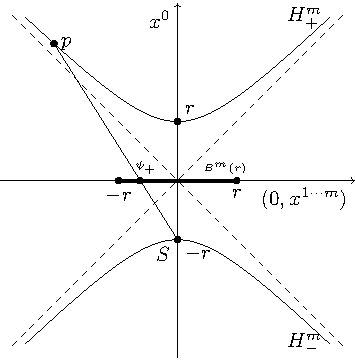
\includegraphics{fig/ch10-Hyperbolic.pdf}
    \caption{双曲空间}\label{chsm:pic_Hyperbolic}
\end{figure}

对任意$p=(x^0,x^1 ,\cdots,x^{m} )\in H^m_{+}(r)$(见图\ref{chsm:pic_Hyperbolic}),
连接点$p$和$S$的直线$l_{pS}$必定交超平面$x^{0}=0$于某点$\psi_{+}(p)$;很明显
交点$\psi_{+}(p)$位于$B^m(r)$内(不可能不与之相交);同时$\psi_{+}:H^m_{+}(r)\to B^m(r)$是双射.
对于任意的点$p$,下面我们来求$\psi_{+}(p)$的坐标$(\xi^1,\cdots,\xi^{m})$.

过两点(此处是$p$和$S$点)直线方程是(直线上点的坐标是$(\xi^0,\cdots,\xi^m)$)
\begin{equation}
    \frac{\xi^1-0}{x^1 -0} =\frac{\xi^2-0}{x^2 -0}=\cdots=
    \frac{\xi^m-0}{x^m -0} = \frac{\xi^{0}+r}{x^{0} +r}
\end{equation}
令上式中的$\xi^{0}=0$可得$\psi_{+}(p)$坐标如下
\begin{equation}
    (\xi^1,\cdots,\xi^m)=\psi_{+}(x^0,x^1 ,\cdots,x^{m})=
    \frac{r}{r+x^{0}}(x^1,\cdots,x^m).
\end{equation}
反之.将上式求平方和,并利用$\sum_{i=1}^{m}(x^i)^2 -(x^{0})^2=-r^2$,可得
\begin{align*}
    & \sum_{k=1}^{m}(\xi^k)^2=\frac{r^2 }{(r+x^{0})^2}\left(\sum_{i=1}^{m}(x^i)^2\right)
    =\frac{r^2 }{(r+x^{0})^2}\left(-r^2+(x^{0})^2\right) \\
    \Rightarrow \ 
    & x^{0} = \frac{r\left(r^2+\sum\nolimits_k(\xi^k)^2\right)}{r^2-\sum\nolimits_k(\xi^k)^2},
    {\quad \text{或} \quad } x^{0}= -r \ (\text{舍弃}) .
\end{align*}
有了$x^0$坐标表达式,其它坐标几乎一望而知,它们是
\begin{align}
    (x^{0},& x^1,\cdots,x^m) = \psi_{+}^{-1}(\xi^1,\cdots,\xi^m) \notag \\
    =&\frac{r}{r^2-\sum\nolimits_k(\xi^k)^2}
    \left(+r^2+\sum_{k=1}^m(\xi^k)^2, \ 2 r \xi^1, \cdots, \ 2 r \xi^m \right),
    \label{chdm:eqn_hybxi2x} \\
    (x^{0},& x^1,\cdots,x^m) = \psi_{-}^{-1}(\eta^1,\cdots,\eta^m) \notag \\
    =&\frac{r}{r^2-\sum\nolimits_k(\eta^k)^2}
    \left(- r^2-\sum_{k=1}^m (\eta^k)^2 , \ 2 r \eta^1, \cdots, \ 2 r \eta^m \right).
    \label{chdm:eqn_mybeta2x}
\end{align}
上面第二式为双曲空间下叶的坐标(其中$\eta^i=\frac{r x^i}{r-x^{0}}$),请读者补齐推导过程.
不难看出映射$\psi_{\pm}$及$\psi_{\pm}^{-1}$都是无穷阶可微函数,
所以$\psi_{\pm}:H^m_{\pm}(r)\to B^m(r)$是光滑同胚.

$\mathbb{R}^{m+1}_1$度规为广义Lorentz度规,即
\begin{equation*}
    g_{ab}X^a Y^b = \bigl(-({\rm d}x^0)_a({\rm d}x^0)_b+ \sum_{i=1}^{m}({\rm d}x^i)_a({\rm d}x^i)_b\bigr)
    X^a Y^b=-X^0 Y^0 + \sum_{i=1}^{m} X^i Y^i,
\end{equation*}
其中$X^a, Y^a\in \mathbb{R}^{m+1}$是任意矢量.显然,有
\begin{equation}
    g_{ab}X^a Y^b = \frac{1}{2}\bigl(g_{ab}(X+Y)^a(X+Y)^b -g_{ab}X^a X^b -g_{ab}Y^a Y^b\bigr).
\end{equation}
从上式可见,只需研究$g_{ab}X^a X^b$就可讨论整个Lorentz度规了.
在物理学中(见定义\ref{chrg:def_Minkowski-space}和\ref{chrg:def_vector-property}),
只讨论类时矢量和零模矢量,而它们正好与双曲空间有一一对应关系;类时矢量对应$r>0$,零模矢量对应$r=0$.
为简单起见,我们假设所有矢量的第零维分量是正的(指向未来),
同时只讨论类时矢量;这样只需讨论双曲空间的上叶即可.
从上面的讨论可以看出,类时矢量的Lorentz度规内积可以转化为双曲上叶中(这种转换是双射).

读者需要注意,我们只给$\mathbb{R}^{m+1}_1$选定了度规,还不知道$H^m_{\pm}(r)$或$B^m(r)$度规;
下面我们来计算它们的诱导度规.
很明显,包含映射$\imath :H^m_{+}(r) \to \mathbb{R}^{m+1}_1$是正则嵌入的;
令$\varphi=\imath \circ \psi_{+}^{-1}$,则由上面的讨论可知:$\varphi:B^m(r)\to \mathbb{R}^{m+1}_1$也是
光滑、正则嵌入映射;当然它们都是浸入的了.根据式\eqref{chsm:eqn_gijhab}可以求得$B^m(r)$的
诱导度规$h_{ab}=\varphi^{*} g_{ab}$,直接计算即可
\setlength{\mathindent}{0em}
\begin{equation}\label{chsm:eqn_gphiha}
    h_{ab}= \left(\sum_{\alpha=1}^{m}\frac{\partial x^\alpha}{\partial \xi^i}
    \frac{\partial x^\alpha}{\partial \xi^j} -\frac{\partial x^0}{\partial \xi^i}
    \frac{\partial x^0}{\partial \xi^j} \right)
    ({\rm d}\xi^i)_a ({\rm d}\xi^j)_b
    = \frac{4r^4 \sum\nolimits_{i=1}^{m} ({\rm d}\xi^i)_a ({\rm d}\xi^i)_b} 
    {(r^2-\sum\nolimits_{k=1}^{m} (\xi^k)^2)^2}.
\end{equation}\setlength{\mathindent}{2em}
可见这个度规是正定的,因而$B^m(r)$是一个正定黎曼流形.

还可以求得$H^m_{+}(r)$中的诱导度规$h'_{ab}=\imath ^* g_{ab}$
(假设$x^1,\cdots,x^m$是独立变量,$x^0$可由上述量来表示),
根据式\eqref{chsm:eqn_gijhab}经过计算可得
\begin{equation}\label{chsm:eqn_gphihabb}
    \begin{aligned}
        h'_{ab}=& \sum_{ij=1}^{m}\left(\sum_{\alpha,\beta=1}^{m}\frac{\partial x^\alpha}{\partial x^i}
        \frac{\partial x^\beta}{\partial x^j}\delta_{\alpha\beta} -\frac{\partial x^0}{\partial x^i}
        \frac{\partial x^0}{\partial x^j} \right)    ({\rm d} x^i)_a ({\rm d} x^j)_b  \\
        =& \sum_{ij=1}^{m}\left(\delta_{ij}-\frac{x^i x^j}{r^2+\sum_{k=1}^{m}(x^k)^2}\right)({\rm d} x^i)_a ({\rm d} x^j)_b \\
        \xlongequal{\ref{chdm:eqn_hybxi2x}}&
        \frac{4r^4 \sum\nolimits_{i=1}^{m} ({\rm d}\xi^i)_a ({\rm d}\xi^i)_b} {(r^2-\sum\nolimits_{k=1}^{m} (\xi^k)^2)^2}.
    \end{aligned}
\end{equation}
上式最后一步推导较为繁琐,计算冗长,所得结果与式\eqref{chsm:eqn_gphiha}相同.
这说明$(H^m_{+}(r),\imath ^* g_{ab})$和$(B^m(r),\varphi ^* g_{ab})$是等距同胚.

%推导过程
%\setlength{\mathindent}{0em}
%\begin{align*}
%    ({\rm d} x^i)_a =& \frac{2a^2 (r^2-\sum\nolimits_k(\xi^k)^2) ({\rm d} \xi^i)_a
    %    + 4a^2 \xi^i \sum\nolimits_l \xi^l ({\rm d} \xi^l)_a}{(r^2-\sum\nolimits_k(\xi^k)^2)^2}
%\end{align*}
%第一项
%\begin{align*}
%    &\sum_{ij=1}^{m}\delta_{ij}({\rm d} x^i)_a ({\rm d} x^j)_b = \sum_{i=1}^{m}({\rm d} x^i)_a ({\rm d} x^i)_b \\
%    =& \frac{2a^2 (r^2-\sum\nolimits_k(\xi^k)^2) ({\rm d} \xi^i)_a
    %        + 4a^2 \xi^i \sum\nolimits_l \xi^l ({\rm d} \xi^l)_a}{(r^2-\sum\nolimits_k(\xi^k)^2)^2}
%    \frac{2a^2 (r^2-\sum\nolimits_k(\xi^k)^2) ({\rm d} \xi^i)_b
    %        + 4a^2 \xi^i \sum\nolimits_l \xi^l ({\rm d} \xi^l)_b}{(r^2-\sum\nolimits_k(\xi^k)^2)^2} \\
%    =& \frac{1}{(r^2-\sum\nolimits_k(\xi^k)^2)^4} \biggl(
%    4a^4 (r^2-\sum\nolimits_k(\xi^k)^2)^2 \sum_{i=1}^{m} ({\rm d} \xi^i)_a ({\rm d} \xi^i)_b+
%    16a^4 (r^2-\sum\nolimits_k(\xi^k)^2)  \sum\nolimits_{il} \xi^l \xi^i  ({\rm d} \xi^i)_a ({\rm d} \xi^l)_b \\
%    & + 16a^4 \sum_{i=1}^{m} (\xi^i)^2 \sum\nolimits_{ln} \xi^l\xi^m ({\rm d} \xi^l)_a  ({\rm d} \xi^m)_b  \biggr) \\
%    =&\frac{1}{(r^2-\sum\nolimits_k(\xi^k)^2)^4} \biggl(
%    4a^4 (r^2-\sum\nolimits_k(\xi^k)^2)^2 \sum_{i=1}^{m} ({\rm d} \xi^i)_a ({\rm d} \xi^i)_b+
%    16a^6 \sum\nolimits_{ln} \xi^l \xi^m  ({\rm d} \xi^m)_a ({\rm d} \xi^l)_b  \biggr)
%\end{align*}
%第二项
%\begin{align*}
%    &\sum_{ij=1}^{m} x^i x^j ({\rm d} x^i)_a ({\rm d} x^j)_b
%    =\sum_{ij=1}^{m} \frac{4a^4 \xi^i \xi^j}{(r^2-\sum\nolimits_k(\xi^k)^2)^2}
%    \frac{2a^2 (r^2-\sum\nolimits_k(\xi^k)^2) ({\rm d} \xi^i)_a
    %        + 4a^2 \xi^i \sum\nolimits_l \xi^l ({\rm d} \xi^l)_a}{(r^2-\sum\nolimits_k(\xi^k)^2)^2} \\
%    &\times \frac{2a^2 (r^2-\sum\nolimits_k(\xi^k)^2) ({\rm d} \xi^j)_b
    %        + 4a^2 \xi^j \sum\nolimits_l \xi^l ({\rm d} \xi^l)_b}{(r^2-\sum\nolimits_k(\xi^k)^2)^2} \\
%    =& \frac{16a^8 }{(r^2-\sum\nolimits_k(\xi^k)^2)^6} \sum_{ij=1}^{m} \biggl(\xi^i \xi^j
%    \Bigl((r^2-\sum\nolimits_k(\xi^k)^2) ({\rm d} \xi^i)_a + 2 \xi^i \sum\nolimits_l \xi^l ({\rm d} \xi^l)_a\Bigr)
%    \Bigl((r^2-\sum\nolimits_k(\xi^k)^2) ({\rm d} \xi^j)_b + 2 \xi^j \sum\nolimits_n \xi^m ({\rm d} \xi^m)_b\Bigr)  \biggr) \\
%    =&\frac{16a^8 }{(r^2-\sum\nolimits_k(\xi^k)^2)^6} \biggl(
%    (r^2-\sum\nolimits_k(\xi^k)^2)^2  \sum_{ij=1}^{m} \xi^i \xi^j  ({\rm d} \xi^i)_a ({\rm d} \xi^j)_b
%     + 2(r^2-\sum\nolimits_k(\xi^k)^2) \Bigl(\sum_{j=1}^{m} (\xi^j)^2\Bigr)
%        \sum_{in=1}^{m} \xi^i\xi^m ({\rm d} \xi^i)_a ({\rm d} \xi^m)_b   \\
%    &+2 (r^2-\sum\nolimits_k(\xi^k)^2) \sum_{i=1}^{m}(\xi^i)^2
%     \sum\nolimits_{jl} \xi^l ({\rm d} \xi^l)_a \xi^j  ({\rm d} \xi^j)_b
%    + 4 \sum_{ij=1}^{m}(\xi^i)^2 (\xi^j)^2  \sum\nolimits_l \xi^l
%    ({\rm d} \xi^l)_a \sum\nolimits_n \xi^m ({\rm d} \xi^m)_b     \biggr) \\
%    =&\frac{16a^8 }{(r^2-\sum\nolimits_k(\xi^k)^2)^6} \biggl(
%    (r^2-\sum\nolimits_k(\xi^k)^2)^2
%    + 4(r^2-\sum\nolimits_k(\xi^k)^2) \Bigl(\sum_{j=1}^{m} (\xi^j)^2\Bigr)
%    + 4 \sum_{ij=1}^{m}(\xi^i)^2 (\xi^j)^2    \biggr)
%    \sum_{ln=1}^{m} \xi^l \xi^m  ({\rm d} \xi^l)_a ({\rm d} \xi^m)_b \\
%    =&\frac{16a^8 }{(r^2-\sum\nolimits_k(\xi^k)^2)^6} \biggl(
%    (r^2+\sum\nolimits_k(\xi^k)^2)^2   \biggr)
%    \sum_{ln=1}^{m} \xi^l \xi^m  ({\rm d} \xi^l)_a ({\rm d} \xi^m)_b
%\end{align*}
%而
%\begin{align*}
%    r^2+\sum_{k=1}^{m}(x^k)^2= r^2+
%    \sum_{i=1}^{m} \frac{4a^4 \xi^i \xi^i}{(r^2-\sum\nolimits_k(\xi^k)^2)^2}
%    =r^2 \frac{(r^2+\sum\nolimits_k(\xi^k)^2)^2}{(r^2-\sum\nolimits_k(\xi^k)^2)^2}
%\end{align*}
%综合以上三式,有
%\begin{align*}
%    &\frac{1}{(r^2-\sum\nolimits_k(\xi^k)^2)^4} \biggl(
%    4a^4 (r^2-\sum\nolimits_k(\xi^k)^2)^2 \sum_{i=1}^{m} ({\rm d} \xi^i)_a ({\rm d} \xi^i)_b+
%    16a^6 \sum\nolimits_{ln} \xi^l \xi^m  ({\rm d} \xi^m)_a ({\rm d} \xi^l)_b  \biggr) \\
%    &- \frac{16a^6 }{(r^2-\sum\nolimits_k(\xi^k)^2)^4}
%    \sum_{ln=1}^{m} \xi^l \xi^m  ({\rm d} \xi^l)_a ({\rm d} \xi^m)_b \\
%    =& \frac{ 4a^4 ({\rm d} \xi^i)_a ({\rm d} \xi^i)_b}{(r^2-\sum\nolimits_k(\xi^k)^2)^2}
%\end{align*}
%\setlength{\mathindent}{2em}

\begin{example}
    具体计算一例.当$m=1$时,设$v^a=v_{\xi}(\frac{\partial}{\partial \xi})^a\in T_pB^1(r)$,
    根据式\eqref{chsm:eqn_gphiha},有$h_{ab}v^a v^b= \frac{4r^4 v^2_\xi}{(r^2-\xi^2)^2}$;
    这是正定的.
    
    再计算Lorentz度规下的数值.推前$v^a$有$\varphi_*(v^a)= \frac{4r^3\xi v_\xi}{(r^2-\xi^2)^2}
    (\frac{\partial}{\partial x^0})^c+ \frac{2r^2(r^2+\xi^2) v_\xi}{(r^2-\xi^2)^2}(\frac{\partial}{\partial x^1})^c$;
    再来计算矢量长度,$g_{ab}v^a v^b= \frac{4r^4 v^2_\xi}{(r^2-\xi^2)^2}$;两者相等.
\end{example}



%\subsection{统一表示}
\paragraph{统一表示}
前面几节,我们把$\mathbb{R}^{m+1}_\nu$中的坐标(比如$x^0$)直接
用其它坐标($x^1,\cdots,x^m$)表示出来,
然后给出了伪球面、伪双曲面的度规;这种方式最为直接,但所得公式各不相同.
黎曼最早用同一公式表示了超球面和双曲空间的度规,之后被其他人推广到了伪球面、伪双曲面;
详见\S \ref{chhss:sec_SF} 定理\ref{chhss:thm_SRH-riemann}.




\section{超曲面四:相对论时空}\label{chsm:sec_3+1decomposition}
本节将光滑流形$(M,g)$的维数限定在四维,则超曲面$\Sigma$是三维的,度规$g$是Lorentz类型的($(-+++)$).
本小节拉丁字母表示$1,2,3$;希腊字母表示$0,1,2,3$.


流形$M$的切丛$TM$上存在一类时矢量场$(\frac{\partial }{\partial t})^a$,这一类时场将
流形$M$分解为一族类空超曲面$\{\Sigma_t\}$,整张超曲面$\Sigma_t$上的参数$t$是同一实数.
这族超曲面中任意两张不同参数的超曲面没有交集,即$\Sigma_t \cap \Sigma_{t'}=\varnothing,
\ \forall t \neq t' $.
流形$M$中任意一点都位于某张(且只在此张)$\Sigma_t$上,
即$\{\Sigma_t\}$能覆盖住流形$M$,$M=\bigcup_{t\in\mathbb{R}} \Sigma_t$.

从纯粹数学角度来看任意四维闵氏流形$(M,g)$,未必存在
这样的分解,或者说需要满足一定条件才存在这样的类时矢量场,然后依据这个
类时场将空间$M$划分成一族类空超曲面$\Sigma_t$;寻找数学上的这些存在性条件
(对物理学工作者来说)太过艰深.从物理学角度看,这样的分解一定存在,
因为我们就生活在这样的一个四维时空中,这个时空然后被$1+3$分解成时间和空间.



\index[physwords]{超曲面!ADM分解}
\index[physwords]{ADM分解}

\subsection{ADM分解}\label{chsm:sec_ADM}

类时场$(\frac{\partial }{\partial t})^a$自然是单参数的,参数是$t$;
我们约定它指向未来,即指向参数$t$增大的方向.
一般情形下,$(\frac{\partial }{\partial t})^a$未必与超曲面$\Sigma_t$处处正交;
假设类时矢量场$(\frac{\partial }{\partial t})^a$可分解为两个矢量场:
\begin{equation}\label{chsm:eqn_ADM}
    \left(\frac{\partial }{\partial t}\right)^a = N n^a + S^a .
\end{equation}
其中$n^a$是类空超曲面$\Sigma_t$的单位法矢量,所以有$n^a n_a =-1$;
标量场$N$称为\uwave{时移函数}(lapse function),
矢量场$S^a$称为\uwave{位移矢量场}(shift vector field),$S^a$切于类空超曲面$\Sigma_t$.
一般称这种分解方式为ADM分解\cite{ADM_2008}.很容易得到
\begin{equation*}
    ({\rm d}t)_a = -\frac{1}{N} n_a .\quad \text{因为}\
    1= ({\rm d}t)_a \left(\frac{\partial }{\partial t}\right)^a =
    -\frac{1}{N} n_a(N n^a + S^a)=-n_a n^a =1.
\end{equation*}

我们需要建立局部坐标系,类时矢量场$(\frac{\partial }{\partial t})^a$自然是
坐标基矢之一,它的积分曲线(见\S\ref{chdm:sec_One-Parameter-Transformations-Groups})是一条坐标线.
依据它分层的每张超曲面$\Sigma_t$都是三维类空曲面,在每张
超曲面上我们都选取三个线性无关的(即不在同一个二维超曲面内)类空矢量场;
当然可以选三个正交归一的类空矢量场,但目前暂不做此要求.
这四个坐标构成局部坐标系$\{x^0\equiv t,x^i \}$,基矢分别
是$\{(\frac{\partial }{\partial t})^a,(\frac{\partial }{\partial x^i})^a\}$.
类时矢量场$(\frac{\partial }{\partial t})^a$的积分曲线与每一个$\Sigma_t$都有且只有一个交点,
所有交点的三个类空坐标$\{x^i\}$自然取为相同的值;每张$\Sigma_t$上的参数$t$取同一值.

根据假设矢量场$S^a$是纯类空矢量场,切于$\Sigma_t$;而$n^a$正交于$\Sigma_t$,故有
\begin{equation}
    S^0 = S^a ({\rm d}t)_a= -\frac{1}{N} S^a n_a =0.
\end{equation}
因此
\begin{equation}
    S^a = \sum_{i=1}^{3} S^i \left(\frac{\partial }{\partial x^i}\right) ^a .
\end{equation}
令$S_a = g_{ab} S^b$,$S_i = S_a (\frac{\partial }{\partial x^i}) ^a$.

经计算可得度规场$g_{ab}$在局部坐标系$\{x^0\equiv t,x^i \}$的分量表达式:
\begin{small}
\begin{equation}\label{chsm:eqn_ADM-metric}
    g_{\mu\nu}=\begin{pmatrix}
        S^i S_i -N^2 & S_1 & S_2 &S_3 \\
        S_1 &g_{11} & g_{12} & g_{13} \\
        S_2 &g_{21} & g_{22} & g_{23} \\
        S_3 &g_{31} & g_{32} & g_{33}
    \end{pmatrix}, \
    g^{\mu\nu}=\frac{1}{N^{2}} \begin{pmatrix}
        -1 & S^1 & S^2 & S^3 \\
        S^1 & &  &  \\
        S^2 &N^{2} h_{ij}^{-1} & - & S^i S^j \\
        S^3 & &  &
    \end{pmatrix} .
\end{equation}
\end{small}
记$g_{ij}\equiv h_{ij},\ 1\leqslant i,j \leqslant 3$.
其中共轭度规右下角$3\times 3$的矩阵元是$g^{ij}= h_{ij}^{-1}-N^{-2}S^i S^j$,
其中$h_{ij}^{-1}$是指度规右下角$3\times 3$的矩阵$(g_{ij})$的逆;
需要注意的是矩阵外面还有一个因子.

可求得单位法矢量在$\{t,x^i\}$的分量表达式
\begin{equation}\label{chsm:eqn_ADM-n}
    n^a = \frac{1}{N} \left(\frac{\partial }{\partial t}\right)^a
    -\frac{S^i}{N} \left(\frac{\partial }{\partial x^i}\right)^a  ;\qquad
    n_a = -N ({\rm d}t)_a = -N \nabla_a t .
\end{equation}


诱导度规$h_{ab}=g_{ab}+n_a n_b$在$\{t,x^i\}$的分量表达式为
\begin{small}
\begin{subequations}\label{chsm:eqn_ADM-hab}
\begin{align}
    h_a^b =& \left( ({\rm d}x^i)_a +S^i ({\rm d}t)_a \right) 
    \left(\frac{\partial }{\partial x^i}\right)^b , \label{chsm:eqn_ADM-hab-1}\\
    h_{ab}=& S_k S^k ({\rm d}t)_a ({\rm d}t)_b + S_i\left( ({\rm d}t)_a ({\rm d}x^i)_b
    + ({\rm d}t)_b ({\rm d}x^i)_a \right) + g_{ij} ({\rm d}x^i)_a ({\rm d}x^j)_b .
    \label{chsm:eqn_ADM-hab-2} 
\end{align}
\end{subequations}
\end{small}
直接计算便可得到$\det(h_{\mu\nu})=0$,但$h=\det(h_{ij})\neq 0$.
且有$g=\det(g_{\mu\nu})=-N^2 \det(g_{ij})=-N^2 \det(h_{ij})$.
从而可以得到四维流形$M$体积元与三维超曲面$\Sigma_t$的诱导体积元之间的关系:
\begin{small}
\begin{equation}
   n^a \bigl(\sqrt{-g}({\rm d}x^0)_a \wedge ({\rm d}x^1)_b \wedge({\rm d}x^2)_c \wedge({\rm d}x^3)_d \bigr) 
        = N \sqrt{h} ({\rm d}x^1)_b \wedge({\rm d}x^2)_c \wedge({\rm d}x^3)_d  .
\end{equation}
\end{small}

虽然三维流形$\Sigma_t$上的度规场$h_{ij}\equiv g_{ij}$,
但是,从式\eqref{chsm:eqn_ADM-metric}可以看到一般情形下$h^{ij}=h_{ij}^{-1}\neq g^{ij}$,
而是$g^{ij}=h_{ij}^{-1} - S^i S^j/N^2$.



\index[physwords]{超曲面!时间导数}

\subsection{时间导数}

在适配坐标系中(见式\eqref{chdm:eqn_LieD-adaptedX}),李导数化为偏导数;
ADM分解后的坐标系就是一个适配坐标系,所有张量分量对参数$t$的偏导数都可以化作李导数.
在ADM分解中,参量$t$可以看作“时间”;故
张量场对切矢量场$(\frac{\partial }{\partial t})^a$的李导数可以看作对时间$t$的导数.

类空张量场$T^{a\cdots}_{b\cdots}\in \mathfrak{T}^p_q(\Sigma_t)$的李导数未必仍是类空张量场,
我们给其增加数次投影,这样的李导数自然仍是类空张量场.
\begin{equation}
    \dot{T}^{a\cdots}_{b\cdots} \equiv \widetilde{\Lie}_{\partial_t}{T}^{a\cdots}_{b\cdots}
    \overset{def}{=} h^a_{a'}\cdots h^{b'}_{b}\cdots {\Lie}_{\partial_t}{T}^{a'\cdots}_{b'\cdots} .
\end{equation}
$\widetilde{\Lie}_X$表示增加数次投影的${\Lie}_X$.
可以证明如下重要公式:
\begin{equation}\label{chsm:eqn_Lie-t-T}
    \widetilde{\Lie}_{\partial_t}{T}^{a\cdots}_{b\cdots}
    = \widetilde{\Lie}_{N n}{T}^{a\cdots}_{b\cdots}
     +\widetilde{\Lie}_{\vec{S}}{T}^{a\cdots}_{b\cdots}
    = N \widetilde{\Lie}_{n}{T}^{a\cdots}_{b\cdots}
    +\widetilde{\Lie}_{\vec{S}}{T}^{a\cdots}_{b\cdots} ,
    \quad \forall T^{a\cdots}_{b\cdots}\in \mathfrak{T}^p_q(\Sigma_t).
\end{equation}
由于$S^a$在ADM分解下是纯类空矢量场,在李导数的角标中,将其记为$\vec{S}$.
式$\widetilde{\Lie}_{Nn}{T}^a_{\cdot b}=N\widetilde{\Lie}_{n}{T}^{a\cdots}_{b\cdots}$的证明
较为繁琐,需先后计算$\widetilde{\Lie}_{Nn}{T}^{a\cdots}_{b\cdots}$
和$\widetilde{\Lie}_{n}{T}^{a\cdots}_{b\cdots}$,
然后即可验证它们相等.有了此等式,也就证明了式\eqref{chsm:eqn_Lie-t-T}.

%首先,经过较为冗长的推演可以证明
%\begin{align*}
%    \widetilde{\Lie}_{n}{T}^a_{\cdot b} = &
%    h^a_{a'} h^{b'}_{b} \left( n^e\nabla_e T^{a'}_{\cdot b'}
%    - T^{e}_{\cdot b'} \nabla_e n^{a'} + T^{a'}_{\cdot e} \nabla_{b'} n^e \right) \\
%    = &  (g^a_{a'} g^{b'}_{b} +n^a n_{a'}g^{b'}_{b}+ g^a_{a'} n^{b'}n_{b} + n^a n_{a'}n^{b'}n_{b})
%    \left(N n^e\nabla_e T^{a'}_{\cdot b'}
%    - T^{e}_{\cdot b'} \nabla_e n^{a'} + T^{a'}_{\cdot e} \nabla_{b'} n^e \right) \\
%    = &  g^a_{a'} g^{b'}_{b}   \left( n^e\nabla_e T^{a'}_{\cdot b'}
%    - T^{e}_{\cdot b'} \nabla_e n^{a'} + T^{a'}_{\cdot e} \nabla_{b'} n^e \right) \\
%    &+  n^a n_{a'}g^{b'}_{b}  \left( n^e\nabla_e T^{a'}_{\cdot b'}
%    - T^{e}_{\cdot b'} \nabla_e n^{a'} + \cancel{T^{a'}_{\cdot e} \nabla_{b'} n^e} \right) \\
%    &+ g^a_{a'} n^{b'}n_{b}    \left( n^e\nabla_e T^{a'}_{\cdot b'}
%    -\cancel{ T^{e}_{\cdot b'} \nabla_e n^{a'}}+ T^{a'}_{\cdot e} \nabla_{b'} n^e \right) \\
%    &+ n^a n_{a'}n^{b'}n_{b} \left( n^e\nabla_e T^{a'}_{\cdot b'}
%    -\cancel{ T^{e}_{\cdot b'} \nabla_e n^{a'}} + \cancel{T^{a'}_{\cdot e} \nabla_{b'} n^e} \right) \\
%    = &  n^e\nabla_e T^{a}_{\cdot b}
%    - T^{e}_{\cdot b} \nabla_e n^{a} + T^{a}_{\cdot e} \nabla_{b} n^e  \\
%    &+  n^a n_{a'}  \left( n^e\nabla_e T^{a'}_{\cdot b}
%    - T^{e}_{\cdot b} \nabla_e n^{a'}  \right) \\
%    &+  n^{b'}n_{b}    \left( n^e\nabla_e T^{a}_{\cdot b'}
%    + T^{a}_{\cdot e} \nabla_{b'} n^e \right) \\
%    &+ n^a n_{a'}n^{b'}n_{b}  n^e\nabla_e T^{a'}_{\cdot b'}  \\
%    = &  n^e\nabla_e T^{a}_{\cdot b}
%    - T^{e}_{\cdot b} \nabla_e n^{a} + T^{a}_{\cdot e} \nabla_{b} n^e  \\
%    &+  n^a n_{a'} n^e\nabla_e T^{a'}_{\cdot b}
%    -   \cancel{n^a n_{a'} T^{e}_{\cdot b} \nabla_e n^{a'}  } \\
%    &+  n^{b'}n_{b}  n^e\nabla_e T^{a}_{\cdot b'}
%    + n^{b'}n_{b} T^{a}_{\cdot e} \nabla_{b'} n^e \\
%    &- \cancel{n^a n_{a'} n_{b} T^{a'}_{\cdot b'} n^e\nabla_e n^{b'} } \\
%    = &  n^e\nabla_e T^{a}_{\cdot b}
%    - T^{e}_{\cdot b} \nabla_e n^{a} + T^{a}_{\cdot e} \nabla_{b} n^e
%    + n^a n_{c} n^e\nabla_e T^{c}_{\cdot b}
%    + n^{c}n_{b}  n^e\nabla_e T^{a}_{\cdot c}
%    + n^{c}n_{b} T^{a}_{\cdot e} \nabla_{c} n^e \\
%        = &  n^e\nabla_e T^{a}_{\cdot b}
%    - T^{e}_{\cdot b} \nabla_e n^{a} + T^{a}_{\cdot e} \nabla_{b} n^e
%    + n^a n_{c} n^e\nabla_e T^{c}_{\cdot b}
%    + {\color{red}n^cn_{b} n^{e} \nabla_c T^{a}_{\cdot e}
%    - n^{c}n_{b} n^e \nabla_{c}  T^{a}_{\cdot e}} \\
%    = &  n^e\nabla_e T^{a}_{\cdot b}
%    - T^{e}_{\cdot b} \nabla_e n^{a} + T^{a}_{\cdot e} \nabla_{b} n^e
%    + n^a n_{c} n^e\nabla_e T^{c}_{\cdot b}
%\end{align*}
%容易验证
%$n^b \widetilde{\Lie}_{n}{T}^a_{\cdot b} =0=n_a \widetilde{\Lie}_{n}{T}^a_{\cdot b}$.
%接着计算,
%\begin{align*}
%    \widetilde{\Lie}_{N n}{T}^a_{\cdot b} = &
%    h^a_{a'} h^{b'}_{b} \left(N n^e\nabla_e T^{a'}_{\cdot b'}
%    - T^{e}_{\cdot b'} \nabla_e (Nn^{a'}) + T^{a'}_{\cdot e} \nabla_{b'} (Nn^e) \right) \\
%    = &  (g^a_{a'} g^{b'}_{b} +n^a n_{a'}g^{b'}_{b}+ g^a_{a'} n^{b'}n_{b} + n^a n_{a'}n^{b'}n_{b})
%      \left(N n^e\nabla_e T^{a'}_{\cdot b'}
%      - T^{e}_{\cdot b'} \nabla_e (Nn^{a'}) + T^{a'}_{\cdot e} \nabla_{b'} (Nn^e) \right) \\
%    = &  g^a_{a'} g^{b'}_{b}   \left(N n^e\nabla_e T^{a'}_{\cdot b'}
%      - T^{e}_{\cdot b'} \nabla_e (Nn^{a'}) + T^{a'}_{\cdot e} \nabla_{b'} (Nn^e) \right) \\
%     &+  n^a n_{a'}g^{b'}_{b}  \left(N n^e\nabla_e T^{a'}_{\cdot b'}
%      - T^{e}_{\cdot b'} \nabla_e (Nn^{a'}) + T^{a'}_{\cdot e} \nabla_{b'} (Nn^e) \right) \\
%     &+ g^a_{a'} n^{b'}n_{b}    \left(N n^e\nabla_e T^{a'}_{\cdot b'}
%      - T^{e}_{\cdot b'} \nabla_e (Nn^{a'}) + T^{a'}_{\cdot e} \nabla_{b'} (Nn^e) \right) \\
%     &+ n^a n_{a'}n^{b'}n_{b} \left(N n^e\nabla_e T^{a'}_{\cdot b'}
%      - T^{e}_{\cdot b'} \nabla_e (Nn^{a'}) + T^{a'}_{\cdot e} \nabla_{b'} (Nn^e) \right) \\
%    =&    N n^e\nabla_e T^{a}_{\cdot b}
%    - T^{e}_{\cdot b} n^{a} \nabla_e N - T^{e}_{\cdot b} N  \nabla_e n^a
%    + \cancel{T^{a}_{\cdot e} n^e \nabla_{b} N} + T^{a}_{\cdot e} N  \nabla_b n^e  \\
%    &+  n^a n_{a'} \left(N n^e\nabla_e T^{a'}_{\cdot b}
%    - T^{e}_{\cdot b} \nabla_e (Nn^{a'}) +\cancel{ T^{a'}_{\cdot e} \nabla_{b} (Nn^e)} \right) \\
%    &+  n^{b'}n_{b}    \left(N n^e\nabla_e T^{a}_{\cdot b'}
%    -\cancel{ T^{e}_{\cdot b'} \nabla_e (Nn^{a})} + T^{a}_{\cdot e} \nabla_{b'} (Nn^e) \right) \\
%    &+ n^a n_{a'}n^{b'}n_{b} \left(N n^e\nabla_e T^{a'}_{\cdot b'}
%    - \cancel{T^{e}_{\cdot b'} \nabla_e (Nn^{a'})} + \cancel{T^{a'}_{\cdot e} \nabla_{b'} (Nn^e)} \right) \\
%    =&    N n^e\nabla_e T^{a}_{\cdot b}
%    - T^{e}_{\cdot b} n^{a} \nabla_e N - T^{e}_{\cdot b} N  \nabla_e n^a
%    + T^{a}_{\cdot e} N  \nabla_b n^e  \\
%    &+  n^a n_{a'} \left(N n^e\nabla_e T^{a'}_{\cdot b}
%    - T^{e}_{\cdot b} n^{a'} \nabla_e N - T^{e}_{\cdot b} N \nabla_e  n^{a'} \right) \\
%    &+  n^{b'}n_{b}    \left(N n^e\nabla_e T^{a}_{\cdot b'}
%    + T^{a}_{\cdot e} n^e\nabla_{b'} N + T^{a}_{\cdot e}N \nabla_{b'} n^e \right) \\
%    &+ n^a n_{a'}n^{b'}n_{b} \left(N n^e\nabla_e T^{a'}_{\cdot b'}   \right) \\
%    =&      N n^e\nabla_e T^{a}_{\cdot b}
%    - {\color{red}T^{e}_{\cdot b} n^{a} \nabla_e N }
%    - T^{e}_{\cdot b} N  \nabla_e n^a + T^{a}_{\cdot e} N  \nabla_b n^e  \\
%    &+  N n^a n_{a'} n^e\nabla_e T^{a'}_{\cdot b}
%     + {\color{red} n^a T^{e}_{\cdot b} \nabla_e N }
%     - {\cancel{n^a n_{a'}T^{e}_{\cdot b} N \nabla_e  n^{a'}}} \\
%    &+  n^{b'}n_{b} N n^e\nabla_e T^{a}_{\cdot b'}
%    + {\cancel{n^{b'}n_{b}T^{a}_{\cdot e} n^e\nabla_{b'} N}}
%    + n^{b'}n_{b}T^{a}_{\cdot e}N \nabla_{b'} n^e  \\
%    &+ n^a n_{a'}n^{b'}n_{b} N n^e\nabla_e T^{a'}_{\cdot b'}    \\
%    =&    N n^e\nabla_e T^{a}_{\cdot b}
%    - T^{e}_{\cdot b} N  \nabla_e n^a + T^{a}_{\cdot e} N  \nabla_b n^e
%    + n^{b'}n_{b}T^{a}_{\cdot e}N \nabla_{b'} n^e  \\
%    &+  N n^a n_{a'} n^e\nabla_e T^{a'}_{\cdot b}
%    +  n^{b'}n_{b} N n^e\nabla_e T^{a}_{\cdot b'}
%    + n^a n_{a'}n^{b'}n_{b} N n^e\nabla_e T^{a'}_{\cdot b'}    \\
%     =&    N n^e\nabla_e T^{a}_{\cdot b}
%    - T^{e}_{\cdot b} N  \nabla_e n^a + T^{a}_{\cdot e} N  \nabla_b n^e
%    +  {\color{red}n^{b'}n_{b}T^{a}_{\cdot e}N \nabla_{b'} n^e} \\
%    &-  N n^a T^{a'}_{\cdot b} n^e\nabla_e  n_{a'}
%    -  {\color{red}N n_{b} T^{a}_{\cdot b'}  n^e\nabla_e n^{b'}}
%    - {\cancel{N n^a n_{a'}n_{b} T^{a'}_{\cdot b'} n^e\nabla_e n^{b'}  }}  \\
%    =& N n^e\nabla_e T^{a}_{\cdot b}
%    - T^{e}_{\cdot b} N  \nabla_e n^a + T^{a}_{\cdot e} N  \nabla_b n^e
%    -  N n^a T^{a'}_{\cdot b} n^e\nabla_e  n_{a'}\\
%   =& N \left(n^e\nabla_e T^{a}_{\cdot b} - T^{e}_{\cdot b}  \nabla_e n^a + T^{a}_{\cdot e}  \nabla_b n^e
%      +  n^a  n_{c} n^e\nabla_e T^{c}_{\cdot b} \right)
%\end{align*}

%式\eqref{chsm:eqn_Lie-t-T}可以推广到任意$\Tpq{p}{q}$型张量场.


我们来计算超曲面上两个最基本张量的时间导数.
首先是诱导度规$h_{ab}$
\begin{equation}\label{chsm:eqn_Lie-t-hab}
    \dot{h}_{ab} = N \widetilde{\Lie}_{n}{h}_{ab}
    +\widetilde{\Lie}_{\vec{S}}{h}_{ab}
    \xlongequal{\ref{chsm:eqn_Kab-2}}
    -2N K_{ab}
    +\widetilde{\Lie}_{\vec{S}}{h}_{ab} .
\end{equation}
其次是外曲率$K_{ab}$的时间导数为:
\setlength{\mathindent}{0em}
\begin{equation}\label{chsm:eqn_Lie-t-Kab}
    \dot{K}_{ab} = -{}^4 R_{cd} N h^c_a h^d_b + {}^3 R_{ab} N - 2N K^c_a K_{cb}
     + N K K_{ab} - {\rm D}_a {\rm D}_b N +\widetilde{\Lie}_{\vec{S}}{K}_{ab}.
\end{equation}\setlength{\mathindent}{2em}
证明此式需分为两步.第一步,我们定义{\heiti 单位法矢量$n^a$的四加速度}:
\begin{equation}\label{chsm:eqn_Acceleration}
    A_a \overset{def}{=} n^b \nabla_b n_a =N^{-1} {\rm D}_a N .
\end{equation}
注意到明显有:$n^a A_a =0 $.上式最后一步的计算过程是:  %\setlength{\mathindent}{0em}
\begin{align*}
    A_a =& n^b \nabla_b n_a = -n^b\nabla_b ( N \nabla_a t )
    = -(n^b\nabla_b  N) \nabla_a t  -  N n^b\nabla_b  \nabla_a t \\
    =& (n^b\nabla_b  N) \frac{n_a}{N} -  N n^b\nabla_a  \nabla_b t 
    = n_a \frac{1}{N} n^b\nabla_b N   +  N n^b\nabla_a  \frac{n_b}{N}  \\
    =& n_a \frac{1}{N} n^b\nabla_b N + N n^b n_b \nabla_a \frac{1}{N} 
    +  \frac{N}{2N} {\cancel{\nabla_a  (n_bn^b)}} \\
    =& N^{-1} n_a n^b\nabla_b N + N^{-1} \nabla_a N
    = N^{-1} (n_a n^b + \delta^b_a )\nabla_b N
    =N^{-1} {\rm D}_a N .
\end{align*} %\setlength{\mathindent}{2em}
第二步,因$\dot{K}_{ab} = N \widetilde{\Lie}_{n}{K}_{ab} +\widetilde{\Lie}_{\vec{S}}{K}_{ab}$,
故只需计算$\widetilde{\Lie}_{n}{K}_{ab}$即可.
\begin{align*}
    -\widetilde{\Lie}_{n} K_{ab} =& -
     h_a^{c} h^{d}_{b} \left( n^e\nabla_e K_{cd}
     + K_{ed} \nabla_{c} n^e + K_{ce} \nabla_{d} n^e \right) \\
     =&  h_a^{c} h^{d}_{b} \bigl( n^e\nabla_e ( \nabla_{c} n_{d} + n_{c} A_{d} )
       + K_{ed} (K_c^e + n_c A^e) + K_{ce} (K_d^e +n_d A^e) \bigr) \\
%     =&  h_a^{c} h^{d}_{b} \bigl( n^e \nabla_e  \nabla_{c} n_{d}
%      + n^e n_{c} \nabla_e A_{d}  + A_{d}  n^e\nabla_e n_{c}  \\
%     &+ K_{ed} K_c^e + n_c K_{ed} A^e + K_{ce} K_d^e +n_d K_{ce}A^e \bigr) \\
     =&  h_a^{c} h^{d}_{b} \bigl( n^e (\nabla_c  \nabla_e n_{d} - {}^4R_{fdec}n^f)
     + \cancel{n^e n_{c} \nabla_e A_{d}}  - A_{d}  n^e (\cancel{K_{ec}}+n_e A_c)  \\
     & + 2K_{ed} K_c^e + \cancel{n_c K_{ed} A^e} + \cancel{n_d K_{ce}A^e} \bigr)
        \quad \text{其中} n^e K_{ec}=0,\  h_a^{c}n_c=0= h^{d}_{b} n_d \\
     =&  h_a^{c} h^{d}_{b} \bigl(   \nabla_c (n^e \nabla_e n_{d})- (\nabla_cn^e)  \nabla_e n_{d}
      - {}^4R_{fdec}n^f n^e  +  A_d A_c  + 2K_{ed} K_c^e  \bigr) \\
%     =&  h_a^{c} h^{d}_{b} \bigl(   \nabla_c A_{d}
%     - (K_c^e + \cancel{n_c A^e} )(K_{ed} + \cancel{n_e A_d})  - {}^4R_{fdec}n^f n^e
%      + A_d A_c  + 2K_{ed} K_c^e  \bigr) \\
     =&  h_a^{c} h^{d}_{b} \bigl(   \nabla_c A_{d}
      - {}^4R_{fdec}n^f n^e
      + A_d A_c  + K_{ed} K_c^e  \bigr) \\
      \xlongequal{\ref{chsm:eqn_contractRicci}}&
      h_a^{c} h^{d}_{b} \bigl(   \nabla_c A_{d}
      + A_d A_c  + K_{ed} K_c^e  \bigr)
      +{}^{4} {R}_{ef} h^f_a h^e_b - {}^{3}{R}_{ab}
      - K_{ab}K + K_{b}^e K_{ea}   \\
%      =&  {\rm D}_a A_{b}  + A_a A_b  + K_{eb} K_a^e
%      +{}^{4} {R}_{ef} h^f_a h^e_b - {}^{3}{R}_{ab}
%      - K_{ab}K + K_{b}^e K_{ea}   \\
      =&  {\rm D}_a (N^{-1}{\rm D}_b N)  + A_a A_b
      +{}^{4} {R}_{ef} h^f_a h^e_b - {}^{3}{R}_{ab}
      - K_{ab}K +2 K_{b}^e K_{ea}   \\
%      =&  N^{-1}{\rm D}_a {\rm D}_b N +({\rm D}_b N) (- N ^{-2}{\rm D}_a N) + A_a A_b
%      +{}^{4} {R}_{ef} h^f_a h^e_b - {}^{3}{R}_{ab}
%      - K_{ab}K +2 K_{b}^e K_{ea}   \\
      =&  N^{-1}{\rm D}_a {\rm D}_b N
      +{}^{4} {R}_{ef} h^f_a h^e_b - {}^{3}{R}_{ab}
      - K_{ab}K +2 K_{b}^e K_{ea} .
\end{align*}
将上式带回,即可证明式\eqref{chsm:eqn_Lie-t-Kab}.

%用$h^c_d h^a_b$缩并式\eqref{chsm:eqn_contractRicci}两端
%\begin{align*}
%    {}^{3}{R}_{ac} h^c_d h^a_b =&{}^{4} {R}_{ac}h^c_d h^a_b
%    -{}^{4}{R}_{ec} {n}_{a} {n}^{e} h^c_d h^a_b\epsilon
%    -{}^{4}{R}_{af} {n}_{c} {n}^{f} h^c_d h^a_b \epsilon
%    +{}^{4}{R}_{ef} {n}_{a} {n}_{c} {n}^{e} {n}^{f} h^c_d h^a_b  \\
%    &- {}^{4}{R}_{aecf} {n}^{e} {n}^{f} h^c_d h^a_b \epsilon
%    +\epsilon (K_{ac}K - K_{a}^e K_{ec} ) h^c_d h^a_b
%    \quad \Rightarrow \\
%    {}^{3}{R}_{bd}  =&{}^{4} {R}_{ac}h^c_d h^a_b
%     + {}^{4}{R}_{aecf} {n}^{e} {n}^{f} h^c_d h^a_b
%     - (K_{bd}K - K_{b}^e K_{ed} )
%         \quad \Rightarrow \\
%     {}^{3}{R}_{ab}  =&{}^{4} {R}_{ef} h^f_a h^e_b
%     + {}^{4}{R}_{decf} {n}^{e} {n}^{f} h^c_a h^d_b
%     - K_{ab}K + K_{b}^e K_{ea}
%\end{align*}















\section*{小结}
本章主要参考了\parencite{chen-li-2023-2ed-v1,oneill1983}相应章节.




\printbibliography[heading=subbibliography,title=第\ref{chsm}章参考文献]

\endinput

% !TeX encoding = UTF-8
% 2023.08.06

\chapter{零模}\label{chnull}

在微分几何部分,其它各章节几乎不涉及零模问题;
我们单列一章来讨论这个问题.
首先,讲述零模线性子空间,以及零模超曲面.
其次,介绍了Newman--Penrose型式,这是处理零模问题的有效方法.
接着,给出了Weyl张量的Petrov分类,以及类光曲线.
最后,证明了Goldberg--Sachs定理.

\index[physwords]{固有广义欧氏空间}
\index[physwords]{线性函数!不定对称双线性函数}

\section{广义欧氏子空间}\label{chnull:sec_indef-algebra}


我们将继续\S\ref{chmla:sec_indefbif}和\S\ref{chdm:sec_Euclidean-space}的探讨.
当广义欧几里得空间$V$的度规特征值至少含有一个$-1$,同时至少含有
一个$+1$时,称之为{\heiti 固有广义欧几里得空间}.




与非退化度规定义\ref{chmla:def_nondegenerate-metric}相反,
$m$维实线性空间$V$上的退化(degenerate)、对称双线性函数$g$是指:
存在非零矢量$\xi \in V$,使得$g(\xi,v)=0$,$\forall v \in V$.
与之相随的是退化空间的定义,见\ref{chmla:def_degenerate}.

零模流形主要研究退化对称双线性型式.当度规退化时,我们将尽量避免使用度规这个术语,
而使用退化对称双线性型式(degenerate symmetric bilinear form),简称{\heiti 退型}.

\index[physwords]{退型}

值得注意的是,$\mathbb{R}^m$上的非退化对称度规可以在$\mathbb{R}^m$的子空间上诱导出
非退化度规或者{\kaishu 退型}.
我们将会处理这两类子空间,故当不知道度规是否退化时,使用$g$;当度规非退化时,则尽量用$\eta$.

\begin{definition}
    设有$m$维实线性空间$(W,g)$,$g$可能退化,也可能非退化;它有如下子空间:
    \begin{equation}
        {\rm Rad} W= \{\xi^a \in W \ |\  g_{ab} \xi^a v^b=0,\ \forall v^b\in W \} .
    \end{equation}
    我们称${\rm Rad} W$是$W$在$g$下的{\heiti 根空间}(Radical Space);
    空间${\rm Rad} W$的维数称为度规$g$的{\heiti 零度}(nullity degree).
\end{definition}

\index[physwords]{根空间}

当空间$W$的零度是〇时,空间$W$是非退化的;当零度大于〇时,空间$W$是退化的;反之亦然.
$g$是否退化就是看式\eqref{chmla:eqn_gmetric}中是否有零特征值.


设$(W,g)$是一个实$m$维线性空间,${\rm Rad} W$是它的根空间;
那么,$W$的子空间可能不退化.为了支持这一论断,我们证明了下面的一般结果.

\begin{proposition}\label{chnull:thm_screen-radical}
    设有$m$维线性空间$(W,g)$,$W$的零度是$r$,并且$r<m$.
    那么根空间${\rm Rad} W$的正交补空间是非退化的.
\end{proposition}
\begin{proof}
    令$SW$是根空间${\rm Rad} W$在$W$中的正交补空间,即我们作了如下分解:
    \begin{equation}\label{chnull:eqn_RWSW}
        W = {\rm Rad} W \dotplus SW .
    \end{equation}
    其中$\dotplus$是正交直和,即有${\rm Rad} W \cap SW=\{0\}$,
    并且${\rm Rad} W $和$SW$中元素相互正交.
    用反证法证明$SW$是非退化的.
    假设存在非零元素$\zeta \in SW$使得$g_{ab} \zeta^a v^b=0$,$\forall v^b\in SW$;
    式\eqref{chnull:eqn_RWSW}意味着$g_{ab}\zeta^a \xi^b=0$,$\forall \xi^b \in {\rm Rad}W$;
    因此,$\zeta^a \in {\rm Rad}W$.这违背了${\rm Rad} W $、$SW$互补关系;
    最终,$SW$是非退化的.
\end{proof}

\begin{definition}
    实线性空间$(W,g)$的根空间${\rm Rad} W$的正交补空间$SW$称为$W$的{\heiti 根补空间}(Screen Space).
\end{definition}

\index[physwords]{根补空间}

由于$SW$对于$g$来说是非退化的,故它是广义欧几里得空间;
它的正交基是记为$\{(e_{r+1})^a,\cdots,(e_m)^a\}$.
我们再设${\rm Rad}W$的基矢是$\{(e_1)^a,\cdots,(e_r)^a\}$,
则空间$W$的基矢为:$\mathcal{B}=\{(e_1)^a,\cdots,(e_r)^a,(e_{r+1})^a,\cdots,(e_m)^a\}$.
考虑到任意的${\rm Rad}W$矢量都正交于$W$,故可以得出$g$在基矢$\mathcal{B}$下的矩阵是:
\begin{equation}
    g=\begin{pmatrix}
        0_{r,r} & 0_{r,m-r} \\ 0_{m-r,r} &  \eta_{ij}
    \end{pmatrix},\quad
    \eta_{ij}=\pm \delta_{ij},\quad  r< i,j \leqslant m .
\end{equation}



\begin{proposition}\label{chnull:thm_RadWWP}
    设$(V,g)$是$m$维广义欧几里得空间,$W$是$V$的子空间;则有    
    \begin{equation}
        {\rm Rad}W={\rm Rad}W^\perp=W\cap W^\perp ,\quad
        W^\perp \text{是垂直子空间\ref{chmla:def_oc}}.
    \end{equation}
\end{proposition}
\begin{proof}
    令$v^a\in W \cap W^\perp\subset W^\perp$,则有$g_{ab}(v^a,w^b)=0,\, \forall w^b\in W$,
    这就是说$v^a\in {\rm Rad}W$.反之,$\forall  v^a\in {\rm Rad}W\subset W$,
    可以得到$g_{ab}(v^a,w^b)=0,\, \forall w^b\in W$,这意味着$v^a\in W\cap W^\perp$.
    因此${\rm Rad}W=W\cap W^\perp $.应用命题\ref{chmla:thm_WcW}中的(2)可得
    ${\rm Rad}W={\rm Rad}W^\perp=W\cap W^\perp $.
\end{proof}

写到这里,读者应能看出,只有在退型情形下,${\rm Rad}W$才能包含非零矢量.
若$V$的度规是非退化、正定的,则$V$及其子空间不会有退化情形,根空间是平庸的(只含零矢量).
若空间$V$的度规$g$非退化但不定,则$V$本身的根空间也是平庸的;但$V$的子空间$W$可能
是退化的,一般情形下$W$包含了$V$中的部分零模矢量,不是全部,可参见例\ref{chnull:exm_R41}.


\begin{proposition}\label{chnull:thm_maxnull}
    设$g$是$m$维实矢量空间$V$上的一个非退化、不定度规,它的负特征值个数是$q$.
    则存在$V$的子空间$W$,其维数是$\min(q, m - q)$,使得$g|_W=0$;
    并且没有维数更大的子空间$W'$使得$g|_{W'}=0$.
\end{proposition}
\begin{proof}
    设$V$有正交归一基矢$\{(e_i)^a\}$,注意$g={\rm diag}(-\cdots -+\cdots +)$在$V$上是非退化的,
    它的负特征值个数是$q$,正特征值个数是$m-q$.
    
    先设$q<m-q$.我们构建如下空间:
    \begin{equation}
        \overline{W}\equiv {\rm Span}\left\{(u_1)^a= (e_1)^a+(e_{q+1})^a,
        \cdots,(u_q)^a= (e_q)^a+(e_{2q})^a\right\} .
    \end{equation}
    容易验证$g|_{\overline{W}}=0$;
    很明显$\overline{W}$的维数是$q$.
    
    对$V$中满足$g_{ab}x^a (u_j)^b=0,\, j=1,\cdots,q$的零模矢量$x^a=x^i(e_i)^a$而言,
    它的分量满足$x^1=x^{q+1},\cdots,x^q=x^{2q}$.因为$\{(e_1)^a,\cdots,(e_q)^a\}$和
    $\{(e_{q+1})^a,\cdots,(e_m)^a\}$分别是类时、类空基矢量,再从$x^a$是零模矢量可以
    得到$x^{2q+1}=\cdots=x^m=0$.
    最终$x^a$可以表示成$\{(u_1)^a,\cdots,(u_q)^a\}$的常系数线性组合,故$x^a\in \overline{W}$.
    由此可见不存在维数更大的子空间$W'\supset \overline{W}$使得$g|_{W'}=0$.
    
    仿照上述可证:当$q\geqslant m-q$时,命题也成立.
\end{proof}
    
\begin{example}\label{chnull:exm_Em-bases}
给固有欧氏空间$\mathbb{R}^m_q$构建包含零模矢量的基矢组.
\end{example}

设$\mathbb{R}^m_q$有正交归一基矢$\{(e_i)^a\}$,度规$g={\rm diag}(-\cdots -+\cdots +)$;
我们借用这些矢量构建包含零模矢量的基矢组.

\fbox{甲}$q< m-q$.构建如下矢量(其中$i=1,\cdots,q$)
\begin{equation}\label{chnull:eqn_I-nulls}
    (l_i)^a \overset{def}{=} \frac{1}{\sqrt{2}} \bigl[ (e_{i})^a + (e_{q+i})^a \bigr] ,\quad  
    (n_i)^a \overset{def}{=} \frac{1}{\sqrt{2}} \bigl[ (e_{i})^a - (e_{q+i})^a \bigr] .
\end{equation}
容易验证$g_{ab}(l_i)^a (l_j)^b=0=g_{ab}(n_i)^a (n_j)^b$以
及$g_{ab}(l_i)^a (n_j)^b=-\delta_{ij}$;其中$i,j=1,\cdots,q$.
因此可以看出$\{(l_1)^a,\cdots,(l_q)^a,(n_1)^a,\cdots,(n_q)^a,(e_{2q+1})^a,\cdots,(e_m)^a\}$是
空间$\mathbb{R}^m_q$的一组基矢量,它包含$2q$个零模矢量,以及$m-2q$个类空矢量.
在这组基矢下,度规矩阵是:
\begin{equation}
    g=\begin{pmatrix}
        0 & -I_q &0 \\
        -I_q & 0 &0 \\
        0& 0 & I_{m-2q}
    \end{pmatrix}.
\end{equation}

\fbox{乙}$q> m-q$.构建如下矢量
\begin{equation*}%\label{chnull:eqn_II-nulls}
    (l_j)^a \overset{def}{=} \frac{1}{\sqrt{2}} \bigl[ (e_{j})^a + (e_{q+j})^a \bigr] ,\quad  
    (n_j)^a \overset{def}{=} \frac{1}{\sqrt{2}} \bigl[ (e_{j})^a - (e_{q+j})^a \bigr] ;\quad j=1,\cdots,m-q.
\end{equation*}
可验证$g_{ab}(l_i)^a (l_j)^b=0=g_{ab}(n_i)^a (n_j)^b$以
及$g_{ab}(l_i)^a (n_j)^b=-\delta_{ij}$;其中$i,j=1,\cdots,m-q$.
因此可以看出类光矢量$(l_1)^a,\cdots,(l_{m-q})^a$、$ (n_1)^a,\cdots,(n_{m-q})^a$和
类空矢量$(e_{2(m-q)+1})^a,\cdots,(e_m)^a$的组合是
空间$\mathbb{R}^m_q$的一组基矢量,它包含$2(m-q)$个零模矢量,以及$2q-m$个类时矢量.

\fbox{丙}$2q= m$.可为空间$V$构建
$\{(l_1)^a,\cdots,(l_q)^a,(n_1)^a,\cdots,(n_q)^a\}$个零模矢量组成的基矢组,
可参见式\eqref{chnull:eqn_I-nulls}.

虽然上述三类基矢均包含零模矢量,但度规在这些基矢下是非退化的.
\qed

\begin{example}\label{chnull:exm_R41}
    给定四维闵氏时空$(\mathbb{R}^4_1,\eta)$,$\eta=(-+++)$.
    利用上面三种分类,分情况讨论它的包含类光矢量的子空间$W$.
\end{example}

根据\fbox{甲}可设闵氏时空基矢为$\{l^a,n^a, u^a, v^a\}$,其中$l^a,n^a$是类光基矢,
$u^a, v^a$是类空基矢;它们都是实基矢.
根据命题\ref{chnull:thm_maxnull}可知四维闵氏时空最大退化子空间维数是$1$.

{\noindent\heiti \bfseries (1)} 设$W$是1维的.可将$W$的基矢选为$l^a$,
此时$W$是退化的;$W^\perp ={\rm Span}\{l^a,u^a,v^a\}$;可将$l^a$换成$n^a$.
此时${\rm Rad}W=W$,根补空间$SW={\rm Span}\{0\}$.

{\noindent\heiti \bfseries (2)} 设$W$是2维的.那么$W$的基矢可能是$l^a$和$n^a$;
也可能是$l^a$、$n^a$两者之一与$u^a$、$v^a$两者之一;分情况讨论.

(i) $W={\rm Span}\{l^a,n^a\}$.$W^\perp ={\rm Span}\{u^a,v^a\}$.
${\rm Rad}W={\rm Span}\{0\}$,$SW=W$.

(ii) $W={\rm Span}\{l^a,u^a\}$.$W^\perp ={\rm Span}\{l^a,v^a\}$.
${\rm Rad}W={\rm Span}\{l^a\}$,$SW={\rm Span}\{u^a\}$.
可将此种情下的$l^a$换成$n^a$;以及$u^a$换成$v^a$.

{\noindent\heiti \bfseries (3)} 设$W$是3维的.
那么$W$的基矢可能是$l^a$、$n^a$两者之一,再加上$u^a$、$v^a$;
也可能是$l^a$和$n^a$,再加上$u^a$、$ v^a$两者之一;分情况讨论.

(i) $W={\rm Span}\{l^a,u^a, v^a\}$.$W^\perp ={\rm Span}\{l^a\}$.
${\rm Rad}W={\rm Span}\{l^a\}$,$SW={\rm Span}\{u^a,v^a\}$.
可将$l^a$换成$n^a$.

(ii) $W={\rm Span}\{l^a,n^a,u^a\}$.$W^\perp ={\rm Span}\{v^a\}$.
${\rm Rad}W={\rm Span}\{0\}$,$SW=W$.可将$u^a$换成$v^a$.

{\noindent\heiti \bfseries (4)} 设$W$是4维的.$W^\perp ={\rm Span}\{0\}$.
${\rm Rad}W={\rm Span}\{0\}$,$SW=W$.
\qed

%我们会在\S\ref{chnull:sec_NP1}专门介绍一种特殊的类光基矢场:Newman--Penrose型式.





\index[physwords]{超曲面!类光超曲面}

\section{类光超曲面} \label{chnull:sec_hypersurface-null}

设有四维广义黎曼流形$(M,g)$,其度规是Lorentz型度规($(-+++)$);它有类光超曲面$\Sigma$.
本节大部分结论可以毫无困难地推广到广义Lorentz度规.

首先,类光超曲面的$\Sigma$法矢量${n}^{a}$自然是法丛$T^\bot\Sigma$中的矢量;
其次它还是零模的,即${n}^{a}{n}_{a}=0$,这说明$n^a$还属于切丛$T\Sigma$.
这种双重身份,使得矢量场$n^a$即切于又法于超曲面$\Sigma$;这在非零模情形是不可能的!

\subsection{法矢量}
在\S\ref{chsm:sec_Phi-n}中我们用标量函数$\Phi=0$来描述超曲面,这种方式同样适用于类光超曲面.
但此时$g^{ab}\nabla_a \Phi\nabla_b\Phi=0$,故我们没有类似于
式\eqref{chsm:eqn_unit-normal-Phi}的描述法矢量的方式.
类光超曲面的法矢量自然不能归一化到$\pm 1$,也就是说它没有单位法矢量的概念.
我们令
\begin{equation}\label{chnull:eqn_unit-normal-Phi-null}
    n^a \equiv \nabla^a \Phi.
\end{equation}
把它当成类光超曲面的法矢量.


\subsection{诱导退型}
我们已经知道在$\mathbb{R}^m_1$中的零模子空间上度规是退化的;
在一般流形上,零模子空间上的度规也是退化的,下面验证一下.
设四维闵氏流形$(M,g)$上有类光超曲面$\Sigma$,其零模法矢量$n^a$具有双重身份,
它既是$\Sigma$的法矢量又是$\Sigma$的切矢量.首先,我们把$n^a$看成法矢量,
那么$\forall u^a \in \mathfrak{X}(\Sigma)$,有
\begin{equation}\label{chnull:eqn_tmp-im01}
    g_{ab} n^a u^b = 0.
\end{equation}
根据法矢量与切矢量正交,可得此式为零.然而,$n^a$的另一身份是:$n^a \in \mathfrak{X}(\Sigma)$.
当用这个身份来看时,诱导度规是(注意$\imath_* u^a = u^a, \  \forall u^a \in \mathfrak{X}(\Sigma)$)
\begin{equation}
    h_{ab} n^a u^b = (\imath^*g_{ab}) n^a u^b = g_{ab} (\imath_* n^a) (\imath_*u^b)
    =g_{ab} n^a u^b \xlongequal{\ref{chnull:eqn_tmp-im01}} 0.
\end{equation}
可见诱导退型$h_{ab}$是退化的,它不能称为真正的度规.

%依据文献\parencite{Duggal-Bejancu-1996}\S 4.1-\S4.2内容可作如下分解:
%\begin{equation}\label{chnull:eqn_decomp}
%    TM = S\oplus (T^\perp\Sigma + E)=T\Sigma + E,\quad
%    T\Sigma=S\oplus T^\perp\Sigma .
%\end{equation}
%
%\begin{equation}
%    T\Sigma= \bigcup_{p\in \Sigma} T_p \Sigma,\quad
%    T^\perp \Sigma= \bigcup_{p\in \Sigma} T_p^\perp \Sigma
%    = \bigcup_{p\in \Sigma}\{n^a \}_p .
%\end{equation}
%上式说明零模空间$T_p^\perp \Sigma$是$T_p\Sigma$的退化子空间,
%也就是说${\rm Rad}(T_p\Sigma) = T_p^\perp \Sigma$.
%由命题\ref{chnull:thm_screen-radical}可令$S$是$T^\perp \Sigma$在$T\Sigma$中
%的类空补空间,称为{\heiti 根补分布}(screen distribution).
%由于$S$是非退化的,故有
%\begin{equation}\label{chnull:eqn_TMSS}
%    TM = S\oplus S^\perp, \quad S\cap S^\perp = \{0\},\quad
%    S^\perp \, \text{是$S$的正交补空间}.
%\end{equation}
%不难看出,$S$、$S^\perp$都是$2$维空间.
%采用上面的记号,有如下定理:
%\begin{theorem}\label{chnull:thm_lnX}
%    在四维闵氏流形$(M,g)$上有类光超曲面$(\Sigma,h,S)$.
%    则在$\Sigma$的任意局部开邻域$U\subset \Sigma$上,
%    存在唯一类光分布$E\equiv \cup_{p\in \Sigma}E_p$,
%    且$E$是由类光矢量场$l^a$张成;同时有
%    \begin{equation}\label{chnull:eqn_lnX}
%        g_{ab}n^a l^b =-1, \quad  g_{ab}l^a l^b  =0=g_{ab}X^a l^b ,
%        \quad \forall X^a \in \mathfrak{X}(S|_U).
%    \end{equation}
%\end{theorem}
%\begin{proof}
%    由于$T^\perp \Sigma\subset S^\perp$,令$E$是$T^\perp \Sigma$在$S^\perp$中的补空间,它是一维的.
%    因$S^\perp$的维数是2,故在$E$中存在一个非零矢量场$W^a$使得$g_{ab}W^a n^b\neq 0$;
%    否则,从式\eqref{chnull:eqn_TMSS}可知度规$g$在$TU$上是退化的.将$l^a$定义为:
%    \begin{equation}\label{chnull:eqn_l}
%        l^a \equiv \frac{1}{ W_b n^b} \left( n^a \frac{W_b W^b}{2 W_c n^c}-W^a\right) .
%    \end{equation}
%    经过直接计算可以验证$l^a$是零模的,即
%    \begin{align*}
%        l^a l_a =& \frac{1}{ W_b n^b} \left( n^a \frac{W_b W^b}{2 W_c n^c}-W^a\right) 
%        \frac{1}{ W_d n^d} \left( n_a \frac{W_d W^d}{2 W_e n^e}-W_a\right) \\
%        =&\frac{1}{(W_b n^b)^2 }\left(W^aW_a - n^a W_a\frac{W_b W^b}{2 W_c n^c}
%        -W^a n_a \frac{W_d W^d}{2 W_e n^e} + n^a n_a \left(\frac{W_d W^d}{2 W_e n^e}\right)^2\right) \\
%        \xlongequal{n^a n_a=0}&\frac{1}{(W_b n^b)^2 }\left(W^aW_a - W_b W^b\right) =0 .
%    \end{align*}
%    继续验证式\eqref{chnull:eqn_lnX}中剩下的两式.
%    \begin{align*}
%        n_a l^a = \frac{1}{ W_b n^b} \left( n_a n^a \frac{W_b W^b}{2 W_c n^c}-n_aW^a\right) 
%        = -\frac{1}{ W_b n^b} \left(n_a W^a\right) = -1 . 
%    \end{align*}
%    $W^a$、$n^a$都是$\mathfrak{X}(S^\perp)$中的切矢量,它们必然
%    与$\mathfrak{X}(S|_U)$中的切矢量正交.
%    
%    下面证明唯一性.
%    我们考虑另一个局部坐标邻域$U^*\subset M$使得$U\cap U^* \neq \varnothing$;
%    不难得到在$U\cap U^*$中有$W^{*a}=\alpha W^a$.
%    令$l^{*a}$表示在$U^*$上由$W^{*a}$诱导
%    出来的矢量场,它的具体表达式仍由式\eqref{chnull:eqn_l}给出.
%    容易得到$\alpha l^a= l^{*a}$;此式表明
%    两个不同邻域诱导出的切矢量场是$C^\infty(U\cap U^*)$-相关的;
%    作为分布而言,$l^a$是唯一的,与邻域的选取无关.
%\end{proof}
%
%由定理\ref{chnull:thm_lnX}和式\eqref{chnull:eqn_TMSS}、\eqref{chnull:eqn_l}可以有如下分解

下面叙述一下关于退型的一些内容;
我们着手在四维闵氏流形$(M,g)$的类光超曲面$(\Sigma,h)$上建立活动标架场.
根据文献\parencite[p.90-92]{Duggal-Bejancu-1996}论述可知,
在的$M$的局部开邻域$U$上一定存在基矢:
\begin{equation}\label{chnull:eqn_bases}
    \mathcal{B} \equiv \left\{ l^a, \  n^a,
    \   (E_1)^a,\  (E_2)^a \right\} , \qquad
    l^a, n^a \, \text{类光,} (E_1)^a, (E_2)^a\, \text{类空}
\end{equation}
使得类光超曲面$\Sigma$切丛由
\begin{equation}\label{chnull:eqn_SigmaAll}
    T\Sigma={\rm Span}_{\infty}\left\{ n^a, \   (E_1)^a,\   (E_2)^a \right\}
\end{equation}
张成;其中$n^a$是$\Sigma$的类光法矢量.
四维闵氏流形$M$的切丛由
\begin{equation}
    TM={\rm Span}_{\infty}\left\{ l^a,  \   n^a, \   (E_1)^a,\   (E_2)^a \right\}
\end{equation}
张成.除此以外,这四个基矢还可以张成如下子空间    %\setlength{\mathindent}{0em}
\begin{equation*}
    T^\perp\Sigma={\rm Span}_{\infty} \left\{ n^a \right\},\
    S={\rm Span}_{\infty}\left\{  (E_1)^a,  (E_2)^a \right\},\
    S^\perp={\rm Span}_{\infty}\left\{ n^a,  l^a \right\} . 
\end{equation*} %\setlength{\mathindent}{2em}
$\forall p\in \Sigma \subset M$,每个$T_p\Sigma$都是$T_pM$的类光子空间.不难得到
\begin{equation}
    T_p\Sigma \cap T_p^\perp \Sigma = T_p^\perp\Sigma,\quad 
    {\rm dim}\bigl(T^\perp \Sigma\bigr)_p =1,
    \quad {\rm dim}\bigl(T \Sigma\bigr)_p =3.
\end{equation}



在标架场\eqref{chnull:eqn_bases}下,流形$M$的度规$g$矩阵为
\begin{equation}\label{chnull:eqn_gab}
    g_{\mu\nu}=\begin{pmatrix}
        0& -1&0 &0 \\ -1& 0&0 &0 \\ 
        0&0& 1&0 \\0&0& 0 & 1
    \end{pmatrix}.
\end{equation}

式\eqref{chnull:eqn_bases}与Newman--Penrose型式\eqref{chnull:eqn_np-metric}非常相近;
这里的基矢全部是实的,NP型式中有两个是复基矢.


%存在局部坐标系$\{x^0,x^1,x^2\}$使得$(\frac{\partial}{\partial x^0})^a \in T^\perp\Sigma|_U$.
%我们可以取$\{(\frac{\partial}{\partial x^0})^a,(\frac{\partial}{\partial x^1})^a,
%(\frac{\partial}{\partial x^2})^a\}$为$\Sigma$的自然标架场,

在标架场下\eqref{chnull:eqn_SigmaAll}退型$h_{ab}$的表示矩阵为
\begin{equation}\label{chnull:eqn_hij}
    h=\begin{pmatrix}
        0&0&0 \\ 0& 1 &0 \\0& 0 & 1
    \end{pmatrix}.
\end{equation}




%\begin{example}
%    考虑$\mathbb{R}^4_1$中的单位伪球面$S^3_1$.
%\end{example}
%伪球面定义见\S\ref{chsm:sec_pseudo-sphere},它满足的方程是
%\begin{equation}
%    -(x^0)^2+(x^1)^2+(x^2)^2+(x^3)^2 = 1.
%\end{equation}
%我们用超平面$x^0-x^1=0$将这个伪球面分开,从而得到$S^3_1$的超曲面$\Sigma$:
%\begin{equation}
%    T^\perp\Sigma = {\rm Span}\{ n^a\},\quad
%    n^a=\left(\frac{\partial}{\partial x^0}\right)^a+\left(\frac{\partial}{\partial x^1}\right)^a .
%\end{equation}
%根补分布是
%\begin{equation}
%    S=\left\{x^3\left(\frac{\partial}{\partial x^2}\right)^a
%    -x^2\left(\frac{\partial}{\partial x^3}\right)^a \right\} .
%\end{equation}
%%由定理\ref{chnull:thm_lnX}可得
%$l^a$最一般的表达式为
%\setlength{\mathindent}{0em}
%\begin{equation*}
%    l^a=\frac{1}{2}\left[\bigl(1+(x^0)^2\bigr)\left(\frac{\partial}{\partial x^0}\right)^a
%    +\bigl((x^0)^2-1\bigr)\left(\frac{\partial}{\partial x^1}\right)^a 
%    +2x^0 x^2 \left(\frac{\partial}{\partial x^2}\right)^a 
%    +2x^0 x^3 \left(\frac{\partial}{\partial x^3}\right)^a \right] .
%\end{equation*}\setlength{\mathindent}{2em}

\subsection{基本方程}
$(\Sigma,h)$是$(M,g)$的类光超曲面,$\nabla_a$是$g_{ab}$的Levi-Civita联络,
$\Sigma$上的联络用${\rm D}_a$表示.%根据分解\eqref{chnull:eqn_decomp},
非零模曲面的Gauss方程\eqref{chsm:eqn_Gauss}和Weingarten方程\eqref{chsm:eqn_Weingarten}在
零模曲面上变为:
\begin{align}
    {\nabla}_{X} Y^a =& {\rm D}_{X} Y^a + l^a (K_{bc}  X^b Y^c), 
    \qquad \text{Gauss方程}  \label{chnull:eqn_Gauss} \\
    {\nabla}_{X} l^a =& - S^a_{l b} X^b + (\tau_b X^b)  l^a .
    \qquad \text{Weingarten方程}  \label{chnull:eqn_Weingarten} 
\end{align}
其中$X^a,Y^a, {\rm D}_{X} Y^a, S^a_{l b} X^b \in \mathfrak{X}(\Sigma)$;
$l^a \in E$;$\tau_a$是$\Sigma$上的余切场;
$K_{bc}$是超曲面$\Sigma$的{\heiti 第二基本型式},
$S^a_{l b}$是超曲面$\Sigma$的{\heiti 形状因子}.
得到Gauss方程\eqref{chnull:eqn_Gauss}的方式与得到式\eqref{chsm:eqn_IIbc}过程大体相仿;
此时不属于$T\Sigma$的切矢量必然是$l^a$,不是$n^a$.
Weingarten方程\eqref{chnull:eqn_Weingarten}自然也就对$l^a$求导了;
所得结果中形状因子部分属于$\mathfrak{X}(\Sigma)$;
还有一部分属于$l^a$,其系数是与超曲面$\Sigma$相关的标量函数场,
此处转化成了余切矢量场$\tau_b$.

由Gauss方程\eqref{chnull:eqn_Gauss}可得(参见式\eqref{chnull:eqn_SigmaAll})
\begin{equation}
    g_{ab} ({\nabla}_{X} Y^a) n^b = - K_{bc}  X^b Y^c .
\end{equation}
由上式容易验证第二基本型式是退化的:
\begin{equation}\label{chnull:eqn_K-deg}
    K_{bc}  X^b n^c = -g_{ab} ({\nabla}_{X} n^a) n^b
    =-n_a \nabla_X n^a =- \frac{1}{2}\nabla_X(n_a n^a)=0.
\end{equation}

非退化超曲面上诱导联络是Levi-Civita联络,见定理\ref{chsm:thm_Dg}.
然而在退化(即类光)超曲面上,联络变得略显复杂;
$\forall X^a,Y^a,Z^a \in \mathfrak{X}(\Sigma)$有
\setlength{\mathindent}{0em}
\begin{equation}\label{chnull:eqn_DK}
\begin{aligned}
    0=& ({\nabla}_{X}g_{ab}) Y^a Z^b \xlongequal{\ref{chgd:eqn_connection-compatibility}}
    \nabla_{X}(g_{ab}Y^a Z^b)-g_{ab}( \nabla_{X}Y^a) Z^b- g_{ab}Y^a\nabla_{X} Z^b \\
%    =& X(h_{ab}Y^a Z^b)-g_{ab}\bigl( {\rm D}_{X} Y^a + l^a K_{ec}  X^e Y^c \bigr) Z^b
%    - g_{ab}Y^a \bigl( {\rm D}_{X} Z^b + l^b K_{ec}  X^e Z^c \bigr) \\
%    =&X(h_{ab}Y^a Z^b)-h_{ab}( {\rm D}_{X} Y^a ) Z^b - h_{ab}Y^a  {\rm D}_{X} Z^b 
%    -g_{ab} l^a K_{ec}  X^e Y^c Z^b  - g_{ab}Y^a l^b K_{ec}  X^e Z^c \\
    =&({\rm D}_{X}h_{ab}) Y^a Z^b
    -(g_{ab} l^a Z^b) K_{ec}  X^e Y^c   - (g_{ab}Y^a l^b) K_{ec}  X^e Z^c .
\end{aligned}
\end{equation}\setlength{\mathindent}{2em}
从上式可见类光超曲面上的诱导联络${\rm D}_a$一般不与退型$h_{ab}$相互容许.易得

\begin{proposition}
    设$(\Sigma,h)$是四维闵氏流形$(M,g)$的类光超曲面.
    则$\Sigma$上诱导联络${\rm D}_a$与退型$h_{ab}$相互容许
    充要条件是:$\Sigma$是$M$的全测地类光超曲面(定义见\ref{chsm:def_total-geodesic}).
\end{proposition}


\begin{proposition}
    设$(\Sigma,h)$是四维闵氏流形$(M,g)$的类光超曲面.则下述陈述相互等价:    
    {\bfseries (1)} $\Sigma$是全测地超曲面.    
    {\bfseries (2)} $\Sigma$的第二基本型式恒为零.    
    {\bfseries (3)} $\Sigma$上存在唯一的由度规$h_{ab}$诱导的无挠联络.    
    {\bfseries (4)} $T^\perp(\Sigma)$是$\Sigma$上的Killing分布.    
    {\bfseries (5)} $T^\perp(\Sigma)$是${\rm D}_a$上平行移动不变的分布.
\end{proposition}

\begin{proof}
    证明可参考\parencite{Duggal-Bejancu-1996}第88页定理2.2.

仅对于第(4)条略作说明.$\forall X^a,Y^a,Z^a \in \mathfrak{X}(\Sigma)$,
由式\eqref{chnull:eqn_DK}可得
\begin{align}
    &0=({\rm D}_{X}h_{ab}) n^a Z^b
    -(g_{ab} l^a Z^b) K_{ec}  X^e n^c   - (g_{ab}n^a l^b) K_{ec}  X^e Z^c 
     \notag \\
    &\xLongrightarrow{\ref{chnull:eqn_K-deg}} 
    0= - h_{ab} ({\rm D}_X n^a) Z^b + K_{ec}  X^e Z^c .
\end{align}
由上式及\eqref{chrg:eqn_killing-2}可得
\begin{align}
    %(\Lie_{n} h_{ab} ) (X^a,Y^b)  =
    ({\rm D}_a n_b + {\rm D}_b n_a ) X^a Y^b
    =Y^b {\rm D}_X n_b + X^a {\rm D}_Y n_a 
    =2 K_{ab} X^a Y^b.
\end{align}
由上式即可证明第(4)条.
\end{proof}


%本书中,在涉及类光超曲面时,将只在全测地类光超曲面上研究问题,以便让退型和联络相互容许;否则问题会变得很复杂.

%依据文献\parencite{Duggal-Bejancu-1996}\S 4.3内容可知:
%与式\eqref{chsm:eqn_curvature-Gauss-Frame-HS}和\eqref{chsm:eqn_Codazzi-Frame-HS}相同.

类光超曲面的Gauss方程和Codazzi方程请参见\parencite[\S 4.3]{Duggal-Bejancu-1996}.
需要指出的是:在一般情形下,类光超曲面上的Ricci张量不再是对称的;满足一些条件后,
Ricci张量再次对称,详见\parencite[\S 4.3]{Duggal-Bejancu-1996}定理3.2.


\subsection{几条属性}
\begin{proposition}\label{chnull:thm_tl-sl}
    在广义Lorentz度规下,与类时矢量正交的矢量必定是类空矢量.
\end{proposition}
\begin{proof}
    设在流形$M$上有类时矢量$t^a$,将其选为第零基矢量,即$(e_0)^a=t^a$;然后将这个基矢扩充为
    整个流形的基矢组$(e_\mu)^a(0\leqslant \mu \leqslant m)$;假设这个基矢组是正交归一的,
    这一点总是可以做到的.在此正交归一基矢组$(e_\mu)^a$下,度规是对角矩阵$g={\rm diag}(-1,1,\cdots,1)$.
    
    假设非零矢量$v^a$与$t^a$正交,即$g_{ab}t^a v^b=0$.在基矢组$(e_\mu)^a$下,
    矢量$v^a$可以展开为$v^a=v^\mu (e_\mu)^a$,则有
    \begin{equation}
        0=g_{ab}t^a v^b=g_{ab}(e_0)^a  v^\mu (e_\mu)^b= g_{0\mu}v^\mu =-1\cdot v^0
        {\quad \Rightarrow \quad  } v^0 = 0.
    \end{equation}
    再计算
    \begin{equation}
        g_{ab}v^a v^b = -(v^0)^2 + \sum_{i=1}^{m} (v^i)^2 =\sum_{i=1}^{m} (v^i)^2 >0.
    \end{equation}
    上式说明矢量$v^a$是类空矢量.
    这个命题只在广义Lorentz度规下成立;比如在度规$g={\rm diag}(-1,-1,+1,+1)$下便可举出反例.
\end{proof}



因广义闵氏空间的矢量只分为类时、类空和零模,故由命题\ref{chnull:thm_tl-sl}必有推论:
\begin{corollary}\label{chnull:thm_n-s}
    在广义Lorentz度规下,类时矢量与零模矢量不正交!
\end{corollary}

\begin{corollary}\label{chnull:thm_n-t}
    切于类光超曲面$\Sigma$的矢量不能是类时的,只能是类空的或零模的.
\end{corollary}

令广义Minkowski流形$M$的基底是正交归一的;那么必有一基底是类时的(否则$M$的度规就变成正定的了).
设流形$M$中有类时超曲面$\Sigma$,它的法矢量是类空的;
那么这个类时基底必然切于类时超曲面$\Sigma$.
因此可以得到结论:类时超曲面$\Sigma$每一点都有类时矢量切于它.


\begin{proposition}\label{chnull:thm_null-tn}
    在广义Lorentz度规下,超曲面$\Sigma$每点都有零模切矢量并且没有类时切矢量,
    那么$\Sigma$必定是类光超曲面.
\end{proposition}
\begin{proof}
    用反证法.假设$\Sigma$是类时的,与上面结论矛盾!
    
    再假设$\Sigma$是类空的,那么它的法矢量$t^a$是类时的;而切于$\Sigma$的矢量必定正交于$t^a$.
    命题\ref{chnull:thm_tl-sl}告诉我们切于$\Sigma$的矢量都是类空的,
    不可能是零模的!
    这与命题中的条件(每点都有零模切矢量)矛盾!
\end{proof}


\begin{proposition}\label{chnull:thm_null-self}
    在广义Lorentz度规下,设有零模矢量$\xi^a, \eta^a \in \mathfrak{X}(M)$;
    如果$g_{ab}\xi^a \eta^b=0$,那么必有$\xi^a\propto \eta^a$.
\end{proposition}
\begin{proof}
    选正交归一基矢组$(e_\mu)^a$,度规是对角矩阵$g={\rm diag}(-1,1,\cdots,1)$.
    不失一般性,假设在上述基底下,两个零模矢量的分量表达是为
    \begin{align}
        \xi=&(\kappa,\kappa,0 \cdots, 0),\qquad \text{通过旋转基矢,总可以做到此点}; \\
        \eta=&(\eta^0,\eta^1, \cdots, \eta^m),\qquad\text{其中}\  -(\eta^0)^2 + \sum_{i=1}^{m}(\eta^i)^2 =0.
    \end{align}
    将$g_{ab}\xi^a \eta^b=0$用上述分量展开,有 %(即使$\xi,\eta$第零分量不是$1$,也不影响下式证明)
    \begin{equation}
        g_{ab}\xi^a \eta^b= -\kappa \eta^0 + \kappa \eta^1 \overset{?}{=} 0.
    \end{equation}
    上式只有在$\xi^a\propto \eta^a$情形下才可能等于零.
\end{proof}
类时矢量与零模矢量不正交;与零模矢量$\xi^a$正交的零模矢量只能是$f\cdot \xi^a(f \in C^\infty(M))$;
类空矢量可以与零模矢量正交,且没有太多限制.由此可得如下命题:

\begin{proposition}\label{chnull:thm_null-sxi}
    在广义Lorentz度规下,有一类光超曲面$\Sigma$,它的法矢量是$n^a$;
    那么切于$\Sigma$的矢量场只能是类空矢量场,或者是$f\cdot n^a(f \in C^\infty(M))$.
\end{proposition}


%\begin{proposition}\label{chnull:thm_null-etana}
%    在广义Lorentz度规下,设有一零模矢量$\xi^a \in \mathfrak{X}(M)$,
%    它切于类光超曲面$\Sigma$;那么它必定正比于法矢量,即$\xi^a \propto n^a$;
%    从而$\xi^a$也法于超曲面$\Sigma$.
%\end{proposition}
%\begin{proof}
%    由于类光超曲面$\Sigma$的法矢量$n^a$是切于$\Sigma$的,所以可以假设
%    \begin{equation}
    %        \xi^a = f\cdot n^a + s^a, \qquad f \in C^\infty(\Sigma), \ s^a \in \mathfrak{X}(\Sigma).
    %    \end{equation}
%    因$\xi^a$切于$\Sigma$,而零模法矢量$n^a$法于$\Sigma$,故有
%    \begin{equation}\label{chnull:eqn_tmp-sn01}
    %        0=g_{ab} \xi ^a n^b = (f\cdot n^a + s^a)n_a = s^a n_a.
    %    \end{equation}
%    由推论\ref{chsm:thm_n-s}可知,$s^a$不是类时矢量;如果是零模的,那必然正比于$n^a$,这已包含在$f$中,
%    应排除;所以$s^a$必是类空矢量.而$\xi^a$自身还是零模的,即
%    \begin{equation}
    %        0=\xi^a \xi_a = (f\cdot n^a + s^a)(f\cdot n_a + s_a)
    %        =f^2 \cdot n^a n_a + s^a n_a + f\cdot n^a s_a + s^a s_a = s^a s_a.
    %    \end{equation}
%    最后一个等号用了式\eqref{chsm:eqn_tmp-sn01}.由此可知类空矢量$s^a=0$,故有$\xi^a = f\cdot n^a$,证毕.
%\end{proof}

%\begin{example}\label{chnull:exam_time-null}
%    在广义闵氏流形$(\mathbb{R}^{m+1},\eta)$中至少包含两个线性无关的零模切矢量.
%\end{example}
%设此流形有正交归一基矢组$\{(e_\alpha)^a\}$,其中有(且仅有一个)类时基矢$(e_0)^a$,
%其余基矢$(e_i)^a\,(1\leqslant i \leqslant m)$是类空的.
%不难验证$(e_0)^a\pm (e_1)^a$是两个线性无关的零模矢量.
%
%其实$(e_0)^a\pm (e_i)^a$都是零模矢量,且当$i$不同时线性无关.
%我们仅验证$(e_0)^a+ (e_1)^a$和$(e_0)^a+ (e_2)^a$线性无关性;
%假设两者线性相关,即存在非零实常数$\lambda$使得
%\begin{align*}
%    &(e_0)^a+ (e_1)^a= \lambda \bigl((e_0)^a+ (e_2)^a\bigr) {\quad \color{red}\Rightarrow} \\
%    &\eta_{ab}\bigl((e_0)^a+ (e_1)^a\bigr)\bigl((e_0)^b+ (e_1)^b\bigr)
%    = \eta_{ab}\lambda \bigl((e_0)^a+ (e_2)^a\bigr) \bigl((e_0)^b+ (e_1)^b\bigr)
%    {\color{red}\Rightarrow}
%    0=\lambda (-1).
%\end{align*}
%与$\lambda\neq 0$的假设矛盾,故两者线性无关.
%
%读者需注意零模矢量是可以作为基矢的.比如对于流形$(\mathbb{R}^{2},\eta)$而言,
%我们可以选取$\{(e_0)^a,\, (e_1)^a\}$当基矢,
%也可以选取线性无关的零模矢量组$\{(e_0)^a\pm (e_1)^a\}$当基矢.
%\qed







%\subsection{零模测地线}
%我们先计算下式
%\begin{equation}
%    n^b \nabla_b n_a = (\nabla^b \Phi) \nabla_b \nabla_a \Phi
%    = (\nabla^b \Phi) \nabla_a \nabla_b \Phi
%    =  \frac{1}{2}\nabla_a (\nabla^b \Phi \nabla_b \Phi).
%\end{equation}
%因超曲面是零模的,故$\nabla^b \Phi \nabla_b \Phi=0$;它的梯度也是零模的,有(将指标升上来)
%\begin{equation}
%    n^b \nabla_b n^a =\kappa n^a.
%\end{equation}
%这正是测地线方程的一般形式(见测地线一章开头论述),称为非仿射参数化测地线.
%因$n^a$也是切于超曲面$\Sigma$的,故可以把超曲面$\Sigma$看成由零测地线生成的,
%也就是$\Sigma$是由$n^a$的积分曲线构成.


\index[physwords]{Newman--Penrose型式}
\index[physwords]{NP型式}

\section{Newman--Penrose基本结构}\label{chnull:sec_NP1}
在\S\ref{chnull:sec_indef-algebra}末尾引入了包含零模基矢在内的基矢组,
本节给出一种全部是零模的基矢组:
Newman--Penrose Formalism\cite{newman-Penrose-1962},简称NP型式.
NP型式是一种特定的四维“型式理论”,\S\ref{chccr:sec_form1}和\S\ref{chrg:sec_form2}中的
结果适用于NP型式.NP型式基底是由四个零模矢量来构造的,并非一般的实正交归一基底场.
Penrose引入零模基矢最重要的目的是讨论{\kaishu 旋量}在广义相对论中的
表示\cite{penrose-Rindler1984,penrose-Rindler1986}.
对于经典(非量子)广义相对论而言,NP理论更像一种数学技巧
来计算黎曼曲率张量,进而求解爱因斯坦方程;
这种技巧对于讨论(黑洞)类光测地线十分方便,因为其基矢是类光的;另一个
可见的方便之处是列出的方程个数减少近一半,见命题\ref{chnull:thm_NP-conj-34}.


NP理论只针对四维流形(及其子流形)而言,我们将使用类光矢量这一名词,而不用零模矢量这一术语,
以显得更物理一点儿.需要强调的是,需先
了解\S\ref{chccr:sec_form1}和\S\ref{chrg:sec_form2}中的内容,才能更好理解NP理论.


\subsection{基矢构造}
设已有Lorentz型的正交归一实标架场$\{(E_\mu)^a\}$及其对偶实标架场$\{(E^\mu)_a\}$,
度规在这个标架场可以表示为
\setlength{\mathindent}{0em}
\begin{subequations}
    \begin{align}
        g_{ab} = & -(E^0)_a (E^0)_b + \sum\limits_{i=1}^3 {(E^i)_a (E^i)_b }
        = -l_a n_b - n_a l_b + m_a \overline{m}_b + \overline{m}_a {m}_b , \\
        g^{ab} = & -(E_0)^a (E_0)^b + \sum\limits_{i=1}^3 {(E_i)^a (E_i)^b }
        = -l^a n^b - n^a l^b + m^a \overline{m}^b + \overline{m}^a {m}^b .
    \end{align}
\end{subequations}\setlength{\mathindent}{2em}
其中$\{l^a, n^a, m^a, \overline{m}^a\}$定义如下\parencite[Ch. 3]{penrose-Rindler1984}:
\begin{subequations}\label{chnull:eqn_Newman-Penrose-bases}
    \begin{align}
        {l^a} & \equiv (e_1)^a \overset{def}{=} \frac{1}{\sqrt{2}}
        \bigl[ (E_0)^a + (E_3)^a \bigr] ,   \label{chnull:eqn_Newman-Penrose-base-l} \\
        {n^a} & \equiv (e_2)^a \overset{def}{=} \frac{1}{\sqrt{2}}
        \bigl[ (E_0)^a - (E_3)^a \bigr] ,  \label{chnull:eqn_Newman-Penrose-base-n}\\
        {m^a} & \equiv (e_3)^a \overset{def}{=} \frac{1}{\sqrt{2}}
        \bigl[ (E_1)^a - \mathbbm{i} (E_2)^a \bigr]  , \label{chnull:eqn_Newman-Penrose-base-m}\\
        {\overline{m}^a} & \equiv (e_4)^a \overset{def}{=} \frac{1}{\sqrt{2}}
        \bigl[ (E_1)^a + \mathbbm{i} (E_2)^a \bigr] . \label{chnull:eqn_Newman-Penrose-base-mb}
    \end{align}
\end{subequations}
有了逆变矢量场,自然可以定义其对偶矢量场
\begin{subequations}\label{chnull:eqn_Newman-Penrose-cov-bases}
    \begin{align}
        {l_a}  &\equiv (e_1)_a  = g_{ab} (e_1)^b
        =  -\frac{1}{\sqrt{2}}\left( (E^0)_a - (E^3)_a  \right) , \\
        {n_a}  &\equiv (e_2)_a  = g_{ab} (e_2)^b
        =  -\frac{1}{\sqrt{2}}\left( (E^0)_a + (E^3)_a  \right) , \\
        {m}_a  &\equiv (e_3)_a  = g_{ab} (e_3)^b
        =  \frac{1}{\sqrt{2}}\left( (E^1)_a - \mathbbm{i} (E^2)_a  \right) , \\
        \overline{m}_a  &\equiv (e_4)_a  = g_{ab} (e_4)^b
        =  \frac{1}{\sqrt{2}}\left( (E^1)_a + \mathbbm{i} (E^2)_a  \right) .
    \end{align}
\end{subequations}
容易验证,这些基矢有如下关系
\begin{subequations}\label{chnull:eqn_NP-lnmmb}
    \begin{align}
        l_a l^a =& n_a n^a = m_a m^a = \overline{m}_a \overline{m}^a = 0 , \\
        l_a m^a =& l_a \overline{m}^a = n_a m^a = n_a \overline{m}^a = 0 , \\
        l_a n^a =& -1 = - m_a  \overline{m}^a  .\label{chnull:eqn_lm1}
    \end{align}
\end{subequations}
显然,四个基矢是{\kaishu 类光}的.
可看出在类光标架场$\{l^a, n^a, m^a, \overline{m}^a\}$(即$(e_\mu)^a$)下
度规分量是
\begin{equation}\label{chnull:eqn_np-metric}
    g_{\mu \nu } = \left( {\begin{array}{*{20}{c}}
            0&-1&0&0\\
            -1&0&0&0\\
            0&0&0&1\\
            0&0&1&0
    \end{array}} \right)
    \quad = g^{\mu \nu } .
\end{equation}
这个矩阵的逆是其自身,已标注在上面公式中;显然此标架是{\heiti 刚性标架};
这样便可用\S\ref{chrg:sec_form2}中的理论来计算黎曼曲率张量.
有了度规分量表达式,便可以将前面基矢的内指标进行升降,
\begin{align*}
        (e^1)_a =& g^{1\rho}(e_\rho)_a=-(e_2)_a=-n_a, &
        (e^2)_a =& g^{2\rho}(e_\rho)_a=-(e_1)_a=-l_a;  \\
        (e^3)_a =& g^{3\rho}(e_\rho)_a=+(e_4)_a=+\overline{m}_a, &
        (e^4)_a =& g^{4\rho}(e_\rho)_a=+(e_3)_a=+{m}_a .
\end{align*}
下述对偶关系自然成立
\begin{equation}
    (e^\mu)_a (e_\nu)^a = \delta_\nu^\mu, \qquad
    (e^\mu)_a (e_\mu)^b = \delta_a^b .
\end{equation}

需要注意,标架场$\{(E_\mu)^a\}$是{\kaishu 实}正交归一的;
标架场$\{l^a, n^a\}$是{\kaishu 实}类光的;
标架场$\{m^a, \overline{m}^a\}$是{\kaishu 复}类光的,且互为复共轭.
\begin{remark}
    式\eqref{chnull:eqn_Newman-Penrose-bases}给出了类光基矢量的一种取法,
    但不一定都按照此种方法选取.NP基矢只要类光,
    即满足式\eqref{chnull:eqn_NP-lnmmb}皆可.
\end{remark}

依照式\eqref{chrg:eqn_ricci0},可以得到NP型式的Ricci旋转系数
\begin{equation}\label{chnull:eqn_NP-spin-coef}
    \omega_{\mu\nu\rho}= (\omega_{\mu\nu})_a(e_\rho)^a
    = (e_\mu)^a (e_\rho)^b \nabla_b (e_\nu)_a .
\end{equation}

\begin{proposition}\label{chnull:thm_NP-conj-34}
    如果把Ricci旋转系数$\omega_{\mu\nu\rho}$下标中的指标3和4互换(保持1和2不变),
    那么得到其共轭复数,例如$\omega_{123}=\bar{\omega}_{124}$,
    $\omega_{343}=\bar{\omega}_{434}$,$\omega_{122}=\bar{\omega}_{122}$,等等.
    其它量,比如黎曼张量,在NP标架下的分量也有相同变化规律,例如
    $R_{1212}=\bar{R}_{1212}$,$R_{1224}=\bar{R}_{1223}$,$R_{3412}=\bar{R}_{4312}$,等等.
\end{proposition}
\begin{proof}
    只需把类光标架的四个基矢量\eqref{chnull:eqn_Newman-Penrose-bases}带入
    就可证明,因为其第三、四基矢是互为共轭复数.
    例如$R_{1234}=R_{abcd}l^a n^b m^c \overline{m}^d $,
    那么$\bar{R}_{1234}=\overline{R_{abcd}l^a n^b m^c \overline{m}^d}
    =R_{abcd}\overline{l^a n^b m^c \overline{m}^d}
    =R_{abcd}l^a n^b \overline{m}^c {m}^d=R_{1243}$.
    需注意,抽象指标下的曲率$R_{abcd}$是实流形上的张量,
    其本身是实的,只有其NP分量才是复的.
\end{proof}
\begin{remark}
    Newman--Penrose型式的底流形仍是{\kaishu 实流形},不是{\kaishu 复流形}.
    在目前的框架下,复数共轭属于额外定义的运算,不是{\kaishu 代数学}上的运算,
    所以$z$和其复共轭$\bar{z}$在代数学上是线性独立的;
    见例题\ref{chmla:exm_rc1}和\ref{chmla:exm_rc2}.
    因复共轭运算的引入,由命题\ref{chnull:thm_NP-conj-34}可知
    约一半的方程可省略不写出;但需注意,这些方程仍是线性独立的.
    复流形的初步知识可参考第\ref{chcx}章.    %\textcite{cc2001-zh}教材.
\end{remark}


\subsection{参量定义}
本节定义NP型式理论中用到的各种参数.
黎曼曲率等量会带着较为繁杂的角标,在实际求解方程时略显麻烦;
用不带上下标(或较少上下标)的记号来标记这些量,可使方程显得简洁一些.
因符号数量有限,而NP理论占用了大量符号,
在后面章节中同一符号可能代表不同量的事情,需要谨慎区分.

\index[physwords]{NP型式!自旋系数}

\paragraph{自旋系数}
注解\ref{chrg:remark_ricci-coef-num}指出
Ricci旋转系数$\omega_{\mu\nu\rho}$有$\frac{1}{2}m^2(m-1)$个;
对于四维空间,便是24个;由命题\ref{chnull:thm_NP-conj-34}知
只需12个记号便可标记所有Ricci旋转系数.
Newman和Penrose称之为自旋系数(Spin Coefficients),定义如下
\begin{subequations}\label{chnull:eqn_spincoef-all}
    \begin{align}
        -\kappa &\equiv \omega_{311}=m^a l^b \nabla_b l_a,  \\
        -\tau   &\equiv \omega_{312}=m^a n^b \nabla_b l_a, \\
        -\sigma &\equiv \omega_{313}=m^a m^b \nabla_b l_a, \\
        -\rho   &\equiv \omega_{314}=m^a \overline{m}^b \nabla_b l_a, \\
        \pi    &\equiv \omega_{421}=\overline{m}^a l^b \nabla_b n_a,  \\
        \nu    &\equiv \omega_{422}=\overline{m}^a n^b \nabla_b n_a,   \\
        \mu    &\equiv \omega_{423}=\overline{m}^a m^b \nabla_b n_a,   \\
        \lambda&\equiv \omega_{424}=\overline{m}^a \overline{m}^b \nabla_b n_a,   \\
        \epsilon&\equiv \frac{1}{2}(\omega_{431} - \omega_{211})
        =\frac{1}{2}(\overline{m}^a l^b\nabla_b m_a - n^a l^b\nabla_b l_a ), \\
        \gamma &\equiv \frac{1}{2}(\omega_{432} - \omega_{212})
        =\frac{1}{2}(\overline{m}^a n^b\nabla_b m_a - n^a n^b\nabla_b l_a ), \\
        \beta &\equiv \frac{1}{2}(\omega_{433} - \omega_{213})
        =\frac{1}{2}(\overline{m}^a m^b\nabla_b m_a - n^a m^b\nabla_b l_a ),  \\
        \alpha &\equiv \frac{1}{2}(\omega_{434} - \omega_{214})
        =\frac{1}{2}(\overline{m}^a \overline{m}^b\nabla_b m_a- n^a \overline{m}^b\nabla_b l_a ) .
    \end{align}
\end{subequations}
还可用自旋系数表示Ricci旋转系数
\begin{equation}\label{chnull:eqn_omegas-by-spin-coefs}
    \begin{aligned}
        \omega_{121} &= \epsilon + \bar{\epsilon}, & \omega_{431} &= \epsilon - \bar{\epsilon}, &
        \omega_{122} &= \gamma + \bar{\gamma},  \\
        \omega_{124} &= \alpha + \bar{\beta},  & \omega_{434} &= \alpha - \bar{\beta}, &
        \omega_{432} &= \gamma - \bar{\gamma} .
    \end{aligned}
\end{equation}
其它Ricci旋转系数直接一望而知,或通过命题\ref{chnull:thm_NP-conj-34}一望而知.

\paragraph{Ricci曲率}
Ricci曲率独立分量个数是10个;
定义9个Ricci张量分量,结合标量曲率$R$后,便可描述10个Ricci曲率
\begin{equation}\label{chnull:eqn_ricci-all}
    \begin{aligned}
        \Phi_{00}&\equiv \frac{1}{2} R_{11}, &
        \Phi_{01}&\equiv \frac{1}{2} R_{13}, &
        \Phi_{02}&\equiv \frac{1}{2} R_{33}, \\
        \Phi_{10}&\equiv \frac{1}{2} R_{14}, &
        \Phi_{11}&\equiv \frac{1}{4} (R_{12} + R_{34}), &
        \Phi_{12}&\equiv \frac{1}{2} R_{23}, \\
        \Phi_{20}&\equiv \frac{1}{2} R_{44} , &
        \Phi_{21}&\equiv \frac{1}{2} R_{24}, &
        \Phi_{22}&\equiv \frac{1}{2} R_{22}.
        %        \Phi_{00}&\equiv \frac{1}{2} R_{ab}l^a l^b, &
        %        \Phi_{01}&\equiv \frac{1}{2} R_{ab}l^a m^b, &
        %        \Phi_{02}&\equiv \frac{1}{2} R_{ab}m^a m^b, \\
        %        \Phi_{10}&\equiv \frac{1}{2} R_{ab}l^a \overline{m}^b, &
        %        \Phi_{11}&\equiv \frac{1}{4} (R_{ab}l^a n^b + R_{ab}m^a \overline{m}^b), &
        %        \Phi_{12}&\equiv \frac{1}{2} R_{ab}n^a m^b, \\
        %        \Phi_{20}&\equiv \frac{1}{2} R_{ab}\overline{m}^a \overline{m}^b , &
        %        \Phi_{21}&\equiv \frac{1}{2} R_{ab}n^a \overline{m}^b, &
        %        \Phi_{22}&\equiv \frac{1}{2} R_{ab}n^a n^b.
    \end{aligned}
\end{equation}
其中标量曲率可表示为
\begin{equation}
    R= g^{ab}R_{ab}=-R_{12} -R_{21} +R_{34}+R_{43} = 2(R_{34}-R_{12}) .
\end{equation}

\paragraph{Weyl张量}
由式\eqref{chrg:eqn_WeylConform-d4},可得黎曼曲率与Weyl张量、Ricci曲率关系
\begin{equation}\label{chnull:eqn_weyl4dim}
    \begin{aligned}
    R_{abcd}{=}& C_{abcd} + \frac{1}{2} ( g_{ac}R_{bd} + g_{bd}R_{ac}
     - g_{ad}R_{bc} - g_{bc}R_{ad} ) \\
     &- \frac{1}{6} (g_{ac}g_{bd}-g_{ad}g_{bc}) R .
    \end{aligned}
\end{equation}
Weyl张量是无迹的,且遵循循环恒等式
\begin{align}
    0 &= g^{ad}C_{abcd} =- C_{1bc2}- C_{2bc1}+C_{3bc4}+C_{4bc3}, \label{chnull:eqn_weyl0tr} \\
    0 &= C_{1234}+C_{1342}+C_{1423}. \label{chnull:eqn_weyl-cycle}
\end{align}
当$b=c$时,式\eqref{chnull:eqn_weyl0tr}给出
\begin{equation}
    C_{1314} = C_{2324} = C_{1332} = C_{1442} = 0.
\end{equation}
当$b\neq c$时,式\eqref{chnull:eqn_weyl0tr}和式\eqref{chnull:eqn_weyl-cycle}一起给出
\begin{align}
    C_{1343}&=C_{1213}, \quad  C_{1434}=C_{1214}, \quad  C_{2343}=C_{1232}, \quad
    C_{2434}=C_{1242}, \\
    C_{3434}&= C_{1212} = C_{1342} + C_{1432}, \quad
    C_{1234}=C_{1432}- C_{1342}.
\end{align}
参考表\ref{chrg:tab-riemann},再综合上两式,可取独立10个分量为
\begin{equation}\label{chnull:eqn_ind-C}
    \begin{aligned}
        &C_{1313}, \quad C_{1213}, \quad C_{1224}, \quad C_{1324}, \quad C_{2424};  \\
        &{\color{red} C_{1414},\quad C_{1214},\quad C_{1223},\quad C_{1423},
            \quad  C_{2323}. }
    \end{aligned}
\end{equation}
第二行是第一行的复共轭.
通常,用如下5个复标量来表示Weyl张量分量
\begin{subequations}\label{chnull:eqn_weylscalars-all}
    \begin{align}
        \Psi_0 &\equiv C_{abcd}l^a m^b l^c m^d = C_{1313} , \label{chnull:eqn_weylscalars0} \\
        \Psi_1 &\equiv C_{abcd}l^a n^b l^c m^d = C_{1213}, \label{chnull:eqn_weylscalars1} \\
        \Psi_2 &\equiv C_{abcd}l^a m^b \overline{m}^c n^d = C_{1342}, \label{chnull:eqn_weylscalars2} \\
        \Psi_3 &\equiv C_{abcd}l^a n^b \overline{m}^c n^d = C_{1242}, \label{chnull:eqn_weylscalars3} \\
        \Psi_4 &\equiv C_{abcd}n^a \overline{m}^b n^c \overline{m}^d = C_{2424}. \label{chnull:eqn_weylscalars4}
    \end{align}
\end{subequations}
利用上面结果及式\eqref{chnull:eqn_weyl4dim},
可将黎曼曲率分量表示成Ricci曲率和Weyl张量,
计算过程略显繁琐,但并不困难,主要是符号代换.以$R_{1212}$为例来说明.
\setlength{\mathindent}{0em}
    \begin{align}
        &R_{1212} = C_{1212} + \frac{1}{2}(g_{11}R_{22} - g_{12}R_{21} + g_{22}R_{11} - g_{21}R_{12})
        - \frac{1}{6}(g_{11}g_{22}-g_{12}g_{21}) R    \notag\\
        &=C_{1342} + \bar{C}_{1342}  + \frac{1}{2}(R_{21}  +R_{12})      + \frac{1}{6} R
        = \Psi_{2} + \bar{\Psi}_2 + 2\Phi_{11} -\frac{1}{12}R .
        \label{chnull:eqn_Riemann-by-Weyl-Ricc-R1212}
    \end{align}
其它黎曼曲率分量是
\begin{equation}\label{chnull:eqn_Riemann-by-Weyl-Ricc-all}
    \begin{aligned}
        R_{1213} %=& C_{1213} + \frac{1}{2}( g_{11}R_{23} - g_{13}R_{21}  + g_{23}R_{11} - g_{21}R_{13})
        %- \frac{1}{6}(g_{11}g_{23}-g_{13}g_{21}) R    \\
        &= \Psi_{1} + \Phi_{01},      \quad
        R_{1224} %=& C_{1224} + \frac{1}{2}( g_{12}R_{24} - g_{14}R_{22} + g_{24}R_{12} - g_{22}R_{14})
        %- \frac{1}{6}(g_{12}g_{24}-g_{14}g_{22}) R    \\
        = -\Psi_{3} -\Phi_{21} ,  \quad
        R_{1313} %=& C_{1313} + \frac{1}{2}( g_{11}R_{33} - g_{13}R_{31} + g_{33}R_{11} - g_{31}R_{13})
        % - \frac{1}{6}(g_{11}g_{33}-g_{13}g_{32}) R    \\
        = \Psi_{0} ,  \quad
        R_{1314} %=& C_{1314} + \frac{1}{2}( g_{11}R_{34} - g_{14}R_{31} + g_{34}R_{11} - g_{31}R_{14})
        % - \frac{1}{6}(g_{11}g_{34}-g_{14}g_{31}) R    \\
        =  \Phi_{00}, \\
        R_{1323} %=& C_{1323} + \frac{1}{2}( g_{12}R_{33} - g_{13}R_{32} + g_{33}R_{12} - g_{32}R_{13})
        %  - \frac{1}{6}(g_{12}g_{33}-g_{13}g_{32}) R    \\
        &= -\Phi_{02}  , \
        R_{1324} %=& C_{1324} + \frac{1}{2}( g_{12}R_{34} - g_{14}R_{32} + g_{34}R_{12} - g_{32}R_{14})
        %- \frac{1}{6}(g_{12}g_{34}-g_{14}g_{32}) R    \\
        = -\Psi_{2} - \frac{1}{12} R  ,   \
        R_{1334} %=& C_{1334} + \frac{1}{2}( g_{13}R_{34} - g_{14}R_{33} + g_{34}R_{13} - g_{33}R_{14})
        %- \frac{1}{6}(g_{13}g_{34}-g_{14}g_{33}) R    \\
        = \Phi_{01}-\Psi_{1}  , \
        R_{2324} %=& C_{2324} + \frac{1}{2}( g_{22}R_{34} - g_{24}R_{32} + g_{34}R_{22} - g_{32}R_{24})
        %- \frac{1}{6}(g_{22}g_{34}-g_{24}g_{32}) R    \\
        =  \Phi_{22},   \\
        R_{2334} %=& C_{2334} + \frac{1}{2}( g_{23}R_{34} - g_{24}R_{33} + g_{34}R_{23} - g_{33}R_{24})
        %- \frac{1}{6}(g_{23}g_{34}-g_{24}g_{33}) R    \\
        &= -\bar{\Psi}_{2} + \Phi_{12},  \quad
        R_{2424} %=& C_{2424} + \frac{1}{2}( g_{22}R_{44} - g_{24}R_{42} + g_{44}R_{22} - g_{42}R_{24})
        %- \frac{1}{6}(g_{22}g_{44}-g_{24}g_{42}) R \\
        = \Psi_{4} ,  \quad
        R_{3434} %=& C_{3434} + \frac{1}{2}( g_{33}R_{44} - g_{34}R_{43} + g_{44}R_{33} - g_{43}R_{34})
        %- \frac{1}{6}(g_{33}g_{44}-g_{34}g_{43}) R    \\
        = \Psi_{2} + \bar{\Psi}_2  -2\Phi_{11}- \frac{1}{12} R   .
    \end{aligned}
\end{equation} \setlength{\mathindent}{2em}



需要注意,这里的度规与原始论文的度规\cite{newman-Penrose-1962}整体差一负号,
为了保证NP方程组\eqref{chnull:eqn_NP-all}、Bianchi恒等式\eqref{chnull:eqn_Bianchi-4Q}、
麦克斯韦方程组\eqref{chnull:eqn_maxwell-4Q}、爱因斯坦引力场方程组\eqref{chnull:eqn_einstein-4Q}等
形式不变;我们将式\eqref{chnull:eqn_lm1}、式\eqref{chnull:eqn_np-metric}、
自旋系数\eqref{chnull:eqn_spincoef-all}、Weyl标量\eqref{chnull:eqn_weylscalars-all}和
Ricci标量\eqref{chnull:eqn_ricci-all}的定义取得与原论文\cite{newman-Penrose-1962}差一负号.

\subsection{四基矢协变导数}
有了自旋系数定义,直接计算便可得到基矢协变导数.
两个实类光矢量的协变导数是
\begin{equation}\label{chnull:eqn_covD-l}
    \begin{aligned}
        \nabla_{b} l_a =& \nabla_{b} (e_1)_a =
        \omega_{\nu 1 \tau}(e^\tau)_b (e^\nu)_a  \\
        %        =&-\omega_{211}(e^1)_b l_a - \omega_{212}(e^2)_b l_a
        %        -\omega_{213}(e^3)_b l_a - \omega_{214}(e^4)_b l_a  \\
        %        & +\omega_{311}(e^1)_b \overline{m}_a  +\omega_{312}(e^2)_b \overline{m}_a
        %        +\omega_{313}(e^3)_b \overline{m}_a  +\omega_{314}(e^4)_b \overline{m}_a  \\
        %        & +\omega_{411}(e^1)_b m_a +\omega_{412}(e^2)_b m_a
        %        +\omega_{413}(e^3)_b m_a+\omega_{414}(e^4)_b m_a  \\
        =& -(\epsilon+\bar{\epsilon}) n_b l_a -(\gamma+\bar{\gamma}) l_b l_a
        +(\bar{\alpha}+\beta) \overline{m}_b l_a + (\alpha+\bar{\beta}) m_b l_a  \\
        & +\kappa n_b \overline{m}_a  +\tau l_b \overline{m}_a
        -\sigma \overline{m}_b \overline{m}_a  -\rho m_b \overline{m}_a  \\
        & +\bar{\kappa} n_b m_a + \bar{\tau} l_b m_a
        -\bar{\rho} \overline{m}_b m_a -\bar{\sigma} m_b m_a  .
    \end{aligned}
\end{equation}
和
\begin{equation}\label{chnull:eqn_covD-n}
    \begin{aligned}
        \nabla_{b} n_a =& \nabla_{b} (e_2)_a =
        \omega_{\nu 2 \tau}(e^\tau)_b (e^\nu)_a  \\
        %        =&-\omega_{121}(e^1)_b n_a - \omega_{122}(e^2)_b n_a
        %        -\omega_{123}(e^3)_b n_a - \omega_{124}(e^4)_b n_a  \\
        %        & +\omega_{321}(e^1)_b \overline{m}_a  +\omega_{322}(e^2)_b \overline{m}_a
        %        +\omega_{323}(e^3)_b \overline{m}_a  +\omega_{324}(e^4)_b \overline{m}_a  \\
        %        & +\omega_{421}(e^1)_b m_a +\omega_{422}(e^2)_b m_a
        %        +\omega_{423}(e^3)_b m_a+\omega_{424}(e^4)_b m_a  \\
        =& (\epsilon+\bar{\epsilon}) n_b n_a + (\gamma+\bar{\gamma}) l_b n_a
        -(\bar{\alpha}+\beta)\overline{m}_b n_a - (\alpha+\bar{\beta})m_b n_a  \\
        & -\bar{\pi} n_b \overline{m}_a  -\bar{\nu} l_b \overline{m}_a
        +\bar{\lambda}\overline{m}_b \overline{m}_a  +\bar{\mu}m_b \overline{m}_a  \\
        & -\pi n_b m_a -\nu l_b m_a
        +\mu \overline{m}_b m_a+\lambda m_b m_a .
    \end{aligned}
\end{equation}
只需给出一个复类光矢量的协变导数,另一个可以通过取复共轭得到.
\begin{equation}\label{chnull:eqn_covD-m}
    \begin{aligned}
        \nabla_{b} m_a =& \nabla_{b} (e_3)_a =
        \omega_{\nu 3 \tau}(e^\tau)_b (e^\nu)_a  \\
        %        =&-\omega_{131}(e^1)_b n_a - \omega_{132}(e^2)_b n_a
        %        -\omega_{133}(e^3)_b n_a - \omega_{134}(e^4)_b n_a  \\
        %        & -\omega_{231}(e^1)_b l_a  -\omega_{232}(e^2)_b l_a
        %        -\omega_{233}(e^3)_b l_a  -\omega_{234}(e^4)_b l_a  \\
        %        & +\omega_{431}(e^1)_b m_a +\omega_{432}(e^2)_b m_a
        %        +\omega_{433}(e^3)_b m_a+\omega_{434}(e^4)_b m_a  \\
        =&\kappa n_b n_a + \tau l_b n_a
        -\sigma \overline{m}_b n_a - \rho m_b n_a  \\
        & -\bar{\pi} n_b l_a  -\bar{\nu}l_b l_a
        +\bar{\lambda}\overline{m}_b l_a  + \bar{\mu}m_b l_a
        -(\epsilon-\bar{\epsilon})n_b m_a \\
        &  -(\gamma-\bar{\gamma})l_b m_a
        + (\beta-\bar{\alpha})\overline{m}_b m_a+(\alpha-\bar{\beta})m_b m_a .
    \end{aligned}
\end{equation}

%请读者补齐式\eqref{chnull:eqn_covD-l}、\eqref{chnull:eqn_covD-n}和\eqref{chnull:eqn_covD-m}的计算.



\section{Newman--Penrose基本方程}\label{chnull:sec_NP2}
基本方程包括如下三组关系式:对易关系、NP方程和Bianchi恒等式.
\subsection{对易关系}
定义如下方向导数:
\begin{equation}\label{chnull:eqn_direct-D}
    {\rm D}\equiv l^a\nabla_a , \quad
        {\Delta}\equiv n^a\nabla_a , \quad
        {\updelta}\equiv m^a\nabla_a , \quad
        {\bar{\updelta}}\equiv \overline{m}^a\nabla_a .
\end{equation}
由式\eqref{chrg:eqn_EmuEnucommutator}可得基矢间对易关系,以$n^a$和$l^a$为例,
\begin{align*}
    [n, l]^a = &\bigl[(e_2), (e_1)\bigr]^a
    = \bigl(\omega_{\sigma 12} - \omega_{\sigma 21}\bigr) (e^\sigma)^a
    =\bigl(\omega_{112} - \omega_{121}\bigr) (e^1)^a  \\
    &+\bigl(\omega_{212} - \omega_{221}\bigr) (e^2)^a
    +\bigl(\omega_{312} - \omega_{321}\bigr) (e^3)^a
    +\bigl(\omega_{412} - \omega_{421}\bigr) (e^4)^a  \\
    =&  (\epsilon + \bar{\epsilon}) n^a
    +(\gamma + \bar{\gamma}) l^a
    +(-\tau - \bar{\pi}) \overline{m}^a
    +(-\bar{\tau} - \pi) m^a
\end{align*}
将上式与联络$\nabla_a$缩并,便可得到下列第一式,
\begin{subequations}\label{chnull:eqn_DDcomunicator}
    \begin{align}
        \Delta {\rm D}-{\rm D}\Delta =&(\gamma +\bar{\gamma}){\rm D}+(\epsilon +\bar{\epsilon})\Delta
        -(\bar{\tau}+\pi )\updelta -(\tau +\bar{\pi})\bar{\updelta},
        \label{chnull:eqn_DDcomunicator-a}\\
        \updelta {\rm D}-{\rm D}\updelta =&(\bar{\alpha}+\beta -\bar{\pi}){\rm D}+\kappa\Delta
        -(\bar{\rho}+\epsilon -\bar{\epsilon})\updelta -\sigma\bar{\updelta},
        \label{chnull:eqn_DDcomunicator-b}\\
        \updelta \Delta-\Delta \updelta =&-\bar{\nu}{\rm D}+(\tau -\bar{\alpha} -\beta )\Delta
        +(\mu -\gamma +\bar{\gamma})\updelta +\bar{\lambda}\bar{\updelta },
        \label{chnull:eqn_DDcomunicator-c}\\
        \bar{\updelta}\updelta-\updelta \bar{\updelta} =&(\bar{\mu}-\mu ){\rm D}+(\bar{\rho} -\rho )\Delta
        +(\alpha -\bar{\beta})\updelta -(\bar{\alpha}-\beta )\bar{\updelta} .
        \label{chnull:eqn_DDcomunicator-d}
    \end{align}
\end{subequations}
通过类似方法,可以得到剩余三式.

\index[physwords]{NP方程}

\subsection{NP方程}
把第二嘉当结构方程在类光标架上展开得到36个方程,称之为NP方程,是NP型式理论的核心.
因命题\ref{chnull:thm_NP-conj-34},只需写出如下18个(与NP原论文相同),具体推导见后.
\begin{small}
\setlength{\mathindent}{0em}
\begin{subequations}\label{chnull:eqn_NP-all}
    \begin{align}
        &{\rm D}\tau -\Delta \kappa =  \rho(\tau +\bar{\pi }) +\sigma(\bar{\tau }+\pi )
        +\tau(\epsilon -\bar{\epsilon }) - \kappa(3\gamma +\bar{\gamma } )
        +\Psi _{1} +\Phi_{01},   & [R_{1312}] \label{chnull:eqn_NP-all-R1312} \\
        &{\rm D}\sigma -\updelta \kappa = \sigma(\rho +\bar{\rho } + 3\epsilon - \bar{\epsilon })
        -\kappa(\tau -\bar{\pi }+\bar{\alpha } +3\beta ) +\Psi_{0},
        &[R_{1313}] \label{chnull:eqn_NP-all-R1313} \\
        &{\rm D}\rho -\bar{\updelta }\kappa =  \rho ^{2}+\sigma \bar{\sigma }
        + \rho(\epsilon+\bar{\epsilon }) -\bar{\kappa }\tau
        -\kappa (3\alpha +\bar{\beta }-\pi ) +\Phi_{00},
        &[R_{1314}] \label{chnull:eqn_NP-all-R1314}  \\
        &\Delta \rho -\bar{\updelta }\tau = \tau (\bar{\beta }
        -\alpha -\bar{\tau })+\rho(\gamma +\bar{\gamma })-(\rho \bar{\mu }+\sigma \lambda )
        +\kappa \nu  -\Psi_{2} - \tfrac{1}{12}R,
        & [R_{1324}] \label{chnull:eqn_NP-all-R1324} \\
        &\updelta \tau -\Delta \sigma =\mu \sigma +\rho \bar{\lambda }+\tau (\tau +\beta -\bar{\alpha })
        -\sigma (3\gamma -\bar{\gamma } )-\kappa \bar{\nu } + \Phi_{02},
        & [R_{1332}] \label{chnull:eqn_NP-all-R1332} \\
        &{\rm D}\nu -\Delta \pi = \mu(\bar{\tau }+\pi ) + \lambda(\tau +\bar{\pi } )
        + \pi(\gamma -\bar{\gamma }) - \nu(3\epsilon +\bar{\epsilon } )
         + \Psi _{3} +\Phi_{21},   & [R_{2421}] \label{chnull:eqn_NP-all-R2421} \\
        &\updelta \nu -\Delta \mu =\mu ^{2}+\lambda \bar{\lambda }+\mu (\gamma + \bar{\gamma })
        -\bar{\nu }\pi +\nu (\tau -3\beta -\bar{\alpha }) + \Phi_{22},
        & [R_{2423}] \label{chnull:eqn_NP-all-R2423} \\
        &{\rm D}\mu -\updelta \pi =\bar{\rho }\mu +\sigma \lambda +\pi \bar{\pi }
        - \mu(\epsilon +\bar{\epsilon }) -\pi (\bar{\alpha }-\beta )
        - \nu \kappa +\Psi_{2}+ \tfrac{1}{12}R,
        & [R_{2431}] \label{chnull:eqn_NP-all-R2431} \\
        &{\rm D}\lambda -\bar{\updelta }\pi =\rho \lambda +\bar{\sigma }\mu +\pi ^{2}
        +\pi (\alpha -\bar{\beta }) -\nu \bar{\kappa }
        -\lambda (3\epsilon -\bar{\epsilon }) +\Phi_{20}  ,
        & [R_{2441}] \label{chnull:eqn_NP-all-R2441} \\
        &\Delta \lambda -\bar{\updelta }\nu =-\lambda (\mu +\bar{\mu } + 3\gamma -\bar{\gamma })
        + \nu (3\alpha +\bar{\beta }+\pi -\bar{\tau }) -\Psi _{4} ,
        & [R_{2442}] \label{chnull:eqn_NP-all-R2442} \\
        &\updelta \lambda -\bar{\updelta }\mu = \nu(\rho -\bar{\rho }) + \pi(\mu - \bar{\mu })
        +\mu (\alpha +\bar{\beta })+\lambda (\bar{\alpha }-3\beta )
        -\Psi _{3} + \Phi_{21}, & [R_{2443}] \label{chnull:eqn_NP-all-R2443} \\
        &\updelta \rho -\bar{\updelta }\sigma =\rho (\bar{\alpha }+\beta)-\sigma (3\alpha -\bar{\beta })
        +\tau(\rho -\bar{\rho }) +\kappa (\mu -\bar{\mu })
         -\Psi _{1} + \Phi_{01}, & [R_{3143}] \label{chnull:eqn_NP-all-R3143}
    \end{align}
    \begin{align}
        {\rm D}\alpha -\bar{\updelta }\epsilon = &   \alpha(\rho +\bar{\epsilon }-2\epsilon )
        +\beta \bar{\sigma }-\bar{\beta }\epsilon -\kappa \lambda \notag \\
        &-\bar{\kappa }\gamma +\pi (\epsilon +\rho ) +\Phi_{10},
        &[\tfrac{1}{2}(R_{3414}-R_{1214})] \label{chnull:eqn_NP-all-R3414-1214} \\
        {\rm D}\beta -\updelta \epsilon =& \sigma(\alpha +\pi ) + \beta(\bar{\rho }
        -\bar{\epsilon }) -\kappa(\mu +\gamma ) \notag \\
        &- \epsilon(\bar{\alpha }-\bar{\pi } ) +\Psi _{1},
        &[\tfrac{1}{2}(R_{1213}-R_{3413})] \label{chnull:eqn_NP-all-R1213-3413} \\
        {\rm D}\gamma -\Delta \epsilon =& \alpha(\tau +\bar{\pi }) + \beta(\bar{\tau }+\pi )
        - \gamma(\epsilon +\bar{\epsilon }) - \epsilon(\gamma +\bar{\gamma }) & \notag \\
        &+ \tau \pi -\nu \kappa +\Psi _{2}+\Phi_{11}-\frac{1}{24}R,
        & [\tfrac{1}{2}(R_{1212}-R_{3412})] \label{chnull:eqn_NP-all-R1212-3412} \\
        \updelta \alpha -\bar{\updelta }\beta =&\mu \rho -\lambda \sigma +\alpha\bar{\alpha }
        +\beta \bar{\beta }-2\alpha \beta +\gamma (\rho -\bar{\rho }) & \notag \\
        & +\epsilon (\mu -\bar{\mu })-\Psi _{2} + \Phi_{11} +\frac{1}{24}R,
        &[\tfrac{1}{2}(R_{1234}-R_{3434})] \label{chnull:eqn_NP-all-R1234-3434} \\
        \updelta \gamma -\Delta \beta =& \gamma (\tau -\bar{\alpha }-\beta )+\mu \tau -\sigma \nu
        -\epsilon \bar{\nu } \notag \\
        &-\beta (\gamma -\bar{\gamma } -\mu )  +\alpha \bar{\lambda } + \Phi_{12},
        & [\tfrac{1}{2}(R_{1232}-R_{3432})]  \label{chnull:eqn_NP-all-R1232-3432} \\
        \Delta \alpha -\bar{\updelta }\gamma =&\nu (\rho +\epsilon )-\lambda (\tau +\beta )
        +\alpha (\bar{\gamma }-\bar{\mu }) \notag \\
        &+\gamma (\bar{ \beta }-\bar{\tau })-\Psi _{3}.
        & [\tfrac{1}{2}(R_{1242}-R_{3442})] \label{chnull:eqn_NP-all-R1242-3442}
    \end{align}
\end{subequations} \setlength{\mathindent}{2em} 
\end{small}
每个公式后面的方括号内已指明此NP方程是由哪个黎曼分量所产生的.

\subsubsection{黎曼曲率分量}
NP方程的推导过程是:首先,由\S\ref{chrg:sec_Riemann_rr}节中的
第二嘉当结构方程\eqref{chrg:eqn_Riemann_rr}得到
黎曼曲率$R_{\rho\sigma\mu\nu}$的Ricci旋转系数表示方式,通过代换
变成NP自旋系数形式;
其次,通过式\eqref{chnull:eqn_Riemann-by-Weyl-Ricc-all}得到第二种表示方式,
由Weyl标量、Ricci标量等表出.
两者必然相等,合并同类项后得到18个NP方程.

下面以两个分量为例,给出计算过程.
\paragraph{黎曼曲率分量$R_{1212}$:}
由式\eqref{chrg:eqn_Riemann_rr}计算
\begin{align*}
    R_{1212} =& \nabla_{1}\omega_{122}
    -\nabla_{2} \omega_{121}
    + g^{\xi\zeta} \bigl[ \omega_{12\zeta} (\omega_{2\xi 1}
    -\omega_{1\xi 2}  ) + \omega _{\zeta 22} \omega _{1\xi 1}
    - \omega _{\zeta 21} \omega _{1\xi 2} \bigr] \\
    =& {\rm D}(\gamma + \bar{\gamma}) -{\Delta} (\epsilon+\bar{\epsilon})
    + g^{12} \bigl[ \omega_{122} (\omega_{211}
    -\omega_{112}  ) + \omega _{222} \omega _{111}
    - \omega _{221} \omega _{112} \bigr] \\
    &+ g^{21} \bigl[ \omega_{121} (\omega_{221}
    -\omega_{122}  ) + \omega _{122} \omega _{121}
    - \omega _{121} \omega _{122} \bigr] \\
    &+ g^{34} \bigl[ \omega_{124} (\omega_{231}
    -\omega_{132}  ) + \omega _{422} \omega _{131}
    - \omega _{421} \omega _{132} \bigr] \\
    &+ g^{43} \bigl[ \omega_{123} (\omega_{241}
    -\omega_{142}  ) + \omega _{322} \omega _{141}
    - \omega _{321} \omega _{142} \bigr] \\
    =& {\rm D}(\gamma + \bar{\gamma}) -{\Delta} (\epsilon+\bar{\epsilon})
    + 2\omega_{121}  \omega_{122} \\
    &+ \omega_{124} (\omega_{231} -\omega_{132}  )
    + \omega _{422} \omega _{131}
    - \omega _{421} \omega _{132}  \\
    &+ \omega_{123} (\omega_{241} -\omega_{142}  )
    + \omega _{322} \omega _{141}
    - \omega _{321} \omega _{142}  \\
    =& {\rm D}(\gamma + \bar{\gamma}) -{\Delta} (\epsilon+\bar{\epsilon})
    + 2(\epsilon+\bar{\epsilon}) (\gamma + \bar{\gamma}) \\
    &+ (\alpha+\bar{\beta}) (-\bar{\pi} -\tau  )   + \nu \kappa  - \pi \tau
    + (\bar{\alpha}+\beta) (-\pi -\bar{\tau}  )
    + \bar{\nu} \bar{\kappa} - \bar{\pi} \bar{\tau}
\end{align*}
其次,还可以表示为式\eqref{chnull:eqn_Riemann-by-Weyl-Ricc-R1212}的形式,
两者必然相等,所以有
\begin{equation}\label{chnull:eqn_npR1212}
    \begin{aligned}
        \Psi_{2} &+ \bar{\Psi}_2 + 2\Phi_{11} -\frac{1}{12}R =
        {\rm D}(\gamma + \bar{\gamma}) -{\Delta} (\epsilon+\bar{\epsilon})
        + 2(\epsilon+\bar{\epsilon}) (\gamma + \bar{\gamma}) \\
        &- (\alpha+\bar{\beta}) (\bar{\pi} +\tau  )   + \nu \kappa  - \pi \tau
        - (\bar{\alpha}+\beta) (\pi +\bar{\tau}  )
        + \bar{\nu} \bar{\kappa} - \bar{\pi} \bar{\tau}
    \end{aligned}
\end{equation}

%\paragraph{黎曼曲率分量$R_{1213}$:}
%由式\eqref{chrg:eqn_Riemann_rr}计算
%\begin{align*}
%    R_{1213} =& \nabla_{1}\omega_{123} -\nabla_{3} \omega_{121}
%             + g^{12} \bigl[ \omega_{122} (\omega_{311} -\omega_{113}  )
%              + \omega _{223} \omega _{111} - \omega _{221} \omega _{113} \bigr] \\
%             &+ g^{21} \bigl[ \omega_{121} (\omega_{321}-\omega_{123}  )
%              + \omega _{123} \omega _{121}- \omega _{121} \omega _{123} \bigr] \\
%             &+ g^{34} \bigl[ \omega_{124} (\omega_{331}-\omega_{133}  )
%              + \omega _{423} \omega _{131}- \omega _{421} \omega _{133} \bigr] \\
%             &+ g^{43} \bigl[ \omega_{123} (\omega_{ 341}-\omega_{143}  )
%              + \omega _{323} \omega _{141} - \omega _{321} \omega _{143} \bigr] \\
%         =& {\rm D}(\bar{\alpha}+\beta) - \updelta (\epsilon+\bar{\epsilon})
%              +\kappa (\gamma+\bar{\gamma})
%             - (\epsilon+\bar{\epsilon}) (\bar{\pi}-\bar{\alpha}-\beta ) \\
%             &- ({\alpha}+\bar{\beta}) \sigma
%             + \mu \kappa - \pi \sigma
%             + (\bar{\alpha}+\beta) (\bar{\epsilon}-\epsilon-\bar{\rho}  )
%             + \bar{\lambda} \bar{\kappa} - \bar{\pi} \bar{\rho}
%\end{align*}
%由式\eqref{chnull:eqn_Riemann-by-Weyl-Ricc-all}得到另外
%一种表示$R_{1213} = \Psi_{1} + \Phi_{01}$,综合两式得
%\begin{equation}\label{chnull:eqn_npR1213}
%\begin{aligned}
%    \Psi_{1} + \Phi_{01}    =& {\rm D}(\bar{\alpha}+\beta) - \updelta (\epsilon+\bar{\epsilon})
%    +\kappa (\gamma+\bar{\gamma})
%    - (\epsilon+\bar{\epsilon}) (\bar{\pi}-\bar{\alpha}-\beta ) \\
%    &- ({\alpha}+\bar{\beta}) \sigma
%    + \mu \kappa - \pi \sigma
%    + (\bar{\alpha}+\beta) (\bar{\epsilon}-\epsilon-\bar{\rho}  )
%    + \bar{\lambda} \bar{\kappa} - \bar{\pi} \bar{\rho}
%\end{aligned}
%\end{equation}
%
%\paragraph{黎曼曲率分量$R_{1223}$:}
%由式\eqref{chrg:eqn_Riemann_rr}计算
%\begin{align*}
%   R_{1223} = & \nabla_{2}\omega_{123} -\nabla_{3} \omega_{122}
%      + g^{12} \bigl[ \omega_{122} (\omega_{312}-\omega_{213}  )
%        + \omega_{223} \omega_{112}- \omega_{222} \omega_{113} \bigr] \\
%      &+ g^{21} \bigl[ \omega_{121} (\omega_{322}-\omega_{223}  )
%        + \omega_{123} \omega_{122}- \omega_{122} \omega_{123} \bigr] \\
%      &+ g^{34} \bigl[ \omega_{124} (\omega_{332}-\omega_{233}  )
%        + \omega_{423} \omega_{132}- \omega_{422} \omega_{133} \bigr] \\
%      &+ g^{43} \bigl[ \omega_{123} (\omega_{342}-\omega_{243}  )
%        + \omega_{323} \omega_{142}- \omega_{322} \omega_{143} \bigr] \\
%    = & \Delta(\bar{\alpha}+{\beta}) -\updelta (\gamma+\bar{\gamma})
%        +(\gamma+\bar{\gamma})  (\tau - \bar{\alpha}- {\beta}  )
%       -(\epsilon+\bar{\epsilon}) \bar{\nu}  \\
%      &+ (\bar{\beta}+\alpha) \bar{\lambda}
%      + \mu \tau- \nu \sigma
%       + (\bar{\alpha}+{\beta}) (\bar{\gamma}-\gamma+\mu  )
%      + \bar{\lambda} \tau - \bar{\nu} \bar{\rho}
%\end{align*}
%由式\eqref{chnull:eqn_Riemann-by-Weyl-Ricc-all}得到另外
%一种表示$R_{1223} = -\bar{\Psi}_{3} -\Phi_{12} $,综合两式得
%\begin{equation}\label{chnull:eqn_npR1223}
%    \begin{aligned}
    %        -\bar{\Psi}_{3} -\Phi_{12} =& \Delta(\bar{\alpha}+{\beta}) -\updelta (\gamma+\bar{\gamma})
    %        +(\gamma+\bar{\gamma})  (\tau - \bar{\alpha}- {\beta}  )
    %        -(\epsilon+\bar{\epsilon}) \bar{\nu}  \\
    %        &+ (\bar{\beta}+\alpha) \bar{\lambda}
    %        + \mu \tau- \nu \sigma
    %        + (\bar{\alpha}+{\beta}) (\bar{\gamma}-\gamma+\mu  )
    %        + \bar{\lambda} \tau - \bar{\nu} \bar{\rho}
    %    \end{aligned}
%\end{equation}
%
%
%\paragraph{黎曼曲率分量$R_{1234}$:}
%由式\eqref{chrg:eqn_Riemann_rr}计算
%\begin{align*}
%%    R_{1234} =& \nabla_{3}\omega_{124} -\nabla_{4} \omega_{123}
%%     + g^{12} \bigl[ \omega_{122} (\omega_{413}-\omega_{314}  )
%%    + \omega_{224} \omega_{113}- \omega_{223} \omega_{114} \bigr] \\
%%    &+ g^{21} \bigl[ \omega_{121} (\omega_{423}-\omega_{324}  )
%%    + \omega_{124} \omega_{123}- \omega_{123} \omega_{124} \bigr] \\
%%    &+ g^{34} \bigl[ \omega_{124} (\omega_{433}-\omega_{334}  )
%%    + \omega_{424} \omega_{133}- \omega_{423} \omega_{134} \bigr] \\
%%    &+ g^{43} \bigl[ \omega_{123} (\omega_{443}-\omega_{344}  )
%%    + \omega_{324} \omega_{143}- \omega_{323} \omega_{144} \bigr] \\
%    R_{1234}=& \updelta(\bar{\beta}+\alpha) -\bar{\updelta} (\bar{\alpha}+{\beta})
%      - (\gamma+\bar{\gamma}) (\rho -\bar{\rho} )
%      - (\epsilon+\bar{\epsilon}) (\mu-\bar{\mu}  )  \\
%    & + (\bar{\beta}+\alpha) ({\beta}-\bar{\alpha})
%    + \lambda \sigma - \mu\rho
%    - (\bar{\alpha}+{\beta}) (\bar{\beta}-\alpha)
%    + \bar{\mu} \bar{\rho}- \bar{\lambda} \bar{\sigma}
%\end{align*}
%由式\eqref{chnull:eqn_Riemann-by-Weyl-Ricc-all}得到另外
%一种表示$R_{1234} = \bar{\Psi}_2-\Psi_2 $,综合两式得
%\begin{equation}\label{chnull:eqn_npR1234}
%    \begin{aligned}
    %       \bar{\Psi}_2-\Psi_2 =& \updelta(\bar{\beta}+\alpha) -\bar{\updelta} (\bar{\alpha}+{\beta})
    %       - (\gamma+\bar{\gamma}) (\rho -\bar{\rho} )
    %       - (\epsilon+\bar{\epsilon}) (\mu-\bar{\mu}  )  \\
    %       & + (\bar{\beta}+\alpha) ({\beta}-\bar{\alpha})
    %       + \lambda \sigma - \mu\rho
    %       - (\bar{\alpha}+{\beta}) (\bar{\beta}-\alpha)
    %       + \bar{\mu} \bar{\rho}- \bar{\lambda} \bar{\sigma}
    %    \end{aligned}
%\end{equation}

%
%\paragraph{黎曼曲率分量$R_{1312}$:}
%由式\eqref{chrg:eqn_Riemann_rr}计算
%\begin{align*}
%    R_{1312} %= & \nabla_{1}\omega_{132} -\nabla_{2} \omega_{131}
%%    + g^{12} \bigl[ \omega_{132} (\omega_{211}-\omega_{112}  )
%%    + \omega_{232} \omega_{111}- \omega_{231} \omega_{112} \bigr] \\
%%    &+ g^{21} \bigl[ \omega_{131} (\omega_{221}-\omega_{122}  )
%%    + \omega_{132} \omega_{121}- \omega_{131} \omega_{122} \bigr] \\
%%    &+ g^{34} \bigl[ \omega_{134} (\omega_{231}-\omega_{132}  )
%%    + \omega_{432} \omega_{131}- \omega_{431} \omega_{132} \bigr] \\
%%    &+ g^{43} \bigl[ \omega_{133} (\omega_{241}-\omega_{142}  )
%%    + \omega_{332} \omega_{141}- \omega_{331} \omega_{142} \bigr] \\
%    = {\rm D}\tau -\Delta \kappa
%      -\tau (\epsilon-\bar{\epsilon})  +  \rho (-\bar{\pi}-\tau )
%    + \kappa(\gamma-\bar{\gamma} + 2\gamma+2\bar{\gamma})
%    + \sigma (-\pi-\bar{\tau}  )
%\end{align*}
%由式\eqref{chnull:eqn_Riemann-by-Weyl-Ricc-all}得到另外
%一种表示$R_{1312} = \Psi_{1} + \Phi_{01}  $,
%综合两式立即可得式\eqref{chnull:eqn_NP-all-R1312}.
%
%
%
%\paragraph{黎曼曲率分量$R_{1313}$:}
%由式\eqref{chrg:eqn_Riemann_rr}计算
%\begin{align*}
%    R_{1313} %=& \nabla_{1}\omega_{133} -\nabla_{3} \omega_{131} \\
%%    &+ g^{12} \bigl[ \omega_{132} (\omega_{311}-\omega_{113}  )
%%    + \omega_{233} \omega_{111}- \omega_{231} \omega_{113} \bigr] \\
%%    &+ g^{21} \bigl[ \omega_{131} (\omega_{321}-\omega_{123}  )
%%    + \omega_{133} \omega_{121}- \omega_{131} \omega_{123} \bigr] \\
%%    &+ g^{34} \bigl[ \omega_{134} (\omega_{331}-\omega_{133}  )
%%    + \omega_{433} \omega_{131}- \omega_{431} \omega_{133} \bigr] \\
%%    &+ g^{43} \bigl[ \omega_{133} (\omega_{341}-\omega_{143}  )
%%    + \omega_{333} \omega_{141}- \omega_{331} \omega_{143} \bigr] \\
%    = {\rm D}\sigma -\updelta \kappa -\kappa(\bar{\pi}-\tau-\bar{\alpha}-3\beta)
%      -\sigma (3\epsilon-\bar{\epsilon}+\bar{\rho}+\rho)
%\end{align*}
%由式\eqref{chnull:eqn_Riemann-by-Weyl-Ricc-all}得到另外
%一种表示$R_{1313} = \Psi_{0}$,
%综合两式立即可得式\eqref{chnull:eqn_NP-all-R1313}.
%
%
%\paragraph{黎曼曲率分量$R_{1314}$:}
%由式\eqref{chrg:eqn_Riemann_rr}计算
%\begin{align*}
%    R_{1314}
%%    =&   \nabla_{1} \omega_{134} - \nabla_{4} \omega_{131} \\
%%     & + g^{12} \bigl[ \omega_{132} (\omega_{411}-\omega_{114}  )
%%       + \omega _{234} \omega _{111}- \omega _{231} \omega _{114} \bigr] \\
%%     & + g^{21} \bigl[ \omega_{131} (\omega_{421}-\omega_{124}  )
%%       + \omega _{134} \omega _{121}- \omega _{131} \omega _{124} \bigr] \\
%%     & + g^{34} \bigl[ \omega_{134} (\omega_{431}-\omega_{134}  )
%%       + \omega _{434} \omega _{131}- \omega _{431} \omega _{134} \bigr] \\
%%     & + g^{43} \bigl[ \omega_{133} (\omega_{441}-\omega_{144}  )
%%       + \omega _{334} \omega _{141}- \omega _{331} \omega _{144} \bigr] \\
%    =  {\rm D} \rho - \bar{\updelta} \kappa
%     - \kappa (\pi-\bar{\beta}-3\alpha)
%     - \rho (\epsilon+\bar{\epsilon} + \rho)
%     + \tau \bar{\kappa} - \sigma \bar{\sigma}
%\end{align*}
%由式\eqref{chnull:eqn_Riemann-by-Weyl-Ricc-all}得到另外
%一种表示$R_{1314} = \Phi_{00}$,
%综合两式立即可得式\eqref{chnull:eqn_NP-all-R1314}.
%
%
%\paragraph{黎曼曲率分量$R_{1324}$:}
%由式\eqref{chrg:eqn_Riemann_rr}计算
%\begin{align*}
%    R_{1324} %=&
%%    \nabla_{2} \omega_{134} - \nabla_{4} \omega_{132} \\
%%    & + g^{12} \bigl[ \omega_{132} (\omega_{412}-\omega_{214}  )
%%    + \omega _{234} \omega _{112}- \omega _{232} \omega _{114} \bigr] \\
%%    & + g^{21} \bigl[ \omega_{131} (\omega_{422}-\omega_{224}  )
%%    + \omega _{134} \omega _{122}- \omega _{132} \omega _{124} \bigr] \\
%%    & + g^{34} \bigl[ \omega_{134} (\omega_{432}-\omega_{234}  )
%%    + \omega _{434} \omega _{132}- \omega _{432} \omega _{134} \bigr] \\
%%    & + g^{43} \bigl[ \omega_{133} (\omega_{442}-\omega_{244}  )
%%    + \omega _{334} \omega _{142}- \omega _{332} \omega _{144} \bigr] \\
%    = \Delta \rho - \bar{\updelta} \tau
%     + \tau(\alpha-\bar{\beta} + \bar{\tau})
%     - \kappa \nu
%     - \rho(-\bar{\mu} + \gamma + \bar{\gamma})
%     + \sigma \lambda
%\end{align*}
%由式\eqref{chnull:eqn_Riemann-by-Weyl-Ricc-all}得到另外
%一种表示$R_{1324} = -\Psi_{2} - \frac{1}{12} R$,
%综合两式立即可得式\eqref{chnull:eqn_NP-all-R1324}.
%
%
%\paragraph{黎曼曲率分量$R_{1332}$:}
%由式\eqref{chrg:eqn_Riemann_rr}计算
%\begin{align*}
%    -R_{1332}
%%    =& \nabla_{2}\omega_{133} -\nabla_{3} \omega_{132} \\
%%    &+ g^{12} \bigl[ \omega_{132} (\omega_{312}-\omega_{213}  )
%%    + \omega_{233} \omega_{112}- \omega_{232} \omega_{113} \bigr] \\
%%    &+ g^{21} \bigl[ \omega_{131} (\omega_{322}-\omega_{223}  )
%%    + \omega_{133} \omega_{122}- \omega_{132} \omega_{123} \bigr] \\
%%    &+ g^{34} \bigl[ \omega_{134} (\omega_{332}-\omega_{233}  )
%%    + \omega_{433} \omega_{132}- \omega_{432} \omega_{133} \bigr] \\
%%    &+ g^{43} \bigl[ \omega_{133} (\omega_{342}-\omega_{243}  )
%%    + \omega_{333} \omega_{142}- \omega_{332} \omega_{143} \bigr] \\
%    =& \Delta \sigma -\updelta \tau
%     + \tau ( \beta-\bar{\alpha} + \tau)
%     - \kappa \bar{\nu} + \rho \bar{\lambda}
%     + \sigma (\bar{\gamma}-3\gamma +\mu)
%\end{align*}
%由式\eqref{chnull:eqn_Riemann-by-Weyl-Ricc-all}得到另外
%一种表示$R_{1332} = \Phi_{02}  $,综合两式得
%综合两式立即可得式\eqref{chnull:eqn_NP-all-R1332}.
%
%
%
%
%\paragraph{黎曼曲率分量$R_{1334}$:}
%由式\eqref{chrg:eqn_Riemann_rr}计算
%\begin{align*}
%    R_{1334}
%%    =& \nabla_{3}\omega_{134} -\nabla_{4} \omega_{133} \\
%%    &+ g^{12} \bigl[ \omega_{132} (\omega_{413}-\omega_{314}  )
%%    + \omega_{234} \omega_{113}- \omega_{233} \omega_{114} \bigr] \\
%%    &+ g^{21} \bigl[ \omega_{131} (\omega_{423}-\omega_{324}  )
%%    + \omega_{134} \omega_{123}- \omega_{133} \omega_{124} \bigr] \\
%%    &+ g^{34} \bigl[ \omega_{134} (\omega_{433}-\omega_{334}  )
%%    + \omega_{434} \omega_{133}- \omega_{433} \omega_{134} \bigr] \\
%%    &+ g^{43} \bigl[ \omega_{133} (\omega_{443}-\omega_{344}  )
%%    + \omega_{334} \omega_{143}- \omega_{333} \omega_{144} \bigr] \\
%     = \updelta \rho -\bar{\updelta} \sigma   + \tau \bar{\rho}
%     - \kappa (\mu-\bar{\mu} ) - \rho (\tau + \bar{\alpha}+\beta )
%     + \sigma (3\alpha -\bar{\beta} )
%\end{align*}
%由式\eqref{chnull:eqn_Riemann-by-Weyl-Ricc-all}得到另外
%一种表示$R_{1334} = -\Psi_{1} + \Phi_{01} $,
%综合两式立即可得式\eqref{chnull:eqn_NP-all-R3143}.
%
%
%
%
%\paragraph{黎曼曲率分量$R_{2421}$:}
%由式\eqref{chrg:eqn_Riemann_rr}计算
%\begin{align*}
%    -R_{2421}
%%    =& \nabla_{1}\omega_{242} -\nabla_{2} \omega_{241} \\
%%    &+ g^{12} \bigl[ \omega_{242} (\omega_{211}-\omega_{112}  )
%%    + \omega_{242} \omega_{211}- \omega_{241} \omega_{212} \bigr] \\
%%    &+ g^{21} \bigl[ \omega_{241} (\omega_{221}-\omega_{122}  )
%%    + \omega_{142} \omega_{221}- \omega_{141} \omega_{222} \bigr] \\
%%    &+ g^{34} \bigl[ \omega_{244} (\omega_{231}-\omega_{132}  )
%%    + \omega_{442} \omega_{231}- \omega_{441} \omega_{232} \bigr] \\
%%    &+ g^{43} \bigl[ \omega_{243} (\omega_{241}-\omega_{142}  )
%%    + \omega_{342} \omega_{241}- \omega_{341} \omega_{242} \bigr] \\
%    = -{\rm D}\nu + \Delta \pi
%    +\pi (\gamma -\bar{\gamma}) -\nu(3\epsilon +\bar{\epsilon})
%    +\mu(\pi+\bar{\tau}) +\lambda (\bar{\pi}+\tau  )
%\end{align*}
%由式\eqref{chnull:eqn_Riemann-by-Weyl-Ricc-all}得到另外
%一种表示$R_{2421} = \Psi_{3} +\Phi_{21} $,
%综合两式立即可得式\eqref{chnull:eqn_NP-all-R2421}.
%
%
%
%\paragraph{黎曼曲率分量$R_{2431}$:}
%由式\eqref{chrg:eqn_Riemann_rr}计算
%\begin{align*}
%    -R_{2431}
%%    =& \nabla_{1}\omega_{243} -\nabla_{3} \omega_{241} \\
%%    &+ g^{12} \bigl[ \omega_{242} (\omega_{311}-\omega_{113}  )
%%    + \omega_{243} \omega_{211}- \omega_{241} \omega_{213} \bigr] \\
%%    &+ g^{21} \bigl[ \omega_{241} (\omega_{321}-\omega_{123}  )
%%    + \omega_{143} \omega_{221}- \omega_{141} \omega_{223} \bigr] \\
%%    &+ g^{34} \bigl[ \omega_{244} (\omega_{331}-\omega_{133}  )
%%    + \omega_{443} \omega_{231}- \omega_{441} \omega_{233} \bigr] \\
%%    &+ g^{43} \bigl[ \omega_{243} (\omega_{341}-\omega_{143}  )
%%    + \omega_{343} \omega_{241}- \omega_{341} \omega_{243} \bigr] \\
%     =-{\rm D} \mu +\updelta \pi -\nu\kappa
%     +\pi(\beta-\bar{\alpha} + \bar{\pi}) +\lambda \sigma
%     +\mu (\bar{\rho} - \epsilon-\bar{\epsilon} )
%\end{align*}
%由式\eqref{chnull:eqn_Riemann-by-Weyl-Ricc-all}得到另外
%一种表示$R_{2431} = \Psi_{2} + \frac{1}{12} R  $,
%综合两式立即可得式\eqref{chnull:eqn_NP-all-R2431}.
%
%
%
%
%\paragraph{黎曼曲率分量$R_{2423}$:}
%由式\eqref{chrg:eqn_Riemann_rr}计算
%\begin{align*}
%    R_{2423}
%%    =& \nabla_{2}\omega_{243} -\nabla_{3} \omega_{242} \\
%%    &+ g^{12} \bigl[ \omega_{242} (\omega_{312}-\omega_{213}  )
%%    + \omega_{243} \omega_{212}- \omega_{242} \omega_{213} \bigr] \\
%%    &+ g^{21} \bigl[ \omega_{241} (\omega_{322}-\omega_{223}  )
%%    + \omega_{143} \omega_{222}- \omega_{142} \omega_{223} \bigr] \\
%%    &+ g^{34} \bigl[ \omega_{244} (\omega_{332}-\omega_{233}  )
%%    + \omega_{443} \omega_{232}- \omega_{442} \omega_{233} \bigr] \\
%%    &+ g^{43} \bigl[ \omega_{243} (\omega_{342}-\omega_{243}  )
%%    + \omega_{343} \omega_{242}- \omega_{342} \omega_{243} \bigr] \\
%    = -\Delta \mu + \updelta \nu - \nu ( \tau - \bar{\alpha}-3\beta  )
%    + \pi \bar{\nu} - \lambda \bar{\lambda}- \mu (\mu + \gamma + \bar{\gamma} )
%\end{align*}
%由式\eqref{chnull:eqn_Riemann-by-Weyl-Ricc-all}得到另外
%一种表示$R_{2423} = \Phi_{22} $,
%综合两式立即可得式\eqref{chnull:eqn_NP-all-R2423}.
%
%
%
%\paragraph{黎曼曲率分量$R_{2441}$:}
%由式\eqref{chrg:eqn_Riemann_rr}计算
%\begin{align*}
%%    -R_{2441} =& \nabla_{1}\omega_{244} -\nabla_{4} \omega_{241} \\
%%    &+ g^{12} \bigl[ \omega_{242} (\omega_{411}-\omega_{114}  )
%%    + \omega_{244} \omega_{211}- \omega_{241} \omega_{214} \bigr] \\
%%    &+ g^{21} \bigl[ \omega_{241} (\omega_{421}-\omega_{124}  )
%%    + \omega_{144} \omega_{221}- \omega_{141} \omega_{224} \bigr] \\
%%    &+ g^{34} \bigl[ \omega_{244} (\omega_{431}-\omega_{134}  )
%%    + \omega_{444} \omega_{231}- \omega_{441} \omega_{234} \bigr] \\
%%    &+ g^{43} \bigl[ \omega_{243} (\omega_{441}-\omega_{144}  )
%%    + \omega_{344} \omega_{241}- \omega_{341} \omega_{244} \bigr] \\
%    -R_{2441} = \nabla_{1}\omega_{244} -\nabla_{4} \omega_{241} \\
%&+ g^{12} \bigl[ \omega_{242} (\omega_{411}-\omega_{114}  )
%+ \omega_{244} \omega_{211}- \omega_{241} \omega_{214} \bigr] \\
%&+ g^{21} \bigl[ \omega_{241} (\omega_{421}-\omega_{124}  )
%+ \omega_{144} \omega_{221}- \omega_{141} \omega_{224} \bigr] \\
%&+ g^{34} \bigl[ \omega_{244} (\omega_{431}-\omega_{134}  )
%+ \omega_{444} \omega_{231}- \omega_{441} \omega_{234} \bigr] \\
%&+ g^{43} \bigl[ \omega_{243} (\omega_{441}-\omega_{144}  )
%+ \omega_{344} \omega_{241}- \omega_{341} \omega_{244} \bigr] \\
%\end{align*}
%由式\eqref{chnull:eqn_Riemann-by-Weyl-Ricc-all}得到另外
%一种表示$R_{2441} = \Phi_{20}$,
%综合两式立即可得式\eqref{chnull:eqn_NP-all-R2441}.
%
%
%
%
%\paragraph{黎曼曲率分量$R_{2442}$:}
%由式\eqref{chrg:eqn_Riemann_rr}计算
%\begin{align*}
%    -R_{2442} =& \nabla_{2}\omega_{244} -\nabla_{4} \omega_{242} \\
%    &+ g^{12} \bigl[ \omega_{242} (\omega_{412}-\omega_{214}  )
%    + \omega_{244} \omega_{212}- \omega_{242} \omega_{214} \bigr] \\
%    &+ g^{21} \bigl[ \omega_{241} (\omega_{422}-\omega_{224}  )
%    + \omega_{144} \omega_{222}- \omega_{142} \omega_{224} \bigr] \\
%    &+ g^{34} \bigl[ \omega_{244} (\omega_{432}-\omega_{234}  )
%    + \omega_{444} \omega_{232}- \omega_{442} \omega_{234} \bigr] \\
%    &+ g^{43} \bigl[ \omega_{243} (\omega_{442}-\omega_{244}  )
%    + \omega_{344} \omega_{242}- \omega_{342} \omega_{244} \bigr] \\
%\end{align*}
%由式\eqref{chnull:eqn_Riemann-by-Weyl-Ricc-all}得到另外
%一种表示$R_{2442} = - \Psi_{4}$,
%综合两式立即可得式\eqref{chnull:eqn_NP-all-R2442}.
%
%
%
%\paragraph{黎曼曲率分量$R_{2443}$:}
%由式\eqref{chrg:eqn_Riemann_rr}计算
%\begin{align*}
%    -R_{2443} =& \nabla_{3}\omega_{244} -\nabla_{4} \omega_{243} \\
%    &+ g^{12} \bigl[ \omega_{242} (\omega_{413}-\omega_{314}  )
%    + \omega_{244} \omega_{213}- \omega_{243} \omega_{214} \bigr] \\
%    &+ g^{21} \bigl[ \omega_{241} (\omega_{423}-\omega_{324}  )
%    + \omega_{144} \omega_{223}- \omega_{143} \omega_{224} \bigr] \\
%    &+ g^{34} \bigl[ \omega_{244} (\omega_{433}-\omega_{334}  )
%    + \omega_{444} \omega_{233}- \omega_{443} \omega_{234} \bigr] \\
%    &+ g^{43} \bigl[ \omega_{243} (\omega_{443}-\omega_{344}  )
%    + \omega_{344} \omega_{243}- \omega_{343} \omega_{244} \bigr] \\
%\end{align*}
%由式\eqref{chnull:eqn_Riemann-by-Weyl-Ricc-all}得到另外
%一种表示$R_{2443} = -{\Psi}_{2} + {\Phi}_{21} $,
%综合两式立即可得式\eqref{chnull:eqn_NP-all-R2443}.



\paragraph{黎曼曲率分量$R_{3412}$:}
由式\eqref{chrg:eqn_Riemann_rr}计算
\begin{align*}
    R_{3412}
    %    =& \nabla_{1}\omega_{342}
    %    -\nabla_{2} \omega_{341}
    %    + g^{\xi\zeta} \bigl[ \omega_{34\zeta} (\omega_{2\xi 1}
    %    -\omega_{1\xi 2}  ) + \omega _{\zeta 42} \omega _{3\xi 1}
    %    - \omega _{\zeta 41} \omega _{3\xi 2} \bigr] \\
    %    =& {\rm D} (\bar{\gamma}-\gamma) +\Delta (\epsilon-\bar{\epsilon})
    %    + g^{12} \bigl[ \omega_{342} (\omega_{211} -\omega_{112}  )
    %    + \omega _{242} \omega _{311}
    %    - \omega _{241} \omega _{312} \bigr] \\
    %    &+ g^{21} \bigl[ \omega_{341} (\omega_{221}-\omega_{122}  )
    %    + \omega _{142} \omega _{321}
    %    - \omega _{141} \omega _{322} \bigr] \\
    %    &+ g^{34} \bigl[ \omega_{344} (\omega_{231} -\omega_{132}  )
    %    + \omega _{442} \omega _{331}
    %    - \omega _{441} \omega _{332} \bigr] \\
    %    &+ g^{43} \bigl[ \omega_{343} (\omega_{241} -\omega_{142}  )
    %    + \omega _{342} \omega _{341}
    %    - \omega _{341} \omega _{342} \bigr] \\
    =& {\rm D} (\bar{\gamma}-\gamma) -\Delta (\bar{\epsilon}-\epsilon)
    + (\bar{\gamma}-\gamma) (\bar{\epsilon}+\epsilon)
    - \nu \kappa  + \tau\pi
    +  (\bar{\epsilon}-\epsilon) (\bar{\gamma}+\gamma)\\
    &- \bar{\tau} \bar{\pi} + \bar{\kappa} \bar{\nu}
    +  (\bar{\beta}-\alpha) (-\bar{\pi} -\tau  )
    +  (\bar{\alpha}-\beta) (-\pi -\bar{\tau}  )
\end{align*}
由\eqref{chnull:eqn_Riemann-by-Weyl-Ricc-all}得到
另一种表示$R_{3412}=R_{1432}-R_{1342}=\bar{\Psi}_{2} - \Psi_2 $,
两式必相等.
\begin{align}
        \bar{\Psi}_{2} &- \Psi_2  =
        {\rm D} (\bar{\gamma}-\gamma) -\Delta (\bar{\epsilon}-\epsilon)
        + (\bar{\gamma}-\gamma) (\bar{\epsilon}+\epsilon)
        - \nu \kappa  + \tau\pi
        +  (\bar{\epsilon}-\epsilon) (\bar{\gamma}+\gamma) \notag \\
        &- \bar{\tau} \bar{\pi} + \bar{\kappa} \bar{\nu}
        +  (\bar{\beta}-\alpha) (-\bar{\pi} -\tau  )
        +  (\bar{\alpha}-\beta) (-\pi -\bar{\tau}  ) \label{chnull:eqn_npR3412}
    \end{align}
现在可以计算$(R_{1212}-R_{3412})/2$,
即式\eqref{chnull:eqn_npR1212}减去\eqref{chnull:eqn_npR3412},
经过计算得\eqref{chnull:eqn_NP-all-R1212-3412}.

%
%\paragraph{黎曼曲率分量$R_{3413}$:}
%由式\eqref{chrg:eqn_Riemann_rr}计算,
%\begin{align*}
%    R_{3413} =& \nabla_{1}\omega_{343} -\nabla_{3} \omega_{341} \\
%    &+ g^{12} \bigl[ \omega_{342} (\omega_{311}-\omega_{113}  )
%    + \omega_{243} \omega_{311}- \omega_{241} \omega_{313} \bigr] \\
%    &+ g^{21} \bigl[ \omega_{341} (\omega_{321}-\omega_{123}  )
%    + \omega_{143} \omega_{321}- \omega_{141} \omega_{323} \bigr] \\
%    &+ g^{34} \bigl[ \omega_{344} (\omega_{331}-\omega_{133}  )
%    + \omega_{443} \omega_{331}- \omega_{441} \omega_{333} \bigr] \\
%    &+ g^{43} \bigl[ \omega_{343} (\omega_{341}-\omega_{143}  )
%    + \omega_{343} \omega_{341}- \omega_{341} \omega_{343} \bigr] \\
%\end{align*}
%由式\eqref{chnull:eqn_Riemann-by-Weyl-Ricc-all}得到另外
%一种表示$R_{3413} = -\Psi_{1} + \Phi_{01} $,综合两式得
%\begin{equation}\label{chnull:eqn_npR3413}
%    \begin{aligned}
    %        -\Psi_{1} + \Phi_{01} =& {\rm D}
    %    \end{aligned}
%\end{equation}
%
%
%
%
%\paragraph{黎曼曲率分量$R_{3432}$:}
%由式\eqref{chrg:eqn_Riemann_rr}计算,
%\begin{align*}
%    -R_{3432} =& \nabla_{2}\omega_{343} -\nabla_{3} \omega_{342} \\
%    &+ g^{12} \bigl[ \omega_{342} (\omega_{312}-\omega_{213}  )
%    + \omega_{243} \omega_{312}- \omega_{242} \omega_{313} \bigr] \\
%    &+ g^{21} \bigl[ \omega_{341} (\omega_{322}-\omega_{223}  )
%    + \omega_{143} \omega_{322}- \omega_{142} \omega_{323} \bigr] \\
%    &+ g^{34} \bigl[ \omega_{344} (\omega_{332}-\omega_{233}  )
%    + \omega_{443} \omega_{332}- \omega_{442} \omega_{333} \bigr] \\
%    &+ g^{43} \bigl[ \omega_{343} (\omega_{342}-\omega_{243}  )
%    + \omega_{343} \omega_{342}- \omega_{342} \omega_{343} \bigr] \\
%\end{align*}
%由式\eqref{chnull:eqn_Riemann-by-Weyl-Ricc-all}得到另外
%一种表示$R_{3432} = \bar{\Psi}_{2} - \Phi_{12} $,综合两式得
%\begin{equation}\label{chnull:eqn_npR3423}
%    \begin{aligned}
    %        \bar{\Psi}_{2} - \Phi_{12} =& {\rm D}
    %    \end{aligned}
%\end{equation}




%\paragraph{黎曼曲率分量$R_{3434}$:}
%由式\eqref{chrg:eqn_Riemann_rr}计算,
%\begin{align*}
%    R_{3434} =& \nabla_{3}\omega_{344} -\nabla_{4} \omega_{343} \\
%    &+ g^{12} \bigl[ \omega_{342} (\omega_{413}-\omega_{314}  )
%    + \omega_{244} \omega_{313}- \omega_{243} \omega_{314} \bigr] \\
%    &+ g^{21} \bigl[ \omega_{341} (\omega_{423}-\omega_{324}  )
%    + \omega_{144} \omega_{323}- \omega_{143} \omega_{324} \bigr] \\
%    &+ g^{34} \bigl[ \omega_{344} (\omega_{433}-\omega_{334}  )
%    + \omega_{444} \omega_{333}- \omega_{443} \omega_{334} \bigr] \\
%    &+ g^{43} \bigl[ \omega_{343} (\omega_{443}-\omega_{344}  )
%    + \omega_{344} \omega_{343}- \omega_{343} \omega_{344} \bigr] \\
%\end{align*}
%由式\eqref{chnull:eqn_Riemann-by-Weyl-Ricc-all}得到另外
%一种表示$R_{3434} =\Psi_{2} + \bar{\Psi}_2  -2\Phi_{11}- \frac{1}{12} R $,综合两式得
%\begin{equation}\label{chnull:eqn_npR3434}
%    \begin{aligned}
    %        \Psi_{2} + \bar{\Psi}_2  -2\Phi_{11}- \frac{1}{12} R =& {\rm D}
    %    \end{aligned}
%\end{equation}




\subsection{Bianchi恒等式}
第\ref{chrg:sec_NumOfBianchi}节指出Bianchi恒等式只有20个代数上独立的恒等式,它们是
\begin{subequations}
    \begin{align}
        R_{12[12;3]}=&0, & R_{12[12;4]}=&0, & R_{12[13;4]}=&0, & R_{12[23;4]}=&0;  \\
        R_{13[12;3]}=&0, & R_{13[12;4]}=&0, & R_{13[13;4]}=&0, & R_{13[23;4]}=&0;  \\
        R_{34[12;3]}=&0, & R_{34[12;4]}=&0, & R_{34[13;4]}=&0, & R_{34[23;4]}=&0;  \\
        R_{24[12;3]}=&0, & R_{24[12;4]}=&0, & R_{24[13;4]}=&0, & R_{24[23;4]}=&0.  \\
        R_{14[12;3]}=&0, & R_{14[12;4]}=&0, & R_{14[13;4]}=&0, & R_{14[23;4]}=&0; \label{chnull:eqn_tp1} \\
        R_{23[12;3]}=&0, & R_{23[12;4]}=&0, & R_{23[13;4]}=&0, & R_{23[23;4]}=&0. \label{chnull:eqn_tp2}
    \end{align}
\end{subequations}
根据命题\ref{chnull:thm_NP-conj-34}可不写出\eqref{chnull:eqn_tp1}和\eqref{chnull:eqn_tp2},
而用其它式子的复共轭表示;
$R_{12[12;4]}= 0$也可表示为$\bar{R}_{12[12;3]}=0$.
考虑到\S\ref{chrg:sec_NumOfBianchi}节中的那4个代数恒等式,在类光标架下上述方程最终
独立的方程是
\begin{subequations}
    \begin{align}
        R_{13[12;3]}=&0, & R_{13[12;4]}=&0, & R_{13[13;4]}=&0, & R_{13[23;4]}=&0;  \\
        R_{24[12;3]}=&0, & R_{24[12;4]}=&0, & R_{24[13;4]}=&0, & R_{24[23;4]}=&0; \\
        R_{34[13;4]}=&0, & R_{34[23;4]}=&0, & R_{12[12;3]}=&0. & {} &
    \end{align}
\end{subequations}
将它们写成分量方程\cite[\S 8e]{chandrasekhar-1983}\cite[\S 7.3]{stephani-exe-2003},为
\setlength{\mathindent}{0em} 
\begin{subequations}\label{chnull:eqn_Bianchi-4Q}
    \begin{align}
        \bar{\updelta }\Psi _{0}&-{\rm D}\Psi _{1} +{\rm D} \Phi_{01} -\updelta \Phi_{00}
        =(4\alpha -\pi )\Psi _{0}-2(2\rho +\epsilon )\Psi _{1} +3\kappa \Psi _{2} \notag \\
        &+(\bar{\pi}-2\bar{\alpha}-2\beta)\Phi_{00} + 2(\epsilon+\bar{\rho})\Phi_{01}
        +2\sigma\Phi_{10} - 2\kappa \Phi_{11} -\bar{\kappa}\Phi_{02}, \\
        \Delta \Psi_{0}&-\updelta \Psi_{1} + {\rm D} \Phi_{02} -\updelta \Phi_{01}
        =(4\gamma -\mu )\Psi_{0}-2(2\tau +\beta )\Psi _{1} +3\sigma \Psi _{2} \notag\\
        &+(2\epsilon -2\bar{\epsilon}+\bar{\rho}) \Phi_{02} + 2(\bar{\pi}-\beta)\Phi_{01}
        +2\sigma \Phi_{11} -2 \kappa \Phi_{12} -\bar{\lambda}\Phi_{00}, \\
        \Delta \Psi_{1}&-\updelta \Psi_{2} - {\Delta} \Phi_{01} + \bar{\updelta} \Phi_{02}
        -\frac{1}{12}{\updelta}R = \nu \Psi_{0} + 2(\gamma -\mu )\Psi_{1}
        -3\tau \Psi_{2} + 2\sigma \Psi _{3} \notag\\
        & + (\bar{\tau}-2\bar{\beta}+2\alpha)\Phi_{02} + 2(\bar{\mu}-\gamma)\Phi_{01}
        +2\tau\Phi_{11} - 2\rho\Phi_{12} -\bar{\nu}\Phi_{00}, \\
        {\rm D}\Psi _{2} &-\bar{\updelta }\Psi _{1}  +{\Delta} \Phi_{00} -\bar{\updelta} \Phi_{01}
        +\frac{1}{12}{\rm D}R = -\lambda \Psi _{0} - 2(\alpha -\pi )\Psi _{1}
        +3\rho \Psi _{2}-2\kappa \Psi _{3} \notag\\
        &+(2\gamma+2\bar{\gamma}-\bar{\mu})\Phi_{00} - 2(\bar{\tau}+\alpha)\Phi_{01}
        -2\tau \Phi_{10} + 2\rho\Phi_{11} +\bar{\sigma}\Phi_{02}, \\
        \bar{\updelta }\Psi_{3}&-{\rm D}\Psi_{4}  +\bar{\updelta} \Phi_{21} -\Delta \Phi_{20}
        =3\lambda \Psi _{2}-2(\alpha +2\pi)\Psi _{3}+(4\epsilon -\rho )\Psi _{4} \notag\\
        &+(2\gamma-2\bar{\gamma}+\bar{\mu})\Phi_{20} +2(\bar{\tau}-\alpha)\Phi_{21}
        +2\lambda\Phi_{11}-2\nu\Phi_{10}-\bar{\sigma}\Phi_{22}, \\
        \Delta \Psi_{3}&-\updelta \Psi _{4}  +\bar{\updelta} \Phi_{22} - {\Delta} \Phi_{21}
        =3\nu \Psi _{2}-2(\gamma +2\mu )\Psi_{3}+(4\beta -\tau )\Psi _{4} \notag\\
        &+(\bar{\tau}-2\bar{\beta}-2\alpha)\Phi_{22}+2(\gamma+\bar{\mu})\Phi_{21}
        +2\lambda \Phi_{12}-2\nu\Phi_{11}-\bar{\nu}\Phi_{20}, \\
        \Delta \Psi_{2}&-\updelta \Psi_{3}  +{\rm D} \Phi_{22} -\updelta \Phi_{21}
        +\frac{1}{12}{\Delta}R =2\nu \Psi_{1}-3\mu \Psi_{2}+2(\beta -\tau )
        \Psi_{3}+\sigma \Psi_{4} \notag\\
        &+(\bar{\rho}-2\epsilon-2\bar{\epsilon})\Phi_{22}+2(\bar{\pi}+\beta)\Phi_{21}
        +2\pi\Phi_{12} -2\mu \Phi_{11} -\bar{\lambda}\Phi_{20},  \\
        {\rm D}\Psi_{3}&-\bar{\updelta }\Psi_{2} - {\rm D} \Phi_{21} + \updelta \Phi_{20}
        -\frac{1}{12}\bar{\updelta}R =-2\lambda \Psi_{1} + 3\pi \Psi_{2}
        -2(\epsilon -\rho )\Psi_{3} -\kappa \Psi_{4} \notag\\
        &+(2\bar{\alpha}-2\beta-\bar{\pi})\Phi_{20} - 2(\bar{\rho}-\epsilon)\Phi_{21}
        -2\pi\Phi_{11}+2\mu\Phi_{10} + \bar{\kappa}\Phi_{22}, \\
        {\rm D} \Phi_{11}&-\updelta \Phi_{10} - \bar{\updelta} \Phi_{01} + {\Delta} \Phi_{00}
        +\frac{1}{8}{\rm D}R = \bar{\sigma}\Phi_{02} +\sigma\Phi_{20}
        -\bar{\kappa}\Phi_{12} - \kappa \Phi_{21} \notag \\
        & +(2\gamma+2\bar{\gamma} -\mu-\bar{\mu})\Phi_{00} +(\pi-2\alpha -2\bar{\tau})\Phi_{01}
        + (\bar{\pi}-2\bar{\alpha}-2\tau)\Phi_{10},  \\
        {\rm D} \Phi_{12}&-\updelta \Phi_{11} - \bar{\updelta} \Phi_{02} + {\Delta} \Phi_{01}
        +\frac{1}{8}{\updelta}R = \bar{\nu}\Phi_{00} - \bar{\lambda}\Phi_{10}
        +{\sigma}\Phi_{21} - \kappa \Phi_{22} +2(\bar{\pi}-\tau)\Phi_{11} \notag \\
        & +(-2\alpha+2\bar{\beta} +\pi-\bar{\tau})\Phi_{02}
        +(\bar{\rho}+2\rho -2\bar{\epsilon})\Phi_{12}
        +(2\gamma-2\bar{\mu}-\mu)\Phi_{01},  \\
        {\rm D} \Phi_{22}&-\updelta \Phi_{21} - \bar{\updelta} \Phi_{12} + {\Delta} \Phi_{11}
        +\frac{1}{8}{\Delta}R = {\nu}\Phi_{01} +\bar{\nu}\Phi_{10} -\bar{\lambda}\Phi_{20}
        -{\lambda}\Phi_{02} -2(\mu +\bar{\mu})\Phi_{11} \notag \\
        & +(\rho+\bar{\rho} - 2\epsilon-2\bar{\epsilon})\Phi_{22}
        +(2\bar{\beta}+2\pi -\bar{\tau})\Phi_{12}
        +(2{\beta}+2\bar{\pi} -{\tau})\Phi_{21} .
    \end{align}
\end{subequations} \setlength{\mathindent}{2em} 
当只考虑真空爱因斯坦引力场方程时,上式最后三个恒为零,
前八个式子及其复共轭可描述全部Bianchi恒等式.










\index[physwords]{NP型式!爱氏、麦氏方程}

\subsection{麦克斯韦方程组和爱因斯坦方程组}
我们还没有系统介绍麦氏、爱氏理论;在这里,先给出两个方程的NP形式以备后用;
详细推导过程可参考\parencite[\S 1.8(f)]{chandrasekhar-1983}或\parencite{newman-Penrose-1962}.
实反对称电磁场张量$F_{ab}$有六个独立分量,现在用复数来表示,
则只需三个复变量即可,它们是
\begin{subequations}
    \begin{align}
        \Phi_{0}=&F_{13}=F_{ab}l^{a}m^{b},\\
        \Phi_{1}=&\frac{1}{2}(F_{12}+F_{43})=\frac{1}{2}F_{ab}(l^{a}n^{b}+\overline{m}^{a}m^{b}),\\
        \Phi_{2}=&F_{42}=F_{ab}\overline{m}^{a}n^{b}.
    \end{align}
\end{subequations}
无源麦克斯韦方程组
($\nabla_b F^{ab}= 0 , \ \nabla_{[a} F_{ bc ] } =0 $)
在NP形式中具体表示为
\begin{subequations}\label{chnull:eqn_maxwell-4Q}
    \begin{align}
        {\rm D}\Phi_1 -\bar{\updelta}\Phi_0 &=(\pi-2\alpha)\Phi_0+2\rho\Phi_1-\kappa\Phi_2 , \\
        {\rm D}\Phi_2 -\bar{\updelta}\Phi_1 &=-\lambda\Phi_0+2\pi\Phi_1+(\rho-2\epsilon)\Phi_2 ,   \\
        \Delta\Phi_0-\updelta\Phi_1 &=(2\gamma-\mu)\Phi_0-2\tau\Phi_1+\sigma\Phi_2,  \\
        \Delta\Phi_1-\updelta\Phi_2 &=\nu\Phi_0-2\mu\Phi_1+(2\beta-\tau)\Phi_2 .\label{chnull:eqn_maxwell-4Q-d}
    \end{align}
\end{subequations}
%我们仅以\eqref{chnull:eqn_maxwell-4Q-d}为例来说明




我们只考虑电磁能动张量 %\eqref{chlh:eqn_EM-tensor}
($T_{ab}= F_{ac} F_{b}^{\cdot c} - \frac{1}{4} g_{ab} F_{cd} F^{cd} $),
此时,爱因斯坦引力场方程组 %\eqref{chfd:eqn_Einstein}
($R_{ab} = 8\pi (T_{ab} - \frac{1}{2}g_{ab}T )$)
在NP形式中表示为
\begin{equation}\label{chnull:eqn_einstein-4Q}
    \Phi_{\mu\nu} = \Phi_{\mu}\bar{\Phi}_{\nu}, \qquad
    \mu, \nu =0, 1, 2.
\end{equation}
其中$\Phi_{\mu\nu}$定义见\eqref{chnull:eqn_ricci-all}.






\index[physwords]{Petrov分类}

\section{Petrov分类}
对Weyl张量进行代数分类会令黑洞研究变得简单,
Petrov最早研究了这个问题;
此处采用文献\parencite[\S 1.9]{chandrasekhar-1983}中的叙述.

\subsection{四类光基矢变换}
给定四维闵氏时空$(M,g)$,其切空间是
平直的,即Minkowski时空;若对其实基矢$(E_\mu)^a$实施
Lorentz变换,可对NP四个类光基矢\eqref{chnull:eqn_Newman-Penrose-bases}产生
如下三种类型变换:
\fbox{甲}、\fbox{乙}和\fbox{丙}.
我们分别叙述它们.

\noindent\fbox{\heiti 甲}:保持实类光基矢$l^a$不变,四个基矢变换是:
\begin{equation*}
    l^a\to l^a,\quad m^a \to m^a + z l^a, \quad \overline{m}^a \to \overline{m}^a + \bar{z} l^a,
    \ \text{和}\ n^a \to n^a + \bar{z} m^a + z \overline{m}^a + z\bar{z} l^a .
\end{equation*}
其中$z$是流形$M$上的复数函数.

%(此式度规号差是“$-2$”)相似,我们将号改为“$+2$”的相应公式,即下式

\fbox{甲}类旋转对应的Lorentz变换为式\eqref{chlar:eqn_Sab},即下式
\begin{equation} \label{chnull:eqn_Sab1}
    S_1( {\alpha ,\beta } ) =
    \begin{bmatrix}
        1 + \zeta & \alpha&\beta&{ - \zeta }  \\
        \alpha &   1&0&{ - \alpha }\\
        \beta  &   0&1&{ - \beta  } \\
        \zeta  &   \alpha&\beta&{1 - \zeta }
    \end{bmatrix},
    \qquad \text{其中}\ \zeta = \frac{1}{2}(\alpha^2+\beta^2).
\end{equation}
可以验证$S_1$是Lorentz变换($S_1^T \eta S_1 = \eta$).将它作用在四个实基矢上
\begin{equation*}
    \begin{bmatrix}
        (E'_0)^a \\ (E'_1)^a \\ (E'_2)^a \\ (E'_3)^a
    \end{bmatrix}^T =
    \begin{bmatrix}
        (E_0)^a \\ (E_1)^a \\ (E_2)^a \\ (E_3)^a
    \end{bmatrix} ^T
    \begin{bmatrix}
        1 + \zeta & \alpha&\beta&{ - \zeta }  \\
        \alpha &   1&0&{ - \alpha }\\
        \beta  &   0&1&{ - \beta  } \\
        \zeta  &   \alpha&\beta&{1 - \zeta }
    \end{bmatrix},
\end{equation*}
用上式得到的新基矢$(E'_\mu)^a$构造NP类光基矢符合\fbox{甲}中的变换,
对应的$z=\alpha -\mathbbm{i} \beta$.

\fbox{甲}类变换会给NP中各量带来改变,比如考虑Weyl标量$\Psi_{0}$,有
\begin{align*}
    \Psi_0 =C_{1313}\to C_{abcd}l^a (m^b + z l^b) l^c (m^d + z l^d)
    %    =C_{abcd}\bigl(l^a  l^c (m^b m^d + z l^b m^d+  z m^b l^d + z^2 l^b l^d )   \bigr)
    %    =C_{1313} + z C_{1113} + zC_{1311} + z^2C_{1111}
    =C_{1313} .
\end{align*}
经过简单计算,$\Psi_{0}$是不变的.再计算一个略微复杂一点的
\begin{align*}
    \Psi_1 =& C_{1213} \to C_{abcd}l^a (n^b + \bar{z} m^b + z \overline{m}^b + z\bar{z} l^b)
    l^c (m^d + z l^d)     \\
%    =& C_{abcd} l^a l^c (n^bm^d + \bar{z} m^bm^d + z \overline{m}^b m^d+ z\bar{z} l^bm^d
%    +z l^d n^b + \bar{z} z l^d m^b + z^2 l^d \overline{m}^b + z^2 l^d\bar{z} l^b) \\
    =& C_{1213} + \bar{z} C_{1313} + z C_{1413} + z\bar{z} C_{1113}
    + zC_{1112} + z\bar{z} C_{1113} + z^2 C_{1411} +z^2 C_{1111} \\
    =& \Psi_1 + \bar{z} \Psi_0 .
\end{align*}
其它各量变化如下
\begin{equation}\label{chnull:eqn_Weyl-I}
    \begin{cases}
        \Psi_{0} \to \Psi_{0}, \quad \Psi_{1} \to \Psi_{1} + \bar{z} \Psi_{0}, \quad
        \Psi_{2} \to \Psi_{2} + 2 \bar{z} \Psi_{1} + \bar{z}^2 \Psi_{0}, \\
        \Psi_{3} \to \Psi_{3} + 3 \bar{z} \Psi_{2} + 3 \bar{z}^2 \Psi_{1} + \bar{z}^3 \Psi_{0}, \\
        \Psi_{4} \to \Psi_{4} + 4 \bar{z} \Psi_{3} + 6 \bar{z}^2 \Psi_{2}
        + 4 \bar{z}^3 \Psi_{1} + \bar{z}^4 \Psi_{0} .
    \end{cases}
\end{equation}
用类似方法可以得出自旋系数变换如下
\begin{equation}\label{chnull:eqn_Spin-I}
    \begin{cases}
        \kappa\to \kappa, \quad \sigma\to \sigma + z \kappa, \quad
        \rho \to \rho + \bar{z} \kappa, \quad \epsilon\to \epsilon +\bar{z}\kappa,\\
        \tau\to \tau + z \rho + \bar{z}\sigma + z\bar{z} \kappa,\quad
        \pi \to \pi + 2 \bar{z}\epsilon +\bar{z}^2 \kappa + {\rm D} \bar{z}, \\
        \alpha\to \alpha + \bar{z}(\rho +\epsilon) + \bar{z}^2\kappa,\quad
        \beta \to \beta + z \epsilon +\bar{z}\sigma + z\bar{z} \kappa, \\
        \gamma\to \gamma + z\alpha + \bar{z}(\beta + \tau ) + z\bar{z}(\rho+\epsilon)
        + \bar{z}^2\sigma + z\bar{z}^2\kappa,\\
        \lambda\to \lambda + \bar{z}(2\alpha + \pi)+ \bar{z}^2 (\rho+2\epsilon)
        + \bar{z}^3 \kappa + \bar{\updelta}\bar{z} \bar{z}{\rm D} \bar{z}, \\
        \mu\to \mu + z \pi +2 \bar{z}\beta +2z\bar{z}\epsilon +\bar{z}^2\sigma
        +z\bar{z}^2\kappa + \updelta \bar{z} + z{\rm D}\bar{z}, \\
        \nu \to \nu + z\lambda + \bar{z}(\mu+2\lambda) + \bar{z}^2 (\tau+2\beta)
        +\bar{z}^3\sigma + z\bar{z}(\pi+2\alpha) \\
        \quad +z\bar{z}^2 (\rho+2\epsilon) + z\bar{z}^3 \kappa
        +(\Delta + \bar{z}\updelta + z \bar{\updelta}+ z\bar{z}{\rm D})\bar{z} .
    \end{cases}
\end{equation}
表示麦克斯韦场的标量变成
\begin{equation}\label{chnull:eqn_Maxwell-I}
    \Phi_0\to \Phi_0,\quad \Phi_1\to \Phi_1 + \bar{z}\Phi_0, \quad
    \Phi_2 \to \Phi_2 + 2 \bar{z}\Phi_1 + \bar{z}^2 \Phi_0 .
\end{equation}
用于爱因斯坦场方程的Ricci曲率\eqref{chnull:eqn_ricci-all}变化是
\begin{align*}
    \Phi_{00}=& \frac{1}{2} R_{11} \to \frac{1}{2}R_{11}= \Phi_{00} \\
    \Phi_{01}=& \frac{1}{2} R_{13} \to \frac{1}{2}R_{ab}l^a (m^b + z l^b)
    =\frac{1}{2}R_{13} + z\frac{1}{2}R_{11} = \Phi_{01} + z \Phi_{00} \\
    \Phi_{02}=& \frac{1}{2} R_{33} \to %\frac{1}{2}R_{ab}(m^a + z l^a)(m^b + z l^b)=
    \frac{1}{2}R_{ab}(m^am^b + z l^am^b+ zm^al^b + z^2 l^al^b) 
    =\Phi_{02}+ 2z\Phi_{01} + z^2 \Phi_{00} \\
    \Phi_{10}=& \frac{1}{2} R_{14} \to \frac{1}{2}R_{ab}l^a(\overline{m}^b + \bar{z} l^b)
    = \Phi_{01} + \bar{z} \Phi_{00} \\
    \Phi_{12}=& \frac{1}{2} R_{23} \to %\frac{1}{2}R_{ab}(n^a + \bar{z} m^a +
    %z \overline{m}^a + z\bar{z} l^a)(m^b + z l^b)\\
    %=&\frac{1}{2}R_{ab}(n^am^b + \bar{z} m^am^b + z \overline{m}^am^b + z\bar{z} l^am^b
    %+z n^a l^b+ z\bar{z} m^a l^b+ z^2 \overline{m}^a l^b+ z^2\bar{z} l^al^b) \\
    %=& \frac{1}{2} (R_{23}+\bar{z}R_{33}+zR_{43}+z\bar{z}R_{13}
    %+zR_{21}+z\bar{z} R_{31}+z^2 R_{41}+ z^2\bar{z} R_{11})\\
    %=& 
    \Phi_{12}+\bar{z}\Phi_{02}+2z\Phi_{11} +2z\bar{z}\Phi_{01}
    +z^2 \Phi_{10} + z^2\bar{z} \Phi_{00} \\
    \Phi_{20}=& \frac{1}{2} R_{44} \to \frac{1}{2}R_{ab}
    (\overline{m}^a\overline{m}^b + \bar{z} l^a\overline{m}^b
    +\bar{z}\overline{m}^al^b + \bar{z}^2 l^al^b)
    =\Phi_{20}+ 2\bar{z}\Phi_{10} + \bar{z}^2 \Phi_{00} \\
    \Phi_{21}=& \frac{1}{2} R_{24} \to  %\frac{1}{2}R_{ab}(n^a + \bar{z} m^a +
    %    z \overline{m}^a + z\bar{z} l^a)(\overline{m}^b + \bar{z} l^b)\\
    %    =&\frac{1}{2}R_{ab}(n^a\overline{m}^b + \bar{z} m^a\overline{m}^b
    %      + z \overline{m}^a\overline{m}^b + z\bar{z} l^a\overline{m}^b
    %    +\bar{z} n^a l^b+ \bar{z}^2 m^a l^b+ z\bar{z} \overline{m}^a l^b+ z\bar{z}^2 l^al^b) \\
    %    =& \frac{1}{2} (R_{24}+\bar{z}R_{34}+zR_{44}+z\bar{z}R_{14}
    %    +\bar{z} R_{21}+\bar{z}^2 R_{31}+z\bar{z} R_{41}+ z\bar{z}^2 R_{11})\\
    %    =&
    \Phi_{21}+ {z}\Phi_{20}+2\bar{z}\Phi_{11}
    +2z\bar{z}\Phi_{10} +\bar{z}^2 \Phi_{01} + z\bar{z}^2 \Phi_{00}\\
    \Phi_{22}=& \frac{1}{2} R_{22} \to %\frac{1}{2}R_{ab}
%    (+n^a + \bar{z} m^a + z \overline{m}^a + z\bar{z} l^a)
%    (n^b + \bar{z} m^b + z \overline{m}^b + z\bar{z} l^b)\\
%    =&\frac{1}{2}R_{ab} \bigl(
%    (n^an^b + \bar{z} m^an^b + z \overline{m}^an^b + z\bar{z} l^an^b)
%    +(\bar{z}n^am^b + \bar{z}^2 m^am^b + z \bar{z}\overline{m}^am^b + z\bar{z}^2 l^am^b)\\
%    &+(zn^a\overline{m}^b + z\bar{z} m^a\overline{m}^b
%    + z^2 \overline{m}^a\overline{m}^b + z^2\bar{z} l^a\overline{m}^b )
%    +(z\bar{z} n^al^b + z\bar{z}^2 m^a l^b+ z^2\bar{z}\overline{m}^a l^b
%    + z^2\bar{z}^2 l^al^b) \bigr) \\
%    =&\frac{1}{2}\bigl(
%    R_{22} + \bar{z} R_{32} + z R_{42} + z\bar{z} R_{12}
%    +\bar{z}R_{23} + \bar{z}^2 R_{33} + z \bar{z}R_{43} + z\bar{z}^2 R_{13} \\
%    &+ z R_{24} + z\bar{z} R_{34} + z^2 R_{44} + z^2\bar{z} R_{14}
%    + z\bar{z} R_{21} + z\bar{z}^2 R_{31}+ z^2\bar{z}R_{41}+ z^2\bar{z}^2 R_{11}  \bigr) \\
%    =& 
    \Phi_{22} + 2z\bar{z}^2\Phi_{01}  + \bar{z}^2 \Phi_{02}
    + 2\bar{z} \Phi_{12} + 4z\bar{z} \Phi_{11} + 2z \Phi_{21} \\
    &+ z^2 \Phi_{20} + 2z^2\bar{z} \Phi_{10}  + z^2\bar{z}^2 \Phi_{00}   \\
    \Phi_{11}=& \frac{1}{4} (R_{12} + R_{34})  \to %\frac{1}{4}
%    R_{ab}l^a(n^b + \bar{z} m^b + z \overline{m}^b + z\bar{z} l^b)
%    +\frac{1}{4} R_{ab} (m^a + z l^a)(\overline{m}^b + \bar{z} l^b ) \\
%    =& \frac{1}{4} ( R_{12}+\bar{z} R_{13} +z R_{14} +z\bar{z} R_{11}
%    + R_{34} + \bar{z}R_{31}+ zR_{14}+ z\bar{z}R_{11}) \\
%    =& 
    \Phi_{11} + \bar{z} \Phi_{01} +z \Phi_{10} +z\bar{z} \Phi_{00}  \\
    R= & 2(R_{34}-R_{12})\to R
    %    2(R_{34} + \bar{z}R_{31}+ zR_{14}+ z\bar{z}R_{11} -  R_{12}-\bar{z} R_{13} -z R_{14} -z\bar{z} R_{11} )
\end{align*}


\noindent\fbox{\heiti 乙}:保持实类光基矢$n^a$不变,四个基矢变换是
\begin{equation*}
    n^a\to n^a,\quad m^a \to m^a + w n^a, \quad \overline{m}^a \to \overline{m}^a + \bar{w} n^a,
    \ \text{和}\ l^a \to l^a + \bar{w} m^a + w \overline{m}^a + w\bar{w} n^a .
\end{equation*}
其中$w$是流形$M$上的复数函数.
\fbox{乙}类旋转对应的Lorentz变换为式\eqref{chnull:eqn_Sab1}的{\kaishu 转置},
即$S_2( {\alpha ,\beta } ) = S_1^T( {\alpha ,\beta } )$.
将它作用在四个实基矢上,
得到新实基矢$(E'_\mu)^a$,用此构造NP类光基矢符合\fbox{乙}中的变换,
对应的$w=\alpha -\mathbbm{i} \beta$.
这类变换只需将\fbox{甲}中的$l^a$和$n^a$互换即可,其效果是
\begin{equation}\label{chnull:eqn_Weyl-Spin-II}
    \begin{cases}
        \Psi_0 \leftrightarrows \overline{\Psi}_4 ,\quad
        \Psi_1 \leftrightarrows \overline{\Psi}_3 ,\quad
        \Psi_2 \leftrightarrows \overline{\Psi}_2 ;\quad
        \Phi_0 \leftrightarrows -\overline{\Phi}_2 ,\quad
        \Phi_1 \leftrightarrows -\overline{\Phi}_1 ;\\
        \kappa \leftrightarrows -\bar{\nu}, \
        \rho   \leftrightarrows -\bar{\mu}, \
        \sigma \leftrightarrows -\bar{\lambda}, \
        \alpha \leftrightarrows -\bar{\beta},\
        \epsilon\leftrightarrows-\bar{\gamma},\
        \pi    \leftrightarrows -\bar{\tau}
    \end{cases}
\end{equation}
特别的,\fbox{乙}类旋转对Weyl标量的影响是
\begin{equation}\label{chnull:eqn_Weyl-II}
    \begin{cases}
        \Psi_{0} \to \Psi_{0} + 4 w \Psi_{1} + 6 w^2 \Psi_{2}
        + 4 w^3 \Psi_{3} + w^4 \Psi_{4}, \\
        \Psi_{1} \to \Psi_{1} + 3 w \Psi_{2} + 3 w^2 \Psi_{3} + w^3 \Psi_{4}, \\
        \Psi_{2} \to \Psi_{2} + 2 w \Psi_{3} + w^2 \Psi_{4}, \quad
        \Psi_{3} \to \Psi_{3} + w \Psi_{4}, \quad \Psi_{4} \to \Psi_{4} .
    \end{cases}
\end{equation}
用于爱因斯坦场方程的Ricci曲率\eqref{chnull:eqn_ricci-all}变化是
\begin{align*}
    \Phi_{00}=& \frac{1}{2} R_{11} \to 
%    \frac{1}{2}R_{ab}
%    (l^a + \bar{w} m^a + w \overline{m}^a + w\bar{w} n^a)
%    (l^b + \bar{w} m^b + w \overline{m}^b + w\bar{w} n^b)\\
%    =&\frac{1}{2}\bigl(
%    R_{22} + 2 w\bar{w}^2 R_{13} + \bar{w}^2 R_{33}
%    + 2\bar{w} R_{32} + 2w\bar{w} R_{12} + 2w \bar{w}R_{43}  + 2w R_{42}  \\
%    & + w^2 R_{44} + 2w^2\bar{w} R_{14}
%    +  w^2\bar{w}^2 R_{11}  \bigr) \\    =& 
    \Phi_{22} + 2w\bar{w}^2\Phi_{01}  + \bar{w}^2 \Phi_{02}
    + 2\bar{w} \Phi_{12} + 4w\bar{w} \Phi_{11} + 2w \Phi_{21} \\
    & + w^2 \Phi_{20} + 2w^2\bar{w} \Phi_{10}  + w^2\bar{w}^2 \Phi_{00}   \\
    \Phi_{01}=& \frac{1}{2} R_{13} \to 
%    \frac{1}{2}R_{ab}
%    (l^a + \bar{w} m^a + w \overline{m}^a + w\bar{w} n^a) (m^b + w n^b) \\
%    =& \frac{1}{2} (R_{13}+\bar{w}R_{33}+wR_{43}+w\bar{w}R_{23}
%    +wR_{12}+w\bar{w} R_{32}+w^2 R_{42}+ w^2\bar{w} R_{22})\\   =& 
    \Phi_{01}+\bar{w}\Phi_{02}+2w\Phi_{11} +2w\bar{w}\Phi_{12}
    +w^2 \Phi_{21} + w^2\bar{w} \Phi_{22} \\
    \Phi_{02}=& \frac{1}{2} R_{33} \to
    \frac{1}{2}R_{ab}(m^am^b + w n^am^b+ wm^an^b + w^2 n^an^b)
    =\Phi_{02}+ 2w\Phi_{12} + w^2 \Phi_{22} \\
    \Phi_{10}=& \frac{1}{2} R_{14} \to 
%    \frac{1}{2}R_{ab}(l^a + \bar{w} m^a +
%    w \overline{m}^a + w\bar{w} n^a)(\overline{m}^b + \bar{w} n^b)\\
%    =& \frac{1}{2} (R_{14}+\bar{w}R_{34}+wR_{44}+w\bar{w}R_{24}
%    +\bar{w}R_{12}+\bar{w}^2 R_{32}+w\bar{w} R_{42}+ w\bar{w}^2 R_{22})\\    =& 
    \Phi_{10}+{w}\Phi_{20}+2\bar{w}\Phi_{11} +2w\bar{w}\Phi_{21}
    +\bar{w}^2 \Phi_{12} + w\bar{w}^2 \Phi_{22} \\
    \Phi_{12}=& \frac{1}{2} R_{23} \to  \frac{1}{2}R_{ab} n^a (m^b+w n^b)
    = \Phi_{12} + w \Phi_{22}\\
    \Phi_{20}=& \frac{1}{2} R_{44} \to \frac{1}{2}R_{ab}
    (\overline{m}^a\overline{m}^b + \bar{w} n^a\overline{m}^b
    +\bar{w}\overline{m}^an^b + \bar{w}^2 n^an^b)
    =\Phi_{20}+ 2\bar{w}\Phi_{21} + \bar{w}^2 \Phi_{22} \\
    \Phi_{21}=& \frac{1}{2} R_{24} \to  \frac{1}{2}R_{ab} n^a (\overline{m}^b+\bar{w} n^b)
    = \Phi_{21} + \bar{w} \Phi_{22}\\
    \Phi_{22}=& \frac{1}{2} R_{22} \to \frac{1}{2}R_{ab} n^a n^b = \Phi_{22}   \\
    \Phi_{11}=& \frac{1}{4} (R_{12} + R_{34})  \to 
%    \frac{1}{4}
%    R_{ab}(l^a + \bar{w} m^a + w \overline{m}^a + w\bar{w} n^a) n^b
%    +\frac{1}{4} R_{ab} (m^a + w n^a)(\overline{m}^b + \bar{w} n^b ) \\
%    =& \frac{1}{4} ( R_{12}+\bar{w} R_{23} +w R_{24} +w\bar{w} R_{22}
%    + R_{34} + \bar{w}R_{32}+ wR_{24}+ w\bar{w}R_{22}) \\    =& 
    \Phi_{11} + \bar{w} \Phi_{12} +w \Phi_{21} +w\bar{w} \Phi_{22}  \\
    R= & 2(R_{34}-R_{12})\to R
\end{align*}


\noindent\fbox{\heiti 丙}:保持实类光基矢$l^a$和$n^a$方向不变,
并在$(m^a,\overline{m}^a)$平面上将基矢$m^a$和$\overline{m}^a$旋转$\theta$角;
四个基矢变换是
\begin{equation*}
    l^a\to A^{-1}l^a,\quad n^a\to A n^a,\quad m^a \to e^{\mathbbm{i}\theta} m^a,
    \ \text{和}\ \overline{m}^a \to e^{-\mathbbm{i}\theta} \overline{m}^a .
\end{equation*}
其中$A$和$\theta$是两个实数函数.
\fbox{丙}类旋转对应的Lorentz变换是
\begin{equation} \label{chnull:eqn_Sab3}
    S_3( {A ,\theta } ) =
    \begin{bmatrix}
        \frac{1}{2} (A^{-1}+A) & 0 & 0 & \frac{1}{2} (A^{-1}-A) \\
        0 &  \cos \theta & \sin \theta  & 0 \\
        0 & -\sin \theta & \cos \theta  & 0 \\
        \frac{1}{2} (A^{-1}-A) & 0 & 0 & \frac{1}{2} (A^{-1}+A) \\
    \end{bmatrix}
\end{equation}
可验证$S_3$是Lorentz变换,将它作用在四个实基矢上,
得到新实基矢$(E'_\mu)^a$,用此构造NP类光基矢符合\fbox{丙}中变换.
此变换对Weyl标量和麦氏标量的影响是
\begin{equation}\label{chnull:eqn_Weyl-III}
    \begin{cases}
        \Psi_0 \to A^{-2} e^{2\mathbbm{i}\theta} \Psi_0, \
        \Psi_1 \to A^{-1} e^{\mathbbm{i}\theta} \Psi_1, \
        \Psi_2 \to \Psi_2, \
        \Psi_3 \to A e^{-\mathbbm{i}\theta} \Psi_3, \\
        \Psi_4 \to A^{2} e^{-2\mathbbm{i}\theta} \Psi_4 ;\
        \Phi_0 \to A^{-1} e^{\mathbbm{i}\theta} \Phi_0, \
        \Phi_1 \to \Phi_1, \
        \Phi_2 \to A e^{-\mathbbm{i}\theta} \Phi_2;\\
    \end{cases}
\end{equation}
对自旋系数的影响是
\setlength{\mathindent}{0em} 
\begin{equation}\label{chnull:eqn_Spin-III}
    \begin{cases}
        \kappa\to A^{-2} e^{\mathbbm{i}\theta}\kappa,\
        \sigma\to A^{-1} e^{2\mathbbm{i}\theta}\sigma,\
        \rho \to A^{-1}\rho \
        \tau \to e^{\mathbbm{i}\theta} \tau, \
        \pi \to e^{-\mathbbm{i}\theta} \pi,\\
        \lambda \to A e^{\mathbbm{i}\theta} \lambda,\quad
        \nu \to A^2 e^{-\mathbbm{i}\theta} \nu, \quad
        \epsilon\to A^{-1} \epsilon -\frac{1}{2}A^{-2}{\rm D}A
        + \frac{\mathbbm{i}}{2} A^{-1} {\rm D}\theta,       \\
        \gamma\to A \gamma -\frac{1}{2}\Delta A+ \frac{\mathbbm{i}}{2} A \Delta \theta,\quad
        \alpha\to e^{-\mathbbm{i}\theta}\alpha + \frac{\mathbbm{i}}{2} e^{-\mathbbm{i}\theta}
        \bar{\updelta}\theta -\frac{1}{2} A^{-1} e^{-\mathbbm{i}\theta}\bar{\updelta}A, \\
        \mu\to A\mu, \quad
        \beta\to e^{\mathbbm{i}\theta}\beta + \frac{\mathbbm{i}}{2} e^{\mathbbm{i}\theta}
        \bar{\updelta}\theta -\frac{1}{2} A^{-1} e^{\mathbbm{i}\theta}\bar{\updelta}A.
    \end{cases}
\end{equation}\setlength{\mathindent}{2em} 
用于爱因斯坦场方程的Ricci曲率\eqref{chnull:eqn_ricci-all}变化是
\begin{equation}\label{chnull:eqn_Einstein-III}
    \begin{cases}
        \Phi_{00}\to A^{-2} \Phi_{00} , \quad
        \Phi_{01}\to A^{-1} e^{\mathbbm{i}\theta} \Phi_{01}  , \quad
        \Phi_{02}\to e^{2\mathbbm{i}\theta} \Phi_{02}  , \\
        \Phi_{10}\to A^{-1} e^{-\mathbbm{i}\theta} \Phi_{10} , \quad
        \Phi_{11}\to \Phi_{11}, \quad
        \Phi_{12}\to A e^{\mathbbm{i}\theta} \Phi_{12}  , \\
        \Phi_{20}\to e^{-2\mathbbm{i}\theta} \Phi_{20}  , \
        \Phi_{21}\to A e^{-\mathbbm{i}\theta} \Phi_{12}  , \
        \Phi_{22}\to A^2 \Phi_{22}    , \
        R\to R.
    \end{cases}
\end{equation}



其中$z$和$w$是流形$M$上的两个复数函数,$A$和$\theta$是两个实数函数;
Lorentz群包含六个实参量,上面三种变化同样包含六个实参量,两者相互对应.


\subsection{主类光矢量方法}
有两种等价的方法来将Weyl张量分类,分别是本征值方法和主类光矢量方法;
我们只叙述主类光矢量方法.
在NP类光四标架中Weyl张量化为五个标量:$\Psi_0,\ \Psi_1,\ \Psi_2,\ \Psi_3,\ \Psi_4$;
这些标量取值依赖于标架方向的选取,也依赖于所经受的Lorentz变换的六个参数.
如果标架选取适当,则Weyl标量中会有多个为零;对这个问题的
回答导致了Petrov分类.

%当四维闵氏时空$M$是共性平直时,根据定理\ref{chrg:thm_conformal-flat}可知
%Weyl张量恒为零,此时没有必要对其分类;故我们假设时空并非共性平直.
假设$\Psi_4\neq 0$,若$\Psi_4 = 0$,对标架实施\fbox{甲}类变换,则它就不再为零了.

现在考虑有参数$w$的\fbox{乙}类变换,Weyl标量变换
方程是\eqref{chnull:eqn_Weyl-II},即下式
\begin{equation}\label{chnull:eqn_Weyl-Petrov}
    \begin{cases}
        \Psi_{0}^{(n)}=  \Psi_{0} + 4 w \Psi_{1} + 6 w^2 \Psi_{2}
        + 4 w^3 \Psi_{3} + w^4 \Psi_{4}, \\
        \Psi_{1}^{(n)}=  \Psi_{1} + 3 w \Psi_{2} + 3 w^2 \Psi_{3} + w^3 \Psi_{4}, \\
        \Psi_{2}^{(n)}= \Psi_{2} + 2 w \Psi_{3} + w^2 \Psi_{4}, \
        \Psi_{3}^{(n)}= \Psi_{3} + w \Psi_{4}, \
        \Psi_{4}^{(n)}= \Psi_{4} .
    \end{cases}
\end{equation}
其中标记上标“$(n)$”的$\Psi$是新值,它由旧值变换而来.
设有代数方程
\begin{equation}\label{chnull:eqn_Weyl-II-w4}
    \Psi_{4}w^4 +  4 \Psi_{3}  w^3 + 6  \Psi_{2} w^2
    + 4  \Psi_{1} w + \Psi_{0}= 0.
\end{equation}
这个方程有四个根:$w_1, w_2, w_3 ,w_4$;
当$w$取这四个中的任一个时,由式\eqref{chnull:eqn_Weyl-Petrov}第一个
方程可知$\Psi_0^{(n)}=0$.
此时,基矢$l^a$对应新的方向,即$l^a + \bar{w} m^a + w \overline{m}^a + w\bar{w} n^a $.
\begin{definition}
    $l^a$的新方向($l^a + \bar{w} m^a + w \overline{m}^a + w\bar{w} n^a $)
    被称为Weyl张量的{\heiti 主类光方向}.如果上述四个根互不相等,
    那么Weyl张量称为{\heiti 代数普通}的,否则称为{\heiti 代数特殊}的.
\end{definition}

方程\eqref{chnull:eqn_Weyl-II-w4}四个根($w_1, w_2, w_3 ,w_4$)不同重合方式导致了Petrov分类.

\paragraph{Petrov O型}
这种类型是指四个根全部为零,是平庸情形.
此时所有Weyl标量都是零,进而可得Weyl张量也是零;
根据定理\ref{chrg:thm_conformal-flat}可知时空是共形平坦的.


\paragraph{Petrov N型}
这种类型是指有非零四重根.
容易看出由参数$w$的\fbox{乙}类旋转能使$\Psi_0$、$\Psi_1$、$\Psi_2$和$\Psi_3$同时为零,
只留下$\Psi_4$一个非零量.



\paragraph{Petrov I 型}
这种类型是指四个根互不相同.
我们通过第一个根$w_1$(比如说)的\fbox{乙}类变换将$\Psi_0^{(1)}$变为恒零量.
再通过\fbox{甲}类旋转(不影响$\Psi_0$)能将$\Psi_4$为零(取
方程\eqref{chnull:eqn_Weyl-II-w4}根的倒数即可,见式\eqref{chnull:eqn_Weyl-I}).
这样使$\Psi_0$和$\Psi_4$为零后,保留$\Psi_1$、$\Psi_2$和$\Psi_3$非零.
我们注意到在\fbox{丙}类变换下$\Psi_1$、$\Psi_2$和$\Psi_3$保持不变,
但\fbox{丙}类旋转会改变$\Psi_0$和$\Psi_4$的值.


\paragraph{Petrov II 型}
这种类型是指有两个重根,比如$w_1=w_2(\neq w_3 \neq w_4)$且$w_3\neq w_4$.
在这种情形下,$w_1(=w_2)$为方程\eqref{chnull:eqn_Weyl-II-w4}的解,
并且是其导数(对$w$求导)的解,即是下式
\begin{equation}\label{chnull:eqn_Weyl-II-w4-d1}
    \Psi_{4} w^3 +  3 \Psi_{3}  w^2 + 3  \Psi_{2} w +  \Psi_{1} = 0
\end{equation}
的解.
此时,参数为$w=w_1=w_2$的\fbox{乙}类旋转能将$\Psi_0$和$\Psi_1$变成零;
再由\fbox{甲}类旋转(不改变$\Psi_0$和$\Psi_1$的值)能使$\Psi_4$为零;
只留下$\Psi_2$和$\Psi_3$不为零.
对于\fbox{丙}类旋转,$\Psi_2$保持不变,但$\Psi_3$会变.

\paragraph{Petrov D 型}
这种类型是指有两组相互可区分的重根,比如$w_1=w_3, w_2 = w_4$但$w_1\neq w_2$.
对于引力论来说这是最重要的一种类型;通过旋转,能令$\Psi_0$、$\Psi_1$、$\Psi_3$和$\Psi_4$同时
为零,只留下$\Psi_2$一个非零标量.


依照假定,在参数为$w$的\fbox{乙}类旋转后,$\Psi_0$可以化为如下形式
\begin{equation}
    \Psi_0^{(1)} = \Psi_4 (w-w_1)^2 (w-w_2)^2.
\end{equation}
我们对上式中的$w$求导数,求导后乘以适当系数使得$w$最高次幂前的系数是$\Psi_4$;
经过连续四次求导便可以得到$\Psi_1^{(1)},\Psi_2^{(1)},\Psi_3^{(1)},\Psi_4^{(1)}$.
\begin{subequations}\label{chnull:eqn_w4d}
    \begin{align}
        \Psi_1^{(1)} =& \frac{1}{2}\Psi_4 (w-w_1)(w-w_2)(2w-w_1-w_2)\\
        \Psi_2^{(1)} =& \frac{1}{3}\Psi_4 \bigl((w-w_1)(w-w_2)+\frac{1}{2}(2w-w_1-w_2)^2\bigr)\\
        \Psi_3^{(1)} =& \frac{1}{2}\Psi_4 (2w-w_1-w_2) \\
        \Psi_4^{(1)} =& \Psi_4
    \end{align}
\end{subequations}
选择$w=w_1$,由式\eqref{chnull:eqn_w4d}可知
\begin{equation*}
    \Psi_0^{(1)}=0=\Psi_1^{(1)},\
    \Psi_2^{(1)}=\frac{1}{6}\Psi_4 (w_1-w_2)^2, \
    \Psi_3^{(1)}=\frac{1}{2}\Psi_4 (w_1-w_2),\
    \Psi_4^{(1)} = \Psi_4 .
\end{equation*}

现在给标架一个参数为$\bar{z}$的\fbox{甲}类旋转;
新的Weyl标量值(上角标记为“$(2)$”)是
\begin{equation}
    \Psi_0^{(2)}= 0=\Psi_1^{(2)},\qquad
    \Psi_2^{(2)}=\Psi_2^{(1)}=\frac{1}{6}\Psi_4 (w_1-w_2)^2 .
\end{equation}
上述三个值较为简单,剩下两个值略显复杂,见下式
\begin{align*}
        \Psi_3^{(2)}=&\Psi_3^{(1)}  +  3 \bar{z} \Psi_2^{(1)}
        =\frac{1}{2}\Psi_4 (w_1 - w_2)\bigl(1+\bar{z}(w_1 - w_2)\bigr) \\
        \Psi_4^{(2)}=& \Psi_4 + 4\bar{z}\cdot
        \frac{1}{2}\Psi_4 (w_1 - w_2) + 6\bar{z}^2 \cdot
        \frac{1}{6}\Psi_4 (w_1 - w_2)^2
        =\Psi_4 \bigl(1+ \bar{z}(w_1 - w_2)\bigr)^2
\end{align*} %\setlength{\mathindent}{2em}
$\bar{z}$是自由参数,我们选取其为$\bar{z}= (w_2-w_1)^{-1}$ ;
这样的选择能使$\Psi_3^{(2)}$和$\Psi_4^{(2)}$为零.
因此,由一个参数为$w-1$的\fbox{乙}类旋转,
再接一个参数为$\bar{z}= (w_2-w_1)^{-1}$的\fbox{甲}类旋转,
$\Psi_0^{(2)}$、$\Psi_1^{(2)}$、$\Psi_3^{(2)}$和$\Psi_4^{(2)}$都
被简化为零,唯独$\Psi_2^{(2)}$不为零.
现在可以把上角标“$(2)$”丢掉,直接说:经过变换只有$\Psi_2$不为零;
并且$\Psi_2$对\fbox{丙}类旋转保持不变.



\paragraph{Petrov III型}
这种类型是指有三个重根,比如$w_1=w_2=w_3(\neq w_4)$.
不难看出由参数$w=w_1$的\fbox{乙}类旋转能令
$\Psi_0$、$\Psi_1$和$\Psi_2$同时为零;
再接一个\fbox{甲}类旋转能使$\Psi_4$为零
(不影响$\Psi_0$、$\Psi_1$和$\Psi_2$为零).
只留下$\Psi_3$一个非零量,它的值在\fbox{丙}类旋转下可变.








至此,主类光矢量式的Petrov分类讲述完毕.





\paragraph{本征值方法分类}
请参阅\parencite[\S 4.1-4.2]{stephani-exe-2003},
或中文书籍\parencite[附录\S 15.2]{chenbin2018}.



%\section{类光曲线}
%设有四维广义黎曼流形$(M,g)$,其度规是Lorentz型度规($(-+++)$).
%本节大部分结论可以毫无困难地推广到广义Lorentz度规,即$(-+\cdots +)$.
%
%现在,假设曲线$C(t)$是类光曲线,即
%\begin{equation}
%    0=g_{ab}T^a T^b = g_{ab}\left.\left(\frac{\partial }{\partial t}\right)^a\right|_{C(t)}
%    \left.\left(\frac{\partial }{\partial t}\right)^b\right|_{C(t)}
%    =g_{\alpha\beta}\frac{{\rm d} x^\alpha\bigl(C(t)\bigr)}{{\rm d} t}
%    \frac{{\rm d} x^\beta\bigl(C(t)\bigr)}{{\rm d} t} .
%\end{equation}
%在$TM$上选定{\heiti \bfseries Frenet 标架}:$F\equiv \{T^a, N^a, U^a, V^a\}$.
%$T^a$为式\eqref{chnull:eqn_T};$N^a$为式\eqref{chnull:eqn_N};
%$U^a,V^a$是两个相互正交归一的类空矢量场,它们是$S$的基,
%故$N^a$和$T^a$与$U^a,V^a$是正交的.Frenet导数关系是
%\begin{align}
%    \nabla_T T^a = & +h T^a + \sigma U^a, \label{chnull:eqn_Frenet-T} \\
%    \nabla_T N^a = & -h N^a +\tau U^a +\beta V^a, \label{chnull:eqn_Frenet-N} \\
%    \nabla_T U^a = & -\tau T^a -\sigma N^a + \gamma U^a, \label{chnull:eqn_Frenet-U} \\
%    \nabla_T V^a = & -\beta T^a -\gamma U^a . \label{chnull:eqn_Frenet-V}
%\end{align}
%其中$\nabla$是$(M,g)$上的Levi-Civita联络,它自然
%满足相容性条件\eqref{chgd:eqn_connection-compatibility}.
%
%由$g_{ab}T^a N^b =1$可得$0=N_a \nabla_T T^a + T_a \nabla_T N^a$
%
%不难验证Frenet标架是刚性标架(见\ref{chrg:def_rigid-frame}),
%由式\eqref{chrg:eqn_ricci3}
%\begin{equation}
%    \nabla_b (e_\mu)^a  = -\omega_{\mu\nu\rho} (e^\rho)_b (e^\nu)^a,\qquad
%    \omega_{\mu\nu\rho}=-\omega_{\nu\mu\rho} . \tag{\ref{chrg:eqn_ricci3}}
%\end{equation}
%由上式可以看到在刚性标架上对$(e_\mu)^a$求导后,等号右端抽象指标为“$a$”的基矢$(e^\nu)^a$
%不可能包含内指标为“$\mu$”的基矢了,因为反对称关系$\omega_{\mu\nu\rho}=-\omega_{\nu\mu\rho}$.



\section{类光曲线}\label{chnull:sec_llc}
%\S\ref{chfd:sec_tlc}讲述了类时线汇基本知识,本小节继续那里的讨论,给出类光线汇的基本内容.

令$C(t)$是$M$中光滑曲线,它在局部坐标系$(U;x^\alpha)$中的分量表达式为:
\begin{equation}
    x^\alpha\equiv x^\alpha(t),\qquad \alpha =0,1,2,3,
    \quad t\in (-\delta,\delta)\subset \mathbb{R} .
\end{equation}
曲线$C(t)$的切线切矢量记为
\begin{equation}\label{chnull:eqn_T}
    l^a \equiv \left.\left(\frac{\partial }{\partial t}\right)^a\right|_{C(t)}
    =\frac{{\rm d} x^\alpha\bigl(C(t)\bigr)}{{\rm d} t}
    \left(\frac{\partial }{\partial x^\alpha}\right)^a .
\end{equation}
现设$C(t)$是类光曲线,
在$\{l^a, n^a, m^a, \overline{m}^a\}$下,利用\eqref{chnull:eqn_covD-l}
%\begin{equation}
%    \begin{aligned}
%        \nabla_{b} l_a
%        =& -(\epsilon+\bar{\epsilon}) n_b l_a -(\gamma+\bar{\gamma}) l_b l_a
%        +(\bar{\alpha}+\beta) \overline{m}_b l_a + (\alpha+\bar{\beta}) m_b l_a  \\
%        & +\kappa n_b \overline{m}_a  +\tau l_b \overline{m}_a
%        -\sigma \overline{m}_b \overline{m}_a  -\rho m_b \overline{m}_a  \\
%        & +\bar{\kappa} n_b m_a + \bar{\tau} l_b m_a
%        -\bar{\rho} \overline{m}_b m_a -\bar{\sigma} m_b m_a  .
%    \end{aligned}        \tag{\ref{chnull:eqn_covD-l}}
%\end{equation}
和\eqref{chnull:eqn_NP-lnmmb}可得
\begin{equation}
    l^b\nabla_{b} l_a  = (\epsilon+\bar{\epsilon})  l_a
    -\kappa  \overline{m}_a  -\bar{\kappa}  m_a  .
\end{equation}
由上式可知:$C(t)$是类光测地线充要条件是$\kappa=0$;
若再要求$Re(\epsilon)=0$,则$t$是仿射参数.
%有些时候为简单起见直接要求$\epsilon=0$.

下面我们只关心仿射参数化的类光矢量$l^a$,即$\kappa=0=\epsilon+\bar{\epsilon}$.
此时,由式\eqref{chnull:eqn_covD-l}易得
\begin{align}
    \nabla_{[b} l_{a]}
    =&  (\bar{\alpha}+\beta-\tau) \overline{m}_{[b} l_{a]}
    + (\alpha+\bar{\beta}-\bar{\tau}) m_{[b} l_{a]}
    +(\rho-\bar{\rho}) \overline{m}_{[b} m_{a]} . \label{chnull:eqn_adl}\\
    l_{[c}\nabla_{b} l_{a]}  =& (\rho-\bar{\rho})
    l_{[c}\overline{m}_{b} m_{a]}. \label{chnull:eqn_aldl}
\end{align}
参考\S\ref{chsm:sec_hypersurface-orthogonal}知识,
由式\eqref{chnull:eqn_aldl}可知
类光测地线切矢量$l^a$是超曲面正交的充要条件是$\rho$为实数.
进一步,若在要求$\bar{\alpha}+\beta=\tau$,则
从式\eqref{chnull:eqn_adl}可知切矢量$l^a$就等于一个标量场梯度.

%当$\kappa=0=\epsilon+\bar{\epsilon}$,$\bar{\alpha}+\beta=\tau$且$\rho$为实数时,
由式\eqref{chnull:eqn_covD-l}易得仿射参数化类光测地线$C(t)$的切线切矢量$l^a$满足
\begin{equation}\label{chnull:eqn_ltheta}
    \frac{1}{2}\nabla^{a} l_a =-\frac{1}{2} (\rho +\bar{\rho})
    \overset{def}{=} \theta .
\end{equation}
最后一步,我们定义了$\theta$.
我们继续给出另一定义,并给出了计算结果
\begin{equation}\label{chnull:eqn_lomega}
    \omega^2 \overset{def}{=} \frac{1}{2} (\nabla_{[b} l_{a]}) \nabla^{b} l^{a}
    = -\frac{1}{4}  (\rho - \bar{\rho})^2 .
\end{equation}
经过一些计算可以得到
\begin{equation}\label{chnull:eqn_lsigma}
    \frac{1}{2} (\nabla_{(b} l_{a)}) \nabla^{b} l^{a}
    =|\sigma|^2 + \theta^2 .
\end{equation}
式\eqref{chnull:eqn_ltheta}、\eqref{chnull:eqn_lomega}和\eqref{chnull:eqn_lsigma}只
要求$l^a$是类光测地线(仿射参数化)切矢量即可,无需额外要求;
因对称、反对称性,上面三式计算过程中很多项直接相消.
$\theta$、$\omega$和$\sigma$被称为{\heiti 光学标量},其中$\sigma$就是
NP型式中的自旋系数.它们分别表示膨胀、旋转和剪切.



\index[physwords]{Goldberg--Sachs定理}

\section{Goldberg--Sachs定理}
%我们讨论没有物质场的真空情形,此时爱氏引力场方程\eqref{chfd:eqn_Einstein}简化为$R_{ab}=0$;
当Ricci曲率恒为零($R_{ab}=0$)时,那么黎曼曲率张量和Weyl张量重合.

\begin{theorem}\label{chnull:thm_Goldenberg-Sachs}
    如果Weyl张量是Petrov II型的,并且选择类光基矢是使得$l^a$为主类光方向,
    且$\Psi_0=0=\Psi_1$;那么$\kappa=0=\sigma$.
    反之,如果$\kappa=0=\sigma$,那么有$\Psi_0=0=\Psi_1$,并且Weyl张量是II型的.
\end{theorem}

这个定理将场的II型特征与无剪切、类光测地线的存在相互联系.

当$\Psi_0=0=\Psi_1$时,Bianchi恒等式\eqref{chnull:eqn_Bianchi-4Q}中
的$a,b,c,d,g,h$得
    \begin{align*}
        &  \sigma \Psi _{2} =0, \
        \updelta \Psi_{2}  =   3\tau \Psi_{2} - 2\sigma \Psi _{3}, \
        \Delta \Psi_{2}-\updelta \Psi_{3}
        =2(\beta -\tau )  \Psi_{3}+\sigma \Psi_{4} -3\mu \Psi_{2}.  \\
        &  \kappa \Psi _{2} =0,       \
        {\rm D}\Psi _{2} = 3\rho \Psi _{2}-2\kappa \Psi _{3},\
        {\rm D}\Psi_{3}-\bar{\updelta }\Psi_{2}
        = 3\pi \Psi_{2} -2(\epsilon -\rho )\Psi_{3} -\kappa \Psi_{4} .
    \end{align*}
若空间不是共形平坦的,即Weyl标量不都为零,则由上式
第一行可得$\sigma=0$,第二行可得$\kappa=0$.
也就是,类光矢量$l^a$是测地线($\kappa=0$)切矢量,以及它是无剪切的($\sigma=0$).

逆定理的证明则要费一番周折.我们已知$\kappa=0=\sigma$.
首先,通过\fbox{丙}类旋转(不改变$\kappa,\sigma$的零值),使得$\epsilon=0$.
从NP方程\eqref{chnull:eqn_NP-all}中的$a,b,c,l,n$可得(利用$\kappa=\sigma=\epsilon=0$)
\begin{equation}\label{chnull:eqn_abcln}
    \begin{aligned}
        &{\rm D}\tau  =  \rho(\tau +\bar{\pi }) + \Psi _{1} ,   \ (a); \quad
        0 = \Psi_{0},        \ (b); \quad
        {\rm D}\rho  =  \rho ^{2},  \ (c);        \\
        &\updelta \rho  =\rho (\bar{\alpha }+\beta)
        +\tau(\rho -\bar{\rho })       -\Psi _{1} , \ (l); \quad
        {\rm D}\beta  =   \beta\bar{\rho } +\Psi _{1} , \ (n) .
    \end{aligned}
\end{equation}
由上式已得到$\Psi_{0}=0$.
如果$\rho=0$,则由\eqref{chnull:eqn_abcln}的$(l)$式可得$\Psi_1=0$,
这正是我们想要的结果;但$\rho$可能不是零,故我们假设$\rho\neq 0$.

\fbox{甲}类旋转(见式\eqref{chnull:eqn_Weyl-I}和\eqref{chnull:eqn_Spin-I})并
不改变$\Psi_0$的值,也不影响$\kappa,\sigma,\epsilon$的零值;
但此类旋转能令$\tau=0$.

由Bianchi恒等式\eqref{chnull:eqn_Bianchi-4Q}中的$a,b$得
(利用$\kappa=\sigma=\epsilon=\tau=\Psi_0=0$)
\begin{equation}\label{chnull:eqn_tmpbi}
    {\rm D}\Psi _{1}  =4\rho \Psi _{1} ,\qquad
    \updelta \Psi_{1} =2\beta\Psi _{1} .
\end{equation}
由上式可得
\begin{equation}
    ({\rm D}\updelta - \updelta{\rm D}) \ln \Psi _{1}
    =2{\rm D}\beta -4 \updelta \rho .
\end{equation}
利用式\eqref{chnull:eqn_abcln}中的$(l),(n)$,以及$\tau=0$可得
\begin{equation}\label{chnull:eqn_tmpdps}
    ({\rm D}\updelta - \updelta{\rm D}) \ln \Psi _{1}
    =2 \bar{\rho} \beta -4 (\bar{\alpha}+\beta)\rho + 6\Psi_1 .
\end{equation}
此时,需要利用式\eqref{chnull:eqn_DDcomunicator-b}(去掉各种为零的量后)
\begin{equation}
    \updelta {\rm D}-{\rm D}\updelta =(\bar{\alpha}+\beta -\bar{\pi}){\rm D}
    -\bar{\rho}\updelta .
\end{equation}
将上式计算
\begin{equation}
    ({\rm D}\updelta-\updelta {\rm D}) \ln\Psi_1 =
    \bar{\rho}\updelta \ln\Psi_1 -
    (\bar{\alpha}+\beta -\bar{\pi}){\rm D}\ln\Psi_1
    =2\beta\bar{\rho} - 4 (\bar{\alpha}+\beta -\bar{\pi})\rho.
\end{equation}
计算过程中要用到式\eqref{chnull:eqn_tmpbi}.
将上式计算结果代入式\eqref{chnull:eqn_tmpdps}得
\begin{equation}\label{chnull:eqn_tmpallldps}
    \Psi_1=  \frac{2}{3} \bar{\pi} \rho .
\end{equation}
然而,式\eqref{chnull:eqn_abcln}中的$(a)$式(令$\tau=0$)给出
\begin{equation}
    \Psi _{1}  = - \rho \bar{\pi } .
\end{equation}
上两式是矛盾的,这说明前面假设$\rho\neq 0$是不成立的;
$\rho$必须是零,进而$\Psi_1=0$.
这便证明了Goldberg-Sachs定理.
\qed

这个定理有一个重要的推论:
\begin{corollary}\label{chnull:thm_BHD}
    如果场是代数特殊的,并且是Petrov D型,那么两个主类光方向$l^a$和$n^a$既是
    测地线切矢量又是无剪切的;即若有$\Psi_0=\Psi_1=\Psi_3=\Psi_4=0$,则
    必有$\kappa=\sigma=\nu=\lambda=0$.反之亦然.
\end{corollary}

目前,在广义相对论中得到黑洞解,比如史瓦西黑洞或克尔黑洞,都是Petrov D型的,
这种情形使得NP型式在分析黑洞类光测地线时有着较为方便之处.




\section*{小结}

更多零模问题请参考Duggal教授及其合作者写的几部专著,比如\parencite{Duggal-Bejancu-1996}.

Newman--Penrose型式是广义相对论中一种常用的方法,它将在黑洞物理的求解、分析中起到重要作用.

%\vspace{1cm}



\printbibliography[heading=subbibliography,title=第\ref{chnull}章参考文献]

\endinput
% !TeX encoding = UTF-8

\chapter{复几何初步}\label{chcx}

%本章初步介绍复流形和复几何.
我们先回顾一些复变函数的基本概念;
然后补充一些复线性空间的知识;
之后,引入复结构、线性空间的复化;
最后介绍复流形和殆复流形.


\section{复变函数极简概要}\label{chcx:sec_cxf}
本节回顾一些复变函数基本内容.%这些知识可在任意一本复变函数教科书中查到.

在复平面某子区域$D$中,如果单值、有限复变函数
\begin{equation}\label{chcx:eqn_complex-function}
    f(z)\equiv f(x,y) = u(x,y) + \mathbbm{i} v(x,y); \quad
    z\equiv x+ \mathbbm{i} y, \ \forall x,y\in \mathbb{R}.
\end{equation}
其中$u$、$v$是实函数.
每一点都是可微的(或可导),
那么称$f(z)$是$D$内的{\heiti 解析函数}或{\heiti 全纯函数}(holomorphic).
实或复函数在$p$点解析是指存在$p$点小邻域使得在此邻域内该函数的幂级数是收敛的.

\index[physwords]{全纯函数}

函数$f(z)$可微的充分必要条件是:在区域$D$中,满足{\heiti 柯西-黎曼条件}:
\begin{equation}\label{chcx:eqn_Cauchy-Riemann}
    \frac{\partial u}{\partial x} = \frac{\partial v}{\partial y},\qquad
    \frac{\partial u}{\partial y} = -\frac{\partial v}{\partial x} .
\end{equation}

利用柯西-黎曼条件可将$f(z)$的导数表示成如下形式
\begin{equation}
    \frac{{\rm d} f(z)}{{\rm d}z}=\frac{\partial u}{\partial x}+\mathbbm{i}\frac{\partial v}{\partial x}
    =\frac{\partial u}{\partial x} - \mathbbm{i}\frac{\partial u}{\partial y}
    =\frac{\partial v}{\partial y} - \mathbbm{i}\frac{\partial u}{\partial y}
    =\frac{\partial v}{\partial y} + \mathbbm{i}\frac{\partial v}{\partial x}.
\end{equation}

我们有如下变换关系
\begin{equation}
    z= x+ \mathbbm{i} y,\quad \bar{z}= x - \mathbbm{i} y
    \quad \Leftrightarrow \quad
    x = (z+\bar{z})/2, \quad y=(z-\bar{z})/2\mathbbm{i}  .
\end{equation}
由上式容易得到
\begin{align}
    \frac{\partial }{\partial z}= &
       \frac{\partial }{\partial x} \frac{\partial x}{\partial z}
      +\frac{\partial }{\partial y} \frac{\partial y}{\partial z}
      =\frac{1}{2}\left( \frac{\partial }{\partial x} 
        -\mathbbm{i}\frac{\partial }{\partial y} \right) . \\
     \frac{\partial }{\partial \bar{z}}= &
     \frac{\partial }{\partial x} \frac{\partial x}{\partial \bar{z}}
     +\frac{\partial }{\partial y} \frac{\partial y}{\partial \bar{z}}
     =\frac{1}{2}\left( \frac{\partial }{\partial x} 
     +\mathbbm{i}\frac{\partial }{\partial y} \right) .   
\end{align}
利用上式,容易得到
\begin{equation}\label{chcx:eqn_Cauchy-Riemann-2}
    \frac{\partial f }{\partial \bar{z}}
    =\frac{1}{2}\left( \frac{\partial f}{\partial x} 
    +\mathbbm{i}\frac{\partial f}{\partial y} \right) 
    =\frac{1}{2}\left( \frac{\partial u}{\partial x} -\frac{\partial v}{\partial y}\right) 
    +\frac{\mathbbm{i}}{2}\left(\frac{\partial v}{\partial x} + \frac{\partial u}{\partial y} \right) .
\end{equation}
由式\eqref{chcx:eqn_Cauchy-Riemann}可见:柯西-黎曼条件等价于$\frac{\partial f }{\partial \bar{z}}=0$;
也就是说$f(z)$是$D$上的全纯函数等价于$\frac{\partial f }{\partial \bar{z}}=0$.
这个纯粹形式化的结论大致说明:全纯函数$f(z)$与$\bar{z}$无关,{\kaishu 它仅是$z$的函数}.
故全纯函数确实是{\kaishu 复变量}($z$)的函数,而不是两个实变数($x,y$)的函数.
一般说来含两个实变量的复值函数有如下关系:
\begin{equation}
    f(x,y)=f\left(\frac{z+\bar{z}}{2},\ \frac{z-\bar{z}}{2\mathbbm{i}}\right),
\end{equation}
同时与$z,\bar{z}$有关.

%复变函数在区域$D$中一阶可微,则无穷阶可微.

\section{复线性空间}\label{chcx:sec_cls}
\S\ref{chmla:sec_linear-space}至\S\ref{chmla:sec_double-linear-map}中的内容是建立在一般数域$\mathbb{F}$上的,
那里的结论基本都适用于本节的复线性空间$V$(见定义\eqref{chmla:def_linear-space});
此处,我们补充些内容.

\index[physwords]{复线性空间}

例\ref{chmla:exm_rc1}和例\ref{chmla:exm_rc2}指出了数域不同,空间维数可能不同;
下面命题作了推广.

\begin{proposition}\label{chcx:thm_rc}
    设$V$是数域$\mathbb{C}$上$m$维线性空间.数域$\mathbb{R}$是数域$\mathbb{C}$的一个子集,
    并且$\mathbb{C}$可以看成数域$\mathbb{R}$上的线性空间,其维数是$2$.
    那么$V$可以看成数域$\mathbb{R}$上的$2m$维线性空间.
\end{proposition}
\begin{proof}
由于数域$\mathbb{R}$是数域$\mathbb{C}$的一个子集,故$\mathbb{R}$中元素与$V$中矢量可以
按照$\mathbb{C}$与$V$的数量乘法来作为$\mathbb{R}$与$V$的数量乘法.
这种定义方式满足定义\ref{chmla:def_linear-space}中的8个条件(请读者自行验证);
最终,集合$V$可以看成数域$\mathbb{R}$上的线性空间.

下面求证其维数是$2m$.
作为$\mathbb{C}$上的线性空间$V$,我们取它的一组基底$\{\boldsymbol{e}_1,\cdots,\boldsymbol{e}_m\}$.
$\mathbb{C}$作为域$\mathbb{R}$上的二维空间,我们取定一组基矢$\{\epsilon_1=1,\ \epsilon_2=\mathbbm{i}\}$.
$\forall \alpha \in V$,有
\begin{equation}
    \alpha = \sum_{j=1}^{m} c_j \boldsymbol{e}_j, \qquad
    c_j\in \mathbb{C},\  j=1,2,\cdots,m .
\end{equation}
对于$\mathbb{C}$中的元素$c_j$可以表示为
\begin{equation}
    c_j= a_j \epsilon_1 + b_j \epsilon_2 = a_j \cdot 1 + b_j \cdot \mathbbm{i},
    \qquad a_j,b_j \in \mathbb{R},\quad j=1,2,\cdots,m .
\end{equation}
因此
\begin{equation}
    \alpha= \sum_{j=1}^{m} c_j \boldsymbol{e}_j = \sum_{j=1}^{m} (a_j \epsilon_1 + b_j \epsilon_2) \boldsymbol{e}_j 
    = \sum_{j=1}^{m} \bigl(a_j (\epsilon_1 \boldsymbol{e}_j )+ b_j (\epsilon_2 \boldsymbol{e}_j )\bigr) . 
\end{equation}
上式表明$\forall \alpha \in V$可以由
\begin{equation*}
B_m\equiv\{\epsilon_1 \boldsymbol{e}_1,\cdots, \epsilon_1 \boldsymbol{e}_m;\ 
\epsilon_2 \boldsymbol{e}_1,\cdots, \epsilon_2 \boldsymbol{e}_m\}
= \{\boldsymbol{e}_1,\cdots, \boldsymbol{e}_m;\ 
\mathbbm{i} \boldsymbol{e}_1,\cdots, \mathbbm{i} \boldsymbol{e}_m\}
\end{equation*}
线性表出,且表出系数都是数域$\mathbb{R}$中的常数.
$B_m$更确切的表述是两个基矢量的张量积,
即$B_m\equiv\{\epsilon_1 \otimes \boldsymbol{e}_1,\cdots, \epsilon_1 \otimes \boldsymbol{e}_m;\ 
\epsilon_2 \otimes\boldsymbol{e}_1,\cdots, \epsilon_2 \otimes\boldsymbol{e}_m\}$.

下面用反证法证明集合$B_m$是线性无关的.
假设存在非零实数$a_{j},b_j,\ j=1,\cdots,m$使得
$\sum_{j=1}^{m}\bigl(a_j (\epsilon_1 \boldsymbol{e}_j )+ b_j (\epsilon_2 \boldsymbol{e}_j )\bigr)= 0$;
将此式稍作变化
\begin{equation}
    0=\sum_{j=1}^{m}\bigl(a_j \epsilon_1 + b_j \epsilon_2 \bigr) \boldsymbol{e}_j
     =\sum_{j=1}^{m}\bigl(a_j \cdot 1 + b_j \cdot \mathbbm{i}\bigr) \boldsymbol{e}_j .
\end{equation}
我们已知在数域$\mathbb{C}$上$\{\boldsymbol{e}_1,\cdots,\boldsymbol{e}_m\}$是线性无关的;
因此从上式可以得到
\begin{equation}
    a_j \cdot 1 + b_j \cdot \mathbbm{i}=0\quad \Leftrightarrow \quad
    a_j=0,\ b_j =0; \quad j=1,2,\cdots,m.
\end{equation}
与假设矛盾,故集合$B_m$是线性无关的;
因此它可以作为数域$\mathbb{R}$上线性空间$V$的基矢量,
这也就说明了数域$\mathbb{R}$上线性空间$V$的维数是$2m$.
\end{proof}


\index[physwords]{厄米双线性函数}
\index[physwords]{Hermite函数}

\subsection{厄米双线性函数}
实线性空间中有对称双线性函数及其内积,如果直接将其(见定义\ref{chmla:def_Euclidean-space})推广到复线性空间中,
尤其令复空间内积满足定义\ref{chmla:def_Euclidean-space}中的
第一条:$\left<\alpha,\beta\right>=\left<\beta,\alpha\right>$;
那么在正交归一基矢下,复矢量$\alpha$的内积是
\begin{equation}
    \left<\alpha,\alpha\right> = \sum_{i,j}\left<a^i \boldsymbol{e}_i, a^j\boldsymbol{e}_j\right>
    =\sum_{i,j} a^i a^j \delta_{ij} = \sum_{i=1}^{m} (a^i)^2 .
\end{equation}
注意复矢量$\alpha$的系数$a^i$是复数,上式求和后一般不是实数;
也就是说在复空间中矢量长度无法定义;可见这种内积定义方式必须修改. 

Hermite{\footnote{Charles Hermite(1822-1901)法国数学家,译为厄尔米特,简称厄米.}}
克服了此种困难;我们先叙述厄米双线性函数概念.
\begin{definition}
    $m$维复线性空间$V$上的复值函数$h(\cdot,\cdot)$称为{\bfseries\heiti 厄米双线性函数},
    是指它满足如下条件(下式中$\forall c\in \mathbb{C},\  \forall \alpha,\beta,\gamma\in V$,
    $\bar{c}$是$c$的共轭复数):
    \begin{equation*}
        h(c\cdot \alpha+\beta,\gamma) = \bar{c}\cdot h(\alpha,\gamma)+ h(\beta,\gamma),\quad
        h(\gamma,c\cdot \alpha+\beta) = c\cdot h(\gamma,\alpha)+ h(\gamma,\beta).
    \end{equation*}
\end{definition}
可见厄米{\kaishu 双线性}函数对于第一个位置矢量不是线性的,
此性质称为\uwave{反线性}或{\heiti 共轭线性};第二个位置矢量是线性的.
这种对称性可称为{\heiti 厄米对称}.

\index[physwords]{厄米线性}
\index[physwords]{厄米对称}

在复线性空间$V$中取定一组基矢$\boldsymbol{e}_i,\cdots,\boldsymbol{e}_m$.
对任意厄米双线性函数,有
\begin{equation}
    h(\alpha,\beta)=\bar{x}^i y^j h(\boldsymbol{e}_i,\boldsymbol{e}_j)
     = \bar{x}^T A y;\qquad A \equiv  h(\boldsymbol{e}_i,\boldsymbol{e}_j). 
\end{equation}
其中$\alpha=\sum_i x^i \boldsymbol{e}_i$,$\beta=\sum_j y^j \boldsymbol{e}_j$,
$x=(x^1,\cdots,x^m)^T$,$y=(y^1,\cdots,y^m)^T$;
$A$称为厄米双线性函数$h$在基矢$\{e_i\}$上的\uwave{度量矩阵}(metric,也可译成{\kaishu 度规}),
显然它是一个复矩阵.

反之,任意给定一个复矩阵$A$,则
\begin{equation}
    h(\alpha,\beta)\equiv h\left(x^i \boldsymbol{e}_i,\ y^j \boldsymbol{e}_j \right)
    \overset{def}{=} \bar{x}^T A y, \qquad \forall \alpha,\beta\in V
\end{equation}
定义了复空间$V$上的一个厄米双线性函数$h(\cdot,\cdot)$.
因此厄米双线性函数与$m\times m$复数矩阵之间有\uwave{双射}关系.
%需要注意的是:我们还未要求{\kaishu 度量矩阵}是非退化的.

%\begin{definition}
%    若$m$维复线性空间$V$上的厄米双线性函数$h(\cdot,\cdot)$满足
%    $h(\alpha,\beta)= \overline{h(\beta,\alpha)},\ \forall \alpha,\beta\in V$,
%    则称$h$是{\heiti  厄米函数}.
%    若厄米双线性函数$h(\cdot,\cdot)$满足
%    $h(\alpha,\beta)= -\overline{h(\beta,\alpha)},\ \forall \alpha,\beta\in V$,
%    则称$h$是{\heiti  反厄米函数}.
%\end{definition}


\begin{definition}
    满足$A  = \bar{A}^T$的复数矩阵称为{\heiti 厄米矩阵};
    满足$A = -\bar{A}^T$的复数矩阵称为{\heiti 反厄米矩阵};
    通常记$A^\dagger \equiv \bar{A}^T$,上标$T$表示矩阵转置,横线表示复共轭.
\end{definition}

%很明显在任意一组基底下,厄米函数对应的矩阵是厄米矩阵,
%反厄米函数对应的矩阵是反厄米矩阵.

\begin{example}
    设$A$是任意$m$维复数矩阵,则它可唯一地分解成$A= H+K$,其中
    \begin{equation}
        H=\frac{1}{2}(A + \bar{A}^T),\quad \text{ 厄米矩阵};\quad
        K=\frac{1}{2}(A - \bar{A}^T),\quad \text{ 反厄米矩阵}.
    \end{equation}
\end{example}

\begin{example}
    在$m$维复线性空间$V$中取定两组基矢$\boldsymbol{e}_1,\cdots,\boldsymbol{e}_m$和
    $\boldsymbol{\epsilon}_1,\cdots,\boldsymbol{\epsilon}_m$;
    存在非奇异复数矩阵$C$使得$(\boldsymbol{\epsilon}_1,\cdots,\boldsymbol{\epsilon}_m)
    =(\boldsymbol{e}_1,\cdots,\boldsymbol{e}_m)C$.设$h$是$V$上厄米双线性函数,则有
    \begin{align*}
        A\equiv h(\boldsymbol{\epsilon}_i, \boldsymbol{\epsilon}_j)
        =h\left(\sum\nolimits_k \boldsymbol{e}_k C_{ki},\ \sum\nolimits_l \boldsymbol{e}_l C_{lj}\right)
        =\sum\nolimits_{kl} \bar{C}_{ki} C_{lj} h(\boldsymbol{e}_k, \boldsymbol{e}_l)
        =C^\dagger B C. 
    \end{align*}
    其中$B\equiv h(\boldsymbol{e}_k, \boldsymbol{e}_l)$.    
    
    若两个不同复矩阵($A$、$B$)变换关系是$A= C^\dagger B C$($C$非奇异),则称
    $A$、$B$是{\heiti 复相似的}.
    
    本例说明$V$上厄米双线性函数$h$
    在不同基矢下对应的矩阵是\uwave{复相似的}.\qed
\end{example}



\subsection{酉空间}\label{chcx:sec_unitary}
\begin{definition} \label{chcx:def_unitary-space}
    设$V$是复数域$\mathbb{C}$上的矢量空间,在$V$上定义一个二元运算,有复数$c$与之对应,
    称为{\heiti 酉(内)积};或{\heiti 幺正内积};
    或{\heiti \bfseries Hermite内积};
    记成$c=\left<\alpha,\beta\right>$;它需满足如下性质:
    
    {\bfseries (1)} $\left<\alpha,\beta\right>=\overline{\left<\beta,\alpha\right>}$;
    
    {\bfseries (2)} $\left<\alpha,k\beta\right>=\left<\alpha,\beta\right>k$;
    
    {\bfseries (3)} $\left<\alpha,\beta+\gamma\right>=\left<\alpha,\beta\right>+\left<\alpha,\gamma\right>$; 
    
    {\bfseries (4)} $\left<\alpha,\alpha\right>$是非负实数,当且仅当$\alpha=0$时,$\left<\alpha,\alpha\right> = 0$.
    
    \noindent 其中$\forall\alpha,\beta,\gamma \in V$,$\forall k\in \mathbb{C}$.
    这样的线性空间称为{\heiti 酉空间}或{\heiti 幺正空间}. \qed
\end{definition}

\index[physwords]{酉空间} \index[physwords]{幺正空间|see{酉空间}}
\index[physwords]{酉内积} \index[physwords]{Hermite内积}
\index[physwords]{厄米内积}  


这个定义适用于有限维和无限维线性空间;
当把复数域$\mathbb{C}$换成实数域$\mathbb{R}$时,它就退化为欧氏内积.
代数学上习惯称为酉内积,几何学上习惯称为Hermite内积,物理学上习惯称为幺正内积.
由酉空间定义容易得到
$\left<k\alpha,\beta\right>=\overline{\left<\beta,k\alpha\right>}
=\overline{\left<\beta,\alpha\right>} \bar{k} = \left<\alpha,\beta\right>\bar{k}$;
容易看出酉内积是正定、厄米双线性函数.
可见酉内积\ref{chcx:def_unitary-space}不是对称的;是厄米对称的.

给定任意$m$维复线性空间$V$,再给定一组基矢量$\{{e}_i\}$;
$V$中任意两个矢量$\alpha,\beta$可表示
为$\alpha=\sum_i x^i \boldsymbol{e}_i$,$\beta=\sum_j y^j \boldsymbol{e}_j$,
$x=(x^1,\cdots,x^m)^T$,$y=(y^1,\cdots,y^m)^T$.
我们已知系数$\{x^i,y^j\}$肯定是复数;但对基矢$\{{e}_i\}$知之甚少,
一般说来只知道它是个符号,不了解具体表征什么内容.
我们可以规定基矢$\{{e}_i\}$的酉内积是:
$    \left<\boldsymbol{e}_i,\boldsymbol{e}_j\right> = \delta_{ij}$.
也就是规定基矢$\{{e}_i\}$是正交归一的;此种情况下,酉内积的表达式较为简单
\begin{equation}\label{chcx:eqn_Hermite-Product}
    \left<\alpha,\beta\right>=\bar{x}^i y^j \left<\boldsymbol{e}_i,\boldsymbol{e}_j\right>
     =\bar{x}^i y^j \delta_{ij} = \sum\nolimits_{i=1}^{m}\bar{x}^i y^i.
\end{equation}
上式为最常用的酉内积形式.

\begin{example}
    在$m$维复线性空间$V$中取定两组基矢$\boldsymbol{e}_1,\cdots,\boldsymbol{e}_m$和
   $\boldsymbol{\epsilon}_1,\cdots,\boldsymbol{\epsilon}_m$;已知两组基矢都是正交归一的;
   存在非奇异复数矩阵$U$使得$(\boldsymbol{\epsilon}_1,\cdots,\boldsymbol{\epsilon}_m)
   =(\boldsymbol{e}_1,\cdots,\boldsymbol{e}_m)U$.那么有
   \begin{equation*}
       \left<\boldsymbol{e}_i,\boldsymbol{e}_j\right> = \delta_{ij} 
       =\left<\boldsymbol{\epsilon}_i,\boldsymbol{\epsilon}_j\right> 
       =\sum\nolimits_{kl}\bar{U}_{ki} U_{lj}\left<\boldsymbol{e}_k,\boldsymbol{e}_l\right>
       =\sum\nolimits_{kl}\bar{U}_{ki} U_{lj}\delta_{kl}
       =\sum\nolimits_{k}\bar{U}_{ki} U_{kj} .
   \end{equation*}
   上式说明两组正交归一基矢量间的变换系数满足
   \begin{equation}
       U^\dagger U = I \quad \Leftrightarrow\quad
       U \text {可逆且} U^{-1} = U^\dagger \quad \Leftrightarrow\quad
       U U^\dagger = I .
   \end{equation}
   满足上述关系的矩阵称为{\heiti 幺正矩阵}(或酉矩阵);
   即,联系两组正交归一基矢量的变换矩阵是幺正矩阵.
   若$U$是无穷维的,则需满足$U^\dagger U = I=U U^\dagger$.   \qed
\end{example}


\begin{definition}
    设有$m$维酉空间$V$,$\forall \alpha \in V$,
    $|\alpha|\equiv\sqrt{\left<\alpha,\alpha\right>}$称为矢量$\alpha$的{\heiti 长度}.
\end{definition}

\begin{definition}
    若酉空间$V$上线性变换$\hat{U}$满足
    $\left<\hat{U}\alpha,\hat{U}\beta\right>=\left<\alpha,\beta\right>$,$\forall \alpha,\beta \in V$;
    则称$\hat{U}$为酉空间$V$上的{\heiti 幺正变换}.
\end{definition}


\begin{theorem}
    设$V$是酉空间,幺正变换$\hat{U}$在正交归一基底下对应幺正矩阵$U$.
\end{theorem}
\begin{proof}
    $\forall \alpha,\beta \in V$,
    我们已知$\left<\hat{U}\alpha,\hat{U}\beta\right>=\left<\alpha,\beta\right>$,即
    \begin{align*}
        &\left<\alpha,\beta\right>=\sum_{kl}\left<\alpha^i \boldsymbol{e}_k U_{ki}, \beta^j \boldsymbol{e}_l U_{lj} \right>
        =\sum_{kl}\bar{U}_{ki} U_{lj} \bar{\alpha}^i \beta^j \left< \boldsymbol{e}_k, \boldsymbol{e}_l\right>
        =\sum_k \bar{U}_{ki} U_{kj} \bar{\alpha}^i \beta^j \\
        \Rightarrow\ & \bar{\alpha}^i \beta^j \delta_{ij}=\sum\nolimits_k \bar{U}_{ki} U_{kj} \bar{\alpha}^i \beta^j 
        \quad \Rightarrow \quad U^\dagger U = I.
    \end{align*}
    可见在正交归一基底下幺正变换对应幺正矩阵.
\end{proof}

\begin{theorem}\label{chcx:thm_UD}
	设$A$是任意$m$维幺正矩阵;则一定存在一个幺正矩阵$P$使得$P^{-1}A P=D$,
	其中$D={\rm diag}\{e^{\mathbbm{i}\theta_1},\cdots,e^{\mathbbm{i}\theta_m}\}$,
	$0\leqslant \theta_j <2\pi$,$j=1,2,\cdots,m$.
\end{theorem}
\begin{proof}
	证明可参考\parencite[p.522]{qiuws-2019-v2}定理16;或类似文献.
\end{proof}


\begin{definition}
    酉空间$V$上线性变换$\hat{A}$称为{\heiti 厄米变换}是
    指$\left<\hat{A}\alpha,\beta\right>=\left<\alpha,\hat{A}\beta\right>$.
%    $\forall \alpha,\beta\in V$.
\end{definition}
厄米变换$\hat{A}$在正交归一基底下对应的矩阵是厄米矩阵(证明留给读者).



\begin{definition}\label{chcx:def_Hilbert-Space}
	完备的酉空间称为Hilbert空间.
\end{definition}
完备性是指第\pageref{chtop:def_complete-metric}页的定义\ref{chtop:def_complete-metric}(距离由酉积定义).
大多数情形下,物理中的Hilbert空间是指$L^2(\mathbb{R}^3)$:定义在$\mathbb{R}^4_1$上,且平方可积的复函数集,
即$\{f(t,\boldsymbol{x}) \mid \int_{-\infty}^{\infty} 
\bar{f}(t,\boldsymbol{x}) f(t,\boldsymbol{x}) {\rm d}^3x  < +\infty \}$.
可以证明$L^2(\mathbb{R}^3)$是完备的酉空间(略).




\section{复结构}\label{chcx:sec_cpstru}
给定数域$\mathbb{C}$上复线性空间$V$,取定其中一组基矢$\{\boldsymbol{e}_i\}$;
再令$V^*$表示其对偶空间,基矢是$\{\boldsymbol{e}^{*i}\}$.
复空间的基底$\{\boldsymbol{e}_i\}$是抽象的,我们只知道它是一个符号,
一般说来不能对它进行取复共轭、取复角等操作.
参考命题\ref{chcx:thm_rc},可知空间
\begin{equation}\label{chcx:eqn_VR}
    V_{\mathbb{R}} \equiv {\rm Span}_{\mathbb{R}}\{\boldsymbol{e}_1,\cdots,\boldsymbol{e}_m;\  
    \mathbbm{i}\boldsymbol{e}_1,\cdots,\mathbbm{i}\boldsymbol{e}_m\} .
\end{equation}
是复线性空间$V$限制在实数域$\mathbb{R}$上的具体表现形式;
很明显实数域上线性空间$V_{\mathbb{R}}$是$2m$维的;
%一般称实线性空间$V_{\mathbb{R}}$是复线性空间$V$的{\heiti 实形},
其实就是同一集合$V$在不同数域($\mathbb{C}$和$\mathbb{R}$)上的具体表现.

\subsection{复结构定义}

\index[physwords]{复结构}  


\begin{definition}
    设$W$是一个实线性空间,若其上存在一个实线性变换$\mathbb{J}:W\to W$满
    足$\mathbb{J}^2\equiv \mathbb{J}\circ \mathbb{J}=-{\rm id}$,
    那么称$\mathbb{J}$是$W$上的一个{\heiti 复结构}.
\end{definition}
由例\ref{chmla:exm_T11TR}容易看出$\mathbb{J}$是实线性空间$W$上的一个$\binom{1}{1}$型张量.


在$V_{\mathbb{R}}$定义\uwave{实线性变换}$\mathbb{J}:V_{\mathbb{R}}\to V_{\mathbb{R}}$,
它作用在基矢上的具体表达式为
\begin{equation}\label{chcx:eqn_cxstrut1}
    \mathbb{J} (\boldsymbol{e}_i) = \mathbbm{i} \boldsymbol{e}_i, \quad
    \mathbb{J} (\mathbbm{i}\boldsymbol{e}_i) = - \boldsymbol{e}_i; \qquad 1\leqslant i \leqslant m.
\end{equation}
容易算出
\begin{equation}
    \mathbb{J}\circ \mathbb{J} (\boldsymbol{e}_i) = \mathbb{J} (\mathbbm{i}\boldsymbol{e}_i) = - \boldsymbol{e}_i, \quad
    \mathbb{J}\circ \mathbb{J} (\mathbbm{i}\boldsymbol{e}_i) = - \mathbb{J} \boldsymbol{e}_i = -\mathbbm{i}\boldsymbol{e}_i.
\end{equation}
需要注意$\mathbb{J}$是\uwave{实}线性变换,虚数单位$\mathbbm{i}$不能移进、移出括号,
即$\mathbb{J} (\mathbbm{i}\boldsymbol{e}_i)\neq \mathbbm{i}\mathbb{J} (\boldsymbol{e}_i)$;
实数是可以移进、移出的,即$\mathbb{J} (a\boldsymbol{e}_i)=a \mathbb{J} (\boldsymbol{e}_i)$,$\forall a\in \mathbb{R}$.
变换矩阵如下:
\begin{equation}\label{chcx:eqn_J-matrix}
    \mathbb{J} \begin{pmatrix}
        \boldsymbol{e}_1 \\  \vdots\\ \boldsymbol{e}_m \\   
        \mathbbm{i}\boldsymbol{e}_1\\  \vdots\\ \mathbbm{i}\boldsymbol{e}_m
    \end{pmatrix}^T
    =\begin{pmatrix}
        \boldsymbol{e}_1 \\  \vdots\\ \boldsymbol{e}_m \\   
        \mathbbm{i}\boldsymbol{e}_1\\  \vdots\\ \mathbbm{i}\boldsymbol{e}_m
    \end{pmatrix}^T
    \begin{pmatrix}
        0&\cdots&0 & -1 &  \cdots & 0\\
        \vdots&\ddots&\vdots &\vdots&\ddots&\vdots\\
        0&\cdots&0 & 0 &  \cdots & -1\\
        1&\cdots&0 &0&\cdots&0 \\
        \vdots&\ddots&\vdots &\vdots&\ddots&\vdots\\
        0&\cdots&1 & 0 & \cdots & 0
    \end{pmatrix} .
\end{equation}
上式中除标注$\pm 1$的矩阵元外,所有矩阵元都是零.
当把复线性空间$V$看成$V_{\mathbb{R}}$时,
由式\eqref{chcx:eqn_cxstrut1}定义的映射$\mathbb{J}$是$V_{\mathbb{R}}$上
的{\kaishu 复结构},称为$V_{\mathbb{R}}$的{\heiti 典型复结构}.


下面计算$\mathbb{J}$作用在$V_{\mathbb{R}}$中任意矢量$v=a^j \boldsymbol{e}_j 
+ b^j \mathbbm{i}\boldsymbol{e}_j$($\forall a^j,b^j \in \mathbb{R}$)的结果.
\begin{align}
   \mathbb{J} v &= \mathbb{J} \left( a^j \boldsymbol{e}_j + b^j \mathbbm{i}\boldsymbol{e}_j \right)
     = a^j \mathbb{J}( \boldsymbol{e}_j) + b^j \mathbb{J} (\mathbbm{i}\boldsymbol{e}_j ) 
     = a^j ( \mathbbm{i} \boldsymbol{e}_j) + b^j (-\boldsymbol{e}_j ) \notag\\
     &\xlongequal[-1=\mathbbm{i}^2]{\text{令}}
      a^j  \mathbbm{i} \boldsymbol{e}_j + b^j (\mathbbm{i}\mathbbm{i}\boldsymbol{e}_j ) 
     = \mathbbm{i} \left( a^j \boldsymbol{e}_j + b^j \mathbbm{i}\boldsymbol{e}_j \right)
     = \mathbbm{i} v. \label{chcx:eqn_Jv=iv} \\
   \mathbb{J}^2 v &=  \mathbb{J}\circ \mathbb{J} v = \mathbb{J} \left(a^j ( \mathbbm{i} \boldsymbol{e}_j) + b^j (-\boldsymbol{e}_j ) \right)
     = a^j ( - \boldsymbol{e}_j) - b^j (\mathbbm{i}\boldsymbol{e}_j ) 
     = -v . \label{chcx:eqn_JJv=-v}
\end{align}
$\mathbb{J}$作用在$V_{\mathbb{R}}$中的元素$v$相当于把$v$看成复空间$V$中的元素乘以虚数单位$\mathbbm{i}$,
然后再把它看作$V_{\mathbb{R}}$中的元素.
由式\eqref{chcx:eqn_Jv=iv}可知实线性变换$\mathbb{J}$在$V_\mathbb{R}$中的定义是良好的,
与$V$中基底$\{\boldsymbol{e}_j\}$选取无关.
反之,我们有如下定理.
\begin{theorem}\label{chcx:thm_2mm}
    设$W$是有复结构$\mathbb{J}$的$n$维实线性空间,那么$n$必是偶数,即$n=2m$.
    并且在$W$中存在一组基底$\{\boldsymbol{\epsilon}_\alpha,\ 1\leqslant \alpha \leqslant 2m\}$使得
    \begin{equation}
        \mathbb{J} \boldsymbol{\epsilon}_i = \boldsymbol{\epsilon}_{m+i}, \quad
    \mathbb{J} \boldsymbol{\epsilon}_{m+i} = - \boldsymbol{\epsilon}_i; \qquad 1\leqslant i \leqslant m.
    \end{equation}
    因此,存在一个$m$维复线性空间$V$,把它限制在实数域$\mathbb{R}$上得到的空间$V_{\mathbb{R}}=W$,
    并且$\mathbb{J}$是$V_{\mathbb{R}}$上的{\kaishu 典型复结构}.
\end{theorem}
\begin{proof}
    首先定义复数和线性空间$W$中的元素的{\kaishu 数量乘法}如下,
    $\forall a,b\in \mathbb{R}$有$a+\mathbbm{i}b\in \mathbb{C}$,
    $\forall \alpha \in W$,令
    \begin{equation}\label{chcx:eqn_tmptime}
        (a+\mathbbm{i}b)\cdot \alpha \overset{def}{=} a \alpha +b \mathbb{J} \alpha .
        \quad \text{数量乘法记号“}\cdot\text{”通常会被省略}
    \end{equation}
    可以验证,$\forall c, c_1, c_2\in \mathbb{C}$和$\forall \alpha,\beta\in W$有
    \begin{equation}
        c_1 (c_2 \alpha) = (c_1 c_2)\alpha, \quad
        c (\alpha +\beta) = c \alpha + c \beta, \quad
        (c_1+c_2)\alpha = c_1\alpha + c_2\alpha. 
    \end{equation}
    故线性空间$W$关于数量乘法\eqref{chcx:eqn_tmptime}构成一个复线性空间,
    现将这个复线性空间记作$V$.很明显$V_{\mathbb{R}}=W$,
    并且$\mathbb{J}$是$V_{\mathbb{R}}$的典型复结构.
    
    如果复数域上$V$的复维数是$m$,那么由命题\ref{chcx:thm_rc}容易看到$n=2m$.
    在复线性空间$V$中任意取定一个基底$\{\boldsymbol{\epsilon}_1,\cdots,\boldsymbol{\epsilon}_m\}$,
    则$\mathbb{J}\boldsymbol{\epsilon}_i = \mathbbm{i}\boldsymbol{\epsilon}_i,\ 1\leqslant i \leqslant m$;
    并且$\{\boldsymbol{\epsilon}_1,\cdots,\boldsymbol{\epsilon}_m;\  
    \mathbb{J} \boldsymbol{\epsilon}_1,\cdots,\mathbb{J}\boldsymbol{\epsilon}_m\}$是实线性空间$V_{\mathbb{R}}=W$的基底;
    这个基底便可满足定理要求.
\end{proof}

综和命题\ref{chcx:thm_rc}和定理\ref{chcx:thm_2mm}可得如下定理:
\begin{theorem}\label{chcx:thm_CRJ}
$m$维复线性空间$V$等价于有确定复结构的$2m$维实线性空间$V_{\mathbb{R}}$.
\end{theorem}

\begin{proposition}\label{chcx:thm_ABC}
    设$\mathbb{J}$是$2m$维实线性空间$V_{\mathbb{R}}$的复结构,$V$是其相应的$m$维复线性空间.
    $V$上的复线性变换$\mathcal{A}$自然是$V_{\mathbb{R}}$上的线性变换.
    如果$\mathcal{A}$关于$V$的基$\{\boldsymbol{e}_1,\cdots,\boldsymbol{e}_m\}$的矩阵
    是$B+\mathbbm{i}C$(其中$B$、$C$是实矩阵),那么$\mathcal{A}$作为$V_{\mathbb{R}}$上
    的线性变换关于基$\{\boldsymbol{e}_1,\cdots,\boldsymbol{e}_m;
    \mathbb{J}\boldsymbol{e}_1,\cdots,\mathbb{J}\boldsymbol{e}_m\}$的矩阵是:
    $    \left(\begin{smallmatrix}
        B& -C \\ C & B
    \end{smallmatrix}\right)$.
\end{proposition}
\begin{proof}
    我们设实矩阵$B=\{b_{ij}\}$、$C=\{c_{ij}\}$,则
    \begin{align*}
        \mathcal{A} \boldsymbol{e}_{j} =& \sum_i \boldsymbol{e}_{i} (b_{ij}+\mathbbm{i}c_{ij}) 
        =\sum_i\boldsymbol{e}_{i} b_{ij} + \sum_i (\mathbb{J}\boldsymbol{e}_{i}) c_{ij} ,\\
        \mathcal{A} (\mathbb{J}\boldsymbol{e}_{j}) =& \mathbbm{i}( \mathcal{A} \boldsymbol{e}_{j})
        =\mathbbm{i} \sum_i \boldsymbol{e}_{i} (b_{ij}+\mathbbm{i}c_{ij}) 
        =\sum_i (\mathbb{J}\boldsymbol{e}_{i}) b_{ij} - \sum_i \boldsymbol{e}_{i} c_{ij} .
    \end{align*}
    把上式写成矩阵形式,便证明了命题.
\end{proof}

%反之,$V_{\mathbb{R}}$上的实线性变换$\phi$未必是$V$上的变换.但有:

\begin{proposition}\label{chcx:thm_pJJp}
    设有两个复线性空间$U,V$,它们分别对应$(U_{\mathbb{R}},\mathbb{J})$和$(V_{\mathbb{R}},\tilde{\mathbb{J}})$;
    有实线性映射$\phi:U_{\mathbb{R}}\to V_{\mathbb{R}}$.
    那么$\phi$是复线性映射的充要条件是:$\phi\circ \mathbb{J}=\tilde{\mathbb{J}}\circ \phi$.
\end{proposition}
\begin{proof}
    $\forall \alpha \in U_{\mathbb{R}}$,
    已知$\mathbb{J},\tilde{\mathbb{J}}$是典型复结构;自然有$\mathbbm{i}\alpha = \mathbb{J}\alpha$
    和$\mathbbm{i}\phi(\alpha)= \tilde{\mathbb{J}}\phi(\alpha)$.
    
    先证“$\Rightarrow$”.已知$\phi$是复线性映射;
    $\phi(\mathbb{J}\alpha)=\phi(\mathbbm{i} \alpha)=\mathbbm{i}\phi(\alpha)=\tilde{\mathbb{J}}\phi(\alpha)$.
    
    再证“$\Leftarrow$”.$\forall a,b\in \mathbb{R}$,
    $\phi\bigl((a+\mathbbm{i}b)\alpha \bigr)=a \phi(\alpha) + b \phi(\mathbb{J}\alpha)
    =a \phi(\alpha) + b \tilde{\mathbb{J}}\phi(\alpha)
    =a \phi(\alpha) + b \mathbbm{i}\phi(\alpha) 
    =(a + b \mathbbm{i})\phi(\alpha)  $;
    故$\phi$是复线性映射.
    
    如果$\phi$可逆,则$\phi\circ \mathbb{J}=\tilde{\mathbb{J}}\circ \phi$通常
    写为$ \mathbb{J}= \phi^{-1}\circ\tilde{\mathbb{J}}\circ \phi$.
    
    如果$U_{\mathbb{R}}\equiv V_{\mathbb{R}}$,则线性映射$\phi$退化
    为$V_{\mathbb{R}}$上的线性变换.
\end{proof}

设$\mathbb{J}$是$2m$维实线性空间$V_{\mathbb{R}}$的复结构,
其上的线性变换$\phi$在基矢组$\{\boldsymbol{e}_1,\cdots,\boldsymbol{e}_m;
\mathbb{J}\boldsymbol{e}_1,\cdots,\mathbb{J}\boldsymbol{e}_m\}$上的矩阵是:
$    \left(\begin{smallmatrix}
    A& B \\ C & D
\end{smallmatrix}\right)$.
那么可以得到:  %根据命题\ref{chcx:thm_pJJp}
$\phi\circ \mathbb{J}=\mathbb{J}\circ \phi \ \Leftrightarrow \ 
A=D, B=-C$.此时$\phi$作为$V_{\mathbb{R}}$所对应的复线性空间$V$上
的基$\{\boldsymbol{e}_1,\cdots,\boldsymbol{e}_m\}$的矩阵是:$A+\mathbbm{i}C$.
本自然段计算不难,留给读者当练习.




\subsection{复化与实形}\label{chcx:sec_cr}

%取自 许以超《线性代数与矩阵论》169-170,定理5.2.6

\index[physwords]{复化}
  
\begin{definition}\label{chcx:def_cxn}
    设$V_r$是实数域$\mathbb{R}$上的$m$维实线性空间,
    $\{\boldsymbol{\epsilon}_1,\cdots,\boldsymbol{\epsilon}_m\}$是
    它的一组基矢.形式地引入集合
    \begin{equation}\label{chcx:eqn_cxn}
        V^{\mathbb{C}}_r \equiv \left\{ \sum_{k=1}^{m} c_k \boldsymbol{\epsilon}_k \mid
        c_k = a_k+\mathbbm{i} b_k,\quad a_k,b_k \in \mathbb{R},
        \quad 1\leqslant k \leqslant m \right\} .
    \end{equation}
    则$V^{\mathbb{C}}_r$是复线性空间,称为实线性空间$V_r$的{\heiti 复化}.
\end{definition}

由定义\ref{chcx:def_cxn}可以看出$\{\boldsymbol{\epsilon}_1,\cdots,\boldsymbol{\epsilon}_m\}$是
$V^{\mathbb{C}}_r$的一组基矢,那么$V^{\mathbb{C}}_r$的{\kaishu 复维数}与$V_r$的{\kaishu 实维数}是
相等的,都是$m$.为了说明定义\ref{chcx:def_cxn}是合理的,我们还需证明该
取法与实线性空间$V_r$的基矢选取无关.
在$V_r$中另取一组基$\{\boldsymbol{\eta}_1,\cdots,\boldsymbol{\eta}_m\}$,
两组基矢间的变换关系是
\begin{equation}
    \boldsymbol{\eta}_j = \sum_{k=1}^{m} \boldsymbol{\epsilon}_k d^k_{\hphantom{k}j},\qquad
    d^k_{\hphantom{k}j} \in \mathbb{R},\quad 1\leqslant j,k \leqslant m .
\end{equation}
故有
\begin{equation}
    \sum_{j=1}^{m} c_j \boldsymbol{\eta}_j = \sum_{k=1}^{m}
    \left( \sum_{j=1}^{m} c_j d^k_{\hphantom{k}j} \right)\boldsymbol{\epsilon}_k .
\end{equation}
因$c_j= a_j+\mathbbm{i} b_j\in \mathbb{C}$,$d^k_{\hphantom{k}j} \in \mathbb{R}$,
故$\sum_{j} c_j d^k_{\hphantom{k}j} \in \mathbb{C}$;
所以由上式可知$\sum_{j} c_j \boldsymbol{\eta}_j \in V^{\mathbb{C}}_r$.
上式说明了由$\{\boldsymbol{\eta}\}$定义的复化与$\{\boldsymbol{\epsilon}\}$定义的复化是相同的复线性空间.


\begin{definition}\label{chcx:def_real}
    设$L_c$是复数域$\mathbb{C}$上的$m$维复线性空间,
    $\{\boldsymbol{\alpha}_1,\cdots,\boldsymbol{\alpha}_m\}$是
    它的一组基矢.形式地引入集合
    \begin{equation}
        L^{\mathbb{R}}_c \equiv \left\{ \sum_{k=1}^{m} a_k \boldsymbol{\alpha}_k \mid
        a_k \in \mathbb{R},     \quad 1\leqslant  k \leqslant m \right\} .
    \end{equation}
    则$L^{\mathbb{R}}_c$是实线性空间,称为复线性空间$L_c$的{\heiti 实形式}.
\end{definition}

因复数包含实数,故矢量组$\{\boldsymbol{\alpha}_1,\cdots,\boldsymbol{\alpha}_m\}$是实线性无关的;
而且由实系数$a_k$组合得到的矢量$\sum_{k=1}^{m} a_k \boldsymbol{\alpha}_k$满足线性空间的八条公理;
这便验证了定义\ref{chcx:def_real}是合理的.
$L^{\mathbb{R}}_c$的{\kaishu 实维数}与$L_c$的{\kaishu 复维数}是相等的,都是$m$.
$L_c$的实形式$L^{\mathbb{R}}_c$的定义和复线性空间$L_c$的基矢选取有关;
不同的基很可能给出不同的实形式.这与实线性空间的复化不同.
不难看出$L^{\mathbb{R}}_c$的复化$(L^{\mathbb{R}}_c)^{\mathbb{C}} \equiv L_c$.










\section{复流形}\label{chcx:sec_cxmanifold}
实流形是实空间$\mathbb{R}^m$的一些开子集以$C^r$方式拼接在一起的结果.
与此类似,复流形是复空间$\mathbb{C}^m$的一些开子集以\uwave{全纯}方式拼接在一起的结果.
在\S\ref{chcx:sec_cxf}中已经初步介绍了全纯的概念,下面把它推广到更一般的情形.


\index[physwords]{复流形}  

\begin{definition}
    设$U,V$分别是$\mathbb{C}^m,\mathbb{C}^n$的开子集,映射$\phi:U\to V$可以
    表示成$w^\alpha=\phi^\alpha(z^1,\cdots,z^m),\ 1\leqslant \alpha \leqslant n$.
    若每一个$\phi^\alpha$都是$U$上的全纯函数,则称$\phi$是从$U$到$V$的{\heiti 全纯映射}.
    
    若$m=n$,$\phi$和$\phi^{-1}$是全纯,且$\phi$是$C^m$上同胚,
    则称$\phi$是{\heiti 全纯变换}.  \qed
\end{definition}

有了这些准备,我们给出复流形的定义.
\begin{definition}\label{chcx:def_cxmanifold}
    设$M$是$2m$维实流形.若$M$有一个坐标卡集$\Sigma=\{(U_\alpha,\phi_\alpha);\ \alpha\in I\}$,
    其中$\phi_\alpha: U_\alpha \to \mathbb{C}^m(=\mathbb{R}^{2m})$是从$M$开子集$U_\alpha$到$\mathbb{C}^m$的
    同胚映射,使得$\{U_\alpha\}$是$M$的一个开覆盖,并且对于任意的$\alpha,\beta\in I$,
    当$U_\alpha \cap U_\beta \neq \varnothing$时,复合映射$\phi_\alpha \circ \phi^{-1}_\beta$是
    从$\mathbb{C}^m$开子集$\phi_\beta(U_\alpha \cap U_\beta)$到$\mathbb{C}^m$开
    子集$\phi_\alpha(U_\alpha \cap U_\beta)$的\uwave{全纯变换},则称坐标卡集$\Sigma$是流形$M$的
    一个{\heiti 复坐标覆盖}.$M$的极大复坐标覆盖称为它的{\heiti 复流形结构};
    指定了复流形结构的$2m$维实流形$M$称为$m$维{\heiti 复流形};
    属于复流形结构的坐标卡$(U_\alpha,\phi_\alpha)$称为$M$的{\heiti 容许复坐标卡}. \qed
\end{definition}

我们知道任一$m$维复流形都有自然方式看成$2m$维实流形(参见命题\ref{chcx:thm_rc}).


\index[physwords]{殆复流形}  

\begin{definition}\label{chcx:def_acm}
    设$M$是$2m$维光滑实流形.若在$M$上存在一个光滑$\binom{1}{1}$型张量场$\mathbb{J}$,
    使得$\forall p\in M$,$\mathbb{J}_p\equiv \mathbb{J}(p)$是切空间$T_p M$上的复结构;
    则称$(M,\mathbb{J})$是一个{\heiti 殆复流形}(almost complex manifold),
    $\mathbb{J}$称为$M$上的{\heiti 复结构}. \qed
\end{definition}

可以证明复流形肯定是殆复流形.

殆复流形何时是复流形?这是艰深的课题,请参阅本章末文献.




\section*{小结}
本章内容主要参考了\parencite{cc2001-zh}第七章. %\parencite{chen-li-2004v2}第八章.
基于复流形,还可以引入复矢量丛的概念,进而引入复联络以及复曲率等概念,有兴趣读者请参考上述文献.

\printbibliography[heading=subbibliography,title=第\ref{chcx}章参考文献]

\endinput












% !TeX encoding = UTF-8
% 此文件从2022.8开始

\chapter{李群与李代数初步}\label{chlg}

李群是由挪威数学家Sophus Lie最早研究的;
它是一类重要的微分流形,其线性化后便是李代数.
李群内容十分丰富,我们不可能详细叙述整个理论,
只能介绍一些基本概念、重要定理.
详尽论述可本章末参考文献;
所有忽略的定理证明可在上述文献中查到.
由于抽象指标记号对于有较多缩并、求导的运算较为合适,
而李群中较少用到这类运算;所以本章不用抽象指标,而采用\S \ref{chmla:sec_tensor}记号.

\index[physwords]{李群}
\index[physwords]{李代数}

\section{李群与李代数定义}\label{chlg:sec_definition}

\begin{definition}\label{chlg:def_lg}
    设$G$是一个非空集合,如果
    {\bfseries (1)} $G$是一个群;{\bfseries (2)} $G$是$m$维$C^\infty$实流形;
    {\bfseries (3)} 群乘法和求逆是$C^\infty$可微的,
    即:映射$gh$和$g^{-1}$是$G$上的$C^\infty$映射,其中$\forall g,h\in G$.
    则称$G$是一个$m$维实{\heiti 李群}.
    李群{\heiti 维数}是指它作为流形的维数.

    若李群的拓扑结构是紧致的(见定义\ref{chtop:def_compact}),则称$G$为{\heiti 紧致李群}.
    
    若上述条件只在$G$的包含幺元局部连通开集$U$成立,则称$U$是{\heiti 局部李群}.
       
    若将上述定义中$C^\infty$改为$C^0$,则称$G$为{\heiti 拓扑群}.
    
    若将上述定义中$C^\infty$改为\uwave{复解析},把底流形改为\uwave{复流形},
    则称$G$为{\heiti 复李群}.
\end{definition}

我们知道任一$m$维复流形(见\S\ref{chcx:sec_cxmanifold}),
都有自然方式看成$2m$维实流形;
$g\cdot h^{-1}$是复解析映射,自然也是实解析映射,那自然是$C^\infty$的,
因此$G$是$2m$维实李群.反之未必.


\begin{definition}\label{chlg:def_la}
    设$\mathscr{G}$是数域$\mathbb{F}$ 
    上的$m$维线性空间,$\forall X,Y \in \mathscr{G}$,有$\mathscr{G}$中
    唯一一个元素$[X,Y]$与之对应({\heiti 封闭性}),$[X,Y]$称为
    换位子或{\heiti 李积},且满足如下性质:
    
    {\bfseries (1)} 反对称性:$[X,Y]=-[Y,X]$;
    
    {\bfseries (2)} 双$\mathbb{F}$-线性:$[ X + k Y, Z]= [X, Z]+ k[Y, Z]$,常常省略前缀“$\mathbb{F}$-”;
    
    {\bfseries (3)} Jacobi恒等式:$\bigl[X,[Y,Z]\bigr]+\bigl[Y,[Z,X]\bigr]+\bigl[Z,[X,Y]\bigr]=0$.
    
\noindent    其中$\forall X, Y, Z \in \mathscr{G}$,$\forall k \in \mathbb{F}$,
    则称$\mathscr{G}$是一个$m$维{\heiti 李代数}.
    李代数维数是指它作为线性空间的维数.
    若$\mathbb{F}$是实数域,则称$G$为{\heiti 实李代数};
    若$\mathbb{F}$是复数域,则称$G$为{\heiti 复李代数};
    我们不考虑其它数域情形.
    
    紧致李群的李群李代数(定义见第\pageref{chlg:eqn_LgXY}页,
    及定理\ref{chlg:thm_Lie3inv})称为{\heiti 紧致李代数}.
\end{definition}


由(1)和(2)可知,李积对第二个因子也是线性的,即李积是双线性的.
\begin{equation*}
    [Z,  X + k Y]= -[ X + k Y, Z]= -[X, Z]- k[Y, Z] = [Z,X]+ k[Z, Y].
\end{equation*}

%李群与李代数最基本的关系可见\S \ref{chlg:sec_Lie3thm}的几个定理.


\begin{definition}
    设有两个李群$G$和$H$,且$H\subset G$.如果 {\bfseries (1)} $H$是$G$的子群;
    {\bfseries (2)} 恒等映射${\rm id}:H\to G$是嵌入子流形.则称$H$为$G$的{\heiti 李子群}.
    
    如果映射${\rm id}:H\to G$是正则嵌入子流形,则称$H$为$G$的{\heiti 拓扑李子群}.
\end{definition}

\begin{definition}
    设李群$H$是李群$G$的李子群,如果$H$还是$G$的闭子集(见定义\ref{chtop:def_closedset}),
    则称$H$为$G$的{\heiti 闭子群}.
\end{definition}

\begin{definition}
    设有李代数$\mathscr{G}$,$\mathscr{H}$是它的子集;
    如果$\forall \mathfrak{h}_1,\mathfrak{h}_2\in \mathscr{H}$有
    $[\mathfrak{h}_1,\mathfrak{h}_2]\in \mathscr{H}$,
    那么称$\mathscr{H}$是$\mathscr{G}$的{\heiti 李子代数}.
\end{definition}

\begin{definition}
    设有李代数$\mathscr{G}$及其子代数$\mathscr{H}$,如果
    $   [\mathfrak{g},\mathfrak{h}]\in  \mathscr{H},\ 
    \forall \mathfrak{g}\in \mathscr{G}, \ \forall\mathfrak{h}\in\mathscr{H}$;
    则称$\mathscr{H}$是$\mathscr{G}$的{\heiti 理想}(ideal).
\end{definition}
因李代数具有反对称性($[X,Y]=-[Y,X]$),故理想不分左、右,全部是双边理想.
李代数中理想的概念与群理论中正规子群(见定义\ref{chtop:def_normal-subgroup})概念相当.



\index[physwords]{李代数!单纯}
\index[physwords]{李代数!半单纯}
\index[physwords]{李代数!理想}

\begin{definition}
    设有李群$G$及其李代数$\mathscr{G}$.
    若$G$不含有正规李子群(除群$G$本身和单位元$e$构成的子群之外),
    则称$G$是{\heiti 单李群}(英文是simple,也译为“单纯”).
    若$G$不含有{\kaishu 可对易}正规李子群(除单位元$e$构成的子群之外),
    则称$G$是{\heiti 半单李群}(semi-simple).
\end{definition}

\begin{definition}    
    如果$\mathscr{G}$不含有理想(除$\mathscr{G}$本身和零元$\{0\}$构成的理想之外),
    则称$\mathscr{G}$是{\heiti 单李代数}.
    如果$\mathscr{G}$不含\uwave{非零}\uwave{可对易}理想,
    则称$\mathscr{G}$是{\heiti 半单李代数}.
\end{definition}


设有李代数$\mathscr{G}$,$\mathscr{H}$是它的李子代数.
我们用\uwave{记号$[\mathscr{G},\mathscr{H}]$}表示由所有$[X,Y]$
($\forall X\in \mathscr{G}$,$\forall Y\in\mathscr{H}$)
生成的$\mathscr{G}$的线性子空间.

\subsection{一维李代数}
一维李代数$\mathscr{G}$非常简单,可任选一个非零矢量$\mathfrak{g}\in \mathscr{G}$作为
此李代数的基矢(读者请注意,李代数本身是一个线性空间);那么$\forall \mathfrak{h}\in \mathscr{G}$都可以
表示成它的倍数,即$\mathfrak{h} = c \mathfrak{g}$.
根据李代数定义\ref{chlg:def_la}可知:
$[\mathfrak{h},\mathfrak{g}]= [c\mathfrak{g},\mathfrak{g}] = c[\mathfrak{g},\mathfrak{g}] =0 $.
即它们是可对易的,这说明所有的一维李代数都是可对易代数(Abel代数).
任何形式的一维李代数都是同构的(定义见\S\ref{chlg:sec_lieiso});
换句话说,在同构意义下只有一个一维李代数.

依照定义,一维李代数是单纯李代数;而维数大于1的对易李代数一定不是
单纯李代数.因此,除了一维李代数外,单纯李代数都是不可对易的.

一维李代数是单纯的,并且它不是半单纯的;这是唯一的不是半单却是单李代数的例子.
除了一维李代数之外,所有单李代数都是半单的.

今后,我们谈及{\kaishu 单纯}或{\kaishu 半单纯}时总假定李代数的维数大于1,即从2维谈起.


\subsection{二维李代数}\label{chlg:sec_2DLA}

对于任意有限维的线性空间,选定一组基矢量,我们人为规定任意两个基矢的李积为零;
这种规定满足李代数定义.这段描述是在说任意有限维度的李代数中一定存在可对易李代数,
二维李代数自然不能例外,并且在同构意义下这个李代数是唯一的.
二维可对易李代数十分简单,不再赘述;它的一个矩阵实现:
\begin{equation}
A=\left(
\begin{array}{cc}
    1 & 0 \\
    0 & 0 \\
\end{array}\right);\qquad
B=\left(
\begin{array}{cc}
    0 & 0 \\
    0 & 1 \\
\end{array}
\right).
\end{equation}
$A$、$B$是这个李代数的两个基,不难验证它们是对易的.


下面考虑二维不可对易李代数$\mathscr{G}$.设它的基矢为$x_1$、$x_2$,并且$[x_1,x_2]\neq 0$.
令$[x_1,x_2]= a_1 x_1+ a_2 x_2$,其中$a_1,a_2\in \mathbb{F}$;
不失一般性假设$a_2\neq 0$.令
\begin{equation}
    x = x_1 / a_2,\qquad
    y = [x_1,x_2]= a_1 x_1+ a_2 x_2.
\end{equation}
不难验证$[x,y]=y$,并且$x$、$y$仍是线性无关的,故$\{x,y\}$也可以看作李代数$\mathscr{G}$的基矢.
上面这段描述说明:在同构意义下,二维非对易李代数也只有一个.
它的一个矩阵实现为:
\begin{equation}
    x=\left(
    \begin{array}{cc}
        1 & 0 \\
        0 & 0 \\
    \end{array}\right);\qquad
    y=\left(
    \begin{array}{cc}
        0 & 1 \\
        0 & 0 \\
    \end{array}
    \right).
\end{equation}
总之,数域上的二维李代数在同构意义下只有两个;一个是可对易的;
另一个是不可对易的,且存在一组基矢$\{x,y\}$使得$[x,y]=y$.

容易看出$\{0, y\}$是二维非对易李代数的理想;故它不是半单的.




\section{李群与李代数例子}\label{chlg:sec_example}
%我们讨论复数域上的李群时,仍假设底流形是实数的,把复数运算看作额外引入
%的附加运算(见例\ref{chmla:exm_rc1}和\ref{chmla:exm_rc2}).
%我们不去研究建立在复流形(比如Hermite流形)上的复李群,这远超出了此课的范畴.
%一个$m$维复流形肯定可以看成一个$2m$维实流形;反之却未必.


\subsection{李群例子}
%先叙述一个极为简单的例子.
\begin{example}\label{chlg:exam_Rplus}
    验证实数域$\mathbb{R}$关于加法构成一维李群.
    
    首先,$\mathbb{R}$是一维光滑流形.其次,
    对于群乘法(已选为实数加法),$\mathbb{R}$中元素具有封闭性、可结合性;
    数字$0$是单位元;任意实数$r$的相反数$-r$是其逆元.综上$\mathbb{R}$是群.
    很明显对于实数加法(群乘法)和取负(群元求逆)运算是$C^\infty$运算,
    即无穷多次可微.因加法可交换,故实数群是可对易李群.
    
    同理,$\mathbb{R}^m$关于加法构成$m$维李群;一般记作$(\mathbb{R}^m,+)$. 
    可以证明,任意$m \geqslant 1$维李群$(\mathbb{R}^m,+)$都是{\kaishu 单连通}的. \qed
\end{example}
\index[physwords]{加法群}


我们用一个具体的例子来再次解释一下什么叫作群运算$C^\infty$可微性.
\begin{example}\label{chlg:exam_1loopT}
    一维环群$T^1$可以看作$\mathbb{R}^2$中的一个圆周$S^1=\{e^{2\pi \mathbbm{i}t} \}$,
    在$S^1$上的乘法和求逆运算分别是
    \begin{align*}
        e^{2\pi \mathbbm{i}t} \cdot e^{2\pi \mathbbm{i}s} = e^{2\pi \mathbbm{i}(t+s)}; \qquad
        (e^{2\pi \mathbbm{i}t})^{-1} = e^{-2\pi \mathbbm{i}t} .
    \end{align*}
    很明显上述两个运算的函数都是$C^\infty$可微的,这便是定义\ref{chlg:def_lg}中
    $C^\infty$可微的具体示例.由此可见$T^1$是个一维交换李群.
    一维环群$T^1$同构于商群$\mathbb{R}/\mathbb{Z}$. %,商群$\mathbb{R}/\mathbb{Z}$是$[0,1)$.
    高维环群可以看作一维环群的直积$T^m=T^1\times \cdots \times T^1 \cong \mathbb{R}^m/\mathbb{Z}^m$.
    \qed
\end{example}

从例\ref{chlg:exam_Rplus}和\ref{chlg:exam_1loopT}可知:李代数相同(一维李代数皆同构),
它们的李群未必微分同胚.
两者李代数相同,但例\ref{chlg:exam_Rplus}中李群是非紧致的,
例\ref{chlg:exam_1loopT}中李群是紧致的,两者不可能同胚.
\uwave{其实$(\mathbb{R},+)$是$T^1$的无穷度通用覆盖群.}

\index[physwords]{左移动}  \index[physwords]{右移动}
\begin{example}
设有任意$g\in G$,但$g$固定不变;令
\begin{align}
    L_g(x)=& g\cdot x, \qquad \forall x \in G. \qquad {\text{\heiti 左移动}} \\
    R_g(x)=& x\cdot g, \qquad \forall x \in G. \qquad {\text{\heiti 右移动}}
\end{align}
这两个映射都是光滑双射,它们逆映射分别是
\begin{align}
    L_g \circ L_{g^{-1}} = & L_{g^{-1}} \circ L_g = {\rm id} = L_g \circ L_{g}^{-1} = L_{g}^{-1} \circ L_g ,  \\
    R_g \circ R_{g^{-1}} = & R_{g^{-1}} \circ R_g = {\rm id} = R_g \circ R_{g}^{-1} = R_{g}^{-1} \circ R_g .
\end{align}

除非 $g=e$,否则 $L_g$、$R_g$都没有不动点,这也是群乘法可逆的结果: 
$L_g h = gh = h \ \Rightarrow \ g=e$.
而且,从单位元$e$出发,令$g$变动通过左作用可以抵达群$G$的任何一点,
因为有 $L_g e = g,\ \forall g$.右作用也类似.\qed
\end{example}

\index[physwords]{李群直积}
\begin{example}\label{chlg:exam_dir-prod}
    {\heiti 李群直积}.设有李群$G$、$H$,在积流形$G\times H$
    (见\S\ref{chdm:sec_cartensian-product})上定义
    \begin{equation}
        (g_1,h_1)\cdot(g_2,h_2)\overset{def}{=}(g_1 g_2, h_1h_2), \qquad
        (g,h)^{-1}\overset{def}{=}(g^{-1},h^{-1}).
    \end{equation}
    其中$\forall g,g_1,g_2\in G;\ \forall h,h_1,h_2\in H$.
    这样定义的群乘法与求逆运算都是无穷阶可微的,故$G\times H$是李群,称为李群$G$和$H$的直积.
    并且${\rm dim}(G\times H)={\rm dim}G+{\rm dim}H$. \qed
\end{example}


\index[physwords]{一般线性群}

\begin{example}\label{chlg:exm_GL}
    一般线性群$GL(m,\mathbb{F})$ (General Linear Group).
\end{example}
{\heiti 矩阵形式}:
全体可逆、$\mathbb{F}$数值、$m$维矩阵构成一个集合,并取矩阵的乘法为群乘法,
则此集合构成一个群,称为$\mathbb{F}$值{\heiti 一般线性群},记为$GL(m,\mathbb{F})$.
先验证,它是一个群.首先,多个可逆矩阵相乘后还是可逆矩阵,乘法具有封闭性、结合性.
其次,取单位矩阵为$GL(m,\mathbb{F})$的单位元.最后,可逆矩阵$T$的逆矩阵一定是存在的,取群元$T$的
逆元是逆矩阵$T^{-1}$,很明显$T^{-1}\in GL(m,\mathbb{F})$.这便验证了$GL(m,\mathbb{F})$是一个群.

$GL(m,\mathbb{F})$的矩阵元可以排成一个$m^2$的列矢量,它同构于$\mathbb{F}^{m^2}$,因而
它有流形$\mathbb{F}^{m^2}$的光滑结构;进而它也是光滑流形.

设有$GL(m,\mathbb{F})$中两个元素$A=(a^j_{\cdot i}), B=(b^j_{\cdot i})$,它们的乘积是
$(A\cdot B)^{j}_{\cdot i} = \sum_{k} a^j_{\cdot k} b^k_{\cdot i}$,这个运算只涉及
数的乘法和加法,自然是$C^\infty$可微的.矩阵$A$的逆是$(A^{-1})^{j}_{\cdot i}=\tilde{A}^{j}_{\cdot i}/{\det A}$,
其中$\tilde{A}^{j}_{\cdot i}$是矩阵$A$中元素$a^{j}_{\cdot i}$的代数余子式,$\det A$是其行列式;
代数余子式和行列式运算只涉及数的乘法和加法,然后是两者相除,
自然也是$C^\infty$可微的.这便说明了群$GL(m,\mathbb{F})$中的
群元乘法和群元逆运算都是$C^\infty$可微的,所以群$GL(m,\mathbb{F})$是$m^2$维{\kaishu 李群}.


{\heiti 线性变换形式}:
设有数域$\mathbb{F}$上$m$维线性空间$V$,其上全体可逆线性变换构成集合$GL(V)$,群乘法
定义为两个可逆线性变换的相继作用.多个可逆线性变换的相继作用仍是可逆线性变换,同时
这种相继作用满足结合律.恒等线性变换自然属于$GL(V)$.因此,$GL(V)$构成一个群.

取$V$的一个基底$e_i$,则可逆线性变换在此基底下双射于一个可逆矩阵,
那么$GL(V)$同构于$GL(m,\mathbb{F})$.两个可逆线性变换的相继作用也双射于
可逆矩阵乘法,恒等线性变换双射于单位矩阵.可见$GL(V)$群与群$GL(m,\mathbb{F})$是同构,
也是一个李群.当作基底变换时,可逆矩阵之间相差一个合同变换,合同变换不影响光滑性;
因此微分结构与基底选择无关.

这是一般线性群的两种表述方式.\qed

%一般线性群自身及其子群称为{\heiti 线性李群}. 


\subsection{李代数例子}

\begin{proposition}
    定义\ref{chlg:def_la}中性质(1)等价于$[X,X]=0$.
\end{proposition}
证明过程并不难,留给读者当练习.

设李代数$\mathfrak{g}$的一组基为$X_1, \cdots ,X_m$,由于李积满足封闭性,
所以李积一定可以用这个基矢展开,即有
\begin{equation}
    [X_i, X_j] =c_{ij}^k X_k, \qquad 1 \leqslant i,j,k \leqslant m .
\end{equation}
其中$c_{ij}^k$称为李代数$\mathfrak{g}$的{\heiti 结构常数}.
很明显,定义\ref{chlg:def_la}中性质(1)和(3)变为
\begin{align}
    c_{ij}^k +c_{ji}^k &= 0, \label{chlg:eqn_Cij=Cji} \\
    c_{ij}^s c_{sl}^k + c_{jl}^s c_{si}^k + c_{li}^s c_{sj}^k &=0. \label{chlg:eqn_CCC}
\end{align}
不同李代数的结构常数一般是不同的.同一个李代数在不同基矢下,结构常数也可能不同.
设一李代数$\mathfrak{g}$,它还有另一组基$Y_1, \cdots ,Y_m$,基矢间变换关系为
$    Y_i = X_s a_{\hphantom{s} i}^s  $;
其中矩阵$(a_{\hphantom{s} i}^s)$可逆,其逆记为$b_{\hphantom{s} s}^i$.若有
$    [Y_i, Y_j] =\tilde{c}^{k}_{ij} Y_k $,则有
\begin{equation}
    \tilde{c}^{k}_{ij} Y_k= [Y_i, Y_j] = [a_{\hphantom{s} i}^s X_s, a_{\hphantom{s} j}^t X_t]
    =a_{\hphantom{s} i}^s a_{\hphantom{s} j}^t c_{st}^r X_r
    =a_{\hphantom{s} i}^s a_{\hphantom{s} j}^t b^k_{\hphantom{s} r} c_{st}^r Y_k .
\end{equation}
由此可以得到不同基矢下,结构常数的变换关系是
\begin{equation}\label{chlg:eqn_LAC-trans}
    \tilde{c}^{k}_{ij}  =a_{\hphantom{s} i}^s a_{\hphantom{s} j}^t b^k_{\hphantom{s} r} c_{st}^r 
    =a_{\hphantom{s} i}^s a_{\hphantom{s} j}^t (b^{\hphantom{s} k}_{r})^T c_{st}^r  .
\end{equation}
由上式可以看出,结构常数$c^k_{ij}$服从$\binom{1}{2}$型张量的变换规则.
%因为对下指标“$ij$”不是$C^\infty(G)-$线性的,所以$c^k_{ij}$不是张量\uwave{场}.

\begin{example}
    $\mathbb{R}^3$中的叉乘构成李代数.设有$\mathbb{R}^3$中三个矢量$\boldsymbol{u},\boldsymbol{v},\boldsymbol{w}$,
    定义李积为$[\boldsymbol{u},\boldsymbol{v}]\overset{def}{=}\boldsymbol{u} \times \boldsymbol{v}$.
    显然,叉乘符合定义\ref{chlg:def_la}中性质(1)和(2).对于性质(3),有
    \begin{align*}
        &\bigl[\boldsymbol{u},[\boldsymbol{v},\boldsymbol{w}]\bigr]
        +\bigl[\boldsymbol{v},[\boldsymbol{w},\boldsymbol{u}]\bigr]+\bigl[\boldsymbol{w},
        [\boldsymbol{u},\boldsymbol{v}]\bigr] \\
      =& \boldsymbol{u} \times (\boldsymbol{v}\times \boldsymbol{w})+\boldsymbol{v} \times 
      (\boldsymbol{w}\times \boldsymbol{u})+\boldsymbol{w} \times (\boldsymbol{u}\times \boldsymbol{v}) \\
      =& (\boldsymbol{u}\cdot\boldsymbol{w}) \boldsymbol{v}  - (\boldsymbol{u}\cdot\boldsymbol{v}) \boldsymbol{w}
        +(\boldsymbol{v}\cdot\boldsymbol{u}) \boldsymbol{w}  - (\boldsymbol{v}\cdot\boldsymbol{w}) \boldsymbol{u}
        +(\boldsymbol{w}\cdot\boldsymbol{v}) \boldsymbol{u}  - (\boldsymbol{w}\cdot\boldsymbol{u}) \boldsymbol{v} = 0 .
    \end{align*}
    这说明由叉乘定义的李积满足Jacobi恒等式,所以它是一个(实)李代数. \qed
\end{example}

\begin{example}\label{chlg:exm_GL-a}
    设$\mathfrak{gl}(m,\mathbb{C})$是\uwave{复}数域上$m\times m$矩阵全体构成的集合,显然
    这是一个$m^2$维的线性空间.$\forall X,Y\in \mathfrak{gl}(m,\mathbb{C})$,
    定义李积为$[X,Y]\overset{def}{=}XY-YX$,即两矩阵相乘之差.
    容易验证此定义满足李代数定义\ref{chlg:def_la}中的三条性质,
    因此$\mathfrak{gl}(m,\mathbb{C})$是$m^2$维\uwave{复}李代数.
    
    设$\mathfrak{gl}(m,\mathbb{R})$是$m$维实矩阵全体构成的集合;
    同理,它是$m^2$维\uwave{实}李代数.
    
    $\mathfrak{gl}(m)$是李群$GL(m)$的李代数,见例题\ref{chlg:exam_GL-la}. \qed
    %在\S\ref{chlg:sec_GL}中会清晰描述它们之间的关系.
\end{example}


\index[physwords]{线性李群} \index[physwords]{线性李代数}
\begin{definition}
    $GL(V)$的子群称为{\heiti 线性李群}.
    $\mathfrak{gl}(V)$的子代数称为{\heiti 线性李代数}.
\end{definition}

\begin{example}\label{chlg:exm_LAXM}
    实光滑流形$M$上所有光滑切矢量场构成线性空间$\mathfrak{X}(M)$,在$\mathfrak{X}(M)$上定义
    李积为Poisson括号(见式\eqref{chdm:def_poisson-bracket}).
    下面验证$\mathfrak{X}(M)$是李代数,首先,Poisson括号运算是封闭的;
    其次,定理\ref{chdm:thm_poisson-Lie-bracket}保证了Poisson括号满足李代数定义\ref{chlg:def_la};
    故它是一个李代数.
    作为线性空间的$\mathfrak{X}(M)$一般情形下是无穷维的(见第\pageref{chdm:eqn_rnumtimesv}页),
    故此李代数也是无穷维的.\qed
\end{example}






\begin{proposition}\label{chlg:thm_quotient-algebra}
    设$\mathfrak{h}$是李代数$\mathfrak{g}$的理想.在{\kaishu 商空间}$\mathfrak{g}/\mathfrak{h}=
    \{\bar{x}=x+\mathfrak{h} \ |\ x\in \mathfrak{g} \}$中定义括号积
    为$[\bar{x},\bar{y}]=\overline{[x,y]}$,$\forall x,y \in \mathfrak{g}$;
    则$\mathfrak{g}/\mathfrak{h}$也是李代数,称为$\mathfrak{g}$对$\mathfrak{h}$的
    {\heiti 商代数}.  \index[physwords]{商代数}
\end{proposition}
\begin{proof}
    线性空间的商空间概念见\S\ref{chmla:sec_quotient}.首先,证明商空间中括号积定义的合理性.
    设$\overline{x_1}=\bar{x},\ \overline{y_1}=\bar{y}$,即
    $x-x_1=u\in \mathfrak{h}$,$y-y_1=v\in \mathfrak{h}$.
    于是$[x,y]-[x_1,y_1]=[x_1+u,\  y_1+v]-[x_1,y_1]=[x_1,v]+[u,y_1]+[u,v]\in \mathfrak{h}$.
    故有$\overline{[x_1,y_1]}=\overline{[x,y]}$.
    
    其次,证明所定义的括号积满足李代数定义要求.
    $[\bar{x},\bar{x}]=\overline{[x,x]}=0$;
    $[\overline{x+z},\bar{y}]=\overline{[x+z,y]}=\overline{[x,y]+[z,y]}
    =[\bar{x},\bar{y}]+[\bar{z},\bar{y}]$;
    $[\overline{\lambda x},\bar{y}]=\overline{[\lambda x,y]}=\lambda[\bar{x},\bar{y}]$.
    最后验证Jacobi恒等式:
    $\bigl[\bar{x},[\bar{y},\bar{z}]\bigr]+\bigl[\bar{y},[\bar{z},\bar{x}]\bigr]+\bigl[\bar{z},[\bar{x},\bar{y}]\bigr]
    =\overline{\bigl[x,[y,z]\bigr]+\bigl[y,[z,x]\bigr]+\bigl[z,[x,y]\bigr]}=0$.
    故$\mathfrak{g}/\mathfrak{h}$是李代数.
\end{proof}


\index[physwords]{Bianchi分类}
\begin{example}
	三维实李代数的Bianchi分类.
\end{example}

只需要李代数定义(无需其它知识)便可对一维、二维李代数进行分类(见\S\ref{chlg:sec_definition}).
下面将通过结构常数来阐述三维实李代数的分类\cite[\S 116]{landau_2-classical-fields},故写在此处.


设有三维实李代数$\mathfrak{g}$,它有三个线性无关的基矢$\{e_1,e_2,e_3\}$;
这三个基矢的结构常数为$C^k_{ij}$,由于下标反对称,故$C^k_{ij}$共有$9$个独立数值.
由此可设
\begin{equation}\label{chlg:eqn_Cna}
	C^k_{ij} = \sum\nolimits_{l=1}^{3}\epsilon_{ijl} n^{lk} + \delta^k_i a_j - \delta^k_j a_i ; 
	\quad \epsilon_{123} =1.	
\end{equation}
为避免不必要的歧义,本例题显示写出求和号.
其中$n^{lk}$是三维实对称矩阵,共有六个独立数值;$a_j$是三维列矢量,共有三个独立数值;
加起来与$C^k_{ij}$的$9$个独立数值相同.
容易看出式\eqref{chlg:eqn_Cna}等号两端关于下标$\{ij\}$反对称.
将式\eqref{chlg:eqn_Cna}代入$C^k_{ij}$满足的Jacobi恒等式\eqref{chlg:eqn_CCC},有
\begin{equation}\label{chlg:eqn_Jacobi-na}
	\sum\nolimits_{k=1}^{3}n^{lk} a_k =0;\qquad l=1,2,3.
\end{equation}
%\begin{small}
%\begin{align*}
%	0=& c_{ij}^s c_{sl}^k + c_{jl}^s c_{si}^k + c_{li}^s c_{sj}^k \\
%	=&+ (\epsilon_{ijt} n^{ts} + \delta^s_i a_j - \delta^s_j a_i)(\epsilon_{slu} n^{uk} + \delta^k_s a_l - \delta^k_l a_s)\\
%	&+(\epsilon_{jlt} n^{ts} + \delta^s_j a_l - \delta^s_l a_j)(\epsilon_{siu} n^{uk} + \delta^k_s a_i - \delta^k_i a_s)\\
%	&+(\epsilon_{lit} n^{ts} + \delta^s_l a_i - \delta^s_i a_l)(\epsilon_{sju} n^{uk} + \delta^k_s a_j - \delta^k_j a_s) \\
%	=&\epsilon_{ijt} n^{ts} \epsilon_{slu} n^{uk} + \delta^s_i a_j \epsilon_{slu} n^{uk}- \delta^s_j a_i\epsilon_{slu} n^{uk}
%	+\epsilon_{ijt} n^{ts}\delta^k_s a_l + \delta^s_i a_j \delta^k_s a_l- \delta^s_j a_i \delta^k_s a_l \\
%	&\quad -\epsilon_{ijt} n^{ts}\delta^k_l a_s - \delta^s_i a_j \delta^k_l a_s + \delta^s_j a_i \delta^k_l a_s \\
%	&+\epsilon_{jlt} n^{ts} \epsilon_{siu} n^{uk} + \delta^s_j a_l \epsilon_{siu} n^{uk} - \delta^s_l a_j \epsilon_{siu} n^{uk}
%	+\epsilon_{jlt} n^{ts} \delta^k_s a_i + \delta^s_j a_l \delta^k_s a_i - \delta^s_l a_j \delta^k_s a_i \\
%	&\quad -\epsilon_{jlt} n^{ts} \delta^k_i a_s - \delta^s_j a_l \delta^k_i a_s + \delta^s_l a_j \delta^k_i a_s\\
%	&+\epsilon_{lit} n^{ts}\epsilon_{sju} n^{uk} + \delta^s_l a_i \epsilon_{sju} n^{uk}- \delta^s_i a_l\epsilon_{sju} n^{uk}
%	+\epsilon_{lit} n^{ts} \delta^k_s a_j + \delta^s_l a_i\delta^k_s a_j - \delta^s_i a_l \delta^k_s a_j \\
%	&\quad -\epsilon_{lit} n^{ts} \delta^k_j a_s - \delta^s_l a_i \delta^k_j a_s + \delta^s_i a_l \delta^k_j a_s\\
%	=&\epsilon_{ijt} n^{ts} \epsilon_{slu} n^{uk} + a_j \epsilon_{ilu}   n^{uk}- {\color{red} a_i\epsilon_{jlu} n^{uk} }
%	+{\color{green}\epsilon_{ijt} n^{tk} a_l} + {\color{blue}a_j \delta^k_i a_l} -  {\color{yellow} a_i \delta^k_j a_l}
%	-\epsilon_{ijt} n^{ts} \delta^k_l a_s - {\color{pink}a_j \delta^k_l a_i} + {\color{pink} a_i \delta^k_l a_j} \\
%	&+\epsilon_{jlt} n^{ts} \epsilon_{siu} n^{uk} + {\color{green}a_l \epsilon_{jiu} n^{uk}} -  {\color{cyan}a_j \epsilon_{liu} n^{uk}}
%	+{\color{red}\epsilon_{jlt} n^{tk} a_i} + {\color{yellow}a_l \delta^k_j a_i} - {\color{purple} a_j \delta^k_l a_i}
%	-\epsilon_{jlt} n^{ts} \delta^k_i a_s - {\color{blue}a_l \delta^k_i a_j} + {\color{brown} a_j \delta^k_i a_l} \\
%	&+\epsilon_{lit} n^{ts}\epsilon_{sju} n^{uk} + a_i \epsilon_{lju} n^{uk}-  a_l\epsilon_{iju} n^{uk}
%	+{\color{cyan}\epsilon_{lit} n^{tk} a_j} + {\color{purple} a_i \delta^k_l a_j }-  {\color{brown} a_l \delta^k_i a_j}
%	-\epsilon_{lit} n^{ts} \delta^k_j a_s -  {\color{teal} a_i \delta^k_j a_l +  a_l \delta^k_j a_i }\\
%	=&(\epsilon_{ijt} \epsilon_{slu} +\epsilon_{jlt} \epsilon_{siu}  +\epsilon_{lit} \epsilon_{sju})n^{ts} n^{uk} 
%	 + (a_j \epsilon_{ilu} + a_i \epsilon_{lju}  + a_l\epsilon_{jiu}) n^{uk}	
%	 -(\epsilon_{ijt}  \delta^k_l  +\epsilon_{jlt}  \delta^k_i +\epsilon_{lit} \delta^k_j  )a_s n^{ts} 
%\end{align*}
%用$\epsilon_{ijl}$缩并上式,有
%\begin{align*}
%	0=&\epsilon_{ijl}(\epsilon_{ijt} \epsilon_{slu} +\epsilon_{jlt} \epsilon_{siu}  +\epsilon_{lit} \epsilon_{sju})n^{ts} n^{uk} 
%	+ \epsilon_{ijl}(a_j \epsilon_{ilu} + a_i \epsilon_{lju}  + a_l\epsilon_{jiu}) n^{uk}	
%	-\epsilon_{ijl} (\epsilon_{ijt}  \delta^k_l  +\epsilon_{jlt}  \delta^k_i +\epsilon_{lit} \delta^k_j  )a_s n^{ts} \\
%	=&2(\delta_{lt} \epsilon_{slu} +\delta_{it} \epsilon_{siu} +\delta_{jt}\epsilon_{sju})n^{ts} n^{uk} \\
%	&-2 (a_j \delta_{ju}	+ a_i \delta_{iu}	+ a_l\delta_{lu}) n^{uk}	\\
%	&-2(\delta^k_t    +\delta^k_t +\delta^k_t  )a_s n^{ts} \\
%	=&6 \epsilon_{stu}n^{ts} n^{uk} -6 a_u n^{uk}	-6 a_s n^{ks} \\
%	=& -12 a_s n^{ks} .
%\end{align*}
%\end{small}

一定存在{\kaishu 正交矩阵}$X$使得实对称矩阵$n^{lk}$对角化\cite[p.289]{qiuws-2018-v1},即
\begin{equation}\label{chlg:eqn_XnXn}
	\sum\nolimits_{l k}X^{-1}_{\bar{l} l} n^{lk} X_{k \bar{k}}= n^{\bar{l}} \delta_{\bar{l}\, \bar{k}},
	\qquad \text{重复角标}\,\bar{l}\,\text{不求和}
\end{equation}
用$X^{-1}$左乘式\eqref{chlg:eqn_Jacobi-na},有
\begin{align*}
	0= \sum\nolimits_{kk'l} X^{-1}_{\bar{l} l} n^{lk} \delta_{k k'} a_{k'}
	=\sum\nolimits_{kk'l\bar{k}} X^{-1}_{\bar{l} l} n^{lk} X_{k \bar{k}}  X^{-1}_{\bar{k} k'} a_{k'} .
\end{align*}
令$\bar{a}_{\bar{k}} \equiv \sum_{k'}X^{-1}_{\bar{k} k'} a_{k'}$,利用式\eqref{chlg:eqn_XnXn}继续上式计算,有
\begin{equation}\label{chlg:eqn_Dnakb}
	0=\sum\nolimits_{\bar{k}} n^{\bar{l}} \delta_{\bar{l}\, \bar{k}}  \bar{a}_{\bar{k}}
	= n^{\bar{l}} \bar{a}_{\bar{l}}. 	\qquad \text{重复角标}\,\bar{l}\,\text{不求和}
\end{equation}
即:$n^1 \bar{a}_1 = 0$且$n^2 \bar{a}_2 = 0$且$n^3 \bar{a}_3 = 0$.

用$X$右乘式\eqref{chlg:eqn_Cna},有
\begin{align*}
	&\sum\nolimits_{k} C^k_{ij} X_{k \bar{k}}
	= \sum\nolimits_{kl l'\bar{l}} \epsilon_{ijl'} X_{l' \bar{l}} X^{-1}_{\bar{l}l} n^{lk} X_{k \bar{k}} 
	+\sum\nolimits_{k} (\delta^k_i a_j - \delta^k_j a_i ) X_{k \bar{k}} \\
	\Rightarrow & \sum\nolimits_{k} C^k_{ij} X_{k \bar{k}}
	= n^{\bar{k}}  \sum\nolimits_{ l'}  \epsilon_{ijl'}  X_{l' \bar{k}} 
	+\sum\nolimits_{k} (\delta^k_i a_j - \delta^k_j a_i ) X_{k \bar{k}} .
\end{align*}
用$X^{-1}_{\bar{i}i}X^{-1}_{\bar{j}j}$左乘上式并对$i,j,k$求和
(参考式\eqref{chlg:eqn_LAC-trans},相当于基矢变换):
\begin{equation}\label{chlg:eqn_Cijkna}
		\bar{C}^{\bar{k}}_{\bar{i}\,\bar{j}} = \bar{\epsilon}_{\bar{i}\,\bar{j}\,\bar{k}} n^{\bar{k}} 
		+\delta^{\bar{k}}_{\bar{i}} \bar{a}_{\bar{j}} - \delta^{\bar{k}}_{\bar{j}} \bar{a}_{\bar{i}}  .
		\qquad \text{重复角标}\,\bar{k}\,\text{不求和}
\end{equation}
现在我们有六个参数:$n^1$、$n^2$、$n^3$,$\bar{a}_1$、$\bar{a}_2$、$\bar{a}_3$.
由式\eqref{chlg:eqn_Dnakb},我们知道它们还需满足三个约束,也就是独立的参数只有三个.
不失一般性,我们令$\bar{a}_2=0=\bar{a}_3$、$\bar{a}_1=a$;此时约束也只剩下一个:$n^1 a =0$.
这种选择相当于有四个参数:$n^1$、$n^2$、$n^3$、$a$,和一个约束$n^1 a =0$;独立参数个数没有变化.
由\eqref{chlg:eqn_Cijkna}可以得到基矢对易关系(为简单起见,去掉上面的横线):
\begin{equation}\label{chlg:eqn_G3-bc}
	[e_1,e_2]=-a e_2 + n^3 e_3,\quad
	[e_2,e_3]= n^1 e_1,\quad
	[e_3,e_1]=n^2 e_2 + a e_3 .
\end{equation}
由第\pageref{chmla:thm_pm1num}页推论\ref{chmla:thm_pm1num}可知:
一定可以通过基矢的归一化,使得$n^1$、$n^2$、$n^3$只取:$-1$、$0$、$+1$.
实参数$a$是任意的;若$a=0$,称为{\bfseries\heiti A 类},否则称为{\bfseries\heiti B 类}.
通过四个实参数$(a,n^1,n^2,n^3)$的不同取值将三维实李代数分为$11$类(同构意义下);
这个分类最早是由Luigi Bianchi于1898年给出的.幂零、可解的概念见\S\ref{chlg:sec_sn}.

{I 型}:$(0,0,0,0)$.可对易李代数,幂零.

{II 型}:$(0,1,0,0)$.幂零.同构于Heisenberg代数.

{III 型}:$(1,0,1,-1)$.可解.

{IV 型}:$(1,0,0,1)$.可解.

{V 型}:$(1,0,0,0)$.可解.

{VI 型}:$(a,0,1,-1)$.可解.

{$\rm VI_0$ 型}:$(0,1,-1,0)$.可解.同构于$\mathfrak{iso}(2)$.

{VII 型}:$(a,0,1,1)$.可解.

{$\rm VII_0$ 型}:$(0,1,1,0)$.可解.

{VIII 型}:$(0,1,1,-1)$.半单.同构于$\mathfrak{sl}(2,\mathbb{R})$.

{IX 型}:$(0,1,1,1)$.半单.同构于$\mathfrak{so}(3)$.


%各种宇宙模型中的三维均匀空间的Killing矢量场可用三维实李代数来描述.
更详尽讨论以及其它低维李代数分类可参考\parencite{Popovych_2003}.\qed

\begin{exercise}
	验证式\eqref{chlg:eqn_Jacobi-na}成立.
\end{exercise}


\section{李群同态与表示}\label{chlg:sec_liesg}
%先叙述有关李群、李子群同态概念;然后描述覆盖群和半直积群概念.

\index[physwords]{李群!同态}

\subsection{同态、表示定义}\label{chlg:sec_lieiso}
%\S\ref{chmla:sec_group}中概念大都适用于本节,有的需要略作调整;我们从新叙述几个定义.
\begin{definition}\label{chlg:def_homomorphism-LG}
    若从李群$G$到李群$H$存在一个{\kaishu 光滑映射}$\phi:G\to H$(流形角度),
    它是群$G$到群$H$的群同态映射(见\pageref{chtop:def_tttg}页定义\ref{chtop:def_tttg},群角度);
    那么称$\phi$是李群$G$到$H$的{\heiti 同态映射}.
    
    若$\phi$是群同构(群角度)且微分同胚(流形角度),
    则称之为李群间的{\heiti 同构映射},记为$G \cong H$.
    李群$G$到它自身的同构称为李群$G$的{\heiti 自同构}.
\end{definition}

\index[physwords]{李代数!同态}

\begin{definition}\label{chlg:def_homomorphism-LA}
    设$\mathscr{G},\mathscr{H}$是两个李代数.设$\psi:\mathscr{G}\to \mathscr{H}$是
    保持李积不变的线性映射,即
       $ \psi\bigl([X, Y]\bigr) = \bigl[\psi(X),\ \psi(Y)\bigr],
        \quad \forall X, Y \in \mathscr{G} $.
    则称$\psi$是从李代数$\mathscr{G}$到$\mathscr{H}$的{\heiti 同态}.
    如果同态$\psi$是线性空间中的线性同构映射,则称之为李代数{\heiti 同构}.
\end{definition}

我们将李群$G$的全体自同构映射(双射)所组成的集合记为${\rm Aut}(G)$,这些双射构成一个群,
称为李群$G$的{\heiti 自同构群}.验证${\rm Aut}(G)$是群的工作留给读者.


\index[physwords]{李群!线性表示}

%\subsection{线性表示}
李群、李代数表示理论是一个非常专门且深入的学科,任何具体群的实际应用
绝大多数都是用它的表示.
第\pageref{chtop:def_group_representation}页所叙述的群表示
定义\ref{chtop:def_group_representation}适用于李群;
但我们还是再次叙述一次:
\begin{definition}
    如果存在从李群$G$到一般线性群$GL(m,V)$的李群同态映射$\phi:G\to GL(V)$,
    则称$(\phi,V)$为李群$G$的一个$m$维{\heiti 线性表示},简称{\heiti 表示}.
    如果$\phi$是李群同构映射,则称为{\heiti  忠实表示}.
    $V$是表示空间,${\rm dim}V$是表示{\heiti 维数}.
\end{definition}

\begin{definition}
    设$\mathfrak{g}$为李代数,$V$是数域$\mathbb{F}$上有限维线性空间.
    若存在从$\mathfrak{g}$到$\mathfrak{gl}(V)$的同态映射$\rho : \mathfrak{g}\to \mathfrak{gl}(V)$,
    则称$\rho$是$\mathfrak{g}$的一个{\heiti 线性表示},$V$是表示空间,${\rm dim}V$是表示{\heiti 维数}.
\end{definition}


寻找群$G$表示的大体步骤是:首先,选一个线性空间$V$;
其次,找到可逆线性变换构成的群(即$GL(V)$),它也称为$V$上
全体可逆线性自同构群;
最后,寻找到$G$到$GL(V)$某个子群的同态映射$\phi$,$\phi$便是群表示.
如果$V$是实数域上空间,则群表示为{\heiti 实表示};
如果是复数域上空间,则为{\heiti 复表示}.




%\subsection{覆盖群}
下面介绍覆盖群概念,省略的定理证明可在文献\parencite[p.231--240]{xuyc-2001}查到.
\begin{definition}
    李代数$\mathfrak{g}$的{\heiti 中心}定义为:
    $C(\mathfrak{g})=\{x\in \mathfrak{g}\ |\ [x,y]=0,\forall y\in\mathfrak{g}\}$.
\end{definition}

\index[physwords]{李群!覆盖群} \index[physwords]{李群!通用覆盖群}

\begin{definition}
    设 $G, F$ 是连通李群,$\phi: G \rightarrow F$ 是连续同态映射.
    若$F$中存在一个单位元$e_F$的邻域$U$,使得$\phi^{-1}(U)$的每个连通分支
    都是$G$中的开集,且在$\phi$下与$U$同胚,
    则称$G$为$F$的{\heiti 覆盖群}.${\rm ker} \phi=\phi^{-1}(e)=\Gamma$ 为覆盖
    群$(G, \phi)$关于 $F$ 的{\heiti\bfseries Poincar\'e 群},Poincar\'e 群中元素个数称为{\heiti 覆盖叶数}.
\end{definition}

% 定理3.2.7
\begin{theorem}
    设$(G, \phi)$是李群$F$的覆盖群,则其 Poincar\'e群 $\Gamma=\phi^{-1}(e)$ 为 $G$的{\heiti 离散正规子群},
    因而 $\Gamma$是李群$G$中心$C (G)$的子集,且 $\phi^{-1}(f)=\left\{g \in G \mid \phi(g)=f\right\}=g \Gamma$,
    其中 $g$ 是 $\phi^{-1}(f)$ 中任一元素,$G / \Gamma$ 与 $F$ 是同构的拓扑群.
\end{theorem}

% 定理3.2.11 Schreier
\begin{theorem}
    设 $F$ 是任意一个连通李群,则在同构意义下存在唯一的\uwave{单连通}李群$G$,
    以及覆盖映射$\phi$使得$(G,\phi)$是$F$的覆盖群.    
    称$G$是$F$的{\heiti 通用覆盖群}.
\end{theorem}


注意“单连通”和“连通”是两个不同的概念;连通是点集拓扑中概念;
单连通是代数拓扑中概念,在单连通定义中事先要求拓扑是连通的.


\index[physwords]{半直积群}

\subsection{半直积群}\label{chlg:sec_semi-dir-prod}
介绍到这里,我们稍微偏离一下主题.例\ref{chlg:exam_dir-prod}中引入了{\kaishu 直积}的概念,
现在借助自同构映射来引入{\kaishu 半直积}定义.
设有两个群$G=\{g\}$和$H=\{h\}$,$G$的自同构群是${\rm Aug}(G)$,
其元素$\nu \in {\rm Aug}(G)$.
如果\uwave{存在}一个把群$H$映射为${\rm Aug}(G)$的
同态映射$\Phi:H\to {\rm Aug}(G)$,其具体表达式为
\begin{equation}
    \Phi : h \to \nu_h ,\qquad h\in H,\quad \nu \in {\rm Aug}(G).
\end{equation}
那么,便可定义$G$和$H$的{\heiti 半直积群}$K=G  \rtimes H$,
其元素可唯一地记为$k\equiv (g,h)$; %,注意两者(即$g$和$h$)顺序\uwave{不能}改变;
半直积群$K$中元素的群乘法为:
\begin{equation}\label{chlg:eqn_semi-dir-prod}
    k_1 k_2 \equiv (g_1, h_1) (g_2, h_2)
    \overset{def}{=} \bigl(g_1 \nu_{h_1}(g_2),\ h_1 h_2 \bigr) .
\end{equation}
下面,我们验证在上述群乘法定义下$K$确实是一个群.

首先,群乘法的封闭性是显然的.

其次,设群$G$、$H$的幺元分别是$I_g$、$I_h$,则由自同构$\nu_h\in {\rm Aug}(G)$可得
\begin{equation}
    \nu_h (I_g)   =I_g, \quad  \forall h\in H ; \qquad
    \nu_{I_h} (g) = g,  \quad  \forall g\in G .
\end{equation}
利用上式可以证明,$\forall g'\in G,\ \forall h'\in H$有
\begin{align}
    &( I_g, I_h ) (g', h') = \bigl( I_g \nu_{I_h}(g'), I_h h' \bigr)
    = ( I_g g', I_h h') =( g' ,h'). \\
    & ( g' ,h' )( I_g, I_h ) = \bigl(g'  \nu_{h'}( I_g), h' I_h \bigr)
    =(g' I_g,  h' I_h) =( g', h').
\end{align}
上两式说明$( I_g, I_h) $是$K$的{\kaishu 单位元}.

第三,证明群乘法满足结合律.根据自同构映射$\nu_h\in {\rm Aug}(G)$的属性可知
\begin{equation}
    \nu_{h} (g_1 g_2) = \nu_{h}(g_1) \nu_{h}(g_2); \qquad
    \nu_{h_1 h_2} (g) = \nu_{h_1}\bigl(\nu_{h_2}(g)\bigr) .
\end{equation}
利用此式可证半直积乘法满足结合律:
\setlength{\mathindent}{0em}
\begin{align*}
    &\bigl[(g_1, h_1)(g_2, h_2)\bigr] (g_3 ,h_3)
    =\bigl(g_1 \nu_{h_1}(g_2), h_1 h_2\bigr) (g_3, h_3)
    =\bigl( g_1 \nu_{h_1}(g_2) \nu_{h_1 h_2}(g_3) ,\  h_1 h_2 h_3 \bigr) \\
    =&\Bigl( g_1 \nu_{h_1}(g_2) \nu_{h_1}\bigl(\nu_{h_2} (g_3)\bigr) ,\  h_1 h_2 h_3 \Bigr)
    =\Bigl( g_1 \nu_{h_1} \bigl(g_2 \nu_{h_2} (g_3)\bigr)   ,\ h_1 h_2 h_3 \Bigr)\\
    =&( g_1, h_1) \bigl( g_2 \nu_{h_2} (g_3), h_2 h_3 \bigr)
    =( g_1, h_1) \bigl[( g_2, h_2) (g_3, h_3)\bigr].
\end{align*}\setlength{\mathindent}{2em}


最后,半直积$(g,h)$的逆元是:$\bigl(\nu_{h^{-1}}(g^{-1}),\ h^{-1}\bigr)$;验证之
\setlength{\mathindent}{0em}
\begin{align*}
    &(g,h) \bigl(\nu_{h^{-1}}(g^{-1}), h^{-1}\bigr) 
    = \Bigl(g \nu_{h}\bigl(\nu_{h^{-1}}(g^{-1})\bigr) , \ h h^{-1}\Bigr)
    =\bigl(g \nu_{I_h}(g^{-1}), \ I_h \bigr) = (I_g, I_h) . \\
    &\bigl(\nu_{h^{-1}}(g^{-1}), h^{-1}\bigr)  (g,h)
    =\bigl(\nu_{h^{-1}}(g^{-1}) \nu_{h^{-1}}(g), \ h^{-1} h\bigr) 
    =\bigl(\nu_{h^{-1}}(g^{-1} g) ,\ I_h\bigr) 
    =(I_g , I_h ) .
\end{align*} \setlength{\mathindent}{2em}
综合上述四条可知$K$是群.

从群$K=G \rtimes H$构造来看,$G$是$K$的不变子群;验证如下,$\forall g'\in G$有
\begin{align*}
    &(g,h) g' (g,h)^{-1} =
    (g,h) (g' , I_{h'}) \bigl(\nu_{h^{-1}}(g^{-1}), h^{-1} \bigr) =
    \bigl( g \nu_h (g'), h I_{h'}\bigr) \bigl(\nu_{h^{-1}}(g^{-1}), h^{-1}\bigr)  \\
    =& \Bigl(g \nu_h (g') \nu_h \bigl(\nu_{h^{-1}}(g^{-1})\bigr),\  h h^{-1}\Bigr) 
    = \bigl(g \nu_h (g') g^{-1},\ I_h\bigr)  \quad \in G.
\end{align*}
上式最后一步中的元素$g \nu_h (g') g^{-1}$仍是群$G$中的元素,
故上式说明$G$是$K$的不变子群.

但是一般说来$H$不是$K$的不变子群.当$G$、$H$都是$K$的不变子群时,半直积就退化为直积了.
由此也可看出半直积比直积条件弱一些.

介绍一下半直积的另一种记号.
认识到$G$是$K$的不变子群后,我们也可将$G$和$H$的{\kaishu  半直积群}记号
拓展一下,记$K=G  \rtimes H =H \ltimes G$,即“乘号”的开口指向不变子群;
此时$K$中元素也要作相应改变,记为$k\equiv (h,g)$.
增加这种记号后,容易造成误解;为了避免不必要的麻烦,
我们约定:本书只用记号“$\rtimes$”;$g$和$h$顺序\uwave{不能}改变,
不变子群的在前面,即$k\equiv (g,h)$.



我们也可以将上述构造过程反过来,将一个大群分解为两个群的半直积,
这需要原来的大群有不变子群才可以.
%具体例子见\S\ref{chlg:sec_Orthogonal}.








\section{左不变切矢量场}\label{chlg:sec_Left-Invariant-Vector-Fields}
李群集几何与代数性质于一身,难于研究,把李群线性化得到一个有限维线性空间来
代替它,通过对这个线性空间的研究便可了解诸多李群知识;
这个线性空间就是李代数.

左移动$L_{g}$是光滑同胚,它诱导出单位元$e$附近的线性同构映射$(L_{g*})_e:T_eG\to T_g G$,
其中$(L_{g*})_e$下标中星号后面的$e$表示被作用对象是单位元的切空间;
而元素$e$还可以换成其它群元,比如$h$,$(L_{g*})_h$代表映射从$T_hG$到$T_{gh} G$的线性映射.
%这样写可能会令人误解为$g$与$e$(或$h$)的群乘法,所以我们将其简记为$L_{g*}$,然后根据它所作用对象来判断是哪个空间.

\index[physwords]{李群!左不变切矢量场}

\subsection{两点间矢量变换}
$\forall X_e \in T_e G$,借助左移动$L_g$在$G$上产生一个切矢量场$\widetilde{X}$如下
\begin{equation}
    \widetilde{X}(g) = (L_{g*})_e X_e , \qquad \forall g\in G.
\end{equation}
因$L_g$是双射,当$g$遍历整个李群$G$时,$\widetilde{X}$便是微分流形$G$上的一个切矢量场.
当一组$X_i\in T_eG$构成线性空间$T_eG$的基底时,左移动后的相应全体$\widetilde{X}_i$也构成
微分流形$G$切丛$TG$的基底.

我们将李群$G$上的群乘法记为
\begin{equation}
    \varphi(g_1,g_2)=g_1\cdot g_2 , \qquad \forall g_1 , g_2 \in G.
\end{equation}
取单位元$e$附近的线性空间$T_eG$局部坐标为$(U;x^i)$,再取$g$附近的线性空间$T_gG$局部坐标为$(V;z^\alpha)$.
$\varphi$是光滑映射,利用它的连续性,适当缩小$U$,存在$g$的小邻域$V_1\subset V$,
使得$\varphi(V_1\times U)\subset V$,并记$y^\alpha=z^\alpha|_{V_1}$.
这样,群乘法$\varphi$可用局部坐标表示为(其中$ 1\leqslant \alpha,j \leqslant m$)
\begin{equation}\label{chlg:eqn_z=xy}
    z^\alpha=\varphi^\alpha(y^1,\cdots,y^m, x^1,\cdots,x^m),\qquad
    \{y^j\}\subset V_1,\  \{x^j\}\subset U. 
\end{equation}
很明显,$\varphi^\alpha$是自变量$y^j,x^j$的$C^\infty$函数.

$\forall X_e \in T_eG$,在$U$中都存在一条光滑曲线$\gamma(t),-\epsilon < t < \epsilon$使得
\begin{equation}
    \gamma(0)=e,\quad \gamma'(0)=X_e .
\end{equation}
读者需要注意满足上述条件的曲线不止一条,它们都过$e$点且在此点相切,并且切矢量都相等;
在$e$点局部此条曲线是唯一的,但远离$e$后可能不同.
左移动可以把整条曲线$\gamma(t),-\epsilon < t < \epsilon$移动到$g$点,并且在$g$的切矢量是
\begin{equation}\label{chlg:eqn_tmpl10}
    \left. \frac{\rm d}{{\rm d}t} \right|_{t=0} \bigl(g\cdot \gamma(t) \bigr)
    \xlongequal{\ref{chdm:eqn_phiD=Dphi}} (L_{g*})_e \gamma'(0) = (L_{g*})_e X_e  = \widetilde{X}(g) .
\end{equation}
设$\gamma(t)$的坐标是$x^i(t)$,于是
\begin{equation}
    X_e =\gamma'(0)= \frac{{\rm d} x^i(0)}{{\rm d}t} \frac{\partial }{\partial x^i}
    \quad {\color{red}\Leftrightarrow} \quad
    X^a_e = \frac{{\rm d} x^i(0)}{{\rm d}t} \left(\frac{\partial }{\partial x^i}\right)^a .
\end{equation}
那么,$\widetilde{X}(g)$的坐标表达式为
\begin{align*}
    \widetilde{X}(g)=& \left. \frac{\rm d}{{\rm d}t} \right|_{t=0} \bigl(g\cdot \gamma(t) \bigr)
      =\left. \frac{\rm d}{{\rm d}t} \right|_{t=0} \left( \varphi^\alpha \bigl(y^1,\cdots,y^m, 
      x^1(t),\cdots,x^m(t) \bigr)  \frac{\partial}{\partial y^\alpha} \right) \\
    =& \frac{\partial \varphi^\alpha (y,x)}{\partial x^j} \frac{{\rm d} x^j(0)}{{\rm d}t} 
      \frac{\partial}{\partial y^\alpha} .
\end{align*}
从上式可以说明两件事:第一,可以看出$\widetilde{X}(g)$在$g$点是$C^\infty$可微的;
第二,可以得到点$e$和$g$间基矢的变换公式.
\begin{equation}\label{chlg:eqn_lve}
    (L_{g*})_e\left. \frac{\partial }{\partial x^i }\right|_{e}
    = \left. \frac{\partial \varphi^\alpha (y,x)}{\partial x^i} 
    \right|_{\substack{x=e\\y=g}}   \left. \frac{\partial}{\partial y^\alpha}\right|_{g} .
\end{equation}
其中系数称为李群$G$的{\heiti 辅助函数},后面会多次用到这个函数,为此单列出来:
\begin{equation}\label{chlg:eqn_auxiliaryfun}
    l^\alpha_i(y)\equiv \left. \frac{\partial \varphi^\alpha (y,x)}
     {\partial x^i}\right|_{\substack{x=e\\y=g}}.
\end{equation} 
上式与切映射公式(见\eqref{chdm:eqn_push-bases})本质相同.
与此对偶,可导出右移动的公式: % \parencite[6.1.12]{cc2001-zh}
\begin{equation}\label{chlg:eqn_rve}
    (R_{g*})_e \left. \frac{\partial }{\partial x^i }\right|_{e}
     = \left. \frac{\partial \varphi^\alpha (x,y)}{\partial x^i} 
    \right|_{\substack{x=e\\y=g}}   \left. \frac{\partial}{\partial y^\alpha}\right|_{g} .
\end{equation}


\subsection{切矢量场}
前面只是两不同点间的矢量变换,下面进入切矢量场的内容.
\begin{definition}\label{chlg:def_left-vector}
    设切矢量场$X\in \mathfrak{X}(G)$,如果$\forall g\in G$都有$L_{g*}X=X$,
    那么称切矢量场$X$是李群$G$的{\heiti 左不变切矢量场}.
\end{definition}
因$X$是切矢量场,故$X$在微分流形$G$上每一点都有定义;
比如$X$定义在点$h$,定义\ref{chlg:def_left-vector}中
利用左移动将其移动到$gh$处,即$(L_{g*})_h X(h)$;当$g$和$h$遍历整个李群$G$时,
都有此式($(L_{g*})_h X(h)=X(gh)$)成立,那么$X$便是左不变切矢量场.



\begin{theorem}\label{chlg:thm_lfv}
设$G$是$m$维光滑李群,幺元$e$中的切矢量$X_e\in T_eG$经过左移动$L_g$($g$遍历整个李群$G$)变换
产生一个矢量场$\widetilde{X}$,它是李群$G$左移动不变矢量场.反之,李群$G$上任意左不变矢量场
都可由$T_eG$中某切矢量经左移动生成.
\end{theorem}
\begin{proof}
    设$\forall h\in G$,$\forall X_e\in T_eG$,由式\eqref{chlg:eqn_tmpl10}可知
    \begin{equation}
       (L_{h*})_g  \circ (L_{g*})_e  X_e = 
        (L_{h*})_g \widetilde{X}(g\cdot e) =\widetilde{X}(h \cdot g) .
    \end{equation}
    因$h,g$都是任意群元,由上式可以看出:$\widetilde{X}(g)$是左移动不变矢量场.
    
    反之,任选$G$上左移动不变矢量场${Y}$,即有
    \begin{equation}
       (L_{h*})_g {Y}(g) ={Y}(h \cdot g),\qquad \forall h,g\in G .
    \end{equation}
    令$g=e$得$(L_{h*})_e {Y}(e) ={Y}(h)$,即满足定理要求.
\end{proof}

\begin{theorem}\label{chlg:thm_lfvls}
    将$m$维李群$G$上全体左不变矢量场的集合记为$\mathscr{G}$,则$\mathscr{G}$是
    $m$维线性空间,它与切空间$T_eG$同构.
    %Poisson括号在$\mathscr{G}$上是封闭的,因而$\mathscr{G}$是$m$维李代数.
\end{theorem}
\begin{proof}
    若$X,Y$是$G$上左不变切矢量场,则$X+\lambda\cdot Y(\forall \lambda \in \mathbb{R})$也是
    李群$G$上的左不变切矢量场,满足封闭性.不难验证$\mathscr{G}$满足定义\ref{chmla:def_linear-space},
    故$\mathscr{G}$是线性空间.
    
    由定理\ref{chlg:thm_lfv}可知,任意一左不变矢量场$X$都可由单位元处的线性空间$T_eG$中矢量生成,
    我们定义一个映射$\sigma$,它将$X$对应为$T_eG$中生成它的矢量:
    \begin{equation}
        \sigma (X) = X(e).
    \end{equation}
    定理\ref{chlg:thm_lfv}已表明$\sigma$是双射;同时$\sigma (X+\lambda \cdot Y)
    = X(e)+\lambda\cdot Y(e)=\sigma(X)+\lambda\cdot\sigma(Y)$,
    这便验证了$\sigma$是$\mathbb{R}$-线性的.故$\sigma$是同构映射.我们已知$T_eG$是$m$维的,
    那么自然可以得到线性空间$\mathscr{G}$也是$m$维的.
    
    此外,$\forall X,Y\in \mathscr{G}$及$\forall g\in G$都有$L_{g*}X=X,\ L_{g*}Y=Y$,
    即切矢量场$X,Y$分别与它们自身是$L_g$-相关的.
    由定理\ref{chdm:thm_push-Poisson-related}可知  %以及\S\ref{chdm:sec_poisson-lie}
    \begin{equation}\label{chlg:eqn_LgXY}
        L_{g*}[X,Y]=[L_{g*}X, L_{g*}Y]=[X,Y], \qquad \forall X,Y \in \mathscr{G}.
    \end{equation}
    上式说明矢量场$[X,Y]$也是左移动不变的,即$[X,Y]\in \mathscr{G}$;所以Poisson括号在$\mathscr{G}$上是封闭的;
    因此$\mathscr{G}$是一个李代数,称之为{\heiti \bfseries 李群$G$的李代数}.
    
    需要注意李群$G$的李代数$\mathscr{G}$是有限维的;而例\ref{chlg:exm_LAXM}中
    的李代数$\mathfrak{X}(G)$是无穷维的;并且$\mathscr{G}$是$\mathfrak{X}(G)$的子代数.
\end{proof}


因$\mathscr{G}$与$T_eG$同构,故在$T_eG$中可以引入如下李积:$\forall A, B \in T_eG$有
\begin{equation}\label{chlg:eqn_LA-TeG}
    [A, B] \overset{def}{=} [X,Y](e), \quad 
    X,Y \text{是由}A,B \text{得到的左不变矢量场}.
\end{equation}
即切矢量场$X,Y$在单位元$e$处的对易关系决定了$A, B$的对易关系.
在这样的对易关系下,$T_eG$也构成了李代数;
很多时候,也称\uwave{$T_eG$是李群$G$的李代数}.
通常我们将$T_eG$上的李代数记为$\mathfrak{g}$;之后我们不再严格区分$\mathfrak{g}$和$\mathscr{G}$.
需要强调的是:式\eqref{chlg:eqn_LA-TeG}中对易关系是以最自然的方式给定的,
在这之前$T_eG$中矢量的对易关系是没有定义的.

\index[physwords]{李群$G$的李代数}

\index[physwords]{李代数!结构常数}

\subsection{李群李代数结构常数}\label{chlg:sec_structure-constants}
本小节进一步阐述上面定义的李群$G$的李代数$\mathscr{G}$(或$T_eG$).
下面来导出$T_eG$中的结构常数,我们选取$\{\frac{\partial}{\partial x^i}|_{e}\}$为$T_eG$的基底;
由式\eqref{chlg:eqn_lve}可以导出上述$m$个基底生成的左不变切矢量场.
\begin{equation}
    X_i(g)=(L_{g*})_e \left.\frac{\partial }{\partial x^i}\right|_e 
    = \left. \frac{\partial \varphi^\alpha (y,x)}{\partial x^i} 
    \right|_{\substack{x=e\\y=g}}  \left. \frac{\partial}{\partial y^\alpha}\right|_{g} .
\end{equation}
则
\setlength{\mathindent}{0em}
\begin{align*}
    [X_i, X_j](g)= \left[ \left. \frac{\partial \varphi^\beta (y,x)}{\partial x^i} \right| _{\substack{x=e\\y=g}}
    \left. \frac{\partial^2 \varphi^\alpha (y,x)}{\partial y^\beta \partial x^j} \right|_{\substack{x=e\\y=g}} 
    -\left. \frac{\partial \varphi^\beta (y,x)}{\partial x^j} \right| _{\substack{x=e\\y=g}}
    \left. \frac{\partial^2 \varphi^\alpha (y,x)}{\partial y^\beta \partial x^i} \right|_{\substack{x=e\\y=g}} 
    \right] \left. \frac{\partial}{\partial y^\alpha}\right|_{g} .
\end{align*}\setlength{\mathindent}{2em}
令上式中的$g\to e$,则$\varphi^\beta(y,x) \to x^\beta$,
即$\frac{\partial \varphi^\beta (y,x)}{\partial x^i}\to \delta^\beta_i$;
那么可得到$T_eG$中基底$\{\frac{\partial}{\partial x^i}|_{e}\}$间的结构常数
\begin{align}
    [X_i, X_j](e)=& \left[ \left. \frac{\partial^2 \varphi^\alpha (y,x)}{\partial y^i \partial x^j} \right|_{\substack{x=e\\y=e}} 
    -\left. \frac{\partial^2 \varphi^\alpha (y,x)}{\partial y^j \partial x^i} \right|_{\substack{x=e\\y=e}} 
    \right] \left. \frac{\partial}{\partial y^\alpha}\right|_{e} . \\
    \text{记}\quad 
    c^\alpha_{ij}=&\left. \frac{\partial^2 \varphi^\alpha (y,x)}{\partial y^i \partial x^j} \right|_{\substack{x=e\\y=e}} -\left. 
    \frac{\partial^2 \varphi^\alpha (y,x)}{\partial y^j \partial x^i} \right|_{\substack{x=e\\y=e}} . \label{chlg:eqn_struc-const}
\end{align}


\subsection{例题}
\begin{example}
%可对易群结构常数.
可对易群意味着群乘法是可交换的,即$\varphi(x,y)=\varphi(y,x)$.
由式\eqref{chlg:eqn_struc-const}可知结构常数恒为零,即$c^\alpha_{ij}=0$.\qed
\end{example}

\begin{example}\label{chlg:exam_Ftimes}
    验证数域$\mathbb{F}^*\equiv\mathbb{F}\backslash\{0\}$关于乘法构成一维李群.
    
    首先,$\mathbb{F}^*$是一维光滑流形.其次,
    对于群乘法(已选为$\mathbb{F}$数乘法),$\mathbb{F}^*$中元素具有封闭性、可结合性;
    数字$1$是单位元;任意数$r$的倒数$1/r$是其逆元.综上$\mathbb{F}^*$是群.
    很明显对于数乘法(群乘法)和取倒数(群元求逆)运算是$C^\infty$运算,
    即无穷多次可微.因乘法可交换,故称法群是可对易李群.
    一般记作$(\mathbb{F}^*,\times)$.
    很明显,$(\mathbb{F}^*,\times)$有两个互相不连通的连通分支.\qed
\end{example}

\begin{example}\label{chlg:exam_complex}
    设$C^*$是非零复数全体构成的集合.(1) 额外引入复数乘法,证明$C^*$是
    二维实李群.(2) 求出李代数的基矢和结构常数.
\end{example}
先证(1).我们是在实数域$\mathbb{R}$上讨论问题,是把$C^*$看成一个有序二维数对;
即将$z=x+\mathbbm{i} y$映射为$(x,y)$,这是个双射.可以看出$C^*$是二维光滑流形.
设有复数$z_1=x_1+\mathbbm{i} y_1$和$z_2=x_2+\mathbbm{i} y_2$,则复数乘法为
\begin{equation}\label{chlg:eqn_z1z2}
    z_1\cdot z_2 = \varphi(z_1,z_2)=(x_1 x_2-y_1 y_2,\ x_2 y_1+x_1 y_2).
\end{equation}
由于已将零($(0,0)$)排除,所以复数乘法可逆(即除法),是
\begin{equation}\label{chlg:eqn_z-inv}
    \varphi^{-1}(z)=\left(\frac{x}{x^2+y^2},\ \frac{-y}{x^2+y^2}\right) .
\end{equation}
由上两式可见复数乘法、求逆都是$C^\infty$函数运算.

下面再说明$C^*$对复数乘法构成群.首先,$C^*$对群乘法具有封闭性;
其次,群乘法满足结合律;再者,存在逆元和单位元(复数$e=(1,0)$);
故$C^*$构成群.

因此,$C^*$是个二维李群.

再解(2).利用上面复数乘法公式\eqref{chlg:eqn_z1z2},先求四个辅助函数
\begin{equation}
    \left. \frac{\partial \varphi^\alpha (z_1,z_2)}{\partial x_2} \right|_{z_2=e} = (x_1,\ y_1) ,\qquad
    \left. \frac{\partial \varphi^\alpha (z_1,z_2)}{\partial y_2} \right|_{z_2=e} = (-y_1,\ x_1) .
\end{equation}
在由式\eqref{chlg:eqn_lve}可得$z_1=x_1+\mathbbm{i} y_1$处的基矢
\begin{align}
    X_1=&L_{g*} \left.\frac{\partial }{\partial x_2}\right|_{e} = 
    \left. \frac{\partial \varphi^1 (z_1,z_2)}{\partial x_2} 
    \right|_{z_2=e}   \left. \frac{\partial}{\partial x_1}\right|_{z_1} +
    \left. \frac{\partial \varphi^2 (z_1,z_2)}{\partial x_2} 
    \right|_{z_2=e}   \left. \frac{\partial}{\partial y_1}\right|_{z_1} \notag \\
    =& x_1\left. \frac{\partial}{\partial x_1}\right|_{z_1}+ y_1\left. \frac{\partial}{\partial y_1}\right|_{z_1}, \\
    X_2=&L_{g*} \left.\frac{\partial }{\partial y_2} \right|_{e}= 
       -y_1\left. \frac{\partial}{\partial x_1}\right|_{z_1}+ x_1\left. \frac{\partial}{\partial y_1}\right|_{z_1} .
\end{align}
由于复数乘法构成的李群是可对易群,所以结构常数都是零.
这也可以直接由$[X_1,X_2]$直接计算得到(留给读者当练习).

例题\ref{chlg:exam_Ftimes}和本例是群$GL(1,\mathbb{F})$,
它在李群一维表示中有重要作用;尤其复数域上的乘法群特别重要,故我们单独
拿出来再叙述一遍.\qed

\begin{example}\label{chlg:exam_GL-la}
    一般线性群$GL(m,\mathbb{R})$的李代数$\mathfrak{gl}(m,\mathbb{R})$.
\end{example}
取$GL(m,\mathbb{R})$中两个元素$A=(a^j_{\cdot i}), B=(b^j_{\cdot i})$,它们的群乘积
是$(A\cdot B)^{j}_{\cdot i} = \sum_{k} a^j_{\cdot k} b^k_{\cdot i}$.
仿照上个例题,先求辅助函数
\begin{equation}
    \left. \frac{\partial \varphi^{j}_{\cdot i} (A,B)}{\partial b_{s}^t}\right|_{b=I} = 
    a^j_{\cdot k} \delta^k_{\cdot t} \delta^s_{\cdot i}=a^j_{\cdot t} \delta^s_{\cdot i}.
\end{equation}
由式\eqref{chlg:eqn_lve}可得李代数$\mathfrak{gl}(m,\mathbb{R})$的基矢
\begin{equation}
    X_{\cdot t}^s=L_{g*} \left.\frac{\partial }{\partial a_{s}^t}\right|_{e} 
    =a^j_{\cdot t} \delta^s_{\cdot i} \left.\frac{\partial }{\partial a_{i}^j}\right|_{g}
    =a^j_{\cdot t} \left.\frac{\partial }{\partial a_{s}^j}\right|_{g} .
\end{equation}
基矢间的对易关系是
\begin{equation}
\begin{aligned}
    [X_{\cdot t}^s, X_{\cdot k}^l]=&a^j_{\cdot t} \left.\frac{\partial }{\partial a_{s}^j}\right|_{g}
      a^i_{\cdot k} \left.\frac{\partial }{\partial a_{l}^i}\right|_{g}
    - a^i_{\cdot k} \left.\frac{\partial }{\partial a_{l}^i}\right|_{g}
      a^j_{\cdot t} \left.\frac{\partial }{\partial a_{s}^j}\right|_{g} \\
    =&a^i_{\cdot t} \delta^s_{\cdot k} \left.\frac{\partial }{\partial a_{l}^i}\right|_{g}
    - a^j_{\cdot k} \delta^l_{\cdot t} \left.\frac{\partial }{\partial a_{s}^j}\right|_{g} 
    =\delta^s_{\cdot k} X^l_{\cdot t} -\delta^l_{\cdot t} X^s_{\cdot k} .
\end{aligned}\end{equation}
由上式易得李代数$\mathfrak{gl}(m,\mathbb{R})$的结构常数是
\begin{equation}\label{chlg:eqn_gl-sc}
    C^{(pq)}_{(st)(lk)}= \delta^s_{\cdot k} \delta^q_{\cdot t} \delta^l_{\cdot p}
      -\delta^l_{\cdot t} \delta^q_{\cdot k} \delta^s_{\cdot p} .
\end{equation}



李群$GL(m,\mathbb{R})$的李代数$\mathfrak{gl}(m,\mathbb{R})$可以表示为
\begin{equation}\label{chlg:eqn_GLA-bases}
    \mathfrak{gl}(m,\mathbb{R}) = {\rm Span}_{\mathbb{R}}  \left\{ 
    a^j_{\cdot t} \left.\frac{\partial }{\partial a_{s}^j}\right|_{g} \right\}.
\end{equation}
除了按照上述微分几何的方式求解基矢之外,还可按照矩阵形式来求解.
在例\ref{chlg:exm_GL-a}中,已经说明$\mathfrak{gl}(m)$是李代数,
它的基矢是矩阵$E^i_{\cdot j}(1\leqslant i,j \leqslant m)$;其中$E^i_{\cdot j}$表示
的第$i$行、第$j$列元素为$1$,其余矩阵元是零.按照矩阵乘法,有
\begin{equation}\label{chlg:eqn_GLA-bases-matrix}
    [E_{\cdot t}^s, E_{\cdot k}^l]=E_{\cdot t}^s E_{\cdot k}^l-E_{\cdot k}^lE_{\cdot t}^s
    =\delta^l_{\cdot t} E^s_{\cdot k} -\delta^s_{\cdot k} E^l_{\cdot t}.
\end{equation}
李代数是一种特殊的线性空间;一般说来,我们并不关心线性空间基矢长啥模样,只需关心
线性变换(以及李积等)在基矢上的作用;如果作用相同,并且基矢间有线性同构关系,那么
两组不同的基矢就没有差别了.
只要我们找到两组不同基矢间的同构关系(见\ref{chlg:def_homomorphism-LA}),
那么就可以不再严格区分它们了.
依照这样的认知,我们在
微分形式$X_{\cdot t}^s$基矢和矩阵形式$E^i_{\cdot j}$基矢间建立线性双射$\pi$如下:
\begin{equation}
    \pi(X_{\cdot j}^i) = -E^i_{\cdot j} ; \qquad 1\leqslant i,j \leqslant m.
\end{equation}
因已约定双射$\pi$是线性的,故有
\begin{equation}
    \pi(c\cdot X_{\cdot j}^i+X_{\cdot s}^t) =- c\cdot E^i_{\cdot j} - E_{\cdot s}^t
    = c\cdot \pi (X^i_{\cdot j}) + \pi(X_{\cdot s}^t) ;    \qquad \forall c\in \mathbb{R}.
\end{equation}
所以双射$\pi$是线性同构映射.又由于
\begin{equation*}
    \pi\left([X_{\cdot t}^s, X_{\cdot k}^l]\right)
    = \pi\left(\delta^s_{\cdot k} X^l_{\cdot t} -\delta^l_{\cdot t} X^s_{\cdot k} \right)
    =\delta^l_{\cdot t} E^s_{\cdot k}-\delta^s_{\cdot k} E^l_{\cdot t}
    =[E_{\cdot t}^s, E_{\cdot k}^l] 
    =\left[\pi(X_{\cdot t}^s), \pi(X_{\cdot k}^l)\right] .
\end{equation*}
上式说明映射$\pi$保李积不变.上面讨论表明:
从纯粹的代数角度来看,基矢是微分形式的李代数完全同构于矩阵形式的李代数;两者没有区别.


这也就说明了:一般线性群$GL(m,\mathbb{R})$的李代数就是
例题\ref{chlg:exm_GL-a}中的$\mathfrak{gl}(m,\mathbb{R})$.
这一结论对于$GL(m,\mathbb{C})$和$\mathfrak{gl}(m,\mathbb{C})$也成立.
\qed

%\index[physwords]{左不变仿射联络}
%
%\subsection{左不变仿射联络}\label{chlg:sec_lic}
%%因李群是微分流形,故我们可以假设其上存在仿射联络$\nabla$.
%
%\begin{definition}\label{chlg:def_lic}
%    设有$m$维李群$G$.$\forall g\in G$,$\forall X,Y\in \mathfrak{X}(G)$,
%    若$L_{g*}(\nabla_X Y) = \nabla_{L_{g*}X}(L_{g*}Y)$,则称
%    仿射联络$\nabla$是李群$G$的{\heiti 左不变仿射联络}.
%\end{definition}
%
%\begin{theorem}\label{chlg:thm_lic}
%    设$\mathfrak{g}$、$\nabla$是李群$G$的李代数和仿射联络;
%    则$\nabla$是左不变的充分必要条件是:$\forall X,Y \in \mathfrak{g}$都
%    有$\nabla_X Y\in \mathfrak{g}$.
%\end{theorem}
%\begin{proof}
%    先证“$\Rightarrow$”.$\forall X,Y \in \mathfrak{g}$,
%    $\forall g\in G$,$L_{g*} X = X$,$L_{g*} Y = Y$.
%    因$\nabla$是左不变的,故
%    $    L_{g*}(\nabla_X Y) = \nabla_{L_{g*}X}(L_{g*}Y) = \nabla_{X}Y $.
%    此式说明$\nabla_X Y$也是左不变矢量场,故$\nabla_X Y\in \mathfrak{g}$.
%    
%    再证“$\Leftarrow$”.已知$\forall X,Y \in \mathfrak{g}$都
%    有$\nabla_X Y\in \mathfrak{g}$.在$\mathfrak{g}$中取定一组
%    基底$\{\boldsymbol{e}_1,\cdots,\boldsymbol{e}_m\}$,则$\forall Z,W\in \mathfrak{X}(G)$都
%    存在$z^i,w^j\in C^\infty(G)$使得$Z=z^i \boldsymbol{e}_i$、$W=w^j \boldsymbol{e}_j$成立.    于是有
%    $L_{g*}Z = (z^i L_{g^{-1}}) L_{g*} \boldsymbol{e}_i$,
%    $L_{g*}W = (w^j L_{g^{-1}}) L_{g*} \boldsymbol{e}_j$,
%    $L_{g*}\boldsymbol{e}_i = \boldsymbol{e}_i$,
%    $\nabla_{\boldsymbol{e}_i} \boldsymbol{e}_j = L_{g*}(\nabla_{\boldsymbol{e}_i} \boldsymbol{e}_j)$;
%    由此得 \setlength{\mathindent}{0em}
%    \begin{align*}
%        \nabla_{L_{g*}Z} (L_{g*}W)= & \nabla_{(z^i L_{g^{-1}}) L_{g*} \boldsymbol{e}_i }
%        \bigl( (w^j L_{g^{-1}}) L_{g*} \boldsymbol{e}_j \bigr)
%        =(z^i L_{g^{-1}}) \nabla_{ L_{g*} \boldsymbol{e}_i }\bigl( (w^j L_{g^{-1}}) L_{g*} \boldsymbol{e}_j \bigr) \\
%        =&(z^i L_{g^{-1}}) (L_{g*} \boldsymbol{e}_j) L_{g*} \boldsymbol{e}_i \bigl( (w^j L_{g^{-1}})  \bigr)
%        + (z^i L_{g^{-1}}) (w^j L_{g^{-1}})  \nabla_{ L_{g*} \boldsymbol{e}_i }\bigl( L_{g*} \boldsymbol{e}_j \bigr) \\
%        =& \Bigl( \bigl(z^i \boldsymbol{e}_i(w^j) \bigr)L_{g^{-1}}\Bigr) (L_{g*} \boldsymbol{e}_j)
%        + (z^i w^j L_{g^{-1}}) \nabla_{ L_{g*} \boldsymbol{e}_i }\bigl( L_{g*} \boldsymbol{e}_j \bigr)  \\
%        =& L_{g*}\Bigl( \bigl(z^i \boldsymbol{e}_i(w^j) \bigr) \boldsymbol{e}_j \Bigr)
%        +L_{g*}\Bigl( (z^i w^j ) \nabla_{\boldsymbol{e}_i} \boldsymbol{e}_j\Bigr)
%        =L_{g*} (\nabla_Z W ) .
%    \end{align*}\setlength{\mathindent}{2em}
%    故$\nabla$是$G$的左不变联络.
%\end{proof}
%
%
%设$\nabla$是$G$的左不变联络,在$\mathfrak{g}$中取定一组
%基底$\{\boldsymbol{e}_1,\cdots,\boldsymbol{e}_m\}$.
%因$\nabla_{\boldsymbol{e}_i} \boldsymbol{e}_j \in \mathfrak{g}$,
%故存在{\kaishu 常数}$\{\Gamma^k_{ij}\}$使得$\nabla_{\boldsymbol{e}_i} \boldsymbol{e}_j= \Gamma^k_{ij} \boldsymbol{e}_k$.
%对一般的联络而言$\{\Gamma^k_{ij}\}$是标量函数场,此处它们是{\kaishu 常数}.
%
%有关更多左不变仿射联络知识可参考\parencite[\S 2.1.3]{helgason-2001}.





\index[physwords]{李群!右不变切矢量场}

\subsection{右不变切矢量场}
也存在通过右不变切矢量场来阐述本节理论的方式,具体可参见\parencite[\S 6.1]{cc2001-zh};
我们不打算全面介绍这种描述方式,只给出两者李积的关系.
先阐述右不变切矢量场的李代数的结构常数;
选取$\{\frac{\partial}{\partial x^i}|_{e}\}$为$T_eG$的基底,
它对应的$m$个右不变切矢量场是(参见式\eqref{chlg:eqn_rve}):
\begin{equation}
    Y_i(g)=(R_{g*})_e \left. \frac{\partial }{\partial x^i }\right|_{e}
    = \left. \frac{\partial \varphi^\alpha (x,y)}{\partial x^i} 
    \right|_{\substack{x=e\\y=g}}   \left. \frac{\partial}{\partial y^\alpha}\right|_{g} .
\end{equation}
则 \setlength{\mathindent}{0em}
\begin{align*}
    [Y_i, Y_j](g)= \left[ \left. \frac{\partial \varphi^\beta (x,y)}{\partial x^i} \right|_{\substack{x=e\\y=g}}
    \left. \frac{\partial^2 \varphi^\alpha (x,y)}{\partial y^\beta \partial x^j} \right|_{\substack{x=e\\y=g}} 
    - \left. \frac{\partial \varphi^\beta (x,y)}{\partial x^j} \right|_{\substack{x=e\\y=g}}
    \left. \frac{\partial^2 \varphi^\alpha (x,y)}{\partial y^\beta \partial x^i} \right|_{\substack{x=e\\y=g}} 
    \right] \left. \frac{\partial}{\partial y^\alpha}\right|_{g} .
\end{align*}\setlength{\mathindent}{2em}
令上式中的$g\to e$,则$\varphi^\beta(x,y) \to x^\beta$,
即$\frac{\partial \varphi^\beta (x,y)}{\partial x^i}\to \delta^\beta_i$;
那么可得到$T_eG$中基底$\{\frac{\partial}{\partial x^i}|_{e}\}$间的(右)结构常数
\begin{align}
    [Y_i, Y_j](e)=& \left[ \left. \frac{\partial^2 \varphi^\alpha (x,y)}{\partial y^i \partial x^j} \right|_{\substack{x=e\\y=e}} 
    -\left. \frac{\partial^2 \varphi^\alpha (x,y)}{\partial y^j \partial x^i} \right|_{\substack{x=e\\y=e}} 
    \right] \left. \frac{\partial}{\partial y^\alpha}\right|_{e} . \\
    \text{记}\quad 
    \tilde{c}^\alpha_{ij}=&\left. \frac{\partial^2 \varphi^\alpha (x,y)}{\partial y^i \partial x^j} \right|_{\substack{x=e\\y=e}} -\left. 
    \frac{\partial^2 \varphi^\alpha (x,y)}{\partial y^j \partial x^i} \right|_{\substack{x=e\\y=e}} . \label{chlg:eqn_struc-const-R}
\end{align}
对比左不变切矢量场的结构常数$c^\alpha_{ij}$(见式\eqref{chlg:eqn_struc-const})可知:
右不变切矢量场的结构常数$\tilde{c}^\alpha_{ij}$与$c^\alpha_{ij}$互为相反数,即
\begin{equation}\label{chlg:eqn_SC-lr}
    \tilde{c}^\alpha_{ij} = -c^\alpha_{ij} .
\end{equation}



设$\xi_i \in T_e G$.令$X_i$表示由$\xi_i$左移动产生的左不变切矢量场,
令$Y_i$表示由$\xi_i$右移动产生的右不变切矢量场.
利用左不变切矢量场$X_i$,我们定义了$T_e G$中矢量的对易关系,
即式\eqref{chlg:eqn_LA-TeG}.
与之类似,用右不变矢量场$Y_i$也可以定义$T_e G$中矢量的对易关系如下:
\begin{align}
    [\xi_i, \xi_j]_{r} \overset{def}{=} & [Y_i, Y_j](e). \qquad \text{右不变矢量场} \label{chlg:eqn_LA-TeG-r} \\
    [\xi_i, \xi_j]_{l} = & [X_i, X_j](e). \qquad \text{左不变矢量场} \tag{\ref{chlg:eqn_LA-TeG}}
\end{align}
由式\eqref{chlg:eqn_SC-lr}不难得到:
\begin{equation}\label{chlg:eqn_LR-XY}
    [\xi_i, \xi_j]_{l} = - [\xi_i, \xi_j]_{r}.
\end{equation}
在实际使用中要注意这个“负号”的存在.


\begin{exercise}
	直接计算例题\ref{chlg:exam_complex}中的$[X_1,X_2]$.
\end{exercise}



\index[physwords]{Maurer--Cartan型式场}

\section{Maurer--Cartan型式场}
前面叙述了李群$G$的左不变矢量场,这节来叙述它的对偶——左不变1次型式场,
通常称为李群$G$的Maurer--Cartan型式场,简称MC场.

\begin{definition}\label{chlg:def_left-covvector}
    设李群$G$是$m$维的,$\omega\in \mathfrak{X}^*(G)$.如果$\forall g\in G$都有
    $  L_g^* \omega = \omega $
    成立,那么称$\omega$是李群$G$上的{\heiti 左不变1次型式场},
    也称为{\heiti \bfseries Maurer--Cartan型式场}.
\end{definition}
此定义与定义\ref{chlg:def_left-vector}是相互对偶的.
已知左移动$L_g$是光滑同胚,它所诱导的拉回映射$L_g^*:T^*_{gh}G \to T^*_hG$自然是线性同构.
定义\eqref{chlg:def_left-covvector}中的式子$  L_g^* \omega = \omega $可具体理解为
\begin{equation}\label{chlg:eqn_Lg-omega-1}
    L_g^* \omega(g\cdot h)= \omega(h) \quad \Leftrightarrow\quad
    L_g^* \omega(h)= \omega(g^{-1}\cdot h).
\end{equation}
由此容易得到(其中$X\in T_h G$)
\begin{equation}\label{chlg:eqn_Lg-omega-2}
    \omega(h) (X)=\bigl(L_g^* \omega(g\cdot h)\bigr) (X)
    =\bigl(\omega(g\cdot h)\bigr)(L_{g*}X) .
\end{equation}
连续两次拉回映射是
\begin{equation}\label{chlg:eqn_Lg-omega-3}
    L_f^* L_g^* \omega(h)=L_f^* \omega(g^{-1}\cdot h)=\omega(f^{-1}\cdot g^{-1}\cdot h)
    =L_{gf}^* \omega(h).
\end{equation}




\begin{theorem}\label{chlg:thm_left-1form}
    有李群$G$上的$\omega\in \mathfrak{X}^*(G)$是MC型式场的充要条件
    是:对于任意左不变切矢量场$X$,$\omega(X)$是常数.
\end{theorem}
\begin{proof}
    先证“$\Rightarrow$”.如果$\omega$是MC型式场,
    令式\eqref{chlg:eqn_Lg-omega-2}中的$h=e$,那么有
    \begin{equation}
        \bigl(\omega(g)\bigr)(L_{g*}X_e)=\omega_e (X_e)=\text{常数}.
    \end{equation}
    再证“$\Leftarrow$”.如果$\omega_g (X_g)=\text{常数},\ \forall g\in G$,那么有
    \begin{equation}
        \omega_e (X_e) = \omega_g (X_g) =\omega_g (L_{g*}X_e) = L_g^* (\omega_g) X_e. 
    \end{equation}
    因$X_e\in T_e(G)$是任取的,故有$\omega_e=L_g^* (\omega_g)$,所以它是MC型式场.
\end{proof}



\begin{theorem}\label{chlg:thm_lfspace}
    全体MC型式场构成线性空间(维数同李群$G$的维数),记为$\mathscr{G}^*$.
\end{theorem}
\begin{proof}
    设李群$G$维数是$m$.
    $\mathscr{G}^*$(MC场就是全体左不变余切矢量场的集合,也就是1型式场的集合)是
    李代数$\mathscr{G}$(全体左不变切矢量场的集合)的对偶空间;
    为此我们先叙述$\mathscr{G}$的基矢量.
    李群$G$单位元$e$处有局部坐标系$(U;x^i)$,$e$对应坐标原点$\{0\}$.
    设由自然基矢$\frac{\partial }{\partial x^i}|_{e}$生成的
    左不变切矢量场是(参见式\eqref{chlg:eqn_lve},辅助函数)
    \begin{equation}
        E_i = L_{g*} \left.\frac{\partial }{\partial x^i}\right|_{e} =
        l^k_i(x) \left.\frac{\partial }{\partial x^k}\right|_{g}; \quad
        l^k_i(x) \in C^\infty(U) , \quad l^k_i(0)=\delta^k_i .
    \end{equation}
    $\frac{\partial }{\partial x^i}|_{e}$是$T_eG$上的基矢量组,
    $\{E_i\}$是李代数$\mathscr{G}$上的基矢量组,两者同构.
    我们需要寻找$\{E_i\}$的对偶矢量组;从$T^*_eG$的对偶
    基矢${\rm d}x^j |_{e}$出发,令
    \begin{equation}
        E^{*j}= L^*_{g^{-1}} {\rm d}x^j |_{e} = \tilde{l}^j_l {\rm d}x^l |_{g}.
    \end{equation}
    余切空间$T_e^*G$是$m$维的,那么由$\{E^{*j}\}$张成的空间自然也是$m$维的.
    我们已知在单位元$e$处有${\rm d}x^j |_{e} (\frac{\partial }{\partial x^i}|_{e})=\delta^j_i$,
    即两者是相互对偶的;我们也要求$E^{*j},\ E_i$相互对偶,则有
    \begin{equation}\label{chlg:eqn_tmpinv}
        \delta^j_i = E^{*j}( E_i ) = \tilde{l}^j_l {\rm d}x^l |_{g}
        \left(l^k_i \left.\frac{\partial }{\partial x^k}\right|_{g}\right)
        =\tilde{l}^j_l l^k_i \delta^l_k 
        =\tilde{l}^j_l l^l_i .
    \end{equation}
    上式说明系数矩阵$\tilde{l}^j_l$和$ l^l_i$是互逆关系.
    我需要证明$\{E^{*j}\}$是左不变1形式场.
    \begin{equation}
        L^*_{h^{-1}}E^{*j}= L^*_{h^{-1}} L^*_{g^{-1}} {\rm d}x^j |_{e}
        = L^*_{g^{-1}h^{-1}} {\rm d}x^j |_{e}
        =\tilde{l}^j_k {\rm d}x^k |_{hg}
    \end{equation}
    上式符合式\eqref{chlg:eqn_Lg-omega-1},也就验证了$\{E^{*j}\}$是左不变1形式场,即MC场;
    我们猜测由它张成的空间就是$\mathscr{G}^*$,即$\mathscr{G}^*={\rm Span}_{\mathbb{R}}\{E^{*j}\}$;
    只需最后一步证明.
    
    我们任取一个MC场$\omega(g)$,它满足式\eqref{chlg:eqn_Lg-omega-1}
    ($L_{g^{-1}}^* \omega(h)= \omega(g \cdot h)$);
    令$h=e$有$\omega(g)=L_{g^{-1}}^* \omega(e) $.
    在$T_e^*(G)$中,$\omega(e)$一定可以用${\rm d}x^i|_{e}$来展开的,
    即$\omega(e)= a(x)_i{\rm d}x^i|_{e}$.
    由此不难看到任选的MC场$\omega(g)$可以表示为
    $\omega(g)=L_{g^{-1}}^* \omega(e)=\omega(g)=L_{g^{-1}}^* a(x)_i{\rm d}x^i|_{e}
    = a_i(x) \tilde{l}^i_k {\rm d}x^k |_{g}= a_i(x) E^{*i}$;
    这说明任意MC场都是由$\{E^{*j}\}$张成的,
    也就证明了$\mathscr{G}^*={\rm Span}_{\mathbb{R}}\{E^{*j}\}$.
    
    由于$\mathscr{G}^*$是线性同构于$T_e^*(G)$的,这完全类似于$\mathscr{G}$线性同构$T_e(G)$,
    故$\mathscr{G}^*$也是$m$维线性空间.
\end{proof}





\section{可解、幂零李代数}\label{chlg:sec_sn}

本节省略的定理证明可在\parencite[\S 4.1-\S 4.2]{huangxg-2024}中查到;或查阅任意一本李代数书籍.

\begin{proposition}
    设$\mathfrak{g}$ 是数域 $\mathbb{F}$ 上的李代数.$\mathfrak{g}$ 中序列 
    \begin{align*}
    &\mathfrak{g}^{(0)}=\mathfrak{g}, \ 
    \mathfrak{g}^{(1)}=\left[\mathfrak{g}^{(0)}, \mathfrak{g}^{(0)}\right],\cdots,
    \mathfrak{g}^{(k+1)}=\left[\mathfrak{g}^{(k)}, \mathfrak{g}^{(k)}\right],\cdots \\
    &\mathfrak{g}^0=\mathfrak{g}, \quad
    \mathfrak{g}^{1}=\left[\mathfrak{g}, \mathfrak{g}^{0}\right],  \qquad  \cdots,
    \mathfrak{g}^{k+1}=\left[\mathfrak{g}, \mathfrak{g}^k\right], \cdots    
    \end{align*}
    的每一项都是 $\mathfrak{g}$ 的理想,
    它们分别称为 $\mathfrak{g}$ 的{\heiti 导代数序列}、{\heiti 降中心序列}.
\end{proposition}
\begin{proof}
    很明显$\mathfrak{g}^{1}=\left[\mathfrak{g}, \mathfrak{g}\right]=\mathfrak{g}^{(1)}$;
    当$k\geqslant 2$时,两个序列一般不等.
    
    
    对 $k$ 作归纳证明,$\mathfrak{g}^{(0)}=\mathfrak{g}$ 自然是 $\mathfrak{g}$ 的理想.
    设 $\mathfrak{g}^{(k)}$是 $\mathfrak{g}$ 的理想,于是 
    \begin{align*}
        \left[\mathfrak{g}, \mathfrak{g}^{(k+1)}\right]=\left[\mathfrak{g},\left[\mathfrak{g}^{(k)}, \mathfrak{g}^{(k)}\right]\right]=\left[\left[\mathfrak{g}, \mathfrak{g}^{(k)}\right], \mathfrak{g}^{(k)}\right] \subseteq\left[\mathfrak{g}^{(k)}, \mathfrak{g}^{(k)}\right]=\mathfrak{g}^{(k+1)} .
    \end{align*}
    上式说明导代数序列是理想.降中心序列证明类似,请读者补齐.
\end{proof}

\index[physwords]{导代数序列}
\index[physwords]{降中心序列}
\index[physwords]{幂零李代数}
\index[physwords]{可解李代数}

\begin{definition}
设 $\mathfrak{g}$ 是李代数.
若有 $k$ 使得 $\mathfrak{g}^k=0$,则称 $\mathfrak{g}$ 为{\heiti 幂零李代数}(nilpotent).
若有 $k$ 使得 $\mathfrak{g}^{(k)}=0$,则称 $\mathfrak{g}$ 为{\heiti 可解李代数}(solvable).
\end{definition}

由于可解(幂零)李代数必定包含非零可对易理想,故它一定不是半单的.

\begin{example}
显然,可对易李代数(Abel李代数)是幂零李代数.\qed
\end{example}

\begin{example}
    所有 $m$ 阶上三角方阵集 $\mathfrak{t}(m, \mathbb{F})$ 构成可解李代数.
\end{example}

$\mathfrak{g}$是由$\mathfrak{gl}(m,\mathbb{F})$中所有上三角方阵全体组成的李代数.令
\begin{align*}
A=\left(\begin{array}{lll}
    a_{11} & & * \\
    & \ddots & \\
    & & a_{m m}
\end{array}\right), \quad
B=\left(\begin{array}{lll}
    b_{11} & & * \\
    & \ddots & \\
    & & b_{mm}
\end{array}\right)
\end{align*}
上面方阵中的空白部分全为零,下同.由于
\begin{align*}
[A, B]=A B-B A=\left(\begin{array}{cccc}
    0 & c_{12} & \cdots & c_{1 m} \\
    & \ddots & \ddots & \vdots \\
    & & \ddots & c_{m-1\, m} \\
    & & & 0
\end{array}\right),
\end{align*}
当然,这里的 $c_{i j}(i<j)$ 依赖于 $a_{kl}$ 、 $b_{kl}(k \leqslant l)$;因此有
\begin{align*}
\mathfrak{g}^{(1)}=[\mathfrak{g}, \mathfrak{g}]
=\left\{\left(\begin{array}{cccc}
    0 & c_{12} & \cdots & c_{1 m} \\
    & \ddots & \ddots & \vdots \\
    & & \ddots & c_{m-1\, m} \\
    & & & 0
\end{array}\right),
\quad c_{i j} \in \mathbb{F}, \quad i<j\right\} .
\end{align*}
由直接计算可得:
\begin{align*}
\mathfrak{g}^{(2)}=\left[\mathfrak{g}^{(1)}, \mathfrak{g}^{(1)}\right]
=\left\{\left(\begin{array}{ccccc}
    0 & 0 & c_{13} & \cdots & c_{1 m} \\
    & \ddots & \ddots & & \vdots \\
    & & \ddots & \ddots & c_{m-2\, m} \\
    & & & \ddots & 0 \\
    & & & & 0
\end{array}\right),
\quad c_{ij} \in \mathbb{F},\quad i<j-1\right\} .
\end{align*}
用归纳法容易得到 $\mathfrak{g}^{(m)}=0$ (零矩阵),所以 $\mathfrak{t}$是可解的.\qed

\begin{example}
    所有 $m$ 阶严格上三角方阵集 $\mathfrak{n}(m, \mathbb{F})$ 构成幂零李代数.
\end{example}
严格上三角方阵是指对角元全部为零的上三角方阵.
重复上一例题的过程,可以验证$\mathfrak{n}(m, \mathbb{F})$ 是幂零李代数.\qed

\begin{example}
    由于 $\mathfrak{g}^{(k)} \subseteq \mathfrak{g}^k$,所以幂零李代数是可解李代数.反之未必.\qed   
\end{example}

\begin{example}
    设$\mathfrak{g}=\mathfrak{sl}(2, \mathbb{C}) \cap \mathfrak{t}(2, \mathbb{C})$,
    则 $\mathfrak{g}^1=\mathfrak{g}^{(1)}=\mathfrak{n}(2, \mathbb{C}) \neq\{0\}$.
    继续计算易得 $\mathfrak{g}^{(2)}=\{0\}$;
    $k \geqslant 1$ 时,$\mathfrak{g}^k=\mathfrak{g}^1 \neq\{0\}$. 
    因此 $\mathfrak{g}$ 是可解的,但不是幂零的. \qed    
\end{example}

\begin{example}
    易证一维、二维李代数(见\S\ref{chlg:sec_definition})都是可解李代数;
    一维李代数和二维可对易李代数还是幂零李代数.
    不难验证二维非对易李代数不是幂零的.\qed   
\end{example}


\begin{example}
    令$\mathfrak{g}$是$\mathfrak{iso}(2)$或$\mathfrak{so}(3)$
    (见\S\ref{chlg:sec_rotation}、\S\ref{chlg:sec_e2}).
\end{example}
三维李代数$\mathfrak{iso}(2)$的基$X_1, X_2, X_3$ 满足:
\begin{equation*}
    \left[X_1, X_2\right]=X_3,\quad \left[X_1, X_3\right]=-X_2,\quad \left[X_2, X_3\right]=0.
\end{equation*}
则$\mathfrak{g}^{(1)}=[\mathfrak{g}, \mathfrak{g}]$是由 $X_2, X_3$张成的
$\mathfrak{g}$的一个理想子代数;
继续计算,易得$\left[\mathfrak{g}^{(1)}, \mathfrak{g}^{(1)}\right]=0$.
故$\mathfrak{iso}(2)$是一个可解李代数.
易证$\mathfrak{iso}(2)$不是幂零李代数.

另一个三维李代数$\mathfrak{so}(3)$基矢的对易关系是
\begin{equation*}
    \left[X_1, X_2\right]=X_3,\quad \left[X_2, X_3\right]=X_1,\quad \left[X_3, X_1\right]=X_2 .
\end{equation*}
经过简单计算不难发现$\mathfrak{g}^{(1)}=\mathfrak{g}$,故它不是可解的. \qed


\begin{example}
    由幂零李代数定义可知:$\mathfrak{g}$是幂零的充要条件是存在正整数$k$使得
    $\forall x_i\in \mathfrak{g}$($i=1,2,\cdots,k$),有
    \begin{align*}
        [x_1,[x_2,\cdots, [{x_k},y]\cdots ]]
        ={\rm ad}_{x_1} {\rm ad}_{x_2}\cdots {\rm ad}_{x_k} (y) =0 ,
        \qquad \forall y\in \mathfrak{g} .
    \end{align*}
    其中${\rm ad}_{x}$定义见\S \ref{chlg:sec_adjoint}. \qed
\end{example}


下面定理是可解(幂零)李代数中极其基本的定理.

\index[physwords]{李定理}
\index[physwords]{Engel定理}

\begin{theorem}\label{chlg:thm_Lie}
    (李定理)设 $(\rho, V)$ 是复数域$\mathbb{C}$上有限维可解李代数$\mathfrak{g}$的有限维表示.
    则在$V$中存在基矢,使得 $\forall x \in \mathfrak{g}, \rho(x)$在此基下的矩阵为上三角方阵.
\end{theorem}


\begin{theorem}\label{chlg:thm_Engel}
    (Engel定理)设$V$是数域$\mathbb{F}$ 上的线性空间,$\mathfrak{g}$是$\mathfrak{gl}(V)$的子代数,
    其中任何元素均是 $V$ 的幂零线性变换,则 $\mathfrak{g}$ 是幂零李代数.
\end{theorem}


\begin{theorem}
    如果$\mathfrak{g}$是作用在$m$维实(或复)线性空间$V$上的幂零李代数,
    那么$V$中存在一组基使得$\mathfrak{g}$中任意线性变换$A$关于这组基矢所对应的
    矩阵是严格上三角方阵$\mathfrak{n}(m,\mathbb{F})$.
\end{theorem}

上述三个定理表明:在复数域(不能是实数域)上研究可解李代数,在同构意义下就是研究全体复上三角方阵及其子代数.
在实(或复)数域上研究幂零李代数,在同构意义下就是研究全体严格上三角方阵及其子代数.




\begin{proposition}
    可解(幂零)李代数的子代数(商代数)是可解(幂零)的.
\end{proposition}

\begin{proposition}
    若李代数$\mathfrak{g}$ 可解(幂零),则 $g$ 的任何子代数以及到另一李代数内的同态像都是可解(幂零)的;
    特别$\mathfrak{g}$的任一商代数都是可解(幂零)的.
\end{proposition}

\begin{proposition}\label{chlg:thm_isnosn}
    设有数域$\mathbb{F}$上的李代数$\mathfrak{g}$;如果$\mathfrak{g}$的两个理想$\mathfrak{h}$、$\mathfrak{k}$是
    可解(幂零)的,则$\mathfrak{h}+\mathfrak{k}$(它俩的和)仍是可解(幂零)的.
\end{proposition}





\index[physwords]{可解李群} \index[physwords]{幂零李群}

下面讨论可解李群、幂零李群.

设$G$是一个 $m$维$(m \geqslant 1)$李群,$A, B$ 是 $G$ 的两个子群.
记 $(A, B)$ 是由所有的 $\left\{x y x^{-1} y^{-1} \mid x \in A, y \in B\right\}$ 生成的 $G$ 的子群.
如果 $A, B$ 是 $G$ 的不变子群,则 $(A, B)$ 也是 $G$ 的一个不变子群.
用 $(\overline{A, B})$ 表示$(A, B)$ 的闭包.

令 $G^{(0)}=G$;用归纳法定义 $G^{(k+1)}=\left(\overline{G^{(k)}, G^{(k)}}\right)$,其中$k$是自然数.
如果存在正整数$k$,使得$G^{(k)}=e$,则称{\heiti 李群 $G$ 是可解的}.这里,每个 $G^{(k)}$ 都是 $G$ 的闭的不变子群.

令$G^{0}=G$;用归纳法定义 $G^{k+1}=\left(\overline{G, G^{k}}\right)$,其中$k$是自然数.
如果存在正整数$k$,使得$G^{k}=e$,则称{\heiti 李群 $G$ 是幂零的}.
幂零李群自然是可解的.

\begin{theorem}
    设$G$是一个$m$维连通李群;则$G$是可解的(幂零的)充分必要条件
    是$G$的李群李代数$\mathfrak{g}$是可解的(幂零的).
\end{theorem}


我们给出两个例子.第一个:任一个 Abel 李群都是可解李群.

\begin{example}
    $ISO(2)$群(见\S\ref{chlg:sec_e2})是一个可解群.
\end{example}
$ISO(2)$群的矩阵表示为:
\begin{align*}
    G=\left\{\left.\left(\begin{array}{ccc}
        \cos \theta & -\sin \theta & a \\
        \sin \theta & \cos \theta & b \\
        0 & 0 & 1
    \end{array}\right) \right\rvert\,(\theta, a, b) \in \mathbb{R}^3\right\} .
\end{align*}
由计算可知
\begin{align*}
G^{(1)}=\left\{\left.\left(\begin{array}{ccc}
    1 & 0 & z_1 \\
    0 & 1 & z_2 \\
    0 & 0 & 1
\end{array}\right) \right\rvert\, z_1, z_2 \in \mathbb{R}\right\},
\end{align*}
进而$G^{(2)}=\left(\overline{G^{(1)}, G^{(1)}}\right)=I_3$ ($I_3$是单位矩阵);
故 $G$ 是一个可解李群.\qed










\section{李群、李代数基本定理}\label{chlg:sec_Lie3thm}

\index[physwords]{李群基本定理}

\begin{theorem}
    设$(U, \varphi),(V, \varphi)$为李群$G$包含幺元$e$的标架,
    使得 $V^{-1}=V, V^3 \subset U, \bar{V} \subset U$.
    设李群$G$的幺元$e$坐标为$0$,记乘法函数为 $\varphi(x, y)$(见式\eqref{chlg:eqn_z=xy}),
    辅助函数构成的方阵为$L(x)=\left(l_j^i\right), {\rm det} L(x)>0,
    \forall x \in \varphi(V)$.则有
    
    \noindent  
    {\bfseries (1)} (李氏第一定理)$\varphi(x, 0)=x$,且乘法函数$\varphi$适合偏微分方程
    \begin{equation}
        \frac{\partial \varphi(x, y)}{\partial y}=L\bigl(\varphi(x, y)\bigr) L(y)^{-1} .
    \end{equation}
    
    \noindent  
    {\bfseries (2)} (李氏第二定理)辅助函数(定义见\eqref{chlg:eqn_auxiliaryfun})
    \begin{equation}
        l_i^j(x)=\left.\frac{\partial \varphi^j(x, y)}{\partial y_i}\right|_{y=0},
        \quad \text{及初值}\ l_i^j(0)=\delta_i^j,
        \quad 1 \leqslant i, j \leqslant n
    \end{equation}
    满足偏微分方程组
    \begin{equation}
        l_i^k(x) \frac{\partial l_j^p(x)}{\partial x_k}-l_j^k(x)
        \frac{\partial l_i^p(x)}{\partial x_k}= C_{i j}^k l_k^p(x),
        \quad 1 \leqslant i, j,k, p \leqslant n .
    \end{equation}
    
    \noindent  
    {\bfseries (3)} (李氏第三定理)结构常数$C_{i j}^k,\ 1 \leqslant i, j, k \leqslant n$满足如下关系
    \begin{equation}\label{chlg:eqn_LC-Jacobi}
        C_{i j}^k+C_{j i}^k=0; \qquad
        C_{i j}^p C_{p k}^q +C_{j k}^p C_{p i}^q +C_{k i}^p C_{p j}^q=0 .
    \end{equation}
    
\end{theorem}

上述定理证明见\parencite[\S 3.7]{huangxg-2024}定理19.
下面叙述李氏三个定理的逆定理(证明见\parencite[\S 3.7]{huangxg-2024}定理20).

\begin{theorem}\label{chlg:thm_Lie3inv}
    设有李代数$\mathfrak{g}$;则存在局部李群$G$,
    $G$的李代数与$\mathfrak{g}$同构.
\end{theorem}

不同李群可能有相同的李代数,
确切地说(证明见\parencite[\S 3.7]{huangxg-2024}定理21):
\begin{theorem}\label{chlg:thm_g2G}
    若局部李群$G$和$H$的李代数同构,则$G$和$H$局部微分同胚.
\end{theorem}


关于李群和李代数同态有如下重要定理;定理证明可参阅\parencite[\S 6.1]{cc2001-zh}定理1.5. %\parencite[\S 6.3]{chenwh2001}定理3.1.
\begin{theorem}\label{chlg:thm_tglie}
    设有两个李群$G,H$,它们的李代数是$\mathscr{G},\mathscr{H}$.
    假设有同态映射$\phi:G\to H$,那么
    %    {\bfseries (1)} 对于$G$上任意左不变矢量场$X\in \mathscr{G}$,在$H$上必有唯一一个
    %    左不变矢量场$Y\in \mathscr{H}$,使得$Y$和$X$是$\phi$-相关的(定义见\ref{chdm:def_related});    
    {\bfseries (1)} $\phi$在它们的李代数间诱导出同态映射$\psi=\phi_{*}:\mathscr{G}\to \mathscr{H}$是李代数同态;    
    {\bfseries (2)} 如果$\phi$是李群同构,那么$\psi=\phi_{*}$也是李代数的同构.    
\end{theorem}

李群同态(同构)可以诱导出李代数同态(同构). %,见定理\ref{chlg:thm_tglie}
反之则未必,具体情形可参考\parencite[p.226--231]{xuyc-2001},以及定理3.2.13至3.2.21.
我们摘录定理如下: % 
\begin{theorem}\label{chlg:thm_LA2LG}
    设有连通李群$H$及其李代数$\mathfrak{h}$,再设有单连通李群$G$及其李代数$\mathfrak{g}$.
    设$\rho$是从李代数$\mathfrak{g}$到$\mathfrak{h}$的同态映射,
    则存在唯一的从单连通李群$G$到李群$H$的李群同态映射$\sigma$使得$\sigma_{*}=\rho$成立. 
    (证明见\parencite[p.235]{xuyc-2001}定理3.2.14)
\end{theorem}

%在单连通前提下,李代数也可以决定李群,详见下面定理. % 定理
\begin{theorem}\label{chlg:thm_LA2LG-all}
    任给李代数$\mathfrak{L}$.在李群同构的意义下唯一存在连通且单连通李群 $\widehat{G}$,
    它的李代数 $\widehat{\mathfrak{g}}$和$\mathfrak{L}$ 同构
    (这是在说在同构意义下李代数$\mathfrak{L}$和单连通李群$\widehat{G}$相互唯一确定)   .
    若存在其它连通李群 $G$ 的李代数 $\mathfrak{g}$ 和 $\mathfrak{L}$ 同构,
    这等价于,在李群 $\widehat{G}$ 中存在离散正规子群 $\Gamma$,
    使得商李群$\widehat{G} / \Gamma$ 和 $G$ 同构.
    确切地说$(\widehat{G}, \phi)$ 为李群 $G$ 的通用覆盖群,
    $\pi: \widehat{G} \rightarrow \widehat{G} / \Gamma $ 为自然映射,
    $\sigma: \widehat{G} / \Gamma \rightarrow G$ 为满同构,
    则有覆盖映射 $\phi=\sigma \circ \pi$. 
    (证明见\parencite[p.238]{xuyc-2001}定理3.2.20)
\end{theorem}



%\begin{theorem}
%    任给一李代数$\mathfrak{g}$,在$\mathfrak{g}$中取定一组基底$e_1,\cdots,e_n$,
%    其对易关系是
%    \begin{equation}
    %        [e_i,e_j] = C^k_{ij}e_k ,\quad 1 \leqslant i, j, k \leqslant n .
    %    \end{equation}
%    并且结构常数 $C_{i j}^k, 1 \leqslant i, j, k \leqslant n$ 满足条件
%    \begin{equation}
    %        C_{i j}^k+C_{j i}^k=0, \quad
    %        C_{i j}^p C_{p k}^q+C_{k i}^p C_{p j}^q+C_{j k}^p C_{p i}^q =0 .
    %    \end{equation}
%    这时偏微分方程组
%    \begin{equation}
    %      l_i^k(x) \frac{\partial l_j^p(x)}{\partial x_k}-l_j^k(x) \frac{\partial l_i^p(x)}{\partial x_k}
    %       = C_{i j}^k l_k^p(x), \quad 1 \leqslant i, j, p \leqslant n .
    %    \end{equation}
%    有适合初值
%    $ l_i^j(0)=\delta_{i}^j, \ 1 \leqslant i, j \leqslant n$,
%    及条件$ x^p l_p^j(x)=x^j, \ 1 \leqslant j \leqslant n$的唯一解析解
%    \begin{equation}
    %    L(x)=\left(l_i^j(x)\right)=\left(\int_0^1 \exp t A(x) \mathrm{d} t\right)^{-1} .
    %    \end{equation}
%    其中
%    \begin{equation}
    %        A(x)=  \begin{pmatrix}
        %           A_1^1(x) & \cdots & A_n^1(x) \\
        %            \vdots & \ddots & \vdots \\
        %            A_1^n(x) & \cdots & A_n^n(x)
        %        \end{pmatrix} ,
    %        \quad A_i^j(x)= x_p C_{i p}^j, \quad
    %        {\rm det} A(x)>0,|x|<\varepsilon .
    %    \end{equation}
%
%    又偏微分方程组
%    \begin{equation}
    %    \frac{\partial \varphi(x, y)}{\partial y}=L\bigl(\varphi(x, y)\bigr) L(y)^{-1} .
    %    \end{equation}
%    有适合初值 $\varphi(x, 0)=0 $的唯一解析解 $\varphi(x, y)$;
%    其中 $|y|<\varepsilon$,且在 $|x|<\varepsilon,|y|<\varepsilon$ 时,
%    函数$\varphi(x, y)$是解析的;并且在$|x|<\varepsilon,|y|<\varepsilon,|z|<\varepsilon,
%    |\varphi(x, y)|<\varepsilon,|\varphi(y, z)|<\varepsilon$时,它还满足
%    \begin{equation}
    %    \varphi(x, 0)=\varphi(0, x)=x, \quad \varphi\bigl(x, \varphi(y, z)\bigr)=\varphi\bigl(\varphi(x, y), z\bigr)  .
    %    \end{equation}
%    且唯一存在解析函数 $g(x),|x|<\varepsilon$,使得 $|g(x)|<\varepsilon$,且
%    \begin{equation}
    %    \varphi\bigl(x, g(x)\bigr)=\varphi\bigl(g(x), x\bigr)=0 .
    %    \end{equation}
%\end{theorem}


%我们不加证明地再叙述几个在大多数李群教科书中能查到的定理.

\begin{theorem}\label{chlg:thm_suglieg}  %%可参考\parencite[\S 3.8]{huangxg-2024}定理22.
    设李群$H$为李群$G$的李子群,$H$的李代数是$\mathscr{H}$,$G$的李代数是$\mathscr{G}$.
    则必有:{\bfseries (1)} $\mathscr{H}$是$\mathscr{G}$的子代数.
    {\bfseries (2)} $\mathscr{G}$每个子代数恰好是$G$内唯一一个连通李子群的李代数.
    (证明见\parencite[\S 3.8]{huangxg-2024}定理22)
\end{theorem}

\begin{theorem}\label{chlg:thm_subg-cartan}  %% \parencite[\S 3.8]{huangxg-2024}定理23.
    若李群$H$为李群$G$的闭子群,则$H$是$G$的拓扑李子群. (证明见\parencite[\S 3.8]{huangxg-2024}定理23) 
\end{theorem}

%上面两个定理证明可参考\parencite[\S 3.8]{huangxg-2024}定理22、定理23.

%\begin{theorem}
%    李群的开子群是闭的.李群子群的闭包也是子群. %%田畴著《李群及其在微分方程中的应用》\S 2.1
%\end{theorem}

%\begin{theorem}
%    李群$G$的包含单位元$e$的连通分支是$G$的正规闭子群. %%田畴著《李群及其在微分方程中的应用》\S 2.1
%\end{theorem}


\begin{theorem}\label{chlg:thm_Ado}
    (Ado定理)数域上的$m$维李代数必定同构于一个矩阵李代数$\mathfrak{gl}(m,\mathbb{F})$的李子代数.
    (证明参见\parencite[\S 7.4]{Hilgert-2012})
\end{theorem}

\index[physwords]{Ado定理}


\index[physwords]{半直和李代数}  \index[physwords]{直和李代数}

李群有直积、半直积概念;与之对应,李代数有直和、半直和的概念.

\begin{definition}
    如果李代数$\mathfrak{g}$有两个理想$\mathfrak{h}$、$\mathfrak{k}$,并且满足
    $\mathfrak{g}=\mathfrak{h}+\mathfrak{k}$、$\mathfrak{h}\cap\mathfrak{k}=\{0\}$;
    那么称$\mathfrak{g}$是$\mathfrak{h}$、$\mathfrak{k}$的{\heiti 直和},
    记为$\mathfrak{g}=\mathfrak{h}\oplus\mathfrak{k}$.
\end{definition}

\begin{definition}
    如果李代数$\mathfrak{g}$有理想$\mathfrak{h}$和子代数$\mathfrak{k}$(不是理想,只是子代数),
    并且满足$\mathfrak{g}=\mathfrak{h}+\mathfrak{k}$、$\mathfrak{h}\cap\mathfrak{k}=\{0\}$;
    那么称$\mathfrak{g}$是$\mathfrak{h}$、$\mathfrak{k}$的{\heiti 半直和},
    记为$\mathfrak{g}=\mathfrak{h}\oplus_{\rm S}\mathfrak{k}$.
\end{definition}


\index[physwords]{Levi--Malcev定理}

\begin{theorem}\label{chlg:thm_Levi-Malcev}
    (Levi--Malcev定理)数域上的任意有限维李代数$\mathfrak{g}$必定可以
    分解为可解李代数$\mathfrak{s}$与半单李代数$\mathfrak{k}$的半直和,
    即$\mathfrak{g}=\mathfrak{s}\oplus_{\rm S}\mathfrak{k}$.
    (证明参见\parencite[\S 5.6]{Hilgert-2012})
\end{theorem}

复半单李代数分类已由Cartan完成.可解李代数分类仍未彻底解决.







\index[physwords]{单参数子群}

\section{单参数子群与指数映射}
\subsection{单参数子群}\label{chlg:sec_1psg}
单参数子群是最简单的李子群之一,容易研究清楚.
单参数子群理论与单参数微分变换群(见\S\ref{chdm:sec_One-Parameter-Transformations-Groups})内容有密切关系.
我们已经知道实数域$\mathbb{R}$关于加法构成一维、单连通、可对易李群(见例\ref{chlg:exam_Rplus}),
用它可以定义单参数子群.
\begin{definition}
    设$G$是李群,其维数不小于$1$.如果映射$\sigma:\mathbb{R}\to G$是浸入的(微分流形角度),
    并且又是群$(\mathbb{R},+)$到群$G$内的一个同态(群的角度);
    则称$\sigma$是$G$的{\heiti 单参数子群}.
\end{definition}


\begin{theorem}\label{chlg:thm_comlv}
    $m$维李群$G$的任一左不变切矢量场$X$都是完备的.
\end{theorem}
\begin{proof}
    完备的定义见\ref{chdm:def_vector-complete}.
    我们不考虑$X$的积分曲线有人为奇点的情形;若有,通过延拓消除即可.
    根据\S \ref{chdm:sec_One-Parameter-Transformations-Groups}理论(李群$G$也是光滑流形,自然可用该节理论)
    可知在$\mathbb{R}$的局部开区间$(-\epsilon,+\epsilon)$($\epsilon>0$)上$X$一定
    存在积分曲线$\sigma(t)$满足:$\sigma:(-\epsilon,+\epsilon) \to G$,
    $\sigma(0)=e$,$\sigma'(0)=X$;其中$e$是$G$的单位元.
    取$\sigma(t)$线上一点$h\equiv \sigma(\epsilon/2)$,
    再定义$\nu(t)\equiv h\cdot \sigma(t-\epsilon/2)$;$h$和$\sigma(t-\epsilon/2)$都是
    李群$G$中的群元,$\nu(t)$是通过两者的群乘法来定义的;
    由这个定义不难看出$\nu(t)$的定义域是$(-\epsilon/2,\, 3\epsilon/2) $.
    
    为了进一步讨论,我们先证明一个公式.
    设$f$是$\sigma(\mathbb{R})$上任意的$C^\infty$函数场,
    \begin{align*}
        L_{\sigma_{t_2}*}\circ \sigma_{t_1*}\left(\frac{{\rm d}}{{\rm d}t}\right)f 
        &\xlongequal{\ref{chdm:thm_map-chain-rule}(2)}
        (L_{\sigma_{t_2}}\circ \sigma_{t_1})_{*}\left(\frac{{\rm d}}{{\rm d}t}\right)f 
        \xlongequal{\ref{chdm:eqn_phiD=Dphi}}
        \frac{{\rm d}}{{\rm d}t}f\left(L_{\sigma_{t_2}}\circ \sigma_{t_1}\right) \\
        &=\frac{{\rm d}}{{\rm d}t}f\left(\sigma_{t_2}\circ \sigma_{t_1}\right)
        =\frac{{\rm d}}{{\rm d}t}f\bigl(\sigma({t_2+t_1})\bigr)
        =\sigma_{(t_1+t_2)*}\left(\frac{{\rm d}}{{\rm d}t}\right)f.
    \end{align*}
    其中$t_1,t_2$是任意固定实数,且$t$的取值不超出定义域范围.上式说明,有
    \begin{equation}\label{chlg:eqn_lst}
        L_{\sigma_{t_2}*}\circ\sigma_{t_1*}\left(\frac{{\rm d}}{{\rm d}t}\right)
        =\sigma_{(t_1+t_2)*}\left(\frac{{\rm d}}{{\rm d}t}\right)
        =\left. \frac{{\rm d}}{{\rm d}t}\right|_{\sigma(t_1+t_2)}.
    \end{equation}
    利用上式,我们可以求取曲线$\nu(t)$的导数了,
    \begin{equation}
        \left. \frac{{\rm d}}{{\rm d}t}\right|_{\nu(0)} = 
        (L_{h}\circ \sigma_{t-\epsilon/2})_{*}
        \left(\left. \frac{{\rm d}}{{\rm d}t}\right|_{t=0}\right)
        =\left. \frac{{\rm d}}{{\rm d}t}\right|_{\sigma(0)} .
    \end{equation}
    这说明$\nu(t)$和$\sigma(t)$在它们定义域重合的区域中,它们各自诱导的切矢量场
    是相同的;由积分曲线局部唯一性定理(常微分方程解唯一性)可知
    定义域重合区域里($(-\epsilon/2,\, \epsilon)$)积分曲线也是重合的,
    即$\nu = \sigma$.由此可见原始积分曲线$\sigma(t)$的定义域$(-\epsilon,\, \epsilon) $
    已被延拓至$(-\epsilon,\, 3\epsilon/2) $;重复上述操作
    便可得到左不变切矢量场$X$的一条定义在全实数轴$\mathbb{R}$上的积分曲线,
    也就说明了$X$是完备的.
\end{proof}


%根据定义\ref{chdm:def_1PTG-local}可知:在局部,$X(t)$必然在$G$上生成一个单参数可微变换群,
%记为$\phi:\mathbb{R}\times G\to G$;
%即有$X(e)=\left.\frac{{\rm d}\phi(t,p)}{{\rm d}t}\right|_{t=0}$.


%关于单参数子群,有以下定理.
\begin{theorem}\label{chlg:thm_oglsv}
    设$G$是$m(>0)$维李群,任意给定$T_e G$内一个非零矢量$X_e$,
    由$X_e$生成的左不变切矢量场是$X(t)$;那么一定存在唯一单参数子群$\sigma(t)$满足
     $X(t)=\sigma_{t*}\left(\frac{{\rm d}}{{\rm d}t}\right)$.
    并且,切矢量场$X(t)$在$G$上生成的单参数变换群$\phi_t$恰好是$\sigma(t)$在$G$上
    的右移动,即$\phi_t(g)=R_{\sigma(t)}(g)=g\cdot \sigma(t),\ \forall g\in G$.
\end{theorem}
\begin{proof}
    由定理\ref{chlg:thm_comlv}可知$X(t)$是完备矢量场;
根据\S\ref{chdm:sec_One-Parameter-Transformations-Groups}理论可知,
在单位元$e$附近存在邻域$U$,$X(t)$在$U$上的限制$X|_U$可
诱导唯一一个(局部)单参数变换群$\phi:(-\epsilon,\epsilon)\times U\to G$.

任取李群$G$中的元素$g$,那么$\tilde{U}=g\cdot U=L_g(U)$是$g$的一个邻域.则
\begin{equation}
    \tilde{\phi}(t,h)=g\cdot \phi(t,g^{-1}\cdot h),\qquad
    \forall (t,h)\in (-\epsilon,\epsilon)\times \tilde{U},
\end{equation}
是从$(-\epsilon,\epsilon)\times \tilde{U}$到$G$的局部单参数变换群.
容易求得$\tilde{\phi}(t,h)$诱导的切矢量场
\begin{equation}
    \left. \frac{{\rm d}}{{\rm d}t}\right|_{t=0}\tilde{\phi}(t,h)
    \xlongequal{\ref{chdm:eqn_phiD=Dphi}}
    L_{g*}\left. \frac{{\rm d}}{{\rm d}t}\right|_{t=0} \phi(t,g^{-1}h)
    =L_{g*} \bigl(X(g^{-1}h)\bigr) = X(h).
\end{equation}
这说明$\tilde{\phi}(t,h)$诱导的切矢量场仍是$X(t)$(注意$X(t)$是左不变的).
令
\begin{equation}\label{chlg:eqn_opsi}
    \sigma(t) \overset{def}{=} \phi(t,e),\qquad \forall t\in \mathbb{R}.
\end{equation}
映射$\sigma(t)$显然是和$X$相关的,为了简洁起见,没有把它记成$\sigma_X(t)$.
由$\phi(t)$的性质可知
\begin{equation}
    \sigma(t+s)=\phi(t+s,e)=\phi_s \circ \phi_t(e) = \phi_s\bigl(\sigma(t)\bigr)
    = \phi_s\circ L_{\sigma(t)}(e) .
\end{equation}
因为$X(t)$是左移动$L_{\sigma(t)}$不变的矢量场,由命题\ref{chdm:thm_ivf}可知:
$\phi_s$与$L_{\sigma(t)}$是可交换的.继续上式的计算,有
\begin{equation}
    \sigma(t+s)=L_{\sigma(t)} \circ  \phi_s (e) =L_{\sigma(t)} \circ \sigma(s)
    =\sigma(t) \cdot \sigma(s) .
\end{equation}
这说明$\sigma(t)$是群$(\mathbb{R},+)$,同时它也是李群$G$的同态映射;
因此$\sigma:\mathbb{R}\to G$是李群$G$的单参数子群.

对于任意$g\in G$,由于$X(t)$是左不变矢量场,由命题\ref{chdm:thm_ivf}可
知$\phi_t\circ L_g = L_g\circ \phi_t$;将此式作用在单位元$e$上便有
\begin{equation}
    \phi_t\circ L_g (e)= L_g\circ \phi_t (e) {\ \color{red}\Rightarrow \ }
    \phi_t\circ g= L_g\circ \sigma(t) = g\cdot \sigma(t) = R_{\sigma(t)}(g).
\end{equation}
注意到$\phi_t\circ g$是$\phi_t(g)$,便可知上式满足定理要求.

    注意到$X(e)=\sigma'(0)=\sigma_{0*}\left(\frac{{\rm d}}{{\rm d}t}\right)$.
令式\eqref{chlg:eqn_lst}中$t_1=0,\ t_2=t$,有
\begin{equation}
    \sigma_{t*}\left( \frac{{\rm d}}{{\rm d}t}\right) 
    =L_{\sigma_{t}*}\circ\sigma_{0*}\left(\frac{{\rm d}}{{\rm d}t}\right)
    =L_{\sigma_{t}*}\bigl(X(e)\bigr) = X\bigl(\sigma(t)\bigr).
\end{equation}
上式说明由式\eqref{chlg:eqn_opsi}定义的单参数子群符合定理中要求.
$\sigma(t)$的唯一性可由常微分方程组解唯一性定理得到.
\end{proof}

通过上述分析可知(严紧证明见\parencite[\S 2.1]{xiang-hou-meng-2014}定理1):
\begin{theorem}\label{chlg:thm_la4}
    如下四种表述等价:
    {\bfseries (1)} 李群$G$的李代数$\mathfrak{g}$;
    {\bfseries (2)} 左不变切矢量场;
    {\bfseries (3)} (左)单参数微分同胚群的切矢量场;
    {\bfseries (4)} 单参数子群的切矢量场.
\end{theorem}


\index[physwords]{指数映射}  \index[physwords]{李群!指数映射}

\subsection{指数映射}\label{chlg:sec_exp-map}

\begin{definition}\label{chlg:def_exp-map}
    设有李群$G$,$\forall X_e \in T_eG$,用$\sigma_X:\mathbb{R}\to G$表示
    李群$G$中由$X_e$确定的单参数子群(见\eqref{chlg:eqn_opsi}).定义{\heiti 指数映射}为
    $\exp : T_e G \to G$,具体表示为
    \begin{equation}\label{chlg:eqn_exp-map}
        \exp(X) \overset{def}{=} \sigma_X(1); \qquad \forall X \in T_eG . 
    \end{equation}
\end{definition}


\begin{theorem}\label{chlg:thm_exp-sigma-id}
    设有$m$维李群$G$,指数映射$\exp : T_e G \to G$是光滑的,且有
    \begin{equation}
        (1): \exp(t X)= \sigma_X(t) ; \qquad
        (2): (\exp)_{*0} = {\rm id} .
    \end{equation}
    其中$\exp(t X)$中的$X$也称为李群$G$的{\heiti 生成元}.
    第(2)条是说指数映射在零矢量处是$G$切空间的恒等映射.
\end{theorem}
李群$G$的李代数$\mathscr{G}$是其左不变切矢量场;
有些时候,把$\mathscr{G}$(或$T_eG$)中的一组基矢量称为
李群$G$的(无穷小){\heiti 生成元}(generator);        \index[physwords]{生成元}
这是因为可以用指数映射将李代数$T_eG$中元素映射到李群$G$中.
但是根据命题\ref{chlg:thm_exp-compact}可知,并不是每一个群元都在指数映射的像集内;
故{\kaishu 生成元}这个称呼并不是那么贴切.

\begin{proof}
    单位元$e$处有局部坐标系$(U;x^i)$,$e$对应坐标原点$\{0\}$.
    设由自然基矢$\frac{\partial }{\partial x^i}|_{e}$生成的
    左不变切矢量场是(参见式\eqref{chlg:eqn_lve},辅助函数)
    \begin{equation}\label{chlg:eqn_LA-bases}
        E_i = (L_{g*})_e \left.\frac{\partial }{\partial x^i}\right|_{e} =
        l^j_i(x) \left.\frac{\partial }{\partial x^j}\right|_{g}; \quad
        l^j_i(x) \in C^\infty(U) , \quad l^j_i(0)=\delta^j_i .
%        \quad 1\leqslant i,j \leqslant m .
    \end{equation}
    $\frac{\partial }{\partial x^i}|_{e}$是$T_eG$上的基矢组,
    $\{E_i\}$是李代数$\mathscr{G}$上的基矢组,两者同构.
    $\forall (a^1,\cdots,a^m)\in \mathbb{R}^m$,
    那么$X=a^i\frac{\partial }{\partial x^i}|_{e}$所
    生成的左不变切矢量场是
    \begin{equation}
        \widetilde{X} = a^i E_i = 
         a^i l^j_i(x) \frac{\partial }{\partial x^j} .
    \end{equation}
    由$\widetilde{X}$构建一个常微分方程组
    \begin{equation}\label{chlg:eqn_tmp88}
       \frac{{\rm d} x^j(t)}{{\rm d} t} = a^i l^j_i(x);\qquad
            \text{初条件}\  x^j(0)=0.
    \end{equation}
    那么,上述方程组的解便是左不变切矢量场$\widetilde{X}$过单位元$e$的积分曲线,
    此积分曲线显然为由式\eqref{chlg:eqn_opsi}定义的$\sigma_X(t)$;现在
    我们将这个解记为$\exp(t X)\equiv \sigma_X(t)$;
    也就是说式\eqref{chlg:eqn_tmp88}中的$x^j(t)$是$\exp(t X)\equiv \sigma_X(t)$的
    局部坐标表达.
    当$t=0$时,自然得到单位元$e$(它的局部坐标是$\{0\}$);
    当$t=1$时,此解便是指数映射\eqref{chlg:eqn_exp-map};由此可见第(1)条是成立的.
    根据常微分方程解存在唯一性依赖定理可知
    $\exp(t X)$是参数$t,a^1,\cdots,a^m$的光滑函数.
    
    
    采用直接求导的方式证明第(2)条;
    因$\exp(t X)$是左不变切矢量场$\widetilde{X}$过单位元$e$的积分曲线,故
    \begin{equation}
        X= \left. \frac{{\rm d}}{{\rm d}t}\right|_{t=0} \exp(t \cdot X)
         = (\exp)_{*0} \left( \left. \frac{{\rm d}}{{\rm d}t}\right|_{t=0} (t \cdot X) \right)
         = (\exp)_{*0} (X) .
    \end{equation}
    定理第(2)条得证.    
\end{proof}

指数映射是通过单参数子群来定义的,那么明显有
\begin{equation}
    \exp(t+s)X = \sigma_X(s+t) = \sigma_X(t)\cdot \sigma_X(s) = \exp(tX) \cdot \exp(sX) .
\end{equation}



由定理\ref{chdm:thm_inv-in-M}可以得到如下命题:
\begin{proposition}\label{chlg:thm_exp-sigma-id-cor1}
    指数映射$\exp : T_e G \to G$在单位元$e$的小邻域内是局部微分同胚的.
\end{proposition}

%一般说来$\exp(\mathscr{G})\neq G$,但
%如果$G$是单连通的,那么$\exp(\mathscr{G}) = G$.
%不那么严谨的的证明:$\exp(\mathscr{G})$在$G$的单位元$e$附近生成了
%一个单连通局部李群;很明显$\exp(\mathscr{G})$和$G$的李代数是相同的;
%如果$G$本身也是单连通的,那么由定理\ref{chlg:thm_g2G}可
%知$\exp(\mathscr{G})$和$G$是微分同胚的;证毕.


\begin{theorem}\label{chlg:thm_feef}
    设$F$是从$m$维李群$M$到$n$维李群$N$的$C^\infty$同态映射.
    对于$M$内任意单参数子群$\exp (tX)$,
    有$F\bigl(\exp (tX)\bigr) = \exp \bigl(t (F_{*} X)\bigr)$.
\end{theorem}
\begin{proof}
    因$F$是同态映射,那么有(其中$X\in T_eM$)
    \begin{equation*}
        F\bigl(\exp (t+s)X\bigr)=F\bigl(\exp (tX) \cdot \exp (sX) \bigr)
        =F\bigl(\exp (tX) \bigr)\cdot F\bigl( \exp (sX) \bigr) .
    \end{equation*}
    上式说明$F\bigl(\exp (tX)\bigr)$是李群$N$内的单参数子群;
    故存在$Y\in T_eN$使得$F\bigl(\exp (tX)\bigr)= \exp(tY)$.
    我们要证明的是$Y_{e_N} = F_* X_{e_M}$.
    我们来求取单位元处的切矢量.
    \setlength{\mathindent}{0em}
    \begin{equation*}
        Y_{e_N}=
        \left.\frac{{\rm d}}{{\rm d} t}F\bigl(\exp (tX)\bigr)\right|_{t=0}
        \xlongequal{\ref{chdm:eqn_phiD=Dphi}}
        F_{*} \left(\left.\frac{{\rm d}\exp (tX)}{{\rm d} t}\right|_{t=0} \right)
        =F_{*} \bigl(\exp_{*0}(X) \bigr)   
        \xlongequal{\ref{chlg:thm_exp-sigma-id}}F_{*} (X_{e_M}) .
    \end{equation*} \setlength{\mathindent}{2em}
    证毕.
%    我们在$M$的单位元$e_M$附近取坐标卡$(U,\phi;x^i)$,
%    在$N$的单位元$e_N$附近取坐标卡$(V,\psi;y^\alpha)$; 并且有$F(e_M) = e_N$和$F(U)\subset V$.
\end{proof}


\begin{example}
    指数映射$\exp(t X)\equiv \sigma(t)$在原点$\{0\}$(单位元$e$)处的展开.
\end{example}
设$m$维李群$G$上有$C^\infty$函数场$f$.
左不变矢量场$X(t)$诱导出来的积分曲线是单参数子群$\sigma(t)$;%它的控制方程是\eqref{chlg:eqn_tmp88}.
$X(t)$作用在$f$上,有
\begin{equation}
    X(f) = \left.\frac{{\rm d} x^j}{{\rm d} t}\right|_{\sigma(t)}
     \frac{\partial f}{\partial x^j}
     = \left.\frac{{\rm d} f}{{\rm d} t}\right|_{\sigma(t)} .
\end{equation}
继续对上式求导数,有
\begin{equation}
    X^k(f) = \left.\frac{{\rm d}^k f}{{\rm d} t^k}\right|_{\sigma(t)} 
      = \frac{{\rm d}^k f\bigl(\sigma(t)\bigr)}{{\rm d} t^k}.
\end{equation}
流形$G$单位元$e$附近是可以用一个坐标域(比如用$U$表示)覆盖住的;
在$U$内,$f$就是$\mathbb{R}^m$上的普通多元函数,Taylor展开自然适用于它.
沿曲线$\sigma(t)$标量函数场$f$有展开式
\begin{equation}
    f\bigl(\sigma(t)\bigr) = \sum_{k=0}^{\infty}  \frac{t^k}{k!}
    \frac{{\rm d}^k f\bigl(\sigma(0)\bigr)}{{\rm d} t^k}
    =\sum_{k=0}^{\infty}  \frac{t^k}{k!}   X^k \Bigl(f\bigl(\sigma(0)\bigr)\Bigr).
\end{equation}
在流形论中$\sigma(t)$的分量就是局部坐标,如果
我们选$f$是恒等映射,即$f$把坐标映射为坐标;那么从上式可得
\begin{equation}
    \sigma(t) = \sum_{k=0}^{\infty} \frac{t^k}{k!} \left. X^k\right|_{\sigma(0)},
    \qquad -\epsilon < t <\epsilon .
\end{equation}
而$\sigma(t)$是由$X$生成的单参数子群,有$\sigma(t)\equiv \exp(tX)$,故可得
\begin{equation}\label{chlg:eqn_exp-pand}
    \exp(t X) = \sum_{k=0}^{\infty} \frac{t^k}{k!} X^k = e + t\cdot X 
      + \frac{t^2}{2!} X^2 + \cdots, \qquad \forall X\in T_e G
\end{equation}
这就是指数映射在单位元$e$处的展开式.\qed

%\index[physwords]{Baker--Campbell--Hausdorff公式} %\cite[\S 2.1.4]{helgason-2001} %\cite[\S 5.3]{hall-2015}
\index[physwords]{BCH公式}

不加证明地给出Baker--Campbell--Hausdorff公式\cite[\S 3.8]{huangxg-2024}的几个近似表达. 
\begin{align}
    &\exp(tX) \exp(tY) = \exp\bigl(t(X+Y)+\frac{t^2}{2} [X,Y]+o(t^3)\bigr), \label{chlg:eqn_BCH-xy} \\
    &\exp(tX) \exp(tY) \exp(-tX) \exp(-tY) =  \exp\bigl(t^2[X,Y]+o(t^3)\bigr), \label{chlg:eqn_BCH-xy-x-y} \\
    &\exp(tX) \exp(tY) \exp(-tX) =  \exp\bigl(tY+t^2[X,Y]+o(t^3)\bigr) . \label{chlg:eqn_BCH-xy-x}
\end{align}
其中$X,Y$是李群$G$的李代数$\mathscr{G}$中的元素,也就是切矢量场;
$t$是实参数;$o(t^3)$表示它是$t$的3阶小量.
上述三个公式表征了指数映射将李群$G$单位元$e$处切空间的切矢量映入李群$G$的性状.



读者应能发现李群中通过单参数子群定义的指数映射和由黎曼测地线定义的指数映射(见\S\ref{chgd:sec_exp})有
很多相似之处;其实在满足一定条件下两者是相同的,见推论\ref{chlg:thm_expiso}.


\index[physwords]{指数映射!矩阵群}

\subsection{矩阵群的指数映射}\label{chlg:sec_GL-exp}

%本节我们会求出$GL(m,\mathbb{C})$的所有单参数子群;为此先叙述一些矩阵级数的知识.
在例\ref{chlg:exam_GL-la}中,已经指出$GL(m,\mathbb{C})$(所有$m$维\uwave{可逆}矩阵)的
李代数是$\mathfrak{gl}(m,\mathbb{C})$(任意$m$维矩阵).
已知任意固定的$m$维复数矩阵$X$,考虑如下矩阵级数:
\begin{equation}\label{chlg:eqn_exp-X}
    \exp X \equiv I_m+\sum_{k=1}^{\infty} \frac{1}{k!}X^k \equiv 
    I_m + X + \frac{1}{2!} X^2 + \cdots +\frac{1}{k!} X^k + \cdots 
\end{equation}
其中$I_m$是$m$维单位矩阵,注意上式中的$X$未必是可逆矩阵.
式\eqref{chlg:eqn_exp-X}为矩阵的指数级数,我们将它记为$\exp X$;
因为它和实数或复数的指数函数$e^x$展开式形式几乎完全相同.
后面会看到这正是把式\eqref{chlg:eqn_exp-map}称为“{\heiti 指数映射}”的原因.


令$\rho$是$X$矩阵元最大模数值,即$\rho= \max\limits_{i,j} |x_{ij}|$.
级数\eqref{chlg:eqn_exp-X}矩阵元为
\begin{align*}
    (\exp X )_{ij} =& \delta_{ij} + x_{ij} + \frac{1}{2!} \sum_{l=1}^{m} x_{il} x_{lj}
     + \cdots + \frac{1}{k!} \sum_{l_1\cdots l_{k-1}}^{m} x_{il_1} x_{l_1 l_2} \cdots x_{l_{k-1} j}
     + \cdots \\
    \leqslant & 1 +\rho +  \frac{1}{2!} m \rho ^2+\cdots + \frac{1}{k!} m^{k-1} \rho^k + \cdots
\end{align*}
上式中第二行的级数是绝对收敛的,故矩阵级数\eqref{chlg:eqn_exp-X}是有意义的.


若两个矩阵的乘法可对易,即$XY=YX$,则经计算可得 %(可参考\parencite[3.35(9)]{warner-1983-FDMLG})
\begin{equation}\label{chlg:eqn_tmp34}
    \exp(X+Y) = \exp X \cdot \exp Y . 
\end{equation}
令上式中的$Y=-X$,则上式变为$\exp X \cdot \exp (-X) = \exp(X-X) = \exp (0) = I_m$.
这说明矩阵级数$\exp X$是非退化的,故有$\exp X \in GL(m,\mathbb{C})$(其中$X$是
任意$m$维矩阵,即$X \in \mathfrak{gl}(m,\mathbb{C})$).

定义映射$F:\mathbb{R}\to GL(m,\mathbb{C})$,
它的具体表达式为($\exp$是\eqref{chlg:eqn_exp-X})
\begin{equation}\label{chlg:eqn_exp-tX}
   F(t) \overset{def}{=} \exp(t X),\qquad \text{非零矩阵}\ 
      X \in \mathfrak{gl}(m,\mathbb{C}),\quad \forall t\in \mathbb{R} .
\end{equation}
由式\eqref{chlg:eqn_tmp34}容易看出:$\forall t,s \in \mathbb{R}$,有
\begin{equation*}
    F(t)F(s) = \exp(t X) \cdot \exp(s X) = \exp(t X + s X)
    =\exp\bigl((t+s) X\bigr) = F(t+s) .
\end{equation*}
上式说明映射$F$对实参数构成加法群,并且满足同态映射定义.
从微分流形角度来看,在坐标卡$\bigl(GL(m,\mathbb{C}),\varphi \bigr)$下,
$\varphi(\exp tX)$的第$ij$项是
\begin{equation*}
    (\exp tX )_{ij} = \delta_{ij} + t x_{ij} + \frac{t^2}{2!} \sum_{l=1}^{m} x_{il} x_{lj}
    + \cdots + \frac{t^k}{k!} \sum_{l_1\cdots l_{k-1}}^{m} x_{il_1} \cdots x_{l_{k-1} j}
    + \cdots 
\end{equation*}
上式中只有数的乘法和加法,故$F$是$C^\infty$的.
映射$F:\mathbb{R}\to GL(m,\mathbb{C})$在$t=0$点的Jacobi矩阵是
一个$1\times m^2$的矩阵
\begin{equation}
    (x_{11},x_{12},\cdots,x_{1m};\quad\cdots\quad;x_{m1},x_{m2},\cdots,x_{mm}) .
\end{equation}
由于我们已经约定$X=(x_{ij})$不是零矩阵,故上述Jacobi矩阵的秩为$1$;
这说明映射$F$是浸入同态映射.
最终得到$F$(式\eqref{chlg:eqn_exp-tX})是$GL(m,\mathbb{C})$的单参数子群.


既然是单参数子群,那么式\eqref{chlg:eqn_exp-tX}也可看成(其实就是)$\mathbb{R}^{2m^2}$中
的一条光滑曲线,不难求出单参数子群$F$的切矢量
\setlength{\mathindent}{0em}
\begin{equation}\label{chlg:eqn_Dexp-all}
    \frac{{\rm d}}{{\rm d}t} F(t)
    = \frac{{\rm d}}{{\rm d}t} \left(I_m + t X 
    +\frac{1}{2}t^2 X^2 +\cdots \right)
    = X \cdot \exp tX = (\exp tX) X .
\end{equation}\setlength{\mathindent}{2em}
尤其在$t=0$处的切矢量是
\begin{equation}\label{chlg:eqn_Dexp}
    \left. \frac{{\rm d}}{{\rm d}t} F(t)\right|_{t=0}    = X .  
\end{equation}

当$t=1$时$GL(m,\mathbb{C})$的单参数子群\eqref{chlg:eqn_exp-tX}便是它
的{\kaishu 指数映射}(\eqref{chlg:eqn_exp-map}),表达式为式\eqref{chlg:eqn_exp-X}.
这便解释了式\eqref{chlg:eqn_exp-map}为何被称为“{\heiti 指数映射}”.


需要指出的是:对数(实数或复数)的指数函数成立的结果可能适用于
指数矩阵,也可能不适用;
比如,当$[X,Y]\neq 0$时,$\exp(X+tY)$的导数就不是$Y\exp(X+tY)$.


\begin{proposition}\label{chlg:thm_GL-expA}
    $GL(m,\mathbb{C})$的任意单参数子群都具有式\eqref{chlg:eqn_exp-tX}的形式.
\end{proposition}
\begin{proof}
设有$GL(m,\mathbb{C})$的任意单参数子群$\widetilde{F}(t)$,
自然是通过求解方程式\eqref{chlg:eqn_tmp88}来决定$\widetilde{F}(t)$的表达式.
$GL(m,\mathbb{C})$单位元处的切矢量$X_e$(也就是李代数)自然是$\mathfrak{gl}(m,\mathbb{C})$中矩阵.

式\eqref{chlg:eqn_Dexp}说明单参数子群$F(t)=\exp tX$在单位元处的切矢量$X$也是
$\mathfrak{gl}(m,\mathbb{C})$中矩阵;而$F(t)$自然也可通过求解式\eqref{chlg:eqn_tmp88}来得到.
式\eqref{chlg:eqn_Dexp}中的$X$可以取遍$\mathfrak{gl}(m,\mathbb{C})$中所有矩阵,
故$GL(m,\mathbb{C})$的任意单参数子群$\widetilde{F}(t)$具有$F(t)=\exp tX$的形式.
\end{proof}


\paragraph{矩阵级数的计算}
再给出一个关于$GL(m,\mathbb{C})$指数映射的表达式,更能体现“指数”这个名称了.
对于任意复数矩阵$X$相似于一个Jordan标准型,即存在可逆矩阵$B\in GL(m,\mathbb{C})$使得
$B\cdot X \cdot B^{-1}$成为上三角矩阵;此结论可查阅任意线性代数教材.
Jordan矩阵对角线上的数是$X$的特征值(也称为本征值),即有
\begin{equation}
    B\cdot X \cdot B^{-1} = 
    \begin{pmatrix}
        \lambda_1 & \cdots &*\\
        \vdots & \ddots &\vdots \\
        0 &\cdots & \lambda_m
    \end{pmatrix}.
\end{equation}
上式左下角矩阵元都是零,右上角可能非零可能是零;对角线是$X$的特征值,
特征值重根按重数计算,比如$\lambda_1$是三重根,则对角元上有三个$\lambda_1$.
由上式可得
\begin{equation*}
    B\cdot X^k \cdot B^{-1} = 
    (B\cdot X \cdot B^{-1})\cdots (B\cdot X \cdot B^{-1})=
    \begin{pmatrix}
        \lambda_1^k & \cdots &*\\
        \vdots & \ddots &\vdots \\
        0 &\cdots & \lambda_m^k
    \end{pmatrix} .
\end{equation*}
有限个上三角矩阵乘积仍是上三角矩阵.故有
\begin{equation}\label{chlg:eqn_BexpXB}
    B\cdot (\exp X) \cdot B^{-1} = \exp(B\cdot X B^{-1})=
    \begin{pmatrix}
        e^{\lambda_1} & \cdots &*\\
        \vdots & \ddots &\vdots \\
        0 &\cdots & e^{\lambda_m}
    \end{pmatrix}.
\end{equation}
上式中对指数映射$\exp X$进行相似变换,得到一个上三角矩阵;
对角元是本征值$\lambda_i$的指数函数$e^{\lambda_i}$.
由此可得$GL(m,\mathbb{C})$指数映射$\exp X$的行列式为
\begin{equation}\label{chlg:eqn_detexpX}
    \det (\exp X) = (\det B) (\det \exp X) (\det B^{-1})
    = \prod_{i=1}^m e^{\lambda_i} = e^{\sum_i {\lambda_i}} .
\end{equation}
由上式更加明显地看出$\det (\exp X) \neq 0$.

%\paragraph{微分方程}
%下面我们从常微分方程角度再次讨论上述问题.
%已知$\mathfrak{gl}(m,\mathbb{C})$的基矢\eqref{chlg:eqn_GLA-bases},
%结合指数映射(也是单参数子群)控制方程式\eqref{chlg:eqn_tmp88},有
%\begin{equation}
%    \frac{{\rm d} x^{ij}(t)}{{\rm d} t} = x^{il} a_{l}^j ;\qquad
%    \text{初条件}\  x^{ij}(0)=\delta^{ij}.
%\end{equation}
%把上式写成矩阵形式,有(把$x^{ij}$换成$\sigma$, )
%\begin{equation}
%    \frac{{\rm d} \sigma(t)}{{\rm d} t} = \sigma(t) A;\qquad
%    \text{初条件}\  \sigma(0)=I.
%\end{equation}
%适合上述方程的唯一解析解是
%\begin{equation}
%    \sigma(t) = \exp tA  = I + t A  + \frac{t^2}{2!} A^2
%    + \cdots + \frac{t^k}{k!} A^k    + \cdots 
%\end{equation}
%很明显,这正是本小节开头所定义矩阵级数.





\index[physwords]{伴随表示}

\section{伴随表示与Killing型}
\subsection{伴随表示}\label{chlg:sec_adjoint}
在这里,我们只讨论李群、李代数的一种自然且重要的表示——伴随表示(Adjoint Representation),
其表示空间就是李群、李代数空间自身.

%\subsection{自同构映射}
对于李群$G$中任意元素$g$,定义映射$F(g):G\to G$如下:
\begin{equation}\label{chlg:eqn_Fghg}
    \bigl(F(g)\bigr) (h) \overset{def}{=} g h g^{-1},\quad \forall h\in G;
    \ \Leftrightarrow \
    F(g) = L_g \circ R_{g^{-1}} = R_{g^{-1}}\circ L_g .
\end{equation}
可见$F(g)$是李群$G$到自身的光滑同胚,显然它将单位元映射为单位元.
在一般文献中,常常使用${\rm ad}(g)$来代替式\eqref{chlg:eqn_Fghg}中的$F(g)$;
但这样容易与后面的记号混淆,故我们作了上述符号的替换,即${\rm ad}(g) \to F(g)$.
$\forall h,k\in G$,有
\begin{align}
    &F(g) (h\cdot k) = g(h\cdot k)g^{-1}=g(h\cdot g^{-1} \cdot g\cdot k)g^{-1}
    =F(g) (h) \cdot F(g) (k) . \\
    &F(g)(h^{-1}) = gh^{-1}g^{-1} = (ghg^{-1})^{-1} = \bigl(F(g) (h)\bigr)^{-1} .
\end{align}
以上两式说明$F(g)$保持群乘法和求逆运算不变;
$F(g)$由左右移动构成,故它是双射;
综上,可以看出$F(g)$是李群$G$的同构映射,称之为{\heiti 内自同构}.
当$g$遍历李群$G$时,全体$F(g)$构成一个群,称为{\heiti 内自同构群},记为$F(G)$;
下面,我们验证这一点.
首先,当$g=e$时$F(e)$是恒等映射,可作为$F(G)$的单位元.
其次,它满足封闭性,验证如下:$\forall k\in G$有
\begin{equation}\label{chlg:eqn_tmpffkk}
    F(g)\circ F(h) (k) = g(hkh^{-1})g^{-1}
    =(gh) k (gh)^{-1} = F(gh)(k) .
\end{equation}
此式说明$F(g)\circ F(h)$仍是自同构映射,
也就是说集合$F(G)$中的任意两个元素$F(g)$、$ F(h)$之积
仍在集合$F(G)$中.
第三,$\bigl(F(g)\circ F(h)\bigr)\circ F(k)
=F(g)\circ\bigl( F(h)\circ F(k)\bigr)$的成立几乎一望而知,
这说明群乘法具有结合性.
最后,它的逆元也在集合$F(G)$中,
\begin{equation*}
    F(g^{-1})\circ F(g) (h)=F(g^{-1})(g h g^{-1} ) = g^{-1} g h g^{-1} g = h
    \ \Rightarrow \  F(g^{-1}) = \bigl( F(g)\bigr)^{-1} .
\end{equation*}
上式说明$F(g)$逆元也在$F(G)$中.验证完毕.

\uwave{内}自同构群$F(G)$是自同构群${\rm Aut}(G)$(见\S\ref{chlg:sec_lieiso})的一个真子群.

由定理\ref{chlg:thm_tglie}可知,自同构映射$F(g)$会诱导出李代数$\mathscr{G}$上的自同构映射
\begin{equation}
  {\rm Ad}_{g} \equiv \bigl(F(g)\bigr)_{*e} : \mathscr{G}  \to \mathscr{G} .
\end{equation}
因$F(g)$是同构映射,故$\forall X, Y \in \mathscr{G}$可以得到一个常用公式:
\begin{equation}\label{chlg:eqn_AdXY}
    \begin{aligned}        
    {\rm Ad}_{g}[X, Y] =& \bigl(F(g)\bigr)_{*e} [X,Y]  \xlongequal{\ref{chdm:eqn_push-Poisson}}
    \left[ \bigl(F(g)\bigr)_{*e} X,\  \bigl(F(g)\bigr)_{*e} Y\right] \\
    =&\left[ {\rm Ad}_{g} X,\  {\rm Ad}_{g} Y\right] .
    \end{aligned}
\end{equation}
而$\mathscr{G}$还可以看作是线性空间,则它上的自同构${\rm Ad}_{g}$还可以看成线性
空间$\mathscr{G}$中的线性变换,故有${\rm Ad}_{g}\in GL(\mathscr{G})$;
而$GL(\mathscr{G})$本身是一个群.
$\forall g,h \in G$,有
\begin{equation}
    {\rm Ad}_{g\cdot h}    \xlongequal{\ref{chlg:thm_tglie}}
    \bigl(F(g\cdot h)\bigr)_{*e} 
    \xlongequal[\ref{chdm:thm_map-chain-rule}(2)]{\ref{chlg:eqn_tmpffkk}}
    \bigl(F(g)\bigr)_{*e}\circ \bigl(F(h)\bigr)_{*e}
    ={\rm Ad}_{g} \circ {\rm Ad}_{h} .
\end{equation}
上式说明${\rm Ad}$是从群$G$到群$GL(\mathscr{G})$(注意它是李代数$\mathscr{G}$作为
线性空间时的一般线性群)的同态映射;因映射$F$是由$C^\infty$映射$L_g$和$R_g$构成,
故可证${\rm Ad}$也是$C^\infty$的(省略不证).
称$C^\infty$同态映射${\rm Ad}:{G}\to GL(\mathscr{G})$为李群$G$的{\heiti 伴随表示}.
由定理\ref{chlg:thm_tglie}可知同态映射${\rm Ad}:G\to GL(\mathscr{G})$还会
诱导出李代数间的同态
\begin{equation}
    {\rm ad}:\mathscr{G}\to \mathfrak{gl}(\mathscr{G}),\quad \text{具体形式为}\quad
    {\rm ad}_{X} \equiv {\rm Ad}_{*e} X, \quad \forall X \in T_e G.
\end{equation}
称其为李代数$\mathscr{G}$的{\heiti 伴随表示}.
因空间$\mathscr{G}$是$m$维的,故伴随表示也是$m$维.

从伴随表示的定义可以看到
\begin{align}
    {\rm Ad}_{g} =& (L_{g*})_{g^{-1}} \circ (R_{g^{-1}*})_{e}
     = (R_{g^{-1}*})_{g}\circ (L_{g*})_{e}, \label{chlg:eqn_Adg-1}\\
    {\rm Ad}_{g}X =& \bigl(F(g)\bigr)_{*e} \left( \left.\frac{{\rm d}}{{\rm d} t}\right|_{t=0} \exp(t X)\right)
\xlongequal{\ref{chdm:eqn_phiD=Dphi}}\left.\frac{{\rm d}}{{\rm d} t}\right|_{t=0}
\bigl(g \cdot e^{tX} \cdot g^{-1}\bigr),  \label{chlg:eqn_Adg-2} \\
    {\rm ad}_{X}Y =& \frac{{\rm d}}{{\rm d} t}\left.\bigl({\rm Ad}_{\exp(t X)} Y
      \bigr)\right|_{t=0}. \label{chlg:eqn_Adg-3}
\end{align}
由定理\ref{chlg:thm_feef}中公式$F\bigl(\exp (tX)\bigr) = \exp \bigl(t (F_{*} X)\bigr)$,
结合式\eqref{chlg:eqn_Adg-2}可得:
\begin{equation}\label{chlg:eqn_gegAd}
    g \cdot \exp(tX) \cdot g^{-1} =  \exp (t {\rm Ad}_g X) .
\end{equation}
$\forall A\in GL(m)$、$\forall X\in \mathfrak{gl}(m)$,利用式\eqref{chlg:eqn_exp-pand},有
\begin{align*}
    A \exp(t X) A^{-1} =& A\left( I + t\cdot X + \frac{t^2}{2!} X^2 + \cdots\right) A^{-1}\\
    =& I + t\cdot A X A^{-1} + \frac{t^2}{2!} (A X A^{-1})^2 + \cdots
    =\exp(t A X A^{-1}) .
\end{align*}
由上式以及式\eqref{chlg:eqn_gegAd},$\forall A\in GL(m)$、$\forall X\in \mathfrak{gl}(m)$,有
\begin{equation}\label{chlg:eqn_AeAi=eax}
    {\rm Ad}_A X = A X A^{-1}. \qquad \text{注意}\, A \, \text{必须为矩阵群元素}
\end{equation}

\begin{theorem}\label{chlg:thm_adxy1}
    $\forall X,Y \in \mathscr{G}$,${\rm ad}_{X}(Y)=[X,Y]$.
\end{theorem}
\begin{proof}
    由定理\ref{chlg:thm_feef}可得($F$定义见式\eqref{chlg:eqn_Fghg})
    \begin{equation}\label{chlg:eqn_tmp98}
        F(\exp tX)\bigl(\exp (t Y)\bigr) = \exp \bigl(t (F_{*\exp (tX)} Y)\bigr)
        =\exp \bigl(t \cdot {\rm Ad}_{\exp (tX)} Y\bigr) .
    \end{equation}
    依照定义\eqref{chlg:eqn_Fghg},并利用式\eqref{chlg:eqn_BCH-xy-x},有
    \begin{equation*}
        F(\exp tX) (\exp tY) = (\exp tX)\cdot  (\exp tY) \cdot (\exp tX)^{-1}
        =\exp\bigl(tY+t^2[X,Y]+o(t^3)\bigr) .
    \end{equation*}
    再利用定理\ref{chlg:thm_exp-sigma-id}和命题\ref{chlg:thm_exp-sigma-id-cor1}可知
    在包含0的一个小开集内,指数映射$\exp$是局部微分同胚的;并且当$t\to 0$时是恒等映射;
    故从上式和式\eqref{chlg:eqn_tmp98}可以得到
    \begin{equation}
        {\rm Ad}_{\exp (tX)} Y = Y+t[X,Y]+o(t^2).
    \end{equation}
    再次利用定理\ref{chlg:thm_feef}可得
    \begin{equation}
        {\rm Ad}_{\exp (tX)} Y = \bigl(\exp (t\cdot {\rm ad}_X)\bigr) Y
        \xlongequal{\ref{chlg:eqn_exp-pand}}
        \bigl(e + t \cdot {\rm ad}_X + o(t^2)\bigr) Y .
    \end{equation}
    结合上两式可得(令$t\to 0$)
    \begin{equation}
        {\rm ad}_X  Y = [X,Y].
    \end{equation}
    一般称${\rm ad}_X $为由$X$导出的{\heiti 内导子}.
    为清晰起见可将${\rm ad}_X  Y$记为${\rm ad}_X  (Y)$.
\end{proof}

\begin{theorem}\label{chlg:thm_adxy2}
    ${\rm ad}_{[X,Y]} = \left[{\rm ad}_X,\  {\rm ad}_Y \right]$ .
\end{theorem}
\begin{proof}
    $\forall Z \in \mathscr{G}$,并利用李代数的Jacobi恒等式,有
    \begin{align*}
        &{\rm ad}_{[X,Y]}(Z) = \bigl[[X,Y],\ Z\bigr]
        = - \bigl[[Y,Z],\ X\bigr] - \bigl[[Z,X],\ Y\bigr] \\
        =& - \left[{\rm ad}_Y Z, X\right] + \left[{\rm ad}_X Z, Y\right] 
        = {\rm ad}_X\bigl( {\rm ad}_Y Z \bigr) - {\rm ad}_Y\bigl( {\rm ad}_X Z\bigr) 
        = \left[{\rm ad}_X,{\rm ad}_Y \right](Z) .
    \end{align*}
    因$Z$的任意性,命题得证.
\end{proof}

我们可以从多个角度来看问题,比如$GL(V)$是从矢量空间$V$到矢量空间$V$的全体可逆线性变换的集合;
$\forall g\in GL(V)$它将$V$中矢量映射为另一矢量,故从多重映射角度(见例\ref{chmla:exm_T11TR})来看,
$g$可以看成$\binom{1}{1}$型张量,也就是说$GL(V)$是$V$上全体$\binom{1}{1}$型张量构成的空间$\mathcal{T}^1_1(V)$.
我们用$\binom{1}{1}$型张量观点再次审视一下${\rm Ad}_g$和${\rm ad}_X$.
${\rm Ad}_g\in GL(\mathscr{G})$是$\mathscr{G}$上的线性变换,故它是李代数$\mathscr{G}$上的$\binom{1}{1}$型张量.
${\rm ad}_X \in \mathfrak{gl}(\mathscr{G})$是$\mathscr{G}$上的线性变换,故它也是李代数$\mathscr{G}$上的$\binom{1}{1}$型张量.


\begin{definition}\label{chlg:def_AdGinvariant}
    定义在李群$G$的李代数$\mathscr{G}$上的某个对象(或操作)
    称为{\heiti \bfseries ${\rm Ad}(G)$-不变的}是指:
    此对象在变换${\rm Ad}_g:\mathscr{G}\to \mathscr{G}$
    ($\forall g\in G$)下保持不变.
\end{definition}


\index[physwords]{Killing型}

\subsection{李代数Killing型}\label{chlg:sec_KillingForm}

\begin{definition}\label{chlg:def_Killing-Form}
    设有$m$维李代数$\mathscr{G}$,定义$\mathscr{G}$上的{\heiti \bfseries Killing 型}为
    \begin{equation}
        (X,Y)\equiv {\rm Tr}({\rm ad}_X  {\rm ad}_Y );\quad
        {\rm ad}\text{是内导子,} {\rm Tr} \text{是迹算符,} X,Y\in \mathscr{G} .
    \end{equation}
    Killing型有很多称呼,如Killing度规场,Cartan 内积,Cartan--Killing度规.
\end{definition}

我们先看一下Killing型的具体表达.
设$m$维李代数$\mathscr{G}$基矢为$\{X_\mu \mid \mu=1,\cdots,m\}$,
基矢间的李积关系是$[X_\mu, X_\nu]=C^\tau_{\mu\nu} X_\tau$,
其中$C^\tau_{\mu\nu}$是结构常数.
李代数的Killing型是(我们通常把它记为$g_{\mu\nu}$)
\begin{equation}\label{chlg:eqn_Killing-Form}
    g_{\mu\nu} = (X_\mu, X_\nu )= {\rm Tr}({\rm ad}_{X_\mu}  {\rm ad}_{X_\nu} )
    = C^\tau_{\mu\rho} C^\rho_{\nu\tau} .
\end{equation}
计算过程并不难.设$\mathscr{G}$中两矢量$Y,Z$可表示
成$Y=y^\alpha X_\alpha,\  Z= z^\beta X_\beta$.
根据内导子关系式(见定理\ref{chlg:thm_adxy1}),有
\begin{equation}
    {\rm ad}_Y(Z)=[Y,Z]=[y^\alpha X_\alpha,\  z^\beta X_\beta]
    = y^\alpha z^\beta[ X_\alpha,\, X_\beta]
    = y^\alpha z^\beta C^\sigma_{\alpha\beta} X_\sigma .
\end{equation}
由上式可知${\rm ad}_Y$(即定义\ref{chlg:def_Killing-Form}中
的${\rm ad}_Y$)可看成一个矩阵,它的表达式为
\begin{equation}
    ({\rm ad}_Y)^\sigma _\beta = y^\alpha C^\sigma_{\alpha\beta} .
\end{equation}
由此,容易求得李代数$\mathscr{G}$的Killing型是
\begin{equation}
    (Y,Z)={\rm Tr}({\rm ad}_Y  {\rm ad}_Z ) 
    = {\rm Tr}\bigl(({\rm ad}_Y)^\sigma _\beta ({\rm ad}_Z)^\beta _\rho \bigr)
%    =  y^\alpha z^\nu {\rm Tr} ( C^\sigma_{\alpha\beta}  C^\beta_{\nu\rho} )
    =  y^\alpha z^\nu C^\sigma_{\alpha\beta}  C^\beta_{\nu\sigma} .
\end{equation}
经过比对可得式\eqref{chlg:eqn_Killing-Form}.

\begin{example}
	二维非对易李代数的Killing型(见\S\ref{chlg:sec_2DLA}).
\end{example}

其非零结构常数为:$C^2_{12}=1=-C^2_{21}$.
由式\eqref{chlg:eqn_Killing-Form}可得
$g_{\mu\nu}=\left(\begin{smallmatrix} 1 & 0 \\ 0 & 0\end{smallmatrix}\right)$.\qed


\begin{example}
    一般线性李代数$\mathfrak{gl}(m,\mathbb{F})$的Killing型.
\end{example}
李代数$\mathfrak{gl}(m,\mathbb{F})$结构常数是\eqref{chlg:eqn_gl-sc},由此得它的Killing型
\begin{equation}\label{chlg:eqn_KillingF-gl}
\begin{aligned}
    g_{(st)(ij)} =& C^{(pq)}_{(st)(lk)} C^{(lk)}_{(ij)(pq)}
    = \left(\delta^s_{\cdot k} \delta^q_{\cdot t} \delta^l_{\cdot p}
    -\delta^l_{\cdot t} \delta^q_{\cdot k} \delta^s_{\cdot p} \right)
    \left(\delta^i_{\cdot q} \delta^k_{\cdot j} \delta^p_{\cdot l}
    -\delta^p_{\cdot j} \delta^k_{\cdot q} \delta^i_{\cdot l} \right) \\
%    =&  \delta^s_{\cdot k} \delta^q_{\cdot t} \delta^l_{\cdot p}\delta^i_{\cdot q} \delta^k_{\cdot j} \delta^p_{\cdot l}
%    -\delta^l_{\cdot t} \delta^q_{\cdot k} \delta^s_{\cdot p} \delta^i_{\cdot q} \delta^k_{\cdot j} \delta^p_{\cdot l}
%    -\delta^s_{\cdot k} \delta^q_{\cdot t} \delta^l_{\cdot p}\delta^p_{\cdot j} \delta^k_{\cdot q} \delta^i_{\cdot l}
%    +\delta^l_{\cdot t} \delta^q_{\cdot k} \delta^s_{\cdot p} \delta^p_{\cdot j} \delta^k_{\cdot q} \delta^i_{\cdot l}    \\
    =& 2m\, \delta_{it} \delta_{sj} - 2\delta_{st} \delta_{ij}.
\end{aligned}
\end{equation}
由于是矩阵,故为双指标;且指标在前表示行、指标在后表示列,无论在上还是在下;
所有重复指标都需求和,无需一上一下.\qed


\begin{example}\label{chlg:exm_Tr-gl}
    证明$\forall x\in \mathfrak{gl}(m,\mathbb{F})$,有${\rm Tr}({\rm ad}_{x})=0$.
\end{example}
参考例题\ref{chlg:exam_GL-la},我们取$\mathfrak{gl}(m,\mathbb{F})$的基矢为
矩阵$E^s_{\cdot t}(1\leqslant s,t \leqslant m)$,其中$E^s_{\cdot t}$表示
的第$s$行、第$t$列元素为$1$,其余矩阵元是零.那么
\begin{align*}
    {\rm ad}_{E^s_{\cdot t}}=C^{(pq)}_{(st)(lk)} 
    = \delta^l_{\cdot t} \delta^q_{\cdot k} \delta^s_{\cdot p}
    -\delta^s_{\cdot k} \delta^q_{\cdot t} \delta^l_{\cdot p}.
\end{align*}
其中指标$(st)$固定不变,指标$(pq)$表示行,指标$(lk)$表示列.
当$l=p$、$k=q$时,代表对角元素;故上述矩阵的迹为
\begin{align*}
    {\rm Tr}\left( {\rm ad}_{E^s_{\cdot t}} \right)=
    \sum_{p,q=1}^{m}\left(\delta^p_{\cdot t} \delta^q_{\cdot q} \delta^s_{\cdot p}
    -\delta^s_{\cdot q} \delta^q_{\cdot t} \delta^p_{\cdot p} \right)
    = m \delta^s_{\cdot t}- m \delta^s_{\cdot t}=0.
\end{align*}    
上式说明:$\forall x\in \mathfrak{gl}(m,\mathbb{F})$,
有${\rm Tr}({\rm ad}_{x})=0$.\qed




\begin{theorem}\label{chlg:thm_Killing-sym}
    李代数$\mathscr{G}$的Killing型有如下性质:
    
    {\bfseries (1)} 对称性:$(X,Y)=(Y,X)$.
    
    {\bfseries (2)} 双线性性:$\forall X,Y,Z\in \mathscr{G}$,$\forall \lambda \in \mathbb{R}$或$\mathbb{C}$,有
    \begin{equation*}
        (X+ \lambda Y ,Z)= (X,Z)+ \lambda (Y,Z); \qquad
        (X, \lambda Y +Z ) =  \lambda (X,Y)+ (X,Z).
    \end{equation*}

    {\bfseries (3)} $\bigl([X,Y], Z\bigr)+ \bigl(Y, [X,Z]\bigr)=0$,
    即$({\rm ad}_X Y, Z)+ (Y, {\rm ad}_X Z)=0$.
\end{theorem}
\begin{proof}
    前两条的证明极为简单.下面给出第(3)条的证明;    依定义,有
    \begin{align*}
        &\bigl([X,Y], Z\bigr) + \bigl(Y, [X,Z]\bigr) 
        =  {\rm Tr} ({\rm ad}_{[X,Y]}  {\rm ad}_Z) + {\rm Tr} (Y, {\rm ad}_{[X,Z]}) \\
        =& {\rm Tr} ([{\rm ad}_{X}, {\rm ad}_{Y}]  {\rm ad}_Z)
          +{\rm Tr} ({\rm ad}_Y [{\rm ad}_{X}, {\rm ad}_{Z}]  ) \\
        =& {\rm Tr} ({\rm ad}_{X} {\rm ad}_{Y}  {\rm ad}_Z) -{\rm Tr} ( {\rm ad}_{Y} {\rm ad}_{X}  {\rm ad}_Z)
          +{\rm Tr} ({\rm ad}_Y {\rm ad}_{X} {\rm ad}_{Z} ) -{\rm Tr} ({\rm ad}_Y {\rm ad}_{Z} {\rm ad}_{X}  )
    \end{align*}
    有限维矩阵乘积之迹有如下关系:${\rm Tr}(ABC)={\rm Tr}(CAB)$.继续上式计算,有
    \begin{equation*}\label{chlg:eqn_LA-compact}
        \bigl([X,Y], Z\bigr) + \bigl(Y, [X,Z]\bigr) 
        ={\rm Tr} ({\rm ad}_{X} {\rm ad}_{Y}  {\rm ad}_Z)  -{\rm Tr} ({\rm ad}_Y {\rm ad}_{Z} {\rm ad}_{X}  )
%        ={\rm Tr} ({\rm ad}_{X} {\rm ad}_{Y}  {\rm ad}_Z)  -{\rm Tr} ({\rm ad}_{X} {\rm ad}_Y {\rm ad}_{Z}  )
        =0 .
    \end{equation*}
    证毕.
%    满足这一关系式的李代数常被称作{\heiti 紧致李代数}.
\end{proof}

 %


%我们用一个具体例子来解释一下定义\ref{chlg:def_AdGinvariant}中的“ ${\rm Ad}(G)$-不变”.

\begin{proposition}
    李群$G$的Killing型是${\rm Ad}(G)$-不变的,即$\forall X,Y \in \mathscr{G}$及$\forall g\in G$
    有$(X,Y)=({\rm Ad}_g X, {\rm Ad}_g Y )$.
\end{proposition}
\begin{proof}
    设$\phi:\mathscr{G}\to \mathscr{G}$是李代数的自同构映射,
    即有${\rm ad}_{\phi(X)} \phi(Y)= \phi\circ {\rm ad}_X Y$;
    因此有${\rm ad}_{\phi(X)} = \phi\circ {\rm ad}_X \circ \phi^{-1}$.    故有
    \setlength{\mathindent}{0em}
    \begin{align*}
        (\phi X, \phi Y )= {\rm Tr}\bigl( {\rm ad}_{\phi(X)} {\rm ad}_{\phi(Y)}\bigr)
        ={\rm Tr}\bigl( \phi\circ {\rm ad}_X {\rm ad}_Y \circ \phi^{-1}\bigr)
        ={\rm Tr}\bigl( {\rm ad}_X {\rm ad}_Y \bigr) = (X,Y).
    \end{align*}\setlength{\mathindent}{2em}
    因${\rm Ad}_g$是李代数$\mathscr{G}$上的自同构,
    故令上式中的$\phi={\rm Ad}_g$即可.
    %证明过程参考了\parencite[\S 11.5]{oneill1983}.
    % 也见\parencite[\S 2.3]{Alexandrino-2015}命题2.32
\end{proof}


\begin{proposition}\label{chlg:thm_Killing-oplus}
    设李代数$\mathfrak{g}$有直和分解$\mathfrak{g}=\mathfrak{h}\oplus\mathfrak{k}$,
    也就是说$\mathfrak{h}$、$\mathfrak{k}$都是$\mathfrak{g}$的理想;
    则Killing型有如下分解:
    $(\cdot,\cdot)_{\mathfrak{g}}=(\cdot,\cdot)_{\mathfrak{h}}+(\cdot,\cdot)_{\mathfrak{k}}$.
\end{proposition}
\begin{proof}
    设$\mathfrak{h}$的基矢为$\{\boldsymbol{e}_1,\cdots,\boldsymbol{e}_m\}$;
    $\mathfrak{k}$的基矢为$\{\boldsymbol{\epsilon}_1,\cdots,\boldsymbol{\epsilon}_n\}$;
    则$\mathfrak{g}$的基矢为$\{\boldsymbol{e}_i;\boldsymbol{\epsilon}_\alpha\}$.
    基矢间的李积关系为(其中$1\leqslant i,j,k \leqslant m$,$1\leqslant \alpha,\beta,\gamma \leqslant n$)
    \begin{equation*}
        [\boldsymbol{e}_i,\boldsymbol{e}_j]=C_{ij}^k \boldsymbol{e}_k;\quad
        [\boldsymbol{\epsilon}_\alpha,\boldsymbol{\epsilon}_\alpha]=C_{\alpha\beta}^\gamma \boldsymbol{\epsilon}_\gamma;\quad
        [\boldsymbol{e}_i,\boldsymbol{\epsilon}_\alpha]=0   \  \Leftrightarrow \ 
        C_{i\alpha}^k=0=C_{i\alpha}^\gamma.
    \end{equation*}
    我们用拉丁字母、希腊字母分别表示$\mathfrak{h}$、$\mathfrak{k}$的指标索引.
    $\forall x,y \in \mathfrak{g}$,设它们可以展开为:
    $x= x^i \boldsymbol{e}_i + x^\alpha \boldsymbol{\epsilon}_\alpha$,
    $y= y^j \boldsymbol{e}_j + y^\beta \boldsymbol{\epsilon}_\beta$.
    那么,有
    \begin{align*}
        (x,y)_{\mathfrak{g}}=& \bigl(x^i \boldsymbol{e}_i + x^\alpha \boldsymbol{\epsilon}_\alpha,\ 
         y^j \boldsymbol{e}_j + y^\beta \boldsymbol{\epsilon}_\beta\bigr)_{\mathfrak{g}}\quad
         \text{注意}\mathfrak{h},\mathfrak{k}\text{交叉部分的结构常数为零}\\
         =&\bigl(x^i\boldsymbol{e}_i ,\ y^j\boldsymbol{e}_j \bigr)_{\mathfrak{h}}
         + \bigl(x^\alpha\boldsymbol{\epsilon}_\alpha,\ y^\beta\boldsymbol{\epsilon}_\beta\bigr)_{\mathfrak{k}} .
    \end{align*}
    上式即为命题中Killing型分解的具体解释.
\end{proof}


\begin{proposition}\label{chlg:thm_Killing-gh}
    设李代数$\mathfrak{g}$有理想$\mathfrak{h}$;
    则$(x,y)_{\mathfrak{g}}=(x,y)_{\mathfrak{h}}$,
    $\forall x,y\in \mathfrak{h} $.
\end{proposition}
\begin{proof}
    设$\mathfrak{h}$基为$\{\boldsymbol{e}_1,\cdots,\boldsymbol{e}_m\}$;
    将它扩充为$\mathfrak{g}$的基:
    $\{\boldsymbol{e}_1,\cdots,\boldsymbol{e}_m;\boldsymbol{\epsilon}_1,\cdots,\boldsymbol{\epsilon}_n\}$.
    我们用拉丁字母表示$\mathfrak{h}$的指标索引;用希腊字母表示剩余的指标索引.
    $\forall x,y \in \mathfrak{h}$,则它们可以展开为:
    $x= x^i \boldsymbol{e}_i + x^\alpha \boldsymbol{\epsilon}_\alpha$,
    $y= y^j \boldsymbol{e}_j + y^\beta \boldsymbol{\epsilon}_\beta$,
    依约定有$x^\alpha=0=y^\beta$.
    因$\mathfrak{h}$是$\mathfrak{g}$的理想,故
    ${\rm ad}_{\boldsymbol{e}_i}\boldsymbol{e}_j \in  \mathfrak{h}$,
    ${\rm ad}_{\boldsymbol{e}_i}\boldsymbol{\epsilon}_\alpha \in  \mathfrak{h}$,
    ${\rm ad}_{\boldsymbol{\epsilon}_\alpha}\boldsymbol{e}_i \in  \mathfrak{h}$;
    也就是$C_{ij}^\gamma=0=C_{i\alpha}^\gamma$.
    利用结构常数这个属性,有
    \begin{align*}
        (x,y)_{\mathfrak{g}}= \bigl(x^i \boldsymbol{e}_i + x^\alpha \boldsymbol{\epsilon}_\alpha,\ 
        y^j \boldsymbol{e}_j + y^\beta \boldsymbol{\epsilon}_\beta\bigr)_{\mathfrak{g}}
        =\bigl(x^i \boldsymbol{e}_i + 0,\ y^j \boldsymbol{e}_j + 0\bigr)_{\mathfrak{g}}
        =\bigl(x^i\boldsymbol{e}_i ,\ y^j\boldsymbol{e}_j \bigr)_{\mathfrak{h}}.
    \end{align*}
    这说明$\mathfrak{g}$的Killing型在其理想$\mathfrak{h}$上的限制就是$\mathfrak{h}$的Killing型.
    需注意,如果$\mathfrak{h}$仅是$\mathfrak{g}$的子代数,不是理想,则没有上述属性.
\end{proof}



\section{常用矩阵李群}\label{chlg:sec_matrixG-I}
本节介绍几个常用矩阵李群(有限维)与李代数;
详细、严谨论述可参考\parencite[Part I]{hall-2015},  %或\parencite{wangjie-2015}
本节中未给出的定理证明过程可在其中查到.
尤其不去证明各种群的拓扑属性(比如紧致、连通、单连通等等),而是直接陈述它们.


\subsection{几个定理}
%任何一个矩阵群都是$GL(m,\mathbb{C})$的子群.
%我们先给出如下命题.
%\begin{proposition}\label{chlg:thm_MatrixG-gexp}
%设有矩阵李群$G$($GL(m,\mathbb{C})$的子群)及其李代数$\mathfrak{g}$.
%那么,存在光滑曲线$\gamma(t)\in G, \  t\in \mathbb{R}$使得$\gamma(0)=e$($e\in G$是单位元),
%并且$\gamma'(0)=X$的充要条件是矩阵$X\in \mathfrak{g}$.
%(证明见\parencite[\S 3.8]{hall-2015}推论3.46.)
%\end{proposition}

\begin{proposition}\label{chlg:thm_MatrixG-gexp}
    设有矩阵李群$G$($GL(m,\mathbb{C})$的子群)及其李代数$\mathfrak{g}$.
    则矩阵$X\in \mathfrak{g}$的充要条件是:
    存在实单参数子群$\gamma(t)\in G$在单位元($\gamma(0)=e$)处的切矢量
    满足$\gamma'(0)=X$.
\end{proposition}
\begin{proof}
根据定理\ref{chlg:thm_la4}可知矩阵李群$G$的李代数$\mathfrak{g}$就是
其全体单参数子群在单位元$e$处的切矢量的集合,反之亦然.
对于矩阵李群$GL(m,\mathbb{C})$来说,
我们已经证明其全部单参数子群皆有指数映射形式(见命题\ref{chlg:thm_GL-expA});
故只需要对其全部指数映射求导即可.
\end{proof}


\begin{proposition}\label{chlg:thm_exp-compact}
    如果$G$是一连通、紧致矩阵李群,则由李代数到李群的指数映射$\exp:\mathfrak{g}\to G$是满射;
    即有$\exp \mathfrak{g} = G$ .
    (证明见\parencite[\S 11.2]{hall-2015}推论11.10)
\end{proposition}

从命题\ref{chlg:thm_exp-compact}可知,如果$G$不是紧致矩阵李群,那么$\exp$可能不是满映射.
$GL(m)$、$SL(m)$等群不是紧致的,故它们的指数映射可能不是满的.
即一般只有$\exp \mathfrak{gl}(m) \subset GL(m)$,
但没有$\exp \mathfrak{gl}(m) = GL(m)$.
例如$\left(\begin{smallmatrix} -2 & 0\\0 & -1\end{smallmatrix}\right) \in GL(2)$就没有指数映射下的原像.
%再例$\left(\begin{smallmatrix} -2 & 0\\0 & -1/2\end{smallmatrix}\right) \in SL(2)$也没有指数映射下的原像.


%\begin{proposition}\label{chlg:thm_Ad-GL}
%    如果$G$是$GL(m,\mathbb{C})$的李子群,$\mathfrak{g}$是其李代数;那么:
%    (1) ${\rm Ad}_a (X) = a X a^{-1}, \forall a\in G, X\in \mathfrak{g}\subset \mathfrak{gl}(m,\mathbb{C})$.
%    (2) 设$X,X^\dagger \in \mathfrak{g}$,则$B(X,Y)\equiv {\rm Re} {\rm Tr}(XY) = {\rm Re} {\rm Tr}(X^\dagger Y)$是
%    一个${\rm Ad}(G)$不变的标量积,称作{\heiti \bfseries 迹型(trace form)}.
%\end{proposition}
%\begin{proof}
%    (1) 李群$G$的内自同构是$F_a(g)=a g a^{-1}$(见\S \ref{chlg:sec_adjoint}).
%    依据式\eqref{chlg:eqn_Adg-2},再结合$a$是常数矩阵,同时参考式\eqref{chlg:eqn_exp-tX},可得
%       $ {\rm Ad}_{a}X = \frac{{\rm d}}{{\rm d} t}\left.\bigl(a \cdot \exp(t X)
%    \cdot a^{-1}\bigr)\right|_{t=0} = a X a^{-1} $.
%    
%    (2) 很明显$B(X,Y)$是对称的双线性函数;令$Y=X^\dagger$,则
%    从$0=B(X,X^\dagger) = {\rm Re} {\rm Tr}(X X^\dagger) = \sum_{ij} |X_{ij}|^2 $可得
%    $X=0$必然成立;综上便验证了$B(X,Y)$满足标量积的定义.
%    利用(1)立刻可证$B({\rm Ad}_a X,{\rm Ad}_a Y)=B(X,Y)$.
%\end{proof}




\subsection{一般线性群} %\label{chlg:sec_GL}
一般线性群已经分散在
例题\ref{chlg:exm_GL}、\ref{chlg:exm_GL-a}、\ref{chlg:exam_GL-la}中
以及\S\ref{chlg:sec_GL-exp}中介绍过了.我们会在各小节介绍其它矩阵群,
这些群都是$GL(m)$的闭子群,具体来说,
由定理\ref{chlg:thm_subg-cartan}可知:
$SL(m,\mathbb{R})$、$O(m,\mathbb{R})$是$GL(m,\mathbb{R})$的拓扑李子群;
$SL(m,\mathbb{C})$、$U(m,\mathbb{C})$是$GL(m,\mathbb{C})$的拓扑李子群.
由定理\ref{chlg:thm_suglieg}可知$GL(m)$子群的李代数也是$\mathfrak{gl}(m)$的李子代数.
我们已知$\mathfrak{gl}(m)$是$m$维任意(实或复)矩阵,那么它的子群所对应的
李代数自然也是$m$维任意(实或复)矩阵的某个子集.

%在单位元局部,指数映射$\exp:\mathfrak{gl}(m,\mathbb{C}) \to GL(m,\mathbb{C})$(式\eqref{chlg:eqn_exp-X})生成全部李群.




\index[physwords]{特殊线性群}

\subsection{特殊线性群}\label{chlg:sec_SL}
特殊线性群$SL(m,\mathbb{C})$ (Special Linear )是一般线性群的子群,
定义为
\begin{equation}
    SL(m,\mathbb{C}) = \left\{ A \in GL(m,\mathbb{C})\ |\ \det A =1 \right\} .
\end{equation}
也就是给$GL(m,\mathbb{C})$群元增加一条约束,令其矩阵的行列式为$1$.
$SL(m,\mathbb{C})$任意两个元素的群乘积得到的元素行列式仍是$1$,故对群乘法
具有封闭性,也就是说$SL(m,\mathbb{C})$构成子群.
$GL(m,\mathbb{C})$群元的行列式是非零的,也就是$(-\infty,0)\cup (0,+\infty)$;
$SL(m,\mathbb{C})$群元的行列式是$1$;
$GL(m,\mathbb{C})$减掉$SL(m,\mathbb{C})$后剩余元素的行列式
取值范围是$C\equiv (-\infty,0)\cup (0,1)\cup (1,+\infty)$,显然$C$是开集.
行列式映射$\det$是拓扑学上的连续函数,那么它的$\det^{-1}C$构成的逆像集也是开集;
因此由定义\ref{chtop:def_closedset}可知$\det A =1$所构成的集合是{\kaishu 闭集},
也就是说$SL(m,\mathbb{C})$是$GL(m,\mathbb{C})$的拓扑闭子集.
这便回应本节开头所述$SL(m,\mathbb{C})$是闭子集的断言.
上面关于闭子集的论述同样适用于$SL(m,\mathbb{R})$、
$SO(m,\mathbb{R})$、$SU(m,\mathbb{C})$等子群.


作为$GL(m,\mathbb{C})$拓扑李子群的$SL(m,\mathbb{C})$,指数映射自然也适合于它.
假设$\exp tA \in SL(m,\mathbb{C})$,那么
必然有$\det e^{tA} =e^{t {\rm Tr}A} =1$;对此式求实数$t$的导数得,
$({\rm Tr}A) e^{t {\rm Tr}A} =0$,令$t=0$则有${\rm Tr}A=0$;即零点的切矢量是全体${\rm Tr}A=0$的矩阵集合,
将其记为
\begin{equation}
    \mathfrak{sl}(m,\mathbb{C})= \left\{A\in\mathfrak{gl}(m,\mathbb{C})\ |\ {\rm Tr} A =0 \right\} .
\end{equation}
反之,零迹矩阵的指数映射都是$SL(m,\mathbb{C})$的群元(这几乎一望而知).
根据命题\ref{chlg:thm_MatrixG-gexp}可知$\mathfrak{sl}(m,\mathbb{C})$是
群$SL(m,\mathbb{C})$的李代数.

%由式\eqref{chlg:eqn_detexpX}可知$SL(m,\mathbb{C})$的行列式为$\det e^A = e^{{\rm Tr} A} =1 \ \Leftrightarrow \ {\rm Tr} A =0$;


$SL(m,\mathbb{R})$的定义与$SL(m,\mathbb{C})$的定义完全类似,
只是把上面公式中的$\mathbb{C}$换成$\mathbb{R}$即可.
其它所有内容几乎无需改变,结论也无任何变化(除了维数).

由于$SL(m)$群是在$GL(m)$群上增加一个约束得到的,即矩阵行列式等于$1$.
对于$SL(m,\mathbb{C})$而言,行列式等于$1$相当于实部为$1$和虚部为零,是两个约束;
故$SL(m,\mathbb{C})$实维数是$2m^2 -2$.
对于$SL(m,\mathbb{R})$而言,是一个约束,故它的实维数是$m^2-1$.

可以证明$\mathfrak{sl}(m,\mathbb{F})$是$\mathfrak{gl}(m,\mathbb{F})$的{\kaishu 理想};
$\forall X \in \mathfrak{sl}(m,\mathbb{F}), \  \forall Y \in \mathfrak{gl}(m,\mathbb{F})$,有
\begin{equation}
    {\rm Tr}[X,Y]={\rm Tr}(XY-YX) = 0 \ \Rightarrow \ 
    [X,Y] \in \mathfrak{sl}(m,\mathbb{F}).
\end{equation}
同理可证$SL(m,\mathbb{F})$是$GL(m,\mathbb{F})$的{\kaishu 不变子群};
$\forall A \in SL(m,\mathbb{F}),  B \in GL(m,\mathbb{F})$有
\begin{equation}
    \det\left(B\cdot A \cdot B^{-1}\right)
    =\det\left(B\right)\cdot\det\left(A\right)\cdot\det\left(B^{-1}\right)
    =\det A =1.
\end{equation}

在映射行列式$\det$的作用下$GL(m,\mathbb{F})$同态于$(\mathbb{F}^*,\times)$(见例\ref{chlg:exam_Ftimes}),
而且是同态映射是满的.$(\mathbb{F}^*,\times)$的单位元是数字$1$,
故可知$GL(m,\mathbb{F})$在$\det$作用下的同态核是$SL(m,\mathbb{F})$.
换句话说,有商群关系$GL(m,\mathbb{F})/SL(m,\mathbb{F})=(\mathbb{F}^*,\times)$.

与一般线性群相同,特殊线性群也是非紧致李群.





\subsection{保度规群}\label{chlg:sec_isometry}


任取数域$\mathbb{F}$上的$m\times m$矩阵$S$,
考虑$GL(m,\mathbb{F})$中的子集
\begin{equation}\label{chlg:eqn_gsinit}
    G(S)= \left\{ A \in GL(m,\mathbb{F})\ |\  A S {A}^T =S \right\}.
    \quad  T\ \text{ 表示转置}
\end{equation}
%$\bar{A}$是$A$的复共轭,,此时复共轭不起作用
%我们只在\S\ref{chlg:sec_unitary}中取$\mathbb{F}=\mathbb{C}$;
%其它节令$\mathbb{F}=\mathbb{R}$.
$G(S)$是$GL(m,\mathbb{F})$中的普通子群,且为闭子集,
所以$G(S)$是$GL(m,\mathbb{F})$的拓扑李子群.
将$G(S)$的李代数记为$\mathfrak{g}(s)$,
它自然是$\mathfrak{gl}(m,\mathbb{F})$的李子代数.

任取$X\in \mathfrak{gl}(m,\mathbb{F})$,若$\exp tX \in G(S)$,
即满足$(\exp tX) S (\exp t{X})^T = S, \ \forall t\in \mathbb{R} $;
对此式等号两侧求$t$的导数,再令$t\to 0$,可以得到$X S + S {X}^T = 0 $.
则可以建立$\mathfrak{gl}(m,\mathbb{F})$(全体$m$阶矩阵,可以是退化的)的子集
\begin{equation} \label{chlg:eqn_gs}
    \tilde{\mathfrak{g}}(s) = \left\{ X \in \mathfrak{gl}(m,\mathbb{F}) \ |\ 
       X S + S {X}^T = 0 \right\} .
\end{equation}
显然$\tilde{\mathfrak{g}}(s)$是$\mathfrak{gl}(m,\mathbb{F})$的子代数.
我们还需验证$\exp(tX)\in G(S),\ \forall X \in \tilde{\mathfrak{g}}(s)$.%$\forall X \in \tilde{\mathfrak{g}}(s)$,
利用式$C_{m + 1}^k = C_m^k + C_m^{k - 1}$可
证$ \sum_{k=0}^{m}C^k_m X^k S ({X}^T)^{m-k} =0, \ \forall m\geqslant 1 $;
借用此式可以证明$(\exp tX) S (\exp t{X})^T = S, \ \forall t\in \mathbb{R}$.
证明过程大致如下:首先,
对有限个矩阵相乘与转置是可交换的,即$(X^T)^2 = (X^2)^T,\ \cdots,\ (X^T)^k = (X^k)^T$;
忽略无穷个矩阵相乘所带来的(可能存在、可能不存在的)不确定性,
我们认为无限个矩阵相乘与转置也是可交换的.其次,直接计算
\begin{align*}
    (\exp tX) S (\exp t{X})^T = & \left(\sum_{k=0}^{\infty}\frac{t^k}{k!}X^k\right)
    S\left(\sum_{l=0}^{\infty}\frac{t^l}{l!}({X}^T)^l\right) \\
    =& S + \sum_{m=1}^{\infty}\frac{t^m}{m!} \sum_{k=0}^{m}
    \frac{m!}{k!(m-k)!} X^k S ({X}^T)^{m-k} =S .
\end{align*}
这便说明了$\exp tX \in G(S),\ \forall X\in \tilde{\mathfrak{g}}(s)$.
对于矩阵群,全部单参数子群都具有指数映射形式(见定理\ref{chlg:thm_GL-expA});
根据命题\ref{chlg:thm_MatrixG-gexp}可知$G(S)$的李代数就是$\tilde{\mathfrak{g}}(s)$;
之后我们将略去式\eqref{chlg:eqn_gs}中$\mathfrak{g}$上的波浪号,直接使用记号$\mathfrak{g}(s)$.



由各种不同的非退化方阵$S$(可被理解成某种度规),
可以得到一系列重要的典型群;
我们介绍如下几个:正交群、广义正交群、酉群和辛群.

式\eqref{chlg:eqn_gsinit}中的构造还可以变为如下形式:
\begin{equation}\label{chlg:eqn_invaings}
    A S {A}^T =S \ \Rightarrow \ S = A^{-1} S {A^{-T}} ; \qquad
    \text{记}\  A^{-T}\equiv ({A^{-1}})^T .
\end{equation}
因此,上式说明:若$A\in G(S)$,则$A^{-1} \in G(S)$.

%由式\eqref{chlg:eqn_invaings}已知:若$A\in G(S)$,则$A^{-1}\in G(S)$.
对于正交群、广义正交群、酉群和辛群来说,$S$是非退化矩阵且$S=S^{-1}$;
故,我们可以从“若$A, A^{-1}\in G(S)$”出发来进一步推演.
\begin{equation*} %\label{chlg:eqn_atings}
    (A^{-1}) S {A^{-T}} =S \ \Rightarrow \ 
    {A}^T S^{-1} A = S^{-1} \ \Rightarrow \ {A}^T S A = S
    \ \Rightarrow \  ({A}^T) S \left({({A}^T)}\right)^T = S .
\end{equation*}
因此,上式说明:当$S=S^{-1}$时,若$A\in G(S)$,则${A}^T \in G(S)$.

这说明对于正交群、广义正交群、酉群和辛群来说,可以把式\eqref{chlg:eqn_gsinit}(即$G(S)$)
中条件写成$ A S {A}^T =S$,或$ {A}^T S A =S$,
或$  A^{-1} S ({A^{-1}})^T =S$,等等.

对于正交群、广义正交群、酉群和辛群来说,式\eqref{chlg:eqn_gs}是它们的李代数.
后面我们会通过对单参数子群求导的方式得到这些矩阵及对易关系;
请读者自行验证这些矩阵满足式\eqref{chlg:eqn_gs}.

\begin{example}
    解释式\eqref{chlg:eqn_gsinit}为何保度规,即为何等距.
    
    在一个实线性空间$V$中给定对称、非退化的矩阵$S$后,可认为$S$是$V$的度规.
    设$V$中有两个不同矢量$x,y$(列矢量),
    在经历某个保度规群元素$A$(满足\eqref{chlg:eqn_gsinit}式的矩阵)作用后
    变成了$x'=Ax$,$y'= Ay$;    那么有
    \begin{equation*}
        (x'-y')^T S (x'-y') = (x-y)^T A^T S A (x-y)
        \xlongequal{\ref{chlg:eqn_gsinit}}  (x-y)^T S (x-y).
    \end{equation*}
    可见$x,y$之间的距离在经过保度规群元$A$作用后{\kaishu 距离不变}. \qed
\end{example}


\begin{proposition}
    设$S'= C S C^T $($C$非退化,合同关系),则$G(S)$同构于$G(S')$.
\end{proposition}
\begin{proof}
    我们先建立如下线性同构映射:
    \begin{equation}
        F(S)=C^{-1}SC;\qquad \det(C)\neq 0.
    \end{equation}    
    因$C^{-1}(S+\lambda \cdot T)C= C^{-1}SC +\lambda \cdot C^{-1}TC $,其中$\lambda\in \mathbb{F}$;
    故可知上述映射是线性的.又因$C$是非退化的,故$F(S)$是线性同构.    
    \begin{align*}
        AS A^T = S \ \Rightarrow\ A C^{-1}S' C^{-T} A^T = C^{-1}S' C^{-T}
        \ \Rightarrow\ (CA C^{-1}) S' (C A C^{-1})^{T} = S'  .
    \end{align*}
    由上式可知,$G(S)$线性同构于$G(S')$.
    
    由定理\ref{chlg:thm_tglie}可知:$G(S)$的李群李代数$\mathfrak{g}(s)$也有类似同构关系.
\end{proof}


\index[physwords]{正交群}


\subsubsection{正交群}\label{chlg:sec_Orthogonal}
在实数域$\mathbb{R}$中,取式\eqref{chlg:eqn_gsinit}中的$S$为单位矩阵$I$,则
\begin{equation}\label{chlg:eqn_LG-Om}
    O(m) = G(I)= \left\{ A \in GL(m,\mathbb{R})\ |\ A A^T =I \right\}.
\end{equation}
称为实{\heiti 正交群}(Orthogonal group).由式\eqref{chlg:eqn_gs}可得$O(m)$李代数
\begin{equation}\label{chlg:eqn_LA-om}
    \mathfrak{o}(m) = \left\{ X \in \mathfrak{gl}(m,\mathbb{R}) \ | \ 
    X  +  X^T = 0 \right\} .
\end{equation}
由上式可知其李代数是反对称矩阵,
从而可得$\mathfrak{o}(m)$及$O(m)$维数:$m(m-1)/2$.

由式\eqref{chlg:eqn_LG-Om}可得正交矩阵行列式:
$\det A \cdot \det A^T = 1 \ \Rightarrow \ \det A = \pm 1$.
群元行列式为$\pm 1$,也就注定了$O(m)$不是连通的.含幺元连通分支是:
\begin{equation}\label{chlg:eqn_LG-so}
    SO(m) %= O(m) \cap SL(m,\mathbb{R})
    = \left\{ A \in GL(m,\mathbb{R})\ |\ A A^T =I 
    \ \text{且}\ \det A = 1 \right\} .
\end{equation}
称为{\heiti 特殊正交群};它的李代数与式\eqref{chlg:eqn_LA-om}相同.
$SO(m)$对应着欧氏空间$R^m$的转动,故通常也称之为{\heiti 转动群}.
因$SO(m)$群是连通、紧致的,故由命题\ref{chlg:thm_exp-compact}可知
指数映射是满射,即不但$\exp \mathfrak{o}(m) \subset SO(m)$,
并且$\exp \mathfrak{o}(m) = SO(m)$.

%对于任意属于$\mathfrak{o}(m)$的矩阵$A$,则
%\begin{equation}
%    (\exp A) (\exp A)^T= (\exp A) (\exp A^T)=(\exp A) (\exp (-A))
%    =\exp 0 = I.
%\end{equation}
%这便说明了$\exp A$是正交矩阵.


%下面来说明$\exp (t\cdot\mathfrak{o}(m)) = SO(m)$.



不难验证$SO(m)$是$O(m)$的不变子群,其行列式映射的同态核是$\{+1,-1\}$.
我们将$O(m)$中行列式为$-1$的所有元素记为$R_{\ell}(m)$,显然单位矩阵(幺元)
不属于$R_{\ell}(m)$,故它不是群;$R_{\ell}(m)$称为{\heiti 反射},
且$R_{\ell}(m)\cap SO(m)=\varnothing$.
令$r_{\ell}={\rm diag}(-1,1,\cdots,1)$,它是一个$m$维对角矩阵;
显然$\det r_{\ell} = -1$,故$r_{\ell}\in R_{\ell}$.
由群论陪集分解定理可得$R_{\ell}$中任意一个元素都能
表示成$r_{\ell}$与$SO(m)$中某个元素的群乘,即
\begin{equation*}
    O(m)= SO(m)\cup \bigl(r_{\ell}SO(m)\bigr)= SO(m) \cup R_{\ell},
    \qquad R_{\ell}(m)\cap SO(m)=\varnothing . 
\end{equation*}
记$C_2=\{I_m,\ r_{\ell}\}$,即二阶循环群$C_2$由$m$维单位矩阵$I_m$和$r_{\ell}$组成.
我们定义映射$\phi:C_2 \to {\rm Aug}\bigl(SO(m)\bigr)$为$\phi(N)=c\cdot N \cdot c^{-1},
\  c\in C_2, \, N\in SO(m)$;
不难验证$\phi(N)$是$SO(m)$中的元素.
由此可以看出$O(m)=SO(m)\rtimes C_2$(半直积定义见\S\ref{chlg:sec_semi-dir-prod}).


当$m$是奇数时,$-I_m \in R_{\ell}(m)$,此时$\{I_m, -I_m\}$也是$O(m)$群
的不变子群.故
$O(m)=SO(m)\times \{I_m, -I_m\}$,即此时是直积.
当$m$是偶数时,半直积不能退化到直积,此时$-I_m \in SO(m), \  -I_m \notin R_{\ell}(m)$.







讨论几个低维正交群.$SO(1)$是零维李群(单点集$\{1\}$),极平凡.

\index[physwords]{SO(2)群}

一维李群$SO(2)$同构于$x-y$平面上的绕$z$轴旋转,详见\S\ref{chlg:sec_rotation}.
需要指出的是:$SO(2)$是无穷度连通的(用专业术语来说它的基本群是整数加法群$(\mathbb{Z},+)$,
$\mathbb{Z}$有无穷多个元素,故为无穷度连通),
它的通用覆盖群是单连通的实数加法群$(\mathbb{R},+)$.
它们的群表示见\S\ref{chlar:sec_Abel-Lie}.


\index[physwords]{SO(3)群}

\subsubsection{SO(3)群}\label{chlg:sec_rotation}

\begin{theorem}\label{chlg:thm_Euler}
    $SO(3)$中非幺元的元素$A$是$\mathbb{R}^3$中一个转角为$\theta$的绕$\boldsymbol{n}$轴的转动.
\end{theorem}
上述定理称为欧拉定理,证明可见\parencite{marsden-1999-IMS}定理9.2.6.
在三维位型空间中,位置矢量$\boldsymbol{x}$绕过原点的固定轴$\boldsymbol{n}$
(单位矢量)转过无限小${\rm d}\theta$的转动算符是:
\begin{equation}\label{chlg:eqn_rot-inf}
    \boldsymbol{x}' = \hat{Q}(\boldsymbol{n}{\rm d}\theta) \boldsymbol{x} 
    = \boldsymbol{x} +  {\rm d}\theta\boldsymbol{n}\times \boldsymbol{x} .
\end{equation}
上式中描述的无穷小转动称为{\heiti 固有转动},
${\rm d}\theta$的旋转方向与固定轴$\boldsymbol{n}$符合右手螺旋定则.
欧拉定理是在说:$SO(3)$中的元素$R$同构于$\mathbb{R}^3$中固有转动.
描述转动矩阵的作用方式见例题\ref{chlg:exm_GLonV}、\ref{chlg:exm_GLonB}.

%主动方式与被动方式;主动方式是指坐标系不动,被旋转矢量动;被动方式是指坐标系旋转,矢量不动;我们采用主动模式.

\begin{figure}[htb]
    \begin{minipage}[t]{0.49\textwidth}
        \centering
        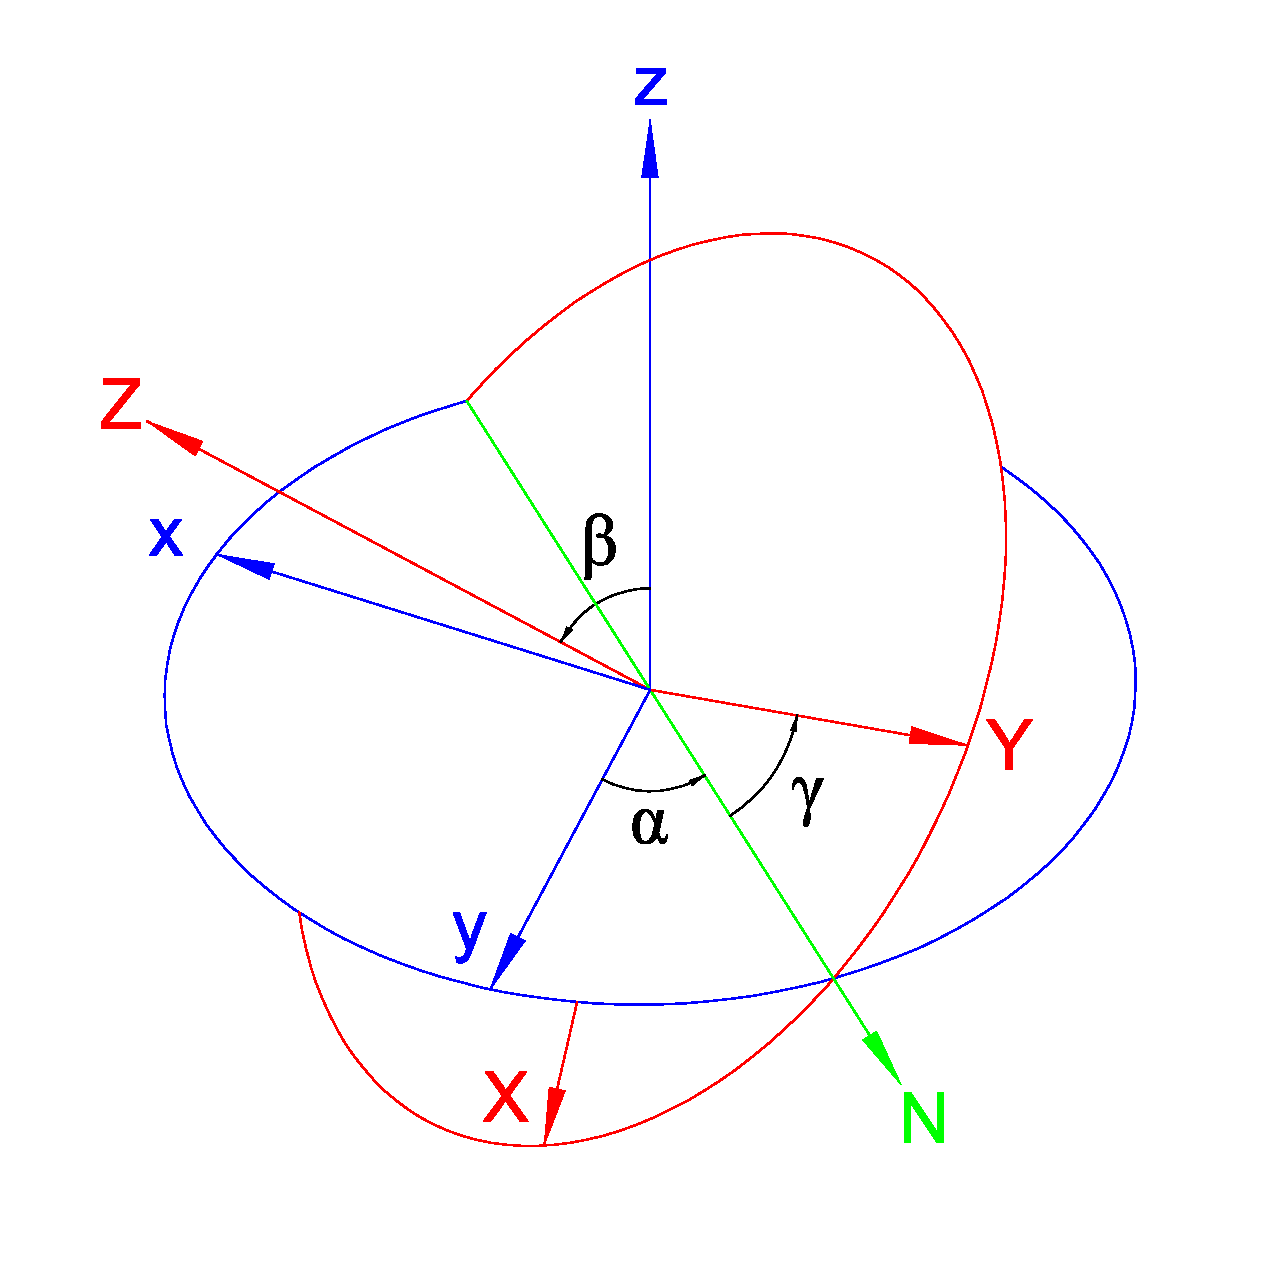
\includegraphics[width=7cm]{fig/ch13-eulerangleY.eps}
        \caption{欧拉角:临时轴$N$是$y$轴} \label{chlg:fig_euler}
    \end{minipage}
    \begin{minipage}[t]{0.49\textwidth}
        \centering
        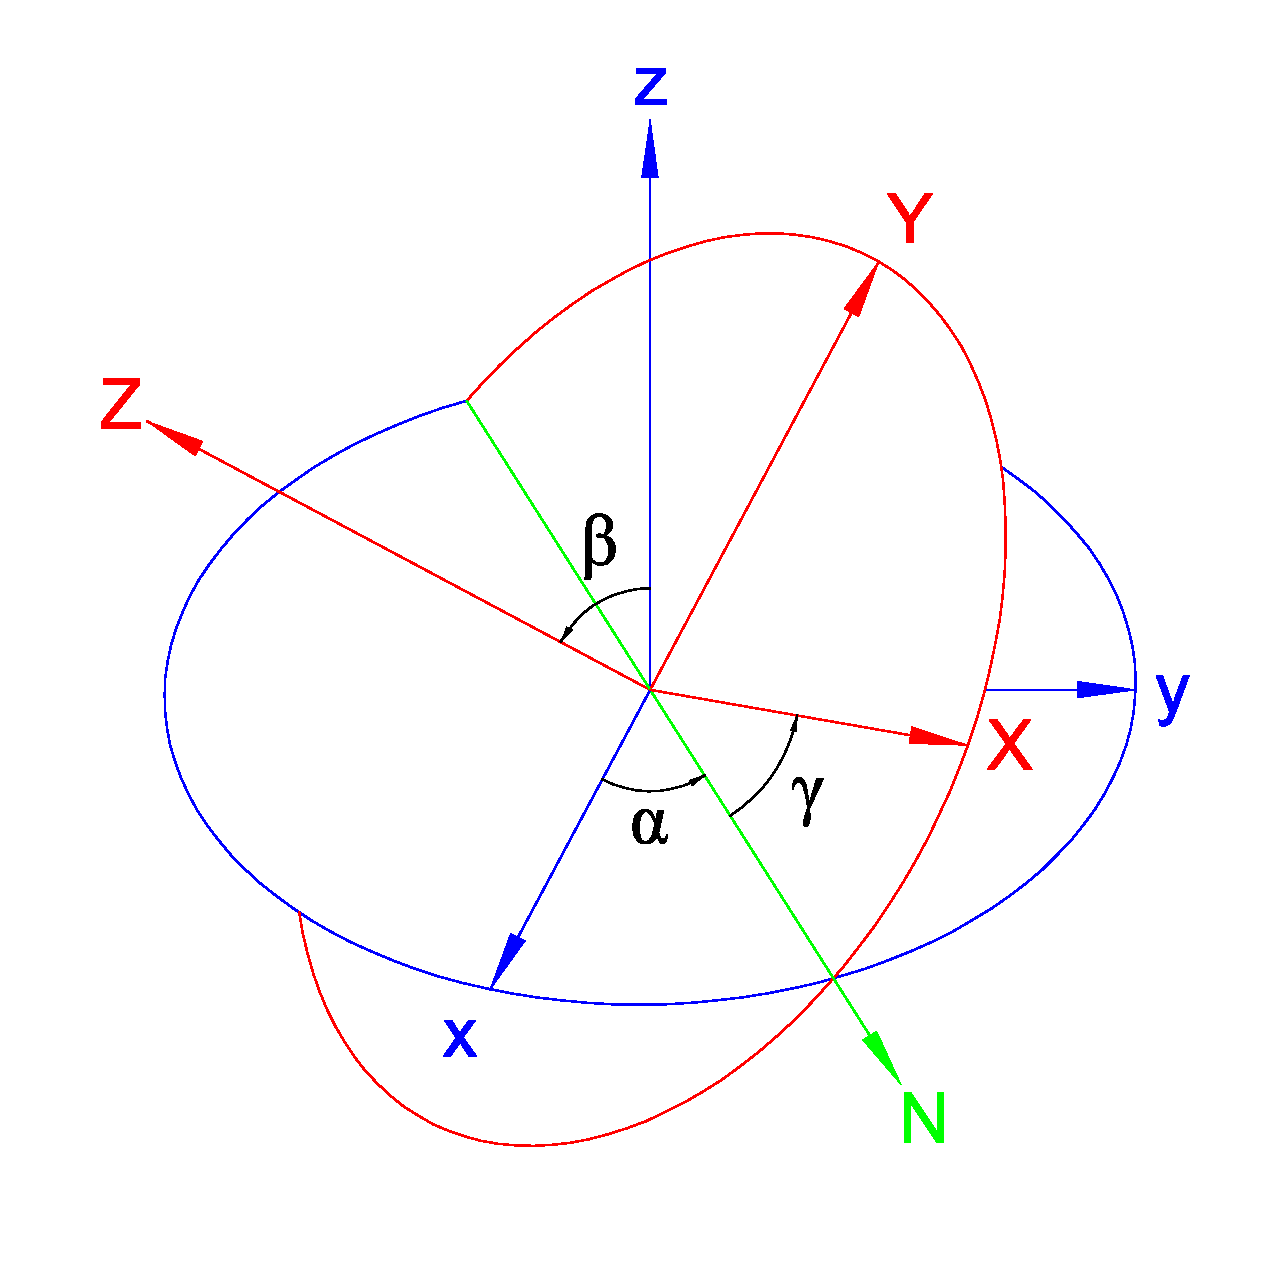
\includegraphics[width=7cm]{fig/ch13-eulerangleX.eps}
        \caption{欧拉角:临时轴$N$是$x$轴} \label{chlg:fig_euler2}
    \end{minipage}
\end{figure}


我们可以借用$\mathbb{R}^3$中常用的欧拉角$\alpha,\beta,\gamma$描述转动$R$.
图\ref{chlg:fig_euler}蓝色标小写字母$xyz$的坐标轴为
未转动的,红色标大写字母$XYZ$的坐标轴为
转动后最终位置,绿色标字母$N$的轴为中间步骤.
我们用$C_k(\psi)$表示绕$k$轴旋转$\psi$角.
第一步是进动,绕$z$轴转动$\alpha$角,即$C_z(\alpha)$,
转动后,$y$轴就转到了$N$轴位置,$z$轴不动.
第二步是章动{\footnote{章动英文是nutation,本意点头.地球除了进动(岁差),
        还有章动,周期大约18.6年.中国《周髀算经》中记载十九为一“章”,
        这就是此词翻译的由来($18.6\approx 19$).地球章动和天文观测光行差
        皆由英国人James Bradley(1693-1762)发现.}},
    绕$N$轴转动$\beta$角,即$C_N(\beta)$,
蓝色小写$z$轴转到了红色大写$Z$轴位置;蓝色的小写$xy$平面也
旋转到了红色大写$XY$平面.
第三步是自转,绕红色大写$Z$轴转动$\gamma$角,即$C_Z(\gamma)$,
此时就得到了坐标轴最终位置.我们将这三次转动记为
\begin{equation}\label{chlg:eqn_rotation}
    R(\alpha\beta\gamma)=C_Z(\gamma)C_N(\beta)C_z(\alpha) .
\end{equation}
注意转动的乘积顺序不能随意改变.%但这个表示不是很方便,需要进行化简.
我们注意到
\begin{align}
    C_N(\beta) &=C_z(\alpha)C_y(\beta)C_z(-\alpha) , \label{chlg:eqn_N_rotation} \\
    C_Z(\gamma)&=C_z(\alpha)C_y(\beta)C_z(\gamma)C_y(-\beta)C_z(-\alpha) . \label{chlg:eqn_Z_rotation}
\end{align}
代入上面的转动矩阵后,就得到了式\eqref{chlg:eqn_rotation}的欧拉角表示
\begin{small}
\setlength{\mathindent}{0em}
\begin{equation}\label{chlg:eqn_rotation_euler_y}
    \begin{aligned}
        &R(\alpha\beta\gamma)=C_z(\alpha)C_{\color{red}{y}}(\beta)C_z(\gamma) =   \\
        &\begin{pmatrix}
            \cos\alpha\cos\beta\cos\gamma -\sin\alpha \sin\gamma  &  -\cos\alpha \cos\beta \sin\gamma -\sin\alpha \cos\gamma & \cos\alpha \sin\beta  \\
            \sin\alpha\cos\beta\cos\gamma +\cos\alpha \sin\gamma  &  -\sin\alpha \cos\beta \sin\gamma +\cos\alpha \cos\gamma & \sin\alpha \sin\beta  \\
            -\sin\beta \cos\gamma & \sin\beta \sin\gamma & \cos\beta
        \end{pmatrix} .
    \end{aligned}
\end{equation}\setlength{\mathindent}{2em}
\end{small}
上面已经用到了绕坐标轴的旋转
\begin{equation}\label{chlg:eqn_rotation-zy}
    {C_z}( \alpha  ) =  \begin{pmatrix}
        {\cos \alpha }&{ - \sin \alpha }&0 \\
        {\sin \alpha }&{\cos \alpha }&0 \\
        0&0&1
    \end{pmatrix} ,\
    {C_y}( \beta ) = \begin{pmatrix}
        {\cos \beta }&0&{  \sin \beta }  \\
        0&1&0\\
        { - \sin \beta } &0&{\cos \beta }
    \end{pmatrix}  .
\end{equation}
图\ref{chlg:fig_euler}中临时轴$N$是$y$轴.
可将$N$选为$x$轴(图\ref{chlg:fig_euler2}),
此时式\eqref{chlg:eqn_rotation}为
\begin{small}
\setlength{\mathindent}{0em}
\begin{equation}\label{chlg:eqn_rotation_euler_x}
    \begin{aligned}
        &R(\alpha\beta\gamma)=C_z(\alpha)C_{\color{red}{x}}(\beta)C_z(\gamma) =   \\
        &\begin{pmatrix}
            \cos\alpha \cos\gamma-\sin\alpha \cos\beta \sin\gamma  & -\sin\alpha \cos\beta \cos\gamma -\cos\alpha \sin\gamma &  \sin\alpha \sin\beta \\
            \sin\alpha \cos\gamma+\cos\alpha \cos\beta \sin\gamma  &  \cos\alpha \cos\beta \cos\gamma -\sin\alpha \sin\gamma & -\cos\alpha \sin\beta \\
            \sin\beta  \sin\gamma & \sin\beta \cos\gamma  & \cos\beta
        \end{pmatrix} .
    \end{aligned}
\end{equation}\setlength{\mathindent}{2em}
\end{small}
其中
\begin{equation}\label{chlg:eqn_rotation-x}
    {C_x}( \beta  ) = \begin{pmatrix}
        1&0&0 \\
        0&{\cos \beta }&{ - \sin \beta } \\
        0&{\sin \beta }&{\cos \beta } \\
    \end{pmatrix} .
\end{equation}
两者没有本质差别.两种变换方法中,
欧拉角的取值范围是:$0 \leqslant \alpha, \gamma < 2\pi,\ 0\leqslant \beta \leqslant \pi$.
用欧拉角表示转动时,当$\beta=0$时,只要$\alpha+\gamma$的值相等就代表同一转动,有无穷多种表示;
同理,当$\beta=\pi$时,只要$\alpha-\gamma$的值相等就代表同一转动,有无穷多种表示;
这是需要注意的.这正反映了二维闭球面不能用一个坐标域覆盖的事实,即至少
需要两个坐标域才能覆盖二维球面流形.


式\eqref{chlg:eqn_rotation_euler_y}或式\eqref{chlg:eqn_rotation_euler_x}需
右作用在基矢量$\{\boldsymbol{e}_1,\boldsymbol{e}_2,\boldsymbol{e}_3\}$(行)上;
或者左作用在某矢量的具体分量$(x,y,z)^T$(列)上;不能反过来.

我们把$\mathfrak{so}(3)$李代数放到\S\ref{chlar:sec_LA-su2so3},与$\mathfrak{su}(2)$一起讨论.

\index[physwords]{广义正交群}  \index[physwords]{SO(p,q)}

\subsubsection{广义正交群}\label{chlg:sec_Opq}
在实数域$\mathbb{R}$中,取式\eqref{chlg:eqn_gsinit}中的$S$为
(按照物理习惯,作替换$S\to \eta$)
\begin{equation}\label{chlg:eqn_generalized-Lorentz-metric}
    \eta = \begin{pmatrix}
        -I_p & 0 \\  0 & I_q
    \end{pmatrix},
    \quad I_p,I_q \  \text{是单位矩阵};\
    p+q=m,\ 0\leqslant p,q\leqslant m .
\end{equation}
那么
\begin{equation}\label{chlg:eqn_gLorentz}
    O(p,q)=G(\eta)= \left\{ A \in GL(m,\mathbb{R})\ |\ A \eta {A}^T =\eta \right\},
\end{equation}
称为$(p,q)$型{\heiti 广义正交群}(Generalized orthogonal group);
当$p=1,q=3$时,就是通常的Lorentz群(见\S\ref{chlg:sec_Lorentz-group}).
不难发现$O(p,q)\cong O(q,p)$,两者只差一个相似变换.
有关系$O(m)\equiv O(0,m)$.
由式\eqref{chlg:eqn_gs}得它的李代数是
\begin{equation}\label{chlg:eqn_LA-opq}
    \mathfrak{o}(p,q)= \left\{ X \in 
    \mathfrak{gl}(m,\mathbb{R})\ |\  X\eta + \eta {X}^T =0 \right\}.
\end{equation}
通过上式可知它的维数是
\begin{equation}
    {\rm dim} \mathfrak{o}(p,q) = {\rm dim} O(p,q) = 
    \frac{1}{2}m(m-1)=\frac{1}{2}(p+q)(p+q-1).
\end{equation}

由式\eqref{chlg:eqn_gLorentz}可得广义正交矩阵行列式:
$ \det A \cdot\det\eta\cdot \det A^T = \det \eta \ \Rightarrow \ \det A = \pm 1$;
这也就注定了$O(p,q)$不是连通的.行列式为1的分支是
\begin{equation}\label{chlg:eqn_LG-sopq}
    SO(p,q)= \left\{ A \in GL(m,\mathbb{R})\ |\ A \eta {A}^T =\eta 
    \ \text{且}\ \det A = 1 \right\} .
\end{equation}
正交群$O(m)$有两个连通分支,而$O(p,q)$群有四个连通分支.将其记为
\begin{equation}
    g=\begin{pmatrix}
        a_T & b \\ c & a_S
    \end{pmatrix},
    \qquad \forall g\in O(p,q) ,\quad 0 < p < m.
\end{equation}
其中类时部分的$a_T$是$p\times p$的矩阵,类空部分的$a_S$是$q\times q$的矩阵.


可以用反证法证明它们的行列式都是非奇异的,即$|a_T| \neq 0$、$|a_S| \neq 0$.
假设行列式$|a_T| = 0$,则存在非零的$p$维列矢量$s$使得$a_T s =0$.
设$r=\binom{s}{0}$,则$gr=\binom{0}{cs}$.
首先,有$(gr)^T \eta gr = r^T (g^T \eta g) r = r^T \eta r = - s^T s <0 $;
其次,有$(gr)^T \eta gr = (0 \  cs) \eta \binom{0}{cs} = (cs)^T (cs)\geqslant 0$.
产生矛盾,故必有$|a_T| \neq 0$.类似可证$|a_S| \neq 0$.

对于$0 < p < m$的广义正交群可以分成四片,见表\ref{chlg:tab-GO}.

\begin{table}[htb]
    \centering
    \caption{$O(p,q)$群的分类记号} \label{chlg:tab-GO}
    \begin{tabular}{|*{4}{c|}}
        \hline 
        $| a_T| >0,\ | a_S |>0$ & $ |a_T| >0,\ | a_S |<0$ & $| a_T| <0,\ | a_S| >0$  & $| a_T| <0,\ | a_S| <0$ \\
        \hline
        $O^{++}(p,q)$ & $O^{+-}(p,q)$ & $O^{-+}(p,q)$ & $O^{--}(p,q)$   \\ 
        \hline
    \end{tabular}
\end{table}

不难发现:$SO(p,q)= O^{++}(p,q)\cup O^{--}(p,q)$.记$O^{++}(p,q)$为$SO^{+}(p,q)$.

当$0<p<m$时,$O(p,q)$及$SO^{+}(p,q)$是\uwave{非紧致的};这与正交群不同.

\index[physwords]{酉群}  \index[physwords]{SO$^{+}$(p,q)}  \index[physwords]{O$^{++}$(p,q)}

\subsubsection{酉群}\label{chlg:sec_unitary}

本节在在复数域$\mathbb{C}$中讨论问题.
此时,需要把式\eqref{chlg:eqn_gsinit}、\eqref{chlg:eqn_gs}中的一个矩阵换成
复共轭,即
\begin{align}
    G(S)=& \left\{ A \in GL(m,\mathbb{C})\ |\  A S \bar{A}^T =S \right\};\label{chlg:eqn_gsinit-cx} \\
    \mathfrak{g}(s) =& \left\{ X \in \mathfrak{gl}(m,\mathbb{C}) \ |\ 
    X S + S \bar{X}^T = 0 \right\} . \label{chlg:eqn_gs-cx}
\end{align}
请读者仿照本节开头论述一下上述构造仍是李群及其李代数.

取式\eqref{chlg:eqn_gsinit-cx}中的$S$为单位矩阵,那么
\begin{equation}\label{chlg:eqn_unitary}
    U(m)=G(S)= \left\{ A \in GL(m,\mathbb{C})\ |\ A \bar{A}^T =I \right\},
\end{equation}
称为{\heiti 酉群},也称为{\heiti 幺正群}
\footnote{Unitary group可以音译成 {\kaishu 酉群},常见于数学领域;
    也可以被意译成{\kaishu 幺正群},常见于物理领域.};
满足上式的复矩阵称为{\heiti 酉矩阵}或{\heiti 幺正矩阵}.
由式\eqref{chlg:eqn_gs-cx}得它的李代数是
\begin{equation}
    \mathfrak{u}(m)= \left\{ X \in 
    \mathfrak{gl}(m,\mathbb{C})\ |\ X  + \bar{X}^T =0 \right\}.
\end{equation}
通过上式可知$\mathfrak{u}(m)$的\uwave{实维数}是:$m^2$.
故酉群的李代数是由反厄米复矩阵组成.

可以证明$U(m)$群是紧致、连通的,故有$\exp \mathfrak{u}(m)= U(m)$.

设有幺正矩阵$U$,那么必然有$\bar{U}^T U = I$,两边取行列式,得
\begin{equation}
    1 = \det\bar{U}\cdot \det U =\overline{\det U} \cdot \det U
    \quad \Rightarrow \quad  \det U = e^{\mathbbm{i} \phi}, \ \phi\in \mathbb{R} .
\end{equation}
上式说明酉矩阵的行列式是模为一的复数,复角$\phi$无法确定,它处于复平面的单位圆周上.
如果进一步要求酉群元素的行列式为$+1$(复角$\phi=0$),那么可得{\heiti 特殊酉群},
\begin{equation}
    SU(m)= %U(m)\cap SL(m,\mathbb{C}) =
    \left\{ A \in GL(m,\mathbb{C})\ |\ A \bar{A}^T =I \ \text{且} \  \det A=1 \right\}.
\end{equation}
特殊酉群的李代数是零迹反厄米复矩阵
\begin{equation}\label{chlg:eqn_LA-su}
    \mathfrak{su}(m) %= \mathfrak{u}(m)\cap \mathfrak{sl}(m,\mathbb{C}) 
    =\left\{X\in\mathfrak{gl}(m,\mathbb{C})\ |\ X+\bar{X}^T=0
    \ \text{且} \  {\rm Tr} X =0 \right\} .
\end{equation}
$\mathfrak{su}(m)$的\uwave{实维数}是:$m^2-1$.


可以证明$SU(m)$是紧致、单连通的李群,
故有$\exp \mathfrak{su}(m) = SU(m)$.

\index[physwords]{U(1)群}

\paragraph{$U(1)$群}
此时式\eqref{chlg:eqn_unitary}中的矩阵$A$是一维的,
可设$[A]=a+\mathbbm{i} b$(其中$a,b\in \mathbb{R}$),
那么有$a^2+b^2=1$;由此可见$U(1)$与$SO(2)$群同构.
很明显,$U(1)$还能表示成指数形式:
$U(1)=\exp (\mathbbm{i}\theta),\ \theta\in \mathbb{R}$.
$U(1)$是连通的,但不是单连通的.

$SU(1)$不是连续群,是单点集($(1,0)$),平庸无奇.

%在\S\ref{chlar:sec_SU2SO3}将具体讲解$SU(2)$群.

%$U(1)$是一维李群,容易求得一维反厄米矩阵是由虚数单位“$\mathbbm{i}$”构成的线性空间;

\index[physwords]{辛群}

\subsubsection{辛群}
在数域$\mathbb{F}$中,取式\eqref{chlg:eqn_gsinit}中的$S$为反对称矩阵
\begin{equation}
    J = \begin{pmatrix}
            0 & I_m \\ -I_m & 0
        \end{pmatrix},
\end{equation}
那么
\begin{equation}
    Sp(m,\mathbb{F})=G(J)= \left\{ A \in GL(2m,\mathbb{F})\ |\ A J {A}^T =J \right\},
\end{equation}
称为{\heiti 辛群}(Sympletic group),
$Sp(m,\mathbb{F})$中的元素称为{\heiti 辛矩阵}.
它的李代数是
\begin{equation}
    \mathfrak{sp}(m,\mathbb{F})= \left\{ X \in 
    \mathfrak{gl}(2m,\mathbb{F})\ |\ X J + J {X}^T =0 \right\}.
\end{equation}
由上式可得复辛群的\uwave{实维数}是 $2(2m^2+m)$,实辛群维数是 $2m^2+m$.

%$Sp(m,\mathbb{F})$是连通的(点集拓扑);非紧致的.代数拓扑连通属性是:复辛群是单连通,实辛群是$\infty$度连通.



\begin{table}[htb]
    \centering
    \caption{常用矩阵李群} \label{chlg:tab_groups}
    \begin{tabular}{|*6{c|}}
        \hline
        李群 &矩阵 & 实维数 &连通性  & 紧致性 & 李群李代数   \\        \hline
        $GL(m,\mathbb{R})$ & $m$维可逆实矩阵 & $m^2$  & \makecell{非连通\\非单连通 }
        & 非紧 & \makecell{$m$维任意\\ 实矩阵}   \\ \hline
        $GL(m,\mathbb{C})$& $m$维可逆复矩阵 & $2 m^2$ & \makecell{连通 \\非单连通 }
        & 非紧 & \makecell{$m$维任意\\ 复矩阵}  \\ \hline
        $SL(m,\mathbb{R})$ & \makecell{行列式为$1$的\\$m$维可逆实矩阵} & $m^2-1$  &  \makecell{连通 \\ 非单连通 } 
        & 非紧 & \makecell{$m$维无迹\\ 实矩阵}  \\ \hline
        $SL(m,\mathbb{C})$ & \makecell{行列式为$1$的\\$m$维可逆复矩阵} & $2m^2-2$ & \makecell{连通\\单连通 }
        & 非紧 & \makecell{$m$维无迹\\ 复矩阵}  \\ \hline
        $O(m)$  & $m$维正交实矩阵 & $\dfrac{m(m-1)}{2}$  & \makecell{非连通\\非单连通 } 
        & 紧致 & \makecell{$m$维反对\\ 称实矩阵} \\ \hline
        $SO(m)$ & \makecell{行列式为$1$的\\$m$维正交实矩阵} &$\dfrac{m(m-1)}{2}$ & \makecell{连通\\2度连通 }
        & 紧致 & \makecell{$m$维反对\\ 称实矩阵}  \\ \hline
        $SO^{+}(1,3)$ & \makecell{$4$维实矩阵$\Lambda$\\且$\eta=\Lambda^T \eta \Lambda$} & $6$ & \makecell{连通\\2度连通 }
        & 非紧 & \makecell{$4$维实矩阵$A$\\$A^T=- \eta A \eta $} \\ \hline
        $U(m)$ & $m$维幺正矩阵 & $m^2$ & \makecell{连通 \\$\infty$度连通 }
        & 紧致 &  \makecell{$m$维反厄\\ 米复矩阵} \\ \hline
        $SU(m)$ & \makecell{行列式为$1$的\\$m$维幺正矩阵} & $m^2-1$ & \makecell{连通\\单连通 }
        & 紧致 & \makecell{$m$维反厄米\\无迹复矩阵} \\ \hline
    \end{tabular}
\end{table}

{\kaishu 表\ref{chlg:tab_groups}中“连通性”一栏,上面是点集拓扑的连通属性;
下面是代数拓扑的属性(单连通或复连通).表中“维数”是指实数域上李群的维数.}



\subsection{古典李群、李代数}\label{chlg:sec_clg}
\index[physwords]{古典李群}  \index[physwords]{古典李代数}

记$A_m$为$SL(m+1,\mathbb{C})$.记$C_m$为$Sp(m,\mathbb{C})$.

在复数域$\mathbb{C}$中,取式\eqref{chlg:eqn_gsinit}中的$S$为单位矩阵$I$,则
\begin{equation*}
    O(m,\mathbb{C}) = \left\{ A \in GL(m,\mathbb{C})\ |\ A A^T =I \right\};
    \quad SO(m,\mathbb{C}) = O(m,\mathbb{C}) \cap SL(m,\mathbb{C}).
\end{equation*}
记$B_m$为$SO(2m+1,\mathbb{C})$.记$D_m$为$SO(2m,\mathbb{C})$.

$A_m$、$B_m$、$C_m$、$D_m$称为{\heiti 古典李群},其李代数称为{\heiti 古典李代数}.

复数域上的正交群$O(m,\mathbb{C})$在物理学上几乎无用,同时我们不省略复数域$\mathbb{C}$的标记.
本书中,所有的$O(m)$均指$O(m,\mathbb{R})$,即省略实数域$\mathbb{R}$的标记.

%\begin{proposition}
%    {\bfseries (1)}:$\bigl( \mathfrak{so}(m,\mathbb{R})\bigr)^{\mathbb{C}}=\mathfrak{so}(m,\mathbb{C})$.    
%    {\bfseries (2)}:$\bigl( \mathfrak{sl}(m,\mathbb{R})\bigr)^{\mathbb{C}}=\mathfrak{sl}(m,\mathbb{C})$.    
%    {\bfseries (3)}:$\bigl( \mathfrak{sp}(m,\mathbb{R})\bigr)^{\mathbb{C}}=\mathfrak{sp}(m,\mathbb{C})$.    
%    {\bfseries (4)}:$\mathfrak{su}(m,\mathbb{C})$是$\mathfrak{sl}(m,\mathbb{C})$的实形式.
%\end{proposition}
%\begin{proof}
%    前三条几乎一望而知.下面证明第(4)条,需要提醒一下,$\mathfrak{su}(m)$本来就定义在
%    复数域上,没有$\mathfrak{su}(m,\mathbb{R})$.
%\end{proof}

\begin{theorem}\label{chlg:thm_CLA-simple}
    古典李代数$A_m(m\geqslant 1)$、$B_m(m\geqslant 1)$、$C_m(m\geqslant 1)$、$D_m(m\geqslant 3)$是
    单纯李代数.(证明见\parencite[p.148]{huangxg-2024}定理6,或\parencite[\S 1.3]{wanzx-2013}定理1.2)
\end{theorem}







\section{物理中常用等距李群}\label{chlg:sec_matrixG-II}
继\S\ref{chlg:sec_isometry},本节再描述一些保度规群\cite{tung-1985},有些群会涉及流形局部坐标.


\subsection{等距映射补遗}\label{chlg:sec_iso-add}
在\S \ref{chrg:sec_isometry}我们已初步讨论了等距映射(Isometry),
等距定义自然仍为\ref{chrg:def_isometry-immersion};我们从群论角度再次讨论这个问题.

\index[physwords]{等距群}
\index[physwords]{I(M)|see{等距群}}

对于光滑广义黎曼流形$M$,所有从$M$到$M$的等距映射集合$I(M)$,在把
复合映射当成群乘法的情形下构成一个群,称为$M$的{\heiti 等距群}.
验证$I(M)$是群的工作留给读者(极易).粗略地说,$I(M)$越大,$M$越简单.
有的$M$除了恒等映射之外可能没有等距映射,称为平凡情形;
但是许多流形有足够大的等距群,因此可以应用李群知识.
在非平凡情况下,$I(M)$是$M$的几何不变量,它的重要性几乎可以和曲率、测地线比拟.

由于$M$的每个切空间与$\mathbb{R}^n_\nu$是(局部)等距同胚的,
因此等距群$I(\mathbb{R}^n_\nu)$在广义黎曼几何中具有基本意义.
%特别是,对于具有不定度规的流形,它导致了类似于普通可定向性的时间和空间可定向性的孪生概念.

\begin{theorem}\label{chlg:thm_isoexp}
    设在广义黎曼流形$(M,g)$、$(N,h)$间存在局部等距同构映射$\phi:M\to N$.
    则$\forall p\in M$,交换图\ref{chlg:pic_exp-exchange}成立;
    其中$U_p\subset T_pM$,$V_{\phi(p)}\subset T_{\phi(p)}N$分别
    是$\exp_p$和$\exp_{\phi(p)}$的法邻域(指数映射的像集,见\S\ref{chgd:sec_exp}).
\end{theorem}

\begin{figure}[htb]
    \centering
    \begin{tikzpicture}[scale=5]
        \draw[thick] [-latex] (0,0)node[left]{$U_p$}--(0.5,0)node[below]{$\phi_*$}   --(1,0) node[right] {$V_{\phi(p)} $};
        \draw[thick] [-latex] (-0.05,-0.05) -- (-0.05,-0.2)node[left] {$\exp_p$}   --(-0.05,-0.4)node[below ] {$M$};
        \draw[thick] [-latex] (1.05,-0.05) -- (1.05,-0.2)node[right]{$\exp_{\phi(p)}$}   --(1.05,-0.4)node[below ] {$N$};
        \draw[thick] [-latex] (0,-0.55)--(0.5,-0.55)node[above]{$\phi$} --(1,-0.55) ;
    \end{tikzpicture}
    \caption{等距——指数映射交换图}\label{chlg:pic_exp-exchange}
\end{figure}

\begin{proof}
    设$\gamma(t)$是$M$中测地线,且$p=\gamma(0)$;由定理\ref{chrg:thm_geodesic-MN}可知
    映射$\phi\circ\gamma(t)$是$N$中测地线.
    $\forall v\in U_p$,与之对应$\phi_* v \in V_{\phi(p)}$;两条测地线诱导的指数映射分别是:
    $\exp_p(t v)=\gamma(t;p,v)$和
    $\exp_{\phi(p)}(t\, \phi_*v)=\phi\circ\gamma\bigl(t;\phi(p),\phi_* v\bigr)$.
    由定理\ref{chrg:thm_geodesic-MN}有
    \begin{equation}\label{chlg:eqn_isoexp}
        \phi \bigl(\exp_p(t v)\bigr) = \exp_{\phi(p)}(t\, \phi_* v ) .
    \end{equation}
    这正是本定理需要证明的,即交换图\ref{chlg:pic_exp-exchange}.
\end{proof}

%\parencite{oneill1983}定理3.62
\begin{proposition}\label{chlg:thm_isopall}
    设有两个连通广义黎曼流形$M$、$N$,存在局部等距同构映射$\phi,\psi:M\to N$.
    若存在一个点$p\in M$使得$\phi(p)=\psi(p)$和$\phi_{p*} = \psi_{p*}$成立,
    则有$\phi=\psi$.
\end{proposition}
\begin{proof}
    令$A=\{ q\in M \ | \  \phi_{q*} = \psi_{q*}\}$.因$p\in A$,故$A$不是空集;
    又因映射的连续性可知$A$不只包含$p$点.    $\forall q\in A$,
    自然存在$q$的法邻域$U\subset M$;
    那么$\forall r\in U$一定存在$v\in T_q M$使得$r=\gamma_v(1)=\exp_q(v)$成立;
    则(要用式\eqref{chlg:eqn_isoexp})
    \begin{equation}
        \phi(r) = \phi \bigl(\gamma_v(1)\bigr)= \gamma_{\phi_*(v)} (1)
        = \gamma_{\psi_*(v)} (1) =\psi \bigl(\gamma_v(1)\bigr) =\psi(r).
    \end{equation}
    故在开集$U$上$\phi=\psi$;
    因此$\forall r\in U$,都有$\phi_{r*} = \psi_{r*}$;从而$U\subset A$;
    这说明$A$是$M$中的开集.如果$A$不能覆盖整个$M$,那么
    另取$w\in A$且$w\neq p$,以$w$为原点再次运用指数映射方式将$A$延拓,
    直至能够覆盖流形$M$.
\end{proof}

\begin{example}\label{chlg:exam_DQpsi}
    标量函数场变换规则.
\end{example}      
我们以量子物理中的波函数为例来说明标量函数场在对称操作下的变换规则.
考虑量子物理中一个态矢量$|\psi\rangle$,在位型空间表象中态函数
是$\psi(\boldsymbol{r}) = \langle \boldsymbol{r}|\psi\rangle$.
用$Q$表示某种对称作用,它会把态函数作整体变换;
变换后在新的位置$\boldsymbol{r}'=Q \boldsymbol{r}$的态函数与老位置的态函数是
相等的,这是对称变换的要求;用公式表示为
\begin{equation}
    \psi(\boldsymbol{r}) = \psi'(\boldsymbol{r}')
\end{equation}
我们将新旧位置关系($\boldsymbol{r}'=Q \boldsymbol{r}$)带入上式,有
\begin{equation}
    \psi(\boldsymbol{r}) = \psi'(Q \boldsymbol{r}) \quad \Leftrightarrow \quad
    \psi(Q^{-1}\boldsymbol{r}) = \psi'(\boldsymbol{r}) .
\end{equation}
在对称变换$Q$的作用下,新的态矢量$\psi'$可用一个函数变换算符来表示,即
\begin{equation}\label{chlg:eqn_psip2psi}
    \psi'(\boldsymbol{r}) \overset{def}{=}\hat{D}(Q)\psi(\boldsymbol{r}).
    \qquad \text{等号两边的宗量$\boldsymbol{r}$是相同的}
\end{equation}
那么便有
\begin{equation}\label{chlg:eqn_DQpsi}
    \psi(Q^{-1}\boldsymbol{r})  = \psi'(\boldsymbol{r}) \equiv \hat{D}(Q)\psi(\boldsymbol{r}) .
\end{equation}
上式便是态矢量在对称变换下的变化关系式.    \qed


\index[physwords]{平移群}

\subsection{平移群}\label{chlg:sec_translation-group}
在$\mathbb{R}^m$中,{\heiti 平移}(translation)是一种几何变换,
它将图形、形状或空间的每个点在给定方向上移动相同的距离.
平移也可以解释为向每个点添加一个常量矢量,或移动坐标系的原点.
用坐标语言来说,便是:
\begin{equation}\label{chlg:eqn_translation}
    x\to x' : x'^{i} = x^i + a^i 
    \quad \Leftrightarrow \quad
    \boldsymbol{x}' =\hat{Q}(\boldsymbol{x})= \boldsymbol{x} + \boldsymbol{a} ;
    \qquad 1 \leqslant i \leqslant m .
\end{equation}
其中$x^i$是旧坐标,$x'^i$是新坐标,$a^i$是常数.
需要强调一点:算符$\hat{Q}$不是线性算符,
例如$\hat{Q} (2 \boldsymbol{x}) =2 \boldsymbol{x} + \boldsymbol{a} \neq 
2\bigl(\hat{Q}(\boldsymbol{x})\bigr)=2 \boldsymbol{x} + 2\boldsymbol{a}$.

仅有平移的坐标表示是不够的,假设存在用坐标$\{x^i\}$描述的
标量函数$f(\boldsymbol{x})$,我们要求$f(\boldsymbol{x})$在平移操作下不变;
参考式\eqref{chlg:eqn_DQpsi},用$\hat{T}(m)$表示作用在$f$上的算符,有
\begin{equation}\label{chlg:eqn_translationONf}
    f'(\boldsymbol{x})=\hat{T}(m) f(\boldsymbol{x})= f(\hat{Q}^{-1}\boldsymbol{x}) = f(\boldsymbol{x} - \boldsymbol{a}) .
\end{equation}


自然把群乘法取成连续进行两次“坐标加法”,
即$\boldsymbol{x}$加上$\boldsymbol{b}$,再加上$\boldsymbol{a}$;
对于$\hat{T}(m)$来说便是复合映射,即群乘法是
\begin{equation*}
    \hat{T}(m)_{\boldsymbol{a}}\circ \hat{T}(m)_{\boldsymbol{b}}\ f(\boldsymbol{x}) 
    = \hat{T}(m)_{\boldsymbol{a}}\ f(\boldsymbol{x} - \boldsymbol{b}) 
    = f(\boldsymbol{x} - \boldsymbol{b} - \boldsymbol{a}) 
    = \hat{T}(m)_{\boldsymbol{b}+ \boldsymbol{a}}\ f(\boldsymbol{x}) .
\end{equation*}
容易验证上式操作构成群:
首先,此操作具有封闭性;其次,加法具有结合性;
第三,当$\boldsymbol{a}=0$时,操作\eqref{chlg:eqn_translationONf}是恒等映射,可看作单位元;
最后,参量是$-\boldsymbol{a}$和$+\boldsymbol{a}$的操作互逆.
由于加法具有交换性(即群乘法具有交换性),故此群是可对易群(阿贝尔群);
我们称之为{\heiti 平移群}.
由于$\mathbb{R}^m$本身就是光滑流形,再加上“群乘法”和“求逆”运算是$C^\infty$的
(加法和取负号操作当然是$C^\infty$的),故\uwave{平移群是李群}.

平移群适用于各种度规场,但我们只考虑正定度规以及闵氏度规.

由于李群是可微的,我们将式\eqref{chlg:eqn_translationONf}展开,有
\begin{equation*}
    \hat{T}(m) f(\boldsymbol{x}) = f(\boldsymbol{x} - \boldsymbol{a}) 
    = f(\boldsymbol{x}) + (-a^i) \frac{\partial f(\boldsymbol{x})}{\partial x^i}
    +\frac{1}{2!} (-a^i)(-a^j) \frac{\partial^2 f(\boldsymbol{x})}{\partial x^i \partial x^j}
    +\cdots 
\end{equation*}
上式说明,平移算符可以表示成
\begin{equation}\label{chlg:eqn_Texp}
    \hat{T}(m) \equiv \exp\left( -a^j \frac{\partial }{\partial x^j} \right) 
    \equiv\exp\left(-\mathbbm{i} a^j \hat{P}_j  \right) , \qquad
    \hat{P}_j\overset{def}{=} -\mathbbm{i}\frac{\partial }{\partial x^j} .
\end{equation}
上式中顺便给出了平移$\hat{P}_j$的定义;
并且把平移算符形式地表示成指数形式.
由于两个不同坐标的偏导数是可交换的,所以不难看出式\eqref{chlg:eqn_Texp}中的
平移算符仍是阿贝尔群.
上面给出的平移算符是微分形式的,在式\eqref{chlg:eqn_Trans-Momen}中给出了平移李代数
的矩阵形式.

虽然算符$\hat{Q}$不是线性算符,但平移算符$\hat{T}(m)$是线性的,例如
\begin{equation*}
    \hat{T}(m) \bigl(2f(\boldsymbol{x})\bigr) 
    =2\left( f(\boldsymbol{x}) - a^i \frac{\partial f(\boldsymbol{x})}{\partial x^i}
    +\frac{1}{2!} a^i a^j \frac{\partial^2 f(\boldsymbol{x})}{\partial x^i \partial x^j}
    +\cdots \right) = 2 f(\boldsymbol{x}) .
\end{equation*}

平移群是连通、单连通、非紧致李群.

\begin{example}\label{chlg:exam_pm2}
    号差为$-2$的Lorentz度规下的平移算符.
\end{example}
号差为$+2$的Lorentz度规下动量算符定义成$\hat{P}_\mu =- \mathbbm{i}\frac{\partial }{\partial x^\mu}$
(见式\eqref{chlg:eqn_Texp}),有一个负号;同时非时间部分$\hat{P}_j =\hat{P}^j$(即$j=1,2,3$),
时间部分$\hat{P}_0 =-\hat{P}^0$.

不论何种号差,逆变矢量的形式是一样的;故不论号差,动量算符的逆变形式为:
$\hat{P}^\mu=\mathbbm{i}\{\frac{\partial}{\partial t}, -\frac{\partial}{\partial x},
-\frac{\partial}{\partial y},-\frac{\partial}{\partial z}\}$.
由此可知号差为$-2$的Lorentz度规下动量算符是:
$\hat{P}^\mu = \mathbbm{i}\frac{\partial }{\partial x_\mu}$以及
$\hat{P}_\mu = \mathbbm{i}\frac{\partial }{\partial x^\mu}$.

除此以外,在不同号差下,两个矢量的缩并也相差一个负号;故号差为$-2$的Lorentz度规下平移
算符是$\hat{T}(m) = \exp\left(\mathbbm{i} a^\mu \hat{P}_\mu  \right) $,
与式\eqref{chlg:eqn_Texp}差一负号.\qed


\index[physwords]{欧几里得群}

\subsection{欧几里得群}\label{chlg:sec_Euclidean-group}
在低速、低能情形下(比如牛顿力学范畴内),几乎所有证据表明,
三维物理空间是均匀和各向同性的,因此在孤立系统上进行的科学实验的结果
不应取决于所使用的实验装置(或参考系)的特定位置或方向.
这一基本事实是通过假设基础空间是一个欧几里得空间而纳入数学框架的.
$m$维欧几里得空间(正定度规)的对称群是欧几里得群(记为$E(m)$或$ISO(m)$):
\begin{definition}
    欧几里得群由$(\mathbb{R}^m,\delta)$上的所有连续、等距、“线性”变换组成.
\end{definition}
上述定义中线性两个字加上引号是因为平移不是线性算符(见\S\ref{chlg:sec_translation-group}),
纯旋转是线性算符;无穷小平移是线性的.对应的坐标变换是
\begin{equation}\label{chlg:eqn_trans-rot}
    x\to x' : x'^{i} = R^i_{\cdot j}x^j + a^i ,\qquad  1 \leqslant i \leqslant m .
\end{equation}
用矩阵形式表示为(后面会证明式中$R\in O(m)$)
\begin{equation}\label{chlg:eqn_Em-max}
    \begin{bmatrix}  \boldsymbol{x}' \\ 1 \end{bmatrix} =
    \begin{bmatrix}  R & \boldsymbol{a} \\ \boldsymbol{0}^T & 1  \end{bmatrix}
    \begin{bmatrix}  \boldsymbol{x} \\ 1 \end{bmatrix} 
    \  \overset{def}{=} \boldsymbol{T} \begin{bmatrix}  \boldsymbol{x} \\ 1 \end{bmatrix} .
    \qquad \boldsymbol{T}^{-1} = 
    \begin{bmatrix}    R^{-1} & -R^{-1} \boldsymbol{a} \\ \boldsymbol{0}^T & 1    \end{bmatrix} .
\end{equation}
我们把一个$m$维列矢量末尾增加一行,数值为$1$;从而变成了$m+1$维列矢量,
称之为{\heiti 齐次坐标};这样做的目的只是为了表示方便,没有其它意义了.
上式最后定义了矩阵$\boldsymbol{T}$,并给出了它的逆.

在空间均匀前提下,平移(见\S\ref{chlg:sec_translation-group})是等距变换,
这种性质与度规是否正定无关.在正定度规下,要求此变换是等距的,即
\begin{align*}
    (x'-y')^T (x'-y') = ( \boldsymbol{x} - \boldsymbol{y} )^T R^T  R ( \boldsymbol{x} - \boldsymbol{y} )
    = (x-y)^T (x-y) \ \Rightarrow\ R^T R = I .
\end{align*}
可见只要变换$R$是实正交矩阵(见\S\ref{chlg:sec_Orthogonal})就可等距,
也就是$R$是$O(m)$群中的元素,包含纯转动和反射.
这便说明了欧几里得群由两种类型的变换组成:平移和转动.
为了使问题简化,可以将$R$限定在$SO(m)$中;
此时,通常把$E(m)$记为$SE(m)$或$E^+ (m)$.

这就是说$I(\mathbb{R}^m)=E(m)$,它的维数是:
\begin{equation*}
    {\rm dim}\bigl(I(\mathbb{R}^m)\bigr)= {\rm dim}  \hat{T}(m) + {\rm dim} O(m)
    = m + m(m-1)/2 = m(m+1)/2 .
\end{equation*}



%由于$\hat{T}(m)$和$R(\theta)$通常情形下是不对易的,因此$E(m)$以非平凡的方式将它们组合起来.
我们把$E(m)$的群乘法定义为复合映射,连续两次欧氏变换为
\begin{small}
\setlength{\mathindent}{0em}
\begin{equation}\label{chlg:eqn_Emtimes}
    \begin{bmatrix}  R_1 & \boldsymbol{a_1} \\ \boldsymbol{0}^T & 1  \end{bmatrix}
    \begin{bmatrix}  R_2 & \boldsymbol{a_2} \\ \boldsymbol{0}^T & 1  \end{bmatrix}
    \begin{bmatrix}  \boldsymbol{x} \\ 1 \end{bmatrix} 
    =\begin{bmatrix}  R_1 & \boldsymbol{a_1} \\ \boldsymbol{0}^T & 1  \end{bmatrix}
    \begin{bmatrix}  R_2\boldsymbol{x} + \boldsymbol{a_2} \\  1  \end{bmatrix}
    =\begin{bmatrix}  R_1 R_2\boldsymbol{x} + R_1 \boldsymbol{a_2} +\boldsymbol{a_1} \\  1  \end{bmatrix}.
\end{equation}\setlength{\mathindent}{2em}
\end{small}
很明显,两次欧氏变换是不可对易的.
不难验证平移群$\hat{T}(m)$是$E(m)$的\uwave{不变子群},
即$\forall u \in E(m)$,$\forall t \in \hat{T}(m)$有
\begin{equation}
    u^{-1} t u x= 
    \begin{bmatrix}  R^{-1} & -R^{-1} \boldsymbol{a} \\ \boldsymbol{0}^T & 1    \end{bmatrix}
    \begin{bmatrix}  R\boldsymbol{x} + \boldsymbol{a} +  \boldsymbol{t}\\  1  \end{bmatrix}
    =\begin{bmatrix} \boldsymbol{x} + R^{-1} \boldsymbol{t}\\  1  \end{bmatrix}.
\end{equation}
因为$E(m)$有一个不变子群$\hat{T}(m)$,所以它不是一个单纯群;因为$\hat{T}(m)$
是阿贝尔的,故它也不是半单纯的.
$E(m)$是不连通的,它有两个分支;其中$SE(m)$是包含单位元的连通分支.
因平移群是非紧致的,故$E(m)$也是非紧致李群.

依照\S\ref{chlg:sec_semi-dir-prod}可知:$E(m)= \hat{T}(m) \rtimes O(m)$.
依照半直积定义可以把$E(m)$中元素记为$(t,o)$,其中$t\in \hat{T}(m)$,
$o\in O(m)$,且不能把$(t,o)$改变顺序为$(o,t)$.
为了更清晰地描述这个半直积,我们从定义的角度再次描述一下.
可以定义平移群$\hat{T}(m)$的自同构映射为:
$\Psi_{R_1}( \boldsymbol{a}_2)=R_1 \boldsymbol{a}_2 = \hat{T}(m)_{R_1 \boldsymbol{a}_2}$,
其中$R_1 \in O(m)$,$\boldsymbol{a}_2\in \hat{T}(m)$.
那么连续两次欧氏变换可以表示为:
$(\boldsymbol{a}_1, R_1)(\boldsymbol{a}_2, R_2)=(\boldsymbol{a}_1 \Psi_{R_1}( \boldsymbol{a}_2), R_1 R_2)
=(\boldsymbol{a}_1 + R_1 \boldsymbol{a}_2 , R_1 R_2)$.
这与上面用矩阵表示的连续两次欧氏变换完全相同.



%下面稍微介绍一下最简单的欧氏群:$ISO(2)$(Inhomogeneous SO).

\index[physwords]{ISO(2)群}

\subsubsection{$ISO(2)$}\label{chlg:sec_e2}
二维欧几里得群$ISO(2)$(或$E(2)$)的乘法关系\eqref{chlg:eqn_Em-max}中的$\boldsymbol{T}$可表示为
\begin{equation}
    \boldsymbol{T}( \boldsymbol{a}, \theta ) =  \begin{pmatrix}
        {\cos \theta }&{ - \sin \theta }& a^1 \\
        {\sin \theta }&{\cos \theta }& a^2 \\
        0&0&1
    \end{pmatrix} .
\end{equation}
很明显,$\boldsymbol{T}( 0, \theta )$是$SO(2)$,它表示$x-y$平面内的旋转(即绕$z$轴旋转),
它可以表示成(参见式\eqref{chlar:eqn_expSO3})
\begin{equation}\label{chlg:eqn_tmpR}
    \boldsymbol{T}( 0, \theta )= R(\theta ) =\exp(-\mathbbm{i} \theta J); \
    J = \left(\begin{smallmatrix}
        0 & -\mathbbm{i} & 0 \\
        \mathbbm{i} & 0 & 0 \\
        0 & 0 & 0
    \end{smallmatrix} \right)\cong
    \hat{J} = -\mathbbm{i} (x \partial_y - y \partial_x ).
\end{equation}
$\boldsymbol{T}( \boldsymbol{a}, 0 )$是平移群$\hat{T}(2)$.
在李代数同构前提下,李代数基矢是矩阵还是偏导数算符是没有差别的.
平移群算符\eqref{chlg:eqn_Texp}中使用的是偏导数算符,
现把它换成矩阵形式(参考\eqref{chlg:eqn_Em-max}):
\begin{small}
\begin{equation}\label{chlg:eqn_Trans-Momen}
    \hat{P}_1 = -\mathbbm{i}\frac{\partial }{\partial x^1}  \ \cong \  
    \begin{pmatrix}
        0 & 0 & \mathbbm{i} \\
        0 & 0 & 0 \\
        0 & 0 & 0
    \end{pmatrix}\equiv P_1,\quad
    \hat{P}_2 = -\mathbbm{i}\frac{\partial }{\partial x^2}  \ \cong \  
    \begin{pmatrix}
        0 & 0 & 0 \\
        0 & 0 & \mathbbm{i} \\
        0 & 0 & 0
    \end{pmatrix} \equiv P_2.
\end{equation}
\end{small}
通过直接计算可以验证式\eqref{chlg:eqn_Trans-Momen}中的矩阵是可对易的,即$[P_1,P_2]=0$.
因平移群是阿贝尔的,它的单参数子群形式为(即式\eqref{chlg:eqn_Texp},但基矢换成了矩阵)
\begin{equation}
    \hat{T}(2) = \exp\left( -\mathbbm{i} a^j P_j \right) 
    = \exp\left(-\mathbbm{i} a^1 P_1  \right)  \exp\left(-\mathbbm{i} a^2 P_2 \right)  .
\end{equation}
可将\eqref{chlg:eqn_Trans-Momen}式中矩阵带入上式验证:
$\exp(-\mathbbm{i} a^j P_j)$就是式\eqref{chlg:eqn_Em-max}中的平移.

不难发现式\eqref{chlg:eqn_tmpR}中的$J$和式\eqref{chlg:eqn_Trans-Momen}的$P_1,P_2$是
指数映射的生成元;也就是说$J,P_1,P_2$是$ISO(2)$群李代数$\mathfrak{iso}(2)$的基矢,
通过矩阵的直接计算可得到对易关系如下:
\begin{equation}\label{chlg:eqn_E2-LA}
    [P_1,P_2]=0, \quad [J,P_1]=\mathbbm{i} P_2,\quad
    [J,P_2]=-\mathbbm{i} P_1.
\end{equation}
上式是矩阵形式基矢量的对易关系.
直接计算偏导数形式的基矢量对易关系,所得结果与上式相同;
故两者是同构的,可以不必仔细区分.

\begin{proposition}\label{chlg:thm_E2-decomposition}
    $ISO(2)$中的元素可分解为$\boldsymbol{T}( \boldsymbol{a}, \theta ) = \hat{T}(2) R(\theta) $.
\end{proposition}
\begin{proof}
    应用式\eqref{chlg:eqn_Emtimes},有
    \begin{equation*}
        \boldsymbol{T}( \boldsymbol{a}, \theta ) \bigl(R(\theta) \bigr)^{-1} 
        =\boldsymbol{T}( \boldsymbol{a}, \theta ) \boldsymbol{T}( 0, -\theta )
        =\boldsymbol{T}( \boldsymbol{a}, \theta-\theta ) 
        =\boldsymbol{T}( \boldsymbol{a}, 0 )= T(2) .
    \end{equation*}
    将$R(\theta)$乘在上式两端便可证明命题.
\end{proof}


\subsubsection{李代数收缩一:几何形式的$\mathfrak{so}(3)\to \mathfrak{iso}(2)$} \label{chlg:sec_inonu-wigner}
这里叙述较易理解的几何形式In\"on\"u--Wigner收缩.
作为李变换群,$SO(3)$是二维球面的对称群,$ISO(2)$是二维平面的对称群;
可以通过球面上的点在平面上的立体投影来建立这些群的元素之间的对应关系.
当球的半径变大时,这种对应关系就变得简单了.
我们将看到:当球半径趋于无限大时,群$SO(3)$“收缩”到$ISO(2)$.


我们以地球为例.以地心$O$为原点建立坐标系$XYZ$,$Z$是由地心指向北极点$N$方向,
$X$轴由地心指向经纬度$(0,0)$点方向,按右手叉乘法则确定$Y$轴方向.
以北极点$N$为原点再建立一个坐标系$xyz$,$z$和$Z$重合,$x$平行于$X$,$y$平行于$Y$.
很明显,$x-y$平面切于地球表面,切点是北极点$N$.
有一个人(比如你)站在北极点$N$处做三个动作,第一个朝$-y$方向迈一步,距离是$d_2$;
第二个朝$x$方向迈一步,距离是$d_1$;第三个是站在$N$点自转$\theta$角.
很明显这两个距离都远远小于地球半径$R$,即$d_1 \lll R$,$d_2\lll R$.
对于$OXYZ$系来说,第一个动作相当于绕$X$旋转了$\alpha=-d_2/R$角度,
第二个动作相当于绕$Y$旋转了$\beta=d_1/R$角度,
第三个动作相当于绕$Z$轴旋转了$\theta$角.
借用式\eqref{chlar:eqn_so3-L},可以将上述三个动作表示成
(三个坐标约是:$X\approx 0,\ Y\approx 0,\  Z\approx R$)
\begin{equation}\label{chlg:eqn_tmp3r}
    \alpha \hat{L}_X + \beta \hat{L}_Y + \theta \hat{L}_Z
    =-d_2\frac{\hat{L}_X}{R}  + d_1\frac{\hat{L}_Y}{R}  + \theta \hat{L}_Z.
\end{equation}
由于$d_1 \lll R$,$d_2\lll R$,故可以认为$R\to \infty$,则有
    \begin{align*}
        \frac{1}{R}\hat{L}_X =& -\mathbbm{i} \frac{1}{R} (Y \partial_Z - Z \partial_Y )
        =-\mathbbm{i} \frac{1}{R} (Y \partial_Z - R \partial_Y )
        \ \to\ \mathbbm{i} \partial_Y = -\hat{P}_Y, \\
        \frac{1}{R}\hat{L}_Y =& -\mathbbm{i} \frac{1}{R} (Z \partial_X - X \partial_Z ) 
        =-\mathbbm{i} \frac{1}{R} (R \partial_X - X \partial_Z )
        \ \to\ -\mathbbm{i} \partial_X = \hat{P}_X .
    \end{align*}
也就是说当半径趋于无穷大时,旋转算符$\frac{1}{R}\hat{L}_X$趋于平移算符$-\hat{P}_Y$,
旋转算符$\frac{1}{R}\hat{L}_Y$趋于平移算符$\hat{P}_X$.
这样,原来绕三个轴的旋转\eqref{chlg:eqn_tmp3r}变成了如下三个操作:
第一个动作变成沿$-y$方向平移$d_2$;
第二个动作变成沿$x$方向平移$d_1$;
第三个动作不变,即绕$Z$轴旋转不变;
用公式表示便是
\begin{equation}\label{chlg:eqn_tmp-rpp}
    \alpha \hat{L}_X + \beta \hat{L}_Y + \theta \hat{L}_Z
    =-d_2\frac{\hat{L}_X}{R}  + d_1\frac{\hat{L}_Y}{R}  + \theta \hat{L}_Z
    \ \to \    d_2\hat{P}_Y  + d_1 \hat{P}_X  + \theta \hat{L}_Z .
\end{equation}
这就是说:当$R\to \infty$时,
旋转算符$\hat{L}_X,\hat{L}_Y,\hat{L}_Z$($SO(3)$生成元)
收缩成算符$\hat{P}_x,\hat{P}_y,\hat{L}_z$($ISO(2)$生成元).
对易关系也有相应的收缩变化,即式\eqref{chlar:eqn_so3-comm-L}变为:
\setlength{\mathindent}{0em}
\begin{align*}
    &\left[\frac{1}{R}\hat{L}_X,\ \frac{1}{R}\hat{L}_Y\right] = \mathbbm{i} \frac{1}{R^2}\hat{L}_Z
    =  \mathbbm{i} \frac{1}{R^2} \bigl(-\mathbbm{i} (X \partial_Y - Y \partial_X ) \bigr) 
    \ \to \ \left[\hat{P}_Y,\ \hat{P}_X\right]=0 . \\
    &\left[\frac{1}{R}\hat{L}_Y,\ \hat{L}_Z \right] = \mathbbm{i} \frac{1}{R}\hat{L}_X 
    = \mathbbm{i} \frac{1}{R} \bigl( -\mathbbm{i} (Y \partial_Z - Z \partial_Y ) \bigr)
    \ \to \ \left[\hat{P}_X,\ \hat{L}_Z\right]= - \partial_Y= -\mathbbm{i}\hat{P}_Y . \\
    &\left[\hat{L}_Z,\ \frac{1}{R}\hat{L}_X \right] = \mathbbm{i} \frac{1}{R}\hat{L}_Y
    = \mathbbm{i} \frac{1}{R} \bigl( -\mathbbm{i} (Z \partial_X - X \partial_Z )\bigr)
    \ \to \ \left[\hat{L}_Z,\ \hat{P}_Y\right]= -\partial_X=-\mathbbm{i}\hat{P}_X .
\end{align*}\setlength{\mathindent}{2em}
上式说明了:当$R\to \infty$时,$\mathfrak{so}(3)$李代数收缩到$\mathfrak{iso}(2)$李代数.













\index[physwords]{Lorentz群} \index[physwords]{Lorentz群}

\subsection{Lorentz群}\label{chlg:sec_Lorentz-group}

%在\S\ref{chlg:sec_Opq}中,我们已经初步介绍了广义正交群的一些知识,在此做些补充.
%,也可参考第\ref{chsr}章 \S\ref{chsr:sec_lorentz-transofrm}给出的

我们假设读者学过狭义相对论.在Lorentz变换中,两个坐标系的速度差与$x$轴平行;
这一节我们给出速度差与$x$轴不平行的Lorentz变换,数学上复杂了许多,但实质物理内容没有任何改变.

由一般Lorentz变换(即$\Lambda ^T \eta \Lambda = \eta$,见式\eqref{chlg:eqn_gLorentz})可知
\begin{equation}\label{chlg:eqn_Linv-ud}
    \Lambda^\mu_{\hphantom{\mu}\rho} \eta_{\mu\nu} \Lambda^\nu_{\hphantom{\mu}\sigma} = \eta_{\rho\sigma}
    \quad \Leftrightarrow \quad
    (\Lambda^{-1})^\rho_{\hphantom{\rho}\mu}=
    \eta_{\mu\nu} \Lambda^\nu_{\hphantom{\mu}\sigma}  \eta^{\rho\sigma}
    \equiv \Lambda_\mu^{\hphantom{\mu}\rho}.
\end{equation}
若只考虑单位元附近的无穷小Lorentz变换,
即令$\Lambda^\mu_{\hphantom{\mu}\rho}=\delta^\mu_\rho+\omega^\mu_{\hphantom{\mu}\rho}$,有
\begin{equation}\label{chlg:eqn_L-infty}
    (\delta^\mu_\rho+\omega^\mu_{\hphantom{\mu}\rho}) \eta_{\mu\nu} 
    (\delta^\nu_\sigma+\omega^\nu_{\hphantom{\nu}\sigma}) =  \eta_{\rho\sigma}
    \ \xRightarrow[\text{一阶项}]{\text{只保留}} \ 
    \omega_{\rho\sigma}= - \omega_{\sigma\rho}.
\end{equation}
上式中$\omega_{\rho\sigma}\equiv \omega^\mu_{\hphantom{\mu}\sigma} \eta_{\mu\rho}$.
也就是说无穷小Lorentz变换是反对称的六个元素.

把一般Lorentz变换写成分量
\begin{align}
    & (\Lambda^{0}_{\cdot 0})^2 -\sum_{j=1}^{3} (\Lambda^{j}_{\cdot 0})^2 &= & 1
    &{\color{red} =}& (\Lambda^{0}_{\cdot 0})^2 -\sum_{j=1}^{3} ({\Lambda^0_{\cdot j}})^2 , \label{chlg:eqn_ltm00} \\
    & \Lambda^{0}_{\cdot 0} \Lambda^{0}_{\cdot i} - \sum_{j=1}^{3} \Lambda^{j}_{\cdot 0}
    \Lambda^{j}_{\cdot i} &= &0 &{\color{red} =}& \Lambda^{i}_{\cdot 0} \Lambda^{0}_{\cdot 0}
    - \sum_{j=1}^{3} \Lambda^{i}_{\cdot j}   \Lambda^{0}_{\cdot j},
    \quad i,k=1,2,3, \label{chlg:eqn_ltm0i}  \\
    & -\Lambda^{0}_{\cdot i} \Lambda^{0}_{\cdot k} + \sum_{j=1}^{3} \Lambda^{j}_{\cdot i}
    \Lambda^{j}_{\cdot k} &= &\delta_{ik} &{\color{red} =}& -\Lambda^{i}_{\cdot 0} \Lambda^{k}_{\cdot 0}
    + \sum_{j=1}^{3} \Lambda^{i}_{\cdot j}  \Lambda^{k}_{\cdot j},
    \label{chlg:eqn_ltmik} .
\end{align}
从Lorentz变换的另一形式($\Lambda \eta^{-1}\Lambda ^T  =\eta^{-1}$)
出发可证明上面三式红色等号后面的半段;
其中\eqref{chlg:eqn_ltmik}的后半段也是对角单位矩阵,只不过指标在上面.
由式\eqref{chlg:eqn_ltm00} 可以看到:要么$\Lambda^{0}_{\cdot 0} \geqslant +1$,
要么$\Lambda^{0}_{\cdot 0} \leqslant -1$.
依照$\Lambda^{0}_{\cdot 0}$的符号和$\det(\Lambda)$的符号,我们把
Lorentz变换分为四类(如表\ref{chlg:tab_lorentz},类似于表\ref{chlg:tab-GO}).
这四片Lorentz变换是互相不连通的,其中固有正时部分包含单位变换,是我们要主要研究的
部分.其它三个部分可以通过离散变换(空间反射$(\mathcal{P})$与时间反演
$(\mathcal{T})$)与固有正时部分相联系.
%在前面推导时空Lorentz变换\eqref{chsr:eqn_lorentz-transofrm-x}时
%曾假定Lorentz变换不改变时间方向,也不改变空间坐标轴方向.
%时间反演、空间反射是将两者都换了方向;是对那里内容的补充.
下面分别介绍几种常用的Lorentz变换.


\begin{table}[!htb]
    \centering
    \caption{Lorentz变换分类} \label{chlg:tab_lorentz}
    \begin{tabular}{|c|c|c|c|}
        \hline
        $\det(\Lambda)$ & $\Lambda^{0}_{\cdot 0}$ & 记号 & 名称 \\ \hline
        $+1$ & $\geqslant +1$ &    $L^{\uparrow}_{+}$   & 固有正时(proper orthochronous) \\ \hline
        $+1$ & $\leqslant -1$ &    $L^{\downarrow}_{+}$ & 固有非正时(proper non-orthochronous) \\ \hline
        $-1$ & $\geqslant +1$ &    $L^{\uparrow}_{-}$   & 非固有正时(improper orthochronous) \\ \hline
        $-1$ & $\leqslant -1$ &    $L^{\downarrow}_{-}$ & 非固有非正时(improper non-orthochronous) \\ \hline
    \end{tabular}
\end{table}




\subsubsection{空间反射、时间反演} %\label{chlg:sec_space-inversion}
空间反射变换只将空间坐标反号,矩阵是
$\mathcal{P} = diag (+1,-1,-1,-1)$.
作变换$x^{\prime \mu}=\mathcal{P}^\mu _\nu x^{\nu}$后,
有$x^{\prime 0}=+x^0, x^{\prime i}= -x^i$.
显然这种变换属于$L^{\uparrow}_{-}$ .

%\subsubsection{}\label{chlg:sec_time-reversal}
时间反演变换只将时间坐标反号,矩阵是
$\mathcal{T} = diag (-1,+1,+1,+1)$.
作变换$x^{\prime \mu}=\mathcal{T}^\mu _\nu x^{\nu}$后,
有$x^{\prime 0}=-x^0, x^{\prime i}= +x^i$.
显然这种变换属于$L^{\downarrow}_{-}$ .

%\subsubsection{全反演}
全反演就是时间反演和空间反射的联合变换,矩阵是
$\mathcal{PT}$.
作变换$x^{\prime \mu}=(\mathcal{PT})^\mu _\nu x^{\nu}$后,
有$x^{\prime 0}=-x^0, x^{\prime i}= -x^i$.
显然这种变换属于$L^{\downarrow}_{+}$ .



以上三种变换是离散变换.

假设我们选定$\Lambda  \in  L^{\uparrow}_{+}$,则
$\mathcal{P}\Lambda  \in  L^{\uparrow}_{-},
\mathcal{T}\Lambda  \in  L^{\downarrow}_{-},
\mathcal{PT}\Lambda \in  L^{\downarrow}_{+}$.
Lorentz变换$L^{\uparrow}_{+}$本身以及通过三个
分立变换$\mathcal{P},\mathcal{T},\mathcal{PT}$作用后可以
遍历整个Lorentz变换,所以我们只需要研究$L^{\uparrow}_{+}$就足够了.
而$L^{\uparrow}_{+}$只包含纯空间固有转动和伪转动,
这两种变换是连续的.

不难看出 $L^{\uparrow}_{+}\cup L^{\uparrow}_{-}$保时间方向不变,
也就是$\Lambda^0_0 >0$的部分.
$L^{\uparrow}_{+}\cup L^{\downarrow}_{+}$保纯空间定向不变,
也就是$\det (\Lambda) >0$的部分.
纯空间定向概念见\S\ref{chdf:sec_oriented-manifold}(由一个$3\times 3$矩阵描述);
其实时间方向的概念也是如此定义的,只不过时间维度是一个数,不需要用矩阵行列式来描述,
或者说是一个$1\times 1$的矩阵.

\subsubsection{纯空间固有转动} %\label{chlg:sec_rotation}
纯空间固有转动$R$是Lorentz变换的一个子类,它不涉及时间轴,所以它属于
同一惯性参考系中两个不同坐标系的变换;我们先看这种简单的情形.
最一般的情形就是把三个空间轴绕原点转动任意角,其矩阵形式为
\begin{equation} \label{chlg:eqn_rotation-4d}
    R = \begin{pmatrix}
        1    & 0  \\
        0 & R^i_{\cdot j}  
    \end{pmatrix} .
\end{equation}
其中$3\times 3$矩阵$R^i_{\cdot j}$是三维空间的固有转动(见\S\ref{chlg:sec_rotation}),
此转动是包含单位变换在内
连续变换,所以不含空间反射. 这个部分变换
$\Lambda^{0}_{\cdot 0}\geqslant +1, \det(\Lambda)=+1$,
它属于$L^{\uparrow}_{+}$.

%在此,我们用三维矩阵来表示纯空间转动,就是式\eqref{chlg:eqn_rotation}
%中右下角那个矩阵$R^i_{\cdot j}$,这里的三维转动矩阵与式\eqref{chlg:eqn_rotation}
%有一一对应关系,联系上下文不会引起误解.



\subsubsection{伪转动}
选两个惯性系,系$O'$相对于$O$以速度$\boldsymbol{v}$运动,这两个
惯性系间的变换是伪转动{\footnote{boost这个词儿翻译众多,
        比如伪转动、推进、推动、平动等.在此我们选用伪转动.}}.
前面介绍的沿$x$轴Lorentz变换就是最简单的伪转动.
首先,我们选择两个坐标系的相应坐标轴互相平行且正方向相同,
即$x$平行于$x'$,等等.选择$x$轴平行于$\boldsymbol{v}$.
伪转动为
\begin{equation}\label{chlg:eqn_lorentz-matrix-b}
    x^{\prime \mu} = B_x({v}) ^\mu _{\cdot \nu} x^\nu .
\end{equation}
其中$B_x({v})$是沿$x$轴的Lorentz变换,将上式写开即为:
\begin{equation}\label{chlg:eqn_lorentz-transofrm-x-MatrixForm}
	\begin{pmatrix}
		ct'\\x'\\y'\\z'
	\end{pmatrix} =
	\begin{pmatrix}
		\gamma & -\gamma \dfrac{v_x}{c}  & 0 & 0 \\
		-\gamma \dfrac{v_x}{c} & \gamma  & 0 & 0 \\
		0 & 0 & 1 & 0 \\
		0 & 0 & 0 & 1
	\end{pmatrix}
	\begin{pmatrix}
		ct\\x\\y\\z
	\end{pmatrix} \equiv B_x({v})
	\begin{pmatrix}
		ct\\x\\y\\z
	\end{pmatrix}.
\end{equation}



%式\eqref{chsr:eqn_lorentz-transofrm-x-MatrixForm}


如果两惯性系$\tilde{O}$和$\tilde{O}'$的速度差$\boldsymbol{v}=(v_x,v_y,v_z)$不与坐标轴平行,
但$\tilde{O}$和$\tilde{O}'$系中的坐标系相应轴仍旧相互平行、同向,我们来看此时
Lorentz变换的伪转动$B(\boldsymbol{v})$是什么样子.
$\boldsymbol{v}$如图\ref{chlg:fig_cart_sph}所示.

在$t=0=t'$时刻,两参考系的相应坐标轴是重合的.
我们可以把$\tilde{O}$和$\tilde{O}'$系同时进行旋转,把坐标轴$\tilde{x}(\tilde{x}')$
旋转到的速度$\boldsymbol{v}$方向上;即,$X=R^{-1}\tilde{X}$和$X'=R^{-1}\tilde{X}'$,
我们把$x^\mu$简记为$X=(x^0,x^1,x^2,x^3)^T$,略去了上下标.
旋转后为$O(O')$系,其坐标为$X(X')$,且坐标轴$x(x')$平行于速度$\boldsymbol{v}$;为了
区别起见,我们记$O$和$O'$系的速度差为$u$,方向沿$x$轴,大小当然为$|u|=|\boldsymbol{v}|$;
联系$O$和$O'$系的伪转动是$X' = {B_x}(u)X$,即式\eqref{chlg:eqn_lorentz-matrix-b}.
最后,再旋转回$\tilde{O}$和$\tilde{O}'$系.
\begin{equation} \label{chlg:eqn_rboostr}
    X' = {B_x}(u)X {\quad \color{red}\Rightarrow\quad } RX' = R{B_x}(u)X
    {\quad \color{red}\Rightarrow\quad }  \tilde{X}' = R{B_x}(u)R^{-1}\tilde{X} .
\end{equation}


\begin{figure}[htb]
    \centering
    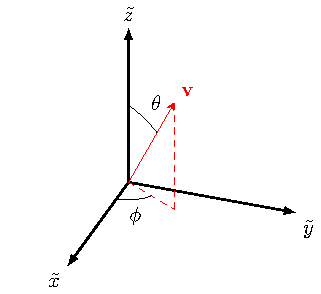
\includegraphics[width=6cm]{fig/ch13-boost.pdf}
    \caption{两参考系速度差$\boldsymbol{v}$与坐标系的关系} \label{chlg:fig_cart_sph}
\end{figure}

%我们知道,整体矢量表示$x^\mu \boldsymbol{e}_{\mu}$是Lorentz变换下的不变形式,
%即$x'^\mu \boldsymbol{e}^{\prime}_{\mu}=x^\nu \boldsymbol{e}_{\nu}$,也就是
%$\boldsymbol{e}^{\prime} X' =\boldsymbol{e} X {\color{red}\Rightarrow}
%(\boldsymbol{e}^{\prime} R^{-1})( R X') =(\boldsymbol{e} R^{-1}) (RX){\color{red}\Rightarrow}
%\tilde{\boldsymbol{e}}^{\prime} \tilde{X}' =\tilde{\boldsymbol{e}} \tilde{X}$.

关键是求解旋转矩阵$R^{-1}({\theta \phi })$的表达式.
根据我们的约定(见例题\ref{chlg:exm_GLonV}、\ref{chlg:exm_GLonB}),
旋转矩阵$R^{-1}({\theta \phi })$左作用在分量$X$上,
右作用在基矢$\boldsymbol{e}=(\boldsymbol{e}_1,\boldsymbol{e}_2,\boldsymbol{e}_3)$上.
现在考虑如图\ref{chlg:fig_cart_sph}所示的$\boldsymbol{v}$,
纯空间固有旋转$R^{-1}({\theta \phi })$相当于将$\boldsymbol{v}$(对应基矢$\boldsymbol{e}$)
旋转到$\tilde{x}$(对应基矢$\tilde{\boldsymbol{e}}$)的方向.不难求得
\begin{equation}\label{chlg:eqn_R-of-bx2b}
    R^{-1}( {\theta \phi } )  = C_{\tilde y}\left({\frac{\pi }{2} -\theta} \right) C_{\tilde z}( -\phi )
    \ \Rightarrow\  R( {\theta \phi } )  =
    {C_{\tilde  z}}(  {\phi } ) {C_{\tilde  y}} \left(  { \theta -\frac{\pi }{2}} \right) .
\end{equation}
上式计算中用到了$C_k^{-1}(\psi)=C_k(-\psi)$.则有
\begin{equation*}
    B\left( \boldsymbol{v} \right) = R{B_x}(u)R^{-1}={C_{\tilde z}}\left(  {\phi } \right)
    {C_{\tilde y}} \left(  { \theta -\frac{\pi }{2}} \right) {B_x} \left( u \right)
    {C_{\tilde y}}\left( {\frac{\pi }{2}-\theta} \right){C_{\tilde z}}\left( -\phi \right) .
\end{equation*}
经过矩阵乘法计算可以得到
\begin{small}
\begin{equation}\label{chlg:eqn_lorentz-matrix-any-v}
    B(\boldsymbol{v}) = \begin{pmatrix}
        \gamma    & -\gamma \dfrac{v_x}{c} & -\gamma \dfrac{v_y}{c} & -\gamma \dfrac{v_z}{c} \\
        -\gamma \dfrac{v_x}{c} & 1+ \dfrac{(\gamma-1)v_x^2}{v^2} &
        \dfrac{(\gamma-1)v_x v_y}{v^2} & \dfrac{(\gamma-1)v_x v_z}{v^2} \\
        -\gamma \dfrac{v_y}{c} & \dfrac{(\gamma-1)v_x v_y}{v^2} &
        1+ \dfrac{(\gamma-1)v_y^2}{v^2} & \dfrac{(\gamma-1)v_y v_z}{v^2} \\
        -\gamma \dfrac{v_z}{c} & \dfrac{(\gamma-1)v_x v_z}{v^2} &
        \dfrac{(\gamma-1)v_y v_z}{v^2} & 1+ \dfrac{(\gamma-1)v_z^2}{v^2}
    \end{pmatrix}.
\end{equation}
\end{small}
其中$\gamma^{-1}=\sqrt{1-v^2/c^2}$.
速度$\boldsymbol{v}$的分量可以由图\ref{chlg:fig_cart_sph}计算求得
\begin{equation}
    {v_x} = v\sin \theta \cos \phi, \quad
    {v_y} = v\sin \theta \sin \phi, \quad
    {v_z} = v\cos \theta  .
\end{equation}
计算中需注意$|\boldsymbol{u}|=|\boldsymbol{v}|$,即原来沿$x$轴的速度$u$的大小与任意方向速度$\boldsymbol{v}$的大小相等.
从上面伪转动矩阵可见它必然是对称的.
它穷尽了两惯性系$O$和$O'$间满足如下条件的线性变换:
\textcircled{\tiny{甲}}两坐标系相应轴是相互平行且同向;
\textcircled{\tiny{乙}}两坐标系的空间坐标原点在$t=0=t'$时重合;
\textcircled{\tiny{丙}}两坐标系速度差$\boldsymbol{v}$是常数,且方向任意.
符合这三条的Lorentz变换叫作{\heiti 伪转动}.

从物理思辨显然可得$B^{-1}(\boldsymbol{v})=B(\boldsymbol{-v})$.由于只是速度前添加负号,
所以式\eqref{chlg:eqn_lorentz-matrix-any-v}只有第一行、第一列前添加负号即可,且$00$分量
符号不变;右下角的$3\times 3$矩阵因负负得正,符号不变.

式\eqref{chlg:eqn_lorentz-matrix-any-v}作用到时空坐标,也常写成另外一种形式
\begin{equation}\label{chlg:eqn_boost-xt}
    ct'= \gamma\left( ct-\frac{\boldsymbol{v}\cdot\boldsymbol{r}}{c}\right) , \quad
    \boldsymbol{r}' = \boldsymbol{r}+(\gamma-1)\frac{\boldsymbol{v}
        \cdot\boldsymbol{r}}{v^2}\boldsymbol{v}-\gamma \frac{\boldsymbol{v}}{c} ct.
\end{equation}
其中$\boldsymbol{r}=(x,y,z)$、$\boldsymbol{v}=(v_x, v_y, v_z )$、$\boldsymbol{v}\cdot \boldsymbol{r}=v_x x+v_y y+v_z z$.

\paragraph{快度}\label{chlg:sec_rapid}
我们用{\kaishu 快度}(rapidity)来改写式\eqref{chlg:eqn_lorentz-matrix-any-v}.
我们先考虑$v_y=0=v_z$的最简单情形.
令$\tanh \theta_x=v_x/c$,就有$\gamma = \cosh \theta_x$;
则$-1<v_x/c<1$相当于$-\infty < \theta_x <+\infty$,
$\theta_x$称为{\heiti 快度};此时Lorentz矩阵可以表示为另一种形式
\begin{equation}\label{chlg:eqn_lorentz-rapid-x}
    (\Lambda_x)^{\mu}_{\cdot \nu} = 
    \begin{pmatrix}
        \cosh\theta_x  & -\sinh\theta_x & 0 & 0 \\
        -\sinh\theta_x & \cosh\theta_x  & 0 & 0 \\
        0 & 0 & 1 & 0 \\
        0 & 0 & 0 & 1 
    \end{pmatrix}.
\end{equation}

我们来看一下沿$x$轴连续进行两次Lorentz变换会是什么结果.
先进行一次Lorentz变换$\theta_2$,然后再进行第二次Lorentz变换$\theta_1$,有
\begin{equation}\label{chlg:eqn_b1b2}
    \Lambda_x(\theta_1) \Lambda_x(\theta_2) = \Lambda_x(\theta_1+\theta_2).
\end{equation}
上式以快度表示;(省略无关紧要的$y$和$z$轴)计算过程是
\begin{small}
\[\begin{pmatrix}
    \cosh\theta_1  & -\sinh\theta_1 \\
    -\sinh\theta_1 & \cosh\theta_1  
\end{pmatrix} \times
\begin{pmatrix}
    \cosh\theta_2  & -\sinh\theta_2  \\
    -\sinh\theta_2 & \cosh\theta_2   
\end{pmatrix} = 
\begin{pmatrix}
    \cosh(\theta_1+\theta_2)  & -\sinh(\theta_1+\theta_2)  \\
    -\sinh(\theta_1+\theta_2) & \cosh(\theta_1+\theta_2) 
\end{pmatrix} \]
\end{small}
上面计算利用了双曲函数和差公式
$\sinh(x \pm y) = \sinh x \cosh y \pm  \cosh x \sinh y, \ 
\cosh(x \pm y) = \cosh x \cosh y \pm  \sinh x \sinh y$.

由式\eqref{chlg:eqn_b1b2}可见用快度表示Lorentz变换时,
它是单参数子群.同理可以得到沿$y,z$方向的快度表达式:
\begin{equation*}  %\label{chlg:eqn_lorentz-rapid-yz}
    (\Lambda_y)^{\mu}_{\cdot \nu} = 
    \begin{pmatrix}
        \cosh\theta_y  & 0 & -\sinh\theta_y & 0 \\
        0 & 1  & 0 & 0 \\
        -\sinh\theta_y & 0 & \cosh\theta_y & 0 \\
        0 & 0 & 0 & 1 
    \end{pmatrix},\
    (\Lambda_z)^{\mu}_{\cdot \nu} = 
    \begin{pmatrix}
        \cosh\theta_z  & 0 & 0 & -\sinh\theta_z \\
        0 & 1  & 0 & 0 \\
        0 & 0 & 1 & 0 \\
        -\sinh\theta_z & 0 & 0 & \cosh\theta_z
    \end{pmatrix} .
\end{equation*}
当考虑$y$方向快度时,有$v_x=0=v_z$;
令$\tanh \theta_y=v_y/c$,就有$\gamma = \cosh \theta_y$;
则$-1<v_y/c<1$相当于$-\infty < \theta_y <+\infty$.
当考虑$z$方向快度时,有$v_x=0=v_y$;
令$\tanh \theta_z=v_z/c$,就有$\gamma = \cosh \theta_z$;
则$-1<v_z/c<1$相当于$-\infty < \theta_z <+\infty$.





\subsubsection{Lorentz矩阵分解}
在狭义相对论发展的初期,学者们就基本解决了Lorentz变换矩阵的分解问题;
此处的叙述参考了较新的文献\parencite{liang_zhou2009_2}附录G.9,而没有去寻找最原始的证明.

%全部三维坐标空间的固有转动群是SO(3),也就是所有\eqref{chlg:eqn_rotation}组成的集合.



\begin{proposition}\label{chlg:thm_xx-txtx}
    如果两个惯性坐标系$X$和$X'$由伪转动$B(\boldsymbol{v})$联系,并且$R\in SO(3)$,则
    $\tilde{X}\equiv RX$和$\tilde{X}'\equiv RX'$也由伪转动联系.
\end{proposition}
\begin{proof}
    设$X'=B(\boldsymbol{v})X$,并且$B(\boldsymbol{v})$是伪转动,则上节证明过程可以
    看出存在$R_0\in SO(3)$使得$B(\boldsymbol{v})=R_0B_x(u)R_0^{-1}$,因此
    $X'=R_0B_x(u)R_0^{-1}X$,从而$R_0^{-1}X'=B_x(u)R_0^{-1}X$,与$\tilde{X}\equiv RX$
    和$\tilde{X}'\equiv RX'$结合就给出$R_0^{-1}R^{-1}\tilde{X}'=B_x(u)R_0^{-1}R^{-1}\tilde{X}$.
    令$R_1 = RR_0$,则$\tilde{X}'=R_{1}B_x(u)R_1^{-1}\tilde{X}$.
    因此$\tilde{X}$和$\tilde{X}'$也由伪转动联系.
\end{proof}

\begin{proposition}\label{chlg:thm_b-rbr}
    对于任意伪转动$B(\boldsymbol{v})$,以及任意$R\in SO(3)$,都有
        $B(R\boldsymbol{v}) = R B(\boldsymbol{v}) R^{-1}$.
    此式左边$R\boldsymbol{v}$的分量是$(R\boldsymbol{v})^i = R^i_{\cdot j}v^j$,是三维空间矢量.
    右边的$R$是四维时空的转动,两者有一一对应关系\eqref{chlg:eqn_rotation-4d}.
\end{proposition}
\begin{proof}
    设有两个惯性参考系$O$和$O'$,在它们中分别建立直角坐标系$O-xyz$和$O'-x'y'z'$;
    这两个坐标系符合上一节末尾给出的伪转动定义中的三个条件;$O'$系相对于$O$系以
    常速度$\boldsymbol{v}$运动,$\boldsymbol{v}$在$O$系的分量是$\boldsymbol{v}=v^i \boldsymbol{e}_i$.
    由于$O$和$O'$都是惯性系,那就存在联系两个坐标系的伪转动$B(\boldsymbol{v})$,其表达式
    是\eqref{chlg:eqn_lorentz-matrix-any-v},即$X' = {B}( \boldsymbol{v} )X$.
    
    设$R$是纯空间固有转动,再令
    $\tilde{X}=RX$,$\tilde{X}'=RX'$;显然$\tilde{X}$和$\tilde{X}'$都是惯性坐标系,
    那么由命题\ref{chlg:thm_xx-txtx}可知$\tilde{X}$和$\tilde{X}'$也由某个伪转动联系着.
    两个惯性系参考系$\tilde{X}$和$\tilde{X}'$的速度差仍旧是$\boldsymbol{v}$,只不过$\boldsymbol{v}$在
    $\tilde{X}$坐标系中的分量变成了$\boldsymbol{v}=\tilde{v}^i { \tilde{\boldsymbol{e}}}_i=
    {v}^i { {\boldsymbol{e}}}_i$,其中
    $\tilde{\boldsymbol{e}}_i = \boldsymbol{e}_j R^j_{\cdot i}$,$\tilde{v}^i =  R^i_{\cdot k}v^k$.
    纯空间转动不改变$\boldsymbol{v}$的大小,只改变它的分量值.
    联系两个坐标系$\tilde{X}$和$\tilde{X}'$的伪转动是$B(\tilde{\boldsymbol{v}})$,其表达式
    仍旧是\eqref{chlg:eqn_lorentz-matrix-any-v},只不过,速度的分量变成了$\tilde{\boldsymbol{v}}$
    的分量.读者需注意式\eqref{chlg:eqn_lorentz-matrix-any-v}的具体表达式是和速度的分量相关的.
    因此有$\tilde{X}'=B(\tilde{\boldsymbol{v}})\tilde{X}=B( R^i_{\cdot j}v^j)\tilde{X}$.
    再与式$ \tilde X' = RX' = R{B}\left( \boldsymbol{v} \right)X
    =  \left[ {R{B}\left( \boldsymbol{v} \right){R^{ - 1}}} \right]\tilde X $相比较,
    可知定理得证.
\end{proof}



\begin{theorem} \label{chlg:thm_lorentz-decompose-r}
    对于任意的$ \Lambda \in L^{\uparrow}_{+}$,
    存在唯一的伪转动$B(\boldsymbol{v})$以及唯一的纯空间固有转动$R$,
    使得$\Lambda = B(\boldsymbol{v}) R = R'B(\boldsymbol{v})$,具体表达式见证明过程.
\end{theorem}
\begin{proof}
    \fbox{甲}若$\Lambda$是伪转动,则只需取$B(\boldsymbol{v})=\Lambda,R=I$即可.
    唯一性见\fbox{丙}.
    
    \fbox{乙}下面证明$\Lambda$不是伪转动情形.
    已知伪转动$B(\boldsymbol{v})$是对称的,纯空间转动$R$形式是\eqref{chlg:eqn_rotation-4d}.
    把$B(\boldsymbol{v})$和$R$分别记成
    \begin{equation}
        B(\boldsymbol{v}) = \begin{pmatrix}
            B^0_{\cdot 0}  & B^0_{\cdot 1} & B^0_{\cdot 2} & B^0_{\cdot 3} \\
            B^1_{\cdot 0}  & B^1_{\cdot 1} & B^1_{\cdot 2} & B^1_{\cdot 3} \\
            B^2_{\cdot 0}  & B^2_{\cdot 1} & B^2_{\cdot 2} & B^2_{\cdot 3} \\
            B^3_{\cdot 0}  & B^3_{\cdot 1} & B^3_{\cdot 2} & B^3_{\cdot 3}
        \end{pmatrix}, \qquad
        R = \begin{pmatrix}
            1    & 0 & 0 & 0 \\
            0 & R^1_{\cdot 1} & R^1_{\cdot 2} & R^1_{\cdot 3} \\
            0 & R^2_{\cdot 1} & R^2_{\cdot 2} & R^2_{\cdot 3} \\
            0 & R^3_{\cdot 1} & R^3_{\cdot 2} & R^3_{\cdot 3}
        \end{pmatrix}.
    \end{equation}
    那么$B(\boldsymbol{v})$和$R$相乘的第一列是
    \begin{equation}\label{chlg:eqn_ld-tmp1}
        B(\boldsymbol{v})R=\begin{pmatrix}
            B^0_{\cdot 0} & \cdots & \cdots& \cdots\\
            B^1_{\cdot 0} & \cdots & \cdots& \cdots\\
            B^2_{\cdot 0} & \cdots & \cdots& \cdots\\
            B^3_{\cdot 0} & \cdots & \cdots& \cdots
        \end{pmatrix},\ \text{而}\
        \Lambda=\begin{pmatrix}
            \Lambda^0_{\cdot 0} & \Lambda^0_{\cdot 1} & \Lambda^0_{\cdot 2}& \Lambda^0_{\cdot 3}\\
            \Lambda^1_{\cdot 0} & \cdots & \cdots& \cdots\\
            \Lambda^2_{\cdot 0} & \cdots & \cdots& \cdots\\
            \Lambda^3_{\cdot 0} & \cdots & \cdots& \cdots
        \end{pmatrix} .
    \end{equation}
    本定理中要证明$\Lambda=B(\boldsymbol{v})R$,根据式\eqref{chlg:eqn_lorentz-matrix-any-v}以
    及上式可以令
    \begin{equation}
        B^{0}_{\cdot 0}(\boldsymbol{v})=\gamma = \Lambda^0_{\cdot 0}, \quad
        B^{i}_{\cdot 0}(\boldsymbol{v})=-\gamma\frac{v^i}{c}= {\Lambda^i_{\cdot 0}}, \ \text{即}\
        {v^i}= - {c}\frac{\Lambda^i_{\cdot 0}}{\Lambda^0_{\cdot 0}}.
    \end{equation}
    号差$+2$的Lorentz度规并不改变$v$纯空间分量正负号,故$v_i=v^i$($i=1,2,3$).
    利用\eqref{chlg:eqn_ltm00}可以证明$|v|<c$:
    \begin{equation*}
        \sum_{i=1}^{3}\left( \frac{v^i}{c}\right)^2
        =\sum_{i=1}^{3}\left( \frac{\Lambda^i_{\cdot 0}}{\Lambda^0_{\cdot 0}}\right)^2
        =\frac{1}{(\Lambda^0_{\cdot 0})^2} \sum_{i=1}^{3}\left( {\Lambda^i_{\cdot 0}}\right)^2
        =\frac{1}{1+\sum_{j}\left( {\Lambda^j_{\cdot 0}}\right)^2}
        \sum_{i=1}^{3}\left( {\Lambda^i_{\cdot 0}}\right)^2    <1  .
    \end{equation*}
    即上面定义的速度是亚光速的.
    先求出速度$\boldsymbol{v}$的大小(要参考\eqref{chlg:eqn_ltm00}).
    \setlength{\mathindent}{0em}
    \begin{equation}\label{chlg:eqn_ltdbr-v}
        v^2 = \sum_{i=1}^{3}v_i^2 =  \dfrac{c^2}{(\Lambda^0_{\cdot 0})^2} \sum_{i=1}^{3}
        ({\Lambda^i_{\cdot 0}})^2
        = \dfrac{c^2}{(\Lambda^0_{\cdot 0})^2}\left(  (\Lambda^0_{\cdot 0})^2 -1\right)
        = \dfrac{c^2}{\gamma^2}\left(  \gamma^2 -1\right).
    \end{equation}\setlength{\mathindent}{2em}
    有了速度分量,
    根据式\eqref{chlg:eqn_lorentz-matrix-any-v}就可以构造出一伪转动$B(\boldsymbol{v})$:
    \begin{equation}\label{chlg:eqn_ltdbr-b}
        \begin{aligned}
            B^{0}_{\cdot 0}(\boldsymbol{v}) &= B^{0}_{\cdot 0}(-\boldsymbol{v}) =  \Lambda ^{0}_{\cdot 0}, \qquad
            B^{i}_{\cdot 0}(\pm\boldsymbol{v}) = \pm \Lambda ^{i}_{\cdot 0}, \\
            B^{i}_{\cdot j}(\boldsymbol{v}) &= B^{i}_{\cdot j}(-\boldsymbol{v}) =
            \delta^i_j + (\gamma-1)\dfrac{v_i v_j}{v^2} =
            \delta^i_j + \dfrac{\Lambda ^{i}_{\cdot 0}\Lambda ^{{\color{red}j}}_{\cdot 0}}
            {1 + \Lambda ^{0}_{\cdot 0} } .
        \end{aligned}
    \end{equation}
    需要注意$B^{i}_{\cdot j}$值右端$\Lambda ^{j}_{\cdot 0}$中的$j$是上标.
    我们已经构造出一个伪转动\eqref{chlg:eqn_ltdbr-b},
    由于我们要证明$\Lambda=B(\boldsymbol{v})R$,只需令$R =B^{-1}(\boldsymbol{v})\Lambda=B(-\boldsymbol{v})\Lambda $,
    把式\eqref{chlg:eqn_ltdbr-b}带入此式就可以得到
    \begin{equation}\label{chlg:eqn_ltdbr-r}
        R^{0}_{\cdot 0} = 1, \quad    R^{i}_{\cdot 0} = R^{0}_{\cdot i} = 0, \quad
        R^{i}_{\cdot j} = \Lambda^i_{\cdot j} - \dfrac{\Lambda ^{i}_{\cdot 0}
            \Lambda ^{0}_{\cdot j}}{1 + \Lambda ^{0}_{\cdot 0} }.
    \end{equation}
    可以验证这个矩阵是正交矩阵,可见$R\in SO(3)$.
    \uwave{\kaishu 这步验证十分重要,必不可少}.
    验证过程中的矩阵乘法会用到式
    \eqref{chlg:eqn_ltm00},\eqref{chlg:eqn_ltm0i}和\eqref{chlg:eqn_ltmik}.
    
    现在回顾一下证明的大体过程,按照一定规则先构造出伪转动\eqref{chlg:eqn_ltdbr-b},然后求出了一个
    矩阵\eqref{chlg:eqn_ltdbr-r},在验证了\eqref{chlg:eqn_ltdbr-r}是正交矩阵后,
    就证明了任意Lorentz矩阵$\Lambda$都可进行分解$\Lambda=B(\boldsymbol{v})R$,分解后的$B(\boldsymbol{v})$与$R$表达式见上.
    
    \fbox{丙}下面证明分解的唯一性.设$\Lambda$另有分解$\Lambda={B}(\boldsymbol{u})\tilde{R}$,则有
    ${B}(\boldsymbol{u})\tilde{R}=B(\boldsymbol{v})R$,由此容易得到
    ${B}(\boldsymbol{u})=B(\boldsymbol{v})R\tilde{R}^{-1}$,而$R\tilde{R}^{-1}$依旧是纯空间转动.
    由式\eqref{chlg:eqn_ld-tmp1}易得
    ${B}^{0}_{\cdot 0}(\boldsymbol{u})= \Lambda^0_{\cdot 0}=B^{0}_{\cdot 0}(\boldsymbol{v})$,
    ${B}^{i}_{\cdot 0}(\boldsymbol{u})= {\Lambda^i_{\cdot 0}} =B^{i}_{\cdot 0}(\boldsymbol{v})$.
    这说明$\gamma_u =\gamma_v$,$\gamma_u u^i=\gamma_v v^i{\  \Rightarrow \  } u^i=v^i$,
    也就是${B}(\boldsymbol{u}) \equiv B(\boldsymbol{v})$,    从而$\tilde{R}\equiv R$.
    
    
    $\Lambda = R'B(\boldsymbol{v})$的分解证明留给读者当练习.
\end{proof}

%\subsubsection{一般Lorentz变换}
%本小节主要讨论时空$1+3$分解后的一般Lorentz变换.
%式\eqref{chlg:eqn_boost-xt}给出了初始时刻相应坐标轴相互平行、同向的情形;
%下面讨论坐标轴不相互平行的情形.根据定理\ref{chlg:thm_lorentz-decompose-r}可知:
%这种Lorentz变换还相差一个纯空间转动.
%我们用$D$表示这个转动,则有
%\begin{equation}\label{chlg:eqn_lorentz-xt}
%    t'= \gamma_v \left( t-\frac{\boldsymbol{v}\cdot\boldsymbol{r}}{c^2}\right) , \qquad
%    \boldsymbol{r}' = D\boldsymbol{r}+D\boldsymbol{v} 
%    \left((\gamma_v-1)\frac{\boldsymbol{v}\cdot\boldsymbol{r}}{v^2}-\gamma_v t \right).
%\end{equation}
%这就是说$\boldsymbol{r}_{\parallel}\equiv D \boldsymbol{r}$所处坐标系与$\boldsymbol{r}'$所处坐标系的坐标轴相互平行、同向.
%式\eqref{chlg:eqn_lorentz-xt}中第二式中圆括号内是标量,
%即$(\gamma_v-1)\frac{\boldsymbol{v}\cdot\boldsymbol{r}}{v^2}-\gamma_v t $是标量;
%它的数值不随纯空间转动$D$而改变.$D$只改变$\boldsymbol{r}$、$\boldsymbol{v}$的方向,不改变其大小;
%对$\boldsymbol{v}$的转动($D$)操作正好是$O'$系测量$O$系的速度$\boldsymbol{v}'$的负值,即
%\begin{equation}\label{chlg:eqn_vDvp}
%    D \boldsymbol{v} = - \boldsymbol{v}' .
%\end{equation}
%
%对式\eqref{chlg:eqn_lorentz-xt}取微分,注意$D$、$\boldsymbol{v}$、$\gamma_v$都是常数,
%微分只对$t$、$t'$、$\boldsymbol{r}$、$\boldsymbol{r}'$起作用.
%取完微分后,求商即可得到速度($\boldsymbol{u}={\rm d}\boldsymbol{r}/{\rm d}t,\, 
%\boldsymbol{u}'={\rm d}\boldsymbol{r}'/{\rm d}t' $)变换公式
%\begin{equation}\label{chlg:eqn_u2up}
%    \boldsymbol{u}' = \frac{1}{1-\boldsymbol{v}\cdot \boldsymbol{u}/c^2}\left(
%    \gamma_v^{-1} D \boldsymbol{u} + \frac{\gamma_v-1}{\gamma_v}
%    \frac{\boldsymbol{u}\cdot \boldsymbol{v}}{v^2} D\boldsymbol{v}-D\boldsymbol{v} \right) .
%\end{equation}
%
%%\begin{equation}
%%    (\gamma_v^2 v^2/c^2)= \frac{1}{1-\frac{v^2}{c^2}} v^2/c^2
%%    =\gamma_v^2-1=(\gamma_v+1)(\gamma_v-1) .
%%\end{equation}
%
%
%下面列出一个常用公式:
%\begin{equation}\label{chlg:eqn_ggg}
%    \gamma_{u'}= \gamma_v \gamma_u\left(1-\frac{\boldsymbol{v}\cdot \boldsymbol{u}}{c^2}\right) 
%    \quad \text{和} \quad
%    \gamma_{u}= \gamma_v \gamma_{u'}\left(1+\frac{\boldsymbol{v}\cdot \boldsymbol{u}'}{c^2}\right) .
%\end{equation}
%只需将各种速度带入相应Lorentz因子,然后直接计算即可证明.
%
%%证明过程如下:
%%上式等价于证明
%%\begin{equation}\label{chlg:eqn_tmpggg}
%%    \left(1- \frac{v^2}{c^2} \right)\left(1- \frac{u^2}{c^2} \right)
%%    =\left(1-\frac{\boldsymbol{v}\cdot \boldsymbol{u}}{c^2}\right)^2
%%    \left(1- \frac{u^{\prime 2}}{c^2} \right) .
%%\end{equation}
%%下式推导中注意利用$D$是正交矩阵.
%%\begin{align*}
%%    &\gamma_v^{2}(1-\boldsymbol{v}\cdot \boldsymbol{u}/c^2)^2 \boldsymbol{u}'\cdot \boldsymbol{u}' =\left[
%%    D \boldsymbol{u} + \left((\gamma_v-1)
%%    \frac{\boldsymbol{u}\cdot \boldsymbol{v}}{v^2}-\gamma_v\right) D\boldsymbol{v} \right]^2 \\
%%    =& D \boldsymbol{u}\cdot D \boldsymbol{u}  + 2 D \boldsymbol{u} \cdot
%%    \left((\gamma_v-1)\frac{\boldsymbol{u}\cdot \boldsymbol{v}}{v^2}-\gamma_v\right) D\boldsymbol{v} 
%%    + \left((\gamma_v-1)\frac{\boldsymbol{u}\cdot \boldsymbol{v}}{v^2}-\gamma_v\right)^2 D\boldsymbol{v} \cdot D\boldsymbol{v}  \\
%%    =& u^2  + 2 
%%    \left((\gamma_v-1)\frac{\boldsymbol{u}\cdot \boldsymbol{v}}{v^2}-\gamma_v\right) \boldsymbol{u} \cdot\boldsymbol{v} 
%%    + \left((\gamma_v-1)\frac{\boldsymbol{u}\cdot \boldsymbol{v}}{v^2}-\gamma_v\right)^2 v^2  
%%\end{align*}
%%我们可以来证明式\eqref{chlg:eqn_tmpggg}了.
%%\begin{align*}
%%    &\left(1-\frac{\boldsymbol{v}\cdot \boldsymbol{u}}{c^2}\right)^2
%%    \left(1- \frac{u^{\prime 2}}{c^2} \right)
%%    =\left(1-\frac{\boldsymbol{v}\cdot \boldsymbol{u}}{c^2}\right)^2
%%    -\left(1-\frac{\boldsymbol{v}\cdot \boldsymbol{u}}{c^2}\right)^2 \frac{u^{\prime 2}}{c^2} \\
%%    =&\left(1-\frac{\boldsymbol{v}\cdot \boldsymbol{u}}{c^2}\right)^2-
%%    \gamma_v^{-2} c^{-2} \left[u^2  + 2 
%%    \left((\gamma_v-1)\frac{\boldsymbol{u}\cdot \boldsymbol{v}}{v^2}-\gamma_v\right) \boldsymbol{u} \cdot\boldsymbol{v} 
%%    + \left((\gamma_v-1)\frac{\boldsymbol{u}\cdot \boldsymbol{v}}{v^2}-\gamma_v\right)^2 v^2  \right] \\
%%    =&1 + \frac{(\boldsymbol{v}\cdot \boldsymbol{u})^2}{c^4} - 2\frac{\boldsymbol{v}\cdot \boldsymbol{u}}{c^2}
%%    -\gamma_v^{-2} c^{-2} u^2  \\
%%    &- 2 \gamma_v^{-2} c^{-2}
%%    \left((\gamma_v-1)\frac{\boldsymbol{u}\cdot \boldsymbol{v}}{v^2}-\gamma_v\right) \boldsymbol{u} \cdot\boldsymbol{v} \\
%%    &- \gamma_v^{-2} c^{-2}\left((\gamma_v-1)\frac{\boldsymbol{u}\cdot \boldsymbol{v}}{v^2}-\gamma_v\right)^2 v^2   \\
%%    =&1 + \frac{(\boldsymbol{v}\cdot \boldsymbol{u})^2}{c^4} - 2\frac{\boldsymbol{v}\cdot \boldsymbol{u}}{c^2}
%%    -\gamma_v^{-2} \frac{u^2}{c^2}   \\
%%    &- 2 \gamma_v^{-2} (\gamma_v-1)\frac{\boldsymbol{u}\cdot \boldsymbol{v}}{v^2} \frac{\boldsymbol{u}\cdot \boldsymbol{v}}{c^2} 
%%    + 2 \gamma_v^{-1}  \frac{\boldsymbol{u}\cdot \boldsymbol{v}}{c^2}\\
%%    &- \left[\left(\frac{\gamma_v-1}{\gamma_v}\frac{\boldsymbol{u}\cdot \boldsymbol{v}}{v^2} \right)^2 
%%    -2\frac{\gamma_v-1}{\gamma_v}\frac{\boldsymbol{u}\cdot \boldsymbol{v}}{v^2}    +1\right]\frac{v^2}{c^2}   \\
%%    =&1   -\gamma_v^{-2} \frac{u^2}{c^2}    -\frac{v^2}{c^2}   \\
%%    &+ \frac{(\boldsymbol{v}\cdot \boldsymbol{u})^2}{c^4 }
%%    - 2 \gamma_v^{-2} (\gamma_v-1)\frac{\boldsymbol{u}\cdot \boldsymbol{v}}{v^2} \frac{\boldsymbol{u}\cdot \boldsymbol{v}}{c^2}
%%    - \left(\frac{\gamma_v-1}{\gamma_v}\frac{\boldsymbol{u}\cdot \boldsymbol{v}}{v^2} \right)^2 \frac{v^2}{c^2}  \\
%%    &+ 2 \gamma_v^{-1}  \frac{\boldsymbol{u}\cdot \boldsymbol{v}}{c^2}
%%    +2\frac{\gamma_v-1}{\gamma_v}\frac{\boldsymbol{u}\cdot \boldsymbol{v}}{v^2} \frac{v^2}{c^2} 
%%    - 2\frac{\boldsymbol{v}\cdot \boldsymbol{u}}{c^2} .
%%\end{align*}
%%上式最后一步中$\boldsymbol{v}\cdot \boldsymbol{u}$前的系数之和正好为零,故有
%%\begin{align}
%%    \left(1-\frac{\boldsymbol{v}\cdot \boldsymbol{u}}{c^2}\right)^2
%%    \left(1- \frac{u^{\prime 2}}{c^2} \right)
%%    =1   -\gamma_v^{-2} \frac{u^2}{c^2}    -\frac{v^2}{c^2}
%%    =\left(1- \frac{v^2}{c^2} \right)\left(1- \frac{u^2}{c^2} \right).
%%\end{align}
%
%
%%逆变换的证明过程如下:
%%上式等价于证明
%%\begin{equation}\label{chlg:eqn_tmpggg}
%%    \left(1- \frac{v^2}{c^2} \right)\left(1- \frac{u'^2}{c^2} \right)
%%    =\left(1+\frac{\boldsymbol{v}\cdot \boldsymbol{u}'}{c^2}\right)^2
%%    \left(1- \frac{w^2}{c^2} \right) .
%%\end{equation}
%%下式推导中注意利用$D$是正交矩阵以及速度逆变换公式\eqref{chsr:eqn_boost-u-inv}.
%%\begin{align*}
%%    &\gamma_v^{2}(1+\boldsymbol{v}\cdot \boldsymbol{u}'/c^2)^2 \boldsymbol{w}\cdot \boldsymbol{w} =\left[
%%    D \boldsymbol{u}' + \left((\gamma_v-1)
%%    \frac{\boldsymbol{u}'\cdot \boldsymbol{v}}{v^2}+\gamma_v\right) D\boldsymbol{v} \right]^2 \\
%%    =& D \boldsymbol{u}'\cdot D \boldsymbol{u}'  + 2 D \boldsymbol{u}' \cdot
%%    \left((\gamma_v-1)\frac{\boldsymbol{u}'\cdot \boldsymbol{v}}{v^2}+\gamma_v\right) D\boldsymbol{v} 
%%    + \left((\gamma_v-1)\frac{\boldsymbol{u}'\cdot \boldsymbol{v}}{v^2}+\gamma_v\right)^2 D\boldsymbol{v} \cdot D\boldsymbol{v}  \\
%%    =& u'^2  + 2 
%%    \left((\gamma_v-1)\frac{\boldsymbol{u}'\cdot \boldsymbol{v}}{v^2}+\gamma_v\right) \boldsymbol{u}' \cdot\boldsymbol{v} 
%%    + \left((\gamma_v-1)\frac{\boldsymbol{u}'\cdot \boldsymbol{v}}{v^2}+\gamma_v\right)^2 v^2  
%%\end{align*}
%%我们可以来证明式\eqref{chlg:eqn_tmpggg}了.
%%\begin{align*}
%%    &\left(1+\frac{\boldsymbol{v}\cdot \boldsymbol{u}'}{c^2}\right)^2
%%    \left(1- \frac{w^2}{c^2} \right)
%%    =\left(1+\frac{\boldsymbol{v}\cdot \boldsymbol{u}'}{c^2}\right)^2
%%    -\left(1+\frac{\boldsymbol{v}\cdot \boldsymbol{u}'}{c^2}\right)^2 \frac{w^2}{c^2} \\
%%    =&\left(1+\frac{\boldsymbol{v}\cdot \boldsymbol{u}'}{c^2}\right)^2
%%    -\gamma_v^{-2} c^{-2} \left[u'^2  + 2 
%%    \left((\gamma_v-1)\frac{\boldsymbol{u}'\cdot \boldsymbol{v}}{v^2}+\gamma_v\right) \boldsymbol{u}' \cdot\boldsymbol{v} 
%%    + \left((\gamma_v-1)\frac{\boldsymbol{u}'\cdot \boldsymbol{v}}{v^2}+\gamma_v\right)^2 v^2 \right] \\
%%    =& 1 + 2 \frac{\boldsymbol{v}\cdot \boldsymbol{u}'}{c^2} + \frac{(\boldsymbol{v}\cdot \boldsymbol{u}')^2}{c^4} -\gamma_v^{-2} c^{-2} u'^2 
%%    -\gamma_v^{-2} c^{-2} 2\left((\gamma_v-1)\frac{\boldsymbol{u}'\cdot \boldsymbol{v}}{v^2}+\gamma_v\right) \boldsymbol{u}' \cdot\boldsymbol{v} 
%%    -\gamma_v^{-2} c^{-2} \left((\gamma_v-1)\frac{\boldsymbol{u}'\cdot \boldsymbol{v}}{v^2}+\gamma_v\right)^2 v^2 \\
%%    =&1 + 2 \frac{\boldsymbol{v}\cdot \boldsymbol{u}'}{c^2} + \frac{(\boldsymbol{v}\cdot \boldsymbol{u}')^2}{c^4} -\gamma_v^{-2} c^{-2} u'^2 
%%    -2 \frac{\gamma_v-1}{\gamma_v^{2}}\frac{(\boldsymbol{u}'\cdot \boldsymbol{v})^2}{c^2 v^2}
%%    -\frac{2}{\gamma_v}\frac{\boldsymbol{u}' \cdot\boldsymbol{v}}{c^2}  \\
%%    &- \left[\left(\frac{\gamma_v-1}{\gamma_v}\right)^2\frac{(\boldsymbol{u}'\cdot \boldsymbol{v})^2}{v^4}
%%    +2\frac{\gamma_v-1}{\gamma_v}\frac{\boldsymbol{u}'\cdot \boldsymbol{v}}{v^2}    +1\right] \frac{v^2}{c^2} \\
%%    =&1 -\gamma_v^{-2} c^{-2} u'^2 - \frac{v^2}{c^2} \\
%%    & + 2 \frac{\boldsymbol{v}\cdot \boldsymbol{u}'}{c^2} -\frac{2}{\gamma_v}\frac{\boldsymbol{u}' \cdot\boldsymbol{v}}{c^2}
%%    - 2\frac{\gamma_v-1}{\gamma_v}\frac{\boldsymbol{u}'\cdot \boldsymbol{v}}{v^2} \frac{v^2}{c^2} \\
%%    & + \frac{(\boldsymbol{v}\cdot \boldsymbol{u}')^2}{c^4} -2 \frac{\gamma_v-1}{\gamma_v^{2}}\frac{(\boldsymbol{u}'\cdot \boldsymbol{v})^2}{c^2 v^2}
%%    -\left(\frac{\gamma_v-1}{\gamma_v}\right)^2\frac{(\boldsymbol{u}'\cdot \boldsymbol{v})^2}{v^4}\frac{v^2}{c^2}
%%\end{align*}
%%上式最后一步中$\boldsymbol{v}\cdot \boldsymbol{u}$前的系数之和正好为零,故有
%%\begin{align}
%%    \left(1+\frac{\boldsymbol{v}\cdot \boldsymbol{u}'}{c^2}\right)^2
%%    \left(1- \frac{w^2}{c^2} \right)
%%    =1   -\gamma_v^{-2} \frac{u'^2}{c^2}    -\frac{v^2}{c^2}
%%    =\left(1- \frac{v^2}{c^2} \right)\left(1- \frac{u'^2}{c^2} \right).
%%\end{align}











\index[physwords]{Lorentz代数}  \index[physwords]{Lorentz代数}

\subsubsection{Lorentz代数}
正时固有Lorentz群$SO^{+}(1,3)$有六个实参数来描述,其中固有转动占三个,伪转动占三个.
我们通过单参数子群来求取其李代数.
在\S\ref{chlar:sec_LA-su2so3}中,我们
找到了$SO(3)$群的三个单参数子群;只需将其拓展到四维空间即可.
它们是
\begin{small}
\begin{equation}\label{chlg:eqn_LA-so13-r}
    r_1=\begin{pmatrix}
        0&0&0&0\\
        0&0 & 0 & 0 \\
        0&0& 0 & -1 \\
        0&0 & 1 & 0
    \end{pmatrix},\ 
    r_2=\begin{pmatrix}
        0&0&0&0\\
        0&0 & 0 & 1 \\
        0&0 & 0 & 0 \\
        0&-1 & 0 & 0
    \end{pmatrix},\ 
    r_3=\begin{pmatrix}
        0&0&0&0\\
        0&0 & - 1 & 0 \\
        0&1& 0 & 0 \\
        0&0 & 0 & 0
    \end{pmatrix} .
\end{equation}
\end{small}

第\pageref{chlg:sec_rapid}页中,由快度描述的伪转动也是单参数子群.
只需对式\eqref{chlg:eqn_lorentz-rapid-x}中所有矩阵元求$\theta_x$的导数,并在$\theta_x=0$取值,即
\begin{equation}
    b_1=\left.\frac{{\rm d}\Lambda_x(\theta_x)}{{\rm d}\theta_x}\right|_{\theta_x=0} \quad
    b_2=\left.\frac{{\rm d}\Lambda_y(\theta_y)}{{\rm d}\theta_y}\right|_{\theta_y=0} \quad
    b_3=\left.\frac{{\rm d}\Lambda_z(\theta_z)}{{\rm d}\theta_z}\right|_{\theta_z=0} .
\end{equation}
由上式计算出结果,得
\begin{small}
\setlength{\mathindent}{0em}
\begin{equation}\label{chlg:eqn_LA-so13-b}
    b_1=  \begin{pmatrix}
        0  & -1 & 0 & 0 \\
        -1 & 0  & 0 & 0 \\
        0 & 0 & 0 & 0 \\
        0 & 0 & 0 & 0 
    \end{pmatrix},\ 
    b_2 =  \begin{pmatrix}
        0  & 0 & -1 & 0 \\
        0 & 0  & 0 & 0 \\
        -1 & 0 & 0 & 0 \\
        0 & 0 & 0 & 0 
    \end{pmatrix},\ 
    b_3 =  \begin{pmatrix}
        0  & 0 & 0 & -1 \\
        0 & 0  & 0 & 0 \\
        0 & 0 & 0 & 0 \\
        -1 & 0 & 0 & 0 
    \end{pmatrix} .
\end{equation} \setlength{\mathindent}{2em}
\end{small}

通过直接计算,可以得到这些矩阵的对易关系(李积)如下
\begin{equation}\label{chlg:eqn_LA-so13-comm}
    [r_i, r_j] = \sum_k \epsilon_{ijk} r_k,\quad
    [b_i, r_j] = \sum_k \epsilon_{ijk} b_k,\quad
    [b_i, b_j] = -\sum_k \epsilon_{ijk} r_k.
\end{equation}
其中$i,j,k=1,2,3$;$\epsilon_{ijk}=\delta^{123}_{ijk}$,定义见式\eqref{chmla:eqn_gkd}.
式\eqref{chlg:eqn_LA-so13-r}、\eqref{chlg:eqn_LA-so13-b}连同
对易关系\eqref{chlg:eqn_LA-so13-comm}构成了$\mathfrak{so}^{+}(1,3)$李代数.


%\begin{example}
%    结构常数、Killing型、Casimir算子.
%\end{example}


物理学上较喜欢用厄米或反厄米矩阵来表示生成元,即作如下变换
\begin{equation}\label{chlg:eqn_LA-so13-JK}
    J_i = \mathbbm{i} r_i,\qquad  K_i = \mathbbm{i} b_i .
\end{equation}
那么对易关系\eqref{chlg:eqn_LA-so13-comm}变成(省略了求和符号):
\begin{equation}\label{chlg:eqn_LA-so13-comm-JK}
    [J_i, J_j] = \mathbbm{i} \epsilon_{ijk} J_k,\quad
    [J_i, K_j] = \mathbbm{i} \epsilon_{ijk} K_k,\quad
    [K_i, K_j] = -\mathbbm{i}\epsilon_{ijk} J_k.
\end{equation}
厄米矩阵$J$、反厄米矩阵$K$(即式\eqref{chlg:eqn_LA-so13-JK})及其
对易关系\eqref{chlg:eqn_LA-so13-comm-JK}是$\mathfrak{so}^{+}(1,3)$李代数
的另外一种常用表示.


%反之,我们也可以从无穷小形式$\omega_{\rho\sigma}$出发,通过指数映射得到
%一般形式的Lorentz变换$\Lambda^\mu_{\hphantom{\mu}\rho}$.由下式出发
%\begin{align*}
%    \omega^\mu_{\hphantom{\mu}\nu} =& \eta^{\mu\rho} \omega_{\rho\nu}
%    =\frac{1}{2}( \eta^{\mu\rho} \omega_{\rho\nu} - \eta^{\mu\rho} \omega_{\nu\rho})
%    =\frac{1}{2}( \eta^{\mu\rho} \delta^\sigma_\nu - \eta^{\mu\sigma} \delta^\rho_\nu ) \omega_{\rho\sigma}.
%\end{align*}
若我们定义($\eta={\rm diag}(-1,1,1,1)$)
\begin{equation}\label{chlg:eqn_LJw}
    (\mathcal{J}^{\rho\sigma})^\mu_{\hphantom{\mu}\nu} \equiv 
    \mathbbm{i} ( \eta^{\mu\sigma} \delta^\rho_\nu -\eta^{\mu\rho} \delta^\sigma_\nu).
\end{equation}
上式为Lorentz代数的整体形式.则有
\begin{align}
    \{\mathcal{J}^{10},\mathcal{J}^{20},\mathcal{J}^{30} \} =\{K_1,K_2,K_3\}, \
    \{\mathcal{J}^{23},\mathcal{J}^{31},\mathcal{J}^{12} \} =\{J_1,J_2,J_3\}.
\end{align}
那么一般Lorentz变换可表示为
\begin{equation}
    \Lambda^\mu_{\hphantom{\mu}\nu} = \exp\left( -\frac{\mathbbm{i}}{2}\omega_{\rho\sigma}
    (\mathcal{J}^{\rho\sigma})^\mu_{\hphantom{\mu}\nu} \right) .
\end{equation}
通过矩阵的指数运算可以得到$\exp(-\mathbbm{i} \alpha J_1)= C_x(\alpha)$
(见式\eqref{chlg:eqn_rotation-x});与之类似,$J_2,J_3$的矩阵指数
为式\eqref{chlg:eqn_rotation-zy}.
同样,$\exp(-\mathbbm{i} \theta K_1)= \Lambda_x(\theta)$,
即式\eqref{chlg:eqn_lorentz-rapid-x};另外两个的矩阵指数
($\exp(-\mathbbm{i} \theta K_2)$、$\exp(-\mathbbm{i} \theta K_3)$)
自然是$y$、$z$方向的伪转动.
这些计算略显繁琐,但没有难度;也可借助计算机符号软件完成.


在\S\ref{chlar:sec_LA-su2so3}中,我们建立了$\mathfrak{so}(3)$李代数矩阵基矢量和微分基矢量间的同构关系;
仿照那里的做法,可以建立Lorentz李代数$\mathfrak{so}^{+}(1,3)$矩阵基矢量和微分基矢量间的同构关系$\Psi$.
\begin{small}
\setlength{\mathindent}{0em}
\begin{equation}\label{chlg:eqn_LA-so13-JK-diff}
    \hat{J}_i=\Psi(J_i)= -\frac{\mathbbm{i}}{2}\epsilon_{ijk} \left(x^j\frac{\partial }{\partial x^k}
    - x^k\frac{\partial }{\partial x^j}\right), \ 
    \hat{K}_i=\Psi(K_i)= \mathbbm{i} \left(t\frac{\partial }{\partial x^i}+  x^i\frac{\partial }{\partial t}\right) .
\end{equation} \setlength{\mathindent}{2em}
\end{small}
因$x^0 = t=-x_0$,故$\Psi(K_i)$中圆括号内两部分符号相同.
通过直接计算可以验证微分形式的基矢量对易关系与\eqref{chlg:eqn_LA-so13-comm-JK}式完全相同,
故它们是同构关系,没有必要严格区分它们.




\index[physwords]{庞加莱群} \index[physwords]{Poincar\'{e}群}

\subsection{Poincar\'{e}群}\label{chlg:sec_Poincare-group}
Poincar\'{e}(Jules Henri Poincar\'e,1854--1912,法国数学家 )
群与欧几里得群大致相同,唯一不同的就是度规;
欧氏群是正定度规,庞氏群是闵氏度规($\eta={\rm diag}(-1,1,1,1)$).
整个理论物理(除引力外)都受狭义相对论约束,
故庞氏群对整个理论物理都是至关重要的.
\begin{definition}
    Poincar\'{e}群由$(\mathbb{R}^4_1,\eta)$上的所有连续、等距、“线性”变换组成.
\end{definition}
我们将庞氏群记为$\mathcal{P}(1,3)$,可简记成$\mathcal{P}$.
庞氏对应的坐标变换是
\begin{equation}\label{chlg:eqn_xpoincare}
    x\to x' : x'^{\mu} = \Lambda^\mu_{\cdot \nu }x^\nu + b^\mu ,\qquad  0 \leqslant \mu \leqslant 3 .
\end{equation}
用矩阵形式表示为(后面会证明$\Lambda$是一般Lorentz矩阵,$\Lambda^{-1}=\eta \Lambda^T \eta$)
\begin{equation}\label{chlg:eqn_xP5m}
    \begin{bmatrix}  x' \\ 1 \end{bmatrix} =
    \begin{bmatrix}  \Lambda & b \\ \boldsymbol{0}^T & 1  \end{bmatrix}
    \begin{bmatrix}  x \\ 1 \end{bmatrix} 
    \  \overset{def}{=} \boldsymbol{P} \begin{bmatrix}  x \\ 1 \end{bmatrix} .
    \qquad \boldsymbol{P}^{-1} = 
    \begin{bmatrix}    \Lambda^{-1} & -\Lambda^{-1} b \\ \boldsymbol{0}^T & 1    \end{bmatrix} .
\end{equation}
我们把一个$4$维列矢量末尾增加一行,数值为$1$;从而变成了$5$维列矢量.
上式最后定义了矩阵$\boldsymbol{P}$,并给出了它的逆.
在时空均匀前提下,我们已知平移是等距变换.
在闵氏度规下,要求此变换是等距的,即
    \begin{align*}
        &\bigl(\eta(x'-y')\bigr)^T (x'-y') = ( x - y )^T \Lambda^T \eta \Lambda ( x - y )= (x-y)^T \eta (x-y)\\
        \Rightarrow\ &\Lambda^T \eta \Lambda = \eta .     \qquad \text{因}x,y \text{的任意性}
    \end{align*}
可见只要变换$\Lambda$是Lorentz矩阵(见\eqref{chlg:eqn_gLorentz})就可等距,
也就是$\Lambda$是$O(1,3)$群中的元素.
这便说明了庞氏群由两种类型的变换组成:平移和Lorentz变换.

这就是说等距群$I(\mathbb{R}^4_1,\eta)$是$\mathcal{P}$.它的维数是:
\begin{equation}
    {\rm dim}\bigl(I(\mathbb{R}^4_1)\bigr)= {\rm dim}  \hat{T}(4) + {\rm dim} O(1,3) = 10 .
\end{equation}


我们把$\mathcal{P}$的群乘法定义为复合映射,连续两次庞氏变换为
\begin{equation}\label{chlg:eqn_tmpptp}
    \begin{bmatrix}  \Lambda_1 & b_1 \\ \boldsymbol{0}^T & 1  \end{bmatrix}
    \begin{bmatrix}  \Lambda_2 & b_2 \\ \boldsymbol{0}^T & 1  \end{bmatrix}
    \begin{bmatrix}  x \\ 1 \end{bmatrix} 
%    =\begin{bmatrix} \Lambda_1 & b_1 \\ \boldsymbol{0}^T & 1  \end{bmatrix}
%    \begin{bmatrix}  \Lambda_2  x + b_2 \\  1  \end{bmatrix}
    =\begin{bmatrix} \Lambda_1 \Lambda_2 x + \Lambda_1 b_2 + b_1 \\  1  \end{bmatrix}.
\end{equation}
很明显,两次庞氏变换是不对易的.
与欧几里得群几乎完全相同,可以验证平移群$\hat{T}(4)$
是$\mathcal{P}$的\uwave{不变子群},
即$\forall u \in \mathcal{P}$,$\forall t \in \hat{T}(4)$有
\begin{equation}
    u^{-1} t u x= 
    \begin{bmatrix}  \Lambda^{-1} & -\Lambda^{-1} b \\ \boldsymbol{0}^T & 1    \end{bmatrix}
    \begin{bmatrix}  \Lambda x + b + t\\  1  \end{bmatrix}
    =\begin{bmatrix} x + \Lambda^{-1} t\\  1  \end{bmatrix}.
\end{equation}
因为$\mathcal{P}$有可对易不变子群$\hat{T}(4)$,所以它不是半单纯的.
因平移群和Lorentz群是非紧致的,故$\mathcal{P}$也是非紧致李群.

与欧几里得群相似,可知:$\mathcal{P}= \hat{T}(4) \rtimes O(1,3)$.
依照半直积定义可以把$\mathcal{P}$中元素记为$(b,\Lambda)$,其中$b\in \hat{T}(4)$,$\Lambda\in O(1,3)$.
我们从定义角度再次叙述一遍这个半直积.
可定义平移群$\hat{T}(4)$的自同构映射为:
$\Psi_{\Lambda_1}( b_2)=\Lambda_1 b_2 = \hat{T}(4)_{\Lambda_1 b_2}$,
其中$\Lambda_1 \in O(1,3)$,$b_2\in \hat{T}(4)$.
那么连续两次庞氏变换可以表示为:
\begin{equation}\label{chlg:eqn_ptp}
    (b_1, \Lambda_1)(b_2, \Lambda_2)
    =\bigl(b_1 \Psi_{\Lambda_1}( b_2),\ \Lambda_1 \Lambda_2 \bigr)
    =(b_1 + \Lambda_1 b_2 ,\ \Lambda_1 \Lambda_2) .
\end{equation}
这与上面用矩阵表示的连续两次庞氏变换\eqref{chlg:eqn_tmpptp}完全相同.

仿照命题\ref{chlg:thm_E2-decomposition}可以证明:Poincar\'{e}群可以分解成
\begin{equation}\label{chlg:eqn_PL-decomposition}
    \mathcal{P}(a,\Lambda)= \hat{T}(4)_{a} \Lambda .
\end{equation}
其中$\hat{T}(4)_{a}$是四维平移,$\Lambda$是一般Lorentz变换.



\begin{example}\label{chlg:exm_Rmnu}
    仿照欧氏群和庞氏群的分析过程,可以看出平直流形$\mathbb{R}^m_\nu$的
    等距群$I(\mathbb{R}^m_\nu)$是$\hat{T}(m)\rtimes O(\nu,m-\nu)$.
    故${\rm dim}\bigl(I(\mathbb{R}^m_\nu)\bigr)= m(m+1)/2 $.    \qed
\end{example}

\index[physwords]{Poincar\'{e}代数}

\subsubsection{Poincar\'{e}代数I}\label{chlg:sec_PA-1}
Poincar\'{e}代数包括四个平移(\eqref{chlg:eqn_Texp})和
六个Lorentz变换(\eqref{chlg:eqn_LA-so13-JK-diff}).
\begin{subequations}\label{chlg:eqn_PA-gen}
    \begin{align}
        \hat{H} \equiv& +\hat{P}^0= -\hat{P}_0 = \mathbbm{i}\frac{\partial }{\partial x^0}
        = \mathbbm{i}\frac{\partial }{\partial t }, \quad
        \hat{P}_i = -\mathbbm{i}\frac{\partial }{\partial x^i} ,\\
        \hat{J}_i=& -\frac{\mathbbm{i}}{2}\epsilon_{ijk} \left(x^j\frac{\partial }{\partial x^k}
        - x^k\frac{\partial }{\partial x^j}\right), \quad
        \hat{K}_i= \mathbbm{i} \left(t\frac{\partial }{\partial x^i}+  x^i\frac{\partial }{\partial t}\right) .
    \end{align}
\end{subequations}
通过偏导数直接计算可以得到它们的对易关系($i,j,k=1,2,3$,$\epsilon_{123}=1$):
\begin{subequations}\label{chlg:eqn_PA-iso13-comm-PJK}
    \begin{align}
        \left[\hat{J}_i, \hat{J}_j \right] =& \mathbbm{i} \sum\nolimits_{k=1}^{3} \epsilon_{ijk} \hat{J}_k . \\
        \left[\hat{J}_i, \hat{K}_j\right] =& \mathbbm{i} \sum\nolimits_{k=1}^{3} \epsilon_{ijk} \hat{K}_k . \\
        \left[\hat{K}_i, \hat{K}_j\right] =& -\mathbbm{i}\sum\nolimits_{k=1}^{3} \epsilon_{ijk} \hat{J}_k . \\
        \left[\hat{H}, \hat{P}_i \right] =& \left[\hat{H}, \hat{J}_i \right]
        =\left[\hat{H}, \hat{H} \right] =\left[\hat{P}_i, \hat{P}_j \right] =0 . \\
        \left[\hat{H}, \hat{K}_i \right] = & -\mathbbm{i} \hat{P}_i .\\
        \left[\hat{P}_i, \hat{K}_j \right] =& -\mathbbm{i} \delta_{ij} \hat{H} . \\
        \left[\hat{P}_i, \hat{J}_j \right] =& \mathbbm{i} \sum\nolimits_{k=1}^{3} \epsilon_{ijk} \hat{P}_k .
    \end{align}
\end{subequations}
很明显,Lorentz代数部分没有任何变化.
Poincar\'{e}代数基矢量除了微分形式外,还有取其同构的矩阵形式,
从Lorentz代数及式\eqref{chlg:eqn_xP5m}可知:
\setlength{\mathindent}{0em}
\begin{align} 
    J_1=&\left(\begin{smallmatrix}
        0&0&0&0&0\\
        0&0 & 0 & 0&0 \\
        0&0& 0 & -\mathbbm{i} &0\\
        0&0 & \mathbbm{i} & 0&0 \\
        0&0&0&0&0
    \end{smallmatrix}\right),\quad 
    J_2=\left(\begin{smallmatrix}
        0&0&0&0&0\\
        0&0 & 0 & \mathbbm{i}&0 \\
        0&0 & 0 & 0 &0\\
        0&-\mathbbm{i} & 0 & 0&0\\
        0&0&0&0&0
    \end{smallmatrix}\right),\quad 
    J_3=\left(\begin{smallmatrix}
        0&0&0&0&0\\
        0&0 & - \mathbbm{i} & 0 &0\\
        0&\mathbbm{i}& 0 & 0 &0\\
        0&0 & 0 & 0&0\\
        0&0&0&0&0
    \end{smallmatrix}\right) . \label{chlg:eqn_PA-iso13-JK} \\
    K_1=&  \left(\begin{smallmatrix}
        0  &- \mathbbm{i}&0 & 0 & 0 \\
        -\mathbbm{i} & 0  & 0 & 0&0 \\
        0 & 0 & 0 & 0 &0\\
        0 & 0 & 0 & 0 &0\\
        0&0&0&0&0
    \end{smallmatrix}\right),\quad 
    K_2 =  \left(\begin{smallmatrix}
        0  & 0 & -\mathbbm{i} & 0 &0\\
        0 & 0  & 0 & 0 &0\\
        -\mathbbm{i} & 0 & 0 & 0 &0\\
        0 & 0 & 0 & 0 &0\\
        0&0&0&0&0
    \end{smallmatrix}\right),\quad 
    K_3 =  \left(\begin{smallmatrix}
        0  & 0 & 0 & -\mathbbm{i} &0\\
        0 & 0  & 0 & 0 &0\\
        0 & 0 & 0 & 0 &0\\
        -\mathbbm{i} & 0 & 0 & 0 &0\\
        0&0&0&0&0
    \end{smallmatrix}\right). \notag \\
    H=& P^0=\left( \begin{smallmatrix}
        0 & 0 & 0 & 0 & +\mathbbm{i} \\
        0 & 0 & 0 & 0 &0 \\
        0 & 0 & 0 & 0 &0\\
        0 & 0 & 0 & 0 &0\\
        0 & 0 & 0 & 0 &0
    \end{smallmatrix}\right),\ 
    P_1=  \left(\begin{smallmatrix}
        0 & 0 & 0 & 0 &0 \\
        0 & 0 & 0 & 0 &-\mathbbm{i} \\
        0 & 0 & 0 & 0 &0\\
        0 & 0 & 0 & 0 &0\\
        0 & 0 & 0 & 0 &0
    \end{smallmatrix}\right),\ 
    P_2=  \left(\begin{smallmatrix}
        0 & 0 & 0 & 0 &0 \\
        0 & 0 & 0 & 0 &0 \\
        0 & 0 & 0 & 0 &-\mathbbm{i}\\
        0 & 0 & 0 & 0 &0\\
        0 & 0 & 0 & 0 &0
    \end{smallmatrix}\right),\ 
    P_3=  \left(\begin{smallmatrix}
        0 & 0 & 0 & 0 &0 \\
        0 & 0 & 0 & 0 &0 \\
        0 & 0 & 0 & 0 &0\\
        0 & 0 & 0 & 0 &-\mathbbm{i}\\
        0 & 0 & 0 & 0 &0
    \end{smallmatrix}\right) . \notag
\end{align}
\setlength{\mathindent}{2em}
通过矩阵乘法可验证上述矩阵的对易关系与式\eqref{chlg:eqn_PA-iso13-comm-PJK}完全相同.

需注意:我们将$H$取为$P^0$,而$P^0=-P_0$;但$P^i=P_i$($i=1,2,3$).

读者可以试着计算矩阵指数:$\exp(\mathbbm{i} t H )$、$\exp(-\mathbbm{i} x P_1 )$、
$\exp(-\mathbbm{i} \alpha J_1 )$、$\exp(-\mathbbm{i} \theta K_1 )$等等,
它们是式\eqref{chlg:eqn_xP5m}、绕$x$轴转动和沿$x$轴的伪转动,等等.





\subsection{伽利略群}\label{chlg:sec_Galileo-group}
考虑$GL(5, \mathbb{R})$的一个闭子群$G$,它作用在$\mathbb{R}^5$上齐次坐标的具体表达为
\begin{equation}\label{chlg:eqn_Galileo-max}
    \begin{bmatrix}  \boldsymbol{x}' \\ t'\\ 1 \end{bmatrix} =
    \begin{bmatrix}  R & \boldsymbol{v} & \boldsymbol{b} \\0 & 1 & \tau \\ 0 &0 & 1  \end{bmatrix}
    \begin{bmatrix}  \boldsymbol{x} \\t\\ 1 \end{bmatrix} 
    \  \overset{def}{=} \boldsymbol{G} \begin{bmatrix}  \boldsymbol{x} \\ t\\ 1 \end{bmatrix} .
\end{equation}
其中$R \in S O(3)$;$\boldsymbol{v}, \boldsymbol{b} \in \mathbb{R}^3$,
$\boldsymbol{v}$表示速度,$\boldsymbol{b}$表示纯空间平移;
$\tau \in \mathbb{R}$,表示绝对牛顿时间平移.这个群称为 {\heiti 伽利略群}.
上式也可以写成
\begin{equation}
    (\boldsymbol{x}', t') = (R \boldsymbol{x}+t \boldsymbol{v}+ \boldsymbol{b},\ t+\tau) .
\end{equation}
验证伽利略变换构成群的工作留给读者.
我们将通过In\"on\"u--Wigner{\kaishu 收缩}的方式给出伽利略代数.
狭义相对论的低速极限便是牛顿力学,
那么Poincar\'{e}代数的低速极限(相当于光速$c\to \infty$)就应该是伽利略代数.
为此,我们需要恢复Poincar\'{e}代数中的光速$c$,即
\begin{equation}
    \hat{H}^G =c\hat{H}^P = c\mathbbm{i}\frac{\partial }{ \partial ct }
    = \mathbbm{i}\frac{\partial }{ \partial t }, \quad
    \hat{K}_i^G = \frac{\hat{K}_i^P}{c}= \mathbbm{i} \left(t\frac{\partial }{\partial x^i}+  
    \frac{x^i}{c^2}\frac{\partial }{\partial t}\right) .
\end{equation}
其它算符并不改变.
Poincar\'{e}代数\eqref{chlg:eqn_PA-iso13-comm-PJK}变为
\begin{subequations}
    \begin{align}
        \left[\hat{J}_i, \hat{J}_j \right] =& \mathbbm{i} \epsilon_{ijk} \hat{J}_k . \\
        \left[\hat{J}_i, \hat{K}_j^G\right] =& \mathbbm{i} \epsilon_{ijk} \hat{K}_k ^G. \\
        \left[\hat{K}_i^G, \hat{K}_j^G\right] =& -\frac{1}{c^2}\mathbbm{i}\epsilon_{ijk} \hat{J}_k 
        \xlongrightarrow{c\to \infty} 0. \\
        \left[\hat{H}^G, \hat{P}_i \right] =& \left[\hat{H}^G, \hat{J}_i \right]
        =\left[\hat{H}^G, \hat{H}^G \right] =\left[\hat{P}_i, \hat{P}_j \right] =0 . \\
        \left[\hat{H}^G, \hat{K}^G_i \right] = & -\mathbbm{i} \hat{P}_i .\\
        \left[\hat{P}_i, \hat{K}^G_j \right] =& -\frac{1}{c^2}\mathbbm{i} \delta_{ij} \hat{H}^G 
        \xlongrightarrow{c\to \infty} 0.\\
        \left[\hat{P}_i, \hat{J}_j \right] =& \mathbbm{i} \epsilon_{ijk} \hat{P}_k .
    \end{align}
\end{subequations}
当光速$c\to \infty$时,上式便是伽利略代数.
上式中,所有算符都应标记上标“$G$”;但对易关系发生变化的只有两个.

在李群、李代数理论中,群收缩(李代数收缩)是一个较为小众的课题,
文献\parencite{Gilmore-1974}第十章对此作了非常全面的总结.
我们可以使用群论描述各种运动\cite{McRae-2007}(笔者觉得过于数学化了).
若读者有兴趣可仔细研读.


\index[physwords]{李群!不变积分}

\section{紧致李群的不变积分}\label{chlg:sec_Integral}

设李群$G$维数是$m$;$\omega_1,\cdots,\omega_m$是它的MC场的基矢,
显然$\forall x\in G$有
\begin{equation}
    L_x^* (\omega_1 \wedge\cdots\wedge\omega_m)|_{x} = \left.\omega_1 \wedge\cdots\wedge\omega_m\right|_{e}
    \neq 0.
\end{equation}
上式中的$\omega_1 \wedge\cdots\wedge\omega_m$称为李群$G$的左不变体积元;
进而如果在任意右移动$R_x$作用下$\omega_1 \wedge\cdots\wedge\omega_m$也是不变的,
那么称之为李群$G$的{\heiti 双不变体积元}.
可以证明紧致连通李群上必存在双不变体积元(见\parencite[p. 288]{xuyc-2001}定理4.1.4).


有了双不变体积元概念,可仿照\S\ref{chdf:sec_integral-on-manifold}中
式\eqref{chdf:eqn_def-integral-omega-partition}引入
紧致李群$G$上{\heiti 不变积分}的概念;$\forall f\in C^0(G)$以及$G$上任意
单位分解$\{h_\alpha\}$定义其积分为
\begin{equation}
    \int_{G} f \cdot \omega_1 \wedge\cdots\wedge\omega_m \overset{def}{=} 
    \int_{G} \sum_{\alpha}  h_\alpha f \cdot  \omega_1 \wedge\cdots\wedge\omega_m 
    =\int_{G} f(g) {\rm d}g .
\end{equation}
李群既是流形又是群,有时也将李群$G$上不变积分改用群元形式表示,即上式中最后一个等号的形式,
其中${\rm d}g$表示体积元.



若双不变体积元$\Omega=\lambda \cdot \omega_1 \wedge\cdots\wedge\omega_m,\ 
(0\neq\lambda\in \mathbb{R})$积分满足$\int_{G}\Omega {=} 1$,
%(只需取$\lambda^{-1}= \int_{G} \omega_1 \wedge\cdots\wedge\omega_m$即可),
则称此双不变体积元$\Omega$是连通紧致李群$G$的{\heiti \bfseries Harr测度}.
以后谈及紧致李群上的积分时都是在Harr测度上讨论,并将其简记为$\Omega$.
如果李群是非紧致的,那么情况要糟糕一些;非紧群的左不变体积元可能不等于
右不变体积元(见\parencite[\S 6.1]{Miller-1973}),此时不好定义Harr测度.
可以证明(见\parencite[p.289]{xuyc-2001}定理4.1.6)
$m$维连通紧致李群$G$上积分具有如下性质:
\setlength{\mathindent}{0em}
\begin{align}
    \int_{G} (f+\lambda h) \Omega =& \int_{G} f \Omega +\lambda \int_{G}  h \Omega,
    \qquad \forall \lambda\in \mathbb{R},\  \forall f,h\in C^0(G). \\
    \int_{G} f(g' g) \Omega(g)=& \int_{G} f(g g') \Omega(g)
    = \int_{G} f(g^{-1}) \Omega(g) = \int_{G} f(g) \Omega(g) .
    \label{chlg:eqn_Int-fLRI}
\end{align}\setlength{\mathindent}{2em}
第一式表明积分是线性的,证明很容易.
式\eqref{chlg:eqn_Int-fLRI}中$g'\in G$是任意但固定的,证明有些麻烦;
由此式可以看到不变积分中的“不变”的含义. 


下面给出几个具体的例子.
\begin{example}
    设$G$是有限群.虽然$G$不是连续拓扑群,但因它只包含有限个元素,
    故必然紧致;可以定义其“积分”如下
    \begin{equation}
        I(f)= \frac{1}{|G|} \sum_{g\in G} f(g),\qquad
        \forall f\in C^0(G),\ |G|\text{是指}G\text{的元素个数}.
    \end{equation}
\end{example}

\begin{example}
    幺模复数群$G=S^1=\{\exp\mathbbm{i}\theta;\ 0\leqslant \theta \leqslant 2\pi\}$上的不变积分
    \begin{equation}
        \int_{G} f \Omega = \frac{1}{2\pi} \int_{0}^{2\pi} f(e^{\mathbbm{i}\theta}) {\rm d}\theta .
    \end{equation}
    容易验证:双不变性;若$f\equiv 1$则积分为$1$;线性性.\qed
\end{example}


\index[physwords]{Weyl定理}

\begin{theorem}\label{chlg:thm_Weyl}
    (Weyl定理)设有一般线性群$GL(m,V)$,$G$是$GL(m,V)$中连通、紧致李子群.
    那么在线性空间$V$上存在$G$-{\heiti 不变标量积}$(x,y)$,即
    \begin{equation}\label{chlg:eqn_invariant-sp}
        \bigl(h(x), h(y)\bigr) = (x,y);\qquad
        \forall h\in G,\quad \forall x,y \in V.
    \end{equation}
\end{theorem}
\begin{proof}
    记$\Omega$是紧致李群$G$的Harr测度.在$V$上取标量积$\left<x,y\right>$,
    用抽象指标表示就是$\left<x,y\right>=g_{ab}x^a y^b$;也就是我们
    需要预先给$V$指定一个度规;通常情况下,在实数域上我们取正定度规,  %或者广义闵氏度规
    在复数域上取正定的酉度规(见定义\ref{chcx:def_unitary-space}).令
    \begin{equation}\label{chlg:eqn_Weyl-sp}
        (x,y)\overset{def}{=} \int_{G} \left<g(x), g(y)\right>  \Omega(g),
        \qquad \forall x,y \in V.
    \end{equation}
    因$g\in G \subset GL(V)$,故$g$本身是$V$上的线性变换;$g(x)$自然还是$V$中的矢量.
    这样定义的$(x,y)$显然是个标量积.$\forall h\in G$,有
    \begin{align*}
        \bigl(h(x), h(y)\bigr)=&\int_{G} \left<g\bigl(h(x)\bigr), 
        g\bigl(h(y)\bigr)\right>  \Omega(g)
        =\int_{G} \left<g'(x), g'(y)\right>  \Omega(g'h^{-1}) \\
        \xlongequal[\text{不变体积元}]{\Omega(g)\text{是双}} &
        \int_{G} \left<g'(x), g'(y)\right>  \Omega(g')
        =(x,y).
    \end{align*}
    因此,由式\eqref{chlg:eqn_Weyl-sp}定义标量积是$G$-不变标量积.    
\end{proof}



\begin{theorem}\label{chlg:thm_U}
    设有$m$维复线性空间$V$,且度规选为酉内积\ref{chcx:def_unitary-space};
    以及其上的复一般线性群$GL(V)$,$G$是$GL(V)$中连通、紧致李子群.
    那么在$V$上存在一组基使得$G$的表示矩阵都是幺正矩阵,即
    为幺正群$U(m)$的紧致连通子群.
\end{theorem}
\begin{proof}
    幺正群概念见\S\ref{chlg:sec_unitary}.
    在$V$上取正交归一基矢量$\{e_i\}$,度规正定:$\left<e_i,e_j\right>=\delta_{ij}$.
    故$\forall x = \sum_i x_i e_i,\ y=\sum_j y_j e_j$有
    $\left<x,y\right>= \sum_{k=1}^{m} \bar{x}_k y_k $.
    $\forall g\in G$有$g(e_i)=\sum_k  C_{ik}e_k, \ 1\leqslant i \leqslant m$.
    由Weyl定理(见\eqref{chlg:eqn_invariant-sp}和\eqref{chlg:eqn_Weyl-sp})
    可知$\bigl(g(x),g(y)\bigr) = (x,y)$;由此容易得到$\bar{C} C^T = I$,
    其中$C$是$g$的表示方阵.这便证明了在正交归一基矢量下紧致连通
    李子群$G$的表示方阵构成幺正群$U(m)$的紧致连通李子群.
    
    若把定理中的“复”改成“实”,则酉积退化到欧氏内积,
    最终$G$的表示矩阵$C$满足$CC^T=I$,即$C$实正交矩阵.   
\end{proof}

定理\ref{chlg:thm_U}说明:存在基矢变换,令紧致、线性李群的任意表示等价于幺正表示.
故对紧致李群,我们可以只讨论幺正表示,而不会失去一般性.







\index[physwords]{黎曼群}

\section{黎曼群}\label{chlg:sec_bi-invariant-metric}
本节内容参考了\parencite{oneill1983}第11章双不变度规小节,以及\parencite{Alexandrino-2015}第二章.   

李群$G$既是群又是微分流形,作为微分流形,我们可以给其指定广义黎曼度规场$g$,
即$g$的特征值可正可负.对于$G$上的任意两个切矢量场$X,Y$,
(为了避免与群元$g$混淆)将它们的标量积记为$\left<X,Y\right>$;
若用抽象指标表示就是$\left<X,Y\right>\equiv g_{ab}X^a Y^b$.

%下面我们开始定义双不变黎曼度规场.

\begin{definition}
    设$m$维李群$G$上有(广义)黎曼度规场$\left<\cdot,\cdot \right>$.
    \begin{align*}
        &\left<X,Y\right>_{g} = \left<(L_{a*})_g X,\,\ (L_{a*})_g Y \right>_{ag};
        \quad L_{a} \  \text{是左移动},\quad \forall a,g\in G, \quad \forall X,Y \in T_g G. \\
        &\left<X,Y\right>_{g} = \left<(R_{b*})_g X,\,\ (R_{b*})_g Y \right>_{gb};
        \quad R_{b} \  \text{是右移动} ,\quad \forall b,g\in G, \quad \forall X,Y \in T_g G. 
    \end{align*}
    若它只满足上式中的第一条,则称$\left<\cdot,\cdot \right>$是$G$上的{\heiti 左不变(广义)黎曼度规};
    若它只满足上式中的第二条,则称$\left<\cdot,\cdot \right>$是$G$上的{\heiti 右不变(广义)黎曼度规}.
    若同时满足两条,则称$\left<\cdot,\cdot \right>$是$G$上的{\heiti 双不变(广义)黎曼度规},
    同时称$G$为{\heiti (广义)黎曼群}.
\end{definition}
容易看出,双不变黎曼度规本意是指:左右移动是\uwave{\kaishu 等距同胚}.

\index[physwords]{李群!双不变黎曼度规}

可以证明\uwave{紧致李群}上一定存在双不变黎曼度规场( 见\parencite[\S 2.2]{Alexandrino-2015}命题2.24).

其实,李群$G$上的双不变度规场等同于$G$的李代数$\mathfrak{g}$上的标量积,
或者切空间$T_e G$上的标量积;读者应能记起李代数$\mathfrak{g}$中
的元素同构于单位元$e$处切空间$T_e G$中的元素.
若$\left<\cdot,\cdot \right>_e$是$T_e G$上的标量积,那么
\begin{equation}
    \left<X,Y\right>_a \overset{def}{=} 
    \left<L_{a^{-1}*} X,\, L_{a^{-1}*} Y \right>_e, 
    \quad \forall X,Y \in T_a G.
\end{equation}
便是一个\uwave{左不变度规场}.




\begin{theorem}\label{chlg:thm_biinmg}
    连通李群$G$上有左不变度规场$\left<\cdot,\cdot\right>$,
    则下面各条陈述相互等价.
    
    {\bfseries (1)} $\left<\cdot,\cdot\right>$同时还是右不变的,因此它是双不变的;
    
    {\bfseries (2)} $\left<\cdot,\cdot\right>$是${\rm Ad}(G)$不变的;
    
    {\bfseries (3)} 逆映射$I^h(x)\equiv h  x^{-1} h $是$G$上等距变换,固定的$h\in G$,$\forall x\in G$;
    
    {\bfseries (4)} $\left<X,[Y,Z]\right>=\left<[X,Y],Z\right>$对任意的$X,Y,Z\in \mathfrak{g}$成立;
    
    {\bfseries (5)} $\nabla_X Y = \frac{1}{2} [X,Y]$对任意的$X,Y\in \mathfrak{g}$成立;
    
    {\bfseries (6)} $\nabla_X X = 0$对任意的$X\in \mathfrak{g}$成立;
    
    {\bfseries (7)} 初始点是单位元$e\in G$的测地线$\alpha(t)$是$G$的单参数子群.
\end{theorem}
\begin{proof}
    整个证明过程中需注意:
    因李群$G$的李代数$\mathfrak{g}$是左不变矢量场,故左移动在$\mathfrak{g}$上
    的切映射为$L_{a*} X = X,\  \forall X\in \mathfrak{g},\ \forall a\in G$;
    同时左移动切映射也是等距映射.
    第(1)条是在说$\left<\cdot,\cdot\right>$是双不变的.
    
    \noindent {\color{red} $(1)\Leftrightarrow (2)$.}
    先证“(1)$\Rightarrow$(2)”.    $\forall X,Y \in T_e G$有
    \begin{align*}
        \left<{\rm Ad}_{g} X, {\rm Ad}_{g} Y\right>_{g} =& 
        \left<(L_{g*})_{g^{-1}} \circ \bigl((R_{g^{-1}*})_{e} X\bigr) ,\quad 
        (L_{g*})_{g^{-1}} \circ \bigl((R_{g^{-1}*})_{e} Y\bigr)\right> \\
        =& \left<(R_{g^{-1}*})_{e} X,\ (R_{g^{-1}*})_{e} Y \right>
        =\left<X,Y\right>_e .
    \end{align*}
    这便证明了$\left<X,Y\right>$是${\rm Ad}(G)$不变的.
    
    反之.因左移动切映射是不变的,故我们只需证明右移动的不变性即可.
    \begin{align*}
        \left<X,Y\right>_e =& \left<{\rm Ad}_{g} X, {\rm Ad}_{g} Y\right>_{g} 
        =   \left<(L_{g*})_{g^{-1}} \circ \bigl((R_{g^{-1}*})_{e} X\bigr) ,\ 
        (L_{g*})_{g^{-1}} \circ \bigl((R_{g^{-1}*})_{e} Y\bigr)\right> \\
        =&\left<(R_{g^{-1}*})_{e} X,\ (R_{g^{-1}*})_{e} Y \right> .
    \end{align*}
    因$g\in G$的任意性,
    由上式可说明度规场$\left<\cdot,\cdot\right>$也是右不变的;故是双不变的.
    
    
    
    \noindent {\color{red} $(1)\Leftrightarrow (3)$.}先证“(1)$\Rightarrow$(3)”.
    因$I^e(g)=g^{-1}$;    对于任意单参数子群$\alpha(t)$,
    $I^e\bigl(\alpha(t)\bigr) = \bigl(\alpha(t)\bigr)^{-1}=\alpha(-t)$;
    由此可知它的切映射是:$(I^e)_{*e}=-{\rm id}$;因此可知$I^e$是
    切空间$T_e G$上的(局部)等距映射.
    由$I^h(x)$的定义可知$(I^e)_{*g}= (R_{g^{-1}*})_e \circ (I^e)_{*e}\circ (L_{g^{-1}*})_g$;
    因左右移动是等距的(度规场是双不变的),容易看出映射$(I^e)_{*g}: T_g G \to T_{g^{-1}}G$同样是等距的.
    因此可以得到$I^e$是等距映射.很明显,$I^e$会令通过单位元$e\in G$的单参数子群反向(即参数$t\to -t$);
    而$I^g=L_g I^e R_g$,故$I^g$同样会令通过$g$的单参数子群反向,并且$I^g$是等距的;
    用公式来表示便是:单参数子群积分曲线$\gamma(t)$满足$\gamma(0)=g$,$I^g\bigl(\gamma(t)\bigr) = \gamma(-t)$.
    
    再证“(3)$\Rightarrow$(1)”.我们已知度规场是左移动不变的.
    容易看出$R_g = I^g\circ L_{g^{-1}}\circ I^g$,因左移动和$I^g$都是等距,
    故右移动也是等距的;因此可知度规场是双不变的.
    
    
    \noindent {\color{red} $(2)\Leftrightarrow (4)$.}
    先证“(2)$\Rightarrow$(4)”.$\forall X,Y,Z\in \mathfrak{g}$有
    $\left<{\rm Ad}_{\exp(tX)}Y,{\rm Ad}_{\exp(tX)}Z\right>=\left<Y,Z\right>$;
    对此式两边求单参数$t$的导数,并令$t\to 0$,再参考式\eqref{chlg:eqn_Adg-3}可
    得(注意$\left<Y,Z\right>$是常数):
    $ 0= \left<{\rm ad}_{X}Y,Z\right>+\left<Y,{\rm ad}_X Z\right>
    =\left<[X,Y],Z\right> + \left<Y,[X,Z]\right> $ .
    将上式中$X\leftrightarrow Y$对换可得(4).
    
    再证“(4)$\Rightarrow$(2)”.    略麻烦,可参见\parencite{oneill1983}第11章引理3.
    
    \noindent {\color{red} $(4)\Leftrightarrow (5)$.}
    李代数$\mathfrak{g}$中的任意两个矢量的标量积都是常数,
    故由例\ref{chrg:exam_Koszul}中的Koszul公式可得
    $ 2 \left< \nabla_X Y, Z\right> =  \left<Y, [Z,X]\right> + \left<Z, [X,Y]\right> - \left<X, [Y,Z]\right> $.
    若(4)成立,将其中的$Y$、$Z$互换得$\left<X,[Z,Y]\right>=\left<[X,Z],Y\right>$;
    则上式中的第一项、第三项相消,便可得到(5).
    
    反之,若(5)成立,经过轮换可得(注意$\left< X,Z\right>$等都是常数)
    \begin{align*}
        \left< X,[Y,Z]\right> = 2 \left<X, \nabla_Y Z \right> 
        =- 2 \left<\nabla_Y X, Z \right> 
        =- \left< [Y,X], Z \right> = \left< [X,Y], Z \right> .
    \end{align*}
    
    
    \noindent {\color{red} $(5)\Leftrightarrow (6)$.}
    $(5)\Rightarrow (6)$是显然的,现证明$(6)\Rightarrow (5)$.
    $\forall Z\in \mathfrak{g}$可以将其表示成$Z=X+Y$,其中$X\in \mathfrak{g}$也是任意的;
    并且有$\nabla_X X =\nabla_Y Y =\nabla_Z Z =0$.则有
    \begin{align*}
        0=\nabla_Z Z =\nabla_{X+Y}(X+Y)= \nabla_X X+\nabla_X Y+\nabla_Y X+\nabla_Y Y
        =\nabla_X Y+\nabla_Y X .
    \end{align*}
    由上式和式\eqref{chccr:eqn_XYcommutator}($\left[ {X,Y} \right] = \nabla_X Y - \nabla_Y X$)可
    知(5)是正确的.
    
    \noindent {\color{red} $(6)\Leftrightarrow (7)$.}
    先证$(6)\Rightarrow (7)$.
    设$\alpha(t)$是由$X$诱导的单参数子群,即$\alpha'(t)=X,\ \forall t$.
    因此(6)($\nabla_{\alpha'} \alpha'=0$)
    意味着$\alpha(t)$是测地线;这便证明了(7)成立.
    
    反之.若$\alpha$是过单位元的测地线,则必有$(\nabla_X X)|_{\alpha}=0$,注意此式仅在
    曲线$\alpha(t)$上成立,需要证明它还在整个流形上成立.
    因左移动是等距映射,在左移动作用下$\nabla$保持不变(见定理\ref{chrg:thm_isometry-connection-vector}),
    故$\nabla_X X=0$在流形$G$上成立.    
\end{proof}

由定理\ref{chlg:thm_biinmg}中的(6)和(7)立刻可得:
\begin{corollary}\label{chlg:thm_expiso}
    当李群上存在双不变度规场时,李群的指数映射与黎曼几何中借用测地线定义
    的指数映射(见\S\ref{chgd:sec_exp})完全相同.
\end{corollary}

\begin{theorem}\label{chlg:thm_riemann-section-curvature}
    设有广义黎曼群$G$,其李代数是$\mathfrak{g}$;其黎曼曲率及截面曲率是:
    
    {\bfseries (1)} $R(X,Y)Z=-\frac{1}{4}\bigl[[X,Y],Z\bigr]$;$ \forall X,Y,Z\in \mathfrak{g}$.
    
    {\bfseries (2)} 如果$\mathfrak{g}$中矢量$X$、$Y$张成非退化的二维平面,则
    \begin{equation}
        K(X,Y)=-\frac{1}{4} \frac{\left<[X,Y],\  [X,Y]\right>}
        {\left<X,X\right>\left<Y,Y\right>-\left<X,Y\right>^2} .
    \end{equation}
\end{theorem}
\begin{proof}
    (1) 由定理\ref{chlg:thm_biinmg}中的(5)可知
    \begin{align*}
        R(X,Y)Z =& \nabla_X \nabla_Y Z - \nabla_Y \nabla_X Z - \nabla_{[X,Y]} Z \\
        =&  \frac{1}{4} \bigl[X, [Y,Z]\bigr] - \frac{1}{4} \bigl[Y, [X,Z]\bigr]
        -\frac{1}{2} \bigl[[X,Y],Z\bigr] \\
        \xlongequal{\ref{chdm:thm_poisson-Lie-bracket}(3)}&
        -\frac{1}{4} \bigl[Z, [X,Y]\bigr] -\frac{1}{2} \bigl[[X,Y],Z\bigr] 
        =  -\frac{1}{4} \bigl[[X,Y],Z\bigr] .
    \end{align*}
    
    (2) 由截面曲率公式\eqref{chrg:eqn_sectional-curvature}、定理\ref{chlg:thm_biinmg}中的(4)和本定理的(1)可知
    \begin{align*}
        K(X,Y) %= \frac{R_{abcd} X^a Y^b X^c Y^d} {{X}_a{X}^a \cdot {Y}_b{Y}^b - ({X}_a{Y}^a)^2} 
        = \frac{\left<R(X,Y)Y,X\right> } {\left<X,X\right>\left<Y,Y\right>-\left<X,Y\right>^2} 
        = -\frac{1}{4} \frac{\left<[X,Y],\  [X,Y]\right>}
        {\left<X,X\right>\left<Y,Y\right>-\left<X,Y\right>^2} .
    \end{align*}
    这里$K (X, Y)$是一个纯数.
\end{proof}

\index[physwords]{李变换群}

\section{李变换群}\label{chlg:sec_Lie-transformation-group}

S. Lie最早研究的连续群就是今天称为李变换群(Lie transformation group)的内容.在物理和几何中,
空间或对象的对称性表明它们容许有一定的群的作用.
%本节介绍李变换群的概念.
本节主要参考了\parencite[\S 6.5]{chenwh2001}和\parencite[\S 9.3]{marsden-1999-IMS}.

%\parencite[\S 2.3]{helgason-2001}

%\subsection{基本定义}

\begin{definition}\label{chlg:def_Lie-Trans-R}
    设有$m$维光滑流形$M$,$r$维$G$李群.若$\theta:M\times G \to M$是光滑映射,记为
    \begin{equation*}
        \theta(x,g)=x\cdot g,\quad \forall(x,g)\in M\times G,
        \ \text{式中“} \cdot \text{”是指群}G\text{中元素右作用在}M \text{上}
    \end{equation*}
    使得
    {\bfseries (1)} $\forall x\in M$有$x\cdot e=x$,$e\in G$是幺元;
    {\bfseries (2)} $\forall x \in M$,$\forall g, h \in G$有$(x \cdot g) \cdot h=x \cdot(g h)$;
    则称 $G$ 是{\heiti 右作用在 $M$ 上的李变换群}.
\end{definition}

很明显,它还有对偶定义.
\begin{definition}\label{chlg:def_Lie-Trans-L}
    设有$m$维光滑流形$M$,$r$维$G$李群.若$\sigma:G\times M \to M$是光滑映射,记为
    \begin{equation*}
        \sigma(g,x)=g\cdot x,\quad \forall(g,x)\in G\times M,
        \ \text{式中“} \cdot \text{”是指群}G\text{中元素左作用在}M \text{上}
    \end{equation*}
    使得
    {\bfseries (1)} $\forall x \in M$有$e\cdot x=x$,$e\in G$是幺元;
    {\bfseries (2)} $\forall x \in M$,$\forall g, h \in G$有$g\cdot (h \cdot x) =(gh)\cdot x$;
    则称 $G$ 是{\heiti 左作用在 $M$ 上的李变换群}.
\end{definition}

请读者注意:本节所有定义、定理都有左、右对偶的叙述,绝大多数情况下只描述
一种,请读者仿照已给出的内容补全对偶情形.

对任意固定 $g \in G$,记
\begin{equation}
    L_g(x)=g \cdot x=\sigma( g,x),
\end{equation}
则 $L_g: M \rightarrow M$ 是光滑映射.需要注意的是这里的$L_g$的作用对象是流形$M$;
而李群左移动作用对象是李群自身.
由定义\ref{chlg:def_Lie-Trans-L}中的条件 (1)、(2) 可得
\begin{equation}\label{chlg:eqn_tmplrg}
    L_e  =\mathrm{id}, \qquad
    L_{g \cdot h}  =L_g \circ L_h .
\end{equation}
令 $h=g^{-1}$,则有$L_{g^{-1}} \circ L_{g}=L_{e}=\mathrm{id} $,因此
$(L_{g})^{-1}=L_{g^{-1}}: M \to M $.
这意味着光滑映射 $L_{g}: M \to M$ 有光滑逆映射 $L_{g^{-1}}: M \to M$; 
故 $L_{g}$ 是光 滑流形 $M$ 到自身的光滑{\heiti 同胚}.

对任意固定的 $g \in G$,令$R_g(x)=\theta(x,g)$,则与左作用一样,
$R_g: M \to M$ 也是光滑\uwave{同胚}.论证过程留给读者当练习.

如果把光滑流形 $M$ 到它自身的所有光滑同胚的集合记为 $\mathrm{Diff}(M)$,
则 $\mathrm{Diff}(M)$ 关于映射的合成显然构成一个群,称为 $M$ 的光滑{\heiti 同胚群}(或可微同胚群).
这样,对于左作用在 $M$ 上的李变换群 $\sigma: G \times M \to M$ 而言,
$\{L_g=\sigma(g,\cdot),\ \forall g \in G\}$是 $\mathrm{Diff}(M)$的一个子群.
式\eqref{chlg:eqn_tmplrg}表明:对应 $g \to L_{g}$给出了从群$G$到$\mathrm{Diff}(M)$的一个同态.
同理,$R_g \in \mathrm{Diff}(M)$,并且 $g \to R_{\mathrm{g}}$也是从群$G$到$\mathrm{Diff}(M)$ 的同态.




李群 $G$ 在 $M$ 上的左作用和右作用是可以互相转换的.实际上,若有李群 $G$ 在 $M$ 
上的右作用 $\theta: M \times G \to M$,定义映射 $\sigma: G \times M \to M$ 如下:
\begin{equation}
    \sigma(g, x)\overset{def}{=} \theta(x, g^{-1}), \quad \forall(g, x) \in G \times M,
\end{equation}
则 $\sigma$ 是光滑的,并且对任意的 $g, h \in G, x \in M$ 有
\begin{align*}
    \sigma(g, \sigma(h, x))=&\theta\left(\sigma(h, x), g^{-1}\right) 
    =  \theta\left(\theta\left(x, h^{-1}\right), g^{-1}\right) \\
    =& \theta\left(x, h^{-1} \cdot g^{-1}\right) 
    = \theta\left(x,(g \cdot h)^{-1}\right)=\sigma(g \cdot h, x) ;
\end{align*}
且$\sigma(e, x)=\theta(x, e)=x$.
故 $\sigma: G \times M \rightarrow M$ 是李群 $G$ 在流形 $M$ 上的左作用.


\begin{example}
    单参数可微变换群.对照\S\ref{chdm:sec_One-Parameter-Transformations-Groups}中的定义\ref{chdm:def_1PTG-local},
    左作用在光滑流形$M$上的单参数可微变换群是一维李群$\mathbb{R}$在$M$上的左作用,
    同时它又可看作$\mathbb{R}$在$M$上的右作用.可见:
    李变换群是单参数可微变换群向高维的推广. \qed
\end{example}

\begin{example}
    李群 $G$ 作为 $G$ 上的李变换群.
\end{example}
设$\varphi: G \times G \rightarrow G$ 是李群的乘法运算,
则它既可看作李群$G$在它自身的右作用,也可看作李群$G$在它自身的左作用,即
\begin{equation}
    R_g=\varphi(\cdot, g), \quad L_g=\varphi(g, \cdot), \quad \forall g \in G .
\end{equation}
无论按哪一种看法, $G$都是作用在$G$上的李变换群.
\qed


\begin{example}\label{chlg:exm_GLonV}
    $ GL(m)$ 是左作用在$m$维矢量空间$V$上的李变换群.
\end{example}

在$V$中取定一个基底 $\left\{\boldsymbol{e}_i\right\}$,则$V$中任意一个元素可以表示成$x= x^i \boldsymbol{e}_i$.
将$x$等同于一个“列矢量”,即$x=\left(x^1, \cdots, x^m\right)^T$.
令$G=GL(m)$,定义映射$\sigma: G \times V \rightarrow V$ 如下:
\begin{equation*}
    \sigma(A, x)=A \cdot x=\left(\begin{array}{ccc}
        a_1^1 & \cdots & a_m^1 \\
        \vdots & & \vdots \\
        a_1^m & \cdots & a_m^m
    \end{array}\right) \cdot\left(\begin{array}{c}
        x^1 \\
        \vdots \\
        x^m
    \end{array}\right) ,\qquad A\in G.
\end{equation*}
这是一个光滑映射,并且$\forall \ A, B \in G$有
\begin{align*}
    \sigma(I, x)=x; \qquad
    \sigma(A, \sigma(B, x))=(A \cdot B) \cdot x=\sigma(A \cdot B, x).
\end{align*}
所以 $G=GL(m)$是左作用在$V$上的李变换群.
\qed

\begin{example}\label{chlg:exm_GLonB}
    设 $\mathscr{B}$是$m$维矢量空间$V$的所有基底构成的集合,
    $GL(m)$是右作用在 $\mathscr{B}$上的李变换群.
    注:本书中分量和基矢的左右作用如上例和本例所示.
\end{example}

在$V$中取定一个基底,记为$\{\boldsymbol{e}_i\}$,将其表示成“行”,如
$\boldsymbol{e}=\left(\boldsymbol{e}_1, \cdots, \boldsymbol{e}_m\right) \in \mathscr{B}$.

定义映射$\theta: \mathscr{B} \times G \rightarrow \mathscr{B}$,其中$G=GL(m)$,使得
\begin{equation*}
    \theta(\boldsymbol{e}, A)=\left(\boldsymbol{e}_1, \cdots, 
    \boldsymbol{e}_m\right) \cdot A \in \mathscr{B},\qquad A\in G .
\end{equation*}
这样,对于任意的$\boldsymbol{e} \in \mathscr{B},\ A, B \in G$ 有
\begin{align*}
    \theta(\boldsymbol{e}, I) =\boldsymbol{e}, \qquad
    \theta\bigl(\theta(\boldsymbol{e}, B), A\bigr)  
    =\theta(\boldsymbol{e}, B \cdot A).
\end{align*}
所以$GL(m)$是右作用在$\mathscr{B}$上的李变换群.
\qed

\index[physwords]{有效的}

\begin{definition}
    设$G$是左作用在光滑流形$M$上的李变换群.若对$G$中任意一个非单位元素$g$,都有$M$中一点$x$,
    使得$g \cdot x \neq x$,则称 $G$ 在 $M$ 上的作用是{\heiti  有效的}(effective).
\end{definition}

即,若$G$在$M$上的作用是有效的,则$\forall g \neq e, L_{g}: M \rightarrow M$不是恒同映射.

\index[physwords]{自由的}

\begin{definition}
    设$G$是左作用在光滑流形$M$上的李变换群.若对$G$中任意一个非单位元素$g$,
    光滑同胚$L_g: M \rightarrow M$都没有不动点,即$\forall x \in M$都有$L_g(x)=g \cdot x \neq x$;
    则称$G$在$M$上的作用是{\heiti 自由的}(free).
\end{definition}


很明显,李群$G$在光滑流形$M$上的自由作用必定是有效的. 

\index[physwords]{可迁的}

\begin{definition}
    设$G$是左作用在流形$M$上的李变换群,若$\forall x, y \in M$,
    必存在一个元素$g \in G$使得$y=g \cdot x$;则称$G$在$M$上的作用是{\heiti 可迁的}(transitive).    
\end{definition}


\index[physwords]{轨道}

\begin{definition}
    设$G$是左作用在光滑流形$M$上的李变换群,则$x \in M$点的{\heiti 轨道}(orbit)定义
    为:$\mathcal{O}(x) \overset{def}{=} \{ g\cdot x \ | \  g\in G \}$.
\end{definition}

\index[physwords]{迷向子群}

\begin{definition}\label{chlg:def_isotropy}
    设$G$是左作用在光滑流形$M$上的李变换群,则$x \in M$点的{\heiti 迷向子群}
    (isotropy,也译成{\kaishu 各向同性})定义
    为:$G_x \overset{def}{=} \{ g\in G \ | \  g\cdot x = x \}$.
\end{definition}

\begin{example}
    设李群$G$是实直线上的加法群$(\mathbb{R},+)$,它按平移左作用在$M=\mathbb{R}$上,
    即$\sigma: G\times M \to M,\quad \sigma(s,x)=x+s$.
    那么$\forall x\in M\equiv \mathbb{R}$有$\mathcal{O}(x)=\mathbb{R}$.
    不难判断出左作用$\sigma$是可迁的、自由的. \qed
\end{example}

\begin{example}
    设$G=SO(3)$,$M=\mathbb{R}^3$.$\forall x\in M$,$\forall A\in G$,
    考虑左作用$\sigma(A,x)=A\cdot x$,即矩阵$A$乘以列矢量$x$.
    很容易得到$\mathcal{O}(x)=\{y\in \mathbb{R}^3 \ |\   \left\|y\right\|=\left\|x\right\| \}$,
    即轨道$\mathcal{O}(x)$是半径为$\left\|x\right\|$的二维球面.
    由于这个左作用有一个不动点$0\in \mathbb{R}^3$,故它不是自由的. \qed
\end{example}



设$G$是左作用在光滑流形$M$上的李变换群.
取$X \in T_e G$,用$\exp(tX)$记由$X$在$G$中产生的单参数子群,
于是$L_{\exp(tX)}: M \rightarrow M$给出左作用在$M$上的单参数可微变换群,
用$\widetilde{X}$表示它所诱导的切矢量场,$\widetilde{X} \in \mathfrak{X}(M)$.
根据式\eqref{chdm:eqn_tmp-vecp},$\forall f \in C^{\infty}(M)$有
\begin{equation}\label{chlg:eqn_basicVTeG}
    \bigl(\widetilde{X}(f)\bigr)(p) = \left.\frac{\mathrm{d} f\left(L_{\exp(tX)}(p)\right)}{\mathrm{d} t}\right|_{t=0} 
    =\lim _{t \rightarrow 0} \frac{f\bigl(\exp(tX)\cdot p\bigr)-f(p)}{t} .
\end{equation}

%    (参见定理\ref{chlg:thm_oglsv}中关于“左右”的对偶叙述)

\begin{definition}\label{chlg:def_left-basicV}
    设$G$是左作用在流形$M$上的李变换群.
    $\forall X \in T_e G$,由左作用在$M$上的单参数可微变换群$L_{\exp (t  X)}$诱导的切矢量场
    $\widetilde{X} \in \mathfrak{X}(M)$(见式\eqref{chlg:eqn_basicVTeG})
    称为切矢量$X \in T_e G$在流形$M$上决定的{\heiti 左基本矢量场}
    (或{\heiti 无穷小左变换}).
\end{definition} 


\begin{example}\label{chlg:exm_ltmpa}
    若把李群$G$看作左作用在它自身的李变换群,
    则由$X \in T_e G$在$G$上决定的基本矢量场恰好就是$X$在
    李群$G$上生成的右不变矢量场.实际上,有
    \begin{equation}
        L_{\exp (t X)} \circ R_g = R_g \circ L_{\exp (t X)},\qquad \forall g \in G.
    \end{equation}
    故由命题\ref{chdm:thm_ivf}可知,单参数可微变换群$L_{\exp(t X)}$所诱导的切矢量场
    $\widetilde{X}$是$R_{g}$不变的,即 $\widetilde{X}$是$G$的右不变矢量场. \qed
\end{example}

%\subsection{数个定理}

\begin{theorem}\label{chlg:thm_liegaeb}
    设$G$是左作用在光滑流形$M$上的李变换群,则$M$上全体左基本矢量场构成一个李代数;
    它是李群$G$的李代数$\mathscr{G}\equiv T_e G$的{\kaishu 反}同态像.
    若李群$G$在$M$上的作用是有效的,则$M$上左基本矢量场的李代数{\kaishu 反}同构于
    李群$G$的左不变切矢量场构成的李代数.
\end{theorem}
%\begin{proof}
%    请参阅\parencite[\S 6.2]{cc2001-zh}定理2.5.
%\end{proof}

%上述定理有对偶表述(可参见\parencite[\S 6.2]{cc2001-zh}定理2.5):
%如果$G$是左作用在光滑流形$M$上的李变换群,则同样可定义$M$上的左基本矢量场,
%此时$M$上的左基本矢量场的集合也成为一个李代数,它是$G$上的右不变切矢量场构成的李代数的同态像.

\begin{proof}
    已知:流形$M$上光滑切矢量场的集合$\mathfrak{X}(M)$关于Poisson括号
    构成一个无穷维李代数(参见例题\ref{chlg:exm_LAXM}).
    现要证明:由式\eqref{chlg:eqn_basicVTeG}给出的映射
    \begin{equation}
        \alpha: T_e G \rightarrow \mathfrak{X}(M),\qquad
        \alpha(X)=\widetilde{X}, \quad \forall X \in T_e G,
    \end{equation}
    是$G$上的左不变切矢量场构成的李代数的反同态像.
    
    从式\eqref{chlg:eqn_basicVTeG}来看,映射$\alpha$的线性性质不是一目了然的.
    为此,先给出映射$\alpha$的另一种表示.
    任意选定$M$上一点$p$,定义映射$\gamma_p: G \rightarrow M$为:
    $\gamma_p(g)=L_g(p)=g\cdot p, \ \forall g \in G $.
    我们断言:在任意一点$p \in M$(但固定不变)有
    \begin{equation}\label{chlg:eqn_tmp-xgp}
        (\gamma_p)_{*e} X =\widetilde{X}(p)=\bigl(\alpha(X)\bigr)(p), \quad \forall X \in T_e G .
    \end{equation}
    通过直接计算可证明上述断言.
    任取 $f \in C_p^{\infty}$,则从式\eqref{chlg:eqn_basicVTeG}得到
    \begin{align*}
        \bigl((\gamma_p)_{*e} X\bigr)(f)=& X(f \circ \gamma_p) 
        = \left.\frac{\mathrm{d}}{\mathrm{d} t}\right|_{t=0} \Bigl(f \circ \gamma_p\bigl(\exp (t X)\bigr)\Bigr) \\
        = & \left.\frac{\mathrm{d}}{\mathrm{d} t}\right|_{t=0}\left(f \circ L_{\exp (t  X)}(p)\right) 
        =  \bigl(\widetilde{X}(p)\bigr) f.
    \end{align*}
    因$f$是任意的,故$(\gamma_p)_{*e} X=\widetilde{X}(p)$成立,也就是式\eqref{chlg:eqn_tmp-xgp}正确.
    
    我们利用$(\gamma_p)_{*e}$的线性性来证明$\alpha$的线性性.
    任选$M$中的点$p$,然后令$p$固定不变;
    $\forall X, Y \in T_e G$,$\forall \lambda \in \mathbb{R}$,有
    \begin{align*}
        \bigl(\alpha(\lambda \cdot X+Y)\bigr)(p)=& (\gamma_p)_{*e}(\lambda \cdot X+Y) 
        =  \lambda \cdot (\gamma_p)_{*e}(X)+(\gamma_p)_{*e}(Y) \\
        = & \lambda \cdot \bigl(\alpha(X)\bigr)(p)+\bigl(\alpha(Y)\bigr)(p) 
        =  \bigl(\lambda \cdot \alpha(X)+\alpha(Y)\bigr)(p). 
    \end{align*}
    因此 $\alpha: T_e G \rightarrow \mathfrak{X}(M)$ 是线性的.
    请读者注意:线性性的证明是必不可少的!
    
    
    为了证明映射 $\alpha: T_e G \rightarrow \mathfrak{X}(M)$保持Poisson括号积,
    把$G$的李代数$\mathscr{G}_r\cong T_e G$重新看成李群$G$上右不变矢量场所组成的空间.
    设$X$是李群$G$上的右不变矢量场,
    则$X(g)= (R_g)_{*e}\bigl(X(e)\bigr), \ \forall g \in G $.
    于是$\forall g \in G$有
    \begin{equation*}
        (\gamma_p)_{* g}\bigl(X(g)\bigr) = (\gamma_p)_{* g} \circ (R_g)_{* e}\bigl(X(e)\bigr) 
        =(\gamma_{g\cdot p})_{* e}\bigl(X(e)\bigr)  =\widetilde{X}(g \cdot p) .
    \end{equation*}
    这意味着,李群$G$上的右不变矢量场$X$与光滑流形$M$上由$X(e)$决定的左基本矢量场$\widetilde{X}$
    是$\gamma_{p}$-相关的.若$Y$是$G$上另一个右不变矢量场,
    则由定理\ref{chdm:thm_push-Poisson-related}可知$[X, Y]$ 和 $[\widetilde{X}, \widetilde{Y}]$
    也是 $\gamma_{p}$-相关的,即$\forall p \in M$有
    \begin{equation}\label{chlg:eqn_tmp-right}
        \bigl(\alpha\left([X(e),\ Y(e)]_r\right)\bigr)(p)
        =(\gamma_p)_{*e}\bigl([X, Y](e)\bigr)
        =[\widetilde{X},\ \widetilde{Y}](p),
    \end{equation}
    式\eqref{chlg:eqn_tmp-right}中的下角标“${}_r$”表示$T_e G$中李代数对易关系是{\heiti 右}不变切矢量场诱导出来的;
    式\eqref{chlg:eqn_tmp-right}表明$M$上左基本矢量场与李群$G$的右不变矢量场是{\heiti 正同态}关系.
    然而,我们通常用的李群$G$李代数是左不变矢量场构成的;
    根据式\eqref{chlg:eqn_LR-XY}可知左右互换多一个负号;
    所以对于左不变矢量场构成的李代数$\mathscr{G}_l$而言,式\eqref{chlg:eqn_tmp-right}变为如下关系:
    \begin{equation}\label{chlg:eqn_gmr}
        \alpha\bigl([X(e),\ Y(e)]_l\bigr)=-\bigl[\alpha\bigl(X(e)\bigr),\ \alpha\bigl(Y(e)\bigr)\bigr]
        =-[\widetilde{X},\ \widetilde{Y}],
    \end{equation}
    即 $\alpha: T_e G \rightarrow \mathfrak{X}(M)$是李代数的{\heiti 反同态}(“反”是指负号).
    式\eqref{chlg:eqn_gmr}中的下角标“${}_l$”表示$T_e G$中李代数对易关系是{\heiti 左}不变切矢量场诱导出来的.
    由定义,$M$上的基本矢量场的集合是 $T_e G$ 在这个反同态下的像,因而它是一个李代数.
    
    现设$X \in T_e G$,且它在$M$上决定的左基本矢量场为$\widetilde{X}$.
    假定$\widetilde{X}=0$,即在$M$上对应的单参数可微变换群$L_{\exp (t X)}$是平凡的,
    即对于任意的 $p \in M$ 有$ \exp (t  X)\cdot p=p$.
    由于$G$在$M$上的作用是有效的,所以
    $ \exp (t \cdot X)=e, \ X=0 $.
    由此得到映射 $\alpha: T_{e} G \rightarrow \mathfrak{X}(M)$是单一的,
    即$M$上基本矢量场的李代数与李群$G$的李代数反同构.
\end{proof}

%\begin{remark}\label{chlg:rek_pmtt}
%    定义\ref{chlg:def_left-basicV}是从\uwave{右作用}李变换群出发,
%    我们的李群李代数对易关系是用\uwave{左不变}矢量场来定义的,见定理\ref{chlg:thm_lfvls};
%    这使得定理\ref{chlg:thm_liegaeb}中的对易关系是\uwave{同态}的.
%    有的文献,在与定理\ref{chlg:thm_liegaeb}类似的定理中得到的是\uwave{反同态}的,即差一负号;
%    比如文献\parencite{marsden-1999-IMS}中定理9.3.6就是.
%    原因是他们\cite{marsden-1999-IMS}的定义9.3.3是
%    从\uwave{左作用}李变换群出发的,且该书的李群李代数对易关系是
%    用\uwave{左不变}矢量场来定义的;这便出现反同态.
%    请读者对比文献\textcite{marsden-1999-IMS}和\textcite[\S 6.2]{cc2001-zh},
%    陈省身书也是从\uwave{左作用}李变换群出发的;但陈书的李群李代数对易关系是
%    用\uwave{右不变}矢量场来定义的(见该书\S 6.1),故陈省身书
%    定理6.2.5得到的是\uwave{同态},不是反同态.
%
%     下面略微解释一下这个负号的来源.我们已知定理\ref{chlg:thm_liegaeb}中的对易关系是\uwave{同态}的.
%     如果定义\ref{chlg:def_left-basicV}是从{\heiti 左作用}李变换群出发的,
%     那么必然会诱导出李群的右不变切矢量场;
%     而李群李代数对易关系仍是由左不变切矢量场来定义(如见\parencite{marsden-1999-IMS}的
%     定义9.1.2、定义9.3.3和定理9.3.6),
%     则同态关系$\alpha: T_{e} G \rightarrow \mathfrak{X}(M)$在$T_e G$中诱导出
%     的对易关系自然是$[\cdot,\cdot]_{r}$;根据式 \eqref{chlg:eqn_LR-XY}可知此处有一个负号;
%     故\textcite{marsden-1999-IMS}定理9.3.6中的对易关系将出现一个负号. \qed
%\end{remark}



\begin{theorem}\label{chlg:thm_Liefga}
    设$G$是左作用在光滑流形$M$上的李变换群.如果李群$G$在$M$上的作用是自由的,
    则任意一个非零切矢量 $X \in T_e G$在$M$上所诱导的左基本矢量场$\widetilde{X}$处处不为零,
    因而在$M$上存在$r(={\rm dim} G)$个处处线性无关的左基本向量场,
    而其它的左基本矢量场只是它们的常系数线性组合.
\end{theorem} 
\begin{proof}  
    设$0 \neq X \in T_e G$,$\widetilde{X}$是由$X$诱导的左基本矢量场,
    即$\forall p \in M$有
    \begin{equation}
        \widetilde{X}(p)=\left.\frac{\mathrm{d}}{\mathrm{d} t}\right|_{t=0}\bigl(\exp (t X)\cdot p\bigr) .
    \end{equation}
    若$M$上有点$q$使得$\widetilde{X}(q)=0$,
    即$\left.\frac{\mathrm{d}}{\mathrm{d} s}\right|_{s=0}\bigl(l(s) \bigr)=0$,
    其中$l(s)=\exp (s X)\cdot q$.则
    \begin{equation*}
        l(t+s)=\exp \bigl((t+s) X\bigr)\cdot q
        =\exp (t X) \cdot \exp (s X) \cdot q =L_{\exp (t X)}\bigl(l(s)\bigr) .
    \end{equation*}
    因此$\forall t \in \mathbb{R}$有
    \begin{equation*}
        l^{\prime}(t) =\left.\frac{\mathrm{d}}{\mathrm{d} s}\right|_{s=0} l(t+s)
        =\left.\frac{\mathrm{d}}{\mathrm{d} s}\right|_{s=0}\Bigl(L_{\exp (t X)}\bigl(l(s)\bigr)\Bigr) 
        =(L_{\exp (t X)})_{* l(0)}\bigl(l^{\prime}(0)\bigr)=0 .
    \end{equation*}
    上面的最后一个等号是因为
    $l^{\prime}(0)=\left.\frac{\mathrm{d}}{\mathrm{d} s}\right|_{s=0}\bigl(\exp (t X)\cdot q\bigr)=0$.
    由此可见,$l(t)$是常值映射,即
    $l(t)=\exp (t X)\cdot q=l(0)=q $;
    因为$G$在$M$上的作用没有不动点,故$\exp (t X)=e$,即 $X=0$,这与假设$X \neq 0$相矛盾.
    所以定理前半部分得证.
    
    在$T_e G$中取定一个基底 $\left\{\boldsymbol{e}_i\right\}$,
    用$\widetilde{X}_i$表示由$\boldsymbol{e}_i$在$M$上诱导的左基本矢量场,
    则$\widetilde{X}_i (1 \leqslant i \leqslant r)$必定是处处线性无关的.
\end{proof}





\begin{theorem}\label{chlg:thm_subclosed}
    设$G$是左作用在光滑流形$M$上的李变换群,令
    \begin{equation}\label{chlg:eqn_clinvsub}
        K=\bigcap_{x\in M} K_x=\{k \in G \ |\ k \cdot x=x,\ \forall x \in M\}.
    \end{equation}
    则$K$是$G$的闭正规子群,称为左作用$G$的{\heiti 核}(kernel).
\end{theorem}
\begin{proof}
    显然$K$是$G$的子群.任取$g \in G,\ h \in K$,则对任意的$x \in M$有
    \begin{equation}
        \left(g \cdot h \cdot g^{-1}\right) x  =(g) \cdot h \cdot\left(g^{-1} x\right) 
        =g \cdot\left(g^{-1} x\right) =x,
    \end{equation}
    所以 $g \cdot h \cdot g^{-1} \in K$, 即 $K$ 是 $G$ 的正规子群.
    
    下面证明$K$是$G$的闭子集. 若$g \in G / K$,则存在点$x \in M$使得$g\cdot x \neq x$.
    由于$M$是Hausdorff空间,且$G$在$M$上的作用是光滑的;故有$g$在$G$中的开邻域$U$以及$x$在$M$中的开邻域$V$,
    使得$(U \cdot V) \cap V=\varnothing$,
    其中$U \cdot V=\{h \cdot y \ |\ h \in U, y \in V\}$.
    这意味着,$\forall h \in U$及$\forall y \in V\subset M$,
    有$h \cdot y \neq y$,故$h \in G / K$.
    因此$U \subset G / K$,故$G / K$是开子集,$K$是$G$的闭子集.
\end{proof}

%进一步还可以证明$K$是$G$的闭李子群,并且$G / K$是一个李群,称为李群$G$关于闭正规子群$K$的商群.

%用商群$G / K$代替李群$G$,总是可以把非有效作用的李变换群化为有效作用的李变换群.
%我们有下面的定理:

%\begin{theorem}\label{chlg:thm_Liefes}
%    设$G$是左作用在光滑流形$M$上的李变换群.若$G$在$M$上的作用不是有效的,
%    即式\eqref{chlg:eqn_clinvsub}所定义的$K \neq\{e\}$;
%    则有商李群$G / K$在光滑流形$M$上的左作用,使得该作用是有效的.
%\end{theorem}
%\begin{proof}
%   前面已知$G / K$是李群.\uwave{对于$g \in G$用$[g]$记左陪集$g \cdot K$.}
%   于是有映射$\tilde{\sigma}: G / K \times M \rightarrow M$,使得
%    \begin{equation}
    %        \tilde{\sigma}([g], x)=\sigma(g, x)=g \cdot x .
    %    \end{equation}
%    很明显,此定义是有意义的,即右端与$[g]$的代表$g$的取法无关.
%    可以证明这是$C^{\infty}$映射(较难,略).
%%实际上, 由 $\S 3$ 定理 3.12 的 (2), 对每一点 $[g] \in G / K$, 存在 $[g]$ 的 开邻域 $W \subset G / K$ 及光滑映射 $\tau: W \rightarrow G$, 使得 $\pi \circ \tau=\mathrm{id}: W \rightarrow W$. 这样, $\left.\tilde{\sigma}\right|_{W \times M}$ 能够表示为
%%$$
%%\begin{aligned}
%%    \tilde{\sigma}(\widetilde{h}, x) & =\sigma(\tau(\widetilde{h}), x) \\
%%    & =\tau(\widetilde{h}) \cdot x, \quad \forall(\widetilde{h}, x) \in W \times M,
%%\end{aligned}
%%$$
%%所以 $\tilde{\sigma}$ 是光滑的.
%
%    显然,$\tilde{\sigma}([e], x)=x, \forall x \in M$.
%    对于任意的$g, h \in G, x \in M$有
%\begin{align*}
%    \tilde{\sigma}([g], \tilde{\sigma}([h], x))=\tilde{\sigma}([g], h \cdot x) 
%    =  g \cdot(h \cdot x)=(g \cdot h) \cdot x 
%    =  \tilde{\sigma}([g \cdot h], x)=\tilde{\sigma}([g] \cdot[h], x) .
%\end{align*}
%所以$\tilde{\sigma}: G / K \times M \rightarrow M$是左作用在$M$上的李变换群.
%$G / K$ 在 $M$上的作用显然是有效的.实际上,若设$[g] \in G / K$,
%使得对任意的$x \in M$有$\tilde{\sigma}([g], x)=x$,
%即$g \cdot x=x$;故 $g \in K$,即 $[g]=[e]$.
%\end{proof}



\index[physwords]{等变的}

%本节最后叙述一下等变的概念.

\begin{definition}\label{chlg:def_equivariant}
    设$M$和$N$是光滑流形,$G$是李变换群.
    $\forall g\in G$,有$\sigma_g\equiv \sigma(g,\cdot): M\to M$左作用在$M$上,
    同时有$\pi_g\equiv \pi(g,\cdot):N\to N$左作用在$N$上.
    称光滑映射$f:M\to N$关于这些作用是{\heiti 等变的}是指:
    $\forall g\in G$,$\forall x\in M$有
    \begin{equation}\label{chlg:eqn_equivariant}
        f\circ \sigma(g,\cdot) = \pi(g,\cdot)\circ f
        \quad \Leftrightarrow \quad
        f\bigl( \sigma(g,x) \bigr) = \pi\bigl(g, f(x)\bigr) .
    \end{equation}
    即有交换图\ref{chlg:pic_eqv-exchange}成立.
\end{definition}

\begin{figure}[htb]
    \centering
    \begin{tikzpicture}[scale=5]
        \draw[thick] [-latex] (0,0)node[left]{$M$}--(0.5,0)node[below]{$f$}   --(1,0) node[right] {$N$};
        \draw[thick] [-latex] (-0.05,-0.05) -- (-0.05,-0.2)node[left] {$\sigma_g$}   --(-0.05,-0.4)node[below ] {$M$};
        \draw[thick] [-latex] (1.05,-0.05) -- (1.05,-0.2)node[right]{$\pi_g$}   --(1.05,-0.4)node[below ] {$N$};
        \draw[thick] [-latex] (0,-0.55)--(0.5,-0.55)node[above]{$f$} --(1,-0.55) ;
    \end{tikzpicture}
    \caption{等变性交换图}\label{chlg:pic_eqv-exchange}
\end{figure}

记$g=\exp(t X)$,并对式\eqref{chlg:eqn_equivariant}在$t=0$处取$t$的导数,
得到$f_* X_M = X_N \circ f$;这说明$X_M$和$X_N$是$f$-相关的.
%特别地,若$f$是一个等变微分同胚,则$f_* X_M = X_N$.



\index[physwords]{Myers--Steenrod定理}

\section{李群$I(M)$}\label{chlg:sec_IM}

已知$S^n_\nu$、$H^n_\nu$和$\mathbb{R}^n_\nu$的等距群都是{\kaishu 李群}
(见命题\ref{chhss:thm_ssh}和例题\ref{chlg:exm_Rmnu}).
其实任意广义黎曼流形$(M,g)$的等距群$I(M)$也是{\kaishu 李群},
这就是Myers--Steenrod定理,定理证明是艰深的,
可参考\parencite{oneill1983}定理9.32以及那里列出的更原始文献.

%\parencite{palais-1957}第四章

\begin{theorem}\label{chlg:thm_ISOM}
    (Myers--Steenrod定理)若$(M,g)$是一个广义黎曼流形,
    则有唯一的途径使得$I(M)$成为微分流形,并且使它满足:
    {\bfseries (1)} $I(M)$是李群;
    {\bfseries (2)} 左作用$I(M)\times M\to M$是$C^\infty$的;
    {\bfseries (3)} 若映射$\mathbb{R}\times M\to M$(具体来说$(t,p)\to \beta(t)\cdot p$)
    是$C^\infty$的,那么同态映射$\beta : \mathbb{R}\to I(M)$也是$C^\infty$的.
%    {\bfseries (4)} 若$M$是紧致的,则$I(M)$也是紧致的.
\end{theorem}

%我们参考\parencite{oneill1983}定理9.32、\parencite{Alexandrino-2015}定理2.12给出一个叙述;

\subsection{李变换群与Killing矢量场}\label{chlg:sec_killing}

\begin{theorem}\label{chlg:thm_comp-kill}
    完备、广义黎曼流形的任一个Killing矢量场也是完备的.
\end{theorem}
\begin{proof}
    请参阅\parencite{oneill1983}命题9.30.
    非完备流形上的Killing矢量场可能是完备的,也可能是不完备的.
\end{proof}


我们把等距群$I(M)$群定义成广义黎曼流形$(M,g)$的\uwave{左作用}李变换群,
它的李代数是$\mathfrak{I}(M)\cong T_e\bigl(I(M)\bigr)$($\mathfrak{I}(M)$由左不变矢量场构成).
请先参见式\eqref{chlg:eqn_basicVTeG}及定义\ref{chlg:def_left-basicV};
$\forall X\in T_e\bigl(I(M)\bigr)$,$\exp(t X),\ t\in \mathbb{R}$是$I(M)$的单参数子群;
式\eqref{chlg:eqn_basicVTeG}中定义的$\widetilde{X}$为$M$上的左基本矢量场.
群$\exp(t X)$可以看成$I(M)$的单参数可微变换群,它自然是{\kaishu 等距}子群;
依照Killing场定义\ref{chrg:def_killing}可知由$I(M)$的
单参数可微变换子群$\exp(t X)$诱导得到的左基本矢量场$\widetilde{X}$是$M$上的Killing矢量场.



我们将广义黎曼流形$M$上所有Killing场的集合记为$\mathfrak{K}(M)$.
设$I(M)$是$M$的有效左作用,
依定理\ref{chlg:thm_liegaeb}可知$\mathfrak{K}(M)$构成李代数,
并且与$\mathfrak{I}(M)$存在某种同态关系,具体表现在如下定理中.
把广义黎曼流形$M$上所有{\kaishu 完备}Killing矢量场记为$\mathfrak{CK}(M)$,则有如下定理:
\begin{theorem}\label{chlg:thm_la-killing}
    {\bfseries (1)} $\mathfrak{CK}(M)$是$\mathfrak{K}(M)$的李子代数.
    
    {\bfseries (2)} 存在\uwave{反同构映射}$\psi:\mathfrak{I}(M) \to \mathfrak{CK}(M)$,
    具体表达为$\psi(X)=\widetilde{X}$;则有
    \begin{equation*}
        [\widetilde{X},\widetilde{Y}]=\bigl[\psi(X),\psi(Y)\bigr]=-\psi\bigl([X,Y]\bigr);
        \quad X,Y\in\mathfrak{I}(M), \quad  
        \widetilde{X},\widetilde{Y} \in \mathfrak{CK}(M).
    \end{equation*}
    
    {\bfseries (3)} 若$M$是完备的,则$\mathfrak{CK}(M)$就是$\mathfrak{K}(M)$,
    $\mathfrak{I}(M)$与$\mathfrak{K}(M)$反同构.
\end{theorem}
\begin{proof}
    第(1)条证明请参考\parencite{oneill1983}定理9.33.
    第(2)条中的\uwave{反同构}可以由定理\ref{chlg:thm_liegaeb}中式\eqref{chlg:eqn_gmr}直接得到.
    第(3)条是定理\ref{chlg:thm_comp-kill}和(2)的推论.
\end{proof}


%\begin{proposition}
%    设$\xi$是广义黎曼流形$M$上的Killing矢量场,$\gamma(t)$是$M$上一条测地线.
%    矢量场$\xi$在$\gamma$上的限制$\xi_\gamma$是Jacobi场.
%\end{proposition}
%\begin{proof}
%    Killing场$\xi$的积分曲线$\psi_s$是局部单参数可微等距群,因此
%    函数$(t,s)\to \psi_s\bigl(\gamma(t)\bigr)$是曲线$\gamma$的测地变分.
%    对于固定的$t$,曲线$s\to \psi_s\bigl(\alpha(t)\bigr)$是$\xi$的一条积分曲线,
%    因此当$s=0$时,$\xi_\gamma$是$\gamma(t)$的切矢量.故可认为$\xi_\gamma$是
%    测地变分;由定理\ref{chgd:thm_vvJ}可知$\xi_\gamma$是Jacobi场.
%\end{proof}





%\begin{theorem}\label{chlg:thm_killing-MAX}
%    $m$维广义黎曼流形$M$上最多有$m(m+1)/2$个线性独立Killing矢量场.
%\end{theorem}
%\begin{proof}
%    我们已知所有Killing场构成李代数$\mathfrak{K}(M)$.
%    对$M$上任意一个固定点$p$,有切空间$T_p M$;
%    Killing场是无限小等距变换,也就是切空间$T_p M$上的等距变换.    
%    切空间$T_p M$在线性结构上同构于完备空间$\mathbb{R}^m_\nu$;
%    而描述$\mathbb{R}^m_\nu$等距群的维数是$m(m+1)/2$(见例\ref{chlg:exm_Rmnu});
%    故$\mathfrak{K}(M)$的维数不会超过$m(m+1)/2$.
%    流形$M$的任何属性都会反应到$T_p M$中,比如$M$不完备,Killing场也可能不完备,
%    从而独立的Killing场个数会减少.
%\end{proof}


\subsection{例}\label{chlg:sec_killing-example}

\paragraph{闵氏时空}
\S\ref{chrg:sec_killing-Minkowski}中讨论了广义闵氏空间的Killing矢量场,
为了明确物理意义,我们只讨论$\mathbb{R}^4_1$空间的问题.
我们已经知道$\mathbb{R}^4_1$的等距群$I({R}^4_1)$是Poincar\'{e}群(见\ref{chlg:sec_Poincare-group}),
$I({R}^4_1)$的李代数是Poincar\'{e}代数(生成元是\eqref{chlg:eqn_PA-gen});
对比$\mathbb{R}^4_1$的Killing场和Poincar\'{e}代数生成元,我们发现它们同构.
既然同构,那么Killing场的物理意义就清晰了,分别是:平移、转动、伪转动.
Killing场对易关系的系数自然与Poincar\'{e}代数的结构常数本质相同.



\paragraph{欧氏空间}
正定度规的欧几里得空间$\mathbb{R}^m$的等距群是$ISO(m)$,
$(\mathbb{R}^m,\delta)$上全体Killing场同构于李代数$\mathfrak{iso}(m)$.
\S\ref{chlg:sec_e2}中给出$ISO(2)$的相关内容;
$ISO(3)$群可参见\parencite[\S 9.6]{tung-1985}.


\begin{example}\label{chlg:exm_incomplete-iso2}
    已知二维平面$\mathbb{R}^2$是完备空间,其上有三个Killing矢量场,就是$\mathfrak{iso}(2)$的三个生成元.
    若把下半平面挖掉,那么剩余的二维空间不再是完备的,完备Killing矢量场只剩下沿$x$轴的平移;
    沿$y$轴的平移和绕$z$轴的转动都不再是完备Killing矢量场.
\end{example}

\paragraph{二维球面}\label{chlg:sec_S2}
正定度规的欧几里得空间$\mathbb{R}^3$中的二维球面$S^2$的等距群是$O(3)$群,
$S^2$是紧致、完备的,它上的Killing场同构于李代数$\mathfrak{o}(3)$.
$\mathfrak{o}(3)$是(式\eqref{chlar:eqn_so3-L})
\begin{equation*}
        \hat{L}_1 = -\mathbbm{i} (y \partial_z - z \partial_y ), \quad
        \hat{L}_2 = -\mathbbm{i} (z \partial_x - x \partial_z ), \quad
        \hat{L}_3 = -\mathbbm{i} (x \partial_y - y \partial_x ).
\end{equation*}
为简单起见,去掉虚数单位;把它们变成球坐标的形式(参考式\eqref{chrg:eqn_rtpxyz}),
\begin{small}
\begin{equation}\label{chlg:eqn_S2-killing}
    \xi_1= \sin\phi \frac{\partial }{\partial \theta} + \cot\theta \cos\phi \frac{\partial }{\partial \phi},\
    \xi_2=-\cos\phi\frac{\partial }{\partial \theta}+\cot\theta\sin\phi \frac{\partial }{\partial \phi},\
    \xi_3=-\frac{\partial }{\partial \phi} .
\end{equation}
\end{small}
把上式带入Killing方程可验证它们是Killing场.
它们的对易关系是
\begin{equation}
    [\xi_1, \xi_2] = \xi_3, \quad
    [\xi_2, \xi_3] = \xi_1, \quad
    [\xi_3, \xi_1] = \xi_2 .
\end{equation}




\index[physwords]{李代数!复化}\index[physwords]{李代数!实形}

\section{复化与实形}
我们已经定义过复李代数、实李代数,本节叙述它们两者的关系.

在\S\ref{chcx:sec_cr}中,我们通过定义\ref{chcx:def_cxn}将实线性空间复化,
只需再略加修改便可得到实李代数的复化.
设有$m$维实李代数$\mathfrak{g}$,其基矢为$\{\boldsymbol{e}_1,\cdots,\boldsymbol{e}_m\}$;
在\S\ref{chcx:sec_cr}中,我们已论证过复化过程与基矢选取无关.
作为线性空间,$\mathfrak{g}$复化后的空间记为$\mathfrak{g}^{\mathbb{C}}$;
在$\mathfrak{g}^{\mathbb{C}}$中,定义李积关系为
(下式中$1\leqslant i,j\leqslant m$,$a$、$b$、$c$、$d$为实数):
\begin{equation}
    \bigl[(a+\mathbbm{i}b) \boldsymbol{e}_i,\ (c+\mathbbm{i}d) \boldsymbol{e}_j \bigr] \overset{def}{=}
    (ac-bd)[\boldsymbol{e}_i,\, \boldsymbol{e}_j] + \mathbbm{i}(ad+bc)[\boldsymbol{e}_i,\, \boldsymbol{e}_j].
\end{equation}
满足上述李积关系的$\mathfrak{g}^{\mathbb{C}}$($m$维)称为实李代数$\mathfrak{g}$($m$维)的{\heiti 复化}.


反之,设$\mathfrak{h}$是一个复李代数,$\mathfrak{h}_{0}$为实李代数;
如果$\mathfrak{h}_{0}$的复化$(\mathfrak{h}_{0})^{\mathbb{C}}=\mathfrak{h}$,
则称$\mathfrak{h}_{0}$是$\mathfrak{h}$的{\heiti 实形式}.
我们知道任何复线性空间都有对应的实形式,但复李代数可能没有对应的实形式
(参见\parencite[p.88]{Hilgert-2012}例5.1.24).
复李代数$\mathfrak{h}$有实形式的充要条件是它存在一组
基矢$\{\boldsymbol{e}_i\}$使得这组基的结构常数恰好都是实数.

如果$2m$维实李代数$\mathfrak{h}_{\mathbb{R}}$存在复结构$\mathbb{J}$(参见\S\ref{chcx:sec_cpstru}),
那么存在$m$维复李代数$\mathfrak{h}$与其对应(见定理\ref{chcx:thm_CRJ}).
则$\forall x \in \mathfrak{h}_{\mathbb{R}}$有$\mathbb{J} x = \mathbbm{i}x$,利用此式可得
\begin{equation}
    \mathbb{J}[x,y]= \mathbbm{i} [x,y]=[\mathbbm{i} x,y]=[\mathbb{J}x,y]=[x,\mathbb{J}y]=[x,\mathbbm{i}y].
\end{equation}



设$\mathfrak{h}_{0}$为实李代数,其复化是复李代数$\mathfrak{h}$;
设$\mathfrak{h}_{0}$、$\mathfrak{h}$的基矢为$\{\boldsymbol{e}_1,\cdots,\boldsymbol{e}_m\}$.
由命题\ref{chcx:thm_rc}可知复线性空间$\mathfrak{h}$对应一个实线性空间$\mathfrak{h}_{\mathbb{R}}$,
实线性空间$\mathfrak{h}_{\mathbb{R}}$的基矢为$\{\boldsymbol{e}_1,\cdots,\boldsymbol{e}_m;
\mathbb{J}\boldsymbol{e}_1,\cdots,\mathbb{J}\boldsymbol{e}_m\}$.
由复李代数$\mathfrak{h}$的李积可以得到$\mathfrak{h}_{\mathbb{R}}$基矢间的李积,
只不过$\mathfrak{h}_{\mathbb{R}}$的结构常数未必是实数.

\begin{proposition}
	设在上述基矢下,我们将$\mathfrak{h}_{0}$、$\mathfrak{h}$、$\mathfrak{h}_{\mathbb{R}}$的Killing型
	分别记为$(\cdot,\cdot)_0$、$(\cdot,\cdot)$、$(\cdot,\cdot)_{\mathbb{R}}$;
	则它们的Killing型有如下关系:
	\begin{align}
		(x,y)_0 =& (x,y),\qquad \forall x,y \in \mathfrak{h}_{0}. \label{chlg:eqn_K0K} \\
		(x,y)_{\mathbb{R}} =& 2{\rm Re}\bigl((x,y)\bigr),\qquad 
		\forall x,y \in \mathfrak{h}_{\mathbb{R}}. \label{chlg:eqn_KRK}
	\end{align}    
\end{proposition}
\begin{proof}
若 $x, y \in \mathfrak{h}_0$,则${\rm ad}_x \mathrm{ad}_y (\boldsymbol{e}_k) \in \mathfrak{h}_0$;
故${\rm ad}_x \mathrm{ad}_y$ 作为 $\mathfrak{h}_0$的线性变换与作为$\mathfrak{h}$的线性变换,
对基$\{\boldsymbol{e}_1,\cdots,\boldsymbol{e}_m\}$有相同的矩阵.故式\eqref{chlg:eqn_K0K}成立.

又$\forall x, y \in \mathfrak{h}_{\mathbb{R}}$,有
$(\mathbb{J}\circ {\rm ad}_x) y=\mathbb{J}[x, y]=[x, \mathbb{J} y]=({\rm ad}_x \circ \mathbb{J}) y $.
由命题\ref{chcx:thm_pJJp}知$\mathrm{ad}_x$亦是复线性空间$\mathfrak{h}$的线性变换.
设 $\mathrm{ad}_x \mathrm{ad}_y$ 作为$\mathfrak{h}$的线性变换
对基$\{\boldsymbol{e}_1,\cdots,\boldsymbol{e}_m\}$的矩阵为$B+\mathbbm{i}C$,其中$B$、$C$是$m$阶实方阵.
则${\rm ad}_x \mathrm{ad}_y$ 作为$\mathfrak{h}_{\mathbb{R}}$的线性变换
对基$\{\boldsymbol{e}_1,\cdots,\boldsymbol{e}_m;\mathbb{J}\boldsymbol{e}_1,\cdots,\mathbb{J}\boldsymbol{e}_m\}$的矩阵为
$    \left(\begin{smallmatrix}
    B& -C \\ C & B
\end{smallmatrix}\right)$(参见命题\ref{chcx:thm_ABC}).
而Killing型是矩阵求迹运算,故可得式\eqref{chlg:eqn_KRK}.
\end{proof}

\begin{proposition}\label{chlg:thm_h0hhR}
    $\mathfrak{h}_0$、$ \mathfrak{h}$、$ \mathfrak{h}_{\mathbb{R}}$的Killing型同时退化或同时非退化.
\end{proposition}

\begin{proof}
我们分三步完成证明.

{\bfseries (1)}: 若 $(x, y)_0$(其中$x,y\in\mathfrak{h}_0$)非退化,
而$x+\mathbbm{i} y \in \mathfrak{h}$使得$(x+\mathbbm{i} y, \mathfrak{h})=0$;
则有$(x, \mathfrak{h}_0)+\mathbbm{i} (y, \mathfrak{h}_0)=0$.
又$x, y \in \mathfrak{h}_0$,$(x, \mathfrak{h}_0)= (x, \mathfrak{h}_0)_0 \in \mathbb{R}$,
$(y, \mathfrak{h}_0)=(y, \mathfrak{h}_0)_0 \in \mathbb{R}$. 
故$(x, \mathfrak{h}_0)_0=(y, \mathfrak{h}_0)_0=0$,
于是 $x+\mathbbm{i} y=0$,即 $(x, y)$ 非退化.

{\bfseries (2)}:若$(x, y)$ 非退化,不难证明:
${\rm ad}_{ \mathbb{J} x} {\rm ad}_y=\mathbb{J} {\rm ad}_x {\rm ad}_y$.
由式\eqref{chcx:eqn_J-matrix}可知$\mathbb{J}$对基矢$\{\boldsymbol{e}_1,\cdots,\boldsymbol{e}_m;
\mathbb{J}\boldsymbol{e}_1,\cdots,\mathbb{J}\boldsymbol{e}_m\}$的矩阵是
$    \left(\begin{smallmatrix}
    0& -I_m \\ I_m & 0
\end{smallmatrix}\right)$.
故对 $x, y \in \mathfrak{h}_{\mathbb{R}}$,
由命题\ref{chcx:thm_ABC}可得${\rm ad}_{ \mathbb{J} x} {\rm ad}_y$对此基的矩阵是
\begin{equation}
\left(\begin{array}{cc}
    0 & -I_m \\
    I_m & 0
\end{array}\right)\left(\begin{array}{cc}
    B & -C \\
    C & B
\end{array}\right)=\left(\begin{array}{cc}
    -C & -B \\
    B & -C
\end{array}\right) .
\end{equation}
因而$(\mathbb{J} x, y)_{\mathbb{R}}=2 {\rm Re}(\mathbbm{i} x, y)=-2 {\rm Im}(x, y)$.
若$(y, x)_{\mathbb{R}}=0$,$\forall x \in \mathfrak{h}_{\mathbb{R}}$,
则 $(y, x)_{\mathbb{R}}=2 {\rm Re}(x, y)=0$,故 ${\rm Re}(x, y)=0$.
又${\rm Im}(x, y)=-\frac{1}{2}(y, \mathbb{J} x)_{\mathbb{R}}=0$,
故 $(x, y)={\rm Re}(x, y)+ \mathbbm{i} {\rm Im}(x, y)=0$,
$\forall x \in \mathfrak{h}_{\mathbb{R}}$,
从而 $(y , \mathfrak{h}_{\mathbb{R}})=0$, 
即 $(y, \mathfrak{h})=0$,故 $y=0$.因而 $(y, x)_{\mathbb{R}}$ 非退化.

{\bfseries (3)}: 设 $(x, y)_{\mathbb{R}}$ 非退化.若 $(x, \mathfrak{h}_0)_0=0$,则有
$(x, \mathfrak{h}_0)=(x, \mathfrak{h}_0)_0=0 $.
因而$(x, \mathfrak{h})=0$, 即 $(x, y)=0$,$\forall y \in \mathfrak{h}$.
故 $(x, y)_{\mathbb{R}}=2 {\rm Re}(x, y)=0$,
$ \forall y \in \mathfrak{h}_{\mathbb{R}}$. 
故 $x=0$. 所以 $(x, y)_0$ 非退化.

因而 $(x, y)_0$、$(x, y)$、$(x, y)_{\mathbb{R}}$ 之一非退化,则它们同时非退化.
\end{proof}

\begin{example}\label{chlg:exam_real-complex}
    实形、复化典型例子.
    \begin{align*}
        &\bigl(\mathfrak{gl}(m,\mathbb{R}) \bigr)^{\mathbb{C}} \cong \mathfrak{gl}(m,\mathbb{C}), \quad
        \bigl(\mathfrak{sl}(m,\mathbb{R}) \bigr)^{\mathbb{C}} \cong \mathfrak{sl}(m,\mathbb{C}), \quad
        \bigl(\mathfrak{so}(m,\mathbb{R}) \bigr)^{\mathbb{C}} \cong \mathfrak{so}(m,\mathbb{C}), \\
        &\bigl(\mathfrak{sp}(m,\mathbb{R}) \bigr)^{\mathbb{C}} \cong \mathfrak{sp}(m,\mathbb{C}), \quad
        \bigl(\mathfrak{u}(m,\mathbb{C}) \bigr)^{\mathbb{C}} \cong \mathfrak{gl}(m,\mathbb{C}), \quad
        \bigl(\mathfrak{su}(m,\mathbb{C}) \bigr)^{\mathbb{C}} \cong \mathfrak{sl}(m,\mathbb{C}).
    \end{align*}
    我们需要把$\mathfrak{su}(m,\mathbb{C})$当成实李代数来看,
    它是$\mathfrak{sl}(m,\mathbb{C})$的紧致实形式;
    $\mathfrak{sl}(m,\mathbb{R})$是$\mathfrak{sl}(m,\mathbb{C})$的实形式,但不是紧致实形式.
    这个证明可参见\parencite[p.266]{wanzx-2013}. \qed
\end{example}



\index[physwords]{半单纯李代数}

\section{半单李代数}





\begin{theorem}\label{chlg:thm_LA-semi}
    数域$\mathbb{F}$上李代数$\mathfrak{g}$是半单的充要条件是其Killing型非退化,
    即$\det(g_{\mu\nu}) =\det\bigl( C^\tau_{\mu\rho} C^\rho_{\nu\tau}\bigr) \neq 0$.
    (证明可参考\parencite[\S 6.2]{serre-1992}第44页定理2.1)
\end{theorem}

%证明可参考\parencite[p.27]{xuyc-2001}定理1.2.14

上述定理称为{\heiti \bfseries Cartan 判据}.大多数书籍证明上述定理时会用到
可解李代数以及李定理\ref{chlg:thm_Lie},这必须要求基域是复数域(可以弱化到特征为零的代数闭域);
实数域上李定理一般不成立,故不能使用.
上面定理中所列文献的证明过程没有用到李定理(故不要求代数闭域),
因此定理\ref{chlg:thm_LA-semi}同时适用于实数域和复数域.

由命题\ref{chlg:thm_h0hhR}还可以得到实半单李代数的一个判据:
实李代数是半单的充要条件是其复化李代数的Killing型非退化,
即其复化李代数是半单的.


\index[physwords]{Cartan 判据}

\begin{theorem}\label{chlg:thm_semi-cx-rc}
    复半单李代数必有紧致实形式.
    (证明可参考\parencite[p.109]{xuyc-2001}定理2.1.10)
\end{theorem}


\begin{theorem}\label{chlg:thm_LA-semi-real-compact}
    实数域$\mathbb{R}$上李代数为{\kaishu 紧致半单纯}的充分必要条件是其Killing型负定.
    (证明可参考\parencite[p.113]{xuyc-2001}定理2.1.12)
\end{theorem}



%由定理\ref{chlg:thm_Levi-Malcev}可知半单李代数很重要,它可以分解为单李代数直和.

\begin{theorem}\label{chlg:thm_LA-Decom-semi}
    半单李代数$\mathfrak{g}$(其Killing型自然非退化)可分解为单纯理想的直和,
    除这些单纯理想的次序外,这种分解是唯一的.
\end{theorem}
\begin{proof}
    若 $\mathfrak{g}$ 是单李代数,结论自然成立.
    
    下面考虑$\mathfrak{g}$是半单李代数.
    设 $\mathfrak{h}$ 是 $\mathfrak{g}$ 的非平凡理想.令
    \begin{equation}\label{chlg:eqn_h-perp}
        \mathfrak{h}^{\perp}=\left\{x \in \mathfrak{g} \mid (x, y)=0,\ \forall y \in \mathfrak{h}\right\} .
    \end{equation}
    $\forall x \in \mathfrak{h}^{\perp}$,$\forall y \in \mathfrak{h}$,$\forall z \in \mathfrak{g}$;
    因$\mathfrak{h}$是理想,故有$[z, y]\in \mathfrak{h}$.
    利用定理\ref{chlg:thm_Killing-sym}中的属性,有$\bigl([x, z], y\bigr)=\bigl(x,[z, y]\bigr)=0$;
    于是得到$[x, z]\in \mathfrak{h}^\perp$,这说明$\mathfrak{h}^\perp$也是$\mathfrak{g}$的理想.
    那么它们两者的交集$\mathfrak{a}=\mathfrak{h} \cap \mathfrak{h}^{\perp}$同是 $\mathfrak{g}$ 的理想.
    $\forall u, v \in \mathfrak{a}$,$\forall z \in \mathfrak{g}$,
    有$\bigl([u, v], z\bigr)=-\bigl(v,[u, z]\bigr)=0$(注意$u$、$v$既属于$\mathfrak{h}$又
    属于$\mathfrak{h}^{\perp}$).
    注意 Killing 型的非退化性,于是可得$\mathfrak{a}$是可交换的;
    又由$\mathfrak{g}$ 的半单性可知$\mathfrak{a}=\mathfrak{h} \cap \mathfrak{h}^{\perp}=\{0\}$.
    
    
    设$x_1, x_2, \cdots, x_m$ 为 $\mathfrak{h}$ 的基;
    再设$y \in \mathfrak{g}$并且$ y \notin \mathfrak{h}$.
    于是 $m+1$ 个未知数 $\lambda_1, \lambda_2, \cdots, \lambda_m$, $\lambda_{m+1}$ 的齐次线性方程组
    \begin{equation}
        \sum_{j=1}^m \bigl(x_j, x_i\bigr) \lambda_j+ \bigl(y, x_i\bigr) \lambda_{m+1}=0, \quad i=1,2, \cdots, m
    \end{equation}
    有{\kaishu 非零解}(未知量个数比方程个数多一个);
    将解仍记为 $\lambda_1, \cdots,  \lambda_{m+1}$.
    于是有$z=\sum_{j=1}^m \lambda_j x_j+\lambda_{m+1} y \in \mathfrak{h}^{\perp} $.
    我们用反证法证明上式中的$\lambda_{m+1} \neq 0$.
    假设$\lambda_{m+1}=0$,则 $z \in \mathfrak{a}=\{0\}$,
    故有$\lambda_i=0 (1 \leqslant i \leqslant m+1)$(全为零), 产生矛盾.
    由此可知 $\lambda_{m+1} \neq 0$. 于是
    \begin{equation}
        y=\frac{1}{\lambda_{m+1}} z-\frac{1}{\lambda_{m+1}} \sum_{j=1}^m \lambda_j x_j \in \mathfrak{h}+\mathfrak{h}^{\perp} .
    \end{equation}
    由于$y$是任取的,故$\mathfrak{g}=\mathfrak{h} \oplus \mathfrak{h}^{\perp}$(直和),
    并且$[\mathfrak{h} , \mathfrak{h}^{\perp}]=0$、$\mathfrak{h} \cap \mathfrak{h}^{\perp}=\{0\}$.
    注意$\mathfrak{g}$ 的 Killing 型在理想 $\mathfrak{h}$、$ \mathfrak{h}^{\perp}$ 的限制就是它们的诱导Killing 型,
    并且诱导Killing型也是非退化的(见命题\ref{chlg:thm_Killing-gh}). %%\parencite[p.17]{xuyc-2001}引理1.2.6
    如果$\mathfrak{h}$或者$ \mathfrak{h}^{\perp}$仍是半单纯的,那么继续分解;
    经过有限步后可知半单纯李代数$\mathfrak{g}$可以分解为有限个的单纯理想的直和:
    $\mathfrak{g}=\mathfrak{h}_1 \oplus \mathfrak{h}_2 \oplus \cdots \oplus \mathfrak{h}_r$.
    
    设 $\mathfrak{b}$ 是非零的极小理想,若 $\mathfrak{b} \neq \mathfrak{h}_i, i=1,2, \cdots, r$,
    则 $\left[\mathfrak{b}, \mathfrak{h}_i\right] \subseteq \mathfrak{b} \cap \mathfrak{h}_i=\{0\}$,$i=1,2, \cdots, r$.
    因此 $[\mathfrak{b}, \mathfrak{g}]=\{0\}$.这是不可能的.
    因此有$i$ 使得 $\mathfrak{b}=\mathfrak{h}_i$.由此知分解的唯一性.
\end{proof}



设有数域$\mathbb{F}$上的半单李代数$\mathfrak{g}$,其Killing型\eqref{chlg:eqn_Killing-Form}自然非退化,
那么可以看作线性空间$\mathfrak{g}$(李代数本身是线性空间)上的度规.我们将其逆记为$g^{\mu\nu}$,
并且有$g_{\mu\nu}g^{\nu\rho}=\delta^\rho_\mu$.
设半单李代数$\mathfrak{g}$的结构常数为$C_{ij}^l$,定义
\begin{equation}
    C_{ijk} \overset{def}{=} g_{kl} C_{ij}^l .
    \qquad \text{人为约定上指标降在最后位置}
\end{equation}
这个新定义的结构常数关于下标全反对称,即
\begin{equation}\label{chlg:eqn_Cijk-anti-sym}
    C_{ijk} = -C_{ikj} = -C_{jik} = -C_{kji} .
\end{equation}
证明如下:
$    C_{ijk} =  g_{kl} C_{ij}^l = C^p_{kq} C^q_{lp} C_{ij}^l
\xlongequal{\ref{chlg:eqn_LC-Jacobi}}
C^p_{qk} C^q_{li} C_{jp}^l -C^p_{kq} C^q_{lj} C_{pi}^l $.
由此式,利用指标代换以及式\eqref{chlg:eqn_LC-Jacobi}中的反对称性
可以得到反对称式\eqref{chlg:eqn_Cijk-anti-sym}.




\index[physwords]{Casimir算子}

设半单李代数$\mathfrak{g}$的基矢为$\{X_l\}$,其中$1\leqslant l \leqslant m$.
因$\mathfrak{g}$的Killing型非退化,借助于它可定义$n$阶{\bfseries \heiti Casimir算子}:
\begin{equation}\label{chlg:eqn_Casimir}
    C_n \overset{def}{=} \sum_{\{i\}\{j\}\{k\}}
    C_{i_1 j_1} ^{j_2} C_{i_2 j_2} ^{j_3}\cdots C_{i_n j_n} ^{j_1} 
    \times g^{i_1 k_1} \cdots g^{i_n k_n} X_{k_1} \cdots X_{k_n} .
\end{equation}
最常用的是二阶Casimir算子(其中$X^i=g^{il}X_l$):
\begin{equation}\label{chlg:eqn_Casimir2}
    C_2 \equiv C_{i_1 j_1} ^{j_2} C_{i_2 j_2} ^{j_1}
    g^{i_1 k_1} g^{i_2 k_2} X_{k_1} X_{k_2} 
    = g_{ij} X^i X^j.
\end{equation}

\begin{theorem}\label{chlg:thm_CX=0}
    $C_n$与$\mathfrak{g}$的任意基矢$X_\rho$都对易,即$[C_n, X_\rho]=0$.
\end{theorem}     

\begin{proof}
    先计算如下式子.
    \begin{align*}
        [X_{k_1} \cdots X_{k_n}, X_\rho]=& \sum_{l=1}^{n}
        X_{k_1} \cdots X_{k_{l-1}} [X_{k_l}, X_\rho ] X_{k_{l+1}} \cdots X_{k_n} \\
        =& \sum_{l=1}^{n} \sum_{p} C_{k_l \rho}^p X_{k_1} \cdots X_{k_{l-1}} X_{p} X_{k_{l+1}} \cdots X_{k_n} .
    \end{align*}
    交换上式中求和指标$k_l$和$p$;然后把与$i_l$和$p$相关项提出来
    \begin{align*}
        &\sum_{p,i_l} C_{i_l j_l}^{j_{l+1}} C_{p \rho}^{k_l} g^{i_l p}
        = \sum_{p,i_l,\pi} C_{i_l j_l}^{j_{l+1}} C_{p \rho \pi} g^{\pi k_l} g^{i_l p}
        \xlongequal{\ref{chlg:eqn_Cijk-anti-sym}}
        \sum_{i_l,\pi} C_{i_l j_l}^{j_{l+1}} C_{\rho \pi}^{i_l} g^{\pi k_l} \\
        \xlongequal{\ref{chlg:eqn_LC-Jacobi}}&
        \sum_{i_l,\pi} \left(C_{i_l \rho }^{j_{l+1}} C_{j_l\pi}^{i_l} 
        -C_{i_l \pi }^{j_{l+1}} C_{j_l \rho}^{i_l} \right) g^{\pi k_l} 
        \xlongequal[i_l,\, \pi]{\text{交换}}
        \sum_{i_l,\pi} \left(C_{\pi \rho }^{j_{l+1}} C_{j_l i_l}^{\pi} 
        -C_{\pi i_l}^{j_{l+1}} C_{j_l \rho}^{\pi} \right) g^{i_l k_l} .
    \end{align*}
    有了这些准备,便可继续计算我们需要的式子了:
    \begin{align*}
        [C_n, X_\rho]=& \sum_{l=1}^{n} \sum_{\{i\}\{j\}\{k\}}
        C_{i_1 j_1} ^{j_2}\cdots  C_{i_{l-1} j_{l-1}} ^{j_l}
        \left(C_{\pi \rho }^{j_{l+1}} C_{j_l i_l}^{\pi} 
        -C_{\pi i_l}^{j_{l+1}} C_{j_l \rho}^{\pi} \right)\times\\
        & \times C_{i_{l+1} j_{l+1}} ^{j_{l+2}} \cdots C_{i_n j_n} ^{j_1} 
        g^{i_1 k_1} \cdots g^{i_n k_n} X_{k_1} \cdots X_{k_n} .
    \end{align*}
    将上式展开,并对$l$求和,所有项相互抵消.最终,有$[C_n, X_\rho]=0$.
\end{proof}





\section*{小结}
本章主要参考了\parencite{hall-2015,huangxg-2024,oneill1983,xuyc-2001}相应章节. 
%helgason-2001,    
    
\S\ref{chlg:sec_Lorentz-group}、\S\ref{chlg:sec_Poincare-group}适用于Lorentz度规.
\S\ref{chlg:sec_Orthogonal}、\S\ref{chlg:sec_Euclidean-group}、\S\ref{chlg:sec_Integral}
适用于正定度规.其它内容对度规没有特别要求.

%%%%%%%%%%%%%%%%%%%%%%%%%%%%%%%%%%%%%%%%%%%%%%%%%%%%%%%%%%%%%%%%%%%%%%%%%%%%%%%%%%%%%%%%%%%%%%%

\printbibliography[heading=subbibliography,title=第\ref{chlg}章参考文献]

\endinput






% !TeX encoding = UTF-8
% 此文件从2021.8开始

\chapter{对称空间与齐性空间}\label{chhss}

本章主要描述广义黎曼流形的对称性.
首先引入局部对称空间概念,在该节叙述数条重要定理.
然后初步介绍整体对称空间,并讨论它与局域对称的异同.
接着引入齐性空间,陪集空间;进而讨论了常曲率的空间型式.
最后讨论了具有空间型式子空间的流形.

\index[physwords]{对称空间}
\index[physwords]{局部对称空间}

\section{局部对称空间}

\begin{definition}\label{chhss:def_local-symmetry}
    给定广义黎曼流形$(M,g)$,$R$是$\binom{1}{3}$型黎曼曲率.
    若$\forall Z \in \mathfrak{X}(M)$有$\nabla_Z R=0$,则
    称$M$是{\heiti 局部对称}的(locally symmetric).
\end{definition}
%如果再给流形$M$指定了正定或不定度规场,那么它就是广义黎曼流形了;
%若它还是仿射局部对称的,则我们称$M$为{\heiti 局部对称广义黎曼空间}.

很明显,常曲率空间是局部对称的.

\begin{theorem}\label{chhss:thm_local-symmetry}
    设有广义黎曼流形$(M,g)$,则下述条件相互等价:    
    {\bfseries (1)} $M$局部对称.    
    {\bfseries (2)} $\nabla R=0$.    
    {\bfseries (3)} 若$X,Y,Z$是沿曲线$\alpha(t)\in M$的平行移动不变矢量场,
    则矢量场$R(X,Y)Z$也是沿$\alpha(t)$平行移动不变矢量场.    
    {\bfseries (4)} 截面曲率沿曲线$\alpha(t)$平行移动不变.
\end{theorem}
\begin{proof}
    任取$M$中正则曲线$\alpha(t)$,它没有自交点,且处处光滑.
    
    $(1)\Leftrightarrow (2)$. $M$是局部对称意味着$\forall V \in \mathfrak{X}(M)$都有$\nabla_V R =0$,
    因$V$的任意性,自然可以得到$\nabla R = 0$.
    反之;$\nabla R = 0 \Rightarrow \nabla_V R=0$是自然的.
    用抽象指标表示便是:$\forall V \in \mathfrak{X}(M)$,
    $\nabla_V R^d_{cab}=0 \ \Leftrightarrow \ \nabla_e R^d_{cab} =0 $.
    
    $(1)\Rightarrow (3)$. 继续用上面的记号;
    既然$V$是任意的,我们把它取成曲线$\alpha(t)$的切线切矢量.
    再设$X,Y,Z$是沿曲线$\alpha(t)$的平行移动矢量场,
    即$\nabla_V X=0$,$\nabla_V Y=0$,$\nabla_V Z=0$;    那么有
    \begin{align*}
        0=&(\nabla_V R)(X, Y) Z \\
        =& \nabla_V\bigl(R(X, Y) Z\bigr)  - R(\nabla_V X, Y) Z - R (X, \nabla_V Y)  Z
        - R (X, Y) (\nabla_V Z)   \\
        =&\nabla_V\bigl(R(X, Y) Z\bigr) .
    \end{align*}
    这说明$R(X,Y)Z$也是沿$\alpha(t)$平行移动不变的.
    上式用抽象指标表示为
    \begin{align*}
        0=&(\nabla_V R^d_{cab})X^a Y^b Z^c \\
        =& \nabla_V(R^d_{cab}X^a Y^b Z^c) 
         - R^d_{cab} (\nabla_V X^a) Y^b Z^c - R^d_{cab} X^a (\nabla_V Y^b)  Z^c
         - R^d_{cab} X^a Y^b (\nabla_V Z^c)   \\
        =&\nabla_V(R^d_{cab}X^a Y^b Z^c) .
    \end{align*}
    读者可以对比一下抽象指标与普通指标的异同.
    
    $(3) \Rightarrow (1)$.把上面的式子倒着推回去,得到$0=(\nabla_V R)(X, Y) Z$,
    其中$V$是$\alpha(t)$的切线切矢量,$X,Y,Z$是沿$\alpha$平行移动不变的矢量场.
    这样可以得到限制在曲线$\alpha(t)$上有$(\nabla_V R)|_{\alpha(t)}=0$;
    因曲线$\alpha(t)$也是任意取定的,故可得到对于任意矢量场$V$有$\nabla_V R=0$.
    
    $(2) \Rightarrow (4)$.
    截面曲率$\Pi$沿曲线$\alpha(t)$平行移动是指:截面$\Pi$上有两个不共线的矢量$u,v$,
    且$u,v$沿曲线$\alpha(t)$平行移动不变;同时截面曲率沿$\alpha$导数为零.
    
    由式\eqref{chrg:eqn_sectional-curvature}可得
    $ \nabla_V K([u\wedge v]) =  \nabla_V \frac{\left<u,\ R (u, v) v \right>}{Q(u,v)} $;
    其中$Q(u,v)= \left<u,u\right> \left<v,v\right> -   \left<u,v\right>^2 $,
    因$u,v$沿曲线$\alpha(t)$平行移动不变的,故$\nabla_V Q(u,v)=0$.
    进而,截面曲率的导数是
    \begin{equation}
    \nabla_V K([u\wedge v]) =  \nabla_V \frac{\left<u,\,R (u, v) v \right>}{Q(u,v)}
    = \frac{1}{Q(u,v)} \nabla_V \left<u,\, R (u, v) v \right> = 0 .
    \end{equation}
    即截面曲率沿$\alpha(t)$平行移动不变.
    
    $(4)\Rightarrow (2)$.由(4)可得:沿$\alpha(t)$有$\left<u,\, R (u, v) v \right>= c $,
    其中$c$是非零实常数;因$v$沿$\alpha(t)$平行移动不变,故由前面的内积可知$R (u, v) v$沿$\alpha(t)$平行移动不变,
    即沿$\alpha(t)$是常数.将沿$\alpha(t)$平行移动不变的矢量$v$分解成$v=X+Y$,并要求$X,Y$沿$\alpha(t)$平行移动不变;
    带入上式有
    \begin{equation*}
        c'= R (u, v) v = R (u,X+Y) (X+Y)=R (u,X) X + R (u,X) Y+R (u,Y) X+R (u,Y) Y .
    \end{equation*}
    利用黎曼曲率对称性可以得到(参见定理\ref{chrg:thm_const-curvature}的证明过程):
    $R (u,X) Y$是沿$\alpha(t)$平行移动不变的;这便是(3),进而得到(2).
\end{proof}

由上面定理中的(4)可以直接得到:
\begin{corollary}
    若广义黎曼流形$M$的截面曲率是常数,则$M$是局部对称的.
\end{corollary}


%\subsection{法邻域的局部等距映射}
下面讨论法邻域上的局部等距映射.
设有两个维数相同的广义黎曼流形$M$和$N$,它们的度规号差也相同.
令$p\in M$,$q\in N$,给定一个从$T_p(M)$到$T_q(N)$的局部等距同构映射;
目标是寻找一个局部等距同胚,它将$p\in M$点法邻域等距映射到$q\in N$点法邻域.

\index[physwords]{极映射}

\begin{definition}\label{chhss:def_polarmap}
    令${\rm L }:T_p(M)\to T_q(N)$是线性同构等距;
    再取$p\in M$点足够小的法邻域$\mathscr{U}\subset M$使得$N$上指数映射$\exp_q$在
    集合${\rm  L}\bigl(\exp_p^{-1}(\mathscr{U})\bigr)$上有定义.则映射
    \begin{equation}\label{chhss:eqn_polarmap}
        \phi_{\rm L} = \exp_q \circ {\rm L}\circ \exp^{-1}_p : \mathscr{U}\to N ,
    \end{equation}
    称为$\mathscr{U}$上关于$\rm L$的{\heiti 极映射}(polar map).
\end{definition}

简单来说,$\forall v\in T_p M$,$\phi_{\rm L}$将$\exp_p(v)$映射成$\exp_q({\rm L}v)$.

数学上可以证明只要法邻域$\mathscr{U}$取得足够小,极映射就存在.


\begin{proposition}\label{chhss:thm_plphi}
    {\bfseries (1)} $\phi_{\rm L}$将测地线映射为测地线. %(径向测地线定义见注解\ref{chgd:rmk_geo-sph}).
    
    {\bfseries (2)} $\phi_{\rm L}$的切映射(推前映射)是$\rm L$,即$\forall v\in T_pM$,$\phi_{{\rm L}*} (v) = {\rm L}v$.
    
    {\bfseries (3)} 若$\mathscr{U}$足够小,则$\phi_{\rm L}$是局部微分同胚.
    
    {\bfseries (4)} 若$M$是完备的,则$\phi_{\rm L}$在$p\in M$的每个法邻域都有定义.
\end{proposition}
\begin{proof}
    (1)  设$v\in T_pM$,有$M$中测地线$\gamma(t;p,v)=\exp_p(tv)$,则有
    \begin{equation}\label{chhss:eqn_pgg}
         \phi_{\rm L}\bigl( \gamma(t;p,v) \bigr) = \exp_q \circ {\rm L}\circ \exp^{-1}_p \circ \gamma(t;p,v)
         =\exp_q \bigl(t ({\rm L} v)\bigr) . %= \gamma(t;q,{\rm L}v) .
    \end{equation}
%    我们来验证由式\eqref{chhss:eqn_pgg}得到的$\exp_q \bigl(t ({\rm L} v)\bigr)$是
%    流形$N$中的测地线.已知$\gamma(t)$是$M$中测地线,则$\nabla_{\gamma'}\gamma'=0$;
%    对此式取极映射的推前,有
%    \begin{equation*}
%        0= \phi_{\rm L *} \nabla_{\gamma'}\gamma' \xlongequal{\ref{chrg:eqn_isometry-connection-vec}}
%        \nabla_{\phi_{\rm L *}\gamma'}(\phi_{\rm L *}\gamma')
%        =\nabla_{\exp'_q (t ({\rm L} v))}\Bigl(\exp'_q \bigl(t ({\rm L} v)\bigr)\Bigr) .
%    \end{equation*}    
    指数映射$\exp_q \bigl(t ({\rm L} v)\bigr)$本身就是$N$中测地线;
    故$\phi_{\rm L}$将测地线映射为测地线.
    
    (2) 对式\eqref{chhss:eqn_pgg}求$t$的导数,得
    \begin{equation}
        \left.\frac{\rm d}{{\rm d}t}\right|_{t=0} \phi_{\rm L}\bigl( \gamma(t;p,v) \bigr) 
        = \left.\frac{\rm d}{{\rm d}t}\right|_{t=0} \exp_q \bigl(t ({\rm L} v)\bigr)
        \ \xRightarrow{\ref{chdm:eqn_phiD=Dphi}} \ 
        \phi_{{\rm L}*} (v) = {\rm L}v .
    \end{equation}
        
    
    (3) 流形中任意一点都存在包含该点的测地凸邻域(测地球),见\S\ref{chgd:sec_RNC}讨论以及
    所列参考文献;在测地球内指数映射有着良好定义.由于$\phi_{\rm L}$是连续映射,
    故只要缩小$\mathscr{U}$,那么$\phi_{\rm L}(\mathscr{U})$一定可以小到完全
    属于点$N\ni q = \phi_{\rm L}(p)$的测地球内,即$\phi_{\rm L}(\mathscr{U})\subset \mathscr{B}_q(\delta)$
    (见\eqref{chgd:eqn_gdBall}式).在$p$、$q$局部$\exp_p$、$\exp_q$分别是局部微分同胚的;
    $\rm L$是局部线性同构;又因$\phi_{\rm L}$是这三个映射的组合,故$\phi_{\rm L}$是局部微分同胚的.
    注:微分同胚是流形上的术语,线性同构是矢量空间上的术语,两者都是双射.
    
    (4) 若$M$完备,则测地线可以延拓至整个实数轴,指数映射在任一点都有定义,
    那么$\phi_{\rm L}$在$p\in M$的每个法邻域都有定义.
\end{proof}




设有两个广义黎曼流形$M$、$N$,两者间存在局部等距映射$f:M\to N$;
由定理\ref{chrg:thm_isometry-Riemann}可知:
其切映射${\rm L}=f_*$保黎曼曲率不变,即
\begin{equation}\label{chhss:eqn_LR}
    {\rm L} \bigl(R^M(X,Y)Z \bigr) = R^N({\rm L}X,{\rm L}Y)({\rm L}Z),
    \qquad \forall X,Y,Z \in T_p M .
\end{equation}
由上式容易得到${\rm L}$也保$M$和$N$的截面曲率不变.

现在考虑反问题.设有两个广义黎曼流形$M$、$N$,若存在微分同胚$f:M\to N$
使得$\forall p\in M$以及$v,w\in T_p M$;当$v,w$不共线时,有截面曲率间的关系
\begin{equation}
    K^M(v,w)=K^N\bigl(f_*(v), f_*(w)\bigr)\quad \text{成立}.
\end{equation}
那么,映射$f$是否局部等距呢?一般情形下答案是否定的,一个反例见下.





\begin{example}\label{chhss:exam_NOiso}
    设有二维曲面 $S$ 和 $\tilde{S}$,它们的参数方程分别是:
    \begin{align*}
        \boldsymbol{r}=\left(a u,\  b v,\   \frac{1}{2}\left(a u^2+b v^2\right)\right); \qquad
        \boldsymbol{\tilde{r}}=\left(\tilde{a} \tilde{u},\   \tilde{b} \tilde{v},\   
        \frac{1}{2}\left(\tilde{a} \tilde{u}^2+\tilde{b} \tilde{v}^2\right)\right) .
    \end{align*}
    并且非零实参数满足$a b=\tilde{a} \tilde{b}$.
    请证明:曲面 $S$ 和 $\tilde{S}$ 在对应点$\tilde{u}=u,\ \tilde{v}=v$有
    相同的黎曼曲率(也就是Gauss曲率);
    但是当$(a^2, b^2) \neq (\tilde{a}^2, \tilde{b}^2)$以及
    $(a^2, b^2) \neq(\tilde{b}^2, \tilde{a}^2)$时,
    在曲面$S$和$\tilde{S}$之间不存在等距映射.    
\end{example}
\begin{proof}
经直接计算得到曲面$S$的第一、第二基本形式是
\begin{align}
    \mathrm{I}=& a^2 (1+u^2 )(\mathrm{d} u)^2 + 2 a b u v \mathrm{d} u \mathrm{d} v
      +b^2 (1+v^2)(\mathrm{d} v)^2, \\
    \mathrm{II}=& \frac{a}{\sqrt{1+u^2+v^2}}(\mathrm{d} u)^2+\frac{b}{\sqrt{1+u^2+v^2}}(\mathrm{d} v)^2 .
\end{align}
可得度规行列式和曲面$S$的Gauss曲率(式\eqref{chcdg:eqn_Gauss-Curvature})为:
\begin{equation}
    \det g = a^2 b^2(1+u^2+v^2),\qquad
    K=\frac{1}{a b\left(1+u^2+v^2\right)^2} .
\end{equation}
因 $\tilde{S}$ 和 $S$ 的参数方程相同,
只是系数不同,故曲面 $\tilde{S}$的总曲率为:
\begin{equation}
\tilde{K}=\frac{1}{\tilde{a} \tilde{b} \left(1+\tilde{u}^2+\tilde{v}^2\right)^2}
 \xlongequal[\text{知条件}] {\text{应用已}}\frac{1}{a b\left(1+\tilde{u}^2+\tilde{v}^2\right)^2} .
\end{equation}
由此可见,曲面$S$和$\tilde{S}$在对应点$u=\tilde{u}, v=\tilde{v}$有相同的Gauss曲率.


用反证法证明剩余部分.假设在曲面$S$和$\tilde{S}$之间存在等距映射:
\begin{equation}\label{chhss:eqn_tmpiso}
    \tilde{u}=\tilde{u}(u, v), \quad \tilde{v}=\tilde{v}(u, v) .
\end{equation}
根据定理\ref{chrg:thm_isometry-Riemann}等距映射\eqref{chhss:eqn_tmpiso}保二维曲面的黎曼曲率不变,
也就是保Gauss曲率不变,即$S$和$\tilde{S}$在对应点有相同的Gauss曲率,用公式表示便是:
\setlength{\mathindent}{0em}
\begin{equation}\label{chhss:eqn_uv=uv}
    \frac{1}{a b\left(1+\tilde{u}^2+\tilde{v}^2\right)^2} = \frac{1}{a b \left(1+u^2+v^2\right)^2} 
    \ \Rightarrow \  \tilde{u}^2(u, v)+\tilde{v}^2(u, v)=u^2+v^2 
\end{equation}\setlength{\mathindent}{2em}
因此曲面$S$上的$(u, v)=(0,0)$点必然对应着曲面$\tilde{S}$上的$(\tilde{u}, \tilde{v})=(0,0)$点,
即$\tilde{u}(0,0)=0, \ \tilde{v}(0,0)=0 $.
将式\eqref{chhss:eqn_uv=uv}分别对$u$、$v$求导得到:
\begin{equation}
    \tilde{u} \frac{\partial \tilde{u}}{\partial u}+\tilde{v} \frac{\partial \tilde{v}}{\partial u}=u, 
    \qquad \tilde{u} \frac{\partial \tilde{u}}{\partial v}+\tilde{v} \frac{\partial \tilde{v}}{\partial v}=v.
\end{equation}
将上面的式子再次对$u$、$v$求导,并且让$u=0=v$,则得到:
\begin{align*}
    &\left(\frac{\partial \tilde{u}}{\partial u}\right)^2+\left(\frac{\partial \tilde{v}}{\partial u}\right)^2=1, \quad
    \left(\frac{\partial \tilde{u}}{\partial v}\right)^2+\left(\frac{\partial \tilde{v}}{\partial v}\right)^2=1, \quad
    \frac{\partial \tilde{u}}{\partial u} \frac{\partial \tilde{u}}{\partial v}
    +\frac{\partial \tilde{v}}{\partial u} \frac{\partial \tilde{v}}{\partial v}=0 .  \\
  \text{令}&\qquad J=\begin{pmatrix}
    \frac{\partial \tilde{u}}{\partial u} & \frac{\partial \tilde{v}}{\partial u} \\
    \frac{\partial \tilde{u}}{\partial v} & \frac{\partial \tilde{v}}{\partial v}
\end{pmatrix} .
\end{align*}
则上式表明$J|_{(u, v)=(0,0)}$是正交矩阵,不妨设
\begin{equation}\label{chhss:eqn_tmpJ00}
    \left. J\right|_{(u, v)=(0,0)} = \begin{pmatrix}
        \cos \theta & \sin \theta \\ 
        -\varepsilon \sin \theta & \varepsilon \cos \theta
    \end{pmatrix}; 
    \qquad \text{其中} \varepsilon= \pm 1
\end{equation}
因为映射\eqref{chhss:eqn_tmpiso}是等距映射,根据式\eqref{chrg:eqn_isometry-MNcoord}得到
\begin{equation}
    \begin{pmatrix}
        a^2\left(1+u^2\right) & a b u v \\
        a b u v & b^2\left(1+v^2\right)
    \end{pmatrix} = J \begin{pmatrix}
        \tilde{a}^2\left(1+\tilde{u}^2\right) & \tilde{a} \tilde{b} \tilde{u} \tilde{v} \\
        \tilde{a} \tilde{b} \tilde{u} \tilde{v} & \tilde{b}^2\left(1+\tilde{v}^2\right)
    \end{pmatrix} J^{\mathrm{T}} .
\end{equation}
让$(u, v)=(0,0)$,则根据$\tilde{u}(0,0)=0,\ \tilde{v}(0,0)=0 $和
式\eqref{chhss:eqn_tmpJ00},上式成为:
\begin{equation}
    \begin{pmatrix}
        a^2 & 0 \\   0 & b^2
    \end{pmatrix}= \begin{pmatrix}
        \cos \theta & \sin \theta \\
        -\varepsilon \sin \theta & \varepsilon \cos \theta
    \end{pmatrix} \begin{pmatrix}
        \tilde{a}^2 & 0 \\ 0 & \tilde{b}^2
    \end{pmatrix} \begin{pmatrix}
        \cos \theta & -\varepsilon \sin \theta \\
        \sin \theta & \varepsilon \cos \theta
    \end{pmatrix} .
\end{equation}
将上式展开得到三个方程式:
\setlength{\mathindent}{0em}
\begin{equation*} %\label{chhss:eqn_tmpabt}
    \tilde{a}^2 \cos ^2 \theta+\tilde{b}^2 \sin ^2 \theta =a^2, \quad
    \left(\tilde{b}^2-\tilde{a}^2\right) \sin \theta \cos \theta  =0, \quad
    \tilde{a}^2 \sin ^2 \theta+\tilde{b}^2 \cos ^2 \theta  =b^2 .
\end{equation*} \setlength{\mathindent}{2em}
若$\tilde{b}^2=\tilde{a}^2$,则从上式得到$\tilde{b}^2=\tilde{a}^2=b^2=a^2$.
若$\tilde{b}^2 \neq \tilde{a}^2$,则从上式的第二式得到或$\theta=0$,
或$\theta=\pi / 2$,即
\begin{equation}
    \left(a^2, b^2\right)=\left(\tilde{a}^2, \tilde{b}^2\right)
    \quad \text { 或者 } \quad 
    \left(a^2, b^2\right)=\left(\tilde{b}^2, \tilde{a}^2\right) .
\end{equation}
所以,当$(a^2, b^2) \neq (\tilde{a}^2, \tilde{b}^2 )$以
及$(a^2, b^2)\neq(\tilde{b}^2, \tilde{a}^2)$时,
在曲面$S$和曲面$\tilde{S}$之间不存在等距映射.
\end{proof}


若增加{\kaishu 局部对称}条件后,则有下面等距定理.

\index[physwords]{Cartan等距定理}

\begin{theorem}\label{chhss:thm_cartan-isometry}
    设有\CJKunderwave{局部对称}的广义黎曼流形$M$、$N$,
    令${\rm L }:T_p(M)\to T_q(N)$是保持黎曼曲率不变的线性同构等距映射.则:    
    {\bfseries (1)}  若$\mathscr{U}$是$p$足够小的法邻域,那么在$\mathscr{U}$上存在唯一的
    局部等距映射$\phi:\mathscr{U}\to \mathscr{V}$,
    它将$\mathscr{U}$映射到$q=\phi(p)$点的法邻域$\mathscr{V}$中,并且$\phi_{p*} = {\rm L}$.    
    {\bfseries (2)} 若$N$是完备的,则对$p$点任意的法邻域$\mathscr{U}$,都存在唯一的局部
    等距$\phi:\mathscr{U}\to N$使得$\phi_{p*} = {\rm L}$.
\end{theorem}
\begin{proof}
    定理中两条内容中的{\kaishu 唯一性}证明可由命题\ref{chlg:thm_isopall}得到.
    本定理主要内容是证明局部等距映射$\phi$的存在性;
    其实极映射$\phi_{\rm L} : \mathscr{U}\to N$就是
    我们要寻找的那个局部等距映射,令$\phi=\phi_{\rm L}$.    
    因此,我们只需证明极映射是局部等距的,
    即证明:$\forall p\in \mathscr{U}$,$\forall v\in T_p M$有$\left<v,v\right>=
    \left<\phi_{{\rm L}*}v,\phi_{{\rm L}*}v\right>=\left<\phi_{*}v,\phi_{*}v\right>$.
    我们的想法是使用推论\ref{chgd:thm_Jexp},并证明对应的Jacobi场在两个流形中以相同的速率增长.
    下面,我们分几步来证明定理.
    
    \fbox{甲} $T_pM$中有邻域$\widetilde{\mathscr{U}}$,它对应于法邻域$\mathscr{U}\subset M$.
    存在唯一的$x\in \widetilde{\mathscr{U}}$及$y_x \in T_x (T_pM)$使得$v=\exp_{*p}(y_x)$.
    由推论\ref{chgd:thm_Jexp}中的式\eqref{chgd:eqn_Jexp-2}可得:
    $\left<v,v\right>=\left<J(1),J(1)\right>$,其中$J$是测地线$C_x$上的Jacobi场,
    它的初值是$J(0)=0$,$J'(0)=y \in T_pM$.
    
    \fbox{乙} 现在来看看$N$中的对应情形.因${\rm L}$是线性的,故${\rm L}_* (y_x) = ({\rm L} y)_{{\rm L}x}$.
    因此,根据极映射定义,有$\phi_{*} (v) = \exp_{*p}\bigl(({\rm L}y)_{{\rm L}x}\bigr)$.
    同样,由式\eqref{chgd:eqn_Jexp-2}可得:$\left<\phi_{*} (v),\phi_{*} (v)\right>
    =\left<\bar{J}(1),\bar{J}(1)\right>$,其中$\bar{J}$是$N$中的测地线$C_{{\rm L}x}$上唯一Jacobi场,
    它使得$\bar{J}(0)=0$,$\bar{J}'(0)={\rm L}y \in T_q(N)$.
    
    \fbox{丙} 令$E_1,\cdots,E_m$和$\bar{E}_1,\cdots,\bar{E}_m$分别是$C_x$和$C_{{\rm L}x}$上
    的平行移动标架场,并且有${\rm L}\bigl(E_i(0)\bigr)= \bar{E}_i(0)$,$\forall i$.
    为简单起见,我们将$E_1$($\bar{E}_1$)选为测地线$C_x$($C_{{\rm L}x}$)的切线切矢量.
    由于$\rm L$是线性同构的,我们可以认为与$E_i(0)$相关的坐标$x$、$y$和$\bar{E}_i(0)$相关的
    坐标${\rm L}x$、${\rm L}y$是相同的,即认为初始点坐标相同,$x^i(0) = {\rm L}x^i(0)$、$y^i(0) = {\rm L}y^i(0)$.
    
    如果令$J(s)= J^i(s) E_i(s)$、$\bar{J}(s)= \bar{J}^i(s) \bar{E}_i(s)$,那么
    它们满足的方程式为\eqref{chgd:eqn_Jacobi-componet},即
    \begin{align}
        \frac{{\rm d}^2 J^i(s)}{{\rm d} s^2} =& R^i_{11j}\bigl(C_x(s)\bigr) J^j(s) , 
        \ J^i(0)=0,\quad \frac{{\rm d} J^i(0)}{{\rm d}s} = y^i(0) ; \label{chhss:eqn_tmpJ} \\
        \frac{{\rm d}^2 \bar{J}^i(s)}{{\rm d} s^2} =& \bar{R}^i_{11j}\bigl(C_{{\rm L}x}(s)\bigr) \bar{J}^j(s) , 
        \ \bar{J}^i(0)=0,\ \frac{{\rm d} \bar{J}^i(0)}{{\rm d}s} = {\rm L}y^i(0) = y^i(0) .
        \label{chhss:eqn_tmpJb}
    \end{align}
    
    \fbox{丁} 由定理中的条件可知线性同构$\rm L$保黎曼曲率不变,即有$R^i_{klj}(0)=\bar{R}^i_{klj}(0)$.
    由于$M$是{\kaishu 局部对称}广义黎曼流形,故由定理\ref{chhss:thm_local-symmetry}第(3)条可知:
    \begin{align*}
        R^i_{klj}(s)=&\left<R(E_l,E_j)E_k,\ E^{*i}\right>(s)=\left<R(E_l,E_j)E_k,\ E^{*i}\right>(0)
        =R^i_{klj}(0)=\bar{R}^i_{klj}(0) \\
        =&\left<\bar{R}(\bar{E}_l,\bar{E}_j)\bar{E}_k ,\ \bar{E}^{*i}\right>(0)
        =\left<\bar{R}(\bar{E}_l,\bar{E}_j)\bar{E}_k,\ \bar{E}^{*i}\right>(s)
        =\bar{R}^i_{klj}(s) .
    \end{align*}
    上式证明中用到了$E_i$、$\bar{E}_i$沿测地线是平行移动不变的,以及它们的内积沿测地线也是不变的.
    这样,便得到了沿测地线$C_x(s)$、$C_{{\rm L}x}(s)$的黎曼曲率是相等的:$R^i_{klj}(s)=\bar{R}^i_{klj}(s)$.
    
    \fbox{戊} $M$中Jacobi场$J$的分量$J^i(s)$满足方程\eqref{chhss:eqn_tmpJ},
    $N$中Jacobi场$\bar{J}$的分量$\bar{J}^i(s)$满足方程\eqref{chhss:eqn_tmpJb};
    因$R^i_{klj}(s)=\bar{R}^i_{klj}(s)$,故这两个方程本身是相同的;它们的初始条件也是相同的.
    因此,从常微分方程组解存在唯一性定理可知:$J^i(s)=\bar{J}^i(s)$,$1\leqslant i \leqslant m$.
    综上,可以得到
    \setlength{\mathindent}{0em}
    \begin{equation*}
        \left<\phi_{*} (v),\phi_{*} (v)\right>  =\left<\bar{J}(1),\bar{J}(1)\right>
        =\sum \bar{\eta}_{ij} \bar{J}^i(1)\bar{J}^j(1) =\sum \eta_{ij} J^i(1)J^j(1)
        %=\left<J(1),J(1)\right>
        =\left<v,v\right> .
    \end{equation*}\setlength{\mathindent}{2em}
    其中$\eta_{ij}$、$\bar{\eta}_{ij}$是正交归一基矢下$M$、$N$的度规,
    它们的对角元是$\pm 1$,非对角元是零;
    线性等距同构$\rm L$保证了它们相等,即$\eta_{ij}=\bar{\eta}_{ij}$.
    最终证明了极映射$\phi=\phi_{{\rm L}}$是局部等距的.
    
    
    \fbox{己} 关于第(2)条.由于$N$是完备的,故此流形中的任意测地线都可延拓至整个实数轴,
    也就是说$M$中$p$点任意法邻域$\mathscr{U}$都不会令$N$中对应法邻域$\mathscr{V}$上
    的测地线没有定义.故第(2)条成立.
    
    需注意$\rm L$是流形\CJKunderwave{切空间}$T_p M$和$T_q N$间的线性等距同构;
    而极映射$\phi_{{\rm L}}$是流形$M$上$p$点的法邻域$\mathscr{U}$
    和$N$上$q=\phi(p)$法邻域$\mathscr{V}$间的局部等距同胚.
\end{proof}


Cartan等距定理的最初叙述形式与定理\ref{chhss:thm_cartan-isometry}相去甚远.
但因定理\ref{chhss:thm_cartan-isometry}的证明仍旧主要归功于Cartan,
故仍称定理\ref{chhss:thm_cartan-isometry}为{\bfseries\heiti Cartan等距定理}.
定理\ref{chhss:thm_cartan-isometry}只在局部成立,
把它推广到整体情形便是{\bfseries\heiti Cartan--Ambrose--Hicks定理}.

\index[physwords]{Cartan--Ambrose--Hicks定理}

\begin{theorem}\label{chhss:thm_CAH-iso}    
    设有广义黎曼流形$M$和$N$,它们是完备的、连通的、局部对称的;其中$M$还是单连通的.
    如果${\rm L}: T_p M \to T_q N$是保黎曼曲率不变的线性等距同构映射,那么存在
    唯一的覆叠映射$\phi:M\to N$使得$\phi_{p*} = {\rm L}$.
\end{theorem}
\begin{proof}
    覆叠映射定义见\ref{chtop:def_covering-map}.
    证明过程可参考\parencite[8.17]{oneill1983}或
    \parencite[2.3.11]{wolf_SCC-2011}.
\end{proof}

%由Cartan等距定理可知极映射便是定义\ref{chhss:def_polarmap}前面一段所要寻找的那个等距映射.

\begin{theorem}\label{chhss:thm_const-curvature}
    设有两个$m$维广义黎曼流形$M$、$N$,它们度规号差相同,且两个流形的曲率都是常数$K$;
    则任意点$p\in \mathscr{U}\subset M$和任意点$q\in \mathscr{V}\subset N$间
    都存在局部等距$\phi:\mathscr{U}\to \mathscr{V}$.
\end{theorem}
\begin{proof}
    点$p\in \mathscr{U}\subset M$、$q\in \mathscr{V}\subset N$的切空间
    分别是$T_p M$和$T_q N$,$\mathscr{U}$、$\mathscr{V}$是法邻域.
    已知切空间的维数相同,给$T_p M$选定正交归一基$e_1,\cdots,e_m$,
    给$T_p N$选定正交归一基$\epsilon_1,\cdots,\epsilon_m$.
    由定理\ref{chrg:thm_isometry-VW}可知存在{\kaishu 等距线性同构}${\rm L}:T_p M\to T_q N$.
    
    又因$M$、$N$的黎曼曲率都是常数$K$,故由定理\ref{chhss:thm_cartan-isometry}可知
    在点$p\in M$法邻域$\mathscr{U}\subset M$和点$q\in N$法邻域$\mathscr{V}\subset N$间
    存在唯一的局部等距映射$\phi_{\rm L}:\mathscr{U}\to \mathscr{V}$.
    
    这个定理是在说:在局部等距同构意义下,定理中描述的空间是{\kaishu 唯一的};
    即相同的维数、相同的度规号差、相同的曲率$K$决定了{\kaishu 常曲率}空间的{\kaishu 惟一性}.
\end{proof}

\index[physwords]{整体对称空间}

\section{整体对称空间初步}
我们先从正定的欧几里得空间谈起.设$\mathbb{R}^m$为$m$维欧氏空间,它同时又是一个实线性空间.
%分别用 $d$ 和 $\langle\cdot, \cdot\rangle$ 表示其中的欧氏距离和标准内积.
在欧氏空间中任取两个不重合的固定点$p$和$q$,我们取$\overrightarrow{pq}$的中点为$c$,
那么$p$、$q$以点$c$为中心相互对称.这种描述方式自然不够严谨,下面我们用略微严谨一点的语言来描述这种对称.

对于任意取定的一点$p \in \mathbb{R}^m$,都有$\mathbb{R}^m$关于点$p$的“中心对称”
$\sigma_p: \mathbb{R}^m \rightarrow \mathbb{R}^m$,它把任意一点$q \in \mathbb{R}^m$
映为点$q_1=\sigma_p(q)$,使得有向线段$\overrightarrow{p q_1}=-\overrightarrow{p q}$.
从几何上来讲,关于点 $p$ 的中心对称 $\sigma_p$ 就是 $\mathbb{R}^m$ 关于点 $p$ 的反射变换.
如果在$\mathbb{R}^m$中取以点$p$为原点的笛卡尔直角坐标系$\{x^i\}$,
则上面引入的关于点$p$的中心对称$\sigma_p$可以用坐标表示为:
\begin{equation*}
    \sigma_p\left(x^1, \cdots, x^m\right)=\left(-x^1, \cdots,-x^m\right) .
\end{equation*}
可以总结出,中心对称$\sigma_p$具有下列性质:

(1) $\sigma_p$ 是等距变换.
%即$\forall q, \tilde{q} \in \mathbb{R}^m$,
%距离 $d\left(\sigma_p(q), \sigma_p(\tilde{q})\right)=d(q, \tilde{q})$.
%或等价地讲,对于在$\mathbb{R}^m$的任意一点$q$处的任意两个切矢量$X, Y$,
%都有 $\left< (\sigma_p)_{* q}(X), (\sigma_p)_{* q}(Y)\right>=\langle X, Y\rangle$.
%这里需要指出的是由于目前的$\sigma_p$是一个线性映射,
%它的切映射 $\left(\sigma_p\right)_{* q}$ 和它自身是等同的.

(2) $\sigma_p \circ \sigma_p=\mathrm{id}$,即$\sigma_p$是$\mathbb{R}^m$上的一个对合变换.

(3) $p$是$\sigma_p$的孤立不动点,即$\sigma_p(p)=p$,并且在点$p$的一个邻域
内除点$p$以外$\sigma_p$没有其他不动点.


我们已经总结出欧几里得空间对称需满足上述三条属性,下面把它们推广到广义黎曼流形上.

\begin{definition}\label{chhss:def_center-sym}
    设$M$是连通广义黎曼流形,$p \in M$,若有映射$\sigma_p: M \rightarrow M$满足:
    
    {\bfseries (1)} $\sigma_p$是广义黎曼流形$M$到它自身的\CJKunderwave{等距变换};
    
    {\bfseries (2)} $\sigma_p$是{\heiti 对合}映射(involution),即 $\sigma_p \circ \sigma_p=\mathrm{id}$;
    
    {\bfseries (3)} $p$是$\sigma_p$的\CJKunderwave{孤立不动点},即$\sigma_p(p)=p$,
    并且存在点$p$的一个邻域$U$使得$\sigma_p$在$U$内除点$p$以外,$\sigma_p$没有其他不动点.
    
    则称映射$\sigma_p$是$M$关于点$p$的 {\heiti 中心对称},$p$是$M$的{\heiti 对称中心}.
\end{definition}

\begin{definition}\label{chhss:def_global-symmetry}
    若广义黎曼流形$(M,g)$中每一点都是对称中心,
    则称$M$是{\heiti 广义黎曼整体对称空间}(globally symmetric space), 
    简称{\heiti 对称空间}.
\end{definition}

“整体”(或全局)二字的目的之一是为了区分“局部”对称\ref{chhss:def_local-symmetry};
在不引起混淆的情形下我们只用“对称空间”这个术语;而“局部对称”则不作任何省略.

\begin{example}
    正定欧几里得空间 $\mathbb{R}^m$ 是黎曼整体对称空间.
\end{example}    
\begin{example}
    正定$\mathbb{R}^{m+1}$中$m$ 维单位球面 $S^m$.
\end{example}    
设$S^m$是$\mathbb{R}^{m+1}$中以原点$O$为中心的单位球面,定义可见\ref{chdm:exm_sphere1}.
$\forall p \in S^m$,用$\tilde{\sigma}_p$记$\mathbb{R}^{m+1}$关于直线$Op$的对称,
即$\forall q \in \mathbb{R}^{m+1}$,$q_1=\tilde{\sigma}_p(q)$满足条件
\begin{equation}
    \overrightarrow{O q_1}=-\overrightarrow{O q}+ 
     2\langle\overrightarrow{O q}, \overrightarrow{O p}\rangle \overrightarrow{O p},
\end{equation}
则$\tilde{\sigma}_p$是$\mathbb{R}^{m+1}$到它自身的等距变换,并把$S^m$映到它自己.

令$\sigma_p=\tilde{\sigma}_p|_{S^m}$,则$\sigma_p:S^m\to S^m$仍是等距变换,且$\sigma_p(p)=p$.
可验证$\sigma_p\circ \sigma_p ={\rm id}$,故$\sigma_p$是对合的.
因$\tilde{\sigma}_p$以直线$Op$为不动点集,故$\sigma_p$的不动点是$Op$与$S^m$的交点,
也就是$p$点自身和其对径点$-p$,因而$p$是$\sigma_p$的孤立不动点.
根据定义,$\sigma_p$是$S^m$的关于点$p$的中心对称;由于$p$是任选的,故$S^m$是黎曼对称空间.
\qed





\begin{theorem}\label{chhss:thm_sss}
设$M$是广义黎曼整体对称空间,$\sigma_p$是$M$关于点$p\in M$的中心对称,
则$(\sigma_p)_{*p}=-\mathrm{id}\ :\  T_p M \rightarrow T_p M $.
\end{theorem}
\begin{proof}
对称中心$p$是$\sigma_p$的孤立不动点.
因$\sigma_p(p)=p$,故它的切映射$(\sigma_p)_{* p} $是$T_p M$到它自身的等距线性同构.
由$\sigma_p \circ \sigma_p= {\rm id} $可知$(\sigma_p)_{* p} \circ (\sigma_p)_{* p}= {\rm id}$,
即$(\sigma_p)_{* p}$也是对合的.令
\begin{equation*}
    V^{+}=\left\{v \in T_p M \ | \ \left(\sigma_p\right)_{* p}(v)=v\right\}, \quad
    V^{-}=\left\{v \in T_p M \ | \ \left(\sigma_p\right)_{* p}(v)=-v\right\},
\end{equation*}
显然有$V^+ \cap V^- =\{0\}$.
$\forall v\in T_p M$,利用$(\sigma_p)_{* p}$的对合性容易看出
$ v+ (\sigma_p)_{* p} v \in V^{+}$,$v- (\sigma_p)_{* p} v \in V^{-} $.
因$v=\frac{1}{2}\bigl(v+(\sigma_p)_{*p}(v)\bigr)+\frac{1}{2}\bigl(v-(\sigma_p)_{*p} (v)\bigr)$,
故$T_p M=V^{+} \oplus V^{-}$,并且$V^{\pm}$是$(\sigma_p)_{* p}$的不变子空间.

下面用反证法证明 $V^{+}=\{0\}$.
如若不然,则有$v\in V^+$且$v\neq 0$;考虑测地线$\gamma(t)=\exp_p(t v)$.
由于$\sigma_p$是等距映射,故从定理\ref{chrg:thm_geodesic-MN}可
知$\sigma_p\bigl(\gamma(t)\bigr)$仍是$M$上一条测地线.
它的起始点和初始切矢量分别是:
\begin{align*}
    \sigma_p\bigl(\gamma(0)\bigr)=& \sigma_p(p)=p=\gamma(0), \\
    \left.\frac{\mathrm{d}}{\mathrm{d} t}\right|_{t=0}\Bigl(\sigma_p\bigl(\gamma(t)\bigr)\Bigr)=&
    (\sigma_p)_{* p}\bigl(\gamma^{\prime}(0)\bigr)=(\sigma_p)_{* p}(v)=v=\gamma^{\prime}(0) .
\end{align*}
因测地线是由其起始点和初始切矢量唯一确定的,
所以有$\sigma_p\bigl(\gamma(t)\bigr)=\gamma(t)$.
这说明$\gamma(t)$上的点都是$\sigma_p$的不动点,与$p$是$\sigma_p$的孤立不动点相矛盾.

由此可见,$T_p M=V^-$,即$(\sigma_p)_{*p} =-\mathrm{id}: T_p M \rightarrow T_p M$.
\end{proof}


从上面的证明过程不程看出,\CJKunderwave{$\sigma_p$把每一条经过点$p$的测地线反向},即
\begin{equation}\label{chhss:eqn_inv-gd-s}
    \sigma_p\bigl(\exp _p(t v)\bigr) \xlongequal[\ref{chlg:thm_feef}]{\text{定理}}
    \exp _p\bigl(t (\sigma_p)_{*p} v\bigr)=\exp_p(-t v) .
\end{equation}
指数映射本身就是测地线,为使公式简单令$\gamma(t)=\exp_p(t v)$,
则上式成为$\sigma_p\bigl(\gamma(t)\bigr)=\gamma(-t) $.
设$(U;x^i)$是点$p$处的法坐标系,则测地线$\gamma(t)$的参数方程为
\begin{equation}
x^{i}(t)=x^i\bigl(\gamma(t)\bigr)=x^{i}\bigl(\exp_p(t v)\bigr)=t v^{i}.
\end{equation}
因而$\gamma(-t)$的参数方程
是$x^{i}(-t)=x^{i}\bigl(\gamma(-t)\bigr)=-t v^{i}=  -x^{i}(t)$;
故\eqref{chhss:eqn_inv-gd-s}为
\begin{equation}\label{chhss:eqn_sigmat-t}
    \sigma_p\bigl(x^1(t),\cdots,x^m(t)\bigr) %=\bigl(x^1(-t),\cdots,x^m(-t)\bigr)
    =\bigl(-x^1(t),\cdots,-x^m(t)\bigr) .
\end{equation}
\CJKunderwave{上式便是中心对称$\sigma_p$在法坐标系$(U;x^i)$的表达式}.

局部对称空间定义\ref{chhss:def_local-symmetry}与整体对称空间定义\ref{chhss:def_global-symmetry}表观
上来看相去甚远;其实局部对称空间也有类似于整体对称空间的叙述,请见下述定理.

\begin{theorem}\label{chhss:thm_lsg}
    设$M$是局部对称黎曼空间,则$\forall p \in M$,都有点$p$的一个开邻域$U$以及
    局部光滑等距$\sigma_p: U \rightarrow U$,使得$\sigma_p \circ \sigma_p=\mathrm{id}$是对合,
    并且以$p$为其唯一的不动点(这样的映射$\sigma_p$称为$M$关于点$p$的{\heiti 局部中心对称}).
\end{theorem}
\begin{proof}
    设$p \in M$,取小正数$\varepsilon$使得指数映射$\exp_p$在$B_p(\varepsilon)\subset T_p M$上有定义,
    且$\exp_p: B_p(\varepsilon) \to \mathscr{B}_p(\varepsilon)=\exp_p\bigl(B_p(\varepsilon)\bigr)$是光滑同胚;
    $B_p(\varepsilon)$、$\mathscr{B}_p(\varepsilon)$定义见\eqref{chgd:eqn_Ball}、\eqref{chgd:eqn_gdBall}.令
    \begin{equation}
        {\rm L}=-\mathrm{id}: T_p M \to T_p M, \quad 
        \sigma_p=\exp _p \circ {\rm L} \circ \exp _p^{-1}:
        \mathscr{B}_p(\varepsilon) \to \mathscr{B}_p(\varepsilon) .
    \end{equation}
    显然${\rm L}$是保曲率不变的.
    则$\sigma_p$是从$\mathscr{B}_p(\varepsilon)$到它自身的光滑同胚,
    以$p$为该邻域内仅有的不动点,并且$\sigma_p \circ \sigma_p=\mathrm{id}:
    \mathscr{B}_p(\varepsilon) \rightarrow \mathscr{B}_p(\varepsilon)$.
    根据定理\ref{chhss:thm_plphi}知${\rm L}= (\sigma_p)_{*p}$;
    取$U=\mathscr{B}(\varepsilon)$,
    由Cartan等距定理\ref{chhss:thm_cartan-isometry}可
    知$\sigma_p$是$U=\mathscr{B}_p(\varepsilon)$上局部等距映射.
    
    {\kaishu 
    式\eqref{chhss:eqn_sigmat-t}指出,对称将测地线反向只在$p$点成立,
    本定理将其延拓至$p$点法邻域球$\mathscr{B}_p(\varepsilon)$内成立;
    沿测地线任一点都是反向对称的正是“局部对称”的几何诠释.
    需要指出的是:测地线反向对称是将测地线映射成自身的,
    从式\eqref{chhss:eqn_geo-sym}能更明显地看出此点.}
\end{proof}



\begin{theorem}
    设$M$是广义黎曼整体对称空间,则$M$是局部对称的.
\end{theorem}
\begin{proof}
设$R$是$M$的黎曼曲率张量,只需证明$\forall V\in \mathfrak{X}(M)$有$\nabla_V R=0$.

由协变导数定义知$R$和$\nabla_V R$都是$\binom{1}{3}$型张量场;
$\forall X, Y, Z \in \mathfrak{X}(M)$有
\begin{equation}\label{chhss:eqn_DRXYZ}
    \begin{aligned}
             (\nabla_V R)(X, Y) Z = &\nabla_V\bigl(R(X, Y) Z\bigr)  
        - R(\nabla_V X, Y) Z \\
        &- R (X, \nabla_V Y)Z- R (X, Y) \nabla_V Z   .
    \end{aligned}
\end{equation} %\setlength{\mathindent}{2em}

设$\sigma$等距变换,则由定理\ref{chrg:thm_isometry-Riemann}中
式\eqref{chrg:eqn_isometry-Riemann}可得
\begin{equation}
    \sigma_{*}\bigl(R (X, Y) Z\bigr) = R \bigl((\sigma_{*} X), (\sigma_{*} Y)\bigr) 
     (\sigma_{*} Z) . \tag{\ref{chrg:eqn_isometry-Riemann}}
\end{equation}
结合式\eqref{chhss:eqn_DRXYZ}和\eqref{chrg:eqn_isometry-Riemann}可以得到
\setlength{\mathindent}{0em}
\begin{align*}
    & (\nabla_{\sigma_* V} R)(\sigma_* X, \sigma_* Y)(\sigma_* Z) 
     =\nabla_{\sigma_* V}\bigl(R (\sigma_* X, \sigma_* Y)(\sigma_*Z )\bigr) 
      -R\bigl(\nabla_{\sigma_* V} (\sigma_* X), \sigma_* Y\bigr) \sigma_* Z \\ 
    &\qquad -R\bigl(\sigma_* X, \nabla_{\sigma_*V}(\sigma_* Y)\bigr)\sigma_* Z
      -R(\sigma_* X, \sigma_* Y)\bigl(\nabla_{\sigma_* V }(\sigma_* Z)\bigr) \\
    & =\nabla_{\sigma_* V}\Bigl(\sigma_*\bigl(R(X, Y) Z\bigr)\Bigr) 
      -\sigma_* \bigl(R(\nabla_V X, Y) Z\bigr) 
      -\sigma_* \bigl(R(X, \nabla_V Y) Z\bigr)-\sigma_*\bigl(R(X, Y)\nabla_V Z\bigr) \\
    & =\sigma_* \bigl((\nabla_V R)(X, Y) Z\bigr) . 
\end{align*}\setlength{\mathindent}{2em}
即对于任意的 $X, Y, Z, V \in \mathfrak{X}(M)$, 有
\begin{equation}\label{chhss:eqn_sDR}
  \sigma_*^{-1} \circ\bigl((\nabla_{\sigma_*V } R)(\sigma_* X, \sigma_* Y)(\sigma_* Z) \bigr)
  =(\nabla_V R)(X, Y) Z .
\end{equation}

注意到$(\nabla_V R)(X, Y) Z$关于四个自变量$X, Y, Z, V \in \mathfrak{X}(M)$都
是$C^{\infty}(M)$-线性的,故$\nabla R$是$M$上$\binom{1}{4}$型光滑张量场.
特别地,$\forall p \in M$及$\forall X, Y, Z, V \in T_p M$,
$(\nabla_V R)(X, Y) Z$是有定义的,并且是$T_p M$中的一个成员.
取$\sigma=\sigma_p$,则$\sigma_{*p}=(\sigma_{p})_{*p}=-\mathrm{id} : T_p M \rightarrow T_p M$;
于是式\eqref{chhss:eqn_sDR}成为
\begin{equation}
    (\nabla_V R)(X, Y) Z= -(\nabla_V R)(X, Y) Z, \quad \forall X, Y, Z, V \in T_p M.
\end{equation}
上式中那个负号是这样得来的:$\sigma_*^{-1}$和$\sigma_*$在$X, Y, Z, V \in T_p M$上分别产生一个负号,
两者相消了;$(\nabla_V R^a_{bcd})(X^c, Y^d) Z^b$也是一个切矢量(上指标$a$),
$\sigma_*^{-1}$在它上面生成了这个负号.
故$(\nabla_V R)(X, Y) Z=0,\ \forall X, Y, Z, V \in T_p M$;
因$X, Y, Z, V$的任意性,
可得$\nabla R=0$;这便证明了$M$是局部对称的.
\end{proof}

整体对称空间必是局部对称空间,反之未必;
因局部对称空间未必是测地完备的.然而有如下命题:
\begin{theorem}\label{chhss:thm_SSC}
    广义黎曼整体对称空间$M$是测地完备的.
\end{theorem}
\begin{proof}
    证明$M$上测地线可延拓至整个实数轴即可;
    主要是运用定理\ref{chhss:thm_lsg}思想. %及式\eqref{chhss:eqn_sigmat-t}.
    在区间$[0,l]$内部$l$点附近选择$q$,设$\sigma_q$为$\gamma(q)$处的整体中心对称映射.
    由式\eqref{chhss:eqn_sigmat-t}可知$\sigma_q$通过$\gamma(q)$反转测地线,
    $\sigma_q \circ \gamma$的重参数化将$\gamma$延拓至$l$之外;重复这个过程
    可将原$[0,l]$延拓至整个实数轴.具体操作如下.

    设$\gamma(t),\ 0 \leqslant t \leqslant l$,是从 $p=\gamma(0)$出发的任意一条正规测地线,长度为$l$.
    令$q=\gamma(\frac{2}{3} l)$,$v=\gamma^{\prime}(\frac{2}{3} l) \in T_q M$.
    用$\sigma_q$表示$M$关于点$q$的中心对称,则 $\sigma_q\bigl(\gamma(t)\bigr)$仍然
    是$M$上的一条正规测地线,   并且
    \begin{equation*}
        \sigma_q\left(\gamma\left(\frac{2}{3} l\right)\right)=\sigma_q(q)=q .
    \end{equation*}
    对测地线$\sigma_q\bigl(\gamma(t)\bigr)$作参数
    变换$t=\frac{4}{3} l-s, \ \frac{1}{3} l \leqslant s \leqslant \frac{4}{3} l $;    并设
    \begin{equation}
       \tilde{\gamma}(s)=\sigma_q\left(\gamma\left(\frac{4}{3} l-s\right)\right),
        \qquad \frac{1}{3} l \leqslant s \leqslant \frac{4}{3} l .
    \end{equation}
    则$\tilde{\gamma}(s)$是$M$上的正规测地线,并且有
    \begin{align*}
        \tilde{\gamma}\left(\frac{2}{3} l\right)  =&\sigma_q\left(\gamma\left(
          \frac{2}{3} l\right)\right)=\gamma\left(\frac{2}{3} l\right)=q, \\
        \tilde{\gamma}^{\prime}\left(\frac{2}{3} l\right)  =& 
          \left(\sigma_q\right)_{* q}\left(\left.\frac{\mathrm{d}}{\mathrm{d} s} 
          \gamma\left(\frac{4}{3} l-s\right)\right|_{s=\frac{2}{3} l}\right) 
         =\left(\sigma_q\right)_{* q}\left(-\left.\frac{\mathrm{d}}{\mathrm{d} t}
          \gamma(t)\right|_{t=\frac{2}{3} l}\right) \\
         =&\left(\sigma_q\right)_{* q}\left(-\gamma^{\prime}
         \left(\frac{2}{3} l\right)\right)=\gamma^{\prime}\left(\frac{2}{3} l\right) .
    \end{align*}
    这意味着测地线 $\gamma$和$\tilde{\gamma}$都经过点$q=\gamma(\frac{2}{3} l)$,
    且在该点有相同的切矢量$\gamma^{\prime}(\frac{2}{3} l)$.
    故,由测地线的唯一性可知:$\gamma$和$\tilde{\gamma}$在公共的定义域内是重合的.
    特别地有$\gamma(t)=\tilde{\gamma}(t), \ \frac{1}{3} l \leqslant t \leqslant l $.
    于是可以定义新的映射$\gamma_1:\left[0, \frac{4}{3} l\right] \rightarrow M$,使得
    \begin{equation}\label{chhss:eqn_tmp-gd20}
        \gamma_1(t)=   \begin{cases} 
            \gamma(t), & 0 \leqslant t \leqslant l ; \\ 
            \tilde{\gamma}(t), & \frac{1}{3} l \leqslant t \leqslant \frac{4}{3} l .
        \end{cases}
    \end{equation}
    则$\gamma_1(t)$是在$M$上从点$p$出发、长度为$\frac{4}{3} l$的正规测地线.
    显然$\gamma_1(t)$是测地线$\gamma$的延拓.
    继续此过程,测地线$\gamma$能够延伸至整个实数轴;
    故$M$是测地完备的广义黎曼流形.
\end{proof}

从定理\ref{chhss:thm_SSC}的证明过程可以看出:设$\gamma(t)(-\infty < t< +\infty)$是
广义黎曼流形$(M,g)$上一条测地线,任意取定$t_0\in (-\infty , +\infty)$,并令$q=\gamma(t_0)$;
则中心对称$\sigma_q$将测地线$\gamma$映射到它自身,同时$\sigma_q$在$\gamma$上的限制
是$\gamma$关于点$q$的对称,即
\begin{equation}\label{chhss:eqn_geo-sym}
    \sigma_q\bigl(\gamma(2t_0- t)\bigr) = \gamma(t) \ \Leftrightarrow \
    \sigma_q\bigl(\gamma(t_0- t)\bigr) = \gamma(t_0+t) .
    %\quad \forall t\in (-\infty , +\infty) .
\end{equation}

\begin{proposition}\label{chhss:thm_l2g}
    测地完备、单连通、局部对称、广义黎曼流形$M$是整体对称的.
\end{proposition}
\begin{proof}
    见\parencite{oneill1983}命题8.21,或\parencite{helgason-2001}定理4.5.6.
\end{proof}


\begin{theorem}\label{chhss:thm_SS1SG}
设$(M, g)$是广义黎曼整体对称空间,$\gamma(t)(-\infty<t<\infty)$是$M$上一条正规测地线.
定义映射 $\varphi: \mathbb{R} \rightarrow I(M)$,使得$\forall t\in \mathbb{R}$,
$\varphi(t)=\sigma_{\gamma(\frac{t}{2})} \circ \sigma_{\gamma(0)}$,
其中 $\sigma_{\gamma(0)}$、$ \sigma_{\gamma(\frac{t}{2})}$
分别是$M$关于$\gamma(0)$和$\gamma(\frac{t}{2})$的中心对称.
若记 $\varphi_t\equiv\varphi(t)$,则

{\bfseries (1)} $\varphi_t\bigl(\gamma(s)\bigr)=\gamma(s+t)$;

{\bfseries (2)} $\left(\varphi_t\right)_{* \gamma(s)}: T_{\gamma(s)} M \rightarrow T_{\gamma(s+t)} M$ 是沿测地线 $\gamma$ 的平行移动;

{\bfseries (3)} $\left\{\varphi_t ;\  -\infty<t<\infty\right\}$ 是 $I(M)$ 单参数子群;$\varphi_t$自然诱导出Killing场.
\end{theorem}
\begin{proof}    
    (1) 根据式\eqref{chhss:eqn_geo-sym}前面的讨论可知:$\sigma_{\gamma(0)}$在$\gamma$上的作用是$\gamma$关于点$\gamma(0)$的对称, $\sigma_{\gamma(\frac{t}{2})}$在$\gamma$上的作用是$\gamma$关于点$\gamma(\frac{t}{2})$的对称,即有
\begin{equation}
    \sigma_{\gamma(0)}\bigl(\gamma(s)\bigr)=\gamma(-s), \quad 
    \sigma_{\gamma(\frac{t}{2})}\bigl(\gamma(s)\bigr)=\gamma(t-s)
    , \quad \forall s \in(-\infty, \infty)  .
\end{equation}
所以有
\begin{equation}
\varphi_t\bigl(\gamma(s)\bigr)=\sigma_{\gamma(\frac{t}{2})} \circ \sigma_{\gamma(0)}\bigl(\gamma(s)\bigr)=\sigma_{\gamma(\frac{t}{2})}\bigl(\gamma(-s)\bigr)=\gamma(t+s) .
\end{equation}
由此可见,$\varphi_t$ 在测地线 $\gamma$ 上的作用是沿测地线 $\gamma$ 的位移.


(2) 设$X$是任意一个沿测地线$\gamma$平行移动不变的切矢量场.
取任意固定$\tau \in(-\infty, \infty)$,则$\sigma_{\gamma(\tau)}: M \rightarrow M$ 是等距变换,并且
\begin{equation}
\sigma_{\gamma(\tau)}\bigl(\gamma(s)\bigr) \xlongequal{\ref{chhss:eqn_geo-sym}}
\gamma(2 \tau-s), \quad \forall s \in(-\infty, \infty) .
\end{equation}
因此,存在等距线性同构$(\sigma_{\gamma(\tau)})_{* \gamma(s)}: T_{\gamma(s)} M \rightarrow T_{\gamma(2 \tau-s)}M$使得
\begin{align}
    (\sigma_{\gamma(\tau)})_{* \gamma(s)} \bigl(\gamma^{\prime}(s)\bigr)
    = & -\gamma^{\prime}(2 \tau-s), \quad \forall s \in(-\infty, \infty) . \\
    \text{令}\qquad\qquad \tilde{X}(2 \tau-s)\equiv&
    \bigl(\sigma_{\gamma(\tau)}\bigr)_{* \gamma(s)}\bigl(X(s)\bigr), 
    \quad \forall s\in \mathbb{R},  \label{chhss:eqn_tmp224}
\end{align}
则$\tilde{X}$是沿测地线$\gamma$定义的切矢量场.
由于等距变换$\sigma_{\gamma(\tau)}$保持Levi-Civita联络不变
(见定理\ref{chrg:thm_isometry-connection-vector}),
故由上两式得到
\begin{align*}
    \nabla_{\gamma'(2 \tau-s)} \tilde{X} = -\nabla_{(\sigma_{\gamma(\tau)})_{* \gamma(s)}(\gamma'(s))}
        \bigl((\sigma_{\gamma(\tau)})_{* \gamma(s)} X \bigr) 
     =-(\sigma_{\gamma(\tau)})_{*\gamma(s)}(\nabla_{\gamma'(s)} X)=0,
\end{align*}
所以$\tilde{X}$仍然是沿$\gamma$平行的切矢量场.
因为在$\tau$处有
\begin{equation}
    \tilde{X}(\tau)=(\sigma_{\gamma(\tau)})_{* \gamma(\tau)} \bigl(X(\tau)\bigr) = -X(\tau) ,
\end{equation}
故,由$\tilde{X}$、$X$沿$\gamma$的平行性得到$\tilde{X}(t)=-X(t), \forall t \in\mathbb{R}$,
再利用\eqref{chhss:eqn_tmp224}得知
\begin{equation}
    (\sigma_{\gamma(\tau)})_{*\gamma(s)}\bigl(X(s)\bigr)
    =\tilde{X}(2 \tau-s) = -X(2 \tau-s), \quad \forall \tau, s .
\end{equation}
由此得到
\setlength{\mathindent}{0em}
\begin{align*}
    (\varphi_t)_{* \gamma(s)}\bigl(X(s)\bigr) = (\sigma_{\gamma(\frac{t}{2})})_{* \gamma(-s)}
      \circ (\sigma_{\gamma(0)})_{* \gamma(s)}\bigl(X(s)\bigr) 
    = (\sigma_{\gamma(\frac{t}{2} ) } )_{* \gamma(-s)} \bigl(-X(-s)\bigr)=X(t+s) .
\end{align*}\setlength{\mathindent}{2em}
这意味着$(\varphi_t)_{* \gamma(s)}: T_{\gamma(s)} M \to T_{\gamma(s+t)} M$是沿测地线$\gamma$的平行移动.

(3) 由命题\ref{chlg:thm_isopall}可知$M$到它自身的等距变换是由它在任意一点的像以及在该点的切映射唯一确定的.
现在$\varphi_t \circ \varphi_s$和$\varphi_{t+s}$都是$M$到它自身的等距变换,
所以要证明它们是同一个等距变换,只要验证它们在点$\gamma(0)$的像及其在点$\gamma(0)$的切映射分别相同就可以了.
事实上,由 (1) 得到
\begin{equation}
    \varphi_t \circ \varphi_s\bigl(\gamma(0)\bigr)
    =\varphi_t\bigl(\gamma(s)\bigr)=\gamma(t+s)=\varphi_{t+s}\bigl(\gamma(0)\bigr) .
\end{equation}
再由(2)得到$(\varphi_{t+s})_{* \gamma(0)}: T_{\gamma(0)} M \to T_{\gamma(t+s)} M$是
沿测地线$\gamma$的平行移动.此外
\begin{equation}
    (\varphi_t \circ \varphi_s )_{* \gamma(0)}= (\varphi_t)_{* \gamma(s)} \circ(\varphi_s)_{* \gamma(0)},
\end{equation}
而$(\varphi_s)_{* \gamma(0)}$和$(\varphi_t)_{* \gamma(s)}$依次是
沿测地线$\gamma$从$T_{\gamma(0)} M$到$T_{\gamma(s)} M$以及
从$T_{\gamma(s)} M$到$T_{\gamma(t+s)} M$的平行移动.
所以由平行移动的传递性得知
\begin{equation}
    (\varphi_t \circ \varphi_s )_{* \gamma(0)}=  (\varphi_{t+s})_{* \gamma(0)} .
\end{equation}
因此$\varphi_t \circ \varphi_s=\varphi_{t+s} $;这是单参数子群的主要特征.
再有$\varphi_0=\sigma_{\gamma(0)} \circ \sigma_{\gamma(0)}=\mathrm{id}$,
因此$\varphi_t \circ \varphi_{-t}=\varphi_0=\mathrm{id}$;
故有$\varphi_{-t}=(\varphi_t)^{-1}$.
所以$\{\varphi_t ;\ -\infty<t<\infty \}$是$M$等距群$I(M)$的单参数子群;
单参数等距子群$\varphi_t$的切线切矢量是Killing场.
\end{proof}









\index[physwords]{齐性空间}

\section{齐性空间}\label{chhss:sec_Homogeneous}

%在本节之前,我们几乎没有使用李群知识;从本节开始借用李群、李代数内容.
%在物理上,各点性质都相同的空间称为均匀空间;用严谨的数学语言来描述便是:

\subsection{基本属性}


\begin{definition}\label{chhss:def_Homogeneous}
    设$(M,g)$是广义黎曼流形,存在左(或右)作用在$M$的\CJKunderwave{可迁的}李变换群$G$;
    如果$G$还是等距群$I(M)$的子群,则称$M$是{\heiti 均匀空间}或
    {\heiti 齐性空间}(Homogeneous).
\end{definition}

在纯数学上,齐性空间的定义一般并不要求$G$是等距群.
本书是给物理学写的,故要求$G$是等距群.
后文中,如无明显标识,皆指物理上的齐性空间,即要求$G$是等距群.


\begin{definition}\label{chhss:def_isotropic-space}
    设$(M,g)$是广义黎曼流形,$p\in M$.对于任意非零矢量$v,w \in T_p M$,
    如果有$\langle v, v \rangle = \langle w, w \rangle$成立,那么就存在等距映射$\phi\in I(M)$使
    得$\phi_* v = w$;此时,称$p$点是{\heiti 各向同性的}.
    若$M$上任意点都是各向同性的,则称$M$是{\heiti 各向同性空间}(isotropic space).
\end{definition}




齐性空间是一类十分重要的光滑流形,许多常见的空间都是齐性空间.
%另外,因为在齐性空间上容有一个可迁变换群的作用,故它们在各点的性质是相同的.
%下面我们举几个常见的齐性空间的例子.


\begin{example}
    $m$维欧氏空间$E^m$是齐性空间.
\end{example}

需要指出的是:$E^m$是{\kaishu 点}的空间,$\mathbb{R}^m$是{\kaishu 矢量}空间.

$E^m$中任意两点$x,y$,很明显可以通过平移操作使它们重合,即$y=\boldsymbol{T}\cdot x$,
$\boldsymbol{T}$是平移群中的元素.
平移操作构成李群,可看作是左作用在$E^m$上的李变换群;
这说明了$E^m$是可迁的,故它是齐性空间.
\qed

\begin{example}
    单位球面 $S^2 \in \mathbb{R}^{3}$是齐性空间.
\end{example}
我们已知二维球面$S^2$的等距群是$O(3)$.
根据欧拉定理\ref{chlg:thm_Euler}可知$O(3)$子群$SO(3)$是绕某轴转动某个角度的操作;
单位球面$S^2$上任意一点和原点相连是一个单位矢量;
根据\S\ref{chlg:sec_rotation}可知:通过三次欧拉角的转动可将
单位矢量旋转到任意角度.这便说明了通过三次转动可将二维单位球面上任意两点都联系起来,
即单位球面是可迁的,李变换群是$SO(3)$;
故单位球面$S^2$是齐性空间.  
一般情形见\S\ref{chhss:sec_sphere}. \qed


%本例可自然地推广为:超球面 $S^m \in \mathbb{R}^{m+1}$(定义见\S\ref{chsm:sec_sphere})是齐性空间.



\begin{proposition}\label{chhss:thm_srh}
    广义黎曼整体对称空间$(M,g)$是广义黎曼均匀空间.
\end{proposition}
\begin{proof}
    设$\gamma:[-1,1]\to M$为测地线.由定理\ref{chhss:thm_lsg}可
    设$\sigma_0$是一个关于点$\gamma(0)$的反向测地线的等距映射,
    $\sigma_0$将$\gamma(-1)$对称成$\gamma(+1)$.
    因对称空间定义要求$M$必须是连通的,故$\forall p,q \in M$,
    都可以被一条分段测地线连接起来.
    因此通过有限的、如上所述等距映射$\sigma_0$的组合
    可以得到从$p$到$q$的等距,记为$\sigma$.
    $\sigma$便是$M$的可迁的等距群.
\end{proof}


\CJKunderwave{度规正定的黎曼均匀空间是完备的};度规不定的黎曼均匀空间可能完备,也可能不完备;
证明可见\parencite[9.37]{oneill1983}.因广义均匀空间未必完备,故它也未必是广义黎曼整体对称空间.
对于度规不定的黎曼空间,\textcite{marsden-1973}证明了如下定理:

\begin{theorem}\label{chhss:thm_marsden}
    若$M$是紧致、广义黎曼齐性空间,则$M$是测地完备的.    
\end{theorem}


\begin{proposition}\label{chhss:thm_h-killing}
    广义黎曼均匀空间的任意切矢量都可以延拓成Killing 矢量场.
\end{proposition}
\begin{proof}
    可参考\parencite{oneill1983}推论9.38.
\end{proof}


\begin{proposition}\label{chhss:thm_iso-sym-comp}
    若广义黎曼流形是各向同性空间,则它是整体对称空间且测地完备.
\end{proposition}
\begin{proof}
    因$M$是各向同性的,故可以令$M$上任意点的任意测地线反向,此反向是等距操作,
    符合定义\ref{chhss:def_center-sym}中的要求,故$M$必然是整体对称空间.
    由定理\ref{chhss:thm_SSC}可知其测地完备.
\end{proof}


\begin{proposition}
    若广义黎曼流形$M$是连通各向同性空间,则$M$是均匀空间.
\end{proposition}
\begin{proof}
    由命题\ref{chhss:thm_iso-sym-comp}可知$M$是整体对称空间,
    再由命题\ref{chhss:thm_srh}可知其均匀.
\end{proof}


\index[physwords]{强各向同性流形}   \index[physwords]{frame-homogeneous}

\paragraph{强各向同性流形}\label{chhss:sec_fh}
定义\ref{chhss:def_isotropic-space}给出了{\kaishu 各向同性流形}的定义,还有一个性质更强的定义.
对于广义黎曼流形$(M,g)$来说,\S\ref{chfb:sec_tangent-frame-bundles}给出了正交切标架丛$\mathcal{O}(TM)$的定义;
对于任意点$p,q\in M$,在$T_p M$和$T_q M$上任意各选一个正交归一切标架(它们自然属于$\mathcal{O}(TM)$),
如果存在等距映射$\phi\in I(M)$将两个正交切标架同构,
那么称$M$是{\heiti 强各向同性流形}(strongly isotropic; 或frame-homogeneous ).

强各向同性流形是完备的齐性流形.(\parencite{wolf_SCC-2011}引理11.6.6)

强各向同性流形{\kaishu 等价于}它是各向同性的、且是常曲率的.(\parencite{wolf_SCC-2011}推论11.6.10)

强各向同性流形的等距群具有最高的对称性.(\parencite{wolf_SCC-2011}定理11.6.7、11.6.8)



\index[physwords]{陪集流形}

\subsection{陪集流形}
%本节内容参考了.

\begin{theorem}\label{chhss:thm_coset}
    设$G$为李群,$H$为$G$的闭子群,令$G/H\equiv \{g H \ |\ \forall g\in G \}$是$H$的左陪集空间;
    再设$\pi(g)=g H$是从$G$到$G/H${\heiti 自然投影映射}.那么:    
    {\bfseries (1)} $G/H$上存在一个唯一的微分结构,使之成为光滑流形,称$G/H$是{\heiti 陪集流形};    
    {\bfseries (2)} $\pi$是$C^\infty$的{\kaishu 淹没}映射;    
    {\bfseries (3)} $G$是$G/H$的李变换群;        
    {\bfseries (4)} ${\rm dim}G = {\rm dim}H + {\rm dim}G/H$.
\end{theorem}
\begin{proof}
    请参考\parencite{helgason-2001}定理2.4.2;或\parencite{warner-1983-FDMLG}定理3.58;
    或\parencite[\S 1.5]{wolf_SCC-2011}定理1.5.6.
    若还要求$H$是\CJKunderwave{正规闭子群}(见\ref{chtop:def_normal-subgroup}),
    则还可证明(\parencite{warner-1983-FDMLG}定理3.64)$G/H$是{\kaishu 李群}.
\end{proof}

\begin{example}\label{chhss:exm_ghtra}
    $G$左作用在$G/H$上总是可迁的.
\end{example}
由定理\ref{chhss:thm_coset}可知$G$是作用在$G/H$上的李变换群;
设有$G/H$中任意两个元素$gH$和$g' H$,其中$g,g'\in G$;
那么,因为$g' g^{-1} \in G$使得$(g' g^{-1}) (gH) = g' H$成立;
所以$G/H$是(纯数学上)可迁的.\qed

%根据群的陪集定义,陪集流形$G/H$可以表示成$g H$的形式,其中$g\in G$.
%如果$g=e$那么$gH=H$;如果$g\in H$,则$g H \equiv H$,故一般情形下
%除了单位元$e$外,设$g\in G$并且$g\notin H$;这样我们便可以利用闭子集$H$将$G$作一个划分.


\begin{theorem}\label{chhss:thm_homcl}
    设$M$是一个$m$维广义齐性流形,$G$是可迁地左作用在$M$上的李变换群.
    任意取定一点$x \in M$,再取$G$的迷向子群$K_x$(定义见\ref{chlg:def_isotropy}).
    则有:    
    {\bfseries (1)} $K_x$是$G$的闭子群;    
    {\bfseries (2)} $M$与光滑流形$G/K_x$是\CJKunderwave{光滑同胚}的,记为$\jmath : G/K_x \to M$;      
    {\bfseries (3)} $G/K_x$是齐性流形.
\end{theorem}
\begin{proof}
    前两条证明请参考\parencite{helgason-2001}定理2.4.3,
    或\parencite{warner-1983-FDMLG}定理3.62.
    由例\ref{chhss:exm_ghtra}可知:$G$可迁地作用在$G/K_x$上;
    故$G/K_x$是纯数学上的齐性流形.
\end{proof}

定理\ref{chhss:thm_homcl}表明:齐性流形$M$可以由流形$G/K_x$来确定,我们可以通过研究
李变换群$G$和迷向子群$K_x$来描述齐性流形$M$.
定理\ref{chhss:thm_homcl}中的光滑同胚映射是一个{\heiti 自然映射},
它将$g K_x$变成$g \cdot x$;具体表达为
\begin{equation}\label{chhss:eqn_jnm}
    \jmath(g K_x)\overset{def}{=}   g\cdot x, \qquad \forall g\in G ,\quad \forall x\in M.
\end{equation}
上述定义的自变宗量是左陪集,不是元素$g$;可以这样验证.
如果有$g'\in g K_x$,则必然存在$k\in K_x$使得$g'=g k$成立;
故有$g'\cdot x = gk\cdot x=g\cdot x \in M$.

定理\ref{chlg:thm_subclosed}表明式\eqref{chlg:eqn_clinvsub}($G$的核$K$)是正规闭子群,
故$G/K$是李群.





\subsection{标准球面例子}\label{chhss:sec_sphere}
\paragraph{实数域}
由命题\ref{chhss:thm_ssh}可知标准球面$S^m(1)$的等距群是$O(m+1)$;
由例题\ref{chlg:exm_GLonV}可知可以把$GL(m+1,\mathbb{R})$看成左作用在$\mathbb{R}^{m+1}$上的李变换群.
而$O(m+1)$是$GL(m+1,\mathbb{R})$的闭李子群,$S^m(1)$是$\mathbb{R}^{m+1}$的闭子集;
故可以得到$O(m+1)$是左作用在$S^m(1)$上的可迁的等距群,验证过程大致如下.
为此,我们先验证$GL(m+1,\mathbb{R}):\mathbb{R}^{m+1}\to \mathbb{R}^{m+1}$是双射;
对于$\mathbb{R}^{m+1}$中任意两个非零矢量$y=(y^1,\cdots,y^{m+1})^T$、$x=(x^1,\cdots,x^{m+1})^T$,
因$\forall A\in GL(m+1,\mathbb{R})$是可逆矩阵,它必然是单射,
由命题\ref{chmla:thm_iso_single2full}可知它还是满射,故是双射;
因此必然存在一个可逆矩阵$A$使得$y=A\cdot x$成立.
也就是说$GL(m+1,\mathbb{R})${\kaishu 可迁的}左作用在$\mathbb{R}^{m+1}$上.
当我们把$\mathbb{R}^{m+1}$中矢量限制在单位球面上时,就得到$S^m(1)$;
矩阵$A$也被限制在$O(m+1)$中了,同时$A$仍是可迁的.
也就是说标准球面$S^m$是{\kaishu 均匀流形},其左作用等距群是$O(m+1)$.

$O(m+1)$中具有如下形式
\begin{equation}\label{chhss:eqn_tmpsph1}
    A=\begin{pmatrix}
        (\tilde{A}) & \boldsymbol{0} \\ \boldsymbol{0} & 1
    \end{pmatrix}
\end{equation}
的矩阵的集合构成$O(m+1)$的一个闭子集,出现在上式中的矩阵$\tilde{A}$恰好是$O(m)$中的矩阵,
所以$O(m)$作为这个自然的闭子群就在$O(m+1)$中.
不难判断$(0,\cdots,0,1)\in S^m$的迷向子群是形如式\eqref{chhss:eqn_tmpsph1}的矩阵(本质上是$O(m)$),
由定理\ref{chhss:thm_homcl}可知$O(m+1)/O(m)$微分同胚于齐性流形$S^m$,
即(见式\eqref{chhss:eqn_jnm},注意$\jmath$是光滑双射)
\begin{equation}
    \jmath^{-1} (S^m)=O(m+1)/O(m)=SO(m+1)/SO(m).
\end{equation}
上式在忽略掉正交群行列式正负号前提下成立.


\paragraph{复数域}
与实数域类似,我们讨论复数域上的情形.
以把$GL(m+1,\mathbb{C})$看成左作用在$\mathbb{C}^{m+1}$上的李变换群.
而$U(m+1)$是$GL(m+1,\mathbb{C})$的闭李子群,$S^{2m+1}(1)$是$\mathbb{C}^{m+1}$的闭子集;
经过类似过程可以得到$U(m+1)$是左作用在$S^{2m+1}$上的可迁的等距群.

$U(m+1)$中具有如下形式
\begin{equation}\label{chhss:eqn_tmpsu1}
    B=\begin{pmatrix}
        (\tilde{B}) & \boldsymbol{0} \\ \boldsymbol{0} & 1
    \end{pmatrix}
\end{equation}
的矩阵的集合构成$U(m+1)$的一个闭子集,出现在上式中的矩阵$\tilde{B}$恰好是$U(m)$中的矩阵,
所以$U(m)$作为这个自然的闭子群就在$U(m+1)$中.
不难判断$(0,\cdots,0,1)\in S^{2m+1}$的迷向子群是形如式\eqref{chhss:eqn_tmpsu1}的矩阵(本质上是$U(m)$),
由定理\ref{chhss:thm_homcl}可知$U(m+1)/U(m)$微分同胚于齐性流形$S^{2m+1}$,即
\begin{equation}
    \jmath^{-1} (S^{2m+1})=U(m+1)/U(m)=SU(m+1)/SU(m).
\end{equation}
上式在忽略掉幺正群行列式正负号前提下成立.
特别地,由于$SU(1)$是$1\times 1$的单位矩阵,故$S^3$光滑同胚于$SU(2)$;
进而$S^3$具有与$SU(2)$相同的李群结构.



更多例子请参考\parencite[\S 11.14-11.20]{oneill1983}和\parencite[3.65]{warner-1983-FDMLG}.






\index[physwords]{空间型式}


\section{空间型式}\label{chhss:sec_SF}

我们先叙述一下广义黎曼覆叠流形的概念.
设有广义黎曼流形$(M,g)$和{\kaishu 单连通}$C^\infty$流形$\widetilde{M}$,
如果$\pi : \widetilde{M} \to M$是覆叠映射(定义见\ref{chtop:def_covering-map}),
那么$\pi$必是局部微分同胚的;
所以可以把$\tilde{g}=\pi^* (g)$看成$\widetilde{M}$上的度规场,
称为$\widetilde{M}$上的{\heiti 覆叠度规场}.
于是$(\widetilde{M},\tilde{g})$成为广义黎曼流形,
并且覆叠映射$\pi: (\widetilde{M},\tilde{g}) \to (M,g)$是\CJKunderwave{局部等距同胚}的.
此时,称$(\widetilde{M},\tilde{g}) $是$ (M,g)$的{\heiti 广义黎曼覆叠空间}.
再次提醒:复叠空间是\CJKunderwave{单连通}的.
\index[physwords]{覆叠空间!黎曼覆叠空间}

\begin{definition}
    单连通、完备的、常曲率广义黎曼流形称为{\heiti 空间型式}(space form).
\end{definition}

可以认为空间型式是最简单的一类流形,也是极其重要的一类.

\begin{theorem}\label{chhss:thm_CR-iso}
    空间型式$M$、$N$整体等距同胚充要条件是:它们都是单连通的、完备的,且具有相同的维数、
    相同的度规号差和相同曲率的常曲率空间.  
\end{theorem}
\begin{proof}
    “$\Rightarrow$”是显然的.
    
    “$\Leftarrow$”.首先,常曲率空间必然是局部对称的,由命题\ref{chhss:thm_l2g}可知
    空间型式$M$和$N$必然各自整体对称.
    其次,由$M$和$N$有相同的维数、度规号差和曲率常数,再结合
    定理\ref{chhss:thm_const-curvature}可知:$M$和$N$之间存在局部等距同胚$\phi:M\to N$.
    最后,由单连通和完备条件,从定理\ref{chhss:thm_CAH-iso}可知$\phi$是整体等距同胚.
\end{proof}

%\parencite{wolf_SCC-2011}定理2.4.11
\begin{theorem}\label{chhss:thm_SRH-riemann}
    设$(M,g)$是$m(>1)$维的广义黎曼流形,令$C$为实常数.则下面命题等价:
    
    {\bfseries (1)} $M$是常曲率空间,曲率是$C$.
    
    {\bfseries (2)} 如果$x\in M$,则存在$x$点附近邻域$U$,$U$局部等距同胚于
    $S^m_\nu(r)$ 若$C>0$,或者$\mathbb{R}^m_\nu$若$C=0$,
    或者$H^m_\nu(r)$ 若$C<0$中的一个开子集.
    
    {\bfseries (3)} 若$x\in M$,则存在$x$点附近邻域$(U;u^i)$,使得度规可表示为
    \begin{equation}\label{chhss:eqn_CK-riemann}
        {\rm d}s^2=\frac{e_1 {\rm d}u^1 \otimes {\rm d}u^1 + \cdots +e_m {\rm d}u^m \otimes {\rm d}u^m}
        {\left(1+\tfrac{C}{4} \sum_{i=1}^{m} e_i (u^i)^2\right)^2},\qquad e_i=\pm 1.
    \end{equation}
    %    \begin{equation}\label{chhss:eqn_CK-riemann}
        %        g_{ab}=\frac{e_1 ({\rm d}u^1)_a ({\rm d}u^1)_b + \cdots +e_m ({\rm d}u^m)_a ({\rm d}u^m)_b}
        %        {\left(1+\tfrac{K}{4} \sum_{i=1}^{m} e_i (u^i)^2\right)^2},\qquad e_i=\pm 1.
        %    \end{equation}
\end{theorem}
\begin{proof}
    我们已知:$\mathbb{R}^m_\nu$曲率恒为零,
    伪球面$S^m_\nu(r)$是曲率大于零(见例\ref{chsm:exm_SK})的常曲率空间,
    伪双曲面$H^m_\nu(r)$是曲率小于零(见例\ref{chsm:exm_HK})的常曲率空间.
    由定理\ref{chhss:thm_CR-iso}可以看出(1)、(2)的等价性.
    
    (3)$\Leftrightarrow $(1).只需验证式\eqref{chhss:eqn_CK-riemann}中局部坐标$u^i$使得黎曼曲率是常数.
    为使表达式简洁一些,令$\sigma(u) =-\ln \left(1+\tfrac{C}{4} \sum_{i=1}^{m} e_i (u^i)^2\right) $.
    那么$\{e^{-\sigma} (\frac{\partial}{\partial u^i})^a \}$是一个正交归一活动标架场,它的
    对偶基矢场为$\{(\theta^i)_a\equiv e^{\sigma} ({\rm d}u^i)_a \}$.
    我们通过计算$(\theta^i)_a$的Cartan结构方程来求取黎曼曲率,计算过程很繁琐,
    得到的结果是黎曼曲率等于$C$.
    %    如何从一般坐标变换到式\eqref{chhss:eqn_CK-riemann}中形式,变换过程是复杂的.
\end{proof}


因此,在等距同胚意义下,至多存在一个维数为$m$,度规负特征值个数为$\nu$,
曲率常数为$C$的空间型式$M(m, \nu, C)$.
在$C = 0$时,广义欧几里德空间$\mathbb{R}^m_\nu$便是我们要寻找的空间型式.
定理\ref{chhss:thm_SRH-riemann}还说明:
对$C>0$是伪球面;$C<0$是伪双曲空间;具体表达式见\S\ref{chsm:sec_Hyperquadric}.


定理\ref{chhss:thm_SRH-riemann}只是局部情形,下面把它推广到大范围情形.
由于一维流形的黎曼曲率恒为零,此时的空间型式只有实直线$\mathbb{R}$.
故只讨论维数大于一的空间型式.大范围的、常曲率空间型式可作如下分类:

\begin{theorem}\label{chhss:thm_SFM}
    $m\geqslant 2$的空间型式可以表示为:
    \begin{equation}\label{chhss:eqn_SFM}
        M(m,\nu,C)=\begin{cases}
            S^m_\nu(r) & \text{当}\  C=1/r^2,\quad  0\leqslant \nu \leqslant m-2 , \\
            \mathbb{R}^m_\nu & \text{当}\  C=0, \\
            H^m_\nu(r) & \text{当}\  C=-1/r^2,\quad 2\leqslant \nu \leqslant m .
        \end{cases}
    \end{equation}
\end{theorem}

讨论上面定理中没有涉及的几个特殊情形如下.

$M(m,m,1/r^2)=cS^m_m(r)$,$cS^m_m(r)$是$S^m_m(r)$中的一叶.

$M(m,m-1,1/r^2)=\widetilde{S}^m_{m-1}(r)$,$\widetilde{S}^m_{m-1}(r)$是$S^m_{m-1}(r)$的覆叠空间.

$M(m,0,-1/r^2)=H^m_+(r)$,$H^m_+(r)$是双曲空间中的上叶,见\S\ref{chsm:sec_hyperbolic}.

$M(m,1,-1/r^2)=\widetilde{H}^m_1(r)$,$\widetilde{H}^m_{1}(r)$是$H^m_{1}(r)$的覆叠空间.

由于$\mathbb{R}^m$是$S^1\times \mathbb{R}^{m-1}$的覆叠流形,上述四种特殊情形
都微分同胚于$\mathbb{R}^m$.

若流形$M$不是单连通,则常曲率空间分类要复杂的多,请参考\parencite{wolf_SCC-2011}第11章.



\begin{theorem}\label{chhss:thm_Lorentz-SF}
    完备、单连通、广义Lorentz度规、常曲率空间等距同胚于:
    \begin{align*}
        & S^m_1(r)\  \text{当}\  C=1/r^2,\quad  m\geqslant 3 ; &
        &\widetilde{S}^2_1(r)\  \text{当}\  C=1/r^2,\quad  m=2 . \\
        &\mathbb{R}^m_1 \ \text{当}\  C=0,\quad  m \geqslant 2 ; &
        &\widetilde{H}^m_1(r) \ \text{当}\  C=-1/r^2,\quad  m\geqslant2 . 
    \end{align*}
\end{theorem}

$S^4_1(r)$是{\bfseries\heiti de Sitter 时空},
$\widetilde{H}^4_1(r)$是{\bfseries\heiti 反de Sitter 时空}的覆叠空间.



\begin{proposition}\label{chhss:thm_ssh}
    伪球面的等距群:
    $I(S^m_\nu)=O(\nu,m+1-\nu)$,$ \nu < m$;及
    $I(cS^m_m)=O^{++}(m,1)\cup O^{-+}(m,1)$.
    伪双曲面的等距群:
    $I(H^m_\nu)=O(\nu+1,m-\nu)$,$ \nu > 0$;及
    $I(H^m_+)=O^{++}(1,m)\cup O^{+-}(1,m)$.
    平直流形$\mathbb{R}^m_\nu$的等距群:$\hat{T}(m)\rtimes O(\nu,m-\nu)$.
\end{proposition}
\begin{proof}
    请参考\parencite{oneill1983}命题9.8、9.9.本书例\ref{chlg:exm_Rmnu}.
%    命题中符号见\S\ref{chsm:sec_Hyperquadric}、\pageref{chlg:tab-GO}页表\ref{chlg:tab-GO}.
\end{proof}

\begin{proposition}\label{chhss:thm_SF-isotropic}
    若$(M,g)$是空间型式,则$M$是各向同性的,且是整体对称空间.
\end{proposition}
\begin{proof}
    由命题\ref{chhss:thm_ssh}可知空间型式中的等距群包含旋转群.
    而该旋转群能够将它所对应的空间型式切空间$T_pM$中的任意非零矢量
    旋转为$T_pM$中任意其它方向的矢量(但矢量长度不变),
    也就是可将$T_pM$内任意两个等长切矢量进行等距变换.
    又因$p$是任意的,故$M$是各向同性的.
    由命题\ref{chhss:thm_iso-sym-comp}可知$M$是整体对称空间.
    整体对称空间自然测地完备.
\end{proof}

上面介绍了不定度规空间型式的一些基本属性.历史上,自然是先解决正定度规的空间型式,然后才是不定度规;
为此,单独介绍一个正定度规的定理(\parencite{wolf_SCC-2011}定理8.12.2):

\begin{theorem}\label{chhss:thm_isotropic-manifold}
    设$(M,g)$是$m$维、度规正定的、实数域上的整体对称空间.
    “$M$是{\kaishu 各向同性流形}”这一论断等价于:
    或者{\bfseries (1)} $M$等距同胚于$\mathbb{R}^m$;
    或者{\bfseries (2)} $M$等距同胚于$S^m$(超球面,见\ref{chsm:sec_sphere});
    或者{\bfseries (3)} $M$等距同胚于$H^m$(双曲空间,见\S\ref{chsm:sec_hyperbolic});
    或者{\bfseries (4)} $M$等距同胚于$\mathbb{RP}^m$(实射影空间).
\end{theorem}

实射影空间$\mathbb{RP}^m$可以看作把超球面$S^m$的对径点粘合起来得到的空间,
故超球面是其通用(正定)黎曼覆叠空间(\parencite[\S 2.5]{wolf_SCC-2011});
$\mathbb{RP}^m$曲率与超球面相同.
虽然定理\ref{chhss:thm_isotropic-manifold}中的流形都是常曲率;
但是空间$M$是各向同性的,并不意味其它数域上的空间也是常曲率的,比如复射影空间$\mathbb{CP}^m$就不是;
详见\parencite{wolf_SCC-2011}第12章,或\parencite[\S 4.1]{mengdj-dckj-2005}例3.
由定理\ref{chhss:thm_isotropic-manifold}可知,在\CJKunderwave{实流形}上:
强各向同性等同于各向同性.

若$M$是局部或整体对称空间,也不意味着$M$是常曲率空间(\parencite[Ch.12]{wolf_SCC-2011}).





\index[physwords]{最大对称空间} \index[physwords]{对称空间!最大}

\subsection{最大对称空间}


\begin{definition}
    当$m$维、连通的、完备的广义黎曼流形$(M,g)$上有$m(m+1)/2$个线性独立的Killing矢量场时,
    称$(M,g)$为{\heiti 最大对称空间}.  %(maximally symmetric space)
\end{definition}

\textcite[\S 13.1]{weinberg_grav-1972}给出的定义中并未提及空间的连通性和完备性,
笔者觉得应该附加上这两个条件.其实他的整本书貌似都没有涉及连通、完备属性.

因强各向同性流形的等距群具有最高的对称性,故强各向同性流形和最大对称空间本质相同,
只不过是不同领域的不同叫法罢了.

由定理\ref{chlg:thm_la-killing}可知:若$M$不完备,
则完备的Killing矢量场个数会少于$M$的对称群$I(M)$的
李群李代数$\mathfrak{I}(M)$独立矢量的个数
(见例\ref{chlg:exm_incomplete-iso2},此例的空间曲率恒为零,但空间不完备).
故对于$M$而言完备的Killing场和李代数$\mathfrak{I}(M)$都需要研究.

由命题\ref{chsm:thm_SH-complete}可知:伪球面、为双曲空间是测地完备的;
平直的$\mathbb{R}^m_\nu$自然也是测地完备的.
若$M$是{\kaishu 空间型式},则$M$是测地完备的;
命题\ref{chhss:thm_ssh}中的$O(\nu,m+1-\nu)$实维数是$m(m+1)/2$,
它左作用在$M$上,依据定理\ref{chlg:thm_la-killing}第(3)条可知:
$O(\nu,m+1-\nu)$(或$O(\nu+1,m-\nu)$)的李代数与空间型式的Killing矢量场反同构,
故它们的个数都是$m(m+1)/2$个;
所以:{\kaishu 空间型式$M$是最大对称空间}.




%上述命题的逆命题是不成立的.比如复射影空间$\mathbb{C}P^m$(见\parencite[\S 2.5]{mengdj-dckj-2005})是
%对称空间,并且各向同性;但它不是最大对称空间.

\begin{proposition}
    若$m$维的$(M,g)$是最大对称空间,则$M$是常曲率空间.
\end{proposition}
\begin{proof}
    任取$M$的非零Killing矢量场$\xi^a$;黎曼曲率$R_{abcd}$沿$\xi^a$的李导数恒为零
    (参见式\eqref{chrg:eqn_LieR=0},$\Lie_{\xi} R_{abcd} =0$),则其分量方程是:
    \begin{align}
      %  0&= \xi^n R_{ijkl;n}
      %  + R_{njkl} \xi^n_{\hphantom{n};i} + R_{inkl} \xi^n_{\hphantom{n};j}
      %  + R_{ijnl} \xi^n_{\hphantom{n};k} + R_{ijkn} \xi^n_{\hphantom{n};l}\\
        0&=   \xi^n R_{ijkl;n}
        + \bigl(R^n_{\hphantom{n}jkl} \delta_i^o 
        + R_{i\hphantom{n}kl}^{\hphantom{i}n} \delta_j^o 
        + R_{ij\hphantom{n}l}^{\hphantom{ij}n} \delta_k^o 
        + R_{ijk}^{\hphantom{ijk}n} \delta_l^o 
        \bigr) \xi_{n;o} .
    \end{align}
    最大对称空间上任意点$p\in M$都有$m(m+1)/2$个独立的Killing矢量场.
    上式中的Killing场$\xi^a$的分量$\xi^n$、$\xi_{n;o}$(反对称)恰好是$m(m+1)/2$个.
    注意曲率$R_{ijkl}$与Killing场$\xi^a$没有任何关系.
    由\pageref{chrg:eqn_kvm}页的式\eqref{chrg:eqn_kvm}可知:该式左端的系数矩阵
    是满秩的,秩为$m(m+1)/2$;行秩等于列秩.    故由上式可以得到:
    \begin{small}
    \setlength{\mathindent}{0em}
    \begin{align}
        &R_{ijkl;n}=0 .  \label{chhss:eqn_DR=0} \\
        & R^o_{\hphantom{n}jkl} \delta_i^n 
        + R_{i\hphantom{n}kl}^{\hphantom{i}o} \delta_j^n 
        + R_{ij\hphantom{n}l}^{\hphantom{ij}o} \delta_k^n
        + R_{ijk}^{\hphantom{ijk}o} \delta_l^n
        = R^n_{\hphantom{n}jkl} \delta_i^o 
        + R_{i\hphantom{n}kl}^{\hphantom{i}n} \delta_j^o 
        + R_{ij\hphantom{n}l}^{\hphantom{ij}n} \delta_k^o 
        + R_{ijk}^{\hphantom{ijk}n} \delta_l^o . \label{chhss:eqn_kras}
    \end{align} \setlength{\mathindent}{2em}
    \end{small}
    令式\eqref{chhss:eqn_kras}中的$i$、$n$缩并,并把上指标降下来,
    再利用式\eqref{chccr:eqn_Bianchi-I-global},有
    \begin{equation}\label{chhss:eqn_Rojkl}
        (m-1)R_{ojkl} = R_{jl} g_{ko}   - R_{jk} g_{lo} .
    \end{equation}
    交换上式中的$o$、$j$有$(m-1)R_{jokl} = R_{ol} g_{kj}   - R_{ok} g_{lj} $;
    利用$R_{jokl}$关于$o$、$j$反对称,有
    \begin{equation}
        -R_{ol} g_{kj} + R_{ok} g_{lj} = R_{jl} g_{ko}   - R_{jk} g_{lo} .
    \end{equation}
    缩并上式中的$o$、$l$,有$   R_{jk} = \frac{1}{m} R g_{kj} $.
    将此式带入式\eqref{chhss:eqn_Rojkl},有
    \begin{equation}
        R_{ijkl} = \frac{1}{m(m-1)} R (g_{jl}  g_{ki}   -  g_{kj} g_{li}) .
    \end{equation}
    把上式带入式\eqref{chhss:eqn_DR=0}可知$R$是常数,令$R= m(m-1)K$;故最终有
    \begin{equation}
        R_{ijkl} = K  (g_{jl}  g_{ki}   -  g_{kj} g_{li}) .
        \qquad K\text{是实常数}
    \end{equation}
    这便证明了$M$是常曲率空间.
\end{proof}


已知最大对称空间$M$是连通的、完备常曲率空间,但未必单连通的.
我们知道$M$的覆叠空间一定是单连通的,
那么最大对称空间$M$的覆叠空间$\widetilde{M}$是空间型式.


由定理\ref{chhss:thm_SRH-riemann}可知:
对实流形而言,最大对称空间{\kaishu 等价于}各向同性流形.

常曲率空间未必是最大对称空间.比如例\ref{chlg:exm_incomplete-iso2},此例的空间曲率恒为零,
但空间不完备,只有一个完备的Killing场,显然不是最大对称空间.





\section{具有最大对称子空间的空间}\label{chhss:sec_maxsymss}

本节取自\parencite{weinberg_grav-1972}的\S 13.5.

我们着眼于局部坐标,用对称性化简度规.先看一个例子.


\begin{example}\label{chhss:exm_sphere}
    将欧几里得空间$\mathbb{R}^3$分成无穷多层二维球面$S^2$.
\end{example}
参考例\ref{chrg:exm_S3},$\mathbb{R}^3$球坐标系的度规场为:
\begin{equation}
    g_{ab}= ({\rm d}r)_a ({\rm d}r)_b 
    +r^2 \left[({\rm d}\theta)_a ({\rm d}\theta)_b
    +\sin^2\theta ({\rm d}\phi)_a ({\rm d}\phi)_b \right].
\end{equation}
当半径$r$是常数时,二维球面$S^2$的三个线性独立Killing场为式\eqref{chlg:eqn_S2-killing}.

对上述公式做点解释.
我们将三维欧几里得空间$\mathbb{R}^3$分解为一族中心在原点的球面,
其中的每一个球面$S^2$均是二维最大对称空间;这样我们就把三维欧氏空间分解为无穷多个
最大对称子空间(二维球面)的并集.
这种分解有一个假奇点:原点.因为换另外一点当新原点,旧原点便不再是奇点了.
\qed

与上述例题类似;
在许多有重大物理意义的情形中,整个空间(或时空)$(M,g)$不是最大对称的,
但它可分解为许多最大对称子空间$\Sigma_\alpha$($\alpha$是描述这族子空间的指标)的并集.
我们将看到,最大对称子空间族的存在给整个空间的度规以很强的约束.
如果空间$M$是$m$维,它的开子集$V$(自然也是$m$维)上的
最大对称子空间族$U_\alpha=V\cap \Sigma_\alpha$是$n$维的;
根据假设,在$n$维开子集$U_\alpha (\subset \Sigma_\alpha \subset M)$中存在$n(n+1)/2$个
Killing矢量场.我们在最大对称子空间的开子集$U_\alpha$上建立局部坐标$(U_\alpha;u^i)$,
其中$1 \leqslant i \leqslant n $;这$n$个坐标自然也是开子集$V$上的部分坐标.
比如在上面例题\ref{chhss:exm_sphere}中,$\theta$、$\phi$便是这类$\{u\}$坐标.
$V$中其它坐标可以用$(m-n)$个坐标$\{v^{\mathfrak{a}}\}$来标记,
其中$n+1 \leqslant \mathfrak{a} \leqslant m$.
在例\ref{chhss:exm_sphere}中,半径$r$便是$\{v\}$坐标,但只有一个,
其它流形的$\{v\}$坐标可能不止一个.
同时,还假设子流形$\Sigma_\alpha$可以用$v^{\mathfrak{a}}=const$
($n+1 \leqslant \mathfrak{a} \leqslant m$)来描述.

本节中,求和约定要求 $\mathfrak{a},\mathfrak{b} \cdots$ 遍历 $m-n$ 个 $\{v\}$坐标;
$i, j, k, l, \cdots$ 遍历 $n$ 个 $\{u\}$ 坐标;$\mu,\nu,\cdots$遍历所有坐标.
需注意,开集$V$的局部坐标是$(V;u^i, v^{\mathfrak{a}})$.

需要强调一下,在物理上,整个流形$M$可能不是完备的、不是单连通的,比如有奇点(黑洞).
但物理学不可能顾忌这么多数学的要求,我们只能采取折中观点,
只要求$M$上的开子集$V$是局部完备的、局部单连通的(笔者杜撰的两个概念);
这样上节有关空间型式的诸多定理在$V$上都能用.
或者直接假定空间型式的内容在$U_\alpha$上都成立.


由例\ref{chhss:exm_sphere}可猜测出如下{\heiti 定理}:最大对称子空间$\Sigma_\alpha$上
的Killing矢量场使得我们可以选择适当的$\{u\}$坐标和$\{v\}$坐标,
这些坐标令开子集$V$上的度规场取如下线元形式:
\begin{equation}\label{chhss:eqn_MSSS-gab}
    \mathrm{d} s^2= \sum_{\mathfrak{ab}=n+1}^{m}
    g_{\mathfrak{ab}}(v) \mathrm{d} v^{\mathfrak{a}} \mathrm{d} v^{\mathfrak{b}}
    +f(v)\sum_{ij=1}^{n} \tilde{g}_{i j}(u) {\rm d}u^i  {\rm d}u^j.
\end{equation}
式中$g_{\mathfrak{ab}}(v)$与$f(v)$ 仅是 $\{v\}$ 坐标的函数,
而$\tilde{g}_{i j}(u)$ 仅是 $\{u\}$ 坐标的函数,
它本身是 $n$ 维最大对称空间的度规.
本节就是要证明式\eqref{chhss:eqn_MSSS-gab}中的分解是允许的.

\subsection{定理证明}

根据假设,在开子集$U_\alpha$上存在$n(n+1)/2$个线性独立的、完备的Killing矢量场,
度规场对这些Killing场的李导数恒为零($\Lie_{\xi} g_{ab}=0$),
由式\eqref{chccr:eqn_LieD-tensor-Partial}得分量形式:
\begin{equation}\label{chhss:eqn_Lieg}
    \sum_{k=1}^{n} \left( \xi^k \frac{\partial g_{\mu\nu}}{\partial u^k}
    + g_{k \nu} \frac{\partial \xi^k}{\partial x^\mu }  
    + g_{\mu k} \frac{\partial \xi^k}{\partial x^\nu } \right)=0 . 
\end{equation}
其中Killing场只是$U$上的矢量场,它在$U$外的分量恒为零,即
\begin{equation}
    \xi^{\mathfrak{a}}(u, v)=0,\qquad  n+1 \leqslant \mathfrak{a} \leqslant m.
\end{equation}
但现在需假设$\xi^k(u,v)$是$\{u,v\}$的函数;我们需要证明$\xi^k$只是$\{u\}$的函数.

将式\eqref{chhss:eqn_Lieg}分为三组.对 $\mu=i$、$\nu=j$,可得第一组方程
\begin{equation}\label{chhss:eqn_Lieg-1}
    \xi^k(u, v) \frac{\partial g_{i j}(u, v)}{\partial u^k}
    +\frac{\partial \xi^k(u, v)}{\partial u^i} g_{k j}(u, v)
    +\frac{\partial \xi^k(u, v)}{\partial u^j} g_{k i}(u, v)   = 0 .
\end{equation}
对$\mu=i$、$\nu=\mathfrak{a}$,可得第二组方程
\begin{equation}\label{chhss:eqn_Lieg-2}
    \xi^k(u, v) \frac{\partial g_{i \mathfrak{a}}(u, v)}{\partial u^k}
    +\frac{\partial \xi^k(u, v)}{\partial u^i} g_{k \mathfrak{a}}(u, v)
    +\frac{\partial \xi^k(u, v)}{\partial v^{\mathfrak{a}}} g_{i k}(u, v)  = 0 .
\end{equation}
对$\mu=\mathfrak{a}$、$\nu=\mathfrak{b}$,可得第三组方程
\begin{equation}\label{chhss:eqn_Lieg-3}
    \xi^k(u, v) \frac{\partial g_{\mathfrak{ab}}(u, v)}{\partial u^k} 
    +\frac{\partial \xi^k(u, v)}{\partial v^{\mathfrak{a}}} g_{k \mathfrak{b}}(u, v)
    +\frac{\partial \xi^k(u, v)}{\partial v^{\mathfrak{b}}} g_{k \mathfrak{a}}(u, v) = 0 .
\end{equation}


第一个方程组\eqref{chhss:eqn_Lieg-1}只告诉我们,对于每一组固定的 $v^{\mathfrak{a}}$,
矩阵$ g_{i j}(u, v)$ 必是一个 $n$ 维空间的度规,
其坐标是 $u^i$,而且允许有 Killing 矢量 $\xi^i$(大于$n$分量指标都是零).
我们这里假设存在 $n(n+1) / 2$ 个独立 Killing 矢量,
故这就意味着对每一组固定的 $v^{\mathfrak{a}}$, 
子度规 $g_{i j}(u, v)$ 本身是一个最大对称空间的度规.
根据之前约定,$V$的子空间$U$是最大对称空间,
也就是空间型式,因此定理\ref{chhss:thm_SFM}是适用的;
这样,结合定理\ref{chhss:thm_isotropic-manifold}可知:
度规 $g_{i j}(u, v)$ 对每个固定的 $v$ 来说既是 $u$ 均匀的又是点点各向同性的.

另外两组方程包括了有关其它元素 $g_{\mathfrak{a} i}$ 与 $g_{\mathfrak{ab}}$ 的信息,
也说明了 Killing 矢量的 $v$ 依赖性.这种 $v$ 依赖性不是完全任意的.
比方说, 我们重新定义 $u$ 坐标,总能使得度规 $g_{i j}(u, v)$ 有与 $v$ 无关的 
Killing 矢量 $\bar{\xi}^i(u)$;这种操作仅在$U$上成立. 
但是$V$的 Killing 矢量 $\xi^i(u, v)$ 一般是 $\bar{\xi}^i(u)$ 的线性组合,
而线性组合的系数可能与 $v$ 坐标有关.


为了把包含在\eqref{chhss:eqn_Lieg-2}与\eqref{chhss:eqn_Lieg-3}中的不同信息解开,
最好是选择最大对称子空间的一组新的坐标 $u^{\prime i}(u, v)$ 使得 $g_{j a}^{\prime}$ 为零.
设有新坐标 $u^{\prime i}$ 及 $v^{\prime \mathfrak{a}}$ 为
\begin{equation}\label{chhss:eqn_newUv}
    u^i=U^i\left(v^{\prime} ; u^{\prime}\right);\qquad
    v^{\mathfrak{a}}=v^{\prime \mathfrak{a}} .
\end{equation}
在新坐标系中,度规分量是(见式\eqref{chdm:eqn_tensor-component-trans})
\begin{equation}
\begin{aligned}
    g_{j \mathfrak{a}}^{\prime}\left(u^{\prime}, v^{\prime}\right)
    =&\frac{\partial u^l}{\partial u^{\prime j}} 
    \frac{\partial u^k}{\partial v^{\prime \mathfrak{a}}} g_{l k}(u, v)
    +\frac{\partial u^l}{\partial u^{\prime j}} g_{l \mathfrak{a}}(u, v) \\
    =&\frac{\partial U^l\left(v^{\prime} ; u^{\prime}\right)}{\partial u^{\prime j}}
    \left\{\frac{\partial U^k\left(v^{\prime} ; u^{\prime}\right)}{\partial v^{\prime \mathfrak{a}}} 
    g_{l k}\left(U, v^{\prime}\right)+g_{l \mathfrak{a}}\left(U, v^{\prime}\right)\right\} .
\end{aligned}
\end{equation}
如果我们能找到一组函数 $U^k\left(v ; u_0\right)$,它满足微分方程
\begin{equation}\label{chhss:eqn_gkUv}
    g_{l k}(U, v) \frac{\partial U^k}{\partial v^{\mathfrak{a}}}=-g_{l \mathfrak{a}}(U, v) ;
    \ \text{及在点$v_0^{\hphantom{0}\mathfrak{a}}$的初条件}\ 
    U^k\left(v_0 ; u_0\right) \equiv u_0^{\hphantom{0}k} 
\end{equation}
那么,由式\eqref{chhss:eqn_gkUv}便得到新的坐标系,
度规在这组新坐标下\CJKunderwave{交叉项$g_{j \mathfrak{a}}^{\prime}=0$}.
这样一来,只要我们能找到带任意初始条件微分方程\eqref{chhss:eqn_gkUv}的解,
就可以构造 $u^{\prime}$ 坐标使得 $g_{j \mathfrak{a}}^{\prime}=0$.
我们可以把式\eqref{chhss:eqn_gkUv}中的微分方程改写为它的等价形式
\begin{equation}\label{chhss:eqn_UFa}
    \frac{\partial U^k}{\partial v^{\mathfrak{a}}}=-F_{\hphantom{k}\mathfrak{a}}^k(U, v) ; \qquad
    F^k_{\hphantom{k}\mathfrak{a}}(U, v) \equiv \bar{g}^{k i}(U, v) g_{i \mathfrak{a}}(U, v)
\end{equation}
而 $\bar{g}^{i j}$ 是 $g_{i j}$ 的逆矩阵,即$ \bar{g}^{i j} g_{j k}=\delta_k^i $.
一横提醒我们, $\bar{g}^{i j}$ 是 $g_{i j}$ 的逆矩阵的 $i j$ 元素,
它不同于 $g_{\mu \nu}$ 的逆矩阵 $g^{\mu \nu}$中的 $i j$ 元素 $g^{i j}$.
若$v$ 坐标只有一个(常微分方程),式\eqref{chhss:eqn_UFa}显然
对任意初始条件都有解(需符合常微分方程解存在性条件:Lipschitz条件.坐标变换都符合这一要求).
在一般情况下(偏微分方程),式\eqref{chhss:eqn_UFa}有解的
条件是Frobenius定理\ref{chdf:thm_1d-exist},
它可积的条件为式\eqref{chdf:eqn_1d-exist},即
\begin{equation}\label{chhss:eqn_Frosn}
    \frac{\partial F^k_{\hphantom{k}\mathfrak{a}}(u, v)}{\partial u^l} F^l_{\hphantom{l}\mathfrak{b}}(u, v)
    -\frac{\partial F^k_{\hphantom{k}\mathfrak{a}}(u, v)}{\partial v^{\mathfrak{b}}} 
    =\frac{\partial F^k_{\hphantom{k}\mathfrak{b}}(u, v)}{\partial u^l} F^l_{\hphantom{l}\mathfrak{a}}(u, v)
    -\frac{\partial F^k_{\hphantom{k}\mathfrak{b}}(u, v)}{\partial v^{\mathfrak{a}}} .
\end{equation}


下面验证Killing矢量场条件\eqref{chhss:eqn_Lieg-1}至\eqref{chhss:eqn_Lieg-3}确实
能令式\eqref{chhss:eqn_Frosn}成立. 
将式\eqref{chhss:eqn_Lieg-2}乘以 $\bar{g}^{i l}$,有
\begin{equation}
    \frac{\partial \xi^l}{\partial v^{\mathfrak{a}}}
    =-\bar{g}^{i l} \frac{\partial \xi^o}{\partial u^i} g_{o \mathfrak{a}}
     -\bar{g}^{i l} \xi^k \frac{\partial g_{i \mathfrak{a}}}{\partial u^k} .
\end{equation}
式\eqref{chhss:eqn_Lieg-1}乘以 $\bar{g}^{i l} \bar{g}^{j o}$,得
\begin{equation}
    \bar{g}^{i l} \frac{\partial \xi^o}{\partial u^i}
    +\bar{g}^{j o} \frac{\partial \xi^l}{\partial u^j}
    =-\xi^k \bar{g}^{i l} \bar{g}^{j o} \frac{\partial g_{i j}}{\partial u^k}
    \xlongequal[\bar{g}^{j o}g_{i j}=\delta^o_i ]{\text{利用}}
    \xi^k \frac{\partial \bar{g}^{l o}}{\partial u^k} .
\end{equation}
利用上式,将上上式改为:
\begin{equation}
\frac{\partial \xi^l}{\partial v^{\mathfrak{a}}}=\bar{g}^{j o} 
\frac{\partial \xi^l}{\partial u^j} g_{o \mathfrak{a}}-\xi^k 
\frac{\partial \bar{g}^{l o}}{\partial u^k} g_{o \mathfrak{a}}
-\xi^k \bar{g}^{l o} \frac{\partial g_{o \mathfrak{a}}}{\partial u^k} .
\end{equation}
考虑到式\eqref{chhss:eqn_UFa}中$F$的表达式,我们可以把上式改写为
\begin{equation}\label{chhss:eqn_tmp-xiva}
    \frac{\partial \xi^l}{\partial v^{\mathfrak{a}}}
    =F^j_{\hphantom{j}\mathfrak{a}} \frac{\partial \xi^l}{\partial u^j}
    -\xi^k \frac{\partial F^l_{\hphantom{l}\mathfrak{a}}}{\partial u^k} .
\end{equation}
对上式求$v^{\mathfrak{b}}$的导数,有
\begin{equation}
    \frac{\partial^2 \xi^l}{\partial v^{\mathfrak{b}} \partial v^{\mathfrak{a}}}
    =F^j_{\hphantom{j}\mathfrak{a}} \frac{\partial}{\partial u^j}
    \left(\frac{\partial \xi^l}{\partial v^{\mathfrak{b}}}\right)
    +\frac{\partial F^j_{\hphantom{j}\mathfrak{a}}}{\partial v^{\mathfrak{b}}}  \frac{\partial \xi^l}{\partial u^j}
    -\frac{\partial \xi^k}{\partial v^{\mathfrak{b}}} \frac{\partial F^l_{\hphantom{l}\mathfrak{a}}}{\partial u^k}
    -\xi^k \frac{\partial^2 F^l_{\hphantom{l}\mathfrak{a}}}{\partial v^{\mathfrak{b}} \partial u^k} .
\end{equation}
将式\eqref{chhss:eqn_tmp-xiva}带入上式等号右端,有
\begin{align*}
    \frac{\partial^2 \xi^l}{\partial v^{\mathfrak{b}} \partial v^{\mathfrak{a}}}= & 
    F^j_{\hphantom{j}\mathfrak{a}} F^i_{\hphantom{i}\mathfrak{b}} 
    \frac{\partial^2 \xi^l}{\partial u^j \partial u^i}+F^j_{\hphantom{j}\mathfrak{a}} 
    \frac{\partial F^i_{\hphantom{i}\mathfrak{b}}}{\partial u^j} \frac{\partial \xi^l}{\partial u^i} 
    -F^j_{\hphantom{j}\mathfrak{a}} \frac{\partial F^l_{\hphantom{l}\mathfrak{b}}}{\partial u^k}
     \frac{\partial \xi^k}{\partial u^j}      -F^j_{\hphantom{j}\mathfrak{a}} 
     \frac{\partial^2 F^l_{\hphantom{l}\mathfrak{b}}}{\partial u^k \partial u^j} \xi^k \\
    & +\frac{\partial F^j_{\hphantom{j}\mathfrak{a}}}{\partial v^{\mathfrak{b}}} \frac{\partial \xi^l}{\partial u^j} 
    -F^i_{\hphantom{i}\mathfrak{b}} \frac{\partial F^l_{\hphantom{l}\mathfrak{a}}}{\partial u^k} 
    \frac{\partial \xi^k}{\partial u^i}+\frac{\partial F^k_{\hphantom{k}\mathfrak{b}}}{\partial u^i} 
    \frac{\partial F^l_{\hphantom{l}\mathfrak{a}}}{\partial u^k} \xi^i
    -\frac{\partial^2 F^l_{\hphantom{l}\mathfrak{a}}}{\partial v^{\mathfrak{b}} \partial u^k} \xi^k .
\end{align*}
但上式一定是对 $\mathfrak{a}$ 与 $\mathfrak{b}$ 对称的,故
\begin{equation}\label{chhss:eqn_tmp-xif}
    \begin{aligned}
        &0=  \left\{F^j_{\hphantom{j}\mathfrak{a}} \frac{\partial F^i_{\hphantom{i}\mathfrak{b}}}{\partial u^j}
        -F^j_{\hphantom{j}\mathfrak{b}} \frac{\partial F^i_{\hphantom{i}\mathfrak{a}}}{\partial u^j}
        +\frac{\partial F^i_{\hphantom{i}\mathfrak{a}}}{\partial v^{\mathfrak{b}}}
        -\frac{\partial F^i_{\hphantom{i}\mathfrak{b}}}{\partial v^{\mathfrak{a}}}\right\} 
        \frac{\partial \xi^l}{\partial u^i} 
        +\left\{-F^j_{\hphantom{j}\mathfrak{a}} \frac{\partial^2 F^l_{\hphantom{l}\mathfrak{b}}}
        {\partial u^k \partial u^j} \right. \\
        &\left. +F^j_{\hphantom{j}\mathfrak{b}} \frac{\partial^2 F^l_{\hphantom{l}\mathfrak{a}}}
        {\partial u^k \partial u^j}+\frac{\partial   F^i_{\hphantom{i}\mathfrak{b}}}{\partial u^k} 
        \frac{\partial F^l_{\hphantom{l}\mathfrak{a}}}{\partial u^i}
        -\frac{\partial F^i_{\hphantom{i}\mathfrak{a}}}{\partial u^k} 
        \frac{\partial F^l_{\hphantom{l}\mathfrak{b}}}{\partial u^i}
        -\frac{\partial^2 F^l_{\hphantom{l}\mathfrak{a}}}{\partial v^{\mathfrak{b}} \partial u^k}
        +\frac{\partial^2 F^l_{\hphantom{l}\mathfrak{b}}}{\partial v^{\mathfrak{a}} \partial u^k}\right\} \xi^k .
    \end{aligned}
\end{equation}
我们已经说过, 存在 $n(n+1) / 2$ 个线性独立 Killing 矢量场的假设,便有
\pageref{chrg:eqn_kvm}页式\eqref{chrg:eqn_kvm}的左端的系数矩阵为满秩;
那么上式中“$\frac{\partial \xi^l}{\partial u^i} $”、“$\xi^k$”前的系数必须都是零.
故可得
\begin{equation}
    F^j_{\hphantom{j}\mathfrak{a}} \frac{\partial  F^{i}_{\hphantom{i}\mathfrak{b}}}{\partial u^j}
    -F^j_{\hphantom{j}\mathfrak{b}} \frac{\partial F^{i}_{\hphantom{i}\mathfrak{a}}}{\partial u^j}
    =\frac{\partial F^{i}_{\hphantom{i}\mathfrak{b}}}{\partial v^{\mathfrak{a}}}
    -\frac{\partial F^{i}_{\hphantom{i}\mathfrak{a}}}{\partial v^{\mathfrak{b}}}     .
\end{equation}
这就是我们希望得到的 \eqref{chhss:eqn_Frosn}.
“$\xi^k$”前的系数对本问题无用.


既然已经证明了\eqref{chhss:eqn_Frosn},
我们知道了 \eqref{chhss:eqn_UFa} 是可积的,故我们可以构造由 \eqref{chhss:eqn_newUv} 定义
的坐标 $u^{\prime i}$ 与 $v^{\prime a}$ 使得度规分量 $g_{i a}^{\prime}$ 为零.
做到这点后,我们取消撇号,即
\begin{equation}
    g_{i \mathfrak{a}}=0 ; \qquad 1\leqslant i \leqslant n,\quad 
    n+1 \leqslant \mathfrak{a} \leqslant m.
\end{equation}
现在 Killing 矢量的条件 \eqref{chhss:eqn_Lieg-2} 与 \eqref{chhss:eqn_Lieg-3} 变为
\begin{equation}\label{chhss:eqn_xiggu}
    \frac{\partial \xi^k}{\partial v^{\mathfrak{a}}} g_{i k}=0, \qquad
    \xi^k \frac{\partial g_{\mathfrak{ab}}}{\partial u^k}=0 ; \quad 
    1\leqslant i,k \leqslant n,\quad  n+1 \leqslant \mathfrak{a},\mathfrak{b} \leqslant m.
\end{equation}
因为 $g_{i k}$ 的行列式不等于零,从\eqref{chhss:eqn_xiggu}第一式得出
\begin{equation}\label{chhss:eqn_xi-u}
    \frac{\partial \xi^k}{\partial v^{\mathfrak{a}}}=0 ; \qquad 
    1\leqslant k \leqslant n,\quad  n+1 \leqslant \mathfrak{a} \leqslant m.
\end{equation}
上式说明$\xi^k$与$\{v^\mathfrak{a}\}$无关,只是$\{u\}$的函数.
此外,我们已经知道,\pageref{chrg:eqn_kvm}页式\eqref{chrg:eqn_kvm}的左端的系数矩阵为满秩;
故\eqref{chhss:eqn_xiggu}第二式中 $\xi^k$ 的系数必为零:
\begin{equation}\label{chhss:eqn_gab-v}
    \frac{\partial g_{\mathfrak{ab}}}{\partial u^k}=0 ; \quad 
    1\leqslant k \leqslant n,\quad  n+1 \leqslant \mathfrak{a},\mathfrak{b} \leqslant m.
\end{equation}
上式说明$g_{\mathfrak{ab}}$与$\{u\}$无关,只是$\{v^\mathfrak{a}\}$的函数.


剩下要做的事情是说明最大对称子空间上的度规场$g_{i j}(u, v)$是可变量分离的,即$u$、$v$不耦合.
本节初始假定了$M$可以分解为最大对称空间$\Sigma_\alpha$的并集,
在每一个$U_\alpha = \Sigma_\alpha \cap V$上只需要$\{u\}$坐标,$\{v\}$坐标都是常数.
当然对不同的$\alpha$来说,$\{v\}$的常数数值可能不同.
由定理\ref{chhss:thm_SRH-riemann}第三条可知最大对称子空间度规可以写为
式\eqref{chhss:eqn_CK-riemann}的形式;这说明最大对称子空间的度规由空间自身决定,
唯一的参数是空间的曲率;$V$只能以几何不变量的形式影响$U_\alpha$,不能以坐标的形式$U_\alpha$的度规.
则$M$上度规式\eqref{chhss:eqn_MSSS-gab}可写为:
\begin{equation}\label{chhss:eqn_g-mss-tmp}
    \mathrm{d} s^2= \sum_{\mathfrak{ab}=n+1}^{m}
    g_{\mathfrak{ab}}(v) \mathrm{d} v^{\mathfrak{a}} \mathrm{d} v^{\mathfrak{b}}
    +f(v)\left\{\frac{\sum_{ij=1}^{n} \eta_{ij} {\rm d}u^i \otimes {\rm d}u^j }
    {\left(1+\tfrac{K}{4} \sum_{i=1}^{n}\eta_{ij}  u^i u^j\right)^2}\right\} .
\end{equation}
其中$\eta_{ij}={\rm diag}(-1,\cdots,-1,+1,\cdots,+1)$,$\pm 1$个数总和是$n$;
$K$是最大对称子空间的曲率.
当把度规\eqref{chhss:eqn_g-mss-tmp}限制在某个最大对称子空间$\Sigma_\alpha$的时候,
必然要得到式\eqref{chhss:eqn_CK-riemann};故上式中的$f(v)\equiv 1$.
式\eqref{chhss:eqn_g-mss-tmp}的$\{u\}$坐标未必是我们需要的,对$\{u\}$坐标进行
变换,将最大对称子空间的度规变成$\tilde{g}_{i j}(u)$形式,此时其前面的系数
不再是$1$,仍只与最大对称子空间曲率相关的函数,将其记为$f(v)$.
这便证明了式\eqref{chhss:eqn_MSSS-gab}的分解是允许的.



\subsection{应用}

本节仅限四维闵氏时空及其子流形.我们先给球对称下个定义.

\index[physwords]{球对称}

\begin{definition}\label{chhss:def_Spherical-Symmetry}
    若四维闵氏流形$(M,g)$的等距群$I(M)$中包含$SO(3)$作为其子群,
    且此子群的轨道是类空二维曲面;
    则称$M$是{\heiti 球对称的}(spherically symmetric).
\end{definition}


在有实际重要应用的全部情形中,最大对称子空间是度规正定的流形,而不是度规不定的时空.
此时,定理\ref{chhss:thm_SRH-riemann}可知正定度规的空间型式分别为:
超球面、平直空间、双曲空间.
在\S\ref{chsm:sec_hyperbolic}中,计算过双曲空间的度规,
我们选取式\eqref{chsm:eqn_gphihabb}中间那个式子,即
\begin{small}
\setlength{\mathindent}{0em}
\begin{align*}
    {\rm d}\hat{s}^2_H= \sum_{ij=1}^{n}\left(\delta_{ij}-\frac{x^i x^j}{r^2+\sum_{k=1}^{n}(x^k)^2}\right) {\rm d} x^i {\rm d} x^j 
    \xlongequal{x=ru} r^2 \sum_{ij=1}^{n}\left(\delta_{ij}-\frac{ u^i u^j}{1+\sum_{k=1}^{n}(u^k)^2}\right)  {\rm d} u^i {\rm d} u^j .
\end{align*}\setlength{\mathindent}{2em}
\end{small}
与上式类似,可得超球面的线元表达式
\begin{small}
    \setlength{\mathindent}{0em}
\begin{align*}
    {\rm d}\hat{s}^2_S= \sum_{ij=1}^{n}\left(\delta_{ij}+\frac{x^i x^j}{r^2-\sum_{k=1}^{n}(x^k)^2}\right) {\rm d} x^i {\rm d} x^j 
    \xlongequal{x=ru} r^2 \sum_{ij=1}^{n}\left(\delta_{ij}+\frac{ u^i u^j}{1-\sum_{k=1}^{n}(u^k)^2}\right)  {\rm d} u^i {\rm d} u^j .
\end{align*} \setlength{\mathindent}{2em}
\end{small}
我们已知超球面曲率是$1/r^2$,双曲面曲率是$-1/r^2$.
故,式\eqref{chhss:eqn_MSSS-gab}可以写为
\begin{small}
\begin{equation}\label{chhss:eqn_pg-mss}
    \mathrm{d} s^2=\sum_{\mathfrak{ab}=n+1}^{m} 
    g_{\mathfrak{ab}}(v) {\rm d} v^{\mathfrak{a}} {\rm d} v^{\mathfrak{b}}
    +f(v) \sum_{ij=1}^{n} \left\{\delta_{ij} + \frac{k \ u^i u^j}{1-k \sum_{k=1}^{n}(u^k)^2}\right\} 
    {\rm d} u^i {\rm d} u^j.
\end{equation}
\end{small}
其中 $f(v)$ 是正的,以及
\begin{equation}
    k= \begin{cases}
        +1 & \text { 当最大对称子空间的 } K>0 ,\quad \text{超球面} \\ 
        -1 & \text { 当最大对称子空间的 } K<0 ,\quad \text{双曲空间} \\ 
        0  & \text { 当最大对称子空间的 } K=0 ,\quad \text{超平面}
        \end{cases} .
\end{equation}
已经把出现在超球面、双曲空间中的常数 $|K|^{-1}=r^2$吸收到函数 $f(v)$ 中去了.

现在让我们用这些公式去处理列入表\ref{chhss:tab-msss}中的那些特殊情形.

\begin{table}[htb]
    \centering
    \caption{具有最大对称子空间的空间的例子} \label{chhss:tab-msss}
    \begin{tabular}{c|c|c}
        \hline 例子 & $v$ 坐标 & $u$ 坐标 \\
        \hline 球对称空间 & $r$ & $\theta, \phi$ \\
        球对称时空 & $r, t$ & $\theta, \phi$ \\
        均匀各向同性时空 & $t$ & $r, \theta, \phi$ \\
        定态轴对称时空 & $x^2,x^3 $ & $t,\phi$ \\
        \hline
    \end{tabular}
\end{table}

\index[physwords]{球对称空间}

\paragraph{球对称空间}
假设整个空间的维数是 $m=3$,其度规的所有特征值都是正的,
而且它有最大对称的二维正曲率子空间.于是,$v$ 坐标只有一个, 我们叫它 $r$.
$u$ 坐标有 2 个,我们用 $\theta, \phi$ 表示它们, 定义是
\begin{equation}\label{chhss:eqn_u-sphere}
    u^1=\sin \theta \cos \phi, \qquad u^2=\sin \theta \sin \phi .
\end{equation}
于是当 $k=1$ 时由式\eqref{chhss:eqn_pg-mss}得
\begin{equation}\label{chhss_eqn_g-sphere}
    \mathrm{d} s^2=g(r) \mathrm{d} r^2+f(r)\left\{\mathrm{d} \theta^2+\sin ^2 \theta \mathrm{d} \phi^2\right\} .
\end{equation}
式中 $f(r)$ 与 $g(r)$ 为 $r$ 的正函数.

本例与本节开头的例子不同点在于:此例中的空间可能是弯曲的.


\index[physwords]{球对称时空}

\paragraph{球对称时空}
假设整个时空的维数是 $m=4$,其度规的特征值三正一负,它有最大对称的二维子空间,
子度规有正特征值与正曲率.于是 $v$ 坐标有 2 个,我们称它们为 $r$ 与 $t$.
$u$ 坐标 2 个, 如同式\eqref{chhss:eqn_u-sphere}那样可把它们换为 $\theta$ 与 $\phi$. 
则由 $k=1$ 的度规\eqref{chhss:eqn_pg-mss}得出
\begin{small}
\begin{equation}\label{chhss_eqn_g-st-sphere}
    \mathrm{d} s^2=  g_{t t}(r, t) \mathrm{d} t^2+2 g_{r t}(r, t) \mathrm{d} r \mathrm{d} t+g_{r r}(r, t) \mathrm{d} r^2 
     +f(r, t)\left\{\mathrm{d} \theta^2+\sin ^2 \theta \mathrm{d} \phi^2\right\} .
\end{equation}
\end{small}
式中 $f(r, t)$ 是正函数;$g_{i j}(r, t)$ 是特征值一正一负的 $2 \times 2$ 矩阵.

\index[physwords]{球对称均匀时空}

\paragraph{均匀各向同性时空}
假设整个时空的维数是 $m=4$,其度规的特征值三正一负,它有最大对称的三维子空间.
子度规的特征值是正的,而曲率是任意的.于是有一个 $v$ 坐标和三个 $u$ 坐标;
由\eqref{chhss:eqn_pg-mss}得
\begin{equation}\label{chhss:eqn_g-cos}
    \mathrm{d} s^2=g(v) \mathrm{d} v^2  +f(v) \sum_{ij=1}^{3} \left\{\delta_{ij} 
    + \frac{k u^i u^j}{1-k \sum_{k=1}^{3}(u^k)^2}\right\} {\rm d} u^i {\rm d} u^j.
\end{equation}
式中 $f(v)$ 是正函数, $g(v)$ 是 $v$ 的负函数.
我们用
\begin{align*}
    t\equiv\int \sqrt{-g(v)}\mathrm{d} v,\quad
    u^1 \equiv r \sin \theta \cos \phi, \quad
    u^2 \equiv r \sin \theta \sin \phi, \quad
    u^3 \equiv r \cos \theta .
\end{align*}
来定义新坐标 $t, r, \theta, \phi$;且 $\mathrm{d} s^2 \to -\mathrm{d} \tau^2$,
$R(t) \equiv \sqrt{f(v)}$.于是,有
\begin{equation}\label{chhss:eqn_g-cos-2}
    \mathrm{d} \tau^2=\mathrm{d} t^2-R^2(t)\left\{\frac{\mathrm{d} r^2}{1-k r^2}
    +r^2 \mathrm{d} \theta^2+r^2 \sin ^2 \theta \mathrm{d} \phi^2\right\}    .
\end{equation}


\paragraph{定态轴对称时空}\label{chhss:sec_axis-sym}

设四维闵氏时空$(M,g)$有一个类空Killing场$\psi^a$,
其积分曲线是$M$中闭合类空曲线(对称群为$SO(2)$);则称$M$是{\heiti 轴对称的}(axis-symmetric).
再假设$M$上存在一个类时Killing场$\xi^a$;
并且$[\psi,\xi]^a=0$,即两个Killing场对易.
利用这些,可以给$M$选局部坐标系$\{t\equiv x^0,\ \phi=x^1, \  x^2, x^3\}$使
得$\xi^a=(\frac{\partial}{\partial t})^a$、$\psi^a=(\frac{\partial}{\partial \phi})^a$.
将$t$、$\phi$选为适配坐标系,由式\eqref{chhss:eqn_MSSS-gab}可知度规线元可表示为
\begin{equation*}
    \mathrm{d} s^2= \sum_{\mathfrak{a,b}=2}^{3}
    g_{\mathfrak{ab}}(x^2,x^3) \mathrm{d} x^{\mathfrak{a}} \mathrm{d} x^{\mathfrak{b}}
    +\sum_{i,j=0}^{1} \tilde{g}_{i j}(x^2,x^3) {\rm d}x^i  {\rm d}x^j.
\end{equation*}
由$x^2$、$x^3$描述的二维流形的度规$g_{\mathfrak{ab}}$是正定的,经过适当的坐标变换
可以将度规分量$g_{\mathfrak{ab}}$变成对角形式(见存在性定理\ref{chrg:thm_exist-oth-coord}).
这样,有两个Killing场$\xi^a$和$\psi^a$的轴对称度规独立分量只剩下四个,
见下式中的$\nu$、$\omega$、$\psi$、$\mu$,且都只是$x^2$、$x^3$的标量函数.
\begin{equation}\label{chhss:eqn_AS-metric}
    \mathrm{d} s^2= - (e^{\nu}{\rm d}t)^2 
    + \bigl(e^{\psi} ({\rm d}\phi -\omega {\rm d}t )\bigr)^2
    + (e^{\mu}{\rm d}x^2)^2 +(e^{\mu}{\rm d}x^3)^2 .
\end{equation}


\begin{remark}
    球对称黑洞问题会用到式\eqref{chhss_eqn_g-st-sphere}.
    宇宙学中会用到式\eqref{chhss:eqn_g-cos-2}.
    轴对称的Kerr解会用到式\eqref{chhss:eqn_AS-metric}.
\end{remark}





\section*{小结}
本章直接取(译)自\parencite{oneill1983,weinberg_grav-1972,
    wolf_SCC-2011,chen-li-2004v2}的相应章节.


文献\parencite{wolf_SCC-2011}是常曲率空间的权威专著.

虽然\textcite{helgason-2001}的著作成书于1960年代,
但是这本书仍是{\kaishu 对称空间}领域的最权威、最全面的专著.
其它类似书籍或直接、或间接取自这本书籍;
比如\parencite[Ch.9]{chen-li-2004v2}取自\parencite{mengdj-dckj-2005},
而\parencite{mengdj-dckj-2005}直接取自该书.
文献\parencite{oneill1983}相应章节的内容也是取自该书.

对黎曼对称空间的分类需要更多李代数知识,
如读者有兴趣可参考\parencite{helgason-2001, chen-li-2004v2,mengdj-dckj-2005}.

\printbibliography[heading=subbibliography,title=第\ref{chhss}章参考文献]

\endinput






















% !TeX encoding = UTF-8
%%% 开始于2024.08.20

%% Chapter Lie Group & Algebra Representation

\chapter{李群李代数(续)}\label{chlar}

本章是第\ref{chlg}章的续篇,内容仍是初级的.

我们先叙述李群、李代数表示论的一般性定理.
再讲述$SU(2)$群与$SO(3)$群的关系;然后给出$SU(2)$群的表示,进而给出$SO(3)$的表示;之后讨论它们的李代数.
接下来阐述了略微复杂一些的$SL(2,\mathbb{C})$群(Lorentz群的通用覆盖群);进而叙述了$SL(2,\mathbb{C})$群决定的旋量代数.
最后阐述量子场论中的Poincar\'{e}群.

%我们假设读者初步了解了群表示的知识.

\section{李群表示论概要}\label{chlar:sec_lr}

\index[physwords]{Schur引理}  \index[physwords]{舒尔引理}

\subsection{Schur引理}

定理\ref{chlar:thm_schur-lemma-1}、\ref{chlar:thm_schur-lemma-2}分别称为Schur第一、第二引理,
它们是群表示论中重要的定理.两个定理适用于有限群、拓扑群,表述方式没有显著差异.
Schur引理可以推广至表示方阵为无穷维的情形,但证明超出了本书范畴,可参见\parencite[\S 6.9.10]{qiuws-2011}.


\begin{theorem}\label{chlar:thm_schur-lemma-1}
	设群$G$在有限维矢量空间$V_A$和$V_B$上有不可约表示$A$和$B$.
	将$V_A$映入$V_B$的线性映射$M$如果满足
	$B\left(g\right) M=M A\left(g\right)$,$\forall g \in G$;	则
	{\bfseries (1)} 当表示 $A$ 和 $B$ 不等价时,必有 $M \equiv 0$ ;
	{\bfseries (2)} 当 $M \neq 0$ 时,表示 $A$ 和 $B$ 必等价.
\end{theorem}
\begin{proof}
	作 $V_A$ 的子空间
	\begin{equation*}
		N=\left\{x \in V_A \mid M x=0\right\} .
	\end{equation*}
	$N$是由$V_A$中满足$M x=0$的矢量$x$组成的集合,称为$V_A$的关于$M$的零空间.
	容易验证$N$是$G$不变的,因对$\forall x \in N$,有
	\begin{equation*}
		M A\left(g\right) x=B\left(g\right) M x=0, \quad \forall g\in G .
	\end{equation*}
	故$A\left(g\right) x \in N$,也就是$N$是$G$不变的.
	而 $A$ 又是 $G$ 的不可约表示,
	故$V_A$的不变子空间$N$只可能是零矢量 $\{0\}$或$V_A$本身,即$N=\{0\}$或 $N=V_A$.
	
	当 $N=V_A$时,则只有$M$为零映射满足要求,即$M \equiv 0$.
	
	当 $M \neq 0$ 时,$N=\{0\}$,即不变子空间 $N$ 只有零矢量.
	这时线性映射$M$是从$V_A$到$V_B$的单射. 我们用反证法验证之.
	设$M$可能将$V_A$中两个不同矢量$x_1$ 和 $x_2$ 映为 $V_B$ 中同一个矢量 $y$.
	\begin{equation*}
		\text{由} \  M x_1=y= M x_2; \quad \text{易得}\ 
		M\left(x_1-x_2\right)=0, \quad\left(x_1-x_2\right) \in N.
	\end{equation*}
	若 $x_1 \neq x_2$,则与 $N=\{0\}$矛盾,因此 $M$ 是从 $V_A$ 到 $V_B$ 的单射.
	同时$M$也是从$V_A$到$V_B$的满映射.同样用反证法.
	设$R$是$M$作用于 $V_A$ 而得到的空间,
	\begin{equation*}
		R=\left\{y \in V_B \mid y=M x,\  x \in V_A\right\} .
	\end{equation*}
	$R$是$V_B$的子空间,而且也是 $G$ 不变的.因对任意 $y \in R$ ,有
	\begin{equation*}
		B\left(g\right) y=B\left(g\right) M x=M A\left(g\right) x=M x^{\prime},
	\end{equation*}
	其中$x^{\prime} \in V_A$,故$B\left(g\right) y \in R $.
	由于表示$B$是不可约的,故$R$只能是零矢量或 $V_B$ 本身.
	但 $M \neq 0$,故 $R=V_B$.
	因此$M$ 是从 $V_A$ 到 $V_B$ 的满映射.
	故有:当$M$不是零映射时,$M$是双射.
	
	由 $M$ 是从 $V_A$ 到 $V_B$ 的双射,可知 $M$ 必有逆 $M^{-1}$ 存在.而且
	\begin{equation*}
		B\left(g\right)=M A\left(g\right) M^{-1},  \qquad \forall g\in G.
	\end{equation*}
	即不可约表示 $A$ 和 $B$ 等价.
	
	
	若不可约表示 $A$ 和 $B$ 不等价,即不存在非奇异方阵$X$使得$B(g)=X A(g) X^{-1}$;
	而定理前提中有$B(g) M=M A(g)$;那么必有 $M \equiv 0$.
	这时 $V_A$ 和 $V_B$ 的维数 $S_A$ 和 $S_B$ 不一定相同,$M$是$S_A \times S_B$维矩阵.
\end{proof}

\begin{theorem}\label{chlar:thm_schur-lemma-2}
	设 $A$ 是群 $G$ 在有限维复表示空间 $V$的不可约表示.
	$\forall g \in G $,若$V$上线性变换$M$满足	
	$A\left(g\right) M=M A\left(g\right)$;
	则$M=\lambda I$,即$M$是$V$上恒等变换$I$乘上复常数$\lambda$.
\end{theorem}
\begin{proof}
	因复空间线性变换$M$最少有一个本征矢,即存在非零复矢量$y$使得
	\begin{equation*}
		M y = \lambda y ,\qquad \lambda \in \mathbb{C}.
	\end{equation*}
	上式在实数域中未必成立,即可能不存在非零的实数矢量$y$使上式成立.
	
	考虑 $V$ 的子空间
	$$
	V_\lambda=\{y \in V \mid M y=\lambda y\},
	$$
	即由$M$的本征值为$\lambda$的全体本征矢量组成的空间.
	容易看出$V_\lambda$是$G$不变的,因为$\forall y \in V_\lambda$、$\forall g\in G$,有
	$$
	M\bigl(A(g) y\bigr)=A(g) M y= \lambda\bigl(A(g) y\bigr)
	\quad \Rightarrow \quad  A(g) y \in V_\lambda .
	$$
	而线性表示$A\left(g\right)$是不可约的,并且$V_\lambda\neq \{0\}$;故 $V_\lambda=V$.
	因此对任意 $x \in V$,有 $M x=\lambda x$,故$M=\lambda I $.
\end{proof}

这里将Schur引理分成两个的原因是:定理\ref{chlar:thm_schur-lemma-1}对实数域、复数域均成立.
定理\ref{chlar:thm_schur-lemma-2}只对复数域成立(可弱化至特征为零的代数闭域),对实数域不成立.

将两个Schur引理中的“群”换成“李代数”,即可得到李代数表示论中的Schur引理;
内容没有本质区别,就不单独列出了.


\subsection{紧致李群表示正交定理与特征函数}

\begin{theorem}\label{chlar:thm_GRO}
	设有紧致李群$G$,它有两个有限维不等价不可约幺正表示$\phi:G\to GL(V)$、$\psi:G\to GL(W)$.
	将表示矩阵记成:$\phi(g)=\bigl(\phi_{ij}(g)\bigr)$($m$维)、$\psi(g)=\bigl(\psi_{kl}(g)\bigr)$($n$维).
	那么,它们满足如下关系:
	\begin{align}
		\int_{G} \overline{\phi_{ji}(g)} \psi_{kl}(g) {\rm d} g =& 0 . \label{chlar:eqn_pp=0}\\
		\int_{G} \overline{\phi_{ji}(g)} \phi_{kl}(g) {\rm d} g =& 
		\frac{1}{m} \delta_{jk} \delta_{il} . \label{chlar:eqn_pp=d}
	\end{align}
\end{theorem}
\begin{proof}
	根据定理\ref{chlg:thm_U},我们只讨论幺正表示,而不会失去一般性.
	
	任取一个$m\times n$维的复矩阵$(c_{jk})$,构造
	\begin{equation}\label{chlar:eqn_tcc}
		\tilde{c}_{il} \equiv \int_{G} \sum_{jk}\overline{\phi_{ji}(g)} c_{jk} \psi_{kl}(g) {\rm d} g .
	\end{equation}
	由幺正性可知:$\overline{\phi_{ji}(g)}=\phi^{-1}_{ij}(g)$.
	$\forall x \in G$,有(下式中重复指标需要求和)
	\begin{align}
		&\overline{\phi_{ih}(x)} \tilde{c}_{il} \psi_{lo}(x)
		=\int_{G}\overline{\phi_{jh}(gx)} c_{jk} \psi_{ko}(gx) {\rm d} g 
		\xlongequal[\text{正属性}]{\text{利用幺}}
		\int_{G} \phi^{-1}_{hj}\bigl(gx\bigr) c_{jk} \psi_{ko}(gx) {\rm d} g  \notag \\
		&\xlongequal{\ref{chlg:eqn_Int-fLRI}}
		\int_{G}  \phi^{-1}_{hj}(g) c_{jk} \psi_{ko}(g) {\rm d} g  
		=\int_{G} \overline{\phi_{jh}(g)} c_{jk} \psi_{ko}(g) {\rm d} g  
		= \tilde{c}_{ho} . \label{chlar:eqn_pcpc}
	\end{align}
	
	利用式\eqref{chlar:eqn_pcpc}和Schur引理\ref{chlar:thm_schur-lemma-1}可知,
	若$\phi$和$\psi$不等价,则必有$\tilde{c}_{ho}=0$.
	此时,我们取$c_{jk}=\delta_{jk}$($j$、$k$是固定不变的),
	由\eqref{chlar:eqn_tcc}便可证明式\eqref{chlar:eqn_pp=0}.
	
	当$\psi=\phi$时,由Schur引理\ref{chlar:thm_schur-lemma-2}可知$\tilde{c}_{ho}$正比于单位矩阵,
	即$\tilde{c} = \lambda I$,下面我们来确定常数$\lambda$.
	对式\eqref{chlar:eqn_tcc}两边取迹,有
	\begin{align*}
		m \lambda =& \int_{G} \sum_{ijk} \overline{\phi_{ji}(g)} c_{jk} \phi_{ki}(g) {\rm d} g
		\xlongequal[\text{正属性}]{\text{利用幺}}
		\int_{G} \sum_{ijk}  c_{jk} \phi_{ki}(g) \phi^{-1}_{ij}(g) {\rm d} g \\
		= & \int_{G} \sum_{jk}  c_{jk} \delta_{kj} {\rm d} g = \sum_{j}  c_{jj} =Tr(c).
	\end{align*}
	同样,我们取$c_{jk}=\delta_{jk}$($j$、$k$是固定不变的),
	那么有$Tr(c) =  \sum_{l}  c_{ll} = \delta_{jk}$.
	带回式\eqref{chlar:eqn_tcc}便可证明结论.
\end{proof}

\begin{definition}
	对于给定的有限维复(实)表示 $\phi: G \rightarrow {GL}(V)$,令
	\begin{equation}
		\chi_{\phi}(g)= Tr \bigl(\phi(g)\bigr), \quad g \in G.
		\qquad \text{注意}\  \phi(g) \  \text{是方阵}
	\end{equation}
	我们称 $\chi_{\phi}$ 为线性表示 $\phi$ 的{\heiti 特征函数}.
\end{definition}

不难看出,如果表示$\phi$等价于$\psi$,则必有$\chi_{\phi}=\chi_\psi$.


\begin{theorem}\label{chlar:thm_Xo}
	若$\phi$、$\psi$ 是紧致李群$G$的两个有限维不等价不可约复表示,则
	\begin{align}
		& \int_G \overline{\chi_{\phi}(g)} \cdot \chi_\psi(g) \mathrm{d} g=0, \\
		& \int_G \overline{\chi_{\phi}(g)} \cdot \chi_{\phi}(g) \mathrm{d} g=1 .
	\end{align}
\end{theorem}

\begin{proof}
	证明过程很简单,直接将特征函数的定义带入定理中的公式,并利用式\eqref{chlar:eqn_pp=0}、\eqref{chlar:eqn_pp=d}即可.
	具体计算过程留给读者当练习.
\end{proof}


\begin{theorem}
	紧致李群$G$的任意有限维幺正表示$(\phi,V)$或者是完全可约的,或者是不可约的.
\end{theorem}

\begin{proof}
	如果$(\phi,V)$是不可约的,已满足定理要求.
	
	现假设$(\phi,V)$是可约的(定义在\pageref{chtop:def_irreducible-representation}页).
	也就是说存在$V$的非平凡子空间$V_1$是$\phi(g)$的不变子空间.
	根据Weyl定理\ref{chlg:thm_Weyl}可知,$V$中存在不变内积\eqref{chlg:eqn_invariant-sp};
	再由线性代数中的基本知识可得:我们可以将$V$分解为$V_1$和它的正交补$V_1^{\perp}$的直和.
	由内积\eqref{chlg:eqn_invariant-sp}容易验证正交补$V_1^{\perp}$也是$\phi(g)$的不变子空间.
	从而可知$(\phi,V)$是完全可约的.
	如$V_1$(或$V_1^{\perp}$)仍有非平凡不变子空间,则可继续分解下去.
	由于$V$是有限维的,故此种分解一定可以穷尽.
\end{proof}

我们不加证明地引入两条定理:

\begin{theorem}\label{chlar:thm_CG-FU}
	紧致李群的幺正表示是有限维不可约子表示的直和.(证明见\parencite[p.346]{qiuws-2011})
\end{theorem}

\begin{theorem}\label{chlar:thm_FU}
	紧致李群的不可约幺正表示是有限维的.(证明见\parencite[p.349]{qiuws-2011})
\end{theorem}

紧致李群也可以有无穷维幺正表示,但一定是可约的,它可以表示成有限维不可约幺正表示的直和.
下面我们就讨论这种分解.设$\rho$是$G$的一个任意的幺正表示.
因为紧致李群的任何表示或者是完全可约的,或者是不可约的,
所以我们可以把$\rho$表示为不可约表示的直和:
\begin{equation}\label{chlar:eqn_rphi}
	\rho=\bigoplus_i m_i(\rho) \phi_i .
\end{equation}
其中 $\phi_i$ 遍历 $G$的所有相互不等价、不可约幺正表示.
$m_i(\rho)$是$\rho$的完全分解中含有的与$\phi_i$等价的不可约表示的重数;
在不引起误解的情况下,将$m_i(\rho)$简记为$m_i$.
当然,对于有限维表示来说只有有限个 $m_i$ 不等于零.

%显然有:$\rho_1 \cong \rho_2$ 的充要条件是对于 $G$ 的任何不可约幺正表示$\phi_i$,
%都有$m_i(\rho_1)=m_i(\rho_2)$(对于任意$i$) 恒成立.

\begin{theorem}\label{chlar:thm_GP-chi123}
	设$\rho$、$\rho_1$、$\rho_2$是紧致李群$G$的有限维幺正表示.则
	
	{\bfseries (1)} $m_i(\rho)=\int_G \overline{\chi_\rho(g)} \cdot \chi_{\phi_i}(g) \mathrm{d} g$ .
	
	{\bfseries (2)} $\rho_1 \cong \rho_2$ 的充要条件是:$\chi_{\rho_1}(g)=\chi_{\rho_2}(g),\ \forall g \in G$.
	
	{\bfseries (3)} $\rho$ 是不可约的充要条件是:$\int_G\left|\chi_\rho(g)\right|^2 \mathrm{d} g=1$.	
\end{theorem}

\begin{proof}
	表示$\rho$、$\rho_1$、$\rho_2$有类似的分解式\eqref{chlar:eqn_rphi}.显然有
	\begin{equation*}
		\chi_\rho(g)=\sum_{i} m_i(\rho) \chi_{\phi_i}(g) .
	\end{equation*}
	设 $\phi_k$ 是 $G$ 的一个任意给定的不可约幺正表示(即$k$是确定的),则
	\begin{equation*}
		\int_G \overline{\chi_\rho(g)} \cdot \chi_{\phi_k}(g) \mathrm{d} g
		=\sum_{i} m_i(\rho) \int_G \overline{\chi_{\phi_i}(g)} \cdot \chi_{\phi_k}(g) \mathrm{d} g.
	\end{equation*}
	由定理\ref{chlar:thm_Xo}可知,上述和式中的诸积分中,只有当 $\phi_i=\phi_k$ 时为$1$,其他各项均为零.所以有
	\begin{equation*}
		\int_G \overline{\chi_\rho(g)} \cdot \chi_{\phi_k}(g) \mathrm{d} g=m_k(\rho).
	\end{equation*}
	第(1)条证明完毕.
	
	第(2)条必要性是显然的;下面证明充分性.
	如果$\chi_{\rho_1}(g)=\chi_{\rho_2}(g)$,那么由第(1)条可知$m_i(\rho_1)=m_i(\rho_2)$,
	再加上$\phi_i$为$G$的任给定的不可约幺正表示,便说明$\rho_1$、$\rho_2$对不可约不等价
	表示$\phi_i$的分解完全相同;故可断言第(2)条正确.
	
	不难由定理\ref{chlar:thm_Xo}算出
	\begin{equation}
		\int_G \overline{\chi_\rho(g)} \cdot \chi_\rho(g) \mathrm{d} g	=\sum_{i}[m_i(\rho)]^2.
	\end{equation}
	若$\rho$是不可约的,则上式中只有一个$m_i(\rho)$非零,并且它的数值等于$1$;
	因此 $\rho$ 是不可约幺正表示的充分必要条件是:
	\begin{equation*}
		\int_G \overline{\chi_\rho(g)} \cdot \chi_\rho(g) \mathrm{d} g
		=\int_G\left|\chi_\rho(g)\right|^2 \mathrm{d} g=1.
	\end{equation*}
	至此,定理三条内容全部证完.
\end{proof}



\subsection{非紧致李群表示}
非紧致李群的相关理论不像紧致李群那样完备,比如能否定义不变积分都是问题.
关于非紧致李群,我们只引用如下定理\cite[p.163]{huangjs-2000}:
\begin{theorem}\label{chlar:thm_IFU}
	非紧致、半单、线性李群的非平凡不可约幺正表示是无穷维的.
\end{theorem}




\subsection{例:可对易李群}\label{chlar:sec_Abel-Lie}

设$G$为一个可对易李群(可以非紧致),$\phi$是$G$的一个有限维不可约复表示.
我们要证明如下定理:{\kaishu 可对易李群所有不可约复表示都是复$1$维的.}


任意给定$G$中元素$g$,有
\begin{align*}
	\phi(g) \cdot \phi(h)=\phi(g \cdot h)
	\xlongequal[\text{可对易}]{\text{因群}G}
	\phi(h \cdot g)=\phi(h) \cdot \phi(g) , \quad \forall h\in G.
\end{align*}
取Schur引理\ref{chlar:thm_schur-lemma-2}中的$M=\phi\left(g\right)$;
则可知,存在一个复常数$\lambda\left(g\right)$,
使得$\phi\left(g\right)=\lambda\left(g\right) \cdot I$,其中$I$是表示空间上的恒等变换.换句话说,
\begin{equation*}
	\phi(G)=\left\{\phi\left(g\right) ; g \in G\right\} \subset\{\lambda I ; \lambda \in \mathbb{C}\} .
\end{equation*}


另一方面,显然有:表示空间 $V$ 的任何子空间都是 $\{\lambda I ; \lambda \in \mathbb{C}\}$ 的不变子空间,
当然也是它的一部分—— $\phi(G)=\left\{\phi\left(g\right) ; g \in G\right\}$——的不变子空间.
但已假设$\phi$为复不可约的,所以$V$除了$\{0\}$和本身之外,不能再有其他的不变子空间了.
这种情形只有一种可能,那就是${\rm dim} \phi={\rm dim}_{\mathbb{C}} V=1$.

下面给出几个关于可对易群的例题.

\index[physwords]{SO(2)群表示} \index[physwords]{U(1)群表示}
\begin{example}\label{chlar:exam_U1}
	紧致李群$U(1)\equiv SO(2)=\left\{\mathrm{e}^{\mathbbm{i} \theta} ; 
	0 \leqslant \theta \leqslant 2 \pi\right\}$的不可约幺正表示.
\end{example}
$U(1)$的一维复表示$\phi$是$U(1)$到乘法群$(\mathbb{C}^*,\times)$(见例\ref{chlg:exam_complex})的一个映射.
由于$U(1)$以$2\pi$为周期,故表示矩阵也必须以$2\pi$为周期.
令$\phi_n\left(U(1)\right)=\mathrm{e}^{\mathbbm{i} n \theta}$,其中$n$是一个取定的整数.
容易看出,$\phi_n$是一个满足复表示要求的同态映射.
另一方面,设 $\psi: U(1) \rightarrow (\mathbb{C}^*,\times)$是任意的以$2\pi$为周期的同态映射,
则不难证明:$\psi$必然与上述 $\phi_n$之一等价.
由于是一维表示,没有办法再次约化,故是不可约表示.
故$U(1)$群的不可约幺正表示为:$\mathrm{e}^{\mathbbm{i} n \theta},\  n\in \mathbb{Z}$(幺正性是显然的).
\qed

\index[physwords]{(R,+)群表示} \index[physwords]{实数加法群表示}
\begin{example}
	非紧致实数加法群$(\mathbb{R},+)$的一维实表示.
\end{example}
$(\mathbb{R},+)$的一维实表示$\phi$是$(\mathbb{R},+)$到乘法群$(\mathbb{R}^*,\times)$
(见例题\ref{chlg:exam_Ftimes})的一个映射,并且满足
$\phi(t+u) = \phi(t)\phi(u),\ \forall t,u \in \mathbb{R}$.
容易想到指数映射具有这些属性.对于任意给定的实数$a\in \mathbb{R}$,令
\begin{equation*}
	\phi_a(x) = e^{a x},\qquad \forall x\in \mathbb{R}.
\end{equation*}
那么$\phi_a$是从$\mathbb{R}$到$\mathbb{R}^*$的映射,并且满足同态关系
\begin{equation*}
	\phi_a(x+y) = e^{a (x+y)}= e^{a x} e^{a y}=\phi_a(x)\phi_a(y),\quad \forall x,y\in \mathbb{R}.
\end{equation*}
因此$\phi_a$是$(\mathbb{R},+)$的一维实表示.
由此得到实数加法群$(\mathbb{R},+)$有无穷多个一维实表示
(每个实数$a$都是一个表示,$a$有无穷多种取法).
\qed

\begin{example}\label{chlar:exam_R+C}
	非紧致实数加法群$(\mathbb{R},+)$的不可约复表示.
\end{example}
根据本小节开始论述,$(\mathbb{R},+)$的不可约复表示必是(复)一维的.
$(\mathbb{R},+)$的一维复表示$\psi$是$(\mathbb{R},+)$到乘法群$(\mathbb{C}^*,\times)$
(见例\ref{chlg:exam_complex})的一个映射.参见上例,
对于任意给定的复数$c\in \mathbb{C}$,令
\begin{equation*}
	\psi_c(x) = e^{c x}=e^{x {\rm Re}(c)+ \mathbbm{i} x {\rm Im}(c) },
	\quad \forall x\in \mathbb{R}.
\end{equation*}
那么$\psi_c$是从$\mathbb{R}$到$\mathbb{C}^*$的映射,并且是同态映射,验证过程同上例(略).
%\begin{equation*}
%	\psi_c(x+y) = e^{c (x+y)}= e^{c x} e^{c y}=\psi_c(x)\psi_c(y),\quad \forall x,y\in \mathbb{R}.
%\end{equation*}
因此$\psi_c$是$(\mathbb{R},+)$的一维复表示.
由此得到$(\mathbb{R},+)$有无穷多个一维复表示.
\qed



\begin{exercise}
	试证明定理\ref{chlar:thm_Xo}.
\end{exercise}


\index[physwords]{SU(2)群}

\section{$SU(2)$群}\label{chlar:sec_SU2SO3}


$SO(3)$群是紧致、道路连通的;但不是单连通的,它是两度连通的.
它的通用覆盖群是$SU(2)$,此群是紧致、单连通的.
我们再次给出$SU(2)$的定义:行列式为$1$的$2\times 2$复幺正矩阵群,其一般形式为
\begin{equation}
    u = \begin{pmatrix}a & b \\ c & d \end{pmatrix}, \qquad
    u^\dagger = \begin{pmatrix}a^* & c^* \\ b^* & d^* \end{pmatrix} .
\end{equation}
行列式等于$1$,以及幺正条件($u^\dagger u =I = u u^\dagger$)导致
\begin{equation}
    ad - bc =1 ; \qquad
    a^* a + b^* b =1=  c^* c+ d^* d , \quad c^* a + d^* b=0 .
\end{equation}
在上述条件约束下,$SU(2)$群元只由三个实参数决定;其一般形式为
\begin{equation}\label{chlar:eqn_SU2}
    u = \begin{pmatrix}a & b \\ -b^* & a^* \end{pmatrix}, \qquad
      a a^* + b b^* =1, \quad  a,b\in \mathbb{C} .
\end{equation}


\subsection{$SU(2)$与$SO(3)$的同态关系}\label{chlar:sec_SU2-SO3}
下面,我们来寻找两个群的同态关系.先给出二维单位矩阵和Pauli矩阵:
\begin{equation}\label{chlar:eqn_Pauli-Matrix}
    \sigma_0 = \begin{pmatrix} 1 & 0 \\ 0 & 1 \end{pmatrix}; \
    \sigma_x = \begin{pmatrix} 0 & 1 \\ 1 & 0 \end{pmatrix}, \
    \sigma_y = \begin{pmatrix} 0 & -\mathbbm{i} \\ \mathbbm{i} & 0 \end{pmatrix}, \
    \sigma_z = \begin{pmatrix} 1 & 0 \\ 0 & -1 \end{pmatrix}.
\end{equation}
其中$\sigma_0$(偶尔也被记为$\sigma_4$)是二维单位矩阵;三个Pauli矩阵是无迹、厄米的;
很多时候把$\sigma_x$记成$\sigma_1$,$\sigma_y$记成$\sigma_2$,$\sigma_z$记成$\sigma_3$.
它们有如下关系:
\begin{align}
    &\sigma_1 \sigma_2 = \mathbbm{i} \sigma_3,\quad
    \sigma_2 \sigma_3 = \mathbbm{i} \sigma_1,\quad
    \sigma_3 \sigma_1 = \mathbbm{i} \sigma_2;\quad
    (\sigma_i)^2 = \sigma_0, \quad i=1,2,3. \\
    &\sigma_1 \sigma_2-\sigma_2 \sigma_1=2\mathbbm{i} \sigma_3,\quad
    \sigma_2 \sigma_3-\sigma_3 \sigma_2=2\mathbbm{i} \sigma_1,\quad
    \sigma_3 \sigma_1-\sigma_1 \sigma_3=2\mathbbm{i} \sigma_2.
\end{align}%\setlength{\mathindent}{2em}

任意一个二维复数矩阵都可以由式\eqref{chlar:eqn_Pauli-Matrix}组合得到.
任意一个无迹、厄米矩阵都能由三个Pauli矩阵组合得到.
我们定义一个无迹厄米矩阵$h$
\begin{equation}
    h = \boldsymbol{r}\cdot \boldsymbol{\sigma}
    =\begin{pmatrix}
        z & x- \mathbbm{i} y \\ x+ \mathbbm{i} y & -z
    \end{pmatrix}; 
    \qquad \boldsymbol{r}= (x,y,z), \quad x, y, z \in \mathbb{R} .
\end{equation}
我们将借助$h$来找到$SU(2)$与$SO(3)$的同态关系.

当$SU(2)$中的群元$u$(式\eqref{chlar:eqn_SU2})对$h$作幺正变换时,有
\begin{equation}\label{chlar:eqn_tmp10}
    h'= u h u^{-1} .
\end{equation}
新得到的$h'$与位型空间的一个新点$\boldsymbol{r}'=(x',y',z')$相对应,并且
\begin{equation}\label{chlar:eqn_tmp12}
    h'=\boldsymbol{r}'\cdot \boldsymbol{\sigma}
    =\begin{pmatrix}
        z' & x'- \mathbbm{i} y' \\ x'+ \mathbbm{i} y' & -z'
    \end{pmatrix} .
\end{equation}
容易得到
\begin{equation}\label{chlar:eqn_tmp14}
    x^2+y^2+z^2 = -\det h = -\det(u h u^{-1}) = -\det h' = x'^2+y'^2+z'^2 .
\end{equation}
由上式可以看到任一个$SU(2)$的群元$u$,作用在$h$上的效果是把$\boldsymbol{r}$变为$\boldsymbol{r}'$,
并且保持$|\boldsymbol{r}|=|\boldsymbol{r}'|$.这个结果说明$u$与$SO(3)$中的某一个元素等价,
我们把它记为$R_u$.也就是式\eqref{chlar:eqn_tmp10}--\eqref{chlar:eqn_tmp14}的变换过程,可以转化为
\begin{equation}\label{chlar:eqn_tmp16}
    \boldsymbol{r}'= R_u \boldsymbol{r} \quad \Leftrightarrow \quad
    (x', y', z')^T = R_u (x,y,z)^T .
\end{equation}
由式\eqref{chlar:eqn_tmp10}--\eqref{chlar:eqn_tmp16}以及式\eqref{chlar:eqn_SU2}可
以导出$R_u$的表达式
\setlength{\mathindent}{0em}
\begin{equation}\label{chlar:eqn_Ru}
    R_u=\begin{pmatrix}
    \frac{1}{2}(a^2-b^2+a^{*2}-b^{*2}) & 
    \frac{\mathbbm{i}}{2} \left(a^{*2}+b^{*2}-a^2-b^2\right) &     -a b-a^* b^* \\
    \frac{\mathbbm{i}}{2} \left(a^2-b^2-a^{*2}+b^{*2}\right) &
    \frac{1}{2} \left(a^2+b^2+a^{*2}+b^{*2}\right) & 
    \mathbbm{i} \left(a^* b^* -a b\right) \\
    b a^*+a b^* & \mathbbm{i} \left(b a^*-a b^*\right) &    a a^*-b b^* 
\end{pmatrix} 
\end{equation}\setlength{\mathindent}{2em}
请读者验证$R_u$是实正交矩阵(即$R_u^T R_u=I$).
取$u$为单位矩阵(即$a=1,b=0$),此时$R_u$也是单位矩阵,
可见$R_u$是$SO(3)$中的元素.

借助$h$,我们找到了映射关系$h:SU(2)\to SO(3)$;有关$h$的运算只有
加法和乘法,故它是光滑的.下面验证此变换保持群乘法不变,
$\forall u,v \in SU(2)$
\begin{equation}
    (uv) h (uv)^{-1}= u v (\boldsymbol{\sigma}\cdot \boldsymbol{r})v^{-1} u ^{-1}
    = u (\boldsymbol{\sigma}\cdot R_v \boldsymbol{r}) u ^{-1}
    = \boldsymbol{\sigma}\cdot R_u R_v \boldsymbol{r}
\end{equation}
显然还有$(uv) h (uv)^{-1} = \boldsymbol{\sigma}\cdot R_{uv}\boldsymbol{r}$,
故可以得到映射$h$保群乘法不变,即$R_{uv}=R_{u}R_{v}$.
所以$h:SU(2)\to SO(3)$是同态映射.

同态映射$h$将$SU(2)$中单位矩阵映射为$SO(3)$中的单位矩阵.
除此以外,$h$还将负的单位矩阵映射为$SO(3)$中的单位矩阵;
即取$a=-1,b=0$(式\eqref{chlar:eqn_SU2}),
带入式\eqref{chlar:eqn_Ru}中立即可知.
$\{I_2,-I_2\}$是同态核(令$R_u = I_3$即可证明),
由二维单位矩阵和负单位矩阵组成;
由定理\ref{chtop:thm_ghk}可知商群$SU(2)/\{\pm I_2\}\cong SO(3)$.

我们省略了$SU(2)$单连通性的证明,请查阅李群的专门书籍.

取式\eqref{chlar:eqn_SU2}中$a=\cos \frac{\alpha}{2},\ b=-\mathbbm{i}\sin \frac{\alpha}{2}$,
记为$J_1({\alpha})$;带入式\eqref{chlar:eqn_Ru},有
\begin{equation}\label{chlar:eqn_su2-x}
    J_1(\alpha)=\begin{pmatrix}
        \cos \frac{\alpha}{2} & -\mathbbm{i}\sin \frac{\alpha}{2} \\
        -\mathbbm{i}\sin \frac{\alpha}{2} & \cos \frac{\alpha}{2}
    \end{pmatrix}
    \ \leftrightarrow \
    R_{J_1(\alpha)}=\begin{pmatrix}
        1 & 0 & 0 \\
        0 & \cos \alpha &  -\sin \alpha \\
        0 & \sin \alpha &  \cos \alpha
    \end{pmatrix} .
\end{equation}
这是绕$x$轴转动.
再取 $a=\cos \frac{\beta}{2},\ b=-\sin \frac{\beta}{2}$,有
\begin{equation}\label{chlar:eqn_su2-y}
    J_2(\beta)=\begin{pmatrix}
        \cos \frac{\beta}{2} & -\sin \frac{\beta}{2} \\
        \sin \frac{\beta}{2} & \cos \frac{\beta}{2}
    \end{pmatrix}
    \quad \leftrightarrow \quad
    R_{J_2(\beta)}=\begin{pmatrix}
        \cos \beta & 0 & \sin \beta \\
        0 & 1 & 0 \\
        -\sin \beta & 0 & \cos \beta
    \end{pmatrix} .
\end{equation}
这是绕$y$轴转动.
再取$a=\exp(-\mathbbm{i}\frac{\gamma}{2}),\ b=0$,有
\begin{equation}\label{chlar:eqn_su2-z}
    J_3(\gamma)= \begin{pmatrix}
        \mathrm{e}^{-\mathbbm{i} \gamma / 2} & 0 \\
        0 & \mathrm{e}^{\mathbbm{i} \gamma / 2}
    \end{pmatrix}
    \quad \leftrightarrow \quad
    R_{J_3(\gamma)}=\begin{pmatrix}
        \cos \gamma & -\sin \gamma & 0 \\
        \sin \gamma & \cos \gamma & 0 \\
        0 & 0 & 1
    \end{pmatrix} .
\end{equation}
这是绕$z$轴转动.



\subsection{$S^3(1)\cong SU(2)$}\label{chlar:sec_S3SU2}

\index[physwords]{三维单位球面群}

我们证明三维单位球面群$S^3(1)\equiv S^3$与$SU(2)$同构.
三维单位球面$S^3\equiv \{(t,x,y,z)\in \mathbb{R}^4 \mid t^2+x^2+y^2+z^2=1 \}$可通过
四元数乘法(见\pageref{chtop:eqn_quaternion}页的式\eqref{chtop:eqn_quaternion})建立李群.
我们将流形$S^3$上两点$(t_1,x_1,y_1,z_1)$、$(t_2,x_2,y_2,z_2)$间的{\kaishu 群乘法定义为四元数乘法},
这个群乘法是封闭的(略显繁琐的乘法验证过程,请读者补齐)、满足结合律、不对易.
将$S^3$的单位元选成$(1,0,0,0)$;在四元数乘法下,$(t,x,y,z)$的逆元是$(+t,-x,-y,-z)$.
上述所列条件满足群的定义,又因群乘法、求逆运算是$C^\infty$的,故$S^3$是李群.

设想二维平面上有实心圆盘,将圆盘的外边界圆捏合成一点(类似于包饺子),
那么便得到了嵌入到$E^3$中的二维球面$S^2$;这便是二维球面的拓扑.
我们借助上述的拓扑描述来阐述$S^3$的拓扑;设想有$E^3$空间的三维实心球,
将此实心球的外边界二维球面捏合成一点,便得到了嵌入到$E^4$中的三维球面$S^3$.

$E^4$中的三维球面$S^3$不容易想像,我们借用如下坐标变换简单阐述它,
\begin{equation}\label{chlar:eqn_S3-txyz}
	t=\cos \psi, \, x=\sin\psi  \sin\theta \cos \phi,        \,
	y=\sin \psi \sin\theta \sin \phi,\, z=\sin \psi \cos \theta .
\end{equation}
对于$S^3$群来说参数取值范围是:$0 \leqslant \psi \leqslant \pi$、$ 0\leqslant \theta \leqslant \pi $、$0\leqslant \phi  < 2\pi$.
明显有$t^2+x^2+y^2+z^2=1$,故它是三维单位球面.
当$0 \leqslant \psi \leqslant \pi$时,有$-1 \leqslant \cos \psi \leqslant 1$、$0 \leqslant \sin \psi \leqslant 1$,
不难看出坐标域$\{(\psi,\theta,\phi)\}$能够覆盖流形$S^3$;
此时\eqref{chlar:eqn_S3-txyz}式中的$x$、$y$、$z$描述单位半径的三维实心球.
需注意当$\sin\psi=0$时,式\eqref{chlar:eqn_S3-txyz}的多个参数值对应$S^3$上同一点,
这无非反映了一个坐标域在覆盖流形$S^3$的同时无法满足微分流形定义而已;
全面的坐标域可参见例\ref{chdm:exm_sphere1}、\ref{chdm:exm_sphere2}.



$S^3$和$SU(2)$间的群同构可表示成如下形式:
\begin{align}
	&S^3 \ni  t\mathbbm{1} + x\mathbbm{i} + y\mathbbm{j} + z\mathbbm{k} \ \cong \
	\begin{pmatrix}
		t+ z\sqrt{-1} & \sqrt{-1} x+ y \\ \sqrt{-1}x -  y & t- z\sqrt{-1}
	\end{pmatrix} \in SU(2). \label{chlar:eqn_S3-SU2} \\
	&\text{即}\ 
	\mathbbm{1} \cong \left(\begin{smallmatrix} 1&0 \\ 0 &1    \end{smallmatrix} \right),  \
	\mathbbm{i} \cong \left(\begin{smallmatrix} 0&\sqrt{-1} \\ \sqrt{-1} & 0  \end{smallmatrix}\right),  \
	\mathbbm{j} \cong \left(\begin{smallmatrix} 0&1 \\ -1 & 0    \end{smallmatrix}\right) ,  \
	\mathbbm{k} \cong \left(\begin{smallmatrix} \sqrt{-1}&0 \\ 0 & -\sqrt{-1}  \end{smallmatrix}\right).
	\label{chlar:eqn_S3-bases}
\end{align}
基矢\eqref{chlar:eqn_S3-bases}与Pauli矩阵关系为:%$\mathbbm{1}\cong  \sigma_0$、
$\mathbbm{i}\cong \sqrt{-1} \sigma_x$、$\mathbbm{j}\cong \sqrt{-1} \sigma_y$、$\mathbbm{k}\cong \sqrt{-1} \sigma_z$.

我们把上述对应关系用到\eqref{chlar:eqn_S3-txyz}式上,为此,
先定义三维空间的单位矢量$\boldsymbol{n}=(\sin\theta \cos \phi,\, \sin\theta \sin \phi,\, \cos \theta)$;有
\begin{align}
	&\mathbbm{1} \cos\psi + (n_x \mathbbm{i} + n_y \mathbbm{j}+ n_z \mathbbm{k}) \sin\psi \notag \\
	=&\begin{pmatrix}
		\cos\psi +\sqrt{-1}\cos \theta\sin\psi  & \sin\psi \sin\theta(\sqrt{-1}\cos \phi+ \sin \phi )  \\
		\sin\psi \sin\theta (\sqrt{-1}\cos \phi-\sin \phi)  & \cos\psi -\sqrt{-1}\cos \theta\sin\psi
	\end{pmatrix}. \label{chlar:eqn_S3-SU2-1}
\end{align}
再令$(x,y,z)\equiv \boldsymbol{r} = \boldsymbol{n}\sin\psi  $,那么可以看到$S^3$对应半径为$\boldsymbol{r}$的实心球;
但需要把$|\boldsymbol{r}|=1$的所有点看成同一点,这样才是$S^3$的拓扑.

\subsection{$SU(2)$群上的积分}

我们借用$S^3$的拓扑引入$SU(2)$群上的积分.
由式\eqref{chlg:eqn_rotation_euler_y}、\eqref{chlar:eqn_su2-y}、\eqref{chlar:eqn_su2-z}可得欧拉角形式的$SU(2)$群元表达式
\begin{equation}\label{chclif:eqn_SU2-jiao}
	u(\alpha\beta\gamma) = \begin{pmatrix}
		e^{-\mathbbm{i}\frac{\alpha+\gamma}{2} } \cos \frac{\beta}{2} & -e^{-\mathbbm{i} \frac{\alpha-\gamma}{2}}\sin\frac{\beta}{2} \\
		e^{\mathbbm{i} \frac{\alpha-\gamma}{2}}\sin\frac{\beta}{2} & e^{\mathbbm{i}\frac{\alpha+\gamma}{2} } \cos \frac{\beta}{2} 
	\end{pmatrix}.
\end{equation}
对于$SU(2)$群来说参数取值范围是:$-2\pi\leqslant \alpha < 2\pi$、$0\leqslant \beta < \pi$、$0\leqslant \gamma < 2\pi$.
对于$SO(3)$群来说参数取值范围是:$0 \leqslant \alpha < 2\pi$、$0\leqslant \beta < \pi$、$0\leqslant \gamma < 2\pi$.

对比式\eqref{chlar:eqn_S3-SU2},取式\eqref{chclif:eqn_SU2-jiao}中矩阵元的相应部分,有
\begin{equation}
	\begin{aligned}
		t=&\cos \frac{\beta }{2} \cos \frac{\alpha +\gamma }{2}, \quad
		y=-\sin \frac{\beta }{2} \cos \frac{\alpha -\gamma }{2}, \\
		x=&\sin \frac{\beta }{2} \sin \frac{\alpha -\gamma }{2}, \quad 
		z=-\cos \frac{\beta }{2} \sin \frac{\alpha +\gamma }{2}.
	\end{aligned}
\end{equation}

我们已证明$S^3$微分同构于$SU(2)$,
故可利用$S^3$上的线元表达式来计算$SU(2)$群(以及$SO(3)$群)的度规场.经过复杂的计算可得
\begin{align}
	{\rm d} s^2 =& \left.\left(({\rm d} t)^2 + ({\rm d} x)^2 + ({\rm d} y)^2 + ({\rm d} z)^2
	\right)\right|_{t^2+x^2+y^2+z^2=1}  \notag \\
	=& \frac{1}{4} ({\rm d} \alpha)^2 + \frac{1}{4} ( {\rm d} \beta)^2 + \frac{1}{4} ( {\rm d} \gamma)^2 
	+ \frac{1}{4}\cos\beta \, {\rm d} \alpha {\rm d} \gamma + \frac{1}{4}\cos\beta \, 
	{\rm d} \gamma {\rm d} \alpha  .  \label{chlar:eqn_S3-metric}
\end{align}
通过计算上式的度规行列式,可以得到$S^3$(也就是$SU(2)$)的Harr测度是
\begin{equation}\label{chlar:eqn_Harr-S3-Euler}
	\Omega_{S^3} =\Omega_{SU(2)} = \frac{1}{2}\Omega_{SO(3)}
	= \frac{1}{16 \pi^2} \sin\beta \  {\rm d} \alpha \wedge {\rm d} \beta \wedge  {\rm d} \gamma .
\end{equation}%\setlength{\mathindent}{2em}
归一化因子$\frac{1}{16 \pi^2}$其实是指$S^3$的体积是$16 \pi^2$.
$S^3$到$SO(3)$是2对1的同态关系,故$SO(3)$的体积是$8\pi^2$,
所以$SO(3)$的归一化因子是$\frac{1}{8 \pi^2}$;
此时$0 \leqslant \alpha < 2\pi$,其它积分元范围不变.
由于积分边界的测度为零,故包含积分边界值与否(即包含$\alpha=2\pi$、
$\beta=\pi$、$\gamma=2\pi$与否)是无关紧要的.


\begin{example}
	$S^3$上的积分的另一常用表述(非欧拉角).
\end{example}

借用式\eqref{chlar:eqn_S3-txyz},经过不那么复杂的计算可得$S^3$上的线元表达式
\begin{align*}
	{\rm d} s^2 =& \left.\left(({\rm d} t)^2 + ({\rm d} x)^2 + ({\rm d} y)^2 + ({\rm d} z)^2
	\right)\right|_{t^2+x^2+y^2+z^2=1}   \\
	=& ({\rm d} \psi)^2 + (\sin \psi {\rm d} \theta)^2  + (\sin\psi\sin\theta {\rm d} \phi)^2 .
\end{align*}
由上式容易看出$S^3$(也就是$SU(2)$)的Harr测度是
\begin{equation}\label{chlar:eqn_Harr-S3-1}
	\Omega_{S^3} =\Omega_{SU(2)} = \frac{1}{2}\Omega_{SO(3)}
	= \frac{1}{2\pi^2} \sin^2\psi \sin\theta \  {\rm d} \psi\wedge {\rm d} \theta \wedge  {\rm d} \phi .
\end{equation}
在上述参数表述中$S^3$的体积是$2\pi^2$.
这也说明,用不同参数体系表示紧致李群积分时需要归一化,否则可能会得到不同积分值.
积分式\eqref{chlar:eqn_Harr-S3-1}参数取值范围:对于$S^3$、$SU(2)$群见\eqref{chlar:eqn_S3-txyz}式,
对于$SO(3)$群是:$0 \leqslant \psi \leqslant \pi/2$、$ 0\leqslant \theta \leqslant \pi $、$0\leqslant \phi  < 2\pi$.
同理,包含积分边界与否不影响最终积分值.
\qed


\subsection{$SU(2)$群表示}

$SU(2)$群比$SL(2,\mathbb{C})$少一个幺正条件,故$SU(2)$是$SL(2,\mathbb{C})$的子群;
两者的线性表示求解过程类似,所以我们直接借用$SL(2,\mathbb{C})$群表示\eqref{chlar:eqn_SLS},
并令其中的$c=-b^*$、$d=a^*$,有
\begin{equation}\label{chlar:eqn_SU2-representation}
    \begin{aligned}
        D^{j}_{ts}(u) =&  \sum_{p=0}^{2j} 
        \frac{\sqrt{(j-s)! (j+s)! (j-t)! (j+t)!}  }
        { (j-p+t)! (s+p-t)! p!(j-s-p)! }\times \\
        & \times a^{j-p+t} (-b)^{*s+p-t} b^{p} a^{*j-s-p} .
    \end{aligned}
\end{equation} %\setlength{\mathindent}{2em}


从式\eqref{chlar:eqn_SU2-representation}可以看出,当$j$是整数时,$D^j(u)=D^j(-u)$;
我们称此时的表示$D^j(u)$为$SU(2)$的{\heiti 偶表示},例如$D^0, D^1$.
当$j$是半奇数时,$D^j(u)=-D^j(-u)$;
我们称此时的表示$D^j(u)$为$SU(2)$的{\heiti 奇表示},例如$D^{\frac{1}{2}}, D^{\frac{3}{2}}$.

先给出几个特例.令$j=0$,则$s=t=p=0$;表示为$D^{0}(u)=(1)$.

令$j=1/2$,表示为$D^{\frac{1}{2}}=\begin{pmatrix}a & b \\ -b^* & a^* \end{pmatrix}$.

令$j=1$,表示为
\begin{equation*}
	D^{1}=\begin{pmatrix}    a^2 & \sqrt{2} a b & b^2 \\
		-\sqrt{2} a b^* & a a^*-b b^* & \sqrt{2} b a^* \\
		b^{*2} & -\sqrt{2} a^* b^* & a^{*2}
	\end{pmatrix} .
\end{equation*}

以上矩阵的指标都是从大排到小,比如$j=1$时,$s,t$的排列顺序是$1,0,-1$.

%令$j=3/2$,表示为
%\begin{equation*}
%    D^{\frac{3}{2}}=\begin{pmatrix}
	%        a^3 & \sqrt{3} a^2 b & \sqrt{3} a b^2 & b^3 \\
	%        -\sqrt{3} a^2 b^* & a^2 a^*-2 a b b^* & 2 a b a^*-b^2 b^* & \sqrt{3} b^2 a^* \\
	%        \sqrt{3} a b^{*2} & b b^{*2}-2 a a^* b^* & a a^{*2}-2 b a^* b^* & \sqrt{3} b a^{*2} \\
	%        -b^{*3} & \sqrt{3} a^* b^{*2} & -\sqrt{3} a^{*2} b^* & a^{*3} 
	%    \end{pmatrix} .
%\end{equation*}






一般说来,通过上述方式得到的子群表示未必是不可约的;但这次很幸运,
利用\S\ref{chlar:sec_lr}中的定理可以证明此表示为$SU(2)$群的全部不等价、不可约、有限维幺正表示.
由于证明它是全部复表示过程需要用到空间完备性以及Peter--Weyl定理等较多数学知识,
我们将略去这部分证明,具体可参阅\parencite[\S 6.6.4]{qiuws-2011}.

读者可先跳过下面的证明,在了解完$SL(2,\mathbb{C})$群表示\eqref{chlar:eqn_SLS}之后再看.
%下面我们证明表示\eqref{chlar:eqn_SU2-representation}是幺正的、不可约的.

\subsubsection{表示的幺正性}

为了便于叙述,写出后面才出现的公式(见\eqref{chlar:eqn_SL2Base}),并重新编号:
\begin{equation}\label{chlar:eqn_SU2Base}
	\boldsymbol{B}^{j}_{s} = \frac{u^{j+s} v^{j-s}}{\sqrt{(j+s)!(j-s)!}},\quad
	s = -j, -j +1, \cdots, j -1, j . 
\end{equation}
在$S=\left(\begin{smallmatrix}	a & b  \\ -b^* & a^*\end{smallmatrix}\right)\in SU(2)$变换下,有
\begin{equation*}
	\begin{pmatrix} u'& v' \end{pmatrix} =
	\begin{pmatrix} u & v \end{pmatrix}
	\begin{pmatrix} a & b  \\ -b^* & a^* \end{pmatrix}
	=\begin{pmatrix} au - b^* v & bu+ a^* v \end{pmatrix}.
\end{equation*}
并且,有(利用矩阵$S\in SU(2)$的幺正性\eqref{chlar:eqn_SU2},即$a a^* + b b^* =1$)
\begin{equation*}
	\left|u'\right|^2+\left|v'\right|^2 = \left|u\right|^2+\left|v\right|^2 .
\end{equation*}
我们将基矢\eqref{chlar:eqn_SU2Base}作如下运算:
\begin{equation}\label{chlar:eqn_binom-unitary}
	\sum_s \left|\boldsymbol{B}^{j}_{s}\right|^2 
	= \sum_s \frac{\left|u^{j+s} v^{j-s}\right|^2}{(j+s)!(j-s)!}
	\xlongequal[\text{第}\pageref{chlar:eqn_binom}\text{页}]{\ref{chlar:eqn_binom}} 
	\frac{1}{(2j)!}\left(\left|u\right|^2+\left|v\right|^2\right)^{2j}.
\end{equation}
因此,在$S\in SU(2)$变换前后,有
\begin{equation}\label{chlar:eqn_Bp2=B2}
	\sum_s \left|\boldsymbol{B}^{\prime j}_{s}\right|^2 
	=\frac{1}{(2j)!}\left(\left|u'\right|^2+\left|v'\right|^2\right)^{2j}
	=\frac{\left(\left|u\right|^2+\left|v\right|^2\right)^{2j}}{(2j)!}
	=\sum_s \left|\boldsymbol{B}^{j}_{s}\right|^2 .
\end{equation}
又因为(参见式\eqref{chlar:eqn_SU2-representation})
\begin{align*}
	\sum_s \left|\boldsymbol{B}^{\prime j}_{s}\right|^2 & = \sum_{s} 
	\boldsymbol{B}^{\prime j}_{s} \overline{\boldsymbol{B}^{\prime j}_{s}}
	=\sum_s \left(\sum_{t} \boldsymbol{B}^{j}_{t} D^{j}_{ts} \right)
	 \left(\sum_{q}\overline{\boldsymbol{B}^{j}_{q}}\	\overline{D^{j}_{qs}} \right)	 \\
	& =\sum_{t,q} \left(\sum_s D^{j}_{ts} \overline{D^{j}_{qs}} \right) 
	\boldsymbol{B}^{j}_{t} \overline{\boldsymbol{B}^{j}_{q}} .
\end{align*}
由式\eqref{chlar:eqn_Bp2=B2},必然要求
\begin{equation}
	\sum_s D^{j}_{ts} \overline{D^{j}_{qs}} = \delta_{qt}
	\quad \Leftrightarrow \quad	(D^{j})^{\dagger} = (D^{j})^{-1} .
\end{equation}
所以由式\eqref{chlar:eqn_SU2Base}定义的基$\boldsymbol{B}^{j}_{s}$负载的表示是幺正表示,
在这里我们看到$\boldsymbol{B}^{j}_{s}$中因子$1/\sqrt{(j+s)!(j-s)!}$的引入
主要为了保证表示的幺正性(见\eqref{chlar:eqn_binom-unitary}式中用到二项式公式那步的推导).

\subsubsection{表示的特征函数、不等价性、不可约性}

我们先给出绕$z$轴转动的$SU(2)$群元的表示矩阵,在求特征函数时会用到.
参见式\eqref{chlar:eqn_su2-z},令$a=e^{\mathbbm{i}\alpha/2}$、$b=0$;
由于$b = 0$,表示\eqref{chlar:eqn_SU2-representation}中只有$p=0$且$s+p-t=0$的项才有非零
(因$0$的非$0$次幂一定恒为$0$,详细讨论见\S\ref{chlar:sec_J}),
所以表示\eqref{chlar:eqn_SU2-representation}矩阵非零元为
\begin{equation}\label{chlar:eqn_Ddiag}
	D^{j}_{ts}\left( \left[\begin{smallmatrix}
		e^{\mathbbm{i}\alpha/2} &0 \\ 0 & e^{-\mathbbm{i}\alpha/2}
	\end{smallmatrix}\right]\right) =  e^{\mathbbm{i}\alpha s} \delta_{ts} .
\end{equation} 



下面先给出表示\eqref{chlar:eqn_SU2-representation}的特征函数.
由定理\ref{chcx:thm_UD}可知$SU(2)$的矩阵一定相似于对角矩阵
${\rm diag}\{e^{\mathbbm{i}\alpha_1},e^{\mathbbm{i}\alpha_2}\}$.
对角化后的矩阵也必须是$SU(2)$矩阵,故有
\begin{equation}\label{chlar:eqn_su2diag}
	P^{-1} U P =P^{\dagger} U P= \begin{pmatrix}
		e^{\mathbbm{i}\alpha/2} &0 \\ 0 & e^{-\mathbbm{i}\alpha/2}
	\end{pmatrix} .
\end{equation}



由于表示同态于群乘法,故有(由定理\ref{chcx:thm_UD}知下式中$P$也是幺正的)
\begin{align*}
	& D^{j}(P^{-1} U P) =  D^{j}(P^{-1} ) D^{j}(U) D^{j}(P) =  \bigl(D^{j}(P )\bigr)^{-1} D^{j}(U) D^{j}(P) \\
	\Rightarrow\ &   
	Tr \bigl(D^{j}(P^{-1} U P)\bigr) = Tr\left( \bigl(D^{j}(P )\bigr)^{-1} D^{j}(U) D^{j}(P)\right)
	 =Tr\bigl( D^{j}(U)\bigr) .
\end{align*}
上式最后一步用到了有限维矩阵求迹运算公式:$Tr(ABC)=Tr(BCA)$.
由上式可知,$SU(2)$的任意群元$U$的表示\eqref{chlar:eqn_SU2-representation}的特征函数为
\begin{align}
	\chi^j(U)=& Tr\bigl( D^{j}(U)\bigr) = Tr \bigl(D^{j}(P^{-1} U P)\bigr)
	\xlongequal{\ref{chlar:eqn_su2diag}}
	Tr\left( D^j \left[\begin{smallmatrix}
		e^{\mathbbm{i}\alpha/2} &0 \\ 0 & e^{-\mathbbm{i}\alpha/2}
	\end{smallmatrix}\right]\right) \notag \\
	\xlongequal{\ref{chlar:eqn_Ddiag}} &
	\sum_{s=-j}^{+j} e^{\mathbbm{i}\alpha s}
	= \frac{\sin(j+\frac{1}{2})\alpha}{\sin \alpha/2} .
	\qquad \text{其中}\ 0\leqslant \alpha \leqslant 4\pi  \label{chlar:eqn_SU2-chi}
\end{align}





有了特征函数,便可用定理\ref{chlar:thm_GP-chi123}来证明表示的不可约性和不等价性.先证不可约性.
我们采用式\eqref{chlar:eqn_S3-SU2-1}中的参数$(\psi,\theta,\phi)$来描述$SU(2)$,
由\eqref{chlar:eqn_S3-SU2-1}式可知$SU(2)$任意群元$g$的特征方程为
\begin{align*}
	&\begin{vmatrix}
		\cos\psi +\sqrt{-1}\cos \theta\sin\psi -\lambda  & \sin\psi \sin\theta(\sqrt{-1}\cos \phi+ \sin \phi )  \\
		\sin\psi \sin\theta (\sqrt{-1}\cos \phi-\sin \phi)  & \cos\psi -\sqrt{-1}\cos \theta\sin\psi -\lambda
	\end{vmatrix} = 0  \\
	\Rightarrow \ & \lambda ^2-2 \lambda  \cos\psi+1 = 0 .
\end{align*}
上式的特征值为:$e^{\mathbbm{i}\psi}$、$e^{-\mathbbm{i}\psi}$.
我们知道相似变换是不改变特征值的;故由定理\ref{chcx:thm_UD}可知$\forall g\in SU(2)$,
一定存在一个幺正矩阵$P$使得$g$满足
\begin{equation}
	P^{-1} g P = \begin{pmatrix}
		e^{\mathbbm{i}\psi} &0 \\ 0 & e^{-\mathbbm{i}\psi}
	\end{pmatrix} \equiv H(\psi).
\end{equation}
所以由\eqref{chlar:eqn_SU2-chi}式可得
\begin{equation}
	\chi^j(g) = \chi^j\bigl( H(\psi) \bigr)
	\xlongequal[\psi\, \text{的偶函数}]{\text{特征函数为}}
	\chi^j\bigl( H(-\psi) \bigr) .
\end{equation}
由$SU(2)$的Harr测度\eqref{chlar:eqn_Harr-S3-1}可得(需令式\eqref{chlar:eqn_SU2-chi}中的$\alpha=2\psi$)
\begin{align*}
	\int_{g} \overline{\chi^j(g)}\chi^j(g) \Omega_{SU(2)} =&\frac{1}{2\pi^2}
	\int_{g} \overline{\chi^j\bigl( H(\psi) \bigr)}\chi^j\bigl( H(\psi) \bigr) 
	\sin^2\psi \sin\theta \  {\rm d} \psi\wedge {\rm d} \theta \wedge  {\rm d} \phi \\
	=& \frac{1}{2\pi^2}
	\int_{0}^{\pi} {\rm d} \psi \int_{0}^{\pi} {\rm d} \theta \int_{0}^{2\pi} {\rm d} \phi
	\frac{\sin^2(2j+1)\psi}{\sin^2 \psi} \sin^2\psi \sin\theta\\
	=& \frac{2}{\pi} \int_{0}^{\pi} {\rm d} \psi 	\sin^2(2j+1)\psi  
	=1- \frac{2}{\pi }\frac{\sin (4 \pi  j)}{8 j+4}.
\end{align*}
在$SU(2)$群表示中$j$或是整数或是半奇数,故上式最终结果为:
\begin{equation}
	\int_{g} \overline{\chi^j(g)}\chi^j(g) \Omega_{SU(2)} = 1 .
\end{equation}
由定理\ref{chlar:thm_GP-chi123}可知表示\eqref{chlar:eqn_SU2-representation}为不可约的.

下面阐述表示\eqref{chlar:eqn_SU2-representation}的不等价性.
继续采用式\eqref{chlar:eqn_S3-SU2-1}中的参数$(\psi,\theta,\phi)$来描述$SU(2)$,
同时令式\eqref{chlar:eqn_SU2-chi}中的$\alpha=2\psi$.
$\forall g \in SU(2)$,当$j\neq j'$时,有
\begin{align*}
	\chi^j(g)= \frac{\sin(2j+1)\psi}{\sin \psi}
	\neq \frac{\sin(2j'+1)\psi}{\sin \psi} = \chi^{j'}(g).
\end{align*}
由定理\ref{chlar:thm_GP-chi123}可知,当$j\neq j'$时,$D^j(g)$不等价于$D^{j'}(g)$;
当$j= j'$时,$D^j(g)$一定等价于$D^{j'}(g)$.
这说明$SU(2)$群的$2j+1$维复表示都等价于式\eqref{chlar:eqn_SU2-representation}.






\subsection{$SO(3)$群表示}
$SU(2)$群中的两个元素($\pm u$)对应$SO(3)$群中的一个元素,
见式\eqref{chlar:eqn_Ru};这种同态关系使得$SO(3)$群的任意表示$A(R_u)$
都是$SU(2)$群的表示$D(u)$,即$A(R_u)=D(u)$.
\begin{equation}
    D(u)D(v)=A(R_u) A(R_v) = A(R_{uv}) = D(uv) .
\end{equation}
可见此表示保群乘法不变.

反之,则未必.$SU(2)$群的元素$\pm u$对应$SO(3)$群中的元素$R_u$.
$SU(2)$群的偶表示有$D^j(u)=D^j(-u)$($j$是整数);
此时可令$SO(3)$群的表示$A^j(R_u)= D^j(\pm u)$,则有
\begin{equation*}
    A^j(R_u) A^j(R_v) =D^j(\pm u)D^j(\pm v)=D^j(\pm uv) = A^j(R_{uv}) =A^j(R_{u}R_{v}) .
\end{equation*}
由上式可见:偶表示保持$SO(3)$的群乘法不变,是它的表示.
可以证明\cite[\S 6.6.4]{qiuws-2011}这是$SO(3)$群的全部不等价、不可约、有限维幺正表示.

当$j$是半奇数时,$SU(2)$群的奇表示$D^j(u)=-D^j(-u)$,很明显$D^j(u)\neq D^j(-u)$;
而根据对应关系,$D^j(u)$和$ D^j(-u)$都与$SO(3)$群的$A^j(R_u)$对应,
此时有$A^j(R_u)=\pm D^j(u)=D^j(\pm u)$;得到了{\kaishu 双值表示},它不能保持乘法不变
\begin{align*}
    A^j(R_u) A^j(R_v) =D^j(\pm u)D^j(\pm v)=\pm D^j(\pm uv) = \pm  A^j(R_{uv})=\pm A^j(R_{u}R_{v}) .
\end{align*}
它与群乘法规律差一个负号,故从纯数学角度来说它不是$SO(3)$的群表示;
然而物理上通常会说它是“双值表示”;
采取双值表示概念是为了描述半奇数自旋(如电子自旋).
我们不打算引入双值表示这一概念(纯数学中没有此概念),而用另外一个变通的方式来处理此问题,
见\S\ref{chlar:sec_C2Q}.


\subsection{李代数$\mathfrak{su}(2)$和$\mathfrak{so}(3)$}\label{chlar:sec_LA-su2so3}
我们将给出$SU(2)$和$SO(3)$群的李代数,并将看到它们是同构的.
先找到$SU(2)$李代数的具体表达式,由式\eqref{chlg:eqn_LA-su}可知
其李代数是全部二维无迹反厄米矩阵,它可由三个独立实参数描述;
下式即可表示全部二维无迹反厄米矩阵
\begin{equation}
    A=\begin{pmatrix}  z\mathbbm{i} & y+x\mathbbm{i} \\ -y+x \mathbbm{i}  & -z\mathbbm{i} \end{pmatrix},
    \qquad \forall x,y,z\in \mathbb{R} .
\end{equation}
可用Pauli矩阵\eqref{chlar:eqn_Pauli-Matrix}将其写成
\begin{equation}
    A= x \, \mathbbm{i} \sigma_x + y \, \mathbbm{i} \sigma_y + z \, \mathbbm{i} \sigma_z 
     = -2 x s_x -2 y s_y -2 z s_z .
\end{equation}
最后一步已令$s_i=\sigma_i/2\mathbbm{i}$.$\{s_i\}$的李积关系(此处是矩阵相乘后再相减)是
\begin{equation}\label{chlar:eqn_LA-su2}
    [s_x, s_y]=s_z, \qquad
    [s_y, s_z]=s_x, \qquad
    [s_z, s_x]=s_y .
\end{equation}
这样,全部二维无迹反厄米矩阵可由基矢量$\{s_i\}$生成,即$A={\rm Span}\{s_i\}$;
连同对易关系\eqref{chlar:eqn_LA-su2},$A={\rm Span}\{s_i\}$就是李代数$\mathfrak{su}(2)$.

再求$SO(3)$群的李代数,由式\eqref{chlg:eqn_LA-om}可知它是
全体三维反对称矩阵组成的集合.为了让它的几何意义更明显一些,我们通过单参数子群方式来求取.
我们通过绕$x,y,z$轴的转动来寻找单参数子群,
三个转动为(见式\eqref{chlg:eqn_rotation-zy}、\eqref{chlg:eqn_rotation-x})
\begin{small}
\setlength{\mathindent}{0em}
\begin{equation*}
    {C_x}( \beta  ) = \begin{pmatrix}
        1&0&0 \\
        0&{\cos \beta }&{ - \sin \beta } \\
        0&{\sin \beta }&{\cos \beta } \\
    \end{pmatrix}, 
{C_y}( \beta ) = \begin{pmatrix}
    {\cos \beta }&0&{  \sin \beta }  \\
    0&1&0\\
    { - \sin \beta } &0&{\cos \beta }
\end{pmatrix} ,
    {C_z}( \beta  ) =  \begin{pmatrix}
    {\cos \beta }&{ - \sin \beta }&0 \\
    {\sin \beta }&{\cos \beta }&0 \\
    0&0&1
\end{pmatrix} .
\end{equation*} \setlength{\mathindent}{2em}
\end{small}
容易验证它们都是单参数子群,比如$C_x(\alpha)C_x(\beta)=C_x(\alpha+\beta)$.
每个子群在单位元(即单位矩阵$I$)处的切矢量就给出了李代数$\mathfrak{so}(3)$的一个元素;
绕$x$轴的李代数生成元是
\begin{equation}
    r_x=\left.\frac{{\rm d}C_x(\beta)}{{\rm d}\beta}\right|_{\beta=0}
    =\begin{pmatrix}
        0 & 0 & 0 \\
        0& 0 & -1 \\
        0 & 1 & 0
    \end{pmatrix}.
\end{equation}
绕$y,z$轴的李代数生成元是
\begin{equation*}
    r_y=\left.\frac{{\rm d}C_y(\beta)}{{\rm d}\beta}\right|_{\beta=0}
    =\begin{pmatrix}
        0 & 0 & 1 \\
        0 & 0 & 0 \\
        -1 & 0 & 0
    \end{pmatrix},\quad
    r_z=\left.\frac{{\rm d}C_z(\beta)}{{\rm d}\beta}\right|_{\beta=0}
    =\begin{pmatrix}
        0 & - 1 & 0 \\
        1& 0 & 0 \\
        0 & 0 & 0
    \end{pmatrix} .
\end{equation*}
很明显这三个都是反对称矩阵,它们的对易关系是
\begin{equation}\label{chlar:eqn_so3-comm}
    [r_x, r_y]=r_z, \qquad
    [r_y, r_z]=r_x, \qquad
    [r_z, r_x]=r_y .
\end{equation}
%$\mathfrak{so}(3)$的全部元素
%都可由它们来组合出来,即
%\begin{equation}
%    A=\begin{pmatrix}
%        0 & - z & y \\
%        z& 0 & -x \\
%        -y & x & 0
%    \end{pmatrix}
%    =x r_x + y r_y + z r_z.
%\end{equation}

虽然$\mathfrak{su}(2)$和$\mathfrak{so}(3)$生成元的具体矩阵形式不同;
但肉眼可见的,它们之间存在线性双射$\Psi(s_i)=r_i,\  i=x,y,z$;
并且映射$\Psi$保李积不变,故它是线性同构映射.
这便说明了$\mathfrak{su}(2)$和$\mathfrak{so}(3)$是同构的.
但$SU(2)$和$SO(3)$不是同构的,它们是2对1的同态.


物理学上较喜欢用厄米矩阵来表示生成元,即作如下变换$J_i = \mathbbm{i} r_i$:
\begin{equation}\label{chlar:eqn_so3-J}
    J_x=\begin{pmatrix}
        0 & 0 & 0 \\
        0& 0 & -\mathbbm{i} \\
        0 & \mathbbm{i} & 0
    \end{pmatrix},\quad
    J_y=\begin{pmatrix}
        0 & 0 & \mathbbm{i} \\
        0 & 0 & 0 \\
        -\mathbbm{i} & 0 & 0
    \end{pmatrix},\quad
    J_z=\begin{pmatrix}
        0 & -\mathbbm{i} & 0 \\
        \mathbbm{i} & 0 & 0 \\
        0 & 0 & 0
    \end{pmatrix} .
\end{equation}
那么对易关系\eqref{chlar:eqn_so3-comm}变成
\begin{equation}\label{chlar:eqn_so3-comm-J}
    [J_x, J_y] = \mathbbm{i} J_z,\quad
    [J_y, J_z] = \mathbbm{i} J_x,\quad
    [J_z, J_x] = \mathbbm{i} J_y.
\end{equation}

在李代数基矢同构前提下,李代数基矢是矩阵还是偏导数算符没有差别.
式\eqref{chlar:eqn_so3-J}和式\eqref{chlar:eqn_so3-comm-J}是矩阵形式;
下面给出$\mathfrak{so}(3)$李代数微分形式的基矢量.
我们已知平移算符基矢量的微分形式是\eqref{chlg:eqn_Texp},
即$\hat{\boldsymbol{P}}= -\mathbbm{i}\nabla$.
而无穷小的旋转为\eqref{chlg:eqn_rot-inf},即
$\boldsymbol{x}' = \hat{Q}(\boldsymbol{n}{\rm d}\theta) \boldsymbol{x} 
= \boldsymbol{x} +  {\rm d}\theta\boldsymbol{n}\times \boldsymbol{x}$.
我们要求三维空间是各向同性的,那么标量函数场$f(\boldsymbol{x})$在固有旋转作用下需
遵循式\eqref{chlg:eqn_DQpsi}的规则,有
\begin{align*}
    f'(\boldsymbol{x})=&\hat{R}(\boldsymbol{n}{\rm d}\theta) f(\boldsymbol{x})
    = f \bigl( \hat{Q}^{-1}(\boldsymbol{n}{\rm d}\theta) \boldsymbol{x} \bigr)
    =f(\boldsymbol{x}-{\rm d}\theta\boldsymbol{n}\times \boldsymbol{x}) \\
    =&f(\boldsymbol{x}) - {\rm d}\theta\boldsymbol{n}\times \boldsymbol{x} \cdot \nabla f(\boldsymbol{x})
    +\frac{1}{2!}({\rm d}\theta\boldsymbol{n}\times \boldsymbol{x} ) 
    ({\rm d}\theta\boldsymbol{n}\times \boldsymbol{x} ): \nabla \nabla f(\boldsymbol{x})
    + o\bigl( ({\rm d}\theta)^3 \bigr) \\
    =&\exp\left( -\mathbbm{i} {\rm d}\theta \boldsymbol{n}\cdot \hat{\boldsymbol{L}} \right) f (\boldsymbol{x});\qquad
    \hat{\boldsymbol{L}}\equiv \boldsymbol{x} \times \hat{\boldsymbol{P}} = \boldsymbol{x} \times (-\mathbbm{i} \nabla) .
\end{align*}
上式最后一行利用了$\boldsymbol{n}\times \boldsymbol{x} \cdot \nabla= \boldsymbol{n}\cdot \boldsymbol{x} \times \nabla$;
并定义了算符$\hat{\boldsymbol{L}}$,它具有轨道角动量的物理意义.
这样便得到了转动算符的微分表达式
\begin{equation}\label{chlar:eqn_rot-diff}
    \hat{R}(\boldsymbol{n}\theta) = \exp\left( -\mathbbm{i} \theta \boldsymbol{n}\cdot \hat{\boldsymbol{L}} \right),
    \qquad \hat{\boldsymbol{L}}\equiv \boldsymbol{x} \times \hat{\boldsymbol{P}} = \boldsymbol{x} \times (-\mathbbm{i} \nabla) .
\end{equation}
下面建立$\mathfrak{so}(3)$李代数微分形式和矩阵形式间的同构关系$\Psi$:
\begin{equation}\label{chlar:eqn_so3-L}
    \begin{aligned}
    \Psi(J_x)=& \hat{L}_x = -\mathbbm{i} (y \partial_z - z \partial_y ), \\
    \Psi(J_y)=& \hat{L}_y = -\mathbbm{i} (z \partial_x - x \partial_z ),\\
    \Psi(J_z)=& \hat{L}_z = -\mathbbm{i} (x \partial_y - y \partial_x ).
\end{aligned}
\end{equation}
通过偏微分计算可直接验证,$\hat{L}_x, \hat{L}_y, \hat{L}_z$满足如下对易关系:
\begin{equation}\label{chlar:eqn_so3-comm-L}
    [\hat{L}_x, \hat{L}_y] = \mathbbm{i} \hat{L}_z,\quad
    [\hat{L}_y, \hat{L}_z] = \mathbbm{i} \hat{L}_x,\quad
    [\hat{L}_z, \hat{L}_x] = \mathbbm{i} \hat{L}_y.
\end{equation}
可见$\Psi$是$\hat{L}_x, \hat{L}_y, \hat{L}_z$和$J_x, J_y, J_z$间同构映射,并且$\Psi$保$\mathfrak{so}(3)$李积不变;
从而不必再严格区分$\mathfrak{so}(3)$李代数微分形式基矢量和矩阵形式的基矢量.

$SO(3)$群是连通、紧致李群,根据命题\ref{chlg:thm_exp-compact}可知
指数映射可将李代数$\mathfrak{so}(3)$满射到$SO(3)$上.
根据式\eqref{chlg:eqn_rotation_euler_y}和式\eqref{chlar:eqn_rot-diff}可得
\begin{equation}\label{chlar:eqn_expSO3}
        R(\alpha\beta\gamma) %=C_z(\alpha) C_{y}(\beta) C_z(\gamma) 
        =e^{-\mathbbm{i} \alpha \hat{L}_z} e^{-\mathbbm{i}\beta \hat{L}_y} e^{-\mathbbm{i}\gamma \hat{L}_z}
        =e^{-\mathbbm{i} \alpha J_z} e^{-\mathbbm{i}\beta J_y} e^{-\mathbbm{i}\gamma J_z}
        =e^{\alpha r_z} e^{\beta r_y} e^{\gamma r_z} .
\end{equation}
上式中的$J_i$是矩阵\eqref{chlar:eqn_so3-J},可以把它们直接带入上式,
经过计算可求矩阵的指数(可借助符号演算软件),
从而便可验证:式\eqref{chlar:eqn_expSO3}就是式\eqref{chlg:eqn_rotation_euler_y}.


\begin{example}\label{chlar:exm_so3-Killing-Casimir}
    $\mathfrak{so}(3)$的Killing型、Casimir算子.
\end{example}
由式\eqref{chlar:eqn_so3-comm}可得$\mathfrak{so}(3)$的Killing型、Casimir算子(矩阵形式)为
\begin{align*}
    g_{\alpha\beta}=\begin{pmatrix}
        -2 & 0 & 0 \\
        0 & -2 & 0 \\
        0 & 0 & -2 
    \end{pmatrix};\qquad
    C_{2}=-\frac{1}{2}\begin{pmatrix}
        0 & 1 & 1 \\
        1 & 0 & 1 \\
        1 & 1 & 0 
    \end{pmatrix}.
\end{align*}
经过计算,还能得到算符形式的Casimir算子:
$\hat{C}_2 = \hat{L}^2= \hat{L}_x^2+\hat{L}_y^2+\hat{L}_z^2$. 
\qed


\subsection{角动量}\label{chlar:sec_J}
$SU(2)$群的表示是幺正的,可以作用在粒子的希尔伯特空间上(即波函数).
下面我们寻找这些表示的基矢(式\eqref{chlar:eqn_SU2Base})的物理意义,
我们把$\boldsymbol{B}^j_m\bigl(\xi,\zeta\bigr)$记成$|jm\rangle$.
我们采用式\eqref{chlar:eqn_so3-comm-J}的记号,但作替换$J\to \hat{J}$.




我们取$a=\exp(-\mathbbm{i}\frac{\gamma}{2})$、$ b=0$(式\eqref{chlar:eqn_su2-z}),即绕$z$轴转动;
我们来看看此时的群表示有什么特征.此时$SU(2)$群表示\eqref{chlar:eqn_SU2-representation}变为:
\setlength{\mathindent}{0em}
\begin{align*}
    D^{j}_{m'm}(00\gamma) =  \sum_{p=0}^{2j}  
    \frac{(-)^{p}  \sqrt{(j-m)! (j+m)! (j-m')! (j+m')!}   } 
    {p!(j+m-p)! (j-m'-p)! (m'+p-m)!} 
    {e}^{-\mathbbm{i}(m+m') \gamma / 2} 0^{m'-m+2p}.
\end{align*}\setlength{\mathindent}{2em}
由于$b=0$,故只有$m'-m+2p=0$的项才有贡献,否则为零.继续计算有
\begin{align*}
    D^{j}_{m'm}(00\gamma) = 
    \frac{(-)^{(m-m')/2}  \sqrt{(j-m)! (j+m)! (j-m')! (j+m')!}   } 
    {\frac{m-m'}{2}!(j+m-\frac{m-m'}{2})! (j-m'-\frac{m-m'}{2})! (m'-m+\frac{m-m'}{2})!}
    {e}^{-\mathbbm{i}(m+m') \gamma / 2} .
\end{align*}
因已规定负数的阶乘是无穷大,故上式只有在$m=m'$时才不为零,所以有
\begin{equation}\label{chlar:eqn_z-rep}
    D^{j}_{m'm}(00\gamma) =\delta_{m'm} {e}^{-\mathbbm{i}m \gamma} .
\end{equation}
由式\eqref{chlar:eqn_expSO3}可知
\begin{equation}
    \hat{R}(00\gamma)|jm\rangle = e^{-\mathbbm{i}\gamma \hat{J}_z} |jm\rangle
    = \sum_{m'} |jm'\rangle  D^{j}_{m'm}(00\gamma) 
    = {e}^{-\mathbbm{i}m \gamma} |jm\rangle.
\end{equation}
对上式的$\gamma$求取导数,并令$\gamma=0$,得(即取李代数$\mathfrak{su}(2)$)
\begin{equation}\label{chlar:eqn_Jzpsi}
    \hat{J}_z|jm\rangle = m |jm\rangle.
\end{equation}


我们取$a=\cos \frac{\beta}{2}$、$b=-\sin \frac{\beta}{2}$(式\eqref{chlar:eqn_su2-y}),即绕$y$轴转动;
此时$SU(2)$群表示\eqref{chlar:eqn_SU2-representation}为
\begin{align*}
    D^{j}_{m'm}(u) =&  \sum_{p=0}^{2j}  
    \frac{(-)^{m'-m+3p}  \sqrt{(j-m)! (j+m)! (j-m')! (j+m')!}   } 
    {p!(j+m-p)! (j-m'-p)! (m'+p-m)!} \\
    & \times \left(\cos \frac{\beta}{2}\right)^{2j-2p+m-m'} 
    \left(\sin \frac{\beta}{2}\right)^{m'-m+2p}.
\end{align*}
对上式取$\beta$的导数,有
\begin{align*}
    &\partial_\beta D^{j}_{m'm}(u) =  \sum_{p=0}^{2j}  
    \frac{(-)^{m'-m+3p}  \sqrt{(j-m)! (j+m)! (j-m')! (j+m')!}   } 
    {p!(j+m-p)! (j-m'-p)! (m'+p-m)!} \times \\
    & \times \biggl(\frac{1}{2} \sin ^{m'-m+2 p-1}\left(\frac{\beta }{2}\right) 
    \cos ^{2 j-m'+m-2 p-1}\left(\frac{\beta }{2}\right) \left(j \cos \beta -j+m'-m+2 p\right)\biggr).
\end{align*}
我们只关心$\beta\to 0$的情形,此时只有$2 p=m-m'+1$项有贡献,
其余项都为零(因$\sin\frac{\beta}{2} \xrightarrow{\beta \to 0}0$).继续计算有
\begin{align*}
    \partial_\beta D^{j}_{m'm}(u) =&  \frac{(-)^{\frac{m-m'+3}{2}} \frac{1}{2} 
        \sqrt{(j-m)! (j+m)! (j-m')! (j+m')!}   } 
    {\frac{m-m'+1}{2}!(j+\frac{m+m'-1}{2})! (j-\frac{m+m'+1}{2})! (\frac{m'-m+1}{2})!} .
\end{align*}
因已规定负数的阶乘是无穷大,故上式分母每项都不能是负的.
由分母第一项和最后一项给出:$m-1\leqslant m' \leqslant m+1$.
所以有:或者$m'=m+1$,或者$m'=m-1$,或者$m'=m$.
当$m'=m$时,分子出现“$(-)^{\frac{3}{2}}$”,这是虚数;因此时的$a$、$b$都是实数,
故矩阵元也都必须是实数,因此抛弃$m'=m$项.
只剩下$m'=m+1$和$m'=m-1$项;继续计算有
\begin{align*}
    \partial_\beta D^{j}_{m'm}(u) =&  
    \frac{-1}{2}\frac{ \sqrt{(j-m)! (j+m)! (j-m-1)! (j+m+1)!}   } 
    {(0)!(j+m)! (j-m-1)! (1)!} \delta_{m',m+1}\\
    &+\frac{1}{2}\frac{ \sqrt{(j-m)! (j+m)! (j-m+1)! (j+m-1)!}   } 
    {(1)!(j+m-1)!(j-m)!(0)!} \delta_{m',m-1}\\
    =&-\frac{1}{2}\sqrt{(j-m)(j+m+1)}\delta_{m',m+1}\\
    &+\frac{1}{2}\sqrt{ (j+m) (j-m+1)}\delta_{m',m-1}.
\end{align*}
由式\eqref{chlar:eqn_expSO3}可知($\partial_\beta \hat{R}(0\beta 0)\xrightarrow{\beta\to 0}-\mathbbm{i}\hat{J}_y$)
\begin{align}
    \mathbbm{i}\hat{J}_y|jm\rangle =&+ \frac{1}{2}\sqrt{(j-m)(j+m+1)}|j,m+1\rangle \notag \\
    &-\frac{1}{2}\sqrt{ (j+m) (j-m+1)} |j,m-1\rangle.
\end{align}
与上式类似,可得
\begin{align}
    \hat{J}_x|jm\rangle =&+ \frac{1}{2}\sqrt{(j-m)(j+m+1)}|j,m+1\rangle \notag \\
    &+\frac{1}{2}\sqrt{ (j+m) (j-m+1)} |j,m-1\rangle. \label{chlar:eqn_Jx}
\end{align}
我们定义
\begin{equation}
    \hat{J}_{\pm} \equiv \hat{J}_x \pm \mathbbm{i}\hat{J}_y.
\end{equation}
则有
\begin{equation}\label{chlar:eqn_Jpmpsi}
    \hat{J}_{\pm} |jm\rangle = \sqrt{(j\mp m)(j\pm m+1)} \  |j,m\pm 1\rangle .
\end{equation}
上式便是角动量磁量子数的升降算符.

请与任一本量子力学教材(或群论教材,例如\parencite[\S 11.5]{taorb-2011-gt})比对,
可发现上述给出的$SU(2)$群表示空间基矢量为粒子的角动量,包括轨道角动量和自旋角动量.


我们通过求取$SU(2)$群表示\eqref{chlar:eqn_SU2-representation}导数的方式给出了
李代数$\mathfrak{su}(2)$作用在基矢上的表达式,
它们为式\eqref{chlar:eqn_Jzpsi}和\eqref{chlar:eqn_Jpmpsi}.
从例题\ref{chlar:exm_so3-Killing-Casimir}可知Casimir算子在基矢上的作用为:
\begin{equation}\label{chlar:eqn_J2pmpsi}
    \hat{J}^2 |jm\rangle = j(j+1) \  |jm\rangle .
\end{equation}
由式式\eqref{chlar:eqn_Jzpsi}、\eqref{chlar:eqn_Jpmpsi}和\eqref{chlar:eqn_J2pmpsi}出发,
左作用对偶基矢$\langle jm'|$,便可得到李代数$\mathfrak{su}(2)$的线性表示矩阵$\mathfrak{D}^{(j)}$.


\noindent  当$j=0$时,表示矩阵为:$J_z=J_{\pm}=(0)$.

\noindent  当$j=\frac{1}{2}$时,表示矩阵为:
\begin{align}
    J_z=\begin{pmatrix}
        \frac{1}{2} & 0 \\ 0 & -\frac{1}{2}
    \end{pmatrix},\quad
    J_{+}=\begin{pmatrix}
        0 & 1 \\ 0 & 0
    \end{pmatrix},\quad
    J_{-}=\begin{pmatrix}
        0 & 0 \\ 1 & 0
    \end{pmatrix}.
\end{align}
由此易得
\begin{align}
    J_{x}=\frac{1}{2}\begin{pmatrix}
        0 & 1 \\ 1 & 0
    \end{pmatrix},\quad
    J_{y}=\frac{1}{2}\begin{pmatrix}
        0 & -\mathbbm{i} \\ \mathbbm{i} & 0
    \end{pmatrix},\quad
    J_z=\frac{1}{2} \begin{pmatrix}
        1 & 0 \\ 0 & -1
    \end{pmatrix}.
\end{align}

\noindent  当$j=1$时,表示矩阵为:
\begin{align}
    J_z=\begin{pmatrix}
            1 & 0 & 0 \\   0 & 0 & 0 \\    0 & 0 & -1 
    \end{pmatrix},\
    J_{+}=\begin{pmatrix}
        0 & \sqrt{2} & 0 \\ 0 & 0 & \sqrt{2} \\ 0 & 0 & 0
    \end{pmatrix},\
    J_{-}=\begin{pmatrix}
        0 & 0 & 0\\ \sqrt{2} & 0 &0 \\ 0 & \sqrt{2} & 0
    \end{pmatrix}.
\end{align}
由此易得
\setlength{\mathindent}{0em}
\begin{align}
    J_{x}=\frac{1}{\sqrt{2}} \begin{pmatrix}
        0 & 1 & 0 \\ 1 & 0 & 1 \\ 0 & 1 & 0
    \end{pmatrix},\ 
    J_{y}=\frac{1}{\sqrt{2}}\begin{pmatrix}
        0 & -\mathbbm{i} & 0\\ \mathbbm{i} & 0 &-\mathbbm{i} \\ 0 & \mathbbm{i} & 0
    \end{pmatrix},\ 
    J_z=\begin{pmatrix}
        1 & 0 & 0 \\   0 & 0 & 0 \\    0 & 0 & -1 
    \end{pmatrix}.
\end{align}\setlength{\mathindent}{2em}



\begin{exercise}
	试证明\S\ref{chlar:sec_S3SU2}中$S^3$群乘法是封闭的.
\end{exercise}

\begin{exercise}
	试证明$S^3$的群元$(t,x,y,z)$、$(+t,-x,-y,-z)$互逆.
\end{exercise}

\begin{exercise}
	试证明式\eqref{chlar:eqn_S3-metric}.
\end{exercise}

\begin{exercise}
	试证明式\eqref{chlar:eqn_Jx}.
\end{exercise}



\section{经典到量子的实用性约定}\label{chlar:sec_C2Q}

\index[physwords]{旋量}

%\section{旋量}\label{chlar:sec_spinors}

李群$SO^{+}(p,q;\mathbb{R})$不是单连通的,它的双重通用覆盖群$Spin(p,q)$是单连通的.
然而要完整描述$Spin(p,q)$群需要Clifford代数知识,这超出了本书范畴.
%可参考文献\parencite{lawson-1990-spin}或类似文献.

用不那么确切的语言来说:承载$Spin(p,q)$群有限维不可约复表示的线性空间$S$被
称为{\heiti 旋量空间},$S$中的元素被称为$Spin(p,q)$群的{\heiti 旋量}(Spinor).



一些低维的$Spin(p,q)$群有同构群,我们只需要两个:
旋转群$SO(3)$的双重通用覆盖群是单连通的$Spin(3)  \cong SU(2)$(见\S\ref{chlar:sec_SU2-SO3}),
Lorentz群$SO^{+}(1,3)$的双重通用覆盖群是单连通的$Spin(1,3)\cong SL(2,\mathbb{C})$.

在经典宏观物理中,描述自然运动的数域是实数域$\mathbb{R}$;
比如牛顿力学、电磁动力学、广义相对论等等.可能为了描述方便会引入虚数,但这些不是必要的,
可以通过其它方式予以规避掉.

在量子世界中,描述物理的是复数域$\mathbb{C}$;不论量子力学还是量子场论皆如此.
量子物理中,描述粒子处于何种状态需用Hilbert空间的态矢量;而Hilbert空间本身
是一种复数线性空间,所以量子物理从定义伊始就是复数,不是实数.描述物质
运动的方程,比如薛定谔方程等,也无法避免地引入了虚数单位$\mathbbm{i}$.

在经典物理中,描述转动的是$SO(3)$群;在宏观物理中此群的表示完全够用.
当我们把$SO(3)$群推广到量子物理时;
前面说了$SO(3)$在纯粹的数学上只有整数维表示,没有半奇数维表示,
这导致$SO(3)$无法描述半奇数自旋粒子(比如电子).
必须引入数学上不存在“双值表示”才能描述.
这多少有些不便!

用不那么准确的数学语言来说复数域比实数域大两倍;
$SU(2)$群是$SO(3)$群的双重通用覆盖群,两个$SU(2)$群元同态于一个$SO(3)$群元.
根据\textcite[\S 2.7]{weinberg_vol1}文末的评述,
我们引入一个人为约定:
{\kaishu 在量子物理中描述转动的是$SU(2)$群,不再是$SO(3)$群.}
有了这个约定就不用再引入数学上不存在“双值表示”了.

与此类似还可约定:{\kaishu 在量子物理中描述Lorentz变换的
    是$SL(2,\mathbb{C})$群,不再是$SO^{+}(1,3)$群.}
这两个群的关系见\S\ref{chlar:sec_SL2C}.

如果愿意,还可进一步约定:{\kaishu 在经典物理中用$SO^{+}(p,q)$群描述的现象,
推广到量子物理时,采用$SO^{+}(p,q)$群的双重通用覆盖群$Spin(p,q)$.}



\section{$SL(2,\mathbb{C})$群}\label{chlar:sec_SL2C}

\index[physwords]{SL(2,C)群}


\subsection{$SL(2,\mathbb{C})$与$SO^{+}(1,3)$的同态关系} \label{chlar:sec_slsoh}
单连通的$SL(2,\mathbb{C})$群是行列式为$1$的全体二维复矩阵,可由六个实参数来描述.
$SL(2,\mathbb{C})$群是固有正时Lorentz群$SO^{+}(1,3)$的双重通用覆盖群,我们来证明这个命题.
借助式\eqref{chlar:eqn_Pauli-Matrix},任意二维厄米矩阵$h$可表示成如下形式
\begin{equation}\label{chlar:eqn_hslso}
    h = x^\mu \sigma_\mu
    =\begin{pmatrix}
        t+z & x- \mathbbm{i} y \\ x+ \mathbbm{i} y & t-z
    \end{pmatrix}; 
    \qquad x^\mu= (t,x,y,z) \in \mathbb{R}^4 .
\end{equation}
%我们将$z$和$x$互换了位置,是为了导出$x$和$t$之间的Lorentz变换,而不是导出$z$、$t$间的.
我们将通过$h$来找到$SL(2,\mathbb{C})$与$SO^{+}(1,3)$的同态关系.
设$S\in SL(2,\mathbb{C})$,则
\begin{equation}\label{chlar:eqn_sl2}
    S=\begin{pmatrix} \alpha & \beta \\ \gamma & \delta \end{pmatrix} \in SL(2,\mathbb{C}) ; 
    \quad \alpha \delta - \beta \gamma =1; 
    \quad \alpha , \beta ,\gamma , \delta \in \mathbb{C} .
\end{equation}
$h$本身是厄米矩阵;容易看到$h'=ShS^\dagger$也是厄米矩阵,我们将其记为
\begin{equation}\label{chlar:eqn_hpslso}
    h' =\begin{pmatrix}
        t'+z' & x'- \mathbbm{i} y' \\ x'+ \mathbbm{i} y' &   t'-z'
    \end{pmatrix} =ShS^\dagger; 
    \qquad x^{\prime\mu}= (t',x',y',z') \in \mathbb{R}^4 .
\end{equation}
因为(因$S\in SL(2,\mathbb{C})$,故$\det S=1$,$\det S^\dagger=1$)
\begin{equation}\label{chlar:eqn_hx}
    -x^{\prime\mu} x^{\prime}_\mu=\det h' = \det S \cdot \det h \cdot \det S^\dagger = \det h = -x^{\mu}x_\mu .
\end{equation}
从上式可知,因变换$h'=ShS^\dagger$引起的$x^\mu \to x^{\prime\mu}$变换是保持$\mathbb{R}^4$中
矢量的Lorentz间隔不变的;这也就说明此变换是Lorentz变换.
经过繁琐的推演(可借助计算机符号运算软件),可以得到这个Lorentz变换如下:
\begin{small}
\setlength{\mathindent}{0em}
\begin{align}
&\qquad    x^{\prime\mu} = \Lambda x^\mu;  \label{chlar:eqn_LT}
\qquad\text{其中Lorentz矩阵}\ \Lambda = \\
&\frac{1}{2}\left( {\begin{array}{*{20}{c}}
        {\left( \begin{array}{l}
        \alpha {\alpha ^*} + \beta {\beta ^*}\\
        + \gamma {\gamma ^*} + \delta {\delta ^*}
    \end{array} \right)}&{\left( \begin{array}{l}
        \beta {\alpha ^*} + \alpha {\beta ^*}\\
        + \delta {\gamma ^*} + \gamma {\delta ^*}
    \end{array} \right)}&{\mathbbm{i}\left( \begin{array}{l}
        \beta {\alpha ^*} - \alpha {\beta ^*}\\
        + \delta {\gamma ^*} - \gamma {\delta ^*}
    \end{array} \right)}&{\left( \begin{array}{l}
        \alpha {\alpha ^*} - \beta {\beta ^*}\\
        + \gamma {\gamma ^*} - \delta {\delta ^*}
    \end{array} \right)}\\
{\left( \begin{array}{l}
        \gamma {\alpha ^*} + \alpha {\gamma ^*}\\
        + \delta {\beta ^*} + \beta {\delta ^*}
    \end{array} \right)}&{\left( \begin{array}{l}
        \delta {\alpha ^*} + \alpha {\delta ^*}\\
        + \gamma {\beta ^*} + \beta {\gamma ^*}
    \end{array} \right)}&{\mathbbm{i}\left( \begin{array}{l}
        \delta {\alpha ^*} - \alpha {\delta ^*}\\
        + \beta {\gamma ^*} - \gamma {\beta ^*}
    \end{array} \right)}&{\left( \begin{array}{l}
        \gamma {\alpha ^*} + \alpha {\gamma ^*}\\
        - \delta {\beta ^*} - \beta {\delta ^*}
    \end{array} \right)}\\
{\mathbbm{i}\left( \begin{array}{l}
        \alpha {\gamma ^*} - \gamma {\alpha ^*}\\
        + \beta {\delta ^*} - \delta {\beta ^*}
    \end{array} \right)}&{\mathbbm{i}\left( \begin{array}{l}
        \alpha {\delta ^*} - \delta {\alpha ^*}\\
        + \beta {\gamma ^*} - \gamma {\beta ^*}
    \end{array} \right)}&{\left( \begin{array}{l}
        \delta {\alpha ^*} + \alpha {\delta ^*}\\
        - \gamma {\beta ^*} - \beta {\gamma ^*}
    \end{array} \right)}&{\mathbbm{i}\left( \begin{array}{l}
        \alpha {\gamma ^*} - \gamma {\alpha ^*}\\
        + \delta {\beta ^*} - \beta {\delta ^*}
    \end{array} \right)}\\
{\left( \begin{array}{l}
        \alpha {\alpha ^*} + \beta {\beta ^*}\\
        - \gamma {\gamma ^*} - \delta {\delta ^*}
    \end{array} \right)}&{\left( \begin{array}{l}
        \beta {\alpha ^*} + \alpha {\beta ^*}\\
        - \delta {\gamma ^*} - \gamma {\delta ^*}
    \end{array} \right)}&{\mathbbm{i}\left( \begin{array}{l}
        \beta {\alpha ^*} - \alpha {\beta ^*}\\
        + \gamma {\delta ^*} - \delta {\gamma ^*}
    \end{array} \right)}&{\left( \begin{array}{l}
        \alpha {\alpha ^*} - \beta {\beta ^*}\\
        - \gamma {\gamma ^*} + \delta {\delta ^*}
    \end{array} \right)}
\end{array}} \right) \notag
\end{align}\setlength{\mathindent}{2em}
\end{small}
可通过$\Lambda ^T \eta \Lambda = \eta$(见式\eqref{chlg:eqn_gLorentz})来验证上式是Lorentz变换.
此处Lorentz变换$\Lambda$的零零分量是$\Lambda^{0}_{\hphantom{0} 0}=\alpha {\alpha ^*} + \beta {\beta ^*}
+ \gamma {\gamma ^*} + \delta {\delta ^*} > 0$;
再加上此处的$\Lambda$是一般的Lorentz变换,故有$\Lambda^{0}_{\hphantom{0} 0}\geqslant 1$;
由此可知此处的$\Lambda\in L^{\uparrow}_{\pm}$(见表\ref{chlg:tab_lorentz}).
可以计算出$\Lambda$的行列式为$1$(可借助计算机符号运算软件),
故最终确定此处的$\Lambda\in L^{\uparrow}_{+}$.

这样,通过$h$(式\eqref{chlar:eqn_hslso}),我们找到了一个从$SL(2,\mathbb{C})$到
Lorentz变换$SO^{+}(1,3)$($L^{\uparrow}_{+}$分片就是$SO^{+}(1,3)$)的映射,记为$h$.
我们还需验证此映射保持群乘法不变.
每一个$x^\mu \in \mathbb{R}^4$与厄米矩阵$h$(式\eqref{chlar:eqn_hslso})间
存在双射关系.
由式\eqref{chlar:eqn_LT}有如下变换,
$x'=\Lambda_{A_1} x$,以及$x''=\Lambda_{A_2} x'=\Lambda_{A_2} \Lambda_{A_1}x$.
令$h''=x''^\mu \sigma_\mu$,$h'=x'^\mu \sigma_\mu$.
用$x^\mu $与$h$间的双射关系将“$x''=\Lambda_{A_2} x'=\Lambda_{A_2} \Lambda_{A_1}x$”翻译成
\begin{equation*}
    h''=x''^\mu \sigma_\mu=A_2 (x'^\mu \sigma_\mu) A_2^\dagger
    =A_2 \bigl( A_1(x^\mu \sigma_\mu)A_1^\dagger \bigr) A_2^\dagger
    = A_2 A_1 (x^\mu \sigma_\mu) (A_2A_1)^\dagger .
\end{equation*}
上式说明了$h:SL(2,\mathbb{C})\to SO^{+}(1,3)$保持群乘法不变
\begin{equation}
    \Lambda_{A_2}\Lambda_{A_1} \quad \xleftrightarrow{h} \quad  A_2 A_1
     \quad \xleftrightarrow{h}\quad \Lambda_{A_2 A_1}.
\end{equation}
此式说明了$h:SL(2,\mathbb{C})\to SO^{+}(1,3)$是同态映射.

下面寻找同态核.本质上就是寻找有哪些$S\in SL(2,\mathbb{C})$使得
式\eqref{chlar:eqn_LT}中的$\Lambda$是单位矩阵$I$;%令$\Lambda=I$可得如下相互独立的方程式
由$\Lambda^{0}_{\hphantom{0} 3}=0$和$\Lambda^{3}_{\hphantom{0} 0}=0$可得
\begin{equation}\label{chlar:eqn_LI-tmp10}
    \alpha \alpha^* = \delta \delta^*,\qquad
    \beta \beta^* = \gamma\gamma^* .
\end{equation}
再由$\Lambda^{0}_{\hphantom{0} 0}=1$和$\Lambda^{3}_{\hphantom{0} 3}=1$可得
\begin{equation}\label{chlar:eqn_LI-tmp20}
    \alpha \alpha^* + \beta \beta^*=1,\quad
    \alpha \alpha^* - \beta \beta^*=1 .
\end{equation}
结合上两式,可得
\begin{equation}\label{chlar:eqn_LI-tmp30}
    \alpha\alpha^*=1 = \delta \delta^*,\quad
    \beta=0= \gamma .
\end{equation}
将式\eqref{chlar:eqn_LI-tmp30}带回式\eqref{chlar:eqn_LT}中的$\Lambda$可得
\begin{equation}
    \delta \alpha^* + \alpha\delta^* =2\quad \text{和}\quad \delta\alpha^*=\alpha \delta^*
    \quad \xRightarrow[\ref{chlar:eqn_LI-tmp20}]{\ref{chlar:eqn_LI-tmp10}} \quad
    \alpha =\delta.
\end{equation}
把以上结果带回式\eqref{chlar:eqn_LT}中的$\Lambda$自然得到单位矩阵$I$.
结合以上诸式,由$1= \det S = \alpha\delta$,
最终我们得到
\begin{equation}
    \alpha^2=1;\qquad \delta=\alpha,\quad  \beta=0=\gamma.
\end{equation}
与式\eqref{chlar:eqn_LT}中$\Lambda=I$相对应的$S\in SL(2,\mathbb{C})$是(即同态核)
\begin{equation}
    I_2=\begin{pmatrix} 1 & 0 \\ 0 & 1 \end{pmatrix} \quad \text{和}\quad
    \bar{I}_{2}=\begin{pmatrix} -1 & 0 \\ 0 & -1 \end{pmatrix} .
\end{equation}
由定理\ref{chtop:thm_ghk}可知商群$SL(2,\mathbb{C})/\{I_2,-I_2\}$微分同胚于$SO^{+}(1,3)$;
这说明$SL(2,\mathbb{C})$是双重同态于$SO^{+}(1,3)$,即两个$SL(2,\mathbb{C})$元素对应一个$SO^{+}(1,3)$元素.


我们省略了$SL(2,\mathbb{C})$单连通性的证明,请查阅李群的专门书籍.


其实$SL(2,\mathbb{C})$的正规子群只有$\{I_2,\bar{I}_2\}$、$\{I_2\}$和$SL(2,\mathbb{C})$,下面证明之.

\begin{proposition}
    $SL(2,\mathbb{C})$的非平凡正规子群只有$\{I_2,\bar{I}_2\}$.
\end{proposition}
\begin{proof}
    设$N$是$SL(2,\mathbb{C})$的非平凡正规子群,且$N \neq  \{I_2,\bar{I}_2\}$.
    取$S=\left(\begin{smallmatrix}   a & b \\ c & d \end{smallmatrix}\right) \in N$,
    不失一般性设 $c \neq 0$.若$c=0$,则作如下变换
    \begin{equation*}
        \begin{pmatrix}  1 & 0 \\ -x & 1 \end{pmatrix} \begin{pmatrix} a & b \\ c & d  \end{pmatrix} 
        \begin{pmatrix}  1 & 0 \\ x & 1 \end{pmatrix}=\begin{pmatrix} a+bx & b  \\ c-x(a-d+bx) & d-bx  \end{pmatrix} 
        \equiv \begin{pmatrix} a' & b' \\ c' & d' \end{pmatrix}  .
    \end{equation*}
    其中$c'=c-x(a-d+bx)$,那么总存在$x\in\mathbb{C}$使得$c'\neq 0$.
    
    取$B=\left(\begin{smallmatrix} 1 & y \\ 0 & 1 \end{smallmatrix}\right)$, 则
    \begin{equation*}
        B^{-1} S B=\begin{pmatrix} 
            a-c y & b-y (-a+d+c y) \\
            c & d+c y \\
        \end{pmatrix} \in N .
    \end{equation*}
    选取$y$使 $b-y (-a+d+c y)=0$,由于
    ${\rm det}(B^{-1} S B)=({\rm det}B^{-1}) ({\rm det} S) {\rm det}B={\rm det}S=1$,
    故对于这样选定的$y$而言,$a-c y$与$d+c y$互为倒数,从而得
    \begin{equation*}
        B^{-1} S B=\begin{pmatrix} 
            \alpha & 0 \\
            c & \alpha^{-1}
        \end{pmatrix} \in N,\quad \text{其中}\  c \neq 0 .
    \end{equation*}
    
    
    若$\alpha=+1$,则得 $\left(\begin{smallmatrix} 1 & 0 \\ c & 1 \end{smallmatrix}\right) \in N$.
    
    若$\alpha=-1$,则得$\left(\begin{smallmatrix} -1 & 0 \\ c & -1\end{smallmatrix}\right) \in N$,
    从而有$\left(\begin{smallmatrix} -1 & 0 \\ c & -1\end{smallmatrix}\right)
    \left(\begin{smallmatrix} -1 & 0 \\ c & -1\end{smallmatrix}\right)
    =\left(\begin{smallmatrix}  1 & 0 \\ -2c & 1 \end{smallmatrix}\right)\in N$.
    
    若 $\alpha \neq \pm 1$,则在
    \begin{equation*}
        \begin{pmatrix} 1 & 0 \\ -x & 1 \end{pmatrix}
        \begin{pmatrix}  \alpha  & 0 \\  c & \alpha^{-1} \end{pmatrix}
        \begin{pmatrix}  1 & 0 \\   x & 1 \end{pmatrix} =
        \begin{pmatrix} 
            \alpha  & 0 \\
            c+x \left(\alpha^{-1}-\alpha \right) & \alpha^{-1}
        \end{pmatrix} .
    \end{equation*}
    中取$x=\frac{c}{\alpha-\alpha^{-1}}$,
    得$\left(\begin{smallmatrix} \alpha & 0 \\ 0 & \alpha^{-1}\end{smallmatrix}\right) \in N$,
    从而又得
    \begin{equation*}
        \begin{pmatrix} \alpha^{-1} & 0 \\ 0 & \alpha \end{pmatrix}
        \begin{pmatrix} \alpha & 0 \\ c & \alpha^{-1} \end{pmatrix}=
        \begin{pmatrix} 1 & 0 \\ c \alpha  & 1 \end{pmatrix} 
        \in N,\quad c \neq 0 .
    \end{equation*}
    这就证得:总有 $\left(\begin{smallmatrix} 1 & 0 \\ c_0  & 1 \end{smallmatrix}\right) \in N $,其中$c_0 \neq 0$.
    \begin{equation*}
        \text{由}\quad
        \begin{pmatrix}  y^{-1} & 0 \\  0 & y \end{pmatrix} 
        \begin{pmatrix}  1 & 0 \\   c_0 & 1   \end{pmatrix} 
        \begin{pmatrix}  y & 0 \\ 0 & y^{-1}  \end{pmatrix}
        = \begin{pmatrix}  1 & 0 \\ c_0 y^2 & 1 \end{pmatrix} \quad \text{可知}
    \end{equation*}
    $\forall x \neq 0$,只要令上式中的$y=\sqrt{c_0^{-1} x}$,
    就可以得到:$\left(\begin{smallmatrix} 1 & 0 \\ x & 1\end{smallmatrix}\right) \in N$ .
    
    同样可得:$\forall y \neq 0$,有$\left(\begin{smallmatrix} 1 & y \\ 0 & 1\end{smallmatrix}\right) \in N$ .
    
    因为$SL(2,\mathbb{C})$的任一矩阵均可表为若干个形如$\left(\begin{smallmatrix} 1 & 0 \\ x & 1\end{smallmatrix}\right)$和
    $\left(\begin{smallmatrix} 1 & y \\ 0 & 1\end{smallmatrix}\right)$的乘积,从而得$N=SL(2,\mathbb{C})$.
    这就证得$SL(2,\mathbb{C})$的非平凡正规子群只有$\{I_2,\bar{I}_2\}$. 
\end{proof}


我们取式\eqref{chlar:eqn_sl2}中的$\alpha=\cosh \frac{\psi}{2}=\delta$、
$\beta=-\sinh \frac{\psi}{2}=\gamma$,
记为$K_1(\psi)$;带入式\eqref{chlar:eqn_LT},有
\begin{equation}\label{chlar:eqn_sL2-x}
    K_1(\psi)=\begin{pmatrix}
        \cosh \frac{\psi}{2} & -\sinh \frac{\psi}{2} \\
        -\sinh \frac{\psi}{2} & \cosh \frac{\psi}{2}
    \end{pmatrix}
    \ \leftrightarrow \
    \Lambda_{K_1}=\left(\begin{smallmatrix}
            \cosh (\psi ) & -\sinh (\psi ) & 0 & 0 \\
            -\sinh (\psi ) & \cosh (\psi ) & 0 & 0 \\
            0 & 0 & 1 & 0 \\
            0 & 0 & 0 & 1 
    \end{smallmatrix} \right)
\end{equation}
这是沿$x$轴的伪转动.
再取$\alpha=\cosh \frac{\psi}{2}=\delta$、
$ \beta=\mathbbm{i}\sinh \frac{\psi}{2}=-\gamma$,有
\begin{equation}\label{chlar:eqn_sL2-y}
    K_2(\psi)=\begin{pmatrix}
        \cosh \frac{\psi}{2} & \mathbbm{i} \sinh \frac{\psi}{2} \\
        -\mathbbm{i} \sinh \frac{\psi}{2} & \cosh \frac{\psi}{2}
    \end{pmatrix}
    \ \leftrightarrow \
    \Lambda_{K_2}=\left(\begin{smallmatrix}
            \cosh (\psi ) & 0 & -\sinh (\psi ) & 0 \\
            0 & 1 & 0 & 0 \\
            -\sinh (\psi ) & 0 & \cosh (\psi ) & 0 \\
            0 & 0 & 0 & 1 \\
    \end{smallmatrix} \right)
\end{equation}
这是沿$y$轴的伪转动.
再取$\alpha=\exp(-\frac{\psi}{2})$、$ \delta=\exp(\frac{\psi}{2})$、
$\beta=0=\gamma$,有
\begin{equation}\label{chlar:eqn_sL2-z}
    K_3(\psi)= \begin{pmatrix}
        \mathrm{e}^{-\psi / 2} & 0 \\
        0 & \mathrm{e}^{\psi / 2}
    \end{pmatrix}
    \quad \leftrightarrow \quad
    \Lambda_{K_3}=\left(\begin{smallmatrix}
            \cosh (\psi ) & 0 & 0 & -\sinh (\psi ) \\
            0 & 1 & 0 & 0 \\
            0 & 0 & 1 & 0 \\
            -\sinh (\psi ) & 0 & 0 & \cosh (\psi ) \\
   \end{smallmatrix} \right) .
\end{equation}
这是沿$z$轴的伪转动.








\subsection{$SL(2,\mathbb{C})$群旋量表示}\label{chlar:sec_sl2rep}

%李群表示论中有一般性结论:非紧致李群的非平庸幺正表示都是无穷维的;紧致李群的幺正表示是有限维的.
%因$SL(2,\mathbb{C})$是非紧致的,故非平庸有限维表示不是幺正的(参见定理\ref{chlar:thm_IFU});
%下面寻找$SL(2,\mathbb{C})$的不可约有限维复表示.

不难验证$SU(2)$群元与其复共轭矩阵
\begin{align*}
    &\ U=\begin{pmatrix} a & b \\ -b^* & a^* \end{pmatrix} \in SU(2)
    \quad \text{和}\quad  \bar{U}=
    \begin{pmatrix} a^* & b^* \\ -b & a \end{pmatrix}  \\
&\text{满足如下关系}\quad
    \bar{U}=\begin{pmatrix} 0 & 1 \\ -1 & 0 \end{pmatrix} U
    \begin{pmatrix} 0 & -1 \\ 1 & 0 \end{pmatrix}
    =\begin{pmatrix} 0 & -1 \\ 1 & 0 \end{pmatrix}^{-1} U    
    \begin{pmatrix} 0 & -1 \\ 1 & 0 \end{pmatrix} .
\end{align*}
所以$SU(2)$自身及其复共轭的表示是等价的.

但$SL(2,\mathbb{C})$群比$SU(2)$少了一个幺正条件,这导致
\begin{equation}
    \text{矩阵}\ \begin{pmatrix} \alpha & \beta \\ \gamma & \delta \end{pmatrix} \in SL(2,\mathbb{C})
    \quad \text{和其复矩阵}\  
    \begin{pmatrix} \alpha^* & \beta^* \\ \gamma^* & \delta^* \end{pmatrix} 
\end{equation}
的表示是不等价的.因此对于$SL(2,\mathbb{C})$群,我们必须引入两套空间.
\begin{equation}\label{chlar:eqn_SSL2C}
    \text{设}\ SL(2,\mathbb{C})\ni S=\begin{pmatrix} a^0_{\hphantom{0} 0} & a^0_{\hphantom{0} 1} 
        \\ a^1_{\hphantom{0} 0} & a^1_{\hphantom{0} 1}  \end{pmatrix}  
    = \begin{pmatrix} a & b  \\ c & d \end{pmatrix}  .
\end{equation}
上式中,我们已经令$a^0_{\hphantom{0} 0}=a$、$a^0_{\hphantom{0} 1}=b$、
$a^1_{\hphantom{0} 0}=c$、$a^1_{\hphantom{0} 1}=d$;这是一种通用的记法.
我们构造一个具有两个分量的复元素$(\phi^0, \phi^1)^T$,$\phi^0, \phi^1 \in \mathbb{C}$;
矩阵$S$作用在它上面,将其变为$(\phi'^0, \phi'^1)^T$,具体表示为
\begin{equation}\label{chlar:eqn_phi-spin}
    \begin{pmatrix} \phi'^0\\ \phi'^1 \end{pmatrix}=
    \begin{pmatrix} a^0_{\hphantom{0} 0} & a^0_{\hphantom{0} 1} \\ a^1_{\hphantom{0} 0} & a^1_{\hphantom{0} 1}  \end{pmatrix} 
    \begin{pmatrix} \phi^0\\ \phi^1 \end{pmatrix}
%    =\begin{pmatrix} a^0_{\hphantom{0} 0} \phi^0+a^0_{\hphantom{0} 1}\phi^1 \\ 
%        a^1_{\hphantom{0} 0} \phi^0+a^1_{\hphantom{0} 1}\phi^1 \end{pmatrix}
    \quad \Leftrightarrow \quad
    \phi'^A = \sum_{B=0}^{1} a^A_{\hphantom{0} B} \phi^B .
\end{equation}
称服从$SL(2,\mathbb{C})$变换规则的$(\phi^0, \phi^1)^T$是
{\heiti 基本二分量旋量}或{\bfseries\heiti Weyl左手旋量}.

\index[physwords]{Weyl旋量}

\begin{example}
    进一步理解旋量定义\eqref{chlar:eqn_phi-spin}.
\end{example}

设有建立在复数域$\mathbb{C}$上的二维复线性空间$V$;设$o^A$、$\iota^A$是$V$中
两个线性无关的矢量,那么$\{o^A,\iota^A\}$可以看成$V$的基矢.
很明显,任意一对复数不能称为旋量,它需要满足一定规则.
设$SL(2,\mathbb{C}) \ni S = \left(\begin{smallmatrix} a & b\\ c & d \end{smallmatrix}\right)$;
当旧基矢$\{o^A,\iota^A\}$经$S^{-1}$变成新基矢$\{o'^A,\iota'^A\}$时,
即$\{o^A,\iota^A\}\overset{S^{-1}}{\rightarrow}\{o'^A,\iota'^A\}$;
旧复数对$(\xi,\zeta)^T$经$S$变成新复数对$(\xi',\zeta')^T$,
即$(\xi,\zeta)^T \overset{S}{\rightarrow} (\xi',\zeta')^T$;
那么,我们称复数对$(\xi,\zeta)^T$是基本二分量旋量.
也就是
\begin{equation}
    \left(o^A,\ \iota^A\right) \begin{pmatrix} \xi \\\zeta \end{pmatrix}
    =\Bigl(\left(o^A,\ \iota^A\right) S^{-1}\Bigr) \cdot 
    \left[S \begin{pmatrix} \xi \\\zeta \end{pmatrix}\right]
    =\left(o'^A,\ \iota'^A\right) \begin{pmatrix} \xi' \\\zeta' \end{pmatrix} .
\end{equation}
这其实就是矢量的分量定义方式,见式\eqref{chmla:def_tensor-by-compoents};
故我们把二分量旋量称为遵循$SL(2,\mathbb{C})$变换的二维复矢量.
而$SL(2,\mathbb{C})$变换可以看成复Lorentz变换(参见式\eqref{chlar:eqn_LT}),
故二分量旋量也就是四维Lorentz实矢量;它俩就是一回事儿.
遵循$SL(2,\mathbb{C})$变换的二维复线性空间$V$称为旋量空间,
用下面即将介绍的记号就是$V\cong \mathfrak{S}^A$. \qed


$SL(2,\mathbb{C})$的复共轭矩阵表示与其自身并不等价;
为此,我们引入一套带点的记号来标记复共轭:
$    \bar{\phi}^{\dot{0}} \equiv \bar{\phi}^0, \
    \bar{\phi}^{\dot{1}} \equiv \bar{\phi}^1 $.
则复共轭情形下的变换规律是
\begin{equation}\label{chlar:eqn_phi-spin-dot}
    \begin{pmatrix} \bar{\phi}'^{\dot{0}}\\ \bar{\phi}'^{\dot{1}} \end{pmatrix}=
    \begin{pmatrix} \bar{a}^{\dot{0}}_{\hphantom{0} \dot{0}}  & \bar{a}^{\dot{0}}_{\hphantom{0} \dot{1}} 
        \\  \bar{a}^{\dot{1}}_{\hphantom{0} \dot{0}} & \bar{a}^{\dot{1}}_{\hphantom{0} \dot{1}}  \end{pmatrix}
    \begin{pmatrix} \bar{\phi}^{\dot{0}}\\ \bar{\phi}^{\dot{1}} \end{pmatrix}
%    =\begin{pmatrix} \bar{a}^{\dot{0}}_{\hphantom{0} \dot{0}} \bar{\phi}^{\dot{0}} 
%        + \bar{a}^{\dot{0}}_{\hphantom{0} \dot{1}}\bar{\phi}^{\dot{1}}
%        \\ \bar{a}^{\dot{1}}_{\hphantom{0} \dot{0}} \bar{\phi}^{\dot{0}}
%        +\bar{a}^{\dot{1}}_{\hphantom{0} \dot{1}}\bar{\phi}^{\dot{1}} \end{pmatrix}
    \quad \Leftrightarrow \quad
    \bar{\phi}'^{\dot{A}} = \sum_{\dot{B}=\dot{0}}^{\dot{1}} \bar{a}^{\dot{A}}_{\hphantom{A}\dot{B}} \bar{\phi}^{\dot{B}} .
\end{equation}
我们称$(\bar{\phi}^{\dot{0}}, \bar{\phi}^{\dot{1}})^T$是{\heiti 带点的基本二分量旋量}或{\bfseries\heiti Weyl右手旋量}.
数字以及角标上的圆点只是为了区分式\eqref{chlar:eqn_phi-spin}而加的,没有其它含义;
矩阵$\{\bar{a}^{\dot{A}}_{\hphantom{A} \dot{B}}\}$是矩阵$\{{a}^{{A}}_{\hphantom{A} {B}}\}$的复共轭.



我们以左手二分量旋量为例给出{\heiti 旋量空间}明确定义,
记为$\mathfrak{S}$,它包含所有的左手二分量旋量;
在其中定义加法、数乘如下
\begin{align}
    (\phi^0,\phi^1)^T + (\psi^0,\psi^1)^T\overset{def}{=} & (\phi^0+\psi^0,\ \phi^1+\psi^1)^T,
    \qquad \text{变元}\, \phi^0,\phi^1,\psi^0,\psi^1\in \mathbb{C} ; \notag \\
    \lambda (\phi^0,\phi^1)^T \overset{def}{=} & (\lambda \phi^0, \lambda \phi^1)^T ,
    \qquad \text{常数}\, \lambda \in \mathbb{C} . \label{chlar:eqn_tmpss}
\end{align}
由上式构建的加法和数乘满足线性空间的八条公理(验证过程留给读者),
故$\mathfrak{S}$是数域$\mathbb{C}$上的线性空间,其中元素称为{\kaishu 旋量矢量}(spin-vector).
需要指出的是:$\mathfrak{S}$中只包含二分量旋量,不包含高阶旋量.
为了表明旋量的阶数,将其记为$\mathfrak{S}^A$;它自然有对偶空间$\mathfrak{S}_{A}$.



引入带点、不带点表示方式的学者是荷兰数学家B. L. Van der Waerden(1903-1996),
他是最早将群论引入量子物理的知名学者之一.
为使行文流畅一些,我们把高阶旋量的定义放到\S\ref{chlar:sec_hs};
但下面的表示要用到高阶旋量(就是旋量的张量积)
\begin{equation}\label{chlar:pall-p1mn}
    \Phi^{A_1 \cdots A_m \dot{B}_1 \cdots \dot{B}_n} = 
    \phi^{A_1} \cdots \phi^{A_m} \bar{\phi}^{\dot{B}_1} \cdots \bar{\phi}^{\dot{B}_n} , \quad 
    \{A\},\ \{\dot{B}\} \ \text{取值}\ 0, 1
\end{equation}
我们需要$\Phi^{A_1 \cdots A_m \dot{B}_1 \cdots \dot{B}_n}$对
{\kaishu 角标$A_1,\cdots,A_m$全对称,以及对$\dot{B}_1 \cdots \dot{B}_n$全对称}.
由于指标全对称,$A_1,\cdots,A_m$独立的取值为:
$0,\cdots,0$、$0,\cdots,0,1$、$0,\cdots,0,1,1$、……、$0,1,\cdots,1$、$1,\cdots,1$;共有$m+1$个.
$\dot{B}_1 \cdots \dot{B}_n$的独立指标有$n+1$个,故这个空间维数是$(m+1)(n+1)$.
在全对称约定下,式\eqref{chlar:pall-p1mn}可以被写成
\begin{equation}\label{chlar:pall-p1mn32}
    \Phi^{\{A_i \dot{B}_j\}} = \left( \phi^{0}\right)^k \left( \phi^{1}\right)^{m-k}  
    \left( \bar{\phi}^{\dot{0}}\right)^l \left( \bar{\phi}^{\dot{1}}\right)^{n-l} , 
    \ 0 \leqslant k \leqslant m,\  0 \leqslant l \leqslant n.
\end{equation}
我们先用旋量的两个分量构造全对称的张量积,然后把它写成了齐次多项式形式(即\eqref{chlar:pall-p1mn32}).
全对称旋量$\Phi^{\{A_i \dot{B}_j\}}$在$SL(2,\mathbb{C})$群元作用下仍是同阶旋量,具有封闭性,可构成该群的表示空间.


用左手旋量来构造$SL(2,\mathbb{C})$群表示空间,
但为了表示简洁(省去角标),我们将左手二分量旋量记为$(u,v)$.
对于矩阵\eqref{chlar:eqn_SSL2C}(矩阵$S$),
矩阵$S$右作用在$(u,v)$(其中$u$、$v$是复数)上的结果是
\begin{equation}
    \begin{pmatrix} u'& v' \end{pmatrix} =
    \begin{pmatrix} u & v \end{pmatrix}
    \begin{pmatrix} a & b  \\ c & d \end{pmatrix}
    =\begin{pmatrix} au+cv & bu+dv \end{pmatrix}.
\end{equation}
令式\eqref{chlar:pall-p1mn32}中$m=2j_1$、$n=0$,并改变指标范围后,选择被变换的基矢为:
\begin{equation}\label{chlar:eqn_SL2Base}
    \boldsymbol{B}^{j_1}_{s_1} = \frac{u^{j_1+s_1} v^{j_1-s_1}}{\sqrt{(j_1+s_1)!(j_1-s_1)!}},\quad
    s_1 = -j_1, -j_1 +1, \cdots, j_1 -1, j_1 .
\end{equation}
将基矢写成上述形式的主要目的是:当$SL(2,\mathbb{C})$群表示约化到$SU(2)$群表示时,
式\eqref{chlar:eqn_SL2Base}中的分母可保证$SU(2)$群表示\eqref{chlar:eqn_SU2-representation}为幺正的.

下面需用二项式展开定理:
\begin{equation}\label{chlar:eqn_binom}
    (x+y)^r = \sum_{s=0}^{r}\frac{r!}{s!(r-s)!} x^s y^{r-s} .
\end{equation}
将映射$S \xlongrightarrow{\varphi} \hat{D}_S$直接作用在基矢$\boldsymbol{B}^{j_1}_{s_1}$上,并用上式,有
\begin{align*}
    \hat{D}_S \boldsymbol{B}^{j_1}_{s_1} =& \frac{u'^{j_1+s_1} v'^{j_1-s_1}}{\sqrt{(j_1+s_1)!(j_1-s_1)!}}
    =\frac{(au+cv)^{j_1+s_1} (bu+dv)^{j_1-s_1}}{\sqrt{(j_1+s_1)!(j_1-s_1)!}} \\
    =& \sum_{p=0}^{j_1-s_1} \sum_{q=0}^{j_1+s_1} 
    \frac{\sqrt{(j_1-s_1)! (j_1+s_1)! } }{p!(j_1-s_1-p)! q! (j_1+s_1-q)!}
    (au)^q (cv)^{j_1+s_1-q} (bu)^p (dv)^{j_1-s_1-p}  \\
    =& \sum_{p=0}^{j_1-s_1} \sum_{q=0}^{j_1+s_1} 
    \frac{\sqrt{(j_1-s_1)! (j_1+s_1)! } }{p!(j_1-s_1-p)! q! (j_1+s_1-q)!}
    a^q c^{j_1+s_1-q} b^p d^{j_1-s_1-p} u^{q+p} v^{2j_1 -q-p} .
\end{align*}
对上式最后一行的求和指标作代换$-t=j_1-p-q$,继续计算有
\begin{align*}
    \hat{D}_S \boldsymbol{B}^{j_1}_{s_1} = \sum_{p=0}^{j_1-s_1} \sum_{t=j_1}^{-j_1} 
    \frac{\sqrt{(j_1-s_1)! (j_1+s_1)!}\ a^{j_1-p+t} c^{s_1+p-t} b^p d^{j_1-s_1-p} }
    {p!(j_1-s_1-p)! (j_1-p+t)! (s_1+p-t)!}  
    u^{j_1 +t} v^{j_1 -t} .
\end{align*}
将上式的求和符号作调换,即
\begin{equation*}
    \sum_{p=0}^{j_1-s_1} \sum_{t=j_1}^{-j_1} = \sum_{t=j_1}^{-j_1} \sum_{p=0}^{2j_1} .
\end{equation*}    
{\kaishu 规定负整数阶乘是正无穷大},则作调换之后$p$的求和范围是$0\leqslant p \leqslant 2j_1$.有
\begin{align}
    \hat{D}_S \boldsymbol{B}^{j_1}_{s_1} =& \sum_{t=j_1}^{-j_1}  \sum_{p=0}^{2j_1} 
        \frac{\sqrt{(j_1-s_1)! (j_1+s_1)! (j_1-t)! (j_1+t)!}  }
        {p!(j_1-s_1-p)! (j_1-p+t)! (s_1+p-t)!} \notag \\
        & a^{j_1-p+t} c^{s_1+p-t} b^p d^{j_1-s_1-p}    \boldsymbol{B}^{j_1}_{t} . \label{chlar:eqn_BDs}
\end{align}
计算到这里,需要补充一个前面未曾提及的问题,即由基矢$\boldsymbol{B}^{j_1}_{t}$张成
的空间${\rm Span}\{\boldsymbol{B}^{j_1}_{t}\}$能否成为$SL(2,\mathbb{C})$群的表示空间.
式\eqref{chlar:eqn_BDs}表明,在映射$S \xlongrightarrow{\varphi}  \hat{D}_S$作用下,
空间${\rm Span}\{\boldsymbol{B}^{j_1}_{t}\}$是封闭的,故可以作为群表示空间.
式\eqref{chlar:eqn_BDs}可以写成:$\hat{D}_S \boldsymbol{B}^{j_1}_{s_1} = \sum_{t}
\boldsymbol{B}^{j_1}_{t}D^{j_1}_{ts_1 }(S)$,其中$D^{j_1}_{ts_1 }(S)$是$SL(2,\mathbb{C})$群的表示矩阵
\begin{equation}\label{chlar:eqn_SLS}
    \begin{aligned}
    D^{j_1}_{ts_1 }(S) =&  \sum_{p=0}^{2j_1} 
        \frac{\sqrt{(j_1-s_1)! (j_1+s_1)! (j_1-t)! (j_1+t)!}  }
{ (j_1-p+t)! (s_1+p-t)! p!(j_1-s_1-p)! } \\
& \times a^{j_1-p+t} c^{s_1+p-t} b^p d^{j_1-s_1-p} .
    \end{aligned}
\end{equation} %\setlength{\mathindent}{2em}
如果,我们还有另外一个群元$T$继续作用在上述映射上,则有
\begin{align}
	\hat{D}_{TS} \boldsymbol{B}^{j_1}_{s_1} = &
	\hat{D}_T \circ \hat{D}_S \boldsymbol{B}^{j_1}_{s_1} = \hat{D}_T \left( 
	\sum_{t}\boldsymbol{B}^{j_1}_{t}D^{j_1}_{ts_1 }(S) \right)
	= \sum_{t} \left(  \hat{D}_T \boldsymbol{B}^{j_1}_{t} \right) D^{j_1}_{ts_1 }(S) \notag \\
	= & \sum_{u,t}  \boldsymbol{B}^{j_1}_{u} D^{j_1}_{u t }(T) D^{j_1}_{ts_1 }(S)
	= \sum_{u}  \boldsymbol{B}^{j_1}_{u} D^{j_1}_{u s_1 }(TS).
\end{align}
上式说明,我们所选的映射关系保持群乘法不变.

仿照$S$的基矢,令式\eqref{chlar:pall-p1mn32}中$m=0$、$n=2j_2$,构造其复共轭基矢:
\begin{equation}
    \overline{\boldsymbol{B}}^{j_2}_{s_2} = 
    \frac{\bar{u}^{j_2+s_2} \bar{v}^{j_2-s_2}}{\sqrt{(j_2+s_2)!(j_2-s_2)!}} ,\quad
    s_2 = -j_2, -j_2 +1, \cdots, j_2 -1, j_2.
\end{equation}
那么,复共轭矩阵$\overline{S}$的表示为:
$    \overline{D}^{j_2}_{t s_2 }(\overline{S}) =  \overline{D^{j_2}_{t s_2 }(S)}$
(即式\eqref{chlar:eqn_SLS}的复共轭).

最终,由线性空间${\rm Span}\{\boldsymbol{B}^{j_1}_{s_1} \otimes\overline{\boldsymbol{B}}^{j_2}_{s_2}\}$
(后面将省略张量积符号“$\otimes$”;此式与\eqref{chlar:pall-p1mn32}存在双射关系)
负载的$SL(2,\mathbb{C})$群表示记为$\boxed{D^{(j_1 j_2)}}$:
\begin{equation}\label{chlar:eqn_SL2-3rd}
    D^{(j_1 j_2)} =  D^{j_1}_{t_1 s_1 }(S) \otimes \overline{D}^{j_2}_{t_2 s_2 }(\overline{S}) .
    \qquad \text{“$\otimes $”是两矩阵张量积}
\end{equation}
式中$2j_1$、$2j_2$是从$0$算起的非负整数;
表示\eqref{chlar:eqn_SL2-3rd}中行($t$)、列($s$)指标都从$j$递减到$-j$排列.
很明显,${\rm Span}\{\boldsymbol{B}^{j_1}_{s_1} \overline{\boldsymbol{B}}^{j_2}_{s_2}\}$的维数是:$(2j_1+1)(2j_2+1)$.
前面介绍的带点、不带点基本二分量旋量是构成
线性空间${\rm Span}\{\boldsymbol{B}^{j_1}_{s_1} \overline{\boldsymbol{B}}^{j_2}_{s_2}\}$的基本元素.


当$j_1+j_2$为整数时,式\eqref{chlar:eqn_SL2-3rd}是Lorentz群的(单值)表示.
当$j_1+j_2$为半奇数时,式\eqref{chlar:eqn_SL2-3rd}对应Lorentz群{\kaishu 双值表示};
依照\S\ref{chlar:sec_C2Q}约定,我们不采用双值表示这一术语.

关于$SL(2,\mathbb{C})$群表示,可以证明(参见\parencite{carmeli-rl1976}附录A3):
{\bfseries (1)} 所有旋量表示\eqref{chlar:eqn_SL2-3rd}都是不可约的.
{\bfseries (2)} 所有有限维不可约复表示都等价于旋量表示.
{\bfseries (3)} 所有非平庸的有限维表示都不是幺正的(也可参见定理\ref{chlar:thm_IFU}).


当$j_1=0=j_2$时,表示是一维单位矩阵,即$D^{(00)}=(1)$.

当$2j_1=1,\ 2j_2=0$及$2j_1=0,\ 2j_2=1$时,有
\begin{equation}
    D^{(\frac{1}{2}0)} = \begin{pmatrix} a & b   \\ c & d   \end{pmatrix},\qquad
    D^{(0\frac{1}{2})} = \begin{pmatrix} \bar{a} & \bar{b}   \\ \bar{c} & \bar{d}   \end{pmatrix}.
\end{equation}
我们把以上两个表示的直和记为$D^{(\frac{1}{2}0)} \oplus D^{(0\frac{1}{2})}$,即
\begin{equation}
    D^{(\frac{1}{2}0)} \oplus D^{(0\frac{1}{2})}= 
    \begin{pmatrix}
        a & b & 0 & 0   \\ 
        c & d & 0 & 0 \\
        0 & 0 & \bar{a} & \bar{b}  \\ 
        0 & 0 & \bar{c} & \bar{d}
    \end{pmatrix}.
\end{equation}

当$2j_1=2,\ 2j_2=0$时,有
\begin{equation}
    D^{(10)} = \begin{pmatrix} 
            a^2 & \sqrt{2} a b & b^2 \\
            \sqrt{2} a c & b c+a d & \sqrt{2} b d \\
            c^2 & \sqrt{2} c d & d^2 
    \end{pmatrix}.
\end{equation}


当$2j_1=1= 2j_2$时,有
\begin{equation}
    D^{(\frac{1}{2}\frac{1}{2})} 
    =D^{(\frac{1}{2}0)} \otimes D^{(0\frac{1}{2})}
    =\begin{pmatrix} a \bar{a} & a \bar{b} & b \bar{a} & b \bar{b} \\
        a \bar{c} & a \bar{d} & b \bar{c} & b \bar{d} \\
        c \bar{a} & c \bar{b} & d \bar{a} & d \bar{b} \\
        c \bar{c} & c \bar{d} & d \bar{c} & d \bar{d} 
    \end{pmatrix}  .
\end{equation}

%$SL(2,\mathbb{C})$与Lorentz群的同态关系,以及本小节群表示是Weyl提出的.



\subsection{$\mathfrak{sl}(2,\mathbb{C})$二维实形式李代数}\label{chlar:sec_sl-LA}

Lorentz群有三个单参数子群分别是绕$x$、$y$、$z$轴转动;
在式\eqref{chlar:eqn_su2-x}--\eqref{chlar:eqn_su2-z}中,
我们已然找到它们在$SL(2,\mathbb{C})$群中的对应表达式为:
\begin{small}
\setlength{\mathindent}{0em}
\begin{equation}
    J_1=\begin{pmatrix}
        \cos \frac{\psi}{2} & -\mathbbm{i} \sin \frac{\psi}{2} \\
        -\mathbbm{i} \sin \frac{\psi}{2} & \cos \frac{\psi}{2}
    \end{pmatrix}, \ 
    J_2=\begin{pmatrix}
        \cos \frac{\psi}{2} & -\sin \frac{\psi}{2} \\
        \sin \frac{\psi}{2} & \cos \frac{\psi}{2}
    \end{pmatrix}, \
     J_3=\begin{pmatrix}
        \mathrm{e}^{-\mathbbm{i} \psi / 2} & 0 \\
        0 & \mathrm{e}^{\mathbbm{i} \psi / 2}
   \end{pmatrix}.
\end{equation}   \setlength{\mathindent}{2em}

Lorentz群还有三个单参数子群分别是沿$x$、$y$、$z$轴的伪转动;
在式\eqref{chlar:eqn_sL2-x}--\eqref{chlar:eqn_sL2-z}中,
我们已然找到它们在$SL(2,\mathbb{C})$群中的对应表达式为:
\setlength{\mathindent}{-1em}
\begin{equation}
    K_1=\begin{pmatrix}
        \cosh \frac{\psi}{2} & -\sinh \frac{\psi}{2} \\
        -\sinh \frac{\psi}{2} & \cosh \frac{\psi}{2}
    \end{pmatrix}, 
    K_2=\begin{pmatrix}
        \cosh \frac{\psi}{2} & \mathbbm{i} \sinh \frac{\psi}{2} \\
        -\mathbbm{i} \sinh \frac{\psi}{2} & \cosh \frac{\psi}{2}
    \end{pmatrix},
    K_3=\begin{pmatrix}
        \mathrm{e}^{-\psi / 2} & 0 \\
        0 & \mathrm{e}^{\psi / 2}
\end{pmatrix} .
\end{equation}\setlength{\mathindent}{2em}
\end{small}
符号$J$、$K$是借用了Lorentz代数中的生成元的符号.

对上两式求$\psi$的导数并令$\psi=0$,即可得到$\mathfrak{sl}(2,\mathbb{C})$代数及对易关系:
\begin{align}
    &r_1=-\frac{\mathbbm{i}}{2} \begin{pmatrix}  0 & 1  \\ 1 & 0  \end{pmatrix}, \quad 
     r_2=-\frac{\mathbbm{i}}{2} \begin{pmatrix}  0 & -\mathbbm{i} \\ \mathbbm{i} & 0 \end{pmatrix}, \quad
     r_3=-\frac{\mathbbm{i}}{2} \begin{pmatrix}  1 & 0 \\     0 & -1
      \end{pmatrix}; \label{chlg:eqn_LA-sl2-r} \\
    &b_1=-\frac{1}{2}\begin{pmatrix}    0 & 1 \\ 1 & 0  \end{pmatrix}, \quad
     b_2=-\frac{1}{2}\begin{pmatrix}    0 & -\mathbbm{i}  \\ \mathbbm{i}  & 0  \end{pmatrix},\quad
     b_3=-\frac{1}{2}\begin{pmatrix}    1 & 0 \\   0 & -1 
      \end{pmatrix} . \label{chlg:eqn_LA-sl2-b} \\
    &[r_i, r_j] = \sum_k \epsilon_{ijk} r_k,\quad
    [b_i, r_j] = \sum_k \epsilon_{ijk} b_k,\quad
    [b_i, b_j] = -\sum_k \epsilon_{ijk} r_k. \label{chlg:eqn_LA-sl2-comm}
\end{align}
其中$i,j,k=1,2,3$;$\epsilon_{ijk}=\delta^{123}_{ijk}$,定义见式\eqref{chmla:eqn_gkd}.
式\eqref{chlg:eqn_LA-sl2-r}、\eqref{chlg:eqn_LA-sl2-b}连同
对易关系\eqref{chlg:eqn_LA-sl2-comm}构成了$\mathfrak{sl}(2,\mathbb{C})$代数;
不难看出它与Lorentz代数是同构的,即$\mathfrak{sl}(2,\mathbb{C})\cong \mathfrak{so}^{+}(1,3)$.
$r$代表转动(rotation),$b$代表伪转动(boost).

通过矩阵的指数映射计算可得:
$J_k(\psi)=\mathrm{e}^{\psi r_k}$,$ K_k(\psi)=\mathrm{e}^{\psi b_k}$.

常数矩阵$r_k$ 和$b_k$ 还可以用Pauli矩阵来表示:$r_k= -\mathbbm{i} \sigma_k / 2$、 $b_k=-\sigma_k / 2$.


$\mathfrak{sl}(2,\mathbb{C})$实形式的Killing型:$g_{\alpha\beta}={\rm diag}(-2,-2,-2,2,2,2)$;故半单.
%
%Casimir算子:$C_2=\frac{1}{4}\left(
%\begin{smallmatrix}    1 & 0 \\    0 & 1\end{smallmatrix}\right)$.\qed



\subsection{$\mathfrak{sl}(2,\mathbb{C}) \cong \mathfrak{su}(2)\otimes\mathfrak{su}(2)$}\label{chlar:sec_sl-LA2}

\S\ref{chlar:sec_sl-LA}只给出了二维表示,本节给出全部有限维复表示.

{\kaishu 非紧致}李群$SL(2,\mathbb{C})$不可能同胚于{\kaishu 紧致}的$SU(2)\times SU(2)$群;
但是它们的李代数却是同构的,即$\mathfrak{sl}(2,\mathbb{C}) \cong \mathfrak{su}(2)\otimes\mathfrak{su}(2)$;下面论证此点.
由于$SL(2,\mathbb{C})/\{I_2,-I_2\}$微分同胚于$SO^{+}(1,3)$,从定理\ref{chlg:thm_LA2LG-all}可知:
$\mathfrak{sl}(2,\mathbb{C})\cong \mathfrak{so}^{+}(1,3)$.
已知Lorentz代数$\mathfrak{so}^{+}(1,3)$,即\eqref{chlg:eqn_LA-so13-comm-JK}.
\begin{equation}
    [J_i, J_j] = \mathbbm{i} \epsilon_{ijk} J_k,\quad
    [J_i, K_j] = \mathbbm{i} \epsilon_{ijk} K_k,\quad
    [K_i, K_j] = -\mathbbm{i}\epsilon_{ijk} J_k.
    \tag{\ref{chlg:eqn_LA-so13-comm-JK}}
\end{equation}
由Lorentz生成元$J_l,K_l$构造两个新的生成元如下
\begin{equation}\label{chlar:eqn_new-so13}
    M_l \equiv (J_l + \mathbbm{i} K_l )/2, \qquad
    N_l \equiv (J_l - \mathbbm{i} K_l )/2; \qquad l=1,2,3
\end{equation}
用上式重新表述式\eqref{chlg:eqn_LA-so13-comm-JK}中对易关系,
有(其中$k,l = 1,2,3$)
\begin{equation}\label{chlar:eqn_new-LA-so13}
    [M_k, M_l] = \mathbbm{i} \epsilon_{kln} M_n, \quad
    [N_k, N_l] = \mathbbm{i} \epsilon_{kln} N_n, \quad
    [M_k, N_l] = 0.
\end{equation}
很明显式\eqref{chlar:eqn_new-LA-so13}中李代数对易关系同构于
李代数张量积$\mathfrak{su}(2)_M \otimes\mathfrak{su}(2)_N$,
这也就证明了:$\mathfrak{sl}(2,\mathbb{C}) \cong \mathfrak{su}(2)\otimes\mathfrak{su}(2)$.
%由定理\ref{chlg:thm_LA2LG-all}可知在同构意义下李代数$\mathfrak{sl}(2,\mathbb{C})$和$SL(2,\mathbb{C})$相互唯一确定;
%这个同构表明$SL(2,\mathbb{C})$群表示可由两套相互独立的$SU(2)$表示指标来标记.



\begin{example}\label{chlar:exm_sl2c-Casimir}
    参考例\ref{chlar:exm_so3-Killing-Casimir}可知$\mathfrak{su}(2)_M \otimes\mathfrak{su}(2)_N$(
    $\cong\mathfrak{sl}(2,\mathbb{C})\cong \mathfrak{so}(1,3)$)有两个独立的Casimir算子:
    ${C}_1 = M^2= M_x^2+M_y^2+M_z^2$和${C}_2 = N^2= N_x^2+N_y^2+N_z^2$. \qed
\end{example}


我们已得到$\mathfrak{su}(2)$的不可约表示(见\S\ref{chlar:sec_J});
由同构关系$\mathfrak{sl}(2,\mathbb{C}) \cong \mathfrak{su}(2)\otimes\mathfrak{su}(2)$可知
$\mathfrak{su}(2)_M $、$\mathfrak{su}(2)_N$表示的张量积可给出李代数$\mathfrak{sl}(2,\mathbb{C})$的有限维表示.
需要说明的是,李代数$\mathfrak{su}(2)$的复共轭表示等价于自身,这与$SL(2,\mathbb{C})$群不同;
为了与式\eqref{chlar:eqn_SL2-3rd}表观对应,可以将上述同构关系记为
$\mathfrak{sl}(2,\mathbb{C}) \cong \mathfrak{su}(2)\otimes \overline{\mathfrak{su}(2)}$.
我们设$\mathfrak{su}(2)_M\otimes{\mathfrak{su}(2)_N}$的表示空间基矢
为$|j_M m_M\rangle \otimes {|j_N m_N\rangle}$,
为了简洁,将其简记为$|m_M {m_N} \rangle$.
利用式\eqref{chlar:eqn_new-so13}的逆变换容易求得
\begin{subequations}\label{chlar:eqn_JKMN}
\begin{align}
    J_{\pm} &|m_M {m_N} \rangle = (M_{\pm}+N_{\pm})|m_M {m_N} \rangle \notag \\
    =&+\sqrt{(j_M\mp m_M)(j_M\pm m_M+1)} |m_M\pm 1, {m_N} \rangle \notag \\
    &+\sqrt{(j_N\mp m_N)(j_N\pm m_N+1)} |m_M, {m_N\pm 1}\rangle . \label{chlar:eqn_JpmMNpm} \\
    K_{\pm} &|m_M {m_N} \rangle = \mathbbm{i}(N_{\pm}-M_{\pm})|m_M {m_N} \rangle \notag \\
    =& +\mathbbm{i}\sqrt{(j_N\mp m_N)(j_N\pm m_N+1)} |m_M, {m_N\pm 1}\rangle\notag \\
    &-\mathbbm{i}\sqrt{(j_M\mp m_M)(j_M\pm m_M+1)} | m_M\pm 1, {m_N}\rangle  . \\
    J_3 &|m_M {m_N} \rangle = (M_3+N_3) |m_M {m_N}\rangle = (m_M + m_N)|m_M {m_N}\rangle . \\
    K_3 &|m_M {m_N}\rangle  = \mathbbm{i}(N_3-M_3) | m_M {m_N}\rangle
    = \mathbbm{i} (+m_N-m_M)|m_M {m_N}\rangle  . \label{chlar:eqn_K3MN3}
\end{align}\end{subequations}
由上式可得李代数$\mathfrak{su}(2)_M\otimes{\mathfrak{su}(2)}_N$(即$\mathfrak{sl}(2,\mathbb{C})$)的
表示矩阵元,记为$\mathfrak{D}^{(j_M j_N)}$.
有了$\mathfrak{sl}(2,\mathbb{C})$的6个生成元,再结合6个实变数$\theta_i$、$\phi_i$,
通过指数映射$\exp\bigl(-\mathbbm{i}\sum_{i=1}^{3}(\theta_i J_i + \phi_i K_i)\bigr)$便可得到$SL(2,\mathbb{C})$群的表示;
由此得到群表示与式\eqref{chlar:eqn_SL2-3rd}相对应.

式\eqref{chlar:eqn_JKMN}给出的一维表示$\mathfrak{D}^{(00)}$为:$J_i=(0)=K_i$.

$\mathfrak{D}^{(\frac{1}{2}0)}$为:$J_i = \sigma_i/2$、$K_i =-\mathbbm{i} \sigma_i/2$;$\sigma_i$是Pauli矩阵.

$\mathfrak{D}^{(0\frac{1}{2})}$为:$J_i = \sigma_i/2$、$K_i =+\mathbbm{i} \sigma_i/2$.

$\mathfrak{D}^{(\frac{1}{2}\frac{1}{2})}$为:
$J_i = (I_2\otimes\sigma_i + \sigma_i\otimes I_2)/2$、
$K_i =\mathbbm{i} (I_2\otimes\sigma_i - \sigma_i\otimes I_2)/2$.

式\eqref{chlar:eqn_JKMN}较为清晰地展示了$M$与$N$的地位并不相同.
下面的表述中,我们略微含混一下$M$与$N$的地位.我们可以利用Clebsch--Gordan系数
将$\mathfrak{su}(2)\otimes\mathfrak{su}(2)$的表示空间
基矢$|j_M m_M\rangle \otimes|j_N m_N\rangle$转换为$|jm \rangle$(即两个角动量之和).
这样,就可以将$\mathfrak{su}(2)\otimes\mathfrak{su}(2)$(即$\mathfrak{sl}(2,\mathbb{C})$)
的可约表示$\mathfrak{D}^{(j_M j_N)}$化为$\mathfrak{su}(2)$不可约
表示$\mathfrak{D}^{(j)}$的直和\cite[\S 11.6]{taorb-2011-gt}
\begin{equation}\label{chlar:eqn_DLDU}
    \mathfrak{D}^{(j_M j_N)} \cong \mathfrak{D}^{(j_M)}\otimes\mathfrak{D}^{(j_N)} \cong
    \mathfrak{D}^{(|j_M- j_N|)}\oplus \mathfrak{D}^{(|j_M- j_N|+1)}
    \oplus \cdots \oplus \mathfrak{D}^{(j_M+ j_N)}.
\end{equation}
虽然李群$SL(2,\mathbb{C})$的表示与复共轭表示并不等价,但$SU(2)$群的表示与复共轭表示等价;
这便导致了在{\kaishu 李代数}$\mathfrak{sl}(2,\mathbb{C})\cong \mathfrak{su}(2)\otimes\mathfrak{su}(2)$的
表示中有:$\mathfrak{D}^{(j_M j_N)}$表示{\fangsong 等价于}(不是{\kaishu 等于})$ \mathfrak{D}^{(j_N j_M)}$表示.
$\mathfrak{sl}(2,\mathbb{C})$的几个低维表示的直和分解:
\begin{align}
    \mathfrak{D}^{(00)} {\cong} &\mathfrak{D}^{(0)}= (0) . \label{chlar:eqn_D-scalar} \\
    \mathfrak{D}^{(\frac{1}{2}0)} \cong \mathfrak{D}^{(0\frac{1}{2})} {\cong}& \mathfrak{D}^{(\frac{1}{2})} . 
    \label{chlar:eqn_D-Weyl-Spinor} \\
    \mathfrak{D}^{(10)} \cong \mathfrak{D}^{(01)} {\cong}& \mathfrak{D}^{(1)} . \label{chlar:eqn_D0110}\\
    \mathfrak{D}^{(\frac{1}{2}\frac{1}{2})} {\cong} & \mathfrak{D}^{(0)}\oplus \mathfrak{D}^{(1)} . 
    \label{chlar:eqn_D-Vector} \\
    \mathfrak{D}^{(\frac{1}{2}1)} \cong \mathfrak{D}^{(1\frac{1}{2})} {\cong}&
       \mathfrak{D}^{(\frac{1}{2})}\oplus \mathfrak{D}^{(\frac{3}{2})} . 
\end{align}
%李代数$\mathfrak{su}(2)$只有三个生成元,
%此时我们可用3个复变数$\theta_j+\mathbbm{i}\phi_j$($j=1,2,3$)出发,利用指数映射,
%将\eqref{chlar:eqn_DLDU}中$\mathfrak{D}^{(j)}$的三个生成元映射成$SL(2,\mathbb{C})$群的表示.
%\S\ref{chlar:sec_sl-LA}就是二维表示的例子,此时的生成元是三个Pauli矩阵.


\begin{exercise}
	由式\eqref{chlar:eqn_JKMN}计算出$\mathfrak{D}^{(\frac{1}{2}0)}$、
	$\mathfrak{D}^{(0\frac{1}{2})}$和$\mathfrak{D}^{(\frac{1}{2}\frac{1}{2})}$.
\end{exercise}




\section{旋量代数}
在\S\ref{chlar:sec_sl2rep}中,我们引入了$SL(2,\mathbb{C})$群的左右手二分量旋量,
它们是构建高维表示的基,现在具体研究一下.
本节主要参考了\parencite{penrose-Rindler1984}的相应章节.

用斜体大写拉丁字母$ABC$等表示旋量的抽象指标记号,抽象指标用法与张量的情形类似.
用拉丁字母$\mathcal{A}\mathcal{B}\mathcal{C}$等表示旋量分量,角标取值范围是:$0$、$1$.



\subsection{旋量度规}

在不带点旋量空间$\mathfrak{S}^A$中定义{\heiti 旋量内积}如下:
\begin{equation} \label{chlar:eqn_S-inner}
\left\{(\phi^0,\phi^1) ,\ (\psi^0,\psi^1)\right\}\overset{def}{=}   \phi^0 \psi^1 - \phi^1 \psi^0
=\begin{vmatrix} \phi^0 & \phi^1 \\ \psi^0 & \psi^1 \end{vmatrix};
\quad \forall\boldsymbol{\psi} , \boldsymbol{\phi} \in \mathfrak{S}^A.
\end{equation}

设$\boldsymbol{\psi} , \boldsymbol{\phi}$是左手旋量,则它们的内积对$S\in SL(2,\mathbb{C})$变换不变:
\begin{equation}\label{chlar:eqn_scalep}
    \begin{vmatrix} \phi'^0 & \phi'^1 \\ \psi'^0 & \psi'^1 \end{vmatrix}
    \xlongequal[\ref{chlar:eqn_phi-spin}]{S\text{表达式见}}
     \left|\begin{pmatrix} a^0_{\hphantom{0} 0} & a^0_{\hphantom{0} 1} \\ 
      a^1_{\hphantom{0} 0} & a^1_{\hphantom{0} 1} \end{pmatrix}   
    \begin{pmatrix} \phi^0 & \phi^1 \\ \psi^0 & \psi^1 \end{pmatrix} \right|
    \xlongequal[\det S =1]{S\in SL(2,\mathbb{C})}
    \begin{vmatrix} \phi^0 & \phi^1 \\ \psi^0 & \psi^1 \end{vmatrix} .     
\end{equation}
由上两式可以定义旋量空间上的{\heiti 旋量度规}$\epsilon_{AB}$,
它使得$\epsilon_{AB} \phi^A \psi^B$在幺模矩阵$S$变换下保持不变,
并且与旋量的缩并等于旋量的内积,定义式为
\begin{equation}\label{chlar:eqn_spinor-metric}    
    \epsilon_{AB} \phi^A \psi^B \overset{def}{=}  
    \left\{\boldsymbol{\phi} ,\ \boldsymbol{\psi}\right\}, \qquad
    \forall \boldsymbol{\psi} , \boldsymbol{\phi} \in \mathfrak{S}^A .
\end{equation}
由上式能得到$\epsilon_{AB}$是{\kaishu 反对称的},即
\begin{equation}
    \epsilon_{AB} = -\epsilon_{BA}.
\end{equation}
然而一般意义下的度规是对称的,$\epsilon_{AB}$与之不同.
现在可以将上指标降下来
\begin{equation}
    \phi_A = \phi^B \epsilon_{BA} \quad \Leftrightarrow \quad
    \phi_0 = - \phi^1,\ \phi_1 = \phi^0 .
\end{equation}
需要注意:$\phi^B \epsilon_{BA} \neq \epsilon_{AB} \phi^B $,两者差一负号,
即$\phi^B \epsilon_{BA} =- \epsilon_{AB} \phi^B =- \phi^B \epsilon_{AB}  $.

标量积\eqref{chlar:eqn_S-inner}还可以表示为
\begin{equation}
    \phi^0 \psi^1 - \phi^1 \psi^0=\epsilon_{AB} \phi^A \psi^B 
    = \phi_B \psi^B = \psi^B\phi_B = - \phi^A \psi_A = - \psi_A \phi^A .
\end{equation}
由上式或式\eqref{chlar:eqn_S-inner}容易得到:$\phi^A \phi_A=0$.

既然$\epsilon_{AB}$是度规,那么它自然有逆:
\begin{equation}\label{chlar:eqn_smetric-inv}  
     \delta_A^C 
    =\epsilon_{AB} \epsilon^{CB} = \epsilon^{CB} \epsilon_{AB} 
    =\epsilon_A ^{\hphantom{A} C } =-\epsilon^C_{\hphantom{C}A}.
\end{equation}
注意上式中指标位置.
同样也可以将下指标升上去
\begin{equation}
    \phi^A = \epsilon^{AB} \phi_B \quad \Leftrightarrow \quad
    \phi^1 = -\phi_0 ,\ \phi^0 =\phi_1.
\end{equation}




\begin{example}
    由于旋量空间$\mathfrak{S}^A$是二维的,那么任意三个旋量一定线性相关.
\end{example}
设有$\kappa^A,\omega^A,\tau^A \in \mathfrak{S}^A$;那么必然有
\begin{equation}\label{chlar:eqn_kotabc}
    a \kappa^A + b\omega^A+c\tau^A =0,\qquad
    \text{其中}\ a,b,c\ \text{是复系数}
\end{equation}
下面求出这些复系数.
用$\kappa_A$、$\omega_A$、$\tau_A$缩并式\eqref{chlar:eqn_kotabc},有
\begin{align*}
    0=& a \kappa_A\kappa^A + b \kappa_A \omega^A+c \kappa_A\tau^A = b \kappa_A \omega^A+c \kappa_A\tau^A ,\\
    0=& a \omega_A\kappa^A + c \omega_A\tau^A=-a \kappa_A\omega^A + c \omega_A\tau^A, \\
    0=& a \tau_A\kappa^A + b \tau_A\omega^A =-a \kappa_A \tau^A - b \omega_A \tau^A. 
\end{align*}
不失一般性,假设$\kappa_A \tau^A\neq 0$、$b\neq 0$;由上面三式可以得到
$a=-\frac{\omega_B \tau^B }{\kappa_A \tau^A}b$、
$c=-\frac{\kappa_B \omega^B }{\kappa_A \tau^A}b$.
将此式带回式\eqref{chlar:eqn_kotabc},并整理,有
\begin{equation}\label{chlar:eqn_Laplace}
    (\omega_B \tau^B ) \kappa^A + (\tau_B \kappa^B ) \omega^A +(\kappa_B \omega^B ) \tau^A =0 .
\end{equation}
换一种方式来表达式\eqref{chlar:eqn_Laplace},有
%\begin{align*} % 推导过程
%    &(\omega^C \epsilon_{BC} \tau^B ) \kappa^A + 
%    (\tau^C \epsilon_{BC} \kappa^B ) \omega^A +
%    (\kappa^C \epsilon_{BC} \omega^B ) \tau^A =0 \quad \Leftrightarrow \\
%    &\epsilon_{BC} \omega^C  \tau^B \kappa^A + 
%     \epsilon_{BC} \omega^A  \tau^C \kappa^B  +
%     \epsilon_{BC} \omega^B  \tau^A \kappa^C =0 \quad \Leftrightarrow \\
%    &\epsilon_{BC} \epsilon_{D}^{\hphantom{A}A} \omega^C  \tau^B \kappa^D + 
%     \epsilon_{BC} \epsilon_{D}^{\hphantom{A}A} \omega^D  \tau^C \kappa^B  +
%     \epsilon_{BC} \epsilon_{D}^{\hphantom{A}A} \omega^B  \tau^D \kappa^C =0 \quad \Leftrightarrow \\
%    &(\epsilon_{BC} \epsilon_{D}^{\hphantom{A}A} + 
%     \epsilon_{DB} \epsilon_{C}^{\hphantom{A}A} +
%     \epsilon_{CD} \epsilon_{B}^{\hphantom{A}A} )
%     \omega^C  \tau^B \kappa^D =0  
%\end{align*}
\begin{equation}
    (\epsilon_{BC} \epsilon_{D}^{\hphantom{A}A} + 
    \epsilon_{CD} \epsilon_{B}^{\hphantom{A}A}+
    \epsilon_{DB} \epsilon_{C}^{\hphantom{A}A}   )
    \tau^B \omega^C \kappa^D =0 .
\end{equation}
因$\tau^B$、$ \omega^C $、$\kappa^D$的任意性,有
\begin{equation}\label{chlar:eqn_3p2e}
    \epsilon_{BC} \epsilon_{D}^{\hphantom{A}A} + 
    \epsilon_{CD} \epsilon_{B}^{\hphantom{A}A}+
    \epsilon_{DB} \epsilon_{C}^{\hphantom{A}A}   =0 
%    \quad \Leftrightarrow \quad
%    \epsilon_{BC} \epsilon_{DA}+ \epsilon_{CD} \epsilon_{BA}+
%    \epsilon_{DB} \epsilon_{CA}   =0 .
\end{equation}
式\eqref{chlar:eqn_3p2e}是关于$SL(2,\mathbb{C})$群旋量度规的一个重要恒等式. \qed


与上面公式类似,带点的旋量也有相应公式,只需用$\epsilon_{\dot{A}\dot{B}}$即可.

\subsection{高阶旋量}\label{chlar:sec_hs}


右手旋量空间记号是$\mathfrak{S}^{\dot{A}}$,它是左手旋量空间$\mathfrak{S}^{A}$的复共轭.
根据$\mathfrak{S}^{A}$空间的加法、数乘,我们定义$\mathfrak{S}^{\dot{A}}$空间
的加法、数乘如下(其中$\kappa^A ,\omega^A , \tau^A \in \mathfrak{S}^{A}$、
$\bar{\kappa}^{\dot{A}} , \bar{\omega}^{\dot{A}} , \bar{\tau}^{\dot{A}} \in \mathfrak{S}^{\dot{A}} $):
\begin{equation}\label{chlar:eqn_akobc}
    a \kappa^A + b \omega^A = \tau^A \quad \Leftrightarrow \quad
    \bar{a} \bar{\kappa}^{\dot{A}} + \bar{b}\bar{\omega}^{\dot{A}} = \bar{\tau}^{\dot{A}},
    \qquad a,b \in \mathbb{C}. 
\end{equation}
取复共轭运算意味着带点指标和不带点指标互换.
\begin{equation}\label{chlar:eqn_cjt}
\begin{aligned}
    &\overline{\tau^A}= \bar{\tau}^{\dot{A}},\quad \overline{\tau_A}= \bar{\tau}_{\dot{A}};\quad
    \overline{\tau^A \kappa_A}= \bar{\tau}^{\dot{A}} \bar{\kappa}_{\dot{A}};\quad
    \overline{\overline{\tau^A}} = \tau^A, \quad \overline{\overline{\tau_A}} = \tau_A; \\ 
    &\overline{a \kappa^A + b \omega^A} = \bar{a} \bar{\kappa}^{\dot{A}} + \bar{b}\bar{\omega}^{\dot{A}}, \quad
    \overline{a \kappa_A + b \omega_A} = \bar{a} \bar{\kappa}_{\dot{A}} + \bar{b}\bar{\omega}_{\dot{A}},
    \quad a,b \in \mathbb{C}.
\end{aligned}
\end{equation}

有了式\eqref{chlar:eqn_akobc}中的加法、数乘定义,不难验证$\mathfrak{S}^{\dot{A}}$也是线性空间,
并且它{\kaishu 反同构}于$\mathfrak{S}^{A}$;
反同构是指式\eqref{chlar:eqn_akobc}中的复共轭.
带点的空间$\mathfrak{S}^{\dot{A}}$也有其对偶空间$\mathfrak{S}_{\dot{A}}$.

有了这些准备,我们开始构建$SL(2,\mathbb{C})$群的{\heiti 旋量系统},将其
记为$\chi^{A\cdots D \dot{P}\cdots \dot{R}}_{L\cdots N \dot{U}\cdots \dot{W}}$,
指标的型数(valence或rank)是$\left[\begin{smallmatrix} p & q \\ r & s \end{smallmatrix}\right]$,
它被定义为一个多重线性映射:  %%定义见\parencite[p.108]{penrose-Rindler1984}
\begin{equation*}
\mathfrak{S}_A\times \cdots \times \mathfrak{S}_D\times
\mathfrak{S}_{\dot{P}} \times \cdots \times\mathfrak{S}_{\dot{R}} \times 
\mathfrak{S}^L\times \cdots \times \mathfrak{S}^N\times
\mathfrak{S}^{\dot{U}} \times \cdots \times\mathfrak{S}^{\dot{W}} 
\xrightarrow{\chi} \mathbb{C} .
%%\mathfrak{S}^{A\cdots D \dot{P}\cdots \dot{R}}_{L\cdots N \dot{U}\cdots \dot{W}} 
\end{equation*}
特别地,$\mathfrak{S}^{A}$、$\mathfrak{S}_{A}$分别
是$\left[\begin{smallmatrix} 1 & 0 \\ 0&0 \end{smallmatrix}\right]$、
$\left[\begin{smallmatrix} 0 &0\\ 1&0 \end{smallmatrix}\right]$型(无点)旋量;
$\mathfrak{S}^{\dot{A}}$、$\mathfrak{S}_{\dot{A}}$分别是
$\left[\begin{smallmatrix} 0&1 \\ 0&0 \end{smallmatrix}\right]$、
$\left[\begin{smallmatrix} 0&0 \\ 0&1 \end{smallmatrix}\right]$型带点旋量;简称为一阶旋量.
为了更好地理解旋量定义,我们用分量语言再叙述一遍,
其实就是重复式\eqref{chmla:def_tensor-by-compoents}的表述.
\setlength{\mathindent}{-1em}
\begin{equation}\label{chlar:eqn_spin-comp}
    \tilde{\chi}^{A'\cdots D' \dot{P}'\cdots \dot{R}'}_{L'\cdots N' \dot{U}'\cdots \dot{W}'}
    =\chi^{A\cdots D \dot{P}\cdots \dot{R}}_{L\cdots N \dot{U}\cdots \dot{W}}
    \alpha_{\hphantom{A} A}^{A'} \cdots \alpha_{\hphantom{A} D}^{D'}
    \alpha_{\hphantom{A} \dot{P}}^{\dot{P}'} \cdots \alpha_{\hphantom{A} \dot{R}}^{\dot{R}'}
    \beta^{\hphantom{A} L}_{L'} \cdots \beta^{\hphantom{A} N}_{N'}
    \beta^{\hphantom{A} \dot{U}}_{\dot{U}'} \cdots \beta^{\hphantom{A} \dot{W}}_{\dot{W}'} .
\end{equation}\setlength{\mathindent}{2em}
其中$\alpha_{\hphantom{A} A}^{A'}\in SL(2,\mathbb{C})$,$\beta$是$\alpha$的转置逆,
$\alpha_{\hphantom{A} \dot{P}}^{\dot{P}'}$是$\alpha_{\hphantom{A} {P}}^{{P}'}$的复共轭.

高阶旋量$\mathfrak{S}^{A\cdots D \dot{P}\cdots \dot{R}}_{L\cdots N \dot{U}\cdots \dot{W}}$中
的加法、数乘定义与式\eqref{chlar:eqn_akobc}十分类似,不再赘述.
在式\eqref{chlar:eqn_tmpss}前后的文字中,我们已经指出旋量空间是一种线性空间,
既然如此可以通过张量积来得到更高阶的旋量;但为了与之有所区别,
我们称这种张量积为{\heiti 旋量积}
(文献\parencite[p.83,108,109]{penrose-Rindler1984}称为outer multiplication);如
\begin{equation}\label{chlar:eqn_sm-liu}
    \Phi^{A_1 \hphantom{A_2} \dot{B}_1 }_{\hphantom{A_1} A_2 \hphantom{B_1} \dot{B}_2} = 
    \phi^{A_1}\cdot \phi_{A_2} \cdot \bar{\phi}^{\dot{B}_1}\cdot \bar{\phi}_{\dot{B}_2},\quad
    \text{所有角标取值范围是}0,1
\end{equation}
这样的旋量积还需要满足结合律、加法交换律以及分配律,不再单独列出公式.



还需指几点:带点指标和不带点指标之间没有先后顺序,可随意混排.
为使理论具有不变性,每个旋量方程等号两边必须包含相同数目的带点、不带点指标;
否则在参考系变换时,等式将会被破坏.
旋量指标间的缩并只能在同类指标内部进行,
{\kaishu 绝不能}令带点指标和不带点指标缩并.





\subsection{旋量基}\label{chlar:sec_spin-base}
由于基本二分量旋量是二维的,因此它可用任意两个线性无关的旋量$\iota^A$、$o^A$来生成全部基本二分量旋量.
$\iota^A$、$o^A$线性相关是指存在非零常复数$c$使得$\iota^A = c o^A$成立,
很明显此时$\epsilon_{AB}\iota^A o^B = c\epsilon_{AB}o^A o^B =0$.
由此可判断$\iota^A$、$o^A$线性独立的充要条件是$\epsilon_{AB}\iota^A o^B\neq 0$.

我们选定两个线性独立的二分量基本旋量$\iota^A$、$o^A$,它们满足正交条件,即
\begin{equation}\label{chlar:eqn_sb-oth}
    1=\epsilon_{AB} o^A \iota^B =o_B \iota^B = o^0 \iota^1 - o^1 \iota^0 ;
    \qquad \text{很明显}\  o_B o^B=0=\iota_B \iota^B .
\end{equation}

一般的四维矢量可以用四个基矢的线性组合来表示.与此类似,一般的旋量可以用两个
基旋量的线性组合来表示;对于任意旋量$\omega^A$,它可以表示成
\begin{equation}\label{chlar:eqn_woi}
    \omega^A = a o^A + b \iota^A,\qquad a,b \in \mathbb{C} .
\end{equation}
利用基旋量的正交性可以导出式\eqref{chlar:eqn_woi}中的系数
为$a=-\omega^A \iota_A ,\ b=o_A \omega^A $.把它们带回式\eqref{chlar:eqn_woi},有
\begin{equation}\label{chlar:eqn_woitmp}
    \omega^A = -\omega^B \iota_B o^A + o_B \omega^B \iota^A
    = (- \iota_B o^A + o_B \iota^A )\omega^B 
    = ( o^A \iota^B  - \iota^A o^B  )\omega_B.
\end{equation}
对比$\omega^A = \epsilon^{AB}\omega_B$可知
\begin{equation}\label{chlar:eqn_eoi}
    \epsilon^{AB} = o^A \iota^B  - \iota^A o^B 
    \ \Leftrightarrow \
    \epsilon_{B}^{\hphantom{A}A} =- o^A \iota_B  + \iota^A o_B 
    \ \Leftrightarrow \
    \epsilon_{AB} = o_A \iota_B  - \iota_A o_B  .
\end{equation}


$\{o^A, \iota^B\}$称为{\heiti 旋量标架}(Spin-frame).
旋量标架在局部上总是存在的,在整个四维时空中未必存在.
在旋量标架上,$o^A$分量是$(1,0)^T$,$\iota^A$分量是$(0,1)^T$.

下面来寻找式\eqref{chlar:eqn_spinor-metric}在正交旋量标架$\{o^A, \iota^B\}$下的分量数值.
与四维闵氏时空完全类似,在正交归一基矢下,度规是对角的;
在正交基矢\eqref{chlar:eqn_sb-oth}下,旋量度规是反对称的.
\begin{align*}
    \epsilon_{00}= \epsilon_{AB} o^A o^B =0, \epsilon_{11}= \epsilon_{AB} \iota^A \iota^B =0,
    \epsilon_{01}= \epsilon_{AB} o^A \iota^B =1, \epsilon_{10}= \epsilon_{AB} \iota^A o^B =-1 .
\end{align*}
也就是说,在正交旋量标架$\{o^A, \iota^B\}$下,旋量度规分量是:
\begin{equation}\label{chlar:eqn_smetric}
    \epsilon_{\mathcal{A}\mathcal{B}} = 
    \begin{pmatrix}  0 & 1 \\ -1 & 0  \end{pmatrix}
    =\epsilon^{\mathcal{A}\mathcal{B}} 
    \quad\text{和}\quad
    \delta_{\mathcal{A}}^{\mathcal{B}}=\begin{pmatrix}  1 & 0 \\ 0 & 1  \end{pmatrix}
    =\epsilon_{\mathcal{A}} ^{\hphantom{A} \mathcal{B} } =-\epsilon^{\mathcal{B}}_{\hphantom{A}\mathcal{A}}.
\end{equation}
上式与二维Levi-Civita记号相同,是{\kaishu 反对称的}.
旋量度规用基矢展开的抽象指标形式就是\eqref{chlar:eqn_eoi}.

取式\eqref{chlar:eqn_eoi}的复共轭,可得带点旋量度规的抽象指标展开式:
\begin{equation}\label{chlar:eqn_eoi-dot}
    \epsilon^{\dot{A}\dot{B}} = o^{\dot{A}} \iota^{\dot{B}}  - \iota^{\dot{A}} o^{\dot{B}}
    \ \Leftrightarrow \
    \epsilon_{\dot{B}}^{\hphantom{A}\dot{A}} =- o^{\dot{A}} \iota_{\dot{B}}  + \iota^{\dot{A}} o_{\dot{B}}
    \ \Leftrightarrow \
    \epsilon_{\dot{A}\dot{B}} = o_{\dot{A}} \iota_{\dot{B}}  - \iota_{\dot{A}} o_{\dot{B}}  .
\end{equation}
其中$o^{\dot{A}}=\bar{o}^{\dot{A}}=\overline{o^A}$、$\iota^{\dot{A}}=\bar{\iota}^{\dot{A}}=\overline{\iota^A}$和
$\epsilon^{\dot{A}\dot{B}}=\bar{\epsilon}^{\dot{A}\dot{B}}=\overline{\epsilon^{AB}}$.

{\heiti 约定:}
{\kaishu 在没有歧义情形下,我们省略带点旋量上的复共轭记号,
即把$\bar{o}^{\dot{A}}$、$\bar{\epsilon}^{\dot{A}\dot{B}}$记为
$o^{\dot{A}}$、$\epsilon^{\dot{A}\dot{B}}$;只用“点”来标记复共轭.}

很明显有$o_{\dot{A}} \iota^{\dot{A}} =1=-o^{\dot{A}} \iota_{\dot{A}}$;
在标架$\{o^{\dot{A}}, \iota^{\dot{B}}\}$下,带点旋量度规分量是:
\begin{equation}\label{chlar:eqn_smetric-dot}
    \epsilon_{\dot{\mathcal{A}}\dot{\mathcal{B}}}= 
    \begin{pmatrix}  0 & 1 \\ -1 & 0  \end{pmatrix}
    =\epsilon^{\dot{\mathcal{A}}\dot{\mathcal{B}}} 
    \quad\text{和}\quad
    \delta_{\dot{\mathcal{A}}}^{\dot{\mathcal{B}}}=\begin{pmatrix}  1 & 0 \\ 0 & 1  \end{pmatrix}
    =\epsilon_{\dot{\mathcal{A}}} ^{\hphantom{A} \dot{\mathcal{B}} }
    =-\epsilon^{\dot{\mathcal{B}}}_{\hphantom{A}\dot{\mathcal{A}}}.
\end{equation}

通过分量形式计算可得:
$\epsilon_{A}^{\hphantom{A}A}=2=-\epsilon_{\hphantom{A}A}^{A}$和
$\epsilon_{\dot{A}}^{\hphantom{A}\dot{A}}=2=-\epsilon_{\hphantom{A}\dot{A}}^{\dot{A}}$.


我们还会将正交基矢记为:
\begin{equation}\label{chlar:eqn_ioe}
    \epsilon_A^{\hphantom{A}\rm 0} = -\iota_A =\epsilon_{A 1}, 
    \epsilon_A^{\hphantom{A}\rm 1} = o_A = \epsilon_{0A}, 
    \epsilon_0^{\hphantom{0}A} = o^A =\epsilon^{A 1}, 
    \epsilon_1^{\hphantom{0}A} = \iota^A =\epsilon^{0 A} .
\end{equation}

不难验证$SL(2,\mathbb{C}) \ni S=\left(\begin{smallmatrix} a^0_{\hphantom{0} 0} & a^0_{\hphantom{0} 1} 
    \\ a^1_{\hphantom{0} 0} & a^1_{\hphantom{0} 1}  \end{smallmatrix}\right) $满足
\begin{equation}
    \begin{aligned}
        &S\epsilon S^T = \epsilon \ \Leftrightarrow \
        a^A_{\hphantom{A} C} \epsilon^{CD} a^B_{\hphantom{A} D} = \epsilon^{AB}  \ \Leftrightarrow \
        \epsilon^T S^{-1} \epsilon = S^T = \epsilon S^{-1} \epsilon^T   \\
        &  \Leftrightarrow \quad \epsilon^T S^{\dagger} \epsilon = \overline{S}^{-1}
        = \epsilon S^{\dagger} \epsilon^T \quad \Leftrightarrow \quad 
        \epsilon^T \overline{S} \epsilon = (S^\dagger)^{-1} = \epsilon \overline{S} \epsilon^T . 
    \end{aligned}
\end{equation}


对于旋量标架$\{o^A,\iota^A\}$,我们讨论如下变换
\begin{equation}\label{chlar:eqn_oitrans}
    o^A_{new} = o^A,\ \iota^A_{new} = \iota^A + c o^A;
    \ \text{或}\  
    o^A_{new} = o^A+c\iota^A ,\ \iota^A_{new} = \iota^A ;
    \ c\in \mathbb{C}
\end{equation}
并不改变正交性,即$(o_A\iota^A)_{new}= o_A(\iota^A + c o^A ) = o_A\iota^A=1$.
因此,对于旋量标架而言,$\{o^A_{new}, \iota^A_{new}\}$仍可以当成基矢.
换句话说,归一化条件($o_A\iota^A=1$)只把基矢确定到可以相差
一个变换\eqref{chlar:eqn_oitrans}的程度,并未完全确定基矢.



\section{$SL(2,\mathbb{C})$旋量与Lorentz张量}\label{chlar:sec_sv}


下面来寻找四维闵氏时空上Lorentz实数四矢量与二分量旋量之间的联系.

出发点为式\eqref{chlar:eqn_hpslso};我们把式\eqref{chlar:eqn_hpslso}略作改写,
其中$x^\mu= (t,x,y,z)^T \in \mathbb{R}^4 $、$x^{\prime\mu}= (t',x',y',z')^T \in \mathbb{R}^4 $都是
四维Lorentz实数矢量.
\begin{equation}\label{chlar:eqn_Xpxs}
    \begin{pmatrix}
        t'+z' & x'- \mathbbm{i} y' \\ x'+ \mathbbm{i} y' &   t'-z'
    \end{pmatrix} 
    =S\begin{pmatrix}
        t+z & x- \mathbbm{i} y \\ x+ \mathbbm{i} y &   t-z
    \end{pmatrix}S^\dagger; 
    \qquad S\in SL(2,\mathbb{C}) .
\end{equation}
上式满足式\eqref{chlar:eqn_spin-comp}的变换;
因式\eqref{chlar:eqn_Xpxs}中既有$S$又有$S^\dagger$,故二维厄米矩阵
对应一个$\left[\begin{smallmatrix} 1 &0\\ 1 &0\end{smallmatrix}\right]$型旋量.
我们将上式中任意二维厄米矩阵表示成
\begin{equation}\label{chlar:eqn_X2xz}
    X^{\mathcal{A}\dot{\mathcal{A}}} \overset{def}{=} 
    \frac{1}{\sqrt{2}} \begin{pmatrix}
        t+z & x- \mathbbm{i} y \\ x+ \mathbbm{i} y & t-z
    \end{pmatrix} 
    =x^\mu \ \left(\frac{1}{\sqrt{2}} \sigma_\mu\right) ^{\mathcal{A}\dot{\mathcal{A}}} .
\end{equation}
引入$\frac{1}{\sqrt{2}}$因子是为了把后面很多公式前的系数调整为$\pm 1$.
写成分量形式为
\begin{equation}\label{chlar:eqn_X2xz-comp}
    \begin{aligned}
        t=&\frac{1}{\sqrt{2}} \left(X^{0\dot{0}} + X^{1\dot{1}}\right), &
        z=\frac{1}{\sqrt{2}} \left(X^{0\dot{0}} - X^{1\dot{1}}\right), \\
        x=&\frac{1}{\sqrt{2}} \left(X^{1\dot{0}} + X^{0\dot{1}}\right), &
        y=\frac{1}{\mathbbm{i}\sqrt{2}} \left(X^{1\dot{0}} - X^{0\dot{1}}\right) .
    \end{aligned}
\end{equation}
式\eqref{chlar:eqn_X2xz}、\eqref{chlar:eqn_X2xz-comp}已经指明如何从Lorentz矢量
导出相对应的$\left[\begin{smallmatrix} 1 &0\\ 1&0 \end{smallmatrix}\right]$型旋量.


参考式\eqref{chlar:eqn_X2xz},定义在正交归一($o_A \iota^A =1$)旋量标架$\{o^A,\iota^A\}$下
的{\heiti \bfseries Infeld--van der Waerden记号}如下:
\setlength{\mathindent}{0em}
\begin{equation}\label{chlar:eqn_Infeld-Waerden}
    \begin{aligned}
        &(\sigma^0)_{{\mathcal{A}} \dot{\mathcal{B}}} = \frac{-1}{\sqrt{2}} \begin{pmatrix} 1 & 0 \\ 0 & 1 \end{pmatrix}
        = - (\sigma_0)^{{\mathcal{A}} \dot{\mathcal{B}}}, \
        (\sigma^1)_{{\mathcal{A}} \dot{\mathcal{B}}} = \frac{-1}{\sqrt{2}} \begin{pmatrix} 0 & 1 \\ 1 & 0 \end{pmatrix}
        =-(\sigma_1)^{{\mathcal{A}} \dot{\mathcal{B}}}, \\
        &(\sigma^2)_{{\mathcal{A}} \dot{\mathcal{B}}} = \frac{+1}{\sqrt{2}} \begin{pmatrix} 0 & 
            -\mathbbm{i} \\ \mathbbm{i} & 0 \end{pmatrix} =(\sigma_2)^{{\mathcal{A}} \dot{\mathcal{B}}}, \
        (\sigma^3)_{{\mathcal{A}} \dot{\mathcal{B}}} = \frac{-1}{\sqrt{2}} \begin{pmatrix} 1 & 0 \\ 0 & -1 \end{pmatrix}
        =-(\sigma_3)^{{\mathcal{A}} \dot{\mathcal{B}}}. 
    \end{aligned}
\end{equation}\setlength{\mathindent}{2em}
式\eqref{chlar:eqn_Infeld-Waerden}中指标在上、在下的矩阵有如下关系式:
\begin{equation}\label{chlar:eqn_sud}
    (\sigma^\mu)_{{\mathcal{A}} \dot{\mathcal{B}}} = \eta^{\mu \nu} (\sigma_\nu)^{{\mathcal{C}} \dot{\mathcal{C}}}
    \epsilon_{\mathcal{A}\mathcal{C}} \epsilon_{\dot{\mathcal{B}}\dot{\mathcal{C}}}, \qquad \eta_{\mu \nu}={\rm diag}\{-+++\}.
\end{equation}
通过矩阵计算可知Infeld--van der Waerden符号满足:
\begin{align}
    \epsilon_{\mathcal{A}\mathcal{C}} \epsilon_{\dot{\mathcal{A}}\dot{\mathcal{C}}}
    (\sigma_\mu)^{{\mathcal{A}} \dot{\mathcal{A}}} (\sigma_\nu)^{ {\mathcal{C}} \dot{\mathcal{C}}}
    =&- \eta_{\mu\nu} ,  \label{chlar:eqn_eemetric-1} \\
    \eta_{\mu\nu} (\sigma^\mu)_{{\mathcal{A}} \dot{\mathcal{A}}}(\sigma^\nu)_{{\mathcal{C}} \dot{\mathcal{C}}}=&
    -\epsilon_{\mathcal{A}\mathcal{C}} \epsilon_{\dot{\mathcal{A}}\dot{\mathcal{C}}}, \label{chlar:eqn_eemetric-2} \\
    (\sigma_\mu)^{{\mathcal{A}} \dot{\mathcal{A}}} (\sigma^\nu)_{{\mathcal{A}} \dot{\mathcal{A}}} =&  -\delta_\mu^\nu,
    \label{chlar:eqn_ssd} \\
    (\sigma^\mu)_{{\mathcal{A}} \dot{\mathcal{A}}}  (\sigma_\mu)^{{\mathcal{B}} \dot{\mathcal{B}}} = &-
    \epsilon_{\mathcal{A}}^{\hphantom{A}\mathcal{B}} \epsilon_{\dot{{\mathcal{A}}}}^{\hphantom{A} \dot{\mathcal{B}}}.
    \label{chlar:eqn_ssdd}
\end{align}


有了这样的记号后,联系Lorentz矢量和旋量的关系式\eqref{chlar:eqn_X2xz}可以写为:
\begin{align}
    X^{{\mathcal{A}}\dot{\mathcal{A}}}=
    x^{\alpha} (\sigma_\alpha)^{{\mathcal{A}}\dot{\mathcal{A}}}.
\end{align}
\uwave{进而可以推广至Lorentz张量和旋量记号间的关系}(注意等号右端的正负号):
\setlength{\mathindent}{0em}
\begin{subequations}\label{chlar:eqn_spin-tensor} 
    \begin{align}
        &T_{{\mathcal{A}}\dot{\mathcal{A}} \cdots {\mathcal{B}}\dot{\mathcal{B}}}^{\hphantom{B\dot{B} 
                \cdots B\dot{B}} {\mathcal{C}}\dot{\mathcal{C}}\cdots {\mathcal{D}}\dot{\mathcal{D}}}={\color{red}+}
        T_{\alpha \cdots \beta}^{\hphantom{\alpha \cdots \beta} \gamma\cdots \delta}
        (\sigma^\alpha)_{{\mathcal{A}}\dot{\mathcal{A}}} \cdots (\sigma^\beta)_{{\mathcal{B}}\dot{\mathcal{B}}} \ 
        (\sigma_\gamma)^{{\mathcal{C}}\dot{\mathcal{C}}} \cdots (\sigma_\delta)^{{\mathcal{D}}\dot{\mathcal{D}}} .
        \label{chlar:eqn_T2s} \\
        &T_{\alpha \cdots \beta}^{\hphantom{\alpha \cdots \beta} \gamma\cdots \delta} = ({\color{red}-})^{\pi}\, 
        T_{{\mathcal{A}}\dot{\mathcal{A}} \cdots {\mathcal{B}}\dot{\mathcal{B}}}^{\hphantom{B\dot{B} 
                \cdots B\dot{B}} {\mathcal{C}}\dot{\mathcal{C}}\cdots {\mathcal{D}}\dot{\mathcal{D}}}
        (\sigma_\alpha)^{{\mathcal{A}}\dot{\mathcal{A}}}\cdots(\sigma_\beta)^{{\mathcal{B}}\dot{\mathcal{B}}}\ 
        (\sigma^\gamma)_{{\mathcal{C}}\dot{\mathcal{C}}}\cdots(\sigma^\delta)_{{\mathcal{D}}\dot{\mathcal{D}}}.
        \label{chlar:eqn_s2T} 
    \end{align}
\end{subequations}\setlength{\mathindent}{2em}
其中分量指标间的对应关系是:$\alpha \,\leftrightarrow\, {\mathcal{A}}\dot{\mathcal{A}}$、
$\beta \,\leftrightarrow\, {\mathcal{B}}\dot{\mathcal{B}}$、
$\gamma \,\leftrightarrow\, {\mathcal{C}}\dot{\mathcal{C}}$、
$\delta \,\leftrightarrow\, {\mathcal{D}}\dot{\mathcal{D}}$.
式\eqref{chlar:eqn_s2T}中的系数$(-)^\pi$中的因子$\pi$是张量
$T_{\alpha \cdots \beta}^{\hphantom{\alpha \cdots \beta} \gamma\cdots \delta}$
上下指标个数之和;比如
$T_{\alpha \beta}^{\hphantom{\alpha \beta} \gamma \delta \sigma}$共有5个
指标,故$\pi=5$.这个负号的来源是\eqref{chlar:eqn_ssd}中的负号.




\subsection{号差?}
由于我们选择的Lorentz度规的号差是$+2$,
这导致$SL(2,\mathbb{C})$旋量与Lorentz张量之间的很多关系式多出一个{\kaishu 负号},
参见式\eqref{chlar:eqn_spin-tensor} .
此负号会使旋量计算出错的概率大大增加,故笔者觉得这些运算(旋量与张量关系,旋量导数,旋量曲率等)
使用号差为$-2$的Lorentz度规更合适(此时,相应公式全是正号\cite{penrose-Rindler1984}).






\index[physwords]{Poincar\'{e}群}
\section{量子场论中的Poincar\'{e}群}\label{chlar:sec_poincare}

绝大部分量子场论书籍采用的Lorentz度规是$(+---)$.
而本节又是为量子场论所写,故采用号差为“$-2$”的Lorentz度规.
这是全书中唯一采用号差为“$-2$”的章节,其它章节对度规要么没要求,要么正定,要么号差为“$+2$”.

\subsection{Poincar\'{e}代数II}\label{chlar:sec_PA-2}
\S\ref{chlg:sec_PA-1}是通过直接计算生成元的对易关系来得到Poincar\'{e}代数的.
本节采用另一种方法\cite[\S 10.2]{tung-1985}\cite[\S 2.4]{weinberg_vol1}再次得到这组对易关系.



非紧致半单Lorentz群没有有限维非平庸不可约幺正表示(见定理\ref{chlar:thm_IFU});
因Poincar\'e群是平移群和Lorentz群的半直积,故其非平凡不可约幺正表示都是无穷维的.
粒子的Hilbert空间是无穷维的,正好可以当成Poincar\'e群的表示空间.
我们需要把Poincar\'e群同态到Hilbert空间的算符.
设$\hat{U}(\Lambda,a)$是作用在Hilbert空间上的与Poincar\'e群同态的无穷维幺正矩阵,
那么$\hat{U}(\Lambda,a)$便是Poincar\'e群的表示;其中$\Lambda$表示Lorentz变换,$a$表示平移.
根据Wigner定理\cite[\S 2.2]{weinberg_vol1}可知Hilbert空间态矢量的对称变换或者是幺正且线性的,
或者是反幺正且反线性的.我们只考虑单位元(即恒等变换)附近的变换,故下式中的$\hat{U}(\Lambda,a)$是幺正且线性的.
我们将$\hat{U}(\Lambda,a)$在单位元附近展开(只保留到线性项):
\begin{equation}\label{chlar:eqn_L-expMP}
	\hat{U}(1+\omega,\epsilon)=1-\frac{1}{2}\mathbbm{i} \omega^{\rho}_{\hphantom{\rho}\sigma} 
	\hat{M}^{\hphantom{\rho}\sigma}_{\rho}+\mathbbm{i}\epsilon^{\rho}\hat{P}_{\rho}+\cdots.
\end{equation}
$\omega^{\rho}_{\hphantom{\rho}\sigma}$是用来描述Lorentz变换的六个无穷小反对称实变数(见\eqref{chlg:eqn_L-infty}),
$\hat{M}^{\hphantom{\rho}\sigma}_{\rho}$是其六个生成元;
$\epsilon^\rho$是描述平移的四个无穷小实变数,$\hat{P}_{\rho}$是其生成元.
后面,我们将看到$\hat{M}^{\hphantom{\rho}\sigma}_{\rho}$包含角动量,$\hat{P}_{\rho}$是四动量.
为配合$\omega^{\rho}_{\hphantom{\rho}\sigma}$的反对称性,我们令
\begin{equation}
	\hat{M}^{\rho\sigma}=-\hat{M}^{\sigma\rho};\qquad
	\text{其中}\    \hat{M}^{\rho\sigma}=\eta^{\rho\pi} \hat{M}^{\hphantom{\rho}\sigma}_{\pi}.
\end{equation}
为了保证$\hat{U}(\Lambda,a)$的幺正性,我们要求$\hat{M}_{\rho\sigma}$、$\hat{P}_{\rho}$是厄米的,即
\begin{equation}
	\hat{M}_{\rho\sigma} = \hat{M}^\dagger_{\rho\sigma},\qquad
	\hat{P}_{\rho}=\hat{P}^\dagger_{\rho}.
\end{equation}
式\eqref{chlar:eqn_L-expMP}中展开系数的{\kaishu 符号}选择原因:
{\bfseries (1)}$\hat{P}_{\rho}$前的正号可以保证$\hat{P}^0=\hat{H}$是正定的.
{\bfseries (2)}$\hat{M}^{\hphantom{\rho}\sigma}_{\rho}$的负号可以保证Lorentz变换中的纯空间转动
是符合右手螺旋定则的(或称为主动模式;见式\eqref{chlg:eqn_rot-inf}、\eqref{chlg:eqn_rotation-zy}).

Poincar\'e群元素乘积关系\eqref{chlg:eqn_ptp}可以同态到$\hat{U}(\Lambda,a)$上,有
\begin{equation}\label{chlar:eqn_UUU=U}
	\hat{U}(\Lambda,a)\hat{U}(1+\omega,\epsilon)\hat{U}^{-1}(\Lambda,a)
	=\hat{U}\bigl(1+\Lambda\omega\Lambda^{-1},\  \Lambda\epsilon -\Lambda\omega\Lambda^{-1}a \bigr).
\end{equation}
式\eqref{chlar:eqn_UUU=U}左端为(只保留到线性项)
\begin{align*}
	LHS=&\hat{U}(\Lambda,a)\left(1-\frac{1}{2}\mathbbm{i} \omega^{\rho}_{\hphantom{\rho}\sigma} 
	\hat{M}^{\hphantom{\rho}\sigma}_{\rho}
	+\mathbbm{i}\epsilon^{\rho}\hat{P}_{\rho} \right)\hat{U}^{-1}(\Lambda,a) \\
	=&1-\frac{1}{2}\mathbbm{i}  \omega^{\rho}_{\hphantom{\rho}\sigma}  \hat{U}(\Lambda,a)
	\hat{M}^{\hphantom{\rho}\sigma}_{\rho} \hat{U}^{-1}(\Lambda,a) 
	+\mathbbm{i}\epsilon^{\rho}\hat{U}(\Lambda,a)\hat{P}_{\rho}\hat{U}^{-1}(\Lambda,a) .
\end{align*}
式\eqref{chlar:eqn_UUU=U}右端为(只保留到线性项)
\begin{align*}
	RHS=&1 -\frac{1}{2}\mathbbm{i}  \Lambda^{\mu}_{\hphantom{\mu}\pi} 
	\omega^\pi_{\hphantom{\pi} \kappa} (\Lambda^{-1})^\kappa_{\hphantom{\pi}\nu} 
	\hat{M}^{\hphantom{\mu}\nu}_{\mu}
	+\mathbbm{i}\bigl(\Lambda^{\mu}_{\hphantom{\mu}\pi} \epsilon^\pi
	- \Lambda^{\mu}_{\hphantom{\mu}\pi} \omega^\pi_{\hphantom{\pi} \kappa} 
	(\Lambda^{-1})^\kappa_{\hphantom{\pi}\tau} a^\tau \bigr) \hat{P}_{\mu} .
\end{align*}
式\eqref{chlar:eqn_UUU=U}左右两端与$\omega$、$\epsilon$相关项各自相等,得
%\begin{align*}
%    \frac{1}{2}\omega^{\rho}_{\hphantom{\rho}\sigma}  \hat{U}(\Lambda,a)
%    \hat{M}^{\hphantom{\rho}\sigma}_{\rho} \hat{U}^{-1}(\Lambda,a) =&
%    \frac{1}{2}\Lambda^{\mu}_{\hphantom{\mu}\pi} \omega^\pi_{\hphantom{\pi} \kappa} 
%    (\Lambda^{-1})^\kappa_{\hphantom{\pi}\nu} \hat{M}^{\hphantom{\mu}\nu}_{\mu}
%    +\Lambda^{\mu}_{\hphantom{\mu}\pi} \omega^\pi_{\hphantom{\pi} \kappa} 
%    (\Lambda^{-1})^\kappa_{\hphantom{\pi}\tau} a^\tau  \hat{P}_{\mu} , \\
%    \epsilon^{\rho}\hat{U}(\Lambda,a)\hat{P}_{\rho}\hat{U}^{-1}(\Lambda,a) =&
%    \Lambda^{\mu}_{\hphantom{\mu}\pi} \epsilon^\pi \hat{P}_{\mu} .
%\end{align*}
%整理上式得
\begin{align*}
	\omega^{\rho}_{\hphantom{\rho}\sigma}  \hat{U}(\Lambda,a)
	\hat{M}^{\hphantom{\rho}\sigma}_{\rho} \hat{U}^{-1}(\Lambda,a) =&
	\omega^\rho_{\hphantom{\rho} \sigma} \eta^\pi_\rho \eta_\kappa^\sigma \left(
	\Lambda^{\mu}_{\hphantom{\mu}\pi}  (\Lambda^{-1})^\kappa_{\hphantom{\pi}\nu} 
	\hat{M}^{\hphantom{\mu}\nu}_{\mu}+ 2 \Lambda^{\mu}_{\hphantom{\mu}\pi}  
	(\Lambda^{-1})^\kappa_{\hphantom{\pi}\nu} a^\nu  \hat{P}_{\mu}     \right), \\
	\epsilon^{\rho}\hat{U}(\Lambda,a)\hat{P}_{\rho}\hat{U}^{-1}(\Lambda,a) =&
	\epsilon^\rho \Lambda^{\mu}_{\hphantom{\mu}\rho}  \hat{P}_{\mu} .
\end{align*}
无限小量$\omega$、$\epsilon$前的系数相等,参考式\eqref{chlg:eqn_Linv-ud},通过求和指标代换,有
\begin{align}
	\hat{U}(\Lambda,a)\hat{M}^{\rho\sigma} \hat{U}^{-1}(\Lambda,a) =&
	\Lambda_{\mu}^{\hphantom{\nu}\rho} \Lambda_{\nu}^{\hphantom{\nu}\sigma}\left( \hat{M}^{\mu\nu}
	+ a^\nu  \hat{P}^{\mu}  - a^\mu  \hat{P}^{\nu}\right), \label{chlar:eqn_UMU=AAMPP}\\
	\hat{U}(\Lambda,a)\hat{P}^{\rho}\hat{U}^{-1}(\Lambda,a) =&
	\Lambda_{\mu}^{\hphantom{\nu}\rho}  \hat{P}^{\mu} . \label{chlar:eqn_UPU=AP}
\end{align}
虽然我们假设$\hat{U}(\Lambda,a)$是无穷维的,但推导式\eqref{chlar:eqn_UMU=AAMPP}、
\eqref{chlar:eqn_UPU=AP}过程中并未实际使用无穷维这个要素,
故这两式对有限维的表示矩阵$\hat{U}(\Lambda,a)$同样正确;
此时$\hat{M}^{\rho\sigma}$、$\hat{P}^{\mu}$是与$\hat{U}(\Lambda,a)$维数相同的表示矩阵.
我们令上两式中的$\Lambda^\mu_{\hphantom{\nu}\nu}=\delta^\mu_{\nu}
+\bar{\omega}^\mu_{\hphantom{\nu}\nu}$、
$\Lambda_\mu^{\hphantom{\mu}\rho}=(\Lambda^{-1})^\rho_{\hphantom{\rho}\mu}
=\delta^\rho_{\mu}-\bar{\omega}^\rho_{\hphantom{\rho}\mu}$;
以及令$a^\mu\xrightarrow{\text{变为}}\bar{\epsilon}^\mu\to 0$.
\begin{align*}
	&\left(1-\frac{1}{2}\mathbbm{i} \bar{\omega}^\mu_{\hphantom{\nu}\nu}
	\hat{M}^{\hphantom{\mu}\nu}_{\mu}+\mathbbm{i}\bar{\epsilon}^{\pi}\hat{P}_{\pi}\right)
	\hat{M}^{\rho\sigma} \left(1+\frac{1}{2}\mathbbm{i} \bar{\omega}^\alpha_{\hphantom{\alpha}\beta}
	\hat{M}^{\hphantom{\alpha}\beta}_{\alpha}-\mathbbm{i}\bar{\epsilon}^{\gamma}\hat{P}_{\gamma}\right) \\
	&\qquad =\left(\delta^\rho_{\hphantom{\rho}\mu} -\bar{\omega}^\rho_{\hphantom{\rho}\mu}\right)
	\left(\delta^\sigma_{\hphantom{\sigma}\nu} -\bar{\omega}^\sigma_{\hphantom{\sigma}\nu}\right)
	\left( \hat{M}^{\mu\nu}+ \bar{\epsilon}^\nu  \hat{P}^{\mu}  - \bar{\epsilon}^\mu  \hat{P}^{\nu}\right), \\
	&\left(1-\frac{1}{2}\mathbbm{i} \bar{\omega}^\mu_{\hphantom{\nu}\nu}
	\hat{M}^{\hphantom{\mu}\nu}_{\mu}+\mathbbm{i}\bar{\epsilon}^{\pi}\hat{P}_{\pi}\right)
	\hat{P}^{\rho} \left(1+\frac{1}{2}\mathbbm{i} \bar{\omega}^\alpha_{\hphantom{\alpha}\beta}
	\hat{M}^{\hphantom{\alpha}\beta}_{\alpha}-\mathbbm{i}\bar{\epsilon}^{\gamma}\hat{P}_{\gamma}\right) 
	= \left(\delta^\rho_{\hphantom{\rho}\mu} -\bar{\omega}^\rho_{\hphantom{\rho}\mu}\right)\hat{P}^{\mu} . 
\end{align*}
展开,并只保留线性项,得
\begin{align*}
	&\hat{M}^{\rho\sigma}-\frac{1}{2}\mathbbm{i} \bar{\omega}^\mu_{\hphantom{\nu}\nu}
	\hat{M}^{\hphantom{\mu}\nu}_{\mu}\hat{M}^{\rho\sigma}
	+\mathbbm{i}\bar{\epsilon}^{\pi}\hat{P}_{\pi}\hat{M}^{\rho\sigma}
	+\frac{1}{2}\mathbbm{i} \bar{\omega}^\alpha_{\hphantom{\alpha}\beta}
	\hat{M}^{\rho\sigma}\hat{M}^{\hphantom{\alpha}\beta}_{\alpha}
	-\mathbbm{i}\bar{\epsilon}^{\gamma}\hat{M}^{\rho\sigma}\hat{P}_{\gamma}  \\
	&\qquad = \hat{M}^{\rho\sigma} + \bar{\epsilon}^\sigma  \hat{P}^{\rho} - \bar{\epsilon}^\rho  \hat{P}^{\sigma}
	-\bar{\omega}^\rho_{\hphantom{\rho}\mu}\hat{M}^{\mu\sigma}
	-\bar{\omega}^\sigma_{\hphantom{\sigma}\nu} \hat{M}^{\rho\nu}, \\
	&\hat{P}^{\rho}-\frac{1}{2}\mathbbm{i} \bar{\omega}^\mu_{\hphantom{\nu}\nu}
	\hat{M}^{\hphantom{\mu}\nu}_{\mu}\hat{P}^{\rho}+\mathbbm{i}\bar{\epsilon}^{\pi}\hat{P}_{\pi}\hat{P}^{\rho}
	+\frac{1}{2}\mathbbm{i} \bar{\omega}^\alpha_{\hphantom{\alpha}\beta}\hat{P}^{\rho}
	\hat{M}^{\hphantom{\alpha}\beta}_{\alpha}-\mathbbm{i}\bar{\epsilon}^{\gamma}\hat{P}^{\rho}\hat{P}_{\gamma} 
	= \hat{P}^{\rho} -\bar{\omega}^\rho_{\hphantom{\rho}\mu}\hat{P}^{\mu} . 
\end{align*}
整理,有
\begin{align*}
	&\frac{1}{2}\mathbbm{i} \bar{\omega}_{\mu\nu} 
	\left(\hat{M}^{\rho\sigma}\hat{M}^{\mu\nu}- \hat{M}^{\mu\nu}\hat{M}^{\rho\sigma}\right)
	+\mathbbm{i}\bar{\epsilon}_{\mu} \left(\hat{P}^{\mu}\hat{M}^{\rho\sigma}
	-\hat{M}^{\rho\sigma}\hat{P}^{\mu}\right) \\
	&\qquad = \bar{\epsilon}_\mu \left(\eta^{\sigma\mu} \hat{P}^{\rho}-\eta^{\rho\mu} \hat{P}^{\sigma}\right)
	-\bar{\omega}_{\mu\nu}\left(\eta^{\mu\rho}\hat{M}^{\nu\sigma}
	+\eta^{\mu\sigma} \hat{M}^{\rho\nu}\right), \\
	&\frac{1}{2}\mathbbm{i} \bar{\omega}_{\mu\nu}
	\left(\hat{P}^{\rho}\hat{M}^{\mu\nu} - \hat{M}^{\mu\nu}\hat{P}^{\rho}\right)
	-\mathbbm{i}\bar{\epsilon}_{\mu}\left(\hat{P}^{\rho}\hat{P}^{\mu} -\hat{P}^{\mu}\hat{P}^{\rho}\right)
	= -\bar{\omega}_{\mu\nu}\eta^{\mu\rho} \hat{P}^{\nu} . 
\end{align*}
令$\bar{\omega}_{\mu\nu}$、$\bar{\epsilon}_\mu$前系数相等,
通过指标的变量代换,可得它们的对易关系:
\begin{subequations}\label{chlar:eqn_PLA-M}
	\begin{align}
		[\hat{P}^\mu,\ \hat{P}^\rho] = & 0 .\\
		\mathbbm{i} [\hat{P}^\mu,\ \hat{M}^{\rho\sigma}] = & 
		\eta^{\mu \sigma} \hat{P}^\rho-\eta^{\mu \rho} \hat{P}^\sigma .\\
		\mathbbm{i} [\hat{M}^{\rho\sigma},\ \hat{M}^{\mu\nu}] = & 
		\eta^{\nu \rho} \hat{M}^{\mu\sigma}-\eta^{\mu \rho} \hat{M}^{\nu\sigma}
		+\eta^{\mu\sigma} \hat{M}^{\nu\rho}-\eta^{\nu\sigma} \hat{M}^{\mu\rho}.
	\end{align}
\end{subequations}
上式中角标取值范围是$0,1,2,3$.$\eta^{\mu \nu}$是Lorentz度规$(+---)$.令
\begin{equation}\label{chlar:eqn_JK-M}
	\begin{aligned}
		&\{\hat{M}^{23},\hat{M}^{31},\hat{M}^{12}\}= \{\hat{J}^1, \hat{J}^2, \hat{J}^3\}=\{\hat{\boldsymbol{J}}\};
		\quad \{\hat{M}^{i0}\}= \{\hat{K}^i\}=\{\hat{\boldsymbol{K}}\}. \\
		& \hat{H}\equiv \hat{P}^0 = \hat{P}_0;\quad 
		\{\hat{\boldsymbol{P}}\}=\{\hat{P}^1,\hat{P}^2,\hat{P}^3\} =\{-\hat{P}_1,-\hat{P}_2,-\hat{P}_3\}.
	\end{aligned}
\end{equation}
根据这里的符号约定,有$\hat{J}_i=-\hat{J}^i$、$\hat{K}_i=-\hat{K}^i$($i=1,2,3$).
经过不那么繁琐的演算,由式\eqref{chlar:eqn_PLA-M}、\eqref{chlar:eqn_JK-M}可
得到对易关系($i,j,k=1,2,3$,$\epsilon^{123}=1$):
\begin{subequations}\label{chlar:eqn_PA-iso13-comm-PJK}
	\begin{align}
		\left[\hat{J}^i, \hat{J}^j \right] =& \mathbbm{i} \sum\nolimits_{k=1}^{3} \epsilon^{ijk} \hat{J}^k . \\
		\left[\hat{J}^i, \hat{K}^j\right] =& \mathbbm{i} \sum\nolimits_{k=1}^{3} \epsilon^{ijk} \hat{K}^k . \\
		\left[\hat{K}^i, \hat{K}^j\right] =& -\mathbbm{i}\sum\nolimits_{k=1}^{3} \epsilon^{ijk} \hat{J}^k . \\
		\left[\hat{H}, \hat{P}^i \right] =& \left[\hat{H}, \hat{J}^i \right]
		=\left[\hat{H}, \hat{H} \right] =\left[\hat{P}^i, \hat{P}^j \right] =0 . \\
		\left[\hat{H}, \hat{K}^i \right] = & -\mathbbm{i} \hat{P}^i .\\
		\left[\hat{P}^i, \hat{K}^j \right] =& -\mathbbm{i} \delta^{ij} \hat{H} . \\
		\left[\hat{P}^i, \hat{J}^j \right] =& \mathbbm{i} \sum\nolimits_{k=1}^{3} \epsilon^{ijk} \hat{P}^k .
	\end{align}
\end{subequations}

需要指出的是\eqref{chlg:eqn_PA-gen}式是从轨道角动量得到的算符,不可能包含自旋.
但是,在式\eqref{chlar:eqn_JK-M}中,我们可以认为它包含自旋角动量$\hat{S}_{\mu\nu}$:
\begin{equation}
	\hat{M}_{\mu\nu}\equiv  \mathbbm{i} \left(
	x_\mu \frac{\partial}{\partial x^\nu}
	-x_\nu \frac{\partial}{\partial x^\mu}\right) + \hat{S}_{\mu\nu};
	\qquad  0\leqslant \mu,\nu \leqslant 3 .
\end{equation}
其中$ \mathbbm{i} (x_\mu \frac{\partial}{\partial x^\nu}
-x_\nu \frac{\partial}{\partial x^\mu})$是轨道角动量,
纯空间部分与式\eqref{chlar:eqn_so3-L}相同.



\index[physwords]{Poincar\'{e}代数!Casimir算子}

\subsection{Poincar\'{e}代数的Casimir算子}\label{chlar:sec_PC}
Poincar\'{e}代数不是半单的,故不能仿照式\eqref{chlg:eqn_Casimir}定义Casimir算子.
我们将非半单李代数的Casimir算子定义为:{\kaishu 与该李代数任意元素都对易的算子.}

%文章\parencite{Chaichian-1983}公式(5.7)指出Poincar\'{e}代数有两个相互独立的Casimir算子.
经过前人研究,发现Poincar\'{e}代数有两个相互独立的Casimir算子,
并已找到这两个算子;\uwave{第一个是四动量的平方}
\begin{equation}\label{chlar:eqn_PA-Casimir-P2}
	\hat{C}_1 \equiv \hat{P}_\mu \hat{P}^\mu = \hat{H}^2 - \boldsymbol{\hat{P}}^2
	= \hat{H}^2 - \boldsymbol{\hat{P}}\cdot \boldsymbol{\hat{P}}.
\end{equation}
利用\eqref{chlar:eqn_PLA-M}可得
\begin{align*}
	&\mathbbm{i} [\hat{P}_\mu\hat{P}^\mu,\ \hat{M}^{\rho\sigma}] = 
	\mathbbm{i} \hat{P}_\mu [\hat{P}^\mu,\ \hat{M}^{\rho\sigma}] +\mathbbm{i} [\hat{P}^\mu,\ \hat{M}^{\rho\sigma}] \hat{P}_\mu \\
	=& \hat{P}_\mu(\eta^{\mu \sigma} \hat{P}^\rho-\eta^{\mu \rho} \hat{P}^\sigma)
	+(\eta^{\mu \sigma} \hat{P}^\rho-\eta^{\mu \rho} \hat{P}^\sigma)\hat{P}_\mu=0.
\end{align*}
再结合$[\hat{C}_1, \hat{P}^\sigma]=0$,便验证了$\hat{C}_1$与Poincar\'{e}代数的所有基矢对易.

\index[physwords]{Pauli--Lubanski算子}

为描述第二个Casimir算子,我们先定义{\bfseries\heiti Pauli--Lubanski算子}为
\begin{equation}\label{chlar:eqn_Pauli-Lubanski}
	\hat{W}^\alpha \equiv \frac{1}{2}\epsilon^{\alpha\beta\mu\nu}\hat{P}_\beta \hat{M}_{\mu\nu}
	\xlongequal{\ref{chlar:eqn_PLA-M}} \frac{1}{2}\epsilon^{\alpha\mu\nu\beta} \hat{M}_{\mu\nu} \hat{P}_\beta  .
\end{equation}
其中$\epsilon_{\alpha\beta\mu\nu}$是体积元\eqref{chrg:eqn_volume-element}在四维平直闵氏时空中的正交坐标系中的分量,
故$\epsilon_{0123}=1=-\epsilon^{0123}$;记$\epsilon^{ijk}=\epsilon_{ijk}=\epsilon_{0ijk}$.
由式\eqref{chlar:eqn_JK-M}可得
\begin{equation}\label{chlar:eqn_Pauli-Lubanski-comp}
	\hat{W}^0 = \boldsymbol{\hat{P}}\cdot \boldsymbol{\hat{J}},\quad
	\boldsymbol{\hat{W}} =  \hat{H} \boldsymbol{\hat{J}} + \boldsymbol{\hat{P}}\times \boldsymbol{\hat{K}}.
\end{equation}
容易得到下式
\begin{equation}\label{chlar:eqn_PW=0}
	\hat{P}_\alpha \hat{W}^\alpha = \frac{1}{2}\epsilon^{\alpha\beta\mu\nu}\hat{P}_\alpha \hat{P}_\beta \hat{M}_{\mu\nu}=0 .
\end{equation}
利用式\eqref{chlar:eqn_PLA-M}可以证明Pauli--Lubanski算子与四动量是对易的:
\begin{equation}\label{chlar:eqn_PWWP=0}
	[\hat{P}_\alpha,\, \hat{W}^\rho] = 
	\frac{1}{2}\epsilon^{\rho\beta\mu\nu} \hat{P}_\beta [ \hat{M}_{\mu\nu},\, \hat{P}_\alpha]
	=\frac{1}{2\mathbbm{i}}\epsilon^{\rho\beta\mu\nu} \hat{P}_\beta 
	(\eta_{\alpha \mu} \hat{P}_\nu-\eta_{\alpha \nu} \hat{P}_\mu ) =0.    
\end{equation}
利用式\eqref{chlar:eqn_PW=0},有
\begin{align*}
	&0=[\hat{P}_\alpha \hat{W}^\alpha,\, \hat{M}_{\rho \sigma} ]
	=\hat{P}_\alpha [ \hat{W}^\alpha,\, \hat{M}_{\rho \sigma} ]
	+[\hat{P}_\alpha ,\, \hat{M}_{\rho \sigma} ]\hat{W}^\alpha 
	\quad \xRightarrow{\ref{chlar:eqn_PLA-M}} \\
	&\hat{P}_\alpha [ \hat{W}^\alpha,\, \hat{M}_{\rho \sigma} ]= \mathbbm{i}
	(\eta_{\alpha \sigma} \hat{P}_\rho-\eta_{\alpha \rho} \hat{P}_\sigma)\hat{W}^\alpha
	= \mathbbm{i} (\hat{P}_\rho \hat{W}_\sigma-\hat{P}_\sigma \hat{W}_\rho)
	=\mathbbm{i} \hat{P}_\alpha (\delta_\rho^\alpha \hat{W}_\sigma -\delta_\sigma^\alpha \hat{W}_\rho) .
\end{align*}
由上式,再利用$\hat{P}_\alpha$在四个方向相互独立,有
\begin{equation}\label{chlar:eqn_WM=W}
	[\hat{W}^\alpha,\, \hat{M}_{\rho \sigma} ] =  \mathbbm{i} 
	\left(\delta^\alpha_\rho \hat{W}_\sigma-\delta^\alpha_\sigma \hat{W}_\rho  \right).
\end{equation}
利用式\eqref{chlar:eqn_WM=W}可得:
\begin{equation}\label{chlar:eqn_WW=PW}
	[\hat{W}^\alpha, \hat{W}^\rho] 
	\xlongequal[\ref{chlar:eqn_PWWP=0}]{\ref{chlar:eqn_WM=W}}
	\frac{1}{2}\mathbbm{i} \epsilon^{\rho \beta\mu\nu} \hat{P}_\beta 
	\left(\delta^\alpha_\mu \hat{W}_\nu - \delta^\alpha_\nu \hat{W}_\mu\right)
	=\mathbbm{i} \epsilon^{\alpha \rho \beta \mu }  \hat{P}_\beta \hat{W}_\mu   .
\end{equation}


\uwave{第二个Casimir算子定义为}
\begin{equation}\label{chlar:eqn_PA-Casimir-W2}
	\hat{C}_2 \equiv \hat{W}_\mu \hat{W}^\mu 
	= -\frac{1}{2} \hat{C}_1 \hat{M}_{\mu\nu}  \hat{M}^{\mu\nu}
	- \hat{P}_\beta \hat{P}^\mu \hat{M}_{\mu\nu}  \hat{M}^{\nu\beta} .
\end{equation}
将下式最后一步展开即得式\eqref{chlar:eqn_PA-Casimir-W2}最后一步.
\begin{align*}
	\hat{C}_2 &= \frac{1}{4}
	\epsilon^{\alpha\beta\mu\nu} \epsilon_{\alpha\pi\rho\sigma}
	\hat{P}_\beta \hat{M}_{\mu\nu}  \hat{P}^\pi \hat{M}^{\rho\sigma}
	\xlongequal{\ref{chrg:eqn_VE-contract-VE}}
	-\frac{3!}{4}\delta^{\beta} _{[\pi}\delta^{\mu} _{\rho}\delta^{\nu} _{\sigma]}
	\hat{P}_\beta \hat{M}_{\mu\nu}  \hat{P}^\pi \hat{M}^{\rho\sigma}. 
	%	    &= -\frac{1}{4}
	%	    \hat{P}_\beta \hat{M}_{\mu\nu}  \hat{P}^\pi \hat{M}^{\rho\sigma} 
	%	    (\delta^\beta_\pi \delta^\mu_\rho \delta^\nu_\sigma
	%	    +\delta^\beta_\sigma \delta^\mu_\pi \delta^\nu_\rho 
	%	    +\delta^\beta_\rho \delta^\mu_\sigma \delta^\nu_\pi 
	%	    -\delta^\beta_\sigma \delta^\mu_\rho \delta^\nu_\pi
	%	    -\delta^\beta_\pi \delta^\mu_\sigma \delta^\nu_\rho 
	%	    -\delta^\beta_\rho \delta^\mu_\pi  \delta^\nu_\sigma) \\
	%	    &=-\frac{1}{2} \hat{P}_\beta \hat{P}^\beta \hat{M}_{\mu\nu}  \hat{M}^{\mu\nu}
	%	    - \hat{P}_\beta \hat{P}^\mu \hat{M}_{\mu\nu}  \hat{M}^{\nu\beta} .
\end{align*}


由式\eqref{chlar:eqn_PWWP=0},可验证$[\hat{C}_2,\, \hat{P}^\alpha]=0$.
由式\eqref{chlar:eqn_WM=W},可验证$[\hat{C}_2,\, \hat{M}_{\rho\sigma}]=0$.
这样便证明了$\hat{C}_2$与Poincar\'e代数所有基矢都对易,故是Casimir算子.


\subsection{单粒子态的Wigner分类}\label{chlar:sec_wigner-class}

单粒子态的Wigner分类的大体思路是\cite[\S 2.5]{weinberg_vol1}\cite[\S 10.4]{tung-1985}:
{\bfseries (1)}所有粒子的单粒子态均由Hilbert空间矢量描述.
{\bfseries (2)}这些态矢量是四动量算符$\hat{P}^\mu$的本征态.
{\bfseries (3)}不同惯性系观者之间有一个变换(Poincar\'e变换),
相应他们观测到的同一个单粒子态之间也会有一个变换(式\eqref{chlar:eqn_L-expMP}中的$\hat{U}(\Lambda,a)$);
这自然构成了一个Hilbert态矢空间上Poincar\'e群的表示.
{\bfseries (4)}通过诱导表示法将Poincar\'e群表示化为{\kaishu 小群}(little group)的表示.
{\bfseries (5)}通过小群对单粒子态进行分类.

下面具体讨论Wigner分类.
目前,物理学认为粒子状态由Hilbert空间(见\ref{chcx:def_Hilbert-Space})中的矢量来描述.
我们只需要单粒子态就够了,单粒子态是指无相互作用的自由粒子状态,比如单个电子、质子、光子的状态;
质子和束缚电子(即氢原子)的整体也是自由的,故也是单粒子态;氢原子核外的束缚电子则不是单粒子态.
单粒子态$|p\sigma\rangle$(其中$p$代表四动量量子数;$\sigma$代表其它量子数,后面会具体指出)
一定是其自身的哈密顿(Poincar\'e代数生成元$\hat{H}$)的本征态,
同时也是其它动量算符($\hat{P}^i$,$i=1,2,3$)的本征态
(请参考式\eqref{chlar:eqn_PA-iso13-comm-PJK},四动量算符相互对易).
由于Casimir算子(见\S\ref{chlar:sec_PC})与Poincar\'e代数中所有算符对易,
故$|p\sigma\rangle$也是$\hat{C}_1$、$\hat{C}_2$的本征态.因此,有
\begin{align}
	\hat{P}^\mu |p\sigma\rangle =& p^\mu |p\sigma\rangle;\qquad \text{令}\ p^0 \equiv E . \label{chlar:eqn_Pps}\\
	\hat{C}_1 |p\sigma\rangle = & (\hat{H}^2 - \boldsymbol{\hat{P}}\cdot \boldsymbol{\hat{P}}) |p\sigma\rangle
	= (E^2 -\boldsymbol{p}\cdot \boldsymbol{p}) |p\sigma\rangle . \label{chlar:eqn_C1ps} \\
	\hat{C}_2 |p\sigma\rangle = & \left(\left(\hat{W^0}\right)^2 - \boldsymbol{\hat{W}}
	\cdot \boldsymbol{\hat{W}}\right) |p\sigma\rangle
	= c_2 |p\sigma\rangle . \quad c_2\text{的数值待定}  \label{chlar:eqn_C2ps}
\end{align}




首先,我们考虑平移.单粒子态$|p\sigma\rangle$在平移算符作用下,有
\begin{align}
	\hat{U}(1,a) |p\sigma\rangle = e^{\mathbbm{i}a_\rho \hat{P}^\rho} |p\sigma\rangle
	\xlongequal{\ref{chlar:eqn_Pps}} e^{\mathbbm{i}a_\rho p^\rho} |p\sigma\rangle .
\end{align}
可以看到单粒子态在平移算符作用下结果很简单.

下面考察单粒子态在正时固有Lorentz变换下作如何改变.
我们知道正时固有Lorentz变换$\Lambda$不改变四动量$p^\mu$(式\eqref{chlar:eqn_Pps}中的本征值)
的类空、类时、类光属性,也不改变$E\equiv p^0$的正负属性.
那么第一Casimir算子$\hat{C}_1$在正时固有Lorentz变换下是不变的,
即式\eqref{chlar:eqn_C1ps}中的本征值的时空属性不变.
我们根据四动量$p^\mu$(式\eqref{chlar:eqn_Pps}中的本征值)的不同状态将单粒子态分为如下四种:
{\heiti \bfseries (1) 真空态},此时$E=0$且$\boldsymbol{p}=0$;
{\heiti \bfseries (2) 类时态},此时$E^2>|\boldsymbol{p}|^2$;
{\heiti \bfseries (3) 类光态},此时$E^2=|\boldsymbol{p}|^2$且$E \neq 0$;
{\heiti \bfseries (4) 类空态},此时$E^2<|\boldsymbol{p}|^2$.
由于物理学上认为粒子不能处于负能态,故我们要求上述四种情形下的$E\geqslant 0$.
至此,第一Casimir算子对单粒子态的分类作用完结.

狭义相对论认为自然界中粒子的四动量不能处于类空态,故上述第(4)种情形是非物理的,我们不讨论这种情形.
%需要指出的是也有不少学者讨论此种量子态是否真实存在于自然界中,目前没有确定性的结论.

第(1)分类是{\kaishu 真空态},它是平庸的,Lorentz群(实际是它的覆盖群$SL(2,\mathbb{C})$)的
所有无穷维幺正表示都是此种情形下单粒子态的对称群.
真空态的四动量恒零,此种状态下单粒子态的自旋、电荷等等物理量均无实际意义.

{\kaishu 类时态}和{\kaishu 类光态}是讨论的重点.为此,我们先作如下叙述.

\subsubsection{正时固有Lorentz变换下的单粒子态}

记$\Lambda$为任意正时固有Lorentz变换,相应算符为$\hat{U}(\Lambda,0)\equiv \hat{U}(\Lambda)$.我们有
\begin{align}
	\hat{P}^\mu \hat{U}(\Lambda) |p\sigma\rangle =&
	\hat{U}(\Lambda)\hat{U}^{-1}(\Lambda)\hat{P}^\mu \hat{U}(\Lambda) |p\sigma\rangle 
	\xlongequal{\ref{chlar:eqn_UPU=AP}}
	\hat{U}(\Lambda) \Lambda_{\hphantom{\nu}\rho}^{\mu}  \hat{P}^{\rho} |p\sigma\rangle \notag \\
	=& \hat{U}(\Lambda) \Lambda_{\hphantom{\nu}\rho}^{\mu}  p^{\rho} |p\sigma\rangle 
	= (\Lambda_{\hphantom{\nu}\rho}^{\mu}  p^{\rho}) \hat{U}(\Lambda) |p\sigma\rangle .	\label{chlar:eqn_ULps}
\end{align}
根据Wigner定理(可参见\parencite{weinberg_vol1}第二章附录A),
在态矢量上的变换$\hat{U}(\Lambda)$必须是幺正且线性的(我们暂不考虑反幺正且反线性情形).
由式\eqref{chlar:eqn_ULps}不难看出$\hat{U}(\Lambda) |p\sigma\rangle$的本征值为$\Lambda_{\hphantom{\nu}\rho}^{\mu}  p^{\rho}$,
那么它一定可以由此本征子空间的态矢量线性表出,即有
\begin{equation}\label{chlar:eqn_UpC}
	\hat{U}(\Lambda) |p\sigma\rangle = \sum_{\tau} |\Lambda p,\tau \rangle C_{\tau\sigma}(\Lambda,p).
\end{equation}
需要注意到Hilbert空间是无穷维的,上式可以看成Lorentz变换$\Lambda$在Hilbert空间的线性表示;
因$\hat{U}(\Lambda)$是幺正的,故$C_{\tau\sigma}(\Lambda,p)$必是无穷维幺正矩阵;
这符合定理\ref{chlar:thm_IFU}要求.容易验证它是表示:
\begin{align*}
	\hat{U}(\bar{\Lambda}) \hat{U}(\Lambda) |p\sigma\rangle = &
	\hat{U}(\bar{\Lambda})\left(\sum_{\tau} |\Lambda p,\tau \rangle C_{\tau\sigma}(\Lambda,p) \right)
	=\sum_{\tau} \left( \hat{U}(\bar{\Lambda})|\Lambda p,\tau \rangle \right) C_{\tau\sigma}(\Lambda,p) \\
	=&\sum_{\tau\kappa}  |\bar{\Lambda}\Lambda p,\kappa \rangle 
	\left(C_{\kappa\tau}(\bar{\Lambda},\Lambda p)  C_{\tau\sigma}(\Lambda,p) \right).
\end{align*}
可见满足同态关系,故$C_{\tau\sigma}(\Lambda,p)$是无穷维幺正表示.


而表示矩阵$C_{\tau\sigma}(\Lambda,p)$有可能是可约的,我们需要将其约化成不可约的分块情形;
我们要求它只把此种粒子(比如电子)变成它不同的状态(比如电子的其它动量态、自旋态).
因此,可以用不可约的$C_{\tau\sigma}(\Lambda,p)$代表单粒子态.
下面进一步分解$C_{\tau\sigma}(\Lambda,p)$的结构.



%在进一步讨论之前,还需对\eqref{chlar:eqn_UpC}式作细致分解.
式\eqref{chlar:eqn_Pps}中的本征值$p^\mu$(粒子四动量)是任意大小的,
我们希望从一些简单的四动量状态$k^\nu$(称为{\heiti 标准四动量})出发,
通过正时固有Lorentz变换$L^\mu_{\hphantom{\mu}\nu}(p)$将$k^\nu$变为$p^\mu$,即
\begin{equation}\label{chlar:eqn_pLk}
	p^\mu = L^\mu_{\hphantom{\mu}\nu}(p) k^\nu .
\end{equation}
上式中的$L$一定存在.
比如我们将标准四动量选为
\begin{equation}\label{chlar:eqn_ks}
	k^\nu_{s}=(E,0,0,p).
\end{equation}
即把它的第一、第二分量选为零.下标“$s$”代表“standard”.
根据爱氏能动关系可知:$E^2=p^2+m^2$,其中$m$代表粒子质量,
$E$代表粒子能量(正值),$p$代表粒子三动量$\boldsymbol{p}$的第三分量.
当粒子质量$m\to 0(p\to \pm E)$时,$k^\nu_s$趋于无质量粒子的四动量$(E,0,0,\pm E)$
(为简单起见,我们不考虑$p=-E$的情形).
当$|p| <E$时,标准动量$k^\mu_s$描述的是有质量粒子;
尤其$p=0$时,有质量粒子标准四动量$k^\nu_{s}$趋于它的最简形式$(E,0,0,0)$.

当粒子处于标准四动量$k^\nu_s$(式\eqref{chlar:eqn_ks})时,它所对应的单粒子态为$|k\sigma\rangle$.
当$k^\nu_s$经$L^\mu_{\hphantom{\mu}\nu}(p)$变为$p^\mu$时,$|k\sigma\rangle$也变为$|p\sigma\rangle$,即
\begin{equation}\label{chlar:eqn_pULk}
	|p\sigma\rangle = N_p \hat{U}\bigl(L_p\bigr) |k\sigma\rangle.
\end{equation}
其中$N_p$是归一化因子,对于这里的讨论来说并不重要.

我们将一般的洛伦兹变换$\hat{U}(\Lambda)$作用到式\eqref{chlar:eqn_pULk}上,有
\begin{equation}\label{chlar:eqn_ULpPsks}
	\hat{U}(\Lambda) |p\sigma\rangle = N_p \hat{U}(\Lambda) \hat{U}\bigl(L_p\bigr) |k\sigma\rangle
	= N_p \hat{U}(L_{\Lambda p}) \hat{U}\bigl(L^{-1}_{\Lambda p}\Lambda L_p\bigr) |k\sigma\rangle .
\end{equation}
上式最后一步,我们技巧性地乘以变换$\hat{U}(L^{-1}_{\Lambda p})$,
然后再乘以$\hat{U}(L_{\Lambda p})$,这两步相当于啥都没干.
但这使得式\eqref{chlar:eqn_ULpPsks}中出现一个变换$\hat{U}\bigl(L^{-1}_{\Lambda p}\Lambda L_p\bigr)$,
现在我们来分析它.其中$L^{-1}_{\Lambda p}\Lambda L_p$是作用到标准动量$k^\nu_s$上的,
它先令$k^\nu_s$变到$p^\mu$,之后再变到$\Lambda p$,最后由Lorentz变换$L^{-1}_{\Lambda p}$将$\Lambda p$变回$k_s$,
换句话说$L^{-1}_{\Lambda p}\Lambda L_p$保$k^\nu_s$不变,具体公式为
\begin{equation}
	(L^{-1}_{\Lambda p})^\sigma_{\hphantom{\sigma}\rho} \Lambda^\rho_{\hphantom{\rho}\mu}
	(L_p)^\mu_{\hphantom{\mu}\nu} k^\nu_s 
	= (L^{-1}_{\Lambda p})^\sigma_{\hphantom{\sigma}\rho} \Lambda^\rho_{\hphantom{\rho}\mu} p^\mu
	= (L^{-1}_{\Lambda p})^\sigma_{\hphantom{\sigma}\rho} (\Lambda p)^\rho	= k^\sigma_s .
\end{equation}
可见(下式中的$W$称为{\heiti \bfseries Wigner转动})
\begin{equation}\label{chlar:eqn_Wigner-rotation}
	W^\sigma_{\hphantom{\sigma}\nu}(\Lambda,p) = (L^{-1}_{\Lambda p})^\sigma_{\hphantom{\sigma}\rho} 
	\Lambda^\rho_{\hphantom{\rho}\mu}(L_p)^\mu_{\hphantom{\mu}\nu} .
\end{equation}
保持$k^\sigma_s$不变,并且$W$构成齐次Lorentz群的子群,称之为{\heiti 小群}.
验证$W$满足群的定义是直接的,我们只需验证群乘法的封闭性,设有$W$和$\overline{W}$,则
\begin{align*}
	\overline{W}^\pi_{\hphantom{\pi}\sigma} W^\sigma_{\hphantom{\sigma}\nu} k^\nu_s
	=(\bar{L}^{-1}_{\bar{\Lambda} \bar{p}})^\pi_{\hphantom{\sigma}\rho} \bar{\Lambda}^\rho_{\hphantom{\rho}\mu}
	(\bar{L}_{\bar{p}})^\mu_{\hphantom{\mu}\sigma} k^\sigma_s = k^\pi_s .
\end{align*}
满足封闭性,故是群.设$W$对应的Hilbert空间的幺正算符是$\hat{U}(W)$,则
\begin{equation}\label{chlar:eqn_UWk}
	\hat{U}(W) |k\sigma\rangle = \sum_{\kappa} |k\kappa\rangle D_{\kappa \sigma}(W) .
\end{equation}
仿照验证$C_{\tau \sigma}(\Lambda,p)$是表示的方式,容易验证$D_{\kappa \sigma}(W)$是小群的幺正表示.

利用式\eqref{chlar:eqn_Wigner-rotation}、\eqref{chlar:eqn_UWk},式\eqref{chlar:eqn_ULpPsks}可表示为
\begin{align*}
	&\hat{U}(\Lambda) |p\sigma\rangle =
	N_p \hat{U}(L_{\Lambda p}) \hat{U}\bigl(L^{-1}_{\Lambda p}\Lambda L_p\bigr) |k\sigma\rangle 
	=N_p \hat{U}(L_{\Lambda p}) \hat{U}\bigl(W(\Lambda,p)\bigr) |k\sigma\rangle  \\
	=& N_p \sum_{\tau} \hat{U}(L_{\Lambda p}) |k\tau \rangle D_{\tau\sigma} \bigl(W(\Lambda,p)\bigr)  
	=	\frac{N_p}{N_{\Lambda p}} \sum_{\tau} N_{\Lambda p}\hat{U}(L_{\Lambda p}) 
	|k\tau \rangle D_{\tau\sigma} \bigl(W(\Lambda,p)\bigr) .
\end{align*}
再由式\eqref{chlar:eqn_pULk}可得
\begin{equation}\label{chlar:eqn_UpWkD}
	\hat{U}(\Lambda) |p\sigma\rangle = \frac{N_p}{N_{\Lambda p}} \sum_{\tau} 
	|\Lambda p, \tau \rangle D_{\tau\sigma} \bigl(W(\Lambda,p)\bigr) .
\end{equation}
对比式\eqref{chlar:eqn_UpC}($\hat{U}(\Lambda) |p\sigma\rangle = 
\sum_{\tau} |\Lambda p,\tau \rangle C_{\tau\sigma}(\Lambda,p)$),
除了归一化系数,我们已将寻找齐次Lorentz群表示$C_{\tau\sigma}(\Lambda,p)$转化为
寻找小群$W$的表示$D_{\tau\sigma} \bigl(W(\Lambda,p)\bigr)$.
这种通过较小子群表示(此处指$W$)而得到较大群(此处指Lorentz群)表示的方法叫做{\kaishu 诱导表示法}.
1930年代,Wigner正是通过诱导表示法给出了齐次Lorentz群的无穷维幺正表示.


前面,我们通过第一Casimir算子将单粒子态进行了分类,
去掉几个非物理分类后,只剩下正能的{\kaishu 类时态}和{\kaishu 类光态}.
我们将单粒子态看成齐次Lorentz群的不可约幺正表示$C_{\tau\sigma}(\Lambda,p)$,
在我们将其转化为其小群$W$的表示$D_{\tau\sigma} \bigl(W(\Lambda,p)\bigr)$后,
便可用第二Casimir算子继续讨论单粒子态的分类问题了.

\paragraph{有质量粒子正能态}
类时态对应的是有质量粒子,我们只关心正能态.
对于有质量粒子正能态来说,我们将标准动量选为最简形式$k_s=(M,0,0,0)$,
由于它的三动量全部是零,故描述它的小群$W$是$SO(3)$(更确切地说是它的覆盖群$SU(2)$).
由于标准动量中只有静质量非零,故有
\begin{equation}
	\hat{P}^\mu |k\sigma\rangle_s = (M,0,0,0)^T |k\sigma\rangle_s.    \qquad
	\hat{C}_1 |k\sigma\rangle_s = M^2 |k\sigma\rangle_s.
\end{equation}
此时可以把三动量$\hat{\boldsymbol{P}}$看成零算符.由此可计算出$\hat{W}^\mu$如下
\begin{equation}
	\hat{W}^0=0;\qquad  \hat{W}^i =  M {\hat{J}}^i ;\qquad  
	\hat{C}_2=- M^2 \boldsymbol{\hat{J}}\cdot\boldsymbol{\hat{J}}.
\end{equation}
上式中$\boldsymbol{\hat{J}}$是角动量算符;由于单粒子态是描述自由粒子的,
此时轨道角动量为零,所以$\boldsymbol{\hat{J}}$只包含粒子的自旋$\boldsymbol{\hat{S}}$.故有
\begin{equation}
	\hat{C}_2 |k\sigma\rangle_s =-M^2 \boldsymbol{\hat{S}}\cdot\boldsymbol{\hat{S}}
	|k\sigma\rangle_s =- M^2 s(s+1)|k\sigma\rangle_s.
\end{equation}
也就是说,\uwave{有质量粒子正能态可依据粒子{\kaishu 质量}和{\kaishu 自旋}进行分类.}

$SU(2)$群及其李代数的具体表示见\S\ref{chlar:sec_SU2SO3}.

此处,我们不关心单粒子态的变换方式,具体可见\parencite[\S 2.5]{weinberg_vol1}.

%\paragraph{无质量粒子正能态}
\begin{example}
	无质量粒子正能态.
\end{example}
类光态自然是指以光速飞行的无质量粒子,我们只关注正能态.
对于无质量粒子正能态来说,我们先将标准动量选为最简形式$k_s=(E,0,0,E)$,
并给出相关信息以备后用.无质量粒子的四动量和第一Casimir算子本征值是:
\begin{equation}
	\hat{P}^\mu |k\sigma\rangle_s = (E,0,0,E)^T |k\sigma\rangle_s.    \quad
	\hat{C}_1 |k\sigma\rangle_s =(E^2-E^2) |k\sigma\rangle_s=0.
\end{equation}
它的$\hat{W}^\mu$如下
\begin{equation}\label{chlar:eqn_0W}
	\hat{W}^0 = E \hat{J}^3 = \hat{W}^3;\
	\hat{W}^1 = E \left( {\hat{J}}^1 -{\hat{K}}^2 \right), \ 
	\hat{W}^2 = E \left( {\hat{J}}^2 +{\hat{K}}^1 \right).
\end{equation}
由此可得第二Casimir算子为
\begin{equation}\label{chlar:eqn_C2-massless}
	\hat{C}_2 = -(\hat{W}_1)^2-(\hat{W}_2)^2
	=-E^2\left( \left( {\hat{J}}^1- {\hat{K}}^2  \right)^2 + 
	\left( {\hat{J}}^2 +{\hat{K}}^1 \right)^2\right) .
\end{equation}
在此,第二Casimir算子本征值要么恒负,要么为零.
\qed




我们先叙述一个李代数收缩,这是\S\ref{chlg:sec_inonu-wigner}的续篇.




\subsubsection{李代数收缩二:矩阵形式的$\mathfrak{so}(3)\to \mathfrak{iso}(2)$}\label{chlar:sec_so2iso}

我们\cite{liu_ge-2014}仿照Weinberg的作法给出
一种矩阵形式的In\"on\"u--Wigner李代数收缩.为此,我们先重复温大师的论述.

\begin{example}\label{chlar:exam_weinberg-zero}
	\textcite[\S 2.5]{weinberg_vol1}零质量小节开头的论述.
\end{example}
考虑一任意小群群元$W^\mu_{\hphantom{\mu}\nu}$(注意它是Lorentz群的子群,故有$W^T \eta W = \eta$),
它满足$W^\mu_{\hphantom{\mu}\nu} k^\nu=k^\mu$,其中$k^\mu=(1,0,0,1)$是类光情况下的标准四矢量.
这类Lorentz变换作用在类时四矢量$t^\mu=(1,0,0,0)$上给出的四矢量$Wt$,
它的长度以及它与$W k=k$的标量积必须与$t$的长度以及$t$与$k$的标量积相同:
\begin{equation}\label{chlar:eqn_wtk}
	(W t)^\mu(W t)_\mu=t^\mu t_\mu=+1; \qquad
	(W t)^\mu k_\mu=t^\mu k_\mu=+1 .
\end{equation}
式\eqref{chlar:eqn_wtk}具体计算如下:
\begin{align*}
	(W t)^\mu(W t)_\mu=& \eta_{\mu\alpha} (W t)^\mu (W t)^\alpha
	= t^\nu( W^\mu_{\hphantom{\mu}\nu}  \eta_{\mu\alpha} W^\alpha_{\hphantom{\mu}\beta}) t^\beta
	= t^\nu \eta_{\nu\beta} t^\beta = t^\mu t_\mu=1. \\
	(W t)^\mu k_\mu=& k_\mu W^\mu_{\hphantom{\mu}\nu} t^\nu
	=(k_\mu W^\mu_{\hphantom{\mu}\nu}) t^\nu = k_\nu t^\nu = 1.
\end{align*}
任何满足式\eqref{chlar:eqn_wtk}第二个条件的四矢量可以写成
\begin{equation*}
	(W t)^\mu=(1+\zeta_w, \alpha, \beta, \zeta_w ) .
\end{equation*}
那么式\eqref{chlar:eqn_wtk}第一个条件给出如下关系:
$	\zeta_w=\left(\alpha^2+\beta^2\right) / 2 $.
由此可知,$W^\mu_{\hphantom{\mu}\nu}$作用在$t^\nu$上的效果与如下Lorentz变换相同
\begin{align*}
	S^\mu_{\hphantom{\mu}\nu}(\alpha, \beta)=
	\begin{pmatrix}
		{1 + \zeta_w } &\alpha&\beta&{ - \zeta_w } \\
		{\alpha }&1&0&{ - \alpha } \\
		{\beta }& 0&1&{ - \beta } \\
		{\zeta_w }& \alpha&\beta&{1 - \zeta_w }
	\end{pmatrix} .
\end{align*}
可验证$S^T \eta S = \eta $和$\det(S)=1$.
这并不意味着$W$等于$S(\alpha, \beta)$,但是它确实意味着$S^{-1}(\alpha, \beta)W$是一个保类时
四矢量$(1,0,0,0)$不变的Lorentz变换,所以它是一个纯旋转.
另外,和$W^\mu_{\hphantom{\mu}\nu}$一样,$S^\mu_{\hphantom{\mu}\nu}$保类光四矢量$(1,0,0,1)$不变,
所以$S^{-1}(\alpha, \beta)W$必然是绕$z$轴转动某个$\theta$角的旋转,即有
\begin{equation}\label{chlar:eqn_SWR}
	S^{-1}(\alpha, \beta) W=R(\theta).
\end{equation}
至此,Weinberg书中的叙述完毕.下面开始我们的阐述.\qed




Weinberg将无质量粒子的标准动量选为$k_{photon}^\mu=(E,0,0,E)$.
在下面的叙述中我们把标准动量选为${k^\mu_s } = ({E,0,0,p} )$(即式\eqref{chlar:eqn_ks}),
将爱因斯坦能动关系($E^2=m^2+p^2$,自然单位制)考虑在内;
当粒子质量$m\to 0(p\to E)$时,$k^\mu_s \to k_{photon}^\mu$;
当$0 \leqslant p <E$时,标准动量$k^\mu_s$描述的是有质量粒子.
我们来求保持$k^\mu_s$不变($W_{\hphantom{\mu}\nu} ^\mu {k^\nu_s } = {k^\mu_s }$)的小群$W$,依照Weinberg的叙述$W$是一个矩阵,
它可以分解成两个矩阵的乘积$W(\alpha,\beta,\theta) = S(\alpha,\beta)R(\theta)$(即式\eqref{chlar:eqn_SWR}),
$\alpha,\beta,\theta$是描述小群$W$的三个连续实参量,其中$R(\theta)$是绕$z$轴的转动
(式\eqref{chlg:eqn_rotation-zy}).矩阵$S$是一个一般的Lorentz变换,可以表示成如下形式
\begin{small}
	\begin{equation}\label{chlar:eqn_Sab}
		S^\mu_{\hphantom{\mu}\nu}(\alpha,\beta) = \begin{pmatrix}
			{1 + {q^2}\zeta } &z&r&{ - q\zeta } \\
			{q\alpha }&u&v&{ - \alpha } \\
			{q\beta }& w&s&{ - \beta } \\
			{q\zeta }& x&y&{1 - \zeta }
		\end{pmatrix} 
		\xlongrightarrow[m\to 0]{q\to 1} \begin{pmatrix}
			{1 + \zeta_w } &\alpha&\beta&{ - \zeta_w } \\
			{\alpha }&1&0&{ - \alpha } \\
			{\beta }& 0&1&{ - \beta } \\
			{\zeta_w }& \alpha&\beta&{1 - \zeta_w }
		\end{pmatrix} .
	\end{equation}
\end{small}
其中$q\equiv p/E=\sqrt{1-m^2/E^2}$是一无量纲实参数;
$q=1(m=0)$表示无质量态,$q\neq 1 (m>0)$表示有质量态.
并且有(参考例\ref{chlar:exam_weinberg-zero}不难得到下式)
\begin{equation}\label{chlar:eqn_gc-13}
	{\alpha ^2} + {\beta ^2} + \left( {1 - {q^2}} \right){\zeta ^2} - 2\zeta  = 0 .
\end{equation}
满足方程\eqref{chlar:eqn_gc-13}的$\zeta$有两个,只取一个
\begin{equation}\label{chlar:eqn_gc-15}
	\zeta  = \frac{1}{{1 - {q^2}}}\left[ {1-\sqrt{1-({1-{q^2}})(2\zeta_w)} } \right],
	\qquad \zeta_w \equiv (\alpha ^2 + \beta ^2)/2 .
\end{equation}
当$q=1$时,满足方程\eqref{chlar:eqn_gc-13}的$\zeta=\zeta_w=(\alpha ^2 + \beta ^2)/2$.
矩阵$S$的第二、三列是未知数,需要用Lorentz变换的条件
($S^T \eta S = \eta $)来求出;经过略微复杂的计算可以得到
\begin{align}
	&s = \sqrt {1 - \left( {1 - {q^2}} \right){\beta ^2}}, \quad
	v = \frac{{ - 1}}{s}\left( {1 - {q^2}} \right)\alpha \beta , \quad
	u = \sqrt {1 - \left( {1 - {q^2}} \right)\frac{{{\alpha ^2}}}{{{s^2}}}},   \notag \\
	&w = 0,\quad x = \frac{\alpha }{s}, \quad y = u\beta,  \quad z = xq,\quad r = yq . 
	\label{chlar:eqn_gc-18}
\end{align}
%需要注意,求出的解是不唯一的,在这里我们只选了其中一组;可以验证,不同解对应李代数是相互等价的.

把小群$W(\alpha,\beta,\theta) = S(\alpha,\beta)R(\theta)$进行无穷小变换求其李代数,
即令$\alpha  \to 0,\beta  \to 0,\theta  \to 0$,同时忽略二阶及以上项,有
\begin{equation}\label{chlar:eqn_gc-20}
	W^{\mu}_{\hphantom{\mu}\nu}= I + \begin{pmatrix}
		0&{q\alpha }&{q\beta }&0 \\
		{q\alpha }& 0&-\theta &{ - \alpha } \\
		{q\beta }&  {  \theta }&0&{ - \beta } \\
		0&  \alpha &\beta &0
	\end{pmatrix}
	= I + \alpha A + \beta B + \theta {J^3},
\end{equation}
其中
\begin{equation*} %\label{chlar:eqn_gc-23}
	A = \begin{pmatrix}
		0&q&0&0\\
		q&0&0&{ - 1} \\
		0&0&0&0 \\
		0&1&0&0
	\end{pmatrix},\quad B = \begin{pmatrix}
		0&0&q&0 \\
		0&0&0&0 \\
		q&0&0&{ - 1} \\
		0&0&1&0
	\end{pmatrix},\quad {J^3} = \begin{pmatrix}
		0&0&0&0 \\
		0&0&-1&0 \\
		0&{1}&0&0 \\
		0&0&0&0
	\end{pmatrix}.
\end{equation*}
对比第\pageref{chlg:eqn_PA-iso13-JK}页的式\eqref{chlg:eqn_PA-iso13-JK}可知
\begin{equation}
	A= -J^2-q K^1 ,\qquad B = +J^1-q K^2 .
\end{equation}
直接计算可以得到上述矩阵生成元的对易关系是
\begin{equation}\label{chlar:eqn_gc-25}
	\left[ {{J^3},A} \right] =   B,\quad
	\left[ {B,{J^3}} \right] =   A,\quad
	\left[ {A,B} \right] =   \left( {1 - {q^2}} \right){J^3}.
\end{equation}
对易关系\eqref{chlar:eqn_gc-25}表明:
当$q\to 0$时小群$W$是$\mathfrak{so}(3)$李代数\eqref{chlar:eqn_so3-comm};
当$q\to 1$时小群$W$是$\mathfrak{iso}(2)$李代数\eqref{chlg:eqn_E2-LA};
当$q$从$0$变到$1$时,$W$的李代数从$\mathfrak{so}(3)$收缩到$\mathfrak{iso}(2)$.
这里给出的矩阵形式的李代数收缩与最原始的In\"on\"u--Wigner收缩本质相同,
只是表述形式不同罢了.

\subsubsection{有质量粒子、无质量粒子正能态的统一表述}\label{chlar:sec_MMPEU}
我们需要把\S\ref{chlar:sec_so2iso}的内容用到Hilbert态空间.通过式\eqref{chlar:eqn_L-expMP},
我们把关系\eqref{chlar:eqn_gc-25}同态成Hilbert空间的无穷小算符:
\begin{align}
	&\hat{U}(W) = 1 - \mathbbm{i}\alpha \hat{A} - \mathbbm{i}\beta \hat{B} 
	- \mathbbm{i}\theta {\hat{J}^3}. \label{chlar:eqn_gc-30} \\
	&\text{其中}\ \hat{A} =- {\hat{J}^2} - q{\hat{K}^1},\qquad \hat{B} 
	=  + {\hat{J}^1} - q{\hat{K}^2}. \label{chlar:eqn_gc-32}
\end{align}
$\hat{J}^i$是角动量算符,对于无相互作用的自由粒子来说就是{\kaishu 自旋};
$\hat{K}^i$(此时是无穷维幺正的)是伪转动(boost)算符.当$q=1$时,
算符$\hat{A}$、$\hat{B}$与式\eqref{chlar:eqn_0W}中的$\hat{W}^1$、$\hat{W}^2$相同(忽略正负号).
生成元的对易关系是
\begin{equation}\label{chlar:eqn_gc-35}
	\left[ {{\hat{J}^3},\hat{A}} \right] = \mathbbm{i}\hat{B},\quad
	\left[ {\hat{B},{\hat{J}^3}} \right] = \mathbbm{i}\hat{A},\quad
	\left[ {\hat{A},\hat{B}} \right] = \left( {1 - {q^2}} \right)\mathbbm{i}{\hat{J}^3} .
\end{equation}
从幺正变换$\hat{U}(W)$的生成元$\hat{A},\hat{B},\hat{J}^3$及其对易关系\eqref{chlar:eqn_gc-35}可以看出,
如果$q=1$,那么这个李代数就是无质量态的李代数$\mathfrak{iso}(2)$.如果$q=0$就是有质量态李代数$\mathfrak{o}(3)$,
也就是角动量.换句话说如果随着质量趋于0,即$q\to 1$,小群的李代数从$\mathfrak{o}(3)$变成了$\mathfrak{iso}(2)$.

当$q\neq 1$时,也就是粒子质量不为零,如果令
\begin{equation}\label{chlar:eqn_gc-40}
	{\hat{J}'^1} = \frac{\hat{A}}{{\sqrt {1 - {q^2}} }} = \frac{E}{m}\hat{A},\quad
	{\hat{J}'^2} = \frac{\hat{B}}{{\sqrt {1 - {q^2}} }} = \frac{E}{m}\hat{B},\quad
	{\hat{J}'^3} = \hat{J}^3.
\end{equation}
则上述对易关系\eqref{chlar:eqn_gc-35}变为
\begin{equation}\label{chlar:eqn_gc-45}
	\left[ \hat{J}'^3,\hat{J}'^1 \right] = \mathbbm{i}{\hat{J}'^2},\quad
	\left[ \hat{J}'^2,\hat{J}'^3 \right] = \mathbbm{i}{\hat{J}'^1},\quad
	\left[ \hat{J}'^1,\hat{J}'^2 \right] = \mathbbm{i}{\hat{J}'^3}.
\end{equation}
这就是角动量的对易关系,因此李代数\eqref{chlar:eqn_gc-35}就是$\mathfrak{o}(3)$.
这显然是正确的,因为当$q\neq 1$时,标准动量$k^\mu_s$就是有质量粒子情形,其小群自然是SO(3).



量子物理中,与实验可观测物理量对应的是算符矩阵元,
即$\langle \alpha | \hat{O}|\beta\rangle$,
其中$|\alpha\rangle,|\beta\rangle$是粒子所处的态矢量,
$\hat{O}$是某可观测算符;算符本身以及态矢量本身都没有可观测效应;
那么决定可观测物理量就有两个因素:{\kaishu 算符和态矢量}.


式\eqref{chlar:eqn_gc-40}和\eqref{chlar:eqn_gc-45}是有质量粒子的自旋算符及对易关系,
如果粒子的自旋量子数是$s$,那么由升降算符,$\hat{J}' _{\pm}=\hat{J}'^1 \pm \mathbbm{i}\hat{J}'^2$,
可以取遍$\hat{J}'^3$所有自旋态:$s,s-1,\cdots,-s+1,-s$,共$2s+1$个态.
比如粒子处于$\hat{J}'^3$的本征态$|j,m\rangle$时,
那就有$\hat{J}'_+|j,m\rangle \propto |j,m+1\rangle$.

自然界中的电磁波的量子是无质量粒子——光子——只有两个偏振状态,从未观测到第三个偏振态;
物理理论自然要与实验相符合;物理理论上认为:宏观的可观测效应——偏振——与光子自旋算符相对应.



需要注意的是随着$q\to 1$,也就是粒子质量($m$)趋于0,
式\eqref{chlar:eqn_gc-40}定义的自旋算符$\hat{J}'^{1,2}$是奇异的;
无穷大一般说来是非物理的,我们得想些办法来处理此事.
从式\eqref{chlar:eqn_gc-32}可以看到算符$\hat{A},\hat{B}$是由自旋和伪转动构成,
算符本身没有可操作空间,我们只能从态矢量上面来寻找原因.
假设粒子处于态$|p,\sigma\rangle$,其中$\sigma$代表自旋量子数,$p$代表其它量子数;
如果粒子的态矢量处在算符$\hat{A}$、$\hat{B}$的非零本征值态,那么不论本征值多小,
随着粒子质量$m\to 0$,自旋\eqref{chlar:eqn_gc-40}中的$\hat{J}'^{1}$、$\hat{J}'^{2}$是奇异的.
为避免此种情形,我们假设:

{{\heiti 约定:}\kaishu 只有使式\eqref{chlar:eqn_gc-32}中算符$\hat{A},\hat{B}$的
	本征值为$0$的Hilbert空间态矢量才能描述自然界中无质量粒子的单粒子态.}

故从式\eqref{chlar:eqn_gc-40}可知$\hat{J}'^{1,2}|p,\sigma\rangle
= E/m \times (\hat{A},\hat{B})|p,\sigma\rangle =E/m \times 0=0$.
即便粒子质量$m\to 0$,自旋$\hat{J}'^{1,2}|p,\sigma\rangle$也不是无穷大,
没有矛盾.同时这也使得无质量粒子的升降算符$\hat{J}' _{\pm}=\hat{J}'^1 \pm\mathbbm{i}\hat{J}'^2$恒为零,
所以无质量粒子的自旋量子数是无法升降的,只能处于一个确定的状态$|\sigma\rangle$;
如果无质量粒子是空间反射不变的(光子就是如此),可以通过宇称变换得到另一个态$|-\sigma\rangle$.
这就是光子只有两个自旋态的物理解释,这里的解释无法确定$\sigma$的具体数值,需要从其它角度来确定此量子数的数值.
上面解释概括起来就是,随着粒子质量$m\to 0$,光子自旋态被锁定在$\pm 1$,不能处于0自旋态.
由于我们把无质量粒子单粒子态看成有质量粒子单粒子态的质量为零的极限态,故无质量粒子的自旋只能取
$0$、$\pm\frac{1}{2}$、$\pm 1$、…….
一般来说,物理学家喜欢把恒为零的量称为没有物理意义量,或没有实验可观测意义量;自旋为零的光子态就属于此类.

因为无质量粒子自旋量子数不能升降,
所以物理上习惯用{\heiti 螺旋度}(helicity)来称呼这个量子数,
而不用自旋(spin)这个名词.
\index[physwords]{螺旋度}  


当我们选择的无质量粒子单粒子正能态使算符$\hat{A}$、$\hat{B}$本征值为$0$时,
依式\eqref{chlar:eqn_C2-massless}可知无质量粒子的第二Casimir算子$\hat{C}_2$本征值必然为零.



至此,我们得到结论:{\kaishu 可以依据$\hat{J}^3$的本征值$\sigma$
	(螺旋度,即自旋在动量方向上的投影)对无质量粒子正能态进行分类.}

$SO(2)$群表示见例\ref{chlar:exam_U1},不过需要注意该表示中的$n$(即上面的$\sigma$)取值范围是:
$0$、$\pm\frac{1}{2}$、$\pm 1$、…….这是因为我们要把$SO(2)$看成$SO(3)$的子群,
而描述量子物理的是$SO(3)$的双重通用覆盖群$SU(2)$;
而$SU(2)$绕$z$轴的转动周期是$4\pi$(见式\eqref{chlar:eqn_su2-z}).
此时,我们不能用$SO(2)$群的无穷度通用覆盖群$(\mathbb{R},+)$的不可约复表示(见例\ref{chlar:exam_R+C});
因为有质量粒子单粒子态在质量趋于零时,无法退化到这个表示状态.


对比文献\parencite[p.72]{weinberg_vol1}、\parencite[p.198]{tung-1985}上的直接假定:
(他们的本意)自然界中从未发现令第二Casimir算子$\hat{C}_2$本征值不等于零的粒子,
故需取令$\hat{C}_2$(\eqref{chlar:eqn_C2-massless})本征值等于零的单粒子态.
虽然上面的“约定”与其本质相同,
但我们\cite{liu_ge-2014}把有质量态和无质量态统一到一起表述,
表观上来看略微合理一些.


此处,我们不关心单粒子态的变换方式,具体可见\parencite[\S 2.5]{weinberg_vol1}.

\subsection{量子场}

本节将$\mathfrak{sl}(2,\mathbb{C})$的表示用到量子场上;
主要参考了\parencite[\S 4.3]{Greiner-FQ-1996}.


设在平直的闵氏时空$(\mathbb{R}^4_1,\eta)$上有经典场$\Phi(x)$,它有$N(\geqslant 1)$个分量.
设坐标$x\in \mathbb{R}^4_1$变换依赖于参数$\omega$,其变换规则是
\begin{equation}
	x\to x'=L(x,\omega).
\end{equation}
在上述变换下,经典场$\Phi(x)$的变换是
\begin{equation}\label{chlar:eqn_cPhi}
	\Phi(x)\to \Phi'(x')= \mathcal{T}(\omega) \Phi(x).
\end{equation}
其中$\mathcal{T}(\omega)$是一个$N\times N$的矩阵.

下面讨论量子场.本节我们将参数$\omega$限定在时空平移和Lorentz变换.
根据Wigner定理\cite[\S 2.2]{weinberg_vol1}可知Hilbert空间态矢量$|\alpha \rangle$的变换
是幺正且线性的,或者是反幺正且反线性的.我们只考虑单位元(即恒等变换)附近的变换,
故下式中的$\hat{U}(\omega)$是幺正且线性的:
\begin{equation}\label{chlar:eqn_apua}
	|\alpha'\rangle = \hat{U}(\omega) |\alpha \rangle ; 
	\qquad \text{且} \quad
	\hat{U}^{-1}(\omega) = \hat{U}^{\dagger}(\omega).
\end{equation}
当我们把经典场$\Phi(x)$推广到量子场$\hat{\Phi}(x)$时,式\eqref{chlar:eqn_cPhi}变成:
\begin{equation}\label{chlar:eqn_qPhi}
	\langle\beta'| \hat{\Phi}(x') |\alpha' \rangle = \mathcal{T}(\omega) 
	\langle\beta| \hat{\Phi}(x) |\alpha \rangle.
\end{equation}
需要注意:式\eqref{chlar:eqn_qPhi}等号左端中的场算符是$\hat{\Phi}(x')$,不是$\hat{\Phi}'(x')$.
这是因为态矢量$|\alpha'\rangle$已经带撇号,如果场算符再加上撇号,那么将产生{\kaishu 双重}变换;
这属于重复变换,是不允许的,故场算符不带撇号.
将式\eqref{chlar:eqn_apua}带入式\eqref{chlar:eqn_qPhi},有
\begin{equation}
	\hat{U}^{-1}(\omega) \hat{\Phi}(x') \hat{U}(\omega)  = \mathcal{T}(\omega) \hat{\Phi}(x) .
\end{equation}
上式等价于
\begin{equation}\label{chlar:eqn_Phi-qTransform}
	\hat{U}^{-1}(\omega) \hat{\Phi}(x) \hat{U}(\omega)  = \mathcal{T}(\omega) 
	\hat{\Phi}\bigl(L^{-1}(x,\omega)\bigr) .
\end{equation}
根据式\eqref{chlg:eqn_DQpsi},并参考式\eqref{chlar:eqn_L-expMP},
当实参数$\omega$趋于无穷小时,可将$\hat{U}(\omega)$在单位元附近展开为(只保留线性项):
\begin{equation}\label{chlar:eqn_UG}
	\hat{U}(\updelta\omega) = 1 - \mathbbm{i} \hat{G}(\updelta\omega) ;\qquad  
	\text{其中}\hat{G}(\updelta\omega)\text{是厄米算符}.
\end{equation}
将上式带入式\eqref{chlar:eqn_Phi-qTransform},有(忽略高于一阶的小量)
\begin{align*}
	\left(1 + \mathbbm{i} \hat{G}(\updelta\omega)\right) \hat{\Phi}(x) 
	\left(1 - \mathbbm{i} \hat{G}(\updelta\omega)\right)
	=& \mathcal{T}(\updelta\omega)  \hat{\Phi}\bigl(x-\updelta x(\omega)\bigr) \\ \Rightarrow\ 
	\hat{\Phi}(x) - \mathbbm{i} \hat{\Phi}(x) \hat{G}(\updelta\omega)
	+ \mathbbm{i} \hat{G}(\updelta\omega) \hat{\Phi}(x) 
	=& \mathcal{T}(\updelta\omega)\hat{\Phi}(x)
	-\mathcal{T}(\updelta\omega)  \updelta x^\mu \partial_{\mu}\hat{\Phi}(x).
\end{align*}
继续化简上式,有
\begin{equation}\label{chlar:eqn_qPhiG}
	\mathbbm{i}\left[ \hat{G}(\updelta\omega),\ \hat{\Phi}(x)\right] = 
	\bigl(\mathcal{T}(\updelta\omega)-1\bigr) \hat{\Phi}(x)
	-\mathcal{T}(\updelta\omega)  \updelta x^\mu \partial_{\mu}\hat{\Phi}(x) .
\end{equation}
上式为量子场算符基本变换公式.

我们只考虑时空平移和Lorentz变换;根据式\eqref{chlar:eqn_L-expMP},可令
\begin{equation}\label{chlar:eqn_GMP}
	\hat{G}(\updelta \omega,\epsilon)=\frac{1}{2}\updelta\omega_{\rho\sigma}
	\hat{M}^{\rho\sigma}- \epsilon_{\rho}\hat{P}^{\rho};
	\quad \text{和}\quad
	\updelta x^\mu = \epsilon^\mu + \updelta\omega^\mu_{\hphantom{\mu}\nu} x^\nu. 
\end{equation}


\paragraph{平移}
本小节只考虑平移,即$\updelta x^\mu=\epsilon^\mu$且$\updelta \omega =0$.
时空平移不会改变场$\hat{\Phi}(x)$的分布,故$\mathcal{T}(\updelta\omega)=1$.
把式\eqref{chlar:eqn_GMP}带入\eqref{chlar:eqn_qPhiG}:
\begin{equation}\label{chlar:eqn_Phi-P}
	\mathbbm{i}\left[ \hat{P}^{\rho},\ \hat{\Phi}(x)\right] =  \partial^{\rho}\hat{\Phi}(x) .
\end{equation}

下面我们验证一下式\eqref{chlar:eqn_Phi-P}与有限平移算符是兼容的.
为此需要用到如下算符求和表达式,许多文献都有下述式子的证明,
比如可参考\parencite[p.27]{Greiner-FQ-1996}.
\begin{subequations}\label{chlar:eqn_eBe}
	\begin{align}
		e^{\hat{A}} \hat{B} e^{-\hat{A}} = & \hat{B} + \left[\hat{A},\hat{B}\right]
		+\frac{1}{2!} \left[\hat{A},\ \left[\hat{A},\hat{B}\right] \right]+\cdots \\
		e^{-\hat{A}} \hat{B} e^{\hat{A}} = & \hat{B} + \left[\hat{B},\hat{A}\right]
		+\frac{1}{2!} \left[\left[\hat{B},\hat{A}\right],\ \hat{A} \right]+\cdots 
	\end{align}
\end{subequations}

根据式\eqref{chlg:eqn_Texp},这里的平移算符为:
$\hat{U}(a) = \exp\left(+\mathbbm{i} a^\mu \hat{P}_\mu  \right) $.
Lorentz度规号差为$+2$时,请参考例\ref{chlg:exam_pm2}.
将平移算符带入式\eqref{chlar:eqn_Phi-qTransform}左端,有
\begin{align*}
	e^{-\mathbbm{i} a^\nu \hat{P}_\nu} \hat{\Phi}(x)& e^{\mathbbm{i} a^\mu \hat{P}_\mu}   
	\xlongequal{\ref{chlar:eqn_eBe}} \hat{\Phi}(x) - 
	\left[\mathbbm{i} a^\mu \hat{P}_\mu,\, \hat{\Phi} \right] + 
	\frac{1}{2!} \left[\mathbbm{i} a^\nu \hat{P}_\nu,\ 
	\left[\mathbbm{i} a^\mu \hat{P}_\mu,\hat{\Phi}\right] \right]+\cdots \\
	& \xlongequal{\ref{chlar:eqn_Phi-P}}
	\hat{\Phi}(x) + (- a^\mu) \partial_{\mu} \hat{\Phi}(x) + 
	\frac{1}{2!} (-a^\nu) (-a^\mu) \partial_{\nu} \partial_{\mu}\hat{\Phi}(x) +\cdots \\
	&= \hat{\Phi}(x-a) \ = \text{式}\eqref{chlar:eqn_Phi-qTransform}\text{右端}.
\end{align*}



\paragraph{Lorentz变换}
此处只考虑Lorentz变换,即$\updelta x^\mu= \updelta\omega^\mu_{\hphantom{\mu}\nu}x^\nu$且$\epsilon^\mu=0$.有
\begin{equation}\label{chlar:eqn_TL}
	\mathcal{T}(\updelta\omega)=1-\frac{\mathbbm{i}}{2} \updelta\omega_{\mu\nu} \mathcal{S}^{\mu\nu}.
\end{equation}
在Lorentz变换下,场$\hat{\Phi}$分布必然会发生改变;Lorentz变换是四维的,而场有$N$个分量,
故我们需要用Lorentz群的$N$维线性表示作用到$\hat{\Phi}$上;这样在$\hat{\Phi}$上便体现了Lorentz变换.
式\eqref{chlar:eqn_TL}为Lorentz群的通用覆盖群$SL(2,\mathbb{C})$的无穷小表示.
$\updelta\omega_{\mu\nu}$是六个实参数,用来描述三个纯转动和三个伪转动.
$\mathcal{S}^{\mu\nu}$关于上指标反对称,共有六个,它们包含三个转动算符生成元和三个伪转动算符生成元.
每个$\mathcal{S}^{\mu\nu}$算符都是$N\times N$的矩阵表示\eqref{chlar:eqn_JKMN}.

把式\eqref{chlar:eqn_TL}、\eqref{chlar:eqn_GMP}带入\eqref{chlar:eqn_qPhiG},有
\begin{align*}
	\mathbbm{i}\left[ \frac{1}{2}\updelta\omega_{\rho\sigma} \hat{M}^{\rho\sigma},\ \hat{\Phi}(x)\right] = 
	-\frac{\mathbbm{i}}{2} \updelta\omega_{\mu\nu} \mathcal{S}^{\mu\nu} \hat{\Phi}(x)
	-\left(1-\frac{\mathbbm{i}}{2} \updelta\omega_{\rho\sigma} \mathcal{S}^{\rho\sigma}\right)  
	\updelta\omega_{\mu\nu}x^\nu  \partial^{\mu}\hat{\Phi}(x) .
\end{align*}
忽略高于一阶的小量,我们得到量子场在Lorentz变换下的基本公式
\begin{equation}\label{chlar:eqn_Phi-Lorentz}
	\left[\hat{\Phi}(x),\ \hat{M}^{\mu\nu}\right] = 
	+\mathbbm{i}(x^\mu  \partial^{\nu}-x^\nu  \partial^{\mu})\hat{\Phi}(x)
	+\mathcal{S}^{\mu\nu} \hat{\Phi}(x) .
\end{equation}
其中“$\mathbbm{i}(x^\mu  \partial^{\nu}-x^\nu  \partial^{\mu})$”是轨道角动量,
“$\mathcal{S}^{\mu\nu}$”是场的自旋.
很明显,当$\hat{\Phi}(x)$是标量场时($N=1$),
表示\eqref{chlar:eqn_JKMN}为$\mathfrak{D}^{(00)} = (0)$,这说明标量场自旋为零.
当$N>1$时,具体表示矩阵可参考式\eqref{chlar:eqn_JKMN}.

更多内容请参考\parencite[\S 5.6,5.7]{weinberg_vol1}.




\begin{exercise}
	试计算公式\eqref{chlar:eqn_gc-13}.
\end{exercise}

\begin{exercise}
	试计算公式\eqref{chlar:eqn_gc-18}.验证$S^\mu_{\hphantom{\mu}\nu} (E,0,0,p)^T=(E,0,0,p)^T$.
\end{exercise}

%\begin{exercise}
%	试证明公式\eqref{chlar:eqn_eBe}.
%\end{exercise}






\section*{小结}

%本章内容(除\S\ref{chlar:sec_sv}、\S\ref{chlar:sec_poincare})并未涉及Lorentz度规,故适用于正定、不定度规.

本章只是描述了$SU(2)$、$SL(2,\mathbb{C})$群及其李代数的初级内容;
更多内容可参考\parencite{carmeli-rl1976,taorb-2011-gt}相应章节或类似书籍.  
更多旋量知识可参考\parencite{penrose-Rindler1984}.

%、\parencite{tung-1985} %\parencite{stephani-exe-2003} \parencite{carmeli-rl1976}
%\parencite{chandrasekhar-1983}、

\printbibliography[heading=subbibliography,title=第\ref{chlar}章参考文献]

\endinput
















\part{广义相对论}
% !Mode:: "TeX:UTF-8"
% 此文件从2019.10.18开始写作

\chapter{牛顿引力与狭义相对论}\label{chsr}

之前各章节讲述的几乎是纯数学,自然采取处处以数学为中心的方式来叙述问题.
从本章开始讲述物理,我们将以物理为中心来讲述,把数学当成工具;
我们也会进一步解释之前章节中有关物理的定义等.



时间和空间是物质的基本属性,与人们生活息息相关,
也是物理学的最基本概念.
狭义相对论是关于时间和空间的理论,它不涉及动力学,只是运动学的理论;
然而这一理论管理着除了引力之外的所有物理学,所以学习狭义相对论是
认知理论物理不可或缺的基础知识.

本章内容不是自足的,只是回顾了一些我认为重要的内容.
我们假定读者已熟悉采用$1+3$分解方式的狭义相对论;
可参阅文献\parencite[Ch.1]{landau_2-classical-fields}、
\parencite[Ch.11]{jackson1998}、\parencite{liu_fei2008}等.

本章大体安排:先讨论惯性系定义; 
接着回顾伽利略变换和牛顿万有引力;
继而回顾爱氏的狭义相对论基本原理;
然后回顾相对论力学以及匀加速运动;
之后回顾麦克斯韦方程组;
这几节采用$1+3$分解方式叙述,纯空间矢量采用黑体字符表述.
直到\S\ref{chsr:sec_spacetime-structure-Min},
开始采用四维语言来重新描述狭义相对论.



\section{惯性参考系定义刍议}\label{chsr:sec_inertialframe}

这一小节我们讨论一下惯性系\index[physwords]{惯性参考系}的定义,
结论仍是开放性的.

\index[physwords]{狭义相对论}

\index[physwords]{惯性系} \index[physwords]{惯性定律}



一般认为牛顿第一定律定义了惯性系,即,当质点所受合外力为零时,
质点所在的静止或作匀速直线运动的参考系,称为惯性系.例如
参见\textcite[\S 1]{landau_2-classical-fields}.

然而这个定义是有疑问的!什么是“所受合外力为零”,如何判定?
在牛顿力学范畴内恐怕只能说:如果质点保持匀速直线运动或静止,
则所受合外力为零.这是循环定义,显然是不合适的;
所以在牛顿力学范畴内无法确切定义惯性系.

阿尔伯特$\cdot$爱因斯坦\cite[p.58]{einstein1950}对此作了很好的总结:
\begin{quotation}
    {\textsf{
    The weakness of the principle of inertia lies in this,
    that it involves an argument in a circle: a mass moves
    without acceleration if it is sufficiently far from other bodies;
    we know that it is sufficiently far from other bodies
    only by the fact that it moves without acceleration. }}

    {\fangsong 译文:惯性原理的缺点在于,它涉及到一个循环论证:
        如果质点离其它物体足够远,那么此质点作无加速度运动;
        我们知道只有质点作无加速度运动时,才可确认它离其它物体足够远.}
\end{quotation}
我们的描述只不过把,爱因斯坦的“离其它物体足够远”,换成了“合外力为零”.

牛顿\index[persons]{牛顿}本人似乎也注意到这个循环逻辑,所以
他引入了“绝对空间”(以太)来定义惯性系.他说,
在宇宙的深处,存在一个绝对静止不动的以太,
相对以太静止或作匀速直线运动的参考系是惯性系.
但以太是不存在的,所以不能这样定义惯性系.

%有人认为宇宙总质心绝对静止不动,这可能是新的以太,找不到可操作性办法
%来寻觅这个总质心;况且宇宙不是平直的.

\index[physwords]{循环定义}

笔者学识范畴之内的观点是:在整个理论体系根基的地方,很多概念是不清楚的,
至少有两个或两个以上的概念不清楚.否则就已经建立起公理体系.
在根基的地方,相互定义、{\kaishu 循环}逻辑恐怕是无法避免的.
惯性系的定义就属于此类.

既然循环逻辑无法避免,那么把这个循环逻辑放在牛顿第二定律更好一些,
即,符合牛顿第二定律的参考系是惯性参考系.
这样,有了惯性系定义,第二定律就成立了,那么当质点所受合外力$F=0$时,
质点加速度$a=0$,也就是意味着质点作匀速直线运动或者静止;
惯性定律就成了第二定律的推论.这使基本物理定律更加精简,没有冗余.
{\footnote{\textcite[p.114]{weinberg_ew-2015}把第一定律看成第二定律的推论.
        原文:This was already known to Gassendi and Huygens.
        It is not clear why Newton bothered to include it as a separate law,
        since the first law is a trivial (though important) consequence of the second.
        译文:(第一定律)早已被伽桑狄和惠更斯所知晓.
        因为第一定律是第二定律的一个显然(但很重要)的推论,
        我不清楚为什么牛顿还费尽心思地把它当成一条独立的定律.

    读者应该能够看出,牛顿最初用以太定义了惯性系,那么,牛顿第二定律就已成立.
    此时,牛顿第一定律便是第二定律的一个特例.这正是Weinberg质疑牛顿的原因.
}}
同时使这个{\kaishu 循环逻辑}更加明显,以引起读者注意到这个悬而未决的问题.

{\kaishu 虽然我们无法准确定义惯性系,但需要假设它的存在,至少局部存在;
    并且需要假设(在局部范围内)时间是均匀流逝的,空间是均匀、各向同性的\cite[\S 3]{landau_1-mechanics}.}


\section{牛顿力学回顾}

\index[physwords]{伽利略变换}

\subsection{伽利略变换}\label{chsr:sec_Galileo}
在相对论发现之前的经典物理学
(牛顿力学)认为时间和空间相互独立,没有任何关系;在宇宙深处
存在一个绝对静止的参考系,这个绝对静止的参考系具有特殊地位.
这就是牛顿的绝对时空观.
这在低速、低能的宏观领域是非常非常精确的近似.

\begin{figure}[htb]
    \centering
    \begin{tikzpicture}
        \draw [-latex] (0,0)--(3.5,0) node[below ] { $x(x')$};
        \draw [-latex] (0,0)--(0,3.0) node[above ] {$y$};
        \draw [-latex] (1,0)--(1,3.0) node[above ] {$y'$};
        \draw [-latex] (0,0)--(-1.5,-1.5) node[above ] {$z$};
        \draw [-latex] (1,0)--(-0.5,-1.5) node[above ] {$z'$};
        \node at (0,-0.3)  {$O$};
        \node at (1.2,-0.3)  {$O'$};
        \node at (0.7,1.5) {$v$};
        \draw[-latex] (0.5,1.3) -- (0.9,1.3);
    \end{tikzpicture}
    \caption{惯性系$O$与$O'$的坐标关系}\label{chsr:pic_oop}
\end{figure}


当麦克斯韦统一电与磁之后,牛顿的经典时空观与电磁理论、实验都
产生了明显的不符.
在牛顿力学中,大家都学过伽利略变换.\index[persons]{伽利略}
设有一个惯性参考系$O$,其中有坐标系$O-xyz$;
另一个惯性参考系$O'$,其中有坐标系$O'-x'y'z'$,见图\ref{chsr:pic_oop};
两参考系有恒定的速度差$\boldsymbol{v}=v \boldsymbol{e}_x$,即方向平行于$x$轴;
在$t=0=t'$时刻,两个系的原点重合,相应坐标轴分别平行且同向,
则两个参考系的变换关系就是伽利略变换
\begin{equation}\label{chsr:eqn_galileo-trans-x}
    x' = x -vt, \quad
    y' = y, \quad
    z' = z, \qquad
    t' \equiv t.
\end{equation}
它的微分形式:
\begin{equation}\label{chsr:eqn_galileo-trans-dx}
	{\rm d}x' = {\rm d}x -v {\rm d}t, \quad
	{\rm d}y' = {\rm d}y, \quad
	{\rm d}z' = {\rm d}z, \qquad
	{\rm d}t' \equiv {\rm d}t.
\end{equation}
伽利略的速度变换是
\begin{equation}\label{chsr:eqn_galileo-trans-vel}
    u'_x = u_x -v, \quad
    u'_y = u_y, \quad
    u'_z = u_z.
\end{equation}
其中
\begin{equation}\label{chsr:eqn_3-Velocity}
  \boldsymbol{u}=\frac{{\rm d} \boldsymbol{x}}{{\rm d}t}, \quad   \boldsymbol{u}'=\frac{{\rm d} \boldsymbol{x}'}{{\rm d}t'} .
\end{equation}
分别表示$O$系和$O'$系中质点的速度,注意与两惯性系间相对速度$\boldsymbol{v}$的区别.




当把伽利略变换用到光速时会有矛盾.比如某运动员在踢足球,足球从他的脚飞出来后
具有速度$v$,那么从他脚上反射的光速是$c$,而从足球上反射的光速是$v+c$;这样
因足球上出来的光先到你的眼睛里,脚上出来的光后到你的眼睛里,故你先看到足球从
他的脚上飞出来,再看到他的脚踢球.因果关系颠倒了!

还有很多其它实验与伽利略变换不符,可参阅文献\parencite{jackson1998,liu_fei2008,zhangyz-2023}相应章节.




\subsection{牛顿万有引力}
设有物体$A$,总质量是$M$,其密度分布是$\rho(y)$;物体$B$总质量是$m$,
处于空间中$\boldsymbol{x}$位置.牛顿万有引力公式为:
\begin{equation}\label{chsr:eqn_Newton-gravity}
    \boldsymbol{F} = -\frac{G M m}{r^2} \hat{\boldsymbol{r}}
    = -Gm   \int \frac{\rho(\boldsymbol{y})}{|\boldsymbol{x}-\boldsymbol{y}|^2}\hat{\boldsymbol{r}} {\rm d}^3y
    =m \nabla_x \int \frac{G \rho(\boldsymbol{y})}{|\boldsymbol{x}-\boldsymbol{y}|} {\rm d}^3y .
\end{equation}
其中$G$是引力常数,$r=|\boldsymbol{x}-\boldsymbol{y}|$是两物体间距离,
$\hat{\boldsymbol{r}}$是两个物体间距离的单位位矢.
上式第三个等号利用了矢量公式$\nabla\frac{1}{r}=-\frac{1}{r^2} \hat{\boldsymbol{r}}$.
我们定义引力势$\Phi$如下:
\begin{equation}\label{chsr:eqn_Newton-gravity-potential}
    \Phi\overset{def}{=} -\int \frac{G \rho(\boldsymbol{y})}{|\boldsymbol{x}-\boldsymbol{y}|} {\rm d}^3y.
     \qquad \text{明显有}\     \boldsymbol{F} = -m \nabla_x \Phi.
\end{equation}
再利用公式$  {\nabla ^2}\frac{1} {  r} =  -4\pi\delta^3 (\boldsymbol{r} )$,
可将牛顿万有引力定律表示成另外一种形式:
\begin{equation}\label{chsr:eqn_Newton-gravity-phi}
    \nabla ^2 \Phi(\boldsymbol{x}) = 4 \pi G \rho(\boldsymbol{x}) .
\end{equation}

连续物质的自引力能为:
\begin{equation}\label{chsr:eqn_NG-self}
    E_{\rm self} = -\frac{1}{2} G \int \frac{ \rho(\boldsymbol{x}) \rho(\boldsymbol{y}) }
    {|\boldsymbol{x}-\boldsymbol{y}|} {\rm d}^3y {\rm d}^3x .
\end{equation}
若物质分布在有限区域,通过Gauss散度定理可将上式改写为:
\begin{equation}\label{chsr:eqn_NG-self-sfb}
    E_{\rm self} = \frac{1}{8\pi G} \int (\nabla \Phi)^2 {\rm d}^3x 
    + \int \rho \Phi {\rm d}^3x  .
\end{equation}
对上式可作如下解释:$\frac{1}{8\pi G} (\nabla \Phi)^2$可看作引力场的能量密度,
$\rho \Phi$可看作引力场和物质相互作用的能量密度.这种解释与静电场非常相似.


\begin{example}\label{chsr:exm_gem}
    电磁力与引力量级差别.
\end{example}

我们用两个质子间的万有引力和库仑力相比来看它们的差别:
\begin{align}
    \frac{F_e}{F_g}=\frac{e^2}{4\pi \epsilon_0 r^2}\cdot \frac{r^2}{Gm^2_p} 
%    = \frac{(\num{1.60d-19})^2} {12.56 \times \num{8.85d-12}\times \num{6.67d-11} \times (\num{1.67d-27})^2}
    \approx 3\times 10^{36} .
\end{align}
再举个形象的例子,读者你拿一块磁铁去吸引桌面上的一个小铁钉,唰的一下就吸起来了;
可见一块磁铁的电磁力便可抵抗整个地球的引力.\qed


\subsection{潮汐力}


\begin{figure}[htb]
    \centering
    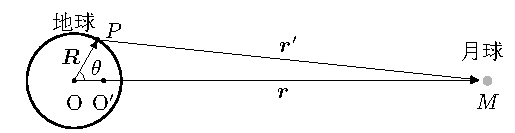
\includegraphics[width=10cm]{fig/II1-Earth.pdf}
    \caption{地月潮汐力} \label{chsr:fig_tidal-force}
\end{figure}



参见图\ref{chsr:fig_tidal-force}.
地心到月心距离为$r$,地球半径为$R$,月球质量为$M$.其中$O'$是地月质心,地球、月球分别绕$O'$点旋转.
我们以地心$O$为原点建立一个坐标系;$z$轴沿地心、月心连线,指向月心方向;
$x$轴在纸面上,垂直于$z$轴,方向向上;按右手叉乘规则确定$y$轴,即垂直于纸面向外.
现在我们来推导地月系统中引潮力的公式.
我们假设地球表面被海水覆盖;
在地球表面$P$点处有质量为$m$的海水质团,质团$m$受月球的吸引力为
\begin{equation}
    \boldsymbol{f} =\frac{GMm}{r^{\prime 3}} \boldsymbol{r}^{\prime} .
\end{equation}

地心坐标系$O-xyz$并非惯性系,需要附加上惯性力之后才能继续用牛顿第二定律.然而,
任何质量在地心参考系内所受的惯性力,等于把它放在地心处时所受引力的负值,二者是精确抵消的.故
\begin{equation}
    \boldsymbol{f}_{I}=-\frac{GMm}{r^3} \boldsymbol{r} .
\end{equation}
引力$\boldsymbol{f}$ 与 惯性力$\boldsymbol{f}_{I}$合力便是{\heiti 潮汐力}$\boldsymbol{f}_{T}$:
\begin{equation}
    \boldsymbol{f}_{T}=\boldsymbol{f}+\boldsymbol{f}_{I}
    =GMm \left(\frac{\boldsymbol{r}^{\prime}}{r^{\prime 3}} -\frac{\boldsymbol{r}}{r^3}\right) .
\end{equation}
从图\ref{chsr:fig_tidal-force}可以看出:$\boldsymbol{r}^{\prime}=\boldsymbol{r}-\boldsymbol{R}$,则有
\begin{equation}
    \frac{1}{r^{\prime 3}}=\left(r^2+R^2-2 r R \cos \theta\right)^{-3/2}
    \approx  \frac{1}{r^{3}}\left(1+ 3\frac{R}{r}\cos\theta \right) .
\end{equation}
已用$R\lll r$,并微扰展开.同时还有
\begin{equation}
    (\boldsymbol{r}-\boldsymbol{R})_z = r-R \cos \theta, \qquad
    (\boldsymbol{r}-\boldsymbol{R})_x = -R \sin \theta .
\end{equation}
故有
\begin{align}
    \left(f_{I}\right)_z =& \frac{GMm}{r^2}\left[\frac{1-\frac{R}{r} \cos \theta}
    {\left(1-\frac{2 R}{r} \cos \theta+\frac{R^2}{r^2}\right)^{3 / 2}}-1\right] 
    \approx \frac{2 GMm}{r^3} R \cos \theta, \label{chsr:eqn_Tidal-Fz} \\
    \left(f_{I}\right)_x \approx & -GMm R \sin \theta \frac{1}{r^{3}}\left(1+ 3\frac{R}{r}\cos\theta \right)
    \approx -\frac{GMm}{r^3} R \sin \theta .
    \label{chsr:eqn_Tidal-Fx}
\end{align}
海水$P$所受潮汐力在$y$方向上为零.
%需注意:以上两式中$R$为地球的半径$R_{\oplus}$,$r$为地月距离$r_{\text {月 }}$.

这个潮汐力具有绕$z$轴旋转的对称性,故$x$、$y$方向是平权的;
我们通过这种对称性导出潮汐力更一般的公式.
\setlength{\mathindent}{0em}
\begin{align*}
    \boldsymbol{f}_T = \boldsymbol{e}_x \left(f_{I}\right)_x + \boldsymbol{e}_y \left(f_{I}\right)_y
    + \boldsymbol{e}_z \left(f_{I}\right)_z
    = \frac{GMm}{r^3}  \left( -\boldsymbol{e}_x R \sin\theta + \boldsymbol{e}_y \times 0
    + \boldsymbol{e}_z 2 R \cos \theta \right).
\end{align*}\setlength{\mathindent}{2em}
海水质团$P$在地球表面;我们已经建立坐标系$O-xyz$,那么$R \cos \theta$便是
质团$P$的$z$坐标分量;$R \sin\theta$是$P$的$x$坐标分量;
如果我们再引入一个方位角$\varphi$,利用绕$z$的对称性,容易得到:
\begin{equation}\label{chsr:eqn_Tidal-Force}
    \begin{aligned}
    \boldsymbol{f}_T =& \frac{GMm}{r^3}  \left( -\boldsymbol{e}_x R \sin\theta \cos\varphi
    - \boldsymbol{e}_y  R \sin\theta \sin\varphi
    + \boldsymbol{e}_z 2 R \cos \theta \right) \\
    =&\frac{GMm}{r^3}  \left( -\boldsymbol{e}_x x - \boldsymbol{e}_y  y
     + \boldsymbol{e}_z 2 z \right) .
    \end{aligned}
\end{equation}
上式第二行中$x$、$y$、$z$是海水质团$P$在我们所建地心坐标系$O-xyz$中的分量.
从上式可以看出地球表面离月亮最远点和最近点的潮汐力大小是相等的,但方向相反,
最远点指向背离月心方向,最近点指向月心方向.这样,沿月心、地心连线方向,
地球表面海水被拉伸了.从上式还可看出,在垂直于月心、地心连线方向,
潮汐力是指向地心的,故在这个方向海水被压缩.

$r$是月心到地心距离,在$O-xyz$系中不难求得
\begin{equation}
    \frac{\partial^2 r^{-1}}{\partial x^2 } =-\frac{1}{r^3} =\frac{\partial^2 r^{-1}}{\partial y^2 } ,
    \quad \frac{\partial^2 r^{-1}}{\partial z^2 } = \frac{2}{r^3}.
    \quad \text{其它二次偏导为零}
\end{equation}
上述偏导皆在地心处取值.由此可知,式\eqref{chsr:eqn_Tidal-Force}可改写为引力势形式
\begin{equation}
    {f}_T^k = -m x^l  \frac{\partial^2 \Phi }{\partial x^l \partial x^k} .
    \qquad \Phi = -\frac{G M }{r} 
\end{equation}
命
\begin{equation}\label{chsr:eqn_Ri00k}
    R_{\hphantom{i}00k}^i  \equiv - \frac{\partial^2 \Phi }{\partial x^i \partial x^k}.
\end{equation}
额外的指标“00”是为了以后对比所用(见\S\ref{chsch:sec_GDTF}).故有
\begin{equation}\label{chsr:eqn_TF-R}
    f^i_T =  m R_{\hphantom{i}00k}^i x^k .
\end{equation}


\begin{example}
    月球、太阳对地球潮汐力比值.
\end{example}
虽然式\eqref{chsr:eqn_Tidal-Force}是以地月系为模型推导得来,
但这个公式适用于任何场合的潮汐力(牛顿力学范畴内).
已知:太阳质量 $M_{s}=1.988\times 10^{30}  $ \si{kg} ,
日地平均距离 $r_s= 1.496\times 10^{11} $ \si{m} ;
月球质量$M_{m} =7.342\times 10^{22}$ \si{kg},地月平均距离$r_m=3.844 \times 10^8$ \si{m}.
两个潮汐力比值为
\begin{equation}
    \frac{f^{\text{日}}_T}{f^{\text{月}}_T} = \frac{ M_s/r_s^3 }{M_m/r_m^3}
    \approx 0.46 = 46 \% .
\end{equation}
上述计算说明太阳对地球的潮汐力大约是月球对地球的一半. \qed

\begin{example}\label{chsr:exam_Roche}
    洛希极限(\'{E}douard Roche,法国天文学家,1820-1883).
\end{example}
一颗质量为$m$、半径为$r$的球形固态星体,
围绕着一颗质量为$M$、半径为$R$的星体作圆周运动.
当$m$的轨道半径小于$r_{\rm cirt}$时,$m$上的小石块将被潮汐力提起;
$r_{\rm cirt}$被称为洛希极限或洛希半径.
只需用式\eqref{chsr:eqn_Tidal-Force}中的$z$分量即可
\begin{equation}\label{chsr:eqn_Roche}
    \frac{2r GM m' }{r^3_{\rm cirt}} =  \frac{ Gm m' }{r^2}
    \ \Rightarrow \ 
    r_{\rm cirt} = r \left(\frac{2M}{m}\right)^{1/3} 
    = R \left(\frac{2 \rho_M}{\rho_m}\right)^{1/3} 
\end{equation}
上式最后一步,已假设两个星体的密度是均匀的.
式\eqref{chsr:eqn_Roche}为最简单的洛希极限公式,其它模型系数略有不同.
以地球为例来计算洛希半径;地球半径约$6378 km$,平均密度为$5508 kg/m^3$,
人的密度约是$1000 kg/m^3$.由式\eqref{chsr:eqn_Roche}得
$    r_{\rm cirt} \approx 14200\ km $;
洛希半径大约是地球半径的两倍多.
可能读者会有疑问,不是说星体处于洛希半径内,会被潮汐力撕碎吗?
但我活得好好的,没被撕碎!为什么?
从上面推导,我们应该能看到洛希半径只针对以引力为粘合力的物体,
而人体是以电磁力为粘合力的.两者的量级差异请参见例题\ref{chsr:exm_gem}.
\qed


\section{狭义相对论基本原理}\label{chsr:sec_srf}
\textcite[附录II.6]{einstein_sg}注意到上述矛盾,经过缜密地思考,他在1905年
从如下两个独立的假设出发导出了狭义相对论的大部分物理内容.

\index[physwords]{狭义相对性原理} \index[physwords]{光速不变原理}

{\heiti 狭义相对性原理}:所有惯性系都是平权的、不可分辨的,不存在一个特殊的惯性
参考系.物理规律在任一个惯性系都一样,数学上表现为在各个惯性系基本定律的方程式形式不变.

{\heiti 真空光速不变原理}:真空中,任何一个惯性参考系的光速都恒为$c$,与光源运动速度无关,
与光发射方向无关.


相对性原理否定了牛顿绝对静止参考系的存在,但仍然假设存在一类特殊的惯性参考系,
后来爱因斯坦提出了广义相对论,在那里无需这个概念了.在牛顿力学中也存在相对性原理,
只不过它要求力学理论对伽利略变换不变.
光速不变原理是一个非常大胆假设,这个假设与伽利略变换直接相悖.

\index[physwords]{间隔}
\index[physwords]{间隔!不变性}

\subsection{间隔不变性}
为了看清楚这两个原理的数学意义,需要定义一个重要的概念——{\heiti 事件}:
它是指$t$时刻,在$(x,y,z)$处发生某事,将时间和空间坐标结合在一起表示为
$P(t,x,y,z)$.这与我们日常生活相符合,比如我们说某某事件,那必须指明它
发生的时间和地点.这一概念是从物质运动中抽象出来的,物质运动可以看作是一连串
事件的发展过程.比如我走了一段路就是一连串事件,你静静地坐在椅子上十分钟也是
一连串事件,当然做物理实验更是事件.

对于任意两个事件$P(t_0,x_0,y_0,z_0)$和$P(t_1,x_1,y_1,z_1)$,其时间间隔和空间间隔分别为
\begin{equation}
  \Delta t = t_1-t_0, \quad
  \Delta l = \sqrt{(x_1-x_0)^2+(y_1-y_0)^2+(z_1-z_0)^2}.
\end{equation}
在牛顿的绝对时空观中$\Delta t$与$\Delta l$是无关联的.
爱因斯坦敏锐地意识到这两个量是有密切关系的,无法分开处理.
为此定义一个新的量
\begin{equation}\label{chsr:eqn_interval}
  s ^2 \overset{def}{=} -c^2 (t_1-t_0)^2 + (x_1-x_0)^2+(y_1-y_0)^2+(z_1-z_0)^2,
\end{equation}
$s$称之为{\heiti 时空间隔},简称{\heiti 间隔},
{\footnote{间隔英文是interval,物理学家为四维时空的距离另造的一个词儿,以便与三维空间区别开来.}}
其量纲是长度,$c$是光速.
我们来看一下爱因斯坦如何用上面两个基本原理和间隔的概念来改变物理时空观.
见图\ref{chsr:pic_oop},考察在开始时刻$t=0=t'$,自重合的原点$O(O')$发出
一个光信号.{\kaishu 按照光速不变原理},两个参考系中的光速都是$c$,则
光在两个系中的波阵面方程是
\begin{align}
  s ^2 &= -c^2 t ^2 + ({x^2+ y^2+ z^2})=0, \\
  s'^2 &= -c^2 t'^2 + ({x'^2+ y'^2+ z'^2})=0,
\end{align}
应该同时成立,即
\begin{equation}
  s ^2 =0 {\quad \color{red} \Leftrightarrow \quad } s'^2 =0.
\end{equation}
上述式子只对光信号成立.一般说来两个事件之间未必由光信号相联系,
可能是其它信号,也可能根本没有联系;$s$也未必等于零.
{\kaishu 根据狭义相对性原理},两个惯性参考系$O$与$O'$应当
是平权的(见图\ref{chsr:pic_oop}),例如相对$O$系作匀速直线运动的质点,在$O'$系中也必须是
作匀速直线运动.能够保持这种运动方式不变的参考系间的时空变换只能是线性变换,
我们进一步解释一下这个线性变换.不失一般性,假设在惯性参考系$O$中有一质点$p$沿$x$轴作匀速直线
运动,速度$u=\frac{{\rm d}x}{{\rm d}t}$是常数,加速度自然恒为零;如果质点$p$运动不沿$x$轴,作一次坐标轴
旋转即可.我们已假设另一惯性参考系$O'$相对$O$沿$x$轴运动(见图\ref{chsr:pic_oop}),那么,
不论在$O$系还是在$O'$系质点$p$都沿$x(x')$轴,在$y$和$z$轴方向没有速度分量.
同时,由于两惯性系间速度差沿$x$轴,在$y,z$方向没有分量,容易得到这两个轴的变换关系是
\begin{equation}
    y' = y, \qquad z'=z.
\end{equation}
再假设$\{t,x\}\to \{t',x'\}$的变换关系是(约定变换之后$t'$是时间,$x'$是位置)
\begin{equation}
    t'= f(t,x), \qquad  x'= g(t,x).
\end{equation}
其中,$f$和$g$还是两惯性系速度差$v$(实常数)的函数,省略未标记;
函数$f$和$g$变换之后的$t',x'$不能有奇点.
由上式可求$O'$系中质点$p$的速度和加速度:
\begin{align}
    u'=&\frac{{\rm d}x'}{{\rm d}t'} = \frac{g_t(t,x){\rm d}t+g_x(t,x){\rm d}x}{f_t(t,x){\rm d}t+f_x(t,x){\rm d}x}
      = \frac{g_t+g_x u}{f_t+f_x u}, \\
    a'=&\frac{{\rm d}u'}{{\rm d}t'}  %= \frac{1}{f_t+f_x u} \frac{g_{tt}{\rm d}t+g_{tx}{\rm d}x
%        +g_{xt}u{\rm d}t+g_{xx}u{\rm d}x}{f_t{\rm d}t+f_x{\rm d}x} \\
%    & - \frac{g_t+g_x u}{(f_t+f_x u)^2}\frac{f_{tt}{\rm d}t+f_{tx}{\rm d}x
%        +f_{xt}u{\rm d}t+f_{xx}u{\rm d}x}{f_t{\rm d}t+f_x{\rm d}x} \\
    = \frac{g_{tt}+2g_{tx}u +g_{xx}u^2}{(f_t+f_x u)^2}
      -\frac{(g_t+g_x u)(f_{tt}+2f_{tx}u +f_{xx}u^2)}{(f_t+f_x u)^3} .
\end{align}
由上式能够看到,如果$f$和$g$的二阶偏导数不为零,那么$p$的加速度$a'$必然不为零.
质点$p$在惯性参考系$O$中是作匀速直线运动,在参考系$O'$中却有加速度,这只能说明
参考系$O'$是非惯性系;与之前假设$O'$是惯性系矛盾.可见满足两个惯性系$O$和$O'$间
的变换必然是$f$和$g$的所有二阶偏导数(对任意$t$和$x$值)恒为零,更高阶偏导数自然也
恒为零;所以$f$和$g$只能是线性函数.
狭义相对论只研究惯性系间的变换,自然会得到“$f$和$g$只能是线性函数”.
如果研究非惯性系间的变换,则未必是线性的,可参考\S \ref{chsr:sec_Rindler-space}.

既然时空变换是线性的,而$s'^2$与$s^2$是同阶量,
那么间隔间的变换也是线性的,即 
\begin{equation}\label{chsr:eqn_sps}
  s'^2 = a(v) s^2 + b(v).
\end{equation}
从光信号间的关系可知$b(v)\equiv 0$.


因空间是均匀、各向同性的,时间是均匀的,所以系数$a(v)$只能是
速度{\kaishu 大小}的函数,不会与速度方向有关;特别有$a(v)=a(-v)$,这个关系很重要.
由$O$与$O'$的平权关系,交换$O$与$O'$,可得
\begin{equation*}
  s^2 = a(-v) s'^2 {\quad\color{red}\Rightarrow\quad} s^2 = a(-v)\bigl( a(v) s^2 \bigr)
   = \bigl( a(v) \bigr)^2 s^2 {\quad \color{red}\Rightarrow\quad} a(v)=\pm 1.
\end{equation*}
需注意,$a(v)$不可能连续的从$-1$变到$+1$,只能取两者之一.
速度$v=0$的恒等变换不会改变任何事情,此时$a(v=0)=1$;由这个特例排除了$a(v)=-1$的可能.
因此得到任意两事件间间隔,不论由何种信号相联系或者无联系,都有
$a(v)\equiv 1$,也就是时空间隔是参考系变换的不变量
\begin{equation}\label{chsr:eqn_interval-inv}
  s'^2 \equiv s^2.
\end{equation}
如果两事件的间隔是无穷小量,上式变为
\begin{equation}\label{chsr:eqn_interval-inv-ds}
  {\rm d}s^2 = -c^2{\rm d}t^2 +{\rm d}x^2 +{\rm d}y^2 +{\rm d}z^2 \quad \text{是参考系变换不变量}.
\end{equation}
这是狭义相对论两条基本假设的数学表述.

间隔是相对论中非常重要的一个概念,由式\eqref{chsr:eqn_interval}可知,如果两事件在
同一时刻发生,那么$s^2=(x_1-x_0)^2+(y_1-y_0)^2+(z_1-z_0)^2>0$;如果两事件在同一地点
先后发生,那么$s^2=-c^2(t_1-t_0)^2<0$.可见时间和空间都统一在间隔这个概念里,
间隔的{\kaishu 平方}是可正可负的,这与我们通常接触的欧几里得几何不同,后面
大家会明白这一点.




\index[physwords]{洛伦兹变换} \index[physwords]{Lorentz变换}

\subsection{洛伦兹变换}\label{chsr:sec_lorentz-transofrm}
由间隔不变性(式\eqref{chsr:eqn_interval-inv})出发,容易求得{\heiti 洛伦兹变换}:
\begin{equation}\label{chsr:eqn_lorentz-transofrm-x}
    t' = \gamma \left({t-\dfrac{v}{c^2}x}\right), \quad
    x' = \gamma \left({x-vt}\right), \quad
    y' = y, \quad
    z' = z.
\end{equation}
其中$\gamma$是洛伦兹因子:
\begin{equation}
    \gamma^{-1}=\sqrt{1-\dfrac{v^2}{c^2}}.
\end{equation}
读者需要注意,两惯性系间的速度差$v$是个常数,与时空无关.

很容易求得式\eqref{chsr:eqn_lorentz-transofrm-x}的逆变换,就是在速度$v$前面加一个负号:
\begin{equation}\label{chsr:eqn_lorentz-transofrm-x-inv}
    t = \gamma \left({t'+\dfrac{v}{c^2}x'}\right), \quad
    x = \gamma ({x'+vt'}), \quad
    y = y', \quad
    z = z'.
\end{equation}
从洛伦兹变换容易看到,时间和空间不再彼此独立,两者可以相互转化.

洛伦兹变换\eqref{chsr:eqn_lorentz-transofrm-x}的微分形式为:
\begin{equation}\label{chsr:eqn_lorentz-transofrm-dx}
	{\rm d}t' = \gamma \left({{\rm d}t-\dfrac{v}{c^2}{\rm d}x}\right), \
	{\rm d}x' = \gamma \left({{\rm d}x-v{\rm d}t}\right), \
	{\rm d}y' = {\rm d}y, \
	{\rm d}z' = {\rm d}z.
\end{equation}
狭义相对论要求所有相互作用必须是近距作用(local,或者说是局域作用),不能是超距作用.
式\eqref{chsr:eqn_lorentz-transofrm-dx}为无穷小的变换,自然是近距的.
同时容易看到当$v \ll c$时,$\gamma \approx 1$,
式\eqref{chsr:eqn_lorentz-transofrm-dx}就退化到伽利略变换\eqref{chsr:eqn_galileo-trans-dx}.
然而,在有限距离的洛伦兹变换\eqref{chsr:eqn_lorentz-transofrm-x}中,当$x$是个大量(比如日地距离)时,
变换\eqref{chsr:eqn_lorentz-transofrm-x}中第一式变为$t' \approx t-\frac{v}{c^2}x$,
不能退化到伽利略变换\eqref{chsr:eqn_galileo-trans-x}.
其根源无非是光速$c$是个有限大小的量(不是无穷大),长距离的变换(比如日地距离)必须包含推迟效应,
否则必然导致超距作用.也可以从积分角度来解释之;
式\eqref{chsr:eqn_lorentz-transofrm-x}无非是\eqref{chsr:eqn_lorentz-transofrm-dx}的积分,
上述过程是说积分量$\int \frac{v}{c^2}{\rm d}x$是个大量,无法忽略而已.

洛伦兹变换的发现历史十分复杂,读者如有兴趣可参阅相应文献,比如Wikipedia条目
{\footnote{\url{https://en.wikipedia.org/wiki/History\_of\_Lorentz\_transformations}}}.
洛伦兹本人为了区分自己的理论与爱因斯坦的理论,而将爱氏理论称为“相对论”.




把前面给出的时空洛伦兹变换\eqref{chsr:eqn_lorentz-transofrm-x}用四维矩阵再表述一次:
\begin{equation}\label{chsr:eqn_lorentz-transofrm-x-MatrixForm}
\begin{pmatrix}
ct'\\x'\\y'\\z'
\end{pmatrix} =
\begin{pmatrix}
\gamma & -\gamma \beta  & 0 & 0 \\
-\gamma \beta & \gamma  & 0 & 0 \\
0 & 0 & 1 & 0 \\
0 & 0 & 0 & 1
\end{pmatrix}
\begin{pmatrix}
ct\\x\\y\\z
\end{pmatrix} \equiv \Lambda
\begin{pmatrix}
ct\\x\\y\\z
\end{pmatrix}, \qquad \boldsymbol{\beta}=\frac{\boldsymbol{v}}{c}.
\end{equation}
用$\Lambda$标记洛伦兹矩阵.




相对论下质点速度定义仍为式\eqref{chsr:eqn_3-Velocity}.
由\eqref{chsr:eqn_lorentz-transofrm-dx}易得:
\begin{equation}\label{chsr:eqn_lorentz-transofrm-vel}
    u'_x = \dfrac{u_x -v}{1-u_x v/c^2}, \quad
    u'_y = \dfrac{\gamma^{-1}u_y}{1-u_x v/c^2}, \quad
    u'_z = \dfrac{\gamma^{-1}u_z}{1-u_x v/c^2}.
\end{equation}
其逆变换就是将$v$前添加一负号
\begin{equation}\label{chsr:eqn_lorentz-transofrm-vel-inv}
    u_x = \dfrac{u'_x +v}{1+u'_x v/c^2}, \quad
    u_y = \dfrac{\gamma^{-1}u'_y}{1+u'_x v/c^2}, \quad
    u_z = \dfrac{\gamma^{-1}u'_z}{1+u'_x v/c^2}.
\end{equation}
同时容易看到当$v \ll c$、$u \ll c$时,式\eqref{chsr:eqn_lorentz-transofrm-vel}
就退化到伽利略变换\eqref{chsr:eqn_galileo-trans-vel}.

\begin{example}
    证明在洛伦兹速度变换\eqref{chsr:eqn_lorentz-transofrm-vel}下,光速不变.
\end{example}
如果$O$系中发射一个光信号,即令$u_x=c,u_y=u_z=0$;
由式\eqref{chsr:eqn_lorentz-transofrm-vel}不难得到,
$u'_x = \frac{u_x -v}{1-u_x v/c^2} = \frac{c -v}{1-  v/c} = c, u'_y=u'_z=0$;
也就是在$O'$系来看这个光信号仍旧是光速$c$.

若令式\eqref{chsr:eqn_lorentz-transofrm-vel}中$u'_x=u_x$,并且$y$、$z$方向速度都为零,则有
\begin{equation}
    u_x = \frac{u_x -v}{1-u_x v/c^2} \quad \Rightarrow \quad u_x =c.  
\end{equation}
这说明在洛伦兹变换下,若速度是不变量,则必是光速.\qed


\begin{example}\label{chsr:exam_ucc}
    若质点在惯性系$O$是亚光速的,则它在惯性系$O'$也是亚光速.
\end{example}
洛伦兹速度变换不改变时空间隔,
用时空间隔不变性证明,由\eqref{chsr:eqn_interval-inv-ds}得到
\begin{align}
   & -c^2{\rm d}t^2 +{\rm d}x^2 +{\rm d}y^2 +{\rm d}z^2
   = -c^2{\rm d}t'^2 +{\rm d}x'^2 +{\rm d}y'^2 +{\rm d}z'^2 \notag \\
  {\color{red}\Rightarrow} & (-c^2 + u^2) {\rm d}t^2  = (-c^2 + u'^2) {\rm d}t'^2
\end{align}
因为${\rm d}t^2 >0$ 且${\rm d}t'^2 >0$,所以如果$c^2 > u^2$那么必有$c^2 > u'^2$,即$u'<c$.

同时很显然,如果$u>c$,那么变换后的$u'>c$.\qed

\begin{remark}
    笔者认为“时空间隔不变性”是比“洛伦兹变换”更基本的内容,间隔不变性是狭义相对论两条基本假设的数学表述.
    有学者先给出洛伦兹变换,然后用它再导出时空间隔不变;笔者个人认为这种叙述方式逻辑颠倒了.
\end{remark}


\subsection{狭义相对论适用范围刍议}\label{chsr:sec_SR-scope}
任何一个理论都有适用范围,有的已经发现,有的还未发现其适用范围.比如牛顿力学只能
在低能、低速、宏观环境下应用;万有引力公式只能在弱引力下使用,等等.

现今,狭义相对论已经被实验证实完全正确,那它的适用范围又是什么呢?首先,
绝大多数物理学家认为引力在狭义相对论适用范围之外.引力由广义相对论来描述,其
时空是弯曲的;而狭义相对论时空是平直的.
其次(笔者个人观点),狭义相对论{\heiti 只能}约束具有{\heiti 非零}能量、动量的粒子.
这些粒子可以处于自由态,也可以处于相互作用态.可以是有静质量的实物粒子;也可以是
无静质量的粒子,比如光子,但(尚未发现的)引力子除外.

电磁波相速度可以超光速,此过程不传递任何非零能动量粒子,它应该在狭义相对论适用范围之外.
再者,像量子纠缠中的波函数坍缩过程不传递任何非零能动量粒子,所以它也在狭义相对论适用范围之外.


我们再谈一下局域(locality)与非局域(non-locality).
笔者个人理解,局域性是指两个类时事件有因果关系,联系两者的信号必须是光速或亚光速.
非局域是指两个类空事件间存在超光速联系,比如量子纠缠中的波函数坍缩过程.

%在量子力学中的Aharonov--Bohm效应中,如果用规范势$A^\mu$来描述是属于近距作用;如果用$\boldsymbol{E}$、$\boldsymbol{B}$描述则是超距作用.



\section{相对论力学}\label{chsr:sec_relativitic-mech}
我们继续回顾相对论力学.

狭义相对论是一个描述时空结构的运动学理论,它本身并不涉及动力学内容.
在\S\ref{chsr:sec_SR-scope}中我们陈述到:除引力子外,所有具有非零能量、动量的粒子
都要受到它的约束;数学上来说就是这些粒子的动力学方程要洛伦兹协变.
在牛顿绝对空间的时空观下,经典力学满足伽利略变换,显然不是洛伦兹协变的;我们需要修改牛顿
力学使之变成洛伦兹协变,并且在质点运动速度远远小于光速时,它能退化到伽利略变换.
我们先讨论有质量的粒子,再讨论无质量粒子.

\subsection{有质量粒子运动学}
固有时$\tau$与坐标时的关系是
\begin{equation}
	\dfrac{{\rm d} \tau}{{\rm d} t}=\gamma_u^{-1} = \sqrt{1-\frac{u^2}{c^2}}.
\end{equation}
质点$p$四速度是指其时空坐标对固有时的导数,即
\begin{equation}\label{chsr:eqn_4U}
	U^\mu |_p \overset{def}{=} \dfrac{{\rm d} x^\mu}{{\rm d} \tau} \Big|_p
	= \dfrac{{\rm d} x^\mu}{{\rm d} t} \dfrac{{\rm d} t}{{\rm d} \tau}
	= \gamma_u (c,\boldsymbol{u}).
\end{equation}
四速度是由光速$c$与经典的三维速度$\boldsymbol{u}$组合而成.

\index[physwords]{洛伦兹四速度} \index[physwords]{四速度} \index[physwords]{四加速度}

四加速度是指四速度对固有时间的导数,即
\begin{equation}\label{chsr:eqn_4A}
	A^\mu \overset{def}{=} \dfrac{{\rm d} U^\mu}{{\rm d} \tau}
	= c^{-2}\gamma_{u}^2  \left( \gamma_{u}^2 c \,\boldsymbol{u}\cdot \boldsymbol{a}, \
	c^2\boldsymbol{a} + \gamma_{u}^2 (\boldsymbol{u}\cdot \boldsymbol{a}) \boldsymbol{u}\right)  .
\end{equation}
期中3-加速度定义仍旧不变$\boldsymbol{a}={\rm d}\boldsymbol{u}/{{\rm d}t}$.
加速度洛伦兹变换是
\begin{equation}\label{chsr:eqn_3Atrans}
	\begin{aligned}
		a'_x &= \dfrac{\gamma^{-3}_v a_x}{(1-u_x v/c^2)^3}, \\
		a'_y &= \dfrac{\gamma^{-2}_v a_y}{(1-u_x v/c^2)^2}+\dfrac{\gamma^{-2}_v a_x u_y v}{c^2(1-u_x v/c^2)^3}, \\
		a'_z &= \dfrac{\gamma^{-2}_v a_z}{(1-u_x v/c^2)^2}+\dfrac{\gamma^{-2}_v a_x u_z v}{c^2(1-u_x v/c^2)^3}.
	\end{aligned}
\end{equation}




\subsection{有质量粒子四动量及其动力学}
三维空间{\kaishu 非}相对论动量是$\boldsymbol{p}_{nr} = m \boldsymbol{u}$;其中{\kaishu 常数}$m$是质点静质量,
为洛伦兹标量;$\boldsymbol{u}$是质点3-速度.
质点{\heiti 四动量}可以很自然地推广为
\begin{equation}\label{chsr:eqn_4momentum}
	p^\mu \overset{def}{=}  m U^\mu = (\gamma_u mc,\gamma_u m\boldsymbol{u})
	\equiv \left(\dfrac{E}{c},\boldsymbol{p}\right).
\end{equation}
其中$U^\mu$是质点四速度;最右边的恒等号定义了质点的相对论能量是$E\equiv \gamma_u mc^2$;
质点的相对论三动量是$\boldsymbol{p}\equiv\gamma_u m\boldsymbol{u}$,
与非相对论的动量$\boldsymbol{p}_{nr}$差别在于乘上了因子$\gamma_u$.
包括爱因斯坦在内的诸多物理学家建议相对论中
只引入静质量概念,不引入诸如动质量、纵质量、横质量等概念;我们也就不讨论这些质量的定义了.

我们再列出粒子的能动关系式
\begin{equation}\label{chsr:eqn_energyp}
    E^2  = (|\boldsymbol{p}| c)^2 + (m c^2)^2 .
\end{equation}




前面给出了低速三维动量定义$\boldsymbol{p}_{nr} = m \boldsymbol{u}$,从牛顿力学中我们知道三维空间低速情形牛顿第二定律是
\begin{equation}\label{chsr:eqn_NewtonII}
	m\frac{{\rm d}\boldsymbol{u}}{{\rm d}t}  = \frac{{\rm d}\boldsymbol{p}_{nr}}{{\rm d}t} =  \boldsymbol{F}_{nr} .
\end{equation}
其中$\boldsymbol{F}_{nr}$是质点所受外力.这个定律一个很自然的推广是
\begin{equation}\label{chsr:eqn_NewtonII-relativity}
	m\frac{{\rm d}{U^\mu}}{{\rm d}\tau} = \frac{{\rm d}{p^\mu}}{{\rm d}\tau}  =  K^\mu .
\end{equation}
$K^\mu$是四维力.
式\eqref{chsr:eqn_NewtonII-relativity}不是定理而是定律,
是{\kaishu 狭义相对论中的牛顿第二定律}.

对固有时求导多有不便,我们换成坐标时
\begin{equation}
	K^\mu =   \frac{{\rm d}{p^\mu}}{{\rm d}\tau}
	= \gamma_{u} \dfrac{{\rm d}[  (\gamma_u m c,\gamma_u m\boldsymbol{u})]}{{\rm d} t}
	= \gamma_{u} \dfrac{{\rm d}[  (E/c,\boldsymbol{p})]}{{\rm d} t} .
\end{equation}
我们将上式的时间、空间分量分开来写
\begin{align}
	\gamma_{u}^{-1} K^0 &= \dfrac{{\rm d}  (\gamma_u m c)}{{\rm d} t}
	= \dfrac{{\rm d}  (E/c)}{{\rm d} t} \quad =\frac{1}{c}\boldsymbol{u}\cdot\boldsymbol{F}; \label{chsr:eqn_p0Fu}  \\
	\gamma_{u}^{-1} \boldsymbol{K} &= \dfrac{{\rm d}  (\gamma_u m \boldsymbol{u})}{{\rm d} t}
	=\dfrac{{\rm d} \boldsymbol{p}}{{\rm d} t}
	\quad {\color{red} \Leftrightarrow} \quad
	\boldsymbol{F} \ = \dfrac{{\rm d} \boldsymbol{p} }{{\rm d} t}. \label{chsr:eqn_3pNewtonII}
\end{align}
其中式\eqref{chsr:eqn_3pNewtonII}中的力定义为$\boldsymbol{F} \equiv \gamma_{u}^{-1} \boldsymbol{K}$,
这样三维形式的\eqref{chsr:eqn_3pNewtonII}就是非相对论牛顿第二定律\eqref{chsr:eqn_NewtonII}的
相对论对应.需要注意\eqref{chsr:eqn_3pNewtonII}中的动量$\boldsymbol{p}=\gamma_u m \boldsymbol{u}$是相对论的.

这样我们就把四维力$K^\mu$换了一个形式
\begin{equation}\label{chsr:eqn_4dforce-3d}
	K^\mu \equiv (K^0,\boldsymbol{K}) = \gamma_{u} \left(\frac{1}{c}\boldsymbol{u}\cdot\boldsymbol{F}, \boldsymbol{F} \right)
\end{equation}
需要注意,上式只是把$K^\mu$改了一个形式,没有什么本质变化.
三维力$\boldsymbol{F}$的具体表达式不是牛顿第二定律能给出来的,需要结合其它理论
才能得到,比如电磁学中带电粒子所受洛伦兹力是$\boldsymbol{F}=q \boldsymbol{E}+q \boldsymbol{u}\times\boldsymbol{B}$.

需要注意相对论三维力$\boldsymbol{F}$与非相对论的力$\boldsymbol{F}_{nr}$不同.如果我们把牛顿第二定律理解成
力的定义,那么力$\boldsymbol{F}$是相对论3-动量$\boldsymbol{p}=\gamma_{u} m \boldsymbol{u}$对坐标时的变化率;
力$\boldsymbol{F}_{nr}$是非相对论经典动量$\boldsymbol{p}_{nr}= m \boldsymbol{u}$对牛顿绝对时间的变化率.


相对论三维力$\boldsymbol{F}=\gamma_{u}^{-1} \boldsymbol{K}$的洛伦兹变换公式
\begin{equation}
	F'_x = \dfrac{F_x - (\boldsymbol{F}\cdot \boldsymbol{u})v/c^2}{1-u_x v/c^2}, \quad
	F'_y = \dfrac{\gamma_v^{-1}F_y}{1-u_x v/c^2}, \quad
	F'_z = \dfrac{\gamma_v^{-1}F_z}{1-u_x v/c^2}.
\end{equation}




\subsection{无质量粒子四动量}
这一节讨论无质量粒子的相对论效应.目前,自由存在于自然界的无质量粒子,
实验上只发现了光子;无质量粒子胶子被禁闭在原子核内部,无直接观测证据.
严格的光子理论必然需要量子场论知识,在这里我们
只把光子当成电磁波的量子,不涉及过多量子知识.



设光子(即电磁波量子)的传播方向是单位矢量$\boldsymbol{n}$,其频率是$\nu$,角频率$\omega=2\pi \nu$;
光子波长是$\lambda$,波数是$k=2\pi/\lambda$.
按照爱因斯坦光量子假说,有
\begin{align}
	E &= h \nu = \hbar \omega  = \frac{hc}{\lambda}, \\
	\boldsymbol{p}&=\frac{h}{\lambda}  \boldsymbol{n} = \hbar \boldsymbol{k}
	\qquad\text{或}\qquad p\boldsymbol{n}=\frac{h}{\lambda}  \boldsymbol{n} = \hbar k\boldsymbol{n}.
\end{align}
其中$h$是普朗克常数,$\hbar\equiv h/2\pi$是约化普朗克常数.
真空中光子频率和波长不是独立的,有关系式$c=\lambda \nu=\omega/k$.
仿照有质量粒子四动量,定义{\heiti 光子四动量}:
\begin{equation}\label{chsr:eqn_photon-momentum}
	p^\mu  \overset{def}{=}  \left(\frac{E}{c},\boldsymbol{p}\right)
	=\hbar \left(\frac{\omega}{c},\boldsymbol{k}\right) \equiv \hbar k^\mu.
\end{equation}
上式最后一步定义了光子{\heiti 四维波矢量}$k^\mu \equiv p^\mu/\hbar$.






\section{匀加速度观测者参考系}\label{chsr:sec_yjs}
%本节取自文献\parencite[\S 6.2]{mtw1973}、\parencite[\S 12.4]{rindler-2006}.

与牛顿力学不同,在狭义相对论中,加速度是一个与参考系相关的物理量,
因此我们必须更加谨慎地表达加速度的含义.



\subsection{固有加速度}
%式\eqref{chsr:eqn_4A}和式\eqref{chsr:eqn_3Atrans}给出了加速度的公式.
我们先用$1+3$的语言来介绍.
下面考虑一个特例:设火箭沿$x(x')$轴作直线加速运动,
相对于火箭建立瞬时惯性系$O'$,则有$u'=0$,
同时还有$v=u_x=u$;$y$、$z$方向的速度、加速度都是零;
此时的加速度$a'$称为{\heiti 固有加速度}.

由式\eqref{chsr:eqn_lorentz-transofrm-vel-inv}第一式得$u(1+u' v/c^2) = u' +v$,
对此式两边取微分($u$、$u'$是变量,$v$是常量),有
\begin{equation}\label{chsr:eqn_du=gdup}
    {\rm d}u (1+u' v/c^2) + uv/c^2 {\rm d}u' = {\rm d}u'  
    \ \xRightarrow[\text{且}v=u]{\text{令}u'=0} \ 
    {\rm d}u  = \gamma^{-2}_u {\rm d}u'.  %= {\rm d}u' (1-u^2/c^2)
\end{equation}
若以$\alpha$表示固有加速度$a'$,则有${\rm d}u' = \alpha {\rm d}t' $,
再由时间膨胀得${\rm d}t' = {\rm d}t/\gamma_u$.
于是有${\rm d}u  = \gamma^{-3}_u \alpha {\rm d}t $,也就是
\begin{equation}\label{chsr:eqn_a-u}
    \alpha = \left(1-\frac{u^2}{c^2}\right)^{-3/2} \frac{{\rm d}u}{{\rm d}t}
    =\frac{ {\rm d}(\gamma_u u)}{{\rm d}t} .
\end{equation}
式\eqref{chsr:eqn_a-u}给出了由瞬时静止参考系(即固有加速度$\alpha$)
到任意参考系的加速度变换(即上式中的$\frac{{\rm d}u}{{\rm d}t}$).
%由此可以得出对于任意两个参考系$O$和$O'$(其中$O'$相对运动方向和火箭运动方向重合)有
%\begin{equation}
%    \left(1-\frac{u^2}{c^2}\right)^{-3/2} \frac{{\rm d}u}{{\rm d}t}
%    =\left(1-\frac{u'^2}{c^2}\right)^{-3/2} \frac{{\rm d}u'}{{\rm d}t'} .
%\end{equation}
%注意,加速度的在洛伦兹变换下不是不变量.

考虑匀加速运动($\alpha$是常数),
由式\eqref{chsr:eqn_a-u}对$t$积分(取$t=0$时$u=0$)有
\begin{equation}
    \gamma_{u} u = \alpha t  \quad  \Rightarrow \quad
    u(t) = \frac{\alpha t}{\sqrt{1+ \alpha^2 t^2 /c^2}} .
\end{equation}
对上式再积分一次(取$t=0$时$x=\frac{c^2}{\alpha}$),有
\begin{equation}\label{chsr:eqn_x-at}
    x(t)= \frac{c^2}{\alpha} \sqrt{1+ \alpha^2 t^2 /c^2} .
\end{equation}
由\eqref{chsr:eqn_x-at}式可知:
\begin{equation}\label{chsr:eqn_x2t2X}
    x^2 - (ct)^2 = \frac{c^4}{\alpha^2} .
\end{equation}
上式说明:作直线运动的火箭的固有加速度若为常数,
则它在闵氏时空中的世界线不是抛物线,而是双曲线.
参见图\ref{chsr:fig_Rindler} $R$区的双曲线.

当$u\lll c$且$\alpha t \lll c$时,上几式中的速度和位移退化为牛顿极限情形
\begin{equation}
    u\approx \alpha t,\qquad x \approx \frac{1}{2}\alpha t^2 +\frac{c^2}{\alpha} .
\end{equation}



%为简洁起见,下面令光速$c=1$.并且只考虑固有加速度为常数的情形.


{\kaishu 我们用四维语言再次描述一下上述匀加速运动}.
在瞬时静止的参考系$\{O'\}$中,火箭四速度$U^a$只有第零分量,
其它三个分量恒为零,且满足$U^a U_a =-c^2$.
我们已知四加速度和四速度是正交的,即$U^a A_a =0$;
那么自然可以得到:瞬时系的火箭四加速度$A^0\equiv 0$,即$A^\mu=(0,\boldsymbol{A})$.
固有加速度(即瞬时系的加速度)为常数是指$\sum_{i=1}^{3}(A^i)^2 = \alpha^2$是常数.

我们将瞬时系的物理量变到地面系$\{O\}$(即惯性系)来看,
\begin{equation}
    A^\mu A_\mu = \alpha^2; \quad
    U^\mu U_\mu = -c^2; \quad
    U^\mu A_\mu = 0. 
\end{equation}
我们已选定,所有运动只沿$x(x')$轴;故由上式有
\begin{equation}
    A^0=\frac{\alpha}{c} U^1; \qquad    A^1=\frac{\alpha}{c} U^0.
\end{equation}
依定义,有
\begin{equation}\label{chsr:eqn_dx=u}
    \frac{{\rm d}ct}{{\rm d}\tau} = U^0,\quad
    \frac{{\rm d}x}{{\rm d}\tau} = U^1;\qquad
    \frac{{\rm d}U^0}{{\rm d}\tau} = A^0,\quad
    \frac{{\rm d}U^1}{{\rm d}\tau} = A^1 .
\end{equation}
上式中$t$、$x$分别是火箭在惯性系$\{O\}$中的时间坐标、空间坐标;$\tau$是固有时.
结合上两式,有
\begin{equation}
    \frac{{\rm d}U^0}{{\rm d}\tau}= \frac{\alpha}{c} U^1; \qquad
    \frac{{\rm d}U^1}{{\rm d}\tau}= \frac{\alpha}{c} U^0.
\end{equation}
对上式积分(取$\tau=0$时,$U^0=c$、$U^1=0$),有
\begin{equation}
    U^0 = c \cosh \frac{\alpha}{c} \tau ,\qquad
    U^1 = c \sinh \frac{\alpha}{c} \tau .
\end{equation}
由上式,可对式\eqref{chsr:eqn_dx=u}积分(取$\tau=0$时,$t=0$、$x=c^2 \alpha^{-1}$),有
\begin{equation}\label{chsr:eqn_tx-sh-ch}
    ct=c^2 \alpha^{-1} {\rm sinh}(\tau \alpha/c),\quad
    x =c^2 \alpha^{-1} {\rm cosh}(\tau \alpha/c).
\end{equation}
由上式算得$x^2-(ct)^2=c^4 \alpha^{-2}$,与式\eqref{chsr:eqn_x2t2X}相同.




\subsection{Rindler坐标}\label{chsr:sec_Rindler-space}

四维平直闵氏时空中,时空线元是($t$、$x$取遍实数轴):
\begin{equation}\label{chsr:eqn_LM}
    {\rm d}s^2 = - ({\rm d}ct)^2 +{\rm d}x^2 +{\rm d}y^2 +{\rm d}z^2 .
\end{equation}
我们分几步讨论一下如何从闵氏平直度规变到Rindler坐标.
变换只涉及到$t$、$x$,$y$、$z$不变.
首先,把闵氏度规变成类光坐标:
\begin{equation}
    u= ct - x, \quad v= ct + x;
    \quad \Leftrightarrow \quad
    ct = (u+v)/2, \quad x= (v-u)/2 .
\end{equation}
此时度规\eqref{chsr:eqn_LM}变为
\begin{equation}
    {\rm d}s^2 = - {\rm d}v{\rm d}u +{\rm d}y^2 +{\rm d}z^2 .
\end{equation}
再令(下述变换将$u$、$v$限制在$-\infty <u<0$、$0<v<+\infty$)
\begin{equation}
    u=-\frac{c^2}{\alpha}e^{-U},\qquad v=+\frac{c^2}{\alpha}e^{+V} .
\end{equation}
${c^2}/{\alpha}$的量纲是{\kaishu 长度};$V$、$U$无量纲.
上式中$-\infty< U, V <+\infty$.进而有
\begin{equation}
    {\rm d}s^2 = - \frac{c^4}{\alpha^2}e^{V-U}{\rm d}V{\rm d}U +{\rm d}y^2 +{\rm d}z^2 .
\end{equation}
继续做变换
\begin{equation}
\begin{aligned}
    cT=&\frac{1}{2}\frac{c^2}{\alpha}(V+U),\qquad X= \frac{c^2}{\alpha}e^{(V-U)/2} ; \\ 
    V=& \frac{\alpha}{c^2} cT+ \ln \frac{\alpha}{c^2}X, \qquad 
    U= \frac{\alpha}{c^2} cT - \ln \frac{\alpha}{c^2}X .
\end{aligned}    
\end{equation}
总的坐标变换为{\heiti \bfseries Rindler坐标}
\cite[\S 12.4]{rindler-2006}($y,z$不变;见图\ref{chsr:fig_Rindler}):\index[physwords]{Rindler坐标}
\begin{subequations}\label{chsr:eqn_Rindler-trans}
    \begin{align}
        &(R \text{区}) : \quad  ct=  X \sinh(T \alpha/c ), \quad x=  X\cosh (T \alpha/c) ; \\
        &(L \text{区}) : \quad  ct= -X \sinh(T \alpha/c ), \quad x= -X\cosh (T \alpha/c) ; \\
        &(F \text{区}) : \quad  ct=  X \cosh(T \alpha/c ), \quad x=  X\sinh (T \alpha/c) ; \\
        &(P \text{区}) : \quad  ct= -X \cosh(T \alpha/c ), \quad x= -X\sinh (T \alpha/c) .
    \end{align}
\end{subequations}
那么新的线元为(其中$Y=y$、$Z=z$)
\begin{subequations}\label{chsr:eqn_Rindler-megric}
    \begin{align}
        &(R, L \text{区}): \quad
        {\rm d}s^2 = -(X\alpha/c^2 )^2 ({\rm d}cT)^2 +{\rm d}X^2 +{\rm d}Y^2 +{\rm d}Z^2 .  
        \label{chsr:eqn_Rindler-megric-RL}\\
        &(F, P \text{区}): \quad
        {\rm d}s^2 = +(X \alpha/c^2 )^2 ({\rm d}cT)^2 -{\rm d}X^2 +{\rm d}Y^2 +{\rm d}Z^2 .
        \label{chsr:eqn_Rindler-megric-FP}
    \end{align}
\end{subequations}


需要指出的是:原始闵氏时空的$t$、$x$取值范围是整个实数轴;
经过数次变换后,$T$、$X$取值被限制在$R$区(见图\ref{chsr:fig_Rindler}).
自然可以把上述变换过程反过来,即可以从$T$、$X$变换到$t$、$x$.

\begin{figure}[htb]
    \centering
    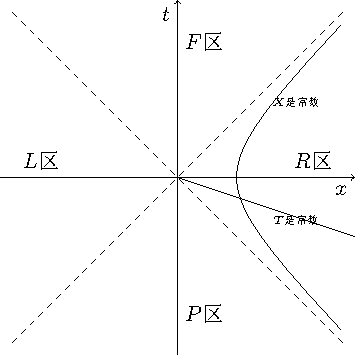
\includegraphics[width=5cm]{fig/II1-Rindler.pdf}
    \caption{Rindler坐标} \label{chsr:fig_Rindler}
\end{figure}


下面,我们仅以$R$区为例来讨论.
由式\eqref{chsr:eqn_Rindler-trans}易得
\begin{equation}\label{chsr:eqn_tx-TX}
    X^2= x^2-(ct)^2, \qquad \coth (\alpha T)= \frac{x}{ct} .
\end{equation}
我们也可将式\eqref{chsr:eqn_tx-sh-ch}中$\tau $变为$T$,$c^2 \alpha^{-1} $变为$X$;
同样可得到变换式\eqref{chsr:eqn_Rindler-trans}.
图\ref{chsr:fig_Rindler}中的双曲线表明:
不同的$X$值表示不同的火箭以不同的常加速度值在飞行.
$R$区式\eqref{chsr:eqn_Rindler-trans}的逆变换是:
\begin{equation}\label{chsr:eqn_Rindler-trans-inv}
    T=\frac{1}{\alpha} {\rm arcoth } \frac{x}{ct},\qquad
    X=\sqrt{x^2-(ct)^2} .
\end{equation}




直接计算可以得到$R$区非零的Christoffel记号是(下式中$T$是指$cT$)
\begin{equation}
    \Gamma^T_{TX}=\Gamma^T_{XT}=\frac{1}{X}, \qquad    \Gamma^X_{TT}=\frac{\alpha^2}{c^4} X .
\end{equation}
由此直接计算可得所有黎曼曲率的分量恒为零,
也就是Rindler度规\eqref{chsr:eqn_Rindler-megric}是
平直的,这说明Rindler时空本质上是闵氏时空.



下面我们来计算一下Rindler时空的共动观测者(定义见\S\ref{chfd:sec_comoving})的四加速度.
由\S\ref{chfd:sec_comoving}公式易知:
\begin{equation}
    Z^a =\frac{c^3}{X\alpha} \left(\frac{\partial}{\partial cT}\right)^a ;\qquad
    Z_a= -X\alpha  ({\rm d}T)_a .
\end{equation}
不难求得
\begin{equation}
    A^a = \nabla_Z Z^a = \frac{c^2}{X} \left(\frac{\partial}{\partial X}\right)^a .
\end{equation}
则有
\begin{equation}
    |A| = \sqrt{g_{ab} A^a A^b} = \frac{c^2}{X} .
\end{equation}
上面作了替换$c^2 \alpha^{-1} \to X$(见式\eqref{chsr:eqn_tx-TX}下面一行);
若反向执行则有$|A|=\alpha$.
这说明Rindler时空中共动观测者的四加速度模长是$\alpha$,
这与上一节给出的固有加速度相同.


由式\eqref{chsr:eqn_Rindler-trans}可得
\begin{equation}\label{chsr:eqn_dtx-dTX}
        \begin{pmatrix}
            {\rm d}ct \\ {\rm d}x
        \end{pmatrix}= 
        \begin{pmatrix}
          \frac{\alpha}{c^2} X\cosh \frac{\alpha}{c}T & \sinh\frac{\alpha}{c} T \\ 
          \frac{\alpha}{c^2} X\sinh \frac{\alpha}{c}T & \cosh\frac{\alpha}{c} T
        \end{pmatrix}
        \begin{pmatrix}
            {\rm d}cT \\ {\rm d}X
        \end{pmatrix}. 
\end{equation}
其逆变换是
\begin{equation}\label{chsr:eqn_dtx-dTX-inv}
\begin{pmatrix}
    {\rm d}cT \\ {\rm d}X
\end{pmatrix}= \frac{c^2}{\alpha X}
\begin{pmatrix}
    \cosh \frac{\alpha}{c}T & -\sinh \frac{\alpha}{c}T \\ 
 -\frac{\alpha}{c^2}X \sinh \frac{\alpha}{c}T & \frac{\alpha}{c^2}X \cosh \frac{\alpha}{c}T
\end{pmatrix}
\begin{pmatrix}
    {\rm d}ct \\ {\rm d}x
\end{pmatrix} .
\end{equation}
惯性系间的变换由洛伦兹变换描述.惯性系到匀加速运动参考系间的变换由式\eqref{chsr:eqn_Rindler-trans}、
\eqref{chsr:eqn_dtx-dTX}来描述;再结合式\eqref{chdm:eqn_tensor-component-trans}可以得到
两个参考系间张量的变换关系,比如电磁场张量$F_{\mu\nu}$.很明显经过式\eqref{chsr:eqn_dtx-dTX}变换
后的匀加速度参考系的麦克斯韦方程组与惯性系的麦氏方程组形式上不会相同.
如读者有兴趣可以试着推导一下Rindler坐标系下的麦氏方程组.




\begin{example}
	验证Rindler变换是等距的.
\end{example}
利用式\eqref{chdm:eqn_isometry-MMcoord}、\eqref{chsr:eqn_dtx-dTX},有
\setlength{\mathindent}{0em}
\begin{align*}
	\begin{pmatrix}
		\frac{\alpha}{c^2} X\cosh \frac{\alpha}{c}T & \sinh\frac{\alpha}{c} T \\ 
		\frac{\alpha}{c^2} X\sinh \frac{\alpha}{c}T & \cosh\frac{\alpha}{c} T
	\end{pmatrix}^T
	\begin{pmatrix}
		-1 & 0 \\ 0 & 1
	\end{pmatrix}
	\begin{pmatrix}
		\frac{\alpha}{c^2} X\cosh \frac{\alpha}{c}T & \sinh\frac{\alpha}{c} T \\ 
		\frac{\alpha}{c^2} X\sinh \frac{\alpha}{c}T & \cosh\frac{\alpha}{c} T
	\end{pmatrix} 
	=\begin{pmatrix}
		-\frac{\alpha ^2 X^2}{c^4} & 0 \\ 
		0 & 1
	\end{pmatrix} .
\end{align*}\setlength{\mathindent}{2em}
可见变换后的度规与式\eqref{chsr:eqn_Rindler-megric-RL}相同,故是等距变换.



\index[physwords]{麦克斯韦方程组}
\index[physwords]{电磁动力学}

\section{麦克斯韦方程组}\label{chsr:sec_maxwell}

\subsection{微分形式麦克斯韦方程组}
真空中麦克斯韦方程组(SI制)是
\begin{subequations}\label{chsr:eqn_maxwell-vac}
	\begin{align}
		\nabla \cdot  \boldsymbol{E} &= \dfrac{\rho }{\epsilon_0}, \label{chsr:eqn_gauss-e-vac} \\
		\nabla \cdot  \boldsymbol{B} &= 0,  \label{chsr:eqn_gauss-b-vac}\\
		\nabla \times \boldsymbol{E} +\frac{\partial \boldsymbol{B}}{\partial t} &= 0,  \label{chsr:eqn_faraday-vac}\\
		\nabla \times \boldsymbol{B} -\mu_0\epsilon_0\frac{\partial \boldsymbol{E}}{\partial t} &= \mu_0\boldsymbol{J}. \label{chsr:eqn_amp-max-vac}
	\end{align}
\end{subequations}
其中$\epsilon_0$是真空介电常数,$\mu_0$是真空磁导率常数;
$\boldsymbol{E}$是电场强度,$\boldsymbol{B}$是磁感应强度;
$\boldsymbol{J}$是自由电流密度矢量,$\rho$自由电荷密度.
\eqref{chsr:eqn_gauss-e-vac}是电场满足的库仑定律,也称为电场高斯定律.
\eqref{chsr:eqn_gauss-b-vac}是无自由磁单极子定律,偶尔有人称为磁场高斯定律.
\eqref{chsr:eqn_faraday-vac}是法拉第电磁感应定律.
\eqref{chsr:eqn_amp-max-vac}是安培-麦克斯韦定律.
这四个方程组合起来后构成了经典电磁场的第一基本假设,{\heiti 简称}为麦克斯韦方程组
{\footnote{正是这一“简称”,将本来属于法拉第、安培、库仑等电磁大师们的贡献
		{\heiti 有形}地转移到麦克斯韦头上.笔者不是说麦克斯韦不伟大,而是他被冠以本来属于法拉第、
		安培、库仑等大师的光环.麦克斯韦或许在数量上比法拉第、安培、库仑等大师伟大一些,但
		和这几个人的贡献没有量级上的差别.
		类似的简称还有非对易规范场中的Higgs机制.}}.
式\eqref{chsr:eqn_amp-max-vac}中的$\frac{\partial \boldsymbol{E}}{\partial t}$称为位移电流,
是麦克斯韦于1860年代引入的,这一项统一了电与磁;但此项并不是真正的电流.

电流电荷源满足电荷守恒定律,即
\begin{equation}\label{chsr:eqn_charge-conservation}
	\frac{\partial \rho}{\partial t} + \nabla \cdot \boldsymbol{J} = 0
	{\quad \color{red} \Leftrightarrow \quad }
	\frac{\partial J ^\mu}{\partial x^\mu} = 0; \quad
	\text{其中} \   J^\mu = (\rho c, \boldsymbol{J}).
\end{equation}

\index[physwords]{电荷守恒定律}

带电连续物质与电磁场间的相互作用是洛伦兹力密度矢量,
\begin{equation}\label{chsr:eqn_lorenz-force}
	\boldsymbol{f} = \rho \boldsymbol{E} + \boldsymbol{J}\times\boldsymbol{B}.
\end{equation}
它给出了单位体积电荷所受力密度矢量.
洛伦兹力的表达式是从实验中总结得到的,
这里面包含了库仑力、安培力.这是一个基本方程式,
好比两个天体间的引力是牛顿万有引力公式一样,
不能由其它理论推导得到.

麦克斯韦方程组\eqref{chsr:eqn_maxwell-vac}、电荷守恒定律\eqref{chsr:eqn_charge-conservation}和
洛伦兹力\eqref{chsr:eqn_lorenz-force}(再加上牛顿第二定律)构成了宏观电磁动力学
{\footnote{这门课程英文名称是Electro-Dynamics,直译过来就是{\fangsong 电动力学}.由于中英文的差异,
		{\kaishu 电动力学}经常被断句成{\kaishu 电动-力学}(包括笔者本人),然而正确的断句是
		{\kaishu 电-动力学};英文则没有这种断句错误.如果把它翻译成{\heiti 电磁动力学},则没有断句
		歧义,而且与此课程内容更为贴近.}}的基础,它们是相互独立的定律.

除了上述三个基本假设之外,笔者觉得还有一条隐含假设:
宏观电磁场可由两个矢量$\boldsymbol{E}$和$\boldsymbol{B}$完备描述.

%\subsection{含有磁荷的麦克斯韦方程组}
%前面的麦克斯韦方程组是不对称的,只有电流、电荷项,没有磁荷.
%补上磁荷后,有
%\begin{subequations}\label{chsr:eqn_maxwell-qm}
%    \begin{align}
	%        \nabla \cdot  \boldsymbol{E} &= \frac{\rho_e}{\epsilon_0}, \label{chsr:eqn_gauss-e-qm} \\
	%        \nabla \cdot  \boldsymbol{B} &= \mu_0 \rho_m,  \label{chsr:eqn_gauss-b-qm}\\
	%        \nabla \times \boldsymbol{E} +\frac{\partial \boldsymbol{B}}{\partial t} &= -\mu_0\boldsymbol{J}_m,  \label{chsr:eqn_faraday-qm}\\
	%        \nabla \times \boldsymbol{B} - \frac{1}{c^2}
	%        \frac{\partial \boldsymbol{E}}{\partial t} &= +\mu_0\boldsymbol{J}_e. \label{chsr:eqn_amp-max-qm}
	%    \end{align}
%\end{subequations}
%电荷、磁荷都是守恒的,有两个连续性方程
%\begin{subequations}\label{chsr:eqn_em-continuity}
%    \begin{align}
	%        \frac{\partial \rho_e}{\partial t} + \nabla \cdot \boldsymbol{J}_e &= 0 \label{chsr:eqn_e-continuity} \\
	%        \frac{\partial \rho_m}{\partial t} + \nabla \cdot \boldsymbol{J}_m &= 0 \label{chsr:eqn_m-continuity}
	%    \end{align}
%\end{subequations}
%洛伦兹力公式也需要推广,
%\begin{equation}\label{chsr:eqn_lorenz-force-em}
%    \boldsymbol{f} = \rho_e \boldsymbol{E} + \boldsymbol{J}_e\times\boldsymbol{B} \ + \
%    \rho_m \boldsymbol{B} - \boldsymbol{J}_m\times\boldsymbol{E}/c^2.
%\end{equation}
%截止到目前为止,实验上还没有发现自由磁单极子,所以有关磁单极子的
%理论都是数学,而非物理.
%
%如果做如下变量代换,方程式\eqref{chsr:eqn_maxwell-qm}形式不变,
%\begin{equation}\label{chsr:eqn_dual-em}
%    \begin{aligned}
	%        \boldsymbol{E}' &= \boldsymbol{E} \cos\theta + c\boldsymbol{B}\sin\theta, &
	%        c\boldsymbol{B}' &= c\boldsymbol{B}\cos\theta -\boldsymbol{E} \sin\theta, \\
	%        c \rho'_e &= c \rho_e\cos\theta + \rho_m\sin\theta, &
	%        \rho'_m &= \rho_m\cos\theta -c \rho_e\sin\theta, \\
	%        c \boldsymbol{J}'_e &= c \boldsymbol{J}_e\cos\theta + \boldsymbol{J}_m\sin\theta, &
	%        \boldsymbol{J}'_m &= \boldsymbol{J}_m\cos\theta -c \boldsymbol{J}_e\sin\theta.
	%    \end{aligned}
%\end{equation}
%其中$\theta$是一个与时空坐标、电磁场无关的任意实数,这个代换称为对偶变换.

\index[physwords]{电磁场张量}

\subsection{电磁张量形式麦克斯韦方程组}
与上节相似,我们只是罗列一些基本公式.
电磁场张量写成矩阵形式为
\begin{equation}
    F^{\mu\nu} = \begin{pmatrix}
        0 & E_x/c & E_y/c & E_z/c \\
        -E_x/c & 0 & B_z & -B_y \\
        -E_y/c & -B_z & 0 & B_x \\
        -E_z/c & B_y & -B_x & 0
    \end{pmatrix}.
\end{equation}
%可将它的指标进行升降,有
%\begin{align}
%    F_{\alpha}^{\cdot\nu}&= \eta_{\alpha\mu}F^{\mu\nu}
%    = \begin{pmatrix}
%        0 & -E_x/c & -E_y/c & -E_z/c \\
%        -E_x/c & 0 & B_z & -B_y \\
%        -E_y/c & -B_z & 0 & B_x \\
%        -E_z/c & B_y & -B_x & 0
%    \end{pmatrix}, \\
%    F^{\mu}_{\cdot\beta}&= F^{\mu\nu}\eta_{\nu\beta}
%    = \begin{pmatrix}
%        0 & E_x/c & E_y/c & E_z/c \\
%        E_x/c & 0 & B_z & -B_y \\
%        E_y/c & -B_z & 0 & B_x \\
%        E_z/c & B_y & -B_x & 0
%    \end{pmatrix}, \\
%    F_{\alpha\beta} &= \eta_{\alpha\mu}F^{\mu\nu}\eta_{\nu\beta}
%    = \begin{pmatrix}
%        0 & -E_x/c & -E_y/c & -E_z/c \\
%        E_x/c & 0 & B_z & -B_y \\
%        E_y/c & -B_z & 0 & B_x \\
%        E_z/c & B_y & -B_x & 0
%    \end{pmatrix}.
%\end{align}


四维协变形式的麦克斯韦方程组可以写成:
\begin{subequations}\label{chsr:eqn_maxwell-F}
    \begin{align}
        \partial_{\alpha} F^{\alpha\beta} &= -\mu_0 J^{\beta} ,   \label{chsr:eqn_maxwell-F1} \\
        \partial_\gamma F_{ \alpha \beta } + \partial_\alpha F_{ \beta \gamma }
        + \partial_\beta F_{ \gamma \alpha } &= 0. \label{chsr:eqn_maxwell-F2}
    \end{align}
\end{subequations}
\eqref{chsr:eqn_maxwell-F1}展开得\eqref{chsr:eqn_gauss-e-vac}和\eqref{chsr:eqn_amp-max-vac},
\eqref{chsr:eqn_maxwell-F2}展开得\eqref{chsr:eqn_gauss-b-vac}和\eqref{chsr:eqn_faraday-vac}.


\index[physwords]{电磁规范势} \index[physwords]{电磁矢量势} \index[physwords]{电磁标量势}

\subsection{规范势形式的麦克斯韦方程组}
真空中麦克斯韦方程组\eqref{chsr:eqn_maxwell-vac}
中的方程${\rm div} \boldsymbol{B}=0$表示没有自由磁单极子,
由矢量分析中知识可知存在矢量势$\boldsymbol{A}$满足
$\boldsymbol{B}=\nabla\times \boldsymbol{A}$;将此式带入法拉第定律
\eqref{chsr:eqn_faraday-vac}并交换时间、空间偏微商,就可以得到
$\nabla\times \boldsymbol{E} + \nabla\times \frac{\partial}{\partial t} \boldsymbol{A} = 0$;
进而可以得到
$ \boldsymbol{E} + \frac{\partial}{\partial t} \boldsymbol{A}  =- \nabla \phi$.
至此,我们得到如下变换式
\begin{subequations}\label{chsr:eqn_BE-poetential-gauge-trans}
	\begin{align}
		\boldsymbol{B} &= \nabla\times \boldsymbol{A},  \label{chsr:eqn_B-poetential-gauge-trans} \\
		\boldsymbol{E} &= -\frac{\partial}{\partial t} \boldsymbol{A}  - \nabla \phi .
		\label{chsr:eqn_E-poetential-gauge-trans}
	\end{align}
\end{subequations}
矢量势$\boldsymbol{A}$和标量势$\phi$统一在一起称为{\kaishu 规范势}函数.
需要注意,由于此时的电场是有旋的,所以这里的$\phi$和静电场中的电势不同.
将式\eqref{chsr:eqn_BE-poetential-gauge-trans}带入式\eqref{chsr:eqn_maxwell-vac}
并应用$c^2 \mu_0\epsilon_0=1$,就得到了规范势表示的麦克斯韦方程组
\begin{subequations}\label{chsr:eqn_maxwell-poetential}
	\begin{align}
		{\nabla ^2}\phi  + \frac{\partial}{\partial t} \nabla  \cdot \boldsymbol{A}
		&=  - \frac{\rho}{\epsilon _0}, \label{chsr:eqn_gauss-e-poetential} \\
		{\nabla ^2}\boldsymbol{A} - \frac{1}{c^2}\frac{\partial ^2\boldsymbol{A}}{\partial {t^2}}
		- \nabla \left( {\nabla  \cdot \boldsymbol{A} + \frac{1}{c^2}\frac{ \partial \phi }{ \partial t}} \right)
		&=  - {\mu _0}\boldsymbol{J}. \label{chsr:eqn_amp-max-poetential}
	\end{align}
\end{subequations}
其中\eqref{chsr:eqn_gauss-b-vac}和\eqref{chsr:eqn_faraday-vac}自动满足,
\eqref{chsr:eqn_gauss-b-vac}和\eqref{chsr:eqn_amp-max-vac}变成了上面两式.

因上面变换中没有指定矢量势$\boldsymbol{A}$的散度,
在如下变换下,方程\eqref{chsr:eqn_BE-poetential-gauge-trans}不变
\begin{subequations}\label{chsr:eqn_gauge-trans}
	\begin{align}
		\boldsymbol{A}' &= \boldsymbol{A} + \nabla f, \label{chsr:eqn_A-gauge-trans} \\
		\phi' &= \phi -\frac{\partial f}{\partial t} . \label{chsr:eqn_phi-gauge-trans}
	\end{align}
\end{subequations}
这个变换式叫做第一类{\heiti 规范变换}.带入后直接可验证
\begin{align*}
	\boldsymbol{B} &= \nabla\times \boldsymbol{A}' = \nabla\times \boldsymbol{A} + \cancel{\nabla \times\nabla f} , \\
	\boldsymbol{E} &= -\frac{\partial}{\partial t} \boldsymbol{A}'  - \nabla \phi' =
	-\frac{\partial}{\partial t} \boldsymbol{A}  \
	\cancel{- \frac{\partial \nabla f}{\partial t} }
	- \nabla \phi \
	\cancel{+ \nabla \frac{\partial f}{\partial t}}
	=-\frac{\partial}{\partial t} \boldsymbol{A}  - \nabla \phi .
\end{align*}
可见$(\phi,\boldsymbol{A})$和$(\phi',\boldsymbol{A}')$描述相同的电磁场$\boldsymbol{B},\boldsymbol{E}$.

规范变换\eqref{chsr:eqn_gauge-trans}可以写成四维协变形式,
\begin{equation}\label{chsr:eqn_gauge-trans-covariant}
	A^{\prime\mu} = A^\mu + \partial^\mu f; \qquad
	\text{其中} \  A^\mu \equiv (\phi/c,\boldsymbol{A}).
\end{equation}

我们可以把规范势和电磁张量关联起来了:
\begin{equation}\label{chsr:eqn_Fab}
    F^{\mu\nu} =\partial^\mu A^\nu - \partial^\nu A^\mu .
\end{equation}


\subsubsection{规范变换与边界条件}\label{chsr:sec_gauge-bc}
物理上只能给出$\boldsymbol{B}$的狄里克莱(第一类)边界条件,
这对应着矢量势一阶偏导数(第二类)边界条件,即
\begin{equation}
	\frac{\partial \boldsymbol{A}}{\partial n} = \boldsymbol{B} |_{\partial D},
	\quad \boldsymbol{B}|_{\partial D} {\text {表示区域$D$边界上的值,$n$是外法向.}}
\end{equation}
物理上无法给出矢量势$\boldsymbol{A}$在边界上的值(第一类或狄里克莱边条件),即
\begin{equation}
	\boldsymbol{A} |_{\partial D} = ?, \qquad \boldsymbol{A} {\text {在连通区域$D$边界上的值是未知的}.}
\end{equation}
如果我们把电磁场$\boldsymbol{B} $看作是已知的,
把\eqref{chsr:eqn_B-poetential-gauge-trans}看作是关于矢量势$\boldsymbol{A}$的方程,
即便配上后面所谓的规范条件(任意一种),那么方程组
\begin{equation}\label{chsr:eqn_A-poetential}
	\nabla\times \boldsymbol{A}  =\boldsymbol{B},\qquad \nabla\cdot \boldsymbol{A}  =\psi,
\end{equation}
由于$\boldsymbol{A}$只有一阶偏导数边界条件,物理上没有$\boldsymbol{A}$的
狄里克莱边条件,式\eqref{chsr:eqn_A-poetential}
的解也是无法唯一确定的
{\footnote{数学上,一阶偏微分方程组\eqref{chsr:eqn_A-poetential}需给定
		狄里克莱边界条件,不能给一阶偏微分边界条件.}}.
这就导致了即便给定规范条件(即补充了$\boldsymbol{A}$的散度方程),
仍旧存在规范变换\eqref{chsr:eqn_gauge-trans}.
这类在补充规范条件后,
由于无法给出$\boldsymbol{A}$狄里克莱边条件引起的规范变换叫作{\heiti 第二类规范变换}.
不论第一类还是第二类规范变换,它们的数学表达形式是相同的,
都为式\eqref{chsr:eqn_gauge-trans-covariant};也就是说
引起规范变换的原因有两个,一个是缺方程,一个是边界条件并能完全确定,
但它们具体变换的数学形式是相同的.

举个最简单的情形,我们令\eqref{chsr:eqn_A-poetential}中的$\boldsymbol{B}=0$、$\psi=0$,
那么\eqref{chsr:eqn_A-poetential}变成$\nabla\times \boldsymbol{A}  =0$、$ \nabla\cdot \boldsymbol{A}  =0$,
令$\boldsymbol{A}=\nabla\theta$,我们就可以把\eqref{chsr:eqn_A-poetential}变成$\nabla^2\theta=0$.
这是拉普拉斯方程,依照前面分析物理上只能给出$\partial^2\theta$边界条件,即$\theta$的
二阶偏导数边界条件.此方程解并不唯一.


\index[physwords]{规范条件}

\subsubsection{规范条件}
方程式\eqref{chsr:eqn_BE-poetential-gauge-trans}解不唯一,但它在
第\pageref{chmla:def_linear-dependence}页定义\ref{chmla:def_linear-dependence}下
是适定的;在定义\ref{chmla:def_diff-linear-dependence}下是欠定的.
依照定义\ref{chmla:def_diff-linear-dependence},
方程式\eqref{chsr:eqn_BE-poetential-gauge-trans}和
方程式\eqref{chsr:eqn_maxwell-poetential}都需要补充一个方程,
称之为{\kaishu 规范条件}.
由于物理上无法对规范条件提出明确要求,因此所补充的方程只要
能确保麦克斯韦方程组解的存在即可,不要求解的唯一性.但补充规范条件后,
需要方程变成较为简单的形式(或者你需要的形式),这可能是对规范条件唯一的要求.


%\subsubsection{库仑规范}
%库仑规范,也称为横场规范或者辐射规范,它是
%\begin{equation}\label{chsr:eqn_coulomb-gauge}
%    \nabla \cdot \boldsymbol{A} = 0.
%\end{equation}
%将上式带入\eqref{chsr:eqn_maxwell-poetential}后,可得
%\begin{subequations}\label{chsr:eqn_maxwell-poet-coul-gauge}
%    \begin{align}
	%        {\nabla ^2}\phi    &=  - \frac{\rho}{\epsilon _0}, \label{chsr:eqn_gauss-e-coul-gauge} \\
	%        {\nabla ^2}\boldsymbol{A} - \frac{1}{c^2}\frac{\partial ^2\boldsymbol{A}}{\partial {t^2}}
	%        - \frac{1}{c^2}\frac{ \partial \nabla\phi }{ \partial t}
	%        &=  - {\mu _0}\boldsymbol{J}. \label{chsr:eqn_amp-max-coul-gauge}
	%    \end{align}
%\end{subequations}
%这就是结合库仑规范的麦克斯韦方程组,需注意:
%\eqref{chsr:eqn_maxwell-poet-coul-gauge}一定要与规范\eqref{chsr:eqn_coulomb-gauge}
%结合在一起求解.之所以称之为库仑规范,是因为\eqref{chsr:eqn_gauss-e-coul-gauge}
%与静电场中的库仑定律在形式上完全一样;但需注意这里的$\phi${\heiti 不}是静电场的势函数.
%
%
%
%如果库仑规范不能满足,即$\Theta = \nabla \cdot \boldsymbol{A} \neq 0$,那么
%由\eqref{chsr:eqn_A-gauge-trans}知道可令新的矢势$\boldsymbol{A}'$满足库仑规范,即
%\begin{equation}
%    \nabla \cdot\boldsymbol{A}' = \nabla \cdot\boldsymbol{A} + \nabla^2 f {\color{red}\Rightarrow}
%    -\Theta =  \nabla^2 f .
%\end{equation}
%依照\S\ref{chsr:sec_gauge-bc}所述,对函数$f({x^\mu})$的边界条件没有什么限制,
%泊松方程$\nabla^2 f= -\Theta $解一定是存在的,也就是说库仑规范一定可以满足.
%新标量势可按照变换\eqref{chsr:eqn_phi-gauge-trans}来求取.
%
%
%
%对于库仑规范约束下,无界空间、无源、自由电磁场\eqref{chsr:eqn_gauss-e-coul-gauge}中的
%标量势可以恒为零,即$\phi =0$.需要注意,只是在满足诸多前提下,允许$\phi =0$的解存在,
%不能把$\phi =0$看成一条新的规范;规范条件只能补充一个,不能多于一个!

\index[physwords]{洛伦茨规范} \index[physwords]{Lorenz规范}

\subsubsection{洛伦茨规范}
丹麦物理学家洛伦茨{\footnote{L. V. Lorenz(洛伦茨)不是荷兰物理学家
		洛伦兹(H. A. Loren{\textcolor{red}{t}}z),
		他们俩的姓氏只差一个字母{\textcolor{red}{t}}.}}
于1867年提出如下方程
\begin{equation}\label{chsr:eqn_lorenz-gauge}
	{\nabla  \cdot \boldsymbol{A} + \frac{1}{c^2}\frac{ \partial \phi }{ \partial t}}  = 0,
\end{equation}
此方程被称为洛伦茨规范条件.将它带入
\eqref{chsr:eqn_maxwell-poetential}后,可得
\begin{subequations}\label{chsr:eqn_maxwell-lorenz-gauge}
	\begin{align}
		{\nabla ^2}\phi  - \frac{1}{c^2}\frac{\partial^2 \phi}{\partial t^2}
		&=  - \frac{\rho}{\epsilon _0}, \label{chsr:eqn_gauss-e-lorenz-gauge} \\
		{\nabla ^2}\boldsymbol{A} - \frac{1}{c^2}\frac{\partial ^2\boldsymbol{A}}{\partial {t^2}}
		&=  - {\mu _0}\boldsymbol{J}. \label{chsr:eqn_amp-max-lorenz-gauge}
	\end{align}
\end{subequations}
这就是结合洛伦茨规范的麦克斯韦方程组,同样需注意:
\eqref{chsr:eqn_maxwell-lorenz-gauge}一定要与规范\eqref{chsr:eqn_lorenz-gauge}
结合在一起求解.此时的方程式\eqref{chsr:eqn_maxwell-lorenz-gauge}是波动方程形式.


如果规范势$A_\mu$不满足洛伦茨规范,即$\Theta \equiv \partial_\mu A^\mu \neq 0$,
那么可作规范变换\eqref{chsr:eqn_gauge-trans-covariant}导致新的
规范势$A^{\prime}_{\mu}$满足洛伦茨规范:
\begin{equation}
	A^{\prime}_{\mu} = A_\mu + \partial_\mu f {\quad\color{red}\Rightarrow\quad}
	\partial^\mu A^{\prime}_{\mu} = \partial^\mu A_\mu + \partial^\mu\partial_\mu f
	{\quad\color{red}\Rightarrow\quad} \square f = - \Theta .
\end{equation}
依照\ref{chsr:sec_gauge-bc}节所述,对函数$f({x^\mu})$的边界条件没有多少限制,
那么上述波动方程$\square f = - \Theta$解是一定存在的,也就是说可以找到一个$f$使得
新的规范势$A^{\prime}_{\mu}$满足洛伦茨规范$\partial^\mu A^{\prime}_{\mu}=0$.
这也就说明了:我们一定有办法使洛伦茨规范得以满足.


\subsubsection{其它规范}
规范条件就是补充一个方程,有很多种\cite{jackson2002-LC},比如常用的库仑规范:
\begin{equation}
    \nabla \cdot \boldsymbol{A} = 0 .
\end{equation}
此外,再举一例
\begin{equation}\label{chsr:eqn_temporal-gauge}
	\phi = 0,
\end{equation}
它称为瞬时规范.
若原规范不满足规范\eqref{chsr:eqn_temporal-gauge},
即$\phi\neq 0$;
则由\eqref{chsr:eqn_phi-gauge-trans}可知
存在变换$\phi' = \phi -\frac{\partial f}{\partial t}$,
使新的$\phi' =0$,即
\begin{equation}
	\frac{\partial f}{\partial t} = \phi {\quad \color{red}\Rightarrow\quad}
	f(\boldsymbol{r},t) = \int^{t} \phi(\boldsymbol{r},\tau) {\rm d}\tau .
\end{equation}
这样,新的标势恒为零$\phi' =0$,新的矢势可由\eqref{chsr:eqn_A-gauge-trans}求得:
\begin{equation}
    \boldsymbol{A}' = \boldsymbol{A} + \nabla [ \int^{t} \phi(\boldsymbol{r},\tau) {\rm d}\tau ] .
\end{equation}




\subsubsection{规范势$A^\mu$是洛伦兹四矢量吗?}\label{chsr:sec_isAvec}
规范势$A^\mu =(\phi/c,\boldsymbol{A})$在不同规范下会有不同的形式,比如
在\eqref{chsr:eqn_temporal-gauge}式下,第零分量恒为零.这充分说明
在此规范下$A^\mu${\heiti 不}是四矢量.其原因是因为$A^\mu$是个物理量,
它存在规范自由度,可以取各种规范而不影响可观测物理结果.

在不指定规范条件的前提下,规范势$A^\mu$被{\heiti 人为地规定}为洛伦兹四矢量.
显然,如果选取的规范条件是洛伦兹协变的(比如洛伦茨规范条件),那么
规范势也是四矢量.
如果选取的规范条件{\heiti 不}是洛伦兹协变的(比如库仑规范或瞬时规范),
那么一般说来规范势{\heiti 不}是四矢量.










\index[physwords]{闵氏几何}

\section{四维闵氏几何语言讨论时空结构}\label{chsr:sec_spacetime-structure-Min}
前面几节仍旧采用1+3分量语言(时间和空间)来描述狭义相对论;
从本节开始,我们使用四维语言来从新描述.

我们已经知道在相对论中时间和空间已经不是绝对分离的了,两者有着密切关系.
闵可夫斯基曾经说过:从今以后,空间和时间本身注定要消失在完全的阴影之中,只有它们的某种结合才保持为独立的实体;
这就是闵氏几何.今天我们更加确信的是{\kaishu 时空}才是更为基本的物理概念,时间和空间
需要时空作1+3分解才能得到;先有时空,后有时间和空间;需注意时空不是简单的时间加空间.


为了简化问题,在本节我们采用自然单位制(见附录\ref{chunit-dim:sec_nature-units}),
即令$c=1$. %;但仍将$c$在公式中表出.

\subsection{引入流形}
在\S \ref{chsr:sec_srf}中,我们引入了“事件”这个概念;全部事件的集合称为{\heiti 时空}(Space-time);
从物理直觉上,我们可以假设“事件”充满整个时空,时空是一个四维连续系统
{\footnote{关于事件与时空关系的描述在很多书籍中都有,
比如\parencite[\S 3.2]{synge-1960}或\parencite[\S 3.1]{hawking-ellis1973}.
笔者没有查询到是哪位先贤最早认识到此点,我猜测可能是闵可夫斯基或者爱因斯坦.}}.
我们在这个四维连续系统上建立一个坐标系$\{x^\mu\}$,从狭义相对论基本原理出发,已经得到在
任意坐标变换下($x^\mu \to x^{\prime \mu}$)“间隔”$s^2$是一个不变量,这说明间隔是
脱离某套具体坐标系的,或者说间隔是与坐标系无关的物理量.

数学上“微分流形”虽然也是建立在具体(局部)坐标上的,但个坐标间必须相互容许,
所以流形也是不依赖于某套具体坐标的.这与“时空”中间隔$s^2$的属性基本相同.
既然有这种相似性,我们可以借用数学上“微分流形”这一概念来描述物理上的“时空”.
物理上用四个实参数来描述事件,我们自然用数学上的四维光滑流形来描述物理上的时空.

%从“元间隔”\eqref{chsr:eqn_interval-inv-ds}可以看到并非所有项都是“正的”,有一项前的系数是“负的”.
很容易从闵氏时空的弧长公式\eqref{chrg:eqn_arc-length}看出来其元长度是
\begin{equation}
    {\rm d}s^2 = -({\rm d}x^0)^2 +({\rm d}x^1)^2 +({\rm d}x^2)^2 +({\rm d}x^3)^2 .
\end{equation}
这与狭义相对论中得到“元间隔”\eqref{chsr:eqn_interval-inv-ds}完全吻合;
因此狭义相对论时空对应的流形正是我们之前定义的四维平直
闵可夫斯基时空\ref{chdm:def_MinkowskiSpace}或定义\ref{chrg:def_Minkowski-space}.

我们大致按照狭义相对论发展的历史顺序,将“事件”与“流形”挂钩,然后再将“正定”度规拓展到“不定”度规(这
是闵可夫斯基的重大发现).有了这样的认识之后,才将“闵氏度规”推广到纯数学的流形论中;
在此之前,纯数学几乎只研究正定度规情形.
先有物理上的狭义相对论,数学中微分几何才诞生“闵氏空间”这一概念.


现今的物理学已经搞清楚:{\bfseries (1)} 狭义相对论的背景时空是四维平直空间(黎曼曲率为零);
{\bfseries (2)} 它的度规类型是洛伦兹的,即度规特征值是$(-1,1,1,1)$.




\subsection{1+3分解}\label{chsr:sec_1+3decom}
现在看一下,我们手头有哪些东西.首先,有四维平直闵氏时空;
其次,知道在时空中“间隔”是不变的,不论你选择哪套坐标系,间隔都是同一数值.

至此,还没有时间、空间概念;只有四维平直时空和间隔不变性.

由\S\ref{chrg:sec_local-EuclideanSpace}知识可知,四维\uwave{平直空间}中存在局部
坐标系$(x^0,x^1, x^2, x^3)$使得度规在此坐标系下为$\eta={\rm diag}(-1,1,1,1)$,
即此坐标系是正交归一的.平直空间是可以用一个坐标域覆盖住的,
故我们可以把平直闵氏时空记为:$(\mathbb{R}^4_1,\eta)$.
我们把对应度规中$-1$那个坐标$x^0$称为“时间”,其它三个坐标$(x^1, x^2, x^3)$构成的子流形称为“空间”.
如果换另外一套坐标$(x^{\prime 0},x^{\prime 1}, x^{\prime 2}, x^{\prime 3})$来
描述$\mathbb{R}^4_1$,根据“间隔”不变性可知从$x^\mu$到$x^{\prime \mu}$的变换
一定是洛伦兹变换\eqref{chsr:eqn_lorentz-transofrm-x}或其逆变换;
变完之后的坐标$x^{\prime 0}$仍称为“时间”,其它三个坐标称为“空间”.


狭义相对论中的闵氏时空是平直的,它的切空间就是自身.洛伦兹度规在坐标系$\{x^\mu\}$中可表示为
\begin{equation}\label{chsr:eqn_Lorentz-metric}
	\eta_{ab} = -({\rm d}x^0)_a ({\rm d}x^0)_b+({\rm d}x^1)_a({\rm d}x^1)_b
	+({\rm d}x^2)_a ({\rm d}x^2)_b+({\rm d}x^3)_a({\rm d}x^3)_b .
\end{equation}
在四维平直闵氏时空中,并不是任意一套坐标系都能显示表述“时间”.比如令
\begin{equation}
	u= x^0 - x^3, \qquad v= x^0 + x^3.
\end{equation}
此时度规\eqref{chsr:eqn_Lorentz-metric}变为
\begin{equation}\label{chsr:eqn_Lorentz-metric-light}
	\eta_{ab} = -\frac{1}{2}({\rm d}v)_a ({\rm d}u)_b
	-\frac{1}{2}({\rm d}u)_a ({\rm d}v)_b
	+({\rm d}x^1)_a({\rm d}x^1)_b +({\rm d}x^2)_a ({\rm d}x^2)_b.
\end{equation}
很容易看到新坐标$u,v$都是类光的;
那么从表面上来看,新的坐标系$\{u,v,x^1,x^2\}$没有显示“时间”的概念;
而是隐藏在$\{u,v\}$之中.








\subsection{时空图}\label{chsr:sec_spacetime}
我们先介绍四维{\heiti 时空图}:取纵坐标为$t\equiv x^0$代表时间;横坐标$x$代表三维空间,
但平面图上无法画出,所以压缩成一维;见图\ref{chsr:pic_spacetime}所示.平面图上
可以画出立体图,此时可以考虑两维空间方向,但仍必须压缩掉一维空间.
\begin{figure}[htb]
    \centering
    \begin{tikzpicture}[scale=3]
    \fill[lightgray] (0,0) -- (0.8,0.8)-- (-0.8,0.8)-- (0,0);
    \fill[lightgray] (0,0) -- (-0.8,-0.8)-- (0.8,-0.8)-- (0,0);
    \draw [-latex] (-1,0)--(1,0) node[above ] { $x$};
    \draw [-latex] (0,-1)--(0,1) node[right ] {$t$};
    \draw [-]  (-0.8,-0.8)node[below] {$P$}--(+0.8,0.8) node[above ] {$F$};
    \draw [-]  (+0.8,-0.8)node[below] {$P$}--(-0.8,0.8) node[above ] {$F$};
    \node at (-0.2,-0.1)  {$O$};
    \node at (-0.1,+0.4) {I};
    \node at (0.1,-0.3) {II};
    \node at (-0.5,0.1) {III};\node at (+0.5,0.1) {III};
    \draw [color=red](-0.6,-0.9) .. controls (-0.3,-0.7)and (-0.1,-0.2) .. (0,0);
    \draw [color=red](0,0) .. controls (0.1,0.2)and (0.3,0.7) .. (0.6,0.9);
%    \draw [color=green](-0.2,0.0)--(-0.2,0.9);
    \draw [color=blue] (0,0)--(0.3,0.9);
    \end{tikzpicture}
    \caption{质点世界线,时空分类}\label{chsr:pic_spacetime}
\end{figure}

前面介绍过的事件概念就是时空图中的一个点,全部点的集合就是闵氏时空.在狭义相对论范畴内,
我们仍需假设时空是四维连续的、连通的空间,这个空间的度规是洛伦兹度规.
质点(包括有质量和无质量的粒子)在时空中运动(包括静止不动情形),对应为时空图上一条曲线,称为该质点
的{\heiti 世界线},它能代表质点的全部历史;例如见图\ref{chsr:pic_spacetime}中红色曲线.
我们看一些具体问题.

\begin{example}
    一个静止不动的质点在时空图里的世界线是什么样的?
\end{example}
这个答案很容易想到,质点静止不动,就是在空间上没动,那么它的$x$坐标一直不变,
但是时间依然在流逝,也就是它的时间坐标在一直变大.所以,静止不动质点的世界线是一条跟$t$轴平行,
垂直于$x$轴的直线;例如图\ref{chsr:pic_spacetime}中$t$轴本身就是某质点世界线,
此质点位于三维空间坐标原点.
\qed

\begin{example}
一个匀速运动的粒子的世界线是什么样的?
\end{example}
速度的定义依旧是$\boldsymbol{u}={\rm d}\boldsymbol{x}/{{\rm d}t}$,匀速运动意味着$x=u t$;
那么这个质点的世界线应该是一条斜直线;如图\ref{chsr:pic_spacetime}中的
蓝色线,斜率的倒数就是其速度,即$t=1/u x$.
由此易得:{\kaishu 世界线的切线斜率就是该质点在此处的速度的倒数}.
\qed

\begin{example}
一条朝右上方$45^{\circ}$的斜直线,也就是图\ref{chsr:pic_spacetime}中的$OF$代表什么世界线?
\end{example}
$45^{\circ}$的斜直线的斜率就是1,因已约定光速$c=1$,故它代表光子世界线.
光子世界线实际上这是一个旋转超曲面,所以左上方也标记为$F$(future);而下方标记为$P$(past).
\qed

从这里我们可以看到,在时空图里,光子的世界线是$45^{\circ}$的斜直线.
我们也知道在相对论里任何有质量粒子的速度都是小于光速的,
那么一个有质量粒子的世界线该是什么样呢?是在区域I还是区域II或者区域III?
为了简单起见我们只分析从原点出发的质点运动.
我们可以这样想一下:如果粒子的速度比光速小,那么它的世界线切线斜率倒数就应该小于1,
也就是更靠近$t$轴;
%{\footnote{注意速度是距离除以时间,所以小于1是指更靠近时间轴,不是靠近空间轴$x$.}}
因此速度在静止和光速之间的质点世界线切线斜率倒数自然就是在区域I或II中了;
比如图中的红色曲线、蓝色斜直线.如果世界线切线斜率倒数大于1,
也就是位于III区中,“速度”是超光速的,自然界不存在这样的粒子.


\subsection{时空分类}\label{chsr:sec_stc}
时空中有两个事件$O$和$Q$,将$O$取为时空图的原点.
时空间隔是参考系变换的不变量,也就是洛伦兹变换下的不变量.根据时空间隔\eqref{chsr:eqn_interval-inv-ds},
即${\rm d}s^2 = -{\rm d}t^2 +{\rm d}x^2 +{\rm d}y^2 +{\rm d}z^2 =-{\rm d}t^2 (1-u^2)$,
物理学中约定:

\noindent\fbox{甲} 当${\rm d}s^2 <0 $时,时空为{\heiti 类时},
见图\ref{chsr:pic_spacetime}中I区和II区,已标记为阴影区.当$Q$点位于I区时,
直线$OQ$斜率倒数小于1,说明它的速度是亚光速的,并且从$O$点走到$Q$的过程中,时间$t$一直
是增加的;I区称为绝对未来.当$Q$点位于II区时,直线$OQ$斜率倒数小于1,说明它的速度是亚光速的;
但是从$O$点走到$Q$的过程中,时间$t$一直是减少的;II区称为绝对过去.
由于连续洛伦兹变换不改变
时间的正负,所以区域I和II是不可能通过洛伦兹变换相联系的;这种划分是绝对的.
有质量粒子世界线必须是类时的,指其切线斜率倒数小于1,即其速度为亚光速.


\noindent\fbox{乙} 当${\rm d}s^2 =0 $时,时空为{\heiti 类光},
见图\ref{chsr:pic_spacetime}中$OF,OP$斜率为1的直线,其实
为旋转超曲面,只不过在这张图中显示为直线.这个超曲面上的事件皆可由光联系.
其中$OF$指向绝对未来,$OP$指向绝对过去.
无质量粒子世界线必须类光.

\noindent\fbox{丙} 当${\rm d}s^2 >0 $时,时空为{\heiti 类空},
见图\ref{chsr:pic_spacetime}中III区,已标记为空白区.当$Q$点处于这一区域时,
直线$OQ$斜率倒数大于1,说明它的“速度”是超光速的,不对应自然界中任何粒子或物质.这个
区域的任何两个事件没有因果关系,可以通过洛伦兹变换改变事件的发生时序.
如果选择两参考系速度差$v$的范围是$c^2\frac{\Delta t}{\Delta x}<v<c$,
那么就可以颠倒事件$O$和$Q$的先后顺序;但
这不违反因果律,因为这两个事件没有因果关系.

在第\ref{chsr:sec_lorentz-transofrm}节末尾曾经讨论过洛伦兹变换把光速变成光速,
把亚光速变成亚光速,把超光速变成超光速;所以在洛伦兹变换下上述划分是绝对的,
变换前后不会出现跨区现象.

物理上,我们有间隔不变性,上面根据它把四维闵氏时空作了分类.
这种分类自然与定义\ref{chrg:def_vector-property}相互自洽;
因为历史上,我们先有间隔不变性,作了上述时空分类,然后
把这种分类方式推广到一般的流形中去的.

有了上述分类,我们称类时和类光矢量为{\heiti 因果矢量}.

在本节中,我们没有把数学上的定义\ref{chrg:def_vector-property}直接拿过来使用,
而是从物理角度再次给出定义;两者当然是相同的.
这样做的目的,是想更物理一些,不想让数学掩盖物理.


\subsection{固有时与坐标时}\label{chsr:sec_proper-time}
我们以图\ref{chsr:pic_spacetime}中红色类时世界线为例,此线所在的$t-x$系为惯性系$S$,称为静系或实验室系;
这条曲线上某个确定点$p$的时空坐标第0分量称为该点在$S$系的{\heiti 坐标时}.
也就是任意一质点在时空中运动时,建立某参考系及坐标系后,它的世界线上的类时坐标就是它的坐标时.

这条红色类时线的质点可能不是在作惯性运动.它在某时空点的3-速度是$\boldsymbol{u}$,我们就建立一个相对$S$系
以$\boldsymbol{u}$运动的临时惯性系$S'_u$;以$\boldsymbol{u}$运动的质点相对于$S'_u$系是静止的;我们称$S'_u$为
{\heiti 瞬时惯性系}.\index[physwords]{瞬时惯性系}
在下一临近时刻此质点的3-速度是$\boldsymbol{u}+{\rm d}\boldsymbol{u}$,我们再建立一个相对$S$系
以$\boldsymbol{u}+{\rm d}\boldsymbol{u}$运动的惯性系$S'_{u+{\rm d}u}$,此时的质点相对于$S'_{u+{\rm d}u}$系也是静止的.
我们可以在它世界线的每一点都建立一个这样的瞬时惯性系.




%在\ref{chsr:sec_time-dilation}节,
我们将{\heiti 固有时}定义为:一个相对参考系静止的时钟所记录的时间.
我们在这个时钟的类时世界线上每一点都建立一个瞬时惯性系,那么此时钟就相对
这个瞬时惯性系静止,它记录的时间就是{\heiti 固有时}.
既然相对瞬时惯性系静止,那么无穷小固有时${\rm d}\tau$正比于此时钟在这个
瞬时惯性系的无穷小时空间隔,它们的关系是${\rm d}s^2=-c^2{\rm d}\tau^2$.
${\rm d}s$就是世界线的的线元长度,
那么固有时也就是正比于世界线的线长,关系是
\begin{equation}
\tau = \frac{1}{c}\int \sqrt{-{\rm d}s^2},
\qquad \text{显示写出了光速}c .
\end{equation}
我们知道任意类时线的元线长是
${\rm d}s^2=-{\rm d}t^2 + {\rm d}x^2+{\rm d}y^2+{\rm d}z^2=-(1-u^2){\rm d}t^2$,结合
固有时即世界线线长的几何意义后有
\begin{equation}
{\rm d}\tau =\sqrt{-{\rm d}s^2}={\rm d}t \sqrt{1-u^2} \equiv \gamma_u^{-1}{\rm d}t,
\quad \gamma_u^{-1}= \sqrt{1-u^2}.
\end{equation}
其中${\rm d}t$是$S$系坐标时.
注意这里的$\gamma_u$与洛伦兹变换\eqref{chsr:eqn_lorentz-transofrm-x}中
$\gamma$不同,那里的速度$v$是两个惯性系速度差,这里的$u$是质点自身速率,
是质点所处瞬时惯性系与$S$系的速度差.
如果质点世界线是一条闵氏直线,其速度$u$是一个常数$v$.
如果质点速度$u=0$,那显然它的坐标时就是固有时.

{\kaishu 因固有时几何意义就是类时世界线线长,所以脱离世界线固有时无定义.}

当世界线为类光时,线长恒为零,所以光子世界线的固有时恒为零;
这说明光子上时间是凝固的.
除此以外还有光子四速度趋于无穷大.
以上几点都说明:光子不能充当参考系,任何
以光子为参考系的描述中必然会出现各种无穷大.





\subsection{闵氏曲线}
在平直闵氏时空中,无需使用微分几何工具(比如弧长变分)就能解决很多问题.
平直时空基矢场$(\frac{\partial }{\partial x^\mu})^a$和$({\rm d}x^\mu)_a$是
常矢量,我们将省略不写出,而使用分量语言讨论问题.

我们看一下动系的时空坐标是什么样子.
洛伦兹变换\eqref{chsr:eqn_lorentz-transofrm-x}是
$t' = \gamma ({t-v x})$,$  x' = \gamma ({x-vt})$.
在静系$t-x$中,$t'$轴就是$x'=0$的世界线,也就是原点$O'$的世界线,必然类时;由洛伦兹变换容易得到
它在$t-x$系的方程是$x=vt$,就是斜率倒数是速度$v$的过原点斜直线.
在静系$t-x$中,$x'$轴就是$t'=0$的世界线,必然类空;由洛伦兹变换容易得到
它在$t-x$系的方程是$t=vx$,就是斜率是$v$的过原点斜直线.如图\ref{chsr:pic_st1}左图所示红色轴就是动系坐标轴;
蓝色点划线是光子世界线.

虽然在图中红色线貌似不正交,这是在用欧氏观点来看;在闵氏几何下$t'$和$x'$线是正交的.
先看静系坐标轴自身的正交情况.静系$t$轴的切线方向在静系坐标是$(1,0,0,0)$
{\footnote{因$t$轴$x$轴等是直线,其切线方向处处相同,就是坐标轴指向方向.}},
静系$x$轴的切线方向在静系坐标是$(0,1,0,0)$;闵氏内积为
$(1,0,0,0) \eta  (0,1,0,0)^{T}=0$;说明两轴正交.
动系$t'$轴的切线方向在静系坐标是$(1,v,0,0)$,
动系$x'$轴的切线方向在静系坐标是$(v,1,0,0)$;
依闵氏几何(注意洛伦兹度规)有
$(1,v,0,0) \eta(v,1,0,0)^{T}=({\color{red}{\mathbf{-}}}1,v,0,0)\cdot(v,1,0,0)^{T}=0$;
这就证明了图\ref{chsr:pic_st1}左图中红色动系时间轴和空间轴是闵氏正交的.
读者需谨慎注意欧氏与闵氏空间的这种差别.图\ref{chsr:pic_st1}右图将动系画成了
正交形式,静系貌似不正交,其实是闵氏正交的,请读者验证右图正交性.
依照前面给出的新系在旧系的坐标不难论证$t$和$t'$轴夹角$\theta$等于$x$和$x'$夹角,
新旧两系的时间轴和空间轴各自都沿光子世界线对称.
左右两幅图是等价的.

\begin{figure}[htb]
    \centering
    \begin{tikzpicture}[scale=3]
%    \fill[lightgray] (0,0) -- (0.8,0.8)-- (-0.8,0.8)-- (0,0);
    \draw [-latex] (0,0)--(1,0) node[right ] {$x$};
    \draw [-latex] (0,0)--(0,1) node[left ]  {$t$};
    \draw [dash dot, blue]  (0,0)--(0.9,0.9); %node[above ] {光子世界线};
    \draw [red,-latex] (0,0)--(1,0.2) node[right ] {$x'$};
    \draw [red,-latex] (0,0)--(0.2,1) node[right ] {$t'$};
    \node at (0.5,0.05) {$\theta$};
    \node at (0.05,0.5) {$\theta$};
    \end{tikzpicture} \qquad
    \begin{tikzpicture}[scale=3]
    \draw [red,-latex] (0,0)--(1,0) node[right ] {$x'$};
    \draw [red,-latex] (0,0)--(0,1) node[right ] {$t'$};
    \draw [dash dot, blue]  (0,0)--(0.9,0.9); %node[above ] {光子世界线};
    \draw [-latex] (0,0)--(1,-0.2) node[right ] {$x$};
    \draw [-latex] (0,0)--(-0.2,1) node[right ] {$t$};
    \node at (0.5,-0.05) {$\theta$};
    \node at (-0.05,0.5) {$\theta$};
    \end{tikzpicture}
    \caption{不同惯性系时空图}\label{chsr:pic_st1}
\end{figure}

我们用图\ref{chsr:pic_st1}再来解释一下时空的“1+3”分解.
$\{t,x\}$是一种“1+3”分解,$\{t',x'\}$也是一种“1+3”分解,
可见这种分解方式有无穷多种.在时空图上来看,“1+3”分解无非是
先选出一个类时矢量场的参数$t$,依据它可以将时空分层为不相交的类空超曲面.
不同“1+3”分解分出来的时间$t$和$t'$自然不会相同,
这也就是为何相对论中会有很多套时间和空间的原因.
不同的“1+3”分解就意味着选择了不同的参考系.

闵氏空间与欧氏空间的差别不仅体现在正交性上,在曲线长度上也有区别.
式\eqref{chrg:eqn_arc-length}给出一般闵氏曲线长度定义,当曲线是直线时,其长度
就是时空间隔的绝对值.设点$p$时空坐标是$(t,x)$,$op$为连接原点$o$与点$p$的直线段,
见图\ref{chsr:pic_st2};其闵氏线长为$l_{op}=\sqrt{|-t^2+x^2|}$,可见双曲线
$s^2\equiv -t^2+x^2={\text{\kaishu 常数}}$上各点与原点$o$所连直线段等长;
例如$l_{oa}=l_{op}$,但按欧氏度规显然这两段直线不等长;画时空图时需时刻注意闵氏几何.
图\ref{chsr:pic_st2}中的双曲线称为{\heiti 校准曲线},它可以位于空间轴,也可以位于时间轴上.
比如位于时间轴上的双曲线上两点$b,q$,$l_{ob}$自然等长于$l_{oq}$.

时空中有任意可由类时线联系的两点$o$和$b$,此两点间最长的线是闵氏直线$ob$,其它任何闵氏非直线线长都
小于直线线长.前面我们已说明任何类时闵氏直线都可以当成一个新时间轴$t$,然后时空可以向
这个新系作1+3分解;为简单起见选$o$点当原点,即$t=0$,闵氏直线$oab$如图\ref{chsr:pic_line}所示.
另有连接$o$和$b$的类时红色曲线$ocb$.我们用许多垂直于$t$轴的蓝色直线将$ob$和$ocb$分成很多元线段,
这些元线段都是无穷小量;我们取$a$点坐标是$(x_0,0)$,$c$点坐标是$(x_0,x_1)$.
则线元$oa$和$oc$的闵氏长度是
$l_{oa}=\sqrt{|-(x_0)^2+(0)^2|}=x_0$,$l_{oc}=\sqrt{|-(x_0)^2+(x_1)^2|}$,因$oc$是类时线($|x_1|<|x_0|$),所以
有$l_{oa} > l_{oc}$;即每段元线段比较后都有直线段最长,所以直线段$l_{oab}$长于曲线段$l_{ocb}$.

\begin{figure}[htb]
    \begin{minipage}[t]{0.3\textwidth}
    \centering
    \begin{tikzpicture}[scale=3]
    %    \fill[lightgray] (0,0) -- (0.8,0.8)-- (-0.8,0.8)-- (0,0);
    \draw [-latex] (-0.6,0)--(0.7,0) node[right ] {$x$};
    \draw [-latex] (0,-0.5)--(0,0.7) node[left ]  {$t$};
    \draw [dash dot, blue]  (0,0)--(0.6,0.6); %node[above ] {光子世界线};
    \def\ax{0.3} ;    \def\by{0.3} ;
    \draw[domain=-58:60] plot ({\ax*sec(\x)},{\by*tan(\x)});
    \draw[domain=-60:60] plot ({\by*tan(\x)},{\ax*sec(\x)});
    \draw [-] (0,0) node[below left] {$o$} -- ({\ax*sec(-40)},{\by*tan(-40)}) node[right] {$p$};
    \filldraw ({\ax*sec(-40)},{\by*tan(-40)}) circle[radius=0.4pt];
    \filldraw ({\ax*sec(0)},{\by*tan(0)}) node[above right] {$a$} circle[radius=0.4pt];
    \draw [-] (0,0) -- ({\ax*tan(-40)},{\by*sec(-40)}) node[right] {$q$};
    \filldraw ({\ax*tan(-40)},{\by*sec(-40)}) circle[radius=0.4pt];
    \filldraw ({\ax*tan(0)},{\by*sec(0)}) node[above right] {$b$} circle[radius=0.4pt];
    \end{tikzpicture}
    \caption{校准曲线}\label{chsr:pic_st2}
    \end{minipage}
    \begin{minipage}[t]{0.3\textwidth}
    \centering
    \begin{tikzpicture}[scale=3.2]
    \draw [-latex] (0,0)node[below] {$o$} --(0,0.8)node[right] {$b$}--(0,1) node[left]  {$t$};
    \draw [-,red](0,0) .. controls (0.1,0.3)and (0.08,0.6) .. (0,0.8);
    \draw [-,blue](0,0.3)node[left] {$a$}--(0.065,0.3)node[right] {$c$};
    \draw [-,blue](0.0,0.6)--(0.056,0.6);
    \draw [-,blue](0.0,0.45)--(0.07,0.45);
    \filldraw (0,0.0) circle[radius=0.4pt]; % o
    \filldraw (0,0.3) circle[radius=0.2pt]; % a
    \filldraw (0.065,0.3) circle[radius=0.2pt]; % c
    \filldraw (0,0.8) circle[radius=0.4pt]; % b
    \end{tikzpicture}
    \caption{直线最长}\label{chsr:pic_line}
    \end{minipage}
    \begin{minipage}[t]{0.35\textwidth}
    \centering
    \begin{tikzpicture}[scale=3.5]
    %    \fill[lightgray] (0,0) -- (0.8,0.8)-- (-0.8,0.8)-- (0,0);
    \draw [-latex] (-0.3,0)--(1,0) node[right ] {$x$};
    \draw [-latex] (0,0)--(0,1) node[left ]  {$t$};
%    \draw [dash dot, blue]  (0,0)--(0.9,0.9); %node[above ] {光子世界线};
    \draw [red,-latex] (0,0)--(1,0.3) node[right ] {$x'$};
    \draw [red,-latex] (0,0)--(0.3,1) node[right ] {$t'$};
    \draw [dashed] (-0.2,0.5)--(0.7,0.5) node[right,font=\scriptsize] {$t=t_0$};
    \draw [dashed,red] (-0.2,0.34)--(0.7,0.61) node[right,font=\scriptsize] {$t'=t'_0$};
    \end{tikzpicture}
    \caption{同时的相对性}\label{chsr:pic_relativity-of-simultaneity}
    \end{minipage}
\end{figure}

\begin{example}
    孪生女佯谬.\index[physwords]{孪生女佯谬}
    地球上有一对孪生姐妹,姐姐名{\fangsong 花}妹妹名{\fangsong 红}.
    姐姐{\fangsong 花}坐宇宙飞船去旅行,妹妹{\fangsong 红}留在地球.若干年后姐姐{\fangsong 花}返回
    地球,问:此时两人年龄孰大孰小?
\end{example}
利用图\ref{chsr:pic_line}可以定性解释孪生子女佯谬.
既然姐姐{\fangsong 花}从地球出发再次返回地球,那她的旅程一定是类时世界线,
并且这条类时线的4-加速度不是零,也就是姐姐{\fangsong 花}不可能
一直作匀速直线运动,否则飞船是不可能再次返回地球的;
可以用图\ref{chsr:pic_line}的$ocb$表示.$o$表示当初两姐妹分别时刻,
$b$表示若干年后两姐妹再次相遇时刻.地球可以近似看成惯性系,直线$oab$可代表
处在地球上的妹妹{\fangsong 红}的世界线.上面我们说了固有时即线长,且$l_{oab}>l_{ocb}$,那么
也就是说处在地球上的妹妹{\fangsong 红}年纪大,坐飞船旅行姐姐{\fangsong 花}年纪小;
从而姐姐变妹妹,妹妹变姐姐.这种年龄上的改变是绝对的,不是相对的,原因是
飞船从地球出发再次返回地球,它不可能做匀速运动,肯定有洛伦兹四加速度.
\qed

\subsection{同时的相对性}
经过前面几小节的准备,我们现在用闵氏几何的方式来讨论同时相对性、钟缓尺缩等问题;
闵氏几何方法是将四维不变量作1+3分解后来研究这些问题的.
本小节内容可见图\ref{chsr:pic_relativity-of-simultaneity},
图中黑色坐标系$t-x$代表静系,红色带撇坐标系$t'-x'$代表动系.

在静系中同时性事件是指与$x$轴闵氏平行、闵氏垂直(正交)于$t$轴的类空线,
如图中黑色虚线,并标记时刻$t=t_0$;此黑色虚线上的不同点代表了静系同时异地事件;
此黑色虚线称为静系同时面;
这条黑色虚线上所有点的钟同步后都可以代表静系的时间.

在动系中同时性事件是指与$x'$轴闵氏平行、闵氏垂直(正交)于$t'$轴的类空线,
如图中红色虚线,并标记时刻$t'=t'_0$;此红色虚线上的不同点代表了动系同时异地事件;
此红色虚线称为动系同时面;
这条红色虚线上所有点的钟同步后都可以代表动系的时间.

由此可见静系、动系的同时性是两个不同的类空世界面,异地同时事件自然是相对的.静系和动系的钟只有
在同时面相交处(例如原点{\footnote{$x$轴是静系在$t=0$时的同时面,$x'$轴是动系在$t'=0$时的同时面.}})
处同步才有意义,离开交点后钟就不再具有同时性了.



\subsection{时间膨胀}
本小节时空图见图\ref{chsr:pic_time-dilation},左图将静系画成貌似正交,右图将动系画成貌似正交;
图中黑色坐标系$t-x$代表静系,红色带撇坐标系$t'-x'$代表动系.

见图\ref{chsr:pic_time-dilation}中的左图.
静系在原点$o$和$c$点有两个已同步的时钟,此两钟都位于$x$轴上,
分别命名为JZo和JZc;因在同一惯性系,两只钟的时间是绝对同时的,没有同时相对性问题.
动系有一只钟位于原点,命名为DZ,在$t=0=t'$时,JZo(JZc)和DZ同步为零.
不难看出JZo的世界线与$t$轴重合的$oa$,JZc的世界线是平行于$t$轴的$cb$线,DZ的世界线是与$t'$轴重合的$ob$.
在静系来看,$t=0$时,DZ和JZo重合.因DZ运动,在一段时间后DZ和JZc相遇于$b$点;
过$b$点作静系同时面交$t$轴与$a$,再过$a$点作校准双曲线.
因固有时就是闵氏线长,
从左图来看(注意用校准曲线)有$l_{ob}<l_{oa}=l_{cb}$,故静系认为动系的钟DZ变慢了.

现在我们从动系来从新审视这个问题,见图\ref{chsr:pic_time-dilation}中的右图.
静系两只钟仍旧分别位于$o$和$c$,但从动系来看,
这两只钟处于异地,同时是相对的,它们并未同步好;因为动系的同时面是垂直于$t'$轴、
平行于$x'$轴的超平面,例如$x'$轴本身以及$eb$.
不难看出JZo的世界线是与$t$轴重合的$oe$,JZc的世界线是平行于$t$轴的$cdb$线,DZ的世界线是与$t'$轴重合的$ob$.
在$t=0=t'$时,JZo和DZ同步为零;但JZc和DZ不同步,JZc事先跑了$l_{cd}$这么长的时间.
待DZ和JZc在$b$点重合时,DZ钟读数自然是$l_{ob}$,JZo的读数是$l_{oe}$,JZc的读数是$l_{cd}+l_{db}$.
利用校准曲线,可得$l_{oe}=l_{db}<l_{ob}$,也就是从动系来看原先静系中与DZ钟同步好的JZo钟
走的慢了,仍旧是“动”钟较慢.{\footnote{注意这里的“动”钟加引号是因为DZ钟相对于动系$t'-x'$是静止的,
而JZo相对于动系$t'-x'$是运动的.读者需要结合上下文来理解动、静.}}
用闵氏线长定量计算两个时钟走时差别留给读者当作练习.

动钟变缓的讨论中,总是一只动钟和一系列静钟比较,变慢的一定是那单一的时钟.对于
任何一只静钟而言,唯一的动钟只与它相遇一次,之后便一去不返.

\begin{figure}[htb]
    \centering
    \begin{tikzpicture}[scale=3.5]
    \draw [-latex] (-0.3,0)--(0.8,0) node[right ] {$x$};
    \draw [-latex] (0,0)node[below left]{$o$}--(0,1) node[left ]  {$t$};
%    \draw [dash dot, blue]  (0,0)--(0.9,0.9); %node[above ] {光子世界线};
    \draw [red,-latex] (0,0)--(1,0.8) node[right ] {$x'$};
    \draw [red,-latex] (0,0)--(0.8,1) node[right ] {$t'$};
    \draw [-] (0.4,0)node[below] {$c$} -- (0.4,0.9);
    \draw [-] (0.0,0.5)node[below left] {$a$} --(0.4,0.5)node[below right]{$b$} --(0.7,0.5);
    %\filldraw ({\ax*sec(-40)},{\by*tan(-40)}) circle[radius=0.4pt];
    \filldraw (0.0,0.5) circle[radius=0.4pt]; % a
    \filldraw (0.4,0.5) circle[radius=0.4pt]; % b
    \filldraw (0.4,0.0) circle[radius=0.4pt]; % c
    \filldraw (0.4,0.32) circle[radius=0.4pt] node [below right]{$d$}; % d
    \def\ax{0.5} ;    \def\by{0.5} ;
    \draw[domain=-20:45,dash dot] plot ({\by*tan(\x)},{\ax*sec(\x)});
    \end{tikzpicture}\qquad
    \begin{tikzpicture}[scale=3]
    \draw [red,-latex] (0,0)--(0.8,0) node[right ] {$x'$};
    \draw [red,-latex] (0,0)node[below left]{$o$}--(0,0.8) node[right]  {$t'$};
%    \draw [red,dashed] (-0.15,0.4)--(0.2,0.4);
%    \draw [dash dot, blue]  (0,0)--(0.9,0.9); %node[above ] {光子世界线};
    \draw [-latex] (0,0)--(0.7,-0.49) node[right ] {$x$};
    \draw [-latex] (0,0)--(-0.5,5/7) node[right ] {$t$};
    \draw [-] (7/17,-49/170)node[below] {$c$} -- (0.21,0)node[above right] {$d$} --(0,0.3)node[above right]{$b$}--(-0.3,51/70);
%    \draw [-] (-12/91,40/91)node[below left] {$a$} --(18/91,31/91);
    \draw [red,-](-0.21,0.3)node[left]{$e$}--(0.5,0.3);
    \filldraw (0,0.3) circle[radius=0.4pt]; % b
    \filldraw (7/17,-49/170) circle[radius=0.4pt]; % c
    \filldraw (0.21,0) circle[radius=0.4pt]; % d
    \filldraw (-0.21,0.3) circle[radius=0.4pt]; % e
    \def\ax{0.3} ;    \def\by{0.3} ;
    \draw[domain=-50:40,dash dot,red] plot ({\by*tan(\x)},{\ax*sec(\x)});
    \end{tikzpicture}
    \caption{运动时钟延缓}\label{chsr:pic_time-dilation}
\end{figure}

\subsection{尺缩}
本节时空图见\ref{chsr:pic_ruler-contraction}.我们知道一个质点在时空图中的轨迹是一条世界线,
由多个点组成的连续体——尺子——的轨迹是这些世界线组成的连续{\kaishu 世界面}.我们假设尺子位于
坐标系$t-x$的$x$轴上,尺子一端位于原点,另一端位于$a$点,尺子世界面已在图中显示为灰色阴影.
不论世界线还是世界面在时空图中是不变的,这是绝对的对象,与参考系无关;这是四维几何语言的特点.
三维语言中,人们都以自己为中心,站在自己立场上,以自己所在参考系来看问题,这种看法当然是相对的喽,
处在不同惯性系的人当然会看到不同的长度.

然而测量长度仍旧要有一定要求的,那就是必须同时记下尺子两端的坐标,然后再由坐标求长度.
尺子两个端点是异地,而这里要求同时,那必然在同一个惯性系内才能有异地同时的绝对性.
我们选取$t=0=t'$时刻来测量尺子长度,见\ref{chsr:pic_ruler-contraction}中的左图.
$t-x$系的$t=0$同时面是$x$轴,尺子世界面在同时面$x$轴上的投影是$oa$.
$t'-x'$系的$t'=0$同时面是$x'$轴,尺子世界面在同时面$x'$轴上的投影是$ob$.
过$a$点画出校准双曲线,很明显$l_{oa}>l_{ob}$,也就是动尺缩短了.

为了让读者更熟悉时空图,我们把$t'-x'$系画成大家熟悉的正交模式,见\ref{chsr:pic_ruler-contraction}右图.
尺子世界面仍旧显示为阴影,它在两个轴的投影仍与左图相同,过$b$画校准双曲线,显然也得到$l_{oa}>l_{ob}$,
同样得到动尺缩短.

\begin{figure}[htb]
    \centering
\begin{tikzpicture}[scale=3.5]
\filldraw [lightgray] (0,0) rectangle (0.5, 0.9);
\draw [-latex] (0,0)--(0.8,0) node[right ] {$x$};
\draw [-latex] (0,0)node[below left]{$o$}--(0,1) node[left ]  {$t$};
%    \draw [dash dot, blue]  (0,0)--(0.9,0.9); %node[above ] {光子世界线};
\draw [red,-latex] (0,0)--(1,0.3) node[right ] {$x'$};
\draw [red,-latex] (0,0)--(0.3,1) node[right ] {$t'$};
\filldraw (0.5,0.0) circle[radius=0.4pt]node [below right]{$a$}; % a
\filldraw (0.5,0.15) circle[radius=0.4pt]node [above right]{$b$}; % b
\def\ax{0.3} ;    \def\by{0.5} ;
\draw[domain=-10:45,dash dot] plot ({\by*sec(\x)},{\ax*tan(\x)});
\end{tikzpicture}\qquad
\begin{tikzpicture}[scale=3]
\filldraw [lightgray] (0,0)-- (7/17,-49/170) --(-0.3,51/70)--(-0.5,5/7)--(0,0) ;
\draw [red,-latex] (0,0)--(0.8,0) node[right ] {$x'$};
\draw [red,-latex] (0,0)node[below left]{$o$}--(0,0.8) node[right]  {$t'$};
%    \draw [dash dot, blue]  (0,0)--(0.9,0.9); %node[above ] {光子世界线};
\draw [-latex] (0,0)--(0.7,-0.49) node[right ] {$x$};
\draw [-latex] (0,0)--(-0.5,5/7) node[left ] {$t$};
\draw [-] (7/17,-49/170)node[below] {$a$} -- (0.21,0)node[above right] {$b$} --(0,0.3)--(-0.3,51/70);
\filldraw (7/17,-49/170) circle[radius=0.4pt]; % a
\filldraw (0.21,0) circle[radius=0.4pt]; % b
\def\ax{0.21} ;    \def\by{0.21} ;
\draw[domain=-50:40,dash dot,red] plot ({\by*sec(\x)},{\ax*tan(\x)});
\end{tikzpicture}
\caption{动尺缩短}\label{chsr:pic_ruler-contraction}
\end{figure}


\subsection{小结}
用三维语言来描述相对论时空结构是相对的,$O$系看$O'$系时钟变缓、尺子缩短,反过来$O'$看$O$系
也是时钟变缓、尺子缩短.四维闵氏时空图是绝对的,1+3分解后得到三维空间和一维时间,
不同惯性系得到不同的1+3分解,自然就得到同时相对性,时长相对性,尺长相对性等等.
用四维语言来描述物理时要抓住绝对事件,比如时空间隔不变性等.
这些四维闵氏时空中绝对不变的(或者协变)内容才是相对论的核心.

时空图固然直观,但只适用于二维情形;代数和分析才是通用方法.






\section*{小结}

最后,我们用四维几何语言总结一下狭义相对论基本假设:
{\bfseries (1)} 背景时空是四维闵可夫斯基平直时空$\mathbb{R}^4_1$,度规自然是$\eta={\rm diag}(-1,1,1,1)$;
{\bfseries (2)} 静质量不为零的粒子世界线是类时的;
{\bfseries (3)} 零静质量粒子(光子)世界线是类光的.
上面用几何语言的叙述方式不涉及具体坐标系.

%%%%%%%%%%%%%%%%%%%%%%%%%%%%%%%%%%%%%%%%%%%%%%%%%%%%%%%%%%%%%%%%%%%%%%%%%%%%%%%%%%%%


\printbibliography[heading=subbibliography,title=第\ref{chsr}章参考文献]
\endinput

% !Mode:: "TeX:UTF-8"
% 此文件从2019.10.18开始写作

\chapter{广义相对论基础}\label{chfd}

本章叙述广义相对论基本原理、方法.
我们给出三条基本假设,所有广义相对论内容均构建在它们之上.
然后描述等效原理和广义协变原理;
源守恒定律一般被当做爱氏场方程推论,不是独立存在的,
然而这一观点并不正确,笔者给予了纠正;
然后讲述了规范条件的内容;
接着叙述观测者和参考系的概念;
在参考系中定义Fermi--Walker导数后便可清晰描述
三速度、三加速度等概念.之后建立了固有坐标系,
这是广义相对论最常用的坐标系;有了这些准备后,
便可把参考系中一些尚未解决的问题加以进一步描述.
测地偏离是描述广义相对论与牛顿力学本质差别的重要手段.



在相对论部分,我们总是假定取好四维闵氏时空$(M,g)$(可能平直,也可能弯曲)
的局坐标系$(U;x^\mu)$,不再每次都声明了;另有要求的除外.

\section{相对论基本假设}\label{chfd:sec_Fundamental-Postulate}

\noindent\fbox{\heiti 甲}:
描述时空(即全部事件的集合)的数学工具是四维闵可夫斯基流形$(M,g)$,
其度规$g$自然是洛伦兹类型的(号差$+2$);
使用与$g$相容的Levi-Civita联络.

对于狭义相对论来说,$(M,\eta)$是平直的
(黎曼曲率恒为零,见\S\ref{chrg:sec_local-EuclideanSpace};并且已将$g$换成了$\eta$),
度规就是$\eta={\rm diag}(-1,1,1,1)$.
闵氏时空只是物理背景,不是物理研究的对象,度规$\eta_{ab}$不是动力学变量.


对于广义相对论来说,三维空间的(牛顿)引力本质上是四维时空的弯曲(爱因斯坦的天才发现).
当考虑引力时,时空不再是平直的,而是某种弯曲(黎曼曲率非零)的四维闵可夫斯基时空;
其中待求度规场$g_{ab}$是非平直的,不再是${\rm diag}(-1,1,1,1)$.
弯曲闵氏时空既是物理背景又是物理研究的对象,度规$g_{ab}$是动力学变量.

同时要求光滑流形$M$必须是连通的;可以是单连通,
也可以是复连通,但不能是多个不连通的流形拼凑而成;
不连通流形间没有因果关系,很难说是物理上存在的.

如果两个模型$(M,g)$和$(M',g')${\kaishu 等距},
我们就把它们看作等价的.严格来说,时空模型不只有一个,而是一个等价类.




\noindent\fbox{\heiti  乙}:描述物质运动的方程是
\begin{equation}\label{chfd:eqn_motion-gr}
    \nabla^a T_{ab} =0.
\end{equation}
如果是狭义相对论时空,则将上式中协变导数变成偏导数.
其中$T_{ab}$是物质的二阶对称能量-动量张量场(Energy-momentum tensor),
具体描述见\S\ref{chlh:sec_BR-tensor}.



\noindent\fbox{\heiti 丙}:物质分布决定时空弯曲,这由下述爱因斯坦引力场方程来描述:
\begin{subequations}\label{chfd:eqn_Einstein}
	\begin{align}
		G_{ab} \equiv & R_{ab} - \frac{1}{2}g_{ab} R = \frac{8\pi G}{c^4} T_{ab}
		\label{chfd:eqn_Einstein-A-form} {\qquad \qquad \color{red} \Leftrightarrow} \\
		& R_{ab} = \frac{8\pi G}{c^4} \left(T_{ab} - \frac{1}{2}g_{ab}T \right)
        \equiv \frac{8\pi G}{c^4} \overline{T}_{ab}. \label{chfd:eqn_Einstein-B-form}
	\end{align}
\end{subequations}
其中$G_{ab}$是爱因斯坦张量;
$R_{ab}$是时空的Ricci曲率张量,$R=R^c_{\hphantom{c} c}$是标量曲率;
待求度规场$g_{ab}$是广义相对论动力学变量;
式\eqref{chfd:eqn_Einstein-B-form}的符号$T$是${T}_{ab}$的迹:
\begin{equation}
    T \overset{def}{=} g^{ab}T_{ab} = g_{ab}T^{ab} .
\end{equation}
式\eqref{chfd:eqn_Einstein-B-form}最后一个等号定义了“反迹能量-动量张量”
\begin{equation}
    \overline{T}_{ab}\overset{def}{=}T_{ab} - \frac{1}{2}g_{ab}T ;\quad
    \overline{T} = g^{ab}\overline{T}_{ab} %=g^{ab}T_{ab} - \frac{1}{2}g_{a}^a T
      = T-\frac{1}{2}\cdot 4\cdot T = -T .
\end{equation}
这是它称为“反迹”的原因.

爱因斯坦引力场方程\eqref{chfd:eqn_Einstein}是整个广义相对论最基本的假设;
我们显示写出了国际单位制中的引力常数$G$和光速$c$;
之后,将采用$c=1= G$的几何单位制,详见附录\ref{chunit-dim:sec_gravity}.

式\eqref{chfd:eqn_Einstein-A-form}和\eqref{chfd:eqn_Einstein-B-form}是等价的;
令式\eqref{chfd:eqn_Einstein-A-form}中指标收缩,得
\begin{equation}\label{chfd:eqn_R-and-T}
	\frac{8\pi G}{c^4} T^{a}_{\hphantom{a} a} 
    = R^{a}_{\hphantom{a} a} -  \frac{1}{2}g^{a}_{\hphantom{a} a} R
	=R - \frac{1}{2}\cdot 4 \cdot R =-R,
\end{equation}
将上式带回\eqref{chfd:eqn_Einstein-A-form}并移项便可
得到\eqref{chfd:eqn_Einstein-B-form};
请读者补齐反向推导.

方程\eqref{chfd:eqn_Einstein}中并未引入宇宙学常数,它只在讨论宇宙学时有用.

爱氏方程\eqref{chfd:eqn_Einstein}右端比例系数$\frac{8\pi G}{c^4}$的推导过程见\S\ref{chle:sec_Newton-limit}.

\begin{remark}
    前两条假设为狭义、广义相对论共有,差别是平直与弯曲;第三条假设是广义相对论独有的.    
    这种描述方式取自\textcite[Ch.3]{hawking-ellis1973}.
    不过需要特别强调:第二条基本假设独立于爱因斯坦引力场方程,见\S\ref{chfd:sec_liu2018}.
\end{remark}


%广义相对论是描述引力的理论,同时它为其它理论提供背景时空$g_{ab}$;
%这个名字并不准确,许多学者(比如J. A. Wheeler)
%认为{\heiti 几何动力学}(Geometrodynamics)能更准确地描述此理论内容.
%
%\index[physwords]{几何动力学}

\index[physwords]{时间定向}

\paragraph{时间定向}
此处给出时间定向的初步阐述.
更详尽内容可见\parencite[\S 6.1]{hawking-ellis1973}或\parencite[p.143]{oneill1983}.

广义相对论中,依照曲线的切线切矢量在度规场$g$下的属性被分为:类时、类空和类光
(见第\pageref{chrg:def_vector-property}页定义\ref{chrg:def_vector-property}).
若光滑曲线的每点切线切矢量都是类时的(类空的、类光的),则称此线为类时(类空、类光)曲线.
其中类空曲线是超光速的,属于非物理;即便非物理,它在相对论中仍有许多应用.

时空中有关质点$p$(包括有静质量和无静质量粒子)的全部事件集合称为$p$的{\heiti 世界线}.
世界线自然是时空中的一条光滑曲线,与\S\ref{chsr:sec_stc}相同.
类时、类光世界线合称为{\heiti 因果世界线}(causal).

设有类时世界线$\gamma(\tau)$,$\tau$是其弧长参数;
沿着$\gamma(\tau)$,实参数$\tau$自然有增大或减少的方向.
$\gamma(\tau)$上某点的切线切矢量$T^a$只有两个方向,如果$T^a$指向$\tau$增大的方向,
我们称$T^a${\heiti 指向未来},否则{\heiti 指向过去}.

设$p$点有类时矢量$T^a$、$S^b$;若$g_{ab}T^a S^b <0$,则称$T^a$、$S^b${\heiti 同向},否则{\heiti 反向}.


因类光线的弧长为零,其上没有时间概念;我们采用如下方式定义其指向.
时空$M$上一点$p\in M$的所有类光矢量集合称为$p$点的{\heiti 光锥}(平直时空的例子可见\S\ref{chsr:sec_spacetime}).
在狭义或广义相对论中,类时矢量过去与未来的指向是绝对的,不可能通过物理允许的连续变换改变其指向.
因此,我们将$p$点包裹指向未来类时矢量的光锥定义为{\heiti 指向未来}的,
将$p$点包裹指向过去类时矢量的光锥定义为{\heiti 指向过去}的.
也就是说,我们借用类时线上质点速度趋于光速的极限状态的时间定向来定义类光线的指向.




\section{等效原理与广义协变原理}
广义相对论发展至今,等效原理与广义协变原理仍存留一些有争议的基本问题,
我们将采取略显保守的方式来叙述它们.

\subsection{等效原理}

我们先叙述等效原理内容\cite[Ch.2,Ch.3]{will_tegp-2018}.原理可以分为如下四个不同层次.

{\heiti 弱等效原理(Weak Equivalence Principle, WEP)}:
对任何有质量的物体,其惯性质量等于引力质量,即$m_G=m_I$.

{\heiti 引力弱等效原理(Gravitational Weak Equivalence Principle, GWEP)}:
承认WEP;同时把它推广到自引力体系.


{\heiti 爱因斯坦等效原理(Einstein Equivalence Principle, EEP)}:
承认WEP;任何局部非引力测试实验的结果与(自由落体)装置的速度无关;
任何局部非引力测试实验的结果都与在宇宙中的何时何地进行无关.



{\heiti 强等效原理(Strong Equivalence Principle, SEP)}:
承认GWEP和EEP;再附加两条原则:(1)任何局部实验结果都与(作自由运动)装置的速度无关;
(2)任何局部实验结果都与它在宇宙中做实验的时间、地点无关.

SEP和EEP之间的区别是包括具有自引力相互作用的物体(行星,恒星)和涉及
引力的实验(卡文迪什实验,测量引力的仪器).
注意,SEP包含EEP作为局部引力被忽略的特殊情况.

爱因斯坦于1911年注意到这一规律,1915年正式以原理的形式提出,他本人十分看重原理.
支持、赞赏这一原理的学者有很多,比如\parencite[Ch.16]{mtw1973}、
\parencite[Ch.2]{will_tegp-2018}.

也有学者反对此原理,比如\textcite{synge-1960}在前言中说(大意):
\begin{quotation}
    {\fangsong
        我从来没有理解过这个原理.…….
        这是否意味着引力场的影响与观察者加速度的影响难以区分?
        如果是这样,那就是错误的.在爱因斯坦的理论中,要么有引力场,要么没有,
        这取决于黎曼张量是否为零.
        这是一个绝对属性;它与任何观察者的世界线都无关.
        时空要么是平直的,要么是弯曲的,在书中的几个地方,
        我已经相当费劲地将真正由时空弯曲引起的引力效应与
        由观察者的世界线弯曲引起的引力效应分开(在大多数情况下,后者占主导地位).
        等效原理在广义相对论诞生时扮演了接生婆(或译成助产士)的重要角色,
        ……,
        我建议现在以适当的荣誉埋葬接生婆,并面对绝对时空的事实.
    }
\end{quotation}

\paragraph{进一步解释}
我们先解释WEP,在牛顿力学范畴内讨论问题.
比如电子和原子核库仑力和牛二定律结合,$m \boldsymbol{a}= \kappa \frac{e^2}{r^2} \hat{\boldsymbol{r}}$,
由于库仑力中没有电子质量$m$,所以这个公式不会产生任何误解.
太阳与地球间万有引力则与此不同,
\begin{equation}\label{chfd:eqn_gmig}
    m_I \boldsymbol{a} = \frac{GM m_G}{r^2 } \hat{\boldsymbol{r}}
\end{equation}
上式中$M$是太阳质量,$m_G$和$m_I$是地球质量.
地球质量出现在两个地方,一个是加速度$\boldsymbol{a}$前的“惯性质量”,
另一个是出现在万有引力公式中的“引力质量”.
惯性质量和引力质量适用于任何物体,不限于地球.
作为引力的质量和作为惯性的质量,因物理意义不同,两者关系很微妙.
牛顿本人认为两者相等,即$m_G=m_I$;爱因斯坦也接受了此观点.

截至目前,实验\cite[\S 2.3.1]{will_tegp-2018}上也验证它们是
相等的(相对误差小于$2\times 10^{-13}$).
有了实验基础,再结合理论,我们把
\begin{equation}\label{chfd:eqn_mG=mI}
    m_G=m_I
\end{equation}
当成一条{\heiti 假设},此假设对任何有质量的物质都成立;这就是WEP.

我们考虑地球和地球表面诸多物体间的引力,
由式\eqref{chfd:eqn_gmig}和\eqref{chfd:eqn_mG=mI}可知
地球表面所有作自由落体运动的物体(只要与地心距离相同)的
加速度$a$大小都相等.也就是说,
所有的物体在引力场中以相同的加速度下落,
而不管它们的质量或内部结构如何;这是WEP的另一种表述方式.
WEP中把地球引力场当成外场,不考虑自引力;比如不考虑地球表面小物体
自身产生的引力对地球引力场的改变,以及不考虑两个小物体间
的引力,等等.



爱因斯坦为WEP添加了关键元素,揭示了广义相对论的路径.
如果所有物体在外部引力场中以相同的加速度下落,
那么对于在同一引力场中自由下落的电梯中的观察者来说,
这些物体应该是无加速度的,除非由于引力场的不均匀性而可能产生潮汐效应.
潮汐效应可以通过将所有东西都限制在一个足够小的电梯里而变得尽可能小.
因此,就它们的纯力学运动而言,这些物体的行为就好像没有引力一样.
爱因斯坦更进一步.他提出,在这样的电梯中,不仅力学定律应该表现得像没有引力一样,
而且所有的物理定律也应该表现得像没有引力一样,例如,电磁动力学定律.
这个新原理使爱因斯坦提出了广义相对论.现在称为爱因斯坦等效原理(EEP).
需要注意,EEP同样不包含自引力.


对于各种等效原理,笔者的看法更接近于Synge的观点,所以就不再讲述其它等效原理了,
有兴趣的读者可参考专著\parencite{will_tegp-2018}相应章节.



\subsection{广义协变原理}\label{chfd:sec_general-covariance}
爱因斯坦在创立广义相对论之初提出广义协变原理:物理定律的数学表达式
在任意坐标变换下不变.Kretschmann于1917年指出,广义协变原理对物理方程
并无约束力,就连牛顿方程也可通过改写而具有广义协变性.
\textcite[\S 7.1]{ohanian-ruffini-2013}对此问题进行了详尽的讨论,
有兴趣读者可以参考之.


理论物理或数学本身都更为关注在坐标变换下不变量的研究,比如
例\ref{chdm:exam_tuoyuan}中给出的椭圆偏心率等.
这是一个再正常不过的选择,比如从北京和东京两地观测月亮
运动,两地观测相当于建立了两个坐标系,坐标原点分别在北京、东京.
如要两地所观测得到数值,那只能对比那些坐标变换下的不变量,
否则两地数据没有比对意义.例如北京时间13点月亮处于A处,
而东京要观测处于A处的月亮必须在东京时间14点才行;数字13和14是
没有比对意义的,只不过我们依据世界协调时知道两个数字反应的是同一时刻而已.
这也是在说具体(时间)坐标数值没有意义.

由于还涉及具体测量,物理更关心“局部等距同构”变换下的不变量,
而不仅仅是(局部)微分同胚下的不变量;
只有这些不变量经过坐标变换后才有比对意义,才有一定普适价值.
微分几何中的等距不变量有许多,我们不可能全部关心,
我们只需关心与广义相对论有关的就行了.


笔者理解{\heiti 狭义、广义协变原理}的实质是:
{\bfseries (1)} 对于狭义相对论来说(除引力之外的所有物理学),
所有物理定律必须在四维平直闵氏时空中是局部等距同构的,物理定律必须由动力学变量
构造出来的不变量(或协变量)来描述.
{\bfseries (2)} 对于广义相对论来说,所有物理定律必须在四维弯曲闵氏时空中是局部等距同构的;
度规$g_{ab}$是动力学变量,物理定律必须由$g_{ab}$以及其它动力学变量
构造出来的不变量(或协变量)来描述.


\index[physwords]{GR 是指广义相对论}
\index[physwords]{SR 是指狭义相对论}

广义相对论(GR)比狭义相对论(SR)多一个动力学变量$g_{ab}$;
以及GR时空是弯曲的,SR时空是平直的.当然如果某种理论
认为描叙引力需要补充其它动力学变量(比如Brans--Dicke理论),那么
把它们包含进来就是了.

虽然等距不变量很重要,但等距变换下的{\kaishu 可变量}(具体坐标数值)同样重要,甚至更重要.
比如地球上的经纬度坐标值(显然是具体空间坐标数值),自然是可变量,但很重要;
再比如我们所用的时间(世界协调时以及各地的地方时;也是具体坐标数值)也是可变量;
这些都深远地影响社会发展.
对数学、物理中不变量的研究为这些可变量提供了理论支撑.



\subsection{最小替换法则}\label{chfd:sec_sr2gr}
WEP的内容($m_G=m_I$)是实在的,是根据实验总结出来的;
EEP的内容显得更哲学.结合广义相对论基本假设\fbox{甲},
我们把等效原理和广义协变原理变成如下最小替换法则\cite[\S 16.2]{mtw1973},
这或许更具可操作性.

理论(或公式)由狭义相对论变成广义相对论大致可用如下{\heiti 最小替换法则}(见表\ref{chfd:tab-sr2gr})来进行.
首先,是把平直的洛伦兹度规($\eta_{\mu\nu}={\rm diag}(-1,1,1,1)$)换成一般弯曲时空度规.
其次,是把偏导数换成协变导数.
第三,积分时将洛伦兹度规体积元换成一般度规的体积元.
\begin{table}[htb]
    \centering
    \caption{最小替换法则} \label{chfd:tab-sr2gr}
    \begin{tabular}{|*3{c|}}
        \hline
        狭义相对论 & 变为 & 广义相对论 \\ \hline
        $\eta_{ab}$ & $\to$ & $g_{ab}$   \\ \hline
        $\partial_{a}$ & $\to$ & $\nabla_{a}$   \\ \hline
        $\int\cdots\sqrt{-\eta}{\rm d}^4x$ & $\to$ & $\int\cdots \sqrt{-g}{\rm d}^4x$   \\ \hline
    \end{tabular}
\end{table}

我们以单个质点所满足的方程为例来说明最小替换法则.
将平直闵氏时空中的加速度($A^a = U^b \partial_b U^a$)推广到弯曲时空,
即把偏导数$\partial_a$换成协变导数$\nabla_a$
\begin{equation}
    A^a = U^b \nabla_b U^a .
\end{equation}
其中$U^a$是质点的四速度.这样我们便可以把牛顿第二定律推广到弯曲时空
\begin{equation}\label{chfd:eqn_NewtonII-gr}
    F^a = m A^a = m U^b \nabla_b U^a .
\end{equation}
其中$m$是质点的静质量,$F^a$是其所受四维力(不包含引力),比如四维电磁力.
{\kaishu 原来三维空间中存在的万有引力在四维时空中
    {\heiti 恒为零},它被爱因斯坦转化成了纯粹的时空弯曲;
    换句话说,引力不体现在方程的左端$F^a$中,而是体现在方程右端的协变导数(克氏符)中.}

当质点不受除引力的外力时,
方程\eqref{chfd:eqn_NewtonII-gr}化成了测地线方程
\begin{equation}\label{chfd:eqn_geodesic-gr}
    U^b \nabla_b U^a =0.
\end{equation}
这就是说自由质点(指不受除引力之外的力)在四维弯曲时空中作测地运动.
三维牛顿力学中,不受外力的质点作直线运动;
而弯曲空间测地线是平直空间直线的推广,读者请仔细体会爱因斯坦
所作的这种推广.
从作用量原理导出测地线方程方法请见\S \ref{chlh:sec_plasma},
与上面用最小替换法则得到的方程完全相同.





由最小替换法则得到的“结果”可能不唯一,此时需要先检查相应“结果”是否自身有矛盾,
比如物质场能量密度是否为负,电荷守恒定律是否与“结果”相互容许,等等.
如果理论自身没有任何矛盾,那么只能诉诸于实验,用实验来检查哪个“结果”是正确的.


\subsection{测地偏离}\label{chfd:sec_GDTF}
根据\S\ref{chfd:sec_Fundamental-Postulate}中的假设\fbox{甲}(引力几何化)和等效原理
(或\S\ref{chfd:sec_sr2gr}中的最小替换法则)可知在爱因斯坦的引力论中自由质点沿时空测地线运动.
我们将仅根据上述假设给出广义相对论中的测地偏离运动.


设地球外太空中有相距非常近的两个质点,分别称为A和B;它们不受其它任何力的作用.
依据等效原理,A、B都作测地运动,它们的测地线参数方程分别是$\gamma(\tau)$、$\gamma(\tau+\Delta\tau)$;
两者之间的距离$J^a$是一个四维矢量.
回忆\S\ref{chgd:sec_Jacobi}中的Jacobi方程\eqref{chgd:eqn_Jacobi}正是描述两条测地线间距离矢量
随测地线线长(类时线线长即为固有时$\tau$)变化的方程式(下式中$Z^c$是$\gamma(\tau)$的切线切矢量)
\begin{equation}\label{chfd:eqn_deviation}
	\nabla_{\frac{\partial}{\partial \tau}} \nabla_{\frac{\partial}{\partial \tau}}{J}^a 
	=R^{a}_{\hphantom{a} bcd} {Z}^b {Z}^c{J}^d 
	\quad \Rightarrow \quad
	\frac{{\rm d}^2 J^a}{{\rm d} \tau^2}=R^{a}_{\hphantom{a} 00d} {J}^d. 
\end{equation}
我们选沿$\gamma(\tau)$的一个四标架场,并令$Z^a$为第$0$标架;
由于固有时为弧长,故$Z^b$是单位长的,即$Z^b Z_b=-1$.
式\eqref{chfd:eqn_deviation}为自由下落质点A、B间距离(指$J^a$)随固有时$\tau$变化的方程式.


\index[physwords]{循环逻辑}

\section{源守恒定律独立于场方程}\label{chfd:sec_liu2018}
先叙述当前理论物理文献是如何看待源守恒定律与场方程之间的关系.

对于电磁场,电荷守恒定律被看作是麦克斯韦方程组的一个推论,是不独立的.
推导过程很简单,假设麦克斯韦方程组成立,然后
\begin{equation}
    \partial_\mu F^{\mu\nu} = -J^\nu \quad \Rightarrow \quad
    0=\partial_\nu\partial_\mu F^{\mu\nu} = -\partial_\nu J^\nu
    \quad \Rightarrow \quad \partial_\nu J^\nu =0.
\end{equation}
上式最后一步用到了电磁场张量的反对称性质.

支持此观点的较早的文献有\textcite[\S 30]{landau_2-classical-fields},
\textcite[\S 18.1-18.3]{feynman-2006-v2},
\textcite[\S 24]{pauli-1973-ED};
较新的书籍有\textcite[p.3]{jackson1998},\textcite[\S 8.1]{griffiths-2023}.
同时,麦氏散度方程($\nabla\cdot \boldsymbol{D}=\rho,\ \nabla \cdot \boldsymbol{B}=0$)也被
认为麦氏旋度方程的初始条件,不独立于麦氏旋度方程;
这一观点可见\textcite[p.6]{stratton1941}和\textcite[p.603]{courant_hilbert-v2}.




对于引力场,源运动方程($\nabla_a T^{ab}=0$)被看作爱因斯坦引力场方程($G_{ab}=8\pi T_{ab}$)的
推论,是不独立的.推导过程同样不难,
\begin{equation}
    G_{ab}=8\pi T_{ab} \quad \Rightarrow \quad
    \nabla^a G_{ab}=8\pi \nabla^a T_{ab}
    \quad \xLongrightarrow[\nabla^a G_{ab}=0]{\ref{chrg:eqn_Div-Einstein-tensor=0}} \quad
    \nabla^a T_{ab}=0 .
\end{equation}

最早提出此观点是爱因斯坦\cite{einstein_infeld_1949}本人以及希尔伯特,
可参见\parencite[\S 15(c)]{Pais-1982}.
\textcite[\S 17.1-17.2]{mtw1973}更是支持此观点;
甚至,他们\cite[\S 20.6]{mtw1973}还从爱氏方程组导出了麦克斯韦方程组和测地线方程.
较新的文献\textcite[\S 6.6]{schutz-2022}、\textcite[\S 5.4]{poisson-will-2014}、
\textcite[\S 9.3]{witten-2024}和\textcite[p.44]{Choquet-Bruhat-2009}也支持此观点.

然而,上述观点是错误的\cite{liu2018},他们/她们忽略了偏微分方程组解存在性需求.

\subsection{微分方程的公理体系}


\begin{table}[htb]
    \centering
    \caption{微分方程的公理体系} \label{chfd:tab-diff-axiom}
    \begin{tabular}{|*2{c|}}
        \hline
        层级 & 内容 \\ \hline
        第二层 & 除解存在性定理之外的所有由微分方程得到的定理  \\ \hline
        第一层 & 微分方程解存在性定理 \\ \hline
        第〇层 & 微分方程本身   \\ \hline
    \end{tabular}
\end{table}

我们先粗略地建立微分方程的公理体系,见表\ref{chfd:tab-diff-axiom}.

第〇层属于公理层,是无法证明的一些假设.在这里只有微分方程本身,比如一阶常微分方程,
麦克斯韦方程组,爱因斯坦引力场方程组,等等.

第一层,只有一条内容:微分方程(组)解存在性定理;
这里是指弱化到最一般情形的解存在性定理.
这是一条需要证明的定理,不是公理.对于微分方程来说,解存在性需要数个条件,
比如初边值条件,相容性条件,拓扑条件等等;所有这些都是解存在的充分条件,
既然是充分条件,那么这些条件一定\CJKunderwave{独立}于微分方程本身.
请读者一定注意:解存在的充分条件独立于微分方程本身是一个正常的逻辑,
不是什么新的发现,是一个至少从Peano(1858-1932)时代就知道的逻辑关系.
显然必须先有第〇层,才能有第一层.

第二层,是指那些(除了解存在性定理之外的)所有由微分方程得到的定理、命题、推论、断言…….
第二层次的所有内容都需要证明,第二层次是构建在第〇层和第一层之上的;
没有前两层,第二层是不存在的.比如微分方程没有解,我们从一个无解方程不可能
得到任何有意义的“定理”.

我们以常微分方程为例来说明一下上述三个层次.
Peano于1890年完全证明了常微分方程(组)解的存在性定理(满足稳定性、唯一性,即有适定性),
比如参见文献\parencite[\S 31]{arnold-2001-ode}.
此定理指出Lipschitz条件是常微分方程解存在的充分条件,那么我们可以断定Lipschitz条件一定
独立于常微分方程.既然独立,那么Lipschitz条件一定是额外需要满足的一个条件;尤其
Lipschitz条件一定独立于“第二层”中所有内容,是“第二层”中所有内容的基础之一.

再举一个二维平面的例子,可见文献\parencite[p.16]{courant_hilbert-v2},也可见
本书的例\ref{chdf:exm_Fij2d}或例\ref{chdf:exm_Fij2d-2};上述三条内容相同.
在例\ref{chdf:exm_Fij2d-2}中的微分方程是$\sum_{j}\frac{\partial}{\partial x^j} F_{ji} = J_{i} $,
解存在性条件是$\sum_{i} \partial_i J_i = 0$.
同样解存在性条件(相容性条件$\sum_{i} \partial_i J_i = 0$)独立于
偏微分方程组($\sum_{j}\frac{\partial}{\partial x^j} F_{ji} = J_{i} $).


我们将上述二维平面的例子拓展到三维空间,见例\ref{chdf:exm_Fij2d-3},本质上就是旋度方程.
同样解存在性条件(相容性条件$\sum_{i} \partial_i J_i =\nabla \cdot \boldsymbol{J}= 0 $)独立于
偏微分方程组($\sum_{j}\frac{\partial}{\partial x^j} F_{ji} = J_{i} {\ \color{red}\Leftrightarrow \ }
\nabla\times \boldsymbol{u} = \boldsymbol{J} $).
关于div--curl方程组的解存在性定理可参见文献\parencite{aramaki-2014}
(笔者没有仔细查询最早是谁证明了此定理).


\subsection{麦克斯韦方程组}
笔者没有查到严格证明麦克斯韦方程组解存在性定理的文献,不过我们可以用
思辨的方式来判断电荷守恒定律是不是它的存在性充分条件.
我们只需麦氏方程组的一半,即
\begin{equation}\label{chfd:eqn_FJ}
    \partial_{\alpha} F^{\alpha\beta} = - J^{\beta} .
\end{equation}
表面上来看,这个方程并没有指定维数.在前面我们已经指出
当维数$n$是2和3时,已经严格证明$\sum_{i} \partial_i J_i =0$是
方程组$\sum_{j}\frac{\partial}{\partial x^j} F_{ji} = J_{i}$解存在性
充分条件之一;故当$n=2$或$n=3$时,$\sum_{i} \partial_i J_i =0$独立
于$\sum_{j}\frac{\partial}{\partial x^j} F_{ji} = J_{i}$!

我们可以用这样思辨的方式来探求答案:$\partial_{\beta} J^{\beta}=0$
是方程组\eqref{chfd:eqn_FJ}解存在性条件之一吗?
答案只能有两个,一个“是”,另一个“不是”;不存在模棱两可的回答.
首先,试着回答不是;既然不是,那么就是在说$\partial_{\beta} J^{\beta}=?$都与
方程组解是否存在无关了.比如令$\partial_{\beta} J^{\beta}=1$,
很明显此时方程组\eqref{chfd:eqn_FJ}解不可能存在!
故答案只能为“是”!既然“是”,那$\partial_{\beta} J^{\beta}=0$就
独立于方程组\eqref{chfd:eqn_FJ}之外!
需要注意:(1)在这个思辨过程中根本不涉及方程的维数;
(2)整个过程只涉及第〇层和第一层,从未涉及第二层,
因为解存在性还未解决的情况下,第二层的结论是不可靠的!


非常多的人持这样的观点:假设麦氏方程组解存在,那么自然能从麦氏方程组推出电荷守恒,
从而电荷守恒不独立于麦氏方程组.
这个命题表面上看是正确的,但是“假设麦氏方程组解存在”就已经假设了$\partial_{\beta} J^{\beta}=0$成立!
故里面存在循环逻辑,因此此种观点不正确.
这种只强调电荷守恒是推论,不强调独立的陈述必然错误.



可以这样陈述两者关系:假设麦氏方程组解存在,那么自然能从麦氏方程组推出电荷守恒,
但不代表电荷守恒不独立于麦氏方程组.
因为“假设麦氏方程组解存在”就已假设电荷守恒成立(它是麦氏方程组解存在充分条件之一),
所以电荷守恒必然独立于麦氏方程组.
%这种陈述方式是正确的,必须认识到:电荷守恒独立于麦氏方程组.

对于偏微分方程组来说,$\partial_{\beta} J^{\beta}=0$只是麦氏方程组解存在性充分条件之一,
还需补充初边值条件、拓扑条件等等;所有这些存在性充分条件构成的集合只能是“充分条件”,
不可能是“充分必要”条件!


本节的循环逻辑类似于\ref{chsr:sec_inertialframe}节中的循环逻辑,但需注意惯性系中的循环逻辑
还没有办法克服,即任何惯性系的定义都有缺陷.麦氏方程组中的循环逻辑与之不同,
这里的循环逻辑是可以剔除的;
只要认为电荷守恒定律独立于麦氏方程组就没有循环逻辑!


下面考虑无源的麦克斯韦方程组:
\begin{subequations}\label{chfd:eqn_maxwell-nosource}
    \begin{align}
        \nabla \cdot  \boldsymbol{E} =& 0, \qquad\quad
        \nabla \cdot  \boldsymbol{B} = 0  \label{chfd:eqn_gauss-nosource}\\
        \nabla \times \boldsymbol{E} =& -\frac{\partial \boldsymbol{B}}{\partial t} , \quad
        \nabla \times \boldsymbol{B} = \frac{\partial \boldsymbol{E}}{\partial t}.
        \label{chfd:eqn_fam-nosource}
    \end{align}
\end{subequations}
对式\eqref{chfd:eqn_fam-nosource}两边求散度,得
\begin{equation}\label{chfd:eqn_mxe}
    0 = \frac{\partial \nabla \cdot\boldsymbol{B}}{\partial t} , \qquad
    0 = \frac{\partial \nabla \cdot\boldsymbol{E}}{\partial t}.
\end{equation}
有一种观点认为:只要式\eqref{chfd:eqn_gauss-nosource}在初始时刻满足,
那么由式\eqref{chfd:eqn_mxe}就能得到式\eqref{chfd:eqn_gauss-nosource}在任意时刻都成立;
进而式\eqref{chfd:eqn_gauss-nosource}可看成式\eqref{chfd:eqn_fam-nosource}的初始条件.

这种观点也是不正确的,同样忽略了解存在性的要求.
式\eqref{chfd:eqn_mxe}是麦克斯韦旋度方程组\eqref{chfd:eqn_fam-nosource}解存在的充分条件之一.
此二式是旋度方程,文献\parencite{aramaki-2014}已证明“相容性条件”是旋度方程解存在的充分条件之一;
而式\eqref{chfd:eqn_mxe}正是相容性条件.用同样的思辨过程也可看出这个论断.
只有式\eqref{chfd:eqn_gauss-nosource}在任意时刻成立才能保证相容性条件\eqref{chfd:eqn_mxe}成立,
进而保证式\eqref{chfd:eqn_fam-nosource}解的存在;
故式\eqref{chfd:eqn_gauss-nosource}必须在任意时刻成立,
不能只在初始时刻成立.


同样,只要认为式\eqref{chfd:eqn_gauss-nosource}独立于式\eqref{chfd:eqn_fam-nosource},那么便没有循环逻辑.
这样必须同时考虑全部八个麦氏方程,不能将任何一个方程分离.
这对计算电磁学是一个很强的限制,那种只求旋度方程不解散度方程的方式被否定了;
必须同时处理八个方程,不能拆开求解,比如先解旋度方程然后再解散度方程就是错误的.


然而麦氏方程组是超定的,需要用\pageref{chmla:def_diff-linear-dependence}页中的
定义\ref{chmla:def_diff-linear-dependence}来解释;
在此定义下麦氏方程组是确定的(well-determined).

\subsection{爱因斯坦引力场方程组}
有了前面两节的叙述,相信读者已经能直接看出源运动方程组($\nabla^a T_{ab}=0$)独立于
爱因斯坦方程($G_{ab}=8\pi T_{ab}$);认为不独立的观点中必然存在循环逻辑.

正确的逻辑是:源运动方程组($\nabla^a T_{ab}=0$)独立于爱因斯坦引力场方程组($G_{ab}=8\pi T_{ab}$),
且是爱氏方程组解存在性条件之一.若假设爱氏方程组解存在,则可导出源运动方程,
但不代表源运动方程不独立于爱氏方程.

切勿得出:源运动方程不独立于爱氏方程,只是爱氏方程的推论.这其中必含循环逻辑.

做个总结,如果偏微分方程组中含有微分恒等式,比如单旋度方程、麦氏方程、爱氏方程……,
那么一定要将它们的“相容性条件”看成解存在性条件之一,从而独立于方程组本身.
否则,很可能陷入循环逻辑.




\section{规范条件}
在广义相对论中,同样存在规范条件;
本质原因:第二Bianchi恒等式导致式\eqref{chrg:eqn_Div-Einstein-tensor=0}成立,
从而使得爱氏方程组变成欠定的(在定义\ref{chmla:def_diff-linear-dependence}的意义下).

设有局部微分同胚映射$\phi:M\to N$,即便两个流形对应点的黎曼曲率相同,
根据例\ref{chhss:exam_NOiso}可知:两流形间可能不存在局部等距同胚.
爱氏场方程只要求Ricci曲率相同,对度规并没有要求;
所以爱氏场方程可能存在Ricci曲率相同、但度规不同的两个解,
而且这两个解之间不存在局部等距同胚.
然而,度量决定着距离;如果距离是可观测量,那么有可能从实验角度确定哪个解是物理真实的;
同时,爱氏场方程是欠定的,如有可能需补充物理方程.


有的文献觉得是“等距”变换导致了规范自由度,笔者不大赞同此种观点.
在\pageref{chdm:exam_tuoyuan}页,我们给出了一个例题\ref{chdm:exam_tuoyuan},
此例题是牛顿力学范畴内的;该问题存在“等距”变换但没有所谓的规范自由度存在.
既然在经典力学中等距变换不诱导出规范自由度,
凭什么在广义相对论以及量子场论中会诱导出来呢?



由于式\eqref{chrg:eqn_Div-Einstein-tensor=0}包含四个分量恒等式,故需要补充四个规范条件.
最常用的规范条件就是所谓的谐和坐标条件(harmonic coordinate conditions):
\begin{equation}\label{chfd:eqn_harmonic-coordinate}
    \Gamma^\lambda \equiv g^{\mu\nu} \Gamma^\lambda_{\mu\nu} =0.
\end{equation}
先解决谐和规范条件的存在性.
我们用$g^{ji}(x)=\frac{\partial x^j}{\partial y^\sigma}
\frac{\partial x^i}{\partial y^\xi}g^{\sigma\xi}(y)$缩并
式\eqref{chccr:eqn_Exchange-Christoffel}两端,
可得(为了有更大的区分度,此处采取了拉丁、希腊字母混用)
\begin{equation}
    \begin{aligned}
        & \Gamma^{k}_{ji}(x) = \frac{\partial x^k}{\partial  y^\rho}
        \frac{\partial y^\beta}{\partial x^j} \frac{\partial y^\alpha}{\partial x^i}
        \Gamma^{\rho}_{\beta\alpha}(y)
        -\frac{\partial y^\alpha }{\partial {x^i}}\frac{\partial {y^\beta }}{\partial {x^j}}
        \frac{{{\partial ^2}{x^k}}}
        {\partial {y^\beta }\partial {y^\alpha }}  \quad \Rightarrow \\
        &  \Gamma^{k}(x) = \frac{\partial x^k}{\partial  y^\rho} \Gamma^{\rho}(y)
        - g^{\sigma\xi}(y)    \frac{{{\partial ^2}{x^k}}}
        {\partial {y^\sigma }\partial {y^\xi }} .
    \end{aligned}
\end{equation}
如果$\Gamma^{\rho}(y) \neq 0$,可以通过坐标变换定义新的坐标,使得
\begin{equation}
    \frac{\partial x^k}{\partial  y^\rho} \Gamma^{\rho}(y)
    = g^{\sigma\xi}(y)    \frac{{{\partial ^2}{x^k}}}
    {\partial {y^\sigma }\partial {y^\xi }} .
\end{equation}
在新的坐标($\{x\}$)下,$\Gamma^{k}(x)=0$;存在性问题得以解决.

由式\eqref{chrg:eqn_Christoffel-2-naturalbases}可得
\begin{equation*}
    \begin{aligned}
        \Gamma^\lambda =&  g^{\mu\nu} \Gamma^\lambda_{\mu\nu}
        = \frac{1}{2}{g^{\lambda \sigma}} g^{\mu\nu} \left(
        {\frac{{\partial {g_{\mu \sigma}}}}{{\partial {x^\nu}}}
            + \frac{{\partial {g_{\sigma \nu}}}}{{\partial {x^\mu}}}
            - \frac{{\partial {g_{\mu \nu }}}} {{\partial {x^\sigma }}}} \right) \\
        =&  \frac{1}{2} g^{\lambda \sigma} \left(
        - g_{\mu \sigma} \frac{\partial g^{\mu\nu} } {\partial x^\nu}
        - g_{\sigma \nu} \frac{\partial g^{\mu\nu} } {\partial x^\mu}
        - g^{\mu\nu}\frac{\partial g_{\mu \nu } }   {\partial x^\sigma } \right)
        = - \frac{\partial g^{\lambda\nu} } {\partial x^\nu}
        - \frac{1}{2}  g^{\lambda \sigma}g^{\mu\nu}\frac{\partial g_{\mu \nu } }
        {\partial x^\sigma }   .
    \end{aligned}
\end{equation*}
应用式\eqref{chrg:eqn_detgijij}继续计算上式,可以将谐和条件改写为
\begin{equation}
    \Gamma^\lambda= - \frac{\partial g^{\lambda\sigma} } {\partial x^\sigma}
    - g^{\lambda \sigma} \frac{1}{\sqrt{|g|}}\frac{\partial \sqrt{|g|}}{\partial x^\sigma}
    = - \frac{1}{\sqrt{|g|}} \frac{\partial g^{\lambda\sigma} \sqrt{|g|}}{\partial x^\sigma} .
\end{equation}
于是,谐和坐标条件可以简化为
\begin{equation}
    \frac{\partial g^{\lambda\sigma} \sqrt{|g|}}{\partial x^\sigma} = 0.
\end{equation}







下面开始解释为何$\Gamma^\lambda=0$称为谐和条件.
数学上把满足$\square \phi =0$(见式\eqref{chrg:eqn_Beltrami-Laplace})的
解称为谐和函数;将$\square \phi$展开,有
\begin{equation}
    \square \phi  = \frac{1}{\sqrt{|g|}}\frac{ \partial }{\partial x^\nu}
    \left( \sqrt{|g|}g^{\nu\mu} \frac{ \partial \phi}{\partial x^\mu}  \right)
    =g^{\nu\mu} \frac{ \partial^2 \phi}{\partial x^\mu \partial x^\nu}
    - \Gamma^\mu \frac{ \partial \phi}{\partial x^\mu} .
\end{equation}
因坐标$x^\lambda$是一个函数,故可把上式中$\phi$换成$x^\lambda$,有
\begin{equation}
    \square x^\lambda  =g^{\nu\mu} \frac{ \partial^2 x^\lambda}{\partial x^\mu \partial x^\nu}
    - \Gamma^\mu \frac{ \partial x^\lambda}{\partial x^\mu}
    =- \Gamma^\lambda .
\end{equation}
可见,若$\Gamma^\lambda=0$,则$\square x^\lambda =0$,可见坐标是谐和函数.





%在广义相对论中,规范条件一般称规范条件为“坐标条件”;这个名字貌似不那么贴切.
%我们类比电磁场情形,电磁学中的规范条件是对规范势(动力学变量)增加一个方程;
%引力论中是对度规场(动力学变量)增加四个方程,这是对$g_{ab}$的限制,
%如何能转嫁到坐标系上呢?仅仅因为它们都是4个?
%在参考例题\ref{chdm:exam_tuoyuan}前提下,我们来看
%相对论中是否也如此;比如我们在$\{x\}$系已经得到了史瓦西(或克尔)解,
%然后再作变换$x\to y$,那么在新的坐标系$\{y\}$下,史瓦西解还是
%史瓦西解,不会变得没有意义(真奇点以及坐标奇点除外).
%比如将坐标绕$z$轴旋转,不会改变史瓦西、克尔度规.(已验证)


规范条件是对对$g_{ab}$的限制,如果所选条件不是协变的,那么
限制之后的$g_{ab}$也将不再是张量场,这与规范势相似(见\S\ref{chsr:sec_isAvec}).
这可能就是所谓的很多文献上强调的“不协变”.

%在纯粹的理论物理上,度规场的边界条件也是未知的,
请读者回忆$\boldsymbol{B},\boldsymbol{E}$形式的麦克斯韦方程组,$\boldsymbol{B},\boldsymbol{E}$的
边界条件是十分清晰的、完备的,请参阅任意一本电磁动力学书籍.
但是电磁学规范势的边条件就没有$\boldsymbol{B},\boldsymbol{E}$的清楚了,
参见\S\ref{chsr:sec_gauge-bc}.
爱氏方程的动力学变量$g_{ab}$的边界条件也十分模糊,只能提一些泛泛的条件,
比如随着$\boldsymbol{x}\to \infty$,$g_{ab}\to \eta_{ab}$,即度规$g_{ab}$趋于平直时空
中的洛伦兹度规$\eta_{ab}$.但是不可能所有问题都用无穷远条件,比如
太阳外表面边界(一边有物质一边是真空)就很难精确处理!

与电磁学规范势类似,
引起度规场存在冗余自由度的原因有两个,一个是缺方程(比如补充谐和坐标),
我们称这种自由度为{\heiti 第一类规范变换};
在补充完规范条件(例如谐和坐标)后,
因为边界条件不完全确定可能还会引起的(度规$g_{ab}$)冗余自由度,
我们称这种自由度为{\heiti 第二类规范变换}.

在规范变换上,电磁学与引力论是完全类似的,其根本原因(笔者个人观点)是
我们对规范势$A^a$和度规场$g_{ab}$认知不足;体现在两方面(前面已说),
一个是缺少描述它们的物理方程(只能从纯数学角度补充方程式),
另一个是我们也不完全清楚描述它们的边界条件.
不论从理论上还是实验上都没有方案直接观测它们,只有间接的观测手段;
如果实验上(比如将来某天有了方案)可观测它们,
那么很容易确定哪些是物理的,哪些是非物理的(即冗余),
从而也就不存在规范自由度了.

需注意:有可直接观测效应的物理量不可能存在规范自由度,如角速度等.
存在规范自由度(此处指非物理自由度)的物理量有(笔者能想到的):
{\bfseries (1)}电磁规范势;
{\bfseries (2)}Yang--Mills场;
{\bfseries (3)}引力度规场;
{\bfseries (4)}量子物理的波函数(相差非零常数倍的波函数描述同一状态);
{\bfseries (5)}拉格朗日密度场(及哈氏密度)可以相差一个矢量场的全散度.







\section{观测者与参考系}\label{chfd:sec_oberver}

本节较多参考了文献\parencite[\S 2.1]{sachs-wu-1977}.

本节中的所有内容均适用于狭义、广义相对论;
诸多概念与\S\ref{chsr:sec_spacetime-structure-Min}中的概念没有本质差异,
故本节内容与该节有些重复.我们在四维(平直或弯曲)闵氏时空中讨论问题.

在\S \ref{chsr:sec_proper-time}中,我们已经指出,
因为类光世界线上时间是凝固的,如果以光子为参考系,那么描述中必然会出现各种无穷大.
类空世界线是超光速的,自然也无法当成参考系.



进行物理观测的人叫作观测者,他/她可观察、记录自己周围(邻域)发生的事情(也就是事件);
我们将观测者模型化,看作有质量的质点,此质点的世界线自然是类时的.

\index[physwords]{观测者}
\index[physwords]{固有时}

我们把上面这段话用数学语言描述出来就是:
四维闵氏时空$M$中的{\heiti 观测者}(observer)定义为一条指向未来的类时世界线.
一个相对于观测者静止的(他/她手中握着不动的)时钟所记录的时间称为{\heiti 固有时}.
这个定义是我们把狭义相对论中的固有时定义推广到广义相对论中的;
很明显固有时是与观测者世界线固连在一起的,即固有时依旧定义成类时线的线长,无穷小表示为:
\begin{equation}\label{chfd:eqn_proper-time}
    {\rm d}\tau \overset{def}{=} \frac{1}{c} \sqrt{-({\rm d}s)^2} 
    = \frac{1}{c}  \sqrt{-g_{00} }\, {\rm d}x^0
    = \sqrt{-g_{00}}\, {\rm d}t .
\end{equation}
上式显示写出了光速$c$,之后令$c=1$.
上式的定义无需局部坐标,线长(见\S\ref{chrg:sec_curve-length})是
与局部坐标无关的,是等距变换下的不变量.
定义好后,我们用局部坐标给出了固有时和坐标时之间的关系;
固有时必定是同一点的线长,故空间坐标${\rm d}x^i=0$($i=1,2,3$).
此后,如无特殊情形,我们均用线长参数(也就是固有时)描述
观测者世界线;此种描述方式会令公式简洁许多,
比如线长(也称为弧长)的切线切矢量长度为1(见式\eqref{chrg:eqn_arc-unit}).
我们将观测者的世界线记为$G(\tau)$.

\index[physwords]{四速度} \index[physwords]{四加速度}  \index[physwords]{四动量}

定义观测者的(洛伦兹){\heiti 四维速度}是$G(\tau)$的切线切矢量;
定义观测者的{\heiti 四维加速度}是四速度沿$G(\tau)$的协变导数;
定义观测者的{\heiti 四维动量}是其静质量乘以四速度;
具体公式为
\begin{align}
    U^a \overset{def}{=} & \left.\left(\frac{\partial}{\partial \tau}\right)^a
      \right|_{G(\tau)}.   \label{chfd:eqn_4-velocity} \\
    A^a \overset{def}{=} & U^b \nabla_b U^a . \label{chfd:eqn_4-acceleration} \\
    p^a \overset{def}{=} & m U^a . \label{chfd:eqn_4-momentum}
\end{align}
因为任意有质量质点都是观测者,所以上述定义适用于所有质点.

无质量粒子的固有时恒为零(类光线线长为零),所以它的四速度是无穷大.

脱离类时世界线固有时、四速度、四加速度和四动量都无定义;它们与世界线捆绑在一起.

由式\eqref{chrg:eqn_arc-unit}易见任意质点的四速度满足
\begin{equation}\label{chfd:eqn_UU-1}
    U^a U_a =g_{ab}\left(\frac{\partial}{\partial s}\right)^a
      \left(\frac{\partial}{\partial s}\right)^b=-1 .
\end{equation}
这是对四速度的一个约束.
由此可知质点四动量也满足类似关系式
\begin{equation}
    p^a p_a = - m^2 .
\end{equation}
此式就是爱氏能动关系\eqref{chsr:eqn_energyp}.

四加速度的定义适用于弯曲和平直空间,因为平直空间的联络就是$\partial_a$.
由定义容易看出四速度与四加速度正交,即(利用式\eqref{chfd:eqn_UU-1})
\begin{equation}\label{chfd:eqn_UA=0}
    U^a A_a =U^a U^c \nabla_c U_a = U^c \nabla_c (U_a U^a/2) = 0.
\end{equation}



在平直时空中,我们已经很好地解决了1+3分解(见\S\ref{chsr:sec_1+3decom});
然而,在弯曲闵氏时空中,却有些根本性困难;最为基本的“存在性”问题
(见\S\ref{chsm:sec_3+1decomposition})都难以解决;
我们暂且忽略这个存在性问题,假设它存在.

现设有一个观测者,也就是有一条指向未来的类时世界线$G(\tau)$.
许多场合,例如将相对论概念加以{\kaishu 牛顿}式的解释时不一定非得使用观测者
的概念(即时空$M$中整条类时世界线$G(\tau)$);通常只需考虑对观测者某点的切矢量就够了.
为此我们定义{\heiti 瞬时观测者}为一个有序对$(z,Z^a)$,其中$z\in G(\tau)\subset M$是$M$中一点,
$Z^a=(\frac{\partial}{\partial \tau})^a$是$z$点指向未来的类时切矢量($G(\tau)$在$z$点四速度).
我们约定瞬时观测者(包括前页观测者)的切线切矢量是归一化到光速的,即$Z^aZ_a=-c^2$;
如果不是,则需进行重参数化将其归一到光速$c$(之后,令$c=1$).
一个实例:现在坐在椅子上的“你”就近似是$(z,Z^a)$.

由于$Z^a$是一个沿$G(\tau)$的类时矢量场;
依据\S\ref{chsm:sec_3+1decomposition}中的叙述,我们假设
在$G(\tau)$附近又1+3分解,分解后的类空超曲面是$\Sigma_\tau$.
超曲面$\Sigma_\tau$也仅在(单条)类时世界线$G(\tau)$附近存在,
并满足\S\ref{chsm:sec_3+1decomposition}中要求.
我们定义点$z\in G(\tau)\subset M$处{\heiti 空间矢量}为
\begin{equation}\label{chfd:eqn_space-vector}
    W_z\equiv \bigl\{ w^a \in T_z\Sigma_\tau \bigr\} .
\end{equation}
也就是类空超曲面$\Sigma_\tau$在$z$点的切空间,显然$W_z$是三维的.


%读者需要注意,在$T_zM$中未必每个类空矢量都是$W_z$中的元素.
%比如我们将$M$简化为平直时空,单位矢量$Z^a$的分量选为最简单的$(1,0,0,0)$;
%再选一个空间矢量$u^a\in W_z$,并且要求它的长度$u_a u^a >1$,如$u=(0,2,0,0)$.
%那么矢量$v^a=u^a+Z^a=(1,2,0,0)$的长度是
%$\eta_{ab}v^a v^b= (-1,2,0,0)\cdot (1,2,0,0)^T = 3 >0$,
%这说明$v^a$是$T_zM$中的类空矢量.
%但是,很明显$\eta_{ab}v^a Z^b= (-1,2,0,0)\cdot (1,0,0,0)^T = -1 \neq 0$,
%这说明$v^a\notin W_z$(但$v^a\in T_zM$).


单独一个观测者所能观测到的只能是他/她附近的时空,很有限.
其实在时空中这种单独观测者无处不在,所有单独观测者联合起来后,便可对时空中任意一点进行观测.
所有的观测者的集合便是参考系,准确来说:

\begin{definition}\label{chfd:def_reference-frame}
    在四维闵氏时空$(M,g)$中,若指向未来的类时切矢场$Z^a\in \mathfrak{X}(M)$的任意
    积分曲线是一个观测者的世界线,则称$Z^a$是一个{\heiti 参考系}.
    若$\nabla_Z Z^a=0$,则称它为{\heiti 测地参考系}.
\end{definition}

$Z^a$的积分曲线是$G(\tau ;z,Z^a)$,
其中$\tau$是弧长参数,此时有$Z^a Z_a=-1$;
$z$是初始点,通常并不大关心点$z$和$Z^a$,故
常常把$G(\tau ;z,Z^a)$简记为$G(\tau)$.



\index[physwords]{共动观测者}
\subsection{共动观测者}\label{chfd:sec_comoving}
本小节只在流形$(M,g)$的局部邻域$\{U;t,x^i\}$讨论问题.

我们把随着质点$p$(或流体质团)一起运动的观测者$Z^a$称为{\heiti 共动观测者}(co-moving).
观测者$Z^a$相对于$p$是静止不动的,但从其他观测者来看$Z^a$随着$p$一起运动.
同样要求共动观测者$Z^a$的四速度归一化到光速.
设流形$(U,g)$局部有共动坐标系$\{t,x^i\}$,
度规在此局部坐标系下为$g_{ab}=g_{\mu\nu}({\rm d}x^\mu)_a ({\rm d}x^\nu)_b$.
则共动观测者$Z^a$正比于$(\frac{\partial}{\partial t})^a$,
即$Z^a= \zeta (\frac{\partial}{\partial t})^a$;
由$Z^a Z_a=-1$易得$\zeta^{-1}=\sqrt{-g_{00}}$,也就是(下式中$x^0=ct$):
\begin{equation}\label{chfd:eqn_CM-Zu}
    Z^a= \frac{c}{\sqrt{-g_{00}}} \left(\frac{\partial}{\partial x^0}\right)^a .
    \qquad \text{之后令光速} \,  c=1 
\end{equation}
由此易得
\begin{equation}\label{chfd:eqn_CM-Zd}
    Z_a= g_{ab}Z^b =\frac{1}{\sqrt{-g_{00}}}\left(
    g_{00}({\rm d}t)_a + g_{i0} ({\rm d}x^i)_a\right) .
\end{equation}

依照上述类时矢量场$Z^a$可以将四维闵氏时空进行1+3分解;
但是不难发现此种分解不同于ADM分解.分解后的类空超曲面$\Sigma$度量为:
\begin{align*}
	h_{ab}=& g_{ab} + Z_a Z_b
	= g_{ab} + \frac{1}{-g_{00}}
	\left(g_{00}({\rm d}t)_a + g_{i0} ({\rm d}x^i)_a\right)
	\left(g_{00}({\rm d}t)_b + g_{j0} ({\rm d}x^j)_b\right) \\
	=& g_{ab} - 
	g_{00}({\rm d}t)_a ({\rm d}t)_b - g_{i0} ({\rm d}x^i)_a ({\rm d}t)_b
	- g_{j0} ({\rm d}t)_a  ({\rm d}x^j)_b 
	-\frac{ g_{i0} g_{j0} }{g_{00}} ({\rm d}x^i)_a  ({\rm d}x^j)_b .
\end{align*}
由上式可得类空超曲面$\Sigma$度量$h_{ab}$在局部坐标系$\{t,x^i\}$的分量表达式:
\begin{equation}\label{chfd:eqn_CM-hij}
	h_{00} = 0 = h_{0i} ; \qquad
	h_{ij} = g_{ij} -\frac{ g_{i0}\, g_{j0} }{g_{00}}.
\end{equation}

设
\begin{equation}
	\Sigma'={\rm Span_{\infty}} \left\{ 
	\left(\frac{\partial}{\partial x^1}\right)^a,\
	\left(\frac{\partial}{\partial x^2}\right)^a,\
	\left(\frac{\partial}{\partial x^3}\right)^a \right\}  .
\end{equation}
在局部邻域$U$上,$\Sigma'$可积分成一张超曲面$\Sigma$;
$\Sigma'$是超曲面$\Sigma$的切矢量场.
一般情形下,我们并不要求$g_{0i}=0$,故
\begin{equation}
	0 \neq g_{0i} =g_{ab} \left(\frac{\partial}{\partial x^0}\right)^a
	\left(\frac{\partial}{\partial x^i}\right)^b
	\propto g_{ab} Z^a \left(\frac{\partial}{\partial x^i}\right)^b .
\end{equation}
所以$Z^a$不是$\Sigma$的法矢量,$Z^a$不与超曲面$\Sigma$正交.






\section{时间、空间}

\subsection{平直时空}
四维平直闵氏时空中的不同地点,比如A地和B地的同时性如何定义?
在相对论中校对A地和B地的时钟是一个需要定义的过程.最简单地想法是
在A地拿两个钟,将它们的初始时刻调整一致,也就是校对成一样,然后将其中一个钟以及其缓慢的速度移动到B地.
虽然缓慢的移动钟可以消除不必要的影响,但移钟过程中会导致钟自身的时钟变慢,具有很大不确定性.
为了避免这种不确定性,可以用电磁信号(不同频段有不同称呼,比如射电、雷达、光等等,我们将这些称呼等同)来校准时钟;
爱因斯坦给出了两种方式,它们是等价的.
需要注意的是A地和B地的两个时钟必须有相同的走时速率,比如两地有相同的{\kaishu 原子钟};
A地和B地的两个时钟必须是处在同一个惯性参考系,不能分别处在两个有相对运动的惯性系.

\noindent\fbox{甲}中点校对法:在A地和B地的中点C同时向A和B发射光波,A和B收到光波时,将自己的时钟调整到事先
约定的时刻即可.因AC的距离和BC的距离是相等的而光速是不变的,所以校准方法有效.

\noindent\fbox{乙}端点校对法:设A、B两地相距为$L$.当A地自己时钟处于$t_a^{(1)}$时刻时,从A向B发射光信号,
当B收到光波时,调整自己的时钟
至事先约好的$t_b$时刻;在B处要事先放置一面镜子,光波照到镜子后将返回光信号到A地;A将收到返回光信号的时刻
记为$t_a^{(2)}$.根据光速不变原理,A地需要根据公式$t_a^{(1)}=t_b-L/c$、$t_a^{(2)}=t_b+L/c$,
也就是$2t_b=t_a^{(1)}+t_a^{(2)}$,来调整自己的时钟和B地同步.

如果A地和B地的时钟已经同步,而A地和C地的时钟也同步过,那么B地和C地的时钟自然也处于同步状态;
这可以同步到任意多个时钟.所以在一个确定的惯性参考系内,我们可以假定每一地点都放置一枚时钟,
并且所有时钟都已同步好.


我们用几何语言把上面的钟同步再复述一遍.
现有四维平直闵氏时空$M$,把它作1+3分解(实际上就是选定某个惯性系),
分为一个一维类时空间和一个三维类空超曲面族$\Sigma$.
钟同步就是指把每张超曲面$\Sigma$上的时钟调整到同一刻度,
不同$\Sigma$上的时钟刻度必定不同.
一维类时矢量场必定正交于超曲面族$\Sigma$.



\subsection{一般流形}

本节主要参考了文献\parencite[\S 84]{landau_2-classical-fields}.

\begin{figure}[htb]
    \centering
    \begin{tikzpicture}[scale=5]
        \draw [line width=1pt] (0,0)node[right, font=\scriptsize]{$A$}--(0,0.82);
        \draw [line width=1pt] (0.4,0)node[right, font=\scriptsize]{$B$}--(0.4,0.82);
        \draw [-latex] (0,0.02)node [left,font=\scriptsize] {${}^{(1)}x_A^0$}--(0.4,0.4) node [right,font=\scriptsize] {$x_B^0$};
        \draw [-latex] (0.4,0.4)--(0,0.8)node [left,font=\scriptsize] {${}^{(2)}x_A^0$};
        \draw [fill=black] (0,0.4) circle(0.4pt) node [left,font=\scriptsize]  {$x_A^0$};
    \end{tikzpicture} 
    \caption{同步时间}\label{chfd:pic_syn-time}
\end{figure}


有两个在空间上无限靠近的点$A$(坐标为$x^\mu_A$)、$B$(坐标为$x^\mu_B$),
它们的世界线如图\ref{chfd:pic_syn-time}所示;我们讨论它们的时间同步问题.

事先强调的是局部坐标(比如坐标时)没有意义,有意义的是线长等几何量(比如固有时).
在$A$点坐标时为${}^{(1)}x_A^0$时,从点$A$向点$B$发射电磁波;
在$B$点坐标时为$x_B^0$时,到达$B$点,并立刻被反射回$A$点;
在$A$点坐标时为${}^{(2)}x_A^0$时,$A$点接收到反射电磁波.
电磁信号走类光曲线,令${\rm d} x^\mu = x_B^\mu-{}^{(1,2)}x_A^\mu,\  \mu=0,1,2,3$,
则上述电磁反射过程的线元是:
\begin{equation}
    0 = {\rm d}s^2 = g_{00} ({\rm d}x^0)^2 + 2 g_{0i}{\rm d}x^0 {\rm d}x^i
    + g_{ij} {\rm d}x^i {\rm d}x^j .
\end{equation}
由上式可求得
\begin{equation}
    {\rm d}x^0_{\pm} = \frac{1}{g_{00}}\left( - g_{0i}{\rm d}x^i \pm
    \sqrt{(g_{0i}g_{0j}-g_{00}g_{ij}){\rm d}x^i {\rm d}x^j}\right).
\end{equation}
那么,我们有
\begin{equation}
    x^0_B = {}^{(1)}x_A^0 + {\rm d}x^0_{-} , \qquad
    x^0_B = {}^{(2)}x_A^0 + {\rm d}x^0_{+} .
\end{equation}
需要注意,我们不把$A$、$B$两点的“同时性”定义为$x_A^0=x_B^0$;而是定义为:
\begin{equation}
    x_A^0= \frac{1}{2}\left( {}^{(1)}x_A^0 + {}^{(2)}x_A^0 \right)
    =x^0_B-\frac{1}{2}\left( {\rm d}x^0_{+} + {\rm d}x^0_{-} \right)
    =x^0_B+\frac{g_{0i}{\rm d}x^i}{g_{00}}.
\end{equation}
也就是说“同时性”被定义为两点坐标时相差$\frac{g_{0i}{\rm d}x^i}{g_{00}}$.

我们记$\Delta x^0 = x_A^0-x_B^0=\frac{g_{0i}{\rm d}x^i}{g_{00}}$,
由于两点在空间上无限接近,故$\Delta x^0$是无穷小量;但一般说来不等于零.
而且$\Delta x^0$未必是全微分,故沿闭合路径积分一般不为零,即
\begin{equation}
    \oint \Delta x^0 = \oint \frac{g_{0i}{\rm d}x^i}{g_{00}} \neq 0 .
\end{equation}
如果两点相距有限远,那么由上式可知沿不同路径去校准两点时间会得到不同的结果,
也就是积分与路径相关.这就使得相隔有限空间距离的两点“同时性”失去了意义;
只有无限接近的两点的同时性才有良定义.
在$g_{0i}=0$($i=1,2,3$)的参考系中上述闭路积分恒为零,此时同步是有意义的;
这种参考系称为{\heiti 同步参考系}.
需要进一步指出的是:不能对所有时钟同步是参考系特征,而不是时空的本质特征;
我们总有途径变换到同步参考系(甚至是无穷多种途径),比如黎曼法坐标系(参见\S\ref{chgd:sec_RNC}).


\index[physwords]{同步参考系}

下面我们讨论一般流形上纯空间距离的概念.

电磁波从$A$到$B$,再从$B$返回到$A$的固有时为
\begin{equation}
    {\rm d}\tau = \sqrt{-g_{00} }\left( {}^{(2)}x_A^0 - {}^{(1)}x_A^0 \right)
    =2 \sqrt{\left(g_{ij}- \frac{g_{0i}g_{0j}}{g_{00}}\right){\rm d}x^i {\rm d}x^j} \ .
\end{equation}
我们将$A$、$B$两点{\heiti 空间距离}定义成光速乘以${\rm d}\tau/2$:
\begin{equation}
    {\rm d}l \overset{def}{=}c {\rm d}\tau /2
    = \sqrt{\left(g_{ij}- \frac{g_{0i}g_{0j}}{g_{00}}\right){\rm d}x^i {\rm d}x^j} \ .
\end{equation}
上式为无穷小空间距离的定义,是有意义的.
一般说来,$g_{\alpha\beta}$是坐标时$x^0$的函数,故上式的积分随时间变化,故它不是良定义;
这就是说弯曲时空中物体间的有限大小距离的概念是没有意义的;
只有在度规分量$g_{\alpha\beta}$($0\leqslant \alpha,\beta\leqslant 3$)与时间无关的参考系中,
有限大小的距离才有良定义.





\subsection{几何表述}
由\S\ref{chsm:sec_hypersurface-orthogonal}内容可知超曲面正交等价于$g_{0i}=0$($i=1,2,3$);
朗道实际上再说同步坐标系是超曲面正交的.
我们采用几何语言\cite[\S 2.3]{sachs-wu-1977}给出四个同步参考系的定义.
设四维闵氏流形$(M,g)$上存在参考系$Z^a$.
{\bfseries (1) }若$Z_c\wedge {\rm d}_bZ_a=0$,则称此参考系
为{\heiti 局部坐标时可同步}(locally syncronizable).
{\bfseries (2) }若有光滑函数$t$和正的标量函数$h$使得$Z_a=-h({\rm d}t)_a$,则称此参考系
为{\heiti 坐标时可同步}(syncronizable).
{\bfseries (3) }若${\rm d}_bZ_a=0$,则称此参考系
为{\heiti 局部固有时可同步}(locally proper time syncronizable).
{\bfseries (4) }若有光滑函数$t$使得$Z_a=-({\rm d}t)_a$,则称此参考系
为{\heiti 固有时可同步}(proper time syncronizable).
在定义(1)、(2)中,原文没有{\kaishu 坐标时}字样.



若只考虑局部坐标系,由\S\ref{chsm:def_hypersurface-orthogonal}中的
式\eqref{chdf:eqn_HOF}可知上述四个定义中$Z^a$都与超曲面正交;但整体上未必如此.
确切理解整体情形,需要整体Frobenius定理(可参见\parencite[\S 6.6-6.7]{spivak-dif-1}).






\section{Fermi--Walker导数}
本节较多参考了文献\parencite[\S 4.1]{hawking-ellis1973}、\parencite[\S 6.5]{mtw1973}.

研究刚体运动是十分必要的,地球就可以近似看成刚体,我们生活在这个刚体的表面上.
在牛顿运动学中,质点需要用速度来描述;刚体除了速度之外,还必须引入角速度来描述.
Fermi--Walker导数是为了研究如何在四维闵氏时空$(M,g)$中定义无自转角速度标架场而引入的;
转动自然属于刚体的性质,为此先复习经典力学中的刚体运动学.

\subsection{牛顿力学中的刚体运动}
先回顾一下三维经典力学中的刚体理论,可参阅文献\parencite[Ch. 3]{zhuzx-zy-vI}.

{\bfseries (1)} 角速度$\boldsymbol{\omega}$是用于描述刚体的物理量,它是轴矢量(或赝矢量);质点
没有角速度或角动量的概念{\footnote{可能有读者会质疑此点,他会说把
        绕太阳旋转的地球看成质点,那地球不就有了角速度、角动量了吗?
        其实这种观点是认为太阳和地球间有一根无质量的刚性杆,这根作为刚体
        的杆自然可以有角速度;但作为质点的地球没有角速度.}}.
角速度是描述整个刚体运动的一个物理量,不存在刚体上
某点角速度的概念,或者说刚体上任意一点的角速度皆相同.

{\bfseries (2)} 轴矢量性质只在坐标系左右手变化时才会体现,
如果只在右手(或左手)坐标系内研究问题,轴矢量和普通矢量一样.
角速度除了用一个矢量来表示外,还可以用一个$3\times 3$的反对称矩阵来表示.
用矩阵表示时,没有轴矢量性质,在左右手坐标系变换时,表述具有不变性,无需
额外增加负号.刚体角速度$\boldsymbol{\omega}$与$3\times 3$反对称矩阵是
一一对应的;比如$\boldsymbol{\omega}=(\omega_x,\omega_y,\omega_z)$,那么
\begin{equation}\label{chfd:eqn_jsd}
    \Omega=\begin{pmatrix}
        0 &  \omega_z & -\omega_y \\
        -\omega_z& 0 & \omega_x \\
        \omega_y & -\omega_x & 0
    \end{pmatrix}
    \ \Leftrightarrow \
    \Omega_{ij}= \epsilon_{ijk} \omega_k
    \ \Leftrightarrow \
    \omega_k = \frac{1}{2}\epsilon_{ijk} \Omega_{ij} .
\end{equation}

{\bfseries (3)} 研究固连在刚体上的一个三维刚性标架(指三个非共面矢量,且大小和矢量间夹角不随时间变化),
与研究刚体运动本身是等价的.通常情况下,都是研究这个刚性标架
如何运动;这个刚性标架角速度自然是刚体角速度.

{\bfseries (4)} 任意矢量$\boldsymbol{G }$在两个参考系(绝对和相对)中变化率公式是
(见\parencite[\S 3.6]{zhuzx-zy-vI}第218页(3.34)式)
\begin{equation}\label{chfd:eqn_Grate-rigid}
    \left(\frac{{\rm d} \boldsymbol{G }}{{\rm d} t}\right)_{\text{绝对}} =
    \left(\frac{{\rm d} \boldsymbol{G }}{{\rm d} t}\right)_{\text{相对}}
    + {\boldsymbol{\omega}} \times \boldsymbol{G} .
\end{equation}
本节不考虑物体相对刚体的运动,
所以等号后面的那个时间导数恒为零,即$(\frac{{\rm d} \boldsymbol{G }}{{\rm d} t})_{\text{相对}}=0$;
只剩下一项$(\frac{{\rm d} \boldsymbol{G }}{{\rm d} t})_{\text{绝对}}={\boldsymbol{\omega}} \times \boldsymbol{G}$.

由于我们关心的刚体角速度,所以可忽略刚体的平动,只研究刚体的定点运动.
将式\eqref{chfd:eqn_Grate-rigid}换成$3\times 3$反对称角速度矩阵形式(省略相对项)
\begin{equation}\label{chfd:eqn_Grate-rigid-matrix}
    \left(\frac{{\rm d} \boldsymbol{G }^i}{{\rm d} t}\right)_{\text{绝对}} =
     - \sum_{j=1}^{3}{\boldsymbol{\Omega}^{ij}}  \boldsymbol{G}^j .
\end{equation}

{\bfseries (5)} 由上式可以得到一个质点的一般运动公式
\begin{equation}\label{chfd:eqn_NM-a}
    \boldsymbol{a}=  \boldsymbol{A}_{O}
        +2 \boldsymbol{\omega}\times \boldsymbol{u}
    + \dot{\boldsymbol{\omega}}\times \boldsymbol{x}
    + \boldsymbol{\omega}\times (\boldsymbol{\omega}\times \boldsymbol{x}) .
\end{equation}


{\bfseries (6)} 就像描述质点速度$\boldsymbol{v}$一样,描述刚体的角速度$\boldsymbol{\omega}$只有一个,
它们都有三个分量,不论哪个分量发生变化都变成了另外一个状态,不再是原来的状态.
刚体不存在绕$x,y,z$的三个角速度的概念,它们是同一个角速度的三个分量
(这很容易想明白,一个质点只有一个速度$\boldsymbol{v}$,它有三个分量,
但绝不能说一个质点有三个速度).
可能有的读者认为可以在角速度上叠加一个量不影响物理,比如令
${\boldsymbol{\omega}}' = {\boldsymbol{\omega}} + \lambda \boldsymbol{G}$,则
${\boldsymbol{\omega}}' \times \boldsymbol{G}={\boldsymbol{\omega}} \times \boldsymbol{G}+
\lambda \boldsymbol{G}\times \boldsymbol{G}={\boldsymbol{\omega}} \times \boldsymbol{G}$,
我们可以说${\boldsymbol{\omega}}'$ 和 ${\boldsymbol{\omega}}$对应同一
物理状态吗?显然不可以!上面推导只针对某一个特定矢量$\boldsymbol{G}$是正确的,
但\eqref{chfd:eqn_Grate-rigid}对任意矢量都正确;同一物理问题中会处理
很多物理量,除了$\boldsymbol{G}$外,还处理另外多个矢量$\boldsymbol{H}_i$;那么对于$\boldsymbol{H}_i$而言,
${\boldsymbol{\omega}}'$ 和 ${\boldsymbol{\omega}}$便对应不同物理状态了.
更不可能给每个$\boldsymbol{H}_i$找个新的${\boldsymbol{\omega}}^{\prime}_{i}$与之对应.
{\footnote{举个简单的例子,地球的角速度大概是每天1转,如果把地球角速度
        改成每天10转,或者叠加一个与现在角速度不同向的新角速度(比如方向躺在赤道面上),
        地球的自转肯定对应新的物理状态了.
        }}


\subsection{四维时空刚体运动}
现在探讨四维时空的刚体运动.
三维空间的角速度关系很难向四维空间推广
{\footnote{三维空间角速度${\boldsymbol{\omega}}$不能推广到四维空间,
一个直观的原因是“叉乘”只在三维空间有定义(略去七维空间不表),
比如三维空间中速度是$\boldsymbol{v}={\boldsymbol{\omega}} \times \boldsymbol{r}$,
但它无法推广到四维空间.
例如设平直四维欧式空间有四个正交归一基矢$e_\mu$,
那么前两个基矢的叉乘($e_1 \times e_2 =?$)朝着哪个方向呢?
$e_3$还是$e_4$?}};
而角速度的反对称矩阵表示却容易推广到四维空间,
此时它是一个反对称二阶张量.

选择固连在刚体上的一个三标架$(e_i)^a, i=1,2,3$(类空),为了方便要求它们
正交归一,即$g_{ab}(e_i)^a(e_j)^b=\delta_{ij}$.
刚体的质心在时空中是一条指向未来的类时线$G(\tau)$,其中$\tau$是弧长
参数,也就是固有时.把这条类时线
的切线切矢量$Z^a\equiv (e_0)^a = (\partial _\tau)^a$当成第零坐标轴,
$Z^a$与其它三个标架都正交,这样便构成了一个四标架;
也即是说在这个四标架场中度规$g_{ab}$分量是${\rm diag}(-1,1,1,1)$.
因三标架$\{(e_i)^a\}$是固连在刚体上的,故研究
$\{(e_i)^a\}$的运动行为就相当于研究刚体的运动行为了.


这个四标架场是活动标架场;我们只研究刚体定点运动.
四标架场$(e_\mu)^a$沿类时线$G(\tau)$的变化一定可以展开成
基矢场\{$(e_\mu)^a\}$的一个组合
\begin{equation}\label{chfd:eqn_4djsd-mat}
    \nabla_{\partial _\tau} (e_\mu)^a = - \Omega^{\nu}_{\hphantom{\nu}\mu} (e_\nu)^a
     = - \Omega^a_{\hphantom{a} b} (e_\mu)^b; \qquad\text{其中}\,
     \Omega^a_{\hphantom{a} b}=\Omega^{\nu}_{\hphantom{\nu}\mu}(e_\nu)^a (e^\mu)_b .
\end{equation}
展开系数是$\Omega^{\nu}_{\hphantom{\nu}\mu}$.这是容易理解的,
因$Z^c \nabla_c (e_\mu)^a$仍是时空$M$上的切矢量场,故
它一定可以在局部标架场$\{(e_\mu)^a\}$上展开.
由于考虑的是刚性正交归一标架,
$g_{\mu\nu}={\rm diag}(-1,1,1,1)$,那么,有
\begin{align}
    0&\equiv Z^c \nabla_c \bigl[g_{ab}(e_\mu)^a (e_\nu)^b\bigr]
    = (e_\mu)_b Z^c \nabla_c \bigl[(e_\nu)^b\bigr]
    +(e_\nu)_a Z^c \nabla_c \bigl[(e_\mu)^a \bigr] \notag \\
    &=-(e_\mu)_b \Omega^{\rho}_{\hphantom{\rho}\nu} (e_\rho)^b
    -(e_\nu)_a \Omega^{\rho}_{\hphantom{\rho}\mu} (e_\rho)^a
    =-\Omega^{}_{\mu\nu}- \Omega^{}_{\nu\mu} .
\end{align}
也就是说$\Omega^{}_{\mu\nu}$关于下标反对称,其对角元全部为零;
这说明其纯空间部分$\Omega^{}_{ij}(1\leqslant i,j \leqslant 3)$对应
一个空间转动角速度$\boldsymbol{\omega}$.
对比牛顿力学中(三维空间)定点运动角速度矩阵公式\eqref{chfd:eqn_Grate-rigid-matrix},
可以把式\eqref{chfd:eqn_4djsd-mat}中的$\Omega^a_{\hphantom{a} b}$定义
成\CJKunderwave{四维}空间中的{\heiti 角速度矩阵},它由三维空间的推广而来.
而且,式\eqref{chfd:eqn_4djsd-mat}很明显能退化到
三维情形\eqref{chfd:eqn_Grate-rigid-matrix}.
式\eqref{chfd:eqn_4djsd-mat}中的四维闵氏空间刚体角速度
矩阵$\Omega_{ab}$(已用度规$g_{ab}$将指标降下)与
三维空间角速度矩阵的属性大体相同;例如刚体只有一个四维角速度,
它有6个分量(四维反对称矩阵);……

我们来看一下四维角速度矩阵$\Omega^a_{\hphantom{a} b}$的分量是什么.对于第〇基矢,有
\begin{equation}\label{chfd:eqn_tmp-DZ0}
    Z^c \nabla_c (e_0)^a =Z^c \nabla_c Z^a= A^a =- \Omega^{\nu}_{\hphantom{\nu} 0} (e_\nu)^a .
\end{equation}
其中$A^a$是把刚体质心的四维加速度.
由于$A^a$一定是空间矢量,那么有$\Omega^{0}_{\hphantom{0} 0}=0$和$\Omega^{i}_{\hphantom{i} 0}=-A^i$;
由此不难得到$\Omega_{i0}=-A_i=-\Omega_{0i}$和$\Omega^{0}_{\hphantom{0} i}=-A_i$.
这说明刚体角速度的时空分量($\Omega^{0}_{\hphantom{0} i}$)由该刚体质心的四加速度完全确定.
对于第$i$基矢,有
\begin{equation} \label{chfd:eqn_tmp-Dei}
\begin{aligned}
    Z^c \nabla_c (e_i)^a &= -\Omega^{\nu}_{\hphantom{\nu} i} (e_\nu)^a
    =-\Omega^{0}_{\hphantom{0} i} (e_0)^a -\Omega^{j}_{\hphantom{j} i} (e_j)^a
    =A_i Z^a -\Omega^{j}_{\hphantom{j} i} (e_j)^a  \\
    &=(A^b Z^a - A^a Z^b) (e_i)_b-\Omega^{j}_{\hphantom{j} i} (e_j)^a  .
\end{aligned}
\end{equation}
上式最后一步利用了$Z^b$只有第零分量这一性质,即$Z^b(e_i)_b=0$.

结合第〇和第$i$基矢的公式,定义{\bfseries \heiti Fermi--Walker导数}为:
\begin{align}
    &\frac{{\rm D}_F f}{{\rm D}\tau} \overset{def}{=} \frac{{\rm d} f}{{\rm d}\tau}
      \equiv\left(\frac{\partial}{\partial \tau}\right)^b \nabla_b f
      \equiv Z^b \nabla_b f,
      \qquad \forall f\in C^\infty\bigl(G(\tau)\bigr). \label{chfd:eqn_fermi-walker-fun} \\
    &\frac{{\rm D}_F v^a}{{\rm D}\tau} \overset{def}{=}
      Z^c \nabla_c v^a +(A^a Z^b-A^b Z^a) v_b ,\qquad
       \forall v^a\in \mathfrak{X}\bigl(G(\tau)\bigr). \label{chfd:eqn_fermi-walker-vec}
\end{align}
上述定义可简称为Fermi导数.只有上述两个条件是不够的,
还需要求Fermi导数与缩并可交换,以及满足Leibnitz律和线性性;不再单独列出公式.
注意:Fermi导数是依赖于类时线$G(\tau)$的.

很明显,如果$G(\tau)$是测地线,那么Fermi导数就是协变导数.

我们已经学过了很多导数,做一个简单的对比是有教益的,
见表\ref{chfd:tab-Derivative-all}.

\begin{table}[htb]
    \centering
    \caption{不同导数对比} \label{chfd:tab-Derivative-all}
    \begin{tabular}{|*3{c|}}
        \hline
        导数名称 & 符号 & 属性 \\ \hline
        普通导数 & $\partial_a $ & 只适用于局部坐标系,没有全局性;无附加结构     \\ \hline
        协变导数 & $\nabla_a$ & 预先给定联络系数;与平行移动等价 \\ \hline
        李导数 & $\Lie_{X}$ & 预先给定光滑矢量场$X^a$,依赖于$X^a$的诱导单参数同胚群 \\ \hline
        Fermi导数 & $\frac{{\rm D}_F }{{\rm D}\tau}$ &
             预先给定类时线$G(\tau)$;借助于协变导数;只适用于闵氏时空 \\ \hline
        外微分 & ${\rm d}_a$ & 只能作用于全反对称张量场;无附加结构 \\ \hline
    \end{tabular}
\end{table}


下面看一下Fermi导数的一些性质,首先计算它对基矢的导数
\begin{align}
    \frac{{\rm D}_F Z^a}{{\rm D}\tau} &{=} Z^c \nabla_c Z^a +(A^a Z^b-A^b Z^a) Z_b = 0,
       \label{chfd:eqn_DF-Z=0}\\
    \frac{{\rm D}_F (e_i)^a}{{\rm D}\tau} &{=} Z^c \nabla_c (e_i)^a +(A^a Z^b-A^b Z^a) (e_i)_a
    = -\Omega^{j}_{\hphantom{j} i} (e_j)^a . \label{chfd:eqn_DF-ei}
\end{align}
式\eqref{chfd:eqn_DF-Z=0}说明,四速度$Z^a$的Fermi导数是零,
即第〇基矢沿$G(\tau)$是Fermi移动不变的.

仿照平行移动矢量场,我们定义
\begin{definition}
    若$v^a\in \mathfrak{X}\bigl(G(\tau)\bigr)$满足$\frac{{\rm D}_F v^a}{{\rm D}\tau}=0$,
    则称$v^a$是沿$G(\tau)${\heiti\bfseries Fermi平行}.
\end{definition}

请读者注意:刚体(或固连在其上的三标架场$\{(e_i)^a\}$)四维角速度只有一个.
前面我们已经分解出它的时空分量,这一部分是由于刚体质心四加速度引起的,一般说来不会为零.
剩余纯空间部分($\Omega^{j}_{\hphantom{j} i}$)描述三标架场$\{(e_i)^a\}$在三维空间的自转.
式\eqref{chfd:eqn_DF-ei}表明如果三标架场$\{(e_i)^a\}$的Fermi导数为零,那么
它的纯空间自转角速度矩阵$\Omega^{j}_{\hphantom{j} i}=0$,即没有自转;将此陈述为如下定理:

\begin{theorem}\label{chfd:thm_FermiD-rotation}
    在四维闵氏时空$(M,g)$中有一刚体,此刚体质心类时世界线为$G(\tau)$,
    固连在刚体上的正交归一三标架场是$\{(e_i)^a\}$(类空).
    则,刚体(即三标架场$\{(e_i)^a\}$)
    无自转角速度的充要条件是它沿$G(\tau)$Fermi平行,
    即$\frac{{\rm D}_F (e_i)^a}{{\rm D}\tau}=0$.
\end{theorem}


下面再列举一些Fermi导数的性质.

设有矢量场$u^a = u^i (e_i)^a$,即它没有$(e_0)^a\equiv Z^a$分量
(明显有$u^a Z_a =0$),那么借助式\eqref{chfd:eqn_DF-ei}容易得到
\begin{equation}\label{chfd:eqn_DFuz=0}
    Z_a \frac{{\rm D}_F u^a}{{\rm D}\tau} =
    Z_a \left( \frac{{\rm D}_F u^i}{{\rm D}\tau} (e_i)^a
     -\Omega^{j}_{\hphantom{j} i} u^i (e_j)^a  \right) = 0.
\end{equation}
此式说明如果$u^a$与$Z^a$正交,那么它的Fermi导数仍旧与$Z^a$正交.


由式\eqref{chfd:eqn_fermi-walker-fun}和Leibnitz律,
不难得到余切矢量场$\omega_a$的运算规律:
\begin{equation*}
    v^a \frac{{\rm D}_F \omega_a}{{\rm D}\tau}
    +\omega_a \frac{{\rm D}_F v^a }{{\rm D}\tau}
    =\frac{{\rm D}_F (v^a \omega_a)}{{\rm D}\tau}
    =v^a \nabla_Z \omega_a + \omega_a\nabla_Z v^a .
\end{equation*}
再由式\eqref{chfd:eqn_fermi-walker-vec}可得
余切矢量场$\omega_a\in \mathfrak{X}^*\bigl(G(\tau)\bigr)$的Fermi导数,
\begin{equation}\label{chfd:eqn_fermi-walker-covec}
    \frac{{\rm D}_F \omega_a}{{\rm D}\tau} =  Z^c \nabla_c \omega_a
    +(A_a Z_b-A_b Z_a) \omega^b = \nabla_Z \omega_a + (A_a\wedge Z_b) \omega^b.
\end{equation}
借助上式以及Leibnitz律,可得度规场$g_{ab}$的Fermi导数,
\begin{equation}\label{chfd:eqn_FD-comp}
    \frac{{\rm D}_F g_{ab}}{{\rm D}\tau}= \nabla_Z g_{ab}
    + (A_a\wedge Z_c) g_{\hphantom{a} b}^c + (A_b\wedge Z_c) g_{a}^{\hphantom{a} c} =0.
\end{equation}
此式说明Fermi导数(联络)是和度规相互容许的,这与Levi-Civita联络一样.

因$g_{ab}$与Fermi导数相容,又因度规分量$g_{\mu\nu}$是常数,
从式\eqref{chfd:eqn_DF-ei}可得
\begin{equation}
    \frac{{\rm D}_F (e^i)_a}{{\rm D}\tau} = g_{ab}g^{ij}\frac{{\rm D}_F (e_j)^b}{{\rm D}\tau}
    = -\Omega^{k}_{\hphantom{k} j} (e_k)^b  g_{ab}g^{ij} =  -\Omega^{\hphantom{k} i}_{k} (e^k)_a .
\end{equation}
上式说明如果切矢量场$(e_i)^a$是Fermi移动不变的(即标架无自转),
那么其对偶基矢场$(e^i)_a$也是Fermi移动不变的(即标架无自转);
两者具有完全相同的“自转与否”属性.


%\subsection{Thomas进动}
%电子自旋的引入推动了原子物理的发展,但在早期研究中有一个“两倍”因子的困惑;
%Thomas通过狭义相对论解决了这个问题.
%本节我们从Fermi导数角度再次解释这个问题,主要参考了\parencite{liang_zhou2009_2}附录G.9.4;
%也可参考文献\parencite{mtw1973}习题6.9.
%
%设\CJKunderwave{平直}闵氏时空(洛伦兹度规$\eta_{ab}$)中有惯性坐标系$\{t,x,y,z\}$,
%有一绕$z$轴匀速转动的圆盘,其角速度为常数$\omega$,圆盘半径是$R$,圆盘放置在$x-y$平面上.
%在圆盘边上放置一个有自转的陀螺仪(自转角速度是$ \boldsymbol{S}$),
%陀螺仪随圆盘转动;所有力都作用在陀螺仪的质心上,
%它不受额外力矩作用,故陀螺仪质心有加速度,但它的角速度$\boldsymbol{S}$不改变方向.
%我们把$\boldsymbol{S}$提升为四维闵氏空间的四维矢量$S^a=(S^0,\boldsymbol{S})$,当$t=0$时$S^0=0$.
%
%角速度的大小和方向不变是好理解的,
%例如地球绕太阳旋转,地球自转角速度就是不变的.
%%在这个模型中,角速度$\boldsymbol{S}$大小、方向不变,可参见例\ref{chfd:exm_proper-earth}.
%另外一个例子:电子绕原子核近似作匀速圆周运动.
%电子自旋是内禀角动量,我们把它看成一个经典
%三维空间的一个矢量$\boldsymbol{S}$,不考虑量子效应.
%那么电子被模型化成了上述陀螺仪的自转角速度.
%
%现在的问题是:陀螺仪(作为质点)绕圆盘一周回到初始点后,陀螺仪角速度$\boldsymbol{S}$的
%方向是否与初始时刻相重合?答案是否定的,这便是Thomas进动.
%
%
%
%陀螺仪质心世界线为$G(\tau)$,我们将实验室坐标系的$x$轴选为$t=0$时刻的
%陀螺仪自转角速度$\boldsymbol{S}$的方向.实验室系是不随时间$t$变化的参考系;
%从实验室系看来,固连在陀螺仪上的刚性标架$\Sigma$要随圆盘转动,是变化的.
%在四维闵氏时空中,$\Sigma$不是平行移动不变的,而是Fermi移动不变的;
%故我们需要用Fermi--Walker移动来处理这个问题.
%
%陀螺仪质心世界线在实验室的惯性坐标系$X\equiv\{t,x,y,z\}$中的参数表达式为
%\begin{equation}
%    t=\gamma \tau, \quad x=R \cos \omega \gamma \tau, \quad y=R \sin \omega \gamma \tau, \quad z=0,
%\end{equation}
%$\tau$是陀螺仪的固有时,
%洛伦兹因子$\gamma \equiv\left(1-\omega^2 R^2\right)^{-1 / 2}$,
%$R\omega$是圆盘半径处的线速度.
%陀螺仪四速度$Z^a \equiv(\partial / \partial \tau)^a|_{G(\tau)}$及其
%四加速$A^a \equiv Z^b \partial_b Z^a$在实验室系的坐标分量分别为
%\begin{align}
%    Z^\mu(\tau)=& \frac{\mathrm{d} x^\mu}{\mathrm{d} \tau}=\left(\gamma,\ 
%       -R \omega \gamma \sin \gamma \omega \tau,\  R \omega \gamma \cos \gamma \omega \tau,\  0 \right), \\
%    A^\mu(\tau)=& \frac{\mathrm{d} Z^\mu}{\mathrm{d} \tau}=\left(0,\ 
%       -R \omega^2 \gamma^2 \cos \gamma \omega \tau,\ -R \omega^2 \gamma^2 \sin \gamma \omega \tau,\ 0\right) .
%\end{align}
%由$S^a$ 沿 $G(\tau)$ Fermi移动不变可得
%\begin{equation*}
%    0=\frac{\mathrm{D}_{\mathrm{F}} S^a}{\mathrm{D} \tau}= \nabla_Z S^a
%    +\left(A^a Z^b-A^b Z^a\right) S_b= \nabla_Z S^a +Z^a R \omega^2 \gamma^2
%    \left(S_1 \cos \gamma \omega \tau+S_2 \sin \gamma \omega \tau\right),
%\end{equation*}
%其中 $S_1$ 和 $S_2$ 是 $S_a=\eta_{ab}S^b$ 的坐标分量.由上式可得$S^a$满足的常微分方程组
%\begin{subequations}
%\begin{align}
%    & \frac{\mathrm{d} S^0}{\mathrm{d} \tau}=-R \omega^2 \gamma^3
%      \left(S_1 \cos \gamma \omega \tau+S_2 \sin \gamma \omega \tau\right), \\
%    & \frac{\mathrm{d} S^1}{\mathrm{d} \tau}=+R^2 \omega^3 \gamma^3 \sin \gamma \omega \tau
%      \left(S_1 \cos \gamma \omega \tau+S_2 \sin \gamma \omega \tau\right), \\
%    & \frac{\mathrm{d} S^2}{\mathrm{d} \tau}=-R^2 \omega^3 \gamma^3 \cos \gamma \omega \tau
%      \left(S_1 \cos \gamma \omega \tau+S_2 \sin \gamma \omega \tau\right), \\
%    & \frac{\mathrm{d} S^3}{\mathrm{d} \tau}=0 .
%\end{align}
%\end{subequations}
%上列常微分方程组在初始条件 $S^1(0)=1, S^0(0)=S^2(0)=S^3(0)=0$下的解为:
%\begin{subequations}\label{chfd:eqn_tav}
%\begin{align}
%    & S^0(t)=-R \omega \gamma \sin \gamma \omega t, \\
%    & S^1(t)=\cos \omega t \cos \gamma \omega t+\gamma \sin \omega t \sin \gamma \omega t, \\
%    & S^2(t)=\sin \omega t \cos \gamma \omega t -\gamma \cos \omega t \sin \gamma \omega t, \\
%    & S^3(t)=0 .
%\end{align}
%\end{subequations}
%上式中,我们已改用实验室系的时间坐标$t$为自变量.
%容易验证$\eta_{ab}Z^a S^b=0$;
%$S^0(t)$ 的存在是为保证 $S^a(t)$ 是 $G(\tau)$ 上的纯空间矢量.
%
%为消除非零$S^0(t)$带来的影响,
%我们将坐标系$X\equiv\{t,x,y,z\}$绝对平移至陀螺仪质心上,
%记作$\overline{X}\equiv\{\bar{t},\bar{x},\bar{y},\bar{z}\}$;
%$X$和$\overline{X}$对应坐标轴相互平行、同向;
%与静止的$X$不同,$\overline{X}$坐标原点是有速度的,就是陀螺仪
%质心的三速度$\boldsymbol{v}=\left(-R \omega \sin \omega t,\  
%R \omega \cos \omega t,\  0 \right)$.
%利用洛伦兹变换\eqref{chlg:eqn_lorentz-matrix-any-v}可将$X$系中的
%角速度$S^a(t)=(S^0,S^1,S^2,S^3)$(式\eqref{chfd:eqn_tav})变换到系$\overline{X}$中;
%变换只需直接进行矩阵计算$\overline{S}^a(t)=B(\boldsymbol{v})\cdot S^a(t)$,计算略显繁琐.
%一般说来式\eqref{chlg:eqn_lorentz-matrix-any-v}只适用于原点重合的两个坐标系,
%但角速度是描述刚体的物理量,是与任何点(包括原点)无关的量;故可直接使用该式,
%而无需平移原点.计算结果是:
%\begin{equation}
%    \overline{S}^0(t)=0=\overline{S}^3(t) ,\quad
%    \overline{S}^1(t)= \cos\bigl((\gamma-1)\omega t\bigr) ,\quad
%    \overline{S}^2(t)= -\sin\bigl((\gamma-1)\omega t\bigr) .
%\end{equation}
%也就是
%\begin{equation}
%    \overline{S}^a(t)= \left(\frac{\partial}{\partial \bar{x}}\right)^a \cos\bigl((\gamma-1)\omega t\bigr) 
%    -\left(\frac{\partial}{\partial \bar{y}}\right)^a \sin\bigl((\gamma-1)\omega t\bigr) .
%\end{equation}
%上两式的物理意义十分明确:陀螺仪的角速度$\boldsymbol{S}$是一个转动着的纯空间矢量,
%这种转动就是{\heiti \bfseries Thomas进动}.
%从参考系$\overline{X}$来看,转动角速度是:
%\begin{equation}
%    \boldsymbol{\omega}_T = (\gamma -1) \omega \boldsymbol{e}_z .
%\end{equation}
%当转动速度较低时,$\gamma \approx 1$,$\boldsymbol{\omega}_T \approx 0$,比如地球绕太阳转动.
%但像电子绕原子核旋转则不然,此时的转动线速度可以与光速相比拟,此时Thomas进动不可忽略.
%
%
%
%
%还可以把Thomas进动看成实施无穷多个无穷小洛伦兹变换之积,可参见\parencite[\S 11.8]{jackson1998}.


\section{固有坐标系}\label{chfd:sec_proper-coord}
生活在地球上的我们进行天文观测(或者观测其他人步行,或者观测任意一个过程),
我们以相对自己静止的坐标系进行观测是最为方便的.
然而,我们自己随着地球绕太阳转(这是只有纯引力的自由运动),
也随着地球自转(由于你我的脚与地面间存在摩擦力,故不是自由运动),
所以相对我们静止的坐标系不是Fermi移动不变的.
虽然地心世界线是类时测地线,但我们自身世界线并非测地线.
不管怎样,相对于自己静止的坐标系是最为方便的,
所以要建立四维闵氏时空中常用坐标系——{\heiti 固有坐标系}\cite[\S 13.6]{mtw1973}(proper coordinates).

设四维闵氏时空$(M,g)$有一观测者的世界线是$G(\tau)$($\tau$是固有时),
此线单位长的、切线切矢量是$Z^a=(\frac{\partial }{\partial \tau})^a$.
我们将沿$G(\tau)$在每一点建立一个正交归一四标架场$\{(e_\mu)^a\}$,
其中$(e_0)^a=Z^a$.因观测者世界线未必是测地线,
故它的四加速度$A_O ^a \equiv \nabla_Z Z^a$未必为零.
下面将用指数映射的方式建立三标架场$\{(e_i)^a,\, 1\leqslant i \leqslant 3\}$,
因此固有坐标系是一类推广的法坐标系(见\S\ref{chgd:sec_RNC}).

若参考系无自转,则固有坐标系换名为{\bfseries\heiti Fermi法坐标系}更为恰当.

本节中,黑体字母$\boldsymbol{v}$表示纯三维空间的矢量(类空).


在指向未来的类时线$G(\tau)$上任意一点$p$,我们已有第〇基矢$(e_0)^a\equiv Z^a$,以及
第〇坐标线(就是$G(\tau)$)和坐标参数$\tau$.
下面将用指数映射的方式建立三标架场$\{(e_i)^a\}$.
首先,在$p$点选三个互相正交归一的类空矢量$(e_i)^a \equiv \boldsymbol{e}_i$(为了方便,
在三维空间,我们使用两种记号),并且满足$(e_i)^aZ_a=0$;
以点$p$和任意单位长类空矢量$\boldsymbol{n}= n^j \boldsymbol{e}_j$为初始条件,
解出一条类空测地线$C\bigl(s;p,\boldsymbol{n}\bigr)$,其中$s$是
$C\bigl(s;p,\boldsymbol{n}\bigr)$的弧长.由此建立$p$点附近坐标系
\begin{equation}\label{chfd:eqn_proper-coord}
    t \equiv x^0 \equiv \tau_p, \quad x^i \equiv s n^i;\quad
    \text{相应单位基矢}\ (e_0)^a\equiv Z^a,\quad (e_i)^a \equiv \boldsymbol{e}_i .
\end{equation}
由于$G(\tau)$未必是测地线,故第〇方向可能不是法坐标系;
其它三个方向是(类空)黎曼法坐标系(见\S\ref{chgd:sec_RNC}).
类空的三标架是黎曼法坐标系,故在类时线$G(\tau)$上
$n^a = (\frac{\partial}{\partial s})^a$,
$\boldsymbol{n}\cdot \boldsymbol{n}=1$.
$s$的取值限制见\eqref{chfd:eqn_proper-s}.

因基矢场正交归一,故在整条$G(\tau)$曲线上,
有$g_{ab}|_{G(\tau)}= \eta_{\mu\nu}(e^\mu)_a (e^\nu)_b$.

\begin{example}\label{chfd:exm_proper-earth}
举个例子,比如我们生活的地球,地球只受引力作用,所以地球质心世界线是测地线$G_{e}(\tau)$.
以地心$p$为原点,$\boldsymbol{e}_3$是由地心指向北极点的单位方向(地球自转轴方向),
$\boldsymbol{e}_1$是由地心指向经纬度$(0,0)$点的单位方向,按右手叉乘法则确定$\boldsymbol{e}_2$;
任意单位方向$\boldsymbol{n}$都可用$\{\boldsymbol{e}_i\}$展开.
在某一个确定时刻$t=\tau_e$,
在地球附近,由$\{\boldsymbol{e}_i\}$张成的三维类空超曲面$\Sigma_t$;
把$p$和$\boldsymbol{n}$当成初始条件,画出类空测地线$C\bigl(s;p,\boldsymbol{n}\bigr)$,
当$s,\tau_e$变动时,地球附近每一点都有了四维闵氏时空的坐标值\eqref{chfd:eqn_proper-coord}.
此例中,只有一点还未明确,那就是解测地线方程时,联络系数$\Gamma^k_{ij}$未知;
这需要求解地球附近的爱因斯坦场方程来确定,假设已知就好了.
\end{example}


我们已经定义好固有坐标系$\{t,x^i\}$,当$x^i=0$时,就指类时线$G(\tau)$.
现在$t$与$\tau$同时出现,有些含混,略作澄清.
$\tau$只在类时线$G(\tau)$上才有意义,是它的弧长参数;
哪怕离开$G(\tau)$一点点,参数$\tau$也不再是弧长参数,也不再有意义.
为了统一符号,本节从现在开始把$G(\tau)$改记为$G(t)$;
都按式\eqref{chfd:eqn_proper-coord}理解.
提醒读者,离开类时线$G(t)$(指$x^i \neq 0$)参数$t$仍旧有意义.


\subsection{速度分解}

我们比较熟悉牛顿力学中的物理观测,比如你看着附近的车,手中拿着表,比较容易
测出车的速度.但是在四维闵氏空间中,也就是相对论框架下,
时间和空间已经无法完全分离,光速是个有限值;
这令物理观测变得不那么容易理解.

设有观测者$Z^a$和它的类时世界线$G(t)$,在点$z\in G(t)$处
的瞬时观测者是$(z,Z^a)$;同时已经在$G(t)$附近建立好固有坐标系$\{t,x^i\}$.
再设另有被观测质点$L$,它的世界线是$L(\tau)$.$G(t)$与$L(\tau)$相交
于时空点$p$,我们在$p$点研究$L$的物理状态.需注意,我们用$\tau$来描述
被观测质点,用$t$来描述观测者,这也符合我们通常的习惯.
$L$是四速度是$U^a=(\frac{\partial}{\partial \tau})^a$,把它在
坐标系$\{t,x^i\}$中表示出来(下式只在交点$p$成立)
\begin{equation}
    U^a=\left.\left(\frac{\partial}{\partial \tau}\right)^a\right|_{L}
    =\left(\frac{\partial}{\partial t}\right)^a \frac{\partial t}{\partial \tau}
    +\left(\frac{\partial}{\partial x^i}\right)^a \frac{\partial x^i}{\partial \tau}
    =Z^a \frac{\partial t}{\partial \tau}
    +\left(\frac{\partial}{\partial x^i}\right)^a \frac{\partial x^i}{\partial \tau} 
\end{equation}
其中出现很多分量语言描述的东西,这些量显然不会是协变的;我们把它改成无分量语言的量.
用$Z_a$缩并上式两端,注意$Z_a (\frac{\partial}{\partial x^i})^a =0$,有
\begin{equation}
    \gamma \overset{def}{=} -Z_a U^a = \frac{\partial t}{\partial \tau}.
\end{equation}
这样就把一个分量表示成了协变量,此处的$\gamma$有Lorentz因子的含义.
再用投影算符$h_{ab}=g_{ab}+Z_a Z_b$解决第二个量
\begin{equation}
    h_{b}^a U^b = \delta^a_b U^b + Z^a Z_b U^b
    = U^a - Z^a\frac{\partial t}{\partial \tau}
    = \left(\frac{\partial}{\partial x^i}\right)^a \frac{\partial x^i}{\partial \tau}.
\end{equation}
$Z^a$和$U^a$都是相应类时线的协变量;借助它们,把$U^a$在$\{t,x^i\}$系表示为
\begin{equation}\label{chfd:eqn_UZu}
    U^a = \gamma Z^a + h_{b}^a U^b = \gamma \left(Z^a + \frac{h_{b}^a U^b}{\gamma} \right)
    =\gamma \left(Z^a + u^a \right);\quad u^a\equiv \frac{h_{b}^a U^b}{\gamma}.
\end{equation}
上式最后定义了$u^a$,它是投影后的矢量,是纯空间矢量,时间维度分量恒零.

我们设想最简单情形:$\{t,x^i\}$是平直时空的惯性参考系.
$Z^a$在它自身的参考系里当然只有时间分量,它的分量表达式为$Z^\mu=(1,0,0,0)$;
而式\eqref{chfd:eqn_UZu}可以写成$U=\gamma(1,u)$,这与式\eqref{chsr:eqn_4U}相同.


\subsection{一阶近似}
下面将度规在固有坐标系作微扰展开.
由式\eqref{chfd:eqn_tmp-DZ0}和\eqref{chfd:eqn_tmp-Dei}可知
\begin{equation}\label{chfd:eqn_proper-ei}
    \nabla_Z (e_\nu)^a = - \Omega^{\mu}_{\hphantom{\mu} \nu} (e_\mu)^a, \qquad
       \Omega^{\mu\nu}= A^\mu_O Z^\nu - Z^\mu A^\nu_O +
       \epsilon^{\alpha\mu\nu\beta} Z_\alpha \omega_\beta.
\end{equation}
其中角速度是$\Omega^{ij} = -\epsilon^{0ijk}\omega_k = \epsilon_{0ijk}\omega_k$,
这等价于$\omega_k = -\frac{1}{2} \sum_{ij}\epsilon^{0ijk} \Omega^{ij}$(注意$Z_0=-1, \ Z^0=1$);
角速度$\omega_\beta$第〇分量恒为零,即$\omega_0=0$;
$A_O^a$是三标架场$\{(e_i)^a\}$坐标原点$O$(也是刚体质心)的四维加速度.
其中$\epsilon_{\alpha\mu\nu\beta}$是体积元\eqref{chrg:eqn_volume-element}在固有坐标系中的分量,
故$\epsilon_{0123}=1=-\epsilon^{0123}$;记$\epsilon^{ijk}=\epsilon_{ijk}=\epsilon_{0ijk}$.

需要强调:由法坐标属性可知角速度与联络系数的关系式只在类时线$G(t)$上成立,
哪怕离开一点也可能不再成立;不过可以用微扰展开来获取近似值.

虽然$\{(e_\mu)^\mu\}$是活动标架场,但在类时线$G(t)$上,局部坐标的自然
基矢等于活动标架基矢的;见式\eqref{chfd:eqn_proper-coord}及下面的讲述.
%第〇基矢自然相等的,下式表明三个纯空间基矢也相等.
%\begin{equation}
%    n^a= \left(\frac{\partial }{\partial s}\right)^a
%    = \left(\frac{\partial }{\partial x^i}\right)^a \frac{\partial x^i}{\partial s}
%    = n^i\left(\frac{\partial }{\partial x^i}\right)^a .
%\end{equation}
%很明显此式说明$(\frac{\partial }{\partial x^i})^a = (e_i)^a$.
既然如此,那么在类时线$G(t)$上联络系数就等于自然基矢下的联络系数,
关于下标是对称的,即$\Gamma^\sigma_{\mu\nu}=\Gamma^\sigma_{\nu\mu}$;
哪怕离开$G(t)$一点点,这种对称性也可能消失.


式\eqref{chfd:eqn_proper-ei}等号最左端还可以用联络系数来
表示(参考\S\ref{chccr:sec_connectionForm}式\eqref{chccr:eqn_concoef})
\begin{equation}
    (e_0)^c\nabla_c (e_\nu)^a = \Gamma^{\mu}_{\nu 0} (e_\mu)^a  .
\end{equation}
由上式结合式\eqref{chfd:eqn_proper-ei}可得
\begin{equation}
    \Gamma^{\mu}_{\nu 0} = -\Omega^{\mu}_{\hphantom{\mu} \nu}.
\end{equation}

在$G(t)$的基矢场$\{(e_\mu)^a\}$下,度规分量是$g_{\mu\nu}={\rm diag}(-1,1,1,1)$;
四速度$Z^a$分量$(1,0,0,0)$,$Z_0 = -1$;四加速度的第〇分量$A_O^0=0= A_{O0}$.
故可得
\begin{subequations}\label{chfd:eqn_gamma-omega-A}
\begin{align}
    \Gamma^0_{00} =& -(A^0_O Z_0 -Z^0 A_{O0}- \omega_k \epsilon^{0k0l}\eta_{l0}) = 0, \\
    \Gamma^0_{i0} =& -(A^0_O Z_i -Z^0 A_{Oi}- \omega_k \epsilon^{0k0l}\eta_{li}) = A_{Oi}= A_{O}^i, \\
    \Gamma^i_{00} =& -(A^i_O Z_0 -Z^i A_{O0}- \omega_k \epsilon^{0kil}\eta_{l0}) = A_{O}^i, \\
    \Gamma^i_{j0} =& -(A^i_O Z_j -Z^i A_{Oj}- \omega_k \epsilon^{0kil}\eta_{lj}) =
      \omega_k \epsilon^{0kij} = - \omega^k \epsilon_{0kij} ; \\
    \Gamma^\sigma_{ij} =& 0  . 
\end{align}
\end{subequations}
上述展开式左右指标有的并不匹配,但这不影响最终结果;
在纯空间($1\leqslant i,j,k,l \leqslant 3$)中,并且
当度规是$g_{\mu\nu}={\rm diag}(-1,1,1,1)$时,纯空间指标在上在下都一样.
式\eqref{chfd:eqn_gamma-omega-A}最后一式(除$\sigma=0$外)是由定理\ref{chgd:thm_RNC}得到的;
当$\sigma=0$时,$x^0=\tau$是常数,可仿照定理\ref{chgd:thm_RNC}证明过程验证之.


由式\eqref{chrg:eqn_Dg=0}($\partial_a g_{bc} = \Gamma_{ba}^e g_{ec} + \Gamma_{ca}^e g_{be}$)可得
\begin{subequations}\label{chfd:eqn_g-omega-A}
\begin{align}
    \partial_0 g_{\mu\nu} =& \Gamma_{\mu 0}^\rho g_{\rho\nu} + \Gamma_{\nu 0}^\rho g_{\mu \rho}=0. \\
    \partial_k g_{00} =& \Gamma_{0 k}^\rho g_{\rho 0} + \Gamma_{0 k}^\rho g_{0 \rho}
      = 2\Gamma_{0 k}^0 g_{0 0} =  -2 A_{O}^k .\\
    \partial_k g_{0i} =& \Gamma_{0 k}^\rho g_{\rho i} + \Gamma_{i k}^\rho g_{0 \rho}
      =\Gamma_{0 k}^i  - \Gamma_{i k}^0 =  \omega_l \epsilon^{0lik} =  -\omega^l \epsilon_{0lik}. \\
    \partial_k g_{ij} =& 0 .  
\end{align}
\end{subequations}
上面最后一式是由定理\ref{chgd:thm_RNC}得到的.

若度规线元只展开到一阶精度,那么由上式可以得到
\setlength{\mathindent}{0em}
\begin{equation}\label{chfd:eqn_g-O1st}
    ({\rm d}s)^2 = -(1+2 A_O^k x_k) {\rm d}t^2
      + 2 \epsilon_{0ilj} \omega_l x^j {\rm d}t {\rm d}x^i
      + \delta_{ij} {\rm d}x^i {\rm d}x^j
      + O(|\boldsymbol{x}|^2){\rm d}x^\mu {\rm d}x^\nu 
\end{equation}\setlength{\mathindent}{2em}
此线元展开式有如下几个特征:

(1) 在观测者世界线$G(t)$上($x^i=0$),则度规场是平直洛伦兹度规.

(2) 加速度对观测者在$g_{00}$分量的修正是:$\updelta g_{00}=-2 \boldsymbol{A}_O \cdot \boldsymbol{x}$.
  它正比于沿着加速度方向的距离.

(3) 观测者的角速度在$g_{0i}$修正项中有体现,即
$\updelta g_{0i} \boldsymbol{e}_i= \boldsymbol{\omega}\times \boldsymbol{x}$.

(4) 线元表达式说明度规一阶精度修正不受时空曲率影响;曲率影响只体现在高阶项中.

(5) 当加速度$A_O^i=0$并且角速度也为零$\boldsymbol{\omega}=0$时,观测者的
固有参考系化为沿着他的测地线局部Lorentz系!





\subsection{二阶近似}
式\eqref{chfd:eqn_g-O1st}只给出了度规的一阶近似,没有时空曲率体现其中;
下面我们导出二阶近似\cite{niwt-1978},自然就包含黎曼曲率了.
沿$G(t)$的曲率是$R_{abcd}(t)$.


我们要求参数$s$取值限制为
\begin{equation}\label{chfd:eqn_proper-s}
    s \ll \min \left\{\frac{1}{|A_O^a|},\ \frac{1}{|\omega|},\
      \frac{1}{\sqrt{|R^\mu_{\nu\alpha\beta}|}},\
      \frac{|R^\mu_{\nu\alpha\beta}|}{|\partial_\gamma R^\mu_{\nu\alpha\beta}|}\right\} .
\end{equation}
因为在这个距离内,从世界线出来的类空测地线不相交($s \ll {1}/{|A_O^a|}$);
“光速柱面”远小于此位置($s \ll {1}/{|\omega|}$);
曲率的弯曲还没有使得类空测地线相交($s\ll {1}/{\sqrt{|R^\mu_{\nu\alpha\beta}|}}$);
最后一项是对曲率变化梯度提出的要求,当在地球实验室中使用这个坐标系时,
最后一个条件通常是最严格的限制.

%我们将四矢量$v^a$在局部坐标系$\{(e_\mu)^a\}$分解
%为$v^a\equiv (v^0,v^i)\equiv (v^0,\boldsymbol{v})$.
%角速度$\boldsymbol{\omega}$是个纯空间矢量,
%我们把它拓展成四维矢量$\omega^a$,但第〇分量为零;
%同时我们知道$Z_a A_O^a =0$,即$A_O^a$只有纯空间分量.
%我们把这两个纯空间矢量的沿$G(t)$导数记为,
%\begin{equation}
%    (b^0,\boldsymbol{b})=b^a = \nabla_Z A^a_O,\qquad
%    (\eta^0,\boldsymbol{\eta})=\eta^a = \nabla_Z \omega^a .
%\end{equation}
%利用式\eqref{chfd:eqn_4djsd-mat}可知
%\begin{equation}
%    b^0 = \boldsymbol{A}_O\cdot \boldsymbol{A}_O,\quad \boldsymbol{b}=\frac{{\rm d}\boldsymbol{A}_O}{{\rm d}t}
%     + \boldsymbol{\omega}\times \boldsymbol{A}_O ; \qquad
%    \eta^0 = \boldsymbol{\omega}\cdot \boldsymbol{A}_O,\quad \boldsymbol{\eta}=
%     \frac{{\rm d}\boldsymbol{\omega}}{{\rm d}t} .
%\end{equation}

已知克氏符和度规的一阶近似式\eqref{chfd:eqn_gamma-omega-A}
和\eqref{chfd:eqn_g-omega-A};
注意它们都只在$G(t)$上取值.
我们对式\eqref{chfd:eqn_gamma-omega-A}再次求$t$的导数,得
\begin{subequations}\label{chfd:eqn_gamma-dd}
    \begin{align}
        \partial_0 \Gamma^0_{00} =& \partial_0 \Gamma^\sigma_{ij} = 0, \\
        \partial_0 \Gamma^0_{i0} =& \partial_0 \Gamma^i_{00} =\frac{{\rm d}A_{O}^i}{{\rm d}t} , \\
        \partial_0 \Gamma^i_{j0} =& -\dot{\omega}^k \epsilon_{0kij} .
    \end{align}
\end{subequations}
其中$\dot{\omega}_k\equiv \partial_t {\omega}_k$.
我们还需其它偏导数,
这需要用曲率公式\eqref{chccr:eqn_Riemannian13-component}.
\begin{equation}
    \left.\frac{\partial \Gamma_{\mu 0}^\alpha}{\partial x^\nu} \right|_{G(t)}
    = -R_{\hphantom{\alpha} \mu 0 \nu}^\alpha +{\partial_0} \Gamma_{\mu\nu}^{\alpha}
    + \Gamma_{\mu\nu}^{\rho} \Gamma_{\rho 0}^{\alpha}
    - \Gamma_{\mu 0}^{\rho} \Gamma_{\rho \nu}^{\alpha} .
\end{equation}
利用前面已知结果,从上式可得如下几个近似公式:
\begin{subequations}\label{chfd:eqn_dGamma-2nd} 
\begin{align}
    \frac{\partial \Gamma_{00}^i}{\partial x^k}
%    =& -R_{\hphantom{i} 00k}^i +{\partial_0} \Gamma_{0k}^{i} + \Gamma_{0k}^{\rho} \Gamma_{\rho 0}^{i}
%    - \Gamma_{00}^{\rho}\Gamma_{\rho k}^{i} \\
%    =& -R_{\hphantom{i} 00k}^i +{\partial_0} \Gamma_{0k}^{i} + \Gamma_{0k}^{0} \Gamma_{0 0}^{i}
%    + \Gamma_{0k}^{l} \Gamma_{l 0}^{i}
%    - \cancel{\Gamma_{00}^{0}}\Gamma_{0 k}^{i}
%    - \Gamma_{00}^{l}\cancel{\Gamma_{l k}^{i}} \\
%    =& -R_{\hphantom{i} 00k}^i - \dot{\omega}^l \epsilon_{0lik} + A_{O}^i A_{O}^k
%    - \omega^n \epsilon_{0nil} \omega^p \epsilon_{0pkl} . \\
    =& -R_{\hphantom{i} 00k}^i - \dot{\omega}^l \epsilon_{0lik} + A_{O}^i A_{O}^k
    - \omega_n \omega^n \delta^{ik} + \omega^i \omega^k . \\
    \frac{\partial \Gamma_{0 0}^0}{\partial x^k}
%    =& {\partial_0} \Gamma_{0k}^{0}
%    + \Gamma_{0k}^{\rho} \Gamma_{\rho 0}^{0}
%    - \Gamma_{0 0}^{\rho}\Gamma_{\rho k}^{0}
%    =\frac{{\rm d}A_{O}^k}{{\rm d}t}
%    + \Gamma_{0k}^{0} \cancel{\Gamma_{0 0}^{0}} + \Gamma_{0k}^{l} \Gamma_{l 0}^{0}
%    - \cancel{\Gamma_{0 0}^{0}}\Gamma_{0 k}^{0} - \Gamma_{0 0}^{l}\cancel{\Gamma_{l k}^{0}} \\
    = & \frac{{\rm d}A_{O}^k}{{\rm d}t} - \omega^n \epsilon_{0nlk} A_{O}^l . \\
    \frac{\partial \Gamma_{j 0}^0}{\partial x^k}
%    =& -R_{\hphantom{i} j 0 k}^0 +{\partial_0} \Gamma_{j k}^{0}
%    + \Gamma_{j k}^{\rho} \Gamma_{\rho 0}^{0}
%    - \Gamma_{j 0}^{\rho} \Gamma_{\rho k}^{0}
%    =R_{0 j 0 k} - \Gamma_{j 0}^{0} \Gamma_{0 k}^{0} \\
    =& R_{0 j 0 k} - A_{O}^j A_{O}^k . \\
    \frac{\partial \Gamma_{j 0}^i}{\partial x^k}
%    =& -R_{\hphantom{i} j 0 k}^i +{\partial_0} \cancel{\Gamma_{j k}^{i}}
%    + \cancel{\Gamma_{j k}^{\rho}} \Gamma_{\rho 0}^{i}
%    - \Gamma_{j 0}^{\rho} \Gamma_{\rho k}^{i}
%    =-R_{i j 0 k} - \Gamma_{j 0}^{0} \Gamma_{0 k}^{i} \\
    =& R_{i j k 0} + A_{O}^j \omega^n \epsilon_{0nik} . \\
    \partial_k {\Gamma}_{ji}^{\sigma} =& -\frac{1}{3}\left(
    {R}_{\hphantom{i} jik}^\sigma +{R}_{\hphantom{i} ijk}^\sigma \right).
\end{align}
\end{subequations}
上面最后一式是由式\eqref{chgd:eqn_dGAMMA}得到的;
此式只对纯空间求导数,并且联络系数$\Gamma^\sigma_{ij}$的下指标
不涉及第〇分量.
需要强调的是上式各项只在类时线$G(t)$上取值.


利用上面给出的联络系数偏导数,
由式\eqref{chrg:eqn_Dg=0}($\partial_a g_{bc} = \Gamma_{ba}^e g_{ec} + \Gamma_{ca}^e g_{be}$)可
求得度规的二次偏导数(度规一次偏导数见式\eqref{chfd:eqn_g-omega-A}):
\begin{equation}
    \frac{\partial^2 g_{\mu\nu}}{\partial x^\alpha \partial x^\beta}
    =g_{\rho\nu}  \partial_\beta \Gamma_{\mu \alpha}^\rho
    + \Gamma_{\mu \alpha}^\rho \partial_\beta g_{\rho\nu}
    +g_{\mu \rho} \partial_\beta \Gamma_{\nu \alpha}^\rho
    + \Gamma_{\nu \alpha}^\rho \partial_\beta g_{\mu \rho} .
\end{equation}
由上式可得
\begin{subequations}\label{chfd:eqn_g2nd}
\begin{align}
    \frac{\partial^2 g_{\mu\nu}}{\partial x^0 \partial x^0}
%    =& g_{\rho\nu}  \partial_0 \Gamma_{\mu 0}^\rho
%    + \Gamma_{\mu 0}^\rho \cancel{\partial_0 g_{\rho\nu}}
%    +g_{\mu \rho} \partial_0 \Gamma_{\nu 0}^\rho
%    + \Gamma_{\nu 0}^\rho \cancel{\partial_0 g_{\mu \rho} } \\
    =& 0 =
    \frac{\partial^2 g_{jk}}{\partial x^l \partial x^0}   . \\
    \frac{\partial^2 g_{00}}{\partial x^0 \partial x^j}
%    =&g_{\rho 0}  \partial_0 \Gamma_{0 j}^\rho
%    + \Gamma_{0 j}^\rho \cancel{\partial_0 g_{\rho 0}}
%    +g_{0 \rho} \partial_0 \Gamma_{0 j}^\rho
%    + \Gamma_{0 j}^\rho \cancel{\partial_0 g_{0 \rho}} \\
%    =&-2  \partial_0 \Gamma_{0 j}^0
    =& -2 \frac{{\rm d}A_{O}^j}{{\rm d}t} . \\
    \frac{\partial^2 g_{00}}{\partial x^k \partial x^j}
%    =& g_{\rho 0}  \partial_k \Gamma_{0 j}^\rho
%    + \Gamma_{0 j}^\rho \partial_k g_{\rho 0}
%    +g_{0 \rho} \partial_k \Gamma_{0 j}^\rho
%    + \Gamma_{0 j}^\rho \partial_k g_{0 \rho} \\
%    =& - 2 \partial_k \Gamma_{0 j}^0
%    + 2 \Gamma_{0 j}^0 \partial_k g_{0 0}
%    + 2 \Gamma_{0 j}^l \partial_k g_{0 l} \\
%    =& -2 R_{0 j 0 k} + 2A_{O}^j A_{O}^k  - 4 A^j_O  A_{O}^k
%     + 2 \omega^n \epsilon_{0nlj} \omega^p \epsilon_{0plk}\\
     =& -2 R_{0 j 0 k} - 2A_{O}^j A_{O}^k
     + 2 \omega^n \omega_n \delta_{jk} - 2 \omega_j \omega_k . \\
    \frac{\partial^2 g_{0j}}{\partial x^0 \partial x^k}
%    =&g_{\rho j}  \partial_k \Gamma_{0 0}^\rho
%    + \Gamma_{0 0}^\rho \partial_k g_{\rho j}
%    +g_{0 \rho} \partial_k \Gamma_{j 0}^\rho
%    + \Gamma_{j 0}^\rho \partial_k g_{0 \rho} \\
%    =&  \partial_k \Gamma_{0 0}^j
%    + \cancel{\Gamma_{0 0}^\rho \partial_k g_{\rho j}}
%    - \partial_k \Gamma_{j 0}^0
%    + \Gamma_{j 0}^0 \partial_k g_{0 0}
%    + \Gamma_{j 0}^l \partial_k g_{0 l} \\
%    =&-R_{\hphantom{j} 00k}^j - \dot{\omega}^l \epsilon_{0ljk} + A_{O}^j A_{O}^k
%    - \omega^n \epsilon_{0njl} \omega^p \epsilon_{0pkl}
%    -R_{0 j 0 k} + A_{O}^j A_{O}^k \\
%    &-2 A_O^j A_O^k + \omega^p \epsilon_{0plj}  \omega^n \epsilon_{0lkn} \\
    =& -\dot{\omega}^l \epsilon_{0ljk}  . \\
    \frac{\partial^2 g_{0i}}{\partial x^k \partial x^j}
%    =& g_{\rho i}  \partial_k \Gamma_{0 j}^\rho
%    + \Gamma_{0 j}^\rho \partial_k g_{\rho i}
%    +g_{0 \rho} \partial_k \Gamma_{i j}^\rho
%    + \cancel{\Gamma_{i j}^\rho} \partial_k g_{0 \rho} \\
%    =&   \partial_k \Gamma_{0 j}^i
%    + \Gamma_{0 j}^0 \partial_k g_{0 i}
%    + \Gamma_{0 j}^l \cancel{\partial_k g_{l i}}
%    - \partial_k \Gamma_{i j}^0 \\
%    =& R_{i j k 0} + A_{O}^j \omega^n \epsilon_{0nik}
%    -A_{O}^j \omega^l \epsilon_{0lik}
%      +\frac{1}{3}\left(
%      {R}_{\hphantom{0} jik}^0 +{R}_{\hphantom{0} ijk}^0 \right) \\
%    =&  R_{i j k 0} -\frac{1}{3}\left(
%    {R}_{0 jik} +{R}_{0 ijk} \right) \\
    =&-\frac{2}{3}\left({R}_{0kij} +{R}_{0jik} \right) . \\
    \frac{\partial^2 g_{nl}}{\partial x^i\partial x^j}
    =& -\frac{1}{3}\left({R}_{iljn}+{R}_{injl} \right).
\end{align}
\end{subequations}
以上各式都在$G(t)$上取值.

有了度规的一阶和二阶导数,可得度规的空间(不考虑时间)二阶展开式:
\begin{align}
    ({\rm d}s)^2 =& -\left(1+2 A_O^k x_k
     + R_{0 j 0 k}x^j x^k + (A_{O}^jx^j)^2
      -  \omega^n \omega_n x^j x_j
      +  (\omega_jx^j)^2 \right) {\rm d}t^2  \notag \\
    &+2\left( \epsilon_{0ilj} \omega_l x^j
     -\frac{2}{3}{R}_{0jik} x^j x^k \right) {\rm d}t {\rm d}x^i  \notag \\
    &+\left( \delta_{ij} -\frac{1}{3}{R}_{iljn} x^l x^n
     \right) {\rm d}x^i {\rm d}x^j
    + O(|\boldsymbol{x}|^3){\rm d}x^\mu {\rm d}x^\nu .  \label{chfd:eqn_g-O2nd}
\end{align}
上式中各偏导数都在$G(t)$上取值.

\subsection{自由质点的牛顿近似}
设有观测者$Z^a$和它的类时世界线$G(t)$,
同时已经在$G(t)$附近建立好固有坐标系$\{t,x^i\}$.
再设另有被观测质点$L$,它作自由运动,即测地运动,
它的世界线是$L(\tau)$.$G(t)$与$L(\tau)$相交
于时空点$p$,我们在$p$点研究$L$的物理状态.需注意,我们用$\tau$来描述
被观测质点,用$t$来描述观测者,这也符合我们通常的习惯.

我们将在$\{t,x^i\}$参考系中来描述$L$的运动.$L$的测地线方程是:
\begin{equation}\label{chfd:eqn_gdL}
    \frac{{\rm d}^2 x^\rho(\tau)}{{\rm d}\tau^2} + \Gamma_{\mu\nu}^\rho(\tau)
    \frac{{\rm d}x^\mu(\tau)}{{\rm d} \tau} \frac{{\rm d}x^\nu(\tau)}{{\rm d} \tau} =0.
\end{equation}
其中$\tau$是作自由运动$L$的仿射参数,注意$t$是$G(t)$的参数.
我们需要把它换到$\{t,x^i\}$系,记$\gamma=\frac{{\rm d} t}{{\rm d} \tau}$;则有
\begin{align}
    \frac{{\rm d} x^\rho}{{\rm d} \tau} =& \frac{{\rm d} x^\rho}{{\rm d} t}\frac{{\rm d} t}{{\rm d} \tau}
      =  \gamma \frac{{\rm d} x^\rho}{{\rm d} t} . \\
    \frac{{\rm d}^2 x^\rho}{{\rm d} \tau^2}=&  
    %\frac{{\rm d} }{{\rm d} \tau} \left(\gamma \frac{{\rm d} x^\rho}{{\rm d} t}\right) =
      \frac{{\rm d} x^\rho}{{\rm d} t} \frac{{\rm d} \gamma}{{\rm d} \tau}
      +\gamma^2 \frac{{\rm d} }{{\rm d} t} \left( \frac{{\rm d} x^\rho}{{\rm d} t}\right)
      = \gamma \frac{{\rm d} \gamma}{{\rm d} t} \frac{{\rm d} x^\rho}{{\rm d} t}
       +\gamma^2 \frac{{\rm d}^2 x^\rho}{{\rm d} t^2} .
\end{align}


令$\rho=0$,并把上两式代入式\eqref{chfd:eqn_gdL},得(注意$x^0=t$)
\begin{equation}
\begin{aligned}
    &\gamma \frac{{\rm d} \gamma}{{\rm d} t} \frac{{\rm d} x^0}{{\rm d} t}
    +\gamma^2 \frac{{\rm d}^2 x^0}{{\rm d} t^2}     + \Gamma_{\mu\nu}^0
    \gamma^2 \frac{{\rm d} x^\mu}{{\rm d} t}  \frac{{\rm d} x^\nu}{{\rm d} t} =0
    \quad \Rightarrow \\
    &\gamma^{-1}\frac{{\rm d} \gamma}{{\rm d} t}  +  \Gamma_{00}^0(\boldsymbol{x})
     + 2 \Gamma_{0i}^0(\boldsymbol{x}) u^i
     +  \Gamma_{jk}^0(\boldsymbol{x}) u^j u^k =0 .
\end{aligned}
\end{equation}
上节中已经说过类时线$G(t)$上联络系数就等于自然基矢下的联络系数,
故可把上节中得到的$\Gamma^\rho_{\mu\nu}$的近似展开式代入上式中,
得(我们求取的是:固定时刻$t$,对$\boldsymbol{x}$的展开式,故不求对$t$求展开;
如果出现类似$\frac{{\rm d}A_{O}^k}{{\rm d}t} t$项,令$t\to 0$即可)
\begin{equation}\label{chfd:eqn_tmpg0}
\begin{aligned}
    \gamma^{-1} \frac{{\rm d} \gamma}{{\rm d} t}  =&
     -\frac{{\rm d}A_{O}^k}{{\rm d}t}x^k + \omega^n \epsilon_{0nlk} A_{O}^l x^k
     - u^j u^k \frac{1}{3} \left(  {R}_{0 jkl} +{R}_{0 kjl}   \right)x^l \\
    &  - 2 u_l \left(A^l_O + R_{0 l 0 k} x^k - A_{O}^l A_{O}^k x^k \right) .
\end{aligned}
\end{equation}
再令$\rho=i$,并把式\eqref{chfd:eqn_gdL}中的$\tau$换成$t$,有
\begin{equation}\label{chfd:eqn_fra}
%    \gamma \frac{{\rm d} \gamma}{{\rm d} t} \frac{{\rm d} x^i}{{\rm d} t}
%    +\gamma^2 \frac{{\rm d}^2 x^i}{{\rm d} t^2}     + \Gamma_{\mu\nu}^i
%    \gamma^2 \frac{{\rm d} x^\mu}{{\rm d} t}  \frac{{\rm d} x^\nu}{{\rm d} t} =0
%    \ \Rightarrow \
     \frac{{\rm d} \gamma}{{\rm d} t} u^i 
     +\gamma \frac{{\rm d}^2 x^i}{{\rm d} t^2}
     +\gamma \Gamma_{\mu\nu}^i
     \frac{{\rm d} x^\mu}{{\rm d} t}  \frac{{\rm d} x^\nu}{{\rm d} t} =0 .
\end{equation}
我们将上式在$|\boldsymbol{x}|= 0$附近微扰展开到二阶,
并把式\eqref{chfd:eqn_tmpg0}、\eqref{chfd:eqn_gamma-omega-A}、\eqref{chfd:eqn_dGamma-2nd}代入,
有(过程略显繁琐)
\setlength{\mathindent}{0em}
\begin{align*}
    -a^i =& -\frac{{\rm d}^2 x^i}{{\rm d} t^2}
    =\gamma^{-1} \frac{{\rm d} \gamma}{{\rm d} t} u^i
    +\Gamma_{00}^i(\boldsymbol{x}) +2\Gamma_{0j}^i(\boldsymbol{x})u^j
     +\Gamma_{jk}^i(\boldsymbol{x})  u^j u^k \\
    =&  u^i \biggl[-\frac{{\rm d}A_{O}^k}{{\rm d}t}x^k + \omega^n \epsilon_{0nlk} A_{O}^l x^k
    - 2 u_l \left(A^l_O + R_{0 l 0 k} x^k - A_{O}^l A_{O}^k x^k \right) \\
    &- u^j u^k \frac{1}{3} \left(  {R}_{0 jkl} +{R}_{0 kjl}   \right)x^l\biggr]\\
    &+\left(A_{O}^i -R_{\hphantom{i} 00k}^i x^k-
    \dot{\omega}^l \epsilon_{0lik}x^k + A_{O}^i A_{O}^kx^k
    - \omega_n \omega^n  x^i+ \omega^i \omega^k x^k  \right) \\
    &+2u^j \left( - \omega^k \epsilon_{0kij}
     + R_{i j k 0}x^k + A_{O}^j \omega^n \epsilon_{0nik} x^k\right) 
    - \frac{1}{3} u^j u^k x^l \left(
    {R}_{\hphantom{i} jkl}^i  +{R}_{\hphantom{i} kjl}^i \right)  \\
    =& A_{O}^i (1 +  A_{O}^kx^k) 
     +u^i \biggl[\left(-\frac{{\rm d}A_{O}^k}{{\rm d}t}
      + \omega^n \epsilon_{0nlk} A_{O}^l\right) x^k
    - 2 u_l A^l_O \left( 1 -  A_{O}^k x^k \right)\biggr] \\
    &   - \frac{2}{3}u^i u^j u^k x^l {R}_{0 jkl}
    - \frac{2}{3} u^j u^k x^l {R}_{\hphantom{i} jkl}^i
    - 2 u_l u^i R_{0 l 0 k} x^k -R_{\hphantom{i} 00k}^i x^k\\
    &+2u^j R_{i j k 0}x^k 
    - \dot{\omega}^l \epsilon_{0lik}x^k
    - \omega_n \omega^n  x^i+ \omega^i \omega^k x^k
    +2u^j \left( - \omega^k \epsilon_{0kij}
    + A_{O}^j \omega^n \epsilon_{0nik} x^k\right) \\
    =& \boldsymbol{A}_{O} (1 +  \boldsymbol{A}_{O}\cdot \boldsymbol{x})
     +\boldsymbol{u} \biggl[\left(-\frac{{\rm d}\boldsymbol{A}_{O}}{{\rm d}t}
    + \boldsymbol{\omega}\times \boldsymbol{A}_{O} \right) \cdot \boldsymbol{x}
    - 2 \boldsymbol{A}_{O}\cdot \boldsymbol{u} 
    \left( 1 -  \boldsymbol{A}_{O}\cdot \boldsymbol{x} \right)\biggr] \\
    & +  \dot{\boldsymbol{\omega}} \times \boldsymbol{x}
    + \boldsymbol{\omega} \times (\boldsymbol{\omega} \times \boldsymbol{x})
    + 2 \boldsymbol{\omega} \times \boldsymbol{u}
    - 2(\boldsymbol{A}_{O}\cdot \boldsymbol{u})  \boldsymbol{\omega} \times \boldsymbol{x}  \\
        &   - \frac{2}{3}u^i u^j u^k x^l {R}_{0 jkl}
    - \frac{2}{3} u^j u^k x^l {R}_{\hphantom{i} jkl}^i
    - 2 u_l u^i R_{0 l 0 k} x^k -R_{\hphantom{i} 00k}^i x^k
    +2u^j R_{i j k 0}x^k .
\end{align*}\setlength{\mathindent}{2em}
上式最末一个等号之后的公式混用了黑体矢量与分量指标,也就是省略了黑体矢量的上角标“$i$”.
文献\parencite{niwt-1978}对上述公式作了较为详尽的阐述,在这里,笔者不打算重复了;
有兴趣的读者可查阅该文献.

如果我们认为上式中$x^i$、$u^j$和曲率$R_{\alpha\beta\mu\nu}$都是一阶小量,忽略高于二阶的小量,
那么上式变为(其中$f^i \equiv R_{\hphantom{i}00k}^i x^k$):
\begin{equation}\label{chfd:eqn_A-2nd}
    \begin{aligned}
  \boldsymbol{a}=&  - \boldsymbol{A}_{O} ( \boldsymbol{A}_{O}\cdot \boldsymbol{x}) 
  +\boldsymbol{u} \bigl( 2  \boldsymbol{A}_{O} \cdot \boldsymbol{u} \bigr) 
    +\boldsymbol{u} \left(\frac{{\rm d}\boldsymbol{A}_{O}}{{\rm d}t}
    -\boldsymbol{\omega}\times \boldsymbol{A}_{O}  \right) \cdot \boldsymbol{x}
     + \boldsymbol{f} \\
    & - \boldsymbol{A}_{O}   -2 \boldsymbol{\omega}\times \boldsymbol{u}
         - \dot{\boldsymbol{\omega}}\times \boldsymbol{x}
         - \boldsymbol{\omega}\times (\boldsymbol{\omega}\times \boldsymbol{x}) .
    \end{aligned}
\end{equation}
式\eqref{chfd:eqn_A-2nd}第二行与牛顿力学中的公式\eqref{chfd:eqn_NM-a}几乎完全一样,
只差一个负号,也就是惯性系与非惯性系的变换;
每一项的物理意义可查询文献\parencite[\S 3.6]{zhuzx-zy-vI}.

式\eqref{chfd:eqn_A-2nd}第一行是相对论附加项,我们对各项进行粗略讨论.
$\boldsymbol{A}_{O} ( \boldsymbol{A}_{O}\cdot \boldsymbol{x})$项是Doppler红移.
$\boldsymbol{u} ( 2  \boldsymbol{A}_{O} \cdot \boldsymbol{u} )$是狭义相对论修正项,
是由洛伦兹因子($\gamma^{-1}=\sqrt{1-u^2}$)展开后得到的.
$\boldsymbol{u} (\frac{{\rm d}\boldsymbol{A}_{O}}{{\rm d}t}
-\boldsymbol{\omega}\times \boldsymbol{A}_{O}  ) \cdot \boldsymbol{x}$是红移项对加速度的修正.
$\boldsymbol{f}$是曲率的影响,恰好是测地偏离项(见\S\ref{chsch:sec_GDTF}),
也就是{\kaishu 潮汐力}.











\section{参考系续}\label{chfd:sec_reference-frame}

我们继续\S\ref{chfd:sec_oberver}的讨论.

\begin{definition}\label{chfd:def_neighbor}
    设有参考系$Z^a$,$G(\tau;z,Z^a)$是其中一个观测者.
    如果\CJKunderwave{存在}$G(\tau;z,Z^a)$上的矢量场$\eta^a \in \mathfrak{X}
    \bigl(G(\tau;z,Z^a)\bigr)$使得
    $w^a=h^a_b \eta^b$并且$\Lie_{Z}\eta^a =0$,
    那么称$w^a$是$G(\tau;z,Z^a)$的{\heiti 邻居}(neighbor).
\end{definition}

现在有了类时切矢量场$Z^a$,依照\S\ref{chsm:sec_3+1decomposition}中叙述,
可以将时空$M$作1+3分解为类空超曲面族$\{\Sigma_{\tau}\}$;
$h_{ab}=g_{ab}+ Z_a Z_b$便是$\Sigma_{\tau}$上的诱导度规场.
将$h_{ab}=g_{ab}+ Z_a Z_b$限制在$G(\tau)$上取值,
那么$h_{ab}$便是积分曲线$G(\tau)$上的投影算符.
设$\eta^a$是$G(\tau)$上的光滑矢量场,
即$\eta^a \in \mathfrak{X}\bigl(G(\tau)\bigr)$,
那么它被$h_{ab}$投影后的矢量为$w^a=h^a_b \eta^b = \eta^a+Z^a Z_b \eta^b$,
很明显有$w^a Z_a=0$.


参考\S\ref{chgd:sec_arc-variation},我们把$Z^a$看成基准曲线的切线切矢量,
把$\eta^a$看成横截曲线的切线切实量;那么有$Z^a=(\frac{\partial}{\partial \tau})^a$和
$\eta^a=(\frac{\partial}{\partial s})^a$,这种看法基本解决了$\eta^a$的存在性问题.
或忽略“存在性”问题,我们直接假定存在满足定义\ref{chfd:def_neighbor}中各种条件的$\eta^a$.
虽然有$\Lie_{Z}\eta^a =0$,但一般说来$\Lie_{Z} w^a \neq 0$;
容易算出$[Z,w]^a = Z^a (\eta^b A_b)$ ,其中$A^a=\nabla_Z Z^a$;
很明显,对于测地参考系有$\Lie_{Z} w^a =0$.



%\begin{align*}
%    \Lie_{Z}w^a =& [Z,w]^a= \nabla_Z(h^a_b \eta^b) - \nabla_w Z^a
%    =\nabla_Z(\eta^a+Z^a Z_b\eta^b) - \nabla_\eta Z^a - (Z_b \eta^b)\nabla_Z Z^a \\
%    =& \nabla_Z \eta^a + (Z_b\eta^b)\nabla_Z Z^a +  Z^a \nabla_Z( Z_b\eta^b)
%     - \nabla_\eta Z^a - (Z_b\eta^b)\nabla_Z Z^a
%    = Z^a \nabla_Z( Z_b\eta^b) \\
%    =& Z^a Z_b \nabla_Z \eta^b + Z^a \eta^b\nabla_Z Z_b
%    = -Z^a Z_b \nabla_\eta Z^b + Z^a (\eta^b A_b)
%    = Z^a (\eta^b A_b) .
%\end{align*}




设有观测者$Z^a$和它的类时世界线$G(t)$  %(已将原来的$\tau$换成了$t$),
借助邻居定义\ref{chfd:def_neighbor}和Fermi导数定义三速度和三加速度
\begin{align}
    &u^a \overset{def}{=} \frac{{\rm D}_F w^a}{{\rm D} t}. \label{chfd:eqn_3v} \\
    &a^a \overset{def}{=} \frac{{\rm D}_F u^a}{{\rm D} t}. \label{chfd:eqn_3a}
\end{align}
在邻居定义中,我们已经知道$w^a Z_a=0$,而Fermi导数的属性\eqref{chfd:eqn_DFuz=0}保证了
$u^a Z_a=0$,$a^a Z_a=0$.这也符合我们通常的认知,
即三维速度、三维加速度应是空间矢量,不包含时间维度分量.

从平直空间到弯曲空间,推广的导数有着众多定义,见表\ref{chfd:tab-Derivative-all};
这些定义退化到平时空间时都与普通偏导数等价,但在弯曲流形上却各不相同,
需要根据需求来选择哪种导数.
与此类似,三速度、三加速度是相对量,有着不同的定义,
只要这些定义在平直空间能退化到牛顿力学中的定义就有合理成分;
除此以外,这些定义还需满足自洽,比如不能超光速.
通过不同途径推广的三速度、三加速度可能不会完全相同.

在式\eqref{chfd:eqn_fra}中,我们将
三速度定义成$u^i\equiv \frac{{\rm d} x^i}{{\rm d} t}$,
三加速度定义成$a^i\equiv \frac{{\rm d}^2 x^i}{{\rm d} t^2}$.
在一个给定坐标系内,用分量来定义这些空间矢量自然是合理的.

我们计算出上面利用Fermi导数定义的三速度:
\begin{align*}
    u^a=&\frac{{\rm D}_F w^a}{{\rm D} \tau}
    =\frac{{\rm D}_F h^a_b \eta^b}{{\rm D} \tau}
    \xlongequal[\ref{chfd:eqn_DF-Z=0}]{\ref{chfd:eqn_FD-comp}}
    h^a_b \frac{{\rm D}_F  \eta^b}{{\rm D} \tau}
    =h^a_b\nabla_Z \eta^b + A^a Z^c \eta_c  \\
    =& (\delta^a_b +Z^a Z_b) \nabla_\eta Z^b
    + Z^c \eta_c \nabla_Z Z^a
    = \nabla_\eta Z^a  + \cancel{Z^a Z_b \nabla_\eta Z^b }
    + Z^c \eta_c \nabla_Z Z^a \\
    =&(\eta^b + Z^c \eta_c Z^b) \nabla_b Z^a
    =(\delta^b_c + Z_c  Z^b) \eta^c \nabla_b Z^a .
\end{align*}
由上式最后一步可以得到,对于任意参考系,式\eqref{chfd:eqn_3v}具体表达式为
\begin{equation}\label{chfd:eqn_v3-Fermi}
    u^a = \frac{{\rm D}_F w^a}{{\rm D} \tau} = w^b \nabla_b Z^a.
\end{equation}
来计算非测地线的三加速度(注意应用$w^b A_b= (\eta^b + Z^b Z_c\eta^c)A_b = \eta^b A_b$)
\setlength{\mathindent}{0em}
\begin{align*}
    &a^a= \frac{{\rm D}_F u^a}{{\rm D} \tau}=\nabla_Z \nabla_w Z^a - A^b u_b Z^a
    =\nabla_w \nabla_Z Z^a + \nabla_{[Z,w]} Z^a + R^a_{bcd}Z^c w^d Z^b  - A^b u_b Z^a \\
    &=\nabla_w A^a + R^a_{00d} w^d + \eta^bA_b A^a -  Z^a A_b  \nabla_w Z^b
    =\left( \nabla_b A^a + R^a_{00b} + A_b A^a - Z^a A_c\nabla_b Z^c \right)w^b.
\end{align*}\setlength{\mathindent}{2em}
由此得到一般参考系的三加速度是(即式\eqref{chfd:eqn_3a}的具体表达式)
\begin{equation}\label{chfd:eqn_a3-Fermi}
    a^a = \left( h^a_c \nabla_b A^c + R^a_{cdb}Z^cZ^d + A_b A^a  \right)w^b .
\end{equation}




%\subsection{测地偏离方程}\label{chfd:sec_geo-dev}
%%本节对比牛顿力学中的潮汐力与相对论中的测地偏离方程.
%
%参考系变换的不变量(不含协变量)是绝对量,一般只能是标量.
%
%一阶及以上阶的张量是协变量,都不是绝对量;都需事先选一个坐标系,才能
%进一步讨论它们.
%比如讨论$A$的速度$U^a_A$和$B$的速度$U^a_B$,
%把$A$当参考系,$U^a_B$才可能有意义.
%可能有读者觉得我的四速度$U^a$不是绝对的吗?这要从固有时定义说起,
%固有时定义为你手中钟(相对你自己静止不动)的走时,四速度定义
%为沿你世界线的切矢量(参数必须是固有时).所以说
%你先选择你自己当参考系,然后再定义四速度、四加速度;从这个角度来说
%这些量也是相对的.
%
%物理上没有一种特殊的参考系来测量一个物体的加速度,
%我们能采用最好的方法就是取两个邻近的物体来测量它们的相对加速度;
%这种方法可用来测量引力场梯度.
%
%
%
%
%
%
%
%设有测地参考系$Z^a$,$G(\tau)$是其中一个观测者,$w^a$是观测者的一个邻居;
%那么邻居$w^a$的三加速度(测地偏离方程)可由式\eqref{chfd:eqn_a3-Fermi}简化而来,
%只需令其中的四加速为零即可
%\begin{equation}\label{chfd:eqn_deviation-acceleration}
%    a^a = R^a_{cdb} Z^d w^b Z^c.
%\end{equation}
%这与Jacobi方程\eqref{chgd:eqn_Jacobi-componet}完全相同,它们
%都可以称为{\heiti 测地偏离方程}:
%\begin{equation}
%    \frac{{\rm d}^2 J_i(s)}{{\rm d} s^2} =R_{i00j}\bigl(C(s)\bigr) J^j(s) .
%    \tag{\ref{chgd:eqn_Jacobi-componet}}
%\end{equation}
%两条曲线分离的相对加速度.






\subsection{类时线汇}\label{chfd:sec_tlc}
四速度的协变导数($\nabla_b Z^a$)一般并非空间矢量,我们作其投影
\begin{equation}
    B_{ab} \overset{def}{=} h_a^c h_b^d \nabla_d Z_c
%    =(\delta^c_a \delta_b^d + Z_a  Z^c\delta_b^d  +\delta^c_a Z_b  Z^d + Z_a  Z^c Z_b  Z^d)\nabla_d Z_c
%    =\delta^c_a \delta_b^d \nabla_d Z_c+ Z_a  Z^c\delta_b^d \nabla_d Z_c
%      +\delta^c_a Z_b  Z^d \nabla_d Z_c + Z_a Z^c Z_b Z^d\nabla_d Z_c
    =\nabla_b Z_a + Z_b A_a .
\end{equation}
很明显有$Z^a B_{ab}=0=Z^b B_{ab}$,故$B_{ab}$是空间张量场;
但一般说来它不是对称的.

仿照(牛顿力学中的)连续介质力学,
我们将其分解为对称和反对称部分,
\begin{equation}
    \theta_{ab}\overset{def}{=}  B_{(ab)}; \qquad
    \omega_{ab}\overset{def}{=}  B_{[ab]}. \qquad
    B_{ab} = \theta_{ab}+ \omega_{ab} .
\end{equation}
其中对称部分$\theta_{ab}$还可以进一步分解为零迹和球对称部分
\begin{equation}
    \theta \overset{def}{=} g^{ab} \theta_{ab} = h^{ab} \theta_{ab} . \qquad
    \sigma_{ab}\overset{def}{=} \theta_{ab} -\frac{1}{3}\theta h_{ab} .
\end{equation}
最终,有
\begin{equation}
    B_{ab} = \frac{1}{3}\theta h_{ab} + \sigma_{ab}+ \omega_{ab} . \quad
\end{equation}
故三速度可以表示成
\begin{equation}
    u^a= B_{\hphantom{a} b}^a w^b = \frac{1}{3}\theta w^a + \sigma_{b}^a w^b + \omega_{\hphantom{a} b}^a w^b .
\end{equation}

与连续介质力学相似,在相对论中
$\theta$表示体膨胀,$\theta_{ab}$表示膨胀,$\sigma_{ab}$表示剪切,
$\omega_{ab}$表示(刚体)旋转.

\begin{definition}
    $\theta_{ab}=0$的参考系称为{\heiti 刚性参考系}.
\end{definition}
\begin{definition}
    $\omega_{ab}=0$的参考系称为{\heiti 无旋参考系}或{\heiti 与超曲面正交参考系}.
\end{definition}
证明过程很简单
\begin{equation}
    Z_{[c} \nabla_{b} Z_{a]}= Z_{[c}B_{ab]} = Z_{[c}\omega_{ab]}.
\end{equation}
如果$\omega_{ab}=0$,则必有$Z_{[c} \nabla_{b} Z_{a]}$.
反之,如果超曲面正交($Z_{[c} \nabla_{b} Z_{a]}$),
则$Z_{[c}\omega_{ab]}$,将之展开有
\begin{equation}
    0 = Z_{c}\omega_{ab} + Z_{a}\omega_{bc} + Z_{b}\omega_{ca} \quad \Rightarrow \quad
    \omega_{ab}=Z_{a} Z^c\omega_{bc} + Z_{b}Z^c\omega_{ca}=0.
\end{equation}

看一下$B_{ab}$沿线$G(\tau)$(未必是测地线)的导数($G(\tau)$切矢量是$Z^a$)
\begin{align*}
    \nabla_Z  B_{ab} =&  \nabla_Z (\nabla_b Z_a + Z_b A_a)
    = Z^c\nabla_c\nabla_b Z_a + A_a \nabla_Z Z_b+ Z_b\nabla_Z A_a \\
    \xlongequal{\ref{chccr:eqn_Riemannian13-CoVec-commutator}}&
    Z^c\nabla_b\nabla_c Z_a - Z^c R^e_{acb} Z_e
    + A_a A_b + Z_b\nabla_Z A_a \\
    =& \nabla_b(Z^c\nabla_c Z_a) -(\nabla_b Z^c) \nabla_c Z_a - R_{eacb}Z^c Z^e
      + A_a A_b + Z_b\nabla_Z A_a .
\end{align*}
由最后一式可知
\begin{equation}\label{chfd:eqn_DBab}
    \nabla_Z  B_{ab} = \nabla_b A_a + A_a A_b + Z_b\nabla_Z A_a -g^{dc} B_{db} B_{ac} + R_{eabc}Z^c Z^e .
\end{equation}
先算几个公式备用
\begin{align*}
    -g^{dc} B_{db} B_{ac}= &
    -g^{dc} \Bigl(\frac{1}{9}\theta^2 h_{db} h_{ac}
    + \frac{1}{3}\theta h_{ac}\sigma_{db}+ \frac{1}{3}\theta h_{ac} \omega_{db}
    +\frac{1}{3}\theta h_{db}\sigma_{ac} + \sigma_{db}\sigma_{ac} \\
    & + \omega_{db}\sigma_{ac} +\frac{1}{3}\theta h_{db}\omega_{ac}
    + \sigma_{db}\omega_{ac}    + \omega_{db}\omega_{ac}\Bigr) \\
    =&-\frac{1}{9}\theta^2 h_{ab}
    - \frac{2}{3}\theta\sigma_{ab} - \frac{2}{3}\theta \omega_{ab}
     - \sigma_{b}^c\sigma_{ac} - \omega_{cb}\sigma_{a}^c
     - \sigma_{b}^c\omega_{ac} - \omega_{a}^{\hphantom{a} d}\omega_{db}
\end{align*}

先计算旋转沿测地线变化,需要把式\eqref{chfd:eqn_DBab}中的下标$ab$取反对称操作,
\begin{equation}\label{chfd:eqn_Domega}
\begin{aligned}
    \nabla_Z \omega_{ab}=& \nabla_{[b} A_{a]} + A_{[a} A_{b]} + Z_{[b}\nabla_Z A_{a]}
      -g^{dc} B_{d{[b}} B_{{a]}c} + R_{e[ab]c}Z^c Z^e  \\
    =& - \frac{2}{3}\theta \omega_{ab}
    - \omega_{cb}\sigma_{a}^c + \sigma_{b}^c\omega_{ca}
    + \nabla_{[b} A_{a]} + {\color{red}Z_{[b}\nabla_Z A_{a]} }.
\end{aligned}
\end{equation}
计算较为简单,直接展开即可相消.

下面计算$\nabla_Z \theta_{ab}$,需要把式\eqref{chfd:eqn_DBab}中的下标$ab$取对称操作,
\begin{equation}\label{chfd:eqn_Dtheta}
\begin{aligned}
    \nabla_Z \theta_{ab} = & %\nabla_Z B_{(ab)} =
     \nabla_{(b} A_{a)} + A_{(a} A_{b)} + Z_{(b}\nabla_Z A_{a)}
    -g^{dc} B_{d(b} B_{a)c} + R_{e(ab)c}Z^c Z^e  \\
    =& \nabla_{(b} A_{a)} + A_{a} A_{b}  + R_{eabc}Z^c Z^e
     -\frac{1}{9}\theta^2 h_{ab}  \\
     &- \frac{2}{3}\theta\sigma_{ab}
      - \sigma_{b}^c\sigma_{ac} - \omega_{a}^{\hphantom{a} d}\omega_{db}
      + {\color{red}Z_{(b}\nabla_Z A_{a)}} .
\end{aligned}
\end{equation} %\setlength{\mathindent}{2em}
对上式求迹,可得{\bfseries \heiti Raychaudhuri方程},
\begin{equation}\label{chfd:eqn_Raychaudhuri}
    \nabla_Z\theta= \nabla^{a} A_{a}
    - \frac{1}{3}\theta^2 - \sigma^{ac}\sigma_{ac}
    + \omega^{ac}\omega_{ac} - R_{ce}Z^c Z^e .
\end{equation}

剪切随线导数公式可
由$\nabla_Z \sigma_{ab}= \nabla_Z \theta_{ab} - \frac{1}{3} \nabla_Z(h_{ab}\theta)$算出,
计算较为复杂,略.

在本小节中,只要令$A^a=0$即可得到类时测地线的相应公式.









%%%%%%%%%%%%%%%%%%%%%%%%%%%%%%%%%%%%%%%%%%%%%%%%%%%%%%%%%%%%%%%%%%%%%%%%%%%%%%%%%%%%%%%%%%%%%%%%%%%%
\printbibliography[heading=subbibliography,title=第\ref{chfd}章参考文献]
\endinput



% !Mode:: "TeX:UTF-8"
% 此文件从2022.12.01开始写作

\chapter{拉格朗日理论}\label{chlh} % chlh 是 chapter lagrange hamilton
本章主要介绍满足相对论的作用量原理,假设读者已学习过分析力学理论.
基于作用量$I$的分析力学变分方法是描述物理系统的有效途径之一,
此方法非常简单、优美;它已经用到物理学的所有领域,尤其是基础物理领域.

本章只考虑有完整约束情形或者无约束情形.



\section{分析力学概要}\label{chlh:sec_analysical-mechanics}
\subsection{Legendre变换}
设有连通的、$m$维光滑流形$M$,其切丛是$TM$;设$M$有局部坐标系$(U;q^i)$.
我们将{\heiti 拉格朗日函数}\cite[\S 19]{arnold-2006-mmcm}定义成切丛$TM$上的光滑
函数场,$\mathcal{L}:TM \to \mathbb{R}$.
我们知道$TM$是$2m$维的,可用点$q\in M$与切矢量场$v^a \in \mathfrak{X}(M)$来
描述$TM$,即$(q,v^a)\in TM$.
那么拉氏函数可表示为$\mathcal{L}(q,v^a)$,它有$2m$个独立自变量,$q$和$v^a$相互独立.
$(q,v^a)$的分量坐标是$(q^i,v^i)$;$\forall (q,v^a)\in TM$定义
\begin{equation}\label{chlh:eqn_momentum-particle}
    p_i \overset{def}{=} \frac{\partial \mathcal{L}(q,v^a)}{\partial v^i} .
\end{equation}
当$M$中进行局部坐标变换时($\{q^i\}\to \{q'^i\}$),
有$v'^i = \frac{\partial q'^i}{\partial q^j} v^j$.
此时,$p_i$按如下规则变换:$p'_i = \frac{\partial q^j}{\partial q'^i} p_j$.
这说明$p_i$是协变矢量场的分量,配上基矢后($p_a = p_i ({\rm d}q^i)_a$)是余切矢量场.
借助它,由Legendre变换定义一个新的标量场
\begin{equation}\label{chlh:eqn_Hamilton-particle}
    \mathcal{H}(q,p_a)\overset{def}{=} p_a v^a - \mathcal{L}(q,v^a) .
\end{equation}
这是{\heiti 哈密顿函数}的定义,它是定义在$2m$维余切丛$T^*M$上的;
由$\mathcal{H}$的定义方式不难看出其自变量$q$和$p_a$也是相互独立的.




\subsection{拉格朗日方程}\label{chlh:sec_spl}
先回顾粒子的分析力学理论,设区域$\Omega$是实数轴上一个区间$[t_1,t_2]$.
任意给定一个粒子系统,它的广义坐标和广义速度分别为$q^i(t)$和$\dot{q}^i(t)$,
它的力学体系由拉格朗日函数$\mathcal{L}$来描述,此时作用量为
\begin{equation}\label{chlh:eqn_action_nonreltivity}
I\bigl(q(t)\bigr) {=} \int_{t_1}^{t_2} {\rm d}{t}\ \mathcal{L}\bigl(q^i(t),\dot{q}^i(t)\bigr).
\end{equation}
注意,上式中,我们将定义在切丛上的拉氏函数第二个变量$v^i$取为了变分曲线$q^i(t)$的
导数$\dot{q}^i(t)$;此时$v^i\equiv \dot{q}^i(t)$\CJKunderwave{显示}地依赖$q^i(t)$,
因此它不再独立于$q^i(t)$了.作用量的变分是
\begin{equation}\label{chlh:eqn_actiontotalvariation_nonreltivity}
\updelta I\bigl(q(t)\bigr) =    \int_{t_1}^{t_2} {\rm d}{t} \sum_{i}\left[ \updelta q^i
\left( \frac{\partial \mathcal{L}}{\partial q^i }
- \frac{{\rm d}}{{\rm d}{t}} \left( \frac{\partial \mathcal{L}}
{\partial \dot{q}^i} \right)   \right) \right]
  +  \sum_{i}\frac{\partial \mathcal{L}} {\partial \dot{q}^i}
  \updelta q^i(t) \Bigl|_{t_1}^{t_2} .
\end{equation}
如果在边界${t_1},{t_2}$处,变分$\updelta q^i(t_1)=0=\updelta q^i(t_2)$(固定边界);
又因$\updelta q^i$是独立变分,就可以得到粒子的欧拉-拉格朗日方程
\begin{equation}\label{chlh:eqn_euler-lag}
 \frac{\partial \mathcal{L}}{\partial q^i }
- \frac{{\rm d}}{{\rm d}{t}} \left( \frac{\partial \mathcal{L}}
{\partial \dot{q}^i} \right)   =0.
\end{equation}
这个方程描述了粒子的运动.
为引用简单起见,我们称对应$\updelta I=0$的路径$q^i_z(t)$为{\heiti 正轨},正轨只有一条;
偏离正轨的路径$q^i_p(t)$为{\heiti 变轨},变轨有无穷多条.
其实变分$\updelta q^i(t)=q^i_p(t)-q^i_z(t)$,当$\updelta q^i(t)=0$时,正轨、变轨重合.

%物理上的变分不考虑拉氏量$\mathcal{L}$函数形式的变化;
%比如式\eqref{chlh:eqn_actiontotalvariation_nonreltivity}中就没考虑.
%其原因是:例如,一般说来$\mathcal{L}$包含动量项的平方(即$p^2$),
%在变分过程中我们不能把它变成其它形式(比如$p^{2.1}$、$\sin p^2$、$\ln p$、……);
%这是因为能描述真实物理世界的拉氏量的函数形式是固定的(只有少数几种),
%如果把它变成其它函数形式,那么便不能再描述自然界中的真实物理了,
%只能算没有物理意义的纯数学变分.故我们不考虑拉氏量的函数形式改变的变分.




\subsection{哈密顿正则方程}
在哈氏框架内,有三种得到哈密顿方程的途径. %,我们分别叙述.

\subsubsection{途径一}
认为哈密顿函数中的$q^i$与$p_i$是相互独立的,
从式\eqref{chlh:eqn_Hamilton-particle}出发(在固定边界下)进行变分;即
%我们称这种变分为{\kaishu 修正的最小作用量原理}\cite[\S 8.5]{goldstein-PS-2002}.
\begin{align*}
    0=& \updelta \int_{t_1}^{t_2} \mathcal{L} {\rm d}t 
    = \int_{t_1}^{t_2} \left( p_i \updelta \dot{q}^i +  \dot{q}^i\updelta  p_i
    - \updelta \mathcal{H}(q^i,p_i) \right){\rm d}t \\
    =& \int_{t_1}^{t_2} \left( - \dot{p}_i \updelta q^i +  \dot{q}^i\updelta  p_i
    - \frac{\partial \mathcal{H}}{\partial p_i }\updelta p_i
    - \frac{\partial \mathcal{H}}{\partial q^i }\updelta q^i \right){\rm d}t 
    + \left. \left( p_i  \updelta q^i\right)\right|_{t_1}^{t_2} \\
    =&-\int_{t_1}^{t_2} \left[ \left(\frac{\partial \mathcal{H}}{\partial q^i } +\dot{p}_i \right)\updelta q^i
    +\left(\frac{\partial \mathcal{H}}{\partial p_i }-\dot{q}^i \right)\updelta p_i \right] {\rm d}t .
\end{align*}
由于$\updelta q^i$与$\updelta p_i$是相互独立的变分,从上式可得哈密顿正则方程 %到两个方程
\begin{equation}\label{chlh:eqn_hamiltion}
    \dot{q}^i = \frac{\partial \mathcal{H}}{\partial p_i }, \qquad
    \dot{p}_i = - \frac{\partial \mathcal{H}}{\partial q^i } .
\end{equation}


\subsubsection{途径二}
认为哈密顿函数中的$q^i$与$p_i$是相互独立的,与途径一非常类似;但这种
方法不用变分,而是从微分出发. %\cite[\S 40]{landau_1-mechanics}
\begin{align*}
	&{\rm d} \mathcal{H}(q^i,p_i) = {\rm d} (p_i v^i) - {\rm d} \mathcal{L}(q^i,v^i)
        \quad {\color{red}\Rightarrow } \\
    & \frac{\partial \mathcal{H}}{\partial q^i } {\rm d} q^i
      +\frac{\partial \mathcal{H}}{\partial p_i } {\rm d} p_i =
      p_i {\rm d} v^i + v^i {\rm d} p_i
      -\frac{\partial \mathcal{L}}{\partial q^i } {\rm d} q^i
      -\frac{\partial \mathcal{L}}{\partial v^i } {\rm d} v^i
        \xlongequal{\ref{chlh:eqn_momentum-particle}}  
     v^i{\rm d} p_i -\frac{\partial \mathcal{L}}{\partial q^i } {\rm d} q^i.
\end{align*}
因${\rm d} q^i$与${\rm d}p_i$是相互独立的,故可得两个方程
\begin{equation}
    \frac{\partial \mathcal{H}}{\partial q^i } = -\frac{\partial \mathcal{L}}{\partial q^i }
    , \qquad v^i = \frac{\partial \mathcal{H}}{\partial p_i } .
\end{equation}
借助式\eqref{chlh:eqn_momentum-particle}和方程\eqref{chlh:eqn_euler-lag},
从上式可得哈密顿正则方程\eqref{chlh:eqn_hamiltion}.


\subsubsection{途径三}
在此种方法中回避$\updelta p$(或者$\updelta \dot{q}$)是否独立于$\updelta q$这个话题.


继续对式\eqref{chlh:eqn_momentum-particle}求偏导,得
\begin{equation}\label{chlh:eqn_Hess}
    L_{ij} = \frac{\partial^2 \mathcal{L}(q,v^a)}{\partial v^i \partial v^j} .
\end{equation}
若${\rm det}(L_{ij}) \neq 0$,则称拉氏量是{\heiti 正规的},
否则称之为{\heiti 非正规的}.
Dirac--Bergmann方法\cite{dirac-lecQ-1964}部分解决了非正规问题;
此处,我们只关注正规情形.
因为正规,故由式\eqref{chlh:eqn_momentum-particle}可以反解出$v^i$;
$v^i$和$p^i$间存在非奇异的隐函数关系:$f(q,p,v)=0$.


我们令$v^i$就是粒子的广义速度,也就是$v^i=\dot{q}^i$.
那么,由式\eqref{chlh:eqn_Hamilton-particle},得
\begin{equation}
    \frac{\partial \mathcal{H}(q,p)}{\partial p_i} =
       \dot{q}^i + p_j \frac{\partial \dot{q}^j}{\partial p_i}
      - \frac{\mathcal{L}(q,\dot{q}) }{\partial \dot{q}^j} \frac{\partial \dot{q}^j}{\partial p_i}
      \xlongequal{\ref{chlh:eqn_momentum-particle}}
      \dot{q}^i .
\end{equation}
这便导出了一半哈氏正则方程.再求另一半
\begin{equation}
    \frac{\partial \mathcal{H}(q,p)}{\partial q^i} =
    - \frac{\mathcal{L}(q,\dot{q}) }{\partial {q}^i}
    =- \dot{p}_i .
\end{equation}
此种途径也可以得到全部哈氏方程. %同时回避了
%$\updelta p$(或者$\updelta \dot{q}$)是否独立于$\updelta q$这个话题.

\subsubsection{$\updelta q$和$\updelta p$相互独立吗?} \label{chlh:sec_q-INDE-p}

我们采用类比的方式来回答$\updelta p$(或者$\updelta \dot{q}$)是否独立于$\updelta q$.

\paragraph{纯数学例子}
给定二阶常微分方程组
\begin{equation}\label{chlh:eqn_2ode-t}
    \ddot{\boldsymbol{r}} = \boldsymbol{F} \qquad \Leftrightarrow \qquad
    \ddot{\boldsymbol{r}}_2 = \boldsymbol{F}.
\end{equation}
其中“$\Leftrightarrow$”后式子中$\ddot{\boldsymbol{r}}_2$下标“$2$”表示此微分方程最高导数是二阶.
将上式作一下代换,有
\begin{equation}\label{chlh:eqn_1ode-t}
    \begin{cases}
        \dot{\boldsymbol{r}} = \boldsymbol{v} \\
        \dot{\boldsymbol{v}} = \boldsymbol{F}
    \end{cases}
    \qquad \Leftrightarrow \qquad
    \begin{cases}
        \dot{\boldsymbol{r}}_1 = \boldsymbol{v} \\
        \dot{\boldsymbol{v}} = \boldsymbol{F}
    \end{cases}
\end{equation}
其中“$\Leftrightarrow$”后面式子中$\dot{\boldsymbol{r}}_1$的下标“$1$”表示此微分方程最高导数是一阶的.

不难看出式\eqref{chlh:eqn_2ode-t}等价于式\eqref{chlh:eqn_1ode-t}.
我们先讨论“$\Leftrightarrow$”前面的方程式.

在式\eqref{chlh:eqn_2ode-t}中$\dot{\boldsymbol{r}}$自然\CJKunderwave{不}独立于$\boldsymbol{r}$,注意此方程是二阶的.

在式\eqref{chlh:eqn_1ode-t}中独立变量是$(\boldsymbol{r}, \boldsymbol{v})$,
$\boldsymbol{v}=\dot{\boldsymbol{r}}$自然\CJKunderwave{独立}于$\boldsymbol{r}$;此方程是一阶的.


到底独立不独立?是不是很奇怪?若增加下标,则问题可能就清晰了!

在式\eqref{chlh:eqn_2ode-t}中$\dot{\boldsymbol{r}}_2$自然\CJKunderwave{不}独立于$\boldsymbol{r}_2$,注意此方程是二阶的.

在式\eqref{chlh:eqn_1ode-t}中$\dot{\boldsymbol{r}}_1$自然\CJKunderwave{独立}于$\boldsymbol{r}_1$,注意此方程是一阶的.

问及$\dot{\boldsymbol{r}}$是否独立于$\boldsymbol{r}$时,只能在该方程所在框架内进行!
不能拿着一阶方程组\eqref{chlh:eqn_1ode-t}中的$\dot{\boldsymbol{r}}$,去二阶方程\eqref{chlh:eqn_2ode-t}框架
内去问:$\dot{\boldsymbol{r}}$是否独立于$\boldsymbol{r}$?

若增加下标则没有此问题;不会有人问:$\dot{\boldsymbol{r}}_1$是否独立于$\boldsymbol{r}_2$?



\paragraph{拉氏、哈氏理论}
拉氏方程组是二阶的,我们将其自变量增加下标,记为$(q_L,\dot{q}_L)$.

哈氏方程组是一阶的,我们将其自变量增加下标,记为$(q_H,\dot{q}_H, p_H)$.

参考上面纯数学部分的例子,在拉氏框架内,$\dot{q}_L$不独立于$q_L$.

在哈氏框架内,$\dot{q}_H$(或$p_H$)独立于$q_H$!

我们不能拿着哈密顿框架内的$\dot{q}_H$(或$p_H$)去拉格朗日框架内
问:$\dot{q}_H$(或$p_H$)独立于$q_L$吗?

是提问方式有错!


%\subsection{相对论粒子的拉氏理论}
%在\ref{chlh:sec_spl}节中描述了经典系统的拉格朗日理论,这节我们将叙述
%狭义相对论粒子的拉氏理论;之后可用最小替换法则(\S\ref{chfd:sec_sr2gr})将其推广到广义相对论.
%
%除了引力之外,所有理论都要受到狭义相对论约束,
%作用量应该具有洛伦兹变换即时空平移变换不变性,这对拉格朗日函数有很大约束.
%作用量是拉氏函数乘以时间再积分,固有时是洛伦兹标量,我们只需要拉格朗日函数
%是洛伦兹标量就可以得到作用量是洛伦兹标量.从量纲分析角度来说,作用量量纲
%是{\kaishu{能量$\times$时间}},固有时量纲是{\kaishu{时间}},
%那拉格朗日量$\mathcal{L}$量纲只能是{\kaishu{能量}}了.
%
%设区域$\Omega$是实数轴上一个区间$[\tau_1,\tau_2]$.
%任意给定一个粒子系统,它的广义坐标和广义速度分别为$q^i(\tau)$和$\dot{q}^i(\tau)$,
%它的力学体系由拉格朗日函数$\mathcal{L}$来描述,此时作用量为
%($\tau$是固有时,$c {\rm d}\tau = \sqrt{-{\rm d}s^2}$,$s$是时空间隔)
%\begin{equation}\label{chlh:eqn_action-psr}
%    I\bigl(q(\tau)\bigr) {=} \int_{\tau_1}^{\tau_2} {\rm d}{\tau}\ 
%    \mathcal{L}\bigl(q^i(\tau),\dot{q}^i(\tau)\bigr) .
%\end{equation}
%与式\eqref{chlh:eqn_euler-lag}变分过程类似,可得相对论粒子的欧拉-拉格朗日方程
%\begin{equation}\label{chlh:eqn_euler-lag-sr}
%    \frac{\partial \mathcal{L}}{\partial q^i }
%    - \frac{{\rm d}}{{\rm d}{t}} \left( \frac{\partial \mathcal{L}}
%    {\partial \dot{q}^i} \right)   =0.
%\end{equation}
%
%
%%\cite[\S 8]{landau_2-classical-fields}
%对于自由粒子而言,具有洛伦兹不变属性的拉氏量可取为:
%\begin{equation}\label{chlh:eqn_fpl}
%    \mathcal{L} =- m  c\sqrt{-\eta_{\mu\nu}
%        \frac{{\rm d}x^\mu }{{\rm d}\tau}
%      \frac{{\rm d}x^\nu }{{\rm d}\tau} }
%      =- m c \sqrt{-\eta_{\mu\nu}u^\mu u^\nu }.
%\end{equation}
%由注解\ref{chgd:remk_cs}可知:
%不能把拉氏函数中根号下的式子
%$-\eta_{\mu\nu}\frac{{\rm d}x^\mu }{{\rm d}\tau}
%\frac{{\rm d}x^\nu }{{\rm d}\tau} $等于$c^2$.
%因为我们需要对作用量进行变分,
%在正轨上它自然等于$c^2$,在变轨上它不等于$c^2$.
%
%拉氏函数\eqref{chlh:eqn_fpl}对应的正则动量是
%\begin{equation} %\label{chlh:eqn_momentum-particle}
%    p_\rho = \frac{\partial \mathcal{L}} {\partial u^\rho }
%         =  \frac{mc\,  u_\rho } {\sqrt{-\eta_{\mu\nu}u^\mu u^\nu }} .
%\end{equation}
%同样,正则动量中的$-\eta_{\mu\nu}u^\mu u^\nu$在变轨上也不等于$c^2$.
%由此可以得到哈氏量:
%\begin{equation}
%    \mathcal{H}= p_\rho u^\rho - \mathcal{L}
%    =\frac{mc\,  u^\rho u_\rho } {\sqrt{-\eta_{\mu\nu}u^\mu u^\nu }} 
%    + m c \sqrt{-\eta_{\mu\nu}u^\mu u^\nu }
%    =0.
%\end{equation}
%哈密顿等于零需要用Dirac--Bergmann理论来解释.
%
%其中$u$是自由粒子的三速度,$t$是事先选定惯性系的坐标时.
%上式最后一步定义了一个函数是$L=-m c^2 \sqrt{1-u^2/c^2}$,
%在低速情形下展开为
%\begin{equation}\label{chlh:eqn_fpnrl}
%    L=-m c^2 \sqrt{1-\frac{u^2}{c^2}}
%    =-m c^2 +\frac{m u^2}{2 }+ O\left(\frac{u^3}{c^3}\right) .
%\end{equation}
%读者现在应该能明白为什么式\eqref{chlh:eqn_fpl}中的拉氏量存在一个负号.
%同时,很明显与经典拉氏量对应的表达式为$L$,不是$\mathcal{L}$.
%





\subsection{平直时空场论}\label{chlh:sec_lag-ham}
%利用\S\ref{chfd:sec_sr2gr}中的最小替换法则可以由平直时空中的物理公式得到弯曲时空中相应公式.

严格说来,平直时空中的场论并不属于广义相对论内容,故我们直接列出相应公式,不给出推导过程;
可查阅文献\parencite[\S 2.4]{Greiner-FQ-1996}或类似文献.


用一个元素$\Phi(x)$来标记平直时空的场(标量、向量、旋量场等),
若场有多个分量(如电磁场规范势有4个分量),用一个后缀$r$标记,即$\Phi^r(x)$.
场理论由洛伦兹标量——拉格朗日密度——来描述,
它是场$\Phi^r(x)$及其对时空坐标的一阶导数$\partial_{\mu}\Phi^r(x)$的泛函:
\begin{equation}\label{chlh:eqn_Lagrange_density-sr}
    \mathscr{L} = \mathscr{L}\bigl(\Phi^r(x),\, \partial_{\mu}\Phi^r(x) \bigr) .
\end{equation}
设$\Omega$是时空的有限或无限区域,作用量可以写为
\begin{equation}\label{chlh:eqn_action-sr}
    I(\Omega) \overset{def}{=} \frac{1}{c} \int_\Omega {\rm d}^{\,4}x \,{\mathscr{L}}
    \equiv  \frac{1}{c} \int_\Omega {{\rm d}(ct){\rm d}x {\rm d}y {\rm d}z} \,{\mathscr{L}} 
    \equiv  \frac{1}{c} \int_\Omega {\rm d}(ct)  \,\mathcal{L}.
\end{equation}
由于作用量$I$的量纲是{\kaishu{能量$\times$时间}}(与普朗克常数$\hbar$量纲相同),
所以拉格朗日密度$\mathscr{L}$量纲是{\kaishu{能量$\times$长度$\!^{\!-3}$}};
拉格朗日函数$\mathcal{L} $的量纲
是{\kaishu{能量}}.其中场$\Phi$的量纲要由函数$\mathscr{L}$的具体形式来确定.
为书写简单起见,后面令光速$c=1$.

利用最小作用量原理可以得到欧拉-拉格朗日方程(见\parencite[Eq.(2.14)]{Greiner-FQ-1996}):
\begin{equation}\label{chlh:eqn_lagrange-Phi-sr}
    \frac{\partial \mathscr{L}}{\partial \Phi^{r}} - \frac{\partial}{\partial x^\mu} 
    \frac{\partial \mathscr{L}} {\partial (\partial_\mu \Phi^r )}  =0.
\end{equation}


德国女数学家Emmy Noether(1882-1935)于1910年代证明了如下定理:
\begin{theorem}
    任一连续等距对称变换都可得到一守恒定律.
\end{theorem}


Noether流(\parencite[\S 2.4]{Greiner-FQ-1996}式(2.53))定义为
\begin{equation}\label{chlh:eqn_Noether-current-sr}
    j^\mu_{a} \overset{def}{=}  \frac{\updelta x^{\rho} }{\updelta\omega^{a}} 
    \Bigl(  \mathscr{L} \eta_\rho^\mu   -   
    \frac{\partial \mathscr{L}}{\partial(\partial_{\mu}\Phi^{r})} 
    \partial_\rho \Phi^{r}  \Bigr)  + \frac{\updelta\Phi^{r}}{\updelta\omega^{a}}
    \frac{\partial \mathscr{L}}{\partial(\partial_{\mu}\Phi^{r})}.
\end{equation}
Noether流满足如下守恒定律:
\begin{equation}\label{chlh:eqn_Noether-current-conservation-sr}
    \frac{\partial j^\mu_{a}}{\partial x^{\mu}} =0 .
\end{equation}
对式\eqref{chlh:eqn_Noether-current-conservation-sr}作三维空间积分并应用高斯散度定理,有
\begin{align}\label{chlh:eqn_Noether-current-conservation-1d3d-sr}
    0 = \int_{V}  {\rm d}^3 x  \frac{\partial j^\mu_{a}}{\partial x^{\mu}} 
    %    = \int_{V}  {\rm d}^3 x  \frac{\partial j^0_{a}}{\partial x^{0}} 
    %    + \int_{V}  {\rm d}^3 x  \frac{\partial j^i_{a}}{\partial x^{i}} 
    = \frac{{\rm d} }{{\rm d} x^{0}}  \int_{V} \! {\rm d}^3 x  j^0_{a}(x) 
    + \cancel{\oint_{\partial V}  {\rm d}\boldsymbol{S}\cdot  \boldsymbol{j}_{a}(x) }
\end{align}
因为$\boldsymbol{j}_{a}(x)$在无穷远处迅速趋于零,所以在三维体积$V$的边界$\partial V$面积分是零.
由上式我们可以定义一个守恒量,称为{\heiti \bfseries Noether荷}:
\begin{equation}\label{chlh:eqn_Noether-conservation-sr}
    G\overset{def}{=} \int_{V}  {\rm d}^3 x  \ j^0_{a}(x) .
\end{equation}
由式\eqref{chlh:eqn_Noether-current-conservation-1d3d-sr}可知$G$不随时间改变.

在这里,Noether定理中的连续对称变换可以是$x \rightarrow x'=x+\updelta x$,或者
是$\Phi^r(x) \rightarrow\Phi'^r(x')= \Phi^r(x)+\updelta \Phi^r(x)$.守恒定律
是指\eqref{chlh:eqn_Noether-current-conservation-sr}或
者\eqref{chlh:eqn_Noether-current-conservation-1d3d-sr},这两个式子是等价的;
守恒定律对应的守恒量是\eqref{chlh:eqn_Noether-conservation-sr}中的$G$.


变换$x \rightarrow x'=x+\updelta x$带来的
{\heiti 正则能动张量}(\parencite[\S 2.4]{Greiner-FQ-1996}式(2.59))为:
\begin{equation}\label{chlh:eqn_energy-momentum-sr}
    \Theta_{\mu\nu} = -  \mathscr{L} \eta_{\mu\nu}  +   
    \frac{\partial \mathscr{L}}{\partial(\partial^{\mu}\Phi^{r})} 
    \frac{\partial \Phi^{r} }{\partial x^\nu}.
\end{equation}
由式\eqref{chlh:eqn_energy-momentum-sr}定义的能动张量未必是对称的,
即$\Theta_{\mu\nu}$有可能不等于$\Theta_{\nu\mu}$.
Belinfante找到对称化办法,他得到了{\heiti 对称能动张量}\parencite[\S 2.4,例2.1]{Greiner-FQ-1996}是:
\begin{align}
    T_{\mu\nu} =& \Theta_{\mu\nu} + \partial^{\sigma} B_{\sigma \mu\nu} ,
    \label{chlh:eqn_symmetic-energy-momentum-sr} \\
    B_{\sigma\mu\nu} =&\frac{\mathbbm{i}}{2}\left[ 
    -\frac{\partial \mathscr{L}}{\partial(\partial^{\mu}\Phi^{r})} \left( \mathcal{J}_{\sigma\nu}\right)^{r}_{\cdot s}  
    -\frac{\partial \mathscr{L}}{\partial(\partial^{\sigma}\Phi^{r})} \left( \mathcal{J}_{\nu\mu}\right)^{r}_{\cdot s}  
    +\frac{\partial \mathscr{L}}{\partial(\partial^{\nu}\Phi^{r})} \left( \mathcal{J}_{\mu\sigma}\right)^{r}_{\cdot s}  
    \right]\Phi^{s}(x) . \notag %\label{chlh:eqn_belin-spin-sr}
\end{align}
式\eqref{chlh:eqn_symmetic-energy-momentum-sr}中的$( \mathcal{J}_{\sigma\nu})^{r}_{\cdot s}  $为
洛伦兹代数的$N\times N$维矩阵表示($N$是场$\Phi(x)$分量的个数,比如电磁场$A_\mu$有$4$个分量;
可参见式\eqref{chlar:eqn_JKMN}).
%\begin{equation}\label{chsr:eqn_lorentz_4d_gen-compact}
%    \left(\mathcal{J}_{\mu\nu}\right)^{r}_{\cdot s} = 
%    \eta^{r}_\mu \eta_{\nu s} - \eta^{r}_\nu \eta_{\mu s} .
%\end{equation}

从某种角度来说这个对称的能动张量比正则能动张量$\Theta_{\mu\nu}$更基本.
此时Noether流守恒\eqref{chlh:eqn_Noether-current-conservation-sr}为:
\begin{equation}\label{chlh:eqn_NC-Tab-sr}
    \frac{\partial T_{\mu\nu} }{\partial x^{\mu}} =0 .
\end{equation}


%本节所有内容都可以推广到弯曲时空,可参见第\ref{chlh}章.

下面简要介绍两个应用.

%\subsection{经典场}

\paragraph{标量场}
用于描述不带电粒子(如$\pi^0$介子)的标量场$\phi$;其拉氏函数为
\begin{equation}\label{chlh:eqn_scalar-field}
    \mathscr{L}=-\frac{1}{2} \eta^{ab} (\partial_a \phi) \partial_b \phi -\frac{m^2}{2 \hbar^2} \phi^2 .
\end{equation}
将上式带入式\eqref{chlh:eqn_lagrange-Phi-sr},经过简单几步就可得到
\begin{equation}
    \eta^{ab} \partial_a \partial_b \phi - \frac{m^2}{\hbar^2} \phi =0 .
\end{equation}


\paragraph{电磁场} 
无源电磁的拉氏密度可表示为
\begin{equation}\label{chlh:eqn_EM-lag-den}
    \mathscr{L}_{EM} = -\frac{1}{4\mu_0}(\partial_\mu A_\nu - \partial_\nu A_\mu)
    (\partial_\rho A_\sigma - \partial_\sigma A_\rho) \eta^{\mu \rho} \eta^{\nu \sigma} .
\end{equation}
计算出如下偏导数
\begin{align*}
    \frac{\partial \mathscr{L}_{EM}} {\partial (\partial_\pi A_\xi )}
    =& -\frac{1}{4\mu_0}(\delta^\pi_\mu \delta^\xi_\nu - \delta^\pi_\nu \delta^\xi_\mu )
    (\partial_\rho A_\sigma - \partial_\sigma A_\rho) \eta^{\mu \rho} \eta^{\nu \sigma} \\
    &-\frac{1}{4\mu_0}(\partial_\mu A_\nu - \partial_\nu A_\mu)
    (\delta^\pi_\rho \delta^\xi_\sigma - \delta^\pi_\sigma \delta^\xi_\rho) \eta^{\mu \rho}\eta^{\nu \sigma}\\
    =& -\frac{1}{\mu_0}( \partial^\pi A^\xi - \partial^\xi A^\pi)
    = - \frac{1}{\mu_0}F^{\pi\xi}.
\end{align*}
把上式代入拉氏方程\eqref{chlh:eqn_lagrange-Phi}可以得到
无源($J^a=0$)的麦氏方程组\eqref{chsr:eqn_maxwell-poetential}.
计算略繁、但不难,留给读者当练习.


下面考察电磁规范变换\eqref{chsr:eqn_gauge-trans-covariant}($A^{\prime\mu} = A^\mu + \partial^\mu f$)所产生的Noether流.
因电磁规范变换不涉及位置矢量$x^\mu$,故只需关注式\eqref{chlh:eqn_Noether-current-sr}中的第二部分即可.
结合上式,以及$\updelta A_\nu = \partial_\nu f$,有(省掉常数$\mu_0$)
\begin{equation}\label{chlh:eqn_EM-Gauge-Noether}
    j^\mu_N = \updelta A_\nu \frac{\partial \mathscr{L}}{\partial(\partial_{\mu} A_\nu )}
    = F^{\nu\mu} \partial_\nu f = \partial_\nu (F^{\nu\mu} f) .
\end{equation}
上式中的参量“$f$”的意义非常含混,因为它的存在,
截止到目前为止,仍没有发现式\eqref{chlh:eqn_EM-Gauge-Noether}的物理意义;
换句话说,在自然界中还没有找到与电磁规范变换相对应的Noether守恒荷、Noether守恒流.

这个例子生动地说明Noether定理是一个偏向于数学的定理,由Noether定理得到
的守恒量、守恒流未必有物理对应.不过,由Noether定理出发可以找到几乎所有的
守恒量、守恒流;对于理论物理来说是非常便宜的.



\section{相对论经典场} \label{chlh:sec_field}
我们来讲述四维闵氏流形$(M,g)$中的相对论经典场理论,假设$M$有局部坐标覆盖$(U;x)$.
我们处理流形$M$上各种场,比如标量场、矢量场、张量场、旋量场等,
用${}^{(i)}\Phi^{a\cdots c}_{b\cdots d}(x)$代表上述各种场;
指标“$i$”表示场的种类不同.
需要强调的是,在求导过程中
像度规这种对称张量的对称部分需要当成不同分量,也就是会出现一个“2”倍(或$\frac{1}{2}$)因子.

只需要把场看成上一节中的广义坐标,场的时空微分看成广义速度即可
\begin{equation}
q_i(t) \to  {}^{(i)}\Phi^{a\cdots c}_{b\cdots d}(x), \qquad \dot{q}_i(t)
\to \nabla_{e}{}^{(i)}\Phi^{a\cdots c}_{b\cdots d}(x) .
\end{equation}
场理论由标量场——拉格朗日密度——来描述,
它是场${}^{(i)}\Phi^{a\cdots c}_{b\cdots d}(x)$及其对时空坐标的
一阶导数$\nabla_{e}{}^{(i)}\Phi^{a\cdots c}_{b\cdots d}(x)$的泛函
(因度规与Levi-Civita联络相容,$\nabla_cg_{ab}=0$,故
拉氏密度中不可能含有$\nabla_cg_{ab}$;但是拉氏密度中
可能含有其偏导数$\partial_c g_{ab}$)
\begin{equation}\label{chlh:eqn_Lagrange_density}
  \mathscr{L} = \mathscr{L}\bigl({}^{(i)}\Phi^{a\cdots c}_{b\cdots d}(x),\
   \nabla_{e}{}^{(i)}\Phi^{a\cdots c}_{b\cdots d}(x) \bigr) .
\end{equation}
设$\Omega$是时空的有限或无限区域,作用量可以写为
\begin{equation}\label{chlh:eqn_action}
  I(\Omega) \overset{def}{=} \frac{1}{c} \int_\Omega {\mathscr{L}} \sqrt{-g}\,{\rm d}^{4}x
    \equiv  \frac{1}{c} \int_\Omega {\mathscr{L}} \sqrt{-g} \,{{\rm d}(ct){\rm d}x {\rm d}y {\rm d}z} .
\end{equation}


我们采用与\S\ref{chgd:sec_arc-variation}相同的变分记号,即变分是指一族
单参数场${}^{(i)}\Phi^{a\cdots c}_{b\cdots d}(x;u)$,其中$x\in M$、$ u\in (-\epsilon,\epsilon)$;
使得变分满足(第(2)条是指边界固定)
\setlength{\mathindent}{0em}
\begin{equation}\label{chlh:eqn_fvonboud}
    (1) {}^{(i)}\Phi^{a\cdots c}_{b\cdots d}(x;0) = {}^{(i)}\Phi^{a\cdots c}_{b\cdots d}(x). \
    (2) {}^{(i)}\Phi^{a\cdots c}_{b\cdots d}(x;u) = {}^{(i)}\Phi^{a\cdots c}_{b\cdots d}(x), \
    \text{当} x \in \partial \Omega.
\end{equation}\setlength{\mathindent}{2em}

在平直或弯曲流形上,从作用量\eqref{chlh:eqn_action}出发,求其变分;
为简洁,采用了如下记号(换句话说,此处的变分就是场对单参数$u$的导数)
\begin{equation} \label{chlh:eqn_updelta-Phi}
    \updelta {}^{(i)}\Phi^{a\cdots c}_{b\cdots d} =
    \left.\frac{\partial {}^{(i)}\Phi^{a\cdots c}_{b\cdots d}(x;u)}
    {\partial u}\right|_{u=0} .
\end{equation}
我们将省略“$(x;u)$”,读者不难通过上下文将其恢复.
因$x$与$u$相互独立,故协变导数与$\updelta$是可交换的,即
\begin{equation}\label{chlh:eqn_DppD}
    \updelta \left( \nabla_e {}^{(i)}\Phi^{a\cdots c}_{b\cdots d}\right) =
    \nabla_e \left( \updelta {}^{(i)}\Phi^{a\cdots c}_{b\cdots d}\right) .
\end{equation}



对于(非引力场)作用量,还有如下几点要求.

第一,从数学上讲$\mathscr{L}$也可以包含场的时空坐标高阶导数,
但一般说来这有可能会引起物理上某种不自洽;所以限制在一阶导数上,
即只包含$\nabla_{e}{}^{(i)}\Phi^{a\cdots c}_{b\cdots d}(x)$.

第二,一般情况下,我们假设$\mathscr{L}$是$\nabla_{e}{}^{(i)}\Phi^{a\cdots c}_{b\cdots d}$
的二次式,这在物理上可以得到绝大多数理论.如果幂次高于二次,
很多时候会引来不必要的缺陷.

第三,作用量$I$应该是个实数;
如果作用量是复数,那么由变分原理得到的方程会是场个数的两倍,
一般说来无法求解.

第四,在局部等距同构映射下,作用量$I$必须具有不变性.
%作用量$I$要有庞加莱(Poincar\'e)不变性,也就是洛伦兹旋转不变和时空平移不变.


在物理学上,研究最多的当然是在某种对称操作下具有不变性的内容.
比如物理上的拉格朗日密度$\mathscr{L}(x)$(标量函数场),其宗量$x$可以是位型空间矢量$\boldsymbol{x}$,
或时间$t$,或自旋等.在操作$Q$作用下$\mathscr{L}(x)$变成了$\mathscr{L}'(x')$,即宗量$x\to x'$,
函数形式$\mathscr{L}\to \mathscr{L}'$;如果$\mathscr{L}(x)\neq \mathscr{L}'(x')$,那么$Q$就不是对称操作.
因为几乎所有物理动力学方程都可以由拉格朗日密度通过变分得到,
如果$Q$不是对称的(比如我们把它取为“平移”),那就是说在进行$Q$操作后(即平移后)
物理方程就变了,与原来方程不同了!比如将伦敦平移至北京,物理规律变了!
这是不可接受的!因此我们只关心那些变换后$\mathscr{L}(x)= \mathscr{L}'(x')$的操作,
这些操作称作{\heiti 对称操作}(symmetric operators).
拉格朗日密度变换规则同样要用式\eqref{chlg:eqn_DQpsi}.

%量子物理中的单粒子态也是标量函数,我们也只关心它的对称操作.
%下面以单粒子态为例来说明对称操作$Q$会产生何种结果.
%考虑量子物理中一个单粒子态$|\psi\rangle$,在位型空间表象中态函数
%是$\psi(\boldsymbol{r}) = \langle \boldsymbol{r}|\psi\rangle$.
%用$Q$表示某种对称作用,它会把态函数作整体变换;
%变换后在新的位置$\boldsymbol{r}'=Q \boldsymbol{r}$的态函数与老位置的态函数是
%相等的,这是对称变换的要求;用数学公式表示为
%\begin{equation}
%    \psi(\boldsymbol{r}) = \psi'(\boldsymbol{r}')
%\end{equation}
%我们将新旧位置关系($\boldsymbol{r}'=Q \boldsymbol{r}$)带入上式,有
%\begin{equation}
%    \psi(\boldsymbol{r}) = \psi'(Q \boldsymbol{r}) \quad \Leftrightarrow \quad
%    \psi(Q^{-1}\boldsymbol{r}) = \psi'(\boldsymbol{r}) .
%\end{equation}
%在对称变换$Q$的作用下,新的态矢量$\psi'$可用一个函数变换算符来表示,即
%\begin{equation}\label{chlh:eqn_psip2psi}
%    \psi'(\boldsymbol{r}) \overset{def}{=}\hat{D}(Q)\psi(\boldsymbol{r}).
%    \qquad \text{等号两边的宗量$\boldsymbol{r}$是相同的}
%\end{equation}
%那么便有
%\begin{equation}\label{chlh:eqn_DQpsi}
%    \psi(Q^{-1}\boldsymbol{r})  = \psi'(\boldsymbol{r}) \equiv \hat{D}(Q)\psi(\boldsymbol{r}) .
%\end{equation}
%上式便是态矢量在对称变换下的变化关系式.


我们将整个变分过程分为几个部分.
首先,我们不考虑度规场的变化,也就把度规场当成外场(非动力学变量),
并且不考虑坐标${x^\mu}$的变化,见\S\ref{chlh:sec_lagrange}.
其次,考虑坐标${x^\mu}$的变化,且把度规场当成外场,见\S\ref{chlh:sec_BR-tensor}.
最后,把度规场当成动力学变量的情形,见\S\ref{chlh:sec_Gravity}.


%\subsection{标量函数变换规则}\label{chlh:sec_symmetry}



\subsection{流形中拉氏量对度规偏导规则}\label{chlh:sec_rules-DLg}

我们先给出度规的变分.利用$\delta^a_b = g^{ac} g_{cb}$可得到
\begin{equation}\label{chlh:eqn_delta-gab}
    0= g^{ac} \updelta g_{cb} + g_{cb}\updelta  g^{ac}
    \quad \Leftrightarrow \quad
    \updelta g_{cb} = -g_{ac} g_{db} \updelta  g^{ad} .
\end{equation}
由上式不难得到
\begin{equation}\label{chlh:eqn_dgdg}
    \frac{\partial g_{\alpha\beta}}{\partial g^{\mu\nu}}
    =-\frac{1}{2}\left(g_{\alpha\mu}g_{\beta\nu}+g_{\alpha\nu}g_{\beta\mu}\right)
    \quad \Leftrightarrow \quad
    \frac{\partial g_{\alpha\beta}}{\partial g_{\mu\nu}}
    =+\frac{1}{2}\left(\delta_\alpha^\mu \delta_\beta^\nu
    +\delta_\alpha^\nu \delta_\beta^\mu \right) .
\end{equation}
仿照式\eqref{chrg:eqn_detgijij}($\frac{1}{g}\frac{\partial g}{\partial x^k}
= g^{ij} \frac{\partial g_{ij}}{\partial x^k}$)可以证明
\begin{equation}\label{chlh:eqn_delta-g}
    \updelta g = g g^{ab} \updelta g_{ab} = - g g_{ab} \updelta g^{ab};
    \ \updelta \sqrt{-g} = \frac{\sqrt{-g}}{2} g^{ab} \updelta g_{ab}
    = - \frac{\sqrt{-g}}{2} g_{ab} \updelta g^{ab}
\end{equation}
需注意$\updelta g_{ab}$和$\updelta g^{ab}$是相互独立的变分,
它们皆由式\eqref{chlh:eqn_updelta-Phi}定义.
\begin{equation}
    \updelta g_{ab} = \left.\frac{\partial g_{ab}(x;u) }{\partial u}\right|_{u=0} ; \qquad
    \updelta g^{ab} = \left.\frac{\partial g^{ab}(x;u) }{\partial u}\right|_{u=0} .
\end{equation}
由上式容易看出$g_{ab}(x;u)$是不能直接写进$\updelta g^{ab}$的变分号$\updelta$内来升降指标,
因为$g_{ab}(x;u)$不能随意进出$\partial_u$.



流形中的求导与普通微积分中的求导并不完全相同,先举一个例子.
定义两个函数$f_1,f_2: \mathbb{R}^2 \to \mathbb{R}$,
具体表达式为:$f_1(x,y)=x^2 y^3$,$f_2(x,y)=x y^2$.
很显然,这是两个不同的函数.
{\footnote{本例取自某论坛,非正式发表刊物;故未加引用.
        其实我也找不到原网址了.}}

再考虑两条曲线$\gamma_1,\gamma_2:\mathbb{R} \to \mathbb{R}^2$,
分别定义为:$\gamma_1(t)=(t,t)$,$\gamma_2(t)=(t,t^2)$.
很显然这也是两条不同的曲线.

下面开始变魔术.$\forall t\in \mathbb{R}$,
我们有$(f_1\circ \gamma_1) = t^5=(f_2\circ \gamma_2)$;
这说明两个不同的映射$(f_1\circ \gamma_1)$和$(f_2\circ \gamma_2)$的
“像”是重合的.我们来计算如下导数:
\begin{equation}\label{chlh:eqn_f1dxf2dx}
    \left.\frac{\partial f_1}{\partial x}\right|_{\gamma_1} = 2t^4 ,\qquad
    \left.\frac{\partial f_2}{\partial x}\right|_{\gamma_2} = t^4 .
\end{equation}
两个导数并不相等!
这说明虽然两个映射的像重合,但我们\CJKunderwave{没有理由}认为
\begin{equation}\label{chlh:eqn_f1f2}
    \frac{\partial f_1}{\partial x}\circ \gamma_1
    \quad \text{一定等于}  \quad
    \frac{\partial f_2}{\partial x}\circ \gamma_2 .
\end{equation}
这说明这类求导是与映射组合过程相关的.
从纯数学角度来看,出现这种情形是十分正常的,两个导数都是正确无误的!


把上述内容用到拉氏密度对度规求导中,以标量场拉氏密度为例来说明问题.
在光滑流形$(M,g)$上,我们考虑如下两个映射
\begin{align}
    &\mathscr{L}_1: \mathfrak{T}^0_2(M)\times \mathfrak{X}(M)
    \to C^{\infty}(M), \ \text{定义为}\ \mathscr{L}_1(H,\xi)= H_{ab}\xi^a\xi^b. \\
    &\mathscr{L}_2: \mathfrak{T}^2_0(M)\times \mathfrak{X}^*(M)
    \to C^{\infty}(M), \  \text{定义为}\  \mathscr{L}_2(K,\omega)= K^{ab}\omega_a\omega_b.
\end{align} %
映射$\mathscr{L}_1$第一个宗量是$(0,2)$型张量场,第二宗量位置是光滑切矢量场;
输出结果是缩并后的标量场.
映射$\mathscr{L}_2$第一个宗量是$(2,0)$型张量场,第二宗量位置是光滑\CJKunderwave{余}切矢量场;
输出结果是缩并后的标量场.
显然$\mathscr{L}_1$和$\mathscr{L}_2$是不同的映射.

给定标量场$\phi\in C^\infty(M)$,将上述定义$\mathscr{L}_1$和$\mathscr{L}_2$中的宗量分别取为:
\begin{align}
    &\mathscr{L}_1(g)= \mathscr{L}_1(g_{ab},\nabla^a \phi)= g_{ab}(\nabla^a\phi) \nabla^b\phi . \\
    &\mathscr{L}_2(g)= \mathscr{L}_2(g^{ab},\nabla_a \phi)= g^{ab}(\nabla_a\phi) \nabla_b\phi .
\end{align}
仿照式\eqref{chlh:eqn_f1dxf2dx},我们可知一般情况下有下式成立
\begin{equation}\label{chlh:eqn_dLdg}
    \left.\frac{\partial \mathscr{L}_1}{\partial H}\right|_{(g_{ab},\nabla^a \phi)}
    \quad \neq \quad
    \left.\frac{\partial \mathscr{L}_2}{\partial K}\right|_{(g^{ab},\nabla_a \phi)} .
\end{equation}
其原因无非是$\mathscr{L}_1$和$\mathscr{L}_2$是两个不同的映射,
只不过因为我们参量取得特殊导致它们映射后的“像”相同而已,
即$\mathscr{L}_1(g)=\mathscr{L}_2(g)$;
但是它们对第一宗量的导数未必是相等的;
我们分别计算它们.用式\eqref{chlh:eqn_dgdg}来计算
\begin{align*}
    \frac{\partial \mathscr{L}_{1}}{\partial g_{ef}} =&
    \frac{\partial }{\partial g_{ef}}\left(g_{ab}(\nabla^a\phi)\nabla^b\phi \right)
    =\frac{1}{2} (\nabla^a\phi)\nabla^b\phi
    \left( \delta_a^e \delta_b^f +\delta_a^f \delta_b^e  \right)
    = +(\nabla^e\phi)\nabla^f\phi . \\
    \frac{\partial \mathscr{L}_{2}}{\partial g_{ef}} =&
    \frac{\partial }{\partial g_{ef}}\left(g^{ab}(\nabla_a\phi)\nabla_b\phi \right)
    =-\frac{1}{2} (\nabla_a\phi)\nabla_b\phi
    ( g^{ae}g^{bf} +g^{af}g^{be} )
    = -(\nabla^e\phi)\nabla^f\phi .
\end{align*} %\setlength{\mathindent}{2em}
上述两个计算结果都是正确的!出现这种现象的原因是映射组合过程不同!

\begin{remark}\label{chlh:rek_dynamical-variables}
    从物理学角度来看,不能两个都选,那可能导致不同结果.
    选择原则:{\bfseries (1)} 保证能量密度为正,即$T_{00}>0$;
    {\bfseries (2)} 能量-动量张量中没有非物理项;
    {\bfseries (3)} 当弯曲时空退化到平直时空时,弯曲能动张量同时要退化到平直能动张量.
    
    \index[physwords]{动力学变量}
    为此我们约定\CJKunderwave{动力学变量}为:实物粒子的动力学变量角标在上面,比如位矢$x^a$、速度$u^a$等等;
    场的动力学变量角标在下,比如$F_{ab}$、$A_a$、$\nabla_a\phi$、$g_{ab}$等等.
    拉格朗日密度$\mathscr{L}$只能用动力学变量的形式来表示,不能包含非动力学变量.
    
    即便如此,若上述选择导致不合理物理结果,则需要换另外一种;
    也就是说若拿捏不定,两个结果都算一下,看看哪个更合理!
    最后再次强调,从纯数学角度来讲两个计算结果都是正确! 
    这说明不是每种数学都有物理对应. \qed
\end{remark}


下面以电磁场拉氏密度对度规的导数为例来进一步解释上述约定.
我们先把电磁场拉氏密度$\mathscr{L}_{EM}$(见式\eqref{chlh:eqn_I-NG-maxwell})
写成$-\frac{1}{4}\left(F^{ac} F^{bd} g_{ab} g_{cd} \right)$(非动力学变量形式),
用\eqref{chlh:eqn_dgdg}后面那个公式来计算,有
\begin{align*}
    \frac{\partial \mathscr{L}_{EM}}{\partial g_{ef}} = -\frac{1}{4}
    \frac{\partial }{\partial g_{ef}}\left(F^{ac} F^{bd} g_{ab} g_{cd} \right) %\\
    %    =&-\frac{1}{8} F^{ac} F^{bd} g_{ab}
    %    \left( \delta_c^e \delta_d^f +\delta_c^f \delta_d^e  \right)
    %    -\frac{1}{8} F^{ac} F^{bd} g_{cd}
    %    \left( \delta_a^e \delta_b^f +\delta_a^f \delta_b^e  \right) \\
    = -\frac{1}{2}  F^{e}_{\cdot a} F^{fa} .
\end{align*}
把上式带入能动张量表达式\eqref{chlh:eqn_BR-tensor},
会发现由此得到的能动张量是错误的:
\begin{equation*}
    T^{ab}=-\frac{1}{\mu_0} \left( F^{ac} F^{b}_{\cdot c} + \frac{1}{4} g^{ab} F_{cd} F^{cd} \right) .
\end{equation*}
请与正确的公式\eqref{chlh:eqn_EM-tensor}比对.
“错误”(物理角度)原因是:电磁场动力学变量的角标在下面,即$F_{ab}$,不是$F^{ab}$;
而本例电磁拉氏密度($-\frac{1}{4}\left(F^{ac} F^{bd} g_{ab} g_{cd} \right)$)中
的电磁场张量不是动力学变量.


如果把$\mathscr{L}_{EM}$写成$-\frac{1}{4}\left(F_{ac} F_{bd} g^{ab} g^{cd} \right)$,
用\eqref{chlh:eqn_dgdg}前面那个公式来计算
\begin{align}
    \frac{\partial \mathscr{L}_{EM}}{\partial g_{ef}} = -\frac{1}{4}
    \frac{\partial }{\partial g_{ef}}\left(F_{ac} F_{bd} g^{ab} g^{cd} \right)  %\notag \\
    %    =&+\frac{1}{8} F_{ac} F_{bd} g^{ab} ( g^{ce}g^{df} +g^{cf}g^{de} )
    %    +\frac{1}{8} F_{ac} F_{bd} g^{cd} ( g^{ae}g^{bf} +g^{af}g^{be} ) \notag \\
    = +\frac{1}{2}   F_{\cdot a}^e F^{f a} . \label{chlh:eqn_dLEMg}
\end{align}
此结果可以导出正确的对称能动张量(物理角度).
仿照式\eqref{chlh:eqn_dLEMg},易得
\begin{equation}\label{chlh:eqn_dLEMgup}
    \frac{\partial \mathscr{L}_{EM}}{\partial g^{ef}} = -\frac{1}{4}
    \frac{\partial }{\partial g^{ef}}\left(F_{ac} F_{bd} g^{ab} g^{cd} \right) 
    = -\frac{1}{2}   F_{ec} F_{f}^{\cdot c} . 
\end{equation}


\subsection{拉格朗日方程}\label{chlh:sec_lagrange}

从现在开始,我们只把度规$g_{ab}$当成外场,不看作动力学变量.
直到\S\ref{chlh:sec_Gravity}才把度规$g_{ab}$当作动力学变量,并变分出爱因斯坦引力场方程.

为了避免不必要的误解,我们给拉氏密度增加角标$NG$(Non-Gravitation),
即$\mathscr{L}\to \mathscr{L}_{NG}$.
变分推导如下(所有重复指标,包括“$(i)$”,都求和)
\begin{align}
  \updelta I_{NG}(\Omega) =& \int_\Omega
  \left( \frac{\partial \mathscr{L}_{NG}}{\partial {}^{(i)}\Phi^{a\cdots c}_{b\cdots d}}
   \updelta {}^{(i)}\Phi^{a\cdots c}_{b\cdots d}
   + \frac{\partial \mathscr{L}_{NG}}{\partial (\nabla_e {}^{(i)}\Phi^{a\cdots c}_{b\cdots d})}
  \updelta \nabla_e {}^{(i)}\Phi^{a\cdots c}_{b\cdots d} \right) \sqrt{-g} {\rm d}^{4}x
    \notag \\
  =& \int_\Omega \left[ \frac{\partial \mathscr{L}_{NG}}{\partial {}^{(i)}\Phi^{a\cdots c}_{b\cdots d}}
   -  \nabla_e \left( \frac{\partial \mathscr{L}_{NG}}
   {\partial (\nabla_e{}^{(i)}\Phi^{a\cdots c}_{b\cdots d})} \right) \right]
    \updelta {}^{(i)}\Phi^{a\cdots c}_{b\cdots d} \, \sqrt{-g} {\rm d}^{4}x \notag \\
     &+ \int_{\Omega} \nabla_e
  \left( \frac{\partial \mathscr{L}_{NG}}{\partial(\nabla_e{}^{(i)}\Phi^{a\cdots c}_{b\cdots d})}
  \updelta {}^{(i)}\Phi^{a\cdots c}_{b\cdots d} \right)  \,\sqrt{-g} {\rm d}^{4}x  \notag \\
   =& \int_\Omega \left[ \frac{\partial \mathscr{L}_{NG}}{\partial {}^{(i)}\Phi^{a\cdots c}_{b\cdots d}}
   -  \nabla_e \left( \frac{\partial \mathscr{L}_{NG}}
   {\partial (\nabla_e{}^{(i)}\Phi^{a\cdots c}_{b\cdots d})} \right) \right]
   \updelta {}^{(i)}\Phi^{a\cdots c}_{b\cdots d} \, \sqrt{-g} {\rm d}^{4}x \notag \\
   &+ \oint_{\Omega} \left( \frac{\partial \mathscr{L}_{NG}}{\partial(\nabla_e
       {}^{(i)}\Phi^{a\cdots c}_{b\cdots d})}
   \updelta {}^{(i)}\Phi^{a\cdots c}_{b\cdots d} \right)  \,{\rm d}\sigma_e
    . \label{chlh:eqn_Delta-Action}
\end{align}
上式最后一步用“${\rm d}\sigma_e $”代表区域$\Omega$的边界.
此边界积分项是Noether流:
\begin{equation}\label{chlh:eqn_noether}
    j^e \equiv \sum_{i}\frac{\partial \mathscr{L}_{NG}}{\partial(\nabla_e
        {}^{(i)}\Phi^{a\cdots c}_{b\cdots d})}
    \updelta {}^{(i)}\Phi^{a\cdots c}_{b\cdots d}.
\end{equation}
如果区域$\Omega$满足条件\eqref{chlh:eqn_fvonboud},那么场变分在边界上为零,
Noether流的超曲面边界积分为零;进而,作用量变分化简为
\begin{equation}\label{chlh:eqn_action_principle}
   \updelta I_{NG}(\Omega) = \int_\Omega \left[ \frac{\partial \mathscr{L}_{NG}}
        {\partial {}^{(i)}\Phi^{a\cdots c}_{b\cdots d}}
        -  \nabla_e \left( \frac{\partial \mathscr{L}_{NG}}
        {\partial (\nabla_e{}^{(i)}\Phi^{a\cdots c}_{b\cdots d})} \right) \right]
        \updelta {}^{(i)}\Phi^{a\cdots c}_{b\cdots d}  \sqrt{-g}{\rm d}^{4}x .
\end{equation}
利用$\updelta {}^{(i)}\Phi^{a\cdots c}_{b\cdots d}$是独立变分的条件,
由式\eqref{chlh:eqn_action_principle}可以得到(除引力场外)各种场满足的欧拉-拉格朗日方程
\begin{equation}\label{chlh:eqn_lagrange-Phi}
    \frac{\partial \mathscr{L}_{NG}}
    {\partial {}^{(i)}\Phi^{a\cdots c}_{b\cdots d}}
    -  \nabla_e \left( \frac{\partial \mathscr{L}_{NG}}
    {\partial (\nabla_e{}^{(i)}\Phi^{a\cdots c}_{b\cdots d})}\right)  =0.
\end{equation}




\subsection{对称能量-动量张量}\label{chlh:sec_BR-tensor}
由拉氏密度得到的正则能动张量未必是对称的,而对称能动张量对整个物理学(不单单是引力论)
更为重要.能动张量最早的对称化是由Belinfante和Rosenfeld分别独立完成的,
故我们也称对称能量-动量张量为Belinfante--Rosenfeld能量-动量张量.
在平直时空场论中一般采取Belinfante方法将能动张量对称化,在广义相对论中
一般借用局部微分同胚变换得到对称能动张量;
采用这种方式定义的文献有很多,比如\parencite[\S 94]{landau_2-classical-fields},
\parencite[\S 12.2]{weinberg_grav-1972}和\parencite[\S 21.3]{mtw1973}等.

我们将由不包含引力的作用量$I_{NG}$(只包含物质和电磁场等)出发,
把物质场的能量-动量张量定义为$I_{NG}$对$g_{ab}$的“泛函导数”;
此时我们并不把$g_{ab}$当成动力学变量,只是看作外场,
所以作用量对这种变分不取极值.
我们想象给$g_{ab}$一个无穷小变分$g_{ab}\to g_{ab} + \updelta g_{ab}$,
式中的$\updelta g_{ab}$是任意的(除了要求当$|x^\mu|\to \infty$时,$\updelta g_{ab}$趋于零).
于是,$\updelta I_{NG}$将是无穷小变分$\updelta g_{ab}$的某个线性泛函,
我们借此定义式能量-动量张量
\begin{equation}\label{chlh:def_BR-tensor}
    \begin{aligned}
    \updelta I_{NG} \overset{def}{=}& +\frac{1}{2c} \int_{\Omega}
    T^{ab} \ \updelta g_{ab}(x) \ \sqrt{-g(x)} \ {\rm d}^4 x \\
    =& -\frac{1}{2c} \int_{\Omega}
    T_{ab} \ \updelta g^{ab}(x) \ \sqrt{-g(x)} \ {\rm d}^4 x .
    \end{aligned}
\end{equation}
因子“$\frac{1}{2}$”是因为$g_{ab}$是对称张量.之后令$c=1$.
上面两式中正负号差异源自度规的变分差异\eqref{chlh:eqn_delta-gab}.





局部坐标变换等同于局部微分同胚变换,两者分别称为被动、主动模式;
局部微分同胚变换最终化成李导数.设进行如下无穷小坐标变换
\begin{equation}
    x^\mu \to x'^\mu = x^\mu + \varepsilon^\mu .
\end{equation}
在无穷小情形下,$\varepsilon^\mu$是一个四维矢量;
由它可以诱导出一个局部单参数微分同胚群$\psi_\varepsilon$,这个
群作用在场上的效果是(单参数就是$\varepsilon$)
\begin{equation}
    \psi_\varepsilon^{-1*}\ {}^{(i)}\Phi^{a\cdots c}_{b\cdots d}(x)
    ={}^{(i)}\Phi^{a\cdots c}_{b\cdots d}(x')
\end{equation}
我们将场的变分定义为单参数导数(见式\eqref{chlh:eqn_updelta-Phi}),
而李导数是单参数微分同胚群的导数,自然符合此变分定义;
用公式来表述便是
\begin{equation*}
    \Lie_{\varepsilon} {}^{(i)}\Phi^{a\cdots c}_{b\cdots d}
    = \lim_{\varepsilon\to 0}\frac{1}{\varepsilon} \left(
    \psi_\varepsilon^{-1*}\ {}^{(i)}\Phi^{a\cdots c}_{b\cdots d}(x)
    -{}^{(i)}\Phi^{a\cdots c}_{b\cdots d}(x) \right)
%    = \left.\frac{\partial {}^{(i)}\Phi^{a\cdots c}_{b\cdots d}(x)}
%    {\partial \varepsilon}\right|_{\varepsilon=0}
    =\updelta {}^{(i)}\Phi^{a\cdots c}_{b\cdots d} .
\end{equation*}
作为动力学变量的各种场${}^{(i)}\Phi^{a\cdots c}_{b\cdots d}$,
以及作为非动力学变量(外场)的度规$g_{ab}$在以$\varepsilon^\mu$为
诱导光滑矢量场的李导数(见\eqref{chccr:eqn_LieD-tensor-Nabla})为
\setlength{\mathindent}{0em}
\begin{align}
    \updelta {}^{(i)}\Phi^{a\cdots c}_{b\cdots d} =&
    \Lie_{\varepsilon} {}^{(i)}\Phi^{a\cdots c}_{b\cdots d} =
     \varepsilon^e\nabla_e {}^{(i)}\Phi^{a\cdots c}_{b\cdots d}
    - {}^{(i)}\Phi^{e\cdots c}_{b\cdots d} \nabla_e \varepsilon^a 
    + {}^{(i)}\Phi^{a\cdots c}_{e\cdots d} \nabla_b \varepsilon^e +\cdots
      \label{chlh:eqn_updelta-Phi-Lie} \\
    \updelta_{m} g_{ab} =&  
    \Lie_{\varepsilon} g_{ab} = g_{eb} \nabla_a \varepsilon^e
    + g_{ae} \nabla_b \varepsilon^e
    =\varepsilon^e\partial_e g_{ab}  + g_{eb} \partial_a \varepsilon^e
    + g_{ae} \partial_b \varepsilon^e . \label{chlh:eqn_updelta-gab-Lie}
\end{align}\setlength{\mathindent}{2em}
一般说来上两式的变换不是等距的;若等距,式\eqref{chlh:eqn_updelta-gab-Lie}恒为零.
下面,我们将以场的李导数\eqref{chlh:eqn_updelta-Phi-Lie}和
作为外场的度规的李导数\eqref{chlh:eqn_updelta-gab-Lie}为变分参量,
用它去变分作用量\eqref{chlh:eqn_action}.
当把度规$g_{ab}$看成\CJKunderwave{外场}进行变分时,
为了避免不必要的误解,我们用$\updelta_{m}$($m$代表metric)来代替前面使用的$\updelta$.



对于动力学变量${}^{(i)}\Phi^{a\cdots c}_{b\cdots d}$来说,
整个变分过程无非是重复推导出式\eqref{chlh:eqn_action_principle};
而我们已知动力学变量${}^{(i)}\Phi^{a\cdots c}_{b\cdots d}$遵守拉氏方程\eqref{chlh:eqn_lagrange-Phi},
故对动力学变量${}^{(i)}\Phi^{a\cdots c}_{b\cdots d}$来说这个变分结果是恒零的;
我们也将直接忽略此部分的变分过程.


对于作为外场的度规$g_{ab}$而言,则不然.
重复\S\ref{chlh:sec_lagrange}推导过程(即类似式\eqref{chlh:eqn_Delta-Action}的推导),
并用式\eqref{chlh:eqn_delta-g},有
\setlength{\mathindent}{0em}
\begin{align}
    \updelta_{m} I_{NG} =& \int_\Omega
    \left( \frac{\partial \mathscr{L}_{NG}}{\partial g_{ab}} \updelta_{m} g_{ab}
    + \frac{\partial \mathscr{L}_{NG}}{\partial (\partial_e g_{ab})}
    \updelta_m \partial_e  g_{ab} \right) \sqrt{-g} {\rm d}^{4}x
    +\int_\Omega \mathscr{L}_{NG} \updelta_{m} \sqrt{-g} {\rm d}^{4}x \notag \\
    =& \int_\Omega
    \left[ \frac{\partial \mathscr{L}_{NG}}{\partial g_{ab}}
    - \frac{\partial }{\partial x^e} \left(
    \frac{\partial \mathscr{L}_{NG}}{\partial (\partial_e g_{ab})}  \right)
     + \frac{ g^{ab} \mathscr{L}_{NG}}{2}   \right]
     \updelta_{m} g_{ab} \sqrt{-g} {\rm d}^{4}x .
     \label{chlh:eqn_tmpact}
\end{align} \setlength{\mathindent}{2em}
推导过程丢掉了边界项(已假设当$|x^\mu|\to \infty$时$g_{ab}\to 0$).
%\begin{equation}\label{chlh:eqn_tmpact}
%    \updelta I_{NG} = \int_\Omega
%    \left(\sqrt{-g}  \updelta \mathscr{L}_{NG}
%    + \mathscr{L} \updelta \sqrt{-g} \right)  {\rm d}^{4}x
%    = \int_\Omega
%    \left( \frac{\updelta \mathscr{L}_{NG}}{\updelta g_{ab}}
%    + \frac{ g^{ab} \mathscr{L}_{NG}}{2}   \right)
%    \updelta g_{ab} \sqrt{-g} {\rm d}^{4}x .
%\end{equation}
%\begin{equation}\label{chlh:eqn_BR-tensor}
%    T^{ab} = 2\frac{\updelta \mathscr{L}_{NG}}{\updelta g_{ab}}
%    +  g^{ab} \mathscr{L}_{NG}; \qquad
%    T_{ab} = g_{ac}g_{bd} T^{cd} .
%\end{equation}
结合定义\eqref{chlh:def_BR-tensor},可以得到对称能量-动量张量,
\begin{equation}\label{chlh:eqn_BR-tensor}
    T^{ab}  %= \frac{2}{\sqrt{-g}}   \frac{\updelta (\sqrt{-g}\mathscr{L}_{NG} ) }{\updelta_{m} g_{ab}}
    = 2\frac{\partial \mathscr{L}_{NG}}{\partial g_{ab}}
    - 2\frac{\partial }{\partial x^e} \left(
    \frac{\partial \mathscr{L}_{NG}}{\partial (\partial_e g_{ab})}  \right)
    +  g^{ab} \mathscr{L}_{NG} 
    ; \quad    T_{ab} = g_{ac}g_{bd} T^{cd} .
\end{equation}
很明显用此种方法得到的$T^{ab}$是对称张量.
需要注意定义\eqref{chlh:def_BR-tensor}中的两式有正负号差别.
但是由拉氏密度计算出来(用式\eqref{chlh:eqn_BR-tensor})
$T^{ab}$后则不再有这种差别;比如上式中已经给出指标升降后的能动张量,
这里没有正负号差异是因为这里没有度规的变分了(见式\eqref{chlh:eqn_delta-gab}).



如果使用变分$\updelta_{m} g^{ab}$,重复式\eqref{chlh:eqn_tmpact}的推导,则得到
\begin{equation}\label{chlh:eqn_BR-tensor-2}
    T_{ab} %=\frac{-2}{\sqrt{-g}} \frac{\updelta (\sqrt{-g}\mathscr{L}_{NG}) }{\updelta_{m} g^{ab}}
    = -2\frac{\partial \mathscr{L}_{NG}}{\partial g^{ab}}
    + 2\frac{\partial }{\partial x^e} \left(
    \frac{\partial \mathscr{L}_{NG}}{\partial (\partial_e g^{ab})}  \right)
    +  g_{ab} \mathscr{L}_{NG} 
    ; \quad    T^{ab} = g^{ac}g^{bd} T_{cd} .
\end{equation}
注意这种由度规变分\eqref{chlh:eqn_delta-gab}正负号差别引起的能动张量的正负号差异.



我们说过此处的度规场变分是\eqref{chlh:eqn_updelta-gab-Lie},
把它代入\eqref{chlh:eqn_tmpact}后继续计算
\begin{equation}\label{chlh:eqn_tmpacttab}
    \begin{aligned}
        \updelta I_{NG} =& \frac{1}{2}\int_\Omega
        T^{ab}   \updelta_{m} g_{ab} \sqrt{-g} {\rm d}^{4}x
        = \frac{1}{2}\int_\Omega T^{ab}
          (\nabla_a \varepsilon_b + \nabla_b \varepsilon_a )
        \sqrt{-g} {\rm d}^{4}x \\
        =& \int_\Omega (T^{ab} \nabla_a \varepsilon_b) \sqrt{-g} {\rm d}^{4}x
        = -\int_\Omega  (\nabla_aT^{ab})  \varepsilon_b \sqrt{-g} {\rm d}^{4}x .
    \end{aligned}
\end{equation}
推导过程丢掉了边界项(假设当$|x^\mu|\to \infty$时没有物质).
这个变分过程是在坐标变换下得到的,独立变分自然是“$\updelta x^b =\varepsilon^b$”,
取式\eqref{chlh:eqn_tmpacttab}的变分极值$\updelta I_{NG}=0$,必然得到
\begin{equation}   %\label{chlh:eqn_DTab=0}
    \nabla_a T^{ab} = 0 .  \tag{\ref{chfd:eqn_motion-gr} }
\end{equation}
这是非引力能动张量$T^{ab}$的守恒方程,或者称为{\heiti 物质场的运动方程}.

{\kaishu 在式\eqref{chlh:eqn_tmpact}前一个自然段已
说明式\eqref{chfd:eqn_motion-gr}($\nabla_a T^{ab} = 0$)成立的前提条件之一便是
拉式方程\eqref{chlh:eqn_lagrange-Phi}成立.拉式方程是物质场的运动方程;
而$\nabla_a T^{ab} = 0$也包含物质场的运动方程,所以两者是相容的.
但这并不与\S\ref{chfd:sec_liu2018}论述相矛盾,该节是在说$\nabla_a T^{ab} = 0$独立于
爱因斯坦引力场方程($G_{ab}=8\pi T_{ab}$);
而物质场拉式方程\eqref{chlh:eqn_lagrange-Phi}不含有爱氏引力场方程.}

本节以及下节中所有理论、公式皆适用于狭义、广义相对论.
对于狭义相对论来说,只需反向执行表\ref{chfd:tab-sr2gr}即可.
%推导对称能动张量过程的$g_{ab}$可认为是曲线坐标.






\section{电磁场与带电物质}\label{chlh:sec_matter-NG}
本节讨论电磁场和带电粒子团(可称为等离子体)的基本物理\parencite[\S 12.1]{weinberg_grav-1972},
而不会涉及各种量子效应,比如不考虑自旋等等.
本节从四维语言出发导出电磁场与等离子体的场方程,
并与之前给出的公式比对.


我们把度规$g_{ab}$当作外场(非动力学变量,故它的角标可上、可下),
非引力场作用量为(动力学变量$u^a$、$x^a$、$A_a$的角标
如\pageref{chlh:rek_dynamical-variables}页注解\ref{chlh:rek_dynamical-variables}中约定):
\begin{subequations}\label{chlh:eqn_I-NG}
\begin{align}
    I_{NG} =& -\frac{1}{4\mu_0}\int_\Omega F_{ab} F_{cd} g^{ac}g^{bd} \sqrt{-g}
     \, {\rm d}^{4}x \label{chlh:eqn_I-NG-maxwell} \\
    &+ \sum_{p} e_{p} \int A_{a}(x^\nu_p)
     \frac{{\rm d} x^a}{{\rm d} \tau} \delta^4(x^\alpha-x^\alpha_p)
      \, {\rm d} \tau {\rm d}^{4}x \label{chlh:eqn_I-NG-interact} \\
    &- \sum_{p} m_p c \int \sqrt{-g_{ab} \frac{{\rm d} x^a}{{\rm d} \tau}
         \frac{{\rm d}x^b}{{\rm d} \tau} }\delta^4(x^\alpha-x^\alpha_p)
       \, {\rm d} \tau {\rm d}^{4}x. \label{chlh:eqn_I-NG-plasma}
\end{align}
\end{subequations}
上式是国际单位制下的作用量,之后我们将使用自然单位制.
式\eqref{chlh:eqn_I-NG-maxwell}是纯电磁场作用量;
式\eqref{chlh:eqn_I-NG-plasma}是无碰撞带电粒子作用量,
如果不带电就是一般无碰撞粒子团作用量;
式\eqref{chlh:eqn_I-NG-interact}是带电粒子与电磁场相互作用项.
如果粒子不带电,则没有前两项.
求和指标$p$表示带电粒子,其静质量是$m_p$,其电荷是$e_p$,其四维时空中坐标是$x^\mu_p$.
$x^\mu_p$的抽象指标表示为$x^a_p\equiv x^\mu_p (\partial_\mu)^a$.

在广义相对论(或者说量子场论)之前,大师们从实验总结出(或者说连蒙带猜)基本方程式,
比如牛顿力学、电磁学等.
在广义相对论之后,大师们开始不猜方程式了,改猜拉格朗日密度;
根据一些对称性,比如等距不变、规范不变等等,再结合各个基本量的量纲
容易猜出拉氏密度的具体形式;现今看来猜拉氏密度比猜基本方程要简单.




对于电磁场,我们隐含假设了:电磁场可由四矢量$A^a(x^\nu)$(规范势)来完全描述.
相对论中把规范势当成最基本电磁学量的原因是:
{\bfseries (1)} 规范势可以很容易量子化,而$\boldsymbol{B}$和$\boldsymbol{E}$很难量子化;
{\bfseries (2)} 有些物理现象只能用规范势来描述,比如Aharonov--Bohm效应,
若用$\boldsymbol{B}$、$\boldsymbol{E}$则是超距作用.
现在还没有指定$A^a$所需满足的规范条件,故它仍是(四维)矢量(见\S\ref{chsr:sec_isAvec}).

{\heiti 电磁场张量},也称为法拉第张量,定义为
\begin{equation}\label{chlh:eqn_Fab}
    F^{ab} \overset{def}{=} \nabla^a A^b - \nabla^b A^a =\partial^a A^b - \partial^b A^a .
\end{equation}
电磁场张量是反对称的,即$F^{ab}=-F^{ba}$.
当$A^a$是矢量时,$F^{ab}$是个二阶反对称张量.
当$A^a${\kaishu 不}是矢量时,$F^{ab}$仍旧是个二阶反对称张量,
原因是电磁场张量是规范不变的.
比如洛伦茨规范下的规范势为$A^a_L$,它是矢量.
库仑规范下的规范势为$A^a_C$不是矢量,
它们有如下关系: $ A^a_L = A^a_C + \nabla ^a f $;
而电磁场张量在此规范变换下是不变的(以此为例说明电磁场张量是规范变不变的)
\begin{equation}\label{chsr:eqn_F-gauge-inv}
    F^{ab}_{L} = \nabla^a A^b_L - \nabla^b A^a_L
    = \nabla^a A^b_C + {\nabla^a \nabla^b f}
     -\nabla^b A^a_C - {\nabla^b \nabla^a f}
%    = \nabla^a A^b_C  -\nabla^b A^a_C 
    =F^{ab}_{C}.
\end{equation}
上式中,因联络无挠,故$\nabla^a \nabla^b f =\nabla^b \nabla^a f $.
所以选取不同的规范并不影响$F^{ab}$是二阶反对称张量这一属性.







\subsection{等离子体与电磁场}\label{chlh:sec_plasma}
为令计算简洁一些,先定义($J^a(x)$的具体意义见\S\ref{chlh:sec_charge})
\begin{equation}\label{chlh:eqn_eCurrent}
    J^a(x) \overset{def}{=} \sum_{p} e_{p} \int  \frac{{\rm d} x^a}{{\rm d} \tau}
    \delta^4(x^\alpha-x^\alpha_p)\frac{1}{\sqrt{-g}} {\rm d} \tau .
%    = \sum_{p} \frac{e_{p}}{\sqrt{-g}} \int  \delta^4(x^\alpha-x^\alpha_p) {\rm d} x^a .
\end{equation}


我们从\S\ref{chlh:sec_lagrange}角度给出拉氏密度\eqref{chlh:eqn_Lagrange-NG}对应的
欧拉-拉格朗日方程.
先计算出关于电磁部分($\mathscr{L}_{EMI}$为式\eqref{chlh:eqn_I-NG}前两行)的如下偏导数
\begin{align}
    \mathscr{L}_{EMI} =& -\frac{1}{4} F_{ab} F_{cd} g^{ac}g^{bd}
    +  A_{a}(x^\nu_p) J^a(x^\mu_p) .    \label{chlh:eqn_L-EMI}  \\
    \frac{\partial \mathscr{L}_{EMI}} {\partial  A_a } = &
    J^a . \label{chlh:eqn_DLEMDA=J} \\
    \frac{\partial \mathscr{L}_{EMI}} {\partial (\nabla_e A_f )}
    =& -\frac{1}{4}(\delta^e_a \delta^f_b - \delta^e_b \delta^f_a )
    (\nabla_c A_d - \nabla_d A_c) g^{a c} g^{b d} \notag \\
    &-\frac{1}{4}(\nabla_a A_b - \nabla_b A_a)
    (\delta^e_c \delta^f_d - \delta^e_d \delta^f_c) 
    g^{a c}g^{b d}   \notag  \\
    =& -( \partial^e A^f - \partial^f A^e)
    = - F^{ef}. \label{chlh:eqn_DLEMDA}     
\end{align}
将上两式带入欧拉-拉格朗日方程\eqref{chlh:eqn_lagrange-Phi},
便有\eqref{chlh:eqn_Maxwell-1};这是麦氏方程组.

拉氏密度\eqref{chlh:eqn_I-NG}中,与纯电磁部分无关的两项分别是
带电粒子与电磁场相互作用项以及带电粒子运动项;
在推导剩余方程过程中,$\delta^4(x-x_p)$会产生不必要的麻烦,
故将\eqref{chlh:eqn_I-NG}中的$\delta^4(x-x_p)$积分掉,并忽略纯电磁部分,有
\begin{equation}
    I_{pi} = \int \sum_{p}\left[ e_{p} A_{a}(x_p^\nu) \frac{{\rm d} x^a_p}{{\rm d} \tau} 
    -  m_p  \sqrt{-g_{ab} \frac{{\rm d} x_p^a}{{\rm d} \tau}
        \frac{{\rm d}x_p^b}{{\rm d} \tau} } \right]  \, {\rm d} \tau 
    \equiv \int \mathcal{L}_{pi} {\rm d}\tau.
\end{equation}
我们求取如下偏导数,其中$\dot{x}^d_p\equiv \frac{{\rm d}x_p^d}{{\rm d} \tau}$,
且令$-g_{ab} \frac{{\rm d} x_p^a}{{\rm d} \tau}\frac{{\rm d}x_p^b}{{\rm d} \tau}=1$:
\begin{align}
    \frac{\partial \mathcal{L}_{pi}}{\partial x^d_p}=& \sum_{p}
    e_{p} \frac{\partial A_{a}(x_p^e)}{\partial x^d_p} \frac{{\rm d} x^a_p}{{\rm d} \tau} 
    +\frac{m_p}{2} \frac{\partial g_{ab}}{\partial x^d_p}\frac{{\rm d} x_p^a}{{\rm d} \tau}
    \frac{{\rm d}x_p^b}{{\rm d} \tau} . \\
    \frac{\partial \mathcal{L}_{pi}}{\partial \dot{x}^d_p}=& \sum_{p}
    e_p A_d(x_p^e) + m_p g_{db} \frac{{\rm d} x_p^b}{{\rm d} \tau} .
\end{align}
将上两式带入欧拉-拉格朗日方程\eqref{chlh:eqn_euler-lag},并省略$\sum_{p}$,有
\setlength{\mathindent}{0em}
\begin{align*}
    0&=e_{p} \frac{\partial A_{a}(x_p^e)}{\partial x^d_p} \frac{{\rm d} x^a_p}{{\rm d} \tau} 
    +\frac{m_p}{2} \frac{\partial g_{ab}}{\partial x^d_p}\frac{{\rm d} x_p^a}{{\rm d} \tau}
    \frac{{\rm d}x_p^b}{{\rm d} \tau}
    - \frac{{\rm d}}{{\rm d}{\tau}} \left( e_p A_d(x_p^e) 
    + m_p g_{db} \frac{{\rm d} x_p^b}{{\rm d} \tau}\right)  \\
    &= e_{p} \frac{\partial A_{a}}{\partial x^d_p} \frac{{\rm d} x^a_p}{{\rm d} \tau} 
    +\frac{m_p}{2} \frac{\partial g_{ab}}{\partial x^d_p}\frac{{\rm d} x_p^a}{{\rm d} \tau}
    \frac{{\rm d}x_p^b}{{\rm d} \tau}
    -e_{p} \frac{\partial A_{d}}{\partial x^a_p} \frac{{\rm d} x^a_p}{{\rm d} \tau} 
    -m_p \frac{\partial g_{db}}{\partial x_p^a} \frac{{\rm d} x_p^a}{{\rm d} \tau}\frac{{\rm d} x_p^b}{{\rm d} \tau}
    -m_p g_{dc} \frac{{\rm d}^2 x_p^c}{{\rm d} \tau^2} \\
   \Rightarrow\, 0 &= {e_p} F_{\hphantom{c}a}^c \frac{{\rm d} x^a_p}{{\rm d} \tau} 
    +m_p\frac{1}{2}g^{dc} \left( \frac{\partial g_{ab}}{\partial x_p^d}
    -\frac{\partial g_{db}}{\partial x_p^a} -\frac{\partial g_{da}}{\partial x_p^b}\right)
    \frac{{\rm d} x_p^a}{{\rm d} \tau}\frac{{\rm d} x_p^b}{{\rm d} \tau}
    -m_p\frac{{\rm d}^2 x_p^c}{{\rm d} \tau^2} .
\end{align*}\setlength{\mathindent}{2em}
将上式最后一步略加整理,再附上式\eqref{chsr:eqn_maxwell-F2},有
\begin{align}
    \frac{{\rm d}^2 x^c_p}{{\rm d} \tau^2}
    + \Gamma^c_{ab} \frac{{\rm d} x^a_p}{{\rm d} \tau}  \frac{{\rm d}x^b_p}{{\rm d} \tau}
    =& \frac{e_p}{m_p} F_{\hphantom{c} a}^{ c} \frac{{\rm d} x^a_p}{{\rm d} \tau} .
    \label{chlh:eqn_Plasma-Motion}\\
    \frac{1}{\sqrt{-g}}\partial_b \left(F^{ab} \sqrt{-g} \right) =&
    \nabla_b F^{ab} = J^a.     \label{chlh:eqn_Maxwell-1} \\
    3\nabla_{[\gamma}F_{ \alpha \beta ]}=3\partial_{[\gamma}F_{ \alpha \beta ]}=&
    \partial_\gamma F_{ \alpha \beta } + \partial_\alpha F_{ \beta \gamma }
    + \partial_\beta F_{ \gamma \alpha } = 0. \tag{\ref{chsr:eqn_maxwell-F2}}
\end{align}
式\eqref{chlh:eqn_Plasma-Motion}是无碰撞等离子体的运动方程,
参数$\tau$是其运动(类时)曲线的弧长参数.
如果没有电磁场,那么式\eqref{chlh:eqn_Plasma-Motion}描述的便是
一般无碰撞粒子运动方程,此式的右端恒为零,故它是测地线方程.
从此也可以看出式\eqref{chlh:eqn_Plasma-Motion}与
弯曲时空牛顿第二定律\eqref{chfd:eqn_NewtonII-gr}是完全相同的.
牛顿第二定律既可以通过最小替换法则得到,也可以通过变分法得到.


式\eqref{chlh:eqn_Maxwell-1}是麦氏方程组;还有另一半是\eqref{chsr:eqn_maxwell-F2}式.
在上述变分过程中,我们只把$F_{ab}$当成中间量,不是最基本的变量;
把式\eqref{chlh:eqn_Fab}代入\eqref{chsr:eqn_maxwell-F2},
发现这是一个微分恒等式;故当把规范势看成最基本电磁量时,
方程式\eqref{chsr:eqn_maxwell-F2}是自动成立的,可以不算作基本方程式.
式\eqref{chlh:eqn_Maxwell-1}为麦克斯韦方程组,其中偏导与协变导数等价证明如下:
\begin{equation*}
    J^a=\nabla_b F^{ab} = \partial_b F^{ab} + \cancel{\Gamma^a_{eb}F^{eb}} + \Gamma^b_{eb}F^{ae}
     \xlongequal{\ref{chrg:eqn_Gamma-KKJ}} \frac{1}{\sqrt{-g}}\partial_b \left(F^{ab} \sqrt{-g} \right) .
\end{equation*}
注意使用电磁张量$F^{eb}$的反对称性,以及$\Gamma^a_{eb}$关于下标的对称性.




\subsection{四维电流密度矢量和电荷守恒}\label{chlh:sec_charge}

自然界中带电物质主要是正负电子,而电子的控制方程是狄拉克方程;
故四维电流密度矢量的确切定义应由狄拉克方程(或狄拉克拉氏密度)来给出.
但本书不会详细描述狄拉克方程;
下面,我们给出一种由电磁拉氏密度导出的四维电流密度矢量表达式,
与由狄拉克方程给出的定义相同(外在形式上).

在\S\ref{chlh:sec_BR-tensor}中,我们应用泛函变分方式定义了能动张量;
用这种方式也可以描述四维电流密度矢量.
我们只考虑非引力场作用量\eqref{chlh:eqn_I-NG}中动力学变量$A_a$的变分$\updelta A_a$,
而不考虑带电粒子$x^a_p$的变分;在这样的变分下,纯电磁
作用量\eqref{chlh:eqn_I-NG-maxwell}部分产生无源麦克斯韦方程组(可见\S\ref{chlh:sec_maxwell}),
直接忽略这部分的变分;
而带电粒子与电磁场相互作用项\eqref{chlh:eqn_I-NG-interact}将产生电流矢量.
也就是说四维电流密度矢量$J^a(x)$可以通过下式来描述:
\begin{equation}
    \updelta I_{NG} =  \int \, J^a(x) \, \updelta A_{a} \sqrt{-g} \, {\rm d}^4 x.
\end{equation}
下面我们变分式\eqref{chlh:eqn_I-NG}(只对$\updelta A_a$变分):
\begin{equation*}
    \updelta I_{NG} = \sum_{p} e_{p} \int \updelta A_{a}
    \frac{{\rm d} x^a_p}{{\rm d} \tau}  \, {\rm d} \tau
    = \sum_{p} e_{p} \int  \frac{{\rm d} x^a}{{\rm d} \tau}
    \delta^4(x^\alpha-x^\alpha_p)\frac{1}{\sqrt{-g}} {\rm d} \tau
    \, \updelta A_{a} \sqrt{-g} {\rm d}^4 x. 
\end{equation*}
由上两式立刻可以得到四维电流密度矢量表达式,见\eqref{chlh:eqn_eCurrent}.

平直时空的电荷守恒定律是$\partial_a J^a =0 $;
用最小替换法则\ref{chfd:tab-sr2gr}可得弯曲时空的电荷守恒定律是
\begin{equation}\label{chlh:eqn_charge-conservation-curved}
    \nabla_a J^a =0 .
\end{equation}
上述电荷守恒定律也可以通过对麦克斯韦方程组\eqref{chlh:eqn_Maxwell-1}再求一次
导数来得到,这说明麦克斯韦方程组与电荷守恒是相容的(见\S\ref{chfd:sec_liu2018}).
这个推导并不困难,首先利用式\eqref{chccr:eqn_Riemannian13-Tensor-commutator}和
电磁张量$F^{ab}$关于上标的反对称性可以
得到$\nabla_a \nabla_b F^{ab} = \nabla_b \nabla_a F^{ab}$.
其次,通过角标变换,并利用$F^{ab}$关于上标的反对称性
可得$\nabla_a \nabla_b F^{ab} = \nabla_b \nabla_a F^{ba}=-\nabla_b \nabla_a F^{ab}$.
这说明$\nabla_b \nabla_a F^{ab} = 0$.
再对式\eqref{chlh:eqn_Maxwell-1}求一次协变导数,有
\begin{equation}
    \nabla_a J^a = \nabla_a \nabla_b F^{ab} =0.
\end{equation}
需要再次强调:这只能说明麦氏方程组与电荷守恒定律相容,
不能说明麦氏方程组可以导出电荷守恒定律;电荷守恒定律仍旧独立于麦氏方程组.


在式\eqref{chlh:eqn_tmpacttab}中,我们借助李导数得到了非引力场物质
的运动方程式\eqref{chfd:eqn_motion-gr}.与此相似,
可以借助规范势$A_a$的规范变换来得到电荷守恒定律,
可见\textcite[\S 12.3]{weinberg_grav-1972};
但笔者并不十分赞同此观点.带电物质一般是正负电子,
这些物质遵循的方程式为狄拉克方程,不是麦克斯韦方程组(麦氏方程只管光子,管不了电子运动);
{\kaishu 那么电荷守恒定律理应由狄拉克场拉氏密度的变分得到
(无穷小相位变换,也称为狄拉克场的局部规范变换,见\parencite[Eq.(5.25), pp.120]{Greiner-FQ-1996})},
而不是通过电磁场拉氏密度来得到.
况且,纯电磁场拉氏密度\eqref{chlh:eqn_I-NG-maxwell}的规范变换并不产生有物理意义的守恒定律,
可见式\eqref{chlh:eqn_EM-Gauge-Noether}.  %,更详细的可见\parencite{Karatas-1990}
因此,笔者认为\textcite[\S 12.3]{weinberg_grav-1972}的推导
只能说为:电荷守恒与电磁场规范势的规范变换\CJKunderwave{相容}(compatible).




\subsection{麦克斯韦方程组}\label{chlh:sec_maxwell}

我们先给出1+3分解后的麦氏方程组.
对于平直时空,度规场是洛伦兹度规$\eta_{ab}$,有瞬时观测者$(z,Z^a)$(见\S\ref{chfd:sec_oberver}).
当前最基本的电磁学量是规范势$A_a$,电磁张量$F_{ab}$只是中间量.
我们可以借助它们给1+3分解后的电场$\boldsymbol{E}$和磁场$\boldsymbol{B}$一个定义:
\begin{equation}\label{chlh:eqn_EBdef}
    E_a \overset{def}{=}  F_{ab} Z^b ,\quad
    B_a \overset{def}{=} -(*F)_{ab} Z^b .
    \quad *F_{ab}\text{是} F_{ab} \text{的Hodge星对偶}  %,见\S\ref{chrg:sec_Hodge}
\end{equation}
将上式带入\eqref{chlh:eqn_Maxwell-1}和式\eqref{chsr:eqn_maxwell-F2}便可
得到\eqref{chsr:eqn_maxwell-F}和\eqref{chsr:eqn_maxwell-vac}.


\subsubsection{规范势形式}\label{chlh:sec_maxA}
把式\eqref{chlh:eqn_Fab}代入麦氏方程组\eqref{chlh:eqn_Maxwell-1},
得(用式\eqref{chccr:eqn_Riemannian13-Vec-commutator}和Ricci曲率定义)
\begin{equation}
    \nabla_b F^{ab}    = \nabla_b \nabla^a A^b - \nabla_b \nabla^b A^a
    = \nabla^a \nabla_b A^b + R^a_{d}A^d - \square A^a = J^a .
\end{equation}
若补充洛伦茨规范:$\nabla_a A^a =0$;
则得到常用的麦氏方程组($\square = \nabla_b \nabla^b$)
\begin{equation}\label{chlh:eqn_Maxwell-AL}
    \square A^a - R^a_{d}A^d = -J^a;\qquad\qquad \nabla_a A^a =0.
\end{equation}

在平直时空中,补充洛伦茨规范的麦氏方程组\eqref{chsr:eqn_maxwell-poetential}可以表示为
\begin{equation}
    \partial^b \partial_b A^a = - J^a;\qquad\qquad \partial_a A^a =0.
\end{equation}
若用最小替换法则\ref{chfd:tab-sr2gr},只将偏导换为协变导数,
则上述方程为$\square A^a  = -J^a $.
显然这与式\eqref{chlh:eqn_Maxwell-AL}矛盾;
而且对此式($\square A^a  = -J^a $)两端取散度,
并不能得到$\nabla_a J^a=0$,这说明它不与电荷守恒相容.

最小替换法则不一定产生唯一结果(或正确结果),其根源
是$(\nabla_a \nabla_b - \nabla_b \nabla_a)T^{\cdots}_{\cdots}$一般不等于零.
要判断最小替换法则是否得到正确方程式,首先,研判替换后的方程式自身是否有矛盾.
其次,和实验结果比对;这是最终判断方法.
关于最小替换法则更多讨论请见\parencite[\S 16.3]{mtw1973}.


\subsubsection{外微分形式}
由外微分计算公式\eqref{chccr:eqn_exterior-differential-covD}直接可以
得到:式\eqref{chsr:eqn_maxwell-F2}可表示为${\rm d}_a F_{bc}=0$.

式\eqref{chlh:eqn_Maxwell-1}的转换如下.先将电磁张量取Hodge星对偶,然后求外微分
\setlength{\mathindent}{0em}
\begin{align*}
    &{\rm d}_a \bigl((*F)_{bc} \bigr)  ={\rm d}_a \bigl(\frac{1}{2!}F^{ef}\Omega_{efbc} \bigr)
    = \frac{3}{2} \nabla _{[a} (F^{ef}\Omega_{|ef|bc]} )
    = \frac{3}{2} \nabla _{[a} (\Omega_{bc]ef} F^{ef}) \\
    &{\color{red}\Rightarrow}
    \Omega^{habc}{\rm d}_a \bigl((*F)_{bc} \bigr)  = \frac{3}{2} \Omega^{habc} \nabla _{[a} (\Omega_{bc]ef} F^{ef})
    =\frac{3}{2} \Omega^{habc} \left((\nabla _{a} \Omega_{bcef}) F^{ef} +\Omega_{bcef} (\nabla _{a}F^{ef}) \right) \\
    &{\color{red}\xLongrightarrow[\ref{chrg:eqn_VE-contract-VE}]{\ref{chrg:eqn_dVE=0}} }
    \Omega^{habc}{\rm d}_a \bigl((*F)_{bc} \bigr)  = - 3\cdot
    (\updelta_{e}^{h}\updelta_{f}^{a} -\updelta_{f}^{h}\updelta_{e}^{a} )\nabla _{a}F^{ef}
    = 6\cdot \nabla _{a}F^{ah} \\
    &{\color{red}\Rightarrow}
    {\rm d}_a \bigl((*F)_{bc} \bigr) = \Omega_{abch} \nabla _{e}F^{eh} .
\end{align*}\setlength{\mathindent}{2em}
$J^b$的Hodge星对偶是$*J_{abc} = {J^e}\Omega_{eabc}$,
从而可得麦氏方程组的外微分表示
\begin{subequations}\label{chlh:eqn_Maxwell-ext-diff}
    \begin{align}
        {\rm d}_a \bigl((*F)_{bc} \bigr)&= (*J)_{abc}  \quad \Leftrightarrow \quad
        \bigl(*{\rm d}(*F) \bigr)_a = J_a , \label{chlh:eqn_Maxwell-ext-diff-1} \\
        {\rm d}_a F_{bc} &= 0.      \label{chlh:eqn_Maxwell-ext-diff-2}
    \end{align}
\end{subequations}


陈强顺、冯承天\cite{chen-feng1989-cn,chen-yu1993-en}证明了一个有用的定理;
十几年后,文献\parencite{hehl-Obukhov-2003}也运用了类似工作.
陈、冯二人试图从电荷守恒定律推出麦克斯韦方程组,这多少有些不合理(见后面评论),
我们先叙述陈、冯文中的定理.
\begin{theorem}\label{chlh:thm_chenfeng}
    如果单连通星状、四维广义黎曼流形$(M,g)$上有矢量场$J^a$,其四维散度为零,
    即$\nabla_a J^a=0$,那么必存在2次微分型式场$G_{bc}$满足下式
    \begin{equation}\label{chlh:eqn_chenfeng}
        *J_{abc} = {\rm d}_a G_{bc}  {\quad  \Leftrightarrow \quad} J_a = (-)^{s+1} ( *{\rm d}G  )_a .
    \end{equation}
    其中$s$是度规$g$的特征值中$-1$个数.
\end{theorem}
\begin{proof}
    四维逆变矢量$J^a$,可以通过度规对其指标升降,其对偶矢量是${J_a} = {g_{ab}}{J^b}$.
    这个对偶矢量的Hodge星对偶是:$*J_{abc} = {J^e}\Omega _{eabc}$;
    对此式取外微分,有
    \begin{equation}
        {\rm d}_f(*{J_{abc}}) = {{\text{d}}_f}\left( {{J^e}{\Omega _{eabc}}} \right)
        = 4{\nabla _{[f}}\left( {{J^e}{\Omega _{|e|abc]}}} \right)
        = -4\left( {{\nabla _{[f}}{J^e}} \right){\Omega _{abc]e}} .
    \end{equation}
    对上式两边用体元${\Omega ^{fabc}}$缩并得
    \begin{align*}
        {\Omega ^{fabc}}{\rm d}_f (*{J_{abc}}) &=- 4\left( {{\nabla _{[f}}{J^e}} \right)
        {\Omega _{abc]e}}{\Omega ^{fabc}} = 4\left( {{\nabla _f}{J^e}} \right)
        {\Omega _{eabc}}{\Omega ^{[fabc]}} \\
        &= 4\left( {{\nabla _f}{J^e}} \right){(-)^s}
        3!1!\updelta _e^f = 4!{(- )^s}{\nabla _e}{J^e} .
    \end{align*}
    由于我们是在四维流形上讨论问题,${\rm d}_f*({J_{abc}})$已是最高次
    的外微分型式场,它同构于一个标量场;
    可以假设${\rm d}_f (*{J_{abc}}) = \kappa {\Omega _{fabc}}$,
    其中$\kappa$是一个待定标量函数. 带入式上左端,有
    \begin{equation}
        {\Omega ^{fabc}}{\rm d}_f (*{J_{abc}}) = {\Omega ^{fabc}}\kappa
        {\Omega _{fabc}} = \kappa 4!{(-)^s} .
    \end{equation}
    结合上两式可以得到$\kappa  = {\nabla _e}{J^e}$;那么,我们就得到
    \begin{equation}\label{chlh:eqn_dJ=nJO}
        {\rm d}_f (*{J_{abc}}) = \left( {{\nabla _e}{J^e}} \right){\Omega _{fabc}} .
    \end{equation}
    从上式和定理条件($\nabla_e J^e=0$)可得${\rm d}_f (*{J_{abc}}) = 0$,
    即3次微分型式场$*{J_{abc}}$是闭的;那么
    从Poincar\'e引理\ref{chdf:thm_poincare-lemma}可知,在星状区域内
    式\eqref{chlh:eqn_chenfeng}必然成立.
\end{proof}

\begin{remark}
    上述定理是从纯数学角度得到的结论,没有涉及任何物理过程,只对四维流形成立,
    无论度规是正定还是不定.
\end{remark}
\begin{remark}
    在四维闵可夫斯基时空(即定理中指标$s=1$),矢量$J^a$可以理解成
    电流四矢量,那么它自然满足电荷守定定律,即$\nabla_a J^a=0$,
    因此存在2次微分型式场$*{F_{bc}}$ (一般将${G_{bc}}$记成$*{F_{bc}}$以便和麦克斯韦方程组相匹配)
    满足式\eqref{chlh:eqn_chenfeng}.
    对比麦克斯韦外微分形式,可知此式就是半个麦氏方程组.
    依照陈、冯\cite{chen-feng1989-cn}所述,如果还有磁荷守恒,即$\partial_a J^a_{mag}=0$,
    那么还可知存在另外一个2次微分型式场$H_{bc}$满足$J_{mag} = *{\rm d}H$.
    然而,仅从纯数学角度,我们无法确定两个2次微分型式场$*F_{bc}$和$H_{bc}$间的关系;
    也就是我们无法从纯数学角度给出麦氏方程组.
\end{remark}
\begin{remark}
    第\pageref{chdf:rek_poincare-lemma}页的
    注解\ref{chdf:rek_poincare-lemma}翻译成陈冯定理中的语言便是,
    如果数学上$J_{abc}=0$(也就是电流四矢量$J_{a}$为零),那么必然有$F_{ab}=0$.
    这在物理上显然是不正确的,电流和电磁场是可以相互解耦的;电流四矢量为零的
    地方电磁场未必为零.所以虽然陈冯定理给出了一个数学结构,但无法与物理完全对应;
    也就是我们无法从纯数学角度给出麦氏方程组.
\end{remark}
\begin{remark}
    物理上的粒子数守恒、能动四矢量守恒也都可表示为$\nabla_e J^e=0$的形式;从陈冯定理可知(纯数学角度),
    它们也都有对应的二阶反对称张量场;但是物理上没有与这些二阶反对称张量场相对应的物理量.
    电磁场中的反对称张量$F_{ab}$恰好与电荷守恒有对应而已!
\end{remark}










\subsection{对称能动张量}
由式\eqref{chlh:eqn_I-NG}不难给出非引力场所对应的拉氏密度($J^a$定义见式\eqref{chlh:eqn_eCurrent}):
\begin{equation}\label{chlh:eqn_Lagrange-NG}
    \begin{aligned}
        \mathscr{L}_{NG} =& -\frac{1}{4} F_{ab} F_{cd} g^{ac}g^{bd} + A_{a}(x^\nu_p) J^a(x^\mu_p) \\
        &+  \int \sum_{p}\frac{- m_p }{\sqrt{-g}} \sqrt{-g_{ab} \frac{{\rm d} x^a}{{\rm d} \tau}
            \frac{{\rm d}x^b}{{\rm d} \tau} } \delta^4(x^\alpha-x^\alpha_p) {\rm d} \tau .
    \end{aligned}
\end{equation}
我们需要对上述拉氏密度求取度规的导数.
需要再啰嗦一次的是,拉氏密度中所有量必须是动力学变量,作为外场的度规除外.
比如带电粒子与电磁场的相互作用项是$A_{a}(x^\nu_p) J^a(x^\mu_p)$,
它对度规的导数自然恒为零.如果我们把它改写为$g_{ab}A^{a}(x^\nu_p) J^b(x^\mu_p)$,
那么它对度规的导数不为零,从而导致能动张量中含有$A^a$;
而规范势$A^a$不具有直接可观测效应,
但能动张量必须具有可观测效应,从而产生了矛盾.
这个矛盾再次说明了不是每种数学计算都有物理对应.




我们先给出纯电磁部分的能动张量;只需运用\S\ref{chlh:sec_rules-DLg}末尾的两个公式即可.
将式\eqref{chlh:eqn_dLEMg}带入式\eqref{chlh:eqn_BR-tensor},得到纯电磁场能动张量(国际单位制):
\begin{equation}\label{chlh:eqn_EM-tensor}
    T^{ab}=\frac{1}{\mu_0} \left( F^{ac} F^{b}_{\cdot c} - \frac{1}{4} g^{ab} F_{cd} F^{cd} \right) .
\end{equation}
或将式\eqref{chlh:eqn_dLEMgup}带入式\eqref{chlh:eqn_BR-tensor-2},得到纯电磁场能动张量(国际单位制):
\begin{equation}\label{chlh:eqn_EM-tensor-down}
    T_{ab}=\frac{1}{\mu_0} \left( F_{ac} F_{b}^{\cdot c} - \frac{1}{4} g_{ab} F_{cd} F^{cd} \right) .
\end{equation}


带电粒子作用量所对应拉氏密度(即式\eqref{chlh:eqn_Lagrange-NG}第二行)的偏导数为
\begin{align*}
    \frac{\partial \mathscr{L}_{p}}{\partial g_{ab}}
    =&\frac{\partial }{\partial g_{ab}} 
    \int \sum_{p}\frac{- m_p }{\sqrt{-g}} \sqrt{-g_{ef} \frac{{\rm d} x^e}{{\rm d} \tau}
        \frac{{\rm d}x^f}{{\rm d} \tau} } \delta^4(x^\alpha-x^\alpha_p) {\rm d} \tau \\
    =& - \int \sum_{p} m_p \delta^4(x^\alpha-x^\alpha_p) \biggl[
    \frac{1}{2}(-g)^{-3/2}  \frac{\partial g}{\partial g_{ab}} 
    \sqrt{-g_{ef} \frac{{\rm d} x^e}{{\rm d} \tau} \frac{{\rm d}x^f}{{\rm d} \tau} } \\
    &-\frac{1}{2\sqrt{-g}} \left(-g_{ef} \frac{{\rm d} x^e}{{\rm d} \tau}
        \frac{{\rm d}x^f}{{\rm d} \tau} \right)^{-1/2} \times \frac{1}{2}
      \left(\frac{{\rm d} x^a}{{\rm d} \tau} \frac{{\rm d}x^b}{{\rm d} \tau} +
      \frac{{\rm d} x^b}{{\rm d} \tau} \frac{{\rm d}x^a}{{\rm d} \tau}\right) \biggr] {\rm d} \tau .
\end{align*}
考虑到$\tau$是弧长参数,有$-g_{ef} \frac{{\rm d} x^e}{{\rm d} \tau}
\frac{{\rm d}x^f}{{\rm d} \tau} = 1$;再使用式\eqref{chlh:eqn_delta-g};
上式简化为
\begin{equation}
    \frac{\partial \mathscr{L}_{p}}{\partial g_{ab}}
    = \int \sum_{p} \frac{m_p}{2\sqrt{-g}} \delta^4(x^\alpha-x^\alpha_p) 
     \left( g^{ab} + \frac{{\rm d} x^a}{{\rm d} \tau} \frac{{\rm d}x^b}{{\rm d} \tau}
    \right)  {\rm d} \tau .
\end{equation}
结合上式,再把纯电磁场的相应部分加上;
由式\eqref{chlh:eqn_BR-tensor}便可得到电磁场和无碰撞等离子体的对称能动张量:
\setlength{\mathindent}{0em}
\begin{equation}\label{chlh:eqn_EM+Plasma-BRtensor}
%\begin{aligned}
    T^{ab} = F^{ac} F^{b}_{\hphantom{b} c} - \frac{1}{4} g^{ab} F_{cd} F^{cd} 
     + \int \sum_{p} \frac{m_p}{\sqrt{-g}} \delta^4\bigl(x^\alpha-x^\alpha_p(\tau)\bigr) 
    \frac{{\rm d} x^a}{{\rm d} \tau} \frac{{\rm d}x^b}{{\rm d} \tau} {\rm d} \tau . %\\
%    =& F^{ac} F^{b}_{\cdot c} - \frac{1}{4} g^{ab} F_{cd} F^{cd} 
%    + \sum_{p} \frac{m_p \, u^a u^b}{u^0 \sqrt{-g}} \delta^3
%    \bigl(\boldsymbol{x}-\boldsymbol{x}_p(\tau)\bigr)  .
%\end{aligned}
\end{equation}\setlength{\mathindent}{2em}





\section{引力场作用量}\label{chlh:sec_Gravity}

引力场作用量是(David Hilbert于1915年引入)
\begin{equation}\label{chlh:eqn_I-G}
    I_G = \frac{1}{c} \int_\Omega \mathscr{L}_G \,{\rm d}^{4}x =
    \frac{1}{c} \int_\Omega \frac{c^4}{16\pi G} R\sqrt{-g}\,{\rm d}^{4}x .
\end{equation}
其中$R$是标量曲率;上式是在国际单位制下的表示,之后将采用自然单位制.
这个作用量一般称为{\bfseries\heiti Hilbert作用量},
Hilbert通过变分上式比爱因斯坦早五天得到了今天称为爱因斯坦引力场方程的
基本物理定律\cite[\S 14(d)]{Pais-1982}.

黎曼曲率(见式\eqref{chrg:eqn_Riemannian04-component})中包含$g_{\mu\nu}$的二阶导数,这导致
引力场作用量$I_G$包含度规的二阶导数.
与此相反,非引力场作用量一般只包含动力学变量的一阶导数;
可见式\eqref{chlh:eqn_I-NG}.
其中的直接原因是:在流形中任一点附近,
我们总可以选择一个坐标系使得$g_{\mu\nu}$的一阶导数为零(比如黎曼法坐标系).
因此,从度规系数及其一阶导数只能构造一个常数,而无法构造出一个标量场.
有鉴于此,我们不使用欧拉-拉格朗日方程;而使用由意大利
学者Attilio Palatini(1889--1949)提出的变分方法.

\subsection{第一种变分}

虽然我们已经选择$g_{ab}$是引力场的动力学变量,但在下述变分过程中只涉及度规场,
不涉及其它场;故,引力场的作用量变分也可选择$\updelta g^{ab}$为独立变分.
直接计算变分,有
\begin{align}
    \updelta I_G =& \frac{1}{16\pi } \int_\Omega
    \updelta \left( R_{ab} g^{ab} \sqrt{-g} \right) \,{\rm d}^{4}x \label{chlh:eqn_Delta-IG}\\
    =& \frac{1}{16\pi } \int_\Omega
     \left( (\updelta R_{ab}) g^{ab} \sqrt{-g} 
     \ +\  R_{ab} (\updelta g^{ab}) \sqrt{-g}
     \ +\ R_{ab} g^{ab} \updelta \sqrt{-g} \right) \,{\rm d}^{4}x . \notag
\end{align}
变分分成三项,其中第一项最终是一个边界积分,我们最后处理它.第二项不用处理.
第三项的变分也很简单,
由式\eqref{chlh:eqn_delta-g}($\updelta \sqrt{-g}=-\frac{\sqrt{-g}}{2} g_{ab} \updelta g^{ab}$)直接
可得到我们想要的变分公式.我们把非引力作用量和引力作用量放到一起,
再结合式\eqref{chlh:def_BR-tensor},有
\begin{equation}
    0=\updelta (I_G + I_{NG})
    = \int_\Omega \left[
    \frac{1}{16\pi }\left( R_{ab} -\frac{1}{2}R g_{ab}\right)
    -\frac{1}{2} T_{ab} \right]
    \sqrt{-g} \updelta g^{ab} \,{\rm d}^{4}x .
\end{equation}
利用$\updelta g^{ab}$是独立变分,
从上式即可得到爱因斯坦引力场方程\eqref{chfd:eqn_Einstein}.

只剩下第一项没有处理,下面开始计算它.
直接变分黎曼曲率\eqref{chccr:eqn_Riemannian13-component}:
\begin{align*}
    \updelta R_{cab}^d =& \partial_a \updelta\Gamma_{cb}^{d} -\partial_b \updelta\Gamma_{ca}^{d}
    + \updelta\Gamma_{cb}^{e} \Gamma_{ea}^{d} + \Gamma_{cb}^{e} \updelta\Gamma_{ea}^{d}
    - \updelta\Gamma_{ca}^{e} \Gamma_{eb}^{d} - \Gamma_{ca}^{e} \updelta\Gamma_{eb}^{d} \\
    =&+\partial_a \updelta\Gamma_{cb}^{d} - \Gamma_{ca}^{e} \updelta\Gamma_{eb}^{d}
    - \Gamma_{ba}^{e} \updelta\Gamma_{ce}^{d}  + \Gamma_{ea}^{d} \updelta\Gamma_{cb}^{e} \\
    &-\partial_b \updelta\Gamma_{ca}^{d} - \Gamma_{eb}^{d}\updelta\Gamma_{ca}^{e}
    + \Gamma_{ba}^{e} \updelta\Gamma_{ce}^{d} + \Gamma_{cb}^{e} \updelta\Gamma_{ea}^{d} .
\end{align*}
由上式最后一步可以得到黎曼曲率和Ricci曲率的{\heiti \bfseries Palatini恒等式}:
\begin{equation}\label{chlh:eqn_Palatini}
    \updelta R_{cab}^d = \nabla_a \updelta\Gamma_{cb}^{d} -\nabla_b \updelta\Gamma_{ca}^{d}; \qquad
    \updelta R_{cb} = \nabla_a \updelta\Gamma_{cb}^{a} -\nabla_b \updelta\Gamma_{ca}^{a} .
\end{equation}
下面求克氏符\eqref{chrg:eqn_Christoffel-naturalbases}的变分
(应用式\eqref{chlh:eqn_updelta-Phi}、\eqref{chlh:eqn_DppD}
及\eqref{chlh:eqn_delta-gab}):
\begin{align*}
    \updelta \Gamma_{ab}^c =& \frac{1}{2} \updelta {g^{ce}}
       \left( \frac{\partial g_{ae} }{\partial x^b }
       + \frac{\partial g_{eb}}{\partial x^a} - \frac{\partial g_{ab}}{\partial x^e} \right)
     +\frac{1}{2}{g^{ce}}\left( \frac{\partial\updelta g_{ae} }{\partial x^b }
     + \frac{\partial\updelta g_{eb}}{\partial x^a}
     - \frac{\partial\updelta g_{ab}}{\partial x^e} \right)  \\
     =&  -g^{cd} g^{ef} \updelta g_{df} \frac{1}{2}
     \left( \frac{\partial g_{ae} }{\partial x^b }
     + \frac{\partial g_{eb}}{\partial x^a} - \frac{\partial g_{ab}}{\partial x^e} \right)
     +\frac{1}{2}{g^{cd}}\left( \frac{\partial\updelta g_{ad} }{\partial x^b }
     + \frac{\partial\updelta g_{db}}{\partial x^a}
     - \frac{\partial\updelta g_{ab}}{\partial x^d} \right)  \\
     =&  -g^{cd} \Gamma_{ab}^e \updelta g_{de}
     +\frac{1}{2}{g^{cd}}\biggl(
     \frac{\partial\updelta g_{ad} }{\partial x^b }
          - \Gamma^e_{ab} \updelta g_{ed}
          - {\color{red}\Gamma^e_{db} \updelta g_{ae}}
     + \frac{\partial\updelta g_{db}}{\partial x^a}
          - {\color{blue}\Gamma^e_{da} \updelta g_{eb}} \\
     & - \Gamma^e_{ba} \updelta g_{de}
     - \frac{\partial\updelta g_{ab}}{\partial x^d}
          + {\color{blue}\Gamma^e_{ad} \updelta g_{eb} }
          + {\color{red}\Gamma^e_{bd} \updelta g_{ae}} \biggr)
          + g^{cd} \Gamma_{ab}^e \updelta g_{de}  .
\end{align*}
最终可以得到
\begin{equation}\label{chlh:eqn_DGamma}
    \updelta \Gamma_{ab}^c= \frac{1}{2} g^{cd} \left(  \nabla_b \updelta g_{ad}
     + \nabla_a \updelta g_{db} - \nabla_d \updelta g_{ab} \right) .
\end{equation}
这说明$\updelta \Gamma_{ab}^c$是一张量场;
其实从例题\ref{chccr:exm_c-c=t}已知两个克氏符“差”是张量场,
而变分是某种意义上的“差”.
Palatini恒等式中的$\updelta\Gamma_{ca}^{a}$可以进一步化简
\begin{equation}
    \updelta\Gamma_{ca}^{a} = \frac{1}{2}g^{ad}\left( \nabla_a \updelta g_{cd}
    + \nabla_c \updelta g_{da} - \nabla_d \updelta g_{ca} \right)
    =\frac{1}{2}g^{ad} \nabla_c \updelta g_{da} .
\end{equation}
把上式和式\eqref{chlh:eqn_DGamma}代入\eqref{chlh:eqn_Palatini}得
(式\eqref{chlh:eqn_Delta-IG}中第一项变分)
\begin{equation}\label{chlh:eqn_hab}
\begin{aligned}
    g^{cb}\updelta R_{cb} =& \frac{1}{2}g^{cb} g^{ad}\left( \nabla_a \nabla_b \updelta g_{cd}
    + \nabla_a\nabla_c \updelta g_{db} - \nabla_a\nabla_d \updelta g_{cb}
    - \nabla_b\nabla_c \updelta g_{da}  \right) \\
    =&\nabla^d\nabla^b \updelta g_{db} - g^{cb} \nabla^d\nabla_d \updelta g_{cb}
%    = \nabla^d \left(\nabla^b \updelta g_{db} - g^{cb} \nabla_d \updelta g_{cb}\right)
    \equiv  \nabla^d v_d .
\end{aligned}
\end{equation}
上式表明式\eqref{chlh:eqn_Delta-IG}中第一项是一个
矢量$v_d\equiv \nabla^b \updelta g_{db} - g^{cb} \nabla_d \updelta g_{cb}$的四维散度,
利用散度定理\ref{chsm:thm_Gauss-Divergence}可以将之化为
边界积分,而边界积分是零,不影响最终变分结果.
不过后来发现这并不完全正确,补充一Gibbons--Hawking--York边界项才能使
之完备,见\S\ref{chlh:sec_GHYB}.


\subsection{第二种变分}
选择$\updelta g_{ab}$为独立变分,参考式\eqref{chlh:eqn_Delta-IG}可得
\begin{equation}\label{chlh:eqn_Delta-IG-2}
        \updelta I_G
        = \frac{1}{16\pi } \int_\Omega
        \left( (\updelta R^{ab}) g_{ab} \sqrt{-g}
        + R^{ab} (\updelta g_{ab}) \sqrt{-g}
        +R \updelta \sqrt{-g} \right) \,{\rm d}^{4}x .
\end{equation}
第二、三项较为简单.我们先处理第一项(利用式\eqref{chlh:eqn_hab}),
\begin{align*}
    g_{ab} \updelta R^{ab} =& g_{ab} \updelta (g^{ac}g^{bd}R_{cd})
     =g_{ab} g^{ac}g^{bd} \updelta R_{cd}
     + g_{ab} g^{bd}R_{cd} \updelta g^{ac}
     + g_{ab} g^{ac}R_{cd} \updelta g^{bd} \\
     \xlongequal{\ref{chlh:eqn_hab}}& \nabla^d v_d
     + 2R_{ca} \updelta g^{ac}
     =\nabla^d v_d -2 R^{ab} \updelta g_{ab}.
\end{align*}
将上式代入\eqref{chlh:eqn_Delta-IG-2},并忽略由$\nabla^d v_d $诱导的边界积分.
我们把非引力作用量和引力作用量放到一起,
再结合式\eqref{chlh:def_BR-tensor},继续计算,有
\begin{equation}
    0=\updelta (I_G +I_{NG})
    = \frac{1}{16\pi } \int_\Omega
    \left( -R^{ab}  + \frac{1}{2} g^{ab} R + 8\pi T^{ab}\right)
    \sqrt{-g} \updelta g_{ab}  \,{\rm d}^{4}x .
\end{equation}
由这种变分也能得到正确的爱因斯坦引力场方程.


%\subsection{张量密度}\label{chlh:sec_tensor-density}
%前面的计算中通常会涉及“$\sqrt{-g}$”这一项,为了令计算方便些可以
%给任意张量$A^{a\cdots}_{b\cdots}$定义与其相对应的{张量密度}
%\begin{equation}\label{chlh:eqn_tensor-density}
%    \mathfrak{A}^{a\cdots}_{b\cdots} \overset{def}{=} \sqrt{-g} A^{a\cdots}_{b\cdots} .
%\end{equation}
%张量密度$\mathfrak{A}^{a\cdots}_{b\cdots}$的协变导数为
%\begin{equation}
%    \nabla_c \mathfrak{A}^{a\cdots}_{b\cdots} = 
%     \sqrt{-g} \nabla_c A^{a\cdots}_{b\cdots} + A^{a\cdots}_{b\cdots} \nabla_c  \sqrt{-g} 
%    = 
%\end{equation}


\subsection{Gibbons--Hawking--York边界项}\label{chlh:sec_GHYB}
\textcite{York-1972}可能是第一个注意到这个边界项的问题,但他的文章并不十分完备;
几年后,\textcite{Gibbons-Hawking-1977}彻底解决了这个问题.
本节内容需要较多参考超曲面内容(见\S\ref{chsm:sec_hypersurface-basic}).


我们先描述一下问题的所在.在\eqref{chlh:eqn_hab}式中产生了一个
矢量$v^a$的四维散度,它在带边区域$U$上积分时可通过推广的
高斯定理\ref{chsm:thm_Gauss-Divergence}转化成$U$的边界积分
\begin{equation}\label{chlh:eqn_GHYB-1}
\begin{aligned}
    \int_U (\updelta R_{ab}) g^{ab} \sqrt{-g} {\rm d}^{4}x
     =&  \int_U  \nabla^a \left(\nabla^b \updelta g_{ab}
      - g^{cb} \nabla_a \updelta g_{cb}\right)  \sqrt{-g} {\rm d}^{4}x \\
     =&  \int_{\partial U} n^a g^{cb} \left(\nabla_c \updelta g_{ab}
     -  \nabla_a \updelta g_{cb}\right)
     \sqrt{|h|} {\rm d}^{3}x .
\end{aligned}
\end{equation}
$\sqrt{|h|} {\rm d}^{3}x$是$\partial U$上的诱导体积元;
$n^a$是$\partial U$的单位法向量;我们需要假设$\partial U$是非类光超曲面.
根据约定,在边界$\partial U$上度规的变分$\updelta g_{ab}$(或$\updelta g^{ab}$)
是恒为零的,但是它的导数$\nabla_c \updelta g_{ab}$未必等于零.
这需要在引力场拉氏密度$\mathscr{L}_G$上添加一个边界项(GHY项)用以抵消它.

我们将式\eqref{chlh:eqn_GHYB-1}中被积分量做变换.超曲面$\partial U$的
诱导度规是$h_{ab}= g_{ab}- \epsilon {n}_a {n}_b$.
利用对称、反对称关系容易得到
\begin{equation}
    n^a n^b n^c (\nabla_c \updelta g_{ab} -\nabla_a \updelta g_{cb})
    =2n^b n^{(a}  n^{c)} \nabla_{[c} \updelta g_{a]b} =0 .
\end{equation}
把这个恒零量加在式\eqref{chlh:eqn_GHYB-1}中被积函数上后,
有(本质上就是$g^{cb} \to h^{cb}$)
\begin{align}
    & n^a g^{cb} \left(\nabla_c \updelta g_{ab} - \nabla_a \updelta g_{cb}\right)
    = n^a g^{cb} \left(\nabla_c \updelta g_{ab} - \nabla_a \updelta g_{cb}\right)  
      -\epsilon n^a n^b n^c (\nabla_c \updelta g_{ab} - \nabla_a \updelta g_{cb}) \notag \\
    &= n^a h^{cb} \left(\nabla_c \updelta g_{ab} - \nabla_a \updelta g_{cb}\right)
    = - n^a h^{cb} \nabla_a \updelta g_{cb} .\label{chlh:eqn_tmp9}
\end{align}  %  \setlength{\mathindent}{2em}
上式最后一步中用到了$h^{cb} \nabla_c \updelta g_{ab}$实质上是
沿超曲面$\partial U$切空间的导数,而在超曲面上$\updelta g_{ab}=0$,
故它沿超曲面的导数也等于零.(注:但是法于超曲面的导数可能非零.)

经过研究,式\eqref{chlh:eqn_tmp9}可以变成关于标量外曲率$K$(见式\eqref{chsm:eqn_K-scalar})的形式.
为了简单起见,我们还是从标量外曲率变分出发,最终得到式\eqref{chlh:eqn_tmp9}.
考虑超曲面$\partial U$上的度规变分,所以$\updelta g_{ab}=0=\updelta h_{ab}$,
但$\nabla_c\updelta g_{ab}$可能非零;故有
\begin{equation}
\begin{aligned}
    \updelta K =& \updelta (h^{ab} K_{ab})
    =h^{ab} \updelta (\partial_a n_b - \Gamma^c_{ab} n_c)
      + K_{ab} \cancel{\updelta h^{ab}}
    =-h^{ab} n_c \updelta \Gamma^c_{ab} \\
    \xlongequal{\ref{chlh:eqn_DGamma}}&
    -\frac{1}{2} g^{cd} h^{ab} n_c\left(  \nabla_b \updelta g_{ad}
    + \nabla_a \updelta g_{db} - \nabla_d \updelta g_{ab} \right)
    = \frac{1}{2} h^{ab} n^d \nabla_d \updelta g_{ab} .
\end{aligned}
\end{equation}
由上式,结合式\eqref{chlh:eqn_tmp9}和\eqref{chlh:eqn_GHYB-1}可得
引力场作用量的边界积分是
\begin{equation}\label{chlh:eqn_GHYB}
   \int_U (\updelta R_{ab}) g^{ab} \sqrt{-g} {\rm d}^{4}x
        =  -2\int_{\partial U} \updelta K   \sqrt{|h|} {\rm d}^{3}x .
\end{equation}
换句话说,如果我们在引力场作用量上加上这个Gibbons--Hawking--York抵消项后,通过Hilbert作用量
便可直接得到爱氏场方程.新的Hilbert作用量是
\begin{equation}\label{chlh:eqn_I-G-new}
    I_G^{new} =  \frac{1}{c} \int_\Omega \frac{c^4}{16\pi G} R\sqrt{-g}\,{\rm d}^{4}x
     +\frac{1}{c} \int_{\partial \Omega} \frac{c^4}{8\pi G} K   \sqrt{|h|} {\rm d}^{3}x  .
\end{equation}


%\subsection{Lovelock定理}
%我们不加证明地叙述一个定理.
%
%\begin{theorem}
%    在四维闵氏时空中,所有由度规$g_{ab}$及其一阶导数、二阶导数构成的对称张量$E_{ab}$,
%    且它满$\nabla^a E_{ab}=0$;则必有$E_{ab}=\alpha G_{ab}+\beta g_{ab}$,
%    其中$\alpha$、$\beta$为实常数,$G_{ab}$是爱因斯坦张量.
%    (证明见\parencite[p.321]{Lovelock-1989}定理)
%\end{theorem}

   
%    在小于等于四维时空中,所有在坐标变换下不变的拉氏密度$\mathscr{L}$,
%    并且通过变分此拉氏密度可以得到度规$g_{ab}$二阶导数的方程;
%    则必有$\mathscr{L}=(\alpha R+ \beta) \sqrt{-\det(g_{\mu\nu})}$,
%    其中$\alpha$、$\beta$为实常数,$R$是标量曲率.
%    (\parencite[p.321]{Lovelock-1989}式(4.36))


\section{Palatini作用量}\label{chlh:sec_Palatini}

设有活动标架$\{(e^\mu)_a\}$、$\{(e_\mu)^a\}$,度规在这个标架上为:
\begin{equation}
	g_{ab} = \eta_{\mu\nu} (e^\mu)_a (e^\nu)_b,\quad
	\eta_{\mu\nu} = {\rm diag}(-+++) .
\end{equation}


\section{理想流体力学}\label{chlh:perfect-fluid}


下面介绍一点相对论热力学内容\cite[\S 22.2]{mtw1973}.
我们先给出固有参考系(相对流体质团静止的参考系)的数个物理量:
{\bfseries (1)} 粒子数密度$n$,指重子数减去反重子数.
{\bfseries (2)} 总质量密度$\rho$,包括质团的静止质量、内能等.
{\bfseries (3)} 各向同性压强$p$.
{\bfseries (4)} 平衡态的温度$T$.
{\bfseries (5)} 单个粒子熵$s$,单位体积熵为$n s$.
%{\bfseries (6)} 单位质量内能$\Pi$.


我们只考虑宏观、经典、理想流体,不考虑粘性、热传导、量子效应、核反应、化学反应等;
也不具体区分流体质团成分;这是相对论流体力学的最简模型.
在这些假设下,流体的热力学属性只由两个参量来描述,我们选为粒子数密度和单个粒子熵;
我们进一步假设流动是等熵、无旋的.
更多相对论流体力学内容可参考\parencite[Ch.15]{landau_6-fluid}或\parencite[\S 2.10]{weinberg_grav-1972}.


{\kaishu 粒子数守恒}是一个十分基本的定律,可参见\parencite[\S 3]{landau_5-statistical};
在平直时空中,此定律表示为$\partial_\mu (n U^\mu)=0$,其中$U^\mu$是流体质团的四速度.
我们用最小替换法则,将其过渡到一般流形上:
\begin{equation}\label{chlh:eqn_particle-cons}
    \nabla_a (n U^a) = 0.
\end{equation}


我们直接给出热力学第一定律(\parencite[\S 22.2]{mtw1973}式(22.6)):
\begin{equation}\label{chlh:eqn_1TDL}
    {\rm d}\rho = n T {\rm d}s +\frac{\rho+p}{n} {\rm d}n .
\end{equation}



理想流体的作用量\cite{Ray-1972}是(国际单位制,之后采用自然单位制)
\begin{equation}\label{chlh:eqn_perfect-fluid}
    \begin{aligned}
    I_{PF}=&\frac{1}{c}\int \Bigl(-\rho c^2
    +\kappa_1\left(g_{ab}U^a U^b+c^2 \right) 
    +\kappa_2 \nabla_a (n U^a)  \Bigr)
    \sqrt{-g}  {\rm d}^4x  \\
    =&\int \Bigl(-\rho
    +\kappa_1\left(g_{ab}U^a U^b+1 \right) 
    -n U^a \nabla_a\kappa_2   \Bigr)
    \sqrt{-g}  {\rm d}^4x .
\end{aligned}
\end{equation}
其中$U^a$是流体质团四速度,它必然满足$g_{ab}U^a U^b+c^2=0$.
拉格朗日乘子$\kappa_1(x)$、$\kappa_2(x)$是时空坐标$\{x\}$的函数;
$\kappa_1$把约束$g_{ab}U^a U^b+c^2=0$加入拉氏密度;
$\kappa_2$把粒子数守恒约束加入拉氏密度.
式\eqref{chlh:eqn_perfect-fluid}中第二行作了关于$\kappa_2 \nabla_a (\rho U^a) $的
分部积分,并丢掉了边界项.
把式\eqref{chlh:eqn_perfect-fluid}中第二行积分号内的部分记为$\mathscr{L}_{PF}$.

计算几个关于式\eqref{chlh:eqn_perfect-fluid}的导数:
\begin{align}
    \frac{\partial \mathscr{L}_{PF}}{\partial n} = &
    -\frac{\partial\rho }{\partial n} - U^a \nabla_a\kappa_2 .\\
    \frac{\partial \mathscr{L}_{PF}}{\partial \nabla_a n} = &
    0 = \frac{\partial \mathscr{L}_{PF}}{\partial \nabla_b U^a} . \\
    \frac{\partial \mathscr{L}_{PF}}{\partial U^a} = &
    2\kappa_1 U_a - n \nabla_a \kappa_2 .
\end{align}
将上式带入欧拉-拉格朗日方程\eqref{chlh:eqn_euler-lag}可以得到
\begin{align}
    -\frac{\partial\rho }{\partial n}  = U^a \nabla_a\kappa_2; \qquad
    2\kappa_1 U_a = n \nabla_a \kappa_2 .
\end{align}
将上式中的第二式两边缩并$U^a$,并利用第一式,有
\begin{equation}\label{chlh:eqn_tmp-k1}
    \kappa_1 = \frac{1}{2}n \frac{\partial\rho }{\partial n}
    \xlongequal{\ref{chlh:eqn_1TDL}} \frac{\rho+p}{2} .
\end{equation}
由上两式可得
\begin{equation}\label{chlh:eqn_tmp-k2}
    \nabla_a \kappa_2 = \frac{\rho+p}{n} U_a . 
\end{equation}
不难计算出:
\begin{equation}
    \frac{\partial \mathscr{L}_{PF}}{\partial g_{ab}} = 
    \kappa_1 U^a U^b = \frac{\rho+p}{2} U^a U^b .
\end{equation}
由式\eqref{chlh:eqn_BR-tensor}得
\begin{equation*}
    T^{ab}  %= 2\frac{\partial \mathscr{L}_{NG}}{\partial g_{ab}}    +  g^{ab} \mathscr{L}_{NG} 
    =(\rho + p)U^a U^b + g^{ab} \left( -\rho
    +\kappa_1\left(g_{ab}U^a U^b+1 \right) 
    -n U^a \nabla_a\kappa_2 \right) .
\end{equation*}
利用$g_{ab}U^a U^b+1\equiv 0$,并将式\eqref{chlh:eqn_tmp-k2}带入上式,可得能动张量(国际制):
\begin{equation}\label{chlh:eqn_perfect-fluid-Tab}
    T^{ab}=\left(\rho  + \frac{p}{c^2}  \right) U^a U^b +p g^{ab} .
\end{equation}

有了理想流体的能动张量\eqref{chlh:eqn_perfect-fluid-Tab},
便可由$\nabla_b T^{ab}=0$导出其运动方程;
展开后的方程非常复杂,可参考\parencite{nelson-1981};
文献\parencite[\S 39.11]{mtw1973}给出了一阶近似的展开式.



%连续性方程\parencite[\S 1]{landau_6-fluid}欧拉方程\parencite[\S 2]{landau_6-fluid}



\section{四维流形中的守恒量}

设有四维闵氏时空$(M,g)$,它可能是弯曲的,也可能是平直的.
$T_{ab}$是$M$中物质场的能动张量;假设$M$上存在Killing切矢量场$\xi^b$,
可定义1型式场
\begin{equation}
	L_a \overset{def}{=} -T_{a b} \xi^b .
\end{equation}
则$T_{ab}$的对称性$T_{ab}=T_{(ab)}$、无散性 $\nabla^a T_{ab}=0$,
以及$\xi^a$的Killing性(参见式\eqref{chrg:eqn_killing-2},即$\nabla_{a}\xi_{b} =\nabla_{[a}\xi_{b]}$)导致
\begin{align}
	\nabla_a L^a=-(\nabla_a T^{ab})\xi_b -T^{a b} \nabla_a \xi_b=-T^{(a b)} \nabla_{[a} \xi_{b]}=0.
\end{align}
$L_a$的Hodge星对偶是:
\begin{equation}
	*L_{abc} = {L^e}\Omega _{eabc} .
\end{equation}
参考式\eqref{chlh:eqn_dJ=nJO}的推导过程,有
\begin{equation}\label{chlh:eqn_dL=nLO}
	{\rm d}_f (*{L_{abc}}) = \left( {{\nabla _e}{L^e}} \right){\Omega _{fabc}} = 0.
\end{equation}
由上式,我们可以证明$L_a$是个守恒量。设$M$上有类空超曲面$\Sigma$,
这个超曲面还需满足一些条件用以保障下述积分存在且有意义(我们暂且忽略这些条件的叙述),
在$\Sigma$上定义
\begin{equation}\label{chlh:eqn_Pxi}
	P_{\xi}\overset{def}{=}\int_{\Sigma} {*L_{abc}} =\int_{\Sigma} T_{a b} n^a \xi^b.
\end{equation}
因超曲面$\Sigma$是三维类空的,上述定义是合理的;同时$*L_{abc}$应理解成限制在$\Sigma$上取值。
下面证明上式第二个等号是成立的。
由于$L^a$是类时切矢量场(如何证明?),故可以设想在四维闵氏流形$M$中,
由$L^a$的积分曲线构成一个闭合的类时超曲面$\Pi$,
在这个类时超曲面两端有两个类空超曲面$\Sigma_1$、$\Sigma_2$,
此三个超曲面围城了一个紧致的四维闵氏时空$D$。则有
\begin{align}
	0 = &\int_{D}{\rm d}_f ({*L_{abc}})  \xlongequal[\text{定理}]{Stokes}
	\int_{\Sigma_1} *L_{abc} + \int_{\Sigma_2} *L_{abc} + \cancel{\int_{\Pi} *L_{abc}} \notag \\
	=& P_{\xi}({\Sigma_1}) - P_{\xi}({\Sigma_2}). 
\end{align}
由式\eqref{chlh:eqn_dL=nLO}可知上式积分最左段的等号必然成立。
因$L^a$不会流出、流进超曲面$\Pi$,故沿它的积分为零。
根据类空超曲面的定向可知其积分必然是一正一负。
由此可知式\eqref{chlh:eqn_Pxi}定义的$P_{\xi}$是守恒量,
这说明此定义与类空超曲面$\Sigma$的选取无关。


以 $n^a$ 代表 $\Sigma$ 的指向未来单位法矢,则 $\Omega_{a b c d}$在$\Sigma$上的诱导体元为
$\hat{\Omega}_{a b c}=n^d \Omega_{d a b c}$。
由于类空超曲面是三维流形,而Hodge星对偶$*L_{abc}$也是三维的,
那么它在$\Sigma$上的限制$\widetilde{*L_{abc}}$必然是三维体积元$\hat{\Omega}_{a b c}$的倍数,
即可以表示为$\widetilde{*L_{abc}} = \kappa \hat{\Omega}_{abc}$,其中$\kappa\in C^\infty(\Sigma)$。
以$\hat{\Omega}^{abc}$缩并此式,此式左端为:
\begin{align*}
	\hat{\Omega}^{abc}\widetilde{*L_{abc}}=n_e \Omega^{eabc} L^d \Omega_{dabc}
	=-n_e L^d\, 3! \delta_d^e = -6 n_d L^d .
\end{align*}
该式右端为:$+6 \kappa$。由此得 $\kappa=-L_a n^a$,从而
\begin{equation}
	\widetilde{L^d \Omega_{dabc}}=-n^d L_d \hat{\Omega}_{abc}=T_{de} \xi^e n^d \hat{\Omega}_{abc}.
\end{equation}
于是便证明了式\eqref{chlh:eqn_Pxi}中第二个等号。
$P_{\xi}$的物理意义取决于定义$L_a$时所用的$\xi^a$是哪一类Killing切矢量场。




\subsection{引力场赝能动张量}

本章前面重点内容之一是给出各种(非引力)场的能量-动量张量表达式,
比如式\eqref{chlh:eqn_EM+Plasma-BRtensor}、\eqref{chlh:eqn_perfect-fluid-Tab};
它们都是协变的张量场.下面考虑引力场的能动量.

一个合理的能量-动量表述应该是可定域化的(locality,或译为局域化).
这就是说,若从某一坐标系来看,某个时空点的能量密度不为零;
当变换到其它坐标系后,该点的能量密度仍不为零;
特别地,在纯空间变化下,该点的能量密度应该是个不变的标量场.
比如电磁场的能动张量\eqref{chlh:eqn_EM-tensor}就是可定域化的;
其原因是电磁场能动量本身是个张量场,具有坐标变换协变性.
因此,要想使得引力场的能动张量表述定域化,应尽可能的提高表述的协变性.


我们还经常说某个物理理论(比如爱氏引力场方程,或量子电动力学)是定域的,
这里的定域是指该理论只能被它周围的力量影响;
并且传递力量的非零能量、动量中间玻色子的传播速度必须是
光速或亚光速的(参见\S\ref{chsr:sec_SR-scope}).

在牛顿力学中,能量或动量是牛顿第二定律(二阶微分方程)的一次积分,
也就是说能量、动量只是动力学变量(位矢$\boldsymbol{r}$)的一次导数($\dot{\boldsymbol{r}}$).

仿照于此,我们也要求广义相对论中的引力场能量密度也是动力学变量($g_{ab}$)的一次导数.
由于Levi Civita联络与度规相容,故有$\nabla_c g_{ab}\equiv 0$,
因此,能动量只能包含$g_{ab}$的偏导数项了($\partial_c g_{ab}$).
我们已知(见\S\ref{chgd:sec_RNC}):在黎曼法坐标系中, 
在$p\in M$点有$\bar{g}_{ij}(p)=\eta_{ij}$,$\bar{\Gamma}_{ij}^k(p)=0$,
$\frac{\partial \bar{g}_{ij}}{\partial y^k}(p)=0$;见定理\ref{chgd:thm_RNC}.
因此,在黎曼法坐标系中,引力场能量密度恒为零;在其他坐标系能量密度可以非零.

总之,如果你期待引力场的能动量(stress-energy)满足:引力理论是度规引力理论,等效原理成立(比如GR)只依赖于局域的引力场.即,是度规和度规的偏导数的函数.(别忘了GR里度规的协变导数总是零.)是一个张量.即,在任意坐标变换下transforms as a tensor.满足守恒律.即,协变散度为零.那么,你将无法找到一个合适的能动量的定义,因为唯一同时满足上述四个条件的张量是0.



Landau--Lifshitz引力场能动赝张量联络系数形式(自然单位制):
\begin{equation}\label{chlh:eqn_t-stress-Gamma}
	\begin{aligned}
		t_{LL}^{\mu \nu}  = \frac{1}{16\pi}\Big[
		&(2\Gamma^{\sigma}_{\alpha \beta}\Gamma^{\rho}_{\sigma \rho}
		- \Gamma^{\sigma}_{\alpha \rho}\Gamma^{\rho}_{\beta \sigma}
		- \Gamma^{\sigma}_{\alpha \sigma}\Gamma^{\rho}_{\beta \rho})
		(g^{\mu \alpha}g^{\nu \beta} - g^{\mu \nu}g^{\alpha \beta})  \\
		+&(\Gamma^{\nu}_{\alpha \rho}\Gamma^{\rho}_{\beta \sigma}
		+ \Gamma^{\nu}_{\beta \sigma} \Gamma^{\rho}_{\alpha \rho}
		- \Gamma^{\nu}_{\sigma \rho} \Gamma^{\rho}_{\alpha \beta}
		- \Gamma^{\nu}_{\alpha \beta} \Gamma^{\rho}_{\sigma \rho})g^{\mu \alpha}g^{\beta \sigma}  \\
		+&(\Gamma^{\mu}_{\alpha \rho}\Gamma^{\rho}_{\beta \sigma}
		+\Gamma^{\mu}_{\beta \sigma} \Gamma^{\rho}_{\alpha \rho}
		- \Gamma^{\mu}_{\sigma \rho} \Gamma^{\rho}_{\alpha \beta}
		- \Gamma^{\mu}_{\alpha \beta} \Gamma^{\rho}_{\sigma \rho})g^{\nu \alpha}g^{\beta \sigma}  \\
		+&(\Gamma^{\mu}_{\alpha \sigma} \Gamma^{\nu}_{\beta \rho}
		- \Gamma^{\mu}_{\alpha \beta} \Gamma^{\nu}_{\sigma \rho})g^{\alpha \beta}g^{\sigma \rho}\Big].
	\end{aligned}
\end{equation}
上式还可以换成度规表述方式(自然单位制),
\begin{equation}\label{chlh:eqn_t-stress-metric}
	\begin{aligned}
		(-g)t_{LL}^{\mu \nu} =& \frac{1}{16\pi} \Big[\mathfrak{g}^{\mu \nu}_{,\alpha}
		\mathfrak{g}^{\alpha \beta}_{,\beta} - \mathfrak{g}^{\mu \alpha}_{,\alpha}\mathfrak{g}^{\nu \beta}_{,\beta} +
		\frac{1}{2}g^{\mu \nu}g_{\alpha \beta}\mathfrak{g}^{\alpha \sigma}_{,\rho} \mathfrak{g}^{\rho \beta}_{,\sigma} \\
		&-(g^{\mu \alpha}g_{\beta \sigma}\mathfrak{g}^{\nu \sigma}_{,\rho}
		\mathfrak{g}^{\beta \rho}_{,\alpha}+g^{\nu \alpha}g_{\beta \sigma}
		\mathfrak{g}^{\mu \sigma}_{,\rho}\mathfrak{g}^{\beta \rho}_{,\alpha}) + g_{\alpha \beta}g^{\sigma \rho}
		\mathfrak{g}^{\mu \alpha}_{,\sigma}\mathfrak{g}^{\nu \beta}_{,\rho} \\
		&+\frac{1}{8}(2g^{\mu \alpha}g^{\nu \beta}-g^{\mu \nu}g^{\alpha \beta})
		(2g_{\sigma \rho}g_{\lambda \omega}-g_{\rho \lambda}g_{\sigma \omega})
		\mathfrak{g}^{\sigma \omega}_{,\alpha}\mathfrak{g}^{\rho \lambda}_{,\beta}   \Big] .
	\end{aligned}
\end{equation}
其中$\mathfrak{g}^{\mu\nu}=\sqrt{-g}g^{\mu\nu}$,$g=\det(g_{\mu\nu})$,
$\mathfrak{g}^{\alpha \beta}_{,\gamma}\equiv \partial_\gamma \mathfrak{g}^{\alpha \beta}$.
上两式不因度规号差而产生额外的负号;由于不涉及电磁学量,没有$4\pi$因子问题.


%%%%%%%%%%%%%%%%%%%%%%%%%%%%%%%%%%%%%%%%%%%%%%%%%%%%%%%%%%%%%%%%%%%%%%%%%%%%%%%%%%%%%
\printbibliography[heading=subbibliography,title=第\ref{chlh}章参考文献]

\endinput




% !TeX encoding = UTF-8
% 此文件从2021.8开始

\chapter{线性近似}\label{chle}
爱因斯坦引力场方程是非线性的,这给理论研究以及方程精确求解带来诸多困难.
发展近似方法就成为了极其重要事情,目前有两种近似方案:弱场近似和后牛顿近似.
第一种方法讨论低阶近似(线性)下的引力场,但并不假设物质作非相对论性运动;
因而适用于引力辐射课题;这是本章的主题.
第二种方法适合于像太阳系这种由引力束缚在一起的缓慢(非相对论)运动质点系统,
后面会专门介绍.


\section{线性引力理论}
由于引力场很弱,可以假定度规场$g_{ab}$接近洛伦兹度规$\eta_{ab}$,假设
\begin{equation}\label{chle:eqn_g-eta+h}
    g_{ab}= \eta_{ab} + h_{ab}.
\end{equation}
其中$h_{ab}$很小,即在某个洛伦兹坐标系中,它的分量满足$|h_{\mu\nu}|\ll 1$,
从而$h_{\mu\nu}$的二阶及其它高阶项可忽略.
这一近似条件就是把$h_{ab}$当成洛伦兹度规$\eta_{ab}$的微扰(或摄动).
我们约定:{\kaishu (除了$g_{ab}$、$g^{ab}$)张量场的指标升降一律
用$\eta_{ab}$、$\eta^{ab}$}.在忽略高于一阶项时,不难得到
\begin{equation}
    g^{ab}= \eta^{ab} - h^{ab}.
\end{equation}
由式\eqref{chrg:eqn_Christoffel-2-naturalbases}
($\Gamma_{ab}^c = \frac{1}{2} g^{ce} ( \partial_a g_{eb}
 + \partial_b g_{ae}-\partial_e g_{ab} )$)
可得一阶克氏符
\begin{equation}\label{chle:eqn_Gamma1}
    \oversetmy{1}{\Gamma}_{ab}^c=\frac{1}{2} \eta^{ce}
    \left(\partial_a h_{eb} + \partial_b h_{ae}-\partial_e h_{ab}\right).
\end{equation}
利用$\oversetmy{1}{\Gamma}_{ab}^c$本身是一阶小项这一性质,
由式\eqref{chrg:eqn_Riemannian04-component}可得$(0,4)$型黎曼张量
\begin{equation}\label{chle:eqn_riemann1}
    \oversetmy{1}{R}_{abcd} = \frac{1}{2}\left(
      \partial_d\partial_{a} h_{bc} -\partial_d\partial_{b} h_{ac}
    - \partial_c\partial_{a} h_{bd} +\partial_c\partial_{b} h_{ad}\right) .
\end{equation}
用$\eta^{bd}$缩并上式可得Ricci曲率一阶近似,进而可得标量曲率一阶近似
\begin{align}
    \oversetmy{1}{R}_{ac} =& \frac{1}{2}\left(
    \partial^d\partial_{a} h_{dc} -\partial^d\partial_{d} h_{ac}
    - \partial_c\partial_{a} h +\partial_c\partial^{d} h_{ad}\right) .
     \label{chle:eqn_ricci1} \\
    \oversetmy{1}{R} =& \partial^c\partial^{d} h_{cd} -\partial^d\partial_{d} h ;
     \qquad\qquad h\equiv \eta^{cd} h_{cd} . \label{chle:eqn_scalar1}
\end{align}
由此很容易写出{\heiti 线性爱因斯坦场方程}
(即$R_{ab} - \frac{1}{2}g_{ab} R = 8\pi T_{ab}$的一阶近似)
\begin{equation}\label{chle:eqn_Einstein-1}
    \partial^d\partial_{a} h_{db} -\partial^d\partial_{d} h_{ab}
    - \partial_b\partial_{a} h +\partial_b\partial^{d} h_{ad}
    - \eta_{ab} (\partial^c\partial^{d} h_{cd}
    -\partial^d\partial_{d} h) = 16 \pi T_{ab} 
\end{equation}


仿照电磁动力学中的规范条件;
把谐和坐标\eqref{chfd:eqn_harmonic-coordinate}也线性化:
\begin{equation}\label{chle:eqn_Lorenz1}
   0=\Gamma^c = g^{ab}  \Gamma_{ab}^c
%   = \frac{1}{2}g^{ab}{g^{ce}}( \partial_a g_{eb} + \partial_b g_{ae}-\partial_e g_{ab})
   \xRightarrow{\text{线性化}} 0=
%   \frac{1}{2}\eta^{ab} \eta^{ce}( \partial_a h_{eb}
%   + \partial_b h_{ae}-\partial_e h_{ab})=
    \partial_b h^{bc} - \frac{1}{2}\partial^c h
    =\partial_b (h^{bc} - \frac{1}{2} \eta^{bc} h ) .
\end{equation}
此式与电磁学的洛伦茨规范十分相似,也可称为线性引力场的{\heiti 洛伦茨规范}.
在此规范条件下,线性爱因斯坦场方程\eqref{chle:eqn_Einstein-1}变得
很简单(与电磁学在洛伦茨规范下的方程也很相似),
\begin{equation}\label{chle:eqn_Einstein-1-Lorenz}
    \partial^c\partial_{c}\left( h_{ab} -\frac{1}{2} \eta_{ab} h\right) = -16 \pi T_{ab} .
\end{equation}


洛伦茨规范\eqref{chle:eqn_Lorenz1}和上式还可以进一步简化:
\begin{equation}\label{chle:eqn_Einstein-1bar}
    \partial^c\partial_{c} \bar{h}_{ab} = -16 \pi T_{ab}; \quad
    \partial^b \bar{h}_{ab} =0; \quad
     \text{其中}\  \bar{h}_{ab}\overset{def}{=} h_{ab} - \frac{1}{2}\eta_{ab} h .
\end{equation}
很容易得到$\bar{h}=\bar{h}^c_c = -h$,由此,
$\bar{h}$也被称为{\kaishu 反迹}(trace-reversed)扰动.

虽然有了规范条件和方程式,但是我们仍需找到一般规范变换方式
(与式\eqref{chsr:eqn_gauge-trans-covariant}对应).
设有局部微分同胚无穷小变换
\begin{equation}
    x^a\to x'^{a}=x^a + \epsilon^a(x).
\end{equation}
我们要求$|\epsilon^\mu(x)|\ll 1$,并且$\partial_a\epsilon_b$至多与$h_{ab}$是同量级的;
注意,$\epsilon^a(x)$也是要用$\eta_{ab}$来升降指标的.
新坐标系$\{x'^\mu\}$中度规场由下式给出
\begin{equation}\label{chle:eqn_ggt}
    {g'}_{ab}(x')=\frac{\partial x^c}{\partial x'^a}
    \frac{\partial x^d}{\partial x'^b} g_{cd}(x)
    \quad \Leftrightarrow \quad
    {g'}^{ab}(x')=\frac{\partial x'^a}{\partial x^c}
    \frac{\partial x'^b}{\partial x^d} g^{cd}(x) .
\end{equation}
式\eqref{chle:eqn_ggt}是两个不同点($x'$、$x$)间度规场的变换公式,
一般说来不是等距的;等距情形见例\ref{chrg:exam_killing-local},即$\epsilon^a$是Killing场.
由式\eqref{chle:eqn_ggt}诱导出{\kaishu 度规场一阶小量}的变换关系是(一般情形是非等距的):
\begin{equation}\label{chle:eqn_guage-transform}
    {h'}_{ab}(x)={h}_{ab}(x) -\partial_a \epsilon_b - \partial_b \epsilon_a
    \ \Leftrightarrow \
    {h'}^{ab}(x)={h}^{ab}(x) -\partial^a \epsilon^b - \partial^b \epsilon^a .
\end{equation}
把式\eqref{chle:eqn_guage-transform}代入一阶黎曼曲率\eqref{chle:eqn_riemann1},
容易得到一阶黎曼曲率形式不变;进而Ricci曲率、标量曲率也不变;
这说明规范变换\eqref{chle:eqn_guage-transform}不会改变线性爱氏方程组的形式.
这种性质称为{\heiti 规范不变性}.



如果我们给定线性引力场的规范条件\eqref{chle:eqn_Einstein-1-Lorenz},
再假设初边值条件适定,那么线性爱氏方程组\eqref{chle:eqn_Einstein-1}的
解是唯一确定的,不再具有规范变换.
即便补充了规范条件(例如谐和坐标),如果边界条件不确定,那么还存在
第二类规范变换(与电磁学情形相似),它具体数学表达式与
式\eqref{chle:eqn_guage-transform}相同.
规范条件\eqref{chle:eqn_Lorenz1}是协变的,
故在此规范之下的度规场仍是张量场;
如果规范条件不协变,那么度规场不再是张量场.

本节最后给出$\bar{h}_{ab}$的规范变换公式,
与式\eqref{chle:eqn_guage-transform}相对应.
\begin{equation}\label{chle:eqn_guage-transform-hbar}
        \bar{h}'_{ab}= {h'}_{ab} - \frac{1}{2}\eta_{ab} h'
%    ={h}_{ab}(x) -\partial_a \epsilon_b - \partial_b \epsilon_a
%    -\frac{1}{2}\eta_{ab}(h-2 \partial_c \epsilon^c)
    =\bar{h}_{ab} -\partial_a \epsilon_b - \partial_b \epsilon_a
     +\eta_{ab}\partial_c \epsilon^c .
\end{equation}


\begin{exercise}
	由式\eqref{chle:eqn_ggt}导出式\eqref{chle:eqn_guage-transform}.
\end{exercise}

\begin{exercise}
	证明变换式\eqref{chle:eqn_guage-transform}下的一阶黎曼曲率\eqref{chle:eqn_riemann1}形式不变.
\end{exercise}

\begin{exercise}
	证明式\eqref{chle:eqn_guage-transform-hbar}.
\end{exercise}


\section{牛顿极限}\label{chle:sec_Newton-limit}
本小节使用国际单位制,以便比较系数.在\S\ref{chfd:sec_Fundamental-Postulate}中,
我们将式\eqref{chfd:eqn_Einstein}的比例系数选为$\frac{8\pi G}{c^4}$,
本节将解释正是这一选择,线性化爱氏方程\eqref{chle:eqn_Einstein-1-Lorenz}可
退化到牛顿万有引力公式\eqref{chsr:eqn_Newton-gravity-phi}
(即$\nabla ^2 \Phi(\boldsymbol{x}) = 4 \pi G \rho(\boldsymbol{x})$).


我们以太阳系的引力为例来说明问题.
太阳的引力场近乎稳定,故时间偏导数产生的效应远小于空间偏导数产生的效应,
因此可忽略爱氏方程中所有时间偏导数;比如:
$\partial_\mu\partial^\mu=-\partial_0\partial^0+\partial_i\partial^i
    \approx \partial_i\partial^i $.
    
将爱氏方程右端的物质场选为理想流体\eqref{chlh:eqn_perfect-fluid-Tab}
(即$T^{ab}=\left(\rho  + \frac{p}{c^2}  \right) U^a U^b +p g^{ab} $).
我们以太阳为例来说明压强可忽略;
太阳中心密度约$1.6\times 10^{5} kg/m^3 $,中心压强约$2.5\times 10^{16}Pa$,
则有$  \frac{p}{\rho c^2 } \approx 1.7 \times 10^{-6} $.
再加上太阳表面速度、行星环绕太阳的速度都远小于光速$c$,
故动量流也可忽略,可见只需保留质量密度$T^{00}$.
行星四速度$U^\mu = \gamma_u (c,\boldsymbol{u}) \approx (c,\boldsymbol{0})$;
由此可知$T_{00}=\rho \, c^2$,其它分量都约等于零.

洛伦茨规范\eqref{chle:eqn_Lorenz1}下的线性爱氏方程\eqref{chle:eqn_Einstein-1bar}简化为
\begin{equation}\label{chle:eqn_tmp-h00}
    \nabla^2 \bar{h}_{00} = - 2\  {\color{red}\kappa} \  (\rho \, c^2) ;\qquad
    \nabla^2 \bar{h}_{0i} = 0,\quad
    \nabla^2 \bar{h}_{ij} = 0.
\end{equation}
\uwave{系数$\kappa$待定.}
在无穷远处$g_{ab}$趋于洛伦兹度规,则$\bar{h}_{0i},\bar{h}_{ij}$在无穷远处趋于零;
故由上式可得$\bar{h}_{0i}=0$和$h_{ij} =\frac{1}{2} \eta_{ij} h \, \Rightarrow \,
\sum_{i=1}^{3} h_{ii} = \frac{3}{2}h$.我们有
\begin{equation}
    h=h^0_0 + h^i_i = -h_{00} +\sum\nolimits_{i=1}^{3} h_{ii} =-h_{00} +\frac{3}{2} h
    \ \Rightarrow \ h_{00} = \frac{1}{2} h .
\end{equation}
令
\begin{equation}
    \Phi\equiv -\frac{c^2}{4} \bar{h}_{00}
    =-\frac{c^2}{4}\left( h_{00} -\frac{1}{2} \eta_{00} h\right)
      = -\frac{c^2}{4}\left( h_{00} + \frac{1}{2} h\right)
      = -\frac{c^2}{2} h_{00} .
\end{equation}
则
\begin{equation}\label{chle:eqn_hab}
    h_{ab}=-\frac{2\Phi}{c^2} \left(({\rm d}t)_a({\rm d}t)_b+
    \sum_{i=1}^{3} ({\rm d}x^i)_a({\rm d}x^i)_b \right) .
\end{equation}
由上式算出四个一阶克氏符(式\eqref{chle:eqn_Gamma1}):
\begin{equation}
    \oversetmy{1}{\Gamma}_{00}^0=\frac{\partial \Phi}{c\partial t} \approx 0; \quad
    \oversetmy{1}{\Gamma}_{00}^i=\frac{1}{c^2}\frac{\partial \Phi}{\partial x^i} .
\end{equation}
由于行星三速度$v\ll c$,故只有一阶克氏符$\oversetmy{1}{\Gamma}_{00}^i$与行星四速度第零分量(光速$c$)相乘
是一阶小量;其它一阶克氏符与行星四速度的非第零分量($v\ll c$)相乘是高于一阶的小量,全部忽略.则有
\begin{equation}\label{chle:eqn_aPhi}
    \frac{{\rm d}^2 x^\rho}{c^2 {\rm d}t^2} + \oversetmy{1}{\Gamma}_{\mu\nu}^\rho
    \frac{{\rm d}x^\mu}{c{\rm d} t} \frac{{\rm d}x^\nu}{c{\rm d} t} =0
    \ \xRightarrow[\text{阶小量}]{\text{忽略高}} \
    \frac{{\rm d}^2 x^i}{c^2{\rm d}t^2}=-\oversetmy{1}{\Gamma}_{00}^i
    \ \Leftrightarrow \
    \boldsymbol{a}= -\nabla\Phi .
\end{equation}
其中加速度$\boldsymbol{a}^i=\frac{{\rm d}^2 x^i}{{\rm d}t^2}$;可见$\Phi$就是牛顿引力势.

用$\Phi$表示线性爱氏方程式\eqref{chle:eqn_tmp-h00}为:
\begin{equation}
    \nabla^2 \Phi = \frac{2 \kappa c^4}{4} \rho . 
\end{equation}
当$\kappa=\frac{8 \pi G}{c^4}$时,上述方程与牛顿引力公式\eqref{chsr:eqn_Newton-gravity-phi}
($\nabla ^2 \Phi(\boldsymbol{x}) = 4 \pi G \rho(\boldsymbol{x})$)相同.
当初,爱因斯坦正是依靠上面的牛顿极限来推断出式\eqref{chfd:eqn_Einstein}的系数.


\begin{example}
	我们看一下太阳表面是否符合$|h_{\mu\nu}|\ll 1$.
\begin{equation*}
	h_{00}=-\frac{2}{c^2}\Phi_{\odot}
	= \frac{ 2 G M }{c^2 r} \approx 4 \times 10^{-6} .
\end{equation*}
显然,在太阳系用线性爱氏方程组没有任何问题. \qed
\end{example}




\begin{exercise}
	详尽计算式\eqref{chle:eqn_aPhi},不要省略每一步.
\end{exercise}











\section{平面波}

本节取自\parencite[\S 10.2]{weinberg_grav-1972}.

%这一节分别从经典理论角度和量子理论角度来叙述为什么电磁场的螺旋度只能取1,而不能取0.
本小节是在平直时空中讨论问题,度规场是洛伦兹度规,基矢固定不变;
因此,也没有必要严格区分抽象指标和分量指标.


一般说来,当绕传播方向$\boldsymbol{p}/|\boldsymbol{p}|$转动任意角度$\theta$,若平面波$\psi$变换为
\begin{equation}\label{chle:eqn_helicity}
	\psi' =\exp(\mathbbm{i}h\theta) \psi,
\end{equation}
那么我们就说这个平面波的{\heiti 螺旋度}为$\pm h$.
%螺旋度$h$是指粒子自旋$\boldsymbol{s}$在粒子动量$\boldsymbol{p}$方向上(也就是传播方向)的投影,
%$h=\boldsymbol{s}\cdot\boldsymbol{p}/|\boldsymbol{p}|$.

\subsection{电磁场}

在洛伦茨规范\eqref{chsr:eqn_lorenz-gauge}下,
无源麦氏方程组是\eqref{chsr:eqn_maxwell-lorenz-gauge};将它们合写为:
\begin{equation}\label{chle:eqn_mlg_tmp-010}
    \square A^\mu =0,\qquad \partial_\nu A^\nu =0.
\end{equation}
当边界条件在无穷远处时,或者说无穷远处边界条件不影响此时、此地,
我们可以不提边界条件;此时上式有平面波解:
\begin{equation}\label{chle:eqn_mlg_tmp-015}
    A_\alpha = e_\alpha \cos(k_\beta x^\beta) ,
\end{equation}
其中$k_\beta$是波矢,$e_\alpha$是振幅,它们都是实数.它们满足
\begin{equation}\label{chle:eqn_mlg_tmp-020}
    k_\beta k^\beta =0,\qquad k_\beta e^\beta =0.
\end{equation}
当满足上式时,式\eqref{chle:eqn_mlg_tmp-015}是方程\eqref{chle:eqn_mlg_tmp-010}的平面波解.
一般说来$e_\alpha$有四个独立分量.
在不改变电磁场$\boldsymbol{E},\boldsymbol{B}$且保持洛伦茨规范不变的前提下(即第二类规范变换),
我们可以通过规范变换
\begin{equation*} %\label{chle:eqn_mlg_tmp-025}
    A_\alpha \to A'_\alpha=A_\alpha+\partial_{\alpha} \Phi(x),
    \quad{\text{其中}}\
    \Phi(x)= -\epsilon \sin(k_\beta x^\beta),
\end{equation*}
来改变规范势$A_\alpha$,新的规范势可以写为
\begin{equation}\label{chle:eqn_mlg_tmp-030}
    A'_\alpha = e'_\alpha \cos(k_\beta x^\beta),
    \qquad e'_\alpha =e_\alpha -\epsilon k_\alpha.
\end{equation}
其中参量$\epsilon$是任意实数.

振幅$e_\alpha$有四个分量,条件$k_\beta e^\beta =0$使独立分量减为三个;
其实剩下的三个分量有两个有物理意义,另外一个没有物理意义.
为了识别出$e_\alpha$中有物理意义的两个分量,我们考虑一束沿$z$方向传播的电磁波,
其波矢量$k^\alpha$是
\begin{equation}\label{chle:eqn_mlg_tmp-035}
    k^1 = 0= k^2 , \quad k^0=k^3=\kappa >0.
\end{equation}
于是条件$k_\beta e^\beta =0$让我们定出$e_0$为
\begin{equation}\label{chle:eqn_mlg_tmp-040}
    e_0 = - e_3.
\end{equation}
前面的规范变换\eqref{chle:eqn_mlg_tmp-030}保持$e_1,e_2$不
变(因$k^1 = 0= k^2$),但将$e_3$变为
\begin{equation}\label{chle:eqn_mlg_tmp-045}
    e'_3 =  e_3 - \epsilon \kappa. \qquad
     \text{且} \  e'_1 =  e_1, \  e'_2 =  e_2 .
\end{equation}
让$e_\mu$作纯空间转动来弄清楚这两个分量的物理意义,新的振幅变成
\begin{equation}\label{chle:eqn_mlg_tmp-050}
    e''_\alpha =  R^{\beta}_{\hphantom{\beta} \alpha} e'_\beta.
\end{equation}
我们选择固有转动$R$是绕$z$轴的旋转\eqref{chlg:eqn_rotation-zy};
之所以选择绕$z$轴的旋转,是因为平面波沿$z$轴传播,
且这个变换保持波矢量\eqref{chle:eqn_mlg_tmp-035}不变,
即$R^{\beta}_{\hphantom{\beta} \alpha} k_\beta =k_\alpha$.
旋转\eqref{chle:eqn_mlg_tmp-050}的效果是(下式为转置后的结果)
\begin{equation}\label{chle:eqn_mlg_tmp-053}
    \begin{pmatrix}e''_0\\e''_1\\e''_2\\e''_3 \end{pmatrix}=
    \begin{pmatrix}
        1&0&0&0 \\
        0&  {\cos \theta }&{ - \sin \theta }&0 \\
        0&  {\sin \theta }&{\cos \theta }&0 \\
        0&0&0&1
    \end{pmatrix}^T
    \begin{pmatrix}e'_0\\e'_1\\e'_2\\e'_3 \end{pmatrix}
    =\begin{pmatrix}
        e'_0\\
        e'_1 \cos\theta + e'_2 \sin\theta \\
        e'_2 \cos\theta - e'_1 \sin\theta  \\
        e'_3
    \end{pmatrix}.
\end{equation} %\setlength{\mathindent}{2em}
令
\begin{equation}\label{chle:eqn_mlg_tmp-058}
    e_{\pm} =  e'_1 \mp  \mathbbm{i} e'_2 =e_1 \mp  \mathbbm{i} e_2 .
\end{equation}
由\eqref{chle:eqn_mlg_tmp-053}经过简单计算可以得到
\begin{equation}\label{chle:eqn_mlg_tmp-060}
    e''_{\pm} =\exp(\pm \mathbbm{i}\theta) e_{\pm} , \qquad e''_3 =  e'_3 .
\end{equation}
$e_0$可由$e_3$决定,不是独立分量.由上式可看到,
电磁波可以分解为螺旋度等于$\pm 1$(对应$e_1,e_2$)和0(对应$e_3$)的部分.

而螺旋度为0的部分,通过适当的变换可以变成恒为零的量,
令任意参数$\epsilon=e_3/\kappa$,由式\eqref{chle:eqn_mlg_tmp-045}可知
$e'_3 =  e_3 - \epsilon \kappa =  e_3 -e_3/\kappa\times \kappa=0$,
也就是说螺旋度为零的那个振幅可以变成恒零量.
因此有物理意义的螺旋度是$\pm 1$,而不是0.

做个总结,规范势$A_\mu$(在本节中,本质上替换为$e_\mu$了)有四个独立分量,
洛伦茨规范\eqref{chsr:eqn_lorenz-gauge}(本节中化为$k^\beta e_\beta =0$)
使得独立分量减为三个(即$e_0=-e_3$,从而$e_0$不再独立).
独立分量由三个变为两个并不是通过再次补充规范条件达到的;
因规范势边界条件不完全确定(见\ref{chsr:sec_gauge-bc}),
导致存在第二类规范变换(注意没有补充任何方程,见式\eqref{chle:eqn_mlg_tmp-045}),
通过选择这个变换中的自由参数$\epsilon$使得$e_3\equiv 0$.
这样不为零的独立分量只剩下$e_1$、$e_2$,
这两个独立分量需要由边界条件和初始条件来确定.










\subsection{弱引力场}
当离物质非常远时,趋于弱引力场,线性化爱氏方程会有平面波解.
此时没有物质,故$T^c_c=0$;
洛伦茨规范下的线性爱氏方程\eqref{chle:eqn_Einstein-1-Lorenz}为
\begin{equation}
    \partial^c\partial_{c} h_{ab}  = 0 ;
    \qquad \partial_b h^{bc}=0.
\end{equation}
上述方程有平面波解(用分量语言描述)
\begin{equation}\label{chle:eqn_plane}
    h_{\mu\nu}(x) = e_{\mu\nu} \cos(k_\beta x^\beta);
      \qquad \text{且}\ k_\beta k^\beta=0 .
\end{equation}
其中$k_\beta$是波矢,$e_{\mu\nu}$是振幅,它们都是实数;
由$h_{\mu\nu}$的对称性可知$e_{\mu\nu}=e_{\nu\mu}$.
其中$k_\beta k^\beta=0$是通过解方程$\partial^c\partial_{c} h_{ab}  = 0$得到的,
这说明此平面波以光速传播,它量子化后的粒子应是无静质量的.
一般称$e_{\mu\nu}$为{\heiti 极化张量}或{\heiti 偏振张量},
它是$h_{\mu\nu}$在平面波解中的具体体现.
表观上,极化张量有十个独立分量;
与电磁学规范势相似,$e_{\mu\nu}$也只有两个独立分量;
下面我们来具体分析之.


\subsubsection{TT规范}
洛伦茨规范(第一类规范变换)体现为
\begin{equation}\label{chle:eqn_Lorenz-GW}
    k^\mu e_{\mu\nu} =0 .\quad
    \text{洛伦茨规范在线性爱氏方程平面波解中的形式}
\end{equation}
上式包含四个条件,它将十个独立分量个数减为六个.
剩下几个将通过第二类规范变换来消除(借助了局部坐标变换),
变换形式为\eqref{chle:eqn_guage-transform}
(${h'}_{ab}(x)={h}_{ab}(x) -\partial_a \epsilon_b - \partial_b \epsilon_a$).
我们再假设
\begin{equation}\label{chle:eqn_tmplc}
    \epsilon_\mu(x)=-\varepsilon_\mu \sin(k_\beta x^\beta).
\end{equation}
其中$\varepsilon_\mu$是四个任意实数.
结合\eqref{chle:eqn_plane},第二类规范变换\eqref{chle:eqn_guage-transform}变为
\begin{equation}\label{chle:eqn_plane-gtrgw}
    {h'}_{\mu\nu}(x)=e'_{\mu\nu} \cos(k_\beta x^\beta);\quad
    e'_{\mu\nu}=e_{\mu\nu}+ k_\mu \varepsilon_\nu + k_\nu \varepsilon_\mu .
\end{equation}
式\eqref{chle:eqn_plane-gtrgw}是在满足线性化谐和坐标(即洛伦茨规范条件)前提下
的变换.对于任意$\varepsilon_\mu$,$e_{\mu\nu}$和$e'_{\mu\nu}$对应相同的
物理,我们没有(理论或实验)手段区分它们.由于$\varepsilon_\mu$有四个
自由参数,故$e_{\mu\nu}$实际独立的分量由六个减为两个,其余四个可
通过变换变为恒零量;具体操作如下.

我们考虑一个沿$+z$轴传播的平面弱引力场平面波,波矢量满足
\begin{equation}
    k^1=0=k^2,\quad k^0=k^3=\kappa >0;\qquad
    \text{即}\  k^\mu = (\kappa,0,0,\kappa).
\end{equation}
在这种情况下,由洛伦茨规范\eqref{chle:eqn_Lorenz-GW}可得
\begin{equation}\label{chle:eqn_tmp03}
    e_{3\nu} = -e_{0\nu}, \quad \nu =0,1,2,3 .
\end{equation}
上式说明$e_{3\nu}$不再独立,将由$e_{0\nu}$决定;
独立分量由十个减为六个.
下面使用由局部坐标变换\eqref{chle:eqn_tmplc}引起的变换\eqref{chle:eqn_plane-gtrgw},
$e_{\mu\nu}$变化是
\setlength{\mathindent}{0em}
\begin{align*}
    e'_{00}=e_{00}- 2 \kappa \varepsilon_0 &,&
    e'_{01}=e_{01}- \kappa \varepsilon_1&,&
    e'_{02}=e_{02}- \kappa \varepsilon_2&, &
    e'_{03}=e_{03}- \kappa \varepsilon_3 + \kappa \varepsilon_0; \\
     e'_{11}= e_{11}&,   &e'_{12}=e_{12}&,   &e'_{13}=e_{13} + \kappa \varepsilon_1&,&
     e'_{22}=e_{22}; \\
      e'_{23}=e_{23} + \kappa \varepsilon_2 &,      &e'_{33}=e_{33}+ 2\kappa \varepsilon_3&,&
     e_{11}+e_{22}+e_{33}=e_{00}&.& {}
\end{align*}\setlength{\mathindent}{2em}
其中最后一式为零迹方程式.
将四个任意实数选为$\varepsilon_1 = - e_{13}/\kappa$、$ \varepsilon_2 = - e_{23}/\kappa$、
$\varepsilon_3 = - e_{33}/(2\kappa)$、$ \varepsilon_0 = e_{33}/(2\kappa) $,
整理上式和式\eqref{chle:eqn_tmp03}得(注$e'_{3\nu} = -e'_{0\nu}$)
\begin{equation}\label{chle:eqn_inde}
     e'_{00}=e'_{01}=e'_{02}=e'_{03}=e'_{13}=e'_{23}=e'_{33}=0;
     \ e_{00}=e_{33}, \ e_{22}=-e_{11} .
\end{equation}
因$\varepsilon_\mu$是四个任意实数,故它将六个独立分量减为两个.
参考式\eqref{chle:eqn_inde},最终选择独立分量为:$e_{11},\, e_{12}$.
变换后的$e'_{\mu\nu}$大部分为零,写成矩阵形式为
\begin{equation}
e'_{\mu\nu}=
\begin{pmatrix}
   0 & 0 & 0 & 0 \\
   0& e_{11} &  e_{12} & 0 \\
   0& e_{12} & -e_{11} & 0 \\
   0 & 0 & 0 & 0
\end{pmatrix}.
\end{equation}


对系统实施一个绕$z$轴的转动\eqref{chlg:eqn_rotation-zy},
便可了解极化张量$e_{\mu\nu}$的意义.
\setlength{\mathindent}{0em}
\begin{align*}
    &e''_{\mu\nu}=  R^{\beta}_{\hphantom{\beta} \mu}e'_{\beta\alpha}
    R^{\alpha}_{\hphantom{\beta} \nu}
    {\quad \color{red}\Leftrightarrow \quad }
    e''_{\mu\nu} =
    \begin{pmatrix}
        1&0&0&0 \\
        0&  {\cos \theta }&{\sin \theta }&0 \\
        0&  {-\sin \theta }&{\cos \theta }&0 \\
        0&0&0&1
    \end{pmatrix}
    \begin{pmatrix}
        0 & 0 & 0 & 0 \\
        0& e_{11} &  e_{12} & 0 \\
        0& e_{12} & -e_{11} & 0 \\
        0 & 0 & 0 & 0
    \end{pmatrix} \times  \\
   & \times
   \begin{pmatrix}
       1&0&0&0 \\
       0&  {\cos \theta }&{ - \sin \theta }&0 \\
       0&  {\sin \theta }&{\cos \theta }&0 \\
       0&0&0&1
   \end{pmatrix}
=\begin{pmatrix}
   0&0&0&0 \\
   0&  e_{11}\cos2\theta+e_{12}\sin2\theta &  e_{12}\cos2\theta-e_{11}\sin2\theta  & 0 \\
   0&  e_{12}\cos2\theta-e_{11}\sin2\theta & -e_{11}\cos2\theta -e_{12}\sin2\theta & 0 \\
   0&0&0&0
\end{pmatrix} .
\end{align*}\setlength{\mathindent}{2em}
令$e_{\pm}\equiv e_{11} \mp \mathbbm{i} e_{12} = -e_{22} \mp \mathbbm{i} e_{12}$,
则上式可简化为
\begin{equation}
    e''_{\pm} = \exp(\pm \mathbbm{i} 2\theta ) e_{\pm} ;
    \qquad \text{经变换,其它分量都可变为零}.
\end{equation}
根据定义\eqref{chle:eqn_helicity}可知:弱引力场平面波的螺旋度是$\pm 2$,其它分量都能变成零.
\S\ref{chlar:sec_MMPEU}的量子解释同样适用于\uwave{弱}引力场情形.
综上,对于弱引力波而言,只有螺旋度为$\pm 2$的分量才有物理意义;
这正是常说的引力子自旋为$2$的根源.

经过一些列变换后,$h_{\mu\nu}$只有两个独立分量了,此时它不可能再是张量了!
一个张量场不可能在任意坐标下有那么多恒零分量.

上述规范被称为{\heiti 横向无迹规范}(Transverse Traceless),简称{\bfseries \heiti TT规范}.


很明显,在TT规范中$h=-e_{00}+\sum_{i=1}^{3}e_{ii}=0$.


\subsubsection{能动赝张量}

本节给出平面引力波的能动赝张量.我们使用式\eqref{chlh:eqn_t-stress-metric}来计算.
\begin{equation}
	\begin{aligned}
		(-g)t_{LL}^{\mu \nu} =& \frac{1}{16\pi} \Big[
		\underbrace{\mathfrak{g}^{\mu \nu}_{,\alpha}\mathfrak{g}^{\alpha \beta}_{,\beta} }_{\tiny \textcircled{1}}
		\underbrace{- \mathfrak{g}^{\mu \alpha}_{,\alpha}\mathfrak{g}^{\nu \beta}_{,\beta} }_{\tiny \textcircled{2}}
		\underbrace{+\frac{1}{2}g^{\mu \nu}g_{\alpha \beta}\mathfrak{g}^{\alpha \sigma}_{,\rho} 
			\mathfrak{g}^{\rho \beta}_{,\sigma}}_{\tiny \textcircled{3}} \\
		&\underbrace{-(g^{\mu \alpha}g_{\beta \sigma}\mathfrak{g}^{\nu \sigma}_{,\rho}
		\mathfrak{g}^{\beta \rho}_{,\alpha}+g^{\nu \alpha}g_{\beta \sigma}
		\mathfrak{g}^{\mu \sigma}_{,\rho}\mathfrak{g}^{\beta \rho}_{,\alpha})}_{\tiny \textcircled{4}} 
		+ \underbrace{g_{\alpha \beta}g^{\sigma \rho}\mathfrak{g}^{\mu \alpha}_{,\sigma}
		\mathfrak{g}^{\nu \beta}_{,\rho}}_{\tiny \textcircled{5}} \\
		&+\underbrace{\frac{1}{8}(2g^{\mu \alpha}g^{\nu \beta}-g^{\mu \nu}g^{\alpha \beta})
		(2g_{\sigma \rho}g_{\lambda \omega}-g_{\rho \lambda}g_{\sigma \omega})
		\mathfrak{g}^{\sigma \omega}_{,\alpha}\mathfrak{g}^{\rho \lambda}_{,\beta}}_{\tiny \textcircled{6}}  \Big] .
	\end{aligned} \tag{\ref{chlh:eqn_t-stress-metric}}
\end{equation}
其中$\mathfrak{g}^{\mu\nu}=\sqrt{-g}g^{\mu\nu}$,$g=\det(g_{\mu\nu})$,
$\mathfrak{g}^{\alpha \beta}_{,\gamma}\equiv \partial_\gamma \mathfrak{g}^{\alpha \beta}$.

首先是度规行列式$g=\det(g_{\mu\nu})= \det (\eta_{\mu\nu} + h_{\mu\nu})$.
由于$|h_{\mu\nu}|\ll |\eta_{\mu\nu}|$,所以此式在展开之后只有对角元是一阶的,
其它项都是高于一阶的小量,故有
\begin{equation}
	g\approx -1  + h_{00}-h_{11}-h_{22}-h_{33} \overset{h=0}{\approx} -1 .
\end{equation}
上式最后一步需要选取恰当规范条件(比如TT规范)才成立.

下面计算$\mathfrak{g}^{\alpha \beta}_{,\gamma}$(其中$e=\eta^{\mu\nu}e_{\mu\nu}$、$k\cdot x=k_\sigma x^\sigma$):
\begin{align}
	\partial_\gamma \mathfrak{g}^{\alpha \beta}=&
	\frac{\partial }{\partial x^\gamma} \left(\sqrt{1+h}(\eta^{\alpha\beta}-h^{\alpha\beta})\right)
	\approx \frac{\partial }{\partial x^\gamma} \left(\eta^{\alpha\beta}+\frac{1}{2}h\eta^{\alpha\beta}	
	-h^{\alpha\beta}\right) \notag \\
	=& \frac{1}{2}\eta^{\alpha\beta} \frac{\partial h}{\partial x^\gamma} 
	-\frac{\partial h^{\alpha\beta}}{\partial x^\gamma} 
	=\left(e^{\alpha\beta}-\frac{e}{2}\eta^{\alpha\beta}\right) k_\gamma \sin k\cdot x  .
	\label{chle:eqn_pg1} \\
	\partial_\beta \mathfrak{g}^{\alpha \beta}=&
	=\left(e^{\alpha\beta}-\frac{e}{2}\eta^{\alpha\beta}\right) k_\beta \sin k\cdot x  
	\xlongequal{\ref{chle:eqn_Lorenz-GW}} -\frac{e}{2} k^{\alpha} \sin k\cdot x . 
	\label{chle:eqn_pg1-tr} 
\end{align}
下面逐项计算式\eqref{chlh:eqn_t-stress-metric}(注意运用$k_\alpha  k^{\alpha}=0$和$k_\mu e^{\mu\nu}=0$):
\begin{align*}
	{\textcircled{1}} = & \mathfrak{g}^{\mu \nu}_{,\alpha}\mathfrak{g}^{\alpha \beta}_{,\beta}
	= \frac{-e}{2} \left(e^{\mu \nu}-\frac{e}{2}\eta^{\mu \nu}\right) k_\alpha  k^{\alpha} \sin^2 k\cdot x
	\xlongequal[ k_\alpha  k^{\alpha}=0]{\ref{chle:eqn_plane}} 0 . \\
	{\textcircled{2}} = & - \mathfrak{g}^{\mu \alpha}_{,\alpha}\mathfrak{g}^{\nu \beta}_{,\beta}
	=-\frac{e^2}{4} k^{\mu} k^{\nu}\sin^2 k\cdot x . \\
	{\textcircled{3}} = &\frac{1}{2}g^{\mu \nu}g_{\alpha \beta}\mathfrak{g}^{\alpha \sigma}_{,\rho}	\mathfrak{g}^{\rho \beta}_{,\sigma}
	= \frac{1}{2}g^{\mu \nu}g_{\alpha \beta} \sin^2 k\cdot x
	\left(e^{\alpha\sigma}-\frac{e}{2}\eta^{\alpha\sigma}\right) k_\rho
	\left(e^{\rho\beta}-\frac{e}{2}\eta^{\rho\beta}\right) k_\sigma \\
	=&\frac{e^2}{8}g^{\mu \nu}g_{\alpha \beta} 
	k^{\alpha}k^{\beta} \sin^2 k\cdot x = 0 .\\
	{\textcircled{4}} =&-( g^{\mu \alpha}g_{\beta \sigma}\mathfrak{g}^{\nu \sigma}_{,\rho}
	\mathfrak{g}^{\beta \rho}_{,\alpha}+g^{\nu \alpha}g_{\beta \sigma}
	\mathfrak{g}^{\mu \sigma}_{,\rho}\mathfrak{g}^{\beta \rho}_{,\alpha}) \\
	=& -g^{\mu \alpha}g_{\beta \sigma} \sin^2 k\cdot x 
	\left(e^{\nu \sigma}-\frac{e}{2}\eta^{\nu \sigma}\right) k_\rho
	\left(e^{\beta \rho}-\frac{e}{2}\eta^{\beta \rho}\right) k_\alpha \\
	&-g^{\nu \alpha}g_{\beta \sigma} \sin^2 k\cdot x 
	\left(e^{\mu \sigma}-\frac{e}{2}\eta^{\mu \sigma}\right) k_\rho
	\left(e^{\beta \rho}-\frac{e}{2}\eta^{\beta \rho}\right) k_\alpha \\
	=& -\frac{e^2}{2} k^{\nu} k^\mu \sin^2 k\cdot x 	. \\
	{\textcircled{5}} =&g_{\alpha \beta}g^{\sigma \rho}\mathfrak{g}^{\mu \alpha}_{,\sigma}	\mathfrak{g}^{\nu \beta}_{,\rho} 
	= g_{\alpha \beta}g^{\sigma \rho} \sin^2 k\cdot x 
	\left(e^{\mu \alpha}-\frac{e}{2}\eta^{\mu \alpha}\right) k_\sigma  
	\left(e^{\nu \beta}-\frac{e}{2}\eta^{\nu \beta}\right) k_\rho 	= 0 .\\
	{\textcircled{6}} =&\frac{1}{8}(2g^{\mu \alpha}g^{\nu \beta}-g^{\mu \nu}g^{\alpha \beta})
	(2g_{\sigma \rho}g_{\lambda \omega}-g_{\rho \lambda}g_{\sigma \omega})
	\mathfrak{g}^{\sigma \omega}_{,\alpha}\mathfrak{g}^{\rho \lambda}_{,\beta}\\
	=&\frac{1}{8}(2g^{\mu \alpha}g^{\nu \beta}-g^{\mu \nu}g^{\alpha \beta})
	(2g_{\sigma \rho}g_{\lambda \omega}-g_{\rho \lambda}g_{\sigma \omega}) \sin^2 k\cdot x 
	\left(e^{\sigma \omega}-\frac{e}{2}\eta^{\sigma \omega}\right) k_\alpha 
	\left(e^{\rho \lambda}-\frac{e}{2}\eta^{\rho \lambda}\right) k_\beta \\
	=&\frac{1}{4}k^\mu  k^\nu  \sin^2 k\cdot x \left[
	2g_{\sigma \rho}g_{\lambda \omega}
	\left(e^{\sigma \omega}e^{\rho \lambda}-\frac{e}{2}\eta^{\sigma \omega}e^{\rho \lambda}
	-\frac{e}{2}e^{\sigma \omega}\eta^{\rho \lambda} +\frac{e^2}{4}\eta^{\sigma \omega}\eta^{\rho \lambda}\right) 
	-e^2	\right] \\
	=&\frac{1}{4}k^\mu  k^\nu  \sin^2 k\cdot x \left[
	2\left(e_{\rho \lambda}e^{\rho \lambda}-\frac{e}{2}\eta^{\sigma \omega}e_{\sigma \omega}
	-\frac{e}{2}e_{\rho \lambda}\eta^{\rho \lambda} +\frac{e^2}{4}\eta_{\rho \lambda}\eta^{\rho \lambda}\right) 
	-e^2	\right] \\
	=&\frac{1}{4}k^\mu  k^\nu  \left(2e_{\rho \lambda}e^{\rho \lambda}	-e^2	\right) \sin^2 k\cdot x.
\end{align*}
上面诸式求和,有
\begin{align*}
	(-g)t_{LL}^{\mu \nu} = -\frac{e^2}{4} k^{\mu} k^{\nu}\sin^2 k\cdot x
	 -\frac{e^2}{2} k^{\nu} k^\mu \sin^2 k\cdot x
	 +\frac{1}{4}k^\mu  k^\nu  \left(2e_{\rho \lambda}e^{\rho \lambda}
	 	-e^2	\right) \sin^2 k\cdot x .
\end{align*}
化简后,可得(其中$e=\eta^{\mu\nu}e_{\mu\nu}$)
\begin{equation}\label{chle:eqn_tLL-plane}
	t_{LL}^{\mu \nu} = \frac{1}{1+e \cos k\cdot x}
	\left( \frac{1}{2} e_{\rho \lambda}e^{\rho \lambda}
	- e^2	 \right) k^\mu  k^\nu \sin^2 k\cdot x .
\end{equation}
对于零迹情形(即$e=0$),有
\begin{equation}\label{chle:eqn_tLL-plane-e0}
	t_{LL}^{\mu \nu} = 	\frac{1}{2} (e_{\rho \lambda}e^{\rho \lambda})
	 k^\mu  k^\nu \sin^2 k\cdot x .
\end{equation}


\section{非线性近似的平面引力波}

文献\parencite[\S 7.6]{sachs-wu-1977}找到一个非线性近似的平面引力波解,下面详细阐述之.
我们已在例题\ref{chrg:exm_SWPlane}中初步计算了此引力波的曲率场,现简述如下.
设空间$\mathbb{R}^4$有局部坐标系$\{t, x, y, z\}$,取$F$为如下函数:
\begin{equation}\label{chle:eqn_SWP-F}
	F(x, y, u)=\frac{1}{2} f(u)\left(x^2-y^2\right)+g(u) x y;	\qquad u \equiv t-z. 
\end{equation}
取如下基矢场:
\begin{equation}\label{chle:eqn_SWP-g-frame}
	\begin{aligned}
		(e^1)_a =& ({\rm d}x)_a,\quad (e^2)_a = ({\rm d}y)_a,\quad 
		(e^4)_a = ({\rm d}t)_a -({\rm d}z)_a, \\
		(e^3)_a =& \left(\frac{1}{2}-F(x, y, u)\right)({\rm d}t)_a 
		+\left(\frac{1}{2}+F(x, y, u)\right)({\rm d}z)_a . \\
		(e_1)^{a} =& (\partial_x)^{a},\quad
		(e_2)^{a} = (\partial_y)^{a},    \quad
		(e_3)^{a} = (\partial_t)^{a}+(\partial_z)^{a}, \\
		(e_4)^{a} =& \left(\frac{1}{2}+F(x, y, u)\right) (\partial_t)^{a}
		+\left(-\frac{1}{2}+F(x, y, u)\right)(\partial_z)^{a}.
	\end{aligned}
\end{equation}
度规场为
\begin{equation}\label{chle:eqn_SWP-g}
\begin{aligned}
	g_{ab}=& (2F-1) ({\rm d}t)_a ({\rm d}t)_b+
	({\rm d}x)_a ({\rm d}x)_b + ({\rm d}y)_a ({\rm d}y)_b \\
	&+ (2F+1)({\rm d}z)_a ({\rm d}z)_b 
	- 2F ({\rm d}t)_a ({\rm d}z)_b - 2F ({\rm d}z)_a ({\rm d}t)_b \\
	=& (e^1)_a(e^1)_b + (e^2)_a(e^2)_b - (e^3)_a(e^4)_b -(e^4)_a(e^3)_b .
\end{aligned}
\end{equation}
它的共轭场是
\begin{equation}\label{chle:eqn_SWP-g-inv}
	\begin{aligned}
		g^{ab}=& -(2F+1) (\partial_t)^a (\partial_t)^b+
		(\partial_x)^a (\partial_x)^b + (\partial_y)^a (\partial_y)^b \\
		&+ (1-2F)(\partial_z)^a (\partial_z)^b 
		- 2F (\partial_t)^a (\partial_z)^b - 2F (\partial_z)^a (\partial_t)^b \\
		=& (e_1)^a(e_1)^b + (e_2)^a(e_2)^b - (e_3)^a(e_4)^b -(e_4)^a(e_3)^b .
	\end{aligned}
\end{equation}

在在例题\ref{chrg:exm_SWPlane}中已指出当$f^2+g^2 \neq 0$时,
度规场$g_{ab}$的黎曼曲率分量不全为零;
故时空$(\mathbb{R}^4, g)$是弯曲的,但此时空的Ricci曲率恒为零;
所以度规场$g_{ab}$是真空爱氏引力场方程的解.下面阐述它是平面引力波.


\begin{example}
	式\eqref{chle:eqn_SWP-F}中的$F(x, y, t-z)$是$g_{ab}$意义下的平面引力波.
\end{example}

在平直四维闵氏时空中,若$S(x)$是光滑函数,那么波动方程$\partial_\mu \partial^\mu F(x) = S(x)$的
解$F(x)$称为波动解;当$S=0$时,称$F(x)$是平面波解.推广到弯曲四维闵氏时空时,
我们认为如果$F(x)$是方程$\nabla_a \nabla^a F(x) = 0$的解,则称之为平面波.
为此,由式\eqref{chle:eqn_SWP-g}计算(利用式\eqref{chrg:eqn_Beltrami-Laplace})
\begin{align*}
	&\nabla_a \nabla^a F(x,y,t-z) = \frac{1}{\sqrt{|g|}}\frac{ \partial }{\partial x^\mu}
	\left( \sqrt{|g|}g^{\mu\nu} \frac{ \partial F}{\partial x^\nu}  \right) 
	\xlongequal[=-1]{\det(g_{\mu\nu})} 
	\frac{ \partial }{\partial x^\mu}
	\left( g^{\mu\nu} \frac{ \partial F}{\partial x^\nu}  \right) \\
	&= \partial_z \bigl( (1-2F) \partial_z F -2F \partial_t F \bigr)  
	-\partial_t \bigl( (2F+1) \partial_t F +2F \partial_z F \bigr) 
		+(\partial_x \partial_x  +\partial_y \partial_y) F\\
	& \xlongequal[\partial_t F = -\partial_z F]{\text{利用偏导关系}}
	(\partial_x \partial_x  +\partial_y \partial_y) F(x,y,t-z) .
\end{align*}
将上面的式子\eqref{chle:eqn_SWP-F}带入上式便有$\nabla_a \nabla^a F(x,y,t-z) =f-f= 0$.
由此可见式\eqref{chle:eqn_SWP-F}是弯曲时空$(\mathbb{R}^4,g)$中的平面波,
而$g_{ab}$(\eqref{chle:eqn_SWP-g})又是爱氏场方程的解,
故可称式\eqref{chle:eqn_SWP-F}为{\kaishu 平面引力波}.
\qed


文献\parencite[\S 7.6]{sachs-wu-1977}还从李群角度阐述了此解;若读者有兴趣可参考之.
同时,该文献指出此平面波解有一个类光Killing矢量场:
\begin{equation}\label{chle:eqn_SWP-killing}
	K^a = (e_3)^a =\left(\frac{\partial}{\partial t}\right)^a+\left(\frac{\partial}{\partial z}\right)^a .
	\quad K_a =g_{ab}K^b = ({\rm d}z)_a-({\rm d}t)_a.
\end{equation}
在度规场\eqref{chle:eqn_SWP-g}中,它的类光性是显然的.同时,有
\begin{equation}\label{chle:eqn_SWP-DK=0}
	\nabla_a K^b = 0 .
\end{equation}
上式可通过标架场或者克氏符的途径来计算.由此可得
\begin{equation}
	\nabla_K K^b =0. \qquad \nabla_a K_b + \nabla_b K_a =0.
\end{equation}
故可知:$K^a$是类光测地线的切线切矢量,也是类光Killing矢量场.


\begin{exercise}
	试通过标架场(简单)和克氏符(繁琐)两种途径计算式\eqref{chle:eqn_SWP-DK=0}.
\end{exercise}



%\section{引力辐射}
%
%对于“反迹”方程\eqref{chle:eqn_Einstein-1bar}($\square_{x} \bar{h}_{\mu\nu} = -16 \pi T_{\mu\nu}$)来说,
%我们可以把能动张量当作产生波的源;此时,我们可以利用格林函数方法来求解
%(不熟悉格林函数的读者请参阅数学物理方法书籍或类似文献):
%\begin{equation*}
%	\square_x G\left(x-y\right)=\delta^4\left(x-y\right); \qquad
%	\square_x \equiv \frac{\partial}{\partial x^\mu}\frac{\partial}{\partial x_\mu} .
%\end{equation*}
%其中$x$、$y$代表四维时空的坐标;$G\left(x-y\right)$是格林函数.
%我们关心的是引力源在过去产生的引力波传播到探测器的物理过程,
%因此应该使用{\kaishu 延迟格林函数}:
%\begin{equation*}
%	G(x-y)=-\frac{1}{4 \pi |\boldsymbol{x}-\boldsymbol{y}|} \delta\left[|\boldsymbol{x}-\boldsymbol{y}|
%	-(x^0-y^0)\right] \theta(x^0-y^0).
%\end{equation*}
%上式中$\theta\left(x^0-y^0\right)$ 是一个阶梯函数:
%\begin{equation*}
%	\theta\left(x^0-y^0\right)= \begin{cases}1, & x^0>y^0, \\ 0, & x^0<y^0,\end{cases}
%\end{equation*}
%我们关心一个天体(比如太阳)在离它很远的地方(比如地球)所产生的引力场,
%此时边界条件在无穷远处(或者认为无论边界条件是什么都不影响地球处的引力场),
%故可用格林函数法求解上述方程.线性化爱氏场方程的一般解为
%\begin{equation}\label{chle:eqn_LE-radiation}
%	\bar{h}_{\mu \nu} (x)=-16 \pi \int G(x-y) T_{\mu \nu}(y) \mathrm{d}^4 y
%	= \int \frac{4\, T_{\mu \nu}\left(t_{\mathrm{r}}, \boldsymbol{y}\right)}
%	{|\boldsymbol{x}-\boldsymbol{y}|} \mathrm{d}^3 y.
%\end{equation}
%其中$t_{\mathrm{r}}\equiv x^0-|\boldsymbol{x}-\boldsymbol{y}|$.
%这个解的物理意义是:在 $(x^0, \boldsymbol{x})$处(比如地球)的引力场来自于在过去光锥中
%$\left(t_{\mathrm{r}}, \boldsymbol{x}-\boldsymbol{y}\right)$处(比如太阳)能动张量源产生的影响.
%需要强调:在无迹规范中($h=0$),有$\bar{h}_{\mu \nu}={h}_{\mu \nu}$。
%
%我们已假设场点$\boldsymbol{x}$(比如地球)位于远离物质系统的辐射区域(比如太阳);
%这意味着可以把式\eqref{chle:eqn_LE-radiation}中积分的分母$\left|\boldsymbol{x}-\boldsymbol{y}\right|$用$|\boldsymbol{x}|$来代替.
%我们进一步假设$T_{\mu \nu}$随时间变化并不很快,其含义大致如下:设引力波$h_{\mu\nu}$的频率为$\omega$,对应引力波波长是$\lambda$,
%且有$\lambda \omega =c$($c$是光速),辐射区尺度(比如太阳)约为$b$;
%那么$T_{\mu \nu}$“慢”变化的条件可以表示为$\omega b \ll c \ \Leftrightarrow \  b \ll \lambda $。
%%对于在辐射区域的$\boldsymbol{y}$,该条件可以表示为 $|\boldsymbol{x}| \gg \lambda$ .
%在$T_{\mu \nu}$“慢”变近似下用$x^0-|\boldsymbol{x}|$来代替式\eqref{chle:eqn_LE-radiation}积分
%分子中的$x^0-\left|\boldsymbol{x}-\boldsymbol{y}\right|$是一个很好的近似.进而,我们得到
%\begin{equation}\label{chle:eqn_LE-radiation-approx}
%	\bar{h}_{\mu \nu}(x^0, \boldsymbol{x}) 	= \frac{4}{|\boldsymbol{x}|} \int T_{\mu \nu} 
%	\left(x^0-|\boldsymbol{x}|, \boldsymbol{y}\right) \mathrm{d}^{3} y .
%\end{equation}
%
%
%在线性近似下,我们知道$T^{\mu \nu}$ 满足如下方程:
%\begin{equation}
%	\partial_{\nu} T^{\mu \nu}=0 .
%\end{equation}
%让我们把上式分开成空间和时间的分量:
%\begin{align}
%	\frac{\partial}{\partial y^0} T^{k0}=& -\frac{\partial}{\partial y^i} T^{ki}, \label{chle:eqn_ptTk0} \\
%	\frac{\partial}{\partial y^0} T^{00}=& -\frac{\partial}{\partial y^i} T^{0i}. \label{chle:eqn_ptT00}
%\end{align}
%由于式\eqref{chle:eqn_ptTk0},我们有下面的恒等式:
%\begin{equation}\label{chle:eqn_tmpkl1}
%	\int T^{k l} \mathrm{d}^{3} y=\frac{1}{2} \frac{\partial}{\partial y^0} 
%	\int\left(T^{k 0} y^{l}+T^{l0} y^{k}\right) \mathrm{d}^{3} y .
%\end{equation}
%上式三维积分范畴包含全部物质系统(比如包含整个太阳).证明也不难,
%\setlength{\mathindent}{0em}
%\begin{align*}
%	&\frac{1}{2} \frac{\partial}{\partial y^0} \int\left(T^{k0} y^{l}+T^{l0} y^{k}\right) \mathrm{d}^{3} y
%	=\frac{1}{2} \int\left(\frac{\partial T^{k0}}{\partial y^0} y^{l} + T^{k0} \frac{\partial y^{l}}{\partial y^0}
%	+\frac{\partial T^{l0}}{\partial y^0} y^{k}+ T^{l0} \frac{\partial y^{k}}{\partial y^0}\right) \mathrm{d}^{3} y \\
%	&\xlongequal[\dot{y}^k = 0]{\ref{chle:eqn_ptTk0}}
%	\frac{1}{2} \int\left(-(\partial_{i} T^{ki}) y^{l} -(\partial_{i} T^{li}) y^{k}\right) \mathrm{d}^{3} y
%	%=\frac{1}{2} \int\left(-\partial_{i} (T^{ki} y^{l}) +T^{ki} \partial_{i} y^l
%	%-\partial_{i} (T^{li} y^{k}) +T^{li} \partial_{i} y^k \right) \mathrm{d}^{3} x \\
%	\xlongequal[\text{舍弃边界项}]{\text{分部积分}} 
%	%\frac{1}{2} \int\left(T^{ki} \delta_{i}^l +T^{li} \delta_{i}^k \right) \mathrm{d}^{3} y =
%	\int T^{k l} \mathrm{d}^{3} y .
%\end{align*}\setlength{\mathindent}{2em}
%类似地,作为式\eqref{chle:eqn_ptT00}的一个结果(证明留给读者当练习),有
%\begin{equation}\label{chle:eqn_tmpkl2}
%	\int\left(T^{k 0} y^{l}+T^{l 0} y^{k}\right) \mathrm{d}^{3} y
%	=\frac{\partial}{\partial y^0} \int T^{00} y^{k} y^{l} \mathrm{d}^{3} y.
%\end{equation}
%如果把式\eqref{chle:eqn_tmpkl1}、\eqref{chle:eqn_tmpkl2}结合在一起,易得
%\begin{equation}\label{chle:eqn_TklT00}
%	\int T^{k l} \mathrm{d}^{3} y=\frac{1}{2} \frac{\partial^{2}}{\partial y^{0}\partial y^{0}} 
%	\int T^{00} y^{k} y^{l} \mathrm{d}^{3} y .
%\end{equation}
%在接受引力波地点远离辐射源区和辐射源慢变假设下,式\eqref{chle:eqn_LE-radiation-approx}的积分中,大部分可以用$T_{00}$项来表示.
%物理上来看,$T_{kl}$是动量流密度,$T_{k0}$是能量流密度,$T_{00}$是能量密度,$T_{\mu 0}$是四动量密度;
%当$T_{k l}$不为零时,动量密度必定在体积的某个地方积累起来,即$T_{k0}$必定变化;
%进而,能量密度$T_{00}$必定在体积的某个地方积累起来.最终体现在数学公式\eqref{chle:eqn_TklT00}上。
%
%
%对于非相对论性物质,可以作近似
%\begin{equation}
%	T_{00}=[\text { 能量密度 }] \simeq[\text { 静质量密度 }]=\rho .
%\end{equation}
%且得到
%\begin{equation}
%	\bar{h}_{kl}(t, x)= \left[\frac{4}{|\boldsymbol{x}|} \frac{\partial^{2}}{\partial t^{2}} 
%	\int \rho\left(\boldsymbol{y}\right) y^{k} y^{l} \mathrm{d}^{3} y^{}\right]_{t-r} .
%\end{equation}
%这一积分也可以用四极矩张量
%\begin{equation}
%	Q_{kl}=\int\left(3 y_{k} y_{l}-r^{2} \delta_{kl} \right) \rho(y) \mathrm{d}^{3} y .
%\end{equation}
%来表示,由此得
%\begin{equation}\label{chle:eqn_h-Q}
%	\bar{h}_{kl}(t, \boldsymbol{x})= \frac{4}{|\boldsymbol{x}|} \frac{1}{3}
%	\left[\frac{\partial^{2}}{\partial t^{2}} Q_{kl}+\delta_{kl} \frac{\partial^{2}}{\partial t^{2}} 
%	\int r^{2} \rho(\boldsymbol{y}) \mathrm{d}^{3} y\right]_{t-r} .
%\end{equation}
%为了计算能量流,我们可以省略正比于式\eqref{chle:eqn_h-Q}括号中的 $\delta_{kl}$ 的项,
%因为波的这一部分不带走能量.为看到这一点,注意只要距离 $r$ 足够大,
%$\bar{h}_{kl}$在充分近似的情况下可以看成是点$\boldsymbol{x}$附近的平面波.
%在TT规范下,仅有的携带能量的平面波极化是式\eqref{chle:eqn_tLL-plane-e0}给出的;
%显然,$\delta_{kl}$不是这种类型的极化.若略去$\delta_{kl}$项,则
%\begin{equation*}
%	\bar{h}_{kl}(t, \boldsymbol{x})= \frac{4}{|\boldsymbol{x}|} \frac{1}{3} \ddot{Q}_{kl} .
%\end{equation*}
%其中圆点表示时间导数,而且等号右边的计算应理解为对于推迟了的时间$t-r$进行.
%
%我们使用式\eqref{chlh:eqn_t-stress-metric}来计算径向方向的能量流。
%\begin{equation}
%	\begin{aligned}
%		(-g)t_{LL}^{0s} =& \frac{1}{16\pi} \Big[
%		\underbrace{\mathfrak{g}^{0 s}_{,\alpha}\mathfrak{g}^{\alpha \beta}_{,\beta} }_{\tiny \textcircled{1}}
%		\underbrace{- \mathfrak{g}^{0 \alpha}_{,\alpha}\mathfrak{g}^{s \beta}_{,\beta} }_{\tiny \textcircled{2}}
%		\underbrace{+\frac{1}{2}g^{0 s}g_{\alpha \beta}\mathfrak{g}^{\alpha \sigma}_{,\rho} 
%			\mathfrak{g}^{\rho \beta}_{,\sigma}}_{\tiny \textcircled{3}} \\
%		&\underbrace{-(g^{0 \alpha}g_{\beta \sigma}\mathfrak{g}^{s \sigma}_{,\rho}
%			\mathfrak{g}^{\beta \rho}_{,\alpha}+g^{s \alpha}g_{\beta \sigma}
%			\mathfrak{g}^{0 \sigma}_{,\rho}\mathfrak{g}^{\beta \rho}_{,\alpha})}_{\tiny \textcircled{4}} 
%		+ \underbrace{g_{\alpha \beta}g^{\sigma \rho}\mathfrak{g}^{0 \alpha}_{,\sigma}
%			\mathfrak{g}^{s \beta}_{,\rho}}_{\tiny \textcircled{5}} \\
%		&+\underbrace{\frac{1}{8}(2g^{0 \alpha}g^{s \beta}-g^{0 s}g^{\alpha \beta})
%			(2g_{\sigma \rho}g_{\lambda \omega}-g_{\rho \lambda}g_{\sigma \omega})
%			\mathfrak{g}^{\sigma \omega}_{,\alpha}\mathfrak{g}^{\rho \lambda}_{,\beta}}_{\tiny \textcircled{6}}  \Big] .
%	\end{aligned} \tag{\ref{chlh:eqn_t-stress-metric}}
%\end{equation}
%其中 $n^{s}=\left(n_{x}, n_{y}, n_{z}\right)=(x / r, y / r, z / r)$ 是径向的单位矢量.
%把 $\phi^{\alpha \beta}$ 分成空间部分和时间部分,
%\begin{align*}
%	\sum_{s=1}^{3}t_{LL}^{0 s}n^s = &
%\end{align*}
%
%\begin{align*}
%	t_{(1)}{ }^{0 s} n^{s}= & \frac{n^{s}}{4}\left(2 \phi^{k l, 0} \phi^{k l, s}-4 \phi^{k 0,0} \phi^{k 0, s}+2 \phi^{00,0} \phi^{00, s}-\phi^{k k, 0} \phi^{u, s}\right. \\
%	& \left.+\phi^{k k, 0} \phi^{00, s}+\phi^{00,0} \phi^{k k, s}-\phi^{00,0} \phi^{00, s}\right) \tag{5.60}
%\end{align*}
%
%
%按照式(5.58)和式(5.56),这里我们已经考虑到
%
%$$
%\phi^{k k} \propto \ddot{Q}^{k k}=0
%$$
%
%在计算 $\phi_{\alpha \beta, s}$ 时,我们可以忽略式(5.57)中出现的因子 $1 / r$ 的导数,因为已经假设了 $r$ 非常大*.其他与 $r$ 有关的地方只是推迟的时间 $t-r$ ;这意味着 $r$ 和 $t$ 仅仅以结合的形式 $t-r$ 出现,并且因此有
%
%
%\begin{equation*}
%	\phi_{, s}^{a \beta}=-\phi^{\alpha \beta}, 0 \frac{\partial r}{\partial x^{s}}=-\phi_{, 0}^{a \beta} n^{s} \tag{5.61}
%\end{equation*}
%
%
%\footnotetext{*只要 $r \gg \lambda$ ,其中 $\lambda$ 是辐射的波长,这一近似就成立.
%}相应地,式(5.60)括号中第一项中出现的导数可以写为
%
%
%\begin{equation*}
%	\phi^{k l, s}=\phi^{k l, 0} n^{s} \tag{5.62}
%\end{equation*}
%
%
%由熟悉的规范条件
%
%
%\begin{equation*}
%	\phi_{0}^{\mu}{ }_{0}^{0}=-\phi_{, l}^{\mu l} \tag{5.63}
%\end{equation*}
%
%
%开始,我们可以得到式(5.60)中其他项的方便表述.这给出
%
%
%\begin{equation*}
%	\phi_{0}^{k 0}=-\phi_{, l}^{k l}=\phi_{0}^{k l} n^{l}=\phi^{k l, 0} n^{l} \tag{5.64}
%\end{equation*}
%
%
%以及
%
%
%\begin{equation*}
%	\phi^{00,0}=-\phi_{, l}^{0 l}=\phi^{0 l}{ }_{0} n^{l}=\phi^{k l, 0} n^{k} n^{l} \tag{5.65}
%\end{equation*}
%
%
%把式(5.62),式(5.64)和式(5.65)代人式(5.60),得到
%
%
%\begin{equation*}
%	t_{(1)}{ }^{0 s} n^{s}=\frac{n^{s}}{4}\left(2 \phi^{k, 0} \phi^{k, 0} n^{s}-4 \phi^{k l, 0} n^{t} \phi^{k n, 0} n^{m} n^{s}+\phi^{k l 0} n^{k} n^{l} \phi^{m r, 0} n^{m} n^{r} n^{s}\right) \tag{5.66}
%\end{equation*}
%
%
%如果利用 $n^{s} n_{s}=1$ 以及式(5.58),这变成
%
%
%\begin{align*}
%	t_{(1)}{ }^{0 s} n^{s} & =\frac{1}{4}\left(2 \phi^{k l, 0} \phi^{k l, 0}-4 \phi^{k l, 0} \phi^{k m, 0} n^{l} n^{m}+\phi^{k l, 0} \phi^{n r, 0} n^{k} n^{l} n^{m} n^{r}\right) \\
%	& =\frac{1}{9}\left(\frac{\kappa}{8 \pi r}\right)^{2}\left(\frac{1}{2} \dddot{Q}^{k l} \dddot{Q^{k l}}-\dddot{Q}^{k l} \dddot{Q^{k m}} n^{l} n^{m}+\frac{1}{4} \dddot{Q}^{k l} \dddot{Q}^{m r} n^{k} n^{l} n^{m} n^{r}\right) \tag{5.67}
%\end{align*}
%
%
%该系统在单位时间,沿 $n^{s}$ 方向的单位立体角辐射的能量是
%
%
%\begin{equation*}
%	-\frac{\mathrm{d}^{2} E}{\mathrm{~d} t \mathrm{~d} \Omega}=r^{2} t_{(\mathrm{i})}^{0 \mathrm{~s}} n^{s} \tag{5.68}
%\end{equation*}
%
%
%显然,这一角分布是非常复杂的;但总的辐射功率可以由式(5.68)对所有的立体角积分而得到,最后的表示式变得相当简单.我们有
%
%
%\begin{align*}
%	-\frac{\mathrm{d} E}{\mathrm{~d} t}= & \int r^{2} t_{(1)}^{\theta_{\mathrm{s}}} n^{s} \mathrm{~d} \Omega \\
%	= & \frac{1}{9}\left(\frac{\kappa}{8 \pi}\right)^{2}\left(\frac{1}{2} \dddot{Q}^{k l} \dddot{Q^{k}} \int \mathrm{~d} \Omega-\dddot{Q}^{k l} \dddot{Q}^{k n} \int n^{l} n^{m} \mathrm{~d} \Omega\right. \\
%	& \left.+\frac{1}{4} \dddot{Q}^{k l} \dddot{Q^{m r}} \int n^{k} n^{l} n^{m} n^{r} \mathrm{~d} \Omega\right) \tag{5.69}
%\end{align*}
%
%
%$n^{l} n^{m}$ 和 $n^{k} n^{l} n^{m} n^{r}$ 对一个球面的平均值分别是
%
%
%\begin{gather*}
%	\frac{1}{4 \pi} \int n^{l} n^{m} \mathrm{~d} \Omega=\frac{1}{3} \delta_{l}^{m}  \tag{5.70}\\
%	\frac{1}{4 \pi} \int n^{k} n^{l} n^{m} n^{r} \mathrm{~d} \Omega=\frac{1}{15}\left(\delta_{k}^{2} \delta_{m}^{r}+\delta_{k}^{m} \delta_{l}^{r}+\delta_{k}^{r} \delta_{l}^{m}\right) \tag{5.71}
%\end{gather*}
%
%
%■练习11 验证这一结果.(提示:除非式(5.70)和式(5.71)中出现的指数成对地相同,积分将为零,因为被积函数是奇函数.这表明这些方程的左右两边必须成正比;确定该比例常数.)
%
%把式(5.70)和式(5.71)代入式(5.69),我们得到
%
%
%\begin{equation*}
%	-\frac{\mathrm{d} E}{\mathrm{~d} t}=\frac{4 \pi}{45}\left(\frac{\kappa}{8 \pi}\right)^{2} \dddot{Q}^{k l} \dddot{Q}^{k l} \tag{5.72}
%\end{equation*}
%
%
%■ 练习 12 验证这一结果.\\
%如果代人 $\kappa^{2}=16 \pi G$ 并回到 cgs 单位制,我们得到辐射功率
%
%
%\begin{equation*}
%	-\frac{\mathrm{d} E}{\mathrm{~d} t}=\frac{G}{45 c^{5}} \dddot{Q}^{k l} \dddot{Q}^{k l} \tag{5.73}
%\end{equation*}
%
%
%在1.3节中我们看到,坐标原点的移动会使四极矩改变一个附加常数(见式 (1.28)).因为辐射的发射只涉及 $Q^{k l}$ 的含时部分,因而原点的改变不影响我们的结果;我们可以选择任何方便的点作为原点.
%
%以上计算的辐射常被称为四极辐射.因为我们所有的结果都包含四极矩张量,故这个名称是一个非常好的名称.然而应当记住,如果我们在电磁情况下也做上述引力情况下的同样近似,将会得到电磁偶极辐射.与引力"四极"辐射相类比的是电磁偶极辐射——这些类型的辐射对应于在场方程的推迟解(式(5.47)以及电磁学的相应方程)中,我们可以做的最低阶近似.
%
%\section{振动四极子的发射}
%按照式(5.73),任何具有含时的四极矩以及 $\dddot{Q}^{k l} \neq 0$ 的质量系统都将辐射引力波.我们可以把引力波的源分类为周期源和爆发源.前者具有周期变化的四极矩;它们发射简谐波.后者的四极矩在一个短的时间里发生非周期变化;它们辐射爆发式的,或脉冲式的引力波.例如,振动的质量和转动的质量是周期性的源;而与另一个质量碰撞,经受短暂而急剧加速度的质量是一个爆发源.
%
%最简单的周期性引力波源由两个相同的质量组成,它们之间用一弹簧连接(见图5.8).这一理想系统叫做线性四极子.我们将把这两个质量当作粒子处理,但是如果它们是球形的,结果也会同样好(对于球状质量系统,其四极矩与粒子系统的四极矩相同).理想线性四极子主要是出于理论上的兴趣.虽然这样一个线性四极子容易在实验室里建造,但引力辐射的总量对于实验室大小的质量来说是微不足道的.没有任何天体物理引力辐射源是线性四极子形状的.但是以一种拉长振动模式振动的星,会呈现振动线性四极子的某些普遍特性,因而如果我们运用线性四极子的简单公式,还是可以对这样的星发出的引力辐射作出一些粗略的估计. ■ 练习13 证明一个由球形质量组成的系统的四极矩,与由位于球体中心的质点组成的相应系统的四极矩相等.
%
%如图5.8所示,质量沿 $z$ 轴运动;它们的位置分别是
%
%
%\begin{equation*}
%	z= \pm(b+a \sin \omega t) \tag{5.74}
%\end{equation*}
%
%
%
%\[
%Q(0)^{k l}=\left(\begin{array}{ccc}
%	-2 m b^{2} & 0 & 0  \tag{5.77}\\
%	0 & -2 m b^{2} & 0 \\
%	0 & 0 & 4 m b^{2}
%\end{array}\right)
%\]
%
%是静态四极矩.\\
%练习14 推导式(5.76).\\
%■ 练习15 证明辐射的引力场是
%
%
%\begin{equation*}
%	\phi^{k l}=\frac{\kappa}{8 \pi r} \frac{2 a}{3 b} \omega^{2} \sin \omega(t-r) Q(0)^{k l} \tag{5.78}
%\end{equation*}
%
%
%式(5.68)给出的辐射角分布是
%
%$$
%\begin{gathered}
%	-\frac{\mathrm{d}^{2} E}{\mathrm{~d} t \mathrm{~d} \Omega}=\frac{1}{9}\left(\frac{\kappa}{8 \pi}\right)^{2}\left[\frac{1}{2}\left(\dddot{Q^{11}}\right)^{2}+\frac{1}{2}\left(\dddot{Q^{22}}\right)^{2}+\frac{1}{2}\left(\dddot{Q}^{33}\right)^{2}\right. \\
%	\left.-\left(\dddot{Q}^{11} n^{1}\right)^{2}-\left(\dddot{Q}^{22} n^{2}\right)^{2}-\left(\dddot{Q^{33}} n^{3}\right)^{2}+\frac{1}{4}\left(\dddot{Q^{11}} n^{1} n^{1}+\dddot{Q}^{22} n^{2} n^{2}+\dddot{Q}^{33} n^{3} n^{3}\right)^{2}\right]
%\end{gathered}
%$$
%
%利用图5.9中定义的通常的极角,我们有
%
%
%\begin{gather*}
%	n^{1}=n_{x}=\sin \theta \cos \phi  \tag{5.80}\\
%	n^{2}=n_{y}=\sin \theta \sin \phi  \tag{5.81}\\
%	n^{3}=n_{z}=\cos \theta \tag{5.82}
%\end{gather*}
%
%
%式(5.79)化为
%
%
%\begin{equation*}
%	-\frac{\mathrm{d}^{2} E}{\mathrm{~d} t \mathrm{~d} \omega}=\left(\frac{\kappa}{8 \pi}\right)^{2}\left[2 m a b \omega^{3} \cos \omega(t-r)\right]^{2} \sin ^{4} \theta \tag{5.83}
%\end{equation*}
%
%
%
%图5.9 引力波辐射的角方向
%
%练习16 由式(5.79)推出式(5.83).\\
%图5.10表示辐射的图样.注意这一辐射图样与电磁四极子的图样完全没有相似之处;在后者的情况下,至少在三个垂直方向(及其相反方向)上能量流为零.如果说有一点类似的话,图5.10只能使我们隐约回忆起电磁偶极辐射的图样.\\
%
%
%图5.10 一个四极子沿 $z$ 轴振动发出的引力波辐射的辐射图样这是函数 $\sin ^{4} \theta$ 的极坐标图.从原点到曲线上一点的距离正比于该方向上的辐射流量.这一图样关于 $z$ 轴是柱对称的
%
%总的辐射功率是
%
%
%\begin{equation*}
%	-\frac{\mathrm{d} E}{\mathrm{~d} t}=\frac{G}{45 c^{5}} \dddot{Q}^{k} \dddot{Q^{k}}=\frac{32 G}{15 c^{5}}\left[m a b \omega^{3} \cos \omega(t-r)\right]^{2} \tag{5.84}
%\end{equation*}
%
%
%其时间平均值是
%
%
%\begin{equation*}
%	-\frac{\overline{\mathrm{d} E}}{\mathrm{~d} t}=\frac{16 G}{15 c^{5}}(m a b)^{2} \omega^{6} \tag{5.85}
%\end{equation*}
%
%
%我们定义振子的阻尼率为能量损失率与能量之比
%
%
%\begin{equation*}
%	\gamma_{\mathrm{rad}} \equiv-\frac{1}{E} \frac{\overline{\mathrm{~d} E}}{\mathrm{~d} t} \tag{5.86}
%\end{equation*}
%
%
%因为每一质量的能量是 $\frac{1}{2} m \omega^{2} a^{2}$ ,我们得到
%
%
%\begin{equation*}
%	\gamma_{\mathrm{rad}}=\frac{16 G}{15 c^{5}} m b^{2} \omega^{4} \tag{5.87}
%\end{equation*}
%
%
%量 $1 / \gamma_{\mathrm{rad}}$ 称为阻尼时间;这是振子损失其 $1 / \mathrm{e}$ 的能量以产生辐射的时间.\\
%虽然我们推导出的式(5.85)是针对一个由弹簧连接的两个质点或两个球体组成的系统,但它对任何弹性体振动所辐射的引力波能量给出了一个数量级估计,只
%
%要振动大致是在一个方向上*.例如,我们可以用式(5.85)估计一根钢杆沿其长度方向振动时辐射的功率;在这一情况下,$a$ 是振动的振幅,$m$ 是杆的质量,$b$ 是其长度,$\omega$ 是振动的频率.一个振动弹性体发出的引力波辐射的更精密的计算,可以用一个有效振幅代替振动振幅来进行(见式(5.131)).
%
%四极子振动发出的辐射在新星的情况下可能很重要.新星爆发发生在双星系统的白矮星上,从伴星吸积的核燃料逐渐在白矮星表面积累起来,当核燃料达到一个临界质量时就会发生爆炸.伴随其他一些事件,爆炸触发了白矮星星体中的振动,其典型的频率是 $0.01 \sim 1 \mathrm{~Hz}$ .新星爆发释放的典型能量为 $10^{45} \mathrm{erg}$ ,其中大概有 $10 \%$ 储藏为星体的振动能,然后以引力波的形式辐射出来.
%
%超新星暴缩形成的中子星的振动,发出更高频率和更大量的能量辐射.由于中子星振动的阻尼时间相当短(几分之一秒),这种辐射具有爆发的形式,我们将在以后再讨论它.
%
%\section{转动四极子的发射}
%另一种简单的周期性引力波源是转动四极子,它由两个粒子或两个球形质量\\
%
%
%图5.11 两个球形质量在以质心为中心的圆轨道上运动构成,它们围绕其公共质心作圆轨道运动(见图 5.11).因为当质量经过半圈轨道运动时四极矩重复一次,故辐射波的频率是轨道频率的两倍.这一系统辐射的功率是
%
%
%\begin{equation*}
%	-\frac{\mathrm{d} E}{\mathrm{~d} t}=\frac{32 G}{5 c^{5}}\left(\frac{m_{1} m_{2}}{m_{1}+m_{2}}\right)^{2} r^{4} \omega^{6} \tag{5.88}
%\end{equation*}
%
%
%其中 $m_{1}, m_{2}$ 是质量,$r$ 是它们之间的距离,$\omega$ 是轨道频率.\\
%-练习 17 推导式(5.88).\\
%■ 练习 18 证明,垂直于轨道平面的辐射是圆偏振的;在轨道平面内的辐射是"线"偏振的.
%
%我们可以把式(5.88)用于一个由两颗彼此围绕,沿圆轨道运动的恒星构成的双星系统.在这一情况下,把两颗星保持在轨道上的力是引力,并且 $r$ 和 $\omega$ 由 Kepler 第三定律相联系,
%
%
%\begin{equation*}
%	\omega^{2}=\frac{G\left(m_{1} \cdot+m_{2}\right)}{r^{3}} \tag{5.89}
%\end{equation*}
%
%
%\footnotetext{*式(5.85)不能用于一个球体的径向脉动;在球对称的情况下,辐射严格为零.
%}这样式(5.88)变成
%
%
%\begin{equation*}
%	-\frac{\mathrm{d} E}{\mathrm{~d} t}=\frac{32 G^{4}}{5 c^{5} r^{5}}\left(m_{1} m_{2}\right)^{2}\left(m_{1}+m_{2}\right) \tag{5.90}
%\end{equation*}
%
%
%由于该引力系统因辐射而损失能量,两个质量之间距离减小的速率是
%
%
%\begin{equation*}
%	\frac{\mathrm{d} r}{\mathrm{~d} t}=-\frac{64 G^{3}}{5 c^{5} r^{3}} m_{1} m_{2}\left(m_{1}+m_{2}\right) \tag{5.91}
%\end{equation*}
%
%
%轨道频率增加的速率是
%
%
%\begin{equation*}
%	\frac{\mathrm{d} \omega}{\mathrm{~d} t}=-\frac{3 \omega}{2 r} \frac{\mathrm{~d} r}{\mathrm{~d} t}=\frac{96}{5}\left[\frac{G\left(m_{1}+m_{2}\right)}{c^{2} r}\right]^{3 / 2} \frac{G^{2} m_{1} m_{2}}{c^{2} r^{4}} \tag{5.92}
%\end{equation*}
%
%
%练习19 推出式(5.91)和式(5.92).(提示:利用 $E=-G m_{1} m_{2} / 2 r$ ,以及式 (5.90)和 Kepler 第三定律.)
%
%只要轨道半径很小,双星系统就会有明显的引力辐射.表 5.2 给出了某些已知的小轨道半径(和短轨道周期)双星系统样本.辐射功率最强,在地球上产生的流量最大的是 Am CVn,其流量为 $3 \times 10^{32} \mathrm{erg} / \mathrm{s}$ .这一系统由一颗蓝白矮星和一颗低质量白矮星构成(见图5.12),相互绕转的轨道异常地小,其周期仅为 17.5分(!).但是,在地球上产生引力波振幅最大的是 $\mu \mathrm{Sco}$ ,为 $\kappa A \simeq 2 \times 10^{-20}$(虽然由 AmCVn 发过来的波的振幅较小,但非常高的频率使得波能携带较多的能量;见式(5.28)和式(5.29)).灵敏度能够检测到振幅 $\kappa A \simeq 2 \times 10^{-20}$ 的引力波探测器已经建造出来,但是它们只对频率比双星系统辐射频率高得多的波产生响应,而在近期还看不到直接探测双星系统引力波的希望.
%
%表5.2 作为引力辐射源的双星系统*
%
%\begin{center}
%	\begin{tabular}{|c|c|c|c|c|c|c|}
%		\hline
%		系统 & 质量( $M_{\odot}$ ) & 距离/pc & 波的频率 \( / 10^{-6} \mathrm{~Hz} \) & 地球上的光度 \( / 10^{30} \mathrm{erg} / \mathrm{s} \) & 地球上的能流 $/ 10^{-12} \mathrm{erg} / \mathrm{cm}^{2} \cdot$ & 地球上的振幅 \( \text { s } \quad / 10^{-22} \) \\
%		\hline
%		\multicolumn{7}{|l|}{食双星} \\
%		\hline
%		$l$ Boo & 1.0,0.5 & 11.7 & 86 & 1.1 & 68.0 & 51 \\
%		\hline
%		$\mu \mathrm{Sco}$ & 12,12 & 109 & 16 & 51 & 38.0 & 210 \\
%		\hline
%		$V$ Pup & 16.5,9.7 & 520 & 16 & 59 & 1.9 & 46 \\
%		\hline
%		\multicolumn{7}{|l|}{激变双星(新星)} \\
%		\hline
%		Am CVn & 1.0, 0.041 & 100 & 1900 & 300 & 240 & 5 \\
%		\hline
%		WZ Sge & 1.5, 0.12 & 75 & 410 & 24 & 37 & 8 \\
%		\hline
%		SS Cyg & $0.97,0.83$ & 30 & 84 & 2 & 20 & 30 \\
%		\hline
%		\multicolumn{7}{|l|}{双星 X 射线源(黑洞或中子星)} \\
%		\hline
%		Cyg X-1 & 30, 6 & 2500 & 4.1 & 1.0 & 1 & 4 \\
%		\hline
%		\multirow[t]{3}{*}{PSR $1913+16$} & $1.4,1.4$ & 5000 & $70^{* *}$ & 0.6 & 0.2 & 0.12 \\
%		\hline
%		&  &  & 140 & 2.9 & 1.1 & 0.14 \\
%		\hline
%		&  &  & 210 & 5.8 & 2.1 & 0.12 \\
%		\hline
%	\end{tabular}
%\end{center}
%
%致密星具有较大的质量 $\left(m_{1}\right)$ 并且是一颗蓝白矮星;另一颗星 $\left(m_{2}\right)$ 是一颗低质量的白矮星.由后者到前者有质量转移(根据 Faulkner,Flannery,Warner 1972)
%
%然而,引力波可以由能量损失对双星系统轨道运动的影响而间接地探测到.其中,最有兴趣的是 PSR 1913+16,它是一个脉冲双星系统,是 Hulse 和 Taylor在1974年用 Arecibo 射电望远镜搜寻脉冲星时发现的.这一系统由一颗脉冲星 (发出射电脉冲的转动中子星)和一颗伴星组成,伴星或者是一颗白矮星,或者是另一颗中子星,两者的轨道非常接近.Hulse 和 Taylor 发现脉冲频率呈现周期性变化,这是由于脉冲星围绕其(未探测到的)伴星轨道运动的 Doppler 频移而引起.他们根据检查单个脉冲到达的时间,从而仔细地分析了系统的运动.这样对单个脉冲到达时间的分析,比测量"瞬时"频率要给出较高的精度,因为在一个有限时间 $\Delta \tau$ 内的时间测量,要受到通常的不确定性 $\Delta \nu \simeq 1 / \Delta \tau$ 的影响.例如,如果我们想要测量轨道上一分钟路段内的"瞬时"频率,则 $\Delta \nu \simeq 1 / 60 \mathrm{~Hz}$ ,这是一个相当大的误差.
%
%双星系统轨道参数的精确值已由到达时间的最小二乘拟合得出.这一分析不仅给出了轨道周期和投影半长轴( $a \sin i$ ,其中 $i$ 是轨道相对于视线的倾角),而且还有偏心率和近星点进动率(类似于太阳系中水星近日点进动).表 5.3 列出了 PSR $1913+16$ 的最重要的参数.注意脉冲周期和脉冲频率大约有 10 位有效数字.这一分析同时显示出有明显的时间膨胀效应,当脉冲星在椭圆轨道上运行时,它与其伴星的距离时远时近,这就使得时间膨胀效应的大小有所变化.时间膨胀效应的出现,部分地是由于伴星引力场所产生的引力时间膨胀,部分地是由于"横向的",或狭义相对论的轨道速度所产生的时间膨胀.表 5.3 列出的标称脉冲周期,已经对这些时间膨胀效应做了改正(脉冲周期也受到脉冲星自己的引力场时间膨胀的影响;但这是一个常数因子,它不能由这些观测数据确定).
%
%双星系统由于引力辐射而失去能量,这使得 PSR $1913+16$ 的轨道周期每秒钟减少 $2.4 \times 10^{-12} \mathrm{~s}$ .为了对理论预言的轨道周期变化率做一个定量的检测,我们需要知道这两颗伴星的质量(见式(5.92)).该质量值可以由系统的两个相对论效应的测量值得出:近星点进动和时间膨胀.近星点进动只决定于质量之和 $m_{1}+$\\
%$m_{2}$ ,而时间膨胀决定于 $m_{1}$ 和 $m_{2}$ 的不同组合.这样,测量到的近星点进动值和时间膨胀值(见表 5.3)就确定了 $m_{1}$ 和 $m_{2}$
%
%\[
%\begin{array}{cc}
%	m_{1}=(1.442 \pm 0.003) M_{\odot} & \text { 对于脉冲星 } \\
%	m_{2}=(1.386 \pm 0.003) M_{\odot} & \text { 对于伴星 } \tag{5.93}
%\end{array}
%\]
%
%表 5.3 PSR $1913+16$ 的某些观测参数
%
%\begin{center}
%	\begin{tabular}{ll}
%		\hline
%		脉冲周期(标称) & $0.059029995271 \pm 0.000000000002 \mathrm{~s}$ \\
%		投影半长轴 & $2.3418 \pm 0.0001$ 光秒 \\
%		偏心率 & $0.617127 \pm 0.000003$ \\
%		轨道周期 & $27906.98163 \pm 0.00002 \mathrm{~s}$ \\
%		近星点进动率 & $4.2263 \pm 0.0003^{\circ}$ 每年 \\
%		时间延缓因子幅度 & $0.0044 \pm 0.0001$ \\
%		轨道周期变化率 & $(-2.40 \pm 0.09) \times 10^{-12} \mathrm{~s} / \mathrm{s}$ \\
%		自转轴进动率 & $?$ \\
%		\hline
%	\end{tabular}
%\end{center}
%
%利用这些质量值,周期变化率的理论预言值是每秒 $-2.38 \times 10^{-12} \mathrm{~s}$ ,即观测到的变化率(Tayler,Weisberg 1989)的 $0.99 \pm 0.01$ 倍.图5.13表示观测的以及预言的经过近星点时间的移动;图中表明,周期减小的理论预言值和观测结果符合得极好.\\
%
%
%图5.13 观测到的通过近星点的时间移动(圆点)和预期的移动(实线)\\
%因为轨道运动的周期在减小,该系统到达近星点的时间要早一些,相应于一个负的时间移动.这一移动的大小年复一年地增加(Taylor,Weisberg 1989)
%
%注意在把理论与观测相比较时,我们不能用简单的公式(5.92),因为这个公式只对圆轨道成立,而 PSR $1913+16$ 的轨道是椭圆的,有一个实际的偏心率( $\varepsilon=$ 0.617 ).对于一个椭圆轨道,引力辐射不单单是以基频或者轨道频率*发射,而且还以这一基频的倍数发射,因为一个在椭圆轨道上的质点的 $x$ 坐标和 $y$ 坐标不是简单的简谐函数,而是简谐级数(Fourier 级数),它包括轨道频率的所有倍数.在 PSR $1913+16$ 的情况下,最强的辐射发生在频率为轨道频率的 8 倍时,而最大的波振幅发生在频率为轨道频率的 4 倍时(见表5.2).
%
%还有另外一个复杂性,这就是该系统的引力场相当强.由 $M=1.44 M_{\odot}$ 和典型中子星的半径 $r \simeq 10 \mathrm{~km}$ ,我们得出在星体表面 $G M / r c^{2} \simeq 0.2$ .因而对线性近似进行仔细考虑并给予修正看来是必需的,因为引力辐射四极子的公式都是基于线性近似.Damour(1983a,1983b,1983c,1987)详尽地探究了所需要做的修正,他的结论是,四极子公式实际上比预期的要好——它正确地给出了引力波形式下的辐射功率,即使背景引力场相当强也是如此.
%
%PSR $1913+16$ 轨道周期减小率的观测结果和理论预言极好地一致,给我们提供了很好的,尽管还是非主要的证据,说明了引力辐射的存在.目前,它是关于引力辐射的唯一可用的观测证据.
%
%PSR $1913+16$ 参数的极高精度,使我们能够用这颗脉冲星来检测其他某些相对论和宇宙学效应,它们可能对转动或轨道运动产生影响.例如,正像 4.7 节已经提到过的,相对论引力理论预言了引磁效应;并且脉冲双星的数据给我们提供了关于这些引磁效应的观测证据,同时确认了引力的自旋一轨道耦合.此外,按照某些宇宙学的推测,引力常数 $G$ 可能逐渐在减小,其特征时间尺度等于宇宙的年龄.引力强度这样的减小,将引起所有引力束缚体系的轨道逐渐膨胀,以及随之而来的轨道周期的逐渐增加.因为脉冲双星系统没有显示出剩余的,无法解释的周期变化,我们可以对 $G$ 的变化率设定一个极限.与观测不确定性相一致的极限是 $|\mathrm{d} G / \mathrm{d} t| / G<2 \times 10^{-11} /$ 年(Damour et al.1988).
%
%双星系统的轨道运动给我们提供了转动四极子引力波辐射的最简单的例子.但是几乎任何由粒子组成并绕一个中心作轨道运动的系统,或者围绕一个轴自转的非对称物体,其旋转运动也将产生一个含时的四极矩,并且辐射引力波.与此相联系,中子星的自转就有重要的天体物理意义.中子星的自转周期(脉冲星的脉冲周期)的典型值是在 $0.03 \sim 3 \mathrm{~s}$ .如果这样一个中子星相对其转动轴不是严格柱对称的,则它将构成一个转动四极子,并发出引力波辐射.例如,蟹状星云脉冲星以 0.033 s 的周期转动,如果它在赤道面上的大小有 $1 / 1200$ 的偏差,则引力波辐射将
%
%\footnotetext{*对于圆轨道,引力辐射的基频是轨道频率的两倍,因为四极矩每半个周期重复一次.但是对于椭圆轨道,四极矩在近星点要比在远星点小,因而基频就是轨道频率.
%}达到 $10^{38} \mathrm{erg} / \mathrm{s}$(Ferrari,Ruffini 1969).这一能量损失可以考虑为是观测到的蟹状星云脉冲星自转速率变慢的原因.但是,已知该脉冲星辐射大量的电磁能,且占转动动能损失的大部分,因而引力能的辐射率(以及赤道面的变形)应该比较小.曾经有人试图搜寻蟹状星云脉冲星的引力波,所用的探测器调谐在预期的波频率 $2 \times(1 / 0.033) \mathrm{Hz}=60 \mathrm{~Hz}$ .但结果是否定的(见 5.7 节).
%
%\section{引力辐射暴的发射}
%我们在上一节中看到,因为引力辐射造成能量损失,双星系统中的两颗子星的轨道逐渐收缩——它们彼此逐渐螺旋式地接近.这种向内的运动开始很慢,但当子星下落到越来越小的轨道时,频率越来越高,向内运动急剧加速.子星相互螺旋接近的速度越来越快,发出的引力辐射也逐渐增强.当两颗星碰撞在一起时,双星系统发出的"天鹅的歌声"戛然而止.碰撞释放出引力辐射的最后一爆.
%
%在双星系统这一并合过程中发出的辐射开始是周期的或准周期的,但是在最后几转发出的辐射是类似爆发式的.比如,考虑一个双中子星系统的并合过程,开始时的距离为 $r_{0}=100 \mathrm{~km}$ .如果每颗星的质量是 $1 M_{\odot}$ ,辐射功率开始是 $3.3 \times$ $10^{51} \mathrm{erg} / \mathrm{s}$ ,距离减小的速率是 $[-\mathrm{d} r / \mathrm{d} t]_{0}=2.5 \times 10^{6} \mathrm{~cm} / \mathrm{s}$ .积分式(5.91),我们得到
%
%
%\begin{equation*}
%	\frac{1}{4}\left(r^{4}-r_{0}^{4}\right)=-\frac{64 G^{3}}{5 c^{5}} m_{1} m_{2}\left(m_{1}+m_{2}\right)\left(t-t_{0}\right) \tag{5.94}
%\end{equation*}
%
%
%此结果也可以写为
%
%
%\begin{equation*}
%	t-t_{0}=\left(1-\frac{r^{4}}{r_{0}^{4}}\right) \frac{r_{0}}{4} \frac{1}{[-\mathrm{d} r / \mathrm{d} t]_{0}} \tag{5.95}
%\end{equation*}
%
%
%其中下标 0 表示计算是在初始时刻 $t_{0}$ 进行的.距离从 $r_{0}$ 减小到 $r \ll r_{0}$ 所需的时间间隔是
%
%
%\begin{equation*}
%	\Delta t \simeq \frac{r_{0}}{4} \frac{1}{[-\mathrm{d} r / \mathrm{d} t]_{0}} \tag{5.96}
%\end{equation*}
%
%
%这一结果(近似地)与最终的距离 $r$ 无关,因为体系在距离比较大时耗费了大部分时间,而在通过较小的距离时非常快.如果代入上面给出的 $r_{0}$ 和 $[-\mathrm{d} r / \mathrm{d} t]_{0}$ 的值,则得
%
%
%\begin{equation*}
%	\Delta t \simeq 1.0 \mathrm{~s} \tag{5.97}
%\end{equation*}
%
%
%简单的计算表明,在这一时间间隔内双星系统转了大约 130 圈,轨道的形状像缠紧的螺旋.辐射的频率随时间增加,开始时的频率大约是 160 Hz ,但在结尾时增加到大约 10 倍.辐射功率的增加还要剧烈,最后会达到开始时的将近 3000 倍.
%
%在并合过程中辐射的总能量等于系统总能的改变,
%
%
%\begin{equation*}
%	\Delta E=\frac{G}{2} m_{1} m_{2}\left(\frac{1}{r_{0}}-\frac{1}{r}\right) \tag{5.98}
%\end{equation*}
%
%
%代人 $r_{0}=100 \mathrm{~km}$ 和 $r=20 \mathrm{~km}$ ,辐射的总量是
%
%
%\begin{equation*}
%	-\Delta E=5.3 \times 10^{52} \mathrm{erg} \tag{5.99}
%\end{equation*}
%
%
%这是系统静止质量的 $1 \%$ !这一能量的大部分是在并合过程的最后阶段辐射的.当两个中子星碰撞时将辐射一个特大的脉冲;此外,碰撞之后形成的系统(一个较大的中子星或黑洞),当它的位形稳定下来以后,也许会发出更多的引力辐射.在银河系或邻近星系中某处,一个正在并合的双中子星辐射的脉冲,其强度将足以使目前可以利用的设备探测到;然而,这样的事件预计将是非常罕见的.
%
%注意前面的计算只是近似;相对论改正被忽略了.即使在 $r=100 \mathrm{~km}$ ,轨道速度也将是 $v / c \simeq 1 / 10$ ,当距离达到 $r=20 \mathrm{~km}$ 时,速度要更大一些,$v / c \simeq 2 / 10$ .同样也要考虑到引力场的非线性所引起的改正.因而我们的计算只能看作是一个数量级估计.\\
%
%
%图5.14 粒子朝一个质量径向下落
%
%到目前为止,我们提及的引力辐射源是周期的或准周期的,并且是基于振动的或转动的四极子.因为任何具有非零三阶时间导数的四极子将发出辐射,故存在许多其他可能的源.例如,考虑一个沿径向朝一颗恒星直接加速下落的粒子(零角动量轨道).为简单起见,假设恒星的质量 $M$ 比粒子的质量 $m$ 大得多.这表明恒星处于静止,只是粒子贡献一个含时的四极矩.如果我们取 $z$ 轴沿着入射方向并且原点位于恒星中心(见图5.14),则式(5.73)给出
%
%
%\begin{equation*}
%	-\frac{\mathrm{d} E}{\mathrm{~d} t}=\frac{2 G m^{2}}{15 c^{5}}(6 \dddot{z} \ddot{z}+2 z \ddot{z})^{2} \tag{5.100}
%\end{equation*}
%
%
%-练习20 推导式(5.100).\\
%如果粒子从无穷远处以零初速度(零能量轨道)开始下落,则有
%
%
%\begin{equation*}
%	\frac{1}{2} m \dot{z}^{2}=\frac{G m M}{|z|} \tag{5.101}
%\end{equation*}
%
%
%以及
%
%$$
%\begin{gathered}
%	\dot{z}=\frac{1}{|z|^{1 / 2}}(2 G M)^{1 / 2} \\
%	\ddot{z}=\frac{G M}{z^{2}}
%\end{gathered}
%$$
%
%
%\begin{equation*}
%	\dddot{z}=\frac{2 G M}{|z|^{7 / 2}}(2 G M)^{1 / 2} \tag{5.102}
%\end{equation*}
%
%
%式(5.100)和式(5.101)给出
%
%
%\begin{equation*}
%	-\mathrm{d} E=\frac{1}{|z|^{9 / 2}} \frac{2 G m^{2}}{15 c^{5}}(2 G M)^{5 / 2} \mathrm{~d} z \tag{5.103}
%\end{equation*}
%
%
%在从 $z=-\infty$ 到 $z=-R$ 的下降过程中,辐射的能量可以由式(5.103)的积分得出
%
%
%\begin{equation*}
%	-\Delta E=\frac{1}{R^{7 / 2}} \frac{4 G m^{2}}{105 c^{5}}(2 G M)^{5 / 2} \tag{5.104}
%\end{equation*}
%
%
%显然,当下限 $R$ 很小时能量辐射很大.因而考虑非常致密的恒星或其他天体的情况将是有利的.我们可以想到的最致密的天体是黑洞.我们将在以后讨论这类天体;现在只需要知道,一个质量为 $M$ 的黑洞具有半径
%
%
%\begin{equation*}
%	R=\frac{2 G M}{c^{2}} \tag{5.105}
%\end{equation*}
%
%
%在这一半径处的引力场是如此之强,以致任何粒子(或光,或任何物体)达到比 $2 G M / c^{2}$ 更近的地方时,将不可避免地被拉进黑洞并且不可能逃逸.
%
%对于粒子直接落人这样一个黑洞的情况,下限 $R$ 由式(5.105)给出,因为此后发出的任何引力辐射都将保留在黑洞之内.代入式(5.104)得到
%
%
%\begin{equation*}
%	-\Delta E=\frac{2}{105} m c^{2}\left(\frac{m}{M}\right)=0.019 m c^{2}\left(\frac{m}{M}\right) \tag{5.106}
%\end{equation*}
%
%
%我们的简单计算是有缺陷的,因为没有考虑到当粒子接近 $R=2 G M / c^{2}$ 时,运动变成相对论性的.同时,非线性引力作用也必须考虑.Davis et al.(1971)的精确计算表明
%
%
%\begin{equation*}
%	-\Delta E=0.0104 m c^{2}\left(\frac{m}{M}\right) \tag{5.107}
%\end{equation*}
%
%
%它与我们简单的近似结果(5.106)相当接近.\\
%注意引力波辐射的能量随 $M$ 的增大而减小.为了得到一个大的辐射脉冲,我们必须选择大的 $m$ 和尽可能小的 $M$(回忆一下,我们在计算中假设过 $M \gg m$ ).如果取"粒子"的质量为 $M_{\odot}$ ,黑洞的质量为 $M=10 M_{\odot}$ ,半径 $R=2 G M / c^{2} \simeq 30 \mathrm{~km}$ ,我们得到
%
%
%\begin{equation*}
%	-\Delta E=2 \times 10^{51} \mathrm{erg} \tag{5.108}
%\end{equation*}
%
%
%辐射的大部分是在粒子从 $2 R$ 到 $R$ 的急降阶段发出的.因而辐射表现为一个脉冲,其时间长度为
%
%
%\begin{equation*}
%	\Delta t \simeq R /[\text { 粒子速度 }] \simeq R / c \simeq 30 \mathrm{~km} / c \simeq 10^{-4} \mathrm{~s} \tag{5.109}
%\end{equation*}
%
%
%这样一个脉冲将包含高至 $10^{4} \mathrm{~Hz}$ 的频率.频谱计算的结果在图5.15中给出.
%
%作为引力辐射源的最后一个例子,我们来谈一下超新星(II 型超新星)的引力坍缩.当一颗几个太阳质量的恒星演化到高密度阶段,引力场变得如此之强,使得内部压力支持不住恒星外层的重力.恒星的核心在其自身引力的作用下被压碎并坍缩,直至达到原子核的密度,此时坍缩突然变慢或停止.这一突然停止产生一个冲击波,它向外传播并以剧烈爆炸的形式冲破恒星外层,我们就看到一颗超新星.同时,恒星的核心或者形成一个中子星那样的稳定结构,或者由于质量太大而继续坍缩,最终成为一个黑洞.\\
%
%
%图5.15 一个质量为 $m$ ,沿径向落人一个质量为 $M$ 的黑洞的粒子,所发射的引力辐射的谱\\
%$\mathrm{d} E / \mathrm{d} \omega$ 给出单位频率间隔辐射的能量.标记 $l=2$ 的曲线对应于四极辐射;其他曲线( $l=$ $3, l=4$ )对应于较高阶的多极辐射.注意大多数辐射的频率都低于 $\omega \simeq 0.5 c^{3} / G M$(根据 Davis,Ruffini,Press \textbackslash &Prjce,1971)
%
%引力坍缩过程中是否发出引力辐射,取决于非对称性是否存在.如果坍缩中的恒星保持球对称,它就没有四极矩,也就不会发出引力辐射.但是,大多数恒星有转动,它们是柱对称的而不是球对称的.在引力坍缩过程中,这样一颗转动恒星的极点和赤道坍缩的速度是不同的,它们甚至可能在核心达到核子密度时,还处于里外振荡的状态.这样就产生了一个与时间有关的,甚至可能是振荡的四极矩.此外,坍缩结束时形成的中子星,很也可能处于某种激发的振动状态.一颗超新星引力坍缩所辐射的引力能,估计大约为 $10^{-6} M_{\odot} c^{2}$ ,在快速转动恒星的情况下它可能会更大一些,此时恒星在坍缩中可能碎裂为几个高度非对称的碎块.引力辐射脉冲包含的频率范围是 $10^{3} \sim 10^{4} \mathrm{~Hz}$ .
%
%另外一种引力坍缩可能发生在致密的星系核中,该处的一个星团可能合并而成为一个大的黑洞,其质量在 $10^{3} M_{\odot}$ 到 $10^{7} M_{\odot}$ 之间.这样的坍缩可以产生 $10 \sim$\\
%$10^{-4} \mathrm{~Hz}$ 的低频引力波.
%
%表5.4 典型的天体物理引力波源*
%
%\begin{center}
%	\begin{tabular}{|c|c|c|c|}
%		\hline
%		源 & 频率 & 距离** & 振幅( $\kappa$ A) \\
%		\hline
%		\multicolumn{4}{|l|}{周期源} \\
%		\hline
%		双星 & $10^{-4} \mathrm{~Hz}$ & 10 pc & $10^{-20}$ \\
%		\hline
%		新星 & $10^{-2} \sim 1$ & 500 pe & $10^{-22}$ \\
%		\hline
%		转动中子星(蟹状星云) & 60 & 2 Kpc & $<10^{-24}$ \\
%		\hline
%		爆发源 &  &  &  \\
%		\hline
%		双星并合 & $10 \sim 10^{3}$ & 100 Mpc & $10^{-21}$ \\
%		\hline
%		恒星落入 $10 M_{\odot}$ 质量的黑洞 & $10^{-4}$ & 10 Mpc & $10^{-21}$ \\
%		\hline
%		超新星 & $10^{3}$ & 10 Kpc & $10^{-18}$ \\
%		\hline
%		$10^{4} M_{\odot}$ 质量的星的引力切缩 & $10^{-1}$ & 3 Gpc & $10^{-19}$ \\
%		\hline
%	\end{tabular}
%\end{center}
%
%*引自 Thorne(1987).\\
%**距离选择为足够大,以使近似地每年有三个事例.
%
%表5.4是典型的天体物理引力波源的一览表,它给出了相应的频率范围和引力波到达地球时的振幅.对每一种爆发源,表中所列的距离已选择为足够大,以包含所估计的每年三例事件.
%
%\section{四极探测器及其截面}
%两个质量用弹簧连接起来就构成一个简单的四极振子,可以用来作为引力波探测器.我们知道这一系统的振动会辐射引力波,故可以预期,人射到这一系统的引力波将激发起振动.我们希望计算出入射的引力波可以激发多大的振动幅度,以及从波中吸收到多少能量.但是,这里有一个困难:在两个质量以相同的方式加速时,系统不会激发起振动.引力不是直接可以观测的;只有作用于这两个质量的力之差才产生可观测的效应.即使实验者尽力寻找仪器的净平移运动,他也不会发现任何效应,因为实验者也在引力场中被加速.只有两个质量之间有相对运动,或它们与实验者之间有相对运动时,才会有明显的效应.这意味着施加于振子的可观测驱动力是潮汐力.
%
%假设有一个如式(5.24)给出的平面引力波,人射到由两个以弹簧连接起来的质量构成的简单四极振子,振子沿 $x$ 轴放置,两个质量的平衡位置是 $x= \pm b$(见图 5.16).用复数记法,我们可以把波写为
%
%
%\begin{equation*}
%	h^{\mu \nu}=A_{\oplus} \varepsilon_{\oplus}{ }^{\mu \nu} \mathrm{e}^{\mathrm{i} \omega t-\mathrm{i} k z} \tag{5.110}
%\end{equation*}
%
%
%如果两个质量的位移始终保持为很小 $(|x-b| \ll b)$ ,则作用于每一质量的潮汐力由\\
%
%
%图5.16 由一根沿 $x$ 轴方向的弹簧连接两个质量构成的四极振子
%
%式(5.41)给出
%
%
%\begin{equation*}
%	f_{x}=\left(m \frac{\kappa}{2} A_{\oplus} \omega^{2} \mathrm{e}^{\mathrm{i} \omega t}\right) x \simeq\left(m \frac{\kappa}{2} A_{\oplus} \omega^{2} \mathrm{e}^{\mathrm{i} \omega t}\right) b \tag{5.111}
%\end{equation*}
%
%
%其中一个质量,比如说位于 $x$ 轴正方向的质量,其运动方程是
%
%
%\begin{equation*}
%	m \ddot{x}+m \gamma \dot{x}+m \omega_{0}^{2}(x-b)=m \frac{\kappa}{2} A_{\oplus} \omega^{2} b \mathrm{e}^{\mathrm{i} \omega t} \tag{5.112}
%\end{equation*}
%
%
%这里 $\omega_{0}^{2}$ 是自由振动的自然频率,$\gamma$ 是与作用在振子上的摩擦力有关的阻尼率.利用摩擦引起的能量损失的平均值(对一个周期),阻尼率为
%
%
%\begin{equation*}
%	\gamma=-\frac{1}{E}\left(\frac{\overline{\mathrm{~d} E}}{\mathrm{~d} t}\right)_{\text {friction }} \tag{5.113}
%\end{equation*}
%
%
%实验者通常更愿意使用振子的 $Q$ 值或"品质因数",其定义是
%
%
%\begin{equation*}
%	Q=\omega_{0} / \gamma \tag{5.114}
%\end{equation*}
%
%
%时间 $\tau_{0}=\gamma^{-1}$ 或 $\tau_{0}=\omega_{0} / \gamma$ 称为驰豫时间,即自由振动(无驱动力时)的能量减小一个因子 e 的时间间隔.
%
%引力潮汐力式(5.111)在式(5.112)中起着驱动力的作用.在这一驱动力的作用下,运动方程的稳态解是
%
%
%\begin{equation*}
%	x-b=\frac{\frac{1}{2} \kappa A_{\oplus} \omega^{2} b \mathrm{e}^{\mathrm{i} \omega t}}{-\omega^{2}+\omega_{0}^{2}+\mathrm{i} \gamma \omega} \tag{5.115}
%\end{equation*}
%
%
%-练习21 验证此式.\\
%如果振子的摩擦力相对很小,即有
%
%$$
%\gamma \ll \omega_{0}
%$$
%
%则振子的稳态响应在频率 $\omega \simeq \omega_{0}$ 有一个尖锐的极大值.这一频率的引力波就与系统的自然振动处于共振.对于 $\omega=\omega_{0}$ ,式(5.115)给出振动的振幅
%
%
%\begin{equation*}
%	\frac{1}{2} \kappa A_{\oplus}\left(\frac{\omega_{0}}{\gamma}\right) b \tag{5.116}
%\end{equation*}
%
%
%这比自由粒子*运动的振幅要大一个 $\omega / \gamma$ 因子.按照式(5.115),这一因子大于 1 .习惯上,探测器的灵敏度用一个称为截面的参数来表征.让我们从定义散射截面开始.当引力波在四极探测器中激发起振动时,这些振动反过来辐射引力波;
%
%\footnotetext{*自由粒子的结果可以由式(5.115)取 $\omega_{0}=\gamma=0$ 得到.
%}这就是说,从人射的引力波中吸收的某些能量,又作为新的引力波再辐射出来.散射截面定义为,再辐射功率与入射流量之比,
%
%
%\begin{equation*}
%	\sigma_{\text {scatt }}=\frac{[\text { 再辐射功率 }]}{[\text { 人射流量 }]} \tag{5,117}
%\end{equation*}
%
%
%这里,再辐射功率和人射流量都应理解为对一个周期进行平均.式(5.117)定义的截面具有面积的量纲.但是,它没有任何关于振动质量几何截面面积的含义;该截面只是一个参数,以测量振子对辐射散射的有效程度.
%
%在我们的情况下,人射波的流量是 $\frac{1}{2} A_{\oplus}{ }^{2} \omega^{2} / c$ .为求出辐射功率,我们利用式(5.85).在这一方程中出现的量 $a$ 是振动的振幅;根据式(5.115),
%
%
%\begin{equation*}
%	a=\frac{\frac{1}{2} \kappa A_{\oplus} \omega^{2} b}{\left|-\omega^{2}+\omega_{0}^{2}+\mathrm{i} \gamma \omega\right|} \tag{5.118}
%\end{equation*}
%
%
%因而
%
%
%\begin{equation*}
%	-\left(\frac{\overline{\mathrm{d} E}}{\mathrm{~d} t}\right)_{\mathrm{rad}}=\frac{16 G}{15 c^{5}} \frac{\left(\frac{1}{2} m \kappa A_{\oplus} \omega^{2} b^{2}\right)^{2}}{\left(\omega^{2}-\omega_{0}^{2}\right)^{2}+\gamma^{2} \omega^{2}} \omega^{6} \tag{5.119}
%\end{equation*}
%
%
%以及
%
%
%\begin{align*}
%	\sigma_{\text {scatt }} & =-\frac{1}{\frac{1}{2} A_{\oplus}{ }^{2} \omega^{2} / c}\left(\frac{\overline{\mathrm{~d} \bar{E}}}{\mathrm{~d} t}\right)_{\mathrm{rad}} \\
%	& =\frac{128 \pi G^{2}}{15 c^{8}} \frac{\left(m b^{2} \omega^{4}\right)^{2}}{\left(\omega^{2}-\omega_{0}^{2}\right)^{2}+\gamma^{2} \omega^{2}}  \tag{5.120}\\
%	& =\frac{15 \pi c^{2}}{2}\left(\gamma_{\mathrm{rad}}\right)^{2} \frac{1}{\left(\omega^{2}-\omega_{0}^{2}\right)^{2}+\gamma^{2} \omega^{2}} \tag{5.121}
%\end{align*}
%
%
%其中,与式(5.87)相同,
%
%
%\begin{equation*}
%	\gamma_{\mathrm{rad}}=\frac{16 G}{15 c^{5}} m b^{2} \omega^{4} \tag{5.122}
%\end{equation*}
%
%
%注意 $\sigma_{\mathrm{scatt}}$ 与入射波的振幅无关(振幅在式(5.120)中消去了);这使得在测量四极子散射多少人射波的辐射时,截面作为一种量度而非常有用.
%
%为了探测引力波,我们对从引力波吸收的能量比对散射的能量更感兴趣.这表示我们希望知道,振子把多少功率传递给振子的(机械)摩擦力.我们可以定义一个相应的吸收截面
%
%
%\begin{equation*}
%	\sigma_{\mathrm{abs}}=\frac{[\text { 机械摩擦的功率损失 }]}{[\text { 人射能流 }]} \tag{5.123}
%\end{equation*}
%
%
%我们可以在 $\sigma_{\mathrm{scatt}}$ 和 $\sigma_{\mathrm{abs}}$ 之间建立起联系,只要注意到式(5.113)给出的总的阻尼率\\
%$\gamma$ 是两项之和
%
%
%\begin{align*}
%	\gamma & =-\frac{1}{E}\left(\frac{\overline{\mathrm{~d} E}}{\mathrm{~d} t}\right)_{\text {total }}=-\frac{1}{E}\left(\frac{\overline{\mathrm{~d} E}}{\mathrm{~d} t}\right)_{\text {friction }}-\frac{1}{E}\left(\frac{\overline{\mathrm{~d} E}}{\mathrm{~d} t}\right)_{\mathrm{rad}} \\
%	& =\gamma_{\mathrm{m}}+\gamma_{\mathrm{rad}} \tag{5.124}
%\end{align*}
%
%
%用话来说就是,总的"摩擦力"归结为机械摩擦和辐射阻尼两者.按照它们的定义, $\sigma_{\mathrm{scatt}}$ 和 $\sigma_{\mathrm{abs}}$ 必须成比率 $\gamma_{\mathrm{rad}} / \gamma_{\mathrm{m}}$ ,即
%
%
%\begin{equation*}
%	\sigma_{\mathrm{abs}}=\frac{\gamma_{\mathrm{m}}}{\gamma_{\mathrm{rad}}} \sigma_{\mathrm{scatt}} \tag{5.125}
%\end{equation*}
%
%
%对于任何实际的振子,我们希望有 $\gamma_{\mathrm{m}} \gg \gamma_{\mathrm{rad}}$ ,因此 $\gamma_{\mathrm{m}} \simeq \gamma$ .这样
%
%
%\begin{align*}
%	\sigma_{\mathrm{abs}} & \simeq \frac{\gamma}{\gamma_{\mathrm{rad}}} \sigma_{\mathrm{scatt}}  \tag{5.126}\\
%	& =\frac{15}{2} \pi c^{2} \gamma_{\mathrm{rad}} \frac{1}{\left(\omega^{2}-\omega_{0}^{2}\right)^{2}+\gamma^{2} \omega^{2}} \tag{5.127}
%\end{align*}
%
%
%
%对于一个在引力波的潮汐场中位于最佳取向的四极振子,我们已经计算出截面式(5.121)和式(5.127).两个质量振动的方向都取为垂直于人射方向,并平行于潮汐形变场的主轴之一.对于一个质量被限制在与入射方向( $z$ 轴)成 $\theta$角,与潮汐场的一个主轴成 $\phi$ 角的连线上振动的振子(见图5.17),与最佳情况相比,潮汐力沿该连线的分量要缩减一个因子
%
%
%\begin{equation*}
%	\sin ^{2} \theta \cos 2 \phi \tag{5.128}
%\end{equation*}
%
%
%这一因子容易被理解:潮汐力的大小正比于系统的横向大小 $(\simeq \sin \theta)$ ;取这个力沿振动连线的分量,就出现另一个 $\sin \theta$ 因子;最后,因子 $\cos 2 \phi$ 只不过表示横截面上的(径向)潮汐场强度的角度依赖关系 (见式(5.44)).
%
%截面决定于潮汐力沿振动方向分量的平方;因此式(5.121)和式(5.127)必须缩减一个因子 $\sin ^{4} \theta \cos ^{2} 2 \phi$ .这表明探测器的截面对取向相当敏感,并在式(5.127)给出的上限和零之间变化.作为折中,对波和探测器之间的随机相对取向引入一个截面是方便的.为此,我们把因子 $\sin ^{4} \theta \cos ^{2} 2 \phi$ 用它对所有角度的平均值来代替,
%
%
%\begin{equation*}
%	\frac{1}{4 \pi} \int \sin ^{4} \theta \cos ^{2} 2 \phi \mathrm{~d} \Omega=\frac{4}{15} \tag{5.129}
%\end{equation*}
%
%
%这给出
%
%
%\begin{equation*}
%	\bar{\sigma}_{\mathrm{abs}}=2 \pi c^{2} \gamma \gamma_{\mathrm{rad}} \frac{1}{\left(\omega^{2}-\omega_{0}^{2}\right)^{2}+\gamma^{2} \omega^{2}} \tag{5.130}
%\end{equation*}
%
%
%虽然我们的计算是基于理想线性四极子的特殊情况,但其结果对于以柱对称模式振动的任意质量系统也是正确的.更准确地说,因为四极张量含时部分的振幅是某种对称矩阵 $Q^{\prime k l}$ ,,它可以用变换到主轴的办法对角化.柱对称意味着对角化矩阵的两个对角元素是相等的.如果我们取轴沿 $z$ 方向,则 $Q^{\prime 11}=Q^{\prime 22}$ .此外,因为迹必须为零,$Q^{\prime 33}=-2 Q^{\prime 11}$ .现在让我们把这些分量写为
%
%
%\begin{equation*}
%	Q^{\prime 11}=Q^{\prime 22}=-\frac{1}{2} Q^{\prime 33}=-2 m b a^{\prime} \tag{5.131}
%\end{equation*}
%
%
%其中 $m$ 是振动系统质量的一半,$b$ 是系统长度的一半,$a^{\prime}$ 由式(5.131)定义.显然, $a^{\prime}$ 具有长度量纲;它可以被看作是四极子中的质量的"有效振动振幅".对角化的四极矩阵于是为
%
%\[
%Q^{\prime k l}=\left(\begin{array}{ccc}
%	-2 m b a^{\prime} & 0 & 0  \tag{5.132}\\
%	0 & -2 m b a^{\prime} & 0 \\
%	0 & 0 & 4 m b a^{\prime}
%\end{array}\right)
%\]
%
%注意,这一形式实质上与线性四极子的四极矩含时部分的形式相同(见式(5.77));这样,一个轴对称振动系统就等效于一个线性四极子.目前的探测器是以纵向振动模式工作的圆柱体;这些探测器满足我们的假设. $a^{\prime}$ 的值通常与 $a$ 的量级相同 (见式(5.118));例如,一个以基谐纵向模式振动的长圆柱体,其 $a^{\prime} / a=2 / \pi$ .
%
%
%













%%%%%%%%%%%%%%%%%%%%%%%%%%%%%%%%%%%%%%%%%%%%%%%%%%%%%%%%%%%%%%%%%%%%%%%%%%%%%
\printbibliography[heading=subbibliography,title=第\ref{chle}章参考文献]

\endinput

% !TeX encoding = UTF-8
% 此文件从2023.02开始

%
\chapter{史瓦西时空}\label{chsch}

史瓦西(Karl Schwarzschild,1873.10.9--1916.5.11)解是爱因斯坦引力场方程的第一个精确解.
在一战期间,史瓦西在德国东部战线服役,因患病(天疱疮)返回后方治疗;
他于1916年1月初(爱因斯坦于1915.11.25发现爱氏场方程)给出了这个解.
直到现在,这个解仍是广义相对论中最为重要的解(虽然克尔解更贴近自然界,
但克尔解比史瓦西解复杂太多),此解具有极为广泛的应用.



\section{定态、静态、球对称空间}

\begin{definition}\label{chsch:def_stationary}
    若四维闵氏流形$(M,g)$上存在类时Killing切矢量场$(\frac{\partial }{\partial x^0} )^a
    =(\frac{\partial }{\partial t} )^a$;
    则称流形$M$是{\heiti 定态的}(stationary),$g_{ab}$称为定态度规.
\end{definition}

\begin{definition}\label{chsch:def_static}
    若四维闵氏流形$(M,g)$是定态的,其上存在ADM分解(见\S\ref{chsm:sec_ADM}),
    并且类时Killing切矢量场$(\frac{\partial }{\partial t} )^a$正交于分解后的
    类空超曲面(定义见\ref{chsm:def_hypersurface-orthogonal});
    则称$M$是{\heiti 静态的}(static),$g_{ab}$称为静态度规.
\end{definition}


若$M$是定态的,根据\pageref{chrg:thm_killing-partial-x1}页定理\ref{chrg:thm_killing-partial-x1}可知:
存在局部适配坐标系$(U;x^\mu)$,我们令Killing矢量场$\xi^a |_U = (\frac{\partial }{\partial x^0} )^a
=(\frac{\partial }{\partial t} )^a$,
那么必然有$\Lie_{\xi} g_{\mu\nu}= \frac{\partial g_{\mu\nu}}{\partial t}=0$.
这就是说存在适配坐标系$(U;x^\mu)$使得度规的所有分量都不含有参数$x^0\equiv t$.
需要指出的是并不是任意给定一个局部坐标系,度规所有分量$g_{\mu\nu}$便不含有某个坐标;
只要存在一个这样的局部坐标系即可.
此处,我们要求存在Killing场$\xi^a$最主要的目的就是令度规分量不含参数$t$.

%比如站在地球表面不动的你会发现地球的引力场是不随时间改变的.

进一步假设$M$是静态的,我们在分解后的类空超曲面$\Sigma_t$上选择三个正交的局部坐标$(\Sigma_t, x^i)$.
因Killing场$\xi^a =(\frac{\partial }{\partial t} )^a$正交于$\Sigma_t$,故必有
\begin{equation}
    g_{0i} = g_{ab}\left(\frac{\partial }{\partial t} \right)^a 
    \left(\frac{\partial }{\partial x^i} \right)^b    =0, \qquad i=1,2,3
\end{equation}

对于静态时空$M$,我们再假设它的类空超曲面族$\{\Sigma_t\}$是球对称的,
根据第\pageref{chhss:tab-msss}页表\ref{chhss:tab-msss}可知
此时的时空线元可表示为(即式\eqref{chhss_eqn_g-st-sphere}):
\begin{equation}\label{chsch:eqn_tmpSchw}
    \mathrm{d} s^2=  g_{00}(r) \mathrm{d} t^2+g_{r r}(r) \mathrm{d} r^2 
    +r^2\left\{\mathrm{d} \theta^2+\sin ^2 \theta \mathrm{d} \phi^2\right\} .
\end{equation}
上式已令$f(r)=r^2$,这相当于把式\eqref{chhss_eqn_g-st-sphere}作了一个变量代换.即,令
\begin{align*}
    r'^2 = f(r);\qquad \text{反解出} \, r=f^{-1}(r'^2) \text{,再带回去,并省略撇号}
\end{align*}

式\eqref{chsch:eqn_tmpSchw}便是静态、球对称时空$(M,g)$度规线元的形式;
这个时空的等距群$I(M)=\mathbb{R}\times SO(3)$,
其中$\mathbb{R}$是指实数加法群,参见例\ref{chlg:exam_Rplus}.



\paragraph{定态场的四加速度}

设定态场中的Killing矢量场$\xi^a$是{\kaishu 类时}的,其积分曲线自然是一个观测者,
但$\xi^a$未必是归一的;令其归一化切矢量为$Z^a$,易得:$\xi^a=\sqrt{-g_{00}}Z^a$.
此时$Z^a$便是一个定态观测者,它的积分曲线与$\xi^a$的积分曲线重合,但参数化不同.
由前面不分析不难知道$g_{00}$是不含时的,
也就是$\nabla_\xi g_{00}=\nabla_{\frac{\partial}{\partial t}}g_{00}
=\frac{\partial g_{00}}{\partial t}=0$;
由此不难求得定态观测者$Z^a$的四加速度:
\begin{align}
    A_a =& \nabla_Z Z_a = \frac{1}{\sqrt{-g_{00}}} \nabla_\xi \frac{\xi_a}{\sqrt{-g_{00}}}
    = \frac{1}{-g_{00}} \xi^b\nabla_b \xi_a  \xlongequal{\ref{chrg:eqn_killing-2}}
    \frac{1}{g_{00}} \xi^b\nabla_a \xi_b \notag \\
    =& \frac{1}{2 g_{00}} \nabla_a \left(\xi^b \xi_b\right)
    =\frac{1}{-2 g_{00}} \nabla_a \left(- g_{00} \right)
    =\nabla_a \left(\ln \sqrt{- g_{00}} \right) . \label{chsch:eqn_A-stationary}
\end{align}

我们已知$Z^a A_a=0$,由命题\ref{chnull:thm_tl-sl}可知$A_a$必是类空的.



\section{史瓦西真空解}
略微更改一下式\eqref{chsch:eqn_tmpSchw}中的记号,
在局部坐标系$\{t,r,\theta,\phi\}$上度规线元为:
\begin{equation}\label{chsch:eqn_Schw-metric-raw}
    {\rm d}s^2 = -e^{2 \alpha(r)} {\rm d}t^2 + e^{2 \beta(r)} {\rm d}r^2
      + r^2 {\rm d}\theta^2 + r^2 \sin^2\theta {\rm d}\phi^2 .
\end{equation}
如果读者不了解对称空间等知识,那么可以直接假设度规线元为上式,
而去关注此时会有怎样的爱因斯坦引力场方程解!
其实,史瓦西最早就是假设线元写成上述形式,
然后把它带入真空爱氏方程求解的,可参见\parencite{schwarzschild-1999}.



由式\eqref{chsch:eqn_Schw-metric-raw}求得非零克氏符为
(其中“$'$”表示对“$r$”求导):
\begin{subequations}\label{chsch:eqn_Schw-ksf-raw}
    \begin{align}
       &\Gamma^0_{01}= \Gamma^0_{10} = \alpha',\quad
        \Gamma^1_{00}= \alpha' e^{2(\alpha-\beta)}, \quad
        \Gamma^1_{11}= \beta', \\
       &\Gamma^1_{22}= -r e^{-2\beta}, \quad
       \Gamma^1_{33}= -r \sin^2\theta e^{-2\beta}, \quad
        \Gamma^2_{12}=\Gamma^2_{21}= \frac{1}{r}, \\
       &\Gamma^2_{33}=-\sin\theta \cos\theta, \quad
       \Gamma^3_{13}=\Gamma^3_{31}=\frac{1}{r}, \quad
        \Gamma^3_{23}=\Gamma^3_{32}=\cot\theta .
    \end{align}
\end{subequations}
由上式求出非零黎曼曲率是
\setlength{\mathindent}{0em}
\begin{subequations}\label{chsch:eqn_Schw-riemann-raw}
\begin{align}
R_{0101} =& e^{2 \alpha } \left(\alpha'^2- \alpha'\beta'+\alpha''\right), \quad
R_{0202} = e^{2 \alpha -2 \beta } r \alpha ', \quad
R_{1212} = r \beta ', \\
R_{0303} =& e^{2 \alpha -2 \beta } r \alpha ' \sin ^2\theta  , \
R_{1313} = r \beta ' \sin ^2\theta  ,\
R_{2323} = \left(1-e^{-2 \beta}\right) r^2 \sin ^2\theta.
\end{align}
\end{subequations}\setlength{\mathindent}{2em}
由上式求出非零Ricci曲率是
\begin{subequations}\label{chsch:eqn_Schw-ricci-raw}
\begin{align}
    R_{00} =&  e^{2(\alpha-\beta)} ( \alpha'' - \alpha'\beta'
      +\alpha'^2 +2 r^{-1} \alpha' ) , \\
    R_{11} =& - \alpha'' + \alpha'\beta' -\alpha'^2  +2 r^{-1} \beta'  , \\
    R_{22} =& 1 - e^{-2\beta} \bigl(1+ r(\alpha'-\beta')\bigr), \\
    R_{33} =& \Bigl(1 - e^{-2\beta} \bigl(1+ r(\alpha'-\beta')\bigr)\Bigr)\sin^2\theta .
\end{align}
\end{subequations}
可由\eqref{chfd:eqn_Einstein-B-form}得到真空爱氏场方程:$R_{ab}=0$;
将上式带入,有
\begin{align}
    - \alpha'' + \alpha'\beta' -\alpha'^2 -2 r^{-1} \alpha' =& 0 , \label{chsch:eqn_tmp-ab1} \\
    - \alpha'' + \alpha'\beta' -\alpha'^2 +2 r^{-1} \beta'  =& 0 , \label{chsch:eqn_tmp-ab2} \\
    1 - e^{-2\beta} \bigl(1+ r(\alpha'-\beta')\bigr) =& 0 . \label{chsch:eqn_tmp-ab3} 
\end{align}
由式\eqref{chsch:eqn_tmp-ab1}、\eqref{chsch:eqn_tmp-ab2}可得
\begin{equation}\label{chsch:eqn_apb=0}
    \alpha'(r) + \beta'(r)=0 \quad \Rightarrow \quad
    \alpha(r)= -\beta(r) + C_0 .
\end{equation}
将上式带入式\eqref{chsch:eqn_tmp-ab3},有
\begin{equation}
    e^{2\beta} = 1-2r \beta'(r) .
\end{equation}
容易得到上述常微分方程组的解
\begin{equation}\label{chsch:eqn_ab0}
    e^{2\beta}  = \left(1+\frac{C_1}{r}\right)^{-1} , \quad \text{及} \quad 
    e^{2\alpha} = e^{2C_0} \left(1+\frac{C_1}{r}\right) .
\end{equation}
我们定义一个新的时间$t'\equiv e^{C_0} t$(注$C_0$是常数),
则有$\frac{\partial }{\partial t'}=e^{-C_0}\frac{\partial }{\partial t}$;
可见$(\frac{\partial }{\partial t'})^a$仍是Killing矢量场.
因此,我们可以选取$t'$当成新的{\kaishu 时间},并省略撇号.
此时,爱氏方程解为
\begin{equation}
    {\rm d}s^2 = -\left(1+\frac{C_1}{r}\right) {\rm d}t^2
    + \left(1+\frac{C_1}{r}\right)^{-1} {\rm d}r^2
    + r^2 {\rm d}\Omega.
\end{equation}
其中
\begin{equation}\label{chsch:eqn_dOmega}
    {\rm d}\Omega\equiv({\rm d}\theta)^2 + (\sin\theta {\rm d}\phi)^2 .
\end{equation}
我们(可能只是笔者自己?)并不是很准确地知道爱因斯坦引力场方程的边界条件,
只能泛泛地提一些要求;比如当$r\to \infty$时,引力场变成弱场,
非线性爱氏方程趋于线性爱氏方程\eqref{chle:eqn_Einstein-1},
度规场$g_{ab}$趋于式\eqref{chle:eqn_g-eta+h},即平直的洛伦兹度规附加一个线性项.
此时,上式变为
\begin{equation}
    {\rm d}s^2(r\to \infty) = -\frac{C_1}{r}\left( {\rm d}t^2 +{\rm d}r^2 \right)  
    + \left\{{-\rm d}t^2 + {\rm d}r^2+r^2 {\rm d}\Omega \right\}.
\end{equation}
很明显,上式中花括号内的部分“$\{{-\rm d}t^2 + {\rm d}r^2+r^2 {\rm d}\Omega \}$”是平直的洛伦兹度规.
对比弱场下的式\eqref{chle:eqn_hab}和
式\eqref{chsr:eqn_Newton-gravity-potential}($\Phi=-\frac{GM}{r}$)可得:$C_1=-2GM/c^2$.

进而有国际单位制下的{\heiti 史瓦西线元}:
\begin{equation}\label{chsch:eqn_Schw-metric}
    {\rm d}s^2 = - \left(1-\frac{2G M}{c^2 r}\right) (c{\rm d}t)^2
    + \left(1-\frac{2G M}{c^2 r}\right)^{-1} ({\rm d}r)^2
    + r^2 {\rm d}\Omega.
\end{equation}
上式中的$\{t,r,\theta,\phi\}$称为{\heiti 史瓦西坐标}.
定义{\heiti 史瓦西半径}为:
\begin{equation}\label{chsch:eqn_Schw-radius}
    R_s \equiv \frac{2G M}{c^2} .
\end{equation}
之后,我们将采用自然单位制,即令$G=1=c$.
常见天体的史瓦西半径:
太阳$R_s\approx 2.95 \si{km}$;
地球$R_s\approx 8.87 \si{mm}$;
月亮$R_s\approx 0.109 \si{mm}$;
木星$R_s\approx 2.82 \si{m}$.


不难发现当$r=0$、$r=R_s$时,
史瓦西度规\eqref{chsch:eqn_Schw-metric}是奇异的(出现无穷大);
后面我们会指出$r=R_s$是坐标奇性(假的),$r=0$是真奇性.
我们姑且假定史瓦西真空解\eqref{chsch:eqn_Schw-metric}只在$r>2M$时是适用的;
可见太阳的史瓦西半径完全在太阳内部,故这种限制完全不影响史瓦西真空解的使用.

%史瓦西度规\eqref{chsch:eqn_Schw-metric}有以下几点属性:
%(1) 渐进平坦.当$r\to \infty$时,它趋近于平直的洛伦兹度规,弯曲时空趋于平直的闵氏时空.
%这符合物理认知,比如在不考虑有其他星体前提下,离太阳无限远处肯定是没有引力的平直时空.


\begin{example}
    地球的重力加速度.
\end{example}

式\eqref{chsch:eqn_A-stationary}给出的四加速度便对应的牛顿力学中的天体重力加速度.
我们先求出史瓦西解下的四加速(类空矢量),再求出其长度.
\begin{align}
    A_a = & %\frac{1}{-2 g_{00}} \nabla_a \left(- g_{00} \right) =
    \frac{1}{2} \left(1-\frac{2 M}{ r}\right)^{-1} {\rm d}_a \left(1-\frac{2 M}{ r}\right)
    =\left(1-\frac{2 M}{ r}\right)^{-1} \frac{ M}{ r^2}({\rm d}r)_a . \\
    |A|=& \sqrt{g^{ab}A_a A_b} = \left(1-\frac{2G M}{c^2 r}\right)^{-1/2}
    \frac{G M}{ r^2}. \label{chsch:eqn_A-module}
\end{align}
式\eqref{chsch:eqn_A-module}已用国际制表示.
将地球数据带入后,其值约等于$9.8 \si{m/s^2}$.
\qed


为了方便使用,我们给出史瓦西时空的非零克氏符:
\begin{equation}\label{chsch:eqn_Schw-Christoffel}
	\begin{aligned}
		&\Gamma^0_{01}= \Gamma^0_{10} = \frac{M}{r^2-2 M r},\
		\Gamma^1_{00}= \frac{M (r-2 M)}{r^3}, \
		\Gamma^1_{11}= \frac{M}{2 M r-r^2}, \\
		&\Gamma^1_{22}= 2 M-r, \quad
		\Gamma^1_{33}= (2 M-r) \sin ^2\theta  , \quad
		\Gamma^2_{12}=\Gamma^2_{21}= \frac{1}{r}, \\
		&\Gamma^2_{33}=-\sin\theta \cos\theta, \quad
		\Gamma^3_{13}=\Gamma^3_{31}=\frac{1}{r}, \quad
		\Gamma^3_{23}=\Gamma^3_{32}=\cot\theta .
	\end{aligned}
\end{equation}
以及非零的黎曼曲率:
\begin{equation}\label{chsch:eqn_Schw-Riemann}
	\begin{aligned}
		R_{0101}=&-\frac{2 M}{r^3},\, R_{0202}=\frac{M(r-2M)}{r^2},\, R_{0303}=\frac{M(r-2M)}{r^2} \sin ^2 \theta, \\ 
		R_{1212}=&\frac{-M}{r-2M}, \ R_{1313}=\frac{-M\sin ^2 \theta}{r-2M}, \ R_{2323}=2 M r \sin ^2 \theta .
	\end{aligned}
\end{equation}



\section{测地偏离与潮汐力}\label{chsch:sec_GDTF}
根据\S\ref{chfd:sec_Fundamental-Postulate}中的假设\fbox{甲}(引力几何化)和等效原理
(或\S\ref{chfd:sec_sr2gr}中的最小替换法则)可知在爱因斯坦的引力论中自由质点沿时空测地线运动.
我们将仅根据上述假设给出广义相对论中的测地偏离运动,它与牛顿力学中的潮汐力相对应.
将此节写在这里的主要原因是想使用一下史瓦西度规中的黎曼曲率\eqref{chsch:eqn_Schw-Riemann}.

为简单起见,我们只考虑地球的潮汐力,不考虑月亮、太阳引起的潮汐力.
设有地球表面有两个质点(分别称为A和B),高度不同(但相距非常近),两者连线的延长线通过地心.
A、B都作测地运动,它们的测地线参数方程分别是$\gamma(\tau)$、$\gamma(\tau+\Delta\tau)$;
两者之间的距离$J^a$是一个四维矢量.
回忆\S\ref{chgd:sec_Jacobi}中的Jacobi方程\eqref{chgd:eqn_Jacobi}正是描述两条测地线间距离矢量
随测地线线长(类时线线长即为固有时$\tau$)变化的方程式(下式中$Z^c$是$\gamma(\tau)$的切线切矢量)
\begin{equation}
	\nabla_{\frac{\partial}{\partial \tau}} \nabla_{\frac{\partial}{\partial \tau}}{J}^a =
	R^{a}_{\hphantom{a} bcd} {Z}^c{J}^d {Z}^b. 
\end{equation}
我们选沿$\gamma(\tau)$的一个四标架场,并令$Z^a$为第零标架.


由\eqref{chsch:eqn_Schw-Riemann}可得
\begin{align}
		R^1_{\phantom{1}001}=&\frac{2 M}{r^3}\left(1-\frac{2M}{r}\right)\approx \frac{2 M}{r^3}
		=\frac{2 G^3 M}{c^6 r^3} ,\\
		R^2_{\phantom{1}002}=&\frac{M(r-2M)}{-r^4}\approx -\frac{M}{r^3}=-\frac{G^3 M}{c^6 r^3},\\ 
		R^3_{\phantom{1}003}=&\frac{M(r-2M)}{-r^4}\approx -\frac{M}{r^3}=-\frac{G^3 M}{c^6 r^3}.
\end{align}
对比式\eqref{chsr:eqn_Ri00k}可知:除了系数$G$、$c$外,两者相同.注意上面三式中的“$1$”分量对应“$z$”.
我们把上面三式带入\eqref{chsr:eqn_TF-R},并恢复有量纲情形,有
\begin{align*}
	f^i_T = &  m R_{\hphantom{i}00k}^i x^k  \quad \Rightarrow \\
	\frac{\boldsymbol{f}_T}{c^4 G^{-1}} = & m R^3_{\phantom{3}003} \frac{x}{c^{-2}G}\boldsymbol{e}_x
	+m R^2_{\phantom{2}002} \frac{y}{c^{-2}G}\boldsymbol{e}_y
	+m R^1_{\phantom{1}001} \frac{z}{c^{-2}G}\boldsymbol{e}_z \quad \Rightarrow  \\
	\boldsymbol{f}_T = & \frac{G M m}{r^3} \left( -x \boldsymbol{e}_x -y \boldsymbol{e}_y+ 2z \boldsymbol{e}_z \right) .
\end{align*}
最终得到公式与式\eqref{chsr:eqn_Tidal-Force}相同.



\section{Reissner--Nordstr\"om度规}
史瓦西解是静态球对称天体的外部真空(vaccum)时空.
有些天体自身携带一些电荷,在天体外部存在电磁场.
我们把没有实物粒子、只有电磁场的时空称为{\heiti 电磁真空}(electrovaccum).
下面寻找电磁真空下的爱氏方程解.

时空仍是球对称、静态的,故线元仍为式\eqref{chsch:eqn_Schw-metric-raw}.
此时电磁场也是球对称、静态的,故规范势$A_\mu$只是$r$的函数,
不含有$t$、$\theta$、$\phi$;且$A_\theta=0=A_\phi$.
当我们规范势描述电磁场时,是存在规范变换自由度的;
故,通过规范变换可令$A_r=0$;但这些不同的规范势对应同一个电磁张量$F_{\mu\nu}$.
因此,只剩下$A_t(r)$项,将$A_t(r)$简记为$A(r)$.

由电磁场张量\eqref{chlh:eqn_Fab}可得史瓦西坐标$\{t,r,\theta,\phi\}$下的非零分量:
\begin{equation}
    F_{10}=-F_{01}= \frac{{\rm d}A(r)}{{\rm d}r} = A' . \qquad
    F^{10}=-F^{01}=-e^{-2\alpha-2\beta}A' .
\end{equation}
容易算出$\sqrt{-g}=e^{\alpha+\beta}r^2 \sin^2\theta$.
需用麦氏方程组\eqref{chlh:eqn_Maxwell-1}
($\partial_\mu \left(F^{\nu\mu} \sqrt{-g} \right) = 0$)来求解;
不难得到非恒零方程为($\nu=0$):
\begin{equation}
    \frac{{\rm d}}{{\rm d}r} \left( e^{-\alpha-\beta} r^2 A' \sin^2\theta \right) =0.
\end{equation}
积分之,有
\begin{equation}
    F_{10}= A' = \frac{Q}{4\pi r^2} e^{\alpha+\beta},\quad
    F_{ab}=-\frac{Q}{4\pi r^2} ({\rm d}t)_a \wedge ({\rm d} r)_b .
\end{equation}
其中$Q$是积分常数.
显然还没有求解完毕;剩余部分需要解爱氏场方程.

借助符号演算软件,由式\eqref{chlh:eqn_EM-tensor-down}可得:
\begin{equation}
\begin{aligned}
    T_{00}=& \frac{1}{2} e^{-2 \beta } (F_{10})^2,\qquad\quad
    T_{11}= -\frac{1}{2} e^{-2 \alpha }(F_{10})^2, \\
    T_{22}=& \frac{r^2}{2} e^{-2 (\alpha +\beta )}  (F_{10})^2,\quad
    T_{33}= \frac{r^2}{2} e^{-2 (\alpha +\beta )}  (F_{10})^2 \sin ^2\theta   .
\end{aligned}
\end{equation}
将上式带入电磁真空爱氏场方程($G_{\mu\nu}=8\pi T_{\mu\nu}$);
注意到电磁场能动张量是无迹的(请读者自行验证),有
\begin{align}
    &  e^{2(\alpha-\beta)} ( \alpha'' - \alpha'\beta'
    +\alpha'^2 +2 r^{-1} \alpha' ) = 4\pi e^{-2 \beta } (F_{10})^2, \\
    & - \alpha'' + \alpha'\beta' -\alpha'^2  +2 r^{-1} \beta'  
    =-4\pi  e^{-2 \alpha }(F_{10})^2, \\
    & 1 - e^{-2\beta} \bigl(1+ r(\alpha'-\beta')\bigr)
    =4\pi r^2 e^{-2 (\alpha +\beta )}  (F_{10})^2  \label{chsch:eqn_R22=T22}.
\end{align}
由前两式可得$\alpha'+\beta'=0$(与式\eqref{chsch:eqn_apb=0}相同),
那么由此得到解也与真空史瓦西情形相同;
再由式\eqref{chsch:eqn_R22=T22}得
\begin{align}
1 - e^{-2\beta} \bigl(1- 2r\beta'\bigr)= \frac{Q^2}{4\pi r^2} 
\quad \Rightarrow \quad
e^{2\beta}  = \left(1-\frac{2M}{r}+\frac{Q^2 }{4\pi r^2}\right)^{-1} .
\end{align}
已选积分常数$M$与史瓦西度规相同.自然有(已选新$t$与史瓦西度规相同)
\begin{equation}
    e^{2\alpha} =1-\frac{2 M}{ r}+ \frac{Q^2 }{4\pi r^2} .
\end{equation}



最终,国际单位制下的{\bfseries\heiti Reissner--Nordstr\"om线元}(简称{\bfseries\heiti RN线元})为:
\begin{equation}\label{chsch:eqn_RN-metric}
\begin{aligned}
    {\rm d}s^2 =& - \left(1-\frac{2G M}{c^2 r}+ \frac{Q^2 G }{4\pi \epsilon_0 c^4 r^2} \right) (c{\rm d}t)^2
    + ({\rm d}r)^2 \times \\
    &\times \left(1-\frac{2G M}{c^2 r}+\frac{Q^2 G }{4\pi \epsilon_0 c^4 r^2}\right)^{-1}  
    + r^2 \left(({\rm d}\theta)^2 + (\sin\theta {\rm d}\phi)^2\right).
\end{aligned}    
\end{equation}


\section{史瓦西测地线}



类时(或类光)测地线$\gamma(\tau)$方程\eqref{chgd:eqn_geodesic-formula}为
\begin{equation}
    \frac{{\rm d}^2 x^\rho(\tau)}{{\rm d}\tau^2} + \Gamma_{\mu\nu}^\rho(\tau)
    \frac{{\rm d}x^\mu(\tau)}{{\rm d} \tau} \frac{{\rm d}x^\nu(\tau)}{{\rm d} \tau} =0.
    \tag{\ref{chgd:eqn_geodesic-formula}}
\end{equation}
对于类时测地线,$\tau$是固有时;
对于类光测地线,$\tau$是一个仿射参数;
$x^\mu(\tau)$是$\gamma(\tau)$在局部坐标系$\{t,r,\theta,\phi\}$的分量参数.

从史瓦西线元\eqref{chsch:eqn_Schw-metric}可以看出它关于$\theta=\pi/2$对称,
即在变换$\theta \to \pi -\theta$下不变.
故我们猜测测地线中的$\theta$可以恒为$\pi/2$.
又因为测地线解是唯一的,故只需验证$\theta=\pi/2$是不是
方程\eqref{chgd:eqn_geodesic-formula}的解即可.
令$\rho=2$,结合式\eqref{chsch:eqn_Schw-Christoffel}有
\begin{equation}
    \frac{{\rm d}^2 \theta}{{\rm d}\tau^2} 
    + \frac{2}{r} \frac{{\rm d}r}{{\rm d} \tau}  \frac{{\rm d}\theta}{{\rm d} \tau} 
    -\sin\theta \cos\theta \left(\frac{{\rm d} \phi}{{\rm d} \tau} \right)^2=0.
\end{equation}
取初始条件为:$\theta(0)=\pi/2$、$\frac{{\rm d}\theta}{{\rm d} \tau}(0)=0$;
上式满足这样初条件的唯一解便是$\theta=\pi/2$.
这便说明了:通过坐标变换可令所有史瓦西测地线中的$\theta=\pi/2$.


我们将根据\pageref{chrg:thm_killing-geodisic}页的定理\ref{chrg:thm_killing-geodisic}定义
几个沿测地线的守恒量;这是此定理在广义相对论中的重要应用.
测地线$\gamma(\tau)$的切线切矢量为$U^a=( \frac{\partial }{\partial \tau} )^a$.
我们将测地线$\gamma(\tau)$在史瓦西坐标中的分量为:$\{t,r,\pi/2,\phi\}$.
史瓦西时空共有四个Killing场,其中一个类时场为$( \frac{\partial }{\partial t} )^a$.
另外三个类空,已在\S\ref{chlg:sec_S2}给出,即二维球面上的三个Killing场\eqref{chlg:eqn_S2-killing}.
定义
\begin{align}
    E\overset{def}{=} & -g_{ab} \left( \frac{\partial }{\partial \tau} \right)^a
    \left( \frac{\partial }{\partial t} \right)^b
    =-g_{00} \frac{{\rm d} t}{{\rm d} \tau}
    = \left(1-\frac{2 M}{ r}\right) \frac{{\rm d} t}{{\rm d} \tau}. \label{chsch:eqn_E-gd} \\
    L\overset{def}{=} & -g_{ab} \left( \frac{\partial }{\partial \tau} \right)^a
    \left( \frac{\partial }{\partial \phi} \right)^b
    =-r^2 \sin^2\theta \frac{{\rm d} \phi}{{\rm d} \tau}
    =-r^2  \frac{{\rm d} \phi}{{\rm d} \tau}. \label{chsch:eqn_L-gd} \\
    L_1 \overset{def}{=} & g_{ab} \left( \frac{\partial }{\partial \tau} \right)^a \xi_1^b
    = r^2 \sin \phi\frac{{\rm d} \theta}{{\rm d} \tau} + r^2 \sin\theta \cos\theta \cos\phi
     \frac{{\rm d} \phi}{{\rm d} \tau}=0.     \label{chsch:eqn_L1-gd} \\
    L_2 \overset{def}{=} & g_{ab} \left( \frac{\partial }{\partial \tau} \right)^a \xi_2^b
    = -r^2 \cos \phi \frac{{\rm d} \theta}{{\rm d} \tau}+ r^2 \sin\theta \cos\theta \sin\phi
    \frac{{\rm d} \phi}{{\rm d} \tau}=0.      \label{chsch:eqn_L2-gd} 
\end{align}

%    \left[ \sin\phi \left(\frac{\partial }{\partial \theta}\right)^b 
%+ \cot\theta \cos\phi \left(\frac{\partial }{\partial \phi}\right)^b \right]
%    \left[-\cos\phi\left(\frac{\partial }{\partial \theta}\right)^b
%+\cot\theta\sin\phi \left(\frac{\partial }{\partial \phi}\right)^b\right] 

上面已把$\theta=\pi/2$带入式\eqref{chsch:eqn_L-gd} -- \eqref{chsch:eqn_L2-gd}, 
发现$L_1$、$L_2$恒为零.守恒量只剩下$E$、$L$,下面将解释它们的物理意义.

单位类时切矢量
\begin{equation}
	Z^a = \left(1-\frac{2M}{r}\right)^{-1/2} \left( \frac{\partial }{\partial t} \right)^a .
\end{equation}
我们先看$E$的含义
\begin{align*}
	E=&-g_{ab} \left( \frac{\partial }{\partial \tau} \right)^a
	\left( \frac{\partial }{\partial t} \right)^b
	=-g_{ab} U^a Z^b \sqrt{1-\frac{2M}{r}} 
	=-g_{ab} P^a Z^b \frac{1}{m}\sqrt{1-\frac{2M}{r}}  \\
	=& E_{\rm local} \times \frac{1}{m} \times \sqrt{1-\frac{2M}{r}}.
\end{align*}
当$r\to \infty$时,$E$的物理意义是单位质量能量.沿测地线$E$是守恒量,但$E_{\rm local}$不是。
可以这样理解此事,$E_{\rm local}$不含引力能,$E$含有引力能。

为看清$L$物理意义,我们先叙述三维空间角动量。
\begin{align*}
	J_a =& \hat{\Omega}_{abc} r^b P^c_{\phi} = \hat{\Omega}_{abc} r (e_1)^b  m U^c_{\phi}
	= mr (Z^e\Omega_{eabc})  \sqrt{1-\frac{2M}{r}} \left( \frac{\partial }{\partial r} \right)^b  
	\left( \frac{\partial }{\partial \phi} \right)^c \frac{{\rm d}\phi }{{\rm d} \tau}  \\
	=&-L m r^{-1}  \left( \frac{\partial }{\partial t} \right)^e \Omega_{eabc}
	\left( \frac{\partial }{\partial r} \right)^b \left( \frac{\partial }{\partial \phi} \right)^c \\
	=& -L m r^{-1}  \left( \frac{\partial }{\partial t} \right)^e r^2 ({\rm d}t)_e\wedge 
	({\rm d}r)_a \wedge ({\rm d}\theta)_b\wedge ({\rm d}\phi)_c  
	\left( \frac{\partial }{\partial r} \right)^b \left( \frac{\partial }{\partial \phi} \right)^c \\
	=& L m  r ({\rm d}\theta)_a = Lm (e^2)_a .
\end{align*}
当$r\to \infty$时,$L$的物理意义是单位质量角动量,$L_1=0=L_2$说明角动量只沿第三方向.


描述有质量、无质量粒子在弯曲引力场中如何运动的一般方法是求解测地线方程.
对于史瓦西测地线来说,可以通过处理上述两个守恒量,以及下述粒子运动
四速度约束条件\eqref{chsch:eqn_gd-k}来替代求解测地线方程.
这简化了数学处理.



令$\kappa \equiv  g_{ab} U^a U^b$,则有
\begin{equation}\label{chsch:eqn_gd-k}
    \kappa =
    - \left(1-\frac{2M}{r}\right) \left( \frac{{\rm d}t}{{\rm d} \tau}\right)^2
    + \left(1-\frac{2M}{r}\right)^{-1} \left( \frac{{\rm d}r}{{\rm d} \tau}\right)^2
    + r^2 \left( \frac{{\rm d}\phi}{{\rm d} \tau}\right)^2 .
\end{equation}
式\eqref{chsch:eqn_gd-k}中$\kappa=0$对应类光测地线,
$\kappa=-1$对应类时测地线(有质量粒子).
把式\eqref{chsch:eqn_E-gd} 、 \eqref{chsch:eqn_L-gd}带入
式\eqref{chsch:eqn_gd-k},得
\begin{align}
    \kappa 
%    =& - \left(1-\frac{2M}{r}\right) \left( \frac{{\rm d}t}{{\rm d} \tau}\right)^2
%    + \left(1-\frac{2M}{r}\right)^{-1} \left( \frac{{\rm d}r}{{\rm d} \tau}\right)^2
%    + r^2 \left( \frac{{\rm d}\phi}{{\rm d} \tau}\right)^2 \\
    = - \left(1-\frac{2M}{r}\right)^{-1} E^2
    + \left(1-\frac{2M}{r}\right)^{-1} \left( \frac{{\rm d}r}{{\rm d} \tau}\right)^2
    + \frac{L^2}{r^2} . \label{chsch:eqn_gd-k2}
\end{align}
将式\eqref{chsch:eqn_gd-k2}对$\tau$求导可以得到$\rho=1$的
测地线方程(见上面的式\eqref{chgd:eqn_geodesic-formula});
将式\eqref{chsch:eqn_E-gd}对$\tau$求导可以得到$\rho=0$的测地线方程;
将式\eqref{chsch:eqn_L-gd}对$\tau$求导可以得到$\rho=3$的测地线方程;
$\theta=\pi/2$是$\rho=2$的测地线方程.上述验证过程留给读者当练习.
故可用式\eqref{chsch:eqn_E-gd}、\eqref{chsch:eqn_L-gd}、\eqref{chsch:eqn_gd-k2}代替测地线方程;
其实这几个方程是二阶测地线方程的首次积分(即积分一次后的结果),更便于求解.


将式\eqref{chsch:eqn_gd-k2}改变一下形式,有
\begin{equation}\label{chsch:eqn_gd-motion}
    \frac{1}{2}\left( \frac{{\rm d}r}{{\rm d} \tau}\right)^2 
    +V(r) =\frac{1}{2}E^2;\quad
    V(r)\equiv %\frac{1}{2}\left(1-\frac{2M}{r}\right)\left(\frac{L^2}{r^2}-\kappa\right) =
    -\frac{\kappa}{2} + \kappa\frac{M}{r} + \frac{L^2}{2r^2} - \frac{M L^2}{r^3}.
\end{equation}
如果读者熟悉有心力场问题(比如Kepler问题,可参考\parencite[\S 4.7]{zhuzx-zy-vI}),
会发现上式与之非常类似.等号右端的$\frac{1}{2}E^2$是“总能量”;
有效势$V(r)$中第二项是牛顿引力势,第三项为离心势,第四项为广义相对论修正项.
文献\parencite[Ch.25]{mtw1973}、\parencite[\S19,\S20]{chandrasekhar-1983}对此有详尽地论述,
我们就不展开讨论了.

利用式\eqref{chsch:eqn_L-gd}($\frac{{\rm d} \phi}{{\rm d} \tau}=-\frac{L}{r^2}$),
我们将式\eqref{chsch:eqn_gd-motion}进一步改写为
\begin{equation}
    \left( \frac{{\rm d}r}{{\rm d} \phi}\right)^2=
    \frac{r^4}{L^2}(E^2+\kappa)-\kappa \frac{2Mr^3}{L^2} -r^2 + 2Mr.
\end{equation}
作变量代换$u=1/r$,可得如下方程:
\begin{equation}
    \left( \frac{{\rm d}u}{{\rm d} \phi}\right)^2=
    \frac{E^2+\kappa}{L^2}-\kappa \frac{2Mu}{L^2} -u^2 + 2Mu^3.
\end{equation}
将上式对$\phi$求一次导数,化简后得(类似于Binet方程,见\parencite[p.315]{zhuzx-zy-vI}式(4.32)):
\begin{equation}\label{chsch:eqn_gd-Binet}
    \frac{{\rm d}^2 u}{{\rm d} \phi^2}+u = -\kappa \frac{M}{L^2} + 3Mu^2.
\end{equation}
上式最后一项是广义相对论修正项.

\section{广义相对论早期实验验证}
我们将利用史瓦西时空测地线分别对水星近日点进动、光线偏折、引力红移等内容进行讲述.
这几项验证也可利用线性爱氏方程\cite[Ch.4]{ohanian-ruffini-2013}来描述.
文献\parencite[Ch.7]{will_tegp-2018}有最新的观测数据.


\subsection{水星近日点进动}
有质量天体的轨迹是类时测地线,故取式\eqref{chsch:eqn_gd-Binet}中$\kappa=-1$,有
\begin{equation}\label{chsch:eqn_gd-Binet-precession}
    \frac{{\rm d}^2 u}{{\rm d} \phi^2}+u =  \frac{M}{L^2} + 3Mu^2.
\end{equation}
忽略最后一项(相对论修正项),剩下的方程是经典的Binet方程;
用Binet方程\cite[p.321]{zhuzx-zy-vI}解Kepler问题是行之有效的手段;
方程\eqref{chsch:eqn_gd-Binet-precession}前三项的解是:
\begin{equation}\label{chsch:eqn_kepler}
    u_0(\phi)=\frac{M}{L^2} \left( 1+ e\cos\phi\right);\qquad
    e \, \text{是偏心率}
\end{equation}
我们把相对论修正项($3Mu^2$)当成一级微扰项,把上式当成零级项;
这样加上一级微扰后的方程是
\begin{equation}
    \frac{{\rm d}^2 (u_0+u_1)}{{\rm d} \phi^2}+u_0+u_1 =  \frac{M}{L^2} + 3Mu_0^2
    \ \Rightarrow \ 
    \frac{{\rm d}^2 u_1}{{\rm d} \phi^2}+u_1 =  3Mu_0^2 .
\end{equation}
可求得
\begin{equation}\label{chsch:eqn_u1}
    u_1(\phi)= \frac{3 M^3 }{L^4} \left(e^2 \left(\frac{1}{2}-\frac{1}{6} \cos 2 \phi \right)
    +e \phi  \sin \phi +1\right) .
\end{equation}
这样我们便得到行星绕太阳轨道的相对论近似结果是$u=u_0+u_1$,即
\begin{equation}
    u=\frac{M}{L^2} \left( 1+ e\cos\phi
    +\frac{3 M^2 }{L^2} \left(e^2 \left(\frac{1}{2}-\frac{1}{6} \cos 2 \phi \right)
    +e \phi  \sin \phi +1\right)\right) .
\end{equation}
有了修正之后,行星绕太阳轨道不再是封闭的了;
比如$u(0)$是行星近日点,但$u(2\pi)$不是近日点,
近日点变为$u(2\pi +\delta)$.
为此我们需要对上式求一次导数,以便找出极值点;
它的一次导数为
\begin{equation}\label{chsch:eqn_du01}
    \frac{{\rm d}u(\phi)}{{\rm d}\phi}=\frac{e M}{L^4} 
    \left(M^2 \cos\phi (2 e \sin\phi+3 \phi )-\left(L^2-3 M^2\right) \sin \phi\right).
\end{equation}
由上式易得$u'(0)=0$,故$\phi=0$是$u=1/r$是极值点;
$u'(2\pi)\neq 0$,故$\phi=2\pi$不再是$u=1/r$是极值点.
设$\phi=2\pi+\delta$时,$u'(2\pi+\delta)= 0$,
由式\eqref{chsch:eqn_du01}得
\begin{equation}
     2 e \sin\delta+ 6\pi +3 \delta \approx \left(\frac{L^2}{M^2}-3\right) \tan\delta 
     \quad \Rightarrow \quad    \delta = 6\pi \left(\frac{GM }{Lc}\right)^2 .
\end{equation}
上式最后一步恢复了国际制.
上式是说:行星每绕太阳一周,近日点会有一个角度偏差$\delta = 6\pi M^2/L^2$;
经过常年累积后,有可观测效果.我们以水星为例来计算一下这个角度;
水星公转周期87.9天,  %轨道平均半径$5.8\times 10^{10}m$绕太阳速度$4.8 \times 10^4 m/s$.
单位质量角动量是$L^2=GM(1-e^2)a$,轨道长半轴$a=5.79\times 10^{10}m$,偏心率$e=0.2056$.
由此可得每世纪水星的广义相对论进动角度是
\begin{equation}
    \delta = 100\times 365.25/87.9\times 6\pi/\pi\times 180 \frac{GM }{(1-e^2)a c^2}
    \approx 43.2'' .
\end{equation}



\subsection{星光偏折}

无质量粒子的轨迹是类光测地线,故取式\eqref{chsch:eqn_gd-Binet}中$\kappa=0$,有
\begin{equation}\label{chsch:eqn_gd-deflection}
    \frac{{\rm d}^2 u}{{\rm d} \phi^2}+u =  3Mu^2.
\end{equation}
先忽略相对论修正项($3Mu^2$).前两项的解是
\begin{equation}
    u_0(\phi)= \frac{1}{l} \sin\phi. \qquad    l \, \text{是积分常数}
\end{equation}
上式中,我们已令$\phi=0$时,$u=1/r = 0$;故省略了$\sin$函数内的积分常数.
把相对论修正项当成一级小量,与上述零级量一起带入方程\eqref{chsch:eqn_gd-deflection},有
\begin{equation}
    \frac{{\rm d}^2 (u_0+u_1)}{{\rm d} \phi^2}+u_0+u_1 =  3Mu_0^2
    \ \Rightarrow \ 
    \frac{{\rm d}^2 u_1}{{\rm d} \phi^2}+u_1 =  \frac{3M}{l^2} \sin^2\phi .
\end{equation}
由上式可求得
\begin{equation}
    u_1(\phi)=\frac{M}{l^2} (1-\cos \phi )^2. 
\end{equation}
进而有相对论修正下的方程\eqref{chsch:eqn_gd-deflection}解
\begin{equation}
    u(\phi)=u_0(\phi)+u_1(\phi)=\frac{1}{l} \sin\phi+\frac{M}{l^2} (1-\cos \phi )^2.
\end{equation}


\subsection{时间膨胀}

光子测地线$\gamma(\tau)$是类光的,它的切线切矢量是光子四波矢$k^\mu=(\omega,\boldsymbol{k})$.
由\pageref{chrg:thm_killing-geodisic}页的定理\ref{chrg:thm_killing-geodisic}可知:
\begin{equation}\label{chsch:eqn_gr-red-shift}
    \chi =- g_{ab} k^a \left(\frac{\partial}{\partial t}\right)^b
    =\left(1-\frac{M}{r}\right) \omega =\left(1-\frac{M}{r}\right) \frac{2\pi}{\lambda},
\end{equation}
是沿类光测地线的守恒量.上式中$\omega$是光子角频率,$\lambda$是其波长.

1960年Pound和Rebka利用M\"ossbauer谱在哈佛大学的Jefferson试验塔中
利用式\eqref{chsch:eqn_gr-red-shift}第一次验证了引力红移的存在.
比如在塔顶光子波长是$\lambda'$,半径取为塔顶的$r'$;
在塔底光子波长是$\lambda$,半径取为塔顶的$r$;则有
\begin{equation}
a    
\end{equation}





\section{静态、球对称天体}

设星体内部可看作理想流体,其能动张量为式\eqref{chlh:eqn_perfect-fluid-Tab}:
\begin{equation}
    T_{ab}=\left(\rho  + p \right) U_a U_b +p g_{ab} . \tag{\ref{chlh:eqn_perfect-fluid-Tab}}
\end{equation}

在史瓦西坐标系$\{t,r,\theta,\phi\}$中,度规线元选为式\eqref{chsch:eqn_Schw-metric-raw}.
静态观测者$U^a$与类时Killing场$(\frac{\partial}{\partial t})^a$的积分曲线重合,
故有$U^a\propto (\frac{\partial}{\partial t})^a$;
由$U^aU_a=-1$(观测者定义要求)以及$g_{ab}(\frac{\partial}{\partial t})^a
(\frac{\partial}{\partial t})^b=g_{00}=-e^{2\alpha}$可得:
\begin{equation}
    U^a= e^{-\alpha} \left(\frac{\partial}{\partial t}\right)^a, \qquad
    U_a= -e^{\alpha} ({\rm d}t)_a .
\end{equation}
能动张量\eqref{chlh:eqn_perfect-fluid-Tab}的分量是:
\begin{equation}
\begin{aligned}
    &T_{00}= T_{ab} \left(\frac{\partial}{\partial t}\right)^a \left(\frac{\partial}{\partial t}\right)^b
    =\rho e^{2\alpha},\quad
    T_{11}=T_{ab} \left(\frac{\partial}{\partial r}\right)^a \left(\frac{\partial}{\partial r}\right)^b
    =p e^{2\beta}, \\
    &T_{22} = p r^2, \quad T_{33}=p r^2 \sin^2\theta;\quad
    T= g^{\mu\nu} T_{\mu\nu} = 3p-\rho.
\end{aligned}
\end{equation}
结合式\eqref{chsch:eqn_Schw-ricci-raw}以及爱氏场方程($R_{ab} = 8\pi (T_{ab} - \frac{1}{2}g_{ab}T )$),有
\begin{subequations}\label{chsch:eqn_SchwTab-ricci-raw}
    \begin{align}
        R_{00} =&  e^{2(\alpha-\beta)} ( \alpha'' - \alpha'\beta' +\alpha'^2 +2 r^{-1} \alpha' ) 
        = 4\pi e^{2\alpha} (3p+\rho), \label{chsch:eqn_SchwTab-ricci-raw-a} \\
        R_{11} =& - \alpha'' + \alpha'\beta' -\alpha'^2  +2 r^{-1} \beta' 
          = 4\pi e^{2\beta}(\rho-p) , \label{chsch:eqn_SchwTab-ricci-raw-b} \\
        R_{22} =& 1 - e^{-2\beta} \bigl(1+ r(\alpha'-\beta')\bigr)
          = 4\pi r^2 (\rho-p), \label{chsch:eqn_SchwTab-ricci-raw-c} \\
        R_{33} =& \Bigl(1 - e^{-2\beta} \bigl(1+ r(\alpha'-\beta')\bigr)\Bigr)\sin^2\theta 
          = 4\pi r^2  (\rho-p) \sin^2\theta. 
    \end{align}
\end{subequations}
式\eqref{chsch:eqn_SchwTab-ricci-raw-a}加减\eqref{chsch:eqn_SchwTab-ricci-raw-b}有
\begin{align}
     & r^{-1} (\alpha'+\beta') = 4\pi e^{2\beta}(\rho+p) . \label{chsch:eqn_Schw-Tmp} \\
     & \alpha'' - \alpha'\beta' +\alpha'^2 + r^{-1} (\alpha'-\beta') 
     = 8\pi p e^{2\beta} . \label{chsch:eqn_Schw-T3}
\end{align}
式\eqref{chsch:eqn_SchwTab-ricci-raw-c}加减\eqref{chsch:eqn_Schw-Tmp}有
\begin{align}
    r^{-2} + e^{-2\beta} r^{-1} (2\beta' - r^{-1}) = & 8\pi \rho . \label{chsch:eqn_Schw-T1}\\
    -r^{-2} + e^{-2\beta} r^{-1} (2\alpha' + r^{-1}) = & 8\pi p . \label{chsch:eqn_Schw-T2}
\end{align}
由\eqref{chsch:eqn_Schw-T1}变形得
\begin{equation}
    8\pi \rho r^{2} = 1 + 2e^{-2\beta} r \beta' - e^{-2\beta} 
    = 1- \frac{{\rm d}}{{\rm d}r}\left(r e^{-2\beta} \right).
\end{equation}
若要求$g_{11}=e^{2\beta(r)}$非奇异,则$\beta(0)$是有限值;
在此前提下对上式积分,有
\begin{equation}\label{chsch:eqn_mr}
    m(r)\overset{def}{=} \int_{0}^{r} 4\pi \rho r'^{2} {\rm d}r' 
    = \frac{r}{2}\left( 1- e^{-2\beta} \right) .
    \quad \text{且}\  m(0)=0 .
\end{equation}
由此不难得到
\begin{equation}\label{chsch:eqn_schw-Tab-g11}
    g_{11}=e^{2\beta(r)} = \left(1-\frac{2 m(r)}{r} \right)^{-1} .
\end{equation}
上式与真空史瓦西度规\eqref{chsch:eqn_Schw-metric}中的$g_{11}$很像.
当$r$大于天体半径$R$时,度规应为史瓦西真空解;
对比$g_{11}$分量,有天体质量$M$为
\begin{equation}
    M=m(R)=\int_{0}^{R} 4\pi \rho r'^{2} {\rm d}r' .
\end{equation}

把$g_{11}$的值\eqref{chsch:eqn_schw-Tab-g11}带入式\eqref{chsch:eqn_Schw-T2},有
\begin{equation}\label{chsch:eqn_schw-Tab-g00}
    \frac{{\rm d}\alpha}{{\rm d} r} = \frac{4\pi r^3 p+m(r)}{r\bigl(r-2m(r)\bigr)} .
\end{equation}
对式\eqref{chsch:eqn_schw-Tab-g00}再求一次导数,得
\begin{align}
    \frac{{\rm d}^2\alpha}{{\rm d} r^2} =& \frac{1}{r^2 (r-2 m(r))^2}
    \Bigl[r^2 \left(4 \pi  r^2 \left(2 p(r) m'(r)
        +r p'(r)+p(r)\right)+m'(r)\right) \notag \\
        &-2 m(r) \left(4 \pi  r^3 \left(r p'(r)+2 p(r)\right)
        +r\right)+2 m(r)^2\Bigr].    
\end{align}
将$\alpha'$、$\alpha''$、$\beta'$等带入式\eqref{chsch:eqn_Schw-T3}得(计算过程繁琐)
\begin{equation}
    \frac{{\rm d}p}{{\rm d} r}= -(p+\rho)\frac{4\pi r^3 p+m(r)}{r\bigl(r-2m(r)\bigr)} .
\end{equation}
上式一般称为{\heiti \bfseries Tolman--Oppenheimer--Volkoff方程},简记为{\heiti \bfseries TOV方程}.
这个方程结合式\eqref{chsch:eqn_schw-Tab-g00}和式\eqref{chsch:eqn_mr}构成了
静态、球对称天体的基本结构方程;一般说来只能数值求解.
{\footnote{比如可参见\url{https://einsteintoolkit.org/}.}}


\section{Kruskal--Szekeres度规}


可以仿照Rindler坐标(参见\S\ref{chsr:sec_Rindler-space})的变换过程,
将史瓦西坐标中的$r=2M$奇性消除;只不过是\S\ref{chsr:sec_Rindler-space}的逆变换过程.
奇性只涉及$t$、$r$坐标,我们先找到史瓦西真空解\eqref{chsch:eqn_Schw-metric}中
有关这两个坐标的类光方向.
在忽略掉$\theta$、$\phi$坐标后,$t$、$r$类光方向使得(此处只考虑$r>2M$情形)
\begin{equation}
    0= {\rm d}\tilde{s}^2 = - \left(1-\frac{2M}{r}\right) {\rm d}t^2
    + \left(1-\frac{2M}{r}\right)^{-1} {\rm d}r^2 .
\end{equation}
即
\begin{equation}
    \frac{{\rm d}t}{{\rm d}r}= \pm \left(1-\frac{2M}{r}\right)^{-1}  
    \ \xRightarrow{\text{积分}} \
    t = \pm r_* + const.
\end{equation}
其中$r_*$称为{\heiti 乌龟坐标}(tortoise coordinate):
\begin{subequations}\label{chsch:eqn_tortoise}
\begin{align}
       r_* =&  r + 2 M \ln \left(\frac{r}{2M}-1\right) ;\quad 
       {\rm d}r_* = \left(1-\frac{2M}{r}\right)^{-1}{\rm d}r;\quad  r>2M. \\
       r_* =&  r + 2 M \ln \left(1-\frac{r}{2M}\right) ;\quad 
       {\rm d}r_* = \left(1-\frac{2M}{r}\right)^{-1}{\rm d}r;\quad  r<2M. 
\end{align}
\end{subequations}
需要指出的是乌龟坐标在$r=2M$处是奇异的.
为以后引用方便,上式中顺带给出了$r<2M$时的公式.
由此定义类光坐标为:
\begin{equation}\label{chsch:eqn_uvtrs}
    u= t - r_*, \quad v= t + r_*;
    \quad \Leftrightarrow \quad
    t = (u+v)/2, \quad r_*= (v-u)/2 .
\end{equation}
因$-\infty <t<+\infty$、$r>2M$;故可得$-\infty <u,v<+\infty$.
此时史瓦西线元\eqref{chsch:eqn_Schw-metric}变为: %(保持$r^2 {\rm d}\Omega$中的$r$不变)
\begin{equation}
    {\rm d}s^2 = - \left(1-\frac{2M}{r}\right) {\rm d}v {\rm d}u
    + r^2 {\rm d}\Omega.
\end{equation}
我们由式\eqref{chsch:eqn_uvtrs}来计算$v-u$:
\begin{equation}
    v-u = 2r + 4 M \ln \left(\frac{r}{2M}-1\right)  \ \Rightarrow \
    \frac{v-u}{4M} = \frac{r}{2M}+\ln \left(\frac{r}{2M}-1\right).
\end{equation}
利用上式可将史瓦西线元继续作变换,有
\begin{equation}
    {\rm d}s^2 = - \frac{2M}{r} \exp\left({-\frac{r}{2M}}\right)\exp\left({\frac{v-u}{4M}}\right) 
    {\rm d}v {\rm d}u  + r^2 {\rm d}\Omega.
\end{equation}
我们进而定义两个类光坐标(其中$-\infty< U <0$、$0<V<+\infty $):
\begin{equation}
    U\equiv -\exp\left({\frac{-u}{4M}}\right) , \qquad
    V\equiv +\exp\left({\frac{v}{4M}}\right) .
\end{equation}
则史瓦西线元变为{\heiti \bfseries Kruskal--Szekeres度规}的类光形式:
\begin{equation}\label{chsch:eqn_Kruskal-metric-light}
    {\rm d}s^2 = -\frac{32M^3}{r} \exp\left({-\frac{r}{2M}}\right)  
    {\rm d}V {\rm d}U  + r^2 {\rm d}\Omega.
\end{equation}
最后定义
\begin{equation}\label{chsch:eqn_RTUV}
    R\equiv \frac{V-U}{2},\quad    T\equiv \frac{V+U}{2};
    \quad \Leftrightarrow \quad     U =T- R, \quad V=T+R.
\end{equation}
上述变换表明$T$、$R$把$U$、$V$向右旋转$\frac{\pi}{4}$,如图\ref{chsch:fig_Kruskal}所示.
最终得到{\heiti \bfseries Kruskal--Szekeres度规}常用形式  
(${\rm d}\Omega\equiv({\rm d}\theta)^2 + (\sin\theta {\rm d}\phi)^2$,见式\eqref{chsch:eqn_dOmega}):
\begin{equation}\label{chsch:eqn_Kruskal-metric}
    {\rm d}s^2 = \frac{32M^3}{r} \exp\left({-\frac{r}{2M}}\right)  
    \left( -{\rm d}T^2 + {\rm d}R^2 \right)  + r^2 {\rm d}\Omega.
\end{equation}
上式中,需把$r$看成$T$、$R$的函数.

在史瓦西度规\eqref{chsch:eqn_Schw-metric}中,当$r=2M$时,度规是奇异的(有分量趋于无穷大),
我们不得不只取$r>2M$的部分.
由史瓦西度规经变量代换得到的Kruskal--Szekeres度规\eqref{chsch:eqn_Kruskal-metric}中,
$r=2M$已不再是奇点了,$g_{\mu\nu}$、$R_{\mu\nu\rho\sigma}$等不再是无穷大.故我们称$r=2M$是坐标奇性.
由Kruskal--Szekeres度规经计算有
\begin{equation}
    R^{abcd} R_{abcd} = \frac{48 M^2}{r^6} .
\end{equation}
上式说明$r=0$是真奇点,不能经坐标变换去除.
同时,上式也说明了Kruskal--Szekeres度规是史瓦西度规的最大延拓.


\begin{figure}[htb]
    \centering
    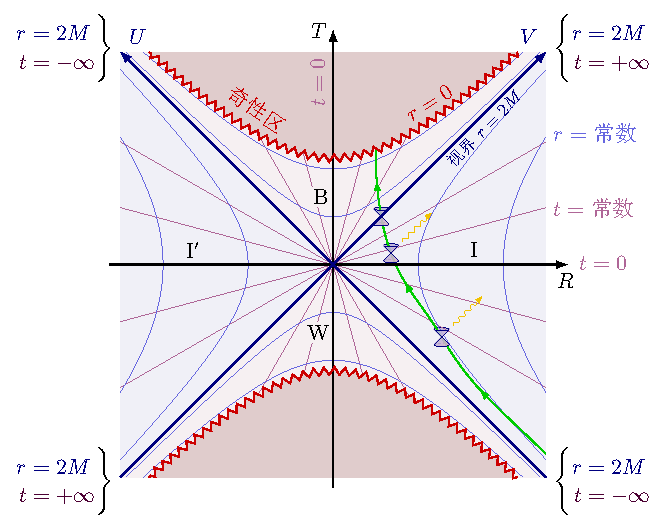
\includegraphics[width=15cm]{fig/II6-Kruskal.pdf}
    \caption{史瓦西度规的最大延拓:Kruskal--Szekeres坐标} \label{chsch:fig_Kruskal}
\end{figure}







图\ref{chsch:fig_Kruskal}{\footnote{本图取自\url{https://tikz.net/relativity_kruskal_diagram/}.}}描述了Kruskal--Szekeres坐标.
分成四个区域:$I$、$I'$、$B$、$W$.
锯齿线表示$r=0$,是奇点;由锯齿线包围的有颜色(浅褐色)区域以及锯齿线本身不属于时空.
史瓦西真空度规\eqref{chsch:eqn_Schw-metric}只是$I$区.
我们需要给出其它几个区的坐标表达式,为此先描述一下$r=2M$是怎样一个区域.

\paragraph{事件视界}\label{chsch:sec_event-horizon}
标注为$U$、$V$的坐标线是$r=2M$的时空区域,称为{\heiti 事件视界}(event horizon);
这是一个嵌入到四维时空的类光超曲面.
事件视界的物理内涵是指视界面内不会对视界面外产生任何影响,
或者说视界外观测者无法观测视界面内的任何信息.

在这个区域有$T=\pm R$;或者说可表示为$U=0$和$V=0$.
从度规\eqref{chsch:eqn_Kruskal-metric-light}可直接验证
切矢量$(\frac{\partial}{\partial U})^a$、$(\frac{\partial}{\partial V})^a$是类光的;
也可利用变换\eqref{chsch:eqn_RTUV}得到
\begin{equation*}
    \left(\frac{\partial}{\partial U}\right)^a = 
    \frac{1}{2} \left(\frac{\partial}{\partial T}\right)^a-
    \frac{1}{2} \left(\frac{\partial}{\partial R}\right)^a,\quad
    \left(\frac{\partial}{\partial V}\right)^a = 
    \frac{1}{2} \left(\frac{\partial}{\partial T}\right)^a+
    \frac{1}{2} \left(\frac{\partial}{\partial R}\right)^a.
\end{equation*}
然后利用度规\eqref{chsch:eqn_Kruskal-metric}验证
切矢量$(\frac{\partial}{\partial U})^a$、$(\frac{\partial}{\partial V})^a$是类光的.
超曲面$V=0$的法矢量是$(\frac{\partial}{\partial U})^a$,
超曲面$U=0$的法矢量是$(\frac{\partial}{\partial V})^a$;
这便证明了超曲面的类光性.

在$I$区,不难得到变换关系如下
\begin{equation}
    \left(\frac{r}{2M}-1\right) \exp{\frac{r}{2M}} = R^2-T^2= -U V;
    \quad \exp\frac{t}{2M}= -\frac{V}{U} .
\end{equation}
绿色类时线代表了有质量质点的运动轨迹,在$I$区,当此质点无限趋近于
超曲面$U=0^{-}$($V$坐标线)时,$r\to 2M^{+}$;因$I$区中$-\infty< U <0$、$0<V<+\infty $,
故由上式可知此时$t\to +\infty$.
同理,不难得到超曲面$V=0^{+}$($U$坐标线)上有$r\to 2M^{+}$、$t\to -\infty$.
\qed

不难发现在$I$区,有坐标变换关系:
\begin{equation}
    U= -\sqrt{\frac{r}{2M}-1}\, \exp\left(\frac{r-t}{4M}\right), \quad
    V= +\sqrt{\frac{r}{2M}-1}\, \exp\left(\frac{r+t}{4M}\right).
\end{equation}
根据因$I$区中的$-\infty< U <0$、$0<V<+\infty $;
在$B$区($0< U <+\infty$、$0<V<+\infty $,不含$r\leqslant 0$区域),我们将上述坐标变换关系延拓为:
\begin{equation}
    U= +\sqrt{1-\frac{r}{2M}}\, \exp\left(\frac{r-t}{4M}\right), \quad
    V= +\sqrt{1-\frac{r}{2M}}\, \exp\left(\frac{r+t}{4M}\right).
\end{equation}
$I'$($0< U <+\infty$、$-\infty< V <0$)是$I$的镜像区,故坐标变换延拓为
\begin{equation}
    U= +\sqrt{\frac{r}{2M}-1}\, \exp\left(\frac{r-t}{4M}\right), \quad
    V= -\sqrt{\frac{r}{2M}-1}\, \exp\left(\frac{r+t}{4M}\right).
\end{equation}
$W$($-\infty< U <0$、$-\infty< V <0$,不含$r\leqslant 0$区域)是$B$的镜像区,故有
\begin{equation}
    U= -\sqrt{1-\frac{r}{2M}}\, \exp\left(\frac{r-t}{4M}\right), \quad
    V= -\sqrt{1-\frac{r}{2M}}\, \exp\left(\frac{r+t}{4M}\right).
\end{equation}
由上述变换,不难得到下述变换:
\begin{align}
    &I\text{区}\ 
    \begin{cases}
       R = \sqrt{\frac{r}{2M}-1}\, \exp\left(\frac{r}{4M}\right)\, \cosh\left(\frac{t}{4M}\right) \\
       T = \sqrt{\frac{r}{2M}-1}\, \exp\left(\frac{r}{4M}\right)\, \sinh\left(\frac{t}{4M}\right) 
    \end{cases} \label{chsch:eqn_SK-I} \\
    &    B\text{区}\ 
    \begin{cases}
         R = \sqrt{1-\frac{r}{2M}}\,\exp\left(\frac{r}{4M}\right)\,\sinh\left(\frac{t}{4M}\right) \\
         T = \sqrt{1-\frac{r}{2M}}\,\exp\left(\frac{r}{4M}\right)\,\cosh\left(\frac{t}{4M}\right) 
    \end{cases} \label{chsch:eqn_SK-B} \\
    & I'\text{区}\ 
    \begin{cases}
       R = -\sqrt{\frac{r}{2M}-1}\,\exp\left(\frac{r}{4M}\right)\,\cosh\left(\frac{t}{4M}\right) \\
       T = -\sqrt{\frac{r}{2M}-1}\,\exp\left(\frac{r}{4M}\right)\,\sinh\left(\frac{t}{4M}\right) 
    \end{cases} \label{chsch:eqn_SK-Ip} \\
    &W\text{区}\ 
    \begin{cases}
       R = -\sqrt{1-\frac{r}{2M}}\,\exp\left(\frac{r}{4M}\right)\,\sinh\left(\frac{t}{4M}\right) \\
       T = -\sqrt{1-\frac{r}{2M}}\,\exp\left(\frac{r}{4M}\right)\,\cosh\left(\frac{t}{4M}\right) 
    \end{cases} \label{chsch:eqn_SK-W} 
\end{align}
以及逆变换
\begin{align}
&I,I',B,W \text{区}:\    \left(\frac{r}{2M}-1\right) \exp{\frac{r}{2M}} = R^2-T^2= -U V  .  \label{chsch:eqn_tr-TR}  \\
&I,I' \text{区}:\       \frac{t}{4M} = \tanh^{-1} \frac{R}{T};\qquad \exp\frac{t}{2M}= -\frac{V}{U} . \label{chsch:eqn_tr-VU-IIp} \\
&B,W \text{区}:\        \frac{t}{4M} = \coth^{-1} \frac{R}{T};\qquad \exp\frac{t}{2M}= +\frac{V}{U} . \label{chsch:eqn_tr-VU-BW}
\end{align}

在$B$区,当用逆变换将Kruskal--Szekeres度规变回史瓦西坐标$\{t,r,\theta,\phi\}$时,
线元表达式与史瓦西度规\eqref{chsch:eqn_Schw-metric}相同;请读者验证此点.
进而可验证,在$I'$、$W$区,史瓦西度规\eqref{chsch:eqn_Schw-metric}仍旧成立,
只不过在$r=2M$区域($U=0$、$V=0$)处无意义.
也就是说在史瓦西坐标$\{t,r,\theta,\phi\}$下,所有四个区的度规表达式是一样的,
但被分割成了四个不连通的区域.这正是坐标奇性的体现.


在$I$、$I'$区,由式\eqref{chsch:eqn_tr-VU-IIp}可知,当$t$是常数时,
$V/U$(或$X/T$)是常数;如图\ref{chsch:fig_Kruskal}所示.
同理,在$B$、$W$区,由式\eqref{chsch:eqn_tr-VU-BW}可得相同结论.

在四个区域,由式\eqref{chsch:eqn_tr-TR}可知,当$r$是常数时,
$U$、$V$(或$T$、$R$)构成双曲线;如图\ref{chsch:fig_Kruskal}所示,
而且图中的双曲线就是根据不同$r$值所绘.


\subsection{Killing矢量场}


很明显,每区都有与球对称的相对应的三个类空矢量场.

容易看出,在$I$区,$(\frac{\partial }{\partial t})^a$是类时Killing矢量场;
在$B$区,$(\frac{\partial }{\partial t})^a$是类空Killing矢量场(请读者验证之).
在$B$区的类时场是$(\frac{\partial }{\partial r})^a$,但它不是Killing矢量场;
因此$B$区不是定态的,更不可能是静态的.

由式\eqref{chsch:eqn_tr-VU-IIp}、\eqref{chsch:eqn_tr-VU-BW}可求得在$I$、$B$区
\begin{equation}\label{chsch:eqn_xi0}
    \left(\frac{\partial }{\partial t}\right)^a=
    \frac{ 1}{4 M } \left[-U \left(\frac{\partial }{\partial U}\right)^a
    +V \left(\frac{\partial }{\partial V}\right)^a \right] .
\end{equation}
因类光切矢量$(\frac{\partial }{\partial U})^a$、$(\frac{\partial }{\partial V})^a$在
事件视界区($r=2M$)是有定义的,故我们可以将$(\frac{\partial }{\partial t})^a$的
表达式\eqref{chsch:eqn_xi0}延拓至事件视界区.
容易验证在事件视界区($r=2M$),$(\frac{\partial }{\partial t})^a$是类光的.
还可以证明在事件视界区($r=2M$),$(\frac{\partial }{\partial t})^a$是Killing矢量场;
为此我们先给出事件视界区($r=2M$),$r$的几个导数:
\begin{align}
    \frac{\partial r}{\partial U}=& -V \exp\left(-\frac{r}{2M}\right) \frac{4M^2}{r},\quad
    \frac{\partial r}{\partial V}=  -U \exp\left(-\frac{r}{2M}\right) \frac{4M^2}{r}. %\\
%    \frac{\partial r}{\partial T}=& -T \exp\left(-\frac{r}{2M}\right) \frac{8M^2}{r},\quad
%    \frac{\partial r}{\partial R}=  +R \exp\left(-\frac{r}{2M}\right) \frac{8M^2}{r}.
\end{align}
在$\{U,V\}$坐标下,由度规\eqref{chsch:eqn_Kruskal-metric-light}求得非零克氏符为
\begin{equation*}
    \Gamma^U_{UU} = \frac{2M}{r}\left(1+\frac{2M}{r}\right) \exp\left(\frac{-r}{2M}\right) V,\quad
    \Gamma^V_{VV} = \frac{2M}{r}\left(1+\frac{2M}{r}\right) \exp\left(\frac{-r}{2M}\right) U.
\end{equation*}
可求得$\xi_a=g_{ab}(\frac{\partial }{\partial t})^b$协变导数的非零分量如下:
\begin{align*}
    \nabla_{\partial_U}\xi_U =& +\frac{2 M + r}{2 M r} UV \exp\left(-\frac{r}{2M}\right) \frac{4M^2}{r} -1 ,\\
    \nabla_{\partial_V}\xi_V =& -\frac{2 M + r}{2 M r} VU \exp\left(-\frac{r}{2M}\right) \frac{4M^2}{r} +1 .
\end{align*}
由上式可见,对与矢量场$\xi_a=g_{ab}(\frac{\partial }{\partial t})^b$有
$\nabla_a \xi_b+\nabla_b \xi_a=0$,也就证明了$\xi_a$是事件视界区($r=2M$)的Killing矢量场.

这样,Kruskal--Szekeres坐标系下共有四个Killing场,
与球对称相对应的三个是类空的;$(\frac{\partial }{\partial t})^a$在$r>2M$区类时,
在$r=2M$区类光,在$r<2M$区类空.


\subsection{Eddington--Finkelstein坐标系}

在Kruskal--Szekeres坐标中计算测地线较为复杂,很难积分出初等函数解.
我们介绍内向Eddington--Finkelstein坐标系来计算测地线;
这个坐标系不能覆盖图\ref{chsch:fig_Kruskal}中四个区域,但可以覆盖$I$和$B$区.

在式\eqref{chsch:eqn_tortoise}中,我们已经积分出乌龟坐标;
在式\eqref{chsch:eqn_uvtrs}引入了新的坐标$\{u,v\}$;
内向Eddington--Finkelstein坐标系取的参数是$\{v,r,\theta,\phi\}$,
即把史瓦西坐标中的$t$换成$v\equiv t+r_*$,其它三个坐标不换;
则史瓦西线元\eqref{chsch:eqn_Schw-metric}变为
\begin{equation}\label{chsch:eqn_EF-metric}
    {\rm d}s^2 = - \left(1-\frac{2 M}{r}\right) ({\rm d}v)^2
    + 2 {\rm d}r {\rm d}v + r^2 {\rm d}\Omega.
\end{equation}
很明显此时的度规在$r=2M$不是奇异的.
%算出非零克氏符
%\begin{subequations}\label{chsch:eqn_EF-Christoffel}
%    \begin{align}
%        &\Gamma^0_{00}= \frac{M}{r^2},\quad
%        \Gamma^0_{22}= -r,\quad
%        \Gamma^0_{33}= -r\sin^2\theta,\quad
%        \Gamma^1_{00}= \frac{M (r-2 M)}{r^3}, \\
%        &\Gamma^1_{01}=\Gamma^1_{10}= -\frac{M}{r^2}, \quad
%        \Gamma^1_{22}= 2 M-r, \quad
%        \Gamma^1_{33}= (2 M-r) \sin ^2\theta  , \\
%        &\Gamma^2_{12}=\Gamma^2_{21}= \frac{1}{r}, \quad
%        \Gamma^2_{33}=-\sin\theta \cos\theta, \quad
%        \Gamma^3_{13}=\Gamma^3_{31}=\frac{1}{r}, \quad
%        \Gamma^3_{23}=\Gamma^3_{32}=\cot\theta . \notag
%    \end{align}
%\end{subequations}
%只涉及$\theta$、$\phi$指标的克氏符与史瓦西坐标下的克氏符相同.


度规\eqref{chsch:eqn_EF-metric}中的参数$-\infty<v<+\infty$对应Kruskal--Szekeres坐标中$0<V<+\infty$;
故内向Eddington--Finkelstein坐标系能覆盖图\ref{chsch:fig_Kruskal}中$I$和$B$区.
度规\eqref{chsch:eqn_EF-metric}中的系数不含有坐标$v$,
故$(\frac{\partial}{\partial v})^a$是Killing场,
容易可验证在$I$区它是类时的,在$B$区是类空的.
由于$g_{rr}=0$,故$(\frac{\partial}{\partial r})^a$是类光的.


设有类时曲线$\gamma(\tau)$,$\tau$是固有时,曲线参数化为$(v,r,\pi/2,\phi)$,
其切线切矢量指向未来(见图\ref{chsch:fig_Kruskal}中绿色线).
对于度规\eqref{chsch:eqn_EF-metric}来说,有
\begin{equation}\label{chsch:eqn_tmp-tl}
    g_{ab}\left(\frac{\partial}{\partial \tau}\right)^a \left(\frac{\partial}{\partial \tau}\right)^b
    = - \left(1-\frac{2 M}{r}\right) \dot{v}^2 + 2 \dot{v} \dot{r} + r^2 \dot{\phi}^2 = -1 < 0
\end{equation}
上式中的“点”表示对$\tau$求导数.因$r^2 \dot{\phi}^2$非负,故由上式可得
\begin{equation}
    \dot{v}\left[- \left(1-\frac{2 M}{r}\right) \dot{v} + 2  \dot{r}\right]  < 0.
\end{equation}
在$I$区,$v$是坐标时,因$\gamma$是指向未来的,故有$\dot{v}>0$.
又因类时线$\gamma$本身连续、光滑,导数也是连续的;
故当$\gamma$穿过$r=2M$区域进入$B$区时,$\dot{v}>0$也是成立的.
所以由上式可以得到在整条$\gamma$线上,有
\begin{equation}\label{chsch:eqn_tmp-rt}
    - \left(1-\frac{2 M}{r}\right) \dot{v} + 2  \dot{r} < 0.
\end{equation}
当$r>2M$时,随着$\tau$的增加,图\ref{chsch:fig_Kruskal}中绿色类时线$r$是逐渐减小的.
当$r\leqslant 2M$时,由\eqref{chsch:eqn_tmp-rt}可知其
第一项是非负的,故在$B$区类时线$\gamma(\tau)$上$\dot{r}<0$.
这样便说明了:不论$I$区还是$B$区,在整条绿色类时线$\gamma(\tau)$上,都有$\dot{r}<0$.
至此,我们证明了指向未来的类时线只能从$I$区穿越视界区($r=2M$),
然后进入$B$区;不能从$B$返回$I$区.
对于指向未来的绿色类时线而言(见图\ref{chsch:fig_Kruskal}),视界($r=2M$)是
一个{\kaishu 单向膜};正因为此,我们称$B$区为{\heiti 黑洞}.
那么它的镜像区$W$自然称为{\heiti 白洞}.
$I$和$B$区是相互连通的.
$I$和$I'$区是不因果连通,即没有类时线或类光线连接两个区域;
它们是两个全同的宇宙.

宇宙飞船的轨迹自然是指向未来的类时线,在飞船穿越$r=2M$之前,如果它开足马力返航,
是可以让$r$随$\tau$的增大而增大的,即$\dot{r}>0$;
可见图\ref{chsch:fig_Kruskal}中绿色类时线上的光锥.
但只要越过视界,便再也没有返航机会.


如果$\gamma$是类光线,$\tau$是一仿射参数.此时式\eqref{chsch:eqn_tmp-tl}中
右端不是等于“$-1$”,而是等于零.为简单起见,我们零$\dot{\phi}=0$,那么有
\begin{equation}
    - \left(1-\frac{2 M}{r}\right) \dot{v}^2 + 2 \dot{v} \dot{r} =0 .
\end{equation}
这说明类光线分为两组,即
\begin{equation}
    \frac{{\rm d}v}{{\rm d}\tau} =0, \quad \text{和}\quad 
    \frac{{\rm d}v}{{\rm d}r} = \frac{2r}{r-2M}.
\end{equation}
第一组只是相互平行的类光线,并无特别之处;略.
第二组类光线,当$r=2M$时,导数是无穷大,相当于在$v-r$图中的一条竖直向上的直线;
这是容易想象的:$r$是横轴,$v$是纵轴,在$r=2M$处,此线垂直于横轴、平行于纵轴.
当$r>2M$时($I$区),随着$r$的增大$v$是增大的.
当$r<2M$时($B$区),$v$是$r$的减函数;这说明在$B$区即便类光线也无法穿越视界返回$I$区.








\section{史瓦西解的NP型式描述}

\section{真空解唯一性定理}

真空爱因斯坦引力场方程的解唯一性定理不止一个,它们有重叠部分,也有不同部分.
我们叙述两个定理;更多、更新内容请参考综述文献\parencite{Chrusciel-2012-lrr}.

\subsection{Birkhoff定理}
\index[physwords]{Birkhoff定理}  

{\bfseries \heiti Birkhoff定理}:真空爱因斯坦场方程的球对称解必是史瓦西度规.%\cite[附录B]{hawking-ellis1973}

下面开始证明.球对称时空的度规
是\eqref{chhss_eqn_g-st-sphere}(${\rm d}\Omega\equiv({\rm d}\theta)^2 + (\sin\theta {\rm d}\phi)^2 $):
\begin{equation}
    \mathrm{d} s^2=  g_{t t}(r, t) \mathrm{d} t^2+2 g_{r t}(r, t) \mathrm{d} r \mathrm{d} t+g_{r r}(r, t) \mathrm{d} r^2 
    +r^2\mathrm{d} \Omega .    \tag{\ref{chhss_eqn_g-st-sphere}}
\end{equation}
由于此处未引入超曲面正交的前提条件,我们采用变换方式将$g_{r t}(r, t)$消掉.
只需定义一个新的{\kaishu 时间}$\tilde{t}$使得
\begin{equation}
    {\rm d}\tilde{t} = \chi(r,t) \bigl(g_{t t}(r, t) \mathrm{d} t+ g_{r t}(r, t) \mathrm{d} r \bigr),
\end{equation}
上式中$\chi$是积分因子,它使得上式右端是全微分;
这样的积分因子总是存在的,证明可参考\parencite[p. 387]{chenwh2017}定理1.2或类似文献.
则上述线元变为:
\begin{equation}
    \mathrm{d} s^2=  g_{t t}^{-1} \chi^{-2} \mathrm{d} \tilde{t}^2+
    \bigl(g_{r r}- g_{t t}^{-1} g_{rt}^{2} \bigr)\mathrm{d} r^2 
    +r^2\mathrm{d} \Omega .
\end{equation}
为了使公式简单,我们引入新函数$\alpha(r,t)= g_{t t}^{-1} \chi^{-2}$、
$\beta(r,t)=g_{r r}- g_{t t}^{-1} g_{rt}^{2}$,并将$\tilde{t}$简记为$t$;
则上述线元变为:
\begin{equation}\label{chsch:eqn_timpshc0}
    \mathrm{d} s^2=  \alpha(r,t) \mathrm{d} t^2+
    \beta(r,t)\mathrm{d} r^2 +r^2\mathrm{d} \Omega .
\end{equation}
利用符号演算软件,由上述度规可得非零Ricci曲率:
\begin{align}
    R_{00} =& \frac{r \beta  ({\alpha'}^2+\dot{\alpha}  \dot{\beta} )
        +\alpha  \left(r (\dot{\beta} ^2+\alpha' \beta')
        -2 \beta  (2 \alpha'+r (\alpha''
        +\ddot{\beta} ))\right)}{4 r \alpha  \beta^2},\\
    R_{01} =& \frac{\dot{\beta} }{r \beta }, \label{chsch:eqn_Rtr}\\
    R_{11} =& \frac{\alpha  \left(4 \alpha  \beta'+r (\dot{\beta} ^2
        +\alpha' \beta')\right)+r \beta  \left(\alpha'^2
        +\dot{\alpha} \dot{\beta} -2 \alpha  (\alpha''
        +\ddot{\beta} )\right)}{4 r \alpha ^2 \beta },\\
    R_{22} =& \frac{1}{2} \left(-\frac{\frac{r \alpha'}{\alpha }+2}{\beta }
    +\frac{r \beta'}{\beta ^2}+2\right),\\
    R_{33} =& \frac{\sin ^2 \theta  \left(\alpha  \left(2 \beta ^2-2 \beta 
        +r \beta'\right)-r \beta  \alpha'\right)}{2 \alpha  \beta ^2} .
\end{align}
上式中“撇号”代表对$r$求导数,“点”代表对$t$求导数.
由于系数含时间$t$,故此处的引力场未必是定态的(或静态).
真空爱氏场方程为$R_{\mu\nu}=0$;
由式\eqref{chsch:eqn_Rtr}可知:$\beta$与时间无关.
从上述$R_{\mu\nu}$表达式容易看出所有与时间有关的导数都去掉了.
则上述真空引力场方程变为($R_{00}$、$R_{11}$、$R_{22}$):
\begin{align}
    0 =& r \beta  {\alpha'}^2  + r \alpha \alpha' \beta'
          -4 \alpha \beta  \alpha'-2 r\alpha \beta  \alpha'' ,\label{chsch:eqn_tmp-r00}\\
    0 =& r \beta \alpha'^2+r  \alpha \alpha' \beta'
    +   4 \alpha^2 \beta'   -2 r\alpha \beta \alpha'' ,\label{chsch:eqn_tmp-r11}\\
    0 =& 2 \alpha\beta ^2-2\alpha \beta +r\alpha \beta'-r \beta  \alpha' . \label{chsch:eqn_tmp-r22}
\end{align}
式\eqref{chsch:eqn_tmp-r11}减去\eqref{chsch:eqn_tmp-r00}得
\begin{equation}\label{chsch:eqn_abp0}
    0= \alpha \beta' + \beta  \alpha' = (\alpha \beta)' .
\end{equation}
由上式得$\alpha'=-\alpha \beta'/\beta$,带入式\eqref{chsch:eqn_tmp-r22}并整理得
\begin{equation}
    \left(\frac{r}{\beta}\right)'=1 .
\end{equation}
因$\beta$与时间无关,故由上两式可得(已将积分常数取得与史瓦西度规相同):
\begin{equation}
    \alpha=- f(t) \left(1- \frac{2M}{r}\right),\qquad
    \beta= \left(1- \frac{2M}{r}\right)^{-1}.
\end{equation}
上式中$f(t)$是恒正函数.定义新的时间坐标$t'$:
\begin{equation}
    t'\equiv \int_{}^{t} \sqrt{f(p)} {\rm d}p .
\end{equation}
这样,线元\eqref{chsch:eqn_timpshc0}变为
\begin{equation}
    \mathrm{d} s^2=  - \left(1- \frac{2M}{r}\right)\mathrm{d} t'^2+
    \left(1- \frac{2M}{r}\right)^{-1}\mathrm{d} r^2 +r^2\mathrm{d} \Omega .
\end{equation}
最后,线元与史瓦西度规\eqref{chsch:eqn_Schw-metric}完全相同.

需要强调的是:当$r<2M$时,$t$是类空坐标线,$r$是类时坐标线.
此时度规场并非定态.
在证明Birkhoff定理过程中,我们没有假设存在类时Killing矢量场,
只假设了时空是球对称的(包含三个类空Killing场).
通过求解爱氏引力场方程,我们得到了第四个Killing场$(\frac{\partial}{\partial t})^a$,
它可能类时($r>2M$),可能类空($r<2M$),可能类光($r=2M$).


\subsection{Israel定理}
\index[physwords]{Israel定理}

\subsubsection{曲率表述等}
下面给出Israel定理的证明\cite{Israel-1967}. %\cite{Robinson-1977}
由于$M$是四维静态时空,故存在与类空超曲面$\Sigma_t$正交的类时Killing矢量
场$\xi^a=(\frac{\partial }{\partial t})^a$;故度规可以写成:
\begin{equation}
    \mathrm{d} s^2=  -N^2 \mathrm{d} t^2+g_{ij} \mathrm{d} x^i  \mathrm{d} x^j.
\end{equation}
$N(>0)$、$g_{ij}$均是空间坐标$\{x^i\}$的函数,不含有时间$t$.
$g_{ij}$是类空超曲面$\Sigma_t$上的度规.
容易算出非零的克氏符$\Gamma^{0}_{\mu\nu}$为
\begin{align}
    \Gamma^{0}_{01}=\Gamma^{0}_{10}= \frac{\partial_{x^1}N}{N},\quad
    \Gamma^{0}_{02}=\Gamma^{0}_{20}= \frac{\partial_{x^2}N}{N},\quad
    \Gamma^{0}_{03}=\Gamma^{0}_{30}= \frac{\partial_{x^3}N}{N}.
\end{align}
当度规的$g_{0i}=0$且各个分量不含时间$t$的时候,曲率公式还能进一步简化.
由于超曲面正交,故ADM分解(见\S\ref{chsm:sec_ADM})后的
位移矢量场$S^a=0$;则有
\begin{equation}
    \left(\frac{\partial }{\partial t}\right)^a = N n^a ;\qquad
    ({\rm d}t)_a = -\frac{1}{N} n_a .
\end{equation}
由外曲率公式\eqref{chsm:eqn_Kab-1}或\eqref{chsm:eqn_K-Christoffel}计算可以得到$K_{ab}=0$;
或者,因度规分量不含时且$S^a=0$,由公式\eqref{chsm:eqn_Lie-t-hab}同样
可得类空超曲面$\Sigma_t$上的外曲率恒为零.
外曲率为零给超曲面上黎曼曲率、Ricci曲率的计算带来诸多方便.
由式\eqref{chsm:eqn_tmp-c0}可知
\begin{equation}\label{chsch:eqn_R4i0}
    {}^{4}{R}_{0i} =0 ,\qquad 1 \leqslant i \leqslant 3 .
\end{equation}
再由式\eqref{chsm:eqn_contractRicci}可得
\begin{equation*} %\label{chsch:eqn_tmp-Rik}
    {}^{3}{R}_{ik}  ={}^{4} {R}_{ik} + {}^{4}{R}_{i0k0}  N^{-2} .
\end{equation*}
经计算有$\Gamma_{0k}^l=0$($1 \leqslant k,l \leqslant 3$).
我们用式\eqref{chrg:eqn_Riemannian04-component}来计算${}^{4}{R}_{i0k0}$:
\begin{align*}
    {}^{4}R_{i0k0} =& -\frac{1}{2}
    \frac{\partial^2 g_{00}} {\partial x^i\partial x^k}
    + g_{00}\Gamma_{0k}^0\Gamma_{0i}^0
    + g_{lp}\left( \Gamma_{0k}^l\Gamma_{0i}^p - \Gamma _{00}^l\Gamma_{ik}^p \right) \\
%    =& N\frac{\partial^2 N} {\partial x^i\partial x^k}
%    +\frac{\partial N} {\partial x^i}\frac{\partial N} {\partial x^k}
%    -\frac{\partial N} {\partial x^i}\frac{\partial N} {\partial x^k}
%    - g_{lp} \Gamma _{00}^l\Gamma_{ik}^p \\
    =& N\frac{\partial^2 N} {\partial x^i\partial x^k}
    -  N \frac{\partial N}{\partial x^p}  \Gamma_{ik}^p 
    = N \nabla_i \nabla_k N .
\end{align*}
带回上上式,有
\begin{equation}\label{chsch:eqn_R4ij}
    {}^{4}{R}_{ik}  ={}^{3} {R}_{ik} -  N^{-1} \nabla_i \nabla_k N .
\end{equation}
下面计算${}^{4}R_{00}$.由式\eqref{chsm:eqn_contractR}可知:
$ {}^{3}{R}={}^{4}{R}+ {}^{4}{R}_{00}  N^{-2} \times 2 $.
而
$    {}^{4}{R} =  {}^{4}R_{\rho\sigma} g^{\rho\sigma}
    = {}^{4}R_{00} g^{00} +  {}^{4}R_{ik}g^{ik}
    \xlongequal{\ref{chsch:eqn_R4ij}} - {}^{4} R_{00}N^{-2} 
    + {}^{3} {R}_{ik} g^{ik} -  N^{-1} g^{ik} \nabla_i \nabla_k N $.
带回,有
\begin{equation}\label{chsch:eqn_R400}
    {}^{4}{R}_{00}  =   N g^{ik} \nabla_i \nabla_k N ;    \quad\text{及}\quad
    {}^{4}{R}={}^{3}{R} - 2N^{-1}g^{ik} \nabla_i \nabla_k  N  .
\end{equation}
由式\eqref{chsch:eqn_R4i0}、\eqref{chsch:eqn_R4ij}、\eqref{chsch:eqn_R400}可以
得到真空爱因斯坦场方程(${}^{4}R_{\mu\nu}=0$).
%由式\eqref{chsch:eqn_R4i0}恒为零和$g_{0i}=0$,可知${}^{4}{G}_{0i}\equiv 0$;
%继而,不难得到
%\begin{equation}\label{chsch:eqn_G4}
%\begin{aligned}
%    {}^{4}{G}_{00} &
%    %={}^{4}{R}_{00} - {}^{4}{R} \frac{1}{2} g_{00}
%    %=N g^{ik} \nabla_i \nabla_k N  +\frac{N^2}{2} ({}^{3}{R} - 2N^{-1}g^{ik} \nabla_i \nabla_k )
%    ={}^{3}{R} \times \frac{N^2}{2}; 
%    \qquad {}^{4}{G}_{0i}\equiv 0; \\
%    {}^{4}{G}_{ij}&
%    %={}^{4}{R}_{ij} - {}^{4}{R} \frac{1}{2} g_{ij}
%    %={}^{3} {R}_{ij} -  N^{-1} \nabla_i \nabla_j N 
%    %-\frac{g_{ij}}{2} ({}^{3}{R} - 2N^{-1}g^{kl} \nabla_l \nabla_k N)
%    ={}^{3}{G}_{ij} - N^{-1} \left( \nabla_i \nabla_j N - g_{ij} (g^{kl} \nabla_k \nabla_l N)\right).
%\end{aligned}
%\end{equation}

%我们已用参数$t$将时空$M$分解为$\mathbb{R}\times \Sigma_t$;下面,进一步分解$\Sigma_t$.
%现在我们采取一个技术性假设\cite{Israel-1967}:可以利用$N$等于常数进一步
%将三维类空超曲面$\Sigma_t$分解为一系列二维曲面,这一过程称为{\kaishu 叶化}(Foliation).
%这样$\Sigma_t$上的线元简化为(我们将四维线元$\mathrm{d} s^2$记
%为$\mathrm{d} s^2=-N^2 \mathrm{d} t^2+{\rm d}\hat{s}^2$):
%\begin{equation}\label{chsch:eqn_S2metric}
%    {\rm d}\hat{s}^2 = \sum_{i,j=1}^{3} g_{ij} \mathrm{d} x^i  \mathrm{d} x^j
%    = \rho^2 {\rm d}N^2 + \sum_{A,B=2}^{3}\hat{g}_{AB}\mathrm{d} x^A  \mathrm{d} x^B.
%\end{equation}
%在本节剩余部分,我们约定大写拉丁字母($A$、$B$等)求和范围是:$2$、$3$.
%为简单起见,我们将第一个坐标记为:$x^1\equiv N$.
%至此,我们将三个类空坐标的第一个分离出来.
%需要再次强调一下,$\rho$、$\hat{g}_{AB}$是$x^1\equiv N$、$x^2$、$x^3$的函数场.
%
%虽然三维类空超曲面$\Sigma_t$的外曲率为零,但通过上述方式叶化后的二维曲面的外曲率不是零.
%通过式\eqref{chsm:eqn_K-Christoffel}可得
%\begin{equation}
%    K_{AB} = {n}_a \Gamma_{AB}^a(\hat{g}) = \rho \Gamma_{AB}^1(\hat{g}) 
%    = - \frac{1}{2\rho}  \frac{\partial \hat{g}_{AB}}{\partial x^1} .
%\end{equation}
%
%由式\eqref{chsch:eqn_S2metric}中$\hat{g}_{AB}$描述的二维曲面来说,
%\begin{equation}
%    \left(\frac{\partial }{\partial N}\right)^a = \rho n^a ;\qquad
%    ({\rm d}N)_a = \frac{1}{\rho} n_a .
%\end{equation}
%再由式\eqref{chsm:eqn_G-Gauss}、\eqref{chsm:eqn_G-Codazzi}得如下式子
%\begin{align}
%    {}^{3}G_{11} \rho^{-2} =& {}^{3}G_{ab} {n}^{a} {n}^{b}    
%    ={}^{2}{R}\frac{-1}{2}   + \frac{1}{2} (K^2 - K^{AB} K_{AB} )  . \\
%    {}^{3}G_{1A} \rho^{-1} =& {}^{3}G_{ab}{n}^{a} h^{b}_A
%    = {\rm D}_A K -{\rm D}_B K_{A}^B ; \quad\text{其中}\
%    K = \hat{g}^{AB}K_{AB}.
%\end{align}


\subsubsection{定理证明}

由$\xi^b$是与超曲面$\Sigma$正交的类时Killing矢量场可知$g_{ab}\xi^a \xi^b = -N^2$;有
\begin{equation}\label{chsch:eqn_Dxi}
    -N\nabla_a N= \xi^b \nabla_a \xi_b = -\xi^b \nabla_b \xi_a .
\end{equation}
我们计算两个式子.
\begin{align*}
    (\nabla_a \xi_b) \nabla^a \xi^b =& \nabla_a \left( \xi_b \nabla^a \xi^b\right)
    -\xi_b \nabla_a \nabla^a \xi^b
    \xlongequal[\ref{chrg:eqn_killing-Riemann-2}]{\ref{chsch:eqn_Dxi}}
    - \nabla^a (N\nabla_a N ) + \xi^b R_{eb}{\xi^e} . \\
    (\nabla_b \xi_a) \nabla^a \xi^b =& \nabla_b \left( \xi_a \nabla^a \xi^b\right)
    -\xi_a \nabla_b \nabla^a \xi^b
    \xlongequal[\ref{chrg:eqn_killing-Riemann-1}]{\ref{chsch:eqn_Dxi}}
    + \nabla^b (N\nabla_b N ) - \xi^a R_{a}^e{\xi_e} .
\end{align*}
考虑到真空爱氏场方程为$R_{ae}=0$,以及$N$是谐和的(式\eqref{chsch:eqn_R400}),有
\begin{equation}\label{chsch:eqn_Wxi}
    \rho \overset{def}{=} -  (\nabla_{[a} \xi_{b]}) \nabla^a \xi^b
    %    = \frac{1}{2}(\nabla_b \xi_a-\nabla_a \xi_b) \nabla^a \xi^b
    %    = \nabla^b (N\nabla_b N )
    =g^{ik}(\nabla_i N) \nabla_k N .
\end{equation}
故$\rho$是正的.



定义
\begin{equation}
    {}^{3}R_{ijk}\overset{def}{=} {}^{3}R_{ij;k}- \frac{1}{4}g_{ij}\times {}^{3}R_{;k}
    -{}^{3}R_{ik;j}+ \frac{1}{4}g_{ik}\times {}^{3}R_{;j} .
\end{equation}
由真空爱氏场方程可知${}^{4}{R}=0$(请注意四维、三维的差别);
再由\eqref{chsch:eqn_R400}式的后半部分可知:
${}^{3}{R} = 2N^{-1}g^{ij} \nabla_i \nabla_j N $.
真空爱氏场方程还要求${}^{4}{R}_{00}  = 0$;
再由\eqref{chsch:eqn_R400}式的前半部分可知:${}^{3}{R} =0$.
那么自然有${}^{3}{R}_{;k}=0$.
继而,由式\eqref{chsch:eqn_R4ij}可知(爱氏场方程${}^{4}{R}_{ik}=0$):
${}^{3} {R}_{ik} =  N^{-1} \nabla_i \nabla_k N $.
计算
\setlength{\mathindent}{0em}
\begin{align*}
    &{}^{3}R_{ijk} \  {}^{3}R^{ijk}= \nabla_k (N^{-1} \nabla_j \nabla_i N)
    \nabla^k (N^{-1} \nabla^j \nabla^i N) \\
    =&\left(-N^{-2}(\nabla_k N)\nabla_j \nabla_i N + N^{-1} \nabla_k  \nabla_j \nabla_i N \right)
    \left(-N^{-2}(\nabla^k N)\nabla^j \nabla^i N + N^{-1} \nabla^k  \nabla^j \nabla^i N \right)\\
    =& +N^{-4}(\nabla_k N)(\nabla_j \nabla_i N )(\nabla^k N)\nabla^j \nabla^i N
    + N^{-2} ( \nabla_k  \nabla_j \nabla_i N)\nabla^k  \nabla^j \nabla^i N \\
    &- N^{-3}(\nabla_k N)(\nabla_j \nabla_i N)\nabla^k  \nabla^j \nabla^i N
    - N^{-3} ( \nabla_k  \nabla_j \nabla_i N)(\nabla^k N)\nabla^j \nabla^i N     \\
    =&
\end{align*}\setlength{\mathindent}{2em}

\begin{align*}
    c=& 4N^{-4} \rho \nabla^i \nabla_i \rho- 4N^{-5} \rho \nabla^i \rho \nabla_i N - 3 N^{-4} \nabla^i\rho \nabla_i \rho \\
    =& + 4N^{-4} (\nabla^k N \nabla_k N) \nabla^i \nabla_i(\nabla^j N \nabla_j N) \\
    &- 4N^{-5} (\nabla^k N \nabla_k N) \nabla^i (\nabla^j N \nabla_j N) \nabla_i N \\
    &- 3 N^{-4} \nabla^i(\nabla^k N \nabla_k N) \nabla_i (\nabla^j N \nabla_j N) \\
    =&
\end{align*}

{\bfseries \heiti Israel定理}:
广义相对论中,静态、真空引力场必是球对称的,
由史瓦西度规描述.史瓦西度规是唯一静态真空引力场.

\section*{小结}
本章主要参考了\parencite[Ch.3]{chandrasekhar-1983}、\parencite{mtw1973}相应章节.

%%%%%%%%%%%%%%%%%%%%%%%%%%%%%%%%%%%%%%%%%%%%%%%%%%%%%%%%%%%%%%%%%%%%%%%%%%%%%%%%%%%
\printbibliography[heading=subbibliography,title=第\ref{chsch}章参考文献]

\endinput

% !TeX encoding = UTF-8
% 此文件从2024.5开始

\chapter{Kerr空间}\label{chkerr}



\section{轴对称时空}\label{chkerr:sec_axis-sym}

许多天体都有自转;由于自转的存在,所以时空一定不是球对称的,而是轴对称的.


%显然$\{t, \phi, x^2, x^3\}$的切标架不是正交归一的;我们选如下正交归一标架场
%\begin{equation}\label{chkerr:eqn_terad-cov}
%\begin{aligned}
%    &(e^0)_a = e^{\nu} ({\rm d}t)_a,\quad 
%     (e^1)_a = e^{\psi}({\rm d}\phi)_a - \omega e^{\psi} ({\rm d}t)_a,\\ 
%    &(e^2)_a = e^{\mu} ({\rm d}x^2)_a,\quad 
%     (e^3)_a = e^{\lambda} ({\rm d}x^3)_a.
%\end{aligned}    
%\end{equation}
%其逆是
%\begin{equation}\label{chkerr:eqn_terad}
%    \begin{aligned}
%        &(e_0)^a = -e^{-\nu} \left(\frac{\partial}{\partial t}\right)^a
%        -e^{-\nu}\omega \left(\frac{\partial}{\partial \phi}\right)^a,\quad 
%         (e_1)^a = e^{-\psi} \left(\frac{\partial}{\partial \phi}\right)^a,\\ 
%        &(e_2)^a = e^{-\mu} \left(\frac{\partial}{\partial x^2}\right)^a,\quad 
%         (e_3)^a = e^{-\lambda} \left(\frac{\partial}{\partial x^3}\right)^a.
%    \end{aligned}    
%\end{equation}

%借助符号软件,计算得到在标架场$\{(e_\mu)^a\}$下的非零黎曼曲率为:
%\begin{small}
%\begin{align*}
%    R_{0101} =& e^{-2 \mu}\nu_{,2} \psi_{,2} + e^{-2 \lambda} \nu_{,3} \psi_{,3}
%     +\frac{1}{4} e^{2 \psi-2 \nu} \left(e^{-2 \mu}  (\omega_{,2})^2+e^{-2 \lambda}  (\omega_{,3})^2  \right), \\
%    R_{0123} =& \frac{1}{2} e^{-\nu +\psi -\mu-\lambda}  \left(\omega _{,3} \left(\psi _{,2}-\nu _{,2}\right)
%    +\left(\nu _{,3}-\psi _{,3}\right) \omega _{,2}\right) ,\\
%    R_{0202} =& e^{-2 \lambda} \nu _{,3} \mu{}_{,3}
%    +e^{-2\mu} \left((\nu _{,2})^2-\mu{}_{,2} \nu _{,2}+\nu _{,2,2}\right)
%    -\frac{3}{4} e^{2 (\psi -\nu -\mu )}  (\omega _{,2})^2,\\
%    R_{0203} =& \frac{1}{4} e^{-2 \nu -\mu-\lambda} \left(4 e^{2 \nu } \left(-\mu_{,3} \nu _{,2}
%    +\nu _{,3} (\nu _{,2}-\lambda_{,2})+\nu _{,2,3}\right)
%    -3 e^{2 \psi } \omega _{,3} \omega _{,2}\right),\\
%    R_{0212} =& \frac{1}{2} e^{-\nu +\psi -2 (\mu+\lambda )} \left(e^{2 \lambda} \left(\omega _{,2} \left(\nu _{,2}
%     -3 \psi _{,2}+\mu{}_{,2}\right)-\omega _{,2,2}\right)
%     -e^{2 \mu} \omega _{,3} \mu_{,3}\right),\\
%    R_{0213} =& \frac{1}{2} e^{-\nu +\psi -\mu-\lambda} \left( (\nu _{,3}-2 \psi _{,3}+\mu_{,3}) \omega _{,2}
%     +\omega _{,3} \left(\lambda_{,2}-\psi _{,2}\right)-\omega _{,2,3}\right), \\
%    R_{0303} =& e^{-2 \lambda} (\nu _{,3})^2-e^{-2 \lambda} \lambda_{,3} \nu _{,3}
%    -\frac{3}{4} e^{-2 (\nu -\psi +\lambda)} (\omega _{,3}) ^2
%    +e^{-2 \lambda} \nu _{,3,3}+e^{-2 \mu} \nu _{,2} \lambda_{,2}, \\
%    R_{0312} =& \frac{1}{2} e^{-\nu +\psi -\mu-\lambda} \left( (\mu_{,3}-\psi _{,3}) \omega _{,2}
%     +\omega _{,3} \left(\nu _{,2}-2 \psi _{,2}+\lambda_{,2}\right)-\omega _{,2,3}\right),\\
%    R_{0313} =& \frac{1}{2} e^{-\nu +\psi -2(\mu+\lambda)} \left(e^{2 \mu} \left(\omega _{,3} \left(\nu _{,3}
%    -3 \psi _{,3}+\lambda_{,3}\right)-\omega _{,3,3}\right)
%    -e^{2 \lambda} \omega _{,2} \lambda_{,2}\right),\\
%    R_{1212} =& \frac{1}{4} e^{-2 (\nu +\mu)} \left(-e^{2 \psi } (\omega _{,2})^2
%    -4 e^{2 \nu } \left((\psi _{,2})^2-\mu_{,2} \psi _{,2}+\psi _{,2,2}\right)\right)
%    -e^{-2 \lambda} \psi _{,3} \mu_{,3},\\
%    R_{1213} =& \frac{1}{4} e^{-2 \nu -\mu-\lambda} \left(-e^{2 \psi } \omega _{,3} \omega _{,2}
%    -4 e^{2 \nu } \left(-\mu_{,3} \psi _{,2}+\psi _{,3} \left(\psi _{,2}-\lambda_{,2}\right)+\psi _{,2,3}\right)\right), \\
%    R_{1313} =& \frac{1}{4} e^{-2 (\nu +\mu+\lambda)} \left(e^{2 \mu} \left(-e^{2 \psi } (\omega _{,3})^2
%    -4 e^{2 \nu } \left((\psi _{,3})^2-\lambda_{,3} \psi _{,3}
%    +\psi _{,3,3}\right)\right)-4 e^{2 \left(\nu +\lambda\right)} \psi _{,2} \lambda_{,2}\right),\\
%    R_{2323} =& e^{-2 \mu} \left(\left(\mu_{,2}-\lambda_{,2}\right) \lambda_{,2}
%    -\lambda_{,2,2}\right)-e^{-2 \lambda} \left((\mu_{,3})^2-\lambda_{,3} \mu_{,3}+\mu_{,3,3}\right) .
%\end{align*}
%\end{small}
%借助符号软件,可得到标架场$\{(e_\mu)^a\}$下的非零Ricci曲率、标量曲率为:
%\begin{align*}
%    R_{00} =& \frac{1}{2} e^{-2 (\nu +\mu+\lambda)} \bigl(e^{2 \mu} \left(2 e^{2 \nu } \left(\nu _{,3} \left(\nu _{,3}
%    +\psi _{,3}+\mu_{,3}-\lambda_{,3}\right)+\nu _{,3,3}\right)-e^{2 \psi } (\omega _{,3})^2\right)\\
%    &+e^{2 \lambda} \left(2 e^{2 \nu } \left(\nu _{,2} \left(\nu _{,2}+\psi _{,2}
%    -\mu_{,2}+\lambda_{,2}\right)+\nu _{,2,2}\right)-e^{2 \psi } (\omega _{,2})^2\right)\bigr) ,\\
%    R_{01} =& \frac{-1}{2} e^{ -2 \lambda -2 \mu -\nu +\psi } \bigl(
%    e^{2 \mu } (\mu _{,3} \omega _{,3}  -\lambda _{,3} \omega _{,3}
%    - \nu _{,3} \omega _{,3}+3 \psi _{,3}\omega _{,3}+ \omega _{,3,3})\\
%    &+e^{2 \lambda } (\lambda _{,2} \omega _{,2}-\mu _{,2} \omega _{,2}
%    - \nu _{,2} \omega _{,2}+3 \psi _{,2} \omega _{,2}+ \omega _{,2,2})\bigr),\\
%    R_{11} = & e^{-2 \mu }\bigl( \mu _{,2} \psi _{,2} - (\psi _{,2})^2 
%    - \lambda _{,2} \psi _{,2} - \nu _{,2} \psi _{,2} - \psi _{,2,2}\bigr) 
%    -\frac{1}{2} e^{-2 (\mu +\nu -\psi )} (\omega _{,2})^2\\
%    & +e^{-2 \lambda } \bigl(\lambda _{,3} \psi _{,3} - \psi _{,3,3} - (\psi _{,3})^2
%    - \mu _{,3} \psi _{,3}  -\nu _{,3} \psi _{,3}\bigr)
%    -\frac{1}{2}  e^{-2(\lambda +\nu -\psi )} (\omega _{,3})^2  ,\\ 
%    R_{22} = &e^{-2 \mu } \bigl( \mu _{,2} \nu _{,2} - (\lambda _{,2})^2 - (\nu _{,2})^2-(\psi _{,2})^2
%    + \lambda _{,2} \mu _{,2}  + \mu _{,2} \psi _{,2}- \lambda _{,2,2}- \nu _{,2,2} -\psi _{,2,2}\bigr) \\
%    &+e^{-2 \lambda }\bigl( \lambda _{,3} \mu _{,3} -(\mu _{,3})^2- \mu _{,3} \left(\nu _{,3}+\psi _{,3}\right)
%    -\mu _{,3,3}\bigr)  +\frac{1}{2} e^{-2 (\mu +\nu -\psi )} (\omega _{,2})^2 ,\\
%    R_{23} =&  e^{-\lambda -\mu  } \bigl(\nu _{,3} (\lambda _{,2}-\nu _{,2})+ \mu_{,3} \nu _{,2}
%    +\psi _{,3} (\lambda _{,2}-\psi _{,2})+ \mu _{,3} \psi _{,2}\\
%    &- \nu _{,2,3}- \psi _{,2,3}  +\tfrac{1}{2} e^{2 (\psi- \nu) } \omega _{,2}\omega _{,3} \bigr),\\
%    R_{33} =& e^{-2 \lambda } \bigl( \lambda _{,3} (\mu _{,3}+\nu _{,3}+\psi _{,3})- \mu _{,3,3}
%    -\nu _{,3,3}- \psi _{,3,3}- (\mu _{,3})^2  - (\nu _{,3})^2- (\psi _{,3})^2 \bigr)\\
%    &+e^{-2 \mu } \bigl( \lambda _{,2} \mu _{,2} - (\lambda _{,2})^2        
%    - \lambda _{,2} \nu _{,2}- \lambda _{,2} \psi _{,2}-\lambda _{,2,2} \bigr)
%    +\frac{1}{2} e^{-2 (\lambda+\nu -\psi )} (\omega _{,3})^2 . \\
%    \tfrac{1}{2}R  =&  e^{-2\lambda}\bigl(\tfrac{1}{4} e^{ 2 (\psi-\nu )} (\omega _{,3})^2  
%    - (\mu _{,3})^2- \left(\nu _{,3}+\psi _{,3}\right) \mu _{,3}
%    - (\nu _{,3})^2-  (\psi _{,3})^2 \\
%    &-  \nu _{,3} \psi _{,3}+  \lambda _{,3} (\mu _{,3} +\nu _{,3}+\psi _{,3})
%    - \mu _{,3,3}-  \nu _{,3,3}-  \psi _{,3,3} \bigr) \\
%    &+ e^{-2 \mu } \bigl(\lambda _{,2} \mu _{,2}- \lambda _{,2} \nu _{,2}+ \mu _{,2} \nu _{,2}
%    - \lambda _{,2} \psi _{,2}+  \mu _{,2} \psi _{,2} - \nu _{,2} \psi _{,2} \\
%    &- \lambda _{,2,2} - \nu _{,2,2}- \psi _{,2,2}  - (\lambda _{,2})^2- (\nu _{,2})^2 
%    - (\psi _{,2})^2+\tfrac{1}{4} e^{2 (\psi-\nu )} (\omega _{,2})^2 \bigr) .
%%    G_{22} =& e^{-2 \lambda } \bigl( (\nu _{,3})^2+ \psi _{,3} \nu _{,3}+ (\psi _{,3})^2
%%    - \lambda _{,3} (\nu _{,3}+\psi _{,3})+ \nu _{,3,3} + \psi _{,3,3} \bigr) \\
%%    &+e^{-2 \mu } \bigl(\lambda _{,2} \nu _{,2} + \lambda _{,2} \psi _{,2}+ \nu _{,2} \psi _{,2} \bigr)
%%    +\frac{1}{4} e^{2 (\psi-\nu )} \bigl(e^{-2 \mu } (\omega _{,2})^2 - e^{-2 \lambda } (\omega _{,3})^2\bigr) ,\\
%%    G_{33} =& e^{-2 \mu } \bigl((\nu _{,2})^2+ (\psi _{,2})^2 - \mu _{,2} \nu _{,2}- \mu _{,2} \psi _{,2}
%%    + \nu _{,2} \psi _{,2} + \nu _{,2,2}+ \psi _{,2,2} \bigr) \\
%%    &+e^{-2 \lambda } \bigl(\nu _{,3} \psi _{,3}+ \mu _{,3} (\nu _{,3}+\psi _{,3})\bigr)
%%    +\frac{1}{4} e^{2 (\psi-\nu )} \bigl(e^{-2 \lambda } (\omega _{,3})^2 - e^{-2 \mu } (\omega _{,2})^2 \bigr).
%\end{align*}
%由上式容易得到轴对称真空爱氏场方程.
从爱氏方程($R_{\mu\nu}=0$)出发推演得到Kerr解是一繁琐、冗长的过程,
\textcite{chandrasekhar-1983}第六章给出了详尽的推导;有兴趣的读者可研读之.
%我们将省略推导,直接给出此解.


\begin{definition}\label{chkerr:def_killing-horizon}
    设四维闵氏流形$(M,g)$上有Killing矢量场$\xi^a$,以及一个类光超曲面$\mathcal{N}$.
    如果$\xi^a$与$\mathcal{N}$正交,则称$\mathcal{N}$是$\xi^a$的{\heiti \bfseries Killing视界}.
\end{definition}

%平直闵氏时空中,类光面$x\pm t =0$是Killing视界,但不是事件视界(见\pageref{chsch:sec_event-horizon}页).
%
%可以证明渐进平坦定态时空的黑洞视界是Killing视界.
%
%我们将坐标$x^2$、$x^3$分别选为$r$、$\theta$.
%Killing视界$\mathcal{N}$的方程是
%\begin{equation}\label{chkerr:eqn_gNr}
%    g^{ab}\left(\nabla_a \mathcal{N}\right)\nabla_b \mathcal{N} = 0 
%    \ \xRightarrow{\ref{chkerr:eqn_AS-metric}} \
%    e^{2(\lambda-\mu)} (\mathcal{N}_{,r})^2 + (\mathcal{N}_{,\theta})^2 =0.
%\end{equation}
%我们将规范选为
%\begin{equation}
%    e^{2(\lambda-\mu)}= \Delta (r); \qquad    \Delta (r)\, \text{是待定函数}
%\end{equation}
%式\eqref{chkerr:eqn_gNr}中的两个平方项$(\mathcal{N}_{,r})^2 $、$ (\mathcal{N}_{,\theta})^2$必然都是非负的;
%而我们通过规范将$e^{2(\lambda-\mu)}$限定为$r$的函数,故必有$ (\mathcal{N}_{,\theta})^2=0$,
%和$\Delta (r)=0$;并且$(\mathcal{N}_{,r})^2\neq 0$,否则$\mathcal{N}$就是常数了(这不可能).
%
%Killing视界是类光超曲面,故度规在此曲面上是退化的.
%Killing视界由$(\frac{\partial}{\partial \phi})^a$、$(\frac{\partial}{\partial t})^a$张成,
%故在超曲面$\mathcal{N}$上,有二维度规行列式为零:
%\begin{equation}
%    e^{2(\psi+\nu)}=0 .
%\end{equation}
%故,在类光超曲面$\mathcal{N}$上,我们可以假设
%\begin{equation}
%    e^{(\psi+\nu)}=\sqrt{\Delta(r)} f(\theta) .
%\end{equation}
%
%我们通过真空爱氏场方程($R_{\mu\nu}=0$)来确定;
%这需要\S\ref{chkerr:sec_axis-sym}中的Ricci曲率.
%由$R_{00}$和$R_{11}$相加减得




\section{Kerr--Newman解}

我们采用Boyer--Lindquist坐标$\{t,r,\theta,\phi\}$,
它与Schwarzschild坐标所用字母是相同的.
则Kerr--Newman度规$g_{\mu\nu}$及其逆$g^{\mu\nu}$是\cite[\S 33.2]{mtw1973}:
\begin{small}
\begin{align}
 g_{\mu\nu}=& \begin{pmatrix}
    \frac{-\Delta+a^2\sin^2\theta }{\rho^2} & 0 & 0 & (\frac{Q^2}{4\pi}-2Mr)\frac{ a \sin^2\theta}{\rho^2} \\
    0 & \frac{\rho^2}{\Delta} & 0 & 0 \\
    0 & 0 & \rho^2 & 0 \\
    (\frac{Q^2}{4\pi}-2Mr)\frac{ a \sin^2\theta}{\rho^2} & 0 & 0 
    & \frac{\sin^2\theta}{\rho^2}((r^2+a^2)^2-\Delta a^2 \sin^2\theta) 
\end{pmatrix}. \label{chkerr:eqn_KN} \\
g^{\mu\nu}=& \begin{pmatrix}
	\bigl(a^2 \sin^2\theta -(r^2+a^2)^2/\Delta\bigr)/\rho^2  & 0 & 0 & a(\frac{Q^2}{4\pi}-2Mr) / \rho^2 \Delta \\
	0 & \Delta / \rho^2 & 0 & 0 \\
	0 & 0 & 1 / \rho^2 & 0 \\
	a(\frac{Q^2}{4\pi}-2Mr) / \rho^2 \Delta & 0 & 0 & (\sin^{-2} \theta -a^2/\Delta) / \rho^2 
\end{pmatrix}. \label{chkerr:eqn_KN-inv}
\end{align} \end{small}
与上两式对应的电磁规范势为(下式为国际制无量纲化后的自然单位制):
\begin{equation}\label{chkerr:eqn_KN-EMA}
    A_a= -\frac{Q r}{{4 \pi} \rho^2 } \left(({\rm d}t)_a - a \sin ^2\theta ({\rm d}\phi)_a \right) .
\end{equation}
其中($Q$是电荷,$M$是质量,$J$是角动量)
\begin{equation}
    \Delta =r^2-2M r +a^2+ \frac{Q^2 }{4\pi };\quad
    \rho^2=\left(a \cos \theta \right)^2+r^2;\quad
    a=\frac{J}{M}.
\end{equation}
通过符号演算程序,容易验证式\eqref{chkerr:eqn_KN}、\eqref{chkerr:eqn_KN-EMA}符合爱氏-麦氏场方程.

当$Q=0$时,Kerr--Newman度规退化为纯粹的Kerr解.笔者认为,不论有无电荷,
这个解的核心人物只有Roy Kerr(新西兰数学物理学家,1934-).




很明显,当$a=0=Q$时,Kerr解退化为Schwarzschild解.


\begin{equation}
    \bar{\rho} =r+\mathbbm{i} a \cos\theta ;\quad 
\bar{\rho}^* =r-\mathbbm{i} a \cos \theta ;\quad
\Omega =\frac{2 a M r}{\Sigma^2}
%        \Sigma^2=&(a^2+r^2)^2-\Delta\, a^2\sin ^2\theta;\quad
\end{equation}


\section{Newman--Penrose型式}

\section*{小结}
本章内容主要取自\parencite{chandrasekhar-1983}相应章节.


\printbibliography[heading=subbibliography,title=第\ref{chkerr}章参考文献]

\endinput

%% !TeX encoding = UTF-8
% 此文件从2025.8开始

\chapter{宇宙学}\label{chcos}

\section{宇宙学原理}\label{chcos:sec_COSP}

爱因斯坦在得到场方程后很快就将其用到宇宙学.
其实,只有爱氏发现广义相对论后,宇宙学才成为一门科学.
由于宇宙的边界条件是未知的,爱因斯坦便提出了{\heiti 宇宙学原理}:
{\kaishu 宇宙在空间上是均匀且各向同性的}.
此原理是抽象的,下面从物理、数学角度来解释
均匀性(见定义\ref{chhss:def_Homogeneous})、各向同性(见定义\ref{chhss:def_isotropic-space}).

天文观测上大致支持:在$3\times 10^{8}$光年尺度以上,宇宙物质的质量密度是均匀的.

我们假设宇宙物质可以近似成理想流体,它的能动张量为\eqref{chlh:eqn_perfect-fluid-Tab}式:
\begin{equation}
	T^{ab}=\left(\rho  + p \right) U^a U^b +p g^{ab} .
	\tag{\ref{chlh:eqn_perfect-fluid-Tab}}
\end{equation}

各向同性是指:在1+3分解后,空间部分是各向同性的.

如果有一个粒子以半光速远离银河系中心,那么在此粒子看来,宇宙并非各向同性的.
然而,在与流体质团共动的参考系中,宇宙是各向同性的.

由于宇宙的空间(类空超曲面)是三维实流形,
由定理\ref{chhss:thm_isotropic-manifold}可知:
此类空超曲面必然是常曲率的,且等距群具有最高的对称性(见\pageref{chhss:sec_fh}页).


{\kaishu 各向同性确保了宇宙学流体的世界线与均匀各向同性类空超曲面相互正交.}证明过程大致如下所述.
一个“与流体共动”的观察者可以测量他自己相对于该类空超曲面的三维速度,
如果该三维速度不为零,那么这个三维速度就是一个特殊方向,它将为观察者提供一种区分空间方向的方法;
他的静止参考系与所有其他参考系不同,这违背了各向同性原则.
因此,在一个各向同性的宇宙中(在这个宇宙中,“观察者与流体共动”的概念才有意义),
每一个这样的观察者都必须发现,相对于均匀性表面而言,他处于静止状态.他的世界线与那个均匀类空超曲面正交.

\section{FLRW度规}
由\S\ref{chcos:sec_COSP}的分析可知,宇宙是均匀、各向同性的;
那么由式\eqref{chhss:eqn_g-cos-2}可以得到如下
Friedmann--Lema\^{i}tre--Robertson--Walker度规(局部坐标为$\{t,r,\theta,\phi\}$):
\begin{equation}\label{chcos:eqn_FLRW-metric}
	\mathrm{d} s^2=-\mathrm{d} t^2+a^2(t)\left\{\frac{\mathrm{d} r^2}{1-k r^2}
	+r^2 \mathrm{d} \theta^2+r^2 \sin ^2 \theta \mathrm{d} \phi^2\right\}    .
\end{equation}
其中
\begin{equation}
	k= \begin{cases}
		+1 & \text { 当最大对称子空间的 } K>0,\quad \text{超球面} \\ 
		-1 & \text { 当最大对称子空间的 } K<0,\quad \text{双曲空间} \\ 
		0  & \text { 当最大对称子空间的 } K=0,\quad \text{超平面}
	\end{cases} .
\end{equation}
FLRW度规$g_{ab}$行列式为:
\begin{equation}\label{chcos:eqn_FLRW-detg}
	g=\det(g_{\alpha\beta})= \frac{r^4 a^6 \sin^2 \theta}{k r^2-1} .
\end{equation}
FLRW度规非零克氏符:
\begin{subequations}\label{chcos:eqn_FLRW-Gamma}
\begin{align}
	&\Gamma^{0}_{11} = \frac{a \dot{a}}{1-k r^2},\quad
	\Gamma^{0}_{22} =  a \dot{a} r^2,\quad
	\Gamma^{0}_{33} =  a \dot{a} r^2 \sin ^2\theta, \\
	&\Gamma^{1}_{01} = \Gamma^{1}_{10} = \Gamma^{2}_{02} = \Gamma^{2}_{20} = 
	\Gamma^{3}_{03} = \Gamma^{3}_{30} = \frac{\dot{a}}{a}, \\
	&\Gamma^{1}_{11} = \frac{k r}{1-k r^2},\quad
	\Gamma^{1}_{22} = r \left(k r^2-1\right),\quad
	\Gamma^{1}_{33} = r \left(k r^2-1\right) \sin ^2 \theta ,\\
	&\Gamma^{2}_{12} = \Gamma^{2}_{21} = \Gamma^{3}_{13} = \Gamma^{3}_{31} = \frac{1}{r}, \\
	&\Gamma^{2}_{33} = - \sin \theta \cos \theta ,\quad
	\Gamma^{3}_{23} = \Gamma^{3}_{32} = \cot \theta .
\end{align}
\end{subequations}
FLRW度规非零黎曼曲率,以及标量曲率:
\begin{subequations}\label{chcos:eqn_FLRW-Riemann}
\begin{align}
	&R_{0101} = \frac{a \ddot{a}}{k r^2-1} ,\quad 
	R_{0202} = - a \ddot{a} r^2,\quad
	R_{0303} = - a \ddot{a} r^2 \sin^2 \theta , \\
	&R_{1212} = \frac{ a^2 \left(\dot{a}^2+k\right)r^2}{1-k r^2}, \quad
	R_{1313} = \frac{ a^2 \left(\dot{a}^2+k\right) r^2 \sin^2\theta }{1-k r^2},\\
	&R_{2323} =  a^2 \left(\dot{a}^2+k\right) r^4 \sin^2\theta ,\qquad
	R = \frac{6 \left(a \ddot{a}+\dot{a}^2+k\right)}{a^2} .
\end{align}
\end{subequations}
FLRW度规非零Ricci曲率:
\begin{subequations}\label{chcos:eqn_FLRW-Ricci}
	\begin{align}
		&R_{00} = -\frac{3 \ddot{a}}{a} ,\quad 
		R_{11} = \frac{a \ddot{a}+2 \dot{a}^2+2 k}{1-k r^2} , \\
		&R_{22} = \left(a \ddot{a}+2 \dot{a}^2+2 k\right) r^2 , \quad
		R_{33} = R_{22} \sin ^2\theta.
	\end{align}
\end{subequations}
FLRW度规非零爱因斯坦张量:
\begin{subequations}\label{chcos:eqn_FLRW-G}
	\begin{align}
		&G_{00} = \frac{3 \left(\dot{a}^2+k\right)}{a^2} ,\quad 
		G_{11} = \frac{2 a \ddot{a}+\dot{a}^2+k}{k r^2-1} ,\\
		&G_{22} = - \left(2 a \ddot{a}+\dot{a}^2+k\right) r^2 , \quad
		G_{33} = G_{22} \sin ^2\theta.
	\end{align}
\end{subequations}





\section{均匀空间}

一个$m$维、度规正定的黎曼空间$M$,如果它还是均匀空间,
那么它的等距群$I(M)$至少是$m$维的,即至少要有$m$个Killing切矢量场.
设有三维实均匀空间$\Sigma$,其度量$h_{ab}$是正定的.
均匀空间$\Sigma$的等距群$I(\Sigma)$有一个三维子群$G$,
其李代数为$\mathscr{G}$,它的基矢记为$\{(e_i)^a\}$($i=1,2,3$).

由于李群$G$的左不变切矢量场自然也是作为流形$G$的切矢量场,
故切矢量场的对易公式\eqref{chrg:eqn_EmuEnucommutator}是成立的,即
\begin{align}
	\bigl[(e_i), (e_j)\bigr]^a
	= \bigl(\Gamma^{k}_{ji} - \Gamma^{k}_{ij}\bigr) (e_k)^a
	= \bigl(-\omega_{jki} + \omega_{ikj}\bigr) (e^k)^a .
	\tag{\ref{chrg:eqn_EmuEnucommutator} }
\end{align}
式\eqref{chrg:eqn_EmuEnucommutator}第一个等号适用于一般标架,
第二个等号只适用于刚性标架(定义见\ref{chrg:def_rigid-frame});下面在刚性标架中讨论问题.
\begin{align*}
	C^k_{ij} (e_k)^a = \bigl[(e_i), (e_j)\bigr]^a
	= \bigl(-\omega_{jki} + \omega_{ikj}\bigr) (e^k)^a  .
\end{align*}
用对偶矢量场$\{(e_l)_a\}$缩并上式,有
\begin{equation}
	C^k_{ij} h_{kl}= \omega_{ilj} -\omega_{jli}
	\xlongequal{\ref{chrg:eqn_Coef-Lambda1}} \Lambda_{ilj} .
\end{equation}
其中$\Lambda_{il j}$定义见式\eqref{chrg:eqn_Coef-Lambda1}.





\section*{小结}

\printbibliography[heading=subbibliography,title=第\ref{chcos}章参考文献]

\endinput

%% !TeX spellcheck = <none>
% !TeX encoding = UTF-8
% 此文件从2022.3.04开始写作

\chapter{后牛顿近似} \label{chppn}
爱因斯坦引力场方程是非线性的,很难严格求解.
由爱因斯坦本人提出并发展的后牛顿近似方法是处理引力束缚系统
的常用方法.
为了便于比较量级以及使用,本章以及下一章使用国际单位制;
并且基本用分量语言来描述;坐标系则需要根据要处理的问题
进行选取,如无特殊要求,我们选取固有坐标系(见\S\ref{chfd:sec_proper-coord}).

需要强调:所有张量场(除$g_{\mu\nu},\, g^{\mu\nu}$外)都
需用洛伦兹度规$\eta_{\mu\nu},\, \eta^{\mu\nu}$来升降指标.
由于我们采用的度规号差是$(-+++)$,故在三维纯空间部分,
当用$\eta_{\mu\nu}$(或$\delta_{ij}$)升降指标时,只有象征意义,
不会产生额外的正负号.正是这个原因,在纯空间部分本章很多公式等号两端
的上下指标不匹配.

本章主要参考了文献\parencite[Ch. 9]{weinberg_grav-1972}.
%\parencite[Ch. 7-8]{xu-wu-1999},
%\parencite{poisson-will-2014}.

\section{量级估算}
只有清楚了各物理量的数量级,才能作可靠的近似.
考虑一个由引力束缚在一起的质点系统(如太阳系)
$M$、$r$、$v$分别代表质点的质量、平均距离和速度.
根据位力定理
\begin{equation}
    v^2 \approx \frac{GM}{r} \equiv U .
\end{equation}
其中$U$是引力势函数,
\begin{equation}
    U = -\phi = +\int \frac{G \rho(\boldsymbol{y})}{|\boldsymbol{x}-\boldsymbol{y}|} {\rm d}^3y
      = +\frac{G M }{r} .
\end{equation}
后牛顿近似中更喜欢用$U$,而不是$\phi$.
对于太阳表面而言
\begin{equation}
    \frac{v^2}{c^2}=\frac{G M_{\odot} }{c^2 R_{\odot}} \approx 2 \times 10^{-6} .
\end{equation}
对于地球表面而言
\begin{equation}
    \frac{v^2}{c^2}=\frac{G M_{\oplus} }{c^2 R_{\oplus}} \approx 7 \times 10^{-10} .
\end{equation}
可见不论太阳还是地球表面都可看成弱引力场,
在此区域飞行的质点速度$v/c$都不高.令
\begin{equation}\label{chppn:eqn_vdc}
    \bar{v}\equiv \frac{v}{c}.
\end{equation}
我们将借助参量$\bar{v}$将各种物理量展开.

物质内能可通过压强来表述,单位质量内能与引力势处于同一量级,
\begin{equation}
    \frac{E_{\text{内能}}}{c^2} \sim \frac{p}{c^2 \rho}\sim
    \frac{\phi}{c^2} \sim \bar{v}^2
\end{equation}

系统中的距离和时间尺度分别$r$和$r/v$,故导数量级大约是
\begin{equation}
    \frac{\partial}{\partial x^i}\sim \frac{1}{r},\qquad
    \frac{\partial}{\partial x^0}\sim \frac{\partial}{c \partial t}
    \sim \frac{v}{cr} \sim  \bar{v} \frac{\partial}{\partial x^i}.
\end{equation}


后牛顿近似本质上是对$\bar{v}$(式\eqref{chppn:eqn_vdc})的近似展开,
也经常说成是对光速$c^{-1}$展开.展开后精确到不同量级,
比如$O(\bar{v}),\, O(\bar{v}^2),\, O(\bar{v}^4),\cdots$,
这些量级会在公式中有显示表示;通常我们会把上述量级简记
为$O(1),\, O(2),\, O(4),\cdots$.


\section{基本方法}
基本出发点是引力场方程和自由质点运动方程(即测地线方程).
先讨论测地线方程
\begin{equation}
    \frac{{\rm d}^2 x^\mu}{{\rm d}\tau ^2}+ {\Gamma}_{\nu\lambda}^{\mu}
      \frac{{\rm d} x^\nu}{{\rm d}\tau} \frac{{\rm d} x^\lambda}{{\rm d}\tau} =0,
\end{equation}
其中$\tau$是固有时.由此出发可以算出空间的三维加速度是(注$x^0=ct$)
\begin{align}
    \frac{{\rm d}^2 x^i}{{\rm d} t^2} =& \frac{{\rm d} \tau}{{\rm d}t}
       \frac{{\rm d} }{{\rm d}\tau} \left( \frac{{\rm d} \tau}{{\rm d}t}
       \frac{{\rm d} x^i}{{\rm d} \tau} \right)
    =\left(\frac{{\rm d} t}{{\rm d}\tau} \right)^{-2} \frac{{\rm d}^2 x^i}{{\rm d} \tau^2}
     -\left(\frac{{\rm d} t}{{\rm d}\tau} \right)^{-3}
     \frac{{\rm d}^2 x^0}{c\, {\rm d} \tau^2} \frac{{\rm d} x^i}{{\rm d} \tau}  \notag \\
    =&-{\Gamma}_{\nu\lambda}^{i} \frac{{\rm d} x^\nu}{{\rm d}t} \frac{{\rm d} x^\lambda}{{\rm d}t}
      +\frac{1}{c} {\Gamma}_{\nu\lambda}^{0} \frac{{\rm d} x^i}{{\rm d}t}
       \frac{{\rm d} x^\nu}{{\rm d}t} \frac{{\rm d} x^\lambda}{{\rm d}t} \notag \\
    =& -c^2 \Gamma_{00}^{i} - 2c \Gamma_{0j}^{i}\frac{{\rm d} x^j}{{\rm d}t}
       -\Gamma_{jk}^{i} \frac{{\rm d} x^j}{{\rm d}t} \frac{{\rm d} x^k}{{\rm d}t} \notag \\
      & +\frac{1}{c}\frac{{\rm d} x^i}{{\rm d}t} \left(
        c^2 \Gamma_{00}^{0} + 2c \Gamma_{0j}^{0}\frac{{\rm d} x^j}{{\rm d}t}
       +\Gamma_{jk}^{0} \frac{{\rm d} x^j}{{\rm d}t}
       \frac{{\rm d} x^k}{{\rm d}t}  \right) . \label{chppn:eqn_PN}
\end{align}
回顾\S\ref{chle:sec_Newton-limit},当$\bar{v} \ll 1$时,我们
只保留一阶项,有$g_{00}=-(1+ 2\phi/c^2)$和$g_{0i}=0,\, g_{ij}=\delta_{ij}$,
那么牛顿第二定律和万有引力公式结合之后是
\begin{equation}
    \frac{{\rm d}^2 x^i}{{\rm d}t^2}=-c^2{\Gamma}_{00}^i
    =\frac{c^2}{2} \frac{\partial g_{00}}{\partial x^i}
    =-\frac{\partial \phi}{\partial x^i} .
\end{equation}
由此可见牛顿近似中$\frac{{\rm d}^2 x^i}{{\rm d}t^2}$准确到量级
$\frac{G M}{r^2} \sim \frac{v^2}{r}$.
也就是$\Gamma_{00}^i\sim \frac{G M}{c^2 r^2} \sim \frac{\bar{v}^2}{r} $.
在我们这个后牛顿近似的初步介绍中,
只要求式\eqref{chppn:eqn_PN}中其它各项
准确到$\frac{\bar{v}^4}{r}$量级(忽略更高量级的项),那么
对Christoffel符号诸分量的要求是
\begin{subequations}
\begin{align}
    & \Gamma_{00}^i {\quad \text{须准确到量级}\quad } \frac{\bar{v}^4}{r},  \\
    & \Gamma_{0j}^i {\quad \text{须准确到量级}\quad } \frac{\bar{v}^3}{r},  \\
    & \Gamma_{jk}^i {\quad \text{须准确到量级}\quad } \frac{\bar{v}^2}{r},  \\
    & \Gamma_{00}^0 {\quad \text{须准确到量级}\quad } \frac{\bar{v}^3}{r},  \\
    & \Gamma_{0j}^0 {\quad \text{须准确到量级}\quad } \frac{\bar{v}^2}{r},  \\
    & \Gamma_{jk}^0 {\quad \text{须准确到量级}\quad } \frac{\bar{v}}{r}.
\end{align}
\end{subequations}
以上只是对有质量粒子的要求,对于光子的后牛顿近似另行讨论.

\subsection{度规场近似}
因为克氏符是由度规来表述的,下面我们来看度规的近似展开.
\begin{equation}
    \frac{{\rm d} s^2}{{\rm d}t^2} = c^2 g_{00} + 2 c g_{0i} \frac{{\rm d} x^i}{{\rm d}t}
     + g_{ij} \frac{{\rm d} x^i}{{\rm d}t}  \frac{{\rm d} x^j}{{\rm d}t} .
\end{equation}
后牛顿方法是弱场、低速近似,度规场不会偏离洛伦兹度规太远,故假设度规可以展开为
\begin{subequations}\label{chppn:eqn_gdab}
\begin{align}
    g_{00} =& -1 + \oversetmy{2}{g}_{00}+\oversetmy{4}{g}_{00}+ \cdots,  \\
    g_{ij} =& \delta_{ij} + \oversetmy{2}{g}_{ij}+\oversetmy{4}{g}_{ij}+ \cdots,  \\
    g_{i0} =& \oversetmy{3}{g}_{i0}+\oversetmy{5}{g}_{i0}+ \cdots
\end{align}
\end{subequations}
{\kaishu 其中$\oversetmy{N}{g}_{\mu\nu}$表示$g_{\mu\nu}$中
    量级为$\bar{v}^N$(见式\eqref{chppn:eqn_vdc})的近似项;
其它量也采取类似的表述方式.} 因为在时间反演下${\rm d} s^2$必然是个不变量,
而速度$v^i=\frac{{\rm d} x^i}{{\rm d}t}$是要改变符号的,
故式\eqref{chppn:eqn_gdab}中$g_{0i}$必须是$\bar{v}$的奇数次幂;
而$g_{00},\, g_{ij}$只能包含$\bar{v}$的偶数次幂项.
如果有辐射阻尼之类的作用,那么可能打破上述奇偶规律;遇到该问题时再行讨论.

我们知道度规场有关系式:$g^{\mu\rho}g_{\rho\nu}=\delta^\mu_\nu$;把它展开
\begin{subequations}
\begin{align}
    g^{0\rho}g_{\rho 0}=& g^{00}g_{0 0}+g^{0k}g_{k 0} = 1, \qquad \text{一个方程} \\
    g^{0\rho}g_{\rho j}=& g^{00}g_{0 j}+g^{0k}g_{k j} = 0, \qquad \text{三个方程} \\
    g^{i\rho}g_{\rho j}=& g^{i0}g_{0 j}+g^{ik}g_{k j} =\delta^i_j. \qquad \text{六个方程}
\end{align}
\end{subequations}
我们预估逆变度规有如下形式(为了方便引用,第二个等号是把
式\eqref{chppn:eqn_gugd}带入后的结果)
\begin{subequations}\label{chppn:eqn_guab}
\begin{align}
    g^{00} =& -1 + \oversetmy{2}{g}^{00}+\oversetmy{4}{g}^{00}+ \cdots
      &=& -1 -\oversetmy{2}{g}_{00} -\oversetmy{4}{g}_{00}-(\oversetmy{2}{g}_{00})^2 +\cdots  \\
    g^{ij} =& \delta^{ij} + \oversetmy{2}{g}^{ij}+ \cdots
      &=&  \delta_{ij}  -\oversetmy{2}{g}_{ij} + \cdots \\
    g^{i0} =& \oversetmy{3}{g}^{i0}+ \cdots
      &=& \oversetmy{3}{g}_{0i} + \cdots
\end{align}
\end{subequations}
利用互逆关系($g^{\mu\rho}g_{\rho\nu}=\delta^\mu_\nu$),把式\eqref{chppn:eqn_guab}第二个等号前的
表达式代入式\eqref{chppn:eqn_gdab},有
\begin{equation}\label{chppn:eqn_gugd}
    \oversetmy{2}{g}^{00} = -\oversetmy{2}{g}_{00}, \quad
    \oversetmy{4}{g}^{00} = -\oversetmy{4}{g}_{00}-(\oversetmy{2}{g}_{00})^2, \quad
    \oversetmy{2}{g}^{ij} = -\oversetmy{2}{g}_{ij}, \quad
%    \oversetmy{4}{g}^{ij} = -\oversetmy{4}{g}_{ij}+ \oversetmy{2}{g}_{ik}\oversetmy{2}{g}_{kj}, \quad
    \oversetmy{3}{g}^{0i} = +\oversetmy{3}{g}_{0i}, \quad    \cdots
\end{equation}
注意:得到上式后,再代入式\eqref{chppn:eqn_guab}才得到第二个等号后面的公式.

\subsection{Christoffel符号近似}
克氏符定义为
%\begin{equation}
$    \Gamma^\mu_{\lambda\nu}=\frac{1}{2}g^{\mu\rho}(
      \frac{\partial g_{\rho\nu}}{\partial x^\lambda}
     +\frac{\partial g_{\lambda\rho}}{\partial x^\nu}
     -\frac{\partial g_{\lambda\nu}}{\partial x^\rho} ) $.
%\end{equation}
从而可以求出
\begin{align*}
    \Gamma^i_{00}=&\frac{1}{2}g^{i0}\left(
     \frac{\partial g_{0 0}}{\partial x^0}
    +\frac{\partial g_{0 0}}{\partial x^0}
    -\frac{\partial g_{00}}{\partial x^0} \right)
    +\frac{1}{2}g^{ij}\left(
    \frac{\partial g_{j 0}}{\partial x^0}
    +\frac{\partial g_{0 j}}{\partial x^0}
    -\frac{\partial g_{00}}{\partial x^j} \right) \\
%    =&\frac{1}{2} \oversetmy{3}{g}^{i0} \left(
%     \frac{\partial (-1+\oversetmy{2}{g}_{00})}{\partial x^0}
%    +\frac{\partial (-1+\oversetmy{2}{g}_{00})}{\partial x^0}
%    -\frac{\partial (-1+\oversetmy{2}{g}_{00})}{\partial x^0} \right)
%    +\frac{1}{2}(\delta_{ij}+\oversetmy{2}{g}^{ij})\left(
%     \frac{\partial \oversetmy{3}{g}_{j0}}{\partial x^0}
%    +\frac{\partial \oversetmy{3}{g}_{j0}}{\partial x^0}
%    -\frac{\partial (-1+\oversetmy{2}{g}_{00}+\oversetmy{4}{g}_{00})}
%       {\partial x^j} \right) \\
    =& \frac{1}{2}(\delta_{ij}+\oversetmy{2}{g}^{ij})\left(
    2\frac{\partial \oversetmy{3}{g}_{j0}}{\partial x^0}
    -\frac{\partial (\oversetmy{2}{g}_{00}+\oversetmy{4}{g}_{00})}
      {\partial x^j} \right) + O(5)\\
    =& \frac{1}{2} \left(
    2\frac{\partial \oversetmy{3}{g}_{i0}}{\partial x^0}
    -\frac{\partial (\oversetmy{2}{g}_{00}+\oversetmy{4}{g}_{00})} {\partial x^i}
    -\oversetmy{2}{g}^{ij} \frac{\partial \oversetmy{2}{g}_{00}}{\partial x^j}
      \right) + O(5)
\end{align*}
利用式\eqref{chppn:eqn_gugd},由上式可得
\begin{equation}
    \Gamma^i_{00}= \frac{1}{2} \left(
    -\frac{\partial \oversetmy{2}{g}_{00}} {\partial x^i}
    +2\frac{\partial \oversetmy{3}{g}_{i0}}{\partial x^0}
    -\frac{\partial \oversetmy{4}{g}_{00}} {\partial x^i}
    +\oversetmy{2}{g}_{ij} \frac{\partial \oversetmy{2}{g}_{00}}{\partial x^j}
    \right) + O(5)
\end{equation}
与上述过程类似,可以得到如下各阶克氏符近似表达式
\begin{subequations}\label{chppn:eqn_Gammag}
\begin{align}
    \oversetmy{2}{\Gamma}^i_{00} = & -\frac{1}{2}\frac{\partial \oversetmy{2}{g}_{00}} {\partial x^i} ;\\
    \oversetmy{4}{\Gamma}^i_{00} = & -\frac{1}{2}\frac{\partial \oversetmy{4}{g}_{00}} {\partial x^i}
       + \frac{\partial \oversetmy{3}{g}_{0i}} {\partial x^0}
       + \frac{1}{2}\oversetmy{2}{g}_{ij}\frac{\partial \oversetmy{2}{g}_{00}} {\partial x^i} ;  \\
    \oversetmy{3}{\Gamma}^i_{0j} = & \frac{1}{2}\left(
         \frac{\partial \oversetmy{3}{g}_{0i}} {\partial x^j}
       + \frac{\partial \oversetmy{2}{g}_{ij}} {\partial x^0}
       - \frac{\partial \oversetmy{3}{g}_{0j}} {\partial x^i} \right) ; \\
    \oversetmy{2}{\Gamma}^i_{jk} = & \frac{1}{2}\left(
      \frac{\partial \oversetmy{2}{g}_{ij}} {\partial x^k}
    + \frac{\partial \oversetmy{2}{g}_{ik}} {\partial x^j}
    - \frac{\partial \oversetmy{2}{g}_{jk}} {\partial x^i} \right) ; \\
    \oversetmy{3}{\Gamma}^0_{00} = & -\frac{1}{2}\frac{\partial \oversetmy{2}{g}_{00}} {\partial x^0} ; \\
    \oversetmy{2}{\Gamma}^0_{0j} = & -\frac{1}{2}\frac{\partial \oversetmy{2}{g}_{00}} {\partial x^j} ; \\
    \oversetmy{1}{\Gamma}^0_{ij} = & 0 =\oversetmy{2}{\Gamma}^0_{ij}, \qquad
    \oversetmy{3}{\Gamma}^0_{ij} = -\frac{1}{2} \left(
    \frac{\partial \oversetmy{3}{g}_{0j} }{\partial x^k}
    +\frac{\partial \oversetmy{3}{g}_{0k}}{\partial x^j}
    -\frac{\partial \oversetmy{2}{g}_{jk} }{\partial x^0} \right) .
\end{align}
\end{subequations}

显然,我们必须知道度规分量$g_{ij}$准确到量级$\bar{v}^2$,
$g_{i0}$准确到量级$\bar{v}^3$,$g_{00}$准确到量级$\bar{v}^4$.
应当把这一点同纯牛顿力学对照一下,在那里我们
需要$g_{00}$精确到量级$\bar{v}^2$;而$g_{i0}=0$,$g_{ij}=\delta_{ij}$,
即只需精确到零级.


%其它各项推导过程
%\begin{align*}
%    \Gamma^i_{0j}=&\frac{1}{2}g^{i0}\left(
%     \frac{\partial g_{0 j}}{\partial x^0}
%    +\frac{\partial g_{0 0}}{\partial x^j}
%    -\frac{\partial g_{0j}}{\partial x^0} \right)
%    +\frac{1}{2}g^{il}\left(
%     \frac{\partial g_{l 0}}{\partial x^j}
%    +\frac{\partial g_{j l}}{\partial x^0}
%    -\frac{\partial g_{0 j}}{\partial x^l} \right) \\
%    =&\frac{1}{2}\oversetmy{3}{g}_{0i} \left(
%    \frac{\partial \oversetmy{3}{g}_{0j} }{\partial x^0}
%    +\frac{\partial \oversetmy{2}{g}_{00} }{\partial x^j}
%    -\frac{\partial \oversetmy{3}{g}_{0j} }{\partial x^0} \right)
%    +\frac{1}{2}(\delta_{il}  -\oversetmy{2}{g}_{il})\left(
%    \frac{\partial \oversetmy{3}{g}_{0l} }{\partial x^j}
%    +\frac{\partial  \oversetmy{2}{g}_{lj} }{\partial x^0}
%    -\frac{\partial \oversetmy{3}{g}_{0j} }{\partial x^l} \right) \\
%    =& \frac{1}{2}  \left(
%    \frac{\partial \oversetmy{3}{g}_{0i} }{\partial x^j}
%    +\frac{\partial  \oversetmy{2}{g}_{ij} }{\partial x^0}
%    -\frac{\partial \oversetmy{3}{g}_{0j} }{\partial x^i} \right)
%\end{align*}
%\begin{align*}
%    \Gamma^i_{jk}=&\frac{1}{2}g^{i0}\left(
%    \frac{\partial g_{0 j}}{\partial x^k}
%    +\frac{\partial g_{0 k}}{\partial x^j}
%    -\frac{\partial g_{0j}}{\partial x^0} \right)
%    +\frac{1}{2}g^{il}\left(
%     \frac{\partial g_{l k}}{\partial x^j}
%    +\frac{\partial g_{j l}}{\partial x^k}
%    -\frac{\partial g_{k j}}{\partial x^l} \right) \\
%    =&\frac{1}{2}\oversetmy{3}{g}_{0i} \left(
%    \frac{\partial \oversetmy{3}{g}_{0j} }{\partial x^k}
%    +\frac{\partial \oversetmy{3}{g}_{0k} }{\partial x^j}
%    -\frac{\partial \oversetmy{3}{g}_{0j}}{\partial x^0} \right)
%    +\frac{1}{2}(\delta_{il}  -\oversetmy{2}{g}_{il})\left(
%    \frac{\partial \oversetmy{2}{g}_{lk} }{\partial x^j}
%    +\frac{\partial \oversetmy{2}{g}_{jl} }{\partial x^k}
%    -\frac{\partial \oversetmy{2}{g}_{jk} }{\partial x^l} \right) \\
%    =&\frac{1}{2}\left(
%    \frac{\partial \oversetmy{2}{g}_{ik} }{\partial x^j}
%    +\frac{\partial \oversetmy{2}{g}_{ji} }{\partial x^k}
%    -\frac{\partial \oversetmy{2}{g}_{jk} }{\partial x^i} \right)
%\end{align*}
%\begin{align*}
%    \Gamma^0_{00}=&\frac{1}{2}g^{00}\left(
%    \frac{\partial g_{0 0}}{\partial x^0}
%    +\frac{\partial g_{0 0}}{\partial x^0}
%    -\frac{\partial g_{00}}{\partial x^0} \right)
%    +\frac{1}{2}g^{0j}\left(
%    \frac{\partial g_{j 0}}{\partial x^0}
%    +\frac{\partial g_{0 j}}{\partial x^0}
%    -\frac{\partial g_{00}}{\partial x^j} \right) \\
%    =&\frac{1}{2}(-1 -\oversetmy{2}{g}_{00})
%    \frac{\partial \oversetmy{2}{g}_{00}}{\partial x^0}
%    +\frac{1}{2}\oversetmy{3}{g}_{0j}\left(
%    \frac{\partial \oversetmy{3}{g}_{j0} }{\partial x^0}
%    +\frac{\partial \oversetmy{3}{g}_{j0}}{\partial x^0}
%    -\frac{\partial \oversetmy{2}{g}_{00}}{\partial x^j} \right)
%    =-\frac{1}{2}\frac{\partial \oversetmy{2}{g}_{00}}{\partial x^0}
%\end{align*}
%\begin{align*}
%    \Gamma^0_{0j}=&\frac{1}{2}g^{00}\left(
%    \frac{\partial g_{0 j}}{\partial x^0}
%    +\frac{\partial g_{0 0}}{\partial x^j}
%    -\frac{\partial g_{0j}}{\partial x^0} \right)
%    +\frac{1}{2}g^{0l}\left(
%    \frac{\partial g_{l 0}}{\partial x^j}
%    +\frac{\partial g_{j l}}{\partial x^0}
%    -\frac{\partial g_{0 j}}{\partial x^l} \right) \\
%    =&\frac{1}{2}(-1 -\oversetmy{2}{g}_{00})
%    \frac{\partial \oversetmy{2}{g}_{00}}{\partial x^j}
%    +\frac{1}{2}\oversetmy{3}{g}_{0l}\left(
%    \frac{\partial \oversetmy{3}{g}_{l0} }{\partial x^j}
%    +\frac{\partial \oversetmy{2}{g}_{lj} }{\partial x^0}
%    -\frac{\partial \oversetmy{3}{g}_{j0} }{\partial x^l} \right)
%    =-\frac{1}{2}\frac{\partial \oversetmy{2}{g}_{00}}{\partial x^j}
%\end{align*}
%\begin{align*}
%    \Gamma^0_{jk}=&\frac{1}{2}g^{00}\left(
%    \frac{\partial g_{0 j}}{\partial x^k}
%    +\frac{\partial g_{0 k}}{\partial x^j}
%    -\frac{\partial g_{jk}}{\partial x^0} \right)
%    +\frac{1}{2}g^{0l}\left(
%    \frac{\partial g_{l k}}{\partial x^j}
%    +\frac{\partial g_{j l}}{\partial x^k}
%    -\frac{\partial g_{k j}}{\partial x^l} \right) \\
%    =&\frac{1}{2}(-1-\oversetmy{2}{g}_{00})\left(
%    \frac{\partial \oversetmy{3}{g}_{0j} }{\partial x^k}
%    +\frac{\partial \oversetmy{3}{g}_{0k}}{\partial x^j}
%    -\frac{\partial \oversetmy{2}{g}_{jk} }{\partial x^0} \right)
%    +\frac{1}{2} \oversetmy{3}{g}_{0l} \left(
%    \frac{\partial \oversetmy{2}{g}_{lk} }{\partial x^j}
%    +\frac{\partial \oversetmy{2}{g}_{jl} }{\partial x^k}
%    -\frac{\partial \oversetmy{2}{g}_{jk} }{\partial x^l} \right)\\
%    =&-\frac{1}{2} \left(
%    \frac{\partial \oversetmy{3}{g}_{0j} }{\partial x^k}
%    +\frac{\partial \oversetmy{3}{g}_{0k}}{\partial x^j}
%    -\frac{\partial \oversetmy{2}{g}_{jk} }{\partial x^0} \right)
%    \sim O(3)
%\end{align*}





\subsection{曲率近似}
下面我们来近似Ricci曲率
($ R_{\mu\beta} = \partial_\nu \Gamma_{\mu\beta}^{\nu} -\partial_\beta \Gamma_{\mu\nu}^{\nu}
 + \Gamma_{\mu\beta}^{\pi} \Gamma_{\pi\nu}^{\nu} - \Gamma_{\mu\nu}^{\pi} \Gamma_{\pi\beta}^{\nu} $).
由\eqref{chppn:eqn_Gammag}式可知$R_{\mu\nu}$分量有如下展开式,
\begin{subequations}
\begin{align}
    R_{00} =& \oversetmy{2}{R}_{00} + \oversetmy{4}{R}_{00} + \cdots \\
    R_{0i} =& \oversetmy{3}{R}_{0i} + \cdots \\
    R_{ij} =& \oversetmy{2}{R}_{ij} + \cdots
\end{align}
\end{subequations}
%$\oversetmy{4}{R}_{ij}=\oversetmy{2}{\Gamma}^k_{ij}\oversetmy{2}{\Gamma}^l_{kl}
%+\oversetmy{2}{\Gamma}^k_{ij}\oversetmy{2}{\Gamma}^0_{k0}
%-\oversetmy{2}{\Gamma}^0_{i0}\oversetmy{2}{\Gamma}^0_{j0}
%-\oversetmy{2}{\Gamma}^l_{ik}\oversetmy{2}{\Gamma}^k_{lj}$ 四阶项不为零,为何忽略?
其中
\begin{subequations}\label{chppn:eqn_ricciijk}
\begin{align}
    \oversetmy{2}{R}_{00} =& \frac{\partial \oversetmy{2}{\Gamma}^i_{00}}{\partial x^i}
      = -\frac{1}{2}\frac{\partial^2 \oversetmy{2}{g}_{00}} {\partial x^i \partial x^i}
      = -\frac{1}{2} \nabla^2 \oversetmy{2}{g}_{00} \\
    \oversetmy{4}{R}_{00} =& \frac{\partial \oversetmy{4}{\Gamma}^i_{00}}{\partial x^i}
       -\frac{\partial \oversetmy{3}{\Gamma}^i_{0i}}{\partial x^0}
       + \oversetmy{2}{\Gamma}^i_{00} \oversetmy{2}{\Gamma}^j_{ij}
       - \oversetmy{2}{\Gamma}^i_{00} \oversetmy{2}{\Gamma}^0_{0i}   \notag\\
%       =& \frac{\partial }{\partial x^i} \left(
%       -\frac{1}{2}\frac{\partial \oversetmy{4}{g}_{00}} {\partial x^i}
%       + \frac{\partial \oversetmy{3}{g}_{0i}} {\partial x^0}
%       + \frac{1}{2}\oversetmy{2}{g}_{ki}\frac{\partial \oversetmy{2}{g}_{00}} {\partial x^k}\right)
%       -\frac{1}{2} \frac{\partial^2 \sum_{i} \oversetmy{2}{g}_{ii}  }{\partial x^0\partial x^0}
%       -\frac{1}{4}\frac{\partial \oversetmy{2}{g}_{00}} {\partial x^i}
%        \left(  \frac{\partial \sum_{j}\oversetmy{2}{g}_{jj}} {\partial x^i}
%        + \frac{\partial \oversetmy{2}{g}_{00}} {\partial x^i} \right)  \\
       =& -\frac{1}{2} \nabla^2 \oversetmy{4}{g}_{00}
        +\frac{\partial^2 \oversetmy{3}{g}_{0i}} {\partial x^i \partial x^0}
        -\frac{1}{2} \frac{\partial^2 \sum_{i} \oversetmy{2}{g}_{ii}  }{\partial x^0\partial x^0}
        +\frac{1}{2}\oversetmy{2}{g}_{ki}\frac{\partial^2 \oversetmy{2}{g}_{00}}
         {\partial x^k\partial x^i} \notag \\
        &+\frac{1}{2} \frac{\partial \oversetmy{2}{g}_{00}} {\partial x^k}
         \left(\frac{\partial\oversetmy{2}{g}_{ki}}{\partial x^i}
        -\frac{1}{2}\frac{\partial \sum_{j}\oversetmy{2}{g}_{jj}} {\partial x^k} \right)
        -\frac{1}{4} \left|\nabla \oversetmy{2}{g}_{00} \right|^2          \\
    \oversetmy{3}{R}_{0i} =& \frac{\partial \oversetmy{2}{\Gamma}^0_{0i}}{\partial x^0}
       +\frac{\partial \oversetmy{3}{\Gamma}^j_{0i}}{\partial x^j}
       -\frac{\partial \oversetmy{3}{\Gamma}^0_{00}}{\partial x^i}
       -\frac{\partial \oversetmy{3}{\Gamma}^j_{0j}}{\partial x^i} \notag \\
%       =& -\cancel{\frac{1}{2} \frac{\partial^2 \oversetmy{2}{g}_{00} }{\partial x^i \partial x^0}}
%       +\frac{1}{2}\frac{\partial }{\partial x^j}\left(
%       \frac{\partial \oversetmy{3}{g}_{0j}} {\partial x^i}
%       + \frac{\partial \oversetmy{2}{g}_{ij}} {\partial x^0}
%       - \frac{\partial \oversetmy{3}{g}_{0i}} {\partial x^j} \right)
%       +\cancel{\frac{1}{2}\frac{\partial^2 \oversetmy{2}{g}_{00}}{\partial x^0\partial x^i}}
%       -\frac{1}{2}\frac{\partial^2 \sum_{j}\oversetmy{2}{g}_{jj} }{\partial x^0\partial x^i} \\
       =&\frac{1}{2}\frac{\partial^2 \oversetmy{3}{g}_{0j}} {\partial x^j\partial x^i}
       + \frac{1}{2}\frac{\partial^2 \oversetmy{2}{g}_{ij}} {\partial x^j\partial x^0}
       - \frac{1}{2} \nabla^2 \oversetmy{3}{g}_{0i}
       -\frac{1}{2}\frac{\partial^2 \sum_{j}\oversetmy{2}{g}_{jj} }{\partial x^0\partial x^i} \\
    \oversetmy{2}{R}_{ij} =& \frac{\partial \oversetmy{2}{\Gamma}^k_{ij}}{\partial x^k}
       -\frac{\partial \oversetmy{2}{\Gamma}^0_{0i}}{\partial x^j}
       -\frac{\partial \oversetmy{2}{\Gamma}^k_{ik}}{\partial x^j} \notag \\
       =&\frac{1}{2}\frac{\partial^2 \oversetmy{2}{g}_{kj}} {\partial x^k \partial x^i}
       + \frac{1}{2}\frac{\partial^2 \oversetmy{2}{g}_{ik}} {\partial x^k \partial x^j}
       - \frac{1}{2}\nabla^2 \oversetmy{2}{g}_{ij}
       +\frac{1}{2}\frac{\partial^2 \oversetmy{2}{g}_{00}} {\partial x^i\partial x^j}
       -\frac{1}{2}\frac{\partial^2 \sum_{k}\oversetmy{2}{g}_{kk} }{\partial x^i\partial x^j}
\end{align}
\end{subequations}


上述方程很复杂,为了简化方程需引入规范条件;
规范条件有很多种,我们使用最常用的谐和坐标.
把式\eqref{chppn:eqn_guab}、\eqref{chppn:eqn_Gammag}代
入$g^{\mu\nu}\Gamma^\lambda_{\mu\nu}=0$可得近似后的公式.
先取$\lambda=0$,得
\begin{equation}\label{chppn:eqn_gauge03}
    \frac{\partial \oversetmy{2}{g}_{00}} {\partial x^0}
    -2\frac{\partial \oversetmy{3}{g}_{0j} }{\partial x^j}
    +\frac{\partial \sum_{j}\oversetmy{2}{g}_{jj} }{\partial x^0} =0 .
\end{equation}
%\begin{align*}
%    0  %=g^{\mu\nu}\Gamma^\lambda_{\mu\nu}
%    =& g^{0 0}\Gamma^0_{0 0} + 2g^{j 0}\Gamma^0_{j 0} + g^{j k}\Gamma^0_{j k} \\
%    =& (-1 -\oversetmy{2}{g}_{00} )
%    (-\frac{1}{2}\frac{\partial \oversetmy{2}{g}_{00}} {\partial x^0} )
%    -\oversetmy{3}{g}_{0j} \frac{\partial \oversetmy{2}{g}_{00}} {\partial x^j}
%    -(\delta_{kj}  -\oversetmy{2}{g}_{jk}) \times \frac{1}{2} \left(
%    \frac{\partial \oversetmy{3}{g}_{0j} }{\partial x^k}
%    +\frac{\partial \oversetmy{3}{g}_{0k}}{\partial x^j}
%    -\frac{\partial \oversetmy{2}{g}_{jk} }{\partial x^0} \right) \\
%    =&\frac{1}{2}\left( \frac{\partial \oversetmy{2}{g}_{00}} {\partial x^0}
%    -\frac{\partial \oversetmy{3}{g}_{0j} }{\partial x^j}
%    -\frac{\partial \oversetmy{3}{g}_{0j}}{\partial x^j}
%    +\frac{\partial \oversetmy{2}{g}_{jj} }{\partial x^0} \right) +O(4)
%\end{align*}
再取$\lambda=i \, (1\leqslant i \leqslant 3)$,得
\begin{equation}\label{chppn:eqn_gaugei2}
    \frac{\partial \oversetmy{2}{g}_{00}} {\partial x^i}
    + 2\frac{\partial \oversetmy{2}{g}_{ij}} {\partial x^j}
    - \frac{\partial \sum_{j}\oversetmy{2}{g}_{jj}} {\partial x^i} =0 .
\end{equation}
%\begin{align*}
%    0=&g^{0 0}\Gamma^i_{0 0} +2 g^{j 0}\Gamma^i_{j 0} + g^{j k}\Gamma^i_{j k} \\
%    =&(-1 -\oversetmy{2}{g}_{00} )
%    \left(-\frac{1}{2}\frac{\partial \oversetmy{2}{g}_{00}} {\partial x^i}
%    -\frac{1}{2}\frac{\partial \oversetmy{4}{g}_{00}} {\partial x^i}
%    + \frac{\partial \oversetmy{3}{g}_{0i}} {\partial x^0}
%    + \frac{1}{2}\oversetmy{2}{g}_{ij}\frac{\partial \oversetmy{2}{g}_{00}} {\partial x^i}\right) \\
%    &+\oversetmy{3}{g}_{0j}\left(
%    \frac{\partial \oversetmy{3}{g}_{0i}} {\partial x^j}
%    + \frac{\partial \oversetmy{2}{g}_{ij}} {\partial x^0}
%    - \frac{\partial \oversetmy{3}{g}_{0j}} {\partial x^i} \right)
%    +(\delta_{kj}  -\oversetmy{2}{g}_{jk})\frac{1}{2}\left(
%    \frac{\partial \oversetmy{2}{g}_{ij}} {\partial x^k}
%    + \frac{\partial \oversetmy{2}{g}_{ik}} {\partial x^j}
%    - \frac{\partial \oversetmy{2}{g}_{jk}} {\partial x^i} \right) \\
%    =&\frac{1}{2}\left(\frac{\partial \oversetmy{2}{g}_{00}} {\partial x^i}
%    + \frac{\partial \oversetmy{2}{g}_{ij}} {\partial x^j}
%    + \frac{\partial \oversetmy{2}{g}_{ij}} {\partial x^j}
%    - \frac{\partial \oversetmy{2}{g}_{jj}} {\partial x^i} \right) +O(3)
%\end{align*}
利用谐和坐标\eqref{chppn:eqn_gauge03}、\eqref{chppn:eqn_gaugei2},
经过一些计算,Ricci曲率\eqref{chppn:eqn_ricciijk}简化为
\begin{subequations}\label{chppn:eqn_ricci-gauge}
    \begin{align}
        \oversetmy{2}{R}_{00} =& -\frac{1}{2} \nabla^2 \oversetmy{2}{g}_{00} \\
        \oversetmy{4}{R}_{00} %=&
%         -\frac{1}{2} \nabla^2 \oversetmy{4}{g}_{00}
%        +\frac{1}{2}\frac{\partial^2 \oversetmy{2}{g}_{00}} {\partial x^0\partial x^0}
%        +\frac{1}{2}\frac{\partial^2 \sum_{j}\oversetmy{2}{g}_{jj} }{\partial x^0\partial x^0}
%        -\frac{1}{2} \frac{\partial^2 \sum_{i} \oversetmy{2}{g}_{ii}  }{\partial x^0\partial x^0} \\
%        &+\frac{1}{2}\oversetmy{2}{g}_{ki}\frac{\partial^2 \oversetmy{2}{g}_{00}}
%        {\partial x^k\partial x^i}
%        -\frac{1}{4} \frac{\partial \oversetmy{2}{g}_{00}} {\partial x^k}
%        \frac{\partial \oversetmy{2}{g}_{00}} {\partial x^k}
%        -\frac{1}{4} \left|\nabla \oversetmy{2}{g}_{00} \right|^2          \\
        =& -\frac{1}{2} \nabla^2 \oversetmy{4}{g}_{00}
        +\frac{1}{2}\frac{\partial^2 \oversetmy{2}{g}_{00}} {\partial x^0\partial x^0}
        -\frac{1}{2} \left|\nabla \oversetmy{2}{g}_{00} \right|^2 +\frac{1}{2}\oversetmy{2}{g}_{ki}\frac{\partial^2 \oversetmy{2}{g}_{00}}
        {\partial x^k\partial x^i}  \\
        \oversetmy{3}{R}_{0i} =& - \frac{1}{2} \nabla^2 \oversetmy{3}{g}_{0i} \\
        \oversetmy{2}{R}_{ij} =& - \frac{1}{2}\nabla^2 \oversetmy{2}{g}_{ij}
    \end{align}
\end{subequations}







\section{基本方程}
本节继续叙述上节未完成的内容.

\subsection{能动张量近似}
能量--动量张量$T^{ab}$中,$T^{00}$是质量密度,最大量级$\sim  c^2$;
$T^{0i}$是动量密度,最大量级$\sim  c^1$;
$T^{ij}$是动量流密度,最大量级$\sim  c^0$.
在爱因斯坦引力场方程中,能动张量前还有系数$\frac{8\pi G}{c^4}$;
考虑此点后上述三个物理量的最大量级分别是:
$O(\bar{v}^2)$,$O(\bar{v}^3)$,$O(\bar{v}^4)$.
下面我们写出能动张量的展开表达式,
为了便于使用我们写出的是$\frac{8\pi G}{c^4}T^{ab}$的分量
表达式;但如果包含系数$\frac{8\pi G}{c^4}$,那公式
变得十分臃肿、笨重,故我们省略这个系数.
虽然省略了该系数,但在量级标注上是把它乘上之后的,
比如$\oversetmy{2}{T}^{00}$表示$O(\bar{v}^2)$量.

参考上节内容,我们预估能动张量可以展开成
\begin{subequations}
    \begin{align}
        T^{00} =& \oversetmy{2}{T}^{00} + \oversetmy{4}{T}^{00} + \cdots \\
        T^{0i} =& \oversetmy{3}{T}^{0i} + \cdots \\
        T^{ij} =& \oversetmy{4}{T}^{ij} + \cdots
    \end{align}
\end{subequations}
能动张量的迹$T=g_{\mu\nu}T^{\mu\nu}$的展开式为
\begin{align*}
    T=& g_{\mu\nu}T^{\mu\nu}=
    g_{00}T^{00}+2g_{0i}T^{0i}+g_{ij}T^{ij} \\
    =&(-1 +\oversetmy{2}{g}_{00} ) (\oversetmy{2}{T}^{00} + \oversetmy{4}{T}^{00})
    +2 \oversetmy{3}{g}_{0i} \oversetmy{3}{T}^{0i}
    +(\delta_{ij}  +\oversetmy{2}{g}_{ij}) \oversetmy{4}{T}^{ij} \\
    =&-\oversetmy{2}{T}^{00} -\oversetmy{4}{T}^{00} +\oversetmy{2}{g}_{00}\oversetmy{2}{T}^{00}
     +\sum_{k}\oversetmy{4}{T}^{kk}
\end{align*}
由此可得
\begin{equation}
    \oversetmy{2}{T} = -\oversetmy{2}{T}^{00}; \qquad
    \oversetmy{4}{T} = -\oversetmy{4}{T}^{00}
      +\oversetmy{2}{g}_{00}\oversetmy{2}{T}^{00}
      +\sum_{k}\oversetmy{4}{T}^{kk}  .
\end{equation}

借助上述展开式,求取反迹能动张量
$\overline{T}^{ab}=T^{ab} - \frac{1}{2}g^{ab}T$
(见式\eqref{chfd:eqn_Einstein-B-form})展开式
\begin{subequations}
\begin{align}
    \oversetmy{2}{\overline{T}}^{00} =& \oversetmy{2}{T}^{00}
      - \frac{1}{2} \oversetmy{0}{g}^{00} \oversetmy{2}{T}
      = \frac{1}{2}\oversetmy{2}{T}^{00}  \\
    \oversetmy{4}{\overline{T}}^{00} =& \oversetmy{4}{T}^{00}
      - \frac{1}{2} \oversetmy{0}{g}^{00} \oversetmy{4}{T}
      - \frac{1}{2} \oversetmy{2}{g}^{00} \oversetmy{2}{T}
      = \frac{1}{2}\Bigl( \oversetmy{4}{T}^{00} +\sum_{k=1}^3\oversetmy{4}{T}^{kk} \Bigr) \\
    \oversetmy{3}{\overline{T}}^{0i} =& \oversetmy{3}{T}^{0i}  \\
    \oversetmy{2}{\overline{T}}^{ij} =& - \frac{1}{2}\oversetmy{0}{g}^{ij}
      \oversetmy{2}{T} =  \frac{1}{2} \delta^{ij} \oversetmy{2}{T}^{00}
\end{align}
\end{subequations}

爱氏场方程中需要的是协变张量,把反迹能动张量指标降下来,有
\begin{equation}
    \overline{T}_{\mu\nu}= g_{\mu\rho}g_{\nu\sigma}\overline{T}^{\rho\sigma}=
       g_{\mu 0}g_{\nu 0}\overline{T}^{00}+2g_{\mu 0}g_{\nu i} \overline{T}^{0i}
      +g_{\mu i}g_{\nu j} \overline{T}^{ij} .
\end{equation}
把度规展开式和逆变反迹能动张量展开式代入,经过略显啰嗦的推导可得
\begin{subequations}\label{chppn:eqn_EMT}
    \begin{align}
        \oversetmy{2}{\overline{T}}_{00} =& \frac{1}{2}\oversetmy{2}{T}^{00}  \\
        \oversetmy{4}{\overline{T}}_{00} =& \frac{1}{2}\Bigl( \oversetmy{4}{T}^{00} +\sum_{k=1}^3\oversetmy{4}{T}^{kk}
        -2\oversetmy{2}{g}_{00} \oversetmy{2}{T}^{00} \Bigr) \\
        \oversetmy{3}{\overline{T}}_{0i} =& - \oversetmy{3}{T}^{0i}  \\
        \oversetmy{2}{\overline{T}}_{ij} =& \frac{1}{2} \delta_{ij} \oversetmy{2}{T}^{00}
    \end{align}
\end{subequations}

我们以理想流体(见式\eqref{chlh:eqn_perfect-fluid-Tab})为例,给出上式的具体表达式.
\begin{equation}
    T^{ab}=\left(\rho \Bigl(1+ \frac{\Pi}{c^2} \Bigr) + \frac{p}{c^2}  \right) U^a U^b +p g^{ab} .
    \tag{\ref{chlh:eqn_perfect-fluid-Tab}}
\end{equation}
$\rho$是质量密度,$\Pi$是单位质量内能,$p$是压强,$U^a$是质点四速度

\subsection{后牛顿引力场方程式}
利用Ricci曲率展开式\eqref{chppn:eqn_ricci-gauge}和
能动张量展开式\eqref{chppn:eqn_EMT},
再由爱因斯坦引力场方程\eqref{chfd:eqn_Einstein-B-form}可以
得到谐和坐标(\eqref{chppn:eqn_gauge03}、\eqref{chppn:eqn_gaugei2})下
的后牛顿方程式:
\begin{subequations}\label{chppn:eqn_Post-Newtonian}
    \begin{align}
        \nabla^2 \oversetmy{2}{g}_{00} =& -\frac{8\pi G}{c^4} \oversetmy{2}{T}^{00}  \\
        \nabla^2 \oversetmy{4}{g}_{00} =&
        \frac{\partial^2 \oversetmy{2}{g}_{00}} {\partial x^0\partial x^0}
        - \left|\nabla \oversetmy{2}{g}_{00} \right|^2 +\oversetmy{2}{g}_{ki}\frac{\partial^2 \oversetmy{2}{g}_{00}}  {\partial x^k\partial x^i}
        +\frac{8\pi G}{c^4}\left(2\oversetmy{2}{g}_{00} \oversetmy{2}{T}^{00}
        -\oversetmy{4}{T}^{00} -\sum_{k=1}^3\oversetmy{4}{T}^{kk}  \right)     \\
        \nabla^2 \oversetmy{3}{g}_{0i} =& 2\times \frac{8\pi G}{c^4}\oversetmy{3}{T}^{0i}  \\
        \nabla^2 \oversetmy{2}{g}_{ij} =& - \delta_{ij} \frac{8\pi G}{c^4}\oversetmy{2}{T}^{00}
    \end{align}
\end{subequations}
我们已将能动张量前的系数$\frac{8\pi G}{c^4}$显示写出;
$\oversetmy{2}{T}^{00}$上面的量级阶数“2”是指乘上系数$\frac{8\pi G}{c^4}$之后
的量级为$O(\bar{v}^2)$,其它能动张量项也作同样理解.







%%%%%%%%%%%%%%%%%%%%%%%%%%%%%%%%%%%%%%%%%%%%%%%%%%%%%%%%%%%%%%%%%%%%%%%%%%%%%%%%%%%%%
\printbibliography[heading=subbibliography,title=第\ref{chppn}章参考文献]

\endinput


\appendix
% !TeX encoding = UTF-8
% 此文件从2019.10.18开始写作




\chapter{CODATA推荐物理常数}\label{chphyconst}
\begin{longtable}{*4{l}}
\caption{物理常数表(2022年)}  \label{tab:fund-phys-const}  \\    \hline
物理量 & 符号 & 数值 & 单位  \\ \hline
\endfirsthead
\multicolumn{2}{l}{(续表)} \\ \hline
物理量 & 符号 & 数值 & 单位    \\ \hline
\endhead \hline
\multicolumn{2}{c}{(接下一页表格……)} \\[2ex]
\endfoot
%\hline
\endlastfoot
% data begins here
真空中光速(精确) & $ c,c_{\rm 0} $ & \num{299792458} & \si{m.s^{-1}}  \\
Planck常数(精确) & $ h $ & \num{6.62607015d-34} & \si{J.s} \\
基本电荷(精确) & $ e $ & \num{1.602176634d-19} & \si{C} \\
Avogadro常数(精确) & $N_{\rm A}$ & \num{6.02214076e23} & \si{mol^{-1}}  \\
Boltzmann常数(精确)  & $k,k_{\rm B}$ & \num{1.380649d-23} & \si{J.K^{-1}}  \\
精细结构常数 $e^2\!/4\pi\epsilon_0 \hbar c$ & $\alpha$ & \num{7.2973525643(11)d-3} &\num{1}  \\
真空磁导率 $4\pi\alpha\hbar/e^2 c$ & $\mu_0$ & \num{1.25663706127(20)d-6} & \si{N.A^{-2}} \\
真空介电常数 1/$\mu_{\rm 0}c^{2}$ & $\epsilon_0$ &\num{8.8541878188(14)d-12} & \si{F.m^{-1}} \\
万有引力常数 & $ G,G_{\rm N} $ & \num{6.67430(15)d-11} & \si{m^{3}kg^{-1}s^{-2}} \\
%玻尔半径 $4\pi\epsilon_0\hbar^2\!/m_{\rm e}e^2$ & $a_{\rm 0}$ & \num{0.529177210544(82)d-10} & \si{m}  \\
电子质量  & $m_{\rm e}$ & \num{9.1093837139(28)d-31} & \si{kg}  \\
质子质量 & $m_{\rm p}$ & \num{1.67262192595(52)d-27} & \si{kg}  \\
中子质量 & $m_{\rm n}$ & \num{1.67492750056(85)d-27} & \si{kg}  \\
%相对原子质量 & $m_{\rm u}$ & \num{1.66053906660(50)d-27} & \si{kg}  \\ 
\hline
太阳质量 & $M_{\odot}$ & \num{1.9885e30} & \si{kg} \\
太阳半径 & $R_{\odot}$ & \num{6.957e8} & \si{m} \\
地球质量 & $M_{\oplus}$ & \num{5.9724e24} & \si{kg} \\
地球半径 & $R_{\oplus}$ & \num{6.371e6} & \si{m} \\
日地平均距离 & {\rm AU} & \num{1.495978707e11} & \si{m} \\
秒差距(Parsec) & {\rm pc} & \num{3.08568e16} & \si{m} \\
\hline
\end{longtable}

CODATA是 the Committee on Data for Science and Technology 的缩写.
这个委员会每四年更新一次物理常数表{\footnote{见 \url{ https://physics.nist.gov/constants }.}}.
其中,真空中光速、普朗克常数、基本电荷、阿伏伽德罗常数和玻尔兹曼常数是
定义值,无需实验测量.由这几个常数组合出来的基本常数也是定义值.
由于规定光速$c$、普朗克常数$\hbar$和电荷电量$e$是定义值,那么电磁学基本
系数$\epsilon_0$和$\mu_0$就不再是常数(见精细结构常数定义),而应由实验测定.



表中括号内万有引力常数{\footnote{中国实验物理学家罗俊教授(1956-)在万有引力常数测量领域
有突出贡献,详见文献\parencite{luo_2018}.}}
实验误差数值$6.674\,30(15)$表示$6.674\,30\pm 0.000\,15$.
其它常数的误差类似.

物理常数实验测量误差的有效位数一般只有一位,然而由CODATA提供的物理常数却有两位有效位数字,为何?
这源于1929年 R. T. Birge 引入最小二乘平差方法
来处理实验测量值,此方法导致物理常数实验测量误差出现两位有效数字;
可参考文献\parencite{Taylor-1969-RevModPhys.41.375}.


基本常数的数值,比如光速,是否会随时间的推移而发生微小变化呢?我们无法判断有量纲常数是否会随时间改变而变化!
其中一个原因是:不同时代测量基准不同,单位制定义也不相同;比如长度单位米的定义,
最初定义为通过巴黎的子午线上从地球赤道到北极点的距离的千万分之一,
现今用光速来定义.这种定义的更新会导致因时代不同而引入定义误差,而这种
定义误差并不容易追寻.但无量纲常数(比如精细结构常数)会消除这种不确定性,
故我们可以考察无量纲常数是否会随时间流逝而改变.



\printbibliography[heading=subbibliography,title=附录\ref{chphyconst}参考文献]



















\chapter{量纲与单位制}\label{chunit-dim}
中国传统的计量单位制叫度量衡(指在日常生活中用于计量物体长短、容积、轻重的标准的统称).
可见中国古代对物理学基本单位制的部分内容有着深刻认知.
然而,什么是量纲?什么是单位?回答这些基本的问题是困难的.

使用同一单位制会给不同领域交流带来诸多便利,
所以这个附录重点介绍国际单位制,以其为核心顺带介绍自然单位制,
除此外不再赘述其它单位制了.


\section{国际单位制}
国际单位制{\footnote{法语:Le {\bf S}ystème {\bf I}nternational d'Unités,
        简称SI制.英语:International System of Units.中文简称为国际制.}}
源于十进制单位系统{\kaishu 公制},是世界上普遍采用的标准度量系统.
国际单位制以七个基本单位为基础,由此建立起一系列相互换算关系明确的“一致单位”.
另有二十个基于十进制的词头,当加在单位或符号前的时候,可
表达该单位的倍数或分数.

%1929年,民国政府进行“一二三”制改革,
%令{\kaishu 1公升=1市升,1公斤=2市斤,1公尺=3市尺.}这套制度在现今
%仍在广泛使用,只不过公斤改称千克,公尺改称米.

国际物理量系统(International System of Quantities)是以以下七个基本物理量为
基础的系统:长度($\si{L}$)、质量($\si{M}$)、时间($\si{T}$)、
电流强度($\si{I}$)、热力学温度($\Theta$)、物质的量($\si{N}$)和发光强度($\si{J}$).
其它物理量,如面积、压强等等,都可以根据明确、不相互矛盾的公式从这些
基本物理量推导得出.在实际使用中,量纲符号的记号通常会加一个方括号,
比如质量记为$[\si{M}]$,或者记为$\rm{dim} \si{M}$;具体符号见表\ref{tab:base-units}.


在SI单位制下,任何物理量$P$的量纲可以
表示成七个基本量的幂次,即
\begin{equation} \label{chunit-dim:eqn_si-dim}
    [P]=\si{L}^{d_1} \si{M}^{d_2} \si{T}^{d_3} \si{I}^{d_4} \Theta^{d_5} \si{N}^{d_6} \si{J}^{d_7} ,
\end{equation}
且这些幂次(即$d_1,d_2,\cdots$)都是实数,有时候部分幂次为零.


%在2018年11月16日,第26届国际计量大会一致通过了新的国际单位制基本单位定义的提案,
%新定义于2019年5月20日生效.改写核心是将定义由“单位中心”变为“常数中心”,
%并将几个普适的物理常数指定为定义值,不再需要实验测量.
%其中无量纲的平面角弧度和立体角球面度归为导出单位,但这两个单位较为重要,
%仍在表\ref{tab:base-units}中列出.

\begin{landscape}
    \begin{table}[htb]
        \centering
        \caption{国际单位制基本单位以及弧度、球面度定义} \label{tab:base-units}
        \begin{tabular}{|*6{c|}}
            \hline
            物理量 & 符号 & 基本单位名称及符号 & 量纲符号 & 定义 \\        \hline
            时间 & $t$ & 秒, \si{s} & \si{T} & \makecell{当铯133原子不受干扰的基态超精细能级跃迁\\频率$\Delta\nu_{Cs}$
                以赫兹(\si{s^{-1}})为单位表示时,将其取\\为固定数值\num{9192631770},用此种方式来定义秒.}   \\ \hline
            长度 & $l$ & 米, \si{m} & \si{L} & \makecell{当真空中光的速度$c$以
                单位\si{m.s^{-1}}表示时,\\ 将光速取为固定数值\num{299792458}来定义米.}  \\ \hline
            质量 & $m$ & 千克,\si{kg} & \si{M} & \makecell{当普朗克常数$h$以单位\si{kg.m^2 s^{-1}}
                表示时,将其\\取为固定数值\num{6.62607015d-34}来定义千克.}  \\ \hline
            电流 & $I$ & 安培,\si{A} & \si{I} & \makecell{当基本电荷$e$以单位\si{A.s}表示时,
                将其取为\\固定数值\num{1.602176634d-19}来定义安培.}  \\ \hline
            热力学温度 & $T$ & 开尔文,\si{K} & $\Theta$ & \makecell{当玻尔兹曼常数$k_{\rm B}$以单位\si{kg.m^2s^{-2}K^{-1}}
                表示时,\\将其取为固定数值\num{1.380649d-23}来定义开尔文.}  \\ \hline
            物质的量 & $n$ & 摩尔,\si{mol} & \si{N} & \makecell{当阿伏伽德罗常数$N_{\rm A}$以单位\si{mol^{-1}}表示时,\\
                将其取为固定数值\num{6.02214076e23}来定义摩尔.}  \\ \hline
            发光强度 & $I_v$ & 坎德拉,\si{cd} & \si{J} & \makecell{当频率为\num{540e12}\si{Hz}单色辐射
                的发光效率以\\单位\si{cd.sr.kg^{-1}m^{-2}s^3},即\si{cd.sr.W^{-1}},
                表示时,\\将其取为固定数值683来定义坎德拉.} \\ \hline
            平面角 & & 弧度,\si{rad} &  & \makecell{一个圆内两条半径之间的平面角.
                其值是\\ 这两条半径在圆周上截取的弧长与半径之比.} \\ \hline
            立体角 & & 球面度, \si{sr} &  & \makecell{一个立体角,其顶点位于球心,
                其值是\\ 它在球面上所截取的面积与球半径平方之比.} \\ \hline
        \end{tabular}
    \end{table}
\end{landscape}

我们分别对这七个基本单位做些补充说明.


\noindent\fbox{甲}七个基本量中只有时间的定义与实物相关,
其它六个都是由物理常数来定义.
这源于物理学家对时间的认识较为模糊,
目前还未找到较好办法使它脱离实物.原子核外电子
跃迁辐射后会发出光子,因微观世界是量子化的,这个
光子的频率$\nu$是固定不变的.因此,在未受外界影响下,
将铯-133基态超精细能级跃迁频率$\Delta\nu_{\rm Cs}$指定为一个固定数值:
\num{9192631770}\si{Hz}.
而\si{Hz}的倒数就是\si{s},这样就可以给{\heiti 秒}一个确切的定义了.

\noindent\fbox{乙}在相对论发现后,人们认识到{\kaishu 时空}才
是最基本的物理概念,时间和空间需要由时空作3+1分解后派生得到,
时间、空间已不能绝对分离.而光速又是一个常数,
{\footnote{光速是现实物理世界量子化粒子最大飞行速度,这源于
光子静质量为零.任何静质量为零的粒子运行速度皆为光速.
所以光速是指那些零质量粒子的飞行速度,而不是特指光子一种.
这一速度具有普适性.
但是,能够自由存在现实世界中的零质量粒子,
目前只发现了光子.}}
所以将光速指定为
一个确定数值后,再加上{\kaishu 秒}已经定义,就可以定义长度了;
而且不需要任何实物就能定义.不过需要注意在非相对论领域,时间
和空间物理意义并不等同,这个时候最好不要用同一单位表出长度和时间.

\noindent\fbox{丙}普朗克常数的量纲是:{\kaishu 能量$\cdot$时间},
时间已经在\fbox{甲}中确切定义,再将普朗克常数指定为固定值之后,
{\kaishu 能量}这个量纲就确定了,
进而质量(通过$E_0=mc^2$)也就有了不依赖于实物的定义.


\noindent\fbox{丁}我们都知道电流强度的量纲是{\kaishu 电量/时间},单位是
{\kaishu 库仑/秒}.所以定义了基本电荷的数值后就可以定义安培这个量了;
从而也可以看到,在现在的定义中安培是个傀儡定义,只是为了与以前的定义兼容才
把电流强度作为基本量,而没有把电量作为基本量.

\noindent\fbox{戊}同理指定玻尔兹曼常数后,就可以将与能量同意义的热力学温度确切定义.
物质的量本质就是数数,数出阿伏伽德罗常数$N_{\rm A}$个原子就是\SI{1}{mol}原子;
也可以数出$N_{\rm A}$个太阳,那就是\SI{1}{mol}太阳.所以本质上物质的量是无量纲的,
人们只是为了在宏观与微观间建立一座桥梁,才定义了{\kaishu 摩尔}这个基本单位.

\noindent\fbox{己}发光强度单位坎德拉(Candela)不是人名,旧译“烛光”.
其定义是:在给定方向上单位立体角发出的光通量
(辐射能通量乘以无量纲的人眼{\heiti 视见函数}),
单位是:{\kaishu 瓦特/球面度}.很显然这本应该是个导出单位,
只因为人眼的特殊性,才把它规定为基本量纲.


\noindent\fbox{庚}单位制体系必须是由七个基本量纲构成吗?
显然不是,例如高斯单位制就只有三个基本单位,没有给
电磁学物理量设立基本量纲,同样可以描述整个物理.
温度微观本质是能量,从纯粹的理论物理角度不需要给它赋予基本量纲;
但实际应用中如果说今天温度是$\frac{1}{40}{\rm eV}$,那肯定有人说你脑子有问题,
即使转换成\SI{290}{K}($\approx \frac{1}{40}{\rm eV}$)也不行,必须说
今天温度是\SI{17}{\degreeCelsius}($\approx \frac{1}{40}{\rm eV} \approx \SI{290}{K}$)
才算正常.所以为了照顾大家生活习惯,国际制强制性地赋予温度基本量纲地位.
目前经过综合考量,设立了七个基本量纲.

\noindent\fbox{辛}目前的国际制并不能包打天下.比如计算机领域的
基本单位{\kaishu 字节}(byte)没有包含在其中,或者说现有的国际制
是基于物理学构建的体系,计算机领域在物理学之外,{\kaishu 字节}也在国际制之外.
另一个例子,国际制是描述自然界的单位制体系;人类社会中特有的
货币单位(比如人民币、美元、欧元等)自然也不能由国际单位制来描述.

国际单位制导出单位是基本单位在乘幂、乘积或相除后产生的单位,如此形成的导出单位可以有无限多个.
每个导出单位都与物理定律、定理相对应,
例如,速度是建立在时间和长度上的物理量,在国际制中所对应的
导出单位是{\kaishu 米每秒}(符号为\si{m/s}).
导出单位的量纲可以用基本单位的量纲组合来表达.
不同领域的导出单位并不相同,
后面给出了国际制的部分导出单位,
见表\ref{chunit-dim:unitdimenG} 和\ref{chunit-dim:unitdimen} .

虽然国际单位制本身已足以表达任何物理量,
但在科技界和商界等的出版物中仍会出现许多非国际单位制单位,
而这些单位的使用可能会持续很长一段时间.
也有一些单位由于深深地植根在历史和个别文化当中,
所以将在可见的未来内继续使用下去.
它们包括但不限于下列单位:分钟、小时、日、角度、角分、角秒、
公顷、公升、公吨、天文单位、秒差距、分贝、电子伏特、
巴、毫米汞柱、埃格斯特朗、海里、靶恩、节、奈培等等.



\section{量纲与单位制的定义}
人们在生产实践或者说在认识自然的过程中发现很多事情会有不同的含义
{\footnote{在此,只限于物理意义或者几何意义等学术意义.}},
比如王五从张村走到李村走了{\kaishu 多远}呢?走的过程中总共走了{\kaishu 多久}?
这些最基本的想法用物理概念来描述就是:张村到李村{\kaishu 距离}是多少,王五走了这段距离花多少{\kaishu 时间}.
人们发现距离和时间意义是不同的,没有办法对两者进行直接比较;
物理学家就称距离和时间有着不同的量纲,要用不同的标记来区分,距离的量纲称为{\kaishu 长度},时间
的量纲就是{\kaishu 时间},物理学家没有再选择另一专属词汇.
在进一步介绍这些概念之前,需要先引入一个定义:

\begin{definition}\label{chunit-dim:quantity-class}
    所有物理意义相同的量构成一个集合,称之为{\heiti 量类}.
\end{definition}
量类是物理意义相同量的一个简称,没有其它意思.
{\footnote{ 我借用了文献\parencite[\S 1.1]{liang_cao2020}中{\kaishu 量类}这个名词,
        此文献的定义与我的定义略有不同.}}
人们发现物理意义相同的两个量或多个量(也就是一个量类内的不同物理量)可以进行比较大小和加减.
进而,同一个量类中的物理量可以被赋予一个称之为{\kaishu 量纲}的基本属性.
这是量纲的一个描述性定义.为了更深入理解这些概念,我们给出如下几个注解.

{\heiti 基本原则I:} \label{chunit-dim:principle1}
{\kaishu 物理学家喜欢将物理意义不同的量赋予不同的量纲,
    同时物理学家也喜欢将物理意义相同的量赋予相同的量纲.}

\begin{remark}
    物理学量纲、单位制体系的建立是与物理学基本定律、原理、重要定理密切相关的.
    所有单位制与量纲建立过程严重依赖于物理认识深度.
\end{remark}

\begin{remark}
基本原则I在物理学的量纲理论中占有重要位置.
两个物理意义不同的量,即便有相同的量纲,也是不能
相加减、不能比较大小,不能算作同一量类.
比如电磁学的高斯单位制中,电容具有长度量纲,但电容和距离物理意义不同;
两者不能相加减及比较大小.
再比如:力矩(单位是{\kaishu 牛顿$\cdot$米})和
能量(单位是{\kaishu 焦耳$\equiv$ 牛顿$\cdot$米})的量纲相同,但物理意义不同,
两者不属同一量类.
\end{remark}


\begin{remark}
    在物理学早期,学者们没有意识到热量和功的物理意义是相同的,分别赋予了它们
    的单位是:{\kaishu 卡路里}和{\kaishu 焦耳}.在那个时候这两个量分属两个量类.
    随着认识的深入,知道了它们
    深层意义一样,就整出来一个热功当量:$\SI{1}{cal} \approx \SI{4.184}{J}$,
    令两者具有相同量纲;从此以后两者属于同一量类.
    在认识到热量与能量是同义语后约二三十年就认识到
    能量与热力学温度微观物理意义也相同,都可用能量单位表出;
    这是将玻尔兹曼常数取为固定值的理论依据,这与热功当量非常相似.
    现今物理学中经常用能量单位(如\si{eV})来表示物质温度.
    今天的物理学认为热量、热力学温度、能量可以算作一个量类.
\end{remark}


{\heiti 基本原则II:} \label{chunit-dim:principle2}
{\kaishu 谈论量纲时一定要清楚知道研究对象的范畴.}

\begin{remark}
    这一原则也至关重要.比如牛顿力学内,
    长度和时间物理意义不同,它们两者{\kaishu 不能}相加减、{\kaishu 不能}比较大小.
    质量与长度、时间就更没有可比性了,它们间不能相互表出.
    当在相对论范畴内,长度和时间是可以通过Lorentz变换相互转换的,两者
    的物理意义基本相同,两者可以相加减、比较大小.
    由此可见,在牛顿力学范畴内,长度和时间属于两个不同的量类,两者应该被赋予不同量纲;
    然而,在相对论范畴内,长度和时间属于同一个量类,两者可以具有相同量纲(见
    自然单位制),也可以被赋予不同的量纲(比如国际单位制).

    还有一些属于同一量类但被赋予不同量纲的量,比如:国际制中的电场和磁场;
    前面注解中给出的热量、温度、能量.

    物理量是否属于同一量类与物理学认识深度(或研究领域)密切相关.
\end{remark}

\begin{remark}\label{chunit-dim:remark_num}
    同样因为这一原则,依笔者浅见,牛顿力学范畴内,最少要设置三个基本量纲.
    一般选择{\kaishu 质量}(M)、{\kaishu 长度}(L)和{\kaishu 时间}(T),
    当然也可以选成其它的三个量,比如:密度、速度和长度,等等.

    在狭义相对论力学中(光速$c$是普适常数),基本量纲个数可以减为两个.

    在电动力学(包括电磁学)中,%{\footnote{不存在非相对论电动力学,请读者思考为什么.}}
    如果给电磁学设立一个单独的基本量纲(如国际制中的电流强度),那么最少基本量纲
    个数是三个.如果不给电磁学设立一个单独的基本量纲(如高斯单位制),那么最少
    基本量纲是两个.下面几条中皆不给电磁学赋予基本量纲.

    在非相对论量子论中,因微观物理世界是量子化的(普朗克常数$\hbar$是普适常数),
    使得能量和频率物理意义相同,即存在普遍的关系式$E \propto \hbar \omega $,
    这样,这个领域的最少基本量纲也可以减为两个.

    在相对论量子论中,比如QED,依上面分析,最少基本量纲是一个.

    在宏观广义相对论中,万有引力常数$G$是一个普适常数(光速自然也是普适常数),此领域
    最少基本量纲个数是一个.

    在量子引力论中,因$\hbar$、$c$、$G$都是普适常数,此领域最少基本量纲是零个,
    最常用的单位制就是普朗克自然单位制.

    对于本这条注解需要作几点说明:首先,在建立一套单位制过程中,原则上不能依赖于
    实物(比如不能依赖于电子质量、原子核外电子跃迁能级,等等).
    {\footnote {国际制中的电子电荷与时间是依赖于实物的.目前的物理
    认为电子基本电荷是任何带电物体所带电量的最小量子化数值;
    其它任何物质(除夸克附带电荷外)所带电量皆是这个值的整数倍;
    从这个角度来说可以认为基本电荷数值是一个普适常数.
    由于万有引力常数的测量精度太差,如果用普朗克时间来定义秒,那
    精度同样很差,所以国际制中采用了其它方式来定义秒.}}
    其次,各种单位制建立只能依赖于现有的、已认识到的基本物理规律;
    例如牛顿力学与相对论的单位制对长度、时间的认识差异.
\end{remark}


\subsection{量纲与单位制的描述性建立}
我们继续以长度为例来说明量纲与单位.
例如张村到李村距离是$L_{zl}$,李村到王村距离是$L_{lw}$,那么如何比较$L_{zl}$与$L_{lw}$的大小呢?
假设某好事者张三拿着一根拐棍儿,一下一下地量了村子间距离,$L_{zl}$长度是100拐棍儿,$L_{lw}$是98拐棍儿;
显然$L_{zl} > L_{lw}$.很自然可以想到,丈量某个量$L$的大小需要先选一个基准,在这里就是拐棍儿的长度,然后
用这个基准去度量量$L$;用物理语言来说,这个基准就是{\heiti 基本单位},
所得数值就是这个基本单位的某个倍数,这样就建立了{长度的单位制}.
同一量纲可以有不同的基本单位,比如我们不用拐棍儿而用{\kaishu 步长}来丈量村子间的距离.

人们在认识自然的过程中发现有些物理量间是有联系的.对土地大小
进行丈量,这个大小称为{\kaishu 面积},在中国一般用{\kaishu 亩}
{\footnote{1亩等于60平方丈;1丈等于10/3米,朝代不同,{\kaishu 丈}的大小可能不同.}}
来标记大小.
中国古人很早就发现面积和长度有联系,比如长方形土地的面积与边长关系可以用公式
$S=kab$来表示,其中$a,b$是长方形边长,$k$是比例系数,当选取不同单位时,系数
一般也不同.比如长度单位选成丈,面积单位选成亩,那么$k=\frac{1}{60}$;如果面积单位选成
{\kaishu 平方丈},那$k=1$.
对于物理学来说,为了简单起见,也是为了理论的优美,
既然面积和长度间有关系式$S=kab$,在固定系数$k$后,
那么面积和长度的单位只能选一个了.
比如选定长度作为基本单位,那么面积成了{\heiti 导出单位}.

上面,我们建立了一套最简单的单位制,长度被选为基本单位,面积被选为导出单位.
整套单位制的建立还需补充很多其它内容,可参见国际制介绍.



\subsection{量纲的幂次表示}
我们以时间为例来说明量纲的幂次表示\cite[\S 1.4]{sedov1982}.
时间可以用{\kaishu 秒}来表示,也可以用{\kaishu 分钟}来表示,
大家都知道$\SI{1}{min}=\SI{60}{s}$.
同一段时间用不同的单位表示时,数值是不同的;
比如公交车从甲地到乙地用时是$T\si{min}$,也可以说成$60T\si{s}$.
也就是说当时间单位变化至原来的$\alpha$倍时,被测量的
时间数值变化至$\alpha^{-1}$倍,即用$\alpha^{-1}T$代替$T$.
对于其它单位,比如质量、长度、电流等等,情况类似.

甲作匀加速运动,加速度为$A_a$,$t_{a}$时间内走过的距离是$s_a=\frac{1}{2}A_a t_a^2$;
乙同样作匀加速运动,加速度为$A_b$,$t_{b}$时间内走过的距离是$s_b=\frac{1}{2}A_b t_b^2$.
当时间表示单位变化时(比如从{\kaishu 秒}变成{\kaishu 小时}),甲乙走过
的距离之比$s_b/s_a$是不变的;这种不变性具有普适性.

我们假设有两个同类型的物理量
\begin{equation}
  y=f(t_1,\cdots,t_n), \qquad
  \bar{y}=f(\bar{t}_1,\cdots,\bar{t}_n).
\end{equation}
它们(即$y$或$\bar{y}$)依赖于有限数量的一组物理量(即$t_i$或$\bar{t}_i$),
这些物理量仅由时间构成
(后面会推广到包含其它量,比如长度、质量等),上式中函数形式$f$是相同的.
当时间表示单位变化至原来的$\alpha^{-1}$倍时,被测量的
时间数值变化至$\alpha$倍;物理学中有如下{\heiti 比值基本假设}
{\footnote{笔者是从文献\parencite{sedov1982}中了解到这个基本假设的,
没有仔细追寻这个假设最早是由哪个学者提出的.}}:
%目前,笔者不清楚这个假设适用范围是什么,也不清楚导出单位制的幂次表述是否还需要其它基本假设.
两者比值不变,即
\begin{equation}\label{chunit-dim:eqn_ratio-axiom}
\frac{\bar{y}}{y}=\frac{f(\bar{t}_1,\cdots,\bar{t}_n)}{f(t_1,\cdots,t_n)}
=\frac{f(\alpha\bar{t}_1,\cdots,\alpha\bar{t}_n)}{f(\alpha t_1,\cdots,\alpha t_n)} .
\end{equation}
上面甲乙两人作常加速度运动是这个假设的一个特例.
式\eqref{chunit-dim:eqn_ratio-axiom}表明如下函数
\begin{equation}\label{chunit-dim:eqn_ratio-phi}
\varphi(\alpha) \overset{def}{=}
\frac{f(\alpha {t}_1,\cdots,\alpha {t}_n)}{f({t}_1,\cdots,{t}_n)}=
\frac{f(\alpha\bar{t}_1,\cdots,\alpha\bar{t}_n)}{f(\bar{t}_1,\cdots,\bar{t}_n)},
\end{equation}
只依赖于(纯数)参量$\alpha$,%由此可以求出函数$\varphi(\alpha)$的表达式;
很明显$\varphi(\alpha)$是无量纲的.如下推导成立,
\begin{align*}
 & \frac{\varphi(\alpha_{1})}{\varphi(\alpha_{2})}=
\frac{f(\alpha_{1} {t}_1,\cdots,\alpha_{1} {t}_n)}{f(\alpha_{2} {t}_1,\cdots,\alpha_{2} {t}_n)}
\xlongequal[t'_i= \alpha_{2}t_i ]{\text{作代换}}
\frac{f\left(\frac{\alpha_{1}}{\alpha_{2}} {t}'_1,\cdots,
    \frac{\alpha_{1}}{\alpha_{2}} {t}'_n\right)}{f({t}'_1,\cdots,{t}'_n)}
\xlongequal[{\text{可得}} ]{\text{依定义}}
\varphi\left(\frac{\alpha_{1}}{\alpha_{2}}\right)  \\
{\color{red}\Rightarrow} &
\frac{\varphi(\alpha_{1})}{\varphi(\alpha_{2})}=
\varphi\left(\frac{\alpha_{1}}{\alpha_{2}}\right) .
\end{align*}
我们需要假设函数$\varphi(\alpha)$连续可微,对上式中的$\alpha_1$求导,得
\begin{equation}
\frac{\varphi'(\alpha_{1})}{\varphi(\alpha_{2})}=
\varphi'\left(\frac{\alpha_{1}}{\alpha_{2}}\right) \frac{1}{\alpha_{2}}
\xLongrightarrow[\text{将}\alpha_{1}\text{换成}\alpha]{\text{令}\alpha_{2}=\alpha_{1}\text{并}}
\frac{\varphi'(\alpha)}{\varphi(\alpha)}=
\varphi'\left(1\right) \frac{1}{\alpha},
\end{equation}
因为$\varphi(1)=1$,所以上式可以积分出
\begin{equation}
\varphi(\alpha) = \alpha^d, \qquad {\text{其中}\ } d\equiv \varphi'(1).
\end{equation}
显然$d$是一个常实数.
这样,我们得到了量纲的幂指数函数形式,原因是我们使用了上面的比值基本假设.
我们可以把上面的推导推广到包含多个基本量的情形,比如假设包含质量、长度、时间等等,
则函数关系变为
\begin{equation}
y=f(t_1,\cdots,t_{n1};l_1,\cdots,l_{n2};\cdots;m_1,\cdots,m_{nk})
\end{equation}
不同基本单位的变量组相互独立,根据比值基本假设,可以定义函数
\begin{equation*}
\varphi(\alpha_1,\cdots,\alpha_k) \overset{def}{=}
\frac{f(\alpha_1 {t}_1,\cdots,\alpha_1 {t}_{n1};
    \alpha_2 {l}_1,\cdots,\alpha_2 {l}_{n2};\cdots;
    \alpha_k {m}_1,\cdots,\alpha_k {m}_{nk})}
{f(t_1,\cdots,t_{n1};l_1,\cdots,l_{n2};\cdots;m_1,\cdots,m_{nk})} .
\end{equation*}
通过类似的推导,可以得到如下{\heiti 量纲函数}
\begin{equation}\label{chunit-dim:eqn_ratio-phik}
\varphi(\alpha_1,\cdots,\alpha_k) = \alpha_1^{d_1}\cdots\alpha_k^{d_k}.
\end{equation}
显然,参量$\alpha_i$是无量纲的正实数,
量纲函数$\varphi(\alpha_1,\cdots,\alpha_k)$是无量纲的,
有量纲物理量$y$的{\heiti 量纲向量}$(d_1,\cdots,d_k)$也是无量纲的.


%我们说过量纲是单位制依赖的,不同单位制,同一物理量的量纲未必相同,
%典型的例子是国际制和高斯制中的电磁学物理量量纲.
由此可以给单位制和量纲下一个比较准确的定义.

\begin{definition}\label{chunit-dim:du}
    定义需要分数个步骤.

\fbox{甲}
先确定研究问题的领域范畴.
    {\footnote{第\pageref{chunit-dim:remark_num}页注解\ref{chunit-dim:remark_num}
    已经说明范畴不同最少基本量纲个数不同,此注解和本定义需要结合起来理解.}}

\fbox{乙}
根据这一领域的物理学基本原理、定律、基本方程、基本定理等将所有物理量分为$M$个量类
{\footnote{量类定义见第\pageref{chunit-dim:quantity-class}页,其意义
是物理意义相同的量.牛顿力学范畴内,时间和长度一定属于两个不同量类;
相对论范畴内,时间和长度属于同一量类;从此可以看到\fbox{甲}步骤的重要性与必要性.
量类个数$M$一定是有限的正整数,不会是无穷大.}},
同一量类内的量可用同一单位表示.比如距离量类内的量可以用
拐棍儿长度或步长或手肘长度等等,就是选定一个测量基准,这个基准称为
{\heiti 单位};单位显然有无穷多个,可以选用1倍拐棍儿长度,也可以选用1.5倍长度,等等.

\fbox{丙}
在所有$M$个量类中选择$N(\leqslant M)$个称为{\heiti 基本量类}.
这$N$个基本量类不能任意选择,剩余$M-N$个量类的量必须
可以通过已知物理公式由基本量类来导出;
这$M-N$个量类称为{\heiti 导出量类}.
在每个基本量类中任选一单位赋予它一个特别的
名称:{\heiti 基本单位},也称{\heiti 主单位}.
{\footnote{国际单位制中选定{\kaishu 米}作为基本单位,高斯制中选定{\kaishu 厘米}作为基本单位;等等.
        从此,读者可看出基本单位的选择具有很大任意性,目前国际制选取的基本单位与
        人们日常生活接触到的数值较为接近,比如米、秒、千克、摄氏度等.}}
在每个导出量类中通过已知物理公式由基本单位在满足{\kaishu 一致性原则}下
导出的单位称为{\heiti 导出单位}.
由基本单位和导出单位构成物理体系的{\heiti 单位制体系}.

\fbox{丁}
式\eqref{chunit-dim:eqn_ratio-phik}可以导出式\eqref{chunit-dim:eqn_si-dim}
(即$ [P]=\si{L}^{d_1} \si{M}^{d_2} \si{T}^{d_3} \si{I}^{d_4} \Theta^{d_5} \si{N}^{d_6} \si{J}^{d_7}$).
比如长度的单位由{\kaishu 米}变成{\kaishu 厘米},
那么由式\eqref{chunit-dim:eqn_ratio-phik}可知
物理量$P$中有关长度部分变为$100^{d_1}$,
这说明量$P$单位中关于长度的部分是$\si{L}^{d_1}$.
对于某个确定量类,式\eqref{chunit-dim:eqn_ratio-phik}中的
实变数$\{\alpha_i\}$被称为这个量类的{\heiti 量纲},
基本量类的相应实变数$\{\alpha_i\}$是这个基本量类的{\heiti 基本量纲}.
{\footnote{经过如此复杂的推演,至此,量纲才有了一个较为明确的定义.
对不同的量类,我们分别赋予不同的符号来代替式\eqref{chunit-dim:eqn_ratio-phik}中
的$\{\alpha_i\}$.
如国际单位制为:长度($\si{L}$)、质量($\si{M}$)、时间($\si{T}$)、
电流强度($\si{I}$)、热力学温度($\Theta$)、物质的量($\si{N}$)和发光强度($\si{J}$).
换句话说,
式\eqref{chunit-dim:eqn_si-dim}中的\si{L}、\si{M}等符号只不过是通过代换
式\eqref{chunit-dim:eqn_ratio-phik}中的$\{\alpha_i\}$而得到的.
笔者第一次认识到量纲可以定义成“实变数”是从文献\parencite[\S 1.4]{liang_cao2020}中了解到的,
不过该书作者是从另外一个角度给出了此定义.}}
\end{definition}

\vspace{1ex}

\begin{remark}
    国际单位制中为了平衡各个领域设置了七个基本量纲.从相对论角度来看,
    没必要将长度和时间分开来;但站在牛顿力学角度必须把两者分别设置
    成基本量纲.这说明基本量纲的设置很大程度上是人为的.国际单位制的
    建立过程不可能只考虑理论物理一个因素,工业、贸易、文化、人的生活习惯、
    实验测量精度等等都影响国际制的建立.

    从这个定义过程,读者应该能看出必须先建立单位制,才能谈论物理量
    的量纲;单位制不同,量纲可能不同;量纲是单位制依赖的;量纲是用来
    描述量类属性的,是物理学家为了区分意义不同物理量,在满足一定条件下
    引入的;没有其它意义了.
\end{remark}

\begin{remark}
    单位制、量纲理论中有诸多人为因素.物理量有很多,选哪几个为基本单位、基本量纲完全是因人而异.
\end{remark}

下面给出由傅里叶论述的{\heiti 量纲齐次性原理}(dimensional  homogenity),
设物理现象中涉及物理量$A,B,C,\cdots$,它们在某个单位制中,满足如下等式
    \begin{equation}
        A=B+C+\cdots ,
    \end{equation}
那么物理量$A,B,C,\cdots$必属于同一量类,具有相同量纲.

这条原理就是说只有量纲且物理意义相同的物理量才能相加减.
由这个原理可以说明指数函数、对数函数、三角函数等初等函数
(即除了幂函数外)的宗量应当是无量纲的.
比如指数函数可以展开成幂级数(暂不考虑收敛性)
\begin{equation*}
    \exp(x) = 1 + x + \frac{1}{2 !}x^2 + \frac{1}{3 !}x^3 + \cdots,
\end{equation*}
如果宗量$x$是有量纲的,比如是\si{L},那么上式等号右端各项量纲必然不同,
分别是\si{L^0}、\si{L^1}、\si{L^2}、\si{L^3}、……;它们不能相加减,
这不满足量纲齐次性原理.

麦克斯韦等物理学家曾经提出过导出单位的{\heiti 一致性原则}
{\footnote{coherent principle 可以翻译为一致性原则、一贯性原则或协和原则等.}}
定义如下:
\begin{definition}
    应用物理公式由基本单位推出导出单位时,选择其前的系数为1.
\end{definition}
以功率的定义来作说明:
\begin{equation*}
    P=\alpha W/t .
\end{equation*}
如果选定上式中的系数$\alpha=1$且无量纲,那么就是满足一致性原则;
比如功单位选为焦耳,时间单位为秒,那么功率单位便是瓦特.
只要选定上式中的系数$\alpha\neq 1$,不论是否有量纲,那就不满足一致性原则;
比如功单位选为焦耳,时间单位为秒,$\alpha=735$,那么功率单位便是马力.


\begin{example}
    增加一个单位与量纲.
\end{example}

前面,我们说了量纲为了区分意义不同物理量;现在举个例子来进一步说明.
在牛顿力学范畴内我们认为$x$轴、$y$轴、$z$轴具有相同的量纲,
那是因为空间具有三维各向同性;如果是各向异性的,我们便可增加一个量纲.
我们生活在地球表面,地球被大气包裹着,我们处在大气边界层里.
边界层是各向异性的,垂直于地面的$z$轴与平行于地面的$x$、$y$轴是不同的;
容易看出$x$、$y$方向是各向同性的,而$z$轴方向的物理、力学、化学等等属性均不同于$x$、$y$方向;
比如沿地表平移$\SI{100}{km}$,温度、压强、密度的变化甚微;而垂直于
地面向上移动$\SI{100}{km}$,这些量会经历非常剧烈的变化.
假设$x$、$y$方向的量纲仍旧是长度;而$z$向赋予一个新的单位与量纲,均叫“Prandtl(普朗特)”.
在这种(人为的)“新”的单位制下,流体力学方程(边界层方程)变得更合理;
至少物理量的梯度(如温度梯度)不再那么大,而趋于平缓.
\qed


\section{无量纲化}
我们应该注意到,有量纲量和无量纲量是相对概念.
比如一个人身高变量为$y(t)$,单位是米.
另取一个长度$L_0$固定为1.2米的木棍去量他的身高,就有
$y'(t)=y(t)/L_0$,新“身高”函数$y'(t)$就成了无量纲变量.
{\footnote{另一个著名例子:以{\kaishu 弧度}来度量的平面角认为是无量纲的.
以{\kaishu 度}来度量的平面角可以认为是有量纲的.}}
这个过程称为无量纲化.对于有多个量纲的系统也可以进行无量纲化.

无量纲化是指通过一个合适的变量替代,
将一个涉及物理量的方程的部分或全部的量纲移除,以求简化实验或者计算的目的,
是物理中一种重要的方法.

无量纲化的前提是原来系统是有量纲的,
要无量纲化单位制,需要选择几个有量纲的{\kaishu 特征量};特征量的选取与具体问题
相关,不存在通用、普适的原则.特征量之间的量纲不能相互表出,否则它们内部
就存在重复;特征量个数不能超过基准单位制中基本量纲的个数.
举个例子说明,要无量纲化碳原子质量$m_C$,我们可以选电子质量$m_{\rm e}$或质子质量$m_{\rm p}$为特征量,
但不能同时选择它们两个作为特征量;同时选择两个带来的矛盾是显而易见的.
特征量必须选取有量纲的物理量,
例如,精细结构常数 $\alpha\approx 1/137$不具有量纲;
它的数值在任何单位制下,包括无量纲单位制,都不会改变;
它不能无量纲化其它量.



在SI制电磁学中有四个基本量纲,所以最多只能选4个特征量;如果选择3个特征量,
那么只能在保留一个量纲的前提下无量纲化此系统.
我们选定特征量为:普朗克常数$\hbar$,真空磁导率$\mu_0$,光速$c$;
{\footnote{需注意因$\mu_0\epsilon_0 c^2 =1$,所以这三个量不能全选.}}
为了无量纲化全部物理量,我们选择万有引力常数$G$为特征量
{\footnote{不能选择基本电荷$e$为特征量;$e,c,\mu_0,\hbar$
这四个量纲有如下关系:
$[e]^2=\frac{[\hbar]}{[c][\mu_0]}=[\hbar][c][\epsilon_0]$.}}
(表\ref{chunit-dim:unitdimen}中列出一些常用物理量的量纲).特征量量纲如下
\begin{equation*}
  [\hbar] = \si{L^{2}M^{}T^{-1}} , \quad  [c] = \si{LT^{-1}}, \quad
  [\mu_0] = \si{L^{}M^{}T^{-2}I^{-2}}, \quad  [G] = \si{L^{3}M^{-1}T^{-2}}.
\end{equation*}
设电磁学中任一物理量$P$的量纲为$[P]=\si{L}^\alpha \si{M}^\beta \si{T}^\gamma \si{I}^\delta$.
无量纲化就是求出$w$、$x$、$y$、$z$让下式的量纲为1.
\setlength{\mathindent}{0em}
\begin{equation}\label{chunit-dim:eqn_dimensionless-0}
  \frac{[P]}{[\hbar]^w[c]^x[\mu_0]^y[G]^z} =
   \frac{ \si{L}^\alpha \si{M}^\beta \si{T}^\gamma \si{I}^\delta }
  {(\si{L^{2}M^{}T^{-1}} )^w (\si{LT^{-1}})^x
  (\si{L^{}M^{}T^{-2}I^{-2}})^y (\si{L^{3}M^{-1}T^{-2}})^z}  =1 .
\end{equation}\setlength{\mathindent}{2em}
各个基本量纲的幂次应该相等,由此得到下列代数方程
\begin{equation}
\begin{aligned}
  2w+x+y+3z &= \alpha \\
  w+y-z &= \beta \\
  -w-x-2y-2z &= \gamma \\
  -2y &= \delta
\end{aligned}
\end{equation}
此方程组分别是\si{L}、\si{M}、\si{T}、\si{I}的量纲幂次等式.上式等价于
\begin{small}
\begin{equation}\label{chunit-dim:eqn_dimensionless-1}
  \begin{pmatrix}
    w \\ x \\ y \\z
  \end{pmatrix} =
  \begin{pmatrix}
    2 & 1 & 1 & 3 \\
    1 & 0 & 1 &-1 \\
    -1&-1 &-2 &-2 \\
    0 & 0 &-2 & 0
  \end{pmatrix}^{-1}
  \begin{pmatrix}
    \alpha \\ \beta \\ \gamma \\ \delta
  \end{pmatrix} = \ \dfrac{\bf 1}{\bf 2}
  \begin{pmatrix}
    1 & 1 & 1 & 0 \\
    -3& 1 & -5& 4 \\
    0 & 0 & 0 & -1 \\
    1 & -1& 1 & -1
  \end{pmatrix}\begin{pmatrix}
  \alpha \\ \beta \\ \gamma \\ \delta
  \end{pmatrix} .
\end{equation}
\end{small}
%比如选上面的物理量$P$为磁感应强度,
%它的量纲是$[{\boldsymbol{B}]=\si{M^{}T^{-2}I^{-1}} $,
%将$\alpha=0,\beta=1,\gamma=-2,\delta=-1$
%带入上式后就有$w=-\frac{1}{2},x=\frac{7}{2},y=\frac{1}{2} ,z=-1$,令
%\begin{equation*}
%  \bar{\boldsymbol{B}} = \dfrac{\boldsymbol{B}}{\hbar^{-\frac{1}{2}}c^{\frac{7}{2}}\mu_0^{\frac{1}{2}}G^{-1}}
%\end{equation*}
%我们就得到无量纲的磁感应强度$\bar{\boldsymbol{B}}$.

上面只是给出无量纲化的一个例子,具体应用中是否要去除全部量纲,还是
保留一两个量纲,要因问题而异,也因个人喜好而异.

\section{自然单位制}\label{chunit-dim:sec_nature-units}
在物理学里,自然单位制(natural unit)是建立于基础物理常数之上的一种计量单位制度.
自然单位制之所谓“自然”,是因为其定义乃基于自然界中基础物理常数,而不是基于人为操作.
例如,电荷的自然单位是基本电荷$e$、速度的自然单位是光速$c$、
角动量的自然单位是约化普朗克常数$\hbar$等等,这些都是基础物理常数.
{在本节,我们选用一些基础物理常数去无量纲化其它所有物理量.}
这些基础物理常数被自己无量纲化后,数值自然为纯数1;例如光速$c$无量纲化自己
当然得到无量纲的纯数1.

自然单位制的出现与人们对物理认识的深入有密切关系.
在相对论与量子力学之前,长度、质量、时间再加上一个电磁基本量纲完全
可以描述整个物理学量纲、单位制体系.
发现相对论后,很快人们就认识到,时间和空间是密切相关的,它们是
同一个物理量,时空,通过3+1分解后得到派生量,唯一的差别就是它们
在度规中的符号相反.物理学家追求物理规律的简单性,既然时间和空间
物理意义基本相同可以相互转化,就没有必要保留两个量纲了,只需令
光速去无量纲化一下系统就可以减少一个基本量纲.同样因为相对论,
质量和能量变成恒同,两者没有任何差别.量子论出现后,人们又发现
能量和频率物理意义相同,也就是说能量和时间倒数的物理意义相同;
因此能量的倒数、长度、时间的物理意义在相对论量子学中是完全同义的,
只需保留一个基本量纲即可.

在静电场中库仑定律是严格成立的,由此可以导出相距为$r$的两个点电荷间
的相互作用能是$E=\frac{e^2}{4\pi\epsilon_0 r}$.由此可以看到能量量纲
与电荷量纲密切相关,结合长度量纲,是可以相互表出的.
在新的SI单位制中电子电量$e$被规定为固定值,这是基于物理实验的精确
确定此基本电荷是个不变量,所有电量都是$e$的整数倍(夸克等是分数倍).
不过在实际使用过程中一般不选$e$作为无量纲化的特征量,一般选择
$\epsilon_0$或者$\mu_0$中的一个.

如果涉及引力,那么牛顿万有引力常数$G$就可以作为无量纲化特征量.
再补上量子论中的普适常数$\hbar$,就有4个基础物理常数:
$\hbar,c,\mu_0,G$.

前面我们说过,温度本质是能量,通过设置$k_B=1$就可以去除这个基本量纲.
摩尔本身是数数,就是无量纲的.发光强度也是导出量,只是因为人眼视见函数
才把它作为基本量;本附录中不讨论发光强度这个量纲.
除去温度、物质的量、发光强度后,七个基本量只剩下四个,用上面给出
的四个基础物理常数就可以将整个物理学中的变量都无量纲化.
这就是下面要简要介绍的{\kaishu 普朗克单位制}.

\subsection{普朗克单位制}
这是自然单位制较为常用的一种.

令物理量[\si{P}]是SI制下的距离[\si{d}],即令
$\alpha=1,\beta=0,\gamma=0,\delta=0$,
带入公式\eqref{chunit-dim:eqn_dimensionless-0}和
\eqref{chunit-dim:eqn_dimensionless-1};
则有$w=\frac{1}{2},x=-\frac{3}{2},y=0,z=\frac{1}{2}$,
即[\si{d}/($\sqrt{\hbar G/c^3}$)]=\num{1},
一般记作$l_{\rm P}=\sqrt{\hbar G/c^3}$.

令物理量[\si{P}]是SI制下的质量[\si{Mass}],即令
$\alpha=0,\beta=1,\gamma=0,\delta=0$,
带入公式\eqref{chunit-dim:eqn_dimensionless-0}和
\eqref{chunit-dim:eqn_dimensionless-1};
则有$w=\frac{1}{2},x=\frac{1}{2},y=0,z=-\frac{1}{2}$,
即$m_{\rm P}=\sqrt{\hbar c/G}$.

令物理量[\si{P}]是SI制下的时间[\si{time}],即令
$\alpha=0,\beta=0,\gamma=1,\delta=0$,
带入公式\eqref{chunit-dim:eqn_dimensionless-0}和
\eqref{chunit-dim:eqn_dimensionless-1};
则有$w=\frac{1}{2},x=-\frac{5}{2},y=0,z=\frac{1}{2}$,
即$t_{\rm P}=\sqrt{\hbar G/c^5}$.

令物理量[\si{P}]是SI制下的电流[\si{i}],即令
$\alpha=0,\beta=0,\gamma=0,\delta=1$,
带入公式\eqref{chunit-dim:eqn_dimensionless-0}和
\eqref{chunit-dim:eqn_dimensionless-1};
则有$w=0,x=2,y=-\frac{1}{2},z=-\frac{1}{2}$,
即$i_{\rm P}=\sqrt{c^4/\mu_0 G}\approx \num{9.8e24}  \si{A}$.
通常情况下普朗克电荷比普朗克电流更具通用性
(其原因是普朗克电荷不含万有引力常数,精度较高),
其表达式为
$q_{\rm P}=i_{\rm P} t_{\rm P}=\sqrt{\hbar/\mu_0 c}
=\sqrt{\epsilon_0\hbar c}=e/\sqrt{4\pi \alpha} \approx \num{3.3}\times e$.
这里给出的是有理化普朗克电荷,无理化量需乘以$\sqrt{4\pi}$,
即 $q'_{\rm P}=\sqrt{4\pi}q_{\rm P}=\sqrt{4\pi\epsilon_0\hbar c}
=e/\sqrt{\alpha}\approx\num{11.7}\times e \approx\num{1.87d-18}\si{C}$.


表中还列出了普朗克电荷与温度,这两个量可以由上面四个量导出.
既然SI制中的质量、长度、时间、电流可以用普朗克特征量
$m_{\mathrm{P}},l_{\mathrm{P}},t_{\mathrm{P}},i_{\mathrm{P}}$
来无量纲化,这样整个物理系统就都是无量纲的.

\begin{table}[htb]
    \centering
    \caption{基本普朗克单位} \label{tab:planck-const}
    \begin{tabular}{ccll}
        \toprule
        单位名称 & 量纲 & 表达式 & SI制下数值 \\
        \midrule
        普朗克长度 & \si{L}   & $l_{\rm P}=\sqrt{\hbar G/c^3}$     & \num{1.616255d-35} \si{m}  \\
        普朗克质量 & \si{M}   & $m_{\rm P}=\sqrt{\hbar c/G}$       & \num{2.176434d-8}  \si{kg} \\
        普朗克时间 & \si{T}   & $t_{\rm P}=\sqrt{\hbar G/c^5}$     & \num{5.391247d-44} \si{s} \\
        普朗克电荷 & \si{Q}   & $q_{\rm P}=\sqrt{\hbar/\mu_0 c}$   & \num{5.290817459d-19} \si{C} \\
        普朗克温度 & $\Theta$ & $T_{\rm P}=\sqrt{\hbar c^5/G k^2_{\rm B}}$ & \num{1.416784e32}  \si{K}  \\
        \bottomrule
    \end{tabular}
\end{table}



我们来看看普朗克单位制和SI制的关系.
以磁感应强度为例来说明如何无量纲化,
它在SI制下量纲是$[\boldsymbol{B}]=\si{M^{}T^{-2}I^{-1}} $,
将$\alpha=0,\beta=1,\gamma=-2,\delta=-1$
带入上式\eqref{chunit-dim:eqn_dimensionless-1}
后就有$w=-\frac{1}{2},x=\frac{7}{2},y=\frac{1}{2} ,z=-1$,令
\begin{equation*}
\bar{\boldsymbol{B}} = \dfrac{\boldsymbol{B}}{\hbar^{-\frac{1}{2}}c^{\frac{7}{2}}\mu_0^{\frac{1}{2}}G^{-1}}
= \dfrac{\num{1}\si{M^{}T^{-2}I^{-1}}}{m_{\rm P} t_{\rm P}^{-2} i_{\rm P}^{-1}}
\approx \num{7.6e53}  .
\end{equation*}
其中$\bar{\boldsymbol{B}}$是无量纲化的磁感应强度.
将\num{1}\si{Tesla}的数值带入后,
可得无量纲化值.


再举一例.在SI制下,一个质量为\num{100}\si{kg}的人,在普朗克单位制下就是
$\num{100}\si{kg}/m_{\rm P}
=  \num{100}\si{kg}/\sqrt{\hbar c/G}
= \num{100}\si{kg}/(\num{2.176434d-8}\si{kg} )\approx \num{4.6e9} $.
%结果是无量纲的纯数.

从普朗克制到SI制,按如下方式变换.
比如普朗克无量纲化后的两地距离是$2\times 10^{35}$,那恢复到SI制后,两地距离就是
$2\times 10^{35}\times l_{\rm{P}}=2\times 10^{35}\times \sqrt{\hbar G/c^3} =
2\times 10^{35}\times \num{1.616255d-35} \si{m} = \num{3.23251} \si{m}$.

再比如普朗克无量纲化后某质点速度是$\num{1d-8}$,那恢复到SI制后,该质点速度是
$\num{1d-8}\times l_{\rm P }/t_{\rm P}
= \num{1d-8} \times \frac{\num{1.616255d-35}}{\num{5.391247d-44}} \si{m/s}
= \num{2.99792458}\si{m/s}$.

其它量纲物理量在普朗克无量纲化后值与SI制下值关系皆可类推.


\subsection{引力论中的自然单位制}\label{chunit-dim:sec_gravity}
在量子引力中可以用普朗克自然单位制.在经典引力论中,一般不涉及量子化问题,
所以一般不引进普朗克常数$\hbar$.
在经典引力场中选择$c,\mu_0, G$为特征量去无量纲化系统,
这样,系统仍会保留一个量纲,一般保留质量即可;这种自然单位制也称为{\heiti 几何单位制}.
三个特征量的量纲是:
\begin{align*}
[c] = \si{LT^{-1}}, \quad [\mu_0] = \si{L^{}M^{}T^{-2}I^{-2}},  \quad [G] = \si{L^{3}M^{-1}T^{-2}} .
\end{align*}
设任一物理量$P$的量纲为$[P]=\si{L}^\alpha \si{M}^\beta \si{T}^\gamma \si{I}^\delta$.令
\begin{equation}\label{chunit-dim:eqn_dimensionless-gravity-0}
\dfrac{[P]}{[c]^x[\mu_0]^y[G]^z}
= \frac{\si{L}^\alpha \si{M}^\beta \si{T}^\gamma \si{I}^\delta}
{(\si{LT^{-1}})^x (\si{L^{}M^{}T^{-2}I^{-2}})^y (\si{L^{3}M^{-1}T^{-2}})^z } .
%= \frac{\si{L}^\alpha \si{M}^\beta \si{T}^\gamma \si{I}^\delta}
%{\si{L}^{x+y+3z}  \si{M}^{y-z} \si{T}^{-x-2y-2z} \si{I}^{-2y} }
\end{equation}  %\setlength{\mathindent}{27pt}
由于我们要保留质量量纲[\si{M}],所以不处理这个方程.
令其它几个量纲幂次为零,得到下列代数方程:
\begin{equation}\label{chunit-dim:eqn_dimensionless-gravity-1}
\begin{cases}
{x+y+3z = \alpha } \\
{-x-2y-2z = \gamma } \\
{ - 2y = \delta }
\end{cases}  \quad {\color{red}\Rightarrow} \quad
\begin{pmatrix}
x \\   y \\     z
\end{pmatrix}  =  \begin{pmatrix}
-2&-3&-4 \\
0&0&1 \\
1&1&1
\end{pmatrix} \begin{pmatrix}
\alpha  \\   \gamma  \\    - \frac{1}{2}\delta
\end{pmatrix}.
\end{equation}
上面第一个方程是关于长度$\si{L}$的方程,第二个是关于时间$\si{T}$的方程,
第三个是关于电流$\si{I}$的方程;省略了关于质量$\si{M}$的方程.
很显然如果物理量\si{P}不是电磁学量,那$\mu_0$的幂次$y\equiv 0$.

令物理量[\si{P}]是SI制下的距离[\si{d}],即把
$\alpha=1,\beta=0,\gamma=0,\delta=0$
带入式\eqref{chunit-dim:eqn_dimensionless-gravity-1},
得到$x=-2,y=0,z=1$;
再带入式\eqref{chunit-dim:eqn_dimensionless-gravity-0},
得到[\si{d}/($c^{-2}G$)]=\si{M}.
也就是在自然单位制中,距离的量纲是质量.

令物理量[\si{P}]是SI制下的质量[\si{Mass}],即把
$\alpha=0,\beta=1,\gamma=0,\delta=0$
带入公式\eqref{chunit-dim:eqn_dimensionless-gravity-0}和
\eqref{chunit-dim:eqn_dimensionless-gravity-1};
则有$x=0,y=0,z=0$,即[\si{Mass}/($1$)]=\si{M},
也就是在自然单位制中,质量的量纲是质量.当然如此,否则就错了.

令物理量[\si{P}]是SI制下的时间[\si{time}],即把
$\alpha=0,\beta=0,\gamma=1,\delta=0$
带入公式\eqref{chunit-dim:eqn_dimensionless-gravity-0}和
\eqref{chunit-dim:eqn_dimensionless-gravity-1};
则有$x=-3,y=0,z=1$,即[\si{time}/($c^{-3}G$)]=\si{M},
也就是在自然单位制中,时间的量纲是质量.

令物理量[\si{P}]是SI制下的电流[\si{i}],即把
$\alpha=0,\beta=0,\gamma=0,\delta=1$
带入公式\eqref{chunit-dim:eqn_dimensionless-gravity-0}和
\eqref{chunit-dim:eqn_dimensionless-gravity-1};
则有$x=2,y=z=-\frac{1}{2}$,即[\si{i}/$(c^2(\mu_0 G)^{-1/2})$]=\si{1},
这说明电流是无量纲的.

其物理量量纲可仿照上述作法来求得,已列在表\ref{chunit-dim:unitdimenG}中.

\begin{example}
    表\ref{chunit-dim:unitdimenG}中物理量的自然单位制与SI单位制互换.
\end{example}
\noindent {\heiti 解}:以速度为例来说明这个互换过程.
在SI制下速度$v$的量纲是\si{LT^{-1}};在几何单位制下是无量纲的,将其记为$\bar{v}$.
表\ref{chunit-dim:unitdimenG}最后一列表示SI单位制下的物理量与几何单位制下物理量之比,
即$SI/GU=v/\bar{v}=c$,也就是$v=\bar{v} \cdot c$.
换句话说,可以把$SI/GU$列当成特征量去乘自然单位制下的物理量.
再比如SI制下的电荷密度$\rho_e$与自然单位制下的电荷密度$\bar{\rho}_e$的换算关系
是 $\rho_e =\bar{\rho}_e \cdot c^{5} /\sqrt{\mu_0 G^5}$ .
下一节中SI制量与自然单位制量的换算关系与本例类似.
\qed

\begin{example}
    上面例题的简便记忆方法.
\end{example}
\noindent {\heiti 解}:
以磁感应强度为例来说明,
它在SI制下量纲是$[\boldsymbol{B}]=\si{M^{}T^{-2}I^{-1}} $,
我们只需把表\ref{chunit-dim:unitdimenG}中的质量、时间和电流强度行中的最后一列
带入如下式子即可
\begin{equation*}
    \bar{\boldsymbol{B}} = \frac{\boldsymbol{B}}{m t^{-2} i^{-1}}
    = \dfrac{\boldsymbol{B} \ ( [\boldsymbol{B}] = \si{M^{}T^{-2}I^{-1}})}
    {1\cdot (c^{-3}G)^{-2} (c^2 /\sqrt{\mu_0 G})^{-1}}
    =\dfrac{\boldsymbol{B}} {c^{4} \sqrt{\mu_0/G^{3}}} .
\end{equation*}
其中$\bar{\boldsymbol{B}}$是几何单位制下的磁感应强度.
\qed


\begin{longtable}{|*5{l|}}
    \caption{引力论中常用量单位及量纲}    \label{chunit-dim:unitdimenG}  \\    \hline
    物理量 & 符号   &   \si{SI}制   &    几何单位制 &  $SI/GU$  \\ \hline
    \endfirsthead
    \multicolumn{2}{l}{(续表)} \\ \hline
    物理量 & 符号   &   \si{SI}制   &   几何单位制  &  $SI/GU$ \\ \hline
    \endhead \hline
    \multicolumn{2}{c}{(接下一页表格……)} \\[2ex]
    \endfoot
    %\hline
    \endlastfoot
    % data begins here
    长度 & $l$ & \si{L} &  \si{M^{}} & $c^{-2}G$ \\
    质量 & $m$ & \si{M} &  \si{M^{}}&  ${1}$ \\
    时间 & $t$ & \si{T} &  \si{M^{}} & $c^{-3}G$ \\
    速度 & $v$ & \si{LT^{-1}}  & \si{1}& $c$ \\
    加速度 & $a$ & \si{LT^{-2}}  & \si{M^{-1}}      & $c^4 G^{-1}$ \\
    动量 & $p$ & \si{L^{}M^{}T^{-1}}    & \si{M^{}} & $c^{}$ \\
    角动量 & $L$ & \si{L^{2}M^{}T^{-1}}   & \si{M^{2}}&  $c^{-1}G$ \\
    能量 & $E,W$ & \si{L^{2}M^{}T^{-2}}   &  \si{M^{}} & $c^2$ \\
    引力势 & $\Phi$ & \si{L^{2}M^{}T^{-2}}   &  \si{M} & $c^{2}$ \\
    力 & $F$ & \si{L^{}M^{}T^{-2}}   &  \si{1} & $c^{4}G^{-1}$ \\
    功率 & $P$ & \si{L^{2}M^{}T^{-3}}     & \si{1}&  $c^{5}G^{-1}$ \\
    质量密度 & $\rho_m$ & \si{L^{-3}M^{}}     & \si{M^{-2}}&  $c^{6}G^{-3}$ \\
    压强 & $Pre$ & \si{L^{-1}M^{}T^{-2}}     & \si{M^{-2}}&  $c^{8}G^{-3}$ \\
    能量密度 & $E/V$     &  \si{L^{-1}M^{}T^{-2}}      &   \si{M^{-2}}&   $c^{8}G^{-3}$ \\
    能流密度 & $S$ & \si{M^{}T^{-3}}    & \si{M^{-2}} & $c^{9}G^{-3}$ \\
    拉氏密度 & $\mathscr{L}$     &  \si{L^{-1}M^{}T^{-2}}      &   \si{M^{-2}}&   $c^{8}G^{-3}$ \\
    电流强度 & $I$     &   \si{I}        & \si{1}  &$c^2 /\sqrt{\mu_0 G}$ \\
    电流强度矢量 & $\boldsymbol{j,J}$     &   \si{L^{-2}I}        &  \si{M^{-2}} & $c^{6} /\sqrt{\mu_0 G^5}$ \\
    电荷 & $q,Q$     &   \si{TI}        &  \si{M} & $c^{-1} \sqrt{G/\mu_0}$ \\
    电荷密度 & $\rho_e$     &   \si{L^{-3}TI}      &   \si{M^{-2}} & $c^{5} /\sqrt{\mu_0 G^5}$ \\
    电标量势 & $U,\phi$  &   \si{L^{2}M^{}T^{-3}I^{-1}}       &   \si{1}& $c^{3} \sqrt{\mu_0 /G}$ \\
    电场强度 &  $\boldsymbol{E}$   &   \si{L^{}M^{}T^{-3}I^{-1}}    &  \si{M^{-1}} & $c^{5} \sqrt{\mu_0 /G^3}$  \\
    磁矢量势 & $\boldsymbol{A}$     &   \si{L^{}M^{}T^{-2}I^{-1}}      &  \si{1} &  $c^{2} \sqrt{\mu_0 /G}$ \\
    电磁场张量 & $F^{\mu\nu}$ &   \si{M^{}T^{-2}I^{-1}}      &  \si{M^{-1}} & $c^{4} \sqrt{\mu_0 /G^3}$  \\
    磁感应强度 & $\boldsymbol{B}$     &   \si{M^{}T^{-2}I^{-1}}      &  \si{M^{-1}} & $c^{4} \sqrt{\mu_0 /G^3}$  \\
    磁荷 & $q_m$     &   \si{LI}      &   \si{M}&   $\sqrt{ G/ \mu_0}$ \\
    真空介电常数 & $\epsilon_0$    &   \si{L^{-3}M^{-1}T^{4}I^{2}} &  \si{1}  & $c^{-2} \mu_0^{-1}$\\
    %真空磁导率 & $\mu_0$  &   \si{L^{}M^{}T^{-2}I^{-2}}       & \si{1}  & $\mu_0$\\
    %万有引力常数 & $G$ & \si{L^{3}M^{-1}T^{-2}}  &  \si{1} & $G$\\
    %    玻尔兹曼常数 & $k_B$ & \si{L^{2}M^{}T^{-2}}$\Theta^{-1}$   & N.A. & N.A. \\
    % more data here
    \hline
\end{longtable}
表\ref{chunit-dim:unitdimenG}最后一列的$SI/GU$表示SI单位制下的物理量与几何单位制下物理量之比.
几何单位制那一列是以SI制为基准单位的,其中\si{1}表示无量纲.


\begin{example}
    从自然单位制到国际单位制的变换.
\end{example}
\noindent {\heiti 解}:
同样以磁感应强度(在SI制下量纲是$[\boldsymbol{B}]=\si{M^{}T^{-2}I^{-1}} $)为例来说明,
只需把上例中的程序反过来即可,
\begin{equation*}
    \boldsymbol{B} = \bar{\boldsymbol{B}} \times {m t^{-2} i^{-1}}
    = \bar{\boldsymbol{B}} \times
    {1\cdot (c^{-3}G)^{-2} (c^2 /\sqrt{\mu_0 G})^{-1}}
    =\bar{\boldsymbol{B}} \times  {c^{4} \sqrt{\mu_0/G^{3}}} .
\end{equation*}
其中$\bar{\boldsymbol{B}}$是几何单位制下的磁感应强度.
\qed


\subsubsection{基本量的量纲}\label{chunit-dim:sec_basic-dim}
本小节分析一下广义相对论中基本物理、几何量在国际单位制下的量纲.

度规的线元表达式为${\rm d}s^2 = g_{\mu\nu} {\rm d}x^\mu {\rm d}x^\nu$,
其中${\rm d}s^2$的量纲是已知的,即长度平方\si{L^{2}}.
由于坐标$x^\mu$的量纲不是固定的,可能是长度也可能是无量纲的,
故我们没有办法确定度规分量$g_{\mu\nu}$的量纲.
但抽象指标下的度规是绝对量,$g_{ab}=g_{\mu\nu} ({\rm d}x^\mu)_a ({\rm d}x^\nu)_b$,
故有$[g_{ab}]=\si{L^{2}}$,以及$[g^{ab}]=\si{L^{-2}}$、$[\delta^{a}_b]=1$.

虽然无法判断$g_{\mu\nu}$、$x^\rho$的量纲,但是无限小积分体积元的量纲是确定的,
即$\left[\sqrt{|\det(g_{\mu\nu})|}\,{\rm d} x^1\cdots {\rm d} x^D\right]={\rm L}^D$($D$是时空维数,相对论取$D=4$).
这是因为:行列式$\det(g_{\mu\nu})$展开后是诸如$g_{11}\cdots g_{DD}$之类的代数和(共$n!$项);
而$([g_{11}][{\rm d} x^1 {\rm d} x^1] )\cdots ([g_{DD}][{\rm d} x^D {\rm d} x^D] )= {\rm L}^{2D}$,
行列式的展开式的每一项再结合${\rm d} x^\mu {\rm d} x^\nu $之后的量纲都是相同的;
故可得上述无限小积分体积元的量纲.

抽象指标下的自然坐标偏导数是$\partial_a =({\rm d }x^j)_a \frac{\partial}{\partial x^j}$,
故有$[\partial_a]=1$,即坐标偏导数是无量纲的.
很明显第二克氏符($\Gamma_{ab}^c = \frac{1}{2}{g^{ce}}\left( {\frac{{\partial {g_{ae}}}}{{\partial {x^b}}}
    + \frac{{\partial {g_{eb}}}}{{\partial {x^a}}}  - \frac{{\partial {g_{ab}}}}
    {{\partial {x^e}}}} \right)$)是无量纲的,$[\Gamma_{ab}^c]=1$.
由此可得协变导数也是无量纲的,$[\nabla_{a}]=1$.

由黎曼曲率定义(${\nabla_a}{\nabla_b}{\omega_c} - {\nabla_b}{\nabla_a}{\omega_c}
= -R_{cab}^e{\omega _e}$)可知:$[R_{cab}^e]=1$.
进而可知$[R_{dcab}]=[g_{de}R_{cab}^e]=\si{L^{2}}$;
Ricci曲率$[R_{cb}]=[g^{da}R_{dcab}]=1$;
标量曲率$[R]=[g^{cb}R_{cb}]=\si{L^{-2}}$.


四维时空中,超曲面单位法矢量(见\pageref{chsm:eqn_unit-normal-Phi}页的式\eqref{chsm:eqn_unit-normal-Phi})量纲:
$[n^a]={\rm L}^{-1}$、$[n_a]={\rm L}$.
外曲率($K_{ab} =- {\rm D}_a n_b$、$K = g^{ab} K_{ab}$)的量纲:
$[K_{ab}]={\rm L}$、$[K]={\rm L}^{-1}$.


电磁规范势$[A^a]=[A^\mu (\frac{\partial}{\partial x^\mu})^a]= \si{M^{}T^{-2}I^{-1}}$.
电磁张量$[F^{ab}]=[\partial^a A^b]=\si{L^{-2}M^{}T^{-2}I^{-1}}$,
$[F_{ab}]=[\partial_a A_b]=\si{L^{2}M^{}T^{-2}I^{-1}}$,
$[F_{a}^b]=[g_{ac} F^{cb}]=\si{M^{}T^{-2}I^{-1}}$.

电磁场能动张量$[T_{ab}]=[\frac{1}{\mu_0} F_{ac} F_{b}^{\cdot c}]
%=(\si{L^{}M^{}T^{-2}I^{-2}})^{-1} \si{L^{2}M^{}T^{-2}I^{-1}} \si{M^{}T^{-2}I^{-1}}
= \si{L^{}M^{}T^{-2}}  $;也可以这样理解它的量纲,
$[T_{ab}]=T_{\mu\nu}({\rm d}x^\mu)_a ({\rm d}x^\nu)_b=\si{L^{}M^{}T^{-2}}$,
即能量密度乘长度平方.


\subsection{量子化电磁场的自然单位制}\label{chunit-dim:sec_qed}
如果不涉及引力,比如在相对论量子电磁动力学(QED)中,
这个时候没有理由再把万有引力常数$G$选作无量纲特征量,
因此选择$\hbar,c,\mu_0$去无量纲化系统,
这样,系统仍会保留一个量纲,
可以是质量、能量、长度、时间、频率、电荷等中的任意一个,
多数人会选择保留能量量纲.
无量纲化后,$\hbar,c,\mu_0$本身自然也被无量纲为1的纯数,进而
$\epsilon_0$也是1;电子电荷$e$本身也成为无量纲量,其数值是
$e=\sqrt{\alpha\cdot 4\pi \hbar c \epsilon_0} =
\sqrt{4\pi\alpha}\approx \num{0.303}$,
$\alpha$是精细结构常数.
为了保留能量量纲,我们把$\hbar,c,\mu_0$中的质量量纲换成能量量纲[\si{W}].
\begin{equation*}
  [c] = \si{LT^{-1}},\quad  [\hbar] = \si{L^{2}M^{}T^{-1}} = \si{W^{}T^{}}, \quad
  [\mu_0] = \si{L^{}M^{}T^{-2}I^{-2}}= \si{L^{-1}W^{}I^{-2}} .
\end{equation*}
设任一物理量$P$的量纲为$[P]=\si{L}^\alpha \si{W}^\beta \si{T}^\gamma \si{I}^\delta$.令
\begin{equation}\label{chunit-dim:eqn_dimensionless-qed-0}
  \dfrac{[P]}{[\hbar]^x[c]^y[\mu_0]^z}
  = \frac{\si{L}^\alpha \si{W}^\beta \si{T}^\gamma \si{I}^\delta}
    {(\si{W^{}T^{}} )^x (\si{LT^{-1}})^y (\si{L^{-1}W^{}I^{-2}})^z }
  = \frac{\si{L}^\alpha \si{W}^\beta \si{T}^\gamma \si{I}^\delta}
    {\si{L}^{y-z}  \si{W}^{x+z} \si{T}^{x-y} \si{I}^{-2z} } .
\end{equation}
由于我们要保留能量量纲[\si{W}],所以不处理这个方程.
令其它几个量纲幂次为零,得到下列代数方程
\begin{equation}\label{chunit-dim:eqn_dimensionless-qed-1}
  \left\{ \begin{array}{*{20}{c}}
    {y - z = \alpha } \\
    {x - y = \gamma } \\
    { - 2z = \delta }
    \end{array} \right. \quad {\color{red}\Rightarrow} \quad
    \begin{pmatrix}
      x \\   y \\     z
    \end{pmatrix}  =  \begin{pmatrix}
      1&1&1 \\
      1&0&1 \\
      0&0&1
    \end{pmatrix} \begin{pmatrix}
      \alpha  \\   \gamma  \\    - \frac{1}{2}\delta
    \end{pmatrix}.
\end{equation}
很显然如果物理量\si{P}不是电磁学量,那$\mu_0$的幂次$z\equiv 0$.

令物理量[\si{P}]是SI制下的距离[\si{d}],即把
$\alpha=1,\beta=0,\gamma=0,\delta=0$
带入公式\eqref{chunit-dim:eqn_dimensionless-qed-0}和
\eqref{chunit-dim:eqn_dimensionless-qed-1};
则有$x=1,y=1,z=0$,即[\si{d}/($\hbar c$)]=\si{W}$^{-1}$,
也就是在自然单位制中,距离的量纲是能量的倒数.


令物理量[\si{P}]是SI制下的能量[\si{Energy}],即把
$\alpha=0,\beta=1,\gamma=0,\delta=0$
带入公式\eqref{chunit-dim:eqn_dimensionless-qed-0}和
\eqref{chunit-dim:eqn_dimensionless-qed-1};
则有$x=0,y=0,z=0$,即[\si{Energy}/($1$)]=\si{W},
也就是在自然单位制中,能量的量纲是能量.当然如此,否则就错了.
SI制下质量的量纲在自然单位制下也是能量.

令物理量[\si{P}]是SI制下的时间[\si{time}],即把
$\alpha=0,\beta=0,\gamma=1,\delta=0$
带入公式\eqref{chunit-dim:eqn_dimensionless-qed-0}和
\eqref{chunit-dim:eqn_dimensionless-qed-1};
则有$x=1,y=0,z=0$,即[\si{time}/($\hbar$)]=\si{W}$^{-1}$,
也就是在自然单位制中,时间的量纲是能量的倒数.




\begin{longtable}{|*5{l|}}
    \caption{电磁学常用单位及量纲}  \label{chunit-dim:unitdimen}  \\    \hline
    物理量 & 符号   &   \si{SI}制   &   自然单位制 &  $SI/NU$  \\ \hline
    \endfirsthead
    \multicolumn{2}{l}{(续表)} \\ \hline
    物理量 & 符号   &   \si{SI}制   &   自然单位制 &  $SI/NU$ \\ \hline
    \endhead \hline
    \multicolumn{2}{c}{(接下一页表格……)} \\ [2ex]
    \endfoot
    %\hline
    \endlastfoot
    % data begins here
    长度 & $l$ & \si{L} &  \si{W^{-1}} & $\hbar c$ \\
    质量 & $m$ & \si{M} &  \si{W^{}}   & $c^{-2}$ \\
    时间 & $t$ & \si{T} &  \si{W^{-1}} & $\hbar$ \\
    速度 & $v$ & \si{LT^{-1}}  & \si{1}& $c$ \\
    加速度 & $a$ & \si{LT^{-2}}  & \si{W^{}}& $\hbar^{-1} c$ \\
    动量 & $p$ & \si{L^{}M^{}T^{-1}}    & \si{W^{}} & $c^{-1}$ \\
    角动量 & $L$ & \si{L^{2}M^{}T^{-1}}   & \si{1}&  $\hbar$ \\
    能量 & $E,W$ & \si{L^{2}M^{}T^{-2}}   &  \si{W^{}} & \si{1} \\
%    力 & $F$ & \si{L^{}M^{}T^{-2}}   &  \si{W^{2}} & $\hbar^{-1}c^{-1}$ \\
%    功率 & $P$ & \si{L^{2}M^{}T^{-3}}     & \si{W^2}&  $\hbar^{-1}$ \\
    质量密度 & $\rho_m$ & \si{L^{-3}M^{}}     & \si{W^{4}}&  $\hbar^{-3}c^{-5}$  \\
    压强 & $P$ & \si{L^{-1}M^{}T^{-2}}     & \si{W^{4}}&  $\hbar^{-3}c^{-3}$ \\
    拉氏密度 & $\mathscr{L}$     &  \si{L^{-1}M^{}T^{-2}}      &   \si{W^4}&   $\hbar^{-3}c^{-3}$ \\
    能量密度 & $E/V$     &  \si{L^{-1}M^{}T^{-2}}      &   \si{W^4}&   $\hbar^{-3}c^{-3}$ \\
    能流密度 & $S$ & \si{M^{}T^{-3}}    & \si{W^{4}} & $\hbar^{-3}c^{-2}$ \\
    电流强度 & $I$     &   \si{I}        & \si{W^{}}  &$(\hbar c \mu_0)^{-1/2}$ \\
    电荷 & $q,Q$     &   \si{TI}        &  \si{1} & $\sqrt{\hbar/(c\mu_0)}$\\
    电荷密度 & $\rho_e$     &   \si{L^{-3}TI}      &   \si{W^{3}} & $(\hbar^5 c^7 \mu_0)^{-1/2}$ \\
    电流强度矢量 & $\boldsymbol{j,J}$     &   \si{L^{-2}I}        &  \si{W^{3}} & $(\hbar^5 c^5 \mu_0)^{-1/2}$ \\
    电场强度 &  $\boldsymbol{E}$   &   \si{L^{}M^{}T^{-3}I^{-1}}    &  \si{W^{2}} & $\sqrt{\mu_0 /(\hbar^3c)}$  \\
    电标量势 & $U,\phi$  &   \si{L^{2}M^{}T^{-3}I^{-1}}       &   \si{W}&  $\sqrt{c\mu_0 /\hbar}$\\
%    极化强度 & $\boldsymbol{P}$     &   \si{L^{-2}T^{}I^{}}       & \si{W^{2}} &  $(\hbar^3 c^5 \mu_0)^{-1/2}$\\
%    电位移矢量 & $\boldsymbol{D}$     &   \si{L^{-2}T^{}I^{}}      &  \si{W^{2}}&   $(\hbar^3 c^5 \mu_0)^{-1/2}$ \\
%    电导率 &   $\sigma$   &   \si{L^{-3}M^{-1}T^{3}I^{2}}       &  \si{W^{}}&  $\hbar^{-1} c^{-2} \mu_0^{-1}$\\
%    电阻 & $R$     &   \si{L^{2}M^{}T^{-3}I^{-2}}       &  \si{1}&  $c \mu_0$\\
%    电容 & $C$     &   \si{L^{-2}M^{-1}T^{4}I^{2}}      &  \si{W^{-1}}&  $\hbar/(c \mu_0)$\\
%    电感 & $L$     &   \si{L^{2}M^{}T^{-2}I^{-2}}     &  \si{W^{-1}}&   $\hbar c \mu_0$ \\
    $0$自旋场& $\Phi$ & \si{L^{-3/2}M^{-1/2}} & \si{W} & $\hbar^{-3/2} c^{-1/2}$ \\
    $\frac{1}{2}$自旋场& $\psi$ & \si{L^{-3/2}} & \si{W^{3/2}} & $(\hbar c)^{-3/2} $ \\
    磁矢量势 & $\boldsymbol{A}$     &   \si{L^{}M^{}T^{-2}I^{-1}}      &  \si{W^{}} &  $\sqrt{ \mu_0/(\hbar c)}$ \\
    电磁场张量 & $F^{\mu\nu}$ &   \si{M^{}T^{-2}I^{-1}}      &  \si{W^{2}} &  $\sqrt{ \mu_0/(\hbar c)^3}$   \\
    磁感应强度 & $\boldsymbol{B}$     &   \si{M^{}T^{-2}I^{-1}}      &  \si{W^{2}}&  $\sqrt{ \mu_0/(\hbar c)^3}$ \\
    磁场强度 & $\boldsymbol{H}$     &   \si{L^{-1}I^{}}        &  \si{W^{2}} & $(\hbar^3 c^3 \mu_0)^{-1/2}$ \\
%    磁化强度 & $\boldsymbol{M}$     &   \si{L^{-1}I^{}}       &  \si{W^{2}}&  $(\hbar^3 c^3 \mu_0)^{-1/2}$ \\
%    磁极化强度 & $\boldsymbol{J}$   &   \si{M^{}T^{-2}I^{-1}}       &  \si{W^{2}} & $\sqrt{ \mu_0/(\hbar c)^3}$  \\
%    磁通量 & $\Phi_{\rm B}$   &   \si{L^{2}M^{}T^{-2}I^{-1}}       &  \si{1}  &  $\sqrt{ \hbar c \mu_0}$ \\
    磁荷 & $q_m$     &   \si{L^{}I^{}}      &   \si{1}&   $\sqrt{ \hbar c /\mu_0}$ \\
    真空介电常数 & $\epsilon_0$    &   \si{L^{-3}M^{-1}T^{4}I^{2}} &  \si{1}  & $c^{-2} \mu_0^{-1}$\\
%    真空磁导率 & $\mu_0$  &   \si{L^{}M^{}T^{-2}I^{-2}}       & \si{1}  & $\mu_0$\\
%    普朗克常数 & $\hbar$ & \si{L^{2}M^{}T^{-1}}  & \si{1} & $\hbar$\\
%    万有引力常数 & $G$ & \si{L^{3}M^{-1}T^{-2}}  &  \si{W^{-2}} & $\hbar c^{5}$\\
%    玻尔兹曼常数 & $k_B$ & \si{L^{2}M^{}T^{-2}}$\Theta^{-1}$   & N.A. & N.A. \\
    % more data here
    \hline
\end{longtable}

令物理量[\si{P}]是SI制下的电流[\si{i}],即把
$\alpha=0,\beta=0,\gamma=0,\delta=1$
带入公式\eqref{chunit-dim:eqn_dimensionless-qed-0}和
\eqref{chunit-dim:eqn_dimensionless-qed-1};
则有$x=y=z=-\frac{1}{2}$,即[\si{i}/$(\hbar c \mu_0)^{-1/2}$]=\si{W},
也就是在自然单位制中,电流的量纲是能量.

其它物理量量纲可仿照上述作法来求得,已列在表\ref{chunit-dim:unitdimen}中.

表\ref{chunit-dim:unitdimen}最后一列的$SI/NU$表示SI单位制下的物理量与(量子)电磁自然单位制下物理量之比.
自然单位制那一列是以SI制为基准单位的,其中\si{W}代表能量量纲;\si{1}表示无量纲.




\subsection*{小结}
上面几节在国际单位制基础上,选用几个基本常数来无量纲化单位制得到几种不同的自然单位制;
这样做的目的是为了更加明显地将国际单位制与自然单位制联系起来,并阐明两者是如何转换的.
需要强调的是,自然单位制不是必须构建在国际单位制之上的,是一种可以独立存在的单位制系统;
一般的文献上都是独立构建各种自然单位制,与SI制是平行的.可参考文献\parencite[Ch. 5]{liang_cao2020}.




\section{有理化单位制与无理化单位制}
有理化单位制与无理化单位制的区别就是因子$4\pi$所处位置不同.
麦克斯韦方程组里没有因子$4\pi$,
库仑定律和毕奥-萨伐尔定律的方程里含有因子$4\pi$;
属于{\kaishu 有理化单位制},如国际单位制. 反之,
麦氏方程组里含有因子$4\pi$,库仑定律等方程里没有因子$4\pi$;
属于{\kaishu 无理化单位制},如高斯单位制.



\section{静电制、电磁制、高斯制}

笔者无意介绍这些单位制,如果读者想了解详细内容,可请参阅文献\parencite{liang_cao2020}.

    由于电磁学的庞大
{\footnote{力矩的应用范围实在无法与电磁学相提并论,没有
        必要单独给力矩设立基本量纲;当然如果给力矩也设立一个基本量纲也是允许的,
        不会带来任何错误.}},
    在国际单位制中,为了区分电磁学量与力学量,
    专门给电磁学赋予了一个基本量纲:电流强度.
    这样,电容和距离的量纲就不同了.这是国际制的优势.


    而在静电制、电磁制、高斯制中没有给电磁学另赋予基本量纲,
    而是用力学量的量纲来表示;
    这导致静电制、高斯制中的电容(以及电磁制中的电感)与距离在量纲上相同,
    意义略显含混.这是它们的劣势.

    在发现狭义相对论后,
    电场$\boldsymbol{E}$、磁场$\boldsymbol{B}$被统一成反对称电磁张量$F_{\mu\nu}$,
    电场、磁场具有相同的物理意义,它们应该具有相同的单位与量纲.
    在国际单位制中,它们却有不同的量纲,对于理论物理来说这是不方便的,
    这是国际制的劣势.
    在任何一种自然单位制中,两者量纲皆相同.
    {\footnote{这源于令光速$c=1$且无量纲.国际制中
            电场、磁场量纲不同,相差一个光速$c$的量纲.}}



    在高斯单位制和Heaviside--Lorentz单位制
    {\footnote{这两种单位制主要区别是$4\pi$因子位置的不同.}}下,
    $\boldsymbol{B,E}$确实具有相同的量纲,
    这是此两种单位制的优势,很多理论物理学家因此而喜欢用它们.


    从上面几种单位制的简单对比中,可以看到
    是否给电磁学设立一个基本量纲是个矛盾的选择.

\paragraph{思考题}
当初建立国际单位制时,为何要把电场$\boldsymbol{E}$、磁场$\boldsymbol{B}$的
量纲设为不同呢?没弄懂!其实只需重新定义磁场即可,令
\begin{equation*}
    \boldsymbol{B} =  \boldsymbol{B}_{old} c \quad \Leftrightarrow \quad
    \boldsymbol{B}_{old} = \boldsymbol{B}/c
\end{equation*}
那么对于新定义的$\boldsymbol{B}$,麦克斯韦方程组变为
\begin{equation*}
    \nabla \cdot  \boldsymbol{E} = \dfrac{\rho }{\epsilon_0 }, \quad
    \nabla \cdot  \boldsymbol{B} = 0,  \quad
    \nabla \times \boldsymbol{E} = -\frac{\partial \boldsymbol{B}}{c\, \partial t} , \quad
    \nabla \times \boldsymbol{B} = \frac{\partial \boldsymbol{E}}{c\, \partial t}
                + {c\mu_0}\boldsymbol{J}.
\end{equation*}
其中各种电磁系数的数值以及量纲皆与国际制相同.
这种新定义的磁场量纲与电场量纲便相同了,只不过数值变得特别大,
原来的\SI{1}{Tesla}变成了\SI{299792458}{new Tesla}.
新\si{new Tesla}的量纲是老\si{Tesla}量纲(\si{M^{}T^{-2}I^{-1}})乘以速度量纲,
即\si{L^{}M^{}T^{-3}I^{-1}},这也是电场强度量纲.

这样定义的磁场$\boldsymbol{B}$及相关量的量纲不会与力学量量纲相同,同时
具有高斯制的优点.当然,现在的国际单位制不可能再作任何更改!



\section*{总结}
上面介绍了国际单位制、三种自然单位制,还有
许多其它的单位制系统(如英制),这些单位制都是彼此独立的、平行的,
每种单位制(有的需要些许补充)都可以独立描述
整个物理系统.读者可以看到各种单位制并存的场面十分混乱,使用起来十分不便.
各个领域、各个国家(或地区)统一到某种单位制
{\footnote{自然首选国际单位制.}}
有助于各种交流、支撑国际贸易等等.

仍需再次强调:量的物理意义是否相同是由基本理论以及认识深度决定,物理意义相同的量归为一个量类.
而量类的单位与量纲是\uwave{人为定制}的(如国际制、高斯制、英制、各种自然单位制等等),
是可变的,不是量类的不变属性.既然有诸多人为因素,那量纲与单位制就很难公理化,或者
说没有必要(也无可能)公理化.以后,如果物理学有新的科学发现,现有量纲与单位制不能
满足这个新的理论时,再\uwave{定制}一个(或多个)新量纲便是;由此更可看出物理定律是
科学发现,量纲、单位制是\uwave{人为选择}!




\printbibliography[heading=subbibliography,title=附录\ref{chunit-dim}参考文献]

\endinput



%%%%%%%%%%%%%%%%%%%%%%%%%%%%%%%%%%%%%%%%%%%%%%%%%%%%%%%%%%%%%%%%%%%%%%%%%%%%%%%%%%%%%
%%%%%%%%%%%%%%%%%%%%%%%%%%%%%%%%%%%%%%%%%%%%%%%%%%%%%%%%%%%%%%%%%%%%%%%%%%%%%%%%%%%%%




%%%%%%\include{chap/Z_GR}


\backmatter







%%%%%%%%%%%%%%%%%%%%%\printindex[persons]
\printindex[physwords]  %%%%% zhmakeindex -s zh.ist -z pinyin physwords.idx

\end{document}


\endinput
